\documentclass[twoside]{book}

% Packages required by doxygen
\usepackage{fixltx2e}
\usepackage{calc}
\usepackage{doxygen}
\usepackage[export]{adjustbox} % also loads graphicx
\usepackage{graphicx}
\usepackage[utf8]{inputenc}
\usepackage{makeidx}
\usepackage{multicol}
\usepackage{multirow}
\PassOptionsToPackage{warn}{textcomp}
\usepackage{textcomp}
\usepackage[nointegrals]{wasysym}
\usepackage[table]{xcolor}

% Font selection
\usepackage[T1]{fontenc}
\usepackage[scaled=.90]{helvet}
\usepackage{courier}
\usepackage{amssymb}
\usepackage{sectsty}
\renewcommand{\familydefault}{\sfdefault}
\allsectionsfont{%
  \fontseries{bc}\selectfont%
  \color{darkgray}%
}
\renewcommand{\DoxyLabelFont}{%
  \fontseries{bc}\selectfont%
  \color{darkgray}%
}
\newcommand{\+}{\discretionary{\mbox{\scriptsize$\hookleftarrow$}}{}{}}

% Page & text layout
\usepackage{geometry}
\geometry{%
  a4paper,%
  top=2.5cm,%
  bottom=2.5cm,%
  left=2.5cm,%
  right=2.5cm%
}
\tolerance=750
\hfuzz=15pt
\hbadness=750
\setlength{\emergencystretch}{15pt}
\setlength{\parindent}{0cm}
\setlength{\parskip}{3ex plus 2ex minus 2ex}
\makeatletter
\renewcommand{\paragraph}{%
  \@startsection{paragraph}{4}{0ex}{-1.0ex}{1.0ex}{%
    \normalfont\normalsize\bfseries\SS@parafont%
  }%
}
\renewcommand{\subparagraph}{%
  \@startsection{subparagraph}{5}{0ex}{-1.0ex}{1.0ex}{%
    \normalfont\normalsize\bfseries\SS@subparafont%
  }%
}
\makeatother

% Headers & footers
\usepackage{fancyhdr}
\pagestyle{fancyplain}
\fancyhead[LE]{\fancyplain{}{\bfseries\thepage}}
\fancyhead[CE]{\fancyplain{}{}}
\fancyhead[RE]{\fancyplain{}{\bfseries\leftmark}}
\fancyhead[LO]{\fancyplain{}{\bfseries\rightmark}}
\fancyhead[CO]{\fancyplain{}{}}
\fancyhead[RO]{\fancyplain{}{\bfseries\thepage}}
\fancyfoot[LE]{\fancyplain{}{}}
\fancyfoot[CE]{\fancyplain{}{}}
\fancyfoot[RE]{\fancyplain{}{\bfseries\scriptsize Generated by Doxygen }}
\fancyfoot[LO]{\fancyplain{}{\bfseries\scriptsize Generated by Doxygen }}
\fancyfoot[CO]{\fancyplain{}{}}
\fancyfoot[RO]{\fancyplain{}{}}
\renewcommand{\footrulewidth}{0.4pt}
\renewcommand{\chaptermark}[1]{%
  \markboth{#1}{}%
}
\renewcommand{\sectionmark}[1]{%
  \markright{\thesection\ #1}%
}

% Indices & bibliography
\usepackage{natbib}
\usepackage[titles]{tocloft}
\setcounter{tocdepth}{3}
\setcounter{secnumdepth}{5}
\makeindex

% Hyperlinks (required, but should be loaded last)
\usepackage{ifpdf}
\ifpdf
  \usepackage[pdftex,pagebackref=true]{hyperref}
\else
  \usepackage[ps2pdf,pagebackref=true]{hyperref}
\fi
\hypersetup{%
  colorlinks=true,%
  linkcolor=blue,%
  citecolor=blue,%
  unicode%
}

% Custom commands
\newcommand{\clearemptydoublepage}{%
  \newpage{\pagestyle{empty}\cleardoublepage}%
}

\usepackage{caption}
\captionsetup{labelsep=space,justification=centering,font={bf},singlelinecheck=off,skip=4pt,position=top}

%===== C O N T E N T S =====

\begin{document}

% Titlepage & ToC
\hypersetup{pageanchor=false,
             bookmarksnumbered=true,
             pdfencoding=unicode
            }
\pagenumbering{alph}
\begin{titlepage}
\vspace*{7cm}
\begin{center}%
{\Large Fermat }\\
\vspace*{1cm}
{\large Generated by Doxygen 1.8.13}\\
\end{center}
\end{titlepage}
\clearemptydoublepage
\pagenumbering{roman}
\tableofcontents
\clearemptydoublepage
\pagenumbering{arabic}
\hypersetup{pageanchor=true}

%--- Begin generated contents ---
\chapter{Fermat}
\label{index}\hypertarget{index}{}

\begin{DoxyParagraph}{}
~\newline
 \href{https://github.com/NVlabs/fermat}{\tt Fermat}, is a high performance research oriented physically based rendering system, trying to produce beautiful pictures following the mathematician\textquotesingle{}s principle of least time. ~\newline
 It is a C\+U\+DA physically based research renderer designed and developed by Jacopo Pantaleoni at N\+V\+I\+D\+IA. Its purpose is mostly educational\+: it is primarily intended to teach how to write rendering algorithms, ranging from simple forward path tracing, to bidirectional path tracing, to Metropolis light transport with many of its variants, and do so on massively parallel hardware. ~\newline
 The choice of C\+U\+DA C++ has been made for various reasons\+: the first was to allow the highest level of expression and flexibility in terms of programmability (for example, with template based meta-\/programming); the second was perhaps historical\+: when Fermat\textquotesingle{}s development was started, other ray tracing platforms like Microsoft D\+XR did not exist yet. The ray tracing core employed by Fermat is OptiX -\/ though it is possible that future versions might also offer a D\+XR or a Vulkan backend. ~\newline
 Fermat is built on top of another library co-\/developed for this project\+: \hyperlink{cugar_page}{C\+U\+G\+AR} -\/ C\+U\+DA Graphics AcceleratoR. This is a template library of low-\/level graphics tools, including algorithms for B\+VH, Kd-\/tree and octree construction, sphericals harmonics, sampling, and so on and so on. While packaged together, C\+U\+G\+AR can be thought of as a separate educational project by itself. More information can be found in the relevant Doxygen documentation.
\end{DoxyParagraph}
\hypertarget{index_FermatIntroductionSection}{}\section{Introduction}\label{index_FermatIntroductionSection}
\begin{DoxyParagraph}{}
At the highest level, Fermat is basically a collection of separate renderers. All renderers use Optix Prime as a ray tracing backend, and implement recursive ray / path tracing as an iterative process, in which rays representing new path segments are spawned in {\itshape wavefronts}. This means each renderer is pretty much written like a pipeline of interleaved {\itshape tracing} and {\itshape shading} stages communicating through global memory queues. ~\newline
 Currently, the list of available renderers include\+: ~\newline

\begin{DoxyItemize}
\item \hyperlink{struct_path_tracer}{Path\+Tracer} ({\itshape PT})\+: a simple forward path tracer with next-\/event estimation
\item \hyperlink{struct_p_s_f_p_t}{P\+S\+F\+PT}\+: a path space filtering path tracer, following ideas first developed by Sascha Fricke, Nikolaus Binder and Alex Keller\+: \href{https://dl.acm.org/citation.cfm?id=3214806}{\tt Fast path space filtering by jittered spatial hashing}, Binder et al, A\+CM S\+I\+G\+G\+R\+A\+PH 2018 Talks.
\item \hyperlink{struct_b_p_t}{B\+PT}\+: a bidirectional path tracer
\item \hyperlink{struct_m_l_t}{M\+LT}\+: a path space Metropolis sampler, inspired by the original formulation from Eric Veach\+: \href{https://graphics.stanford.edu/papers/metro/metro.pdf}{\tt Metropolis light transport}, Veach and Guibas, Proceedings of the 24th annual conference on Computer graphics and interactive techniques, 1997 -\/ Pages 65-\/76
\item \hyperlink{struct_p_s_s_m_l_t}{P\+S\+S\+M\+LT}\+: a primary sample space Metropolis sampler, inspired by the seminal paper\+: \href{https://onlinelibrary.wiley.com/doi/pdf/10.1111/1467-8659.t01-1-00703}{\tt A Simple and Robust Mutation Strategy for the Metropolis Light Transport Algorithm}, Kelemen et al, Computer Graphics Forum, Volume21, Issue3, September 2002 -\/ Pages 531-\/540
\item \hyperlink{struct_c_m_l_t}{C\+M\+LT}\+: a Charted Metropolis light transport sampler, as described in\+: \href{https://arxiv.org/abs/1612.05395}{\tt Charted Metropolis Light Transport}, Jacopo Pantaleoni, A\+CM Transactions on Graphics, Volume 36 Issue 4, July 2017.
\item \hyperlink{struct_r_p_t}{R\+PT}\+: a reuse-\/based path tracer inspired by the paper\+: \href{https://www.researchgate.net/publication/220853005_Accelerating_Path_Tracing_by_Re-Using_Paths}{\tt Accelerating path tracing by re-\/using path}, by Bekaert et al E\+G\+RW \textquotesingle{}02 Proceedings of the 13th Eurographics workshop on Rendering Pages 125-\/134 
\end{DoxyItemize}
\end{DoxyParagraph}
\begin{DoxyParagraph}{}
All renderers are implemented on top of a single virtual interface, namely the \hyperlink{struct_renderer_interface}{Renderer\+Interface}. Among the various methods this class may implement (e.\+g. for self initialization, registering auxiliary frame-\/buffer channels, handling mouse and keyboard events, etc), it must implement a single method\+: 
\begin{DoxyCode}
\textcolor{keywordtype}{void} \hyperlink{struct_renderer_interface_aa64254dd44c94929b05092dc8d74f29d}{RendererInterface::render}(\textcolor{keyword}{const} uint32 instance, 
      \hyperlink{struct_rendering_context}{RenderingContext}& rendering\_context);
\end{DoxyCode}
 which takes a frame {\itshape instance} number, useful for progressive rendering, and a reference to a \hyperlink{struct_rendering_context}{Rendering\+Context} object\+: the latter encodes all the information belonging to the current rendering context, including the scene mesh, the output frame-\/buffer, and so on and so on. ~\newline
 Finally, all unidirectional renderers are based on a common, template-\/based library for path tracing, described in the \hyperlink{group___p_t_lib}{P\+T\+Lib} module, while all bidirectional renderers are based on a similar template-\/based library for bidirectional path tracing, described in the \hyperlink{group___b_p_t_lib}{B\+P\+T\+Lib} module.
\end{DoxyParagraph}
\hypertarget{index_FermatCompilationSection}{}\section{Compiling Fermat}\label{index_FermatCompilationSection}
\begin{DoxyParagraph}{}
Assuming you have Windows 10.\+0, Visual Studio 2015, C\+U\+DA 10.\+0 and OptiX 6 installed (driver version 418.\+81 and above), compiling Fermat should be straightforward. It will be sufficient to open the VS solution located in {\itshape ..sln}, and press Build -\/$>$ Build Solution. Note that there are three different projects\+:
\begin{DoxyItemize}
\item {\bfseries fermatdll}\+: Fermat\textquotesingle{}s core library
\item {\bfseries fermat}\+: the main executable, linking fermat.\+dll
\item {\bfseries hellopt}\+: an example plugin renderer
\end{DoxyItemize}
\end{DoxyParagraph}
\hypertarget{index_FermatDocumentationSection}{}\section{Documentation}\label{index_FermatDocumentationSection}
\hypertarget{index_FermatDelivingIntoThePitSection}{}\subsection{Delving into the Pit}\label{index_FermatDelivingIntoThePitSection}
\begin{DoxyParagraph}{}
If you truly want to know more about Fermat\textquotesingle{}s internals you could certainly just go and look at the code, or skim through the \hyperlink{_modules_page}{Module List}, though admittedly that\textquotesingle{}s something that even the author would hardly ever do with somebody else\textquotesingle{}s codebase. Hopefully, a much better alternative is to follow this link that will guide you through a step by step explanation which, at least in principle, pretends to be written in a more or less logical order\+: 
\end{DoxyParagraph}
\begin{DoxyParagraph}{}
\hyperlink{_overture_contents_page}{Fermat\+: An Overture}. 
\end{DoxyParagraph}
\begin{DoxyParagraph}{}

\begin{DoxyItemize}
\item 1. \hyperlink{_overture_page}{Introduction} 
\begin{DoxyItemize}
\item 1.\+1. \hyperlink{_overture_page_MeshesSection}{The Mesh Geometry} 
\item 1.\+2. \hyperlink{_overture_page_CameraSection}{The Camera Model} 
\item 1.\+3. \hyperlink{_overture_page_BSDFSection}{The B\+S\+DF Model} 
\item 1.\+4. \hyperlink{_overture_page_LightSection}{The Light Source Model} 
\end{DoxyItemize}
\item 2. \hyperlink{_r_t_context_page}{Ray Tracing Contexts} 
\item 3. \hyperlink{_rendering_context_page}{The Rendering Context} 
\item 4. \hyperlink{_renderer_interface_page}{The Renderer Interface} 
\item 5. \hyperlink{_plugins_page}{Plugins} 
\item 6. \hyperlink{_hello_renderer_page}{Hello Renderer!} 
\begin{DoxyItemize}
\item 6.\+1. \hyperlink{_hello_renderer_page_HelloPTGeneratingPrimaryRaysSection}{Generating Primary Rays} 
\item 6.\+2. \hyperlink{_hello_renderer_page_HelloPTShadingVerticesSection}{Shading Vertices} 
\item 6.\+3. \hyperlink{_hello_renderer_page_HelloPTSolvingOcclusionSection}{Resolving Occlusion} 
\item 6.\+4. \hyperlink{_hello_renderer_page_HelloPTPluginSection}{The Plugin} 
\item 6.\+5. \hyperlink{_hello_renderer_page_HelloPTDoneSection}{We\textquotesingle{}re Done!} 
\end{DoxyItemize}
\item 7. \hyperlink{_p_t_lib_page}{P\+T\+Lib} 
\begin{DoxyItemize}
\item 7.\+1. \hyperlink{_p_t_lib_page_PTWavefrontSchedulingSection}{Wavefront Scheduling} 
\end{DoxyItemize}
\item 8. \hyperlink{_p_t_page}{The Path Tracer (Revisited)} 
\item 9. \hyperlink{_p_s_f_p_t_page}{The Path-\/\+Space Filtering Path Tracer} 
\item 10. \hyperlink{_b_p_t_lib_page}{B\+P\+T\+Lib} 
\begin{DoxyItemize}
\item 10.\+1. \hyperlink{_b_p_t_lib_page_BPTLibCoreSection}{B\+P\+T\+Lib\+Core Description} 
\item 10.\+2. \hyperlink{_b_p_t_lib_page_BPTLibSection}{B\+P\+T\+Lib Description} 
\item 10.\+3. \hyperlink{_b_p_t_lib_page_BPTExampleSection}{An Example} 
\end{DoxyItemize}
\item 11. \hyperlink{_modules_page}{Module List} 
\end{DoxyItemize}
\end{DoxyParagraph}
\hypertarget{index_FermatDependenciesSection}{}\section{Dependencies}\label{index_FermatDependenciesSection}
\begin{DoxyParagraph}{}
Fermat depends on the following external libraries\+: ~\newline

\begin{DoxyItemize}
\item \href{http://nvlabs.github.io/cub/}{\tt C\+UB} \+: contained in the package
\item a modification of Nathaniel Mc\+Clatchey\textquotesingle{}s \href{https://github.com/nmcclatchey/Priority-Deque/}{\tt priority\+\_\+deque} \+: contained in the package
\item \href{http://freeglut.sourceforge.net/}{\tt Free\+G\+L\+UT} \+: contained in the package
\item \href{http://assimp.org/}{\tt Assimp} \+: contained in the package
\item \href{https://developer.nvidia.com/cuda-80-ga2-download-archive}{\tt C\+U\+DA 10.\+0} \+: {\bfseries not contained} -\/ it should be separately downloaded and installed on the system
\item \href{https://developer.nvidia.com/optix}{\tt N\+V\+I\+D\+IA OptiX 6.\+0} \+: {\bfseries not contained} -\/ it should be separately downloaded and copied in the folder {\itshape contrib/\+OptiX}
\end{DoxyItemize}
\end{DoxyParagraph}
\begin{DoxyParagraph}{}
It also needs an N\+V\+I\+D\+IA Driver 418.\+81 or newer.
\end{DoxyParagraph}
\hypertarget{index_Licensing}{}\section{Licensing}\label{index_Licensing}
\begin{DoxyParagraph}{}
Fermat has been developed by \href{www.nvidia.com}{\tt N\+V\+I\+D\+IA Corporation} and is licensed under B\+SD.
\end{DoxyParagraph}
\hypertarget{index_Contributors}{}\section{Contributors}\label{index_Contributors}
\begin{DoxyParagraph}{}
\href{https://github.com/NVlabs/fermat}{\tt Fermat} is made and mantained by \href{jpantaleoni@nvidia.com}{\tt Jacopo Pantaleoni}.
\end{DoxyParagraph}
\hypertarget{index_NewsSection}{}\section{Versions and News}\label{index_NewsSection}
\begin{DoxyParagraph}{}
\tabulinesep=1mm
\begin{longtabu} spread 0pt [c]{*{2}{|X[-1]}|}
\hline
4/2/2019 ~\newline
 Fermat 2.\+0 &
\begin{DoxyItemize}
\item {\bfseries New Features\+:} ~\newline

\begin{DoxyItemize}
\item Added an OptiX 6.\+0 backend with full R\+TX support.
\item Added a new plugin renderer interface.
\item Added a path-\/space \hyperlink{struct_m_l_t}{M\+LT} renderer.
\item Added a novel \hyperlink{struct_direct_lighting_r_l}{reinforcement-\/learning based direct lighting sampler}.
\item Added an example plugin renderer.
\item Added a new scene description format and support for more formats with \href{http://assimp.org/}{\tt Assimp}.
\item Added a \href{https://www.pbrt.org/fileformat-v3.html}{\tt pbrt} scene importer.
\item Added comprehensive documentation.  
\end{DoxyItemize}
\end{DoxyItemize}\\\cline{1-2}
\end{longtabu}

\end{DoxyParagraph}
\begin{DoxyParagraph}{}
\tabulinesep=1mm
\begin{longtabu} spread 0pt [c]{*{2}{|X[-1]}|}
\hline
20/4/2018 ~\newline
 Fermat 1.\+0 &
\begin{DoxyItemize}
\item {\bfseries First Release}  
\end{DoxyItemize}\\\cline{1-2}
\end{longtabu}

\end{DoxyParagraph}
\hypertarget{index_DownloadSection}{}\section{Download}\label{index_DownloadSection}
\begin{DoxyParagraph}{}
You can download Fermat from Git\+Hub at\+: ~\newline
 \href{https://github.com/NVlabs/fermat}{\tt https\+://github.\+com/\+N\+Vlabs/fermat} ~\newline
 or directly clone the repository with the command\+: ~\newline
 git clone \href{https://github.com/NVlabs/fermat.io}{\tt https\+://github.\+com/\+N\+Vlabs/fermat.\+io}
\end{DoxyParagraph}
 
\chapter{B\+P\+T\+Lib}
\label{_b_p_t_lib_page}
\Hypertarget{_b_p_t_lib_page}
Top\+: \hyperlink{_overture_contents_page}{Contents}

\hyperlink{group___b_p_t_lib}{B\+P\+T\+Lib} is a flexible bidirectional path tracing library, thought to be as performant as possible and yet vastly configurable at compile-\/time. The module is organized into a host library of parallel kernels, \hyperlink{group___b_p_t_lib}{B\+P\+T\+Lib}, and a core module of device-\/side functions, \hyperlink{group___b_p_t_lib_core}{B\+P\+T\+Lib\+Core}. The underlying idea is that all the bidirectional sampling functions and kernels are designed to use a wavefront scheduling approach, in which ray tracing queries are queued from shading kernels, and get processed in separate waves.\hypertarget{_b_p_t_lib_page_BPTLibCoreSection}{}\section{B\+P\+T\+Lib\+Core Description}\label{_b_p_t_lib_page_BPTLibCoreSection}
\begin{DoxyParagraph}{}
\hyperlink{group___b_p_t_lib_core}{B\+P\+T\+Lib\+Core} provides functions to\+:
\begin{DoxyItemize}
\item generate primary light vertices, i.\+e. vertices on the light source surfaces, each accompanied by a sampled outgoing direction
\item process secondary light vertices, starting from ray hits corresponding to the sampled outgoing direction at the previous vertex
\item generate primary eye vertices, i.\+e. vertices on the camera, each accompanied by a sampled outgoing direction
\item process secondary eye vertices, starting from ray hits corresponding to the sampled outgoing direction at the previous vertex 
\end{DoxyItemize}
\end{DoxyParagraph}
\begin{DoxyParagraph}{}
In order to make the whole process configurable, all the functions accept the following template interfaces\+: 
\end{DoxyParagraph}
\begin{DoxyParagraph}{}
\label{_b_p_t_lib_page_TBPTContext}%
\Hypertarget{_b_p_t_lib_page_TBPTContext}%

\begin{DoxyEnumerate}
\item a context interface, holding members describing the current path tracer state, including all the necessary queues, a set of options, and the storage for recording all generated light vertices; this class needs to inherit from \hyperlink{struct_b_p_t_context_base}{B\+P\+T\+Context\+Base} \+: ~\newline

\begin{DoxyCodeInclude}
\textcolor{keyword}{template} <\textcolor{keyword}{typename} TBPTOptions>
\textcolor{keyword}{struct }\hyperlink{struct_b_p_t_context_base}{BPTContextBase}
\{
    \hyperlink{struct_b_p_t_context_base}{BPTContextBase}() :
        in\_bounce(0) \{\}

    \hyperlink{struct_b_p_t_context_base}{BPTContextBase}(
        \textcolor{keyword}{const} \hyperlink{struct_rendering_context_view}{RenderingContextView}& \_renderer,
        \textcolor{keyword}{const} \hyperlink{struct_vertex_storage_view}{VertexStorageView}&   \_light\_vertices,
        \textcolor{keyword}{const} \hyperlink{struct_b_p_t_queues_view}{BPTQueuesView}&       \_queues,
        \textcolor{keyword}{const} TBPTOptions           \_options = TBPTOptions()) :
        in\_bounce(0),
        light\_vertices(\_light\_vertices),
        in\_queue(\_queues.in\_queue),
        shadow\_queue(\_queues.shadow\_queue),
        scatter\_queue(\_queues.scatter\_queue),
        options(\_options)
    \{
        set\_camera(\_renderer.camera, \_renderer.res\_x, \_renderer.res\_y, \_renderer.aspect);
    \}

    \textcolor{comment}{// precompute some camera-related quantities}
    \textcolor{keywordtype}{void} set\_camera(\textcolor{keyword}{const} \hyperlink{struct_camera}{Camera}& camera, \textcolor{keyword}{const} uint32 res\_x, \textcolor{keyword}{const} uint32 res\_y, \textcolor{keyword}{const} \textcolor{keywordtype}{float} 
      aspect\_ratio)
    \{
        \hyperlink{group___camera_module_gaac6a57c4883a499e09399d5f617eccaf}{camera\_frame}(camera, aspect\_ratio, camera\_U, camera\_V, camera\_W);

        camera\_W\_len = \hyperlink{group___basic_ga6a0f89325f62dc313d300e36f2a26b55}{cugar::length}(camera\_W);

        \textcolor{comment}{//camera\_square\_focal\_length = camera.square\_pixel\_focal\_length(res\_x, res\_y);}
        camera\_square\_focal\_length = camera.square\_screen\_focal\_length();
    \}

    uint32              in\_bounce;
    \hyperlink{struct_ray_queue}{RayQueue}            in\_queue;
    \hyperlink{struct_ray_queue}{RayQueue}            shadow\_queue;
    \hyperlink{struct_ray_queue}{RayQueue}            scatter\_queue;

    \hyperlink{struct_vertex_storage_view}{VertexStorageView}  light\_vertices;

    \hyperlink{structcugar_1_1_vector}{cugar::Vector3f}      camera\_U;
    \hyperlink{structcugar_1_1_vector}{cugar::Vector3f}      camera\_V;
    \hyperlink{structcugar_1_1_vector}{cugar::Vector3f}      camera\_W;
    \textcolor{keywordtype}{float}               camera\_W\_len;
    \textcolor{keywordtype}{float}               camera\_square\_focal\_length;

    TBPTOptions         options;
\};
\end{DoxyCodeInclude}
~\newline
\label{_b_p_t_lib_page_TBPTConfig}%
\Hypertarget{_b_p_t_lib_page_TBPTConfig}%

\item a user defined \char`\"{}policy\char`\"{} class, configuring the path sampling process; this class is responsible for deciding what exactly to do at and with each eye and light subpath vertex, and needs to provide the following interface\+: ~\newline

\begin{DoxyCode}
\textcolor{keyword}{struct }TBPTConfig
\{
   uint32  max\_path\_length         : 10;
   uint32  light\_sampling          : 1;
   uint32  light\_ordering          : 1;
   uint32  eye\_sampling            : 1;
   uint32  use\_vpls                : 1;
   uint32  use\_rr                  : 1;
   uint32  direct\_lighting\_nee     : 1;
   uint32  direct\_lighting\_bsdf    : 1;
   uint32  indirect\_lighting\_nee   : 1;
   uint32  indirect\_lighting\_bsdf  : 1;
   uint32  visible\_lights          : 1;
   \textcolor{keywordtype}{float}   \hyperlink{group___b_p_t_lib_ga497e0940986e5f948a9dcf42242d39c7}{light\_tracing};

   \textcolor{comment}{// decide whether to terminate a given light subpath}
   \textcolor{comment}{//}
   \textcolor{comment}{// \(\backslash\)param path\_id           index of the light subpath}
   \textcolor{comment}{// \(\backslash\)param s             vertex number along the light subpath}
   FERMAT\_HOST\_DEVICE FERMAT\_FORCEINLINE
   \textcolor{keywordtype}{bool} terminate\_light\_subpath(\textcolor{keyword}{const} uint32 path\_id, \textcolor{keyword}{const} uint32 s) \textcolor{keyword}{const};

   \textcolor{comment}{// decide whether to terminate a given eye subpath}
   \textcolor{comment}{//}
   \textcolor{comment}{// \(\backslash\)param path\_id           index of the eye subpath}
   \textcolor{comment}{// \(\backslash\)param s             vertex number along the eye subpath}
   FERMAT\_HOST\_DEVICE FERMAT\_FORCEINLINE
   \textcolor{keywordtype}{bool} terminate\_eye\_subpath(\textcolor{keyword}{const} uint32 path\_id, \textcolor{keyword}{const} uint32 t) \textcolor{keyword}{const};

   \textcolor{comment}{// decide whether to store a given light vertex}
   \textcolor{comment}{//}
   \textcolor{comment}{// \(\backslash\)param path\_id           index of the light subpath}
   \textcolor{comment}{// \(\backslash\)param s             vertex number along the light subpath}
   FERMAT\_HOST\_DEVICE FERMAT\_FORCEINLINE
   \textcolor{keywordtype}{bool} store\_light\_vertex(\textcolor{keyword}{const} uint32 path\_id, \textcolor{keyword}{const} uint32 s, \textcolor{keyword}{const} \textcolor{keywordtype}{bool} absorbed) \textcolor{keyword}{const};

   \textcolor{comment}{// decide whether to perform a bidirectional connection}
   \textcolor{comment}{//}
   \textcolor{comment}{// \(\backslash\)param eye\_path\_id       index of the eye subpath}
   \textcolor{comment}{// \(\backslash\)param t             vertex number along the eye subpath}
   \textcolor{comment}{// \(\backslash\)param absorbed          true if the eye subpath has been absorbed/terminated here}
   FERMAT\_HOST\_DEVICE FERMAT\_FORCEINLINE
   \textcolor{keywordtype}{bool} perform\_connection(\textcolor{keyword}{const} uint32 eye\_path\_id, \textcolor{keyword}{const} uint32 t, \textcolor{keyword}{const} \textcolor{keywordtype}{bool} absorbed) \textcolor{keyword}{const};

   \textcolor{comment}{// decide whether to accumulate an emissive sample from a pure (eye) path tracing estimator}
   \textcolor{comment}{//}
   \textcolor{comment}{// \(\backslash\)param eye\_path\_id       index of the eye subpath}
   \textcolor{comment}{// \(\backslash\)param t             vertex number along the eye subpath}
   \textcolor{comment}{// \(\backslash\)param absorbed          true if the eye subpath has been absorbed/terminated here}
   FERMAT\_HOST\_DEVICE FERMAT\_FORCEINLINE
   \textcolor{keywordtype}{bool} accumulate\_emissive(\textcolor{keyword}{const} uint32 eye\_path\_id, \textcolor{keyword}{const} uint32 t, \textcolor{keyword}{const} \textcolor{keywordtype}{bool} absorbed) \textcolor{keyword}{const};

   \textcolor{comment}{// process/store the given light vertex}
   \textcolor{comment}{//}
   FERMAT\_HOST\_DEVICE FERMAT\_FORCEINLINE
   \textcolor{keywordtype}{void} visit\_light\_vertex(
       \textcolor{keyword}{const} uint32            light\_path\_id,
       \textcolor{keyword}{const} uint32            depth,
       \textcolor{keyword}{const} \hyperlink{struct_vertex_geometry_id}{VertexGeometryId}  v\_id,
       TBPTContext&            context,
       \hyperlink{struct_rendering_context_view}{RenderingContextView}&   renderer) \textcolor{keyword}{const};

   \textcolor{comment}{// process/store the given eye vertex}
   \textcolor{comment}{//}
   FERMAT\_HOST\_DEVICE FERMAT\_FORCEINLINE
   \textcolor{keywordtype}{void} visit\_eye\_vertex(
       \textcolor{keyword}{const} uint32            eye\_path\_id,
       \textcolor{keyword}{const} uint32            depth,
       \textcolor{keyword}{const} \hyperlink{struct_vertex_geometry_id}{VertexGeometryId}  v\_id,
       \textcolor{keyword}{const} \hyperlink{struct_eye_vertex}{EyeVertex}&        v,
       TBPTContext&            context,
       \hyperlink{struct_rendering_context_view}{RenderingContextView}&   renderer) \textcolor{keyword}{const};
\};
\end{DoxyCode}
 ~\newline
In practice, an implementation can inherit from the pre-\/packaged \hyperlink{struct_b_p_t_config_base}{B\+P\+T\+Config\+Base} class and override any of its methods. ~\newline
~\newline
\label{_b_p_t_lib_page_TSampleSink}%
\Hypertarget{_b_p_t_lib_page_TSampleSink}%

\item a user defined sample \char`\"{}sink\char`\"{} class, specifying what to do with all the generated bidirectional path samples (i.\+e. full paths); this class needs to expose the same interface as \hyperlink{struct_sample_sink_base}{Sample\+Sink\+Base} \+: ~\newline

\begin{DoxyCodeInclude}
\textcolor{keyword}{struct }\hyperlink{struct_sample_sink_base}{SampleSinkBase}
\{
    \textcolor{keyword}{template} <\textcolor{keyword}{typename} TBPTContext>
    FERMAT\_HOST\_DEVICE
    \textcolor{keywordtype}{void} \hyperlink{struct_sample_sink_base_ab34316c125cab0da36ea2ae41e67f98f}{sink}(
        \textcolor{keyword}{const} uint32            channel,
        \textcolor{keyword}{const} \hyperlink{structcugar_1_1_vector}{cugar::Vector4f}    value,
        \textcolor{keyword}{const} uint32            light\_path\_id,
        \textcolor{keyword}{const} uint32            eye\_path\_id,
        \textcolor{keyword}{const} uint32            s,
        \textcolor{keyword}{const} uint32            t,
        TBPTContext&            context,
        \hyperlink{struct_rendering_context_view}{RenderingContextView}&   renderer)
    \{\}

    \textcolor{keyword}{template} <\textcolor{keyword}{typename} TBPTContext>
    FERMAT\_HOST\_DEVICE
    \textcolor{keywordtype}{void} \hyperlink{struct_sample_sink_base_ac96fd485e8196264c43115c68a0bbc25}{sink\_eye\_scattering\_event}(
        \textcolor{keyword}{const} \hyperlink{struct_bsdf_a5f7db6f81220ed9ee6da109d6eb5b585}{Bsdf::ComponentType}    component,
        \textcolor{keyword}{const} \hyperlink{structcugar_1_1_vector}{cugar::Vector4f}        value,
        \textcolor{keyword}{const} uint32                eye\_path\_id,
        \textcolor{keyword}{const} uint32                t,
        TBPTContext&                context,
        \hyperlink{struct_rendering_context_view}{RenderingContextView}&       renderer)
    \{\}
\};
\end{DoxyCodeInclude}
~\newline
\label{_b_p_t_lib_page_TPrimaryCoordinates}%
\Hypertarget{_b_p_t_lib_page_TPrimaryCoordinates}%

\item a user defined class specifying the primary sample space coordinates of the generated subpaths; this class needs to expose the following itnerface\+: ~\newline

\begin{DoxyCode}
\textcolor{keyword}{struct }TPrimaryCoords
\{
   \textcolor{comment}{// return the primary sample space coordinate of the d-th component of the j-th vertex}
   \textcolor{comment}{// of the i-th subpath}
   \textcolor{comment}{//}
   \textcolor{comment}{// \(\backslash\)param idx       the subpath index 'i'}
   \textcolor{comment}{// \(\backslash\)param vertex    the vertex index 'j' in the given subpath}
   \textcolor{comment}{// \(\backslash\)param dim       the index of the dimension 'd' of the given subpath vertex}
   FERMAT\_HOST\_DEVICE FERMAT\_FORCEINLINE
   \textcolor{keywordtype}{float} sample(\textcolor{keyword}{const} uint32 idx, \textcolor{keyword}{const} uint32 vertex, \textcolor{keyword}{const} uint32 dim) \textcolor{keyword}{const};
\};
\end{DoxyCode}
 
\end{DoxyEnumerate}
\end{DoxyParagraph}
\begin{DoxyParagraph}{}
The complete list of functions can be found in the \hyperlink{group___b_p_t_lib_core}{B\+P\+T\+Lib\+Core} module documentation.
\end{DoxyParagraph}
\hypertarget{_b_p_t_lib_page_BPTLibSection}{}\section{B\+P\+T\+Lib Description}\label{_b_p_t_lib_page_BPTLibSection}
\begin{DoxyParagraph}{}
\hyperlink{group___b_p_t_lib}{B\+P\+T\+Lib} contains the definition of the full bidirectional path tracing pipeline; as for the lower level \hyperlink{group___b_p_t_lib_core}{B\+P\+T\+Lib\+Core} functions, the pipeline is customizable through a \hyperlink{_b_p_t_lib_page_TBPTConfig}{T\+B\+P\+T\+Config} policy class, a \hyperlink{_b_p_t_lib_page_TSampleSink}{T\+Sample\+Sink}, and a set of \hyperlink{_b_p_t_lib_page_TPrimaryCoordinates}{T\+Primary\+Coordinates}. 
\end{DoxyParagraph}
\begin{DoxyParagraph}{}
While the module itself defines all separate stages of the pipeline, the entire pipeline can be instanced with a single host function call to\+:
\end{DoxyParagraph}
\label{_b_p_t_lib_page_sample_paths_anchor}%
\Hypertarget{_b_p_t_lib_page_sample_paths_anchor}%

\begin{DoxyCode}
\textcolor{comment}{// A host function dispatching a series of kernels to sample a given number of full paths.}
\textcolor{comment}{// The generated paths are controlled by two user-defined sets of primary space coordinates, one}
\textcolor{comment}{// for eye and light subpaths sampling.}
\textcolor{comment}{// Specifically, this function executes the following two functions:}
\textcolor{comment}{//}
\textcolor{comment}{// - \(\backslash\)ref sample\_light\_subpaths()}
\textcolor{comment}{// - \(\backslash\)ref sample\_eye\_subpaths()}
\textcolor{comment}{//}
\textcolor{comment}{// \(\backslash\)tparam TEyePrimaryCoordinates       a set of primary space coordinates, see TPrimaryCoordinates}
\textcolor{comment}{// \(\backslash\)tparam TLightPrimaryCoordinates     a set of primary space coordinates, see TPrimaryCoordinates}
\textcolor{comment}{// \(\backslash\)tparam TSampleSink                  a sample sink, specifying what to do with each generated path
       sample}
\textcolor{comment}{// \(\backslash\)tparam TBPTContext                  a bidirectional path tracing context clas}
\textcolor{comment}{// \(\backslash\)tparam TBPTConfig                   a policy class controlling the behaviour of the path sampling
       process}
\textcolor{comment}{//}
\textcolor{comment}{// \(\backslash\)param n\_eye\_paths               the number of eye subpaths to sample}
\textcolor{comment}{// \(\backslash\)param n\_light\_paths             the number of light subpaths to sample}
\textcolor{comment}{// \(\backslash\)param eye\_primary\_coords        the set of primary sample space coordinates used to generate eye
       subpaths}
\textcolor{comment}{// \(\backslash\)param light\_primary\_coords      the set of primary sample space coordinates used to generate light
       subpaths}
\textcolor{comment}{// \(\backslash\)param sample\_sink               the sample sink}
\textcolor{comment}{// \(\backslash\)param context                   the bidirectional path tracing context}
\textcolor{comment}{// \(\backslash\)param config                    the config policy}
\textcolor{comment}{// \(\backslash\)param renderer                  the host-side rendering context}
\textcolor{comment}{// \(\backslash\)param renderer\_view             a view of the rendering context}
\textcolor{comment}{// \(\backslash\)param lazy\_shadows              a flag indicating whether to resolve shadows lazily, after generating}
\textcolor{comment}{//                                  all light and eye vertices, or right away as each wave of new vertices
       is processed}
\textcolor{keyword}{template} <
  \textcolor{keyword}{typename} TEyePrimaryCoordinates,
  \textcolor{keyword}{typename} TLightPrimaryCoordinates,
  \textcolor{keyword}{typename} TSampleSink,
  \textcolor{keyword}{typename} TBPTContext,
  \textcolor{keyword}{typename} TBPTConfig>
\textcolor{keywordtype}{void} \hyperlink{group___b_p_t_lib_ga4c1164d859ed146eb306e8b7b178c7e7}{sample\_paths}(
   \textcolor{keyword}{const} uint32                n\_eye\_paths,
   \textcolor{keyword}{const} uint32                n\_light\_paths,
   TEyePrimaryCoordinates      eye\_primary\_coords,
   TLightPrimaryCoordinates    light\_primary\_coords,
   TSampleSink                 sample\_sink,
   TBPTContext&                context,
   \textcolor{keyword}{const} TBPTConfig&           config,
   \hyperlink{struct_rendering_context}{RenderingContext}&           renderer,
   \hyperlink{struct_rendering_context_view}{RenderingContextView}&       renderer\_view,
   \textcolor{keyword}{const} \textcolor{keywordtype}{bool}                  lazy\_shadows = \textcolor{keyword}{false})
\end{DoxyCode}


\begin{DoxyParagraph}{}
\hyperlink{group___b_p_t_lib_ga4c1164d859ed146eb306e8b7b178c7e7}{sample\+\_\+paths()} generates bidirectional paths with at least two eye vertices, i.\+e. t=2 in Veach\textquotesingle{}s terminology. A separate function allows to process paths with t=1, connecting directly to a vertex on the lens\+:
\end{DoxyParagraph}
\label{_b_p_t_lib_page_light_tracing_anchor}%
\Hypertarget{_b_p_t_lib_page_light_tracing_anchor}%

\begin{DoxyCode}
\textcolor{comment}{// A host function dispatching a series of kernels to process pure light tracing paths.}
\textcolor{comment}{// Specifically, this function executes the following two functions:}
\textcolor{comment}{//}
\textcolor{comment}{// - \(\backslash\)ref light\_tracing()}
\textcolor{comment}{// - \(\backslash\)ref solve\_shadows()}
\textcolor{comment}{//}
\textcolor{comment}{// This function needs to be called <i>after</i> a previous call to \(\backslash\)ref generate\_light\_subpaths(), as it
       assumes}
\textcolor{comment}{// a set of light subpaths have already been sampled and it is possible to connect them to the camera.}
\textcolor{comment}{//}
\textcolor{comment}{// \(\backslash\)tparam TSampleSink                 a sample sink, specifying what to do with each generated path
       sample, see \(\backslash\)ref SampleSinkAnchor}
\textcolor{comment}{// \(\backslash\)tparam TBPTContext                 a bidirectional path tracing context class, see \(\backslash\)ref BPTContextBase}
\textcolor{comment}{// \(\backslash\)tparam TBPTConfig                  a policy class controlling the behaviour of the path sampling
       process, see \(\backslash\)ref BPTConfigBase}
\textcolor{comment}{//}
\textcolor{keyword}{template} <
  \textcolor{keyword}{typename} TSampleSink,
  \textcolor{keyword}{typename} TBPTContext,
  \textcolor{keyword}{typename} TBPTConfig>
\textcolor{keywordtype}{void} \hyperlink{group___b_p_t_lib_ga497e0940986e5f948a9dcf42242d39c7}{light\_tracing}(
   \textcolor{keyword}{const} uint32            n\_light\_paths,
   TSampleSink             sample\_sink,
   TBPTContext&            context,
   \textcolor{keyword}{const} TBPTConfig&       config,
   \hyperlink{struct_rendering_context}{RenderingContext}&       renderer,
   \hyperlink{struct_rendering_context_view}{RenderingContextView}&   renderer\_view)
\end{DoxyCode}
\hypertarget{_b_p_t_lib_page_BPTExampleSection}{}\section{An Example}\label{_b_p_t_lib_page_BPTExampleSection}
\begin{DoxyParagraph}{}
At this point, it might be useful to take a look at the implementation of the \hyperlink{struct_b_p_t}{B\+PT} renderer to see how this is used. We\textquotesingle{}ll start from the implementation of the render method\+:
\end{DoxyParagraph}

\begin{DoxyCodeInclude}
\textcolor{keywordtype}{void} \hyperlink{struct_b_p_t_af9e940aca306f186cadfabc095590d88}{BPT::render}(\textcolor{keyword}{const} uint32 instance, \hyperlink{struct_rendering_context}{RenderingContext}& renderer)
\{
    \textcolor{comment}{// pre-multiply the previous frame for blending}
    renderer.\hyperlink{struct_rendering_context_a332a91e18bd96ae06973cc897c34ff07}{multiply\_frame}(\textcolor{keywordtype}{float}(instance) / \textcolor{keywordtype}{float}(instance + 1));

    \hyperlink{structcugar_1_1_timer}{cugar::Timer} timer;
    timer.\hyperlink{structcugar_1_1_timer_a337264814110dc99fd8b78b1267589d7}{start}();

    \textcolor{comment}{// get a view of the renderer}
    \hyperlink{struct_rendering_context_view}{RenderingContextView} renderer\_view = renderer.\hyperlink{struct_rendering_context_a591062fd1887b069a015ede456dcaa93}{view}(instance);
    
    \textcolor{comment}{// initialize the sampling sequence for this frame}
    m\_sequence.set\_instance(instance);
    
    \textcolor{comment}{// setup our BPT context}
    \hyperlink{struct_b_p_t_context}{BPTContext} context(*\textcolor{keyword}{this},renderer\_view);

    \textcolor{comment}{// setup our BPT configuration}
    BPTConfig config(context);
    
    \textcolor{comment}{// sample a set of bidirectional paths corresponding to our current primary coordinates}
    \hyperlink{struct_tiled_light_subpath_primary_coords}{TiledLightSubpathPrimaryCoords} light\_primary\_coords(context.sequence);

    \hyperlink{struct_per_pixel_eye_subpath_primary_coords}{PerPixelEyeSubpathPrimaryCoords} eye\_primary\_coords(context.sequence, 
      renderer.\hyperlink{struct_rendering_context_ad1a58510bdaf6f373080835abf5db2db}{res}().x, renderer.\hyperlink{struct_rendering_context_ad1a58510bdaf6f373080835abf5db2db}{res}().y);

    ConnectionsSink<false> sink;
    
    \textcolor{comment}{// debug only: regenerate the VPLs}
    \textcolor{comment}{//regenerate\_primary\_light\_vertices(instance, renderer);}

    \hyperlink{group___b_p_t_lib_ga4c1164d859ed146eb306e8b7b178c7e7}{bpt::sample\_paths}(
        m\_n\_eye\_subpaths,
        m\_n\_light\_subpaths,
        eye\_primary\_coords,
        light\_primary\_coords,
        sink,
        context,
        config,
        renderer,
        renderer\_view);

    \textcolor{comment}{// solve pure light tracing occlusions}
    \{
        ConnectionsSink<true> atomic\_sink;

        \hyperlink{group___b_p_t_lib_ga497e0940986e5f948a9dcf42242d39c7}{bpt::light\_tracing}(
            m\_n\_light\_subpaths,
            atomic\_sink,
            context,
            config,
            renderer,
            renderer\_view);
    \}

    timer.\hyperlink{structcugar_1_1_timer_a5422f0db9e2758449a30ba41a4480f6d}{stop}();
    \textcolor{keyword}{const} \textcolor{keywordtype}{float} time = timer.seconds();

    \textcolor{comment}{// clear the global timer at instance zero}
    m\_time = (instance == 0) ? time : time + m\_time;

    fprintf(stderr, \textcolor{stringliteral}{"\(\backslash\)r  %.1fs (%.1fms)        "},
        m\_time,
        time * 1000.0f);
\}
\end{DoxyCodeInclude}
 \begin{DoxyParagraph}{}
Besides some boilerplate, this function instantiates a context, a config, some light and eye primary sample coordinate generators (\hyperlink{struct_tiled_light_subpath_primary_coords}{Tiled\+Light\+Subpath\+Primary\+Coords} and \hyperlink{struct_per_pixel_eye_subpath_primary_coords}{Per\+Pixel\+Eye\+Subpath\+Primary\+Coords}), and executes the \hyperlink{group___b_p_t_lib_ga4c1164d859ed146eb306e8b7b178c7e7}{sample\+\_\+paths()} and \hyperlink{group___b_p_t_lib_ga497e0940986e5f948a9dcf42242d39c7}{light\+\_\+tracing()} functions above. What is interesting now is taking a look at the definition of the sample sink class\+:
\end{DoxyParagraph}

\begin{DoxyCodeInclude}
    \textcolor{keyword}{template} <\textcolor{keywordtype}{bool} USE\_ATOMICS>
    \textcolor{keyword}{struct }ConnectionsSink : \hyperlink{struct_sample_sink_base}{SampleSinkBase}
    \{
        FERMAT\_HOST\_DEVICE
        ConnectionsSink() \{\}

        \textcolor{comment}{// accumulate a bidirectional sample}
        \textcolor{comment}{//}
        FERMAT\_HOST\_DEVICE
        \textcolor{keywordtype}{void} \hyperlink{struct_sample_sink_base_ab34316c125cab0da36ea2ae41e67f98f}{sink}(
            \textcolor{keyword}{const} uint32            channel,
            \textcolor{keyword}{const} \hyperlink{structcugar_1_1_vector}{cugar::Vector4f}    value,
            \textcolor{keyword}{const} uint32            light\_path\_id,
            \textcolor{keyword}{const} uint32            eye\_path\_id,
            \textcolor{keyword}{const} uint32            s,
            \textcolor{keyword}{const} uint32            t,
            \hyperlink{struct_b_p_t_context}{BPTContext}&               context,
            \hyperlink{struct_rendering_context_view}{RenderingContextView}&   renderer)
        \{
            \textcolor{keyword}{const} \textcolor{keywordtype}{float} frame\_weight = 1.0f / float(renderer.instance + 1);

            \textcolor{keywordflow}{if} (USE\_ATOMICS)
            \{
                \hyperlink{group___atomics_ga0c9d949be7ac5b6f27a232c7cd27a05c}{cugar::atomic\_add}(&renderer.fb(FBufferDesc::COMPOSITED\_C, eye\_path\_id).x, 
      value.x * frame\_weight);
                \hyperlink{group___atomics_ga0c9d949be7ac5b6f27a232c7cd27a05c}{cugar::atomic\_add}(&renderer.fb(FBufferDesc::COMPOSITED\_C, eye\_path\_id).y, 
      value.y * frame\_weight);
                \hyperlink{group___atomics_ga0c9d949be7ac5b6f27a232c7cd27a05c}{cugar::atomic\_add}(&renderer.fb(FBufferDesc::COMPOSITED\_C, eye\_path\_id).z, 
      value.z * frame\_weight);

                \textcolor{keywordflow}{if} (channel != FBufferDesc::COMPOSITED\_C)
                \{
                    \hyperlink{group___atomics_ga0c9d949be7ac5b6f27a232c7cd27a05c}{cugar::atomic\_add}(&renderer.fb(channel, eye\_path\_id).x, value.x * 
      frame\_weight);
                    \hyperlink{group___atomics_ga0c9d949be7ac5b6f27a232c7cd27a05c}{cugar::atomic\_add}(&renderer.fb(channel, eye\_path\_id).y, value.y * 
      frame\_weight);
                    \hyperlink{group___atomics_ga0c9d949be7ac5b6f27a232c7cd27a05c}{cugar::atomic\_add}(&renderer.fb(channel, eye\_path\_id).z, value.z * 
      frame\_weight);
                \}
            \}
            \textcolor{keywordflow}{else}
            \{
                renderer.fb(FBufferDesc::COMPOSITED\_C, eye\_path\_id) += value * frame\_weight;

                \textcolor{keywordflow}{if} (channel != FBufferDesc::COMPOSITED\_C)
                    renderer.fb(channel, eye\_path\_id) += value * frame\_weight;
            \}
        \}

        \textcolor{comment}{// record an eye scattering event}
        \textcolor{comment}{//}
        FERMAT\_HOST\_DEVICE
        \textcolor{keywordtype}{void} \hyperlink{struct_sample_sink_base_ac96fd485e8196264c43115c68a0bbc25}{sink\_eye\_scattering\_event}(
            \textcolor{keyword}{const} \hyperlink{struct_bsdf_a5f7db6f81220ed9ee6da109d6eb5b585}{Bsdf::ComponentType}    component,
            \textcolor{keyword}{const} \hyperlink{structcugar_1_1_vector}{cugar::Vector4f}        value,
            \textcolor{keyword}{const} uint32                eye\_path\_id,
            \textcolor{keyword}{const} uint32                t,
            \hyperlink{struct_b_p_t_context}{BPTContext}&                   context,
            \hyperlink{struct_rendering_context_view}{RenderingContextView}&       renderer)
        \{
            \textcolor{keywordflow}{if} (t == 2) \textcolor{comment}{// accumulate the albedo of visible surfaces}
            \{
                \textcolor{keyword}{const} \textcolor{keywordtype}{float} frame\_weight = 1.0f / float(renderer.instance + 1);

                \textcolor{keywordflow}{if} (component == Bsdf::kDiffuseReflection)
                    renderer.fb(FBufferDesc::DIFFUSE\_A, eye\_path\_id) += value * frame\_weight;
                \textcolor{keywordflow}{else} \textcolor{keywordflow}{if} (component == Bsdf::kGlossyReflection)
                    renderer.fb(FBufferDesc::SPECULAR\_A, eye\_path\_id) += value * frame\_weight;
            \}
        \}
    \};
\end{DoxyCodeInclude}
 \begin{DoxyParagraph}{}
As you may notice, this implementation is simply taking each sample, and accumulating its contribution to the corresponding pixel in the target framebuffer. Here, we are using the fact that the eye path index corresponds exactly to the pixel index, a consequence of using the \hyperlink{struct_per_pixel_eye_subpath_primary_coords}{Per\+Pixel\+Eye\+Subpath\+Primary\+Coords} class.
\end{DoxyParagraph}
 
\chapter{Contents}
\label{_overture_contents_page}
\Hypertarget{_overture_contents_page}
Top\+: \hyperlink{index}{Fermat}

 ~\newline
\begin{DoxyParagraph}{}

\end{DoxyParagraph}

\begin{DoxyItemize}
\item 1. \hyperlink{_overture_page}{Introduction} 
\begin{DoxyItemize}
\item 1.\+1. \hyperlink{_overture_page_MeshesSection}{The Mesh Geometry} 
\item 1.\+2. \hyperlink{_overture_page_CameraSection}{The Camera Model} 
\item 1.\+3. \hyperlink{_overture_page_BSDFSection}{The B\+S\+DF Model} 
\item 1.\+4. \hyperlink{_overture_page_LightSection}{The Light Source Model} 
\end{DoxyItemize}
\item 2. \hyperlink{_r_t_context_page}{Ray Tracing Contexts} 
\item 3. \hyperlink{_rendering_context_page}{The Rendering Context} 
\item 4. \hyperlink{_renderer_interface_page}{The Renderer Interface} 
\item 5. \hyperlink{_plugins_page}{Plugins} 
\item 6. \hyperlink{_hello_renderer_page}{Hello Renderer!} 
\begin{DoxyItemize}
\item 6.\+1. \hyperlink{_hello_renderer_page_HelloPTGeneratingPrimaryRaysSection}{Generating Primary Rays} 
\item 6.\+2. \hyperlink{_hello_renderer_page_HelloPTShadingVerticesSection}{Shading Vertices} 
\item 6.\+3. \hyperlink{_hello_renderer_page_HelloPTSolvingOcclusionSection}{Resolving Occlusion} 
\item 6.\+4. \hyperlink{_hello_renderer_page_HelloPTPluginSection}{The Plugin} 
\item 6.\+5. \hyperlink{_hello_renderer_page_HelloPTDoneSection}{We\textquotesingle{}re Done!} 
\end{DoxyItemize}
\item 7. \hyperlink{_p_t_lib_page}{P\+T\+Lib} 
\begin{DoxyItemize}
\item 7.\+1. \hyperlink{_p_t_lib_page_PTWavefrontSchedulingSection}{Wavefront Scheduling} 
\end{DoxyItemize}
\item 8. \hyperlink{_p_t_page}{The Path Tracer (Revisited)} 
\item 9. \hyperlink{_p_s_f_p_t_page}{The Path-\/\+Space Filtering Path Tracer} 
\item 10. \hyperlink{_b_p_t_lib_page}{B\+P\+T\+Lib} 
\begin{DoxyItemize}
\item 10.\+1. \hyperlink{_b_p_t_lib_page_BPTLibCoreSection}{B\+P\+T\+Lib\+Core Description} 
\item 10.\+2. \hyperlink{_b_p_t_lib_page_BPTLibSection}{B\+P\+T\+Lib Description} 
\item 10.\+3. \hyperlink{_b_p_t_lib_page_BPTExampleSection}{An Example} 
\end{DoxyItemize}
\item 11. \hyperlink{_modules_page}{Module List} 
\end{DoxyItemize}
\chapter{An Overture}
\label{_overture_page}
\Hypertarget{_overture_page}
Top\+: \hyperlink{_overture_contents_page}{Contents}

 \begin{DoxyParagraph}{}

\footnotesize \textquotesingle{}Salle de bain, with coffee\textquotesingle{}, based on a \href{http://www.blendswap.com/blends/view/73937}{\tt model} by {\itshape nacimus}
\normalsize  ~\newline

\end{DoxyParagraph}
\begin{DoxyParagraph}{}
Building a physically based renderer is a subject that has already been covered by a couple great books (for example, the fantastic \href{http://www.pbr-book.org}{\tt P\+BR}). Building a high performance, massively parallel renderer is a slightly different topic, that so far has not received much attention. While \hyperlink{group___fermat}{Fermat} doesn\textquotesingle{}t pretend to be a full featured rendering system, it tries to show how to go about writing one. Here, we will try to go a little bit into its details. 
\end{DoxyParagraph}
\begin{DoxyParagraph}{}
Like many books out there, this overture should probably start from the ground up, describing the very basics of geometry on which the renderer is built. Since many books have already covered that subject, however, and as the vector and matrix classes used in Fermat are likely not very different from any of the others, we will just skip that part and jump onto the more interesting, rendering-\/related stuff. As a matter of fact, Fermat itself relies on a separate library for all of those ancillary classes and utilities\+: \hyperlink{cugar_page}{C\+U\+G\+AR}. 
\end{DoxyParagraph}
\begin{DoxyParagraph}{}
The one thing we will need, however, is a short digression into the {\itshape host} and {\itshape device} dichotomy present throughout all of Fermat, which is, mostly, a {\itshape G\+PU} renderer. In order to understand the consequences of this dichotomy, and in particular the one between the host and device memory spaces, you should go straight to this page and come back when you are done with it\+: \hyperlink{_fermat_host_device_page}{Host \& Device}.
\end{DoxyParagraph}
\begin{DoxyParagraph}{}
So what is Fermat, exactly? Perhaps, the most concise explanation is that it is a collection of {\itshape path samplers} of various kinds. Like all modern physically based renderers, all of Fermat\textquotesingle{}s internal rendering algorithms follow the same old recipe\+: throw some more or less random numbers, {\itshape sample} more or less {\itshape interesting light paths}, connecting the emitters to the eye of the virtual observer, and calculate and {\itshape average} the radiance that flows through them. This, plus or minus some denoising. 
\end{DoxyParagraph}
\begin{DoxyParagraph}{}
In fact, the only useful bit of basic geometry we need in order to proceed is the concept of differential vertex geometry needed to represent light path vertices. Fermat employs the following simple representation\+: ~\newline

\begin{DoxyCode}
\textcolor{comment}{// Vertex geometry.}
\textcolor{comment}{// }
\textcolor{comment}{// Encodes the local differential surface geometry at a point, including its tangent, binormal}
\textcolor{comment}{// and normal, as well the local texture coordinates.}
\textcolor{comment}{// }
\textcolor{keyword}{struct }\hyperlink{struct_vertex_geometry}{VertexGeometry}
\{
   \hyperlink{structcugar_1_1_vector}{cugar::Vector3f} normal\_s;           \textcolor{comment}{// shading normal}
   \hyperlink{structcugar_1_1_vector}{cugar::Vector3f} normal\_g;           \textcolor{comment}{// geometric normal}
   \hyperlink{structcugar_1_1_vector}{cugar::Vector3f} tangent;            \textcolor{comment}{// local tangent}
   \hyperlink{structcugar_1_1_vector}{cugar::Vector3f} binormal;           \textcolor{comment}{// local binormal}

   \hyperlink{structcugar_1_1_vector}{cugar::Vector3f} position;           \textcolor{comment}{// local position}
   \textcolor{keywordtype}{float}           padding;            \textcolor{comment}{// some padding}
   \hyperlink{structcugar_1_1_vector}{cugar::Vector4f} texture\_coords;     \textcolor{comment}{// local texture coordinates (2 sets)}
   \hyperlink{structcugar_1_1_vector}{cugar::Vector2f} lightmap\_coords;    \textcolor{comment}{// local lightmap coordinates}
\};
\end{DoxyCode}
 
\end{DoxyParagraph}
\begin{DoxyParagraph}{}
The next question we need to answer when writing a renderer is\+: how exactly do you sample light paths? That turns out to be the subject of most rendering research of the last 20 years. In fact, if you do not know the basics already, the best possible source of information is still Eric Veach\textquotesingle{}s \href{http://graphics.stanford.edu/papers/veach_thesis/}{\tt master thesis} from 1997, a work of rare and exceptional clarity, that literally laid the groundwork for this entire field. Again, Fermat just tries to summarize a few of the most widely spread and a few of the most recent algorithms, while focusing on doing that {\itshape efficiently}. 
\end{DoxyParagraph}
\begin{DoxyParagraph}{}
Getting to the point where we can actually describe how that is performed will require some time, but overall it all starts from four basic ingredients\+: ~\newline

\begin{DoxyItemize}
\item the virtual camera,
\item the Bidirectional Scattering Distribution Function, or {\itshape B\+S\+DF},
\item the light sources, or {\itshape emitters},
\item and obviously, the scene geometry, or {\itshape meshes}, 
\end{DoxyItemize}
\end{DoxyParagraph}
\begin{DoxyParagraph}{}
And this is exactly what we\textquotesingle{}ll cover in the next few sections.
\end{DoxyParagraph}
\hypertarget{_overture_page_MeshesSection}{}\section{The Mesh Geometry}\label{_overture_page_MeshesSection}
\begin{DoxyParagraph}{}
If we want to see something in our pictures, we need some geometry for light to bounce against. In order to keep things simple, Fermat supports only one type\+: {\itshape triangle meshes}. The internal representation is the fairly typical one of indexed triangles, where the vertices together with their normals and texture coordinates are given in separate arrays, and yet another array provides the list of triangles as triplets of indices into the vertex and attribute lists. 
\end{DoxyParagraph}
\begin{DoxyParagraph}{}
In practice it is all encapsulated behind a few interfaces. The first two are the classes reponsible for holding and owning the actual mesh {\itshape storage}, used on the host-\/side of things (i.\+e. on the C\+PU)\+: \hyperlink{class_mesh_storage}{Mesh\+Storage}, to allocate and hold a mesh in host memory, and \hyperlink{class_device_mesh_storage}{Device\+Mesh\+Storage}, to allocate and hold a mesh in device memory (i.\+e. the G\+PU). The third interface, \hyperlink{struct_mesh_view}{Mesh\+View}, is what we call a \hyperlink{_fermat_host_device_page_FermatPlainViewsSection}{view} of the mesh\+: a thin class used to simply access the mesh representation, without actually owning any of its data -\/ in practice, the moral equivalent of a pointer. This is what can be passed to device kernels to retrieve any of the relative information (without the need to dereference an {\itshape actual} pointer, which would require an expensive host memory access). 
\end{DoxyParagraph}
\begin{DoxyParagraph}{}
Without going into the details of its internals, we can list the free functions which provide access to its raw vertex data\+: ~\newline

\begin{DoxyCode}
\textcolor{comment}{// helper method to fetch a vertex}
\textcolor{comment}{//}
FERMAT\_HOST\_DEVICE FERMAT\_FORCEINLINE
\textcolor{keyword}{const} MeshView::vertex\_type& \hyperlink{group___mesh_module_ga4b65791b4c323a93e391c4c2e88cd601}{fetch\_vertex}(\textcolor{keyword}{const} \hyperlink{struct_mesh_view}{MeshView}& mesh, \textcolor{keyword}{const} uint32 vertex\_idx
      );

\textcolor{comment}{// helper method to fetch a normal vertex}
\textcolor{comment}{//}
FERMAT\_HOST\_DEVICE FERMAT\_FORCEINLINE
\textcolor{keyword}{const} MeshView::normal\_type& \hyperlink{group___mesh_module_ga2d3d06537c1b2fc31399190bd353f6e6}{fetch\_normal}(\textcolor{keyword}{const} \hyperlink{struct_mesh_view}{MeshView}& mesh, \textcolor{keyword}{const} uint32 vertex\_idx
      );

\textcolor{comment}{// helper method to fetch a texture coordinate vertex}
\textcolor{comment}{//}
FERMAT\_HOST\_DEVICE FERMAT\_FORCEINLINE
\textcolor{keyword}{const} MeshView::texture\_coord\_type& \hyperlink{group___mesh_module_gae33ea9281c4276a5132e37c0b1331069}{fetch\_tex\_coord}(\textcolor{keyword}{const} 
      \hyperlink{struct_mesh_view}{MeshView}& mesh, \textcolor{keyword}{const} uint32 vertex\_idx);
\end{DoxyCode}
 
\end{DoxyParagraph}
\begin{DoxyParagraph}{}
the functions to access the triangle lists\+: ~\newline

\begin{DoxyCode}
\textcolor{comment}{// helper method to fetch the vertex indices of a given triangle}
\textcolor{comment}{//}
FERMAT\_HOST\_DEVICE FERMAT\_FORCEINLINE
int3 \hyperlink{group___mesh_module_ga50a8be2a2adb88816865cbd13a5aab57}{load\_vertex\_triangle}(\textcolor{keyword}{const} \textcolor{keywordtype}{int}* triangle\_indices, \textcolor{keyword}{const} uint32 tri\_idx);

\textcolor{comment}{// helper method to fetch the normal indices of a given triangle}
\textcolor{comment}{//}
FERMAT\_HOST\_DEVICE FERMAT\_FORCEINLINE
int3 \hyperlink{group___mesh_module_ga85e3684bd6c76144d9dc00a2b59cf93f}{load\_normal\_triangle}(\textcolor{keyword}{const} \textcolor{keywordtype}{int}* triangle\_indices, \textcolor{keyword}{const} uint32 tri\_idx);

\textcolor{comment}{// helper method to fetch the texture coordinate indices of a given triangle}
\textcolor{comment}{//}
FERMAT\_HOST\_DEVICE FERMAT\_FORCEINLINE
int3 \hyperlink{group___mesh_module_ga347e9722a85a86f87f7d31a63f333dd5}{load\_texture\_triangle}(\textcolor{keyword}{const} \textcolor{keywordtype}{int}* triangle\_indices, \textcolor{keyword}{const} uint32 tri\_idx);
\end{DoxyCode}
 
\end{DoxyParagraph}
\begin{DoxyParagraph}{}
and the utilities to {\itshape compute} useful information about local triangle geometry\+: ~\newline

\begin{DoxyCode}
\textcolor{comment}{// return the area of a given primitive}
\textcolor{comment}{//}
FERMAT\_HOST\_DEVICE \textcolor{keyword}{inline}
\textcolor{keywordtype}{float} \hyperlink{group___mesh_module_ga516a7610fe394a18d5083aa21f6cda75}{prim\_area}(\textcolor{keyword}{const} \hyperlink{struct_mesh_view}{MeshView}& mesh, \textcolor{keyword}{const} uint32 tri\_id);

\textcolor{comment}{// return the differential geometry of a given point on the mesh, specified by a (prim\_id, uv) pair}
\textcolor{comment}{//}
FERMAT\_HOST\_DEVICE \textcolor{keyword}{inline}
\textcolor{keywordtype}{void} \hyperlink{group___mesh_module_ga4fa88a02d11b01ea12e6a602b3e3e5c2}{setup\_differential\_geometry}(
       \textcolor{keyword}{const} \hyperlink{struct_mesh_view}{MeshView}&         mesh,
       \textcolor{keyword}{const} \hyperlink{struct_vertex_geometry_id}{VertexGeometryId}  v,
       \hyperlink{struct_vertex_geometry}{VertexGeometry}*         geom,
       \textcolor{keywordtype}{float}*                  pdf = 0);

\textcolor{comment}{// return the interpolated position at a given point on the mesh, specified by a (prim\_id, uv) pair}
\textcolor{comment}{//}
FERMAT\_HOST\_DEVICE \textcolor{keyword}{inline}
\hyperlink{structcugar_1_1_vector}{cugar::Vector3f} \hyperlink{group___mesh_module_ga9eea5d10bfff40b7f050910a97212189}{interpolate\_position}(\textcolor{keyword}{const} 
      \hyperlink{struct_mesh_view}{MeshView}& mesh, \textcolor{keyword}{const} \hyperlink{struct_vertex_geometry_id}{VertexGeometryId} v, \textcolor{keywordtype}{float}* pdf = 0);

\textcolor{comment}{// return the interpolated normal at a given point on the mesh, specified by a (prim\_id, uv) pair}
\textcolor{comment}{//}
FERMAT\_HOST\_DEVICE \textcolor{keyword}{inline}
\hyperlink{structcugar_1_1_vector}{cugar::Vector3f} \hyperlink{group___mesh_module_gac16c0ec581833a6cf3f821d0edeb698b}{interpolate\_normal}(\textcolor{keyword}{const} 
      \hyperlink{struct_mesh_view}{MeshView}& mesh, \textcolor{keyword}{const} \hyperlink{struct_vertex_geometry_id}{VertexGeometryId} v, \textcolor{keyword}{const} \textcolor{keywordtype}{float} v);
\end{DoxyCode}
 
\end{DoxyParagraph}
\begin{DoxyParagraph}{}
A complete list of the available functions can be found in the \hyperlink{group___mesh_module}{Mesh\+Module}. 
\end{DoxyParagraph}
\begin{DoxyParagraph}{}
Notice how each point on the mesh surface is addressed by a small data structure, that compactly encodes all the necessary information needed to uniquely identify the point\+: ~\newline

\begin{DoxyCode}
\textcolor{comment}{// }
\textcolor{comment}{// Encodes the minimal amount of information needed to represent a point on a surface,}
\textcolor{comment}{// or a <i>hit</i> in ray tracing parlance}
\textcolor{comment}{// }
\textcolor{keyword}{struct }\hyperlink{struct_vertex_geometry_id}{VertexGeometryId}
\{
   \hyperlink{structcugar_1_1_vector}{cugar::Vector2f} uv;
   uint32          prim\_id;

   FERMAT\_HOST\_DEVICE
   \hyperlink{struct_vertex_geometry_id}{VertexGeometryId}() \{\}

   FERMAT\_HOST\_DEVICE
   \hyperlink{struct_vertex_geometry_id}{VertexGeometryId}(\textcolor{keyword}{const} uint32 \_prim\_id, \textcolor{keyword}{const} \textcolor{keywordtype}{float} \_u, \textcolor{keyword}{const} \textcolor{keywordtype}{float} \_v) : prim\_id(
      \_prim\_id), uv(\_u, \_v) \{\}

   FERMAT\_HOST\_DEVICE
   \hyperlink{struct_vertex_geometry_id}{VertexGeometryId}(\textcolor{keyword}{const} uint32 \_prim\_id, \textcolor{keyword}{const} \hyperlink{structcugar_1_1_vector}{cugar::Vector2f} \_uv) : 
      prim\_id(\_prim\_id), uv(\_uv) \{\}
\};
\end{DoxyCode}
 
\end{DoxyParagraph}
\begin{DoxyParagraph}{}
In fact, one of the tricks to high performance rendering is tightly packing {\itshape all} information, so as to consume as little bandwith and on-\/chip memory as possible, and this is just one of the many examples you\textquotesingle{}ll find in Fermat.
\end{DoxyParagraph}
\hypertarget{_overture_page_CameraSection}{}\section{The Camera Model}\label{_overture_page_CameraSection}
\begin{DoxyParagraph}{}
Simulating a realistic camera accurately (as needed for example to match live action film) can by itself be a rather complex subject. Currently, Fermat doesn\textquotesingle{}t attempt to do that, and simply models an infinitely thin pinhole camera. So simple, in fact, that it can be described by a handful of vectors and a single scalar\+: ~\newline

\begin{DoxyCode}
\textcolor{keyword}{struct }\hyperlink{struct_camera}{Camera}
\{
    float3  eye;    \textcolor{comment}{// the eye position}
    float3  aim;    \textcolor{comment}{// the aim position}
    float3  up;     \textcolor{comment}{// a vector specifying where the upwards direction is relative to the camera frame}
    float3  dx;     \textcolor{comment}{// a vector specifying where the right is relative to the camera frame}
    \textcolor{keywordtype}{float}   fov;    \textcolor{comment}{// the field of view}
\};
\end{DoxyCode}
 
\end{DoxyParagraph}
\begin{DoxyParagraph}{}
Together with the camera itself, Fermat also provides a utility \hyperlink{struct_camera_sampler}{Camera\+Sampler} class\+: ~\newline

\begin{DoxyCode}
\textcolor{comment}{// A sampler for the pinhole camera model}
\textcolor{comment}{//}
\textcolor{keyword}{struct }\hyperlink{struct_camera_sampler}{CameraSampler}
\{
   \textcolor{comment}{// empty constructor}
   \textcolor{comment}{//}
   FERMAT\_HOST\_DEVICE
   \hyperlink{struct_camera_sampler_a50332d884a007ab1ffcb05215af5d92a}{CameraSampler}() \{\}

   FERMAT\_HOST\_DEVICE
   \hyperlink{struct_camera_sampler_a50332d884a007ab1ffcb05215af5d92a}{CameraSampler}(\textcolor{keyword}{const} \hyperlink{struct_camera}{Camera}& camera, \textcolor{keyword}{const} \textcolor{keywordtype}{float} aspect\_ratio);

   \textcolor{comment}{// sample a direction from normalized device coordinates (NDC) in [0,1]^2}
   \textcolor{comment}{//}
   FERMAT\_HOST\_DEVICE
   \hyperlink{structcugar_1_1_vector}{cugar::Vector3f} \hyperlink{struct_camera_sampler_ac502e1699c99c595b773b1419225fe32}{sample\_direction}(\textcolor{keyword}{const} 
      \hyperlink{structcugar_1_1_vector}{cugar::Vector2f} ndc) \textcolor{keyword}{const};

   \textcolor{comment}{// compute the direction pdf}
   \textcolor{comment}{//}
   \textcolor{comment}{// \(\backslash\)param dir               the given direction}
   \textcolor{comment}{// \(\backslash\)param projected         whether to return the pdf in projected solid angle or solid angle measure}
   FERMAT\_HOST\_DEVICE
   \textcolor{keywordtype}{float} \hyperlink{struct_camera_sampler_a0edd94ccee6da3180f13845d189bc758}{pdf}(\textcolor{keyword}{const} \hyperlink{structcugar_1_1_vector}{cugar::Vector3f} direction, \textcolor{keyword}{const} \textcolor{keywordtype}{bool} projected = \textcolor{keyword}{false}) \textcolor{keyword}{const};

   \textcolor{comment}{// invert the camera direction sampler}
   \textcolor{comment}{//}
   \textcolor{comment}{// \(\backslash\)param dir               the given direction}
   \textcolor{comment}{// \(\backslash\)return                  the NDC coordinates corresponding to the given direction}
   FERMAT\_HOST\_DEVICE
   \hyperlink{structcugar_1_1_vector}{cugar::Vector2f} \hyperlink{struct_camera_sampler_a347623323319a7111f933d4af6ac2d19}{invert}(\textcolor{keyword}{const} \hyperlink{structcugar_1_1_vector}{cugar::Vector3f} dir) \textcolor{keyword}{const};

   \textcolor{comment}{// invert the camera direction sampler and compute its projected solid angle pdf}
   \textcolor{comment}{//}
   \textcolor{comment}{// \(\backslash\)param dir               the given direction}
   \textcolor{comment}{// \(\backslash\)param projected         whether to return the pdf in projected solid angle or solid angle measure}
   \textcolor{comment}{// \(\backslash\)return                  the NDC coordinates corresponding to the given direction}
   FERMAT\_HOST\_DEVICE
   \hyperlink{structcugar_1_1_vector}{cugar::Vector2f} \hyperlink{struct_camera_sampler_a347623323319a7111f933d4af6ac2d19}{invert}(\textcolor{keyword}{const} \hyperlink{structcugar_1_1_vector}{cugar::Vector3f} dir, \textcolor{keywordtype}{float}* pdf\_proj) \textcolor{keyword}{
      const};

   \hyperlink{structcugar_1_1_vector}{cugar::Vector3f} U;                      \textcolor{comment}{// camera space +X axis in world coords}
   \hyperlink{structcugar_1_1_vector}{cugar::Vector3f} V;                      \textcolor{comment}{// camera space +Y axis in world coords}
   \hyperlink{structcugar_1_1_vector}{cugar::Vector3f} W;                      \textcolor{comment}{// camera space +Z axis in world coords}
   \textcolor{keywordtype}{float}           W\_len;                  \textcolor{comment}{// precomputed length of the W vector}
   \textcolor{keywordtype}{float}           square\_focal\_length;    \textcolor{comment}{// square focal length}
\};
\end{DoxyCode}

\end{DoxyParagraph}
\hypertarget{_overture_page_BSDFSection}{}\section{The B\+S\+D\+F Model}\label{_overture_page_BSDFSection}
\begin{DoxyParagraph}{}
Again, a whole book could be easily dedicated to the subject of properly simulating realistic B\+S\+D\+Fs. Fermat does take some shortcuts there, and focuses on a single, monolithic, layered B\+S\+DF model. It is {\itshape very} simple, and yet expressive enough to represent a decent spectrum of the materials we see in everday\textquotesingle{}s life. It contains four basic components\+: 
\end{DoxyParagraph}
\begin{DoxyParagraph}{}

\begin{DoxyItemize}
\item a diffuse reflection component
\item a diffuse transmission component
\item a glossy reflection component layered on top of the diffuse layer
\item a glossy transmission component layered on top of the diffuse layer 
\end{DoxyItemize}
\end{DoxyParagraph}
\begin{DoxyParagraph}{}
The diffuse components are purely Lambertian, while the glossy components are based on the G\+GX model with Smith\textquotesingle{}s joint masking-\/shadowing function described in\+: \begin{quote}
\mbox{[}Heitz 2014, \char`\"{}\+Understanding the Masking-\/\+Shadowing Function in Microfacet-\/\+Based B\+R\+D\+Fs\char`\"{}\mbox{]} \end{quote}

\end{DoxyParagraph}
\begin{DoxyParagraph}{}
The B\+S\+DF uses Fresnel coefficients to determine how much light undergoes glossy reflection, and how much undergoes transmission. Part of the radiance transmitted from the upper glossy layer undergoes diffuse scattering. The interaction between the glossy layer and the underlying diffuse layer is modeled in a simplified manner, as if the layer was infinitely thin and the diffusely reflected particles were not interacting again with the upper layer. 
\end{DoxyParagraph}
\begin{DoxyParagraph}{}
Its basic interface looks like this\+: ~\newline

\begin{DoxyCode}
\textcolor{keyword}{struct }\hyperlink{struct_bsdf}{Bsdf}
\{
   \textcolor{comment}{// component type bitmasks}
   \textcolor{comment}{//}
   \textcolor{keyword}{enum} \hyperlink{struct_bsdf_a5f7db6f81220ed9ee6da109d6eb5b585}{ComponentType}
   \{
       kAbsorption             = 0u,

       kDiffuseReflection      = 0x1u,
       kDiffuseTransmission    = 0x2u,
       kGlossyReflection       = 0x4u,
       kGlossyTransmission     = 0x8u,

       kDiffuseMask            = 0x3u,
       kGlossyMask             = 0xCu,

       kReflectionMask         = 0x5u,
       kTransmissionMask       = 0xAu,
       kAllComponents          = 0xFFu
   \};

   \textcolor{keyword}{typedef} \hyperlink{structcugar_1_1_lambert_trans_bsdf}{cugar::LambertTransBsdf} diffuse\_trans\_component;
   \textcolor{keyword}{typedef} \hyperlink{structcugar_1_1_lambert_bsdf}{cugar::LambertBsdf}      diffuse\_component;
   \textcolor{keyword}{typedef} \hyperlink{structcugar_1_1_g_g_x_smith_bsdf}{cugar::GGXSmithBsdf}     glossy\_component;

   \textcolor{comment}{// evaluate the BSDF f(V,L)}
   \textcolor{comment}{//}
   \textcolor{comment}{// \(\backslash\)param geometry              the local differential geometry}
   \textcolor{comment}{// \(\backslash\)param in                    the incoming direction}
   \textcolor{comment}{// \(\backslash\)param out                   the outgoing direction}
   \textcolor{comment}{// \(\backslash\)param components            the components to consider}
   FERMAT\_FORCEINLINE FERMAT\_HOST\_DEVICE
   \hyperlink{structcugar_1_1_vector}{cugar::Vector3f} \hyperlink{struct_bsdf_a58f402b71508cb422ebe3f0e628fd2fd}{f}(
       \textcolor{keyword}{const} \hyperlink{structcugar_1_1_differential_geometry}{cugar::DifferentialGeometry}&  geometry,
       \textcolor{keyword}{const} \hyperlink{structcugar_1_1_vector}{cugar::Vector3f}               in,
       \textcolor{keyword}{const} \hyperlink{structcugar_1_1_vector}{cugar::Vector3f}               out,
       \textcolor{keyword}{const} \hyperlink{struct_bsdf_a5f7db6f81220ed9ee6da109d6eb5b585}{ComponentType}                 components) \textcolor{keyword}{const}

   \textcolor{comment}{// evaluate the total projected probability density p(V,L) = p(L|V)}
   \textcolor{comment}{//}
   \textcolor{comment}{// \(\backslash\)param geometry              the local differential geometry}
   \textcolor{comment}{// \(\backslash\)param in                    the incoming direction}
   \textcolor{comment}{// \(\backslash\)param out                   the outgoing direction}
   \textcolor{comment}{// \(\backslash\)param measure               the spherical measure to use}
   \textcolor{comment}{// \(\backslash\)param RR                    indicate whether to use Russian-Roulette or not}
   \textcolor{comment}{// \(\backslash\)param components            the components to consider}
   FERMAT\_FORCEINLINE FERMAT\_HOST\_DEVICE
   \textcolor{keywordtype}{float} \hyperlink{struct_bsdf_a88c3b1f89a3248d4b2684fd402a59ced}{p}(
       \textcolor{keyword}{const} \hyperlink{structcugar_1_1_differential_geometry}{cugar::DifferentialGeometry}&  geometry,
       \textcolor{keyword}{const} \hyperlink{structcugar_1_1_vector}{cugar::Vector3f}               in,
       \textcolor{keyword}{const} \hyperlink{structcugar_1_1_vector}{cugar::Vector3f}               out,
       \textcolor{keyword}{const} cugar::SphericalMeasure       measure,
       \textcolor{keyword}{const} \textcolor{keywordtype}{bool}                          RR,
       \textcolor{keyword}{const} \hyperlink{struct_bsdf_a5f7db6f81220ed9ee6da109d6eb5b585}{ComponentType}                 components) \textcolor{keyword}{const}

   \textcolor{comment}{// sample an outgoing direction}
   \textcolor{comment}{//}
   \textcolor{comment}{// \(\backslash\)param geometry              the local differential geometry}
   \textcolor{comment}{// \(\backslash\)param z                     the incoming direction}
   \textcolor{comment}{// \(\backslash\)param in                    the incoming direction}
   \textcolor{comment}{// \(\backslash\)param out\_comp              the output component}
   \textcolor{comment}{// \(\backslash\)param out                   the outgoing direction}
   \textcolor{comment}{// \(\backslash\)param out\_p                 the output solid angle pdf}
   \textcolor{comment}{// \(\backslash\)param out\_p\_proj            the output projected solid angle pdf}
   \textcolor{comment}{// \(\backslash\)param out\_g                 the output sample value = f/p\_proj}
   \textcolor{comment}{// \(\backslash\)param RR                    indicate whether to use Russian-Roulette or not}
   \textcolor{comment}{// \(\backslash\)param evaluate\_full\_bsdf    indicate whether to evaluate the full BSDF, or just an unbiased estimate}
   \textcolor{comment}{// \(\backslash\)param components            the components to consider}
   FERMAT\_HOST\_DEVICE FERMAT\_FORCEINLINE
   \textcolor{keywordtype}{bool} \hyperlink{struct_bsdf_ac4ce2cad14795e1ff7f82ed10990ba3e}{sample}(
       \textcolor{keyword}{const} \hyperlink{structcugar_1_1_differential_geometry}{cugar::DifferentialGeometry}&  geometry,
       \textcolor{keyword}{const} \textcolor{keywordtype}{float}                         z[3],
       \textcolor{keyword}{const} \hyperlink{structcugar_1_1_vector}{cugar::Vector3f}               in,
       \hyperlink{struct_bsdf_a5f7db6f81220ed9ee6da109d6eb5b585}{ComponentType}&                      out\_comp,
       \hyperlink{structcugar_1_1_vector}{cugar::Vector3f}&                    out,
       \textcolor{keywordtype}{float}&                              out\_p,
       \textcolor{keywordtype}{float}&                              out\_p\_proj,
       \hyperlink{structcugar_1_1_vector}{cugar::Vector3f}&                    out\_g,
       \textcolor{keywordtype}{bool}                                RR,
       \textcolor{keywordtype}{bool}                                evaluate\_full\_bsdf,
       \textcolor{keyword}{const} \hyperlink{struct_bsdf_a5f7db6f81220ed9ee6da109d6eb5b585}{ComponentType}                 components) \textcolor{keyword}{const}
\};
\end{DoxyCode}
 
\end{DoxyParagraph}
\begin{DoxyParagraph}{}
In the actual \hyperlink{struct_bsdf}{Bsdf} class, a few more methods are present to calculate f() and p() at the same time, and to calculate both component-\/by-\/component, all in one go, as well as auxiliary methods to compute the Fresnel weights associated with each layer.
\end{DoxyParagraph}
\hypertarget{_overture_page_LightSection}{}\section{The Light Source Model}\label{_overture_page_LightSection}
\begin{DoxyParagraph}{}
In nature, light sources are just emissive geometry. Fermat supports both emissive geometry and a bunch of other {\itshape primitive} light sources, including some that have a singular distribution (e.\+g. directional lights), or others that provide good analytic sampling algorithms. All of them respond to a single \hyperlink{struct_light}{Light} interface that provides basic methods to point-\/sample the light source surface, and query the Emission Distribution Function, or {\itshape E\+DF}, at each point. The basic interface is the following\+: ~\newline

\begin{DoxyCode}
\textcolor{keyword}{struct }\hyperlink{struct_light}{Light}
\{
   \textcolor{comment}{// sample a point on the light source, given 3 random numbers}
   \textcolor{comment}{//}
   \textcolor{comment}{// \(\backslash\)param Z             the input random numbers}
   \textcolor{comment}{// \(\backslash\)param prim\_id       the output primitive index, in case the light is made of a mesh}
   \textcolor{comment}{// \(\backslash\)param uv            the output uv coordinates on the sampled primitive}
   \textcolor{comment}{// \(\backslash\)param geom          the output sample's differential geometry}
   \textcolor{comment}{// \(\backslash\)param pdf           the output sample's area pdf}
   \textcolor{comment}{// \(\backslash\)param edf           the output sample's EDF}
   \textcolor{comment}{//}
   \textcolor{comment}{// \(\backslash\)return true iff the pdf is singular}
   FERMAT\_HOST\_DEVICE
   \textcolor{keywordtype}{bool} \hyperlink{group___lights_module_ga67cc240bcda4b08efd26c8727144bf16}{sample}(
       \textcolor{keyword}{const} \textcolor{keywordtype}{float}*        Z,
       uint32\_t*           prim\_id,
       \hyperlink{structcugar_1_1_vector}{cugar::Vector2f}*    uv,
       \hyperlink{struct_vertex_geometry}{VertexGeometry}*     geom,
       \textcolor{keywordtype}{float}*              pdf,
       \hyperlink{struct_edf}{Edf}*                edf) \textcolor{keyword}{const};

   \textcolor{comment}{// sample a point on the light source given a selected shading point (or receiver)}
   \textcolor{comment}{//}
   \textcolor{comment}{// \(\backslash\)param p             the input shading point}
   \textcolor{comment}{// \(\backslash\)param Z             the input random numbers}
   \textcolor{comment}{// \(\backslash\)param prim\_id       the output primitive index, in case the light is made of a mesh}
   \textcolor{comment}{// \(\backslash\)param uv            the output uv coordinates on the sampled primitive}
   \textcolor{comment}{// \(\backslash\)param geom          the output sample's differential geometry}
   \textcolor{comment}{// \(\backslash\)param pdf           the output sample's area pdf}
   \textcolor{comment}{// \(\backslash\)param edf           the output sample's EDF}
   \textcolor{comment}{//}
   \textcolor{comment}{// \(\backslash\)return true iff the pdf is singular}
   FERMAT\_HOST\_DEVICE
   \textcolor{keywordtype}{bool} \hyperlink{group___lights_module_ga67cc240bcda4b08efd26c8727144bf16}{sample}(
       \textcolor{keyword}{const} \hyperlink{structcugar_1_1_vector}{cugar::Vector3f}   p,
       \textcolor{keyword}{const} \textcolor{keywordtype}{float}*            Z,
       uint32\_t*               prim\_id,
       \hyperlink{structcugar_1_1_vector}{cugar::Vector2f}*        uv,
       \hyperlink{struct_vertex_geometry}{VertexGeometry}*         geom,
       \textcolor{keywordtype}{float}*                  pdf,
       \hyperlink{struct_edf}{Edf}*                    edf) \textcolor{keyword}{const};

   \textcolor{comment}{// intersect the given ray with the light source}
   \textcolor{comment}{//}
   \textcolor{comment}{// \(\backslash\)param ray           the input ray}
   \textcolor{comment}{// \(\backslash\)param uv            the output uv coordinates on the sampled primitive}
   \textcolor{comment}{// \(\backslash\)param t             the output ray intersection distance}
   \textcolor{comment}{//}
   FERMAT\_HOST\_DEVICE
   \textcolor{keywordtype}{void} \hyperlink{group___lights_module_ga6a7452cab8b733d48174016b845f8d53}{intersect}(\textcolor{keyword}{const} \hyperlink{struct_ray}{Ray} ray, float2* uv, \textcolor{keywordtype}{float}* t) \textcolor{keyword}{const};

   \textcolor{comment}{// map a (prim,uv) pair to a surface element and compute the corresponding edf/pdf}
   \textcolor{comment}{//}
   \textcolor{comment}{// \(\backslash\)param prim\_id       the input primitive index, in case the light is made of a mesh}
   \textcolor{comment}{// \(\backslash\)param uv            the input uv coordinates on the sampled primitive}
   \textcolor{comment}{// \(\backslash\)param geom          the output sample's differential geometry}
   \textcolor{comment}{// \(\backslash\)param pdf           the output sample's area pdf}
   \textcolor{comment}{// \(\backslash\)param edf           the output sample's EDF}
   \textcolor{comment}{//}
   FERMAT\_HOST\_DEVICE
   \textcolor{keywordtype}{void} \hyperlink{group___lights_module_gaf14a70f7d23b422f8953bc55d1eade44}{map}(\textcolor{keyword}{const} uint32\_t prim\_id, \textcolor{keyword}{const} \hyperlink{structcugar_1_1_vector}{cugar::Vector2f}& uv, 
      \hyperlink{struct_vertex_geometry}{VertexGeometry}* geom, \textcolor{keywordtype}{float}* pdf, \hyperlink{struct_edf}{Edf}* edf) \textcolor{keyword}{const};

   \textcolor{comment}{// map a (prim,uv) pair and a (precomputed) surface element to the corresponding edf/pdf}
   \textcolor{comment}{//}
   \textcolor{comment}{// \(\backslash\)param prim\_id       the input primitive index, in case the light is made of a mesh}
   \textcolor{comment}{// \(\backslash\)param uv            the input uv coordinates on the sampled primitive}
   \textcolor{comment}{// \(\backslash\)param geom          the input sample's differential geometry}
   \textcolor{comment}{// \(\backslash\)param pdf           the output sample's area pdf}
   \textcolor{comment}{// \(\backslash\)param edf           the output sample's EDF}
   \textcolor{comment}{//}
   FERMAT\_HOST\_DEVICE
   \textcolor{keywordtype}{void} \hyperlink{group___lights_module_gaf14a70f7d23b422f8953bc55d1eade44}{map}(\textcolor{keyword}{const} uint32\_t prim\_id, \textcolor{keyword}{const} \hyperlink{structcugar_1_1_vector}{cugar::Vector2f}& uv, \textcolor{keyword}{const} 
      \hyperlink{struct_vertex_geometry}{VertexGeometry}& geom, \textcolor{keywordtype}{float}* pdf, \hyperlink{struct_edf}{Edf}* edf) \textcolor{keyword}{const};
\};
\end{DoxyCode}
 
\end{DoxyParagraph}
\begin{DoxyParagraph}{}
Currently, the only supported E\+DF model is a simple lambertian emitter, with an interface analogous to the \hyperlink{struct_bsdf}{Bsdf} class (following Veach\textquotesingle{}s recommended practice of treating sources and sensors as scattering events, assuming the incident direction to an E\+DF is a {\itshape virtual source vector} where all light comes from, see Chapter 8.\+3.\+2.\+1, pp. 235-\/237 in his \href{http://graphics.stanford.edu/papers/veach_thesis/}{\tt thesis}).
\end{DoxyParagraph}
Next\+: \hyperlink{_r_t_context_page}{Ray Tracing Contexts} 
\chapter{Ray Tracing Contexts}
\label{_r_t_context_page}
\Hypertarget{_r_t_context_page}
Top\+: \hyperlink{_overture_contents_page}{Contents}

 \begin{DoxyParagraph}{}

\footnotesize \textquotesingle{}Modern Hall, at dusk\textquotesingle{}, based on a \href{http://www.blendswap.com/blends/view/51997}{\tt model} by {\itshape New\+See2l035}
\normalsize 
\end{DoxyParagraph}
\begin{DoxyParagraph}{}
Nearly all physically based rendering algorithms necessitate to perform ray tracing queries against some geometry. In Fermat this happens through a ray tracing context, which provides the following interface\+: ~\newline

\begin{DoxyCode}
\textcolor{comment}{// A class defining core ray tracing functionality, ranging from geometry setup to}
\textcolor{comment}{// performing actual ray tracing queries.}
\textcolor{comment}{//}
\textcolor{keyword}{struct }\hyperlink{struct_r_t_context}{RTContext}
\{
   \textcolor{comment}{// create a ray tracing context on the given triangle mesh}
   \textcolor{comment}{//}
   \textcolor{keywordtype}{void} create\_geometry(
       \textcolor{keyword}{const} uint32    tri\_count,
       \textcolor{keyword}{const} \textcolor{keywordtype}{int}*      index\_ptr,
       \textcolor{keyword}{const} uint32    vertex\_count,
       \textcolor{keyword}{const} \textcolor{keywordtype}{float}*    vertex\_ptr,
       \textcolor{keyword}{const} \textcolor{keywordtype}{int}*      normal\_index\_ptr,
       \textcolor{keyword}{const} \textcolor{keywordtype}{float}*    normal\_vertex\_ptr,
       \textcolor{keyword}{const} \textcolor{keywordtype}{int}*      tex\_index\_ptr,
       \textcolor{keyword}{const} \textcolor{keywordtype}{float}*    tex\_vertex\_ptr,
       \textcolor{keyword}{const} \textcolor{keywordtype}{int}*      material\_index\_ptr);

   \textcolor{comment}{// trace a set of rays, returning a full hit}
   \textcolor{comment}{//}
   \textcolor{keywordtype}{void} trace(\textcolor{keyword}{const} uint32 count, \textcolor{keyword}{const} \hyperlink{struct_ray}{Ray}* rays, \hyperlink{struct_hit}{Hit}* hits);

   \textcolor{comment}{// trace a set of masked rays, returning a full hit}
   \textcolor{comment}{//}
   \textcolor{keywordtype}{void} trace(\textcolor{keyword}{const} uint32 count, \textcolor{keyword}{const} \hyperlink{struct_masked_ray}{MaskedRay}* rays, \hyperlink{struct_hit}{Hit}* hits);

   \textcolor{comment}{// trace a set of masked shadow rays, returning a full primitive hit}
   \textcolor{comment}{//}
   \textcolor{keywordtype}{void} trace\_shadow(\textcolor{keyword}{const} uint32 count, \textcolor{keyword}{const} \hyperlink{struct_masked_ray}{MaskedRay}* rays, \hyperlink{struct_hit}{Hit}* hits);

   \textcolor{comment}{// trace a set of masked shadow rays, returning a single bool hit|no hit bit for each ray}
   \textcolor{comment}{//}
   \textcolor{keywordtype}{void} trace\_shadow(\textcolor{keyword}{const} uint32 count, \textcolor{keyword}{const} \hyperlink{struct_masked_ray}{MaskedRay}* rays, uint32* binary\_hits);
\};
\end{DoxyCode}
 ~\newline
 Notice how there are two types of rays that can be traced\+: \hyperlink{struct_ray}{Ray} and \hyperlink{struct_masked_ray}{Masked\+Ray}. The first is specified by an origin, a direction, and a full \mbox{[}{\itshape tmin}, {\itshape tmax}\mbox{]} range specifying valid intersection distances. ~\newline
 The second is specified by an origin, a direction, a mask, and a single maximum intersection distance, {\itshape tmax}. The mask is used to allow masking out geometry at ray tracing time\+: the ray\textquotesingle{}s mask is OR\textquotesingle{}ed against the triangles masks, and triangles which result in a non-\/zero mask get discarded. ~\newline
 The other difference is in the type of tracing queries that can be performed\+: regular trace() queries return the closest hit among all geometries, while trace\+\_\+shadow() queries may return upon the first hit encountered during the traversal process, in practice simply answering the question\+: \char`\"{}is the given ray segment shadowed?\char`\"{}.
\end{DoxyParagraph}
Next\+: \hyperlink{_rendering_context_page}{The Rendering Context} 
\chapter{The Rendering Context}
\label{_rendering_context_page}
\Hypertarget{_rendering_context_page}
Top\+: \hyperlink{_overture_contents_page}{Contents}

\begin{DoxyParagraph}{}
A central object in Fermat is the \hyperlink{struct_rendering_context}{Rendering\+Context}, a class encapsulating all there is to know about a scene\textquotesingle{}s to render, including\+: ~\newline

\begin{DoxyItemize}
\item the camera,
\item the framebuffer,
\item the scene database, including lights, geometry and textures,
\item the ray tracing context,
\item some precomputed tables to help with material simulation and such,
\item the actual renderer, 
\end{DoxyItemize}
\end{DoxyParagraph}
\begin{DoxyParagraph}{}
We\textquotesingle{}ll now go through this list step by step.
\end{DoxyParagraph}
\begin{DoxyParagraph}{}
The camera with which to render the current scene is specified by\+: ~\newline

\begin{DoxyCode}
\hyperlink{struct_camera}{Camera}& \hyperlink{struct_rendering_context_aa23f799fc75e822740e23cbe4ffabc64}{RenderingContext::get\_camera}()
\end{DoxyCode}

\end{DoxyParagraph}
\begin{DoxyParagraph}{}
The framebuffer and its attributes are specified by\+: ~\newline

\begin{DoxyCode}
\textcolor{comment}{// get the frame buffer}
\textcolor{comment}{//}
\hyperlink{struct_f_buffer_storage}{FBufferStorage}& \hyperlink{struct_rendering_context_a916dc69fc808c2a2c302513bd34d9601}{RenderingContext::get\_frame\_buffer}()

\textcolor{comment}{// get the target resolution}
\textcolor{comment}{//}
uint2 \hyperlink{struct_rendering_context}{RenderingContext}::get\_res() const

\textcolor{comment}{// get the target aspect ratio}
\textcolor{comment}{//}
\textcolor{keywordtype}{float} \hyperlink{struct_rendering_context}{RenderingContext}::get\_aspect\_ratio() const

\textcolor{comment}{// get the target exposure}
\textcolor{comment}{//}
\textcolor{keywordtype}{float} \hyperlink{struct_rendering_context}{RenderingContext}::get\_exposure() const

\textcolor{comment}{// get the target gamma}
\textcolor{comment}{//}
\textcolor{keywordtype}{float} \hyperlink{struct_rendering_context}{RenderingContext}::get\_gamma() const
\end{DoxyCode}

\end{DoxyParagraph}
\begin{DoxyParagraph}{}
The mesh geometry is specified by\+: ~\newline

\begin{DoxyCode}
\textcolor{comment}{// get a device-resident version of the scene's mesh}
\textcolor{comment}{//}
\hyperlink{class_device_mesh_storage}{DeviceMeshStorage}& \hyperlink{struct_rendering_context_a5be673e01646a32822c372ec32f701bd}{RenderingContext::get\_device\_mesh}()

\textcolor{comment}{// get a host-resident version of the scene's mesh}
\textcolor{comment}{//}
HostMeshStorage& \hyperlink{struct_rendering_context}{RenderingContext}::get\_host\_mesh()
\end{DoxyCode}

\end{DoxyParagraph}
\begin{DoxyParagraph}{}
The light sources are specified by\+: ~\newline

\begin{DoxyCode}
\textcolor{comment}{// return the number of directional lights}
\textcolor{comment}{//}
uint32 RenderingContext::get\_directional\_lights\_count() const

\textcolor{comment}{// return the host-side list of directional lights}
\textcolor{comment}{//}
const \hyperlink{struct_directional_light}{DirectionalLight}* \hyperlink{struct_rendering_context}{RenderingContext}::get\_host\_directional\_lights() 
      const

\textcolor{comment}{// return the device-side list of directional lights}
\textcolor{comment}{//}
const \hyperlink{struct_directional_light}{DirectionalLight}* \hyperlink{struct_rendering_context}{RenderingContext}::get\_device\_directional\_lights() 
      const
\end{DoxyCode}
 
\end{DoxyParagraph}
\begin{DoxyParagraph}{}
and\+: ~\newline

\begin{DoxyCode}
\textcolor{comment}{// return the mesh emitters}
\textcolor{comment}{//}
\hyperlink{struct_mesh_lights_storage}{MeshLightsStorage}& \hyperlink{struct_rendering_context_a076d2a2c86696da228fc6a49d55910ee}{RenderingContext::get\_mesh\_lights}()
\end{DoxyCode}
 
\end{DoxyParagraph}
\begin{DoxyParagraph}{}
Notice that this is a host-\/side class holding the device-\/side storage needed to sample mesh emitters on the device. Its \hyperlink{_fermat_host_device_page_FermatPlainViewsSection}{view} is just a \hyperlink{struct_mesh_light}{Mesh\+Light}, i.\+e. a class with the \hyperlink{struct_light}{Light} interface.
\end{DoxyParagraph}
\begin{DoxyParagraph}{}
The ray tracing context is specified by\+: ~\newline

\begin{DoxyCode}
\textcolor{comment}{// return the ray tracing context for the scene's geometry}
\textcolor{comment}{//}
\hyperlink{struct_r_t_context}{RTContext}& \hyperlink{struct_rendering_context_af12ae90cc453d139f6f8ae35791e6563}{RenderingContext::get\_rt\_context}()
\end{DoxyCode}

\end{DoxyParagraph}
\begin{DoxyParagraph}{}
Finally, Fermat allows plugins to register new renderers with the following call\+: ~\newline

\begin{DoxyCode}
\textcolor{comment}{// register a new rendering interface type}
\textcolor{comment}{//}
uint32 register\_renderer(\textcolor{keyword}{const} \textcolor{keywordtype}{char}* name, RendererFactoryFunction factory)
\end{DoxyCode}
 The factory is just a fuction/method returning a pointer to a new \hyperlink{struct_renderer_interface}{Renderer\+Interface} object\+: ~\newline

\begin{DoxyCode}
\textcolor{keyword}{typedef} \hyperlink{struct_renderer_interface}{RendererInterface}* (*RendererFactoryFunction)();
\end{DoxyCode}

\end{DoxyParagraph}
Next\+: \hyperlink{_renderer_interface_page}{The Renderer Interface} 
\chapter{The Renderer Interface}
\label{_renderer_interface_page}
\Hypertarget{_renderer_interface_page}
Top\+: \hyperlink{_overture_contents_page}{Contents}

\begin{DoxyParagraph}{}
Writing a renderer is now as simple as inheriting from this interface and implementing some of its methods\+: ~\newline

\begin{DoxyCode}
\textcolor{comment}{// The abstract renderer / solver interface}
\textcolor{comment}{//}
\textcolor{keyword}{struct }\hyperlink{struct_renderer_interface}{RendererInterface}
\{
   \textcolor{comment}{// this method is responsible for returning the number of auxiliary framebuffer channels needed}
   \textcolor{comment}{// by the renderer}
   \textcolor{comment}{//}
   \textcolor{keyword}{virtual} uint32 \hyperlink{struct_renderer_interface_a0bedb16a0103c95dae460afef2a0fc2a}{auxiliary\_channel\_count}() \{ \textcolor{keywordflow}{return} 0; \}

   \textcolor{comment}{// this method is responsible for registering the auxiliary framebuffer channels needed by the}
   \textcolor{comment}{// renderer, starting at the specified offset}
   \textcolor{comment}{//}
   \textcolor{keyword}{virtual} \textcolor{keywordtype}{void} \hyperlink{struct_renderer_interface_aca2dd8b8b27e3e6f7fcf81c0d8d17ce5}{register\_auxiliary\_channels}(
      \hyperlink{struct_f_buffer_storage}{FBufferStorage}& fbuffer, \textcolor{keyword}{const} uint32 channel\_offset) \{\}

   \textcolor{comment}{// this method is responsible for any command options parsing / initializations the renderer might}
   \textcolor{comment}{// need to perform}
   \textcolor{comment}{//}
   \textcolor{keyword}{virtual} \textcolor{keywordtype}{void} \hyperlink{struct_renderer_interface_a2ead9b943d6d48fcd32872e0005ebe63}{init}(\textcolor{keywordtype}{int} argc, \textcolor{keywordtype}{char}** argv, \hyperlink{struct_rendering_context}{RenderingContext}& renderer) \{\}

   \textcolor{comment}{// flag a scene geometry update}
   \textcolor{comment}{//}
   \textcolor{keyword}{virtual} \textcolor{keywordtype}{void} \hyperlink{struct_renderer_interface_a754143d3228c27eab32f1760217afe56}{update\_scene}(\hyperlink{struct_rendering_context}{RenderingContext}& renderer) \{\}

   \textcolor{comment}{// this method is responsible for rendering a given frame in a progressive rendering}
   \textcolor{comment}{//}
   \textcolor{comment}{// \(\backslash\)param   instance        the frame instance}
   \textcolor{comment}{//}
   \textcolor{keyword}{virtual} \textcolor{keywordtype}{void} \hyperlink{struct_renderer_interface_aa64254dd44c94929b05092dc8d74f29d}{render}(\textcolor{keyword}{const} uint32 instance, \hyperlink{struct_rendering_context}{RenderingContext}& renderer) \{\}

   \textcolor{comment}{// this method is responsible for handling keyboard events}
   \textcolor{comment}{//}
   \textcolor{keyword}{virtual} \textcolor{keywordtype}{void} \hyperlink{struct_renderer_interface_a9f5afd3701d8d935a2ecf08fb9f5f604}{keyboard}(\textcolor{keywordtype}{unsigned} \textcolor{keywordtype}{char} character, \textcolor{keywordtype}{int} x, \textcolor{keywordtype}{int} y, \textcolor{keywordtype}{bool}& invalidate) \{\}

   \textcolor{comment}{// this method is responsible for handling mouse events}
   \textcolor{comment}{//}
   \textcolor{keyword}{virtual} \textcolor{keywordtype}{void} \hyperlink{struct_renderer_interface_aae7f55e0f8863e6a2ed3205d228ab306}{mouse}(\hyperlink{struct_rendering_context}{RenderingContext}& renderer, \textcolor{keywordtype}{int} button, \textcolor{keywordtype}{int} state, \textcolor{keywordtype}{int} x, \textcolor{keywordtype}{int} y)
       \{\}

   \textcolor{comment}{// this method is responsible for any additional UI/OpenGL drawing on screen}
   \textcolor{comment}{//}
   \textcolor{keyword}{virtual} \textcolor{keywordtype}{void} \hyperlink{struct_renderer_interface_a44e91217896e95a3fd46b26eef51a6da}{draw}(\hyperlink{struct_rendering_context}{RenderingContext}& renderer) \{\}

   \textcolor{comment}{// dump some speed stats}
   \textcolor{comment}{//}
   \textcolor{keyword}{virtual} \textcolor{keywordtype}{void} \hyperlink{struct_renderer_interface_a378df3aa18095da5ce8011fb25c8fb8e}{dump\_speed\_stats}(FILE* stats) \{\}

   \textcolor{comment}{// this method is responsible for destroying the object itself}
   \textcolor{comment}{//}
   \textcolor{keyword}{virtual} \textcolor{keywordtype}{void} \hyperlink{struct_renderer_interface_a7469218aafa029a3e22bac2c00dca9f5}{destroy}() \{\}
\};
\end{DoxyCode}

\end{DoxyParagraph}
\begin{DoxyParagraph}{}
In practice, it\textquotesingle{}s often not even necessary to implement anything except for the \hyperlink{struct_renderer_interface_a2ead9b943d6d48fcd32872e0005ebe63}{Renderer\+Interface\+::init()}, \hyperlink{struct_renderer_interface_a7469218aafa029a3e22bac2c00dca9f5}{Renderer\+Interface\+::destroy()} and the \hyperlink{struct_renderer_interface_aa64254dd44c94929b05092dc8d74f29d}{Renderer\+Interface\+::render()} methods. All the others are optional methods to handle events (e.\+g. mouse, keyboard), inform the context that the renderer might output some custom framebuffer channels, or getting informed that the geometry of the scene has been updated, in case we need to know.
\end{DoxyParagraph}
Next\+: \hyperlink{_plugins_page}{Plugins} 
\chapter{Plugins}
\label{_plugins_page}
\Hypertarget{_plugins_page}
Top\+: \hyperlink{_overture_contents_page}{Contents}

\begin{DoxyParagraph}{}
Fermat supports plugins written as separate dynamically loaded libraries (D\+L\+Ls). Writing such a library requires linking to Fermat, and implementing a single exported function with the following signature\+: ~\newline

\begin{DoxyCode}
\textcolor{keyword}{extern} \textcolor{stringliteral}{"C"} uint32 \_\_declspec(dllexport) \_\_stdcall register\_plugin(
      \hyperlink{struct_rendering_context}{RenderingContext}& renderer)
\end{DoxyCode}

\end{DoxyParagraph}
\begin{DoxyParagraph}{}
This function is responsible for registering a new \hyperlink{struct_renderer_interface}{Renderer\+Interface} factory and returning the assigned id. In the next chapter we\textquotesingle{}ll go through a step-\/by-\/step introduction to writing such a plugin.
\end{DoxyParagraph}
Next\+: \hyperlink{_hello_renderer_page}{Hello Renderer!} 
\chapter{Hello Renderer!}
\label{_hello_renderer_page}
\Hypertarget{_hello_renderer_page}
Top\+: \hyperlink{_overture_contents_page}{Contents}

\begin{DoxyParagraph}{}
We can now go on to writing our first \char`\"{}\+Hello World\char`\"{} renderer in Fermat. We\textquotesingle{}ll start step-\/by-\/step with a renderer that implements some basic path tracing. 
\end{DoxyParagraph}
\begin{DoxyParagraph}{}
Let\textquotesingle{}s start from the class definition\+: ~\newline

\begin{DoxyCode}
\textcolor{preprocessor}{#include <renderer\_interface.h>}
\textcolor{preprocessor}{#include <buffers.h>}
\textcolor{preprocessor}{#include <tiled\_sequence.h>}

<< Options Declaration >>

\textcolor{comment}{// A "Hello Path Tracing" renderer}
\textcolor{comment}{//}
\textcolor{keyword}{struct }\hyperlink{struct_hello_p_t}{HelloPT} : \hyperlink{struct_renderer_interface}{RendererInterface}
\{
    \textcolor{keywordtype}{void} \hyperlink{struct_hello_p_t_a8ec59e3fac8eff801cecdd3220cd8d41}{init}(\textcolor{keywordtype}{int} argc, \textcolor{keywordtype}{char}** argv, \hyperlink{struct_rendering_context}{RenderingContext}& renderer);

    \textcolor{keywordtype}{void} \hyperlink{struct_hello_p_t_af772aac0d80118742450fd8b6b3c58c2}{render}(\textcolor{keyword}{const} uint32 instance, \hyperlink{struct_rendering_context}{RenderingContext}& renderer);

    \textcolor{keywordtype}{void} \hyperlink{struct_hello_p_t_ac81e09dcfb28dffc85aa6c4df06a4426}{destroy}() \{ \textcolor{keyword}{delete} \textcolor{keyword}{this}; \}

    << Members Declaration >>
\};
\end{DoxyCode}

\end{DoxyParagraph}
\begin{DoxyParagraph}{}
So far, there should be hardly any surprises. We simply derived our class from the \hyperlink{struct_renderer_interface}{Renderer\+Interface}, and declared that we\textquotesingle{}ll implement both its \hyperlink{struct_renderer_interface_a2ead9b943d6d48fcd32872e0005ebe63}{Renderer\+Interface\+::init()} and \hyperlink{struct_renderer_interface_aa64254dd44c94929b05092dc8d74f29d}{Renderer\+Interface\+::render()} methods. Our renderer will also have some options, which we\textquotesingle{}ll pack into a simple struct\+: ~\newline
\label{_hello_renderer_page_Options_Declaration_anchor}%
\Hypertarget{_hello_renderer_page_Options_Declaration_anchor}%
 \begin{quote}
{\itshape  $<$$<$ Options Declaration $>$$>$ \+:= }

\end{quote}

\begin{DoxyCode}
\textcolor{comment}{// our "Hello Path Tracing" options}
\textcolor{comment}{//}
\textcolor{keyword}{struct }\hyperlink{struct_hello_p_t_options}{HelloPTOptions}
\{
     uint32 max\_path\_length;

    \textcolor{comment}{// default constructor}
    \textcolor{comment}{//}
    \hyperlink{struct_hello_p_t_options_a244c96683d3c5d345bdf4b6b8aa9c249}{HelloPTOptions}() : max\_path\_length(6) \{\}

    \textcolor{comment}{// do some simple option parsing}
    \textcolor{comment}{//}
    \textcolor{keywordtype}{void} \hyperlink{struct_hello_p_t_options_a540d006dee6aff8ee5e8b3cfc8b0fa0b}{parse}(\textcolor{keyword}{const} \textcolor{keywordtype}{int} argc, \textcolor{keywordtype}{char}** argv)
    \{
        \textcolor{keywordflow}{for} (\textcolor{keywordtype}{int} i = 0; i < argc; ++i)
        \{
         \textcolor{keywordflow}{if} (strcmp(argv[i], \textcolor{stringliteral}{"-path-length"}) == 0)
             max\_path\_length = atoi(argv[++i]);
        \}
    \}
\};
\end{DoxyCode}

\end{DoxyParagraph}
\begin{DoxyParagraph}{}
Now, we are ready to declare the members of our class\+: its options, some device memory buffer to hold temporary data, and a sampling sequence. ~\newline
\label{_hello_renderer_page_Members_Declaration_anchor}%
\Hypertarget{_hello_renderer_page_Members_Declaration_anchor}%
 \begin{quote}
{\itshape  $<$$<$ Members Declaration $>$$>$ \+:= }

\end{quote}

\begin{DoxyCode}
\hyperlink{struct_hello_p_t_options}{HelloPTOptions}                      m\_options;      \textcolor{comment}{// the rendering options}
\hyperlink{class_domain_buffer}{DomainBuffer<CUDA\_BUFFER, uint8>}    m\_memory\_pool;  \textcolor{comment}{// some device storage
       for queues and such...}
\hyperlink{struct_tiled_sequence}{TiledSequence}                       m\_sequence;     \textcolor{comment}{// a nice sampling sequence}
\end{DoxyCode}

\end{DoxyParagraph}
\begin{DoxyParagraph}{}
Once the declaration is ready, we can start with the definition of the init method\+: ~\newline

\begin{DoxyCode}
\textcolor{keywordtype}{void} \hyperlink{struct_hello_p_t_a8ec59e3fac8eff801cecdd3220cd8d41}{HelloPT::init}(\textcolor{keywordtype}{int} argc, \textcolor{keywordtype}{char}** argv, \hyperlink{struct_rendering_context}{RenderingContext}& renderer)
\{
    << Parse options >>
    << Alloc queue storage >>
    << Initialize sampler >>
    << Initialize mesh lights >>
\}
\end{DoxyCode}

\end{DoxyParagraph}
\begin{DoxyParagraph}{}
Parsing options is straightforward\+: ~\newline
\label{_hello_renderer_page_Parse_options_anchor}%
\Hypertarget{_hello_renderer_page_Parse_options_anchor}%
 \begin{quote}
{\itshape  $<$$<$ Parse options $>$$>$ \+:= }

\end{quote}

\begin{DoxyCode}
\textcolor{comment}{// parse the options}
m\_options.\hyperlink{struct_hello_p_t_options_a540d006dee6aff8ee5e8b3cfc8b0fa0b}{parse}( argc, argv );
\end{DoxyCode}

\end{DoxyParagraph}
\begin{DoxyParagraph}{}
The next step is allocating all temporary storage we\textquotesingle{}ll need. Our renderer will be organized as a pipeline of separate ray tracing and shading stages, implemented as parallel kernels communicating through global memory queues. In order to simplify our life we\textquotesingle{}ll make use of some prepackaged queue definition provided by Fermat, the \hyperlink{struct_p_t_ray_queue}{P\+T\+Ray\+Queue}. These queues are defined by an array of rays, an array of ray hits, an array of sample weights associated to each ray, and finally an array of pixel descriptors. For reasons that will be explained later on, we\textquotesingle{}ll need three such queues, and each of them will need to contain enough storage for as many pixels there are in our target framebuffer. ~\newline
\label{_hello_renderer_page_Alloc_queue_storage_anchor}%
\Hypertarget{_hello_renderer_page_Alloc_queue_storage_anchor}%
 \begin{quote}
{\itshape  $<$$<$ Alloc queue storage $>$$>$ \+:= }

\end{quote}

\begin{DoxyCode}
\textcolor{comment}{// pre-alloc some queue storage}
\{
    \textcolor{comment}{// keep track of how much storage we'll need}
    \hyperlink{structcugar_1_1memory__arena}{cugar::memory\_arena} arena;

    \hyperlink{struct_p_t_ray_queue}{PTRayQueue} input\_queue;
    \hyperlink{struct_p_t_ray_queue}{PTRayQueue} scatter\_queue;
    \hyperlink{struct_p_t_ray_queue}{PTRayQueue} shadow\_queue;
     
    \hyperlink{group___p_t_lib_gaf8daef8b815f7712ff692edbaa628881}{alloc\_queues}( n\_pixels, input\_queue, scatter\_queue, shadow\_queue, arena );

    fprintf(stderr, \textcolor{stringliteral}{"  allocating queue storage: %.1f MB\(\backslash\)n"}, \textcolor{keywordtype}{float}(arena.size) / (1024*1024));
    m\_memory\_pool.alloc(arena.size);
\}
\end{DoxyCode}

\end{DoxyParagraph}
\begin{DoxyParagraph}{}
where \hyperlink{group___p_t_lib_gaf8daef8b815f7712ff692edbaa628881}{alloc\+\_\+queues()} is a utility function defined as\+: ~\newline
 
\begin{DoxyCodeInclude}
\textcolor{keywordtype}{void} \hyperlink{group___p_t_lib_gaf8daef8b815f7712ff692edbaa628881}{alloc\_queues}(
    \textcolor{keyword}{const} uint32            n\_pixels,
    \hyperlink{struct_p_t_ray_queue}{PTRayQueue}&               input\_queue,
    \hyperlink{struct_p_t_ray_queue}{PTRayQueue}&               scatter\_queue,
    \hyperlink{struct_p_t_ray_queue}{PTRayQueue}&               shadow\_queue,
    \hyperlink{structcugar_1_1memory__arena}{cugar::memory\_arena}& arena)
\{   
    input\_queue.rays        = arena.\hyperlink{structcugar_1_1memory__arena_afcbc6673ae3fa3e61368495ed2041621}{alloc}<\hyperlink{struct_masked_ray}{MaskedRay}>(n\_pixels);
    input\_queue.hits        = arena.\hyperlink{structcugar_1_1memory__arena_afcbc6673ae3fa3e61368495ed2041621}{alloc}<\hyperlink{struct_hit}{Hit}>(n\_pixels);
    input\_queue.weights     = arena.\hyperlink{structcugar_1_1memory__arena_afcbc6673ae3fa3e61368495ed2041621}{alloc}<float4>(n\_pixels);
    input\_queue.pixels      = arena.\hyperlink{structcugar_1_1memory__arena_afcbc6673ae3fa3e61368495ed2041621}{alloc}<uint4>(n\_pixels);
    input\_queue.size        = arena.\hyperlink{structcugar_1_1memory__arena_afcbc6673ae3fa3e61368495ed2041621}{alloc}<uint32>(1);

    scatter\_queue.rays      = arena.\hyperlink{structcugar_1_1memory__arena_afcbc6673ae3fa3e61368495ed2041621}{alloc}<\hyperlink{struct_masked_ray}{MaskedRay}>(n\_pixels);
    scatter\_queue.hits      = arena.\hyperlink{structcugar_1_1memory__arena_afcbc6673ae3fa3e61368495ed2041621}{alloc}<\hyperlink{struct_hit}{Hit}>(n\_pixels);
    scatter\_queue.weights   = arena.\hyperlink{structcugar_1_1memory__arena_afcbc6673ae3fa3e61368495ed2041621}{alloc}<float4>(n\_pixels);
    scatter\_queue.pixels    = arena.\hyperlink{structcugar_1_1memory__arena_afcbc6673ae3fa3e61368495ed2041621}{alloc}<uint4>(n\_pixels);
    scatter\_queue.size      = arena.\hyperlink{structcugar_1_1memory__arena_afcbc6673ae3fa3e61368495ed2041621}{alloc}<uint32>(1);

    shadow\_queue.rays       = arena.\hyperlink{structcugar_1_1memory__arena_afcbc6673ae3fa3e61368495ed2041621}{alloc}<\hyperlink{struct_masked_ray}{MaskedRay}>(n\_pixels);
    shadow\_queue.hits       = arena.\hyperlink{structcugar_1_1memory__arena_afcbc6673ae3fa3e61368495ed2041621}{alloc}<\hyperlink{struct_hit}{Hit}>(n\_pixels);
    shadow\_queue.weights    = arena.\hyperlink{structcugar_1_1memory__arena_afcbc6673ae3fa3e61368495ed2041621}{alloc}<float4>(n\_pixels);
    shadow\_queue.pixels     = arena.\hyperlink{structcugar_1_1memory__arena_afcbc6673ae3fa3e61368495ed2041621}{alloc}<uint4>(n\_pixels);
    shadow\_queue.size       = arena.\hyperlink{structcugar_1_1memory__arena_afcbc6673ae3fa3e61368495ed2041621}{alloc}<uint32>(1);
\}
\end{DoxyCodeInclude}
 
\end{DoxyParagraph}
\begin{DoxyParagraph}{}
Similarly, for sampling we\textquotesingle{}ll use the \hyperlink{struct_tiled_sequence}{Tiled\+Sequence} class, considering that we will need to allocate up to 6 random numbers per path vertex\+: ~\newline
\label{_hello_renderer_page_Initialize_sampler_anchor}%
\Hypertarget{_hello_renderer_page_Initialize_sampler_anchor}%
 \begin{quote}
{\itshape  $<$$<$ Initialize sampler $>$$>$ \+:= }

\end{quote}

\begin{DoxyCode}
\textcolor{comment}{// build the set of samples assuming 6 random numbers per path vertex and a tile size of 256 pixels}
\textcolor{keyword}{const} uint32 n\_dimensions = 6 * (m\_options.max\_path\_length + 1);
\textcolor{keyword}{const} uint32 tile\_size    = 256;
fprintf(stderr, \textcolor{stringliteral}{"  initializing sampler: %u dimensions\(\backslash\)n"}, n\_dimensions);
m\_sequence.setup(n\_dimensions, tile\_size);
\end{DoxyCode}

\end{DoxyParagraph}
\begin{DoxyParagraph}{}
And finally, we\textquotesingle{}ll have to initialize our mesh light sampler\+: ~\newline
\label{_hello_renderer_page_Initialize_mesh_lights_anchor}%
\Hypertarget{_hello_renderer_page_Initialize_mesh_lights_anchor}%
 \begin{quote}
{\itshape  $<$$<$ Initialize mesh lights $>$$>$ \+:= }

\end{quote}

\begin{DoxyCode}
\textcolor{comment}{// initialize the mesh lights sampler}
renderer.m\_mesh\_lights.\hyperlink{struct_rendering_context_a5ca766a70c2def1699f2ed6fa1f8bccd}{init}( n\_pixels, renderer );
\end{DoxyCode}

\end{DoxyParagraph}
\begin{DoxyParagraph}{}
Now that we have covered initialization, we can move on the definition of the render() method. We\textquotesingle{}ll start by defining a context class that will be passed down to our device kernels. This class will encapsulate the renderer state, including views of the sampler, queues and so on. ~\newline

\begin{DoxyCode}
\textcolor{keyword}{struct }HelloPTContext
\{
    \hyperlink{struct_hello_p_t_options}{HelloPTOptions}       options;        \textcolor{comment}{// the options}
    \hyperlink{struct_tiled_sequence_view}{TiledSequenceView}    sequence;       \textcolor{comment}{// the sampling sequence}
    \textcolor{keywordtype}{float}                frame\_weight;   \textcolor{comment}{// the weight given to samples in this frame}
    uint32               in\_bounce;      \textcolor{comment}{// the current path tracing bounce}

    \hyperlink{struct_p_t_ray_queue}{PTRayQueue}           in\_queue;       \textcolor{comment}{// the input queue}
    \hyperlink{struct_p_t_ray_queue}{PTRayQueue}           shadow\_queue;   \textcolor{comment}{// the scattering queue}
    \hyperlink{struct_p_t_ray_queue}{PTRayQueue}           scatter\_queue;  \textcolor{comment}{// the shadow queue}
\};
\end{DoxyCode}

\end{DoxyParagraph}
\begin{DoxyParagraph}{}
At this point we can start sketching the main rendering algorithm. The idea is that, after some proper initializations, we\textquotesingle{}ll generate primary rays and enqueue them to the input queue, and then start executing a pipeline, where we\+: 
\end{DoxyParagraph}
\begin{DoxyParagraph}{}

\begin{DoxyEnumerate}
\item trace rays
\item shade the ray hits (i.\+e. the new path verticies), potentially generating new shadow and scattering rays
\item trace any queued shadow rays
\item shade the shadow hits
\item and swap the input and scattering queues
\end{DoxyEnumerate}
\end{DoxyParagraph}
\begin{DoxyParagraph}{}
which in code becomes\+: ~\newline

\begin{DoxyCode}
\textcolor{keywordtype}{void} \hyperlink{struct_hello_p_t_af772aac0d80118742450fd8b6b3c58c2}{HelloPT::render}(\textcolor{keyword}{const} uint32 instance, \hyperlink{struct_rendering_context}{RenderingContext}& renderer)
\{
    << Perform initializations >>

    << Generate primary rays >>

    \textcolor{comment}{// start the path tracing loop}
    \textcolor{keywordflow}{while} (1)
    \{
        << Check input queue size and possibly bail-out >>

        << Trace rays inside the input queue >>  

        << Clear the scattering and shadow queues >>

        << Shade ray hits >>

        << Trace and shade shadow rays >>

        << Swap the intput and scattering queues >>
    \}
\}
\end{DoxyCode}

\end{DoxyParagraph}
\begin{DoxyParagraph}{}
Initializations are fairly trivial\+: we need to really allocate the queues out of the pre-\/allocated memory pool, initialize the sampling sequence, setup our context, and finally rescale the render targets containing results up to frame {\itshape instance} by a factor of {\itshape instance / (instance + 1)}, for blending in the new one\+: ~\newline
\label{_hello_renderer_page_Perform_initializations_anchor}%
\Hypertarget{_hello_renderer_page_Perform_initializations_anchor}%
 \begin{quote}
{\itshape  $<$$<$ Perform initializations $>$$>$ \+:= }

\end{quote}

\begin{DoxyCode}
\textcolor{keyword}{const} uint2 res = renderer.\hyperlink{struct_rendering_context_ad1a58510bdaf6f373080835abf5db2db}{res}();

\textcolor{keyword}{const} uint32 n\_pixels = res.x * res.y;

\textcolor{comment}{// carve an arena out of our pre-allocated memory pool}
\hyperlink{structcugar_1_1memory__arena}{cugar::memory\_arena} arena( m\_memory\_pool.ptr() );

\textcolor{comment}{// alloc all the queues}
\hyperlink{struct_p_t_ray_queue}{PTRayQueue} in\_queue;
\hyperlink{struct_p_t_ray_queue}{PTRayQueue} scatter\_queue;
\hyperlink{struct_p_t_ray_queue}{PTRayQueue} shadow\_queue;

\hyperlink{group___p_t_lib_gaf8daef8b815f7712ff692edbaa628881}{alloc\_queues}(
    n\_pixels,
    in\_queue,
    scatter\_queue,
    shadow\_queue,
    arena );

\textcolor{comment}{// fetch a view of the renderer}
\hyperlink{struct_rendering_context_view}{RenderingContextView} renderer\_view = renderer.\hyperlink{struct_rendering_context_a591062fd1887b069a015ede456dcaa93}{view}(instance);

\textcolor{comment}{// fetch the ray tracing context}
\hyperlink{struct_r_t_context}{RTContext}* rt\_context = renderer.\hyperlink{struct_rendering_context_af12ae90cc453d139f6f8ae35791e6563}{get\_rt\_context}();

\textcolor{comment}{// setup the samples for this frame}
m\_sequence.set\_instance(instance);

\textcolor{comment}{// setup our context}
HelloPTContext context;
context.options       = m\_options;
context.sequence      = m\_sequence.view();
context.frame\_weight  = 1.0f / (instance + 1);
context.in\_queue      = in\_queue;
context.scatter\_queue = scatter\_queue;
context.shadow\_queue  = shadow\_queue;

\textcolor{comment}{// rescale the previous render targets for blending/averaging in the new one}
    renderer.\hyperlink{struct_rendering_context_a6fb940a3b78a8a3faf82676c95ab1e6f}{rescale\_frame}( instance );
\end{DoxyCode}

\end{DoxyParagraph}
\begin{DoxyParagraph}{}
In order to generate primary rays, we assume we have some kernel already available and a function to dispatch it\+: ~\newline
\label{_hello_renderer_page_Generate_primary_rays_anchor}%
\Hypertarget{_hello_renderer_page_Generate_primary_rays_anchor}%
 \begin{quote}
{\itshape  $<$$<$ Generate primary rays $>$$>$ \+:= }

\end{quote}

\begin{DoxyCode}
\textcolor{comment}{// generate the primary rays}
\hyperlink{group___p_t_lib_ga66602a846711dc021ed0b930846ea596}{generate\_primary\_rays}(context, renderer\_view);
CUDA\_CHECK(cugar::cuda::sync\_and\_check\_error(\textcolor{stringliteral}{"generate primary rays"}));
\end{DoxyCode}

\end{DoxyParagraph}
\begin{DoxyParagraph}{}
Now, we can start tackling the inner loop. Checking the size of the input queue is just a matter of copying the value of the queue\textquotesingle{}s size field to the host\+: ~\newline
\label{_hello_renderer_page_Check_input_queue_size_and_possibly_bail-out_anchor}%
\Hypertarget{_hello_renderer_page_Check_input_queue_size_and_possibly_bail-out_anchor}%
 \begin{quote}
{\itshape  $<$$<$ Check input queue size and possibly bail-\/out $>$$>$ \+:= }

\end{quote}

\begin{DoxyCode}
uint32 in\_queue\_size;

\textcolor{comment}{// fetch the amount of tasks in the queue}
cudaMemcpy(&in\_queue\_size, context.in\_queue.size, \textcolor{keyword}{sizeof}(uint32), cudaMemcpyDeviceToHost);

\textcolor{comment}{// check whether there's still any work left}
\textcolor{keywordflow}{if} (in\_queue\_size == 0)
    \textcolor{keywordflow}{break};
\end{DoxyCode}

\end{DoxyParagraph}
\begin{DoxyParagraph}{}
while tracing the rays can be done with a single R\+T\+Context\+::trace() call\+: ~\newline
\label{_hello_renderer_page_Trace_rays_inside_the_input_queue_anchor}%
\Hypertarget{_hello_renderer_page_Trace_rays_inside_the_input_queue_anchor}%
 \begin{quote}
{\itshape  $<$$<$ Trace rays inside the input queue $>$$>$ \+:= }

\end{quote}

\begin{DoxyCode}
\textcolor{comment}{// trace the rays generated at the previous bounce}
\textcolor{comment}{//}
rt\_context->trace(in\_queue\_size, (\hyperlink{struct_ray}{Ray}*)context.in\_queue.rays, context.in\_queue.hits);
\end{DoxyCode}

\end{DoxyParagraph}
\begin{DoxyParagraph}{}
This step will generate a bunch of ray hit points, i.\+e. all we need to reconstruct the next wave of path vertices. Before we proceed to shading them, we\textquotesingle{}ll have to clear the sizes of the shadow and scattering queues -\/ again, just a matter of performing a memset in device memory\+: ~\newline
\label{_hello_renderer_page_Clear_the_scattering_and_shadow_queues_anchor}%
\Hypertarget{_hello_renderer_page_Clear_the_scattering_and_shadow_queues_anchor}%
 \begin{quote}
{\itshape  $<$$<$ Clear the scattering and shadow queues $>$$>$ \+:= }

\end{quote}

\begin{DoxyCode}
\textcolor{comment}{// reset the output queue counters}
cudaMemset(context.shadow\_queue.size, 0x00, \textcolor{keyword}{sizeof}(uint32));
cudaMemset(context.scatter\_queue.size, 0x00, \textcolor{keyword}{sizeof}(uint32));
CUDA\_CHECK(cugar::cuda::check\_error(\textcolor{stringliteral}{"memset"}));
\end{DoxyCode}

\end{DoxyParagraph}
\begin{DoxyParagraph}{}
Finally, we can proceed to shade the new path vertices, trace any shadow rays that their shading might have generated, and finally swap the input and scattering queues. For this, we\textquotesingle{}ll assume two more functions exist, \hyperlink{_hello_renderer_page_shade_vertices_anchor}{shade\+\_\+vertices()} and \hyperlink{_hello_renderer_page_resolve_occlusion_anchor}{resolve\+\_\+occlusion()}. ~\newline
\label{_hello_renderer_page_Shade_ray_hits_anchor}%
\Hypertarget{_hello_renderer_page_Shade_ray_hits_anchor}%
 \begin{quote}
{\itshape  $<$$<$ Shade ray hits $>$$>$ \+:= }

\end{quote}

\begin{DoxyCode}
\textcolor{comment}{// perform lighting at this bounce}
\textcolor{comment}{//}
shade\_vertices(in\_queue\_size, context, renderer\_view);
CUDA\_CHECK(cugar::cuda::sync\_and\_check\_error(\textcolor{stringliteral}{"shade hits"}));
\end{DoxyCode}
 \label{_hello_renderer_page_Trace_and_shade_shadow_rays_anchor}%
\Hypertarget{_hello_renderer_page_Trace_and_shade_shadow_rays_anchor}%
 \begin{quote}
{\itshape  $<$$<$ Trace and shade shadow rays $>$$>$ \+:= }

\end{quote}

\begin{DoxyCode}
\textcolor{comment}{// trace & accumulate occlusion queries}
\{
    \textcolor{comment}{// fetch the amount of tasks in the queue}
    uint32 shadow\_queue\_size;
    cudaMemcpy(&shadow\_queue\_size, context.shadow\_queue.size, \textcolor{keyword}{sizeof}(uint32), cudaMemcpyDeviceToHost);

    \textcolor{keywordflow}{if} (shadow\_queue\_size)
    \{
        \textcolor{comment}{// trace the rays}
        \textcolor{comment}{//}
        rt\_context->trace\_shadow(shadow\_queue\_size, (\hyperlink{struct_masked_ray}{MaskedRay}*)context.shadow\_queue.rays, context
      .shadow\_queue.hits);

        \textcolor{comment}{// shade the results}
        \textcolor{comment}{//}
        resolve\_occlusion(shadow\_queue\_size, context, renderer\_view);
        CUDA\_CHECK(cugar::cuda::sync\_and\_check\_error(\textcolor{stringliteral}{"resolve occlusion"}));
    \}
\}
\end{DoxyCode}
 \label{_hello_renderer_page_Swap_the_intput_and_scattering_queues_anchor}%
\Hypertarget{_hello_renderer_page_Swap_the_intput_and_scattering_queues_anchor}%
 \begin{quote}
{\itshape  $<$$<$ Swap the intput and scattering queues $>$$>$ \+:= }

\end{quote}

\begin{DoxyCode}
\textcolor{comment}{// swap the input and output queues}
std::swap(context.in\_queue, context.scatter\_queue);
\end{DoxyCode}

\end{DoxyParagraph}
\begin{DoxyParagraph}{}
At this point, we just need to fill in the missing details, and define the \hyperlink{_hello_renderer_page_HelloPT-generate_primary_rays}{generate\+\_\+primary\+\_\+rays()}, \hyperlink{_hello_renderer_page_shade_vertices_anchor}{shade\+\_\+vertices()} and \hyperlink{_hello_renderer_page_resolve_occlusion_anchor}{resolve\+\_\+occlusion()} kernels.
\end{DoxyParagraph}
\hypertarget{_hello_renderer_page_HelloPTGeneratingPrimaryRaysSection}{}\section{Generating Primary Rays}\label{_hello_renderer_page_HelloPTGeneratingPrimaryRaysSection}
\begin{DoxyParagraph}{}
Generating primary rays will require us to write a fairly simple kernel, and a function to dispatch it\+: \label{_hello_renderer_page_HelloPT-generate_primary_rays}%
\Hypertarget{_hello_renderer_page_HelloPT-generate_primary_rays}%
 ~\newline
 
\begin{DoxyCodeInclude}
\textcolor{comment}{// a kernel to generate the primary rays }
\textcolor{comment}{//}
\_\_global\_\_
\textcolor{keywordtype}{void} \hyperlink{group___p_t_lib_ga9382084c986a4fe52d55f7f225211e66}{generate\_primary\_rays\_kernel}(
    HelloPTContext          context,
    \hyperlink{struct_rendering_context_view}{RenderingContextView}    renderer)
\{
    \textcolor{comment}{// calculate the 2d pixel index given from the thread id}
    \textcolor{keyword}{const} uint2 pixel = make\_uint2(
        threadIdx.x + blockIdx.x*blockDim.x,
        threadIdx.y + blockIdx.y*blockDim.y );

    \textcolor{comment}{// check whether the pixel/thread is inside the render target}
    \textcolor{keywordflow}{if} (pixel.x >= renderer.res\_x || pixel.y >= renderer.res\_y)
        \textcolor{keywordflow}{return};

    \textcolor{comment}{// calculate a 1d pixel index}
    \textcolor{keyword}{const} \textcolor{keywordtype}{int} idx = pixel.x + pixel.y*renderer.res\_x;

    \textcolor{keyword}{const} \hyperlink{struct_masked_ray}{MaskedRay} ray = \hyperlink{group___p_t_lib_core_ga28fe33ab0663b2331fe607662ed07349}{generate\_primary\_ray}( context, renderer, pixel );

    \textcolor{comment}{// write the output ray}
    context.in\_queue.rays[idx] = ray;

    \textcolor{comment}{// write the path weight}
    context.in\_queue.weights[idx] = \hyperlink{structcugar_1_1_vector}{cugar::Vector4f}(1.0f, 1.0f, 1.0f, 1.0f);

    \textcolor{comment}{// write the pixel index}
    context.in\_queue.pixels[idx] = make\_uint4( idx, uint32(-1), uint32(-1), uint32(-1) );

    \textcolor{comment}{// use thread 0 write out the total number of primary rays in the queue descriptor}
    \textcolor{keywordflow}{if} (pixel.x == 0 && pixel.y)
        *context.in\_queue.size = renderer.res\_x * renderer.res\_y;
\}

\textcolor{comment}{// dispatch the generate\_primary\_rays kernel}
\textcolor{comment}{//}
\textcolor{keywordtype}{void} \hyperlink{group___p_t_lib_ga66602a846711dc021ed0b930846ea596}{generate\_primary\_rays}(
    HelloPTContext          context,
    \hyperlink{struct_rendering_context_view}{RenderingContextView}    renderer)
\{
    dim3 blockSize(32, 16);
    dim3 gridSize(\hyperlink{group___basic_utils_gabb6714186dbbd864f0a9298944ba509b}{cugar::divide\_ri}(renderer.res\_x, blockSize.x), 
      \hyperlink{group___basic_utils_gabb6714186dbbd864f0a9298944ba509b}{cugar::divide\_ri}(renderer.res\_y, blockSize.y));
    generate\_primary\_rays\_kernel << < gridSize, blockSize >> > (context, renderer);
\}
\end{DoxyCodeInclude}
 
\end{DoxyParagraph}
\hypertarget{_hello_renderer_page_HelloPTShadingVerticesSection}{}\section{Shading Vertices}\label{_hello_renderer_page_HelloPTShadingVerticesSection}
\begin{DoxyParagraph}{}
We\textquotesingle{}ll start from a single-\/threaded device function that will be called each time we process a vertex. This function will receive an incoming ray and a \hyperlink{struct_hit}{Hit} object, and use those to {\itshape reconstruct} a full path vertex. After the vertex is set up, it will proceed initializing the local sample sequence, performing next-\/event estimation, evaluating the local emission at the hit in the direction of the incoming ray, and finally evaluating any scattering/absorption events. \label{_hello_renderer_page_shade_vertex_anchor}%
\Hypertarget{_hello_renderer_page_shade_vertex_anchor}%
 ~\newline

\begin{DoxyCode}
\textcolor{comment}{// shade a path vertex}
\textcolor{comment}{//}
\textcolor{comment}{// \(\backslash\)param pixel\_index       the 1d pixel index associated with this path}
\textcolor{comment}{// \(\backslash\)param pixel             the 2d pixel coordinates}
\textcolor{comment}{// \(\backslash\)param ray               the incoming ray direction}
\textcolor{comment}{// \(\backslash\)param hit               the hit point defining this vertex}
\textcolor{comment}{// \(\backslash\)param w                 the current path weight}
\textcolor{comment}{// \(\backslash\)param p\_prev            the solid angle probability of the last scattering event}
\textcolor{comment}{//}
\textcolor{comment}{// \(\backslash\)return                  true if the path is continued, false if it terminates here}
FERMAT\_DEVICE
\textcolor{keywordtype}{bool} \hyperlink{group___p_t_lib_core_ga9b8be237ade285e6db792a9ea7bf900e}{shade\_vertex}(
 HelloPTContext&         context,
 \hyperlink{struct_rendering_context_view}{RenderingContextView}&   renderer,
 \textcolor{keyword}{const} uint32            pixel\_index,
 \textcolor{keyword}{const} uint2             pixel,
 \textcolor{keyword}{const} \hyperlink{struct_masked_ray}{MaskedRay}&        ray,
 \textcolor{keyword}{const} \hyperlink{struct_hit}{Hit}               hit,
 \textcolor{keyword}{const} \hyperlink{structcugar_1_1_vector}{cugar::Vector3f}   w,
 \textcolor{keyword}{const} \textcolor{keywordtype}{float}             p\_prev)
\{
    \textcolor{comment}{// check if this is a valid hit}
    \textcolor{keywordflow}{if} (hit.t > 0.0f && hit.triId >= 0)
    \{
        << Setup path vertex >>
        << Write out G-buffer on primary hits >>
        << Initialize sampling sequence >>
        << Perform Next-Event Estimation >>
        << Evaluate emissive hits >>
        << Evaluate scattering and absorption >>
    \}
    \textcolor{keywordflow}{else}
    \{
        << Evaluate sky-lighting >>
    \}
    \textcolor{keywordflow}{return} \textcolor{keyword}{false}; \textcolor{comment}{// this path terminates here}
\}
\end{DoxyCode}

\end{DoxyParagraph}
\begin{DoxyParagraph}{}
In order to setup the vertex, we\textquotesingle{}ll use Fermat\textquotesingle{}s \hyperlink{struct_eye_vertex}{Eye\+Vertex} class, an object representing a vertex sampled from the eye (i.\+e. using forward path tracing), which helps interpolating vertex attributes, keep tracking of the path sampling probabilities, setting up vertex \hyperlink{struct_bsdf}{Bsdf} (evaluating the material, including any textures), and so on. ~\newline
\label{_hello_renderer_page_Setup_path_vertex_anchor}%
\Hypertarget{_hello_renderer_page_Setup_path_vertex_anchor}%
 \begin{quote}
{\itshape  $<$$<$ Setup path vertex $>$$>$ \+:= }

\end{quote}

\begin{DoxyCode}
\textcolor{comment}{// setup an eye-vertex given the input ray, hit point, and path weight}
\hyperlink{struct_eye_vertex}{EyeVertex} ev;
ev.setup(ray, hit, w.xyz(), \hyperlink{structcugar_1_1_vector}{cugar::Vector4f}(0.0f), context.in\_bounce, renderer);
\end{DoxyCode}

\end{DoxyParagraph}
\begin{DoxyParagraph}{}
Once we have all the vertex information, we can write out any G-\/buffer information on primary rays (i.\+e. when we are processing the zero-\/th bounce)\+: ~\newline
\label{_hello_renderer_page_Write_out_G-buffer_on_primary_hits_anchor}%
\Hypertarget{_hello_renderer_page_Write_out_G-buffer_on_primary_hits_anchor}%
 \begin{quote}
{\itshape  $<$$<$ Write out G-\/buffer on primary hits $>$$>$ \+:= }

\end{quote}

\begin{DoxyCode}
\textcolor{comment}{// write out gbuffer information}
\textcolor{keywordflow}{if} (context.in\_bounce == 0)
\{
    renderer.fb.gbuffer.geo(pixel\_index)   = GBufferView::pack\_geometry(ev.geom.position, ev.geom.normal\_s)
      ;
    renderer.fb.gbuffer.uv(pixel\_index)    = make\_float4(hit.u, hit.v, ev.geom.texture\_coords.x, ev.geom.
      texture\_coords.y);
    renderer.fb.gbuffer.tri(pixel\_index)   = hit.triId;
    renderer.fb.gbuffer.depth(pixel\_index) = hit.t;
\}
\end{DoxyCode}

\end{DoxyParagraph}
\begin{DoxyParagraph}{}
Initializing the sampling coordinates requires fetching a batch 6 random numbers (3 for next-\/event estimation and 3 for scattering) from the \hyperlink{struct_tiled_sequence_view}{Tiled\+Sequence\+View} sampling sequence, which again, can be done using a prepackaged utility function\+: \hyperlink{group___p_t_lib_core_ga4881c06f23dccad0fc8972bda8de1b40}{vertex\+\_\+sample()} ~\newline
\label{_hello_renderer_page_Initialize_sampling_sequence_anchor}%
\Hypertarget{_hello_renderer_page_Initialize_sampling_sequence_anchor}%
 \begin{quote}
{\itshape  $<$$<$ Initialize sampling sequence $>$$>$ \+:= }

\end{quote}

\begin{DoxyCode}
\textcolor{comment}{// initialize our shifted sampling sequence}
\textcolor{keywordtype}{float} samples[6];
\textcolor{keywordflow}{for} (uint32 i = 0; i < 6; ++i)
    samples[i] = \hyperlink{group___p_t_lib_core_ga4881c06f23dccad0fc8972bda8de1b40}{vertex\_sample}(pixel, context, i);
\end{DoxyCode}

\end{DoxyParagraph}
\hypertarget{_hello_renderer_page_NextEventEstimationSection}{}\subsection{Next-\/\+Event Estimation}\label{_hello_renderer_page_NextEventEstimationSection}
\begin{DoxyParagraph}{}
Next-\/event estimation is trickier business. It will involve four basic steps\+: sampling a point on the light sources (in this case, the scene\textquotesingle{}s mesh), evaluating the the E\+DF in the direction of the current vertex and the local B\+S\+DF in the direction joining the current vertex to the sampled point, calculating the sample weight, and finally enqueuing a shadow ray to check if the sample is occluded or visible. Notice that N\+EE essentially adds a vertex to a path, so if we allow a maximum path length of {\itshape N}, we can only perform it if our current path is shorter than {\itshape N-\/1}. ~\newline
\label{_hello_renderer_page_Perform_Next-Event_Estimation_anchor}%
\Hypertarget{_hello_renderer_page_Perform_Next-Event_Estimation_anchor}%
 \begin{quote}
{\itshape  $<$$<$ Perform Next-\/\+Event Estimation $>$$>$ \+:= }

\end{quote}

\begin{DoxyCode}
 \textcolor{comment}{// perform next-event estimation to compute direct lighting}
 \textcolor{keywordflow}{if} (context.in\_bounce + 2 <= context.options.max\_path\_length)
 \{
     \textcolor{comment}{// fetch the sampling dimensions}
     \textcolor{keyword}{const} \textcolor{keywordtype}{float} z[3] = \{ samples[0], samples[1], samples[2] \}; \textcolor{comment}{// use dimensions 0,1,2}
 
     \hyperlink{struct_vertex_geometry_id}{VertexGeometryId} light\_vertex;
     \hyperlink{struct_vertex_geometry}{VertexGeometry}   light\_vertex\_geom;
     \textcolor{keywordtype}{float}            light\_pdf;
     \hyperlink{struct_edf}{Edf}              light\_edf;
 
     \textcolor{comment}{// sample the light source surface}
     renderer.mesh\_light.\hyperlink{group___lights_module_ga67cc240bcda4b08efd26c8727144bf16}{sample}(z, &light\_vertex.prim\_id, &light\_vertex.uv, &light\_vertex\_geom, &
      light\_pdf, &light\_edf);
    
    \textcolor{comment}{// join the light sample with the current vertex}
    \hyperlink{structcugar_1_1_vector}{cugar::Vector3f} out = (light\_vertex\_geom.position - ev.geom.position);
                          
    \textcolor{keyword}{const} \textcolor{keywordtype}{float} d2 = fmaxf(1.0e-8f, cugar::square\_length(out));
    
    \textcolor{comment}{// normalize the outgoing direction}
    out *= rsqrtf(d2);
    
    \textcolor{comment}{// evaluate the light's EDF, predivided by the sample pdf}
    \textcolor{keyword}{const} \hyperlink{structcugar_1_1_vector}{cugar::Vector3f} f\_L = light\_edf.\hyperlink{structcugar_1_1_lambert_edf_aed2fed71aa6a7ad98e05714a0fd5f316}{f}(light\_vertex\_geom, light\_vertex\_geom.position, 
      -out) / light\_pdf;

    \hyperlink{structcugar_1_1_vector}{cugar::Vector3f} f\_s(0.0f);
    \textcolor{keywordtype}{float}           p\_s(0.0f);
    
    \textcolor{comment}{// evaluate the surface BSDF f() and its sampling pdf p() in one go}
    ev.bsdf.\hyperlink{struct_bsdf_af1ad14ad4a31c7604581a551c3fb1901}{f\_and\_p}(ev.geom, ev.in, out, f\_s, p\_s, cugar::kProjectedSolidAngle);
    
    << Compute the sample value >>
    << Enqueue a shadow ray >>
\}
\end{DoxyCode}

\end{DoxyParagraph}
\begin{DoxyParagraph}{}
Computing the sample value would require multiplying together the current path weight, {\itshape w}, the E\+DF, {\itshape f\+\_\+L}, the B\+S\+DF, {\itshape f\+\_\+s} and the geometric throughput term, {\itshape G}, and divide everything by the sample pdf. In practice, we have pre-\/divided {\itshape f\+\_\+L} by the pdf {\itshape light\+\_\+pdf}, so we can now avoid this last division. However, as our path sampler will also be able to hit the light sources, we\textquotesingle{}ll use multiple importance sampling (in short, M\+IS) between N\+EE and the possibility of hitting the same light on the same point. ~\newline
\label{_hello_renderer_page_Compute_the_sample_value_anchor}%
\Hypertarget{_hello_renderer_page_Compute_the_sample_value_anchor}%
 \begin{quote}
{\itshape  $<$$<$ Compute the sample value $>$$>$ \+:= }

\end{quote}

\begin{DoxyCode}
\textcolor{comment}{// evaluate the geometric term}
\textcolor{keyword}{const} \textcolor{keywordtype}{float} G = fabsf(cugar::dot(out, ev.geom.normal\_s) * cugar::dot(out, light\_vertex\_geom.normal\_s)) / d2
      ;

\textcolor{comment}{// perform MIS with the possibility of directly hitting the light source}
\textcolor{keyword}{const} \textcolor{keywordtype}{float} p1 = light\_pdf;
\textcolor{keyword}{const} \textcolor{keywordtype}{float} p2 = p\_s * G;
\textcolor{keyword}{const} \textcolor{keywordtype}{float} mis\_w = context.in\_bounce > 0 ? mis\_heuristic<MIS\_HEURISTIC>(p1, p2) : 1.0f;

\textcolor{comment}{// calculate the cumulative sample weight, equal to f\_L * f\_s * G / p}
\textcolor{keyword}{const} \hyperlink{structcugar_1_1_vector}{cugar::Vector3f} out\_w = w.xyz() * f\_L * f\_s * G * mis\_w;
\end{DoxyCode}

\end{DoxyParagraph}
\begin{DoxyParagraph}{}
Finally, we can enqueue a shadow ray, carrying the pixel index and sample weight together with the ray itself. ~\newline
\label{_hello_renderer_page_Enqueue_a_shadow_ray_anchor}%
\Hypertarget{_hello_renderer_page_Enqueue_a_shadow_ray_anchor}%
 \begin{quote}
{\itshape  $<$$<$ Enqueue a shadow ray $>$$>$ \+:= }

\end{quote}

\begin{DoxyCode}
\textcolor{keywordflow}{if} (cugar::max\_comp(out\_w) > 0.0f && cugar::is\_finite(out\_w))
\{
    \textcolor{comment}{// enqueue the output ray}
    \hyperlink{struct_masked_ray}{MaskedRay} out\_ray;
    out\_ray.origin   = ev.geom.position - ray.dir * 1.0e-4f; \textcolor{comment}{// shift back in space along the viewing
       direction}
    out\_ray.dir      = (light\_vertex\_geom.position - out\_ray.origin); \textcolor{comment}{//out;}
    out\_ray.mask     = 0x2u;
    out\_ray.tmax     = 0.9999f; \textcolor{comment}{//d * 0.9999f;}
    
    \textcolor{comment}{// append the ray to the shadow queue}
    context.shadow\_queue.warp\_append( pixel\_index, out\_ray, \hyperlink{structcugar_1_1_vector}{cugar::Vector4f}(out\_w, 0.0f) );
\}
\end{DoxyCode}

\end{DoxyParagraph}
\hypertarget{_hello_renderer_page_EvaluatingEmissiveHitsSection}{}\subsection{Evaluating Emissive Hits}\label{_hello_renderer_page_EvaluatingEmissiveHitsSection}
\begin{DoxyParagraph}{}
Evaluating emissive surface hits allows us to have a second technique to form complete light paths joining the camera to the light sources, which is often far more efficient than N\+EE when the B\+S\+DF is glossy or close to specular. In principle, it is very similar to evaluating N\+EE, except that sampling a point on the light source has to be replaced by evaluating the pdf of generating it, which again we\textquotesingle{}ll need to perform M\+IS. Also, in this case we will not need to enqueue any additional rays (since we have already landed on a light source), and can just add the weighted sample contribution to the framebuffer. Notice that we will further weight the sample by {\itshape frame\+\_\+weight = 1 / (instance + 1)}, in order to average together this pass with all the previous ones. ~\newline
\label{_hello_renderer_page_Evaluate_emissive_hits_anchor}%
\Hypertarget{_hello_renderer_page_Evaluate_emissive_hits_anchor}%
 \begin{quote}
{\itshape  $<$$<$ Evaluate emissive hits $>$$>$ \+:= }

\end{quote}

\begin{DoxyCodeInclude}
        \textcolor{comment}{// accumulate the emissive component along the incoming direction}
        \{
            \hyperlink{struct_vertex_geometry}{VertexGeometry}    light\_vertex\_geom = ev.geom; \textcolor{comment}{// the light source geometry IS
       the current vertex geometry}
            \textcolor{keywordtype}{float}           light\_pdf;
            \hyperlink{struct_edf}{Edf}              light\_edf;

            \textcolor{comment}{// calculate the pdf of sampling this point on the light source}
            renderer.mesh\_light.\hyperlink{group___lights_module_gaf14a70f7d23b422f8953bc55d1eade44}{map}(hit.triId, \hyperlink{structcugar_1_1_vector}{cugar::Vector2f}(hit.u, hit.v), 
      light\_vertex\_geom, &light\_pdf, &light\_edf );

            \textcolor{comment}{// evaluate the edf's output along the incoming direction}
            \textcolor{keyword}{const} \hyperlink{structcugar_1_1_vector}{cugar::Vector3f} f\_L = light\_edf.\hyperlink{structcugar_1_1_lambert_edf_aed2fed71aa6a7ad98e05714a0fd5f316}{f}(light\_vertex\_geom, light\_vertex\_geom.
      position, ev.in);

            \textcolor{keyword}{const} \textcolor{keywordtype}{float} d2 = fmaxf(1.0e-10f, hit.t * hit.t);

            \textcolor{comment}{// compute the MIS weight with next event estimation at the previous vertex}
            \textcolor{keyword}{const} \textcolor{keywordtype}{float} G\_partial = fabsf(cugar::dot(ev.in, light\_vertex\_geom.normal\_s)) / d2;
                \textcolor{comment}{// NOTE: G\_partial doesn't include the dot product between 'in and the normal at the
       previous vertex}

            \textcolor{keyword}{const} \textcolor{keywordtype}{float} p1 = G\_partial * p\_prev; \textcolor{comment}{// NOTE: p\_prev = p\_proj * dot(in,normal)}
            \textcolor{keyword}{const} \textcolor{keywordtype}{float} p2 = light\_pdf;
            \textcolor{keyword}{const} \textcolor{keywordtype}{float} mis\_w = context.in\_bounce > 0 ? mis\_heuristic<MIS\_HEURISTIC>(p1, p2) : 1.0f;

            \textcolor{comment}{// and accumulate the weighted contribution}
            \textcolor{keyword}{const} \hyperlink{structcugar_1_1_vector}{cugar::Vector3f} out\_w  = w.xyz() * f\_L * mis\_w;

            \textcolor{comment}{// and accumulate the weighted contribution}
            \textcolor{keywordflow}{if} (cugar::max\_comp(out\_w) > 0.0f && cugar::is\_finite(out\_w))
            \{
                \textcolor{comment}{// accumulate the sample contribution to the image}
                add\_in<false>(renderer.fb(FBufferDesc::COMPOSITED\_C), pixel\_index, out\_w, context.
      frame\_weight);
            \}
        \}
\end{DoxyCodeInclude}
 
\end{DoxyParagraph}
\hypertarget{_hello_renderer_page_EvaluatingScatteringAbsorptionSection}{}\subsection{Evaluating Scattering and Absorption}\label{_hello_renderer_page_EvaluatingScatteringAbsorptionSection}
\begin{DoxyParagraph}{}
The last bit of \hyperlink{_hello_renderer_page_shade_vertex_anchor}{shade\+\_\+vertex()} involves sampling a scattering or an absorption event. For this, we will use the last 3 of the random numbers we chose, and rely on the \hyperlink{group___b_p_t_lib_core_ga161551b8c343e47e329703e71e0aaeca}{scatter()} utility function. This function will sample the B\+S\+DF, and return both the B\+S\+DF value, predivided by the projected sampling pdf, as well as the pdf itself and a \hyperlink{struct_bsdf_a5f7db6f81220ed9ee6da109d6eb5b585}{Bsdf\+::\+Component\+Type} flag telling us which component has been sampled. If the flag is equal to Bsdf\+::k\+Absorption, the path should be terminated. ~\newline
\label{_hello_renderer_page_Evaluate_scattering_and_absorption_anchor}%
\Hypertarget{_hello_renderer_page_Evaluate_scattering_and_absorption_anchor}%
 \begin{quote}
{\itshape  $<$$<$ Evaluate scattering and absorption $>$$>$ \+:= }

\end{quote}

\begin{DoxyCodeInclude}
        \textcolor{comment}{// compute a scattering event / trace a bounce ray}
        \textcolor{keywordflow}{if} (context.in\_bounce + 1 < context.options.max\_path\_length)
        \{
            \textcolor{comment}{// fetch the sampling dimensions}
            \textcolor{keyword}{const} \textcolor{keywordtype}{float} z[3] = \{ samples[3], samples[4], samples[5] \}; \textcolor{comment}{// use dimensions 3,4,5}

            \textcolor{comment}{// sample a scattering event}
            \hyperlink{structcugar_1_1_vector}{cugar::Vector3f}      out(0.0f);
            \hyperlink{structcugar_1_1_vector}{cugar::Vector3f}      g(0.0f);
            \textcolor{keywordtype}{float}               p(0.0f);
            \textcolor{keywordtype}{float}               p\_proj(0.0f);
            \hyperlink{struct_bsdf_a5f7db6f81220ed9ee6da109d6eb5b585}{Bsdf::ComponentType} out\_comp(Bsdf::kAbsorption);

            \textcolor{comment}{// compute a scattering direction}
            \hyperlink{group___b_p_t_lib_core_ga161551b8c343e47e329703e71e0aaeca}{scatter}(ev, z, out\_comp, out, p, p\_proj, g, \textcolor{keyword}{true}, \textcolor{keyword}{false}, \textcolor{keyword}{false}, Bsdf::kAllComponents);

            \textcolor{comment}{// compute the output weight}
            \hyperlink{structcugar_1_1_vector}{cugar::Vector3f}  out\_w = g * w.xyz();

            \textcolor{keywordflow}{if} (p != 0.0f && cugar::max\_comp(out\_w) > 0.0f && cugar::is\_finite(out\_w))
            \{
                \textcolor{comment}{// enqueue the output ray}
                \hyperlink{struct_masked_ray}{MaskedRay} out\_ray;
                out\_ray.origin  = ev.geom.position;
                out\_ray.dir     = out;
                out\_ray.mask    = \_\_float\_as\_uint(1.0e-3f);
                out\_ray.tmax    = 1.0e8f;

                \textcolor{comment}{// track the solid angle probability of this scattering event}
                \textcolor{keyword}{const} \textcolor{keywordtype}{float} out\_p = p;

                \textcolor{comment}{// append the ray to the scattering queue}
                \textcolor{comment}{//}
                \textcolor{comment}{// notice that we pack the sample probability together with the sample value in a single}
                \textcolor{comment}{// float4, so as to allow a single 16-byte write into the output queue.}
                context.scatter\_queue.warp\_append( pixel\_index, out\_ray, 
      \hyperlink{structcugar_1_1_vector}{cugar::Vector4f}( out\_w, out\_p ) );
                \textcolor{keywordflow}{return} \textcolor{keyword}{true};    \textcolor{comment}{// continue the path}
            \}
        \}
\end{DoxyCodeInclude}
 
\end{DoxyParagraph}
\hypertarget{_hello_renderer_page_HelloPTPackagingAllTogetherSection}{}\subsection{Packaging it All Together}\label{_hello_renderer_page_HelloPTPackagingAllTogetherSection}
\begin{DoxyParagraph}{}
Now that our \hyperlink{_hello_renderer_page_shade_vertex_anchor}{shade\+\_\+vertex()} function is complete, it remains to package it into a kernel which fetches tasks (i.\+e. vertices to be shaded) from the input queue, and executes them. Again, this is nothing complex\+: we\textquotesingle{}ll spawn one thread per queue entry, and have each thread fetch one queue item and pass it to \hyperlink{_hello_renderer_page_shade_vertex_anchor}{shade\+\_\+vertex()}. \label{_hello_renderer_page_shade_vertices_anchor}%
\Hypertarget{_hello_renderer_page_shade_vertices_anchor}%
 ~\newline
 
\begin{DoxyCodeInclude}
\textcolor{comment}{// shade vertices kernel}
\textcolor{comment}{//}
\_\_global\_\_
\textcolor{keywordtype}{void} shade\_vertices\_kernel(\textcolor{keyword}{const} uint32 in\_queue\_size, HelloPTContext context, 
      \hyperlink{struct_rendering_context_view}{RenderingContextView} renderer)
\{
    \textcolor{keyword}{const} uint32 thread\_id = threadIdx.x + blockIdx.x * blockDim.x;

    \textcolor{keywordflow}{if} (thread\_id < in\_queue\_size) \textcolor{comment}{// *context.in\_queue.size}
    \{
        \textcolor{keyword}{const} uint32          pixel\_index       = context.in\_queue.pixels[thread\_id].x;
        \textcolor{keyword}{const} \hyperlink{struct_masked_ray}{MaskedRay}          ray               = context.in\_queue.rays[thread\_id];
        \textcolor{keyword}{const} \hyperlink{struct_hit}{Hit}              hit               = context.in\_queue.hits[thread\_id];
        \textcolor{keyword}{const} \hyperlink{structcugar_1_1_vector}{cugar::Vector4f} w                  = context.in\_queue.weights[thread\_id];

        \textcolor{keyword}{const} uint2 pixel = make\_uint2(
            pixel\_index % renderer.res\_x,
            pixel\_index / renderer.res\_x
        );

        \hyperlink{group___p_t_lib_core_ga9b8be237ade285e6db792a9ea7bf900e}{shade\_vertex}(
            context,
            renderer,
            pixel\_index,
            pixel,
            ray,
            hit,
            w.xyz(),
            w.w );
    \}
\}

\textcolor{comment}{// dispatch the shade hits kernel}
\textcolor{comment}{//}
\textcolor{keywordtype}{void} shade\_vertices(\textcolor{keyword}{const} uint32 in\_queue\_size, HelloPTContext context, 
      \hyperlink{struct_rendering_context_view}{RenderingContextView} renderer)
\{
    \textcolor{keyword}{const} uint32 blockSize(64);
    \textcolor{keyword}{const} dim3 gridSize(\hyperlink{group___basic_utils_gabb6714186dbbd864f0a9298944ba509b}{cugar::divide\_ri}(in\_queue\_size, blockSize));

    shade\_vertices\_kernel<<< gridSize, blockSize >>>( in\_queue\_size, context, renderer );
\}
\end{DoxyCodeInclude}
 
\end{DoxyParagraph}
\hypertarget{_hello_renderer_page_HelloPTSolvingOcclusionSection}{}\section{Resolving Occlusion}\label{_hello_renderer_page_HelloPTSolvingOcclusionSection}
\begin{DoxyParagraph}{}
The next and last bit of our pipeline is a kernel that takes tasks from the shadow queue, representing next-\/event samples, and resolves their occlusion using the corresponding ray hits. If the samples are not occluded, they will be accumulated to their originating pixel. \label{_hello_renderer_page_resolve_occlusion_anchor}%
\Hypertarget{_hello_renderer_page_resolve_occlusion_anchor}%
 ~\newline
 
\begin{DoxyCodeInclude}
\textcolor{comment}{// a kernel to resolve NEE samples' occlusion}
\textcolor{comment}{//}
\_\_global\_\_
\textcolor{keywordtype}{void} resolve\_occlusion\_kernel(
    \textcolor{keyword}{const} uint32            shadow\_queue\_size,
    HelloPTContext          context,
    \hyperlink{struct_rendering_context_view}{RenderingContextView}    renderer)
\{
    \textcolor{keyword}{const} uint32 thread\_id = threadIdx.x + blockIdx.x * blockDim.x;

    \textcolor{keywordflow}{if} (thread\_id < shadow\_queue\_size) \textcolor{comment}{// *context.shadow\_queue.size}
    \{
        \textcolor{keyword}{const} uint32          pixel\_index   = context.shadow\_queue.pixels[thread\_id].x;
        \textcolor{keyword}{const} \hyperlink{struct_hit}{Hit}              hit           = context.shadow\_queue.hits[thread\_id];
        \textcolor{keyword}{const} \hyperlink{structcugar_1_1_vector}{cugar::Vector4f} w              = context.shadow\_queue.weights[thread\_id];

        \textcolor{keywordflow}{if} (hit.t < 0.0f) \textcolor{comment}{// add this sample if and only if there was no intersection}
            add\_in<false>( renderer.fb(FBufferDesc::COMPOSITED\_C), pixel\_index, w.xyz(), context.
      frame\_weight );
    \}
\}

\textcolor{comment}{// dispatch the resolve\_occlusion kernel}
\textcolor{comment}{//}
\textcolor{keywordtype}{void} resolve\_occlusion(
    \textcolor{keyword}{const} uint32            shadow\_queue\_size,
    HelloPTContext          context,
    \hyperlink{struct_rendering_context_view}{RenderingContextView}    renderer)
\{
    \textcolor{keyword}{const} uint32 blockSize(64);
    \textcolor{keyword}{const} dim3 gridSize(\hyperlink{group___basic_utils_gabb6714186dbbd864f0a9298944ba509b}{cugar::divide\_ri}(shadow\_queue\_size, blockSize));

    resolve\_occlusion\_kernel<<< gridSize, blockSize >>>( shadow\_queue\_size, context, renderer );
\}
\end{DoxyCodeInclude}
 
\end{DoxyParagraph}
\hypertarget{_hello_renderer_page_HelloPTPluginSection}{}\section{The Plugin}\label{_hello_renderer_page_HelloPTPluginSection}
\begin{DoxyParagraph}{}
In order to get the new renderer picked up by the Fermat executable (fermat.\+exe), we need to write a plugin \hyperlink{struct_d_l_l}{D\+LL} that can be loaded at runtime. As anticipated, this \hyperlink{struct_d_l_l}{D\+LL} needs to export a single function, in this case registering the new \hyperlink{struct_hello_p_t}{Hello\+PT} factory\+: ~\newline
\begin{quote}
{\itshape  hellopt\+\_\+plugin.\+cpp }

\end{quote}

\begin{DoxyCodeInclude}

\textcolor{preprocessor}{#include <hellopt.h>}
\textcolor{preprocessor}{#include <renderer.h>}

\textcolor{comment}{// define the plugin entry point}
\textcolor{keyword}{extern} \textcolor{stringliteral}{"C"} uint32 \_\_declspec(dllexport) \_\_stdcall register\_plugin(
      \hyperlink{struct_rendering_context}{RenderingContext}& renderer)
\{
    \textcolor{comment}{// register the new renderer factory and return the assigned id}
    \textcolor{keywordflow}{return} renderer.\hyperlink{struct_rendering_context_a69b3e0b8c8cc4aaf4a9751529f86ca68}{register\_renderer}(\textcolor{stringliteral}{"hellopt"}, &HelloPT::factory);
\}

\end{DoxyCodeInclude}
 
\end{DoxyParagraph}
\hypertarget{_hello_renderer_page_HelloPTDoneSection}{}\section{We\textquotesingle{}re Done!}\label{_hello_renderer_page_HelloPTDoneSection}
\begin{DoxyParagraph}{}
Pat yourself on the shoulder, we have just finished writing our first sample path tracer in Fermat! ~\newline
 I am sure you\textquotesingle{}ll have some unanswered questions in your head, though hopefully they are not way too many... 
\end{DoxyParagraph}
\begin{DoxyParagraph}{}
In fact, if you have already compiled the entire Fermat solution, and you have the dll placed in the same directory as Fermat\textquotesingle{}s executable, you should be able to run the \hyperlink{struct_hello_p_t}{Hello\+PT} plugin renderer interactively by just launching\+: ~\newline
\begin{DoxyVerb}*  fermat.exe -view -plugin hellopt.dll -path-length 6 -i ../../models/bathroom2/bathroom.obj -c ../../models/bathroom2/camera2.txt -o output/hellopt.tga
* \end{DoxyVerb}
 
\end{DoxyParagraph}
\begin{DoxyParagraph}{}
and if all goes well, waiting long enough you should get an image like this\+:
\end{DoxyParagraph}


~\newline
 \begin{DoxyParagraph}{}
Despite the fact that a lot of details were hidden behind some helper functions and classes (e.\+g. for sampling and evaluating B\+S\+D\+Fs, or mesh emitters), this example is still rather low level. In the following pages we\textquotesingle{}ll see that Fermat provides much higher level constructs and libraries to implement both forward and bidirectional path tracers, based on the realization that the underlying structure of these path samplers is more or less always the same, and that one typically only needs to {\itshape customize} their behaviour at specific points (e.\+g. specifying how exactly N\+EE is performed, or performing a custom action, like checking a cache, any time a new vertex is generated, or again specifying how the samples are weighted and finally consumed). We will also see that Fermat typically splits these libraries into two distinct components\+: a {\itshape core} library of singled-\/threaded device or host/device functions (i.\+e. functions meant to be called by and operate within an individual thread, that are still completely thread-\/safe -\/ so there could be millions such threads working in parallel), and a higher level library of {\itshape parallel kernels} and host dispatch functions, typically providing a generalized skeleton of the queue-\/based pipeline mechanism we just described here.
\end{DoxyParagraph}
Next\+: \hyperlink{_p_t_lib_page}{P\+T\+Lib} 
\chapter{Host \& Device}
\label{_fermat_host_device_page}
\Hypertarget{_fermat_host_device_page}
\begin{DoxyParagraph}{}
The user of \hyperlink{index}{Fermat} and \hyperlink{cugar_page}{C\+U\+G\+AR} needs to familiarize with the fact that on a G\+PU equipped system there is both a {\itshape host}, controlled by a {\itshape C\+PU}, and one or multiple {\itshape G\+PU} {\itshape devices}, with distinct memory spaces. Hence, there can be several types of functions and data-\/structures\+: 
\end{DoxyParagraph}
\begin{DoxyParagraph}{}

\begin{DoxyItemize}
\item single-\/threaded functions that can be called by a host thread
\item single-\/threaded functions that can be called by a device thread
\item single-\/threaded functions that can be called both on the host and the device
\item parallel functions that can be called by a host thread, and spawn one or more sets of host threads
\item parallel functions that can be called by a host thread, but spawn one or more sets of device threads 
\end{DoxyItemize}
\end{DoxyParagraph}
\begin{DoxyParagraph}{}

\begin{DoxyItemize}
\item data-\/structures that encapsulate host data and are meant to be used on the host (e.\+g. a resizable host vector, cugar\+::vector$<$host\+\_\+tag,\+T$>$)
\item data-\/structures that encapsulate device data but are meant to be used on the host (e.\+g. a resizable device vector, cugar\+::vector$<$device\+\_\+tag,\+T$>$)
\item data-\/structures that encapsulate device data and are meant to be used on the device 
\end{DoxyItemize}
\end{DoxyParagraph}
\begin{DoxyParagraph}{}
Unified Virtual Memory (coming with the N\+V\+I\+D\+IA Maxwell generation) already allows to use any data-\/structure anywhere, but given the buses between C\+P\+Us and G\+P\+Us, it is still useful to sometimes have complete control of where the data lives.
\end{DoxyParagraph}
\hypertarget{_fermat_host_device_page_FermatPlainViewsSection}{}\section{Plain Views}\label{_fermat_host_device_page_FermatPlainViewsSection}
\begin{DoxyParagraph}{}
The fact that some data structures contain device data but can only be used from the host, coupled with the fact that dereferencing host side references from a device kernel would require going through a bus to access slow C\+PU memory, makes it advantageous to rethink how to communicate data between the two, and introduce the concept of {\itshape plain views}\+: in \hyperlink{cugar_page}{C\+U\+G\+AR}\textquotesingle{}s (and \hyperlink{index}{Fermat}\textquotesingle{}s) speech, a plain view of an object is essentially a {\itshape shallow reference} to an object\textquotesingle{}s data encapsulated in a P\+OD data structure that can be passed as a kernel parameter. 
\end{DoxyParagraph}
\begin{DoxyParagraph}{}
\hyperlink{cugar_page}{C\+U\+G\+AR} defines the generic function \hyperlink{group___basic_ga6eb01f34e803fa6b384bf9930f6db426}{plain\+\_\+view()} to obtain the view of a given object. Analogously it defines the meta function plain\+\_\+view\+\_\+subtype$<$\+T$>$\+::type to get the type of the plain view of any given type T (where defined). Moreover, as a convention \hyperlink{cugar_page}{C\+U\+G\+AR}\textquotesingle{}s data structures T define the subtype T\+::plain\+\_\+view\+\_\+type and T\+::const\+\_\+plain\+\_\+view\+\_\+type to identify their plain view types. 
\end{DoxyParagraph}
\begin{DoxyParagraph}{}
As an example consider the following situation, where on the host you have created a large device vector you want to be filled by a device kernel. Ideally, you\textquotesingle{}d want to simply pass a reference to the vector to your kernel, as in\+: 
\begin{DoxyCode}
\_\_global\_\_ \textcolor{keywordtype}{void} my\_kernel(                   \textcolor{comment}{// the CUDA kernel}
    \hyperlink{structcugar_1_1vector}{cugar::vector<device\_tag,uint32>}& vec)   \textcolor{comment}{// ideally, receive a
       reference: doesn't work without UVM!}
\{
    \textcolor{keyword}{const} uint32 tid = threadIdx.x + blockIdx.x * blockDim.x; \textcolor{comment}{// compute a linear thread id}
    \textcolor{keywordflow}{if} (tid < vec.size())
        vec[tid] = tid * 10;
\}

\textcolor{keywordtype}{int} main()
\{
    \hyperlink{structcugar_1_1vector}{cugar::vector<device\_tag,uint32>} vec( 1000000 );

    \textcolor{keyword}{const} uint32 blockdim = 128;
    \textcolor{keyword}{const} uint32 n\_blocks = \hyperlink{group___basic_utils_gabb6714186dbbd864f0a9298944ba509b}{util::divide\_ri}( vec.size(), blockdim ); 
    my\_kernel<<<n\_blocks,blockdim>>>( vec );
\}
\end{DoxyCode}
 
\end{DoxyParagraph}
\begin{DoxyParagraph}{}
However, this won\textquotesingle{}t be possible in C\+U\+DA until U\+VM is finally available. With Fermat, you\textquotesingle{}d do this instead\+: 
\begin{DoxyCode}
\_\_global\_\_ \textcolor{keywordtype}{void} my\_kernel(                   \textcolor{comment}{// the CUDA kernel}
    \hyperlink{structcugar_1_1vector__view}{cugar::vector\_view<uint32>} vec)          \textcolor{comment}{// Fermat's surrogate of a reference}
\{
    \textcolor{keyword}{const} uint32 tid = threadIdx.x + blockIdx.x * blockDim.x; \textcolor{comment}{// compute a linear thread id}
    \textcolor{keywordflow}{if} (tid < vec.\hyperlink{structcugar_1_1vector__view_a773841d0e535b07e40a99891e22d937e}{size}())
        vec[tid] = tid * 10;
\}

\textcolor{keywordtype}{int} main()
\{
    \hyperlink{structcugar_1_1vector}{cugar::vector<device\_tag,uint32>} vec( 1000000 );

    \textcolor{keyword}{const} uint32 blockdim = 128;
    \textcolor{keyword}{const} uint32 n\_blocks = \hyperlink{group___basic_utils_gabb6714186dbbd864f0a9298944ba509b}{util::divide\_ri}( vec.\hyperlink{structcugar_1_1vector__view_a773841d0e535b07e40a99891e22d937e}{size}(), blockdim );
    my\_kernel<<<n\_blocks,blockdim>>>( \hyperlink{namespacecugar_a347f91de482f0cb8dcba21c086b0aa46}{cugar::plain\_view}( vec ) );
\}
\end{DoxyCode}
 
\end{DoxyParagraph}
\begin{DoxyParagraph}{}
This basic pattern can be applied to all of \hyperlink{cugar_page}{C\+U\+G\+AR}\textquotesingle{}s and \hyperlink{index}{Fermat}\textquotesingle{}s data structures that are meant to be setup from the host and accessed from the device.
\end{DoxyParagraph}
Top\+: \hyperlink{_overture_page}{An Overture} 
\chapter{Module List}
\label{_modules_page}
\Hypertarget{_modules_page}
Top\+: \hyperlink{_overture_contents_page}{Contents}

\begin{DoxyParagraph}{}
For reference, here is the complete list of modules in Fermat\+: ~\newline

\begin{DoxyItemize}
\item \hyperlink{group___b_s_d_f_module}{B\+S\+D\+F\+Module}
\item \hyperlink{group___vertex_geometry_module}{Vertex\+Geometry\+Module}
\item \hyperlink{group___path_module}{Path\+Module}
\item \hyperlink{_p_t_lib_page}{P\+T\+Lib}
\item \hyperlink{group___b_p_t_lib}{B\+P\+T\+Lib}
\item \hyperlink{group___lights_module}{Lights\+Module}
\item \hyperlink{group___framebuffer_module}{Framebuffer\+Module}
\item \hyperlink{group___sampling_module}{Sampling\+Module}
\item \hyperlink{group___filtering_module}{Filtering\+Module}
\item \hyperlink{group___p_t_module}{P\+T\+Module}
\item \hyperlink{group___p_s_f_p_t_module}{P\+S\+F\+P\+T\+Module}
\item \hyperlink{group___b_p_t_module}{B\+P\+T\+Module}
\item \hyperlink{group___p_s_s_m_l_t_module}{P\+S\+S\+M\+L\+T\+Module}
\item \hyperlink{group___c_m_l_t_module}{C\+M\+L\+T\+Module}
\item \hyperlink{group___r_p_t_module}{R\+P\+T\+Module} 
\end{DoxyItemize}
\end{DoxyParagraph}

\chapter{P\+T\+Lib}
\label{_p_t_lib_page}
\Hypertarget{_p_t_lib_page}
Top\+: \hyperlink{_overture_contents_page}{Contents}

\hyperlink{group___p_t_lib}{P\+T\+Lib} is a flexible path tracing library, thought to be as performant as possible and yet vastly configurable at compile-\/time. The module is organized into a host library of parallel kernels, \hyperlink{group___p_t_lib}{P\+T\+Lib}, and a core module of device-\/side functions, \hyperlink{group___p_t_lib_core}{P\+T\+Lib\+Core}. The latter provides functions to generate primary rays, process path vertices, sample Next-\/\+Event Estimation and emissive surface hits at each of them, and process all the generated samples. In order to make the whole process configurable, all the functions accept three template interfaces\+: \begin{DoxyParagraph}{}
\label{_p_t_lib_page_TPTContext}%
\Hypertarget{_p_t_lib_page_TPTContext}%

\begin{DoxyEnumerate}
\item a context interface, holding members describing the current path tracer state, and providing two trace methods, for scattering and shadow rays respectively. The basic path tracer state can be inherited from the \hyperlink{struct_p_t_context_base}{P\+T\+Context\+Base} class. On top of that, this class has to provide the following interface\+: ~\newline

\begin{DoxyCode}
\textcolor{keyword}{struct }TPTContext
\{
  FERMAT\_DEVICE
  \textcolor{keywordtype}{void} trace\_ray(
      TPTVertexProcessor&     vertex\_processor, 
      \hyperlink{struct_rendering_context_view}{RenderingContextView}&   renderer,
      \textcolor{keyword}{const} \hyperlink{union_pixel_info}{PixelInfo}         pixel,
      \textcolor{keyword}{const} \hyperlink{struct_masked_ray}{MaskedRay}         ray,
      \textcolor{keyword}{const} \hyperlink{structcugar_1_1_vector}{cugar::Vector4f}   weight,
      \textcolor{keyword}{const} \hyperlink{structcugar_1_1_vector}{cugar::Vector2f}   cone,
      \textcolor{keyword}{const} uint32            nee\_vertex\_id);

  FERMAT\_DEVICE
  \textcolor{keywordtype}{void} trace\_shadow\_ray(
      TPTVertexProcessor&     vertex\_processor,
      \hyperlink{struct_rendering_context_view}{RenderingContextView}&   renderer,
      \textcolor{keyword}{const} \hyperlink{union_pixel_info}{PixelInfo}         pixel,
      \textcolor{keyword}{const} \hyperlink{struct_masked_ray}{MaskedRay}         ray,
      \textcolor{keyword}{const} \hyperlink{structcugar_1_1_vector}{cugar::Vector3f}   weight,
      \textcolor{keyword}{const} \hyperlink{structcugar_1_1_vector}{cugar::Vector3f}   weight\_d,
      \textcolor{keyword}{const} \hyperlink{structcugar_1_1_vector}{cugar::Vector3f}   weight\_g,
      \textcolor{keyword}{const} uint32            nee\_vertex\_id,
      \textcolor{keyword}{const} uint32            nee\_sample\_id);
\};
\end{DoxyCode}
 Note that for the purpose of the \hyperlink{group___p_t_lib_core}{P\+T\+Lib\+Core} module, a given implementation is free to define the trace methods in any arbitrary manner, since the result of tracing a ray is not used directly. This topic will be covered in more detail later on. ~\newline
~\newline
\label{_p_t_lib_page_TPTVertexProcessor}%
\Hypertarget{_p_t_lib_page_TPTVertexProcessor}%

\item a user defined vertex processor, determining what to do with each generated path vertex; this is the class responsible for weighting each sample and accumulating them to the image. It has to provide the following interface\+: ~\newline

\begin{DoxyCode}
\textcolor{keyword}{struct }TPTVertexProcessor
\{
  \textcolor{comment}{// preprocess a vertex and return some packed vertex info - this is useful since this}
  \textcolor{comment}{// information bit is automatically propagated through the entire path tracing pipeline,}
  \textcolor{comment}{// and might be used, for example, to implement user defined caching strategies like}
  \textcolor{comment}{// those employed in path space filtering, where the packed info would e.g. encode a}
  \textcolor{comment}{// spatial hash.}
  \textcolor{comment}{//}
  \textcolor{comment}{// \(\backslash\)param context               the current context}
  \textcolor{comment}{// \(\backslash\)param renderer              the current renderer}
  \textcolor{comment}{// \(\backslash\)param pixel\_info            packed pixel info}
  \textcolor{comment}{// \(\backslash\)param ev                    the current vertex}
  \textcolor{comment}{// \(\backslash\)param cone\_radius           the current cone radius}
  \textcolor{comment}{// \(\backslash\)param scene\_bbox            the scene bounding box}
  \textcolor{comment}{// \(\backslash\)param prev\_vertex\_info      the vertex info at the previous path vertex}
  FERMAT\_DEVICE
  uint32 preprocess\_vertex(
      \textcolor{keyword}{const} TPTContext&           context,
      \textcolor{keyword}{const} \hyperlink{struct_rendering_context_view}{RenderingContextView}& renderer,
      \textcolor{keyword}{const} \hyperlink{union_pixel_info}{PixelInfo}             pixel\_info,
      \textcolor{keyword}{const} \hyperlink{struct_eye_vertex}{EyeVertex}&            ev,
      \textcolor{keyword}{const} \textcolor{keywordtype}{float}                 cone\_radius,
      \textcolor{keyword}{const} \hyperlink{structcugar_1_1_bbox}{cugar::Bbox3f}         scene\_bbox,
      \textcolor{keyword}{const} uint32                prev\_vertex\_info);

  \textcolor{comment}{// compute NEE weights given a vertex and a light sample}
  \textcolor{comment}{//}
  \textcolor{comment}{// \(\backslash\)param context               the current context}
  \textcolor{comment}{// \(\backslash\)param renderer              the current renderer}
  \textcolor{comment}{// \(\backslash\)param pixel\_info            packed pixel info}
  \textcolor{comment}{// \(\backslash\)param prev\_vertex\_info      packed vertex info at the previous path vertex}
  \textcolor{comment}{// \(\backslash\)param vertex\_info           packed vertex info}
  \textcolor{comment}{// \(\backslash\)param ev                    the current vertex}
  \textcolor{comment}{// \(\backslash\)param f\_d                   the diffuse brdf}
  \textcolor{comment}{// \(\backslash\)param f\_g                   the glossy brdf}
  \textcolor{comment}{// \(\backslash\)param w                     the current path weight}
  \textcolor{comment}{// \(\backslash\)param f\_L                   the current sample contribution, including the MIS weight}
  \textcolor{comment}{// \(\backslash\)param out\_w\_d               the output diffuse weight}
  \textcolor{comment}{// \(\backslash\)param out\_w\_g               the output glossy weight}
  \textcolor{comment}{// \(\backslash\)param out\_vertex\_info       the output packed vertex info}
  FERMAT\_DEVICE
  \textcolor{keywordtype}{void} compute\_nee\_weights(
      \textcolor{keyword}{const} TPTContext&           context,
      \textcolor{keyword}{const} \hyperlink{struct_rendering_context_view}{RenderingContextView}& renderer,
      \textcolor{keyword}{const} \hyperlink{union_pixel_info}{PixelInfo}             pixel\_info,
      \textcolor{keyword}{const} uint32                prev\_vertex\_info,
      \textcolor{keyword}{const} uint32                vertex\_info,
      \textcolor{keyword}{const} \hyperlink{struct_eye_vertex}{EyeVertex}&            ev,
      \textcolor{keyword}{const} \hyperlink{structcugar_1_1_vector}{cugar::Vector3f}&      f\_d,
      \textcolor{keyword}{const} \hyperlink{structcugar_1_1_vector}{cugar::Vector3f}&      f\_g,
      \textcolor{keyword}{const} \hyperlink{structcugar_1_1_vector}{cugar::Vector3f}&      w,
      \textcolor{keyword}{const} \hyperlink{structcugar_1_1_vector}{cugar::Vector3f}&      f\_L,
            \hyperlink{structcugar_1_1_vector}{cugar::Vector3f}&      out\_w\_d,
            \hyperlink{structcugar_1_1_vector}{cugar::Vector3f}&      out\_w\_g,
            uint32&               out\_vertex\_info);

  \textcolor{comment}{// compute scattering weights given a vertex}
  \textcolor{comment}{//}
  \textcolor{comment}{// \(\backslash\)param context               the current context}
  \textcolor{comment}{// \(\backslash\)param renderer              the current renderer}
  \textcolor{comment}{// \(\backslash\)param pixel\_info            packed pixel info}
  \textcolor{comment}{// \(\backslash\)param prev\_vertex\_info      packed vertex info at the previous path vertex}
  \textcolor{comment}{// \(\backslash\)param vertex\_info           packed vertex info}
  \textcolor{comment}{// \(\backslash\)param ev                    the current vertex}
  \textcolor{comment}{// \(\backslash\)param out\_comp              the brdf scattering component}
  \textcolor{comment}{// \(\backslash\)param g                     the brdf scattering weight (= f/p)}
  \textcolor{comment}{// \(\backslash\)param w                     the current path weight}
  \textcolor{comment}{// \(\backslash\)param out\_w                 the output weight}
  \textcolor{comment}{// \(\backslash\)param out\_vertex\_info       the output vertex info}
  \textcolor{comment}{//}
  FERMAT\_DEVICE
  \textcolor{keywordtype}{void} compute\_scattering\_weights(
      \textcolor{keyword}{const} TPTContext&           context,
      \textcolor{keyword}{const} \hyperlink{struct_rendering_context_view}{RenderingContextView}& renderer,
      \textcolor{keyword}{const} \hyperlink{union_pixel_info}{PixelInfo}             pixel\_info,
      \textcolor{keyword}{const} uint32                prev\_vertex\_info,
      \textcolor{keyword}{const} uint32                vertex\_info,
      \textcolor{keyword}{const} \hyperlink{struct_eye_vertex}{EyeVertex}&            ev,
      \textcolor{keyword}{const} uint32                out\_comp,
      \textcolor{keyword}{const} \hyperlink{structcugar_1_1_vector}{cugar::Vector3f}&      g,
      \textcolor{keyword}{const} \hyperlink{structcugar_1_1_vector}{cugar::Vector3f}&      w,
            \hyperlink{structcugar_1_1_vector}{cugar::Vector3f}&      out\_w,
            uint32&               out\_vertex\_info);

  \textcolor{comment}{// accumulate an emissive surface hit}
  \textcolor{comment}{//}
  \textcolor{comment}{// \(\backslash\)param context               the current context}
  \textcolor{comment}{// \(\backslash\)param renderer              the current renderer}
  \textcolor{comment}{// \(\backslash\)param pixel\_info            packed pixel info}
  \textcolor{comment}{// \(\backslash\)param prev\_vertex\_info      packed vertex info at the previous path vertex}
  \textcolor{comment}{// \(\backslash\)param vertex\_info           packed vertex info}
  \textcolor{comment}{// \(\backslash\)param ev                    the current vertex}
  \textcolor{comment}{// \(\backslash\)param w                     the emissive sample weight}
  \textcolor{comment}{//}
  FERMAT\_DEVICE
  \textcolor{keywordtype}{void} accumulate\_emissive(
      \textcolor{keyword}{const} TPTContext&           context,
            \hyperlink{struct_rendering_context_view}{RenderingContextView}& renderer,
      \textcolor{keyword}{const} \hyperlink{union_pixel_info}{PixelInfo}             pixel\_info,
      \textcolor{keyword}{const} uint32                prev\_vertex\_info,
      \textcolor{keyword}{const} uint32                vertex\_info,
      \textcolor{keyword}{const} \hyperlink{struct_eye_vertex}{EyeVertex}&            ev,
      \textcolor{keyword}{const} \hyperlink{structcugar_1_1_vector}{cugar::Vector3f}&      w);


  \textcolor{comment}{// accumulate a NEE sample}
  \textcolor{comment}{//}
  \textcolor{comment}{// \(\backslash\)param context               the current context}
  \textcolor{comment}{// \(\backslash\)param renderer              the current renderer}
  \textcolor{comment}{// \(\backslash\)param pixel\_info            packed pixel info}
  \textcolor{comment}{// \(\backslash\)param vertex\_info           packed vertex info}
  \textcolor{comment}{// \(\backslash\)param hit                   the hit information}
  \textcolor{comment}{// \(\backslash\)param w\_d                   the diffuse nee weight}
  \textcolor{comment}{// \(\backslash\)param w\_g                   the glossy nee weight}
  \textcolor{comment}{//}
  FERMAT\_DEVICE
  \textcolor{keywordtype}{void} accumulate\_nee(
      \textcolor{keyword}{const} TPTContext&           context,
            \hyperlink{struct_rendering_context_view}{RenderingContextView}& renderer,
      \textcolor{keyword}{const} \hyperlink{union_pixel_info}{PixelInfo}             pixel\_info,
      \textcolor{keyword}{const} uint32                vertex\_info,
      \textcolor{keyword}{const} \textcolor{keywordtype}{bool}                  shadow\_hit,
      \textcolor{keyword}{const} \hyperlink{structcugar_1_1_vector}{cugar::Vector3f}&      w\_d,
      \textcolor{keyword}{const} \hyperlink{structcugar_1_1_vector}{cugar::Vector3f}&      w\_g);
\};
\end{DoxyCode}
 ~\newline
\label{_p_t_lib_page_TPTDirectLightingSampler}%
\Hypertarget{_p_t_lib_page_TPTDirectLightingSampler}%

\item a user defined direct lighting engine, responsible to generate N\+EE samples. It has to provide the following interface\+: ~\newline

\begin{DoxyCode}
\textcolor{keyword}{struct }TDirectLightingSampler
\{
  \textcolor{comment}{// preprocess a path vertex and return a user defined hash integer key,}
  \textcolor{comment}{// called <i>nee\_vertex\_id</i>,}
  \textcolor{comment}{// used for all subsequent NEE computations at this vertex;}
  \textcolor{comment}{// this packed integer is useful to implement things like spatial hashing, where the current}
  \textcolor{comment}{// vertex is hashed to a slot in a hash table, e.g. storing reinforcement-learning data.}
  \textcolor{comment}{//}
  FERMAT\_DEVICE
  uint32 preprocess\_vertex(
      \textcolor{keyword}{const} \hyperlink{struct_rendering_context_view}{RenderingContextView}& renderer,
      \textcolor{keyword}{const} \hyperlink{struct_eye_vertex}{EyeVertex}&    ev,
      \textcolor{keyword}{const} uint32        pixel,
      \textcolor{keyword}{const} uint32        bounce,
      \textcolor{keyword}{const} \textcolor{keywordtype}{bool}          is\_secondary\_diffuse,
      \textcolor{keyword}{const} \textcolor{keywordtype}{float}         cone\_radius,
      \textcolor{keyword}{const} \hyperlink{structcugar_1_1_bbox}{cugar::Bbox3f} scene\_bbox);

  \textcolor{comment}{// sample a light vertex at a given slot, and return a user defined sample index,}
  \textcolor{comment}{// called <i>nee\_sample\_id</i>: this integer may encode any arbitrary data the sampler}
  \textcolor{comment}{// might need to later on address the generated sample in the update() method.}
  \textcolor{comment}{//}
  FERMAT\_DEVICE
  uint32 sample(
      \textcolor{keyword}{const} uint32        nee\_vertex\_id,
      \textcolor{keyword}{const} \textcolor{keywordtype}{float}         z[3],
      \hyperlink{struct_vertex_geometry_id}{VertexGeometryId}*   light\_vertex,
      \hyperlink{struct_vertex_geometry}{VertexGeometry}*     light\_vertex\_geom,
      \textcolor{keywordtype}{float}*              light\_pdf,
      \hyperlink{struct_edf}{Edf}*                light\_edf);

  \textcolor{comment}{// map a light vertex defined by its triangle id and uv barycentric coordinates to the}
  \textcolor{comment}{// corresponding differential geometry, computing its EDF and sampling PDF, using the}
  \textcolor{comment}{// slot information computed at the previous vertex along the path; this method is called}
  \textcolor{comment}{// on emissive surface hits to figure out the PDF with which the hits would have been}
  \textcolor{comment}{// generated by NEE.}
  \textcolor{comment}{//}
  FERMAT\_DEVICE
  \textcolor{keywordtype}{void} map(
      \textcolor{keyword}{const} uint32            prev\_nee\_vertex\_id,
      \textcolor{keyword}{const} uint32            triId,
      \textcolor{keyword}{const} \hyperlink{structcugar_1_1_vector}{cugar::Vector2f}   uv,
      \textcolor{keyword}{const} \hyperlink{struct_vertex_geometry}{VertexGeometry}    light\_vertex\_geom,
      \textcolor{keywordtype}{float}*                  light\_pdf,
      \hyperlink{struct_edf}{Edf}*                    light\_edf);

  \textcolor{comment}{// update the internal state of the sampler with the resulting NEE sample}
  \textcolor{comment}{// information, useful to e.g. implement reinforcement-learning strategies.}
  \textcolor{comment}{//}
  FERMAT\_DEVICE
  \textcolor{keywordtype}{void} update(
      \textcolor{keyword}{const} uint32            nee\_vertex\_id,
      \textcolor{keyword}{const} uint32            nee\_sample\_id,
      \textcolor{keyword}{const} \hyperlink{structcugar_1_1_vector}{cugar::Vector3f}   w,
      \textcolor{keyword}{const} \textcolor{keywordtype}{bool}              occluded);
\};
\end{DoxyCode}
 
\end{DoxyEnumerate}
\end{DoxyParagraph}
\begin{DoxyParagraph}{}
You\textquotesingle{}ll notice this is just a slight generalization of the \hyperlink{struct_light}{Light} interface, providing more controls for preprocessing and updating some per-\/vertex information. At the moment, Fermat provides two different implementations of this interface\+: ~\newline

\begin{DoxyItemize}
\item \hyperlink{struct_direct_lighting_mesh}{Direct\+Lighting\+Mesh} \+: a simple wrapper around the \hyperlink{struct_mesh_light}{Mesh\+Light} class;
\item \hyperlink{struct_direct_lighting_r_l}{Direct\+Lighting\+RL} \+: a more advanced sampler based on \href{https://en.wikipedia.org/wiki/Reinforcement_learning}{\tt Reinforcement Learning}.
\end{DoxyItemize}
\end{DoxyParagraph}
\begin{DoxyParagraph}{}
The most important functions implemented by the \hyperlink{group___p_t_lib_core}{P\+T\+Lib\+Core} module are\+: ~\newline

\begin{DoxyCode}
\textcolor{comment}{// generate a primary ray based on the given pixel index}
\textcolor{comment}{//}
\textcolor{comment}{// \(\backslash\)tparam TPTContext             A path tracing context}
\textcolor{comment}{//}
\textcolor{comment}{// \(\backslash\)param context                  the path tracing context}
\textcolor{comment}{// \(\backslash\)param renderer                 the rendering context}
\textcolor{comment}{// \(\backslash\)param pixel                    the unpacked 2d pixel index}
\textcolor{comment}{// \(\backslash\)param U                        the horizontal (+X) camera frame vector}
\textcolor{comment}{// \(\backslash\)param V                        the vertical (+Y) camera frame vector}
\textcolor{comment}{// \(\backslash\)param W                        the depth (+Z) camera frame vector}
\textcolor{keyword}{template} <\textcolor{keyword}{typename} TPTContext>
FERMAT\_DEVICE
\hyperlink{struct_masked_ray}{MaskedRay} \hyperlink{group___p_t_lib_core_ga28fe33ab0663b2331fe607662ed07349}{generate\_primary\_ray}(
  TPTContext&             context,
  \hyperlink{struct_rendering_context_view}{RenderingContextView}&   renderer,
  \textcolor{keyword}{const} uint2             pixel,
  \hyperlink{structcugar_1_1_vector}{cugar::Vector3f}         U,
  \hyperlink{structcugar_1_1_vector}{cugar::Vector3f}         V,
  \hyperlink{structcugar_1_1_vector}{cugar::Vector3f}         W);

\textcolor{comment}{// processes a NEE sample, using already computed occlusion information}
\textcolor{comment}{//}
\textcolor{comment}{// \(\backslash\)tparam TPTContext         A path tracing context, which must adhere to the TPTContext interface}
\textcolor{comment}{// \(\backslash\)tparam TPTVertexProcessor A vertex processor, which must adhere to the TPTVertexProcessor interface}
\textcolor{comment}{//}
\textcolor{comment}{// \(\backslash\)param context                  the path tracing context}
\textcolor{comment}{// \(\backslash\)param vertex\_processor         the vertex processor}
\textcolor{comment}{// \(\backslash\)param renderer                 the rendering context}
\textcolor{comment}{// \(\backslash\)param shadow\_hit               a bit indicating whether the sample is occluded or not}
\textcolor{comment}{// \(\backslash\)param pixel\_info               the packed pixel info}
\textcolor{comment}{// \(\backslash\)param w                        the total sample weight}
\textcolor{comment}{// \(\backslash\)param w\_d                      the diffuse sample weight}
\textcolor{comment}{// \(\backslash\)param w\_g                      the glossy sample weight}
\textcolor{comment}{// \(\backslash\)param vertex\_info              the current vertex info produced by the vertex processor}
\textcolor{comment}{// \(\backslash\)param nee\_vertex\_id            the current NEE slot computed by the direct lighting sampler}
\textcolor{comment}{// \(\backslash\)param nee\_sample\_id            the current NEE sample info computed by the direct lighting sampler}
\textcolor{keyword}{template} <\textcolor{keyword}{typename} TPTContext, \textcolor{keyword}{typename} TPTVertexProcessor>
FERMAT\_DEVICE
\textcolor{keywordtype}{void} \hyperlink{group___b_p_t_lib_core_ga588188b86e2afbe1f62d1bdd7a145cbf}{solve\_occlusion}(
  TPTContext&             context,
  TPTVertexProcessor&     vertex\_processor,
  \hyperlink{struct_rendering_context_view}{RenderingContextView}&   renderer,
  \textcolor{keyword}{const} \textcolor{keywordtype}{bool}              shadow\_hit,
  \textcolor{keyword}{const} \hyperlink{union_pixel_info}{PixelInfo}         pixel\_info,
  \textcolor{keyword}{const} \hyperlink{structcugar_1_1_vector}{cugar::Vector3f}   w,
  \textcolor{keyword}{const} \hyperlink{structcugar_1_1_vector}{cugar::Vector3f}   w\_d,
  \textcolor{keyword}{const} \hyperlink{structcugar_1_1_vector}{cugar::Vector3f}   w\_g
  \textcolor{keyword}{const} uint32            vertex\_info    = uint32(-1),
  \textcolor{keyword}{const} uint32            nee\_vertex\_id  = uint32(-1),
  \textcolor{keyword}{const} uint32            nee\_sample\_id  = uint32(-1));

\textcolor{comment}{// processes a path vertex, performing these three key steps:}
\textcolor{comment}{// - sampling NEE}
\textcolor{comment}{// - accumulating emissive surface hits}
\textcolor{comment}{// - scattering}
\textcolor{comment}{//}
\textcolor{comment}{// \(\backslash\)tparam TPTContext         A path tracing context, which must adhere to the TPTContext interface}
\textcolor{comment}{// \(\backslash\)tparam TPTVertexProcessor A vertex processor, which must adhere to the TPTVertexProcessor interface}
\textcolor{comment}{//}
\textcolor{comment}{// \(\backslash\)param context                  the path tracing context}
\textcolor{comment}{// \(\backslash\)param vertex\_processor         the vertex processor}
\textcolor{comment}{// \(\backslash\)param renderer                 the rendering context}
\textcolor{comment}{// \(\backslash\)param pixel\_info               the packed pixel info}
\textcolor{comment}{// \(\backslash\)param pixel                    the unpacked 2d pixel index}
\textcolor{comment}{// \(\backslash\)param ray                      the incoming ray}
\textcolor{comment}{// \(\backslash\)param hit                      the hit information}
\textcolor{comment}{// \(\backslash\)param w                        the current path weight}
\textcolor{comment}{// \(\backslash\)param prev\_vertex\_info         the vertex info produced by the vertex processor at the previous vertex}
\textcolor{comment}{// \(\backslash\)param prev\_nee\_vertex\_id       the NEE slot corresponding to the previous vertex}
\textcolor{comment}{// \(\backslash\)param cone                     the incoming ray cone}
\textcolor{keyword}{template} <\textcolor{keyword}{typename} TPTContext, \textcolor{keyword}{typename} TPTVertexProcessor>
FERMAT\_DEVICE
\textcolor{keywordtype}{bool} \hyperlink{group___p_t_lib_core_ga9b8be237ade285e6db792a9ea7bf900e}{shade\_vertex}(
  TPTContext&             context,
  TPTVertexProcessor&     vertex\_processor,
  \hyperlink{struct_rendering_context_view}{RenderingContextView}&   renderer,
  \textcolor{keyword}{const} uint32            bounce,
  \textcolor{keyword}{const} \hyperlink{union_pixel_info}{PixelInfo}         pixel\_info,
  \textcolor{keyword}{const} uint2             pixel,
  \textcolor{keyword}{const} \hyperlink{struct_masked_ray}{MaskedRay}&        ray,
  \textcolor{keyword}{const} \hyperlink{struct_hit}{Hit}               hit,
  \textcolor{keyword}{const} \hyperlink{structcugar_1_1_vector}{cugar::Vector4f}   w,
  \textcolor{keyword}{const} uint32            prev\_vertex\_info = uint32(-1),
  \textcolor{keyword}{const} uint32            prev\_nee\_vertex\_id    = uint32(-1),
  \textcolor{keyword}{const} \hyperlink{structcugar_1_1_vector}{cugar::Vector2f}   cone             = \hyperlink{structcugar_1_1_vector}{cugar::Vector2f}(0));
\end{DoxyCode}
 
\end{DoxyParagraph}
\begin{DoxyParagraph}{}
Note that all of these are device-\/side functions meant to be called by individual C\+U\+DA threads. The underlying idea is that all of them might call into \hyperlink{_p_t_lib_page_TPTContext}{T\+P\+T\+Context} trace() methods, but that the implementation of the \hyperlink{_p_t_lib_page_TPTContext}{T\+P\+T\+Context} class might decide whether to perform the trace calls in-\/place, or rather enqueue them. The latter approach is called \char`\"{}wavefront\char`\"{} scheduling, and is the one favored in Fermat, as so far it has proven most efficient.
\end{DoxyParagraph}
\hypertarget{_p_t_lib_page_PTWavefrontSchedulingSection}{}\section{Wavefront Scheduling}\label{_p_t_lib_page_PTWavefrontSchedulingSection}
\begin{DoxyParagraph}{}
\hyperlink{group___p_t_lib}{P\+T\+Lib} implements a series of kernels to execute all of the above functions in massively parallel waves, assuming their inputs can be fetched from some \hyperlink{_p_t_lib_page_TPTContext}{T\+P\+T\+Context} -\/defined queues. In order for these wavefronts kernels to work, it is sufficient to have the \hyperlink{_p_t_lib_page_TPTContext}{T\+P\+T\+Context} implementation inherit from the prepackaged \hyperlink{struct_p_t_context_queues}{P\+T\+Context\+Queues} class, containing all necessary queue storage. Together with the kernels themselves, the corresponding host dispatch functions are provided as well. These are the following\+:
\end{DoxyParagraph}

\begin{DoxyCode}
\textcolor{comment}{// dispatch the kernel to generate primary rays: the number of rays is defined by the resolution}
\textcolor{comment}{// parameters provided by the rendering context.}
\textcolor{comment}{//}
\textcolor{comment}{// \(\backslash\)tparam TPTContext           A path tracing context}
\textcolor{comment}{//}
\textcolor{comment}{// \(\backslash\)param context               the path tracing context}
\textcolor{comment}{// \(\backslash\)param renderer              the rendering context}
\textcolor{keyword}{template} <\textcolor{keyword}{typename} TPTContext>
\textcolor{keywordtype}{void} \hyperlink{group___p_t_lib_ga66602a846711dc021ed0b930846ea596}{generate\_primary\_rays}(
    TPTContext              context,
    \hyperlink{struct_rendering_context_view}{RenderingContextView}    renderer);

\textcolor{comment}{// dispatch the shade hits kernel}
\textcolor{comment}{//}
\textcolor{comment}{// \(\backslash\)tparam TPTContext           A path tracing context, which must adhere to the TPTContext interface}
\textcolor{comment}{// \(\backslash\)tparam TPTVertexProcessor   A vertex processor, which must adhere to the TPTVertexProcessor interface}
\textcolor{comment}{//}
\textcolor{comment}{// \(\backslash\)param in\_queue\_size         the size of the input queue containing all path vertices in the current
       wave}
\textcolor{comment}{// \(\backslash\)param context               the path tracing context}
\textcolor{comment}{// \(\backslash\)param vertex\_processor      the vertex\_processor}
\textcolor{comment}{// \(\backslash\)param renderer              the rendering context}
\textcolor{keyword}{template} <\textcolor{keyword}{typename} TPTContext, \textcolor{keyword}{typename} TPTVertexProcessor>
\textcolor{keywordtype}{void} \hyperlink{group___p_t_lib_ga303934170f8bdcf0d8c674d7bc2f2513}{shade\_hits}(
    \textcolor{keyword}{const} uint32            in\_queue\_size,
    TPTContext              context,
    TPTVertexProcessor      vertex\_processor,
    \hyperlink{struct_rendering_context_view}{RenderingContextView}    renderer);

\textcolor{comment}{// dispatch a kernel to process NEE samples using computed occlusion information}
\textcolor{comment}{//}
\textcolor{comment}{// \(\backslash\)tparam TPTContext           A path tracing context, which must adhere to the TPTContext interface}
\textcolor{comment}{// \(\backslash\)tparam TPTVertexProcessor   A vertex processor, which must adhere to the TPTVertexProcessor interface}
\textcolor{comment}{//}
\textcolor{comment}{// \(\backslash\)param in\_queue\_size         the size of the input queue containing all processed NEE samples}
\textcolor{comment}{// \(\backslash\)param context               the path tracing context}
\textcolor{comment}{// \(\backslash\)param vertex\_processor      the vertex\_processor}
\textcolor{comment}{// \(\backslash\)param renderer              the rendering context}
\textcolor{keyword}{template} <\textcolor{keyword}{typename} TPTContext, \textcolor{keyword}{typename} TPTVertexProcessor>
\textcolor{keywordtype}{void} \hyperlink{group___b_p_t_lib_core_ga588188b86e2afbe1f62d1bdd7a145cbf}{solve\_occlusion}(
    \textcolor{keyword}{const} uint32            in\_queue\_size,
    TPTContext              context,
    TPTVertexProcessor      vertex\_processor,
    \hyperlink{struct_rendering_context_view}{RenderingContextView}    renderer);
\end{DoxyCode}
 \label{_p_t_lib_page_path_trace_loop_anchor}%
\Hypertarget{_p_t_lib_page_path_trace_loop_anchor}%
\begin{DoxyParagraph}{}
The last key function provided by this module is the one assembling all of the above into a single loop, or rather, into a complete pipeline that generates primary rays, traces them, shades the resulting vertices, traces any generated shadow and scattering rays, shades the results, and so, and so on, until all generated paths are terminated\+:
\end{DoxyParagraph}

\begin{DoxyCode}
\textcolor{comment}{// main path tracing loop}
\textcolor{comment}{//}
\textcolor{keyword}{template} <\textcolor{keyword}{typename} TPTContext, \textcolor{keyword}{typename} TPTVertexProcessor>
\textcolor{keywordtype}{void} \hyperlink{group___p_t_lib_gadbd6e824e2ecdd07fae235bddebcd1d8}{path\_trace\_loop}(
    TPTContext&             context,
    TPTVertexProcessor&     vertex\_processor,
    \hyperlink{struct_rendering_context}{RenderingContext}&       renderer,
    \hyperlink{struct_rendering_context_view}{RenderingContextView}&   renderer\_view,
    \hyperlink{struct_p_t_loop_stats}{PTLoopStats}&            stats);
\end{DoxyCode}


\begin{DoxyParagraph}{}
In the next chapter we\textquotesingle{}ll see how all of this can be used to write a very compact path tracer.
\end{DoxyParagraph}
 \begin{DoxyParagraph}{}

\footnotesize \textquotesingle{}Modern Hall, at sunset\textquotesingle{}, based on a \href{http://www.blendswap.com/blends/view/51997}{\tt model} by {\itshape New\+See2l035}
\normalsize  ~\newline

\end{DoxyParagraph}
Next\+: \hyperlink{_p_t_page}{The Path Tracer (Revisited)} 
\chapter{pathtracer\+\_\+impl.\+h}
\label{_p_t_page_code}
\Hypertarget{_p_t_page_code}

\begin{DoxyCodeInclude}
\textcolor{comment}{/*}
\textcolor{comment}{ * Fermat}
\textcolor{comment}{ *}
\textcolor{comment}{ * Copyright (c) 2016-2019, NVIDIA CORPORATION. All rights reserved.}
\textcolor{comment}{ * }
\textcolor{comment}{ * Redistribution and use in source and binary forms, with or without}
\textcolor{comment}{ * modification, are permitted provided that the following conditions are met:}
\textcolor{comment}{ *    * Redistributions of source code must retain the above copyright}
\textcolor{comment}{ *      notice, this list of conditions and the following disclaimer.}
\textcolor{comment}{ *    * Redistributions in binary form must reproduce the above copyright}
\textcolor{comment}{ *      notice, this list of conditions and the following disclaimer in the}
\textcolor{comment}{ *      documentation and/or other materials provided with the distribution.}
\textcolor{comment}{ *    * Neither the name of the NVIDIA CORPORATION nor the}
\textcolor{comment}{ *      names of its contributors may be used to endorse or promote products}
\textcolor{comment}{ *      derived from this software without specific prior written permission.}
\textcolor{comment}{ * }
\textcolor{comment}{ * THIS SOFTWARE IS PROVIDED BY THE COPYRIGHT HOLDERS AND CONTRIBUTORS "AS IS" AND}
\textcolor{comment}{ * ANY EXPRESS OR IMPLIED WARRANTIES, INCLUDING, BUT NOT LIMITED TO, THE IMPLIED}
\textcolor{comment}{ * WARRANTIES OF MERCHANTABILITY AND FITNESS FOR A PARTICULAR PURPOSE ARE}
\textcolor{comment}{ * DISCLAIMED. IN NO EVENT SHALL NVIDIA CORPORATION BE LIABLE FOR ANY}
\textcolor{comment}{ * DIRECT, INDIRECT, INCIDENTAL, SPECIAL, EXEMPLARY, OR CONSEQUENTIAL DAMAGES}
\textcolor{comment}{ * (INCLUDING, BUT NOT LIMITED TO, PROCUREMENT OF SUBSTITUTE GOODS OR SERVICES;}
\textcolor{comment}{ * LOSS OF USE, DATA, OR PROFITS; OR BUSINESS INTERRUPTION) HOWEVER CAUSED AND}
\textcolor{comment}{ * ON ANY THEORY OF LIABILITY, WHETHER IN CONTRACT, STRICT LIABILITY, OR TORT}
\textcolor{comment}{ * (INCLUDING NEGLIGENCE OR OTHERWISE) ARISING IN ANY WAY OUT OF THE USE OF THIS}
\textcolor{comment}{ * SOFTWARE, EVEN IF ADVISED OF THE POSSIBILITY OF SUCH DAMAGE.}
\textcolor{comment}{ */}

\textcolor{preprocessor}{#pragma once}

\textcolor{preprocessor}{#include <pathtracer.h>}
\textcolor{preprocessor}{#include <renderer.h>}
\textcolor{preprocessor}{#include <rt.h>}
\textcolor{preprocessor}{#include <mesh/MeshStorage.h>}
\textcolor{preprocessor}{#include <cugar/basic/timer.h>}
\textcolor{preprocessor}{#include <cugar/basic/primitives.h>}
\textcolor{preprocessor}{#include <cugar/basic/memory\_arena.h>}
\textcolor{preprocessor}{#include <pathtracer\_core.h>}
\textcolor{preprocessor}{#include <pathtracer\_queues.h>}
\textcolor{preprocessor}{#include <pathtracer\_kernels.h>}
\textcolor{preprocessor}{#include <pathtracer\_vertex\_processor.h>}

\textcolor{preprocessor}{#define SHIFT\_RES   256}




\textcolor{keyword}{namespace }\{

    \textcolor{comment}{// the internal path tracing context}
    \textcolor{comment}{//}
    \textcolor{keyword}{template} <\textcolor{keyword}{typename} TDirectLightingSampler>
    \textcolor{keyword}{struct }PathTracingContext : \hyperlink{struct_p_t_context_base}{PTContextBase}<PTOptions>, 
      \hyperlink{struct_p_t_context_queues}{PTContextQueues}
    \{
        TDirectLightingSampler dl;
    \};

    \textcolor{comment}{// initialize the RL storage for mesh VTLs}
    \textcolor{keywordtype}{void} init(\hyperlink{struct_clustered_r_l_storage}{ClusteredRLStorage}* vtls\_rl, \textcolor{keyword}{const} 
      \hyperlink{struct_mesh_v_t_l_storage}{MeshVTLStorage}* mesh\_vtls)
    \{
        vtls\_rl->init(
            VTL\_RL\_HASH\_SIZE,
            mesh\_vtls->get\_bvh\_clusters\_count(),
            mesh\_vtls->get\_bvh\_cluster\_offsets());
    \}
    \textcolor{comment}{// initialize the RL storage for mesh VTLs}
    \textcolor{keywordtype}{void} init(\hyperlink{struct_adaptive_clustered_r_l_storage}{AdaptiveClusteredRLStorage}* vtls\_rl, \textcolor{keyword}{const} 
      \hyperlink{struct_mesh_v_t_l_storage}{MeshVTLStorage}* mesh\_vtls)
    \{
        vtls\_rl->init(
            VTL\_RL\_HASH\_SIZE,
            mesh\_vtls->get\_bvh\_nodes(),
            mesh\_vtls->get\_bvh\_parents(),
            mesh\_vtls->get\_bvh\_ranges(),
            mesh\_vtls->get\_bvh\_clusters\_count(),
            mesh\_vtls->get\_bvh\_clusters(),
            mesh\_vtls->get\_bvh\_cluster\_offsets());
    \}

\} \textcolor{comment}{// anonymous namespace}

PathTracer::PathTracer() :
    m\_generator(32, \hyperlink{namespacecugar}{cugar}::LFSRGeneratorMatrix::GOOD\_PROJECTIONS),
    m\_random(&m\_generator, 1u, 1351u)
\{
    m\_mesh\_vtls = \textcolor{keyword}{new} \hyperlink{struct_mesh_v_t_l_storage}{MeshVTLStorage};
    m\_vtls\_rl = \textcolor{keyword}{new} VTLRLStorage;
\}

\textcolor{keywordtype}{void} \hyperlink{group___p_t_module_details_ga923b8d146b23f93356f6c74971c4d6f7}{PathTracer::init}(\textcolor{keywordtype}{int} argc, \textcolor{keywordtype}{char}** argv, \hyperlink{struct_rendering_context}{RenderingContext}& renderer)
\{
    \textcolor{keyword}{const} uint2 res = renderer.\hyperlink{struct_rendering_context_ad1a58510bdaf6f373080835abf5db2db}{res}();
    \textcolor{keyword}{const} uint32 n\_pixels = res.x * res.y;

    \textcolor{comment}{// parse the options}
    m\_options.\hyperlink{struct_hello_p_t_options_a540d006dee6aff8ee5e8b3cfc8b0fa0b}{parse}(argc, argv);

    \textcolor{keyword}{const} \textcolor{keywordtype}{char}* nee\_alg[] = \{ \textcolor{stringliteral}{"mesh"}, \textcolor{stringliteral}{"vpl"}, \textcolor{stringliteral}{"rl"} \};

    fprintf(stderr, \textcolor{stringliteral}{"  PT settings:\(\backslash\)n"});
    fprintf(stderr, \textcolor{stringliteral}{"    path-length     : %u\(\backslash\)n"}, m\_options.max\_path\_length);
    fprintf(stderr, \textcolor{stringliteral}{"    direct-nee      : %u\(\backslash\)n"}, m\_options.direct\_lighting\_nee ? 1 : 0);
    fprintf(stderr, \textcolor{stringliteral}{"    direct-bsdf     : %u\(\backslash\)n"}, m\_options.direct\_lighting\_bsdf ? 1 : 0);
    fprintf(stderr, \textcolor{stringliteral}{"    indirect-nee    : %u\(\backslash\)n"}, m\_options.indirect\_lighting\_nee ? 1 : 0);
    fprintf(stderr, \textcolor{stringliteral}{"    indirect-bsdf   : %u\(\backslash\)n"}, m\_options.indirect\_lighting\_bsdf ? 1 : 0);
    fprintf(stderr, \textcolor{stringliteral}{"    visible-lights  : %u\(\backslash\)n"}, m\_options.visible\_lights ? 1 : 0);
    fprintf(stderr, \textcolor{stringliteral}{"    direct lighting : %u\(\backslash\)n"}, m\_options.direct\_lighting ? 1 : 0);
    fprintf(stderr, \textcolor{stringliteral}{"    diffuse         : %u\(\backslash\)n"}, m\_options.diffuse\_scattering ? 1 : 0);
    fprintf(stderr, \textcolor{stringliteral}{"    glossy          : %u\(\backslash\)n"}, m\_options.glossy\_scattering ? 1 : 0);
    fprintf(stderr, \textcolor{stringliteral}{"    indirect glossy : %u\(\backslash\)n"}, m\_options.indirect\_glossy ? 1 : 0);
    fprintf(stderr, \textcolor{stringliteral}{"    RR              : %u\(\backslash\)n"}, m\_options.rr ? 1 : 0);
    fprintf(stderr, \textcolor{stringliteral}{"    nee algorithm   : %s\(\backslash\)n"}, nee\_alg[ m\_options.nee\_type ]);

    \textcolor{comment}{// pre-alloc queue storage}
    \{
        \textcolor{comment}{// determine how much storage we will need}
        \hyperlink{structcugar_1_1memory__arena}{cugar::memory\_arena} arena;

        \hyperlink{struct_p_t_ray_queue}{PTRayQueue}    input\_queue;
        \hyperlink{struct_p_t_ray_queue}{PTRayQueue}    scatter\_queue;
        \hyperlink{struct_p_t_ray_queue}{PTRayQueue}    shadow\_queue;

        \hyperlink{group___p_t_lib_gaf8daef8b815f7712ff692edbaa628881}{alloc\_queues}(
            m\_options,
            n\_pixels,
            input\_queue,
            scatter\_queue,
            shadow\_queue,
            arena );

        \textcolor{comment}{// alloc space for device timers}
        arena.\hyperlink{structcugar_1_1memory__arena_afcbc6673ae3fa3e61368495ed2041621}{alloc}<int64>( 16 );

        fprintf(stderr, \textcolor{stringliteral}{"  allocating queue storage: %.1f MB\(\backslash\)n"}, \textcolor{keywordtype}{float}(arena.size) / (1024*1024));
        m\_memory\_pool.alloc(arena.size);
    \}

    \textcolor{comment}{// build the set of shifts}
    \textcolor{keyword}{const} uint32 n\_dimensions = 6 * (m\_options.max\_path\_length + 1);
    fprintf(stderr, \textcolor{stringliteral}{"  initializing sampler: %u dimensions\(\backslash\)n"}, n\_dimensions);
    m\_sequence.setup(n\_dimensions, SHIFT\_RES);

    \textcolor{keyword}{const} uint32 n\_light\_paths = n\_pixels;

    fprintf(stderr, \textcolor{stringliteral}{"  creating mesh lights... started\(\backslash\)n"});

    \textcolor{comment}{// initialize the mesh lights sampler}
    renderer.\hyperlink{struct_rendering_context_a076d2a2c86696da228fc6a49d55910ee}{get\_mesh\_lights}().init( n\_light\_paths, renderer, 0u );

    fprintf(stderr, \textcolor{stringliteral}{"  creating mesh lights... done\(\backslash\)n"});

    \textcolor{comment}{// compute the scene bbox}
    m\_bbox = renderer.\hyperlink{struct_rendering_context_acb44a2881eb6cf851f53428705a3351f}{compute\_bbox}();

    \textcolor{comment}{// disable smart algorithms if there are no emissive surfaces}
    \textcolor{keywordflow}{if} (renderer.\hyperlink{struct_rendering_context_a076d2a2c86696da228fc6a49d55910ee}{get\_mesh\_lights}().get\_vpl\_count() == 0)
        m\_options.nee\_type = NEE\_ALGORITHM\_MESH;

    if (m\_options.nee\_type == NEE\_ALGORITHM\_RL)
    \{
        fprintf(stderr, \textcolor{stringliteral}{"  creating mesh VTLs... started\(\backslash\)n"});
        m\_mesh\_vtls->init(n\_light\_paths, renderer, 0u );
        fprintf(stderr, \textcolor{stringliteral}{"  creating mesh VTLs... done (%u VTLs, %u clusters)\(\backslash\)n"}, m\_mesh\_vtls->get\_vtl\_count
      (), m\_mesh\_vtls->get\_bvh\_clusters\_count());

        fprintf(stderr, \textcolor{stringliteral}{"  initializing VTLs RL... started\(\backslash\)n"});
        ::init( m\_vtls\_rl, m\_mesh\_vtls );
        fprintf(stderr, \textcolor{stringliteral}{"  initializing VTLs RL... done (%.1f MB)\(\backslash\)n"}, m\_vtls\_rl->needed\_bytes(
      VTL\_RL\_HASH\_SIZE, m\_mesh\_vtls->get\_bvh\_clusters\_count()) / \textcolor{keywordtype}{float}(1024*1024));
    \}
\}

\textcolor{keywordtype}{void} PathTracer::update\_vtls\_rl(\textcolor{keyword}{const} uint32 instance)
\{
    \textcolor{keywordflow}{if} ((instance % 32) == 0)
    \{
        \textcolor{comment}{// clear the RL hash tables after a bunch of iterations to avoid overflow...}
        m\_vtls\_rl->clear();
    \}
    \textcolor{keywordflow}{else}
    \{
        \textcolor{comment}{// update the vtl cdfs}
        m\_vtls\_rl->update();
        CUDA\_CHECK(cugar::cuda::sync\_and\_check\_error(\textcolor{stringliteral}{"vtl-rl update"}));
    \}
\}

\textcolor{keywordtype}{void} \hyperlink{group___p_t_module_details_ga3e6317495ea6c761968a893b3a54824e}{PathTracer::render}(\textcolor{keyword}{const} uint32 instance, 
      \hyperlink{struct_rendering_context}{RenderingContext}& renderer)
\{
    \textcolor{comment}{// pre-multiply the previous frame for blending}
    renderer.\hyperlink{struct_rendering_context_a6fb940a3b78a8a3faf82676c95ab1e6f}{rescale\_frame}( instance );

    \textcolor{comment}{//fprintf(stderr, "render started (%u)\(\backslash\)n", instance);}
    \textcolor{keyword}{const} uint2 res = renderer.\hyperlink{struct_rendering_context_ad1a58510bdaf6f373080835abf5db2db}{res}();
    \textcolor{keyword}{const} uint32 n\_pixels = res.x * res.y;

    \hyperlink{structcugar_1_1memory__arena}{cugar::memory\_arena} arena( m\_memory\_pool.ptr() );

    \hyperlink{struct_p_t_ray_queue}{PTRayQueue} in\_queue;
    \hyperlink{struct_p_t_ray_queue}{PTRayQueue} scatter\_queue;
    \hyperlink{struct_p_t_ray_queue}{PTRayQueue} shadow\_queue;

    \hyperlink{group___p_t_lib_gaf8daef8b815f7712ff692edbaa628881}{alloc\_queues}(
        m\_options,
        n\_pixels,
        in\_queue,
        scatter\_queue,
        shadow\_queue,
        arena );

    \textcolor{comment}{// fetch a view of the renderer}
    \hyperlink{struct_rendering_context_view}{RenderingContextView} renderer\_view = renderer.\hyperlink{struct_rendering_context_a591062fd1887b069a015ede456dcaa93}{view}(instance);

    \textcolor{comment}{// instantiate the vertex processor}
    \hyperlink{struct_p_s_f_p_t_vertex_processor}{PSFPTVertexProcessor} vertex\_processor( m\_options.firefly\_filter );

    \textcolor{comment}{// alloc space for device timers}
    uint64* device\_timers = arena.\hyperlink{structcugar_1_1memory__arena_afcbc6673ae3fa3e61368495ed2041621}{alloc}<uint64>( 16 );

    \hyperlink{structcugar_1_1_timer}{cugar::Timer} timer;
    timer.\hyperlink{structcugar_1_1_timer_a337264814110dc99fd8b78b1267589d7}{start}();

    \hyperlink{struct_p_t_loop_stats}{PTLoopStats} stats;

    \textcolor{comment}{// update the direct-lighting VTLs Reinforcement-Learning tables}
    \textcolor{keywordflow}{if} (m\_options.nee\_type == NEE\_ALGORITHM\_RL)
        update\_vtls\_rl( instance );

    \textcolor{comment}{// setup the samples for this frame}
    m\_sequence.set\_instance(instance);

    \textcolor{comment}{// use our PTLib pathtracer}
    \{
        \textcolor{comment}{// use the Reinforcement-Learning direct-lighting sampler}
        \textcolor{keywordflow}{if} (m\_options.nee\_type == NEE\_ALGORITHM\_RL)
        \{
            \textcolor{comment}{// initialize the path-tracing context}
            PathTracingContext<DirectLightingRL> context;
            context.options         = m\_options;
            context.in\_bounce       = 0;
            context.in\_queue        = in\_queue;
            context.scatter\_queue   = scatter\_queue;
            context.shadow\_queue    = shadow\_queue;
            context.sequence        = m\_sequence.view();
            context.frame\_weight    = 1.0f / float(renderer\_view.instance + 1);
            context.device\_timers   = device\_timers;
            context.bbox            = m\_bbox;
            context.dl              = \hyperlink{struct_direct_lighting_r_l}{DirectLightingRL}(
                view( *m\_vtls\_rl ),
                m\_mesh\_vtls->view() );

            \textcolor{comment}{// instantiate the actual path tracing loop}
            \hyperlink{group___p_t_lib_gadbd6e824e2ecdd07fae235bddebcd1d8}{path\_trace\_loop}( context, vertex\_processor, renderer, renderer\_view, stats );
        \}
        \textcolor{keywordflow}{else} \textcolor{comment}{// use the regular mesh emitter direct-lighting sampler}
        \{
            \textcolor{comment}{// select which instantiation of the mesh light to use (VPLs or the plain mesh)}
            \hyperlink{struct_mesh_light}{MeshLight} mesh\_light = m\_options.nee\_type == NEE\_ALGORITHM\_VPL ? renderer\_view.
      mesh\_vpls : renderer\_view.mesh\_light;

            \textcolor{comment}{// initialize the path-tracing context}
            PathTracingContext<DirectLightingMesh> context;
            context.options         = m\_options;
            context.in\_bounce       = 0;
            context.in\_queue        = in\_queue;
            context.scatter\_queue   = scatter\_queue;
            context.shadow\_queue    = shadow\_queue;
            context.sequence        = m\_sequence.view();
            context.frame\_weight    = 1.0f / float(renderer\_view.instance + 1);
            context.device\_timers   = device\_timers;
            context.bbox            = m\_bbox;
            context.dl              = \hyperlink{struct_direct_lighting_mesh}{DirectLightingMesh}( mesh\_light );

            \textcolor{comment}{// instantiate the actual path tracing loop}
            \hyperlink{group___p_t_lib_gadbd6e824e2ecdd07fae235bddebcd1d8}{path\_trace\_loop}( context, vertex\_processor, renderer, renderer\_view, stats );
        \}
    \}
    timer.stop();
    \textcolor{keyword}{const} \textcolor{keywordtype}{float} time = timer.seconds();
    \textcolor{comment}{// clear the global timer at instance zero}
    \textcolor{keywordflow}{if} (instance == 0)
        m\_time = time;
    \textcolor{keywordflow}{else}
        m\_time += time;

    fprintf(stderr, \textcolor{stringliteral}{"\(\backslash\)r  %.1fs (%.1fms = rt[%.1fms + %.1fms + %.1fms] + shade[%.1fms + %.1fms] - %uK cells)
              "},
        m\_time,
        time * 1000.0f,
        stats.\hyperlink{struct_p_t_loop_stats_ab7baca90104144060965e61d1b5bcf18}{primary\_rt\_time} * 1000.0f,
        stats.\hyperlink{struct_p_t_loop_stats_a33ccf3868ebd610edd7b3abd92b453c9}{path\_rt\_time} * 1000.0f,
        stats.\hyperlink{struct_p_t_loop_stats_a91346d29eeed7279d3e4ee99f7ec6a01}{shadow\_rt\_time} * 1000.0f,
        stats.\hyperlink{struct_p_t_loop_stats_a7dd32c4ed7d12b660187926e1a7dec3d}{path\_shade\_time} * 1000.0f,
        stats.\hyperlink{struct_p_t_loop_stats_afa261a3e16b9576525e056da19cc6209}{shadow\_shade\_time} * 1000.0f,
        m\_options.nee\_type == NEE\_ALGORITHM\_RL ? m\_vtls\_rl->size() / 1000 : 0);

\textcolor{preprocessor}{#if defined(DEVICE\_TIMING) && DEVICE\_TIMING}
    \textcolor{keywordflow}{if} (instance % 64 == 0)
        print\_timer\_stats( device\_timers, stats );
\textcolor{preprocessor}{#endif}

    \textcolor{keywordflow}{if} (instance) \textcolor{comment}{// skip the first frame}
    \{
        m\_stats.primary\_rt\_time += stats.\hyperlink{struct_p_t_loop_stats_ab7baca90104144060965e61d1b5bcf18}{primary\_rt\_time};
        m\_stats.path\_rt\_time += stats.\hyperlink{struct_p_t_loop_stats_a33ccf3868ebd610edd7b3abd92b453c9}{path\_rt\_time};
        m\_stats.shadow\_rt\_time += stats.\hyperlink{struct_p_t_loop_stats_a91346d29eeed7279d3e4ee99f7ec6a01}{shadow\_rt\_time};
        m\_stats.path\_shade\_time += stats.\hyperlink{struct_p_t_loop_stats_a7dd32c4ed7d12b660187926e1a7dec3d}{path\_shade\_time};
        m\_stats.shadow\_shade\_time += stats.\hyperlink{struct_p_t_loop_stats_afa261a3e16b9576525e056da19cc6209}{shadow\_shade\_time};
    \}
    renderer.\hyperlink{struct_rendering_context_a1dc21b9ad58b2192a2ec472c96d7e4b0}{update\_variances}( instance );
\}


\textcolor{keywordtype}{void} \hyperlink{group___p_t_module_details_gad08f55d7ba075e0b71a4aa729c07986d}{PathTracer::keyboard}(\textcolor{keywordtype}{unsigned} \textcolor{keywordtype}{char} character, \textcolor{keywordtype}{int} x, \textcolor{keywordtype}{int} y, \textcolor{keywordtype}{bool}& invalidate)
\{
    invalidate = \textcolor{keyword}{false};

    \textcolor{keywordflow}{switch} (character)
    \{
    \textcolor{keywordflow}{case} \textcolor{charliteral}{'i'}:
        m\_options.direct\_lighting = !m\_options.direct\_lighting;
        invalidate = \textcolor{keyword}{true};
        \textcolor{keywordflow}{break};
    \}
\}

\textcolor{comment}{// dump some speed stats}
\textcolor{comment}{//}
\textcolor{keywordtype}{void} \hyperlink{group___p_t_module_details_gaae1782405577d0072ff78570ec0025cc}{PathTracer::dump\_speed\_stats}(FILE* stats)
\{
    fprintf(stats, \textcolor{stringliteral}{"%f, %f, %f, %f, %f\(\backslash\)n"},
        m\_stats.primary\_rt\_time.mean() * 1000.0f,
        m\_stats.path\_rt\_time.mean() * 1000.0f,
        m\_stats.shadow\_rt\_time.mean() * 1000.0f,
        m\_stats.path\_shade\_time.mean() * 1000.0f,
        m\_stats.shadow\_shade\_time.mean() * 1000.0f);
\}

\end{DoxyCodeInclude}
 
\chapter{The Path Tracer (Revisited)}
\label{_p_t_page}
\Hypertarget{_p_t_page}
Top\+: \hyperlink{_overture_contents_page}{Contents}

 ~\newline
\begin{DoxyParagraph}{}
This chapter aims to show how to use \hyperlink{group___p_t_lib}{P\+T\+Lib} library to build a much more streamlined, yet even more powerful path tracer. 
\end{DoxyParagraph}
\begin{DoxyParagraph}{}
If you take look at the full implementation in \hyperlink{_p_t_page_code}{pathtracer\+\_\+impl.\+h}, you should notice that the overall structure is pretty similar to that of our \hyperlink{_hello_renderer_page}{Hello World} prototype path-\/tracer, yet even more compact. We will skip some details and go directly to the important bits. Remember that the central feature of \hyperlink{group___p_t_lib}{P\+T\+Lib} is the \hyperlink{_p_t_lib_page_path_trace_loop_anchor}{path\+\_\+trace\+\_\+loop()} function, and that this is configured by a few template classes that need to be provided by the user. The first here is the implementation of the \hyperlink{_p_t_lib_page_TPTContext}{T\+P\+T\+Context} class\+: ~\newline

\begin{DoxyCodeInclude}
    \textcolor{comment}{// the internal path tracing context}
    \textcolor{comment}{//}
    \textcolor{keyword}{template} <\textcolor{keyword}{typename} TDirectLightingSampler>
    \textcolor{keyword}{struct }PathTracingContext : \hyperlink{struct_p_t_context_base}{PTContextBase}<PTOptions>, 
      \hyperlink{struct_p_t_context_queues}{PTContextQueues}
    \{
        TDirectLightingSampler dl;
    \};
\end{DoxyCodeInclude}
 
\end{DoxyParagraph}
\begin{DoxyParagraph}{}
The main news here is the fact we inherited it from \hyperlink{struct_p_t_context_base}{P\+T\+Context\+Base} and \hyperlink{struct_p_t_context_queues}{P\+T\+Context\+Queues}, and added a single member, the templated \hyperlink{_p_t_lib_page_TPTDirectLightingSampler}{T\+P\+T\+Direct\+Lighting\+Sampler}, Path\+Tracing\+Context\+::dl.
\end{DoxyParagraph}
\begin{DoxyParagraph}{}
The render method itself starts almost identically to the one we already saw\+:
\end{DoxyParagraph}

\begin{DoxyCodeInclude}
    \textcolor{comment}{// pre-multiply the previous frame for blending}
    renderer.rescale\_frame( instance );

    \textcolor{comment}{//fprintf(stderr, "render started (%u)\(\backslash\)n", instance);}
    \textcolor{keyword}{const} uint2 res = renderer.res();
    \textcolor{keyword}{const} uint32 n\_pixels = res.x * res.y;

    \hyperlink{structcugar_1_1memory__arena}{cugar::memory\_arena} arena( m\_memory\_pool.ptr() );

    \hyperlink{struct_p_t_ray_queue}{PTRayQueue} in\_queue;
    \hyperlink{struct_p_t_ray_queue}{PTRayQueue} scatter\_queue;
    \hyperlink{struct_p_t_ray_queue}{PTRayQueue} shadow\_queue;

    \hyperlink{group___p_t_lib_gaf8daef8b815f7712ff692edbaa628881}{alloc\_queues}(
        m\_options,
        n\_pixels,
        in\_queue,
        scatter\_queue,
        shadow\_queue,
        arena );

    \textcolor{comment}{// fetch a view of the renderer}
    \hyperlink{struct_rendering_context_view}{RenderingContextView} renderer\_view = renderer.view(instance);

    \textcolor{comment}{// instantiate the vertex processor}
    \hyperlink{struct_p_s_f_p_t_vertex_processor}{PSFPTVertexProcessor} vertex\_processor( m\_options.firefly\_filter );
\end{DoxyCodeInclude}
 \begin{DoxyParagraph}{}
The main news should be the last two lines\+:
\end{DoxyParagraph}

\begin{DoxyCodeInclude}
    \textcolor{comment}{// instantiate the vertex processor}
    \hyperlink{struct_p_s_f_p_t_vertex_processor}{PSFPTVertexProcessor} vertex\_processor( m\_options.firefly\_filter );
\end{DoxyCodeInclude}
 \begin{DoxyParagraph}{}
i.\+e. the instantiation of a custom \hyperlink{_p_t_lib_page_TPTVertexProcessor}{T\+P\+T\+Vertex\+Processor} -\/ the second template interface that must be implemented in order to configure \hyperlink{group___p_t_lib}{P\+T\+Lib}. After that, the body of the render method is almost trivial\+:
\end{DoxyParagraph}

\begin{DoxyCodeInclude}
        \textcolor{comment}{// use the Reinforcement-Learning direct-lighting sampler}
        \textcolor{keywordflow}{if} (m\_options.nee\_type == NEE\_ALGORITHM\_RL)
        \{
            \textcolor{comment}{// initialize the path-tracing context}
            PathTracingContext<DirectLightingRL> context;
            context.options         = m\_options;
            context.in\_bounce       = 0;
            context.in\_queue        = in\_queue;
            context.scatter\_queue   = scatter\_queue;
            context.shadow\_queue    = shadow\_queue;
            context.sequence        = m\_sequence.view();
            context.frame\_weight    = 1.0f / float(renderer\_view.instance + 1);
            context.device\_timers   = device\_timers;
            context.bbox            = m\_bbox;
            context.dl              = \hyperlink{struct_direct_lighting_r_l}{DirectLightingRL}(
                view( *m\_vtls\_rl ),
                m\_mesh\_vtls->view() );

            \textcolor{comment}{// instantiate the actual path tracing loop}
            \hyperlink{group___p_t_lib_gadbd6e824e2ecdd07fae235bddebcd1d8}{path\_trace\_loop}( context, vertex\_processor, renderer, renderer\_view, stats );
        \}
        \textcolor{keywordflow}{else} \textcolor{comment}{// use the regular mesh emitter direct-lighting sampler}
        \{
            \textcolor{comment}{// select which instantiation of the mesh light to use (VPLs or the plain mesh)}
            \hyperlink{struct_mesh_light}{MeshLight} mesh\_light = m\_options.nee\_type == NEE\_ALGORITHM\_VPL ? renderer\_view.
      mesh\_vpls : renderer\_view.mesh\_light;

            \textcolor{comment}{// initialize the path-tracing context}
            PathTracingContext<DirectLightingMesh> context;
            context.options         = m\_options;
            context.in\_bounce       = 0;
            context.in\_queue        = in\_queue;
            context.scatter\_queue   = scatter\_queue;
            context.shadow\_queue    = shadow\_queue;
            context.sequence        = m\_sequence.view();
            context.frame\_weight    = 1.0f / float(renderer\_view.instance + 1);
            context.device\_timers   = device\_timers;
            context.bbox            = m\_bbox;
            context.dl              = \hyperlink{struct_direct_lighting_mesh}{DirectLightingMesh}( mesh\_light );

            \textcolor{comment}{// instantiate the actual path tracing loop}
            \hyperlink{group___p_t_lib_gadbd6e824e2ecdd07fae235bddebcd1d8}{path\_trace\_loop}( context, vertex\_processor, renderer, renderer\_view, stats );
        \}
\end{DoxyCodeInclude}
 \begin{DoxyParagraph}{}
You\textquotesingle{}ll notice that there are two parts to it, with two different instantiations of the \hyperlink{_p_t_lib_page_path_trace_loop_anchor}{path\+\_\+trace\+\_\+loop()} call\+: they correspond to using two different direct-\/lighting samplers provided by Fermat, the default mesh-\/based sampler (\hyperlink{struct_direct_lighting_mesh}{Direct\+Lighting\+Mesh}, second branch), which can be configured to either generate samples on the mesh triangles on the fly, or use a set of pre-\/sampled V\+P\+Ls, and a more advanced \href{https://en.wikipedia.org/wiki/Reinforcement_learning}{\tt Reinforcement Learning} based sampler (\hyperlink{struct_direct_lighting_r_l}{Direct\+Lighting\+RL}, first branch). Other than that, the two branches are almost identical\+: they initialize the context with all its members, and call into \hyperlink{_p_t_lib_page_path_trace_loop_anchor}{path\+\_\+trace\+\_\+loop()}.
\end{DoxyParagraph}
\begin{DoxyParagraph}{}
So what does our vertex processor do, exactly? It implements a few methods specifying how to weight and accumulate the path samples generated by \hyperlink{_p_t_lib_page_path_trace_loop_anchor}{path\+\_\+trace\+\_\+loop()}. The first such method handles the calculation of Next-\/\+Event Estimation (N\+EE) weights\+:
\end{DoxyParagraph}

\begin{DoxyCodeInclude}
    \textcolor{keyword}{template} <\textcolor{keyword}{typename} PTContext>
    FERMAT\_DEVICE
    \textcolor{keywordtype}{void} compute\_nee\_weights(
        \textcolor{keyword}{const} PTContext&            context,                \textcolor{comment}{// the current context}
        \textcolor{keyword}{const} \hyperlink{struct_rendering_context_view}{RenderingContextView}& renderer,               \textcolor{comment}{// the current renderer}
        \textcolor{keyword}{const} \hyperlink{union_pixel_info}{PixelInfo}                pixel\_info,             \textcolor{comment}{// packed pixel info}
        \textcolor{keyword}{const} uint32                prev\_vertex\_info,       \textcolor{comment}{// packed previous vertex info}
        \textcolor{keyword}{const} uint32                vertex\_info,            \textcolor{comment}{// packed vertex info}
        \textcolor{keyword}{const} \hyperlink{struct_eye_vertex}{EyeVertex}&           ev,                     \textcolor{comment}{// the local vertex}
        \textcolor{keyword}{const} \hyperlink{structcugar_1_1_vector}{cugar::Vector3f}&       f\_d,                    \textcolor{comment}{// the diffuse BSDF weight}
        \textcolor{keyword}{const} \hyperlink{structcugar_1_1_vector}{cugar::Vector3f}&       f\_g,                    \textcolor{comment}{// the glossy BSDF weight}
        \textcolor{keyword}{const} \hyperlink{structcugar_1_1_vector}{cugar::Vector3f}&       w,                      \textcolor{comment}{// the current path weight}
        \textcolor{keyword}{const} \hyperlink{structcugar_1_1_vector}{cugar::Vector3f}&       f\_L,                    \textcolor{comment}{// the current light EDF sample
       contribution}
              \hyperlink{structcugar_1_1_vector}{cugar::Vector3f}&       out\_w\_d,                \textcolor{comment}{// the output diffuse weight}
              \hyperlink{structcugar_1_1_vector}{cugar::Vector3f}&       out\_w\_g,                \textcolor{comment}{// the output glossy weight}
              uint32&               out\_vertex\_info)        \textcolor{comment}{// the output packed vertex info}
    \{
        out\_w\_d = (context.in\_bounce == 0 ? f\_d : f\_d + f\_g) * w * f\_L;
        out\_w\_g = (context.in\_bounce == 0 ? f\_g : f\_d + f\_g) * w * f\_L;
        out\_vertex\_info = 0xFFFFFFFF; \textcolor{comment}{// mark this unused}
\textcolor{comment}{}    \}
\end{DoxyCodeInclude}
 \begin{DoxyParagraph}{}
The relevant lines are just these\+:
\end{DoxyParagraph}

\begin{DoxyCodeInclude}
        out\_w\_d = (context.in\_bounce == 0 ? f\_d : f\_d + f\_g) * w * f\_L;
        out\_w\_g = (context.in\_bounce == 0 ? f\_g : f\_d + f\_g) * w * f\_L;
        out\_vertex\_info = 0xFFFFFFFF; \textcolor{comment}{// mark this unused}
\end{DoxyCodeInclude}
 \begin{DoxyParagraph}{}
For now we\textquotesingle{}ll focus on the first two, and ignore the third and last line; we\textquotesingle{}ll come back to that later. The first says that output diffuse weight, {\itshape out\+\_\+w\+\_\+d} should be equal to the local diffuse B\+S\+DF component {\itshape f\+\_\+d}, times the light\textquotesingle{}s E\+DF {\itshape f\+\_\+L}, times the path weight {\itshape w} if this is the very first vertex along a path (i.\+e. the one directly visible from the camera), and otherwise it should be the sum of both the diffuse and glossy components {\itshape (f\+\_\+d + f\+\_\+g)}, times the E\+DF and the path weight. The rationale for this distinction is that this path tracer supports splitting the output to distinct framebuffer channels for diffuse and specular components, and this output diffuse weight is what will be eventually accumulated into the {\itshape diffuse} channel, and we want it to contain the diffuse direct lighting at the first bounce, plus {\itshape all} the indirect lighting (whether glossy or diffuse) seen through any {\itshape previous diffuse scattering event}. The output glossy weight {\itshape out\+\_\+w\+\_\+g} is computed with similar logic.
\end{DoxyParagraph}
\begin{DoxyParagraph}{}
At this point you might wonder how we\textquotesingle{}re going to find out whether this sample did go through some previous scattering event, and we will find the answer examining the next method, specifying the recipe for the actual sample accumulation\+:
\end{DoxyParagraph}

\begin{DoxyCodeInclude}
    \textcolor{keyword}{template} <\textcolor{keyword}{typename} PTContext>
    FERMAT\_DEVICE
    \textcolor{keywordtype}{void} accumulate\_nee(
        \textcolor{keyword}{const} PTContext&            context,                \textcolor{comment}{// the current context}
              \hyperlink{struct_rendering_context_view}{RenderingContextView}& renderer,               \textcolor{comment}{// the current renderer}
        \textcolor{keyword}{const} \hyperlink{union_pixel_info}{PixelInfo}                pixel\_info,             \textcolor{comment}{// packed pixel info}
        \textcolor{keyword}{const} uint32                vertex\_info,            \textcolor{comment}{// packed vertex info}
        \textcolor{keyword}{const} \textcolor{keywordtype}{bool}                  shadow\_hit,             \textcolor{comment}{// the hit information}
        \textcolor{keyword}{const} \hyperlink{structcugar_1_1_vector}{cugar::Vector3f}&       w\_d,                    \textcolor{comment}{// the diffuse NEE weight}
        \textcolor{keyword}{const} \hyperlink{structcugar_1_1_vector}{cugar::Vector3f}&       w\_g)                    \textcolor{comment}{// the glossy NEE weight}
    \{
        \textcolor{keywordflow}{if} (shadow\_hit == \textcolor{keyword}{false})
        \{
            \hyperlink{struct_f_buffer_view}{FBufferView}& fb = renderer.fb;
            \hyperlink{struct_f_buffer_channel_view}{FBufferChannelView}& composited\_channel = fb(FBufferDesc::COMPOSITED\_C);
            \hyperlink{struct_f_buffer_channel_view}{FBufferChannelView}& diffuse\_channel    = fb(FBufferDesc::DIFFUSE\_C);
            \hyperlink{struct_f_buffer_channel_view}{FBufferChannelView}& specular\_channel   = fb(FBufferDesc::SPECULAR\_C);

            \textcolor{keyword}{const} uint32 pixel\_index = pixel\_info.pixel;
            \textcolor{keyword}{const} uint32 pixel\_comp  = pixel\_info.comp;
            \textcolor{keyword}{const} \textcolor{keywordtype}{float} frame\_weight = context.frame\_weight;

            add\_in<false>( composited\_channel, pixel\_index, w\_d + w\_g, frame\_weight );

            \textcolor{keywordflow}{if} (context.in\_bounce == 0)
            \{
                \textcolor{comment}{// accumulate the per-component values to the respective output channels}
                add\_in<true>( diffuse\_channel,  pixel\_index, w\_d, frame\_weight );
                add\_in<true>( specular\_channel, pixel\_index, w\_g, frame\_weight );
            \}
            \textcolor{keywordflow}{else}
            \{
                \textcolor{comment}{// accumulate the per-component value to the proper output channel}
                \textcolor{keywordflow}{if} (pixel\_comp & Bsdf::kDiffuseMask) add\_in<true>( diffuse\_channel,  pixel\_index, w\_d, 
      frame\_weight );
                \textcolor{keywordflow}{if} (pixel\_comp & Bsdf::kGlossyMask)  add\_in<true>( specular\_channel, pixel\_index, w\_g, 
      frame\_weight );
            \}
        \}
    \}
\end{DoxyCodeInclude}
 \begin{DoxyParagraph}{}
Here you can notice that, again, we have some special casing for the first bounce -\/ which adds both the diffuse and the glossy sample values to their respective channels -\/ and another case for all other bounces -\/ which selectively write to {\itshape either} the diffuse {\itshape or} the glossy channel based on the {\itshape pixel\+\_\+info.\+comp} field, which is exactly what \hyperlink{group___p_t_lib}{P\+T\+Lib} uses to mark whether a path is diffuse or glossy (or in other words, whether the first scattering event as seen from the camera was diffuse or glossy).
\end{DoxyParagraph}
\begin{DoxyParagraph}{}
The next method we should look at is the one specifying the assignment of the new path weight after a scattering event\+:
\end{DoxyParagraph}

\begin{DoxyCodeInclude}
    \textcolor{keyword}{template} <\textcolor{keyword}{typename} PTContext>
    FERMAT\_DEVICE
    \textcolor{keywordtype}{void} compute\_scattering\_weights(
        \textcolor{keyword}{const} PTContext&            context,                \textcolor{comment}{// the current context}
        \textcolor{keyword}{const} \hyperlink{struct_rendering_context_view}{RenderingContextView}& renderer,               \textcolor{comment}{// the current renderer}
        \textcolor{keyword}{const} \hyperlink{union_pixel_info}{PixelInfo}                pixel\_info,             \textcolor{comment}{// packed pixel info}
        \textcolor{keyword}{const} uint32                prev\_vertex\_info,       \textcolor{comment}{// packed previous vertex info}
        \textcolor{keyword}{const} uint32                vertex\_info,            \textcolor{comment}{// packed vertex info}
        \textcolor{keyword}{const} \hyperlink{struct_eye_vertex}{EyeVertex}&           ev,                     \textcolor{comment}{// the local vertex}
        \textcolor{keyword}{const} uint32                out\_comp,               \textcolor{comment}{// the bsdf scattering component}
        \textcolor{keyword}{const} \hyperlink{structcugar_1_1_vector}{cugar::Vector3f}&       g,                      \textcolor{comment}{// the bsdf scattering weight
       (= f/p)}
        \textcolor{keyword}{const} \hyperlink{structcugar_1_1_vector}{cugar::Vector3f}&       w,                      \textcolor{comment}{// the current path weight}
              \hyperlink{structcugar_1_1_vector}{cugar::Vector3f}&       out\_w,                  \textcolor{comment}{// the output path weight}
              uint32&               out\_vertex\_info)        \textcolor{comment}{// the output vertex info}
    \{
        out\_w = g * w;
        out\_vertex\_info = 0xFFFFFFFF; \textcolor{comment}{// mark this unused}
    \}
\end{DoxyCodeInclude}
 \begin{DoxyParagraph}{}
and again, besides the function signature boilerplate, this method is very simple\+: it says that the output path weight {\itshape out\+\_\+w} should be the product of the local B\+S\+DF scattering weight {\itshape g} (which is calculated as the B\+S\+DF value divided by the sampling pdf, i.\+e. {\itshape g = f/p}), times the current path weight {\itshape w}.
\end{DoxyParagraph}
\begin{DoxyParagraph}{}
Finally, we\textquotesingle{}ll look at the recipe for accumulating emissive vertices found along a path\+:
\end{DoxyParagraph}

\begin{DoxyCodeInclude}
    \textcolor{keyword}{template} <\textcolor{keyword}{typename} PTContext>
    FERMAT\_DEVICE
    \textcolor{keywordtype}{void} accumulate\_emissive(
        \textcolor{keyword}{const} PTContext&            context,                \textcolor{comment}{// the current context}
              \hyperlink{struct_rendering_context_view}{RenderingContextView}& renderer,               \textcolor{comment}{// the current renderer}
        \textcolor{keyword}{const} \hyperlink{union_pixel_info}{PixelInfo}                pixel\_info,             \textcolor{comment}{// packed pixel info}
        \textcolor{keyword}{const} uint32                prev\_vertex\_info,       \textcolor{comment}{// packed previous vertex info}
        \textcolor{keyword}{const} uint32                vertex\_info,            \textcolor{comment}{// packed vertex info}
        \textcolor{keyword}{const} \hyperlink{struct_eye_vertex}{EyeVertex}&           ev,                     \textcolor{comment}{// the local vertex}
        \textcolor{keyword}{const} \hyperlink{structcugar_1_1_vector}{cugar::Vector3f}&       w)                      \textcolor{comment}{// the current path weight}
    \{
        \hyperlink{struct_f_buffer_view}{FBufferView}& fb = renderer.fb;
        \hyperlink{struct_f_buffer_channel_view}{FBufferChannelView}& composited\_channel = fb(FBufferDesc::COMPOSITED\_C);
        \hyperlink{struct_f_buffer_channel_view}{FBufferChannelView}& direct\_channel     = fb(FBufferDesc::DIRECT\_C);
        \hyperlink{struct_f_buffer_channel_view}{FBufferChannelView}& diffuse\_channel    = fb(FBufferDesc::DIFFUSE\_C);
        \hyperlink{struct_f_buffer_channel_view}{FBufferChannelView}& specular\_channel   = fb(FBufferDesc::SPECULAR\_C);

        \textcolor{keyword}{const} uint32 pixel\_index = pixel\_info.pixel;
        \textcolor{keyword}{const} uint32 pixel\_comp  = pixel\_info.comp;
        \textcolor{keyword}{const} \textcolor{keywordtype}{float} frame\_weight = context.frame\_weight;

        \textcolor{comment}{// accumulate to the image}
        add\_in<false>(composited\_channel, pixel\_index, w, frame\_weight);

        \textcolor{comment}{// accumulate the per-component value to the proper output channel}
        \textcolor{keywordflow}{if} (context.in\_bounce == 0)
            add\_in<false>(direct\_channel, pixel\_index, w, frame\_weight);
        \textcolor{keywordflow}{else}
        \{
            \textcolor{keywordflow}{if} (pixel\_comp & Bsdf::kDiffuseMask) add\_in<true>(diffuse\_channel,  pixel\_index, w, 
      frame\_weight);
            \textcolor{keywordflow}{if} (pixel\_comp & Bsdf::kGlossyMask)  add\_in<true>(specular\_channel, pixel\_index, w, 
      frame\_weight);
        \}
    \}
\end{DoxyCodeInclude}
 \begin{DoxyParagraph}{}
and hopefully at this point you sort of understand what\textquotesingle{}s going on\+: the emissive sample {\itshape w} is simply accumulated to the various framebuffer channels it contributes to, again depending on whether this is the first bounce (in which case the sample represents direct lighting), or a secondary one.
\end{DoxyParagraph}
\begin{DoxyParagraph}{}
This should more or less clarify how to use \hyperlink{group___p_t_lib}{P\+T\+Lib}. More importantly, it should clarify what it is designed for\+: implementing massively parallel, {\itshape customizable} path tracers, without actually writing any of the relatively complex kernel and queueing logic necessary to implement them. In the next chapter, we\textquotesingle{}ll see a more advanced use case, where the same exact library is customized to perform path space filtering. Incidentally, so far we didn\textquotesingle{}t quite explain what were all those {\itshape packed vertex\+\_\+info}\textquotesingle{}s that we blatantly initialized to 0x\+F\+F\+F\+F\+F\+F\+FF (essentially marking them {\itshape unused})\+: the next section will show what they can be used for.
\end{DoxyParagraph}
Next\+: \hyperlink{_p_s_f_p_t_page}{The Path-\/\+Space Filtering Path Tracer} 
\chapter{psfpt\+\_\+impl.\+h}
\label{_p_s_f_p_t_page_code}
\Hypertarget{_p_s_f_p_t_page_code}

\begin{DoxyCodeInclude}
\textcolor{comment}{/*}
\textcolor{comment}{ * Fermat}
\textcolor{comment}{ *}
\textcolor{comment}{ * Copyright (c) 2016-2019, NVIDIA CORPORATION. All rights reserved.}
\textcolor{comment}{ * }
\textcolor{comment}{ * Redistribution and use in source and binary forms, with or without}
\textcolor{comment}{ * modification, are permitted provided that the following conditions are met:}
\textcolor{comment}{ *    * Redistributions of source code must retain the above copyright}
\textcolor{comment}{ *      notice, this list of conditions and the following disclaimer.}
\textcolor{comment}{ *    * Redistributions in binary form must reproduce the above copyright}
\textcolor{comment}{ *      notice, this list of conditions and the following disclaimer in the}
\textcolor{comment}{ *      documentation and/or other materials provided with the distribution.}
\textcolor{comment}{ *    * Neither the name of the NVIDIA CORPORATION nor the}
\textcolor{comment}{ *      names of its contributors may be used to endorse or promote products}
\textcolor{comment}{ *      derived from this software without specific prior written permission.}
\textcolor{comment}{ * }
\textcolor{comment}{ * THIS SOFTWARE IS PROVIDED BY THE COPYRIGHT HOLDERS AND CONTRIBUTORS "AS IS" AND}
\textcolor{comment}{ * ANY EXPRESS OR IMPLIED WARRANTIES, INCLUDING, BUT NOT LIMITED TO, THE IMPLIED}
\textcolor{comment}{ * WARRANTIES OF MERCHANTABILITY AND FITNESS FOR A PARTICULAR PURPOSE ARE}
\textcolor{comment}{ * DISCLAIMED. IN NO EVENT SHALL NVIDIA CORPORATION BE LIABLE FOR ANY}
\textcolor{comment}{ * DIRECT, INDIRECT, INCIDENTAL, SPECIAL, EXEMPLARY, OR CONSEQUENTIAL DAMAGES}
\textcolor{comment}{ * (INCLUDING, BUT NOT LIMITED TO, PROCUREMENT OF SUBSTITUTE GOODS OR SERVICES;}
\textcolor{comment}{ * LOSS OF USE, DATA, OR PROFITS; OR BUSINESS INTERRUPTION) HOWEVER CAUSED AND}
\textcolor{comment}{ * ON ANY THEORY OF LIABILITY, WHETHER IN CONTRACT, STRICT LIABILITY, OR TORT}
\textcolor{comment}{ * (INCLUDING NEGLIGENCE OR OTHERWISE) ARISING IN ANY WAY OUT OF THE USE OF THIS}
\textcolor{comment}{ * SOFTWARE, EVEN IF ADVISED OF THE POSSIBILITY OF SUCH DAMAGE.}
\textcolor{comment}{ */}

\textcolor{preprocessor}{#pragma once}

\textcolor{preprocessor}{#include <psfpt.h>}
\textcolor{preprocessor}{#include <renderer.h>}
\textcolor{preprocessor}{#include <rt.h>}
\textcolor{preprocessor}{#include <mesh/MeshStorage.h>}
\textcolor{preprocessor}{#include <cugar/basic/timer.h>}
\textcolor{preprocessor}{#include <cugar/basic/primitives.h>}
\textcolor{preprocessor}{#include <cugar/basic/memory\_arena.h>}
\textcolor{preprocessor}{#include <pathtracer\_core.h>}
\textcolor{preprocessor}{#include <pathtracer\_queues.h>}
\textcolor{preprocessor}{#include <pathtracer\_kernels.h>}
\textcolor{preprocessor}{#include <psfpt\_vertex\_processor.h>}


\textcolor{preprocessor}{#define SHIFT\_RES   256u}

\textcolor{preprocessor}{#define HASH\_SIZE (64u * 1024u * 1024u)}


\textcolor{keyword}{namespace }\{

    \textcolor{keyword}{typedef} \hyperlink{structcugar_1_1cuda_1_1_sync_free_hash_map}{cugar::cuda::SyncFreeHashMap<uint64, uint32, 0xFFFFFFFFFFFFFFFFllu>}
       HashMap;

    \textcolor{comment}{// a queue of references to PSF cells that will need to be blended in after path sampling}
    \textcolor{comment}{//}
    \textcolor{keyword}{struct }PSFRefQueue
    \{
        float4*     weights\_d;  \textcolor{comment}{// diffuse path weight}
        float4*     weights\_g;  \textcolor{comment}{// glossy path weight}
        uint2*      pixels;
        uint32*     size;

        FERMAT\_DEVICE
        \textcolor{keywordtype}{void} warp\_append(\textcolor{keyword}{const} \hyperlink{union_pixel_info}{PixelInfo} pixel, \textcolor{keyword}{const} 
      \hyperlink{union_p_s_f_p_t_vertex_processor_1_1_cache_info}{PSFPTVertexProcessor::CacheInfo} cache\_slot, \textcolor{keyword}{const} float4 weight\_d, \textcolor{keyword}{const} 
      float4 weight\_g)
        \{
            \textcolor{keyword}{const} uint32 slot = \hyperlink{group___c_u_d_a_atomics_module_gafc8e36159201dad49d48ad3d2413f971}{cugar::cuda::warp\_increment}(size);

            weights\_d[slot] = weight\_d;
            weights\_g[slot] = weight\_g;

            pixels[slot] = make\_uint2(pixel.packed, cache\_slot.packed);
        \}
    \};

    \textcolor{comment}{// the internal path tracing context}
    \textcolor{comment}{//}
    \textcolor{keyword}{template} <\textcolor{keyword}{typename} TDirectLightingSampler>
    \textcolor{keyword}{struct }PSFPTContext : \hyperlink{struct_p_t_context_base}{PTContextBase}<PSFPTOptions>, 
      \hyperlink{struct_p_t_context_queues}{PTContextQueues}
    \{
        PSFRefQueue ref\_queue;

        HashMap     psf\_hashmap;
        float4*     psf\_values;

        TDirectLightingSampler dl;
    \};

    \textcolor{comment}{// initialize the RL storage for mesh VTLs}
    \textcolor{keywordtype}{void} init(\hyperlink{struct_clustered_r_l_storage}{ClusteredRLStorage}* vtls\_rl, \textcolor{keyword}{const} 
      \hyperlink{struct_mesh_v_t_l_storage}{MeshVTLStorage}* mesh\_vtls)
    \{
        vtls\_rl->init(
            VTL\_RL\_HASH\_SIZE,
            mesh\_vtls->get\_bvh\_clusters\_count(),
            mesh\_vtls->get\_bvh\_cluster\_offsets());
    \}
    \textcolor{comment}{// initialize the RL storage for mesh VTLs}
    \textcolor{keywordtype}{void} init(\hyperlink{struct_adaptive_clustered_r_l_storage}{AdaptiveClusteredRLStorage}* vtls\_rl, \textcolor{keyword}{const} 
      \hyperlink{struct_mesh_v_t_l_storage}{MeshVTLStorage}* mesh\_vtls)
    \{
        vtls\_rl->init(
            VTL\_RL\_HASH\_SIZE,
            mesh\_vtls->get\_bvh\_nodes(),
            mesh\_vtls->get\_bvh\_parents(),
            mesh\_vtls->get\_bvh\_ranges(),
            mesh\_vtls->get\_bvh\_clusters\_count(),
            mesh\_vtls->get\_bvh\_clusters(),
            mesh\_vtls->get\_bvh\_cluster\_offsets());
    \}
    
    \textcolor{comment}{// the kernel blending/splatting PSF references into the framebuffer}
    \textcolor{comment}{//}
    \textcolor{keyword}{template} <\textcolor{keyword}{typename} TDirectLightingSampler>
    \_\_global\_\_
    \textcolor{keywordtype}{void} psf\_blending\_kernel(\textcolor{keyword}{const} uint32 in\_queue\_size, PSFPTContext<TDirectLightingSampler> context, 
      \hyperlink{struct_rendering_context_view}{RenderingContextView} renderer, \textcolor{keyword}{const} \textcolor{keywordtype}{float} frame\_weight)
    \{
        \textcolor{keyword}{const} uint32 thread\_id = threadIdx.x + blockIdx.x * blockDim.x;

        \textcolor{keywordflow}{if} (thread\_id < in\_queue\_size) \textcolor{comment}{// *context.shadow\_queue.size}
        \{
            \textcolor{keyword}{typedef} \hyperlink{union_p_s_f_p_t_vertex_processor_1_1_cache_info}{PSFPTVertexProcessor::CacheInfo} CacheInfo;

            \textcolor{comment}{// fetch a reference from the ref queue}
            \textcolor{keyword}{const} \hyperlink{union_pixel_info}{PixelInfo}          pixel\_info = context.ref\_queue.pixels[thread\_id].x;
            \textcolor{keyword}{const} CacheInfo       cache\_info = context.ref\_queue.pixels[thread\_id].y;
            \textcolor{keyword}{const} \hyperlink{structcugar_1_1_vector}{cugar::Vector4f} w\_d = context.ref\_queue.weights\_d[thread\_id];
            \textcolor{keyword}{const} \hyperlink{structcugar_1_1_vector}{cugar::Vector4f} w\_g = context.ref\_queue.weights\_g[thread\_id];

            \textcolor{comment}{// check if it's valid}
            \textcolor{keywordflow}{if} (cache\_info.is\_valid())
            \{
                \textcolor{comment}{// dereference the hashmap cell}
                \textcolor{keyword}{const} uint32 cache\_slot = cache\_info.pixel;

                \hyperlink{structcugar_1_1_vector}{cugar::Vector4f} cache\_value = context.psf\_values[cache\_slot];
                                cache\_value /= cache\_value.w; \textcolor{comment}{// normalize}

                \textcolor{comment}{// compue the total weight}
                \textcolor{keyword}{const} \hyperlink{structcugar_1_1_vector}{cugar::Vector3f} w =
                    ((pixel\_info.comp & Bsdf::kDiffuseMask) ? w\_d.xyz() : 
      \hyperlink{structcugar_1_1_vector}{cugar::Vector3f}(0.0f)) +
                    ((pixel\_info.comp & Bsdf::kGlossyMask)  ? w\_g.xyz() : 
      \hyperlink{structcugar_1_1_vector}{cugar::Vector3f}(0.0f));

                \textcolor{comment}{// add to the composited framebuffer}
                add\_in<false>(renderer.fb(FBufferDesc::COMPOSITED\_C), pixel\_info.pixel, cugar::min( 
      cache\_value.xyz() * w, context.options.firefly\_filter ), frame\_weight);

                \textcolor{comment}{// add to the diffuse channel, if the diffuse component is present}
                \textcolor{keywordflow}{if} (pixel\_info.comp & Bsdf::kDiffuseMask)
                    add\_in<true>(renderer.fb(FBufferDesc::DIFFUSE\_C),     pixel\_info.pixel, cache\_value.xyz
      () * w\_d.xyz(), frame\_weight);

                \textcolor{comment}{// add to the glossy channel, if the glossy component is present}
                \textcolor{keywordflow}{if} (pixel\_info.comp & Bsdf::kGlossyMask)
                    add\_in<true>(renderer.fb(FBufferDesc::SPECULAR\_C),    pixel\_info.pixel, cache\_value.xyz
      () * w\_g.xyz(), frame\_weight);
            \}
        \}
    \}

    \textcolor{comment}{// dispatch the blending kernel}
    \textcolor{comment}{//}
    \textcolor{keyword}{template} <\textcolor{keyword}{typename} TDirectLightingSampler>
    \textcolor{keywordtype}{void} psf\_blending(\textcolor{keyword}{const} uint32 in\_queue\_size, PSFPTContext<TDirectLightingSampler> context, 
      \hyperlink{struct_rendering_context_view}{RenderingContextView} renderer)
    \{
        \textcolor{keywordflow}{if} (!in\_queue\_size)
            \textcolor{keywordflow}{return};

        \textcolor{keyword}{const} uint32 blockSize(128);
        \textcolor{keyword}{const} dim3 gridSize(\hyperlink{group___basic_utils_gabb6714186dbbd864f0a9298944ba509b}{cugar::divide\_ri}(in\_queue\_size, blockSize));
        psf\_blending\_kernel << < gridSize, blockSize >> > (in\_queue\_size, context, renderer, 1.0f / float(
      renderer.instance + 1));
    \}

    \textcolor{comment}{// alloc all internal queues}
    \textcolor{comment}{//}
    \textcolor{keywordtype}{void} \hyperlink{group___p_t_lib_gaf8daef8b815f7712ff692edbaa628881}{alloc\_queues}(
        \hyperlink{struct_p_s_f_p_t_options}{PSFPTOptions}            options,
        \textcolor{keyword}{const} uint32            n\_pixels,
        \hyperlink{struct_p_t_ray_queue}{PTRayQueue}&               input\_queue,
        \hyperlink{struct_p_t_ray_queue}{PTRayQueue}&               scatter\_queue,
        \hyperlink{struct_p_t_ray_queue}{PTRayQueue}&               shadow\_queue,
        PSFRefQueue&            ref\_queue,
        \hyperlink{structcugar_1_1memory__arena}{cugar::memory\_arena}& arena)
    \{
        \hyperlink{group___p_t_lib_gaf8daef8b815f7712ff692edbaa628881}{::alloc\_queues}( options, n\_pixels, input\_queue, scatter\_queue, shadow\_queue, arena );

        ref\_queue.weights\_d     = arena.\hyperlink{structcugar_1_1memory__arena_afcbc6673ae3fa3e61368495ed2041621}{alloc}<float4>(n\_pixels * (options.max\_path\_length + 1));
        ref\_queue.weights\_g     = arena.\hyperlink{structcugar_1_1memory__arena_afcbc6673ae3fa3e61368495ed2041621}{alloc}<float4>(n\_pixels * (options.max\_path\_length + 1));
        ref\_queue.pixels        = arena.\hyperlink{structcugar_1_1memory__arena_afcbc6673ae3fa3e61368495ed2041621}{alloc}<uint2>(n\_pixels * (options.max\_path\_length + 1));
        ref\_queue.size          = arena.\hyperlink{structcugar_1_1memory__arena_afcbc6673ae3fa3e61368495ed2041621}{alloc}<uint32>(1);
    \}

\} \textcolor{comment}{// anonymous namespace}

PSFPT::PSFPT() :
    m\_generator(32, \hyperlink{namespacecugar}{cugar}::LFSRGeneratorMatrix::GOOD\_PROJECTIONS),
    m\_random(&m\_generator, 1u, 1351u)
\{
    m\_mesh\_vtls = \textcolor{keyword}{new} \hyperlink{struct_mesh_v_t_l_storage}{MeshVTLStorage};
    m\_vtls\_rl = \textcolor{keyword}{new} VTLRLStorage;
\}

\textcolor{keywordtype}{void} \hyperlink{struct_p_s_f_p_t_ad44f7f2769bcae6881eebf04a99f57ef}{PSFPT::init}(\textcolor{keywordtype}{int} argc, \textcolor{keywordtype}{char}** argv, \hyperlink{struct_rendering_context}{RenderingContext}& renderer)
\{
    \textcolor{keyword}{const} uint2 res = renderer.\hyperlink{struct_rendering_context_ad1a58510bdaf6f373080835abf5db2db}{res}();
    \textcolor{keyword}{const} uint32 n\_pixels = res.x * res.y;

    \textcolor{comment}{// parse the options}
    m\_options.\hyperlink{struct_hello_p_t_options_a540d006dee6aff8ee5e8b3cfc8b0fa0b}{parse}(argc, argv);

    \textcolor{keyword}{const} \textcolor{keywordtype}{char}* nee\_alg[] = \{ \textcolor{stringliteral}{"mesh"}, \textcolor{stringliteral}{"vpl"}, \textcolor{stringliteral}{"rl"} \};

    fprintf(stderr, \textcolor{stringliteral}{"  PSFPT settings:\(\backslash\)n"});
    fprintf(stderr, \textcolor{stringliteral}{"    path-length     : %u\(\backslash\)n"}, m\_options.max\_path\_length);
    fprintf(stderr, \textcolor{stringliteral}{"    direct-nee      : %u\(\backslash\)n"}, m\_options.direct\_lighting\_nee ? 1 : 0);
    fprintf(stderr, \textcolor{stringliteral}{"    direct-bsdf     : %u\(\backslash\)n"}, m\_options.direct\_lighting\_bsdf ? 1 : 0);
    fprintf(stderr, \textcolor{stringliteral}{"    indirect-nee    : %u\(\backslash\)n"}, m\_options.indirect\_lighting\_nee ? 1 : 0);
    fprintf(stderr, \textcolor{stringliteral}{"    indirect-bsdf   : %u\(\backslash\)n"}, m\_options.indirect\_lighting\_bsdf ? 1 : 0);
    fprintf(stderr, \textcolor{stringliteral}{"    visible-lights  : %u\(\backslash\)n"}, m\_options.visible\_lights ? 1 : 0);
    fprintf(stderr, \textcolor{stringliteral}{"    direct lighting : %u\(\backslash\)n"}, m\_options.direct\_lighting ? 1 : 0);
    fprintf(stderr, \textcolor{stringliteral}{"    diffuse         : %u\(\backslash\)n"}, m\_options.diffuse\_scattering ? 1 : 0);
    fprintf(stderr, \textcolor{stringliteral}{"    glossy          : %u\(\backslash\)n"}, m\_options.glossy\_scattering ? 1 : 0);
    fprintf(stderr, \textcolor{stringliteral}{"    indirect glossy : %u\(\backslash\)n"}, m\_options.indirect\_glossy ? 1 : 0);
    fprintf(stderr, \textcolor{stringliteral}{"    RR              : %u\(\backslash\)n"}, m\_options.rr ? 1 : 0);
    fprintf(stderr, \textcolor{stringliteral}{"    nee algorithm   : %s\(\backslash\)n"}, nee\_alg[ m\_options.nee\_type ]);
    fprintf(stderr, \textcolor{stringliteral}{"    filter width    : %f\(\backslash\)n"}, m\_options.psf\_width);
    fprintf(stderr, \textcolor{stringliteral}{"    filter depth    : %u\(\backslash\)n"}, m\_options.psf\_depth);
    fprintf(stderr, \textcolor{stringliteral}{"    filter min-dist : %f\(\backslash\)n"}, m\_options.psf\_min\_dist);
    fprintf(stderr, \textcolor{stringliteral}{"    firefly filter  : %f\(\backslash\)n"}, m\_options.firefly\_filter);

    \textcolor{comment}{// allocate the PSF cache storage}
    m\_psf\_hash.resize(HASH\_SIZE);
    m\_psf\_values.alloc(HASH\_SIZE);

    \textcolor{comment}{// pre-alloc queue storage}
    \{
        \textcolor{comment}{// determine how much storage we will need}
        \hyperlink{structcugar_1_1memory__arena}{cugar::memory\_arena} arena;

        \hyperlink{struct_p_t_ray_queue}{PTRayQueue}    input\_queue;
        \hyperlink{struct_p_t_ray_queue}{PTRayQueue}    scatter\_queue;
        \hyperlink{struct_p_t_ray_queue}{PTRayQueue}    shadow\_queue;
        PSFRefQueue ref\_queue;

        \hyperlink{group___p_t_lib_gaf8daef8b815f7712ff692edbaa628881}{alloc\_queues}(
            m\_options,
            n\_pixels,
            input\_queue,
            scatter\_queue,
            shadow\_queue,
            ref\_queue,
            arena );

        \textcolor{comment}{// alloc space for device timers}
        arena.\hyperlink{structcugar_1_1memory__arena_afcbc6673ae3fa3e61368495ed2041621}{alloc}<int64>( 16 );

        fprintf(stderr, \textcolor{stringliteral}{"  allocating queue storage: %.1f MB\(\backslash\)n"}, \textcolor{keywordtype}{float}(arena.size) / (1024*1024));
        m\_memory\_pool.alloc(arena.size);
    \}

    \textcolor{comment}{// build the set of shifts}
    \textcolor{keyword}{const} uint32 n\_dimensions = 6 * (m\_options.max\_path\_length + 1);
    fprintf(stderr, \textcolor{stringliteral}{"  initializing sampler: %u dimensions\(\backslash\)n"}, n\_dimensions);
    m\_sequence.setup(n\_dimensions, SHIFT\_RES);

    \textcolor{keyword}{const} uint32 n\_light\_paths = n\_pixels;

    fprintf(stderr, \textcolor{stringliteral}{"  creating mesh lights... started\(\backslash\)n"});

    \textcolor{comment}{// initialize the mesh lights sampler}
    renderer.\hyperlink{struct_rendering_context_a076d2a2c86696da228fc6a49d55910ee}{get\_mesh\_lights}().init( n\_light\_paths, renderer, 0u );

    fprintf(stderr, \textcolor{stringliteral}{"  creating mesh lights... done\(\backslash\)n"});

    \textcolor{comment}{// compute the scene bbox}
    m\_bbox = renderer.\hyperlink{struct_rendering_context_acb44a2881eb6cf851f53428705a3351f}{compute\_bbox}();

    \textcolor{comment}{// disable smart algorithms if there are no emissive surfaces}
    \textcolor{keywordflow}{if} (renderer.\hyperlink{struct_rendering_context_a076d2a2c86696da228fc6a49d55910ee}{get\_mesh\_lights}().get\_vpl\_count() == 0)
        m\_options.nee\_type = NEE\_ALGORITHM\_MESH;

    if (m\_options.nee\_type == NEE\_ALGORITHM\_RL)
    \{
        fprintf(stderr, \textcolor{stringliteral}{"  creating mesh VTLs... started\(\backslash\)n"});
        m\_mesh\_vtls->init(n\_light\_paths, renderer, 0u );
        fprintf(stderr, \textcolor{stringliteral}{"  creating mesh VTLs... done (%u VTLs, %u clusters)\(\backslash\)n"}, m\_mesh\_vtls->get\_vtl\_count
      (), m\_mesh\_vtls->get\_bvh\_clusters\_count());

        fprintf(stderr, \textcolor{stringliteral}{"  initializing VTLs RL... started\(\backslash\)n"});
        ::init( m\_vtls\_rl, m\_mesh\_vtls );
        fprintf(stderr, \textcolor{stringliteral}{"  initializing VTLs RL... done (%.1f MB)\(\backslash\)n"}, m\_vtls\_rl->needed\_bytes(
      VTL\_RL\_HASH\_SIZE, m\_mesh\_vtls->get\_bvh\_clusters\_count()) / \textcolor{keywordtype}{float}(1024*1024));
    \}
\}

\textcolor{keywordtype}{void} \hyperlink{struct_p_s_f_p_t_aac923cb36f8f1d8ad27f01becef44fd9}{PSFPT::render}(\textcolor{keyword}{const} uint32 instance, \hyperlink{struct_rendering_context}{RenderingContext}& renderer)
\{
    \textcolor{comment}{// pre-multiply the previous frame for blending}
    renderer.\hyperlink{struct_rendering_context_a6fb940a3b78a8a3faf82676c95ab1e6f}{rescale\_frame}( instance );

    \textcolor{comment}{//render\_pass( instance, renderer, PSFPT::kPresamplePass );}
    render\_pass( instance, renderer, PSFPT::kFinalPass );

    renderer.\hyperlink{struct_rendering_context_a1dc21b9ad58b2192a2ec472c96d7e4b0}{update\_variances}( instance );

    \textcolor{comment}{// clamp the framebuffer contents to a reasonably high value, just to avoid outrageous fireflies}
    renderer.\hyperlink{struct_rendering_context_a922edc5d94bd8501da3096b649cd1231}{clamp\_frame}( 100.0f );
\}

\textcolor{keywordtype}{void} \hyperlink{struct_p_s_f_p_t_a1abf10b172530da4aab53a4d70b745d8}{PSFPT::render\_pass}(\textcolor{keyword}{const} uint32 instance, 
      \hyperlink{struct_rendering_context}{RenderingContext}& renderer, \textcolor{keyword}{const} PassType pass\_type)
\{
    \textcolor{comment}{//fprintf(stderr, "render started (%u)\(\backslash\)n", instance);}
\textcolor{comment}{}    \textcolor{keyword}{const} uint2 res = renderer.\hyperlink{struct_rendering_context_ad1a58510bdaf6f373080835abf5db2db}{res}();
    \textcolor{keyword}{const} uint32 n\_pixels = res.x * res.y;
    
    \textcolor{comment}{// carve an arena out of the pre-allocated memory pool}
    \hyperlink{structcugar_1_1memory__arena}{cugar::memory\_arena} arena( m\_memory\_pool.ptr() );

    \textcolor{comment}{// alloc all the queues}
    \hyperlink{struct_p_t_ray_queue}{PTRayQueue}  input\_queue;
    \hyperlink{struct_p_t_ray_queue}{PTRayQueue}  scatter\_queue;
    \hyperlink{struct_p_t_ray_queue}{PTRayQueue}  shadow\_queue;
    PSFRefQueue ref\_queue;

    \hyperlink{group___p_t_lib_gaf8daef8b815f7712ff692edbaa628881}{alloc\_queues}(
        m\_options,
        n\_pixels,
        input\_queue,
        scatter\_queue,
        shadow\_queue,
        ref\_queue,
        arena );

    \textcolor{comment}{// fetch a view of the renderer}
    \hyperlink{struct_rendering_context_view}{RenderingContextView} renderer\_view = renderer.\hyperlink{struct_rendering_context_a591062fd1887b069a015ede456dcaa93}{view}(instance);

    \textcolor{comment}{// instantiate our vertex processor}
    \hyperlink{struct_p_s_f_p_t_vertex_processor}{PSFPTVertexProcessor} vertex\_processor( m\_options.firefly\_filter );

    \textcolor{comment}{// alloc space for device timers}
    uint64* device\_timers = arena.\hyperlink{structcugar_1_1memory__arena_afcbc6673ae3fa3e61368495ed2041621}{alloc}<uint64>( 16 );

    \hyperlink{structcugar_1_1_timer}{cugar::Timer} timer;
    timer.\hyperlink{structcugar_1_1_timer_a337264814110dc99fd8b78b1267589d7}{start}();

    \hyperlink{struct_p_t_loop_stats}{PTLoopStats} stats;

    \textcolor{keywordflow}{if} (m\_options.nee\_type == NEE\_ALGORITHM\_RL)
    \{
        \textcolor{keywordflow}{if} ((instance % 32) == 0)
        \{
            \textcolor{comment}{// clear the RL hash tables after a bunch of iterations to avoid overflow...}
            m\_vtls\_rl->clear();
        \}
        \textcolor{keywordflow}{else}
        \{
            \textcolor{comment}{// update the vtl cdfs}
            m\_vtls\_rl->update();
            CUDA\_CHECK(cugar::cuda::sync\_and\_check\_error(\textcolor{stringliteral}{"vtl-rl update"}));
        \}
    \}

    \textcolor{comment}{// setup the samples for this frame}
    m\_sequence.set\_instance(instance);
    \{
        \textcolor{comment}{// use the RL direct-lighting sampler}
        \textcolor{keywordflow}{if} (m\_options.nee\_type == NEE\_ALGORITHM\_RL)
        \{
            PSFPTContext<DirectLightingRL> context;
            context.options         = m\_options;
            context.in\_bounce       = 0;
            context.in\_queue        = input\_queue;
            context.scatter\_queue   = scatter\_queue;
            context.shadow\_queue    = shadow\_queue;
            context.sequence        = m\_sequence.view();
            context.frame\_weight    = 1.0f / float(renderer\_view.instance + 1);
            context.device\_timers   = device\_timers;
            context.bbox            = m\_bbox;
            context.dl              = \hyperlink{struct_direct_lighting_r_l}{DirectLightingRL}(
                view( *m\_vtls\_rl ),
                m\_mesh\_vtls->view() );
            context.ref\_queue       = ref\_queue;
            context.psf\_hashmap     = HashMap(
                HASH\_SIZE,
                m\_psf\_hash.m\_keys.ptr(),
                m\_psf\_hash.m\_unique.ptr(),
                m\_psf\_hash.m\_slots.ptr(),
                m\_psf\_hash.m\_size.ptr()
            );
            context.psf\_values = m\_psf\_values.ptr();

            \textcolor{comment}{// initialize the shading cache}
            \textcolor{keywordflow}{if} ((instance % m\_options.psf\_temporal\_reuse) == 0)
                m\_psf\_hash.clear();

            \textcolor{comment}{// reset the reference queue size}
            cudaMemset(context.ref\_queue.size, 0x00, \textcolor{keyword}{sizeof}(uint32));
            CUDA\_CHECK(cugar::cuda::sync\_and\_check\_error(\textcolor{stringliteral}{"clear reference queue"}));
    
            \textcolor{comment}{// perform the actual path tracing}
            \hyperlink{group___p_t_lib_gadbd6e824e2ecdd07fae235bddebcd1d8}{path\_trace\_loop}( context, vertex\_processor, renderer, renderer\_view, stats );

            \textcolor{comment}{// blend-in the PSF references}
            \textcolor{keywordflow}{if} (pass\_type == PSFPT::kFinalPass)
            \{
                uint32 ref\_queue\_size;
                cudaMemcpy(&ref\_queue\_size, context.ref\_queue.size, \textcolor{keyword}{sizeof}(uint32), cudaMemcpyDeviceToHost)
      ;

                psf\_blending(ref\_queue\_size, context, renderer\_view);
                CUDA\_CHECK(cugar::cuda::sync\_and\_check\_error(\textcolor{stringliteral}{"psf blending"}));
            \}
        \}
        \textcolor{keywordflow}{else} \textcolor{comment}{// use the regular mesh emitter direct-lighting sampler}
        \{
            \textcolor{comment}{// select which instantiation of the mesh light to use (VPLs or the plain mesh)}
            \hyperlink{struct_mesh_light}{MeshLight} mesh\_light = m\_options.nee\_type == NEE\_ALGORITHM\_VPL ? renderer\_view.
      mesh\_vpls : renderer\_view.mesh\_light;

            PSFPTContext<DirectLightingMesh> context;
            context.options         = m\_options;
            context.in\_bounce       = 0;
            context.in\_queue        = input\_queue;
            context.scatter\_queue   = scatter\_queue;
            context.shadow\_queue    = shadow\_queue;
            context.sequence        = m\_sequence.view();
            context.frame\_weight    = 1.0f / float(renderer\_view.instance + 1);
            context.device\_timers   = device\_timers;
            context.bbox            = m\_bbox;
            context.dl              = \hyperlink{struct_direct_lighting_mesh}{DirectLightingMesh}( mesh\_light );
            context.ref\_queue       = ref\_queue;
            context.psf\_hashmap     = HashMap(
                HASH\_SIZE,
                m\_psf\_hash.m\_keys.ptr(),
                m\_psf\_hash.m\_unique.ptr(),
                m\_psf\_hash.m\_slots.ptr(),
                m\_psf\_hash.m\_size.ptr()
            );
            context.psf\_values = m\_psf\_values.ptr();

            \textcolor{comment}{// initialize the shading cache}
            \textcolor{keywordflow}{if} ((instance % m\_options.psf\_temporal\_reuse) == 0)
                m\_psf\_hash.clear();

            \textcolor{comment}{// reset the reference queue size}
            cudaMemset(context.ref\_queue.size, 0x00, \textcolor{keyword}{sizeof}(uint32));
            CUDA\_CHECK(cugar::cuda::sync\_and\_check\_error(\textcolor{stringliteral}{"clear reference queue"}));

            \textcolor{comment}{// perform the actual path tracing}
            \hyperlink{group___p_t_lib_gadbd6e824e2ecdd07fae235bddebcd1d8}{path\_trace\_loop}( context, vertex\_processor, renderer, renderer\_view, stats );

            \textcolor{comment}{// blend-in the PSF references}
            \textcolor{keywordflow}{if} (pass\_type == PSFPT::kFinalPass)
            \{
                uint32 ref\_queue\_size;
                cudaMemcpy(&ref\_queue\_size, context.ref\_queue.size, \textcolor{keyword}{sizeof}(uint32), cudaMemcpyDeviceToHost)
      ;

                psf\_blending(ref\_queue\_size, context, renderer\_view);
                CUDA\_CHECK(cugar::cuda::sync\_and\_check\_error(\textcolor{stringliteral}{"psf blending"}));
            \}
        \}
    \}
    timer.stop();
    \textcolor{keyword}{const} \textcolor{keywordtype}{float} time = timer.seconds();
    \textcolor{comment}{// clear the global timer at instance zero}
    \textcolor{keywordflow}{if} (instance == 0)
        m\_time = time;
    \textcolor{keywordflow}{else}
        m\_time += time;

    fprintf(stderr, \textcolor{stringliteral}{"\(\backslash\)r  %.1fs (%.1fms = rt[%.1fms + %.1fms + %.1fms] + shade[%.1fms + %.1fms] - %uK cells)
              "},
        m\_time,
        time * 1000.0f,
        stats.\hyperlink{struct_p_t_loop_stats_ab7baca90104144060965e61d1b5bcf18}{primary\_rt\_time} * 1000.0f,
        stats.\hyperlink{struct_p_t_loop_stats_a33ccf3868ebd610edd7b3abd92b453c9}{path\_rt\_time} * 1000.0f,
        stats.\hyperlink{struct_p_t_loop_stats_a91346d29eeed7279d3e4ee99f7ec6a01}{shadow\_rt\_time} * 1000.0f,
        stats.\hyperlink{struct_p_t_loop_stats_a7dd32c4ed7d12b660187926e1a7dec3d}{path\_shade\_time} * 1000.0f,
        stats.\hyperlink{struct_p_t_loop_stats_afa261a3e16b9576525e056da19cc6209}{shadow\_shade\_time} * 1000.0f,
        m\_psf\_hash.size() / 1000);

\textcolor{preprocessor}{#if defined(DEVICE\_TIMING) && DEVICE\_TIMING}
    \textcolor{keywordflow}{if} (instance % 64 == 0)
        print\_timer\_stats( device\_timers, stats );
\textcolor{preprocessor}{#endif}

    \textcolor{keywordflow}{if} (instance) \textcolor{comment}{// skip the first frame}
    \{
        m\_stats.primary\_rt\_time += stats.\hyperlink{struct_p_t_loop_stats_ab7baca90104144060965e61d1b5bcf18}{primary\_rt\_time};
        m\_stats.path\_rt\_time += stats.\hyperlink{struct_p_t_loop_stats_a33ccf3868ebd610edd7b3abd92b453c9}{path\_rt\_time};
        m\_stats.shadow\_rt\_time += stats.\hyperlink{struct_p_t_loop_stats_a91346d29eeed7279d3e4ee99f7ec6a01}{shadow\_rt\_time};
        m\_stats.path\_shade\_time += stats.\hyperlink{struct_p_t_loop_stats_a7dd32c4ed7d12b660187926e1a7dec3d}{path\_shade\_time};
        m\_stats.shadow\_shade\_time += stats.\hyperlink{struct_p_t_loop_stats_afa261a3e16b9576525e056da19cc6209}{shadow\_shade\_time};
    \}
\}
\end{DoxyCodeInclude}
 
\chapter{The Path-\/\+Space Filtering Path Tracer}
\label{_p_s_f_p_t_page}
\Hypertarget{_p_s_f_p_t_page}
Top\+: \hyperlink{_overture_contents_page}{Contents}

\begin{DoxyParagraph}{}
In order to highlight the flexibility of our \hyperlink{group___p_t_lib}{P\+T\+Lib} library, we will now describe an implementation of the \href{https://dl.acm.org/citation.cfm?id=3214806}{\tt Fast path space filtering by jittered spatial hashing} algorithm by Binder et al. built on top of this framework. 
\end{DoxyParagraph}
\begin{DoxyParagraph}{}
The main idea behind this algorithm is that rather than utilizing the sampled paths directly and splatting them to their single originating pixel only, they are cut somewhere in the middle (the original paper was doing this at the first bounce, we extend this to an arbitrary vertex), and the contributions at the specified vertex are merged and averaged (or \char`\"{}filtered\char`\"{}) into a discrete spatial hash. This way, the filtered value averaged into a single cell will be virtually \char`\"{}splat\char`\"{} to all paths incident to that cell, and consequently to all the corresponding pixels (dramatically decreasing variance at the expense of some bias, or error). The whole process is illustrated for two paths in the following figure\+:  
\end{DoxyParagraph}
\begin{DoxyParagraph}{}
Now, taking a look at Fermat\textquotesingle{}s implementation in \hyperlink{_p_s_f_p_t_page_code}{psfpt\+\_\+impl.\+h}, you\textquotesingle{}ll notice that the overall structure is pretty similar to that of our \hyperlink{_hello_renderer_page}{Hello World} prototype path-\/tracer, and even more to that of the \hyperlink{_p_t_page}{P\+T\+Lib-\/based Path Tracer}. Skipping some details, you\textquotesingle{}ll notice there is again a context class definition\+: ~\newline

\begin{DoxyCode}
\textcolor{keyword}{template} <\textcolor{keyword}{typename} TDirectLightingSampler>
\textcolor{keyword}{struct }PSFPTContext : \hyperlink{struct_p_t_context_base}{PTContextBase}<PSFPTOptions>, \hyperlink{struct_p_t_context_queues}{PTContextQueues}
\{
   PSFRefQueue ref\_queue;      \textcolor{comment}{// a queue of PSF references}

   HashMap     psf\_hashmap;    \textcolor{comment}{// the PSF hashmap}
   float4*     psf\_values;     \textcolor{comment}{// the PSF values}

   TDirectLightingSampler dl;  \textcolor{comment}{// the direct-lighting sampler}
\};
\end{DoxyCode}

\end{DoxyParagraph}
\begin{DoxyParagraph}{}
The main news here is the fact we inherited it from \hyperlink{struct_p_t_context_base}{P\+T\+Context\+Base} and \hyperlink{struct_p_t_context_queues}{P\+T\+Context\+Queues}, and added a few fields\+: ~\newline

\begin{DoxyItemize}
\item an additional \char`\"{}references queue\char`\"{}
\item a hashmap and the corresponding values
\item and a direct lighting sampler. 
\end{DoxyItemize}
\end{DoxyParagraph}
\begin{DoxyParagraph}{}
The additional queue is needed to store references to the hashmap cells. These references represent forward paths sampled from the camera that land on some cell, with their corresponding path weight (i.\+e. the throughput the path was carrying until it hit the cell, properly divided by its sampling pdf). We need to keep these references around because we are going to employ a two pass algorithm\+: a first one in which full paths are sampled and cut at the specified vertex, inserting their outgoing radiance into the corresponding hash cell, and a final one in which all the cell references created in the first pass are looked up and splat on screen. This two-\/stage separation is needed to make sure that {\itshape all} samples are filtered together {\itshape before} we actually splat them.
\end{DoxyParagraph}
\begin{DoxyParagraph}{}
The beginning of the \hyperlink{struct_p_s_f_p_t_aac923cb36f8f1d8ad27f01becef44fd9}{P\+S\+F\+P\+T\+::render()} method should also look fairly familiar\+:
\end{DoxyParagraph}

\begin{DoxyCodeInclude}
    \textcolor{keyword}{const} uint2 res = renderer.res();
    \textcolor{keyword}{const} uint32 n\_pixels = res.x * res.y;
    
    \textcolor{comment}{// carve an arena out of the pre-allocated memory pool}
    \hyperlink{structcugar_1_1memory__arena}{cugar::memory\_arena} arena( m\_memory\_pool.ptr() );

    \textcolor{comment}{// alloc all the queues}
    \hyperlink{struct_p_t_ray_queue}{PTRayQueue}  input\_queue;
    \hyperlink{struct_p_t_ray_queue}{PTRayQueue}  scatter\_queue;
    \hyperlink{struct_p_t_ray_queue}{PTRayQueue}  shadow\_queue;
    PSFRefQueue ref\_queue;

    \hyperlink{group___p_t_lib_gaf8daef8b815f7712ff692edbaa628881}{alloc\_queues}(
        m\_options,
        n\_pixels,
        input\_queue,
        scatter\_queue,
        shadow\_queue,
        ref\_queue,
        arena );

    \textcolor{comment}{// fetch a view of the renderer}
    \hyperlink{struct_rendering_context_view}{RenderingContextView} renderer\_view = renderer.view(instance);

    \textcolor{comment}{// instantiate our vertex processor}
    \hyperlink{struct_p_s_f_p_t_vertex_processor}{PSFPTVertexProcessor} vertex\_processor( m\_options.firefly\_filter );
\end{DoxyCodeInclude}
 \begin{DoxyParagraph}{}
In fact, the only news here should be the very last two lines\+:
\end{DoxyParagraph}

\begin{DoxyCodeInclude}
    \textcolor{comment}{// instantiate our vertex processor}
    \hyperlink{struct_p_s_f_p_t_vertex_processor}{PSFPTVertexProcessor} vertex\_processor( m\_options.firefly\_filter );
\end{DoxyCodeInclude}
 i.\+e. the instantiation of a custom \hyperlink{_p_t_lib_page_TPTVertexProcessor}{T\+P\+T\+Vertex\+Processor} -\/ in this case the \hyperlink{struct_p_s_f_p_t_vertex_processor}{P\+S\+F\+P\+T\+Vertex\+Processor}. After that, the body of the render method is almost trivial\+:


\begin{DoxyCodeInclude}
            PSFPTContext<DirectLightingMesh> context;
            context.options         = m\_options;
            context.in\_bounce       = 0;
            context.in\_queue        = input\_queue;
            context.scatter\_queue   = scatter\_queue;
            context.shadow\_queue    = shadow\_queue;
            context.sequence        = m\_sequence.view();
            context.frame\_weight    = 1.0f / float(renderer\_view.instance + 1);
            context.device\_timers   = device\_timers;
            context.bbox            = m\_bbox;
            context.dl              = \hyperlink{struct_direct_lighting_mesh}{DirectLightingMesh}( mesh\_light );
            context.ref\_queue       = ref\_queue;
            context.psf\_hashmap     = HashMap(
                HASH\_SIZE,
                m\_psf\_hash.m\_keys.ptr(),
                m\_psf\_hash.m\_unique.ptr(),
                m\_psf\_hash.m\_slots.ptr(),
                m\_psf\_hash.m\_size.ptr()
            );
            context.psf\_values = m\_psf\_values.ptr();

            \textcolor{comment}{// initialize the shading cache}
            \textcolor{keywordflow}{if} ((instance % m\_options.psf\_temporal\_reuse) == 0)
                m\_psf\_hash.clear();

            \textcolor{comment}{// reset the reference queue size}
            cudaMemset(context.ref\_queue.size, 0x00, \textcolor{keyword}{sizeof}(uint32));
            CUDA\_CHECK(cugar::cuda::sync\_and\_check\_error(\textcolor{stringliteral}{"clear reference queue"}));

            \textcolor{comment}{// perform the actual path tracing}
            \hyperlink{group___p_t_lib_gadbd6e824e2ecdd07fae235bddebcd1d8}{path\_trace\_loop}( context, vertex\_processor, renderer, renderer\_view, stats );

            \textcolor{comment}{// blend-in the PSF references}
            \textcolor{keywordflow}{if} (pass\_type == PSFPT::kFinalPass)
            \{
                uint32 ref\_queue\_size;
                cudaMemcpy(&ref\_queue\_size, context.ref\_queue.size, \textcolor{keyword}{sizeof}(uint32), cudaMemcpyDeviceToHost)
      ;

                psf\_blending(ref\_queue\_size, context, renderer\_view);
                CUDA\_CHECK(cugar::cuda::sync\_and\_check\_error(\textcolor{stringliteral}{"psf blending"}));
            \}
\end{DoxyCodeInclude}
 \begin{DoxyParagraph}{}
All path tracing and kernel dispatch complexity has been absorbed into \hyperlink{_p_t_lib_page}{P\+T\+Lib}! Particularly, it has been absorbed in the \hyperlink{_p_t_lib_page_path_trace_loop_anchor}{path\+\_\+trace\+\_\+loop()} method.
\end{DoxyParagraph}
\begin{DoxyParagraph}{}
All of it, except for some crucial details. The details specified by our \hyperlink{struct_p_s_f_p_t_vertex_processor}{P\+S\+F\+P\+T\+Vertex\+Processor} policy class, the class saying what exactly needs to be done with the path vertices generated by \hyperlink{_p_t_lib_page}{P\+T\+Lib} itself.
\end{DoxyParagraph}
\begin{DoxyParagraph}{}
The first method this class is responsible for implementing is the preprocess\+\_\+vertex() method, which is called each time a new path vertex is created, before anything is actually done at that very vertex. Here, we use this to perform our jittered spatial hashing of the vertex position and normal coordinates, and retrieve the corresponding hash cell\+:
\end{DoxyParagraph}

\begin{DoxyCode}
\textcolor{comment}{// preprocess a vertex and return some packed vertex info}
\textcolor{comment}{//}
\textcolor{keyword}{template} <\textcolor{keyword}{typename} TPTContext>
FERMAT\_DEVICE
uint32 preprocess\_vertex(
         TPTContext&           context,            \textcolor{comment}{// the current context}
   \textcolor{keyword}{const} \hyperlink{struct_rendering_context_view}{RenderingContextView}& renderer,           \textcolor{comment}{// the current renderer}
   \textcolor{keyword}{const} \hyperlink{union_pixel_info}{PixelInfo}             pixel\_info,         \textcolor{comment}{// packed pixel info}
   \textcolor{keyword}{const} \hyperlink{struct_eye_vertex}{EyeVertex}&            ev,                 \textcolor{comment}{// the local vertex}
   \textcolor{keyword}{const} \textcolor{keywordtype}{float}                 cone\_radius,        \textcolor{comment}{// the current cone radius}
   \textcolor{keyword}{const} \hyperlink{structcugar_1_1_bbox}{cugar::Bbox3f}         scene\_bbox,         \textcolor{comment}{// the scene bounding box}
   \textcolor{keyword}{const} uint32                prev\_vertex\_info,   \textcolor{comment}{// the packed vertex info at the previous vertex}
   \textcolor{keyword}{const} \hyperlink{structcugar_1_1_vector}{cugar::Vector3f}       w,                  \textcolor{comment}{// the current path weight}
   \textcolor{keyword}{const} \textcolor{keywordtype}{float}                 p\_prev)             \textcolor{comment}{// the scattering solid angle probability at the
       previous vertex}
\{
   \textcolor{comment}{// access the vertex info we returned at the previous vertex along this path (sampled from the eye)}
   CacheInfo prev\_cache\_info(prev\_vertex\_info);

   \textcolor{comment}{// determine the cache slot}
   uint32 new\_cache\_slot = prev\_cache\_info.pixel;
   \textcolor{keywordtype}{bool}   new\_cache\_entry = \textcolor{keyword}{false};
   
   \textcolor{comment}{// We should create a new cache entry if and only if:}
   \textcolor{comment}{//  1. none has been created so far along this path}
   \textcolor{comment}{//  2. the depth is sufficient}
   \textcolor{comment}{//  3. other conditions like the hit being at a minimum distance and the sampling probability being low
       enough (indicating a rough-enough interaction) hold}
   \textcolor{keywordflow}{if} (prev\_cache\_info.is\_invalid() &&
       context.in\_bounce >= context.options.psf\_depth &&
       p\_prev < context.options.psf\_max\_prob)
   \{
       << Compute per-pixel jittering coordinates >>
       << Compute a spatial hashkey >>
       << Insert key into the hashmap >>
       << Append references to the PSF queue >>
       << Finalize >>
   \}
   \textcolor{keywordflow}{return} CacheInfo(new\_cache\_slot, 0, new\_cache\_entry);
\}
\end{DoxyCode}


\begin{DoxyParagraph}{}
The first step is computing some random numbers to jitter the spatial hashing itself\+:
\end{DoxyParagraph}
\label{_p_s_f_p_t_page_Compute_per-pixel_jittering_coordinates_anchor}%
\Hypertarget{_p_s_f_p_t_page_Compute_per-pixel_jittering_coordinates_anchor}%
\begin{quote}
{\itshape  $<$$<$ Compute per-\/pixel jittering coordinates $>$$>$ \+:= }

\end{quote}

\begin{DoxyCodeInclude}
            \textcolor{keyword}{const} uint32 pixel\_hash = pixel\_info.pixel + renderer.instance * renderer.res\_x * renderer.
      res\_y;

            \textcolor{keyword}{const} \textcolor{keywordtype}{float} jitter[6] = \{
                \hyperlink{group___basic_ga215e28e8a87955931f3cdb9b9797ff68}{cugar::randfloat}( 0u, pixel\_hash ),
                \hyperlink{group___basic_ga215e28e8a87955931f3cdb9b9797ff68}{cugar::randfloat}( 1u, pixel\_hash ),
                \hyperlink{group___basic_ga215e28e8a87955931f3cdb9b9797ff68}{cugar::randfloat}( 2u, pixel\_hash ),
                \hyperlink{group___basic_ga215e28e8a87955931f3cdb9b9797ff68}{cugar::randfloat}( 3u, pixel\_hash ),
                \hyperlink{group___basic_ga215e28e8a87955931f3cdb9b9797ff68}{cugar::randfloat}( 4u, pixel\_hash ),
                \hyperlink{group___basic_ga215e28e8a87955931f3cdb9b9797ff68}{cugar::randfloat}( 5u, pixel\_hash ),
            \};
\end{DoxyCodeInclude}
 \begin{DoxyParagraph}{}
After that, computing the hash key is fairly straightforward\+:
\end{DoxyParagraph}
\label{_p_s_f_p_t_page_Compute_a_spatial_hashkey_anchor}%
\Hypertarget{_p_s_f_p_t_page_Compute_a_spatial_hashkey_anchor}%
\begin{quote}
{\itshape  $<$$<$ Compute a spatial hash key $>$$>$ \+:= }

\end{quote}

\begin{DoxyCodeInclude}
            \textcolor{comment}{// compute a spatial hash}
            \textcolor{keyword}{const} \textcolor{keywordtype}{float} cone\_scale   = context.options.psf\_width;
            \textcolor{keyword}{const} \textcolor{keywordtype}{float} filter\_scale = (context.in\_bounce == 0.0f ? 2.0f : 1.0f);

            \textcolor{comment}{// compute a hash key based on jittered hashing of the position and normal coordinates}
            \textcolor{keyword}{const} uint64 shading\_key = \hyperlink{group___spatial_hash_module_ga04c40211588f9601e16bc99d3bef70ed}{spatial\_hash}(
                pixel\_info.pixel,
                ev.geom.position,
                \hyperlink{group___vectors_module_gab7854923b97b44405c7335f0df540fd3}{dot}(ev.in, ev.geom.normal\_s) > 0.0f ? ev.geom.normal\_s : -ev.geom.normal\_s,
                ev.geom.tangent,
                ev.geom.binormal,
                context.bbox,
                jitter,
                cone\_radius * cone\_scale,
                filter\_scale);
\end{DoxyCodeInclude}
 \begin{DoxyParagraph}{}
and so is insertion into the hashmap\+:
\end{DoxyParagraph}
\label{_p_s_f_p_t_page_Insert_key_into_the_hashmap_anchor}%
\Hypertarget{_p_s_f_p_t_page_Insert_key_into_the_hashmap_anchor}%
\begin{quote}
{\itshape  $<$$<$ Insert key into the hashmap $>$$>$ \+:= }

\end{quote}

\begin{DoxyCodeInclude}
            \textcolor{comment}{// insert into the hashmap using the computed hash key}
            \textcolor{keywordflow}{if} (context.psf\_hashmap.insert(shading\_key, \hyperlink{group___basic_ga4c88b92d7c3a2616868a11282da2be2f}{cugar::hash}(shading\_key), &
      new\_cache\_slot) == \textcolor{keyword}{true})
            \{
                FERMAT\_ASSERT(new\_cache\_slot < cugar::cuda::load<cugar::cuda::LOAD\_VOLATILE>(context.
      psf\_hashmap.count));
                \textcolor{comment}{// initialize the cache entry}
                context.psf\_values[new\_cache\_slot] = make\_float4(0.0f, 0.0f, 0.0f, 0.0f);
            \}
            FERMAT\_ASSERT(new\_cache\_slot < cugar::cuda::load<cugar::cuda::LOAD\_VOLATILE>(context.
      psf\_hashmap.count));

            \textcolor{comment}{// increment the sample counter}
            \hyperlink{group___atomics_ga0c9d949be7ac5b6f27a232c7cd27a05c}{cugar::atomic\_add}(&context.psf\_values[new\_cache\_slot].w, 1.0f);
\end{DoxyCodeInclude}
 \begin{DoxyParagraph}{}
Finally, we need to append a reference to this newly created cell into the P\+SF splatting queue, and finalize, marking our cell as new\+:
\end{DoxyParagraph}
\label{_p_s_f_p_t_page_Append_references_to_the_PSF_queue_anchor}%
\Hypertarget{_p_s_f_p_t_page_Append_references_to_the_PSF_queue_anchor}%
\begin{quote}
{\itshape  $<$$<$ Append references to the P\+SF queue $>$$>$ \+:= }

\end{quote}

\begin{DoxyCodeInclude}
            \textcolor{comment}{// add two "references" to this sample, weighted by modulate( w, ev.bsdf.diffuse )}
            \textcolor{keyword}{const} \hyperlink{structcugar_1_1_vector}{cugar::Vector4f} w\_mod = modulate(
      \hyperlink{structcugar_1_1_vector}{cugar::Vector4f}(w,0.0f), ev.material.diffuse);

            context.ref\_queue.warp\_append(
                pixel\_info,
                CacheInfo(new\_cache\_slot, ALL\_COMPS, 0),
                (pixel\_info.comp & Bsdf::kDiffuseMask)                     ? w\_mod : 
      \hyperlink{structcugar_1_1_vector}{cugar::Vector4f}(0.0f),
                (pixel\_info.comp & Bsdf::kGlossyMask) && context.in\_bounce ? w\_mod : 
      \hyperlink{structcugar_1_1_vector}{cugar::Vector4f}(0.0f)
                    \textcolor{comment}{// at the first bounce, cache entries are only accumulated into the diffuse channel}
            );
\end{DoxyCodeInclude}
 \label{_p_s_f_p_t_page_Finalize_anchor}%
\Hypertarget{_p_s_f_p_t_page_Finalize_anchor}%
\begin{quote}
{\itshape  $<$$<$ Finalize $>$$>$ \+:= }

\end{quote}

\begin{DoxyCodeInclude}
            new\_cache\_entry = \textcolor{keyword}{true};
\end{DoxyCodeInclude}
 \begin{DoxyParagraph}{}
Notice that the method returns an integer, which is later passed to all other methods as {\itshape vertex\+\_\+info}. Here we use this integer to pack all the information we\textquotesingle{}ll need later on, that is to say\+: the hash cell index, a bit flag indicating whether this hash cell has been newly created, i.\+e. this is {\bfseries the first diffuse vertex} along the path where filtering is performed, or whether the cell was already looked-\/up by some previous vertex, and some extra flags indicating the components this path is sampling (e.\+g. diffuse or glossy). For convenience, we use a simple helper class to wrap this information in an easily accessible bit field\+:
\end{DoxyParagraph}

\begin{DoxyCodeInclude}
    \textcolor{keyword}{union }CacheInfo
    \{
        \textcolor{keyword}{const} \textcolor{keyword}{static} uint32 INVALID = 0xFFFFFFFFu;
        \textcolor{keyword}{const} \textcolor{keyword}{static} uint32 INVALID\_SLOT = 0xFFFFFFFFu & ((1u << 29) - 1u);

        FERMAT\_HOST\_DEVICE CacheInfo() : packed(INVALID) \{\}
        FERMAT\_HOST\_DEVICE CacheInfo(\textcolor{keyword}{const} uint32 \_packed) : packed(\_packed) \{\}
        FERMAT\_HOST\_DEVICE CacheInfo(\textcolor{keyword}{const} uint32 \_pixel, \textcolor{keyword}{const} uint32 \_comp, \textcolor{keyword}{const} uint32 \_new\_entry) : 
      pixel(\_pixel), \hyperlink{group___basic_gae73662ac7ace330f8b3f726381785f28}{comp}(\_comp), new\_entry(\_new\_entry)\{\}

        FERMAT\_HOST\_DEVICE
        \textcolor{keywordtype}{bool} is\_invalid()\textcolor{keyword}{ const }\{ \textcolor{keywordflow}{return} pixel == INVALID\_SLOT; \}

        FERMAT\_HOST\_DEVICE
        \textcolor{keywordtype}{bool} is\_valid()\textcolor{keyword}{ const }\{ \textcolor{keywordflow}{return} pixel != INVALID\_SLOT; \}

        uint32  packed;
        \textcolor{keyword}{struct}
        \{
            uint32 pixel        : 29;
            uint32 \hyperlink{group___basic_gae73662ac7ace330f8b3f726381785f28}{comp}         : 2;
            uint32 new\_entry    : 1;
        \};

        FERMAT\_HOST\_DEVICE \textcolor{keyword}{operator} uint32()\textcolor{keyword}{ const }\{ \textcolor{keywordflow}{return} packed; \}
    \};
\end{DoxyCodeInclude}
 \begin{DoxyParagraph}{}
The next method specifies how to compute the Next-\/\+Event Estimation weights, separately for diffuse and glossy interactions. Here we have to distinguish a few cases\+:
\begin{DoxyItemize}
\item the case where this path vertex comes {\bfseries before} any hashing is done (as seen from the eye/camera)\+: in this case we\textquotesingle{}ll do business as usual, compute the weights as one would normally do and simply accumulate the resulting samples directly to the framebuffer (though this is done in a separate method)
\item the case where this path vertex is {\bfseries the vertex} where hashing/filtering is done\+: in this case, we want to accumulate its {\itshape demodulated} diffuse contribution to the hashmap (where by demodulated we mean that we\textquotesingle{}ll remove any high frequency details introduced by the diffuse texture), while we\textquotesingle{}ll accumulate its glossy contribution directly to the framebuffer (as glossy reflections are generally too high-\/frequency to be cached and filtered in path space)
\item the case where this path vertex comes {\bfseries after} the vertex where caching is done\+: in this case again we\textquotesingle{}ll do business as usual in terms of weight calculation, except we\textquotesingle{}ll add both contributions to the corresponding hash cell. 
\end{DoxyItemize}
\end{DoxyParagraph}
\begin{DoxyParagraph}{}
Again, this method only takes care of computing the weights, while the actual sample accumulations are done in a different method we\textquotesingle{}ll see in a moment. So in practice, as the first and last case result in the same exact weights and only the central case is different, we can group them into two cases only\+:
\end{DoxyParagraph}

\begin{DoxyCodeInclude}
    \textcolor{keyword}{template} <\textcolor{keyword}{typename} TPTContext>
    FERMAT\_DEVICE
    \textcolor{keywordtype}{void} compute\_nee\_weights(
        \textcolor{keyword}{const} TPTContext&           context,
        \textcolor{keyword}{const} \hyperlink{struct_rendering_context_view}{RenderingContextView}& renderer,
        \textcolor{keyword}{const} \hyperlink{union_pixel_info}{PixelInfo}                pixel\_info,
        \textcolor{keyword}{const} uint32                prev\_vertex\_info,
        \textcolor{keyword}{const} uint32                vertex\_info,
        \textcolor{keyword}{const} \hyperlink{struct_eye_vertex}{EyeVertex}&           ev,
        \textcolor{keyword}{const} \hyperlink{structcugar_1_1_vector}{cugar::Vector3f}&       f\_d,
        \textcolor{keyword}{const} \hyperlink{structcugar_1_1_vector}{cugar::Vector3f}&       f\_g,
        \textcolor{keyword}{const} \hyperlink{structcugar_1_1_vector}{cugar::Vector3f}&       w,
        \textcolor{keyword}{const} \hyperlink{structcugar_1_1_vector}{cugar::Vector3f}&       f\_L,
              \hyperlink{structcugar_1_1_vector}{cugar::Vector3f}&       out\_w\_d,
              \hyperlink{structcugar_1_1_vector}{cugar::Vector3f}&       out\_w\_g,
              uint32&               out\_vertex\_info)
    \{
        \textcolor{keyword}{const} CacheInfo new\_cache\_info(vertex\_info);

        \textcolor{keyword}{const} \textcolor{keywordtype}{bool} new\_cache\_entry = new\_cache\_info.new\_entry;

        \textcolor{keyword}{const} CacheInfo out\_cache\_info = context.in\_bounce < context.options.psf\_depth ? CacheInfo(
      CacheInfo::INVALID) :
            new\_cache\_entry ?
                CacheInfo(new\_cache\_info.pixel, DIFFUSE\_COMP, 0) :  \textcolor{comment}{// cache the diffuse component only}
                CacheInfo(new\_cache\_info.pixel, ALL\_COMPS, 0);      \textcolor{comment}{// cache both diffuse and glossy
       components}

        out\_vertex\_info = out\_cache\_info;

        \textcolor{comment}{// Three cases:}
        \textcolor{comment}{//   1. we are not doing any caching:}
        \textcolor{comment}{//      1.a: bounce = 0: we will accumulate the diffuse and glossy components separately to the
       frame-buffer}
        \textcolor{comment}{//      1.b: bounce > 0: we will accumulate the sum of the components to a single channel of the
       frame-buffer}
        \textcolor{comment}{//   2. this is a new cache entry (i.e. this is the first D vertex along a path), we demodulate the
       diffuse BSDF:}
        \textcolor{comment}{//          out\_w\_d = f\_d * f\_L * G * mis\_w}
        \textcolor{comment}{//      and accumulate the glossy component to the glossy framebuffer}
        \textcolor{comment}{//   3. we are caching both the diffuse and glossy components:}
        \textcolor{comment}{//          out\_w\_d = w * f\_d * f\_L * G * mis\_w,}
        \textcolor{comment}{//          out\_w\_g = w * f\_g * f\_L * G * mis\_w;}
        \textcolor{comment}{//      or rather, we could perform a single accumulation using (out\_w\_d + out\_w\_g) * f\_L * G *
       mis\_w}
        \textcolor{comment}{//}
        \textcolor{comment}{// Since in practice 1. and 3. end up in the same weights, this reduces to two cases:}
        \textcolor{comment}{//   1. this is a new and valid cache entry}
        \textcolor{comment}{//   2. all of the others}
        \textcolor{keywordflow}{if} (new\_cache\_entry && out\_cache\_info.is\_valid())
        \{
            out\_w\_d = demodulate( f\_d, \hyperlink{structcugar_1_1_vector}{cugar::Vector4f}(ev.material.diffuse).xyz() ) * f\_L;
            out\_w\_g = f\_g * w.xyz() * f\_L;
        \}
        \textcolor{keywordflow}{else}
        \{
            out\_w\_d = f\_d * w.xyz() * f\_L;
            out\_w\_g = f\_g * w.xyz() * f\_L;
        \}
    \}
\end{DoxyCodeInclude}
 \begin{DoxyParagraph}{}
The actual sample accumulation follows from the above mentioned logic. Conceptually, it would be even simpler than it ends up being, except this renderer also keeps track of separate diffuse and glossy channels, which requires some extra special casing based on the path type.
\end{DoxyParagraph}

\begin{DoxyCode}
\textcolor{keyword}{template} <\textcolor{keyword}{typename} TPTContext>
FERMAT\_DEVICE
\textcolor{keywordtype}{void} accumulate\_nee(
   \textcolor{keyword}{const} TPTContext&           context,
         \hyperlink{struct_rendering_context_view}{RenderingContextView}& renderer,
   \textcolor{keyword}{const} \hyperlink{union_pixel_info}{PixelInfo}             pixel\_info,
   \textcolor{keyword}{const} uint32                vertex\_info,
   \textcolor{keyword}{const} \textcolor{keywordtype}{bool}                  shadow\_hit,
   \textcolor{keyword}{const} \hyperlink{structcugar_1_1_vector}{cugar::Vector3f}&      w\_d,
   \textcolor{keyword}{const} \hyperlink{structcugar_1_1_vector}{cugar::Vector3f}&      w\_g)
\{
   \hyperlink{struct_f_buffer_view}{FBufferView}& fb = renderer.fb;
   \hyperlink{struct_f_buffer_channel_view}{FBufferChannelView}& composited\_channel = fb(FBufferDesc::COMPOSITED\_C);
   \hyperlink{struct_f_buffer_channel_view}{FBufferChannelView}& direct\_channel     = fb(FBufferDesc::DIRECT\_C);
   \hyperlink{struct_f_buffer_channel_view}{FBufferChannelView}& diffuse\_channel    = fb(FBufferDesc::DIFFUSE\_C);
   \hyperlink{struct_f_buffer_channel_view}{FBufferChannelView}& specular\_channel   = fb(FBufferDesc::SPECULAR\_C);

       \textcolor{comment}{// unpack the pixel index & sampling component}
   \textcolor{keyword}{const} uint32 pixel\_index = pixel\_info.pixel;
   \textcolor{keyword}{const} uint32 pixel\_comp  = pixel\_info.comp;
   \textcolor{keyword}{const} \textcolor{keywordtype}{float} frame\_weight = context.frame\_weight;

   \textcolor{comment}{// access the packed vertex info}
   \textcolor{keyword}{const} CacheInfo cache\_info(vertex\_info);

   \textcolor{keywordflow}{if} (shadow\_hit == \textcolor{keyword}{false})
   \{       
       \textcolor{comment}{// check if the cache cell is valid}
       \textcolor{keywordflow}{if} (cache\_info.is\_valid())
       \{
           << Accumulate selected components to the cache cell >>
           << Accumulate remainder to the framebuffer >>
       \}
       \textcolor{keywordflow}{else}
       \{
           << Accumulate every component to the framebuffer >>
       \}
   \}
\}
\end{DoxyCode}


\begin{DoxyParagraph}{}
You can see that there are again basically two cases\+: the case there is a valid {\itshape cache\+\_\+info}, specifying a hash cell to accumulate the sample to, and the opposite case, in which the sample has to be accumulated directly to the framebuffer (which might happen if no diffuse vertex has been found along the path, or the required number of bounces for path-\/space filtering has not yet been reached). In the first case, we need to first determine which components to add the cache -\/ as specified by {\itshape cache\+\_\+info.\+comp} -\/ and then issue an atomic for each of the sample value\textquotesingle{}s components. The atomics are needed to make sure conflicting writes to the same cell are appropriately resolved\+:
\end{DoxyParagraph}
\label{_p_s_f_p_t_page_Accumulate_selected_components_to_the_cache_cell_anchor}%
\Hypertarget{_p_s_f_p_t_page_Accumulate_selected_components_to_the_cache_cell_anchor}%
\begin{quote}
{\itshape  $<$$<$ Accumulate selected components to the cache cell $>$$>$ \+:= }

\end{quote}

\begin{DoxyCodeInclude}
                \textcolor{keyword}{const} uint32 cache\_slot = cache\_info.pixel;

                \textcolor{comment}{// check whether to add both components to the cache or just the diffuse one}
                \textcolor{keyword}{const} \hyperlink{structcugar_1_1_vector}{cugar::Vector3f} w = (cache\_info.comp == DIFFUSE\_COMP) ? w\_d : w\_d + 
      w\_g;

                \hyperlink{group___atomics_ga0c9d949be7ac5b6f27a232c7cd27a05c}{cugar::atomic\_add}(&context.psf\_values[cache\_slot].x, w.x);
                \hyperlink{group___atomics_ga0c9d949be7ac5b6f27a232c7cd27a05c}{cugar::atomic\_add}(&context.psf\_values[cache\_slot].y, w.y);
                \hyperlink{group___atomics_ga0c9d949be7ac5b6f27a232c7cd27a05c}{cugar::atomic\_add}(&context.psf\_values[cache\_slot].z, w.z);
\end{DoxyCodeInclude}
 \begin{DoxyParagraph}{}
In case only the diffuse component was accumulated to the cache cell, we need to add the remaining glossy component to the framebuffer, concluding the treatment of the first case\+:
\end{DoxyParagraph}
\label{_p_s_f_p_t_page_Accumulate_remainder_to_the_framebuffer_anchor}%
\Hypertarget{_p_s_f_p_t_page_Accumulate_remainder_to_the_framebuffer_anchor}%
\begin{quote}
{\itshape  $<$$<$ Accumulate remainder to the framebuffer $>$$>$ \+:= }

\end{quote}

\begin{DoxyCodeInclude}
                \textcolor{comment}{// if the glossy component was left out, we need to add it to the framebuffer}
                \textcolor{keywordflow}{if} (cache\_info.comp == DIFFUSE\_COMP)
                \{
                    add\_in<false>(composited\_channel, pixel\_index, clamp\_sample( w\_g ), frame\_weight);

                    \textcolor{comment}{// select the right channel}
                    \hyperlink{struct_f_buffer_channel_view}{FBufferChannelView}& fb\_channel = context.in\_bounce == 0 || (
      pixel\_comp & Bsdf::kGlossyMask) ?
                        specular\_channel :
                        diffuse\_channel;

                    add\_in<true>(fb\_channel, pixel\_index, clamp\_sample( w\_g ), context.frame\_weight);
                \}
\end{DoxyCodeInclude}
 \begin{DoxyParagraph}{}
The second case is conceptually simpler, and more or less the same of what we did in the standard path tracer\+:
\end{DoxyParagraph}
\label{_p_s_f_p_t_page_Accumulate_every_component_to_the_framebuffer_anchor}%
\Hypertarget{_p_s_f_p_t_page_Accumulate_every_component_to_the_framebuffer_anchor}%
\begin{quote}
{\itshape  $<$$<$ Accumulate every component to the framebuffer $>$$>$ \+:= }

\end{quote}

\begin{DoxyCodeInclude}
                add\_in<false>(composited\_channel, pixel\_index, clamp\_sample( w\_d + w\_g ), frame\_weight);

                \textcolor{keywordflow}{if} (context.in\_bounce == 0)
                \{
                    \textcolor{comment}{// accumulate the per-component values to the respective output channels}
                    add\_in<true>(diffuse\_channel,  pixel\_index, clamp\_sample( w\_d ), context.frame\_weight);
                    add\_in<true>(specular\_channel, pixel\_index, clamp\_sample( w\_g ), context.frame\_weight);
                \}
                \textcolor{keywordflow}{else}
                \{
                    \textcolor{comment}{// accumulate the aggregate value to the proper output channel (only one will be true)}
                    \textcolor{keywordflow}{if} (pixel\_comp & Bsdf::kDiffuseMask) add\_in<true>(diffuse\_channel,  pixel\_index, 
      clamp\_sample( w\_d + w\_g ), frame\_weight);
                    \textcolor{keywordflow}{if} (pixel\_comp & Bsdf::kGlossyMask)  add\_in<true>(specular\_channel, pixel\_index, 
      clamp\_sample( w\_d + w\_g ), frame\_weight);
                \}
\end{DoxyCodeInclude}
 \begin{DoxyParagraph}{}
Similar logic applies to the calculation of scattering weights; basically, everything\textquotesingle{}s done as usual in a path tracer, except if we are filtering at the current vertex, in which case we demodulate the weight in order to filter the {\itshape demodulated} path contribution\+:
\end{DoxyParagraph}

\begin{DoxyCodeInclude}
    \textcolor{keyword}{template} <\textcolor{keyword}{typename} TPTContext>
    FERMAT\_DEVICE
    \textcolor{keywordtype}{void} compute\_scattering\_weights(
        \textcolor{keyword}{const} TPTContext&           context,
        \textcolor{keyword}{const} \hyperlink{struct_rendering_context_view}{RenderingContextView}& renderer,
        \textcolor{keyword}{const} \hyperlink{union_pixel_info}{PixelInfo}                pixel\_info,
        \textcolor{keyword}{const} uint32                prev\_vertex\_info,
        \textcolor{keyword}{const} uint32                vertex\_info,
        \textcolor{keyword}{const} \hyperlink{struct_eye_vertex}{EyeVertex}&           ev,
        \textcolor{keyword}{const} uint32                out\_comp,
        \textcolor{keyword}{const} \hyperlink{structcugar_1_1_vector}{cugar::Vector3f}&       g,
        \textcolor{keyword}{const} \hyperlink{structcugar_1_1_vector}{cugar::Vector3f}&       w,
              \hyperlink{structcugar_1_1_vector}{cugar::Vector3f}&       out\_w,
              uint32&               out\_vertex\_info)
    \{
        \textcolor{keyword}{const} CacheInfo prev\_cache\_info(prev\_vertex\_info);
        \textcolor{keyword}{const} CacheInfo new\_cache\_info(vertex\_info);

        \textcolor{keyword}{const} uint32 new\_cache\_slot  = new\_cache\_info.pixel;
        \textcolor{keyword}{const} \textcolor{keywordtype}{bool}   new\_cache\_entry = new\_cache\_info.new\_entry;

        \textcolor{keyword}{const} CacheInfo out\_cache\_info = prev\_cache\_info.is\_invalid() && (out\_comp & Bsdf::kGlossyMask) ?
            prev\_cache\_info :                           \textcolor{comment}{// retain the invalid cache location}
            CacheInfo(new\_cache\_slot, ALL\_COMPS, 0);    \textcolor{comment}{// cache both diffuse and glossy components}

        out\_vertex\_info = out\_cache\_info;

        \textcolor{comment}{// if this is a new "diffuse cache ray", i.e. if new\_cache\_entry && (out\_comp &
       Bsdf::kDiffuseMask),}
        \textcolor{comment}{// we have to demodulate the BSDF weight. This will be compensated by a correctly weighted
       reference to the queue entry.}
        \textcolor{comment}{// The proper solution would be to use SH to encode incoming radiance.}
        \textcolor{keywordflow}{if} (new\_cache\_entry && (out\_comp & Bsdf::kDiffuseMask))
            out\_w = demodulate(g, \hyperlink{structcugar_1_1_vector}{cugar::Vector4f}(ev.material.diffuse).xyz());
        \textcolor{keywordflow}{else}
            out\_w = g * w.xyz();
    \}
\end{DoxyCodeInclude}
 \begin{DoxyParagraph}{}
Finally, the last method prescribes what to do with emissive path vertices, and again we apply a logic similar to the above\+: if the hash cell computed at the {\itshape previous} path vertex is invalid, we splat the sample directly to the framebuffer, otherwise we splat the sample into the hashmap. The reason why we here look at the previous path vertex is that we are looking at emission at the current vertex towards the previous one, sampling what is basically direct lighting at the previous vertex along the path\+:
\end{DoxyParagraph}

\begin{DoxyCodeInclude}
    \textcolor{keyword}{template} <\textcolor{keyword}{typename} TPTContext>
    FERMAT\_DEVICE
    \textcolor{keywordtype}{void} accumulate\_emissive(
        \textcolor{keyword}{const} TPTContext&           context,
              \hyperlink{struct_rendering_context_view}{RenderingContextView}& renderer,
        \textcolor{keyword}{const} \hyperlink{union_pixel_info}{PixelInfo}                pixel\_info,
        \textcolor{keyword}{const} uint32                prev\_vertex\_info,
        \textcolor{keyword}{const} uint32                vertex\_info,
        \textcolor{keyword}{const} \hyperlink{struct_eye_vertex}{EyeVertex}&           ev,
        \textcolor{keyword}{const} \hyperlink{structcugar_1_1_vector}{cugar::Vector3f}&       out\_w)
    \{
        \hyperlink{struct_f_buffer_view}{FBufferView}& fb = renderer.fb;
        \hyperlink{struct_f_buffer_channel_view}{FBufferChannelView}& composited\_channel = fb(FBufferDesc::COMPOSITED\_C);
        \hyperlink{struct_f_buffer_channel_view}{FBufferChannelView}& direct\_channel     = fb(FBufferDesc::DIRECT\_C);
        \hyperlink{struct_f_buffer_channel_view}{FBufferChannelView}& diffuse\_channel    = fb(FBufferDesc::DIFFUSE\_C);
        \hyperlink{struct_f_buffer_channel_view}{FBufferChannelView}& specular\_channel   = fb(FBufferDesc::SPECULAR\_C);

        \textcolor{comment}{// access the vertex info from the previous vertex}
        \textcolor{keyword}{const} CacheInfo prev\_cache\_info(prev\_vertex\_info);

        \textcolor{comment}{// clamp the sample value to avoid extreme fire-flies}
        \textcolor{keyword}{const} \hyperlink{structcugar_1_1_vector}{cugar::Vector3f} clamped\_out\_w = clamp\_sample( out\_w );

        \textcolor{comment}{// unpack the pixel index & sampling component}
        \textcolor{keyword}{const} uint32 pixel\_index = pixel\_info.pixel;
        \textcolor{keyword}{const} uint32 pixel\_comp  = pixel\_info.comp;
        \textcolor{keyword}{const} \textcolor{keywordtype}{float} frame\_weight = context.frame\_weight;

        \textcolor{comment}{// accumulate to the image only if prev\_cache\_info is invalid}
        \textcolor{keywordflow}{if} (prev\_cache\_info.is\_invalid())
        \{
            add\_in<false>(composited\_channel, pixel\_index, clamped\_out\_w, frame\_weight);

            \textcolor{comment}{// accumulate the per-component value to the proper output channel}
            \textcolor{keywordflow}{if} (context.in\_bounce == 0)
                add\_in<false>(direct\_channel, pixel\_index, clamped\_out\_w, frame\_weight);
            \textcolor{keywordflow}{else}
            \{
                \textcolor{keywordflow}{if} (pixel\_comp & Bsdf::kDiffuseMask) add\_in<true>(diffuse\_channel,  pixel\_index, 
      clamped\_out\_w, frame\_weight);
                \textcolor{keywordflow}{if} (pixel\_comp & Bsdf::kGlossyMask)  add\_in<true>(specular\_channel, pixel\_index, 
      clamped\_out\_w, frame\_weight);
            \}
        \}
        \textcolor{keywordflow}{else} 
        \{
            \textcolor{comment}{// accumulate to the cache entry}
            \hyperlink{group___atomics_ga0c9d949be7ac5b6f27a232c7cd27a05c}{cugar::atomic\_add}(&context.psf\_values[prev\_cache\_info.pixel].x, clamped\_out\_w.
      x);
            \hyperlink{group___atomics_ga0c9d949be7ac5b6f27a232c7cd27a05c}{cugar::atomic\_add}(&context.psf\_values[prev\_cache\_info.pixel].y, clamped\_out\_w.
      y);
            \hyperlink{group___atomics_ga0c9d949be7ac5b6f27a232c7cd27a05c}{cugar::atomic\_add}(&context.psf\_values[prev\_cache\_info.pixel].z, clamped\_out\_w.
      z);
        \}
    \}
\end{DoxyCodeInclude}
 \begin{DoxyParagraph}{}
Here we go, this is pretty much all the magic needed to perform path space filtering within our \hyperlink{group___p_t_lib}{P\+T\+Lib} framework. Hopefully, this speaks to its flexibility... ~\newline
 Of course, there\textquotesingle{}s many important details we just skimmed over, like the actual implementation of the massively parallel hashmap, but thankfully this is all provided by the underlying \hyperlink{cugar_page}{C\+U\+G\+AR} library.
\end{DoxyParagraph}
\begin{DoxyParagraph}{}
So here\textquotesingle{}s a comparison of what you get with standard path tracing (top), and path-\/space filtering (bottom) at 32 samples per pixel. Ideally, you should also think this coding excercise was worth the effort.  ~\newline
  ~\newline

\end{DoxyParagraph}
Next\+: \hyperlink{_b_p_t_lib_page}{B\+P\+T\+Lib} 
\chapter{Hash Maps Module}
\label{hashmaps_page}
\Hypertarget{hashmaps_page}
\begin{DoxyParagraph}{}
This module contains containers to build block-\/ and device-\/wide hash-\/sets and hash-\/maps. 
\end{DoxyParagraph}

\chapter{Parallel Primitives}
\label{cuda_primitives_page}
\Hypertarget{cuda_primitives_page}
This module provides a set of convenience wrappers to invoke device-\/wide C\+UB\textquotesingle{}s parallel primitives without worrying about the memory management. All temporary storage is in fact allocated within a single thrust\+::device\+\_\+vector passed by the user, which can be safely reused across function calls.


\begin{DoxyItemize}
\item \hyperlink{group___primitives_ga71416af3e5407b31c78a10026520dbed}{cuda\+::any()}
\item \hyperlink{group___primitives_gaa98aa06ec6a5f38dda15d74ce0c47d57}{cuda\+::all()}
\item \hyperlink{group___primitives_gaec6f4aab196d418865686901c11a093c}{cuda\+::is\+\_\+sorted()}
\item \hyperlink{group___primitives_ga5e6eb75d00ed617295bcee0b1db0ee3e}{cuda\+::is\+\_\+segment\+\_\+sorted()}
\item \hyperlink{group___primitives_gab8f49b135164aaef1fb6b51b90874915}{cuda\+::reduce()}
\item \hyperlink{group___primitives_ga6c5ea5be5565ce7aa2c99b3e602a7cb7}{cuda\+::inclusive\+\_\+scan()}
\item \hyperlink{group___primitives_ga1394066fd7b6215bcae781ca56cae872}{cuda\+::exclusive\+\_\+scan()}
\item \hyperlink{group___primitives_gaafc4aac8b44cf750c98a3a97fe72e5c6}{cuda\+::copy\+\_\+flagged()}
\item \hyperlink{group___primitives_ga536856eaa09125bec01892d565a49f8e}{cuda\+::copy\+\_\+if()}
\item \hyperlink{group___primitives_gae48c0c95572ea1dd13ec562eed6e2755}{cuda\+::runlength\+\_\+encode()} 
\end{DoxyItemize}
\chapter{Priority Queues}
\label{priority_queues_page}
\Hypertarget{priority_queues_page}
This module implements a priority queue adaptor, supporting O(log(\+N)) push/pop operations. Unlike std\+::priority\+\_\+queue, this class can be used both in host and device C\+U\+DA code\+:


\begin{DoxyItemize}
\item \hyperlink{structcugar_1_1priority__queue}{priority\+\_\+queue}
\end{DoxyItemize}\hypertarget{priority_queues_page_ExampleSection}{}\section{Example}\label{priority_queues_page_ExampleSection}

\begin{DoxyCode}
\textcolor{comment}{// build a simple priority\_queue over 4 integers}
\textcolor{keyword}{typedef} vector\_view<uint32*>                vector\_type;
\textcolor{keyword}{typedef} priority\_queue<uint32, vector\_type> queue\_type;

uint32 queue\_storage[4];

\textcolor{comment}{// construct the queue}
queue\_type queue( vector\_type( 0u, queue\_storage ) );

\textcolor{comment}{// push a few items}
queue.push( 3 );
queue.push( 8 );
queue.push( 1 );
queue.push( 5 );

\textcolor{comment}{// pop from the top}
printf( \textcolor{stringliteral}{"%u\(\backslash\)n"}, queue.top() );      \textcolor{comment}{// -> 8}
queue.pop();
printf( \textcolor{stringliteral}{"%u\(\backslash\)n"}, queue.top() );      \textcolor{comment}{// -> 5}
queue.pop();
printf( \textcolor{stringliteral}{"%u\(\backslash\)n"}, queue.top() );      \textcolor{comment}{// -> 3}
queue.pop();
printf( \textcolor{stringliteral}{"%u\(\backslash\)n"}, queue.top() );      \textcolor{comment}{// -> 1}
\end{DoxyCode}
 
\chapter{Register Arrays}
\label{register_array_page}
\Hypertarget{register_array_page}
This module implements a form of arrays that, by only using static indexing under the hood, can be easily placed in registers. The ability to be placed in registers is achieved by avoiding dynamic indexing, replacing that by an explicit O(log(\+N)) binary-\/search.


\begin{DoxyItemize}
\item \hyperlink{structcugar_1_1register__array}{register\+\_\+array} 
\end{DoxyItemize}
\chapter{C\+U\+G\+AR}
\label{cugar_page}
\Hypertarget{cugar_page}


\begin{DoxyParagraph}{}
~\newline
 {\bfseries C\+U\+G\+AR}, the C\+U\+DA Graphics AcceleratoR, is a library of reusable components designed to accelerate C\+U\+DA based graphics applications. Though it is specifically designed to unleash the power of {\itshape N\+V\+I\+D\+IA} {\bfseries G\+PU}s, most of its components are completely cross-\/platform and can be used both from host C++ and device C\+U\+DA code.
\end{DoxyParagraph}
\hypertarget{cugar_page_IntroductionSection}{}\section{Introduction}\label{cugar_page_IntroductionSection}

\begin{DoxyItemize}
\item \hyperlink{generic_programming_page}{Generic Programming}
\item \hyperlink{host_device_page}{Host \& Device}
\end{DoxyItemize}\hypertarget{cugar_page_ModulesSection}{}\section{Modules}\label{cugar_page_ModulesSection}
\begin{DoxyParagraph}{}
C\+U\+G\+AR includes the following modules\+:
\end{DoxyParagraph}

\begin{DoxyItemize}
\item \hyperlink{basic_page}{Basic Module}
\item \hyperlink{bits_page}{Bits Module}
\item \hyperlink{linalg_page}{Linear Algebra Module}
\item \hyperlink{bintree_page}{Binary Trees Module}
\item \hyperlink{radixtree_page}{Radix Trees Module}
\item \hyperlink{bvh_page}{B\+VH Module}
\item \hyperlink{kd_page}{K-\/d Trees Module}
\item \hyperlink{bsdf_page}{B\+S\+DF Module}
\item \hyperlink{sampling_page}{Sampling Module}
\item \hyperlink{spherical_page}{Spherical Functions Module}
\item tree\+\_\+page
\end{DoxyItemize}\hypertarget{cugar_page_DependenciesSection}{}\section{Dependencies}\label{cugar_page_DependenciesSection}
\begin{DoxyParagraph}{}
C\+U\+G\+AR depends on the following external libraries\+:
\end{DoxyParagraph}

\begin{DoxyItemize}
\item \href{http://nvlabs.github.io/cub/}{\tt C\+UB}
\item a modification of Nathaniel Mc\+Clatchey\textquotesingle{}s \href{https://github.com/nmcclatchey/Priority-Deque/}{\tt priority\+\_\+deque}
\end{DoxyItemize}\hypertarget{index_Licensing}{}\section{Licensing}\label{index_Licensing}
\begin{DoxyParagraph}{}
C\+U\+G\+AR has been developed by \href{www.nvidia.com}{\tt N\+V\+I\+D\+IA Corporation} and is licensed under B\+SD.
\end{DoxyParagraph}
\hypertarget{index_Contributors}{}\section{Contributors}\label{index_Contributors}
\begin{DoxyParagraph}{}
C\+U\+G\+AR is made and mantained by \href{jpantaleoni@nvidia.com}{\tt Jacopo Pantaleoni}.
\end{DoxyParagraph}
 \hypertarget{generic_programming_page}{}\section{Generic Programming}\label{generic_programming_page}
\begin{DoxyParagraph}{}
Most of C\+U\+G\+AR\textquotesingle{}s functions and data structures are {\itshape C++ templates} providing the flexibility and compile-\/time code generation needed to accomodate the exponential amount of type combinations possible in typical applications. 
\end{DoxyParagraph}
\begin{DoxyParagraph}{}
Just as an example, consider the following code, building a K-\/d tree over a set of points\+: 
\end{DoxyParagraph}
\begin{DoxyParagraph}{}
The following code snippet shows how to use this builder\+: 
\begin{DoxyCode}
\textcolor{preprocessor}{#include <\hyperlink{kd__builder_8h}{cugar/kd/cuda/kd\_builder.h}>}
\textcolor{preprocessor}{#include <\hyperlink{kd__context_8h}{cugar/kd/cuda/kd\_context.h}>}

thrust::device\_vector<Vector3f> points;
... \textcolor{comment}{// code to fill the input vector of points}

thrust::device\_vector<Kd\_node>  kd\_nodes;
thrust::device\_vector<uint2>    kd\_leaves;
thrust::device\_vector<uint32>   kd\_index;

\hyperlink{structcugar_1_1cuda_1_1_kd__builder}{cugar::cuda::Kd\_builder<uint64>} builder( kd\_index );
\hyperlink{structcugar_1_1cuda_1_1_kd__context}{cugar::cuda::Kd\_context} kd\_tree( &kd\_nodes, &kd\_leaves, NULL );
builder.build(
    kd\_tree,                                    \textcolor{comment}{// output tree}
    kd\_index,                                   \textcolor{comment}{// output index}
    Bbox3f( Vector3f(0.0f), Vector3f(1.0f) ),   \textcolor{comment}{// suppose all bboxes are in [0,1]^3}
    points.begin(),                             \textcolor{comment}{// begin iterator}
    points.end(),                               \textcolor{comment}{// end iterator}
    4 );                                        \textcolor{comment}{// target 4 objects per leaf}
\end{DoxyCode}

\end{DoxyParagraph}
\begin{DoxyParagraph}{}
In the above code, the builder stores the nodes of the resulting K-\/d tree into a flat array of Kd\+\_\+node\textquotesingle{}s. But what if we wanted to store them using a different layout? It turns out the builder itself doesn\textquotesingle{}t know anything about the actual output it produces, but rather, it delegates everything to an \hyperlink{structcugar_1_1cuda_1_1_kd__builder_KdOutputTreeAnchor}{Output\+Tree} template class which must possess the following interface\+: 
\begin{DoxyCode}
\textcolor{keyword}{struct }OutputTree
\{
   \textcolor{keywordtype}{void} reserve\_nodes(\textcolor{keyword}{const} uint32 n);  \textcolor{comment}{// reserve space for n nodes}
   \textcolor{keywordtype}{void} reserve\_leaves(\textcolor{keyword}{const} uint32 n); \textcolor{comment}{// reserve space for n leaves}

   Context get\_context();             \textcolor{comment}{// get a context to write nodes/leaves}

   \textcolor{keyword}{struct }Context
   \{
       \textcolor{keywordtype}{void} write\_node(
          \textcolor{keyword}{const} uint32 node,          \textcolor{comment}{// node to write}
          \textcolor{keyword}{const} uint32 offset,        \textcolor{comment}{// child offset}
          \textcolor{keyword}{const} uint32 skip\_node,     \textcolor{comment}{// skip node}
          \textcolor{keyword}{const} uint32 \hyperlink{group___basic_ga7a37aba0ec0ff22738563bca83609dca}{begin},         \textcolor{comment}{// node range begin}
          \textcolor{keyword}{const} uint32 end,           \textcolor{comment}{// node range end}
          \textcolor{keyword}{const} uint32 split\_index,   \textcolor{comment}{// split index}
          \textcolor{keyword}{const} uint32 split\_dim,     \textcolor{comment}{// splitting dimension}
          \textcolor{keyword}{const} uint32 split\_plane);  \textcolor{comment}{// splitting plane}

       \textcolor{keywordtype}{void} write\_node(
          \textcolor{keyword}{const} uint32 node,          \textcolor{comment}{// node to write}
          \textcolor{keyword}{const} uint32 offset,        \textcolor{comment}{// child offset}
          \textcolor{keyword}{const} uint32 skip\_node,     \textcolor{comment}{// skip node}
          \textcolor{keyword}{const} uint32 \hyperlink{group___basic_ga7a37aba0ec0ff22738563bca83609dca}{begin},         \textcolor{comment}{// node range begin}
          \textcolor{keyword}{const} uint32 end);          \textcolor{comment}{// node range end}

       \textcolor{keywordtype}{void} write\_leaf(
          \textcolor{keyword}{const} uint32 index,         \textcolor{comment}{// leaf to write}
          \textcolor{keyword}{const} uint32 \hyperlink{group___basic_ga7a37aba0ec0ff22738563bca83609dca}{begin},         \textcolor{comment}{// leaf range begin}
          \textcolor{keyword}{const} uint32 end);          \textcolor{comment}{// leaf range end}
   \};
\};
\end{DoxyCode}

\end{DoxyParagraph}
\begin{DoxyParagraph}{}
allowing its behaviour to be completely customized. In this case, we just relied on the default implementation provided by \hyperlink{structcugar_1_1cuda_1_1_kd__context}{cugar\+::cuda\+::\+Kd\+\_\+context}.
\end{DoxyParagraph}
Next\+: \hyperlink{host_device_page}{Host \& Device} Top\+: mainpage \hypertarget{host_device_page}{}\section{Host \& Device}\label{host_device_page}
\begin{DoxyParagraph}{}
The user of C\+U\+G\+AR needs to familiarize with the fact that on a G\+PU equipped system there is both a {\itshape host}, controlled by a {\itshape C\+PU}, and one or multiple {\itshape G\+PU} {\itshape devices}, with distinct memory spaces. Hence, there can be several types of functions and data-\/structures\+: 
\end{DoxyParagraph}
\begin{DoxyParagraph}{}

\begin{DoxyItemize}
\item single-\/threaded functions that can be called by a host thread
\item single-\/threaded functions that can be called by a device thread
\item single-\/threaded functions that can be called both on the host and the device
\item parallel functions that can be called by a host thread, and spawn one or more sets of host threads
\item parallel functions that can be called by a host thread, but spawn one or more sets of device threads 
\end{DoxyItemize}
\end{DoxyParagraph}
\begin{DoxyParagraph}{}

\begin{DoxyItemize}
\item data-\/structures that encapsulate host data and are meant to be used on the host (e.\+g. a resizable host vector, cugar\+::vector$<$host\+\_\+tag,\+T$>$)
\item data-\/structures that encapsulate device data but are meant to be used on the host (e.\+g. a resizable device vector, cugar\+::vector$<$device\+\_\+tag,\+T$>$)
\item data-\/structures that encapsulate device data and are meant to be used on the device 
\end{DoxyItemize}
\end{DoxyParagraph}
\begin{DoxyParagraph}{}
Unified Virtual Memory allows to use any data-\/structure anywhere, but for performance-\/oriented applications it can be beneficial to have explicit control of placement in the memory hierarchy.
\end{DoxyParagraph}
\hypertarget{host_device_page_PlainViewsSection}{}\subsection{Plain Views}\label{host_device_page_PlainViewsSection}
\begin{DoxyParagraph}{}
The fact that some data structures contain device data but can only be used from the host, coupled with the fact that at the moment C\+U\+DA does not allow to pass references as device kernel arguments and requires to pass P\+O\+Ds in, lends naturally to the definition of {\itshape plain views}\+: in C\+U\+G\+AR\textquotesingle{}s speech, a plain view of an object is essentially a {\itshape shallow reference} to an object\textquotesingle{}s data encapsulated in a P\+OD data structure that can be passed as kernel parameters. 
\end{DoxyParagraph}
\begin{DoxyParagraph}{}
C\+U\+G\+AR defines the generic function \hyperlink{group___basic_ga6eb01f34e803fa6b384bf9930f6db426}{plain\+\_\+view()} to obtain the plain view of a given object. Analogously it defines the meta function plain\+\_\+view\+\_\+subtype$<$\+T$>$\+::type to get the type of the plain view of any given type T (where defined). Moreover, as a convention C\+U\+G\+AR\textquotesingle{}s data structures T define the subtype T\+::plain\+\_\+view\+\_\+type and T\+::const\+\_\+plain\+\_\+view\+\_\+type to identify their plain view types. 
\end{DoxyParagraph}
\begin{DoxyParagraph}{}
As an example consider the following situation, where on the host you have created a large device vector you want to be filled by a device kernel. Ideally, you\textquotesingle{}d want to simply pass a reference to the vector to your kernel, as in\+: 
\begin{DoxyCode}
\_\_global\_\_ \textcolor{keywordtype}{void} my\_kernel(                   \textcolor{comment}{// the CUDA kernel}
    \hyperlink{structcugar_1_1vector}{cugar::vector<device\_tag,uint32>}& vec)   \textcolor{comment}{// ideally, receive a
       reference: doesn't work without UVM!}
\{
    \textcolor{keyword}{const} uint32 tid = threadIdx.x + blockIdx.x * blockDim.x; \textcolor{comment}{// compute a linear thread id}
    \textcolor{keywordflow}{if} (tid < vec.size())
        vec[tid] = tid * 10;
\}

\textcolor{keywordtype}{int} main()
\{
    \hyperlink{structcugar_1_1vector}{cugar::vector<device\_tag,uint32>} vec( 1000000 );

    \textcolor{keyword}{const} uint32 blockdim = 128;
    \textcolor{keyword}{const} uint32 n\_blocks = \hyperlink{group___basic_utils_gabb6714186dbbd864f0a9298944ba509b}{util::divide\_ri}( vec.size(), blockdim ); 
    my\_kernel<<<n\_blocks,blockdim>>>( vec );
\}
\end{DoxyCode}
 
\end{DoxyParagraph}
\begin{DoxyParagraph}{}
With U\+V\+M-\/capable G\+P\+Us this is technically possible, though it requires page migration. With C\+U\+G\+AR, you can do this instead\+: 
\begin{DoxyCode}
\_\_global\_\_ \textcolor{keywordtype}{void} my\_kernel(                   \textcolor{comment}{// the CUDA kernel}
    \hyperlink{structcugar_1_1vector__view}{cugar::vector\_view<uint32>} vec)          \textcolor{comment}{// CUGAR's surrogate of a reference}
\{
    \textcolor{keyword}{const} uint32 tid = threadIdx.x + blockIdx.x * blockDim.x; \textcolor{comment}{// compute a linear thread id}
    \textcolor{keywordflow}{if} (tid < vec.\hyperlink{structcugar_1_1vector__view_a773841d0e535b07e40a99891e22d937e}{size}())
        vec[tid] = tid * 10;
\}

\textcolor{keywordtype}{int} main()
\{
    \hyperlink{structcugar_1_1vector}{cugar::vector<device\_tag,uint32>} vec( 1000000 );

    \textcolor{keyword}{const} uint32 blockdim = 128;
    \textcolor{keyword}{const} uint32 n\_blocks = \hyperlink{group___basic_utils_gabb6714186dbbd864f0a9298944ba509b}{util::divide\_ri}( vec.\hyperlink{structcugar_1_1vector__view_a773841d0e535b07e40a99891e22d937e}{size}(), blockdim );
    my\_kernel<<<n\_blocks,blockdim>>>( \hyperlink{namespacecugar_a347f91de482f0cb8dcba21c086b0aa46}{cugar::plain\_view}( vec ) );
\}
\end{DoxyCode}
 
\end{DoxyParagraph}
\begin{DoxyParagraph}{}
This basic pattern can be applied to all of C\+U\+G\+AR\textquotesingle{}s data structures that are meant to be setup from the host and accessed from the device.
\end{DoxyParagraph}
Next\+: hello\+\_\+cugar\+\_\+page \hypertarget{basic_page}{}\section{Basic Module}\label{basic_page}


The {\bfseries basic} module includes general purpose data-\/structures and functionality which are not directly related to bioinformatics but can be useful for implementing all kinds of host and device algorithms. It includes the following submodules\+:\hypertarget{basic_page_ThreadingAndTiming}{}\subsection{Threading \& Timing}\label{basic_page_ThreadingAndTiming}

\begin{DoxyItemize}
\item \hyperlink{atomics_page}{Atomics}
\item \hyperlink{threads_page}{Threads}
\item \hyperlink{timing_page}{Timing} 
\end{DoxyItemize}\hypertarget{basic_page_DataStructures}{}\subsection{Data Structures}\label{basic_page_DataStructures}

\begin{DoxyItemize}
\item \hyperlink{vectors_page}{Vectors}
\item \hyperlink{vector_views_page}{Vector Views} 
\end{DoxyItemize}\hypertarget{basic_page_Miscellaneous}{}\subsection{Miscellaneous}\label{basic_page_Miscellaneous}

\begin{DoxyItemize}
\item \hyperlink{algorithms_page}{Algorithms}
\item \hyperlink{iterators_page}{Iterators}
\item \hyperlink{primitives_page}{Parallel Primitives}
\item \hyperlink{sorting_page}{Sorting}
\item \hyperlink{utilities_page}{Utilities} 
\end{DoxyItemize}\hypertarget{atomics_page}{}\subsection{Atomics}\label{atomics_page}
\begin{DoxyParagraph}{}
This \hyperlink{group___atomics}{module} implements basic host/device atomics.
\end{DoxyParagraph}

\begin{DoxyItemize}
\item float \hyperlink{group___atomics_ga0c9d949be7ac5b6f27a232c7cd27a05c}{atomic\+\_\+add(float$\ast$ value, const float op)}
\item int32 \hyperlink{group___atomics_ga584797bd163a76c90bf0fb5c7df58de4}{atomic\+\_\+add(int32$\ast$ value, const int32 op)}
\item uint32 \hyperlink{group___atomics_ga130aea0c6d0c91af08bea4b52d6a8208}{atomic\+\_\+add(uint32$\ast$ value, const uint32 op)}
\item uint64 \hyperlink{group___atomics_gaed434d4f310d826a6e39932269de15c4}{atomic\+\_\+add(uint64$\ast$ value, const uint64 op)}
\item int32 \hyperlink{group___atomics_ga3efc1d5c63f30d1ee11887f76744bafe}{atomic\+\_\+sub(int32$\ast$ value, const int32 op)}
\item uint32 \hyperlink{group___atomics_ga9d9415fae4e05362c8d6f43d2fd61c60}{atomic\+\_\+sub(uint32$\ast$ value, const uint32 op)}
\item int32 \hyperlink{group___atomics_ga3034bbde9594dc3c4894fe31ad5a0b3c}{atomic\+\_\+increment(int32$\ast$ value)}
\item int64 \hyperlink{group___atomics_ga57595e5240e01e562a47816a82e14dd2}{atomic\+\_\+increment(int64$\ast$ value)}
\item int32 \hyperlink{group___atomics_ga60cd477d17c1ff78aa673ce06b60b569}{atomic\+\_\+decrement(int32$\ast$ value)}
\item int64 \hyperlink{group___atomics_gae94ecfb92e8d261326f527daa39c770d}{atomic\+\_\+decrement(int64$\ast$ value)}
\item uint32 \hyperlink{group___atomics_ga4b242819dd9c2a9986e0ea35b4883f67}{atomic\+\_\+or(uint32$\ast$ value, const uint32 op)}
\item uint64 \hyperlink{group___atomics_ga5d15edb3c64f3cde839eb76c54aacf7c}{atomic\+\_\+or(uint64$\ast$ value, const uint64 op)} 
\end{DoxyItemize}\hypertarget{threads_page}{}\subsection{Threads}\label{threads_page}
This module implements basic host thread, synchronization and work-\/queue objects\+:


\begin{DoxyItemize}
\item \hyperlink{classcugar_1_1_thread}{Thread}
\item \hyperlink{classcugar_1_1_mutex}{Mutex}
\item \hyperlink{classcugar_1_1_scoped_lock}{Scoped\+Lock}
\item \hyperlink{classcugar_1_1_work_queue}{Work\+Queue}
\item Pipeline 
\end{DoxyItemize}\hypertarget{timing_page}{}\subsection{Timing}\label{timing_page}
This \hyperlink{group___timers_module}{module} implements basic some timers and timing-\/related functionality\+:


\begin{DoxyItemize}
\item \hyperlink{structcugar_1_1_timer}{Timer}
\item \hyperlink{structcugar_1_1_fake_timer}{Fake\+Timer}
\item \hyperlink{structcugar_1_1_time_series}{Time\+Series} 
\end{DoxyItemize}\hypertarget{vectors_page}{}\subsection{Vectors}\label{vectors_page}
This module implements host \& device vectors


\begin{DoxyItemize}
\item vector
\item \hyperlink{structcugar_1_1host__vector}{host\+\_\+vector}
\item \hyperlink{structcugar_1_1device__vector}{device\+\_\+vector}
\item \hyperlink{structcugar_1_1caching__device__vector}{caching\+\_\+device\+\_\+vector}
\end{DoxyItemize}\hypertarget{vectors_page_VectorsExampleSection}{}\subsubsection{Example}\label{vectors_page_VectorsExampleSection}

\begin{DoxyCode}
\textcolor{comment}{// build a host vector and copy it to the device}
\hyperlink{structcugar_1_1vector}{cugar::vector<host\_tag,uint32>} h\_vector;
\hyperlink{structcugar_1_1vector}{cugar::vector<host\_tag,uint32>} d\_vector;

h\_vector.push\_back(3u);
d\_vector = h\_vector;
\end{DoxyCode}
 \hypertarget{vector_views_page}{}\subsection{Vector Views}\label{vector_views_page}
This module implements a vector adaptor, which allows to create an \char`\"{}std\+::vector\char`\"{}-\/like container on top of a base iterator.


\begin{DoxyItemize}
\item \hyperlink{structcugar_1_1vector__view}{vector\+\_\+view}
\end{DoxyItemize}\hypertarget{vector_views_page_VectorViewExampleSection}{}\subsubsection{Example}\label{vector_views_page_VectorViewExampleSection}

\begin{DoxyCode}
\textcolor{comment}{// build a vector\_view out of a static array}
\textcolor{keyword}{typedef} vector\_view<uint32*> vector\_type;

uint32 storage[16];

vector\_type vector( 0, storage );

\textcolor{comment}{// use push\_back()}
vector.push\_back( 3 );
vector.push\_back( 7 );
vector.push\_back( 11 );

\textcolor{comment}{// use resize()}
vector.resize( 4 );

\textcolor{comment}{// use the indexing operator[]}
vector[3] = 8;

\textcolor{comment}{// use the begin() / end() iterators}
std::sort( vector.begin(), vector.end() );

\textcolor{comment}{// use front() and back()}
printf(\textcolor{stringliteral}{"(%u, %u)\(\backslash\)n"});                       \textcolor{comment}{// -> (3,11)}
\end{DoxyCode}
 \hypertarget{algorithms_page}{}\subsection{Algorithms}\label{algorithms_page}
C\+U\+G\+AR provides a few basic algorithms which can be called either from the host or the device\+:


\begin{DoxyItemize}
\item \hyperlink{group___algorithms_module_gaf5c0f35d93fa8af4939155b21c7e2a4f}{find\+\_\+pivot()}
\item \hyperlink{group___algorithms_module_gab5ce2c7f834a31bc40d9101865dec5d1}{lower\+\_\+bound()}
\item \hyperlink{group___algorithms_module_gafe7ee3a93350b3d2f7f7bb6266ee0425}{upper\+\_\+bound()}
\item \hyperlink{group___algorithms_module_gae6ef81c9ca1cd3976caad12299e37452}{merge()}
\item \hyperlink{group___algorithms_module_ga267a2752f3e81f521e759ec274b80561}{merge\+\_\+by\+\_\+key()} 
\end{DoxyItemize}\hypertarget{iterators_page}{}\subsection{Iterators}\label{iterators_page}
C\+U\+G\+AR provides a few adaptable iterator classes which can be used to construct different views on top of some underlying iterator\+:


\begin{DoxyItemize}
\item \hyperlink{structcugar_1_1strided__iterator}{strided\+\_\+iterator}
\item \hyperlink{structcugar_1_1block__strided__iterator}{block\+\_\+strided\+\_\+iterator}
\item transform\+\_\+iterator
\item index\+\_\+transform\+\_\+iterator
\item cached\+\_\+iterator
\item const\+\_\+cached\+\_\+iterator 
\end{DoxyItemize}\hypertarget{primitives_page}{}\subsection{Parallel Primitives}\label{primitives_page}
This module provides a set of system-\/wide parallel primitives. The backend system is specified at compile-\/time by a \hyperlink{group___system_tags}{system\+\_\+tag}. All temporary storage is allocated within a single \hyperlink{structcugar_1_1vector}{cugar\+::vector} passed by the user, which can be safely reused across function calls.


\begin{DoxyItemize}
\item \hyperlink{group___primitives_ga71416af3e5407b31c78a10026520dbed}{cugar\+::any()}
\item \hyperlink{group___primitives_gaa98aa06ec6a5f38dda15d74ce0c47d57}{cugar\+::all()}
\item \hyperlink{group___primitives_gaec6f4aab196d418865686901c11a093c}{cugar\+::is\+\_\+sorted()}
\item \hyperlink{group___primitives_ga5e6eb75d00ed617295bcee0b1db0ee3e}{cugar\+::is\+\_\+segment\+\_\+sorted()}
\item \hyperlink{group___primitives_ga1e40de6d157d7b833f31f13a26a3bd04}{cugar\+::for\+\_\+each()}
\item \hyperlink{structcugar_1_1for__each__enactor}{cugar\+::for\+\_\+each\+\_\+enactor}
\item \hyperlink{group___primitives_gab584ee91ed39f9b1fec5aa0e7a0284a4}{cugar\+::transform()}
\item \hyperlink{group___primitives_gab8f49b135164aaef1fb6b51b90874915}{cugar\+::reduce()}
\item \hyperlink{group___primitives_ga6c5ea5be5565ce7aa2c99b3e602a7cb7}{cugar\+::inclusive\+\_\+scan()}
\item \hyperlink{group___primitives_ga1394066fd7b6215bcae781ca56cae872}{cugar\+::exclusive\+\_\+scan()}
\item \hyperlink{group___primitives_gaafc4aac8b44cf750c98a3a97fe72e5c6}{cugar\+::copy\+\_\+flagged()}
\item \hyperlink{group___primitives_ga536856eaa09125bec01892d565a49f8e}{cugar\+::copy\+\_\+if()}
\item \hyperlink{group___primitives_gae48c0c95572ea1dd13ec562eed6e2755}{cugar\+::runlength\+\_\+encode()}
\item \hyperlink{group___algorithms_module_gafe7ee3a93350b3d2f7f7bb6266ee0425}{cugar\+::upper\+\_\+bound()}
\item \hyperlink{group___algorithms_module_gab5ce2c7f834a31bc40d9101865dec5d1}{cugar\+::lower\+\_\+bound()}
\item \hyperlink{group___primitives_gac4584fb9407d3d12ff3a4a1890e9b903}{cugar\+::radix\+\_\+sort()}
\item \hyperlink{group___algorithms_module_ga267a2752f3e81f521e759ec274b80561}{cugar\+::merge\+\_\+by\+\_\+key()}
\end{DoxyItemize}

\begin{DoxyParagraph}{}
The complete list can be found in the \hyperlink{group___primitives}{Parallel Primitives} module documentation. 
\end{DoxyParagraph}
\hypertarget{sorting_page}{}\subsection{Sorting}\label{sorting_page}
\begin{DoxyParagraph}{}
The \hyperlink{structcugar_1_1cuda_1_1_sort_enactor}{Sort\+Enactor} provides a convenient wrapper around the fastest C\+U\+DA sorting library available, allowing to perform both key-\/only and key-\/value pair sorting of arrays with the following data-\/types\+: 
\end{DoxyParagraph}
\begin{DoxyParagraph}{}

\begin{DoxyItemize}
\item uint8
\item uint16
\item uint32
\item uint64
\item (uint8,uint32)
\item (uint16,uint32)
\item (uint32,uint32)
\item (uint64,uint32) 
\end{DoxyItemize}
\end{DoxyParagraph}
\begin{DoxyParagraph}{}
The way most parallel sorting algorithms work require having a set of ping-\/pong buffers that are exchanged at every pass through the data. In order to do this, and communicate where the sorted data lies after its work, \hyperlink{structcugar_1_1cuda_1_1_sort_enactor}{Sort\+Enactor} employs an auxiliary class, \hyperlink{structcugar_1_1cuda_1_1_sort_buffers}{Sort\+Buffers}. The following example shows their combined usage.
\end{DoxyParagraph}

\begin{DoxyCode}
\textcolor{keywordtype}{void} sort\_test(\textcolor{keyword}{const} uint32 n, uint32* h\_keys, uint32* h\_data)
\{
    \textcolor{comment}{// allocate twice as much storage as the input to accomodate for ping-pong buffers}
    \hyperlink{structcugar_1_1vector}{cugar::vector<device\_tag,uint32>} d\_keys( n * 2 );
    \hyperlink{structcugar_1_1vector}{cugar::vector<device\_tag,uint32>} d\_data( n * 2 );

    \textcolor{comment}{// copy the test data to the host}
    thrust::copy( h\_keys, h\_keys + n, d\_keys.begin() );
    thrust::copy( h\_data, h\_data + n, d\_data.begin() );

    \textcolor{comment}{// prepare the sorting buffers}
    cuda::SortBuffers<uint32*,uint32*> sort\_buffers;
    sort\_buffers.keys[0] = \hyperlink{namespacecugar_a3f6cb2c817f2ba065931cec569aa848b}{raw\_pointer}( d\_keys );
    sort\_buffers.keys[1] = \hyperlink{namespacecugar_a3f6cb2c817f2ba065931cec569aa848b}{raw\_pointer}( d\_keys ) + n;
    sort\_buffers.data[0] = \hyperlink{namespacecugar_a3f6cb2c817f2ba065931cec569aa848b}{raw\_pointer}( d\_data );
    sort\_buffers.data[1] = \hyperlink{namespacecugar_a3f6cb2c817f2ba065931cec569aa848b}{raw\_pointer}( d\_data ) + n;

    \textcolor{comment}{// and sort the data}
    cuda::SortEnactor sort\_enactor;
    sort\_enactor.sort( n, sort\_buffers );

    \textcolor{comment}{// the sorted device data is now in here:}
    uint32* d\_sorted\_keys = sort\_buffers.current\_keys();
    uint32* d\_sorted\_data = sort\_buffers.current\_values();
    ...
\}
\end{DoxyCode}
 \hypertarget{utilities_page}{}\subsection{Utilities}\label{utilities_page}
C\+U\+G\+AR contains various convenience functions and functors needed for every day\textquotesingle{}s work\+:


\begin{DoxyItemize}
\item \hyperlink{group___basic_utils}{Utilities}
\item \hyperlink{group___basic_functors}{Basic Functors Module}
\item \hyperlink{group___basic_meta_functions}{Meta Functions} 
\end{DoxyItemize}\hypertarget{bits_page}{}\section{Bits Module}\label{bits_page}
This \hyperlink{group___bits_module}{module} implements various bit-\/manipulation functions and bit-\/mask data-\/structures


\begin{DoxyItemize}
\item \hyperlink{group___bits_module_ga6494ab687521f35e3e28dc1524d15218}{cugar\+::morton\+\_\+code}
\item \hyperlink{group___bits_module_ga88a87094ba5547f8896d8947adfdec58}{cugar\+::popc}
\item \hyperlink{group___bits_module_ga4bc7fb7acba5b770553c58bfae69f5af}{cugar\+::popc4}
\item \hyperlink{group___bits_module_ga68f09d26fa95c119a5263f856365db42}{cugar\+::ffs}
\item \hyperlink{group___bits_module_gad2be8d91a93a10a6a9601f4f89bf752b}{cugar\+::lzc}
\item \hyperlink{group___bits_module_ga7f02d582847e11ea8454216ad36dc77b}{cugar\+::find\+\_\+nthbit4}
\item \hyperlink{group___bits_module_ga38b135612da4fe8202152a56dc9b9508}{cugar\+::find\+\_\+nthbit8}
\item \hyperlink{structcugar_1_1_bitmask}{cugar\+::\+Bitmask} 
\end{DoxyItemize}\hypertarget{linalg_page}{}\section{Linear Algebra Module}\label{linalg_page}
This \hyperlink{group___linalg_module}{module} implements various linear-\/algebra classes and functions


\begin{DoxyItemize}
\item \hyperlink{structcugar_1_1_vector}{Vector}
\item \hyperlink{structcugar_1_1_matrix}{Matrix}
\item \hyperlink{structcugar_1_1_bbox}{Bbox} 
\end{DoxyItemize}\hypertarget{bintree_page}{}\section{Binary Trees Module}\label{bintree_page}
This \hyperlink{group__bintree}{module} implements binary tree concepts, such as node representations and visitor patterns.


\begin{DoxyItemize}
\item \hyperlink{structcugar_1_1_bintree__node}{Bintree\+\_\+node}
\item \hyperlink{structcugar_1_1_bintree__visitor}{Bintree\+\_\+visitor}
\item \hyperlink{structcugar_1_1_bintree__writer}{Bintree\+\_\+writer}
\end{DoxyItemize}

It also contains a submodule for the construction of radix trees\+: \hyperlink{radixtree_page}{Radix Trees Module} \hypertarget{radixtree_page}{}\subsection{Radix Trees Module}\label{radixtree_page}
This \hyperlink{group__radixtree}{module} provides functions to build radix trees on top of sorted integer sequences. In practice, if the integers are seen as Morton codes of spatial points, the algorithms generate a middle-\/split k-\/d tree.

The following code snippet shows an example of how to use such builders\+:


\begin{DoxyCode}
\textcolor{preprocessor}{#include <cugar/bintree/cuda/bintree\_gen.h>}
\textcolor{preprocessor}{#include <cugar/bintree/cuda/bintree\_context.h>}
\textcolor{preprocessor}{#include <\hyperlink{morton_8h}{cugar/bits/morton.h}>}

\textcolor{keyword}{typedef} Bintree\_node<leaf\_index\_tag> node\_type;

\textcolor{keyword}{const} uint32 n\_points = 1000000;
\hyperlink{structcugar_1_1vector}{cugar::vector<device\_tag,Vecto3f>} points( n\_points );
... \textcolor{comment}{// generate a bunch of points here}

\textcolor{comment}{// compute their Morton codes}
\hyperlink{structcugar_1_1vector}{cugar::vector<device\_tag,uint32>} codes( n\_points );
\hyperlink{group___primitives_gab584ee91ed39f9b1fec5aa0e7a0284a4}{thrust::transform}(
    points.begin(),
    points.begin() + n\_points,
    codes.begin(),
    morton\_functor<uint32,3>() );

\textcolor{comment}{// sort them}
thrust::sort( codes.begin(), codes.end() );

\textcolor{comment}{// allocate storage for a binary tree...}
\hyperlink{structcugar_1_1vector}{cugar::vector<device\_tag,node\_type>} nodes;
\hyperlink{structcugar_1_1vector}{cugar::vector<device\_tag,uint2>}     leaves;

\textcolor{comment}{// build a tree writer}
Bintree\_writer<node\_type, device\_tag> tree\_writer( nodes, leaves );

\textcolor{comment}{// ...and generate it!}
\hyperlink{group__radixtree_gafb888a81f085548c89a282181d74649a}{cuda::generate\_radix\_tree}(
    n\_points,
    thrust::raw\_pointer\_cast( &codes.front() ),
    30u,
    16u,
    \textcolor{keyword}{false},
    \textcolor{keyword}{true},
    tree\_writer );
\end{DoxyCode}
 \hypertarget{radixtree_page}{}\section{Radix Trees Module}\label{radixtree_page}
This \hyperlink{group__radixtree}{module} provides functions to build radix trees on top of sorted integer sequences. In practice, if the integers are seen as Morton codes of spatial points, the algorithms generate a middle-\/split k-\/d tree.

The following code snippet shows an example of how to use such builders\+:


\begin{DoxyCode}
\textcolor{preprocessor}{#include <cugar/bintree/cuda/bintree\_gen.h>}
\textcolor{preprocessor}{#include <cugar/bintree/cuda/bintree\_context.h>}
\textcolor{preprocessor}{#include <\hyperlink{morton_8h}{cugar/bits/morton.h}>}

\textcolor{keyword}{typedef} Bintree\_node<leaf\_index\_tag> node\_type;

\textcolor{keyword}{const} uint32 n\_points = 1000000;
\hyperlink{structcugar_1_1vector}{cugar::vector<device\_tag,Vecto3f>} points( n\_points );
... \textcolor{comment}{// generate a bunch of points here}

\textcolor{comment}{// compute their Morton codes}
\hyperlink{structcugar_1_1vector}{cugar::vector<device\_tag,uint32>} codes( n\_points );
\hyperlink{group___primitives_gab584ee91ed39f9b1fec5aa0e7a0284a4}{thrust::transform}(
    points.begin(),
    points.begin() + n\_points,
    codes.begin(),
    morton\_functor<uint32,3>() );

\textcolor{comment}{// sort them}
thrust::sort( codes.begin(), codes.end() );

\textcolor{comment}{// allocate storage for a binary tree...}
\hyperlink{structcugar_1_1vector}{cugar::vector<device\_tag,node\_type>} nodes;
\hyperlink{structcugar_1_1vector}{cugar::vector<device\_tag,uint2>}     leaves;

\textcolor{comment}{// build a tree writer}
Bintree\_writer<node\_type, device\_tag> tree\_writer( nodes, leaves );

\textcolor{comment}{// ...and generate it!}
\hyperlink{group__radixtree_gafb888a81f085548c89a282181d74649a}{cuda::generate\_radix\_tree}(
    n\_points,
    thrust::raw\_pointer\_cast( &codes.front() ),
    30u,
    16u,
    \textcolor{keyword}{false},
    \textcolor{keyword}{true},
    tree\_writer );
\end{DoxyCode}
 \hypertarget{bvh_page}{}\section{B\+VH Module}\label{bvh_page}
\begin{DoxyParagraph}{}
This \hyperlink{group__bvh}{module} implements data-\/structures and functions to store, build and manipulate B\+V\+Hs.
\end{DoxyParagraph}

\begin{DoxyItemize}
\item \hyperlink{structcugar_1_1_bvh__node}{Bvh\+\_\+node}
\item \hyperlink{structcugar_1_1_bvh__node__3d}{Bvh\+\_\+node\+\_\+3d}
\item \hyperlink{structcugar_1_1_bvh}{Bvh}
\item \hyperlink{classcugar_1_1_bvh__builder}{Bvh\+\_\+builder}
\item \hyperlink{classcugar_1_1_bvh__sah__builder}{Bvh\+\_\+sah\+\_\+builder}
\item \hyperlink{structcugar_1_1cuda_1_1_l_b_v_h__builder}{cuda\+::\+L\+B\+V\+H\+\_\+builder}
\end{DoxyItemize}

\begin{DoxyParagraph}{}
As an example, consider the following code to create an L\+B\+VH tree over a set of points, in parallel, on the device\+: 
\begin{DoxyCode}
\textcolor{preprocessor}{#include <\hyperlink{lbvh__builder_8h}{cugar/bvh/cuda/lbvh\_builder.h}>}

thrust::device\_vector<Vector3f> points;
... \textcolor{comment}{// code to fill the input vector of points}

thrust::device\_vector<Bvh\_node> bvh\_nodes;
thrust::device\_vector<uint32>   bvh\_index;

\hyperlink{structcugar_1_1cuda_1_1_l_b_v_h__builder}{cugar::cuda::LBVH\_builder<uint64>} builder( &bvh\_nodes, &bvh\_index );
builder.build(
    Bbox3f( Vector3f(0.0f), Vector3f(1.0f) ),   \textcolor{comment}{// suppose all bboxes are in [0,1]^3}
    points.begin(),                             \textcolor{comment}{// begin iterator}
    points.end(),                               \textcolor{comment}{// end iterator}
    4 );                                        \textcolor{comment}{// target 4 objects per leaf}
\end{DoxyCode}
 
\end{DoxyParagraph}
\hypertarget{kd_page}{}\section{K-\/d Trees Module}\label{kd_page}
\begin{DoxyParagraph}{}
This \hyperlink{group__kdtree}{module} implements data-\/structures and functions to store, build and manipulate K-\/d trees.
\end{DoxyParagraph}

\begin{DoxyItemize}
\item \hyperlink{structcugar_1_1_kd__node}{Kd\+\_\+node}
\item \hyperlink{structcugar_1_1cuda_1_1_kd__builder}{cugar\+::cuda\+::\+Kd\+\_\+builder}
\end{DoxyItemize}

\begin{DoxyParagraph}{}
as well as a submodule for K-\/\+NN lookups\+: \hyperlink{group__knn}{k-\/\+Nearest Neighbors}. 
\end{DoxyParagraph}
\begin{DoxyParagraph}{}
As an example, consider the following code to create a K-\/d tree on a set of points, in parallel, on the device\+: 
\begin{DoxyCode}
\textcolor{preprocessor}{#include <\hyperlink{kd__builder_8h}{cugar/kd/cuda/kd\_builder.h}>}
\textcolor{preprocessor}{#include <\hyperlink{kd__context_8h}{cugar/kd/cuda/kd\_context.h}>}

\hyperlink{structcugar_1_1vector}{cugar::vector<device\_tag,Vector3f>} kd\_points;
... \textcolor{comment}{// code to fill the input vector of points}

\hyperlink{structcugar_1_1vector}{cugar::vector<device\_tag,Kd\_node>}  kd\_nodes;
\hyperlink{structcugar_1_1vector}{cugar::vector<device\_tag,uint2>}    kd\_leaves;
\hyperlink{structcugar_1_1vector}{cugar::vector<device\_tag,uint32>}   kd\_index;
\hyperlink{structcugar_1_1vector}{cugar::vector<device\_tag,uint2>}    kd\_ranges;

\hyperlink{structcugar_1_1cuda_1_1_kd__builder}{cugar::cuda::Kd\_builder<uint64>} builder( kd\_index );
\hyperlink{structcugar_1_1cuda_1_1_kd__context}{cugar::cuda::Kd\_context} kd\_tree( &kd\_nodes, &kd\_leaves, &kd\_ranges );
builder.build(
    kd\_tree,                                    \textcolor{comment}{// output tree}
    kd\_index,                                   \textcolor{comment}{// output index}
    Bbox3f( Vector3f(0.0f), Vector3f(1.0f) ),   \textcolor{comment}{// suppose all bboxes are in [0,1]^3}
    kd\_points.begin(),                          \textcolor{comment}{// begin iterator}
    kd\_points.end(),                            \textcolor{comment}{// end iterator}
    4 );                                        \textcolor{comment}{// target 4 objects per leaf}
\end{DoxyCode}
 
\end{DoxyParagraph}
\begin{DoxyParagraph}{}
The following k-\/\+NN example shows how to perform k-\/\+NN lookups on such a tree\+: 
\begin{DoxyCode}
\textcolor{preprocessor}{#include <cugar/kd/cuda/kd\_knn.h>}

\hyperlink{structcugar_1_1vector}{cugar::vector<device\_tag,Vector4f>} query\_points;
... \textcolor{comment}{// code to build the k-d tree and query points here...}
    \textcolor{comment}{// NOTE: even though we're doing 3-dimensional queries,}
    \textcolor{comment}{// we can use Vector4f arrays for better coalescing}

\hyperlink{structcugar_1_1vector}{cugar::vector<device\_tag,cuda::Kd\_knn<3>::Result}> results( 
      query\_points.size() );

\hyperlink{structcugar_1_1cuda_1_1_kd__knn}{cugar::cuda::Kd\_knn<3>} knn;
knn.run(
    query\_points.begin(),
    query\_points.end(),
    \hyperlink{namespacecugar_a3f6cb2c817f2ba065931cec569aa848b}{raw\_pointer}(kd\_nodes),
    \hyperlink{namespacecugar_a3f6cb2c817f2ba065931cec569aa848b}{raw\_pointer}(kd\_ranges),
    \hyperlink{namespacecugar_a3f6cb2c817f2ba065931cec569aa848b}{raw\_pointer}(kd\_leaves),
    \hyperlink{namespacecugar_a3f6cb2c817f2ba065931cec569aa848b}{raw\_pointer}(kd\_points),
    \hyperlink{namespacecugar_a3f6cb2c817f2ba065931cec569aa848b}{raw\_pointer}(results) );
\end{DoxyCode}
 
\end{DoxyParagraph}
\hypertarget{bsdf_page}{}\section{B\+S\+DF Module}\label{bsdf_page}
This \hyperlink{group___b_s_d_f_module}{module} provides several B\+S\+DF and E\+DF implementations.


\begin{DoxyItemize}
\item \hyperlink{structcugar_1_1_lambert_bsdf}{Lambert\+Bsdf}
\item \hyperlink{structcugar_1_1_lambert_trans_bsdf}{Lambert\+Trans\+Bsdf}
\item \hyperlink{structcugar_1_1_g_g_x_bsdf}{G\+G\+X\+Bsdf}
\item \hyperlink{structcugar_1_1_g_g_x_smith_bsdf}{G\+G\+X\+Smith\+Bsdf}
\item \hyperlink{structcugar_1_1_l_t_c_bsdf}{L\+T\+C\+Bsdf}
\item \hyperlink{structcugar_1_1_lambert_edf}{Lambert\+Edf} 
\end{DoxyItemize}\hypertarget{sampling_page}{}\section{Sampling Module}\label{sampling_page}
\begin{DoxyParagraph}{}
This \hyperlink{group__sampling}{module} provides all types of sampling constructs, including sampling sequences, distributions, and stochastic processes.
\end{DoxyParagraph}

\begin{DoxyItemize}
\item \hyperlink{structcugar_1_1_i_random}{I\+Random}
\item \hyperlink{structcugar_1_1_random}{Random}
\item \hyperlink{group___l_f_s_r_module}{Linear-\/\+Feedback Shift Register Generators}
\item \hyperlink{group__distributions}{Distributions}
\item \hyperlink{group__processes}{Stochastic Processes}
\item \hyperlink{group__multijitter}{Multi-\/\+Jittering}
\item \hyperlink{group__cp__rotations}{Cranley-\/\+Patterson Rotations}
\item \hyperlink{group___expectation_maximization_module}{Expectation-\/\+Maximization} 
\end{DoxyItemize}\hypertarget{spherical_page}{}\section{Spherical Functions Module}\label{spherical_page}
\begin{DoxyParagraph}{}
This \hyperlink{group__spherical__functions}{module} provides several constructs to evaluate and manipulate various types of spherical functions and mappings\+:
\end{DoxyParagraph}

\begin{DoxyItemize}
\item \hyperlink{group__spherical__harmonics}{Spherical and Zonal Harmonics}
\item \hyperlink{group__octahedral__functions}{Octahedral Functions}
\item \hyperlink{group__spherical__mappings}{Spherical Mappings} 
\end{DoxyItemize}
\chapter{Module Index}
\section{Modules}
Here is a list of all modules\+:\begin{DoxyCompactList}
\item \contentsline{section}{Binary Trees}{\pageref{group__bintree}}{}
\begin{DoxyCompactList}
\item \contentsline{section}{Radix Trees}{\pageref{group__radixtree}}{}
\end{DoxyCompactList}
\item \contentsline{section}{Bits \& Tricks}{\pageref{group___bits_module}}{}
\item \contentsline{section}{Linear Algebra}{\pageref{group___linalg_module}}{}
\begin{DoxyCompactList}
\item \contentsline{section}{Bounding Boxes}{\pageref{group___bbox_module}}{}
\item \contentsline{section}{Vectors}{\pageref{group___vectors_module}}{}
\item \contentsline{section}{Matrices}{\pageref{group___matrices_module}}{}
\end{DoxyCompactList}
\item \contentsline{section}{Trees}{\pageref{group___trees_module}}{}
\item \contentsline{section}{Fermat}{\pageref{group___fermat}}{}
\begin{DoxyCompactList}
\item \contentsline{section}{B\+P\+T\+Lib}{\pageref{group___b_p_t_lib}}{}
\begin{DoxyCompactList}
\item \contentsline{section}{B\+P\+T\+Lib\+Core}{\pageref{group___b_p_t_lib_core}}{}
\end{DoxyCompactList}
\item \contentsline{section}{B\+S\+DF}{\pageref{group___b_s_d_f_module}}{}
\item \contentsline{section}{Camera\+Module}{\pageref{group___camera_module}}{}
\item \contentsline{section}{Clustered RL}{\pageref{group___clustered_r_l_module}}{}
\item \contentsline{section}{Filtering\+Module}{\pageref{group___filtering_module}}{}
\item \contentsline{section}{Path\+Module}{\pageref{group___path_module}}{}
\item \contentsline{section}{B\+P\+T\+Module}{\pageref{group___b_p_t_module}}{}
\item \contentsline{section}{C\+M\+L\+T\+Module}{\pageref{group___c_m_l_t_module}}{}
\item \contentsline{section}{Hello\+P\+T\+Module}{\pageref{group___hello_p_t_module}}{}
\item \contentsline{section}{P\+T\+Module}{\pageref{group___p_t_module}}{}
\begin{DoxyCompactList}
\item \contentsline{section}{P\+T\+Module\+Details}{\pageref{group___p_t_module_details}}{}
\end{DoxyCompactList}
\item \contentsline{section}{P\+S\+F\+P\+T\+Module}{\pageref{group___p_s_f_p_t_module}}{}
\item \contentsline{section}{Reuse-\/based Path Tracer Module}{\pageref{group___r_p_t_module}}{}
\item \contentsline{section}{Ray-\/\+Tracing Module}{\pageref{group___r_t_module}}{}
\item \contentsline{section}{Vertex\+Geometry\+Module}{\pageref{group___vertex_geometry_module}}{}
\item \contentsline{section}{P\+T\+Lib}{\pageref{group___p_t_lib}}{}
\begin{DoxyCompactList}
\item \contentsline{section}{P\+T\+Lib\+Core}{\pageref{group___p_t_lib_core}}{}
\end{DoxyCompactList}
\item \contentsline{section}{Framebuffer\+Module}{\pageref{group___framebuffer_module}}{}
\item \contentsline{section}{Lights\+Module}{\pageref{group___lights_module}}{}
\item \contentsline{section}{Mesh\+Module}{\pageref{group___mesh_module}}{}
\item \contentsline{section}{P\+S\+S\+M\+L\+T\+Module}{\pageref{group___p_s_s_m_l_t_module}}{}
\item \contentsline{section}{Spatial\+Hash\+Module}{\pageref{group___spatial_hash_module}}{}
\item \contentsline{section}{Textures\+Module}{\pageref{group___textures_module}}{}
\item \contentsline{section}{Sampling\+Module}{\pageref{group___sampling_module}}{}
\item \contentsline{section}{Wavefront\+Queues}{\pageref{group___wavefront_queues}}{}
\end{DoxyCompactList}
\item \contentsline{section}{Basic}{\pageref{group___basic}}{}
\begin{DoxyCompactList}
\item \contentsline{section}{Automatic-\/\+Differentiation}{\pageref{group___auto_diff_module}}{}
\item \contentsline{section}{Algorithms}{\pageref{group___algorithms_module}}{}
\item \contentsline{section}{Atomics Module}{\pageref{group___atomics}}{}
\item \contentsline{section}{C\+U\+DA}{\pageref{group___c_u_d_a_module}}{}
\begin{DoxyCompactList}
\item \contentsline{section}{C\+U\+DA Allocators}{\pageref{group___c_u_d_a_allocators_modules}}{}
\item \contentsline{section}{Hash Maps}{\pageref{group___hash_maps_module}}{}
\item \contentsline{section}{Parallel Primitives}{\pageref{group___c_u_d_a_primitives}}{}
\item \contentsline{section}{Sort Enactors}{\pageref{group___sort_enactors}}{}
\item \contentsline{section}{C\+U\+DA Atomics}{\pageref{group___c_u_d_a_atomics_module}}{}
\end{DoxyCompactList}
\item \contentsline{section}{Basic Functors Module}{\pageref{group___basic_functors}}{}
\item \contentsline{section}{Memory}{\pageref{group___memory}}{}
\item \contentsline{section}{Utilities}{\pageref{group___basic_utils}}{}
\begin{DoxyCompactList}
\item \contentsline{section}{Meta Functions}{\pageref{group___basic_meta_functions}}{}
\end{DoxyCompactList}
\item \contentsline{section}{Vector Types}{\pageref{group___vector_types_module}}{}
\item \contentsline{section}{Parallel Primitives}{\pageref{group___primitives}}{}
\item \contentsline{section}{Priority Queues}{\pageref{group___priority_queues}}{}
\item \contentsline{section}{Register Arrays}{\pageref{group___register_arrays_module}}{}
\item \contentsline{section}{Threads}{\pageref{group___threads}}{}
\item \contentsline{section}{Timers Module}{\pageref{group___timers_module}}{}
\item \contentsline{section}{System Tags}{\pageref{group___system_tags}}{}
\item \contentsline{section}{Iterators}{\pageref{group___iterators}}{}
\end{DoxyCompactList}
\item \contentsline{section}{Bounding Volume Hierarchies}{\pageref{group__bvh}}{}
\item \contentsline{section}{k-\/d Trees}{\pageref{group__kdtree}}{}
\begin{DoxyCompactList}
\item \contentsline{section}{k-\/\+Nearest Neighbors}{\pageref{group__knn}}{}
\end{DoxyCompactList}
\item \contentsline{section}{Sampling}{\pageref{group__sampling}}{}
\begin{DoxyCompactList}
\item \contentsline{section}{Cranley-\/\+Patterson Rotations}{\pageref{group__cp__rotations}}{}
\item \contentsline{section}{Expectation-\/\+Maximization}{\pageref{group___expectation_maximization_module}}{}
\item \contentsline{section}{Linear-\/\+Feedback Shift Register Generators}{\pageref{group___l_f_s_r_module}}{}
\item \contentsline{section}{Distributions}{\pageref{group__distributions}}{}
\item \contentsline{section}{Latin Hypercube}{\pageref{group___latiny_hypercube_module}}{}
\item \contentsline{section}{Multi-\/\+Jittering}{\pageref{group__multijitter}}{}
\item \contentsline{section}{Stochastic Processes}{\pageref{group__processes}}{}
\item \contentsline{section}{Weyl Sequences}{\pageref{group__weyl}}{}
\end{DoxyCompactList}
\item \contentsline{section}{Spherical}{\pageref{group__spherical__functions}}{}
\begin{DoxyCompactList}
\item \contentsline{section}{Spherical Mappings}{\pageref{group__spherical__mappings}}{}
\item \contentsline{section}{Octahedral Functions}{\pageref{group__octahedral__functions}}{}
\item \contentsline{section}{Spherical and Zonal Harmonics}{\pageref{group__spherical__harmonics}}{}
\end{DoxyCompactList}
\end{DoxyCompactList}

\chapter{Namespace Index}
\section{Namespace List}
Here is a list of all documented namespaces with brief descriptions\+:\begin{DoxyCompactList}
\item\contentsline{section}{\hyperlink{namespacebpt}{bpt} \\*\mbox{[}Sample\+Sink\+Base\+Block\mbox{]} }{\pageref{namespacebpt}}{}
\item\contentsline{section}{\hyperlink{namespacecugar}{cugar} \\*Define a \hyperlink{structcugar_1_1vector__view}{vector\+\_\+view} P\+OD type and \hyperlink{namespacecugar_a347f91de482f0cb8dcba21c086b0aa46}{plain\+\_\+view()} for std\+::vector }{\pageref{namespacecugar}}{}
\end{DoxyCompactList}

\chapter{Hierarchical Index}
\section{Class Hierarchy}
This inheritance list is sorted roughly, but not completely, alphabetically\+:\begin{DoxyCompactList}
\item \contentsline{section}{\+\_\+\+G\+L\+Mgroup}{\pageref{struct___g_l_mgroup}}{}
\item \contentsline{section}{\+\_\+\+G\+L\+Mmaterial}{\pageref{struct___g_l_mmaterial}}{}
\item \contentsline{section}{\+\_\+\+G\+L\+Mnode}{\pageref{struct___g_l_mnode}}{}
\item \contentsline{section}{cugar\+:\+:abs\+\_\+cosine\+\_\+functor$<$ Vector\+\_\+type $>$}{\pageref{structcugar_1_1abs__cosine__functor}}{}
\item \contentsline{section}{Adaptive\+Clustered\+R\+L\+Storage}{\pageref{struct_adaptive_clustered_r_l_storage}}{}
\item \contentsline{section}{Adaptive\+Clustered\+R\+L\+View}{\pageref{struct_adaptive_clustered_r_l_view}}{}
\item \contentsline{section}{cugar\+:\+:add$<$ T $>$}{\pageref{structcugar_1_1add}}{}
\item \contentsline{section}{Mesh\+Loader\+:\+:Allocate\+Groups\+Functor}{\pageref{struct_mesh_loader_1_1_allocate_groups_functor}}{}
\item \contentsline{section}{cugar\+:\+:Z\+H\+\_\+rotation$<$ l $>$\+:\+:Apply$<$ m $>$}{\pageref{structcugar_1_1_z_h__rotation_1_1_apply}}{}
\item \contentsline{section}{cugar\+:\+:Z\+H\+\_\+rotation$<$ l $>$\+:\+:Apply$<$ l $>$}{\pageref{structcugar_1_1_z_h__rotation_1_1_apply_3_01l_01_4}}{}
\item \contentsline{section}{cugar\+:\+:cuda\+:\+:arch}{\pageref{structcugar_1_1cuda_1_1arch}}{}
\item \contentsline{section}{Mesh\+Loader\+:\+:Assign\+Materials\+Functor}{\pageref{struct_mesh_loader_1_1_assign_materials_functor}}{}
\item \contentsline{section}{cugar\+:\+:Atomic\+Int$<$ intT $>$}{\pageref{structcugar_1_1_atomic_int}}{}
\item \contentsline{section}{cugar\+:\+:bad\+\_\+alloc}{\pageref{structcugar_1_1bad__alloc}}{}
\item \contentsline{section}{cugar\+:\+:Base\+\_\+distribution$<$ Derived\+\_\+type $>$}{\pageref{structcugar_1_1_base__distribution}}{}
\item \contentsline{section}{cugar\+:\+:Base\+\_\+distribution$<$ Bounded\+\_\+exponential $>$}{\pageref{structcugar_1_1_base__distribution}}{}
\begin{DoxyCompactList}
\item \contentsline{section}{cugar\+:\+:Bounded\+\_\+exponential}{\pageref{structcugar_1_1_bounded__exponential}}{}
\end{DoxyCompactList}
\item \contentsline{section}{cugar\+:\+:Base\+\_\+distribution$<$ Bounded\+\_\+pareto\+\_\+distribution $>$}{\pageref{structcugar_1_1_base__distribution}}{}
\begin{DoxyCompactList}
\item \contentsline{section}{cugar\+:\+:Bounded\+\_\+pareto\+\_\+distribution}{\pageref{structcugar_1_1_bounded__pareto__distribution}}{}
\end{DoxyCompactList}
\item \contentsline{section}{cugar\+:\+:Base\+\_\+distribution$<$ Cauchy\+\_\+distribution $>$}{\pageref{structcugar_1_1_base__distribution}}{}
\begin{DoxyCompactList}
\item \contentsline{section}{cugar\+:\+:Cauchy\+\_\+distribution}{\pageref{structcugar_1_1_cauchy__distribution}}{}
\end{DoxyCompactList}
\item \contentsline{section}{cugar\+:\+:Base\+\_\+distribution$<$ Cosine\+\_\+distribution $>$}{\pageref{structcugar_1_1_base__distribution}}{}
\begin{DoxyCompactList}
\item \contentsline{section}{cugar\+:\+:Cosine\+\_\+distribution}{\pageref{structcugar_1_1_cosine__distribution}}{}
\end{DoxyCompactList}
\item \contentsline{section}{cugar\+:\+:Base\+\_\+distribution$<$ Exponential\+\_\+distribution $>$}{\pageref{structcugar_1_1_base__distribution}}{}
\begin{DoxyCompactList}
\item \contentsline{section}{cugar\+:\+:Exponential\+\_\+distribution}{\pageref{structcugar_1_1_exponential__distribution}}{}
\end{DoxyCompactList}
\item \contentsline{section}{cugar\+:\+:Base\+\_\+distribution$<$ Pareto\+\_\+distribution $>$}{\pageref{structcugar_1_1_base__distribution}}{}
\begin{DoxyCompactList}
\item \contentsline{section}{cugar\+:\+:Pareto\+\_\+distribution}{\pageref{structcugar_1_1_pareto__distribution}}{}
\end{DoxyCompactList}
\item \contentsline{section}{cugar\+:\+:Base\+\_\+distribution$<$ Uniform\+\_\+distribution $>$}{\pageref{structcugar_1_1_base__distribution}}{}
\begin{DoxyCompactList}
\item \contentsline{section}{cugar\+:\+:Uniform\+\_\+distribution}{\pageref{structcugar_1_1_uniform__distribution}}{}
\end{DoxyCompactList}
\item \contentsline{section}{nih\+:\+:cuda\+:\+:Sah\+\_\+builder\+:\+:Bbox}{\pageref{structnih_1_1cuda_1_1_sah__builder_1_1_bbox}}{}
\item \contentsline{section}{nih\+:\+:cuda\+:\+:binned\+\_\+sah\+:\+:Bbox}{\pageref{structnih_1_1cuda_1_1binned__sah_1_1_bbox}}{}
\item \contentsline{section}{nih\+:\+:cuda\+:\+:sah\+:\+:Bbox}{\pageref{structnih_1_1cuda_1_1sah_1_1_bbox}}{}
\item \contentsline{section}{cugar\+:\+:Bbox$<$ Vector\+\_\+t $>$}{\pageref{structcugar_1_1_bbox}}{}
\item \contentsline{section}{cugar\+:\+:Bbox$<$ cugar\+:\+:Vector $>$}{\pageref{structcugar_1_1_bbox}}{}
\item \contentsline{section}{cugar\+:\+:Bbox$<$ Vector3f $>$}{\pageref{structcugar_1_1_bbox}}{}
\item \contentsline{section}{cugar\+:\+:Bbox$<$ vector\+\_\+type $>$}{\pageref{structcugar_1_1_bbox}}{}
\item \contentsline{section}{cugar\+:\+:bbox\+\_\+area\+\_\+functor$<$ D\+IM $>$}{\pageref{structcugar_1_1bbox__area__functor}}{}
\item \contentsline{section}{nih\+:\+:cuda\+:\+:sah\+:\+:Bbox\+\_\+compressor}{\pageref{structnih_1_1cuda_1_1sah_1_1_bbox__compressor}}{}
\item \contentsline{section}{Bidir\+Path}{\pageref{struct_bidir_path}}{}
\item \contentsline{section}{nih\+:\+:cuda\+:\+:Sah\+\_\+builder\+:\+:Bin}{\pageref{structnih_1_1cuda_1_1_sah__builder_1_1_bin}}{}
\item \contentsline{section}{nih\+:\+:cuda\+:\+:binned\+\_\+sah\+:\+:Bin}{\pageref{structnih_1_1cuda_1_1binned__sah_1_1_bin}}{}
\item \contentsline{section}{nih\+:\+:cuda\+:\+:sah\+:\+:Bin}{\pageref{structnih_1_1cuda_1_1sah_1_1_bin}}{}
\item \contentsline{section}{nih\+:\+:cuda\+:\+:Bin\+\_\+counter}{\pageref{structnih_1_1cuda_1_1_bin__counter}}{}
\item \contentsline{section}{nih\+:\+:cuda\+:\+:binned\+\_\+sah\+:\+:Bin\+\_\+counter}{\pageref{structnih_1_1cuda_1_1binned__sah_1_1_bin__counter}}{}
\item \contentsline{section}{cugar\+:\+:binary\+\_\+and$<$ T $>$}{\pageref{structcugar_1_1binary__and}}{}
\item \contentsline{section}{cugar\+:\+:binary\+\_\+function\+\_\+tag}{\pageref{structcugar_1_1binary__function__tag}}{}
\item \contentsline{section}{cugar\+:\+:binary\+\_\+or$<$ T $>$}{\pageref{structcugar_1_1binary__or}}{}
\item \contentsline{section}{cugar\+:\+:binary\+\_\+switch$<$ A, B, N $>$}{\pageref{structcugar_1_1binary__switch}}{}
\item \contentsline{section}{cugar\+:\+:binary\+\_\+switch$<$ A, B, 0 $>$}{\pageref{structcugar_1_1binary__switch_3_01_a_00_01_b_00_010_01_4}}{}
\item \contentsline{section}{cugar\+:\+:Binary\+Cast$<$ Out, In $>$}{\pageref{unioncugar_1_1_binary_cast}}{}
\item \contentsline{section}{cugar\+:\+:binder1st$<$ F, C $>$}{\pageref{structcugar_1_1binder1st}}{}
\item \contentsline{section}{cugar\+:\+:binder2nd$<$ F, C $>$}{\pageref{structcugar_1_1binder2nd}}{}
\item \contentsline{section}{nih\+:\+:cuda\+:\+:Binned\+\_\+sah\+\_\+builder}{\pageref{structnih_1_1cuda_1_1_binned__sah__builder}}{}
\item \contentsline{section}{nih\+:\+:cuda\+:\+:Sah\+\_\+builder\+:\+:Bins}{\pageref{structnih_1_1cuda_1_1_sah__builder_1_1_bins}}{}
\item \contentsline{section}{nih\+:\+:cuda\+:\+:binned\+\_\+sah\+:\+:Bins}{\pageref{structnih_1_1cuda_1_1binned__sah_1_1_bins}}{}
\item \contentsline{section}{nih\+:\+:cuda\+:\+:sah\+:\+:Bins}{\pageref{structnih_1_1cuda_1_1sah_1_1_bins}}{}
\item \contentsline{section}{cugar\+:\+:Bintree\+\_\+node$<$ leaf\+\_\+type\+\_\+tag $>$}{\pageref{structcugar_1_1_bintree__node}}{}
\item \contentsline{section}{cugar\+:\+:Bintree\+\_\+node$<$ leaf\+\_\+index\+\_\+tag $>$}{\pageref{structcugar_1_1_bintree__node_3_01leaf__index__tag_01_4}}{}
\item \contentsline{section}{cugar\+:\+:Bintree\+\_\+node$<$ leaf\+\_\+range\+\_\+tag $>$}{\pageref{structcugar_1_1_bintree__node}}{}
\begin{DoxyCompactList}
\item \contentsline{section}{cugar\+:\+:Bvh\+\_\+node}{\pageref{structcugar_1_1_bvh__node}}{}
\begin{DoxyCompactList}
\item \contentsline{section}{cugar\+:\+:Bvh\+\_\+node\+\_\+3d}{\pageref{structcugar_1_1_bvh__node__3d}}{}
\end{DoxyCompactList}
\end{DoxyCompactList}
\item \contentsline{section}{cugar\+:\+:Bintree\+\_\+visitor$<$ node\+\_\+type, leaf\+\_\+type $>$}{\pageref{structcugar_1_1_bintree__visitor}}{}
\item \contentsline{section}{cugar\+:\+:Bintree\+\_\+visitor$<$ Node\+\_\+type, leaf\+\_\+index\+\_\+tag $>$}{\pageref{structcugar_1_1_bintree__visitor_3_01_node__type_00_01leaf__index__tag_01_4}}{}
\item \contentsline{section}{cugar\+:\+:Bintree\+\_\+visitor$<$ Node\+\_\+type, leaf\+\_\+range\+\_\+tag $>$}{\pageref{structcugar_1_1_bintree__visitor_3_01_node__type_00_01leaf__range__tag_01_4}}{}
\item \contentsline{section}{cugar\+:\+:Bintree\+\_\+writer$<$ node\+\_\+type, system\+\_\+tag, node\+\_\+vector, range\+\_\+vector, index\+\_\+vector $>$}{\pageref{structcugar_1_1_bintree__writer}}{}
\item \contentsline{section}{cugar\+:\+:Bintree\+\_\+writer\+\_\+context$<$ node\+\_\+type, node\+\_\+tag $>$}{\pageref{structcugar_1_1_bintree__writer__context}}{}
\item \contentsline{section}{cugar\+:\+:Bintree\+\_\+writer\+\_\+context$<$ node\+\_\+type, leaf\+\_\+index\+\_\+tag $>$}{\pageref{structcugar_1_1_bintree__writer__context_3_01node__type_00_01leaf__index__tag_01_4}}{}
\item \contentsline{section}{cugar\+:\+:Bintree\+\_\+writer\+\_\+context$<$ node\+\_\+type, leaf\+\_\+range\+\_\+tag $>$}{\pageref{structcugar_1_1_bintree__writer__context_3_01node__type_00_01leaf__range__tag_01_4}}{}
\item \contentsline{section}{cugar\+:\+:Bitmask$<$ W\+O\+R\+DS $>$}{\pageref{structcugar_1_1_bitmask}}{}
\item \contentsline{section}{cugar\+:\+:Bitmask$<$ 1 $>$}{\pageref{structcugar_1_1_bitmask_3_011_01_4}}{}
\item \contentsline{section}{cugar\+:\+:Bitmask$<$ 2 $>$}{\pageref{structcugar_1_1_bitmask_3_012_01_4}}{}
\item \contentsline{section}{cugar\+:\+:Blend\+Bsdf$<$ T\+Bsdf1, T\+Bsdf2 $>$}{\pageref{structcugar_1_1_blend_bsdf}}{}
\item \contentsline{section}{cugar\+:\+:block\+\_\+strided\+\_\+iterator$<$ B\+L\+O\+C\+K\+S\+I\+ZE, T, L\+A\+Y\+O\+UT $>$}{\pageref{structcugar_1_1block__strided__iterator}}{}
\item \contentsline{section}{B\+P\+T\+Config\+Base}{\pageref{struct_b_p_t_config_base}}{}
\item \contentsline{section}{B\+P\+T\+Context\+Base$<$ T\+B\+P\+T\+Options $>$}{\pageref{struct_b_p_t_context_base}}{}
\item \contentsline{section}{B\+P\+T\+Context\+Base$<$ B\+P\+T\+Options $>$}{\pageref{struct_b_p_t_context_base}}{}
\begin{DoxyCompactList}
\item \contentsline{section}{B\+P\+T\+Context}{\pageref{struct_b_p_t_context}}{}
\end{DoxyCompactList}
\item \contentsline{section}{B\+P\+T\+Context\+Base$<$ M\+L\+T\+Options $>$}{\pageref{struct_b_p_t_context_base}}{}
\begin{DoxyCompactList}
\item \contentsline{section}{M\+L\+T\+Context}{\pageref{struct_m_l_t_context}}{}
\end{DoxyCompactList}
\item \contentsline{section}{B\+P\+T\+Options\+Base}{\pageref{struct_b_p_t_options_base}}{}
\begin{DoxyCompactList}
\item \contentsline{section}{B\+P\+T\+Options}{\pageref{struct_b_p_t_options}}{}
\item \contentsline{section}{C\+M\+L\+T\+Options}{\pageref{struct_c_m_l_t_options}}{}
\item \contentsline{section}{M\+L\+T\+Options}{\pageref{struct_m_l_t_options}}{}
\item \contentsline{section}{P\+S\+S\+M\+L\+T\+Options}{\pageref{struct_p_s_s_m_l_t_options}}{}
\end{DoxyCompactList}
\item \contentsline{section}{B\+P\+T\+Queues\+Storage}{\pageref{struct_b_p_t_queues_storage}}{}
\item \contentsline{section}{B\+P\+T\+Queues\+View}{\pageref{struct_b_p_t_queues_view}}{}
\item \contentsline{section}{Bsdf}{\pageref{struct_bsdf}}{}
\item \contentsline{section}{Bsdf\+Inverse}{\pageref{struct_bsdf_inverse}}{}
\item \contentsline{section}{Buffer$<$ T $>$}{\pageref{class_buffer}}{}
\begin{DoxyCompactList}
\item \contentsline{section}{Domain\+Buffer$<$ T\+Y\+PE, T $>$}{\pageref{class_domain_buffer}}{}
\end{DoxyCompactList}
\item \contentsline{section}{Buffer$<$ char $>$}{\pageref{class_buffer}}{}
\item \contentsline{section}{Buffer$<$ Directional\+Light $>$}{\pageref{class_buffer}}{}
\begin{DoxyCompactList}
\item \contentsline{section}{Domain\+Buffer$<$ C\+U\+D\+A\+\_\+\+B\+U\+F\+F\+ER, Directional\+Light $>$}{\pageref{class_domain_buffer}}{}
\item \contentsline{section}{Domain\+Buffer$<$ H\+O\+S\+T\+\_\+\+B\+U\+F\+F\+ER, Directional\+Light $>$}{\pageref{class_domain_buffer}}{}
\end{DoxyCompactList}
\item \contentsline{section}{Buffer$<$ F\+Buffer\+Channel\+View $>$}{\pageref{class_buffer}}{}
\begin{DoxyCompactList}
\item \contentsline{section}{Domain\+Buffer$<$ C\+U\+D\+A\+\_\+\+B\+U\+F\+F\+ER, F\+Buffer\+Channel\+View $>$}{\pageref{class_domain_buffer}}{}
\end{DoxyCompactList}
\item \contentsline{section}{Buffer$<$ float $>$}{\pageref{class_buffer}}{}
\begin{DoxyCompactList}
\item \contentsline{section}{Domain\+Buffer$<$ C\+U\+D\+A\+\_\+\+B\+U\+F\+F\+ER, float $>$}{\pageref{class_domain_buffer}}{}
\item \contentsline{section}{Domain\+Buffer$<$ H\+O\+S\+T\+\_\+\+B\+U\+F\+F\+ER, float $>$}{\pageref{class_domain_buffer}}{}
\end{DoxyCompactList}
\item \contentsline{section}{Buffer$<$ float2 $>$}{\pageref{class_buffer}}{}
\begin{DoxyCompactList}
\item \contentsline{section}{Domain\+Buffer$<$ C\+U\+D\+A\+\_\+\+B\+U\+F\+F\+ER, float2 $>$}{\pageref{class_domain_buffer}}{}
\end{DoxyCompactList}
\item \contentsline{section}{Buffer$<$ float4 $>$}{\pageref{class_buffer}}{}
\begin{DoxyCompactList}
\item \contentsline{section}{Domain\+Buffer$<$ C\+U\+D\+A\+\_\+\+B\+U\+F\+F\+ER, float4 $>$}{\pageref{class_domain_buffer}}{}
\item \contentsline{section}{Domain\+Buffer$<$ T\+Y\+PE, float4 $>$}{\pageref{class_domain_buffer}}{}
\end{DoxyCompactList}
\item \contentsline{section}{Buffer$<$ Hit $>$}{\pageref{class_buffer}}{}
\begin{DoxyCompactList}
\item \contentsline{section}{Domain\+Buffer$<$ C\+U\+D\+A\+\_\+\+B\+U\+F\+F\+ER, Hit $>$}{\pageref{class_domain_buffer}}{}
\end{DoxyCompactList}
\item \contentsline{section}{Buffer$<$ int $>$}{\pageref{class_buffer}}{}
\begin{DoxyCompactList}
\item \contentsline{section}{Domain\+Buffer$<$ C\+U\+D\+A\+\_\+\+B\+U\+F\+F\+ER, int $>$}{\pageref{class_domain_buffer}}{}
\end{DoxyCompactList}
\item \contentsline{section}{Buffer$<$ Mesh\+Material $>$}{\pageref{class_buffer}}{}
\begin{DoxyCompactList}
\item \contentsline{section}{Domain\+Buffer$<$ C\+U\+D\+A\+\_\+\+B\+U\+F\+F\+ER, Mesh\+Material $>$}{\pageref{class_domain_buffer}}{}
\end{DoxyCompactList}
\item \contentsline{section}{Buffer$<$ Mip\+Map\+View $>$}{\pageref{class_buffer}}{}
\begin{DoxyCompactList}
\item \contentsline{section}{Domain\+Buffer$<$ C\+U\+D\+A\+\_\+\+B\+U\+F\+F\+ER, Mip\+Map\+View $>$}{\pageref{class_domain_buffer}}{}
\item \contentsline{section}{Domain\+Buffer$<$ H\+O\+S\+T\+\_\+\+B\+U\+F\+F\+ER, Mip\+Map\+View $>$}{\pageref{class_domain_buffer}}{}
\end{DoxyCompactList}
\item \contentsline{section}{Buffer$<$ Ray $>$}{\pageref{class_buffer}}{}
\begin{DoxyCompactList}
\item \contentsline{section}{Domain\+Buffer$<$ C\+U\+D\+A\+\_\+\+B\+U\+F\+F\+ER, Ray $>$}{\pageref{class_domain_buffer}}{}
\end{DoxyCompactList}
\item \contentsline{section}{Buffer$<$ Texture\+Ptr $>$}{\pageref{class_buffer}}{}
\begin{DoxyCompactList}
\item \contentsline{section}{Domain\+Buffer$<$ H\+O\+S\+T\+\_\+\+B\+U\+F\+F\+ER, Texture\+Ptr $>$}{\pageref{class_domain_buffer}}{}
\end{DoxyCompactList}
\item \contentsline{section}{Buffer$<$ Texture\+View $>$}{\pageref{class_buffer}}{}
\begin{DoxyCompactList}
\item \contentsline{section}{Domain\+Buffer$<$ T\+Y\+PE, Texture\+View $>$}{\pageref{class_domain_buffer}}{}
\end{DoxyCompactList}
\item \contentsline{section}{Buffer$<$ uint2 $>$}{\pageref{class_buffer}}{}
\begin{DoxyCompactList}
\item \contentsline{section}{Domain\+Buffer$<$ C\+U\+D\+A\+\_\+\+B\+U\+F\+F\+ER, uint2 $>$}{\pageref{class_domain_buffer}}{}
\end{DoxyCompactList}
\item \contentsline{section}{Buffer$<$ uint32 $>$}{\pageref{class_buffer}}{}
\begin{DoxyCompactList}
\item \contentsline{section}{Domain\+Buffer$<$ C\+U\+D\+A\+\_\+\+B\+U\+F\+F\+ER, uint32 $>$}{\pageref{class_domain_buffer}}{}
\end{DoxyCompactList}
\item \contentsline{section}{Buffer$<$ uint4 $>$}{\pageref{class_buffer}}{}
\begin{DoxyCompactList}
\item \contentsline{section}{Domain\+Buffer$<$ C\+U\+D\+A\+\_\+\+B\+U\+F\+F\+ER, uint4 $>$}{\pageref{class_domain_buffer}}{}
\end{DoxyCompactList}
\item \contentsline{section}{Buffer$<$ uint64 $>$}{\pageref{class_buffer}}{}
\begin{DoxyCompactList}
\item \contentsline{section}{Domain\+Buffer$<$ C\+U\+D\+A\+\_\+\+B\+U\+F\+F\+ER, uint64 $>$}{\pageref{class_domain_buffer}}{}
\end{DoxyCompactList}
\item \contentsline{section}{Buffer$<$ uint8 $>$}{\pageref{class_buffer}}{}
\begin{DoxyCompactList}
\item \contentsline{section}{Domain\+Buffer$<$ C\+U\+D\+A\+\_\+\+B\+U\+F\+F\+ER, uint8 $>$}{\pageref{class_domain_buffer}}{}
\end{DoxyCompactList}
\item \contentsline{section}{Buffer$<$ Vertex\+Geometry\+Id $>$}{\pageref{class_buffer}}{}
\begin{DoxyCompactList}
\item \contentsline{section}{Domain\+Buffer$<$ C\+U\+D\+A\+\_\+\+B\+U\+F\+F\+ER, Vertex\+Geometry\+Id $>$}{\pageref{class_domain_buffer}}{}
\end{DoxyCompactList}
\item \contentsline{section}{Buffer$<$ V\+PL $>$}{\pageref{class_buffer}}{}
\begin{DoxyCompactList}
\item \contentsline{section}{Domain\+Buffer$<$ C\+U\+D\+A\+\_\+\+B\+U\+F\+F\+ER, V\+PL $>$}{\pageref{class_domain_buffer}}{}
\end{DoxyCompactList}
\item \contentsline{section}{cugar\+:\+:Bvh$<$ D\+IM $>$}{\pageref{structcugar_1_1_bvh}}{}
\item \contentsline{section}{cugar\+:\+:Bvh\+\_\+builder$<$ D\+IM $>$}{\pageref{classcugar_1_1_bvh__builder}}{}
\item \contentsline{section}{sandbox\+:\+:Bvh\+\_\+node$<$ tag $>$}{\pageref{structsandbox_1_1_bvh__node}}{}
\item \contentsline{section}{sandbox\+:\+:Bvh\+\_\+node$<$ Compact\+\_\+bvh\+\_\+tag $>$}{\pageref{structsandbox_1_1_bvh__node_3_01_compact__bvh__tag_01_4}}{}
\begin{DoxyCompactList}
\item \contentsline{section}{sandbox\+:\+:Bvh\+\_\+node$<$ Compact\+\_\+bvh\+\_\+3d\+\_\+tag $>$}{\pageref{structsandbox_1_1_bvh__node_3_01_compact__bvh__3d__tag_01_4}}{}
\end{DoxyCompactList}
\item \contentsline{section}{sandbox\+:\+:Bvh\+\_\+node$<$ Indexed\+\_\+leaf\+\_\+bvh\+\_\+tag $>$}{\pageref{structsandbox_1_1_bvh__node_3_01_indexed__leaf__bvh__tag_01_4}}{}
\item \contentsline{section}{cugar\+:\+:Bvh\+\_\+node\+\_\+3d\+\_\+bbox\+\_\+iterator}{\pageref{structcugar_1_1_bvh__node__3d__bbox__iterator}}{}
\item \contentsline{section}{cugar\+:\+:cuda\+:\+:bvh\+\_\+packing\+\_\+functor}{\pageref{structcugar_1_1cuda_1_1bvh__packing__functor}}{}
\item \contentsline{section}{cugar\+:\+:Bvh\+\_\+builder$<$ D\+IM $>$\+:\+:Bvh\+\_\+partitioner}{\pageref{structcugar_1_1_bvh__builder_1_1_bvh__partitioner}}{}
\item \contentsline{section}{cugar\+:\+:Bvh\+\_\+sah\+\_\+builder}{\pageref{classcugar_1_1_bvh__sah__builder}}{}
\item \contentsline{section}{cugar\+:\+:deprecated\+:\+:Bvh\+\_\+sah\+\_\+builder}{\pageref{classcugar_1_1deprecated_1_1_bvh__sah__builder}}{}
\item \contentsline{section}{cugar\+:\+:byte\+\_\+caching\+\_\+device\+\_\+allocator}{\pageref{structcugar_1_1byte__caching__device__allocator}}{}
\item \contentsline{section}{P\+S\+F\+P\+T\+Vertex\+Processor\+:\+:Cache\+Info}{\pageref{union_p_s_f_p_t_vertex_processor_1_1_cache_info}}{}
\item \contentsline{section}{cugar\+:\+:caching\+\_\+device\+\_\+allocator$<$ T $>$}{\pageref{structcugar_1_1caching__device__allocator}}{}
\item \contentsline{section}{Camera}{\pageref{struct_camera}}{}
\item \contentsline{section}{Camera\+Sampler}{\pageref{struct_camera_sampler}}{}
\item \contentsline{section}{cugar\+:\+:clamped\+\_\+cosine\+\_\+functor$<$ Vector\+\_\+type $>$}{\pageref{structcugar_1_1clamped__cosine__functor}}{}
\item \contentsline{section}{Clustered\+R\+L\+Storage}{\pageref{struct_clustered_r_l_storage}}{}
\item \contentsline{section}{Clustered\+R\+L\+View}{\pageref{struct_clustered_r_l_view}}{}
\item \contentsline{section}{cugar\+:\+:cuda\+:\+:kd\+\_\+knn\+:\+:Compare}{\pageref{structcugar_1_1cuda_1_1kd__knn_1_1_compare}}{}
\item \contentsline{section}{cugar\+:\+:component\+\_\+functor$<$ Vector\+\_\+type $>$}{\pageref{structcugar_1_1component__functor}}{}
\item \contentsline{section}{cugar\+:\+:compose\+\_\+binary$<$ F, G1, G2 $>$}{\pageref{structcugar_1_1compose__binary}}{}
\item \contentsline{section}{cugar\+:\+:compose\+\_\+unary$<$ F1, F2 $>$}{\pageref{structcugar_1_1compose__unary}}{}
\item \contentsline{section}{cugar\+:\+:compose\+\_\+unary\+\_\+after\+\_\+binary$<$ F1, F2 $>$}{\pageref{structcugar_1_1compose__unary__after__binary}}{}
\item \contentsline{section}{cugar\+:\+:composition\+\_\+type$<$ F1, F2, T1, T2 $>$}{\pageref{structcugar_1_1composition__type}}{}
\item \contentsline{section}{cugar\+:\+:composition\+\_\+type$<$ F1, F2, unary\+\_\+function\+\_\+tag, binary\+\_\+function\+\_\+tag $>$}{\pageref{structcugar_1_1composition__type_3_01_f1_00_01_f2_00_01unary__function__tag_00_01binary__function__tag_01_4}}{}
\item \contentsline{section}{cugar\+:\+:composition\+\_\+type$<$ F1, F2, unary\+\_\+function\+\_\+tag, unary\+\_\+function\+\_\+tag $>$}{\pageref{structcugar_1_1composition__type_3_01_f1_00_01_f2_00_01unary__function__tag_00_01unary__function__tag_01_4}}{}
\item \contentsline{section}{cugar\+:\+:internals\+:\+:const\+\_\+cast\+\_\+marker}{\pageref{structcugar_1_1internals_1_1const__cast__marker}}{}
\item \contentsline{section}{cugar\+:\+:constant\+\_\+functor$<$ T, R $>$}{\pageref{structcugar_1_1constant__functor}}{}
\item \contentsline{section}{cugar\+:\+:cuda\+:\+:Kd\+\_\+context\+:\+:Context}{\pageref{structcugar_1_1cuda_1_1_kd__context_1_1_context}}{}
\item \contentsline{section}{cugar\+:\+:cuda\+:\+:kd\+:\+:Kd\+\_\+context$<$ D\+IM, Bbox\+Type, Integer, Output\+Tree $>$\+:\+:Context}{\pageref{structcugar_1_1cuda_1_1kd_1_1_kd__context_1_1_context}}{}
\item \contentsline{section}{cugar\+:\+:Correlated\+M\+J\+Sampler}{\pageref{structcugar_1_1_correlated_m_j_sampler}}{}
\item \contentsline{section}{cugar\+:\+:internals\+:\+:Counted\+Base$<$ CounterT $>$}{\pageref{classcugar_1_1internals_1_1_counted_base}}{}
\begin{DoxyCompactList}
\item \contentsline{section}{cugar\+:\+:internals\+:\+:Counted\+Base\+\_\+impl$<$ PtrT, DeleterT, CounterT $>$}{\pageref{classcugar_1_1internals_1_1_counted_base__impl}}{}
\end{DoxyCompactList}
\item \contentsline{section}{cugar\+:\+:internals\+:\+:Counted\+Base$<$ cugar\+:\+:Atomic\+Int $>$}{\pageref{classcugar_1_1internals_1_1_counted_base}}{}
\item \contentsline{section}{cugar\+:\+:cuda\+:\+:Radixtree\+\_\+context\+:\+:Counters}{\pageref{structcugar_1_1cuda_1_1_radixtree__context_1_1_counters}}{}
\item \contentsline{section}{cugar\+:\+:C\+P\+\_\+rotated\+\_\+sequence$<$ Sample\+\_\+sequence, Iterator $>$}{\pageref{structcugar_1_1_c_p__rotated__sequence}}{}
\item \contentsline{section}{cugar\+:\+:C\+P\+\_\+rotator$<$ Generator, Iterator $>$}{\pageref{structcugar_1_1_c_p__rotator}}{}
\item \contentsline{section}{cugar\+:\+:cuda\+:\+:cuda\+\_\+devices}{\pageref{structcugar_1_1cuda_1_1cuda__devices}}{}
\item \contentsline{section}{cugar\+:\+:cuda\+\_\+error}{\pageref{structcugar_1_1cuda__error}}{}
\item \contentsline{section}{cugar\+:\+:default\+\_\+predicate$<$ T $>$}{\pageref{structcugar_1_1default__predicate}}{}
\item \contentsline{section}{cugar\+:\+:default\+\_\+vector\+\_\+allocator$<$ system\+\_\+tag, T $>$}{\pageref{structcugar_1_1default__vector__allocator}}{}
\item \contentsline{section}{cugar\+:\+:default\+\_\+vector\+\_\+allocator$<$ device\+\_\+tag, T $>$}{\pageref{structcugar_1_1default__vector__allocator_3_01device__tag_00_01_t_01_4}}{}
\item \contentsline{section}{cugar\+:\+:default\+\_\+vector\+\_\+allocator$<$ host\+\_\+tag, T $>$}{\pageref{structcugar_1_1default__vector__allocator_3_01host__tag_00_01_t_01_4}}{}
\item \contentsline{section}{cugar\+:\+:internals\+:\+:Deleter$<$ T $>$}{\pageref{structcugar_1_1internals_1_1_deleter}}{}
\item \contentsline{section}{cugar\+:\+:device\+\_\+iterator\+\_\+type$<$ T $>$}{\pageref{structcugar_1_1device__iterator__type}}{}
\item \contentsline{section}{cugar\+:\+:device\+\_\+iterator\+\_\+type$<$ const T $\ast$ $>$}{\pageref{structcugar_1_1device__iterator__type_3_01const_01_t_01_5_01_4}}{}
\item \contentsline{section}{cugar\+:\+:device\+\_\+iterator\+\_\+type$<$ T $\ast$ $>$}{\pageref{structcugar_1_1device__iterator__type_3_01_t_01_5_01_4}}{}
\item device\+\_\+system\+\_\+tag\begin{DoxyCompactList}
\item \contentsline{section}{cugar\+:\+:device\+\_\+tag}{\pageref{structcugar_1_1device__tag}}{}
\end{DoxyCompactList}
\item \contentsline{section}{cugar\+:\+:device\+\_\+var$<$ T $>$}{\pageref{structcugar_1_1device__var}}{}
\item device\+\_\+vector\begin{DoxyCompactList}
\item \contentsline{section}{cugar\+:\+:vector$<$ device\+\_\+tag, T, Alloc $>$}{\pageref{structcugar_1_1vector_3_01device__tag_00_01_t_00_01_alloc_01_4}}{}
\end{DoxyCompactList}
\item \contentsline{section}{Device\+Hash\+Table}{\pageref{struct_device_hash_table}}{}
\item \contentsline{section}{Device\+Mesh\+Storage}{\pageref{class_device_mesh_storage}}{}
\item \contentsline{section}{Device\+Random\+Sequence}{\pageref{struct_device_random_sequence}}{}
\item \contentsline{section}{Device\+Timer}{\pageref{struct_device_timer}}{}
\item \contentsline{section}{cugar\+:\+:diff\+\_\+var$<$ Val\+Type, N, O $>$}{\pageref{structcugar_1_1diff__var}}{}
\item \contentsline{section}{cugar\+:\+:diff\+\_\+var$<$ Val\+Type, 1, 0 $>$}{\pageref{structcugar_1_1diff__var_3_01_val_type_00_011_00_010_01_4}}{}
\item \contentsline{section}{cugar\+:\+:diff\+\_\+var$<$ Val\+Type, 1, O $>$}{\pageref{structcugar_1_1diff__var_3_01_val_type_00_011_00_01_o_01_4}}{}
\item \contentsline{section}{cugar\+:\+:diff\+\_\+var$<$ Val\+Type, N, 0 $>$}{\pageref{structcugar_1_1diff__var_3_01_val_type_00_01_n_00_010_01_4}}{}
\item \contentsline{section}{cugar\+:\+:Differential\+Geometry}{\pageref{structcugar_1_1_differential_geometry}}{}
\begin{DoxyCompactList}
\item \contentsline{section}{Vertex\+Geometry}{\pageref{struct_vertex_geometry}}{}
\end{DoxyCompactList}
\item \contentsline{section}{Direct\+Lighting\+Mesh}{\pageref{struct_direct_lighting_mesh}}{}
\item \contentsline{section}{Direct\+Lighting\+RL}{\pageref{struct_direct_lighting_r_l}}{}
\item \contentsline{section}{cugar\+:\+:detail\+:\+:dispatch\+\_\+diff\+\_\+tensor$<$ O\+R\+D\+ER $>$}{\pageref{structcugar_1_1detail_1_1dispatch__diff__tensor}}{}
\item \contentsline{section}{cugar\+:\+:detail\+:\+:dispatch\+\_\+diff\+\_\+tensor$<$ 1 $>$}{\pageref{structcugar_1_1detail_1_1dispatch__diff__tensor_3_011_01_4}}{}
\item \contentsline{section}{cugar\+:\+:detail\+:\+:dispatch\+\_\+diff\+\_\+tensor$<$ 2 $>$}{\pageref{structcugar_1_1detail_1_1dispatch__diff__tensor_3_012_01_4}}{}
\item \contentsline{section}{cugar\+:\+:detail\+:\+:dispatch\+\_\+diff\+\_\+tensor$<$ 3 $>$}{\pageref{structcugar_1_1detail_1_1dispatch__diff__tensor_3_013_01_4}}{}
\item \contentsline{section}{cugar\+:\+:detail\+:\+:dispatch\+\_\+div$<$ VT, N, O1, O2 $>$}{\pageref{structcugar_1_1detail_1_1dispatch__div}}{}
\item \contentsline{section}{cugar\+:\+:detail\+:\+:dispatch\+\_\+div$<$ VT, N, 0, 0 $>$}{\pageref{structcugar_1_1detail_1_1dispatch__div_3_01_v_t_00_01_n_00_010_00_010_01_4}}{}
\item \contentsline{section}{cugar\+:\+:detail\+:\+:dispatch\+\_\+div$<$ VT, N, 0, O $>$}{\pageref{structcugar_1_1detail_1_1dispatch__div_3_01_v_t_00_01_n_00_010_00_01_o_01_4}}{}
\item \contentsline{section}{cugar\+:\+:detail\+:\+:dispatch\+\_\+div$<$ VT, N, O, 0 $>$}{\pageref{structcugar_1_1detail_1_1dispatch__div_3_01_v_t_00_01_n_00_01_o_00_010_01_4}}{}
\item \contentsline{section}{cugar\+:\+:detail\+:\+:dispatch\+\_\+mul$<$ VT, N, O1, O2 $>$}{\pageref{structcugar_1_1detail_1_1dispatch__mul}}{}
\item \contentsline{section}{cugar\+:\+:detail\+:\+:dispatch\+\_\+mul$<$ VT, N, 0, 0 $>$}{\pageref{structcugar_1_1detail_1_1dispatch__mul_3_01_v_t_00_01_n_00_010_00_010_01_4}}{}
\item \contentsline{section}{cugar\+:\+:detail\+:\+:dispatch\+\_\+mul$<$ VT, N, 0, O $>$}{\pageref{structcugar_1_1detail_1_1dispatch__mul_3_01_v_t_00_01_n_00_010_00_01_o_01_4}}{}
\item \contentsline{section}{cugar\+:\+:detail\+:\+:dispatch\+\_\+mul$<$ VT, N, O, 0 $>$}{\pageref{structcugar_1_1detail_1_1dispatch__mul_3_01_v_t_00_01_n_00_01_o_00_010_01_4}}{}
\item \contentsline{section}{cugar\+:\+:detail\+:\+:dispatch\+\_\+sum$<$ VT, N, O1, O2 $>$}{\pageref{structcugar_1_1detail_1_1dispatch__sum}}{}
\item \contentsline{section}{cugar\+:\+:detail\+:\+:dispatch\+\_\+sum$<$ VT, N, 0, 0 $>$}{\pageref{structcugar_1_1detail_1_1dispatch__sum_3_01_v_t_00_01_n_00_010_00_010_01_4}}{}
\item \contentsline{section}{cugar\+:\+:detail\+:\+:dispatch\+\_\+sum$<$ VT, N, 0, O $>$}{\pageref{structcugar_1_1detail_1_1dispatch__sum_3_01_v_t_00_01_n_00_010_00_01_o_01_4}}{}
\item \contentsline{section}{cugar\+:\+:detail\+:\+:dispatch\+\_\+sum$<$ VT, N, O, 0 $>$}{\pageref{structcugar_1_1detail_1_1dispatch__sum_3_01_v_t_00_01_n_00_01_o_00_010_01_4}}{}
\item \contentsline{section}{D\+LL}{\pageref{struct_d_l_l}}{}
\item \contentsline{section}{D\+L\+L\+Impl}{\pageref{struct_d_l_l_impl}}{}
\item \contentsline{section}{cugar\+:\+:internals\+:\+:dynamic\+\_\+cast\+\_\+marker}{\pageref{structcugar_1_1internals_1_1dynamic__cast__marker}}{}
\item \contentsline{section}{E\+A\+W\+Params}{\pageref{struct_e_a_w_params}}{}
\item \contentsline{section}{cugar\+:\+:eq\+\_\+constant$<$ T $>$}{\pageref{structcugar_1_1eq__constant}}{}
\item \contentsline{section}{cugar\+:\+:equal\+\_\+functor$<$ T $>$}{\pageref{structcugar_1_1equal__functor}}{}
\item \contentsline{section}{Eye\+Vertex}{\pageref{struct_eye_vertex}}{}
\item \contentsline{section}{cugar\+:\+:Fake\+Timer}{\pageref{structcugar_1_1_fake_timer}}{}
\item \contentsline{section}{F\+Buffer\+Channel\+Storage}{\pageref{struct_f_buffer_channel_storage}}{}
\item \contentsline{section}{F\+Buffer\+Channel\+View}{\pageref{struct_f_buffer_channel_view}}{}
\item \contentsline{section}{F\+Buffer\+Desc}{\pageref{struct_f_buffer_desc}}{}
\item \contentsline{section}{F\+Buffer\+Storage}{\pageref{struct_f_buffer_storage}}{}
\item \contentsline{section}{F\+Buffer\+View}{\pageref{struct_f_buffer_view}}{}
\item \contentsline{section}{cugar\+:\+:field\+\_\+traits$<$ T $>$}{\pageref{structcugar_1_1field__traits}}{}
\item \contentsline{section}{cugar\+:\+:field\+\_\+traits$<$ int16 $>$}{\pageref{structcugar_1_1field__traits_3_01int16_01_4}}{}
\item \contentsline{section}{cugar\+:\+:field\+\_\+traits$<$ int32 $>$}{\pageref{structcugar_1_1field__traits_3_01int32_01_4}}{}
\item \contentsline{section}{cugar\+:\+:field\+\_\+traits$<$ int64 $>$}{\pageref{structcugar_1_1field__traits_3_01int64_01_4}}{}
\item \contentsline{section}{cugar\+:\+:field\+\_\+traits$<$ int8 $>$}{\pageref{structcugar_1_1field__traits_3_01int8_01_4}}{}
\item \contentsline{section}{pbrt\+:\+:Film\+Options}{\pageref{structpbrt_1_1_film_options}}{}
\item \contentsline{section}{cugar\+:\+:for\+\_\+each\+\_\+enactor$<$ system\+\_\+tag $>$}{\pageref{structcugar_1_1for__each__enactor}}{}
\item \contentsline{section}{cugar\+:\+:for\+\_\+each\+\_\+enactor$<$ device\+\_\+tag $>$}{\pageref{structcugar_1_1for__each__enactor_3_01device__tag_01_4}}{}
\item \contentsline{section}{cugar\+:\+:gather\+\_\+functor$<$ Iterator, index\+\_\+type $>$}{\pageref{structcugar_1_1gather__functor}}{}
\item \contentsline{section}{cugar\+:\+:Gaussian\+\_\+distribution\+\_\+2d}{\pageref{structcugar_1_1_gaussian__distribution__2d}}{}
\item \contentsline{section}{cugar\+:\+:Gaussian\+\_\+distribution\+\_\+symm\+\_\+2d}{\pageref{structcugar_1_1_gaussian__distribution__symm__2d}}{}
\item \contentsline{section}{cugar\+:\+:Gaussian\+\_\+generator}{\pageref{structcugar_1_1_gaussian__generator}}{}
\item \contentsline{section}{G\+Buffer\+Storage}{\pageref{struct_g_buffer_storage}}{}
\item \contentsline{section}{G\+Buffer\+View}{\pageref{struct_g_buffer_view}}{}
\item \contentsline{section}{cugar\+:\+:Generic\+Outer\+Product}{\pageref{structcugar_1_1_generic_outer_product}}{}
\item \contentsline{section}{cugar\+:\+:G\+G\+X\+Bsdf}{\pageref{structcugar_1_1_g_g_x_bsdf}}{}
\item \contentsline{section}{cugar\+:\+:G\+G\+X\+Smith\+Bsdf}{\pageref{structcugar_1_1_g_g_x_smith_bsdf}}{}
\item \contentsline{section}{cugar\+:\+:G\+G\+X\+Smith\+Microfacet\+Distribution}{\pageref{structcugar_1_1_g_g_x_smith_microfacet_distribution}}{}
\item \contentsline{section}{cugar\+:\+:G\+G\+X\+V\+Cavity\+Microfacet\+Distribution}{\pageref{structcugar_1_1_g_g_x_v_cavity_microfacet_distribution}}{}
\item \contentsline{section}{G\+L\+Mmodel}{\pageref{struct_g_l_mmodel}}{}
\item \contentsline{section}{G\+L\+Mtriangle}{\pageref{struct_g_l_mtriangle}}{}
\item \contentsline{section}{cugar\+:\+:greater$<$ T $>$}{\pageref{structcugar_1_1greater}}{}
\item \contentsline{section}{cugar\+:\+:greater\+\_\+than\+\_\+zero$<$ T $>$}{\pageref{structcugar_1_1greater__than__zero}}{}
\item \contentsline{section}{cugar\+:\+:cuda\+:\+:Hash\+Map$<$ KeyT, HashT, I\+N\+V\+A\+L\+I\+D\+\_\+\+K\+EY $>$}{\pageref{structcugar_1_1cuda_1_1_hash_map}}{}
\begin{DoxyCompactList}
\item \contentsline{section}{cugar\+:\+:cuda\+:\+:Block\+Hash\+Map$<$ KeyT, HashT, C\+T\+A\+\_\+\+S\+I\+ZE, T\+A\+B\+L\+E\+\_\+\+S\+I\+ZE, I\+N\+V\+A\+L\+I\+D\+\_\+\+K\+EY $>$}{\pageref{structcugar_1_1cuda_1_1_block_hash_map}}{}
\end{DoxyCompactList}
\item \contentsline{section}{cugar\+:\+:cuda\+:\+:Hash\+Set$<$ KeyT, HashT, I\+N\+V\+A\+L\+I\+D\+\_\+\+K\+EY $>$}{\pageref{structcugar_1_1cuda_1_1_hash_set}}{}
\begin{DoxyCompactList}
\item \contentsline{section}{cugar\+:\+:cuda\+:\+:Block\+Hash\+Set$<$ KeyT, HashT, C\+T\+A\+\_\+\+S\+I\+ZE, T\+A\+B\+L\+E\+\_\+\+S\+I\+ZE, I\+N\+V\+A\+L\+I\+D\+\_\+\+K\+EY $>$}{\pageref{structcugar_1_1cuda_1_1_block_hash_set}}{}
\end{DoxyCompactList}
\item \contentsline{section}{Hello\+P\+T\+Options}{\pageref{struct_hello_p_t_options}}{}
\item \contentsline{section}{cugar\+:\+:hi\+\_\+bits\+\_\+functor$<$ T, U $>$}{\pageref{structcugar_1_1hi__bits__functor}}{}
\item \contentsline{section}{cugar\+:\+:hi\+\_\+bits\+\_\+functor$<$ uint16, uint32 $>$}{\pageref{structcugar_1_1hi__bits__functor_3_01uint16_00_01uint32_01_4}}{}
\item \contentsline{section}{cugar\+:\+:hi\+\_\+bits\+\_\+functor$<$ uint32, uint32 $>$}{\pageref{structcugar_1_1hi__bits__functor_3_01uint32_00_01uint32_01_4}}{}
\item \contentsline{section}{cugar\+:\+:hi\+\_\+bits\+\_\+functor$<$ uint32, uint64 $>$}{\pageref{structcugar_1_1hi__bits__functor_3_01uint32_00_01uint64_01_4}}{}
\item \contentsline{section}{cugar\+:\+:hi\+\_\+bits\+\_\+functor$<$ uint8, uint32 $>$}{\pageref{structcugar_1_1hi__bits__functor_3_01uint8_00_01uint32_01_4}}{}
\item \contentsline{section}{Hit}{\pageref{struct_hit}}{}
\item \contentsline{section}{Hit\+Instancing}{\pageref{struct_hit_instancing}}{}
\item host\+\_\+system\+\_\+tag\begin{DoxyCompactList}
\item \contentsline{section}{cugar\+:\+:host\+\_\+tag}{\pageref{structcugar_1_1host__tag}}{}
\end{DoxyCompactList}
\item host\+\_\+vector\begin{DoxyCompactList}
\item \contentsline{section}{cugar\+:\+:vector$<$ host\+\_\+tag, T, Alloc $>$}{\pageref{structcugar_1_1vector_3_01host__tag_00_01_t_00_01_alloc_01_4}}{}
\end{DoxyCompactList}
\item \contentsline{section}{cugar\+:\+:H\+SV}{\pageref{structcugar_1_1_h_s_v}}{}
\item \contentsline{section}{cugar\+:\+:if\+\_\+constant$<$ T, R $>$}{\pageref{structcugar_1_1if__constant}}{}
\item \contentsline{section}{cugar\+:\+:if\+\_\+equal$<$ A, B, T, F $>$}{\pageref{structcugar_1_1if__equal}}{}
\item \contentsline{section}{cugar\+:\+:if\+\_\+true$<$ predicate, T, F $>$}{\pageref{structcugar_1_1if__true}}{}
\item \contentsline{section}{cugar\+:\+:if\+\_\+true$<$ false, T, F $>$}{\pageref{structcugar_1_1if__true_3_01false_00_01_t_00_01_f_01_4}}{}
\item \contentsline{section}{cugar\+:\+:if\+\_\+true$<$ true, T, F $>$}{\pageref{structcugar_1_1if__true_3_01true_00_01_t_00_01_f_01_4}}{}
\item \contentsline{section}{cugar\+:\+:if\+\_\+true\+\_\+functor$<$ T, R $>$}{\pageref{structcugar_1_1if__true__functor}}{}
\item \contentsline{section}{pbrt\+:\+:Importer}{\pageref{structpbrt_1_1_importer}}{}
\begin{DoxyCompactList}
\item \contentsline{section}{pbrt\+:\+:Echo\+Importer}{\pageref{structpbrt_1_1_echo_importer}}{}
\item \contentsline{section}{pbrt\+:\+:Fermat\+Importer}{\pageref{structpbrt_1_1_fermat_importer}}{}
\end{DoxyCompactList}
\item \contentsline{section}{cugar\+:\+:Bvh\+\_\+sah\+\_\+builder\+:\+:Index\+Sort\+Predicate}{\pageref{classcugar_1_1_bvh__sah__builder_1_1_index_sort_predicate}}{}
\item \contentsline{section}{cugar\+:\+:I\+Random}{\pageref{structcugar_1_1_i_random}}{}
\item \contentsline{section}{cugar\+:\+:is\+\_\+false\+\_\+functor$<$ T $>$}{\pageref{structcugar_1_1is__false__functor}}{}
\item \contentsline{section}{cugar\+:\+:is\+\_\+segment\+\_\+sorted\+\_\+iterator$<$ Iterator1, Iterator2, Headflags $>$}{\pageref{structcugar_1_1is__segment__sorted__iterator}}{}
\item \contentsline{section}{cugar\+:\+:cuda\+:\+:is\+\_\+segment\+\_\+sorted\+\_\+iterator$<$ Iterator1, Iterator2, Headflags $>$}{\pageref{structcugar_1_1cuda_1_1is__segment__sorted__iterator}}{}
\item \contentsline{section}{cugar\+:\+:is\+\_\+sorted\+\_\+iterator$<$ Iterator1, Iterator2 $>$}{\pageref{structcugar_1_1is__sorted__iterator}}{}
\item \contentsline{section}{cugar\+:\+:cuda\+:\+:is\+\_\+sorted\+\_\+iterator$<$ Iterator1, Iterator2 $>$}{\pageref{structcugar_1_1cuda_1_1is__sorted__iterator}}{}
\item \contentsline{section}{cugar\+:\+:is\+\_\+true\+\_\+functor$<$ T $>$}{\pageref{structcugar_1_1is__true__functor}}{}
\item \contentsline{section}{cugar\+:\+:iterator\+\_\+category\+\_\+system$<$ iterator\+\_\+category $>$}{\pageref{structcugar_1_1iterator__category__system}}{}
\item \contentsline{section}{cugar\+:\+:iterator\+\_\+category\+\_\+system$<$ bidirectional\+\_\+device\+\_\+iterator\+\_\+tag $>$}{\pageref{structcugar_1_1iterator__category__system_3_01bidirectional__device__iterator__tag_01_4}}{}
\item \contentsline{section}{cugar\+:\+:iterator\+\_\+category\+\_\+system$<$ bidirectional\+\_\+host\+\_\+iterator\+\_\+tag $>$}{\pageref{structcugar_1_1iterator__category__system_3_01bidirectional__host__iterator__tag_01_4}}{}
\item \contentsline{section}{cugar\+:\+:iterator\+\_\+category\+\_\+system$<$ bidirectional\+\_\+universal\+\_\+iterator\+\_\+tag $>$}{\pageref{structcugar_1_1iterator__category__system_3_01bidirectional__universal__iterator__tag_01_4}}{}
\item \contentsline{section}{cugar\+:\+:iterator\+\_\+category\+\_\+system$<$ forward\+\_\+device\+\_\+iterator\+\_\+tag $>$}{\pageref{structcugar_1_1iterator__category__system_3_01forward__device__iterator__tag_01_4}}{}
\item \contentsline{section}{cugar\+:\+:iterator\+\_\+category\+\_\+system$<$ forward\+\_\+host\+\_\+iterator\+\_\+tag $>$}{\pageref{structcugar_1_1iterator__category__system_3_01forward__host__iterator__tag_01_4}}{}
\item \contentsline{section}{cugar\+:\+:iterator\+\_\+category\+\_\+system$<$ forward\+\_\+universal\+\_\+iterator\+\_\+tag $>$}{\pageref{structcugar_1_1iterator__category__system_3_01forward__universal__iterator__tag_01_4}}{}
\item \contentsline{section}{cugar\+:\+:iterator\+\_\+category\+\_\+system$<$ input\+\_\+device\+\_\+iterator\+\_\+tag $>$}{\pageref{structcugar_1_1iterator__category__system_3_01input__device__iterator__tag_01_4}}{}
\item \contentsline{section}{cugar\+:\+:iterator\+\_\+category\+\_\+system$<$ input\+\_\+host\+\_\+iterator\+\_\+tag $>$}{\pageref{structcugar_1_1iterator__category__system_3_01input__host__iterator__tag_01_4}}{}
\item \contentsline{section}{cugar\+:\+:iterator\+\_\+category\+\_\+system$<$ input\+\_\+universal\+\_\+iterator\+\_\+tag $>$}{\pageref{structcugar_1_1iterator__category__system_3_01input__universal__iterator__tag_01_4}}{}
\item \contentsline{section}{cugar\+:\+:iterator\+\_\+category\+\_\+system$<$ output\+\_\+device\+\_\+iterator\+\_\+tag $>$}{\pageref{structcugar_1_1iterator__category__system_3_01output__device__iterator__tag_01_4}}{}
\item \contentsline{section}{cugar\+:\+:iterator\+\_\+category\+\_\+system$<$ output\+\_\+host\+\_\+iterator\+\_\+tag $>$}{\pageref{structcugar_1_1iterator__category__system_3_01output__host__iterator__tag_01_4}}{}
\item \contentsline{section}{cugar\+:\+:iterator\+\_\+category\+\_\+system$<$ output\+\_\+universal\+\_\+iterator\+\_\+tag $>$}{\pageref{structcugar_1_1iterator__category__system_3_01output__universal__iterator__tag_01_4}}{}
\item \contentsline{section}{cugar\+:\+:iterator\+\_\+category\+\_\+system$<$ random\+\_\+access\+\_\+device\+\_\+iterator\+\_\+tag $>$}{\pageref{structcugar_1_1iterator__category__system_3_01random__access__device__iterator__tag_01_4}}{}
\item \contentsline{section}{cugar\+:\+:iterator\+\_\+category\+\_\+system$<$ random\+\_\+access\+\_\+host\+\_\+iterator\+\_\+tag $>$}{\pageref{structcugar_1_1iterator__category__system_3_01random__access__host__iterator__tag_01_4}}{}
\item \contentsline{section}{cugar\+:\+:iterator\+\_\+category\+\_\+system$<$ random\+\_\+access\+\_\+universal\+\_\+iterator\+\_\+tag $>$}{\pageref{structcugar_1_1iterator__category__system_3_01random__access__universal__iterator__tag_01_4}}{}
\item \contentsline{section}{cugar\+:\+:iterator\+\_\+system$<$ iterator $>$}{\pageref{structcugar_1_1iterator__system}}{}
\item iterator\+\_\+traits\begin{DoxyCompactList}
\item \contentsline{section}{cugar\+:\+:iterator\+\_\+traits$<$ T $>$}{\pageref{structcugar_1_1iterator__traits}}{}
\end{DoxyCompactList}
\item \contentsline{section}{cugar\+:\+:cuda\+:\+:Kd\+\_\+builder$<$ Integer $>$}{\pageref{structcugar_1_1cuda_1_1_kd__builder}}{}
\item \contentsline{section}{cugar\+:\+:cuda\+:\+:kd\+:\+:Kd\+\_\+context$<$ D\+IM, Bbox\+Type, Integer, Output\+Tree $>$}{\pageref{structcugar_1_1cuda_1_1kd_1_1_kd__context}}{}
\item \contentsline{section}{cugar\+:\+:cuda\+:\+:Kd\+\_\+context}{\pageref{structcugar_1_1cuda_1_1_kd__context}}{}
\item \contentsline{section}{cugar\+:\+:cuda\+:\+:Kd\+\_\+knn$<$ D\+IM $>$}{\pageref{structcugar_1_1cuda_1_1_kd__knn}}{}
\item \contentsline{section}{cugar\+:\+:cuda\+:\+:Kd\+\_\+knn\+\_\+result}{\pageref{structcugar_1_1cuda_1_1_kd__knn__result}}{}
\item \contentsline{section}{cugar\+:\+:Kd\+\_\+node}{\pageref{structcugar_1_1_kd__node}}{}
\item \contentsline{section}{cugar\+:\+:cuda\+:\+:kd\+\_\+knn\+:\+:knn\+\_\+lookup\+\_\+traits$<$ K $>$}{\pageref{structcugar_1_1cuda_1_1kd__knn_1_1knn__lookup__traits}}{}
\item \contentsline{section}{cugar\+:\+:l\+\_\+bit\+\_\+shift$<$ T $>$}{\pageref{structcugar_1_1l__bit__shift}}{}
\item \contentsline{section}{cugar\+:\+:Lambert\+Bsdf}{\pageref{structcugar_1_1_lambert_bsdf}}{}
\item \contentsline{section}{cugar\+:\+:Lambert\+Edf}{\pageref{structcugar_1_1_lambert_edf}}{}
\begin{DoxyCompactList}
\item \contentsline{section}{Edf}{\pageref{struct_edf}}{}
\end{DoxyCompactList}
\item \contentsline{section}{cugar\+:\+:Lambert\+Trans\+Bsdf}{\pageref{structcugar_1_1_lambert_trans_bsdf}}{}
\item \contentsline{section}{cugar\+:\+:cuda\+:\+:L\+B\+V\+H\+\_\+builder$<$ integer, bvh\+\_\+node\+\_\+type, node\+\_\+vector, range\+\_\+vector, index\+\_\+vector $>$}{\pageref{structcugar_1_1cuda_1_1_l_b_v_h__builder}}{}
\item \contentsline{section}{cugar\+:\+:cuda\+:\+:L\+B\+V\+H\+\_\+builder\+\_\+stats}{\pageref{structcugar_1_1cuda_1_1_l_b_v_h__builder__stats}}{}
\item \contentsline{section}{cugar\+:\+:L\+C\+G\+\_\+random}{\pageref{structcugar_1_1_l_c_g__random}}{}
\begin{DoxyCompactList}
\item \contentsline{section}{cugar\+:\+:F\+L\+C\+G\+\_\+random}{\pageref{structcugar_1_1_f_l_c_g__random}}{}
\end{DoxyCompactList}
\item \contentsline{section}{cugar\+:\+:leading\+\_\+bits$<$ word\+\_\+type $>$}{\pageref{structcugar_1_1leading__bits}}{}
\item \contentsline{section}{cugar\+:\+:leaf\+\_\+index\+\_\+tag}{\pageref{structcugar_1_1leaf__index__tag}}{}
\item \contentsline{section}{cugar\+:\+:leaf\+\_\+range\+\_\+tag}{\pageref{structcugar_1_1leaf__range__tag}}{}
\item \contentsline{section}{cugar\+:\+:less$<$ T $>$}{\pageref{structcugar_1_1less}}{}
\item \contentsline{section}{cugar\+:\+:L\+F\+S\+R\+Generator\+Matrix}{\pageref{classcugar_1_1_l_f_s_r_generator_matrix}}{}
\item \contentsline{section}{cugar\+:\+:L\+F\+S\+R\+Random\+Stream}{\pageref{structcugar_1_1_l_f_s_r_random_stream}}{}
\item \contentsline{section}{cugar\+:\+:L\+H\+Sampler}{\pageref{structcugar_1_1_l_h_sampler}}{}
\item \contentsline{section}{Light}{\pageref{struct_light}}{}
\begin{DoxyCompactList}
\item \contentsline{section}{Directional\+Light}{\pageref{struct_directional_light}}{}
\item \contentsline{section}{Disk\+Light}{\pageref{struct_disk_light}}{}
\item \contentsline{section}{Mesh\+Light}{\pageref{struct_mesh_light}}{}
\end{DoxyCompactList}
\item \contentsline{section}{Light\+Vertex}{\pageref{struct_light_vertex}}{}
\item \contentsline{section}{cugar\+:\+:cuda\+:\+:load\+\_\+pointer$<$ T, M\+OD $>$}{\pageref{structcugar_1_1cuda_1_1load__pointer}}{}
\item \contentsline{section}{load\+\_\+triangle\+\_\+dispatch$<$ T $>$}{\pageref{structload__triangle__dispatch}}{}
\item \contentsline{section}{load\+\_\+triangle\+\_\+dispatch$<$ int3 $>$}{\pageref{structload__triangle__dispatch_3_01int3_01_4}}{}
\item \contentsline{section}{load\+\_\+triangle\+\_\+dispatch$<$ int4 $>$}{\pageref{structload__triangle__dispatch_3_01int4_01_4}}{}
\item \contentsline{section}{load\+\_\+vertex\+\_\+dispatch$<$ T $>$}{\pageref{structload__vertex__dispatch}}{}
\item \contentsline{section}{load\+\_\+vertex\+\_\+dispatch$<$ float3 $>$}{\pageref{structload__vertex__dispatch_3_01float3_01_4}}{}
\item \contentsline{section}{load\+\_\+vertex\+\_\+dispatch$<$ float4 $>$}{\pageref{structload__vertex__dispatch_3_01float4_01_4}}{}
\item \contentsline{section}{cugar\+:\+:logic\+\_\+error}{\pageref{structcugar_1_1logic__error}}{}
\item \contentsline{section}{cugar\+:\+:cuda\+:\+:kd\+\_\+knn\+:\+:lookup\+\_\+dispatch$<$ D\+IM $>$}{\pageref{structcugar_1_1cuda_1_1kd__knn_1_1lookup__dispatch}}{}
\item \contentsline{section}{cugar\+:\+:cuda\+:\+:kd\+\_\+knn\+:\+:lookup\+\_\+dispatch$<$ 2 $>$}{\pageref{structcugar_1_1cuda_1_1kd__knn_1_1lookup__dispatch_3_012_01_4}}{}
\item \contentsline{section}{cugar\+:\+:cuda\+:\+:kd\+\_\+knn\+:\+:lookup\+\_\+dispatch$<$ 3 $>$}{\pageref{structcugar_1_1cuda_1_1kd__knn_1_1lookup__dispatch_3_013_01_4}}{}
\item \contentsline{section}{cugar\+:\+:L\+T\+C\+Bsdf\+:\+:L\+TC}{\pageref{structcugar_1_1_l_t_c_bsdf_1_1_l_t_c}}{}
\item \contentsline{section}{cugar\+:\+:L\+T\+C\+Bsdf}{\pageref{structcugar_1_1_l_t_c_bsdf}}{}
\item \contentsline{section}{Managed\+Buffer$<$ T $>$}{\pageref{class_managed_buffer}}{}
\item \contentsline{section}{cugar\+:\+:mask\+\_\+and$<$ T $>$}{\pageref{structcugar_1_1mask__and}}{}
\item \contentsline{section}{cugar\+:\+:mask\+\_\+or$<$ T $>$}{\pageref{structcugar_1_1mask__or}}{}
\item \contentsline{section}{Masked\+Ray}{\pageref{struct_masked_ray}}{}
\item \contentsline{section}{cugar\+:\+:Matrix$<$ T, N, M $>$}{\pageref{structcugar_1_1_matrix}}{}
\item \contentsline{section}{cugar\+:\+:Matrix$<$ float, 2, 2 $>$}{\pageref{structcugar_1_1_matrix}}{}
\item \contentsline{section}{cugar\+:\+:Matrix$<$ float, 8, 8 $>$}{\pageref{structcugar_1_1_matrix}}{}
\item \contentsline{section}{cugar\+:\+:Matrix$<$ T, N, N $>$}{\pageref{structcugar_1_1_matrix}}{}
\begin{DoxyCompactList}
\item \contentsline{section}{cugar\+:\+:Tensor$<$ T, 2, N $>$}{\pageref{structcugar_1_1_tensor_3_01_t_00_012_00_01_n_01_4}}{}
\end{DoxyCompactList}
\item \contentsline{section}{cugar\+:\+:max\+\_\+functor$<$ T $>$}{\pageref{structcugar_1_1max__functor}}{}
\item \contentsline{section}{cugar\+:\+:memory\+\_\+arena}{\pageref{structcugar_1_1memory__arena}}{}
\item \contentsline{section}{Mesh\+Base}{\pageref{class_mesh_base}}{}
\begin{DoxyCompactList}
\item \contentsline{section}{Mesh\+Loader}{\pageref{class_mesh_loader}}{}
\end{DoxyCompactList}
\item \contentsline{section}{Mesh\+Group}{\pageref{class_mesh_group}}{}
\item \contentsline{section}{Mesh\+Lights\+Storage}{\pageref{struct_mesh_lights_storage}}{}
\item \contentsline{section}{Mesh\+Lights\+Storage\+Impl}{\pageref{struct_mesh_lights_storage_impl}}{}
\item \contentsline{section}{Mesh\+Material}{\pageref{struct_mesh_material}}{}
\item \contentsline{section}{Mesh\+Material\+Params}{\pageref{class_mesh_material_params}}{}
\item \contentsline{section}{Mesh\+Storage}{\pageref{class_mesh_storage}}{}
\item \contentsline{section}{Mesh\+Texture\+Map}{\pageref{class_mesh_texture_map}}{}
\item \contentsline{section}{Mesh\+View}{\pageref{struct_mesh_view}}{}
\item \contentsline{section}{Mesh\+V\+T\+L\+Storage}{\pageref{struct_mesh_v_t_l_storage}}{}
\item \contentsline{section}{Mesh\+V\+T\+L\+Storage\+Impl}{\pageref{struct_mesh_v_t_l_storage_impl}}{}
\item \contentsline{section}{cugar\+:\+:min\+\_\+functor$<$ T $>$}{\pageref{structcugar_1_1min__functor}}{}
\item \contentsline{section}{cugar\+:\+:minus\+\_\+one$<$ T $>$}{\pageref{structcugar_1_1minus__one}}{}
\item \contentsline{section}{Mip\+Map\+Storage$<$ T\+Y\+PE $>$}{\pageref{struct_mip_map_storage}}{}
\item \contentsline{section}{Mip\+Map\+View}{\pageref{struct_mip_map_view}}{}
\item \contentsline{section}{cugar\+:\+:Mixture$<$ T\+Distribution, N\+C\+O\+MP $>$}{\pageref{structcugar_1_1_mixture}}{}
\item \contentsline{section}{cugar\+:\+:M\+J\+Sampler}{\pageref{structcugar_1_1_m_j_sampler}}{}
\item \contentsline{section}{cugar\+:\+:cuda\+:\+:lbvh\+:\+:Morton\+\_\+bits$<$ integer $>$}{\pageref{structcugar_1_1cuda_1_1lbvh_1_1_morton__bits}}{}
\item \contentsline{section}{cugar\+:\+:cuda\+:\+:kd\+:\+:Morton\+\_\+bits$<$ integer, D\+IM $>$}{\pageref{structcugar_1_1cuda_1_1kd_1_1_morton__bits}}{}
\item \contentsline{section}{cugar\+:\+:cuda\+:\+:lbvh\+:\+:Morton\+\_\+bits$<$ uint32 $>$}{\pageref{structcugar_1_1cuda_1_1lbvh_1_1_morton__bits_3_01uint32_01_4}}{}
\item \contentsline{section}{cugar\+:\+:cuda\+:\+:kd\+:\+:Morton\+\_\+bits$<$ uint32, 2u $>$}{\pageref{structcugar_1_1cuda_1_1kd_1_1_morton__bits_3_01uint32_00_012u_01_4}}{}
\item \contentsline{section}{cugar\+:\+:cuda\+:\+:kd\+:\+:Morton\+\_\+bits$<$ uint32, 3u $>$}{\pageref{structcugar_1_1cuda_1_1kd_1_1_morton__bits_3_01uint32_00_013u_01_4}}{}
\item \contentsline{section}{cugar\+:\+:cuda\+:\+:lbvh\+:\+:Morton\+\_\+bits$<$ uint64 $>$}{\pageref{structcugar_1_1cuda_1_1lbvh_1_1_morton__bits_3_01uint64_01_4}}{}
\item \contentsline{section}{cugar\+:\+:cuda\+:\+:kd\+:\+:Morton\+\_\+bits$<$ uint64, 2u $>$}{\pageref{structcugar_1_1cuda_1_1kd_1_1_morton__bits_3_01uint64_00_012u_01_4}}{}
\item \contentsline{section}{cugar\+:\+:cuda\+:\+:kd\+:\+:Morton\+\_\+bits$<$ uint64, 3u $>$}{\pageref{structcugar_1_1cuda_1_1kd_1_1_morton__bits_3_01uint64_00_013u_01_4}}{}
\item \contentsline{section}{cugar\+:\+:morton\+\_\+functor$<$ Integer, D\+IM, Bbox\+Type $>$}{\pageref{structcugar_1_1morton__functor}}{}
\item \contentsline{section}{cugar\+:\+:morton\+\_\+functor$<$ uint32, 2u, Bbox\+Type $>$}{\pageref{structcugar_1_1morton__functor_3_01uint32_00_012u_00_01_bbox_type_01_4}}{}
\item \contentsline{section}{cugar\+:\+:morton\+\_\+functor$<$ uint32, 3u, Bbox\+Type $>$}{\pageref{structcugar_1_1morton__functor_3_01uint32_00_013u_00_01_bbox_type_01_4}}{}
\item \contentsline{section}{cugar\+:\+:morton\+\_\+functor$<$ uint64, 2u, Bbox\+Type $>$}{\pageref{structcugar_1_1morton__functor_3_01uint64_00_012u_00_01_bbox_type_01_4}}{}
\item \contentsline{section}{cugar\+:\+:morton\+\_\+functor$<$ uint64, 3u, Bbox\+Type $>$}{\pageref{structcugar_1_1morton__functor_3_01uint64_00_013u_00_01_bbox_type_01_4}}{}
\item \contentsline{section}{cugar\+:\+:Mutex}{\pageref{classcugar_1_1_mutex}}{}
\item \contentsline{section}{cugar\+:\+:Mutex\+Impl}{\pageref{structcugar_1_1_mutex_impl}}{}
\item \contentsline{section}{cugar\+:\+:neq\+\_\+constant$<$ T $>$}{\pageref{structcugar_1_1neq__constant}}{}
\item \contentsline{section}{cugar\+:\+:not\+\_\+equal\+\_\+functor$<$ T $>$}{\pageref{structcugar_1_1not__equal__functor}}{}
\item \contentsline{section}{cugar\+:\+:not\+\_\+functor$<$ T $>$}{\pageref{structcugar_1_1not__functor}}{}
\item \contentsline{section}{cugar\+:\+:null\+\_\+type}{\pageref{structcugar_1_1null__type}}{}
\item \contentsline{section}{pbrt\+:\+:Number}{\pageref{structpbrt_1_1_number}}{}
\item \contentsline{section}{nih\+:\+:cuda\+:\+:Sah\+\_\+builder\+:\+:Objects}{\pageref{structnih_1_1cuda_1_1_sah__builder_1_1_objects}}{}
\item \contentsline{section}{nih\+:\+:cuda\+:\+:binned\+\_\+sah\+:\+:Objects}{\pageref{structnih_1_1cuda_1_1binned__sah_1_1_objects}}{}
\item \contentsline{section}{cugar\+:\+:Oct\+\_\+basis}{\pageref{structcugar_1_1_oct__basis}}{}
\item \contentsline{section}{cugar\+:\+:Oct\+\_\+smooth\+\_\+basis}{\pageref{structcugar_1_1_oct__smooth__basis}}{}
\item \contentsline{section}{cugar\+:\+:Oct\+\_\+smooth\+\_\+basis\+\_\+fun}{\pageref{structcugar_1_1_oct__smooth__basis__fun}}{}
\item \contentsline{section}{cugar\+:\+:one\+\_\+fun$<$ T, R $>$}{\pageref{structcugar_1_1one__fun}}{}
\item \contentsline{section}{cugar\+:\+:one\+\_\+or\+\_\+zero}{\pageref{structcugar_1_1one__or__zero}}{}
\item \contentsline{section}{cugar\+:\+:Outer\+Product$<$ T, N, M $>$}{\pageref{structcugar_1_1_outer_product}}{}
\item \contentsline{section}{cugar\+:\+:Outer\+Product$<$ T, 1, 1 $>$}{\pageref{structcugar_1_1_outer_product_3_01_t_00_011_00_011_01_4}}{}
\item \contentsline{section}{pbrt\+:\+:Parameter\+List}{\pageref{structpbrt_1_1_parameter_list}}{}
\item \contentsline{section}{Path}{\pageref{struct_path}}{}
\item \contentsline{section}{Path\+Cache$<$ T $>$}{\pageref{struct_path_cache}}{}
\item \contentsline{section}{Path\+Weights}{\pageref{struct_path_weights}}{}
\item \contentsline{section}{Payload}{\pageref{struct_payload}}{}
\item \contentsline{section}{Per\+Pixel\+Eye\+Subpath\+Primary\+Coords}{\pageref{struct_per_pixel_eye_subpath_primary_coords}}{}
\item \contentsline{section}{cugar\+:\+:cuda\+:\+:Per\+Thread\+Smem\+Unary\+Function}{\pageref{structcugar_1_1cuda_1_1_per_thread_smem_unary_function}}{}
\item \contentsline{section}{Perturbed\+Primary\+Coords}{\pageref{struct_perturbed_primary_coords}}{}
\item \contentsline{section}{Pixel\+Info}{\pageref{union_pixel_info}}{}
\item \contentsline{section}{cugar\+:\+:plain\+\_\+view\+\_\+subtype$<$ T $>$}{\pageref{structcugar_1_1plain__view__subtype}}{}
\item \contentsline{section}{cugar\+:\+:plain\+\_\+view\+\_\+subtype$<$ const std\+:\+:vector$<$ T $>$ $>$}{\pageref{structcugar_1_1plain__view__subtype_3_01const_01std_1_1vector_3_01_t_01_4_01_4}}{}
\item \contentsline{section}{cugar\+:\+:plain\+\_\+view\+\_\+subtype$<$ const T $\ast$ $>$}{\pageref{structcugar_1_1plain__view__subtype_3_01const_01_t_01_5_01_4}}{}
\item \contentsline{section}{cugar\+:\+:plain\+\_\+view\+\_\+subtype$<$ const T $>$}{\pageref{structcugar_1_1plain__view__subtype_3_01const_01_t_01_4}}{}
\item \contentsline{section}{cugar\+:\+:plain\+\_\+view\+\_\+subtype$<$ const thrust\+:\+:device\+\_\+vector$<$ T $>$ $>$}{\pageref{structcugar_1_1plain__view__subtype_3_01const_01thrust_1_1device__vector_3_01_t_01_4_01_4}}{}
\item \contentsline{section}{cugar\+:\+:plain\+\_\+view\+\_\+subtype$<$ const thrust\+:\+:host\+\_\+vector$<$ T $>$ $>$}{\pageref{structcugar_1_1plain__view__subtype_3_01const_01thrust_1_1host__vector_3_01_t_01_4_01_4}}{}
\item \contentsline{section}{cugar\+:\+:plain\+\_\+view\+\_\+subtype$<$ null\+\_\+type $>$}{\pageref{structcugar_1_1plain__view__subtype_3_01null__type_01_4}}{}
\item \contentsline{section}{cugar\+:\+:plain\+\_\+view\+\_\+subtype$<$ std\+:\+:vector$<$ T $>$ $>$}{\pageref{structcugar_1_1plain__view__subtype_3_01std_1_1vector_3_01_t_01_4_01_4}}{}
\item \contentsline{section}{cugar\+:\+:plain\+\_\+view\+\_\+subtype$<$ T $\ast$ $>$}{\pageref{structcugar_1_1plain__view__subtype_3_01_t_01_5_01_4}}{}
\item \contentsline{section}{cugar\+:\+:plain\+\_\+view\+\_\+subtype$<$ thrust\+:\+:device\+\_\+vector$<$ T $>$ $>$}{\pageref{structcugar_1_1plain__view__subtype_3_01thrust_1_1device__vector_3_01_t_01_4_01_4}}{}
\item \contentsline{section}{cugar\+:\+:plain\+\_\+view\+\_\+subtype$<$ thrust\+:\+:host\+\_\+vector$<$ T $>$ $>$}{\pageref{structcugar_1_1plain__view__subtype_3_01thrust_1_1host__vector_3_01_t_01_4_01_4}}{}
\item \contentsline{section}{cugar\+:\+:internals\+:\+:polymorphic\+\_\+cast\+\_\+marker}{\pageref{structcugar_1_1internals_1_1polymorphic__cast__marker}}{}
\item \contentsline{section}{cugar\+:\+:Bvh\+\_\+sah\+\_\+builder\+:\+:Predicate}{\pageref{classcugar_1_1_bvh__sah__builder_1_1_predicate}}{}
\item \contentsline{section}{cugar\+:\+:deprecated\+:\+:Bvh\+\_\+sah\+\_\+builder\+:\+:Predicate}{\pageref{classcugar_1_1deprecated_1_1_bvh__sah__builder_1_1_predicate}}{}
\item \contentsline{section}{cugar\+:\+:priority\+\_\+queue$<$ Key, Container, Compare $>$}{\pageref{structcugar_1_1priority__queue}}{}
\item \contentsline{section}{P\+S\+F\+P\+T\+Vertex\+Processor}{\pageref{struct_p_s_f_p_t_vertex_processor}}{}
\item \contentsline{section}{P\+T\+Context\+Base$<$ T\+P\+T\+Options $>$}{\pageref{struct_p_t_context_base}}{}
\item \contentsline{section}{P\+T\+Context\+Queues}{\pageref{struct_p_t_context_queues}}{}
\item \contentsline{section}{P\+T\+Loop\+Stats}{\pageref{struct_p_t_loop_stats}}{}
\item \contentsline{section}{P\+T\+Options}{\pageref{struct_p_t_options}}{}
\begin{DoxyCompactList}
\item \contentsline{section}{P\+S\+F\+P\+T\+Options}{\pageref{struct_p_s_f_p_t_options}}{}
\end{DoxyCompactList}
\item \contentsline{section}{P\+T\+Ray\+Queue}{\pageref{struct_p_t_ray_queue}}{}
\item \contentsline{section}{P\+T\+Stats}{\pageref{struct_p_t_stats}}{}
\item \contentsline{section}{P\+T\+Vertex\+Processor}{\pageref{struct_p_t_vertex_processor}}{}
\item \contentsline{section}{nih\+:\+:cuda\+:\+:Sah\+\_\+builder\+:\+:Queue}{\pageref{structnih_1_1cuda_1_1_sah__builder_1_1_queue}}{}
\item \contentsline{section}{nih\+:\+:cuda\+:\+:binned\+\_\+sah\+:\+:Queue}{\pageref{structnih_1_1cuda_1_1binned__sah_1_1_queue}}{}
\item \contentsline{section}{Queue\+Descriptor}{\pageref{struct_queue_descriptor}}{}
\item \contentsline{section}{cugar\+:\+:r\+\_\+bit\+\_\+shift$<$ T $>$}{\pageref{structcugar_1_1r__bit__shift}}{}
\item \contentsline{section}{cugar\+:\+:cuda\+:\+:Radixtree\+\_\+context}{\pageref{structcugar_1_1cuda_1_1_radixtree__context}}{}
\item \contentsline{section}{cugar\+:\+:Random}{\pageref{structcugar_1_1_random}}{}
\item \contentsline{section}{Ray}{\pageref{struct_ray}}{}
\item \contentsline{section}{Ray\+Queue}{\pageref{struct_ray_queue}}{}
\item \contentsline{section}{cugar\+:\+:Bvh\+\_\+node\+\_\+3d\+\_\+bbox\+\_\+iterator\+:\+:Reference}{\pageref{structcugar_1_1_bvh__node__3d__bbox__iterator_1_1_reference}}{}
\item \contentsline{section}{cugar\+:\+:reference\+\_\+subtype$<$ T $>$}{\pageref{structcugar_1_1reference__subtype}}{}
\item \contentsline{section}{cugar\+:\+:reference\+\_\+subtype$<$ const T $\ast$ $>$}{\pageref{structcugar_1_1reference__subtype_3_01const_01_t_01_5_01_4}}{}
\item \contentsline{section}{cugar\+:\+:reference\+\_\+subtype$<$ null\+\_\+type $>$}{\pageref{structcugar_1_1reference__subtype_3_01null__type_01_4}}{}
\item \contentsline{section}{cugar\+:\+:reference\+\_\+subtype$<$ T $\ast$ $>$}{\pageref{structcugar_1_1reference__subtype_3_01_t_01_5_01_4}}{}
\item \contentsline{section}{cugar\+:\+:register\+\_\+array$<$ Iterator, S\+I\+ZE $>$}{\pageref{structcugar_1_1register__array}}{}
\item \contentsline{section}{cugar\+:\+:register\+\_\+array$<$ Iterator, 16 $>$}{\pageref{structcugar_1_1register__array_3_01_iterator_00_0116_01_4}}{}
\item \contentsline{section}{cugar\+:\+:register\+\_\+array$<$ Iterator, 4 $>$}{\pageref{structcugar_1_1register__array_3_01_iterator_00_014_01_4}}{}
\item \contentsline{section}{cugar\+:\+:register\+\_\+array$<$ Iterator, 5 $>$}{\pageref{structcugar_1_1register__array_3_01_iterator_00_015_01_4}}{}
\item \contentsline{section}{cugar\+:\+:register\+\_\+array$<$ Iterator, 8 $>$}{\pageref{structcugar_1_1register__array_3_01_iterator_00_018_01_4}}{}
\item \contentsline{section}{Renderer\+Interface}{\pageref{struct_renderer_interface}}{}
\begin{DoxyCompactList}
\item \contentsline{section}{B\+PT}{\pageref{struct_b_p_t}}{}
\item \contentsline{section}{C\+M\+LT}{\pageref{struct_c_m_l_t}}{}
\item \contentsline{section}{Hello\+PT}{\pageref{struct_hello_p_t}}{}
\item \contentsline{section}{M\+LT}{\pageref{struct_m_l_t}}{}
\item \contentsline{section}{Path\+Tracer}{\pageref{struct_path_tracer}}{}
\item \contentsline{section}{P\+S\+F\+PT}{\pageref{struct_p_s_f_p_t}}{}
\item \contentsline{section}{P\+S\+S\+M\+LT}{\pageref{struct_p_s_s_m_l_t}}{}
\item \contentsline{section}{R\+PT}{\pageref{struct_r_p_t}}{}
\end{DoxyCompactList}
\item \contentsline{section}{Rendering\+Context}{\pageref{struct_rendering_context}}{}
\begin{DoxyCompactList}
\item \contentsline{section}{Glut\+Viewer}{\pageref{struct_glut_viewer}}{}
\end{DoxyCompactList}
\item \contentsline{section}{Rendering\+Context\+Impl}{\pageref{struct_rendering_context_impl}}{}
\item \contentsline{section}{Rendering\+Context\+View}{\pageref{struct_rendering_context_view}}{}
\item \contentsline{section}{R\+P\+T\+Options}{\pageref{struct_r_p_t_options}}{}
\item \contentsline{section}{R\+P\+T\+V\+P\+L\+Storage}{\pageref{struct_r_p_t_v_p_l_storage}}{}
\item \contentsline{section}{R\+P\+T\+V\+P\+L\+View}{\pageref{struct_r_p_t_v_p_l_view}}{}
\item \contentsline{section}{R\+T\+Context}{\pageref{struct_r_t_context}}{}
\item \contentsline{section}{R\+T\+Context\+Impl}{\pageref{struct_r_t_context_impl}}{}
\item \contentsline{section}{R\+T\+Mesh}{\pageref{struct_r_t_mesh}}{}
\item runtime\+\_\+error\begin{DoxyCompactList}
\item \contentsline{section}{Mesh\+Exception}{\pageref{class_mesh_exception}}{}
\item \contentsline{section}{pbrt\+:\+:P\+B\+R\+T\+Parser\+Error}{\pageref{classpbrt_1_1_p_b_r_t_parser_error}}{}
\end{DoxyCompactList}
\item \contentsline{section}{cugar\+:\+:runtime\+\_\+error}{\pageref{structcugar_1_1runtime__error}}{}
\item \contentsline{section}{nih\+:\+:cuda\+:\+:Sah\+\_\+builder}{\pageref{structnih_1_1cuda_1_1_sah__builder}}{}
\item \contentsline{section}{cugar\+:\+:same\+\_\+type$<$ T1, T2 $>$}{\pageref{structcugar_1_1same__type}}{}
\item \contentsline{section}{cugar\+:\+:same\+\_\+type$<$ T, T $>$}{\pageref{structcugar_1_1same__type_3_01_t_00_01_t_01_4}}{}
\item \contentsline{section}{cugar\+:\+:M\+J\+Sampler\+:\+:Sample}{\pageref{structcugar_1_1_m_j_sampler_1_1_sample}}{}
\item \contentsline{section}{sample\+\_\+set\+\_\+3d}{\pageref{structsample__set__3d}}{}
\item \contentsline{section}{Sample\+Sink\+Base}{\pageref{struct_sample_sink_base}}{}
\item \contentsline{section}{Scoped\+File}{\pageref{struct_scoped_file}}{}
\item \contentsline{section}{cugar\+:\+:Scoped\+Lock}{\pageref{classcugar_1_1_scoped_lock}}{}
\item \contentsline{section}{cugar\+:\+:cuda\+:\+:Scoped\+Timer$<$ T $>$}{\pageref{structcugar_1_1cuda_1_1_scoped_timer}}{}
\item \contentsline{section}{cugar\+:\+:Scoped\+Timer$<$ T $>$}{\pageref{structcugar_1_1_scoped_timer}}{}
\item \contentsline{section}{cugar\+:\+:S\+H\+\_\+basis$<$ L $>$}{\pageref{structcugar_1_1_s_h__basis}}{}
\item \contentsline{section}{Shadow\+Payload}{\pageref{struct_shadow_payload}}{}
\item \contentsline{section}{cugar\+:\+:internals\+:\+:Shared\+Count$<$ CounterT $>$}{\pageref{classcugar_1_1internals_1_1_shared_count}}{}
\item \contentsline{section}{cugar\+:\+:internals\+:\+:Shared\+Count$<$ cugar\+:\+:Atomic\+Int $>$}{\pageref{classcugar_1_1internals_1_1_shared_count}}{}
\item \contentsline{section}{cugar\+:\+:Shared\+Pointer$<$ T, CounterT $>$}{\pageref{classcugar_1_1_shared_pointer}}{}
\item \contentsline{section}{cugar\+:\+:Shared\+Pointer$<$ cugar\+:\+:Mutex\+Impl, cugar\+:\+:Atomic\+Int $>$}{\pageref{classcugar_1_1_shared_pointer}}{}
\item \contentsline{section}{cugar\+:\+:Shared\+Pointer$<$ cugar\+:\+:Thread\+Base\+Impl, cugar\+:\+:Atomic\+Int $>$}{\pageref{classcugar_1_1_shared_pointer}}{}
\item \contentsline{section}{cugar\+:\+:internals\+:\+:Shared\+Pointer\+Traits$<$ T $>$}{\pageref{structcugar_1_1internals_1_1_shared_pointer_traits}}{}
\item \contentsline{section}{cugar\+:\+:internals\+:\+:Shared\+Pointer\+Traits$<$ void $>$}{\pageref{structcugar_1_1internals_1_1_shared_pointer_traits_3_01void_01_4}}{}
\item \contentsline{section}{cugar\+:\+:internals\+:\+:Shared\+Pointer\+Traits$<$ void const $>$}{\pageref{structcugar_1_1internals_1_1_shared_pointer_traits_3_01void_01const_01_4}}{}
\item \contentsline{section}{cugar\+:\+:internals\+:\+:Shared\+Pointer\+Traits$<$ void const volatile $>$}{\pageref{structcugar_1_1internals_1_1_shared_pointer_traits_3_01void_01const_01volatile_01_4}}{}
\item \contentsline{section}{cugar\+:\+:internals\+:\+:Shared\+Pointer\+Traits$<$ void volatile $>$}{\pageref{structcugar_1_1internals_1_1_shared_pointer_traits_3_01void_01volatile_01_4}}{}
\item \contentsline{section}{cugar\+:\+:shift\+\_\+left$<$ word\+\_\+type $>$}{\pageref{structcugar_1_1shift__left}}{}
\item \contentsline{section}{cugar\+:\+:shift\+\_\+right$<$ word\+\_\+type $>$}{\pageref{structcugar_1_1shift__right}}{}
\item \contentsline{section}{cugar\+:\+:signed\+\_\+type$<$ T $>$}{\pageref{structcugar_1_1signed__type}}{}
\item \contentsline{section}{cugar\+:\+:signed\+\_\+type$<$ int32 $>$}{\pageref{structcugar_1_1signed__type_3_01int32_01_4}}{}
\item \contentsline{section}{cugar\+:\+:signed\+\_\+type$<$ int64 $>$}{\pageref{structcugar_1_1signed__type_3_01int64_01_4}}{}
\item \contentsline{section}{cugar\+:\+:signed\+\_\+type$<$ uint32 $>$}{\pageref{structcugar_1_1signed__type_3_01uint32_01_4}}{}
\item \contentsline{section}{cugar\+:\+:signed\+\_\+type$<$ uint64 $>$}{\pageref{structcugar_1_1signed__type_3_01uint64_01_4}}{}
\item \contentsline{section}{cugar\+:\+:cuda\+:\+:Sort\+Buffers$<$ Keys, Values $>$}{\pageref{structcugar_1_1cuda_1_1_sort_buffers}}{}
\item \contentsline{section}{cugar\+:\+:cuda\+:\+:Sort\+Enactor}{\pageref{structcugar_1_1cuda_1_1_sort_enactor}}{}
\item \contentsline{section}{nih\+:\+:cuda\+:\+:binned\+\_\+sah\+:\+:Split}{\pageref{structnih_1_1cuda_1_1binned__sah_1_1_split}}{}
\item \contentsline{section}{nih\+:\+:cuda\+:\+:Sah\+\_\+builder\+:\+:Split}{\pageref{structnih_1_1cuda_1_1_sah__builder_1_1_split}}{}
\item \contentsline{section}{cugar\+:\+:bintree\+:\+:Split\+\_\+task}{\pageref{structcugar_1_1bintree_1_1_split__task}}{}
\item \contentsline{section}{cugar\+:\+:cuda\+:\+:Radixtree\+\_\+context\+:\+:Split\+\_\+task}{\pageref{structcugar_1_1cuda_1_1_radixtree__context_1_1_split__task}}{}
\item \contentsline{section}{cugar\+:\+:sqr\+\_\+functor$<$ T $>$}{\pageref{structcugar_1_1sqr__functor}}{}
\item \contentsline{section}{cugar\+:\+:internals\+:\+:static\+\_\+cast\+\_\+marker}{\pageref{structcugar_1_1internals_1_1static__cast__marker}}{}
\item \contentsline{section}{cugar\+:\+:static\+\_\+min$<$ O1, O2 $>$}{\pageref{structcugar_1_1static__min}}{}
\item \contentsline{section}{cugar\+:\+:Bvh\+\_\+sah\+\_\+builder\+:\+:Stats}{\pageref{structcugar_1_1_bvh__sah__builder_1_1_stats}}{}
\item \contentsline{section}{cugar\+:\+:deprecated\+:\+:Bvh\+\_\+sah\+\_\+builder\+:\+:Stats}{\pageref{structcugar_1_1deprecated_1_1_bvh__sah__builder_1_1_stats}}{}
\item \contentsline{section}{cugar\+:\+:cuda\+:\+:store\+\_\+pointer$<$ T, S\+T\+O\+R\+E\+\_\+\+M\+OD, L\+O\+A\+D\+\_\+\+M\+OD $>$}{\pageref{structcugar_1_1cuda_1_1store__pointer}}{}
\item \contentsline{section}{cugar\+:\+:cuda\+:\+:store\+\_\+reference$<$ T, S\+T\+O\+R\+E\+\_\+\+M\+OD, L\+O\+A\+D\+\_\+\+M\+OD $>$}{\pageref{structcugar_1_1cuda_1_1store__reference}}{}
\item \contentsline{section}{cugar\+:\+:strided\+\_\+iterator$<$ T $>$}{\pageref{structcugar_1_1strided__iterator}}{}
\item \contentsline{section}{strided\+\_\+vec}{\pageref{structstrided__vec}}{}
\item \contentsline{section}{cugar\+:\+:cuda\+:\+:Sync\+Free\+Double\+Key\+Hash\+Map$<$ KeyT, HashT, I\+N\+V\+A\+L\+I\+D\+\_\+\+K\+EY $>$}{\pageref{structcugar_1_1cuda_1_1_sync_free_double_key_hash_map}}{}
\item \contentsline{section}{cugar\+:\+:cuda\+:\+:Sync\+Free\+Hash\+Map$<$ KeyT, HashT, I\+N\+V\+A\+L\+I\+D\+\_\+\+K\+EY $>$}{\pageref{structcugar_1_1cuda_1_1_sync_free_hash_map}}{}
\item \contentsline{section}{cugar\+:\+:cuda\+:\+:Sync\+Free\+Hash\+Map$<$ uint64, uint32, 0x\+F\+F\+F\+F\+F\+F\+F\+F\+F\+F\+F\+F\+F\+F\+F\+Fllu $>$}{\pageref{structcugar_1_1cuda_1_1_sync_free_hash_map}}{}
\item \contentsline{section}{t\+\_\+ply\+\_\+}{\pageref{structt__ply__}}{}
\item \contentsline{section}{t\+\_\+ply\+\_\+argument\+\_\+}{\pageref{structt__ply__argument__}}{}
\item \contentsline{section}{t\+\_\+ply\+\_\+element\+\_\+}{\pageref{structt__ply__element__}}{}
\item \contentsline{section}{t\+\_\+ply\+\_\+idriver\+\_\+}{\pageref{structt__ply__idriver__}}{}
\item \contentsline{section}{t\+\_\+ply\+\_\+odriver\+\_\+}{\pageref{structt__ply__odriver__}}{}
\item \contentsline{section}{t\+\_\+ply\+\_\+property\+\_\+}{\pageref{structt__ply__property__}}{}
\item \contentsline{section}{cugar\+:\+:cuda\+:\+:warp\+\_\+atomic\+:\+:temp\+\_\+storage\+\_\+type}{\pageref{structcugar_1_1cuda_1_1warp__atomic_1_1temp__storage__type}}{}
\item \contentsline{section}{Temp\+Path\+Weights}{\pageref{struct_temp_path_weights}}{}
\item \contentsline{section}{cugar\+:\+:cuda\+:\+:Block\+Hash\+Set$<$ KeyT, HashT, C\+T\+A\+\_\+\+S\+I\+ZE, T\+A\+B\+L\+E\+\_\+\+S\+I\+ZE, I\+N\+V\+A\+L\+I\+D\+\_\+\+K\+EY $>$\+:\+:Temp\+Storage}{\pageref{structcugar_1_1cuda_1_1_block_hash_set_1_1_temp_storage}}{}
\item \contentsline{section}{cugar\+:\+:cuda\+:\+:Block\+Hash\+Map$<$ KeyT, HashT, C\+T\+A\+\_\+\+S\+I\+ZE, T\+A\+B\+L\+E\+\_\+\+S\+I\+ZE, I\+N\+V\+A\+L\+I\+D\+\_\+\+K\+EY $>$\+:\+:Temp\+Storage}{\pageref{structcugar_1_1cuda_1_1_block_hash_map_1_1_temp_storage}}{}
\item \contentsline{section}{cugar\+:\+:Tensor$<$ T, O\+R\+D\+ER, N $>$}{\pageref{structcugar_1_1_tensor}}{}
\item \contentsline{section}{cugar\+:\+:Tensor$<$ T, 0, N $>$}{\pageref{structcugar_1_1_tensor_3_01_t_00_010_00_01_n_01_4}}{}
\item \contentsline{section}{cugar\+:\+:Tensor$<$ T, 3, N $>$}{\pageref{structcugar_1_1_tensor_3_01_t_00_013_00_01_n_01_4}}{}
\item \contentsline{section}{cugar\+:\+:Tensor\+Index$<$ O\+R\+D\+ER $>$}{\pageref{structcugar_1_1_tensor_index}}{}
\item \contentsline{section}{cugar\+:\+:Tensor\+Index$<$ 0 $>$}{\pageref{structcugar_1_1_tensor_index_3_010_01_4}}{}
\item \contentsline{section}{cugar\+:\+:Tensor\+Index$<$ 1 $>$}{\pageref{structcugar_1_1_tensor_index_3_011_01_4}}{}
\item \contentsline{section}{cugar\+:\+:ternary\+\_\+function\+\_\+tag}{\pageref{structcugar_1_1ternary__function__tag}}{}
\item \contentsline{section}{Texture\+Reference}{\pageref{struct_texture_reference}}{}
\item \contentsline{section}{Texture\+Storage$<$ T\+Y\+PE $>$}{\pageref{struct_texture_storage}}{}
\item \contentsline{section}{Texture\+View}{\pageref{struct_texture_view}}{}
\item \contentsline{section}{cugar\+:\+:T\+G\+A\+Header}{\pageref{structcugar_1_1_t_g_a_header}}{}
\item \contentsline{section}{cugar\+:\+:Thread\+Base}{\pageref{classcugar_1_1_thread_base}}{}
\begin{DoxyCompactList}
\item \contentsline{section}{cugar\+:\+:Thread$<$ Derived\+Thread\+Type $>$}{\pageref{classcugar_1_1_thread}}{}
\end{DoxyCompactList}
\item \contentsline{section}{cugar\+:\+:Thread\+Base\+Impl}{\pageref{structcugar_1_1_thread_base_impl}}{}
\item \contentsline{section}{Tiled\+Light\+Subpath\+Primary\+Coords}{\pageref{struct_tiled_light_subpath_primary_coords}}{}
\item \contentsline{section}{Tiled\+Sequence}{\pageref{struct_tiled_sequence}}{}
\item \contentsline{section}{Tiled\+Sequence\+View}{\pageref{struct_tiled_sequence_view}}{}
\item \contentsline{section}{cugar\+:\+:Timer}{\pageref{structcugar_1_1_timer}}{}
\item \contentsline{section}{cugar\+:\+:cuda\+:\+:Timer}{\pageref{structcugar_1_1cuda_1_1_timer}}{}
\item \contentsline{section}{cugar\+:\+:Time\+Series}{\pageref{structcugar_1_1_time_series}}{}
\item \contentsline{section}{cugar\+:\+:to\+\_\+const$<$ T $>$}{\pageref{structcugar_1_1to__const}}{}
\item \contentsline{section}{cugar\+:\+:to\+\_\+const$<$ const T \& $>$}{\pageref{structcugar_1_1to__const_3_01const_01_t_01_6_01_4}}{}
\item \contentsline{section}{cugar\+:\+:to\+\_\+const$<$ const T $\ast$ $>$}{\pageref{structcugar_1_1to__const_3_01const_01_t_01_5_01_4}}{}
\item \contentsline{section}{cugar\+:\+:to\+\_\+const$<$ T \& $>$}{\pageref{structcugar_1_1to__const_3_01_t_01_6_01_4}}{}
\item \contentsline{section}{cugar\+:\+:to\+\_\+const$<$ T $\ast$ $>$}{\pageref{structcugar_1_1to__const_3_01_t_01_5_01_4}}{}
\item \contentsline{section}{cugar\+:\+:Transform\+\_\+generator$<$ Generator, Distribution $>$}{\pageref{structcugar_1_1_transform__generator}}{}
\item type\begin{DoxyCompactList}
\item \contentsline{section}{cugar\+:\+:Vector$<$ T, 2 $>$}{\pageref{structcugar_1_1_vector_3_01_t_00_012_01_4}}{}
\item \contentsline{section}{cugar\+:\+:Vector$<$ T, 3 $>$}{\pageref{structcugar_1_1_vector_3_01_t_00_013_01_4}}{}
\item \contentsline{section}{cugar\+:\+:Vector$<$ T, 4 $>$}{\pageref{structcugar_1_1_vector_3_01_t_00_014_01_4}}{}
\end{DoxyCompactList}
\item uint2\begin{DoxyCompactList}
\item \contentsline{section}{cugar\+:\+:Tensor\+Index$<$ 2 $>$}{\pageref{structcugar_1_1_tensor_index_3_012_01_4}}{}
\end{DoxyCompactList}
\item uint3\begin{DoxyCompactList}
\item \contentsline{section}{cugar\+:\+:Tensor\+Index$<$ 3 $>$}{\pageref{structcugar_1_1_tensor_index_3_013_01_4}}{}
\end{DoxyCompactList}
\item \contentsline{section}{cugar\+:\+:unary\+\_\+function\+\_\+tag}{\pageref{structcugar_1_1unary__function__tag}}{}
\item \contentsline{section}{cugar\+:\+:unsigned\+\_\+type$<$ T $>$}{\pageref{structcugar_1_1unsigned__type}}{}
\item \contentsline{section}{cugar\+:\+:unsigned\+\_\+type$<$ int32 $>$}{\pageref{structcugar_1_1unsigned__type_3_01int32_01_4}}{}
\item \contentsline{section}{cugar\+:\+:unsigned\+\_\+type$<$ int64 $>$}{\pageref{structcugar_1_1unsigned__type_3_01int64_01_4}}{}
\item \contentsline{section}{cugar\+:\+:unsigned\+\_\+type$<$ uint32 $>$}{\pageref{structcugar_1_1unsigned__type_3_01uint32_01_4}}{}
\item \contentsline{section}{cugar\+:\+:unsigned\+\_\+type$<$ uint64 $>$}{\pageref{structcugar_1_1unsigned__type_3_01uint64_01_4}}{}
\item \contentsline{section}{U\+V\+Bvh$<$ domain\+\_\+tag $>$}{\pageref{struct_u_v_bvh}}{}
\item \contentsline{section}{U\+V\+Bvh$<$ cugar\+:\+:device\+\_\+tag $>$}{\pageref{struct_u_v_bvh}}{}
\item \contentsline{section}{U\+V\+Bvh\+View}{\pageref{struct_u_v_bvh_view}}{}
\item \contentsline{section}{U\+V\+Hit}{\pageref{struct_u_v_hit}}{}
\item \contentsline{section}{pbrt\+:\+:Value}{\pageref{structpbrt_1_1_value}}{}
\item \contentsline{section}{cugar\+:\+:Variance\+\_\+estimator$<$ T $>$}{\pageref{structcugar_1_1_variance__estimator}}{}
\item \contentsline{section}{cugar\+:\+:Variance\+\_\+estimator$<$ float $>$}{\pageref{structcugar_1_1_variance__estimator}}{}
\item \contentsline{section}{cugar\+:\+:vector$<$ system\+\_\+tag, T, Alloc $>$}{\pageref{structcugar_1_1vector}}{}
\item \contentsline{section}{cugar\+:\+:Vector$<$ T, D\+IM $>$}{\pageref{structcugar_1_1_vector}}{}
\item \contentsline{section}{cugar\+:\+:vector1\+\_\+storage$<$ T $>$}{\pageref{structcugar_1_1vector1__storage}}{}
\item \contentsline{section}{cugar\+:\+:vector2\+\_\+storage$<$ T $>$}{\pageref{structcugar_1_1vector2__storage}}{}
\item \contentsline{section}{cugar\+:\+:vector3\+\_\+storage$<$ T $>$}{\pageref{structcugar_1_1vector3__storage}}{}
\item \contentsline{section}{cugar\+:\+:vector4\+\_\+storage$<$ T $>$}{\pageref{structcugar_1_1vector4__storage}}{}
\item \contentsline{section}{cugar\+:\+:vector$<$ cugar\+:\+:device\+\_\+tag, cugar\+:\+:Bbox $>$}{\pageref{structcugar_1_1vector}}{}
\item \contentsline{section}{cugar\+:\+:vector$<$ cugar\+:\+:device\+\_\+tag, cugar\+:\+:Bvh\+\_\+node\+\_\+3d $>$}{\pageref{structcugar_1_1vector}}{}
\item \contentsline{section}{cugar\+:\+:vector$<$ cugar\+:\+:device\+\_\+tag, float $>$}{\pageref{structcugar_1_1vector}}{}
\item \contentsline{section}{cugar\+:\+:vector$<$ cugar\+:\+:device\+\_\+tag, Integer $>$}{\pageref{structcugar_1_1vector}}{}
\item \contentsline{section}{cugar\+:\+:vector$<$ cugar\+:\+:device\+\_\+tag, uint2 $>$}{\pageref{structcugar_1_1vector}}{}
\item \contentsline{section}{cugar\+:\+:vector$<$ cugar\+:\+:device\+\_\+tag, uint32 $>$}{\pageref{structcugar_1_1vector}}{}
\item \contentsline{section}{cugar\+:\+:vector$<$ cugar\+:\+:device\+\_\+tag, uint32\+\_\+t $>$}{\pageref{structcugar_1_1vector}}{}
\item \contentsline{section}{cugar\+:\+:vector$<$ cugar\+:\+:device\+\_\+tag, U\+V\+Bvh\+\_\+node $>$}{\pageref{structcugar_1_1vector}}{}
\item \contentsline{section}{cugar\+:\+:vector$<$ cugar\+:\+:device\+\_\+tag, V\+PL $>$}{\pageref{structcugar_1_1vector}}{}
\item \contentsline{section}{cugar\+:\+:vector$<$ cugar\+:\+:device\+\_\+tag, V\+TL $>$}{\pageref{structcugar_1_1vector}}{}
\item \contentsline{section}{cugar\+:\+:vector$<$ device\+\_\+tag, cugar\+:\+:cuda\+:\+:Radixtree\+\_\+context\+:\+:Counters, caching\+\_\+device\+\_\+allocator$<$ cugar\+:\+:cuda\+:\+:Radixtree\+\_\+context\+:\+:Counters $>$ $>$}{\pageref{structcugar_1_1vector}}{}
\begin{DoxyCompactList}
\item \contentsline{section}{cugar\+:\+:caching\+\_\+device\+\_\+vector$<$ cugar\+:\+:cuda\+:\+:Radixtree\+\_\+context\+:\+:Counters $>$}{\pageref{structcugar_1_1caching__device__vector}}{}
\end{DoxyCompactList}
\item \contentsline{section}{cugar\+:\+:vector$<$ device\+\_\+tag, cugar\+:\+:cuda\+:\+:Radixtree\+\_\+context\+:\+:Split\+\_\+task, caching\+\_\+device\+\_\+allocator$<$ cugar\+:\+:cuda\+:\+:Radixtree\+\_\+context\+:\+:Split\+\_\+task $>$ $>$}{\pageref{structcugar_1_1vector}}{}
\begin{DoxyCompactList}
\item \contentsline{section}{cugar\+:\+:caching\+\_\+device\+\_\+vector$<$ cugar\+:\+:cuda\+:\+:Radixtree\+\_\+context\+:\+:Split\+\_\+task $>$}{\pageref{structcugar_1_1caching__device__vector}}{}
\end{DoxyCompactList}
\item \contentsline{section}{cugar\+:\+:vector$<$ device\+\_\+tag, integer, caching\+\_\+device\+\_\+allocator$<$ integer $>$ $>$}{\pageref{structcugar_1_1vector}}{}
\begin{DoxyCompactList}
\item \contentsline{section}{cugar\+:\+:caching\+\_\+device\+\_\+vector$<$ integer $>$}{\pageref{structcugar_1_1caching__device__vector}}{}
\end{DoxyCompactList}
\item \contentsline{section}{cugar\+:\+:vector$<$ device\+\_\+tag, Integer, caching\+\_\+device\+\_\+allocator$<$ Integer $>$ $>$}{\pageref{structcugar_1_1vector}}{}
\begin{DoxyCompactList}
\item \contentsline{section}{cugar\+:\+:caching\+\_\+device\+\_\+vector$<$ Integer $>$}{\pageref{structcugar_1_1caching__device__vector}}{}
\end{DoxyCompactList}
\item \contentsline{section}{cugar\+:\+:vector$<$ device\+\_\+tag, T $>$}{\pageref{structcugar_1_1vector}}{}
\begin{DoxyCompactList}
\item \contentsline{section}{cugar\+:\+:device\+\_\+vector$<$ T $>$}{\pageref{structcugar_1_1device__vector}}{}
\end{DoxyCompactList}
\item \contentsline{section}{cugar\+:\+:vector$<$ device\+\_\+tag, T, caching\+\_\+device\+\_\+allocator$<$ T $>$ $>$}{\pageref{structcugar_1_1vector}}{}
\begin{DoxyCompactList}
\item \contentsline{section}{cugar\+:\+:caching\+\_\+device\+\_\+vector$<$ T $>$}{\pageref{structcugar_1_1caching__device__vector}}{}
\end{DoxyCompactList}
\item \contentsline{section}{cugar\+:\+:vector$<$ device\+\_\+tag, uint32, caching\+\_\+device\+\_\+allocator$<$ uint32 $>$ $>$}{\pageref{structcugar_1_1vector}}{}
\begin{DoxyCompactList}
\item \contentsline{section}{cugar\+:\+:caching\+\_\+device\+\_\+vector$<$ uint32 $>$}{\pageref{structcugar_1_1caching__device__vector}}{}
\end{DoxyCompactList}
\item \contentsline{section}{cugar\+:\+:Vector$<$ diff\+\_\+component\+\_\+type, N $>$}{\pageref{structcugar_1_1_vector}}{}
\item \contentsline{section}{cugar\+:\+:vector$<$ domain\+\_\+tag, cugar\+:\+:Bbox $>$}{\pageref{structcugar_1_1vector}}{}
\item \contentsline{section}{cugar\+:\+:vector$<$ domain\+\_\+tag, uint32\+\_\+t $>$}{\pageref{structcugar_1_1vector}}{}
\item \contentsline{section}{cugar\+:\+:vector$<$ domain\+\_\+tag, U\+V\+Bvh\+\_\+node $>$}{\pageref{structcugar_1_1vector}}{}
\item \contentsline{section}{cugar\+:\+:Vector$<$ float, 2 $>$}{\pageref{structcugar_1_1_vector}}{}
\item \contentsline{section}{cugar\+:\+:Vector$<$ float, 3 $>$}{\pageref{structcugar_1_1_vector}}{}
\item \contentsline{section}{cugar\+:\+:Vector$<$ float, 4 $>$}{\pageref{structcugar_1_1_vector}}{}
\item \contentsline{section}{cugar\+:\+:Vector$<$ float, M $>$}{\pageref{structcugar_1_1_vector}}{}
\item \contentsline{section}{cugar\+:\+:vector$<$ host\+\_\+tag, T $>$}{\pageref{structcugar_1_1vector}}{}
\begin{DoxyCompactList}
\item \contentsline{section}{cugar\+:\+:host\+\_\+vector$<$ T $>$}{\pageref{structcugar_1_1host__vector}}{}
\end{DoxyCompactList}
\item \contentsline{section}{cugar\+:\+:Vector$<$ T, 1 $>$}{\pageref{structcugar_1_1_vector_3_01_t_00_011_01_4}}{}
\item \contentsline{section}{cugar\+:\+:Vector$<$ T, M $>$}{\pageref{structcugar_1_1_vector}}{}
\item \contentsline{section}{cugar\+:\+:Vector$<$ T, N $>$}{\pageref{structcugar_1_1_vector}}{}
\begin{DoxyCompactList}
\item \contentsline{section}{cugar\+:\+:Tensor$<$ T, 1, N $>$}{\pageref{structcugar_1_1_tensor_3_01_t_00_011_00_01_n_01_4}}{}
\end{DoxyCompactList}
\item \contentsline{section}{cugar\+:\+:vector\+\_\+traits$<$ T $>$}{\pageref{structcugar_1_1vector__traits}}{}
\item \contentsline{section}{cugar\+:\+:vector\+\_\+traits$<$ char $>$}{\pageref{structcugar_1_1vector__traits_3_01char_01_4}}{}
\item \contentsline{section}{cugar\+:\+:vector\+\_\+traits$<$ char2 $>$}{\pageref{structcugar_1_1vector__traits_3_01char2_01_4}}{}
\item \contentsline{section}{cugar\+:\+:vector\+\_\+traits$<$ char3 $>$}{\pageref{structcugar_1_1vector__traits_3_01char3_01_4}}{}
\item \contentsline{section}{cugar\+:\+:vector\+\_\+traits$<$ char4 $>$}{\pageref{structcugar_1_1vector__traits_3_01char4_01_4}}{}
\item \contentsline{section}{cugar\+:\+:vector\+\_\+traits$<$ double $>$}{\pageref{structcugar_1_1vector__traits_3_01double_01_4}}{}
\item \contentsline{section}{cugar\+:\+:vector\+\_\+traits$<$ double2 $>$}{\pageref{structcugar_1_1vector__traits_3_01double2_01_4}}{}
\item \contentsline{section}{cugar\+:\+:vector\+\_\+traits$<$ float $>$}{\pageref{structcugar_1_1vector__traits_3_01float_01_4}}{}
\item \contentsline{section}{cugar\+:\+:vector\+\_\+traits$<$ float2 $>$}{\pageref{structcugar_1_1vector__traits_3_01float2_01_4}}{}
\item \contentsline{section}{cugar\+:\+:vector\+\_\+traits$<$ float3 $>$}{\pageref{structcugar_1_1vector__traits_3_01float3_01_4}}{}
\item \contentsline{section}{cugar\+:\+:vector\+\_\+traits$<$ float4 $>$}{\pageref{structcugar_1_1vector__traits_3_01float4_01_4}}{}
\item \contentsline{section}{cugar\+:\+:vector\+\_\+traits$<$ int $>$}{\pageref{structcugar_1_1vector__traits_3_01int_01_4}}{}
\item \contentsline{section}{cugar\+:\+:vector\+\_\+traits$<$ int2 $>$}{\pageref{structcugar_1_1vector__traits_3_01int2_01_4}}{}
\item \contentsline{section}{cugar\+:\+:vector\+\_\+traits$<$ int3 $>$}{\pageref{structcugar_1_1vector__traits_3_01int3_01_4}}{}
\item \contentsline{section}{cugar\+:\+:vector\+\_\+traits$<$ int4 $>$}{\pageref{structcugar_1_1vector__traits_3_01int4_01_4}}{}
\item \contentsline{section}{cugar\+:\+:vector\+\_\+traits$<$ int64 $>$}{\pageref{structcugar_1_1vector__traits_3_01int64_01_4}}{}
\item \contentsline{section}{cugar\+:\+:vector\+\_\+traits$<$ int64\+\_\+2 $>$}{\pageref{structcugar_1_1vector__traits_3_01int64__2_01_4}}{}
\item \contentsline{section}{cugar\+:\+:vector\+\_\+traits$<$ int64\+\_\+3 $>$}{\pageref{structcugar_1_1vector__traits_3_01int64__3_01_4}}{}
\item \contentsline{section}{cugar\+:\+:vector\+\_\+traits$<$ int64\+\_\+4 $>$}{\pageref{structcugar_1_1vector__traits_3_01int64__4_01_4}}{}
\item \contentsline{section}{cugar\+:\+:vector\+\_\+traits$<$ short $>$}{\pageref{structcugar_1_1vector__traits_3_01short_01_4}}{}
\item \contentsline{section}{cugar\+:\+:vector\+\_\+traits$<$ short2 $>$}{\pageref{structcugar_1_1vector__traits_3_01short2_01_4}}{}
\item \contentsline{section}{cugar\+:\+:vector\+\_\+traits$<$ short3 $>$}{\pageref{structcugar_1_1vector__traits_3_01short3_01_4}}{}
\item \contentsline{section}{cugar\+:\+:vector\+\_\+traits$<$ short4 $>$}{\pageref{structcugar_1_1vector__traits_3_01short4_01_4}}{}
\item \contentsline{section}{cugar\+:\+:vector\+\_\+traits$<$ uchar2 $>$}{\pageref{structcugar_1_1vector__traits_3_01uchar2_01_4}}{}
\item \contentsline{section}{cugar\+:\+:vector\+\_\+traits$<$ uchar3 $>$}{\pageref{structcugar_1_1vector__traits_3_01uchar3_01_4}}{}
\item \contentsline{section}{cugar\+:\+:vector\+\_\+traits$<$ uchar4 $>$}{\pageref{structcugar_1_1vector__traits_3_01uchar4_01_4}}{}
\item \contentsline{section}{cugar\+:\+:vector\+\_\+traits$<$ uint2 $>$}{\pageref{structcugar_1_1vector__traits_3_01uint2_01_4}}{}
\item \contentsline{section}{cugar\+:\+:vector\+\_\+traits$<$ uint3 $>$}{\pageref{structcugar_1_1vector__traits_3_01uint3_01_4}}{}
\item \contentsline{section}{cugar\+:\+:vector\+\_\+traits$<$ uint4 $>$}{\pageref{structcugar_1_1vector__traits_3_01uint4_01_4}}{}
\item \contentsline{section}{cugar\+:\+:vector\+\_\+traits$<$ uint64 $>$}{\pageref{structcugar_1_1vector__traits_3_01uint64_01_4}}{}
\item \contentsline{section}{cugar\+:\+:vector\+\_\+traits$<$ uint64\+\_\+2 $>$}{\pageref{structcugar_1_1vector__traits_3_01uint64__2_01_4}}{}
\item \contentsline{section}{cugar\+:\+:vector\+\_\+traits$<$ uint64\+\_\+3 $>$}{\pageref{structcugar_1_1vector__traits_3_01uint64__3_01_4}}{}
\item \contentsline{section}{cugar\+:\+:vector\+\_\+traits$<$ uint64\+\_\+4 $>$}{\pageref{structcugar_1_1vector__traits_3_01uint64__4_01_4}}{}
\item \contentsline{section}{cugar\+:\+:vector\+\_\+traits$<$ unsigned char $>$}{\pageref{structcugar_1_1vector__traits_3_01unsigned_01char_01_4}}{}
\item \contentsline{section}{cugar\+:\+:vector\+\_\+traits$<$ unsigned int $>$}{\pageref{structcugar_1_1vector__traits_3_01unsigned_01int_01_4}}{}
\item \contentsline{section}{cugar\+:\+:vector\+\_\+traits$<$ unsigned short $>$}{\pageref{structcugar_1_1vector__traits_3_01unsigned_01short_01_4}}{}
\item \contentsline{section}{cugar\+:\+:vector\+\_\+traits$<$ ushort2 $>$}{\pageref{structcugar_1_1vector__traits_3_01ushort2_01_4}}{}
\item \contentsline{section}{cugar\+:\+:vector\+\_\+traits$<$ ushort3 $>$}{\pageref{structcugar_1_1vector__traits_3_01ushort3_01_4}}{}
\item \contentsline{section}{cugar\+:\+:vector\+\_\+traits$<$ ushort4 $>$}{\pageref{structcugar_1_1vector__traits_3_01ushort4_01_4}}{}
\item \contentsline{section}{cugar\+:\+:vector\+\_\+traits$<$ Vector$<$ T, D\+I\+M\+\_\+T $>$ $>$}{\pageref{structcugar_1_1vector__traits_3_01_vector_3_01_t_00_01_d_i_m___t_01_4_01_4}}{}
\item \contentsline{section}{cugar\+:\+:vector\+\_\+type$<$ T, D\+IM $>$}{\pageref{structcugar_1_1vector__type}}{}
\item \contentsline{section}{cugar\+:\+:vector\+\_\+type$<$ char, 1 $>$}{\pageref{structcugar_1_1vector__type_3_01char_00_011_01_4}}{}
\item \contentsline{section}{cugar\+:\+:vector\+\_\+type$<$ char, 2 $>$}{\pageref{structcugar_1_1vector__type_3_01char_00_012_01_4}}{}
\item \contentsline{section}{cugar\+:\+:vector\+\_\+type$<$ char, 3 $>$}{\pageref{structcugar_1_1vector__type_3_01char_00_013_01_4}}{}
\item \contentsline{section}{cugar\+:\+:vector\+\_\+type$<$ char, 4 $>$}{\pageref{structcugar_1_1vector__type_3_01char_00_014_01_4}}{}
\item \contentsline{section}{cugar\+:\+:vector\+\_\+type$<$ double, 1 $>$}{\pageref{structcugar_1_1vector__type_3_01double_00_011_01_4}}{}
\item \contentsline{section}{cugar\+:\+:vector\+\_\+type$<$ double, 2 $>$}{\pageref{structcugar_1_1vector__type_3_01double_00_012_01_4}}{}
\item \contentsline{section}{cugar\+:\+:vector\+\_\+type$<$ double, 3 $>$}{\pageref{structcugar_1_1vector__type_3_01double_00_013_01_4}}{}
\item \contentsline{section}{cugar\+:\+:vector\+\_\+type$<$ double, 4 $>$}{\pageref{structcugar_1_1vector__type_3_01double_00_014_01_4}}{}
\item \contentsline{section}{cugar\+:\+:vector\+\_\+type$<$ float, 1 $>$}{\pageref{structcugar_1_1vector__type_3_01float_00_011_01_4}}{}
\item \contentsline{section}{cugar\+:\+:vector\+\_\+type$<$ float, 2 $>$}{\pageref{structcugar_1_1vector__type_3_01float_00_012_01_4}}{}
\item \contentsline{section}{cugar\+:\+:vector\+\_\+type$<$ float, 3 $>$}{\pageref{structcugar_1_1vector__type_3_01float_00_013_01_4}}{}
\item \contentsline{section}{cugar\+:\+:vector\+\_\+type$<$ float, 4 $>$}{\pageref{structcugar_1_1vector__type_3_01float_00_014_01_4}}{}
\item \contentsline{section}{cugar\+:\+:vector\+\_\+type$<$ int, 1 $>$}{\pageref{structcugar_1_1vector__type_3_01int_00_011_01_4}}{}
\item \contentsline{section}{cugar\+:\+:vector\+\_\+type$<$ int, 2 $>$}{\pageref{structcugar_1_1vector__type_3_01int_00_012_01_4}}{}
\item \contentsline{section}{cugar\+:\+:vector\+\_\+type$<$ int, 3 $>$}{\pageref{structcugar_1_1vector__type_3_01int_00_013_01_4}}{}
\item \contentsline{section}{cugar\+:\+:vector\+\_\+type$<$ int, 4 $>$}{\pageref{structcugar_1_1vector__type_3_01int_00_014_01_4}}{}
\item \contentsline{section}{cugar\+:\+:vector\+\_\+type$<$ int64, 1 $>$}{\pageref{structcugar_1_1vector__type_3_01int64_00_011_01_4}}{}
\item \contentsline{section}{cugar\+:\+:vector\+\_\+type$<$ int64, 2 $>$}{\pageref{structcugar_1_1vector__type_3_01int64_00_012_01_4}}{}
\item \contentsline{section}{cugar\+:\+:vector\+\_\+type$<$ int64, 3 $>$}{\pageref{structcugar_1_1vector__type_3_01int64_00_013_01_4}}{}
\item \contentsline{section}{cugar\+:\+:vector\+\_\+type$<$ int64, 4 $>$}{\pageref{structcugar_1_1vector__type_3_01int64_00_014_01_4}}{}
\item \contentsline{section}{cugar\+:\+:vector\+\_\+type$<$ short, 1 $>$}{\pageref{structcugar_1_1vector__type_3_01short_00_011_01_4}}{}
\item \contentsline{section}{cugar\+:\+:vector\+\_\+type$<$ short, 2 $>$}{\pageref{structcugar_1_1vector__type_3_01short_00_012_01_4}}{}
\item \contentsline{section}{cugar\+:\+:vector\+\_\+type$<$ short, 3 $>$}{\pageref{structcugar_1_1vector__type_3_01short_00_013_01_4}}{}
\item \contentsline{section}{cugar\+:\+:vector\+\_\+type$<$ short, 4 $>$}{\pageref{structcugar_1_1vector__type_3_01short_00_014_01_4}}{}
\item \contentsline{section}{cugar\+:\+:vector\+\_\+type$<$ T, 1 $>$}{\pageref{structcugar_1_1vector__type_3_01_t_00_011_01_4}}{}
\item \contentsline{section}{cugar\+:\+:vector\+\_\+type$<$ T, 2 $>$}{\pageref{structcugar_1_1vector__type_3_01_t_00_012_01_4}}{}
\item \contentsline{section}{cugar\+:\+:vector\+\_\+type$<$ T, 3 $>$}{\pageref{structcugar_1_1vector__type_3_01_t_00_013_01_4}}{}
\item \contentsline{section}{cugar\+:\+:vector\+\_\+type$<$ T, 4 $>$}{\pageref{structcugar_1_1vector__type_3_01_t_00_014_01_4}}{}
\item \contentsline{section}{cugar\+:\+:vector\+\_\+type$<$ uint64, 1 $>$}{\pageref{structcugar_1_1vector__type_3_01uint64_00_011_01_4}}{}
\item \contentsline{section}{cugar\+:\+:vector\+\_\+type$<$ uint64, 2 $>$}{\pageref{structcugar_1_1vector__type_3_01uint64_00_012_01_4}}{}
\item \contentsline{section}{cugar\+:\+:vector\+\_\+type$<$ uint64, 3 $>$}{\pageref{structcugar_1_1vector__type_3_01uint64_00_013_01_4}}{}
\item \contentsline{section}{cugar\+:\+:vector\+\_\+type$<$ uint64, 4 $>$}{\pageref{structcugar_1_1vector__type_3_01uint64_00_014_01_4}}{}
\item \contentsline{section}{cugar\+:\+:vector\+\_\+type$<$ unsigned char, 1 $>$}{\pageref{structcugar_1_1vector__type_3_01unsigned_01char_00_011_01_4}}{}
\item \contentsline{section}{cugar\+:\+:vector\+\_\+type$<$ unsigned char, 2 $>$}{\pageref{structcugar_1_1vector__type_3_01unsigned_01char_00_012_01_4}}{}
\item \contentsline{section}{cugar\+:\+:vector\+\_\+type$<$ unsigned char, 3 $>$}{\pageref{structcugar_1_1vector__type_3_01unsigned_01char_00_013_01_4}}{}
\item \contentsline{section}{cugar\+:\+:vector\+\_\+type$<$ unsigned char, 4 $>$}{\pageref{structcugar_1_1vector__type_3_01unsigned_01char_00_014_01_4}}{}
\item \contentsline{section}{cugar\+:\+:vector\+\_\+type$<$ unsigned int, 1 $>$}{\pageref{structcugar_1_1vector__type_3_01unsigned_01int_00_011_01_4}}{}
\item \contentsline{section}{cugar\+:\+:vector\+\_\+type$<$ unsigned int, 2 $>$}{\pageref{structcugar_1_1vector__type_3_01unsigned_01int_00_012_01_4}}{}
\item \contentsline{section}{cugar\+:\+:vector\+\_\+type$<$ unsigned int, 3 $>$}{\pageref{structcugar_1_1vector__type_3_01unsigned_01int_00_013_01_4}}{}
\item \contentsline{section}{cugar\+:\+:vector\+\_\+type$<$ unsigned int, 4 $>$}{\pageref{structcugar_1_1vector__type_3_01unsigned_01int_00_014_01_4}}{}
\item \contentsline{section}{cugar\+:\+:vector\+\_\+type$<$ unsigned short, 1 $>$}{\pageref{structcugar_1_1vector__type_3_01unsigned_01short_00_011_01_4}}{}
\item \contentsline{section}{cugar\+:\+:vector\+\_\+type$<$ unsigned short, 2 $>$}{\pageref{structcugar_1_1vector__type_3_01unsigned_01short_00_012_01_4}}{}
\item \contentsline{section}{cugar\+:\+:vector\+\_\+type$<$ unsigned short, 3 $>$}{\pageref{structcugar_1_1vector__type_3_01unsigned_01short_00_013_01_4}}{}
\item \contentsline{section}{cugar\+:\+:vector\+\_\+type$<$ unsigned short, 4 $>$}{\pageref{structcugar_1_1vector__type_3_01unsigned_01short_00_014_01_4}}{}
\item \contentsline{section}{cugar\+:\+:vector\+\_\+view$<$ Iterator, Index\+Type $>$}{\pageref{structcugar_1_1vector__view}}{}
\item \contentsline{section}{Vertex\+Geometry\+Id}{\pageref{struct_vertex_geometry_id}}{}
\begin{DoxyCompactList}
\item \contentsline{section}{V\+PL}{\pageref{struct_v_p_l}}{}
\end{DoxyCompactList}
\item \contentsline{section}{Vertex\+Storage}{\pageref{struct_vertex_storage}}{}
\item \contentsline{section}{Vertex\+Storage\+View}{\pageref{struct_vertex_storage_view}}{}
\item \contentsline{section}{V\+TL}{\pageref{struct_v_t_l}}{}
\item \contentsline{section}{V\+T\+L\+Mesh\+View}{\pageref{struct_v_t_l_mesh_view}}{}
\item \contentsline{section}{cugar\+:\+:cuda\+:\+:warp\+\_\+atomic}{\pageref{structcugar_1_1cuda_1_1warp__atomic}}{}
\item \contentsline{section}{cugar\+:\+:cuda\+:\+:warp\+\_\+static\+\_\+atomic}{\pageref{structcugar_1_1cuda_1_1warp__static__atomic}}{}
\item \contentsline{section}{Wavefront\+Queue}{\pageref{struct_wavefront_queue}}{}
\begin{DoxyCompactList}
\item \contentsline{section}{Ray\+Wavefront\+Queue}{\pageref{struct_ray_wavefront_queue}}{}
\end{DoxyCompactList}
\item \contentsline{section}{cugar\+:\+:internals\+:\+:Weak\+Count$<$ CounterT $>$}{\pageref{classcugar_1_1internals_1_1_weak_count}}{}
\item \contentsline{section}{cugar\+:\+:Weak\+Pointer$<$ T, CounterT $>$}{\pageref{classcugar_1_1_weak_pointer}}{}
\item \contentsline{section}{cugar\+:\+:Weyl\+\_\+sampler}{\pageref{classcugar_1_1_weyl__sampler}}{}
\item \contentsline{section}{cugar\+:\+:Weyl\+\_\+sampler\+\_\+opt}{\pageref{classcugar_1_1_weyl__sampler__opt}}{}
\item \contentsline{section}{cugar\+:\+:Work\+Queue$<$ Work\+ItemT, Progress\+CallbackT $>$}{\pageref{classcugar_1_1_work_queue}}{}
\item \contentsline{section}{X\+B\+L\+Params}{\pageref{struct_x_b_l_params}}{}
\item \contentsline{section}{cugar\+:\+:Z\+H\+\_\+rotation$<$ l $>$}{\pageref{structcugar_1_1_z_h__rotation}}{}
\item \contentsline{section}{cugar\+:\+:Z\+H\+\_\+rotation$<$ 0 $>$}{\pageref{structcugar_1_1_z_h__rotation_3_010_01_4}}{}
\end{DoxyCompactList}

\chapter{Class Index}
\section{Class List}
Here are the classes, structs, unions and interfaces with brief descriptions\+:\begin{DoxyCompactList}
\item\contentsline{section}{\hyperlink{struct___g_l_mgroup}{\+\_\+\+G\+L\+Mgroup} }{\pageref{struct___g_l_mgroup}}{}
\item\contentsline{section}{\hyperlink{struct___g_l_mmaterial}{\+\_\+\+G\+L\+Mmaterial} }{\pageref{struct___g_l_mmaterial}}{}
\item\contentsline{section}{\hyperlink{struct___g_l_mnode}{\+\_\+\+G\+L\+Mnode} }{\pageref{struct___g_l_mnode}}{}
\item\contentsline{section}{\hyperlink{structcugar_1_1abs__cosine__functor}{cugar\+::abs\+\_\+cosine\+\_\+functor$<$ Vector\+\_\+type $>$} }{\pageref{structcugar_1_1abs__cosine__functor}}{}
\item\contentsline{section}{\hyperlink{struct_adaptive_clustered_r_l_storage}{Adaptive\+Clustered\+R\+L\+Storage} }{\pageref{struct_adaptive_clustered_r_l_storage}}{}
\item\contentsline{section}{\hyperlink{struct_adaptive_clustered_r_l_view}{Adaptive\+Clustered\+R\+L\+View} }{\pageref{struct_adaptive_clustered_r_l_view}}{}
\item\contentsline{section}{\hyperlink{structcugar_1_1add}{cugar\+::add$<$ T $>$} }{\pageref{structcugar_1_1add}}{}
\item\contentsline{section}{\hyperlink{struct_mesh_loader_1_1_allocate_groups_functor}{Mesh\+Loader\+::\+Allocate\+Groups\+Functor} }{\pageref{struct_mesh_loader_1_1_allocate_groups_functor}}{}
\item\contentsline{section}{\hyperlink{structcugar_1_1_z_h__rotation_1_1_apply}{cugar\+::\+Z\+H\+\_\+rotation$<$ l $>$\+::\+Apply$<$ m $>$} }{\pageref{structcugar_1_1_z_h__rotation_1_1_apply}}{}
\item\contentsline{section}{\hyperlink{structcugar_1_1_z_h__rotation_1_1_apply_3_01l_01_4}{cugar\+::\+Z\+H\+\_\+rotation$<$ l $>$\+::\+Apply$<$ l $>$} }{\pageref{structcugar_1_1_z_h__rotation_1_1_apply_3_01l_01_4}}{}
\item\contentsline{section}{\hyperlink{structcugar_1_1cuda_1_1arch}{cugar\+::cuda\+::arch} }{\pageref{structcugar_1_1cuda_1_1arch}}{}
\item\contentsline{section}{\hyperlink{struct_mesh_loader_1_1_assign_materials_functor}{Mesh\+Loader\+::\+Assign\+Materials\+Functor} }{\pageref{struct_mesh_loader_1_1_assign_materials_functor}}{}
\item\contentsline{section}{\hyperlink{structcugar_1_1_atomic_int}{cugar\+::\+Atomic\+Int$<$ int\+T $>$} }{\pageref{structcugar_1_1_atomic_int}}{}
\item\contentsline{section}{\hyperlink{structcugar_1_1bad__alloc}{cugar\+::bad\+\_\+alloc} }{\pageref{structcugar_1_1bad__alloc}}{}
\item\contentsline{section}{\hyperlink{structcugar_1_1_base__distribution}{cugar\+::\+Base\+\_\+distribution$<$ Derived\+\_\+type $>$} }{\pageref{structcugar_1_1_base__distribution}}{}
\item\contentsline{section}{\hyperlink{structnih_1_1cuda_1_1_sah__builder_1_1_bbox}{nih\+::cuda\+::\+Sah\+\_\+builder\+::\+Bbox} }{\pageref{structnih_1_1cuda_1_1_sah__builder_1_1_bbox}}{}
\item\contentsline{section}{\hyperlink{structnih_1_1cuda_1_1binned__sah_1_1_bbox}{nih\+::cuda\+::binned\+\_\+sah\+::\+Bbox} }{\pageref{structnih_1_1cuda_1_1binned__sah_1_1_bbox}}{}
\item\contentsline{section}{\hyperlink{structnih_1_1cuda_1_1sah_1_1_bbox}{nih\+::cuda\+::sah\+::\+Bbox} }{\pageref{structnih_1_1cuda_1_1sah_1_1_bbox}}{}
\item\contentsline{section}{\hyperlink{structcugar_1_1_bbox}{cugar\+::\+Bbox$<$ Vector\+\_\+t $>$} }{\pageref{structcugar_1_1_bbox}}{}
\item\contentsline{section}{\hyperlink{structcugar_1_1bbox__area__functor}{cugar\+::bbox\+\_\+area\+\_\+functor$<$ D\+I\+M $>$} }{\pageref{structcugar_1_1bbox__area__functor}}{}
\item\contentsline{section}{\hyperlink{structnih_1_1cuda_1_1sah_1_1_bbox__compressor}{nih\+::cuda\+::sah\+::\+Bbox\+\_\+compressor} }{\pageref{structnih_1_1cuda_1_1sah_1_1_bbox__compressor}}{}
\item\contentsline{section}{\hyperlink{struct_bidir_path}{Bidir\+Path} }{\pageref{struct_bidir_path}}{}
\item\contentsline{section}{\hyperlink{structnih_1_1cuda_1_1_sah__builder_1_1_bin}{nih\+::cuda\+::\+Sah\+\_\+builder\+::\+Bin} }{\pageref{structnih_1_1cuda_1_1_sah__builder_1_1_bin}}{}
\item\contentsline{section}{\hyperlink{structnih_1_1cuda_1_1binned__sah_1_1_bin}{nih\+::cuda\+::binned\+\_\+sah\+::\+Bin} }{\pageref{structnih_1_1cuda_1_1binned__sah_1_1_bin}}{}
\item\contentsline{section}{\hyperlink{structnih_1_1cuda_1_1sah_1_1_bin}{nih\+::cuda\+::sah\+::\+Bin} }{\pageref{structnih_1_1cuda_1_1sah_1_1_bin}}{}
\item\contentsline{section}{\hyperlink{structnih_1_1cuda_1_1_bin__counter}{nih\+::cuda\+::\+Bin\+\_\+counter} }{\pageref{structnih_1_1cuda_1_1_bin__counter}}{}
\item\contentsline{section}{\hyperlink{structnih_1_1cuda_1_1binned__sah_1_1_bin__counter}{nih\+::cuda\+::binned\+\_\+sah\+::\+Bin\+\_\+counter} }{\pageref{structnih_1_1cuda_1_1binned__sah_1_1_bin__counter}}{}
\item\contentsline{section}{\hyperlink{structcugar_1_1binary__and}{cugar\+::binary\+\_\+and$<$ T $>$} }{\pageref{structcugar_1_1binary__and}}{}
\item\contentsline{section}{\hyperlink{structcugar_1_1binary__function__tag}{cugar\+::binary\+\_\+function\+\_\+tag} }{\pageref{structcugar_1_1binary__function__tag}}{}
\item\contentsline{section}{\hyperlink{structcugar_1_1binary__or}{cugar\+::binary\+\_\+or$<$ T $>$} }{\pageref{structcugar_1_1binary__or}}{}
\item\contentsline{section}{\hyperlink{structcugar_1_1binary__switch}{cugar\+::binary\+\_\+switch$<$ A, B, N $>$} }{\pageref{structcugar_1_1binary__switch}}{}
\item\contentsline{section}{\hyperlink{structcugar_1_1binary__switch_3_01_a_00_01_b_00_010_01_4}{cugar\+::binary\+\_\+switch$<$ A, B, 0 $>$} }{\pageref{structcugar_1_1binary__switch_3_01_a_00_01_b_00_010_01_4}}{}
\item\contentsline{section}{\hyperlink{unioncugar_1_1_binary_cast}{cugar\+::\+Binary\+Cast$<$ Out, In $>$} }{\pageref{unioncugar_1_1_binary_cast}}{}
\item\contentsline{section}{\hyperlink{structcugar_1_1binder1st}{cugar\+::binder1st$<$ F, C $>$} }{\pageref{structcugar_1_1binder1st}}{}
\item\contentsline{section}{\hyperlink{structcugar_1_1binder2nd}{cugar\+::binder2nd$<$ F, C $>$} }{\pageref{structcugar_1_1binder2nd}}{}
\item\contentsline{section}{\hyperlink{structnih_1_1cuda_1_1_binned__sah__builder}{nih\+::cuda\+::\+Binned\+\_\+sah\+\_\+builder} }{\pageref{structnih_1_1cuda_1_1_binned__sah__builder}}{}
\item\contentsline{section}{\hyperlink{structnih_1_1cuda_1_1_sah__builder_1_1_bins}{nih\+::cuda\+::\+Sah\+\_\+builder\+::\+Bins} }{\pageref{structnih_1_1cuda_1_1_sah__builder_1_1_bins}}{}
\item\contentsline{section}{\hyperlink{structnih_1_1cuda_1_1binned__sah_1_1_bins}{nih\+::cuda\+::binned\+\_\+sah\+::\+Bins} }{\pageref{structnih_1_1cuda_1_1binned__sah_1_1_bins}}{}
\item\contentsline{section}{\hyperlink{structnih_1_1cuda_1_1sah_1_1_bins}{nih\+::cuda\+::sah\+::\+Bins} }{\pageref{structnih_1_1cuda_1_1sah_1_1_bins}}{}
\item\contentsline{section}{\hyperlink{structcugar_1_1_bintree__node}{cugar\+::\+Bintree\+\_\+node$<$ leaf\+\_\+type\+\_\+tag $>$} }{\pageref{structcugar_1_1_bintree__node}}{}
\item\contentsline{section}{\hyperlink{structcugar_1_1_bintree__node_3_01leaf__index__tag_01_4}{cugar\+::\+Bintree\+\_\+node$<$ leaf\+\_\+index\+\_\+tag $>$} }{\pageref{structcugar_1_1_bintree__node_3_01leaf__index__tag_01_4}}{}
\item\contentsline{section}{\hyperlink{structcugar_1_1_bintree__visitor}{cugar\+::\+Bintree\+\_\+visitor$<$ node\+\_\+type, leaf\+\_\+type $>$} }{\pageref{structcugar_1_1_bintree__visitor}}{}
\item\contentsline{section}{\hyperlink{structcugar_1_1_bintree__visitor_3_01_node__type_00_01leaf__index__tag_01_4}{cugar\+::\+Bintree\+\_\+visitor$<$ Node\+\_\+type, leaf\+\_\+index\+\_\+tag $>$} }{\pageref{structcugar_1_1_bintree__visitor_3_01_node__type_00_01leaf__index__tag_01_4}}{}
\item\contentsline{section}{\hyperlink{structcugar_1_1_bintree__visitor_3_01_node__type_00_01leaf__range__tag_01_4}{cugar\+::\+Bintree\+\_\+visitor$<$ Node\+\_\+type, leaf\+\_\+range\+\_\+tag $>$} }{\pageref{structcugar_1_1_bintree__visitor_3_01_node__type_00_01leaf__range__tag_01_4}}{}
\item\contentsline{section}{\hyperlink{structcugar_1_1_bintree__writer}{cugar\+::\+Bintree\+\_\+writer$<$ node\+\_\+type, system\+\_\+tag, node\+\_\+vector, range\+\_\+vector, index\+\_\+vector $>$} }{\pageref{structcugar_1_1_bintree__writer}}{}
\item\contentsline{section}{\hyperlink{structcugar_1_1_bintree__writer__context}{cugar\+::\+Bintree\+\_\+writer\+\_\+context$<$ node\+\_\+type, node\+\_\+tag $>$} }{\pageref{structcugar_1_1_bintree__writer__context}}{}
\item\contentsline{section}{\hyperlink{structcugar_1_1_bintree__writer__context_3_01node__type_00_01leaf__index__tag_01_4}{cugar\+::\+Bintree\+\_\+writer\+\_\+context$<$ node\+\_\+type, leaf\+\_\+index\+\_\+tag $>$} }{\pageref{structcugar_1_1_bintree__writer__context_3_01node__type_00_01leaf__index__tag_01_4}}{}
\item\contentsline{section}{\hyperlink{structcugar_1_1_bintree__writer__context_3_01node__type_00_01leaf__range__tag_01_4}{cugar\+::\+Bintree\+\_\+writer\+\_\+context$<$ node\+\_\+type, leaf\+\_\+range\+\_\+tag $>$} }{\pageref{structcugar_1_1_bintree__writer__context_3_01node__type_00_01leaf__range__tag_01_4}}{}
\item\contentsline{section}{\hyperlink{structcugar_1_1_bitmask}{cugar\+::\+Bitmask$<$ W\+O\+R\+D\+S $>$} }{\pageref{structcugar_1_1_bitmask}}{}
\item\contentsline{section}{\hyperlink{structcugar_1_1_bitmask_3_011_01_4}{cugar\+::\+Bitmask$<$ 1 $>$} }{\pageref{structcugar_1_1_bitmask_3_011_01_4}}{}
\item\contentsline{section}{\hyperlink{structcugar_1_1_bitmask_3_012_01_4}{cugar\+::\+Bitmask$<$ 2 $>$} }{\pageref{structcugar_1_1_bitmask_3_012_01_4}}{}
\item\contentsline{section}{\hyperlink{structcugar_1_1_blend_bsdf}{cugar\+::\+Blend\+Bsdf$<$ T\+Bsdf1, T\+Bsdf2 $>$} }{\pageref{structcugar_1_1_blend_bsdf}}{}
\item\contentsline{section}{\hyperlink{structcugar_1_1block__strided__iterator}{cugar\+::block\+\_\+strided\+\_\+iterator$<$ B\+L\+O\+C\+K\+S\+I\+Z\+E, T, L\+A\+Y\+O\+U\+T $>$} }{\pageref{structcugar_1_1block__strided__iterator}}{}
\item\contentsline{section}{\hyperlink{structcugar_1_1cuda_1_1_block_hash_map}{cugar\+::cuda\+::\+Block\+Hash\+Map$<$ Key\+T, Hash\+T, C\+T\+A\+\_\+\+S\+I\+Z\+E, T\+A\+B\+L\+E\+\_\+\+S\+I\+Z\+E, I\+N\+V\+A\+L\+I\+D\+\_\+\+K\+E\+Y $>$} }{\pageref{structcugar_1_1cuda_1_1_block_hash_map}}{}
\item\contentsline{section}{\hyperlink{structcugar_1_1cuda_1_1_block_hash_set}{cugar\+::cuda\+::\+Block\+Hash\+Set$<$ Key\+T, Hash\+T, C\+T\+A\+\_\+\+S\+I\+Z\+E, T\+A\+B\+L\+E\+\_\+\+S\+I\+Z\+E, I\+N\+V\+A\+L\+I\+D\+\_\+\+K\+E\+Y $>$} }{\pageref{structcugar_1_1cuda_1_1_block_hash_set}}{}
\item\contentsline{section}{\hyperlink{structcugar_1_1_bounded__exponential}{cugar\+::\+Bounded\+\_\+exponential} }{\pageref{structcugar_1_1_bounded__exponential}}{}
\item\contentsline{section}{\hyperlink{structcugar_1_1_bounded__pareto__distribution}{cugar\+::\+Bounded\+\_\+pareto\+\_\+distribution} }{\pageref{structcugar_1_1_bounded__pareto__distribution}}{}
\item\contentsline{section}{\hyperlink{struct_b_p_t}{B\+PT} }{\pageref{struct_b_p_t}}{}
\item\contentsline{section}{\hyperlink{struct_b_p_t_config_base}{B\+P\+T\+Config\+Base} }{\pageref{struct_b_p_t_config_base}}{}
\item\contentsline{section}{\hyperlink{struct_b_p_t_context}{B\+P\+T\+Context} }{\pageref{struct_b_p_t_context}}{}
\item\contentsline{section}{\hyperlink{struct_b_p_t_context_base}{B\+P\+T\+Context\+Base$<$ T\+B\+P\+T\+Options $>$} }{\pageref{struct_b_p_t_context_base}}{}
\item\contentsline{section}{\hyperlink{struct_b_p_t_options}{B\+P\+T\+Options} }{\pageref{struct_b_p_t_options}}{}
\item\contentsline{section}{\hyperlink{struct_b_p_t_options_base}{B\+P\+T\+Options\+Base} }{\pageref{struct_b_p_t_options_base}}{}
\item\contentsline{section}{\hyperlink{struct_b_p_t_queues_storage}{B\+P\+T\+Queues\+Storage} }{\pageref{struct_b_p_t_queues_storage}}{}
\item\contentsline{section}{\hyperlink{struct_b_p_t_queues_view}{B\+P\+T\+Queues\+View} }{\pageref{struct_b_p_t_queues_view}}{}
\item\contentsline{section}{\hyperlink{struct_bsdf}{Bsdf} }{\pageref{struct_bsdf}}{}
\item\contentsline{section}{\hyperlink{struct_bsdf_inverse}{Bsdf\+Inverse} }{\pageref{struct_bsdf_inverse}}{}
\item\contentsline{section}{\hyperlink{class_buffer}{Buffer$<$ T $>$} }{\pageref{class_buffer}}{}
\item\contentsline{section}{\hyperlink{structcugar_1_1_bvh}{cugar\+::\+Bvh$<$ D\+I\+M $>$} }{\pageref{structcugar_1_1_bvh}}{}
\item\contentsline{section}{\hyperlink{classcugar_1_1_bvh__builder}{cugar\+::\+Bvh\+\_\+builder$<$ D\+I\+M $>$} }{\pageref{classcugar_1_1_bvh__builder}}{}
\item\contentsline{section}{\hyperlink{structsandbox_1_1_bvh__node}{sandbox\+::\+Bvh\+\_\+node$<$ tag $>$} }{\pageref{structsandbox_1_1_bvh__node}}{}
\item\contentsline{section}{\hyperlink{structcugar_1_1_bvh__node}{cugar\+::\+Bvh\+\_\+node} }{\pageref{structcugar_1_1_bvh__node}}{}
\item\contentsline{section}{\hyperlink{structsandbox_1_1_bvh__node_3_01_compact__bvh__3d__tag_01_4}{sandbox\+::\+Bvh\+\_\+node$<$ Compact\+\_\+bvh\+\_\+3d\+\_\+tag $>$} }{\pageref{structsandbox_1_1_bvh__node_3_01_compact__bvh__3d__tag_01_4}}{}
\item\contentsline{section}{\hyperlink{structsandbox_1_1_bvh__node_3_01_compact__bvh__tag_01_4}{sandbox\+::\+Bvh\+\_\+node$<$ Compact\+\_\+bvh\+\_\+tag $>$} }{\pageref{structsandbox_1_1_bvh__node_3_01_compact__bvh__tag_01_4}}{}
\item\contentsline{section}{\hyperlink{structsandbox_1_1_bvh__node_3_01_indexed__leaf__bvh__tag_01_4}{sandbox\+::\+Bvh\+\_\+node$<$ Indexed\+\_\+leaf\+\_\+bvh\+\_\+tag $>$} }{\pageref{structsandbox_1_1_bvh__node_3_01_indexed__leaf__bvh__tag_01_4}}{}
\item\contentsline{section}{\hyperlink{structcugar_1_1_bvh__node__3d}{cugar\+::\+Bvh\+\_\+node\+\_\+3d} }{\pageref{structcugar_1_1_bvh__node__3d}}{}
\item\contentsline{section}{\hyperlink{structcugar_1_1_bvh__node__3d__bbox__iterator}{cugar\+::\+Bvh\+\_\+node\+\_\+3d\+\_\+bbox\+\_\+iterator} }{\pageref{structcugar_1_1_bvh__node__3d__bbox__iterator}}{}
\item\contentsline{section}{\hyperlink{structcugar_1_1cuda_1_1bvh__packing__functor}{cugar\+::cuda\+::bvh\+\_\+packing\+\_\+functor} }{\pageref{structcugar_1_1cuda_1_1bvh__packing__functor}}{}
\item\contentsline{section}{\hyperlink{structcugar_1_1_bvh__builder_1_1_bvh__partitioner}{cugar\+::\+Bvh\+\_\+builder$<$ D\+I\+M $>$\+::\+Bvh\+\_\+partitioner} }{\pageref{structcugar_1_1_bvh__builder_1_1_bvh__partitioner}}{}
\item\contentsline{section}{\hyperlink{classcugar_1_1_bvh__sah__builder}{cugar\+::\+Bvh\+\_\+sah\+\_\+builder} }{\pageref{classcugar_1_1_bvh__sah__builder}}{}
\item\contentsline{section}{\hyperlink{classcugar_1_1deprecated_1_1_bvh__sah__builder}{cugar\+::deprecated\+::\+Bvh\+\_\+sah\+\_\+builder} }{\pageref{classcugar_1_1deprecated_1_1_bvh__sah__builder}}{}
\item\contentsline{section}{\hyperlink{structcugar_1_1byte__caching__device__allocator}{cugar\+::byte\+\_\+caching\+\_\+device\+\_\+allocator} }{\pageref{structcugar_1_1byte__caching__device__allocator}}{}
\item\contentsline{section}{\hyperlink{union_p_s_f_p_t_vertex_processor_1_1_cache_info}{P\+S\+F\+P\+T\+Vertex\+Processor\+::\+Cache\+Info} \\*\mbox{[}\hyperlink{union_p_s_f_p_t_vertex_processor_1_1_cache_info}{P\+S\+F\+P\+T\+Vertex\+Processor\+::\+Cache\+Info}\mbox{]} }{\pageref{union_p_s_f_p_t_vertex_processor_1_1_cache_info}}{}
\item\contentsline{section}{\hyperlink{structcugar_1_1caching__device__allocator}{cugar\+::caching\+\_\+device\+\_\+allocator$<$ T $>$} }{\pageref{structcugar_1_1caching__device__allocator}}{}
\item\contentsline{section}{\hyperlink{structcugar_1_1caching__device__vector}{cugar\+::caching\+\_\+device\+\_\+vector$<$ T $>$} }{\pageref{structcugar_1_1caching__device__vector}}{}
\item\contentsline{section}{\hyperlink{struct_camera}{Camera} }{\pageref{struct_camera}}{}
\item\contentsline{section}{\hyperlink{struct_camera_sampler}{Camera\+Sampler} }{\pageref{struct_camera_sampler}}{}
\item\contentsline{section}{\hyperlink{structcugar_1_1_cauchy__distribution}{cugar\+::\+Cauchy\+\_\+distribution} }{\pageref{structcugar_1_1_cauchy__distribution}}{}
\item\contentsline{section}{\hyperlink{structcugar_1_1clamped__cosine__functor}{cugar\+::clamped\+\_\+cosine\+\_\+functor$<$ Vector\+\_\+type $>$} }{\pageref{structcugar_1_1clamped__cosine__functor}}{}
\item\contentsline{section}{\hyperlink{struct_clustered_r_l_storage}{Clustered\+R\+L\+Storage} }{\pageref{struct_clustered_r_l_storage}}{}
\item\contentsline{section}{\hyperlink{struct_clustered_r_l_view}{Clustered\+R\+L\+View} }{\pageref{struct_clustered_r_l_view}}{}
\item\contentsline{section}{\hyperlink{struct_c_m_l_t}{C\+M\+LT} }{\pageref{struct_c_m_l_t}}{}
\item\contentsline{section}{\hyperlink{struct_c_m_l_t_options}{C\+M\+L\+T\+Options} }{\pageref{struct_c_m_l_t_options}}{}
\item\contentsline{section}{\hyperlink{structcugar_1_1cuda_1_1kd__knn_1_1_compare}{cugar\+::cuda\+::kd\+\_\+knn\+::\+Compare} }{\pageref{structcugar_1_1cuda_1_1kd__knn_1_1_compare}}{}
\item\contentsline{section}{\hyperlink{structcugar_1_1component__functor}{cugar\+::component\+\_\+functor$<$ Vector\+\_\+type $>$} }{\pageref{structcugar_1_1component__functor}}{}
\item\contentsline{section}{\hyperlink{structcugar_1_1compose__binary}{cugar\+::compose\+\_\+binary$<$ F, G1, G2 $>$} }{\pageref{structcugar_1_1compose__binary}}{}
\item\contentsline{section}{\hyperlink{structcugar_1_1compose__unary}{cugar\+::compose\+\_\+unary$<$ F1, F2 $>$} }{\pageref{structcugar_1_1compose__unary}}{}
\item\contentsline{section}{\hyperlink{structcugar_1_1compose__unary__after__binary}{cugar\+::compose\+\_\+unary\+\_\+after\+\_\+binary$<$ F1, F2 $>$} }{\pageref{structcugar_1_1compose__unary__after__binary}}{}
\item\contentsline{section}{\hyperlink{structcugar_1_1composition__type}{cugar\+::composition\+\_\+type$<$ F1, F2, T1, T2 $>$} }{\pageref{structcugar_1_1composition__type}}{}
\item\contentsline{section}{\hyperlink{structcugar_1_1composition__type_3_01_f1_00_01_f2_00_01unary__function__tag_00_01binary__function__tag_01_4}{cugar\+::composition\+\_\+type$<$ F1, F2, unary\+\_\+function\+\_\+tag, binary\+\_\+function\+\_\+tag $>$} }{\pageref{structcugar_1_1composition__type_3_01_f1_00_01_f2_00_01unary__function__tag_00_01binary__function__tag_01_4}}{}
\item\contentsline{section}{\hyperlink{structcugar_1_1composition__type_3_01_f1_00_01_f2_00_01unary__function__tag_00_01unary__function__tag_01_4}{cugar\+::composition\+\_\+type$<$ F1, F2, unary\+\_\+function\+\_\+tag, unary\+\_\+function\+\_\+tag $>$} }{\pageref{structcugar_1_1composition__type_3_01_f1_00_01_f2_00_01unary__function__tag_00_01unary__function__tag_01_4}}{}
\item\contentsline{section}{\hyperlink{structcugar_1_1internals_1_1const__cast__marker}{cugar\+::internals\+::const\+\_\+cast\+\_\+marker} }{\pageref{structcugar_1_1internals_1_1const__cast__marker}}{}
\item\contentsline{section}{\hyperlink{structcugar_1_1constant__functor}{cugar\+::constant\+\_\+functor$<$ T, R $>$} }{\pageref{structcugar_1_1constant__functor}}{}
\item\contentsline{section}{\hyperlink{structcugar_1_1cuda_1_1_kd__context_1_1_context}{cugar\+::cuda\+::\+Kd\+\_\+context\+::\+Context} \\*Cuda accessor struct }{\pageref{structcugar_1_1cuda_1_1_kd__context_1_1_context}}{}
\item\contentsline{section}{\hyperlink{structcugar_1_1cuda_1_1kd_1_1_kd__context_1_1_context}{cugar\+::cuda\+::kd\+::\+Kd\+\_\+context$<$ D\+I\+M, Bbox\+Type, Integer, Output\+Tree $>$\+::\+Context} \\*Cuda accessor struct }{\pageref{structcugar_1_1cuda_1_1kd_1_1_kd__context_1_1_context}}{}
\item\contentsline{section}{\hyperlink{structcugar_1_1_correlated_m_j_sampler}{cugar\+::\+Correlated\+M\+J\+Sampler} }{\pageref{structcugar_1_1_correlated_m_j_sampler}}{}
\item\contentsline{section}{\hyperlink{structcugar_1_1_cosine__distribution}{cugar\+::\+Cosine\+\_\+distribution} }{\pageref{structcugar_1_1_cosine__distribution}}{}
\item\contentsline{section}{\hyperlink{classcugar_1_1internals_1_1_counted_base}{cugar\+::internals\+::\+Counted\+Base$<$ Counter\+T $>$} }{\pageref{classcugar_1_1internals_1_1_counted_base}}{}
\item\contentsline{section}{\hyperlink{classcugar_1_1internals_1_1_counted_base__impl}{cugar\+::internals\+::\+Counted\+Base\+\_\+impl$<$ Ptr\+T, Deleter\+T, Counter\+T $>$} }{\pageref{classcugar_1_1internals_1_1_counted_base__impl}}{}
\item\contentsline{section}{\hyperlink{structcugar_1_1cuda_1_1_radixtree__context_1_1_counters}{cugar\+::cuda\+::\+Radixtree\+\_\+context\+::\+Counters} }{\pageref{structcugar_1_1cuda_1_1_radixtree__context_1_1_counters}}{}
\item\contentsline{section}{\hyperlink{structcugar_1_1_c_p__rotated__sequence}{cugar\+::\+C\+P\+\_\+rotated\+\_\+sequence$<$ Sample\+\_\+sequence, Iterator $>$} }{\pageref{structcugar_1_1_c_p__rotated__sequence}}{}
\item\contentsline{section}{\hyperlink{structcugar_1_1_c_p__rotator}{cugar\+::\+C\+P\+\_\+rotator$<$ Generator, Iterator $>$} }{\pageref{structcugar_1_1_c_p__rotator}}{}
\item\contentsline{section}{\hyperlink{structcugar_1_1cuda_1_1cuda__devices}{cugar\+::cuda\+::cuda\+\_\+devices} }{\pageref{structcugar_1_1cuda_1_1cuda__devices}}{}
\item\contentsline{section}{\hyperlink{structcugar_1_1cuda__error}{cugar\+::cuda\+\_\+error} }{\pageref{structcugar_1_1cuda__error}}{}
\item\contentsline{section}{\hyperlink{structcugar_1_1default__predicate}{cugar\+::default\+\_\+predicate$<$ T $>$} }{\pageref{structcugar_1_1default__predicate}}{}
\item\contentsline{section}{\hyperlink{structcugar_1_1default__vector__allocator}{cugar\+::default\+\_\+vector\+\_\+allocator$<$ system\+\_\+tag, T $>$} }{\pageref{structcugar_1_1default__vector__allocator}}{}
\item\contentsline{section}{\hyperlink{structcugar_1_1default__vector__allocator_3_01device__tag_00_01_t_01_4}{cugar\+::default\+\_\+vector\+\_\+allocator$<$ device\+\_\+tag, T $>$} }{\pageref{structcugar_1_1default__vector__allocator_3_01device__tag_00_01_t_01_4}}{}
\item\contentsline{section}{\hyperlink{structcugar_1_1default__vector__allocator_3_01host__tag_00_01_t_01_4}{cugar\+::default\+\_\+vector\+\_\+allocator$<$ host\+\_\+tag, T $>$} }{\pageref{structcugar_1_1default__vector__allocator_3_01host__tag_00_01_t_01_4}}{}
\item\contentsline{section}{\hyperlink{structcugar_1_1internals_1_1_deleter}{cugar\+::internals\+::\+Deleter$<$ T $>$} }{\pageref{structcugar_1_1internals_1_1_deleter}}{}
\item\contentsline{section}{\hyperlink{structcugar_1_1device__iterator__type}{cugar\+::device\+\_\+iterator\+\_\+type$<$ T $>$} }{\pageref{structcugar_1_1device__iterator__type}}{}
\item\contentsline{section}{\hyperlink{structcugar_1_1device__iterator__type_3_01const_01_t_01_5_01_4}{cugar\+::device\+\_\+iterator\+\_\+type$<$ const T $\ast$ $>$} }{\pageref{structcugar_1_1device__iterator__type_3_01const_01_t_01_5_01_4}}{}
\item\contentsline{section}{\hyperlink{structcugar_1_1device__iterator__type_3_01_t_01_5_01_4}{cugar\+::device\+\_\+iterator\+\_\+type$<$ T $\ast$ $>$} }{\pageref{structcugar_1_1device__iterator__type_3_01_t_01_5_01_4}}{}
\item\contentsline{section}{\hyperlink{structcugar_1_1device__tag}{cugar\+::device\+\_\+tag} }{\pageref{structcugar_1_1device__tag}}{}
\item\contentsline{section}{\hyperlink{structcugar_1_1device__var}{cugar\+::device\+\_\+var$<$ T $>$} }{\pageref{structcugar_1_1device__var}}{}
\item\contentsline{section}{\hyperlink{structcugar_1_1device__vector}{cugar\+::device\+\_\+vector$<$ T $>$} }{\pageref{structcugar_1_1device__vector}}{}
\item\contentsline{section}{\hyperlink{struct_device_hash_table}{Device\+Hash\+Table} }{\pageref{struct_device_hash_table}}{}
\item\contentsline{section}{\hyperlink{class_device_mesh_storage}{Device\+Mesh\+Storage} }{\pageref{class_device_mesh_storage}}{}
\item\contentsline{section}{\hyperlink{struct_device_random_sequence}{Device\+Random\+Sequence} }{\pageref{struct_device_random_sequence}}{}
\item\contentsline{section}{\hyperlink{struct_device_timer}{Device\+Timer} }{\pageref{struct_device_timer}}{}
\item\contentsline{section}{\hyperlink{structcugar_1_1diff__var}{cugar\+::diff\+\_\+var$<$ Val\+Type, N, O $>$} }{\pageref{structcugar_1_1diff__var}}{}
\item\contentsline{section}{\hyperlink{structcugar_1_1diff__var_3_01_val_type_00_011_00_010_01_4}{cugar\+::diff\+\_\+var$<$ Val\+Type, 1, 0 $>$} }{\pageref{structcugar_1_1diff__var_3_01_val_type_00_011_00_010_01_4}}{}
\item\contentsline{section}{\hyperlink{structcugar_1_1diff__var_3_01_val_type_00_011_00_01_o_01_4}{cugar\+::diff\+\_\+var$<$ Val\+Type, 1, O $>$} }{\pageref{structcugar_1_1diff__var_3_01_val_type_00_011_00_01_o_01_4}}{}
\item\contentsline{section}{\hyperlink{structcugar_1_1diff__var_3_01_val_type_00_01_n_00_010_01_4}{cugar\+::diff\+\_\+var$<$ Val\+Type, N, 0 $>$} }{\pageref{structcugar_1_1diff__var_3_01_val_type_00_01_n_00_010_01_4}}{}
\item\contentsline{section}{\hyperlink{structcugar_1_1_differential_geometry}{cugar\+::\+Differential\+Geometry} }{\pageref{structcugar_1_1_differential_geometry}}{}
\item\contentsline{section}{\hyperlink{struct_directional_light}{Directional\+Light} }{\pageref{struct_directional_light}}{}
\item\contentsline{section}{\hyperlink{struct_direct_lighting_mesh}{Direct\+Lighting\+Mesh} }{\pageref{struct_direct_lighting_mesh}}{}
\item\contentsline{section}{\hyperlink{struct_direct_lighting_r_l}{Direct\+Lighting\+RL} }{\pageref{struct_direct_lighting_r_l}}{}
\item\contentsline{section}{\hyperlink{struct_disk_light}{Disk\+Light} }{\pageref{struct_disk_light}}{}
\item\contentsline{section}{\hyperlink{structcugar_1_1detail_1_1dispatch__diff__tensor}{cugar\+::detail\+::dispatch\+\_\+diff\+\_\+tensor$<$ O\+R\+D\+E\+R $>$} }{\pageref{structcugar_1_1detail_1_1dispatch__diff__tensor}}{}
\item\contentsline{section}{\hyperlink{structcugar_1_1detail_1_1dispatch__diff__tensor_3_011_01_4}{cugar\+::detail\+::dispatch\+\_\+diff\+\_\+tensor$<$ 1 $>$} }{\pageref{structcugar_1_1detail_1_1dispatch__diff__tensor_3_011_01_4}}{}
\item\contentsline{section}{\hyperlink{structcugar_1_1detail_1_1dispatch__diff__tensor_3_012_01_4}{cugar\+::detail\+::dispatch\+\_\+diff\+\_\+tensor$<$ 2 $>$} }{\pageref{structcugar_1_1detail_1_1dispatch__diff__tensor_3_012_01_4}}{}
\item\contentsline{section}{\hyperlink{structcugar_1_1detail_1_1dispatch__diff__tensor_3_013_01_4}{cugar\+::detail\+::dispatch\+\_\+diff\+\_\+tensor$<$ 3 $>$} }{\pageref{structcugar_1_1detail_1_1dispatch__diff__tensor_3_013_01_4}}{}
\item\contentsline{section}{\hyperlink{structcugar_1_1detail_1_1dispatch__div}{cugar\+::detail\+::dispatch\+\_\+div$<$ V\+T, N, O1, O2 $>$} }{\pageref{structcugar_1_1detail_1_1dispatch__div}}{}
\item\contentsline{section}{\hyperlink{structcugar_1_1detail_1_1dispatch__div_3_01_v_t_00_01_n_00_010_00_010_01_4}{cugar\+::detail\+::dispatch\+\_\+div$<$ V\+T, N, 0, 0 $>$} }{\pageref{structcugar_1_1detail_1_1dispatch__div_3_01_v_t_00_01_n_00_010_00_010_01_4}}{}
\item\contentsline{section}{\hyperlink{structcugar_1_1detail_1_1dispatch__div_3_01_v_t_00_01_n_00_010_00_01_o_01_4}{cugar\+::detail\+::dispatch\+\_\+div$<$ V\+T, N, 0, O $>$} }{\pageref{structcugar_1_1detail_1_1dispatch__div_3_01_v_t_00_01_n_00_010_00_01_o_01_4}}{}
\item\contentsline{section}{\hyperlink{structcugar_1_1detail_1_1dispatch__div_3_01_v_t_00_01_n_00_01_o_00_010_01_4}{cugar\+::detail\+::dispatch\+\_\+div$<$ V\+T, N, O, 0 $>$} }{\pageref{structcugar_1_1detail_1_1dispatch__div_3_01_v_t_00_01_n_00_01_o_00_010_01_4}}{}
\item\contentsline{section}{\hyperlink{structcugar_1_1detail_1_1dispatch__mul}{cugar\+::detail\+::dispatch\+\_\+mul$<$ V\+T, N, O1, O2 $>$} }{\pageref{structcugar_1_1detail_1_1dispatch__mul}}{}
\item\contentsline{section}{\hyperlink{structcugar_1_1detail_1_1dispatch__mul_3_01_v_t_00_01_n_00_010_00_010_01_4}{cugar\+::detail\+::dispatch\+\_\+mul$<$ V\+T, N, 0, 0 $>$} }{\pageref{structcugar_1_1detail_1_1dispatch__mul_3_01_v_t_00_01_n_00_010_00_010_01_4}}{}
\item\contentsline{section}{\hyperlink{structcugar_1_1detail_1_1dispatch__mul_3_01_v_t_00_01_n_00_010_00_01_o_01_4}{cugar\+::detail\+::dispatch\+\_\+mul$<$ V\+T, N, 0, O $>$} }{\pageref{structcugar_1_1detail_1_1dispatch__mul_3_01_v_t_00_01_n_00_010_00_01_o_01_4}}{}
\item\contentsline{section}{\hyperlink{structcugar_1_1detail_1_1dispatch__mul_3_01_v_t_00_01_n_00_01_o_00_010_01_4}{cugar\+::detail\+::dispatch\+\_\+mul$<$ V\+T, N, O, 0 $>$} }{\pageref{structcugar_1_1detail_1_1dispatch__mul_3_01_v_t_00_01_n_00_01_o_00_010_01_4}}{}
\item\contentsline{section}{\hyperlink{structcugar_1_1detail_1_1dispatch__sum}{cugar\+::detail\+::dispatch\+\_\+sum$<$ V\+T, N, O1, O2 $>$} }{\pageref{structcugar_1_1detail_1_1dispatch__sum}}{}
\item\contentsline{section}{\hyperlink{structcugar_1_1detail_1_1dispatch__sum_3_01_v_t_00_01_n_00_010_00_010_01_4}{cugar\+::detail\+::dispatch\+\_\+sum$<$ V\+T, N, 0, 0 $>$} }{\pageref{structcugar_1_1detail_1_1dispatch__sum_3_01_v_t_00_01_n_00_010_00_010_01_4}}{}
\item\contentsline{section}{\hyperlink{structcugar_1_1detail_1_1dispatch__sum_3_01_v_t_00_01_n_00_010_00_01_o_01_4}{cugar\+::detail\+::dispatch\+\_\+sum$<$ V\+T, N, 0, O $>$} }{\pageref{structcugar_1_1detail_1_1dispatch__sum_3_01_v_t_00_01_n_00_010_00_01_o_01_4}}{}
\item\contentsline{section}{\hyperlink{structcugar_1_1detail_1_1dispatch__sum_3_01_v_t_00_01_n_00_01_o_00_010_01_4}{cugar\+::detail\+::dispatch\+\_\+sum$<$ V\+T, N, O, 0 $>$} }{\pageref{structcugar_1_1detail_1_1dispatch__sum_3_01_v_t_00_01_n_00_01_o_00_010_01_4}}{}
\item\contentsline{section}{\hyperlink{struct_d_l_l}{D\+LL} }{\pageref{struct_d_l_l}}{}
\item\contentsline{section}{\hyperlink{struct_d_l_l_impl}{D\+L\+L\+Impl} }{\pageref{struct_d_l_l_impl}}{}
\item\contentsline{section}{\hyperlink{class_domain_buffer}{Domain\+Buffer$<$ T\+Y\+P\+E, T $>$} }{\pageref{class_domain_buffer}}{}
\item\contentsline{section}{\hyperlink{structcugar_1_1internals_1_1dynamic__cast__marker}{cugar\+::internals\+::dynamic\+\_\+cast\+\_\+marker} }{\pageref{structcugar_1_1internals_1_1dynamic__cast__marker}}{}
\item\contentsline{section}{\hyperlink{struct_e_a_w_params}{E\+A\+W\+Params} }{\pageref{struct_e_a_w_params}}{}
\item\contentsline{section}{\hyperlink{structpbrt_1_1_echo_importer}{pbrt\+::\+Echo\+Importer} }{\pageref{structpbrt_1_1_echo_importer}}{}
\item\contentsline{section}{\hyperlink{struct_edf}{Edf} }{\pageref{struct_edf}}{}
\item\contentsline{section}{\hyperlink{structcugar_1_1eq__constant}{cugar\+::eq\+\_\+constant$<$ T $>$} }{\pageref{structcugar_1_1eq__constant}}{}
\item\contentsline{section}{\hyperlink{structcugar_1_1equal__functor}{cugar\+::equal\+\_\+functor$<$ T $>$} }{\pageref{structcugar_1_1equal__functor}}{}
\item\contentsline{section}{\hyperlink{structcugar_1_1_exponential__distribution}{cugar\+::\+Exponential\+\_\+distribution} }{\pageref{structcugar_1_1_exponential__distribution}}{}
\item\contentsline{section}{\hyperlink{struct_eye_vertex}{Eye\+Vertex} }{\pageref{struct_eye_vertex}}{}
\item\contentsline{section}{\hyperlink{structcugar_1_1_fake_timer}{cugar\+::\+Fake\+Timer} }{\pageref{structcugar_1_1_fake_timer}}{}
\item\contentsline{section}{\hyperlink{struct_f_buffer_channel_storage}{F\+Buffer\+Channel\+Storage} }{\pageref{struct_f_buffer_channel_storage}}{}
\item\contentsline{section}{\hyperlink{struct_f_buffer_channel_view}{F\+Buffer\+Channel\+View} }{\pageref{struct_f_buffer_channel_view}}{}
\item\contentsline{section}{\hyperlink{struct_f_buffer_desc}{F\+Buffer\+Desc} }{\pageref{struct_f_buffer_desc}}{}
\item\contentsline{section}{\hyperlink{struct_f_buffer_storage}{F\+Buffer\+Storage} }{\pageref{struct_f_buffer_storage}}{}
\item\contentsline{section}{\hyperlink{struct_f_buffer_view}{F\+Buffer\+View} }{\pageref{struct_f_buffer_view}}{}
\item\contentsline{section}{\hyperlink{structpbrt_1_1_fermat_importer}{pbrt\+::\+Fermat\+Importer} }{\pageref{structpbrt_1_1_fermat_importer}}{}
\item\contentsline{section}{\hyperlink{structcugar_1_1field__traits}{cugar\+::field\+\_\+traits$<$ T $>$} }{\pageref{structcugar_1_1field__traits}}{}
\item\contentsline{section}{\hyperlink{structcugar_1_1field__traits_3_01int16_01_4}{cugar\+::field\+\_\+traits$<$ int16 $>$} }{\pageref{structcugar_1_1field__traits_3_01int16_01_4}}{}
\item\contentsline{section}{\hyperlink{structcugar_1_1field__traits_3_01int32_01_4}{cugar\+::field\+\_\+traits$<$ int32 $>$} }{\pageref{structcugar_1_1field__traits_3_01int32_01_4}}{}
\item\contentsline{section}{\hyperlink{structcugar_1_1field__traits_3_01int64_01_4}{cugar\+::field\+\_\+traits$<$ int64 $>$} }{\pageref{structcugar_1_1field__traits_3_01int64_01_4}}{}
\item\contentsline{section}{\hyperlink{structcugar_1_1field__traits_3_01int8_01_4}{cugar\+::field\+\_\+traits$<$ int8 $>$} }{\pageref{structcugar_1_1field__traits_3_01int8_01_4}}{}
\item\contentsline{section}{\hyperlink{structpbrt_1_1_film_options}{pbrt\+::\+Film\+Options} }{\pageref{structpbrt_1_1_film_options}}{}
\item\contentsline{section}{\hyperlink{structcugar_1_1_f_l_c_g__random}{cugar\+::\+F\+L\+C\+G\+\_\+random} }{\pageref{structcugar_1_1_f_l_c_g__random}}{}
\item\contentsline{section}{\hyperlink{structcugar_1_1for__each__enactor}{cugar\+::for\+\_\+each\+\_\+enactor$<$ system\+\_\+tag $>$} }{\pageref{structcugar_1_1for__each__enactor}}{}
\item\contentsline{section}{\hyperlink{structcugar_1_1for__each__enactor_3_01device__tag_01_4}{cugar\+::for\+\_\+each\+\_\+enactor$<$ device\+\_\+tag $>$} }{\pageref{structcugar_1_1for__each__enactor_3_01device__tag_01_4}}{}
\item\contentsline{section}{\hyperlink{structcugar_1_1gather__functor}{cugar\+::gather\+\_\+functor$<$ Iterator, index\+\_\+type $>$} }{\pageref{structcugar_1_1gather__functor}}{}
\item\contentsline{section}{\hyperlink{structcugar_1_1_gaussian__distribution__2d}{cugar\+::\+Gaussian\+\_\+distribution\+\_\+2d} }{\pageref{structcugar_1_1_gaussian__distribution__2d}}{}
\item\contentsline{section}{\hyperlink{structcugar_1_1_gaussian__distribution__symm__2d}{cugar\+::\+Gaussian\+\_\+distribution\+\_\+symm\+\_\+2d} }{\pageref{structcugar_1_1_gaussian__distribution__symm__2d}}{}
\item\contentsline{section}{\hyperlink{structcugar_1_1_gaussian__generator}{cugar\+::\+Gaussian\+\_\+generator} }{\pageref{structcugar_1_1_gaussian__generator}}{}
\item\contentsline{section}{\hyperlink{struct_g_buffer_storage}{G\+Buffer\+Storage} }{\pageref{struct_g_buffer_storage}}{}
\item\contentsline{section}{\hyperlink{struct_g_buffer_view}{G\+Buffer\+View} }{\pageref{struct_g_buffer_view}}{}
\item\contentsline{section}{\hyperlink{structcugar_1_1_generic_outer_product}{cugar\+::\+Generic\+Outer\+Product} }{\pageref{structcugar_1_1_generic_outer_product}}{}
\item\contentsline{section}{\hyperlink{structcugar_1_1_g_g_x_bsdf}{cugar\+::\+G\+G\+X\+Bsdf} }{\pageref{structcugar_1_1_g_g_x_bsdf}}{}
\item\contentsline{section}{\hyperlink{structcugar_1_1_g_g_x_smith_bsdf}{cugar\+::\+G\+G\+X\+Smith\+Bsdf} }{\pageref{structcugar_1_1_g_g_x_smith_bsdf}}{}
\item\contentsline{section}{\hyperlink{structcugar_1_1_g_g_x_smith_microfacet_distribution}{cugar\+::\+G\+G\+X\+Smith\+Microfacet\+Distribution} }{\pageref{structcugar_1_1_g_g_x_smith_microfacet_distribution}}{}
\item\contentsline{section}{\hyperlink{structcugar_1_1_g_g_x_v_cavity_microfacet_distribution}{cugar\+::\+G\+G\+X\+V\+Cavity\+Microfacet\+Distribution} }{\pageref{structcugar_1_1_g_g_x_v_cavity_microfacet_distribution}}{}
\item\contentsline{section}{\hyperlink{struct_g_l_mmodel}{G\+L\+Mmodel} }{\pageref{struct_g_l_mmodel}}{}
\item\contentsline{section}{\hyperlink{struct_g_l_mtriangle}{G\+L\+Mtriangle} }{\pageref{struct_g_l_mtriangle}}{}
\item\contentsline{section}{\hyperlink{struct_glut_viewer}{Glut\+Viewer} }{\pageref{struct_glut_viewer}}{}
\item\contentsline{section}{\hyperlink{structcugar_1_1greater}{cugar\+::greater$<$ T $>$} }{\pageref{structcugar_1_1greater}}{}
\item\contentsline{section}{\hyperlink{structcugar_1_1greater__than__zero}{cugar\+::greater\+\_\+than\+\_\+zero$<$ T $>$} }{\pageref{structcugar_1_1greater__than__zero}}{}
\item\contentsline{section}{\hyperlink{structcugar_1_1cuda_1_1_hash_map}{cugar\+::cuda\+::\+Hash\+Map$<$ Key\+T, Hash\+T, I\+N\+V\+A\+L\+I\+D\+\_\+\+K\+E\+Y $>$} }{\pageref{structcugar_1_1cuda_1_1_hash_map}}{}
\item\contentsline{section}{\hyperlink{structcugar_1_1cuda_1_1_hash_set}{cugar\+::cuda\+::\+Hash\+Set$<$ Key\+T, Hash\+T, I\+N\+V\+A\+L\+I\+D\+\_\+\+K\+E\+Y $>$} }{\pageref{structcugar_1_1cuda_1_1_hash_set}}{}
\item\contentsline{section}{\hyperlink{struct_hello_p_t}{Hello\+PT} }{\pageref{struct_hello_p_t}}{}
\item\contentsline{section}{\hyperlink{struct_hello_p_t_options}{Hello\+P\+T\+Options} }{\pageref{struct_hello_p_t_options}}{}
\item\contentsline{section}{\hyperlink{structcugar_1_1hi__bits__functor}{cugar\+::hi\+\_\+bits\+\_\+functor$<$ T, U $>$} }{\pageref{structcugar_1_1hi__bits__functor}}{}
\item\contentsline{section}{\hyperlink{structcugar_1_1hi__bits__functor_3_01uint16_00_01uint32_01_4}{cugar\+::hi\+\_\+bits\+\_\+functor$<$ uint16, uint32 $>$} }{\pageref{structcugar_1_1hi__bits__functor_3_01uint16_00_01uint32_01_4}}{}
\item\contentsline{section}{\hyperlink{structcugar_1_1hi__bits__functor_3_01uint32_00_01uint32_01_4}{cugar\+::hi\+\_\+bits\+\_\+functor$<$ uint32, uint32 $>$} }{\pageref{structcugar_1_1hi__bits__functor_3_01uint32_00_01uint32_01_4}}{}
\item\contentsline{section}{\hyperlink{structcugar_1_1hi__bits__functor_3_01uint32_00_01uint64_01_4}{cugar\+::hi\+\_\+bits\+\_\+functor$<$ uint32, uint64 $>$} }{\pageref{structcugar_1_1hi__bits__functor_3_01uint32_00_01uint64_01_4}}{}
\item\contentsline{section}{\hyperlink{structcugar_1_1hi__bits__functor_3_01uint8_00_01uint32_01_4}{cugar\+::hi\+\_\+bits\+\_\+functor$<$ uint8, uint32 $>$} }{\pageref{structcugar_1_1hi__bits__functor_3_01uint8_00_01uint32_01_4}}{}
\item\contentsline{section}{\hyperlink{struct_hit}{Hit} }{\pageref{struct_hit}}{}
\item\contentsline{section}{\hyperlink{struct_hit_instancing}{Hit\+Instancing} }{\pageref{struct_hit_instancing}}{}
\item\contentsline{section}{\hyperlink{structcugar_1_1host__tag}{cugar\+::host\+\_\+tag} }{\pageref{structcugar_1_1host__tag}}{}
\item\contentsline{section}{\hyperlink{structcugar_1_1host__vector}{cugar\+::host\+\_\+vector$<$ T $>$} }{\pageref{structcugar_1_1host__vector}}{}
\item\contentsline{section}{\hyperlink{structcugar_1_1_h_s_v}{cugar\+::\+H\+SV} }{\pageref{structcugar_1_1_h_s_v}}{}
\item\contentsline{section}{\hyperlink{structcugar_1_1if__constant}{cugar\+::if\+\_\+constant$<$ T, R $>$} }{\pageref{structcugar_1_1if__constant}}{}
\item\contentsline{section}{\hyperlink{structcugar_1_1if__equal}{cugar\+::if\+\_\+equal$<$ A, B, T, F $>$} }{\pageref{structcugar_1_1if__equal}}{}
\item\contentsline{section}{\hyperlink{structcugar_1_1if__true}{cugar\+::if\+\_\+true$<$ predicate, T, F $>$} }{\pageref{structcugar_1_1if__true}}{}
\item\contentsline{section}{\hyperlink{structcugar_1_1if__true_3_01false_00_01_t_00_01_f_01_4}{cugar\+::if\+\_\+true$<$ false, T, F $>$} }{\pageref{structcugar_1_1if__true_3_01false_00_01_t_00_01_f_01_4}}{}
\item\contentsline{section}{\hyperlink{structcugar_1_1if__true_3_01true_00_01_t_00_01_f_01_4}{cugar\+::if\+\_\+true$<$ true, T, F $>$} }{\pageref{structcugar_1_1if__true_3_01true_00_01_t_00_01_f_01_4}}{}
\item\contentsline{section}{\hyperlink{structcugar_1_1if__true__functor}{cugar\+::if\+\_\+true\+\_\+functor$<$ T, R $>$} }{\pageref{structcugar_1_1if__true__functor}}{}
\item\contentsline{section}{\hyperlink{structpbrt_1_1_importer}{pbrt\+::\+Importer} }{\pageref{structpbrt_1_1_importer}}{}
\item\contentsline{section}{\hyperlink{classcugar_1_1_bvh__sah__builder_1_1_index_sort_predicate}{cugar\+::\+Bvh\+\_\+sah\+\_\+builder\+::\+Index\+Sort\+Predicate} }{\pageref{classcugar_1_1_bvh__sah__builder_1_1_index_sort_predicate}}{}
\item\contentsline{section}{\hyperlink{structcugar_1_1_i_random}{cugar\+::\+I\+Random} }{\pageref{structcugar_1_1_i_random}}{}
\item\contentsline{section}{\hyperlink{structcugar_1_1is__false__functor}{cugar\+::is\+\_\+false\+\_\+functor$<$ T $>$} }{\pageref{structcugar_1_1is__false__functor}}{}
\item\contentsline{section}{\hyperlink{structcugar_1_1is__segment__sorted__iterator}{cugar\+::is\+\_\+segment\+\_\+sorted\+\_\+iterator$<$ Iterator1, Iterator2, Headflags $>$} }{\pageref{structcugar_1_1is__segment__sorted__iterator}}{}
\item\contentsline{section}{\hyperlink{structcugar_1_1cuda_1_1is__segment__sorted__iterator}{cugar\+::cuda\+::is\+\_\+segment\+\_\+sorted\+\_\+iterator$<$ Iterator1, Iterator2, Headflags $>$} }{\pageref{structcugar_1_1cuda_1_1is__segment__sorted__iterator}}{}
\item\contentsline{section}{\hyperlink{structcugar_1_1is__sorted__iterator}{cugar\+::is\+\_\+sorted\+\_\+iterator$<$ Iterator1, Iterator2 $>$} }{\pageref{structcugar_1_1is__sorted__iterator}}{}
\item\contentsline{section}{\hyperlink{structcugar_1_1cuda_1_1is__sorted__iterator}{cugar\+::cuda\+::is\+\_\+sorted\+\_\+iterator$<$ Iterator1, Iterator2 $>$} }{\pageref{structcugar_1_1cuda_1_1is__sorted__iterator}}{}
\item\contentsline{section}{\hyperlink{structcugar_1_1is__true__functor}{cugar\+::is\+\_\+true\+\_\+functor$<$ T $>$} }{\pageref{structcugar_1_1is__true__functor}}{}
\item\contentsline{section}{\hyperlink{structcugar_1_1iterator__category__system}{cugar\+::iterator\+\_\+category\+\_\+system$<$ iterator\+\_\+category $>$} }{\pageref{structcugar_1_1iterator__category__system}}{}
\item\contentsline{section}{\hyperlink{structcugar_1_1iterator__category__system_3_01bidirectional__device__iterator__tag_01_4}{cugar\+::iterator\+\_\+category\+\_\+system$<$ bidirectional\+\_\+device\+\_\+iterator\+\_\+tag $>$} }{\pageref{structcugar_1_1iterator__category__system_3_01bidirectional__device__iterator__tag_01_4}}{}
\item\contentsline{section}{\hyperlink{structcugar_1_1iterator__category__system_3_01bidirectional__host__iterator__tag_01_4}{cugar\+::iterator\+\_\+category\+\_\+system$<$ bidirectional\+\_\+host\+\_\+iterator\+\_\+tag $>$} }{\pageref{structcugar_1_1iterator__category__system_3_01bidirectional__host__iterator__tag_01_4}}{}
\item\contentsline{section}{\hyperlink{structcugar_1_1iterator__category__system_3_01bidirectional__universal__iterator__tag_01_4}{cugar\+::iterator\+\_\+category\+\_\+system$<$ bidirectional\+\_\+universal\+\_\+iterator\+\_\+tag $>$} }{\pageref{structcugar_1_1iterator__category__system_3_01bidirectional__universal__iterator__tag_01_4}}{}
\item\contentsline{section}{\hyperlink{structcugar_1_1iterator__category__system_3_01forward__device__iterator__tag_01_4}{cugar\+::iterator\+\_\+category\+\_\+system$<$ forward\+\_\+device\+\_\+iterator\+\_\+tag $>$} }{\pageref{structcugar_1_1iterator__category__system_3_01forward__device__iterator__tag_01_4}}{}
\item\contentsline{section}{\hyperlink{structcugar_1_1iterator__category__system_3_01forward__host__iterator__tag_01_4}{cugar\+::iterator\+\_\+category\+\_\+system$<$ forward\+\_\+host\+\_\+iterator\+\_\+tag $>$} }{\pageref{structcugar_1_1iterator__category__system_3_01forward__host__iterator__tag_01_4}}{}
\item\contentsline{section}{\hyperlink{structcugar_1_1iterator__category__system_3_01forward__universal__iterator__tag_01_4}{cugar\+::iterator\+\_\+category\+\_\+system$<$ forward\+\_\+universal\+\_\+iterator\+\_\+tag $>$} }{\pageref{structcugar_1_1iterator__category__system_3_01forward__universal__iterator__tag_01_4}}{}
\item\contentsline{section}{\hyperlink{structcugar_1_1iterator__category__system_3_01input__device__iterator__tag_01_4}{cugar\+::iterator\+\_\+category\+\_\+system$<$ input\+\_\+device\+\_\+iterator\+\_\+tag $>$} }{\pageref{structcugar_1_1iterator__category__system_3_01input__device__iterator__tag_01_4}}{}
\item\contentsline{section}{\hyperlink{structcugar_1_1iterator__category__system_3_01input__host__iterator__tag_01_4}{cugar\+::iterator\+\_\+category\+\_\+system$<$ input\+\_\+host\+\_\+iterator\+\_\+tag $>$} }{\pageref{structcugar_1_1iterator__category__system_3_01input__host__iterator__tag_01_4}}{}
\item\contentsline{section}{\hyperlink{structcugar_1_1iterator__category__system_3_01input__universal__iterator__tag_01_4}{cugar\+::iterator\+\_\+category\+\_\+system$<$ input\+\_\+universal\+\_\+iterator\+\_\+tag $>$} }{\pageref{structcugar_1_1iterator__category__system_3_01input__universal__iterator__tag_01_4}}{}
\item\contentsline{section}{\hyperlink{structcugar_1_1iterator__category__system_3_01output__device__iterator__tag_01_4}{cugar\+::iterator\+\_\+category\+\_\+system$<$ output\+\_\+device\+\_\+iterator\+\_\+tag $>$} }{\pageref{structcugar_1_1iterator__category__system_3_01output__device__iterator__tag_01_4}}{}
\item\contentsline{section}{\hyperlink{structcugar_1_1iterator__category__system_3_01output__host__iterator__tag_01_4}{cugar\+::iterator\+\_\+category\+\_\+system$<$ output\+\_\+host\+\_\+iterator\+\_\+tag $>$} }{\pageref{structcugar_1_1iterator__category__system_3_01output__host__iterator__tag_01_4}}{}
\item\contentsline{section}{\hyperlink{structcugar_1_1iterator__category__system_3_01output__universal__iterator__tag_01_4}{cugar\+::iterator\+\_\+category\+\_\+system$<$ output\+\_\+universal\+\_\+iterator\+\_\+tag $>$} }{\pageref{structcugar_1_1iterator__category__system_3_01output__universal__iterator__tag_01_4}}{}
\item\contentsline{section}{\hyperlink{structcugar_1_1iterator__category__system_3_01random__access__device__iterator__tag_01_4}{cugar\+::iterator\+\_\+category\+\_\+system$<$ random\+\_\+access\+\_\+device\+\_\+iterator\+\_\+tag $>$} }{\pageref{structcugar_1_1iterator__category__system_3_01random__access__device__iterator__tag_01_4}}{}
\item\contentsline{section}{\hyperlink{structcugar_1_1iterator__category__system_3_01random__access__host__iterator__tag_01_4}{cugar\+::iterator\+\_\+category\+\_\+system$<$ random\+\_\+access\+\_\+host\+\_\+iterator\+\_\+tag $>$} }{\pageref{structcugar_1_1iterator__category__system_3_01random__access__host__iterator__tag_01_4}}{}
\item\contentsline{section}{\hyperlink{structcugar_1_1iterator__category__system_3_01random__access__universal__iterator__tag_01_4}{cugar\+::iterator\+\_\+category\+\_\+system$<$ random\+\_\+access\+\_\+universal\+\_\+iterator\+\_\+tag $>$} }{\pageref{structcugar_1_1iterator__category__system_3_01random__access__universal__iterator__tag_01_4}}{}
\item\contentsline{section}{\hyperlink{structcugar_1_1iterator__system}{cugar\+::iterator\+\_\+system$<$ iterator $>$} }{\pageref{structcugar_1_1iterator__system}}{}
\item\contentsline{section}{\hyperlink{structcugar_1_1iterator__traits}{cugar\+::iterator\+\_\+traits$<$ T $>$} }{\pageref{structcugar_1_1iterator__traits}}{}
\item\contentsline{section}{\hyperlink{structcugar_1_1cuda_1_1_kd__builder}{cugar\+::cuda\+::\+Kd\+\_\+builder$<$ Integer $>$} }{\pageref{structcugar_1_1cuda_1_1_kd__builder}}{}
\item\contentsline{section}{\hyperlink{structcugar_1_1cuda_1_1kd_1_1_kd__context}{cugar\+::cuda\+::kd\+::\+Kd\+\_\+context$<$ D\+I\+M, Bbox\+Type, Integer, Output\+Tree $>$} }{\pageref{structcugar_1_1cuda_1_1kd_1_1_kd__context}}{}
\item\contentsline{section}{\hyperlink{structcugar_1_1cuda_1_1_kd__context}{cugar\+::cuda\+::\+Kd\+\_\+context} }{\pageref{structcugar_1_1cuda_1_1_kd__context}}{}
\item\contentsline{section}{\hyperlink{structcugar_1_1cuda_1_1_kd__knn}{cugar\+::cuda\+::\+Kd\+\_\+knn$<$ D\+I\+M $>$} }{\pageref{structcugar_1_1cuda_1_1_kd__knn}}{}
\item\contentsline{section}{\hyperlink{structcugar_1_1cuda_1_1_kd__knn__result}{cugar\+::cuda\+::\+Kd\+\_\+knn\+\_\+result} }{\pageref{structcugar_1_1cuda_1_1_kd__knn__result}}{}
\item\contentsline{section}{\hyperlink{structcugar_1_1_kd__node}{cugar\+::\+Kd\+\_\+node} }{\pageref{structcugar_1_1_kd__node}}{}
\item\contentsline{section}{\hyperlink{structcugar_1_1cuda_1_1kd__knn_1_1knn__lookup__traits}{cugar\+::cuda\+::kd\+\_\+knn\+::knn\+\_\+lookup\+\_\+traits$<$ K $>$} }{\pageref{structcugar_1_1cuda_1_1kd__knn_1_1knn__lookup__traits}}{}
\item\contentsline{section}{\hyperlink{structcugar_1_1l__bit__shift}{cugar\+::l\+\_\+bit\+\_\+shift$<$ T $>$} }{\pageref{structcugar_1_1l__bit__shift}}{}
\item\contentsline{section}{\hyperlink{structcugar_1_1_lambert_bsdf}{cugar\+::\+Lambert\+Bsdf} }{\pageref{structcugar_1_1_lambert_bsdf}}{}
\item\contentsline{section}{\hyperlink{structcugar_1_1_lambert_edf}{cugar\+::\+Lambert\+Edf} }{\pageref{structcugar_1_1_lambert_edf}}{}
\item\contentsline{section}{\hyperlink{structcugar_1_1_lambert_trans_bsdf}{cugar\+::\+Lambert\+Trans\+Bsdf} }{\pageref{structcugar_1_1_lambert_trans_bsdf}}{}
\item\contentsline{section}{\hyperlink{structcugar_1_1cuda_1_1_l_b_v_h__builder}{cugar\+::cuda\+::\+L\+B\+V\+H\+\_\+builder$<$ integer, bvh\+\_\+node\+\_\+type, node\+\_\+vector, range\+\_\+vector, index\+\_\+vector $>$} }{\pageref{structcugar_1_1cuda_1_1_l_b_v_h__builder}}{}
\item\contentsline{section}{\hyperlink{structcugar_1_1cuda_1_1_l_b_v_h__builder__stats}{cugar\+::cuda\+::\+L\+B\+V\+H\+\_\+builder\+\_\+stats} }{\pageref{structcugar_1_1cuda_1_1_l_b_v_h__builder__stats}}{}
\item\contentsline{section}{\hyperlink{structcugar_1_1_l_c_g__random}{cugar\+::\+L\+C\+G\+\_\+random} }{\pageref{structcugar_1_1_l_c_g__random}}{}
\item\contentsline{section}{\hyperlink{structcugar_1_1leading__bits}{cugar\+::leading\+\_\+bits$<$ word\+\_\+type $>$} }{\pageref{structcugar_1_1leading__bits}}{}
\item\contentsline{section}{\hyperlink{structcugar_1_1leaf__index__tag}{cugar\+::leaf\+\_\+index\+\_\+tag} }{\pageref{structcugar_1_1leaf__index__tag}}{}
\item\contentsline{section}{\hyperlink{structcugar_1_1leaf__range__tag}{cugar\+::leaf\+\_\+range\+\_\+tag} }{\pageref{structcugar_1_1leaf__range__tag}}{}
\item\contentsline{section}{\hyperlink{structcugar_1_1less}{cugar\+::less$<$ T $>$} }{\pageref{structcugar_1_1less}}{}
\item\contentsline{section}{\hyperlink{classcugar_1_1_l_f_s_r_generator_matrix}{cugar\+::\+L\+F\+S\+R\+Generator\+Matrix} }{\pageref{classcugar_1_1_l_f_s_r_generator_matrix}}{}
\item\contentsline{section}{\hyperlink{structcugar_1_1_l_f_s_r_random_stream}{cugar\+::\+L\+F\+S\+R\+Random\+Stream} }{\pageref{structcugar_1_1_l_f_s_r_random_stream}}{}
\item\contentsline{section}{\hyperlink{structcugar_1_1_l_h_sampler}{cugar\+::\+L\+H\+Sampler} }{\pageref{structcugar_1_1_l_h_sampler}}{}
\item\contentsline{section}{\hyperlink{struct_light}{Light} }{\pageref{struct_light}}{}
\item\contentsline{section}{\hyperlink{struct_light_vertex}{Light\+Vertex} }{\pageref{struct_light_vertex}}{}
\item\contentsline{section}{\hyperlink{structcugar_1_1cuda_1_1load__pointer}{cugar\+::cuda\+::load\+\_\+pointer$<$ T, M\+O\+D $>$} }{\pageref{structcugar_1_1cuda_1_1load__pointer}}{}
\item\contentsline{section}{\hyperlink{structload__triangle__dispatch}{load\+\_\+triangle\+\_\+dispatch$<$ T $>$} }{\pageref{structload__triangle__dispatch}}{}
\item\contentsline{section}{\hyperlink{structload__triangle__dispatch_3_01int3_01_4}{load\+\_\+triangle\+\_\+dispatch$<$ int3 $>$} }{\pageref{structload__triangle__dispatch_3_01int3_01_4}}{}
\item\contentsline{section}{\hyperlink{structload__triangle__dispatch_3_01int4_01_4}{load\+\_\+triangle\+\_\+dispatch$<$ int4 $>$} }{\pageref{structload__triangle__dispatch_3_01int4_01_4}}{}
\item\contentsline{section}{\hyperlink{structload__vertex__dispatch}{load\+\_\+vertex\+\_\+dispatch$<$ T $>$} }{\pageref{structload__vertex__dispatch}}{}
\item\contentsline{section}{\hyperlink{structload__vertex__dispatch_3_01float3_01_4}{load\+\_\+vertex\+\_\+dispatch$<$ float3 $>$} }{\pageref{structload__vertex__dispatch_3_01float3_01_4}}{}
\item\contentsline{section}{\hyperlink{structload__vertex__dispatch_3_01float4_01_4}{load\+\_\+vertex\+\_\+dispatch$<$ float4 $>$} }{\pageref{structload__vertex__dispatch_3_01float4_01_4}}{}
\item\contentsline{section}{\hyperlink{structcugar_1_1logic__error}{cugar\+::logic\+\_\+error} }{\pageref{structcugar_1_1logic__error}}{}
\item\contentsline{section}{\hyperlink{structcugar_1_1cuda_1_1kd__knn_1_1lookup__dispatch}{cugar\+::cuda\+::kd\+\_\+knn\+::lookup\+\_\+dispatch$<$ D\+I\+M $>$} }{\pageref{structcugar_1_1cuda_1_1kd__knn_1_1lookup__dispatch}}{}
\item\contentsline{section}{\hyperlink{structcugar_1_1cuda_1_1kd__knn_1_1lookup__dispatch_3_012_01_4}{cugar\+::cuda\+::kd\+\_\+knn\+::lookup\+\_\+dispatch$<$ 2 $>$} }{\pageref{structcugar_1_1cuda_1_1kd__knn_1_1lookup__dispatch_3_012_01_4}}{}
\item\contentsline{section}{\hyperlink{structcugar_1_1cuda_1_1kd__knn_1_1lookup__dispatch_3_013_01_4}{cugar\+::cuda\+::kd\+\_\+knn\+::lookup\+\_\+dispatch$<$ 3 $>$} }{\pageref{structcugar_1_1cuda_1_1kd__knn_1_1lookup__dispatch_3_013_01_4}}{}
\item\contentsline{section}{\hyperlink{structcugar_1_1_l_t_c_bsdf_1_1_l_t_c}{cugar\+::\+L\+T\+C\+Bsdf\+::\+L\+TC} }{\pageref{structcugar_1_1_l_t_c_bsdf_1_1_l_t_c}}{}
\item\contentsline{section}{\hyperlink{structcugar_1_1_l_t_c_bsdf}{cugar\+::\+L\+T\+C\+Bsdf} }{\pageref{structcugar_1_1_l_t_c_bsdf}}{}
\item\contentsline{section}{\hyperlink{class_managed_buffer}{Managed\+Buffer$<$ T $>$} }{\pageref{class_managed_buffer}}{}
\item\contentsline{section}{\hyperlink{structcugar_1_1mask__and}{cugar\+::mask\+\_\+and$<$ T $>$} }{\pageref{structcugar_1_1mask__and}}{}
\item\contentsline{section}{\hyperlink{structcugar_1_1mask__or}{cugar\+::mask\+\_\+or$<$ T $>$} }{\pageref{structcugar_1_1mask__or}}{}
\item\contentsline{section}{\hyperlink{struct_masked_ray}{Masked\+Ray} }{\pageref{struct_masked_ray}}{}
\item\contentsline{section}{\hyperlink{structcugar_1_1_matrix}{cugar\+::\+Matrix$<$ T, N, M $>$} }{\pageref{structcugar_1_1_matrix}}{}
\item\contentsline{section}{\hyperlink{structcugar_1_1max__functor}{cugar\+::max\+\_\+functor$<$ T $>$} }{\pageref{structcugar_1_1max__functor}}{}
\item\contentsline{section}{\hyperlink{structcugar_1_1memory__arena}{cugar\+::memory\+\_\+arena} }{\pageref{structcugar_1_1memory__arena}}{}
\item\contentsline{section}{\hyperlink{class_mesh_base}{Mesh\+Base} }{\pageref{class_mesh_base}}{}
\item\contentsline{section}{\hyperlink{class_mesh_exception}{Mesh\+Exception} }{\pageref{class_mesh_exception}}{}
\item\contentsline{section}{\hyperlink{class_mesh_group}{Mesh\+Group} }{\pageref{class_mesh_group}}{}
\item\contentsline{section}{\hyperlink{struct_mesh_light}{Mesh\+Light} }{\pageref{struct_mesh_light}}{}
\item\contentsline{section}{\hyperlink{struct_mesh_lights_storage}{Mesh\+Lights\+Storage} }{\pageref{struct_mesh_lights_storage}}{}
\item\contentsline{section}{\hyperlink{struct_mesh_lights_storage_impl}{Mesh\+Lights\+Storage\+Impl} }{\pageref{struct_mesh_lights_storage_impl}}{}
\item\contentsline{section}{\hyperlink{class_mesh_loader}{Mesh\+Loader} }{\pageref{class_mesh_loader}}{}
\item\contentsline{section}{\hyperlink{struct_mesh_material}{Mesh\+Material} }{\pageref{struct_mesh_material}}{}
\item\contentsline{section}{\hyperlink{class_mesh_material_params}{Mesh\+Material\+Params} }{\pageref{class_mesh_material_params}}{}
\item\contentsline{section}{\hyperlink{class_mesh_storage}{Mesh\+Storage} }{\pageref{class_mesh_storage}}{}
\item\contentsline{section}{\hyperlink{class_mesh_texture_map}{Mesh\+Texture\+Map} }{\pageref{class_mesh_texture_map}}{}
\item\contentsline{section}{\hyperlink{struct_mesh_view}{Mesh\+View} }{\pageref{struct_mesh_view}}{}
\item\contentsline{section}{\hyperlink{struct_mesh_v_t_l_storage}{Mesh\+V\+T\+L\+Storage} }{\pageref{struct_mesh_v_t_l_storage}}{}
\item\contentsline{section}{\hyperlink{struct_mesh_v_t_l_storage_impl}{Mesh\+V\+T\+L\+Storage\+Impl} }{\pageref{struct_mesh_v_t_l_storage_impl}}{}
\item\contentsline{section}{\hyperlink{structcugar_1_1min__functor}{cugar\+::min\+\_\+functor$<$ T $>$} }{\pageref{structcugar_1_1min__functor}}{}
\item\contentsline{section}{\hyperlink{structcugar_1_1minus__one}{cugar\+::minus\+\_\+one$<$ T $>$} }{\pageref{structcugar_1_1minus__one}}{}
\item\contentsline{section}{\hyperlink{struct_mip_map_storage}{Mip\+Map\+Storage$<$ T\+Y\+P\+E $>$} }{\pageref{struct_mip_map_storage}}{}
\item\contentsline{section}{\hyperlink{struct_mip_map_view}{Mip\+Map\+View} }{\pageref{struct_mip_map_view}}{}
\item\contentsline{section}{\hyperlink{structcugar_1_1_mixture}{cugar\+::\+Mixture$<$ T\+Distribution, N\+C\+O\+M\+P $>$} }{\pageref{structcugar_1_1_mixture}}{}
\item\contentsline{section}{\hyperlink{structcugar_1_1_m_j_sampler}{cugar\+::\+M\+J\+Sampler} }{\pageref{structcugar_1_1_m_j_sampler}}{}
\item\contentsline{section}{\hyperlink{struct_m_l_t}{M\+LT} }{\pageref{struct_m_l_t}}{}
\item\contentsline{section}{\hyperlink{struct_m_l_t_context}{M\+L\+T\+Context} }{\pageref{struct_m_l_t_context}}{}
\item\contentsline{section}{\hyperlink{struct_m_l_t_options}{M\+L\+T\+Options} }{\pageref{struct_m_l_t_options}}{}
\item\contentsline{section}{\hyperlink{structcugar_1_1cuda_1_1lbvh_1_1_morton__bits}{cugar\+::cuda\+::lbvh\+::\+Morton\+\_\+bits$<$ integer $>$} }{\pageref{structcugar_1_1cuda_1_1lbvh_1_1_morton__bits}}{}
\item\contentsline{section}{\hyperlink{structcugar_1_1cuda_1_1kd_1_1_morton__bits}{cugar\+::cuda\+::kd\+::\+Morton\+\_\+bits$<$ integer, D\+I\+M $>$} }{\pageref{structcugar_1_1cuda_1_1kd_1_1_morton__bits}}{}
\item\contentsline{section}{\hyperlink{structcugar_1_1cuda_1_1lbvh_1_1_morton__bits_3_01uint32_01_4}{cugar\+::cuda\+::lbvh\+::\+Morton\+\_\+bits$<$ uint32 $>$} }{\pageref{structcugar_1_1cuda_1_1lbvh_1_1_morton__bits_3_01uint32_01_4}}{}
\item\contentsline{section}{\hyperlink{structcugar_1_1cuda_1_1kd_1_1_morton__bits_3_01uint32_00_012u_01_4}{cugar\+::cuda\+::kd\+::\+Morton\+\_\+bits$<$ uint32, 2u $>$} }{\pageref{structcugar_1_1cuda_1_1kd_1_1_morton__bits_3_01uint32_00_012u_01_4}}{}
\item\contentsline{section}{\hyperlink{structcugar_1_1cuda_1_1kd_1_1_morton__bits_3_01uint32_00_013u_01_4}{cugar\+::cuda\+::kd\+::\+Morton\+\_\+bits$<$ uint32, 3u $>$} }{\pageref{structcugar_1_1cuda_1_1kd_1_1_morton__bits_3_01uint32_00_013u_01_4}}{}
\item\contentsline{section}{\hyperlink{structcugar_1_1cuda_1_1lbvh_1_1_morton__bits_3_01uint64_01_4}{cugar\+::cuda\+::lbvh\+::\+Morton\+\_\+bits$<$ uint64 $>$} }{\pageref{structcugar_1_1cuda_1_1lbvh_1_1_morton__bits_3_01uint64_01_4}}{}
\item\contentsline{section}{\hyperlink{structcugar_1_1cuda_1_1kd_1_1_morton__bits_3_01uint64_00_012u_01_4}{cugar\+::cuda\+::kd\+::\+Morton\+\_\+bits$<$ uint64, 2u $>$} }{\pageref{structcugar_1_1cuda_1_1kd_1_1_morton__bits_3_01uint64_00_012u_01_4}}{}
\item\contentsline{section}{\hyperlink{structcugar_1_1cuda_1_1kd_1_1_morton__bits_3_01uint64_00_013u_01_4}{cugar\+::cuda\+::kd\+::\+Morton\+\_\+bits$<$ uint64, 3u $>$} }{\pageref{structcugar_1_1cuda_1_1kd_1_1_morton__bits_3_01uint64_00_013u_01_4}}{}
\item\contentsline{section}{\hyperlink{structcugar_1_1morton__functor}{cugar\+::morton\+\_\+functor$<$ Integer, D\+I\+M, Bbox\+Type $>$} }{\pageref{structcugar_1_1morton__functor}}{}
\item\contentsline{section}{\hyperlink{structcugar_1_1morton__functor_3_01uint32_00_012u_00_01_bbox_type_01_4}{cugar\+::morton\+\_\+functor$<$ uint32, 2u, Bbox\+Type $>$} }{\pageref{structcugar_1_1morton__functor_3_01uint32_00_012u_00_01_bbox_type_01_4}}{}
\item\contentsline{section}{\hyperlink{structcugar_1_1morton__functor_3_01uint32_00_013u_00_01_bbox_type_01_4}{cugar\+::morton\+\_\+functor$<$ uint32, 3u, Bbox\+Type $>$} }{\pageref{structcugar_1_1morton__functor_3_01uint32_00_013u_00_01_bbox_type_01_4}}{}
\item\contentsline{section}{\hyperlink{structcugar_1_1morton__functor_3_01uint64_00_012u_00_01_bbox_type_01_4}{cugar\+::morton\+\_\+functor$<$ uint64, 2u, Bbox\+Type $>$} }{\pageref{structcugar_1_1morton__functor_3_01uint64_00_012u_00_01_bbox_type_01_4}}{}
\item\contentsline{section}{\hyperlink{structcugar_1_1morton__functor_3_01uint64_00_013u_00_01_bbox_type_01_4}{cugar\+::morton\+\_\+functor$<$ uint64, 3u, Bbox\+Type $>$} }{\pageref{structcugar_1_1morton__functor_3_01uint64_00_013u_00_01_bbox_type_01_4}}{}
\item\contentsline{section}{\hyperlink{classcugar_1_1_mutex}{cugar\+::\+Mutex} }{\pageref{classcugar_1_1_mutex}}{}
\item\contentsline{section}{\hyperlink{structcugar_1_1_mutex_impl}{cugar\+::\+Mutex\+Impl} \\*\hyperlink{classcugar_1_1_mutex}{Mutex} class }{\pageref{structcugar_1_1_mutex_impl}}{}
\item\contentsline{section}{\hyperlink{structcugar_1_1neq__constant}{cugar\+::neq\+\_\+constant$<$ T $>$} }{\pageref{structcugar_1_1neq__constant}}{}
\item\contentsline{section}{\hyperlink{structcugar_1_1not__equal__functor}{cugar\+::not\+\_\+equal\+\_\+functor$<$ T $>$} }{\pageref{structcugar_1_1not__equal__functor}}{}
\item\contentsline{section}{\hyperlink{structcugar_1_1not__functor}{cugar\+::not\+\_\+functor$<$ T $>$} }{\pageref{structcugar_1_1not__functor}}{}
\item\contentsline{section}{\hyperlink{structcugar_1_1null__type}{cugar\+::null\+\_\+type} }{\pageref{structcugar_1_1null__type}}{}
\item\contentsline{section}{\hyperlink{structpbrt_1_1_number}{pbrt\+::\+Number} }{\pageref{structpbrt_1_1_number}}{}
\item\contentsline{section}{\hyperlink{structnih_1_1cuda_1_1_sah__builder_1_1_objects}{nih\+::cuda\+::\+Sah\+\_\+builder\+::\+Objects} }{\pageref{structnih_1_1cuda_1_1_sah__builder_1_1_objects}}{}
\item\contentsline{section}{\hyperlink{structnih_1_1cuda_1_1binned__sah_1_1_objects}{nih\+::cuda\+::binned\+\_\+sah\+::\+Objects} }{\pageref{structnih_1_1cuda_1_1binned__sah_1_1_objects}}{}
\item\contentsline{section}{\hyperlink{structcugar_1_1_oct__basis}{cugar\+::\+Oct\+\_\+basis} }{\pageref{structcugar_1_1_oct__basis}}{}
\item\contentsline{section}{\hyperlink{structcugar_1_1_oct__smooth__basis}{cugar\+::\+Oct\+\_\+smooth\+\_\+basis} }{\pageref{structcugar_1_1_oct__smooth__basis}}{}
\item\contentsline{section}{\hyperlink{structcugar_1_1_oct__smooth__basis__fun}{cugar\+::\+Oct\+\_\+smooth\+\_\+basis\+\_\+fun} }{\pageref{structcugar_1_1_oct__smooth__basis__fun}}{}
\item\contentsline{section}{\hyperlink{structcugar_1_1one__fun}{cugar\+::one\+\_\+fun$<$ T, R $>$} }{\pageref{structcugar_1_1one__fun}}{}
\item\contentsline{section}{\hyperlink{structcugar_1_1one__or__zero}{cugar\+::one\+\_\+or\+\_\+zero} }{\pageref{structcugar_1_1one__or__zero}}{}
\item\contentsline{section}{\hyperlink{structcugar_1_1_outer_product}{cugar\+::\+Outer\+Product$<$ T, N, M $>$} }{\pageref{structcugar_1_1_outer_product}}{}
\item\contentsline{section}{\hyperlink{structcugar_1_1_outer_product_3_01_t_00_011_00_011_01_4}{cugar\+::\+Outer\+Product$<$ T, 1, 1 $>$} }{\pageref{structcugar_1_1_outer_product_3_01_t_00_011_00_011_01_4}}{}
\item\contentsline{section}{\hyperlink{structpbrt_1_1_parameter_list}{pbrt\+::\+Parameter\+List} }{\pageref{structpbrt_1_1_parameter_list}}{}
\item\contentsline{section}{\hyperlink{structcugar_1_1_pareto__distribution}{cugar\+::\+Pareto\+\_\+distribution} }{\pageref{structcugar_1_1_pareto__distribution}}{}
\item\contentsline{section}{\hyperlink{struct_path}{Path} }{\pageref{struct_path}}{}
\item\contentsline{section}{\hyperlink{struct_path_cache}{Path\+Cache$<$ T $>$} }{\pageref{struct_path_cache}}{}
\item\contentsline{section}{\hyperlink{struct_path_tracer}{Path\+Tracer} }{\pageref{struct_path_tracer}}{}
\item\contentsline{section}{\hyperlink{struct_path_weights}{Path\+Weights} }{\pageref{struct_path_weights}}{}
\item\contentsline{section}{\hyperlink{struct_payload}{Payload} }{\pageref{struct_payload}}{}
\item\contentsline{section}{\hyperlink{classpbrt_1_1_p_b_r_t_parser_error}{pbrt\+::\+P\+B\+R\+T\+Parser\+Error} }{\pageref{classpbrt_1_1_p_b_r_t_parser_error}}{}
\item\contentsline{section}{\hyperlink{struct_per_pixel_eye_subpath_primary_coords}{Per\+Pixel\+Eye\+Subpath\+Primary\+Coords} }{\pageref{struct_per_pixel_eye_subpath_primary_coords}}{}
\item\contentsline{section}{\hyperlink{structcugar_1_1cuda_1_1_per_thread_smem_unary_function}{cugar\+::cuda\+::\+Per\+Thread\+Smem\+Unary\+Function} }{\pageref{structcugar_1_1cuda_1_1_per_thread_smem_unary_function}}{}
\item\contentsline{section}{\hyperlink{struct_perturbed_primary_coords}{Perturbed\+Primary\+Coords} }{\pageref{struct_perturbed_primary_coords}}{}
\item\contentsline{section}{\hyperlink{union_pixel_info}{Pixel\+Info} }{\pageref{union_pixel_info}}{}
\item\contentsline{section}{\hyperlink{structcugar_1_1plain__view__subtype}{cugar\+::plain\+\_\+view\+\_\+subtype$<$ T $>$} }{\pageref{structcugar_1_1plain__view__subtype}}{}
\item\contentsline{section}{\hyperlink{structcugar_1_1plain__view__subtype_3_01const_01std_1_1vector_3_01_t_01_4_01_4}{cugar\+::plain\+\_\+view\+\_\+subtype$<$ const std\+::vector$<$ T $>$ $>$} }{\pageref{structcugar_1_1plain__view__subtype_3_01const_01std_1_1vector_3_01_t_01_4_01_4}}{}
\item\contentsline{section}{\hyperlink{structcugar_1_1plain__view__subtype_3_01const_01_t_01_5_01_4}{cugar\+::plain\+\_\+view\+\_\+subtype$<$ const T $\ast$ $>$} }{\pageref{structcugar_1_1plain__view__subtype_3_01const_01_t_01_5_01_4}}{}
\item\contentsline{section}{\hyperlink{structcugar_1_1plain__view__subtype_3_01const_01_t_01_4}{cugar\+::plain\+\_\+view\+\_\+subtype$<$ const T $>$} }{\pageref{structcugar_1_1plain__view__subtype_3_01const_01_t_01_4}}{}
\item\contentsline{section}{\hyperlink{structcugar_1_1plain__view__subtype_3_01const_01thrust_1_1device__vector_3_01_t_01_4_01_4}{cugar\+::plain\+\_\+view\+\_\+subtype$<$ const thrust\+::device\+\_\+vector$<$ T $>$ $>$} }{\pageref{structcugar_1_1plain__view__subtype_3_01const_01thrust_1_1device__vector_3_01_t_01_4_01_4}}{}
\item\contentsline{section}{\hyperlink{structcugar_1_1plain__view__subtype_3_01const_01thrust_1_1host__vector_3_01_t_01_4_01_4}{cugar\+::plain\+\_\+view\+\_\+subtype$<$ const thrust\+::host\+\_\+vector$<$ T $>$ $>$} }{\pageref{structcugar_1_1plain__view__subtype_3_01const_01thrust_1_1host__vector_3_01_t_01_4_01_4}}{}
\item\contentsline{section}{\hyperlink{structcugar_1_1plain__view__subtype_3_01null__type_01_4}{cugar\+::plain\+\_\+view\+\_\+subtype$<$ null\+\_\+type $>$} }{\pageref{structcugar_1_1plain__view__subtype_3_01null__type_01_4}}{}
\item\contentsline{section}{\hyperlink{structcugar_1_1plain__view__subtype_3_01std_1_1vector_3_01_t_01_4_01_4}{cugar\+::plain\+\_\+view\+\_\+subtype$<$ std\+::vector$<$ T $>$ $>$} }{\pageref{structcugar_1_1plain__view__subtype_3_01std_1_1vector_3_01_t_01_4_01_4}}{}
\item\contentsline{section}{\hyperlink{structcugar_1_1plain__view__subtype_3_01_t_01_5_01_4}{cugar\+::plain\+\_\+view\+\_\+subtype$<$ T $\ast$ $>$} }{\pageref{structcugar_1_1plain__view__subtype_3_01_t_01_5_01_4}}{}
\item\contentsline{section}{\hyperlink{structcugar_1_1plain__view__subtype_3_01thrust_1_1device__vector_3_01_t_01_4_01_4}{cugar\+::plain\+\_\+view\+\_\+subtype$<$ thrust\+::device\+\_\+vector$<$ T $>$ $>$} }{\pageref{structcugar_1_1plain__view__subtype_3_01thrust_1_1device__vector_3_01_t_01_4_01_4}}{}
\item\contentsline{section}{\hyperlink{structcugar_1_1plain__view__subtype_3_01thrust_1_1host__vector_3_01_t_01_4_01_4}{cugar\+::plain\+\_\+view\+\_\+subtype$<$ thrust\+::host\+\_\+vector$<$ T $>$ $>$} }{\pageref{structcugar_1_1plain__view__subtype_3_01thrust_1_1host__vector_3_01_t_01_4_01_4}}{}
\item\contentsline{section}{\hyperlink{structcugar_1_1internals_1_1polymorphic__cast__marker}{cugar\+::internals\+::polymorphic\+\_\+cast\+\_\+marker} }{\pageref{structcugar_1_1internals_1_1polymorphic__cast__marker}}{}
\item\contentsline{section}{\hyperlink{classcugar_1_1_bvh__sah__builder_1_1_predicate}{cugar\+::\+Bvh\+\_\+sah\+\_\+builder\+::\+Predicate} }{\pageref{classcugar_1_1_bvh__sah__builder_1_1_predicate}}{}
\item\contentsline{section}{\hyperlink{classcugar_1_1deprecated_1_1_bvh__sah__builder_1_1_predicate}{cugar\+::deprecated\+::\+Bvh\+\_\+sah\+\_\+builder\+::\+Predicate} }{\pageref{classcugar_1_1deprecated_1_1_bvh__sah__builder_1_1_predicate}}{}
\item\contentsline{section}{\hyperlink{structcugar_1_1priority__queue}{cugar\+::priority\+\_\+queue$<$ Key, Container, Compare $>$} }{\pageref{structcugar_1_1priority__queue}}{}
\item\contentsline{section}{\hyperlink{struct_p_s_f_p_t}{P\+S\+F\+PT} }{\pageref{struct_p_s_f_p_t}}{}
\item\contentsline{section}{\hyperlink{struct_p_s_f_p_t_options}{P\+S\+F\+P\+T\+Options} }{\pageref{struct_p_s_f_p_t_options}}{}
\item\contentsline{section}{\hyperlink{struct_p_s_f_p_t_vertex_processor}{P\+S\+F\+P\+T\+Vertex\+Processor} }{\pageref{struct_p_s_f_p_t_vertex_processor}}{}
\item\contentsline{section}{\hyperlink{struct_p_s_s_m_l_t}{P\+S\+S\+M\+LT} }{\pageref{struct_p_s_s_m_l_t}}{}
\item\contentsline{section}{\hyperlink{struct_p_s_s_m_l_t_options}{P\+S\+S\+M\+L\+T\+Options} }{\pageref{struct_p_s_s_m_l_t_options}}{}
\item\contentsline{section}{\hyperlink{struct_p_t_context_base}{P\+T\+Context\+Base$<$ T\+P\+T\+Options $>$} }{\pageref{struct_p_t_context_base}}{}
\item\contentsline{section}{\hyperlink{struct_p_t_context_queues}{P\+T\+Context\+Queues} }{\pageref{struct_p_t_context_queues}}{}
\item\contentsline{section}{\hyperlink{struct_p_t_loop_stats}{P\+T\+Loop\+Stats} }{\pageref{struct_p_t_loop_stats}}{}
\item\contentsline{section}{\hyperlink{struct_p_t_options}{P\+T\+Options} }{\pageref{struct_p_t_options}}{}
\item\contentsline{section}{\hyperlink{struct_p_t_ray_queue}{P\+T\+Ray\+Queue} }{\pageref{struct_p_t_ray_queue}}{}
\item\contentsline{section}{\hyperlink{struct_p_t_stats}{P\+T\+Stats} }{\pageref{struct_p_t_stats}}{}
\item\contentsline{section}{\hyperlink{struct_p_t_vertex_processor}{P\+T\+Vertex\+Processor} }{\pageref{struct_p_t_vertex_processor}}{}
\item\contentsline{section}{\hyperlink{structnih_1_1cuda_1_1_sah__builder_1_1_queue}{nih\+::cuda\+::\+Sah\+\_\+builder\+::\+Queue} }{\pageref{structnih_1_1cuda_1_1_sah__builder_1_1_queue}}{}
\item\contentsline{section}{\hyperlink{structnih_1_1cuda_1_1binned__sah_1_1_queue}{nih\+::cuda\+::binned\+\_\+sah\+::\+Queue} }{\pageref{structnih_1_1cuda_1_1binned__sah_1_1_queue}}{}
\item\contentsline{section}{\hyperlink{struct_queue_descriptor}{Queue\+Descriptor} }{\pageref{struct_queue_descriptor}}{}
\item\contentsline{section}{\hyperlink{structcugar_1_1r__bit__shift}{cugar\+::r\+\_\+bit\+\_\+shift$<$ T $>$} }{\pageref{structcugar_1_1r__bit__shift}}{}
\item\contentsline{section}{\hyperlink{structcugar_1_1cuda_1_1_radixtree__context}{cugar\+::cuda\+::\+Radixtree\+\_\+context} }{\pageref{structcugar_1_1cuda_1_1_radixtree__context}}{}
\item\contentsline{section}{\hyperlink{structcugar_1_1_random}{cugar\+::\+Random} }{\pageref{structcugar_1_1_random}}{}
\item\contentsline{section}{\hyperlink{struct_ray}{Ray} }{\pageref{struct_ray}}{}
\item\contentsline{section}{\hyperlink{struct_ray_queue}{Ray\+Queue} }{\pageref{struct_ray_queue}}{}
\item\contentsline{section}{\hyperlink{struct_ray_wavefront_queue}{Ray\+Wavefront\+Queue} }{\pageref{struct_ray_wavefront_queue}}{}
\item\contentsline{section}{\hyperlink{structcugar_1_1_bvh__node__3d__bbox__iterator_1_1_reference}{cugar\+::\+Bvh\+\_\+node\+\_\+3d\+\_\+bbox\+\_\+iterator\+::\+Reference} }{\pageref{structcugar_1_1_bvh__node__3d__bbox__iterator_1_1_reference}}{}
\item\contentsline{section}{\hyperlink{structcugar_1_1reference__subtype}{cugar\+::reference\+\_\+subtype$<$ T $>$} }{\pageref{structcugar_1_1reference__subtype}}{}
\item\contentsline{section}{\hyperlink{structcugar_1_1reference__subtype_3_01const_01_t_01_5_01_4}{cugar\+::reference\+\_\+subtype$<$ const T $\ast$ $>$} }{\pageref{structcugar_1_1reference__subtype_3_01const_01_t_01_5_01_4}}{}
\item\contentsline{section}{\hyperlink{structcugar_1_1reference__subtype_3_01null__type_01_4}{cugar\+::reference\+\_\+subtype$<$ null\+\_\+type $>$} }{\pageref{structcugar_1_1reference__subtype_3_01null__type_01_4}}{}
\item\contentsline{section}{\hyperlink{structcugar_1_1reference__subtype_3_01_t_01_5_01_4}{cugar\+::reference\+\_\+subtype$<$ T $\ast$ $>$} }{\pageref{structcugar_1_1reference__subtype_3_01_t_01_5_01_4}}{}
\item\contentsline{section}{\hyperlink{structcugar_1_1register__array}{cugar\+::register\+\_\+array$<$ Iterator, S\+I\+Z\+E $>$} }{\pageref{structcugar_1_1register__array}}{}
\item\contentsline{section}{\hyperlink{structcugar_1_1register__array_3_01_iterator_00_0116_01_4}{cugar\+::register\+\_\+array$<$ Iterator, 16 $>$} }{\pageref{structcugar_1_1register__array_3_01_iterator_00_0116_01_4}}{}
\item\contentsline{section}{\hyperlink{structcugar_1_1register__array_3_01_iterator_00_014_01_4}{cugar\+::register\+\_\+array$<$ Iterator, 4 $>$} }{\pageref{structcugar_1_1register__array_3_01_iterator_00_014_01_4}}{}
\item\contentsline{section}{\hyperlink{structcugar_1_1register__array_3_01_iterator_00_015_01_4}{cugar\+::register\+\_\+array$<$ Iterator, 5 $>$} }{\pageref{structcugar_1_1register__array_3_01_iterator_00_015_01_4}}{}
\item\contentsline{section}{\hyperlink{structcugar_1_1register__array_3_01_iterator_00_018_01_4}{cugar\+::register\+\_\+array$<$ Iterator, 8 $>$} }{\pageref{structcugar_1_1register__array_3_01_iterator_00_018_01_4}}{}
\item\contentsline{section}{\hyperlink{struct_renderer_interface}{Renderer\+Interface} }{\pageref{struct_renderer_interface}}{}
\item\contentsline{section}{\hyperlink{struct_rendering_context}{Rendering\+Context} }{\pageref{struct_rendering_context}}{}
\item\contentsline{section}{\hyperlink{struct_rendering_context_impl}{Rendering\+Context\+Impl} }{\pageref{struct_rendering_context_impl}}{}
\item\contentsline{section}{\hyperlink{struct_rendering_context_view}{Rendering\+Context\+View} }{\pageref{struct_rendering_context_view}}{}
\item\contentsline{section}{\hyperlink{struct_r_p_t}{R\+PT} }{\pageref{struct_r_p_t}}{}
\item\contentsline{section}{\hyperlink{struct_r_p_t_options}{R\+P\+T\+Options} }{\pageref{struct_r_p_t_options}}{}
\item\contentsline{section}{\hyperlink{struct_r_p_t_v_p_l_storage}{R\+P\+T\+V\+P\+L\+Storage} }{\pageref{struct_r_p_t_v_p_l_storage}}{}
\item\contentsline{section}{\hyperlink{struct_r_p_t_v_p_l_view}{R\+P\+T\+V\+P\+L\+View} }{\pageref{struct_r_p_t_v_p_l_view}}{}
\item\contentsline{section}{\hyperlink{struct_r_t_context}{R\+T\+Context} }{\pageref{struct_r_t_context}}{}
\item\contentsline{section}{\hyperlink{struct_r_t_context_impl}{R\+T\+Context\+Impl} }{\pageref{struct_r_t_context_impl}}{}
\item\contentsline{section}{\hyperlink{struct_r_t_mesh}{R\+T\+Mesh} }{\pageref{struct_r_t_mesh}}{}
\item\contentsline{section}{\hyperlink{structcugar_1_1runtime__error}{cugar\+::runtime\+\_\+error} }{\pageref{structcugar_1_1runtime__error}}{}
\item\contentsline{section}{\hyperlink{structnih_1_1cuda_1_1_sah__builder}{nih\+::cuda\+::\+Sah\+\_\+builder} \\*G\+P\+U-\/based S\+AH B\+VH builder }{\pageref{structnih_1_1cuda_1_1_sah__builder}}{}
\item\contentsline{section}{\hyperlink{structcugar_1_1same__type}{cugar\+::same\+\_\+type$<$ T1, T2 $>$} }{\pageref{structcugar_1_1same__type}}{}
\item\contentsline{section}{\hyperlink{structcugar_1_1same__type_3_01_t_00_01_t_01_4}{cugar\+::same\+\_\+type$<$ T, T $>$} }{\pageref{structcugar_1_1same__type_3_01_t_00_01_t_01_4}}{}
\item\contentsline{section}{\hyperlink{structcugar_1_1_m_j_sampler_1_1_sample}{cugar\+::\+M\+J\+Sampler\+::\+Sample} }{\pageref{structcugar_1_1_m_j_sampler_1_1_sample}}{}
\item\contentsline{section}{\hyperlink{structsample__set__3d}{sample\+\_\+set\+\_\+3d} }{\pageref{structsample__set__3d}}{}
\item\contentsline{section}{\hyperlink{struct_sample_sink_base}{Sample\+Sink\+Base} }{\pageref{struct_sample_sink_base}}{}
\item\contentsline{section}{\hyperlink{struct_scoped_file}{Scoped\+File} }{\pageref{struct_scoped_file}}{}
\item\contentsline{section}{\hyperlink{classcugar_1_1_scoped_lock}{cugar\+::\+Scoped\+Lock} }{\pageref{classcugar_1_1_scoped_lock}}{}
\item\contentsline{section}{\hyperlink{structcugar_1_1cuda_1_1_scoped_timer}{cugar\+::cuda\+::\+Scoped\+Timer$<$ T $>$} }{\pageref{structcugar_1_1cuda_1_1_scoped_timer}}{}
\item\contentsline{section}{\hyperlink{structcugar_1_1_scoped_timer}{cugar\+::\+Scoped\+Timer$<$ T $>$} }{\pageref{structcugar_1_1_scoped_timer}}{}
\item\contentsline{section}{\hyperlink{structcugar_1_1_s_h__basis}{cugar\+::\+S\+H\+\_\+basis$<$ L $>$} }{\pageref{structcugar_1_1_s_h__basis}}{}
\item\contentsline{section}{\hyperlink{struct_shadow_payload}{Shadow\+Payload} }{\pageref{struct_shadow_payload}}{}
\item\contentsline{section}{\hyperlink{classcugar_1_1internals_1_1_shared_count}{cugar\+::internals\+::\+Shared\+Count$<$ Counter\+T $>$} }{\pageref{classcugar_1_1internals_1_1_shared_count}}{}
\item\contentsline{section}{\hyperlink{classcugar_1_1_shared_pointer}{cugar\+::\+Shared\+Pointer$<$ T, Counter\+T $>$} }{\pageref{classcugar_1_1_shared_pointer}}{}
\item\contentsline{section}{\hyperlink{structcugar_1_1internals_1_1_shared_pointer_traits}{cugar\+::internals\+::\+Shared\+Pointer\+Traits$<$ T $>$} }{\pageref{structcugar_1_1internals_1_1_shared_pointer_traits}}{}
\item\contentsline{section}{\hyperlink{structcugar_1_1internals_1_1_shared_pointer_traits_3_01void_01_4}{cugar\+::internals\+::\+Shared\+Pointer\+Traits$<$ void $>$} }{\pageref{structcugar_1_1internals_1_1_shared_pointer_traits_3_01void_01_4}}{}
\item\contentsline{section}{\hyperlink{structcugar_1_1internals_1_1_shared_pointer_traits_3_01void_01const_01_4}{cugar\+::internals\+::\+Shared\+Pointer\+Traits$<$ void const $>$} }{\pageref{structcugar_1_1internals_1_1_shared_pointer_traits_3_01void_01const_01_4}}{}
\item\contentsline{section}{\hyperlink{structcugar_1_1internals_1_1_shared_pointer_traits_3_01void_01const_01volatile_01_4}{cugar\+::internals\+::\+Shared\+Pointer\+Traits$<$ void const volatile $>$} }{\pageref{structcugar_1_1internals_1_1_shared_pointer_traits_3_01void_01const_01volatile_01_4}}{}
\item\contentsline{section}{\hyperlink{structcugar_1_1internals_1_1_shared_pointer_traits_3_01void_01volatile_01_4}{cugar\+::internals\+::\+Shared\+Pointer\+Traits$<$ void volatile $>$} }{\pageref{structcugar_1_1internals_1_1_shared_pointer_traits_3_01void_01volatile_01_4}}{}
\item\contentsline{section}{\hyperlink{structcugar_1_1shift__left}{cugar\+::shift\+\_\+left$<$ word\+\_\+type $>$} }{\pageref{structcugar_1_1shift__left}}{}
\item\contentsline{section}{\hyperlink{structcugar_1_1shift__right}{cugar\+::shift\+\_\+right$<$ word\+\_\+type $>$} }{\pageref{structcugar_1_1shift__right}}{}
\item\contentsline{section}{\hyperlink{structcugar_1_1signed__type}{cugar\+::signed\+\_\+type$<$ T $>$} }{\pageref{structcugar_1_1signed__type}}{}
\item\contentsline{section}{\hyperlink{structcugar_1_1signed__type_3_01int32_01_4}{cugar\+::signed\+\_\+type$<$ int32 $>$} }{\pageref{structcugar_1_1signed__type_3_01int32_01_4}}{}
\item\contentsline{section}{\hyperlink{structcugar_1_1signed__type_3_01int64_01_4}{cugar\+::signed\+\_\+type$<$ int64 $>$} }{\pageref{structcugar_1_1signed__type_3_01int64_01_4}}{}
\item\contentsline{section}{\hyperlink{structcugar_1_1signed__type_3_01uint32_01_4}{cugar\+::signed\+\_\+type$<$ uint32 $>$} }{\pageref{structcugar_1_1signed__type_3_01uint32_01_4}}{}
\item\contentsline{section}{\hyperlink{structcugar_1_1signed__type_3_01uint64_01_4}{cugar\+::signed\+\_\+type$<$ uint64 $>$} }{\pageref{structcugar_1_1signed__type_3_01uint64_01_4}}{}
\item\contentsline{section}{\hyperlink{structcugar_1_1cuda_1_1_sort_buffers}{cugar\+::cuda\+::\+Sort\+Buffers$<$ Keys, Values $>$} }{\pageref{structcugar_1_1cuda_1_1_sort_buffers}}{}
\item\contentsline{section}{\hyperlink{structcugar_1_1cuda_1_1_sort_enactor}{cugar\+::cuda\+::\+Sort\+Enactor} }{\pageref{structcugar_1_1cuda_1_1_sort_enactor}}{}
\item\contentsline{section}{\hyperlink{structnih_1_1cuda_1_1binned__sah_1_1_split}{nih\+::cuda\+::binned\+\_\+sah\+::\+Split} }{\pageref{structnih_1_1cuda_1_1binned__sah_1_1_split}}{}
\item\contentsline{section}{\hyperlink{structnih_1_1cuda_1_1_sah__builder_1_1_split}{nih\+::cuda\+::\+Sah\+\_\+builder\+::\+Split} }{\pageref{structnih_1_1cuda_1_1_sah__builder_1_1_split}}{}
\item\contentsline{section}{\hyperlink{structcugar_1_1bintree_1_1_split__task}{cugar\+::bintree\+::\+Split\+\_\+task} }{\pageref{structcugar_1_1bintree_1_1_split__task}}{}
\item\contentsline{section}{\hyperlink{structcugar_1_1cuda_1_1_radixtree__context_1_1_split__task}{cugar\+::cuda\+::\+Radixtree\+\_\+context\+::\+Split\+\_\+task} }{\pageref{structcugar_1_1cuda_1_1_radixtree__context_1_1_split__task}}{}
\item\contentsline{section}{\hyperlink{structcugar_1_1sqr__functor}{cugar\+::sqr\+\_\+functor$<$ T $>$} }{\pageref{structcugar_1_1sqr__functor}}{}
\item\contentsline{section}{\hyperlink{structcugar_1_1internals_1_1static__cast__marker}{cugar\+::internals\+::static\+\_\+cast\+\_\+marker} }{\pageref{structcugar_1_1internals_1_1static__cast__marker}}{}
\item\contentsline{section}{\hyperlink{structcugar_1_1static__min}{cugar\+::static\+\_\+min$<$ O1, O2 $>$} }{\pageref{structcugar_1_1static__min}}{}
\item\contentsline{section}{\hyperlink{structcugar_1_1_bvh__sah__builder_1_1_stats}{cugar\+::\+Bvh\+\_\+sah\+\_\+builder\+::\+Stats} }{\pageref{structcugar_1_1_bvh__sah__builder_1_1_stats}}{}
\item\contentsline{section}{\hyperlink{structcugar_1_1deprecated_1_1_bvh__sah__builder_1_1_stats}{cugar\+::deprecated\+::\+Bvh\+\_\+sah\+\_\+builder\+::\+Stats} }{\pageref{structcugar_1_1deprecated_1_1_bvh__sah__builder_1_1_stats}}{}
\item\contentsline{section}{\hyperlink{structcugar_1_1cuda_1_1store__pointer}{cugar\+::cuda\+::store\+\_\+pointer$<$ T, S\+T\+O\+R\+E\+\_\+\+M\+O\+D, L\+O\+A\+D\+\_\+\+M\+O\+D $>$} }{\pageref{structcugar_1_1cuda_1_1store__pointer}}{}
\item\contentsline{section}{\hyperlink{structcugar_1_1cuda_1_1store__reference}{cugar\+::cuda\+::store\+\_\+reference$<$ T, S\+T\+O\+R\+E\+\_\+\+M\+O\+D, L\+O\+A\+D\+\_\+\+M\+O\+D $>$} }{\pageref{structcugar_1_1cuda_1_1store__reference}}{}
\item\contentsline{section}{\hyperlink{structcugar_1_1strided__iterator}{cugar\+::strided\+\_\+iterator$<$ T $>$} }{\pageref{structcugar_1_1strided__iterator}}{}
\item\contentsline{section}{\hyperlink{structstrided__vec}{strided\+\_\+vec} }{\pageref{structstrided__vec}}{}
\item\contentsline{section}{\hyperlink{structcugar_1_1cuda_1_1_sync_free_double_key_hash_map}{cugar\+::cuda\+::\+Sync\+Free\+Double\+Key\+Hash\+Map$<$ Key\+T, Hash\+T, I\+N\+V\+A\+L\+I\+D\+\_\+\+K\+E\+Y $>$} }{\pageref{structcugar_1_1cuda_1_1_sync_free_double_key_hash_map}}{}
\item\contentsline{section}{\hyperlink{structcugar_1_1cuda_1_1_sync_free_hash_map}{cugar\+::cuda\+::\+Sync\+Free\+Hash\+Map$<$ Key\+T, Hash\+T, I\+N\+V\+A\+L\+I\+D\+\_\+\+K\+E\+Y $>$} }{\pageref{structcugar_1_1cuda_1_1_sync_free_hash_map}}{}
\item\contentsline{section}{\hyperlink{structt__ply__}{t\+\_\+ply\+\_\+} }{\pageref{structt__ply__}}{}
\item\contentsline{section}{\hyperlink{structt__ply__argument__}{t\+\_\+ply\+\_\+argument\+\_\+} }{\pageref{structt__ply__argument__}}{}
\item\contentsline{section}{\hyperlink{structt__ply__element__}{t\+\_\+ply\+\_\+element\+\_\+} }{\pageref{structt__ply__element__}}{}
\item\contentsline{section}{\hyperlink{structt__ply__idriver__}{t\+\_\+ply\+\_\+idriver\+\_\+} }{\pageref{structt__ply__idriver__}}{}
\item\contentsline{section}{\hyperlink{structt__ply__odriver__}{t\+\_\+ply\+\_\+odriver\+\_\+} }{\pageref{structt__ply__odriver__}}{}
\item\contentsline{section}{\hyperlink{structt__ply__property__}{t\+\_\+ply\+\_\+property\+\_\+} }{\pageref{structt__ply__property__}}{}
\item\contentsline{section}{\hyperlink{structcugar_1_1cuda_1_1warp__atomic_1_1temp__storage__type}{cugar\+::cuda\+::warp\+\_\+atomic\+::temp\+\_\+storage\+\_\+type} }{\pageref{structcugar_1_1cuda_1_1warp__atomic_1_1temp__storage__type}}{}
\item\contentsline{section}{\hyperlink{struct_temp_path_weights}{Temp\+Path\+Weights} }{\pageref{struct_temp_path_weights}}{}
\item\contentsline{section}{\hyperlink{structcugar_1_1cuda_1_1_block_hash_set_1_1_temp_storage}{cugar\+::cuda\+::\+Block\+Hash\+Set$<$ Key\+T, Hash\+T, C\+T\+A\+\_\+\+S\+I\+Z\+E, T\+A\+B\+L\+E\+\_\+\+S\+I\+Z\+E, I\+N\+V\+A\+L\+I\+D\+\_\+\+K\+E\+Y $>$\+::\+Temp\+Storage} }{\pageref{structcugar_1_1cuda_1_1_block_hash_set_1_1_temp_storage}}{}
\item\contentsline{section}{\hyperlink{structcugar_1_1cuda_1_1_block_hash_map_1_1_temp_storage}{cugar\+::cuda\+::\+Block\+Hash\+Map$<$ Key\+T, Hash\+T, C\+T\+A\+\_\+\+S\+I\+Z\+E, T\+A\+B\+L\+E\+\_\+\+S\+I\+Z\+E, I\+N\+V\+A\+L\+I\+D\+\_\+\+K\+E\+Y $>$\+::\+Temp\+Storage} }{\pageref{structcugar_1_1cuda_1_1_block_hash_map_1_1_temp_storage}}{}
\item\contentsline{section}{\hyperlink{structcugar_1_1_tensor}{cugar\+::\+Tensor$<$ T, O\+R\+D\+E\+R, N $>$} }{\pageref{structcugar_1_1_tensor}}{}
\item\contentsline{section}{\hyperlink{structcugar_1_1_tensor_3_01_t_00_010_00_01_n_01_4}{cugar\+::\+Tensor$<$ T, 0, N $>$} }{\pageref{structcugar_1_1_tensor_3_01_t_00_010_00_01_n_01_4}}{}
\item\contentsline{section}{\hyperlink{structcugar_1_1_tensor_3_01_t_00_011_00_01_n_01_4}{cugar\+::\+Tensor$<$ T, 1, N $>$} }{\pageref{structcugar_1_1_tensor_3_01_t_00_011_00_01_n_01_4}}{}
\item\contentsline{section}{\hyperlink{structcugar_1_1_tensor_3_01_t_00_012_00_01_n_01_4}{cugar\+::\+Tensor$<$ T, 2, N $>$} }{\pageref{structcugar_1_1_tensor_3_01_t_00_012_00_01_n_01_4}}{}
\item\contentsline{section}{\hyperlink{structcugar_1_1_tensor_3_01_t_00_013_00_01_n_01_4}{cugar\+::\+Tensor$<$ T, 3, N $>$} }{\pageref{structcugar_1_1_tensor_3_01_t_00_013_00_01_n_01_4}}{}
\item\contentsline{section}{\hyperlink{structcugar_1_1_tensor_index}{cugar\+::\+Tensor\+Index$<$ O\+R\+D\+E\+R $>$} }{\pageref{structcugar_1_1_tensor_index}}{}
\item\contentsline{section}{\hyperlink{structcugar_1_1_tensor_index_3_010_01_4}{cugar\+::\+Tensor\+Index$<$ 0 $>$} }{\pageref{structcugar_1_1_tensor_index_3_010_01_4}}{}
\item\contentsline{section}{\hyperlink{structcugar_1_1_tensor_index_3_011_01_4}{cugar\+::\+Tensor\+Index$<$ 1 $>$} }{\pageref{structcugar_1_1_tensor_index_3_011_01_4}}{}
\item\contentsline{section}{\hyperlink{structcugar_1_1_tensor_index_3_012_01_4}{cugar\+::\+Tensor\+Index$<$ 2 $>$} }{\pageref{structcugar_1_1_tensor_index_3_012_01_4}}{}
\item\contentsline{section}{\hyperlink{structcugar_1_1_tensor_index_3_013_01_4}{cugar\+::\+Tensor\+Index$<$ 3 $>$} }{\pageref{structcugar_1_1_tensor_index_3_013_01_4}}{}
\item\contentsline{section}{\hyperlink{structcugar_1_1ternary__function__tag}{cugar\+::ternary\+\_\+function\+\_\+tag} }{\pageref{structcugar_1_1ternary__function__tag}}{}
\item\contentsline{section}{\hyperlink{struct_texture_reference}{Texture\+Reference} }{\pageref{struct_texture_reference}}{}
\item\contentsline{section}{\hyperlink{struct_texture_storage}{Texture\+Storage$<$ T\+Y\+P\+E $>$} }{\pageref{struct_texture_storage}}{}
\item\contentsline{section}{\hyperlink{struct_texture_view}{Texture\+View} }{\pageref{struct_texture_view}}{}
\item\contentsline{section}{\hyperlink{structcugar_1_1_t_g_a_header}{cugar\+::\+T\+G\+A\+Header} }{\pageref{structcugar_1_1_t_g_a_header}}{}
\item\contentsline{section}{\hyperlink{classcugar_1_1_thread}{cugar\+::\+Thread$<$ Derived\+Thread\+Type $>$} }{\pageref{classcugar_1_1_thread}}{}
\item\contentsline{section}{\hyperlink{classcugar_1_1_thread_base}{cugar\+::\+Thread\+Base} }{\pageref{classcugar_1_1_thread_base}}{}
\item\contentsline{section}{\hyperlink{structcugar_1_1_thread_base_impl}{cugar\+::\+Thread\+Base\+Impl} }{\pageref{structcugar_1_1_thread_base_impl}}{}
\item\contentsline{section}{\hyperlink{struct_tiled_light_subpath_primary_coords}{Tiled\+Light\+Subpath\+Primary\+Coords} }{\pageref{struct_tiled_light_subpath_primary_coords}}{}
\item\contentsline{section}{\hyperlink{struct_tiled_sequence}{Tiled\+Sequence} }{\pageref{struct_tiled_sequence}}{}
\item\contentsline{section}{\hyperlink{struct_tiled_sequence_view}{Tiled\+Sequence\+View} }{\pageref{struct_tiled_sequence_view}}{}
\item\contentsline{section}{\hyperlink{structcugar_1_1_timer}{cugar\+::\+Timer} }{\pageref{structcugar_1_1_timer}}{}
\item\contentsline{section}{\hyperlink{structcugar_1_1cuda_1_1_timer}{cugar\+::cuda\+::\+Timer} }{\pageref{structcugar_1_1cuda_1_1_timer}}{}
\item\contentsline{section}{\hyperlink{structcugar_1_1_time_series}{cugar\+::\+Time\+Series} }{\pageref{structcugar_1_1_time_series}}{}
\item\contentsline{section}{\hyperlink{structcugar_1_1to__const}{cugar\+::to\+\_\+const$<$ T $>$} }{\pageref{structcugar_1_1to__const}}{}
\item\contentsline{section}{\hyperlink{structcugar_1_1to__const_3_01const_01_t_01_6_01_4}{cugar\+::to\+\_\+const$<$ const T \& $>$} }{\pageref{structcugar_1_1to__const_3_01const_01_t_01_6_01_4}}{}
\item\contentsline{section}{\hyperlink{structcugar_1_1to__const_3_01const_01_t_01_5_01_4}{cugar\+::to\+\_\+const$<$ const T $\ast$ $>$} }{\pageref{structcugar_1_1to__const_3_01const_01_t_01_5_01_4}}{}
\item\contentsline{section}{\hyperlink{structcugar_1_1to__const_3_01_t_01_6_01_4}{cugar\+::to\+\_\+const$<$ T \& $>$} }{\pageref{structcugar_1_1to__const_3_01_t_01_6_01_4}}{}
\item\contentsline{section}{\hyperlink{structcugar_1_1to__const_3_01_t_01_5_01_4}{cugar\+::to\+\_\+const$<$ T $\ast$ $>$} }{\pageref{structcugar_1_1to__const_3_01_t_01_5_01_4}}{}
\item\contentsline{section}{\hyperlink{structcugar_1_1_transform__generator}{cugar\+::\+Transform\+\_\+generator$<$ Generator, Distribution $>$} }{\pageref{structcugar_1_1_transform__generator}}{}
\item\contentsline{section}{\hyperlink{structcugar_1_1unary__function__tag}{cugar\+::unary\+\_\+function\+\_\+tag} }{\pageref{structcugar_1_1unary__function__tag}}{}
\item\contentsline{section}{\hyperlink{structcugar_1_1_uniform__distribution}{cugar\+::\+Uniform\+\_\+distribution} }{\pageref{structcugar_1_1_uniform__distribution}}{}
\item\contentsline{section}{\hyperlink{structcugar_1_1unsigned__type}{cugar\+::unsigned\+\_\+type$<$ T $>$} }{\pageref{structcugar_1_1unsigned__type}}{}
\item\contentsline{section}{\hyperlink{structcugar_1_1unsigned__type_3_01int32_01_4}{cugar\+::unsigned\+\_\+type$<$ int32 $>$} }{\pageref{structcugar_1_1unsigned__type_3_01int32_01_4}}{}
\item\contentsline{section}{\hyperlink{structcugar_1_1unsigned__type_3_01int64_01_4}{cugar\+::unsigned\+\_\+type$<$ int64 $>$} }{\pageref{structcugar_1_1unsigned__type_3_01int64_01_4}}{}
\item\contentsline{section}{\hyperlink{structcugar_1_1unsigned__type_3_01uint32_01_4}{cugar\+::unsigned\+\_\+type$<$ uint32 $>$} }{\pageref{structcugar_1_1unsigned__type_3_01uint32_01_4}}{}
\item\contentsline{section}{\hyperlink{structcugar_1_1unsigned__type_3_01uint64_01_4}{cugar\+::unsigned\+\_\+type$<$ uint64 $>$} }{\pageref{structcugar_1_1unsigned__type_3_01uint64_01_4}}{}
\item\contentsline{section}{\hyperlink{struct_u_v_bvh}{U\+V\+Bvh$<$ domain\+\_\+tag $>$} }{\pageref{struct_u_v_bvh}}{}
\item\contentsline{section}{\hyperlink{struct_u_v_bvh_view}{U\+V\+Bvh\+View} }{\pageref{struct_u_v_bvh_view}}{}
\item\contentsline{section}{\hyperlink{struct_u_v_hit}{U\+V\+Hit} }{\pageref{struct_u_v_hit}}{}
\item\contentsline{section}{\hyperlink{structpbrt_1_1_value}{pbrt\+::\+Value} }{\pageref{structpbrt_1_1_value}}{}
\item\contentsline{section}{\hyperlink{structcugar_1_1_variance__estimator}{cugar\+::\+Variance\+\_\+estimator$<$ T $>$} }{\pageref{structcugar_1_1_variance__estimator}}{}
\item\contentsline{section}{\hyperlink{structcugar_1_1vector}{cugar\+::vector$<$ system\+\_\+tag, T, Alloc $>$} }{\pageref{structcugar_1_1vector}}{}
\item\contentsline{section}{\hyperlink{structcugar_1_1_vector}{cugar\+::\+Vector$<$ T, D\+I\+M $>$} }{\pageref{structcugar_1_1_vector}}{}
\item\contentsline{section}{\hyperlink{structcugar_1_1vector1__storage}{cugar\+::vector1\+\_\+storage$<$ T $>$} }{\pageref{structcugar_1_1vector1__storage}}{}
\item\contentsline{section}{\hyperlink{structcugar_1_1vector2__storage}{cugar\+::vector2\+\_\+storage$<$ T $>$} }{\pageref{structcugar_1_1vector2__storage}}{}
\item\contentsline{section}{\hyperlink{structcugar_1_1vector3__storage}{cugar\+::vector3\+\_\+storage$<$ T $>$} }{\pageref{structcugar_1_1vector3__storage}}{}
\item\contentsline{section}{\hyperlink{structcugar_1_1vector4__storage}{cugar\+::vector4\+\_\+storage$<$ T $>$} }{\pageref{structcugar_1_1vector4__storage}}{}
\item\contentsline{section}{\hyperlink{structcugar_1_1vector_3_01device__tag_00_01_t_00_01_alloc_01_4}{cugar\+::vector$<$ device\+\_\+tag, T, Alloc $>$} }{\pageref{structcugar_1_1vector_3_01device__tag_00_01_t_00_01_alloc_01_4}}{}
\item\contentsline{section}{\hyperlink{structcugar_1_1vector_3_01host__tag_00_01_t_00_01_alloc_01_4}{cugar\+::vector$<$ host\+\_\+tag, T, Alloc $>$} }{\pageref{structcugar_1_1vector_3_01host__tag_00_01_t_00_01_alloc_01_4}}{}
\item\contentsline{section}{\hyperlink{structcugar_1_1_vector_3_01_t_00_011_01_4}{cugar\+::\+Vector$<$ T, 1 $>$} }{\pageref{structcugar_1_1_vector_3_01_t_00_011_01_4}}{}
\item\contentsline{section}{\hyperlink{structcugar_1_1_vector_3_01_t_00_012_01_4}{cugar\+::\+Vector$<$ T, 2 $>$} }{\pageref{structcugar_1_1_vector_3_01_t_00_012_01_4}}{}
\item\contentsline{section}{\hyperlink{structcugar_1_1_vector_3_01_t_00_013_01_4}{cugar\+::\+Vector$<$ T, 3 $>$} }{\pageref{structcugar_1_1_vector_3_01_t_00_013_01_4}}{}
\item\contentsline{section}{\hyperlink{structcugar_1_1_vector_3_01_t_00_014_01_4}{cugar\+::\+Vector$<$ T, 4 $>$} }{\pageref{structcugar_1_1_vector_3_01_t_00_014_01_4}}{}
\item\contentsline{section}{\hyperlink{structcugar_1_1vector__traits}{cugar\+::vector\+\_\+traits$<$ T $>$} }{\pageref{structcugar_1_1vector__traits}}{}
\item\contentsline{section}{\hyperlink{structcugar_1_1vector__traits_3_01char_01_4}{cugar\+::vector\+\_\+traits$<$ char $>$} }{\pageref{structcugar_1_1vector__traits_3_01char_01_4}}{}
\item\contentsline{section}{\hyperlink{structcugar_1_1vector__traits_3_01char2_01_4}{cugar\+::vector\+\_\+traits$<$ char2 $>$} }{\pageref{structcugar_1_1vector__traits_3_01char2_01_4}}{}
\item\contentsline{section}{\hyperlink{structcugar_1_1vector__traits_3_01char3_01_4}{cugar\+::vector\+\_\+traits$<$ char3 $>$} }{\pageref{structcugar_1_1vector__traits_3_01char3_01_4}}{}
\item\contentsline{section}{\hyperlink{structcugar_1_1vector__traits_3_01char4_01_4}{cugar\+::vector\+\_\+traits$<$ char4 $>$} }{\pageref{structcugar_1_1vector__traits_3_01char4_01_4}}{}
\item\contentsline{section}{\hyperlink{structcugar_1_1vector__traits_3_01double_01_4}{cugar\+::vector\+\_\+traits$<$ double $>$} }{\pageref{structcugar_1_1vector__traits_3_01double_01_4}}{}
\item\contentsline{section}{\hyperlink{structcugar_1_1vector__traits_3_01double2_01_4}{cugar\+::vector\+\_\+traits$<$ double2 $>$} }{\pageref{structcugar_1_1vector__traits_3_01double2_01_4}}{}
\item\contentsline{section}{\hyperlink{structcugar_1_1vector__traits_3_01float_01_4}{cugar\+::vector\+\_\+traits$<$ float $>$} }{\pageref{structcugar_1_1vector__traits_3_01float_01_4}}{}
\item\contentsline{section}{\hyperlink{structcugar_1_1vector__traits_3_01float2_01_4}{cugar\+::vector\+\_\+traits$<$ float2 $>$} }{\pageref{structcugar_1_1vector__traits_3_01float2_01_4}}{}
\item\contentsline{section}{\hyperlink{structcugar_1_1vector__traits_3_01float3_01_4}{cugar\+::vector\+\_\+traits$<$ float3 $>$} }{\pageref{structcugar_1_1vector__traits_3_01float3_01_4}}{}
\item\contentsline{section}{\hyperlink{structcugar_1_1vector__traits_3_01float4_01_4}{cugar\+::vector\+\_\+traits$<$ float4 $>$} }{\pageref{structcugar_1_1vector__traits_3_01float4_01_4}}{}
\item\contentsline{section}{\hyperlink{structcugar_1_1vector__traits_3_01int_01_4}{cugar\+::vector\+\_\+traits$<$ int $>$} }{\pageref{structcugar_1_1vector__traits_3_01int_01_4}}{}
\item\contentsline{section}{\hyperlink{structcugar_1_1vector__traits_3_01int2_01_4}{cugar\+::vector\+\_\+traits$<$ int2 $>$} }{\pageref{structcugar_1_1vector__traits_3_01int2_01_4}}{}
\item\contentsline{section}{\hyperlink{structcugar_1_1vector__traits_3_01int3_01_4}{cugar\+::vector\+\_\+traits$<$ int3 $>$} }{\pageref{structcugar_1_1vector__traits_3_01int3_01_4}}{}
\item\contentsline{section}{\hyperlink{structcugar_1_1vector__traits_3_01int4_01_4}{cugar\+::vector\+\_\+traits$<$ int4 $>$} }{\pageref{structcugar_1_1vector__traits_3_01int4_01_4}}{}
\item\contentsline{section}{\hyperlink{structcugar_1_1vector__traits_3_01int64_01_4}{cugar\+::vector\+\_\+traits$<$ int64 $>$} }{\pageref{structcugar_1_1vector__traits_3_01int64_01_4}}{}
\item\contentsline{section}{\hyperlink{structcugar_1_1vector__traits_3_01int64__2_01_4}{cugar\+::vector\+\_\+traits$<$ int64\+\_\+2 $>$} }{\pageref{structcugar_1_1vector__traits_3_01int64__2_01_4}}{}
\item\contentsline{section}{\hyperlink{structcugar_1_1vector__traits_3_01int64__3_01_4}{cugar\+::vector\+\_\+traits$<$ int64\+\_\+3 $>$} }{\pageref{structcugar_1_1vector__traits_3_01int64__3_01_4}}{}
\item\contentsline{section}{\hyperlink{structcugar_1_1vector__traits_3_01int64__4_01_4}{cugar\+::vector\+\_\+traits$<$ int64\+\_\+4 $>$} }{\pageref{structcugar_1_1vector__traits_3_01int64__4_01_4}}{}
\item\contentsline{section}{\hyperlink{structcugar_1_1vector__traits_3_01short_01_4}{cugar\+::vector\+\_\+traits$<$ short $>$} }{\pageref{structcugar_1_1vector__traits_3_01short_01_4}}{}
\item\contentsline{section}{\hyperlink{structcugar_1_1vector__traits_3_01short2_01_4}{cugar\+::vector\+\_\+traits$<$ short2 $>$} }{\pageref{structcugar_1_1vector__traits_3_01short2_01_4}}{}
\item\contentsline{section}{\hyperlink{structcugar_1_1vector__traits_3_01short3_01_4}{cugar\+::vector\+\_\+traits$<$ short3 $>$} }{\pageref{structcugar_1_1vector__traits_3_01short3_01_4}}{}
\item\contentsline{section}{\hyperlink{structcugar_1_1vector__traits_3_01short4_01_4}{cugar\+::vector\+\_\+traits$<$ short4 $>$} }{\pageref{structcugar_1_1vector__traits_3_01short4_01_4}}{}
\item\contentsline{section}{\hyperlink{structcugar_1_1vector__traits_3_01uchar2_01_4}{cugar\+::vector\+\_\+traits$<$ uchar2 $>$} }{\pageref{structcugar_1_1vector__traits_3_01uchar2_01_4}}{}
\item\contentsline{section}{\hyperlink{structcugar_1_1vector__traits_3_01uchar3_01_4}{cugar\+::vector\+\_\+traits$<$ uchar3 $>$} }{\pageref{structcugar_1_1vector__traits_3_01uchar3_01_4}}{}
\item\contentsline{section}{\hyperlink{structcugar_1_1vector__traits_3_01uchar4_01_4}{cugar\+::vector\+\_\+traits$<$ uchar4 $>$} }{\pageref{structcugar_1_1vector__traits_3_01uchar4_01_4}}{}
\item\contentsline{section}{\hyperlink{structcugar_1_1vector__traits_3_01uint2_01_4}{cugar\+::vector\+\_\+traits$<$ uint2 $>$} }{\pageref{structcugar_1_1vector__traits_3_01uint2_01_4}}{}
\item\contentsline{section}{\hyperlink{structcugar_1_1vector__traits_3_01uint3_01_4}{cugar\+::vector\+\_\+traits$<$ uint3 $>$} }{\pageref{structcugar_1_1vector__traits_3_01uint3_01_4}}{}
\item\contentsline{section}{\hyperlink{structcugar_1_1vector__traits_3_01uint4_01_4}{cugar\+::vector\+\_\+traits$<$ uint4 $>$} }{\pageref{structcugar_1_1vector__traits_3_01uint4_01_4}}{}
\item\contentsline{section}{\hyperlink{structcugar_1_1vector__traits_3_01uint64_01_4}{cugar\+::vector\+\_\+traits$<$ uint64 $>$} }{\pageref{structcugar_1_1vector__traits_3_01uint64_01_4}}{}
\item\contentsline{section}{\hyperlink{structcugar_1_1vector__traits_3_01uint64__2_01_4}{cugar\+::vector\+\_\+traits$<$ uint64\+\_\+2 $>$} }{\pageref{structcugar_1_1vector__traits_3_01uint64__2_01_4}}{}
\item\contentsline{section}{\hyperlink{structcugar_1_1vector__traits_3_01uint64__3_01_4}{cugar\+::vector\+\_\+traits$<$ uint64\+\_\+3 $>$} }{\pageref{structcugar_1_1vector__traits_3_01uint64__3_01_4}}{}
\item\contentsline{section}{\hyperlink{structcugar_1_1vector__traits_3_01uint64__4_01_4}{cugar\+::vector\+\_\+traits$<$ uint64\+\_\+4 $>$} }{\pageref{structcugar_1_1vector__traits_3_01uint64__4_01_4}}{}
\item\contentsline{section}{\hyperlink{structcugar_1_1vector__traits_3_01unsigned_01char_01_4}{cugar\+::vector\+\_\+traits$<$ unsigned char $>$} }{\pageref{structcugar_1_1vector__traits_3_01unsigned_01char_01_4}}{}
\item\contentsline{section}{\hyperlink{structcugar_1_1vector__traits_3_01unsigned_01int_01_4}{cugar\+::vector\+\_\+traits$<$ unsigned int $>$} }{\pageref{structcugar_1_1vector__traits_3_01unsigned_01int_01_4}}{}
\item\contentsline{section}{\hyperlink{structcugar_1_1vector__traits_3_01unsigned_01short_01_4}{cugar\+::vector\+\_\+traits$<$ unsigned short $>$} }{\pageref{structcugar_1_1vector__traits_3_01unsigned_01short_01_4}}{}
\item\contentsline{section}{\hyperlink{structcugar_1_1vector__traits_3_01ushort2_01_4}{cugar\+::vector\+\_\+traits$<$ ushort2 $>$} }{\pageref{structcugar_1_1vector__traits_3_01ushort2_01_4}}{}
\item\contentsline{section}{\hyperlink{structcugar_1_1vector__traits_3_01ushort3_01_4}{cugar\+::vector\+\_\+traits$<$ ushort3 $>$} }{\pageref{structcugar_1_1vector__traits_3_01ushort3_01_4}}{}
\item\contentsline{section}{\hyperlink{structcugar_1_1vector__traits_3_01ushort4_01_4}{cugar\+::vector\+\_\+traits$<$ ushort4 $>$} }{\pageref{structcugar_1_1vector__traits_3_01ushort4_01_4}}{}
\item\contentsline{section}{\hyperlink{structcugar_1_1vector__traits_3_01_vector_3_01_t_00_01_d_i_m___t_01_4_01_4}{cugar\+::vector\+\_\+traits$<$ Vector$<$ T, D\+I\+M\+\_\+\+T $>$ $>$} }{\pageref{structcugar_1_1vector__traits_3_01_vector_3_01_t_00_01_d_i_m___t_01_4_01_4}}{}
\item\contentsline{section}{\hyperlink{structcugar_1_1vector__type}{cugar\+::vector\+\_\+type$<$ T, D\+I\+M $>$} }{\pageref{structcugar_1_1vector__type}}{}
\item\contentsline{section}{\hyperlink{structcugar_1_1vector__type_3_01char_00_011_01_4}{cugar\+::vector\+\_\+type$<$ char, 1 $>$} }{\pageref{structcugar_1_1vector__type_3_01char_00_011_01_4}}{}
\item\contentsline{section}{\hyperlink{structcugar_1_1vector__type_3_01char_00_012_01_4}{cugar\+::vector\+\_\+type$<$ char, 2 $>$} }{\pageref{structcugar_1_1vector__type_3_01char_00_012_01_4}}{}
\item\contentsline{section}{\hyperlink{structcugar_1_1vector__type_3_01char_00_013_01_4}{cugar\+::vector\+\_\+type$<$ char, 3 $>$} }{\pageref{structcugar_1_1vector__type_3_01char_00_013_01_4}}{}
\item\contentsline{section}{\hyperlink{structcugar_1_1vector__type_3_01char_00_014_01_4}{cugar\+::vector\+\_\+type$<$ char, 4 $>$} }{\pageref{structcugar_1_1vector__type_3_01char_00_014_01_4}}{}
\item\contentsline{section}{\hyperlink{structcugar_1_1vector__type_3_01double_00_011_01_4}{cugar\+::vector\+\_\+type$<$ double, 1 $>$} }{\pageref{structcugar_1_1vector__type_3_01double_00_011_01_4}}{}
\item\contentsline{section}{\hyperlink{structcugar_1_1vector__type_3_01double_00_012_01_4}{cugar\+::vector\+\_\+type$<$ double, 2 $>$} }{\pageref{structcugar_1_1vector__type_3_01double_00_012_01_4}}{}
\item\contentsline{section}{\hyperlink{structcugar_1_1vector__type_3_01double_00_013_01_4}{cugar\+::vector\+\_\+type$<$ double, 3 $>$} }{\pageref{structcugar_1_1vector__type_3_01double_00_013_01_4}}{}
\item\contentsline{section}{\hyperlink{structcugar_1_1vector__type_3_01double_00_014_01_4}{cugar\+::vector\+\_\+type$<$ double, 4 $>$} }{\pageref{structcugar_1_1vector__type_3_01double_00_014_01_4}}{}
\item\contentsline{section}{\hyperlink{structcugar_1_1vector__type_3_01float_00_011_01_4}{cugar\+::vector\+\_\+type$<$ float, 1 $>$} }{\pageref{structcugar_1_1vector__type_3_01float_00_011_01_4}}{}
\item\contentsline{section}{\hyperlink{structcugar_1_1vector__type_3_01float_00_012_01_4}{cugar\+::vector\+\_\+type$<$ float, 2 $>$} }{\pageref{structcugar_1_1vector__type_3_01float_00_012_01_4}}{}
\item\contentsline{section}{\hyperlink{structcugar_1_1vector__type_3_01float_00_013_01_4}{cugar\+::vector\+\_\+type$<$ float, 3 $>$} }{\pageref{structcugar_1_1vector__type_3_01float_00_013_01_4}}{}
\item\contentsline{section}{\hyperlink{structcugar_1_1vector__type_3_01float_00_014_01_4}{cugar\+::vector\+\_\+type$<$ float, 4 $>$} }{\pageref{structcugar_1_1vector__type_3_01float_00_014_01_4}}{}
\item\contentsline{section}{\hyperlink{structcugar_1_1vector__type_3_01int_00_011_01_4}{cugar\+::vector\+\_\+type$<$ int, 1 $>$} }{\pageref{structcugar_1_1vector__type_3_01int_00_011_01_4}}{}
\item\contentsline{section}{\hyperlink{structcugar_1_1vector__type_3_01int_00_012_01_4}{cugar\+::vector\+\_\+type$<$ int, 2 $>$} }{\pageref{structcugar_1_1vector__type_3_01int_00_012_01_4}}{}
\item\contentsline{section}{\hyperlink{structcugar_1_1vector__type_3_01int_00_013_01_4}{cugar\+::vector\+\_\+type$<$ int, 3 $>$} }{\pageref{structcugar_1_1vector__type_3_01int_00_013_01_4}}{}
\item\contentsline{section}{\hyperlink{structcugar_1_1vector__type_3_01int_00_014_01_4}{cugar\+::vector\+\_\+type$<$ int, 4 $>$} }{\pageref{structcugar_1_1vector__type_3_01int_00_014_01_4}}{}
\item\contentsline{section}{\hyperlink{structcugar_1_1vector__type_3_01int64_00_011_01_4}{cugar\+::vector\+\_\+type$<$ int64, 1 $>$} }{\pageref{structcugar_1_1vector__type_3_01int64_00_011_01_4}}{}
\item\contentsline{section}{\hyperlink{structcugar_1_1vector__type_3_01int64_00_012_01_4}{cugar\+::vector\+\_\+type$<$ int64, 2 $>$} }{\pageref{structcugar_1_1vector__type_3_01int64_00_012_01_4}}{}
\item\contentsline{section}{\hyperlink{structcugar_1_1vector__type_3_01int64_00_013_01_4}{cugar\+::vector\+\_\+type$<$ int64, 3 $>$} }{\pageref{structcugar_1_1vector__type_3_01int64_00_013_01_4}}{}
\item\contentsline{section}{\hyperlink{structcugar_1_1vector__type_3_01int64_00_014_01_4}{cugar\+::vector\+\_\+type$<$ int64, 4 $>$} }{\pageref{structcugar_1_1vector__type_3_01int64_00_014_01_4}}{}
\item\contentsline{section}{\hyperlink{structcugar_1_1vector__type_3_01short_00_011_01_4}{cugar\+::vector\+\_\+type$<$ short, 1 $>$} }{\pageref{structcugar_1_1vector__type_3_01short_00_011_01_4}}{}
\item\contentsline{section}{\hyperlink{structcugar_1_1vector__type_3_01short_00_012_01_4}{cugar\+::vector\+\_\+type$<$ short, 2 $>$} }{\pageref{structcugar_1_1vector__type_3_01short_00_012_01_4}}{}
\item\contentsline{section}{\hyperlink{structcugar_1_1vector__type_3_01short_00_013_01_4}{cugar\+::vector\+\_\+type$<$ short, 3 $>$} }{\pageref{structcugar_1_1vector__type_3_01short_00_013_01_4}}{}
\item\contentsline{section}{\hyperlink{structcugar_1_1vector__type_3_01short_00_014_01_4}{cugar\+::vector\+\_\+type$<$ short, 4 $>$} }{\pageref{structcugar_1_1vector__type_3_01short_00_014_01_4}}{}
\item\contentsline{section}{\hyperlink{structcugar_1_1vector__type_3_01_t_00_011_01_4}{cugar\+::vector\+\_\+type$<$ T, 1 $>$} }{\pageref{structcugar_1_1vector__type_3_01_t_00_011_01_4}}{}
\item\contentsline{section}{\hyperlink{structcugar_1_1vector__type_3_01_t_00_012_01_4}{cugar\+::vector\+\_\+type$<$ T, 2 $>$} }{\pageref{structcugar_1_1vector__type_3_01_t_00_012_01_4}}{}
\item\contentsline{section}{\hyperlink{structcugar_1_1vector__type_3_01_t_00_013_01_4}{cugar\+::vector\+\_\+type$<$ T, 3 $>$} }{\pageref{structcugar_1_1vector__type_3_01_t_00_013_01_4}}{}
\item\contentsline{section}{\hyperlink{structcugar_1_1vector__type_3_01_t_00_014_01_4}{cugar\+::vector\+\_\+type$<$ T, 4 $>$} }{\pageref{structcugar_1_1vector__type_3_01_t_00_014_01_4}}{}
\item\contentsline{section}{\hyperlink{structcugar_1_1vector__type_3_01uint64_00_011_01_4}{cugar\+::vector\+\_\+type$<$ uint64, 1 $>$} }{\pageref{structcugar_1_1vector__type_3_01uint64_00_011_01_4}}{}
\item\contentsline{section}{\hyperlink{structcugar_1_1vector__type_3_01uint64_00_012_01_4}{cugar\+::vector\+\_\+type$<$ uint64, 2 $>$} }{\pageref{structcugar_1_1vector__type_3_01uint64_00_012_01_4}}{}
\item\contentsline{section}{\hyperlink{structcugar_1_1vector__type_3_01uint64_00_013_01_4}{cugar\+::vector\+\_\+type$<$ uint64, 3 $>$} }{\pageref{structcugar_1_1vector__type_3_01uint64_00_013_01_4}}{}
\item\contentsline{section}{\hyperlink{structcugar_1_1vector__type_3_01uint64_00_014_01_4}{cugar\+::vector\+\_\+type$<$ uint64, 4 $>$} }{\pageref{structcugar_1_1vector__type_3_01uint64_00_014_01_4}}{}
\item\contentsline{section}{\hyperlink{structcugar_1_1vector__type_3_01unsigned_01char_00_011_01_4}{cugar\+::vector\+\_\+type$<$ unsigned char, 1 $>$} }{\pageref{structcugar_1_1vector__type_3_01unsigned_01char_00_011_01_4}}{}
\item\contentsline{section}{\hyperlink{structcugar_1_1vector__type_3_01unsigned_01char_00_012_01_4}{cugar\+::vector\+\_\+type$<$ unsigned char, 2 $>$} }{\pageref{structcugar_1_1vector__type_3_01unsigned_01char_00_012_01_4}}{}
\item\contentsline{section}{\hyperlink{structcugar_1_1vector__type_3_01unsigned_01char_00_013_01_4}{cugar\+::vector\+\_\+type$<$ unsigned char, 3 $>$} }{\pageref{structcugar_1_1vector__type_3_01unsigned_01char_00_013_01_4}}{}
\item\contentsline{section}{\hyperlink{structcugar_1_1vector__type_3_01unsigned_01char_00_014_01_4}{cugar\+::vector\+\_\+type$<$ unsigned char, 4 $>$} }{\pageref{structcugar_1_1vector__type_3_01unsigned_01char_00_014_01_4}}{}
\item\contentsline{section}{\hyperlink{structcugar_1_1vector__type_3_01unsigned_01int_00_011_01_4}{cugar\+::vector\+\_\+type$<$ unsigned int, 1 $>$} }{\pageref{structcugar_1_1vector__type_3_01unsigned_01int_00_011_01_4}}{}
\item\contentsline{section}{\hyperlink{structcugar_1_1vector__type_3_01unsigned_01int_00_012_01_4}{cugar\+::vector\+\_\+type$<$ unsigned int, 2 $>$} }{\pageref{structcugar_1_1vector__type_3_01unsigned_01int_00_012_01_4}}{}
\item\contentsline{section}{\hyperlink{structcugar_1_1vector__type_3_01unsigned_01int_00_013_01_4}{cugar\+::vector\+\_\+type$<$ unsigned int, 3 $>$} }{\pageref{structcugar_1_1vector__type_3_01unsigned_01int_00_013_01_4}}{}
\item\contentsline{section}{\hyperlink{structcugar_1_1vector__type_3_01unsigned_01int_00_014_01_4}{cugar\+::vector\+\_\+type$<$ unsigned int, 4 $>$} }{\pageref{structcugar_1_1vector__type_3_01unsigned_01int_00_014_01_4}}{}
\item\contentsline{section}{\hyperlink{structcugar_1_1vector__type_3_01unsigned_01short_00_011_01_4}{cugar\+::vector\+\_\+type$<$ unsigned short, 1 $>$} }{\pageref{structcugar_1_1vector__type_3_01unsigned_01short_00_011_01_4}}{}
\item\contentsline{section}{\hyperlink{structcugar_1_1vector__type_3_01unsigned_01short_00_012_01_4}{cugar\+::vector\+\_\+type$<$ unsigned short, 2 $>$} }{\pageref{structcugar_1_1vector__type_3_01unsigned_01short_00_012_01_4}}{}
\item\contentsline{section}{\hyperlink{structcugar_1_1vector__type_3_01unsigned_01short_00_013_01_4}{cugar\+::vector\+\_\+type$<$ unsigned short, 3 $>$} }{\pageref{structcugar_1_1vector__type_3_01unsigned_01short_00_013_01_4}}{}
\item\contentsline{section}{\hyperlink{structcugar_1_1vector__type_3_01unsigned_01short_00_014_01_4}{cugar\+::vector\+\_\+type$<$ unsigned short, 4 $>$} }{\pageref{structcugar_1_1vector__type_3_01unsigned_01short_00_014_01_4}}{}
\item\contentsline{section}{\hyperlink{structcugar_1_1vector__view}{cugar\+::vector\+\_\+view$<$ Iterator, Index\+Type $>$} }{\pageref{structcugar_1_1vector__view}}{}
\item\contentsline{section}{\hyperlink{struct_vertex_geometry}{Vertex\+Geometry} }{\pageref{struct_vertex_geometry}}{}
\item\contentsline{section}{\hyperlink{struct_vertex_geometry_id}{Vertex\+Geometry\+Id} }{\pageref{struct_vertex_geometry_id}}{}
\item\contentsline{section}{\hyperlink{struct_vertex_storage}{Vertex\+Storage} }{\pageref{struct_vertex_storage}}{}
\item\contentsline{section}{\hyperlink{struct_vertex_storage_view}{Vertex\+Storage\+View} }{\pageref{struct_vertex_storage_view}}{}
\item\contentsline{section}{\hyperlink{struct_v_p_l}{V\+PL} }{\pageref{struct_v_p_l}}{}
\item\contentsline{section}{\hyperlink{struct_v_t_l}{V\+TL} }{\pageref{struct_v_t_l}}{}
\item\contentsline{section}{\hyperlink{struct_v_t_l_mesh_view}{V\+T\+L\+Mesh\+View} }{\pageref{struct_v_t_l_mesh_view}}{}
\item\contentsline{section}{\hyperlink{structcugar_1_1cuda_1_1warp__atomic}{cugar\+::cuda\+::warp\+\_\+atomic} }{\pageref{structcugar_1_1cuda_1_1warp__atomic}}{}
\item\contentsline{section}{\hyperlink{structcugar_1_1cuda_1_1warp__static__atomic}{cugar\+::cuda\+::warp\+\_\+static\+\_\+atomic} }{\pageref{structcugar_1_1cuda_1_1warp__static__atomic}}{}
\item\contentsline{section}{\hyperlink{struct_wavefront_queue}{Wavefront\+Queue} }{\pageref{struct_wavefront_queue}}{}
\item\contentsline{section}{\hyperlink{classcugar_1_1internals_1_1_weak_count}{cugar\+::internals\+::\+Weak\+Count$<$ Counter\+T $>$} }{\pageref{classcugar_1_1internals_1_1_weak_count}}{}
\item\contentsline{section}{\hyperlink{classcugar_1_1_weak_pointer}{cugar\+::\+Weak\+Pointer$<$ T, Counter\+T $>$} }{\pageref{classcugar_1_1_weak_pointer}}{}
\item\contentsline{section}{\hyperlink{classcugar_1_1_weyl__sampler}{cugar\+::\+Weyl\+\_\+sampler} }{\pageref{classcugar_1_1_weyl__sampler}}{}
\item\contentsline{section}{\hyperlink{classcugar_1_1_weyl__sampler__opt}{cugar\+::\+Weyl\+\_\+sampler\+\_\+opt} }{\pageref{classcugar_1_1_weyl__sampler__opt}}{}
\item\contentsline{section}{\hyperlink{classcugar_1_1_work_queue}{cugar\+::\+Work\+Queue$<$ Work\+Item\+T, Progress\+Callback\+T $>$} }{\pageref{classcugar_1_1_work_queue}}{}
\item\contentsline{section}{\hyperlink{struct_x_b_l_params}{X\+B\+L\+Params} }{\pageref{struct_x_b_l_params}}{}
\item\contentsline{section}{\hyperlink{structcugar_1_1_z_h__rotation}{cugar\+::\+Z\+H\+\_\+rotation$<$ l $>$} }{\pageref{structcugar_1_1_z_h__rotation}}{}
\item\contentsline{section}{\hyperlink{structcugar_1_1_z_h__rotation_3_010_01_4}{cugar\+::\+Z\+H\+\_\+rotation$<$ 0 $>$} }{\pageref{structcugar_1_1_z_h__rotation_3_010_01_4}}{}
\end{DoxyCompactList}

\chapter{File Index}
\section{File List}
Here is a list of all documented files with brief descriptions\+:\begin{DoxyCompactList}
\item\contentsline{section}{C\+:/p4research/research/jpantaleoni/\+Fermat-\/\+Public/contrib/cugar/analysis/\hyperlink{diff_8h}{diff.\+h} \\*Defines classes to perform automatic differentiation }{\pageref{diff_8h}}{}
\item\contentsline{section}{C\+:/p4research/research/jpantaleoni/\+Fermat-\/\+Public/contrib/cugar/analysis/\hyperlink{project_8h}{project.\+h} \\*Defines a function to project spherical functions on a given basis }{\pageref{project_8h}}{}
\item\contentsline{section}{C\+:/p4research/research/jpantaleoni/\+Fermat-\/\+Public/contrib/cugar/basic/\hyperlink{algorithms_8h}{algorithms.\+h} \\*Defines some general purpose algorithms }{\pageref{algorithms_8h}}{}
\item\contentsline{section}{C\+:/p4research/research/jpantaleoni/\+Fermat-\/\+Public/contrib/cugar/basic/{\bfseries atomics.\+h} }{\pageref{atomics_8h}}{}
\item\contentsline{section}{C\+:/p4research/research/jpantaleoni/\+Fermat-\/\+Public/contrib/cugar/basic/{\bfseries exceptions.\+h} }{\pageref{exceptions_8h}}{}
\item\contentsline{section}{C\+:/p4research/research/jpantaleoni/\+Fermat-\/\+Public/contrib/cugar/basic/\hyperlink{functors_8h}{functors.\+h} \\*Defines some general purpose functors }{\pageref{functors_8h}}{}
\item\contentsline{section}{C\+:/p4research/research/jpantaleoni/\+Fermat-\/\+Public/contrib/cugar/basic/{\bfseries iterator.\+h} }{\pageref{iterator_8h}}{}
\item\contentsline{section}{C\+:/p4research/research/jpantaleoni/\+Fermat-\/\+Public/contrib/cugar/basic/{\bfseries memory\+\_\+arena.\+h} }{\pageref{memory__arena_8h}}{}
\item\contentsline{section}{C\+:/p4research/research/jpantaleoni/\+Fermat-\/\+Public/contrib/cugar/basic/{\bfseries numbers.\+h} }{\pageref{numbers_8h}}{}
\item\contentsline{section}{C\+:/p4research/research/jpantaleoni/\+Fermat-\/\+Public/contrib/cugar/basic/{\bfseries primitives.\+h} }{\pageref{primitives_8h}}{}
\item\contentsline{section}{C\+:/p4research/research/jpantaleoni/\+Fermat-\/\+Public/contrib/cugar/basic/{\bfseries primitives\+\_\+inl.\+h} }{\pageref{primitives__inl_8h}}{}
\item\contentsline{section}{C\+:/p4research/research/jpantaleoni/\+Fermat-\/\+Public/contrib/cugar/basic/\hyperlink{priority__queue_8h}{priority\+\_\+queue.\+h} \\*A C\+U\+D\+A-\/compatible, fixed-\/size priority queue }{\pageref{priority__queue_8h}}{}
\item\contentsline{section}{C\+:/p4research/research/jpantaleoni/\+Fermat-\/\+Public/contrib/cugar/basic/{\bfseries priority\+\_\+queue\+\_\+inline.\+h} }{\pageref{priority__queue__inline_8h}}{}
\item\contentsline{section}{C\+:/p4research/research/jpantaleoni/\+Fermat-\/\+Public/contrib/cugar/basic/\hyperlink{register__array_8h}{register\+\_\+array.\+h} \\*A C\+U\+D\+A-\/compatible, fixed-\/size priority queue }{\pageref{register__array_8h}}{}
\item\contentsline{section}{C\+:/p4research/research/jpantaleoni/\+Fermat-\/\+Public/contrib/cugar/basic/{\bfseries shared\+\_\+pointer.\+h} }{\pageref{shared__pointer_8h}}{}
\item\contentsline{section}{C\+:/p4research/research/jpantaleoni/\+Fermat-\/\+Public/contrib/cugar/basic/{\bfseries strided\+\_\+iterator.\+h} }{\pageref{strided__iterator_8h}}{}
\item\contentsline{section}{C\+:/p4research/research/jpantaleoni/\+Fermat-\/\+Public/contrib/cugar/basic/{\bfseries threads.\+h} }{\pageref{threads_8h}}{}
\item\contentsline{section}{C\+:/p4research/research/jpantaleoni/\+Fermat-\/\+Public/contrib/cugar/basic/{\bfseries thrust\+\_\+view.\+h} }{\pageref{thrust__view_8h}}{}
\item\contentsline{section}{C\+:/p4research/research/jpantaleoni/\+Fermat-\/\+Public/contrib/cugar/basic/{\bfseries timer.\+h} }{\pageref{timer_8h}}{}
\item\contentsline{section}{C\+:/p4research/research/jpantaleoni/\+Fermat-\/\+Public/contrib/cugar/basic/{\bfseries types.\+h} }{\pageref{contrib_2cugar_2basic_2types_8h}}{}
\item\contentsline{section}{C\+:/p4research/research/jpantaleoni/\+Fermat-\/\+Public/contrib/cugar/basic/\hyperlink{utils_8h}{utils.\+h} \\*Define C\+U\+DA utilities }{\pageref{utils_8h}}{}
\item\contentsline{section}{C\+:/p4research/research/jpantaleoni/\+Fermat-\/\+Public/contrib/cugar/basic/{\bfseries vector.\+h} }{\pageref{basic_2vector_8h}}{}
\item\contentsline{section}{C\+:/p4research/research/jpantaleoni/\+Fermat-\/\+Public/contrib/cugar/basic/{\bfseries vector\+\_\+view.\+h} }{\pageref{vector__view_8h}}{}
\item\contentsline{section}{C\+:/p4research/research/jpantaleoni/\+Fermat-\/\+Public/contrib/cugar/basic/cuda/{\bfseries allocator.\+h} }{\pageref{allocator_8h}}{}
\item\contentsline{section}{C\+:/p4research/research/jpantaleoni/\+Fermat-\/\+Public/contrib/cugar/basic/cuda/{\bfseries arch.\+h} }{\pageref{arch_8h}}{}
\item\contentsline{section}{C\+:/p4research/research/jpantaleoni/\+Fermat-\/\+Public/contrib/cugar/basic/cuda/{\bfseries arch\+\_\+inl.\+h} }{\pageref{arch__inl_8h}}{}
\item\contentsline{section}{C\+:/p4research/research/jpantaleoni/\+Fermat-\/\+Public/contrib/cugar/basic/cuda/{\bfseries hash.\+h} }{\pageref{hash_8h}}{}
\item\contentsline{section}{C\+:/p4research/research/jpantaleoni/\+Fermat-\/\+Public/contrib/cugar/basic/cuda/{\bfseries pointers.\+h} }{\pageref{pointers_8h}}{}
\item\contentsline{section}{C\+:/p4research/research/jpantaleoni/\+Fermat-\/\+Public/contrib/cugar/basic/cuda/{\bfseries primitives.\+h} }{\pageref{cuda_2primitives_8h}}{}
\item\contentsline{section}{C\+:/p4research/research/jpantaleoni/\+Fermat-\/\+Public/contrib/cugar/basic/cuda/{\bfseries primitives\+\_\+inl.\+h} }{\pageref{cuda_2primitives__inl_8h}}{}
\item\contentsline{section}{C\+:/p4research/research/jpantaleoni/\+Fermat-\/\+Public/contrib/cugar/basic/cuda/\hyperlink{sort_8h}{sort.\+h} \\*Define C\+U\+DA based sort primitives }{\pageref{sort_8h}}{}
\item\contentsline{section}{C\+:/p4research/research/jpantaleoni/\+Fermat-\/\+Public/contrib/cugar/basic/cuda/{\bfseries timer.\+h} }{\pageref{cuda_2timer_8h}}{}
\item\contentsline{section}{C\+:/p4research/research/jpantaleoni/\+Fermat-\/\+Public/contrib/cugar/basic/cuda/\hyperlink{warp__atomics_8h}{warp\+\_\+atomics.\+h} \\*Define C\+U\+DA based warp adders }{\pageref{warp__atomics_8h}}{}
\item\contentsline{section}{C\+:/p4research/research/jpantaleoni/\+Fermat-\/\+Public/contrib/cugar/bintree/\hyperlink{bintree__node_8h}{bintree\+\_\+node.\+h} \\*Define C\+U\+DA based scan primitives }{\pageref{bintree__node_8h}}{}
\item\contentsline{section}{C\+:/p4research/research/jpantaleoni/\+Fermat-\/\+Public/contrib/cugar/bintree/\hyperlink{bintree__visitor_8h}{bintree\+\_\+visitor.\+h} \\*Define binary tree visitors }{\pageref{bintree__visitor_8h}}{}
\item\contentsline{section}{C\+:/p4research/research/jpantaleoni/\+Fermat-\/\+Public/contrib/cugar/bintree/\hyperlink{bintree__writer_8h}{bintree\+\_\+writer.\+h} \\*Defines a simple binary tree context implementation to be used with the \hyperlink{group__radixtree_gafb888a81f085548c89a282181d74649a}{generate\+\_\+radix\+\_\+tree()} function }{\pageref{bintree__writer_8h}}{}
\item\contentsline{section}{C\+:/p4research/research/jpantaleoni/\+Fermat-\/\+Public/contrib/cugar/bits/{\bfseries bitmask.\+h} }{\pageref{bitmask_8h}}{}
\item\contentsline{section}{C\+:/p4research/research/jpantaleoni/\+Fermat-\/\+Public/contrib/cugar/bits/\hyperlink{morton_8h}{morton.\+h} \\*Defines some general purpose algorithms }{\pageref{morton_8h}}{}
\item\contentsline{section}{C\+:/p4research/research/jpantaleoni/\+Fermat-\/\+Public/contrib/cugar/bits/{\bfseries popcount.\+h} }{\pageref{popcount_8h}}{}
\item\contentsline{section}{C\+:/p4research/research/jpantaleoni/\+Fermat-\/\+Public/contrib/cugar/bits/{\bfseries popcount\+\_\+inl.\+h} }{\pageref{popcount__inl_8h}}{}
\item\contentsline{section}{C\+:/p4research/research/jpantaleoni/\+Fermat-\/\+Public/contrib/cugar/bsdf/\hyperlink{blend_8h}{blend.\+h} \\*Defines a weighted blending between two B\+S\+D\+Fs }{\pageref{blend_8h}}{}
\item\contentsline{section}{C\+:/p4research/research/jpantaleoni/\+Fermat-\/\+Public/contrib/cugar/bsdf/{\bfseries bsdf\+\_\+test.\+h} }{\pageref{bsdf__test_8h}}{}
\item\contentsline{section}{C\+:/p4research/research/jpantaleoni/\+Fermat-\/\+Public/contrib/cugar/bsdf/{\bfseries differential\+\_\+geometry.\+h} }{\pageref{differential__geometry_8h}}{}
\item\contentsline{section}{C\+:/p4research/research/jpantaleoni/\+Fermat-\/\+Public/contrib/cugar/bsdf/\hyperlink{ggx_8h}{ggx.\+h} \\*Defines the G\+GX B\+S\+DF }{\pageref{ggx_8h}}{}
\item\contentsline{section}{C\+:/p4research/research/jpantaleoni/\+Fermat-\/\+Public/contrib/cugar/bsdf/\hyperlink{ggx__common_8h}{ggx\+\_\+common.\+h} \\*Defines the G\+GX B\+S\+DF }{\pageref{ggx__common_8h}}{}
\item\contentsline{section}{C\+:/p4research/research/jpantaleoni/\+Fermat-\/\+Public/contrib/cugar/bsdf/{\bfseries ggx\+\_\+smith.\+h} }{\pageref{ggx__smith_8h}}{}
\item\contentsline{section}{C\+:/p4research/research/jpantaleoni/\+Fermat-\/\+Public/contrib/cugar/bsdf/\hyperlink{lambert_8h}{lambert.\+h} \\*Defines the Lambert B\+S\+DF }{\pageref{lambert_8h}}{}
\item\contentsline{section}{C\+:/p4research/research/jpantaleoni/\+Fermat-\/\+Public/contrib/cugar/bsdf/{\bfseries lambert\+\_\+edf.\+h} }{\pageref{lambert__edf_8h}}{}
\item\contentsline{section}{C\+:/p4research/research/jpantaleoni/\+Fermat-\/\+Public/contrib/cugar/bsdf/{\bfseries lambert\+\_\+trans.\+h} }{\pageref{lambert__trans_8h}}{}
\item\contentsline{section}{C\+:/p4research/research/jpantaleoni/\+Fermat-\/\+Public/contrib/cugar/bsdf/\hyperlink{ltc_8h}{ltc.\+h} \\*Defines the L\+TC B\+S\+DF }{\pageref{ltc_8h}}{}
\item\contentsline{section}{C\+:/p4research/research/jpantaleoni/\+Fermat-\/\+Public/contrib/cugar/bvh/\hyperlink{bvh_8h}{bvh.\+h} \\*Entry point to the generic Bounding Volume Hierarchy library }{\pageref{bvh_8h}}{}
\item\contentsline{section}{C\+:/p4research/research/jpantaleoni/\+Fermat-\/\+Public/contrib/cugar/bvh/{\bfseries bvh3d.\+h} }{\pageref{bvh3d_8h}}{}
\item\contentsline{section}{C\+:/p4research/research/jpantaleoni/\+Fermat-\/\+Public/contrib/cugar/bvh/{\bfseries bvh3d\+\_\+inline.\+h} }{\pageref{bvh3d__inline_8h}}{}
\item\contentsline{section}{C\+:/p4research/research/jpantaleoni/\+Fermat-\/\+Public/contrib/cugar/bvh/{\bfseries bvh\+\_\+inline.\+h} }{\pageref{bvh__inline_8h}}{}
\item\contentsline{section}{C\+:/p4research/research/jpantaleoni/\+Fermat-\/\+Public/contrib/cugar/bvh/\hyperlink{bvh__node_8h}{bvh\+\_\+node.\+h} \\*Entry point to the generic Bounding Volume Hierarchy library }{\pageref{bvh__node_8h}}{}
\item\contentsline{section}{C\+:/p4research/research/jpantaleoni/\+Fermat-\/\+Public/contrib/cugar/bvh/{\bfseries bvh\+\_\+sah\+\_\+builder.\+h} }{\pageref{bvh__sah__builder_8h}}{}
\item\contentsline{section}{C\+:/p4research/research/jpantaleoni/\+Fermat-\/\+Public/contrib/cugar/bvh/{\bfseries bvh\+\_\+sah\+\_\+builder\+\_\+inline.\+h} }{\pageref{bvh__sah__builder__inline_8h}}{}
\item\contentsline{section}{C\+:/p4research/research/jpantaleoni/\+Fermat-\/\+Public/contrib/cugar/bvh/cuda/{\bfseries binned\+\_\+sah\+\_\+builder.\+h} }{\pageref{binned__sah__builder_8h}}{}
\item\contentsline{section}{C\+:/p4research/research/jpantaleoni/\+Fermat-\/\+Public/contrib/cugar/bvh/cuda/{\bfseries binned\+\_\+sah\+\_\+builder\+\_\+inline.\+h} }{\pageref{binned__sah__builder__inline_8h}}{}
\item\contentsline{section}{C\+:/p4research/research/jpantaleoni/\+Fermat-\/\+Public/contrib/cugar/bvh/cuda/\hyperlink{lbvh__builder_8h}{lbvh\+\_\+builder.\+h} \\*Interface for a C\+U\+D\+A-\/based L\+B\+VH builder }{\pageref{lbvh__builder_8h}}{}
\item\contentsline{section}{C\+:/p4research/research/jpantaleoni/\+Fermat-\/\+Public/contrib/cugar/bvh/cuda/{\bfseries lbvh\+\_\+builder\+\_\+inline.\+h} }{\pageref{lbvh__builder__inline_8h}}{}
\item\contentsline{section}{C\+:/p4research/research/jpantaleoni/\+Fermat-\/\+Public/contrib/cugar/bvh/cuda/{\bfseries lbvh\+\_\+test.\+h} }{\pageref{lbvh__test_8h}}{}
\item\contentsline{section}{C\+:/p4research/research/jpantaleoni/\+Fermat-\/\+Public/contrib/cugar/bvh/cuda/\hyperlink{packing_8h}{packing.\+h} \\*Defines utility functions to pack a set of bvh nodes and their bboxes into a single set of 4d bboxes }{\pageref{packing_8h}}{}
\item\contentsline{section}{C\+:/p4research/research/jpantaleoni/\+Fermat-\/\+Public/contrib/cugar/bvh/cuda/{\bfseries sah\+\_\+builder.\+h} }{\pageref{sah__builder_8h}}{}
\item\contentsline{section}{C\+:/p4research/research/jpantaleoni/\+Fermat-\/\+Public/contrib/cugar/bvh/cuda/{\bfseries sah\+\_\+builder\+\_\+inline.\+h} }{\pageref{sah__builder__inline_8h}}{}
\item\contentsline{section}{C\+:/p4research/research/jpantaleoni/\+Fermat-\/\+Public/contrib/cugar/bvh/cuda/backup/{\bfseries sah\+\_\+builder.\+h} }{\pageref{backup_2sah__builder_8h}}{}
\item\contentsline{section}{C\+:/p4research/research/jpantaleoni/\+Fermat-\/\+Public/contrib/cugar/bvh/cuda/backup/{\bfseries sah\+\_\+builder\+\_\+inline.\+h} }{\pageref{backup_2sah__builder__inline_8h}}{}
\item\contentsline{section}{C\+:/p4research/research/jpantaleoni/\+Fermat-\/\+Public/contrib/cugar/color/{\bfseries hsv.\+h} }{\pageref{hsv_8h}}{}
\item\contentsline{section}{C\+:/p4research/research/jpantaleoni/\+Fermat-\/\+Public/contrib/cugar/color/{\bfseries rgbe.\+h} }{\pageref{rgbe_8h}}{}
\item\contentsline{section}{C\+:/p4research/research/jpantaleoni/\+Fermat-\/\+Public/contrib/cugar/image/{\bfseries tga.\+h} }{\pageref{tga_8h}}{}
\item\contentsline{section}{C\+:/p4research/research/jpantaleoni/\+Fermat-\/\+Public/contrib/cugar/image/{\bfseries tga\+\_\+utils.\+h} }{\pageref{tga__utils_8h}}{}
\item\contentsline{section}{C\+:/p4research/research/jpantaleoni/\+Fermat-\/\+Public/contrib/cugar/kd/\hyperlink{kd__node_8h}{kd\+\_\+node.\+h} \\*Define basic k-\/d tree node structure }{\pageref{kd__node_8h}}{}
\item\contentsline{section}{C\+:/p4research/research/jpantaleoni/\+Fermat-\/\+Public/contrib/cugar/kd/cuda/\hyperlink{kd__builder_8h}{kd\+\_\+builder.\+h} \\*Interface for a middle-\/split C\+U\+D\+A-\/based k-\/d tree builder }{\pageref{kd__builder_8h}}{}
\item\contentsline{section}{C\+:/p4research/research/jpantaleoni/\+Fermat-\/\+Public/contrib/cugar/kd/cuda/{\bfseries kd\+\_\+builder\+\_\+inline.\+h} }{\pageref{kd__builder__inline_8h}}{}
\item\contentsline{section}{C\+:/p4research/research/jpantaleoni/\+Fermat-\/\+Public/contrib/cugar/kd/cuda/\hyperlink{kd__context_8h}{kd\+\_\+context.\+h} \\*Define basic k-\/d tree context structure }{\pageref{kd__context_8h}}{}
\item\contentsline{section}{C\+:/p4research/research/jpantaleoni/\+Fermat-\/\+Public/contrib/cugar/kd/cuda/{\bfseries knn.\+h} }{\pageref{knn_8h}}{}
\item\contentsline{section}{C\+:/p4research/research/jpantaleoni/\+Fermat-\/\+Public/contrib/cugar/kd/cuda/{\bfseries knn\+\_\+inline.\+h} }{\pageref{knn__inline_8h}}{}
\item\contentsline{section}{C\+:/p4research/research/jpantaleoni/\+Fermat-\/\+Public/contrib/cugar/linalg/\hyperlink{bbox_8h}{bbox.\+h} \\*Defines an axis-\/aligned bounding box class }{\pageref{bbox_8h}}{}
\item\contentsline{section}{C\+:/p4research/research/jpantaleoni/\+Fermat-\/\+Public/contrib/cugar/linalg/{\bfseries bbox\+\_\+inline.\+h} }{\pageref{bbox__inline_8h}}{}
\item\contentsline{section}{C\+:/p4research/research/jpantaleoni/\+Fermat-\/\+Public/contrib/cugar/linalg/{\bfseries linear.\+h} }{\pageref{linear_8h}}{}
\item\contentsline{section}{C\+:/p4research/research/jpantaleoni/\+Fermat-\/\+Public/contrib/cugar/linalg/{\bfseries matrix.\+h} }{\pageref{matrix_8h}}{}
\item\contentsline{section}{C\+:/p4research/research/jpantaleoni/\+Fermat-\/\+Public/contrib/cugar/linalg/{\bfseries matrix\+\_\+inline.\+h} }{\pageref{matrix__inline_8h}}{}
\item\contentsline{section}{C\+:/p4research/research/jpantaleoni/\+Fermat-\/\+Public/contrib/cugar/linalg/{\bfseries tensor.\+h} }{\pageref{tensor_8h}}{}
\item\contentsline{section}{C\+:/p4research/research/jpantaleoni/\+Fermat-\/\+Public/contrib/cugar/linalg/{\bfseries tensor\+\_\+inl.\+h} }{\pageref{tensor__inl_8h}}{}
\item\contentsline{section}{C\+:/p4research/research/jpantaleoni/\+Fermat-\/\+Public/contrib/cugar/linalg/{\bfseries vector.\+h} }{\pageref{linalg_2vector_8h}}{}
\item\contentsline{section}{C\+:/p4research/research/jpantaleoni/\+Fermat-\/\+Public/contrib/cugar/linalg/{\bfseries vector\+\_\+inl.\+h} }{\pageref{vector__inl_8h}}{}
\item\contentsline{section}{C\+:/p4research/research/jpantaleoni/\+Fermat-\/\+Public/contrib/cugar/radixtree/{\bfseries radixtree.\+h} }{\pageref{radixtree_8h}}{}
\item\contentsline{section}{C\+:/p4research/research/jpantaleoni/\+Fermat-\/\+Public/contrib/cugar/radixtree/{\bfseries radixtree\+\_\+inline.\+h} }{\pageref{radixtree__inline_8h}}{}
\item\contentsline{section}{C\+:/p4research/research/jpantaleoni/\+Fermat-\/\+Public/contrib/cugar/radixtree/cuda/{\bfseries radixtree.\+h} }{\pageref{cuda_2radixtree_8h}}{}
\item\contentsline{section}{C\+:/p4research/research/jpantaleoni/\+Fermat-\/\+Public/contrib/cugar/radixtree/cuda/\hyperlink{radixtree__context_8h}{radixtree\+\_\+context.\+h} \\*Defines the context class for the binary tree generate() function }{\pageref{radixtree__context_8h}}{}
\item\contentsline{section}{C\+:/p4research/research/jpantaleoni/\+Fermat-\/\+Public/contrib/cugar/radixtree/cuda/{\bfseries radixtree\+\_\+inline -\/ singletons.\+h} }{\pageref{radixtree__inline_01-_01singletons_8h}}{}
\item\contentsline{section}{C\+:/p4research/research/jpantaleoni/\+Fermat-\/\+Public/contrib/cugar/radixtree/cuda/{\bfseries radixtree\+\_\+inline -\/ virtual-\/splits.\+h} }{\pageref{radixtree__inline_01-_01virtual-splits_8h}}{}
\item\contentsline{section}{C\+:/p4research/research/jpantaleoni/\+Fermat-\/\+Public/contrib/cugar/radixtree/cuda/{\bfseries radixtree\+\_\+inline.\+h} }{\pageref{cuda_2radixtree__inline_8h}}{}
\item\contentsline{section}{C\+:/p4research/research/jpantaleoni/\+Fermat-\/\+Public/contrib/cugar/sampling/\hyperlink{cp__rotations_8h}{cp\+\_\+rotations.\+h} \\*Defines utility classes to perform Cranley-\/\+Patterson rotations }{\pageref{cp__rotations_8h}}{}
\item\contentsline{section}{C\+:/p4research/research/jpantaleoni/\+Fermat-\/\+Public/contrib/cugar/sampling/\hyperlink{distributions_8h}{distributions.\+h} \\*Defines various distributions }{\pageref{distributions_8h}}{}
\item\contentsline{section}{C\+:/p4research/research/jpantaleoni/\+Fermat-\/\+Public/contrib/cugar/sampling/{\bfseries em.\+h} }{\pageref{em_8h}}{}
\item\contentsline{section}{C\+:/p4research/research/jpantaleoni/\+Fermat-\/\+Public/contrib/cugar/sampling/{\bfseries em\+\_\+inl.\+h} }{\pageref{em__inl_8h}}{}
\item\contentsline{section}{C\+:/p4research/research/jpantaleoni/\+Fermat-\/\+Public/contrib/cugar/sampling/{\bfseries em\+\_\+test.\+h} }{\pageref{em__test_8h}}{}
\item\contentsline{section}{C\+:/p4research/research/jpantaleoni/\+Fermat-\/\+Public/contrib/cugar/sampling/{\bfseries latin\+\_\+hypercube.\+h} }{\pageref{latin__hypercube_8h}}{}
\item\contentsline{section}{C\+:/p4research/research/jpantaleoni/\+Fermat-\/\+Public/contrib/cugar/sampling/{\bfseries latin\+\_\+hypercube\+\_\+inline.\+h} }{\pageref{latin__hypercube__inline_8h}}{}
\item\contentsline{section}{C\+:/p4research/research/jpantaleoni/\+Fermat-\/\+Public/contrib/cugar/sampling/\hyperlink{lfsr_8h}{lfsr.\+h} \\*Defines several random samplers }{\pageref{lfsr_8h}}{}
\item\contentsline{section}{C\+:/p4research/research/jpantaleoni/\+Fermat-\/\+Public/contrib/cugar/sampling/{\bfseries mixtures.\+h} }{\pageref{mixtures_8h}}{}
\item\contentsline{section}{C\+:/p4research/research/jpantaleoni/\+Fermat-\/\+Public/contrib/cugar/sampling/{\bfseries multijitter.\+h} }{\pageref{multijitter_8h}}{}
\item\contentsline{section}{C\+:/p4research/research/jpantaleoni/\+Fermat-\/\+Public/contrib/cugar/sampling/{\bfseries multijitter\+\_\+inline.\+h} }{\pageref{multijitter__inline_8h}}{}
\item\contentsline{section}{C\+:/p4research/research/jpantaleoni/\+Fermat-\/\+Public/contrib/cugar/sampling/\hyperlink{processes_8h}{processes.\+h} \\*Defines utility functions to evaluate some stochastic processes }{\pageref{processes_8h}}{}
\item\contentsline{section}{C\+:/p4research/research/jpantaleoni/\+Fermat-\/\+Public/contrib/cugar/sampling/{\bfseries processes\+\_\+inline.\+h} }{\pageref{processes__inline_8h}}{}
\item\contentsline{section}{C\+:/p4research/research/jpantaleoni/\+Fermat-\/\+Public/contrib/cugar/sampling/\hyperlink{random_8h}{random.\+h} \\*Defines several random samplers }{\pageref{random_8h}}{}
\item\contentsline{section}{C\+:/p4research/research/jpantaleoni/\+Fermat-\/\+Public/contrib/cugar/sampling/\hyperlink{variance_8h}{variance.\+h} \\*Defines utilities for variance estimation }{\pageref{variance_8h}}{}
\item\contentsline{section}{C\+:/p4research/research/jpantaleoni/\+Fermat-\/\+Public/contrib/cugar/sampling/\hyperlink{weyl_8h}{weyl.\+h} \\*Define a Weyl sequence sampler }{\pageref{weyl_8h}}{}
\item\contentsline{section}{C\+:/p4research/research/jpantaleoni/\+Fermat-\/\+Public/contrib/cugar/spherical/\hyperlink{mappings_8h}{mappings.\+h} \\*Defines various spherical mappings }{\pageref{mappings_8h}}{}
\item\contentsline{section}{C\+:/p4research/research/jpantaleoni/\+Fermat-\/\+Public/contrib/cugar/spherical/{\bfseries mappings\+\_\+inline.\+h} }{\pageref{mappings__inline_8h}}{}
\item\contentsline{section}{C\+:/p4research/research/jpantaleoni/\+Fermat-\/\+Public/contrib/cugar/spherical/\hyperlink{oct_8h}{oct.\+h} \\*Octahedral basis definitions and helper functions }{\pageref{oct_8h}}{}
\item\contentsline{section}{C\+:/p4research/research/jpantaleoni/\+Fermat-\/\+Public/contrib/cugar/spherical/\hyperlink{sh_8h}{sh.\+h} \\*Defines spherical and zonal harmonics functions and classes }{\pageref{sh_8h}}{}
\item\contentsline{section}{C\+:/p4research/research/jpantaleoni/\+Fermat-\/\+Public/contrib/cugar/spherical/{\bfseries sh\+\_\+inline.\+h} }{\pageref{sh__inline_8h}}{}
\item\contentsline{section}{C\+:/p4research/research/jpantaleoni/\+Fermat-\/\+Public/contrib/cugar/tree/{\bfseries reduce.\+h} }{\pageref{reduce_8h}}{}
\item\contentsline{section}{C\+:/p4research/research/jpantaleoni/\+Fermat-\/\+Public/contrib/cugar/tree/{\bfseries reduce\+\_\+inline.\+h} }{\pageref{reduce__inline_8h}}{}
\item\contentsline{section}{C\+:/p4research/research/jpantaleoni/\+Fermat-\/\+Public/contrib/cugar/tree/cuda/{\bfseries reduce.\+h} }{\pageref{cuda_2reduce_8h}}{}
\item\contentsline{section}{C\+:/p4research/research/jpantaleoni/\+Fermat-\/\+Public/contrib/cugar/tree/cuda/{\bfseries reduce\+\_\+inline.\+h} }{\pageref{cuda_2reduce__inline_8h}}{}
\item\contentsline{section}{C\+:/p4research/research/jpantaleoni/\+Fermat-\/\+Public/contrib/cugar/vs/cugar/{\bfseries stdafx.\+h} }{\pageref{stdafx_8h}}{}
\item\contentsline{section}{C\+:/p4research/research/jpantaleoni/\+Fermat-\/\+Public/contrib/cugar/vs/cugar/{\bfseries targetver.\+h} }{\pageref{targetver_8h}}{}
\item\contentsline{section}{C\+:/p4research/research/jpantaleoni/\+Fermat-\/\+Public/src/{\bfseries bpt\+\_\+context.\+h} }{\pageref{bpt__context_8h}}{}
\item\contentsline{section}{C\+:/p4research/research/jpantaleoni/\+Fermat-\/\+Public/src/{\bfseries bpt\+\_\+control.\+h} }{\pageref{bpt__control_8h}}{}
\item\contentsline{section}{C\+:/p4research/research/jpantaleoni/\+Fermat-\/\+Public/src/{\bfseries bpt\+\_\+kernels.\+h} }{\pageref{bpt__kernels_8h}}{}
\item\contentsline{section}{C\+:/p4research/research/jpantaleoni/\+Fermat-\/\+Public/src/{\bfseries bpt\+\_\+options.\+h} }{\pageref{bpt__options_8h}}{}
\item\contentsline{section}{C\+:/p4research/research/jpantaleoni/\+Fermat-\/\+Public/src/{\bfseries bpt\+\_\+queues.\+h} }{\pageref{bpt__queues_8h}}{}
\item\contentsline{section}{C\+:/p4research/research/jpantaleoni/\+Fermat-\/\+Public/src/{\bfseries bpt\+\_\+samplers.\+h} }{\pageref{bpt__samplers_8h}}{}
\item\contentsline{section}{C\+:/p4research/research/jpantaleoni/\+Fermat-\/\+Public/src/{\bfseries bpt\+\_\+utils.\+h} }{\pageref{bpt__utils_8h}}{}
\item\contentsline{section}{C\+:/p4research/research/jpantaleoni/\+Fermat-\/\+Public/src/{\bfseries bsdf.\+h} }{\pageref{bsdf_8h}}{}
\item\contentsline{section}{C\+:/p4research/research/jpantaleoni/\+Fermat-\/\+Public/src/{\bfseries buffers.\+h} }{\pageref{buffers_8h}}{}
\item\contentsline{section}{C\+:/p4research/research/jpantaleoni/\+Fermat-\/\+Public/src/{\bfseries camera.\+h} }{\pageref{camera_8h}}{}
\item\contentsline{section}{C\+:/p4research/research/jpantaleoni/\+Fermat-\/\+Public/src/{\bfseries clustered\+\_\+rl.\+h} }{\pageref{clustered__rl_8h}}{}
\item\contentsline{section}{C\+:/p4research/research/jpantaleoni/\+Fermat-\/\+Public/src/{\bfseries clustered\+\_\+rl\+\_\+inline.\+h} }{\pageref{clustered__rl__inline_8h}}{}
\item\contentsline{section}{C\+:/p4research/research/jpantaleoni/\+Fermat-\/\+Public/src/{\bfseries direct\+\_\+lighting\+\_\+mesh.\+h} }{\pageref{direct__lighting__mesh_8h}}{}
\item\contentsline{section}{C\+:/p4research/research/jpantaleoni/\+Fermat-\/\+Public/src/{\bfseries direct\+\_\+lighting\+\_\+rl.\+h} }{\pageref{direct__lighting__rl_8h}}{}
\item\contentsline{section}{C\+:/p4research/research/jpantaleoni/\+Fermat-\/\+Public/src/{\bfseries dll.\+h} }{\pageref{dll_8h}}{}
\item\contentsline{section}{C\+:/p4research/research/jpantaleoni/\+Fermat-\/\+Public/src/{\bfseries eaw.\+h} }{\pageref{eaw_8h}}{}
\item\contentsline{section}{C\+:/p4research/research/jpantaleoni/\+Fermat-\/\+Public/src/{\bfseries edf.\+h} }{\pageref{edf_8h}}{}
\item\contentsline{section}{C\+:/p4research/research/jpantaleoni/\+Fermat-\/\+Public/src/{\bfseries files.\+h} }{\pageref{files_8h}}{}
\item\contentsline{section}{C\+:/p4research/research/jpantaleoni/\+Fermat-\/\+Public/src/{\bfseries filters.\+h} }{\pageref{filters_8h}}{}
\item\contentsline{section}{C\+:/p4research/research/jpantaleoni/\+Fermat-\/\+Public/src/{\bfseries framebuffer.\+h} }{\pageref{framebuffer_8h}}{}
\item\contentsline{section}{C\+:/p4research/research/jpantaleoni/\+Fermat-\/\+Public/src/{\bfseries glut\+\_\+viewer.\+h} }{\pageref{glut__viewer_8h}}{}
\item\contentsline{section}{C\+:/p4research/research/jpantaleoni/\+Fermat-\/\+Public/src/{\bfseries hashmap.\+h} }{\pageref{hashmap_8h}}{}
\item\contentsline{section}{C\+:/p4research/research/jpantaleoni/\+Fermat-\/\+Public/src/{\bfseries lights.\+h} }{\pageref{lights_8h}}{}
\item\contentsline{section}{C\+:/p4research/research/jpantaleoni/\+Fermat-\/\+Public/src/{\bfseries mesh\+\_\+lights.\+h} }{\pageref{mesh__lights_8h}}{}
\item\contentsline{section}{C\+:/p4research/research/jpantaleoni/\+Fermat-\/\+Public/src/{\bfseries mesh\+\_\+lights\+\_\+impl.\+h} }{\pageref{mesh__lights__impl_8h}}{}
\item\contentsline{section}{C\+:/p4research/research/jpantaleoni/\+Fermat-\/\+Public/src/{\bfseries mesh\+\_\+utils.\+h} }{\pageref{mesh__utils_8h}}{}
\item\contentsline{section}{C\+:/p4research/research/jpantaleoni/\+Fermat-\/\+Public/src/{\bfseries mis\+\_\+utils.\+h} }{\pageref{mis__utils_8h}}{}
\item\contentsline{section}{C\+:/p4research/research/jpantaleoni/\+Fermat-\/\+Public/src/{\bfseries path.\+h} }{\pageref{path_8h}}{}
\item\contentsline{section}{C\+:/p4research/research/jpantaleoni/\+Fermat-\/\+Public/src/{\bfseries path\+\_\+inversion.\+h} }{\pageref{path__inversion_8h}}{}
\item\contentsline{section}{C\+:/p4research/research/jpantaleoni/\+Fermat-\/\+Public/src/{\bfseries pathtracer\+\_\+core.\+h} }{\pageref{pathtracer__core_8h}}{}
\item\contentsline{section}{C\+:/p4research/research/jpantaleoni/\+Fermat-\/\+Public/src/{\bfseries pathtracer\+\_\+kernels.\+h} }{\pageref{pathtracer__kernels_8h}}{}
\item\contentsline{section}{C\+:/p4research/research/jpantaleoni/\+Fermat-\/\+Public/src/{\bfseries pathtracer\+\_\+queues.\+h} }{\pageref{pathtracer__queues_8h}}{}
\item\contentsline{section}{C\+:/p4research/research/jpantaleoni/\+Fermat-\/\+Public/src/{\bfseries pathtracer\+\_\+vertex\+\_\+processor.\+h} }{\pageref{pathtracer__vertex__processor_8h}}{}
\item\contentsline{section}{C\+:/p4research/research/jpantaleoni/\+Fermat-\/\+Public/src/{\bfseries psfpt\+\_\+vertex\+\_\+processor.\+h} }{\pageref{psfpt__vertex__processor_8h}}{}
\item\contentsline{section}{C\+:/p4research/research/jpantaleoni/\+Fermat-\/\+Public/src/{\bfseries random\+\_\+sequence.\+h} }{\pageref{random__sequence_8h}}{}
\item\contentsline{section}{C\+:/p4research/research/jpantaleoni/\+Fermat-\/\+Public/src/{\bfseries ray.\+h} }{\pageref{ray_8h}}{}
\item\contentsline{section}{C\+:/p4research/research/jpantaleoni/\+Fermat-\/\+Public/src/{\bfseries ray\+\_\+queues.\+h} }{\pageref{ray__queues_8h}}{}
\item\contentsline{section}{C\+:/p4research/research/jpantaleoni/\+Fermat-\/\+Public/src/{\bfseries renderer.\+h} }{\pageref{renderer_8h}}{}
\item\contentsline{section}{C\+:/p4research/research/jpantaleoni/\+Fermat-\/\+Public/src/{\bfseries renderer\+\_\+impl.\+h} }{\pageref{renderer__impl_8h}}{}
\item\contentsline{section}{C\+:/p4research/research/jpantaleoni/\+Fermat-\/\+Public/src/{\bfseries renderer\+\_\+interface.\+h} }{\pageref{renderer__interface_8h}}{}
\item\contentsline{section}{C\+:/p4research/research/jpantaleoni/\+Fermat-\/\+Public/src/{\bfseries renderer\+\_\+view.\+h} }{\pageref{renderer__view_8h}}{}
\item\contentsline{section}{C\+:/p4research/research/jpantaleoni/\+Fermat-\/\+Public/src/{\bfseries rt.\+h} }{\pageref{rt_8h}}{}
\item\contentsline{section}{C\+:/p4research/research/jpantaleoni/\+Fermat-\/\+Public/src/{\bfseries spatial\+\_\+hash.\+h} }{\pageref{spatial__hash_8h}}{}
\item\contentsline{section}{C\+:/p4research/research/jpantaleoni/\+Fermat-\/\+Public/src/{\bfseries texture.\+h} }{\pageref{texture_8h}}{}
\item\contentsline{section}{C\+:/p4research/research/jpantaleoni/\+Fermat-\/\+Public/src/{\bfseries texture\+\_\+reference.\+h} }{\pageref{texture__reference_8h}}{}
\item\contentsline{section}{C\+:/p4research/research/jpantaleoni/\+Fermat-\/\+Public/src/{\bfseries texture\+\_\+view.\+h} }{\pageref{texture__view_8h}}{}
\item\contentsline{section}{C\+:/p4research/research/jpantaleoni/\+Fermat-\/\+Public/src/{\bfseries tiled\+\_\+sampling.\+h} }{\pageref{tiled__sampling_8h}}{}
\item\contentsline{section}{C\+:/p4research/research/jpantaleoni/\+Fermat-\/\+Public/src/{\bfseries tiled\+\_\+sequence.\+h} }{\pageref{tiled__sequence_8h}}{}
\item\contentsline{section}{C\+:/p4research/research/jpantaleoni/\+Fermat-\/\+Public/src/{\bfseries types.\+h} }{\pageref{src_2types_8h}}{}
\item\contentsline{section}{C\+:/p4research/research/jpantaleoni/\+Fermat-\/\+Public/src/{\bfseries uv\+\_\+bvh.\+h} }{\pageref{uv__bvh_8h}}{}
\item\contentsline{section}{C\+:/p4research/research/jpantaleoni/\+Fermat-\/\+Public/src/{\bfseries uv\+\_\+bvh\+\_\+view.\+h} }{\pageref{uv__bvh__view_8h}}{}
\item\contentsline{section}{C\+:/p4research/research/jpantaleoni/\+Fermat-\/\+Public/src/{\bfseries uv\+\_\+fix.\+h} }{\pageref{uv__fix_8h}}{}
\item\contentsline{section}{C\+:/p4research/research/jpantaleoni/\+Fermat-\/\+Public/src/{\bfseries vertex.\+h} }{\pageref{vertex_8h}}{}
\item\contentsline{section}{C\+:/p4research/research/jpantaleoni/\+Fermat-\/\+Public/src/{\bfseries vertex\+\_\+storage.\+h} }{\pageref{vertex__storage_8h}}{}
\item\contentsline{section}{C\+:/p4research/research/jpantaleoni/\+Fermat-\/\+Public/src/{\bfseries vtl.\+h} }{\pageref{vtl_8h}}{}
\item\contentsline{section}{C\+:/p4research/research/jpantaleoni/\+Fermat-\/\+Public/src/{\bfseries vtl\+\_\+mesh\+\_\+view.\+h} }{\pageref{vtl__mesh__view_8h}}{}
\item\contentsline{section}{C\+:/p4research/research/jpantaleoni/\+Fermat-\/\+Public/src/{\bfseries wavefront\+\_\+queues.\+h} }{\pageref{wavefront__queues_8h}}{}
\item\contentsline{section}{C\+:/p4research/research/jpantaleoni/\+Fermat-\/\+Public/src/{\bfseries xbl.\+h} }{\pageref{xbl_8h}}{}
\item\contentsline{section}{C\+:/p4research/research/jpantaleoni/\+Fermat-\/\+Public/src/kernels/{\bfseries optix\+\_\+attributes.\+h} }{\pageref{optix__attributes_8h}}{}
\item\contentsline{section}{C\+:/p4research/research/jpantaleoni/\+Fermat-\/\+Public/src/kernels/{\bfseries optix\+\_\+base\+\_\+shaders.\+h} }{\pageref{optix__base__shaders_8h}}{}
\item\contentsline{section}{C\+:/p4research/research/jpantaleoni/\+Fermat-\/\+Public/src/kernels/{\bfseries optix\+\_\+base\+\_\+shadow\+\_\+shaders.\+h} }{\pageref{optix__base__shadow__shaders_8h}}{}
\item\contentsline{section}{C\+:/p4research/research/jpantaleoni/\+Fermat-\/\+Public/src/kernels/{\bfseries optix\+\_\+common\+\_\+variables.\+h} }{\pageref{optix__common__variables_8h}}{}
\item\contentsline{section}{C\+:/p4research/research/jpantaleoni/\+Fermat-\/\+Public/src/kernels/{\bfseries optix\+\_\+payload.\+h} }{\pageref{optix__payload_8h}}{}
\item\contentsline{section}{C\+:/p4research/research/jpantaleoni/\+Fermat-\/\+Public/src/mesh/{\bfseries fermat\+\_\+loader.\+h} }{\pageref{fermat__loader_8h}}{}
\item\contentsline{section}{C\+:/p4research/research/jpantaleoni/\+Fermat-\/\+Public/src/mesh/{\bfseries glm.\+h} }{\pageref{glm_8h}}{}
\item\contentsline{section}{C\+:/p4research/research/jpantaleoni/\+Fermat-\/\+Public/src/mesh/{\bfseries Mesh\+Base.\+h} }{\pageref{_mesh_base_8h}}{}
\item\contentsline{section}{C\+:/p4research/research/jpantaleoni/\+Fermat-\/\+Public/src/mesh/{\bfseries Mesh\+Compression.\+h} }{\pageref{_mesh_compression_8h}}{}
\item\contentsline{section}{C\+:/p4research/research/jpantaleoni/\+Fermat-\/\+Public/src/mesh/{\bfseries Mesh\+Exception.\+h} }{\pageref{_mesh_exception_8h}}{}
\item\contentsline{section}{C\+:/p4research/research/jpantaleoni/\+Fermat-\/\+Public/src/mesh/{\bfseries Mesh\+Loader.\+h} }{\pageref{_mesh_loader_8h}}{}
\item\contentsline{section}{C\+:/p4research/research/jpantaleoni/\+Fermat-\/\+Public/src/mesh/{\bfseries Mesh\+Storage.\+h} }{\pageref{_mesh_storage_8h}}{}
\item\contentsline{section}{C\+:/p4research/research/jpantaleoni/\+Fermat-\/\+Public/src/mesh/{\bfseries Mesh\+View.\+h} }{\pageref{_mesh_view_8h}}{}
\item\contentsline{section}{C\+:/p4research/research/jpantaleoni/\+Fermat-\/\+Public/src/mesh/{\bfseries pbrt\+\_\+importer.\+h} }{\pageref{pbrt__importer_8h}}{}
\item\contentsline{section}{C\+:/p4research/research/jpantaleoni/\+Fermat-\/\+Public/src/mesh/{\bfseries pbrt\+\_\+parser.\+h} }{\pageref{pbrt__parser_8h}}{}
\item\contentsline{section}{C\+:/p4research/research/jpantaleoni/\+Fermat-\/\+Public/src/mesh/rply-\/1.\+01/{\bfseries rply.\+h} }{\pageref{rply_8h}}{}
\item\contentsline{section}{C\+:/p4research/research/jpantaleoni/\+Fermat-\/\+Public/src/renderers/{\bfseries bpt.\+h} }{\pageref{bpt_8h}}{}
\item\contentsline{section}{C\+:/p4research/research/jpantaleoni/\+Fermat-\/\+Public/src/renderers/{\bfseries bpt\+\_\+impl.\+h} }{\pageref{bpt__impl_8h}}{}
\item\contentsline{section}{C\+:/p4research/research/jpantaleoni/\+Fermat-\/\+Public/src/renderers/{\bfseries cmlt.\+h} }{\pageref{cmlt_8h}}{}
\item\contentsline{section}{C\+:/p4research/research/jpantaleoni/\+Fermat-\/\+Public/src/renderers/{\bfseries hellopt.\+h} }{\pageref{hellopt_8h}}{}
\item\contentsline{section}{C\+:/p4research/research/jpantaleoni/\+Fermat-\/\+Public/src/renderers/{\bfseries hellopt\+\_\+impl.\+h} }{\pageref{hellopt__impl_8h}}{}
\item\contentsline{section}{C\+:/p4research/research/jpantaleoni/\+Fermat-\/\+Public/src/renderers/{\bfseries mlt.\+h} }{\pageref{mlt_8h}}{}
\item\contentsline{section}{C\+:/p4research/research/jpantaleoni/\+Fermat-\/\+Public/src/renderers/{\bfseries mlt\+\_\+core.\+h} }{\pageref{mlt__core_8h}}{}
\item\contentsline{section}{C\+:/p4research/research/jpantaleoni/\+Fermat-\/\+Public/src/renderers/{\bfseries mlt\+\_\+kernels.\+h} }{\pageref{mlt__kernels_8h}}{}
\item\contentsline{section}{C\+:/p4research/research/jpantaleoni/\+Fermat-\/\+Public/src/renderers/{\bfseries mlt\+\_\+perturbations.\+h} }{\pageref{mlt__perturbations_8h}}{}
\item\contentsline{section}{C\+:/p4research/research/jpantaleoni/\+Fermat-\/\+Public/src/renderers/{\bfseries pathtracer.\+h} }{\pageref{pathtracer_8h}}{}
\item\contentsline{section}{C\+:/p4research/research/jpantaleoni/\+Fermat-\/\+Public/src/renderers/{\bfseries pathtracer\+\_\+impl.\+h} }{\pageref{pathtracer__impl_8h}}{}
\item\contentsline{section}{C\+:/p4research/research/jpantaleoni/\+Fermat-\/\+Public/src/renderers/{\bfseries psfpt.\+h} }{\pageref{psfpt_8h}}{}
\item\contentsline{section}{C\+:/p4research/research/jpantaleoni/\+Fermat-\/\+Public/src/renderers/{\bfseries psfpt\+\_\+impl.\+h} }{\pageref{psfpt__impl_8h}}{}
\item\contentsline{section}{C\+:/p4research/research/jpantaleoni/\+Fermat-\/\+Public/src/renderers/{\bfseries pssmlt.\+h} }{\pageref{pssmlt_8h}}{}
\item\contentsline{section}{C\+:/p4research/research/jpantaleoni/\+Fermat-\/\+Public/src/renderers/{\bfseries rpt.\+h} }{\pageref{rpt_8h}}{}
\end{DoxyCompactList}

\chapter{Module Documentation}
\hypertarget{group___b_p_t_lib}{}\section{B\+P\+T\+Lib}
\label{group___b_p_t_lib}\index{B\+P\+T\+Lib@{B\+P\+T\+Lib}}


\subsection{Detailed Description}
This module provides a flexible bidirectional path tracing library, thought to be as performant as possible and yet vastly configurable at compile-\/time. For more information, see the \hyperlink{_b_p_t_lib_page}{B\+P\+T\+Lib} page. \subsection*{Modules}
\begin{DoxyCompactItemize}
\item 
\hyperlink{group___b_p_t_lib_core}{B\+P\+T\+Lib\+Core}
\end{DoxyCompactItemize}
\subsection*{Classes}
\begin{DoxyCompactItemize}
\item 
struct \hyperlink{struct_b_p_t_context_base}{B\+P\+T\+Context\+Base$<$ T\+B\+P\+T\+Options $>$}
\item 
struct \hyperlink{struct_b_p_t_config_base}{B\+P\+T\+Config\+Base}
\item 
struct \hyperlink{struct_sample_sink_base}{Sample\+Sink\+Base}
\item 
struct \hyperlink{struct_b_p_t_options_base}{B\+P\+T\+Options\+Base}
\item 
struct \hyperlink{struct_b_p_t_queues_view}{B\+P\+T\+Queues\+View}
\item 
struct \hyperlink{struct_b_p_t_queues_storage}{B\+P\+T\+Queues\+Storage}
\item 
struct \hyperlink{struct_tiled_light_subpath_primary_coords}{Tiled\+Light\+Subpath\+Primary\+Coords}
\item 
struct \hyperlink{struct_per_pixel_eye_subpath_primary_coords}{Per\+Pixel\+Eye\+Subpath\+Primary\+Coords}
\item 
struct \hyperlink{struct_perturbed_primary_coords}{Perturbed\+Primary\+Coords}
\end{DoxyCompactItemize}
\subsection*{Macros}
\begin{DoxyCompactItemize}
\item 
\mbox{\Hypertarget{group___b_p_t_lib_ga71f970985c5da77d78f06f6e7d5d8197}\label{group___b_p_t_lib_ga71f970985c5da77d78f06f6e7d5d8197}} 
\#define {\bfseries S\+E\+C\+O\+N\+D\+A\+R\+Y\+\_\+\+E\+Y\+E\+\_\+\+V\+E\+R\+T\+I\+C\+E\+S\+\_\+\+B\+L\+O\+C\+K\+S\+I\+ZE}~128
\item 
\mbox{\Hypertarget{group___b_p_t_lib_gaaa91d7549a1af1ea8509dce2f22f47ba}\label{group___b_p_t_lib_gaaa91d7549a1af1ea8509dce2f22f47ba}} 
\#define {\bfseries S\+E\+C\+O\+N\+D\+A\+R\+Y\+\_\+\+E\+Y\+E\+\_\+\+V\+E\+R\+T\+I\+C\+E\+S\+\_\+\+C\+T\+A\+\_\+\+B\+L\+O\+C\+KS}~6
\item 
\mbox{\Hypertarget{group___b_p_t_lib_gaa759d91a72dc1a035e5a6bfaeafb9631}\label{group___b_p_t_lib_gaa759d91a72dc1a035e5a6bfaeafb9631}} 
\#define {\bfseries S\+E\+C\+O\+N\+D\+A\+R\+Y\+\_\+\+L\+I\+G\+H\+T\+\_\+\+V\+E\+R\+T\+I\+C\+E\+S\+\_\+\+B\+L\+O\+C\+K\+S\+I\+ZE}~128
\item 
\mbox{\Hypertarget{group___b_p_t_lib_ga6571352dc82cb32b2f3e713f1da021a4}\label{group___b_p_t_lib_ga6571352dc82cb32b2f3e713f1da021a4}} 
\#define {\bfseries S\+E\+C\+O\+N\+D\+A\+R\+Y\+\_\+\+L\+I\+G\+H\+T\+\_\+\+V\+E\+R\+T\+I\+C\+E\+S\+\_\+\+C\+T\+A\+\_\+\+B\+L\+O\+C\+KS}~6
\item 
\mbox{\Hypertarget{group___b_p_t_lib_ga0a83949d77b6abc018e6b073ca561324}\label{group___b_p_t_lib_ga0a83949d77b6abc018e6b073ca561324}} 
\#define {\bfseries B\+P\+T\+\_\+\+F\+U\+L\+L\+\_\+\+B\+S\+D\+F\+\_\+\+E\+V\+A\+L\+U\+A\+T\+I\+ON}~1
\end{DoxyCompactItemize}
\subsection*{Functions}
\begin{DoxyCompactItemize}
\item 
{\footnotesize template$<$typename T\+Primary\+Coordinates , typename T\+B\+P\+T\+Context , typename T\+B\+P\+T\+Config $>$ }\\void \hyperlink{group___b_p_t_lib_ga679afc8704a42ed1c8e6b57018cd676e}{bpt\+::sample\+\_\+light\+\_\+subpaths} (const uint32 n\+\_\+light\+\_\+paths, T\+Primary\+Coordinates primary\+\_\+coords, T\+B\+P\+T\+Context \&context, const T\+B\+P\+T\+Config \&config, \hyperlink{struct_rendering_context}{Rendering\+Context} \&renderer, \hyperlink{struct_rendering_context_view}{Rendering\+Context\+View} \&renderer\+\_\+view)
\item 
{\footnotesize template$<$typename T\+Sample\+Sink , typename T\+B\+P\+T\+Context $>$ }\\void \hyperlink{group___b_p_t_lib_ga67c2c1dbc4ee8212daf3728fafe55969}{bpt\+::solve\+\_\+shadows} (T\+Sample\+Sink sample\+\_\+sink, T\+B\+P\+T\+Context \&context, \hyperlink{struct_rendering_context}{Rendering\+Context} \&renderer, \hyperlink{struct_rendering_context_view}{Rendering\+Context\+View} \&renderer\+\_\+view)
\item 
{\footnotesize template$<$typename T\+Primary\+Coordinates , typename T\+Sample\+Sink , typename T\+B\+P\+T\+Context , typename T\+B\+P\+T\+Config $>$ }\\void \hyperlink{group___b_p_t_lib_ga5dcb245a5dfa3a0910069446d27aa8eb}{bpt\+::sample\+\_\+eye\+\_\+subpaths} (const uint32 n\+\_\+eye\+\_\+paths, const uint32 n\+\_\+light\+\_\+paths, T\+Primary\+Coordinates primary\+\_\+coords, T\+Sample\+Sink sample\+\_\+sink, T\+B\+P\+T\+Context \&context, const T\+B\+P\+T\+Config \&config, \hyperlink{struct_rendering_context}{Rendering\+Context} \&renderer, \hyperlink{struct_rendering_context_view}{Rendering\+Context\+View} \&renderer\+\_\+view, const bool lazy\+\_\+shadows=false)
\item 
{\footnotesize template$<$typename T\+Eye\+Primary\+Coordinates , typename T\+Light\+Primary\+Coordinates , typename T\+Sample\+Sink , typename T\+B\+P\+T\+Context , typename T\+B\+P\+T\+Config $>$ }\\void \hyperlink{group___b_p_t_lib_ga4c1164d859ed146eb306e8b7b178c7e7}{bpt\+::sample\+\_\+paths} (const uint32 n\+\_\+eye\+\_\+paths, const uint32 n\+\_\+light\+\_\+paths, T\+Eye\+Primary\+Coordinates eye\+\_\+primary\+\_\+coords, T\+Light\+Primary\+Coordinates light\+\_\+primary\+\_\+coords, T\+Sample\+Sink sample\+\_\+sink, T\+B\+P\+T\+Context \&context, const T\+B\+P\+T\+Config \&config, \hyperlink{struct_rendering_context}{Rendering\+Context} \&renderer, \hyperlink{struct_rendering_context_view}{Rendering\+Context\+View} \&renderer\+\_\+view, const bool lazy\+\_\+shadows=false)
\item 
{\footnotesize template$<$typename T\+Sample\+Sink , typename T\+B\+P\+T\+Context , typename T\+B\+P\+T\+Config $>$ }\\void \hyperlink{group___b_p_t_lib_ga497e0940986e5f948a9dcf42242d39c7}{bpt\+::light\+\_\+tracing} (const uint32 n\+\_\+light\+\_\+paths, T\+Sample\+Sink sample\+\_\+sink, T\+B\+P\+T\+Context \&context, const T\+B\+P\+T\+Config \&config, \hyperlink{struct_rendering_context}{Rendering\+Context} \&renderer, \hyperlink{struct_rendering_context_view}{Rendering\+Context\+View} \&renderer\+\_\+view)
\item 
\mbox{\Hypertarget{group___b_p_t_lib_ga97d1d774b28d0420e8f84d68b9c17adb}\label{group___b_p_t_lib_ga97d1d774b28d0420e8f84d68b9c17adb}} 
{\footnotesize template$<$typename T\+B\+P\+T\+Context , typename T\+B\+P\+T\+Config $>$ }\\\+\_\+\+\_\+global\+\_\+\+\_\+ void {\bfseries bpt\+::light\+\_\+tracing\+\_\+kernel} (const uint32 n\+\_\+light\+\_\+paths, T\+B\+P\+T\+Context context, \hyperlink{struct_rendering_context_view}{Rendering\+Context\+View} renderer, T\+B\+P\+T\+Config config)
\item 
\mbox{\Hypertarget{group___b_p_t_lib_gad446148ae3c46cee02413d0e567fa666}\label{group___b_p_t_lib_gad446148ae3c46cee02413d0e567fa666}} 
{\footnotesize template$<$typename T\+B\+P\+T\+Context , typename T\+B\+P\+T\+Config $>$ }\\void {\bfseries bpt\+::light\+\_\+tracing} (const uint32 n\+\_\+light\+\_\+paths, T\+B\+P\+T\+Context \&context, \hyperlink{struct_rendering_context_view}{Rendering\+Context\+View} \&renderer, T\+B\+P\+T\+Config \&config)
\item 
\mbox{\Hypertarget{group___b_p_t_lib_ga323f0d4f0454ac39cd6355fdca67314c}\label{group___b_p_t_lib_ga323f0d4f0454ac39cd6355fdca67314c}} 
{\footnotesize template$<$typename T\+Sample\+Sink , typename T\+B\+P\+T\+Context $>$ }\\\+\_\+\+\_\+global\+\_\+\+\_\+ void {\bfseries bpt\+::solve\+\_\+occlusions\+\_\+kernel} (const uint32 in\+\_\+queue\+\_\+size, T\+Sample\+Sink sample\+\_\+sink, T\+B\+P\+T\+Context context, \hyperlink{struct_rendering_context_view}{Rendering\+Context\+View} renderer)
\item 
\mbox{\Hypertarget{group___b_p_t_lib_ga15de63ef1e71caf7a59628ed1f6ba2e5}\label{group___b_p_t_lib_ga15de63ef1e71caf7a59628ed1f6ba2e5}} 
{\footnotesize template$<$typename T\+Sample\+Sink , typename T\+B\+P\+T\+Context $>$ }\\void {\bfseries bpt\+::solve\+\_\+occlusions} (const uint32 in\+\_\+queue\+\_\+size, T\+Sample\+Sink sample\+\_\+sink, T\+B\+P\+T\+Context context, \hyperlink{struct_rendering_context_view}{Rendering\+Context\+View} renderer)
\item 
\mbox{\Hypertarget{group___b_p_t_lib_ga5983a4562bb68a326810f2e12a7109d2}\label{group___b_p_t_lib_ga5983a4562bb68a326810f2e12a7109d2}} 
{\footnotesize template$<$typename T\+Primary\+Coordinates , typename T\+B\+P\+T\+Context , typename T\+B\+P\+T\+Config $>$ }\\\+\_\+\+\_\+global\+\_\+\+\_\+ void {\bfseries bpt\+::generate\+\_\+primary\+\_\+light\+\_\+vertices\+\_\+kernel} (const uint32 n\+\_\+light\+\_\+paths, T\+Primary\+Coordinates primary\+\_\+coords, T\+B\+P\+T\+Context context, \hyperlink{struct_rendering_context_view}{Rendering\+Context\+View} renderer, const T\+B\+P\+T\+Config config)
\item 
\mbox{\Hypertarget{group___b_p_t_lib_ga9bda9ac181c56dbf094b140e54e8e680}\label{group___b_p_t_lib_ga9bda9ac181c56dbf094b140e54e8e680}} 
{\footnotesize template$<$typename T\+Primary\+Coordinates , typename T\+B\+P\+T\+Context , typename T\+B\+P\+T\+Config $>$ }\\void {\bfseries bpt\+::generate\+\_\+primary\+\_\+light\+\_\+vertices} (const uint32 n\+\_\+light\+\_\+paths, T\+Primary\+Coordinates primary\+\_\+coords, T\+B\+P\+T\+Context context, \hyperlink{struct_rendering_context_view}{Rendering\+Context\+View} renderer, const T\+B\+P\+T\+Config config)
\item 
\mbox{\Hypertarget{group___b_p_t_lib_gaa74f11861e08bbf114797dacfa20e528}\label{group___b_p_t_lib_gaa74f11861e08bbf114797dacfa20e528}} 
{\footnotesize template$<$typename T\+Primary\+Coordinates , typename T\+B\+P\+T\+Context , typename T\+B\+P\+T\+Config $>$ }\\\+\_\+\+\_\+global\+\_\+\+\_\+ {\bfseries bpt\+::\+\_\+\+\_\+launch\+\_\+bounds\+\_\+\+\_\+} (S\+E\+C\+O\+N\+D\+A\+R\+Y\+\_\+\+L\+I\+G\+H\+T\+\_\+\+V\+E\+R\+T\+I\+C\+E\+S\+\_\+\+B\+L\+O\+C\+K\+S\+I\+ZE, S\+E\+C\+O\+N\+D\+A\+R\+Y\+\_\+\+L\+I\+G\+H\+T\+\_\+\+V\+E\+R\+T\+I\+C\+E\+S\+\_\+\+C\+T\+A\+\_\+\+B\+L\+O\+C\+KS) void process\+\_\+secondary\+\_\+light\+\_\+vertices\+\_\+kernel(const uint32 in\+\_\+queue\+\_\+size
\item 
\mbox{\Hypertarget{group___b_p_t_lib_ga2bbfb4a4dfd24ddc1af3e6b4998f6755}\label{group___b_p_t_lib_ga2bbfb4a4dfd24ddc1af3e6b4998f6755}} 
{\bfseries bpt\+::if} (thread\+\_\+id$<$ in\+\_\+queue\+\_\+size) \hyperlink{group___b_p_t_lib_core_ga124952cd2917df181f6aa6f39cdeda1b}{process\+\_\+secondary\+\_\+light\+\_\+vertex}(thread\+\_\+id
\item 
\mbox{\Hypertarget{group___b_p_t_lib_ga09acd5912961fb37e1d418f0b019dec4}\label{group___b_p_t_lib_ga09acd5912961fb37e1d418f0b019dec4}} 
{\footnotesize template$<$typename T\+Primary\+Coordinates , typename T\+B\+P\+T\+Context , typename T\+B\+P\+T\+Config $>$ }\\void {\bfseries bpt\+::process\+\_\+secondary\+\_\+light\+\_\+vertices} (const uint32 in\+\_\+queue\+\_\+size, const uint32 n\+\_\+light\+\_\+paths, T\+Primary\+Coordinates primary\+\_\+coords, T\+B\+P\+T\+Context context, \hyperlink{struct_rendering_context_view}{Rendering\+Context\+View} renderer, const T\+B\+P\+T\+Config config)
\item 
\mbox{\Hypertarget{group___b_p_t_lib_ga4c020a309b7b89ec0752ffe6f9df1d3f}\label{group___b_p_t_lib_ga4c020a309b7b89ec0752ffe6f9df1d3f}} 
{\footnotesize template$<$typename T\+Primary\+Coordinates , typename T\+B\+P\+T\+Context , typename T\+B\+P\+T\+Config $>$ }\\\+\_\+\+\_\+global\+\_\+\+\_\+ void {\bfseries bpt\+::generate\+\_\+primary\+\_\+eye\+\_\+vertices\+\_\+kernel} (const uint32 n\+\_\+eye\+\_\+paths, const uint32 n\+\_\+light\+\_\+paths, T\+Primary\+Coordinates primary\+\_\+coords, T\+B\+P\+T\+Context context, \hyperlink{struct_rendering_context_view}{Rendering\+Context\+View} renderer, const T\+B\+P\+T\+Config config)
\item 
\mbox{\Hypertarget{group___b_p_t_lib_ga017a29e7b25bcd8fd7e1163ac5979be4}\label{group___b_p_t_lib_ga017a29e7b25bcd8fd7e1163ac5979be4}} 
{\footnotesize template$<$typename T\+Primary\+Coordinates , typename T\+B\+P\+T\+Config , typename T\+B\+P\+T\+Context $>$ }\\void {\bfseries bpt\+::generate\+\_\+primary\+\_\+eye\+\_\+vertices} (const uint32 n\+\_\+eye\+\_\+paths, const uint32 n\+\_\+light\+\_\+paths, T\+Primary\+Coordinates primary\+\_\+coords, T\+B\+P\+T\+Context context, \hyperlink{struct_rendering_context_view}{Rendering\+Context\+View} renderer, const T\+B\+P\+T\+Config config)
\item 
\mbox{\Hypertarget{group___b_p_t_lib_ga39d8463562e9005f247179d9dfffa4c1}\label{group___b_p_t_lib_ga39d8463562e9005f247179d9dfffa4c1}} 
{\footnotesize template$<$typename T\+Sample\+Sink , typename T\+Primary\+Coordinates , typename T\+B\+P\+T\+Context , typename T\+B\+P\+T\+Config $>$ }\\\+\_\+\+\_\+global\+\_\+\+\_\+ {\bfseries bpt\+::\+\_\+\+\_\+launch\+\_\+bounds\+\_\+\+\_\+} (S\+E\+C\+O\+N\+D\+A\+R\+Y\+\_\+\+E\+Y\+E\+\_\+\+V\+E\+R\+T\+I\+C\+E\+S\+\_\+\+B\+L\+O\+C\+K\+S\+I\+ZE, S\+E\+C\+O\+N\+D\+A\+R\+Y\+\_\+\+E\+Y\+E\+\_\+\+V\+E\+R\+T\+I\+C\+E\+S\+\_\+\+C\+T\+A\+\_\+\+B\+L\+O\+C\+KS) void process\+\_\+secondary\+\_\+eye\+\_\+vertices\+\_\+kernel(const uint32 in\+\_\+queue\+\_\+size
\item 
\mbox{\Hypertarget{group___b_p_t_lib_gaf8a23de4970e1db67ceaf75beb775098}\label{group___b_p_t_lib_gaf8a23de4970e1db67ceaf75beb775098}} 
{\footnotesize template$<$typename T\+Sample\+Sink , typename T\+Primary\+Coordinates , typename T\+B\+P\+T\+Context , typename T\+B\+P\+T\+Config $>$ }\\void {\bfseries bpt\+::process\+\_\+secondary\+\_\+eye\+\_\+vertices} (const uint32 in\+\_\+queue\+\_\+size, const uint32 n\+\_\+eye\+\_\+paths, const uint32 n\+\_\+light\+\_\+paths, T\+Sample\+Sink sink, T\+Primary\+Coordinates primary\+\_\+coords, T\+B\+P\+T\+Context context, \hyperlink{struct_rendering_context_view}{Rendering\+Context\+View} renderer, const T\+B\+P\+T\+Config config)
\end{DoxyCompactItemize}
\subsection*{Variables}
\begin{DoxyCompactItemize}
\item 
\mbox{\Hypertarget{group___b_p_t_lib_ga5bbf5f0ae07fbe07701dbe59c7d4aa54}\label{group___b_p_t_lib_ga5bbf5f0ae07fbe07701dbe59c7d4aa54}} 
\+\_\+\+\_\+global\+\_\+\+\_\+ const uint32 {\bfseries bpt\+::n\+\_\+light\+\_\+paths}
\item 
\mbox{\Hypertarget{group___b_p_t_lib_gad5d08701b2a61de51bd59919339d80e7}\label{group___b_p_t_lib_gad5d08701b2a61de51bd59919339d80e7}} 
\+\_\+\+\_\+global\+\_\+\+\_\+ const uint32 T\+Primary\+Coordinates {\bfseries bpt\+::primary\+\_\+coords}
\item 
\mbox{\Hypertarget{group___b_p_t_lib_ga7ea19b5d4341b06f9ff95a43be57e53c}\label{group___b_p_t_lib_ga7ea19b5d4341b06f9ff95a43be57e53c}} 
\+\_\+\+\_\+global\+\_\+\+\_\+ const uint32 T\+Primary\+Coordinates T\+B\+P\+T\+Context {\bfseries bpt\+::context}
\item 
\mbox{\Hypertarget{group___b_p_t_lib_ga1b15f6ec6f47d69cfaba14d3896458b5}\label{group___b_p_t_lib_ga1b15f6ec6f47d69cfaba14d3896458b5}} 
\+\_\+\+\_\+global\+\_\+\+\_\+ const uint32 T\+Primary\+Coordinates T\+B\+P\+T\+Context \hyperlink{struct_rendering_context_view}{Rendering\+Context\+View} {\bfseries bpt\+::renderer}
\item 
\+\_\+\+\_\+global\+\_\+\+\_\+ const uint32 T\+Primary\+Coordinates T\+B\+P\+T\+Context \hyperlink{struct_rendering_context_view}{Rendering\+Context\+View} const T\+B\+P\+T\+Config {\bfseries bpt\+::config}
\item 
\mbox{\Hypertarget{group___b_p_t_lib_gafdacf591e051455127691fc7bb25c02b}\label{group___b_p_t_lib_gafdacf591e051455127691fc7bb25c02b}} 
\+\_\+\+\_\+global\+\_\+\+\_\+ const uint32 {\bfseries bpt\+::n\+\_\+eye\+\_\+paths}
\item 
\mbox{\Hypertarget{group___b_p_t_lib_ga1a5a48bee5847f8520a9800dfca4acad}\label{group___b_p_t_lib_ga1a5a48bee5847f8520a9800dfca4acad}} 
\+\_\+\+\_\+global\+\_\+\+\_\+ const uint32 const uint32 T\+Sample\+Sink {\bfseries bpt\+::sink}
\end{DoxyCompactItemize}


\subsection{Function Documentation}
\mbox{\Hypertarget{group___b_p_t_lib_ga497e0940986e5f948a9dcf42242d39c7}\label{group___b_p_t_lib_ga497e0940986e5f948a9dcf42242d39c7}} 
\index{B\+P\+T\+Lib@{B\+P\+T\+Lib}!light\+\_\+tracing@{light\+\_\+tracing}}
\index{light\+\_\+tracing@{light\+\_\+tracing}!B\+P\+T\+Lib@{B\+P\+T\+Lib}}
\subsubsection{\texorpdfstring{light\+\_\+tracing()}{light\_tracing()}}
{\footnotesize\ttfamily template$<$typename T\+Sample\+Sink , typename T\+B\+P\+T\+Context , typename T\+B\+P\+T\+Config $>$ \\
void bpt\+::light\+\_\+tracing (\begin{DoxyParamCaption}\item[{const uint32}]{n\+\_\+light\+\_\+paths,  }\item[{T\+Sample\+Sink}]{sample\+\_\+sink,  }\item[{T\+B\+P\+T\+Context \&}]{context,  }\item[{const T\+B\+P\+T\+Config \&}]{config,  }\item[{\hyperlink{struct_rendering_context}{Rendering\+Context} \&}]{renderer,  }\item[{\hyperlink{struct_rendering_context_view}{Rendering\+Context\+View} \&}]{renderer\+\_\+view }\end{DoxyParamCaption})}

\begin{DoxyParagraph}{}
A host function dispatching a series of kernels to process pure light tracing paths. Specifically, this function executes the following two functions\+: ~\newline

\begin{DoxyItemize}
\item \hyperlink{group___b_p_t_lib_ga497e0940986e5f948a9dcf42242d39c7}{light\+\_\+tracing()}
\item \hyperlink{group___b_p_t_lib_ga67c2c1dbc4ee8212daf3728fafe55969}{solve\+\_\+shadows()} 
\end{DoxyItemize}
\end{DoxyParagraph}
\begin{DoxyParagraph}{}
This function needs to be called {\itshape after} a previous call to generate\+\_\+light\+\_\+subpaths(), as it assumes a set of light subpaths have already been sampled and it is possible to connect them to the camera.
\end{DoxyParagraph}

\begin{DoxyTemplParams}{Template Parameters}
{\em T\+Sample\+Sink} & a sample sink, specifying what to do with each generated path sample, see \hyperlink{struct_sample_sink_base_SampleSinkAnchor}{Sample\+Sink\+Anchor} \\
\hline
{\em T\+B\+P\+T\+Context} & a bidirectional path tracing context class, see \hyperlink{struct_b_p_t_context_base}{B\+P\+T\+Context\+Base} \\
\hline
{\em T\+B\+P\+T\+Config} & a policy class controlling the behaviour of the path sampling process, see \hyperlink{struct_b_p_t_config_base}{B\+P\+T\+Config\+Base} \\
\hline
\end{DoxyTemplParams}
\mbox{\Hypertarget{group___b_p_t_lib_ga5dcb245a5dfa3a0910069446d27aa8eb}\label{group___b_p_t_lib_ga5dcb245a5dfa3a0910069446d27aa8eb}} 
\index{B\+P\+T\+Lib@{B\+P\+T\+Lib}!sample\+\_\+eye\+\_\+subpaths@{sample\+\_\+eye\+\_\+subpaths}}
\index{sample\+\_\+eye\+\_\+subpaths@{sample\+\_\+eye\+\_\+subpaths}!B\+P\+T\+Lib@{B\+P\+T\+Lib}}
\subsubsection{\texorpdfstring{sample\+\_\+eye\+\_\+subpaths()}{sample\_eye\_subpaths()}}
{\footnotesize\ttfamily template$<$typename T\+Primary\+Coordinates , typename T\+Sample\+Sink , typename T\+B\+P\+T\+Context , typename T\+B\+P\+T\+Config $>$ \\
void bpt\+::sample\+\_\+eye\+\_\+subpaths (\begin{DoxyParamCaption}\item[{const uint32}]{n\+\_\+eye\+\_\+paths,  }\item[{const uint32}]{n\+\_\+light\+\_\+paths,  }\item[{T\+Primary\+Coordinates}]{primary\+\_\+coords,  }\item[{T\+Sample\+Sink}]{sample\+\_\+sink,  }\item[{T\+B\+P\+T\+Context \&}]{context,  }\item[{const T\+B\+P\+T\+Config \&}]{config,  }\item[{\hyperlink{struct_rendering_context}{Rendering\+Context} \&}]{renderer,  }\item[{\hyperlink{struct_rendering_context_view}{Rendering\+Context\+View} \&}]{renderer\+\_\+view,  }\item[{const bool}]{lazy\+\_\+shadows = {\ttfamily false} }\end{DoxyParamCaption})}

\begin{DoxyParagraph}{}
A host function dispatching a series of kernels to sample a given number of eye subpaths. The generated subpaths are controlled by a user-\/defined set of primary space coordinates. Specifically, this function executes a pipeline comprised of the following kernels\+: ~\newline

\begin{DoxyItemize}
\item generate\+\_\+primary\+\_\+eye\+\_\+vertices()
\item R\+T\+Context\+::trace()
\item process\+\_\+secondary\+\_\+eye\+\_\+vertices()
\item \hyperlink{group___b_p_t_lib_ga67c2c1dbc4ee8212daf3728fafe55969}{solve\+\_\+shadows()} 
\end{DoxyItemize}
\end{DoxyParagraph}
\begin{DoxyParagraph}{}
This function needs to be called {\itshape after} a previous call to generate\+\_\+light\+\_\+subpaths(), as it assumes a set of light subpaths have already been sampled and it is possible to sample and perform connections between the pre-\/existing light vertices and each new eye vertex. A templated sample sink class specifies what to do with the full light path samples generated in this phase (i.\+e. the paths hitting an emissive surface), while the generated \char`\"{}connection\char`\"{} samples are stored in a queue controlled by the templated policy config class. These connections are processed by the \hyperlink{group___b_p_t_lib_ga67c2c1dbc4ee8212daf3728fafe55969}{solve\+\_\+shadows()} function.
\end{DoxyParagraph}

\begin{DoxyTemplParams}{Template Parameters}
{\em T\+Primary\+Coordinates} & a set of primary space coordinates, T\+Primary\+Coordinates\+Anchor \\
\hline
{\em T\+Sample\+Sink} & a sample sink, specifying what to do with each generated path sample, see \hyperlink{struct_sample_sink_base_SampleSinkAnchor}{Sample\+Sink\+Anchor} \\
\hline
{\em T\+B\+P\+T\+Context} & a bidirectional path tracing context class, see \hyperlink{struct_b_p_t_context_base}{B\+P\+T\+Context\+Base} \\
\hline
{\em T\+B\+P\+T\+Config} & a policy class controlling the behaviour of the path sampling process, see \hyperlink{struct_b_p_t_config_base}{B\+P\+T\+Config\+Base} \\
\hline
\end{DoxyTemplParams}
\mbox{\Hypertarget{group___b_p_t_lib_ga679afc8704a42ed1c8e6b57018cd676e}\label{group___b_p_t_lib_ga679afc8704a42ed1c8e6b57018cd676e}} 
\index{B\+P\+T\+Lib@{B\+P\+T\+Lib}!sample\+\_\+light\+\_\+subpaths@{sample\+\_\+light\+\_\+subpaths}}
\index{sample\+\_\+light\+\_\+subpaths@{sample\+\_\+light\+\_\+subpaths}!B\+P\+T\+Lib@{B\+P\+T\+Lib}}
\subsubsection{\texorpdfstring{sample\+\_\+light\+\_\+subpaths()}{sample\_light\_subpaths()}}
{\footnotesize\ttfamily template$<$typename T\+Primary\+Coordinates , typename T\+B\+P\+T\+Context , typename T\+B\+P\+T\+Config $>$ \\
void bpt\+::sample\+\_\+light\+\_\+subpaths (\begin{DoxyParamCaption}\item[{const uint32}]{n\+\_\+light\+\_\+paths,  }\item[{T\+Primary\+Coordinates}]{primary\+\_\+coords,  }\item[{T\+B\+P\+T\+Context \&}]{context,  }\item[{const T\+B\+P\+T\+Config \&}]{config,  }\item[{\hyperlink{struct_rendering_context}{Rendering\+Context} \&}]{renderer,  }\item[{\hyperlink{struct_rendering_context_view}{Rendering\+Context\+View} \&}]{renderer\+\_\+view }\end{DoxyParamCaption})}

\begin{DoxyParagraph}{}
A host function dispatching a series of kernels to sample a given number of light subpaths. The generated subpaths are controlled by a user-\/defined set of primary space coordinates. Specifically, this function executes a pipeline comprised of the following kernels\+: ~\newline

\begin{DoxyItemize}
\item generate\+\_\+primary\+\_\+light\+\_\+vertices()
\item R\+T\+Context\+::trace()
\item process\+\_\+secondary\+\_\+light\+\_\+vertices() 
\end{DoxyItemize}
\end{DoxyParagraph}
\begin{DoxyParagraph}{}
A templated policy config class specifies what to do with the generated light vertices.
\end{DoxyParagraph}

\begin{DoxyTemplParams}{Template Parameters}
{\em T\+Primary\+Coordinates} & a set of primary space coordinates, T\+Primary\+Coordinates\+Anchor \\
\hline
{\em T\+B\+P\+T\+Context} & a bidirectional path tracing context class, see \hyperlink{struct_b_p_t_context_base}{B\+P\+T\+Context\+Base} \\
\hline
{\em T\+B\+P\+T\+Config} & a policy class controlling the behaviour of the path sampling process, see \hyperlink{struct_b_p_t_config_base}{B\+P\+T\+Config\+Base} \\
\hline
\end{DoxyTemplParams}
\mbox{\Hypertarget{group___b_p_t_lib_ga4c1164d859ed146eb306e8b7b178c7e7}\label{group___b_p_t_lib_ga4c1164d859ed146eb306e8b7b178c7e7}} 
\index{B\+P\+T\+Lib@{B\+P\+T\+Lib}!sample\+\_\+paths@{sample\+\_\+paths}}
\index{sample\+\_\+paths@{sample\+\_\+paths}!B\+P\+T\+Lib@{B\+P\+T\+Lib}}
\subsubsection{\texorpdfstring{sample\+\_\+paths()}{sample\_paths()}}
{\footnotesize\ttfamily template$<$typename T\+Eye\+Primary\+Coordinates , typename T\+Light\+Primary\+Coordinates , typename T\+Sample\+Sink , typename T\+B\+P\+T\+Context , typename T\+B\+P\+T\+Config $>$ \\
void bpt\+::sample\+\_\+paths (\begin{DoxyParamCaption}\item[{const uint32}]{n\+\_\+eye\+\_\+paths,  }\item[{const uint32}]{n\+\_\+light\+\_\+paths,  }\item[{T\+Eye\+Primary\+Coordinates}]{eye\+\_\+primary\+\_\+coords,  }\item[{T\+Light\+Primary\+Coordinates}]{light\+\_\+primary\+\_\+coords,  }\item[{T\+Sample\+Sink}]{sample\+\_\+sink,  }\item[{T\+B\+P\+T\+Context \&}]{context,  }\item[{const T\+B\+P\+T\+Config \&}]{config,  }\item[{\hyperlink{struct_rendering_context}{Rendering\+Context} \&}]{renderer,  }\item[{\hyperlink{struct_rendering_context_view}{Rendering\+Context\+View} \&}]{renderer\+\_\+view,  }\item[{const bool}]{lazy\+\_\+shadows = {\ttfamily false} }\end{DoxyParamCaption})}

\begin{DoxyParagraph}{}
A host function dispatching a series of kernels to sample a given number of full paths. The generated paths are controlled by two user-\/defined sets of primary space coordinates, one for eye and light subpaths sampling. Specifically, this function executes the following two functions\+: ~\newline

\begin{DoxyItemize}
\item \hyperlink{group___b_p_t_lib_ga679afc8704a42ed1c8e6b57018cd676e}{sample\+\_\+light\+\_\+subpaths()}
\item \hyperlink{group___b_p_t_lib_ga5dcb245a5dfa3a0910069446d27aa8eb}{sample\+\_\+eye\+\_\+subpaths()}
\end{DoxyItemize}
\end{DoxyParagraph}

\begin{DoxyTemplParams}{Template Parameters}
{\em T\+Eye\+Primary\+Coordinates} & a set of primary space coordinates, T\+Primary\+Coordinates\+Anchor \\
\hline
{\em T\+Light\+Primary\+Coordinates} & a set of primary space coordinates, T\+Primary\+Coordinates\+Anchor \\
\hline
{\em T\+Sample\+Sink} & a sample sink, specifying what to do with each generated path sample, see \hyperlink{struct_sample_sink_base_SampleSinkAnchor}{Sample\+Sink\+Anchor} \\
\hline
{\em T\+B\+P\+T\+Context} & a bidirectional path tracing context class, see \hyperlink{struct_b_p_t_context_base}{B\+P\+T\+Context\+Base} \\
\hline
{\em T\+B\+P\+T\+Config} & a policy class controlling the behaviour of the path sampling process, see \hyperlink{struct_b_p_t_config_base}{B\+P\+T\+Config\+Base} \\
\hline
\end{DoxyTemplParams}
\mbox{\Hypertarget{group___b_p_t_lib_ga67c2c1dbc4ee8212daf3728fafe55969}\label{group___b_p_t_lib_ga67c2c1dbc4ee8212daf3728fafe55969}} 
\index{B\+P\+T\+Lib@{B\+P\+T\+Lib}!solve\+\_\+shadows@{solve\+\_\+shadows}}
\index{solve\+\_\+shadows@{solve\+\_\+shadows}!B\+P\+T\+Lib@{B\+P\+T\+Lib}}
\subsubsection{\texorpdfstring{solve\+\_\+shadows()}{solve\_shadows()}}
{\footnotesize\ttfamily template$<$typename T\+Sample\+Sink , typename T\+B\+P\+T\+Context $>$ \\
void bpt\+::solve\+\_\+shadows (\begin{DoxyParamCaption}\item[{T\+Sample\+Sink}]{sample\+\_\+sink,  }\item[{T\+B\+P\+T\+Context \&}]{context,  }\item[{\hyperlink{struct_rendering_context}{Rendering\+Context} \&}]{renderer,  }\item[{\hyperlink{struct_rendering_context_view}{Rendering\+Context\+View} \&}]{renderer\+\_\+view }\end{DoxyParamCaption})}

\begin{DoxyParagraph}{}
A host function dispatching a series of kernels to resolve shadows / occlusion of the queued bidirectional connection samples generated by the \hyperlink{group___b_p_t_lib_ga5dcb245a5dfa3a0910069446d27aa8eb}{sample\+\_\+eye\+\_\+subpaths} function.
\end{DoxyParagraph}

\begin{DoxyTemplParams}{Template Parameters}
{\em T\+Sample\+Sink} & a sample sink, specifying what to do with each generated path sample, see \hyperlink{struct_sample_sink_base_SampleSinkAnchor}{Sample\+Sink\+Anchor} \\
\hline
{\em T\+B\+P\+T\+Context} & a bidirectional path tracing context class, see \hyperlink{struct_b_p_t_context_base}{B\+P\+T\+Context\+Base} \\
\hline
\end{DoxyTemplParams}


\subsection{Variable Documentation}
\mbox{\Hypertarget{group___b_p_t_lib_ga4acc93dc19749d0de9da560b4347dec3}\label{group___b_p_t_lib_ga4acc93dc19749d0de9da560b4347dec3}} 
\index{B\+P\+T\+Lib@{B\+P\+T\+Lib}!config@{config}}
\index{config@{config}!B\+P\+T\+Lib@{B\+P\+T\+Lib}}
\subsubsection{\texorpdfstring{config}{config}}
{\footnotesize\ttfamily \+\_\+\+\_\+global\+\_\+\+\_\+ const uint32 const uint32 T\+Sample\+Sink T\+Primary\+Coordinates T\+B\+P\+T\+Context \hyperlink{struct_rendering_context_view}{Rendering\+Context\+View} const T\+B\+P\+T\+Config bpt\+::config}

{\bfseries Initial value\+:}
\begin{DoxyCode}
\{
    \textcolor{keyword}{const} uint32 thread\_id = threadIdx.x + blockIdx.x * blockDim.x
\end{DoxyCode}

\hypertarget{group___b_p_t_lib_core}{}\section{B\+P\+T\+Lib\+Core}
\label{group___b_p_t_lib_core}\index{B\+P\+T\+Lib\+Core@{B\+P\+T\+Lib\+Core}}


\subsection{Detailed Description}
This module provides the core device functions available in \hyperlink{_b_p_t_lib_page}{B\+P\+T\+Lib}. \subsection*{Classes}
\begin{DoxyCompactItemize}
\item 
struct \hyperlink{struct_path_weights}{Path\+Weights}
\item 
struct \hyperlink{struct_temp_path_weights}{Temp\+Path\+Weights}
\item 
struct \hyperlink{struct_light_vertex}{Light\+Vertex}
\item 
struct \hyperlink{struct_eye_vertex}{Eye\+Vertex}
\end{DoxyCompactItemize}
\subsection*{Macros}
\begin{DoxyCompactItemize}
\item 
\mbox{\Hypertarget{group___b_p_t_lib_core_gad52999b8f0e6bcdcb8eff92c83a9a6d0}\label{group___b_p_t_lib_core_gad52999b8f0e6bcdcb8eff92c83a9a6d0}} 
\#define {\bfseries D\+E\+B\+U\+G\+\_\+S}~-\/1
\item 
\mbox{\Hypertarget{group___b_p_t_lib_core_ga5d82fcdd390b5b6830570f45ed38d6fe}\label{group___b_p_t_lib_core_ga5d82fcdd390b5b6830570f45ed38d6fe}} 
\#define {\bfseries D\+E\+B\+U\+G\+\_\+T}~-\/1
\item 
\mbox{\Hypertarget{group___b_p_t_lib_core_gae9f1ff1c13ba5d59483b6fe60d6ed7f0}\label{group___b_p_t_lib_core_gae9f1ff1c13ba5d59483b6fe60d6ed7f0}} 
\#define {\bfseries D\+E\+B\+U\+G\+\_\+\+L\+E\+N\+G\+TH}~0
\item 
\mbox{\Hypertarget{group___b_p_t_lib_core_ga994bb2c2098e2755000049c79e0534f6}\label{group___b_p_t_lib_core_ga994bb2c2098e2755000049c79e0534f6}} 
\#define {\bfseries M\+I\+N\+\_\+\+G\+\_\+\+D\+E\+N\+OM}~1.\+0e-\/8f
\end{DoxyCompactItemize}
\subsection*{Functions}
\begin{DoxyCompactItemize}
\item 
{\footnotesize template$<$typename T\+Primary\+Coordinates , typename T\+B\+P\+T\+Context , typename T\+B\+P\+T\+Config $>$ }\\F\+E\+R\+M\+A\+T\+\_\+\+H\+O\+S\+T\+\_\+\+D\+E\+V\+I\+CE void \hyperlink{group___b_p_t_lib_core_gaa688dca0d66d8dfeffc8d2eedfb02246}{bpt\+::generate\+\_\+primary\+\_\+light\+\_\+vertex} (const uint32 light\+\_\+path\+\_\+id, const uint32 n\+\_\+light\+\_\+paths, const T\+Primary\+Coordinates \&primary\+\_\+coords, T\+B\+P\+T\+Context \&context, \hyperlink{struct_rendering_context_view}{Rendering\+Context\+View} \&renderer, T\+B\+P\+T\+Config \&config)
\item 
{\footnotesize template$<$typename T\+Primary\+Coordinates , typename T\+B\+P\+T\+Context , typename T\+B\+P\+T\+Config $>$ }\\F\+E\+R\+M\+A\+T\+\_\+\+H\+O\+S\+T\+\_\+\+D\+E\+V\+I\+CE void \hyperlink{group___b_p_t_lib_core_ga124952cd2917df181f6aa6f39cdeda1b}{bpt\+::process\+\_\+secondary\+\_\+light\+\_\+vertex} (const uint32 queue\+\_\+idx, const uint32 n\+\_\+light\+\_\+paths, const T\+Primary\+Coordinates \&primary\+\_\+coords, T\+B\+P\+T\+Context \&context, \hyperlink{struct_rendering_context_view}{Rendering\+Context\+View} \&renderer, T\+B\+P\+T\+Config \&config)
\item 
{\footnotesize template$<$typename T\+Primary\+Coordinates , typename T\+B\+P\+T\+Context , typename T\+B\+P\+T\+Config $>$ }\\F\+E\+R\+M\+A\+T\+\_\+\+H\+O\+S\+T\+\_\+\+D\+E\+V\+I\+CE void \hyperlink{group___b_p_t_lib_core_gad13a8364b017ae28c4732ffd7eab9a65}{bpt\+::generate\+\_\+primary\+\_\+eye\+\_\+vertex} (const uint32 idx, const uint32 n\+\_\+eye\+\_\+paths, const uint32 n\+\_\+light\+\_\+paths, const T\+Primary\+Coordinates \&primary\+\_\+coords, T\+B\+P\+T\+Context \&context, \hyperlink{struct_rendering_context_view}{Rendering\+Context\+View} \&renderer, T\+B\+P\+T\+Config \&config)
\item 
{\footnotesize template$<$typename T\+Sample\+Sink , typename T\+Primary\+Coordinates , typename T\+B\+P\+T\+Context , typename T\+B\+P\+T\+Config $>$ }\\F\+E\+R\+M\+A\+T\+\_\+\+H\+O\+S\+T\+\_\+\+D\+E\+V\+I\+CE void \hyperlink{group___b_p_t_lib_core_ga560956a804364f64f0cf35d2d0c07124}{bpt\+::process\+\_\+secondary\+\_\+eye\+\_\+vertex} (const uint32 queue\+\_\+idx, const uint32 n\+\_\+eye\+\_\+paths, const uint32 n\+\_\+light\+\_\+paths, T\+Sample\+Sink \&sample\+\_\+sink, const T\+Primary\+Coordinates \&primary\+\_\+coords, T\+B\+P\+T\+Context \&context, \hyperlink{struct_rendering_context_view}{Rendering\+Context\+View} \&renderer, T\+B\+P\+T\+Config \&config)
\item 
{\footnotesize template$<$typename T\+B\+P\+T\+Context , typename T\+B\+P\+T\+Config $>$ }\\F\+E\+R\+M\+A\+T\+\_\+\+H\+O\+S\+T\+\_\+\+D\+E\+V\+I\+CE void \hyperlink{group___b_p_t_lib_core_gaf85f457b11ee79f45371b8afe928cabe}{bpt\+::connect\+\_\+to\+\_\+camera} (const uint32 light\+\_\+idx, const uint32 n\+\_\+light\+\_\+paths, T\+B\+P\+T\+Context \&context, \hyperlink{struct_rendering_context_view}{Rendering\+Context\+View} \&renderer, const T\+B\+P\+T\+Config \&config)
\item 
{\footnotesize template$<$typename T\+Sample\+Sink , typename T\+B\+P\+T\+Context $>$ }\\F\+E\+R\+M\+A\+T\+\_\+\+H\+O\+S\+T\+\_\+\+D\+E\+V\+I\+CE void \hyperlink{group___b_p_t_lib_core_ga588188b86e2afbe1f62d1bdd7a145cbf}{bpt\+::solve\+\_\+occlusion} (const uint32 queue\+\_\+idx, T\+Sample\+Sink \&sample\+\_\+sink, T\+B\+P\+T\+Context \&context, \hyperlink{struct_rendering_context_view}{Rendering\+Context\+View} \&renderer)
\item 
\mbox{\Hypertarget{group___b_p_t_lib_core_gaefc1e6e64ff1fdc09195b98facf023fe}\label{group___b_p_t_lib_core_gaefc1e6e64ff1fdc09195b98facf023fe}} 
F\+E\+R\+M\+A\+T\+\_\+\+H\+O\+S\+T\+\_\+\+D\+E\+V\+I\+CE F\+E\+R\+M\+A\+T\+\_\+\+F\+O\+R\+C\+E\+I\+N\+L\+I\+NE float {\bfseries mis\+\_\+selector} (const uint32 s, const uint32 t, const float w)
\item 
F\+E\+R\+M\+A\+T\+\_\+\+H\+O\+S\+T\+\_\+\+D\+E\+V\+I\+CE F\+E\+R\+M\+A\+T\+\_\+\+F\+O\+R\+C\+E\+I\+N\+L\+I\+NE float \hyperlink{group___b_p_t_lib_core_gaab2d16546a42205b009be794594ead61}{mis\+\_\+power} (const float w)
\item 
\mbox{\Hypertarget{group___b_p_t_lib_core_ga6473afa8910469fdec791e033d19facb}\label{group___b_p_t_lib_core_ga6473afa8910469fdec791e033d19facb}} 
F\+E\+R\+M\+A\+T\+\_\+\+H\+O\+S\+T\+\_\+\+D\+E\+V\+I\+CE F\+E\+R\+M\+A\+T\+\_\+\+F\+O\+R\+C\+E\+I\+N\+L\+I\+NE float {\bfseries bpt\+\_\+mis} (const float p\+Gp, const float prev\+\_\+p\+Gp, const float next\+\_\+p\+Gp, const float p\+Gp\+\_\+sum)
\item 
\mbox{\Hypertarget{group___b_p_t_lib_core_gaf967121c1d37c948098d2845ca434a6d}\label{group___b_p_t_lib_core_gaf967121c1d37c948098d2845ca434a6d}} 
F\+E\+R\+M\+A\+T\+\_\+\+H\+O\+S\+T\+\_\+\+D\+E\+V\+I\+CE F\+E\+R\+M\+A\+T\+\_\+\+F\+O\+R\+C\+E\+I\+N\+L\+I\+NE float {\bfseries bpt\+\_\+mis} (const float p\+Gp, const float other\+\_\+p\+Gp, const float p\+Gp\+\_\+sum)
\item 
\mbox{\Hypertarget{group___b_p_t_lib_core_ga6dccad51efe9f04afa22146e529150a8}\label{group___b_p_t_lib_core_ga6dccad51efe9f04afa22146e529150a8}} 
F\+E\+R\+M\+A\+T\+\_\+\+H\+O\+S\+T\+\_\+\+D\+E\+V\+I\+CE F\+E\+R\+M\+A\+T\+\_\+\+F\+O\+R\+C\+E\+I\+N\+L\+I\+NE uint32 {\bfseries channel\+\_\+selector} (const \hyperlink{struct_bsdf_a5f7db6f81220ed9ee6da109d6eb5b585}{Bsdf\+::\+Component\+Type} comp)
\item 
F\+E\+R\+M\+A\+T\+\_\+\+H\+O\+S\+T\+\_\+\+D\+E\+V\+I\+CE F\+E\+R\+M\+A\+T\+\_\+\+F\+O\+R\+C\+E\+I\+N\+L\+I\+NE uint4 \hyperlink{group___b_p_t_lib_core_ga8d573ce2770a2613a1605ddc09154ffc}{pack\+\_\+edf} (const \hyperlink{struct_edf}{Edf} \&edf)
\item 
F\+E\+R\+M\+A\+T\+\_\+\+H\+O\+S\+T\+\_\+\+D\+E\+V\+I\+CE F\+E\+R\+M\+A\+T\+\_\+\+F\+O\+R\+C\+E\+I\+N\+L\+I\+NE uint4 \hyperlink{group___b_p_t_lib_core_gad4aa7704b646405fd0a0465ac8408e9d}{pack\+\_\+edf} (const \hyperlink{struct_mesh_material}{Mesh\+Material} \&material)
\item 
F\+E\+R\+M\+A\+T\+\_\+\+H\+O\+S\+T\+\_\+\+D\+E\+V\+I\+CE F\+E\+R\+M\+A\+T\+\_\+\+F\+O\+R\+C\+E\+I\+N\+L\+I\+NE uint4 \hyperlink{group___b_p_t_lib_core_gafc4b6904df544dc81fd8ced4434a6213}{pack\+\_\+bsdf} (const \hyperlink{struct_mesh_material}{Mesh\+Material} \&material)
\item 
F\+E\+R\+M\+A\+T\+\_\+\+H\+O\+S\+T\+\_\+\+D\+E\+V\+I\+CE F\+E\+R\+M\+A\+T\+\_\+\+F\+O\+R\+C\+E\+I\+N\+L\+I\+NE \hyperlink{struct_edf}{Edf} \hyperlink{group___b_p_t_lib_core_ga1d22946cfb852e33bf79b6e145eb10f9}{unpack\+\_\+edf} (const uint4 packed\+\_\+info)
\item 
F\+E\+R\+M\+A\+T\+\_\+\+H\+O\+S\+T\+\_\+\+D\+E\+V\+I\+CE F\+E\+R\+M\+A\+T\+\_\+\+F\+O\+R\+C\+E\+I\+N\+L\+I\+NE \hyperlink{struct_bsdf}{Bsdf} \hyperlink{group___b_p_t_lib_core_gaf814976a256cbbcf1e03fc5105688385}{unpack\+\_\+bsdf} (const \hyperlink{struct_rendering_context_view}{Rendering\+Context\+View} \&renderer, const uint4 packed\+\_\+info, const \hyperlink{group___b_s_d_f_module_gaca1e72535e7f260e54ed8bbf984dade9}{Transport\+Type} transport=k\+Particle\+Transport)
\item 
F\+E\+R\+M\+A\+T\+\_\+\+H\+O\+S\+T\+\_\+\+D\+E\+V\+I\+CE F\+E\+R\+M\+A\+T\+\_\+\+F\+O\+R\+C\+E\+I\+N\+L\+I\+NE \hyperlink{structcugar_1_1_vector}{cugar\+::\+Vector3f} \hyperlink{group___b_p_t_lib_core_ga83f7d21077ca755f72b6e699f29f4704}{unpack\+\_\+bsdf\+\_\+diffuse} (const uint4 packed\+\_\+info)
\item 
F\+E\+R\+M\+A\+T\+\_\+\+H\+O\+S\+T\+\_\+\+D\+E\+V\+I\+CE F\+E\+R\+M\+A\+T\+\_\+\+F\+O\+R\+C\+E\+I\+N\+L\+I\+NE \hyperlink{structcugar_1_1_vector}{cugar\+::\+Vector3f} \hyperlink{group___b_p_t_lib_core_gae8ae96255cfc4529971fc00aa44ac9ab}{unpack\+\_\+bsdf\+\_\+specular} (const uint4 packed\+\_\+info)
\item 
F\+E\+R\+M\+A\+T\+\_\+\+H\+O\+S\+T\+\_\+\+D\+E\+V\+I\+CE F\+E\+R\+M\+A\+T\+\_\+\+F\+O\+R\+C\+E\+I\+N\+L\+I\+NE float \hyperlink{group___b_p_t_lib_core_ga51ab08450720cf29963a5ea1ba68f600}{unpack\+\_\+bsdf\+\_\+roughness} (const uint4 packed\+\_\+info)
\item 
F\+E\+R\+M\+A\+T\+\_\+\+H\+O\+S\+T\+\_\+\+D\+E\+V\+I\+CE F\+E\+R\+M\+A\+T\+\_\+\+F\+O\+R\+C\+E\+I\+N\+L\+I\+NE \hyperlink{structcugar_1_1_vector}{cugar\+::\+Vector3f} \hyperlink{group___b_p_t_lib_core_ga6622eb324770dae8cd60dc5b6def876a}{unpack\+\_\+bsdf\+\_\+diffuse\+\_\+trans} (const uint4 packed\+\_\+info)
\item 
F\+E\+R\+M\+A\+T\+\_\+\+H\+O\+S\+T\+\_\+\+D\+E\+V\+I\+CE void \hyperlink{group___b_p_t_lib_core_gab2057368defff97d2e5a217450c9ec9b}{eval\+\_\+connection\+\_\+terms} (const \hyperlink{struct_eye_vertex}{Eye\+Vertex} ev, const \hyperlink{struct_light_vertex}{Light\+Vertex} \&lv, \hyperlink{structcugar_1_1_vector}{cugar\+::\+Vector3f} \&out, \hyperlink{structcugar_1_1_vector}{cugar\+::\+Vector3f} \&f\+\_\+conn, float \&G, float \&d)
\item 
F\+E\+R\+M\+A\+T\+\_\+\+H\+O\+S\+T\+\_\+\+D\+E\+V\+I\+CE void \hyperlink{group___b_p_t_lib_core_ga630c6ca6bd993457e69d47dda397e6a3}{eval\+\_\+connection\+\_\+terms} (const \hyperlink{struct_eye_vertex}{Eye\+Vertex} ev, const \hyperlink{struct_light_vertex}{Light\+Vertex} \&lv, \hyperlink{structcugar_1_1_vector}{cugar\+::\+Vector3f} \&out, \hyperlink{structcugar_1_1_vector}{cugar\+::\+Vector3f} \&f\+\_\+conn, float \&G, float \&d, float \&mis\+\_\+w, bool RR=true, bool direct\+\_\+lighting\+\_\+nee=true, bool direct\+\_\+lighting\+\_\+bsdf=true)
\item 
F\+E\+R\+M\+A\+T\+\_\+\+H\+O\+S\+T\+\_\+\+D\+E\+V\+I\+CE void \hyperlink{group___b_p_t_lib_core_ga4aa55c80f176afb93197d76f8eb77751}{eval\+\_\+connection\+\_\+terms} (const \hyperlink{struct_eye_vertex}{Eye\+Vertex} ev, const \hyperlink{struct_light_vertex}{Light\+Vertex} \&lv, \hyperlink{structcugar_1_1_vector}{cugar\+::\+Vector3f} \&out, \hyperlink{structcugar_1_1_vector}{cugar\+::\+Vector3f} \&f\+\_\+s, \hyperlink{structcugar_1_1_vector}{cugar\+::\+Vector3f} \&f\+\_\+L, float \&G, float \&d, float \&mis\+\_\+w, bool RR=true, bool direct\+\_\+lighting\+\_\+nee=true, bool direct\+\_\+lighting\+\_\+bsdf=true)
\item 
\mbox{\Hypertarget{group___b_p_t_lib_core_gae60b78f9de82f098e74de5a59fc06985}\label{group___b_p_t_lib_core_gae60b78f9de82f098e74de5a59fc06985}} 
F\+E\+R\+M\+A\+T\+\_\+\+H\+O\+S\+T\+\_\+\+D\+E\+V\+I\+CE void {\bfseries eval\+\_\+connection} (const \hyperlink{struct_eye_vertex}{Eye\+Vertex} ev, const \hyperlink{struct_light_vertex}{Light\+Vertex} \&lv, \hyperlink{structcugar_1_1_vector}{cugar\+::\+Vector3f} \&out, \hyperlink{structcugar_1_1_vector}{cugar\+::\+Vector3f} \&out\+\_\+w, float \&d, bool RR=true, bool direct\+\_\+lighting\+\_\+nee=true, bool direct\+\_\+lighting\+\_\+bsdf=true)
\item 
F\+E\+R\+M\+A\+T\+\_\+\+H\+O\+S\+T\+\_\+\+D\+E\+V\+I\+CE \hyperlink{structcugar_1_1_vector}{cugar\+::\+Vector3f} \hyperlink{group___b_p_t_lib_core_ga73b14b0e545498e4ad796b4776c20836}{eval\+\_\+incoming\+\_\+emission} (const \hyperlink{struct_eye_vertex}{Eye\+Vertex} \&ev, const \hyperlink{struct_rendering_context_view}{Rendering\+Context\+View} \&renderer, bool direct\+\_\+lighting\+\_\+nee, bool indirect\+\_\+lighting\+\_\+nee, bool use\+\_\+vpls)
\item 
{\footnotesize template$<$typename Vertex\+Type $>$ }\\F\+E\+R\+M\+A\+T\+\_\+\+H\+O\+S\+T\+\_\+\+D\+E\+V\+I\+CE F\+E\+R\+M\+A\+T\+\_\+\+F\+O\+R\+C\+E\+I\+N\+L\+I\+NE bool \hyperlink{group___b_p_t_lib_core_ga161551b8c343e47e329703e71e0aaeca}{scatter} (const Vertex\+Type \&v, const float z\mbox{[}3\mbox{]}, \hyperlink{struct_bsdf_a5f7db6f81220ed9ee6da109d6eb5b585}{Bsdf\+::\+Component\+Type} \&out\+\_\+component, \hyperlink{structcugar_1_1_vector}{cugar\+::\+Vector3f} \&out, float \&out\+\_\+p, float \&out\+\_\+p\+\_\+proj, \hyperlink{structcugar_1_1_vector}{cugar\+::\+Vector3f} \&out\+\_\+w, bool RR=true, bool output\+\_\+alpha=true, bool evaluate\+\_\+full\+\_\+bsdf=false, \hyperlink{struct_bsdf_a5f7db6f81220ed9ee6da109d6eb5b585}{Bsdf\+::\+Component\+Type} components=Bsdf\+::k\+All\+Components)
\end{DoxyCompactItemize}


\subsection{Function Documentation}
\mbox{\Hypertarget{group___b_p_t_lib_core_gaf85f457b11ee79f45371b8afe928cabe}\label{group___b_p_t_lib_core_gaf85f457b11ee79f45371b8afe928cabe}} 
\index{B\+P\+T\+Lib\+Core@{B\+P\+T\+Lib\+Core}!connect\+\_\+to\+\_\+camera@{connect\+\_\+to\+\_\+camera}}
\index{connect\+\_\+to\+\_\+camera@{connect\+\_\+to\+\_\+camera}!B\+P\+T\+Lib\+Core@{B\+P\+T\+Lib\+Core}}
\subsubsection{\texorpdfstring{connect\+\_\+to\+\_\+camera()}{connect\_to\_camera()}}
{\footnotesize\ttfamily template$<$typename T\+B\+P\+T\+Context , typename T\+B\+P\+T\+Config $>$ \\
F\+E\+R\+M\+A\+T\+\_\+\+H\+O\+S\+T\+\_\+\+D\+E\+V\+I\+CE void bpt\+::connect\+\_\+to\+\_\+camera (\begin{DoxyParamCaption}\item[{const uint32}]{light\+\_\+idx,  }\item[{const uint32}]{n\+\_\+light\+\_\+paths,  }\item[{T\+B\+P\+T\+Context \&}]{context,  }\item[{\hyperlink{struct_rendering_context_view}{Rendering\+Context\+View} \&}]{renderer,  }\item[{const T\+B\+P\+T\+Config \&}]{config }\end{DoxyParamCaption})}

\begin{DoxyParagraph}{}
This function connects the given light vertex to the camera. Valid connections with non-\/zero contribution get enqueued in the shadow queue for occlusion testing.
\end{DoxyParagraph}

\begin{DoxyParams}{Parameters}
{\em light\+\_\+idx} & the index of the light vertex in context.\+light\+\_\+vertices \\
\hline
{\em n\+\_\+light\+\_\+paths} & the total number of generated light subpaths \\
\hline
{\em context} & the bidirectional path tracing context \\
\hline
{\em renderer} & the rendering context \\
\hline
{\em config} & the bidirectional path tracing configuration policy \\
\hline
\end{DoxyParams}
\mbox{\Hypertarget{group___b_p_t_lib_core_gab2057368defff97d2e5a217450c9ec9b}\label{group___b_p_t_lib_core_gab2057368defff97d2e5a217450c9ec9b}} 
\index{B\+P\+T\+Lib\+Core@{B\+P\+T\+Lib\+Core}!eval\+\_\+connection\+\_\+terms@{eval\+\_\+connection\+\_\+terms}}
\index{eval\+\_\+connection\+\_\+terms@{eval\+\_\+connection\+\_\+terms}!B\+P\+T\+Lib\+Core@{B\+P\+T\+Lib\+Core}}
\subsubsection{\texorpdfstring{eval\+\_\+connection\+\_\+terms()}{eval\_connection\_terms()}\hspace{0.1cm}{\footnotesize\ttfamily [1/3]}}
{\footnotesize\ttfamily F\+E\+R\+M\+A\+T\+\_\+\+H\+O\+S\+T\+\_\+\+D\+E\+V\+I\+CE void eval\+\_\+connection\+\_\+terms (\begin{DoxyParamCaption}\item[{const \hyperlink{struct_eye_vertex}{Eye\+Vertex}}]{ev,  }\item[{const \hyperlink{struct_light_vertex}{Light\+Vertex} \&}]{lv,  }\item[{\hyperlink{structcugar_1_1_vector}{cugar\+::\+Vector3f} \&}]{out,  }\item[{\hyperlink{structcugar_1_1_vector}{cugar\+::\+Vector3f} \&}]{f\+\_\+conn,  }\item[{float \&}]{G,  }\item[{float \&}]{d }\end{DoxyParamCaption})\hspace{0.3cm}{\ttfamily [inline]}}

\begin{DoxyParagraph}{}
Evaluate all the separate terms needed for a bidirectional connection, including ~\newline

\begin{DoxyItemize}
\item the edge vector joining the eye and light vertex
\item the product of the B\+S\+D\+Fs at the two vertices
\item the geometric throughput G
\item the distance between the vertices 
\end{DoxyItemize}
\end{DoxyParagraph}
\mbox{\Hypertarget{group___b_p_t_lib_core_ga630c6ca6bd993457e69d47dda397e6a3}\label{group___b_p_t_lib_core_ga630c6ca6bd993457e69d47dda397e6a3}} 
\index{B\+P\+T\+Lib\+Core@{B\+P\+T\+Lib\+Core}!eval\+\_\+connection\+\_\+terms@{eval\+\_\+connection\+\_\+terms}}
\index{eval\+\_\+connection\+\_\+terms@{eval\+\_\+connection\+\_\+terms}!B\+P\+T\+Lib\+Core@{B\+P\+T\+Lib\+Core}}
\subsubsection{\texorpdfstring{eval\+\_\+connection\+\_\+terms()}{eval\_connection\_terms()}\hspace{0.1cm}{\footnotesize\ttfamily [2/3]}}
{\footnotesize\ttfamily F\+E\+R\+M\+A\+T\+\_\+\+H\+O\+S\+T\+\_\+\+D\+E\+V\+I\+CE void eval\+\_\+connection\+\_\+terms (\begin{DoxyParamCaption}\item[{const \hyperlink{struct_eye_vertex}{Eye\+Vertex}}]{ev,  }\item[{const \hyperlink{struct_light_vertex}{Light\+Vertex} \&}]{lv,  }\item[{\hyperlink{structcugar_1_1_vector}{cugar\+::\+Vector3f} \&}]{out,  }\item[{\hyperlink{structcugar_1_1_vector}{cugar\+::\+Vector3f} \&}]{f\+\_\+conn,  }\item[{float \&}]{G,  }\item[{float \&}]{d,  }\item[{float \&}]{mis\+\_\+w,  }\item[{bool}]{RR = {\ttfamily true},  }\item[{bool}]{direct\+\_\+lighting\+\_\+nee = {\ttfamily true},  }\item[{bool}]{direct\+\_\+lighting\+\_\+bsdf = {\ttfamily true} }\end{DoxyParamCaption})\hspace{0.3cm}{\ttfamily [inline]}}

\begin{DoxyParagraph}{}
Evaluate all the separate terms needed for a bidirectional connection, including ~\newline

\begin{DoxyItemize}
\item the edge vector joining the eye and light vertex
\item the product of the B\+S\+D\+Fs at the two vertices
\item the geometric throughput G
\item the distance between the vertices
\item the M\+IS weight 
\end{DoxyItemize}
\end{DoxyParagraph}
\mbox{\Hypertarget{group___b_p_t_lib_core_ga4aa55c80f176afb93197d76f8eb77751}\label{group___b_p_t_lib_core_ga4aa55c80f176afb93197d76f8eb77751}} 
\index{B\+P\+T\+Lib\+Core@{B\+P\+T\+Lib\+Core}!eval\+\_\+connection\+\_\+terms@{eval\+\_\+connection\+\_\+terms}}
\index{eval\+\_\+connection\+\_\+terms@{eval\+\_\+connection\+\_\+terms}!B\+P\+T\+Lib\+Core@{B\+P\+T\+Lib\+Core}}
\subsubsection{\texorpdfstring{eval\+\_\+connection\+\_\+terms()}{eval\_connection\_terms()}\hspace{0.1cm}{\footnotesize\ttfamily [3/3]}}
{\footnotesize\ttfamily F\+E\+R\+M\+A\+T\+\_\+\+H\+O\+S\+T\+\_\+\+D\+E\+V\+I\+CE void eval\+\_\+connection\+\_\+terms (\begin{DoxyParamCaption}\item[{const \hyperlink{struct_eye_vertex}{Eye\+Vertex}}]{ev,  }\item[{const \hyperlink{struct_light_vertex}{Light\+Vertex} \&}]{lv,  }\item[{\hyperlink{structcugar_1_1_vector}{cugar\+::\+Vector3f} \&}]{out,  }\item[{\hyperlink{structcugar_1_1_vector}{cugar\+::\+Vector3f} \&}]{f\+\_\+s,  }\item[{\hyperlink{structcugar_1_1_vector}{cugar\+::\+Vector3f} \&}]{f\+\_\+L,  }\item[{float \&}]{G,  }\item[{float \&}]{d,  }\item[{float \&}]{mis\+\_\+w,  }\item[{bool}]{RR = {\ttfamily true},  }\item[{bool}]{direct\+\_\+lighting\+\_\+nee = {\ttfamily true},  }\item[{bool}]{direct\+\_\+lighting\+\_\+bsdf = {\ttfamily true} }\end{DoxyParamCaption})\hspace{0.3cm}{\ttfamily [inline]}}

\begin{DoxyParagraph}{}
Evaluate all the separate terms needed for a bidirectional connection, including ~\newline

\begin{DoxyItemize}
\item the edge vector joining the eye and light vertex
\item the product of the B\+S\+D\+Fs at the two vertices
\item the geometric throughput G
\item the distance between the vertices
\item the M\+IS weight 
\end{DoxyItemize}
\end{DoxyParagraph}
\mbox{\Hypertarget{group___b_p_t_lib_core_ga73b14b0e545498e4ad796b4776c20836}\label{group___b_p_t_lib_core_ga73b14b0e545498e4ad796b4776c20836}} 
\index{B\+P\+T\+Lib\+Core@{B\+P\+T\+Lib\+Core}!eval\+\_\+incoming\+\_\+emission@{eval\+\_\+incoming\+\_\+emission}}
\index{eval\+\_\+incoming\+\_\+emission@{eval\+\_\+incoming\+\_\+emission}!B\+P\+T\+Lib\+Core@{B\+P\+T\+Lib\+Core}}
\subsubsection{\texorpdfstring{eval\+\_\+incoming\+\_\+emission()}{eval\_incoming\_emission()}}
{\footnotesize\ttfamily F\+E\+R\+M\+A\+T\+\_\+\+H\+O\+S\+T\+\_\+\+D\+E\+V\+I\+CE \hyperlink{structcugar_1_1_vector}{cugar\+::\+Vector3f} eval\+\_\+incoming\+\_\+emission (\begin{DoxyParamCaption}\item[{const \hyperlink{struct_eye_vertex}{Eye\+Vertex} \&}]{ev,  }\item[{const \hyperlink{struct_rendering_context_view}{Rendering\+Context\+View} \&}]{renderer,  }\item[{bool}]{direct\+\_\+lighting\+\_\+nee,  }\item[{bool}]{indirect\+\_\+lighting\+\_\+nee,  }\item[{bool}]{use\+\_\+vpls }\end{DoxyParamCaption})\hspace{0.3cm}{\ttfamily [inline]}}

\begin{DoxyParagraph}{}
Evaluate the surface emission in the incoming direction at a eye vertex 
\end{DoxyParagraph}
\mbox{\Hypertarget{group___b_p_t_lib_core_gad13a8364b017ae28c4732ffd7eab9a65}\label{group___b_p_t_lib_core_gad13a8364b017ae28c4732ffd7eab9a65}} 
\index{B\+P\+T\+Lib\+Core@{B\+P\+T\+Lib\+Core}!generate\+\_\+primary\+\_\+eye\+\_\+vertex@{generate\+\_\+primary\+\_\+eye\+\_\+vertex}}
\index{generate\+\_\+primary\+\_\+eye\+\_\+vertex@{generate\+\_\+primary\+\_\+eye\+\_\+vertex}!B\+P\+T\+Lib\+Core@{B\+P\+T\+Lib\+Core}}
\subsubsection{\texorpdfstring{generate\+\_\+primary\+\_\+eye\+\_\+vertex()}{generate\_primary\_eye\_vertex()}}
{\footnotesize\ttfamily template$<$typename T\+Primary\+Coordinates , typename T\+B\+P\+T\+Context , typename T\+B\+P\+T\+Config $>$ \\
F\+E\+R\+M\+A\+T\+\_\+\+H\+O\+S\+T\+\_\+\+D\+E\+V\+I\+CE void bpt\+::generate\+\_\+primary\+\_\+eye\+\_\+vertex (\begin{DoxyParamCaption}\item[{const uint32}]{idx,  }\item[{const uint32}]{n\+\_\+eye\+\_\+paths,  }\item[{const uint32}]{n\+\_\+light\+\_\+paths,  }\item[{const T\+Primary\+Coordinates \&}]{primary\+\_\+coords,  }\item[{T\+B\+P\+T\+Context \&}]{context,  }\item[{\hyperlink{struct_rendering_context_view}{Rendering\+Context\+View} \&}]{renderer,  }\item[{T\+B\+P\+T\+Config \&}]{config }\end{DoxyParamCaption})}

\begin{DoxyParagraph}{}
This function generates the primary eye vertex for a given path, expressed by the path id, and its primary sample space coordinates.
\end{DoxyParagraph}

\begin{DoxyParams}{Parameters}
{\em light\+\_\+path\+\_\+id} & the id of the light subpath \\
\hline
{\em n\+\_\+light\+\_\+paths} & the total number of generated light subpaths \\
\hline
{\em primary\+\_\+coords} & the primary sample space coordinates generator \\
\hline
{\em context} & the bidirectional path tracing context \\
\hline
{\em renderer} & the rendering context \\
\hline
{\em config} & the bidirectional path tracing configuration policy \\
\hline
\end{DoxyParams}
\mbox{\Hypertarget{group___b_p_t_lib_core_gaa688dca0d66d8dfeffc8d2eedfb02246}\label{group___b_p_t_lib_core_gaa688dca0d66d8dfeffc8d2eedfb02246}} 
\index{B\+P\+T\+Lib\+Core@{B\+P\+T\+Lib\+Core}!generate\+\_\+primary\+\_\+light\+\_\+vertex@{generate\+\_\+primary\+\_\+light\+\_\+vertex}}
\index{generate\+\_\+primary\+\_\+light\+\_\+vertex@{generate\+\_\+primary\+\_\+light\+\_\+vertex}!B\+P\+T\+Lib\+Core@{B\+P\+T\+Lib\+Core}}
\subsubsection{\texorpdfstring{generate\+\_\+primary\+\_\+light\+\_\+vertex()}{generate\_primary\_light\_vertex()}}
{\footnotesize\ttfamily template$<$typename T\+Primary\+Coordinates , typename T\+B\+P\+T\+Context , typename T\+B\+P\+T\+Config $>$ \\
F\+E\+R\+M\+A\+T\+\_\+\+H\+O\+S\+T\+\_\+\+D\+E\+V\+I\+CE void bpt\+::generate\+\_\+primary\+\_\+light\+\_\+vertex (\begin{DoxyParamCaption}\item[{const uint32}]{light\+\_\+path\+\_\+id,  }\item[{const uint32}]{n\+\_\+light\+\_\+paths,  }\item[{const T\+Primary\+Coordinates \&}]{primary\+\_\+coords,  }\item[{T\+B\+P\+T\+Context \&}]{context,  }\item[{\hyperlink{struct_rendering_context_view}{Rendering\+Context\+View} \&}]{renderer,  }\item[{T\+B\+P\+T\+Config \&}]{config }\end{DoxyParamCaption})}

\begin{DoxyParagraph}{}
This function generates the primary light vertex for a given path, expressed by the path id, and its primary sample space coordinates.
\end{DoxyParagraph}

\begin{DoxyParams}{Parameters}
{\em light\+\_\+path\+\_\+id} & the id of the light subpath \\
\hline
{\em n\+\_\+light\+\_\+paths} & the total number of generated light subpaths \\
\hline
{\em primary\+\_\+coords} & the primary sample space coordinates generator \\
\hline
{\em context} & the bidirectional path tracing context \\
\hline
{\em renderer} & the rendering context \\
\hline
{\em config} & the bidirectional path tracing configuration policy \\
\hline
\end{DoxyParams}
\mbox{\Hypertarget{group___b_p_t_lib_core_gaab2d16546a42205b009be794594ead61}\label{group___b_p_t_lib_core_gaab2d16546a42205b009be794594ead61}} 
\index{B\+P\+T\+Lib\+Core@{B\+P\+T\+Lib\+Core}!mis\+\_\+power@{mis\+\_\+power}}
\index{mis\+\_\+power@{mis\+\_\+power}!B\+P\+T\+Lib\+Core@{B\+P\+T\+Lib\+Core}}
\subsubsection{\texorpdfstring{mis\+\_\+power()}{mis\_power()}}
{\footnotesize\ttfamily F\+E\+R\+M\+A\+T\+\_\+\+H\+O\+S\+T\+\_\+\+D\+E\+V\+I\+CE F\+E\+R\+M\+A\+T\+\_\+\+F\+O\+R\+C\+E\+I\+N\+L\+I\+NE float mis\+\_\+power (\begin{DoxyParamCaption}\item[{const float}]{w }\end{DoxyParamCaption})}

w \mbox{\Hypertarget{group___b_p_t_lib_core_gafc4b6904df544dc81fd8ced4434a6213}\label{group___b_p_t_lib_core_gafc4b6904df544dc81fd8ced4434a6213}} 
\index{B\+P\+T\+Lib\+Core@{B\+P\+T\+Lib\+Core}!pack\+\_\+bsdf@{pack\+\_\+bsdf}}
\index{pack\+\_\+bsdf@{pack\+\_\+bsdf}!B\+P\+T\+Lib\+Core@{B\+P\+T\+Lib\+Core}}
\subsubsection{\texorpdfstring{pack\+\_\+bsdf()}{pack\_bsdf()}}
{\footnotesize\ttfamily F\+E\+R\+M\+A\+T\+\_\+\+H\+O\+S\+T\+\_\+\+D\+E\+V\+I\+CE F\+E\+R\+M\+A\+T\+\_\+\+F\+O\+R\+C\+E\+I\+N\+L\+I\+NE uint4 pack\+\_\+bsdf (\begin{DoxyParamCaption}\item[{const \hyperlink{struct_mesh_material}{Mesh\+Material} \&}]{material }\end{DoxyParamCaption})}

\begin{DoxyParagraph}{}
Pack an B\+S\+DF into a uint4 
\end{DoxyParagraph}
\mbox{\Hypertarget{group___b_p_t_lib_core_ga8d573ce2770a2613a1605ddc09154ffc}\label{group___b_p_t_lib_core_ga8d573ce2770a2613a1605ddc09154ffc}} 
\index{B\+P\+T\+Lib\+Core@{B\+P\+T\+Lib\+Core}!pack\+\_\+edf@{pack\+\_\+edf}}
\index{pack\+\_\+edf@{pack\+\_\+edf}!B\+P\+T\+Lib\+Core@{B\+P\+T\+Lib\+Core}}
\subsubsection{\texorpdfstring{pack\+\_\+edf()}{pack\_edf()}\hspace{0.1cm}{\footnotesize\ttfamily [1/2]}}
{\footnotesize\ttfamily F\+E\+R\+M\+A\+T\+\_\+\+H\+O\+S\+T\+\_\+\+D\+E\+V\+I\+CE F\+E\+R\+M\+A\+T\+\_\+\+F\+O\+R\+C\+E\+I\+N\+L\+I\+NE uint4 pack\+\_\+edf (\begin{DoxyParamCaption}\item[{const \hyperlink{struct_edf}{Edf} \&}]{edf }\end{DoxyParamCaption})}

\begin{DoxyParagraph}{}
Pack an E\+DF into a uint4 
\end{DoxyParagraph}
\mbox{\Hypertarget{group___b_p_t_lib_core_gad4aa7704b646405fd0a0465ac8408e9d}\label{group___b_p_t_lib_core_gad4aa7704b646405fd0a0465ac8408e9d}} 
\index{B\+P\+T\+Lib\+Core@{B\+P\+T\+Lib\+Core}!pack\+\_\+edf@{pack\+\_\+edf}}
\index{pack\+\_\+edf@{pack\+\_\+edf}!B\+P\+T\+Lib\+Core@{B\+P\+T\+Lib\+Core}}
\subsubsection{\texorpdfstring{pack\+\_\+edf()}{pack\_edf()}\hspace{0.1cm}{\footnotesize\ttfamily [2/2]}}
{\footnotesize\ttfamily F\+E\+R\+M\+A\+T\+\_\+\+H\+O\+S\+T\+\_\+\+D\+E\+V\+I\+CE F\+E\+R\+M\+A\+T\+\_\+\+F\+O\+R\+C\+E\+I\+N\+L\+I\+NE uint4 pack\+\_\+edf (\begin{DoxyParamCaption}\item[{const \hyperlink{struct_mesh_material}{Mesh\+Material} \&}]{material }\end{DoxyParamCaption})}

\begin{DoxyParagraph}{}
Pack an E\+DF into a uint4 
\end{DoxyParagraph}
\mbox{\Hypertarget{group___b_p_t_lib_core_ga560956a804364f64f0cf35d2d0c07124}\label{group___b_p_t_lib_core_ga560956a804364f64f0cf35d2d0c07124}} 
\index{B\+P\+T\+Lib\+Core@{B\+P\+T\+Lib\+Core}!process\+\_\+secondary\+\_\+eye\+\_\+vertex@{process\+\_\+secondary\+\_\+eye\+\_\+vertex}}
\index{process\+\_\+secondary\+\_\+eye\+\_\+vertex@{process\+\_\+secondary\+\_\+eye\+\_\+vertex}!B\+P\+T\+Lib\+Core@{B\+P\+T\+Lib\+Core}}
\subsubsection{\texorpdfstring{process\+\_\+secondary\+\_\+eye\+\_\+vertex()}{process\_secondary\_eye\_vertex()}}
{\footnotesize\ttfamily template$<$typename T\+Sample\+Sink , typename T\+Primary\+Coordinates , typename T\+B\+P\+T\+Context , typename T\+B\+P\+T\+Config $>$ \\
F\+E\+R\+M\+A\+T\+\_\+\+H\+O\+S\+T\+\_\+\+D\+E\+V\+I\+CE void bpt\+::process\+\_\+secondary\+\_\+eye\+\_\+vertex (\begin{DoxyParamCaption}\item[{const uint32}]{queue\+\_\+idx,  }\item[{const uint32}]{n\+\_\+eye\+\_\+paths,  }\item[{const uint32}]{n\+\_\+light\+\_\+paths,  }\item[{T\+Sample\+Sink \&}]{sample\+\_\+sink,  }\item[{const T\+Primary\+Coordinates \&}]{primary\+\_\+coords,  }\item[{T\+B\+P\+T\+Context \&}]{context,  }\item[{\hyperlink{struct_rendering_context_view}{Rendering\+Context\+View} \&}]{renderer,  }\item[{T\+B\+P\+T\+Config \&}]{config }\end{DoxyParamCaption})}

\begin{DoxyParagraph}{}
This function processes the secondary eye vertex corresponding to a given entry in the path tracing queue, stored in the bidirectional path tracing context. Specifically, processing a queue entry means performing the following operations\+: ~\newline

\begin{DoxyItemize}
\item fetching the corresponding ray and hit (or miss) information from the queue
\item interpolating the local geometry of the hit (or that of the environment on a miss)
\item reconstructing the local B\+S\+DF
\item performing Next-\/\+Event Estimation, if enabled, and handing the resulting sample (a full path) to the output sample sink
\item computing the local emission at the hit towards the incoming direction, i.\+e. forming a full path through pure forward path tracing, and passing the resulting sample to the output sample sink
\item sampling another scattering/absorption event 
\end{DoxyItemize}
\end{DoxyParagraph}
\begin{DoxyParagraph}{}
This function assumes a set of light subpaths have already been sampled and it is possible to sample and perform connections between the pre-\/existing light vertices and each new eye vertex. The light vertices are assumed to be stored in a T\+B\+P\+T\+Context\+::light\+\_\+vertices member, see \hyperlink{struct_b_p_t_context_base}{B\+P\+T\+Context\+Base}.
\end{DoxyParagraph}

\begin{DoxyParams}{Parameters}
{\em queue\+\_\+idx} & the index of the queue entry \\
\hline
{\em n\+\_\+eye\+\_\+paths} & the total number of generated eye subpaths \\
\hline
{\em n\+\_\+light\+\_\+paths} & the total number of generated light subpaths \\
\hline
{\em sample\+\_\+sink} & the output sample sink, processing all bidirectional paths formed processing this vertex \\
\hline
{\em primary\+\_\+coords} & the primary sample space coordinates generator \\
\hline
{\em context} & the bidirectional path tracing context \\
\hline
{\em renderer} & the rendering context \\
\hline
{\em config} & the bidirectional path tracing configuration policy \\
\hline
\end{DoxyParams}
\mbox{\Hypertarget{group___b_p_t_lib_core_ga124952cd2917df181f6aa6f39cdeda1b}\label{group___b_p_t_lib_core_ga124952cd2917df181f6aa6f39cdeda1b}} 
\index{B\+P\+T\+Lib\+Core@{B\+P\+T\+Lib\+Core}!process\+\_\+secondary\+\_\+light\+\_\+vertex@{process\+\_\+secondary\+\_\+light\+\_\+vertex}}
\index{process\+\_\+secondary\+\_\+light\+\_\+vertex@{process\+\_\+secondary\+\_\+light\+\_\+vertex}!B\+P\+T\+Lib\+Core@{B\+P\+T\+Lib\+Core}}
\subsubsection{\texorpdfstring{process\+\_\+secondary\+\_\+light\+\_\+vertex()}{process\_secondary\_light\_vertex()}}
{\footnotesize\ttfamily template$<$typename T\+Primary\+Coordinates , typename T\+B\+P\+T\+Context , typename T\+B\+P\+T\+Config $>$ \\
F\+E\+R\+M\+A\+T\+\_\+\+H\+O\+S\+T\+\_\+\+D\+E\+V\+I\+CE void bpt\+::process\+\_\+secondary\+\_\+light\+\_\+vertex (\begin{DoxyParamCaption}\item[{const uint32}]{queue\+\_\+idx,  }\item[{const uint32}]{n\+\_\+light\+\_\+paths,  }\item[{const T\+Primary\+Coordinates \&}]{primary\+\_\+coords,  }\item[{T\+B\+P\+T\+Context \&}]{context,  }\item[{\hyperlink{struct_rendering_context_view}{Rendering\+Context\+View} \&}]{renderer,  }\item[{T\+B\+P\+T\+Config \&}]{config }\end{DoxyParamCaption})}

\begin{DoxyParagraph}{}
This function processes the secondary light vertex corresponding to a given entry in the path tracing queue, stored in the bidirectional path tracing context. Specifically, processing a queue entry means performing the following operations\+: ~\newline

\begin{DoxyItemize}
\item fetching the corresponding ray and hit (or miss) information from the queue
\item interpolating the local geometry of the hit (or that of the environment on a miss)
\item reconstructing the local B\+S\+DF
\item potentially storing the resulting light vertex, based on the passed configuration/policy
\item sampling another scattering/absorption event
\end{DoxyItemize}
\end{DoxyParagraph}

\begin{DoxyParams}{Parameters}
{\em queue\+\_\+idx} & the index of the queue entry \\
\hline
{\em n\+\_\+light\+\_\+paths} & the total number of generated light subpaths \\
\hline
{\em primary\+\_\+coords} & the primary sample space coordinates generator \\
\hline
{\em context} & the bidirectional path tracing context \\
\hline
{\em renderer} & the rendering context \\
\hline
{\em config} & the bidirectional path tracing configuration policy \\
\hline
\end{DoxyParams}
\mbox{\Hypertarget{group___b_p_t_lib_core_ga161551b8c343e47e329703e71e0aaeca}\label{group___b_p_t_lib_core_ga161551b8c343e47e329703e71e0aaeca}} 
\index{B\+P\+T\+Lib\+Core@{B\+P\+T\+Lib\+Core}!scatter@{scatter}}
\index{scatter@{scatter}!B\+P\+T\+Lib\+Core@{B\+P\+T\+Lib\+Core}}
\subsubsection{\texorpdfstring{scatter()}{scatter()}}
{\footnotesize\ttfamily template$<$typename Vertex\+Type $>$ \\
F\+E\+R\+M\+A\+T\+\_\+\+H\+O\+S\+T\+\_\+\+D\+E\+V\+I\+CE F\+E\+R\+M\+A\+T\+\_\+\+F\+O\+R\+C\+E\+I\+N\+L\+I\+NE bool scatter (\begin{DoxyParamCaption}\item[{const Vertex\+Type \&}]{v,  }\item[{const float}]{z\mbox{[}3\mbox{]},  }\item[{\hyperlink{struct_bsdf_a5f7db6f81220ed9ee6da109d6eb5b585}{Bsdf\+::\+Component\+Type} \&}]{out\+\_\+component,  }\item[{\hyperlink{structcugar_1_1_vector}{cugar\+::\+Vector3f} \&}]{out,  }\item[{float \&}]{out\+\_\+p,  }\item[{float \&}]{out\+\_\+p\+\_\+proj,  }\item[{\hyperlink{structcugar_1_1_vector}{cugar\+::\+Vector3f} \&}]{out\+\_\+w,  }\item[{bool}]{RR = {\ttfamily true},  }\item[{bool}]{output\+\_\+alpha = {\ttfamily true},  }\item[{bool}]{evaluate\+\_\+full\+\_\+bsdf = {\ttfamily false},  }\item[{\hyperlink{struct_bsdf_a5f7db6f81220ed9ee6da109d6eb5b585}{Bsdf\+::\+Component\+Type}}]{components = {\ttfamily Bsdf\+:\+:kAllComponents} }\end{DoxyParamCaption})}

\begin{DoxyParagraph}{}
sample a scattering/absorption event at a given vertex 
\end{DoxyParagraph}
\mbox{\Hypertarget{group___b_p_t_lib_core_ga588188b86e2afbe1f62d1bdd7a145cbf}\label{group___b_p_t_lib_core_ga588188b86e2afbe1f62d1bdd7a145cbf}} 
\index{B\+P\+T\+Lib\+Core@{B\+P\+T\+Lib\+Core}!solve\+\_\+occlusion@{solve\+\_\+occlusion}}
\index{solve\+\_\+occlusion@{solve\+\_\+occlusion}!B\+P\+T\+Lib\+Core@{B\+P\+T\+Lib\+Core}}
\subsubsection{\texorpdfstring{solve\+\_\+occlusion()}{solve\_occlusion()}}
{\footnotesize\ttfamily template$<$typename T\+Sample\+Sink , typename T\+B\+P\+T\+Context $>$ \\
F\+E\+R\+M\+A\+T\+\_\+\+H\+O\+S\+T\+\_\+\+D\+E\+V\+I\+CE void bpt\+::solve\+\_\+occlusion (\begin{DoxyParamCaption}\item[{const uint32}]{queue\+\_\+idx,  }\item[{T\+Sample\+Sink \&}]{sample\+\_\+sink,  }\item[{T\+B\+P\+T\+Context \&}]{context,  }\item[{\hyperlink{struct_rendering_context_view}{Rendering\+Context\+View} \&}]{renderer }\end{DoxyParamCaption})}

\begin{DoxyParagraph}{}
Resolve the occlusion for the specified entry in the shadow queue, and pass the resulting sample to the sink. Specifically, if the queue entry contains a (ray tracing) hit, the sample will be considered shadowed and its contribution will be set to zero. Otherwise, the sample\textquotesingle{}s contribution will be left unmodified.
\end{DoxyParagraph}

\begin{DoxyParams}{Parameters}
{\em queue\+\_\+idx} & the index of the queue entry \\
\hline
{\em sample\+\_\+sink} & the output sample sink, processing all bidirectional paths formed processing this vertex \\
\hline
{\em context} & the bidirectional path tracing context \\
\hline
{\em renderer} & the rendering context \\
\hline
\end{DoxyParams}
\mbox{\Hypertarget{group___b_p_t_lib_core_gaf814976a256cbbcf1e03fc5105688385}\label{group___b_p_t_lib_core_gaf814976a256cbbcf1e03fc5105688385}} 
\index{B\+P\+T\+Lib\+Core@{B\+P\+T\+Lib\+Core}!unpack\+\_\+bsdf@{unpack\+\_\+bsdf}}
\index{unpack\+\_\+bsdf@{unpack\+\_\+bsdf}!B\+P\+T\+Lib\+Core@{B\+P\+T\+Lib\+Core}}
\subsubsection{\texorpdfstring{unpack\+\_\+bsdf()}{unpack\_bsdf()}}
{\footnotesize\ttfamily F\+E\+R\+M\+A\+T\+\_\+\+H\+O\+S\+T\+\_\+\+D\+E\+V\+I\+CE F\+E\+R\+M\+A\+T\+\_\+\+F\+O\+R\+C\+E\+I\+N\+L\+I\+NE \hyperlink{struct_bsdf}{Bsdf} unpack\+\_\+bsdf (\begin{DoxyParamCaption}\item[{const \hyperlink{struct_rendering_context_view}{Rendering\+Context\+View} \&}]{renderer,  }\item[{const uint4}]{packed\+\_\+info,  }\item[{const \hyperlink{group___b_s_d_f_module_gaca1e72535e7f260e54ed8bbf984dade9}{Transport\+Type}}]{transport = {\ttfamily kParticleTransport} }\end{DoxyParamCaption})}

\begin{DoxyParagraph}{}
Unpack an B\+S\+DF from a uint4 
\end{DoxyParagraph}
\mbox{\Hypertarget{group___b_p_t_lib_core_ga83f7d21077ca755f72b6e699f29f4704}\label{group___b_p_t_lib_core_ga83f7d21077ca755f72b6e699f29f4704}} 
\index{B\+P\+T\+Lib\+Core@{B\+P\+T\+Lib\+Core}!unpack\+\_\+bsdf\+\_\+diffuse@{unpack\+\_\+bsdf\+\_\+diffuse}}
\index{unpack\+\_\+bsdf\+\_\+diffuse@{unpack\+\_\+bsdf\+\_\+diffuse}!B\+P\+T\+Lib\+Core@{B\+P\+T\+Lib\+Core}}
\subsubsection{\texorpdfstring{unpack\+\_\+bsdf\+\_\+diffuse()}{unpack\_bsdf\_diffuse()}}
{\footnotesize\ttfamily F\+E\+R\+M\+A\+T\+\_\+\+H\+O\+S\+T\+\_\+\+D\+E\+V\+I\+CE F\+E\+R\+M\+A\+T\+\_\+\+F\+O\+R\+C\+E\+I\+N\+L\+I\+NE \hyperlink{structcugar_1_1_vector}{cugar\+::\+Vector3f} unpack\+\_\+bsdf\+\_\+diffuse (\begin{DoxyParamCaption}\item[{const uint4}]{packed\+\_\+info }\end{DoxyParamCaption})}

\begin{DoxyParagraph}{}
Unpack the diffuse component of a uint4-\/packed B\+S\+DF 
\end{DoxyParagraph}
\mbox{\Hypertarget{group___b_p_t_lib_core_ga6622eb324770dae8cd60dc5b6def876a}\label{group___b_p_t_lib_core_ga6622eb324770dae8cd60dc5b6def876a}} 
\index{B\+P\+T\+Lib\+Core@{B\+P\+T\+Lib\+Core}!unpack\+\_\+bsdf\+\_\+diffuse\+\_\+trans@{unpack\+\_\+bsdf\+\_\+diffuse\+\_\+trans}}
\index{unpack\+\_\+bsdf\+\_\+diffuse\+\_\+trans@{unpack\+\_\+bsdf\+\_\+diffuse\+\_\+trans}!B\+P\+T\+Lib\+Core@{B\+P\+T\+Lib\+Core}}
\subsubsection{\texorpdfstring{unpack\+\_\+bsdf\+\_\+diffuse\+\_\+trans()}{unpack\_bsdf\_diffuse\_trans()}}
{\footnotesize\ttfamily F\+E\+R\+M\+A\+T\+\_\+\+H\+O\+S\+T\+\_\+\+D\+E\+V\+I\+CE F\+E\+R\+M\+A\+T\+\_\+\+F\+O\+R\+C\+E\+I\+N\+L\+I\+NE \hyperlink{structcugar_1_1_vector}{cugar\+::\+Vector3f} unpack\+\_\+bsdf\+\_\+diffuse\+\_\+trans (\begin{DoxyParamCaption}\item[{const uint4}]{packed\+\_\+info }\end{DoxyParamCaption})}

\begin{DoxyParagraph}{}
Unpack the diffuse transmission component of a uint4-\/packed B\+S\+DF 
\end{DoxyParagraph}
\mbox{\Hypertarget{group___b_p_t_lib_core_ga51ab08450720cf29963a5ea1ba68f600}\label{group___b_p_t_lib_core_ga51ab08450720cf29963a5ea1ba68f600}} 
\index{B\+P\+T\+Lib\+Core@{B\+P\+T\+Lib\+Core}!unpack\+\_\+bsdf\+\_\+roughness@{unpack\+\_\+bsdf\+\_\+roughness}}
\index{unpack\+\_\+bsdf\+\_\+roughness@{unpack\+\_\+bsdf\+\_\+roughness}!B\+P\+T\+Lib\+Core@{B\+P\+T\+Lib\+Core}}
\subsubsection{\texorpdfstring{unpack\+\_\+bsdf\+\_\+roughness()}{unpack\_bsdf\_roughness()}}
{\footnotesize\ttfamily F\+E\+R\+M\+A\+T\+\_\+\+H\+O\+S\+T\+\_\+\+D\+E\+V\+I\+CE F\+E\+R\+M\+A\+T\+\_\+\+F\+O\+R\+C\+E\+I\+N\+L\+I\+NE float unpack\+\_\+bsdf\+\_\+roughness (\begin{DoxyParamCaption}\item[{const uint4}]{packed\+\_\+info }\end{DoxyParamCaption})}

\begin{DoxyParagraph}{}
Unpack the roughness component of a uint4-\/packed B\+S\+DF 
\end{DoxyParagraph}
\mbox{\Hypertarget{group___b_p_t_lib_core_gae8ae96255cfc4529971fc00aa44ac9ab}\label{group___b_p_t_lib_core_gae8ae96255cfc4529971fc00aa44ac9ab}} 
\index{B\+P\+T\+Lib\+Core@{B\+P\+T\+Lib\+Core}!unpack\+\_\+bsdf\+\_\+specular@{unpack\+\_\+bsdf\+\_\+specular}}
\index{unpack\+\_\+bsdf\+\_\+specular@{unpack\+\_\+bsdf\+\_\+specular}!B\+P\+T\+Lib\+Core@{B\+P\+T\+Lib\+Core}}
\subsubsection{\texorpdfstring{unpack\+\_\+bsdf\+\_\+specular()}{unpack\_bsdf\_specular()}}
{\footnotesize\ttfamily F\+E\+R\+M\+A\+T\+\_\+\+H\+O\+S\+T\+\_\+\+D\+E\+V\+I\+CE F\+E\+R\+M\+A\+T\+\_\+\+F\+O\+R\+C\+E\+I\+N\+L\+I\+NE \hyperlink{structcugar_1_1_vector}{cugar\+::\+Vector3f} unpack\+\_\+bsdf\+\_\+specular (\begin{DoxyParamCaption}\item[{const uint4}]{packed\+\_\+info }\end{DoxyParamCaption})}

\begin{DoxyParagraph}{}
Unpack the specular component of a uint4-\/packed B\+S\+DF 
\end{DoxyParagraph}
\mbox{\Hypertarget{group___b_p_t_lib_core_ga1d22946cfb852e33bf79b6e145eb10f9}\label{group___b_p_t_lib_core_ga1d22946cfb852e33bf79b6e145eb10f9}} 
\index{B\+P\+T\+Lib\+Core@{B\+P\+T\+Lib\+Core}!unpack\+\_\+edf@{unpack\+\_\+edf}}
\index{unpack\+\_\+edf@{unpack\+\_\+edf}!B\+P\+T\+Lib\+Core@{B\+P\+T\+Lib\+Core}}
\subsubsection{\texorpdfstring{unpack\+\_\+edf()}{unpack\_edf()}}
{\footnotesize\ttfamily F\+E\+R\+M\+A\+T\+\_\+\+H\+O\+S\+T\+\_\+\+D\+E\+V\+I\+CE F\+E\+R\+M\+A\+T\+\_\+\+F\+O\+R\+C\+E\+I\+N\+L\+I\+NE \hyperlink{struct_edf}{Edf} unpack\+\_\+edf (\begin{DoxyParamCaption}\item[{const uint4}]{packed\+\_\+info }\end{DoxyParamCaption})}

\begin{DoxyParagraph}{}
Unpack an E\+DF from a uint4 
\end{DoxyParagraph}

\hypertarget{group___b_s_d_f_module}{}\section{B\+S\+DF}
\label{group___b_s_d_f_module}\index{B\+S\+DF@{B\+S\+DF}}


\subsection{Detailed Description}
\begin{DoxyParagraph}{}
This module defines the Bidirectional Scattering Distribution Function employed throughout Fermat. At present time, this model is rather simple, and consists of four layered components only\+: 
\end{DoxyParagraph}
\begin{DoxyParagraph}{}

\begin{DoxyItemize}
\item a diffuse reflection component
\item a diffuse transmission component
\item a glossy reflection component layered on top of the diffuse layer
\item a glossy transmission component layered on top of the diffuse layer 
\end{DoxyItemize}
\end{DoxyParagraph}
\begin{DoxyParagraph}{}
The diffuse model is purely Lambertian, while the glossy components are based on the G\+GX model with Smith\textquotesingle{}s joint masking-\/shadowing function described in\+: \begin{quote}
\mbox{[}Heitz 2014, \char`\"{}\+Understanding the Masking-\/\+Shadowing Function in Microfacet-\/\+Based B\+R\+D\+Fs\char`\"{}\mbox{]}\end{quote}

\end{DoxyParagraph}
\subsection*{Classes}
\begin{DoxyCompactItemize}
\item 
struct \hyperlink{struct_bsdf}{Bsdf}
\item 
struct \hyperlink{struct_edf}{Edf}
\item 
struct \hyperlink{structcugar_1_1_blend_bsdf}{cugar\+::\+Blend\+Bsdf$<$ T\+Bsdf1, T\+Bsdf2 $>$}
\item 
struct \hyperlink{structcugar_1_1_differential_geometry}{cugar\+::\+Differential\+Geometry}
\item 
struct \hyperlink{structcugar_1_1_g_g_x_v_cavity_microfacet_distribution}{cugar\+::\+G\+G\+X\+V\+Cavity\+Microfacet\+Distribution}
\item 
struct \hyperlink{structcugar_1_1_g_g_x_bsdf}{cugar\+::\+G\+G\+X\+Bsdf}
\item 
struct \hyperlink{structcugar_1_1_g_g_x_smith_microfacet_distribution}{cugar\+::\+G\+G\+X\+Smith\+Microfacet\+Distribution}
\item 
struct \hyperlink{structcugar_1_1_g_g_x_smith_bsdf}{cugar\+::\+G\+G\+X\+Smith\+Bsdf}
\item 
struct \hyperlink{structcugar_1_1_lambert_bsdf}{cugar\+::\+Lambert\+Bsdf}
\item 
struct \hyperlink{structcugar_1_1_lambert_edf}{cugar\+::\+Lambert\+Edf}
\item 
struct \hyperlink{structcugar_1_1_lambert_trans_bsdf}{cugar\+::\+Lambert\+Trans\+Bsdf}
\item 
struct \hyperlink{structcugar_1_1_l_t_c_bsdf}{cugar\+::\+L\+T\+C\+Bsdf}
\end{DoxyCompactItemize}
\subsection*{Enumerations}
\begin{DoxyCompactItemize}
\item 
enum \hyperlink{group___b_s_d_f_module_gaca1e72535e7f260e54ed8bbf984dade9}{Transport\+Type} \{ {\bfseries k\+Radiance\+Transport} = 0, 
{\bfseries k\+Particle\+Transport} = 1
 \}
\item 
\mbox{\Hypertarget{group___b_s_d_f_module_ga31d5c3496d9630777d98ec49f397cbfd}\label{group___b_s_d_f_module_ga31d5c3496d9630777d98ec49f397cbfd}} 
enum {\bfseries Spherical\+Measure} \{ {\bfseries k\+Solid\+Angle} = 0, 
{\bfseries k\+Projected\+Solid\+Angle} = 1
 \}
\end{DoxyCompactItemize}
\subsection*{Functions}
\begin{DoxyCompactItemize}
\item 
\mbox{\Hypertarget{group___b_s_d_f_module_ga452befdd31de89c5de5863c06d2cc901}\label{group___b_s_d_f_module_ga452befdd31de89c5de5863c06d2cc901}} 
F\+E\+R\+M\+A\+T\+\_\+\+H\+O\+S\+T\+\_\+\+D\+E\+V\+I\+CE F\+E\+R\+M\+A\+T\+\_\+\+F\+O\+R\+C\+E\+I\+N\+L\+I\+NE float {\bfseries pow5} (const float x)
\item 
\mbox{\Hypertarget{group___b_s_d_f_module_gad2e2716498c2e506ddb0346bcd76a577}\label{group___b_s_d_f_module_gad2e2716498c2e506ddb0346bcd76a577}} 
void {\bfseries precompute\+\_\+glossy\+\_\+reflectance} (const uint32 S, float $\ast$tables)
\item 
\mbox{\Hypertarget{group___b_s_d_f_module_ga406d45267a7c015d38cd6db45c8391fb}\label{group___b_s_d_f_module_ga406d45267a7c015d38cd6db45c8391fb}} 
bool {\bfseries cugar\+::bsdf\+\_\+test} (uint32 test\+\_\+index, const \hyperlink{structcugar_1_1_g_g_x_smith_bsdf}{G\+G\+X\+Smith\+Bsdf} \&bsdf)
\item 
bool \hyperlink{group___b_s_d_f_module_ga6f553010172240343aa0890f04b7192c}{cugar\+::bsdf\+\_\+test} ()
\item 
C\+U\+G\+A\+R\+\_\+\+F\+O\+R\+C\+E\+I\+N\+L\+I\+NE C\+U\+G\+A\+R\+\_\+\+H\+O\+S\+T\+\_\+\+D\+E\+V\+I\+CE \hyperlink{structcugar_1_1_vector}{Vector3f} \hyperlink{group___b_s_d_f_module_gae47d332728711dde1d05b721b74267f7}{cugar\+::microfacet} (const \hyperlink{structcugar_1_1_vector}{Vector3f} V, const \hyperlink{structcugar_1_1_vector}{Vector3f} L, const \hyperlink{structcugar_1_1_vector}{Vector3f} N, const float inv\+\_\+eta)
\item 
C\+U\+G\+A\+R\+\_\+\+F\+O\+R\+C\+E\+I\+N\+L\+I\+NE C\+U\+G\+A\+R\+\_\+\+H\+O\+S\+T\+\_\+\+D\+E\+V\+I\+CE \hyperlink{structcugar_1_1_vector}{Vector3f} \hyperlink{group___b_s_d_f_module_gaa871796466d7998c178e28e2eccd7248}{cugar\+::vndf\+\_\+microfacet} (const \hyperlink{structcugar_1_1_vector}{Vector3f} V, const \hyperlink{structcugar_1_1_vector}{Vector3f} L, const \hyperlink{structcugar_1_1_vector}{Vector3f} N, const float inv\+\_\+eta)
\item 
C\+U\+G\+A\+R\+\_\+\+F\+O\+R\+C\+E\+I\+N\+L\+I\+NE C\+U\+G\+A\+R\+\_\+\+H\+O\+S\+T\+\_\+\+D\+E\+V\+I\+CE float \hyperlink{group___b_s_d_f_module_ga985268a447aa898cd2f2e1c792d9ddff}{cugar\+::hvd\+\_\+ggx\+\_\+eval} (const float2 \&inv\+\_\+alpha, const float nh, const float ht, const float hb)
\item 
C\+U\+G\+A\+R\+\_\+\+F\+O\+R\+C\+E\+I\+N\+L\+I\+NE C\+U\+G\+A\+R\+\_\+\+H\+O\+S\+T\+\_\+\+D\+E\+V\+I\+CE float3 \hyperlink{group___b_s_d_f_module_ga49eab615e64e73c409bb285fd95c56c3}{cugar\+::hvd\+\_\+ggx\+\_\+sample} (const float2 \&samples, const float inv\+\_\+alpha)
\item 
C\+U\+G\+A\+R\+\_\+\+F\+O\+R\+C\+E\+I\+N\+L\+I\+NE C\+U\+G\+A\+R\+\_\+\+H\+O\+S\+T\+\_\+\+D\+E\+V\+I\+CE float3 \hyperlink{group___b_s_d_f_module_gaa94fad7af98e50d2b2abe6801df8bd93}{cugar\+::hvd\+\_\+ggx\+\_\+sample} (const float2 \&samples, const float2 \&inv\+\_\+alpha)
\item 
C\+U\+G\+A\+R\+\_\+\+F\+O\+R\+C\+E\+I\+N\+L\+I\+NE C\+U\+G\+A\+R\+\_\+\+H\+O\+S\+T\+\_\+\+D\+E\+V\+I\+CE float2 \hyperlink{group___b_s_d_f_module_ga009dbdc5ba0035fc161335607c2b328d}{cugar\+::hvd\+\_\+ggx\+\_\+invert} (const float3 H, const float2 inv\+\_\+alpha)
\item 
C\+U\+G\+A\+R\+\_\+\+F\+O\+R\+C\+E\+I\+N\+L\+I\+NE C\+U\+G\+A\+R\+\_\+\+H\+O\+S\+T\+\_\+\+D\+E\+V\+I\+CE float3 \hyperlink{group___b_s_d_f_module_gaae32e76bc82f281f61485ea552aba53a}{cugar\+::vndf\+\_\+ggx\+\_\+smith\+\_\+sample} (const float2 samples, const float2 alpha, const \hyperlink{structcugar_1_1_vector}{Vector3f} \+\_\+V)
\item 
C\+U\+G\+A\+R\+\_\+\+F\+O\+R\+C\+E\+I\+N\+L\+I\+NE C\+U\+G\+A\+R\+\_\+\+H\+O\+S\+T\+\_\+\+D\+E\+V\+I\+CE float2 \hyperlink{group___b_s_d_f_module_gabe2116f566e70937f1abb126140afae8}{cugar\+::vndf\+\_\+ggx\+\_\+smith\+\_\+invert} (const \hyperlink{structcugar_1_1_vector}{Vector3f} \+\_\+N, const float2 alpha, const \hyperlink{structcugar_1_1_vector}{Vector3f} \+\_\+V)
\item 
C\+U\+G\+A\+R\+\_\+\+F\+O\+R\+C\+E\+I\+N\+L\+I\+NE C\+U\+G\+A\+R\+\_\+\+H\+O\+S\+T\+\_\+\+D\+E\+V\+I\+CE uint32 \hyperlink{group___b_s_d_f_module_ga0ddbffc856042ea191e9ed868fe58ca9}{cugar\+::clip\+\_\+quad\+\_\+to\+\_\+horizon} (\hyperlink{structcugar_1_1_vector}{cugar\+::\+Vector3f} L\mbox{[}5\mbox{]})
\end{DoxyCompactItemize}


\subsection{Enumeration Type Documentation}
\mbox{\Hypertarget{group___b_s_d_f_module_gaca1e72535e7f260e54ed8bbf984dade9}\label{group___b_s_d_f_module_gaca1e72535e7f260e54ed8bbf984dade9}} 
\index{B\+S\+DF@{B\+S\+DF}!Transport\+Type@{Transport\+Type}}
\index{Transport\+Type@{Transport\+Type}!B\+S\+DF@{B\+S\+DF}}
\subsubsection{\texorpdfstring{Transport\+Type}{TransportType}}
{\footnotesize\ttfamily enum \hyperlink{group___b_s_d_f_module_gaca1e72535e7f260e54ed8bbf984dade9}{Transport\+Type}}

transport type\+: defines whether we are tracing rays, or particles, i.\+e. whether the quantity being transported is radiance or power. 

\subsection{Function Documentation}
\mbox{\Hypertarget{group___b_s_d_f_module_ga6f553010172240343aa0890f04b7192c}\label{group___b_s_d_f_module_ga6f553010172240343aa0890f04b7192c}} 
\index{B\+S\+DF@{B\+S\+DF}!bsdf\+\_\+test@{bsdf\+\_\+test}}
\index{bsdf\+\_\+test@{bsdf\+\_\+test}!B\+S\+DF@{B\+S\+DF}}
\subsubsection{\texorpdfstring{bsdf\+\_\+test()}{bsdf\_test()}}
{\footnotesize\ttfamily bool cugar\+::bsdf\+\_\+test (\begin{DoxyParamCaption}{ }\end{DoxyParamCaption})\hspace{0.3cm}{\ttfamily [inline]}}

unit test \mbox{\Hypertarget{group___b_s_d_f_module_ga0ddbffc856042ea191e9ed868fe58ca9}\label{group___b_s_d_f_module_ga0ddbffc856042ea191e9ed868fe58ca9}} 
\index{B\+S\+DF@{B\+S\+DF}!clip\+\_\+quad\+\_\+to\+\_\+horizon@{clip\+\_\+quad\+\_\+to\+\_\+horizon}}
\index{clip\+\_\+quad\+\_\+to\+\_\+horizon@{clip\+\_\+quad\+\_\+to\+\_\+horizon}!B\+S\+DF@{B\+S\+DF}}
\subsubsection{\texorpdfstring{clip\+\_\+quad\+\_\+to\+\_\+horizon()}{clip\_quad\_to\_horizon()}}
{\footnotesize\ttfamily C\+U\+G\+A\+R\+\_\+\+F\+O\+R\+C\+E\+I\+N\+L\+I\+NE C\+U\+G\+A\+R\+\_\+\+H\+O\+S\+T\+\_\+\+D\+E\+V\+I\+CE uint32 cugar\+::clip\+\_\+quad\+\_\+to\+\_\+horizon (\begin{DoxyParamCaption}\item[{\hyperlink{structcugar_1_1_vector}{cugar\+::\+Vector3f}}]{L\mbox{[}5\mbox{]} }\end{DoxyParamCaption})}

clip a quad to the plane z = 0 \mbox{\Hypertarget{group___b_s_d_f_module_ga985268a447aa898cd2f2e1c792d9ddff}\label{group___b_s_d_f_module_ga985268a447aa898cd2f2e1c792d9ddff}} 
\index{B\+S\+DF@{B\+S\+DF}!hvd\+\_\+ggx\+\_\+eval@{hvd\+\_\+ggx\+\_\+eval}}
\index{hvd\+\_\+ggx\+\_\+eval@{hvd\+\_\+ggx\+\_\+eval}!B\+S\+DF@{B\+S\+DF}}
\subsubsection{\texorpdfstring{hvd\+\_\+ggx\+\_\+eval()}{hvd\_ggx\_eval()}}
{\footnotesize\ttfamily C\+U\+G\+A\+R\+\_\+\+F\+O\+R\+C\+E\+I\+N\+L\+I\+NE C\+U\+G\+A\+R\+\_\+\+H\+O\+S\+T\+\_\+\+D\+E\+V\+I\+CE float cugar\+::hvd\+\_\+ggx\+\_\+eval (\begin{DoxyParamCaption}\item[{const float2 \&}]{inv\+\_\+alpha,  }\item[{const float}]{nh,  }\item[{const float}]{ht,  }\item[{const float}]{hb }\end{DoxyParamCaption})}

evaluate anisotropic G\+GX / Trowbridge-\/\+Reitz distribution on the non-\/projected hemisphere

\mbox{[}Walter et al. 2007, \char`\"{}\+Microfacet models for refraction through rough surfaces\char`\"{}\mbox{]} nh \mbox{\Hypertarget{group___b_s_d_f_module_ga009dbdc5ba0035fc161335607c2b328d}\label{group___b_s_d_f_module_ga009dbdc5ba0035fc161335607c2b328d}} 
\index{B\+S\+DF@{B\+S\+DF}!hvd\+\_\+ggx\+\_\+invert@{hvd\+\_\+ggx\+\_\+invert}}
\index{hvd\+\_\+ggx\+\_\+invert@{hvd\+\_\+ggx\+\_\+invert}!B\+S\+DF@{B\+S\+DF}}
\subsubsection{\texorpdfstring{hvd\+\_\+ggx\+\_\+invert()}{hvd\_ggx\_invert()}}
{\footnotesize\ttfamily C\+U\+G\+A\+R\+\_\+\+F\+O\+R\+C\+E\+I\+N\+L\+I\+NE C\+U\+G\+A\+R\+\_\+\+H\+O\+S\+T\+\_\+\+D\+E\+V\+I\+CE float2 cugar\+::hvd\+\_\+ggx\+\_\+invert (\begin{DoxyParamCaption}\item[{const float3}]{H,  }\item[{const float2}]{inv\+\_\+alpha }\end{DoxyParamCaption})}

invert the the half-\/vector anisotropic G\+GX distribution sampling function \mbox{\Hypertarget{group___b_s_d_f_module_ga49eab615e64e73c409bb285fd95c56c3}\label{group___b_s_d_f_module_ga49eab615e64e73c409bb285fd95c56c3}} 
\index{B\+S\+DF@{B\+S\+DF}!hvd\+\_\+ggx\+\_\+sample@{hvd\+\_\+ggx\+\_\+sample}}
\index{hvd\+\_\+ggx\+\_\+sample@{hvd\+\_\+ggx\+\_\+sample}!B\+S\+DF@{B\+S\+DF}}
\subsubsection{\texorpdfstring{hvd\+\_\+ggx\+\_\+sample()}{hvd\_ggx\_sample()}\hspace{0.1cm}{\footnotesize\ttfamily [1/2]}}
{\footnotesize\ttfamily C\+U\+G\+A\+R\+\_\+\+F\+O\+R\+C\+E\+I\+N\+L\+I\+NE C\+U\+G\+A\+R\+\_\+\+H\+O\+S\+T\+\_\+\+D\+E\+V\+I\+CE float3 cugar\+::hvd\+\_\+ggx\+\_\+sample (\begin{DoxyParamCaption}\item[{const float2 \&}]{samples,  }\item[{const float}]{inv\+\_\+alpha }\end{DoxyParamCaption})}

sample isotropic G\+GX distribution on the non-\/projected hemisphere \mbox{\Hypertarget{group___b_s_d_f_module_gaa94fad7af98e50d2b2abe6801df8bd93}\label{group___b_s_d_f_module_gaa94fad7af98e50d2b2abe6801df8bd93}} 
\index{B\+S\+DF@{B\+S\+DF}!hvd\+\_\+ggx\+\_\+sample@{hvd\+\_\+ggx\+\_\+sample}}
\index{hvd\+\_\+ggx\+\_\+sample@{hvd\+\_\+ggx\+\_\+sample}!B\+S\+DF@{B\+S\+DF}}
\subsubsection{\texorpdfstring{hvd\+\_\+ggx\+\_\+sample()}{hvd\_ggx\_sample()}\hspace{0.1cm}{\footnotesize\ttfamily [2/2]}}
{\footnotesize\ttfamily C\+U\+G\+A\+R\+\_\+\+F\+O\+R\+C\+E\+I\+N\+L\+I\+NE C\+U\+G\+A\+R\+\_\+\+H\+O\+S\+T\+\_\+\+D\+E\+V\+I\+CE float3 cugar\+::hvd\+\_\+ggx\+\_\+sample (\begin{DoxyParamCaption}\item[{const float2 \&}]{samples,  }\item[{const float2 \&}]{inv\+\_\+alpha }\end{DoxyParamCaption})}

sample the half-\/vector anisotropic G\+GX distribution on the non-\/projected hemisphere \mbox{\Hypertarget{group___b_s_d_f_module_gae47d332728711dde1d05b721b74267f7}\label{group___b_s_d_f_module_gae47d332728711dde1d05b721b74267f7}} 
\index{B\+S\+DF@{B\+S\+DF}!microfacet@{microfacet}}
\index{microfacet@{microfacet}!B\+S\+DF@{B\+S\+DF}}
\subsubsection{\texorpdfstring{microfacet()}{microfacet()}}
{\footnotesize\ttfamily C\+U\+G\+A\+R\+\_\+\+F\+O\+R\+C\+E\+I\+N\+L\+I\+NE C\+U\+G\+A\+R\+\_\+\+H\+O\+S\+T\+\_\+\+D\+E\+V\+I\+CE \hyperlink{structcugar_1_1_vector}{Vector3f} cugar\+::microfacet (\begin{DoxyParamCaption}\item[{const \hyperlink{structcugar_1_1_vector}{Vector3f}}]{V,  }\item[{const \hyperlink{structcugar_1_1_vector}{Vector3f}}]{L,  }\item[{const \hyperlink{structcugar_1_1_vector}{Vector3f}}]{N,  }\item[{const float}]{inv\+\_\+eta }\end{DoxyParamCaption})}

return the microfacet normal for a given pair of incident and outgoing direction vectors \mbox{\Hypertarget{group___b_s_d_f_module_gabe2116f566e70937f1abb126140afae8}\label{group___b_s_d_f_module_gabe2116f566e70937f1abb126140afae8}} 
\index{B\+S\+DF@{B\+S\+DF}!vndf\+\_\+ggx\+\_\+smith\+\_\+invert@{vndf\+\_\+ggx\+\_\+smith\+\_\+invert}}
\index{vndf\+\_\+ggx\+\_\+smith\+\_\+invert@{vndf\+\_\+ggx\+\_\+smith\+\_\+invert}!B\+S\+DF@{B\+S\+DF}}
\subsubsection{\texorpdfstring{vndf\+\_\+ggx\+\_\+smith\+\_\+invert()}{vndf\_ggx\_smith\_invert()}}
{\footnotesize\ttfamily C\+U\+G\+A\+R\+\_\+\+F\+O\+R\+C\+E\+I\+N\+L\+I\+NE C\+U\+G\+A\+R\+\_\+\+H\+O\+S\+T\+\_\+\+D\+E\+V\+I\+CE float2 cugar\+::vndf\+\_\+ggx\+\_\+smith\+\_\+invert (\begin{DoxyParamCaption}\item[{const \hyperlink{structcugar_1_1_vector}{Vector3f}}]{\+\_\+N,  }\item[{const float2}]{alpha,  }\item[{const \hyperlink{structcugar_1_1_vector}{Vector3f}}]{\+\_\+V }\end{DoxyParamCaption})}

Inversion function for \char`\"{}\+A Simpler and Exact Sampling Routine for the G\+G\+X Distribution of Visible Normals\char`\"{} \href{https://hal.archives-ouvertes.fr/hal-01509746}{\tt https\+://hal.\+archives-\/ouvertes.\+fr/hal-\/01509746} \mbox{\Hypertarget{group___b_s_d_f_module_gaae32e76bc82f281f61485ea552aba53a}\label{group___b_s_d_f_module_gaae32e76bc82f281f61485ea552aba53a}} 
\index{B\+S\+DF@{B\+S\+DF}!vndf\+\_\+ggx\+\_\+smith\+\_\+sample@{vndf\+\_\+ggx\+\_\+smith\+\_\+sample}}
\index{vndf\+\_\+ggx\+\_\+smith\+\_\+sample@{vndf\+\_\+ggx\+\_\+smith\+\_\+sample}!B\+S\+DF@{B\+S\+DF}}
\subsubsection{\texorpdfstring{vndf\+\_\+ggx\+\_\+smith\+\_\+sample()}{vndf\_ggx\_smith\_sample()}}
{\footnotesize\ttfamily C\+U\+G\+A\+R\+\_\+\+F\+O\+R\+C\+E\+I\+N\+L\+I\+NE C\+U\+G\+A\+R\+\_\+\+H\+O\+S\+T\+\_\+\+D\+E\+V\+I\+CE float3 cugar\+::vndf\+\_\+ggx\+\_\+smith\+\_\+sample (\begin{DoxyParamCaption}\item[{const float2}]{samples,  }\item[{const float2}]{alpha,  }\item[{const \hyperlink{structcugar_1_1_vector}{Vector3f}}]{\+\_\+V }\end{DoxyParamCaption})}

A Simpler and Exact Sampling Routine for the G\+GX Distribution of Visible Normals \href{https://hal.archives-ouvertes.fr/hal-01509746}{\tt https\+://hal.\+archives-\/ouvertes.\+fr/hal-\/01509746} \mbox{\Hypertarget{group___b_s_d_f_module_gaa871796466d7998c178e28e2eccd7248}\label{group___b_s_d_f_module_gaa871796466d7998c178e28e2eccd7248}} 
\index{B\+S\+DF@{B\+S\+DF}!vndf\+\_\+microfacet@{vndf\+\_\+microfacet}}
\index{vndf\+\_\+microfacet@{vndf\+\_\+microfacet}!B\+S\+DF@{B\+S\+DF}}
\subsubsection{\texorpdfstring{vndf\+\_\+microfacet()}{vndf\_microfacet()}}
{\footnotesize\ttfamily C\+U\+G\+A\+R\+\_\+\+F\+O\+R\+C\+E\+I\+N\+L\+I\+NE C\+U\+G\+A\+R\+\_\+\+H\+O\+S\+T\+\_\+\+D\+E\+V\+I\+CE \hyperlink{structcugar_1_1_vector}{Vector3f} cugar\+::vndf\+\_\+microfacet (\begin{DoxyParamCaption}\item[{const \hyperlink{structcugar_1_1_vector}{Vector3f}}]{V,  }\item[{const \hyperlink{structcugar_1_1_vector}{Vector3f}}]{L,  }\item[{const \hyperlink{structcugar_1_1_vector}{Vector3f}}]{N,  }\item[{const float}]{inv\+\_\+eta }\end{DoxyParamCaption})}

return the microfacet normal for a given pair of incident and outgoing direction vectors 
\hypertarget{group___camera_module}{}\section{Camera\+Module}
\label{group___camera_module}\index{Camera\+Module@{Camera\+Module}}


\subsection{Detailed Description}
This module defines a basic camera model \subsection*{Classes}
\begin{DoxyCompactItemize}
\item 
struct \hyperlink{struct_camera}{Camera}
\item 
struct \hyperlink{struct_camera_sampler}{Camera\+Sampler}
\end{DoxyCompactItemize}
\subsection*{Functions}
\begin{DoxyCompactItemize}
\item 
F\+E\+R\+M\+A\+T\+\_\+\+H\+O\+S\+T\+\_\+\+D\+E\+V\+I\+CE void \hyperlink{group___camera_module_gaac6a57c4883a499e09399d5f617eccaf}{camera\+\_\+frame} (\hyperlink{structcugar_1_1_vector}{cugar\+::\+Vector3f} eye, \hyperlink{structcugar_1_1_vector}{cugar\+::\+Vector3f} lookat, \hyperlink{structcugar_1_1_vector}{cugar\+::\+Vector3f} up, float hfov, float aspect\+\_\+ratio, \hyperlink{structcugar_1_1_vector}{cugar\+::\+Vector3f} \&U, \hyperlink{structcugar_1_1_vector}{cugar\+::\+Vector3f} \&V, \hyperlink{structcugar_1_1_vector}{cugar\+::\+Vector3f} \&W)
\item 
F\+E\+R\+M\+A\+T\+\_\+\+H\+O\+S\+T\+\_\+\+D\+E\+V\+I\+CE void \hyperlink{group___camera_module_gae03035f4349487f47612fdccf6644826}{camera\+\_\+frame} (const \hyperlink{struct_camera}{Camera} camera, float aspect\+\_\+ratio, \hyperlink{structcugar_1_1_vector}{cugar\+::\+Vector3f} \&U, \hyperlink{structcugar_1_1_vector}{cugar\+::\+Vector3f} \&V, \hyperlink{structcugar_1_1_vector}{cugar\+::\+Vector3f} \&W)
\item 
F\+E\+R\+M\+A\+T\+\_\+\+H\+O\+S\+T\+\_\+\+D\+E\+V\+I\+CE \hyperlink{structcugar_1_1_vector}{cugar\+::\+Vector3f} \hyperlink{group___camera_module_ga74952c76421084e0c5b86cac3c0522c3}{sample\+\_\+camera\+\_\+direction} (const \hyperlink{structcugar_1_1_vector}{cugar\+::\+Vector2f} ndc, const \hyperlink{structcugar_1_1_vector}{cugar\+::\+Vector3f} U, const \hyperlink{structcugar_1_1_vector}{cugar\+::\+Vector3f} V, const \hyperlink{structcugar_1_1_vector}{cugar\+::\+Vector3f} W)
\item 
F\+E\+R\+M\+A\+T\+\_\+\+H\+O\+S\+T\+\_\+\+D\+E\+V\+I\+CE \hyperlink{structcugar_1_1_vector}{cugar\+::\+Vector2f} \hyperlink{group___camera_module_gab65ffc1b980d9f84bd7170e9e3b6941e}{invert\+\_\+camera\+\_\+sampler} (const \hyperlink{structcugar_1_1_vector}{cugar\+::\+Vector3f} \&U, const \hyperlink{structcugar_1_1_vector}{cugar\+::\+Vector3f} \&V, const \hyperlink{structcugar_1_1_vector}{cugar\+::\+Vector3f} \&W, const float W\+\_\+len, const \hyperlink{structcugar_1_1_vector}{cugar\+::\+Vector3f} out)
\item 
F\+E\+R\+M\+A\+T\+\_\+\+H\+O\+S\+T\+\_\+\+D\+E\+V\+I\+CE float \hyperlink{group___camera_module_ga68d204cd13420430192f50fa6b0db5c2}{camera\+\_\+direction\+\_\+pdf} (const \hyperlink{structcugar_1_1_vector}{cugar\+::\+Vector3f} \&U, const \hyperlink{structcugar_1_1_vector}{cugar\+::\+Vector3f} \&V, const \hyperlink{structcugar_1_1_vector}{cugar\+::\+Vector3f} \&W, const float W\+\_\+len, const float square\+\_\+focal\+\_\+length, const \hyperlink{structcugar_1_1_vector}{cugar\+::\+Vector3f} out, float $\ast$out\+\_\+x=0, float $\ast$out\+\_\+y=0)
\item 
F\+E\+R\+M\+A\+T\+\_\+\+H\+O\+S\+T\+\_\+\+D\+E\+V\+I\+CE float \hyperlink{group___camera_module_gadec496beaacfcaa8c49eea4217ee4476}{camera\+\_\+direction\+\_\+pdf} (const \hyperlink{structcugar_1_1_vector}{cugar\+::\+Vector3f} \&U, const \hyperlink{structcugar_1_1_vector}{cugar\+::\+Vector3f} \&V, const \hyperlink{structcugar_1_1_vector}{cugar\+::\+Vector3f} \&W, const float W\+\_\+len, const float square\+\_\+focal\+\_\+length, const \hyperlink{structcugar_1_1_vector}{cugar\+::\+Vector3f} out, bool projected=false)
\end{DoxyCompactItemize}


\subsection{Function Documentation}
\mbox{\Hypertarget{group___camera_module_ga68d204cd13420430192f50fa6b0db5c2}\label{group___camera_module_ga68d204cd13420430192f50fa6b0db5c2}} 
\index{Camera\+Module@{Camera\+Module}!camera\+\_\+direction\+\_\+pdf@{camera\+\_\+direction\+\_\+pdf}}
\index{camera\+\_\+direction\+\_\+pdf@{camera\+\_\+direction\+\_\+pdf}!Camera\+Module@{Camera\+Module}}
\subsubsection{\texorpdfstring{camera\+\_\+direction\+\_\+pdf()}{camera\_direction\_pdf()}\hspace{0.1cm}{\footnotesize\ttfamily [1/2]}}
{\footnotesize\ttfamily F\+E\+R\+M\+A\+T\+\_\+\+H\+O\+S\+T\+\_\+\+D\+E\+V\+I\+CE float camera\+\_\+direction\+\_\+pdf (\begin{DoxyParamCaption}\item[{const \hyperlink{structcugar_1_1_vector}{cugar\+::\+Vector3f} \&}]{U,  }\item[{const \hyperlink{structcugar_1_1_vector}{cugar\+::\+Vector3f} \&}]{V,  }\item[{const \hyperlink{structcugar_1_1_vector}{cugar\+::\+Vector3f} \&}]{W,  }\item[{const float}]{W\+\_\+len,  }\item[{const float}]{square\+\_\+focal\+\_\+length,  }\item[{const \hyperlink{structcugar_1_1_vector}{cugar\+::\+Vector3f}}]{out,  }\item[{float $\ast$}]{out\+\_\+x = {\ttfamily 0},  }\item[{float $\ast$}]{out\+\_\+y = {\ttfamily 0} }\end{DoxyParamCaption})\hspace{0.3cm}{\ttfamily [inline]}}

Compute the solid angle pdf of the camera direction sampler \mbox{\Hypertarget{group___camera_module_gadec496beaacfcaa8c49eea4217ee4476}\label{group___camera_module_gadec496beaacfcaa8c49eea4217ee4476}} 
\index{Camera\+Module@{Camera\+Module}!camera\+\_\+direction\+\_\+pdf@{camera\+\_\+direction\+\_\+pdf}}
\index{camera\+\_\+direction\+\_\+pdf@{camera\+\_\+direction\+\_\+pdf}!Camera\+Module@{Camera\+Module}}
\subsubsection{\texorpdfstring{camera\+\_\+direction\+\_\+pdf()}{camera\_direction\_pdf()}\hspace{0.1cm}{\footnotesize\ttfamily [2/2]}}
{\footnotesize\ttfamily F\+E\+R\+M\+A\+T\+\_\+\+H\+O\+S\+T\+\_\+\+D\+E\+V\+I\+CE float camera\+\_\+direction\+\_\+pdf (\begin{DoxyParamCaption}\item[{const \hyperlink{structcugar_1_1_vector}{cugar\+::\+Vector3f} \&}]{U,  }\item[{const \hyperlink{structcugar_1_1_vector}{cugar\+::\+Vector3f} \&}]{V,  }\item[{const \hyperlink{structcugar_1_1_vector}{cugar\+::\+Vector3f} \&}]{W,  }\item[{const float}]{W\+\_\+len,  }\item[{const float}]{square\+\_\+focal\+\_\+length,  }\item[{const \hyperlink{structcugar_1_1_vector}{cugar\+::\+Vector3f}}]{out,  }\item[{bool}]{projected = {\ttfamily false} }\end{DoxyParamCaption})\hspace{0.3cm}{\ttfamily [inline]}}

Compute the solid angle pdf of the camera direction sampler \mbox{\Hypertarget{group___camera_module_gaac6a57c4883a499e09399d5f617eccaf}\label{group___camera_module_gaac6a57c4883a499e09399d5f617eccaf}} 
\index{Camera\+Module@{Camera\+Module}!camera\+\_\+frame@{camera\+\_\+frame}}
\index{camera\+\_\+frame@{camera\+\_\+frame}!Camera\+Module@{Camera\+Module}}
\subsubsection{\texorpdfstring{camera\+\_\+frame()}{camera\_frame()}\hspace{0.1cm}{\footnotesize\ttfamily [1/2]}}
{\footnotesize\ttfamily F\+E\+R\+M\+A\+T\+\_\+\+H\+O\+S\+T\+\_\+\+D\+E\+V\+I\+CE void camera\+\_\+frame (\begin{DoxyParamCaption}\item[{\hyperlink{structcugar_1_1_vector}{cugar\+::\+Vector3f}}]{eye,  }\item[{\hyperlink{structcugar_1_1_vector}{cugar\+::\+Vector3f}}]{lookat,  }\item[{\hyperlink{structcugar_1_1_vector}{cugar\+::\+Vector3f}}]{up,  }\item[{float}]{hfov,  }\item[{float}]{aspect\+\_\+ratio,  }\item[{\hyperlink{structcugar_1_1_vector}{cugar\+::\+Vector3f} \&}]{U,  }\item[{\hyperlink{structcugar_1_1_vector}{cugar\+::\+Vector3f} \&}]{V,  }\item[{\hyperlink{structcugar_1_1_vector}{cugar\+::\+Vector3f} \&}]{W }\end{DoxyParamCaption})\hspace{0.3cm}{\ttfamily [inline]}}

Compute the camera frame \mbox{\Hypertarget{group___camera_module_gae03035f4349487f47612fdccf6644826}\label{group___camera_module_gae03035f4349487f47612fdccf6644826}} 
\index{Camera\+Module@{Camera\+Module}!camera\+\_\+frame@{camera\+\_\+frame}}
\index{camera\+\_\+frame@{camera\+\_\+frame}!Camera\+Module@{Camera\+Module}}
\subsubsection{\texorpdfstring{camera\+\_\+frame()}{camera\_frame()}\hspace{0.1cm}{\footnotesize\ttfamily [2/2]}}
{\footnotesize\ttfamily F\+E\+R\+M\+A\+T\+\_\+\+H\+O\+S\+T\+\_\+\+D\+E\+V\+I\+CE void camera\+\_\+frame (\begin{DoxyParamCaption}\item[{const \hyperlink{struct_camera}{Camera}}]{camera,  }\item[{float}]{aspect\+\_\+ratio,  }\item[{\hyperlink{structcugar_1_1_vector}{cugar\+::\+Vector3f} \&}]{U,  }\item[{\hyperlink{structcugar_1_1_vector}{cugar\+::\+Vector3f} \&}]{V,  }\item[{\hyperlink{structcugar_1_1_vector}{cugar\+::\+Vector3f} \&}]{W }\end{DoxyParamCaption})\hspace{0.3cm}{\ttfamily [inline]}}

Compute the camera frame \mbox{\Hypertarget{group___camera_module_gab65ffc1b980d9f84bd7170e9e3b6941e}\label{group___camera_module_gab65ffc1b980d9f84bd7170e9e3b6941e}} 
\index{Camera\+Module@{Camera\+Module}!invert\+\_\+camera\+\_\+sampler@{invert\+\_\+camera\+\_\+sampler}}
\index{invert\+\_\+camera\+\_\+sampler@{invert\+\_\+camera\+\_\+sampler}!Camera\+Module@{Camera\+Module}}
\subsubsection{\texorpdfstring{invert\+\_\+camera\+\_\+sampler()}{invert\_camera\_sampler()}}
{\footnotesize\ttfamily F\+E\+R\+M\+A\+T\+\_\+\+H\+O\+S\+T\+\_\+\+D\+E\+V\+I\+CE \hyperlink{structcugar_1_1_vector}{cugar\+::\+Vector2f} invert\+\_\+camera\+\_\+sampler (\begin{DoxyParamCaption}\item[{const \hyperlink{structcugar_1_1_vector}{cugar\+::\+Vector3f} \&}]{U,  }\item[{const \hyperlink{structcugar_1_1_vector}{cugar\+::\+Vector3f} \&}]{V,  }\item[{const \hyperlink{structcugar_1_1_vector}{cugar\+::\+Vector3f} \&}]{W,  }\item[{const float}]{W\+\_\+len,  }\item[{const \hyperlink{structcugar_1_1_vector}{cugar\+::\+Vector3f}}]{out }\end{DoxyParamCaption})\hspace{0.3cm}{\ttfamily [inline]}}

Invert the camera direction sampler \mbox{\Hypertarget{group___camera_module_ga74952c76421084e0c5b86cac3c0522c3}\label{group___camera_module_ga74952c76421084e0c5b86cac3c0522c3}} 
\index{Camera\+Module@{Camera\+Module}!sample\+\_\+camera\+\_\+direction@{sample\+\_\+camera\+\_\+direction}}
\index{sample\+\_\+camera\+\_\+direction@{sample\+\_\+camera\+\_\+direction}!Camera\+Module@{Camera\+Module}}
\subsubsection{\texorpdfstring{sample\+\_\+camera\+\_\+direction()}{sample\_camera\_direction()}}
{\footnotesize\ttfamily F\+E\+R\+M\+A\+T\+\_\+\+H\+O\+S\+T\+\_\+\+D\+E\+V\+I\+CE \hyperlink{structcugar_1_1_vector}{cugar\+::\+Vector3f} sample\+\_\+camera\+\_\+direction (\begin{DoxyParamCaption}\item[{const \hyperlink{structcugar_1_1_vector}{cugar\+::\+Vector2f}}]{ndc,  }\item[{const \hyperlink{structcugar_1_1_vector}{cugar\+::\+Vector3f}}]{U,  }\item[{const \hyperlink{structcugar_1_1_vector}{cugar\+::\+Vector3f}}]{V,  }\item[{const \hyperlink{structcugar_1_1_vector}{cugar\+::\+Vector3f}}]{W }\end{DoxyParamCaption})\hspace{0.3cm}{\ttfamily [inline]}}

Sample a direction from the camera frame 
\hypertarget{group___clustered_r_l_module}{}\section{Clustered RL}
\label{group___clustered_r_l_module}\index{Clustered RL@{Clustered RL}}


\subsection{Detailed Description}
\begin{DoxyParagraph}{}
This module implements novel methods for sampling from a large discrete set using adaptive clustering and \href{https://en.wikipedia.org/wiki/Reinforcement_learning}{\tt Reinforcement Learning}. It implements two such samplers\+: 
\end{DoxyParagraph}
\begin{DoxyParagraph}{}

\begin{DoxyItemize}
\item a simple Clustered Reinforcement Learning sampler, using a predefined set of clusters over the discrete set
\item an Adaptively Clustered Reinforcement Learning sampler, using an adaptively refined clustering over the discrete set 
\end{DoxyItemize}
\end{DoxyParagraph}
\subsection*{Classes}
\begin{DoxyCompactItemize}
\item 
struct \hyperlink{struct_clustered_r_l_view}{Clustered\+R\+L\+View}
\item 
struct \hyperlink{struct_clustered_r_l_storage}{Clustered\+R\+L\+Storage}
\item 
struct \hyperlink{struct_adaptive_clustered_r_l_view}{Adaptive\+Clustered\+R\+L\+View}
\item 
struct \hyperlink{struct_adaptive_clustered_r_l_storage}{Adaptive\+Clustered\+R\+L\+Storage}
\end{DoxyCompactItemize}
\subsection*{Functions}
\begin{DoxyCompactItemize}
\item 
\mbox{\Hypertarget{group___clustered_r_l_module_ga67243c84dd2e7eaee4740e3f22b346f0}\label{group___clustered_r_l_module_ga67243c84dd2e7eaee4740e3f22b346f0}} 
\hyperlink{struct_clustered_r_l_view}{Clustered\+R\+L\+View} {\bfseries view} (\hyperlink{struct_clustered_r_l_storage}{Clustered\+R\+L\+Storage} \&storage)
\item 
\mbox{\Hypertarget{group___clustered_r_l_module_gae34537c92635314d98813e8a7c5f0b42}\label{group___clustered_r_l_module_gae34537c92635314d98813e8a7c5f0b42}} 
\hyperlink{struct_adaptive_clustered_r_l_view}{Adaptive\+Clustered\+R\+L\+View} {\bfseries view} (\hyperlink{struct_adaptive_clustered_r_l_storage}{Adaptive\+Clustered\+R\+L\+Storage} \&storage)
\end{DoxyCompactItemize}

\hypertarget{group___filtering_module}{}\section{Filtering\+Module}
\label{group___filtering_module}\index{Filtering\+Module@{Filtering\+Module}}


\subsection{Detailed Description}
\begin{DoxyParagraph}{}
This module defines a set of image-\/space filters useful for denoising. 
\end{DoxyParagraph}
\subsection*{Classes}
\begin{DoxyCompactItemize}
\item 
struct \hyperlink{struct_e_a_w_params}{E\+A\+W\+Params}
\item 
struct \hyperlink{struct_x_b_l_params}{X\+B\+L\+Params}
\end{DoxyCompactItemize}
\subsection*{Enumerations}
\begin{DoxyCompactItemize}
\item 
\mbox{\Hypertarget{group___filtering_module_ga38dd9d909bafda3d5fc83f49446616dc}\label{group___filtering_module_ga38dd9d909bafda3d5fc83f49446616dc}} 
enum {\bfseries Filter\+Op} \{ \newline
{\bfseries k\+Filter\+Op\+None} = 0x0u, 
{\bfseries k\+Filter\+Op\+Modulate\+Input} = 0x1u, 
{\bfseries k\+Filter\+Op\+Demodulate\+Input} = 0x2u, 
{\bfseries k\+Filter\+Op\+Modulate\+Output} = 0x4u, 
\newline
{\bfseries k\+Filter\+Op\+Demodulate\+Output} = 0x8u, 
{\bfseries k\+Filter\+Op\+Add\+Mode} = 0x10u, 
{\bfseries k\+Filter\+Op\+Replace\+Mode} = 0x20u
 \}
\end{DoxyCompactItemize}
\subsection*{Functions}
\begin{DoxyCompactItemize}
\item 
void \hyperlink{group___filtering_module_ga0ca4d81aa0d6833b3a0ecfdf891e03a6}{E\+AW} (\hyperlink{struct_f_buffer_channel_view}{F\+Buffer\+Channel\+View} dst, const \hyperlink{struct_f_buffer_channel_view}{F\+Buffer\+Channel\+View} img, const \hyperlink{struct_g_buffer_view}{G\+Buffer\+View} gb, const float $\ast$var, const \hyperlink{struct_e_a_w_params}{E\+A\+W\+Params} params, const uint32 step\+\_\+size)
\item 
void \hyperlink{group___filtering_module_ga8b74863fdff053bf5a4dae5222463b51}{E\+AW} (\hyperlink{struct_f_buffer_channel_view}{F\+Buffer\+Channel\+View} dst, const Filter\+Op op, const \hyperlink{struct_f_buffer_channel_view}{F\+Buffer\+Channel\+View} w\+\_\+img, const float w\+\_\+min, const \hyperlink{struct_f_buffer_channel_view}{F\+Buffer\+Channel\+View} img, const \hyperlink{struct_g_buffer_view}{G\+Buffer\+View} gb, const float $\ast$var, const \hyperlink{struct_e_a_w_params}{E\+A\+W\+Params} params, const uint32 step\+\_\+size)
\item 
void \hyperlink{group___filtering_module_gaf515a6c5c5019b5647219ad6566323e1}{E\+AW} (const uint32 n\+\_\+iterations, uint32 \&in\+\_\+buffer, \hyperlink{struct_f_buffer_channel_view}{F\+Buffer\+Channel\+View} pingpong\mbox{[}2\mbox{]}, const \hyperlink{struct_g_buffer_view}{G\+Buffer\+View} gb, const float $\ast$var, const \hyperlink{struct_e_a_w_params}{E\+A\+W\+Params} params)
\item 
void \hyperlink{group___filtering_module_ga55750da8e47a4f02c52581780d82b7be}{E\+AW} (const uint32 n\+\_\+iterations, \hyperlink{struct_f_buffer_channel_view}{F\+Buffer\+Channel\+View} dst, const \hyperlink{struct_f_buffer_channel_view}{F\+Buffer\+Channel\+View} img, const \hyperlink{struct_g_buffer_view}{G\+Buffer\+View} gb, const float $\ast$var, const \hyperlink{struct_e_a_w_params}{E\+A\+W\+Params} params, \hyperlink{struct_f_buffer_channel_view}{F\+Buffer\+Channel\+View} pingpong\mbox{[}2\mbox{]})
\item 
void \hyperlink{group___filtering_module_ga555e254676c54ef667565bdd2ca61860}{E\+AW} (const uint32 n\+\_\+iterations, \hyperlink{struct_f_buffer_channel_view}{F\+Buffer\+Channel\+View} dst, const \hyperlink{struct_f_buffer_channel_view}{F\+Buffer\+Channel\+View} w\+\_\+img, const \hyperlink{struct_f_buffer_channel_view}{F\+Buffer\+Channel\+View} img, const \hyperlink{struct_g_buffer_view}{G\+Buffer\+View} gb, const float $\ast$var, const \hyperlink{struct_e_a_w_params}{E\+A\+W\+Params} params, \hyperlink{struct_f_buffer_channel_view}{F\+Buffer\+Channel\+View} pingpong\mbox{[}2\mbox{]})
\item 
\mbox{\Hypertarget{group___filtering_module_ga66cbb0d32eb5ee64e6e88016171d527e}\label{group___filtering_module_ga66cbb0d32eb5ee64e6e88016171d527e}} 
F\+E\+R\+M\+A\+T\+\_\+\+F\+O\+R\+C\+E\+I\+N\+L\+I\+NE F\+E\+R\+M\+A\+T\+\_\+\+H\+O\+S\+T\+\_\+\+D\+E\+V\+I\+CE \hyperlink{structcugar_1_1_vector}{cugar\+::\+Vector3f} {\bfseries demodulate} (const \hyperlink{structcugar_1_1_vector}{cugar\+::\+Vector3f} f, const \hyperlink{structcugar_1_1_vector}{cugar\+::\+Vector3f} c)
\item 
\mbox{\Hypertarget{group___filtering_module_ga37cc21fad8ca5eed0e45740ef71e2592}\label{group___filtering_module_ga37cc21fad8ca5eed0e45740ef71e2592}} 
F\+E\+R\+M\+A\+T\+\_\+\+F\+O\+R\+C\+E\+I\+N\+L\+I\+NE F\+E\+R\+M\+A\+T\+\_\+\+H\+O\+S\+T\+\_\+\+D\+E\+V\+I\+CE \hyperlink{structcugar_1_1_vector}{cugar\+::\+Vector3f} {\bfseries modulate} (const \hyperlink{structcugar_1_1_vector}{cugar\+::\+Vector3f} f, const \hyperlink{structcugar_1_1_vector}{cugar\+::\+Vector3f} c)
\item 
\mbox{\Hypertarget{group___filtering_module_ga73a1db0dfe883e3b04738bd2b4d475c1}\label{group___filtering_module_ga73a1db0dfe883e3b04738bd2b4d475c1}} 
F\+E\+R\+M\+A\+T\+\_\+\+F\+O\+R\+C\+E\+I\+N\+L\+I\+NE F\+E\+R\+M\+A\+T\+\_\+\+H\+O\+S\+T\+\_\+\+D\+E\+V\+I\+CE \hyperlink{structcugar_1_1_vector}{cugar\+::\+Vector4f} {\bfseries modulate} (const \hyperlink{structcugar_1_1_vector}{cugar\+::\+Vector4f} f, const \hyperlink{structcugar_1_1_vector}{cugar\+::\+Vector4f} c)
\item 
void \hyperlink{group___filtering_module_gaa39afad6e4488ce8af5d5ef4f0a48f00}{X\+BL} (\hyperlink{struct_f_buffer_channel_view}{F\+Buffer\+Channel\+View} dst, const Filter\+Op op, const \hyperlink{struct_f_buffer_channel_view}{F\+Buffer\+Channel\+View} w\+\_\+img, const float w\+\_\+min, const \hyperlink{struct_f_buffer_channel_view}{F\+Buffer\+Channel\+View} img, const \hyperlink{struct_g_buffer_view}{G\+Buffer\+View} gb, const float $\ast$var, const \hyperlink{struct_x_b_l_params}{X\+B\+L\+Params} params, const uint32 filter\+\_\+radius, const uint32 step\+\_\+size, const \hyperlink{struct_tiled_sequence_view}{Tiled\+Sequence\+View} sequence)
\end{DoxyCompactItemize}


\subsection{Function Documentation}
\mbox{\Hypertarget{group___filtering_module_ga0ca4d81aa0d6833b3a0ecfdf891e03a6}\label{group___filtering_module_ga0ca4d81aa0d6833b3a0ecfdf891e03a6}} 
\index{Filtering\+Module@{Filtering\+Module}!E\+AW@{E\+AW}}
\index{E\+AW@{E\+AW}!Filtering\+Module@{Filtering\+Module}}
\subsubsection{\texorpdfstring{E\+A\+W()}{EAW()}\hspace{0.1cm}{\footnotesize\ttfamily [1/5]}}
{\footnotesize\ttfamily void E\+AW (\begin{DoxyParamCaption}\item[{\hyperlink{struct_f_buffer_channel_view}{F\+Buffer\+Channel\+View}}]{dst,  }\item[{const \hyperlink{struct_f_buffer_channel_view}{F\+Buffer\+Channel\+View}}]{img,  }\item[{const \hyperlink{struct_g_buffer_view}{G\+Buffer\+View}}]{gb,  }\item[{const float $\ast$}]{var,  }\item[{const \hyperlink{struct_e_a_w_params}{E\+A\+W\+Params}}]{params,  }\item[{const uint32}]{step\+\_\+size }\end{DoxyParamCaption})}

perform a step of Edge A-\/trous Wavelet filtering \mbox{\Hypertarget{group___filtering_module_ga8b74863fdff053bf5a4dae5222463b51}\label{group___filtering_module_ga8b74863fdff053bf5a4dae5222463b51}} 
\index{Filtering\+Module@{Filtering\+Module}!E\+AW@{E\+AW}}
\index{E\+AW@{E\+AW}!Filtering\+Module@{Filtering\+Module}}
\subsubsection{\texorpdfstring{E\+A\+W()}{EAW()}\hspace{0.1cm}{\footnotesize\ttfamily [2/5]}}
{\footnotesize\ttfamily void E\+AW (\begin{DoxyParamCaption}\item[{\hyperlink{struct_f_buffer_channel_view}{F\+Buffer\+Channel\+View}}]{dst,  }\item[{const Filter\+Op}]{op,  }\item[{const \hyperlink{struct_f_buffer_channel_view}{F\+Buffer\+Channel\+View}}]{w\+\_\+img,  }\item[{const float}]{w\+\_\+min,  }\item[{const \hyperlink{struct_f_buffer_channel_view}{F\+Buffer\+Channel\+View}}]{img,  }\item[{const \hyperlink{struct_g_buffer_view}{G\+Buffer\+View}}]{gb,  }\item[{const float $\ast$}]{var,  }\item[{const \hyperlink{struct_e_a_w_params}{E\+A\+W\+Params}}]{params,  }\item[{const uint32}]{step\+\_\+size }\end{DoxyParamCaption})}

perform a step of Edge A-\/trous Wavelet filtering, multiplying the result by a weight image and adding it to the output, i.\+e. solving\+:

dst += w\+\_\+img $\ast$ eaw(img) \mbox{\Hypertarget{group___filtering_module_gaf515a6c5c5019b5647219ad6566323e1}\label{group___filtering_module_gaf515a6c5c5019b5647219ad6566323e1}} 
\index{Filtering\+Module@{Filtering\+Module}!E\+AW@{E\+AW}}
\index{E\+AW@{E\+AW}!Filtering\+Module@{Filtering\+Module}}
\subsubsection{\texorpdfstring{E\+A\+W()}{EAW()}\hspace{0.1cm}{\footnotesize\ttfamily [3/5]}}
{\footnotesize\ttfamily void E\+AW (\begin{DoxyParamCaption}\item[{const uint32}]{n\+\_\+iterations,  }\item[{uint32 \&}]{in\+\_\+buffer,  }\item[{\hyperlink{struct_f_buffer_channel_view}{F\+Buffer\+Channel\+View}}]{pingpong\mbox{[}2\mbox{]},  }\item[{const \hyperlink{struct_g_buffer_view}{G\+Buffer\+View}}]{gb,  }\item[{const float $\ast$}]{var,  }\item[{const \hyperlink{struct_e_a_w_params}{E\+A\+W\+Params}}]{params }\end{DoxyParamCaption})}

perform several iterations of Edge A-\/trous Wavelet filtering \mbox{\Hypertarget{group___filtering_module_ga55750da8e47a4f02c52581780d82b7be}\label{group___filtering_module_ga55750da8e47a4f02c52581780d82b7be}} 
\index{Filtering\+Module@{Filtering\+Module}!E\+AW@{E\+AW}}
\index{E\+AW@{E\+AW}!Filtering\+Module@{Filtering\+Module}}
\subsubsection{\texorpdfstring{E\+A\+W()}{EAW()}\hspace{0.1cm}{\footnotesize\ttfamily [4/5]}}
{\footnotesize\ttfamily void E\+AW (\begin{DoxyParamCaption}\item[{const uint32}]{n\+\_\+iterations,  }\item[{\hyperlink{struct_f_buffer_channel_view}{F\+Buffer\+Channel\+View}}]{dst,  }\item[{const \hyperlink{struct_f_buffer_channel_view}{F\+Buffer\+Channel\+View}}]{img,  }\item[{const \hyperlink{struct_g_buffer_view}{G\+Buffer\+View}}]{gb,  }\item[{const float $\ast$}]{var,  }\item[{const \hyperlink{struct_e_a_w_params}{E\+A\+W\+Params}}]{params,  }\item[{\hyperlink{struct_f_buffer_channel_view}{F\+Buffer\+Channel\+View}}]{pingpong\mbox{[}2\mbox{]} }\end{DoxyParamCaption})}

perform several iterations of Edge A-\/trous Wavelet filtering \mbox{\Hypertarget{group___filtering_module_ga555e254676c54ef667565bdd2ca61860}\label{group___filtering_module_ga555e254676c54ef667565bdd2ca61860}} 
\index{Filtering\+Module@{Filtering\+Module}!E\+AW@{E\+AW}}
\index{E\+AW@{E\+AW}!Filtering\+Module@{Filtering\+Module}}
\subsubsection{\texorpdfstring{E\+A\+W()}{EAW()}\hspace{0.1cm}{\footnotesize\ttfamily [5/5]}}
{\footnotesize\ttfamily void E\+AW (\begin{DoxyParamCaption}\item[{const uint32}]{n\+\_\+iterations,  }\item[{\hyperlink{struct_f_buffer_channel_view}{F\+Buffer\+Channel\+View}}]{dst,  }\item[{const \hyperlink{struct_f_buffer_channel_view}{F\+Buffer\+Channel\+View}}]{w\+\_\+img,  }\item[{const \hyperlink{struct_f_buffer_channel_view}{F\+Buffer\+Channel\+View}}]{img,  }\item[{const \hyperlink{struct_g_buffer_view}{G\+Buffer\+View}}]{gb,  }\item[{const float $\ast$}]{var,  }\item[{const \hyperlink{struct_e_a_w_params}{E\+A\+W\+Params}}]{params,  }\item[{\hyperlink{struct_f_buffer_channel_view}{F\+Buffer\+Channel\+View}}]{pingpong\mbox{[}2\mbox{]} }\end{DoxyParamCaption})}

perform several iterations of Edge A-\/trous Wavelet filtering \mbox{\Hypertarget{group___filtering_module_gaa39afad6e4488ce8af5d5ef4f0a48f00}\label{group___filtering_module_gaa39afad6e4488ce8af5d5ef4f0a48f00}} 
\index{Filtering\+Module@{Filtering\+Module}!X\+BL@{X\+BL}}
\index{X\+BL@{X\+BL}!Filtering\+Module@{Filtering\+Module}}
\subsubsection{\texorpdfstring{X\+B\+L()}{XBL()}}
{\footnotesize\ttfamily void X\+BL (\begin{DoxyParamCaption}\item[{\hyperlink{struct_f_buffer_channel_view}{F\+Buffer\+Channel\+View}}]{dst,  }\item[{const Filter\+Op}]{op,  }\item[{const \hyperlink{struct_f_buffer_channel_view}{F\+Buffer\+Channel\+View}}]{w\+\_\+img,  }\item[{const float}]{w\+\_\+min,  }\item[{const \hyperlink{struct_f_buffer_channel_view}{F\+Buffer\+Channel\+View}}]{img,  }\item[{const \hyperlink{struct_g_buffer_view}{G\+Buffer\+View}}]{gb,  }\item[{const float $\ast$}]{var,  }\item[{const \hyperlink{struct_x_b_l_params}{X\+B\+L\+Params}}]{params,  }\item[{const uint32}]{filter\+\_\+radius,  }\item[{const uint32}]{step\+\_\+size,  }\item[{const \hyperlink{struct_tiled_sequence_view}{Tiled\+Sequence\+View}}]{sequence }\end{DoxyParamCaption})}

perform a step of Edge A-\/trous Wavelet filtering, multiplying the result by a weight image and adding it to the output, i.\+e. solving\+:

dst += w\+\_\+img $\ast$ eaw(img) 
\hypertarget{group___path_module}{}\section{Path\+Module}
\label{group___path_module}\index{Path\+Module@{Path\+Module}}


\subsection{Detailed Description}
\begin{DoxyParagraph}{}
This module defines the basic classes used to represent and manipulate light paths throughout Fermat, particularly\+: 
\end{DoxyParagraph}
\begin{DoxyParagraph}{}

\begin{DoxyItemize}
\item \hyperlink{struct_path}{Path} \+: represent a light path in compact form, storing its vertex ids only
\item \hyperlink{struct_bidir_path}{Bidir\+Path} \+: represent a bidirectional path in compact form, storing its vertex ids only 
\end{DoxyItemize}
\end{DoxyParagraph}
\subsection*{Classes}
\begin{DoxyCompactItemize}
\item 
struct \hyperlink{struct_path}{Path}
\item 
struct \hyperlink{struct_bidir_path}{Bidir\+Path}
\item 
struct \hyperlink{struct_path_cache}{Path\+Cache$<$ T $>$}
\item 
struct \hyperlink{struct_bsdf_inverse}{Bsdf\+Inverse}
\end{DoxyCompactItemize}
\subsection*{Macros}
\begin{DoxyCompactItemize}
\item 
\mbox{\Hypertarget{group___path_module_gaf84800d736ee11764f35286ff69fd391}\label{group___path_module_gaf84800d736ee11764f35286ff69fd391}} 
\#define {\bfseries M\+A\+X\+I\+M\+U\+M\+\_\+\+I\+N\+V\+E\+R\+S\+I\+O\+N\+\_\+\+E\+R\+R\+OR}~1.\+0e-\/6f
\item 
\mbox{\Hypertarget{group___path_module_ga0a99a8224e6e2b94bb5c13cbeaac2edc}\label{group___path_module_ga0a99a8224e6e2b94bb5c13cbeaac2edc}} 
\#define {\bfseries T\+R\+A\+N\+S\+F\+O\+R\+M\+\_\+\+P\+DF}(\+\_\+p,  \+\_\+w,  \+\_\+w\+\_\+norm)~(\+\_\+p $\ast$= \+\_\+w\+\_\+norm / \+\_\+w)
\end{DoxyCompactItemize}
\subsection*{Functions}
\begin{DoxyCompactItemize}
\item 
\mbox{\Hypertarget{group___path_module_ga172c19c44ec311215152416c563bf6e2}\label{group___path_module_ga172c19c44ec311215152416c563bf6e2}} 
{\footnotesize template$<$typename T\+Random\+Generator , typename Bsdf\+Component $>$ }\\F\+E\+R\+M\+A\+T\+\_\+\+H\+O\+S\+T\+\_\+\+D\+E\+V\+I\+CE F\+E\+R\+M\+A\+T\+\_\+\+F\+O\+R\+C\+E\+I\+N\+L\+I\+NE bool {\bfseries invert\+\_\+layer} (const Bsdf\+Component \&bsdf\+\_\+comp, const \hyperlink{struct_vertex_geometry}{Vertex\+Geometry} \&v\+\_\+prev, const \hyperlink{structcugar_1_1_vector}{cugar\+::\+Vector3f} \&in, const \hyperlink{structcugar_1_1_vector}{cugar\+::\+Vector3f} \&out, T\+Random\+Generator \&\hyperlink{group___sampling_module_gaec17bbbfd36295353081b7b4480d933d}{random}, \hyperlink{structcugar_1_1_vector}{cugar\+::\+Vector3f} \&z, float \&p, float \&p\+\_\+proj)
\item 
\mbox{\Hypertarget{group___path_module_ga8ec22d679711a82fbf1d5ef3725605e4}\label{group___path_module_ga8ec22d679711a82fbf1d5ef3725605e4}} 
{\footnotesize template$<$typename T\+Random\+Generator $>$ }\\F\+E\+R\+M\+A\+T\+\_\+\+H\+O\+S\+T\+\_\+\+D\+E\+V\+I\+CE F\+E\+R\+M\+A\+T\+\_\+\+F\+O\+R\+C\+E\+I\+N\+L\+I\+NE bool {\bfseries invert\+\_\+bsdf} (const \hyperlink{struct_bsdf}{Bsdf} \&bsdf, const \hyperlink{struct_vertex_geometry}{Vertex\+Geometry} \&v\+\_\+prev, const \hyperlink{structcugar_1_1_vector}{cugar\+::\+Vector3f} \&in, const \hyperlink{structcugar_1_1_vector}{cugar\+::\+Vector3f} \&out, T\+Random\+Generator \&\hyperlink{group___sampling_module_gaec17bbbfd36295353081b7b4480d933d}{random}, \hyperlink{structcugar_1_1_vector}{cugar\+::\+Vector3f} \&z, float \&p, float \&p\+\_\+proj, bool RR=true)
\item 
\mbox{\Hypertarget{group___path_module_gae6f0e1995f4aba555cbe38d41ef1d44e}\label{group___path_module_gae6f0e1995f4aba555cbe38d41ef1d44e}} 
F\+E\+R\+M\+A\+T\+\_\+\+H\+O\+S\+T\+\_\+\+D\+E\+V\+I\+CE F\+E\+R\+M\+A\+T\+\_\+\+F\+O\+R\+C\+E\+I\+N\+L\+I\+NE void {\bfseries inversion\+\_\+pdf} (const \hyperlink{struct_bsdf}{Bsdf} \&bsdf, const \hyperlink{struct_vertex_geometry}{Vertex\+Geometry} \&v\+\_\+prev, const \hyperlink{structcugar_1_1_vector}{cugar\+::\+Vector3f} \&in, const \hyperlink{structcugar_1_1_vector}{cugar\+::\+Vector3f} \&out, \hyperlink{structcugar_1_1_vector}{cugar\+::\+Vector3f} \&z, float \&p, float \&p\+\_\+proj)
\item 
\mbox{\Hypertarget{group___path_module_ga7f9ae29454dded68cdef487b1d35fd9a}\label{group___path_module_ga7f9ae29454dded68cdef487b1d35fd9a}} 
{\footnotesize template$<$typename Path\+Type , typename T\+Random\+Generator $>$ }\\F\+E\+R\+M\+A\+T\+\_\+\+H\+O\+S\+T\+\_\+\+D\+E\+V\+I\+CE F\+E\+R\+M\+A\+T\+\_\+\+F\+O\+R\+C\+E\+I\+N\+L\+I\+NE bool {\bfseries invert\+\_\+eye\+\_\+subpath} (const Path\+Type \&path, const uint32 t, const uint32 t\+\_\+ext, float $\ast$out\+\_\+Z, float $\ast$out\+\_\+pdf, const \hyperlink{struct_rendering_context_view}{Rendering\+Context\+View} \&renderer, T\+Random\+Generator \&\hyperlink{group___sampling_module_gaec17bbbfd36295353081b7b4480d933d}{random})
\item 
\mbox{\Hypertarget{group___path_module_ga97619b3314cb048b9af4aed8b5724d91}\label{group___path_module_ga97619b3314cb048b9af4aed8b5724d91}} 
{\footnotesize template$<$typename Path\+Type $>$ }\\F\+E\+R\+M\+A\+T\+\_\+\+H\+O\+S\+T\+\_\+\+D\+E\+V\+I\+CE F\+E\+R\+M\+A\+T\+\_\+\+F\+O\+R\+C\+E\+I\+N\+L\+I\+NE float {\bfseries eye\+\_\+subpath\+\_\+inversion\+\_\+pdf} (const Path\+Type \&path, const uint32 t, const uint32 t\+\_\+ext, const float $\ast$out\+\_\+Z, const \hyperlink{struct_rendering_context_view}{Rendering\+Context\+View} \&renderer)
\item 
\mbox{\Hypertarget{group___path_module_gaa53acb9062a624ae464a52c2b09b0c6a}\label{group___path_module_gaa53acb9062a624ae464a52c2b09b0c6a}} 
{\footnotesize template$<$typename Path\+Type , typename T\+Random\+Generator $>$ }\\F\+E\+R\+M\+A\+T\+\_\+\+H\+O\+S\+T\+\_\+\+D\+E\+V\+I\+CE F\+E\+R\+M\+A\+T\+\_\+\+F\+O\+R\+C\+E\+I\+N\+L\+I\+NE bool {\bfseries invert\+\_\+light\+\_\+subpath} (const Path\+Type \&path, const uint32 s, const uint32 s\+\_\+ext, float $\ast$out\+\_\+Z, float $\ast$out\+\_\+pdf, const \hyperlink{struct_rendering_context_view}{Rendering\+Context\+View} \&renderer, T\+Random\+Generator \&\hyperlink{group___sampling_module_gaec17bbbfd36295353081b7b4480d933d}{random})
\item 
\mbox{\Hypertarget{group___path_module_ga9aba8aeaa8a07139583975ca21c06fad}\label{group___path_module_ga9aba8aeaa8a07139583975ca21c06fad}} 
{\footnotesize template$<$typename Path\+Type $>$ }\\F\+E\+R\+M\+A\+T\+\_\+\+H\+O\+S\+T\+\_\+\+D\+E\+V\+I\+CE F\+E\+R\+M\+A\+T\+\_\+\+F\+O\+R\+C\+E\+I\+N\+L\+I\+NE float {\bfseries light\+\_\+subpath\+\_\+inversion\+\_\+pdf} (const Path\+Type \&path, const uint32 s, const uint32 s\+\_\+ext, const float $\ast$out\+\_\+Z, const \hyperlink{struct_rendering_context_view}{Rendering\+Context\+View} \&renderer)
\item 
F\+E\+R\+M\+A\+T\+\_\+\+H\+O\+S\+T\+\_\+\+D\+E\+V\+I\+CE F\+E\+R\+M\+A\+T\+\_\+\+F\+O\+R\+C\+E\+I\+N\+L\+I\+NE void \hyperlink{group___path_module_gaecfd88fd5ceeaef4df9d86387855e78c}{Bsdf\+Inverse\+::setup} (Component\+Selection\+Strategy \+\_\+strategy, const \hyperlink{struct_bsdf}{Bsdf} \&bsdf, const \hyperlink{struct_vertex_geometry}{Vertex\+Geometry} \&geom, const \hyperlink{structcugar_1_1_vector}{cugar\+::\+Vector3f} \&in, const \hyperlink{structcugar_1_1_vector}{cugar\+::\+Vector3f} \&out, const bool \+\_\+\+RR=false)
\item 
\mbox{\Hypertarget{group___path_module_gab22cbe7216d6907a8b28597edb789c45}\label{group___path_module_gab22cbe7216d6907a8b28597edb789c45}} 
F\+E\+R\+M\+A\+T\+\_\+\+H\+O\+S\+T\+\_\+\+D\+E\+V\+I\+CE F\+E\+R\+M\+A\+T\+\_\+\+F\+O\+R\+C\+E\+I\+N\+L\+I\+NE bool {\bfseries Bsdf\+Inverse\+::precompute\+\_\+component\+\_\+selection\+\_\+coefficients} ()
\item 
F\+E\+R\+M\+A\+T\+\_\+\+H\+O\+S\+T\+\_\+\+D\+E\+V\+I\+CE F\+E\+R\+M\+A\+T\+\_\+\+F\+O\+R\+C\+E\+I\+N\+L\+I\+NE \hyperlink{struct_bsdf_a5f7db6f81220ed9ee6da109d6eb5b585}{Bsdf\+::\+Component\+Type} \hyperlink{group___path_module_gab7b0d8544e315f99452e7798fe812be4}{Bsdf\+Inverse\+::sample\+\_\+component} (const float v) const
\item 
{\footnotesize template$<$typename T\+Random\+Generator $>$ }\\F\+E\+R\+M\+A\+T\+\_\+\+H\+O\+S\+T\+\_\+\+D\+E\+V\+I\+CE F\+E\+R\+M\+A\+T\+\_\+\+F\+O\+R\+C\+E\+I\+N\+L\+I\+NE bool \hyperlink{group___path_module_gabf86c201c8bc8e874d935f3eeae66269}{Bsdf\+Inverse\+::invert} (const \hyperlink{struct_bsdf}{Bsdf} \&bsdf, const \hyperlink{struct_vertex_geometry}{Vertex\+Geometry} \&geom, const \hyperlink{structcugar_1_1_vector}{cugar\+::\+Vector3f} \&in, const \hyperlink{structcugar_1_1_vector}{cugar\+::\+Vector3f} \&out, T\+Random\+Generator \&\hyperlink{group___sampling_module_gaec17bbbfd36295353081b7b4480d933d}{random}, \hyperlink{structcugar_1_1_vector}{cugar\+::\+Vector3f} \&z, Bsdf\+Inverse\+::\+Pdf\+Type pdf\+\_\+type=Bsdf\+Inverse\+::k\+Direct\+Transform\+Pdf, float $\ast$p=N\+U\+LL, float $\ast$p\+\_\+proj=N\+U\+LL)
\item 
{\footnotesize template$<$typename T\+Random\+Generator $>$ }\\F\+E\+R\+M\+A\+T\+\_\+\+H\+O\+S\+T\+\_\+\+D\+E\+V\+I\+CE F\+E\+R\+M\+A\+T\+\_\+\+F\+O\+R\+C\+E\+I\+N\+L\+I\+NE bool \hyperlink{group___path_module_gae150d5775f0c5c69fc21b8ab50680db6}{Bsdf\+Inverse\+::invert\+\_\+component} (const \hyperlink{struct_bsdf}{Bsdf} \&bsdf, const \hyperlink{struct_vertex_geometry}{Vertex\+Geometry} \&geom, const \hyperlink{structcugar_1_1_vector}{cugar\+::\+Vector3f} \&in, const \hyperlink{structcugar_1_1_vector}{cugar\+::\+Vector3f} \&out, const \hyperlink{struct_bsdf_a5f7db6f81220ed9ee6da109d6eb5b585}{Bsdf\+::\+Component\+Type} out\+\_\+comp, T\+Random\+Generator \&\hyperlink{group___sampling_module_gaec17bbbfd36295353081b7b4480d933d}{random}, \hyperlink{structcugar_1_1_vector}{cugar\+::\+Vector3f} \&z, const bool output\+\_\+global\+\_\+coordinates=true)
\item 
F\+E\+R\+M\+A\+T\+\_\+\+H\+O\+S\+T\+\_\+\+D\+E\+V\+I\+CE F\+E\+R\+M\+A\+T\+\_\+\+F\+O\+R\+C\+E\+I\+N\+L\+I\+NE float \hyperlink{group___path_module_gae689ddf830059ea1ebe7a235c954b25f}{Bsdf\+Inverse\+::pdf} (const \hyperlink{struct_bsdf_a5f7db6f81220ed9ee6da109d6eb5b585}{Bsdf\+::\+Component\+Type} out\+\_\+comp, cugar\+::\+Spherical\+Measure measure=cugar\+::k\+Projected\+Solid\+Angle, const bool weighted=false) const
\item 
F\+E\+R\+M\+A\+T\+\_\+\+H\+O\+S\+T\+\_\+\+D\+E\+V\+I\+CE F\+E\+R\+M\+A\+T\+\_\+\+F\+O\+R\+C\+E\+I\+N\+L\+I\+NE float \hyperlink{group___path_module_gaad6ea81c789229423f13731f4d7b1088}{Bsdf\+Inverse\+::pdf\+\_\+comp} (const \hyperlink{struct_bsdf_a5f7db6f81220ed9ee6da109d6eb5b585}{Bsdf\+::\+Component\+Type} out\+\_\+comp) const
\item 
F\+E\+R\+M\+A\+T\+\_\+\+H\+O\+S\+T\+\_\+\+D\+E\+V\+I\+CE F\+E\+R\+M\+A\+T\+\_\+\+F\+O\+R\+C\+E\+I\+N\+L\+I\+NE float \hyperlink{group___path_module_ga26ab6168a450774594081beba929f9fa}{Bsdf\+Inverse\+::weight} (const \hyperlink{struct_bsdf_a5f7db6f81220ed9ee6da109d6eb5b585}{Bsdf\+::\+Component\+Type} out\+\_\+comp) const
\end{DoxyCompactItemize}


\subsection{Function Documentation}
\mbox{\Hypertarget{group___path_module_gabf86c201c8bc8e874d935f3eeae66269}\label{group___path_module_gabf86c201c8bc8e874d935f3eeae66269}} 
\index{Path\+Module@{Path\+Module}!invert@{invert}}
\index{invert@{invert}!Path\+Module@{Path\+Module}}
\subsubsection{\texorpdfstring{invert()}{invert()}}
{\footnotesize\ttfamily template$<$typename T\+Random\+Generator $>$ \\
F\+E\+R\+M\+A\+T\+\_\+\+H\+O\+S\+T\+\_\+\+D\+E\+V\+I\+CE F\+E\+R\+M\+A\+T\+\_\+\+F\+O\+R\+C\+E\+I\+N\+L\+I\+NE bool Bsdf\+Inverse\+::invert (\begin{DoxyParamCaption}\item[{const \hyperlink{struct_bsdf}{Bsdf} \&}]{bsdf,  }\item[{const \hyperlink{struct_vertex_geometry}{Vertex\+Geometry} \&}]{geom,  }\item[{const \hyperlink{structcugar_1_1_vector}{cugar\+::\+Vector3f} \&}]{in,  }\item[{const \hyperlink{structcugar_1_1_vector}{cugar\+::\+Vector3f} \&}]{out,  }\item[{T\+Random\+Generator \&}]{random,  }\item[{\hyperlink{structcugar_1_1_vector}{cugar\+::\+Vector3f} \&}]{z,  }\item[{Bsdf\+Inverse\+::\+Pdf\+Type}]{pdf\+\_\+type = {\ttfamily BsdfInverse\+:\+:kDirectTransformPdf},  }\item[{float $\ast$}]{p = {\ttfamily NULL},  }\item[{float $\ast$}]{p\+\_\+proj = {\ttfamily NULL} }\end{DoxyParamCaption})}

invert a bsdf by randomly chosing a component \mbox{\Hypertarget{group___path_module_gae150d5775f0c5c69fc21b8ab50680db6}\label{group___path_module_gae150d5775f0c5c69fc21b8ab50680db6}} 
\index{Path\+Module@{Path\+Module}!invert\+\_\+component@{invert\+\_\+component}}
\index{invert\+\_\+component@{invert\+\_\+component}!Path\+Module@{Path\+Module}}
\subsubsection{\texorpdfstring{invert\+\_\+component()}{invert\_component()}}
{\footnotesize\ttfamily template$<$typename T\+Random\+Generator $>$ \\
F\+E\+R\+M\+A\+T\+\_\+\+H\+O\+S\+T\+\_\+\+D\+E\+V\+I\+CE F\+E\+R\+M\+A\+T\+\_\+\+F\+O\+R\+C\+E\+I\+N\+L\+I\+NE bool Bsdf\+Inverse\+::invert\+\_\+component (\begin{DoxyParamCaption}\item[{const \hyperlink{struct_bsdf}{Bsdf} \&}]{bsdf,  }\item[{const \hyperlink{struct_vertex_geometry}{Vertex\+Geometry} \&}]{geom,  }\item[{const \hyperlink{structcugar_1_1_vector}{cugar\+::\+Vector3f} \&}]{in,  }\item[{const \hyperlink{structcugar_1_1_vector}{cugar\+::\+Vector3f} \&}]{out,  }\item[{const \hyperlink{struct_bsdf_a5f7db6f81220ed9ee6da109d6eb5b585}{Bsdf\+::\+Component\+Type}}]{out\+\_\+comp,  }\item[{T\+Random\+Generator \&}]{random,  }\item[{\hyperlink{structcugar_1_1_vector}{cugar\+::\+Vector3f} \&}]{z,  }\item[{const bool}]{output\+\_\+global\+\_\+coordinates = {\ttfamily true} }\end{DoxyParamCaption})}

invert a given component of a bsdf \mbox{\Hypertarget{group___path_module_gae689ddf830059ea1ebe7a235c954b25f}\label{group___path_module_gae689ddf830059ea1ebe7a235c954b25f}} 
\index{Path\+Module@{Path\+Module}!pdf@{pdf}}
\index{pdf@{pdf}!Path\+Module@{Path\+Module}}
\subsubsection{\texorpdfstring{pdf()}{pdf()}}
{\footnotesize\ttfamily F\+E\+R\+M\+A\+T\+\_\+\+H\+O\+S\+T\+\_\+\+D\+E\+V\+I\+CE F\+E\+R\+M\+A\+T\+\_\+\+F\+O\+R\+C\+E\+I\+N\+L\+I\+NE float Bsdf\+Inverse\+::pdf (\begin{DoxyParamCaption}\item[{const \hyperlink{struct_bsdf_a5f7db6f81220ed9ee6da109d6eb5b585}{Bsdf\+::\+Component\+Type}}]{out\+\_\+comp,  }\item[{cugar\+::\+Spherical\+Measure}]{measure = {\ttfamily cugar\+:\+:kProjectedSolidAngle},  }\item[{const bool}]{weighted = {\ttfamily false} }\end{DoxyParamCaption}) const}

return the Jacobian determinant of the inverse transform for a given component; note that the returned Jacobian determinant is equal to the pdf of sampling that component, by definition of pdf of a transformed variable. In fact, if U is a uniform r.\+v. in the primary sample space, and X is the transformed path space variable, X = T(\+U), we have\+:

P(\+X) = P(\+T\+\_\+inv(\+X)) $\ast$ $\vert$J\mbox{[}T\+\_\+inv\mbox{]}(X)$\vert$ = P(\+U) $\ast$ $\vert$J\mbox{[}T\+\_\+inv\mbox{]}(X)$\vert$ = $\vert$J\mbox{[}T\+\_\+inv\mbox{]}(X)$\vert$ \mbox{\Hypertarget{group___path_module_gaad6ea81c789229423f13731f4d7b1088}\label{group___path_module_gaad6ea81c789229423f13731f4d7b1088}} 
\index{Path\+Module@{Path\+Module}!pdf\+\_\+comp@{pdf\+\_\+comp}}
\index{pdf\+\_\+comp@{pdf\+\_\+comp}!Path\+Module@{Path\+Module}}
\subsubsection{\texorpdfstring{pdf\+\_\+comp()}{pdf\_comp()}}
{\footnotesize\ttfamily F\+E\+R\+M\+A\+T\+\_\+\+H\+O\+S\+T\+\_\+\+D\+E\+V\+I\+CE F\+E\+R\+M\+A\+T\+\_\+\+F\+O\+R\+C\+E\+I\+N\+L\+I\+NE float Bsdf\+Inverse\+::pdf\+\_\+comp (\begin{DoxyParamCaption}\item[{const \hyperlink{struct_bsdf_a5f7db6f81220ed9ee6da109d6eb5b585}{Bsdf\+::\+Component\+Type}}]{out\+\_\+comp }\end{DoxyParamCaption}) const}

return the pdf with which a given component is selected by the inversion method. \mbox{\Hypertarget{group___path_module_gab7b0d8544e315f99452e7798fe812be4}\label{group___path_module_gab7b0d8544e315f99452e7798fe812be4}} 
\index{Path\+Module@{Path\+Module}!sample\+\_\+component@{sample\+\_\+component}}
\index{sample\+\_\+component@{sample\+\_\+component}!Path\+Module@{Path\+Module}}
\subsubsection{\texorpdfstring{sample\+\_\+component()}{sample\_component()}}
{\footnotesize\ttfamily F\+E\+R\+M\+A\+T\+\_\+\+H\+O\+S\+T\+\_\+\+D\+E\+V\+I\+CE F\+E\+R\+M\+A\+T\+\_\+\+F\+O\+R\+C\+E\+I\+N\+L\+I\+NE \hyperlink{struct_bsdf_a5f7db6f81220ed9ee6da109d6eb5b585}{Bsdf\+::\+Component\+Type} Bsdf\+Inverse\+::sample\+\_\+component (\begin{DoxyParamCaption}\item[{const float}]{v }\end{DoxyParamCaption}) const}

sample a component given a random number \mbox{\Hypertarget{group___path_module_gaecfd88fd5ceeaef4df9d86387855e78c}\label{group___path_module_gaecfd88fd5ceeaef4df9d86387855e78c}} 
\index{Path\+Module@{Path\+Module}!setup@{setup}}
\index{setup@{setup}!Path\+Module@{Path\+Module}}
\subsubsection{\texorpdfstring{setup()}{setup()}}
{\footnotesize\ttfamily F\+E\+R\+M\+A\+T\+\_\+\+H\+O\+S\+T\+\_\+\+D\+E\+V\+I\+CE F\+E\+R\+M\+A\+T\+\_\+\+F\+O\+R\+C\+E\+I\+N\+L\+I\+NE void Bsdf\+Inverse\+::setup (\begin{DoxyParamCaption}\item[{Component\+Selection\+Strategy}]{\+\_\+strategy,  }\item[{const \hyperlink{struct_bsdf}{Bsdf} \&}]{bsdf,  }\item[{const \hyperlink{struct_vertex_geometry}{Vertex\+Geometry} \&}]{geom,  }\item[{const \hyperlink{structcugar_1_1_vector}{cugar\+::\+Vector3f} \&}]{in,  }\item[{const \hyperlink{structcugar_1_1_vector}{cugar\+::\+Vector3f} \&}]{out,  }\item[{const bool}]{\+\_\+\+RR = {\ttfamily false} }\end{DoxyParamCaption})}

setup the inverter for a specific bsdf and geometry configuration\+: note that all subsequent calls to other methods of this class need to use the same configuration, unless \hyperlink{group___path_module_gaecfd88fd5ceeaef4df9d86387855e78c}{setup()} is called again with different parameters \mbox{\Hypertarget{group___path_module_ga26ab6168a450774594081beba929f9fa}\label{group___path_module_ga26ab6168a450774594081beba929f9fa}} 
\index{Path\+Module@{Path\+Module}!weight@{weight}}
\index{weight@{weight}!Path\+Module@{Path\+Module}}
\subsubsection{\texorpdfstring{weight()}{weight()}}
{\footnotesize\ttfamily F\+E\+R\+M\+A\+T\+\_\+\+H\+O\+S\+T\+\_\+\+D\+E\+V\+I\+CE F\+E\+R\+M\+A\+T\+\_\+\+F\+O\+R\+C\+E\+I\+N\+L\+I\+NE float Bsdf\+Inverse\+::weight (\begin{DoxyParamCaption}\item[{const \hyperlink{struct_bsdf_a5f7db6f81220ed9ee6da109d6eb5b585}{Bsdf\+::\+Component\+Type}}]{out\+\_\+comp }\end{DoxyParamCaption}) const}

return the sampling weight applied to a given component. 
\hypertarget{group___p_t_lib_core}{}\section{P\+T\+Lib\+Core}
\label{group___p_t_lib_core}\index{P\+T\+Lib\+Core@{P\+T\+Lib\+Core}}


\subsection{Detailed Description}
A module defining core path tracing functions to process path vertices, perform N\+EE and process its generated samples \subsection*{Classes}
\begin{DoxyCompactItemize}
\item 
union \hyperlink{union_pixel_info}{Pixel\+Info}
\item 
struct \hyperlink{struct_p_t_context_base}{P\+T\+Context\+Base$<$ T\+P\+T\+Options $>$}
\end{DoxyCompactItemize}
\subsection*{Functions}
\begin{DoxyCompactItemize}
\item 
\mbox{\Hypertarget{group___p_t_lib_core_ga466e8418027036766993ca8d1fa56f72}\label{group___p_t_lib_core_ga466e8418027036766993ca8d1fa56f72}} 
F\+E\+R\+M\+A\+T\+\_\+\+D\+E\+V\+I\+CE F\+E\+R\+M\+A\+T\+\_\+\+F\+O\+R\+C\+E\+I\+N\+L\+I\+NE void {\bfseries per\+\_\+warp\+\_\+atomic\+\_\+add} (uint64 $\ast$ptr, uint64 val)
\item 
{\footnotesize template$<$typename T\+P\+T\+Context $>$ }\\F\+E\+R\+M\+A\+T\+\_\+\+H\+O\+S\+T\+\_\+\+D\+E\+V\+I\+CE void \hyperlink{group___p_t_lib_core_gae5f75dfb6260b3548edccfbf9a48392b}{compute\+\_\+per\+\_\+bounce\+\_\+options} (T\+P\+T\+Context \&context, const \hyperlink{struct_rendering_context_view}{Rendering\+Context\+View} \&renderer)
\item 
{\footnotesize template$<$typename T\+P\+T\+Context $>$ }\\F\+E\+R\+M\+A\+T\+\_\+\+D\+E\+V\+I\+CE \hyperlink{struct_masked_ray}{Masked\+Ray} \hyperlink{group___p_t_lib_core_ga28fe33ab0663b2331fe607662ed07349}{generate\+\_\+primary\+\_\+ray} (T\+P\+T\+Context \&context, \hyperlink{struct_rendering_context_view}{Rendering\+Context\+View} \&renderer, const uint2 pixel, \hyperlink{structcugar_1_1_vector}{cugar\+::\+Vector3f} U, \hyperlink{structcugar_1_1_vector}{cugar\+::\+Vector3f} V, \hyperlink{structcugar_1_1_vector}{cugar\+::\+Vector3f} W)
\item 
{\footnotesize template$<$typename T\+P\+T\+Context $>$ }\\F\+E\+R\+M\+A\+T\+\_\+\+D\+E\+V\+I\+CE \hyperlink{struct_masked_ray}{Masked\+Ray} \hyperlink{group___p_t_lib_core_gad7631579fff5bf25e126c0f3aa01925b}{generate\+\_\+primary\+\_\+ray} (T\+P\+T\+Context \&context, \hyperlink{struct_rendering_context_view}{Rendering\+Context\+View} \&renderer, const uint2 pixel)
\item 
{\footnotesize template$<$typename T\+P\+T\+Context , typename T\+P\+T\+Vertex\+Processor $>$ }\\F\+E\+R\+M\+A\+T\+\_\+\+D\+E\+V\+I\+CE void \hyperlink{group___p_t_lib_core_gaf412a8df33284bc708b0a6d90262bc69}{solve\+\_\+occlusion} (T\+P\+T\+Context \&context, T\+P\+T\+Vertex\+Processor \&vertex\+\_\+processor, \hyperlink{struct_rendering_context_view}{Rendering\+Context\+View} \&renderer, const bool shadow\+\_\+hit, const \hyperlink{union_pixel_info}{Pixel\+Info} pixel\+\_\+info, const \hyperlink{structcugar_1_1_vector}{cugar\+::\+Vector3f} w, const \hyperlink{structcugar_1_1_vector}{cugar\+::\+Vector3f} w\+\_\+d, const \hyperlink{structcugar_1_1_vector}{cugar\+::\+Vector3f} w\+\_\+g, const uint32 vertex\+\_\+info=uint32(-\/1), const uint32 nee\+\_\+vertex\+\_\+id=uint32(-\/1), const uint32 nee\+\_\+sample\+\_\+id=uint32(-\/1))
\item 
{\footnotesize template$<$typename T\+P\+T\+Context $>$ }\\F\+E\+R\+M\+A\+T\+\_\+\+D\+E\+V\+I\+CE float \hyperlink{group___p_t_lib_core_ga4881c06f23dccad0fc8972bda8de1b40}{vertex\+\_\+sample} (const uint2 pixel, T\+P\+T\+Context \&context, const uint32 i)
\item 
{\footnotesize template$<$typename T\+P\+T\+Context , typename T\+P\+T\+Vertex\+Processor $>$ }\\F\+E\+R\+M\+A\+T\+\_\+\+D\+E\+V\+I\+CE bool \hyperlink{group___p_t_lib_core_ga9b8be237ade285e6db792a9ea7bf900e}{shade\+\_\+vertex} (T\+P\+T\+Context \&context, T\+P\+T\+Vertex\+Processor \&vertex\+\_\+processor, \hyperlink{struct_rendering_context_view}{Rendering\+Context\+View} \&renderer, const uint32 bounce, const \hyperlink{union_pixel_info}{Pixel\+Info} pixel\+\_\+info, const uint2 pixel, const \hyperlink{struct_masked_ray}{Masked\+Ray} \&ray, const \hyperlink{struct_hit}{Hit} hit, const \hyperlink{structcugar_1_1_vector}{cugar\+::\+Vector4f} w, const uint32 prev\+\_\+vertex\+\_\+info=uint32(-\/1), const uint32 prev\+\_\+nee\+\_\+vertex\+\_\+id=uint32(-\/1), const \hyperlink{structcugar_1_1_vector}{cugar\+::\+Vector2f} cone=\hyperlink{structcugar_1_1_vector}{cugar\+::\+Vector2f}(0))
\end{DoxyCompactItemize}


\subsection{Function Documentation}
\mbox{\Hypertarget{group___p_t_lib_core_gae5f75dfb6260b3548edccfbf9a48392b}\label{group___p_t_lib_core_gae5f75dfb6260b3548edccfbf9a48392b}} 
\index{P\+T\+Lib\+Core@{P\+T\+Lib\+Core}!compute\+\_\+per\+\_\+bounce\+\_\+options@{compute\+\_\+per\+\_\+bounce\+\_\+options}}
\index{compute\+\_\+per\+\_\+bounce\+\_\+options@{compute\+\_\+per\+\_\+bounce\+\_\+options}!P\+T\+Lib\+Core@{P\+T\+Lib\+Core}}
\subsubsection{\texorpdfstring{compute\+\_\+per\+\_\+bounce\+\_\+options()}{compute\_per\_bounce\_options()}}
{\footnotesize\ttfamily template$<$typename T\+P\+T\+Context $>$ \\
F\+E\+R\+M\+A\+T\+\_\+\+H\+O\+S\+T\+\_\+\+D\+E\+V\+I\+CE void compute\+\_\+per\+\_\+bounce\+\_\+options (\begin{DoxyParamCaption}\item[{T\+P\+T\+Context \&}]{context,  }\item[{const \hyperlink{struct_rendering_context_view}{Rendering\+Context\+View} \&}]{renderer }\end{DoxyParamCaption})}

compute options relative to the current bounce and set them in the \hyperlink{_p_t_lib_page_TPTContext}{T\+P\+T\+Context} class\+: \begin{DoxyParagraph}{}

\begin{DoxyItemize}
\item T\+P\+T\+Context\+::do\+\_\+nee \+: whether to perform N\+EE
\item T\+P\+T\+Context\+::do\+\_\+accumulate\+\_\+emissive \+: whether to accumulate emissive surface hits
\item T\+P\+T\+Context\+::do\+\_\+scatter \+: whether to perform scattering 
\end{DoxyItemize}
\end{DoxyParagraph}
\mbox{\Hypertarget{group___p_t_lib_core_ga28fe33ab0663b2331fe607662ed07349}\label{group___p_t_lib_core_ga28fe33ab0663b2331fe607662ed07349}} 
\index{P\+T\+Lib\+Core@{P\+T\+Lib\+Core}!generate\+\_\+primary\+\_\+ray@{generate\+\_\+primary\+\_\+ray}}
\index{generate\+\_\+primary\+\_\+ray@{generate\+\_\+primary\+\_\+ray}!P\+T\+Lib\+Core@{P\+T\+Lib\+Core}}
\subsubsection{\texorpdfstring{generate\+\_\+primary\+\_\+ray()}{generate\_primary\_ray()}\hspace{0.1cm}{\footnotesize\ttfamily [1/2]}}
{\footnotesize\ttfamily template$<$typename T\+P\+T\+Context $>$ \\
F\+E\+R\+M\+A\+T\+\_\+\+D\+E\+V\+I\+CE \hyperlink{struct_masked_ray}{Masked\+Ray} generate\+\_\+primary\+\_\+ray (\begin{DoxyParamCaption}\item[{T\+P\+T\+Context \&}]{context,  }\item[{\hyperlink{struct_rendering_context_view}{Rendering\+Context\+View} \&}]{renderer,  }\item[{const uint2}]{pixel,  }\item[{\hyperlink{structcugar_1_1_vector}{cugar\+::\+Vector3f}}]{U,  }\item[{\hyperlink{structcugar_1_1_vector}{cugar\+::\+Vector3f}}]{V,  }\item[{\hyperlink{structcugar_1_1_vector}{cugar\+::\+Vector3f}}]{W }\end{DoxyParamCaption})}

generate a primary ray based on the given pixel index


\begin{DoxyTemplParams}{Template Parameters}
{\em T\+P\+T\+Context} & A path tracing context\\
\hline
\end{DoxyTemplParams}

\begin{DoxyParams}{Parameters}
{\em context} & the path tracing context \\
\hline
{\em renderer} & the rendering context \\
\hline
{\em pixel} & the unpacked 2d pixel index \\
\hline
{\em U} & the horizontal (+X) camera frame vector \\
\hline
{\em V} & the vertical (+Y) camera frame vector \\
\hline
{\em W} & the depth (+Z) camera frame vector \\
\hline
\end{DoxyParams}
\mbox{\Hypertarget{group___p_t_lib_core_gad7631579fff5bf25e126c0f3aa01925b}\label{group___p_t_lib_core_gad7631579fff5bf25e126c0f3aa01925b}} 
\index{P\+T\+Lib\+Core@{P\+T\+Lib\+Core}!generate\+\_\+primary\+\_\+ray@{generate\+\_\+primary\+\_\+ray}}
\index{generate\+\_\+primary\+\_\+ray@{generate\+\_\+primary\+\_\+ray}!P\+T\+Lib\+Core@{P\+T\+Lib\+Core}}
\subsubsection{\texorpdfstring{generate\+\_\+primary\+\_\+ray()}{generate\_primary\_ray()}\hspace{0.1cm}{\footnotesize\ttfamily [2/2]}}
{\footnotesize\ttfamily template$<$typename T\+P\+T\+Context $>$ \\
F\+E\+R\+M\+A\+T\+\_\+\+D\+E\+V\+I\+CE \hyperlink{struct_masked_ray}{Masked\+Ray} generate\+\_\+primary\+\_\+ray (\begin{DoxyParamCaption}\item[{T\+P\+T\+Context \&}]{context,  }\item[{\hyperlink{struct_rendering_context_view}{Rendering\+Context\+View} \&}]{renderer,  }\item[{const uint2}]{pixel }\end{DoxyParamCaption})}

generate a primary ray based on the given pixel index


\begin{DoxyTemplParams}{Template Parameters}
{\em T\+P\+T\+Context} & A path tracing context\\
\hline
\end{DoxyTemplParams}

\begin{DoxyParams}{Parameters}
{\em context} & the path tracing context \\
\hline
{\em renderer} & the rendering context \\
\hline
{\em pixel} & the unpacked 2d pixel index \\
\hline
\end{DoxyParams}
\mbox{\Hypertarget{group___p_t_lib_core_ga9b8be237ade285e6db792a9ea7bf900e}\label{group___p_t_lib_core_ga9b8be237ade285e6db792a9ea7bf900e}} 
\index{P\+T\+Lib\+Core@{P\+T\+Lib\+Core}!shade\+\_\+vertex@{shade\+\_\+vertex}}
\index{shade\+\_\+vertex@{shade\+\_\+vertex}!P\+T\+Lib\+Core@{P\+T\+Lib\+Core}}
\subsubsection{\texorpdfstring{shade\+\_\+vertex()}{shade\_vertex()}}
{\footnotesize\ttfamily template$<$typename T\+P\+T\+Context , typename T\+P\+T\+Vertex\+Processor $>$ \\
F\+E\+R\+M\+A\+T\+\_\+\+D\+E\+V\+I\+CE bool shade\+\_\+vertex (\begin{DoxyParamCaption}\item[{T\+P\+T\+Context \&}]{context,  }\item[{T\+P\+T\+Vertex\+Processor \&}]{vertex\+\_\+processor,  }\item[{\hyperlink{struct_rendering_context_view}{Rendering\+Context\+View} \&}]{renderer,  }\item[{const uint32}]{bounce,  }\item[{const \hyperlink{union_pixel_info}{Pixel\+Info}}]{pixel\+\_\+info,  }\item[{const uint2}]{pixel,  }\item[{const \hyperlink{struct_masked_ray}{Masked\+Ray} \&}]{ray,  }\item[{const \hyperlink{struct_hit}{Hit}}]{hit,  }\item[{const \hyperlink{structcugar_1_1_vector}{cugar\+::\+Vector4f}}]{w,  }\item[{const uint32}]{prev\+\_\+vertex\+\_\+info = {\ttfamily uint32(-\/1)},  }\item[{const uint32}]{prev\+\_\+nee\+\_\+vertex\+\_\+id = {\ttfamily uint32(-\/1)},  }\item[{const \hyperlink{structcugar_1_1_vector}{cugar\+::\+Vector2f}}]{cone = {\ttfamily \hyperlink{structcugar_1_1_vector}{cugar\+::\+Vector2f}(0)} }\end{DoxyParamCaption})}

processes a path vertex, performing the following three steps\+: \begin{DoxyParagraph}{}

\begin{DoxyItemize}
\item sampling N\+EE
\item accumulating emissive surface hits
\item scattering
\end{DoxyItemize}
\end{DoxyParagraph}

\begin{DoxyTemplParams}{Template Parameters}
{\em T\+P\+T\+Context} & A path tracing context, which must adhere to the \hyperlink{_p_t_lib_page_TPTContext}{T\+P\+T\+Context} interface \\
\hline
{\em T\+P\+T\+Vertex\+Processor} & A vertex processor, which must adhere to the \hyperlink{_p_t_lib_page_TPTVertexProcessor}{T\+P\+T\+Vertex\+Processor} interface\\
\hline
\end{DoxyTemplParams}

\begin{DoxyParams}{Parameters}
{\em context} & the path tracing context \\
\hline
{\em vertex\+\_\+processor} & the vertex processor \\
\hline
{\em renderer} & the rendering context \\
\hline
{\em pixel\+\_\+info} & the packed pixel info \\
\hline
{\em pixel} & the unpacked 2d pixel index \\
\hline
{\em ray} & the incoming ray \\
\hline
{\em hit} & the hit information \\
\hline
{\em w} & the current path weight \\
\hline
{\em prev\+\_\+nee\+\_\+vertex\+\_\+id} & the N\+EE slot corresponding to the previous vertex \\
\hline
{\em cone} & the incoming ray cone \\
\hline
\end{DoxyParams}
\mbox{\Hypertarget{group___p_t_lib_core_gaf412a8df33284bc708b0a6d90262bc69}\label{group___p_t_lib_core_gaf412a8df33284bc708b0a6d90262bc69}} 
\index{P\+T\+Lib\+Core@{P\+T\+Lib\+Core}!solve\+\_\+occlusion@{solve\+\_\+occlusion}}
\index{solve\+\_\+occlusion@{solve\+\_\+occlusion}!P\+T\+Lib\+Core@{P\+T\+Lib\+Core}}
\subsubsection{\texorpdfstring{solve\+\_\+occlusion()}{solve\_occlusion()}}
{\footnotesize\ttfamily template$<$typename T\+P\+T\+Context , typename T\+P\+T\+Vertex\+Processor $>$ \\
F\+E\+R\+M\+A\+T\+\_\+\+D\+E\+V\+I\+CE void solve\+\_\+occlusion (\begin{DoxyParamCaption}\item[{T\+P\+T\+Context \&}]{context,  }\item[{T\+P\+T\+Vertex\+Processor \&}]{vertex\+\_\+processor,  }\item[{\hyperlink{struct_rendering_context_view}{Rendering\+Context\+View} \&}]{renderer,  }\item[{const bool}]{shadow\+\_\+hit,  }\item[{const \hyperlink{union_pixel_info}{Pixel\+Info}}]{pixel\+\_\+info,  }\item[{const \hyperlink{structcugar_1_1_vector}{cugar\+::\+Vector3f}}]{w,  }\item[{const \hyperlink{structcugar_1_1_vector}{cugar\+::\+Vector3f}}]{w\+\_\+d,  }\item[{const \hyperlink{structcugar_1_1_vector}{cugar\+::\+Vector3f}}]{w\+\_\+g,  }\item[{const uint32}]{vertex\+\_\+info = {\ttfamily uint32(-\/1)},  }\item[{const uint32}]{nee\+\_\+vertex\+\_\+id = {\ttfamily uint32(-\/1)},  }\item[{const uint32}]{nee\+\_\+sample\+\_\+id = {\ttfamily uint32(-\/1)} }\end{DoxyParamCaption})}

processes a N\+EE sample, using occlusion information


\begin{DoxyTemplParams}{Template Parameters}
{\em T\+P\+T\+Context} & A path tracing context, which must adhere to the \hyperlink{_p_t_lib_page_TPTContext}{T\+P\+T\+Context} interface \\
\hline
{\em T\+P\+T\+Vertex\+Processor} & A vertex processor, which must adhere to the \hyperlink{_p_t_lib_page_TPTVertexProcessor}{T\+P\+T\+Vertex\+Processor} interface\\
\hline
\end{DoxyTemplParams}

\begin{DoxyParams}{Parameters}
{\em context} & the path tracing context \\
\hline
{\em vertex\+\_\+processor} & the vertex processor \\
\hline
{\em renderer} & the rendering context \\
\hline
{\em shadow\+\_\+hit} & a bit indicating whether the sample is occluded or not \\
\hline
{\em pixel\+\_\+info} & the packed pixel info \\
\hline
{\em w} & the total sample weight \\
\hline
{\em w\+\_\+d} & the diffuse sample weight \\
\hline
{\em w\+\_\+g} & the glossy sample weight \\
\hline
{\em nee\+\_\+vertex\+\_\+id} & the current N\+EE slot computed by the direct lighting engine \\
\hline
{\em nee\+\_\+sample\+\_\+id} & the current N\+EE cluster computed by the direct lighting engine \\
\hline
\end{DoxyParams}
\mbox{\Hypertarget{group___p_t_lib_core_ga4881c06f23dccad0fc8972bda8de1b40}\label{group___p_t_lib_core_ga4881c06f23dccad0fc8972bda8de1b40}} 
\index{P\+T\+Lib\+Core@{P\+T\+Lib\+Core}!vertex\+\_\+sample@{vertex\+\_\+sample}}
\index{vertex\+\_\+sample@{vertex\+\_\+sample}!P\+T\+Lib\+Core@{P\+T\+Lib\+Core}}
\subsubsection{\texorpdfstring{vertex\+\_\+sample()}{vertex\_sample()}}
{\footnotesize\ttfamily template$<$typename T\+P\+T\+Context $>$ \\
F\+E\+R\+M\+A\+T\+\_\+\+D\+E\+V\+I\+CE float vertex\+\_\+sample (\begin{DoxyParamCaption}\item[{const uint2}]{pixel,  }\item[{T\+P\+T\+Context \&}]{context,  }\item[{const uint32}]{i }\end{DoxyParamCaption})}

return the i-\/th dimensional sample for this vertex, with i in \mbox{[}0,6\mbox{[} 
\hypertarget{group___b_p_t_module}{}\section{B\+P\+T\+Module}
\label{group___b_p_t_module}\index{B\+P\+T\+Module@{B\+P\+T\+Module}}


\subsection{Detailed Description}
This module provides an implementation of a bidirectional path tracer built on top of the \hyperlink{_b_p_t_lib_page}{B\+P\+T\+Lib} library. \subsection*{Classes}
\begin{DoxyCompactItemize}
\item 
struct \hyperlink{struct_b_p_t_options}{B\+P\+T\+Options}
\item 
struct \hyperlink{struct_b_p_t}{B\+PT}
\item 
struct \hyperlink{struct_b_p_t_context}{B\+P\+T\+Context}
\end{DoxyCompactItemize}

\hypertarget{group___c_m_l_t_module}{}\section{C\+M\+L\+T\+Module}
\label{group___c_m_l_t_module}\index{C\+M\+L\+T\+Module@{C\+M\+L\+T\+Module}}


\subsection{Detailed Description}
This module provides an implementation of a Charted Metropolis light transport sampler, as described in\+: \href{https://arxiv.org/abs/1612.05395}{\tt Charted Metropolis Light Transport}, Jacopo Pantaleoni, A\+CM Transactions on Graphics, Volume 36 Issue 4, July 2017. \subsection*{Classes}
\begin{DoxyCompactItemize}
\item 
struct \hyperlink{struct_c_m_l_t_options}{C\+M\+L\+T\+Options}
\item 
struct \hyperlink{struct_c_m_l_t}{C\+M\+LT}
\end{DoxyCompactItemize}

\hypertarget{group___hello_p_t_module}{}\section{Hello\+P\+T\+Module}
\label{group___hello_p_t_module}\index{Hello\+P\+T\+Module@{Hello\+P\+T\+Module}}


\subsection{Detailed Description}
This module defines a \char`\"{}\+Hello Path Tracing\char`\"{} renderer \subsection*{Classes}
\begin{DoxyCompactItemize}
\item 
struct \hyperlink{struct_hello_p_t_options}{Hello\+P\+T\+Options}
\item 
struct \hyperlink{struct_hello_p_t}{Hello\+PT}
\end{DoxyCompactItemize}

\hypertarget{group___p_t_module}{}\section{P\+T\+Module}
\label{group___p_t_module}\index{P\+T\+Module@{P\+T\+Module}}


\subsection{Detailed Description}
This module defines a path tracing renderer implemented on top of the \hyperlink{group___p_t_lib}{P\+T\+Lib} library. \subsection*{Modules}
\begin{DoxyCompactItemize}
\item 
\hyperlink{group___p_t_module_details}{P\+T\+Module\+Details}
\end{DoxyCompactItemize}
\subsection*{Classes}
\begin{DoxyCompactItemize}
\item 
struct \hyperlink{struct_p_t_options}{P\+T\+Options}
\item 
struct \hyperlink{struct_p_t_stats}{P\+T\+Stats}
\item 
struct \hyperlink{struct_path_tracer}{Path\+Tracer}
\end{DoxyCompactItemize}
\subsection*{Enumerations}
\begin{DoxyCompactItemize}
\item 
\mbox{\Hypertarget{group___p_t_module_ga3c16dc3c73977137e6aad189c4ef5a6a}\label{group___p_t_module_ga3c16dc3c73977137e6aad189c4ef5a6a}} 
enum {\bfseries N\+E\+E\+Algorithm} \{ {\bfseries N\+E\+E\+\_\+\+A\+L\+G\+O\+R\+I\+T\+H\+M\+\_\+\+M\+E\+SH} = 0, 
{\bfseries N\+E\+E\+\_\+\+A\+L\+G\+O\+R\+I\+T\+H\+M\+\_\+\+V\+PL} = 1, 
{\bfseries N\+E\+E\+\_\+\+A\+L\+G\+O\+R\+I\+T\+H\+M\+\_\+\+RL} = 2
 \}
\end{DoxyCompactItemize}

\hypertarget{group___p_t_module_details}{}\section{P\+T\+Module\+Details}
\label{group___p_t_module_details}\index{P\+T\+Module\+Details@{P\+T\+Module\+Details}}


\subsection{Detailed Description}
This module defines a path tracing renderer implemented on top of the \hyperlink{group___p_t_lib}{P\+T\+Lib} library. \subsection*{Functions}
\begin{DoxyCompactItemize}
\item 
void \hyperlink{group___p_t_module_details_ga923b8d146b23f93356f6c74971c4d6f7}{Path\+Tracer\+::init} (int argc, char $\ast$$\ast$argv, \hyperlink{struct_rendering_context}{Rendering\+Context} \&renderer)
\item 
\mbox{\Hypertarget{group___p_t_module_details_ga8151931a9569e9854eeabad851ea383d}\label{group___p_t_module_details_ga8151931a9569e9854eeabad851ea383d}} 
void {\bfseries Path\+Tracer\+::update\+\_\+vtls\+\_\+rl} (const uint32 instance)
\item 
void \hyperlink{group___p_t_module_details_ga3e6317495ea6c761968a893b3a54824e}{Path\+Tracer\+::render} (const uint32 instance, \hyperlink{struct_rendering_context}{Rendering\+Context} \&renderer)
\item 
void \hyperlink{group___p_t_module_details_gad08f55d7ba075e0b71a4aa729c07986d}{Path\+Tracer\+::keyboard} (unsigned char character, int x, int y, bool \&invalidate)
\item 
void \hyperlink{group___p_t_module_details_gaae1782405577d0072ff78570ec0025cc}{Path\+Tracer\+::dump\+\_\+speed\+\_\+stats} (F\+I\+LE $\ast$stats)
\end{DoxyCompactItemize}


\subsection{Function Documentation}
\mbox{\Hypertarget{group___p_t_module_details_gaae1782405577d0072ff78570ec0025cc}\label{group___p_t_module_details_gaae1782405577d0072ff78570ec0025cc}} 
\index{P\+T\+Module\+Details@{P\+T\+Module\+Details}!dump\+\_\+speed\+\_\+stats@{dump\+\_\+speed\+\_\+stats}}
\index{dump\+\_\+speed\+\_\+stats@{dump\+\_\+speed\+\_\+stats}!P\+T\+Module\+Details@{P\+T\+Module\+Details}}
\subsubsection{\texorpdfstring{dump\+\_\+speed\+\_\+stats()}{dump\_speed\_stats()}}
{\footnotesize\ttfamily void Path\+Tracer\+::dump\+\_\+speed\+\_\+stats (\begin{DoxyParamCaption}\item[{F\+I\+LE $\ast$}]{stats }\end{DoxyParamCaption})\hspace{0.3cm}{\ttfamily [virtual]}}

dump some speed stats 

Reimplemented from \hyperlink{struct_renderer_interface_a378df3aa18095da5ce8011fb25c8fb8e}{Renderer\+Interface}.

\mbox{\Hypertarget{group___p_t_module_details_ga923b8d146b23f93356f6c74971c4d6f7}\label{group___p_t_module_details_ga923b8d146b23f93356f6c74971c4d6f7}} 
\index{P\+T\+Module\+Details@{P\+T\+Module\+Details}!init@{init}}
\index{init@{init}!P\+T\+Module\+Details@{P\+T\+Module\+Details}}
\subsubsection{\texorpdfstring{init()}{init()}}
{\footnotesize\ttfamily void Path\+Tracer\+::init (\begin{DoxyParamCaption}\item[{int}]{argc,  }\item[{char $\ast$$\ast$}]{argv,  }\item[{\hyperlink{struct_rendering_context}{Rendering\+Context} \&}]{renderer }\end{DoxyParamCaption})\hspace{0.3cm}{\ttfamily [virtual]}}

this method is responsible for any command options parsing / initializations the renderer might need to perform 

Reimplemented from \hyperlink{struct_renderer_interface_a2ead9b943d6d48fcd32872e0005ebe63}{Renderer\+Interface}.

\mbox{\Hypertarget{group___p_t_module_details_gad08f55d7ba075e0b71a4aa729c07986d}\label{group___p_t_module_details_gad08f55d7ba075e0b71a4aa729c07986d}} 
\index{P\+T\+Module\+Details@{P\+T\+Module\+Details}!keyboard@{keyboard}}
\index{keyboard@{keyboard}!P\+T\+Module\+Details@{P\+T\+Module\+Details}}
\subsubsection{\texorpdfstring{keyboard()}{keyboard()}}
{\footnotesize\ttfamily void Path\+Tracer\+::keyboard (\begin{DoxyParamCaption}\item[{unsigned char}]{character,  }\item[{int}]{x,  }\item[{int}]{y,  }\item[{bool \&}]{invalidate }\end{DoxyParamCaption})\hspace{0.3cm}{\ttfamily [virtual]}}

this method is responsible for handling keyboard events 

Reimplemented from \hyperlink{struct_renderer_interface_a9f5afd3701d8d935a2ecf08fb9f5f604}{Renderer\+Interface}.

\mbox{\Hypertarget{group___p_t_module_details_ga3e6317495ea6c761968a893b3a54824e}\label{group___p_t_module_details_ga3e6317495ea6c761968a893b3a54824e}} 
\index{P\+T\+Module\+Details@{P\+T\+Module\+Details}!render@{render}}
\index{render@{render}!P\+T\+Module\+Details@{P\+T\+Module\+Details}}
\subsubsection{\texorpdfstring{render()}{render()}}
{\footnotesize\ttfamily void Path\+Tracer\+::render (\begin{DoxyParamCaption}\item[{const uint32}]{instance,  }\item[{\hyperlink{struct_rendering_context}{Rendering\+Context} \&}]{renderer }\end{DoxyParamCaption})\hspace{0.3cm}{\ttfamily [virtual]}}

\label{group___p_t_module_details_PathTracer}%
\Hypertarget{group___p_t_module_details_PathTracer}%
\+::render\+\_\+impl \mbox{[}P\+T\+::render-\/1\mbox{]}

\mbox{[}P\+T\+::instantiate\+\_\+vertex\+\_\+processor\mbox{]}

\mbox{[}P\+T\+::instantiate\+\_\+vertex\+\_\+processor\mbox{]} \mbox{[}P\+T\+::render-\/1\mbox{]}

\mbox{[}P\+T\+::render-\/2\mbox{]}

\mbox{[}P\+T\+::render-\/2\mbox{]} 

Reimplemented from \hyperlink{struct_renderer_interface_aa64254dd44c94929b05092dc8d74f29d}{Renderer\+Interface}.


\hypertarget{group___p_s_f_p_t_module}{}\section{P\+S\+F\+P\+T\+Module}
\label{group___p_s_f_p_t_module}\index{P\+S\+F\+P\+T\+Module@{P\+S\+F\+P\+T\+Module}}


\subsection{Detailed Description}
This module defines an implementation of a path tracer using a simplified version of \hyperlink{struct_path}{Path} Space Filtering. Unlike the original implementation, this version is not progressive, and relies on efficient spatial hashing for defining accumulation neighborhoods, following ideas first developed by Sascha Fricke, Nikolaus Binder and Alex Keller\+:

\begin{quote}
\href{https://dl.acm.org/citation.cfm?id=3214806}{\tt Fast path space filtering by jittered spatial hashing}, Binder et al, A\+CM S\+I\+G\+G\+R\+A\+PH 2018 Talks.\end{quote}
\subsection*{Classes}
\begin{DoxyCompactItemize}
\item 
struct \hyperlink{struct_p_s_f_p_t_vertex_processor}{P\+S\+F\+P\+T\+Vertex\+Processor}
\item 
struct \hyperlink{struct_p_s_f_p_t_options}{P\+S\+F\+P\+T\+Options}
\item 
struct \hyperlink{struct_p_s_f_p_t}{P\+S\+F\+PT}
\end{DoxyCompactItemize}

\hypertarget{group___r_p_t_module}{}\section{Reuse-\/based Path Tracer Module}
\label{group___r_p_t_module}\index{Reuse-\/based Path Tracer Module@{Reuse-\/based Path Tracer Module}}


\subsection{Detailed Description}
this module implements a reuse-\/based path tracer inspired by the paper\+: \char`\"{}\+Accelerating path tracing by re-\/using paths\char`\"{}, by Bekaert et al E\+G\+RW \textquotesingle{}02 Proceedings of the 13th Eurographics workshop on Rendering Pages 125-\/134 \subsection*{Classes}
\begin{DoxyCompactItemize}
\item 
struct \hyperlink{struct_r_p_t_v_p_l_view}{R\+P\+T\+V\+P\+L\+View}
\item 
struct \hyperlink{struct_r_p_t_v_p_l_storage}{R\+P\+T\+V\+P\+L\+Storage}
\item 
struct \hyperlink{struct_r_p_t_options}{R\+P\+T\+Options}
\item 
struct \hyperlink{struct_r_p_t}{R\+PT}
\end{DoxyCompactItemize}

\hypertarget{group___r_t_module}{}\section{Ray-\/\+Tracing Module}
\label{group___r_t_module}\index{Ray-\/\+Tracing Module@{Ray-\/\+Tracing Module}}


\subsection{Detailed Description}
This module defines the core interfaces for ray tracing queries. \subsection*{Classes}
\begin{DoxyCompactItemize}
\item 
struct \hyperlink{struct_r_t_context}{R\+T\+Context}
\end{DoxyCompactItemize}
\subsection*{Enumerations}
\begin{DoxyCompactItemize}
\item 
\mbox{\Hypertarget{group___r_t_module_gaac0f63836909c49162f207f4a91ffaf2}\label{group___r_t_module_gaac0f63836909c49162f207f4a91ffaf2}} 
enum {\bfseries E\+Ray\+Gen\+Programs} \{ {\bfseries N\+U\+L\+L\+\_\+\+R\+A\+Y\+\_\+\+G\+EN} = 0, 
{\bfseries T\+M\+I\+N\+\_\+\+I\+N\+T\+E\+R\+S\+E\+C\+T\+I\+O\+N\+\_\+\+R\+A\+Y\+\_\+\+G\+EN} = 1, 
{\bfseries M\+A\+S\+K\+E\+D\+\_\+\+I\+N\+T\+E\+R\+S\+E\+C\+T\+I\+O\+N\+\_\+\+R\+A\+Y\+\_\+\+G\+EN} = 2
 \}
\end{DoxyCompactItemize}

\hypertarget{group___vertex_geometry_module}{}\section{Vertex\+Geometry\+Module}
\label{group___vertex_geometry_module}\index{Vertex\+Geometry\+Module@{Vertex\+Geometry\+Module}}


\subsection{Detailed Description}
\begin{DoxyParagraph}{}
One of the tricks to high performance rendering is tightly packing all necessary information, so as to consume as little bandwith and on-\/chip memory as possible. This module introduces two structures to do so to represent path vertex geometry\+: 
\end{DoxyParagraph}
\begin{DoxyParagraph}{}

\begin{DoxyItemize}
\item \hyperlink{struct_vertex_geometry_id}{Vertex\+Geometry\+Id}\+: to encode the minimal amount of information needed to represent a point on a surface, or a {\itshape hit} in ray tracing parlance;
\item \hyperlink{struct_vertex_geometry}{Vertex\+Geometry}\+: to encode a slightly expanded version on the local differential surface geometry at a point, including its tangent, binormal and normal, as well the local texture coordinates; 
\end{DoxyItemize}
\end{DoxyParagraph}
\subsection*{Classes}
\begin{DoxyCompactItemize}
\item 
struct \hyperlink{struct_vertex_geometry}{Vertex\+Geometry}
\item 
struct \hyperlink{struct_vertex_geometry_id}{Vertex\+Geometry\+Id}
\item 
struct \hyperlink{struct_vertex_storage_view}{Vertex\+Storage\+View}
\item 
struct \hyperlink{struct_vertex_storage}{Vertex\+Storage}
\end{DoxyCompactItemize}
\subsection*{Enumerations}
\begin{DoxyCompactItemize}
\item 
\mbox{\Hypertarget{group___vertex_geometry_module_gae2642a40e812bd7932491151c40a1592}\label{group___vertex_geometry_module_gae2642a40e812bd7932491151c40a1592}} 
enum {\bfseries Vertex\+Sampling} \{ {\bfseries k\+All} = 0, 
{\bfseries k\+End} = 1
 \}
\item 
\mbox{\Hypertarget{group___vertex_geometry_module_ga6f628f5a47e70cc7301899aa1bd333da}\label{group___vertex_geometry_module_ga6f628f5a47e70cc7301899aa1bd333da}} 
enum {\bfseries Vertex\+Ordering} \{ {\bfseries k\+Random\+Ordering} = 0, 
{\bfseries k\+Path\+Ordering} = 1
 \}
\end{DoxyCompactItemize}
\subsection*{Functions}
\begin{DoxyCompactItemize}
\item 
F\+E\+R\+M\+A\+T\+\_\+\+H\+O\+S\+T\+\_\+\+D\+E\+V\+I\+CE F\+E\+R\+M\+A\+T\+\_\+\+F\+O\+R\+C\+E\+I\+N\+L\+I\+NE uint32 \hyperlink{group___vertex_geometry_module_ga36aaf2cd5d29c0fc2abe5d95f9739f95}{pack\+\_\+direction} (const \hyperlink{structcugar_1_1_vector}{cugar\+::\+Vector3f} \&dir)
\item 
F\+E\+R\+M\+A\+T\+\_\+\+H\+O\+S\+T\+\_\+\+D\+E\+V\+I\+CE F\+E\+R\+M\+A\+T\+\_\+\+F\+O\+R\+C\+E\+I\+N\+L\+I\+NE \hyperlink{structcugar_1_1_vector}{cugar\+::\+Vector3f} \hyperlink{group___vertex_geometry_module_gab56236f4d0e367a082d3dc83df137d79}{unpack\+\_\+direction} (const uint32 packed\+\_\+dir)
\end{DoxyCompactItemize}


\subsection{Function Documentation}
\mbox{\Hypertarget{group___vertex_geometry_module_ga36aaf2cd5d29c0fc2abe5d95f9739f95}\label{group___vertex_geometry_module_ga36aaf2cd5d29c0fc2abe5d95f9739f95}} 
\index{Vertex\+Geometry\+Module@{Vertex\+Geometry\+Module}!pack\+\_\+direction@{pack\+\_\+direction}}
\index{pack\+\_\+direction@{pack\+\_\+direction}!Vertex\+Geometry\+Module@{Vertex\+Geometry\+Module}}
\subsubsection{\texorpdfstring{pack\+\_\+direction()}{pack\_direction()}}
{\footnotesize\ttfamily F\+E\+R\+M\+A\+T\+\_\+\+H\+O\+S\+T\+\_\+\+D\+E\+V\+I\+CE F\+E\+R\+M\+A\+T\+\_\+\+F\+O\+R\+C\+E\+I\+N\+L\+I\+NE uint32 pack\+\_\+direction (\begin{DoxyParamCaption}\item[{const \hyperlink{structcugar_1_1_vector}{cugar\+::\+Vector3f} \&}]{dir }\end{DoxyParamCaption})}

pack a normalized direction vector in 32-\/bits \mbox{\Hypertarget{group___vertex_geometry_module_gab56236f4d0e367a082d3dc83df137d79}\label{group___vertex_geometry_module_gab56236f4d0e367a082d3dc83df137d79}} 
\index{Vertex\+Geometry\+Module@{Vertex\+Geometry\+Module}!unpack\+\_\+direction@{unpack\+\_\+direction}}
\index{unpack\+\_\+direction@{unpack\+\_\+direction}!Vertex\+Geometry\+Module@{Vertex\+Geometry\+Module}}
\subsubsection{\texorpdfstring{unpack\+\_\+direction()}{unpack\_direction()}}
{\footnotesize\ttfamily F\+E\+R\+M\+A\+T\+\_\+\+H\+O\+S\+T\+\_\+\+D\+E\+V\+I\+CE F\+E\+R\+M\+A\+T\+\_\+\+F\+O\+R\+C\+E\+I\+N\+L\+I\+NE \hyperlink{structcugar_1_1_vector}{cugar\+::\+Vector3f} unpack\+\_\+direction (\begin{DoxyParamCaption}\item[{const uint32}]{packed\+\_\+dir }\end{DoxyParamCaption})}

unpack a 32-\/bits normalized direction vector 
\hypertarget{group___auto_diff_module}{}\section{Automatic-\/\+Differentiation}
\label{group___auto_diff_module}\index{Automatic-\/\+Differentiation@{Automatic-\/\+Differentiation}}


\subsection{Detailed Description}
This module defines classes to perform automatic differentiation \subsection*{Classes}
\begin{DoxyCompactItemize}
\item 
struct \hyperlink{structcugar_1_1static__min}{cugar\+::static\+\_\+min$<$ O1, O2 $>$}
\item 
struct \hyperlink{structcugar_1_1diff__var}{cugar\+::diff\+\_\+var$<$ Val\+Type, N, O $>$}
\item 
struct \hyperlink{structcugar_1_1diff__var_3_01_val_type_00_01_n_00_010_01_4}{cugar\+::diff\+\_\+var$<$ Val\+Type, N, 0 $>$}
\item 
struct \hyperlink{structcugar_1_1diff__var_3_01_val_type_00_011_00_01_o_01_4}{cugar\+::diff\+\_\+var$<$ Val\+Type, 1, O $>$}
\item 
struct \hyperlink{structcugar_1_1diff__var_3_01_val_type_00_011_00_010_01_4}{cugar\+::diff\+\_\+var$<$ Val\+Type, 1, 0 $>$}
\end{DoxyCompactItemize}
\subsection*{Functions}
\begin{DoxyCompactItemize}
\item 
{\footnotesize template$<$typename VT , uint32 O$>$ }\\C\+U\+G\+A\+R\+\_\+\+H\+O\+S\+T\+\_\+\+D\+E\+V\+I\+CE void \hyperlink{group___auto_diff_module_gae283602ee3cc33d77e33a2ccdb65e36d}{cugar\+::set\+\_\+primary} (\hyperlink{structcugar_1_1diff__var}{diff\+\_\+var}$<$ VT, 1, O $>$ \&var, const VT deriv=VT(1.\+0))
\item 
{\footnotesize template$<$typename VT , uint32 N, uint32 O$>$ }\\C\+U\+G\+A\+R\+\_\+\+H\+O\+S\+T\+\_\+\+D\+E\+V\+I\+CE void \hyperlink{group___auto_diff_module_gaa768e489a1703901c058e46e319f2d3e}{cugar\+::set\+\_\+primary} (const uint32 i, \hyperlink{structcugar_1_1diff__var}{diff\+\_\+var}$<$ VT, N, O $>$ \&var, const VT deriv=VT(1.\+0))
\item 
{\footnotesize template$<$typename VT , uint32 N$>$ }\\C\+U\+G\+A\+R\+\_\+\+H\+O\+S\+T\+\_\+\+D\+E\+V\+I\+CE \hyperlink{structcugar_1_1diff__var}{diff\+\_\+var}$<$ VT, N, 0 $>$ \hyperlink{group___auto_diff_module_ga4a6a026da6c1dfcc17b9b10140883334}{cugar\+::decrease\+\_\+order} (const \hyperlink{structcugar_1_1diff__var}{diff\+\_\+var}$<$ VT, N, 1 $>$ \&op)
\item 
{\footnotesize template$<$typename VT , uint32 N, uint32 O$>$ }\\C\+U\+G\+A\+R\+\_\+\+H\+O\+S\+T\+\_\+\+D\+E\+V\+I\+CE \hyperlink{structcugar_1_1diff__var}{diff\+\_\+var}$<$ VT, N, O-\/1 $>$ \hyperlink{group___auto_diff_module_ga1ecca883effa0157aba03a1cb7d7d1e9}{cugar\+::decrease\+\_\+order} (const \hyperlink{structcugar_1_1diff__var}{diff\+\_\+var}$<$ VT, N, O $>$ \&op)
\item 
{\footnotesize template$<$typename VT , uint32 N$>$ }\\C\+U\+G\+A\+R\+\_\+\+H\+O\+S\+T\+\_\+\+D\+E\+V\+I\+CE \hyperlink{structcugar_1_1diff__var}{diff\+\_\+var}$<$ VT, N, 1 $>$ \hyperlink{group___auto_diff_module_gadb5d2fdd94aac834a5eabdd1a8497be2}{cugar\+::raise\+\_\+order} (const \hyperlink{structcugar_1_1diff__var}{diff\+\_\+var}$<$ VT, N, 0 $>$ \&op)
\item 
{\footnotesize template$<$typename VT , uint32 N, uint32 O$>$ }\\C\+U\+G\+A\+R\+\_\+\+H\+O\+S\+T\+\_\+\+D\+E\+V\+I\+CE \hyperlink{structcugar_1_1diff__var}{diff\+\_\+var}$<$ VT, N, O+1 $>$ \hyperlink{group___auto_diff_module_ga72857305c1e63bb7b253731201a98d00}{cugar\+::raise\+\_\+order} (const \hyperlink{structcugar_1_1diff__var}{diff\+\_\+var}$<$ VT, N, O $>$ \&op)
\item 
{\footnotesize template$<$typename VT , uint32 N, uint32 O$>$ }\\C\+U\+G\+A\+R\+\_\+\+H\+O\+S\+T\+\_\+\+D\+E\+V\+I\+CE \hyperlink{structcugar_1_1_vector}{Vector}$<$ \hyperlink{structcugar_1_1diff__var}{diff\+\_\+var}$<$ VT, N, O+1 $>$, N $>$ \hyperlink{group___auto_diff_module_ga5ffca09f2068cbef476ec0b01471b048}{cugar\+::raise\+\_\+order} (const \hyperlink{structcugar_1_1_vector}{Vector}$<$ \hyperlink{structcugar_1_1diff__var}{diff\+\_\+var}$<$ VT, N, O $>$, N $>$ \&op)
\item 
{\footnotesize template$<$typename VT , uint32 N, uint32 O$>$ }\\C\+U\+G\+A\+R\+\_\+\+H\+O\+S\+T\+\_\+\+D\+E\+V\+I\+CE \hyperlink{structcugar_1_1_tensor}{Tensor}$<$ \hyperlink{structcugar_1_1diff__var}{diff\+\_\+var}$<$ VT, N, O+1 $>$, 1, N $>$ \hyperlink{group___auto_diff_module_ga927a53d59463095a4233941b69143e3d}{cugar\+::raise\+\_\+order} (const \hyperlink{structcugar_1_1_tensor}{Tensor}$<$ \hyperlink{structcugar_1_1diff__var}{diff\+\_\+var}$<$ VT, N, O $>$, 1, N $>$ \&op)
\item 
{\footnotesize template$<$typename VT , uint32 N, uint32 O, uint32 TO$>$ }\\C\+U\+G\+A\+R\+\_\+\+H\+O\+S\+T\+\_\+\+D\+E\+V\+I\+CE \hyperlink{structcugar_1_1_tensor}{Tensor}$<$ \hyperlink{structcugar_1_1diff__var}{diff\+\_\+var}$<$ VT, N, O+1 $>$, TO, N $>$ \hyperlink{group___auto_diff_module_ga82f8f2fd2da48a18577ce68213e366a3}{cugar\+::raise\+\_\+order} (const \hyperlink{structcugar_1_1_tensor}{Tensor}$<$ \hyperlink{structcugar_1_1diff__var}{diff\+\_\+var}$<$ VT, N, O $>$, TO, N $>$ \&op)
\item 
{\footnotesize template$<$typename VT , uint32 N, uint32 O$>$ }\\C\+U\+G\+A\+R\+\_\+\+H\+O\+S\+T\+\_\+\+D\+E\+V\+I\+CE \hyperlink{structcugar_1_1diff__var}{diff\+\_\+var}$<$ VT, N, O $>$\+::diff\+\_\+type \hyperlink{group___auto_diff_module_ga4d07150db2aa5b201c75e376b5580eba}{cugar\+::diff} (const \hyperlink{structcugar_1_1diff__var}{diff\+\_\+var}$<$ VT, N, O $>$ op)
\item 
{\footnotesize template$<$typename VT , uint32 N, uint32 O$>$ }\\C\+U\+G\+A\+R\+\_\+\+H\+O\+S\+T\+\_\+\+D\+E\+V\+I\+CE \hyperlink{structcugar_1_1_tensor}{Tensor}$<$ \hyperlink{structcugar_1_1diff__var}{diff\+\_\+var}$<$ VT, N, O-\/2 $>$, 2, N $>$ \hyperlink{group___auto_diff_module_ga518dc6dc852ca96522bcbb651298a625}{cugar\+::diff\+\_\+hessian} (const \hyperlink{structcugar_1_1diff__var}{diff\+\_\+var}$<$ VT, N, O $>$ op)
\item 
{\footnotesize template$<$typename VT , uint32 N, uint32 O$>$ }\\C\+U\+G\+A\+R\+\_\+\+H\+O\+S\+T\+\_\+\+D\+E\+V\+I\+CE \hyperlink{structcugar_1_1_tensor}{Tensor}$<$ VT, 1, N $>$ \hyperlink{group___auto_diff_module_ga1e2e54616fb22c1790370f97fe73c4f2}{cugar\+::gradient} (const \hyperlink{structcugar_1_1diff__var}{diff\+\_\+var}$<$ VT, N, O $>$ op)
\item 
{\footnotesize template$<$typename VT , uint32 N, uint32 O$>$ }\\C\+U\+G\+A\+R\+\_\+\+H\+O\+S\+T\+\_\+\+D\+E\+V\+I\+CE \hyperlink{structcugar_1_1_tensor}{Tensor}$<$ VT, 1, N $>$ \hyperlink{group___auto_diff_module_ga877e235be40a2961820c6caa2249adc7}{cugar\+::jacobian} (const \hyperlink{structcugar_1_1diff__var}{diff\+\_\+var}$<$ VT, N, O $>$ op)
\item 
{\footnotesize template$<$typename VT , uint32 N, uint32 O$>$ }\\C\+U\+G\+A\+R\+\_\+\+H\+O\+S\+T\+\_\+\+D\+E\+V\+I\+CE \hyperlink{structcugar_1_1_tensor}{Tensor}$<$ VT, 2, N $>$ \hyperlink{group___auto_diff_module_ga4805d8e3da7f18fc7305c77432e6519b}{cugar\+::hessian} (const \hyperlink{structcugar_1_1diff__var}{diff\+\_\+var}$<$ VT, N, O $>$ op)
\item 
{\footnotesize template$<$uint32 O\+R\+D\+ER, typename VT , uint32 N, uint32 O$>$ }\\C\+U\+G\+A\+R\+\_\+\+H\+O\+S\+T\+\_\+\+D\+E\+V\+I\+CE \hyperlink{structcugar_1_1_tensor}{Tensor}$<$ VT, O\+R\+D\+ER, N $>$ \hyperlink{group___auto_diff_module_gad3b328633420b6077be413a7cdfef6a8}{cugar\+::diff\+\_\+tensor} (const \hyperlink{structcugar_1_1diff__var}{diff\+\_\+var}$<$ VT, N, O $>$ op)
\item 
\mbox{\Hypertarget{group___auto_diff_module_ga94f5647797fac4dee2a587f80a4209cf}\label{group___auto_diff_module_ga94f5647797fac4dee2a587f80a4209cf}} 
{\footnotesize template$<$typename VT , uint32 N$>$ }\\C\+U\+G\+A\+R\+\_\+\+H\+O\+S\+T\+\_\+\+D\+E\+V\+I\+CE \hyperlink{structcugar_1_1diff__var}{diff\+\_\+var}$<$ VT, N, 0 $>$ {\bfseries cugar\+::operator-\/} (const \hyperlink{structcugar_1_1diff__var}{diff\+\_\+var}$<$ VT, N, 0 $>$ a)
\item 
\mbox{\Hypertarget{group___auto_diff_module_ga326635366e7d9e04806fb82ab7c451ea}\label{group___auto_diff_module_ga326635366e7d9e04806fb82ab7c451ea}} 
{\footnotesize template$<$typename VT , uint32 N$>$ }\\C\+U\+G\+A\+R\+\_\+\+H\+O\+S\+T\+\_\+\+D\+E\+V\+I\+CE \hyperlink{structcugar_1_1diff__var}{diff\+\_\+var}$<$ VT, N, 0 $>$ {\bfseries cugar\+::operator-\/} (const \hyperlink{structcugar_1_1diff__var}{diff\+\_\+var}$<$ VT, N, 0 $>$ a, const \hyperlink{structcugar_1_1diff__var}{diff\+\_\+var}$<$ VT, N, 0 $>$ b)
\item 
\mbox{\Hypertarget{group___auto_diff_module_gab39307c7ce7c5650bc2547bf3214cd75}\label{group___auto_diff_module_gab39307c7ce7c5650bc2547bf3214cd75}} 
{\footnotesize template$<$typename VT , uint32 N$>$ }\\C\+U\+G\+A\+R\+\_\+\+H\+O\+S\+T\+\_\+\+D\+E\+V\+I\+CE \hyperlink{structcugar_1_1diff__var}{diff\+\_\+var}$<$ VT, N, 0 $>$ {\bfseries cugar\+::operator-\/} (const \hyperlink{structcugar_1_1diff__var}{diff\+\_\+var}$<$ VT, N, 0 $>$ a, const VT b)
\item 
\mbox{\Hypertarget{group___auto_diff_module_gaaeb75173cad080e4482f6e59ce9aeb5d}\label{group___auto_diff_module_gaaeb75173cad080e4482f6e59ce9aeb5d}} 
{\footnotesize template$<$typename VT , uint32 N$>$ }\\C\+U\+G\+A\+R\+\_\+\+H\+O\+S\+T\+\_\+\+D\+E\+V\+I\+CE \hyperlink{structcugar_1_1diff__var}{diff\+\_\+var}$<$ VT, N, 0 $>$ {\bfseries cugar\+::operator-\/} (const VT a, const \hyperlink{structcugar_1_1diff__var}{diff\+\_\+var}$<$ VT, N, 0 $>$ b)
\item 
\mbox{\Hypertarget{group___auto_diff_module_gab102bbe50b8445b7f83662c8f6937f52}\label{group___auto_diff_module_gab102bbe50b8445b7f83662c8f6937f52}} 
{\footnotesize template$<$typename VT , uint32 N$>$ }\\C\+U\+G\+A\+R\+\_\+\+H\+O\+S\+T\+\_\+\+D\+E\+V\+I\+CE \hyperlink{structcugar_1_1diff__var}{diff\+\_\+var}$<$ VT, N, 0 $>$ {\bfseries cugar\+::operator+} (const \hyperlink{structcugar_1_1diff__var}{diff\+\_\+var}$<$ VT, N, 0 $>$ a, const \hyperlink{structcugar_1_1diff__var}{diff\+\_\+var}$<$ VT, N, 0 $>$ b)
\item 
\mbox{\Hypertarget{group___auto_diff_module_ga42ddc80d7c77312b70817068c28cd556}\label{group___auto_diff_module_ga42ddc80d7c77312b70817068c28cd556}} 
{\footnotesize template$<$typename VT , uint32 N$>$ }\\C\+U\+G\+A\+R\+\_\+\+H\+O\+S\+T\+\_\+\+D\+E\+V\+I\+CE \hyperlink{structcugar_1_1diff__var}{diff\+\_\+var}$<$ VT, N, 0 $>$ {\bfseries cugar\+::operator+} (const \hyperlink{structcugar_1_1diff__var}{diff\+\_\+var}$<$ VT, N, 0 $>$ a, const VT b)
\item 
\mbox{\Hypertarget{group___auto_diff_module_gaf6a1e00acce6dc54f20c1da50b76c640}\label{group___auto_diff_module_gaf6a1e00acce6dc54f20c1da50b76c640}} 
{\footnotesize template$<$typename VT , uint32 N$>$ }\\C\+U\+G\+A\+R\+\_\+\+H\+O\+S\+T\+\_\+\+D\+E\+V\+I\+CE \hyperlink{structcugar_1_1diff__var}{diff\+\_\+var}$<$ VT, N, 0 $>$ {\bfseries cugar\+::operator+} (const VT a, const \hyperlink{structcugar_1_1diff__var}{diff\+\_\+var}$<$ VT, N, 0 $>$ b)
\item 
\mbox{\Hypertarget{group___auto_diff_module_ga9463b835e27894e52b2e92f82fd4deca}\label{group___auto_diff_module_ga9463b835e27894e52b2e92f82fd4deca}} 
{\footnotesize template$<$typename VT , uint32 N$>$ }\\C\+U\+G\+A\+R\+\_\+\+H\+O\+S\+T\+\_\+\+D\+E\+V\+I\+CE \hyperlink{structcugar_1_1diff__var}{diff\+\_\+var}$<$ VT, N, 0 $>$ {\bfseries cugar\+::operator$\ast$} (const \hyperlink{structcugar_1_1diff__var}{diff\+\_\+var}$<$ VT, N, 0 $>$ a, const \hyperlink{structcugar_1_1diff__var}{diff\+\_\+var}$<$ VT, N, 0 $>$ b)
\item 
\mbox{\Hypertarget{group___auto_diff_module_gab040bc85b808db5b749fe76dd8f5c574}\label{group___auto_diff_module_gab040bc85b808db5b749fe76dd8f5c574}} 
{\footnotesize template$<$typename VT , uint32 N$>$ }\\C\+U\+G\+A\+R\+\_\+\+H\+O\+S\+T\+\_\+\+D\+E\+V\+I\+CE \hyperlink{structcugar_1_1diff__var}{diff\+\_\+var}$<$ VT, N, 0 $>$ {\bfseries cugar\+::operator$\ast$} (const \hyperlink{structcugar_1_1diff__var}{diff\+\_\+var}$<$ VT, N, 0 $>$ a, const VT b)
\item 
\mbox{\Hypertarget{group___auto_diff_module_gad3487eeff6854d6d2cb53c4f9dce3595}\label{group___auto_diff_module_gad3487eeff6854d6d2cb53c4f9dce3595}} 
{\footnotesize template$<$typename VT , uint32 N$>$ }\\C\+U\+G\+A\+R\+\_\+\+H\+O\+S\+T\+\_\+\+D\+E\+V\+I\+CE \hyperlink{structcugar_1_1diff__var}{diff\+\_\+var}$<$ VT, N, 0 $>$ {\bfseries cugar\+::operator$\ast$} (const VT a, const \hyperlink{structcugar_1_1diff__var}{diff\+\_\+var}$<$ VT, N, 0 $>$ b)
\item 
\mbox{\Hypertarget{group___auto_diff_module_ga99a8db723553fd7b545988529b76a67e}\label{group___auto_diff_module_ga99a8db723553fd7b545988529b76a67e}} 
{\footnotesize template$<$typename VT , uint32 N$>$ }\\C\+U\+G\+A\+R\+\_\+\+H\+O\+S\+T\+\_\+\+D\+E\+V\+I\+CE \hyperlink{structcugar_1_1diff__var}{diff\+\_\+var}$<$ VT, N, 0 $>$ {\bfseries cugar\+::operator/} (const \hyperlink{structcugar_1_1diff__var}{diff\+\_\+var}$<$ VT, N, 0 $>$ a, const \hyperlink{structcugar_1_1diff__var}{diff\+\_\+var}$<$ VT, N, 0 $>$ b)
\item 
\mbox{\Hypertarget{group___auto_diff_module_ga81bb22878f326b048ccca48ad794164e}\label{group___auto_diff_module_ga81bb22878f326b048ccca48ad794164e}} 
{\footnotesize template$<$typename VT , uint32 N$>$ }\\C\+U\+G\+A\+R\+\_\+\+H\+O\+S\+T\+\_\+\+D\+E\+V\+I\+CE \hyperlink{structcugar_1_1diff__var}{diff\+\_\+var}$<$ VT, N, 0 $>$ {\bfseries cugar\+::operator/} (const \hyperlink{structcugar_1_1diff__var}{diff\+\_\+var}$<$ VT, N, 0 $>$ a, const VT b)
\item 
{\footnotesize template$<$typename VT , uint32 N, uint32 O1, uint32 O2$>$ }\\C\+U\+G\+A\+R\+\_\+\+H\+O\+S\+T\+\_\+\+D\+E\+V\+I\+CE \hyperlink{structcugar_1_1diff__var}{diff\+\_\+var}$<$ VT, N, \hyperlink{structcugar_1_1detail_1_1dispatch__sum}{detail\+::dispatch\+\_\+sum}$<$ VT, N, O1, O2 $>$\+::RO $>$ \hyperlink{group___auto_diff_module_ga47d435fca613a46396a9d551d12b7f16}{cugar\+::operator+} (const \hyperlink{structcugar_1_1diff__var}{diff\+\_\+var}$<$ VT, N, O1 $>$ a, const \hyperlink{structcugar_1_1diff__var}{diff\+\_\+var}$<$ VT, N, O2 $>$ b)
\item 
{\footnotesize template$<$typename VT , uint32 N, uint32 O$>$ }\\C\+U\+G\+A\+R\+\_\+\+H\+O\+S\+T\+\_\+\+D\+E\+V\+I\+CE \hyperlink{structcugar_1_1diff__var}{diff\+\_\+var}$<$ VT, N, O $>$ \hyperlink{group___auto_diff_module_gac73e44f611bc7ebbcf9d2e3492b81976}{cugar\+::operator+} (const \hyperlink{structcugar_1_1diff__var}{diff\+\_\+var}$<$ VT, N, O $>$ a, const VT b)
\item 
{\footnotesize template$<$typename VT , uint32 N, uint32 O$>$ }\\C\+U\+G\+A\+R\+\_\+\+H\+O\+S\+T\+\_\+\+D\+E\+V\+I\+CE \hyperlink{structcugar_1_1diff__var}{diff\+\_\+var}$<$ VT, N, O $>$ \hyperlink{group___auto_diff_module_gafde6513cdae3834b1bd130607df39356}{cugar\+::operator+} (const VT a, const \hyperlink{structcugar_1_1diff__var}{diff\+\_\+var}$<$ VT, N, O $>$ b)
\item 
{\footnotesize template$<$typename VT , uint32 N, uint32 O$>$ }\\C\+U\+G\+A\+R\+\_\+\+H\+O\+S\+T\+\_\+\+D\+E\+V\+I\+CE \hyperlink{structcugar_1_1diff__var}{diff\+\_\+var}$<$ VT, N, O $>$ \hyperlink{group___auto_diff_module_ga9f04070233d92db57d6d4287daf01702}{cugar\+::operator-\/} (const \hyperlink{structcugar_1_1diff__var}{diff\+\_\+var}$<$ VT, N, O $>$ a)
\item 
{\footnotesize template$<$typename VT , uint32 N, uint32 O$>$ }\\C\+U\+G\+A\+R\+\_\+\+H\+O\+S\+T\+\_\+\+D\+E\+V\+I\+CE \hyperlink{structcugar_1_1diff__var}{diff\+\_\+var}$<$ VT, N, O $>$ \hyperlink{group___auto_diff_module_ga6052727ad3520694d4a37db71532423c}{cugar\+::operator-\/} (const \hyperlink{structcugar_1_1diff__var}{diff\+\_\+var}$<$ VT, N, O $>$ a, const VT b)
\item 
{\footnotesize template$<$typename VT , uint32 N, uint32 O$>$ }\\C\+U\+G\+A\+R\+\_\+\+H\+O\+S\+T\+\_\+\+D\+E\+V\+I\+CE \hyperlink{structcugar_1_1diff__var}{diff\+\_\+var}$<$ VT, N, O $>$ \hyperlink{group___auto_diff_module_ga57d83c9449b450f1a1b3d655bb92ef24}{cugar\+::operator-\/} (const VT a, const \hyperlink{structcugar_1_1diff__var}{diff\+\_\+var}$<$ VT, N, O $>$ b)
\item 
{\footnotesize template$<$typename VT , uint32 N, uint32 O1, uint32 O2$>$ }\\C\+U\+G\+A\+R\+\_\+\+H\+O\+S\+T\+\_\+\+D\+E\+V\+I\+CE \hyperlink{structcugar_1_1diff__var}{diff\+\_\+var}$<$ VT, N, \hyperlink{structcugar_1_1detail_1_1dispatch__sum}{detail\+::dispatch\+\_\+sum}$<$ VT, N, O1, O2 $>$\+::RO $>$ \hyperlink{group___auto_diff_module_ga19939d139dd82ec7e4bc93925af5b2d0}{cugar\+::operator-\/} (const \hyperlink{structcugar_1_1diff__var}{diff\+\_\+var}$<$ VT, N, O1 $>$ a, const \hyperlink{structcugar_1_1diff__var}{diff\+\_\+var}$<$ VT, N, O2 $>$ b)
\item 
{\footnotesize template$<$typename VT , uint32 N, uint32 O1, uint32 O2$>$ }\\C\+U\+G\+A\+R\+\_\+\+H\+O\+S\+T\+\_\+\+D\+E\+V\+I\+CE \hyperlink{structcugar_1_1diff__var}{diff\+\_\+var}$<$ VT, N, \hyperlink{structcugar_1_1detail_1_1dispatch__mul}{detail\+::dispatch\+\_\+mul}$<$ VT, N, O1, O2 $>$\+::RO $>$ \hyperlink{group___auto_diff_module_ga1c7e88173ec4218a2a3f7545bc60c665}{cugar\+::operator$\ast$} (const \hyperlink{structcugar_1_1diff__var}{diff\+\_\+var}$<$ VT, N, O1 $>$ a, const \hyperlink{structcugar_1_1diff__var}{diff\+\_\+var}$<$ VT, N, O2 $>$ b)
\item 
{\footnotesize template$<$typename VT , uint32 N, uint32 O$>$ }\\C\+U\+G\+A\+R\+\_\+\+H\+O\+S\+T\+\_\+\+D\+E\+V\+I\+CE \hyperlink{structcugar_1_1diff__var}{diff\+\_\+var}$<$ VT, N, O $>$ \hyperlink{group___auto_diff_module_ga4e23b0400e7f6f9335b35f739dcc8452}{cugar\+::operator$\ast$} (const \hyperlink{structcugar_1_1diff__var}{diff\+\_\+var}$<$ VT, N, O $>$ a, const VT b)
\item 
{\footnotesize template$<$typename VT , uint32 N, uint32 O$>$ }\\C\+U\+G\+A\+R\+\_\+\+H\+O\+S\+T\+\_\+\+D\+E\+V\+I\+CE \hyperlink{structcugar_1_1diff__var}{diff\+\_\+var}$<$ VT, N, O $>$ \hyperlink{group___auto_diff_module_gab78c0e159eab94313c80fd6c78b5a0fd}{cugar\+::operator$\ast$} (const VT a, const \hyperlink{structcugar_1_1diff__var}{diff\+\_\+var}$<$ VT, N, O $>$ b)
\item 
{\footnotesize template$<$typename VT , uint32 N, uint32 O1, uint32 O2$>$ }\\C\+U\+G\+A\+R\+\_\+\+H\+O\+S\+T\+\_\+\+D\+E\+V\+I\+CE \hyperlink{structcugar_1_1diff__var}{diff\+\_\+var}$<$ VT, N, \hyperlink{structcugar_1_1detail_1_1dispatch__div}{detail\+::dispatch\+\_\+div}$<$ VT, N, O1, O2 $>$\+::RO $>$ \hyperlink{group___auto_diff_module_gad49a1e7cc916cd560facf38a498e0ea4}{cugar\+::operator/} (const \hyperlink{structcugar_1_1diff__var}{diff\+\_\+var}$<$ VT, N, O1 $>$ a, const \hyperlink{structcugar_1_1diff__var}{diff\+\_\+var}$<$ VT, N, O2 $>$ b)
\item 
{\footnotesize template$<$typename VT , uint32 N, uint32 O$>$ }\\C\+U\+G\+A\+R\+\_\+\+H\+O\+S\+T\+\_\+\+D\+E\+V\+I\+CE \hyperlink{structcugar_1_1diff__var}{diff\+\_\+var}$<$ VT, N, O $>$ \hyperlink{group___auto_diff_module_ga10ddb4877915c2ef70eb0555afa89169}{cugar\+::operator/} (const \hyperlink{structcugar_1_1diff__var}{diff\+\_\+var}$<$ VT, N, O $>$ a, const VT b)
\item 
{\footnotesize template$<$typename VT , uint32 N, uint32 O$>$ }\\C\+U\+G\+A\+R\+\_\+\+H\+O\+S\+T\+\_\+\+D\+E\+V\+I\+CE \hyperlink{structcugar_1_1diff__var}{diff\+\_\+var}$<$ VT, N, O $>$ \hyperlink{group___auto_diff_module_gac6d06651e3bd3b22fa763498852053dd}{cugar\+::operator/} (const VT a, const \hyperlink{structcugar_1_1diff__var}{diff\+\_\+var}$<$ VT, N, O $>$ b)
\item 
{\footnotesize template$<$typename VT , uint32 N, uint32 O$>$ }\\C\+U\+G\+A\+R\+\_\+\+H\+O\+S\+T\+\_\+\+D\+E\+V\+I\+CE \hyperlink{structcugar_1_1diff__var}{diff\+\_\+var}$<$ VT, N, O $>$ \& \hyperlink{group___auto_diff_module_ga93e04de8aa060923d0d031f83643b975}{cugar\+::operator+=} (\hyperlink{structcugar_1_1diff__var}{diff\+\_\+var}$<$ VT, N, O $>$ \&a, const \hyperlink{structcugar_1_1diff__var}{diff\+\_\+var}$<$ VT, N, O $>$ b)
\item 
{\footnotesize template$<$typename VT , uint32 N, uint32 O$>$ }\\C\+U\+G\+A\+R\+\_\+\+H\+O\+S\+T\+\_\+\+D\+E\+V\+I\+CE \hyperlink{structcugar_1_1diff__var}{diff\+\_\+var}$<$ VT, N, O $>$ \& \hyperlink{group___auto_diff_module_gab6673697063453e3a1805973fd2b3554}{cugar\+::operator-\/=} (\hyperlink{structcugar_1_1diff__var}{diff\+\_\+var}$<$ VT, N, O $>$ \&a, const \hyperlink{structcugar_1_1diff__var}{diff\+\_\+var}$<$ VT, N, O $>$ b)
\item 
{\footnotesize template$<$typename VT , uint32 N, uint32 O$>$ }\\C\+U\+G\+A\+R\+\_\+\+H\+O\+S\+T\+\_\+\+D\+E\+V\+I\+CE \hyperlink{structcugar_1_1diff__var}{diff\+\_\+var}$<$ VT, N, O $>$ \& \hyperlink{group___auto_diff_module_ga46821702fe79221bbcde83e9bd2bff20}{cugar\+::operator$\ast$=} (\hyperlink{structcugar_1_1diff__var}{diff\+\_\+var}$<$ VT, N, O $>$ \&a, const \hyperlink{structcugar_1_1diff__var}{diff\+\_\+var}$<$ VT, N, O $>$ b)
\item 
{\footnotesize template$<$typename VT , uint32 N, uint32 O$>$ }\\C\+U\+G\+A\+R\+\_\+\+H\+O\+S\+T\+\_\+\+D\+E\+V\+I\+CE \hyperlink{structcugar_1_1diff__var}{diff\+\_\+var}$<$ VT, N, O $>$ \& \hyperlink{group___auto_diff_module_ga3b4318e910a931b341f25f7918f98ec3}{cugar\+::operator/=} (\hyperlink{structcugar_1_1diff__var}{diff\+\_\+var}$<$ VT, N, O $>$ \&a, const \hyperlink{structcugar_1_1diff__var}{diff\+\_\+var}$<$ VT, N, O $>$ b)
\item 
\mbox{\Hypertarget{group___auto_diff_module_ga06758f828c79b2f7dd10ae6f31490478}\label{group___auto_diff_module_ga06758f828c79b2f7dd10ae6f31490478}} 
{\footnotesize template$<$uint32 N$>$ }\\C\+U\+G\+A\+R\+\_\+\+H\+O\+S\+T\+\_\+\+D\+E\+V\+I\+CE \hyperlink{structcugar_1_1diff__var}{diff\+\_\+var}$<$ float, N, 0 $>$ {\bfseries cugar\+::sin} (const \hyperlink{structcugar_1_1diff__var}{diff\+\_\+var}$<$ float, N, 0 $>$ a)
\item 
\mbox{\Hypertarget{group___auto_diff_module_gab8a009d6fa1af8a20dc1ad3172af0f89}\label{group___auto_diff_module_gab8a009d6fa1af8a20dc1ad3172af0f89}} 
{\footnotesize template$<$uint32 N$>$ }\\C\+U\+G\+A\+R\+\_\+\+H\+O\+S\+T\+\_\+\+D\+E\+V\+I\+CE \hyperlink{structcugar_1_1diff__var}{diff\+\_\+var}$<$ float, N, 0 $>$ {\bfseries cugar\+::cos} (const \hyperlink{structcugar_1_1diff__var}{diff\+\_\+var}$<$ float, N, 0 $>$ a)
\item 
\mbox{\Hypertarget{group___auto_diff_module_gaac3122b61f90da0bfac230c08a3fcd85}\label{group___auto_diff_module_gaac3122b61f90da0bfac230c08a3fcd85}} 
{\footnotesize template$<$uint32 N$>$ }\\C\+U\+G\+A\+R\+\_\+\+H\+O\+S\+T\+\_\+\+D\+E\+V\+I\+CE \hyperlink{structcugar_1_1diff__var}{diff\+\_\+var}$<$ float, N, 0 $>$ {\bfseries cugar\+::log} (const \hyperlink{structcugar_1_1diff__var}{diff\+\_\+var}$<$ float, N, 0 $>$ a)
\item 
\mbox{\Hypertarget{group___auto_diff_module_ga5af44a2105b02ee32dcfb851ba4e5d56}\label{group___auto_diff_module_ga5af44a2105b02ee32dcfb851ba4e5d56}} 
{\footnotesize template$<$uint32 N$>$ }\\C\+U\+G\+A\+R\+\_\+\+H\+O\+S\+T\+\_\+\+D\+E\+V\+I\+CE \hyperlink{structcugar_1_1diff__var}{diff\+\_\+var}$<$ float, N, 0 $>$ {\bfseries cugar\+::exp} (const \hyperlink{structcugar_1_1diff__var}{diff\+\_\+var}$<$ float, N, 0 $>$ a)
\item 
\mbox{\Hypertarget{group___auto_diff_module_gaa771282395ac866de2e6de6fdec3d42d}\label{group___auto_diff_module_gaa771282395ac866de2e6de6fdec3d42d}} 
{\footnotesize template$<$uint32 N$>$ }\\C\+U\+G\+A\+R\+\_\+\+H\+O\+S\+T\+\_\+\+D\+E\+V\+I\+CE \hyperlink{structcugar_1_1diff__var}{diff\+\_\+var}$<$ float, N, 0 $>$ {\bfseries cugar\+::sqrt} (const \hyperlink{structcugar_1_1diff__var}{diff\+\_\+var}$<$ float, N, 0 $>$ a)
\item 
\mbox{\Hypertarget{group___auto_diff_module_ga68769eb7dc843befe4a04e8379c438c2}\label{group___auto_diff_module_ga68769eb7dc843befe4a04e8379c438c2}} 
{\footnotesize template$<$uint32 N, uint32 O$>$ }\\C\+U\+G\+A\+R\+\_\+\+H\+O\+S\+T\+\_\+\+D\+E\+V\+I\+CE \hyperlink{structcugar_1_1diff__var}{diff\+\_\+var}$<$ float, N, O $>$ {\bfseries cugar\+::sin} (const \hyperlink{structcugar_1_1diff__var}{diff\+\_\+var}$<$ float, N, O $>$ a)
\item 
\mbox{\Hypertarget{group___auto_diff_module_ga95af37852ec2055252cefd175306a46b}\label{group___auto_diff_module_ga95af37852ec2055252cefd175306a46b}} 
{\footnotesize template$<$uint32 N, uint32 O$>$ }\\C\+U\+G\+A\+R\+\_\+\+H\+O\+S\+T\+\_\+\+D\+E\+V\+I\+CE \hyperlink{structcugar_1_1diff__var}{diff\+\_\+var}$<$ float, N, O $>$ {\bfseries cugar\+::cos} (const \hyperlink{structcugar_1_1diff__var}{diff\+\_\+var}$<$ float, N, O $>$ a)
\item 
\mbox{\Hypertarget{group___auto_diff_module_gaf8c97afd5a2327f6717dcc0ac2b466cf}\label{group___auto_diff_module_gaf8c97afd5a2327f6717dcc0ac2b466cf}} 
{\footnotesize template$<$uint32 N, uint32 O$>$ }\\C\+U\+G\+A\+R\+\_\+\+H\+O\+S\+T\+\_\+\+D\+E\+V\+I\+CE \hyperlink{structcugar_1_1diff__var}{diff\+\_\+var}$<$ float, N, O $>$ {\bfseries cugar\+::log} (const \hyperlink{structcugar_1_1diff__var}{diff\+\_\+var}$<$ float, N, O $>$ a)
\item 
\mbox{\Hypertarget{group___auto_diff_module_ga5ec0265d8a9d69f4c2d9e44ffc90f000}\label{group___auto_diff_module_ga5ec0265d8a9d69f4c2d9e44ffc90f000}} 
{\footnotesize template$<$uint32 N, uint32 O$>$ }\\C\+U\+G\+A\+R\+\_\+\+H\+O\+S\+T\+\_\+\+D\+E\+V\+I\+CE \hyperlink{structcugar_1_1diff__var}{diff\+\_\+var}$<$ float, N, O $>$ {\bfseries cugar\+::exp} (const \hyperlink{structcugar_1_1diff__var}{diff\+\_\+var}$<$ float, N, O $>$ a)
\item 
\mbox{\Hypertarget{group___auto_diff_module_gae2631f8408dfed8d450f1fa14ed06f08}\label{group___auto_diff_module_gae2631f8408dfed8d450f1fa14ed06f08}} 
{\footnotesize template$<$uint32 N, uint32 O$>$ }\\C\+U\+G\+A\+R\+\_\+\+H\+O\+S\+T\+\_\+\+D\+E\+V\+I\+CE \hyperlink{structcugar_1_1diff__var}{diff\+\_\+var}$<$ float, N, O $>$ {\bfseries cugar\+::sqrt} (const \hyperlink{structcugar_1_1diff__var}{diff\+\_\+var}$<$ float, N, O $>$ a)
\item 
\mbox{\Hypertarget{group___auto_diff_module_ga2c901b6d1584e5beadc4b68a55cca0b0}\label{group___auto_diff_module_ga2c901b6d1584e5beadc4b68a55cca0b0}} 
{\footnotesize template$<$uint32 N, uint32 O$>$ }\\C\+U\+G\+A\+R\+\_\+\+H\+O\+S\+T\+\_\+\+D\+E\+V\+I\+CE \hyperlink{structcugar_1_1diff__var}{diff\+\_\+var}$<$ float, N, O $>$ {\bfseries cugar\+::sinf} (const \hyperlink{structcugar_1_1diff__var}{diff\+\_\+var}$<$ float, N, O $>$ a)
\item 
\mbox{\Hypertarget{group___auto_diff_module_gab1649e96e0c78a021745c61c94c7cd1d}\label{group___auto_diff_module_gab1649e96e0c78a021745c61c94c7cd1d}} 
{\footnotesize template$<$uint32 N, uint32 O$>$ }\\C\+U\+G\+A\+R\+\_\+\+H\+O\+S\+T\+\_\+\+D\+E\+V\+I\+CE \hyperlink{structcugar_1_1diff__var}{diff\+\_\+var}$<$ float, N, O $>$ {\bfseries cugar\+::cosf} (const \hyperlink{structcugar_1_1diff__var}{diff\+\_\+var}$<$ float, N, O $>$ a)
\item 
\mbox{\Hypertarget{group___auto_diff_module_ga19dc5d34761356e2d836d0a3da9b9a8c}\label{group___auto_diff_module_ga19dc5d34761356e2d836d0a3da9b9a8c}} 
{\footnotesize template$<$uint32 N, uint32 O$>$ }\\C\+U\+G\+A\+R\+\_\+\+H\+O\+S\+T\+\_\+\+D\+E\+V\+I\+CE \hyperlink{structcugar_1_1diff__var}{diff\+\_\+var}$<$ float, N, O $>$ {\bfseries cugar\+::logf} (const \hyperlink{structcugar_1_1diff__var}{diff\+\_\+var}$<$ float, N, O $>$ a)
\item 
\mbox{\Hypertarget{group___auto_diff_module_gadd25ae967ab51b34913cf9eb2427b0fa}\label{group___auto_diff_module_gadd25ae967ab51b34913cf9eb2427b0fa}} 
{\footnotesize template$<$uint32 N, uint32 O$>$ }\\C\+U\+G\+A\+R\+\_\+\+H\+O\+S\+T\+\_\+\+D\+E\+V\+I\+CE \hyperlink{structcugar_1_1diff__var}{diff\+\_\+var}$<$ float, N, O $>$ {\bfseries cugar\+::expf} (const \hyperlink{structcugar_1_1diff__var}{diff\+\_\+var}$<$ float, N, O $>$ a)
\item 
\mbox{\Hypertarget{group___auto_diff_module_ga82b990ff4cfa88eb36e8dbc703c57334}\label{group___auto_diff_module_ga82b990ff4cfa88eb36e8dbc703c57334}} 
{\footnotesize template$<$uint32 N, uint32 O$>$ }\\C\+U\+G\+A\+R\+\_\+\+H\+O\+S\+T\+\_\+\+D\+E\+V\+I\+CE \hyperlink{structcugar_1_1diff__var}{diff\+\_\+var}$<$ float, N, O $>$ {\bfseries cugar\+::sqrtf} (const \hyperlink{structcugar_1_1diff__var}{diff\+\_\+var}$<$ float, N, O $>$ a)
\item 
\mbox{\Hypertarget{group___auto_diff_module_ga907156650181d419a7ef277dc3c40d3c}\label{group___auto_diff_module_ga907156650181d419a7ef277dc3c40d3c}} 
{\footnotesize template$<$typename VT , uint32 N$>$ }\\C\+U\+G\+A\+R\+\_\+\+H\+O\+S\+T\+\_\+\+D\+E\+V\+I\+CE \hyperlink{structcugar_1_1diff__var}{diff\+\_\+var}$<$ VT, N, 0 $>$ {\bfseries cugar\+::sin} (const \hyperlink{structcugar_1_1diff__var}{diff\+\_\+var}$<$ VT, N, 0 $>$ a)
\item 
\mbox{\Hypertarget{group___auto_diff_module_ga1f1d0420b52ede3af7a81fff7391249b}\label{group___auto_diff_module_ga1f1d0420b52ede3af7a81fff7391249b}} 
{\footnotesize template$<$typename VT , uint32 N$>$ }\\C\+U\+G\+A\+R\+\_\+\+H\+O\+S\+T\+\_\+\+D\+E\+V\+I\+CE \hyperlink{structcugar_1_1diff__var}{diff\+\_\+var}$<$ VT, N, 0 $>$ {\bfseries cugar\+::cos} (const \hyperlink{structcugar_1_1diff__var}{diff\+\_\+var}$<$ VT, N, 0 $>$ a)
\item 
\mbox{\Hypertarget{group___auto_diff_module_ga1a4e1874a738787c4e88330531589093}\label{group___auto_diff_module_ga1a4e1874a738787c4e88330531589093}} 
{\footnotesize template$<$typename VT , uint32 N$>$ }\\C\+U\+G\+A\+R\+\_\+\+H\+O\+S\+T\+\_\+\+D\+E\+V\+I\+CE \hyperlink{structcugar_1_1diff__var}{diff\+\_\+var}$<$ VT, N, 0 $>$ {\bfseries cugar\+::log} (const \hyperlink{structcugar_1_1diff__var}{diff\+\_\+var}$<$ VT, N, 0 $>$ a)
\item 
\mbox{\Hypertarget{group___auto_diff_module_ga2e9296a1f9e3d974732944e392e95c31}\label{group___auto_diff_module_ga2e9296a1f9e3d974732944e392e95c31}} 
{\footnotesize template$<$typename VT , uint32 N$>$ }\\C\+U\+G\+A\+R\+\_\+\+H\+O\+S\+T\+\_\+\+D\+E\+V\+I\+CE \hyperlink{structcugar_1_1diff__var}{diff\+\_\+var}$<$ VT, N, 0 $>$ {\bfseries cugar\+::exp} (const \hyperlink{structcugar_1_1diff__var}{diff\+\_\+var}$<$ VT, N, 0 $>$ a)
\item 
\mbox{\Hypertarget{group___auto_diff_module_gac4c2f25d2248f289e4edc532985b419d}\label{group___auto_diff_module_gac4c2f25d2248f289e4edc532985b419d}} 
{\footnotesize template$<$typename VT , uint32 N$>$ }\\C\+U\+G\+A\+R\+\_\+\+H\+O\+S\+T\+\_\+\+D\+E\+V\+I\+CE \hyperlink{structcugar_1_1diff__var}{diff\+\_\+var}$<$ VT, N, 0 $>$ {\bfseries cugar\+::sqrt} (const \hyperlink{structcugar_1_1diff__var}{diff\+\_\+var}$<$ VT, N, 0 $>$ a)
\item 
\mbox{\Hypertarget{group___auto_diff_module_gac552d562eadb6017de50b7c766408433}\label{group___auto_diff_module_gac552d562eadb6017de50b7c766408433}} 
{\footnotesize template$<$typename VT , uint32 N, uint32 O$>$ }\\C\+U\+G\+A\+R\+\_\+\+H\+O\+S\+T\+\_\+\+D\+E\+V\+I\+CE \hyperlink{structcugar_1_1diff__var}{diff\+\_\+var}$<$ VT, N, O $>$ {\bfseries cugar\+::sin} (const \hyperlink{structcugar_1_1diff__var}{diff\+\_\+var}$<$ VT, N, O $>$ a)
\item 
\mbox{\Hypertarget{group___auto_diff_module_ga4611db7a828fbced475b4d6d52414ffe}\label{group___auto_diff_module_ga4611db7a828fbced475b4d6d52414ffe}} 
{\footnotesize template$<$typename VT , uint32 N, uint32 O$>$ }\\C\+U\+G\+A\+R\+\_\+\+H\+O\+S\+T\+\_\+\+D\+E\+V\+I\+CE \hyperlink{structcugar_1_1diff__var}{diff\+\_\+var}$<$ VT, N, O $>$ {\bfseries cugar\+::cos} (const \hyperlink{structcugar_1_1diff__var}{diff\+\_\+var}$<$ VT, N, O $>$ a)
\item 
\mbox{\Hypertarget{group___auto_diff_module_gaf730762e330e9658b4d20e6815e993e7}\label{group___auto_diff_module_gaf730762e330e9658b4d20e6815e993e7}} 
{\footnotesize template$<$typename VT , uint32 N, uint32 O$>$ }\\C\+U\+G\+A\+R\+\_\+\+H\+O\+S\+T\+\_\+\+D\+E\+V\+I\+CE \hyperlink{structcugar_1_1diff__var}{diff\+\_\+var}$<$ VT, N, O $>$ {\bfseries cugar\+::log} (const \hyperlink{structcugar_1_1diff__var}{diff\+\_\+var}$<$ VT, N, O $>$ a)
\item 
\mbox{\Hypertarget{group___auto_diff_module_ga0f559fc5bcfcdc48e912bdc040463b6b}\label{group___auto_diff_module_ga0f559fc5bcfcdc48e912bdc040463b6b}} 
{\footnotesize template$<$typename VT , uint32 N, uint32 O$>$ }\\C\+U\+G\+A\+R\+\_\+\+H\+O\+S\+T\+\_\+\+D\+E\+V\+I\+CE \hyperlink{structcugar_1_1diff__var}{diff\+\_\+var}$<$ VT, N, O $>$ {\bfseries cugar\+::exp} (const \hyperlink{structcugar_1_1diff__var}{diff\+\_\+var}$<$ VT, N, O $>$ a)
\item 
\mbox{\Hypertarget{group___auto_diff_module_ga8c0a102a3026cbf0f90cf626b8ed26a2}\label{group___auto_diff_module_ga8c0a102a3026cbf0f90cf626b8ed26a2}} 
{\footnotesize template$<$typename VT , uint32 N, uint32 O$>$ }\\C\+U\+G\+A\+R\+\_\+\+H\+O\+S\+T\+\_\+\+D\+E\+V\+I\+CE \hyperlink{structcugar_1_1diff__var}{diff\+\_\+var}$<$ VT, N, O $>$ {\bfseries cugar\+::sqrt} (const \hyperlink{structcugar_1_1diff__var}{diff\+\_\+var}$<$ VT, N, O $>$ a)
\item 
\mbox{\Hypertarget{group___auto_diff_module_ga421d5390f721a4c0b1b1d97a96287512}\label{group___auto_diff_module_ga421d5390f721a4c0b1b1d97a96287512}} 
{\footnotesize template$<$typename VT , uint32 N, uint32 O$>$ }\\C\+U\+G\+A\+R\+\_\+\+H\+O\+S\+T\+\_\+\+D\+E\+V\+I\+CE \hyperlink{structcugar_1_1diff__var}{diff\+\_\+var}$<$ VT, N, O $>$ {\bfseries cugar\+::max} (const \hyperlink{structcugar_1_1diff__var}{diff\+\_\+var}$<$ VT, N, O $>$ a, const \hyperlink{structcugar_1_1diff__var}{diff\+\_\+var}$<$ VT, N, O $>$ b)
\item 
\mbox{\Hypertarget{group___auto_diff_module_gace1cb842028cd5c08bc19a3980d4befa}\label{group___auto_diff_module_gace1cb842028cd5c08bc19a3980d4befa}} 
{\footnotesize template$<$typename VT , uint32 N, uint32 O$>$ }\\C\+U\+G\+A\+R\+\_\+\+H\+O\+S\+T\+\_\+\+D\+E\+V\+I\+CE \hyperlink{structcugar_1_1diff__var}{diff\+\_\+var}$<$ VT, N, O $>$ {\bfseries cugar\+::min} (const \hyperlink{structcugar_1_1diff__var}{diff\+\_\+var}$<$ VT, N, O $>$ a, const \hyperlink{structcugar_1_1diff__var}{diff\+\_\+var}$<$ VT, N, O $>$ b)
\item 
\mbox{\Hypertarget{group___auto_diff_module_ga0542b60dcce14bcafd396672997d3ebb}\label{group___auto_diff_module_ga0542b60dcce14bcafd396672997d3ebb}} 
{\footnotesize template$<$typename VT , uint32 N, uint32 O$>$ }\\C\+U\+G\+A\+R\+\_\+\+H\+O\+S\+T\+\_\+\+D\+E\+V\+I\+CE bool {\bfseries cugar\+::operator$<$} (const \hyperlink{structcugar_1_1diff__var}{diff\+\_\+var}$<$ VT, N, O $>$ a, const \hyperlink{structcugar_1_1diff__var}{diff\+\_\+var}$<$ VT, N, O $>$ b)
\item 
\mbox{\Hypertarget{group___auto_diff_module_ga992dba1545c79fd8271680a709fb3d7b}\label{group___auto_diff_module_ga992dba1545c79fd8271680a709fb3d7b}} 
{\footnotesize template$<$typename VT , uint32 N, uint32 O$>$ }\\C\+U\+G\+A\+R\+\_\+\+H\+O\+S\+T\+\_\+\+D\+E\+V\+I\+CE bool {\bfseries cugar\+::operator$<$=} (const \hyperlink{structcugar_1_1diff__var}{diff\+\_\+var}$<$ VT, N, O $>$ a, const \hyperlink{structcugar_1_1diff__var}{diff\+\_\+var}$<$ VT, N, O $>$ b)
\item 
\mbox{\Hypertarget{group___auto_diff_module_ga998a1c4df44a91f91049b8e3ec9a5501}\label{group___auto_diff_module_ga998a1c4df44a91f91049b8e3ec9a5501}} 
{\footnotesize template$<$typename VT , uint32 N, uint32 O$>$ }\\C\+U\+G\+A\+R\+\_\+\+H\+O\+S\+T\+\_\+\+D\+E\+V\+I\+CE bool {\bfseries cugar\+::operator$>$} (const \hyperlink{structcugar_1_1diff__var}{diff\+\_\+var}$<$ VT, N, O $>$ a, const \hyperlink{structcugar_1_1diff__var}{diff\+\_\+var}$<$ VT, N, O $>$ b)
\item 
\mbox{\Hypertarget{group___auto_diff_module_ga706f994549bfd58fdbc1ff3a4c91442a}\label{group___auto_diff_module_ga706f994549bfd58fdbc1ff3a4c91442a}} 
{\footnotesize template$<$typename VT , uint32 N, uint32 O$>$ }\\C\+U\+G\+A\+R\+\_\+\+H\+O\+S\+T\+\_\+\+D\+E\+V\+I\+CE bool {\bfseries cugar\+::operator$>$=} (const \hyperlink{structcugar_1_1diff__var}{diff\+\_\+var}$<$ VT, N, O $>$ a, const \hyperlink{structcugar_1_1diff__var}{diff\+\_\+var}$<$ VT, N, O $>$ b)
\end{DoxyCompactItemize}


\subsection{Function Documentation}
\mbox{\Hypertarget{group___auto_diff_module_ga4a6a026da6c1dfcc17b9b10140883334}\label{group___auto_diff_module_ga4a6a026da6c1dfcc17b9b10140883334}} 
\index{Automatic-\/\+Differentiation@{Automatic-\/\+Differentiation}!decrease\+\_\+order@{decrease\+\_\+order}}
\index{decrease\+\_\+order@{decrease\+\_\+order}!Automatic-\/\+Differentiation@{Automatic-\/\+Differentiation}}
\subsubsection{\texorpdfstring{decrease\+\_\+order()}{decrease\_order()}\hspace{0.1cm}{\footnotesize\ttfamily [1/2]}}
{\footnotesize\ttfamily template$<$typename VT , uint32 N$>$ \\
C\+U\+G\+A\+R\+\_\+\+H\+O\+S\+T\+\_\+\+D\+E\+V\+I\+CE \hyperlink{structcugar_1_1diff__var}{diff\+\_\+var}$<$VT, N, 0$>$ cugar\+::decrease\+\_\+order (\begin{DoxyParamCaption}\item[{const \hyperlink{structcugar_1_1diff__var}{diff\+\_\+var}$<$ VT, N, 1 $>$ \&}]{op }\end{DoxyParamCaption})\hspace{0.3cm}{\ttfamily [inline]}}

given a variable with order 1 differentials, return a copy of order 0. \mbox{\Hypertarget{group___auto_diff_module_ga1ecca883effa0157aba03a1cb7d7d1e9}\label{group___auto_diff_module_ga1ecca883effa0157aba03a1cb7d7d1e9}} 
\index{Automatic-\/\+Differentiation@{Automatic-\/\+Differentiation}!decrease\+\_\+order@{decrease\+\_\+order}}
\index{decrease\+\_\+order@{decrease\+\_\+order}!Automatic-\/\+Differentiation@{Automatic-\/\+Differentiation}}
\subsubsection{\texorpdfstring{decrease\+\_\+order()}{decrease\_order()}\hspace{0.1cm}{\footnotesize\ttfamily [2/2]}}
{\footnotesize\ttfamily template$<$typename VT , uint32 N, uint32 O$>$ \\
C\+U\+G\+A\+R\+\_\+\+H\+O\+S\+T\+\_\+\+D\+E\+V\+I\+CE \hyperlink{structcugar_1_1diff__var}{diff\+\_\+var}$<$VT, N, O-\/1$>$ cugar\+::decrease\+\_\+order (\begin{DoxyParamCaption}\item[{const \hyperlink{structcugar_1_1diff__var}{diff\+\_\+var}$<$ VT, N, O $>$ \&}]{op }\end{DoxyParamCaption})\hspace{0.3cm}{\ttfamily [inline]}}

given a variable with differentials up to order O, return a copy of order O-\/1. \mbox{\Hypertarget{group___auto_diff_module_ga4d07150db2aa5b201c75e376b5580eba}\label{group___auto_diff_module_ga4d07150db2aa5b201c75e376b5580eba}} 
\index{Automatic-\/\+Differentiation@{Automatic-\/\+Differentiation}!diff@{diff}}
\index{diff@{diff}!Automatic-\/\+Differentiation@{Automatic-\/\+Differentiation}}
\subsubsection{\texorpdfstring{diff()}{diff()}}
{\footnotesize\ttfamily template$<$typename VT , uint32 N, uint32 O$>$ \\
C\+U\+G\+A\+R\+\_\+\+H\+O\+S\+T\+\_\+\+D\+E\+V\+I\+CE \hyperlink{structcugar_1_1diff__var}{diff\+\_\+var}$<$VT, N, O$>$\+::diff\+\_\+type cugar\+::diff (\begin{DoxyParamCaption}\item[{const \hyperlink{structcugar_1_1diff__var}{diff\+\_\+var}$<$ VT, N, O $>$}]{op }\end{DoxyParamCaption})\hspace{0.3cm}{\ttfamily [inline]}}

return the differential of a given variable \mbox{\Hypertarget{group___auto_diff_module_ga518dc6dc852ca96522bcbb651298a625}\label{group___auto_diff_module_ga518dc6dc852ca96522bcbb651298a625}} 
\index{Automatic-\/\+Differentiation@{Automatic-\/\+Differentiation}!diff\+\_\+hessian@{diff\+\_\+hessian}}
\index{diff\+\_\+hessian@{diff\+\_\+hessian}!Automatic-\/\+Differentiation@{Automatic-\/\+Differentiation}}
\subsubsection{\texorpdfstring{diff\+\_\+hessian()}{diff\_hessian()}}
{\footnotesize\ttfamily template$<$typename VT , uint32 N, uint32 O$>$ \\
C\+U\+G\+A\+R\+\_\+\+H\+O\+S\+T\+\_\+\+D\+E\+V\+I\+CE \hyperlink{structcugar_1_1_tensor}{Tensor}$<$\hyperlink{structcugar_1_1diff__var}{diff\+\_\+var}$<$VT, N, O-\/2$>$, 2, N$>$ cugar\+::diff\+\_\+hessian (\begin{DoxyParamCaption}\item[{const \hyperlink{structcugar_1_1diff__var}{diff\+\_\+var}$<$ VT, N, O $>$}]{op }\end{DoxyParamCaption})\hspace{0.3cm}{\ttfamily [inline]}}

return the differentiable Hessian of a given variable \mbox{\Hypertarget{group___auto_diff_module_gad3b328633420b6077be413a7cdfef6a8}\label{group___auto_diff_module_gad3b328633420b6077be413a7cdfef6a8}} 
\index{Automatic-\/\+Differentiation@{Automatic-\/\+Differentiation}!diff\+\_\+tensor@{diff\+\_\+tensor}}
\index{diff\+\_\+tensor@{diff\+\_\+tensor}!Automatic-\/\+Differentiation@{Automatic-\/\+Differentiation}}
\subsubsection{\texorpdfstring{diff\+\_\+tensor()}{diff\_tensor()}}
{\footnotesize\ttfamily template$<$uint32 O\+R\+D\+ER, typename VT , uint32 N, uint32 O$>$ \\
C\+U\+G\+A\+R\+\_\+\+H\+O\+S\+T\+\_\+\+D\+E\+V\+I\+CE \hyperlink{structcugar_1_1_tensor}{Tensor}$<$VT, O\+R\+D\+ER, N$>$ cugar\+::diff\+\_\+tensor (\begin{DoxyParamCaption}\item[{const \hyperlink{structcugar_1_1diff__var}{diff\+\_\+var}$<$ VT, N, O $>$}]{op }\end{DoxyParamCaption})\hspace{0.3cm}{\ttfamily [inline]}}

return the differential tensor of order M of a given variable as a plain (i.\+e. non-\/differentiable) M-\/tensor


\begin{DoxyTemplParams}{Template Parameters}
{\em O\+R\+D\+ER} & order of the differential \\
\hline
\end{DoxyTemplParams}
\mbox{\Hypertarget{group___auto_diff_module_ga1e2e54616fb22c1790370f97fe73c4f2}\label{group___auto_diff_module_ga1e2e54616fb22c1790370f97fe73c4f2}} 
\index{Automatic-\/\+Differentiation@{Automatic-\/\+Differentiation}!gradient@{gradient}}
\index{gradient@{gradient}!Automatic-\/\+Differentiation@{Automatic-\/\+Differentiation}}
\subsubsection{\texorpdfstring{gradient()}{gradient()}}
{\footnotesize\ttfamily template$<$typename VT , uint32 N, uint32 O$>$ \\
C\+U\+G\+A\+R\+\_\+\+H\+O\+S\+T\+\_\+\+D\+E\+V\+I\+CE \hyperlink{structcugar_1_1_tensor}{Tensor}$<$VT, 1, N$>$ cugar\+::gradient (\begin{DoxyParamCaption}\item[{const \hyperlink{structcugar_1_1diff__var}{diff\+\_\+var}$<$ VT, N, O $>$}]{op }\end{DoxyParamCaption})\hspace{0.3cm}{\ttfamily [inline]}}

return the gradient of a given variable as a plain (i.\+e. non-\/differentiable) 1-\/tensor \mbox{\Hypertarget{group___auto_diff_module_ga4805d8e3da7f18fc7305c77432e6519b}\label{group___auto_diff_module_ga4805d8e3da7f18fc7305c77432e6519b}} 
\index{Automatic-\/\+Differentiation@{Automatic-\/\+Differentiation}!hessian@{hessian}}
\index{hessian@{hessian}!Automatic-\/\+Differentiation@{Automatic-\/\+Differentiation}}
\subsubsection{\texorpdfstring{hessian()}{hessian()}}
{\footnotesize\ttfamily template$<$typename VT , uint32 N, uint32 O$>$ \\
C\+U\+G\+A\+R\+\_\+\+H\+O\+S\+T\+\_\+\+D\+E\+V\+I\+CE \hyperlink{structcugar_1_1_tensor}{Tensor}$<$VT, 2, N$>$ cugar\+::hessian (\begin{DoxyParamCaption}\item[{const \hyperlink{structcugar_1_1diff__var}{diff\+\_\+var}$<$ VT, N, O $>$}]{op }\end{DoxyParamCaption})\hspace{0.3cm}{\ttfamily [inline]}}

return the Hessian of a given variable as a plain (i.\+e. non-\/differentiable) 2-\/tensor \mbox{\Hypertarget{group___auto_diff_module_ga877e235be40a2961820c6caa2249adc7}\label{group___auto_diff_module_ga877e235be40a2961820c6caa2249adc7}} 
\index{Automatic-\/\+Differentiation@{Automatic-\/\+Differentiation}!jacobian@{jacobian}}
\index{jacobian@{jacobian}!Automatic-\/\+Differentiation@{Automatic-\/\+Differentiation}}
\subsubsection{\texorpdfstring{jacobian()}{jacobian()}}
{\footnotesize\ttfamily template$<$typename VT , uint32 N, uint32 O$>$ \\
C\+U\+G\+A\+R\+\_\+\+H\+O\+S\+T\+\_\+\+D\+E\+V\+I\+CE \hyperlink{structcugar_1_1_tensor}{Tensor}$<$VT, 1, N$>$ cugar\+::jacobian (\begin{DoxyParamCaption}\item[{const \hyperlink{structcugar_1_1diff__var}{diff\+\_\+var}$<$ VT, N, O $>$}]{op }\end{DoxyParamCaption})\hspace{0.3cm}{\ttfamily [inline]}}

return the Jacobian of a given variable as a plain (i.\+e. non-\/differentiable) 1-\/tensor \mbox{\Hypertarget{group___auto_diff_module_ga1c7e88173ec4218a2a3f7545bc60c665}\label{group___auto_diff_module_ga1c7e88173ec4218a2a3f7545bc60c665}} 
\index{Automatic-\/\+Differentiation@{Automatic-\/\+Differentiation}!operator$\ast$@{operator$\ast$}}
\index{operator$\ast$@{operator$\ast$}!Automatic-\/\+Differentiation@{Automatic-\/\+Differentiation}}
\subsubsection{\texorpdfstring{operator$\ast$()}{operator*()}\hspace{0.1cm}{\footnotesize\ttfamily [1/3]}}
{\footnotesize\ttfamily template$<$typename VT , uint32 N, uint32 O1, uint32 O2$>$ \\
C\+U\+G\+A\+R\+\_\+\+H\+O\+S\+T\+\_\+\+D\+E\+V\+I\+CE \hyperlink{structcugar_1_1diff__var}{diff\+\_\+var}$<$VT,N,\hyperlink{structcugar_1_1detail_1_1dispatch__mul}{detail\+::dispatch\+\_\+mul}$<$VT,N,O1,O2$>$\+::RO$>$ cugar\+::operator$\ast$ (\begin{DoxyParamCaption}\item[{const \hyperlink{structcugar_1_1diff__var}{diff\+\_\+var}$<$ VT, N, O1 $>$}]{a,  }\item[{const \hyperlink{structcugar_1_1diff__var}{diff\+\_\+var}$<$ VT, N, O2 $>$}]{b }\end{DoxyParamCaption})\hspace{0.3cm}{\ttfamily [inline]}}

multiplication of arbitrary order vars \mbox{\Hypertarget{group___auto_diff_module_ga4e23b0400e7f6f9335b35f739dcc8452}\label{group___auto_diff_module_ga4e23b0400e7f6f9335b35f739dcc8452}} 
\index{Automatic-\/\+Differentiation@{Automatic-\/\+Differentiation}!operator$\ast$@{operator$\ast$}}
\index{operator$\ast$@{operator$\ast$}!Automatic-\/\+Differentiation@{Automatic-\/\+Differentiation}}
\subsubsection{\texorpdfstring{operator$\ast$()}{operator*()}\hspace{0.1cm}{\footnotesize\ttfamily [2/3]}}
{\footnotesize\ttfamily template$<$typename VT , uint32 N, uint32 O$>$ \\
C\+U\+G\+A\+R\+\_\+\+H\+O\+S\+T\+\_\+\+D\+E\+V\+I\+CE \hyperlink{structcugar_1_1diff__var}{diff\+\_\+var}$<$VT,N,O$>$ cugar\+::operator$\ast$ (\begin{DoxyParamCaption}\item[{const \hyperlink{structcugar_1_1diff__var}{diff\+\_\+var}$<$ VT, N, O $>$}]{a,  }\item[{const VT}]{b }\end{DoxyParamCaption})\hspace{0.3cm}{\ttfamily [inline]}}

right-\/multiplication by scalar \mbox{\Hypertarget{group___auto_diff_module_gab78c0e159eab94313c80fd6c78b5a0fd}\label{group___auto_diff_module_gab78c0e159eab94313c80fd6c78b5a0fd}} 
\index{Automatic-\/\+Differentiation@{Automatic-\/\+Differentiation}!operator$\ast$@{operator$\ast$}}
\index{operator$\ast$@{operator$\ast$}!Automatic-\/\+Differentiation@{Automatic-\/\+Differentiation}}
\subsubsection{\texorpdfstring{operator$\ast$()}{operator*()}\hspace{0.1cm}{\footnotesize\ttfamily [3/3]}}
{\footnotesize\ttfamily template$<$typename VT , uint32 N, uint32 O$>$ \\
C\+U\+G\+A\+R\+\_\+\+H\+O\+S\+T\+\_\+\+D\+E\+V\+I\+CE \hyperlink{structcugar_1_1diff__var}{diff\+\_\+var}$<$VT,N,O$>$ cugar\+::operator$\ast$ (\begin{DoxyParamCaption}\item[{const VT}]{a,  }\item[{const \hyperlink{structcugar_1_1diff__var}{diff\+\_\+var}$<$ VT, N, O $>$}]{b }\end{DoxyParamCaption})\hspace{0.3cm}{\ttfamily [inline]}}

left-\/multiplication by scalar \mbox{\Hypertarget{group___auto_diff_module_ga46821702fe79221bbcde83e9bd2bff20}\label{group___auto_diff_module_ga46821702fe79221bbcde83e9bd2bff20}} 
\index{Automatic-\/\+Differentiation@{Automatic-\/\+Differentiation}!operator$\ast$=@{operator$\ast$=}}
\index{operator$\ast$=@{operator$\ast$=}!Automatic-\/\+Differentiation@{Automatic-\/\+Differentiation}}
\subsubsection{\texorpdfstring{operator$\ast$=()}{operator*=()}}
{\footnotesize\ttfamily template$<$typename VT , uint32 N, uint32 O$>$ \\
C\+U\+G\+A\+R\+\_\+\+H\+O\+S\+T\+\_\+\+D\+E\+V\+I\+CE \hyperlink{structcugar_1_1diff__var}{diff\+\_\+var}$<$VT,N,O$>$\& cugar\+::operator$\ast$= (\begin{DoxyParamCaption}\item[{\hyperlink{structcugar_1_1diff__var}{diff\+\_\+var}$<$ VT, N, O $>$ \&}]{a,  }\item[{const \hyperlink{structcugar_1_1diff__var}{diff\+\_\+var}$<$ VT, N, O $>$}]{b }\end{DoxyParamCaption})\hspace{0.3cm}{\ttfamily [inline]}}

$\ast$= operator \mbox{\Hypertarget{group___auto_diff_module_ga47d435fca613a46396a9d551d12b7f16}\label{group___auto_diff_module_ga47d435fca613a46396a9d551d12b7f16}} 
\index{Automatic-\/\+Differentiation@{Automatic-\/\+Differentiation}!operator+@{operator+}}
\index{operator+@{operator+}!Automatic-\/\+Differentiation@{Automatic-\/\+Differentiation}}
\subsubsection{\texorpdfstring{operator+()}{operator+()}\hspace{0.1cm}{\footnotesize\ttfamily [1/3]}}
{\footnotesize\ttfamily template$<$typename VT , uint32 N, uint32 O1, uint32 O2$>$ \\
C\+U\+G\+A\+R\+\_\+\+H\+O\+S\+T\+\_\+\+D\+E\+V\+I\+CE \hyperlink{structcugar_1_1diff__var}{diff\+\_\+var}$<$VT,N,\hyperlink{structcugar_1_1detail_1_1dispatch__sum}{detail\+::dispatch\+\_\+sum}$<$VT,N,O1,O2$>$\+::RO$>$ cugar\+::operator+ (\begin{DoxyParamCaption}\item[{const \hyperlink{structcugar_1_1diff__var}{diff\+\_\+var}$<$ VT, N, O1 $>$}]{a,  }\item[{const \hyperlink{structcugar_1_1diff__var}{diff\+\_\+var}$<$ VT, N, O2 $>$}]{b }\end{DoxyParamCaption})\hspace{0.3cm}{\ttfamily [inline]}}

addition of arbitrary order vars \mbox{\Hypertarget{group___auto_diff_module_gac73e44f611bc7ebbcf9d2e3492b81976}\label{group___auto_diff_module_gac73e44f611bc7ebbcf9d2e3492b81976}} 
\index{Automatic-\/\+Differentiation@{Automatic-\/\+Differentiation}!operator+@{operator+}}
\index{operator+@{operator+}!Automatic-\/\+Differentiation@{Automatic-\/\+Differentiation}}
\subsubsection{\texorpdfstring{operator+()}{operator+()}\hspace{0.1cm}{\footnotesize\ttfamily [2/3]}}
{\footnotesize\ttfamily template$<$typename VT , uint32 N, uint32 O$>$ \\
C\+U\+G\+A\+R\+\_\+\+H\+O\+S\+T\+\_\+\+D\+E\+V\+I\+CE \hyperlink{structcugar_1_1diff__var}{diff\+\_\+var}$<$VT,N,O$>$ cugar\+::operator+ (\begin{DoxyParamCaption}\item[{const \hyperlink{structcugar_1_1diff__var}{diff\+\_\+var}$<$ VT, N, O $>$}]{a,  }\item[{const VT}]{b }\end{DoxyParamCaption})\hspace{0.3cm}{\ttfamily [inline]}}

right-\/addition with a scalar \mbox{\Hypertarget{group___auto_diff_module_gafde6513cdae3834b1bd130607df39356}\label{group___auto_diff_module_gafde6513cdae3834b1bd130607df39356}} 
\index{Automatic-\/\+Differentiation@{Automatic-\/\+Differentiation}!operator+@{operator+}}
\index{operator+@{operator+}!Automatic-\/\+Differentiation@{Automatic-\/\+Differentiation}}
\subsubsection{\texorpdfstring{operator+()}{operator+()}\hspace{0.1cm}{\footnotesize\ttfamily [3/3]}}
{\footnotesize\ttfamily template$<$typename VT , uint32 N, uint32 O$>$ \\
C\+U\+G\+A\+R\+\_\+\+H\+O\+S\+T\+\_\+\+D\+E\+V\+I\+CE \hyperlink{structcugar_1_1diff__var}{diff\+\_\+var}$<$VT,N,O$>$ cugar\+::operator+ (\begin{DoxyParamCaption}\item[{const VT}]{a,  }\item[{const \hyperlink{structcugar_1_1diff__var}{diff\+\_\+var}$<$ VT, N, O $>$}]{b }\end{DoxyParamCaption})\hspace{0.3cm}{\ttfamily [inline]}}

left-\/addition with a scalar \mbox{\Hypertarget{group___auto_diff_module_ga93e04de8aa060923d0d031f83643b975}\label{group___auto_diff_module_ga93e04de8aa060923d0d031f83643b975}} 
\index{Automatic-\/\+Differentiation@{Automatic-\/\+Differentiation}!operator+=@{operator+=}}
\index{operator+=@{operator+=}!Automatic-\/\+Differentiation@{Automatic-\/\+Differentiation}}
\subsubsection{\texorpdfstring{operator+=()}{operator+=()}}
{\footnotesize\ttfamily template$<$typename VT , uint32 N, uint32 O$>$ \\
C\+U\+G\+A\+R\+\_\+\+H\+O\+S\+T\+\_\+\+D\+E\+V\+I\+CE \hyperlink{structcugar_1_1diff__var}{diff\+\_\+var}$<$VT,N,O$>$\& cugar\+::operator+= (\begin{DoxyParamCaption}\item[{\hyperlink{structcugar_1_1diff__var}{diff\+\_\+var}$<$ VT, N, O $>$ \&}]{a,  }\item[{const \hyperlink{structcugar_1_1diff__var}{diff\+\_\+var}$<$ VT, N, O $>$}]{b }\end{DoxyParamCaption})\hspace{0.3cm}{\ttfamily [inline]}}

+= operator \mbox{\Hypertarget{group___auto_diff_module_ga9f04070233d92db57d6d4287daf01702}\label{group___auto_diff_module_ga9f04070233d92db57d6d4287daf01702}} 
\index{Automatic-\/\+Differentiation@{Automatic-\/\+Differentiation}!operator-\/@{operator-\/}}
\index{operator-\/@{operator-\/}!Automatic-\/\+Differentiation@{Automatic-\/\+Differentiation}}
\subsubsection{\texorpdfstring{operator-\/()}{operator-()}\hspace{0.1cm}{\footnotesize\ttfamily [1/4]}}
{\footnotesize\ttfamily template$<$typename VT , uint32 N, uint32 O$>$ \\
C\+U\+G\+A\+R\+\_\+\+H\+O\+S\+T\+\_\+\+D\+E\+V\+I\+CE \hyperlink{structcugar_1_1diff__var}{diff\+\_\+var}$<$VT,N,O$>$ cugar\+::operator-\/ (\begin{DoxyParamCaption}\item[{const \hyperlink{structcugar_1_1diff__var}{diff\+\_\+var}$<$ VT, N, O $>$}]{a }\end{DoxyParamCaption})\hspace{0.3cm}{\ttfamily [inline]}}

negation \mbox{\Hypertarget{group___auto_diff_module_ga6052727ad3520694d4a37db71532423c}\label{group___auto_diff_module_ga6052727ad3520694d4a37db71532423c}} 
\index{Automatic-\/\+Differentiation@{Automatic-\/\+Differentiation}!operator-\/@{operator-\/}}
\index{operator-\/@{operator-\/}!Automatic-\/\+Differentiation@{Automatic-\/\+Differentiation}}
\subsubsection{\texorpdfstring{operator-\/()}{operator-()}\hspace{0.1cm}{\footnotesize\ttfamily [2/4]}}
{\footnotesize\ttfamily template$<$typename VT , uint32 N, uint32 O$>$ \\
C\+U\+G\+A\+R\+\_\+\+H\+O\+S\+T\+\_\+\+D\+E\+V\+I\+CE \hyperlink{structcugar_1_1diff__var}{diff\+\_\+var}$<$VT,N,O$>$ cugar\+::operator-\/ (\begin{DoxyParamCaption}\item[{const \hyperlink{structcugar_1_1diff__var}{diff\+\_\+var}$<$ VT, N, O $>$}]{a,  }\item[{const VT}]{b }\end{DoxyParamCaption})\hspace{0.3cm}{\ttfamily [inline]}}

right-\/subtraction of scalar \mbox{\Hypertarget{group___auto_diff_module_ga57d83c9449b450f1a1b3d655bb92ef24}\label{group___auto_diff_module_ga57d83c9449b450f1a1b3d655bb92ef24}} 
\index{Automatic-\/\+Differentiation@{Automatic-\/\+Differentiation}!operator-\/@{operator-\/}}
\index{operator-\/@{operator-\/}!Automatic-\/\+Differentiation@{Automatic-\/\+Differentiation}}
\subsubsection{\texorpdfstring{operator-\/()}{operator-()}\hspace{0.1cm}{\footnotesize\ttfamily [3/4]}}
{\footnotesize\ttfamily template$<$typename VT , uint32 N, uint32 O$>$ \\
C\+U\+G\+A\+R\+\_\+\+H\+O\+S\+T\+\_\+\+D\+E\+V\+I\+CE \hyperlink{structcugar_1_1diff__var}{diff\+\_\+var}$<$VT,N,O$>$ cugar\+::operator-\/ (\begin{DoxyParamCaption}\item[{const VT}]{a,  }\item[{const \hyperlink{structcugar_1_1diff__var}{diff\+\_\+var}$<$ VT, N, O $>$}]{b }\end{DoxyParamCaption})\hspace{0.3cm}{\ttfamily [inline]}}

left-\/subtraction of scalar \mbox{\Hypertarget{group___auto_diff_module_ga19939d139dd82ec7e4bc93925af5b2d0}\label{group___auto_diff_module_ga19939d139dd82ec7e4bc93925af5b2d0}} 
\index{Automatic-\/\+Differentiation@{Automatic-\/\+Differentiation}!operator-\/@{operator-\/}}
\index{operator-\/@{operator-\/}!Automatic-\/\+Differentiation@{Automatic-\/\+Differentiation}}
\subsubsection{\texorpdfstring{operator-\/()}{operator-()}\hspace{0.1cm}{\footnotesize\ttfamily [4/4]}}
{\footnotesize\ttfamily template$<$typename VT , uint32 N, uint32 O1, uint32 O2$>$ \\
C\+U\+G\+A\+R\+\_\+\+H\+O\+S\+T\+\_\+\+D\+E\+V\+I\+CE \hyperlink{structcugar_1_1diff__var}{diff\+\_\+var}$<$VT,N,\hyperlink{structcugar_1_1detail_1_1dispatch__sum}{detail\+::dispatch\+\_\+sum}$<$VT,N,O1,O2$>$\+::RO$>$ cugar\+::operator-\/ (\begin{DoxyParamCaption}\item[{const \hyperlink{structcugar_1_1diff__var}{diff\+\_\+var}$<$ VT, N, O1 $>$}]{a,  }\item[{const \hyperlink{structcugar_1_1diff__var}{diff\+\_\+var}$<$ VT, N, O2 $>$}]{b }\end{DoxyParamCaption})\hspace{0.3cm}{\ttfamily [inline]}}

subtraction of arbitrary order vars \mbox{\Hypertarget{group___auto_diff_module_gab6673697063453e3a1805973fd2b3554}\label{group___auto_diff_module_gab6673697063453e3a1805973fd2b3554}} 
\index{Automatic-\/\+Differentiation@{Automatic-\/\+Differentiation}!operator-\/=@{operator-\/=}}
\index{operator-\/=@{operator-\/=}!Automatic-\/\+Differentiation@{Automatic-\/\+Differentiation}}
\subsubsection{\texorpdfstring{operator-\/=()}{operator-=()}}
{\footnotesize\ttfamily template$<$typename VT , uint32 N, uint32 O$>$ \\
C\+U\+G\+A\+R\+\_\+\+H\+O\+S\+T\+\_\+\+D\+E\+V\+I\+CE \hyperlink{structcugar_1_1diff__var}{diff\+\_\+var}$<$VT,N,O$>$\& cugar\+::operator-\/= (\begin{DoxyParamCaption}\item[{\hyperlink{structcugar_1_1diff__var}{diff\+\_\+var}$<$ VT, N, O $>$ \&}]{a,  }\item[{const \hyperlink{structcugar_1_1diff__var}{diff\+\_\+var}$<$ VT, N, O $>$}]{b }\end{DoxyParamCaption})\hspace{0.3cm}{\ttfamily [inline]}}

-\/= operator \mbox{\Hypertarget{group___auto_diff_module_gad49a1e7cc916cd560facf38a498e0ea4}\label{group___auto_diff_module_gad49a1e7cc916cd560facf38a498e0ea4}} 
\index{Automatic-\/\+Differentiation@{Automatic-\/\+Differentiation}!operator/@{operator/}}
\index{operator/@{operator/}!Automatic-\/\+Differentiation@{Automatic-\/\+Differentiation}}
\subsubsection{\texorpdfstring{operator/()}{operator/()}\hspace{0.1cm}{\footnotesize\ttfamily [1/3]}}
{\footnotesize\ttfamily template$<$typename VT , uint32 N, uint32 O1, uint32 O2$>$ \\
C\+U\+G\+A\+R\+\_\+\+H\+O\+S\+T\+\_\+\+D\+E\+V\+I\+CE \hyperlink{structcugar_1_1diff__var}{diff\+\_\+var}$<$VT,N,\hyperlink{structcugar_1_1detail_1_1dispatch__div}{detail\+::dispatch\+\_\+div}$<$VT,N,O1,O2$>$\+::RO$>$ cugar\+::operator/ (\begin{DoxyParamCaption}\item[{const \hyperlink{structcugar_1_1diff__var}{diff\+\_\+var}$<$ VT, N, O1 $>$}]{a,  }\item[{const \hyperlink{structcugar_1_1diff__var}{diff\+\_\+var}$<$ VT, N, O2 $>$}]{b }\end{DoxyParamCaption})\hspace{0.3cm}{\ttfamily [inline]}}

division of arbitrary order vars \mbox{\Hypertarget{group___auto_diff_module_ga10ddb4877915c2ef70eb0555afa89169}\label{group___auto_diff_module_ga10ddb4877915c2ef70eb0555afa89169}} 
\index{Automatic-\/\+Differentiation@{Automatic-\/\+Differentiation}!operator/@{operator/}}
\index{operator/@{operator/}!Automatic-\/\+Differentiation@{Automatic-\/\+Differentiation}}
\subsubsection{\texorpdfstring{operator/()}{operator/()}\hspace{0.1cm}{\footnotesize\ttfamily [2/3]}}
{\footnotesize\ttfamily template$<$typename VT , uint32 N, uint32 O$>$ \\
C\+U\+G\+A\+R\+\_\+\+H\+O\+S\+T\+\_\+\+D\+E\+V\+I\+CE \hyperlink{structcugar_1_1diff__var}{diff\+\_\+var}$<$VT,N,O$>$ cugar\+::operator/ (\begin{DoxyParamCaption}\item[{const \hyperlink{structcugar_1_1diff__var}{diff\+\_\+var}$<$ VT, N, O $>$}]{a,  }\item[{const VT}]{b }\end{DoxyParamCaption})\hspace{0.3cm}{\ttfamily [inline]}}

division by scalar \mbox{\Hypertarget{group___auto_diff_module_gac6d06651e3bd3b22fa763498852053dd}\label{group___auto_diff_module_gac6d06651e3bd3b22fa763498852053dd}} 
\index{Automatic-\/\+Differentiation@{Automatic-\/\+Differentiation}!operator/@{operator/}}
\index{operator/@{operator/}!Automatic-\/\+Differentiation@{Automatic-\/\+Differentiation}}
\subsubsection{\texorpdfstring{operator/()}{operator/()}\hspace{0.1cm}{\footnotesize\ttfamily [3/3]}}
{\footnotesize\ttfamily template$<$typename VT , uint32 N, uint32 O$>$ \\
C\+U\+G\+A\+R\+\_\+\+H\+O\+S\+T\+\_\+\+D\+E\+V\+I\+CE \hyperlink{structcugar_1_1diff__var}{diff\+\_\+var}$<$VT,N,O$>$ cugar\+::operator/ (\begin{DoxyParamCaption}\item[{const VT}]{a,  }\item[{const \hyperlink{structcugar_1_1diff__var}{diff\+\_\+var}$<$ VT, N, O $>$}]{b }\end{DoxyParamCaption})\hspace{0.3cm}{\ttfamily [inline]}}

scalar divided by arbitrary order \mbox{\Hypertarget{group___auto_diff_module_ga3b4318e910a931b341f25f7918f98ec3}\label{group___auto_diff_module_ga3b4318e910a931b341f25f7918f98ec3}} 
\index{Automatic-\/\+Differentiation@{Automatic-\/\+Differentiation}!operator/=@{operator/=}}
\index{operator/=@{operator/=}!Automatic-\/\+Differentiation@{Automatic-\/\+Differentiation}}
\subsubsection{\texorpdfstring{operator/=()}{operator/=()}}
{\footnotesize\ttfamily template$<$typename VT , uint32 N, uint32 O$>$ \\
C\+U\+G\+A\+R\+\_\+\+H\+O\+S\+T\+\_\+\+D\+E\+V\+I\+CE \hyperlink{structcugar_1_1diff__var}{diff\+\_\+var}$<$VT,N,O$>$\& cugar\+::operator/= (\begin{DoxyParamCaption}\item[{\hyperlink{structcugar_1_1diff__var}{diff\+\_\+var}$<$ VT, N, O $>$ \&}]{a,  }\item[{const \hyperlink{structcugar_1_1diff__var}{diff\+\_\+var}$<$ VT, N, O $>$}]{b }\end{DoxyParamCaption})\hspace{0.3cm}{\ttfamily [inline]}}

/= operator \mbox{\Hypertarget{group___auto_diff_module_gadb5d2fdd94aac834a5eabdd1a8497be2}\label{group___auto_diff_module_gadb5d2fdd94aac834a5eabdd1a8497be2}} 
\index{Automatic-\/\+Differentiation@{Automatic-\/\+Differentiation}!raise\+\_\+order@{raise\+\_\+order}}
\index{raise\+\_\+order@{raise\+\_\+order}!Automatic-\/\+Differentiation@{Automatic-\/\+Differentiation}}
\subsubsection{\texorpdfstring{raise\+\_\+order()}{raise\_order()}\hspace{0.1cm}{\footnotesize\ttfamily [1/5]}}
{\footnotesize\ttfamily template$<$typename VT , uint32 N$>$ \\
C\+U\+G\+A\+R\+\_\+\+H\+O\+S\+T\+\_\+\+D\+E\+V\+I\+CE \hyperlink{structcugar_1_1diff__var}{diff\+\_\+var}$<$VT, N, 1$>$ cugar\+::raise\+\_\+order (\begin{DoxyParamCaption}\item[{const \hyperlink{structcugar_1_1diff__var}{diff\+\_\+var}$<$ VT, N, 0 $>$ \&}]{op }\end{DoxyParamCaption})\hspace{0.3cm}{\ttfamily [inline]}}

given a variable with differentials up to order 0, return a copy of order 1. \mbox{\Hypertarget{group___auto_diff_module_ga72857305c1e63bb7b253731201a98d00}\label{group___auto_diff_module_ga72857305c1e63bb7b253731201a98d00}} 
\index{Automatic-\/\+Differentiation@{Automatic-\/\+Differentiation}!raise\+\_\+order@{raise\+\_\+order}}
\index{raise\+\_\+order@{raise\+\_\+order}!Automatic-\/\+Differentiation@{Automatic-\/\+Differentiation}}
\subsubsection{\texorpdfstring{raise\+\_\+order()}{raise\_order()}\hspace{0.1cm}{\footnotesize\ttfamily [2/5]}}
{\footnotesize\ttfamily template$<$typename VT , uint32 N, uint32 O$>$ \\
C\+U\+G\+A\+R\+\_\+\+H\+O\+S\+T\+\_\+\+D\+E\+V\+I\+CE \hyperlink{structcugar_1_1diff__var}{diff\+\_\+var}$<$VT, N, O+1$>$ cugar\+::raise\+\_\+order (\begin{DoxyParamCaption}\item[{const \hyperlink{structcugar_1_1diff__var}{diff\+\_\+var}$<$ VT, N, O $>$ \&}]{op }\end{DoxyParamCaption})\hspace{0.3cm}{\ttfamily [inline]}}

given a variable with differentials up to order O, return a copy of order O+1. \mbox{\Hypertarget{group___auto_diff_module_ga5ffca09f2068cbef476ec0b01471b048}\label{group___auto_diff_module_ga5ffca09f2068cbef476ec0b01471b048}} 
\index{Automatic-\/\+Differentiation@{Automatic-\/\+Differentiation}!raise\+\_\+order@{raise\+\_\+order}}
\index{raise\+\_\+order@{raise\+\_\+order}!Automatic-\/\+Differentiation@{Automatic-\/\+Differentiation}}
\subsubsection{\texorpdfstring{raise\+\_\+order()}{raise\_order()}\hspace{0.1cm}{\footnotesize\ttfamily [3/5]}}
{\footnotesize\ttfamily template$<$typename VT , uint32 N, uint32 O$>$ \\
C\+U\+G\+A\+R\+\_\+\+H\+O\+S\+T\+\_\+\+D\+E\+V\+I\+CE \hyperlink{structcugar_1_1_vector}{Vector}$<$\hyperlink{structcugar_1_1diff__var}{diff\+\_\+var}$<$VT, N, O+1$>$, N$>$ cugar\+::raise\+\_\+order (\begin{DoxyParamCaption}\item[{const \hyperlink{structcugar_1_1_vector}{Vector}$<$ \hyperlink{structcugar_1_1diff__var}{diff\+\_\+var}$<$ VT, N, O $>$, N $>$ \&}]{op }\end{DoxyParamCaption})\hspace{0.3cm}{\ttfamily [inline]}}

given a tensor variable with differentials up to order O, return a copy of order O+1. \mbox{\Hypertarget{group___auto_diff_module_ga927a53d59463095a4233941b69143e3d}\label{group___auto_diff_module_ga927a53d59463095a4233941b69143e3d}} 
\index{Automatic-\/\+Differentiation@{Automatic-\/\+Differentiation}!raise\+\_\+order@{raise\+\_\+order}}
\index{raise\+\_\+order@{raise\+\_\+order}!Automatic-\/\+Differentiation@{Automatic-\/\+Differentiation}}
\subsubsection{\texorpdfstring{raise\+\_\+order()}{raise\_order()}\hspace{0.1cm}{\footnotesize\ttfamily [4/5]}}
{\footnotesize\ttfamily template$<$typename VT , uint32 N, uint32 O$>$ \\
C\+U\+G\+A\+R\+\_\+\+H\+O\+S\+T\+\_\+\+D\+E\+V\+I\+CE \hyperlink{structcugar_1_1_tensor}{Tensor}$<$\hyperlink{structcugar_1_1diff__var}{diff\+\_\+var}$<$VT, N, O+1$>$, 1, N$>$ cugar\+::raise\+\_\+order (\begin{DoxyParamCaption}\item[{const \hyperlink{structcugar_1_1_tensor}{Tensor}$<$ \hyperlink{structcugar_1_1diff__var}{diff\+\_\+var}$<$ VT, N, O $>$, 1, N $>$ \&}]{op }\end{DoxyParamCaption})\hspace{0.3cm}{\ttfamily [inline]}}

given a tensor variable with differentials up to order O, return a copy of order O+1. \mbox{\Hypertarget{group___auto_diff_module_ga82f8f2fd2da48a18577ce68213e366a3}\label{group___auto_diff_module_ga82f8f2fd2da48a18577ce68213e366a3}} 
\index{Automatic-\/\+Differentiation@{Automatic-\/\+Differentiation}!raise\+\_\+order@{raise\+\_\+order}}
\index{raise\+\_\+order@{raise\+\_\+order}!Automatic-\/\+Differentiation@{Automatic-\/\+Differentiation}}
\subsubsection{\texorpdfstring{raise\+\_\+order()}{raise\_order()}\hspace{0.1cm}{\footnotesize\ttfamily [5/5]}}
{\footnotesize\ttfamily template$<$typename VT , uint32 N, uint32 O, uint32 TO$>$ \\
C\+U\+G\+A\+R\+\_\+\+H\+O\+S\+T\+\_\+\+D\+E\+V\+I\+CE \hyperlink{structcugar_1_1_tensor}{Tensor}$<$\hyperlink{structcugar_1_1diff__var}{diff\+\_\+var}$<$VT, N, O+1$>$, TO, N$>$ cugar\+::raise\+\_\+order (\begin{DoxyParamCaption}\item[{const \hyperlink{structcugar_1_1_tensor}{Tensor}$<$ \hyperlink{structcugar_1_1diff__var}{diff\+\_\+var}$<$ VT, N, O $>$, TO, N $>$ \&}]{op }\end{DoxyParamCaption})\hspace{0.3cm}{\ttfamily [inline]}}

given a tensor variable with differentials up to order O, return a copy of order O+1. \mbox{\Hypertarget{group___auto_diff_module_gae283602ee3cc33d77e33a2ccdb65e36d}\label{group___auto_diff_module_gae283602ee3cc33d77e33a2ccdb65e36d}} 
\index{Automatic-\/\+Differentiation@{Automatic-\/\+Differentiation}!set\+\_\+primary@{set\+\_\+primary}}
\index{set\+\_\+primary@{set\+\_\+primary}!Automatic-\/\+Differentiation@{Automatic-\/\+Differentiation}}
\subsubsection{\texorpdfstring{set\+\_\+primary()}{set\_primary()}\hspace{0.1cm}{\footnotesize\ttfamily [1/2]}}
{\footnotesize\ttfamily template$<$typename VT , uint32 O$>$ \\
C\+U\+G\+A\+R\+\_\+\+H\+O\+S\+T\+\_\+\+D\+E\+V\+I\+CE void cugar\+::set\+\_\+primary (\begin{DoxyParamCaption}\item[{\hyperlink{structcugar_1_1diff__var}{diff\+\_\+var}$<$ VT, 1, O $>$ \&}]{var,  }\item[{const VT}]{deriv = {\ttfamily VT(1.0)} }\end{DoxyParamCaption})\hspace{0.3cm}{\ttfamily [inline]}}

a utility function to mark a variable as \char`\"{}primary\char`\"{}, i.\+e. to mark it as a variable we want to differentiate against\+: this is exactly equivalent to setting its derivative to 1 \mbox{\Hypertarget{group___auto_diff_module_gaa768e489a1703901c058e46e319f2d3e}\label{group___auto_diff_module_gaa768e489a1703901c058e46e319f2d3e}} 
\index{Automatic-\/\+Differentiation@{Automatic-\/\+Differentiation}!set\+\_\+primary@{set\+\_\+primary}}
\index{set\+\_\+primary@{set\+\_\+primary}!Automatic-\/\+Differentiation@{Automatic-\/\+Differentiation}}
\subsubsection{\texorpdfstring{set\+\_\+primary()}{set\_primary()}\hspace{0.1cm}{\footnotesize\ttfamily [2/2]}}
{\footnotesize\ttfamily template$<$typename VT , uint32 N, uint32 O$>$ \\
C\+U\+G\+A\+R\+\_\+\+H\+O\+S\+T\+\_\+\+D\+E\+V\+I\+CE void cugar\+::set\+\_\+primary (\begin{DoxyParamCaption}\item[{const uint32}]{i,  }\item[{\hyperlink{structcugar_1_1diff__var}{diff\+\_\+var}$<$ VT, N, O $>$ \&}]{var,  }\item[{const VT}]{deriv = {\ttfamily VT(1.0)} }\end{DoxyParamCaption})\hspace{0.3cm}{\ttfamily [inline]}}

a utility function to mark a variable as the i-\/th \char`\"{}primary\char`\"{}, i.\+e. to mark it as a variable we want to differentiate against\+: this is exactly equivalent to setting the i-\/th component of its gradient to 1 
\hypertarget{group___algorithms_module}{}\section{Algorithms}
\label{group___algorithms_module}\index{Algorithms@{Algorithms}}


\subsection{Detailed Description}
This module implements several host/device S\+T\+L-\/like algorithms. \subsection*{Functions}
\begin{DoxyCompactItemize}
\item 
{\footnotesize template$<$typename Iterator , typename Predicate $>$ }\\C\+U\+G\+A\+R\+\_\+\+F\+O\+R\+C\+E\+I\+N\+L\+I\+NE C\+U\+G\+A\+R\+\_\+\+H\+O\+S\+T\+\_\+\+D\+E\+V\+I\+CE Iterator \hyperlink{group___algorithms_module_gaf5c0f35d93fa8af4939155b21c7e2a4f}{cugar\+::find\+\_\+pivot} (Iterator \hyperlink{namespacecugar_a2121df08f967e232ea5fe0ee378dee67}{begin}, const uint32 n, const Predicate predicate)
\item 
{\footnotesize template$<$typename Iterator , typename Value , typename index\+\_\+type $>$ }\\C\+U\+G\+A\+R\+\_\+\+F\+O\+R\+C\+E\+I\+N\+L\+I\+NE C\+U\+G\+A\+R\+\_\+\+H\+O\+S\+T\+\_\+\+D\+E\+V\+I\+CE Iterator \hyperlink{group___algorithms_module_gab5ce2c7f834a31bc40d9101865dec5d1}{cugar\+::lower\+\_\+bound} (const Value x, Iterator \hyperlink{namespacecugar_a2121df08f967e232ea5fe0ee378dee67}{begin}, const index\+\_\+type n)
\item 
{\footnotesize template$<$typename Iterator , typename Value , typename index\+\_\+type $>$ }\\C\+U\+G\+A\+R\+\_\+\+F\+O\+R\+C\+E\+I\+N\+L\+I\+NE C\+U\+G\+A\+R\+\_\+\+H\+O\+S\+T\+\_\+\+D\+E\+V\+I\+CE Iterator \hyperlink{group___algorithms_module_gafe7ee3a93350b3d2f7f7bb6266ee0425}{cugar\+::upper\+\_\+bound} (const Value x, Iterator \hyperlink{namespacecugar_a2121df08f967e232ea5fe0ee378dee67}{begin}, const index\+\_\+type n)
\item 
{\footnotesize template$<$typename Iterator , typename Value , typename index\+\_\+type $>$ }\\C\+U\+G\+A\+R\+\_\+\+F\+O\+R\+C\+E\+I\+N\+L\+I\+NE C\+U\+G\+A\+R\+\_\+\+H\+O\+S\+T\+\_\+\+D\+E\+V\+I\+CE index\+\_\+type \hyperlink{group___algorithms_module_ga43d4b89e44476e26c04a89f975e4a21e}{cugar\+::lower\+\_\+bound\+\_\+index} (const Value x, Iterator \hyperlink{namespacecugar_a2121df08f967e232ea5fe0ee378dee67}{begin}, const index\+\_\+type n)
\item 
{\footnotesize template$<$typename Iterator , typename Value , typename index\+\_\+type $>$ }\\C\+U\+G\+A\+R\+\_\+\+F\+O\+R\+C\+E\+I\+N\+L\+I\+NE C\+U\+G\+A\+R\+\_\+\+H\+O\+S\+T\+\_\+\+D\+E\+V\+I\+CE index\+\_\+type \hyperlink{group___algorithms_module_ga8f544d88f3f11cd945933bfa50626375}{cugar\+::upper\+\_\+bound\+\_\+index} (const Value x, Iterator \hyperlink{namespacecugar_a2121df08f967e232ea5fe0ee378dee67}{begin}, const index\+\_\+type n)
\item 
{\footnotesize template$<$typename input\+\_\+iterator1 , typename input\+\_\+iterator2 , typename output\+\_\+iterator $>$ }\\C\+U\+G\+A\+R\+\_\+\+F\+O\+R\+C\+E\+I\+N\+L\+I\+NE C\+U\+G\+A\+R\+\_\+\+H\+O\+S\+T\+\_\+\+D\+E\+V\+I\+CE void \hyperlink{group___algorithms_module_gae6ef81c9ca1cd3976caad12299e37452}{cugar\+::merge} (input\+\_\+iterator1 first1, input\+\_\+iterator1 end1, input\+\_\+iterator2 first2, input\+\_\+iterator2 end2, output\+\_\+iterator output)
\item 
{\footnotesize template$<$typename key\+\_\+iterator1 , typename key\+\_\+iterator2 , typename value\+\_\+iterator1 , typename value\+\_\+iterator2 , typename key\+\_\+iterator , typename value\+\_\+iterator $>$ }\\C\+U\+G\+A\+R\+\_\+\+F\+O\+R\+C\+E\+I\+N\+L\+I\+NE C\+U\+G\+A\+R\+\_\+\+H\+O\+S\+T\+\_\+\+D\+E\+V\+I\+CE void \hyperlink{group___algorithms_module_ga267a2752f3e81f521e759ec274b80561}{cugar\+::merge\+\_\+by\+\_\+key} (key\+\_\+iterator1 first1, key\+\_\+iterator1 end1, key\+\_\+iterator2 first2, key\+\_\+iterator2 end2, value\+\_\+iterator1 values1, value\+\_\+iterator2 values2, key\+\_\+iterator output\+\_\+keys, value\+\_\+iterator output\+\_\+values)
\end{DoxyCompactItemize}


\subsection{Function Documentation}
\mbox{\Hypertarget{group___algorithms_module_gaf5c0f35d93fa8af4939155b21c7e2a4f}\label{group___algorithms_module_gaf5c0f35d93fa8af4939155b21c7e2a4f}} 
\index{Algorithms@{Algorithms}!find\+\_\+pivot@{find\+\_\+pivot}}
\index{find\+\_\+pivot@{find\+\_\+pivot}!Algorithms@{Algorithms}}
\subsubsection{\texorpdfstring{find\+\_\+pivot()}{find\_pivot()}}
{\footnotesize\ttfamily template$<$typename Iterator , typename Predicate $>$ \\
C\+U\+G\+A\+R\+\_\+\+F\+O\+R\+C\+E\+I\+N\+L\+I\+NE C\+U\+G\+A\+R\+\_\+\+H\+O\+S\+T\+\_\+\+D\+E\+V\+I\+CE Iterator cugar\+::find\+\_\+pivot (\begin{DoxyParamCaption}\item[{Iterator}]{begin,  }\item[{const uint32}]{n,  }\item[{const Predicate}]{predicate }\end{DoxyParamCaption})}

find the first element in a sequence for which a given predicate evaluates to true


\begin{DoxyParams}{Parameters}
{\em begin} & sequence start iterator \\
\hline
{\em n} & sequence size \\
\hline
{\em predicate} & unary predicate \\
\hline
\end{DoxyParams}
\mbox{\Hypertarget{group___algorithms_module_gab5ce2c7f834a31bc40d9101865dec5d1}\label{group___algorithms_module_gab5ce2c7f834a31bc40d9101865dec5d1}} 
\index{Algorithms@{Algorithms}!lower\+\_\+bound@{lower\+\_\+bound}}
\index{lower\+\_\+bound@{lower\+\_\+bound}!Algorithms@{Algorithms}}
\subsubsection{\texorpdfstring{lower\+\_\+bound()}{lower\_bound()}}
{\footnotesize\ttfamily template$<$typename Iterator , typename Value , typename index\+\_\+type $>$ \\
C\+U\+G\+A\+R\+\_\+\+F\+O\+R\+C\+E\+I\+N\+L\+I\+NE C\+U\+G\+A\+R\+\_\+\+H\+O\+S\+T\+\_\+\+D\+E\+V\+I\+CE Iterator cugar\+::lower\+\_\+bound (\begin{DoxyParamCaption}\item[{const Value}]{x,  }\item[{Iterator}]{begin,  }\item[{const index\+\_\+type}]{n }\end{DoxyParamCaption})}

find the lower bound in a sequence


\begin{DoxyParams}{Parameters}
{\em x} & element to find \\
\hline
{\em begin} & sequence start iterator \\
\hline
{\em n} & sequence size \\
\hline
\end{DoxyParams}
\mbox{\Hypertarget{group___algorithms_module_ga43d4b89e44476e26c04a89f975e4a21e}\label{group___algorithms_module_ga43d4b89e44476e26c04a89f975e4a21e}} 
\index{Algorithms@{Algorithms}!lower\+\_\+bound\+\_\+index@{lower\+\_\+bound\+\_\+index}}
\index{lower\+\_\+bound\+\_\+index@{lower\+\_\+bound\+\_\+index}!Algorithms@{Algorithms}}
\subsubsection{\texorpdfstring{lower\+\_\+bound\+\_\+index()}{lower\_bound\_index()}}
{\footnotesize\ttfamily template$<$typename Iterator , typename Value , typename index\+\_\+type $>$ \\
C\+U\+G\+A\+R\+\_\+\+F\+O\+R\+C\+E\+I\+N\+L\+I\+NE C\+U\+G\+A\+R\+\_\+\+H\+O\+S\+T\+\_\+\+D\+E\+V\+I\+CE index\+\_\+type cugar\+::lower\+\_\+bound\+\_\+index (\begin{DoxyParamCaption}\item[{const Value}]{x,  }\item[{Iterator}]{begin,  }\item[{const index\+\_\+type}]{n }\end{DoxyParamCaption})}

find the lower bound in a sequence


\begin{DoxyParams}{Parameters}
{\em x} & element to find \\
\hline
{\em begin} & sequence start iterator \\
\hline
{\em n} & sequence size \\
\hline
\end{DoxyParams}
\mbox{\Hypertarget{group___algorithms_module_gae6ef81c9ca1cd3976caad12299e37452}\label{group___algorithms_module_gae6ef81c9ca1cd3976caad12299e37452}} 
\index{Algorithms@{Algorithms}!merge@{merge}}
\index{merge@{merge}!Algorithms@{Algorithms}}
\subsubsection{\texorpdfstring{merge()}{merge()}}
{\footnotesize\ttfamily template$<$typename input\+\_\+iterator1 , typename input\+\_\+iterator2 , typename output\+\_\+iterator $>$ \\
C\+U\+G\+A\+R\+\_\+\+F\+O\+R\+C\+E\+I\+N\+L\+I\+NE C\+U\+G\+A\+R\+\_\+\+H\+O\+S\+T\+\_\+\+D\+E\+V\+I\+CE void cugar\+::merge (\begin{DoxyParamCaption}\item[{input\+\_\+iterator1}]{first1,  }\item[{input\+\_\+iterator1}]{end1,  }\item[{input\+\_\+iterator2}]{first2,  }\item[{input\+\_\+iterator2}]{end2,  }\item[{output\+\_\+iterator}]{output }\end{DoxyParamCaption})}

merge two ranges


\begin{DoxyParams}{Parameters}
{\em first1} & beginning of the first range \\
\hline
{\em end1} & end of the first range \\
\hline
{\em first2} & beginning of the second range \\
\hline
{\em end2} & end of the second range \\
\hline
{\em output} & beginning of the output range \\
\hline
\end{DoxyParams}
\mbox{\Hypertarget{group___algorithms_module_ga267a2752f3e81f521e759ec274b80561}\label{group___algorithms_module_ga267a2752f3e81f521e759ec274b80561}} 
\index{Algorithms@{Algorithms}!merge\+\_\+by\+\_\+key@{merge\+\_\+by\+\_\+key}}
\index{merge\+\_\+by\+\_\+key@{merge\+\_\+by\+\_\+key}!Algorithms@{Algorithms}}
\subsubsection{\texorpdfstring{merge\+\_\+by\+\_\+key()}{merge\_by\_key()}}
{\footnotesize\ttfamily template$<$typename key\+\_\+iterator1 , typename key\+\_\+iterator2 , typename value\+\_\+iterator1 , typename value\+\_\+iterator2 , typename key\+\_\+iterator , typename value\+\_\+iterator $>$ \\
C\+U\+G\+A\+R\+\_\+\+F\+O\+R\+C\+E\+I\+N\+L\+I\+NE C\+U\+G\+A\+R\+\_\+\+H\+O\+S\+T\+\_\+\+D\+E\+V\+I\+CE void cugar\+::merge\+\_\+by\+\_\+key (\begin{DoxyParamCaption}\item[{key\+\_\+iterator1}]{first1,  }\item[{key\+\_\+iterator1}]{end1,  }\item[{key\+\_\+iterator2}]{first2,  }\item[{key\+\_\+iterator2}]{end2,  }\item[{value\+\_\+iterator1}]{values1,  }\item[{value\+\_\+iterator2}]{values2,  }\item[{key\+\_\+iterator}]{output\+\_\+keys,  }\item[{value\+\_\+iterator}]{output\+\_\+values }\end{DoxyParamCaption})}

merge two ranges


\begin{DoxyParams}{Parameters}
{\em first1} & beginning of the first range \\
\hline
{\em end1} & end of the first range \\
\hline
{\em first2} & beginning of the second range \\
\hline
{\em end2} & end of the second range \\
\hline
{\em output} & beginning of the output range \\
\hline
\end{DoxyParams}
\mbox{\Hypertarget{group___algorithms_module_gafe7ee3a93350b3d2f7f7bb6266ee0425}\label{group___algorithms_module_gafe7ee3a93350b3d2f7f7bb6266ee0425}} 
\index{Algorithms@{Algorithms}!upper\+\_\+bound@{upper\+\_\+bound}}
\index{upper\+\_\+bound@{upper\+\_\+bound}!Algorithms@{Algorithms}}
\subsubsection{\texorpdfstring{upper\+\_\+bound()}{upper\_bound()}}
{\footnotesize\ttfamily template$<$typename Iterator , typename Value , typename index\+\_\+type $>$ \\
C\+U\+G\+A\+R\+\_\+\+F\+O\+R\+C\+E\+I\+N\+L\+I\+NE C\+U\+G\+A\+R\+\_\+\+H\+O\+S\+T\+\_\+\+D\+E\+V\+I\+CE Iterator cugar\+::upper\+\_\+bound (\begin{DoxyParamCaption}\item[{const Value}]{x,  }\item[{Iterator}]{begin,  }\item[{const index\+\_\+type}]{n }\end{DoxyParamCaption})}

find the upper bound in a sequence


\begin{DoxyParams}{Parameters}
{\em x} & element to find \\
\hline
{\em begin} & sequence start iterator \\
\hline
{\em n} & sequence size \\
\hline
\end{DoxyParams}
\mbox{\Hypertarget{group___algorithms_module_ga8f544d88f3f11cd945933bfa50626375}\label{group___algorithms_module_ga8f544d88f3f11cd945933bfa50626375}} 
\index{Algorithms@{Algorithms}!upper\+\_\+bound\+\_\+index@{upper\+\_\+bound\+\_\+index}}
\index{upper\+\_\+bound\+\_\+index@{upper\+\_\+bound\+\_\+index}!Algorithms@{Algorithms}}
\subsubsection{\texorpdfstring{upper\+\_\+bound\+\_\+index()}{upper\_bound\_index()}}
{\footnotesize\ttfamily template$<$typename Iterator , typename Value , typename index\+\_\+type $>$ \\
C\+U\+G\+A\+R\+\_\+\+F\+O\+R\+C\+E\+I\+N\+L\+I\+NE C\+U\+G\+A\+R\+\_\+\+H\+O\+S\+T\+\_\+\+D\+E\+V\+I\+CE index\+\_\+type cugar\+::upper\+\_\+bound\+\_\+index (\begin{DoxyParamCaption}\item[{const Value}]{x,  }\item[{Iterator}]{begin,  }\item[{const index\+\_\+type}]{n }\end{DoxyParamCaption})}

find the upper bound in a sequence


\begin{DoxyParams}{Parameters}
{\em x} & element to find \\
\hline
{\em begin} & sequence start iterator \\
\hline
{\em n} & sequence size \\
\hline
\end{DoxyParams}

\hypertarget{group___atomics}{}\section{Atomics Module}
\label{group___atomics}\index{Atomics Module@{Atomics Module}}


\subsection{Detailed Description}
This module implements basic host/device atomic counters. \subsection*{Classes}
\begin{DoxyCompactItemize}
\item 
struct \hyperlink{structcugar_1_1_atomic_int}{cugar\+::\+Atomic\+Int$<$ int\+T $>$}
\end{DoxyCompactItemize}
\subsection*{Typedefs}
\begin{DoxyCompactItemize}
\item 
\mbox{\Hypertarget{group___atomics_gada49a12d52883f36cca112defd30e80c}\label{group___atomics_gada49a12d52883f36cca112defd30e80c}} 
typedef \hyperlink{structcugar_1_1_atomic_int}{Atomic\+Int}$<$ int $>$ {\bfseries cugar\+::\+Atomic\+Int32}
\item 
\mbox{\Hypertarget{group___atomics_gae8a4647d6ea3fdf84a9d2faff1ae5102}\label{group___atomics_gae8a4647d6ea3fdf84a9d2faff1ae5102}} 
typedef \hyperlink{structcugar_1_1_atomic_int}{Atomic\+Int}$<$ int64 $>$ {\bfseries cugar\+::\+Atomic\+Int64}
\end{DoxyCompactItemize}
\subsection*{Functions}
\begin{DoxyCompactItemize}
\item 
\mbox{\Hypertarget{group___atomics_ga67162ca1a09e35e860fe540bfdf6dbe8}\label{group___atomics_ga67162ca1a09e35e860fe540bfdf6dbe8}} 
void {\bfseries cugar\+::host\+\_\+release\+\_\+fence} ()
\item 
\mbox{\Hypertarget{group___atomics_gaefb8e349465d1ec7ac8fbe9ec6300d18}\label{group___atomics_gaefb8e349465d1ec7ac8fbe9ec6300d18}} 
void {\bfseries cugar\+::host\+\_\+acquire\+\_\+fence} ()
\item 
\mbox{\Hypertarget{group___atomics_gaa5cb62d8e1ff37eb3fd05f4f1987456a}\label{group___atomics_gaa5cb62d8e1ff37eb3fd05f4f1987456a}} 
int32 {\bfseries cugar\+::host\+\_\+atomic\+\_\+add} (int32 $\ast$value, const int32 op)
\item 
\mbox{\Hypertarget{group___atomics_gabc4b79b9f9d824d5e8af14c6bde9c95d}\label{group___atomics_gabc4b79b9f9d824d5e8af14c6bde9c95d}} 
uint32 {\bfseries cugar\+::host\+\_\+atomic\+\_\+add} (uint32 $\ast$value, const uint32 op)
\item 
\mbox{\Hypertarget{group___atomics_ga0c236c3c2899740c7736d7b88edec307}\label{group___atomics_ga0c236c3c2899740c7736d7b88edec307}} 
int64 {\bfseries cugar\+::host\+\_\+atomic\+\_\+add} (int64 $\ast$value, const int64 op)
\item 
\mbox{\Hypertarget{group___atomics_ga19d506f8dca51f0f3d2db4dba41ecbcf}\label{group___atomics_ga19d506f8dca51f0f3d2db4dba41ecbcf}} 
uint64 {\bfseries cugar\+::host\+\_\+atomic\+\_\+add} (uint64 $\ast$value, const uint64 op)
\item 
\mbox{\Hypertarget{group___atomics_gaf747361ba69633265de15a83d046bb4c}\label{group___atomics_gaf747361ba69633265de15a83d046bb4c}} 
int32 {\bfseries cugar\+::host\+\_\+atomic\+\_\+sub} (int32 $\ast$value, const int32 op)
\item 
\mbox{\Hypertarget{group___atomics_ga14ea60eb9ccb660caf8383747a0f93d8}\label{group___atomics_ga14ea60eb9ccb660caf8383747a0f93d8}} 
uint32 {\bfseries cugar\+::host\+\_\+atomic\+\_\+sub} (uint32 $\ast$value, const uint32 op)
\item 
\mbox{\Hypertarget{group___atomics_ga1852c34edff8556f5d09d90fd4c9c0bf}\label{group___atomics_ga1852c34edff8556f5d09d90fd4c9c0bf}} 
int64 {\bfseries cugar\+::host\+\_\+atomic\+\_\+sub} (int64 $\ast$value, const int64 op)
\item 
\mbox{\Hypertarget{group___atomics_gae94467e77459e81a35ce7cd321ec6391}\label{group___atomics_gae94467e77459e81a35ce7cd321ec6391}} 
uint64 {\bfseries cugar\+::host\+\_\+atomic\+\_\+sub} (uint64 $\ast$value, const uint64 op)
\item 
\mbox{\Hypertarget{group___atomics_gad9fe547d45b656783dcdc488b5ae093f}\label{group___atomics_gad9fe547d45b656783dcdc488b5ae093f}} 
uint32 {\bfseries cugar\+::host\+\_\+atomic\+\_\+or} (uint32 $\ast$value, const uint32 op)
\item 
\mbox{\Hypertarget{group___atomics_ga843271e1ff5ac28c518eddd9b049f561}\label{group___atomics_ga843271e1ff5ac28c518eddd9b049f561}} 
uint64 {\bfseries cugar\+::host\+\_\+atomic\+\_\+or} (uint64 $\ast$value, const uint64 op)
\item 
\mbox{\Hypertarget{group___atomics_gaff8bbdb2d54e2738c145df2148dccde2}\label{group___atomics_gaff8bbdb2d54e2738c145df2148dccde2}} 
C\+U\+G\+A\+R\+\_\+\+A\+PI int32 {\bfseries cugar\+::host\+\_\+atomic\+\_\+increment} (int32 $\ast$value)
\item 
\mbox{\Hypertarget{group___atomics_ga3bf66fab480b9b53f0f9cca8826c3ac1}\label{group___atomics_ga3bf66fab480b9b53f0f9cca8826c3ac1}} 
C\+U\+G\+A\+R\+\_\+\+A\+PI int64 {\bfseries cugar\+::host\+\_\+atomic\+\_\+increment} (int64 $\ast$value)
\item 
\mbox{\Hypertarget{group___atomics_gac448b74098759d1a056ec99006bd9bc2}\label{group___atomics_gac448b74098759d1a056ec99006bd9bc2}} 
C\+U\+G\+A\+R\+\_\+\+A\+PI int32 {\bfseries cugar\+::host\+\_\+atomic\+\_\+decrement} (int32 $\ast$value)
\item 
\mbox{\Hypertarget{group___atomics_ga04f1ec7d04e18e82bc892005902b86c4}\label{group___atomics_ga04f1ec7d04e18e82bc892005902b86c4}} 
C\+U\+G\+A\+R\+\_\+\+A\+PI int64 {\bfseries cugar\+::host\+\_\+atomic\+\_\+decrement} (int64 $\ast$value)
\item 
\mbox{\Hypertarget{group___atomics_ga2699c8fe4ad73c9e804a0a0028dd8a99}\label{group___atomics_ga2699c8fe4ad73c9e804a0a0028dd8a99}} 
C\+U\+G\+A\+R\+\_\+\+A\+PI float {\bfseries cugar\+::host\+\_\+atomic\+\_\+add} (float $\ast$value, const float op)
\item 
C\+U\+G\+A\+R\+\_\+\+F\+O\+R\+C\+E\+I\+N\+L\+I\+NE C\+U\+G\+A\+R\+\_\+\+H\+O\+S\+T\+\_\+\+D\+E\+V\+I\+CE float \hyperlink{group___atomics_ga0c9d949be7ac5b6f27a232c7cd27a05c}{cugar\+::atomic\+\_\+add} (float $\ast$value, const float op)
\item 
C\+U\+G\+A\+R\+\_\+\+F\+O\+R\+C\+E\+I\+N\+L\+I\+NE C\+U\+G\+A\+R\+\_\+\+H\+O\+S\+T\+\_\+\+D\+E\+V\+I\+CE int32 \hyperlink{group___atomics_ga584797bd163a76c90bf0fb5c7df58de4}{cugar\+::atomic\+\_\+add} (int32 $\ast$value, const int32 op)
\item 
C\+U\+G\+A\+R\+\_\+\+F\+O\+R\+C\+E\+I\+N\+L\+I\+NE C\+U\+G\+A\+R\+\_\+\+H\+O\+S\+T\+\_\+\+D\+E\+V\+I\+CE uint32 \hyperlink{group___atomics_ga130aea0c6d0c91af08bea4b52d6a8208}{cugar\+::atomic\+\_\+add} (uint32 $\ast$value, const uint32 op)
\item 
C\+U\+G\+A\+R\+\_\+\+F\+O\+R\+C\+E\+I\+N\+L\+I\+NE C\+U\+G\+A\+R\+\_\+\+H\+O\+S\+T\+\_\+\+D\+E\+V\+I\+CE uint64 \hyperlink{group___atomics_gaed434d4f310d826a6e39932269de15c4}{cugar\+::atomic\+\_\+add} (uint64 $\ast$value, const uint64 op)
\item 
C\+U\+G\+A\+R\+\_\+\+F\+O\+R\+C\+E\+I\+N\+L\+I\+NE C\+U\+G\+A\+R\+\_\+\+H\+O\+S\+T\+\_\+\+D\+E\+V\+I\+CE int32 \hyperlink{group___atomics_ga3efc1d5c63f30d1ee11887f76744bafe}{cugar\+::atomic\+\_\+sub} (int32 $\ast$value, const int32 op)
\item 
C\+U\+G\+A\+R\+\_\+\+F\+O\+R\+C\+E\+I\+N\+L\+I\+NE C\+U\+G\+A\+R\+\_\+\+H\+O\+S\+T\+\_\+\+D\+E\+V\+I\+CE uint32 \hyperlink{group___atomics_ga9d9415fae4e05362c8d6f43d2fd61c60}{cugar\+::atomic\+\_\+sub} (uint32 $\ast$value, const uint32 op)
\item 
C\+U\+G\+A\+R\+\_\+\+F\+O\+R\+C\+E\+I\+N\+L\+I\+NE C\+U\+G\+A\+R\+\_\+\+H\+O\+S\+T\+\_\+\+D\+E\+V\+I\+CE uint32 \hyperlink{group___atomics_ga4b242819dd9c2a9986e0ea35b4883f67}{cugar\+::atomic\+\_\+or} (uint32 $\ast$value, const uint32 op)
\item 
C\+U\+G\+A\+R\+\_\+\+F\+O\+R\+C\+E\+I\+N\+L\+I\+NE C\+U\+G\+A\+R\+\_\+\+H\+O\+S\+T\+\_\+\+D\+E\+V\+I\+CE uint64 \hyperlink{group___atomics_ga5d15edb3c64f3cde839eb76c54aacf7c}{cugar\+::atomic\+\_\+or} (uint64 $\ast$value, const uint64 op)
\item 
C\+U\+G\+A\+R\+\_\+\+F\+O\+R\+C\+E\+I\+N\+L\+I\+NE C\+U\+G\+A\+R\+\_\+\+H\+O\+S\+T\+\_\+\+D\+E\+V\+I\+CE int32 \hyperlink{group___atomics_ga3034bbde9594dc3c4894fe31ad5a0b3c}{cugar\+::atomic\+\_\+increment} (int32 $\ast$value)
\item 
C\+U\+G\+A\+R\+\_\+\+F\+O\+R\+C\+E\+I\+N\+L\+I\+NE C\+U\+G\+A\+R\+\_\+\+H\+O\+S\+T\+\_\+\+D\+E\+V\+I\+CE int64 \hyperlink{group___atomics_ga57595e5240e01e562a47816a82e14dd2}{cugar\+::atomic\+\_\+increment} (int64 $\ast$value)
\item 
C\+U\+G\+A\+R\+\_\+\+F\+O\+R\+C\+E\+I\+N\+L\+I\+NE C\+U\+G\+A\+R\+\_\+\+H\+O\+S\+T\+\_\+\+D\+E\+V\+I\+CE int32 \hyperlink{group___atomics_ga60cd477d17c1ff78aa673ce06b60b569}{cugar\+::atomic\+\_\+decrement} (int32 $\ast$value)
\item 
C\+U\+G\+A\+R\+\_\+\+F\+O\+R\+C\+E\+I\+N\+L\+I\+NE C\+U\+G\+A\+R\+\_\+\+H\+O\+S\+T\+\_\+\+D\+E\+V\+I\+CE int64 \hyperlink{group___atomics_gae94ecfb92e8d261326f527daa39c770d}{cugar\+::atomic\+\_\+decrement} (int64 $\ast$value)
\end{DoxyCompactItemize}


\subsection{Function Documentation}
\mbox{\Hypertarget{group___atomics_ga0c9d949be7ac5b6f27a232c7cd27a05c}\label{group___atomics_ga0c9d949be7ac5b6f27a232c7cd27a05c}} 
\index{Atomics Module@{Atomics Module}!atomic\+\_\+add@{atomic\+\_\+add}}
\index{atomic\+\_\+add@{atomic\+\_\+add}!Atomics Module@{Atomics Module}}
\subsubsection{\texorpdfstring{atomic\+\_\+add()}{atomic\_add()}\hspace{0.1cm}{\footnotesize\ttfamily [1/4]}}
{\footnotesize\ttfamily C\+U\+G\+A\+R\+\_\+\+F\+O\+R\+C\+E\+I\+N\+L\+I\+NE C\+U\+G\+A\+R\+\_\+\+H\+O\+S\+T\+\_\+\+D\+E\+V\+I\+CE float cugar\+::atomic\+\_\+add (\begin{DoxyParamCaption}\item[{float $\ast$}]{value,  }\item[{const float}]{op }\end{DoxyParamCaption})}

atomic add\+: returns the value B\+E\+F\+O\+RE the addition \mbox{\Hypertarget{group___atomics_ga584797bd163a76c90bf0fb5c7df58de4}\label{group___atomics_ga584797bd163a76c90bf0fb5c7df58de4}} 
\index{Atomics Module@{Atomics Module}!atomic\+\_\+add@{atomic\+\_\+add}}
\index{atomic\+\_\+add@{atomic\+\_\+add}!Atomics Module@{Atomics Module}}
\subsubsection{\texorpdfstring{atomic\+\_\+add()}{atomic\_add()}\hspace{0.1cm}{\footnotesize\ttfamily [2/4]}}
{\footnotesize\ttfamily C\+U\+G\+A\+R\+\_\+\+F\+O\+R\+C\+E\+I\+N\+L\+I\+NE C\+U\+G\+A\+R\+\_\+\+H\+O\+S\+T\+\_\+\+D\+E\+V\+I\+CE int32 cugar\+::atomic\+\_\+add (\begin{DoxyParamCaption}\item[{int32 $\ast$}]{value,  }\item[{const int32}]{op }\end{DoxyParamCaption})}

atomic add\+: returns the value B\+E\+F\+O\+RE the addition \mbox{\Hypertarget{group___atomics_ga130aea0c6d0c91af08bea4b52d6a8208}\label{group___atomics_ga130aea0c6d0c91af08bea4b52d6a8208}} 
\index{Atomics Module@{Atomics Module}!atomic\+\_\+add@{atomic\+\_\+add}}
\index{atomic\+\_\+add@{atomic\+\_\+add}!Atomics Module@{Atomics Module}}
\subsubsection{\texorpdfstring{atomic\+\_\+add()}{atomic\_add()}\hspace{0.1cm}{\footnotesize\ttfamily [3/4]}}
{\footnotesize\ttfamily C\+U\+G\+A\+R\+\_\+\+F\+O\+R\+C\+E\+I\+N\+L\+I\+NE C\+U\+G\+A\+R\+\_\+\+H\+O\+S\+T\+\_\+\+D\+E\+V\+I\+CE uint32 cugar\+::atomic\+\_\+add (\begin{DoxyParamCaption}\item[{uint32 $\ast$}]{value,  }\item[{const uint32}]{op }\end{DoxyParamCaption})}

atomic add\+: returns the value B\+E\+F\+O\+RE the addition \mbox{\Hypertarget{group___atomics_gaed434d4f310d826a6e39932269de15c4}\label{group___atomics_gaed434d4f310d826a6e39932269de15c4}} 
\index{Atomics Module@{Atomics Module}!atomic\+\_\+add@{atomic\+\_\+add}}
\index{atomic\+\_\+add@{atomic\+\_\+add}!Atomics Module@{Atomics Module}}
\subsubsection{\texorpdfstring{atomic\+\_\+add()}{atomic\_add()}\hspace{0.1cm}{\footnotesize\ttfamily [4/4]}}
{\footnotesize\ttfamily C\+U\+G\+A\+R\+\_\+\+F\+O\+R\+C\+E\+I\+N\+L\+I\+NE C\+U\+G\+A\+R\+\_\+\+H\+O\+S\+T\+\_\+\+D\+E\+V\+I\+CE uint64 cugar\+::atomic\+\_\+add (\begin{DoxyParamCaption}\item[{uint64 $\ast$}]{value,  }\item[{const uint64}]{op }\end{DoxyParamCaption})}

atomic add\+: returns the value B\+E\+F\+O\+RE the addition \mbox{\Hypertarget{group___atomics_ga60cd477d17c1ff78aa673ce06b60b569}\label{group___atomics_ga60cd477d17c1ff78aa673ce06b60b569}} 
\index{Atomics Module@{Atomics Module}!atomic\+\_\+decrement@{atomic\+\_\+decrement}}
\index{atomic\+\_\+decrement@{atomic\+\_\+decrement}!Atomics Module@{Atomics Module}}
\subsubsection{\texorpdfstring{atomic\+\_\+decrement()}{atomic\_decrement()}\hspace{0.1cm}{\footnotesize\ttfamily [1/2]}}
{\footnotesize\ttfamily C\+U\+G\+A\+R\+\_\+\+F\+O\+R\+C\+E\+I\+N\+L\+I\+NE C\+U\+G\+A\+R\+\_\+\+H\+O\+S\+T\+\_\+\+D\+E\+V\+I\+CE int32 cugar\+::atomic\+\_\+decrement (\begin{DoxyParamCaption}\item[{int32 $\ast$}]{value }\end{DoxyParamCaption})}

atomic decrement\+: returns the value B\+E\+F\+O\+RE the decrement \mbox{\Hypertarget{group___atomics_gae94ecfb92e8d261326f527daa39c770d}\label{group___atomics_gae94ecfb92e8d261326f527daa39c770d}} 
\index{Atomics Module@{Atomics Module}!atomic\+\_\+decrement@{atomic\+\_\+decrement}}
\index{atomic\+\_\+decrement@{atomic\+\_\+decrement}!Atomics Module@{Atomics Module}}
\subsubsection{\texorpdfstring{atomic\+\_\+decrement()}{atomic\_decrement()}\hspace{0.1cm}{\footnotesize\ttfamily [2/2]}}
{\footnotesize\ttfamily C\+U\+G\+A\+R\+\_\+\+F\+O\+R\+C\+E\+I\+N\+L\+I\+NE C\+U\+G\+A\+R\+\_\+\+H\+O\+S\+T\+\_\+\+D\+E\+V\+I\+CE int64 cugar\+::atomic\+\_\+decrement (\begin{DoxyParamCaption}\item[{int64 $\ast$}]{value }\end{DoxyParamCaption})}

atomic decrement\+: returns the value B\+E\+F\+O\+RE the decrement \mbox{\Hypertarget{group___atomics_ga3034bbde9594dc3c4894fe31ad5a0b3c}\label{group___atomics_ga3034bbde9594dc3c4894fe31ad5a0b3c}} 
\index{Atomics Module@{Atomics Module}!atomic\+\_\+increment@{atomic\+\_\+increment}}
\index{atomic\+\_\+increment@{atomic\+\_\+increment}!Atomics Module@{Atomics Module}}
\subsubsection{\texorpdfstring{atomic\+\_\+increment()}{atomic\_increment()}\hspace{0.1cm}{\footnotesize\ttfamily [1/2]}}
{\footnotesize\ttfamily C\+U\+G\+A\+R\+\_\+\+F\+O\+R\+C\+E\+I\+N\+L\+I\+NE C\+U\+G\+A\+R\+\_\+\+H\+O\+S\+T\+\_\+\+D\+E\+V\+I\+CE int32 cugar\+::atomic\+\_\+increment (\begin{DoxyParamCaption}\item[{int32 $\ast$}]{value }\end{DoxyParamCaption})}

atomic increment\+: returns the value B\+E\+F\+O\+RE the increment \mbox{\Hypertarget{group___atomics_ga57595e5240e01e562a47816a82e14dd2}\label{group___atomics_ga57595e5240e01e562a47816a82e14dd2}} 
\index{Atomics Module@{Atomics Module}!atomic\+\_\+increment@{atomic\+\_\+increment}}
\index{atomic\+\_\+increment@{atomic\+\_\+increment}!Atomics Module@{Atomics Module}}
\subsubsection{\texorpdfstring{atomic\+\_\+increment()}{atomic\_increment()}\hspace{0.1cm}{\footnotesize\ttfamily [2/2]}}
{\footnotesize\ttfamily C\+U\+G\+A\+R\+\_\+\+F\+O\+R\+C\+E\+I\+N\+L\+I\+NE C\+U\+G\+A\+R\+\_\+\+H\+O\+S\+T\+\_\+\+D\+E\+V\+I\+CE int64 cugar\+::atomic\+\_\+increment (\begin{DoxyParamCaption}\item[{int64 $\ast$}]{value }\end{DoxyParamCaption})}

atomic increment\+: returns the value B\+E\+F\+O\+RE the increment \mbox{\Hypertarget{group___atomics_ga4b242819dd9c2a9986e0ea35b4883f67}\label{group___atomics_ga4b242819dd9c2a9986e0ea35b4883f67}} 
\index{Atomics Module@{Atomics Module}!atomic\+\_\+or@{atomic\+\_\+or}}
\index{atomic\+\_\+or@{atomic\+\_\+or}!Atomics Module@{Atomics Module}}
\subsubsection{\texorpdfstring{atomic\+\_\+or()}{atomic\_or()}\hspace{0.1cm}{\footnotesize\ttfamily [1/2]}}
{\footnotesize\ttfamily C\+U\+G\+A\+R\+\_\+\+F\+O\+R\+C\+E\+I\+N\+L\+I\+NE C\+U\+G\+A\+R\+\_\+\+H\+O\+S\+T\+\_\+\+D\+E\+V\+I\+CE uint32 cugar\+::atomic\+\_\+or (\begin{DoxyParamCaption}\item[{uint32 $\ast$}]{value,  }\item[{const uint32}]{op }\end{DoxyParamCaption})}

atomic OR\+: returns the value B\+E\+F\+O\+RE the or \mbox{\Hypertarget{group___atomics_ga5d15edb3c64f3cde839eb76c54aacf7c}\label{group___atomics_ga5d15edb3c64f3cde839eb76c54aacf7c}} 
\index{Atomics Module@{Atomics Module}!atomic\+\_\+or@{atomic\+\_\+or}}
\index{atomic\+\_\+or@{atomic\+\_\+or}!Atomics Module@{Atomics Module}}
\subsubsection{\texorpdfstring{atomic\+\_\+or()}{atomic\_or()}\hspace{0.1cm}{\footnotesize\ttfamily [2/2]}}
{\footnotesize\ttfamily C\+U\+G\+A\+R\+\_\+\+F\+O\+R\+C\+E\+I\+N\+L\+I\+NE C\+U\+G\+A\+R\+\_\+\+H\+O\+S\+T\+\_\+\+D\+E\+V\+I\+CE uint64 cugar\+::atomic\+\_\+or (\begin{DoxyParamCaption}\item[{uint64 $\ast$}]{value,  }\item[{const uint64}]{op }\end{DoxyParamCaption})}

atomic OR\+: returns the value B\+E\+F\+O\+RE the or \mbox{\Hypertarget{group___atomics_ga3efc1d5c63f30d1ee11887f76744bafe}\label{group___atomics_ga3efc1d5c63f30d1ee11887f76744bafe}} 
\index{Atomics Module@{Atomics Module}!atomic\+\_\+sub@{atomic\+\_\+sub}}
\index{atomic\+\_\+sub@{atomic\+\_\+sub}!Atomics Module@{Atomics Module}}
\subsubsection{\texorpdfstring{atomic\+\_\+sub()}{atomic\_sub()}\hspace{0.1cm}{\footnotesize\ttfamily [1/2]}}
{\footnotesize\ttfamily C\+U\+G\+A\+R\+\_\+\+F\+O\+R\+C\+E\+I\+N\+L\+I\+NE C\+U\+G\+A\+R\+\_\+\+H\+O\+S\+T\+\_\+\+D\+E\+V\+I\+CE int32 cugar\+::atomic\+\_\+sub (\begin{DoxyParamCaption}\item[{int32 $\ast$}]{value,  }\item[{const int32}]{op }\end{DoxyParamCaption})}

atomic subtract\+: returns the value B\+E\+F\+O\+RE the suctraction \mbox{\Hypertarget{group___atomics_ga9d9415fae4e05362c8d6f43d2fd61c60}\label{group___atomics_ga9d9415fae4e05362c8d6f43d2fd61c60}} 
\index{Atomics Module@{Atomics Module}!atomic\+\_\+sub@{atomic\+\_\+sub}}
\index{atomic\+\_\+sub@{atomic\+\_\+sub}!Atomics Module@{Atomics Module}}
\subsubsection{\texorpdfstring{atomic\+\_\+sub()}{atomic\_sub()}\hspace{0.1cm}{\footnotesize\ttfamily [2/2]}}
{\footnotesize\ttfamily C\+U\+G\+A\+R\+\_\+\+F\+O\+R\+C\+E\+I\+N\+L\+I\+NE C\+U\+G\+A\+R\+\_\+\+H\+O\+S\+T\+\_\+\+D\+E\+V\+I\+CE uint32 cugar\+::atomic\+\_\+sub (\begin{DoxyParamCaption}\item[{uint32 $\ast$}]{value,  }\item[{const uint32}]{op }\end{DoxyParamCaption})}

atomic subtract\+: returns the value B\+E\+F\+O\+RE the suctraction 
\hypertarget{group___c_u_d_a_allocators_modules}{}\section{C\+U\+DA Allocators}
\label{group___c_u_d_a_allocators_modules}\index{C\+U\+D\+A Allocators@{C\+U\+D\+A Allocators}}


\subsection{Detailed Description}
This module defines custom C\+U\+DA allocators \subsection*{Classes}
\begin{DoxyCompactItemize}
\item 
struct \hyperlink{structcugar_1_1byte__caching__device__allocator}{cugar\+::byte\+\_\+caching\+\_\+device\+\_\+allocator}
\item 
struct \hyperlink{structcugar_1_1caching__device__allocator}{cugar\+::caching\+\_\+device\+\_\+allocator$<$ T $>$}
\end{DoxyCompactItemize}

\hypertarget{group___c_u_d_a_module}{}\section{C\+U\+DA}
\label{group___c_u_d_a_module}\index{C\+U\+DA@{C\+U\+DA}}


\subsection{Detailed Description}
This module implements C\+U\+DA specific data-\/structures and functions \subsection*{Modules}
\begin{DoxyCompactItemize}
\item 
\hyperlink{group___c_u_d_a_allocators_modules}{C\+U\+D\+A Allocators}
\item 
\hyperlink{group___hash_maps_module}{Hash Maps}
\item 
\hyperlink{group___c_u_d_a_primitives}{Parallel Primitives}
\item 
\hyperlink{group___sort_enactors}{Sort Enactors}
\item 
\hyperlink{group___c_u_d_a_atomics_module}{C\+U\+D\+A Atomics}
\end{DoxyCompactItemize}
\subsection*{Classes}
\begin{DoxyCompactItemize}
\item 
struct \hyperlink{structcugar_1_1cuda_1_1arch}{cugar\+::cuda\+::arch}
\item 
struct \hyperlink{structcugar_1_1cuda_1_1cuda__devices}{cugar\+::cuda\+::cuda\+\_\+devices}
\item 
struct \hyperlink{structcugar_1_1cuda_1_1load__pointer}{cugar\+::cuda\+::load\+\_\+pointer$<$ T, M\+O\+D $>$}
\item 
struct \hyperlink{structcugar_1_1cuda_1_1store__reference}{cugar\+::cuda\+::store\+\_\+reference$<$ T, S\+T\+O\+R\+E\+\_\+\+M\+O\+D, L\+O\+A\+D\+\_\+\+M\+O\+D $>$}
\item 
struct \hyperlink{structcugar_1_1cuda_1_1store__pointer}{cugar\+::cuda\+::store\+\_\+pointer$<$ T, S\+T\+O\+R\+E\+\_\+\+M\+O\+D, L\+O\+A\+D\+\_\+\+M\+O\+D $>$}
\item 
struct \hyperlink{structcugar_1_1cuda_1_1_timer}{cugar\+::cuda\+::\+Timer}
\item 
struct \hyperlink{structcugar_1_1cuda_1_1_scoped_timer}{cugar\+::cuda\+::\+Scoped\+Timer$<$ T $>$}
\end{DoxyCompactItemize}
\subsection*{Enumerations}
\begin{DoxyCompactItemize}
\item 
enum \hyperlink{group___c_u_d_a_module_ga6dd203ab0e1210c1f65dffe2427a8278}{cugar\+::cuda\+::\+Cache\+Load\+Modifier} \{ \newline
\hyperlink{group___c_u_d_a_module_gga6dd203ab0e1210c1f65dffe2427a8278a9fb064ccfa9e17ec57f6499e8f694244}{cugar\+::cuda\+::\+L\+O\+A\+D\+\_\+\+D\+E\+F\+A\+U\+LT}, 
\hyperlink{group___c_u_d_a_module_gga6dd203ab0e1210c1f65dffe2427a8278a479d804fcf98ca3b2dd434f18fc23f2b}{cugar\+::cuda\+::\+L\+O\+A\+D\+\_\+\+CA}, 
\hyperlink{group___c_u_d_a_module_gga6dd203ab0e1210c1f65dffe2427a8278ad0a3247417bd1a28c69ec4b8a929f266}{cugar\+::cuda\+::\+L\+O\+A\+D\+\_\+\+CG}, 
\hyperlink{group___c_u_d_a_module_gga6dd203ab0e1210c1f65dffe2427a8278aaa03240beed4535c68a00e26980fce93}{cugar\+::cuda\+::\+L\+O\+A\+D\+\_\+\+CS}, 
\newline
\hyperlink{group___c_u_d_a_module_gga6dd203ab0e1210c1f65dffe2427a8278a28473aba30784b79e03f14cc8a5a0ea2}{cugar\+::cuda\+::\+L\+O\+A\+D\+\_\+\+CV}, 
\hyperlink{group___c_u_d_a_module_gga6dd203ab0e1210c1f65dffe2427a8278a94ad6ec0148ed162df83ea7b6499ecea}{cugar\+::cuda\+::\+L\+O\+A\+D\+\_\+\+L\+DG}, 
\hyperlink{group___c_u_d_a_module_gga6dd203ab0e1210c1f65dffe2427a8278abc7e98479e284450d4853b9f74349b04}{cugar\+::cuda\+::\+L\+O\+A\+D\+\_\+\+V\+O\+L\+A\+T\+I\+LE}
 \}\begin{DoxyCompactList}\small\item\em Enumeration of cache modifiers for memory load operations. \end{DoxyCompactList}
\item 
enum \hyperlink{group___c_u_d_a_module_ga66c87645c20c37932d6a02fcb57eebea}{cugar\+::cuda\+::\+Cache\+Store\+Modifier} \{ \newline
\hyperlink{group___c_u_d_a_module_gga66c87645c20c37932d6a02fcb57eebeaac5849707f20e889247a639bc0d044fb4}{cugar\+::cuda\+::\+S\+T\+O\+R\+E\+\_\+\+D\+E\+F\+A\+U\+LT}, 
\hyperlink{group___c_u_d_a_module_gga66c87645c20c37932d6a02fcb57eebeaa46d83271d0278d18d62e1aeace08b708}{cugar\+::cuda\+::\+S\+T\+O\+R\+E\+\_\+\+WB}, 
\hyperlink{group___c_u_d_a_module_gga66c87645c20c37932d6a02fcb57eebeaa2b116f50bd3fb867e2415dc1bb9b9372}{cugar\+::cuda\+::\+S\+T\+O\+R\+E\+\_\+\+CG}, 
\hyperlink{group___c_u_d_a_module_gga66c87645c20c37932d6a02fcb57eebeaa32ccc51c7222b2934223725205626801}{cugar\+::cuda\+::\+S\+T\+O\+R\+E\+\_\+\+CS}, 
\newline
\hyperlink{group___c_u_d_a_module_gga66c87645c20c37932d6a02fcb57eebeaac9e9673aa392e6201825fb78f1dc338d}{cugar\+::cuda\+::\+S\+T\+O\+R\+E\+\_\+\+WT}, 
\hyperlink{group___c_u_d_a_module_gga66c87645c20c37932d6a02fcb57eebeaa3e5003613374672c2dd6956dab94972b}{cugar\+::cuda\+::\+S\+T\+O\+R\+E\+\_\+\+V\+O\+L\+A\+T\+I\+LE}
 \}\begin{DoxyCompactList}\small\item\em Enumeration of cache modifiers for memory load operations. \end{DoxyCompactList}
\end{DoxyCompactItemize}
\subsection*{Functions}
\begin{DoxyCompactItemize}
\item 
\mbox{\Hypertarget{group___c_u_d_a_module_ga46be51409e924bbc69c991d2779afd26}\label{group___c_u_d_a_module_ga46be51409e924bbc69c991d2779afd26}} 
cuda\+Device\+Prop {\bfseries cugar\+::cuda\+::get\+\_\+device\+\_\+properties} ()
\item 
\mbox{\Hypertarget{group___c_u_d_a_module_gaf7c77b8498ef4a41014b9a88f5627e4a}\label{group___c_u_d_a_module_gaf7c77b8498ef4a41014b9a88f5627e4a}} 
void {\bfseries cugar\+::cuda\+::device\+\_\+arch} (uint32 \&major, uint32 \&minor)
\item 
\mbox{\Hypertarget{group___c_u_d_a_module_ga94d7cfde2abde49447c13d635c945ea4}\label{group___c_u_d_a_module_ga94d7cfde2abde49447c13d635c945ea4}} 
uint32 {\bfseries cugar\+::cuda\+::max\+\_\+grid\+\_\+size} ()
\item 
\mbox{\Hypertarget{group___c_u_d_a_module_gaf8a91a0844fc1cf3f404ce19695b9ce7}\label{group___c_u_d_a_module_gaf8a91a0844fc1cf3f404ce19695b9ce7}} 
size\+\_\+t {\bfseries cugar\+::cuda\+::multiprocessor\+\_\+count} ()
\item 
\mbox{\Hypertarget{group___c_u_d_a_module_gae6b175b9b52df10747d3710f40ab3951}\label{group___c_u_d_a_module_gae6b175b9b52df10747d3710f40ab3951}} 
size\+\_\+t {\bfseries cugar\+::cuda\+::smem\+\_\+allocation\+\_\+unit} (const cuda\+Device\+Prop \&properties)
\item 
\mbox{\Hypertarget{group___c_u_d_a_module_ga69a91eacb9ae895482f6bc7af687ac99}\label{group___c_u_d_a_module_ga69a91eacb9ae895482f6bc7af687ac99}} 
size\+\_\+t {\bfseries cugar\+::cuda\+::reg\+\_\+allocation\+\_\+unit} (const cuda\+Device\+Prop \&properties, const size\+\_\+t regs\+Per\+Thread)
\item 
\mbox{\Hypertarget{group___c_u_d_a_module_ga6455fbfae7c05e49dfcfe2e59d38c9ca}\label{group___c_u_d_a_module_ga6455fbfae7c05e49dfcfe2e59d38c9ca}} 
size\+\_\+t {\bfseries cugar\+::cuda\+::warp\+\_\+allocation\+\_\+multiple} (const cuda\+Device\+Prop \&properties)
\item 
\mbox{\Hypertarget{group___c_u_d_a_module_gabfd449e2fe09e7fbd3e98b975d3eb419}\label{group___c_u_d_a_module_gabfd449e2fe09e7fbd3e98b975d3eb419}} 
size\+\_\+t {\bfseries cugar\+::cuda\+::num\+\_\+sides\+\_\+per\+\_\+multiprocessor} (const cuda\+Device\+Prop \&properties)
\item 
\mbox{\Hypertarget{group___c_u_d_a_module_ga2c9e3ad9b68b00b0e578b347d822710a}\label{group___c_u_d_a_module_ga2c9e3ad9b68b00b0e578b347d822710a}} 
size\+\_\+t {\bfseries cugar\+::cuda\+::max\+\_\+blocks\+\_\+per\+\_\+multiprocessor} (const cuda\+Device\+Prop \&properties)
\item 
\mbox{\Hypertarget{group___c_u_d_a_module_ga4491a8494830e42c9bdbd914dfbfd9e6}\label{group___c_u_d_a_module_ga4491a8494830e42c9bdbd914dfbfd9e6}} 
size\+\_\+t {\bfseries cugar\+::cuda\+::num\+\_\+regs\+\_\+per\+\_\+block} (const cuda\+Device\+Prop \&properties, const cuda\+Func\+Attributes \&attributes, const size\+\_\+t C\+T\+A\+\_\+\+S\+I\+ZE)
\item 
\mbox{\Hypertarget{group___c_u_d_a_module_gae5cde2abeb5ac035d280d54208681157}\label{group___c_u_d_a_module_gae5cde2abeb5ac035d280d54208681157}} 
{\footnotesize template$<$typename Kernel\+Function $>$ }\\cuda\+Func\+Attributes {\bfseries cugar\+::cuda\+::function\+\_\+attributes} (Kernel\+Function kernel)
\item 
\mbox{\Hypertarget{group___c_u_d_a_module_ga3f3b8cc86202f26fb2f0c0ffe769cf46}\label{group___c_u_d_a_module_ga3f3b8cc86202f26fb2f0c0ffe769cf46}} 
{\footnotesize template$<$typename Kernel\+Function $>$ }\\size\+\_\+t {\bfseries cugar\+::cuda\+::max\+\_\+active\+\_\+blocks\+\_\+per\+\_\+multiprocessor} (Kernel\+Function kernel, const size\+\_\+t C\+T\+A\+\_\+\+S\+I\+ZE, const size\+\_\+t dynamic\+\_\+smem\+\_\+bytes)
\item 
\mbox{\Hypertarget{group___c_u_d_a_module_ga46f163975d7b7d95ad728c2b223186a4}\label{group___c_u_d_a_module_ga46f163975d7b7d95ad728c2b223186a4}} 
{\footnotesize template$<$typename Kernel\+Function $>$ }\\size\+\_\+t {\bfseries cugar\+::cuda\+::max\+\_\+active\+\_\+blocks} (Kernel\+Function kernel, const size\+\_\+t C\+T\+A\+\_\+\+S\+I\+ZE, const size\+\_\+t dynamic\+\_\+smem\+\_\+bytes)
\item 
\mbox{\Hypertarget{group___c_u_d_a_module_ga8e38d01050b405397c77b5dac6bedf98}\label{group___c_u_d_a_module_ga8e38d01050b405397c77b5dac6bedf98}} 
{\footnotesize template$<$typename Kernel\+Function $>$ }\\size\+\_\+t {\bfseries cugar\+::cuda\+::num\+\_\+registers} (Kernel\+Function kernel)
\item 
\mbox{\Hypertarget{group___c_u_d_a_module_ga2df5802920495ea1503bc5ba19dc6634}\label{group___c_u_d_a_module_ga2df5802920495ea1503bc5ba19dc6634}} 
{\footnotesize template$<$typename Kernel\+Function $>$ }\\size\+\_\+t {\bfseries cugar\+::cuda\+::max\+\_\+blocksize\+\_\+with\+\_\+highest\+\_\+occupancy} (Kernel\+Function kernel, size\+\_\+t dynamic\+\_\+smem\+\_\+bytes\+\_\+per\+\_\+thread)
\item 
\mbox{\Hypertarget{group___c_u_d_a_module_ga1d8a68a3ac2a40d4bae0c5660dcc9f71}\label{group___c_u_d_a_module_ga1d8a68a3ac2a40d4bae0c5660dcc9f71}} 
bool {\bfseries cugar\+::cuda\+::is\+\_\+tcc\+\_\+enabled} ()
\item 
\mbox{\Hypertarget{group___c_u_d_a_module_ga724d6ebb15325362de7766252ac944a3}\label{group___c_u_d_a_module_ga724d6ebb15325362de7766252ac944a3}} 
void {\bfseries cugar\+::cuda\+::check\+\_\+error} (const char $\ast$message)
\item 
\mbox{\Hypertarget{group___c_u_d_a_module_gadd534b6563f35f723ceb20912f2357f1}\label{group___c_u_d_a_module_gadd534b6563f35f723ceb20912f2357f1}} 
void {\bfseries cugar\+::cuda\+::check\+\_\+error} (cuda\+Error\+\_\+t, const char $\ast$message)
\item 
{\footnotesize template$<$uint32 N$>$ }\\C\+U\+G\+A\+R\+\_\+\+F\+O\+R\+C\+E\+I\+N\+L\+I\+NE C\+U\+G\+A\+R\+\_\+\+H\+O\+S\+T\+\_\+\+D\+E\+V\+I\+CE void \hyperlink{group___c_u_d_a_module_ga7cd39b01cdfc18283bcd4bee3fabcaf9}{cugar\+::cuda\+::syncthreads} ()
\item 
{\footnotesize template$<$Cache\+Load\+Modifier L\+O\+A\+D\+\_\+\+M\+OD, typename T $>$ }\\C\+U\+G\+A\+R\+\_\+\+F\+O\+R\+C\+E\+I\+N\+L\+I\+NE C\+U\+G\+A\+R\+\_\+\+H\+O\+S\+T\+\_\+\+D\+E\+V\+I\+CE T \hyperlink{group___c_u_d_a_module_ga2786ba75af2a254c03f272b6211b6379}{cugar\+::cuda\+::load} (const T $\ast$ptr)
\item 
{\footnotesize template$<$Cache\+Store\+Modifier S\+T\+O\+R\+E\+\_\+\+M\+OD, typename T $>$ }\\C\+U\+G\+A\+R\+\_\+\+F\+O\+R\+C\+E\+I\+N\+L\+I\+NE C\+U\+G\+A\+R\+\_\+\+H\+O\+S\+T\+\_\+\+D\+E\+V\+I\+CE void \hyperlink{group___c_u_d_a_module_ga472f45d1a143f42df19bab271121f481}{cugar\+::cuda\+::store} (T $\ast$ptr, const T \&value)
\item 
{\footnotesize template$<$Cache\+Load\+Modifier M\+OD, typename T $>$ }\\C\+U\+G\+A\+R\+\_\+\+F\+O\+R\+C\+E\+I\+N\+L\+I\+NE C\+U\+G\+A\+R\+\_\+\+H\+O\+S\+T\+\_\+\+D\+E\+V\+I\+CE \hyperlink{structcugar_1_1cuda_1_1load__pointer}{load\+\_\+pointer}$<$ T, M\+OD $>$ \hyperlink{group___c_u_d_a_module_ga985b1000130fbe4bc8fdc5191499f69e}{cugar\+::cuda\+::make\+\_\+load\+\_\+pointer} (const T $\ast$it)
\item 
{\footnotesize template$<$Cache\+Store\+Modifier S\+T\+O\+R\+E\+\_\+\+M\+OD, Cache\+Load\+Modifier L\+O\+A\+D\+\_\+\+M\+OD, typename T $>$ }\\C\+U\+G\+A\+R\+\_\+\+F\+O\+R\+C\+E\+I\+N\+L\+I\+NE C\+U\+G\+A\+R\+\_\+\+H\+O\+S\+T\+\_\+\+D\+E\+V\+I\+CE \hyperlink{structcugar_1_1cuda_1_1store__pointer}{store\+\_\+pointer}$<$ T, S\+T\+O\+R\+E\+\_\+\+M\+OD, L\+O\+A\+D\+\_\+\+M\+OD $>$ \hyperlink{group___c_u_d_a_module_gac33a192d849e90b34a7011346c76e3f6}{cugar\+::cuda\+::make\+\_\+store\+\_\+pointer} (const T $\ast$it)
\item 
\hyperlink{group___c_u_d_a_module_ga27675d4d89a40e592d9f85789d951604}{cugar\+::cuda\+::\+Timer\+::\+Timer} ()
\item 
\hyperlink{group___c_u_d_a_module_gae7e683c7100a98ed350987e39e221c67}{cugar\+::cuda\+::\+Timer\+::$\sim$\+Timer} ()
\item 
void \hyperlink{group___c_u_d_a_module_ga01d05872296e3fde547ec5f57b092038}{cugar\+::cuda\+::\+Timer\+::start} ()
\item 
void \hyperlink{group___c_u_d_a_module_gaa3d28081d1d907e01ad0533197189009}{cugar\+::cuda\+::\+Timer\+::stop} ()
\item 
float \hyperlink{group___c_u_d_a_module_ga86d41374527206653bad805dd13adfbc}{cugar\+::cuda\+::\+Timer\+::seconds} () const
\end{DoxyCompactItemize}


\subsection{Enumeration Type Documentation}
\mbox{\Hypertarget{group___c_u_d_a_module_ga6dd203ab0e1210c1f65dffe2427a8278}\label{group___c_u_d_a_module_ga6dd203ab0e1210c1f65dffe2427a8278}} 
\index{C\+U\+DA@{C\+U\+DA}!Cache\+Load\+Modifier@{Cache\+Load\+Modifier}}
\index{Cache\+Load\+Modifier@{Cache\+Load\+Modifier}!C\+U\+DA@{C\+U\+DA}}
\subsubsection{\texorpdfstring{Cache\+Load\+Modifier}{CacheLoadModifier}}
{\footnotesize\ttfamily enum \hyperlink{group___c_u_d_a_module_ga6dd203ab0e1210c1f65dffe2427a8278}{cugar\+::cuda\+::\+Cache\+Load\+Modifier}}



Enumeration of cache modifiers for memory load operations. 

\begin{DoxyEnumFields}{Enumerator}
\raisebox{\heightof{T}}[0pt][0pt]{\index{L\+O\+A\+D\+\_\+\+D\+E\+F\+A\+U\+LT@{L\+O\+A\+D\+\_\+\+D\+E\+F\+A\+U\+LT}!C\+U\+DA@{C\+U\+DA}}\index{C\+U\+DA@{C\+U\+DA}!L\+O\+A\+D\+\_\+\+D\+E\+F\+A\+U\+LT@{L\+O\+A\+D\+\_\+\+D\+E\+F\+A\+U\+LT}}}\mbox{\Hypertarget{group___c_u_d_a_module_gga6dd203ab0e1210c1f65dffe2427a8278a9fb064ccfa9e17ec57f6499e8f694244}\label{group___c_u_d_a_module_gga6dd203ab0e1210c1f65dffe2427a8278a9fb064ccfa9e17ec57f6499e8f694244}} 
L\+O\+A\+D\+\_\+\+D\+E\+F\+A\+U\+LT&Default (no modifier) \\
\hline

\raisebox{\heightof{T}}[0pt][0pt]{\index{L\+O\+A\+D\+\_\+\+CA@{L\+O\+A\+D\+\_\+\+CA}!C\+U\+DA@{C\+U\+DA}}\index{C\+U\+DA@{C\+U\+DA}!L\+O\+A\+D\+\_\+\+CA@{L\+O\+A\+D\+\_\+\+CA}}}\mbox{\Hypertarget{group___c_u_d_a_module_gga6dd203ab0e1210c1f65dffe2427a8278a479d804fcf98ca3b2dd434f18fc23f2b}\label{group___c_u_d_a_module_gga6dd203ab0e1210c1f65dffe2427a8278a479d804fcf98ca3b2dd434f18fc23f2b}} 
L\+O\+A\+D\+\_\+\+CA&Cache at all levels. \\
\hline

\raisebox{\heightof{T}}[0pt][0pt]{\index{L\+O\+A\+D\+\_\+\+CG@{L\+O\+A\+D\+\_\+\+CG}!C\+U\+DA@{C\+U\+DA}}\index{C\+U\+DA@{C\+U\+DA}!L\+O\+A\+D\+\_\+\+CG@{L\+O\+A\+D\+\_\+\+CG}}}\mbox{\Hypertarget{group___c_u_d_a_module_gga6dd203ab0e1210c1f65dffe2427a8278ad0a3247417bd1a28c69ec4b8a929f266}\label{group___c_u_d_a_module_gga6dd203ab0e1210c1f65dffe2427a8278ad0a3247417bd1a28c69ec4b8a929f266}} 
L\+O\+A\+D\+\_\+\+CG&Cache at global level. \\
\hline

\raisebox{\heightof{T}}[0pt][0pt]{\index{L\+O\+A\+D\+\_\+\+CS@{L\+O\+A\+D\+\_\+\+CS}!C\+U\+DA@{C\+U\+DA}}\index{C\+U\+DA@{C\+U\+DA}!L\+O\+A\+D\+\_\+\+CS@{L\+O\+A\+D\+\_\+\+CS}}}\mbox{\Hypertarget{group___c_u_d_a_module_gga6dd203ab0e1210c1f65dffe2427a8278aaa03240beed4535c68a00e26980fce93}\label{group___c_u_d_a_module_gga6dd203ab0e1210c1f65dffe2427a8278aaa03240beed4535c68a00e26980fce93}} 
L\+O\+A\+D\+\_\+\+CS&Cache streaming (likely to be accessed once) \\
\hline

\raisebox{\heightof{T}}[0pt][0pt]{\index{L\+O\+A\+D\+\_\+\+CV@{L\+O\+A\+D\+\_\+\+CV}!C\+U\+DA@{C\+U\+DA}}\index{C\+U\+DA@{C\+U\+DA}!L\+O\+A\+D\+\_\+\+CV@{L\+O\+A\+D\+\_\+\+CV}}}\mbox{\Hypertarget{group___c_u_d_a_module_gga6dd203ab0e1210c1f65dffe2427a8278a28473aba30784b79e03f14cc8a5a0ea2}\label{group___c_u_d_a_module_gga6dd203ab0e1210c1f65dffe2427a8278a28473aba30784b79e03f14cc8a5a0ea2}} 
L\+O\+A\+D\+\_\+\+CV&Cache as volatile (including cached system lines) \\
\hline

\raisebox{\heightof{T}}[0pt][0pt]{\index{L\+O\+A\+D\+\_\+\+L\+DG@{L\+O\+A\+D\+\_\+\+L\+DG}!C\+U\+DA@{C\+U\+DA}}\index{C\+U\+DA@{C\+U\+DA}!L\+O\+A\+D\+\_\+\+L\+DG@{L\+O\+A\+D\+\_\+\+L\+DG}}}\mbox{\Hypertarget{group___c_u_d_a_module_gga6dd203ab0e1210c1f65dffe2427a8278a94ad6ec0148ed162df83ea7b6499ecea}\label{group___c_u_d_a_module_gga6dd203ab0e1210c1f65dffe2427a8278a94ad6ec0148ed162df83ea7b6499ecea}} 
L\+O\+A\+D\+\_\+\+L\+DG&Cache as texture. \\
\hline

\raisebox{\heightof{T}}[0pt][0pt]{\index{L\+O\+A\+D\+\_\+\+V\+O\+L\+A\+T\+I\+LE@{L\+O\+A\+D\+\_\+\+V\+O\+L\+A\+T\+I\+LE}!C\+U\+DA@{C\+U\+DA}}\index{C\+U\+DA@{C\+U\+DA}!L\+O\+A\+D\+\_\+\+V\+O\+L\+A\+T\+I\+LE@{L\+O\+A\+D\+\_\+\+V\+O\+L\+A\+T\+I\+LE}}}\mbox{\Hypertarget{group___c_u_d_a_module_gga6dd203ab0e1210c1f65dffe2427a8278abc7e98479e284450d4853b9f74349b04}\label{group___c_u_d_a_module_gga6dd203ab0e1210c1f65dffe2427a8278abc7e98479e284450d4853b9f74349b04}} 
L\+O\+A\+D\+\_\+\+V\+O\+L\+A\+T\+I\+LE&Volatile (any memory space) \\
\hline

\end{DoxyEnumFields}
\mbox{\Hypertarget{group___c_u_d_a_module_ga66c87645c20c37932d6a02fcb57eebea}\label{group___c_u_d_a_module_ga66c87645c20c37932d6a02fcb57eebea}} 
\index{C\+U\+DA@{C\+U\+DA}!Cache\+Store\+Modifier@{Cache\+Store\+Modifier}}
\index{Cache\+Store\+Modifier@{Cache\+Store\+Modifier}!C\+U\+DA@{C\+U\+DA}}
\subsubsection{\texorpdfstring{Cache\+Store\+Modifier}{CacheStoreModifier}}
{\footnotesize\ttfamily enum \hyperlink{group___c_u_d_a_module_ga66c87645c20c37932d6a02fcb57eebea}{cugar\+::cuda\+::\+Cache\+Store\+Modifier}}



Enumeration of cache modifiers for memory load operations. 

\begin{DoxyEnumFields}{Enumerator}
\raisebox{\heightof{T}}[0pt][0pt]{\index{S\+T\+O\+R\+E\+\_\+\+D\+E\+F\+A\+U\+LT@{S\+T\+O\+R\+E\+\_\+\+D\+E\+F\+A\+U\+LT}!C\+U\+DA@{C\+U\+DA}}\index{C\+U\+DA@{C\+U\+DA}!S\+T\+O\+R\+E\+\_\+\+D\+E\+F\+A\+U\+LT@{S\+T\+O\+R\+E\+\_\+\+D\+E\+F\+A\+U\+LT}}}\mbox{\Hypertarget{group___c_u_d_a_module_gga66c87645c20c37932d6a02fcb57eebeaac5849707f20e889247a639bc0d044fb4}\label{group___c_u_d_a_module_gga66c87645c20c37932d6a02fcb57eebeaac5849707f20e889247a639bc0d044fb4}} 
S\+T\+O\+R\+E\+\_\+\+D\+E\+F\+A\+U\+LT&Default (no modifier) \\
\hline

\raisebox{\heightof{T}}[0pt][0pt]{\index{S\+T\+O\+R\+E\+\_\+\+WB@{S\+T\+O\+R\+E\+\_\+\+WB}!C\+U\+DA@{C\+U\+DA}}\index{C\+U\+DA@{C\+U\+DA}!S\+T\+O\+R\+E\+\_\+\+WB@{S\+T\+O\+R\+E\+\_\+\+WB}}}\mbox{\Hypertarget{group___c_u_d_a_module_gga66c87645c20c37932d6a02fcb57eebeaa46d83271d0278d18d62e1aeace08b708}\label{group___c_u_d_a_module_gga66c87645c20c37932d6a02fcb57eebeaa46d83271d0278d18d62e1aeace08b708}} 
S\+T\+O\+R\+E\+\_\+\+WB&Cache write-\/back all coherent levels. \\
\hline

\raisebox{\heightof{T}}[0pt][0pt]{\index{S\+T\+O\+R\+E\+\_\+\+CG@{S\+T\+O\+R\+E\+\_\+\+CG}!C\+U\+DA@{C\+U\+DA}}\index{C\+U\+DA@{C\+U\+DA}!S\+T\+O\+R\+E\+\_\+\+CG@{S\+T\+O\+R\+E\+\_\+\+CG}}}\mbox{\Hypertarget{group___c_u_d_a_module_gga66c87645c20c37932d6a02fcb57eebeaa2b116f50bd3fb867e2415dc1bb9b9372}\label{group___c_u_d_a_module_gga66c87645c20c37932d6a02fcb57eebeaa2b116f50bd3fb867e2415dc1bb9b9372}} 
S\+T\+O\+R\+E\+\_\+\+CG&Cache at global level. \\
\hline

\raisebox{\heightof{T}}[0pt][0pt]{\index{S\+T\+O\+R\+E\+\_\+\+CS@{S\+T\+O\+R\+E\+\_\+\+CS}!C\+U\+DA@{C\+U\+DA}}\index{C\+U\+DA@{C\+U\+DA}!S\+T\+O\+R\+E\+\_\+\+CS@{S\+T\+O\+R\+E\+\_\+\+CS}}}\mbox{\Hypertarget{group___c_u_d_a_module_gga66c87645c20c37932d6a02fcb57eebeaa32ccc51c7222b2934223725205626801}\label{group___c_u_d_a_module_gga66c87645c20c37932d6a02fcb57eebeaa32ccc51c7222b2934223725205626801}} 
S\+T\+O\+R\+E\+\_\+\+CS&Cache streaming (likely to be accessed once) \\
\hline

\raisebox{\heightof{T}}[0pt][0pt]{\index{S\+T\+O\+R\+E\+\_\+\+WT@{S\+T\+O\+R\+E\+\_\+\+WT}!C\+U\+DA@{C\+U\+DA}}\index{C\+U\+DA@{C\+U\+DA}!S\+T\+O\+R\+E\+\_\+\+WT@{S\+T\+O\+R\+E\+\_\+\+WT}}}\mbox{\Hypertarget{group___c_u_d_a_module_gga66c87645c20c37932d6a02fcb57eebeaac9e9673aa392e6201825fb78f1dc338d}\label{group___c_u_d_a_module_gga66c87645c20c37932d6a02fcb57eebeaac9e9673aa392e6201825fb78f1dc338d}} 
S\+T\+O\+R\+E\+\_\+\+WT&Cache write-\/through (to system memory) \\
\hline

\raisebox{\heightof{T}}[0pt][0pt]{\index{S\+T\+O\+R\+E\+\_\+\+V\+O\+L\+A\+T\+I\+LE@{S\+T\+O\+R\+E\+\_\+\+V\+O\+L\+A\+T\+I\+LE}!C\+U\+DA@{C\+U\+DA}}\index{C\+U\+DA@{C\+U\+DA}!S\+T\+O\+R\+E\+\_\+\+V\+O\+L\+A\+T\+I\+LE@{S\+T\+O\+R\+E\+\_\+\+V\+O\+L\+A\+T\+I\+LE}}}\mbox{\Hypertarget{group___c_u_d_a_module_gga66c87645c20c37932d6a02fcb57eebeaa3e5003613374672c2dd6956dab94972b}\label{group___c_u_d_a_module_gga66c87645c20c37932d6a02fcb57eebeaa3e5003613374672c2dd6956dab94972b}} 
S\+T\+O\+R\+E\+\_\+\+V\+O\+L\+A\+T\+I\+LE&Volatile shared (any memory space) \\
\hline

\end{DoxyEnumFields}


\subsection{Function Documentation}
\mbox{\Hypertarget{group___c_u_d_a_module_ga2786ba75af2a254c03f272b6211b6379}\label{group___c_u_d_a_module_ga2786ba75af2a254c03f272b6211b6379}} 
\index{C\+U\+DA@{C\+U\+DA}!load@{load}}
\index{load@{load}!C\+U\+DA@{C\+U\+DA}}
\subsubsection{\texorpdfstring{load()}{load()}}
{\footnotesize\ttfamily template$<$Cache\+Load\+Modifier L\+O\+A\+D\+\_\+\+M\+OD, typename T $>$ \\
C\+U\+G\+A\+R\+\_\+\+F\+O\+R\+C\+E\+I\+N\+L\+I\+NE C\+U\+G\+A\+R\+\_\+\+H\+O\+S\+T\+\_\+\+D\+E\+V\+I\+CE T cugar\+::cuda\+::load (\begin{DoxyParamCaption}\item[{const T $\ast$}]{ptr }\end{DoxyParamCaption})}

issue a load \mbox{\Hypertarget{group___c_u_d_a_module_ga985b1000130fbe4bc8fdc5191499f69e}\label{group___c_u_d_a_module_ga985b1000130fbe4bc8fdc5191499f69e}} 
\index{C\+U\+DA@{C\+U\+DA}!make\+\_\+load\+\_\+pointer@{make\+\_\+load\+\_\+pointer}}
\index{make\+\_\+load\+\_\+pointer@{make\+\_\+load\+\_\+pointer}!C\+U\+DA@{C\+U\+DA}}
\subsubsection{\texorpdfstring{make\+\_\+load\+\_\+pointer()}{make\_load\_pointer()}}
{\footnotesize\ttfamily template$<$Cache\+Load\+Modifier M\+OD, typename T $>$ \\
C\+U\+G\+A\+R\+\_\+\+F\+O\+R\+C\+E\+I\+N\+L\+I\+NE C\+U\+G\+A\+R\+\_\+\+H\+O\+S\+T\+\_\+\+D\+E\+V\+I\+CE \hyperlink{structcugar_1_1cuda_1_1load__pointer}{load\+\_\+pointer}$<$T,M\+OD$>$ cugar\+::cuda\+::make\+\_\+load\+\_\+pointer (\begin{DoxyParamCaption}\item[{const T $\ast$}]{it }\end{DoxyParamCaption})}

make a \hyperlink{structcugar_1_1cuda_1_1load__pointer}{load\+\_\+pointer} \mbox{\Hypertarget{group___c_u_d_a_module_gac33a192d849e90b34a7011346c76e3f6}\label{group___c_u_d_a_module_gac33a192d849e90b34a7011346c76e3f6}} 
\index{C\+U\+DA@{C\+U\+DA}!make\+\_\+store\+\_\+pointer@{make\+\_\+store\+\_\+pointer}}
\index{make\+\_\+store\+\_\+pointer@{make\+\_\+store\+\_\+pointer}!C\+U\+DA@{C\+U\+DA}}
\subsubsection{\texorpdfstring{make\+\_\+store\+\_\+pointer()}{make\_store\_pointer()}}
{\footnotesize\ttfamily template$<$Cache\+Store\+Modifier S\+T\+O\+R\+E\+\_\+\+M\+OD, Cache\+Load\+Modifier L\+O\+A\+D\+\_\+\+M\+OD, typename T $>$ \\
C\+U\+G\+A\+R\+\_\+\+F\+O\+R\+C\+E\+I\+N\+L\+I\+NE C\+U\+G\+A\+R\+\_\+\+H\+O\+S\+T\+\_\+\+D\+E\+V\+I\+CE \hyperlink{structcugar_1_1cuda_1_1store__pointer}{store\+\_\+pointer}$<$T,S\+T\+O\+R\+E\+\_\+\+M\+OD,L\+O\+A\+D\+\_\+\+M\+OD$>$ cugar\+::cuda\+::make\+\_\+store\+\_\+pointer (\begin{DoxyParamCaption}\item[{const T $\ast$}]{it }\end{DoxyParamCaption})}

make a \hyperlink{structcugar_1_1cuda_1_1store__pointer}{store\+\_\+pointer} \mbox{\Hypertarget{group___c_u_d_a_module_ga86d41374527206653bad805dd13adfbc}\label{group___c_u_d_a_module_ga86d41374527206653bad805dd13adfbc}} 
\index{C\+U\+DA@{C\+U\+DA}!seconds@{seconds}}
\index{seconds@{seconds}!C\+U\+DA@{C\+U\+DA}}
\subsubsection{\texorpdfstring{seconds()}{seconds()}}
{\footnotesize\ttfamily float cugar\+::cuda\+::\+Timer\+::seconds (\begin{DoxyParamCaption}{ }\end{DoxyParamCaption}) const\hspace{0.3cm}{\ttfamily [inline]}}

elapsed seconds \mbox{\Hypertarget{group___c_u_d_a_module_ga01d05872296e3fde547ec5f57b092038}\label{group___c_u_d_a_module_ga01d05872296e3fde547ec5f57b092038}} 
\index{C\+U\+DA@{C\+U\+DA}!start@{start}}
\index{start@{start}!C\+U\+DA@{C\+U\+DA}}
\subsubsection{\texorpdfstring{start()}{start()}}
{\footnotesize\ttfamily void cugar\+::cuda\+::\+Timer\+::start (\begin{DoxyParamCaption}{ }\end{DoxyParamCaption})\hspace{0.3cm}{\ttfamily [inline]}}

start timing \mbox{\Hypertarget{group___c_u_d_a_module_gaa3d28081d1d907e01ad0533197189009}\label{group___c_u_d_a_module_gaa3d28081d1d907e01ad0533197189009}} 
\index{C\+U\+DA@{C\+U\+DA}!stop@{stop}}
\index{stop@{stop}!C\+U\+DA@{C\+U\+DA}}
\subsubsection{\texorpdfstring{stop()}{stop()}}
{\footnotesize\ttfamily void cugar\+::cuda\+::\+Timer\+::stop (\begin{DoxyParamCaption}{ }\end{DoxyParamCaption})\hspace{0.3cm}{\ttfamily [inline]}}

stop timing \mbox{\Hypertarget{group___c_u_d_a_module_ga472f45d1a143f42df19bab271121f481}\label{group___c_u_d_a_module_ga472f45d1a143f42df19bab271121f481}} 
\index{C\+U\+DA@{C\+U\+DA}!store@{store}}
\index{store@{store}!C\+U\+DA@{C\+U\+DA}}
\subsubsection{\texorpdfstring{store()}{store()}}
{\footnotesize\ttfamily template$<$Cache\+Store\+Modifier S\+T\+O\+R\+E\+\_\+\+M\+OD, typename T $>$ \\
C\+U\+G\+A\+R\+\_\+\+F\+O\+R\+C\+E\+I\+N\+L\+I\+NE C\+U\+G\+A\+R\+\_\+\+H\+O\+S\+T\+\_\+\+D\+E\+V\+I\+CE void cugar\+::cuda\+::store (\begin{DoxyParamCaption}\item[{T $\ast$}]{ptr,  }\item[{const T \&}]{value }\end{DoxyParamCaption})}

issue a store \mbox{\Hypertarget{group___c_u_d_a_module_ga7cd39b01cdfc18283bcd4bee3fabcaf9}\label{group___c_u_d_a_module_ga7cd39b01cdfc18283bcd4bee3fabcaf9}} 
\index{C\+U\+DA@{C\+U\+DA}!syncthreads@{syncthreads}}
\index{syncthreads@{syncthreads}!C\+U\+DA@{C\+U\+DA}}
\subsubsection{\texorpdfstring{syncthreads()}{syncthreads()}}
{\footnotesize\ttfamily template$<$uint32 N$>$ \\
C\+U\+G\+A\+R\+\_\+\+F\+O\+R\+C\+E\+I\+N\+L\+I\+NE C\+U\+G\+A\+R\+\_\+\+H\+O\+S\+T\+\_\+\+D\+E\+V\+I\+CE void cugar\+::cuda\+::syncthreads (\begin{DoxyParamCaption}{ }\end{DoxyParamCaption})}

a generic \hyperlink{group___c_u_d_a_module_ga7cd39b01cdfc18283bcd4bee3fabcaf9}{syncthreads()} implementation to synchronize contiguous blocks of N threads at a time \mbox{\Hypertarget{group___c_u_d_a_module_ga27675d4d89a40e592d9f85789d951604}\label{group___c_u_d_a_module_ga27675d4d89a40e592d9f85789d951604}} 
\index{C\+U\+DA@{C\+U\+DA}!Timer@{Timer}}
\index{Timer@{Timer}!C\+U\+DA@{C\+U\+DA}}
\subsubsection{\texorpdfstring{Timer()}{Timer()}}
{\footnotesize\ttfamily cugar\+::cuda\+::\+Timer\+::\+Timer (\begin{DoxyParamCaption}{ }\end{DoxyParamCaption})\hspace{0.3cm}{\ttfamily [inline]}}

constructor \mbox{\Hypertarget{group___c_u_d_a_module_gae7e683c7100a98ed350987e39e221c67}\label{group___c_u_d_a_module_gae7e683c7100a98ed350987e39e221c67}} 
\index{C\+U\+DA@{C\+U\+DA}!````~Timer@{$\sim$\+Timer}}
\index{````~Timer@{$\sim$\+Timer}!C\+U\+DA@{C\+U\+DA}}
\subsubsection{\texorpdfstring{$\sim$\+Timer()}{~Timer()}}
{\footnotesize\ttfamily cugar\+::cuda\+::\+Timer\+::$\sim$\+Timer (\begin{DoxyParamCaption}{ }\end{DoxyParamCaption})\hspace{0.3cm}{\ttfamily [inline]}}

destructor 
\hypertarget{group___hash_maps_module}{}\section{Hash Maps}
\label{group___hash_maps_module}\index{Hash Maps@{Hash Maps}}


\subsection{Detailed Description}
This module contains containers to build block-\/ and device-\/wide hash-\/sets and hash-\/maps. \subsection*{Classes}
\begin{DoxyCompactItemize}
\item 
struct \hyperlink{structcugar_1_1cuda_1_1_hash_set}{cugar\+::cuda\+::\+Hash\+Set$<$ Key\+T, Hash\+T, I\+N\+V\+A\+L\+I\+D\+\_\+\+K\+E\+Y $>$}
\item 
struct \hyperlink{structcugar_1_1cuda_1_1_block_hash_set}{cugar\+::cuda\+::\+Block\+Hash\+Set$<$ Key\+T, Hash\+T, C\+T\+A\+\_\+\+S\+I\+Z\+E, T\+A\+B\+L\+E\+\_\+\+S\+I\+Z\+E, I\+N\+V\+A\+L\+I\+D\+\_\+\+K\+E\+Y $>$}
\item 
struct \hyperlink{structcugar_1_1cuda_1_1_hash_map}{cugar\+::cuda\+::\+Hash\+Map$<$ Key\+T, Hash\+T, I\+N\+V\+A\+L\+I\+D\+\_\+\+K\+E\+Y $>$}
\item 
struct \hyperlink{structcugar_1_1cuda_1_1_block_hash_map}{cugar\+::cuda\+::\+Block\+Hash\+Map$<$ Key\+T, Hash\+T, C\+T\+A\+\_\+\+S\+I\+Z\+E, T\+A\+B\+L\+E\+\_\+\+S\+I\+Z\+E, I\+N\+V\+A\+L\+I\+D\+\_\+\+K\+E\+Y $>$}
\item 
struct \hyperlink{structcugar_1_1cuda_1_1_sync_free_hash_map}{cugar\+::cuda\+::\+Sync\+Free\+Hash\+Map$<$ Key\+T, Hash\+T, I\+N\+V\+A\+L\+I\+D\+\_\+\+K\+E\+Y $>$}
\item 
struct \hyperlink{structcugar_1_1cuda_1_1_sync_free_double_key_hash_map}{cugar\+::cuda\+::\+Sync\+Free\+Double\+Key\+Hash\+Map$<$ Key\+T, Hash\+T, I\+N\+V\+A\+L\+I\+D\+\_\+\+K\+E\+Y $>$}
\end{DoxyCompactItemize}
\subsection*{Macros}
\begin{DoxyCompactItemize}
\item 
\mbox{\Hypertarget{group___hash_maps_module_ga2cfaa543423c177aae8900693f627960}\label{group___hash_maps_module_ga2cfaa543423c177aae8900693f627960}} 
\#define {\bfseries H\+A\+S\+H\+\_\+\+U\+N\+C\+A\+C\+H\+E\+D\+\_\+\+L\+O\+AD}(x)~load$<$L\+O\+A\+D\+\_\+\+V\+O\+L\+A\+T\+I\+LE$>$(x)
\item 
\mbox{\Hypertarget{group___hash_maps_module_ga6db637746c107e09fd9bb0392685a3d6}\label{group___hash_maps_module_ga6db637746c107e09fd9bb0392685a3d6}} 
\#define {\bfseries H\+A\+S\+H\+\_\+\+U\+N\+C\+A\+C\+H\+E\+D\+\_\+\+S\+T\+O\+RE}(x,  v)~store$<$S\+T\+O\+R\+E\+\_\+\+V\+O\+L\+A\+T\+I\+LE$>$(x,v)
\end{DoxyCompactItemize}

\hypertarget{group___c_u_d_a_primitives}{}\section{Parallel Primitives}
\label{group___c_u_d_a_primitives}\index{Parallel Primitives@{Parallel Primitives}}


\subsection{Detailed Description}
This module provides a set of convenience wrappers to invoke device-\/wide C\+UB\textquotesingle{}s parallel primitives without worrying about the memory management. All temporary storage is in fact allocated within a single thrust\+::device\+\_\+vector passed by the user, which can be safely reused across function calls. \subsection*{Functions}
\begin{DoxyCompactItemize}
\item 
{\footnotesize template$<$typename Vector\+Type $>$ }\\void \hyperlink{group___c_u_d_a_primitives_gafdf4fa3f9edffaa78aefde67918ff47a}{cugar\+::cuda\+::alloc\+\_\+temp\+\_\+storage} (Vector\+Type \&vec, const uint64 size)
\item 
{\footnotesize template$<$typename Predicate\+Iterator $>$ }\\bool \hyperlink{group___c_u_d_a_primitives_ga398b5731f714f21b3161db7aaa34eda2}{cugar\+::cuda\+::any} (const uint32 n, const Predicate\+Iterator pred)
\item 
{\footnotesize template$<$typename Predicate\+Iterator $>$ }\\bool \hyperlink{group___c_u_d_a_primitives_gaaf45a87aabac21eef7be5612e16966bd}{cugar\+::cuda\+::all} (const uint32 n, const Predicate\+Iterator pred)
\item 
{\footnotesize template$<$typename Iterator $>$ }\\bool \hyperlink{group___c_u_d_a_primitives_gad4b97d1c8070f15a448394731a4d340a}{cugar\+::cuda\+::is\+\_\+sorted} (const uint32 n, const Iterator values)
\item 
{\footnotesize template$<$typename Iterator , typename Headflags $>$ }\\bool \hyperlink{group___c_u_d_a_primitives_ga856542d9cd7e9d66569baa37e3966ef6}{cugar\+::cuda\+::is\+\_\+segment\+\_\+sorted} (const uint32 n, const Iterator values, const Headflags flags)
\item 
{\footnotesize template$<$typename Input\+Iterator , typename Binary\+Op $>$ }\\std\+::iterator\+\_\+traits$<$ Input\+Iterator $>$\+::value\+\_\+type \hyperlink{group___c_u_d_a_primitives_ga861c0e403d1c73c5dd9a7f211341c76d}{cugar\+::cuda\+::reduce} (const uint32 n, Input\+Iterator d\+\_\+in, Binary\+Op op, thrust\+::device\+\_\+vector$<$ uint8 $>$ \&d\+\_\+temp\+\_\+storage)
\item 
{\footnotesize template$<$typename Input\+Iterator , typename Output\+Iterator , typename Binary\+Op $>$ }\\void \hyperlink{group___c_u_d_a_primitives_ga41116fe198a9b848c34552d68d5ac22a}{cugar\+::cuda\+::inclusive\+\_\+scan} (const uint32 n, Input\+Iterator d\+\_\+in, Output\+Iterator d\+\_\+out, Binary\+Op op, thrust\+::device\+\_\+vector$<$ uint8 $>$ \&d\+\_\+temp\+\_\+storage)
\item 
{\footnotesize template$<$typename Input\+Iterator , typename Output\+Iterator , typename Binary\+Op , typename Identity $>$ }\\void \hyperlink{group___c_u_d_a_primitives_ga68e5f9a1a94d0062cdf3a5442452da30}{cugar\+::cuda\+::exclusive\+\_\+scan} (const uint32 n, Input\+Iterator d\+\_\+in, Output\+Iterator d\+\_\+out, Binary\+Op op, Identity identity, thrust\+::device\+\_\+vector$<$ uint8 $>$ \&d\+\_\+temp\+\_\+storage)
\item 
{\footnotesize template$<$typename Input\+Iterator , typename Flags\+Iterator , typename Output\+Iterator $>$ }\\uint32 \hyperlink{group___c_u_d_a_primitives_ga0b0dec5ea7ad38e94c5faf1816d7d5af}{cugar\+::cuda\+::copy\+\_\+flagged} (const uint32 n, Input\+Iterator d\+\_\+in, Flags\+Iterator d\+\_\+flags, Output\+Iterator d\+\_\+out, thrust\+::device\+\_\+vector$<$ uint8 $>$ \&d\+\_\+temp\+\_\+storage)
\item 
{\footnotesize template$<$typename Input\+Iterator , typename Output\+Iterator , typename Predicate $>$ }\\uint32 \hyperlink{group___c_u_d_a_primitives_gab1d60d84e7f1b146badd6d52a4469979}{cugar\+::cuda\+::copy\+\_\+if} (const uint32 n, Input\+Iterator d\+\_\+in, Output\+Iterator d\+\_\+out, const Predicate pred, thrust\+::device\+\_\+vector$<$ uint8 $>$ \&d\+\_\+temp\+\_\+storage)
\item 
{\footnotesize template$<$typename Input\+Iterator , typename Output\+Iterator , typename Count\+Iterator $>$ }\\uint32 \hyperlink{group___c_u_d_a_primitives_ga889bd14de96d31357a64de317c983515}{cugar\+::cuda\+::runlength\+\_\+encode} (const uint32 n, Input\+Iterator d\+\_\+in, Output\+Iterator d\+\_\+out, Count\+Iterator d\+\_\+counts, thrust\+::device\+\_\+vector$<$ uint8 $>$ \&d\+\_\+temp\+\_\+storage)
\item 
{\footnotesize template$<$typename Key\+Iterator , typename Value\+Iterator , typename Output\+Key\+Iterator , typename Output\+Value\+Iterator , typename Reduction\+Op $>$ }\\uint32 \hyperlink{group___c_u_d_a_primitives_gaaa4e34f4ec9515879a152f155e561bca}{cugar\+::cuda\+::reduce\+\_\+by\+\_\+key} (const uint32 n, Key\+Iterator d\+\_\+keys\+\_\+in, Value\+Iterator d\+\_\+values\+\_\+in, Output\+Key\+Iterator d\+\_\+keys\+\_\+out, Output\+Value\+Iterator d\+\_\+values\+\_\+out, Reduction\+Op reduction\+\_\+op, thrust\+::device\+\_\+vector$<$ uint8 $>$ \&d\+\_\+temp\+\_\+storage)
\end{DoxyCompactItemize}


\subsection{Function Documentation}
\mbox{\Hypertarget{group___c_u_d_a_primitives_gaaf45a87aabac21eef7be5612e16966bd}\label{group___c_u_d_a_primitives_gaaf45a87aabac21eef7be5612e16966bd}} 
\index{Parallel Primitives@{Parallel Primitives}!all@{all}}
\index{all@{all}!Parallel Primitives@{Parallel Primitives}}
\subsubsection{\texorpdfstring{all()}{all()}}
{\footnotesize\ttfamily template$<$typename Predicate\+Iterator $>$ \\
bool cugar\+::cuda\+::all (\begin{DoxyParamCaption}\item[{const uint32}]{n,  }\item[{const Predicate\+Iterator}]{pred }\end{DoxyParamCaption})}

return true if all items in the range \mbox{[}0,n) evaluate to true \mbox{\Hypertarget{group___c_u_d_a_primitives_gafdf4fa3f9edffaa78aefde67918ff47a}\label{group___c_u_d_a_primitives_gafdf4fa3f9edffaa78aefde67918ff47a}} 
\index{Parallel Primitives@{Parallel Primitives}!alloc\+\_\+temp\+\_\+storage@{alloc\+\_\+temp\+\_\+storage}}
\index{alloc\+\_\+temp\+\_\+storage@{alloc\+\_\+temp\+\_\+storage}!Parallel Primitives@{Parallel Primitives}}
\subsubsection{\texorpdfstring{alloc\+\_\+temp\+\_\+storage()}{alloc\_temp\_storage()}}
{\footnotesize\ttfamily template$<$typename Vector\+Type $>$ \\
void cugar\+::cuda\+::alloc\+\_\+temp\+\_\+storage (\begin{DoxyParamCaption}\item[{Vector\+Type \&}]{vec,  }\item[{const uint64}]{size }\end{DoxyParamCaption})}

make sure a given buffer is as big as size; {\bfseries note\+:} upon reallocations, the contents of the buffer are invalidated \mbox{\Hypertarget{group___c_u_d_a_primitives_ga398b5731f714f21b3161db7aaa34eda2}\label{group___c_u_d_a_primitives_ga398b5731f714f21b3161db7aaa34eda2}} 
\index{Parallel Primitives@{Parallel Primitives}!any@{any}}
\index{any@{any}!Parallel Primitives@{Parallel Primitives}}
\subsubsection{\texorpdfstring{any()}{any()}}
{\footnotesize\ttfamily template$<$typename Predicate\+Iterator $>$ \\
bool cugar\+::cuda\+::any (\begin{DoxyParamCaption}\item[{const uint32}]{n,  }\item[{const Predicate\+Iterator}]{pred }\end{DoxyParamCaption})}

return true if any item in the range \mbox{[}0,n) evaluates to true \mbox{\Hypertarget{group___c_u_d_a_primitives_ga0b0dec5ea7ad38e94c5faf1816d7d5af}\label{group___c_u_d_a_primitives_ga0b0dec5ea7ad38e94c5faf1816d7d5af}} 
\index{Parallel Primitives@{Parallel Primitives}!copy\+\_\+flagged@{copy\+\_\+flagged}}
\index{copy\+\_\+flagged@{copy\+\_\+flagged}!Parallel Primitives@{Parallel Primitives}}
\subsubsection{\texorpdfstring{copy\+\_\+flagged()}{copy\_flagged()}}
{\footnotesize\ttfamily template$<$typename Input\+Iterator , typename Flags\+Iterator , typename Output\+Iterator $>$ \\
uint32 cugar\+::cuda\+::copy\+\_\+flagged (\begin{DoxyParamCaption}\item[{const uint32}]{n,  }\item[{Input\+Iterator}]{d\+\_\+in,  }\item[{Flags\+Iterator}]{d\+\_\+flags,  }\item[{Output\+Iterator}]{d\+\_\+out,  }\item[{thrust\+::device\+\_\+vector$<$ uint8 $>$ \&}]{d\+\_\+temp\+\_\+storage }\end{DoxyParamCaption})}

device-\/wide copy of flagged items


\begin{DoxyParams}{Parameters}
{\em n} & number of input items \\
\hline
{\em d\+\_\+in} & a device input iterator \\
\hline
{\em d\+\_\+flags} & a device flags iterator \\
\hline
{\em d\+\_\+out} & a device output iterator \\
\hline
{\em d\+\_\+temp\+\_\+storage} & some temporary storage\\
\hline
\end{DoxyParams}
\begin{DoxyReturn}{Returns}
the number of copied items 
\end{DoxyReturn}
\mbox{\Hypertarget{group___c_u_d_a_primitives_gab1d60d84e7f1b146badd6d52a4469979}\label{group___c_u_d_a_primitives_gab1d60d84e7f1b146badd6d52a4469979}} 
\index{Parallel Primitives@{Parallel Primitives}!copy\+\_\+if@{copy\+\_\+if}}
\index{copy\+\_\+if@{copy\+\_\+if}!Parallel Primitives@{Parallel Primitives}}
\subsubsection{\texorpdfstring{copy\+\_\+if()}{copy\_if()}}
{\footnotesize\ttfamily template$<$typename Input\+Iterator , typename Output\+Iterator , typename Predicate $>$ \\
uint32 cugar\+::cuda\+::copy\+\_\+if (\begin{DoxyParamCaption}\item[{const uint32}]{n,  }\item[{Input\+Iterator}]{d\+\_\+in,  }\item[{Output\+Iterator}]{d\+\_\+out,  }\item[{const Predicate}]{pred,  }\item[{thrust\+::device\+\_\+vector$<$ uint8 $>$ \&}]{d\+\_\+temp\+\_\+storage }\end{DoxyParamCaption})}

device-\/wide copy of predicated items


\begin{DoxyParams}{Parameters}
{\em n} & number of input items \\
\hline
{\em d\+\_\+in} & a device input iterator \\
\hline
{\em d\+\_\+out} & a device output iterator \\
\hline
{\em pred} & a unary predicate functor \\
\hline
{\em d\+\_\+temp\+\_\+storage} & some temporary storage\\
\hline
\end{DoxyParams}
\begin{DoxyReturn}{Returns}
the number of copied items 
\end{DoxyReturn}
\mbox{\Hypertarget{group___c_u_d_a_primitives_ga68e5f9a1a94d0062cdf3a5442452da30}\label{group___c_u_d_a_primitives_ga68e5f9a1a94d0062cdf3a5442452da30}} 
\index{Parallel Primitives@{Parallel Primitives}!exclusive\+\_\+scan@{exclusive\+\_\+scan}}
\index{exclusive\+\_\+scan@{exclusive\+\_\+scan}!Parallel Primitives@{Parallel Primitives}}
\subsubsection{\texorpdfstring{exclusive\+\_\+scan()}{exclusive\_scan()}}
{\footnotesize\ttfamily template$<$typename Input\+Iterator , typename Output\+Iterator , typename Binary\+Op , typename Identity $>$ \\
void cugar\+::cuda\+::exclusive\+\_\+scan (\begin{DoxyParamCaption}\item[{const uint32}]{n,  }\item[{Input\+Iterator}]{d\+\_\+in,  }\item[{Output\+Iterator}]{d\+\_\+out,  }\item[{Binary\+Op}]{op,  }\item[{Identity}]{identity,  }\item[{thrust\+::device\+\_\+vector$<$ uint8 $>$ \&}]{d\+\_\+temp\+\_\+storage }\end{DoxyParamCaption})}

device-\/wide exclusive scan


\begin{DoxyParams}{Parameters}
{\em n} & number of items to reduce \\
\hline
{\em d\+\_\+in} & a device input iterator \\
\hline
{\em d\+\_\+out} & a device output iterator \\
\hline
{\em op} & the binary reduction operator \\
\hline
{\em identity} & the identity element \\
\hline
{\em d\+\_\+temp\+\_\+storage} & some temporary storage \\
\hline
\end{DoxyParams}
\mbox{\Hypertarget{group___c_u_d_a_primitives_ga41116fe198a9b848c34552d68d5ac22a}\label{group___c_u_d_a_primitives_ga41116fe198a9b848c34552d68d5ac22a}} 
\index{Parallel Primitives@{Parallel Primitives}!inclusive\+\_\+scan@{inclusive\+\_\+scan}}
\index{inclusive\+\_\+scan@{inclusive\+\_\+scan}!Parallel Primitives@{Parallel Primitives}}
\subsubsection{\texorpdfstring{inclusive\+\_\+scan()}{inclusive\_scan()}}
{\footnotesize\ttfamily template$<$typename Input\+Iterator , typename Output\+Iterator , typename Binary\+Op $>$ \\
void cugar\+::cuda\+::inclusive\+\_\+scan (\begin{DoxyParamCaption}\item[{const uint32}]{n,  }\item[{Input\+Iterator}]{d\+\_\+in,  }\item[{Output\+Iterator}]{d\+\_\+out,  }\item[{Binary\+Op}]{op,  }\item[{thrust\+::device\+\_\+vector$<$ uint8 $>$ \&}]{d\+\_\+temp\+\_\+storage }\end{DoxyParamCaption})}

device-\/wide inclusive scan


\begin{DoxyParams}{Parameters}
{\em n} & number of items to reduce \\
\hline
{\em d\+\_\+in} & a device input iterator \\
\hline
{\em d\+\_\+out} & a device output iterator \\
\hline
{\em op} & the binary reduction operator \\
\hline
{\em d\+\_\+temp\+\_\+storage} & some temporary storage \\
\hline
\end{DoxyParams}
\mbox{\Hypertarget{group___c_u_d_a_primitives_ga856542d9cd7e9d66569baa37e3966ef6}\label{group___c_u_d_a_primitives_ga856542d9cd7e9d66569baa37e3966ef6}} 
\index{Parallel Primitives@{Parallel Primitives}!is\+\_\+segment\+\_\+sorted@{is\+\_\+segment\+\_\+sorted}}
\index{is\+\_\+segment\+\_\+sorted@{is\+\_\+segment\+\_\+sorted}!Parallel Primitives@{Parallel Primitives}}
\subsubsection{\texorpdfstring{is\+\_\+segment\+\_\+sorted()}{is\_segment\_sorted()}}
{\footnotesize\ttfamily template$<$typename Iterator , typename Headflags $>$ \\
bool cugar\+::cuda\+::is\+\_\+segment\+\_\+sorted (\begin{DoxyParamCaption}\item[{const uint32}]{n,  }\item[{const Iterator}]{values,  }\item[{const Headflags}]{flags }\end{DoxyParamCaption})}

return true if the items in the range \mbox{[}0,n) are sorted by segment, where the beginning of each segment is identified by a set head flag \mbox{\Hypertarget{group___c_u_d_a_primitives_gad4b97d1c8070f15a448394731a4d340a}\label{group___c_u_d_a_primitives_gad4b97d1c8070f15a448394731a4d340a}} 
\index{Parallel Primitives@{Parallel Primitives}!is\+\_\+sorted@{is\+\_\+sorted}}
\index{is\+\_\+sorted@{is\+\_\+sorted}!Parallel Primitives@{Parallel Primitives}}
\subsubsection{\texorpdfstring{is\+\_\+sorted()}{is\_sorted()}}
{\footnotesize\ttfamily template$<$typename Iterator $>$ \\
bool cugar\+::cuda\+::is\+\_\+sorted (\begin{DoxyParamCaption}\item[{const uint32}]{n,  }\item[{const Iterator}]{values }\end{DoxyParamCaption})}

return true if the items in the range \mbox{[}0,n) are sorted \mbox{\Hypertarget{group___c_u_d_a_primitives_ga861c0e403d1c73c5dd9a7f211341c76d}\label{group___c_u_d_a_primitives_ga861c0e403d1c73c5dd9a7f211341c76d}} 
\index{Parallel Primitives@{Parallel Primitives}!reduce@{reduce}}
\index{reduce@{reduce}!Parallel Primitives@{Parallel Primitives}}
\subsubsection{\texorpdfstring{reduce()}{reduce()}}
{\footnotesize\ttfamily template$<$typename Input\+Iterator , typename Binary\+Op $>$ \\
std\+::iterator\+\_\+traits$<$ Input\+Iterator $>$\+::value\+\_\+type cugar\+::cuda\+::reduce (\begin{DoxyParamCaption}\item[{const uint32}]{n,  }\item[{Input\+Iterator}]{d\+\_\+in,  }\item[{Binary\+Op}]{op,  }\item[{thrust\+::device\+\_\+vector$<$ uint8 $>$ \&}]{d\+\_\+temp\+\_\+storage }\end{DoxyParamCaption})}

device-\/wide reduce


\begin{DoxyParams}{Parameters}
{\em n} & number of items to reduce \\
\hline
{\em d\+\_\+in} & a device iterator \\
\hline
{\em op} & the binary reduction operator \\
\hline
{\em d\+\_\+temp\+\_\+storage} & some temporary storage \\
\hline
\end{DoxyParams}
\mbox{\Hypertarget{group___c_u_d_a_primitives_gaaa4e34f4ec9515879a152f155e561bca}\label{group___c_u_d_a_primitives_gaaa4e34f4ec9515879a152f155e561bca}} 
\index{Parallel Primitives@{Parallel Primitives}!reduce\+\_\+by\+\_\+key@{reduce\+\_\+by\+\_\+key}}
\index{reduce\+\_\+by\+\_\+key@{reduce\+\_\+by\+\_\+key}!Parallel Primitives@{Parallel Primitives}}
\subsubsection{\texorpdfstring{reduce\+\_\+by\+\_\+key()}{reduce\_by\_key()}}
{\footnotesize\ttfamily template$<$typename Key\+Iterator , typename Value\+Iterator , typename Output\+Key\+Iterator , typename Output\+Value\+Iterator , typename Reduction\+Op $>$ \\
uint32 cugar\+::cuda\+::reduce\+\_\+by\+\_\+key (\begin{DoxyParamCaption}\item[{const uint32}]{n,  }\item[{Key\+Iterator}]{d\+\_\+keys\+\_\+in,  }\item[{Value\+Iterator}]{d\+\_\+values\+\_\+in,  }\item[{Output\+Key\+Iterator}]{d\+\_\+keys\+\_\+out,  }\item[{Output\+Value\+Iterator}]{d\+\_\+values\+\_\+out,  }\item[{Reduction\+Op}]{reduction\+\_\+op,  }\item[{thrust\+::device\+\_\+vector$<$ uint8 $>$ \&}]{d\+\_\+temp\+\_\+storage }\end{DoxyParamCaption})}

device-\/wide run-\/length encode


\begin{DoxyParams}{Parameters}
{\em n} & number of input items \\
\hline
{\em d\+\_\+keys\+\_\+in} & a device input iterator \\
\hline
{\em d\+\_\+values\+\_\+in} & a device input iterator \\
\hline
{\em d\+\_\+keys\+\_\+out} & a device output iterator \\
\hline
{\em d\+\_\+values\+\_\+out} & a device output iterator \\
\hline
{\em reduction\+\_\+op} & a reduction operator \\
\hline
{\em d\+\_\+temp\+\_\+storage} & some temporary storage\\
\hline
\end{DoxyParams}
\begin{DoxyReturn}{Returns}
the number of copied items 
\end{DoxyReturn}
\mbox{\Hypertarget{group___c_u_d_a_primitives_ga889bd14de96d31357a64de317c983515}\label{group___c_u_d_a_primitives_ga889bd14de96d31357a64de317c983515}} 
\index{Parallel Primitives@{Parallel Primitives}!runlength\+\_\+encode@{runlength\+\_\+encode}}
\index{runlength\+\_\+encode@{runlength\+\_\+encode}!Parallel Primitives@{Parallel Primitives}}
\subsubsection{\texorpdfstring{runlength\+\_\+encode()}{runlength\_encode()}}
{\footnotesize\ttfamily template$<$typename Input\+Iterator , typename Output\+Iterator , typename Count\+Iterator $>$ \\
uint32 cugar\+::cuda\+::runlength\+\_\+encode (\begin{DoxyParamCaption}\item[{const uint32}]{n,  }\item[{Input\+Iterator}]{d\+\_\+in,  }\item[{Output\+Iterator}]{d\+\_\+out,  }\item[{Count\+Iterator}]{d\+\_\+counts,  }\item[{thrust\+::device\+\_\+vector$<$ uint8 $>$ \&}]{d\+\_\+temp\+\_\+storage }\end{DoxyParamCaption})}

device-\/wide run-\/length encode


\begin{DoxyParams}{Parameters}
{\em n} & number of input items \\
\hline
{\em d\+\_\+in} & a device input iterator \\
\hline
{\em d\+\_\+out} & a device output iterator \\
\hline
{\em d\+\_\+counts} & a device output count iterator \\
\hline
{\em d\+\_\+temp\+\_\+storage} & some temporary storage\\
\hline
\end{DoxyParams}
\begin{DoxyReturn}{Returns}
the number of copied items 
\end{DoxyReturn}

\hypertarget{group___sort_enactors}{}\section{Sort Enactors}
\label{group___sort_enactors}\index{Sort Enactors@{Sort Enactors}}


\subsection{Detailed Description}
This module implements simple classes to sort device-\/memory buffers of key/value pairs of various primitive types. \subsection*{Classes}
\begin{DoxyCompactItemize}
\item 
struct \hyperlink{structcugar_1_1cuda_1_1_sort_buffers}{cugar\+::cuda\+::\+Sort\+Buffers$<$ Keys, Values $>$}
\item 
struct \hyperlink{structcugar_1_1cuda_1_1_sort_enactor}{cugar\+::cuda\+::\+Sort\+Enactor}
\end{DoxyCompactItemize}

\hypertarget{group___c_u_d_a_atomics_module}{}\section{C\+U\+DA Atomics}
\label{group___c_u_d_a_atomics_module}\index{C\+U\+D\+A Atomics@{C\+U\+D\+A Atomics}}


\subsection{Detailed Description}
This module various types of C\+U\+DA atomics \subsection*{Classes}
\begin{DoxyCompactItemize}
\item 
struct \hyperlink{structcugar_1_1cuda_1_1warp__static__atomic}{cugar\+::cuda\+::warp\+\_\+static\+\_\+atomic}
\item 
struct \hyperlink{structcugar_1_1cuda_1_1warp__atomic}{cugar\+::cuda\+::warp\+\_\+atomic}
\end{DoxyCompactItemize}
\subsection*{Functions}
\begin{DoxyCompactItemize}
\item 
\+\_\+\+\_\+device\+\_\+\+\_\+ \+\_\+\+\_\+forceinline\+\_\+\+\_\+ unsigned int \hyperlink{group___c_u_d_a_atomics_module_gafc8e36159201dad49d48ad3d2413f971}{cugar\+::cuda\+::warp\+\_\+increment} (unsigned int $\ast$ptr)
\end{DoxyCompactItemize}


\subsection{Function Documentation}
\mbox{\Hypertarget{group___c_u_d_a_atomics_module_gafc8e36159201dad49d48ad3d2413f971}\label{group___c_u_d_a_atomics_module_gafc8e36159201dad49d48ad3d2413f971}} 
\index{C\+U\+D\+A Atomics@{C\+U\+D\+A Atomics}!warp\+\_\+increment@{warp\+\_\+increment}}
\index{warp\+\_\+increment@{warp\+\_\+increment}!C\+U\+D\+A Atomics@{C\+U\+D\+A Atomics}}
\subsubsection{\texorpdfstring{warp\+\_\+increment()}{warp\_increment()}}
{\footnotesize\ttfamily \+\_\+\+\_\+device\+\_\+\+\_\+ \+\_\+\+\_\+forceinline\+\_\+\+\_\+ unsigned int cugar\+::cuda\+::warp\+\_\+increment (\begin{DoxyParamCaption}\item[{unsigned int $\ast$}]{ptr }\end{DoxyParamCaption})}

increment the value at ptr by 1 and return the old value 
\hypertarget{group___basic_functors}{}\section{Basic Functors Module}
\label{group___basic_functors}\index{Basic Functors Module@{Basic Functors Module}}


\subsection{Detailed Description}
This module implements several basic functors \subsection*{Classes}
\begin{DoxyCompactItemize}
\item 
struct \hyperlink{structcugar_1_1unary__function__tag}{cugar\+::unary\+\_\+function\+\_\+tag}
\item 
struct \hyperlink{structcugar_1_1binary__function__tag}{cugar\+::binary\+\_\+function\+\_\+tag}
\item 
struct \hyperlink{structcugar_1_1ternary__function__tag}{cugar\+::ternary\+\_\+function\+\_\+tag}
\item 
struct \hyperlink{structcugar_1_1default__predicate}{cugar\+::default\+\_\+predicate$<$ T $>$}
\item 
struct \hyperlink{structcugar_1_1constant__functor}{cugar\+::constant\+\_\+functor$<$ T, R $>$}
\item 
struct \hyperlink{structcugar_1_1one__fun}{cugar\+::one\+\_\+fun$<$ T, R $>$}
\item 
struct \hyperlink{structcugar_1_1one__or__zero}{cugar\+::one\+\_\+or\+\_\+zero}
\item 
struct \hyperlink{structcugar_1_1not__functor}{cugar\+::not\+\_\+functor$<$ T $>$}
\item 
struct \hyperlink{structcugar_1_1minus__one}{cugar\+::minus\+\_\+one$<$ T $>$}
\item 
struct \hyperlink{structcugar_1_1binder1st}{cugar\+::binder1st$<$ F, C $>$}
\item 
struct \hyperlink{structcugar_1_1binder2nd}{cugar\+::binder2nd$<$ F, C $>$}
\item 
struct \hyperlink{structcugar_1_1component__functor}{cugar\+::component\+\_\+functor$<$ Vector\+\_\+type $>$}
\item 
struct \hyperlink{structcugar_1_1sqr__functor}{cugar\+::sqr\+\_\+functor$<$ T $>$}
\item 
struct \hyperlink{structcugar_1_1greater__than__zero}{cugar\+::greater\+\_\+than\+\_\+zero$<$ T $>$}
\item 
struct \hyperlink{structcugar_1_1equal__functor}{cugar\+::equal\+\_\+functor$<$ T $>$}
\item 
struct \hyperlink{structcugar_1_1not__equal__functor}{cugar\+::not\+\_\+equal\+\_\+functor$<$ T $>$}
\item 
struct \hyperlink{structcugar_1_1eq__constant}{cugar\+::eq\+\_\+constant$<$ T $>$}
\item 
struct \hyperlink{structcugar_1_1neq__constant}{cugar\+::neq\+\_\+constant$<$ T $>$}
\item 
struct \hyperlink{structcugar_1_1if__true__functor}{cugar\+::if\+\_\+true\+\_\+functor$<$ T, R $>$}
\item 
struct \hyperlink{structcugar_1_1if__constant}{cugar\+::if\+\_\+constant$<$ T, R $>$}
\item 
struct \hyperlink{structcugar_1_1compose__unary}{cugar\+::compose\+\_\+unary$<$ F1, F2 $>$}
\item 
struct \hyperlink{structcugar_1_1compose__binary}{cugar\+::compose\+\_\+binary$<$ F, G1, G2 $>$}
\item 
struct \hyperlink{structcugar_1_1compose__unary__after__binary}{cugar\+::compose\+\_\+unary\+\_\+after\+\_\+binary$<$ F1, F2 $>$}
\item 
struct \hyperlink{structcugar_1_1composition__type}{cugar\+::composition\+\_\+type$<$ F1, F2, T1, T2 $>$}
\item 
struct \hyperlink{structcugar_1_1composition__type_3_01_f1_00_01_f2_00_01unary__function__tag_00_01binary__function__tag_01_4}{cugar\+::composition\+\_\+type$<$ F1, F2, unary\+\_\+function\+\_\+tag, binary\+\_\+function\+\_\+tag $>$}
\item 
struct \hyperlink{structcugar_1_1composition__type_3_01_f1_00_01_f2_00_01unary__function__tag_00_01unary__function__tag_01_4}{cugar\+::composition\+\_\+type$<$ F1, F2, unary\+\_\+function\+\_\+tag, unary\+\_\+function\+\_\+tag $>$}
\item 
struct \hyperlink{structcugar_1_1min__functor}{cugar\+::min\+\_\+functor$<$ T $>$}
\item 
struct \hyperlink{structcugar_1_1max__functor}{cugar\+::max\+\_\+functor$<$ T $>$}
\item 
struct \hyperlink{structcugar_1_1add}{cugar\+::add$<$ T $>$}
\item 
struct \hyperlink{structcugar_1_1binary__or}{cugar\+::binary\+\_\+or$<$ T $>$}
\item 
struct \hyperlink{structcugar_1_1binary__and}{cugar\+::binary\+\_\+and$<$ T $>$}
\item 
struct \hyperlink{structcugar_1_1mask__and}{cugar\+::mask\+\_\+and$<$ T $>$}
\item 
struct \hyperlink{structcugar_1_1mask__or}{cugar\+::mask\+\_\+or$<$ T $>$}
\item 
struct \hyperlink{structcugar_1_1l__bit__shift}{cugar\+::l\+\_\+bit\+\_\+shift$<$ T $>$}
\item 
struct \hyperlink{structcugar_1_1r__bit__shift}{cugar\+::r\+\_\+bit\+\_\+shift$<$ T $>$}
\item 
struct \hyperlink{structcugar_1_1clamped__cosine__functor}{cugar\+::clamped\+\_\+cosine\+\_\+functor$<$ Vector\+\_\+type $>$}
\item 
struct \hyperlink{structcugar_1_1abs__cosine__functor}{cugar\+::abs\+\_\+cosine\+\_\+functor$<$ Vector\+\_\+type $>$}
\item 
struct \hyperlink{structcugar_1_1less}{cugar\+::less$<$ T $>$}
\item 
struct \hyperlink{structcugar_1_1greater}{cugar\+::greater$<$ T $>$}
\item 
struct \hyperlink{structcugar_1_1leading__bits}{cugar\+::leading\+\_\+bits$<$ word\+\_\+type $>$}
\item 
struct \hyperlink{structcugar_1_1shift__left}{cugar\+::shift\+\_\+left$<$ word\+\_\+type $>$}
\item 
struct \hyperlink{structcugar_1_1shift__right}{cugar\+::shift\+\_\+right$<$ word\+\_\+type $>$}
\item 
struct \hyperlink{structcugar_1_1hi__bits__functor}{cugar\+::hi\+\_\+bits\+\_\+functor$<$ T, U $>$}
\item 
struct \hyperlink{structcugar_1_1hi__bits__functor_3_01uint8_00_01uint32_01_4}{cugar\+::hi\+\_\+bits\+\_\+functor$<$ uint8, uint32 $>$}
\item 
struct \hyperlink{structcugar_1_1hi__bits__functor_3_01uint16_00_01uint32_01_4}{cugar\+::hi\+\_\+bits\+\_\+functor$<$ uint16, uint32 $>$}
\item 
struct \hyperlink{structcugar_1_1hi__bits__functor_3_01uint32_00_01uint32_01_4}{cugar\+::hi\+\_\+bits\+\_\+functor$<$ uint32, uint32 $>$}
\item 
struct \hyperlink{structcugar_1_1hi__bits__functor_3_01uint32_00_01uint64_01_4}{cugar\+::hi\+\_\+bits\+\_\+functor$<$ uint32, uint64 $>$}
\item 
struct \hyperlink{structcugar_1_1is__true__functor}{cugar\+::is\+\_\+true\+\_\+functor$<$ T $>$}
\item 
struct \hyperlink{structcugar_1_1is__false__functor}{cugar\+::is\+\_\+false\+\_\+functor$<$ T $>$}
\item 
struct \hyperlink{structcugar_1_1gather__functor}{cugar\+::gather\+\_\+functor$<$ Iterator, index\+\_\+type $>$}
\end{DoxyCompactItemize}
\subsection*{Functions}
\begin{DoxyCompactItemize}
\item 
\mbox{\Hypertarget{group___basic_functors_gac0e691c6a1f8ba14c912f00a19c053d9}\label{group___basic_functors_gac0e691c6a1f8ba14c912f00a19c053d9}} 
{\footnotesize template$<$typename F , typename C $>$ }\\\hyperlink{structcugar_1_1binder1st}{binder1st}$<$ F, C $>$ {\bfseries cugar\+::bind1st} (const F \&f, const C c)
\item 
\mbox{\Hypertarget{group___basic_functors_ga08cd1637715914189f164bf35f36e794}\label{group___basic_functors_ga08cd1637715914189f164bf35f36e794}} 
{\footnotesize template$<$typename F , typename C $>$ }\\\hyperlink{structcugar_1_1binder2nd}{binder2nd}$<$ F, C $>$ {\bfseries cugar\+::bind2nd} (const F \&f, const C c)
\item 
{\footnotesize template$<$typename F1 , typename F2 $>$ }\\\hyperlink{structcugar_1_1composition__type}{composition\+\_\+type}$<$ F1, F2, typename F1\+::function\+\_\+tag, typename F2\+::function\+\_\+tag $>$\+::type \hyperlink{group___basic_functors_ga3f7ecfc55f5d92661c8cb23428d52f7b}{cugar\+::compose} (const F1 f1, const F2 f2)
\item 
{\footnotesize template$<$typename F , typename G1 , typename G2 $>$ }\\\hyperlink{structcugar_1_1compose__binary}{compose\+\_\+binary}$<$ F, G1, G2 $>$ \hyperlink{group___basic_functors_gadbd492970eb013a975551b9cf4b846fe}{cugar\+::compose} (const F f, const G1 g1, const G2 g2)
\item 
\mbox{\Hypertarget{group___basic_functors_ga9ddc5a46d21892ed104592b370f67011}\label{group___basic_functors_ga9ddc5a46d21892ed104592b370f67011}} 
{\footnotesize template$<$typename Iterator $>$ }\\\hyperlink{structcugar_1_1gather__functor}{gather\+\_\+functor}$<$ Iterator $>$ {\bfseries cugar\+::make\+\_\+gather\+\_\+functor} (const Iterator perm)
\end{DoxyCompactItemize}


\subsection{Function Documentation}
\mbox{\Hypertarget{group___basic_functors_ga3f7ecfc55f5d92661c8cb23428d52f7b}\label{group___basic_functors_ga3f7ecfc55f5d92661c8cb23428d52f7b}} 
\index{Basic Functors Module@{Basic Functors Module}!compose@{compose}}
\index{compose@{compose}!Basic Functors Module@{Basic Functors Module}}
\subsubsection{\texorpdfstring{compose()}{compose()}\hspace{0.1cm}{\footnotesize\ttfamily [1/2]}}
{\footnotesize\ttfamily template$<$typename F1 , typename F2 $>$ \\
\hyperlink{structcugar_1_1composition__type}{composition\+\_\+type}$<$F1,F2,typename F1\+::function\+\_\+tag,typename F2\+::function\+\_\+tag$>$\+::type cugar\+::compose (\begin{DoxyParamCaption}\item[{const F1}]{f1,  }\item[{const F2}]{f2 }\end{DoxyParamCaption})}

compose two functions \mbox{\Hypertarget{group___basic_functors_gadbd492970eb013a975551b9cf4b846fe}\label{group___basic_functors_gadbd492970eb013a975551b9cf4b846fe}} 
\index{Basic Functors Module@{Basic Functors Module}!compose@{compose}}
\index{compose@{compose}!Basic Functors Module@{Basic Functors Module}}
\subsubsection{\texorpdfstring{compose()}{compose()}\hspace{0.1cm}{\footnotesize\ttfamily [2/2]}}
{\footnotesize\ttfamily template$<$typename F , typename G1 , typename G2 $>$ \\
\hyperlink{structcugar_1_1compose__binary}{compose\+\_\+binary}$<$F,G1,G2$>$ cugar\+::compose (\begin{DoxyParamCaption}\item[{const F}]{f,  }\item[{const G1}]{g1,  }\item[{const G2}]{g2 }\end{DoxyParamCaption})}

compose a binary function after two unary ones 
\hypertarget{group___memory}{}\section{Memory}
\label{group___memory}\index{Memory@{Memory}}


\subsection{Detailed Description}
This module implements basic memory pools. \subsection*{Classes}
\begin{DoxyCompactItemize}
\item 
struct \hyperlink{structcugar_1_1memory__arena}{cugar\+::memory\+\_\+arena}
\end{DoxyCompactItemize}

\hypertarget{group___basic_utils}{}\section{Utilities}
\label{group___basic_utils}\index{Utilities@{Utilities}}


\subsection{Detailed Description}
C\+U\+G\+AR\textquotesingle{}s convenience functions and functors needed for every day\textquotesingle{}s work... \subsection*{Modules}
\begin{DoxyCompactItemize}
\item 
\hyperlink{group___basic_meta_functions}{Meta Functions}
\end{DoxyCompactItemize}
\subsection*{Classes}
\begin{DoxyCompactItemize}
\item 
union \hyperlink{unioncugar_1_1_binary_cast}{cugar\+::\+Binary\+Cast$<$ Out, In $>$}
\end{DoxyCompactItemize}
\subsection*{Functions}
\begin{DoxyCompactItemize}
\item 
{\footnotesize template$<$uint32 N$>$ }\\C\+U\+G\+A\+R\+\_\+\+F\+O\+R\+C\+E\+I\+N\+L\+I\+NE C\+U\+G\+A\+R\+\_\+\+H\+O\+S\+T\+\_\+\+D\+E\+V\+I\+CE uint32 \hyperlink{group___basic_utils_gaf1c33dd2c16b4650bae4a033c14f39a5}{cugar\+::lo\+\_\+bits} ()
\item 
{\footnotesize template$<$uint32 N$>$ }\\C\+U\+G\+A\+R\+\_\+\+F\+O\+R\+C\+E\+I\+N\+L\+I\+NE C\+U\+G\+A\+R\+\_\+\+H\+O\+S\+T\+\_\+\+D\+E\+V\+I\+CE uint32 \hyperlink{group___basic_utils_ga47492a6dcbe7be467ffda1dd9ad48fb8}{cugar\+::hi\+\_\+bits} ()
\item 
{\footnotesize template$<$typename Iterator , typename T $>$ }\\C\+U\+G\+A\+R\+\_\+\+F\+O\+R\+C\+E\+I\+N\+L\+I\+NE C\+U\+G\+A\+R\+\_\+\+H\+O\+S\+T\+\_\+\+D\+E\+V\+I\+CE uint32 \hyperlink{group___basic_utils_gae983de927851c298a386b9a35b0e82e4}{cugar\+::count\+\_\+occurrences} (const Iterator \hyperlink{namespacecugar_a2121df08f967e232ea5fe0ee378dee67}{begin}, uint32 size, const T val, const uint32 max\+\_\+occ=uint32(-\/1))
\item 
{\footnotesize template$<$typename L , typename R $>$ }\\C\+U\+G\+A\+R\+\_\+\+H\+O\+S\+T\+\_\+\+D\+E\+V\+I\+CE L \hyperlink{group___basic_utils_gabb6714186dbbd864f0a9298944ba509b}{cugar\+::divide\+\_\+ri} (const L x, const R y)
\item 
{\footnotesize template$<$typename L , typename R $>$ }\\C\+U\+G\+A\+R\+\_\+\+H\+O\+S\+T\+\_\+\+D\+E\+V\+I\+CE L \hyperlink{group___basic_utils_gae5973146d12ab34b3cdf518c2ea0d14b}{cugar\+::divide\+\_\+rz} (const L x, const R y)
\item 
{\footnotesize template$<$typename L , typename R $>$ }\\C\+U\+G\+A\+R\+\_\+\+H\+O\+S\+T\+\_\+\+D\+E\+V\+I\+CE L \hyperlink{group___basic_utils_gab417c685b4c9fc81ccb34e970d4fbc7d}{cugar\+::round\+\_\+i} (const L x, const R y)
\item 
{\footnotesize template$<$typename L , typename R $>$ }\\C\+U\+G\+A\+R\+\_\+\+H\+O\+S\+T\+\_\+\+D\+E\+V\+I\+CE L \hyperlink{group___basic_utils_ga40a1778d81e29db2dd88253a284b0c62}{cugar\+::round\+\_\+z} (const L x, const R y)
\item 
{\footnotesize template$<$typename L , typename R $>$ }\\C\+U\+G\+A\+R\+\_\+\+H\+O\+S\+T\+\_\+\+D\+E\+V\+I\+CE L \hyperlink{group___basic_utils_ga6d264db70d9d9d514ced6ae7e74372ff}{cugar\+::round} (const L x, const R y)
\item 
{\footnotesize template$<$typename Out , typename In $>$ }\\C\+U\+G\+A\+R\+\_\+\+F\+O\+R\+C\+E\+I\+N\+L\+I\+NE C\+U\+G\+A\+R\+\_\+\+H\+O\+S\+T\+\_\+\+D\+E\+V\+I\+CE Out \hyperlink{group___basic_utils_ga27a8f4df38255278583c8b582a7912bd}{cugar\+::binary\+\_\+cast} (const In in)
\item 
\mbox{\Hypertarget{group___basic_utils_gae4550c10fd0c2aed63273a0f4767ea7e}\label{group___basic_utils_gae4550c10fd0c2aed63273a0f4767ea7e}} 
C\+U\+G\+A\+R\+\_\+\+F\+O\+R\+C\+E\+I\+N\+L\+I\+NE C\+U\+G\+A\+R\+\_\+\+H\+O\+S\+T\+\_\+\+D\+E\+V\+I\+CE bool {\bfseries cugar\+::is\+\_\+pow2} (const uint32 C)
\item 
\mbox{\Hypertarget{group___basic_utils_ga0a14b2715a2d04117f9905f8867f7317}\label{group___basic_utils_ga0a14b2715a2d04117f9905f8867f7317}} 
{\footnotesize template$<$uint32 C$>$ }\\C\+U\+G\+A\+R\+\_\+\+F\+O\+R\+C\+E\+I\+N\+L\+I\+NE C\+U\+G\+A\+R\+\_\+\+H\+O\+S\+T\+\_\+\+D\+E\+V\+I\+CE bool {\bfseries cugar\+::is\+\_\+pow2\+\_\+static} ()
\item 
\mbox{\Hypertarget{group___basic_utils_ga099339cce7556b97041dd9555ccd8afe}\label{group___basic_utils_ga099339cce7556b97041dd9555ccd8afe}} 
C\+U\+G\+A\+R\+\_\+\+F\+O\+R\+C\+E\+I\+N\+L\+I\+NE C\+U\+G\+A\+R\+\_\+\+H\+O\+S\+T\+\_\+\+D\+E\+V\+I\+CE uint32 {\bfseries cugar\+::next\+\_\+power\+\_\+of\+\_\+two} (uint32 v)
\item 
\mbox{\Hypertarget{group___basic_utils_gada564914cc1baef6985d31c261c8e72b}\label{group___basic_utils_gada564914cc1baef6985d31c261c8e72b}} 
{\footnotesize template$<$uint32 N, typename I $>$ }\\C\+U\+G\+A\+R\+\_\+\+F\+O\+R\+C\+E\+I\+N\+L\+I\+NE C\+U\+G\+A\+R\+\_\+\+H\+O\+S\+T\+\_\+\+D\+E\+V\+I\+CE I {\bfseries cugar\+::align} (const I a)
\item 
\mbox{\Hypertarget{group___basic_utils_ga40802a386c7bb9d3c3e50dcd2ae0a650}\label{group___basic_utils_ga40802a386c7bb9d3c3e50dcd2ae0a650}} 
{\footnotesize template$<$uint32 N, typename I $>$ }\\C\+U\+G\+A\+R\+\_\+\+F\+O\+R\+C\+E\+I\+N\+L\+I\+NE C\+U\+G\+A\+R\+\_\+\+H\+O\+S\+T\+\_\+\+D\+E\+V\+I\+CE I {\bfseries cugar\+::align\+\_\+down} (const I a)
\end{DoxyCompactItemize}


\subsection{Function Documentation}
\mbox{\Hypertarget{group___basic_utils_ga27a8f4df38255278583c8b582a7912bd}\label{group___basic_utils_ga27a8f4df38255278583c8b582a7912bd}} 
\index{Utilities@{Utilities}!binary\+\_\+cast@{binary\+\_\+cast}}
\index{binary\+\_\+cast@{binary\+\_\+cast}!Utilities@{Utilities}}
\subsubsection{\texorpdfstring{binary\+\_\+cast()}{binary\_cast()}}
{\footnotesize\ttfamily template$<$typename Out , typename In $>$ \\
C\+U\+G\+A\+R\+\_\+\+F\+O\+R\+C\+E\+I\+N\+L\+I\+NE C\+U\+G\+A\+R\+\_\+\+H\+O\+S\+T\+\_\+\+D\+E\+V\+I\+CE Out cugar\+::binary\+\_\+cast (\begin{DoxyParamCaption}\item[{const In}]{in }\end{DoxyParamCaption})}

a utility to perform binary casts between different types \mbox{\Hypertarget{group___basic_utils_gae983de927851c298a386b9a35b0e82e4}\label{group___basic_utils_gae983de927851c298a386b9a35b0e82e4}} 
\index{Utilities@{Utilities}!count\+\_\+occurrences@{count\+\_\+occurrences}}
\index{count\+\_\+occurrences@{count\+\_\+occurrences}!Utilities@{Utilities}}
\subsubsection{\texorpdfstring{count\+\_\+occurrences()}{count\_occurrences()}}
{\footnotesize\ttfamily template$<$typename Iterator , typename T $>$ \\
C\+U\+G\+A\+R\+\_\+\+F\+O\+R\+C\+E\+I\+N\+L\+I\+NE C\+U\+G\+A\+R\+\_\+\+H\+O\+S\+T\+\_\+\+D\+E\+V\+I\+CE uint32 cugar\+::count\+\_\+occurrences (\begin{DoxyParamCaption}\item[{const Iterator}]{begin,  }\item[{uint32}]{size,  }\item[{const T}]{val,  }\item[{const uint32}]{max\+\_\+occ = {\ttfamily uint32(-\/1)} }\end{DoxyParamCaption})}

count the number of occurrences of a given value inside an array, up to a maximum value \mbox{\Hypertarget{group___basic_utils_gabb6714186dbbd864f0a9298944ba509b}\label{group___basic_utils_gabb6714186dbbd864f0a9298944ba509b}} 
\index{Utilities@{Utilities}!divide\+\_\+ri@{divide\+\_\+ri}}
\index{divide\+\_\+ri@{divide\+\_\+ri}!Utilities@{Utilities}}
\subsubsection{\texorpdfstring{divide\+\_\+ri()}{divide\_ri()}}
{\footnotesize\ttfamily template$<$typename L , typename R $>$ \\
C\+U\+G\+A\+R\+\_\+\+H\+O\+S\+T\+\_\+\+D\+E\+V\+I\+CE L cugar\+::divide\+\_\+ri (\begin{DoxyParamCaption}\item[{const L}]{x,  }\item[{const R}]{y }\end{DoxyParamCaption})\hspace{0.3cm}{\ttfamily [inline]}}

x/y rounding towards +infinity for integers, used to determine \# of blocks/warps etc. \mbox{\Hypertarget{group___basic_utils_gae5973146d12ab34b3cdf518c2ea0d14b}\label{group___basic_utils_gae5973146d12ab34b3cdf518c2ea0d14b}} 
\index{Utilities@{Utilities}!divide\+\_\+rz@{divide\+\_\+rz}}
\index{divide\+\_\+rz@{divide\+\_\+rz}!Utilities@{Utilities}}
\subsubsection{\texorpdfstring{divide\+\_\+rz()}{divide\_rz()}}
{\footnotesize\ttfamily template$<$typename L , typename R $>$ \\
C\+U\+G\+A\+R\+\_\+\+H\+O\+S\+T\+\_\+\+D\+E\+V\+I\+CE L cugar\+::divide\+\_\+rz (\begin{DoxyParamCaption}\item[{const L}]{x,  }\item[{const R}]{y }\end{DoxyParamCaption})\hspace{0.3cm}{\ttfamily [inline]}}

x/y rounding towards zero for integers, used to determine \# of blocks/warps etc. \mbox{\Hypertarget{group___basic_utils_ga47492a6dcbe7be467ffda1dd9ad48fb8}\label{group___basic_utils_ga47492a6dcbe7be467ffda1dd9ad48fb8}} 
\index{Utilities@{Utilities}!hi\+\_\+bits@{hi\+\_\+bits}}
\index{hi\+\_\+bits@{hi\+\_\+bits}!Utilities@{Utilities}}
\subsubsection{\texorpdfstring{hi\+\_\+bits()}{hi\_bits()}}
{\footnotesize\ttfamily template$<$uint32 N$>$ \\
C\+U\+G\+A\+R\+\_\+\+F\+O\+R\+C\+E\+I\+N\+L\+I\+NE C\+U\+G\+A\+R\+\_\+\+H\+O\+S\+T\+\_\+\+D\+E\+V\+I\+CE uint32 cugar\+::hi\+\_\+bits (\begin{DoxyParamCaption}{ }\end{DoxyParamCaption})}

return the bitmask with the hi N bits set \mbox{\Hypertarget{group___basic_utils_gaf1c33dd2c16b4650bae4a033c14f39a5}\label{group___basic_utils_gaf1c33dd2c16b4650bae4a033c14f39a5}} 
\index{Utilities@{Utilities}!lo\+\_\+bits@{lo\+\_\+bits}}
\index{lo\+\_\+bits@{lo\+\_\+bits}!Utilities@{Utilities}}
\subsubsection{\texorpdfstring{lo\+\_\+bits()}{lo\_bits()}}
{\footnotesize\ttfamily template$<$uint32 N$>$ \\
C\+U\+G\+A\+R\+\_\+\+F\+O\+R\+C\+E\+I\+N\+L\+I\+NE C\+U\+G\+A\+R\+\_\+\+H\+O\+S\+T\+\_\+\+D\+E\+V\+I\+CE uint32 cugar\+::lo\+\_\+bits (\begin{DoxyParamCaption}{ }\end{DoxyParamCaption})}

return the bitmask with the lo N bits set \mbox{\Hypertarget{group___basic_utils_ga6d264db70d9d9d514ced6ae7e74372ff}\label{group___basic_utils_ga6d264db70d9d9d514ced6ae7e74372ff}} 
\index{Utilities@{Utilities}!round@{round}}
\index{round@{round}!Utilities@{Utilities}}
\subsubsection{\texorpdfstring{round()}{round()}}
{\footnotesize\ttfamily template$<$typename L , typename R $>$ \\
C\+U\+G\+A\+R\+\_\+\+H\+O\+S\+T\+\_\+\+D\+E\+V\+I\+CE L cugar\+::round (\begin{DoxyParamCaption}\item[{const L}]{x,  }\item[{const R}]{y }\end{DoxyParamCaption})\hspace{0.3cm}{\ttfamily [inline]}}

round x towards to the closest multiple of x \mbox{\Hypertarget{group___basic_utils_gab417c685b4c9fc81ccb34e970d4fbc7d}\label{group___basic_utils_gab417c685b4c9fc81ccb34e970d4fbc7d}} 
\index{Utilities@{Utilities}!round\+\_\+i@{round\+\_\+i}}
\index{round\+\_\+i@{round\+\_\+i}!Utilities@{Utilities}}
\subsubsection{\texorpdfstring{round\+\_\+i()}{round\_i()}}
{\footnotesize\ttfamily template$<$typename L , typename R $>$ \\
C\+U\+G\+A\+R\+\_\+\+H\+O\+S\+T\+\_\+\+D\+E\+V\+I\+CE L cugar\+::round\+\_\+i (\begin{DoxyParamCaption}\item[{const L}]{x,  }\item[{const R}]{y }\end{DoxyParamCaption})\hspace{0.3cm}{\ttfamily [inline]}}

round x towards infinity to the next multiple of y \mbox{\Hypertarget{group___basic_utils_ga40a1778d81e29db2dd88253a284b0c62}\label{group___basic_utils_ga40a1778d81e29db2dd88253a284b0c62}} 
\index{Utilities@{Utilities}!round\+\_\+z@{round\+\_\+z}}
\index{round\+\_\+z@{round\+\_\+z}!Utilities@{Utilities}}
\subsubsection{\texorpdfstring{round\+\_\+z()}{round\_z()}}
{\footnotesize\ttfamily template$<$typename L , typename R $>$ \\
C\+U\+G\+A\+R\+\_\+\+H\+O\+S\+T\+\_\+\+D\+E\+V\+I\+CE L cugar\+::round\+\_\+z (\begin{DoxyParamCaption}\item[{const L}]{x,  }\item[{const R}]{y }\end{DoxyParamCaption})\hspace{0.3cm}{\ttfamily [inline]}}

round x towards zero to the next multiple of y 
\hypertarget{group___vector_types_module}{}\section{Vector Types}
\label{group___vector_types_module}\index{Vector Types@{Vector Types}}


\subsection{Detailed Description}
this module defines P\+OD vector types as well as some reflection meta-\/functions \subsection*{Classes}
\begin{DoxyCompactItemize}
\item 
struct \hyperlink{structcugar_1_1vector__type}{cugar\+::vector\+\_\+type$<$ T, D\+I\+M $>$}
\item 
struct \hyperlink{structcugar_1_1vector1__storage}{cugar\+::vector1\+\_\+storage$<$ T $>$}
\item 
struct \hyperlink{structcugar_1_1vector2__storage}{cugar\+::vector2\+\_\+storage$<$ T $>$}
\item 
struct \hyperlink{structcugar_1_1vector3__storage}{cugar\+::vector3\+\_\+storage$<$ T $>$}
\item 
struct \hyperlink{structcugar_1_1vector4__storage}{cugar\+::vector4\+\_\+storage$<$ T $>$}
\item 
struct \hyperlink{structcugar_1_1vector__type_3_01_t_00_011_01_4}{cugar\+::vector\+\_\+type$<$ T, 1 $>$}
\item 
struct \hyperlink{structcugar_1_1vector__type_3_01_t_00_012_01_4}{cugar\+::vector\+\_\+type$<$ T, 2 $>$}
\item 
struct \hyperlink{structcugar_1_1vector__type_3_01_t_00_013_01_4}{cugar\+::vector\+\_\+type$<$ T, 3 $>$}
\item 
struct \hyperlink{structcugar_1_1vector__type_3_01_t_00_014_01_4}{cugar\+::vector\+\_\+type$<$ T, 4 $>$}
\item 
struct \hyperlink{structcugar_1_1vector__type_3_01char_00_011_01_4}{cugar\+::vector\+\_\+type$<$ char, 1 $>$}
\item 
struct \hyperlink{structcugar_1_1vector__type_3_01char_00_012_01_4}{cugar\+::vector\+\_\+type$<$ char, 2 $>$}
\item 
struct \hyperlink{structcugar_1_1vector__type_3_01char_00_013_01_4}{cugar\+::vector\+\_\+type$<$ char, 3 $>$}
\item 
struct \hyperlink{structcugar_1_1vector__type_3_01char_00_014_01_4}{cugar\+::vector\+\_\+type$<$ char, 4 $>$}
\item 
struct \hyperlink{structcugar_1_1vector__type_3_01unsigned_01char_00_011_01_4}{cugar\+::vector\+\_\+type$<$ unsigned char, 1 $>$}
\item 
struct \hyperlink{structcugar_1_1vector__type_3_01unsigned_01char_00_012_01_4}{cugar\+::vector\+\_\+type$<$ unsigned char, 2 $>$}
\item 
struct \hyperlink{structcugar_1_1vector__type_3_01unsigned_01char_00_013_01_4}{cugar\+::vector\+\_\+type$<$ unsigned char, 3 $>$}
\item 
struct \hyperlink{structcugar_1_1vector__type_3_01unsigned_01char_00_014_01_4}{cugar\+::vector\+\_\+type$<$ unsigned char, 4 $>$}
\item 
struct \hyperlink{structcugar_1_1vector__type_3_01short_00_011_01_4}{cugar\+::vector\+\_\+type$<$ short, 1 $>$}
\item 
struct \hyperlink{structcugar_1_1vector__type_3_01short_00_012_01_4}{cugar\+::vector\+\_\+type$<$ short, 2 $>$}
\item 
struct \hyperlink{structcugar_1_1vector__type_3_01short_00_013_01_4}{cugar\+::vector\+\_\+type$<$ short, 3 $>$}
\item 
struct \hyperlink{structcugar_1_1vector__type_3_01short_00_014_01_4}{cugar\+::vector\+\_\+type$<$ short, 4 $>$}
\item 
struct \hyperlink{structcugar_1_1vector__type_3_01unsigned_01short_00_011_01_4}{cugar\+::vector\+\_\+type$<$ unsigned short, 1 $>$}
\item 
struct \hyperlink{structcugar_1_1vector__type_3_01unsigned_01short_00_012_01_4}{cugar\+::vector\+\_\+type$<$ unsigned short, 2 $>$}
\item 
struct \hyperlink{structcugar_1_1vector__type_3_01unsigned_01short_00_013_01_4}{cugar\+::vector\+\_\+type$<$ unsigned short, 3 $>$}
\item 
struct \hyperlink{structcugar_1_1vector__type_3_01unsigned_01short_00_014_01_4}{cugar\+::vector\+\_\+type$<$ unsigned short, 4 $>$}
\item 
struct \hyperlink{structcugar_1_1vector__type_3_01int_00_011_01_4}{cugar\+::vector\+\_\+type$<$ int, 1 $>$}
\item 
struct \hyperlink{structcugar_1_1vector__type_3_01int_00_012_01_4}{cugar\+::vector\+\_\+type$<$ int, 2 $>$}
\item 
struct \hyperlink{structcugar_1_1vector__type_3_01int_00_013_01_4}{cugar\+::vector\+\_\+type$<$ int, 3 $>$}
\item 
struct \hyperlink{structcugar_1_1vector__type_3_01int_00_014_01_4}{cugar\+::vector\+\_\+type$<$ int, 4 $>$}
\item 
struct \hyperlink{structcugar_1_1vector__type_3_01unsigned_01int_00_011_01_4}{cugar\+::vector\+\_\+type$<$ unsigned int, 1 $>$}
\item 
struct \hyperlink{structcugar_1_1vector__type_3_01unsigned_01int_00_012_01_4}{cugar\+::vector\+\_\+type$<$ unsigned int, 2 $>$}
\item 
struct \hyperlink{structcugar_1_1vector__type_3_01unsigned_01int_00_013_01_4}{cugar\+::vector\+\_\+type$<$ unsigned int, 3 $>$}
\item 
struct \hyperlink{structcugar_1_1vector__type_3_01unsigned_01int_00_014_01_4}{cugar\+::vector\+\_\+type$<$ unsigned int, 4 $>$}
\item 
struct \hyperlink{structcugar_1_1vector__type_3_01int64_00_011_01_4}{cugar\+::vector\+\_\+type$<$ int64, 1 $>$}
\item 
struct \hyperlink{structcugar_1_1vector__type_3_01int64_00_012_01_4}{cugar\+::vector\+\_\+type$<$ int64, 2 $>$}
\item 
struct \hyperlink{structcugar_1_1vector__type_3_01int64_00_013_01_4}{cugar\+::vector\+\_\+type$<$ int64, 3 $>$}
\item 
struct \hyperlink{structcugar_1_1vector__type_3_01int64_00_014_01_4}{cugar\+::vector\+\_\+type$<$ int64, 4 $>$}
\item 
struct \hyperlink{structcugar_1_1vector__type_3_01uint64_00_011_01_4}{cugar\+::vector\+\_\+type$<$ uint64, 1 $>$}
\item 
struct \hyperlink{structcugar_1_1vector__type_3_01uint64_00_012_01_4}{cugar\+::vector\+\_\+type$<$ uint64, 2 $>$}
\item 
struct \hyperlink{structcugar_1_1vector__type_3_01uint64_00_013_01_4}{cugar\+::vector\+\_\+type$<$ uint64, 3 $>$}
\item 
struct \hyperlink{structcugar_1_1vector__type_3_01uint64_00_014_01_4}{cugar\+::vector\+\_\+type$<$ uint64, 4 $>$}
\item 
struct \hyperlink{structcugar_1_1vector__type_3_01float_00_011_01_4}{cugar\+::vector\+\_\+type$<$ float, 1 $>$}
\item 
struct \hyperlink{structcugar_1_1vector__type_3_01float_00_012_01_4}{cugar\+::vector\+\_\+type$<$ float, 2 $>$}
\item 
struct \hyperlink{structcugar_1_1vector__type_3_01float_00_013_01_4}{cugar\+::vector\+\_\+type$<$ float, 3 $>$}
\item 
struct \hyperlink{structcugar_1_1vector__type_3_01float_00_014_01_4}{cugar\+::vector\+\_\+type$<$ float, 4 $>$}
\item 
struct \hyperlink{structcugar_1_1vector__type_3_01double_00_011_01_4}{cugar\+::vector\+\_\+type$<$ double, 1 $>$}
\item 
struct \hyperlink{structcugar_1_1vector__type_3_01double_00_012_01_4}{cugar\+::vector\+\_\+type$<$ double, 2 $>$}
\item 
struct \hyperlink{structcugar_1_1vector__type_3_01double_00_013_01_4}{cugar\+::vector\+\_\+type$<$ double, 3 $>$}
\item 
struct \hyperlink{structcugar_1_1vector__type_3_01double_00_014_01_4}{cugar\+::vector\+\_\+type$<$ double, 4 $>$}
\item 
struct \hyperlink{structcugar_1_1vector__traits}{cugar\+::vector\+\_\+traits$<$ T $>$}
\item 
struct \hyperlink{structcugar_1_1vector__traits_3_01char_01_4}{cugar\+::vector\+\_\+traits$<$ char $>$}
\item 
struct \hyperlink{structcugar_1_1vector__traits_3_01unsigned_01char_01_4}{cugar\+::vector\+\_\+traits$<$ unsigned char $>$}
\item 
struct \hyperlink{structcugar_1_1vector__traits_3_01short_01_4}{cugar\+::vector\+\_\+traits$<$ short $>$}
\item 
struct \hyperlink{structcugar_1_1vector__traits_3_01unsigned_01short_01_4}{cugar\+::vector\+\_\+traits$<$ unsigned short $>$}
\item 
struct \hyperlink{structcugar_1_1vector__traits_3_01int_01_4}{cugar\+::vector\+\_\+traits$<$ int $>$}
\item 
struct \hyperlink{structcugar_1_1vector__traits_3_01unsigned_01int_01_4}{cugar\+::vector\+\_\+traits$<$ unsigned int $>$}
\item 
struct \hyperlink{structcugar_1_1vector__traits_3_01int64_01_4}{cugar\+::vector\+\_\+traits$<$ int64 $>$}
\item 
struct \hyperlink{structcugar_1_1vector__traits_3_01uint64_01_4}{cugar\+::vector\+\_\+traits$<$ uint64 $>$}
\item 
struct \hyperlink{structcugar_1_1vector__traits_3_01float_01_4}{cugar\+::vector\+\_\+traits$<$ float $>$}
\item 
struct \hyperlink{structcugar_1_1vector__traits_3_01double_01_4}{cugar\+::vector\+\_\+traits$<$ double $>$}
\item 
struct \hyperlink{structcugar_1_1vector__traits_3_01char2_01_4}{cugar\+::vector\+\_\+traits$<$ char2 $>$}
\item 
struct \hyperlink{structcugar_1_1vector__traits_3_01char3_01_4}{cugar\+::vector\+\_\+traits$<$ char3 $>$}
\item 
struct \hyperlink{structcugar_1_1vector__traits_3_01char4_01_4}{cugar\+::vector\+\_\+traits$<$ char4 $>$}
\item 
struct \hyperlink{structcugar_1_1vector__traits_3_01uchar2_01_4}{cugar\+::vector\+\_\+traits$<$ uchar2 $>$}
\item 
struct \hyperlink{structcugar_1_1vector__traits_3_01uchar3_01_4}{cugar\+::vector\+\_\+traits$<$ uchar3 $>$}
\item 
struct \hyperlink{structcugar_1_1vector__traits_3_01uchar4_01_4}{cugar\+::vector\+\_\+traits$<$ uchar4 $>$}
\item 
struct \hyperlink{structcugar_1_1vector__traits_3_01short2_01_4}{cugar\+::vector\+\_\+traits$<$ short2 $>$}
\item 
struct \hyperlink{structcugar_1_1vector__traits_3_01short3_01_4}{cugar\+::vector\+\_\+traits$<$ short3 $>$}
\item 
struct \hyperlink{structcugar_1_1vector__traits_3_01short4_01_4}{cugar\+::vector\+\_\+traits$<$ short4 $>$}
\item 
struct \hyperlink{structcugar_1_1vector__traits_3_01ushort2_01_4}{cugar\+::vector\+\_\+traits$<$ ushort2 $>$}
\item 
struct \hyperlink{structcugar_1_1vector__traits_3_01ushort3_01_4}{cugar\+::vector\+\_\+traits$<$ ushort3 $>$}
\item 
struct \hyperlink{structcugar_1_1vector__traits_3_01ushort4_01_4}{cugar\+::vector\+\_\+traits$<$ ushort4 $>$}
\item 
struct \hyperlink{structcugar_1_1vector__traits_3_01int2_01_4}{cugar\+::vector\+\_\+traits$<$ int2 $>$}
\item 
struct \hyperlink{structcugar_1_1vector__traits_3_01int3_01_4}{cugar\+::vector\+\_\+traits$<$ int3 $>$}
\item 
struct \hyperlink{structcugar_1_1vector__traits_3_01int4_01_4}{cugar\+::vector\+\_\+traits$<$ int4 $>$}
\item 
struct \hyperlink{structcugar_1_1vector__traits_3_01uint2_01_4}{cugar\+::vector\+\_\+traits$<$ uint2 $>$}
\item 
struct \hyperlink{structcugar_1_1vector__traits_3_01uint3_01_4}{cugar\+::vector\+\_\+traits$<$ uint3 $>$}
\item 
struct \hyperlink{structcugar_1_1vector__traits_3_01uint4_01_4}{cugar\+::vector\+\_\+traits$<$ uint4 $>$}
\item 
struct \hyperlink{structcugar_1_1vector__traits_3_01float2_01_4}{cugar\+::vector\+\_\+traits$<$ float2 $>$}
\item 
struct \hyperlink{structcugar_1_1vector__traits_3_01float3_01_4}{cugar\+::vector\+\_\+traits$<$ float3 $>$}
\item 
struct \hyperlink{structcugar_1_1vector__traits_3_01float4_01_4}{cugar\+::vector\+\_\+traits$<$ float4 $>$}
\item 
struct \hyperlink{structcugar_1_1vector__traits_3_01double2_01_4}{cugar\+::vector\+\_\+traits$<$ double2 $>$}
\item 
struct \hyperlink{structcugar_1_1vector__traits_3_01uint64__2_01_4}{cugar\+::vector\+\_\+traits$<$ uint64\+\_\+2 $>$}
\item 
struct \hyperlink{structcugar_1_1vector__traits_3_01uint64__3_01_4}{cugar\+::vector\+\_\+traits$<$ uint64\+\_\+3 $>$}
\item 
struct \hyperlink{structcugar_1_1vector__traits_3_01uint64__4_01_4}{cugar\+::vector\+\_\+traits$<$ uint64\+\_\+4 $>$}
\item 
struct \hyperlink{structcugar_1_1vector__traits_3_01int64__2_01_4}{cugar\+::vector\+\_\+traits$<$ int64\+\_\+2 $>$}
\item 
struct \hyperlink{structcugar_1_1vector__traits_3_01int64__3_01_4}{cugar\+::vector\+\_\+traits$<$ int64\+\_\+3 $>$}
\item 
struct \hyperlink{structcugar_1_1vector__traits_3_01int64__4_01_4}{cugar\+::vector\+\_\+traits$<$ int64\+\_\+4 $>$}
\end{DoxyCompactItemize}
\subsection*{Typedefs}
\begin{DoxyCompactItemize}
\item 
\mbox{\Hypertarget{group___vector_types_module_gad54124f883402a17fcfc83cab43de2e3}\label{group___vector_types_module_gad54124f883402a17fcfc83cab43de2e3}} 
typedef uchar2 {\bfseries cugar\+::uint8\+\_\+2}
\item 
\mbox{\Hypertarget{group___vector_types_module_ga9fc97b19155bad66558e6a6f187e588b}\label{group___vector_types_module_ga9fc97b19155bad66558e6a6f187e588b}} 
typedef uchar3 {\bfseries cugar\+::uint8\+\_\+3}
\item 
\mbox{\Hypertarget{group___vector_types_module_gafe303d29681ac9f04d91d3ec07602ab8}\label{group___vector_types_module_gafe303d29681ac9f04d91d3ec07602ab8}} 
typedef uchar4 {\bfseries cugar\+::uint8\+\_\+4}
\item 
\mbox{\Hypertarget{group___vector_types_module_ga74e9183b5be39b4397ac1231930ac6f4}\label{group___vector_types_module_ga74e9183b5be39b4397ac1231930ac6f4}} 
typedef char2 {\bfseries cugar\+::int8\+\_\+2}
\item 
\mbox{\Hypertarget{group___vector_types_module_ga76c2b912f4c335ff6501b099447719b1}\label{group___vector_types_module_ga76c2b912f4c335ff6501b099447719b1}} 
typedef char3 {\bfseries cugar\+::int8\+\_\+3}
\item 
\mbox{\Hypertarget{group___vector_types_module_ga2dc9d3d646a5f3baeac0df2e72b5e195}\label{group___vector_types_module_ga2dc9d3d646a5f3baeac0df2e72b5e195}} 
typedef char4 {\bfseries cugar\+::int8\+\_\+4}
\item 
\mbox{\Hypertarget{group___vector_types_module_gafde3a2a414cdee8f95eb35bf27f0376d}\label{group___vector_types_module_gafde3a2a414cdee8f95eb35bf27f0376d}} 
typedef ushort2 {\bfseries cugar\+::uint16\+\_\+2}
\item 
\mbox{\Hypertarget{group___vector_types_module_gaab5740e7a2a27b28186d974695fa2907}\label{group___vector_types_module_gaab5740e7a2a27b28186d974695fa2907}} 
typedef ushort3 {\bfseries cugar\+::uint16\+\_\+3}
\item 
\mbox{\Hypertarget{group___vector_types_module_gaf07cbbda14cea2edbac1ffa63e234358}\label{group___vector_types_module_gaf07cbbda14cea2edbac1ffa63e234358}} 
typedef ushort4 {\bfseries cugar\+::uint16\+\_\+4}
\item 
\mbox{\Hypertarget{group___vector_types_module_ga778af1fc383c4fedbb3a098991ad579b}\label{group___vector_types_module_ga778af1fc383c4fedbb3a098991ad579b}} 
typedef short2 {\bfseries cugar\+::int16\+\_\+2}
\item 
\mbox{\Hypertarget{group___vector_types_module_gac174a369585dc5cfeee8fee5bceab80d}\label{group___vector_types_module_gac174a369585dc5cfeee8fee5bceab80d}} 
typedef short3 {\bfseries cugar\+::int16\+\_\+3}
\item 
\mbox{\Hypertarget{group___vector_types_module_ga21b420909d817f27b8947d3e9989bb77}\label{group___vector_types_module_ga21b420909d817f27b8947d3e9989bb77}} 
typedef short4 {\bfseries cugar\+::int16\+\_\+4}
\item 
\mbox{\Hypertarget{group___vector_types_module_gad585355c086a1f537943dc71ee07cba1}\label{group___vector_types_module_gad585355c086a1f537943dc71ee07cba1}} 
typedef uint2 {\bfseries cugar\+::uint32\+\_\+2}
\item 
\mbox{\Hypertarget{group___vector_types_module_ga19e06022fdd1d76a86b99c0a8b9e0c78}\label{group___vector_types_module_ga19e06022fdd1d76a86b99c0a8b9e0c78}} 
typedef uint3 {\bfseries cugar\+::uint32\+\_\+3}
\item 
\mbox{\Hypertarget{group___vector_types_module_ga3439fa0c4c7e43fe59e390c623e4ccd6}\label{group___vector_types_module_ga3439fa0c4c7e43fe59e390c623e4ccd6}} 
typedef uint4 {\bfseries cugar\+::uint32\+\_\+4}
\item 
\mbox{\Hypertarget{group___vector_types_module_ga630378113f999f62d71cce0e9243eee7}\label{group___vector_types_module_ga630378113f999f62d71cce0e9243eee7}} 
typedef int2 {\bfseries cugar\+::int32\+\_\+2}
\item 
\mbox{\Hypertarget{group___vector_types_module_gade5f850e998c1789b6ba747ce0b14a4b}\label{group___vector_types_module_gade5f850e998c1789b6ba747ce0b14a4b}} 
typedef int3 {\bfseries cugar\+::int32\+\_\+3}
\item 
\mbox{\Hypertarget{group___vector_types_module_ga22514ebcd350a26cb459f783d4e4ef8c}\label{group___vector_types_module_ga22514ebcd350a26cb459f783d4e4ef8c}} 
typedef int4 {\bfseries cugar\+::int32\+\_\+4}
\item 
\mbox{\Hypertarget{group___vector_types_module_ga90a9d4d91339b5488fc3425a3a092d50}\label{group___vector_types_module_ga90a9d4d91339b5488fc3425a3a092d50}} 
typedef ulonglong2 {\bfseries cugar\+::uint64\+\_\+2}
\item 
\mbox{\Hypertarget{group___vector_types_module_ga85aa3569278698111c1d78f75b6dcac4}\label{group___vector_types_module_ga85aa3569278698111c1d78f75b6dcac4}} 
typedef ulonglong3 {\bfseries cugar\+::uint64\+\_\+3}
\item 
\mbox{\Hypertarget{group___vector_types_module_gaea85a9cab8a899cd86427571250c7f20}\label{group___vector_types_module_gaea85a9cab8a899cd86427571250c7f20}} 
typedef ulonglong4 {\bfseries cugar\+::uint64\+\_\+4}
\item 
\mbox{\Hypertarget{group___vector_types_module_ga452fa02288888b125d9c0e9410baa123}\label{group___vector_types_module_ga452fa02288888b125d9c0e9410baa123}} 
typedef longlong2 {\bfseries cugar\+::int64\+\_\+2}
\item 
\mbox{\Hypertarget{group___vector_types_module_gadd619b4f42d302d4cec9b88a240e3c78}\label{group___vector_types_module_gadd619b4f42d302d4cec9b88a240e3c78}} 
typedef longlong3 {\bfseries cugar\+::int64\+\_\+3}
\item 
\mbox{\Hypertarget{group___vector_types_module_ga9895f281bdfa83971833452b84a1e48b}\label{group___vector_types_module_ga9895f281bdfa83971833452b84a1e48b}} 
typedef longlong4 {\bfseries cugar\+::int64\+\_\+4}
\end{DoxyCompactItemize}
\subsection*{Functions}
\begin{DoxyCompactItemize}
\item 
\mbox{\Hypertarget{group___vector_types_module_ga5ecc9f1d769ffb8d22aa22b4aadaea71}\label{group___vector_types_module_ga5ecc9f1d769ffb8d22aa22b4aadaea71}} 
{\footnotesize template$<$typename T $>$ }\\C\+U\+G\+A\+R\+\_\+\+F\+O\+R\+C\+E\+I\+N\+L\+I\+NE C\+U\+G\+A\+R\+\_\+\+H\+O\+S\+T\+\_\+\+D\+E\+V\+I\+CE \hyperlink{structcugar_1_1vector__type}{vector\+\_\+type}$<$ T, 1 $>$\+::type {\bfseries cugar\+::make\+\_\+vector} (const T i1)
\item 
\mbox{\Hypertarget{group___vector_types_module_ga4c8a36e1145b6a0db328d335bef15598}\label{group___vector_types_module_ga4c8a36e1145b6a0db328d335bef15598}} 
{\footnotesize template$<$typename T $>$ }\\C\+U\+G\+A\+R\+\_\+\+F\+O\+R\+C\+E\+I\+N\+L\+I\+NE C\+U\+G\+A\+R\+\_\+\+H\+O\+S\+T\+\_\+\+D\+E\+V\+I\+CE \hyperlink{structcugar_1_1vector__type}{vector\+\_\+type}$<$ T, 2 $>$\+::type {\bfseries cugar\+::make\+\_\+vector} (const T i1, const T i2)
\item 
\mbox{\Hypertarget{group___vector_types_module_gacbbe2a15e18af1890cd4bb223d4edee6}\label{group___vector_types_module_gacbbe2a15e18af1890cd4bb223d4edee6}} 
{\footnotesize template$<$typename T $>$ }\\C\+U\+G\+A\+R\+\_\+\+F\+O\+R\+C\+E\+I\+N\+L\+I\+NE C\+U\+G\+A\+R\+\_\+\+H\+O\+S\+T\+\_\+\+D\+E\+V\+I\+CE \hyperlink{structcugar_1_1vector__type}{vector\+\_\+type}$<$ T, 3 $>$\+::type {\bfseries cugar\+::make\+\_\+vector} (const T i1, const T i2, const T i3)
\item 
\mbox{\Hypertarget{group___vector_types_module_ga116723ebc5ad7764bdb8bdddfd2f1748}\label{group___vector_types_module_ga116723ebc5ad7764bdb8bdddfd2f1748}} 
{\footnotesize template$<$typename T $>$ }\\C\+U\+G\+A\+R\+\_\+\+F\+O\+R\+C\+E\+I\+N\+L\+I\+NE C\+U\+G\+A\+R\+\_\+\+H\+O\+S\+T\+\_\+\+D\+E\+V\+I\+CE \hyperlink{structcugar_1_1vector__type}{vector\+\_\+type}$<$ T, 4 $>$\+::type {\bfseries cugar\+::make\+\_\+vector} (const T i1, const T i2, const T i3, const T i4)
\end{DoxyCompactItemize}

\hypertarget{group___primitives}{}\section{Parallel Primitives}
\label{group___primitives}\index{Parallel Primitives@{Parallel Primitives}}


\subsection{Detailed Description}
This module provides a set of convenience wrappers to invoke system-\/wide C\+UB\textquotesingle{}s parallel primitives without worrying about the memory management. All temporary storage is in fact allocated within a single thrust\+::system\+\_\+vector passed by the user, which can be safely reused across function calls. \subsection*{Classes}
\begin{DoxyCompactItemize}
\item 
struct \hyperlink{structcugar_1_1for__each__enactor}{cugar\+::for\+\_\+each\+\_\+enactor$<$ system\+\_\+tag $>$}
\item 
struct \hyperlink{structcugar_1_1for__each__enactor_3_01device__tag_01_4}{cugar\+::for\+\_\+each\+\_\+enactor$<$ device\+\_\+tag $>$}
\end{DoxyCompactItemize}
\subsection*{Functions}
\begin{DoxyCompactItemize}
\item 
{\footnotesize template$<$typename system\+\_\+tag , typename Predicate\+Iterator $>$ }\\bool \hyperlink{group___primitives_ga71416af3e5407b31c78a10026520dbed}{cugar\+::any} (const uint32 n, const Predicate\+Iterator pred)
\item 
{\footnotesize template$<$typename system\+\_\+tag , typename Predicate\+Iterator $>$ }\\bool \hyperlink{group___primitives_gaa98aa06ec6a5f38dda15d74ce0c47d57}{cugar\+::all} (const uint32 n, const Predicate\+Iterator pred)
\item 
{\footnotesize template$<$typename system\+\_\+tag , typename Iterator $>$ }\\bool \hyperlink{group___primitives_gaec6f4aab196d418865686901c11a093c}{cugar\+::is\+\_\+sorted} (const uint32 n, const Iterator values)
\item 
{\footnotesize template$<$typename system\+\_\+tag , typename Iterator , typename Headflags $>$ }\\bool \hyperlink{group___primitives_ga5e6eb75d00ed617295bcee0b1db0ee3e}{cugar\+::is\+\_\+segment\+\_\+sorted} (const uint32 n, const Iterator values, const Headflags flags)
\item 
{\footnotesize template$<$typename system\+\_\+tag , typename Iterator , typename Functor $>$ }\\void \hyperlink{group___primitives_ga1e40de6d157d7b833f31f13a26a3bd04}{cugar\+::for\+\_\+each} (const uint64 n, const Iterator in, Functor functor)
\item 
{\footnotesize template$<$typename system\+\_\+tag , typename Iterator , typename Output , typename Functor $>$ }\\void \hyperlink{group___primitives_gab584ee91ed39f9b1fec5aa0e7a0284a4}{cugar\+::transform} (const uint32 n, const Iterator in, const Output out, const Functor functor)
\item 
{\footnotesize template$<$typename system\+\_\+tag , typename Iterator1 , typename Iterator2 , typename Output , typename Functor $>$ }\\void \hyperlink{group___primitives_ga2c0c3bba686f00f120c68465c28f5259}{cugar\+::transform} (const uint32 n, const Iterator1 in1, const Iterator2 in2, const Output out, const Functor functor)
\item 
{\footnotesize template$<$typename system\+\_\+tag , typename Input\+Iterator , typename Binary\+Op $>$ }\\std\+::iterator\+\_\+traits$<$ Input\+Iterator $>$\+::value\+\_\+type \hyperlink{group___primitives_gab8f49b135164aaef1fb6b51b90874915}{cugar\+::reduce} (const uint32 n, Input\+Iterator in, Binary\+Op op, \hyperlink{structcugar_1_1vector}{cugar\+::vector}$<$ system\+\_\+tag, uint8 $>$ \&temp\+\_\+storage)
\item 
{\footnotesize template$<$typename system\+\_\+tag , typename Input\+Iterator , typename Output\+Iterator , typename Binary\+Op $>$ }\\void \hyperlink{group___primitives_ga6c5ea5be5565ce7aa2c99b3e602a7cb7}{cugar\+::inclusive\+\_\+scan} (const uint32 n, Input\+Iterator in, Output\+Iterator out, Binary\+Op op, \hyperlink{structcugar_1_1vector}{cugar\+::vector}$<$ system\+\_\+tag, uint8 $>$ \&temp\+\_\+storage)
\item 
{\footnotesize template$<$typename system\+\_\+tag , typename Input\+Iterator , typename Output\+Iterator , typename Binary\+Op , typename Identity $>$ }\\void \hyperlink{group___primitives_ga1394066fd7b6215bcae781ca56cae872}{cugar\+::exclusive\+\_\+scan} (const uint32 n, Input\+Iterator in, Output\+Iterator out, Binary\+Op op, Identity identity, \hyperlink{structcugar_1_1vector}{cugar\+::vector}$<$ system\+\_\+tag, uint8 $>$ \&temp\+\_\+storage)
\item 
{\footnotesize template$<$typename system\+\_\+tag , typename Input\+Iterator , typename Flags\+Iterator , typename Output\+Iterator $>$ }\\uint32 \hyperlink{group___primitives_gaafc4aac8b44cf750c98a3a97fe72e5c6}{cugar\+::copy\+\_\+flagged} (const uint32 n, Input\+Iterator in, Flags\+Iterator flags, Output\+Iterator out, \hyperlink{structcugar_1_1vector}{cugar\+::vector}$<$ system\+\_\+tag, uint8 $>$ \&temp\+\_\+storage)
\item 
{\footnotesize template$<$typename system\+\_\+tag , typename Input\+Iterator , typename Output\+Iterator , typename Predicate $>$ }\\uint32 \hyperlink{group___primitives_ga536856eaa09125bec01892d565a49f8e}{cugar\+::copy\+\_\+if} (const uint32 n, Input\+Iterator in, Output\+Iterator out, const Predicate pred, \hyperlink{structcugar_1_1vector}{cugar\+::vector}$<$ system\+\_\+tag, uint8 $>$ \&temp\+\_\+storage)
\item 
{\footnotesize template$<$typename system\+\_\+tag , typename Input\+Iterator , typename Output\+Iterator , typename Count\+Iterator $>$ }\\uint32 \hyperlink{group___primitives_gae48c0c95572ea1dd13ec562eed6e2755}{cugar\+::runlength\+\_\+encode} (const uint32 n, Input\+Iterator in, Output\+Iterator out, Count\+Iterator counts, \hyperlink{structcugar_1_1vector}{cugar\+::vector}$<$ system\+\_\+tag, uint8 $>$ \&temp\+\_\+storage)
\item 
{\footnotesize template$<$typename system\+\_\+tag , typename Key\+Iterator , typename Value\+Iterator , typename Output\+Key\+Iterator , typename Output\+Value\+Iterator , typename Reduction\+Op $>$ }\\uint32 \hyperlink{group___primitives_ga67aba73e3ceb623f48b734cb19889f1d}{cugar\+::reduce\+\_\+by\+\_\+key} (const uint32 n, Key\+Iterator keys\+\_\+in, Value\+Iterator values\+\_\+in, Output\+Key\+Iterator keys\+\_\+out, Output\+Value\+Iterator values\+\_\+out, Reduction\+Op reduction\+\_\+op, \hyperlink{structcugar_1_1vector}{cugar\+::vector}$<$ system\+\_\+tag, uint8 $>$ \&temp\+\_\+storage)
\item 
{\footnotesize template$<$typename system\+\_\+tag , typename Key\+Iterator , typename Value\+Iterator , typename Output\+Iterator $>$ }\\void \hyperlink{group___primitives_ga9dafac99df89cdd69ff33b9351e8cf7e}{cugar\+::lower\+\_\+bound} (const uint32 n, Value\+Iterator values, const uint32 n\+\_\+keys, Key\+Iterator keys, Output\+Iterator indices)
\item 
{\footnotesize template$<$typename system\+\_\+tag , typename Key\+Iterator , typename Value\+Iterator , typename Output\+Iterator $>$ }\\void \hyperlink{group___primitives_ga56b7c8a32a7a8a42afe413b087159230}{cugar\+::upper\+\_\+bound} (const uint32 n, Value\+Iterator values, const uint32 n\+\_\+keys, Key\+Iterator keys, Output\+Iterator indices)
\item 
{\footnotesize template$<$typename system\+\_\+tag , typename Key\+Iterator $>$ }\\void \hyperlink{group___primitives_gac4584fb9407d3d12ff3a4a1890e9b903}{cugar\+::radix\+\_\+sort} (const uint32 n, Key\+Iterator keys, \hyperlink{structcugar_1_1vector}{cugar\+::vector}$<$ system\+\_\+tag, uint8 $>$ \&temp\+\_\+storage)
\item 
{\footnotesize template$<$typename system\+\_\+tag , typename Key\+Iterator , typename Value\+Iterator $>$ }\\void \hyperlink{group___primitives_ga5b655f3d4ce7cf922eaf9ed446ab426b}{cugar\+::radix\+\_\+sort} (const uint32 n, Key\+Iterator keys, Value\+Iterator values, \hyperlink{structcugar_1_1vector}{cugar\+::vector}$<$ system\+\_\+tag, uint8 $>$ \&temp\+\_\+storage)
\item 
{\footnotesize template$<$typename system\+\_\+tag , typename key\+\_\+iterator1 , typename key\+\_\+iterator2 , typename value\+\_\+iterator1 , typename value\+\_\+iterator2 , typename key\+\_\+output , typename value\+\_\+output $>$ }\\void \hyperlink{group___primitives_gadbc27f73bf0312243aed32fc5610ac0d}{cugar\+::merge\+\_\+by\+\_\+key} (const uint32 A\+\_\+len, const uint32 B\+\_\+len, const key\+\_\+iterator1 A\+\_\+keys, const key\+\_\+iterator2 B\+\_\+keys, const value\+\_\+iterator1 A\+\_\+values, const value\+\_\+iterator2 B\+\_\+values, key\+\_\+output C\+\_\+keys, value\+\_\+output C\+\_\+values, \hyperlink{structcugar_1_1vector}{cugar\+::vector}$<$ system\+\_\+tag, uint8 $>$ \&temp\+\_\+storage)
\end{DoxyCompactItemize}


\subsection{Function Documentation}
\mbox{\Hypertarget{group___primitives_gaa98aa06ec6a5f38dda15d74ce0c47d57}\label{group___primitives_gaa98aa06ec6a5f38dda15d74ce0c47d57}} 
\index{Parallel Primitives@{Parallel Primitives}!all@{all}}
\index{all@{all}!Parallel Primitives@{Parallel Primitives}}
\subsubsection{\texorpdfstring{all()}{all()}}
{\footnotesize\ttfamily template$<$typename system\+\_\+tag , typename Predicate\+Iterator $>$ \\
bool cugar\+::all (\begin{DoxyParamCaption}\item[{const uint32}]{n,  }\item[{const Predicate\+Iterator}]{pred }\end{DoxyParamCaption})}

return true if all items in the range \mbox{[}0,n) evaluate to true \mbox{\Hypertarget{group___primitives_ga71416af3e5407b31c78a10026520dbed}\label{group___primitives_ga71416af3e5407b31c78a10026520dbed}} 
\index{Parallel Primitives@{Parallel Primitives}!any@{any}}
\index{any@{any}!Parallel Primitives@{Parallel Primitives}}
\subsubsection{\texorpdfstring{any()}{any()}}
{\footnotesize\ttfamily template$<$typename system\+\_\+tag , typename Predicate\+Iterator $>$ \\
bool cugar\+::any (\begin{DoxyParamCaption}\item[{const uint32}]{n,  }\item[{const Predicate\+Iterator}]{pred }\end{DoxyParamCaption})}

return true if any item in the range \mbox{[}0,n) evaluates to true \mbox{\Hypertarget{group___primitives_gaafc4aac8b44cf750c98a3a97fe72e5c6}\label{group___primitives_gaafc4aac8b44cf750c98a3a97fe72e5c6}} 
\index{Parallel Primitives@{Parallel Primitives}!copy\+\_\+flagged@{copy\+\_\+flagged}}
\index{copy\+\_\+flagged@{copy\+\_\+flagged}!Parallel Primitives@{Parallel Primitives}}
\subsubsection{\texorpdfstring{copy\+\_\+flagged()}{copy\_flagged()}}
{\footnotesize\ttfamily template$<$typename system\+\_\+tag , typename Input\+Iterator , typename Flags\+Iterator , typename Output\+Iterator $>$ \\
uint32 cugar\+::copy\+\_\+flagged (\begin{DoxyParamCaption}\item[{const uint32}]{n,  }\item[{Input\+Iterator}]{in,  }\item[{Flags\+Iterator}]{flags,  }\item[{Output\+Iterator}]{out,  }\item[{\hyperlink{structcugar_1_1vector}{cugar\+::vector}$<$ system\+\_\+tag, uint8 $>$ \&}]{temp\+\_\+storage }\end{DoxyParamCaption})}

system-\/wide copy of flagged items


\begin{DoxyParams}{Parameters}
{\em n} & number of input items \\
\hline
{\em in} & a system input iterator \\
\hline
{\em flags} & a system flags iterator \\
\hline
{\em out} & a system output iterator \\
\hline
{\em temp\+\_\+storage} & some temporary storage\\
\hline
\end{DoxyParams}
\begin{DoxyReturn}{Returns}
the number of copied items 
\end{DoxyReturn}
\mbox{\Hypertarget{group___primitives_ga536856eaa09125bec01892d565a49f8e}\label{group___primitives_ga536856eaa09125bec01892d565a49f8e}} 
\index{Parallel Primitives@{Parallel Primitives}!copy\+\_\+if@{copy\+\_\+if}}
\index{copy\+\_\+if@{copy\+\_\+if}!Parallel Primitives@{Parallel Primitives}}
\subsubsection{\texorpdfstring{copy\+\_\+if()}{copy\_if()}}
{\footnotesize\ttfamily template$<$typename system\+\_\+tag , typename Input\+Iterator , typename Output\+Iterator , typename Predicate $>$ \\
uint32 cugar\+::copy\+\_\+if (\begin{DoxyParamCaption}\item[{const uint32}]{n,  }\item[{Input\+Iterator}]{in,  }\item[{Output\+Iterator}]{out,  }\item[{const Predicate}]{pred,  }\item[{\hyperlink{structcugar_1_1vector}{cugar\+::vector}$<$ system\+\_\+tag, uint8 $>$ \&}]{temp\+\_\+storage }\end{DoxyParamCaption})}

system-\/wide copy of predicated items


\begin{DoxyParams}{Parameters}
{\em n} & number of input items \\
\hline
{\em in} & a system input iterator \\
\hline
{\em out} & a system output iterator \\
\hline
{\em pred} & a unary predicate functor \\
\hline
{\em temp\+\_\+storage} & some temporary storage\\
\hline
\end{DoxyParams}
\begin{DoxyReturn}{Returns}
the number of copied items 
\end{DoxyReturn}
\mbox{\Hypertarget{group___primitives_ga1394066fd7b6215bcae781ca56cae872}\label{group___primitives_ga1394066fd7b6215bcae781ca56cae872}} 
\index{Parallel Primitives@{Parallel Primitives}!exclusive\+\_\+scan@{exclusive\+\_\+scan}}
\index{exclusive\+\_\+scan@{exclusive\+\_\+scan}!Parallel Primitives@{Parallel Primitives}}
\subsubsection{\texorpdfstring{exclusive\+\_\+scan()}{exclusive\_scan()}}
{\footnotesize\ttfamily template$<$typename system\+\_\+tag , typename Input\+Iterator , typename Output\+Iterator , typename Binary\+Op , typename Identity $>$ \\
void cugar\+::exclusive\+\_\+scan (\begin{DoxyParamCaption}\item[{const uint32}]{n,  }\item[{Input\+Iterator}]{in,  }\item[{Output\+Iterator}]{out,  }\item[{Binary\+Op}]{op,  }\item[{Identity}]{identity,  }\item[{\hyperlink{structcugar_1_1vector}{cugar\+::vector}$<$ system\+\_\+tag, uint8 $>$ \&}]{temp\+\_\+storage }\end{DoxyParamCaption})}

system-\/wide exclusive scan


\begin{DoxyParams}{Parameters}
{\em n} & number of items to reduce \\
\hline
{\em in} & a system input iterator \\
\hline
{\em out} & a system output iterator \\
\hline
{\em op} & the binary reduction operator \\
\hline
{\em identity} & the identity element \\
\hline
{\em temp\+\_\+storage} & some temporary storage \\
\hline
\end{DoxyParams}
\mbox{\Hypertarget{group___primitives_ga1e40de6d157d7b833f31f13a26a3bd04}\label{group___primitives_ga1e40de6d157d7b833f31f13a26a3bd04}} 
\index{Parallel Primitives@{Parallel Primitives}!for\+\_\+each@{for\+\_\+each}}
\index{for\+\_\+each@{for\+\_\+each}!Parallel Primitives@{Parallel Primitives}}
\subsubsection{\texorpdfstring{for\+\_\+each()}{for\_each()}}
{\footnotesize\ttfamily template$<$typename system\+\_\+tag , typename Iterator , typename Functor $>$ \\
void cugar\+::for\+\_\+each (\begin{DoxyParamCaption}\item[{const uint64}]{n,  }\item[{const Iterator}]{in,  }\item[{Functor}]{functor }\end{DoxyParamCaption})}

invoke a functor for each element of the given sequence \mbox{\Hypertarget{group___primitives_ga6c5ea5be5565ce7aa2c99b3e602a7cb7}\label{group___primitives_ga6c5ea5be5565ce7aa2c99b3e602a7cb7}} 
\index{Parallel Primitives@{Parallel Primitives}!inclusive\+\_\+scan@{inclusive\+\_\+scan}}
\index{inclusive\+\_\+scan@{inclusive\+\_\+scan}!Parallel Primitives@{Parallel Primitives}}
\subsubsection{\texorpdfstring{inclusive\+\_\+scan()}{inclusive\_scan()}}
{\footnotesize\ttfamily template$<$typename system\+\_\+tag , typename Input\+Iterator , typename Output\+Iterator , typename Binary\+Op $>$ \\
void cugar\+::inclusive\+\_\+scan (\begin{DoxyParamCaption}\item[{const uint32}]{n,  }\item[{Input\+Iterator}]{in,  }\item[{Output\+Iterator}]{out,  }\item[{Binary\+Op}]{op,  }\item[{\hyperlink{structcugar_1_1vector}{cugar\+::vector}$<$ system\+\_\+tag, uint8 $>$ \&}]{temp\+\_\+storage }\end{DoxyParamCaption})}

system-\/wide inclusive scan


\begin{DoxyParams}{Parameters}
{\em n} & number of items to reduce \\
\hline
{\em in} & a system input iterator \\
\hline
{\em out} & a system output iterator \\
\hline
{\em op} & the binary reduction operator \\
\hline
{\em temp\+\_\+storage} & some temporary storage \\
\hline
\end{DoxyParams}
\mbox{\Hypertarget{group___primitives_ga5e6eb75d00ed617295bcee0b1db0ee3e}\label{group___primitives_ga5e6eb75d00ed617295bcee0b1db0ee3e}} 
\index{Parallel Primitives@{Parallel Primitives}!is\+\_\+segment\+\_\+sorted@{is\+\_\+segment\+\_\+sorted}}
\index{is\+\_\+segment\+\_\+sorted@{is\+\_\+segment\+\_\+sorted}!Parallel Primitives@{Parallel Primitives}}
\subsubsection{\texorpdfstring{is\+\_\+segment\+\_\+sorted()}{is\_segment\_sorted()}}
{\footnotesize\ttfamily template$<$typename system\+\_\+tag , typename Iterator , typename Headflags $>$ \\
bool cugar\+::is\+\_\+segment\+\_\+sorted (\begin{DoxyParamCaption}\item[{const uint32}]{n,  }\item[{const Iterator}]{values,  }\item[{const Headflags}]{flags }\end{DoxyParamCaption})}

return true if the items in the range \mbox{[}0,n) are sorted by segment, where the beginning of each segment is identified by a set head flag \mbox{\Hypertarget{group___primitives_gaec6f4aab196d418865686901c11a093c}\label{group___primitives_gaec6f4aab196d418865686901c11a093c}} 
\index{Parallel Primitives@{Parallel Primitives}!is\+\_\+sorted@{is\+\_\+sorted}}
\index{is\+\_\+sorted@{is\+\_\+sorted}!Parallel Primitives@{Parallel Primitives}}
\subsubsection{\texorpdfstring{is\+\_\+sorted()}{is\_sorted()}}
{\footnotesize\ttfamily template$<$typename system\+\_\+tag , typename Iterator $>$ \\
bool cugar\+::is\+\_\+sorted (\begin{DoxyParamCaption}\item[{const uint32}]{n,  }\item[{const Iterator}]{values }\end{DoxyParamCaption})}

return true if the items in the range \mbox{[}0,n) are sorted \mbox{\Hypertarget{group___primitives_ga9dafac99df89cdd69ff33b9351e8cf7e}\label{group___primitives_ga9dafac99df89cdd69ff33b9351e8cf7e}} 
\index{Parallel Primitives@{Parallel Primitives}!lower\+\_\+bound@{lower\+\_\+bound}}
\index{lower\+\_\+bound@{lower\+\_\+bound}!Parallel Primitives@{Parallel Primitives}}
\subsubsection{\texorpdfstring{lower\+\_\+bound()}{lower\_bound()}}
{\footnotesize\ttfamily template$<$typename system\+\_\+tag , typename Key\+Iterator , typename Value\+Iterator , typename Output\+Iterator $>$ \\
void cugar\+::lower\+\_\+bound (\begin{DoxyParamCaption}\item[{const uint32}]{n,  }\item[{Value\+Iterator}]{values,  }\item[{const uint32}]{n\+\_\+keys,  }\item[{Key\+Iterator}]{keys,  }\item[{Output\+Iterator}]{indices }\end{DoxyParamCaption})}

system-\/wide lower\+\_\+bound


\begin{DoxyParams}{Parameters}
{\em n} & number of input items \\
\hline
{\em values} & a system input iterator of values to be searched \\
\hline
{\em n\+\_\+keys} & number of sorted keys \\
\hline
{\em keys} & a system input iterator of sorted keys \\
\hline
{\em indices} & a system output iterator \\
\hline
\end{DoxyParams}
\mbox{\Hypertarget{group___primitives_gadbc27f73bf0312243aed32fc5610ac0d}\label{group___primitives_gadbc27f73bf0312243aed32fc5610ac0d}} 
\index{Parallel Primitives@{Parallel Primitives}!merge\+\_\+by\+\_\+key@{merge\+\_\+by\+\_\+key}}
\index{merge\+\_\+by\+\_\+key@{merge\+\_\+by\+\_\+key}!Parallel Primitives@{Parallel Primitives}}
\subsubsection{\texorpdfstring{merge\+\_\+by\+\_\+key()}{merge\_by\_key()}}
{\footnotesize\ttfamily template$<$typename system\+\_\+tag , typename key\+\_\+iterator1 , typename key\+\_\+iterator2 , typename value\+\_\+iterator1 , typename value\+\_\+iterator2 , typename key\+\_\+output , typename value\+\_\+output $>$ \\
void cugar\+::merge\+\_\+by\+\_\+key (\begin{DoxyParamCaption}\item[{const uint32}]{A\+\_\+len,  }\item[{const uint32}]{B\+\_\+len,  }\item[{const key\+\_\+iterator1}]{A\+\_\+keys,  }\item[{const key\+\_\+iterator2}]{B\+\_\+keys,  }\item[{const value\+\_\+iterator1}]{A\+\_\+values,  }\item[{const value\+\_\+iterator2}]{B\+\_\+values,  }\item[{key\+\_\+output}]{C\+\_\+keys,  }\item[{value\+\_\+output}]{C\+\_\+values,  }\item[{\hyperlink{structcugar_1_1vector}{cugar\+::vector}$<$ system\+\_\+tag, uint8 $>$ \&}]{temp\+\_\+storage }\end{DoxyParamCaption})}

merge two sequences by key


\begin{DoxyParams}{Parameters}
{\em A\+\_\+len} & number of input items in the first sequence \\
\hline
{\em B\+\_\+len} & number of input items in the second sequence \\
\hline
{\em A\+\_\+keys} & a system input iterator of keys to be merged from the first sequence \\
\hline
{\em B\+\_\+keys} & a system input iterator of keys to be merged from the second sequence \\
\hline
{\em A\+\_\+values} & a system input iterator of values to be merged from the first sequence \\
\hline
{\em B\+\_\+values} & a system input iterator of values to be merged from the second sequence \\
\hline
{\em C\+\_\+keys} & a system output iterator to the final merged keys \\
\hline
{\em C\+\_\+values} & a system output iterator of the final merged values \\
\hline
{\em temp\+\_\+storage} & some temporary storage \\
\hline
\end{DoxyParams}
\mbox{\Hypertarget{group___primitives_gac4584fb9407d3d12ff3a4a1890e9b903}\label{group___primitives_gac4584fb9407d3d12ff3a4a1890e9b903}} 
\index{Parallel Primitives@{Parallel Primitives}!radix\+\_\+sort@{radix\+\_\+sort}}
\index{radix\+\_\+sort@{radix\+\_\+sort}!Parallel Primitives@{Parallel Primitives}}
\subsubsection{\texorpdfstring{radix\+\_\+sort()}{radix\_sort()}\hspace{0.1cm}{\footnotesize\ttfamily [1/2]}}
{\footnotesize\ttfamily template$<$typename system\+\_\+tag , typename Key\+Iterator $>$ \\
void cugar\+::radix\+\_\+sort (\begin{DoxyParamCaption}\item[{const uint32}]{n,  }\item[{Key\+Iterator}]{keys,  }\item[{\hyperlink{structcugar_1_1vector}{cugar\+::vector}$<$ system\+\_\+tag, uint8 $>$ \&}]{temp\+\_\+storage }\end{DoxyParamCaption})}

system-\/wide radix-\/sort


\begin{DoxyParams}{Parameters}
{\em n} & number of input items \\
\hline
{\em keys} & a system input iterator of keys to be sorted \\
\hline
{\em temp\+\_\+storage} & some temporary storage \\
\hline
\end{DoxyParams}
\mbox{\Hypertarget{group___primitives_ga5b655f3d4ce7cf922eaf9ed446ab426b}\label{group___primitives_ga5b655f3d4ce7cf922eaf9ed446ab426b}} 
\index{Parallel Primitives@{Parallel Primitives}!radix\+\_\+sort@{radix\+\_\+sort}}
\index{radix\+\_\+sort@{radix\+\_\+sort}!Parallel Primitives@{Parallel Primitives}}
\subsubsection{\texorpdfstring{radix\+\_\+sort()}{radix\_sort()}\hspace{0.1cm}{\footnotesize\ttfamily [2/2]}}
{\footnotesize\ttfamily template$<$typename system\+\_\+tag , typename Key\+Iterator , typename Value\+Iterator $>$ \\
void cugar\+::radix\+\_\+sort (\begin{DoxyParamCaption}\item[{const uint32}]{n,  }\item[{Key\+Iterator}]{keys,  }\item[{Value\+Iterator}]{values,  }\item[{\hyperlink{structcugar_1_1vector}{cugar\+::vector}$<$ system\+\_\+tag, uint8 $>$ \&}]{temp\+\_\+storage }\end{DoxyParamCaption})}

system-\/wide radix-\/sort by key


\begin{DoxyParams}{Parameters}
{\em n} & number of input items \\
\hline
{\em keys} & a system input iterator of keys to be sorted \\
\hline
{\em values} & a system input iterator of values to be sorted \\
\hline
{\em temp\+\_\+storage} & some temporary storage \\
\hline
\end{DoxyParams}
\mbox{\Hypertarget{group___primitives_gab8f49b135164aaef1fb6b51b90874915}\label{group___primitives_gab8f49b135164aaef1fb6b51b90874915}} 
\index{Parallel Primitives@{Parallel Primitives}!reduce@{reduce}}
\index{reduce@{reduce}!Parallel Primitives@{Parallel Primitives}}
\subsubsection{\texorpdfstring{reduce()}{reduce()}}
{\footnotesize\ttfamily template$<$typename system\+\_\+tag , typename Input\+Iterator , typename Binary\+Op $>$ \\
std\+::iterator\+\_\+traits$<$ Input\+Iterator $>$\+::value\+\_\+type cugar\+::reduce (\begin{DoxyParamCaption}\item[{const uint32}]{n,  }\item[{Input\+Iterator}]{in,  }\item[{Binary\+Op}]{op,  }\item[{\hyperlink{structcugar_1_1vector}{cugar\+::vector}$<$ system\+\_\+tag, uint8 $>$ \&}]{temp\+\_\+storage }\end{DoxyParamCaption})}

system-\/wide reduce


\begin{DoxyParams}{Parameters}
{\em n} & number of items to reduce \\
\hline
{\em in} & a system iterator \\
\hline
{\em op} & the binary reduction operator \\
\hline
{\em temp\+\_\+storage} & some temporary storage \\
\hline
\end{DoxyParams}
\mbox{\Hypertarget{group___primitives_ga67aba73e3ceb623f48b734cb19889f1d}\label{group___primitives_ga67aba73e3ceb623f48b734cb19889f1d}} 
\index{Parallel Primitives@{Parallel Primitives}!reduce\+\_\+by\+\_\+key@{reduce\+\_\+by\+\_\+key}}
\index{reduce\+\_\+by\+\_\+key@{reduce\+\_\+by\+\_\+key}!Parallel Primitives@{Parallel Primitives}}
\subsubsection{\texorpdfstring{reduce\+\_\+by\+\_\+key()}{reduce\_by\_key()}}
{\footnotesize\ttfamily template$<$typename system\+\_\+tag , typename Key\+Iterator , typename Value\+Iterator , typename Output\+Key\+Iterator , typename Output\+Value\+Iterator , typename Reduction\+Op $>$ \\
uint32 cugar\+::reduce\+\_\+by\+\_\+key (\begin{DoxyParamCaption}\item[{const uint32}]{n,  }\item[{Key\+Iterator}]{keys\+\_\+in,  }\item[{Value\+Iterator}]{values\+\_\+in,  }\item[{Output\+Key\+Iterator}]{keys\+\_\+out,  }\item[{Output\+Value\+Iterator}]{values\+\_\+out,  }\item[{Reduction\+Op}]{reduction\+\_\+op,  }\item[{\hyperlink{structcugar_1_1vector}{cugar\+::vector}$<$ system\+\_\+tag, uint8 $>$ \&}]{temp\+\_\+storage }\end{DoxyParamCaption})}

system-\/wide run-\/length encode


\begin{DoxyParams}{Parameters}
{\em n} & number of input items \\
\hline
{\em keys\+\_\+in} & a system input iterator \\
\hline
{\em values\+\_\+in} & a system input iterator \\
\hline
{\em keys\+\_\+out} & a system output iterator \\
\hline
{\em values\+\_\+out} & a system output iterator \\
\hline
{\em reduction\+\_\+op} & a reduction operator \\
\hline
{\em temp\+\_\+storage} & some temporary storage\\
\hline
\end{DoxyParams}
\begin{DoxyReturn}{Returns}
the number of copied items 
\end{DoxyReturn}
\mbox{\Hypertarget{group___primitives_gae48c0c95572ea1dd13ec562eed6e2755}\label{group___primitives_gae48c0c95572ea1dd13ec562eed6e2755}} 
\index{Parallel Primitives@{Parallel Primitives}!runlength\+\_\+encode@{runlength\+\_\+encode}}
\index{runlength\+\_\+encode@{runlength\+\_\+encode}!Parallel Primitives@{Parallel Primitives}}
\subsubsection{\texorpdfstring{runlength\+\_\+encode()}{runlength\_encode()}}
{\footnotesize\ttfamily template$<$typename system\+\_\+tag , typename Input\+Iterator , typename Output\+Iterator , typename Count\+Iterator $>$ \\
uint32 cugar\+::runlength\+\_\+encode (\begin{DoxyParamCaption}\item[{const uint32}]{n,  }\item[{Input\+Iterator}]{in,  }\item[{Output\+Iterator}]{out,  }\item[{Count\+Iterator}]{counts,  }\item[{\hyperlink{structcugar_1_1vector}{cugar\+::vector}$<$ system\+\_\+tag, uint8 $>$ \&}]{temp\+\_\+storage }\end{DoxyParamCaption})}

system-\/wide run-\/length encode


\begin{DoxyParams}{Parameters}
{\em n} & number of input items \\
\hline
{\em in} & a system input iterator \\
\hline
{\em out} & a system output iterator \\
\hline
{\em counts} & a system output count iterator \\
\hline
{\em temp\+\_\+storage} & some temporary storage\\
\hline
\end{DoxyParams}
\begin{DoxyReturn}{Returns}
the number of copied items 
\end{DoxyReturn}
\mbox{\Hypertarget{group___primitives_gab584ee91ed39f9b1fec5aa0e7a0284a4}\label{group___primitives_gab584ee91ed39f9b1fec5aa0e7a0284a4}} 
\index{Parallel Primitives@{Parallel Primitives}!transform@{transform}}
\index{transform@{transform}!Parallel Primitives@{Parallel Primitives}}
\subsubsection{\texorpdfstring{transform()}{transform()}\hspace{0.1cm}{\footnotesize\ttfamily [1/2]}}
{\footnotesize\ttfamily template$<$typename system\+\_\+tag , typename Iterator , typename Output , typename Functor $>$ \\
void cugar\+::transform (\begin{DoxyParamCaption}\item[{const uint32}]{n,  }\item[{const Iterator}]{in,  }\item[{const Output}]{out,  }\item[{const Functor}]{functor }\end{DoxyParamCaption})}

apply a functor to each element of the given sequence \mbox{\Hypertarget{group___primitives_ga2c0c3bba686f00f120c68465c28f5259}\label{group___primitives_ga2c0c3bba686f00f120c68465c28f5259}} 
\index{Parallel Primitives@{Parallel Primitives}!transform@{transform}}
\index{transform@{transform}!Parallel Primitives@{Parallel Primitives}}
\subsubsection{\texorpdfstring{transform()}{transform()}\hspace{0.1cm}{\footnotesize\ttfamily [2/2]}}
{\footnotesize\ttfamily template$<$typename system\+\_\+tag , typename Iterator1 , typename Iterator2 , typename Output , typename Functor $>$ \\
void cugar\+::transform (\begin{DoxyParamCaption}\item[{const uint32}]{n,  }\item[{const Iterator1}]{in1,  }\item[{const Iterator2}]{in2,  }\item[{const Output}]{out,  }\item[{const Functor}]{functor }\end{DoxyParamCaption})}

apply a binary functor to each pair of elements of the given sequences \mbox{\Hypertarget{group___primitives_ga56b7c8a32a7a8a42afe413b087159230}\label{group___primitives_ga56b7c8a32a7a8a42afe413b087159230}} 
\index{Parallel Primitives@{Parallel Primitives}!upper\+\_\+bound@{upper\+\_\+bound}}
\index{upper\+\_\+bound@{upper\+\_\+bound}!Parallel Primitives@{Parallel Primitives}}
\subsubsection{\texorpdfstring{upper\+\_\+bound()}{upper\_bound()}}
{\footnotesize\ttfamily template$<$typename system\+\_\+tag , typename Key\+Iterator , typename Value\+Iterator , typename Output\+Iterator $>$ \\
void cugar\+::upper\+\_\+bound (\begin{DoxyParamCaption}\item[{const uint32}]{n,  }\item[{Value\+Iterator}]{values,  }\item[{const uint32}]{n\+\_\+keys,  }\item[{Key\+Iterator}]{keys,  }\item[{Output\+Iterator}]{indices }\end{DoxyParamCaption})}

system-\/wide upper\+\_\+bound


\begin{DoxyParams}{Parameters}
{\em n} & number of input items \\
\hline
{\em values} & a system input iterator of values to be searched \\
\hline
{\em n\+\_\+keys} & number of sorted keys \\
\hline
{\em keys} & a system input iterator of sorted keys \\
\hline
{\em indices} & a system output iterator \\
\hline
\end{DoxyParams}

\hypertarget{group___priority_queues}{}\section{Priority Queues}
\label{group___priority_queues}\index{Priority Queues@{Priority Queues}}


\subsection{Detailed Description}
This module implements a priority queue adaptor. \subsection*{Classes}
\begin{DoxyCompactItemize}
\item 
struct \hyperlink{structcugar_1_1priority__queue}{cugar\+::priority\+\_\+queue$<$ Key, Container, Compare $>$}
\end{DoxyCompactItemize}

\hypertarget{group___register_arrays_module}{}\section{Register Arrays}
\label{group___register_arrays_module}\index{Register Arrays@{Register Arrays}}


\subsection{Detailed Description}
This module implements a statically sized array using registers as backing storage. The ability to be placed in registers is achieved by avoiding dynamic indexing, replacing that by an explicit O(log(\+N)) binary-\/search. \subsection*{Classes}
\begin{DoxyCompactItemize}
\item 
struct \hyperlink{structcugar_1_1register__array}{cugar\+::register\+\_\+array$<$ Iterator, S\+I\+Z\+E $>$}
\item 
struct \hyperlink{structcugar_1_1register__array_3_01_iterator_00_014_01_4}{cugar\+::register\+\_\+array$<$ Iterator, 4 $>$}
\item 
struct \hyperlink{structcugar_1_1register__array_3_01_iterator_00_015_01_4}{cugar\+::register\+\_\+array$<$ Iterator, 5 $>$}
\item 
struct \hyperlink{structcugar_1_1register__array_3_01_iterator_00_018_01_4}{cugar\+::register\+\_\+array$<$ Iterator, 8 $>$}
\item 
struct \hyperlink{structcugar_1_1register__array_3_01_iterator_00_0116_01_4}{cugar\+::register\+\_\+array$<$ Iterator, 16 $>$}
\end{DoxyCompactItemize}
\subsection*{Functions}
\begin{DoxyCompactItemize}
\item 
{\footnotesize template$<$uint32 S\+I\+ZE, typename iterator\+\_\+type $>$ }\\\hyperlink{structcugar_1_1iterator__traits}{iterator\+\_\+traits}$<$ iterator\+\_\+type $>$\+::reference \hyperlink{group___register_arrays_module_ga312bfb0737a477266b603285bac022df}{cugar\+::dynamic\+\_\+index} (const iterator\+\_\+type \&T, const uint32 i)
\end{DoxyCompactItemize}


\subsection{Function Documentation}
\mbox{\Hypertarget{group___register_arrays_module_ga312bfb0737a477266b603285bac022df}\label{group___register_arrays_module_ga312bfb0737a477266b603285bac022df}} 
\index{Register Arrays@{Register Arrays}!dynamic\+\_\+index@{dynamic\+\_\+index}}
\index{dynamic\+\_\+index@{dynamic\+\_\+index}!Register Arrays@{Register Arrays}}
\subsubsection{\texorpdfstring{dynamic\+\_\+index()}{dynamic\_index()}}
{\footnotesize\ttfamily template$<$uint32 S\+I\+ZE, typename iterator\+\_\+type $>$ \\
\hyperlink{structcugar_1_1iterator__traits}{iterator\+\_\+traits}$<$iterator\+\_\+type$>$\+::reference cugar\+::dynamic\+\_\+index (\begin{DoxyParamCaption}\item[{const iterator\+\_\+type \&}]{T,  }\item[{const uint32}]{i }\end{DoxyParamCaption})}

a free function to perform dynamic indexing on vectors / iterators using a statically compiled binary search 
\hypertarget{group___threads}{}\section{Threads}
\label{group___threads}\index{Threads@{Threads}}


\subsection{Detailed Description}
This module implements basic host thread and work-\/queue objects. \subsection*{Classes}
\begin{DoxyCompactItemize}
\item 
class \hyperlink{classcugar_1_1_thread_base}{cugar\+::\+Thread\+Base}
\item 
class \hyperlink{classcugar_1_1_thread}{cugar\+::\+Thread$<$ Derived\+Thread\+Type $>$}
\item 
class \hyperlink{classcugar_1_1_mutex}{cugar\+::\+Mutex}
\item 
class \hyperlink{classcugar_1_1_scoped_lock}{cugar\+::\+Scoped\+Lock}
\item 
class \hyperlink{classcugar_1_1_work_queue}{cugar\+::\+Work\+Queue$<$ Work\+Item\+T, Progress\+Callback\+T $>$}
\end{DoxyCompactItemize}
\subsection*{Functions}
\begin{DoxyCompactItemize}
\item 
\mbox{\Hypertarget{group___threads_ga897e37d326e8d86f61cb8d967bdbd539}\label{group___threads_ga897e37d326e8d86f61cb8d967bdbd539}} 
uint32 {\bfseries cugar\+::num\+\_\+physical\+\_\+cores} ()
\item 
\mbox{\Hypertarget{group___threads_ga0ca3bd554490bbc2aaa120320f588d79}\label{group___threads_ga0ca3bd554490bbc2aaa120320f588d79}} 
uint32 {\bfseries cugar\+::num\+\_\+logical\+\_\+cores} ()
\item 
\mbox{\Hypertarget{group___threads_gabd840f91a015ca8c052ba4601fda2a73}\label{group___threads_gabd840f91a015ca8c052ba4601fda2a73}} 
uint32 \hyperlink{group___threads_gabd840f91a015ca8c052ba4601fda2a73}{cugar\+::balance\+\_\+batch\+\_\+size} (uint32 batch\+\_\+size, uint32 total\+\_\+count, uint32 thread\+\_\+count)
\begin{DoxyCompactList}\small\item\em return a number close to batch\+\_\+size that achieves best threading balance \end{DoxyCompactList}\item 
\mbox{\Hypertarget{group___threads_ga3a367b425880556896d91533bf34befe}\label{group___threads_ga3a367b425880556896d91533bf34befe}} 
void {\bfseries cugar\+::yield} ()
\end{DoxyCompactItemize}

\hypertarget{group___timers_module}{}\section{Timers Module}
\label{group___timers_module}\index{Timers Module@{Timers Module}}


\subsection{Detailed Description}
This module implements basic host/device atomic counters. \subsection*{Classes}
\begin{DoxyCompactItemize}
\item 
struct \hyperlink{structcugar_1_1_timer}{cugar\+::\+Timer}
\item 
struct \hyperlink{structcugar_1_1_scoped_timer}{cugar\+::\+Scoped\+Timer$<$ T $>$}
\item 
struct \hyperlink{structcugar_1_1_fake_timer}{cugar\+::\+Fake\+Timer}
\item 
struct \hyperlink{structcugar_1_1_time_series}{cugar\+::\+Time\+Series}
\end{DoxyCompactItemize}

\hypertarget{group___system_tags}{}\section{System Tags}
\label{group___system_tags}\index{System Tags@{System Tags}}


\subsection{Detailed Description}
\begin{DoxyParagraph}{}
Define tags to identify the host and device systems. 
\end{DoxyParagraph}
\subsection*{Classes}
\begin{DoxyCompactItemize}
\item 
struct \hyperlink{structcugar_1_1host__tag}{cugar\+::host\+\_\+tag}
\item 
struct \hyperlink{structcugar_1_1device__tag}{cugar\+::device\+\_\+tag}
\end{DoxyCompactItemize}

\hypertarget{group___basic_meta_functions}{}\section{Meta Functions}
\label{group___basic_meta_functions}\index{Meta Functions@{Meta Functions}}


\subsection{Detailed Description}
C\+U\+G\+AR\textquotesingle{}s convenience meta-\/functions needed to solve philosophical questions about types... \subsection*{Classes}
\begin{DoxyCompactItemize}
\item 
struct \hyperlink{structcugar_1_1to__const}{cugar\+::to\+\_\+const$<$ T $>$}
\item 
struct \hyperlink{structcugar_1_1to__const_3_01_t_01_6_01_4}{cugar\+::to\+\_\+const$<$ T \& $>$}
\item 
struct \hyperlink{structcugar_1_1to__const_3_01_t_01_5_01_4}{cugar\+::to\+\_\+const$<$ T $\ast$ $>$}
\item 
struct \hyperlink{structcugar_1_1to__const_3_01const_01_t_01_6_01_4}{cugar\+::to\+\_\+const$<$ const T \& $>$}
\item 
struct \hyperlink{structcugar_1_1to__const_3_01const_01_t_01_5_01_4}{cugar\+::to\+\_\+const$<$ const T $\ast$ $>$}
\item 
struct \hyperlink{structcugar_1_1reference__subtype}{cugar\+::reference\+\_\+subtype$<$ T $>$}
\item 
struct \hyperlink{structcugar_1_1reference__subtype_3_01_t_01_5_01_4}{cugar\+::reference\+\_\+subtype$<$ T $\ast$ $>$}
\item 
struct \hyperlink{structcugar_1_1reference__subtype_3_01const_01_t_01_5_01_4}{cugar\+::reference\+\_\+subtype$<$ const T $\ast$ $>$}
\item 
struct \hyperlink{structcugar_1_1reference__subtype_3_01null__type_01_4}{cugar\+::reference\+\_\+subtype$<$ null\+\_\+type $>$}
\item 
struct \hyperlink{structcugar_1_1plain__view__subtype}{cugar\+::plain\+\_\+view\+\_\+subtype$<$ T $>$}
\item 
struct \hyperlink{structcugar_1_1plain__view__subtype_3_01const_01_t_01_4}{cugar\+::plain\+\_\+view\+\_\+subtype$<$ const T $>$}
\item 
struct \hyperlink{structcugar_1_1plain__view__subtype_3_01null__type_01_4}{cugar\+::plain\+\_\+view\+\_\+subtype$<$ null\+\_\+type $>$}
\item 
struct \hyperlink{structcugar_1_1plain__view__subtype_3_01const_01_t_01_5_01_4}{cugar\+::plain\+\_\+view\+\_\+subtype$<$ const T $\ast$ $>$}
\item 
struct \hyperlink{structcugar_1_1plain__view__subtype_3_01_t_01_5_01_4}{cugar\+::plain\+\_\+view\+\_\+subtype$<$ T $\ast$ $>$}
\item 
struct \hyperlink{structcugar_1_1signed__type}{cugar\+::signed\+\_\+type$<$ T $>$}
\item 
struct \hyperlink{structcugar_1_1signed__type_3_01uint32_01_4}{cugar\+::signed\+\_\+type$<$ uint32 $>$}
\item 
struct \hyperlink{structcugar_1_1signed__type_3_01uint64_01_4}{cugar\+::signed\+\_\+type$<$ uint64 $>$}
\item 
struct \hyperlink{structcugar_1_1signed__type_3_01int32_01_4}{cugar\+::signed\+\_\+type$<$ int32 $>$}
\item 
struct \hyperlink{structcugar_1_1signed__type_3_01int64_01_4}{cugar\+::signed\+\_\+type$<$ int64 $>$}
\item 
struct \hyperlink{structcugar_1_1unsigned__type}{cugar\+::unsigned\+\_\+type$<$ T $>$}
\item 
struct \hyperlink{structcugar_1_1unsigned__type_3_01uint32_01_4}{cugar\+::unsigned\+\_\+type$<$ uint32 $>$}
\item 
struct \hyperlink{structcugar_1_1unsigned__type_3_01uint64_01_4}{cugar\+::unsigned\+\_\+type$<$ uint64 $>$}
\item 
struct \hyperlink{structcugar_1_1unsigned__type_3_01int32_01_4}{cugar\+::unsigned\+\_\+type$<$ int32 $>$}
\item 
struct \hyperlink{structcugar_1_1unsigned__type_3_01int64_01_4}{cugar\+::unsigned\+\_\+type$<$ int64 $>$}
\item 
struct \hyperlink{structcugar_1_1same__type}{cugar\+::same\+\_\+type$<$ T1, T2 $>$}
\item 
struct \hyperlink{structcugar_1_1same__type_3_01_t_00_01_t_01_4}{cugar\+::same\+\_\+type$<$ T, T $>$}
\item 
struct \hyperlink{structcugar_1_1if__true}{cugar\+::if\+\_\+true$<$ predicate, T, F $>$}
\item 
struct \hyperlink{structcugar_1_1if__true_3_01true_00_01_t_00_01_f_01_4}{cugar\+::if\+\_\+true$<$ true, T, F $>$}
\item 
struct \hyperlink{structcugar_1_1if__true_3_01false_00_01_t_00_01_f_01_4}{cugar\+::if\+\_\+true$<$ false, T, F $>$}
\item 
struct \hyperlink{structcugar_1_1if__equal}{cugar\+::if\+\_\+equal$<$ A, B, T, F $>$}
\item 
struct \hyperlink{structcugar_1_1binary__switch}{cugar\+::binary\+\_\+switch$<$ A, B, N $>$}
\item 
struct \hyperlink{structcugar_1_1binary__switch_3_01_a_00_01_b_00_010_01_4}{cugar\+::binary\+\_\+switch$<$ A, B, 0 $>$}
\end{DoxyCompactItemize}
\subsection*{Functions}
\begin{DoxyCompactItemize}
\item 
{\footnotesize template$<$typename A , typename B $>$ }\\C\+U\+G\+A\+R\+\_\+\+F\+O\+R\+C\+E\+I\+N\+L\+I\+NE C\+U\+G\+A\+R\+\_\+\+H\+O\+S\+T\+\_\+\+D\+E\+V\+I\+CE bool \hyperlink{group___basic_meta_functions_ga939b5b82e4150264a08ce1d37404f914}{cugar\+::equal} ()
\end{DoxyCompactItemize}


\subsection{Function Documentation}
\mbox{\Hypertarget{group___basic_meta_functions_ga939b5b82e4150264a08ce1d37404f914}\label{group___basic_meta_functions_ga939b5b82e4150264a08ce1d37404f914}} 
\index{Meta Functions@{Meta Functions}!equal@{equal}}
\index{equal@{equal}!Meta Functions@{Meta Functions}}
\subsubsection{\texorpdfstring{equal()}{equal()}}
{\footnotesize\ttfamily template$<$typename A , typename B $>$ \\
C\+U\+G\+A\+R\+\_\+\+F\+O\+R\+C\+E\+I\+N\+L\+I\+NE C\+U\+G\+A\+R\+\_\+\+H\+O\+S\+T\+\_\+\+D\+E\+V\+I\+CE bool cugar\+::equal (\begin{DoxyParamCaption}{ }\end{DoxyParamCaption})}

equal meta-\/function 
\hypertarget{group__bintree}{}\section{Binary Trees}
\label{group__bintree}\index{Binary Trees@{Binary Trees}}


\subsection{Detailed Description}
This module defines generic binary tree concepts and objects, such as node representations and visitor patterns. \subsection*{Modules}
\begin{DoxyCompactItemize}
\item 
\hyperlink{group__radixtree}{Radix Trees}
\end{DoxyCompactItemize}
\subsection*{Classes}
\begin{DoxyCompactItemize}
\item 
struct \hyperlink{structcugar_1_1leaf__index__tag}{cugar\+::leaf\+\_\+index\+\_\+tag}
\item 
struct \hyperlink{structcugar_1_1leaf__range__tag}{cugar\+::leaf\+\_\+range\+\_\+tag}
\item 
struct \hyperlink{structcugar_1_1_bintree__node}{cugar\+::\+Bintree\+\_\+node$<$ leaf\+\_\+type\+\_\+tag $>$}
\item 
struct \hyperlink{structcugar_1_1_bintree__node_3_01leaf__index__tag_01_4}{cugar\+::\+Bintree\+\_\+node$<$ leaf\+\_\+index\+\_\+tag $>$}
\item 
struct \hyperlink{structcugar_1_1_bintree__visitor}{cugar\+::\+Bintree\+\_\+visitor$<$ node\+\_\+type, leaf\+\_\+type $>$}
\item 
struct \hyperlink{structcugar_1_1_bintree__visitor_3_01_node__type_00_01leaf__index__tag_01_4}{cugar\+::\+Bintree\+\_\+visitor$<$ Node\+\_\+type, leaf\+\_\+index\+\_\+tag $>$}
\item 
struct \hyperlink{structcugar_1_1_bintree__visitor_3_01_node__type_00_01leaf__range__tag_01_4}{cugar\+::\+Bintree\+\_\+visitor$<$ Node\+\_\+type, leaf\+\_\+range\+\_\+tag $>$}
\item 
struct \hyperlink{structcugar_1_1_bintree__writer__context}{cugar\+::\+Bintree\+\_\+writer\+\_\+context$<$ node\+\_\+type, node\+\_\+tag $>$}
\item 
struct \hyperlink{structcugar_1_1_bintree__writer__context_3_01node__type_00_01leaf__index__tag_01_4}{cugar\+::\+Bintree\+\_\+writer\+\_\+context$<$ node\+\_\+type, leaf\+\_\+index\+\_\+tag $>$}
\item 
struct \hyperlink{structcugar_1_1_bintree__writer__context_3_01node__type_00_01leaf__range__tag_01_4}{cugar\+::\+Bintree\+\_\+writer\+\_\+context$<$ node\+\_\+type, leaf\+\_\+range\+\_\+tag $>$}
\item 
struct \hyperlink{structcugar_1_1_bintree__writer}{cugar\+::\+Bintree\+\_\+writer$<$ node\+\_\+type, system\+\_\+tag, node\+\_\+vector, range\+\_\+vector, index\+\_\+vector $>$}
\end{DoxyCompactItemize}
\subsection*{Functions}
\begin{DoxyCompactItemize}
\item 
{\footnotesize template$<$$>$ }\\struct \hyperlink{group__bintree_ga15f38b4f0c951aae051440621b067dae}{cugar\+::\+C\+U\+G\+A\+R\+\_\+\+A\+L\+I\+G\+N\+\_\+\+B\+E\+G\+IN} (8) \hyperlink{structcugar_1_1_bintree__node}{Bintree\+\_\+node}$<$ \hyperlink{structcugar_1_1leaf__range__tag}{leaf\+\_\+range\+\_\+tag} $>$
\item 
\mbox{\Hypertarget{group__bintree_ga6bb1185e3d62c115156210e8e0b1f80f}\label{group__bintree_ga6bb1185e3d62c115156210e8e0b1f80f}} 
{\footnotesize template$<$typename bvh\+\_\+visitor\+\_\+type $>$ }\\void {\bfseries cugar\+::check\+\_\+tree\+\_\+rec} (const uint32 node\+\_\+id, const uint32 parent\+\_\+id, const bvh\+\_\+visitor\+\_\+type \&visitor, const uint32 n\+\_\+prims, const uint32 max\+\_\+leaf\+\_\+size)
\item 
{\footnotesize template$<$typename node\+\_\+type , typename leaf\+\_\+type $>$ }\\void \hyperlink{group__bintree_ga70e603ed21666cc3c7fc15fde631c356}{cugar\+::check\+\_\+tree} (const \hyperlink{structcugar_1_1_bintree__visitor}{Bintree\+\_\+visitor}$<$ node\+\_\+type, leaf\+\_\+type $>$ \&visitor, const uint32 n\+\_\+prims, const uint32 max\+\_\+leaf\+\_\+size=uint32(-\/1))
\end{DoxyCompactItemize}


\subsection{Function Documentation}
\mbox{\Hypertarget{group__bintree_ga70e603ed21666cc3c7fc15fde631c356}\label{group__bintree_ga70e603ed21666cc3c7fc15fde631c356}} 
\index{Binary Trees@{Binary Trees}!check\+\_\+tree@{check\+\_\+tree}}
\index{check\+\_\+tree@{check\+\_\+tree}!Binary Trees@{Binary Trees}}
\subsubsection{\texorpdfstring{check\+\_\+tree()}{check\_tree()}}
{\footnotesize\ttfamily template$<$typename node\+\_\+type , typename leaf\+\_\+type $>$ \\
void cugar\+::check\+\_\+tree (\begin{DoxyParamCaption}\item[{const \hyperlink{structcugar_1_1_bintree__visitor}{Bintree\+\_\+visitor}$<$ node\+\_\+type, leaf\+\_\+type $>$ \&}]{visitor,  }\item[{const uint32}]{n\+\_\+prims,  }\item[{const uint32}]{max\+\_\+leaf\+\_\+size = {\ttfamily uint32(-\/1)} }\end{DoxyParamCaption})}

A function to check a host binary tree \mbox{\Hypertarget{group__bintree_ga15f38b4f0c951aae051440621b067dae}\label{group__bintree_ga15f38b4f0c951aae051440621b067dae}} 
\index{Binary Trees@{Binary Trees}!C\+U\+G\+A\+R\+\_\+\+A\+L\+I\+G\+N\+\_\+\+B\+E\+G\+IN@{C\+U\+G\+A\+R\+\_\+\+A\+L\+I\+G\+N\+\_\+\+B\+E\+G\+IN}}
\index{C\+U\+G\+A\+R\+\_\+\+A\+L\+I\+G\+N\+\_\+\+B\+E\+G\+IN@{C\+U\+G\+A\+R\+\_\+\+A\+L\+I\+G\+N\+\_\+\+B\+E\+G\+IN}!Binary Trees@{Binary Trees}}
\subsubsection{\texorpdfstring{C\+U\+G\+A\+R\+\_\+\+A\+L\+I\+G\+N\+\_\+\+B\+E\+G\+I\+N()}{CUGAR\_ALIGN\_BEGIN()}}
{\footnotesize\ttfamily template$<$$>$ \\
struct cugar\+::\+C\+U\+G\+A\+R\+\_\+\+A\+L\+I\+G\+N\+\_\+\+B\+E\+G\+IN (\begin{DoxyParamCaption}\item[{8}]{ }\end{DoxyParamCaption})}

A \char`\"{}fat\char`\"{} binary tree node, specifying a whole primitive range per leaf. A node can either be a leaf and have no children, or be an internal split node. If a split node, it can either have one or two children. The ability for an internal node to have one children is useful to represent singletons in a radix trie. empty constructor

full constructor


\begin{DoxyParams}{Parameters}
{\em child0} & first child activation predicate \\
\hline
{\em child1} & second child activation predicate \\
\hline
{\em index} & child index\\
\hline
\end{DoxyParams}
leaf constructor


\begin{DoxyParams}{Parameters}
{\em index} & leaf range begin \\
\hline
{\em index} & leaf range end\\
\hline
\end{DoxyParams}
is a leaf?

get offset of the first child

get leaf offset

get range size

get leaf range

get leaf size

get child count

get i-\/th child (among the active ones)


\begin{DoxyParams}{Parameters}
{\em i} & child index\\
\hline
\end{DoxyParams}
is the i-\/th child active?


\begin{DoxyParams}{Parameters}
{\em i} & child index\\
\hline
\end{DoxyParams}
get left partition (or k\+Invalid if not active)

get right partition (or k\+Invalid if not active)
\hypertarget{group___bits_module}{}\section{Bits \& Tricks}
\label{group___bits_module}\index{Bits \& Tricks@{Bits \& Tricks}}


\subsection{Detailed Description}
This module provides several bit-\/manipulation functions. \subsection*{Classes}
\begin{DoxyCompactItemize}
\item 
struct \hyperlink{structcugar_1_1_bitmask}{cugar\+::\+Bitmask$<$ W\+O\+R\+D\+S $>$}
\item 
struct \hyperlink{structcugar_1_1_bitmask_3_011_01_4}{cugar\+::\+Bitmask$<$ 1 $>$}
\item 
struct \hyperlink{structcugar_1_1_bitmask_3_012_01_4}{cugar\+::\+Bitmask$<$ 2 $>$}
\item 
struct \hyperlink{structcugar_1_1morton__functor}{cugar\+::morton\+\_\+functor$<$ Integer, D\+I\+M, Bbox\+Type $>$}
\item 
struct \hyperlink{structcugar_1_1morton__functor_3_01uint32_00_012u_00_01_bbox_type_01_4}{cugar\+::morton\+\_\+functor$<$ uint32, 2u, Bbox\+Type $>$}
\item 
struct \hyperlink{structcugar_1_1morton__functor_3_01uint64_00_012u_00_01_bbox_type_01_4}{cugar\+::morton\+\_\+functor$<$ uint64, 2u, Bbox\+Type $>$}
\item 
struct \hyperlink{structcugar_1_1morton__functor_3_01uint32_00_013u_00_01_bbox_type_01_4}{cugar\+::morton\+\_\+functor$<$ uint32, 3u, Bbox\+Type $>$}
\item 
struct \hyperlink{structcugar_1_1morton__functor_3_01uint64_00_013u_00_01_bbox_type_01_4}{cugar\+::morton\+\_\+functor$<$ uint64, 3u, Bbox\+Type $>$}
\end{DoxyCompactItemize}
\subsection*{Functions}
\begin{DoxyCompactItemize}
\item 
C\+U\+G\+A\+R\+\_\+\+F\+O\+R\+C\+E\+I\+N\+L\+I\+NE C\+U\+G\+A\+R\+\_\+\+H\+O\+S\+T\+\_\+\+D\+E\+V\+I\+CE uint32 \hyperlink{group___bits_module_ga6494ab687521f35e3e28dc1524d15218}{cugar\+::morton\+\_\+code} (uint32 x, uint32 y)
\item 
C\+U\+G\+A\+R\+\_\+\+F\+O\+R\+C\+E\+I\+N\+L\+I\+NE C\+U\+G\+A\+R\+\_\+\+H\+O\+S\+T\+\_\+\+D\+E\+V\+I\+CE uint32 \hyperlink{group___bits_module_ga4b9f4b0383537e421a0c7299ca64d76e}{cugar\+::morton\+\_\+code} (uint32 x, uint32 y, uint32 z)
\item 
C\+U\+G\+A\+R\+\_\+\+F\+O\+R\+C\+E\+I\+N\+L\+I\+NE C\+U\+G\+A\+R\+\_\+\+H\+O\+S\+T\+\_\+\+D\+E\+V\+I\+CE uint64 \hyperlink{group___bits_module_ga849b7e23fee1b2d3b573469a983cac3d}{cugar\+::morton\+\_\+code60} (uint32 \+\_\+x, uint32 \+\_\+y)
\item 
C\+U\+G\+A\+R\+\_\+\+F\+O\+R\+C\+E\+I\+N\+L\+I\+NE C\+U\+G\+A\+R\+\_\+\+H\+O\+S\+T\+\_\+\+D\+E\+V\+I\+CE uint64 \hyperlink{group___bits_module_ga341afe20927dde33979a1d6720d26569}{cugar\+::morton\+\_\+code60} (uint32 x, uint32 y, uint32 z)
\item 
C\+U\+G\+A\+R\+\_\+\+F\+O\+R\+C\+E\+I\+N\+L\+I\+NE C\+U\+G\+A\+R\+\_\+\+H\+O\+S\+T\+\_\+\+D\+E\+V\+I\+CE uint32 \hyperlink{group___bits_module_ga88a87094ba5547f8896d8947adfdec58}{cugar\+::popc} (const int32 i)
\item 
C\+U\+G\+A\+R\+\_\+\+F\+O\+R\+C\+E\+I\+N\+L\+I\+NE C\+U\+G\+A\+R\+\_\+\+H\+O\+S\+T\+\_\+\+D\+E\+V\+I\+CE uint32 \hyperlink{group___bits_module_gac8ac259ac805ab9499212e88829c6723}{cugar\+::popc} (const uint32 i)
\item 
C\+U\+G\+A\+R\+\_\+\+F\+O\+R\+C\+E\+I\+N\+L\+I\+NE C\+U\+G\+A\+R\+\_\+\+H\+O\+S\+T\+\_\+\+D\+E\+V\+I\+CE uint32 \hyperlink{group___bits_module_ga073933cb13ac2d78195d52f59b3460a7}{cugar\+::popc} (const uint8 i)
\item 
C\+U\+G\+A\+R\+\_\+\+F\+O\+R\+C\+E\+I\+N\+L\+I\+NE C\+U\+G\+A\+R\+\_\+\+H\+O\+S\+T\+\_\+\+D\+E\+V\+I\+CE uint32 \hyperlink{group___bits_module_ga64c0867f55f331496bc7617303b9e650}{cugar\+::popc} (const uint64 i)
\item 
C\+U\+G\+A\+R\+\_\+\+F\+O\+R\+C\+E\+I\+N\+L\+I\+NE C\+U\+G\+A\+R\+\_\+\+H\+O\+S\+T\+\_\+\+D\+E\+V\+I\+CE uint32 \hyperlink{group___bits_module_ga7f02d582847e11ea8454216ad36dc77b}{cugar\+::find\+\_\+nthbit4} (const uint32 mask, const uint32 n)
\item 
C\+U\+G\+A\+R\+\_\+\+F\+O\+R\+C\+E\+I\+N\+L\+I\+NE C\+U\+G\+A\+R\+\_\+\+H\+O\+S\+T\+\_\+\+D\+E\+V\+I\+CE uint32 \hyperlink{group___bits_module_ga4bc7fb7acba5b770553c58bfae69f5af}{cugar\+::popc4} (const uint32 mask)
\item 
C\+U\+G\+A\+R\+\_\+\+F\+O\+R\+C\+E\+I\+N\+L\+I\+NE C\+U\+G\+A\+R\+\_\+\+H\+O\+S\+T\+\_\+\+D\+E\+V\+I\+CE uint32 \hyperlink{group___bits_module_ga38b135612da4fe8202152a56dc9b9508}{cugar\+::find\+\_\+nthbit8} (const uint32 mask, const uint32 n)
\item 
C\+U\+G\+A\+R\+\_\+\+F\+O\+R\+C\+E\+I\+N\+L\+I\+NE C\+U\+G\+A\+R\+\_\+\+H\+O\+S\+T\+\_\+\+D\+E\+V\+I\+CE uint32 \hyperlink{group___bits_module_ga68f09d26fa95c119a5263f856365db42}{cugar\+::ffs} (const int32 x)
\item 
C\+U\+G\+A\+R\+\_\+\+F\+O\+R\+C\+E\+I\+N\+L\+I\+NE C\+U\+G\+A\+R\+\_\+\+H\+O\+S\+T\+\_\+\+D\+E\+V\+I\+CE uint32 \hyperlink{group___bits_module_gad2be8d91a93a10a6a9601f4f89bf752b}{cugar\+::lzc} (const uint32 x)
\end{DoxyCompactItemize}


\subsection{Function Documentation}
\mbox{\Hypertarget{group___bits_module_ga68f09d26fa95c119a5263f856365db42}\label{group___bits_module_ga68f09d26fa95c119a5263f856365db42}} 
\index{Bits \& Tricks@{Bits \& Tricks}!ffs@{ffs}}
\index{ffs@{ffs}!Bits \& Tricks@{Bits \& Tricks}}
\subsubsection{\texorpdfstring{ffs()}{ffs()}}
{\footnotesize\ttfamily C\+U\+G\+A\+R\+\_\+\+F\+O\+R\+C\+E\+I\+N\+L\+I\+NE C\+U\+G\+A\+R\+\_\+\+H\+O\+S\+T\+\_\+\+D\+E\+V\+I\+CE uint32 cugar\+::ffs (\begin{DoxyParamCaption}\item[{const int32}]{x }\end{DoxyParamCaption})}

find the least significant bit set \mbox{\Hypertarget{group___bits_module_ga7f02d582847e11ea8454216ad36dc77b}\label{group___bits_module_ga7f02d582847e11ea8454216ad36dc77b}} 
\index{Bits \& Tricks@{Bits \& Tricks}!find\+\_\+nthbit4@{find\+\_\+nthbit4}}
\index{find\+\_\+nthbit4@{find\+\_\+nthbit4}!Bits \& Tricks@{Bits \& Tricks}}
\subsubsection{\texorpdfstring{find\+\_\+nthbit4()}{find\_nthbit4()}}
{\footnotesize\ttfamily C\+U\+G\+A\+R\+\_\+\+F\+O\+R\+C\+E\+I\+N\+L\+I\+NE C\+U\+G\+A\+R\+\_\+\+H\+O\+S\+T\+\_\+\+D\+E\+V\+I\+CE uint32 cugar\+::find\+\_\+nthbit4 (\begin{DoxyParamCaption}\item[{const uint32}]{mask,  }\item[{const uint32}]{n }\end{DoxyParamCaption})}

find the n-\/th bit set in a 4-\/bit mask (n in \mbox{[}1,4\mbox{]}) \mbox{\Hypertarget{group___bits_module_ga38b135612da4fe8202152a56dc9b9508}\label{group___bits_module_ga38b135612da4fe8202152a56dc9b9508}} 
\index{Bits \& Tricks@{Bits \& Tricks}!find\+\_\+nthbit8@{find\+\_\+nthbit8}}
\index{find\+\_\+nthbit8@{find\+\_\+nthbit8}!Bits \& Tricks@{Bits \& Tricks}}
\subsubsection{\texorpdfstring{find\+\_\+nthbit8()}{find\_nthbit8()}}
{\footnotesize\ttfamily C\+U\+G\+A\+R\+\_\+\+F\+O\+R\+C\+E\+I\+N\+L\+I\+NE C\+U\+G\+A\+R\+\_\+\+H\+O\+S\+T\+\_\+\+D\+E\+V\+I\+CE uint32 cugar\+::find\+\_\+nthbit8 (\begin{DoxyParamCaption}\item[{const uint32}]{mask,  }\item[{const uint32}]{n }\end{DoxyParamCaption})}

find the n-\/th bit set in a 8-\/bit mask (n in \mbox{[}1,8\mbox{]}) \mbox{\Hypertarget{group___bits_module_gad2be8d91a93a10a6a9601f4f89bf752b}\label{group___bits_module_gad2be8d91a93a10a6a9601f4f89bf752b}} 
\index{Bits \& Tricks@{Bits \& Tricks}!lzc@{lzc}}
\index{lzc@{lzc}!Bits \& Tricks@{Bits \& Tricks}}
\subsubsection{\texorpdfstring{lzc()}{lzc()}}
{\footnotesize\ttfamily C\+U\+G\+A\+R\+\_\+\+F\+O\+R\+C\+E\+I\+N\+L\+I\+NE C\+U\+G\+A\+R\+\_\+\+H\+O\+S\+T\+\_\+\+D\+E\+V\+I\+CE uint32 cugar\+::lzc (\begin{DoxyParamCaption}\item[{const uint32}]{x }\end{DoxyParamCaption})}

count the number of leading zeros \mbox{\Hypertarget{group___bits_module_ga6494ab687521f35e3e28dc1524d15218}\label{group___bits_module_ga6494ab687521f35e3e28dc1524d15218}} 
\index{Bits \& Tricks@{Bits \& Tricks}!morton\+\_\+code@{morton\+\_\+code}}
\index{morton\+\_\+code@{morton\+\_\+code}!Bits \& Tricks@{Bits \& Tricks}}
\subsubsection{\texorpdfstring{morton\+\_\+code()}{morton\_code()}\hspace{0.1cm}{\footnotesize\ttfamily [1/2]}}
{\footnotesize\ttfamily C\+U\+G\+A\+R\+\_\+\+F\+O\+R\+C\+E\+I\+N\+L\+I\+NE C\+U\+G\+A\+R\+\_\+\+H\+O\+S\+T\+\_\+\+D\+E\+V\+I\+CE uint32 cugar\+::morton\+\_\+code (\begin{DoxyParamCaption}\item[{uint32}]{x,  }\item[{uint32}]{y }\end{DoxyParamCaption})}

compute the Morton code of a given 2d point


\begin{DoxyParams}{Parameters}
{\em x} & x component \\
\hline
{\em y} & y component \\
\hline
\end{DoxyParams}
\mbox{\Hypertarget{group___bits_module_ga4b9f4b0383537e421a0c7299ca64d76e}\label{group___bits_module_ga4b9f4b0383537e421a0c7299ca64d76e}} 
\index{Bits \& Tricks@{Bits \& Tricks}!morton\+\_\+code@{morton\+\_\+code}}
\index{morton\+\_\+code@{morton\+\_\+code}!Bits \& Tricks@{Bits \& Tricks}}
\subsubsection{\texorpdfstring{morton\+\_\+code()}{morton\_code()}\hspace{0.1cm}{\footnotesize\ttfamily [2/2]}}
{\footnotesize\ttfamily C\+U\+G\+A\+R\+\_\+\+F\+O\+R\+C\+E\+I\+N\+L\+I\+NE C\+U\+G\+A\+R\+\_\+\+H\+O\+S\+T\+\_\+\+D\+E\+V\+I\+CE uint32 cugar\+::morton\+\_\+code (\begin{DoxyParamCaption}\item[{uint32}]{x,  }\item[{uint32}]{y,  }\item[{uint32}]{z }\end{DoxyParamCaption})}

compute the Morton code of a given 3d point


\begin{DoxyParams}{Parameters}
{\em x} & x component \\
\hline
{\em y} & y component \\
\hline
{\em z} & z component \\
\hline
\end{DoxyParams}
\mbox{\Hypertarget{group___bits_module_ga849b7e23fee1b2d3b573469a983cac3d}\label{group___bits_module_ga849b7e23fee1b2d3b573469a983cac3d}} 
\index{Bits \& Tricks@{Bits \& Tricks}!morton\+\_\+code60@{morton\+\_\+code60}}
\index{morton\+\_\+code60@{morton\+\_\+code60}!Bits \& Tricks@{Bits \& Tricks}}
\subsubsection{\texorpdfstring{morton\+\_\+code60()}{morton\_code60()}\hspace{0.1cm}{\footnotesize\ttfamily [1/2]}}
{\footnotesize\ttfamily C\+U\+G\+A\+R\+\_\+\+F\+O\+R\+C\+E\+I\+N\+L\+I\+NE C\+U\+G\+A\+R\+\_\+\+H\+O\+S\+T\+\_\+\+D\+E\+V\+I\+CE uint64 cugar\+::morton\+\_\+code60 (\begin{DoxyParamCaption}\item[{uint32}]{\+\_\+x,  }\item[{uint32}]{\+\_\+y }\end{DoxyParamCaption})}

compute the 60-\/bit Morton code of a given 2d point


\begin{DoxyParams}{Parameters}
{\em \+\_\+x} & x component \\
\hline
{\em \+\_\+y} & y component \\
\hline
\end{DoxyParams}
\mbox{\Hypertarget{group___bits_module_ga341afe20927dde33979a1d6720d26569}\label{group___bits_module_ga341afe20927dde33979a1d6720d26569}} 
\index{Bits \& Tricks@{Bits \& Tricks}!morton\+\_\+code60@{morton\+\_\+code60}}
\index{morton\+\_\+code60@{morton\+\_\+code60}!Bits \& Tricks@{Bits \& Tricks}}
\subsubsection{\texorpdfstring{morton\+\_\+code60()}{morton\_code60()}\hspace{0.1cm}{\footnotesize\ttfamily [2/2]}}
{\footnotesize\ttfamily C\+U\+G\+A\+R\+\_\+\+F\+O\+R\+C\+E\+I\+N\+L\+I\+NE C\+U\+G\+A\+R\+\_\+\+H\+O\+S\+T\+\_\+\+D\+E\+V\+I\+CE uint64 cugar\+::morton\+\_\+code60 (\begin{DoxyParamCaption}\item[{uint32}]{x,  }\item[{uint32}]{y,  }\item[{uint32}]{z }\end{DoxyParamCaption})}

compute the 60-\/bit Morton code of a given 3d point


\begin{DoxyParams}{Parameters}
{\em x} & x component \\
\hline
{\em y} & y component \\
\hline
{\em z} & z component \\
\hline
\end{DoxyParams}
\mbox{\Hypertarget{group___bits_module_ga88a87094ba5547f8896d8947adfdec58}\label{group___bits_module_ga88a87094ba5547f8896d8947adfdec58}} 
\index{Bits \& Tricks@{Bits \& Tricks}!popc@{popc}}
\index{popc@{popc}!Bits \& Tricks@{Bits \& Tricks}}
\subsubsection{\texorpdfstring{popc()}{popc()}\hspace{0.1cm}{\footnotesize\ttfamily [1/4]}}
{\footnotesize\ttfamily C\+U\+G\+A\+R\+\_\+\+F\+O\+R\+C\+E\+I\+N\+L\+I\+NE C\+U\+G\+A\+R\+\_\+\+H\+O\+S\+T\+\_\+\+D\+E\+V\+I\+CE uint32 cugar\+::popc (\begin{DoxyParamCaption}\item[{const int32}]{i }\end{DoxyParamCaption})}

int32 popcount \mbox{\Hypertarget{group___bits_module_gac8ac259ac805ab9499212e88829c6723}\label{group___bits_module_gac8ac259ac805ab9499212e88829c6723}} 
\index{Bits \& Tricks@{Bits \& Tricks}!popc@{popc}}
\index{popc@{popc}!Bits \& Tricks@{Bits \& Tricks}}
\subsubsection{\texorpdfstring{popc()}{popc()}\hspace{0.1cm}{\footnotesize\ttfamily [2/4]}}
{\footnotesize\ttfamily C\+U\+G\+A\+R\+\_\+\+F\+O\+R\+C\+E\+I\+N\+L\+I\+NE C\+U\+G\+A\+R\+\_\+\+H\+O\+S\+T\+\_\+\+D\+E\+V\+I\+CE uint32 cugar\+::popc (\begin{DoxyParamCaption}\item[{const uint32}]{i }\end{DoxyParamCaption})}

uint32 popcount \mbox{\Hypertarget{group___bits_module_ga073933cb13ac2d78195d52f59b3460a7}\label{group___bits_module_ga073933cb13ac2d78195d52f59b3460a7}} 
\index{Bits \& Tricks@{Bits \& Tricks}!popc@{popc}}
\index{popc@{popc}!Bits \& Tricks@{Bits \& Tricks}}
\subsubsection{\texorpdfstring{popc()}{popc()}\hspace{0.1cm}{\footnotesize\ttfamily [3/4]}}
{\footnotesize\ttfamily C\+U\+G\+A\+R\+\_\+\+F\+O\+R\+C\+E\+I\+N\+L\+I\+NE C\+U\+G\+A\+R\+\_\+\+H\+O\+S\+T\+\_\+\+D\+E\+V\+I\+CE uint32 cugar\+::popc (\begin{DoxyParamCaption}\item[{const uint8}]{i }\end{DoxyParamCaption})}

uint8 popcount \mbox{\Hypertarget{group___bits_module_ga64c0867f55f331496bc7617303b9e650}\label{group___bits_module_ga64c0867f55f331496bc7617303b9e650}} 
\index{Bits \& Tricks@{Bits \& Tricks}!popc@{popc}}
\index{popc@{popc}!Bits \& Tricks@{Bits \& Tricks}}
\subsubsection{\texorpdfstring{popc()}{popc()}\hspace{0.1cm}{\footnotesize\ttfamily [4/4]}}
{\footnotesize\ttfamily C\+U\+G\+A\+R\+\_\+\+F\+O\+R\+C\+E\+I\+N\+L\+I\+NE C\+U\+G\+A\+R\+\_\+\+H\+O\+S\+T\+\_\+\+D\+E\+V\+I\+CE uint32 cugar\+::popc (\begin{DoxyParamCaption}\item[{const uint64}]{i }\end{DoxyParamCaption})}

uint64 popcount \mbox{\Hypertarget{group___bits_module_ga4bc7fb7acba5b770553c58bfae69f5af}\label{group___bits_module_ga4bc7fb7acba5b770553c58bfae69f5af}} 
\index{Bits \& Tricks@{Bits \& Tricks}!popc4@{popc4}}
\index{popc4@{popc4}!Bits \& Tricks@{Bits \& Tricks}}
\subsubsection{\texorpdfstring{popc4()}{popc4()}}
{\footnotesize\ttfamily C\+U\+G\+A\+R\+\_\+\+F\+O\+R\+C\+E\+I\+N\+L\+I\+NE C\+U\+G\+A\+R\+\_\+\+H\+O\+S\+T\+\_\+\+D\+E\+V\+I\+CE uint32 cugar\+::popc4 (\begin{DoxyParamCaption}\item[{const uint32}]{mask }\end{DoxyParamCaption})}

compute the pop-\/count of 4-\/bit mask 
\hypertarget{group___bbox_module}{}\section{Bounding Boxes}
\label{group___bbox_module}\index{Bounding Boxes@{Bounding Boxes}}


\subsection{Detailed Description}
This module defines everything related to bounding boxes \subsection*{Classes}
\begin{DoxyCompactItemize}
\item 
struct \hyperlink{structcugar_1_1_bbox}{cugar\+::\+Bbox$<$ Vector\+\_\+t $>$}
\item 
struct \hyperlink{structcugar_1_1bbox__area__functor}{cugar\+::bbox\+\_\+area\+\_\+functor$<$ D\+I\+M $>$}
\end{DoxyCompactItemize}
\subsection*{Typedefs}
\begin{DoxyCompactItemize}
\item 
\mbox{\Hypertarget{group___bbox_module_gac3802a18124dd547189b5e5c779c434a}\label{group___bbox_module_gac3802a18124dd547189b5e5c779c434a}} 
typedef \hyperlink{structcugar_1_1_bbox}{Bbox}$<$ \hyperlink{structcugar_1_1_vector}{Vector2f} $>$ {\bfseries cugar\+::\+Bbox2f}
\item 
\mbox{\Hypertarget{group___bbox_module_ga4c52e6a9a30a16046286618750c9ae91}\label{group___bbox_module_ga4c52e6a9a30a16046286618750c9ae91}} 
typedef \hyperlink{structcugar_1_1_bbox}{Bbox}$<$ \hyperlink{structcugar_1_1_vector}{Vector3f} $>$ {\bfseries cugar\+::\+Bbox3f}
\item 
\mbox{\Hypertarget{group___bbox_module_ga6b4eae653a7de83f780808d1827eec8c}\label{group___bbox_module_ga6b4eae653a7de83f780808d1827eec8c}} 
typedef \hyperlink{structcugar_1_1_bbox}{Bbox}$<$ \hyperlink{structcugar_1_1_vector}{Vector4f} $>$ {\bfseries cugar\+::\+Bbox4f}
\item 
\mbox{\Hypertarget{group___bbox_module_gadae4404434320ca0f083517577ab5b37}\label{group___bbox_module_gadae4404434320ca0f083517577ab5b37}} 
typedef \hyperlink{structcugar_1_1_bbox}{Bbox}$<$ \hyperlink{structcugar_1_1_vector}{Vector2d} $>$ {\bfseries cugar\+::\+Bbox2d}
\item 
\mbox{\Hypertarget{group___bbox_module_gaff945a4433725bbc785894080ffa4542}\label{group___bbox_module_gaff945a4433725bbc785894080ffa4542}} 
typedef \hyperlink{structcugar_1_1_bbox}{Bbox}$<$ \hyperlink{structcugar_1_1_vector}{Vector3d} $>$ {\bfseries cugar\+::\+Bbox3d}
\item 
\mbox{\Hypertarget{group___bbox_module_gabc9fe502e1f04db871565a70407072a9}\label{group___bbox_module_gabc9fe502e1f04db871565a70407072a9}} 
typedef \hyperlink{structcugar_1_1_bbox}{Bbox}$<$ \hyperlink{structcugar_1_1_vector}{Vector4d} $>$ {\bfseries cugar\+::\+Bbox4d}
\item 
\mbox{\Hypertarget{group___bbox_module_gaaa8c6a5fc042c1578564376977f482bf}\label{group___bbox_module_gaaa8c6a5fc042c1578564376977f482bf}} 
typedef \hyperlink{structcugar_1_1_bbox}{Bbox}$<$ \hyperlink{structcugar_1_1_vector}{Vector2i} $>$ {\bfseries cugar\+::\+Bbox2i}
\item 
\mbox{\Hypertarget{group___bbox_module_ga201fe89c53e4c8b6c6b1cbf354ceddc5}\label{group___bbox_module_ga201fe89c53e4c8b6c6b1cbf354ceddc5}} 
typedef \hyperlink{structcugar_1_1_bbox}{Bbox}$<$ \hyperlink{structcugar_1_1_vector}{Vector3i} $>$ {\bfseries cugar\+::\+Bbox3i}
\item 
\mbox{\Hypertarget{group___bbox_module_ga1908c3fb86c6b8b07368065528b6299e}\label{group___bbox_module_ga1908c3fb86c6b8b07368065528b6299e}} 
typedef \hyperlink{structcugar_1_1_bbox}{Bbox}$<$ \hyperlink{structcugar_1_1_vector}{Vector4i} $>$ {\bfseries cugar\+::\+Bbox4i}
\item 
\mbox{\Hypertarget{group___bbox_module_gaf9603606d5d6a6525926916ff99521db}\label{group___bbox_module_gaf9603606d5d6a6525926916ff99521db}} 
typedef \hyperlink{structcugar_1_1_bbox}{Bbox}$<$ \hyperlink{structcugar_1_1_vector}{Vector2u} $>$ {\bfseries cugar\+::\+Bbox2u}
\item 
\mbox{\Hypertarget{group___bbox_module_gabc94eb228b3c256caf8626ddf1371428}\label{group___bbox_module_gabc94eb228b3c256caf8626ddf1371428}} 
typedef \hyperlink{structcugar_1_1_bbox}{Bbox}$<$ \hyperlink{structcugar_1_1_vector}{Vector3u} $>$ {\bfseries cugar\+::\+Bbox3u}
\item 
\mbox{\Hypertarget{group___bbox_module_gab7c7b9c74e080a6d80c3a88dff62c299}\label{group___bbox_module_gab7c7b9c74e080a6d80c3a88dff62c299}} 
typedef \hyperlink{structcugar_1_1_bbox}{Bbox}$<$ \hyperlink{structcugar_1_1_vector}{Vector4u} $>$ {\bfseries cugar\+::\+Bbox4u}
\end{DoxyCompactItemize}
\subsection*{Functions}
\begin{DoxyCompactItemize}
\item 
C\+U\+G\+A\+R\+\_\+\+H\+O\+S\+T\+\_\+\+D\+E\+V\+I\+CE float \hyperlink{group___bbox_module_ga9bac92087484f436dd7eb6f20cb0b15a}{cugar\+::area} (const \hyperlink{structcugar_1_1_bbox}{Bbox2f} \&bbox)
\item 
C\+U\+G\+A\+R\+\_\+\+H\+O\+S\+T\+\_\+\+D\+E\+V\+I\+CE float \hyperlink{group___bbox_module_gae06f9ebe0da53f175c2d35b0ef604b1a}{cugar\+::area} (const \hyperlink{structcugar_1_1_bbox}{Bbox3f} \&bbox)
\item 
{\footnotesize template$<$typename Vector\+\_\+t $>$ }\\C\+U\+G\+A\+R\+\_\+\+H\+O\+S\+T\+\_\+\+D\+E\+V\+I\+CE bool \hyperlink{group___bbox_module_ga997d14f97dd4c3c80e1896796170ea60}{cugar\+::contains} (const \hyperlink{structcugar_1_1_bbox}{Bbox}$<$ Vector\+\_\+t $>$ \&bbox, const Vector\+\_\+t \&p)
\item 
{\footnotesize template$<$typename Vector\+\_\+t $>$ }\\C\+U\+G\+A\+R\+\_\+\+H\+O\+S\+T\+\_\+\+D\+E\+V\+I\+CE bool \hyperlink{group___bbox_module_gaeb563052dce95e32012796563ea7f611}{cugar\+::contains} (const \hyperlink{structcugar_1_1_bbox}{Bbox}$<$ Vector\+\_\+t $>$ \&bbox, const \hyperlink{structcugar_1_1_bbox}{Bbox}$<$ Vector\+\_\+t $>$ \&candidate)
\item 
{\footnotesize template$<$typename Vector\+\_\+t $>$ }\\C\+U\+G\+A\+R\+\_\+\+F\+O\+R\+C\+E\+I\+N\+L\+I\+NE C\+U\+G\+A\+R\+\_\+\+H\+O\+S\+T\+\_\+\+D\+E\+V\+I\+CE float \hyperlink{group___bbox_module_ga771255b0f67e5f421e1cbb5b2fa367e0}{cugar\+::sq\+\_\+distance} (const \hyperlink{structcugar_1_1_bbox}{Bbox}$<$ Vector\+\_\+t $>$ \&bbox, const Vector\+\_\+t \&p)
\item 
{\footnotesize template$<$typename Vector\+\_\+t $>$ }\\C\+U\+G\+A\+R\+\_\+\+F\+O\+R\+C\+E\+I\+N\+L\+I\+NE C\+U\+G\+A\+R\+\_\+\+H\+O\+S\+T\+\_\+\+D\+E\+V\+I\+CE size\+\_\+t \hyperlink{group___bbox_module_ga45c74efdebfc6b9233fecb19aa268e45}{cugar\+::largest\+\_\+axis} (const \hyperlink{structcugar_1_1_bbox}{Bbox}$<$ Vector\+\_\+t $>$ \&bbox)
\item 
{\footnotesize template$<$typename Vector\+\_\+t $>$ }\\C\+U\+G\+A\+R\+\_\+\+F\+O\+R\+C\+E\+I\+N\+L\+I\+NE C\+U\+G\+A\+R\+\_\+\+H\+O\+S\+T\+\_\+\+D\+E\+V\+I\+CE Vector\+\_\+t \hyperlink{group___bbox_module_ga4f5184c6a804324810a86f4e6ccd29f4}{cugar\+::extents} (const \hyperlink{structcugar_1_1_bbox}{Bbox}$<$ Vector\+\_\+t $>$ \&bbox)
\end{DoxyCompactItemize}


\subsection{Function Documentation}
\mbox{\Hypertarget{group___bbox_module_ga9bac92087484f436dd7eb6f20cb0b15a}\label{group___bbox_module_ga9bac92087484f436dd7eb6f20cb0b15a}} 
\index{Bounding Boxes@{Bounding Boxes}!area@{area}}
\index{area@{area}!Bounding Boxes@{Bounding Boxes}}
\subsubsection{\texorpdfstring{area()}{area()}\hspace{0.1cm}{\footnotesize\ttfamily [1/2]}}
{\footnotesize\ttfamily float cugar\+::area (\begin{DoxyParamCaption}\item[{const \hyperlink{structcugar_1_1_bbox}{Bbox2f} \&}]{bbox }\end{DoxyParamCaption})\hspace{0.3cm}{\ttfamily [inline]}}

compute the area of a 2d bbox


\begin{DoxyParams}{Parameters}
{\em bbox} & bbox object \\
\hline
\end{DoxyParams}
\mbox{\Hypertarget{group___bbox_module_gae06f9ebe0da53f175c2d35b0ef604b1a}\label{group___bbox_module_gae06f9ebe0da53f175c2d35b0ef604b1a}} 
\index{Bounding Boxes@{Bounding Boxes}!area@{area}}
\index{area@{area}!Bounding Boxes@{Bounding Boxes}}
\subsubsection{\texorpdfstring{area()}{area()}\hspace{0.1cm}{\footnotesize\ttfamily [2/2]}}
{\footnotesize\ttfamily float cugar\+::area (\begin{DoxyParamCaption}\item[{const \hyperlink{structcugar_1_1_bbox}{Bbox3f} \&}]{bbox }\end{DoxyParamCaption})\hspace{0.3cm}{\ttfamily [inline]}}

compute the area of a 3d bbox


\begin{DoxyParams}{Parameters}
{\em bbox} & bbox object \\
\hline
\end{DoxyParams}
\mbox{\Hypertarget{group___bbox_module_ga997d14f97dd4c3c80e1896796170ea60}\label{group___bbox_module_ga997d14f97dd4c3c80e1896796170ea60}} 
\index{Bounding Boxes@{Bounding Boxes}!contains@{contains}}
\index{contains@{contains}!Bounding Boxes@{Bounding Boxes}}
\subsubsection{\texorpdfstring{contains()}{contains()}\hspace{0.1cm}{\footnotesize\ttfamily [1/2]}}
{\footnotesize\ttfamily template$<$typename Vector\+\_\+t $>$ \\
C\+U\+G\+A\+R\+\_\+\+H\+O\+S\+T\+\_\+\+D\+E\+V\+I\+CE bool cugar\+::contains (\begin{DoxyParamCaption}\item[{const \hyperlink{structcugar_1_1_bbox}{Bbox}$<$ Vector\+\_\+t $>$ \&}]{bbox,  }\item[{const Vector\+\_\+t \&}]{p }\end{DoxyParamCaption})\hspace{0.3cm}{\ttfamily [inline]}}

point-\/in-\/bbox inclusion predicate


\begin{DoxyParams}{Parameters}
{\em bbox} & bbox object \\
\hline
{\em p} & point to test for inclusion \\
\hline
\end{DoxyParams}
\mbox{\Hypertarget{group___bbox_module_gaeb563052dce95e32012796563ea7f611}\label{group___bbox_module_gaeb563052dce95e32012796563ea7f611}} 
\index{Bounding Boxes@{Bounding Boxes}!contains@{contains}}
\index{contains@{contains}!Bounding Boxes@{Bounding Boxes}}
\subsubsection{\texorpdfstring{contains()}{contains()}\hspace{0.1cm}{\footnotesize\ttfamily [2/2]}}
{\footnotesize\ttfamily template$<$typename Vector\+\_\+t $>$ \\
C\+U\+G\+A\+R\+\_\+\+H\+O\+S\+T\+\_\+\+D\+E\+V\+I\+CE bool cugar\+::contains (\begin{DoxyParamCaption}\item[{const \hyperlink{structcugar_1_1_bbox}{Bbox}$<$ Vector\+\_\+t $>$ \&}]{bbox,  }\item[{const \hyperlink{structcugar_1_1_bbox}{Bbox}$<$ Vector\+\_\+t $>$ \&}]{candidate }\end{DoxyParamCaption})\hspace{0.3cm}{\ttfamily [inline]}}

bbox-\/in-\/bbox inclusion predicate


\begin{DoxyParams}{Parameters}
{\em bbox} & bbox object \\
\hline
{\em p} & candidate to test for inclusion \\
\hline
\end{DoxyParams}
\mbox{\Hypertarget{group___bbox_module_ga4f5184c6a804324810a86f4e6ccd29f4}\label{group___bbox_module_ga4f5184c6a804324810a86f4e6ccd29f4}} 
\index{Bounding Boxes@{Bounding Boxes}!extents@{extents}}
\index{extents@{extents}!Bounding Boxes@{Bounding Boxes}}
\subsubsection{\texorpdfstring{extents()}{extents()}}
{\footnotesize\ttfamily template$<$typename Vector\+\_\+t $>$ \\
C\+U\+G\+A\+R\+\_\+\+F\+O\+R\+C\+E\+I\+N\+L\+I\+NE C\+U\+G\+A\+R\+\_\+\+H\+O\+S\+T\+\_\+\+D\+E\+V\+I\+CE Vector\+\_\+t cugar\+::extents (\begin{DoxyParamCaption}\item[{const \hyperlink{structcugar_1_1_bbox}{Bbox}$<$ Vector\+\_\+t $>$ \&}]{bbox }\end{DoxyParamCaption})}

returns the delta between corners


\begin{DoxyParams}{Parameters}
{\em bbox} & bbox object \\
\hline
\end{DoxyParams}
\mbox{\Hypertarget{group___bbox_module_ga45c74efdebfc6b9233fecb19aa268e45}\label{group___bbox_module_ga45c74efdebfc6b9233fecb19aa268e45}} 
\index{Bounding Boxes@{Bounding Boxes}!largest\+\_\+axis@{largest\+\_\+axis}}
\index{largest\+\_\+axis@{largest\+\_\+axis}!Bounding Boxes@{Bounding Boxes}}
\subsubsection{\texorpdfstring{largest\+\_\+axis()}{largest\_axis()}}
{\footnotesize\ttfamily template$<$typename Vector\+\_\+t $>$ \\
C\+U\+G\+A\+R\+\_\+\+F\+O\+R\+C\+E\+I\+N\+L\+I\+NE C\+U\+G\+A\+R\+\_\+\+H\+O\+S\+T\+\_\+\+D\+E\+V\+I\+CE size\+\_\+t cugar\+::largest\+\_\+axis (\begin{DoxyParamCaption}\item[{const \hyperlink{structcugar_1_1_bbox}{Bbox}$<$ Vector\+\_\+t $>$ \&}]{bbox }\end{DoxyParamCaption})}

returns the largest axis of a bbox


\begin{DoxyParams}{Parameters}
{\em bbox} & bbox object \\
\hline
\end{DoxyParams}
\mbox{\Hypertarget{group___bbox_module_ga771255b0f67e5f421e1cbb5b2fa367e0}\label{group___bbox_module_ga771255b0f67e5f421e1cbb5b2fa367e0}} 
\index{Bounding Boxes@{Bounding Boxes}!sq\+\_\+distance@{sq\+\_\+distance}}
\index{sq\+\_\+distance@{sq\+\_\+distance}!Bounding Boxes@{Bounding Boxes}}
\subsubsection{\texorpdfstring{sq\+\_\+distance()}{sq\_distance()}}
{\footnotesize\ttfamily template$<$typename Vector\+\_\+t $>$ \\
C\+U\+G\+A\+R\+\_\+\+F\+O\+R\+C\+E\+I\+N\+L\+I\+NE C\+U\+G\+A\+R\+\_\+\+H\+O\+S\+T\+\_\+\+D\+E\+V\+I\+CE float cugar\+::sq\+\_\+distance (\begin{DoxyParamCaption}\item[{const \hyperlink{structcugar_1_1_bbox}{Bbox}$<$ Vector\+\_\+t $>$ \&}]{bbox,  }\item[{const Vector\+\_\+t \&}]{p }\end{DoxyParamCaption})}

point-\/to-\/bbox squared distance


\begin{DoxyParams}{Parameters}
{\em bbox} & bbox object \\
\hline
{\em p} & point \\
\hline
\end{DoxyParams}

\hypertarget{group___linalg_module}{}\section{Linear Algebra}
\label{group___linalg_module}\index{Linear Algebra@{Linear Algebra}}


\subsection{Detailed Description}
This module defines linear algebra objects and functions \subsection*{Modules}
\begin{DoxyCompactItemize}
\item 
\hyperlink{group___bbox_module}{Bounding Boxes}
\item 
\hyperlink{group___vectors_module}{Vectors}
\item 
\hyperlink{group___matrices_module}{Matrices}
\end{DoxyCompactItemize}

\hypertarget{group___vectors_module}{}\section{Vectors}
\label{group___vectors_module}\index{Vectors@{Vectors}}


\subsection{Detailed Description}
defines linear vectors structs and functions \subsection*{Classes}
\begin{DoxyCompactItemize}
\item 
struct \hyperlink{structcugar_1_1_vector}{cugar\+::\+Vector$<$ T, D\+I\+M $>$}
\item 
struct \hyperlink{structcugar_1_1_vector_3_01_t_00_011_01_4}{cugar\+::\+Vector$<$ T, 1 $>$}
\item 
struct \hyperlink{structcugar_1_1_vector_3_01_t_00_012_01_4}{cugar\+::\+Vector$<$ T, 2 $>$}
\item 
struct \hyperlink{structcugar_1_1_vector_3_01_t_00_013_01_4}{cugar\+::\+Vector$<$ T, 3 $>$}
\item 
struct \hyperlink{structcugar_1_1_vector_3_01_t_00_014_01_4}{cugar\+::\+Vector$<$ T, 4 $>$}
\item 
struct \hyperlink{structcugar_1_1vector__traits_3_01_vector_3_01_t_00_01_d_i_m___t_01_4_01_4}{cugar\+::vector\+\_\+traits$<$ Vector$<$ T, D\+I\+M\+\_\+\+T $>$ $>$}
\end{DoxyCompactItemize}
\subsection*{Typedefs}
\begin{DoxyCompactItemize}
\item 
\mbox{\Hypertarget{group___vectors_module_ga0301f64082db4a7f587bdd353096c67e}\label{group___vectors_module_ga0301f64082db4a7f587bdd353096c67e}} 
typedef \hyperlink{structcugar_1_1_vector}{Vector}$<$ float, 2 $>$ {\bfseries cugar\+::\+Vector2f}
\item 
\mbox{\Hypertarget{group___vectors_module_ga7f0a6b1b2e442fa30e267afdf6ce8a8d}\label{group___vectors_module_ga7f0a6b1b2e442fa30e267afdf6ce8a8d}} 
typedef \hyperlink{structcugar_1_1_vector}{Vector}$<$ float, 3 $>$ {\bfseries cugar\+::\+Vector3f}
\item 
\mbox{\Hypertarget{group___vectors_module_ga2157df797e9e3dd147c467fe98d34940}\label{group___vectors_module_ga2157df797e9e3dd147c467fe98d34940}} 
typedef \hyperlink{structcugar_1_1_vector}{Vector}$<$ float, 4 $>$ {\bfseries cugar\+::\+Vector4f}
\item 
\mbox{\Hypertarget{group___vectors_module_ga98f185e4198a4414a68c07b8cc9ce8dc}\label{group___vectors_module_ga98f185e4198a4414a68c07b8cc9ce8dc}} 
typedef \hyperlink{structcugar_1_1_vector}{Vector}$<$ double, 2 $>$ {\bfseries cugar\+::\+Vector2d}
\item 
\mbox{\Hypertarget{group___vectors_module_ga61e4c6ff502e14059dbdab395689c325}\label{group___vectors_module_ga61e4c6ff502e14059dbdab395689c325}} 
typedef \hyperlink{structcugar_1_1_vector}{Vector}$<$ double, 3 $>$ {\bfseries cugar\+::\+Vector3d}
\item 
\mbox{\Hypertarget{group___vectors_module_ga86b6897c9a78db481b1f92679b3ad437}\label{group___vectors_module_ga86b6897c9a78db481b1f92679b3ad437}} 
typedef \hyperlink{structcugar_1_1_vector}{Vector}$<$ double, 4 $>$ {\bfseries cugar\+::\+Vector4d}
\item 
\mbox{\Hypertarget{group___vectors_module_ga5bc2b64f6554ebdbd6ff926d047bde33}\label{group___vectors_module_ga5bc2b64f6554ebdbd6ff926d047bde33}} 
typedef \hyperlink{structcugar_1_1_vector}{Vector}$<$ int, 2 $>$ {\bfseries cugar\+::\+Vector2i}
\item 
\mbox{\Hypertarget{group___vectors_module_ga53a45f08978c683fe984318f276a3bed}\label{group___vectors_module_ga53a45f08978c683fe984318f276a3bed}} 
typedef \hyperlink{structcugar_1_1_vector}{Vector}$<$ int, 3 $>$ {\bfseries cugar\+::\+Vector3i}
\item 
\mbox{\Hypertarget{group___vectors_module_ga4639e2ce34af850907f87e934aa8f68c}\label{group___vectors_module_ga4639e2ce34af850907f87e934aa8f68c}} 
typedef \hyperlink{structcugar_1_1_vector}{Vector}$<$ int, 4 $>$ {\bfseries cugar\+::\+Vector4i}
\item 
\mbox{\Hypertarget{group___vectors_module_gaa608ee5c7db90608a21d42981a7960a3}\label{group___vectors_module_gaa608ee5c7db90608a21d42981a7960a3}} 
typedef \hyperlink{structcugar_1_1_vector}{Vector}$<$ uint32, 2 $>$ {\bfseries cugar\+::\+Vector2u}
\item 
\mbox{\Hypertarget{group___vectors_module_ga2ea3dbbe31f7be76dcc3fccd14ab7305}\label{group___vectors_module_ga2ea3dbbe31f7be76dcc3fccd14ab7305}} 
typedef \hyperlink{structcugar_1_1_vector}{Vector}$<$ uint32, 3 $>$ {\bfseries cugar\+::\+Vector3u}
\item 
\mbox{\Hypertarget{group___vectors_module_ga4a43a2acb449c5b3fee2e6755341ed60}\label{group___vectors_module_ga4a43a2acb449c5b3fee2e6755341ed60}} 
typedef \hyperlink{structcugar_1_1_vector}{Vector}$<$ uint32, 4 $>$ {\bfseries cugar\+::\+Vector4u}
\end{DoxyCompactItemize}
\subsection*{Functions}
\begin{DoxyCompactItemize}
\item 
{\footnotesize template$<$typename T , uint32 D\+IM$>$ }\\C\+U\+G\+A\+R\+\_\+\+F\+O\+R\+C\+E\+I\+N\+L\+I\+NE C\+U\+G\+A\+R\+\_\+\+H\+O\+S\+T\+\_\+\+D\+E\+V\+I\+CE \hyperlink{structcugar_1_1_vector}{Vector}$<$ T, D\+IM $>$ \hyperlink{group___vectors_module_ga79019254703773ad3d352a503d3d820a}{operator-\/} (const \hyperlink{structcugar_1_1_vector}{Vector}$<$ T, D\+IM $>$ \&op)
\item 
{\footnotesize template$<$typename T , uint32 D\+IM$>$ }\\C\+U\+G\+A\+R\+\_\+\+F\+O\+R\+C\+E\+I\+N\+L\+I\+NE C\+U\+G\+A\+R\+\_\+\+H\+O\+S\+T\+\_\+\+D\+E\+V\+I\+CE \hyperlink{structcugar_1_1_vector}{Vector}$<$ T, D\+IM $>$ \hyperlink{group___vectors_module_ga489fb43a70bf29d1770cfe886bc225f2}{operator+} (const \hyperlink{structcugar_1_1_vector}{Vector}$<$ T, D\+IM $>$ \&op1, const \hyperlink{structcugar_1_1_vector}{Vector}$<$ T, D\+IM $>$ \&op2)
\item 
{\footnotesize template$<$typename T , uint32 D\+IM$>$ }\\C\+U\+G\+A\+R\+\_\+\+F\+O\+R\+C\+E\+I\+N\+L\+I\+NE C\+U\+G\+A\+R\+\_\+\+H\+O\+S\+T\+\_\+\+D\+E\+V\+I\+CE \hyperlink{structcugar_1_1_vector}{Vector}$<$ T, D\+IM $>$ \& \hyperlink{group___vectors_module_gab459e58fcb21396fafa8f4a2d562a8e1}{operator+=} (\hyperlink{structcugar_1_1_vector}{Vector}$<$ T, D\+IM $>$ \&op1, const \hyperlink{structcugar_1_1_vector}{Vector}$<$ T, D\+IM $>$ \&op2)
\item 
{\footnotesize template$<$typename T , uint32 D\+IM$>$ }\\C\+U\+G\+A\+R\+\_\+\+F\+O\+R\+C\+E\+I\+N\+L\+I\+NE C\+U\+G\+A\+R\+\_\+\+H\+O\+S\+T\+\_\+\+D\+E\+V\+I\+CE \hyperlink{structcugar_1_1_vector}{Vector}$<$ T, D\+IM $>$ \hyperlink{group___vectors_module_ga0e674f7f0f36bd82e3fec0c821114d67}{operator-\/} (const \hyperlink{structcugar_1_1_vector}{Vector}$<$ T, D\+IM $>$ \&op1, const \hyperlink{structcugar_1_1_vector}{Vector}$<$ T, D\+IM $>$ \&op2)
\item 
{\footnotesize template$<$typename T , uint32 D\+IM$>$ }\\C\+U\+G\+A\+R\+\_\+\+F\+O\+R\+C\+E\+I\+N\+L\+I\+NE C\+U\+G\+A\+R\+\_\+\+H\+O\+S\+T\+\_\+\+D\+E\+V\+I\+CE \hyperlink{structcugar_1_1_vector}{Vector}$<$ T, D\+IM $>$ \& \hyperlink{group___vectors_module_ga91cd021cf4fdca7eb4036efe1ea0798c}{operator-\/=} (\hyperlink{structcugar_1_1_vector}{Vector}$<$ T, D\+IM $>$ \&op1, const \hyperlink{structcugar_1_1_vector}{Vector}$<$ T, D\+IM $>$ \&op2)
\item 
{\footnotesize template$<$typename T , uint32 D\+IM$>$ }\\C\+U\+G\+A\+R\+\_\+\+F\+O\+R\+C\+E\+I\+N\+L\+I\+NE C\+U\+G\+A\+R\+\_\+\+H\+O\+S\+T\+\_\+\+D\+E\+V\+I\+CE \hyperlink{structcugar_1_1_vector}{Vector}$<$ T, D\+IM $>$ \hyperlink{group___vectors_module_ga88fb5d3e63998e36fea6139b6d042b7e}{operator$\ast$} (const \hyperlink{structcugar_1_1_vector}{Vector}$<$ T, D\+IM $>$ \&op1, const \hyperlink{structcugar_1_1_vector}{Vector}$<$ T, D\+IM $>$ \&op2)
\item 
{\footnotesize template$<$typename T , uint32 D\+IM$>$ }\\C\+U\+G\+A\+R\+\_\+\+F\+O\+R\+C\+E\+I\+N\+L\+I\+NE C\+U\+G\+A\+R\+\_\+\+H\+O\+S\+T\+\_\+\+D\+E\+V\+I\+CE \hyperlink{structcugar_1_1_vector}{Vector}$<$ T, D\+IM $>$ \& \hyperlink{group___vectors_module_ga533de6fa3d06d8337631ef848e63a1a5}{operator$\ast$=} (\hyperlink{structcugar_1_1_vector}{Vector}$<$ T, D\+IM $>$ \&op1, const \hyperlink{structcugar_1_1_vector}{Vector}$<$ T, D\+IM $>$ \&op2)
\item 
{\footnotesize template$<$typename T , uint32 D\+IM$>$ }\\C\+U\+G\+A\+R\+\_\+\+F\+O\+R\+C\+E\+I\+N\+L\+I\+NE C\+U\+G\+A\+R\+\_\+\+H\+O\+S\+T\+\_\+\+D\+E\+V\+I\+CE \hyperlink{structcugar_1_1_vector}{Vector}$<$ T, D\+IM $>$ \hyperlink{group___vectors_module_ga72ffd716dd8896e1d565483f4ff96a51}{operator$\ast$} (const T op1, const \hyperlink{structcugar_1_1_vector}{Vector}$<$ T, D\+IM $>$ \&op2)
\item 
{\footnotesize template$<$typename T , uint32 D\+IM$>$ }\\C\+U\+G\+A\+R\+\_\+\+F\+O\+R\+C\+E\+I\+N\+L\+I\+NE C\+U\+G\+A\+R\+\_\+\+H\+O\+S\+T\+\_\+\+D\+E\+V\+I\+CE \hyperlink{structcugar_1_1_vector}{Vector}$<$ T, D\+IM $>$ \hyperlink{group___vectors_module_ga81f6bb4e3ffbaa260e0713f8891b8909}{operator$\ast$} (const \hyperlink{structcugar_1_1_vector}{Vector}$<$ T, D\+IM $>$ \&op1, const T op2)
\item 
{\footnotesize template$<$typename T , uint32 D\+IM$>$ }\\C\+U\+G\+A\+R\+\_\+\+F\+O\+R\+C\+E\+I\+N\+L\+I\+NE C\+U\+G\+A\+R\+\_\+\+H\+O\+S\+T\+\_\+\+D\+E\+V\+I\+CE \hyperlink{structcugar_1_1_vector}{Vector}$<$ T, D\+IM $>$ \& \hyperlink{group___vectors_module_ga382f555725b86158c670437a5a4d3043}{operator$\ast$=} (\hyperlink{structcugar_1_1_vector}{Vector}$<$ T, D\+IM $>$ \&op1, const T op2)
\item 
{\footnotesize template$<$typename T , uint32 D\+IM$>$ }\\C\+U\+G\+A\+R\+\_\+\+F\+O\+R\+C\+E\+I\+N\+L\+I\+NE C\+U\+G\+A\+R\+\_\+\+H\+O\+S\+T\+\_\+\+D\+E\+V\+I\+CE \hyperlink{structcugar_1_1_vector}{Vector}$<$ T, D\+IM $>$ \hyperlink{group___vectors_module_gae077be2185ca7f28e1fae4fc110a14bf}{operator/} (const \hyperlink{structcugar_1_1_vector}{Vector}$<$ T, D\+IM $>$ \&op1, const \hyperlink{structcugar_1_1_vector}{Vector}$<$ T, D\+IM $>$ \&op2)
\item 
{\footnotesize template$<$typename T , uint32 D\+IM$>$ }\\C\+U\+G\+A\+R\+\_\+\+F\+O\+R\+C\+E\+I\+N\+L\+I\+NE C\+U\+G\+A\+R\+\_\+\+H\+O\+S\+T\+\_\+\+D\+E\+V\+I\+CE \hyperlink{structcugar_1_1_vector}{Vector}$<$ T, D\+IM $>$ \& \hyperlink{group___vectors_module_ga8b304f19895e1b31e9e736dcad94f019}{operator/=} (\hyperlink{structcugar_1_1_vector}{Vector}$<$ T, D\+IM $>$ \&op1, const \hyperlink{structcugar_1_1_vector}{Vector}$<$ T, D\+IM $>$ \&op2)
\item 
{\footnotesize template$<$typename T , uint32 D\+IM$>$ }\\C\+U\+G\+A\+R\+\_\+\+F\+O\+R\+C\+E\+I\+N\+L\+I\+NE C\+U\+G\+A\+R\+\_\+\+H\+O\+S\+T\+\_\+\+D\+E\+V\+I\+CE \hyperlink{structcugar_1_1_vector}{Vector}$<$ T, D\+IM $>$ \hyperlink{group___vectors_module_ga70b345927dd31af9708e03dbc2ebac67}{operator/} (const \hyperlink{structcugar_1_1_vector}{Vector}$<$ T, D\+IM $>$ \&op1, const T op2)
\item 
{\footnotesize template$<$typename T , uint32 D\+IM$>$ }\\C\+U\+G\+A\+R\+\_\+\+F\+O\+R\+C\+E\+I\+N\+L\+I\+NE C\+U\+G\+A\+R\+\_\+\+H\+O\+S\+T\+\_\+\+D\+E\+V\+I\+CE \hyperlink{structcugar_1_1_vector}{Vector}$<$ T, D\+IM $>$ \& \hyperlink{group___vectors_module_ga8da7e747d2c0fc0217e1a63fbad736d7}{operator/=} (\hyperlink{structcugar_1_1_vector}{Vector}$<$ T, D\+IM $>$ \&op1, const T op2)
\item 
{\footnotesize template$<$typename T , uint32 D\+IM$>$ }\\C\+U\+G\+A\+R\+\_\+\+F\+O\+R\+C\+E\+I\+N\+L\+I\+NE C\+U\+G\+A\+R\+\_\+\+H\+O\+S\+T\+\_\+\+D\+E\+V\+I\+CE \hyperlink{structcugar_1_1_vector}{Vector}$<$ T, D\+IM $>$ \hyperlink{group___vectors_module_ga3a4f9cfc19b6a9b9a476fff354cecd59}{min} (const \hyperlink{structcugar_1_1_vector}{Vector}$<$ T, D\+IM $>$ \&op1, const \hyperlink{structcugar_1_1_vector}{Vector}$<$ T, D\+IM $>$ \&op2)
\item 
{\footnotesize template$<$typename T , uint32 D\+IM$>$ }\\C\+U\+G\+A\+R\+\_\+\+F\+O\+R\+C\+E\+I\+N\+L\+I\+NE C\+U\+G\+A\+R\+\_\+\+H\+O\+S\+T\+\_\+\+D\+E\+V\+I\+CE \hyperlink{structcugar_1_1_vector}{Vector}$<$ T, D\+IM $>$ \hyperlink{group___vectors_module_ga2aa072c8b0380f4f584c73c56b082c6c}{max} (const \hyperlink{structcugar_1_1_vector}{Vector}$<$ T, D\+IM $>$ \&op1, const \hyperlink{structcugar_1_1_vector}{Vector}$<$ T, D\+IM $>$ \&op2)
\item 
{\footnotesize template$<$typename T , uint32 D\+IM$>$ }\\C\+U\+G\+A\+R\+\_\+\+F\+O\+R\+C\+E\+I\+N\+L\+I\+NE C\+U\+G\+A\+R\+\_\+\+H\+O\+S\+T\+\_\+\+D\+E\+V\+I\+CE \hyperlink{structcugar_1_1_vector}{Vector}$<$ T, D\+IM $>$ \hyperlink{group___vectors_module_ga0946d89b855556e55e6712de6c8117f7}{min} (const \hyperlink{structcugar_1_1_vector}{Vector}$<$ T, D\+IM $>$ \&op1, const T op2)
\item 
{\footnotesize template$<$typename T , uint32 D\+IM$>$ }\\C\+U\+G\+A\+R\+\_\+\+F\+O\+R\+C\+E\+I\+N\+L\+I\+NE C\+U\+G\+A\+R\+\_\+\+H\+O\+S\+T\+\_\+\+D\+E\+V\+I\+CE \hyperlink{structcugar_1_1_vector}{Vector}$<$ T, D\+IM $>$ \hyperlink{group___vectors_module_ga1a6359b28fbccfa3f5bfcea7e6fe4ea2}{max} (const \hyperlink{structcugar_1_1_vector}{Vector}$<$ T, D\+IM $>$ \&op1, const T op2)
\item 
{\footnotesize template$<$typename T , uint32 D\+IM$>$ }\\C\+U\+G\+A\+R\+\_\+\+F\+O\+R\+C\+E\+I\+N\+L\+I\+NE C\+U\+G\+A\+R\+\_\+\+H\+O\+S\+T\+\_\+\+D\+E\+V\+I\+CE \hyperlink{structcugar_1_1_vector}{Vector}$<$ T, D\+IM $>$ \hyperlink{group___vectors_module_gaa8c18c612c2f31b5e74fc5691ad470a5}{abs} (const \hyperlink{structcugar_1_1_vector}{Vector}$<$ T, D\+IM $>$ \&op)
\item 
{\footnotesize template$<$typename T , uint32 D\+IM$>$ }\\C\+U\+G\+A\+R\+\_\+\+F\+O\+R\+C\+E\+I\+N\+L\+I\+NE C\+U\+G\+A\+R\+\_\+\+H\+O\+S\+T\+\_\+\+D\+E\+V\+I\+CE T \hyperlink{group___vectors_module_ga7f23c3728cf66940e1594ff0e500c980}{max\+\_\+comp} (const \hyperlink{structcugar_1_1_vector}{Vector}$<$ T, D\+IM $>$ \&op)
\item 
{\footnotesize template$<$typename T , uint32 D\+IM$>$ }\\C\+U\+G\+A\+R\+\_\+\+F\+O\+R\+C\+E\+I\+N\+L\+I\+NE C\+U\+G\+A\+R\+\_\+\+H\+O\+S\+T\+\_\+\+D\+E\+V\+I\+CE T \hyperlink{group___vectors_module_gab08d95708b6fb15681a6707d125bf692}{min\+\_\+comp} (const \hyperlink{structcugar_1_1_vector}{Vector}$<$ T, D\+IM $>$ \&op)
\item 
{\footnotesize template$<$typename T , uint32 D\+IM$>$ }\\C\+U\+G\+A\+R\+\_\+\+F\+O\+R\+C\+E\+I\+N\+L\+I\+NE C\+U\+G\+A\+R\+\_\+\+H\+O\+S\+T\+\_\+\+D\+E\+V\+I\+CE bool \hyperlink{group___vectors_module_ga5460a1891f5ee6364953a20e809bfb54}{any} (const \hyperlink{structcugar_1_1_vector}{Vector}$<$ T, D\+IM $>$ \&op)
\item 
{\footnotesize template$<$typename T , uint32 D\+IM$>$ }\\C\+U\+G\+A\+R\+\_\+\+F\+O\+R\+C\+E\+I\+N\+L\+I\+NE C\+U\+G\+A\+R\+\_\+\+H\+O\+S\+T\+\_\+\+D\+E\+V\+I\+CE bool \hyperlink{group___vectors_module_ga55cb44646b6c09c1f83053dbf45474fb}{all} (const \hyperlink{structcugar_1_1_vector}{Vector}$<$ T, D\+IM $>$ \&op)
\item 
{\footnotesize template$<$typename T , uint32 D\+IM$>$ }\\C\+U\+G\+A\+R\+\_\+\+F\+O\+R\+C\+E\+I\+N\+L\+I\+NE C\+U\+G\+A\+R\+\_\+\+H\+O\+S\+T\+\_\+\+D\+E\+V\+I\+CE bool \hyperlink{group___vectors_module_ga04e707ea52066620e6b6d0e6672712e7}{operator==} (const \hyperlink{structcugar_1_1_vector}{Vector}$<$ T, D\+IM $>$ \&op1, const \hyperlink{structcugar_1_1_vector}{Vector}$<$ T, D\+IM $>$ \&op2)
\item 
{\footnotesize template$<$typename T , uint32 D\+IM$>$ }\\C\+U\+G\+A\+R\+\_\+\+F\+O\+R\+C\+E\+I\+N\+L\+I\+NE C\+U\+G\+A\+R\+\_\+\+H\+O\+S\+T\+\_\+\+D\+E\+V\+I\+CE bool \hyperlink{group___vectors_module_ga7d5781e9d1c69c0520c733fd15a64c32}{operator!=} (const \hyperlink{structcugar_1_1_vector}{Vector}$<$ T, D\+IM $>$ \&op1, const \hyperlink{structcugar_1_1_vector}{Vector}$<$ T, D\+IM $>$ \&op2)
\item 
{\footnotesize template$<$typename T , uint32 D\+IM$>$ }\\C\+U\+G\+A\+R\+\_\+\+F\+O\+R\+C\+E\+I\+N\+L\+I\+NE C\+U\+G\+A\+R\+\_\+\+H\+O\+S\+T\+\_\+\+D\+E\+V\+I\+CE bool \hyperlink{group___vectors_module_ga2f4af808d98e230aa470de34594eb210}{operator$<$} (const \hyperlink{structcugar_1_1_vector}{Vector}$<$ T, D\+IM $>$ \&op1, const \hyperlink{structcugar_1_1_vector}{Vector}$<$ T, D\+IM $>$ \&op2)
\item 
{\footnotesize template$<$typename T , uint32 D\+IM$>$ }\\C\+U\+G\+A\+R\+\_\+\+F\+O\+R\+C\+E\+I\+N\+L\+I\+NE C\+U\+G\+A\+R\+\_\+\+H\+O\+S\+T\+\_\+\+D\+E\+V\+I\+CE bool \hyperlink{group___vectors_module_ga22458d0373234955592695abc8d9d6f0}{operator$>$} (const \hyperlink{structcugar_1_1_vector}{Vector}$<$ T, D\+IM $>$ \&op1, const \hyperlink{structcugar_1_1_vector}{Vector}$<$ T, D\+IM $>$ \&op2)
\item 
{\footnotesize template$<$typename T , uint32 D\+IM$>$ }\\C\+U\+G\+A\+R\+\_\+\+F\+O\+R\+C\+E\+I\+N\+L\+I\+NE C\+U\+G\+A\+R\+\_\+\+H\+O\+S\+T\+\_\+\+D\+E\+V\+I\+CE bool \hyperlink{group___vectors_module_ga17776186977d2759c2ee3ea8f9ddce77}{operator$<$=} (const \hyperlink{structcugar_1_1_vector}{Vector}$<$ T, D\+IM $>$ \&op1, const \hyperlink{structcugar_1_1_vector}{Vector}$<$ T, D\+IM $>$ \&op2)
\item 
{\footnotesize template$<$typename T , uint32 D\+IM$>$ }\\C\+U\+G\+A\+R\+\_\+\+F\+O\+R\+C\+E\+I\+N\+L\+I\+NE C\+U\+G\+A\+R\+\_\+\+H\+O\+S\+T\+\_\+\+D\+E\+V\+I\+CE bool \hyperlink{group___vectors_module_ga5f00020bbec9b8d69dd1218a4ff7e78c}{operator$>$=} (const \hyperlink{structcugar_1_1_vector}{Vector}$<$ T, D\+IM $>$ \&op1, const \hyperlink{structcugar_1_1_vector}{Vector}$<$ T, D\+IM $>$ \&op2)
\item 
{\footnotesize template$<$typename T , uint32 D\+IM$>$ }\\C\+U\+G\+A\+R\+\_\+\+F\+O\+R\+C\+E\+I\+N\+L\+I\+NE C\+U\+G\+A\+R\+\_\+\+H\+O\+S\+T\+\_\+\+D\+E\+V\+I\+CE T \hyperlink{group___vectors_module_gab7854923b97b44405c7335f0df540fd3}{dot} (const \hyperlink{structcugar_1_1_vector}{Vector}$<$ T, D\+IM $>$ \&op1, const \hyperlink{structcugar_1_1_vector}{Vector}$<$ T, D\+IM $>$ \&op2)
\item 
{\footnotesize template$<$typename T , uint32 D\+IM$>$ }\\C\+U\+G\+A\+R\+\_\+\+F\+O\+R\+C\+E\+I\+N\+L\+I\+NE C\+U\+G\+A\+R\+\_\+\+H\+O\+S\+T\+\_\+\+D\+E\+V\+I\+CE T \hyperlink{group___vectors_module_gae8f08ae6e6dc212eb407dd3a13c06bd8}{length} (const \hyperlink{structcugar_1_1_vector}{Vector}$<$ T, D\+IM $>$ \&op)
\item 
{\footnotesize template$<$typename T , uint32 D\+IM$>$ }\\C\+U\+G\+A\+R\+\_\+\+F\+O\+R\+C\+E\+I\+N\+L\+I\+NE C\+U\+G\+A\+R\+\_\+\+H\+O\+S\+T\+\_\+\+D\+E\+V\+I\+CE \hyperlink{structcugar_1_1_vector}{Vector}$<$ T, D\+IM $>$ \hyperlink{group___vectors_module_ga0db9153dc023976fdf7f5d7edba12344}{normalize} (const \hyperlink{structcugar_1_1_vector}{Vector}$<$ T, D\+IM $>$ \&op)
\item 
{\footnotesize template$<$typename T $>$ }\\C\+U\+G\+A\+R\+\_\+\+H\+O\+S\+T\+\_\+\+D\+E\+V\+I\+CE C\+U\+G\+A\+R\+\_\+\+F\+O\+R\+C\+E\+I\+N\+L\+I\+NE \hyperlink{structcugar_1_1_vector}{Vector}$<$ T, 3u $>$ \hyperlink{group___vectors_module_ga2a5c1ab56c232bc5ab7c39a2837d0ca5}{cross} (const \hyperlink{structcugar_1_1_vector}{Vector}$<$ T, 3u $>$ \&op1, const Vector$<$ T, 3u $>$ \&op2)
\item 
{\footnotesize template$<$typename T $>$ }\\C\+U\+G\+A\+R\+\_\+\+H\+O\+S\+T\+\_\+\+D\+E\+V\+I\+CE C\+U\+G\+A\+R\+\_\+\+F\+O\+R\+C\+E\+I\+N\+L\+I\+NE \hyperlink{structcugar_1_1_vector}{Vector}$<$ T, 3 $>$ \hyperlink{group___vectors_module_ga562d2772848ffc2e393bf70e63e3ae1d}{reflect} (const \hyperlink{structcugar_1_1_vector}{Vector}$<$ T, 3 $>$ I, const \hyperlink{structcugar_1_1_vector}{Vector}$<$ T, 3 $>$ N)
\item 
{\footnotesize template$<$typename T $>$ }\\C\+U\+G\+A\+R\+\_\+\+H\+O\+S\+T\+\_\+\+D\+E\+V\+I\+CE C\+U\+G\+A\+R\+\_\+\+F\+O\+R\+C\+E\+I\+N\+L\+I\+NE \hyperlink{structcugar_1_1_vector}{Vector}$<$ T, 3 $>$ \hyperlink{group___vectors_module_ga1ac246c46e1d0dd6b35a69046db3673f}{refract} (const \hyperlink{structcugar_1_1_vector}{Vector}$<$ T, 3 $>$ I, const \hyperlink{structcugar_1_1_vector}{Vector}$<$ T, 3 $>$ N, const float eta)
\item 
{\footnotesize template$<$typename T $>$ }\\C\+U\+G\+A\+R\+\_\+\+H\+O\+S\+T\+\_\+\+D\+E\+V\+I\+CE C\+U\+G\+A\+R\+\_\+\+F\+O\+R\+C\+E\+I\+N\+L\+I\+NE \hyperlink{structcugar_1_1_vector}{Vector}$<$ T, 3 $>$ \hyperlink{group___vectors_module_ga327ba98b7cb9214bd6cf2199543fc0ee}{refraction\+\_\+normal} (const \hyperlink{structcugar_1_1_vector}{Vector}$<$ T, 3 $>$ I, const \hyperlink{structcugar_1_1_vector}{Vector}$<$ T, 3 $>$ T, const float eta)
\item 
{\footnotesize template$<$typename T $>$ }\\C\+U\+G\+A\+R\+\_\+\+H\+O\+S\+T\+\_\+\+D\+E\+V\+I\+CE C\+U\+G\+A\+R\+\_\+\+F\+O\+R\+C\+E\+I\+N\+L\+I\+NE \hyperlink{structcugar_1_1_vector}{Vector}$<$ T, 3 $>$ \hyperlink{group___vectors_module_ga62cacaa60db461c2298a9a51ab9128bc}{faceforward} (const \hyperlink{structcugar_1_1_vector}{Vector}$<$ T, 3 $>$ N, const \hyperlink{structcugar_1_1_vector}{Vector}$<$ T, 3 $>$ I)
\item 
{\footnotesize template$<$typename T $>$ }\\C\+U\+G\+A\+R\+\_\+\+H\+O\+S\+T\+\_\+\+D\+E\+V\+I\+CE \hyperlink{structcugar_1_1_vector}{Vector}$<$ T, 3 $>$ \hyperlink{group___vectors_module_gadb782eb379c7b928c89790191e3bd692}{orthogonal} (const \hyperlink{structcugar_1_1_vector}{Vector}$<$ T, 3 $>$ v)
\item 
{\footnotesize template$<$typename T $>$ }\\C\+U\+G\+A\+R\+\_\+\+H\+O\+S\+T\+\_\+\+D\+E\+V\+I\+CE uint32 \hyperlink{group___vectors_module_ga338c773d1de0c975ff611a6a56782976}{pack\+\_\+vector} (const \hyperlink{structcugar_1_1_vector}{Vector}$<$ T, 2 $>$ v, const uint32 n\+\_\+bits\+\_\+comp)
\item 
{\footnotesize template$<$typename T $>$ }\\C\+U\+G\+A\+R\+\_\+\+H\+O\+S\+T\+\_\+\+D\+E\+V\+I\+CE \hyperlink{structcugar_1_1_vector}{Vector}$<$ T, 2 $>$ \hyperlink{group___vectors_module_gafdac23f56276bd0a852d92a786723633}{unpack\+\_\+vector} (const uint32 u, const uint32 n\+\_\+bits\+\_\+comp)
\item 
{\footnotesize template$<$typename T , uint32 D\+IM$>$ }\\C\+U\+G\+A\+R\+\_\+\+F\+O\+R\+C\+E\+I\+N\+L\+I\+NE C\+U\+G\+A\+R\+\_\+\+H\+O\+S\+T\+\_\+\+D\+E\+V\+I\+CE \hyperlink{structcugar_1_1_vector}{Vector}$<$ T, D\+IM $>$ \hyperlink{group___vectors_module_gaa57bce082b9fdb795f14b78abe5dd4f9}{mod} (const \hyperlink{structcugar_1_1_vector}{Vector}$<$ T, D\+IM $>$ \&op, const T m)
\item 
{\footnotesize template$<$typename T , uint32 D\+IM$>$ }\\C\+U\+G\+A\+R\+\_\+\+F\+O\+R\+C\+E\+I\+N\+L\+I\+NE C\+U\+G\+A\+R\+\_\+\+H\+O\+S\+T\+\_\+\+D\+E\+V\+I\+CE \hyperlink{structcugar_1_1_vector}{Vector}$<$ T, D\+IM $>$ \hyperlink{group___vectors_module_ga82ffe653d8df9532076d7c6c9f254291}{sqrt} (const \hyperlink{structcugar_1_1_vector}{Vector}$<$ T, D\+IM $>$ \&op)
\item 
{\footnotesize template$<$typename T , uint32 D\+IM$>$ }\\C\+U\+G\+A\+R\+\_\+\+F\+O\+R\+C\+E\+I\+N\+L\+I\+NE C\+U\+G\+A\+R\+\_\+\+H\+O\+S\+T\+\_\+\+D\+E\+V\+I\+CE bool \hyperlink{group___vectors_module_gaf2a8279368671ac3504889251ac8ddc6}{is\+\_\+finite} (const \hyperlink{structcugar_1_1_vector}{Vector}$<$ T, D\+IM $>$ \&op)
\end{DoxyCompactItemize}


\subsection{Function Documentation}
\mbox{\Hypertarget{group___vectors_module_gaa8c18c612c2f31b5e74fc5691ad470a5}\label{group___vectors_module_gaa8c18c612c2f31b5e74fc5691ad470a5}} 
\index{Vectors@{Vectors}!abs@{abs}}
\index{abs@{abs}!Vectors@{Vectors}}
\subsubsection{\texorpdfstring{abs()}{abs()}}
{\footnotesize\ttfamily template$<$typename T , uint32 D\+IM$>$ \\
C\+U\+G\+A\+R\+\_\+\+F\+O\+R\+C\+E\+I\+N\+L\+I\+NE C\+U\+G\+A\+R\+\_\+\+H\+O\+S\+T\+\_\+\+D\+E\+V\+I\+CE \hyperlink{structcugar_1_1_vector}{Vector}$<$ T, D\+IM $>$ abs (\begin{DoxyParamCaption}\item[{const \hyperlink{structcugar_1_1_vector}{Vector}$<$ T, D\+IM $>$ \&}]{op }\end{DoxyParamCaption})\hspace{0.3cm}{\ttfamily [related]}}

component-\/wise vector abs \mbox{\Hypertarget{group___vectors_module_ga55cb44646b6c09c1f83053dbf45474fb}\label{group___vectors_module_ga55cb44646b6c09c1f83053dbf45474fb}} 
\index{Vectors@{Vectors}!all@{all}}
\index{all@{all}!Vectors@{Vectors}}
\subsubsection{\texorpdfstring{all()}{all()}}
{\footnotesize\ttfamily template$<$typename T , uint32 D\+IM$>$ \\
C\+U\+G\+A\+R\+\_\+\+F\+O\+R\+C\+E\+I\+N\+L\+I\+NE C\+U\+G\+A\+R\+\_\+\+H\+O\+S\+T\+\_\+\+D\+E\+V\+I\+CE bool all (\begin{DoxyParamCaption}\item[{const \hyperlink{structcugar_1_1_vector}{Vector}$<$ T, D\+IM $>$ \&}]{op }\end{DoxyParamCaption})\hspace{0.3cm}{\ttfamily [related]}}

return true if all of the components are non-\/zero \mbox{\Hypertarget{group___vectors_module_ga5460a1891f5ee6364953a20e809bfb54}\label{group___vectors_module_ga5460a1891f5ee6364953a20e809bfb54}} 
\index{Vectors@{Vectors}!any@{any}}
\index{any@{any}!Vectors@{Vectors}}
\subsubsection{\texorpdfstring{any()}{any()}}
{\footnotesize\ttfamily template$<$typename T , uint32 D\+IM$>$ \\
C\+U\+G\+A\+R\+\_\+\+F\+O\+R\+C\+E\+I\+N\+L\+I\+NE C\+U\+G\+A\+R\+\_\+\+H\+O\+S\+T\+\_\+\+D\+E\+V\+I\+CE bool any (\begin{DoxyParamCaption}\item[{const \hyperlink{structcugar_1_1_vector}{Vector}$<$ T, D\+IM $>$ \&}]{op }\end{DoxyParamCaption})\hspace{0.3cm}{\ttfamily [related]}}

return true if any of the components is non-\/zero \mbox{\Hypertarget{group___vectors_module_ga2a5c1ab56c232bc5ab7c39a2837d0ca5}\label{group___vectors_module_ga2a5c1ab56c232bc5ab7c39a2837d0ca5}} 
\index{Vectors@{Vectors}!cross@{cross}}
\index{cross@{cross}!Vectors@{Vectors}}
\subsubsection{\texorpdfstring{cross()}{cross()}}
{\footnotesize\ttfamily template$<$typename T $>$ \\
C\+U\+G\+A\+R\+\_\+\+H\+O\+S\+T\+\_\+\+D\+E\+V\+I\+CE C\+U\+G\+A\+R\+\_\+\+F\+O\+R\+C\+E\+I\+N\+L\+I\+NE \hyperlink{structcugar_1_1_vector}{Vector}$<$ T, 3u $>$ cross (\begin{DoxyParamCaption}\item[{const \hyperlink{structcugar_1_1_vector}{Vector}$<$ T, 3u $>$ \&}]{op1,  }\item[{const \hyperlink{structcugar_1_1_vector}{Vector}$<$ T, 3u $>$ \&}]{op2 }\end{DoxyParamCaption})\hspace{0.3cm}{\ttfamily [related]}}

cross product \mbox{\Hypertarget{group___vectors_module_gab7854923b97b44405c7335f0df540fd3}\label{group___vectors_module_gab7854923b97b44405c7335f0df540fd3}} 
\index{Vectors@{Vectors}!dot@{dot}}
\index{dot@{dot}!Vectors@{Vectors}}
\subsubsection{\texorpdfstring{dot()}{dot()}}
{\footnotesize\ttfamily template$<$typename T , uint32 D\+IM$>$ \\
C\+U\+G\+A\+R\+\_\+\+F\+O\+R\+C\+E\+I\+N\+L\+I\+NE C\+U\+G\+A\+R\+\_\+\+H\+O\+S\+T\+\_\+\+D\+E\+V\+I\+CE T dot (\begin{DoxyParamCaption}\item[{const \hyperlink{structcugar_1_1_vector}{Vector}$<$ T, D\+IM $>$ \&}]{op1,  }\item[{const \hyperlink{structcugar_1_1_vector}{Vector}$<$ T, D\+IM $>$ \&}]{op2 }\end{DoxyParamCaption})\hspace{0.3cm}{\ttfamily [related]}}

dot product \mbox{\Hypertarget{group___vectors_module_ga62cacaa60db461c2298a9a51ab9128bc}\label{group___vectors_module_ga62cacaa60db461c2298a9a51ab9128bc}} 
\index{Vectors@{Vectors}!faceforward@{faceforward}}
\index{faceforward@{faceforward}!Vectors@{Vectors}}
\subsubsection{\texorpdfstring{faceforward()}{faceforward()}}
{\footnotesize\ttfamily template$<$typename T $>$ \\
C\+U\+G\+A\+R\+\_\+\+H\+O\+S\+T\+\_\+\+D\+E\+V\+I\+CE C\+U\+G\+A\+R\+\_\+\+F\+O\+R\+C\+E\+I\+N\+L\+I\+NE \hyperlink{structcugar_1_1_vector}{Vector}$<$ T, 3 $>$ faceforward (\begin{DoxyParamCaption}\item[{const \hyperlink{structcugar_1_1_vector}{Vector}$<$ T, 3 $>$}]{N,  }\item[{const \hyperlink{structcugar_1_1_vector}{Vector}$<$ T, 3 $>$}]{I }\end{DoxyParamCaption})\hspace{0.3cm}{\ttfamily [related]}}

given a vector N and an incident vector I, return sgn(dot(\+N,\+I)) $\ast$ N \mbox{\Hypertarget{group___vectors_module_gaf2a8279368671ac3504889251ac8ddc6}\label{group___vectors_module_gaf2a8279368671ac3504889251ac8ddc6}} 
\index{Vectors@{Vectors}!is\+\_\+finite@{is\+\_\+finite}}
\index{is\+\_\+finite@{is\+\_\+finite}!Vectors@{Vectors}}
\subsubsection{\texorpdfstring{is\+\_\+finite()}{is\_finite()}}
{\footnotesize\ttfamily template$<$typename T , uint32 D\+IM$>$ \\
C\+U\+G\+A\+R\+\_\+\+F\+O\+R\+C\+E\+I\+N\+L\+I\+NE C\+U\+G\+A\+R\+\_\+\+H\+O\+S\+T\+\_\+\+D\+E\+V\+I\+CE bool is\+\_\+finite (\begin{DoxyParamCaption}\item[{const \hyperlink{structcugar_1_1_vector}{Vector}$<$ T, D\+IM $>$ \&}]{op }\end{DoxyParamCaption})\hspace{0.3cm}{\ttfamily [related]}}

return true iff all components are finite \mbox{\Hypertarget{group___vectors_module_gae8f08ae6e6dc212eb407dd3a13c06bd8}\label{group___vectors_module_gae8f08ae6e6dc212eb407dd3a13c06bd8}} 
\index{Vectors@{Vectors}!length@{length}}
\index{length@{length}!Vectors@{Vectors}}
\subsubsection{\texorpdfstring{length()}{length()}}
{\footnotesize\ttfamily template$<$typename T , uint32 D\+IM$>$ \\
C\+U\+G\+A\+R\+\_\+\+F\+O\+R\+C\+E\+I\+N\+L\+I\+NE C\+U\+G\+A\+R\+\_\+\+H\+O\+S\+T\+\_\+\+D\+E\+V\+I\+CE T length (\begin{DoxyParamCaption}\item[{const \hyperlink{structcugar_1_1_vector}{Vector}$<$ T, D\+IM $>$ \&}]{op }\end{DoxyParamCaption})\hspace{0.3cm}{\ttfamily [related]}}

Euclidean length \mbox{\Hypertarget{group___vectors_module_ga2aa072c8b0380f4f584c73c56b082c6c}\label{group___vectors_module_ga2aa072c8b0380f4f584c73c56b082c6c}} 
\index{Vectors@{Vectors}!max@{max}}
\index{max@{max}!Vectors@{Vectors}}
\subsubsection{\texorpdfstring{max()}{max()}\hspace{0.1cm}{\footnotesize\ttfamily [1/2]}}
{\footnotesize\ttfamily template$<$typename T , uint32 D\+IM$>$ \\
C\+U\+G\+A\+R\+\_\+\+F\+O\+R\+C\+E\+I\+N\+L\+I\+NE C\+U\+G\+A\+R\+\_\+\+H\+O\+S\+T\+\_\+\+D\+E\+V\+I\+CE \hyperlink{structcugar_1_1_vector}{Vector}$<$ T, D\+IM $>$ max (\begin{DoxyParamCaption}\item[{const \hyperlink{structcugar_1_1_vector}{Vector}$<$ T, D\+IM $>$ \&}]{op1,  }\item[{const \hyperlink{structcugar_1_1_vector}{Vector}$<$ T, D\+IM $>$ \&}]{op2 }\end{DoxyParamCaption})\hspace{0.3cm}{\ttfamily [related]}}

binary component-\/wise vector max \mbox{\Hypertarget{group___vectors_module_ga1a6359b28fbccfa3f5bfcea7e6fe4ea2}\label{group___vectors_module_ga1a6359b28fbccfa3f5bfcea7e6fe4ea2}} 
\index{Vectors@{Vectors}!max@{max}}
\index{max@{max}!Vectors@{Vectors}}
\subsubsection{\texorpdfstring{max()}{max()}\hspace{0.1cm}{\footnotesize\ttfamily [2/2]}}
{\footnotesize\ttfamily template$<$typename T , uint32 D\+IM$>$ \\
C\+U\+G\+A\+R\+\_\+\+F\+O\+R\+C\+E\+I\+N\+L\+I\+NE C\+U\+G\+A\+R\+\_\+\+H\+O\+S\+T\+\_\+\+D\+E\+V\+I\+CE \hyperlink{structcugar_1_1_vector}{Vector}$<$ T, D\+IM $>$ max (\begin{DoxyParamCaption}\item[{const \hyperlink{structcugar_1_1_vector}{Vector}$<$ T, D\+IM $>$ \&}]{op1,  }\item[{const T}]{op2 }\end{DoxyParamCaption})\hspace{0.3cm}{\ttfamily [related]}}

component-\/wise vector max \mbox{\Hypertarget{group___vectors_module_ga7f23c3728cf66940e1594ff0e500c980}\label{group___vectors_module_ga7f23c3728cf66940e1594ff0e500c980}} 
\index{Vectors@{Vectors}!max\+\_\+comp@{max\+\_\+comp}}
\index{max\+\_\+comp@{max\+\_\+comp}!Vectors@{Vectors}}
\subsubsection{\texorpdfstring{max\+\_\+comp()}{max\_comp()}}
{\footnotesize\ttfamily template$<$typename T , uint32 D\+IM$>$ \\
C\+U\+G\+A\+R\+\_\+\+F\+O\+R\+C\+E\+I\+N\+L\+I\+NE C\+U\+G\+A\+R\+\_\+\+H\+O\+S\+T\+\_\+\+D\+E\+V\+I\+CE T max\+\_\+comp (\begin{DoxyParamCaption}\item[{const \hyperlink{structcugar_1_1_vector}{Vector}$<$ T, D\+IM $>$ \&}]{op }\end{DoxyParamCaption})\hspace{0.3cm}{\ttfamily [related]}}

return the maximum component \mbox{\Hypertarget{group___vectors_module_ga3a4f9cfc19b6a9b9a476fff354cecd59}\label{group___vectors_module_ga3a4f9cfc19b6a9b9a476fff354cecd59}} 
\index{Vectors@{Vectors}!min@{min}}
\index{min@{min}!Vectors@{Vectors}}
\subsubsection{\texorpdfstring{min()}{min()}\hspace{0.1cm}{\footnotesize\ttfamily [1/2]}}
{\footnotesize\ttfamily template$<$typename T , uint32 D\+IM$>$ \\
C\+U\+G\+A\+R\+\_\+\+F\+O\+R\+C\+E\+I\+N\+L\+I\+NE C\+U\+G\+A\+R\+\_\+\+H\+O\+S\+T\+\_\+\+D\+E\+V\+I\+CE \hyperlink{structcugar_1_1_vector}{Vector}$<$ T, D\+IM $>$ min (\begin{DoxyParamCaption}\item[{const \hyperlink{structcugar_1_1_vector}{Vector}$<$ T, D\+IM $>$ \&}]{op1,  }\item[{const \hyperlink{structcugar_1_1_vector}{Vector}$<$ T, D\+IM $>$ \&}]{op2 }\end{DoxyParamCaption})\hspace{0.3cm}{\ttfamily [related]}}

binary component-\/wise vector min \mbox{\Hypertarget{group___vectors_module_ga0946d89b855556e55e6712de6c8117f7}\label{group___vectors_module_ga0946d89b855556e55e6712de6c8117f7}} 
\index{Vectors@{Vectors}!min@{min}}
\index{min@{min}!Vectors@{Vectors}}
\subsubsection{\texorpdfstring{min()}{min()}\hspace{0.1cm}{\footnotesize\ttfamily [2/2]}}
{\footnotesize\ttfamily template$<$typename T , uint32 D\+IM$>$ \\
C\+U\+G\+A\+R\+\_\+\+F\+O\+R\+C\+E\+I\+N\+L\+I\+NE C\+U\+G\+A\+R\+\_\+\+H\+O\+S\+T\+\_\+\+D\+E\+V\+I\+CE \hyperlink{structcugar_1_1_vector}{Vector}$<$ T, D\+IM $>$ min (\begin{DoxyParamCaption}\item[{const \hyperlink{structcugar_1_1_vector}{Vector}$<$ T, D\+IM $>$ \&}]{op1,  }\item[{const T}]{op2 }\end{DoxyParamCaption})\hspace{0.3cm}{\ttfamily [related]}}

component-\/wise vector min \mbox{\Hypertarget{group___vectors_module_gab08d95708b6fb15681a6707d125bf692}\label{group___vectors_module_gab08d95708b6fb15681a6707d125bf692}} 
\index{Vectors@{Vectors}!min\+\_\+comp@{min\+\_\+comp}}
\index{min\+\_\+comp@{min\+\_\+comp}!Vectors@{Vectors}}
\subsubsection{\texorpdfstring{min\+\_\+comp()}{min\_comp()}}
{\footnotesize\ttfamily template$<$typename T , uint32 D\+IM$>$ \\
C\+U\+G\+A\+R\+\_\+\+F\+O\+R\+C\+E\+I\+N\+L\+I\+NE C\+U\+G\+A\+R\+\_\+\+H\+O\+S\+T\+\_\+\+D\+E\+V\+I\+CE T min\+\_\+comp (\begin{DoxyParamCaption}\item[{const \hyperlink{structcugar_1_1_vector}{Vector}$<$ T, D\+IM $>$ \&}]{op }\end{DoxyParamCaption})\hspace{0.3cm}{\ttfamily [related]}}

return the minimum component \mbox{\Hypertarget{group___vectors_module_gaa57bce082b9fdb795f14b78abe5dd4f9}\label{group___vectors_module_gaa57bce082b9fdb795f14b78abe5dd4f9}} 
\index{Vectors@{Vectors}!mod@{mod}}
\index{mod@{mod}!Vectors@{Vectors}}
\subsubsection{\texorpdfstring{mod()}{mod()}}
{\footnotesize\ttfamily template$<$typename T , uint32 D\+IM$>$ \\
C\+U\+G\+A\+R\+\_\+\+F\+O\+R\+C\+E\+I\+N\+L\+I\+NE C\+U\+G\+A\+R\+\_\+\+H\+O\+S\+T\+\_\+\+D\+E\+V\+I\+CE \hyperlink{structcugar_1_1_vector}{Vector}$<$ T, D\+IM $>$ mod (\begin{DoxyParamCaption}\item[{const \hyperlink{structcugar_1_1_vector}{Vector}$<$ T, D\+IM $>$ \&}]{op,  }\item[{const T}]{m }\end{DoxyParamCaption})\hspace{0.3cm}{\ttfamily [related]}}

component-\/wise vector modulo \mbox{\Hypertarget{group___vectors_module_ga0db9153dc023976fdf7f5d7edba12344}\label{group___vectors_module_ga0db9153dc023976fdf7f5d7edba12344}} 
\index{Vectors@{Vectors}!normalize@{normalize}}
\index{normalize@{normalize}!Vectors@{Vectors}}
\subsubsection{\texorpdfstring{normalize()}{normalize()}}
{\footnotesize\ttfamily template$<$typename T , uint32 D\+IM$>$ \\
C\+U\+G\+A\+R\+\_\+\+F\+O\+R\+C\+E\+I\+N\+L\+I\+NE C\+U\+G\+A\+R\+\_\+\+H\+O\+S\+T\+\_\+\+D\+E\+V\+I\+CE \hyperlink{structcugar_1_1_vector}{Vector}$<$ T, D\+IM $>$ normalize (\begin{DoxyParamCaption}\item[{const \hyperlink{structcugar_1_1_vector}{Vector}$<$ T, D\+IM $>$ \&}]{op }\end{DoxyParamCaption})\hspace{0.3cm}{\ttfamily [related]}}

Euclidean normalization \mbox{\Hypertarget{group___vectors_module_ga7d5781e9d1c69c0520c733fd15a64c32}\label{group___vectors_module_ga7d5781e9d1c69c0520c733fd15a64c32}} 
\index{Vectors@{Vectors}!operator"!=@{operator"!=}}
\index{operator"!=@{operator"!=}!Vectors@{Vectors}}
\subsubsection{\texorpdfstring{operator"!=()}{operator!=()}}
{\footnotesize\ttfamily template$<$typename T , uint32 D\+IM$>$ \\
C\+U\+G\+A\+R\+\_\+\+F\+O\+R\+C\+E\+I\+N\+L\+I\+NE C\+U\+G\+A\+R\+\_\+\+H\+O\+S\+T\+\_\+\+D\+E\+V\+I\+CE bool operator!= (\begin{DoxyParamCaption}\item[{const \hyperlink{structcugar_1_1_vector}{Vector}$<$ T, D\+IM $>$ \&}]{op1,  }\item[{const \hyperlink{structcugar_1_1_vector}{Vector}$<$ T, D\+IM $>$ \&}]{op2 }\end{DoxyParamCaption})\hspace{0.3cm}{\ttfamily [related]}}

vector inequality test \mbox{\Hypertarget{group___vectors_module_ga88fb5d3e63998e36fea6139b6d042b7e}\label{group___vectors_module_ga88fb5d3e63998e36fea6139b6d042b7e}} 
\index{Vectors@{Vectors}!operator$\ast$@{operator$\ast$}}
\index{operator$\ast$@{operator$\ast$}!Vectors@{Vectors}}
\subsubsection{\texorpdfstring{operator$\ast$()}{operator*()}\hspace{0.1cm}{\footnotesize\ttfamily [1/3]}}
{\footnotesize\ttfamily template$<$typename T , uint32 D\+IM$>$ \\
C\+U\+G\+A\+R\+\_\+\+F\+O\+R\+C\+E\+I\+N\+L\+I\+NE C\+U\+G\+A\+R\+\_\+\+H\+O\+S\+T\+\_\+\+D\+E\+V\+I\+CE \hyperlink{structcugar_1_1_vector}{Vector}$<$ T, D\+IM $>$ operator$\ast$ (\begin{DoxyParamCaption}\item[{const \hyperlink{structcugar_1_1_vector}{Vector}$<$ T, D\+IM $>$ \&}]{op1,  }\item[{const \hyperlink{structcugar_1_1_vector}{Vector}$<$ T, D\+IM $>$ \&}]{op2 }\end{DoxyParamCaption})\hspace{0.3cm}{\ttfamily [related]}}

vector multiplication \mbox{\Hypertarget{group___vectors_module_ga72ffd716dd8896e1d565483f4ff96a51}\label{group___vectors_module_ga72ffd716dd8896e1d565483f4ff96a51}} 
\index{Vectors@{Vectors}!operator$\ast$@{operator$\ast$}}
\index{operator$\ast$@{operator$\ast$}!Vectors@{Vectors}}
\subsubsection{\texorpdfstring{operator$\ast$()}{operator*()}\hspace{0.1cm}{\footnotesize\ttfamily [2/3]}}
{\footnotesize\ttfamily template$<$typename T , uint32 D\+IM$>$ \\
C\+U\+G\+A\+R\+\_\+\+F\+O\+R\+C\+E\+I\+N\+L\+I\+NE C\+U\+G\+A\+R\+\_\+\+H\+O\+S\+T\+\_\+\+D\+E\+V\+I\+CE \hyperlink{structcugar_1_1_vector}{Vector}$<$ T, D\+IM $>$ operator$\ast$ (\begin{DoxyParamCaption}\item[{const T}]{op1,  }\item[{const \hyperlink{structcugar_1_1_vector}{Vector}$<$ T, D\+IM $>$ \&}]{op2 }\end{DoxyParamCaption})\hspace{0.3cm}{\ttfamily [related]}}

vector multiplication \mbox{\Hypertarget{group___vectors_module_ga81f6bb4e3ffbaa260e0713f8891b8909}\label{group___vectors_module_ga81f6bb4e3ffbaa260e0713f8891b8909}} 
\index{Vectors@{Vectors}!operator$\ast$@{operator$\ast$}}
\index{operator$\ast$@{operator$\ast$}!Vectors@{Vectors}}
\subsubsection{\texorpdfstring{operator$\ast$()}{operator*()}\hspace{0.1cm}{\footnotesize\ttfamily [3/3]}}
{\footnotesize\ttfamily template$<$typename T , uint32 D\+IM$>$ \\
C\+U\+G\+A\+R\+\_\+\+F\+O\+R\+C\+E\+I\+N\+L\+I\+NE C\+U\+G\+A\+R\+\_\+\+H\+O\+S\+T\+\_\+\+D\+E\+V\+I\+CE \hyperlink{structcugar_1_1_vector}{Vector}$<$ T, D\+IM $>$ operator$\ast$ (\begin{DoxyParamCaption}\item[{const \hyperlink{structcugar_1_1_vector}{Vector}$<$ T, D\+IM $>$ \&}]{op1,  }\item[{const T}]{op2 }\end{DoxyParamCaption})\hspace{0.3cm}{\ttfamily [related]}}

vector multiplication by scalar \mbox{\Hypertarget{group___vectors_module_ga533de6fa3d06d8337631ef848e63a1a5}\label{group___vectors_module_ga533de6fa3d06d8337631ef848e63a1a5}} 
\index{Vectors@{Vectors}!operator$\ast$=@{operator$\ast$=}}
\index{operator$\ast$=@{operator$\ast$=}!Vectors@{Vectors}}
\subsubsection{\texorpdfstring{operator$\ast$=()}{operator*=()}\hspace{0.1cm}{\footnotesize\ttfamily [1/2]}}
{\footnotesize\ttfamily template$<$typename T , uint32 D\+IM$>$ \\
C\+U\+G\+A\+R\+\_\+\+F\+O\+R\+C\+E\+I\+N\+L\+I\+NE C\+U\+G\+A\+R\+\_\+\+H\+O\+S\+T\+\_\+\+D\+E\+V\+I\+CE \hyperlink{structcugar_1_1_vector}{Vector}$<$ T, D\+IM $>$ \& operator$\ast$= (\begin{DoxyParamCaption}\item[{\hyperlink{structcugar_1_1_vector}{Vector}$<$ T, D\+IM $>$ \&}]{op1,  }\item[{const \hyperlink{structcugar_1_1_vector}{Vector}$<$ T, D\+IM $>$ \&}]{op2 }\end{DoxyParamCaption})\hspace{0.3cm}{\ttfamily [related]}}

vector multiplication \mbox{\Hypertarget{group___vectors_module_ga382f555725b86158c670437a5a4d3043}\label{group___vectors_module_ga382f555725b86158c670437a5a4d3043}} 
\index{Vectors@{Vectors}!operator$\ast$=@{operator$\ast$=}}
\index{operator$\ast$=@{operator$\ast$=}!Vectors@{Vectors}}
\subsubsection{\texorpdfstring{operator$\ast$=()}{operator*=()}\hspace{0.1cm}{\footnotesize\ttfamily [2/2]}}
{\footnotesize\ttfamily template$<$typename T , uint32 D\+IM$>$ \\
C\+U\+G\+A\+R\+\_\+\+F\+O\+R\+C\+E\+I\+N\+L\+I\+NE C\+U\+G\+A\+R\+\_\+\+H\+O\+S\+T\+\_\+\+D\+E\+V\+I\+CE \hyperlink{structcugar_1_1_vector}{Vector}$<$ T, D\+IM $>$ \& operator$\ast$= (\begin{DoxyParamCaption}\item[{\hyperlink{structcugar_1_1_vector}{Vector}$<$ T, D\+IM $>$ \&}]{op1,  }\item[{const T}]{op2 }\end{DoxyParamCaption})\hspace{0.3cm}{\ttfamily [related]}}

vector multiplication by scalar \mbox{\Hypertarget{group___vectors_module_ga489fb43a70bf29d1770cfe886bc225f2}\label{group___vectors_module_ga489fb43a70bf29d1770cfe886bc225f2}} 
\index{Vectors@{Vectors}!operator+@{operator+}}
\index{operator+@{operator+}!Vectors@{Vectors}}
\subsubsection{\texorpdfstring{operator+()}{operator+()}}
{\footnotesize\ttfamily template$<$typename T , uint32 D\+IM$>$ \\
C\+U\+G\+A\+R\+\_\+\+F\+O\+R\+C\+E\+I\+N\+L\+I\+NE C\+U\+G\+A\+R\+\_\+\+H\+O\+S\+T\+\_\+\+D\+E\+V\+I\+CE \hyperlink{structcugar_1_1_vector}{Vector}$<$ T, D\+IM $>$ operator+ (\begin{DoxyParamCaption}\item[{const \hyperlink{structcugar_1_1_vector}{Vector}$<$ T, D\+IM $>$ \&}]{op1,  }\item[{const \hyperlink{structcugar_1_1_vector}{Vector}$<$ T, D\+IM $>$ \&}]{op2 }\end{DoxyParamCaption})\hspace{0.3cm}{\ttfamily [related]}}

vector addition \mbox{\Hypertarget{group___vectors_module_gab459e58fcb21396fafa8f4a2d562a8e1}\label{group___vectors_module_gab459e58fcb21396fafa8f4a2d562a8e1}} 
\index{Vectors@{Vectors}!operator+=@{operator+=}}
\index{operator+=@{operator+=}!Vectors@{Vectors}}
\subsubsection{\texorpdfstring{operator+=()}{operator+=()}}
{\footnotesize\ttfamily template$<$typename T , uint32 D\+IM$>$ \\
C\+U\+G\+A\+R\+\_\+\+F\+O\+R\+C\+E\+I\+N\+L\+I\+NE C\+U\+G\+A\+R\+\_\+\+H\+O\+S\+T\+\_\+\+D\+E\+V\+I\+CE \hyperlink{structcugar_1_1_vector}{Vector}$<$ T, D\+IM $>$ \& operator+= (\begin{DoxyParamCaption}\item[{\hyperlink{structcugar_1_1_vector}{Vector}$<$ T, D\+IM $>$ \&}]{op1,  }\item[{const \hyperlink{structcugar_1_1_vector}{Vector}$<$ T, D\+IM $>$ \&}]{op2 }\end{DoxyParamCaption})\hspace{0.3cm}{\ttfamily [related]}}

vector addition \mbox{\Hypertarget{group___vectors_module_ga79019254703773ad3d352a503d3d820a}\label{group___vectors_module_ga79019254703773ad3d352a503d3d820a}} 
\index{Vectors@{Vectors}!operator-\/@{operator-\/}}
\index{operator-\/@{operator-\/}!Vectors@{Vectors}}
\subsubsection{\texorpdfstring{operator-\/()}{operator-()}\hspace{0.1cm}{\footnotesize\ttfamily [1/2]}}
{\footnotesize\ttfamily template$<$typename T , uint32 D\+IM$>$ \\
C\+U\+G\+A\+R\+\_\+\+F\+O\+R\+C\+E\+I\+N\+L\+I\+NE C\+U\+G\+A\+R\+\_\+\+H\+O\+S\+T\+\_\+\+D\+E\+V\+I\+CE \hyperlink{structcugar_1_1_vector}{Vector}$<$ T, D\+IM $>$ operator-\/ (\begin{DoxyParamCaption}\item[{const \hyperlink{structcugar_1_1_vector}{Vector}$<$ T, D\+IM $>$ \&}]{op }\end{DoxyParamCaption})\hspace{0.3cm}{\ttfamily [related]}}

vector negation \mbox{\Hypertarget{group___vectors_module_ga0e674f7f0f36bd82e3fec0c821114d67}\label{group___vectors_module_ga0e674f7f0f36bd82e3fec0c821114d67}} 
\index{Vectors@{Vectors}!operator-\/@{operator-\/}}
\index{operator-\/@{operator-\/}!Vectors@{Vectors}}
\subsubsection{\texorpdfstring{operator-\/()}{operator-()}\hspace{0.1cm}{\footnotesize\ttfamily [2/2]}}
{\footnotesize\ttfamily template$<$typename T , uint32 D\+IM$>$ \\
C\+U\+G\+A\+R\+\_\+\+F\+O\+R\+C\+E\+I\+N\+L\+I\+NE C\+U\+G\+A\+R\+\_\+\+H\+O\+S\+T\+\_\+\+D\+E\+V\+I\+CE \hyperlink{structcugar_1_1_vector}{Vector}$<$ T, D\+IM $>$ operator-\/ (\begin{DoxyParamCaption}\item[{const \hyperlink{structcugar_1_1_vector}{Vector}$<$ T, D\+IM $>$ \&}]{op1,  }\item[{const \hyperlink{structcugar_1_1_vector}{Vector}$<$ T, D\+IM $>$ \&}]{op2 }\end{DoxyParamCaption})\hspace{0.3cm}{\ttfamily [related]}}

vector subtraction \mbox{\Hypertarget{group___vectors_module_ga91cd021cf4fdca7eb4036efe1ea0798c}\label{group___vectors_module_ga91cd021cf4fdca7eb4036efe1ea0798c}} 
\index{Vectors@{Vectors}!operator-\/=@{operator-\/=}}
\index{operator-\/=@{operator-\/=}!Vectors@{Vectors}}
\subsubsection{\texorpdfstring{operator-\/=()}{operator-=()}}
{\footnotesize\ttfamily template$<$typename T , uint32 D\+IM$>$ \\
C\+U\+G\+A\+R\+\_\+\+F\+O\+R\+C\+E\+I\+N\+L\+I\+NE C\+U\+G\+A\+R\+\_\+\+H\+O\+S\+T\+\_\+\+D\+E\+V\+I\+CE \hyperlink{structcugar_1_1_vector}{Vector}$<$ T, D\+IM $>$ \& operator-\/= (\begin{DoxyParamCaption}\item[{\hyperlink{structcugar_1_1_vector}{Vector}$<$ T, D\+IM $>$ \&}]{op1,  }\item[{const \hyperlink{structcugar_1_1_vector}{Vector}$<$ T, D\+IM $>$ \&}]{op2 }\end{DoxyParamCaption})\hspace{0.3cm}{\ttfamily [related]}}

vector subtraction \mbox{\Hypertarget{group___vectors_module_gae077be2185ca7f28e1fae4fc110a14bf}\label{group___vectors_module_gae077be2185ca7f28e1fae4fc110a14bf}} 
\index{Vectors@{Vectors}!operator/@{operator/}}
\index{operator/@{operator/}!Vectors@{Vectors}}
\subsubsection{\texorpdfstring{operator/()}{operator/()}\hspace{0.1cm}{\footnotesize\ttfamily [1/2]}}
{\footnotesize\ttfamily template$<$typename T , uint32 D\+IM$>$ \\
C\+U\+G\+A\+R\+\_\+\+F\+O\+R\+C\+E\+I\+N\+L\+I\+NE C\+U\+G\+A\+R\+\_\+\+H\+O\+S\+T\+\_\+\+D\+E\+V\+I\+CE \hyperlink{structcugar_1_1_vector}{Vector}$<$ T, D\+IM $>$ operator/ (\begin{DoxyParamCaption}\item[{const \hyperlink{structcugar_1_1_vector}{Vector}$<$ T, D\+IM $>$ \&}]{op1,  }\item[{const \hyperlink{structcugar_1_1_vector}{Vector}$<$ T, D\+IM $>$ \&}]{op2 }\end{DoxyParamCaption})\hspace{0.3cm}{\ttfamily [related]}}

vector division \mbox{\Hypertarget{group___vectors_module_ga70b345927dd31af9708e03dbc2ebac67}\label{group___vectors_module_ga70b345927dd31af9708e03dbc2ebac67}} 
\index{Vectors@{Vectors}!operator/@{operator/}}
\index{operator/@{operator/}!Vectors@{Vectors}}
\subsubsection{\texorpdfstring{operator/()}{operator/()}\hspace{0.1cm}{\footnotesize\ttfamily [2/2]}}
{\footnotesize\ttfamily template$<$typename T , uint32 D\+IM$>$ \\
C\+U\+G\+A\+R\+\_\+\+F\+O\+R\+C\+E\+I\+N\+L\+I\+NE C\+U\+G\+A\+R\+\_\+\+H\+O\+S\+T\+\_\+\+D\+E\+V\+I\+CE \hyperlink{structcugar_1_1_vector}{Vector}$<$ T, D\+IM $>$ operator/ (\begin{DoxyParamCaption}\item[{const \hyperlink{structcugar_1_1_vector}{Vector}$<$ T, D\+IM $>$ \&}]{op1,  }\item[{const T}]{op2 }\end{DoxyParamCaption})\hspace{0.3cm}{\ttfamily [related]}}

vector division by scalar \mbox{\Hypertarget{group___vectors_module_ga8b304f19895e1b31e9e736dcad94f019}\label{group___vectors_module_ga8b304f19895e1b31e9e736dcad94f019}} 
\index{Vectors@{Vectors}!operator/=@{operator/=}}
\index{operator/=@{operator/=}!Vectors@{Vectors}}
\subsubsection{\texorpdfstring{operator/=()}{operator/=()}\hspace{0.1cm}{\footnotesize\ttfamily [1/2]}}
{\footnotesize\ttfamily template$<$typename T , uint32 D\+IM$>$ \\
C\+U\+G\+A\+R\+\_\+\+F\+O\+R\+C\+E\+I\+N\+L\+I\+NE C\+U\+G\+A\+R\+\_\+\+H\+O\+S\+T\+\_\+\+D\+E\+V\+I\+CE \hyperlink{structcugar_1_1_vector}{Vector}$<$ T, D\+IM $>$ \& operator/= (\begin{DoxyParamCaption}\item[{\hyperlink{structcugar_1_1_vector}{Vector}$<$ T, D\+IM $>$ \&}]{op1,  }\item[{const \hyperlink{structcugar_1_1_vector}{Vector}$<$ T, D\+IM $>$ \&}]{op2 }\end{DoxyParamCaption})\hspace{0.3cm}{\ttfamily [related]}}

vector division \mbox{\Hypertarget{group___vectors_module_ga8da7e747d2c0fc0217e1a63fbad736d7}\label{group___vectors_module_ga8da7e747d2c0fc0217e1a63fbad736d7}} 
\index{Vectors@{Vectors}!operator/=@{operator/=}}
\index{operator/=@{operator/=}!Vectors@{Vectors}}
\subsubsection{\texorpdfstring{operator/=()}{operator/=()}\hspace{0.1cm}{\footnotesize\ttfamily [2/2]}}
{\footnotesize\ttfamily template$<$typename T , uint32 D\+IM$>$ \\
C\+U\+G\+A\+R\+\_\+\+F\+O\+R\+C\+E\+I\+N\+L\+I\+NE C\+U\+G\+A\+R\+\_\+\+H\+O\+S\+T\+\_\+\+D\+E\+V\+I\+CE \hyperlink{structcugar_1_1_vector}{Vector}$<$ T, D\+IM $>$ \& operator/= (\begin{DoxyParamCaption}\item[{\hyperlink{structcugar_1_1_vector}{Vector}$<$ T, D\+IM $>$ \&}]{op1,  }\item[{const T}]{op2 }\end{DoxyParamCaption})\hspace{0.3cm}{\ttfamily [related]}}

vector division by scalar \mbox{\Hypertarget{group___vectors_module_ga2f4af808d98e230aa470de34594eb210}\label{group___vectors_module_ga2f4af808d98e230aa470de34594eb210}} 
\index{Vectors@{Vectors}!operator$<$@{operator$<$}}
\index{operator$<$@{operator$<$}!Vectors@{Vectors}}
\subsubsection{\texorpdfstring{operator$<$()}{operator<()}}
{\footnotesize\ttfamily template$<$typename T , uint32 D\+IM$>$ \\
C\+U\+G\+A\+R\+\_\+\+F\+O\+R\+C\+E\+I\+N\+L\+I\+NE C\+U\+G\+A\+R\+\_\+\+H\+O\+S\+T\+\_\+\+D\+E\+V\+I\+CE bool operator$<$ (\begin{DoxyParamCaption}\item[{const \hyperlink{structcugar_1_1_vector}{Vector}$<$ T, D\+IM $>$ \&}]{op1,  }\item[{const \hyperlink{structcugar_1_1_vector}{Vector}$<$ T, D\+IM $>$ \&}]{op2 }\end{DoxyParamCaption})\hspace{0.3cm}{\ttfamily [related]}}

lexicographic vector less \mbox{\Hypertarget{group___vectors_module_ga17776186977d2759c2ee3ea8f9ddce77}\label{group___vectors_module_ga17776186977d2759c2ee3ea8f9ddce77}} 
\index{Vectors@{Vectors}!operator$<$=@{operator$<$=}}
\index{operator$<$=@{operator$<$=}!Vectors@{Vectors}}
\subsubsection{\texorpdfstring{operator$<$=()}{operator<=()}}
{\footnotesize\ttfamily template$<$typename T , uint32 D\+IM$>$ \\
C\+U\+G\+A\+R\+\_\+\+F\+O\+R\+C\+E\+I\+N\+L\+I\+NE C\+U\+G\+A\+R\+\_\+\+H\+O\+S\+T\+\_\+\+D\+E\+V\+I\+CE bool operator$<$= (\begin{DoxyParamCaption}\item[{const \hyperlink{structcugar_1_1_vector}{Vector}$<$ T, D\+IM $>$ \&}]{op1,  }\item[{const \hyperlink{structcugar_1_1_vector}{Vector}$<$ T, D\+IM $>$ \&}]{op2 }\end{DoxyParamCaption})\hspace{0.3cm}{\ttfamily [related]}}

lexicographic vector less or equal \mbox{\Hypertarget{group___vectors_module_ga04e707ea52066620e6b6d0e6672712e7}\label{group___vectors_module_ga04e707ea52066620e6b6d0e6672712e7}} 
\index{Vectors@{Vectors}!operator==@{operator==}}
\index{operator==@{operator==}!Vectors@{Vectors}}
\subsubsection{\texorpdfstring{operator==()}{operator==()}}
{\footnotesize\ttfamily template$<$typename T , uint32 D\+IM$>$ \\
C\+U\+G\+A\+R\+\_\+\+F\+O\+R\+C\+E\+I\+N\+L\+I\+NE C\+U\+G\+A\+R\+\_\+\+H\+O\+S\+T\+\_\+\+D\+E\+V\+I\+CE bool operator== (\begin{DoxyParamCaption}\item[{const \hyperlink{structcugar_1_1_vector}{Vector}$<$ T, D\+IM $>$ \&}]{op1,  }\item[{const \hyperlink{structcugar_1_1_vector}{Vector}$<$ T, D\+IM $>$ \&}]{op2 }\end{DoxyParamCaption})\hspace{0.3cm}{\ttfamily [related]}}

vector equality test \mbox{\Hypertarget{group___vectors_module_ga22458d0373234955592695abc8d9d6f0}\label{group___vectors_module_ga22458d0373234955592695abc8d9d6f0}} 
\index{Vectors@{Vectors}!operator$>$@{operator$>$}}
\index{operator$>$@{operator$>$}!Vectors@{Vectors}}
\subsubsection{\texorpdfstring{operator$>$()}{operator>()}}
{\footnotesize\ttfamily template$<$typename T , uint32 D\+IM$>$ \\
C\+U\+G\+A\+R\+\_\+\+F\+O\+R\+C\+E\+I\+N\+L\+I\+NE C\+U\+G\+A\+R\+\_\+\+H\+O\+S\+T\+\_\+\+D\+E\+V\+I\+CE bool operator$>$ (\begin{DoxyParamCaption}\item[{const \hyperlink{structcugar_1_1_vector}{Vector}$<$ T, D\+IM $>$ \&}]{op1,  }\item[{const \hyperlink{structcugar_1_1_vector}{Vector}$<$ T, D\+IM $>$ \&}]{op2 }\end{DoxyParamCaption})\hspace{0.3cm}{\ttfamily [related]}}

lexicographic vector greater \mbox{\Hypertarget{group___vectors_module_ga5f00020bbec9b8d69dd1218a4ff7e78c}\label{group___vectors_module_ga5f00020bbec9b8d69dd1218a4ff7e78c}} 
\index{Vectors@{Vectors}!operator$>$=@{operator$>$=}}
\index{operator$>$=@{operator$>$=}!Vectors@{Vectors}}
\subsubsection{\texorpdfstring{operator$>$=()}{operator>=()}}
{\footnotesize\ttfamily template$<$typename T , uint32 D\+IM$>$ \\
C\+U\+G\+A\+R\+\_\+\+F\+O\+R\+C\+E\+I\+N\+L\+I\+NE C\+U\+G\+A\+R\+\_\+\+H\+O\+S\+T\+\_\+\+D\+E\+V\+I\+CE bool operator$>$= (\begin{DoxyParamCaption}\item[{const \hyperlink{structcugar_1_1_vector}{Vector}$<$ T, D\+IM $>$ \&}]{op1,  }\item[{const \hyperlink{structcugar_1_1_vector}{Vector}$<$ T, D\+IM $>$ \&}]{op2 }\end{DoxyParamCaption})\hspace{0.3cm}{\ttfamily [related]}}

lexicographic vector greater or equal \mbox{\Hypertarget{group___vectors_module_gadb782eb379c7b928c89790191e3bd692}\label{group___vectors_module_gadb782eb379c7b928c89790191e3bd692}} 
\index{Vectors@{Vectors}!orthogonal@{orthogonal}}
\index{orthogonal@{orthogonal}!Vectors@{Vectors}}
\subsubsection{\texorpdfstring{orthogonal()}{orthogonal()}}
{\footnotesize\ttfamily template$<$typename T $>$ \\
C\+U\+G\+A\+R\+\_\+\+H\+O\+S\+T\+\_\+\+D\+E\+V\+I\+CE \hyperlink{structcugar_1_1_vector}{Vector}$<$ T, 3 $>$ orthogonal (\begin{DoxyParamCaption}\item[{const \hyperlink{structcugar_1_1_vector}{Vector}$<$ T, 3 $>$}]{v }\end{DoxyParamCaption})\hspace{0.3cm}{\ttfamily [related]}}

return a vector orthogonal to a given vector \mbox{\Hypertarget{group___vectors_module_ga338c773d1de0c975ff611a6a56782976}\label{group___vectors_module_ga338c773d1de0c975ff611a6a56782976}} 
\index{Vectors@{Vectors}!pack\+\_\+vector@{pack\+\_\+vector}}
\index{pack\+\_\+vector@{pack\+\_\+vector}!Vectors@{Vectors}}
\subsubsection{\texorpdfstring{pack\+\_\+vector()}{pack\_vector()}}
{\footnotesize\ttfamily template$<$typename T $>$ \\
C\+U\+G\+A\+R\+\_\+\+H\+O\+S\+T\+\_\+\+D\+E\+V\+I\+CE uint32 pack\+\_\+vector (\begin{DoxyParamCaption}\item[{const \hyperlink{structcugar_1_1_vector}{Vector}$<$ T, 2 $>$}]{v,  }\item[{const uint32}]{n\+\_\+bits\+\_\+comp }\end{DoxyParamCaption})\hspace{0.3cm}{\ttfamily [related]}}

pack a normalized 2d vector using n bits per component \mbox{\Hypertarget{group___vectors_module_ga562d2772848ffc2e393bf70e63e3ae1d}\label{group___vectors_module_ga562d2772848ffc2e393bf70e63e3ae1d}} 
\index{Vectors@{Vectors}!reflect@{reflect}}
\index{reflect@{reflect}!Vectors@{Vectors}}
\subsubsection{\texorpdfstring{reflect()}{reflect()}}
{\footnotesize\ttfamily template$<$typename T $>$ \\
C\+U\+G\+A\+R\+\_\+\+H\+O\+S\+T\+\_\+\+D\+E\+V\+I\+CE C\+U\+G\+A\+R\+\_\+\+F\+O\+R\+C\+E\+I\+N\+L\+I\+NE \hyperlink{structcugar_1_1_vector}{Vector}$<$ T, 3 $>$ reflect (\begin{DoxyParamCaption}\item[{const \hyperlink{structcugar_1_1_vector}{Vector}$<$ T, 3 $>$}]{I,  }\item[{const \hyperlink{structcugar_1_1_vector}{Vector}$<$ T, 3 $>$}]{N }\end{DoxyParamCaption})\hspace{0.3cm}{\ttfamily [related]}}

reflect a vector against another N\+O\+TE\+: this function assumes the vector I is incident into the surface, i.\+e. dot(\+I,\+N) $<$ 0, so that the reflected ray will point in the opposite direction, contrarily to the custom in B\+S\+DF sampling literature of having bouth I and the reflected direction point outwards. \mbox{\Hypertarget{group___vectors_module_ga1ac246c46e1d0dd6b35a69046db3673f}\label{group___vectors_module_ga1ac246c46e1d0dd6b35a69046db3673f}} 
\index{Vectors@{Vectors}!refract@{refract}}
\index{refract@{refract}!Vectors@{Vectors}}
\subsubsection{\texorpdfstring{refract()}{refract()}}
{\footnotesize\ttfamily template$<$typename T $>$ \\
C\+U\+G\+A\+R\+\_\+\+H\+O\+S\+T\+\_\+\+D\+E\+V\+I\+CE C\+U\+G\+A\+R\+\_\+\+F\+O\+R\+C\+E\+I\+N\+L\+I\+NE \hyperlink{structcugar_1_1_vector}{Vector}$<$ T, 3 $>$ refract (\begin{DoxyParamCaption}\item[{const \hyperlink{structcugar_1_1_vector}{Vector}$<$ T, 3 $>$}]{I,  }\item[{const \hyperlink{structcugar_1_1_vector}{Vector}$<$ T, 3 $>$}]{N,  }\item[{const float}]{eta }\end{DoxyParamCaption})\hspace{0.3cm}{\ttfamily [related]}}

refract a vector against a normal N\+O\+TE\+: this function assumes the vector I is incident into the surface, i.\+e. dot(\+I,\+N) $<$ 0, so that the refracted ray will point in the same direction, contrarily to the custom in B\+S\+DF sampling literature of having I point outwards and the refracted direction inwards. \mbox{\Hypertarget{group___vectors_module_ga327ba98b7cb9214bd6cf2199543fc0ee}\label{group___vectors_module_ga327ba98b7cb9214bd6cf2199543fc0ee}} 
\index{Vectors@{Vectors}!refraction\+\_\+normal@{refraction\+\_\+normal}}
\index{refraction\+\_\+normal@{refraction\+\_\+normal}!Vectors@{Vectors}}
\subsubsection{\texorpdfstring{refraction\+\_\+normal()}{refraction\_normal()}}
{\footnotesize\ttfamily template$<$typename T $>$ \\
C\+U\+G\+A\+R\+\_\+\+H\+O\+S\+T\+\_\+\+D\+E\+V\+I\+CE C\+U\+G\+A\+R\+\_\+\+F\+O\+R\+C\+E\+I\+N\+L\+I\+NE \hyperlink{structcugar_1_1_vector}{Vector}$<$ T, 3 $>$ refraction\+\_\+normal (\begin{DoxyParamCaption}\item[{const \hyperlink{structcugar_1_1_vector}{Vector}$<$ T, 3 $>$}]{I,  }\item[{const \hyperlink{structcugar_1_1_vector}{Vector}$<$ T, 3 $>$}]{T,  }\item[{const float}]{eta }\end{DoxyParamCaption})\hspace{0.3cm}{\ttfamily [related]}}

compute the normal responsible for refraction from I to T N\+O\+TE\+: this function assumes the vector I is incident into the surface, i.\+e. dot(\+I,\+N) $<$ 0, and that the refracted ray points in the same direction, contrarily to the custom in B\+S\+DF sampling literature of having I point outwards and T inwards. \mbox{\Hypertarget{group___vectors_module_ga82ffe653d8df9532076d7c6c9f254291}\label{group___vectors_module_ga82ffe653d8df9532076d7c6c9f254291}} 
\index{Vectors@{Vectors}!sqrt@{sqrt}}
\index{sqrt@{sqrt}!Vectors@{Vectors}}
\subsubsection{\texorpdfstring{sqrt()}{sqrt()}}
{\footnotesize\ttfamily template$<$typename T , uint32 D\+IM$>$ \\
C\+U\+G\+A\+R\+\_\+\+F\+O\+R\+C\+E\+I\+N\+L\+I\+NE C\+U\+G\+A\+R\+\_\+\+H\+O\+S\+T\+\_\+\+D\+E\+V\+I\+CE \hyperlink{structcugar_1_1_vector}{Vector}$<$ T, D\+IM $>$ sqrt (\begin{DoxyParamCaption}\item[{const \hyperlink{structcugar_1_1_vector}{Vector}$<$ T, D\+IM $>$ \&}]{op }\end{DoxyParamCaption})\hspace{0.3cm}{\ttfamily [related]}}

component-\/wise vector sqrt \mbox{\Hypertarget{group___vectors_module_gafdac23f56276bd0a852d92a786723633}\label{group___vectors_module_gafdac23f56276bd0a852d92a786723633}} 
\index{Vectors@{Vectors}!unpack\+\_\+vector@{unpack\+\_\+vector}}
\index{unpack\+\_\+vector@{unpack\+\_\+vector}!Vectors@{Vectors}}
\subsubsection{\texorpdfstring{unpack\+\_\+vector()}{unpack\_vector()}}
{\footnotesize\ttfamily template$<$typename T $>$ \\
C\+U\+G\+A\+R\+\_\+\+H\+O\+S\+T\+\_\+\+D\+E\+V\+I\+CE \hyperlink{structcugar_1_1_vector}{Vector}$<$ T, 2 $>$ unpack\+\_\+vector (\begin{DoxyParamCaption}\item[{const uint32}]{u,  }\item[{const uint32}]{n\+\_\+bits\+\_\+comp }\end{DoxyParamCaption})\hspace{0.3cm}{\ttfamily [related]}}

unpack a normalized 2d vector using n bits per component 
\hypertarget{group__radixtree}{}\section{Radix Trees}
\label{group__radixtree}\index{Radix Trees@{Radix Trees}}


\subsection{Detailed Description}
This module defines functions to generate binary Radix Trees on top of sorted integer sequences \subsection*{Classes}
\begin{DoxyCompactItemize}
\item 
struct \hyperlink{structcugar_1_1cuda_1_1_radixtree__context}{cugar\+::cuda\+::\+Radixtree\+\_\+context}
\end{DoxyCompactItemize}
\subsection*{Functions}
\begin{DoxyCompactItemize}
\item 
{\footnotesize template$<$typename Tree\+\_\+writer , typename Integer $>$ }\\void \hyperlink{group__radixtree_gafb888a81f085548c89a282181d74649a}{cugar\+::cuda\+::generate\+\_\+radix\+\_\+tree} (const uint32 n\+\_\+codes, const Integer $\ast$codes, const uint32 bits, const uint32 max\+\_\+leaf\+\_\+size, const bool keep\+\_\+singletons, const bool middle\+\_\+splits, Tree\+\_\+writer \&tree)
\item 
{\footnotesize template$<$typename Tree\+\_\+writer , typename Integer $>$ }\\void \hyperlink{group__radixtree_ga5993c99673b557cb58a86ec0fbb39e35}{cugar\+::cuda\+::generate\+\_\+radix\+\_\+tree} (\hyperlink{structcugar_1_1cuda_1_1_radixtree__context}{Radixtree\+\_\+context} \&context, const uint32 n\+\_\+codes, const Integer $\ast$codes, const uint32 bits, const uint32 max\+\_\+leaf\+\_\+size, const bool keep\+\_\+singletons, const bool middle\+\_\+splits, Tree\+\_\+writer \&tree)
\item 
{\footnotesize template$<$typename Tree\+\_\+writer , typename Integer $>$ }\\void \hyperlink{group__radixtree_gafa925282e2b6e8bd87c1a00c1f1e6807}{cugar\+::generate\+\_\+radix\+\_\+tree} (const uint32 n\+\_\+codes, const Integer $\ast$codes, const uint32 bits, const uint32 max\+\_\+leaf\+\_\+size, const bool keep\+\_\+singletons, const bool middle\+\_\+splits, Tree\+\_\+writer \&tree)
\end{DoxyCompactItemize}


\subsection{Function Documentation}
\mbox{\Hypertarget{group__radixtree_gafa925282e2b6e8bd87c1a00c1f1e6807}\label{group__radixtree_gafa925282e2b6e8bd87c1a00c1f1e6807}} 
\index{Radix Trees@{Radix Trees}!generate\+\_\+radix\+\_\+tree@{generate\+\_\+radix\+\_\+tree}}
\index{generate\+\_\+radix\+\_\+tree@{generate\+\_\+radix\+\_\+tree}!Radix Trees@{Radix Trees}}
\subsubsection{\texorpdfstring{generate\+\_\+radix\+\_\+tree()}{generate\_radix\_tree()}\hspace{0.1cm}{\footnotesize\ttfamily [1/3]}}
{\footnotesize\ttfamily template$<$typename Tree\+\_\+writer , typename Integer $>$ \\
void cugar\+::generate\+\_\+radix\+\_\+tree (\begin{DoxyParamCaption}\item[{const uint32}]{n\+\_\+codes,  }\item[{const Integer $\ast$}]{codes,  }\item[{const uint32}]{bits,  }\item[{const uint32}]{max\+\_\+leaf\+\_\+size,  }\item[{const bool}]{keep\+\_\+singletons,  }\item[{const bool}]{middle\+\_\+splits,  }\item[{Tree\+\_\+writer \&}]{tree }\end{DoxyParamCaption})}

Generate a binary radix tree from a set of sorted integers, splitting the set top-\/down at each occurrence of a bit set to 1. In practice, if the integers are seen as Morton codes, this algorithm generates a middle-\/split k-\/d tree.


\begin{DoxyParams}{Parameters}
{\em n\+\_\+codes} & number of entries in the input set of codes \\
\hline
{\em codes} & input set of codes \\
\hline
{\em bits} & number of bits per code \\
\hline
{\em max\+\_\+leaf\+\_\+size} & maximum target number of entries per leaf \\
\hline
{\em keep\+\_\+singletons} & mark whether to keep or suppress singleton nodes in the output tree \\
\hline
{\em middle\+\_\+splits} & mark whether to allow pure middle splits once a group of integers are all equal. N\+O\+TE that if this flag is set to false, the maximum leaf size cannot be guaranteed \\
\hline
{\em tree} & output tree\\
\hline
\end{DoxyParams}
Generate a binary radix tree from a set of sorted integers, splitting the set top-\/down at each occurrence of a bit set to 1. In practice, if the integers are seen as Morton codes, this algorithm generates a middle-\/split k-\/d tree.


\begin{DoxyParams}{Parameters}
{\em context} & the generation context \\
\hline
{\em n\+\_\+codes} & number of entries in the input set of codes \\
\hline
{\em codes} & input set of codes \\
\hline
{\em bits} & number of bits per code \\
\hline
{\em max\+\_\+leaf\+\_\+size} & maximum target number of entries per leaf \\
\hline
{\em keep\+\_\+singletons} & mark whether to keep or suppress singleton nodes in the output tree \\
\hline
{\em tree} & output tree\\
\hline
\end{DoxyParams}
The Tree\+\_\+writer template parameter has to provide the following interface\+: \label{group__radixtree_TreeWriterAnchor}%
\Hypertarget{group__radixtree_TreeWriterAnchor}%
 
\begin{DoxyCode}
\textcolor{keyword}{struct }Tree\_writer
\{
   \textcolor{keywordtype}{void} reserve\_nodes(\textcolor{keyword}{const} uint32 n);  \textcolor{comment}{// reserve space for n nodes}
   \textcolor{keywordtype}{void} reserve\_leaves(\textcolor{keyword}{const} uint32 n); \textcolor{comment}{// reserve space for n leaves}

   context\_type get\_context();          \textcolor{comment}{// get a context to write nodes/leaves}

   \textcolor{keyword}{struct }context\_type
   \{
       \textcolor{keywordtype}{void} write\_node(
          \textcolor{keyword}{const} uint32 node,          \textcolor{comment}{// node to write}
          \textcolor{keyword}{const} uint32 parent,        \textcolor{comment}{// node parent}
          \textcolor{keyword}{const} \textcolor{keywordtype}{bool}   left\_child,    \textcolor{comment}{// specify whether the node has a left child}
          \textcolor{keyword}{const} \textcolor{keywordtype}{bool}   right\_child,   \textcolor{comment}{// specify whether the node has a right child}
          \textcolor{keyword}{const} uint32 offset,        \textcolor{comment}{// child offset}
          \textcolor{keyword}{const} uint32 skip\_node,     \textcolor{comment}{// skip node}
          \textcolor{keyword}{const} uint32 level,         \textcolor{comment}{// split level}
          \textcolor{keyword}{const} uint32 \hyperlink{namespacecugar_a2121df08f967e232ea5fe0ee378dee67}{begin},         \textcolor{comment}{// node range begin}
          \textcolor{keyword}{const} uint32 end,           \textcolor{comment}{// node range end}
          \textcolor{keyword}{const} uint32 split\_index);  \textcolor{comment}{// split index}

       \textcolor{keywordtype}{void} write\_leaf(
          \textcolor{keyword}{const} uint32 leaf\_index,    \textcolor{comment}{// leaf to write}
          \textcolor{keyword}{const} uint32 node\_index,    \textcolor{comment}{// node containing this leaf}
          \textcolor{keyword}{const} uint32 \hyperlink{namespacecugar_a2121df08f967e232ea5fe0ee378dee67}{begin},         \textcolor{comment}{// leaf range begin}
          \textcolor{keyword}{const} uint32 end);          \textcolor{comment}{// leaf range end}
   \};
\};
\end{DoxyCode}


The following code snippet shows how to use this builder\+:


\begin{DoxyCode}
\textcolor{preprocessor}{#include <cugar/bintree/cuda/bintree\_gen.h>}
\textcolor{preprocessor}{#include <cugar/bintree/cuda/bintree\_context.h>}
\textcolor{preprocessor}{#include <\hyperlink{morton_8h}{cugar/bits/morton.h}>}

\textcolor{keyword}{typedef} Bintree\_node<leaf\_index\_tag> node\_type;

\textcolor{keyword}{const} uint32 n\_points = 1000000;
\hyperlink{structcugar_1_1vector}{cugar::vector<device\_tag,Vecto3f>} points( n\_points );
... \textcolor{comment}{// generate a bunch of points here}

\textcolor{comment}{// compute their Morton codes}
\hyperlink{structcugar_1_1vector}{cugar::vector<device\_tag,uint32>} codes( n\_points );
\hyperlink{group___primitives_gab584ee91ed39f9b1fec5aa0e7a0284a4}{thrust::transform}(
    points.begin(),
    points.begin() + n\_points,
    codes.begin(),
    morton\_functor<uint32,3>() );

\textcolor{comment}{// sort them}
thrust::sort( codes.begin(), codes.end() );

\textcolor{comment}{// allocate storage for a binary tree...}
\hyperlink{structcugar_1_1vector}{cugar::vector<device\_tag,node\_type>} nodes;
\hyperlink{structcugar_1_1vector}{cugar::vector<device\_tag,uint2>}     leaves;

Bintree\_writer<node\_type, device\_tag> tree\_writer( nodes, leaves );

\textcolor{comment}{// ...and generate it!}
\hyperlink{group__radixtree_gafb888a81f085548c89a282181d74649a}{cuda::generate\_radix\_tree}(
    n\_points,
    thrust::raw\_pointer\_cast( &codes.front() ),
    30u,
    16u,
    \textcolor{keyword}{false},
    tree\_writer );
\end{DoxyCode}
 \mbox{\Hypertarget{group__radixtree_gafb888a81f085548c89a282181d74649a}\label{group__radixtree_gafb888a81f085548c89a282181d74649a}} 
\index{Radix Trees@{Radix Trees}!generate\+\_\+radix\+\_\+tree@{generate\+\_\+radix\+\_\+tree}}
\index{generate\+\_\+radix\+\_\+tree@{generate\+\_\+radix\+\_\+tree}!Radix Trees@{Radix Trees}}
\subsubsection{\texorpdfstring{generate\+\_\+radix\+\_\+tree()}{generate\_radix\_tree()}\hspace{0.1cm}{\footnotesize\ttfamily [2/3]}}
{\footnotesize\ttfamily template$<$typename Tree\+\_\+writer , typename Integer $>$ \\
void cugar\+::cuda\+::generate\+\_\+radix\+\_\+tree (\begin{DoxyParamCaption}\item[{const uint32}]{n\+\_\+codes,  }\item[{const Integer $\ast$}]{codes,  }\item[{const uint32}]{bits,  }\item[{const uint32}]{max\+\_\+leaf\+\_\+size,  }\item[{const bool}]{keep\+\_\+singletons,  }\item[{const bool}]{middle\+\_\+splits,  }\item[{Tree\+\_\+writer \&}]{tree }\end{DoxyParamCaption})}

Generate a binary radix tree from a set of sorted integers, splitting the set top-\/down at each occurrence of a bit set to 1. In practice, if the integers are seen as Morton codes, this algorithm generates a middle-\/split k-\/d tree.


\begin{DoxyParams}{Parameters}
{\em context} & the generation context \\
\hline
{\em n\+\_\+codes} & number of entries in the input set of codes \\
\hline
{\em codes} & input set of codes \\
\hline
{\em bits} & number of bits per code \\
\hline
{\em max\+\_\+leaf\+\_\+size} & maximum target number of entries per leaf \\
\hline
{\em keep\+\_\+singletons} & mark whether to keep or suppress singleton nodes in the output tree \\
\hline
{\em tree} & output tree\\
\hline
\end{DoxyParams}
The Tree\+\_\+writer template parameter has to provide the following interface\+: \label{group__radixtree_TreeWriterAnchor}%
\Hypertarget{group__radixtree_TreeWriterAnchor}%
 
\begin{DoxyCode}
\textcolor{keyword}{struct }Tree\_writer
\{
   \textcolor{keywordtype}{void} reserve\_nodes(\textcolor{keyword}{const} uint32 n);  \textcolor{comment}{// reserve space for n nodes}
   \textcolor{keywordtype}{void} reserve\_leaves(\textcolor{keyword}{const} uint32 n); \textcolor{comment}{// reserve space for n leaves}

   context\_type get\_context();          \textcolor{comment}{// get a context to write nodes/leaves}

   \textcolor{keyword}{struct }context\_type
   \{
       \textcolor{keywordtype}{void} write\_node(
          \textcolor{keyword}{const} uint32 node,          \textcolor{comment}{// node to write}
          \textcolor{keyword}{const} uint32 parent,        \textcolor{comment}{// node parent}
          \textcolor{keyword}{const} \textcolor{keywordtype}{bool}   left\_child,    \textcolor{comment}{// specify whether the node has a left child}
          \textcolor{keyword}{const} \textcolor{keywordtype}{bool}   right\_child,   \textcolor{comment}{// specify whether the node has a right child}
          \textcolor{keyword}{const} uint32 offset,        \textcolor{comment}{// child offset}
          \textcolor{keyword}{const} uint32 skip\_node,     \textcolor{comment}{// skip node}
          \textcolor{keyword}{const} uint32 level,         \textcolor{comment}{// split level}
          \textcolor{keyword}{const} uint32 \hyperlink{namespacecugar_a2121df08f967e232ea5fe0ee378dee67}{begin},         \textcolor{comment}{// node range begin}
          \textcolor{keyword}{const} uint32 end,           \textcolor{comment}{// node range end}
          \textcolor{keyword}{const} uint32 split\_index);  \textcolor{comment}{// split index}

       \textcolor{keywordtype}{void} write\_leaf(
          \textcolor{keyword}{const} uint32 leaf\_index,    \textcolor{comment}{// leaf to write}
          \textcolor{keyword}{const} uint32 node\_index,    \textcolor{comment}{// node containing this leaf}
          \textcolor{keyword}{const} uint32 \hyperlink{namespacecugar_a2121df08f967e232ea5fe0ee378dee67}{begin},         \textcolor{comment}{// leaf range begin}
          \textcolor{keyword}{const} uint32 end);          \textcolor{comment}{// leaf range end}
   \};
\};
\end{DoxyCode}


The following code snippet shows how to use this builder\+:


\begin{DoxyCode}
\textcolor{preprocessor}{#include <cugar/bintree/cuda/bintree\_gen.h>}
\textcolor{preprocessor}{#include <cugar/bintree/cuda/bintree\_context.h>}
\textcolor{preprocessor}{#include <\hyperlink{morton_8h}{cugar/bits/morton.h}>}

\textcolor{keyword}{typedef} Bintree\_node<leaf\_index\_tag> node\_type;

\textcolor{keyword}{const} uint32 n\_points = 1000000;
\hyperlink{structcugar_1_1vector}{cugar::vector<device\_tag,Vecto3f>} points( n\_points );
... \textcolor{comment}{// generate a bunch of points here}

\textcolor{comment}{// compute their Morton codes}
\hyperlink{structcugar_1_1vector}{cugar::vector<device\_tag,uint32>} codes( n\_points );
\hyperlink{group___primitives_gab584ee91ed39f9b1fec5aa0e7a0284a4}{thrust::transform}(
    points.begin(),
    points.begin() + n\_points,
    codes.begin(),
    morton\_functor<uint32,3>() );

\textcolor{comment}{// sort them}
thrust::sort( codes.begin(), codes.end() );

\textcolor{comment}{// allocate storage for a binary tree...}
\hyperlink{structcugar_1_1vector}{cugar::vector<device\_tag,node\_type>} nodes;
\hyperlink{structcugar_1_1vector}{cugar::vector<device\_tag,uint2>}     leaves;

Bintree\_writer<node\_type, device\_tag> tree\_writer( nodes, leaves );

\textcolor{comment}{// ...and generate it!}
\hyperlink{group__radixtree_gafb888a81f085548c89a282181d74649a}{cuda::generate\_radix\_tree}(
    n\_points,
    thrust::raw\_pointer\_cast( &codes.front() ),
    30u,
    16u,
    \textcolor{keyword}{false},
    tree\_writer );
\end{DoxyCode}
 \mbox{\Hypertarget{group__radixtree_ga5993c99673b557cb58a86ec0fbb39e35}\label{group__radixtree_ga5993c99673b557cb58a86ec0fbb39e35}} 
\index{Radix Trees@{Radix Trees}!generate\+\_\+radix\+\_\+tree@{generate\+\_\+radix\+\_\+tree}}
\index{generate\+\_\+radix\+\_\+tree@{generate\+\_\+radix\+\_\+tree}!Radix Trees@{Radix Trees}}
\subsubsection{\texorpdfstring{generate\+\_\+radix\+\_\+tree()}{generate\_radix\_tree()}\hspace{0.1cm}{\footnotesize\ttfamily [3/3]}}
{\footnotesize\ttfamily template$<$typename Tree\+\_\+writer , typename Integer $>$ \\
void cugar\+::cuda\+::generate\+\_\+radix\+\_\+tree (\begin{DoxyParamCaption}\item[{\hyperlink{structcugar_1_1cuda_1_1_radixtree__context}{Radixtree\+\_\+context} \&}]{context,  }\item[{const uint32}]{n\+\_\+codes,  }\item[{const Integer $\ast$}]{codes,  }\item[{const uint32}]{bits,  }\item[{const uint32}]{max\+\_\+leaf\+\_\+size,  }\item[{const bool}]{keep\+\_\+singletons,  }\item[{const bool}]{middle\+\_\+splits,  }\item[{Tree\+\_\+writer \&}]{tree }\end{DoxyParamCaption})}

Generate a binary tree from a set of sorted integers, splitting the set top-\/down at each occurrence of a bit set to 1. In practice, if the integers are seen as Morton codes, this algorithm generates a middle-\/split k-\/d tree.


\begin{DoxyParams}{Parameters}
{\em context} & the generation context \\
\hline
{\em n\+\_\+codes} & number of entries in the input set of codes \\
\hline
{\em codes} & input set of codes \\
\hline
{\em bits} & number of bits per code \\
\hline
{\em max\+\_\+leaf\+\_\+size} & maximum target number of entries per leaf \\
\hline
{\em keep\+\_\+singletons} & mark whether to keep or suppress singleton nodes in the output tree \\
\hline
{\em middle\+\_\+splits} & mark whether to allow pure middle splits once a group of integers are all equal. N\+O\+TE that if this flag is set to false, the maximum leaf size cannot be guaranteed \\
\hline
{\em tree} & output tree \\
\hline
\end{DoxyParams}

\hypertarget{group__cp__rotations}{}\section{Cranley-\/\+Patterson Rotations}
\label{group__cp__rotations}\index{Cranley-\/\+Patterson Rotations@{Cranley-\/\+Patterson Rotations}}


\subsection{Detailed Description}
\begin{DoxyParagraph}{}
This module provides utility classes to apply Cranley-\/\+Patterson rotations to arbitrary point sets. Given a point-\/set P = \{p\+\_\+i\}\+\_\+\{i=1,...,n\} in \mbox{[}0,1\mbox{]}$^\wedge$d, a CP rotation is the application of a constant shift s to all points, modulo 1\+: C\+P(\+P,s) = \{p\+\_\+i + s $\vert$ mod 1\}. 
\end{DoxyParagraph}
\begin{DoxyParagraph}{}
R. Cranley and T. Patterson. Randomization of number theoretic methods for multiple integration. S\+I\+AM Journal on Numerical Analysis, 13\+:904�914, 1976. 3 
\end{DoxyParagraph}
\subsection*{Classes}
\begin{DoxyCompactItemize}
\item 
struct \hyperlink{structcugar_1_1_c_p__rotator}{cugar\+::\+C\+P\+\_\+rotator$<$ Generator, Iterator $>$}
\item 
struct \hyperlink{structcugar_1_1_c_p__rotated__sequence}{cugar\+::\+C\+P\+\_\+rotated\+\_\+sequence$<$ Sample\+\_\+sequence, Iterator $>$}
\end{DoxyCompactItemize}

\hypertarget{group___expectation_maximization_module}{}\section{Expectation-\/\+Maximization}
\label{group___expectation_maximization_module}\index{Expectation-\/\+Maximization@{Expectation-\/\+Maximization}}


\subsection{Detailed Description}
This module provides functions for performing Expectation-\/\+Maximization, both offline, online and with step-\/wise algorithms \subsection*{Functions}
\begin{DoxyCompactItemize}
\item 
{\footnotesize template$<$uint32 N, uint32 N\+C\+O\+M\+P\+O\+N\+E\+N\+TS$>$ }\\C\+U\+G\+A\+R\+\_\+\+H\+O\+S\+T\+\_\+\+D\+E\+V\+I\+CE void \hyperlink{group___expectation_maximization_module_ga64c58392bf17c4bf5c654e1f508f9850}{cugar\+::\+EM} (\hyperlink{structcugar_1_1_mixture}{Mixture}$<$ \hyperlink{structcugar_1_1_gaussian__distribution__2d}{Gaussian\+\_\+distribution\+\_\+2d}, N\+C\+O\+M\+P\+O\+N\+E\+N\+TS $>$ \&mixture, const float eta, const \hyperlink{structcugar_1_1_vector}{Vector2f} $\ast$x, const float $\ast$w)
\item 
{\footnotesize template$<$uint32 N\+C\+O\+M\+P\+O\+N\+E\+N\+TS$>$ }\\C\+U\+G\+A\+R\+\_\+\+H\+O\+S\+T\+\_\+\+D\+E\+V\+I\+CE void \hyperlink{group___expectation_maximization_module_gaeb4d0f1ac6a25feb55e2433477ab8670}{cugar\+::joint\+\_\+entropy\+\_\+\+EM} (\hyperlink{structcugar_1_1_mixture}{Mixture}$<$ \hyperlink{structcugar_1_1_gaussian__distribution__2d}{Gaussian\+\_\+distribution\+\_\+2d}, N\+C\+O\+M\+P\+O\+N\+E\+N\+TS $>$ \&mixture, const float eta, const \hyperlink{structcugar_1_1_vector}{Vector2f} x, const float w=1.\+0f)
\item 
{\footnotesize template$<$uint32 N\+C\+O\+M\+P\+O\+N\+E\+N\+TS$>$ }\\C\+U\+G\+A\+R\+\_\+\+H\+O\+S\+T\+\_\+\+D\+E\+V\+I\+CE void \hyperlink{group___expectation_maximization_module_ga25d3aceabebc1f90ef6a8e0f2a50d24d}{cugar\+::joint\+\_\+entropy\+\_\+\+EM} (\hyperlink{structcugar_1_1_mixture}{Mixture}$<$ \hyperlink{structcugar_1_1_gaussian__distribution__2d}{Gaussian\+\_\+distribution\+\_\+2d}, N\+C\+O\+M\+P\+O\+N\+E\+N\+TS $>$ \&mixture, const float eta, const uint32 N, const \hyperlink{structcugar_1_1_vector}{Vector2f} $\ast$x, const float $\ast$w)
\item 
{\footnotesize template$<$uint32 N\+C\+O\+M\+P\+O\+N\+E\+N\+TS$>$ }\\C\+U\+G\+A\+R\+\_\+\+H\+O\+S\+T\+\_\+\+D\+E\+V\+I\+CE void \hyperlink{group___expectation_maximization_module_ga3504464ade0e67e978a8f8a91eb20f6b}{cugar\+::stepwise\+\_\+E} (\hyperlink{structcugar_1_1_mixture}{Mixture}$<$ \hyperlink{structcugar_1_1_gaussian__distribution__2d}{Gaussian\+\_\+distribution\+\_\+2d}, N\+C\+O\+M\+P\+O\+N\+E\+N\+TS $>$ \&mixture, const float eta, const \hyperlink{structcugar_1_1_vector}{Vector2f} x, const float w, \hyperlink{structcugar_1_1_matrix}{Matrix}$<$ float, N\+C\+O\+M\+P\+O\+N\+E\+N\+TS, 8 $>$ \&u)
\item 
{\footnotesize template$<$uint32 N\+C\+O\+M\+P\+O\+N\+E\+N\+TS$>$ }\\C\+U\+G\+A\+R\+\_\+\+H\+O\+S\+T\+\_\+\+D\+E\+V\+I\+CE void \hyperlink{group___expectation_maximization_module_ga53b8d4d4e5fe664aa12144c359034b35}{cugar\+::stepwise\+\_\+M} (\hyperlink{structcugar_1_1_mixture}{Mixture}$<$ \hyperlink{structcugar_1_1_gaussian__distribution__2d}{Gaussian\+\_\+distribution\+\_\+2d}, N\+C\+O\+M\+P\+O\+N\+E\+N\+TS $>$ \&mixture, const \hyperlink{structcugar_1_1_matrix}{Matrix}$<$ float, N\+C\+O\+M\+P\+O\+N\+E\+N\+TS, 8 $>$ \&u, const uint32 N)
\end{DoxyCompactItemize}


\subsection{Function Documentation}
\mbox{\Hypertarget{group___expectation_maximization_module_ga64c58392bf17c4bf5c654e1f508f9850}\label{group___expectation_maximization_module_ga64c58392bf17c4bf5c654e1f508f9850}} 
\index{Expectation-\/\+Maximization@{Expectation-\/\+Maximization}!EM@{EM}}
\index{EM@{EM}!Expectation-\/\+Maximization@{Expectation-\/\+Maximization}}
\subsubsection{\texorpdfstring{E\+M()}{EM()}}
{\footnotesize\ttfamily template$<$uint32 N, uint32 N\+C\+O\+M\+P\+O\+N\+E\+N\+TS$>$ \\
C\+U\+G\+A\+R\+\_\+\+H\+O\+S\+T\+\_\+\+D\+E\+V\+I\+CE void cugar\+::\+EM (\begin{DoxyParamCaption}\item[{\hyperlink{structcugar_1_1_mixture}{Mixture}$<$ \hyperlink{structcugar_1_1_gaussian__distribution__2d}{Gaussian\+\_\+distribution\+\_\+2d}, N\+C\+O\+M\+P\+O\+N\+E\+N\+TS $>$ \&}]{mixture,  }\item[{const float}]{eta,  }\item[{const \hyperlink{structcugar_1_1_vector}{Vector2f} $\ast$}]{x,  }\item[{const float $\ast$}]{w }\end{DoxyParamCaption})}

Traditional Expectation Maximization for a statically-\/sized batch. This algorithm can also be called over and over to refine the same mixture in step-\/wise fashion, on fixed size mini-\/batches.


\begin{DoxyTemplParams}{Template Parameters}
{\em N} & batch size \\
\hline
{\em N\+C\+O\+M\+P\+O\+N\+E\+N\+TS} & number of mixture components\\
\hline
\end{DoxyTemplParams}

\begin{DoxyParams}{Parameters}
{\em mixture} & input/output mixture to be learned \\
\hline
{\em eta} & learning factor, typically in the range \mbox{[}1,2) \\
\hline
{\em x} & samples \\
\hline
{\em w} & sample weights \\
\hline
\end{DoxyParams}
\mbox{\Hypertarget{group___expectation_maximization_module_gaeb4d0f1ac6a25feb55e2433477ab8670}\label{group___expectation_maximization_module_gaeb4d0f1ac6a25feb55e2433477ab8670}} 
\index{Expectation-\/\+Maximization@{Expectation-\/\+Maximization}!joint\+\_\+entropy\+\_\+\+EM@{joint\+\_\+entropy\+\_\+\+EM}}
\index{joint\+\_\+entropy\+\_\+\+EM@{joint\+\_\+entropy\+\_\+\+EM}!Expectation-\/\+Maximization@{Expectation-\/\+Maximization}}
\subsubsection{\texorpdfstring{joint\+\_\+entropy\+\_\+\+E\+M()}{joint\_entropy\_EM()}\hspace{0.1cm}{\footnotesize\ttfamily [1/2]}}
{\footnotesize\ttfamily template$<$uint32 N\+C\+O\+M\+P\+O\+N\+E\+N\+TS$>$ \\
C\+U\+G\+A\+R\+\_\+\+H\+O\+S\+T\+\_\+\+D\+E\+V\+I\+CE void cugar\+::joint\+\_\+entropy\+\_\+\+EM (\begin{DoxyParamCaption}\item[{\hyperlink{structcugar_1_1_mixture}{Mixture}$<$ \hyperlink{structcugar_1_1_gaussian__distribution__2d}{Gaussian\+\_\+distribution\+\_\+2d}, N\+C\+O\+M\+P\+O\+N\+E\+N\+TS $>$ \&}]{mixture,  }\item[{const float}]{eta,  }\item[{const \hyperlink{structcugar_1_1_vector}{Vector2f}}]{x,  }\item[{const float}]{w = {\ttfamily 1.0f} }\end{DoxyParamCaption})}

Online joint-\/entropy Expectation Maximization, as described in\+:

\begin{quote}
{\bfseries Batch and On-\/line Parameter Estimation of Gaussian Mixtures Based on the Joint Entropy}, Yoram Singer, Manfred K. Warmuth \end{quote}


and further extended to support importance sampling weights w.


\begin{DoxyTemplParams}{Template Parameters}
{\em N\+C\+O\+M\+P\+O\+N\+E\+N\+TS} & number of mixture components\\
\hline
\end{DoxyTemplParams}

\begin{DoxyParams}{Parameters}
{\em mixture} & input/output mixture to be learned \\
\hline
{\em eta} & learning factor\+: can start in the range \mbox{[}1,2) and follow a decaying schedule \\
\hline
{\em x} & sample \\
\hline
{\em w} & sample weight \\
\hline
\end{DoxyParams}
\mbox{\Hypertarget{group___expectation_maximization_module_ga25d3aceabebc1f90ef6a8e0f2a50d24d}\label{group___expectation_maximization_module_ga25d3aceabebc1f90ef6a8e0f2a50d24d}} 
\index{Expectation-\/\+Maximization@{Expectation-\/\+Maximization}!joint\+\_\+entropy\+\_\+\+EM@{joint\+\_\+entropy\+\_\+\+EM}}
\index{joint\+\_\+entropy\+\_\+\+EM@{joint\+\_\+entropy\+\_\+\+EM}!Expectation-\/\+Maximization@{Expectation-\/\+Maximization}}
\subsubsection{\texorpdfstring{joint\+\_\+entropy\+\_\+\+E\+M()}{joint\_entropy\_EM()}\hspace{0.1cm}{\footnotesize\ttfamily [2/2]}}
{\footnotesize\ttfamily template$<$uint32 N\+C\+O\+M\+P\+O\+N\+E\+N\+TS$>$ \\
C\+U\+G\+A\+R\+\_\+\+H\+O\+S\+T\+\_\+\+D\+E\+V\+I\+CE void cugar\+::joint\+\_\+entropy\+\_\+\+EM (\begin{DoxyParamCaption}\item[{\hyperlink{structcugar_1_1_mixture}{Mixture}$<$ \hyperlink{structcugar_1_1_gaussian__distribution__2d}{Gaussian\+\_\+distribution\+\_\+2d}, N\+C\+O\+M\+P\+O\+N\+E\+N\+TS $>$ \&}]{mixture,  }\item[{const float}]{eta,  }\item[{const uint32}]{N,  }\item[{const \hyperlink{structcugar_1_1_vector}{Vector2f} $\ast$}]{x,  }\item[{const float $\ast$}]{w }\end{DoxyParamCaption})}

Online step-\/wise joint-\/entropy Expectation Maximization, as described in\+:

\begin{quote}
{\bfseries Batch and On-\/line Parameter Estimation of Gaussian Mixtures Based on the Joint Entropy}, Yoram Singer, Manfred K. Warmuth \end{quote}


and further extended to support importance sampling weights w.


\begin{DoxyTemplParams}{Template Parameters}
{\em N\+C\+O\+M\+P\+O\+N\+E\+N\+TS} & number of mixture components\\
\hline
\end{DoxyTemplParams}

\begin{DoxyParams}{Parameters}
{\em mixture} & input/output mixture to be learned \\
\hline
{\em eta} & learning factor, typically in the range \mbox{[}1,2) \\
\hline
{\em x} & samples \\
\hline
{\em w} & sample weights \\
\hline
\end{DoxyParams}
\mbox{\Hypertarget{group___expectation_maximization_module_ga3504464ade0e67e978a8f8a91eb20f6b}\label{group___expectation_maximization_module_ga3504464ade0e67e978a8f8a91eb20f6b}} 
\index{Expectation-\/\+Maximization@{Expectation-\/\+Maximization}!stepwise\+\_\+E@{stepwise\+\_\+E}}
\index{stepwise\+\_\+E@{stepwise\+\_\+E}!Expectation-\/\+Maximization@{Expectation-\/\+Maximization}}
\subsubsection{\texorpdfstring{stepwise\+\_\+\+E()}{stepwise\_E()}}
{\footnotesize\ttfamily template$<$uint32 N\+C\+O\+M\+P\+O\+N\+E\+N\+TS$>$ \\
C\+U\+G\+A\+R\+\_\+\+H\+O\+S\+T\+\_\+\+D\+E\+V\+I\+CE void cugar\+::stepwise\+\_\+E (\begin{DoxyParamCaption}\item[{\hyperlink{structcugar_1_1_mixture}{Mixture}$<$ \hyperlink{structcugar_1_1_gaussian__distribution__2d}{Gaussian\+\_\+distribution\+\_\+2d}, N\+C\+O\+M\+P\+O\+N\+E\+N\+TS $>$ \&}]{mixture,  }\item[{const float}]{eta,  }\item[{const \hyperlink{structcugar_1_1_vector}{Vector2f}}]{x,  }\item[{const float}]{w,  }\item[{\hyperlink{structcugar_1_1_matrix}{Matrix}$<$ float, N\+C\+O\+M\+P\+O\+N\+E\+N\+TS, 8 $>$ \&}]{u }\end{DoxyParamCaption})}

Online step-\/wise Expectation-\/\+Maximization E-\/\+Step, as described in\+:

\begin{quote}
{\bfseries On-\/line Learning of Parametric \hyperlink{structcugar_1_1_mixture}{Mixture} Models for \hyperlink{struct_light}{Light} Transport Simulation}, Vorba et al. \end{quote}



\begin{DoxyTemplParams}{Template Parameters}
{\em N\+C\+O\+M\+P\+O\+N\+E\+N\+TS} & number of mixture components\\
\hline
\end{DoxyTemplParams}

\begin{DoxyParams}{Parameters}
{\em mixture} & input/output mixture to be learned \\
\hline
{\em eta} & learning factor\+: must follow a schedule equal to i$^\wedge$-\/alpha where i is the sample index, and alpha is in \mbox{[}0.\+6,0.\+9\mbox{]} \\
\hline
{\em x} & sample \\
\hline
{\em w} & sample weight \\
\hline
{\em u} & sufficient statistics \\
\hline
\end{DoxyParams}
\mbox{\Hypertarget{group___expectation_maximization_module_ga53b8d4d4e5fe664aa12144c359034b35}\label{group___expectation_maximization_module_ga53b8d4d4e5fe664aa12144c359034b35}} 
\index{Expectation-\/\+Maximization@{Expectation-\/\+Maximization}!stepwise\+\_\+M@{stepwise\+\_\+M}}
\index{stepwise\+\_\+M@{stepwise\+\_\+M}!Expectation-\/\+Maximization@{Expectation-\/\+Maximization}}
\subsubsection{\texorpdfstring{stepwise\+\_\+\+M()}{stepwise\_M()}}
{\footnotesize\ttfamily template$<$uint32 N\+C\+O\+M\+P\+O\+N\+E\+N\+TS$>$ \\
C\+U\+G\+A\+R\+\_\+\+H\+O\+S\+T\+\_\+\+D\+E\+V\+I\+CE void cugar\+::stepwise\+\_\+M (\begin{DoxyParamCaption}\item[{\hyperlink{structcugar_1_1_mixture}{Mixture}$<$ \hyperlink{structcugar_1_1_gaussian__distribution__2d}{Gaussian\+\_\+distribution\+\_\+2d}, N\+C\+O\+M\+P\+O\+N\+E\+N\+TS $>$ \&}]{mixture,  }\item[{const \hyperlink{structcugar_1_1_matrix}{Matrix}$<$ float, N\+C\+O\+M\+P\+O\+N\+E\+N\+TS, 8 $>$ \&}]{u,  }\item[{const uint32}]{N }\end{DoxyParamCaption})}

Online step-\/wise Expectation-\/\+Maximization M-\/\+Step, as described in\+:

\begin{quote}
{\bfseries On-\/line Learning of Parametric \hyperlink{structcugar_1_1_mixture}{Mixture} Models for \hyperlink{struct_light}{Light} Transport Simulation}, Vorba et al. \end{quote}



\begin{DoxyTemplParams}{Template Parameters}
{\em N\+C\+O\+M\+P\+O\+N\+E\+N\+TS} & number of mixture components\\
\hline
\end{DoxyTemplParams}

\begin{DoxyParams}{Parameters}
{\em mixture} & input/output mixture to be learned \\
\hline
{\em eta} & learning factor\+: must follow a schedule equal to i$^\wedge$-\/alpha where i is the sample index, and alpha is in \mbox{[}0.\+6,0.\+9\mbox{]} \\
\hline
{\em x} & sample \\
\hline
{\em w} & sample weight \\
\hline
{\em u} & sufficient statistics \\
\hline
\end{DoxyParams}

\hypertarget{group___l_f_s_r_module}{}\section{Linear-\/\+Feedback Shift Register Generators}
\label{group___l_f_s_r_module}\index{Linear-\/\+Feedback Shift Register Generators@{Linear-\/\+Feedback Shift Register Generators}}


\subsection{Detailed Description}
An implementation of the small linear feedback shift registers (L\+F\+SR) for use in a Markov chain quasi-\/\+Monte Carlo context, as described in S. Chen, M. Matsumoto, T. Nishimura, and A. Owen\+: \char`\"{}\+New inputs and methods for Markov
 chain quasi-\/\+Monte Carlo\char`\"{}, and S. Chen\+: \char`\"{}\+Consistence and convergence rate of
 Markov chain quasi-\/\+Monte Carlo with examples\char`\"{}. Apart from the matrix that describes the recurrence, this class is stateless, and can therefore be easily shared in a multi-\/threaded context.

\href{https://en.wikipedia.org/wiki/Linear-feedback_shift_register}{\tt https\+://en.\+wikipedia.\+org/wiki/\+Linear-\/feedback\+\_\+shift\+\_\+register} \subsection*{Classes}
\begin{DoxyCompactItemize}
\item 
class \hyperlink{classcugar_1_1_l_f_s_r_generator_matrix}{cugar\+::\+L\+F\+S\+R\+Generator\+Matrix}
\item 
struct \hyperlink{structcugar_1_1_l_f_s_r_random_stream}{cugar\+::\+L\+F\+S\+R\+Random\+Stream}
\end{DoxyCompactItemize}
\subsection*{Functions}
\begin{DoxyCompactItemize}
\item 
\mbox{\Hypertarget{group___l_f_s_r_module_ga7b58f7ad5554b1864e18f0d6a1a25904}\label{group___l_f_s_r_module_ga7b58f7ad5554b1864e18f0d6a1a25904}} 
C\+U\+G\+A\+R\+\_\+\+H\+O\+S\+T\+\_\+\+D\+E\+V\+I\+CE C\+U\+G\+A\+R\+\_\+\+F\+O\+R\+C\+E\+I\+N\+L\+I\+NE {\bfseries cugar\+::\+L\+F\+S\+R\+Generator\+Matrix\+::\+L\+F\+S\+R\+Generator\+Matrix} (uint32 m, Offset\+\_\+type offset\+\_\+type=G\+O\+O\+D\+\_\+\+P\+R\+O\+J\+E\+C\+T\+I\+O\+NS)
\item 
\mbox{\Hypertarget{group___l_f_s_r_module_ga9ba403012a906545d7dabc9cb40533f7}\label{group___l_f_s_r_module_ga9ba403012a906545d7dabc9cb40533f7}} 
C\+U\+G\+A\+R\+\_\+\+H\+O\+S\+T\+\_\+\+D\+E\+V\+I\+CE C\+U\+G\+A\+R\+\_\+\+F\+O\+R\+C\+E\+I\+N\+L\+I\+NE float {\bfseries cugar\+::\+L\+F\+S\+R\+Generator\+Matrix\+::next} (uint32 scramble, uint32 $\ast$state) const
\item 
\mbox{\Hypertarget{group___l_f_s_r_module_ga4c07178354761f8ac8cfe6a712ebb69d}\label{group___l_f_s_r_module_ga4c07178354761f8ac8cfe6a712ebb69d}} 
C\+U\+G\+A\+R\+\_\+\+H\+O\+S\+T\+\_\+\+D\+E\+V\+I\+CE C\+U\+G\+A\+R\+\_\+\+F\+O\+R\+C\+E\+I\+N\+L\+I\+NE float {\bfseries cugar\+::\+L\+F\+S\+R\+Random\+Stream\+::next} ()
\end{DoxyCompactItemize}

\hypertarget{group___trees_module}{}\section{Trees}
\label{group___trees_module}\index{Trees@{Trees}}


\subsection{Detailed Description}
This module defines utility functions to operate with generic trees, such as tree reductions \subsection*{Functions}
\begin{DoxyCompactItemize}
\item 
{\footnotesize template$<$typename Tree\+\_\+visitor , typename Input\+\_\+iterator , typename Output\+\_\+iterator , typename Operator , typename Value\+\_\+type $>$ }\\void \hyperlink{group___trees_module_ga8044d04a72e3a0a2bf628bbfc237f954}{cugar\+::cuda\+::tree\+\_\+reduce} (const Tree\+\_\+visitor tree, const Input\+\_\+iterator in\+\_\+values, Output\+\_\+iterator node\+\_\+values, const Operator op, const Value\+\_\+type def\+\_\+value)
\item 
{\footnotesize template$<$typename Tree\+\_\+visitor , typename Value\+\_\+iterator , typename Operator $>$ }\\void \hyperlink{group___trees_module_gaf560f435723578e34050172fab671529}{cugar\+::cuda\+::tree\+\_\+reduce} (const Tree\+\_\+visitor tree, Value\+\_\+iterator values, const Operator op)
\item 
{\footnotesize template$<$typename Tree\+\_\+visitor , typename Input\+\_\+iterator , typename Output\+\_\+iterator , typename Operator , typename Value\+\_\+type $>$ }\\void \hyperlink{group___trees_module_gaf7e2c5b8c843cd382db2d1b23c981694}{cugar\+::tree\+\_\+reduce} (const Tree\+\_\+visitor tree, const Input\+\_\+iterator in\+\_\+values, Output\+\_\+iterator node\+\_\+values, const Operator op, const Value\+\_\+type def\+\_\+value)
\item 
{\footnotesize template$<$typename Tree\+\_\+visitor , typename Value\+\_\+iterator , typename Operator $>$ }\\void \hyperlink{group___trees_module_ga808e7cb4b98d8dc0c3ef125ca457cb68}{cugar\+::tree\+\_\+reduce} (const Tree\+\_\+visitor tree, Value\+\_\+iterator values, const Operator op)
\end{DoxyCompactItemize}


\subsection{Function Documentation}
\mbox{\Hypertarget{group___trees_module_ga8044d04a72e3a0a2bf628bbfc237f954}\label{group___trees_module_ga8044d04a72e3a0a2bf628bbfc237f954}} 
\index{Trees@{Trees}!tree\+\_\+reduce@{tree\+\_\+reduce}}
\index{tree\+\_\+reduce@{tree\+\_\+reduce}!Trees@{Trees}}
\subsubsection{\texorpdfstring{tree\+\_\+reduce()}{tree\_reduce()}\hspace{0.1cm}{\footnotesize\ttfamily [1/4]}}
{\footnotesize\ttfamily template$<$typename Tree\+\_\+visitor , typename Input\+\_\+iterator , typename Output\+\_\+iterator , typename Operator , typename Value\+\_\+type $>$ \\
void cugar\+::cuda\+::tree\+\_\+reduce (\begin{DoxyParamCaption}\item[{const Tree\+\_\+visitor}]{tree,  }\item[{const Input\+\_\+iterator}]{in\+\_\+values,  }\item[{Output\+\_\+iterator}]{node\+\_\+values,  }\item[{const Operator}]{op,  }\item[{const Value\+\_\+type}]{def\+\_\+value }\end{DoxyParamCaption})}

Reduce a bunch of values attached to the elemens in the leaves of a tree. The Tree\+\_\+visitor template type has to provide the following interface\+:


\begin{DoxyCode}
\textcolor{keyword}{struct }Tree\_visitor
\{
    \textcolor{comment}{// get node count}
    \textcolor{comment}{//}
    uint32 get\_node\_count() \textcolor{keyword}{const};

    \textcolor{comment}{// get leaf count}
    \textcolor{comment}{//}
    uint32 get\_leaf\_count() \textcolor{keyword}{const};

    \textcolor{comment}{// get child count}
    \textcolor{comment}{//}
    \textcolor{comment}{// \(\backslash\)param node    node index}
    uint32 get\_child\_count(\textcolor{keyword}{const} uint32 node) \textcolor{keyword}{const};

    \textcolor{comment}{// get i-th child (among the active ones)}
    \textcolor{comment}{//}
    \textcolor{comment}{// \(\backslash\)param node    node index}
    \textcolor{comment}{// \(\backslash\)param i        child index}
    uint32 get\_child(\textcolor{keyword}{const} uint32 node, \textcolor{keyword}{const} uint32 i) \textcolor{keyword}{const};

    \textcolor{comment}{// get parent}
    \textcolor{comment}{//}
    \textcolor{comment}{// \(\backslash\)param node    node index}
    uint32 get\_parent(\textcolor{keyword}{const} uint32 node) \textcolor{keyword}{const};

    \textcolor{comment}{// get leaf range}
    \textcolor{comment}{//}
    \textcolor{comment}{// \(\backslash\)param node    node index}
    uint2 get\_leaf\_range(\textcolor{keyword}{const} uint32 node) \textcolor{keyword}{const};

    \textcolor{comment}{// get primitive range size}
    \textcolor{comment}{//}
    \textcolor{comment}{// \(\backslash\)param node    node index}
    uint2 get\_range\_size(\textcolor{keyword}{const} uint32 node) \textcolor{keyword}{const};

    \textcolor{comment}{// return whether it's possible to locate leaf nodes}
    \textcolor{keywordtype}{bool} has\_leaf\_pointers() \textcolor{keyword}{const};

    \textcolor{comment}{// return the index of the i-th leaf node}
    uint32 get\_leaf\_node(\textcolor{keyword}{const} uint32 i) \textcolor{keyword}{const};
\};
\end{DoxyCode}


The following code snippet illustrates an example usage\+:


\begin{DoxyCode}
\textcolor{preprocessor}{#include <cugar/tree/cuda/tree\_reduce.h>}
\textcolor{preprocessor}{#include <cugar/tree/model.h>}

\textcolor{keyword}{struct }merge\_op
\{
    CUGAR\_HOST\_DEVICE Bbox4f operator() (
        \textcolor{keyword}{const} Bbox4f op1,
        \textcolor{keyword}{const} Bbox4f op2)\textcolor{keyword}{ const }\{ \textcolor{keywordflow}{return} Bbox4f( op1, op2 ); \}
\};

\textcolor{comment}{// compute the bboxes of a tree}
\textcolor{keywordtype}{void} compute\_bboxes(
    uint32      node\_count,     \textcolor{comment}{// input tree nodes}
    uint32      leaf\_count,     \textcolor{comment}{// input tree leaves}
    Bvh\_node*   nodes,          \textcolor{comment}{// input tree nodes, device pointer}
    uint32*     parents,        \textcolor{comment}{// input tree node parents, device pointer}
    Bbox4f*     prim\_bboxes,    \textcolor{comment}{// input primitive bboxes, device pointer}
    Bbox4f*     node\_bboxes)    \textcolor{comment}{// output node bboxes, device pointer}
\{
    \textcolor{comment}{// instantiate a breadth-first tree view}
    Bintree\_visitor<Bvh\_node> bvh(
        node\_count,
        leaf\_count,
        nodes,
        parents,
        NULL,
        NULL );

    \textcolor{comment}{// compute a tree reduction}
    \hyperlink{group___trees_module_ga8044d04a72e3a0a2bf628bbfc237f954}{cuda::tree\_reduce}(
        bvh,
        prim\_bboxes,
        node\_bboxes,
        merge\_op(),
        Bbox4f() );
\}
\end{DoxyCode}
 \mbox{\Hypertarget{group___trees_module_gaf7e2c5b8c843cd382db2d1b23c981694}\label{group___trees_module_gaf7e2c5b8c843cd382db2d1b23c981694}} 
\index{Trees@{Trees}!tree\+\_\+reduce@{tree\+\_\+reduce}}
\index{tree\+\_\+reduce@{tree\+\_\+reduce}!Trees@{Trees}}
\subsubsection{\texorpdfstring{tree\+\_\+reduce()}{tree\_reduce()}\hspace{0.1cm}{\footnotesize\ttfamily [2/4]}}
{\footnotesize\ttfamily template$<$typename Tree\+\_\+visitor , typename Input\+\_\+iterator , typename Output\+\_\+iterator , typename Operator , typename Value\+\_\+type $>$ \\
void cugar\+::tree\+\_\+reduce (\begin{DoxyParamCaption}\item[{const Tree\+\_\+visitor}]{tree,  }\item[{const Input\+\_\+iterator}]{in\+\_\+values,  }\item[{Output\+\_\+iterator}]{node\+\_\+values,  }\item[{const Operator}]{op,  }\item[{const Value\+\_\+type}]{def\+\_\+value }\end{DoxyParamCaption})}

Reduce a bunch of values attached to the elemens in the leaves of a tree. The Tree\+\_\+visitor template type has to provide the following interface\+:


\begin{DoxyCode}
\textcolor{keyword}{struct }Tree\_visitor
\{
    \textcolor{comment}{// get node count}
    \textcolor{comment}{//}
    uint32 get\_node\_count() \textcolor{keyword}{const};

    \textcolor{comment}{// get leaf count}
    \textcolor{comment}{//}
    uint32 get\_leaf\_count() \textcolor{keyword}{const};

    \textcolor{comment}{// get child count}
    \textcolor{comment}{//}
    \textcolor{comment}{// \(\backslash\)param node    node index}
    uint32 get\_child\_count(\textcolor{keyword}{const} uint32 node) \textcolor{keyword}{const};

    \textcolor{comment}{// get i-th child (among the active ones)}
    \textcolor{comment}{//}
    \textcolor{comment}{// \(\backslash\)param node    node index}
    \textcolor{comment}{// \(\backslash\)param i        child index}
    uint32 get\_child(\textcolor{keyword}{const} uint32 node, \textcolor{keyword}{const} uint32 i) \textcolor{keyword}{const};

    \textcolor{comment}{// get parent}
    \textcolor{comment}{//}
    \textcolor{comment}{// \(\backslash\)param node    node index}
    uint32 get\_parent(\textcolor{keyword}{const} uint32 node) \textcolor{keyword}{const};

    \textcolor{comment}{// get leaf range}
    \textcolor{comment}{//}
    \textcolor{comment}{// \(\backslash\)param node    node index}
    uint2 get\_leaf\_range(\textcolor{keyword}{const} uint32 node) \textcolor{keyword}{const};

    \textcolor{comment}{// get primitive range size}
    \textcolor{comment}{//}
    \textcolor{comment}{// \(\backslash\)param node    node index}
    uint2 get\_range\_size(\textcolor{keyword}{const} uint32 node) \textcolor{keyword}{const};

    \textcolor{comment}{// return whether it's possible to locate leaf nodes}
    \textcolor{keywordtype}{bool} has\_leaf\_pointers() \textcolor{keyword}{const};

    \textcolor{comment}{// return the index of the i-th leaf node}
    uint32 get\_leaf\_node(\textcolor{keyword}{const} uint32 i) \textcolor{keyword}{const};
\};
\end{DoxyCode}


The following code snippet illustrates an example usage\+:


\begin{DoxyCode}
\textcolor{preprocessor}{#include <cugar/tree/cuda/tree\_reduce.h>}
\textcolor{preprocessor}{#include <cugar/tree/model.h>}

\textcolor{keyword}{struct }merge\_op
\{
    CUGAR\_HOST\_DEVICE Bbox4f operator() (
        \textcolor{keyword}{const} Bbox4f op1,
        \textcolor{keyword}{const} Bbox4f op2)\textcolor{keyword}{ const }\{ \textcolor{keywordflow}{return} Bbox4f( op1, op2 ); \}
\};

\textcolor{comment}{// compute the bboxes of a tree}
\textcolor{keywordtype}{void} compute\_bboxes(
    uint32      node\_count,     \textcolor{comment}{// input tree nodes}
    uint32      leaf\_count,     \textcolor{comment}{// input tree leaves}
    Bvh\_node*   nodes,          \textcolor{comment}{// input tree nodes, device pointer}
    uint32*     parents,        \textcolor{comment}{// input tree node parents, device pointer}
    Bbox4f*     prim\_bboxes,    \textcolor{comment}{// input primitive bboxes, device pointer}
    Bbox4f*     node\_bboxes)    \textcolor{comment}{// output node bboxes, device pointer}
\{
    \textcolor{comment}{// instantiate a breadth-first tree view}
    Bintree\_visitor<Bvh\_node>(
        node\_count,
        leaf\_count,
        nodes,
        parents,
        NULL,
        NULL );

    \textcolor{comment}{// compute a tree reduction}
    \hyperlink{group___trees_module_ga8044d04a72e3a0a2bf628bbfc237f954}{cuda::tree\_reduce}(
        bvh,
        prim\_bboxes,
        node\_bboxes,
        merge\_op(),
        Bbox4f() );
\}
\end{DoxyCode}
 \mbox{\Hypertarget{group___trees_module_ga808e7cb4b98d8dc0c3ef125ca457cb68}\label{group___trees_module_ga808e7cb4b98d8dc0c3ef125ca457cb68}} 
\index{Trees@{Trees}!tree\+\_\+reduce@{tree\+\_\+reduce}}
\index{tree\+\_\+reduce@{tree\+\_\+reduce}!Trees@{Trees}}
\subsubsection{\texorpdfstring{tree\+\_\+reduce()}{tree\_reduce()}\hspace{0.1cm}{\footnotesize\ttfamily [3/4]}}
{\footnotesize\ttfamily template$<$typename Tree\+\_\+visitor , typename Value\+\_\+iterator , typename Operator $>$ \\
void cugar\+::tree\+\_\+reduce (\begin{DoxyParamCaption}\item[{const Tree\+\_\+visitor}]{tree,  }\item[{Value\+\_\+iterator}]{values,  }\item[{const Operator}]{op }\end{DoxyParamCaption})}

Reduce a bunch of values attached to the leaves of a tree, with a simple bottom-\/up propagation. \mbox{\Hypertarget{group___trees_module_gaf560f435723578e34050172fab671529}\label{group___trees_module_gaf560f435723578e34050172fab671529}} 
\index{Trees@{Trees}!tree\+\_\+reduce@{tree\+\_\+reduce}}
\index{tree\+\_\+reduce@{tree\+\_\+reduce}!Trees@{Trees}}
\subsubsection{\texorpdfstring{tree\+\_\+reduce()}{tree\_reduce()}\hspace{0.1cm}{\footnotesize\ttfamily [4/4]}}
{\footnotesize\ttfamily template$<$typename Tree\+\_\+visitor , typename Value\+\_\+iterator , typename Operator $>$ \\
void cugar\+::cuda\+::tree\+\_\+reduce (\begin{DoxyParamCaption}\item[{const Tree\+\_\+visitor}]{tree,  }\item[{Value\+\_\+iterator}]{values,  }\item[{const Operator}]{op }\end{DoxyParamCaption})}

Reduce a bunch of values attached to the leaves of a tree, with a simple bottom-\/up propagation. 
\hypertarget{group___fermat}{}\section{Fermat}
\label{group___fermat}\index{Fermat@{Fermat}}


\subsection{Detailed Description}
\subsection*{Modules}
\begin{DoxyCompactItemize}
\item 
\hyperlink{group___b_p_t_lib}{B\+P\+T\+Lib}
\item 
\hyperlink{group___b_s_d_f_module}{B\+S\+DF}
\item 
\hyperlink{group___camera_module}{Camera\+Module}
\item 
\hyperlink{group___clustered_r_l_module}{Clustered RL}
\item 
\hyperlink{group___filtering_module}{Filtering\+Module}
\item 
\hyperlink{group___path_module}{Path\+Module}
\item 
\hyperlink{group___b_p_t_module}{B\+P\+T\+Module}
\item 
\hyperlink{group___c_m_l_t_module}{C\+M\+L\+T\+Module}
\item 
\hyperlink{group___hello_p_t_module}{Hello\+P\+T\+Module}
\item 
\hyperlink{group___p_t_module}{P\+T\+Module}
\item 
\hyperlink{group___p_s_f_p_t_module}{P\+S\+F\+P\+T\+Module}
\item 
\hyperlink{group___r_p_t_module}{Reuse-\/based Path Tracer Module}
\item 
\hyperlink{group___r_t_module}{Ray-\/\+Tracing Module}
\item 
\hyperlink{group___vertex_geometry_module}{Vertex\+Geometry\+Module}
\item 
\hyperlink{group___p_t_lib}{P\+T\+Lib}
\item 
\hyperlink{group___framebuffer_module}{Framebuffer\+Module}
\item 
\hyperlink{group___lights_module}{Lights\+Module}
\item 
\hyperlink{group___mesh_module}{Mesh\+Module}
\item 
\hyperlink{group___p_s_s_m_l_t_module}{P\+S\+S\+M\+L\+T\+Module}
\item 
\hyperlink{group___spatial_hash_module}{Spatial\+Hash\+Module}
\item 
\hyperlink{group___textures_module}{Textures\+Module}
\item 
\hyperlink{group___sampling_module}{Sampling\+Module}
\item 
\hyperlink{group___wavefront_queues}{Wavefront\+Queues}
\end{DoxyCompactItemize}
\subsection*{Classes}
\begin{DoxyCompactItemize}
\item 
struct \hyperlink{struct_ray}{Ray}
\item 
struct \hyperlink{struct_masked_ray}{Masked\+Ray}
\item 
struct \hyperlink{struct_hit}{Hit}
\item 
struct \hyperlink{struct_hit_instancing}{Hit\+Instancing}
\item 
struct \hyperlink{struct_rendering_context}{Rendering\+Context}
\item 
struct \hyperlink{struct_rendering_context_impl}{Rendering\+Context\+Impl}
\item 
struct \hyperlink{struct_renderer_interface}{Renderer\+Interface}
\item 
struct \hyperlink{struct_rendering_context_view}{Rendering\+Context\+View}
\item 
struct \hyperlink{struct_f_buffer_desc}{F\+Buffer\+Desc}
\end{DoxyCompactItemize}
\subsection*{Macros}
\begin{DoxyCompactItemize}
\item 
\mbox{\Hypertarget{group___fermat_ga358c09f983ea18262d1fd3410d4b3ddb}\label{group___fermat_ga358c09f983ea18262d1fd3410d4b3ddb}} 
\#define {\bfseries S\+H\+A\+D\+O\+W\+\_\+\+B\+I\+AS}~1.\+0e-\/4f
\item 
\mbox{\Hypertarget{group___fermat_ga32be64d7300651da16f30997ac20d2d5}\label{group___fermat_ga32be64d7300651da16f30997ac20d2d5}} 
\#define {\bfseries S\+H\+A\+D\+O\+W\+\_\+\+T\+M\+IN}~0.\+0f
\end{DoxyCompactItemize}
\subsection*{Enumerations}
\begin{DoxyCompactItemize}
\item 
\mbox{\Hypertarget{group___fermat_gae9c668e3a273ce92b9f4e134d0cbd6ce}\label{group___fermat_gae9c668e3a273ce92b9f4e134d0cbd6ce}} 
enum {\bfseries Renderer\+Type} \{ \newline
{\bfseries k\+PT} = 0, 
{\bfseries k\+B\+PT} = 1, 
{\bfseries k\+C\+M\+LT} = 2, 
{\bfseries k\+M\+LT} = 3, 
\newline
{\bfseries k\+P\+S\+S\+M\+LT} = 4, 
{\bfseries k\+R\+PT} = 5, 
{\bfseries k\+P\+S\+F\+PT} = 6, 
{\bfseries k\+R\+L\+PT} = 7, 
\newline
{\bfseries k\+T\+R\+PT} = 8, 
{\bfseries k\+Game\+PT} = 9, 
{\bfseries k\+User\+Renderer} = 10
 \}
\item 
\mbox{\Hypertarget{group___fermat_ga474716bb9224d44d614704a0bd331d99}\label{group___fermat_ga474716bb9224d44d614704a0bd331d99}} 
enum {\bfseries Shading\+Mode} \{ \newline
{\bfseries k\+Shaded} = 0, 
{\bfseries k\+UV} = 1, 
{\bfseries k\+U\+V\+Stretch} = 2, 
{\bfseries k\+Charts} = 3, 
\newline
{\bfseries k\+Albedo} = 4, 
{\bfseries k\+Diffuse\+Albedo} = 5, 
{\bfseries k\+Specular\+Albedo} = 6, 
{\bfseries k\+Diffuse\+Color} = 7, 
\newline
{\bfseries k\+Specular\+Color} = 8, 
{\bfseries k\+Direct\+Lighting} = 9, 
{\bfseries k\+Filtered} = 10, 
{\bfseries k\+Variance} = 11, 
\newline
{\bfseries k\+Normal} = 12, 
{\bfseries k\+Aux0} = 13
 \}
\end{DoxyCompactItemize}
\subsection*{Functions}
\begin{DoxyCompactItemize}
\item 
\mbox{\Hypertarget{group___fermat_ga966fba6ceb2c5ddeb4fae8833cd18b0d}\label{group___fermat_ga966fba6ceb2c5ddeb4fae8833cd18b0d}} 
F\+E\+R\+M\+A\+T\+\_\+\+H\+O\+S\+T\+\_\+\+D\+E\+V\+I\+CE F\+E\+R\+M\+A\+T\+\_\+\+F\+O\+R\+C\+E\+I\+N\+L\+I\+NE \hyperlink{struct_ray}{Ray} {\bfseries make\+\_\+ray} (const float3 origin, const float3 dir, const float tmin, const float tmax)
\item 
\mbox{\Hypertarget{group___fermat_ga75478c522214d4e81e1cdb734926b23c}\label{group___fermat_ga75478c522214d4e81e1cdb734926b23c}} 
F\+E\+R\+M\+A\+T\+\_\+\+H\+O\+S\+T\+\_\+\+D\+E\+V\+I\+CE F\+E\+R\+M\+A\+T\+\_\+\+F\+O\+R\+C\+E\+I\+N\+L\+I\+NE \hyperlink{struct_masked_ray}{Masked\+Ray} {\bfseries make\+\_\+ray} (const float3 origin, const float3 dir, const uint32 mask, const float tmax)
\item 
\mbox{\Hypertarget{group___fermat_ga49721ef14701a3b24f2f3d0cfe8a98de}\label{group___fermat_ga49721ef14701a3b24f2f3d0cfe8a98de}} 
F\+E\+R\+M\+A\+T\+\_\+\+H\+O\+S\+T\+\_\+\+D\+E\+V\+I\+CE F\+E\+R\+M\+A\+T\+\_\+\+F\+O\+R\+C\+E\+I\+N\+L\+I\+NE \hyperlink{struct_hit}{Hit} {\bfseries make\+\_\+hit} (const float t, const int tri\+Id, const float u, const float v)
\end{DoxyCompactItemize}

\hypertarget{group___p_t_lib}{}\section{P\+T\+Lib}
\label{group___p_t_lib}\index{P\+T\+Lib@{P\+T\+Lib}}


\subsection{Detailed Description}
\subsection*{Modules}
\begin{DoxyCompactItemize}
\item 
\hyperlink{group___p_t_lib_core}{P\+T\+Lib\+Core}
\end{DoxyCompactItemize}
\subsection*{Classes}
\begin{DoxyCompactItemize}
\item 
struct \hyperlink{struct_direct_lighting_mesh}{Direct\+Lighting\+Mesh}
\item 
struct \hyperlink{struct_direct_lighting_r_l}{Direct\+Lighting\+RL}
\item 
struct \hyperlink{struct_p_t_context_queues}{P\+T\+Context\+Queues}
\item 
struct \hyperlink{struct_p_t_loop_stats}{P\+T\+Loop\+Stats}
\item 
struct \hyperlink{struct_p_t_ray_queue}{P\+T\+Ray\+Queue}
\item 
struct \hyperlink{struct_p_t_vertex_processor}{P\+T\+Vertex\+Processor}
\end{DoxyCompactItemize}
\subsection*{Macros}
\begin{DoxyCompactItemize}
\item 
\mbox{\Hypertarget{group___p_t_lib_ga755b56efd2e259b632bc0ec8eda852ee}\label{group___p_t_lib_ga755b56efd2e259b632bc0ec8eda852ee}} 
\#define {\bfseries S\+H\+A\+D\+E\+\_\+\+H\+I\+T\+S\+\_\+\+B\+L\+O\+C\+K\+S\+I\+ZE}~64
\item 
\mbox{\Hypertarget{group___p_t_lib_ga6f11598b27b1c1ec5a95264319c357f9}\label{group___p_t_lib_ga6f11598b27b1c1ec5a95264319c357f9}} 
\#define {\bfseries S\+H\+A\+D\+E\+\_\+\+H\+I\+T\+S\+\_\+\+C\+T\+A\+\_\+\+B\+L\+O\+C\+KS}~8
\end{DoxyCompactItemize}
\subsection*{Functions}
\begin{DoxyCompactItemize}
\item 
void \hyperlink{group___p_t_lib_gaf8daef8b815f7712ff692edbaa628881}{alloc\+\_\+queues} (\hyperlink{struct_p_t_options}{P\+T\+Options} options, const uint32 n\+\_\+pixels, \hyperlink{struct_p_t_ray_queue}{P\+T\+Ray\+Queue} \&input\+\_\+queue, \hyperlink{struct_p_t_ray_queue}{P\+T\+Ray\+Queue} \&scatter\+\_\+queue, \hyperlink{struct_p_t_ray_queue}{P\+T\+Ray\+Queue} \&shadow\+\_\+queue, \hyperlink{structcugar_1_1memory__arena}{cugar\+::memory\+\_\+arena} \&arena)
\item 
{\footnotesize template$<$typename T\+P\+T\+Context $>$ }\\\+\_\+\+\_\+global\+\_\+\+\_\+ void \hyperlink{group___p_t_lib_ga9382084c986a4fe52d55f7f225211e66}{generate\+\_\+primary\+\_\+rays\+\_\+kernel} (T\+P\+T\+Context context, \hyperlink{struct_rendering_context_view}{Rendering\+Context\+View} renderer, \hyperlink{structcugar_1_1_vector}{cugar\+::\+Vector3f} U, \hyperlink{structcugar_1_1_vector}{cugar\+::\+Vector3f} V, \hyperlink{structcugar_1_1_vector}{cugar\+::\+Vector3f} W, const float W\+\_\+len, const float square\+\_\+pixel\+\_\+focal\+\_\+length)
\item 
{\footnotesize template$<$typename T\+P\+T\+Context $>$ }\\void \hyperlink{group___p_t_lib_ga66602a846711dc021ed0b930846ea596}{generate\+\_\+primary\+\_\+rays} (T\+P\+T\+Context context, const \hyperlink{struct_rendering_context_view}{Rendering\+Context\+View} renderer)
\item 
{\footnotesize template$<$uint32 N\+U\+M\+\_\+\+W\+A\+R\+PS, typename T\+P\+T\+Context , typename T\+P\+T\+Vertex\+Processor $>$ }\\\+\_\+\+\_\+global\+\_\+\+\_\+ \hyperlink{group___p_t_lib_ga0a753a84987b59dab9b11e077e72c26b}{\+\_\+\+\_\+launch\+\_\+bounds\+\_\+\+\_\+} (S\+H\+A\+D\+E\+\_\+\+H\+I\+T\+S\+\_\+\+B\+L\+O\+C\+K\+S\+I\+ZE, S\+H\+A\+D\+E\+\_\+\+H\+I\+T\+S\+\_\+\+C\+T\+A\+\_\+\+B\+L\+O\+C\+KS) void shade\+\_\+hits\+\_\+kernel(const uint32 in\+\_\+queue\+\_\+size
\item 
\mbox{\Hypertarget{group___p_t_lib_gaa3fe68413cea6a5379b5d290ee9dd139}\label{group___p_t_lib_gaa3fe68413cea6a5379b5d290ee9dd139}} 
{\bfseries if} (thread\+\_\+id$<$ in\+\_\+queue\+\_\+size)
\item 
{\footnotesize template$<$typename T\+P\+T\+Context , typename T\+P\+T\+Vertex\+Processor $>$ }\\void \hyperlink{group___p_t_lib_ga303934170f8bdcf0d8c674d7bc2f2513}{shade\+\_\+hits} (const uint32 in\+\_\+queue\+\_\+size, T\+P\+T\+Context context, T\+P\+T\+Vertex\+Processor vertex\+\_\+processor, \hyperlink{struct_rendering_context_view}{Rendering\+Context\+View} renderer)
\item 
{\footnotesize template$<$typename T\+P\+T\+Context , typename T\+P\+T\+Vertex\+Processor $>$ }\\\+\_\+\+\_\+global\+\_\+\+\_\+ void \hyperlink{group___p_t_lib_gafdd73db6764901e4b3f75b55362acf8b}{solve\+\_\+occlusion\+\_\+kernel} (const uint32 in\+\_\+queue\+\_\+size, T\+P\+T\+Context context, T\+P\+T\+Vertex\+Processor vertex\+\_\+processor, \hyperlink{struct_rendering_context_view}{Rendering\+Context\+View} renderer)
\item 
{\footnotesize template$<$typename T\+P\+T\+Context , typename T\+P\+T\+Vertex\+Processor $>$ }\\void \hyperlink{group___p_t_lib_ga90f55f0d6d838b4bc1a09c6682fbd709}{solve\+\_\+occlusion} (const uint32 in\+\_\+queue\+\_\+size, T\+P\+T\+Context context, T\+P\+T\+Vertex\+Processor vertex\+\_\+processor, \hyperlink{struct_rendering_context_view}{Rendering\+Context\+View} renderer)
\item 
{\footnotesize template$<$typename T\+P\+T\+Context , typename T\+P\+T\+Vertex\+Processor $>$ }\\void \hyperlink{group___p_t_lib_gadbd6e824e2ecdd07fae235bddebcd1d8}{path\+\_\+trace\+\_\+loop} (T\+P\+T\+Context \&context, T\+P\+T\+Vertex\+Processor \&vertex\+\_\+processor, \hyperlink{struct_rendering_context}{Rendering\+Context} \&renderer, \hyperlink{struct_rendering_context_view}{Rendering\+Context\+View} \&renderer\+\_\+view, \hyperlink{struct_p_t_loop_stats}{P\+T\+Loop\+Stats} \&stats)
\item 
\mbox{\Hypertarget{group___p_t_lib_ga329bfd966a8af06bad3b181aacbed4d5}\label{group___p_t_lib_ga329bfd966a8af06bad3b181aacbed4d5}} 
void {\bfseries print\+\_\+timer\+\_\+stats} (const uint64 $\ast$device\+\_\+timers, const \hyperlink{struct_p_t_loop_stats}{P\+T\+Loop\+Stats} \&stats)
\end{DoxyCompactItemize}
\subsection*{Variables}
\begin{DoxyCompactItemize}
\item 
\mbox{\Hypertarget{group___p_t_lib_gad1b309ea79b3dd65eba4d029255b056d}\label{group___p_t_lib_gad1b309ea79b3dd65eba4d029255b056d}} 
\+\_\+\+\_\+global\+\_\+\+\_\+ T\+P\+T\+Context {\bfseries context}
\item 
\mbox{\Hypertarget{group___p_t_lib_ga1b659d1eb27ee1514ee1701d9c4c122e}\label{group___p_t_lib_ga1b659d1eb27ee1514ee1701d9c4c122e}} 
\+\_\+\+\_\+global\+\_\+\+\_\+ T\+P\+T\+Context T\+P\+T\+Vertex\+Processor {\bfseries vertex\+\_\+processor}
\item 
\+\_\+\+\_\+global\+\_\+\+\_\+ T\+P\+T\+Context T\+P\+T\+Vertex\+Processor \hyperlink{struct_rendering_context_view}{Rendering\+Context\+View} {\bfseries renderer}
\end{DoxyCompactItemize}


\subsection{Function Documentation}
\mbox{\Hypertarget{group___p_t_lib_ga0a753a84987b59dab9b11e077e72c26b}\label{group___p_t_lib_ga0a753a84987b59dab9b11e077e72c26b}} 
\index{P\+T\+Lib@{P\+T\+Lib}!\+\_\+\+\_\+launch\+\_\+bounds\+\_\+\+\_\+@{\+\_\+\+\_\+launch\+\_\+bounds\+\_\+\+\_\+}}
\index{\+\_\+\+\_\+launch\+\_\+bounds\+\_\+\+\_\+@{\+\_\+\+\_\+launch\+\_\+bounds\+\_\+\+\_\+}!P\+T\+Lib@{P\+T\+Lib}}
\subsubsection{\texorpdfstring{\+\_\+\+\_\+launch\+\_\+bounds\+\_\+\+\_\+()}{\_\_launch\_bounds\_\_()}}
{\footnotesize\ttfamily template$<$uint32 N\+U\+M\+\_\+\+W\+A\+R\+PS, typename T\+P\+T\+Context , typename T\+P\+T\+Vertex\+Processor $>$ \\
\+\_\+\+\_\+global\+\_\+\+\_\+ \+\_\+\+\_\+launch\+\_\+bounds\+\_\+\+\_\+ (\begin{DoxyParamCaption}\item[{S\+H\+A\+D\+E\+\_\+\+H\+I\+T\+S\+\_\+\+B\+L\+O\+C\+K\+S\+I\+ZE}]{,  }\item[{S\+H\+A\+D\+E\+\_\+\+H\+I\+T\+S\+\_\+\+C\+T\+A\+\_\+\+B\+L\+O\+C\+KS}]{ }\end{DoxyParamCaption}) const}

a kernel to shade all path tracing hits


\begin{DoxyTemplParams}{Template Parameters}
{\em T\+P\+T\+Context} & A path tracing context, which must adhere to the \hyperlink{_p_t_lib_page_TPTContext}{T\+P\+T\+Context} interface \\
\hline
{\em T\+P\+T\+Vertex\+Processor} & A vertex processor, which must adhere to the \hyperlink{_p_t_lib_page_TPTVertexProcessor}{T\+P\+T\+Vertex\+Processor} interface \\
\hline
\end{DoxyTemplParams}
\mbox{\Hypertarget{group___p_t_lib_gaf8daef8b815f7712ff692edbaa628881}\label{group___p_t_lib_gaf8daef8b815f7712ff692edbaa628881}} 
\index{P\+T\+Lib@{P\+T\+Lib}!alloc\+\_\+queues@{alloc\+\_\+queues}}
\index{alloc\+\_\+queues@{alloc\+\_\+queues}!P\+T\+Lib@{P\+T\+Lib}}
\subsubsection{\texorpdfstring{alloc\+\_\+queues()}{alloc\_queues()}}
{\footnotesize\ttfamily void alloc\+\_\+queues (\begin{DoxyParamCaption}\item[{\hyperlink{struct_p_t_options}{P\+T\+Options}}]{options,  }\item[{const uint32}]{n\+\_\+pixels,  }\item[{\hyperlink{struct_p_t_ray_queue}{P\+T\+Ray\+Queue} \&}]{input\+\_\+queue,  }\item[{\hyperlink{struct_p_t_ray_queue}{P\+T\+Ray\+Queue} \&}]{scatter\+\_\+queue,  }\item[{\hyperlink{struct_p_t_ray_queue}{P\+T\+Ray\+Queue} \&}]{shadow\+\_\+queue,  }\item[{\hyperlink{structcugar_1_1memory__arena}{cugar\+::memory\+\_\+arena} \&}]{arena }\end{DoxyParamCaption})\hspace{0.3cm}{\ttfamily [inline]}}

a utility function to alloc the path tracing queues \mbox{\Hypertarget{group___p_t_lib_ga66602a846711dc021ed0b930846ea596}\label{group___p_t_lib_ga66602a846711dc021ed0b930846ea596}} 
\index{P\+T\+Lib@{P\+T\+Lib}!generate\+\_\+primary\+\_\+rays@{generate\+\_\+primary\+\_\+rays}}
\index{generate\+\_\+primary\+\_\+rays@{generate\+\_\+primary\+\_\+rays}!P\+T\+Lib@{P\+T\+Lib}}
\subsubsection{\texorpdfstring{generate\+\_\+primary\+\_\+rays()}{generate\_primary\_rays()}}
{\footnotesize\ttfamily template$<$typename T\+P\+T\+Context $>$ \\
void generate\+\_\+primary\+\_\+rays (\begin{DoxyParamCaption}\item[{T\+P\+T\+Context}]{context,  }\item[{const \hyperlink{struct_rendering_context_view}{Rendering\+Context\+View}}]{renderer }\end{DoxyParamCaption})}

dispatch the kernel to generate primary rays


\begin{DoxyTemplParams}{Template Parameters}
{\em T\+P\+T\+Context} & A path tracing context \\
\hline
\end{DoxyTemplParams}
\mbox{\Hypertarget{group___p_t_lib_ga9382084c986a4fe52d55f7f225211e66}\label{group___p_t_lib_ga9382084c986a4fe52d55f7f225211e66}} 
\index{P\+T\+Lib@{P\+T\+Lib}!generate\+\_\+primary\+\_\+rays\+\_\+kernel@{generate\+\_\+primary\+\_\+rays\+\_\+kernel}}
\index{generate\+\_\+primary\+\_\+rays\+\_\+kernel@{generate\+\_\+primary\+\_\+rays\+\_\+kernel}!P\+T\+Lib@{P\+T\+Lib}}
\subsubsection{\texorpdfstring{generate\+\_\+primary\+\_\+rays\+\_\+kernel()}{generate\_primary\_rays\_kernel()}}
{\footnotesize\ttfamily template$<$typename T\+P\+T\+Context $>$ \\
\+\_\+\+\_\+global\+\_\+\+\_\+ void generate\+\_\+primary\+\_\+rays\+\_\+kernel (\begin{DoxyParamCaption}\item[{T\+P\+T\+Context}]{context,  }\item[{\hyperlink{struct_rendering_context_view}{Rendering\+Context\+View}}]{renderer,  }\item[{\hyperlink{structcugar_1_1_vector}{cugar\+::\+Vector3f}}]{U,  }\item[{\hyperlink{structcugar_1_1_vector}{cugar\+::\+Vector3f}}]{V,  }\item[{\hyperlink{structcugar_1_1_vector}{cugar\+::\+Vector3f}}]{W,  }\item[{const float}]{W\+\_\+len,  }\item[{const float}]{square\+\_\+pixel\+\_\+focal\+\_\+length }\end{DoxyParamCaption})}

a kernel to generate primary rays


\begin{DoxyTemplParams}{Template Parameters}
{\em T\+P\+T\+Context} & A path tracing context \\
\hline
\end{DoxyTemplParams}
\mbox{\Hypertarget{group___p_t_lib_gadbd6e824e2ecdd07fae235bddebcd1d8}\label{group___p_t_lib_gadbd6e824e2ecdd07fae235bddebcd1d8}} 
\index{P\+T\+Lib@{P\+T\+Lib}!path\+\_\+trace\+\_\+loop@{path\+\_\+trace\+\_\+loop}}
\index{path\+\_\+trace\+\_\+loop@{path\+\_\+trace\+\_\+loop}!P\+T\+Lib@{P\+T\+Lib}}
\subsubsection{\texorpdfstring{path\+\_\+trace\+\_\+loop()}{path\_trace\_loop()}}
{\footnotesize\ttfamily template$<$typename T\+P\+T\+Context , typename T\+P\+T\+Vertex\+Processor $>$ \\
void path\+\_\+trace\+\_\+loop (\begin{DoxyParamCaption}\item[{T\+P\+T\+Context \&}]{context,  }\item[{T\+P\+T\+Vertex\+Processor \&}]{vertex\+\_\+processor,  }\item[{\hyperlink{struct_rendering_context}{Rendering\+Context} \&}]{renderer,  }\item[{\hyperlink{struct_rendering_context_view}{Rendering\+Context\+View} \&}]{renderer\+\_\+view,  }\item[{\hyperlink{struct_p_t_loop_stats}{P\+T\+Loop\+Stats} \&}]{stats }\end{DoxyParamCaption})}

main path tracing loop \mbox{\Hypertarget{group___p_t_lib_ga303934170f8bdcf0d8c674d7bc2f2513}\label{group___p_t_lib_ga303934170f8bdcf0d8c674d7bc2f2513}} 
\index{P\+T\+Lib@{P\+T\+Lib}!shade\+\_\+hits@{shade\+\_\+hits}}
\index{shade\+\_\+hits@{shade\+\_\+hits}!P\+T\+Lib@{P\+T\+Lib}}
\subsubsection{\texorpdfstring{shade\+\_\+hits()}{shade\_hits()}}
{\footnotesize\ttfamily template$<$typename T\+P\+T\+Context , typename T\+P\+T\+Vertex\+Processor $>$ \\
void shade\+\_\+hits (\begin{DoxyParamCaption}\item[{const uint32}]{in\+\_\+queue\+\_\+size,  }\item[{T\+P\+T\+Context}]{context,  }\item[{T\+P\+T\+Vertex\+Processor}]{vertex\+\_\+processor,  }\item[{\hyperlink{struct_rendering_context_view}{Rendering\+Context\+View}}]{renderer }\end{DoxyParamCaption})}

dispatch the shade hits kernel


\begin{DoxyTemplParams}{Template Parameters}
{\em T\+P\+T\+Context} & A path tracing context, which must adhere to the \hyperlink{_p_t_lib_page_TPTContext}{T\+P\+T\+Context} interface \\
\hline
{\em T\+P\+T\+Vertex\+Processor} & A vertex processor, which must adhere to the \hyperlink{_p_t_lib_page_TPTVertexProcessor}{T\+P\+T\+Vertex\+Processor} interface \\
\hline
\end{DoxyTemplParams}
\mbox{\Hypertarget{group___p_t_lib_ga90f55f0d6d838b4bc1a09c6682fbd709}\label{group___p_t_lib_ga90f55f0d6d838b4bc1a09c6682fbd709}} 
\index{P\+T\+Lib@{P\+T\+Lib}!solve\+\_\+occlusion@{solve\+\_\+occlusion}}
\index{solve\+\_\+occlusion@{solve\+\_\+occlusion}!P\+T\+Lib@{P\+T\+Lib}}
\subsubsection{\texorpdfstring{solve\+\_\+occlusion()}{solve\_occlusion()}}
{\footnotesize\ttfamily template$<$typename T\+P\+T\+Context , typename T\+P\+T\+Vertex\+Processor $>$ \\
void solve\+\_\+occlusion (\begin{DoxyParamCaption}\item[{const uint32}]{in\+\_\+queue\+\_\+size,  }\item[{T\+P\+T\+Context}]{context,  }\item[{T\+P\+T\+Vertex\+Processor}]{vertex\+\_\+processor,  }\item[{\hyperlink{struct_rendering_context_view}{Rendering\+Context\+View}}]{renderer }\end{DoxyParamCaption})}

dispatch a kernel to process N\+EE samples using computed occlusion information


\begin{DoxyTemplParams}{Template Parameters}
{\em T\+P\+T\+Context} & A path tracing context, which must adhere to the \hyperlink{_p_t_lib_page_TPTContext}{T\+P\+T\+Context} interface \\
\hline
{\em T\+P\+T\+Vertex\+Processor} & A vertex processor, which must adhere to the \hyperlink{_p_t_lib_page_TPTVertexProcessor}{T\+P\+T\+Vertex\+Processor} interface \\
\hline
\end{DoxyTemplParams}
\mbox{\Hypertarget{group___p_t_lib_gafdd73db6764901e4b3f75b55362acf8b}\label{group___p_t_lib_gafdd73db6764901e4b3f75b55362acf8b}} 
\index{P\+T\+Lib@{P\+T\+Lib}!solve\+\_\+occlusion\+\_\+kernel@{solve\+\_\+occlusion\+\_\+kernel}}
\index{solve\+\_\+occlusion\+\_\+kernel@{solve\+\_\+occlusion\+\_\+kernel}!P\+T\+Lib@{P\+T\+Lib}}
\subsubsection{\texorpdfstring{solve\+\_\+occlusion\+\_\+kernel()}{solve\_occlusion\_kernel()}}
{\footnotesize\ttfamily template$<$typename T\+P\+T\+Context , typename T\+P\+T\+Vertex\+Processor $>$ \\
\+\_\+\+\_\+global\+\_\+\+\_\+ void solve\+\_\+occlusion\+\_\+kernel (\begin{DoxyParamCaption}\item[{const uint32}]{in\+\_\+queue\+\_\+size,  }\item[{T\+P\+T\+Context}]{context,  }\item[{T\+P\+T\+Vertex\+Processor}]{vertex\+\_\+processor,  }\item[{\hyperlink{struct_rendering_context_view}{Rendering\+Context\+View}}]{renderer }\end{DoxyParamCaption})}

a kernel to process N\+EE samples using computed occlusion information


\begin{DoxyTemplParams}{Template Parameters}
{\em T\+P\+T\+Context} & A path tracing context, which must adhere to the \hyperlink{_p_t_lib_page_TPTContext}{T\+P\+T\+Context} interface \\
\hline
{\em T\+P\+T\+Vertex\+Processor} & A vertex processor, which must adhere to the \hyperlink{_p_t_lib_page_TPTVertexProcessor}{T\+P\+T\+Vertex\+Processor} interface \\
\hline
\end{DoxyTemplParams}


\subsection{Variable Documentation}
\mbox{\Hypertarget{group___p_t_lib_gae95d7c96b9ac2c50c31658f8dcee372c}\label{group___p_t_lib_gae95d7c96b9ac2c50c31658f8dcee372c}} 
\index{P\+T\+Lib@{P\+T\+Lib}!renderer@{renderer}}
\index{renderer@{renderer}!P\+T\+Lib@{P\+T\+Lib}}
\subsubsection{\texorpdfstring{renderer}{renderer}}
{\footnotesize\ttfamily \+\_\+\+\_\+global\+\_\+\+\_\+ T\+P\+T\+Context T\+P\+T\+Vertex\+Processor \hyperlink{struct_rendering_context_view}{Rendering\+Context\+View} renderer}

{\bfseries Initial value\+:}
\begin{DoxyCode}
\{
    \textcolor{keyword}{const} uint32 thread\_id = threadIdx.x + blockIdx.x * blockDim.x
\end{DoxyCode}

\hypertarget{group___framebuffer_module}{}\section{Framebuffer\+Module}
\label{group___framebuffer_module}\index{Framebuffer\+Module@{Framebuffer\+Module}}


\subsection{Detailed Description}
\subsection*{Classes}
\begin{DoxyCompactItemize}
\item 
struct \hyperlink{struct_g_buffer_view}{G\+Buffer\+View}
\item 
struct \hyperlink{struct_f_buffer_channel_view}{F\+Buffer\+Channel\+View}
\item 
struct \hyperlink{struct_g_buffer_storage}{G\+Buffer\+Storage}
\item 
struct \hyperlink{struct_f_buffer_channel_storage}{F\+Buffer\+Channel\+Storage}
\item 
struct \hyperlink{struct_f_buffer_view}{F\+Buffer\+View}
\item 
struct \hyperlink{struct_f_buffer_storage}{F\+Buffer\+Storage}
\end{DoxyCompactItemize}
\subsection*{Functions}
\begin{DoxyCompactItemize}
\item 
{\footnotesize template$<$bool A\+L\+P\+H\+A\+\_\+\+A\+S\+\_\+\+V\+A\+R\+I\+A\+N\+CE$>$ }\\F\+E\+R\+M\+A\+T\+\_\+\+H\+O\+S\+T\+\_\+\+D\+E\+V\+I\+CE void \hyperlink{group___framebuffer_module_ga5dc81569ddc64436e1fe3638e3e031ce}{average\+\_\+in} (\hyperlink{struct_f_buffer_channel_view}{F\+Buffer\+Channel\+View} \&fb, const uint32\+\_\+t pixel, const \hyperlink{structcugar_1_1_vector}{cugar\+::\+Vector4f} f, const float inv\+\_\+n)
\item 
{\footnotesize template$<$bool A\+L\+P\+H\+A\+\_\+\+A\+S\+\_\+\+V\+A\+R\+I\+A\+N\+CE$>$ }\\F\+E\+R\+M\+A\+T\+\_\+\+H\+O\+S\+T\+\_\+\+D\+E\+V\+I\+CE void \hyperlink{group___framebuffer_module_ga27004dfdf67948b9846f3b70efbbca67}{average\+\_\+in} (\hyperlink{struct_f_buffer_channel_view}{F\+Buffer\+Channel\+View} \&fb, const uint32\+\_\+t pixel, const \hyperlink{structcugar_1_1_vector}{cugar\+::\+Vector3f} f, const float inv\+\_\+n)
\item 
{\footnotesize template$<$bool A\+L\+P\+H\+A\+\_\+\+A\+S\+\_\+\+V\+A\+R\+I\+A\+N\+CE$>$ }\\F\+E\+R\+M\+A\+T\+\_\+\+H\+O\+S\+T\+\_\+\+D\+E\+V\+I\+CE void \hyperlink{group___framebuffer_module_ga2649fc1c7712f02ca2a7391930e4b3e8}{add\+\_\+in} (\hyperlink{struct_f_buffer_channel_view}{F\+Buffer\+Channel\+View} \&fb, const uint32\+\_\+t pixel, const \hyperlink{structcugar_1_1_vector}{cugar\+::\+Vector3f} f, const float inv\+\_\+n)
\end{DoxyCompactItemize}


\subsection{Function Documentation}
\mbox{\Hypertarget{group___framebuffer_module_ga2649fc1c7712f02ca2a7391930e4b3e8}\label{group___framebuffer_module_ga2649fc1c7712f02ca2a7391930e4b3e8}} 
\index{Framebuffer\+Module@{Framebuffer\+Module}!add\+\_\+in@{add\+\_\+in}}
\index{add\+\_\+in@{add\+\_\+in}!Framebuffer\+Module@{Framebuffer\+Module}}
\subsubsection{\texorpdfstring{add\+\_\+in()}{add\_in()}}
{\footnotesize\ttfamily template$<$bool A\+L\+P\+H\+A\+\_\+\+A\+S\+\_\+\+V\+A\+R\+I\+A\+N\+CE$>$ \\
F\+E\+R\+M\+A\+T\+\_\+\+H\+O\+S\+T\+\_\+\+D\+E\+V\+I\+CE void add\+\_\+in (\begin{DoxyParamCaption}\item[{\hyperlink{struct_f_buffer_channel_view}{F\+Buffer\+Channel\+View} \&}]{fb,  }\item[{const uint32\+\_\+t}]{pixel,  }\item[{const \hyperlink{structcugar_1_1_vector}{cugar\+::\+Vector3f}}]{f,  }\item[{const float}]{inv\+\_\+n }\end{DoxyParamCaption})}

add a sample to a frame-\/buffer channel, optionally keeping track of variance in the alpha component. Note that in order to compute statistical averages, the frame-\/buffer should be here pre-\/multiplied by (n-\/1)/n. \mbox{\Hypertarget{group___framebuffer_module_ga5dc81569ddc64436e1fe3638e3e031ce}\label{group___framebuffer_module_ga5dc81569ddc64436e1fe3638e3e031ce}} 
\index{Framebuffer\+Module@{Framebuffer\+Module}!average\+\_\+in@{average\+\_\+in}}
\index{average\+\_\+in@{average\+\_\+in}!Framebuffer\+Module@{Framebuffer\+Module}}
\subsubsection{\texorpdfstring{average\+\_\+in()}{average\_in()}\hspace{0.1cm}{\footnotesize\ttfamily [1/2]}}
{\footnotesize\ttfamily template$<$bool A\+L\+P\+H\+A\+\_\+\+A\+S\+\_\+\+V\+A\+R\+I\+A\+N\+CE$>$ \\
F\+E\+R\+M\+A\+T\+\_\+\+H\+O\+S\+T\+\_\+\+D\+E\+V\+I\+CE void average\+\_\+in (\begin{DoxyParamCaption}\item[{\hyperlink{struct_f_buffer_channel_view}{F\+Buffer\+Channel\+View} \&}]{fb,  }\item[{const uint32\+\_\+t}]{pixel,  }\item[{const \hyperlink{structcugar_1_1_vector}{cugar\+::\+Vector4f}}]{f,  }\item[{const float}]{inv\+\_\+n }\end{DoxyParamCaption})}

add a sample to a frame-\/buffer channel, optionally keeping track of variance in the alpha component \mbox{\Hypertarget{group___framebuffer_module_ga27004dfdf67948b9846f3b70efbbca67}\label{group___framebuffer_module_ga27004dfdf67948b9846f3b70efbbca67}} 
\index{Framebuffer\+Module@{Framebuffer\+Module}!average\+\_\+in@{average\+\_\+in}}
\index{average\+\_\+in@{average\+\_\+in}!Framebuffer\+Module@{Framebuffer\+Module}}
\subsubsection{\texorpdfstring{average\+\_\+in()}{average\_in()}\hspace{0.1cm}{\footnotesize\ttfamily [2/2]}}
{\footnotesize\ttfamily template$<$bool A\+L\+P\+H\+A\+\_\+\+A\+S\+\_\+\+V\+A\+R\+I\+A\+N\+CE$>$ \\
F\+E\+R\+M\+A\+T\+\_\+\+H\+O\+S\+T\+\_\+\+D\+E\+V\+I\+CE void average\+\_\+in (\begin{DoxyParamCaption}\item[{\hyperlink{struct_f_buffer_channel_view}{F\+Buffer\+Channel\+View} \&}]{fb,  }\item[{const uint32\+\_\+t}]{pixel,  }\item[{const \hyperlink{structcugar_1_1_vector}{cugar\+::\+Vector3f}}]{f,  }\item[{const float}]{inv\+\_\+n }\end{DoxyParamCaption})}

add a sample to a frame-\/buffer channel, optionally keeping track of variance in the alpha component 
\hypertarget{group___lights_module}{}\section{Lights\+Module}
\label{group___lights_module}\index{Lights\+Module@{Lights\+Module}}


\subsection{Detailed Description}
\subsection*{Classes}
\begin{DoxyCompactItemize}
\item 
struct \hyperlink{struct_v_p_l}{V\+PL}
\item 
struct \hyperlink{struct_light}{Light}
\item 
struct \hyperlink{struct_disk_light}{Disk\+Light}
\item 
struct \hyperlink{struct_directional_light}{Directional\+Light}
\item 
struct \hyperlink{struct_mesh_light}{Mesh\+Light}
\item 
struct \hyperlink{struct_v_t_l}{V\+TL}
\end{DoxyCompactItemize}
\subsection*{Enumerations}
\begin{DoxyCompactItemize}
\item 
\mbox{\Hypertarget{group___lights_module_gadc3ec8293e6a97ebe43f0196b9a7f638}\label{group___lights_module_gadc3ec8293e6a97ebe43f0196b9a7f638}} 
enum {\bfseries Light\+Type} \{ \newline
{\bfseries k\+Point} = 0, 
{\bfseries k\+Disk} = 1, 
{\bfseries k\+Rectangle} = 2, 
{\bfseries k\+Directional} = 3, 
\newline
{\bfseries k\+Mesh} = 4, 
{\bfseries k\+V\+TL} = 5
 \}
\end{DoxyCompactItemize}
\subsection*{Functions}
\begin{DoxyCompactItemize}
\item 
F\+E\+R\+M\+A\+T\+\_\+\+H\+O\+S\+T\+\_\+\+D\+E\+V\+I\+CE bool \hyperlink{group___lights_module_ga67cc240bcda4b08efd26c8727144bf16}{Light\+::sample} (const float $\ast$Z, uint32\+\_\+t $\ast$prim\+\_\+id, \hyperlink{structcugar_1_1_vector}{cugar\+::\+Vector2f} $\ast$uv, \hyperlink{struct_vertex_geometry}{Vertex\+Geometry} $\ast$geom, float $\ast$pdf, \hyperlink{struct_edf}{Edf} $\ast$edf) const
\item 
F\+E\+R\+M\+A\+T\+\_\+\+H\+O\+S\+T\+\_\+\+D\+E\+V\+I\+CE bool \hyperlink{group___lights_module_gaa3cac39418d2c62c2faaa4cb7c380ff7}{Light\+::sample} (const \hyperlink{structcugar_1_1_vector}{cugar\+::\+Vector3f} p, const float $\ast$Z, uint32\+\_\+t $\ast$prim\+\_\+id, \hyperlink{structcugar_1_1_vector}{cugar\+::\+Vector2f} $\ast$uv, \hyperlink{struct_vertex_geometry}{Vertex\+Geometry} $\ast$geom, float $\ast$pdf, \hyperlink{struct_edf}{Edf} $\ast$edf) const
\item 
F\+E\+R\+M\+A\+T\+\_\+\+H\+O\+S\+T\+\_\+\+D\+E\+V\+I\+CE void \hyperlink{group___lights_module_ga6a7452cab8b733d48174016b845f8d53}{Light\+::intersect} (const \hyperlink{struct_ray}{Ray} ray, float2 $\ast$uv, float $\ast$t) const
\item 
F\+E\+R\+M\+A\+T\+\_\+\+H\+O\+S\+T\+\_\+\+D\+E\+V\+I\+CE void \hyperlink{group___lights_module_gaf14a70f7d23b422f8953bc55d1eade44}{Light\+::map} (const uint32\+\_\+t prim\+\_\+id, const \hyperlink{structcugar_1_1_vector}{cugar\+::\+Vector2f} \&uv, \hyperlink{struct_vertex_geometry}{Vertex\+Geometry} $\ast$geom, float $\ast$pdf, \hyperlink{struct_edf}{Edf} $\ast$edf) const
\item 
F\+E\+R\+M\+A\+T\+\_\+\+H\+O\+S\+T\+\_\+\+D\+E\+V\+I\+CE void \hyperlink{group___lights_module_ga96c94d76b5464c0433e8e071645cfe48}{Light\+::map} (const uint32\+\_\+t prim\+\_\+id, const \hyperlink{structcugar_1_1_vector}{cugar\+::\+Vector2f} \&uv, const \hyperlink{struct_vertex_geometry}{Vertex\+Geometry} \&geom, float $\ast$pdf, \hyperlink{struct_edf}{Edf} $\ast$edf) const
\end{DoxyCompactItemize}


\subsection{Function Documentation}
\mbox{\Hypertarget{group___lights_module_ga6a7452cab8b733d48174016b845f8d53}\label{group___lights_module_ga6a7452cab8b733d48174016b845f8d53}} 
\index{Lights\+Module@{Lights\+Module}!intersect@{intersect}}
\index{intersect@{intersect}!Lights\+Module@{Lights\+Module}}
\subsubsection{\texorpdfstring{intersect()}{intersect()}}
{\footnotesize\ttfamily F\+E\+R\+M\+A\+T\+\_\+\+H\+O\+S\+T\+\_\+\+D\+E\+V\+I\+CE void Light\+::intersect (\begin{DoxyParamCaption}\item[{const \hyperlink{struct_ray}{Ray}}]{ray,  }\item[{float2 $\ast$}]{uv,  }\item[{float $\ast$}]{t }\end{DoxyParamCaption}) const\hspace{0.3cm}{\ttfamily [inline]}}

intersect the given ray with the light source


\begin{DoxyParams}{Parameters}
{\em ray} & the input ray \\
\hline
{\em uv} & the output uv coordinates on the sampled primitive \\
\hline
{\em t} & the output ray intersection distance \\
\hline
\end{DoxyParams}
\mbox{\Hypertarget{group___lights_module_gaf14a70f7d23b422f8953bc55d1eade44}\label{group___lights_module_gaf14a70f7d23b422f8953bc55d1eade44}} 
\index{Lights\+Module@{Lights\+Module}!map@{map}}
\index{map@{map}!Lights\+Module@{Lights\+Module}}
\subsubsection{\texorpdfstring{map()}{map()}\hspace{0.1cm}{\footnotesize\ttfamily [1/2]}}
{\footnotesize\ttfamily F\+E\+R\+M\+A\+T\+\_\+\+H\+O\+S\+T\+\_\+\+D\+E\+V\+I\+CE void Light\+::map (\begin{DoxyParamCaption}\item[{const uint32\+\_\+t}]{prim\+\_\+id,  }\item[{const \hyperlink{structcugar_1_1_vector}{cugar\+::\+Vector2f} \&}]{uv,  }\item[{\hyperlink{struct_vertex_geometry}{Vertex\+Geometry} $\ast$}]{geom,  }\item[{float $\ast$}]{pdf,  }\item[{\hyperlink{struct_edf}{Edf} $\ast$}]{edf }\end{DoxyParamCaption}) const\hspace{0.3cm}{\ttfamily [inline]}}

map a (prim,uv) pair to a surface element


\begin{DoxyParams}{Parameters}
{\em prim\+\_\+id} & the input primitive index, in case the light is made of a mesh \\
\hline
{\em uv} & the input uv coordinates on the sampled primitive \\
\hline
{\em geom} & the output sample\textquotesingle{}s differential geometry \\
\hline
{\em pdf} & the output sample\textquotesingle{}s area pdf \\
\hline
{\em edf} & the output sample\textquotesingle{}s E\+DF \\
\hline
\end{DoxyParams}
\mbox{\Hypertarget{group___lights_module_ga96c94d76b5464c0433e8e071645cfe48}\label{group___lights_module_ga96c94d76b5464c0433e8e071645cfe48}} 
\index{Lights\+Module@{Lights\+Module}!map@{map}}
\index{map@{map}!Lights\+Module@{Lights\+Module}}
\subsubsection{\texorpdfstring{map()}{map()}\hspace{0.1cm}{\footnotesize\ttfamily [2/2]}}
{\footnotesize\ttfamily F\+E\+R\+M\+A\+T\+\_\+\+H\+O\+S\+T\+\_\+\+D\+E\+V\+I\+CE void Light\+::map (\begin{DoxyParamCaption}\item[{const uint32\+\_\+t}]{prim\+\_\+id,  }\item[{const \hyperlink{structcugar_1_1_vector}{cugar\+::\+Vector2f} \&}]{uv,  }\item[{const \hyperlink{struct_vertex_geometry}{Vertex\+Geometry} \&}]{geom,  }\item[{float $\ast$}]{pdf,  }\item[{\hyperlink{struct_edf}{Edf} $\ast$}]{edf }\end{DoxyParamCaption}) const\hspace{0.3cm}{\ttfamily [inline]}}

map a (prim,uv) pair and a (precomputed) surface element to the corresponding edf/pdf


\begin{DoxyParams}{Parameters}
{\em prim\+\_\+id} & the input primitive index, in case the light is made of a mesh \\
\hline
{\em uv} & the input uv coordinates on the sampled primitive \\
\hline
{\em geom} & the input sample\textquotesingle{}s differential geometry \\
\hline
{\em pdf} & the output sample\textquotesingle{}s area pdf \\
\hline
{\em edf} & the output sample\textquotesingle{}s E\+DF \\
\hline
\end{DoxyParams}
\mbox{\Hypertarget{group___lights_module_ga67cc240bcda4b08efd26c8727144bf16}\label{group___lights_module_ga67cc240bcda4b08efd26c8727144bf16}} 
\index{Lights\+Module@{Lights\+Module}!sample@{sample}}
\index{sample@{sample}!Lights\+Module@{Lights\+Module}}
\subsubsection{\texorpdfstring{sample()}{sample()}\hspace{0.1cm}{\footnotesize\ttfamily [1/2]}}
{\footnotesize\ttfamily F\+E\+R\+M\+A\+T\+\_\+\+H\+O\+S\+T\+\_\+\+D\+E\+V\+I\+CE bool Light\+::sample (\begin{DoxyParamCaption}\item[{const float $\ast$}]{Z,  }\item[{uint32\+\_\+t $\ast$}]{prim\+\_\+id,  }\item[{\hyperlink{structcugar_1_1_vector}{cugar\+::\+Vector2f} $\ast$}]{uv,  }\item[{\hyperlink{struct_vertex_geometry}{Vertex\+Geometry} $\ast$}]{geom,  }\item[{float $\ast$}]{pdf,  }\item[{\hyperlink{struct_edf}{Edf} $\ast$}]{edf }\end{DoxyParamCaption}) const\hspace{0.3cm}{\ttfamily [inline]}}

sample a point on the light source


\begin{DoxyParams}{Parameters}
{\em Z} & the input random numbers \\
\hline
{\em prim\+\_\+id} & the output primitive index, in case the light is made of a mesh \\
\hline
{\em uv} & the output uv coordinates on the sampled primitive \\
\hline
{\em geom} & the output sample\textquotesingle{}s differential geometry \\
\hline
{\em pdf} & the output sample\textquotesingle{}s area pdf \\
\hline
{\em edf} & the output sample\textquotesingle{}s E\+DF\\
\hline
\end{DoxyParams}
\begin{DoxyReturn}{Returns}
true iff the pdf is singular 
\end{DoxyReturn}
\mbox{\Hypertarget{group___lights_module_gaa3cac39418d2c62c2faaa4cb7c380ff7}\label{group___lights_module_gaa3cac39418d2c62c2faaa4cb7c380ff7}} 
\index{Lights\+Module@{Lights\+Module}!sample@{sample}}
\index{sample@{sample}!Lights\+Module@{Lights\+Module}}
\subsubsection{\texorpdfstring{sample()}{sample()}\hspace{0.1cm}{\footnotesize\ttfamily [2/2]}}
{\footnotesize\ttfamily F\+E\+R\+M\+A\+T\+\_\+\+H\+O\+S\+T\+\_\+\+D\+E\+V\+I\+CE bool Light\+::sample (\begin{DoxyParamCaption}\item[{const \hyperlink{structcugar_1_1_vector}{cugar\+::\+Vector3f}}]{p,  }\item[{const float $\ast$}]{Z,  }\item[{uint32\+\_\+t $\ast$}]{prim\+\_\+id,  }\item[{\hyperlink{structcugar_1_1_vector}{cugar\+::\+Vector2f} $\ast$}]{uv,  }\item[{\hyperlink{struct_vertex_geometry}{Vertex\+Geometry} $\ast$}]{geom,  }\item[{float $\ast$}]{pdf,  }\item[{\hyperlink{struct_edf}{Edf} $\ast$}]{edf }\end{DoxyParamCaption}) const\hspace{0.3cm}{\ttfamily [inline]}}

sample a point on the light source given a shading point (or {\itshape receiver})


\begin{DoxyParams}{Parameters}
{\em p} & the input shading point \\
\hline
{\em Z} & the input random numbers \\
\hline
{\em prim\+\_\+id} & the output primitive index, in case the light is made of a mesh \\
\hline
{\em uv} & the output uv coordinates on the sampled primitive \\
\hline
{\em geom} & the output sample\textquotesingle{}s differential geometry \\
\hline
{\em pdf} & the output sample\textquotesingle{}s area pdf \\
\hline
{\em edf} & the output sample\textquotesingle{}s E\+DF\\
\hline
\end{DoxyParams}
\begin{DoxyReturn}{Returns}
true iff the pdf is singular 
\end{DoxyReturn}

\hypertarget{group___mesh_module}{}\section{Mesh\+Module}
\label{group___mesh_module}\index{Mesh\+Module@{Mesh\+Module}}


\subsection{Detailed Description}
\subsection*{Classes}
\begin{DoxyCompactItemize}
\item 
struct \hyperlink{struct_mesh_material}{Mesh\+Material}
\item 
struct \hyperlink{struct_mesh_view}{Mesh\+View}
\item 
struct \hyperlink{structload__triangle__dispatch}{load\+\_\+triangle\+\_\+dispatch$<$ T $>$}
\item 
struct \hyperlink{structload__triangle__dispatch_3_01int3_01_4}{load\+\_\+triangle\+\_\+dispatch$<$ int3 $>$}
\item 
struct \hyperlink{structload__triangle__dispatch_3_01int4_01_4}{load\+\_\+triangle\+\_\+dispatch$<$ int4 $>$}
\item 
struct \hyperlink{structload__vertex__dispatch}{load\+\_\+vertex\+\_\+dispatch$<$ T $>$}
\item 
struct \hyperlink{structload__vertex__dispatch_3_01float3_01_4}{load\+\_\+vertex\+\_\+dispatch$<$ float3 $>$}
\item 
struct \hyperlink{structload__vertex__dispatch_3_01float4_01_4}{load\+\_\+vertex\+\_\+dispatch$<$ float4 $>$}
\end{DoxyCompactItemize}
\subsection*{Macros}
\begin{DoxyCompactItemize}
\item 
\mbox{\Hypertarget{group___mesh_module_ga22232a1f7a2d87cc6f5ae1e48a4e8437}\label{group___mesh_module_ga22232a1f7a2d87cc6f5ae1e48a4e8437}} 
\#define {\bfseries S\+U\+T\+I\+L\+C\+L\+A\+S\+S\+A\+PI}
\item 
\mbox{\Hypertarget{group___mesh_module_ga12d2e7f5793a4725ea90451a7135b67d}\label{group___mesh_module_ga12d2e7f5793a4725ea90451a7135b67d}} 
\#define {\bfseries S\+U\+T\+I\+L\+A\+PI}
\item 
\mbox{\Hypertarget{group___mesh_module_ga97f5a75eb316b29378911fbf0f5740cd}\label{group___mesh_module_ga97f5a75eb316b29378911fbf0f5740cd}} 
\#define {\bfseries T\+E\+X\+\_\+\+C\+O\+O\+R\+D\+\_\+\+C\+O\+M\+P\+R\+E\+S\+S\+I\+O\+N\+\_\+\+F\+I\+X\+ED}~0
\item 
\mbox{\Hypertarget{group___mesh_module_ga89b19c84eadb09d0f3dc7c9501f3d431}\label{group___mesh_module_ga89b19c84eadb09d0f3dc7c9501f3d431}} 
\#define {\bfseries T\+E\+X\+\_\+\+C\+O\+O\+R\+D\+\_\+\+C\+O\+M\+P\+R\+E\+S\+S\+I\+O\+N\+\_\+\+H\+A\+LF}~1
\item 
\mbox{\Hypertarget{group___mesh_module_ga7780197ed9d6830c5a039f5ee311cd57}\label{group___mesh_module_ga7780197ed9d6830c5a039f5ee311cd57}} 
\#define {\bfseries T\+E\+X\+\_\+\+C\+O\+O\+R\+D\+\_\+\+C\+O\+M\+P\+R\+E\+S\+S\+I\+O\+N\+\_\+\+M\+O\+DE}~T\+E\+X\+\_\+\+C\+O\+O\+R\+D\+\_\+\+C\+O\+M\+P\+R\+E\+S\+S\+I\+O\+N\+\_\+\+H\+A\+LF
\end{DoxyCompactItemize}
\subsection*{Enumerations}
\begin{DoxyCompactItemize}
\item 
\mbox{\Hypertarget{group___mesh_module_gaa0909d5ef26a080f1a19f2cdeb1eadf3}\label{group___mesh_module_gaa0909d5ef26a080f1a19f2cdeb1eadf3}} 
enum {\bfseries Texture\+Set} \{ {\bfseries k\+Texture\+Coords0} = 0, 
{\bfseries k\+Lightmap\+Coords} = 1
 \}
\end{DoxyCompactItemize}
\subsection*{Functions}
\begin{DoxyCompactItemize}
\item 
F\+E\+R\+M\+A\+T\+\_\+\+H\+O\+S\+T\+\_\+\+D\+E\+V\+I\+CE F\+E\+R\+M\+A\+T\+\_\+\+F\+O\+R\+C\+E\+I\+N\+L\+I\+NE const Mesh\+View\+::vertex\+\_\+type \& \hyperlink{group___mesh_module_ga4b65791b4c323a93e391c4c2e88cd601}{fetch\+\_\+vertex} (const \hyperlink{struct_mesh_view}{Mesh\+View} \&mesh, const uint32 vert\+\_\+idx)
\item 
F\+E\+R\+M\+A\+T\+\_\+\+H\+O\+S\+T\+\_\+\+D\+E\+V\+I\+CE F\+E\+R\+M\+A\+T\+\_\+\+F\+O\+R\+C\+E\+I\+N\+L\+I\+NE const Mesh\+View\+::normal\+\_\+type \& \hyperlink{group___mesh_module_ga2d3d06537c1b2fc31399190bd353f6e6}{fetch\+\_\+normal} (const \hyperlink{struct_mesh_view}{Mesh\+View} \&mesh, const uint32 vert\+\_\+idx)
\item 
F\+E\+R\+M\+A\+T\+\_\+\+H\+O\+S\+T\+\_\+\+D\+E\+V\+I\+CE F\+E\+R\+M\+A\+T\+\_\+\+F\+O\+R\+C\+E\+I\+N\+L\+I\+NE const Mesh\+View\+::texture\+\_\+coord\+\_\+type \& \hyperlink{group___mesh_module_gae33ea9281c4276a5132e37c0b1331069}{fetch\+\_\+tex\+\_\+coord} (const \hyperlink{struct_mesh_view}{Mesh\+View} \&mesh, const uint32 vert\+\_\+idx)
\item 
\mbox{\Hypertarget{group___mesh_module_ga88236b1818256e4d96ccf5178b6d9fda}\label{group___mesh_module_ga88236b1818256e4d96ccf5178b6d9fda}} 
F\+E\+R\+M\+A\+T\+\_\+\+H\+O\+S\+T\+\_\+\+D\+E\+V\+I\+CE F\+E\+R\+M\+A\+T\+\_\+\+F\+O\+R\+C\+E\+I\+N\+L\+I\+NE \hyperlink{structcugar_1_1_vector}{cugar\+::\+Vector3f} {\bfseries vertex\+\_\+comp} (const \hyperlink{structcugar_1_1_vector}{cugar\+::\+Vector3f} \&v)
\item 
\mbox{\Hypertarget{group___mesh_module_ga430921440b8a3c52fabcc20083f19bb4}\label{group___mesh_module_ga430921440b8a3c52fabcc20083f19bb4}} 
F\+E\+R\+M\+A\+T\+\_\+\+H\+O\+S\+T\+\_\+\+D\+E\+V\+I\+CE F\+E\+R\+M\+A\+T\+\_\+\+F\+O\+R\+C\+E\+I\+N\+L\+I\+NE \hyperlink{structcugar_1_1_vector}{cugar\+::\+Vector3f} {\bfseries vertex\+\_\+comp} (const \hyperlink{structcugar_1_1_vector}{cugar\+::\+Vector4f} \&v)
\item 
\mbox{\Hypertarget{group___mesh_module_ga7da0b06ec3de5cd39e896513c6e443e3}\label{group___mesh_module_ga7da0b06ec3de5cd39e896513c6e443e3}} 
F\+E\+R\+M\+A\+T\+\_\+\+H\+O\+S\+T\+\_\+\+D\+E\+V\+I\+CE F\+E\+R\+M\+A\+T\+\_\+\+F\+O\+R\+C\+E\+I\+N\+L\+I\+NE \hyperlink{structcugar_1_1_vector}{cugar\+::\+Vector3f} {\bfseries load\+\_\+vertex} (const \hyperlink{struct_mesh_view}{Mesh\+View} \&mesh, const uint32 vert\+\_\+idx)
\item 
\mbox{\Hypertarget{group___mesh_module_ga8c5e9b085b9f44a5ee92141bf3a90809}\label{group___mesh_module_ga8c5e9b085b9f44a5ee92141bf3a90809}} 
F\+E\+R\+M\+A\+T\+\_\+\+H\+O\+S\+T\+\_\+\+D\+E\+V\+I\+CE F\+E\+R\+M\+A\+T\+\_\+\+F\+O\+R\+C\+E\+I\+N\+L\+I\+NE \hyperlink{structcugar_1_1_vector}{cugar\+::\+Vector4f} {\bfseries load\+\_\+full\+\_\+vertex} (const \hyperlink{struct_mesh_view}{Mesh\+View} \&mesh, const uint32 vert\+\_\+idx)
\item 
F\+E\+R\+M\+A\+T\+\_\+\+H\+O\+S\+T\+\_\+\+D\+E\+V\+I\+CE F\+E\+R\+M\+A\+T\+\_\+\+F\+O\+R\+C\+E\+I\+N\+L\+I\+NE int3 \hyperlink{group___mesh_module_ga50a8be2a2adb88816865cbd13a5aab57}{load\+\_\+vertex\+\_\+triangle} (const int $\ast$triangle\+\_\+indices, const uint32 tri\+\_\+idx)
\item 
F\+E\+R\+M\+A\+T\+\_\+\+H\+O\+S\+T\+\_\+\+D\+E\+V\+I\+CE F\+E\+R\+M\+A\+T\+\_\+\+F\+O\+R\+C\+E\+I\+N\+L\+I\+NE int3 \hyperlink{group___mesh_module_ga85e3684bd6c76144d9dc00a2b59cf93f}{load\+\_\+normal\+\_\+triangle} (const int $\ast$triangle\+\_\+indices, const uint32 tri\+\_\+idx)
\item 
F\+E\+R\+M\+A\+T\+\_\+\+H\+O\+S\+T\+\_\+\+D\+E\+V\+I\+CE F\+E\+R\+M\+A\+T\+\_\+\+F\+O\+R\+C\+E\+I\+N\+L\+I\+NE int3 \hyperlink{group___mesh_module_ga347e9722a85a86f87f7d31a63f333dd5}{load\+\_\+texture\+\_\+triangle} (const int $\ast$triangle\+\_\+indices, const uint32 tri\+\_\+idx)
\item 
F\+E\+R\+M\+A\+T\+\_\+\+H\+O\+S\+T\+\_\+\+D\+E\+V\+I\+CE F\+E\+R\+M\+A\+T\+\_\+\+F\+O\+R\+C\+E\+I\+N\+L\+I\+NE int3 \hyperlink{group___mesh_module_ga141eb095f266c67ca8005c9ec6f55815}{load\+\_\+lightmap\+\_\+triangle} (const int $\ast$triangle\+\_\+indices, const uint32 tri\+\_\+idx)
\item 
F\+E\+R\+M\+A\+T\+\_\+\+H\+O\+S\+T\+\_\+\+D\+E\+V\+I\+CE float \hyperlink{group___mesh_module_ga516a7610fe394a18d5083aa21f6cda75}{prim\+\_\+area} (const \hyperlink{struct_mesh_view}{Mesh\+View} \&mesh, const uint32 tri\+\_\+id)
\item 
F\+E\+R\+M\+A\+T\+\_\+\+H\+O\+S\+T\+\_\+\+D\+E\+V\+I\+CE void \hyperlink{group___mesh_module_ga4fa88a02d11b01ea12e6a602b3e3e5c2}{setup\+\_\+differential\+\_\+geometry} (const \hyperlink{struct_mesh_view}{Mesh\+View} \&mesh, const uint32 tri\+\_\+id, const float u, const float v, \hyperlink{struct_vertex_geometry}{Vertex\+Geometry} $\ast$geom, float $\ast$pdf=0)
\item 
F\+E\+R\+M\+A\+T\+\_\+\+H\+O\+S\+T\+\_\+\+D\+E\+V\+I\+CE void \hyperlink{group___mesh_module_gaf14996897cb3e5f1782571fa40736a4a}{setup\+\_\+differential\+\_\+geometry} (const \hyperlink{struct_mesh_view}{Mesh\+View} \&mesh, const \hyperlink{struct_vertex_geometry_id}{Vertex\+Geometry\+Id} v, \hyperlink{struct_vertex_geometry}{Vertex\+Geometry} $\ast$geom, float $\ast$pdf=0)
\item 
F\+E\+R\+M\+A\+T\+\_\+\+H\+O\+S\+T\+\_\+\+D\+E\+V\+I\+CE \hyperlink{structcugar_1_1_vector}{cugar\+::\+Vector3f} \hyperlink{group___mesh_module_ga9eea5d10bfff40b7f050910a97212189}{interpolate\+\_\+position} (const \hyperlink{struct_mesh_view}{Mesh\+View} \&mesh, const uint32 tri\+\_\+id, const float u, const float v, float $\ast$pdf=0)
\item 
F\+E\+R\+M\+A\+T\+\_\+\+H\+O\+S\+T\+\_\+\+D\+E\+V\+I\+CE \hyperlink{structcugar_1_1_vector}{cugar\+::\+Vector3f} \hyperlink{group___mesh_module_ga84038ff8b109ab0b5cab8d5557b94d8d}{interpolate\+\_\+position} (const \hyperlink{struct_mesh_view}{Mesh\+View} \&mesh, const \hyperlink{struct_vertex_geometry_id}{Vertex\+Geometry\+Id} v, float $\ast$pdf=0)
\item 
F\+E\+R\+M\+A\+T\+\_\+\+H\+O\+S\+T\+\_\+\+D\+E\+V\+I\+CE \hyperlink{structcugar_1_1_vector}{cugar\+::\+Vector3f} \hyperlink{group___mesh_module_gac16c0ec581833a6cf3f821d0edeb698b}{interpolate\+\_\+normal} (const \hyperlink{struct_mesh_view}{Mesh\+View} \&mesh, const uint32 tri\+\_\+id, const float u, const float v)
\item 
F\+E\+R\+M\+A\+T\+\_\+\+H\+O\+S\+T\+\_\+\+D\+E\+V\+I\+CE \hyperlink{structcugar_1_1_vector}{cugar\+::\+Vector3f} \hyperlink{group___mesh_module_ga08fec3c8389f53f7493c6292d3bab80b}{interpolate\+\_\+normal} (const \hyperlink{struct_mesh_view}{Mesh\+View} \&mesh, const \hyperlink{struct_vertex_geometry_id}{Vertex\+Geometry\+Id} v)
\item 
{\footnotesize template$<$Texture\+Set T\+E\+X\+T\+U\+R\+E\+\_\+\+S\+ET$>$ }\\F\+E\+R\+M\+A\+T\+\_\+\+H\+O\+S\+T\+\_\+\+D\+E\+V\+I\+CE \hyperlink{structcugar_1_1_matrix}{cugar\+::\+Matrix2x2f} \hyperlink{group___mesh_module_gae02af2f5ef03be32fc7743d596f34ae9}{prim\+\_\+dst\+\_\+duv} (const \hyperlink{struct_mesh_view}{Mesh\+View} \&mesh, const uint32 tri\+\_\+id)
\item 
{\footnotesize template$<$Texture\+Set T\+E\+X\+T\+U\+R\+E\+\_\+\+S\+ET$>$ }\\F\+E\+R\+M\+A\+T\+\_\+\+H\+O\+S\+T\+\_\+\+D\+E\+V\+I\+CE \hyperlink{structcugar_1_1_matrix}{cugar\+::\+Matrix2x2f} \hyperlink{group___mesh_module_gafd6fb57679fabecda3d5837dc29e3401}{prim\+\_\+duv\+\_\+dst} (const \hyperlink{struct_mesh_view}{Mesh\+View} \&mesh, const uint32 tri\+\_\+id)
\item 
F\+E\+R\+M\+A\+T\+\_\+\+H\+O\+S\+T\+\_\+\+D\+E\+V\+I\+CE \hyperlink{structcugar_1_1_matrix}{cugar\+::\+Matrix3x2f} \hyperlink{group___mesh_module_ga2ec8688996dc87889bb37d46de8a9783}{prim\+\_\+dp\+\_\+duv} (const \hyperlink{struct_mesh_view}{Mesh\+View} \&mesh, const uint32 tri\+\_\+id)
\item 
F\+E\+R\+M\+A\+T\+\_\+\+H\+O\+S\+T\+\_\+\+D\+E\+V\+I\+CE \hyperlink{structcugar_1_1_matrix}{cugar\+::\+Matrix3x3f} \hyperlink{group___mesh_module_ga614c297649ecb916e613cc928ccd5f76}{prim\+\_\+dp\+\_\+duvw} (const \hyperlink{struct_mesh_view}{Mesh\+View} \&mesh, const uint32 tri\+\_\+id)
\item 
{\footnotesize template$<$Texture\+Set T\+E\+X\+T\+U\+R\+E\+\_\+\+S\+ET$>$ }\\F\+E\+R\+M\+A\+T\+\_\+\+H\+O\+S\+T\+\_\+\+D\+E\+V\+I\+CE \hyperlink{structcugar_1_1_matrix}{cugar\+::\+Matrix3x2f} \hyperlink{group___mesh_module_ga5b45fde0da8e24af3485a8e733d91cfb}{prim\+\_\+dp\+\_\+dst} (const \hyperlink{struct_mesh_view}{Mesh\+View} \&mesh, const uint32 tri\+\_\+id)
\item 
F\+E\+R\+M\+A\+T\+\_\+\+H\+O\+S\+T\+\_\+\+D\+E\+V\+I\+CE \hyperlink{structcugar_1_1_matrix}{cugar\+::\+Matrix3x3f} \hyperlink{group___mesh_module_gabeca667804111edec7ffce34196f3668}{prim\+\_\+duvw\+\_\+dp} (const \hyperlink{struct_mesh_view}{Mesh\+View} \&mesh, const uint32 tri\+\_\+id)
\item 
F\+E\+R\+M\+A\+T\+\_\+\+H\+O\+S\+T\+\_\+\+D\+E\+V\+I\+CE \hyperlink{structcugar_1_1_matrix}{cugar\+::\+Matrix2x2f} \hyperlink{group___mesh_module_gae21ff4032c22a8cd5309479b4ce155b3}{prim\+\_\+dtb\+\_\+duv} (const \hyperlink{struct_mesh_view}{Mesh\+View} \&mesh, const uint32 tri\+\_\+id)
\item 
F\+E\+R\+M\+A\+T\+\_\+\+H\+O\+S\+T\+\_\+\+D\+E\+V\+I\+CE \hyperlink{structcugar_1_1_matrix}{cugar\+::\+Matrix2x2f} \hyperlink{group___mesh_module_gaa2d04b7a4f0a9b63a1783feae4dae840}{prim\+\_\+duv\+\_\+dtb} (const \hyperlink{struct_mesh_view}{Mesh\+View} \&mesh, const uint32 tri\+\_\+id)
\item 
F\+E\+R\+M\+A\+T\+\_\+\+H\+O\+S\+T\+\_\+\+D\+E\+V\+I\+CE \hyperlink{structcugar_1_1_matrix}{cugar\+::\+Matrix2x3f} \hyperlink{group___mesh_module_gaeb63648183e2a7d1d2e037540414c838}{prim\+\_\+duv\+\_\+dp} (const \hyperlink{struct_mesh_view}{Mesh\+View} \&mesh, const uint32 tri\+\_\+id)
\item 
{\footnotesize template$<$Texture\+Set T\+E\+X\+T\+U\+R\+E\+\_\+\+S\+ET$>$ }\\F\+E\+R\+M\+A\+T\+\_\+\+H\+O\+S\+T\+\_\+\+D\+E\+V\+I\+CE \hyperlink{structcugar_1_1_matrix}{cugar\+::\+Matrix2x3f} \hyperlink{group___mesh_module_ga1976fb01efbfc722e78de1f5415c606e}{prim\+\_\+dst\+\_\+dp} (const \hyperlink{struct_mesh_view}{Mesh\+View} \&mesh, const uint32 tri\+\_\+id)
\item 
{\footnotesize template$<$Texture\+Set T\+E\+X\+T\+U\+R\+E\+\_\+\+S\+ET$>$ }\\F\+E\+R\+M\+A\+T\+\_\+\+H\+O\+S\+T\+\_\+\+D\+E\+V\+I\+CE \hyperlink{structcugar_1_1_matrix}{cugar\+::\+Matrix2x2f} \hyperlink{group___mesh_module_gabdd7256342c1bcd89f9d790432243a3c}{prim\+\_\+dst\+\_\+dtb} (const \hyperlink{struct_mesh_view}{Mesh\+View} \&mesh, const uint32 tri\+\_\+id)
\item 
{\footnotesize template$<$Texture\+Set T\+E\+X\+T\+U\+R\+E\+\_\+\+S\+ET$>$ }\\F\+E\+R\+M\+A\+T\+\_\+\+H\+O\+S\+T\+\_\+\+D\+E\+V\+I\+CE \hyperlink{structcugar_1_1_matrix}{cugar\+::\+Matrix2x2f} \hyperlink{group___mesh_module_gac9ed44b788a4504434b1da004f987b8b}{prim\+\_\+dtb\+\_\+dst} (const \hyperlink{struct_mesh_view}{Mesh\+View} \&mesh, const uint32 tri\+\_\+id)
\item 
{\footnotesize template$<$Texture\+Set T\+E\+X\+T\+U\+R\+E\+\_\+\+S\+ET$>$ }\\F\+E\+R\+M\+A\+T\+\_\+\+H\+O\+S\+T\+\_\+\+D\+E\+V\+I\+CE \hyperlink{structcugar_1_1_vector}{cugar\+::\+Vector2f} \hyperlink{group___mesh_module_gadff3b3290f88aeb4dc6e3734c36d76bb}{prim\+\_\+dst\+\_\+ellipse\+\_\+size} (const \hyperlink{struct_mesh_view}{Mesh\+View} \&mesh, const uint32 tri\+\_\+id)
\item 
{\footnotesize template$<$Texture\+Set T\+E\+X\+T\+U\+R\+E\+\_\+\+S\+ET$>$ }\\F\+E\+R\+M\+A\+T\+\_\+\+H\+O\+S\+T\+\_\+\+D\+E\+V\+I\+CE void \hyperlink{group___mesh_module_ga26c332905023bcaa1134263884b75d96}{prim\+\_\+dst\+\_\+ellipse} (const \hyperlink{struct_mesh_view}{Mesh\+View} \&mesh, const uint32 tri\+\_\+id, \hyperlink{structcugar_1_1_matrix}{cugar\+::\+Matrix2x2f} \&u, \hyperlink{structcugar_1_1_vector}{cugar\+::\+Vector2f} \&s)
\end{DoxyCompactItemize}


\subsection{Function Documentation}
\mbox{\Hypertarget{group___mesh_module_ga2d3d06537c1b2fc31399190bd353f6e6}\label{group___mesh_module_ga2d3d06537c1b2fc31399190bd353f6e6}} 
\index{Mesh\+Module@{Mesh\+Module}!fetch\+\_\+normal@{fetch\+\_\+normal}}
\index{fetch\+\_\+normal@{fetch\+\_\+normal}!Mesh\+Module@{Mesh\+Module}}
\subsubsection{\texorpdfstring{fetch\+\_\+normal()}{fetch\_normal()}}
{\footnotesize\ttfamily F\+E\+R\+M\+A\+T\+\_\+\+H\+O\+S\+T\+\_\+\+D\+E\+V\+I\+CE F\+E\+R\+M\+A\+T\+\_\+\+F\+O\+R\+C\+E\+I\+N\+L\+I\+NE const Mesh\+View\+::normal\+\_\+type\& fetch\+\_\+normal (\begin{DoxyParamCaption}\item[{const \hyperlink{struct_mesh_view}{Mesh\+View} \&}]{mesh,  }\item[{const uint32}]{vert\+\_\+idx }\end{DoxyParamCaption})}

helper method to fetch a normal vertex \mbox{\Hypertarget{group___mesh_module_gae33ea9281c4276a5132e37c0b1331069}\label{group___mesh_module_gae33ea9281c4276a5132e37c0b1331069}} 
\index{Mesh\+Module@{Mesh\+Module}!fetch\+\_\+tex\+\_\+coord@{fetch\+\_\+tex\+\_\+coord}}
\index{fetch\+\_\+tex\+\_\+coord@{fetch\+\_\+tex\+\_\+coord}!Mesh\+Module@{Mesh\+Module}}
\subsubsection{\texorpdfstring{fetch\+\_\+tex\+\_\+coord()}{fetch\_tex\_coord()}}
{\footnotesize\ttfamily F\+E\+R\+M\+A\+T\+\_\+\+H\+O\+S\+T\+\_\+\+D\+E\+V\+I\+CE F\+E\+R\+M\+A\+T\+\_\+\+F\+O\+R\+C\+E\+I\+N\+L\+I\+NE const Mesh\+View\+::texture\+\_\+coord\+\_\+type\& fetch\+\_\+tex\+\_\+coord (\begin{DoxyParamCaption}\item[{const \hyperlink{struct_mesh_view}{Mesh\+View} \&}]{mesh,  }\item[{const uint32}]{vert\+\_\+idx }\end{DoxyParamCaption})}

helper method to fetch a texture coordinate vertex \mbox{\Hypertarget{group___mesh_module_ga4b65791b4c323a93e391c4c2e88cd601}\label{group___mesh_module_ga4b65791b4c323a93e391c4c2e88cd601}} 
\index{Mesh\+Module@{Mesh\+Module}!fetch\+\_\+vertex@{fetch\+\_\+vertex}}
\index{fetch\+\_\+vertex@{fetch\+\_\+vertex}!Mesh\+Module@{Mesh\+Module}}
\subsubsection{\texorpdfstring{fetch\+\_\+vertex()}{fetch\_vertex()}}
{\footnotesize\ttfamily F\+E\+R\+M\+A\+T\+\_\+\+H\+O\+S\+T\+\_\+\+D\+E\+V\+I\+CE F\+E\+R\+M\+A\+T\+\_\+\+F\+O\+R\+C\+E\+I\+N\+L\+I\+NE const Mesh\+View\+::vertex\+\_\+type\& fetch\+\_\+vertex (\begin{DoxyParamCaption}\item[{const \hyperlink{struct_mesh_view}{Mesh\+View} \&}]{mesh,  }\item[{const uint32}]{vert\+\_\+idx }\end{DoxyParamCaption})}

helper method to fetch a vertex \mbox{\Hypertarget{group___mesh_module_gac16c0ec581833a6cf3f821d0edeb698b}\label{group___mesh_module_gac16c0ec581833a6cf3f821d0edeb698b}} 
\index{Mesh\+Module@{Mesh\+Module}!interpolate\+\_\+normal@{interpolate\+\_\+normal}}
\index{interpolate\+\_\+normal@{interpolate\+\_\+normal}!Mesh\+Module@{Mesh\+Module}}
\subsubsection{\texorpdfstring{interpolate\+\_\+normal()}{interpolate\_normal()}\hspace{0.1cm}{\footnotesize\ttfamily [1/2]}}
{\footnotesize\ttfamily F\+E\+R\+M\+A\+T\+\_\+\+H\+O\+S\+T\+\_\+\+D\+E\+V\+I\+CE \hyperlink{structcugar_1_1_vector}{cugar\+::\+Vector3f} interpolate\+\_\+normal (\begin{DoxyParamCaption}\item[{const \hyperlink{struct_mesh_view}{Mesh\+View} \&}]{mesh,  }\item[{const uint32}]{tri\+\_\+id,  }\item[{const float}]{u,  }\item[{const float}]{v }\end{DoxyParamCaption})\hspace{0.3cm}{\ttfamily [inline]}}

return the interpolated normal at a given point on the mesh, specified by a (prim\+\_\+id, uv) pair \mbox{\Hypertarget{group___mesh_module_ga08fec3c8389f53f7493c6292d3bab80b}\label{group___mesh_module_ga08fec3c8389f53f7493c6292d3bab80b}} 
\index{Mesh\+Module@{Mesh\+Module}!interpolate\+\_\+normal@{interpolate\+\_\+normal}}
\index{interpolate\+\_\+normal@{interpolate\+\_\+normal}!Mesh\+Module@{Mesh\+Module}}
\subsubsection{\texorpdfstring{interpolate\+\_\+normal()}{interpolate\_normal()}\hspace{0.1cm}{\footnotesize\ttfamily [2/2]}}
{\footnotesize\ttfamily F\+E\+R\+M\+A\+T\+\_\+\+H\+O\+S\+T\+\_\+\+D\+E\+V\+I\+CE \hyperlink{structcugar_1_1_vector}{cugar\+::\+Vector3f} interpolate\+\_\+normal (\begin{DoxyParamCaption}\item[{const \hyperlink{struct_mesh_view}{Mesh\+View} \&}]{mesh,  }\item[{const \hyperlink{struct_vertex_geometry_id}{Vertex\+Geometry\+Id}}]{v }\end{DoxyParamCaption})\hspace{0.3cm}{\ttfamily [inline]}}

return the interpolated normal at a given point on the mesh, specified by a (prim\+\_\+id, uv) pair \mbox{\Hypertarget{group___mesh_module_ga9eea5d10bfff40b7f050910a97212189}\label{group___mesh_module_ga9eea5d10bfff40b7f050910a97212189}} 
\index{Mesh\+Module@{Mesh\+Module}!interpolate\+\_\+position@{interpolate\+\_\+position}}
\index{interpolate\+\_\+position@{interpolate\+\_\+position}!Mesh\+Module@{Mesh\+Module}}
\subsubsection{\texorpdfstring{interpolate\+\_\+position()}{interpolate\_position()}\hspace{0.1cm}{\footnotesize\ttfamily [1/2]}}
{\footnotesize\ttfamily F\+E\+R\+M\+A\+T\+\_\+\+H\+O\+S\+T\+\_\+\+D\+E\+V\+I\+CE \hyperlink{structcugar_1_1_vector}{cugar\+::\+Vector3f} interpolate\+\_\+position (\begin{DoxyParamCaption}\item[{const \hyperlink{struct_mesh_view}{Mesh\+View} \&}]{mesh,  }\item[{const uint32}]{tri\+\_\+id,  }\item[{const float}]{u,  }\item[{const float}]{v,  }\item[{float $\ast$}]{pdf = {\ttfamily 0} }\end{DoxyParamCaption})\hspace{0.3cm}{\ttfamily [inline]}}

return the interpolated position at a given point on the mesh, specified by a (prim\+\_\+id, uv) pair \mbox{\Hypertarget{group___mesh_module_ga84038ff8b109ab0b5cab8d5557b94d8d}\label{group___mesh_module_ga84038ff8b109ab0b5cab8d5557b94d8d}} 
\index{Mesh\+Module@{Mesh\+Module}!interpolate\+\_\+position@{interpolate\+\_\+position}}
\index{interpolate\+\_\+position@{interpolate\+\_\+position}!Mesh\+Module@{Mesh\+Module}}
\subsubsection{\texorpdfstring{interpolate\+\_\+position()}{interpolate\_position()}\hspace{0.1cm}{\footnotesize\ttfamily [2/2]}}
{\footnotesize\ttfamily F\+E\+R\+M\+A\+T\+\_\+\+H\+O\+S\+T\+\_\+\+D\+E\+V\+I\+CE \hyperlink{structcugar_1_1_vector}{cugar\+::\+Vector3f} interpolate\+\_\+position (\begin{DoxyParamCaption}\item[{const \hyperlink{struct_mesh_view}{Mesh\+View} \&}]{mesh,  }\item[{const \hyperlink{struct_vertex_geometry_id}{Vertex\+Geometry\+Id}}]{v,  }\item[{float $\ast$}]{pdf = {\ttfamily 0} }\end{DoxyParamCaption})\hspace{0.3cm}{\ttfamily [inline]}}

return the interpolated position at a given point on the mesh, specified by a (prim\+\_\+id, uv) pair \mbox{\Hypertarget{group___mesh_module_ga141eb095f266c67ca8005c9ec6f55815}\label{group___mesh_module_ga141eb095f266c67ca8005c9ec6f55815}} 
\index{Mesh\+Module@{Mesh\+Module}!load\+\_\+lightmap\+\_\+triangle@{load\+\_\+lightmap\+\_\+triangle}}
\index{load\+\_\+lightmap\+\_\+triangle@{load\+\_\+lightmap\+\_\+triangle}!Mesh\+Module@{Mesh\+Module}}
\subsubsection{\texorpdfstring{load\+\_\+lightmap\+\_\+triangle()}{load\_lightmap\_triangle()}}
{\footnotesize\ttfamily F\+E\+R\+M\+A\+T\+\_\+\+H\+O\+S\+T\+\_\+\+D\+E\+V\+I\+CE F\+E\+R\+M\+A\+T\+\_\+\+F\+O\+R\+C\+E\+I\+N\+L\+I\+NE int3 load\+\_\+lightmap\+\_\+triangle (\begin{DoxyParamCaption}\item[{const int $\ast$}]{triangle\+\_\+indices,  }\item[{const uint32}]{tri\+\_\+idx }\end{DoxyParamCaption})}

helper method to fetch the lightmap coordinate indices of a given triangle \mbox{\Hypertarget{group___mesh_module_ga85e3684bd6c76144d9dc00a2b59cf93f}\label{group___mesh_module_ga85e3684bd6c76144d9dc00a2b59cf93f}} 
\index{Mesh\+Module@{Mesh\+Module}!load\+\_\+normal\+\_\+triangle@{load\+\_\+normal\+\_\+triangle}}
\index{load\+\_\+normal\+\_\+triangle@{load\+\_\+normal\+\_\+triangle}!Mesh\+Module@{Mesh\+Module}}
\subsubsection{\texorpdfstring{load\+\_\+normal\+\_\+triangle()}{load\_normal\_triangle()}}
{\footnotesize\ttfamily F\+E\+R\+M\+A\+T\+\_\+\+H\+O\+S\+T\+\_\+\+D\+E\+V\+I\+CE F\+E\+R\+M\+A\+T\+\_\+\+F\+O\+R\+C\+E\+I\+N\+L\+I\+NE int3 load\+\_\+normal\+\_\+triangle (\begin{DoxyParamCaption}\item[{const int $\ast$}]{triangle\+\_\+indices,  }\item[{const uint32}]{tri\+\_\+idx }\end{DoxyParamCaption})}

helper method to fetch the normal indices of a given triangle \mbox{\Hypertarget{group___mesh_module_ga347e9722a85a86f87f7d31a63f333dd5}\label{group___mesh_module_ga347e9722a85a86f87f7d31a63f333dd5}} 
\index{Mesh\+Module@{Mesh\+Module}!load\+\_\+texture\+\_\+triangle@{load\+\_\+texture\+\_\+triangle}}
\index{load\+\_\+texture\+\_\+triangle@{load\+\_\+texture\+\_\+triangle}!Mesh\+Module@{Mesh\+Module}}
\subsubsection{\texorpdfstring{load\+\_\+texture\+\_\+triangle()}{load\_texture\_triangle()}}
{\footnotesize\ttfamily F\+E\+R\+M\+A\+T\+\_\+\+H\+O\+S\+T\+\_\+\+D\+E\+V\+I\+CE F\+E\+R\+M\+A\+T\+\_\+\+F\+O\+R\+C\+E\+I\+N\+L\+I\+NE int3 load\+\_\+texture\+\_\+triangle (\begin{DoxyParamCaption}\item[{const int $\ast$}]{triangle\+\_\+indices,  }\item[{const uint32}]{tri\+\_\+idx }\end{DoxyParamCaption})}

helper method to fetch the texture coordinate indices of a given triangle \mbox{\Hypertarget{group___mesh_module_ga50a8be2a2adb88816865cbd13a5aab57}\label{group___mesh_module_ga50a8be2a2adb88816865cbd13a5aab57}} 
\index{Mesh\+Module@{Mesh\+Module}!load\+\_\+vertex\+\_\+triangle@{load\+\_\+vertex\+\_\+triangle}}
\index{load\+\_\+vertex\+\_\+triangle@{load\+\_\+vertex\+\_\+triangle}!Mesh\+Module@{Mesh\+Module}}
\subsubsection{\texorpdfstring{load\+\_\+vertex\+\_\+triangle()}{load\_vertex\_triangle()}}
{\footnotesize\ttfamily F\+E\+R\+M\+A\+T\+\_\+\+H\+O\+S\+T\+\_\+\+D\+E\+V\+I\+CE F\+E\+R\+M\+A\+T\+\_\+\+F\+O\+R\+C\+E\+I\+N\+L\+I\+NE int3 load\+\_\+vertex\+\_\+triangle (\begin{DoxyParamCaption}\item[{const int $\ast$}]{triangle\+\_\+indices,  }\item[{const uint32}]{tri\+\_\+idx }\end{DoxyParamCaption})}

helper method to fetch the vertex indices of a given triangle \mbox{\Hypertarget{group___mesh_module_ga516a7610fe394a18d5083aa21f6cda75}\label{group___mesh_module_ga516a7610fe394a18d5083aa21f6cda75}} 
\index{Mesh\+Module@{Mesh\+Module}!prim\+\_\+area@{prim\+\_\+area}}
\index{prim\+\_\+area@{prim\+\_\+area}!Mesh\+Module@{Mesh\+Module}}
\subsubsection{\texorpdfstring{prim\+\_\+area()}{prim\_area()}}
{\footnotesize\ttfamily F\+E\+R\+M\+A\+T\+\_\+\+H\+O\+S\+T\+\_\+\+D\+E\+V\+I\+CE float prim\+\_\+area (\begin{DoxyParamCaption}\item[{const \hyperlink{struct_mesh_view}{Mesh\+View} \&}]{mesh,  }\item[{const uint32}]{tri\+\_\+id }\end{DoxyParamCaption})\hspace{0.3cm}{\ttfamily [inline]}}

return the area of a given primitive \mbox{\Hypertarget{group___mesh_module_ga5b45fde0da8e24af3485a8e733d91cfb}\label{group___mesh_module_ga5b45fde0da8e24af3485a8e733d91cfb}} 
\index{Mesh\+Module@{Mesh\+Module}!prim\+\_\+dp\+\_\+dst@{prim\+\_\+dp\+\_\+dst}}
\index{prim\+\_\+dp\+\_\+dst@{prim\+\_\+dp\+\_\+dst}!Mesh\+Module@{Mesh\+Module}}
\subsubsection{\texorpdfstring{prim\+\_\+dp\+\_\+dst()}{prim\_dp\_dst()}}
{\footnotesize\ttfamily template$<$Texture\+Set T\+E\+X\+T\+U\+R\+E\+\_\+\+S\+ET$>$ \\
F\+E\+R\+M\+A\+T\+\_\+\+H\+O\+S\+T\+\_\+\+D\+E\+V\+I\+CE \hyperlink{structcugar_1_1_matrix}{cugar\+::\+Matrix3x2f} prim\+\_\+dp\+\_\+dst (\begin{DoxyParamCaption}\item[{const \hyperlink{struct_mesh_view}{Mesh\+View} \&}]{mesh,  }\item[{const uint32}]{tri\+\_\+id }\end{DoxyParamCaption})\hspace{0.3cm}{\ttfamily [inline]}}

build a matrix representing the rate of change of dp wrt to (s,t) coordinates; specifically, the matrix which sends\+:

s=(1,0) in dp\+\_\+ds t=(0,1) in dp\+\_\+dt \mbox{\Hypertarget{group___mesh_module_ga2ec8688996dc87889bb37d46de8a9783}\label{group___mesh_module_ga2ec8688996dc87889bb37d46de8a9783}} 
\index{Mesh\+Module@{Mesh\+Module}!prim\+\_\+dp\+\_\+duv@{prim\+\_\+dp\+\_\+duv}}
\index{prim\+\_\+dp\+\_\+duv@{prim\+\_\+dp\+\_\+duv}!Mesh\+Module@{Mesh\+Module}}
\subsubsection{\texorpdfstring{prim\+\_\+dp\+\_\+duv()}{prim\_dp\_duv()}}
{\footnotesize\ttfamily F\+E\+R\+M\+A\+T\+\_\+\+H\+O\+S\+T\+\_\+\+D\+E\+V\+I\+CE \hyperlink{structcugar_1_1_matrix}{cugar\+::\+Matrix3x2f} prim\+\_\+dp\+\_\+duv (\begin{DoxyParamCaption}\item[{const \hyperlink{struct_mesh_view}{Mesh\+View} \&}]{mesh,  }\item[{const uint32}]{tri\+\_\+id }\end{DoxyParamCaption})\hspace{0.3cm}{\ttfamily [inline]}}

build a matrix representing the rate of change of dp wrt to (u,v,w) coordinates; specifically, the matrix which sends\+:

u=(1,0) in dp\+\_\+du v=(0,1) in dp\+\_\+dv \mbox{\Hypertarget{group___mesh_module_ga614c297649ecb916e613cc928ccd5f76}\label{group___mesh_module_ga614c297649ecb916e613cc928ccd5f76}} 
\index{Mesh\+Module@{Mesh\+Module}!prim\+\_\+dp\+\_\+duvw@{prim\+\_\+dp\+\_\+duvw}}
\index{prim\+\_\+dp\+\_\+duvw@{prim\+\_\+dp\+\_\+duvw}!Mesh\+Module@{Mesh\+Module}}
\subsubsection{\texorpdfstring{prim\+\_\+dp\+\_\+duvw()}{prim\_dp\_duvw()}}
{\footnotesize\ttfamily F\+E\+R\+M\+A\+T\+\_\+\+H\+O\+S\+T\+\_\+\+D\+E\+V\+I\+CE \hyperlink{structcugar_1_1_matrix}{cugar\+::\+Matrix3x3f} prim\+\_\+dp\+\_\+duvw (\begin{DoxyParamCaption}\item[{const \hyperlink{struct_mesh_view}{Mesh\+View} \&}]{mesh,  }\item[{const uint32}]{tri\+\_\+id }\end{DoxyParamCaption})\hspace{0.3cm}{\ttfamily [inline]}}

build a matrix representing the rate of change of dp wrt to (u,v,w) coordinates; specifically, the matrix which sends\+:

u=(1,0,0) in dp\+\_\+du v=(0,1,0) in dp\+\_\+dv w=(0,0,1) in dp\+\_\+dw \mbox{\Hypertarget{group___mesh_module_ga1976fb01efbfc722e78de1f5415c606e}\label{group___mesh_module_ga1976fb01efbfc722e78de1f5415c606e}} 
\index{Mesh\+Module@{Mesh\+Module}!prim\+\_\+dst\+\_\+dp@{prim\+\_\+dst\+\_\+dp}}
\index{prim\+\_\+dst\+\_\+dp@{prim\+\_\+dst\+\_\+dp}!Mesh\+Module@{Mesh\+Module}}
\subsubsection{\texorpdfstring{prim\+\_\+dst\+\_\+dp()}{prim\_dst\_dp()}}
{\footnotesize\ttfamily template$<$Texture\+Set T\+E\+X\+T\+U\+R\+E\+\_\+\+S\+ET$>$ \\
F\+E\+R\+M\+A\+T\+\_\+\+H\+O\+S\+T\+\_\+\+D\+E\+V\+I\+CE \hyperlink{structcugar_1_1_matrix}{cugar\+::\+Matrix2x3f} prim\+\_\+dst\+\_\+dp (\begin{DoxyParamCaption}\item[{const \hyperlink{struct_mesh_view}{Mesh\+View} \&}]{mesh,  }\item[{const uint32}]{tri\+\_\+id }\end{DoxyParamCaption})\hspace{0.3cm}{\ttfamily [inline]}}

build a matrix representing the rate of change of (s,t) wrt to dp, where dp is expressed in the world coordinates; specifically, the matrix which sends\+:

dp\+\_\+du in dst\+\_\+du dp\+\_\+dv in dst\+\_\+dv \mbox{\Hypertarget{group___mesh_module_gabdd7256342c1bcd89f9d790432243a3c}\label{group___mesh_module_gabdd7256342c1bcd89f9d790432243a3c}} 
\index{Mesh\+Module@{Mesh\+Module}!prim\+\_\+dst\+\_\+dtb@{prim\+\_\+dst\+\_\+dtb}}
\index{prim\+\_\+dst\+\_\+dtb@{prim\+\_\+dst\+\_\+dtb}!Mesh\+Module@{Mesh\+Module}}
\subsubsection{\texorpdfstring{prim\+\_\+dst\+\_\+dtb()}{prim\_dst\_dtb()}}
{\footnotesize\ttfamily template$<$Texture\+Set T\+E\+X\+T\+U\+R\+E\+\_\+\+S\+ET$>$ \\
F\+E\+R\+M\+A\+T\+\_\+\+H\+O\+S\+T\+\_\+\+D\+E\+V\+I\+CE \hyperlink{structcugar_1_1_matrix}{cugar\+::\+Matrix2x2f} prim\+\_\+dst\+\_\+dtb (\begin{DoxyParamCaption}\item[{const \hyperlink{struct_mesh_view}{Mesh\+View} \&}]{mesh,  }\item[{const uint32}]{tri\+\_\+id }\end{DoxyParamCaption})\hspace{0.3cm}{\ttfamily [inline]}}

build a matrix representing the rate of change of (s,t) wrt to dp, where dp is expressed in the local tangent frame (t,b); specifically, the matrix which sends\+:

t=(1,0) in dst\+\_\+dt b=(0,1) in dst\+\_\+db \mbox{\Hypertarget{group___mesh_module_gae02af2f5ef03be32fc7743d596f34ae9}\label{group___mesh_module_gae02af2f5ef03be32fc7743d596f34ae9}} 
\index{Mesh\+Module@{Mesh\+Module}!prim\+\_\+dst\+\_\+duv@{prim\+\_\+dst\+\_\+duv}}
\index{prim\+\_\+dst\+\_\+duv@{prim\+\_\+dst\+\_\+duv}!Mesh\+Module@{Mesh\+Module}}
\subsubsection{\texorpdfstring{prim\+\_\+dst\+\_\+duv()}{prim\_dst\_duv()}}
{\footnotesize\ttfamily template$<$Texture\+Set T\+E\+X\+T\+U\+R\+E\+\_\+\+S\+ET$>$ \\
F\+E\+R\+M\+A\+T\+\_\+\+H\+O\+S\+T\+\_\+\+D\+E\+V\+I\+CE \hyperlink{structcugar_1_1_matrix}{cugar\+::\+Matrix2x2f} prim\+\_\+dst\+\_\+duv (\begin{DoxyParamCaption}\item[{const \hyperlink{struct_mesh_view}{Mesh\+View} \&}]{mesh,  }\item[{const uint32}]{tri\+\_\+id }\end{DoxyParamCaption})\hspace{0.3cm}{\ttfamily [inline]}}

build a matrix representing the rate of change of (s,t) wrt to (u,v) coordinates; specifically, the matrix which sends\+:

u=(1,0) in dst\+\_\+du v=(0,1) in dst\+\_\+dv \mbox{\Hypertarget{group___mesh_module_ga26c332905023bcaa1134263884b75d96}\label{group___mesh_module_ga26c332905023bcaa1134263884b75d96}} 
\index{Mesh\+Module@{Mesh\+Module}!prim\+\_\+dst\+\_\+ellipse@{prim\+\_\+dst\+\_\+ellipse}}
\index{prim\+\_\+dst\+\_\+ellipse@{prim\+\_\+dst\+\_\+ellipse}!Mesh\+Module@{Mesh\+Module}}
\subsubsection{\texorpdfstring{prim\+\_\+dst\+\_\+ellipse()}{prim\_dst\_ellipse()}}
{\footnotesize\ttfamily template$<$Texture\+Set T\+E\+X\+T\+U\+R\+E\+\_\+\+S\+ET$>$ \\
F\+E\+R\+M\+A\+T\+\_\+\+H\+O\+S\+T\+\_\+\+D\+E\+V\+I\+CE void prim\+\_\+dst\+\_\+ellipse (\begin{DoxyParamCaption}\item[{const \hyperlink{struct_mesh_view}{Mesh\+View} \&}]{mesh,  }\item[{const uint32}]{tri\+\_\+id,  }\item[{\hyperlink{structcugar_1_1_matrix}{cugar\+::\+Matrix2x2f} \&}]{u,  }\item[{\hyperlink{structcugar_1_1_vector}{cugar\+::\+Vector2f} \&}]{s }\end{DoxyParamCaption})\hspace{0.3cm}{\ttfamily [inline]}}

return the the semi-\/axes of the differential texture-\/space (s,t) ellipse corresponding to a unit-\/radius circle on the local tangent plane.


\begin{DoxyParams}{Parameters}
{\em u} & output matrix storing the two semi-\/axes in the columns \\
\hline
{\em s} & output vector storing the length of the two semi-\/axes \\
\hline
\end{DoxyParams}
\mbox{\Hypertarget{group___mesh_module_gadff3b3290f88aeb4dc6e3734c36d76bb}\label{group___mesh_module_gadff3b3290f88aeb4dc6e3734c36d76bb}} 
\index{Mesh\+Module@{Mesh\+Module}!prim\+\_\+dst\+\_\+ellipse\+\_\+size@{prim\+\_\+dst\+\_\+ellipse\+\_\+size}}
\index{prim\+\_\+dst\+\_\+ellipse\+\_\+size@{prim\+\_\+dst\+\_\+ellipse\+\_\+size}!Mesh\+Module@{Mesh\+Module}}
\subsubsection{\texorpdfstring{prim\+\_\+dst\+\_\+ellipse\+\_\+size()}{prim\_dst\_ellipse\_size()}}
{\footnotesize\ttfamily template$<$Texture\+Set T\+E\+X\+T\+U\+R\+E\+\_\+\+S\+ET$>$ \\
F\+E\+R\+M\+A\+T\+\_\+\+H\+O\+S\+T\+\_\+\+D\+E\+V\+I\+CE \hyperlink{structcugar_1_1_vector}{cugar\+::\+Vector2f} prim\+\_\+dst\+\_\+ellipse\+\_\+size (\begin{DoxyParamCaption}\item[{const \hyperlink{struct_mesh_view}{Mesh\+View} \&}]{mesh,  }\item[{const uint32}]{tri\+\_\+id }\end{DoxyParamCaption})\hspace{0.3cm}{\ttfamily [inline]}}

return the length of the semi-\/axes of the differential texture-\/space (s,t) ellipse corresponding to a unit-\/radius circle on the local tangent plane. \mbox{\Hypertarget{group___mesh_module_gac9ed44b788a4504434b1da004f987b8b}\label{group___mesh_module_gac9ed44b788a4504434b1da004f987b8b}} 
\index{Mesh\+Module@{Mesh\+Module}!prim\+\_\+dtb\+\_\+dst@{prim\+\_\+dtb\+\_\+dst}}
\index{prim\+\_\+dtb\+\_\+dst@{prim\+\_\+dtb\+\_\+dst}!Mesh\+Module@{Mesh\+Module}}
\subsubsection{\texorpdfstring{prim\+\_\+dtb\+\_\+dst()}{prim\_dtb\_dst()}}
{\footnotesize\ttfamily template$<$Texture\+Set T\+E\+X\+T\+U\+R\+E\+\_\+\+S\+ET$>$ \\
F\+E\+R\+M\+A\+T\+\_\+\+H\+O\+S\+T\+\_\+\+D\+E\+V\+I\+CE \hyperlink{structcugar_1_1_matrix}{cugar\+::\+Matrix2x2f} prim\+\_\+dtb\+\_\+dst (\begin{DoxyParamCaption}\item[{const \hyperlink{struct_mesh_view}{Mesh\+View} \&}]{mesh,  }\item[{const uint32}]{tri\+\_\+id }\end{DoxyParamCaption})\hspace{0.3cm}{\ttfamily [inline]}}

build a matrix representing the rate of change of dp wrt (s,t), where dp is expressed in the local tangent frame (t,b); specifically, the matrix which sends\+:

dst\+\_\+dt in t=(1,0) dst\+\_\+db in b=(0,1) \mbox{\Hypertarget{group___mesh_module_gae21ff4032c22a8cd5309479b4ce155b3}\label{group___mesh_module_gae21ff4032c22a8cd5309479b4ce155b3}} 
\index{Mesh\+Module@{Mesh\+Module}!prim\+\_\+dtb\+\_\+duv@{prim\+\_\+dtb\+\_\+duv}}
\index{prim\+\_\+dtb\+\_\+duv@{prim\+\_\+dtb\+\_\+duv}!Mesh\+Module@{Mesh\+Module}}
\subsubsection{\texorpdfstring{prim\+\_\+dtb\+\_\+duv()}{prim\_dtb\_duv()}}
{\footnotesize\ttfamily F\+E\+R\+M\+A\+T\+\_\+\+H\+O\+S\+T\+\_\+\+D\+E\+V\+I\+CE \hyperlink{structcugar_1_1_matrix}{cugar\+::\+Matrix2x2f} prim\+\_\+dtb\+\_\+duv (\begin{DoxyParamCaption}\item[{const \hyperlink{struct_mesh_view}{Mesh\+View} \&}]{mesh,  }\item[{const uint32}]{tri\+\_\+id }\end{DoxyParamCaption})\hspace{0.3cm}{\ttfamily [inline]}}

build a matrix representing the rate of change of dp wrt to (u,v,w) coordinates, where dp is expressed in the local tangent frame (t,b); specifically, the matrix which sends\+:

u=(1,0) in the coordinates of dp\+\_\+dpu wrt (t,b), and v=(0,1) in the coordinates of dp\+\_\+dpv wrt (t,b) \mbox{\Hypertarget{group___mesh_module_gaeb63648183e2a7d1d2e037540414c838}\label{group___mesh_module_gaeb63648183e2a7d1d2e037540414c838}} 
\index{Mesh\+Module@{Mesh\+Module}!prim\+\_\+duv\+\_\+dp@{prim\+\_\+duv\+\_\+dp}}
\index{prim\+\_\+duv\+\_\+dp@{prim\+\_\+duv\+\_\+dp}!Mesh\+Module@{Mesh\+Module}}
\subsubsection{\texorpdfstring{prim\+\_\+duv\+\_\+dp()}{prim\_duv\_dp()}}
{\footnotesize\ttfamily F\+E\+R\+M\+A\+T\+\_\+\+H\+O\+S\+T\+\_\+\+D\+E\+V\+I\+CE \hyperlink{structcugar_1_1_matrix}{cugar\+::\+Matrix2x3f} prim\+\_\+duv\+\_\+dp (\begin{DoxyParamCaption}\item[{const \hyperlink{struct_mesh_view}{Mesh\+View} \&}]{mesh,  }\item[{const uint32}]{tri\+\_\+id }\end{DoxyParamCaption})\hspace{0.3cm}{\ttfamily [inline]}}

build a matrix representing the rate of change of (u,v) wrt to dp; specifically, the matrix which sends\+:

dp\+\_\+du in u=(1,0) dp\+\_\+dv in v=(0,1) \mbox{\Hypertarget{group___mesh_module_gafd6fb57679fabecda3d5837dc29e3401}\label{group___mesh_module_gafd6fb57679fabecda3d5837dc29e3401}} 
\index{Mesh\+Module@{Mesh\+Module}!prim\+\_\+duv\+\_\+dst@{prim\+\_\+duv\+\_\+dst}}
\index{prim\+\_\+duv\+\_\+dst@{prim\+\_\+duv\+\_\+dst}!Mesh\+Module@{Mesh\+Module}}
\subsubsection{\texorpdfstring{prim\+\_\+duv\+\_\+dst()}{prim\_duv\_dst()}}
{\footnotesize\ttfamily template$<$Texture\+Set T\+E\+X\+T\+U\+R\+E\+\_\+\+S\+ET$>$ \\
F\+E\+R\+M\+A\+T\+\_\+\+H\+O\+S\+T\+\_\+\+D\+E\+V\+I\+CE \hyperlink{structcugar_1_1_matrix}{cugar\+::\+Matrix2x2f} prim\+\_\+duv\+\_\+dst (\begin{DoxyParamCaption}\item[{const \hyperlink{struct_mesh_view}{Mesh\+View} \&}]{mesh,  }\item[{const uint32}]{tri\+\_\+id }\end{DoxyParamCaption})\hspace{0.3cm}{\ttfamily [inline]}}

build a matrix representing the rate of change of (u,v) wrt (s,t) coordinates; specifically, the matrix which sends\+:

dst\+\_\+du in u=(1,0) dst\+\_\+dv in v=(0,1) \mbox{\Hypertarget{group___mesh_module_gaa2d04b7a4f0a9b63a1783feae4dae840}\label{group___mesh_module_gaa2d04b7a4f0a9b63a1783feae4dae840}} 
\index{Mesh\+Module@{Mesh\+Module}!prim\+\_\+duv\+\_\+dtb@{prim\+\_\+duv\+\_\+dtb}}
\index{prim\+\_\+duv\+\_\+dtb@{prim\+\_\+duv\+\_\+dtb}!Mesh\+Module@{Mesh\+Module}}
\subsubsection{\texorpdfstring{prim\+\_\+duv\+\_\+dtb()}{prim\_duv\_dtb()}}
{\footnotesize\ttfamily F\+E\+R\+M\+A\+T\+\_\+\+H\+O\+S\+T\+\_\+\+D\+E\+V\+I\+CE \hyperlink{structcugar_1_1_matrix}{cugar\+::\+Matrix2x2f} prim\+\_\+duv\+\_\+dtb (\begin{DoxyParamCaption}\item[{const \hyperlink{struct_mesh_view}{Mesh\+View} \&}]{mesh,  }\item[{const uint32}]{tri\+\_\+id }\end{DoxyParamCaption})\hspace{0.3cm}{\ttfamily [inline]}}

build a matrix representing the rate of change of (u,v) wrt to dp, where dp is expressed in the local tangent frame (t,b); specifically, the matrix which sends\+:

dp\+\_\+du wrt (t,b) in u=(1,0) dp\+\_\+dv wrt (t,b) in v=(0,1) \mbox{\Hypertarget{group___mesh_module_gabeca667804111edec7ffce34196f3668}\label{group___mesh_module_gabeca667804111edec7ffce34196f3668}} 
\index{Mesh\+Module@{Mesh\+Module}!prim\+\_\+duvw\+\_\+dp@{prim\+\_\+duvw\+\_\+dp}}
\index{prim\+\_\+duvw\+\_\+dp@{prim\+\_\+duvw\+\_\+dp}!Mesh\+Module@{Mesh\+Module}}
\subsubsection{\texorpdfstring{prim\+\_\+duvw\+\_\+dp()}{prim\_duvw\_dp()}}
{\footnotesize\ttfamily F\+E\+R\+M\+A\+T\+\_\+\+H\+O\+S\+T\+\_\+\+D\+E\+V\+I\+CE \hyperlink{structcugar_1_1_matrix}{cugar\+::\+Matrix3x3f} prim\+\_\+duvw\+\_\+dp (\begin{DoxyParamCaption}\item[{const \hyperlink{struct_mesh_view}{Mesh\+View} \&}]{mesh,  }\item[{const uint32}]{tri\+\_\+id }\end{DoxyParamCaption})\hspace{0.3cm}{\ttfamily [inline]}}

build a matrix representing the rate of change of (u,v,w) wrt to world coordinates; specifically, the matrix which sends\+:

dp\+\_\+du in u=(1,0,0) dp\+\_\+dv in v=(0,1,0) dp\+\_\+dw in w=(0,0,1) \mbox{\Hypertarget{group___mesh_module_ga4fa88a02d11b01ea12e6a602b3e3e5c2}\label{group___mesh_module_ga4fa88a02d11b01ea12e6a602b3e3e5c2}} 
\index{Mesh\+Module@{Mesh\+Module}!setup\+\_\+differential\+\_\+geometry@{setup\+\_\+differential\+\_\+geometry}}
\index{setup\+\_\+differential\+\_\+geometry@{setup\+\_\+differential\+\_\+geometry}!Mesh\+Module@{Mesh\+Module}}
\subsubsection{\texorpdfstring{setup\+\_\+differential\+\_\+geometry()}{setup\_differential\_geometry()}\hspace{0.1cm}{\footnotesize\ttfamily [1/2]}}
{\footnotesize\ttfamily F\+E\+R\+M\+A\+T\+\_\+\+H\+O\+S\+T\+\_\+\+D\+E\+V\+I\+CE void setup\+\_\+differential\+\_\+geometry (\begin{DoxyParamCaption}\item[{const \hyperlink{struct_mesh_view}{Mesh\+View} \&}]{mesh,  }\item[{const uint32}]{tri\+\_\+id,  }\item[{const float}]{u,  }\item[{const float}]{v,  }\item[{\hyperlink{struct_vertex_geometry}{Vertex\+Geometry} $\ast$}]{geom,  }\item[{float $\ast$}]{pdf = {\ttfamily 0} }\end{DoxyParamCaption})\hspace{0.3cm}{\ttfamily [inline]}}

return the differential geometry of a given point on the mesh, specified by a (prim\+\_\+id, uv) pair \mbox{\Hypertarget{group___mesh_module_gaf14996897cb3e5f1782571fa40736a4a}\label{group___mesh_module_gaf14996897cb3e5f1782571fa40736a4a}} 
\index{Mesh\+Module@{Mesh\+Module}!setup\+\_\+differential\+\_\+geometry@{setup\+\_\+differential\+\_\+geometry}}
\index{setup\+\_\+differential\+\_\+geometry@{setup\+\_\+differential\+\_\+geometry}!Mesh\+Module@{Mesh\+Module}}
\subsubsection{\texorpdfstring{setup\+\_\+differential\+\_\+geometry()}{setup\_differential\_geometry()}\hspace{0.1cm}{\footnotesize\ttfamily [2/2]}}
{\footnotesize\ttfamily F\+E\+R\+M\+A\+T\+\_\+\+H\+O\+S\+T\+\_\+\+D\+E\+V\+I\+CE void setup\+\_\+differential\+\_\+geometry (\begin{DoxyParamCaption}\item[{const \hyperlink{struct_mesh_view}{Mesh\+View} \&}]{mesh,  }\item[{const \hyperlink{struct_vertex_geometry_id}{Vertex\+Geometry\+Id}}]{v,  }\item[{\hyperlink{struct_vertex_geometry}{Vertex\+Geometry} $\ast$}]{geom,  }\item[{float $\ast$}]{pdf = {\ttfamily 0} }\end{DoxyParamCaption})\hspace{0.3cm}{\ttfamily [inline]}}

return the differential geometry of a given point on the mesh, specified by a (prim\+\_\+id, uv) pair 
\hypertarget{group___p_s_s_m_l_t_module}{}\section{P\+S\+S\+M\+L\+T\+Module}
\label{group___p_s_s_m_l_t_module}\index{P\+S\+S\+M\+L\+T\+Module@{P\+S\+S\+M\+L\+T\+Module}}


\subsection{Detailed Description}
\subsection*{Classes}
\begin{DoxyCompactItemize}
\item 
struct \hyperlink{struct_p_s_s_m_l_t_options}{P\+S\+S\+M\+L\+T\+Options}
\item 
struct \hyperlink{struct_p_s_s_m_l_t}{P\+S\+S\+M\+LT}
\end{DoxyCompactItemize}

\hypertarget{group___spatial_hash_module}{}\section{Spatial\+Hash\+Module}
\label{group___spatial_hash_module}\index{Spatial\+Hash\+Module@{Spatial\+Hash\+Module}}


\subsection{Detailed Description}
\subsection*{Functions}
\begin{DoxyCompactItemize}
\item 
F\+E\+R\+M\+A\+T\+\_\+\+F\+O\+R\+C\+E\+I\+N\+L\+I\+NE F\+E\+R\+M\+A\+T\+\_\+\+H\+O\+S\+T\+\_\+\+D\+E\+V\+I\+CE uint64 \hyperlink{group___spatial_hash_module_ga04c40211588f9601e16bc99d3bef70ed}{spatial\+\_\+hash} (const \hyperlink{structcugar_1_1_vector}{cugar\+::\+Vector3f} P, const \hyperlink{structcugar_1_1_vector}{cugar\+::\+Vector3f} N, const \hyperlink{structcugar_1_1_bbox}{cugar\+::\+Bbox3f} bbox, const float samples\mbox{[}6\mbox{]}, const float cone\+\_\+radius, const uint32 normal\+\_\+bits=4)
\item 
F\+E\+R\+M\+A\+T\+\_\+\+F\+O\+R\+C\+E\+I\+N\+L\+I\+NE F\+E\+R\+M\+A\+T\+\_\+\+H\+O\+S\+T\+\_\+\+D\+E\+V\+I\+CE uint64 \hyperlink{group___spatial_hash_module_ga2513a4c97931956f4af57ea0e56a6829}{spatial\+\_\+hash} (const uint32 pixel\+\_\+index, const \hyperlink{structcugar_1_1_vector}{cugar\+::\+Vector3f} P, const \hyperlink{structcugar_1_1_vector}{cugar\+::\+Vector3f} N, const \hyperlink{structcugar_1_1_vector}{cugar\+::\+Vector3f} T, const \hyperlink{structcugar_1_1_vector}{cugar\+::\+Vector3f} B, const \hyperlink{structcugar_1_1_bbox}{cugar\+::\+Bbox3f} bbox, const float samples\mbox{[}6\mbox{]}, const float cone\+\_\+radius, const float filter\+\_\+radius, const uint32 normal\+\_\+bits=4)
\item 
F\+E\+R\+M\+A\+T\+\_\+\+F\+O\+R\+C\+E\+I\+N\+L\+I\+NE F\+E\+R\+M\+A\+T\+\_\+\+H\+O\+S\+T\+\_\+\+D\+E\+V\+I\+CE float \hyperlink{group___spatial_hash_module_gac8381b402e3663f4c235952ca96a5391}{spatial\+\_\+hash\+\_\+lod} (const \hyperlink{structcugar_1_1_vector}{cugar\+::\+Vector3f} P, const \hyperlink{structcugar_1_1_bbox}{cugar\+::\+Bbox3f} bbox, const float cone\+\_\+radius)
\end{DoxyCompactItemize}


\subsection{Function Documentation}
\mbox{\Hypertarget{group___spatial_hash_module_ga04c40211588f9601e16bc99d3bef70ed}\label{group___spatial_hash_module_ga04c40211588f9601e16bc99d3bef70ed}} 
\index{Spatial\+Hash\+Module@{Spatial\+Hash\+Module}!spatial\+\_\+hash@{spatial\+\_\+hash}}
\index{spatial\+\_\+hash@{spatial\+\_\+hash}!Spatial\+Hash\+Module@{Spatial\+Hash\+Module}}
\subsubsection{\texorpdfstring{spatial\+\_\+hash()}{spatial\_hash()}\hspace{0.1cm}{\footnotesize\ttfamily [1/2]}}
{\footnotesize\ttfamily F\+E\+R\+M\+A\+T\+\_\+\+F\+O\+R\+C\+E\+I\+N\+L\+I\+NE F\+E\+R\+M\+A\+T\+\_\+\+H\+O\+S\+T\+\_\+\+D\+E\+V\+I\+CE uint64 spatial\+\_\+hash (\begin{DoxyParamCaption}\item[{const \hyperlink{structcugar_1_1_vector}{cugar\+::\+Vector3f}}]{P,  }\item[{const \hyperlink{structcugar_1_1_vector}{cugar\+::\+Vector3f}}]{N,  }\item[{const \hyperlink{structcugar_1_1_bbox}{cugar\+::\+Bbox3f}}]{bbox,  }\item[{const float}]{samples\mbox{[}6\mbox{]},  }\item[{const float}]{cone\+\_\+radius,  }\item[{const uint32}]{normal\+\_\+bits = {\ttfamily 4} }\end{DoxyParamCaption})}

Perform jittered spatial hashing \mbox{\Hypertarget{group___spatial_hash_module_ga2513a4c97931956f4af57ea0e56a6829}\label{group___spatial_hash_module_ga2513a4c97931956f4af57ea0e56a6829}} 
\index{Spatial\+Hash\+Module@{Spatial\+Hash\+Module}!spatial\+\_\+hash@{spatial\+\_\+hash}}
\index{spatial\+\_\+hash@{spatial\+\_\+hash}!Spatial\+Hash\+Module@{Spatial\+Hash\+Module}}
\subsubsection{\texorpdfstring{spatial\+\_\+hash()}{spatial\_hash()}\hspace{0.1cm}{\footnotesize\ttfamily [2/2]}}
{\footnotesize\ttfamily F\+E\+R\+M\+A\+T\+\_\+\+F\+O\+R\+C\+E\+I\+N\+L\+I\+NE F\+E\+R\+M\+A\+T\+\_\+\+H\+O\+S\+T\+\_\+\+D\+E\+V\+I\+CE uint64 spatial\+\_\+hash (\begin{DoxyParamCaption}\item[{const uint32}]{pixel\+\_\+index,  }\item[{const \hyperlink{structcugar_1_1_vector}{cugar\+::\+Vector3f}}]{P,  }\item[{const \hyperlink{structcugar_1_1_vector}{cugar\+::\+Vector3f}}]{N,  }\item[{const \hyperlink{structcugar_1_1_vector}{cugar\+::\+Vector3f}}]{T,  }\item[{const \hyperlink{structcugar_1_1_vector}{cugar\+::\+Vector3f}}]{B,  }\item[{const \hyperlink{structcugar_1_1_bbox}{cugar\+::\+Bbox3f}}]{bbox,  }\item[{const float}]{samples\mbox{[}6\mbox{]},  }\item[{const float}]{cone\+\_\+radius,  }\item[{const float}]{filter\+\_\+radius,  }\item[{const uint32}]{normal\+\_\+bits = {\ttfamily 4} }\end{DoxyParamCaption})}

Perform jittered spatial hashing \mbox{\Hypertarget{group___spatial_hash_module_gac8381b402e3663f4c235952ca96a5391}\label{group___spatial_hash_module_gac8381b402e3663f4c235952ca96a5391}} 
\index{Spatial\+Hash\+Module@{Spatial\+Hash\+Module}!spatial\+\_\+hash\+\_\+lod@{spatial\+\_\+hash\+\_\+lod}}
\index{spatial\+\_\+hash\+\_\+lod@{spatial\+\_\+hash\+\_\+lod}!Spatial\+Hash\+Module@{Spatial\+Hash\+Module}}
\subsubsection{\texorpdfstring{spatial\+\_\+hash\+\_\+lod()}{spatial\_hash\_lod()}}
{\footnotesize\ttfamily F\+E\+R\+M\+A\+T\+\_\+\+F\+O\+R\+C\+E\+I\+N\+L\+I\+NE F\+E\+R\+M\+A\+T\+\_\+\+H\+O\+S\+T\+\_\+\+D\+E\+V\+I\+CE float spatial\+\_\+hash\+\_\+lod (\begin{DoxyParamCaption}\item[{const \hyperlink{structcugar_1_1_vector}{cugar\+::\+Vector3f}}]{P,  }\item[{const \hyperlink{structcugar_1_1_bbox}{cugar\+::\+Bbox3f}}]{bbox,  }\item[{const float}]{cone\+\_\+radius }\end{DoxyParamCaption})}

Compute the L\+OD level used for jittered spatial hashing 
\hypertarget{group___textures_module}{}\section{Textures\+Module}
\label{group___textures_module}\index{Textures\+Module@{Textures\+Module}}


\subsection{Detailed Description}
\subsection*{Classes}
\begin{DoxyCompactItemize}
\item 
struct \hyperlink{struct_texture_storage}{Texture\+Storage$<$ T\+Y\+P\+E $>$}
\item 
struct \hyperlink{struct_mip_map_storage}{Mip\+Map\+Storage$<$ T\+Y\+P\+E $>$}
\item 
struct \hyperlink{struct_texture_reference}{Texture\+Reference}
\item 
struct \hyperlink{struct_texture_view}{Texture\+View}
\item 
struct \hyperlink{struct_mip_map_view}{Mip\+Map\+View}
\end{DoxyCompactItemize}
\subsection*{Functions}
\begin{DoxyCompactItemize}
\item 
\mbox{\Hypertarget{group___textures_module_ga87c0af527c07361181b2af404b384b82}\label{group___textures_module_ga87c0af527c07361181b2af404b384b82}} 
F\+E\+R\+M\+A\+T\+\_\+\+H\+O\+S\+T\+\_\+\+D\+E\+V\+I\+CE F\+E\+R\+M\+A\+T\+\_\+\+F\+O\+R\+C\+E\+I\+N\+L\+I\+NE float4 {\bfseries texture\+\_\+load} (const float4 $\ast$tex)
\item 
\mbox{\Hypertarget{group___textures_module_ga80c6b2d36a2a58dd91a11fff93f40937}\label{group___textures_module_ga80c6b2d36a2a58dd91a11fff93f40937}} 
F\+E\+R\+M\+A\+T\+\_\+\+H\+O\+S\+T\+\_\+\+D\+E\+V\+I\+CE F\+E\+R\+M\+A\+T\+\_\+\+F\+O\+R\+C\+E\+I\+N\+L\+I\+NE \hyperlink{structcugar_1_1_vector}{cugar\+::\+Vector4f} {\bfseries texture\+\_\+lookup} (float4 st, const \hyperlink{struct_texture_reference}{Texture\+Reference} texture\+\_\+ref, const \hyperlink{struct_mip_map_view}{Mip\+Map\+View} $\ast$textures, const float4 default\+\_\+value)
\item 
\mbox{\Hypertarget{group___textures_module_gac41ff3200f14118ea951d1d26f5e1421}\label{group___textures_module_gac41ff3200f14118ea951d1d26f5e1421}} 
F\+E\+R\+M\+A\+T\+\_\+\+H\+O\+S\+T\+\_\+\+D\+E\+V\+I\+CE F\+E\+R\+M\+A\+T\+\_\+\+F\+O\+R\+C\+E\+I\+N\+L\+I\+NE \hyperlink{structcugar_1_1_vector}{cugar\+::\+Vector4f} {\bfseries bilinear\+\_\+texture\+\_\+lookup\+\_\+unscaled} (\hyperlink{structcugar_1_1_vector}{cugar\+::\+Vector4f} st, const \hyperlink{struct_texture_reference}{Texture\+Reference} texture\+\_\+ref, const \hyperlink{struct_mip_map_view}{Mip\+Map\+View} $\ast$textures, const float4 default\+\_\+value)
\item 
\mbox{\Hypertarget{group___textures_module_gadeb88db4f9ae0a87f98ec8acec9a54b5}\label{group___textures_module_gadeb88db4f9ae0a87f98ec8acec9a54b5}} 
F\+E\+R\+M\+A\+T\+\_\+\+H\+O\+S\+T\+\_\+\+D\+E\+V\+I\+CE F\+E\+R\+M\+A\+T\+\_\+\+F\+O\+R\+C\+E\+I\+N\+L\+I\+NE \hyperlink{structcugar_1_1_vector}{cugar\+::\+Vector4f} {\bfseries bilinear\+\_\+texture\+\_\+lookup} (\hyperlink{structcugar_1_1_vector}{cugar\+::\+Vector4f} st, const \hyperlink{struct_texture_reference}{Texture\+Reference} texture\+\_\+ref, const \hyperlink{struct_mip_map_view}{Mip\+Map\+View} $\ast$textures, const float4 default\+\_\+value)
\item 
\mbox{\Hypertarget{group___textures_module_gabf9307a5d5d23eeb4fc135d882b1e0a5}\label{group___textures_module_gabf9307a5d5d23eeb4fc135d882b1e0a5}} 
F\+E\+R\+M\+A\+T\+\_\+\+H\+O\+S\+T\+\_\+\+D\+E\+V\+I\+CE F\+E\+R\+M\+A\+T\+\_\+\+F\+O\+R\+C\+E\+I\+N\+L\+I\+NE \hyperlink{structcugar_1_1_vector}{cugar\+::\+Vector2f} {\bfseries diff\+\_\+texture\+\_\+lookup} (\hyperlink{structcugar_1_1_vector}{cugar\+::\+Vector4f} st, const \hyperlink{struct_texture_reference}{Texture\+Reference} texture\+\_\+ref, const \hyperlink{struct_mip_map_view}{Mip\+Map\+View} $\ast$textures, const float2 default\+\_\+value)
\end{DoxyCompactItemize}
\subsection*{Variables}
\begin{DoxyCompactItemize}
\item 
\mbox{\Hypertarget{group___textures_module_ga1fe67133ba5fdedbf564aae35203f335}\label{group___textures_module_ga1fe67133ba5fdedbf564aae35203f335}} 
F\+E\+R\+M\+A\+T\+\_\+\+A\+P\+I\+\_\+\+E\+X\+T\+E\+RN template class F\+E\+R\+M\+A\+T\+\_\+\+A\+PI {\bfseries Domain\+Buffer$<$ H\+O\+S\+T\+\_\+\+B\+U\+F\+F\+E\+R, Texture\+View $>$}
\item 
\mbox{\Hypertarget{group___textures_module_ga5aece62a851f66d4b2c3236ab9658f16}\label{group___textures_module_ga5aece62a851f66d4b2c3236ab9658f16}} 
F\+E\+R\+M\+A\+T\+\_\+\+A\+P\+I\+\_\+\+E\+X\+T\+E\+RN template class F\+E\+R\+M\+A\+T\+\_\+\+A\+PI {\bfseries Domain\+Buffer$<$ C\+U\+D\+A\+\_\+\+B\+U\+F\+F\+E\+R, Texture\+View $>$}
\item 
\mbox{\Hypertarget{group___textures_module_ga28bacf6b37b17d33e0952230222a4507}\label{group___textures_module_ga28bacf6b37b17d33e0952230222a4507}} 
F\+E\+R\+M\+A\+T\+\_\+\+A\+P\+I\+\_\+\+E\+X\+T\+E\+RN template struct F\+E\+R\+M\+A\+T\+\_\+\+A\+PI {\bfseries Texture\+Storage$<$ H\+O\+S\+T\+\_\+\+B\+U\+F\+F\+E\+R $>$}
\item 
\mbox{\Hypertarget{group___textures_module_gaa68fd3fb87aecadaede3a441f9347120}\label{group___textures_module_gaa68fd3fb87aecadaede3a441f9347120}} 
F\+E\+R\+M\+A\+T\+\_\+\+A\+P\+I\+\_\+\+E\+X\+T\+E\+RN template struct F\+E\+R\+M\+A\+T\+\_\+\+A\+PI {\bfseries Texture\+Storage$<$ C\+U\+D\+A\+\_\+\+B\+U\+F\+F\+E\+R $>$}
\item 
\mbox{\Hypertarget{group___textures_module_gaa6144ece5b83804020fe97f01a01a71a}\label{group___textures_module_gaa6144ece5b83804020fe97f01a01a71a}} 
F\+E\+R\+M\+A\+T\+\_\+\+A\+P\+I\+\_\+\+E\+X\+T\+E\+RN template struct F\+E\+R\+M\+A\+T\+\_\+\+A\+PI {\bfseries Mip\+Map\+Storage$<$ H\+O\+S\+T\+\_\+\+B\+U\+F\+F\+E\+R $>$}
\item 
\mbox{\Hypertarget{group___textures_module_ga87d3981e4857c3f7cceeae5cf43a1810}\label{group___textures_module_ga87d3981e4857c3f7cceeae5cf43a1810}} 
F\+E\+R\+M\+A\+T\+\_\+\+A\+P\+I\+\_\+\+E\+X\+T\+E\+RN template struct F\+E\+R\+M\+A\+T\+\_\+\+A\+PI {\bfseries Mip\+Map\+Storage$<$ C\+U\+D\+A\+\_\+\+B\+U\+F\+F\+E\+R $>$}
\end{DoxyCompactItemize}

\hypertarget{group___sampling_module}{}\section{Sampling\+Module}
\label{group___sampling_module}\index{Sampling\+Module@{Sampling\+Module}}


\subsection{Detailed Description}
\subsection*{Classes}
\begin{DoxyCompactItemize}
\item 
struct \hyperlink{structstrided__vec}{strided\+\_\+vec}
\item 
struct \hyperlink{structsample__set__3d}{sample\+\_\+set\+\_\+3d}
\item 
struct \hyperlink{struct_tiled_sequence_view}{Tiled\+Sequence\+View}
\item 
struct \hyperlink{struct_tiled_sequence}{Tiled\+Sequence}
\end{DoxyCompactItemize}
\subsection*{Functions}
\begin{DoxyCompactItemize}
\item 
float \hyperlink{group___sampling_module_gaec17bbbfd36295353081b7b4480d933d}{random} ()
\item 
uint32 \hyperlink{group___sampling_module_ga60d3362a11c556fce4eaf7e9989b119a}{irandom} (const uint32 N)
\item 
void \hyperlink{group___sampling_module_ga74a2d233874c14c777b4a1f7de6dcad7}{mj\+\_\+3d} (uint32 X, uint32 Y, uint32 Z, \hyperlink{structsample__set__3d}{sample\+\_\+set\+\_\+3d} p, const uint32 slice)
\item 
void \hyperlink{group___sampling_module_gaab55fcc60947be784a6023b83b155ad1}{build\+\_\+tiled\+\_\+samples\+\_\+3d} (const uint32 X, const uint32 Y, const uint32 Z, float $\ast$samples)
\item 
void \hyperlink{group___sampling_module_gac2c10d84fc3ae4eab94ebad2c1e72e99}{load\+\_\+samples} (const char $\ast$nameradix, const uint32 X, const uint32 Y, const uint32 Z, float $\ast$samples)
\end{DoxyCompactItemize}


\subsection{Function Documentation}
\mbox{\Hypertarget{group___sampling_module_gaab55fcc60947be784a6023b83b155ad1}\label{group___sampling_module_gaab55fcc60947be784a6023b83b155ad1}} 
\index{Sampling\+Module@{Sampling\+Module}!build\+\_\+tiled\+\_\+samples\+\_\+3d@{build\+\_\+tiled\+\_\+samples\+\_\+3d}}
\index{build\+\_\+tiled\+\_\+samples\+\_\+3d@{build\+\_\+tiled\+\_\+samples\+\_\+3d}!Sampling\+Module@{Sampling\+Module}}
\subsubsection{\texorpdfstring{build\+\_\+tiled\+\_\+samples\+\_\+3d()}{build\_tiled\_samples\_3d()}}
{\footnotesize\ttfamily void build\+\_\+tiled\+\_\+samples\+\_\+3d (\begin{DoxyParamCaption}\item[{const uint32}]{X,  }\item[{const uint32}]{Y,  }\item[{const uint32}]{Z,  }\item[{float $\ast$}]{samples }\end{DoxyParamCaption})\hspace{0.3cm}{\ttfamily [inline]}}

Build a 3d lattice of 3d points with low discrepancy. The samples are arranged in a S\+OA layout, so that the point (x,y,z).i coordinates are located at (x + y$\ast$X + z$\ast$\+X$\ast$\+Y$\ast$3 + i$\ast$\+X$\ast$Y) (i.\+e. if the set has Z slices of X$\ast$Y points, there will be Z$\ast$3 consecutive arrays of X$\ast$Y floats). \mbox{\Hypertarget{group___sampling_module_ga60d3362a11c556fce4eaf7e9989b119a}\label{group___sampling_module_ga60d3362a11c556fce4eaf7e9989b119a}} 
\index{Sampling\+Module@{Sampling\+Module}!irandom@{irandom}}
\index{irandom@{irandom}!Sampling\+Module@{Sampling\+Module}}
\subsubsection{\texorpdfstring{irandom()}{irandom()}}
{\footnotesize\ttfamily uint32 irandom (\begin{DoxyParamCaption}\item[{const uint32}]{N }\end{DoxyParamCaption})\hspace{0.3cm}{\ttfamily [inline]}}

utility function for \mbox{[}0,N) integer randoms \mbox{\Hypertarget{group___sampling_module_gac2c10d84fc3ae4eab94ebad2c1e72e99}\label{group___sampling_module_gac2c10d84fc3ae4eab94ebad2c1e72e99}} 
\index{Sampling\+Module@{Sampling\+Module}!load\+\_\+samples@{load\+\_\+samples}}
\index{load\+\_\+samples@{load\+\_\+samples}!Sampling\+Module@{Sampling\+Module}}
\subsubsection{\texorpdfstring{load\+\_\+samples()}{load\_samples()}}
{\footnotesize\ttfamily void load\+\_\+samples (\begin{DoxyParamCaption}\item[{const char $\ast$}]{nameradix,  }\item[{const uint32}]{X,  }\item[{const uint32}]{Y,  }\item[{const uint32}]{Z,  }\item[{float $\ast$}]{samples }\end{DoxyParamCaption})\hspace{0.3cm}{\ttfamily [inline]}}

load a set of 3d samples from a file \mbox{\Hypertarget{group___sampling_module_ga74a2d233874c14c777b4a1f7de6dcad7}\label{group___sampling_module_ga74a2d233874c14c777b4a1f7de6dcad7}} 
\index{Sampling\+Module@{Sampling\+Module}!mj\+\_\+3d@{mj\+\_\+3d}}
\index{mj\+\_\+3d@{mj\+\_\+3d}!Sampling\+Module@{Sampling\+Module}}
\subsubsection{\texorpdfstring{mj\+\_\+3d()}{mj\_3d()}}
{\footnotesize\ttfamily void mj\+\_\+3d (\begin{DoxyParamCaption}\item[{uint32}]{X,  }\item[{uint32}]{Y,  }\item[{uint32}]{Z,  }\item[{\hyperlink{structsample__set__3d}{sample\+\_\+set\+\_\+3d}}]{p,  }\item[{const uint32}]{slice }\end{DoxyParamCaption})\hspace{0.3cm}{\ttfamily [inline]}}

build a 3d multi-\/jittering pattern \mbox{\Hypertarget{group___sampling_module_gaec17bbbfd36295353081b7b4480d933d}\label{group___sampling_module_gaec17bbbfd36295353081b7b4480d933d}} 
\index{Sampling\+Module@{Sampling\+Module}!random@{random}}
\index{random@{random}!Sampling\+Module@{Sampling\+Module}}
\subsubsection{\texorpdfstring{random()}{random()}}
{\footnotesize\ttfamily float random (\begin{DoxyParamCaption}{ }\end{DoxyParamCaption})\hspace{0.3cm}{\ttfamily [inline]}}

utility function for \mbox{[}0,1) randoms 
\hypertarget{group___wavefront_queues}{}\section{Wavefront\+Queues}
\label{group___wavefront_queues}\index{Wavefront\+Queues@{Wavefront\+Queues}}


\subsection{Detailed Description}
\subsection*{Classes}
\begin{DoxyCompactItemize}
\item 
struct \hyperlink{struct_queue_descriptor}{Queue\+Descriptor}
\item 
struct \hyperlink{struct_wavefront_queue}{Wavefront\+Queue}
\item 
struct \hyperlink{struct_ray_wavefront_queue}{Ray\+Wavefront\+Queue}
\end{DoxyCompactItemize}
\subsection*{Functions}
\begin{DoxyCompactItemize}
\item 
\mbox{\Hypertarget{group___wavefront_queues_ga5f9120126d0abccf43b9bbfbdcb98de5}\label{group___wavefront_queues_ga5f9120126d0abccf43b9bbfbdcb98de5}} 
{\footnotesize template$<$uint32 m$>$ }\\void {\bfseries serialize\+\_\+member} (\hyperlink{struct_queue_descriptor}{Queue\+Descriptor} \&queue, uint32 i, uint v)
\item 
\mbox{\Hypertarget{group___wavefront_queues_ga8df3f1db369268f60efc3897efa2a5f1}\label{group___wavefront_queues_ga8df3f1db369268f60efc3897efa2a5f1}} 
{\footnotesize template$<$uint32 m$>$ }\\void {\bfseries serialize\+\_\+member} (\hyperlink{struct_queue_descriptor}{Queue\+Descriptor} \&queue, uint32 i, uint2 v)
\item 
\mbox{\Hypertarget{group___wavefront_queues_ga8d7113d99299c2db875d537336de9b15}\label{group___wavefront_queues_ga8d7113d99299c2db875d537336de9b15}} 
{\footnotesize template$<$uint32 m$>$ }\\void {\bfseries serialize\+\_\+member} (\hyperlink{struct_queue_descriptor}{Queue\+Descriptor} \&queue, uint32 i, uint4 v)
\item 
\mbox{\Hypertarget{group___wavefront_queues_ga1dc7a40cd39e2ff6557b7dadd9a0a7b8}\label{group___wavefront_queues_ga1dc7a40cd39e2ff6557b7dadd9a0a7b8}} 
{\footnotesize template$<$uint32 m$>$ }\\void {\bfseries serialize\+\_\+member} (\hyperlink{struct_queue_descriptor}{Queue\+Descriptor} \&queue, uint32 i, float v)
\item 
\mbox{\Hypertarget{group___wavefront_queues_ga02f872315fdde5cae00168917c11cdba}\label{group___wavefront_queues_ga02f872315fdde5cae00168917c11cdba}} 
{\footnotesize template$<$uint32 m$>$ }\\void {\bfseries serialize\+\_\+member} (\hyperlink{struct_queue_descriptor}{Queue\+Descriptor} \&queue, uint32 i, float2 v)
\item 
\mbox{\Hypertarget{group___wavefront_queues_gaca910999b2e1ca3d85ce0c447ed84727}\label{group___wavefront_queues_gaca910999b2e1ca3d85ce0c447ed84727}} 
{\footnotesize template$<$uint32 m$>$ }\\void {\bfseries serialize\+\_\+member} (\hyperlink{struct_queue_descriptor}{Queue\+Descriptor} \&queue, uint32 i, float4 v)
\item 
\mbox{\Hypertarget{group___wavefront_queues_gabc7f5f0bbe6e3a97669b78dea7a2d75b}\label{group___wavefront_queues_gabc7f5f0bbe6e3a97669b78dea7a2d75b}} 
{\footnotesize template$<$uint32 m$>$ }\\void {\bfseries serialize\+\_\+member} (\hyperlink{struct_wavefront_queue}{Wavefront\+Queue} \&queue, const uint32 slot, uint v)
\item 
\mbox{\Hypertarget{group___wavefront_queues_gae5663a9e04a0573d3718fa819b7b108f}\label{group___wavefront_queues_gae5663a9e04a0573d3718fa819b7b108f}} 
{\footnotesize template$<$uint32 m$>$ }\\void {\bfseries serialize\+\_\+member} (\hyperlink{struct_wavefront_queue}{Wavefront\+Queue} \&queue, const uint32 slot, uint2 v)
\item 
\mbox{\Hypertarget{group___wavefront_queues_gab23aabe087ed2b041f40644db32bf793}\label{group___wavefront_queues_gab23aabe087ed2b041f40644db32bf793}} 
{\footnotesize template$<$uint32 m$>$ }\\void {\bfseries serialize\+\_\+member} (\hyperlink{struct_wavefront_queue}{Wavefront\+Queue} \&queue, const uint32 slot, uint4 v)
\item 
\mbox{\Hypertarget{group___wavefront_queues_ga64a9555aff17304c7eb13aa3d1f76784}\label{group___wavefront_queues_ga64a9555aff17304c7eb13aa3d1f76784}} 
{\footnotesize template$<$uint32 m$>$ }\\void {\bfseries serialize\+\_\+member} (\hyperlink{struct_wavefront_queue}{Wavefront\+Queue} \&queue, const uint32 slot, float v)
\item 
\mbox{\Hypertarget{group___wavefront_queues_gaf2c4cf0d3984c5215dcf446db25146d5}\label{group___wavefront_queues_gaf2c4cf0d3984c5215dcf446db25146d5}} 
{\footnotesize template$<$uint32 m$>$ }\\void {\bfseries serialize\+\_\+member} (\hyperlink{struct_wavefront_queue}{Wavefront\+Queue} \&queue, const uint32 slot, float2 v)
\item 
\mbox{\Hypertarget{group___wavefront_queues_gaad963fb18a008ba1973aa5dc98ffc5cf}\label{group___wavefront_queues_gaad963fb18a008ba1973aa5dc98ffc5cf}} 
{\footnotesize template$<$uint32 m$>$ }\\void {\bfseries serialize\+\_\+member} (\hyperlink{struct_wavefront_queue}{Wavefront\+Queue} \&queue, const uint32 slot, float4 v)
\item 
\mbox{\Hypertarget{group___wavefront_queues_ga07a04f5235f6219b4ad3f5fe875afa18}\label{group___wavefront_queues_ga07a04f5235f6219b4ad3f5fe875afa18}} 
{\footnotesize template$<$uint32 m$>$ }\\void {\bfseries deserialize\+\_\+member} (const \hyperlink{struct_wavefront_queue}{Wavefront\+Queue} \&queue, const uint32 slot, uint \&v)
\item 
\mbox{\Hypertarget{group___wavefront_queues_ga347f8e5846006182c80b94f907319b1b}\label{group___wavefront_queues_ga347f8e5846006182c80b94f907319b1b}} 
{\footnotesize template$<$uint32 m$>$ }\\void {\bfseries deserialize\+\_\+member} (const \hyperlink{struct_wavefront_queue}{Wavefront\+Queue} \&queue, const uint32 slot, uint2 \&v)
\item 
\mbox{\Hypertarget{group___wavefront_queues_ga38979bf967d4bbe05b74d0e271ae1c43}\label{group___wavefront_queues_ga38979bf967d4bbe05b74d0e271ae1c43}} 
{\footnotesize template$<$uint32 m$>$ }\\void {\bfseries deserialize\+\_\+member} (const \hyperlink{struct_wavefront_queue}{Wavefront\+Queue} \&queue, const uint32 slot, uint4 \&v)
\item 
\mbox{\Hypertarget{group___wavefront_queues_ga4ba0c25e3729708a64b76ca924be3300}\label{group___wavefront_queues_ga4ba0c25e3729708a64b76ca924be3300}} 
{\footnotesize template$<$uint32 m$>$ }\\void {\bfseries deserialize\+\_\+member} (const \hyperlink{struct_wavefront_queue}{Wavefront\+Queue} \&queue, const uint32 slot, float \&v)
\item 
\mbox{\Hypertarget{group___wavefront_queues_ga5bac7d97bb6279cfc5ee704973fd3699}\label{group___wavefront_queues_ga5bac7d97bb6279cfc5ee704973fd3699}} 
{\footnotesize template$<$uint32 m$>$ }\\void {\bfseries deserialize\+\_\+member} (const \hyperlink{struct_wavefront_queue}{Wavefront\+Queue} \&queue, const uint32 slot, float2 \&v)
\item 
\mbox{\Hypertarget{group___wavefront_queues_gaf0578643fefee0dacbdaaca6ce4226a5}\label{group___wavefront_queues_gaf0578643fefee0dacbdaaca6ce4226a5}} 
{\footnotesize template$<$uint32 m$>$ }\\void {\bfseries deserialize\+\_\+member} (const \hyperlink{struct_wavefront_queue}{Wavefront\+Queue} \&queue, const uint32 slot, float4 \&v)
\item 
\mbox{\Hypertarget{group___wavefront_queues_ga1aab46bdcf04f6525ee2fdfbbaa41325}\label{group___wavefront_queues_ga1aab46bdcf04f6525ee2fdfbbaa41325}} 
F\+E\+R\+M\+A\+T\+\_\+\+H\+O\+S\+T\+\_\+\+D\+E\+V\+I\+CE void {\bfseries serialize} (\hyperlink{struct_ray_wavefront_queue}{Ray\+Wavefront\+Queue} \&queue, const uint32 i, const \hyperlink{struct_ray}{Ray} \&ray)
\item 
\mbox{\Hypertarget{group___wavefront_queues_gaf0ca5270d5e10dc216194cc252bbc9ba}\label{group___wavefront_queues_gaf0ca5270d5e10dc216194cc252bbc9ba}} 
F\+E\+R\+M\+A\+T\+\_\+\+H\+O\+S\+T\+\_\+\+D\+E\+V\+I\+CE void {\bfseries deserialize} (const \hyperlink{struct_ray_wavefront_queue}{Ray\+Wavefront\+Queue} \&queue, const uint32 i, \hyperlink{struct_ray}{Ray} \&ray, \hyperlink{struct_hit}{Hit} \&hit)
\end{DoxyCompactItemize}

\hypertarget{group___basic}{}\section{Basic}
\label{group___basic}\index{Basic@{Basic}}


\subsection{Detailed Description}
\subsection*{Modules}
\begin{DoxyCompactItemize}
\item 
\hyperlink{group___auto_diff_module}{Automatic-\/\+Differentiation}
\item 
\hyperlink{group___algorithms_module}{Algorithms}
\item 
\hyperlink{group___atomics}{Atomics Module}
\item 
\hyperlink{group___c_u_d_a_module}{C\+U\+DA}
\item 
\hyperlink{group___basic_functors}{Basic Functors Module}
\item 
\hyperlink{group___memory}{Memory}
\item 
\hyperlink{group___basic_utils}{Utilities}
\item 
\hyperlink{group___vector_types_module}{Vector Types}
\item 
\hyperlink{group___primitives}{Parallel Primitives}
\item 
\hyperlink{group___priority_queues}{Priority Queues}
\item 
\hyperlink{group___register_arrays_module}{Register Arrays}
\item 
\hyperlink{group___threads}{Threads}
\item 
\hyperlink{group___timers_module}{Timers Module}
\item 
\hyperlink{group___system_tags}{System Tags}
\item 
\hyperlink{group___iterators}{Iterators}
\end{DoxyCompactItemize}
\subsection*{Classes}
\begin{DoxyCompactItemize}
\item 
struct \hyperlink{structcugar_1_1cuda__error}{cugar\+::cuda\+\_\+error}
\item 
struct \hyperlink{structcugar_1_1bad__alloc}{cugar\+::bad\+\_\+alloc}
\item 
struct \hyperlink{structcugar_1_1runtime__error}{cugar\+::runtime\+\_\+error}
\item 
struct \hyperlink{structcugar_1_1logic__error}{cugar\+::logic\+\_\+error}
\item 
struct \hyperlink{structcugar_1_1iterator__category__system}{cugar\+::iterator\+\_\+category\+\_\+system$<$ iterator\+\_\+category $>$}
\item 
struct \hyperlink{structcugar_1_1iterator__category__system_3_01input__host__iterator__tag_01_4}{cugar\+::iterator\+\_\+category\+\_\+system$<$ input\+\_\+host\+\_\+iterator\+\_\+tag $>$}
\item 
struct \hyperlink{structcugar_1_1iterator__category__system_3_01output__host__iterator__tag_01_4}{cugar\+::iterator\+\_\+category\+\_\+system$<$ output\+\_\+host\+\_\+iterator\+\_\+tag $>$}
\item 
struct \hyperlink{structcugar_1_1iterator__category__system_3_01forward__host__iterator__tag_01_4}{cugar\+::iterator\+\_\+category\+\_\+system$<$ forward\+\_\+host\+\_\+iterator\+\_\+tag $>$}
\item 
struct \hyperlink{structcugar_1_1iterator__category__system_3_01bidirectional__host__iterator__tag_01_4}{cugar\+::iterator\+\_\+category\+\_\+system$<$ bidirectional\+\_\+host\+\_\+iterator\+\_\+tag $>$}
\item 
struct \hyperlink{structcugar_1_1iterator__category__system_3_01random__access__host__iterator__tag_01_4}{cugar\+::iterator\+\_\+category\+\_\+system$<$ random\+\_\+access\+\_\+host\+\_\+iterator\+\_\+tag $>$}
\item 
struct \hyperlink{structcugar_1_1iterator__category__system_3_01input__device__iterator__tag_01_4}{cugar\+::iterator\+\_\+category\+\_\+system$<$ input\+\_\+device\+\_\+iterator\+\_\+tag $>$}
\item 
struct \hyperlink{structcugar_1_1iterator__category__system_3_01output__device__iterator__tag_01_4}{cugar\+::iterator\+\_\+category\+\_\+system$<$ output\+\_\+device\+\_\+iterator\+\_\+tag $>$}
\item 
struct \hyperlink{structcugar_1_1iterator__category__system_3_01forward__device__iterator__tag_01_4}{cugar\+::iterator\+\_\+category\+\_\+system$<$ forward\+\_\+device\+\_\+iterator\+\_\+tag $>$}
\item 
struct \hyperlink{structcugar_1_1iterator__category__system_3_01bidirectional__device__iterator__tag_01_4}{cugar\+::iterator\+\_\+category\+\_\+system$<$ bidirectional\+\_\+device\+\_\+iterator\+\_\+tag $>$}
\item 
struct \hyperlink{structcugar_1_1iterator__category__system_3_01random__access__device__iterator__tag_01_4}{cugar\+::iterator\+\_\+category\+\_\+system$<$ random\+\_\+access\+\_\+device\+\_\+iterator\+\_\+tag $>$}
\item 
struct \hyperlink{structcugar_1_1iterator__category__system_3_01input__universal__iterator__tag_01_4}{cugar\+::iterator\+\_\+category\+\_\+system$<$ input\+\_\+universal\+\_\+iterator\+\_\+tag $>$}
\item 
struct \hyperlink{structcugar_1_1iterator__category__system_3_01output__universal__iterator__tag_01_4}{cugar\+::iterator\+\_\+category\+\_\+system$<$ output\+\_\+universal\+\_\+iterator\+\_\+tag $>$}
\item 
struct \hyperlink{structcugar_1_1iterator__category__system_3_01forward__universal__iterator__tag_01_4}{cugar\+::iterator\+\_\+category\+\_\+system$<$ forward\+\_\+universal\+\_\+iterator\+\_\+tag $>$}
\item 
struct \hyperlink{structcugar_1_1iterator__category__system_3_01bidirectional__universal__iterator__tag_01_4}{cugar\+::iterator\+\_\+category\+\_\+system$<$ bidirectional\+\_\+universal\+\_\+iterator\+\_\+tag $>$}
\item 
struct \hyperlink{structcugar_1_1iterator__category__system_3_01random__access__universal__iterator__tag_01_4}{cugar\+::iterator\+\_\+category\+\_\+system$<$ random\+\_\+access\+\_\+universal\+\_\+iterator\+\_\+tag $>$}
\item 
struct \hyperlink{structcugar_1_1iterator__system}{cugar\+::iterator\+\_\+system$<$ iterator $>$}
\item 
struct \hyperlink{structcugar_1_1iterator__traits}{cugar\+::iterator\+\_\+traits$<$ T $>$}
\item 
struct \hyperlink{structcugar_1_1_l_c_g__random}{cugar\+::\+L\+C\+G\+\_\+random}
\item 
struct \hyperlink{structcugar_1_1_f_l_c_g__random}{cugar\+::\+F\+L\+C\+G\+\_\+random}
\item 
struct \hyperlink{structcugar_1_1field__traits}{cugar\+::field\+\_\+traits$<$ T $>$}
\item 
struct \hyperlink{structcugar_1_1field__traits_3_01int8_01_4}{cugar\+::field\+\_\+traits$<$ int8 $>$}
\item 
struct \hyperlink{structcugar_1_1field__traits_3_01int16_01_4}{cugar\+::field\+\_\+traits$<$ int16 $>$}
\item 
struct \hyperlink{structcugar_1_1field__traits_3_01int32_01_4}{cugar\+::field\+\_\+traits$<$ int32 $>$}
\item 
struct \hyperlink{structcugar_1_1field__traits_3_01int64_01_4}{cugar\+::field\+\_\+traits$<$ int64 $>$}
\item 
struct \hyperlink{structcugar_1_1null__type}{cugar\+::null\+\_\+type}
\item 
struct \hyperlink{structcugar_1_1vector__view}{cugar\+::vector\+\_\+view$<$ Iterator, Index\+Type $>$}
\item 
struct \hyperlink{structcugar_1_1plain__view__subtype_3_01std_1_1vector_3_01_t_01_4_01_4}{cugar\+::plain\+\_\+view\+\_\+subtype$<$ std\+::vector$<$ T $>$ $>$}
\item 
struct \hyperlink{structcugar_1_1plain__view__subtype_3_01const_01std_1_1vector_3_01_t_01_4_01_4}{cugar\+::plain\+\_\+view\+\_\+subtype$<$ const std\+::vector$<$ T $>$ $>$}
\end{DoxyCompactItemize}
\subsection*{Macros}
\begin{DoxyCompactItemize}
\item 
\mbox{\Hypertarget{group___basic_ga7a3c744b1fe31105beec0fbcb743606d}\label{group___basic_ga7a3c744b1fe31105beec0fbcb743606d}} 
\#define {\bfseries C\+U\+G\+A\+R\+\_\+\+R\+A\+N\+D\+\_\+A}~1664525
\item 
\mbox{\Hypertarget{group___basic_ga44c94273d605b77ea3310d4aa8b78b94}\label{group___basic_ga44c94273d605b77ea3310d4aa8b78b94}} 
\#define {\bfseries C\+U\+G\+A\+R\+\_\+\+R\+A\+N\+D\+\_\+C}~1013904223
\end{DoxyCompactItemize}
\subsection*{Typedefs}
\begin{DoxyCompactItemize}
\item 
\mbox{\Hypertarget{group___basic_gafb22d9488740c45d6c9e785e2eea9965}\label{group___basic_gafb22d9488740c45d6c9e785e2eea9965}} 
typedef std\+::input\+\_\+iterator\+\_\+tag {\bfseries cugar\+::input\+\_\+host\+\_\+iterator\+\_\+tag}
\item 
\mbox{\Hypertarget{group___basic_gafce54b6492b885ac2275d61c838a794f}\label{group___basic_gafce54b6492b885ac2275d61c838a794f}} 
typedef std\+::output\+\_\+iterator\+\_\+tag {\bfseries cugar\+::output\+\_\+host\+\_\+iterator\+\_\+tag}
\item 
\mbox{\Hypertarget{group___basic_gaadbfa991b13e0221ed8066d57e3cc479}\label{group___basic_gaadbfa991b13e0221ed8066d57e3cc479}} 
typedef std\+::forward\+\_\+iterator\+\_\+tag {\bfseries cugar\+::forward\+\_\+host\+\_\+iterator\+\_\+tag}
\item 
\mbox{\Hypertarget{group___basic_ga3ee9fcbe180d7c5996dbdfd1627502ca}\label{group___basic_ga3ee9fcbe180d7c5996dbdfd1627502ca}} 
typedef std\+::bidirectional\+\_\+iterator\+\_\+tag {\bfseries cugar\+::bidirectional\+\_\+host\+\_\+iterator\+\_\+tag}
\item 
\mbox{\Hypertarget{group___basic_ga7474176ff498d8323726ff1d8a6a2824}\label{group___basic_ga7474176ff498d8323726ff1d8a6a2824}} 
typedef std\+::random\+\_\+access\+\_\+iterator\+\_\+tag {\bfseries cugar\+::random\+\_\+access\+\_\+host\+\_\+iterator\+\_\+tag}
\item 
\mbox{\Hypertarget{group___basic_ga3c8b4941791aa54fd96d7d47362fb3cb}\label{group___basic_ga3c8b4941791aa54fd96d7d47362fb3cb}} 
typedef thrust\+::input\+\_\+device\+\_\+iterator\+\_\+tag {\bfseries cugar\+::input\+\_\+device\+\_\+iterator\+\_\+tag}
\item 
\mbox{\Hypertarget{group___basic_ga757fa4ae8a13d7b82c5ece6bf6b481c7}\label{group___basic_ga757fa4ae8a13d7b82c5ece6bf6b481c7}} 
typedef thrust\+::output\+\_\+device\+\_\+iterator\+\_\+tag {\bfseries cugar\+::output\+\_\+device\+\_\+iterator\+\_\+tag}
\item 
\mbox{\Hypertarget{group___basic_ga6c7adb2718bd15b8f1d4a9e2f8b788dd}\label{group___basic_ga6c7adb2718bd15b8f1d4a9e2f8b788dd}} 
typedef thrust\+::forward\+\_\+device\+\_\+iterator\+\_\+tag {\bfseries cugar\+::forward\+\_\+device\+\_\+iterator\+\_\+tag}
\item 
\mbox{\Hypertarget{group___basic_gabb0f6a24f872c671965d196b77cd2cec}\label{group___basic_gabb0f6a24f872c671965d196b77cd2cec}} 
typedef thrust\+::bidirectional\+\_\+device\+\_\+iterator\+\_\+tag {\bfseries cugar\+::bidirectional\+\_\+device\+\_\+iterator\+\_\+tag}
\item 
\mbox{\Hypertarget{group___basic_ga5cbab61a199d4f1bdf3f7c5c786bca57}\label{group___basic_ga5cbab61a199d4f1bdf3f7c5c786bca57}} 
typedef thrust\+::random\+\_\+access\+\_\+device\+\_\+iterator\+\_\+tag {\bfseries cugar\+::random\+\_\+access\+\_\+device\+\_\+iterator\+\_\+tag}
\item 
\mbox{\Hypertarget{group___basic_ga23652029feba97ff212c5ab4528ecd78}\label{group___basic_ga23652029feba97ff212c5ab4528ecd78}} 
typedef thrust\+::input\+\_\+universal\+\_\+iterator\+\_\+tag {\bfseries cugar\+::input\+\_\+universal\+\_\+iterator\+\_\+tag}
\item 
\mbox{\Hypertarget{group___basic_ga00a90c38f6c6eeea3c9d15950ec7e3af}\label{group___basic_ga00a90c38f6c6eeea3c9d15950ec7e3af}} 
typedef thrust\+::output\+\_\+universal\+\_\+iterator\+\_\+tag {\bfseries cugar\+::output\+\_\+universal\+\_\+iterator\+\_\+tag}
\item 
\mbox{\Hypertarget{group___basic_gaeb04f987ee0c18d0aad4d61c0c5de3d2}\label{group___basic_gaeb04f987ee0c18d0aad4d61c0c5de3d2}} 
typedef thrust\+::forward\+\_\+universal\+\_\+iterator\+\_\+tag {\bfseries cugar\+::forward\+\_\+universal\+\_\+iterator\+\_\+tag}
\item 
\mbox{\Hypertarget{group___basic_ga9411dc6934cca010bf45655f8c657919}\label{group___basic_ga9411dc6934cca010bf45655f8c657919}} 
typedef thrust\+::bidirectional\+\_\+universal\+\_\+iterator\+\_\+tag {\bfseries cugar\+::bidirectional\+\_\+universal\+\_\+iterator\+\_\+tag}
\item 
\mbox{\Hypertarget{group___basic_gaddcb803d48180ad73a58446b9a449e16}\label{group___basic_gaddcb803d48180ad73a58446b9a449e16}} 
typedef thrust\+::random\+\_\+access\+\_\+universal\+\_\+iterator\+\_\+tag {\bfseries cugar\+::random\+\_\+access\+\_\+universal\+\_\+iterator\+\_\+tag}
\item 
\mbox{\Hypertarget{group___basic_ga50c3882a0db80ed1244b035039863e2a}\label{group___basic_ga50c3882a0db80ed1244b035039863e2a}} 
typedef unsigned long long {\bfseries cugar\+::uint64}
\item 
\mbox{\Hypertarget{group___basic_ga71fc4edef5044aa3e7668d4294df14df}\label{group___basic_ga71fc4edef5044aa3e7668d4294df14df}} 
typedef unsigned int {\bfseries cugar\+::uint32}
\item 
\mbox{\Hypertarget{group___basic_ga9f135df7edf3362f67b4d63fea91ca51}\label{group___basic_ga9f135df7edf3362f67b4d63fea91ca51}} 
typedef unsigned short {\bfseries cugar\+::uint16}
\item 
\mbox{\Hypertarget{group___basic_gaa27be4af3712b1c9699b2b731706ad1d}\label{group___basic_gaa27be4af3712b1c9699b2b731706ad1d}} 
typedef unsigned char {\bfseries cugar\+::uint8}
\item 
\mbox{\Hypertarget{group___basic_ga186ad3e3e94ee8f4552f49532cee8d93}\label{group___basic_ga186ad3e3e94ee8f4552f49532cee8d93}} 
typedef long long {\bfseries cugar\+::int64}
\item 
\mbox{\Hypertarget{group___basic_ga16e25ebb3aa0f9ccac572cee6cd289d1}\label{group___basic_ga16e25ebb3aa0f9ccac572cee6cd289d1}} 
typedef int {\bfseries cugar\+::int32}
\item 
\mbox{\Hypertarget{group___basic_ga62b5ff90591441d31547ca05904c9265}\label{group___basic_ga62b5ff90591441d31547ca05904c9265}} 
typedef short {\bfseries cugar\+::int16}
\item 
\mbox{\Hypertarget{group___basic_gad25b310b0f9eb836caf3378b0787a2b3}\label{group___basic_gad25b310b0f9eb836caf3378b0787a2b3}} 
typedef signed char {\bfseries cugar\+::int8}
\item 
\mbox{\Hypertarget{group___basic_gab7a5cfa78a406d68a6fd0c4f0de62cf5}\label{group___basic_gab7a5cfa78a406d68a6fd0c4f0de62cf5}} 
typedef std\+::allocator$<$ T $>$ {\bfseries cugar\+::default\+\_\+vector\+\_\+allocator$<$ host\+\_\+tag, T $>$\+::type}
\item 
\mbox{\Hypertarget{group___basic_ga6ce1404725a76cfc14a7ab652710118c}\label{group___basic_ga6ce1404725a76cfc14a7ab652710118c}} 
typedef thrust\+::device\+\_\+malloc\+\_\+allocator$<$ T $>$ {\bfseries cugar\+::default\+\_\+vector\+\_\+allocator$<$ device\+\_\+tag, T $>$\+::type}
\item 
\mbox{\Hypertarget{group___basic_gab16567bf9c580f5b328ae7ccb91c1739}\label{group___basic_gab16567bf9c580f5b328ae7ccb91c1739}} 
typedef \hyperlink{structcugar_1_1host__tag}{host\+\_\+tag} {\bfseries cugar\+::vector$<$ host\+\_\+tag, T, Alloc $>$\+::system\+\_\+tag}
\item 
\mbox{\Hypertarget{group___basic_gaa47062014dc903cc25bec22527505720}\label{group___basic_gaa47062014dc903cc25bec22527505720}} 
typedef thrust\+::host\+\_\+vector$<$ T, Alloc $>$ {\bfseries cugar\+::vector$<$ host\+\_\+tag, T, Alloc $>$\+::base\+\_\+type}
\item 
\mbox{\Hypertarget{group___basic_ga361c037afcd19bb11eac7d767cd75f9c}\label{group___basic_ga361c037afcd19bb11eac7d767cd75f9c}} 
typedef base\+\_\+type\+::const\+\_\+iterator {\bfseries cugar\+::vector$<$ host\+\_\+tag, T, Alloc $>$\+::const\+\_\+iterator}
\item 
\mbox{\Hypertarget{group___basic_ga71046d92cdaf87d7772dc105e98065ee}\label{group___basic_ga71046d92cdaf87d7772dc105e98065ee}} 
typedef base\+\_\+type\+::iterator {\bfseries cugar\+::vector$<$ host\+\_\+tag, T, Alloc $>$\+::iterator}
\item 
\mbox{\Hypertarget{group___basic_ga7400d1b63831b7a8b1b12b6b3bdcd532}\label{group___basic_ga7400d1b63831b7a8b1b12b6b3bdcd532}} 
typedef base\+\_\+type\+::value\+\_\+type {\bfseries cugar\+::vector$<$ host\+\_\+tag, T, Alloc $>$\+::value\+\_\+type}
\item 
\mbox{\Hypertarget{group___basic_gaabda00511d23039e0c5c44f91db7cc54}\label{group___basic_gaabda00511d23039e0c5c44f91db7cc54}} 
typedef \hyperlink{structcugar_1_1vector__view}{cugar\+::vector\+\_\+view}$<$ T $\ast$, uint64 $>$ {\bfseries cugar\+::vector$<$ host\+\_\+tag, T, Alloc $>$\+::plain\+\_\+view\+\_\+type}
\item 
\mbox{\Hypertarget{group___basic_gaac278aee9d6adf8d1d1154c3b35cda97}\label{group___basic_gaac278aee9d6adf8d1d1154c3b35cda97}} 
typedef \hyperlink{structcugar_1_1vector__view}{cugar\+::vector\+\_\+view}$<$ const T $\ast$, uint64 $>$ {\bfseries cugar\+::vector$<$ host\+\_\+tag, T, Alloc $>$\+::const\+\_\+plain\+\_\+view\+\_\+type}
\item 
\mbox{\Hypertarget{group___basic_gaf14d85b2dde51ec6409dede5c364c8a7}\label{group___basic_gaf14d85b2dde51ec6409dede5c364c8a7}} 
typedef \hyperlink{structcugar_1_1device__tag}{device\+\_\+tag} {\bfseries cugar\+::vector$<$ device\+\_\+tag, T, Alloc $>$\+::system\+\_\+tag}
\item 
\mbox{\Hypertarget{group___basic_ga18b87d9081c5e8b9358850d7e0cdd9da}\label{group___basic_ga18b87d9081c5e8b9358850d7e0cdd9da}} 
typedef thrust\+::device\+\_\+vector$<$ T, Alloc $>$ {\bfseries cugar\+::vector$<$ device\+\_\+tag, T, Alloc $>$\+::base\+\_\+type}
\item 
\mbox{\Hypertarget{group___basic_ga1b225ab140eb9c5426a6d2b533cea3e4}\label{group___basic_ga1b225ab140eb9c5426a6d2b533cea3e4}} 
typedef base\+\_\+type\+::const\+\_\+iterator {\bfseries cugar\+::vector$<$ device\+\_\+tag, T, Alloc $>$\+::const\+\_\+iterator}
\item 
\mbox{\Hypertarget{group___basic_ga58b0146d7ff6238e19e18653edd525a0}\label{group___basic_ga58b0146d7ff6238e19e18653edd525a0}} 
typedef base\+\_\+type\+::iterator {\bfseries cugar\+::vector$<$ device\+\_\+tag, T, Alloc $>$\+::iterator}
\item 
\mbox{\Hypertarget{group___basic_gab30da5faa2fe00188500729099e25d5b}\label{group___basic_gab30da5faa2fe00188500729099e25d5b}} 
typedef base\+\_\+type\+::value\+\_\+type {\bfseries cugar\+::vector$<$ device\+\_\+tag, T, Alloc $>$\+::value\+\_\+type}
\item 
\mbox{\Hypertarget{group___basic_ga366c25f0dd84cc8f44d143262d9aa944}\label{group___basic_ga366c25f0dd84cc8f44d143262d9aa944}} 
typedef \hyperlink{structcugar_1_1vector__view}{cugar\+::vector\+\_\+view}$<$ T $\ast$, uint64 $>$ {\bfseries cugar\+::vector$<$ device\+\_\+tag, T, Alloc $>$\+::plain\+\_\+view\+\_\+type}
\item 
\mbox{\Hypertarget{group___basic_ga407abd20e61f6e51afac372ff1b395d6}\label{group___basic_ga407abd20e61f6e51afac372ff1b395d6}} 
typedef \hyperlink{structcugar_1_1vector__view}{cugar\+::vector\+\_\+view}$<$ const T $\ast$, uint64 $>$ {\bfseries cugar\+::vector$<$ device\+\_\+tag, T, Alloc $>$\+::const\+\_\+plain\+\_\+view\+\_\+type}
\item 
\mbox{\Hypertarget{group___basic_ga4248dced88045891013ee29a079307f2}\label{group___basic_ga4248dced88045891013ee29a079307f2}} 
typedef \hyperlink{structcugar_1_1host__tag}{host\+\_\+tag} {\bfseries cugar\+::host\+\_\+vector$<$ T $>$\+::system\+\_\+tag}
\item 
\mbox{\Hypertarget{group___basic_ga99decbec58aa8f898c62828f1c77e673}\label{group___basic_ga99decbec58aa8f898c62828f1c77e673}} 
typedef \hyperlink{structcugar_1_1vector}{vector}$<$ \hyperlink{structcugar_1_1host__tag}{host\+\_\+tag}, T $>$ {\bfseries cugar\+::host\+\_\+vector$<$ T $>$\+::base\+\_\+type}
\item 
\mbox{\Hypertarget{group___basic_gacd76a3e2093433383e323e7e99f0f111}\label{group___basic_gacd76a3e2093433383e323e7e99f0f111}} 
typedef base\+\_\+type\+::const\+\_\+iterator {\bfseries cugar\+::host\+\_\+vector$<$ T $>$\+::const\+\_\+iterator}
\item 
\mbox{\Hypertarget{group___basic_ga2d30c0f8ec33f364c1438fd575448d91}\label{group___basic_ga2d30c0f8ec33f364c1438fd575448d91}} 
typedef base\+\_\+type\+::iterator {\bfseries cugar\+::host\+\_\+vector$<$ T $>$\+::iterator}
\item 
\mbox{\Hypertarget{group___basic_gab05f8c36b6754e315317e6ee739f9581}\label{group___basic_gab05f8c36b6754e315317e6ee739f9581}} 
typedef base\+\_\+type\+::value\+\_\+type {\bfseries cugar\+::host\+\_\+vector$<$ T $>$\+::value\+\_\+type}
\item 
\mbox{\Hypertarget{group___basic_ga04058c3de29c32a8d43cad68a5d9fd92}\label{group___basic_ga04058c3de29c32a8d43cad68a5d9fd92}} 
typedef base\+\_\+type\+::plain\+\_\+view\+\_\+type {\bfseries cugar\+::host\+\_\+vector$<$ T $>$\+::plain\+\_\+view\+\_\+type}
\item 
\mbox{\Hypertarget{group___basic_gae81ae4b8018ea5ad5dc3cf252ac045ac}\label{group___basic_gae81ae4b8018ea5ad5dc3cf252ac045ac}} 
typedef base\+\_\+type\+::const\+\_\+plain\+\_\+view\+\_\+type {\bfseries cugar\+::host\+\_\+vector$<$ T $>$\+::const\+\_\+plain\+\_\+view\+\_\+type}
\item 
\mbox{\Hypertarget{group___basic_ga43f41f9f620539531e2517196f609ae0}\label{group___basic_ga43f41f9f620539531e2517196f609ae0}} 
typedef \hyperlink{structcugar_1_1device__tag}{device\+\_\+tag} {\bfseries cugar\+::device\+\_\+vector$<$ T $>$\+::system\+\_\+tag}
\item 
\mbox{\Hypertarget{group___basic_ga6bb1d25af2fa45ccaf62b8c5ed47beb8}\label{group___basic_ga6bb1d25af2fa45ccaf62b8c5ed47beb8}} 
typedef \hyperlink{structcugar_1_1vector}{vector}$<$ \hyperlink{structcugar_1_1device__tag}{device\+\_\+tag}, T $>$ {\bfseries cugar\+::device\+\_\+vector$<$ T $>$\+::base\+\_\+type}
\item 
\mbox{\Hypertarget{group___basic_ga924fbbdd25f1376d9714ce0b956f497e}\label{group___basic_ga924fbbdd25f1376d9714ce0b956f497e}} 
typedef base\+\_\+type\+::const\+\_\+iterator {\bfseries cugar\+::device\+\_\+vector$<$ T $>$\+::const\+\_\+iterator}
\item 
\mbox{\Hypertarget{group___basic_ga604ca759ef2b2a10bdce280c6f3ec1cf}\label{group___basic_ga604ca759ef2b2a10bdce280c6f3ec1cf}} 
typedef base\+\_\+type\+::iterator {\bfseries cugar\+::device\+\_\+vector$<$ T $>$\+::iterator}
\item 
\mbox{\Hypertarget{group___basic_gab8cf9ddbbb8d8ee73acedf151ce72e30}\label{group___basic_gab8cf9ddbbb8d8ee73acedf151ce72e30}} 
typedef base\+\_\+type\+::value\+\_\+type {\bfseries cugar\+::device\+\_\+vector$<$ T $>$\+::value\+\_\+type}
\item 
\mbox{\Hypertarget{group___basic_ga5fa522307d0b3d1e49cbc541d567fcdc}\label{group___basic_ga5fa522307d0b3d1e49cbc541d567fcdc}} 
typedef base\+\_\+type\+::plain\+\_\+view\+\_\+type {\bfseries cugar\+::device\+\_\+vector$<$ T $>$\+::plain\+\_\+view\+\_\+type}
\item 
\mbox{\Hypertarget{group___basic_gac50c5068d4391df71a91a00b7c45ab45}\label{group___basic_gac50c5068d4391df71a91a00b7c45ab45}} 
typedef base\+\_\+type\+::const\+\_\+plain\+\_\+view\+\_\+type {\bfseries cugar\+::device\+\_\+vector$<$ T $>$\+::const\+\_\+plain\+\_\+view\+\_\+type}
\item 
\mbox{\Hypertarget{group___basic_ga3e06bddc20439551e26019efe8786ccd}\label{group___basic_ga3e06bddc20439551e26019efe8786ccd}} 
typedef \hyperlink{structcugar_1_1device__tag}{device\+\_\+tag} {\bfseries cugar\+::caching\+\_\+device\+\_\+vector$<$ T $>$\+::system\+\_\+tag}
\item 
\mbox{\Hypertarget{group___basic_ga39079e26c4388504f67727d6d5e09c39}\label{group___basic_ga39079e26c4388504f67727d6d5e09c39}} 
typedef \hyperlink{structcugar_1_1vector}{vector}$<$ \hyperlink{structcugar_1_1device__tag}{device\+\_\+tag}, T, \hyperlink{structcugar_1_1caching__device__allocator}{caching\+\_\+device\+\_\+allocator}$<$ T $>$ $>$ {\bfseries cugar\+::caching\+\_\+device\+\_\+vector$<$ T $>$\+::base\+\_\+type}
\item 
\mbox{\Hypertarget{group___basic_ga8cccfb6cdb36c481874f46f3743270ec}\label{group___basic_ga8cccfb6cdb36c481874f46f3743270ec}} 
typedef base\+\_\+type\+::const\+\_\+iterator {\bfseries cugar\+::caching\+\_\+device\+\_\+vector$<$ T $>$\+::const\+\_\+iterator}
\item 
\mbox{\Hypertarget{group___basic_gafb337adc2469b6980a85a5ca38304664}\label{group___basic_gafb337adc2469b6980a85a5ca38304664}} 
typedef base\+\_\+type\+::iterator {\bfseries cugar\+::caching\+\_\+device\+\_\+vector$<$ T $>$\+::iterator}
\item 
\mbox{\Hypertarget{group___basic_ga9649d5147cea1a5f2ba590b5fd93afd1}\label{group___basic_ga9649d5147cea1a5f2ba590b5fd93afd1}} 
typedef base\+\_\+type\+::value\+\_\+type {\bfseries cugar\+::caching\+\_\+device\+\_\+vector$<$ T $>$\+::value\+\_\+type}
\item 
\mbox{\Hypertarget{group___basic_ga082e2ff460b915506fb5eae0780dde8e}\label{group___basic_ga082e2ff460b915506fb5eae0780dde8e}} 
typedef base\+\_\+type\+::plain\+\_\+view\+\_\+type {\bfseries cugar\+::caching\+\_\+device\+\_\+vector$<$ T $>$\+::plain\+\_\+view\+\_\+type}
\item 
\mbox{\Hypertarget{group___basic_gaaa19b686e9ac255b59c7fe76e10c77d5}\label{group___basic_gaaa19b686e9ac255b59c7fe76e10c77d5}} 
typedef base\+\_\+type\+::const\+\_\+plain\+\_\+view\+\_\+type {\bfseries cugar\+::caching\+\_\+device\+\_\+vector$<$ T $>$\+::const\+\_\+plain\+\_\+view\+\_\+type}
\item 
\mbox{\Hypertarget{group___basic_ga9f5174d4adbd2ebab4c772064e4dae12}\label{group___basic_ga9f5174d4adbd2ebab4c772064e4dae12}} 
typedef T {\bfseries cugar\+::device\+\_\+iterator\+\_\+type$<$ T $>$\+::type}
\item 
\mbox{\Hypertarget{group___basic_gabcf5d91160edd42e31041d51c7bce397}\label{group___basic_gabcf5d91160edd42e31041d51c7bce397}} 
typedef thrust\+::device\+\_\+ptr$<$ T $>$ {\bfseries cugar\+::device\+\_\+iterator\+\_\+type$<$ T $\ast$ $>$\+::type}
\item 
\mbox{\Hypertarget{group___basic_gaee10e06b1c7ca751acf69e8cc41c3c54}\label{group___basic_gaee10e06b1c7ca751acf69e8cc41c3c54}} 
typedef thrust\+::device\+\_\+ptr$<$ const T $>$ {\bfseries cugar\+::device\+\_\+iterator\+\_\+type$<$ const T $\ast$ $>$\+::type}
\item 
\mbox{\Hypertarget{group___basic_ga8ca00c965e35c225ff244024d8576fe5}\label{group___basic_ga8ca00c965e35c225ff244024d8576fe5}} 
typedef thrust\+::device\+\_\+vector$<$ T $>$\+::const\+\_\+reference {\bfseries cugar\+::device\+\_\+var$<$ T $>$\+::const\+\_\+reference}
\item 
\mbox{\Hypertarget{group___basic_ga1caf90bf3409a1cda2f71164d9df61e2}\label{group___basic_ga1caf90bf3409a1cda2f71164d9df61e2}} 
typedef thrust\+::device\+\_\+vector$<$ T $>$\+::reference {\bfseries cugar\+::device\+\_\+var$<$ T $>$\+::reference}
\end{DoxyCompactItemize}
\subsection*{Functions}
\begin{DoxyCompactItemize}
\item 
C\+U\+G\+A\+R\+\_\+\+F\+O\+R\+C\+E\+I\+N\+L\+I\+NE C\+U\+G\+A\+R\+\_\+\+H\+O\+S\+T\+\_\+\+D\+E\+V\+I\+CE uint8 \hyperlink{group___basic_gae73662ac7ace330f8b3f726381785f28}{cugar\+::comp} (const uchar2 a, const char c)
\item 
C\+U\+G\+A\+R\+\_\+\+F\+O\+R\+C\+E\+I\+N\+L\+I\+NE C\+U\+G\+A\+R\+\_\+\+H\+O\+S\+T\+\_\+\+D\+E\+V\+I\+CE char \hyperlink{group___basic_ga8496934a659f5521de74af54b0805e37}{cugar\+::comp} (const char2 a, const char c)
\item 
C\+U\+G\+A\+R\+\_\+\+F\+O\+R\+C\+E\+I\+N\+L\+I\+NE C\+U\+G\+A\+R\+\_\+\+H\+O\+S\+T\+\_\+\+D\+E\+V\+I\+CE uint8 \hyperlink{group___basic_gaa695cfa1e048a121c9cbdf1e543d7f1b}{cugar\+::comp} (const uchar4 a, const char c)
\item 
C\+U\+G\+A\+R\+\_\+\+F\+O\+R\+C\+E\+I\+N\+L\+I\+NE C\+U\+G\+A\+R\+\_\+\+H\+O\+S\+T\+\_\+\+D\+E\+V\+I\+CE char \hyperlink{group___basic_gac54a46b198c76c9c29ccfca71fb5a71b}{cugar\+::comp} (const char4 a, const char c)
\item 
C\+U\+G\+A\+R\+\_\+\+F\+O\+R\+C\+E\+I\+N\+L\+I\+NE C\+U\+G\+A\+R\+\_\+\+H\+O\+S\+T\+\_\+\+D\+E\+V\+I\+CE uint32 \hyperlink{group___basic_ga5831bedd2e38ee10534adde39ab79f2c}{cugar\+::comp} (const uint2 a, const uint32 c)
\item 
C\+U\+G\+A\+R\+\_\+\+F\+O\+R\+C\+E\+I\+N\+L\+I\+NE C\+U\+G\+A\+R\+\_\+\+H\+O\+S\+T\+\_\+\+D\+E\+V\+I\+CE void \hyperlink{group___basic_gab1b928f43d089426870dc0afd011395c}{cugar\+::set} (uint2 \&a, const uint32 c, const uint32 v)
\item 
C\+U\+G\+A\+R\+\_\+\+F\+O\+R\+C\+E\+I\+N\+L\+I\+NE C\+U\+G\+A\+R\+\_\+\+H\+O\+S\+T\+\_\+\+D\+E\+V\+I\+CE uint64 \hyperlink{group___basic_ga82749940d0c34c292e2761ecf2c3f1e3}{cugar\+::comp} (const ulonglong2 a, const uint32 c)
\item 
C\+U\+G\+A\+R\+\_\+\+F\+O\+R\+C\+E\+I\+N\+L\+I\+NE C\+U\+G\+A\+R\+\_\+\+H\+O\+S\+T\+\_\+\+D\+E\+V\+I\+CE void \hyperlink{group___basic_gabe33a8750c36216a280b69f972f662c5}{cugar\+::set} (ulonglong2 \&a, const uint32 c, const uint64 v)
\item 
C\+U\+G\+A\+R\+\_\+\+F\+O\+R\+C\+E\+I\+N\+L\+I\+NE C\+U\+G\+A\+R\+\_\+\+H\+O\+S\+T\+\_\+\+D\+E\+V\+I\+CE int32 \hyperlink{group___basic_gab9628292c5eb84f4597f8e345b79cba2}{cugar\+::comp} (const int2 a, const uint32 c)
\item 
C\+U\+G\+A\+R\+\_\+\+F\+O\+R\+C\+E\+I\+N\+L\+I\+NE C\+U\+G\+A\+R\+\_\+\+H\+O\+S\+T\+\_\+\+D\+E\+V\+I\+CE uint32 \hyperlink{group___basic_ga5545f19d89c4e61611468d6bd1060a0f}{cugar\+::comp} (const uint4 a, const uint32 c)
\item 
C\+U\+G\+A\+R\+\_\+\+F\+O\+R\+C\+E\+I\+N\+L\+I\+NE C\+U\+G\+A\+R\+\_\+\+H\+O\+S\+T\+\_\+\+D\+E\+V\+I\+CE void \hyperlink{group___basic_ga02d9003c4a4c31d671a38739bdbd223b}{cugar\+::set} (uint4 \&a, const uint32 c, const uint32 v)
\item 
C\+U\+G\+A\+R\+\_\+\+F\+O\+R\+C\+E\+I\+N\+L\+I\+NE C\+U\+G\+A\+R\+\_\+\+H\+O\+S\+T\+\_\+\+D\+E\+V\+I\+CE int32 \hyperlink{group___basic_gaae11b617c4d4f21b97ed354dbe09d947}{cugar\+::comp} (const int4 a, const uint32 c)
\item 
C\+U\+G\+A\+R\+\_\+\+F\+O\+R\+C\+E\+I\+N\+L\+I\+NE C\+U\+G\+A\+R\+\_\+\+H\+O\+S\+T\+\_\+\+D\+E\+V\+I\+CE uint16 \hyperlink{group___basic_ga2d4381782c0e35e5b62cad80edbadb97}{cugar\+::comp} (const ushort4 a, const uint32 c)
\item 
C\+U\+G\+A\+R\+\_\+\+F\+O\+R\+C\+E\+I\+N\+L\+I\+NE C\+U\+G\+A\+R\+\_\+\+H\+O\+S\+T\+\_\+\+D\+E\+V\+I\+CE uint64 \hyperlink{group___basic_ga47d97ac7d761e3b3764fedb8bab6ad8d}{cugar\+::comp} (const ulonglong4 a, const uint32 c)
\item 
C\+U\+G\+A\+R\+\_\+\+F\+O\+R\+C\+E\+I\+N\+L\+I\+NE C\+U\+G\+A\+R\+\_\+\+H\+O\+S\+T\+\_\+\+D\+E\+V\+I\+CE void \hyperlink{group___basic_gac0bd2f6d0e83bfeddcd301d63e0bc750}{cugar\+::set} (ulonglong4 \&a, const uint32 c, const uint64 v)
\item 
{\footnotesize template$<$typename T $>$ }\\C\+U\+G\+A\+R\+\_\+\+H\+O\+S\+T\+\_\+\+D\+E\+V\+I\+CE T \hyperlink{group___basic_gaf4597603074c709d435ea876eac59e1b}{cugar\+::sgn} (const T x)
\item 
C\+U\+G\+A\+R\+\_\+\+H\+O\+S\+T\+\_\+\+D\+E\+V\+I\+CE float \hyperlink{group___basic_gaea9bbfe8e98f49d1754e26b52b37f9e2}{cugar\+::round} (const float x)
\item 
C\+U\+G\+A\+R\+\_\+\+H\+O\+S\+T\+\_\+\+D\+E\+V\+I\+CE int32 \hyperlink{group___basic_gafc4cc49011584e022dbf9c13fa7b95ee}{cugar\+::abs} (const int32 a)
\item 
C\+U\+G\+A\+R\+\_\+\+H\+O\+S\+T\+\_\+\+D\+E\+V\+I\+CE int64 \hyperlink{group___basic_gad4c63fa8a391708719f2a5dff73fa25a}{cugar\+::abs} (const int64 a)
\item 
C\+U\+G\+A\+R\+\_\+\+H\+O\+S\+T\+\_\+\+D\+E\+V\+I\+CE float \hyperlink{group___basic_gaa2016bab6ca9f9043a7251b64daa0941}{cugar\+::abs} (const float a)
\item 
C\+U\+G\+A\+R\+\_\+\+H\+O\+S\+T\+\_\+\+D\+E\+V\+I\+CE double \hyperlink{group___basic_ga6f625f0822c168a5fbea5dccd0a515fc}{cugar\+::abs} (const double a)
\item 
C\+U\+G\+A\+R\+\_\+\+H\+O\+S\+T\+\_\+\+D\+E\+V\+I\+CE float \hyperlink{group___basic_ga7359b06cac70a9ebdc0cec435a22dc78}{cugar\+::min} (const float a, const float b)
\item 
C\+U\+G\+A\+R\+\_\+\+H\+O\+S\+T\+\_\+\+D\+E\+V\+I\+CE float \hyperlink{group___basic_gacf2a4854f407fd49acbe6de7dd955fb1}{cugar\+::max} (const float a, const float b)
\item 
C\+U\+G\+A\+R\+\_\+\+H\+O\+S\+T\+\_\+\+D\+E\+V\+I\+CE int8 \hyperlink{group___basic_gac9bd069f8fb579f27655344e2a8eaafe}{cugar\+::min} (const int8 a, const int8 b)
\item 
C\+U\+G\+A\+R\+\_\+\+H\+O\+S\+T\+\_\+\+D\+E\+V\+I\+CE int8 \hyperlink{group___basic_ga4064b22dd9157ceb1c2bcdbfdad13fbd}{cugar\+::max} (const int8 a, const int8 b)
\item 
C\+U\+G\+A\+R\+\_\+\+H\+O\+S\+T\+\_\+\+D\+E\+V\+I\+CE uint8 \hyperlink{group___basic_ga07e60716a77447bddef733b3c77838a7}{cugar\+::min} (const uint8 a, const uint8 b)
\item 
C\+U\+G\+A\+R\+\_\+\+H\+O\+S\+T\+\_\+\+D\+E\+V\+I\+CE uint8 \hyperlink{group___basic_gafe1b5e565ab031c6a2fe4430777e0d64}{cugar\+::max} (const uint8 a, const uint8 b)
\item 
C\+U\+G\+A\+R\+\_\+\+H\+O\+S\+T\+\_\+\+D\+E\+V\+I\+CE uint16 \hyperlink{group___basic_gadac4763807d3e84119b991def668b96a}{cugar\+::min} (const uint16 a, const uint16 b)
\item 
C\+U\+G\+A\+R\+\_\+\+H\+O\+S\+T\+\_\+\+D\+E\+V\+I\+CE uint16 \hyperlink{group___basic_gad7f98145cf912b8c66a7675cd9cb5e18}{cugar\+::max} (const uint16 a, const uint16 b)
\item 
C\+U\+G\+A\+R\+\_\+\+H\+O\+S\+T\+\_\+\+D\+E\+V\+I\+CE int32 \hyperlink{group___basic_gac0bc43a4d8949143dc20b3116d5065e7}{cugar\+::min} (const int32 a, const int32 b)
\item 
C\+U\+G\+A\+R\+\_\+\+H\+O\+S\+T\+\_\+\+D\+E\+V\+I\+CE int32 \hyperlink{group___basic_ga4973552119d9d62f4c9db07d08dbc3d6}{cugar\+::max} (const int32 a, const int32 b)
\item 
C\+U\+G\+A\+R\+\_\+\+H\+O\+S\+T\+\_\+\+D\+E\+V\+I\+CE uint32 \hyperlink{group___basic_ga4b5fa5961733ee2ad393a6c581d07c5d}{cugar\+::min} (const uint32 a, const uint32 b)
\item 
C\+U\+G\+A\+R\+\_\+\+H\+O\+S\+T\+\_\+\+D\+E\+V\+I\+CE uint32 \hyperlink{group___basic_gaabae3013fbdf1d86ce652f218a7f2bb2}{cugar\+::max} (const uint32 a, const uint32 b)
\item 
C\+U\+G\+A\+R\+\_\+\+H\+O\+S\+T\+\_\+\+D\+E\+V\+I\+CE int64 \hyperlink{group___basic_ga3914d3facba77353216fbd68e3df1dac}{cugar\+::min} (const int64 a, const int64 b)
\item 
C\+U\+G\+A\+R\+\_\+\+H\+O\+S\+T\+\_\+\+D\+E\+V\+I\+CE int64 \hyperlink{group___basic_ga73436f2862d38a231bd77222838d5aed}{cugar\+::max} (const int64 a, const int64 b)
\item 
C\+U\+G\+A\+R\+\_\+\+H\+O\+S\+T\+\_\+\+D\+E\+V\+I\+CE uint64 \hyperlink{group___basic_ga91b60ae04cc513c797e708b451486a12}{cugar\+::min} (const uint64 a, const uint64 b)
\item 
C\+U\+G\+A\+R\+\_\+\+H\+O\+S\+T\+\_\+\+D\+E\+V\+I\+CE uint64 \hyperlink{group___basic_ga6e9a695197d693dac4c2561830268fdb}{cugar\+::max} (const uint64 a, const uint64 b)
\item 
C\+U\+G\+A\+R\+\_\+\+H\+O\+S\+T\+\_\+\+D\+E\+V\+I\+CE uint32 \hyperlink{group___basic_gaec0861071178aa411d87f2e6e808cfc6}{cugar\+::quantize} (const float x, const uint32 n)
\item 
float C\+U\+G\+A\+R\+\_\+\+H\+O\+S\+T\+\_\+\+D\+E\+V\+I\+CE \hyperlink{group___basic_gaa6ea8810d6e0f5f42d49be632566378c}{cugar\+::mod} (const float x, const float m)
\item 
float C\+U\+G\+A\+R\+\_\+\+H\+O\+S\+T\+\_\+\+D\+E\+V\+I\+CE \hyperlink{group___basic_gad7305249aeb2b830090e37dd335f0b6a}{cugar\+::sqr} (const float x)
\item 
double C\+U\+G\+A\+R\+\_\+\+H\+O\+S\+T\+\_\+\+D\+E\+V\+I\+CE \hyperlink{group___basic_gaa8137b4ffa803b854990ff46df30ef63}{cugar\+::sqr} (const double x)
\item 
C\+U\+G\+A\+R\+\_\+\+H\+O\+S\+T\+\_\+\+D\+E\+V\+I\+CE uint32 \hyperlink{group___basic_gacde218a6ddefd0151e099ff9dc2967f5}{cugar\+::log2} (uint32 n)
\item 
\mbox{\Hypertarget{group___basic_gab5948e91b44e5ee613b1354140cd369f}\label{group___basic_gab5948e91b44e5ee613b1354140cd369f}} 
C\+U\+G\+A\+R\+\_\+\+F\+O\+R\+C\+E\+I\+N\+L\+I\+NE C\+U\+G\+A\+R\+\_\+\+H\+O\+S\+T\+\_\+\+D\+E\+V\+I\+CE float {\bfseries cugar\+::saturate} (const float x)
\item 
C\+U\+G\+A\+R\+\_\+\+F\+O\+R\+C\+E\+I\+N\+L\+I\+NE C\+U\+G\+A\+R\+\_\+\+H\+O\+S\+T\+\_\+\+D\+E\+V\+I\+CE uint32 \hyperlink{group___basic_ga4c88b92d7c3a2616868a11282da2be2f}{cugar\+::hash} (uint32 a)
\item 
C\+U\+G\+A\+R\+\_\+\+F\+O\+R\+C\+E\+I\+N\+L\+I\+NE C\+U\+G\+A\+R\+\_\+\+H\+O\+S\+T\+\_\+\+D\+E\+V\+I\+CE uint32 \hyperlink{group___basic_ga52957987430d0e47da74bf0f6dd7fe71}{cugar\+::hash2} (uint32 key)
\item 
C\+U\+G\+A\+R\+\_\+\+F\+O\+R\+C\+E\+I\+N\+L\+I\+NE C\+U\+G\+A\+R\+\_\+\+H\+O\+S\+T\+\_\+\+D\+E\+V\+I\+CE uint64 \hyperlink{group___basic_ga0dc531cb9c8f578fc90e08cbd390e4c2}{cugar\+::hash} (uint64 key)
\item 
C\+U\+G\+A\+R\+\_\+\+F\+O\+R\+C\+E\+I\+N\+L\+I\+NE C\+U\+G\+A\+R\+\_\+\+H\+O\+S\+T\+\_\+\+D\+E\+V\+I\+CE uint64 \hyperlink{group___basic_gaa6d53e12c691996cf8e9f853af40b83c}{cugar\+::hash2} (uint64 key)
\item 
C\+U\+G\+A\+R\+\_\+\+F\+O\+R\+C\+E\+I\+N\+L\+I\+NE C\+U\+G\+A\+R\+\_\+\+H\+O\+S\+T\+\_\+\+D\+E\+V\+I\+CE uint64 \hyperlink{group___basic_ga97e40904e3a80762d095028d2539137d}{cugar\+::hash3} (uint64 key)
\item 
C\+U\+G\+A\+R\+\_\+\+F\+O\+R\+C\+E\+I\+N\+L\+I\+NE C\+U\+G\+A\+R\+\_\+\+H\+O\+S\+T\+\_\+\+D\+E\+V\+I\+CE float \hyperlink{group___basic_ga215e28e8a87955931f3cdb9b9797ff68}{cugar\+::randfloat} (unsigned i, unsigned p)
\item 
C\+U\+G\+A\+R\+\_\+\+F\+O\+R\+C\+E\+I\+N\+L\+I\+NE C\+U\+G\+A\+R\+\_\+\+H\+O\+S\+T\+\_\+\+D\+E\+V\+I\+CE uint32 \hyperlink{group___basic_ga731aa073264ceb5396fc95800295bd0a}{cugar\+::reverse\+\_\+bits} (const uint32 n)
\item 
C\+U\+G\+A\+R\+\_\+\+F\+O\+R\+C\+E\+I\+N\+L\+I\+NE C\+U\+G\+A\+R\+\_\+\+H\+O\+S\+T\+\_\+\+D\+E\+V\+I\+CE float \hyperlink{group___basic_gae90dc4da8454b145d3307d6dadbc3c37}{cugar\+::radical\+\_\+inverse} (unsigned int n)
\item 
C\+U\+G\+A\+R\+\_\+\+F\+O\+R\+C\+E\+I\+N\+L\+I\+NE C\+U\+G\+A\+R\+\_\+\+H\+O\+S\+T\+\_\+\+D\+E\+V\+I\+CE uint64 \hyperlink{group___basic_ga1a2fbc282e52dbc566f9cc0515caf6de}{cugar\+::radical\+\_\+inverse} (uint64 bits, const uint64 scramble)
\item 
C\+U\+G\+A\+R\+\_\+\+F\+O\+R\+C\+E\+I\+N\+L\+I\+NE C\+U\+G\+A\+R\+\_\+\+H\+O\+S\+T\+\_\+\+D\+E\+V\+I\+CE uint32 \hyperlink{group___basic_gaa122cc1105ff380e14ba6a41f47dcc71}{cugar\+::permute} (uint32 i, uint32 l, uint32 p)
\item 
\mbox{\Hypertarget{group___basic_ga13710bd2ca0aaef750afc087f88e0939}\label{group___basic_ga13710bd2ca0aaef750afc087f88e0939}} 
C\+U\+G\+A\+R\+\_\+\+F\+O\+R\+C\+E\+I\+N\+L\+I\+NE C\+U\+G\+A\+R\+\_\+\+H\+O\+S\+T\+\_\+\+D\+E\+V\+I\+CE uint8 {\bfseries cugar\+::min3} (const uint8 op1, const uint8 op2, const uint8 op3)
\item 
\mbox{\Hypertarget{group___basic_gad8fbb835dda3994cf16ff727f4e8a26c}\label{group___basic_gad8fbb835dda3994cf16ff727f4e8a26c}} 
C\+U\+G\+A\+R\+\_\+\+F\+O\+R\+C\+E\+I\+N\+L\+I\+NE C\+U\+G\+A\+R\+\_\+\+H\+O\+S\+T\+\_\+\+D\+E\+V\+I\+CE uint32 {\bfseries cugar\+::min3} (const uint32 op1, const uint32 op2, const uint32 op3)
\item 
\mbox{\Hypertarget{group___basic_gaec8030157ec8b01c84a84ba0e5d8ae14}\label{group___basic_gaec8030157ec8b01c84a84ba0e5d8ae14}} 
C\+U\+G\+A\+R\+\_\+\+F\+O\+R\+C\+E\+I\+N\+L\+I\+NE C\+U\+G\+A\+R\+\_\+\+H\+O\+S\+T\+\_\+\+D\+E\+V\+I\+CE uint32 {\bfseries cugar\+::max3} (const uint32 op1, const uint32 op2, const uint32 op3)
\item 
\mbox{\Hypertarget{group___basic_ga44a3aabd32f8a51212381c1dc9e1774d}\label{group___basic_ga44a3aabd32f8a51212381c1dc9e1774d}} 
C\+U\+G\+A\+R\+\_\+\+F\+O\+R\+C\+E\+I\+N\+L\+I\+NE C\+U\+G\+A\+R\+\_\+\+H\+O\+S\+T\+\_\+\+D\+E\+V\+I\+CE int32 {\bfseries cugar\+::min3} (const int32 op1, const int32 op2, const int32 op3)
\item 
\mbox{\Hypertarget{group___basic_ga87c9d41dacebc66e6f4277513d794bae}\label{group___basic_ga87c9d41dacebc66e6f4277513d794bae}} 
C\+U\+G\+A\+R\+\_\+\+F\+O\+R\+C\+E\+I\+N\+L\+I\+NE C\+U\+G\+A\+R\+\_\+\+H\+O\+S\+T\+\_\+\+D\+E\+V\+I\+CE int32 {\bfseries cugar\+::max3} (const int32 op1, const int32 op2, const int32 op3)
\item 
\mbox{\Hypertarget{group___basic_gacca5d52130b661865260fdb840bdf96f}\label{group___basic_gacca5d52130b661865260fdb840bdf96f}} 
C\+U\+G\+A\+R\+\_\+\+F\+O\+R\+C\+E\+I\+N\+L\+I\+NE C\+U\+G\+A\+R\+\_\+\+H\+O\+S\+T\+\_\+\+D\+E\+V\+I\+CE float {\bfseries cugar\+::min3} (const float op1, const float op2, const float op3)
\item 
\mbox{\Hypertarget{group___basic_ga1e731646dea069a3a93db267f0bd35f8}\label{group___basic_ga1e731646dea069a3a93db267f0bd35f8}} 
C\+U\+G\+A\+R\+\_\+\+F\+O\+R\+C\+E\+I\+N\+L\+I\+NE C\+U\+G\+A\+R\+\_\+\+H\+O\+S\+T\+\_\+\+D\+E\+V\+I\+CE float {\bfseries cugar\+::max3} (const float op1, const float op2, const float op3)
\item 
\mbox{\Hypertarget{group___basic_ga2647e541424f414f89bd7f0e8ded4715}\label{group___basic_ga2647e541424f414f89bd7f0e8ded4715}} 
C\+U\+G\+A\+R\+\_\+\+H\+O\+S\+T\+\_\+\+D\+E\+V\+I\+CE float {\bfseries cugar\+::fast\+\_\+pow} (const float a, const float b)
\item 
\mbox{\Hypertarget{group___basic_ga186749bf76f989874cb6c767789e584a}\label{group___basic_ga186749bf76f989874cb6c767789e584a}} 
C\+U\+G\+A\+R\+\_\+\+H\+O\+S\+T\+\_\+\+D\+E\+V\+I\+CE float {\bfseries cugar\+::fast\+\_\+sin} (const float x)
\item 
\mbox{\Hypertarget{group___basic_ga5fff0f0281d06eb52a2ad69fc5cd31ee}\label{group___basic_ga5fff0f0281d06eb52a2ad69fc5cd31ee}} 
C\+U\+G\+A\+R\+\_\+\+H\+O\+S\+T\+\_\+\+D\+E\+V\+I\+CE float {\bfseries cugar\+::fast\+\_\+cos} (const float x)
\item 
\mbox{\Hypertarget{group___basic_ga5d3c47bc5d8a29efaf94b7586ce883c6}\label{group___basic_ga5d3c47bc5d8a29efaf94b7586ce883c6}} 
C\+U\+G\+A\+R\+\_\+\+H\+O\+S\+T\+\_\+\+D\+E\+V\+I\+CE float {\bfseries cugar\+::fast\+\_\+sqrt} (const float x)
\item 
\mbox{\Hypertarget{group___basic_ga49effe8ff35218dcdcb22dd448fc2dd5}\label{group___basic_ga49effe8ff35218dcdcb22dd448fc2dd5}} 
C\+U\+G\+A\+R\+\_\+\+F\+O\+R\+C\+E\+I\+N\+L\+I\+NE C\+U\+G\+A\+R\+\_\+\+H\+O\+S\+T\+\_\+\+D\+E\+V\+I\+CE void {\bfseries cugar\+::sincosf} (float phi, float $\ast$s, float $\ast$c)
\item 
\mbox{\Hypertarget{group___basic_ga5e930e77aed0555b9135e7776d3956fc}\label{group___basic_ga5e930e77aed0555b9135e7776d3956fc}} 
C\+U\+G\+A\+R\+\_\+\+F\+O\+R\+C\+E\+I\+N\+L\+I\+NE C\+U\+G\+A\+R\+\_\+\+H\+O\+S\+T\+\_\+\+D\+E\+V\+I\+CE float {\bfseries cugar\+::rsqrtf} (float x)
\item 
\hyperlink{group___basic_ga8407403c92ae9effc1472b1bf47bd3f6}{cugar\+::vector$<$ host\+\_\+tag, T, Alloc $>$\+::vector} (const size\+\_\+t size=0, const T val=T())
\item 
\mbox{\Hypertarget{group___basic_ga22b0cf5965b8f325001b8488538d98c3}\label{group___basic_ga22b0cf5965b8f325001b8488538d98c3}} 
{\footnotesize template$<$typename Other\+Alloc $>$ }\\{\bfseries cugar\+::vector$<$ host\+\_\+tag, T, Alloc $>$\+::vector} (const thrust\+::host\+\_\+vector$<$ T, Other\+Alloc $>$ \&v)
\item 
\mbox{\Hypertarget{group___basic_gaa302406ec085b0374653c8d400be957b}\label{group___basic_gaa302406ec085b0374653c8d400be957b}} 
{\footnotesize template$<$typename Other\+Alloc $>$ }\\{\bfseries cugar\+::vector$<$ host\+\_\+tag, T, Alloc $>$\+::vector} (const thrust\+::device\+\_\+vector$<$ T, Other\+Alloc $>$ \&v)
\item 
\mbox{\Hypertarget{group___basic_gae2e7ccf395b25ae638ee9a939ad2e160}\label{group___basic_gae2e7ccf395b25ae638ee9a939ad2e160}} 
{\footnotesize template$<$typename Other\+Alloc $>$ }\\\hyperlink{structcugar_1_1vector}{vector}$<$ \hyperlink{structcugar_1_1host__tag}{host\+\_\+tag}, T, Alloc $>$ \& {\bfseries cugar\+::vector$<$ host\+\_\+tag, T, Alloc $>$\+::operator=} (const thrust\+::host\+\_\+vector$<$ T, Other\+Alloc $>$ \&v)
\item 
\mbox{\Hypertarget{group___basic_ga69c00b16374593c556eaa328d6e890f1}\label{group___basic_ga69c00b16374593c556eaa328d6e890f1}} 
{\footnotesize template$<$typename Other\+Alloc $>$ }\\\hyperlink{structcugar_1_1vector}{vector}$<$ \hyperlink{structcugar_1_1host__tag}{host\+\_\+tag}, T, Alloc $>$ \& {\bfseries cugar\+::vector$<$ host\+\_\+tag, T, Alloc $>$\+::operator=} (const thrust\+::device\+\_\+vector$<$ T, Other\+Alloc $>$ \&v)
\item 
\hyperlink{group___basic_gae0a95fb635c4cf188b029a0dd5ca670e}{cugar\+::vector$<$ host\+\_\+tag, T, Alloc $>$\+::operator plain\+\_\+view\+\_\+type} ()
\item 
\hyperlink{group___basic_ga338f7b6f3de7b1dc36a125fd4704cff8}{cugar\+::vector$<$ host\+\_\+tag, T, Alloc $>$\+::operator const\+\_\+plain\+\_\+view\+\_\+type} () const
\item 
void \hyperlink{group___basic_ga8974bf847d3e9ef8bbf2e6318c001087}{cugar\+::vector$<$ host\+\_\+tag, T, Alloc $>$\+::expand} (const size\+\_\+t sz)
\item 
\mbox{\Hypertarget{group___basic_gaa8407930ed73a49d7dd8719655a42138}\label{group___basic_gaa8407930ed73a49d7dd8719655a42138}} 
T \& {\bfseries cugar\+::vector$<$ host\+\_\+tag, T, Alloc $>$\+::last} ()
\item 
\mbox{\Hypertarget{group___basic_gaf9d188292ac63fbef47443c9b33c6e31}\label{group___basic_gaf9d188292ac63fbef47443c9b33c6e31}} 
const T \& {\bfseries cugar\+::vector$<$ host\+\_\+tag, T, Alloc $>$\+::last} () const
\item 
\hyperlink{group___basic_ga7954a5910e324f03b69b16b0fc0475fa}{cugar\+::vector$<$ device\+\_\+tag, T, Alloc $>$\+::vector} (const size\+\_\+t size=0, const T val=T())
\item 
\mbox{\Hypertarget{group___basic_gae8784adde88313456e35325f5d792702}\label{group___basic_gae8784adde88313456e35325f5d792702}} 
{\footnotesize template$<$typename Other\+Alloc $>$ }\\{\bfseries cugar\+::vector$<$ device\+\_\+tag, T, Alloc $>$\+::vector} (const thrust\+::host\+\_\+vector$<$ T, Other\+Alloc $>$ \&v)
\item 
\mbox{\Hypertarget{group___basic_gaef81cc74127dd8cb1f9d2bb79af8bac7}\label{group___basic_gaef81cc74127dd8cb1f9d2bb79af8bac7}} 
{\footnotesize template$<$typename Other\+Alloc $>$ }\\{\bfseries cugar\+::vector$<$ device\+\_\+tag, T, Alloc $>$\+::vector} (const thrust\+::device\+\_\+vector$<$ T, Other\+Alloc $>$ \&v)
\item 
\mbox{\Hypertarget{group___basic_ga2e0c4f03eb5ec5b97ff0e7fb8dc6022d}\label{group___basic_ga2e0c4f03eb5ec5b97ff0e7fb8dc6022d}} 
{\footnotesize template$<$typename Other\+Alloc $>$ }\\\hyperlink{structcugar_1_1vector}{vector}$<$ \hyperlink{structcugar_1_1device__tag}{device\+\_\+tag}, T, Alloc $>$ \& {\bfseries cugar\+::vector$<$ device\+\_\+tag, T, Alloc $>$\+::operator=} (const thrust\+::host\+\_\+vector$<$ T, Other\+Alloc $>$ \&v)
\item 
\mbox{\Hypertarget{group___basic_ga971c7ff41b664bbbc3945ca528ed454b}\label{group___basic_ga971c7ff41b664bbbc3945ca528ed454b}} 
{\footnotesize template$<$typename Other\+Alloc $>$ }\\\hyperlink{structcugar_1_1vector}{vector}$<$ \hyperlink{structcugar_1_1device__tag}{device\+\_\+tag}, T, Alloc $>$ \& {\bfseries cugar\+::vector$<$ device\+\_\+tag, T, Alloc $>$\+::operator=} (const thrust\+::device\+\_\+vector$<$ T, Other\+Alloc $>$ \&v)
\item 
\hyperlink{group___basic_ga5cdeb00ca2a3ec211fe5ceccbc9b0a20}{cugar\+::vector$<$ device\+\_\+tag, T, Alloc $>$\+::operator plain\+\_\+view\+\_\+type} ()
\item 
\hyperlink{group___basic_gaeb5b6b16b7efd8be40fe5c410c95b53e}{cugar\+::vector$<$ device\+\_\+tag, T, Alloc $>$\+::operator const\+\_\+plain\+\_\+view\+\_\+type} () const
\item 
void \hyperlink{group___basic_ga872aa5811aafdfdae83d56c76378bf53}{cugar\+::vector$<$ device\+\_\+tag, T, Alloc $>$\+::expand} (const size\+\_\+t sz)
\item 
\mbox{\Hypertarget{group___basic_ga2b1cb8fdb4e732c8655c852a77e21441}\label{group___basic_ga2b1cb8fdb4e732c8655c852a77e21441}} 
T \& {\bfseries cugar\+::vector$<$ device\+\_\+tag, T, Alloc $>$\+::last} ()
\item 
\mbox{\Hypertarget{group___basic_ga2330ce7a414f29a78aee3d96b2726bba}\label{group___basic_ga2330ce7a414f29a78aee3d96b2726bba}} 
const T \& {\bfseries cugar\+::vector$<$ device\+\_\+tag, T, Alloc $>$\+::last} () const
\item 
\hyperlink{group___basic_gaada99b7771790a67817b7280b75d8b19}{cugar\+::host\+\_\+vector$<$ T $>$\+::host\+\_\+vector} (const size\+\_\+t size=0, const T val=T())
\item 
\mbox{\Hypertarget{group___basic_ga8c9619cd8fd503427835af77ecffc535}\label{group___basic_ga8c9619cd8fd503427835af77ecffc535}} 
{\footnotesize template$<$typename Other\+Alloc $>$ }\\{\bfseries cugar\+::host\+\_\+vector$<$ T $>$\+::host\+\_\+vector} (const thrust\+::host\+\_\+vector$<$ T, Other\+Alloc $>$ \&v)
\item 
\mbox{\Hypertarget{group___basic_ga2cef1312f8c45764905f037c035cdbb2}\label{group___basic_ga2cef1312f8c45764905f037c035cdbb2}} 
{\footnotesize template$<$typename Other\+Alloc $>$ }\\{\bfseries cugar\+::host\+\_\+vector$<$ T $>$\+::host\+\_\+vector} (const thrust\+::device\+\_\+vector$<$ T, Other\+Alloc $>$ \&v)
\item 
\mbox{\Hypertarget{group___basic_ga161776a80d5151ded660603abb162083}\label{group___basic_ga161776a80d5151ded660603abb162083}} 
{\footnotesize template$<$typename Other\+Alloc $>$ }\\\hyperlink{structcugar_1_1host__vector}{host\+\_\+vector}$<$ T $>$ \& {\bfseries cugar\+::host\+\_\+vector$<$ T $>$\+::operator=} (const thrust\+::host\+\_\+vector$<$ T, Other\+Alloc $>$ \&v)
\item 
\mbox{\Hypertarget{group___basic_gafe694ffc0fac8ac40812a6af5617a1a1}\label{group___basic_gafe694ffc0fac8ac40812a6af5617a1a1}} 
{\footnotesize template$<$typename Other\+Alloc $>$ }\\\hyperlink{structcugar_1_1host__vector}{host\+\_\+vector}$<$ T $>$ \& {\bfseries cugar\+::host\+\_\+vector$<$ T $>$\+::operator=} (const thrust\+::device\+\_\+vector$<$ T, Other\+Alloc $>$ \&v)
\item 
\hyperlink{group___basic_gafa4904073d10ce73dc33dfb69013b501}{cugar\+::host\+\_\+vector$<$ T $>$\+::operator plain\+\_\+view\+\_\+type} ()
\item 
\hyperlink{group___basic_ga4b49363d011f3360acad5d64fad398cb}{cugar\+::host\+\_\+vector$<$ T $>$\+::operator const\+\_\+plain\+\_\+view\+\_\+type} () const
\item 
\hyperlink{group___basic_ga9a8d64513864f07fe5e576a13980fafe}{cugar\+::device\+\_\+vector$<$ T $>$\+::device\+\_\+vector} (const size\+\_\+t size=0, const T val=T())
\item 
\mbox{\Hypertarget{group___basic_ga7e68acf39ba22542683af8b84aaeab7b}\label{group___basic_ga7e68acf39ba22542683af8b84aaeab7b}} 
{\footnotesize template$<$typename Other\+Alloc $>$ }\\{\bfseries cugar\+::device\+\_\+vector$<$ T $>$\+::device\+\_\+vector} (const thrust\+::host\+\_\+vector$<$ T, Other\+Alloc $>$ \&v)
\item 
\mbox{\Hypertarget{group___basic_ga62f4eeed9c038da56679a32ffbe29cfd}\label{group___basic_ga62f4eeed9c038da56679a32ffbe29cfd}} 
{\footnotesize template$<$typename Other\+Alloc $>$ }\\{\bfseries cugar\+::device\+\_\+vector$<$ T $>$\+::device\+\_\+vector} (const thrust\+::device\+\_\+vector$<$ T, Other\+Alloc $>$ \&v)
\item 
\mbox{\Hypertarget{group___basic_gaec88c8bc98b3f04aecf8604d82f00557}\label{group___basic_gaec88c8bc98b3f04aecf8604d82f00557}} 
{\footnotesize template$<$typename Other\+Alloc $>$ }\\\hyperlink{structcugar_1_1device__vector}{device\+\_\+vector}$<$ T $>$ \& {\bfseries cugar\+::device\+\_\+vector$<$ T $>$\+::operator=} (const thrust\+::host\+\_\+vector$<$ T, Other\+Alloc $>$ \&v)
\item 
\mbox{\Hypertarget{group___basic_ga7b46963606ecaa7ded34a68673cc76ff}\label{group___basic_ga7b46963606ecaa7ded34a68673cc76ff}} 
{\footnotesize template$<$typename Other\+Alloc $>$ }\\\hyperlink{structcugar_1_1device__vector}{device\+\_\+vector}$<$ T $>$ \& {\bfseries cugar\+::device\+\_\+vector$<$ T $>$\+::operator=} (const thrust\+::device\+\_\+vector$<$ T, Other\+Alloc $>$ \&v)
\item 
\hyperlink{group___basic_gaf23abbba65db2e117920090f0f97ed72}{cugar\+::device\+\_\+vector$<$ T $>$\+::operator plain\+\_\+view\+\_\+type} ()
\item 
\hyperlink{group___basic_ga86ea65d4863bb5e1ed5da63e6355672f}{cugar\+::device\+\_\+vector$<$ T $>$\+::operator const\+\_\+plain\+\_\+view\+\_\+type} () const
\item 
\hyperlink{group___basic_ga2146480a7d6cae513ac29c3ec28a73a3}{cugar\+::caching\+\_\+device\+\_\+vector$<$ T $>$\+::caching\+\_\+device\+\_\+vector} (const size\+\_\+t size=0, const T val=T())
\item 
\mbox{\Hypertarget{group___basic_ga40498e07b2783844cba65b628aa35958}\label{group___basic_ga40498e07b2783844cba65b628aa35958}} 
{\footnotesize template$<$typename Other\+Alloc $>$ }\\{\bfseries cugar\+::caching\+\_\+device\+\_\+vector$<$ T $>$\+::caching\+\_\+device\+\_\+vector} (const thrust\+::host\+\_\+vector$<$ T, Other\+Alloc $>$ \&v)
\item 
\mbox{\Hypertarget{group___basic_ga291919296948034ad370f778ca0be1da}\label{group___basic_ga291919296948034ad370f778ca0be1da}} 
{\footnotesize template$<$typename Other\+Alloc $>$ }\\{\bfseries cugar\+::caching\+\_\+device\+\_\+vector$<$ T $>$\+::caching\+\_\+device\+\_\+vector} (const thrust\+::device\+\_\+vector$<$ T, Other\+Alloc $>$ \&v)
\item 
\mbox{\Hypertarget{group___basic_ga3ad5a55799d3611660222072b925ffa1}\label{group___basic_ga3ad5a55799d3611660222072b925ffa1}} 
{\footnotesize template$<$typename Other\+Alloc $>$ }\\\hyperlink{structcugar_1_1caching__device__vector}{caching\+\_\+device\+\_\+vector}$<$ T $>$ \& {\bfseries cugar\+::caching\+\_\+device\+\_\+vector$<$ T $>$\+::operator=} (const thrust\+::host\+\_\+vector$<$ T, Other\+Alloc $>$ \&v)
\item 
\mbox{\Hypertarget{group___basic_gabf5dbe15f009980167ffeacfbee6caf8}\label{group___basic_gabf5dbe15f009980167ffeacfbee6caf8}} 
{\footnotesize template$<$typename Other\+Alloc $>$ }\\\hyperlink{structcugar_1_1caching__device__vector}{caching\+\_\+device\+\_\+vector}$<$ T $>$ \& {\bfseries cugar\+::caching\+\_\+device\+\_\+vector$<$ T $>$\+::operator=} (const thrust\+::device\+\_\+vector$<$ T, Other\+Alloc $>$ \&v)
\item 
\hyperlink{group___basic_ga88dd1949f9871da3aa4d4aefd0167c8b}{cugar\+::caching\+\_\+device\+\_\+vector$<$ T $>$\+::operator plain\+\_\+view\+\_\+type} ()
\item 
\hyperlink{group___basic_gacf7a82dbc75f3ff33d4cb3bc1cae2e2f}{cugar\+::caching\+\_\+device\+\_\+vector$<$ T $>$\+::operator const\+\_\+plain\+\_\+view\+\_\+type} () const
\item 
\hyperlink{group___basic_ga011df6d3d281ae52a529e835ba1aad8e}{cugar\+::device\+\_\+var$<$ T $>$\+::device\+\_\+var} (const T val=T())
\item 
\hyperlink{structcugar_1_1device__var}{device\+\_\+var}$<$ T $>$ \& \hyperlink{group___basic_ga760fb65c25c56b5fa9f49144f1da3f9b}{cugar\+::device\+\_\+var$<$ T $>$\+::operator=} (const T \&val)
\item 
\hyperlink{structcugar_1_1device__var}{device\+\_\+var}$<$ T $>$ \& \hyperlink{group___basic_ga95f15b09320e473fc50c4df310d535fe}{cugar\+::device\+\_\+var$<$ T $>$\+::operator+=} (const T \&val)
\item 
\hyperlink{structcugar_1_1device__var}{device\+\_\+var}$<$ T $>$ \& \hyperlink{group___basic_ga882c904bab742504bd555bd688ddcd07}{cugar\+::device\+\_\+var$<$ T $>$\+::operator-\/=} (const T \&val)
\item 
\hyperlink{group___basic_ga64fde1bca016dd1b07ef0e7d6ef853ab}{cugar\+::device\+\_\+var$<$ T $>$\+::operator T} () const
\item 
const T $\ast$ \hyperlink{group___basic_ga7075a2df5b4208648b803def09b239d1}{cugar\+::device\+\_\+var$<$ T $>$\+::ptr} () const
\item 
T $\ast$ \hyperlink{group___basic_ga2073bcba54a5c135aa6dae8f0efbf20e}{cugar\+::device\+\_\+var$<$ T $>$\+::ptr} ()
\item 
{\footnotesize template$<$typename Iterator $>$ }\\C\+U\+G\+A\+R\+\_\+\+F\+O\+R\+C\+E\+I\+N\+L\+I\+NE C\+U\+G\+A\+R\+\_\+\+H\+O\+S\+T\+\_\+\+D\+E\+V\+I\+CE uint32 \hyperlink{group___basic_ga6a0f89325f62dc313d300e36f2a26b55}{cugar\+::length} (const \hyperlink{structcugar_1_1vector__view}{vector\+\_\+view}$<$ Iterator $>$ \&vec)
\item 
{\footnotesize template$<$typename T $>$ }\\C\+U\+G\+A\+R\+\_\+\+F\+O\+R\+C\+E\+I\+N\+L\+I\+NE C\+U\+G\+A\+R\+\_\+\+H\+O\+S\+T\+\_\+\+D\+E\+V\+I\+CE T \hyperlink{group___basic_ga80c5252686ff423600f5479705b013b2}{cugar\+::raw\+\_\+pointer} (const \hyperlink{structcugar_1_1vector__view}{vector\+\_\+view}$<$ T $>$ \&vec)
\item 
{\footnotesize template$<$typename T , typename I $>$ }\\C\+U\+G\+A\+R\+\_\+\+F\+O\+R\+C\+E\+I\+N\+L\+I\+NE C\+U\+G\+A\+R\+\_\+\+H\+O\+S\+T\+\_\+\+D\+E\+V\+I\+CE T \hyperlink{group___basic_ga7a37aba0ec0ff22738563bca83609dca}{cugar\+::begin} (\hyperlink{structcugar_1_1vector__view}{vector\+\_\+view}$<$ T, I $>$ \&vec)
\item 
{\footnotesize template$<$typename T , typename I $>$ }\\C\+U\+G\+A\+R\+\_\+\+F\+O\+R\+C\+E\+I\+N\+L\+I\+NE C\+U\+G\+A\+R\+\_\+\+H\+O\+S\+T\+\_\+\+D\+E\+V\+I\+CE T \hyperlink{group___basic_gaa17977f6372733018b655cafd4a73fea}{cugar\+::begin} (const \hyperlink{structcugar_1_1vector__view}{vector\+\_\+view}$<$ T, I $>$ \&vec)
\item 
{\footnotesize template$<$typename T $>$ }\\\hyperlink{structcugar_1_1vector__view}{vector\+\_\+view}$<$ T $\ast$, uint64 $>$ \hyperlink{group___basic_ga6eb01f34e803fa6b384bf9930f6db426}{cugar\+::plain\+\_\+view} (std\+::vector$<$ T $>$ \&vec)
\item 
{\footnotesize template$<$typename T $>$ }\\\hyperlink{structcugar_1_1vector__view}{vector\+\_\+view}$<$ const T $\ast$, uint64 $>$ \hyperlink{group___basic_ga8e4563c0ae2373469c759169bd76d845}{cugar\+::plain\+\_\+view} (const std\+::vector$<$ T $>$ \&vec)
\item 
{\footnotesize template$<$typename T $>$ }\\T $\ast$ \hyperlink{group___basic_gaeb625b52748ed0238c5734163b1b0c67}{cugar\+::raw\+\_\+pointer} (std\+::vector$<$ T $>$ \&vec)
\item 
{\footnotesize template$<$typename T $>$ }\\const T $\ast$ \hyperlink{group___basic_ga97bff3b3a7f7278e5c0430158abdd4af}{cugar\+::raw\+\_\+pointer} (const std\+::vector$<$ T $>$ \&vec)
\item 
{\footnotesize template$<$typename T $>$ }\\T $\ast$ \hyperlink{group___basic_ga26acbb08b64652358a9b55c16f4f9f97}{cugar\+::begin} (T $\ast$vec)
\item 
{\footnotesize template$<$typename T $>$ }\\const T $\ast$ \hyperlink{group___basic_gab258fa2242425e638b3014c9ce667ed5}{cugar\+::begin} (const T $\ast$vec)
\end{DoxyCompactItemize}
\subsection*{Variables}
\begin{DoxyCompactItemize}
\item 
\mbox{\Hypertarget{group___basic_gad554735037ac2baf007987f3bd884133}\label{group___basic_gad554735037ac2baf007987f3bd884133}} 
\hyperlink{structcugar_1_1device__vector}{device\+\_\+vector}$<$ T $>$ {\bfseries cugar\+::device\+\_\+var$<$ T $>$\+::x}
\end{DoxyCompactItemize}


\subsection{Function Documentation}
\mbox{\Hypertarget{group___basic_gafc4cc49011584e022dbf9c13fa7b95ee}\label{group___basic_gafc4cc49011584e022dbf9c13fa7b95ee}} 
\index{Basic@{Basic}!abs@{abs}}
\index{abs@{abs}!Basic@{Basic}}
\subsubsection{\texorpdfstring{abs()}{abs()}\hspace{0.1cm}{\footnotesize\ttfamily [1/4]}}
{\footnotesize\ttfamily C\+U\+G\+A\+R\+\_\+\+H\+O\+S\+T\+\_\+\+D\+E\+V\+I\+CE int32 cugar\+::abs (\begin{DoxyParamCaption}\item[{const int32}]{a }\end{DoxyParamCaption})\hspace{0.3cm}{\ttfamily [inline]}}

absolute value \mbox{\Hypertarget{group___basic_gad4c63fa8a391708719f2a5dff73fa25a}\label{group___basic_gad4c63fa8a391708719f2a5dff73fa25a}} 
\index{Basic@{Basic}!abs@{abs}}
\index{abs@{abs}!Basic@{Basic}}
\subsubsection{\texorpdfstring{abs()}{abs()}\hspace{0.1cm}{\footnotesize\ttfamily [2/4]}}
{\footnotesize\ttfamily C\+U\+G\+A\+R\+\_\+\+H\+O\+S\+T\+\_\+\+D\+E\+V\+I\+CE int64 cugar\+::abs (\begin{DoxyParamCaption}\item[{const int64}]{a }\end{DoxyParamCaption})\hspace{0.3cm}{\ttfamily [inline]}}

absolute value \mbox{\Hypertarget{group___basic_gaa2016bab6ca9f9043a7251b64daa0941}\label{group___basic_gaa2016bab6ca9f9043a7251b64daa0941}} 
\index{Basic@{Basic}!abs@{abs}}
\index{abs@{abs}!Basic@{Basic}}
\subsubsection{\texorpdfstring{abs()}{abs()}\hspace{0.1cm}{\footnotesize\ttfamily [3/4]}}
{\footnotesize\ttfamily C\+U\+G\+A\+R\+\_\+\+H\+O\+S\+T\+\_\+\+D\+E\+V\+I\+CE float cugar\+::abs (\begin{DoxyParamCaption}\item[{const float}]{a }\end{DoxyParamCaption})\hspace{0.3cm}{\ttfamily [inline]}}

absolute value \mbox{\Hypertarget{group___basic_ga6f625f0822c168a5fbea5dccd0a515fc}\label{group___basic_ga6f625f0822c168a5fbea5dccd0a515fc}} 
\index{Basic@{Basic}!abs@{abs}}
\index{abs@{abs}!Basic@{Basic}}
\subsubsection{\texorpdfstring{abs()}{abs()}\hspace{0.1cm}{\footnotesize\ttfamily [4/4]}}
{\footnotesize\ttfamily C\+U\+G\+A\+R\+\_\+\+H\+O\+S\+T\+\_\+\+D\+E\+V\+I\+CE double cugar\+::abs (\begin{DoxyParamCaption}\item[{const double}]{a }\end{DoxyParamCaption})\hspace{0.3cm}{\ttfamily [inline]}}

absolute value \mbox{\Hypertarget{group___basic_ga7a37aba0ec0ff22738563bca83609dca}\label{group___basic_ga7a37aba0ec0ff22738563bca83609dca}} 
\index{Basic@{Basic}!begin@{begin}}
\index{begin@{begin}!Basic@{Basic}}
\subsubsection{\texorpdfstring{begin()}{begin()}\hspace{0.1cm}{\footnotesize\ttfamily [1/4]}}
{\footnotesize\ttfamily template$<$typename T , typename I $>$ \\
C\+U\+G\+A\+R\+\_\+\+F\+O\+R\+C\+E\+I\+N\+L\+I\+NE C\+U\+G\+A\+R\+\_\+\+H\+O\+S\+T\+\_\+\+D\+E\+V\+I\+CE T cugar\+::begin (\begin{DoxyParamCaption}\item[{\hyperlink{structcugar_1_1vector__view}{vector\+\_\+view}$<$ T, I $>$ \&}]{vec }\end{DoxyParamCaption})}

return the begin iterator of a \hyperlink{structcugar_1_1vector__view}{vector\+\_\+view} \mbox{\Hypertarget{group___basic_gaa17977f6372733018b655cafd4a73fea}\label{group___basic_gaa17977f6372733018b655cafd4a73fea}} 
\index{Basic@{Basic}!begin@{begin}}
\index{begin@{begin}!Basic@{Basic}}
\subsubsection{\texorpdfstring{begin()}{begin()}\hspace{0.1cm}{\footnotesize\ttfamily [2/4]}}
{\footnotesize\ttfamily template$<$typename T , typename I $>$ \\
C\+U\+G\+A\+R\+\_\+\+F\+O\+R\+C\+E\+I\+N\+L\+I\+NE C\+U\+G\+A\+R\+\_\+\+H\+O\+S\+T\+\_\+\+D\+E\+V\+I\+CE T cugar\+::begin (\begin{DoxyParamCaption}\item[{const \hyperlink{structcugar_1_1vector__view}{vector\+\_\+view}$<$ T, I $>$ \&}]{vec }\end{DoxyParamCaption})}

return the begin iterator of a \hyperlink{structcugar_1_1vector__view}{vector\+\_\+view} \mbox{\Hypertarget{group___basic_ga26acbb08b64652358a9b55c16f4f9f97}\label{group___basic_ga26acbb08b64652358a9b55c16f4f9f97}} 
\index{Basic@{Basic}!begin@{begin}}
\index{begin@{begin}!Basic@{Basic}}
\subsubsection{\texorpdfstring{begin()}{begin()}\hspace{0.1cm}{\footnotesize\ttfamily [3/4]}}
{\footnotesize\ttfamily template$<$typename T $>$ \\
T$\ast$ cugar\+::begin (\begin{DoxyParamCaption}\item[{T $\ast$}]{vec }\end{DoxyParamCaption})}

return the begin iterator of a raw pointer \mbox{\Hypertarget{group___basic_gab258fa2242425e638b3014c9ce667ed5}\label{group___basic_gab258fa2242425e638b3014c9ce667ed5}} 
\index{Basic@{Basic}!begin@{begin}}
\index{begin@{begin}!Basic@{Basic}}
\subsubsection{\texorpdfstring{begin()}{begin()}\hspace{0.1cm}{\footnotesize\ttfamily [4/4]}}
{\footnotesize\ttfamily template$<$typename T $>$ \\
const T$\ast$ cugar\+::begin (\begin{DoxyParamCaption}\item[{const T $\ast$}]{vec }\end{DoxyParamCaption})}

return the begin iterator of a raw pointer \mbox{\Hypertarget{group___basic_ga2146480a7d6cae513ac29c3ec28a73a3}\label{group___basic_ga2146480a7d6cae513ac29c3ec28a73a3}} 
\index{Basic@{Basic}!caching\+\_\+device\+\_\+vector@{caching\+\_\+device\+\_\+vector}}
\index{caching\+\_\+device\+\_\+vector@{caching\+\_\+device\+\_\+vector}!Basic@{Basic}}
\subsubsection{\texorpdfstring{caching\+\_\+device\+\_\+vector()}{caching\_device\_vector()}}
{\footnotesize\ttfamily template$<$typename T$>$ \\
\hyperlink{structcugar_1_1caching__device__vector}{cugar\+::caching\+\_\+device\+\_\+vector}$<$ T $>$\+::\hyperlink{structcugar_1_1caching__device__vector}{caching\+\_\+device\+\_\+vector} (\begin{DoxyParamCaption}\item[{const size\+\_\+t}]{size = {\ttfamily 0},  }\item[{const T}]{val = {\ttfamily T()} }\end{DoxyParamCaption})\hspace{0.3cm}{\ttfamily [inline]}}

constructor \mbox{\Hypertarget{group___basic_gae73662ac7ace330f8b3f726381785f28}\label{group___basic_gae73662ac7ace330f8b3f726381785f28}} 
\index{Basic@{Basic}!comp@{comp}}
\index{comp@{comp}!Basic@{Basic}}
\subsubsection{\texorpdfstring{comp()}{comp()}\hspace{0.1cm}{\footnotesize\ttfamily [1/11]}}
{\footnotesize\ttfamily C\+U\+G\+A\+R\+\_\+\+F\+O\+R\+C\+E\+I\+N\+L\+I\+NE C\+U\+G\+A\+R\+\_\+\+H\+O\+S\+T\+\_\+\+D\+E\+V\+I\+CE uint8 cugar\+::comp (\begin{DoxyParamCaption}\item[{const uchar2}]{a,  }\item[{const char}]{c }\end{DoxyParamCaption})}

return the c\textquotesingle{}th component of a by value \mbox{\Hypertarget{group___basic_ga8496934a659f5521de74af54b0805e37}\label{group___basic_ga8496934a659f5521de74af54b0805e37}} 
\index{Basic@{Basic}!comp@{comp}}
\index{comp@{comp}!Basic@{Basic}}
\subsubsection{\texorpdfstring{comp()}{comp()}\hspace{0.1cm}{\footnotesize\ttfamily [2/11]}}
{\footnotesize\ttfamily C\+U\+G\+A\+R\+\_\+\+F\+O\+R\+C\+E\+I\+N\+L\+I\+NE C\+U\+G\+A\+R\+\_\+\+H\+O\+S\+T\+\_\+\+D\+E\+V\+I\+CE char cugar\+::comp (\begin{DoxyParamCaption}\item[{const char2}]{a,  }\item[{const char}]{c }\end{DoxyParamCaption})}

return the c\textquotesingle{}th component of a by value \mbox{\Hypertarget{group___basic_gaa695cfa1e048a121c9cbdf1e543d7f1b}\label{group___basic_gaa695cfa1e048a121c9cbdf1e543d7f1b}} 
\index{Basic@{Basic}!comp@{comp}}
\index{comp@{comp}!Basic@{Basic}}
\subsubsection{\texorpdfstring{comp()}{comp()}\hspace{0.1cm}{\footnotesize\ttfamily [3/11]}}
{\footnotesize\ttfamily C\+U\+G\+A\+R\+\_\+\+F\+O\+R\+C\+E\+I\+N\+L\+I\+NE C\+U\+G\+A\+R\+\_\+\+H\+O\+S\+T\+\_\+\+D\+E\+V\+I\+CE uint8 cugar\+::comp (\begin{DoxyParamCaption}\item[{const uchar4}]{a,  }\item[{const char}]{c }\end{DoxyParamCaption})}

return the c\textquotesingle{}th component of a by value \mbox{\Hypertarget{group___basic_gac54a46b198c76c9c29ccfca71fb5a71b}\label{group___basic_gac54a46b198c76c9c29ccfca71fb5a71b}} 
\index{Basic@{Basic}!comp@{comp}}
\index{comp@{comp}!Basic@{Basic}}
\subsubsection{\texorpdfstring{comp()}{comp()}\hspace{0.1cm}{\footnotesize\ttfamily [4/11]}}
{\footnotesize\ttfamily C\+U\+G\+A\+R\+\_\+\+F\+O\+R\+C\+E\+I\+N\+L\+I\+NE C\+U\+G\+A\+R\+\_\+\+H\+O\+S\+T\+\_\+\+D\+E\+V\+I\+CE char cugar\+::comp (\begin{DoxyParamCaption}\item[{const char4}]{a,  }\item[{const char}]{c }\end{DoxyParamCaption})}

return the c\textquotesingle{}th component of a by value \mbox{\Hypertarget{group___basic_ga5831bedd2e38ee10534adde39ab79f2c}\label{group___basic_ga5831bedd2e38ee10534adde39ab79f2c}} 
\index{Basic@{Basic}!comp@{comp}}
\index{comp@{comp}!Basic@{Basic}}
\subsubsection{\texorpdfstring{comp()}{comp()}\hspace{0.1cm}{\footnotesize\ttfamily [5/11]}}
{\footnotesize\ttfamily C\+U\+G\+A\+R\+\_\+\+F\+O\+R\+C\+E\+I\+N\+L\+I\+NE C\+U\+G\+A\+R\+\_\+\+H\+O\+S\+T\+\_\+\+D\+E\+V\+I\+CE uint32 cugar\+::comp (\begin{DoxyParamCaption}\item[{const uint2}]{a,  }\item[{const uint32}]{c }\end{DoxyParamCaption})}

return the c\textquotesingle{}th component of a by value \mbox{\Hypertarget{group___basic_ga82749940d0c34c292e2761ecf2c3f1e3}\label{group___basic_ga82749940d0c34c292e2761ecf2c3f1e3}} 
\index{Basic@{Basic}!comp@{comp}}
\index{comp@{comp}!Basic@{Basic}}
\subsubsection{\texorpdfstring{comp()}{comp()}\hspace{0.1cm}{\footnotesize\ttfamily [6/11]}}
{\footnotesize\ttfamily C\+U\+G\+A\+R\+\_\+\+F\+O\+R\+C\+E\+I\+N\+L\+I\+NE C\+U\+G\+A\+R\+\_\+\+H\+O\+S\+T\+\_\+\+D\+E\+V\+I\+CE uint64 cugar\+::comp (\begin{DoxyParamCaption}\item[{const ulonglong2}]{a,  }\item[{const uint32}]{c }\end{DoxyParamCaption})}

return the c\textquotesingle{}th component of a by value \mbox{\Hypertarget{group___basic_gab9628292c5eb84f4597f8e345b79cba2}\label{group___basic_gab9628292c5eb84f4597f8e345b79cba2}} 
\index{Basic@{Basic}!comp@{comp}}
\index{comp@{comp}!Basic@{Basic}}
\subsubsection{\texorpdfstring{comp()}{comp()}\hspace{0.1cm}{\footnotesize\ttfamily [7/11]}}
{\footnotesize\ttfamily C\+U\+G\+A\+R\+\_\+\+F\+O\+R\+C\+E\+I\+N\+L\+I\+NE C\+U\+G\+A\+R\+\_\+\+H\+O\+S\+T\+\_\+\+D\+E\+V\+I\+CE int32 cugar\+::comp (\begin{DoxyParamCaption}\item[{const int2}]{a,  }\item[{const uint32}]{c }\end{DoxyParamCaption})}

return the c\textquotesingle{}th component of a by value \mbox{\Hypertarget{group___basic_ga5545f19d89c4e61611468d6bd1060a0f}\label{group___basic_ga5545f19d89c4e61611468d6bd1060a0f}} 
\index{Basic@{Basic}!comp@{comp}}
\index{comp@{comp}!Basic@{Basic}}
\subsubsection{\texorpdfstring{comp()}{comp()}\hspace{0.1cm}{\footnotesize\ttfamily [8/11]}}
{\footnotesize\ttfamily C\+U\+G\+A\+R\+\_\+\+F\+O\+R\+C\+E\+I\+N\+L\+I\+NE C\+U\+G\+A\+R\+\_\+\+H\+O\+S\+T\+\_\+\+D\+E\+V\+I\+CE uint32 cugar\+::comp (\begin{DoxyParamCaption}\item[{const uint4}]{a,  }\item[{const uint32}]{c }\end{DoxyParamCaption})}

return the c\textquotesingle{}th component of a by value \mbox{\Hypertarget{group___basic_gaae11b617c4d4f21b97ed354dbe09d947}\label{group___basic_gaae11b617c4d4f21b97ed354dbe09d947}} 
\index{Basic@{Basic}!comp@{comp}}
\index{comp@{comp}!Basic@{Basic}}
\subsubsection{\texorpdfstring{comp()}{comp()}\hspace{0.1cm}{\footnotesize\ttfamily [9/11]}}
{\footnotesize\ttfamily C\+U\+G\+A\+R\+\_\+\+F\+O\+R\+C\+E\+I\+N\+L\+I\+NE C\+U\+G\+A\+R\+\_\+\+H\+O\+S\+T\+\_\+\+D\+E\+V\+I\+CE int32 cugar\+::comp (\begin{DoxyParamCaption}\item[{const int4}]{a,  }\item[{const uint32}]{c }\end{DoxyParamCaption})}

return the c\textquotesingle{}th component of a by value \mbox{\Hypertarget{group___basic_ga2d4381782c0e35e5b62cad80edbadb97}\label{group___basic_ga2d4381782c0e35e5b62cad80edbadb97}} 
\index{Basic@{Basic}!comp@{comp}}
\index{comp@{comp}!Basic@{Basic}}
\subsubsection{\texorpdfstring{comp()}{comp()}\hspace{0.1cm}{\footnotesize\ttfamily [10/11]}}
{\footnotesize\ttfamily C\+U\+G\+A\+R\+\_\+\+F\+O\+R\+C\+E\+I\+N\+L\+I\+NE C\+U\+G\+A\+R\+\_\+\+H\+O\+S\+T\+\_\+\+D\+E\+V\+I\+CE uint16 cugar\+::comp (\begin{DoxyParamCaption}\item[{const ushort4}]{a,  }\item[{const uint32}]{c }\end{DoxyParamCaption})}

return the c\textquotesingle{}th component of a by value \mbox{\Hypertarget{group___basic_ga47d97ac7d761e3b3764fedb8bab6ad8d}\label{group___basic_ga47d97ac7d761e3b3764fedb8bab6ad8d}} 
\index{Basic@{Basic}!comp@{comp}}
\index{comp@{comp}!Basic@{Basic}}
\subsubsection{\texorpdfstring{comp()}{comp()}\hspace{0.1cm}{\footnotesize\ttfamily [11/11]}}
{\footnotesize\ttfamily C\+U\+G\+A\+R\+\_\+\+F\+O\+R\+C\+E\+I\+N\+L\+I\+NE C\+U\+G\+A\+R\+\_\+\+H\+O\+S\+T\+\_\+\+D\+E\+V\+I\+CE uint64 cugar\+::comp (\begin{DoxyParamCaption}\item[{const ulonglong4}]{a,  }\item[{const uint32}]{c }\end{DoxyParamCaption})}

return the c\textquotesingle{}th component of a by value \mbox{\Hypertarget{group___basic_ga011df6d3d281ae52a529e835ba1aad8e}\label{group___basic_ga011df6d3d281ae52a529e835ba1aad8e}} 
\index{Basic@{Basic}!device\+\_\+var@{device\+\_\+var}}
\index{device\+\_\+var@{device\+\_\+var}!Basic@{Basic}}
\subsubsection{\texorpdfstring{device\+\_\+var()}{device\_var()}}
{\footnotesize\ttfamily template$<$typename T$>$ \\
\hyperlink{structcugar_1_1device__var}{cugar\+::device\+\_\+var}$<$ T $>$\+::\hyperlink{structcugar_1_1device__var}{device\+\_\+var} (\begin{DoxyParamCaption}\item[{const T}]{val = {\ttfamily T()} }\end{DoxyParamCaption})\hspace{0.3cm}{\ttfamily [inline]}}

constructor \mbox{\Hypertarget{group___basic_ga9a8d64513864f07fe5e576a13980fafe}\label{group___basic_ga9a8d64513864f07fe5e576a13980fafe}} 
\index{Basic@{Basic}!device\+\_\+vector@{device\+\_\+vector}}
\index{device\+\_\+vector@{device\+\_\+vector}!Basic@{Basic}}
\subsubsection{\texorpdfstring{device\+\_\+vector()}{device\_vector()}}
{\footnotesize\ttfamily template$<$typename T$>$ \\
\hyperlink{structcugar_1_1device__vector}{cugar\+::device\+\_\+vector}$<$ T $>$\+::\hyperlink{structcugar_1_1device__vector}{device\+\_\+vector} (\begin{DoxyParamCaption}\item[{const size\+\_\+t}]{size = {\ttfamily 0},  }\item[{const T}]{val = {\ttfamily T()} }\end{DoxyParamCaption})\hspace{0.3cm}{\ttfamily [inline]}}

constructor \mbox{\Hypertarget{group___basic_ga8974bf847d3e9ef8bbf2e6318c001087}\label{group___basic_ga8974bf847d3e9ef8bbf2e6318c001087}} 
\index{Basic@{Basic}!expand@{expand}}
\index{expand@{expand}!Basic@{Basic}}
\subsubsection{\texorpdfstring{expand()}{expand()}\hspace{0.1cm}{\footnotesize\ttfamily [1/2]}}
{\footnotesize\ttfamily template$<$typename T , typename Alloc $>$ \\
void \hyperlink{structcugar_1_1vector}{cugar\+::vector}$<$ \hyperlink{structcugar_1_1host__tag}{host\+\_\+tag}, T, Alloc $>$\+::expand (\begin{DoxyParamCaption}\item[{const size\+\_\+t}]{sz }\end{DoxyParamCaption})\hspace{0.3cm}{\ttfamily [inline]}}

resize if larger \mbox{\Hypertarget{group___basic_ga872aa5811aafdfdae83d56c76378bf53}\label{group___basic_ga872aa5811aafdfdae83d56c76378bf53}} 
\index{Basic@{Basic}!expand@{expand}}
\index{expand@{expand}!Basic@{Basic}}
\subsubsection{\texorpdfstring{expand()}{expand()}\hspace{0.1cm}{\footnotesize\ttfamily [2/2]}}
{\footnotesize\ttfamily template$<$typename T , typename Alloc $>$ \\
void \hyperlink{structcugar_1_1vector}{cugar\+::vector}$<$ \hyperlink{structcugar_1_1device__tag}{device\+\_\+tag}, T, Alloc $>$\+::expand (\begin{DoxyParamCaption}\item[{const size\+\_\+t}]{sz }\end{DoxyParamCaption})\hspace{0.3cm}{\ttfamily [inline]}}

resize if larger \mbox{\Hypertarget{group___basic_ga4c88b92d7c3a2616868a11282da2be2f}\label{group___basic_ga4c88b92d7c3a2616868a11282da2be2f}} 
\index{Basic@{Basic}!hash@{hash}}
\index{hash@{hash}!Basic@{Basic}}
\subsubsection{\texorpdfstring{hash()}{hash()}\hspace{0.1cm}{\footnotesize\ttfamily [1/2]}}
{\footnotesize\ttfamily C\+U\+G\+A\+R\+\_\+\+F\+O\+R\+C\+E\+I\+N\+L\+I\+NE C\+U\+G\+A\+R\+\_\+\+H\+O\+S\+T\+\_\+\+D\+E\+V\+I\+CE uint32 cugar\+::hash (\begin{DoxyParamCaption}\item[{uint32}]{a }\end{DoxyParamCaption})}

compute a simple 32-\/bit hash \mbox{\Hypertarget{group___basic_ga0dc531cb9c8f578fc90e08cbd390e4c2}\label{group___basic_ga0dc531cb9c8f578fc90e08cbd390e4c2}} 
\index{Basic@{Basic}!hash@{hash}}
\index{hash@{hash}!Basic@{Basic}}
\subsubsection{\texorpdfstring{hash()}{hash()}\hspace{0.1cm}{\footnotesize\ttfamily [2/2]}}
{\footnotesize\ttfamily C\+U\+G\+A\+R\+\_\+\+F\+O\+R\+C\+E\+I\+N\+L\+I\+NE C\+U\+G\+A\+R\+\_\+\+H\+O\+S\+T\+\_\+\+D\+E\+V\+I\+CE uint64 cugar\+::hash (\begin{DoxyParamCaption}\item[{uint64}]{key }\end{DoxyParamCaption})}

Thomas Wang\textquotesingle{}s 64 bit Mix Function\+: \href{http://www.cris.com/~Ttwang/tech/inthash.htm}{\tt http\+://www.\+cris.\+com/$\sim$\+Ttwang/tech/inthash.\+htm} \mbox{\Hypertarget{group___basic_ga52957987430d0e47da74bf0f6dd7fe71}\label{group___basic_ga52957987430d0e47da74bf0f6dd7fe71}} 
\index{Basic@{Basic}!hash2@{hash2}}
\index{hash2@{hash2}!Basic@{Basic}}
\subsubsection{\texorpdfstring{hash2()}{hash2()}\hspace{0.1cm}{\footnotesize\ttfamily [1/2]}}
{\footnotesize\ttfamily C\+U\+G\+A\+R\+\_\+\+F\+O\+R\+C\+E\+I\+N\+L\+I\+NE C\+U\+G\+A\+R\+\_\+\+H\+O\+S\+T\+\_\+\+D\+E\+V\+I\+CE uint32 cugar\+::hash2 (\begin{DoxyParamCaption}\item[{uint32}]{key }\end{DoxyParamCaption})}

Thomas Wang\textquotesingle{}s 32 bit Mix Function\+: \href{http://www.cris.com/~Ttwang/tech/inthash.htm}{\tt http\+://www.\+cris.\+com/$\sim$\+Ttwang/tech/inthash.\+htm} \mbox{\Hypertarget{group___basic_gaa6d53e12c691996cf8e9f853af40b83c}\label{group___basic_gaa6d53e12c691996cf8e9f853af40b83c}} 
\index{Basic@{Basic}!hash2@{hash2}}
\index{hash2@{hash2}!Basic@{Basic}}
\subsubsection{\texorpdfstring{hash2()}{hash2()}\hspace{0.1cm}{\footnotesize\ttfamily [2/2]}}
{\footnotesize\ttfamily C\+U\+G\+A\+R\+\_\+\+F\+O\+R\+C\+E\+I\+N\+L\+I\+NE C\+U\+G\+A\+R\+\_\+\+H\+O\+S\+T\+\_\+\+D\+E\+V\+I\+CE uint64 cugar\+::hash2 (\begin{DoxyParamCaption}\item[{uint64}]{key }\end{DoxyParamCaption})}

simple 64-\/bit hash \mbox{\Hypertarget{group___basic_ga97e40904e3a80762d095028d2539137d}\label{group___basic_ga97e40904e3a80762d095028d2539137d}} 
\index{Basic@{Basic}!hash3@{hash3}}
\index{hash3@{hash3}!Basic@{Basic}}
\subsubsection{\texorpdfstring{hash3()}{hash3()}}
{\footnotesize\ttfamily C\+U\+G\+A\+R\+\_\+\+F\+O\+R\+C\+E\+I\+N\+L\+I\+NE C\+U\+G\+A\+R\+\_\+\+H\+O\+S\+T\+\_\+\+D\+E\+V\+I\+CE uint64 cugar\+::hash3 (\begin{DoxyParamCaption}\item[{uint64}]{key }\end{DoxyParamCaption})}

elf 64-\/bit hash \mbox{\Hypertarget{group___basic_gaada99b7771790a67817b7280b75d8b19}\label{group___basic_gaada99b7771790a67817b7280b75d8b19}} 
\index{Basic@{Basic}!host\+\_\+vector@{host\+\_\+vector}}
\index{host\+\_\+vector@{host\+\_\+vector}!Basic@{Basic}}
\subsubsection{\texorpdfstring{host\+\_\+vector()}{host\_vector()}}
{\footnotesize\ttfamily template$<$typename T $>$ \\
\hyperlink{structcugar_1_1host__vector}{cugar\+::host\+\_\+vector}$<$ T $>$\+::\hyperlink{structcugar_1_1host__vector}{host\+\_\+vector} (\begin{DoxyParamCaption}\item[{const size\+\_\+t}]{size = {\ttfamily 0},  }\item[{const T}]{val = {\ttfamily T()} }\end{DoxyParamCaption})\hspace{0.3cm}{\ttfamily [inline]}}

constructor \mbox{\Hypertarget{group___basic_ga6a0f89325f62dc313d300e36f2a26b55}\label{group___basic_ga6a0f89325f62dc313d300e36f2a26b55}} 
\index{Basic@{Basic}!length@{length}}
\index{length@{length}!Basic@{Basic}}
\subsubsection{\texorpdfstring{length()}{length()}}
{\footnotesize\ttfamily template$<$typename Iterator $>$ \\
C\+U\+G\+A\+R\+\_\+\+F\+O\+R\+C\+E\+I\+N\+L\+I\+NE C\+U\+G\+A\+R\+\_\+\+H\+O\+S\+T\+\_\+\+D\+E\+V\+I\+CE uint32 cugar\+::length (\begin{DoxyParamCaption}\item[{const \hyperlink{structcugar_1_1vector__view}{vector\+\_\+view}$<$ Iterator $>$ \&}]{vec }\end{DoxyParamCaption})}

return length of a \hyperlink{structcugar_1_1vector__view}{vector\+\_\+view} \mbox{\Hypertarget{group___basic_gacde218a6ddefd0151e099ff9dc2967f5}\label{group___basic_gacde218a6ddefd0151e099ff9dc2967f5}} 
\index{Basic@{Basic}!log2@{log2}}
\index{log2@{log2}!Basic@{Basic}}
\subsubsection{\texorpdfstring{log2()}{log2()}}
{\footnotesize\ttfamily C\+U\+G\+A\+R\+\_\+\+H\+O\+S\+T\+\_\+\+D\+E\+V\+I\+CE uint32 cugar\+::log2 (\begin{DoxyParamCaption}\item[{uint32}]{n }\end{DoxyParamCaption})\hspace{0.3cm}{\ttfamily [inline]}}

compute the log base 2 of an integer \mbox{\Hypertarget{group___basic_gacf2a4854f407fd49acbe6de7dd955fb1}\label{group___basic_gacf2a4854f407fd49acbe6de7dd955fb1}} 
\index{Basic@{Basic}!max@{max}}
\index{max@{max}!Basic@{Basic}}
\subsubsection{\texorpdfstring{max()}{max()}\hspace{0.1cm}{\footnotesize\ttfamily [1/8]}}
{\footnotesize\ttfamily C\+U\+G\+A\+R\+\_\+\+H\+O\+S\+T\+\_\+\+D\+E\+V\+I\+CE float cugar\+::max (\begin{DoxyParamCaption}\item[{const float}]{a,  }\item[{const float}]{b }\end{DoxyParamCaption})\hspace{0.3cm}{\ttfamily [inline]}}

maximum of two floats \mbox{\Hypertarget{group___basic_ga4064b22dd9157ceb1c2bcdbfdad13fbd}\label{group___basic_ga4064b22dd9157ceb1c2bcdbfdad13fbd}} 
\index{Basic@{Basic}!max@{max}}
\index{max@{max}!Basic@{Basic}}
\subsubsection{\texorpdfstring{max()}{max()}\hspace{0.1cm}{\footnotesize\ttfamily [2/8]}}
{\footnotesize\ttfamily C\+U\+G\+A\+R\+\_\+\+H\+O\+S\+T\+\_\+\+D\+E\+V\+I\+CE int8 cugar\+::max (\begin{DoxyParamCaption}\item[{const int8}]{a,  }\item[{const int8}]{b }\end{DoxyParamCaption})\hspace{0.3cm}{\ttfamily [inline]}}

maximum of two int8 \mbox{\Hypertarget{group___basic_gafe1b5e565ab031c6a2fe4430777e0d64}\label{group___basic_gafe1b5e565ab031c6a2fe4430777e0d64}} 
\index{Basic@{Basic}!max@{max}}
\index{max@{max}!Basic@{Basic}}
\subsubsection{\texorpdfstring{max()}{max()}\hspace{0.1cm}{\footnotesize\ttfamily [3/8]}}
{\footnotesize\ttfamily C\+U\+G\+A\+R\+\_\+\+H\+O\+S\+T\+\_\+\+D\+E\+V\+I\+CE uint8 cugar\+::max (\begin{DoxyParamCaption}\item[{const uint8}]{a,  }\item[{const uint8}]{b }\end{DoxyParamCaption})\hspace{0.3cm}{\ttfamily [inline]}}

maximum of two uint8 \mbox{\Hypertarget{group___basic_gad7f98145cf912b8c66a7675cd9cb5e18}\label{group___basic_gad7f98145cf912b8c66a7675cd9cb5e18}} 
\index{Basic@{Basic}!max@{max}}
\index{max@{max}!Basic@{Basic}}
\subsubsection{\texorpdfstring{max()}{max()}\hspace{0.1cm}{\footnotesize\ttfamily [4/8]}}
{\footnotesize\ttfamily C\+U\+G\+A\+R\+\_\+\+H\+O\+S\+T\+\_\+\+D\+E\+V\+I\+CE uint16 cugar\+::max (\begin{DoxyParamCaption}\item[{const uint16}]{a,  }\item[{const uint16}]{b }\end{DoxyParamCaption})\hspace{0.3cm}{\ttfamily [inline]}}

maximum of two uint16 \mbox{\Hypertarget{group___basic_ga4973552119d9d62f4c9db07d08dbc3d6}\label{group___basic_ga4973552119d9d62f4c9db07d08dbc3d6}} 
\index{Basic@{Basic}!max@{max}}
\index{max@{max}!Basic@{Basic}}
\subsubsection{\texorpdfstring{max()}{max()}\hspace{0.1cm}{\footnotesize\ttfamily [5/8]}}
{\footnotesize\ttfamily C\+U\+G\+A\+R\+\_\+\+H\+O\+S\+T\+\_\+\+D\+E\+V\+I\+CE int32 cugar\+::max (\begin{DoxyParamCaption}\item[{const int32}]{a,  }\item[{const int32}]{b }\end{DoxyParamCaption})\hspace{0.3cm}{\ttfamily [inline]}}

maximum of two int32 \mbox{\Hypertarget{group___basic_gaabae3013fbdf1d86ce652f218a7f2bb2}\label{group___basic_gaabae3013fbdf1d86ce652f218a7f2bb2}} 
\index{Basic@{Basic}!max@{max}}
\index{max@{max}!Basic@{Basic}}
\subsubsection{\texorpdfstring{max()}{max()}\hspace{0.1cm}{\footnotesize\ttfamily [6/8]}}
{\footnotesize\ttfamily C\+U\+G\+A\+R\+\_\+\+H\+O\+S\+T\+\_\+\+D\+E\+V\+I\+CE uint32 cugar\+::max (\begin{DoxyParamCaption}\item[{const uint32}]{a,  }\item[{const uint32}]{b }\end{DoxyParamCaption})\hspace{0.3cm}{\ttfamily [inline]}}

maximum of two uint32 \mbox{\Hypertarget{group___basic_ga73436f2862d38a231bd77222838d5aed}\label{group___basic_ga73436f2862d38a231bd77222838d5aed}} 
\index{Basic@{Basic}!max@{max}}
\index{max@{max}!Basic@{Basic}}
\subsubsection{\texorpdfstring{max()}{max()}\hspace{0.1cm}{\footnotesize\ttfamily [7/8]}}
{\footnotesize\ttfamily C\+U\+G\+A\+R\+\_\+\+H\+O\+S\+T\+\_\+\+D\+E\+V\+I\+CE int64 cugar\+::max (\begin{DoxyParamCaption}\item[{const int64}]{a,  }\item[{const int64}]{b }\end{DoxyParamCaption})\hspace{0.3cm}{\ttfamily [inline]}}

maximum of two int64 \mbox{\Hypertarget{group___basic_ga6e9a695197d693dac4c2561830268fdb}\label{group___basic_ga6e9a695197d693dac4c2561830268fdb}} 
\index{Basic@{Basic}!max@{max}}
\index{max@{max}!Basic@{Basic}}
\subsubsection{\texorpdfstring{max()}{max()}\hspace{0.1cm}{\footnotesize\ttfamily [8/8]}}
{\footnotesize\ttfamily C\+U\+G\+A\+R\+\_\+\+H\+O\+S\+T\+\_\+\+D\+E\+V\+I\+CE uint64 cugar\+::max (\begin{DoxyParamCaption}\item[{const uint64}]{a,  }\item[{const uint64}]{b }\end{DoxyParamCaption})\hspace{0.3cm}{\ttfamily [inline]}}

maximum of two uint64 \mbox{\Hypertarget{group___basic_ga7359b06cac70a9ebdc0cec435a22dc78}\label{group___basic_ga7359b06cac70a9ebdc0cec435a22dc78}} 
\index{Basic@{Basic}!min@{min}}
\index{min@{min}!Basic@{Basic}}
\subsubsection{\texorpdfstring{min()}{min()}\hspace{0.1cm}{\footnotesize\ttfamily [1/8]}}
{\footnotesize\ttfamily C\+U\+G\+A\+R\+\_\+\+H\+O\+S\+T\+\_\+\+D\+E\+V\+I\+CE float cugar\+::min (\begin{DoxyParamCaption}\item[{const float}]{a,  }\item[{const float}]{b }\end{DoxyParamCaption})\hspace{0.3cm}{\ttfamily [inline]}}

minimum of two floats \mbox{\Hypertarget{group___basic_gac9bd069f8fb579f27655344e2a8eaafe}\label{group___basic_gac9bd069f8fb579f27655344e2a8eaafe}} 
\index{Basic@{Basic}!min@{min}}
\index{min@{min}!Basic@{Basic}}
\subsubsection{\texorpdfstring{min()}{min()}\hspace{0.1cm}{\footnotesize\ttfamily [2/8]}}
{\footnotesize\ttfamily C\+U\+G\+A\+R\+\_\+\+H\+O\+S\+T\+\_\+\+D\+E\+V\+I\+CE int8 cugar\+::min (\begin{DoxyParamCaption}\item[{const int8}]{a,  }\item[{const int8}]{b }\end{DoxyParamCaption})\hspace{0.3cm}{\ttfamily [inline]}}

minimum of two int8 \mbox{\Hypertarget{group___basic_ga07e60716a77447bddef733b3c77838a7}\label{group___basic_ga07e60716a77447bddef733b3c77838a7}} 
\index{Basic@{Basic}!min@{min}}
\index{min@{min}!Basic@{Basic}}
\subsubsection{\texorpdfstring{min()}{min()}\hspace{0.1cm}{\footnotesize\ttfamily [3/8]}}
{\footnotesize\ttfamily C\+U\+G\+A\+R\+\_\+\+H\+O\+S\+T\+\_\+\+D\+E\+V\+I\+CE uint8 cugar\+::min (\begin{DoxyParamCaption}\item[{const uint8}]{a,  }\item[{const uint8}]{b }\end{DoxyParamCaption})\hspace{0.3cm}{\ttfamily [inline]}}

minimum of two uint8 \mbox{\Hypertarget{group___basic_gadac4763807d3e84119b991def668b96a}\label{group___basic_gadac4763807d3e84119b991def668b96a}} 
\index{Basic@{Basic}!min@{min}}
\index{min@{min}!Basic@{Basic}}
\subsubsection{\texorpdfstring{min()}{min()}\hspace{0.1cm}{\footnotesize\ttfamily [4/8]}}
{\footnotesize\ttfamily C\+U\+G\+A\+R\+\_\+\+H\+O\+S\+T\+\_\+\+D\+E\+V\+I\+CE uint16 cugar\+::min (\begin{DoxyParamCaption}\item[{const uint16}]{a,  }\item[{const uint16}]{b }\end{DoxyParamCaption})\hspace{0.3cm}{\ttfamily [inline]}}

minimum of two uint16 \mbox{\Hypertarget{group___basic_gac0bc43a4d8949143dc20b3116d5065e7}\label{group___basic_gac0bc43a4d8949143dc20b3116d5065e7}} 
\index{Basic@{Basic}!min@{min}}
\index{min@{min}!Basic@{Basic}}
\subsubsection{\texorpdfstring{min()}{min()}\hspace{0.1cm}{\footnotesize\ttfamily [5/8]}}
{\footnotesize\ttfamily C\+U\+G\+A\+R\+\_\+\+H\+O\+S\+T\+\_\+\+D\+E\+V\+I\+CE int32 cugar\+::min (\begin{DoxyParamCaption}\item[{const int32}]{a,  }\item[{const int32}]{b }\end{DoxyParamCaption})\hspace{0.3cm}{\ttfamily [inline]}}

minimum of two int32 \mbox{\Hypertarget{group___basic_ga4b5fa5961733ee2ad393a6c581d07c5d}\label{group___basic_ga4b5fa5961733ee2ad393a6c581d07c5d}} 
\index{Basic@{Basic}!min@{min}}
\index{min@{min}!Basic@{Basic}}
\subsubsection{\texorpdfstring{min()}{min()}\hspace{0.1cm}{\footnotesize\ttfamily [6/8]}}
{\footnotesize\ttfamily C\+U\+G\+A\+R\+\_\+\+H\+O\+S\+T\+\_\+\+D\+E\+V\+I\+CE uint32 cugar\+::min (\begin{DoxyParamCaption}\item[{const uint32}]{a,  }\item[{const uint32}]{b }\end{DoxyParamCaption})\hspace{0.3cm}{\ttfamily [inline]}}

minimum of two uint32 \mbox{\Hypertarget{group___basic_ga3914d3facba77353216fbd68e3df1dac}\label{group___basic_ga3914d3facba77353216fbd68e3df1dac}} 
\index{Basic@{Basic}!min@{min}}
\index{min@{min}!Basic@{Basic}}
\subsubsection{\texorpdfstring{min()}{min()}\hspace{0.1cm}{\footnotesize\ttfamily [7/8]}}
{\footnotesize\ttfamily C\+U\+G\+A\+R\+\_\+\+H\+O\+S\+T\+\_\+\+D\+E\+V\+I\+CE int64 cugar\+::min (\begin{DoxyParamCaption}\item[{const int64}]{a,  }\item[{const int64}]{b }\end{DoxyParamCaption})\hspace{0.3cm}{\ttfamily [inline]}}

minimum of two int64 \mbox{\Hypertarget{group___basic_ga91b60ae04cc513c797e708b451486a12}\label{group___basic_ga91b60ae04cc513c797e708b451486a12}} 
\index{Basic@{Basic}!min@{min}}
\index{min@{min}!Basic@{Basic}}
\subsubsection{\texorpdfstring{min()}{min()}\hspace{0.1cm}{\footnotesize\ttfamily [8/8]}}
{\footnotesize\ttfamily C\+U\+G\+A\+R\+\_\+\+H\+O\+S\+T\+\_\+\+D\+E\+V\+I\+CE uint64 cugar\+::min (\begin{DoxyParamCaption}\item[{const uint64}]{a,  }\item[{const uint64}]{b }\end{DoxyParamCaption})\hspace{0.3cm}{\ttfamily [inline]}}

minimum of two uint64 \mbox{\Hypertarget{group___basic_gaa6ea8810d6e0f5f42d49be632566378c}\label{group___basic_gaa6ea8810d6e0f5f42d49be632566378c}} 
\index{Basic@{Basic}!mod@{mod}}
\index{mod@{mod}!Basic@{Basic}}
\subsubsection{\texorpdfstring{mod()}{mod()}}
{\footnotesize\ttfamily float C\+U\+G\+A\+R\+\_\+\+H\+O\+S\+T\+\_\+\+D\+E\+V\+I\+CE cugar\+::mod (\begin{DoxyParamCaption}\item[{const float}]{x,  }\item[{const float}]{m }\end{DoxyParamCaption})\hspace{0.3cm}{\ttfamily [inline]}}

compute the floating point module of a quantity with sign \mbox{\Hypertarget{group___basic_ga338f7b6f3de7b1dc36a125fd4704cff8}\label{group___basic_ga338f7b6f3de7b1dc36a125fd4704cff8}} 
\index{Basic@{Basic}!operator const\+\_\+plain\+\_\+view\+\_\+type@{operator const\+\_\+plain\+\_\+view\+\_\+type}}
\index{operator const\+\_\+plain\+\_\+view\+\_\+type@{operator const\+\_\+plain\+\_\+view\+\_\+type}!Basic@{Basic}}
\subsubsection{\texorpdfstring{operator const\+\_\+plain\+\_\+view\+\_\+type()}{operator const\_plain\_view\_type()}\hspace{0.1cm}{\footnotesize\ttfamily [1/5]}}
{\footnotesize\ttfamily template$<$typename T , typename Alloc $>$ \\
\hyperlink{structcugar_1_1vector}{cugar\+::vector}$<$ \hyperlink{structcugar_1_1host__tag}{host\+\_\+tag}, T, Alloc $>$\+::operator \hyperlink{structcugar_1_1vector__view}{const\+\_\+plain\+\_\+view\+\_\+type} (\begin{DoxyParamCaption}{ }\end{DoxyParamCaption}) const\hspace{0.3cm}{\ttfamily [inline]}}

conversion to const\+\_\+plain\+\_\+view\+\_\+type \mbox{\Hypertarget{group___basic_gaeb5b6b16b7efd8be40fe5c410c95b53e}\label{group___basic_gaeb5b6b16b7efd8be40fe5c410c95b53e}} 
\index{Basic@{Basic}!operator const\+\_\+plain\+\_\+view\+\_\+type@{operator const\+\_\+plain\+\_\+view\+\_\+type}}
\index{operator const\+\_\+plain\+\_\+view\+\_\+type@{operator const\+\_\+plain\+\_\+view\+\_\+type}!Basic@{Basic}}
\subsubsection{\texorpdfstring{operator const\+\_\+plain\+\_\+view\+\_\+type()}{operator const\_plain\_view\_type()}\hspace{0.1cm}{\footnotesize\ttfamily [2/5]}}
{\footnotesize\ttfamily template$<$typename T , typename Alloc $>$ \\
\hyperlink{structcugar_1_1vector}{cugar\+::vector}$<$ \hyperlink{structcugar_1_1device__tag}{device\+\_\+tag}, T, Alloc $>$\+::operator \hyperlink{structcugar_1_1vector__view}{const\+\_\+plain\+\_\+view\+\_\+type} (\begin{DoxyParamCaption}{ }\end{DoxyParamCaption}) const\hspace{0.3cm}{\ttfamily [inline]}}

conversion to const\+\_\+plain\+\_\+view\+\_\+type \mbox{\Hypertarget{group___basic_ga4b49363d011f3360acad5d64fad398cb}\label{group___basic_ga4b49363d011f3360acad5d64fad398cb}} 
\index{Basic@{Basic}!operator const\+\_\+plain\+\_\+view\+\_\+type@{operator const\+\_\+plain\+\_\+view\+\_\+type}}
\index{operator const\+\_\+plain\+\_\+view\+\_\+type@{operator const\+\_\+plain\+\_\+view\+\_\+type}!Basic@{Basic}}
\subsubsection{\texorpdfstring{operator const\+\_\+plain\+\_\+view\+\_\+type()}{operator const\_plain\_view\_type()}\hspace{0.1cm}{\footnotesize\ttfamily [3/5]}}
{\footnotesize\ttfamily template$<$typename T $>$ \\
\hyperlink{structcugar_1_1host__vector}{cugar\+::host\+\_\+vector}$<$ T $>$\+::operator const\+\_\+plain\+\_\+view\+\_\+type (\begin{DoxyParamCaption}{ }\end{DoxyParamCaption}) const\hspace{0.3cm}{\ttfamily [inline]}}

conversion to const\+\_\+plain\+\_\+view\+\_\+type \mbox{\Hypertarget{group___basic_ga86ea65d4863bb5e1ed5da63e6355672f}\label{group___basic_ga86ea65d4863bb5e1ed5da63e6355672f}} 
\index{Basic@{Basic}!operator const\+\_\+plain\+\_\+view\+\_\+type@{operator const\+\_\+plain\+\_\+view\+\_\+type}}
\index{operator const\+\_\+plain\+\_\+view\+\_\+type@{operator const\+\_\+plain\+\_\+view\+\_\+type}!Basic@{Basic}}
\subsubsection{\texorpdfstring{operator const\+\_\+plain\+\_\+view\+\_\+type()}{operator const\_plain\_view\_type()}\hspace{0.1cm}{\footnotesize\ttfamily [4/5]}}
{\footnotesize\ttfamily template$<$typename T$>$ \\
\hyperlink{structcugar_1_1device__vector}{cugar\+::device\+\_\+vector}$<$ T $>$\+::operator const\+\_\+plain\+\_\+view\+\_\+type (\begin{DoxyParamCaption}{ }\end{DoxyParamCaption}) const\hspace{0.3cm}{\ttfamily [inline]}}

conversion to const\+\_\+plain\+\_\+view\+\_\+type \mbox{\Hypertarget{group___basic_gacf7a82dbc75f3ff33d4cb3bc1cae2e2f}\label{group___basic_gacf7a82dbc75f3ff33d4cb3bc1cae2e2f}} 
\index{Basic@{Basic}!operator const\+\_\+plain\+\_\+view\+\_\+type@{operator const\+\_\+plain\+\_\+view\+\_\+type}}
\index{operator const\+\_\+plain\+\_\+view\+\_\+type@{operator const\+\_\+plain\+\_\+view\+\_\+type}!Basic@{Basic}}
\subsubsection{\texorpdfstring{operator const\+\_\+plain\+\_\+view\+\_\+type()}{operator const\_plain\_view\_type()}\hspace{0.1cm}{\footnotesize\ttfamily [5/5]}}
{\footnotesize\ttfamily template$<$typename T$>$ \\
\hyperlink{structcugar_1_1caching__device__vector}{cugar\+::caching\+\_\+device\+\_\+vector}$<$ T $>$\+::operator const\+\_\+plain\+\_\+view\+\_\+type (\begin{DoxyParamCaption}{ }\end{DoxyParamCaption}) const\hspace{0.3cm}{\ttfamily [inline]}}

conversion to const\+\_\+plain\+\_\+view\+\_\+type \mbox{\Hypertarget{group___basic_gae0a95fb635c4cf188b029a0dd5ca670e}\label{group___basic_gae0a95fb635c4cf188b029a0dd5ca670e}} 
\index{Basic@{Basic}!operator plain\+\_\+view\+\_\+type@{operator plain\+\_\+view\+\_\+type}}
\index{operator plain\+\_\+view\+\_\+type@{operator plain\+\_\+view\+\_\+type}!Basic@{Basic}}
\subsubsection{\texorpdfstring{operator plain\+\_\+view\+\_\+type()}{operator plain\_view\_type()}\hspace{0.1cm}{\footnotesize\ttfamily [1/5]}}
{\footnotesize\ttfamily template$<$typename T , typename Alloc $>$ \\
\hyperlink{structcugar_1_1vector}{cugar\+::vector}$<$ \hyperlink{structcugar_1_1host__tag}{host\+\_\+tag}, T, Alloc $>$\+::operator \hyperlink{structcugar_1_1vector__view}{plain\+\_\+view\+\_\+type} (\begin{DoxyParamCaption}{ }\end{DoxyParamCaption})\hspace{0.3cm}{\ttfamily [inline]}}

conversion to plain\+\_\+view\+\_\+type \mbox{\Hypertarget{group___basic_ga5cdeb00ca2a3ec211fe5ceccbc9b0a20}\label{group___basic_ga5cdeb00ca2a3ec211fe5ceccbc9b0a20}} 
\index{Basic@{Basic}!operator plain\+\_\+view\+\_\+type@{operator plain\+\_\+view\+\_\+type}}
\index{operator plain\+\_\+view\+\_\+type@{operator plain\+\_\+view\+\_\+type}!Basic@{Basic}}
\subsubsection{\texorpdfstring{operator plain\+\_\+view\+\_\+type()}{operator plain\_view\_type()}\hspace{0.1cm}{\footnotesize\ttfamily [2/5]}}
{\footnotesize\ttfamily template$<$typename T , typename Alloc $>$ \\
\hyperlink{structcugar_1_1vector}{cugar\+::vector}$<$ \hyperlink{structcugar_1_1device__tag}{device\+\_\+tag}, T, Alloc $>$\+::operator \hyperlink{structcugar_1_1vector__view}{plain\+\_\+view\+\_\+type} (\begin{DoxyParamCaption}{ }\end{DoxyParamCaption})\hspace{0.3cm}{\ttfamily [inline]}}

conversion to plain\+\_\+view\+\_\+type \mbox{\Hypertarget{group___basic_gafa4904073d10ce73dc33dfb69013b501}\label{group___basic_gafa4904073d10ce73dc33dfb69013b501}} 
\index{Basic@{Basic}!operator plain\+\_\+view\+\_\+type@{operator plain\+\_\+view\+\_\+type}}
\index{operator plain\+\_\+view\+\_\+type@{operator plain\+\_\+view\+\_\+type}!Basic@{Basic}}
\subsubsection{\texorpdfstring{operator plain\+\_\+view\+\_\+type()}{operator plain\_view\_type()}\hspace{0.1cm}{\footnotesize\ttfamily [3/5]}}
{\footnotesize\ttfamily template$<$typename T $>$ \\
\hyperlink{structcugar_1_1host__vector}{cugar\+::host\+\_\+vector}$<$ T $>$\+::operator plain\+\_\+view\+\_\+type (\begin{DoxyParamCaption}{ }\end{DoxyParamCaption})\hspace{0.3cm}{\ttfamily [inline]}}

conversion to plain\+\_\+view\+\_\+type \mbox{\Hypertarget{group___basic_gaf23abbba65db2e117920090f0f97ed72}\label{group___basic_gaf23abbba65db2e117920090f0f97ed72}} 
\index{Basic@{Basic}!operator plain\+\_\+view\+\_\+type@{operator plain\+\_\+view\+\_\+type}}
\index{operator plain\+\_\+view\+\_\+type@{operator plain\+\_\+view\+\_\+type}!Basic@{Basic}}
\subsubsection{\texorpdfstring{operator plain\+\_\+view\+\_\+type()}{operator plain\_view\_type()}\hspace{0.1cm}{\footnotesize\ttfamily [4/5]}}
{\footnotesize\ttfamily template$<$typename T$>$ \\
\hyperlink{structcugar_1_1device__vector}{cugar\+::device\+\_\+vector}$<$ T $>$\+::operator plain\+\_\+view\+\_\+type (\begin{DoxyParamCaption}{ }\end{DoxyParamCaption})\hspace{0.3cm}{\ttfamily [inline]}}

conversion to plain\+\_\+view\+\_\+type \mbox{\Hypertarget{group___basic_ga88dd1949f9871da3aa4d4aefd0167c8b}\label{group___basic_ga88dd1949f9871da3aa4d4aefd0167c8b}} 
\index{Basic@{Basic}!operator plain\+\_\+view\+\_\+type@{operator plain\+\_\+view\+\_\+type}}
\index{operator plain\+\_\+view\+\_\+type@{operator plain\+\_\+view\+\_\+type}!Basic@{Basic}}
\subsubsection{\texorpdfstring{operator plain\+\_\+view\+\_\+type()}{operator plain\_view\_type()}\hspace{0.1cm}{\footnotesize\ttfamily [5/5]}}
{\footnotesize\ttfamily template$<$typename T$>$ \\
\hyperlink{structcugar_1_1caching__device__vector}{cugar\+::caching\+\_\+device\+\_\+vector}$<$ T $>$\+::operator plain\+\_\+view\+\_\+type (\begin{DoxyParamCaption}{ }\end{DoxyParamCaption})\hspace{0.3cm}{\ttfamily [inline]}}

conversion to plain\+\_\+view\+\_\+type \mbox{\Hypertarget{group___basic_ga64fde1bca016dd1b07ef0e7d6ef853ab}\label{group___basic_ga64fde1bca016dd1b07ef0e7d6ef853ab}} 
\index{Basic@{Basic}!operator T@{operator T}}
\index{operator T@{operator T}!Basic@{Basic}}
\subsubsection{\texorpdfstring{operator T()}{operator T()}}
{\footnotesize\ttfamily template$<$typename T$>$ \\
\hyperlink{structcugar_1_1device__var}{cugar\+::device\+\_\+var}$<$ T $>$\+::operator T (\begin{DoxyParamCaption}{ }\end{DoxyParamCaption}) const\hspace{0.3cm}{\ttfamily [inline]}}

automatic conversion \mbox{\Hypertarget{group___basic_ga95f15b09320e473fc50c4df310d535fe}\label{group___basic_ga95f15b09320e473fc50c4df310d535fe}} 
\index{Basic@{Basic}!operator+=@{operator+=}}
\index{operator+=@{operator+=}!Basic@{Basic}}
\subsubsection{\texorpdfstring{operator+=()}{operator+=()}}
{\footnotesize\ttfamily template$<$typename T$>$ \\
\hyperlink{structcugar_1_1device__var}{device\+\_\+var}$<$T$>$\& \hyperlink{structcugar_1_1device__var}{cugar\+::device\+\_\+var}$<$ T $>$\+::operator+= (\begin{DoxyParamCaption}\item[{const T \&}]{val }\end{DoxyParamCaption})\hspace{0.3cm}{\ttfamily [inline]}}

assignment \mbox{\Hypertarget{group___basic_ga882c904bab742504bd555bd688ddcd07}\label{group___basic_ga882c904bab742504bd555bd688ddcd07}} 
\index{Basic@{Basic}!operator-\/=@{operator-\/=}}
\index{operator-\/=@{operator-\/=}!Basic@{Basic}}
\subsubsection{\texorpdfstring{operator-\/=()}{operator-=()}}
{\footnotesize\ttfamily template$<$typename T$>$ \\
\hyperlink{structcugar_1_1device__var}{device\+\_\+var}$<$T$>$\& \hyperlink{structcugar_1_1device__var}{cugar\+::device\+\_\+var}$<$ T $>$\+::operator-\/= (\begin{DoxyParamCaption}\item[{const T \&}]{val }\end{DoxyParamCaption})\hspace{0.3cm}{\ttfamily [inline]}}

assignment \mbox{\Hypertarget{group___basic_ga760fb65c25c56b5fa9f49144f1da3f9b}\label{group___basic_ga760fb65c25c56b5fa9f49144f1da3f9b}} 
\index{Basic@{Basic}!operator=@{operator=}}
\index{operator=@{operator=}!Basic@{Basic}}
\subsubsection{\texorpdfstring{operator=()}{operator=()}}
{\footnotesize\ttfamily template$<$typename T$>$ \\
\hyperlink{structcugar_1_1device__var}{device\+\_\+var}$<$T$>$\& \hyperlink{structcugar_1_1device__var}{cugar\+::device\+\_\+var}$<$ T $>$\+::operator= (\begin{DoxyParamCaption}\item[{const T \&}]{val }\end{DoxyParamCaption})\hspace{0.3cm}{\ttfamily [inline]}}

assignment \mbox{\Hypertarget{group___basic_gaa122cc1105ff380e14ba6a41f47dcc71}\label{group___basic_gaa122cc1105ff380e14ba6a41f47dcc71}} 
\index{Basic@{Basic}!permute@{permute}}
\index{permute@{permute}!Basic@{Basic}}
\subsubsection{\texorpdfstring{permute()}{permute()}}
{\footnotesize\ttfamily C\+U\+G\+A\+R\+\_\+\+F\+O\+R\+C\+E\+I\+N\+L\+I\+NE C\+U\+G\+A\+R\+\_\+\+H\+O\+S\+T\+\_\+\+D\+E\+V\+I\+CE uint32 cugar\+::permute (\begin{DoxyParamCaption}\item[{uint32}]{i,  }\item[{uint32}]{l,  }\item[{uint32}]{p }\end{DoxyParamCaption})}

A pseudorandom permutation function (see \char`\"{}\+Correlated Multi-\/\+Jittered Sampling\char`\"{}, by Andrew Kensler) \mbox{\Hypertarget{group___basic_ga6eb01f34e803fa6b384bf9930f6db426}\label{group___basic_ga6eb01f34e803fa6b384bf9930f6db426}} 
\index{Basic@{Basic}!plain\+\_\+view@{plain\+\_\+view}}
\index{plain\+\_\+view@{plain\+\_\+view}!Basic@{Basic}}
\subsubsection{\texorpdfstring{plain\+\_\+view()}{plain\_view()}\hspace{0.1cm}{\footnotesize\ttfamily [1/2]}}
{\footnotesize\ttfamily template$<$typename T $>$ \\
\hyperlink{structcugar_1_1vector__view}{vector\+\_\+view}$<$T$\ast$,uint64$>$ cugar\+::plain\+\_\+view (\begin{DoxyParamCaption}\item[{std\+::vector$<$ T $>$ \&}]{vec }\end{DoxyParamCaption})}

return the plain view of a std\+::vector \mbox{\Hypertarget{group___basic_ga8e4563c0ae2373469c759169bd76d845}\label{group___basic_ga8e4563c0ae2373469c759169bd76d845}} 
\index{Basic@{Basic}!plain\+\_\+view@{plain\+\_\+view}}
\index{plain\+\_\+view@{plain\+\_\+view}!Basic@{Basic}}
\subsubsection{\texorpdfstring{plain\+\_\+view()}{plain\_view()}\hspace{0.1cm}{\footnotesize\ttfamily [2/2]}}
{\footnotesize\ttfamily template$<$typename T $>$ \\
\hyperlink{structcugar_1_1vector__view}{vector\+\_\+view}$<$const T$\ast$,uint64$>$ cugar\+::plain\+\_\+view (\begin{DoxyParamCaption}\item[{const std\+::vector$<$ T $>$ \&}]{vec }\end{DoxyParamCaption})}

return the plain view of a std\+::vector \mbox{\Hypertarget{group___basic_ga7075a2df5b4208648b803def09b239d1}\label{group___basic_ga7075a2df5b4208648b803def09b239d1}} 
\index{Basic@{Basic}!ptr@{ptr}}
\index{ptr@{ptr}!Basic@{Basic}}
\subsubsection{\texorpdfstring{ptr()}{ptr()}\hspace{0.1cm}{\footnotesize\ttfamily [1/2]}}
{\footnotesize\ttfamily template$<$typename T$>$ \\
const T$\ast$ \hyperlink{structcugar_1_1device__var}{cugar\+::device\+\_\+var}$<$ T $>$\+::ptr (\begin{DoxyParamCaption}{ }\end{DoxyParamCaption}) const\hspace{0.3cm}{\ttfamily [inline]}}

return the device pointer \mbox{\Hypertarget{group___basic_ga2073bcba54a5c135aa6dae8f0efbf20e}\label{group___basic_ga2073bcba54a5c135aa6dae8f0efbf20e}} 
\index{Basic@{Basic}!ptr@{ptr}}
\index{ptr@{ptr}!Basic@{Basic}}
\subsubsection{\texorpdfstring{ptr()}{ptr()}\hspace{0.1cm}{\footnotesize\ttfamily [2/2]}}
{\footnotesize\ttfamily template$<$typename T$>$ \\
T$\ast$ \hyperlink{structcugar_1_1device__var}{cugar\+::device\+\_\+var}$<$ T $>$\+::ptr (\begin{DoxyParamCaption}{ }\end{DoxyParamCaption})\hspace{0.3cm}{\ttfamily [inline]}}

return the device pointer \mbox{\Hypertarget{group___basic_gaec0861071178aa411d87f2e6e808cfc6}\label{group___basic_gaec0861071178aa411d87f2e6e808cfc6}} 
\index{Basic@{Basic}!quantize@{quantize}}
\index{quantize@{quantize}!Basic@{Basic}}
\subsubsection{\texorpdfstring{quantize()}{quantize()}}
{\footnotesize\ttfamily C\+U\+G\+A\+R\+\_\+\+H\+O\+S\+T\+\_\+\+D\+E\+V\+I\+CE uint32 cugar\+::quantize (\begin{DoxyParamCaption}\item[{const float}]{x,  }\item[{const uint32}]{n }\end{DoxyParamCaption})\hspace{0.3cm}{\ttfamily [inline]}}

quantize the float x in \mbox{[}0,1\mbox{]} to an integer \mbox{[}0,...,n\mbox{[} \mbox{\Hypertarget{group___basic_gae90dc4da8454b145d3307d6dadbc3c37}\label{group___basic_gae90dc4da8454b145d3307d6dadbc3c37}} 
\index{Basic@{Basic}!radical\+\_\+inverse@{radical\+\_\+inverse}}
\index{radical\+\_\+inverse@{radical\+\_\+inverse}!Basic@{Basic}}
\subsubsection{\texorpdfstring{radical\+\_\+inverse()}{radical\_inverse()}\hspace{0.1cm}{\footnotesize\ttfamily [1/2]}}
{\footnotesize\ttfamily C\+U\+G\+A\+R\+\_\+\+F\+O\+R\+C\+E\+I\+N\+L\+I\+NE C\+U\+G\+A\+R\+\_\+\+H\+O\+S\+T\+\_\+\+D\+E\+V\+I\+CE float cugar\+::radical\+\_\+inverse (\begin{DoxyParamCaption}\item[{unsigned int}]{n }\end{DoxyParamCaption})}

return the radical inverse of an integer n \mbox{\Hypertarget{group___basic_ga1a2fbc282e52dbc566f9cc0515caf6de}\label{group___basic_ga1a2fbc282e52dbc566f9cc0515caf6de}} 
\index{Basic@{Basic}!radical\+\_\+inverse@{radical\+\_\+inverse}}
\index{radical\+\_\+inverse@{radical\+\_\+inverse}!Basic@{Basic}}
\subsubsection{\texorpdfstring{radical\+\_\+inverse()}{radical\_inverse()}\hspace{0.1cm}{\footnotesize\ttfamily [2/2]}}
{\footnotesize\ttfamily C\+U\+G\+A\+R\+\_\+\+F\+O\+R\+C\+E\+I\+N\+L\+I\+NE C\+U\+G\+A\+R\+\_\+\+H\+O\+S\+T\+\_\+\+D\+E\+V\+I\+CE uint64 cugar\+::radical\+\_\+inverse (\begin{DoxyParamCaption}\item[{uint64}]{bits,  }\item[{const uint64}]{scramble }\end{DoxyParamCaption})}

Van der Corput radical inverse in base 2 with 52 bits precision. \mbox{\Hypertarget{group___basic_ga215e28e8a87955931f3cdb9b9797ff68}\label{group___basic_ga215e28e8a87955931f3cdb9b9797ff68}} 
\index{Basic@{Basic}!randfloat@{randfloat}}
\index{randfloat@{randfloat}!Basic@{Basic}}
\subsubsection{\texorpdfstring{randfloat()}{randfloat()}}
{\footnotesize\ttfamily C\+U\+G\+A\+R\+\_\+\+F\+O\+R\+C\+E\+I\+N\+L\+I\+NE C\+U\+G\+A\+R\+\_\+\+H\+O\+S\+T\+\_\+\+D\+E\+V\+I\+CE float cugar\+::randfloat (\begin{DoxyParamCaption}\item[{unsigned}]{i,  }\item[{unsigned}]{p }\end{DoxyParamCaption})}

an indexed random number generator (see \char`\"{}\+Correlated Multi-\/\+Jittered Sampling\char`\"{}, by Andrew Kensler)


\begin{DoxyParams}{Parameters}
{\em i} & the index in the random stream \\
\hline
{\em p} & the seed \\
\hline
\end{DoxyParams}
\mbox{\Hypertarget{group___basic_ga80c5252686ff423600f5479705b013b2}\label{group___basic_ga80c5252686ff423600f5479705b013b2}} 
\index{Basic@{Basic}!raw\+\_\+pointer@{raw\+\_\+pointer}}
\index{raw\+\_\+pointer@{raw\+\_\+pointer}!Basic@{Basic}}
\subsubsection{\texorpdfstring{raw\+\_\+pointer()}{raw\_pointer()}\hspace{0.1cm}{\footnotesize\ttfamily [1/3]}}
{\footnotesize\ttfamily template$<$typename T $>$ \\
C\+U\+G\+A\+R\+\_\+\+F\+O\+R\+C\+E\+I\+N\+L\+I\+NE C\+U\+G\+A\+R\+\_\+\+H\+O\+S\+T\+\_\+\+D\+E\+V\+I\+CE T cugar\+::raw\+\_\+pointer (\begin{DoxyParamCaption}\item[{const \hyperlink{structcugar_1_1vector__view}{vector\+\_\+view}$<$ T $>$ \&}]{vec }\end{DoxyParamCaption})}

return the raw pointer of a \hyperlink{structcugar_1_1vector__view}{vector\+\_\+view} \mbox{\Hypertarget{group___basic_gaeb625b52748ed0238c5734163b1b0c67}\label{group___basic_gaeb625b52748ed0238c5734163b1b0c67}} 
\index{Basic@{Basic}!raw\+\_\+pointer@{raw\+\_\+pointer}}
\index{raw\+\_\+pointer@{raw\+\_\+pointer}!Basic@{Basic}}
\subsubsection{\texorpdfstring{raw\+\_\+pointer()}{raw\_pointer()}\hspace{0.1cm}{\footnotesize\ttfamily [2/3]}}
{\footnotesize\ttfamily template$<$typename T $>$ \\
T$\ast$ cugar\+::raw\+\_\+pointer (\begin{DoxyParamCaption}\item[{std\+::vector$<$ T $>$ \&}]{vec }\end{DoxyParamCaption})}

return the raw pointer of a std\+::vector \mbox{\Hypertarget{group___basic_ga97bff3b3a7f7278e5c0430158abdd4af}\label{group___basic_ga97bff3b3a7f7278e5c0430158abdd4af}} 
\index{Basic@{Basic}!raw\+\_\+pointer@{raw\+\_\+pointer}}
\index{raw\+\_\+pointer@{raw\+\_\+pointer}!Basic@{Basic}}
\subsubsection{\texorpdfstring{raw\+\_\+pointer()}{raw\_pointer()}\hspace{0.1cm}{\footnotesize\ttfamily [3/3]}}
{\footnotesize\ttfamily template$<$typename T $>$ \\
const T$\ast$ cugar\+::raw\+\_\+pointer (\begin{DoxyParamCaption}\item[{const std\+::vector$<$ T $>$ \&}]{vec }\end{DoxyParamCaption})}

return the raw pointer of a std\+::vector \mbox{\Hypertarget{group___basic_ga731aa073264ceb5396fc95800295bd0a}\label{group___basic_ga731aa073264ceb5396fc95800295bd0a}} 
\index{Basic@{Basic}!reverse\+\_\+bits@{reverse\+\_\+bits}}
\index{reverse\+\_\+bits@{reverse\+\_\+bits}!Basic@{Basic}}
\subsubsection{\texorpdfstring{reverse\+\_\+bits()}{reverse\_bits()}}
{\footnotesize\ttfamily C\+U\+G\+A\+R\+\_\+\+F\+O\+R\+C\+E\+I\+N\+L\+I\+NE C\+U\+G\+A\+R\+\_\+\+H\+O\+S\+T\+\_\+\+D\+E\+V\+I\+CE uint32 cugar\+::reverse\+\_\+bits (\begin{DoxyParamCaption}\item[{const uint32}]{n }\end{DoxyParamCaption})}

reverse the bits of an integer n \mbox{\Hypertarget{group___basic_gaea9bbfe8e98f49d1754e26b52b37f9e2}\label{group___basic_gaea9bbfe8e98f49d1754e26b52b37f9e2}} 
\index{Basic@{Basic}!round@{round}}
\index{round@{round}!Basic@{Basic}}
\subsubsection{\texorpdfstring{round()}{round()}}
{\footnotesize\ttfamily C\+U\+G\+A\+R\+\_\+\+H\+O\+S\+T\+\_\+\+D\+E\+V\+I\+CE float cugar\+::round (\begin{DoxyParamCaption}\item[{const float}]{x }\end{DoxyParamCaption})\hspace{0.3cm}{\ttfamily [inline]}}

round a floating point number \mbox{\Hypertarget{group___basic_gab1b928f43d089426870dc0afd011395c}\label{group___basic_gab1b928f43d089426870dc0afd011395c}} 
\index{Basic@{Basic}!set@{set}}
\index{set@{set}!Basic@{Basic}}
\subsubsection{\texorpdfstring{set()}{set()}\hspace{0.1cm}{\footnotesize\ttfamily [1/4]}}
{\footnotesize\ttfamily C\+U\+G\+A\+R\+\_\+\+F\+O\+R\+C\+E\+I\+N\+L\+I\+NE C\+U\+G\+A\+R\+\_\+\+H\+O\+S\+T\+\_\+\+D\+E\+V\+I\+CE void cugar\+::set (\begin{DoxyParamCaption}\item[{uint2 \&}]{a,  }\item[{const uint32}]{c,  }\item[{const uint32}]{v }\end{DoxyParamCaption})}

set the c\textquotesingle{}th component of a \mbox{\Hypertarget{group___basic_gabe33a8750c36216a280b69f972f662c5}\label{group___basic_gabe33a8750c36216a280b69f972f662c5}} 
\index{Basic@{Basic}!set@{set}}
\index{set@{set}!Basic@{Basic}}
\subsubsection{\texorpdfstring{set()}{set()}\hspace{0.1cm}{\footnotesize\ttfamily [2/4]}}
{\footnotesize\ttfamily C\+U\+G\+A\+R\+\_\+\+F\+O\+R\+C\+E\+I\+N\+L\+I\+NE C\+U\+G\+A\+R\+\_\+\+H\+O\+S\+T\+\_\+\+D\+E\+V\+I\+CE void cugar\+::set (\begin{DoxyParamCaption}\item[{ulonglong2 \&}]{a,  }\item[{const uint32}]{c,  }\item[{const uint64}]{v }\end{DoxyParamCaption})}

set the c\textquotesingle{}th component of a \mbox{\Hypertarget{group___basic_ga02d9003c4a4c31d671a38739bdbd223b}\label{group___basic_ga02d9003c4a4c31d671a38739bdbd223b}} 
\index{Basic@{Basic}!set@{set}}
\index{set@{set}!Basic@{Basic}}
\subsubsection{\texorpdfstring{set()}{set()}\hspace{0.1cm}{\footnotesize\ttfamily [3/4]}}
{\footnotesize\ttfamily C\+U\+G\+A\+R\+\_\+\+F\+O\+R\+C\+E\+I\+N\+L\+I\+NE C\+U\+G\+A\+R\+\_\+\+H\+O\+S\+T\+\_\+\+D\+E\+V\+I\+CE void cugar\+::set (\begin{DoxyParamCaption}\item[{uint4 \&}]{a,  }\item[{const uint32}]{c,  }\item[{const uint32}]{v }\end{DoxyParamCaption})}

set the c\textquotesingle{}th component of a \mbox{\Hypertarget{group___basic_gac0bd2f6d0e83bfeddcd301d63e0bc750}\label{group___basic_gac0bd2f6d0e83bfeddcd301d63e0bc750}} 
\index{Basic@{Basic}!set@{set}}
\index{set@{set}!Basic@{Basic}}
\subsubsection{\texorpdfstring{set()}{set()}\hspace{0.1cm}{\footnotesize\ttfamily [4/4]}}
{\footnotesize\ttfamily C\+U\+G\+A\+R\+\_\+\+F\+O\+R\+C\+E\+I\+N\+L\+I\+NE C\+U\+G\+A\+R\+\_\+\+H\+O\+S\+T\+\_\+\+D\+E\+V\+I\+CE void cugar\+::set (\begin{DoxyParamCaption}\item[{ulonglong4 \&}]{a,  }\item[{const uint32}]{c,  }\item[{const uint64}]{v }\end{DoxyParamCaption})}

set the c\textquotesingle{}th component of a \mbox{\Hypertarget{group___basic_gaf4597603074c709d435ea876eac59e1b}\label{group___basic_gaf4597603074c709d435ea876eac59e1b}} 
\index{Basic@{Basic}!sgn@{sgn}}
\index{sgn@{sgn}!Basic@{Basic}}
\subsubsection{\texorpdfstring{sgn()}{sgn()}}
{\footnotesize\ttfamily template$<$typename T $>$ \\
C\+U\+G\+A\+R\+\_\+\+H\+O\+S\+T\+\_\+\+D\+E\+V\+I\+CE T cugar\+::sgn (\begin{DoxyParamCaption}\item[{const T}]{x }\end{DoxyParamCaption})\hspace{0.3cm}{\ttfamily [inline]}}

sign function \mbox{\Hypertarget{group___basic_gad7305249aeb2b830090e37dd335f0b6a}\label{group___basic_gad7305249aeb2b830090e37dd335f0b6a}} 
\index{Basic@{Basic}!sqr@{sqr}}
\index{sqr@{sqr}!Basic@{Basic}}
\subsubsection{\texorpdfstring{sqr()}{sqr()}\hspace{0.1cm}{\footnotesize\ttfamily [1/2]}}
{\footnotesize\ttfamily float C\+U\+G\+A\+R\+\_\+\+H\+O\+S\+T\+\_\+\+D\+E\+V\+I\+CE cugar\+::sqr (\begin{DoxyParamCaption}\item[{const float}]{x }\end{DoxyParamCaption})\hspace{0.3cm}{\ttfamily [inline]}}

compute the floating point square of a quantity \mbox{\Hypertarget{group___basic_gaa8137b4ffa803b854990ff46df30ef63}\label{group___basic_gaa8137b4ffa803b854990ff46df30ef63}} 
\index{Basic@{Basic}!sqr@{sqr}}
\index{sqr@{sqr}!Basic@{Basic}}
\subsubsection{\texorpdfstring{sqr()}{sqr()}\hspace{0.1cm}{\footnotesize\ttfamily [2/2]}}
{\footnotesize\ttfamily double C\+U\+G\+A\+R\+\_\+\+H\+O\+S\+T\+\_\+\+D\+E\+V\+I\+CE cugar\+::sqr (\begin{DoxyParamCaption}\item[{const double}]{x }\end{DoxyParamCaption})\hspace{0.3cm}{\ttfamily [inline]}}

compute the floating point square of a quantity \mbox{\Hypertarget{group___basic_ga8407403c92ae9effc1472b1bf47bd3f6}\label{group___basic_ga8407403c92ae9effc1472b1bf47bd3f6}} 
\index{Basic@{Basic}!vector@{vector}}
\index{vector@{vector}!Basic@{Basic}}
\subsubsection{\texorpdfstring{vector()}{vector()}\hspace{0.1cm}{\footnotesize\ttfamily [1/2]}}
{\footnotesize\ttfamily template$<$typename T , typename Alloc $>$ \\
\hyperlink{structcugar_1_1vector}{cugar\+::vector}$<$ \hyperlink{structcugar_1_1host__tag}{host\+\_\+tag}, T, Alloc $>$\+::\hyperlink{structcugar_1_1vector}{vector} (\begin{DoxyParamCaption}\item[{const size\+\_\+t}]{size = {\ttfamily 0},  }\item[{const T}]{val = {\ttfamily T()} }\end{DoxyParamCaption})\hspace{0.3cm}{\ttfamily [inline]}}

constructor \mbox{\Hypertarget{group___basic_ga7954a5910e324f03b69b16b0fc0475fa}\label{group___basic_ga7954a5910e324f03b69b16b0fc0475fa}} 
\index{Basic@{Basic}!vector@{vector}}
\index{vector@{vector}!Basic@{Basic}}
\subsubsection{\texorpdfstring{vector()}{vector()}\hspace{0.1cm}{\footnotesize\ttfamily [2/2]}}
{\footnotesize\ttfamily template$<$typename T , typename Alloc $>$ \\
\hyperlink{structcugar_1_1vector}{cugar\+::vector}$<$ \hyperlink{structcugar_1_1device__tag}{device\+\_\+tag}, T, Alloc $>$\+::\hyperlink{structcugar_1_1vector}{vector} (\begin{DoxyParamCaption}\item[{const size\+\_\+t}]{size = {\ttfamily 0},  }\item[{const T}]{val = {\ttfamily T()} }\end{DoxyParamCaption})\hspace{0.3cm}{\ttfamily [inline]}}

constructor 
\hypertarget{group___iterators}{}\section{Iterators}
\label{group___iterators}\index{Iterators@{Iterators}}


\subsection{Detailed Description}
\subsection*{Classes}
\begin{DoxyCompactItemize}
\item 
struct \hyperlink{structcugar_1_1strided__iterator}{cugar\+::strided\+\_\+iterator$<$ T $>$}
\item 
struct \hyperlink{structcugar_1_1block__strided__iterator}{cugar\+::block\+\_\+strided\+\_\+iterator$<$ B\+L\+O\+C\+K\+S\+I\+Z\+E, T, L\+A\+Y\+O\+U\+T $>$}
\end{DoxyCompactItemize}
\subsection*{Enumerations}
\begin{DoxyCompactItemize}
\item 
\mbox{\Hypertarget{group___iterators_ga3d26fe53e476a0d79cd2f2e23310ea32}\label{group___iterators_ga3d26fe53e476a0d79cd2f2e23310ea32}} 
enum {\bfseries block\+\_\+strided\+\_\+layout} \{ {\bfseries R\+O\+W\+\_\+\+M\+A\+J\+O\+R\+\_\+\+L\+A\+Y\+O\+UT} = 0u, 
{\bfseries C\+O\+L\+U\+M\+N\+\_\+\+M\+A\+J\+O\+R\+\_\+\+L\+A\+Y\+O\+UT} = 1u
 \}
\end{DoxyCompactItemize}
\subsection*{Functions}
\begin{DoxyCompactItemize}
\item 
{\footnotesize template$<$typename T $>$ }\\C\+U\+G\+A\+R\+\_\+\+F\+O\+R\+C\+E\+I\+N\+L\+I\+NE C\+U\+G\+A\+R\+\_\+\+H\+O\+S\+T\+\_\+\+D\+E\+V\+I\+CE \hyperlink{structcugar_1_1strided__iterator}{strided\+\_\+iterator}$<$ T $>$ \hyperlink{group___iterators_ga18b4b42492eb7224bb23b6d7703d59d3}{cugar\+::make\+\_\+strided\+\_\+iterator} (T it, const uint32 stride)
\item 
{\footnotesize template$<$typename T $>$ }\\C\+U\+G\+A\+R\+\_\+\+F\+O\+R\+C\+E\+I\+N\+L\+I\+NE C\+U\+G\+A\+R\+\_\+\+H\+O\+S\+T\+\_\+\+D\+E\+V\+I\+CE bool \hyperlink{group___iterators_ga72e24473e98fc1cd1bd45b9e55e154ec}{cugar\+::operator==} (const \hyperlink{structcugar_1_1strided__iterator}{strided\+\_\+iterator}$<$ T $>$ it1, const \hyperlink{structcugar_1_1strided__iterator}{strided\+\_\+iterator}$<$ T $>$ it2)
\item 
{\footnotesize template$<$typename T $>$ }\\C\+U\+G\+A\+R\+\_\+\+F\+O\+R\+C\+E\+I\+N\+L\+I\+NE C\+U\+G\+A\+R\+\_\+\+H\+O\+S\+T\+\_\+\+D\+E\+V\+I\+CE bool \hyperlink{group___iterators_ga716fb525ff65fc5c8224b1e46979e8a8}{cugar\+::operator!=} (const \hyperlink{structcugar_1_1strided__iterator}{strided\+\_\+iterator}$<$ T $>$ it1, const \hyperlink{structcugar_1_1strided__iterator}{strided\+\_\+iterator}$<$ T $>$ it2)
\item 
{\footnotesize template$<$typename T $>$ }\\C\+U\+G\+A\+R\+\_\+\+F\+O\+R\+C\+E\+I\+N\+L\+I\+NE C\+U\+G\+A\+R\+\_\+\+H\+O\+S\+T\+\_\+\+D\+E\+V\+I\+CE bool \hyperlink{group___iterators_ga7e34173347793a8a35add6b79d2b1c2b}{cugar\+::operator$<$} (const \hyperlink{structcugar_1_1strided__iterator}{strided\+\_\+iterator}$<$ T $>$ it1, const \hyperlink{structcugar_1_1strided__iterator}{strided\+\_\+iterator}$<$ T $>$ it2)
\item 
{\footnotesize template$<$typename T $>$ }\\C\+U\+G\+A\+R\+\_\+\+F\+O\+R\+C\+E\+I\+N\+L\+I\+NE C\+U\+G\+A\+R\+\_\+\+H\+O\+S\+T\+\_\+\+D\+E\+V\+I\+CE bool \hyperlink{group___iterators_ga863ca4b5ec73bff722711892c9468f44}{cugar\+::operator$<$=} (const \hyperlink{structcugar_1_1strided__iterator}{strided\+\_\+iterator}$<$ T $>$ it1, const \hyperlink{structcugar_1_1strided__iterator}{strided\+\_\+iterator}$<$ T $>$ it2)
\item 
{\footnotesize template$<$typename T $>$ }\\C\+U\+G\+A\+R\+\_\+\+F\+O\+R\+C\+E\+I\+N\+L\+I\+NE C\+U\+G\+A\+R\+\_\+\+H\+O\+S\+T\+\_\+\+D\+E\+V\+I\+CE bool \hyperlink{group___iterators_ga1e9e6257c01330e7b3620c9f3a81ee8f}{cugar\+::operator$>$} (const \hyperlink{structcugar_1_1strided__iterator}{strided\+\_\+iterator}$<$ T $>$ it1, const \hyperlink{structcugar_1_1strided__iterator}{strided\+\_\+iterator}$<$ T $>$ it2)
\item 
{\footnotesize template$<$typename T $>$ }\\C\+U\+G\+A\+R\+\_\+\+F\+O\+R\+C\+E\+I\+N\+L\+I\+NE C\+U\+G\+A\+R\+\_\+\+H\+O\+S\+T\+\_\+\+D\+E\+V\+I\+CE bool \hyperlink{group___iterators_ga9e4c4ee0e4663d9e1c671a22056c9533}{cugar\+::operator$>$=} (const \hyperlink{structcugar_1_1strided__iterator}{strided\+\_\+iterator}$<$ T $>$ it1, const \hyperlink{structcugar_1_1strided__iterator}{strided\+\_\+iterator}$<$ T $>$ it2)
\item 
{\footnotesize template$<$uint32 B\+L\+O\+C\+K\+S\+I\+ZE, typename T , block\+\_\+strided\+\_\+layout L\+A\+Y\+O\+UT$>$ }\\C\+U\+G\+A\+R\+\_\+\+F\+O\+R\+C\+E\+I\+N\+L\+I\+NE C\+U\+G\+A\+R\+\_\+\+H\+O\+S\+T\+\_\+\+D\+E\+V\+I\+CE bool \hyperlink{group___iterators_ga465edad50b0d8fadcb83a0eb90255327}{cugar\+::operator==} (const \hyperlink{structcugar_1_1block__strided__iterator}{block\+\_\+strided\+\_\+iterator}$<$ B\+L\+O\+C\+K\+S\+I\+ZE, T, L\+A\+Y\+O\+UT $>$ it1, const \hyperlink{structcugar_1_1block__strided__iterator}{block\+\_\+strided\+\_\+iterator}$<$ B\+L\+O\+C\+K\+S\+I\+ZE, T, L\+A\+Y\+O\+UT $>$ it2)
\item 
{\footnotesize template$<$uint32 B\+L\+O\+C\+K\+S\+I\+ZE, typename T , block\+\_\+strided\+\_\+layout L\+A\+Y\+O\+UT$>$ }\\C\+U\+G\+A\+R\+\_\+\+F\+O\+R\+C\+E\+I\+N\+L\+I\+NE C\+U\+G\+A\+R\+\_\+\+H\+O\+S\+T\+\_\+\+D\+E\+V\+I\+CE bool \hyperlink{group___iterators_gae35c875eb7c9a47d37f677f1df67f7f9}{cugar\+::operator!=} (const \hyperlink{structcugar_1_1block__strided__iterator}{block\+\_\+strided\+\_\+iterator}$<$ B\+L\+O\+C\+K\+S\+I\+ZE, T, L\+A\+Y\+O\+UT $>$ it1, const \hyperlink{structcugar_1_1block__strided__iterator}{block\+\_\+strided\+\_\+iterator}$<$ B\+L\+O\+C\+K\+S\+I\+ZE, T, L\+A\+Y\+O\+UT $>$ it2)
\end{DoxyCompactItemize}


\subsection{Function Documentation}
\mbox{\Hypertarget{group___iterators_ga18b4b42492eb7224bb23b6d7703d59d3}\label{group___iterators_ga18b4b42492eb7224bb23b6d7703d59d3}} 
\index{Iterators@{Iterators}!make\+\_\+strided\+\_\+iterator@{make\+\_\+strided\+\_\+iterator}}
\index{make\+\_\+strided\+\_\+iterator@{make\+\_\+strided\+\_\+iterator}!Iterators@{Iterators}}
\subsubsection{\texorpdfstring{make\+\_\+strided\+\_\+iterator()}{make\_strided\_iterator()}}
{\footnotesize\ttfamily template$<$typename T $>$ \\
C\+U\+G\+A\+R\+\_\+\+F\+O\+R\+C\+E\+I\+N\+L\+I\+NE C\+U\+G\+A\+R\+\_\+\+H\+O\+S\+T\+\_\+\+D\+E\+V\+I\+CE \hyperlink{structcugar_1_1strided__iterator}{strided\+\_\+iterator}$<$T$>$ cugar\+::make\+\_\+strided\+\_\+iterator (\begin{DoxyParamCaption}\item[{T}]{it,  }\item[{const uint32}]{stride }\end{DoxyParamCaption})}

build a strided iterator \mbox{\Hypertarget{group___iterators_ga716fb525ff65fc5c8224b1e46979e8a8}\label{group___iterators_ga716fb525ff65fc5c8224b1e46979e8a8}} 
\index{Iterators@{Iterators}!operator"!=@{operator"!=}}
\index{operator"!=@{operator"!=}!Iterators@{Iterators}}
\subsubsection{\texorpdfstring{operator"!=()}{operator!=()}\hspace{0.1cm}{\footnotesize\ttfamily [1/2]}}
{\footnotesize\ttfamily template$<$typename T $>$ \\
C\+U\+G\+A\+R\+\_\+\+F\+O\+R\+C\+E\+I\+N\+L\+I\+NE C\+U\+G\+A\+R\+\_\+\+H\+O\+S\+T\+\_\+\+D\+E\+V\+I\+CE bool cugar\+::operator!= (\begin{DoxyParamCaption}\item[{const \hyperlink{structcugar_1_1strided__iterator}{strided\+\_\+iterator}$<$ T $>$}]{it1,  }\item[{const \hyperlink{structcugar_1_1strided__iterator}{strided\+\_\+iterator}$<$ T $>$}]{it2 }\end{DoxyParamCaption})}

operator != \mbox{\Hypertarget{group___iterators_gae35c875eb7c9a47d37f677f1df67f7f9}\label{group___iterators_gae35c875eb7c9a47d37f677f1df67f7f9}} 
\index{Iterators@{Iterators}!operator"!=@{operator"!=}}
\index{operator"!=@{operator"!=}!Iterators@{Iterators}}
\subsubsection{\texorpdfstring{operator"!=()}{operator!=()}\hspace{0.1cm}{\footnotesize\ttfamily [2/2]}}
{\footnotesize\ttfamily template$<$uint32 B\+L\+O\+C\+K\+S\+I\+ZE, typename T , block\+\_\+strided\+\_\+layout L\+A\+Y\+O\+UT$>$ \\
C\+U\+G\+A\+R\+\_\+\+F\+O\+R\+C\+E\+I\+N\+L\+I\+NE C\+U\+G\+A\+R\+\_\+\+H\+O\+S\+T\+\_\+\+D\+E\+V\+I\+CE bool cugar\+::operator!= (\begin{DoxyParamCaption}\item[{const \hyperlink{structcugar_1_1block__strided__iterator}{block\+\_\+strided\+\_\+iterator}$<$ B\+L\+O\+C\+K\+S\+I\+ZE, T, L\+A\+Y\+O\+UT $>$}]{it1,  }\item[{const \hyperlink{structcugar_1_1block__strided__iterator}{block\+\_\+strided\+\_\+iterator}$<$ B\+L\+O\+C\+K\+S\+I\+ZE, T, L\+A\+Y\+O\+UT $>$}]{it2 }\end{DoxyParamCaption})}

operator != \mbox{\Hypertarget{group___iterators_ga7e34173347793a8a35add6b79d2b1c2b}\label{group___iterators_ga7e34173347793a8a35add6b79d2b1c2b}} 
\index{Iterators@{Iterators}!operator$<$@{operator$<$}}
\index{operator$<$@{operator$<$}!Iterators@{Iterators}}
\subsubsection{\texorpdfstring{operator$<$()}{operator<()}}
{\footnotesize\ttfamily template$<$typename T $>$ \\
C\+U\+G\+A\+R\+\_\+\+F\+O\+R\+C\+E\+I\+N\+L\+I\+NE C\+U\+G\+A\+R\+\_\+\+H\+O\+S\+T\+\_\+\+D\+E\+V\+I\+CE bool cugar\+::operator$<$ (\begin{DoxyParamCaption}\item[{const \hyperlink{structcugar_1_1strided__iterator}{strided\+\_\+iterator}$<$ T $>$}]{it1,  }\item[{const \hyperlink{structcugar_1_1strided__iterator}{strided\+\_\+iterator}$<$ T $>$}]{it2 }\end{DoxyParamCaption})}

operator $<$ \mbox{\Hypertarget{group___iterators_ga863ca4b5ec73bff722711892c9468f44}\label{group___iterators_ga863ca4b5ec73bff722711892c9468f44}} 
\index{Iterators@{Iterators}!operator$<$=@{operator$<$=}}
\index{operator$<$=@{operator$<$=}!Iterators@{Iterators}}
\subsubsection{\texorpdfstring{operator$<$=()}{operator<=()}}
{\footnotesize\ttfamily template$<$typename T $>$ \\
C\+U\+G\+A\+R\+\_\+\+F\+O\+R\+C\+E\+I\+N\+L\+I\+NE C\+U\+G\+A\+R\+\_\+\+H\+O\+S\+T\+\_\+\+D\+E\+V\+I\+CE bool cugar\+::operator$<$= (\begin{DoxyParamCaption}\item[{const \hyperlink{structcugar_1_1strided__iterator}{strided\+\_\+iterator}$<$ T $>$}]{it1,  }\item[{const \hyperlink{structcugar_1_1strided__iterator}{strided\+\_\+iterator}$<$ T $>$}]{it2 }\end{DoxyParamCaption})}

operator $<$= \mbox{\Hypertarget{group___iterators_ga72e24473e98fc1cd1bd45b9e55e154ec}\label{group___iterators_ga72e24473e98fc1cd1bd45b9e55e154ec}} 
\index{Iterators@{Iterators}!operator==@{operator==}}
\index{operator==@{operator==}!Iterators@{Iterators}}
\subsubsection{\texorpdfstring{operator==()}{operator==()}\hspace{0.1cm}{\footnotesize\ttfamily [1/2]}}
{\footnotesize\ttfamily template$<$typename T $>$ \\
C\+U\+G\+A\+R\+\_\+\+F\+O\+R\+C\+E\+I\+N\+L\+I\+NE C\+U\+G\+A\+R\+\_\+\+H\+O\+S\+T\+\_\+\+D\+E\+V\+I\+CE bool cugar\+::operator== (\begin{DoxyParamCaption}\item[{const \hyperlink{structcugar_1_1strided__iterator}{strided\+\_\+iterator}$<$ T $>$}]{it1,  }\item[{const \hyperlink{structcugar_1_1strided__iterator}{strided\+\_\+iterator}$<$ T $>$}]{it2 }\end{DoxyParamCaption})}

operator == \mbox{\Hypertarget{group___iterators_ga465edad50b0d8fadcb83a0eb90255327}\label{group___iterators_ga465edad50b0d8fadcb83a0eb90255327}} 
\index{Iterators@{Iterators}!operator==@{operator==}}
\index{operator==@{operator==}!Iterators@{Iterators}}
\subsubsection{\texorpdfstring{operator==()}{operator==()}\hspace{0.1cm}{\footnotesize\ttfamily [2/2]}}
{\footnotesize\ttfamily template$<$uint32 B\+L\+O\+C\+K\+S\+I\+ZE, typename T , block\+\_\+strided\+\_\+layout L\+A\+Y\+O\+UT$>$ \\
C\+U\+G\+A\+R\+\_\+\+F\+O\+R\+C\+E\+I\+N\+L\+I\+NE C\+U\+G\+A\+R\+\_\+\+H\+O\+S\+T\+\_\+\+D\+E\+V\+I\+CE bool cugar\+::operator== (\begin{DoxyParamCaption}\item[{const \hyperlink{structcugar_1_1block__strided__iterator}{block\+\_\+strided\+\_\+iterator}$<$ B\+L\+O\+C\+K\+S\+I\+ZE, T, L\+A\+Y\+O\+UT $>$}]{it1,  }\item[{const \hyperlink{structcugar_1_1block__strided__iterator}{block\+\_\+strided\+\_\+iterator}$<$ B\+L\+O\+C\+K\+S\+I\+ZE, T, L\+A\+Y\+O\+UT $>$}]{it2 }\end{DoxyParamCaption})}

operator == \mbox{\Hypertarget{group___iterators_ga1e9e6257c01330e7b3620c9f3a81ee8f}\label{group___iterators_ga1e9e6257c01330e7b3620c9f3a81ee8f}} 
\index{Iterators@{Iterators}!operator$>$@{operator$>$}}
\index{operator$>$@{operator$>$}!Iterators@{Iterators}}
\subsubsection{\texorpdfstring{operator$>$()}{operator>()}}
{\footnotesize\ttfamily template$<$typename T $>$ \\
C\+U\+G\+A\+R\+\_\+\+F\+O\+R\+C\+E\+I\+N\+L\+I\+NE C\+U\+G\+A\+R\+\_\+\+H\+O\+S\+T\+\_\+\+D\+E\+V\+I\+CE bool cugar\+::operator$>$ (\begin{DoxyParamCaption}\item[{const \hyperlink{structcugar_1_1strided__iterator}{strided\+\_\+iterator}$<$ T $>$}]{it1,  }\item[{const \hyperlink{structcugar_1_1strided__iterator}{strided\+\_\+iterator}$<$ T $>$}]{it2 }\end{DoxyParamCaption})}

operator $>$ \mbox{\Hypertarget{group___iterators_ga9e4c4ee0e4663d9e1c671a22056c9533}\label{group___iterators_ga9e4c4ee0e4663d9e1c671a22056c9533}} 
\index{Iterators@{Iterators}!operator$>$=@{operator$>$=}}
\index{operator$>$=@{operator$>$=}!Iterators@{Iterators}}
\subsubsection{\texorpdfstring{operator$>$=()}{operator>=()}}
{\footnotesize\ttfamily template$<$typename T $>$ \\
C\+U\+G\+A\+R\+\_\+\+F\+O\+R\+C\+E\+I\+N\+L\+I\+NE C\+U\+G\+A\+R\+\_\+\+H\+O\+S\+T\+\_\+\+D\+E\+V\+I\+CE bool cugar\+::operator$>$= (\begin{DoxyParamCaption}\item[{const \hyperlink{structcugar_1_1strided__iterator}{strided\+\_\+iterator}$<$ T $>$}]{it1,  }\item[{const \hyperlink{structcugar_1_1strided__iterator}{strided\+\_\+iterator}$<$ T $>$}]{it2 }\end{DoxyParamCaption})}

operator $>$= 
\hypertarget{group__bvh}{}\section{Bounding Volume Hierarchies}
\label{group__bvh}\index{Bounding Volume Hierarchies@{Bounding Volume Hierarchies}}


\subsection{Detailed Description}
\subsection*{Classes}
\begin{DoxyCompactItemize}
\item 
struct \hyperlink{structcugar_1_1_bvh}{cugar\+::\+Bvh$<$ D\+I\+M $>$}
\item 
class \hyperlink{classcugar_1_1_bvh__builder}{cugar\+::\+Bvh\+\_\+builder$<$ D\+I\+M $>$}
\item 
struct \hyperlink{structcugar_1_1_bvh__node__3d__bbox__iterator}{cugar\+::\+Bvh\+\_\+node\+\_\+3d\+\_\+bbox\+\_\+iterator}
\item 
struct \hyperlink{structcugar_1_1_bvh__node}{cugar\+::\+Bvh\+\_\+node}
\item 
struct \hyperlink{structcugar_1_1_bvh__node__3d}{cugar\+::\+Bvh\+\_\+node\+\_\+3d}
\item 
class \hyperlink{classcugar_1_1_bvh__sah__builder}{cugar\+::\+Bvh\+\_\+sah\+\_\+builder}
\item 
struct \hyperlink{structnih_1_1cuda_1_1_binned__sah__builder}{nih\+::cuda\+::\+Binned\+\_\+sah\+\_\+builder}
\item 
struct \hyperlink{structcugar_1_1cuda_1_1_l_b_v_h__builder__stats}{cugar\+::cuda\+::\+L\+B\+V\+H\+\_\+builder\+\_\+stats}
\item 
struct \hyperlink{structcugar_1_1cuda_1_1_l_b_v_h__builder}{cugar\+::cuda\+::\+L\+B\+V\+H\+\_\+builder$<$ integer, bvh\+\_\+node\+\_\+type, node\+\_\+vector, range\+\_\+vector, index\+\_\+vector $>$}
\item 
struct \hyperlink{structcugar_1_1cuda_1_1bvh__packing__functor}{cugar\+::cuda\+::bvh\+\_\+packing\+\_\+functor}
\item 
struct \hyperlink{structnih_1_1cuda_1_1_sah__builder}{nih\+::cuda\+::\+Sah\+\_\+builder}
\begin{DoxyCompactList}\small\item\em G\+P\+U-\/based S\+AH B\+VH builder. \end{DoxyCompactList}\end{DoxyCompactItemize}
\subsection*{Functions}
\begin{DoxyCompactItemize}
\item 
\mbox{\Hypertarget{group__bvh_ga3f50a853dcace7bd0d1a8503f0ef00fe}\label{group__bvh_ga3f50a853dcace7bd0d1a8503f0ef00fe}} 
float \hyperlink{group__bvh_ga3f50a853dcace7bd0d1a8503f0ef00fe}{cugar\+::compute\+\_\+sah\+\_\+cost} (const \hyperlink{structcugar_1_1_bvh}{Bvh}$<$ 3 $>$ \&bvh, uint32 node\+\_\+index=0)
\begin{DoxyCompactList}\small\item\em compute S\+AH cost of a subtree \end{DoxyCompactList}\item 
\mbox{\Hypertarget{group__bvh_ga0b0f275e25ece0b073a2b866a31cf9e2}\label{group__bvh_ga0b0f275e25ece0b073a2b866a31cf9e2}} 
void \hyperlink{group__bvh_ga0b0f275e25ece0b073a2b866a31cf9e2}{cugar\+::build\+\_\+skip\+\_\+nodes} (const \hyperlink{structcugar_1_1_bvh__node}{Bvh\+\_\+node} $\ast$nodes, uint32 $\ast$skip\+\_\+nodes)
\begin{DoxyCompactList}\small\item\em build skip nodes for a tree \end{DoxyCompactList}\item 
{\footnotesize template$<$typename Node\+\_\+iterator , typename Bbox\+\_\+iterator , typename Output\+\_\+iterator $>$ }\\void \hyperlink{group__bvh_ga5cb2a6a87d661a3ffe43c31ab025b9fa}{cugar\+::cuda\+::pack} (const uint32 n\+\_\+nodes, Node\+\_\+iterator nodes, Bbox\+\_\+iterator bboxes, Output\+\_\+iterator packed\+\_\+nodes)
\end{DoxyCompactItemize}


\subsection{Function Documentation}
\mbox{\Hypertarget{group__bvh_ga5cb2a6a87d661a3ffe43c31ab025b9fa}\label{group__bvh_ga5cb2a6a87d661a3ffe43c31ab025b9fa}} 
\index{Bounding Volume Hierarchies@{Bounding Volume Hierarchies}!pack@{pack}}
\index{pack@{pack}!Bounding Volume Hierarchies@{Bounding Volume Hierarchies}}
\subsubsection{\texorpdfstring{pack()}{pack()}}
{\footnotesize\ttfamily template$<$typename Node\+\_\+iterator , typename Bbox\+\_\+iterator , typename Output\+\_\+iterator $>$ \\
void cugar\+::cuda\+::pack (\begin{DoxyParamCaption}\item[{const uint32}]{n\+\_\+nodes,  }\item[{Node\+\_\+iterator}]{nodes,  }\item[{Bbox\+\_\+iterator}]{bboxes,  }\item[{Output\+\_\+iterator}]{packed\+\_\+nodes }\end{DoxyParamCaption})}

Pack a set of 3d bvh nodes and their bboxes into a single set of (4d) bboxes, where the 3rd components of the bbox min and max are used to pack the tree topology. The input and output bbox arrays can be the same.


\begin{DoxyParams}{Parameters}
{\em n\+\_\+nodes} & node count \\
\hline
{\em nodes} & input nodes \\
\hline
{\em bboxes} & input bboxes \\
\hline
{\em packed\+\_\+nodes} & output bboxes\\
\hline
\end{DoxyParams}
The following code snipped illustrates an example usage\+:


\begin{DoxyCode}
thrust::device\_vector<Bvh\_node> bvh\_nodes;
thrust::device\_vector<Bbox4f>   bvh\_bboxes;
uint32 node\_count;
... \textcolor{comment}{// build a bvh and compute its bboxes here}

\textcolor{comment}{// pack the bvh}
\hyperlink{group__bvh_ga5cb2a6a87d661a3ffe43c31ab025b9fa}{cuda::pack}(
    node\_count,
    bvh\_nodes.begin(),
    bvh\_bboxes.begin(),
    bvh\_bboxes.begin() );
\end{DoxyCode}
 
\hypertarget{group__kdtree}{}\section{k-\/d Trees}
\label{group__kdtree}\index{k-\/d Trees@{k-\/d Trees}}


\subsection{Detailed Description}
\subsection*{Modules}
\begin{DoxyCompactItemize}
\item 
\hyperlink{group__knn}{k-\/\+Nearest Neighbors}
\end{DoxyCompactItemize}
\subsection*{Classes}
\begin{DoxyCompactItemize}
\item 
struct \hyperlink{structcugar_1_1cuda_1_1_kd__builder}{cugar\+::cuda\+::\+Kd\+\_\+builder$<$ Integer $>$}
\item 
struct \hyperlink{structcugar_1_1cuda_1_1_kd__context}{cugar\+::cuda\+::\+Kd\+\_\+context}
\item 
struct \hyperlink{structcugar_1_1_kd__node}{cugar\+::\+Kd\+\_\+node}
\end{DoxyCompactItemize}

\hypertarget{group__knn}{}\section{k-\/\+Nearest Neighbors}
\label{group__knn}\index{k-\/\+Nearest Neighbors@{k-\/\+Nearest Neighbors}}


\subsection{Detailed Description}
\subsection*{Classes}
\begin{DoxyCompactItemize}
\item 
struct \hyperlink{structcugar_1_1cuda_1_1_kd__knn__result}{cugar\+::cuda\+::\+Kd\+\_\+knn\+\_\+result}
\item 
struct \hyperlink{structcugar_1_1cuda_1_1_kd__knn}{cugar\+::cuda\+::\+Kd\+\_\+knn$<$ D\+I\+M $>$}
\end{DoxyCompactItemize}

\hypertarget{group___matrices_module}{}\section{Matrices}
\label{group___matrices_module}\index{Matrices@{Matrices}}


\subsection{Detailed Description}
\subsection*{Classes}
\begin{DoxyCompactItemize}
\item 
struct \hyperlink{structcugar_1_1_matrix}{cugar\+::\+Matrix$<$ T, N, M $>$}
\item 
struct \hyperlink{structcugar_1_1_generic_outer_product}{cugar\+::\+Generic\+Outer\+Product}
\item 
struct \hyperlink{structcugar_1_1_outer_product}{cugar\+::\+Outer\+Product$<$ T, N, M $>$}
\item 
struct \hyperlink{structcugar_1_1_outer_product_3_01_t_00_011_00_011_01_4}{cugar\+::\+Outer\+Product$<$ T, 1, 1 $>$}
\end{DoxyCompactItemize}
\subsection*{Typedefs}
\begin{DoxyCompactItemize}
\item 
\mbox{\Hypertarget{group___matrices_module_ga5a185f5a25e5a3ccabaa6f1067a7207d}\label{group___matrices_module_ga5a185f5a25e5a3ccabaa6f1067a7207d}} 
typedef \hyperlink{structcugar_1_1_matrix}{Matrix}$<$ float, 2, 2 $>$ {\bfseries cugar\+::\+Matrix2x2f}
\item 
\mbox{\Hypertarget{group___matrices_module_ga8b9e09ca215d867acff31068deea9f10}\label{group___matrices_module_ga8b9e09ca215d867acff31068deea9f10}} 
typedef \hyperlink{structcugar_1_1_matrix}{Matrix}$<$ double, 2, 2 $>$ {\bfseries cugar\+::\+Matrix2x2d}
\item 
\mbox{\Hypertarget{group___matrices_module_gae656922c4160da010b4131b9c0303ead}\label{group___matrices_module_gae656922c4160da010b4131b9c0303ead}} 
typedef \hyperlink{structcugar_1_1_matrix}{Matrix}$<$ float, 3, 3 $>$ {\bfseries cugar\+::\+Matrix3x3f}
\item 
\mbox{\Hypertarget{group___matrices_module_ga278c65032f87cb87eba61dd9a7266507}\label{group___matrices_module_ga278c65032f87cb87eba61dd9a7266507}} 
typedef \hyperlink{structcugar_1_1_matrix}{Matrix}$<$ double, 3, 3 $>$ {\bfseries cugar\+::\+Matrix3x3d}
\item 
\mbox{\Hypertarget{group___matrices_module_ga8c8658d53f4bd32f1b75baa3d1103be7}\label{group___matrices_module_ga8c8658d53f4bd32f1b75baa3d1103be7}} 
typedef \hyperlink{structcugar_1_1_matrix}{Matrix}$<$ float, 4, 4 $>$ {\bfseries cugar\+::\+Matrix4x4f}
\item 
\mbox{\Hypertarget{group___matrices_module_ga7585d6ab92ecd1f8af471342e4c2a59c}\label{group___matrices_module_ga7585d6ab92ecd1f8af471342e4c2a59c}} 
typedef \hyperlink{structcugar_1_1_matrix}{Matrix}$<$ double, 4, 4 $>$ {\bfseries cugar\+::\+Matrix4x4d}
\item 
\mbox{\Hypertarget{group___matrices_module_gafd4ce3c23278ff47415f281fa7362021}\label{group___matrices_module_gafd4ce3c23278ff47415f281fa7362021}} 
typedef \hyperlink{structcugar_1_1_matrix}{Matrix}$<$ float, 2, 3 $>$ {\bfseries cugar\+::\+Matrix2x3f}
\item 
\mbox{\Hypertarget{group___matrices_module_gab30f050fde3d08e050ab033c84234ccc}\label{group___matrices_module_gab30f050fde3d08e050ab033c84234ccc}} 
typedef \hyperlink{structcugar_1_1_matrix}{Matrix}$<$ float, 3, 2 $>$ {\bfseries cugar\+::\+Matrix3x2f}
\item 
\mbox{\Hypertarget{group___matrices_module_ga5efd42544f89b78910969bc10828e746}\label{group___matrices_module_ga5efd42544f89b78910969bc10828e746}} 
typedef \hyperlink{structcugar_1_1_matrix}{Matrix}$<$ double, 2, 3 $>$ {\bfseries cugar\+::\+Matrix2x3d}
\item 
\mbox{\Hypertarget{group___matrices_module_ga6ccc4c42c2df59dc0de807877e52d4f2}\label{group___matrices_module_ga6ccc4c42c2df59dc0de807877e52d4f2}} 
typedef \hyperlink{structcugar_1_1_matrix}{Matrix}$<$ double, 3, 2 $>$ {\bfseries cugar\+::\+Matrix3x2d}
\item 
\mbox{\Hypertarget{group___matrices_module_gab3ec799023932b74d7020eaa3dc54702}\label{group___matrices_module_gab3ec799023932b74d7020eaa3dc54702}} 
typedef \hyperlink{structcugar_1_1_outer_product}{Outer\+Product}$<$ float, 2, 2 $>$ {\bfseries cugar\+::\+Outer\+Product2x2f}
\item 
\mbox{\Hypertarget{group___matrices_module_gacfe78f63eeb80f474f5cfd9eddeb5698}\label{group___matrices_module_gacfe78f63eeb80f474f5cfd9eddeb5698}} 
typedef \hyperlink{structcugar_1_1_outer_product}{Outer\+Product}$<$ float, 3, 3 $>$ {\bfseries cugar\+::\+Outer\+Product3x3f}
\item 
\mbox{\Hypertarget{group___matrices_module_ga37389281a808dd197f939efcd1f23ff5}\label{group___matrices_module_ga37389281a808dd197f939efcd1f23ff5}} 
typedef \hyperlink{structcugar_1_1_outer_product}{Outer\+Product}$<$ float, 4, 4 $>$ {\bfseries cugar\+::\+Outer\+Product4x4f}
\item 
\mbox{\Hypertarget{group___matrices_module_gac6a8f5b85b3b225f645a40c30e54eac3}\label{group___matrices_module_gac6a8f5b85b3b225f645a40c30e54eac3}} 
typedef \hyperlink{structcugar_1_1_outer_product}{Outer\+Product}$<$ float, 2, 3 $>$ {\bfseries cugar\+::\+Outer\+Product2x3f}
\item 
\mbox{\Hypertarget{group___matrices_module_gafd9a81a408ca566e16f7d3276d96e24a}\label{group___matrices_module_gafd9a81a408ca566e16f7d3276d96e24a}} 
typedef \hyperlink{structcugar_1_1_outer_product}{Outer\+Product}$<$ float, 3, 2 $>$ {\bfseries cugar\+::\+Outer\+Product3x2f}
\item 
\mbox{\Hypertarget{group___matrices_module_ga2ef7fdfa0787d2353454b36ddc5b2ee7}\label{group___matrices_module_ga2ef7fdfa0787d2353454b36ddc5b2ee7}} 
typedef \hyperlink{structcugar_1_1_outer_product}{Outer\+Product}$<$ double, 2, 2 $>$ {\bfseries cugar\+::\+Outer\+Product2x2d}
\item 
\mbox{\Hypertarget{group___matrices_module_ga4aa94262cd1cd974a1efac0cc160fec9}\label{group___matrices_module_ga4aa94262cd1cd974a1efac0cc160fec9}} 
typedef \hyperlink{structcugar_1_1_outer_product}{Outer\+Product}$<$ double, 3, 3 $>$ {\bfseries cugar\+::\+Outer\+Product3x3d}
\item 
\mbox{\Hypertarget{group___matrices_module_ga2669aea827df2ec555cfd0f4b5b25893}\label{group___matrices_module_ga2669aea827df2ec555cfd0f4b5b25893}} 
typedef \hyperlink{structcugar_1_1_outer_product}{Outer\+Product}$<$ double, 4, 4 $>$ {\bfseries cugar\+::\+Outer\+Product4x4d}
\item 
\mbox{\Hypertarget{group___matrices_module_gaa4e541a8f9f4694fc69536bed620c66a}\label{group___matrices_module_gaa4e541a8f9f4694fc69536bed620c66a}} 
typedef \hyperlink{structcugar_1_1_outer_product}{Outer\+Product}$<$ double, 2, 3 $>$ {\bfseries cugar\+::\+Outer\+Product2x3d}
\item 
\mbox{\Hypertarget{group___matrices_module_gaf4f872073ad67bbd3cfc5c2876175f83}\label{group___matrices_module_gaf4f872073ad67bbd3cfc5c2876175f83}} 
typedef \hyperlink{structcugar_1_1_outer_product}{Outer\+Product}$<$ double, 3, 2 $>$ {\bfseries cugar\+::\+Outer\+Product3x2d}
\end{DoxyCompactItemize}
\subsection*{Functions}
\begin{DoxyCompactItemize}
\item 
{\footnotesize template$<$typename T , int N$>$ }\\\hyperlink{structcugar_1_1_vector}{Vector}$<$ T, N $>$ \hyperlink{group___matrices_module_ga342b4467e7b63d9df5aa3697d7fd8abf}{cugar\+::scale\+\_\+factor} (const \hyperlink{structcugar_1_1_matrix}{Matrix}$<$ T, N, N $>$ \&A)
\item 
{\footnotesize template$<$typename T , int N$>$ }\\bool \hyperlink{group___matrices_module_ga20543c9a7231a795cec130ea267f8407}{cugar\+::pivot\+\_\+partial} (\hyperlink{structcugar_1_1_matrix}{Matrix}$<$ T, N, N $>$ \&A, const \hyperlink{structcugar_1_1_vector}{Vector}$<$ T, N $>$ \&S, \hyperlink{structcugar_1_1_vector}{Vector}$<$ T, N $>$ \&B)
\item 
{\footnotesize template$<$typename T , int N$>$ }\\bool \hyperlink{group___matrices_module_ga779124249c080805739c3c6332bef28c}{cugar\+::forward\+\_\+elimination} (\hyperlink{structcugar_1_1_matrix}{Matrix}$<$ T, N, N $>$ \&A, \hyperlink{structcugar_1_1_vector}{Vector}$<$ T, N $>$ \&B)
\item 
{\footnotesize template$<$typename T , int N$>$ }\\\hyperlink{structcugar_1_1_vector}{Vector}$<$ T, N $>$ \hyperlink{group___matrices_module_ga280d2a0c34c9e17d89b638d5b71102f1}{cugar\+::back\+\_\+substitution} (\hyperlink{structcugar_1_1_matrix}{Matrix}$<$ T, N, N $>$ \&A, \hyperlink{structcugar_1_1_vector}{Vector}$<$ T, N $>$ \&B)
\item 
{\footnotesize template$<$typename T , int N$>$ }\\\hyperlink{structcugar_1_1_vector}{Vector}$<$ T, N $>$ \hyperlink{group___matrices_module_ga00891ffdf015baf5d6f88d07319fe75f}{cugar\+::gaussian\+\_\+elimination} (\hyperlink{structcugar_1_1_matrix}{Matrix}$<$ T, N, N $>$ A, \hyperlink{structcugar_1_1_vector}{Vector}$<$ T, N $>$ B)
\item 
\mbox{\Hypertarget{group___matrices_module_ga48f0107215240c3579c813366e68c3e0}\label{group___matrices_module_ga48f0107215240c3579c813366e68c3e0}} 
{\footnotesize template$<$typename T , int N, int M, int Q$>$ }\\C\+U\+G\+A\+R\+\_\+\+H\+O\+S\+T\+\_\+\+D\+E\+V\+I\+CE \hyperlink{structcugar_1_1_matrix}{Matrix}$<$ T, N, Q $>$ \& {\bfseries cugar\+::multiply} (const \hyperlink{structcugar_1_1_matrix}{Matrix}$<$ T, N, M $>$ \&, const \hyperlink{structcugar_1_1_matrix}{Matrix}$<$ T, M, Q $>$ \&, \hyperlink{structcugar_1_1_matrix}{Matrix}$<$ T, N, Q $>$ \&)
\item 
\mbox{\Hypertarget{group___matrices_module_ga0d78a9ffd70d689e4415db7094c990f3}\label{group___matrices_module_ga0d78a9ffd70d689e4415db7094c990f3}} 
{\footnotesize template$<$typename T , int N, int M, int Q$>$ }\\C\+U\+G\+A\+R\+\_\+\+H\+O\+S\+T\+\_\+\+D\+E\+V\+I\+CE \hyperlink{structcugar_1_1_matrix}{Matrix}$<$ T, N, Q $>$ {\bfseries cugar\+::operator$\ast$} (const \hyperlink{structcugar_1_1_matrix}{Matrix}$<$ T, N, M $>$ \&, const \hyperlink{structcugar_1_1_matrix}{Matrix}$<$ T, M, Q $>$ \&)
\item 
\mbox{\Hypertarget{group___matrices_module_gad397c82a63514e153e6b08654effc35f}\label{group___matrices_module_gad397c82a63514e153e6b08654effc35f}} 
{\footnotesize template$<$typename T , int N, int M$>$ }\\C\+U\+G\+A\+R\+\_\+\+H\+O\+S\+T\+\_\+\+D\+E\+V\+I\+CE \hyperlink{structcugar_1_1_vector}{Vector}$<$ T, M $>$ \& {\bfseries cugar\+::multiply} (const \hyperlink{structcugar_1_1_vector}{Vector}$<$ T, N $>$ \&, const \hyperlink{structcugar_1_1_matrix}{Matrix}$<$ T, N, M $>$ \&, \hyperlink{structcugar_1_1_vector}{Vector}$<$ T, M $>$ \&)
\item 
\mbox{\Hypertarget{group___matrices_module_gaf19f3b05b8d4850c26e8938783b2e629}\label{group___matrices_module_gaf19f3b05b8d4850c26e8938783b2e629}} 
{\footnotesize template$<$typename T , int N, int M$>$ }\\C\+U\+G\+A\+R\+\_\+\+H\+O\+S\+T\+\_\+\+D\+E\+V\+I\+CE \hyperlink{structcugar_1_1_vector}{Vector}$<$ T, N $>$ \& {\bfseries cugar\+::multiply} (const \hyperlink{structcugar_1_1_matrix}{Matrix}$<$ T, N, M $>$ \&, const \hyperlink{structcugar_1_1_vector}{Vector}$<$ T, M $>$ \&, \hyperlink{structcugar_1_1_vector}{Vector}$<$ T, N $>$ \&)
\item 
\mbox{\Hypertarget{group___matrices_module_ga7386d58fb2c530a74a9d06955447efa4}\label{group___matrices_module_ga7386d58fb2c530a74a9d06955447efa4}} 
{\footnotesize template$<$typename T , int N, int M$>$ }\\C\+U\+G\+A\+R\+\_\+\+H\+O\+S\+T\+\_\+\+D\+E\+V\+I\+CE \hyperlink{structcugar_1_1_matrix}{Matrix}$<$ T, M, N $>$ {\bfseries cugar\+::transpose} (const \hyperlink{structcugar_1_1_matrix}{Matrix}$<$ T, N, M $>$ \&)
\item 
\mbox{\Hypertarget{group___matrices_module_gadc4c26cc371518280b6b7d0ce195caf2}\label{group___matrices_module_gadc4c26cc371518280b6b7d0ce195caf2}} 
{\footnotesize template$<$typename T , int N, int M$>$ }\\C\+U\+G\+A\+R\+\_\+\+H\+O\+S\+T\+\_\+\+D\+E\+V\+I\+CE \hyperlink{structcugar_1_1_matrix}{Matrix}$<$ T, M, N $>$ \& {\bfseries cugar\+::transpose} (const \hyperlink{structcugar_1_1_matrix}{Matrix}$<$ T, N, M $>$ \&, \hyperlink{structcugar_1_1_matrix}{Matrix}$<$ T, M, N $>$ \&)
\item 
\mbox{\Hypertarget{group___matrices_module_ga20d4b95c864891a2db0374531dca13a0}\label{group___matrices_module_ga20d4b95c864891a2db0374531dca13a0}} 
{\footnotesize template$<$typename T , int N, int M$>$ }\\C\+U\+G\+A\+R\+\_\+\+H\+O\+S\+T\+\_\+\+D\+E\+V\+I\+CE bool {\bfseries cugar\+::invert} (const \hyperlink{structcugar_1_1_matrix}{Matrix}$<$ T, N, M $>$ \&, \hyperlink{structcugar_1_1_matrix}{Matrix}$<$ T, M, N $>$ \&)
\item 
\mbox{\Hypertarget{group___matrices_module_ga82f338649a9c229147c15f4d2f8659cd}\label{group___matrices_module_ga82f338649a9c229147c15f4d2f8659cd}} 
{\footnotesize template$<$typename T , int N, int M$>$ }\\C\+U\+G\+A\+R\+\_\+\+H\+O\+S\+T\+\_\+\+D\+E\+V\+I\+CE T {\bfseries cugar\+::det} (const \hyperlink{structcugar_1_1_matrix}{Matrix}$<$ T, N, M $>$ \&)
\item 
\mbox{\Hypertarget{group___matrices_module_gac2a27a33c920ba77146d8ac113a53646}\label{group___matrices_module_gac2a27a33c920ba77146d8ac113a53646}} 
{\footnotesize template$<$typename T $>$ }\\C\+U\+G\+A\+R\+\_\+\+H\+O\+S\+T\+\_\+\+D\+E\+V\+I\+CE void {\bfseries cugar\+::cholesky} (const \hyperlink{structcugar_1_1_matrix}{Matrix}$<$ T, 2, 2 $>$ \&, \hyperlink{structcugar_1_1_matrix}{Matrix}$<$ T, 2, 2 $>$ \&)
\item 
{\footnotesize template$<$typename T , uint32 N, uint32 M$>$ }\\C\+U\+G\+A\+R\+\_\+\+A\+P\+I\+\_\+\+CS C\+U\+G\+A\+R\+\_\+\+H\+O\+S\+T\+\_\+\+D\+E\+V\+I\+CE \hyperlink{structcugar_1_1_matrix}{Matrix}$<$ T, N, M $>$ \hyperlink{group___matrices_module_gaa66a675f08bbed306058f6074b21f57d}{cugar\+::outer\+\_\+product} (const \hyperlink{structcugar_1_1_vector}{Vector}$<$ T, N $>$ op1, const \hyperlink{structcugar_1_1_vector}{Vector}$<$ T, M $>$ op2)
\item 
{\footnotesize template$<$typename T $>$ }\\C\+U\+G\+A\+R\+\_\+\+H\+O\+S\+T\+\_\+\+D\+E\+V\+I\+CE \hyperlink{structcugar_1_1_matrix}{Matrix}$<$ T, 4, 4 $>$ \hyperlink{group___matrices_module_ga85a3c0cf9bdf6ef3fc3f957499b875e1}{cugar\+::translate} (const \hyperlink{structcugar_1_1_vector}{Vector}$<$ T, 3 $>$ \&vec)
\item 
{\footnotesize template$<$typename T $>$ }\\C\+U\+G\+A\+R\+\_\+\+H\+O\+S\+T\+\_\+\+D\+E\+V\+I\+CE \hyperlink{structcugar_1_1_matrix}{Matrix}$<$ T, 4, 4 $>$ \hyperlink{group___matrices_module_ga44968c79fbae587c1dfff598307b623e}{cugar\+::scale} (const \hyperlink{structcugar_1_1_vector}{Vector}$<$ T, 3 $>$ \&vec)
\begin{DoxyCompactList}\small\item\em build a 3d scaling matrix \end{DoxyCompactList}\item 
{\footnotesize template$<$typename T $>$ }\\\hyperlink{structcugar_1_1_matrix}{Matrix}$<$ T, 4, 4 $>$ \hyperlink{group___matrices_module_ga790ca51701b1449de8eab83893034637}{cugar\+::perspective} (T fovy, T aspect, T z\+Near, T z\+Far)
\item 
{\footnotesize template$<$typename T $>$ }\\\hyperlink{structcugar_1_1_matrix}{Matrix}$<$ T, 4, 4 $>$ \hyperlink{group___matrices_module_gac6ae11f2364374a0f668719e4aa2e125}{cugar\+::look\+\_\+at} (const \hyperlink{structcugar_1_1_vector}{Vector}$<$ T, 3 $>$ \&eye, const \hyperlink{structcugar_1_1_vector}{Vector}$<$ T, 3 $>$ \&center, const \hyperlink{structcugar_1_1_vector}{Vector}$<$ T, 3 $>$ \&up, bool flip\+\_\+sign=false)
\item 
{\footnotesize template$<$typename T $>$ }\\\hyperlink{structcugar_1_1_matrix}{Matrix}$<$ T, 4, 4 $>$ \hyperlink{group___matrices_module_gac14726d6904fc9bad43cf33757e9fcaa}{cugar\+::inverse\+\_\+look\+\_\+at} (const \hyperlink{structcugar_1_1_vector}{Vector}$<$ T, 3 $>$ \&eye, const \hyperlink{structcugar_1_1_vector}{Vector}$<$ T, 3 $>$ \&center, const \hyperlink{structcugar_1_1_vector}{Vector}$<$ T, 3 $>$ \&up, bool flip\+\_\+sign=false)
\item 
{\footnotesize template$<$typename T $>$ }\\C\+U\+G\+A\+R\+\_\+\+H\+O\+S\+T\+\_\+\+D\+E\+V\+I\+CE \hyperlink{structcugar_1_1_matrix}{Matrix}$<$ T, 4, 4 $>$ \hyperlink{group___matrices_module_ga96490d5b84762c163e1420ec687b548e}{cugar\+::rotation\+\_\+around\+\_\+X} (const T q)
\item 
{\footnotesize template$<$typename T $>$ }\\C\+U\+G\+A\+R\+\_\+\+H\+O\+S\+T\+\_\+\+D\+E\+V\+I\+CE \hyperlink{structcugar_1_1_matrix}{Matrix}$<$ T, 4, 4 $>$ \hyperlink{group___matrices_module_gae9bd2299be5c9fabb44c201f74daac31}{cugar\+::rotation\+\_\+around\+\_\+Y} (const T q)
\item 
{\footnotesize template$<$typename T $>$ }\\C\+U\+G\+A\+R\+\_\+\+H\+O\+S\+T\+\_\+\+D\+E\+V\+I\+CE \hyperlink{structcugar_1_1_matrix}{Matrix}$<$ T, 4, 4 $>$ \hyperlink{group___matrices_module_ga51992445e107a4f8fcc79ce8c52a2fdd}{cugar\+::rotation\+\_\+around\+\_\+Z} (const T q)
\item 
{\footnotesize template$<$typename T $>$ }\\C\+U\+G\+A\+R\+\_\+\+H\+O\+S\+T\+\_\+\+D\+E\+V\+I\+CE \hyperlink{structcugar_1_1_matrix}{Matrix}$<$ T, 4, 4 $>$ \hyperlink{group___matrices_module_ga5aabd5a72dab7887d3c7f21a58f4fd2e}{cugar\+::rotation\+\_\+around\+\_\+axis} (const T q, const \hyperlink{structcugar_1_1_vector}{Vector3f} \&axis)
\item 
C\+U\+G\+A\+R\+\_\+\+H\+O\+S\+T\+\_\+\+D\+E\+V\+I\+CE \hyperlink{structcugar_1_1_vector}{Vector3f} \hyperlink{group___matrices_module_ga5402d493f98fbe0feb20442d4e15ca02}{cugar\+::ptrans} (const \hyperlink{structcugar_1_1_matrix}{Matrix4x4f} \&m, const \hyperlink{structcugar_1_1_vector}{Vector3f} \&v)
\item 
C\+U\+G\+A\+R\+\_\+\+H\+O\+S\+T\+\_\+\+D\+E\+V\+I\+CE \hyperlink{structcugar_1_1_vector}{Vector3f} \hyperlink{group___matrices_module_ga1e73a0b256562dbf294f67516fcce100}{cugar\+::vtrans} (const \hyperlink{structcugar_1_1_matrix}{Matrix4x4f} \&m, const \hyperlink{structcugar_1_1_vector}{Vector3f} \&v)
\item 
C\+U\+G\+A\+R\+\_\+\+H\+O\+S\+T\+\_\+\+D\+E\+V\+I\+CE \hyperlink{structcugar_1_1_vector}{Vector2f} \hyperlink{group___matrices_module_gac5e231e656dbe04b10efcd989ef39874}{cugar\+::eigen\+\_\+values} (const \hyperlink{structcugar_1_1_matrix}{Matrix2x2f} \&m)
\item 
C\+U\+G\+A\+R\+\_\+\+H\+O\+S\+T\+\_\+\+D\+E\+V\+I\+CE \hyperlink{structcugar_1_1_vector}{Vector2f} \hyperlink{group___matrices_module_gaa1e73bc6264dda2d9b49c2f172565382}{cugar\+::singular\+\_\+values} (const \hyperlink{structcugar_1_1_matrix}{Matrix2x2f} \&m)
\item 
C\+U\+G\+A\+R\+\_\+\+H\+O\+S\+T\+\_\+\+D\+E\+V\+I\+CE void \hyperlink{group___matrices_module_gab83521723618b3ffc4eb605cc2e0580f}{cugar\+::svd} (const \hyperlink{structcugar_1_1_matrix}{Matrix2x2f} \&m, \hyperlink{structcugar_1_1_matrix}{Matrix2x2f} \&u, \hyperlink{structcugar_1_1_vector}{Vector2f} \&s, \hyperlink{structcugar_1_1_matrix}{Matrix2x2f} \&v)
\end{DoxyCompactItemize}


\subsection{Function Documentation}
\mbox{\Hypertarget{group___matrices_module_ga280d2a0c34c9e17d89b638d5b71102f1}\label{group___matrices_module_ga280d2a0c34c9e17d89b638d5b71102f1}} 
\index{Matrices@{Matrices}!back\+\_\+substitution@{back\+\_\+substitution}}
\index{back\+\_\+substitution@{back\+\_\+substitution}!Matrices@{Matrices}}
\subsubsection{\texorpdfstring{back\+\_\+substitution()}{back\_substitution()}}
{\footnotesize\ttfamily template$<$typename T , int N$>$ \\
\hyperlink{structcugar_1_1_vector}{Vector}$<$T,N$>$ cugar\+::back\+\_\+substitution (\begin{DoxyParamCaption}\item[{\hyperlink{structcugar_1_1_matrix}{Matrix}$<$ T, N, N $>$ \&}]{A,  }\item[{\hyperlink{structcugar_1_1_vector}{Vector}$<$ T, N $>$ \&}]{B }\end{DoxyParamCaption})}

Back substitution for a small linear system \mbox{\Hypertarget{group___matrices_module_gac5e231e656dbe04b10efcd989ef39874}\label{group___matrices_module_gac5e231e656dbe04b10efcd989ef39874}} 
\index{Matrices@{Matrices}!eigen\+\_\+values@{eigen\+\_\+values}}
\index{eigen\+\_\+values@{eigen\+\_\+values}!Matrices@{Matrices}}
\subsubsection{\texorpdfstring{eigen\+\_\+values()}{eigen\_values()}}
{\footnotesize\ttfamily C\+U\+G\+A\+R\+\_\+\+H\+O\+S\+T\+\_\+\+D\+E\+V\+I\+CE \hyperlink{structcugar_1_1_vector}{Vector2f} cugar\+::eigen\+\_\+values (\begin{DoxyParamCaption}\item[{const \hyperlink{structcugar_1_1_matrix}{Matrix2x2f} \&}]{m }\end{DoxyParamCaption})\hspace{0.3cm}{\ttfamily [inline]}}

get the eigenvalues of a matrix \mbox{\Hypertarget{group___matrices_module_ga779124249c080805739c3c6332bef28c}\label{group___matrices_module_ga779124249c080805739c3c6332bef28c}} 
\index{Matrices@{Matrices}!forward\+\_\+elimination@{forward\+\_\+elimination}}
\index{forward\+\_\+elimination@{forward\+\_\+elimination}!Matrices@{Matrices}}
\subsubsection{\texorpdfstring{forward\+\_\+elimination()}{forward\_elimination()}}
{\footnotesize\ttfamily template$<$typename T , int N$>$ \\
bool cugar\+::forward\+\_\+elimination (\begin{DoxyParamCaption}\item[{\hyperlink{structcugar_1_1_matrix}{Matrix}$<$ T, N, N $>$ \&}]{A,  }\item[{\hyperlink{structcugar_1_1_vector}{Vector}$<$ T, N $>$ \&}]{B }\end{DoxyParamCaption})}

Forward elimination for a small linear system \mbox{\Hypertarget{group___matrices_module_ga00891ffdf015baf5d6f88d07319fe75f}\label{group___matrices_module_ga00891ffdf015baf5d6f88d07319fe75f}} 
\index{Matrices@{Matrices}!gaussian\+\_\+elimination@{gaussian\+\_\+elimination}}
\index{gaussian\+\_\+elimination@{gaussian\+\_\+elimination}!Matrices@{Matrices}}
\subsubsection{\texorpdfstring{gaussian\+\_\+elimination()}{gaussian\_elimination()}}
{\footnotesize\ttfamily template$<$typename T , int N$>$ \\
\hyperlink{structcugar_1_1_vector}{Vector}$<$T,N$>$ cugar\+::gaussian\+\_\+elimination (\begin{DoxyParamCaption}\item[{\hyperlink{structcugar_1_1_matrix}{Matrix}$<$ T, N, N $>$}]{A,  }\item[{\hyperlink{structcugar_1_1_vector}{Vector}$<$ T, N $>$}]{B }\end{DoxyParamCaption})}

Gaussian elimination of a small linear system \mbox{\Hypertarget{group___matrices_module_gac14726d6904fc9bad43cf33757e9fcaa}\label{group___matrices_module_gac14726d6904fc9bad43cf33757e9fcaa}} 
\index{Matrices@{Matrices}!inverse\+\_\+look\+\_\+at@{inverse\+\_\+look\+\_\+at}}
\index{inverse\+\_\+look\+\_\+at@{inverse\+\_\+look\+\_\+at}!Matrices@{Matrices}}
\subsubsection{\texorpdfstring{inverse\+\_\+look\+\_\+at()}{inverse\_look\_at()}}
{\footnotesize\ttfamily template$<$typename T $>$ \\
\hyperlink{structcugar_1_1_matrix}{Matrix}$<$ T, 4, 4 $>$ cugar\+::inverse\+\_\+look\+\_\+at (\begin{DoxyParamCaption}\item[{const \hyperlink{structcugar_1_1_vector}{Vector}$<$ T, 3 $>$ \&}]{eye,  }\item[{const \hyperlink{structcugar_1_1_vector}{Vector}$<$ T, 3 $>$ \&}]{center,  }\item[{const \hyperlink{structcugar_1_1_vector}{Vector}$<$ T, 3 $>$ \&}]{up,  }\item[{bool}]{flip\+\_\+sign = {\ttfamily false} }\end{DoxyParamCaption})}

build the inverse of a 3d look at matrix \mbox{\Hypertarget{group___matrices_module_gac6ae11f2364374a0f668719e4aa2e125}\label{group___matrices_module_gac6ae11f2364374a0f668719e4aa2e125}} 
\index{Matrices@{Matrices}!look\+\_\+at@{look\+\_\+at}}
\index{look\+\_\+at@{look\+\_\+at}!Matrices@{Matrices}}
\subsubsection{\texorpdfstring{look\+\_\+at()}{look\_at()}}
{\footnotesize\ttfamily template$<$typename T $>$ \\
\hyperlink{structcugar_1_1_matrix}{Matrix}$<$ T, 4, 4 $>$ cugar\+::look\+\_\+at (\begin{DoxyParamCaption}\item[{const \hyperlink{structcugar_1_1_vector}{Vector}$<$ T, 3 $>$ \&}]{eye,  }\item[{const \hyperlink{structcugar_1_1_vector}{Vector}$<$ T, 3 $>$ \&}]{center,  }\item[{const \hyperlink{structcugar_1_1_vector}{Vector}$<$ T, 3 $>$ \&}]{up,  }\item[{bool}]{flip\+\_\+sign = {\ttfamily false} }\end{DoxyParamCaption})}

build a 3d look at matrix \mbox{\Hypertarget{group___matrices_module_gaa66a675f08bbed306058f6074b21f57d}\label{group___matrices_module_gaa66a675f08bbed306058f6074b21f57d}} 
\index{Matrices@{Matrices}!outer\+\_\+product@{outer\+\_\+product}}
\index{outer\+\_\+product@{outer\+\_\+product}!Matrices@{Matrices}}
\subsubsection{\texorpdfstring{outer\+\_\+product()}{outer\_product()}}
{\footnotesize\ttfamily template$<$typename T , uint32 N, uint32 M$>$ \\
C\+U\+G\+A\+R\+\_\+\+A\+P\+I\+\_\+\+CS C\+U\+G\+A\+R\+\_\+\+H\+O\+S\+T\+\_\+\+D\+E\+V\+I\+CE \hyperlink{structcugar_1_1_matrix}{Matrix}$<$ T, N, M $>$ cugar\+::outer\+\_\+product (\begin{DoxyParamCaption}\item[{const \hyperlink{structcugar_1_1_vector}{Vector}$<$ T, N $>$}]{op1,  }\item[{const \hyperlink{structcugar_1_1_vector}{Vector}$<$ T, M $>$}]{op2 }\end{DoxyParamCaption})\hspace{0.3cm}{\ttfamily [inline]}}

Outer product of two vectors \mbox{\Hypertarget{group___matrices_module_ga790ca51701b1449de8eab83893034637}\label{group___matrices_module_ga790ca51701b1449de8eab83893034637}} 
\index{Matrices@{Matrices}!perspective@{perspective}}
\index{perspective@{perspective}!Matrices@{Matrices}}
\subsubsection{\texorpdfstring{perspective()}{perspective()}}
{\footnotesize\ttfamily template$<$typename T $>$ \\
\hyperlink{structcugar_1_1_matrix}{Matrix}$<$ T, 4, 4 $>$ cugar\+::perspective (\begin{DoxyParamCaption}\item[{T}]{fovy,  }\item[{T}]{aspect,  }\item[{T}]{z\+Near,  }\item[{T}]{z\+Far }\end{DoxyParamCaption})}

build a 3d perspective matrix \mbox{\Hypertarget{group___matrices_module_ga20543c9a7231a795cec130ea267f8407}\label{group___matrices_module_ga20543c9a7231a795cec130ea267f8407}} 
\index{Matrices@{Matrices}!pivot\+\_\+partial@{pivot\+\_\+partial}}
\index{pivot\+\_\+partial@{pivot\+\_\+partial}!Matrices@{Matrices}}
\subsubsection{\texorpdfstring{pivot\+\_\+partial()}{pivot\_partial()}}
{\footnotesize\ttfamily template$<$typename T , int N$>$ \\
bool cugar\+::pivot\+\_\+partial (\begin{DoxyParamCaption}\item[{\hyperlink{structcugar_1_1_matrix}{Matrix}$<$ T, N, N $>$ \&}]{A,  }\item[{const \hyperlink{structcugar_1_1_vector}{Vector}$<$ T, N $>$ \&}]{S,  }\item[{\hyperlink{structcugar_1_1_vector}{Vector}$<$ T, N $>$ \&}]{B }\end{DoxyParamCaption})}

Partial pivoting for a small linear system \mbox{\Hypertarget{group___matrices_module_ga5402d493f98fbe0feb20442d4e15ca02}\label{group___matrices_module_ga5402d493f98fbe0feb20442d4e15ca02}} 
\index{Matrices@{Matrices}!ptrans@{ptrans}}
\index{ptrans@{ptrans}!Matrices@{Matrices}}
\subsubsection{\texorpdfstring{ptrans()}{ptrans()}}
{\footnotesize\ttfamily C\+U\+G\+A\+R\+\_\+\+H\+O\+S\+T\+\_\+\+D\+E\+V\+I\+CE \hyperlink{structcugar_1_1_vector}{Vector3f} cugar\+::ptrans (\begin{DoxyParamCaption}\item[{const \hyperlink{structcugar_1_1_matrix}{Matrix4x4f} \&}]{m,  }\item[{const \hyperlink{structcugar_1_1_vector}{Vector3f} \&}]{v }\end{DoxyParamCaption})\hspace{0.3cm}{\ttfamily [inline]}}

transform a 3d point with a perspective transform \mbox{\Hypertarget{group___matrices_module_ga5aabd5a72dab7887d3c7f21a58f4fd2e}\label{group___matrices_module_ga5aabd5a72dab7887d3c7f21a58f4fd2e}} 
\index{Matrices@{Matrices}!rotation\+\_\+around\+\_\+axis@{rotation\+\_\+around\+\_\+axis}}
\index{rotation\+\_\+around\+\_\+axis@{rotation\+\_\+around\+\_\+axis}!Matrices@{Matrices}}
\subsubsection{\texorpdfstring{rotation\+\_\+around\+\_\+axis()}{rotation\_around\_axis()}}
{\footnotesize\ttfamily template$<$typename T $>$ \\
C\+U\+G\+A\+R\+\_\+\+H\+O\+S\+T\+\_\+\+D\+E\+V\+I\+CE \hyperlink{structcugar_1_1_matrix}{Matrix}$<$ T, 4, 4 $>$ cugar\+::rotation\+\_\+around\+\_\+axis (\begin{DoxyParamCaption}\item[{const T}]{q,  }\item[{const \hyperlink{structcugar_1_1_vector}{Vector3f} \&}]{axis }\end{DoxyParamCaption})}

build a 3d rotation around an arbitrary axis \mbox{\Hypertarget{group___matrices_module_ga96490d5b84762c163e1420ec687b548e}\label{group___matrices_module_ga96490d5b84762c163e1420ec687b548e}} 
\index{Matrices@{Matrices}!rotation\+\_\+around\+\_\+X@{rotation\+\_\+around\+\_\+X}}
\index{rotation\+\_\+around\+\_\+X@{rotation\+\_\+around\+\_\+X}!Matrices@{Matrices}}
\subsubsection{\texorpdfstring{rotation\+\_\+around\+\_\+\+X()}{rotation\_around\_X()}}
{\footnotesize\ttfamily template$<$typename T $>$ \\
C\+U\+G\+A\+R\+\_\+\+H\+O\+S\+T\+\_\+\+D\+E\+V\+I\+CE \hyperlink{structcugar_1_1_matrix}{Matrix}$<$ T, 4, 4 $>$ cugar\+::rotation\+\_\+around\+\_\+X (\begin{DoxyParamCaption}\item[{const T}]{q }\end{DoxyParamCaption})}

build a 3d rotation around the X axis \mbox{\Hypertarget{group___matrices_module_gae9bd2299be5c9fabb44c201f74daac31}\label{group___matrices_module_gae9bd2299be5c9fabb44c201f74daac31}} 
\index{Matrices@{Matrices}!rotation\+\_\+around\+\_\+Y@{rotation\+\_\+around\+\_\+Y}}
\index{rotation\+\_\+around\+\_\+Y@{rotation\+\_\+around\+\_\+Y}!Matrices@{Matrices}}
\subsubsection{\texorpdfstring{rotation\+\_\+around\+\_\+\+Y()}{rotation\_around\_Y()}}
{\footnotesize\ttfamily template$<$typename T $>$ \\
C\+U\+G\+A\+R\+\_\+\+H\+O\+S\+T\+\_\+\+D\+E\+V\+I\+CE \hyperlink{structcugar_1_1_matrix}{Matrix}$<$ T, 4, 4 $>$ cugar\+::rotation\+\_\+around\+\_\+Y (\begin{DoxyParamCaption}\item[{const T}]{q }\end{DoxyParamCaption})}

build a 3d rotation around the Y axis \mbox{\Hypertarget{group___matrices_module_ga51992445e107a4f8fcc79ce8c52a2fdd}\label{group___matrices_module_ga51992445e107a4f8fcc79ce8c52a2fdd}} 
\index{Matrices@{Matrices}!rotation\+\_\+around\+\_\+Z@{rotation\+\_\+around\+\_\+Z}}
\index{rotation\+\_\+around\+\_\+Z@{rotation\+\_\+around\+\_\+Z}!Matrices@{Matrices}}
\subsubsection{\texorpdfstring{rotation\+\_\+around\+\_\+\+Z()}{rotation\_around\_Z()}}
{\footnotesize\ttfamily template$<$typename T $>$ \\
C\+U\+G\+A\+R\+\_\+\+H\+O\+S\+T\+\_\+\+D\+E\+V\+I\+CE \hyperlink{structcugar_1_1_matrix}{Matrix}$<$ T, 4, 4 $>$ cugar\+::rotation\+\_\+around\+\_\+Z (\begin{DoxyParamCaption}\item[{const T}]{q }\end{DoxyParamCaption})}

build a 3d rotation around the Z axis \mbox{\Hypertarget{group___matrices_module_ga44968c79fbae587c1dfff598307b623e}\label{group___matrices_module_ga44968c79fbae587c1dfff598307b623e}} 
\index{Matrices@{Matrices}!scale@{scale}}
\index{scale@{scale}!Matrices@{Matrices}}
\subsubsection{\texorpdfstring{scale()}{scale()}}
{\footnotesize\ttfamily template$<$typename T $>$ \\
C\+U\+G\+A\+R\+\_\+\+H\+O\+S\+T\+\_\+\+D\+E\+V\+I\+CE \hyperlink{structcugar_1_1_matrix}{Matrix}$<$ T, 4, 4 $>$ cugar\+::scale (\begin{DoxyParamCaption}\item[{const \hyperlink{structcugar_1_1_vector}{Vector}$<$ T, 3 $>$ \&}]{vec }\end{DoxyParamCaption})}



build a 3d scaling matrix 

build a 3d scaling matrix \mbox{\Hypertarget{group___matrices_module_ga342b4467e7b63d9df5aa3697d7fd8abf}\label{group___matrices_module_ga342b4467e7b63d9df5aa3697d7fd8abf}} 
\index{Matrices@{Matrices}!scale\+\_\+factor@{scale\+\_\+factor}}
\index{scale\+\_\+factor@{scale\+\_\+factor}!Matrices@{Matrices}}
\subsubsection{\texorpdfstring{scale\+\_\+factor()}{scale\_factor()}}
{\footnotesize\ttfamily template$<$typename T , int N$>$ \\
\hyperlink{structcugar_1_1_vector}{Vector}$<$T,N$>$ cugar\+::scale\+\_\+factor (\begin{DoxyParamCaption}\item[{const \hyperlink{structcugar_1_1_matrix}{Matrix}$<$ T, N, N $>$ \&}]{A }\end{DoxyParamCaption})}

Return the scale factor for a small linear system \mbox{\Hypertarget{group___matrices_module_gaa1e73bc6264dda2d9b49c2f172565382}\label{group___matrices_module_gaa1e73bc6264dda2d9b49c2f172565382}} 
\index{Matrices@{Matrices}!singular\+\_\+values@{singular\+\_\+values}}
\index{singular\+\_\+values@{singular\+\_\+values}!Matrices@{Matrices}}
\subsubsection{\texorpdfstring{singular\+\_\+values()}{singular\_values()}}
{\footnotesize\ttfamily C\+U\+G\+A\+R\+\_\+\+H\+O\+S\+T\+\_\+\+D\+E\+V\+I\+CE \hyperlink{structcugar_1_1_vector}{Vector2f} cugar\+::singular\+\_\+values (\begin{DoxyParamCaption}\item[{const \hyperlink{structcugar_1_1_matrix}{Matrix2x2f} \&}]{m }\end{DoxyParamCaption})\hspace{0.3cm}{\ttfamily [inline]}}

get the singular values of a matrix \mbox{\Hypertarget{group___matrices_module_gab83521723618b3ffc4eb605cc2e0580f}\label{group___matrices_module_gab83521723618b3ffc4eb605cc2e0580f}} 
\index{Matrices@{Matrices}!svd@{svd}}
\index{svd@{svd}!Matrices@{Matrices}}
\subsubsection{\texorpdfstring{svd()}{svd()}}
{\footnotesize\ttfamily C\+U\+G\+A\+R\+\_\+\+H\+O\+S\+T\+\_\+\+D\+E\+V\+I\+CE void cugar\+::svd (\begin{DoxyParamCaption}\item[{const \hyperlink{structcugar_1_1_matrix}{Matrix2x2f} \&}]{m,  }\item[{\hyperlink{structcugar_1_1_matrix}{Matrix2x2f} \&}]{u,  }\item[{\hyperlink{structcugar_1_1_vector}{Vector2f} \&}]{s,  }\item[{\hyperlink{structcugar_1_1_matrix}{Matrix2x2f} \&}]{v }\end{DoxyParamCaption})\hspace{0.3cm}{\ttfamily [inline]}}

get the singular value decomposition of a matrix \mbox{\Hypertarget{group___matrices_module_ga85a3c0cf9bdf6ef3fc3f957499b875e1}\label{group___matrices_module_ga85a3c0cf9bdf6ef3fc3f957499b875e1}} 
\index{Matrices@{Matrices}!translate@{translate}}
\index{translate@{translate}!Matrices@{Matrices}}
\subsubsection{\texorpdfstring{translate()}{translate()}}
{\footnotesize\ttfamily template$<$typename T $>$ \\
C\+U\+G\+A\+R\+\_\+\+H\+O\+S\+T\+\_\+\+D\+E\+V\+I\+CE \hyperlink{structcugar_1_1_matrix}{Matrix}$<$ T, 4, 4 $>$ cugar\+::translate (\begin{DoxyParamCaption}\item[{const \hyperlink{structcugar_1_1_vector}{Vector}$<$ T, 3 $>$ \&}]{vec }\end{DoxyParamCaption})}

build a 3d translation matrix \mbox{\Hypertarget{group___matrices_module_ga1e73a0b256562dbf294f67516fcce100}\label{group___matrices_module_ga1e73a0b256562dbf294f67516fcce100}} 
\index{Matrices@{Matrices}!vtrans@{vtrans}}
\index{vtrans@{vtrans}!Matrices@{Matrices}}
\subsubsection{\texorpdfstring{vtrans()}{vtrans()}}
{\footnotesize\ttfamily C\+U\+G\+A\+R\+\_\+\+H\+O\+S\+T\+\_\+\+D\+E\+V\+I\+CE \hyperlink{structcugar_1_1_vector}{Vector3f} cugar\+::vtrans (\begin{DoxyParamCaption}\item[{const \hyperlink{structcugar_1_1_matrix}{Matrix4x4f} \&}]{m,  }\item[{const \hyperlink{structcugar_1_1_vector}{Vector3f} \&}]{v }\end{DoxyParamCaption})\hspace{0.3cm}{\ttfamily [inline]}}

transform a 3d vector with a perspective transform 
\hypertarget{group__sampling}{}\section{Sampling}
\label{group__sampling}\index{Sampling@{Sampling}}


\subsection{Detailed Description}
\subsection*{Modules}
\begin{DoxyCompactItemize}
\item 
\hyperlink{group__cp__rotations}{Cranley-\/\+Patterson Rotations}
\item 
\hyperlink{group___expectation_maximization_module}{Expectation-\/\+Maximization}
\item 
\hyperlink{group___l_f_s_r_module}{Linear-\/\+Feedback Shift Register Generators}
\item 
\hyperlink{group__distributions}{Distributions}
\item 
\hyperlink{group___latiny_hypercube_module}{Latin Hypercube}
\item 
\hyperlink{group__multijitter}{Multi-\/\+Jittering}
\item 
\hyperlink{group__processes}{Stochastic Processes}
\item 
\hyperlink{group__weyl}{Weyl Sequences}
\end{DoxyCompactItemize}
\subsection*{Classes}
\begin{DoxyCompactItemize}
\item 
struct \hyperlink{structcugar_1_1_i_random}{cugar\+::\+I\+Random}
\item 
struct \hyperlink{structcugar_1_1_random}{cugar\+::\+Random}
\item 
struct \hyperlink{structcugar_1_1_variance__estimator}{cugar\+::\+Variance\+\_\+estimator$<$ T $>$}
\end{DoxyCompactItemize}
\subsection*{Macros}
\begin{DoxyCompactItemize}
\item 
\mbox{\Hypertarget{group__sampling_ga7a3c744b1fe31105beec0fbcb743606d}\label{group__sampling_ga7a3c744b1fe31105beec0fbcb743606d}} 
\#define {\bfseries C\+U\+G\+A\+R\+\_\+\+R\+A\+N\+D\+\_\+A}~1664525
\item 
\mbox{\Hypertarget{group__sampling_ga44c94273d605b77ea3310d4aa8b78b94}\label{group__sampling_ga44c94273d605b77ea3310d4aa8b78b94}} 
\#define {\bfseries C\+U\+G\+A\+R\+\_\+\+R\+A\+N\+D\+\_\+C}~1013904223
\end{DoxyCompactItemize}

\hypertarget{group__distributions}{}\section{Distributions}
\label{group__distributions}\index{Distributions@{Distributions}}


\subsection{Detailed Description}
\begin{DoxyParagraph}{}
This module provides a list of classes that provide methods to transform uniformly distributed numbers into different types of random distributions, and evaluate their density. Each such class provides the following basic interface\+: 
\begin{DoxyCode}
\textcolor{keyword}{struct }Distribution
\{
    \textcolor{comment}{// map a uniformly-distributed number 'U into the desired distribution}
    \textcolor{keywordtype}{float} map(\textcolor{keywordtype}{float} U) \textcolor{keyword}{const};

    \textcolor{comment}{// evaluate the density of the distribution at the point 'x}
    \textcolor{keywordtype}{float} density(\textcolor{keywordtype}{float} x) \textcolor{keyword}{const};
\}
\end{DoxyCode}
 
\end{DoxyParagraph}
\begin{DoxyParagraph}{}
The module further provides an adaptor for random number generators, that can be used to adapt a generator to the desired distribution. e.\+g. 
\begin{DoxyCode}
Random              random\_generator;
Cosine\_distribution cos\_distribution;
Transform\_generator<Random,Cosine\_distribution> cos\_generator(random\_generator,cos\_distribution);

\textcolor{comment}{// approximate the average of the cosine distribution}
\textcolor{keywordtype}{float} avg = 0.0f;
\textcolor{keywordflow}{for} (uint32 i = 0; i < 8; ++)
   avg += cos\_distribution.next();
avg /= 8;
\end{DoxyCode}
 
\end{DoxyParagraph}
\subsection*{Classes}
\begin{DoxyCompactItemize}
\item 
struct \hyperlink{structcugar_1_1_base__distribution}{cugar\+::\+Base\+\_\+distribution$<$ Derived\+\_\+type $>$}
\item 
struct \hyperlink{structcugar_1_1_uniform__distribution}{cugar\+::\+Uniform\+\_\+distribution}
\item 
struct \hyperlink{structcugar_1_1_cosine__distribution}{cugar\+::\+Cosine\+\_\+distribution}
\item 
struct \hyperlink{structcugar_1_1_pareto__distribution}{cugar\+::\+Pareto\+\_\+distribution}
\item 
struct \hyperlink{structcugar_1_1_bounded__pareto__distribution}{cugar\+::\+Bounded\+\_\+pareto\+\_\+distribution}
\item 
struct \hyperlink{structcugar_1_1_bounded__exponential}{cugar\+::\+Bounded\+\_\+exponential}
\item 
struct \hyperlink{structcugar_1_1_cauchy__distribution}{cugar\+::\+Cauchy\+\_\+distribution}
\item 
struct \hyperlink{structcugar_1_1_exponential__distribution}{cugar\+::\+Exponential\+\_\+distribution}
\item 
struct \hyperlink{structcugar_1_1_gaussian__distribution__symm__2d}{cugar\+::\+Gaussian\+\_\+distribution\+\_\+symm\+\_\+2d}
\item 
struct \hyperlink{structcugar_1_1_gaussian__distribution__2d}{cugar\+::\+Gaussian\+\_\+distribution\+\_\+2d}
\item 
struct \hyperlink{structcugar_1_1_transform__generator}{cugar\+::\+Transform\+\_\+generator$<$ Generator, Distribution $>$}
\item 
struct \hyperlink{structcugar_1_1_gaussian__generator}{cugar\+::\+Gaussian\+\_\+generator}
\item 
struct \hyperlink{structcugar_1_1_mixture}{cugar\+::\+Mixture$<$ T\+Distribution, N\+C\+O\+M\+P $>$}
\end{DoxyCompactItemize}

\hypertarget{group___latiny_hypercube_module}{}\section{Latin Hypercube}
\label{group___latiny_hypercube_module}\index{Latin Hypercube@{Latin Hypercube}}


\subsection{Detailed Description}
This module defines utilities to construct Latin Hypercube sampling patterns \subsection*{Classes}
\begin{DoxyCompactItemize}
\item 
struct \hyperlink{structcugar_1_1_l_h_sampler}{cugar\+::\+L\+H\+Sampler}
\end{DoxyCompactItemize}

\hypertarget{group__multijitter}{}\section{Multi-\/\+Jittering}
\label{group__multijitter}\index{Multi-\/\+Jittering@{Multi-\/\+Jittering}}


\subsection{Detailed Description}
This module defines utilities to construct multi-\/jittered sampling patterns \subsection*{Classes}
\begin{DoxyCompactItemize}
\item 
struct \hyperlink{structcugar_1_1_correlated_m_j_sampler}{cugar\+::\+Correlated\+M\+J\+Sampler}
\item 
struct \hyperlink{structcugar_1_1_m_j_sampler}{cugar\+::\+M\+J\+Sampler}
\end{DoxyCompactItemize}
\subsection*{Functions}
\begin{DoxyCompactItemize}
\item 
C\+U\+G\+A\+R\+\_\+\+F\+O\+R\+C\+E\+I\+N\+L\+I\+NE C\+U\+G\+A\+R\+\_\+\+H\+O\+S\+T\+\_\+\+D\+E\+V\+I\+CE float2 \hyperlink{group__multijitter_gaf3f4e367e2cdfe133eae518f82cda8b6}{cugar\+::correlated\+\_\+multijitter} (uint32 s, const uint32 m, const uint32 n, const uint32 p, bool ordered=false)
\item 
C\+U\+G\+A\+R\+\_\+\+F\+O\+R\+C\+E\+I\+N\+L\+I\+NE C\+U\+G\+A\+R\+\_\+\+H\+O\+S\+T\+\_\+\+D\+E\+V\+I\+CE float3 \hyperlink{group__multijitter_ga23bdc35923e1dc33a8d0c35f671b5554}{cugar\+::correlated\+\_\+multijitter\+\_\+3d} (uint32 s, const uint32 X, const uint32 Y, const uint32 Z, const uint32 p)
\end{DoxyCompactItemize}


\subsection{Function Documentation}
\mbox{\Hypertarget{group__multijitter_gaf3f4e367e2cdfe133eae518f82cda8b6}\label{group__multijitter_gaf3f4e367e2cdfe133eae518f82cda8b6}} 
\index{Multi-\/\+Jittering@{Multi-\/\+Jittering}!correlated\+\_\+multijitter@{correlated\+\_\+multijitter}}
\index{correlated\+\_\+multijitter@{correlated\+\_\+multijitter}!Multi-\/\+Jittering@{Multi-\/\+Jittering}}
\subsubsection{\texorpdfstring{correlated\+\_\+multijitter()}{correlated\_multijitter()}}
{\footnotesize\ttfamily C\+U\+G\+A\+R\+\_\+\+F\+O\+R\+C\+E\+I\+N\+L\+I\+NE C\+U\+G\+A\+R\+\_\+\+H\+O\+S\+T\+\_\+\+D\+E\+V\+I\+CE float2 cugar\+::correlated\+\_\+multijitter (\begin{DoxyParamCaption}\item[{uint32}]{s,  }\item[{const uint32}]{m,  }\item[{const uint32}]{n,  }\item[{const uint32}]{p,  }\item[{bool}]{ordered = {\ttfamily false} }\end{DoxyParamCaption})}

The repeatable correlated multi-\/jitter function described in\+: \char`\"{}\+Correlated Multi-\/\+Jittered Sampling\char`\"{}, by Andrew Kensler \mbox{\Hypertarget{group__multijitter_ga23bdc35923e1dc33a8d0c35f671b5554}\label{group__multijitter_ga23bdc35923e1dc33a8d0c35f671b5554}} 
\index{Multi-\/\+Jittering@{Multi-\/\+Jittering}!correlated\+\_\+multijitter\+\_\+3d@{correlated\+\_\+multijitter\+\_\+3d}}
\index{correlated\+\_\+multijitter\+\_\+3d@{correlated\+\_\+multijitter\+\_\+3d}!Multi-\/\+Jittering@{Multi-\/\+Jittering}}
\subsubsection{\texorpdfstring{correlated\+\_\+multijitter\+\_\+3d()}{correlated\_multijitter\_3d()}}
{\footnotesize\ttfamily C\+U\+G\+A\+R\+\_\+\+F\+O\+R\+C\+E\+I\+N\+L\+I\+NE C\+U\+G\+A\+R\+\_\+\+H\+O\+S\+T\+\_\+\+D\+E\+V\+I\+CE float3 cugar\+::correlated\+\_\+multijitter\+\_\+3d (\begin{DoxyParamCaption}\item[{uint32}]{s,  }\item[{const uint32}]{X,  }\item[{const uint32}]{Y,  }\item[{const uint32}]{Z,  }\item[{const uint32}]{p }\end{DoxyParamCaption})}

The repeatable correlated multi-\/jitter function described in\+: \char`\"{}\+Correlated Multi-\/\+Jittered Sampling\char`\"{}, by Andrew Kensler extended to form a 3d stack of 3d points 
\hypertarget{group__processes}{}\section{Stochastic Processes}
\label{group__processes}\index{Stochastic Processes@{Stochastic Processes}}


\subsection{Detailed Description}
\subsection*{Functions}
\begin{DoxyCompactItemize}
\item 
{\footnotesize template$<$typename Generator , uint32 D\+IM$>$ }\\\hyperlink{structcugar_1_1_vector}{Vector}$<$ float, D\+IM $>$ \hyperlink{group__processes_ga5c4e54da1f4419033a8ae7f5aa8cdbb2}{cugar\+::brownian\+\_\+bridge} (const uint32 L, const uint32 t, Generator gaussian)
\item 
{\footnotesize template$<$uint32 D\+IM, typename Distribution , typename Sampler\+\_\+type $>$ }\\\hyperlink{structcugar_1_1_vector}{Vector}$<$ float, D\+IM $>$ \hyperlink{group__processes_ga9f3fe90d8a07d266c41f239963b83644}{cugar\+::generate\+\_\+point} (Sampler\+\_\+type \&sampler, Distribution \&gaussian)
\item 
{\footnotesize template$<$uint32 D\+IM, typename Sequence , typename Distribution $>$ }\\\hyperlink{structcugar_1_1_vector}{Vector}$<$ float, D\+IM $>$ \hyperlink{group__processes_ga804d942e70bf4d755991fc3393004e8e}{cugar\+::brownian\+\_\+bridge} (Distribution \&gaussian, const float sigma, const uint32 N, const uint32 i, const uint32 L, const uint32 t, const Sequence \&sequence)
\end{DoxyCompactItemize}


\subsection{Function Documentation}
\mbox{\Hypertarget{group__processes_ga5c4e54da1f4419033a8ae7f5aa8cdbb2}\label{group__processes_ga5c4e54da1f4419033a8ae7f5aa8cdbb2}} 
\index{Stochastic Processes@{Stochastic Processes}!brownian\+\_\+bridge@{brownian\+\_\+bridge}}
\index{brownian\+\_\+bridge@{brownian\+\_\+bridge}!Stochastic Processes@{Stochastic Processes}}
\subsubsection{\texorpdfstring{brownian\+\_\+bridge()}{brownian\_bridge()}\hspace{0.1cm}{\footnotesize\ttfamily [1/2]}}
{\footnotesize\ttfamily template$<$typename Generator , uint32 D\+IM$>$ \\
\hyperlink{structcugar_1_1_vector}{Vector}$<$ float, D\+IM $>$ cugar\+::brownian\+\_\+bridge (\begin{DoxyParamCaption}\item[{const uint32}]{L,  }\item[{const uint32}]{t,  }\item[{Generator}]{gaussian }\end{DoxyParamCaption})}

Evaluate a D\+I\+M-\/dimensional Brownian bridge of length L at time t, using a black-\/box Gaussian generator. \mbox{\Hypertarget{group__processes_ga804d942e70bf4d755991fc3393004e8e}\label{group__processes_ga804d942e70bf4d755991fc3393004e8e}} 
\index{Stochastic Processes@{Stochastic Processes}!brownian\+\_\+bridge@{brownian\+\_\+bridge}}
\index{brownian\+\_\+bridge@{brownian\+\_\+bridge}!Stochastic Processes@{Stochastic Processes}}
\subsubsection{\texorpdfstring{brownian\+\_\+bridge()}{brownian\_bridge()}\hspace{0.1cm}{\footnotesize\ttfamily [2/2]}}
{\footnotesize\ttfamily template$<$uint32 D\+IM, typename Sequence , typename Distribution $>$ \\
\hyperlink{structcugar_1_1_vector}{Vector}$<$ float, D\+IM $>$ cugar\+::brownian\+\_\+bridge (\begin{DoxyParamCaption}\item[{Distribution \&}]{gaussian,  }\item[{const float}]{sigma,  }\item[{const uint32}]{N,  }\item[{const uint32}]{i,  }\item[{const uint32}]{L,  }\item[{const uint32}]{t,  }\item[{const Sequence \&}]{sequence }\end{DoxyParamCaption})}

Evaluate the i/\+N-\/th D\+I\+M-\/dimensional Brownian bridge of length L at time t. The bridges are created using L copies of a D\+I\+M-\/dimensional Sobol sequence, first permuted and then shifted through Cranley-\/\+Patterson rotations. The vector of permutations must contain L permutations of the indices \mbox{[}0,N-\/1\mbox{]}, and the vector of rotations must contain L $\ast$ (D\+IM + (D\+IM \& 1)) entries. \mbox{\Hypertarget{group__processes_ga9f3fe90d8a07d266c41f239963b83644}\label{group__processes_ga9f3fe90d8a07d266c41f239963b83644}} 
\index{Stochastic Processes@{Stochastic Processes}!generate\+\_\+point@{generate\+\_\+point}}
\index{generate\+\_\+point@{generate\+\_\+point}!Stochastic Processes@{Stochastic Processes}}
\subsubsection{\texorpdfstring{generate\+\_\+point()}{generate\_point()}}
{\footnotesize\ttfamily template$<$uint32 D\+IM, typename Distribution , typename Sampler\+\_\+type $>$ \\
\hyperlink{structcugar_1_1_vector}{Vector}$<$ float, D\+IM $>$ cugar\+::generate\+\_\+point (\begin{DoxyParamCaption}\item[{Sampler\+\_\+type \&}]{sampler,  }\item[{Distribution \&}]{gaussian }\end{DoxyParamCaption})}

A simple utility function to generate a D\+I\+M-\/dimensional Gaussian point using the i-\/th point of a sample sequence, shifted by a Cranley-\/\+Patterson rotation. 
\hypertarget{group__weyl}{}\section{Weyl Sequences}
\label{group__weyl}\index{Weyl Sequences@{Weyl Sequences}}


\subsection{Detailed Description}
\subsection*{Classes}
\begin{DoxyCompactItemize}
\item 
class \hyperlink{classcugar_1_1_weyl__sampler}{cugar\+::\+Weyl\+\_\+sampler}
\item 
class \hyperlink{classcugar_1_1_weyl__sampler__opt}{cugar\+::\+Weyl\+\_\+sampler\+\_\+opt}
\end{DoxyCompactItemize}

\hypertarget{group__spherical__functions}{}\section{Spherical}
\label{group__spherical__functions}\index{Spherical@{Spherical}}


\subsection{Detailed Description}
\subsection*{Modules}
\begin{DoxyCompactItemize}
\item 
\hyperlink{group__spherical__mappings}{Spherical Mappings}
\item 
\hyperlink{group__octahedral__functions}{Octahedral Functions}
\item 
\hyperlink{group__spherical__harmonics}{Spherical and Zonal Harmonics}
\end{DoxyCompactItemize}

\hypertarget{group__spherical__mappings}{}\section{Spherical Mappings}
\label{group__spherical__mappings}\index{Spherical Mappings@{Spherical Mappings}}


\subsection{Detailed Description}
\subsection*{Functions}
\begin{DoxyCompactItemize}
\item 
C\+U\+G\+A\+R\+\_\+\+H\+O\+ST C\+U\+G\+A\+R\+\_\+\+D\+E\+V\+I\+CE \hyperlink{structcugar_1_1_vector}{Vector3f} \hyperlink{group__spherical__mappings_gaa4a68b633ea01fccb331d1a47a8ca8d4}{cugar\+::from\+\_\+spherical\+\_\+coords} (const \hyperlink{structcugar_1_1_vector}{Vector2f} \&uv)
\item 
C\+U\+G\+A\+R\+\_\+\+H\+O\+ST C\+U\+G\+A\+R\+\_\+\+D\+E\+V\+I\+CE \hyperlink{structcugar_1_1_vector}{Vector2f} \hyperlink{group__spherical__mappings_ga180b90ffc2cc3cfcfe63e911ea51a1ab}{cugar\+::to\+\_\+spherical\+\_\+coords} (const \hyperlink{structcugar_1_1_vector}{Vector3f} \&vec)
\item 
C\+U\+G\+A\+R\+\_\+\+H\+O\+ST C\+U\+G\+A\+R\+\_\+\+D\+E\+V\+I\+CE \hyperlink{structcugar_1_1_vector}{Vector2f} \hyperlink{group__spherical__mappings_ga1c891ec8d6e220337a3e39e6dc286e9b}{cugar\+::square\+\_\+to\+\_\+unit\+\_\+disk} (const \hyperlink{structcugar_1_1_vector}{Vector2f} uv)
\item 
C\+U\+G\+A\+R\+\_\+\+H\+O\+ST C\+U\+G\+A\+R\+\_\+\+D\+E\+V\+I\+CE \hyperlink{structcugar_1_1_vector}{Vector2f} \hyperlink{group__spherical__mappings_ga76c7dc3d9379efe5b51c700e28edd8a6}{cugar\+::unit\+\_\+disk\+\_\+to\+\_\+square} (const \hyperlink{structcugar_1_1_vector}{Vector2f} disk)
\item 
C\+U\+G\+A\+R\+\_\+\+H\+O\+ST C\+U\+G\+A\+R\+\_\+\+D\+E\+V\+I\+CE \hyperlink{structcugar_1_1_vector}{Vector3f} \hyperlink{group__spherical__mappings_gab558fab9acdf1ea100f19dff7c6215c4}{cugar\+::square\+\_\+to\+\_\+cosine\+\_\+hemisphere} (const \hyperlink{structcugar_1_1_vector}{Vector2f} \&uv)
\item 
C\+U\+G\+A\+R\+\_\+\+H\+O\+ST C\+U\+G\+A\+R\+\_\+\+D\+E\+V\+I\+CE \hyperlink{structcugar_1_1_vector}{Vector2f} \hyperlink{group__spherical__mappings_ga31615ccce21cd9f1161aaabf87f89b9b}{cugar\+::cosine\+\_\+hemisphere\+\_\+to\+\_\+square} (const \hyperlink{structcugar_1_1_vector}{Vector3f} \&dir)
\item 
C\+U\+G\+A\+R\+\_\+\+H\+O\+ST C\+U\+G\+A\+R\+\_\+\+D\+E\+V\+I\+CE \hyperlink{structcugar_1_1_vector}{Vector3f} \hyperlink{group__spherical__mappings_gae75ef450df309874ff133b4ec8daee40}{cugar\+::uniform\+\_\+square\+\_\+to\+\_\+sphere} (const \hyperlink{structcugar_1_1_vector}{Vector2f} \&uv)
\item 
C\+U\+G\+A\+R\+\_\+\+H\+O\+ST C\+U\+G\+A\+R\+\_\+\+D\+E\+V\+I\+CE \hyperlink{structcugar_1_1_vector}{Vector2f} \hyperlink{group__spherical__mappings_gaf091547e7d69c8125c7b037aa2d5bd5c}{cugar\+::uniform\+\_\+sphere\+\_\+to\+\_\+square} (const \hyperlink{structcugar_1_1_vector}{Vector3f} \&vec)
\item 
C\+U\+G\+A\+R\+\_\+\+H\+O\+ST C\+U\+G\+A\+R\+\_\+\+D\+E\+V\+I\+CE \hyperlink{structcugar_1_1_vector}{Vector2f} \hyperlink{group__spherical__mappings_ga10f5d3f25177b94512dc15b59a0434bc}{cugar\+::hemisphere\+\_\+to\+\_\+hemioct} (\hyperlink{structcugar_1_1_vector}{Vector3f} v)
\item 
C\+U\+G\+A\+R\+\_\+\+H\+O\+ST C\+U\+G\+A\+R\+\_\+\+D\+E\+V\+I\+CE \hyperlink{structcugar_1_1_vector}{Vector3f} \hyperlink{group__spherical__mappings_ga8acf5ad9380c558633e1aee500d87089}{cugar\+::hemioct\+\_\+to\+\_\+hemisphere} (\hyperlink{structcugar_1_1_vector}{Vector2f} e)
\item 
C\+U\+G\+A\+R\+\_\+\+H\+O\+ST C\+U\+G\+A\+R\+\_\+\+D\+E\+V\+I\+CE \hyperlink{structcugar_1_1_vector}{Vector2f} \hyperlink{group__spherical__mappings_gad4cb74d8c6a86fdaf44bce3961fde975}{cugar\+::sphere\+\_\+to\+\_\+oct} (\hyperlink{structcugar_1_1_vector}{Vector3f} v)
\item 
C\+U\+G\+A\+R\+\_\+\+H\+O\+ST C\+U\+G\+A\+R\+\_\+\+D\+E\+V\+I\+CE \hyperlink{structcugar_1_1_vector}{Vector3f} \hyperlink{group__spherical__mappings_gad2300cdc769dfa8bb11e2b8452895545}{cugar\+::oct\+\_\+to\+\_\+sphere} (\hyperlink{structcugar_1_1_vector}{Vector2f} e)
\end{DoxyCompactItemize}


\subsection{Function Documentation}
\mbox{\Hypertarget{group__spherical__mappings_ga31615ccce21cd9f1161aaabf87f89b9b}\label{group__spherical__mappings_ga31615ccce21cd9f1161aaabf87f89b9b}} 
\index{Spherical Mappings@{Spherical Mappings}!cosine\+\_\+hemisphere\+\_\+to\+\_\+square@{cosine\+\_\+hemisphere\+\_\+to\+\_\+square}}
\index{cosine\+\_\+hemisphere\+\_\+to\+\_\+square@{cosine\+\_\+hemisphere\+\_\+to\+\_\+square}!Spherical Mappings@{Spherical Mappings}}
\subsubsection{\texorpdfstring{cosine\+\_\+hemisphere\+\_\+to\+\_\+square()}{cosine\_hemisphere\_to\_square()}}
{\footnotesize\ttfamily C\+U\+G\+A\+R\+\_\+\+H\+O\+ST C\+U\+G\+A\+R\+\_\+\+D\+E\+V\+I\+CE \hyperlink{structcugar_1_1_vector}{Vector2f} cugar\+::cosine\+\_\+hemisphere\+\_\+to\+\_\+square (\begin{DoxyParamCaption}\item[{const \hyperlink{structcugar_1_1_vector}{Vector3f} \&}]{dir }\end{DoxyParamCaption})\hspace{0.3cm}{\ttfamily [inline]}}

inverts the square to cosine-\/weighted hemisphere mapping


\begin{DoxyParams}{Parameters}
{\em dir} & 3d direction \\
\hline
\end{DoxyParams}
\mbox{\Hypertarget{group__spherical__mappings_gaa4a68b633ea01fccb331d1a47a8ca8d4}\label{group__spherical__mappings_gaa4a68b633ea01fccb331d1a47a8ca8d4}} 
\index{Spherical Mappings@{Spherical Mappings}!from\+\_\+spherical\+\_\+coords@{from\+\_\+spherical\+\_\+coords}}
\index{from\+\_\+spherical\+\_\+coords@{from\+\_\+spherical\+\_\+coords}!Spherical Mappings@{Spherical Mappings}}
\subsubsection{\texorpdfstring{from\+\_\+spherical\+\_\+coords()}{from\_spherical\_coords()}}
{\footnotesize\ttfamily C\+U\+G\+A\+R\+\_\+\+H\+O\+ST C\+U\+G\+A\+R\+\_\+\+D\+E\+V\+I\+CE \hyperlink{structcugar_1_1_vector}{Vector3f} cugar\+::from\+\_\+spherical\+\_\+coords (\begin{DoxyParamCaption}\item[{const \hyperlink{structcugar_1_1_vector}{Vector2f} \&}]{uv }\end{DoxyParamCaption})\hspace{0.3cm}{\ttfamily [inline]}}

maps a point in spherical coordinates to the unit sphere


\begin{DoxyParams}{Parameters}
{\em uv} & uv coordinates \\
\hline
\end{DoxyParams}
\mbox{\Hypertarget{group__spherical__mappings_ga8acf5ad9380c558633e1aee500d87089}\label{group__spherical__mappings_ga8acf5ad9380c558633e1aee500d87089}} 
\index{Spherical Mappings@{Spherical Mappings}!hemioct\+\_\+to\+\_\+hemisphere@{hemioct\+\_\+to\+\_\+hemisphere}}
\index{hemioct\+\_\+to\+\_\+hemisphere@{hemioct\+\_\+to\+\_\+hemisphere}!Spherical Mappings@{Spherical Mappings}}
\subsubsection{\texorpdfstring{hemioct\+\_\+to\+\_\+hemisphere()}{hemioct\_to\_hemisphere()}}
{\footnotesize\ttfamily C\+U\+G\+A\+R\+\_\+\+H\+O\+ST C\+U\+G\+A\+R\+\_\+\+D\+E\+V\+I\+CE \hyperlink{structcugar_1_1_vector}{Vector3f} cugar\+::hemioct\+\_\+to\+\_\+hemisphere (\begin{DoxyParamCaption}\item[{\hyperlink{structcugar_1_1_vector}{Vector2f}}]{e }\end{DoxyParamCaption})\hspace{0.3cm}{\ttfamily [inline]}}

maps a 2d vector to a 3d vector on the +Z hemisphere, using the 2d hemioct representation described in \char`\"{}\+A Survey of Efficient Representations for Independent Unit Vectors\char`\"{} by Cigolle et al. \mbox{\Hypertarget{group__spherical__mappings_ga10f5d3f25177b94512dc15b59a0434bc}\label{group__spherical__mappings_ga10f5d3f25177b94512dc15b59a0434bc}} 
\index{Spherical Mappings@{Spherical Mappings}!hemisphere\+\_\+to\+\_\+hemioct@{hemisphere\+\_\+to\+\_\+hemioct}}
\index{hemisphere\+\_\+to\+\_\+hemioct@{hemisphere\+\_\+to\+\_\+hemioct}!Spherical Mappings@{Spherical Mappings}}
\subsubsection{\texorpdfstring{hemisphere\+\_\+to\+\_\+hemioct()}{hemisphere\_to\_hemioct()}}
{\footnotesize\ttfamily C\+U\+G\+A\+R\+\_\+\+H\+O\+ST C\+U\+G\+A\+R\+\_\+\+D\+E\+V\+I\+CE \hyperlink{structcugar_1_1_vector}{Vector2f} cugar\+::hemisphere\+\_\+to\+\_\+hemioct (\begin{DoxyParamCaption}\item[{\hyperlink{structcugar_1_1_vector}{Vector3f}}]{v }\end{DoxyParamCaption})\hspace{0.3cm}{\ttfamily [inline]}}

maps normalized 3d input on +Z hemisphere to the 2d hemioct representation described in \char`\"{}\+A Survey of Efficient Representations for Independent Unit Vectors\char`\"{} by Cigolle et al. Output is on \mbox{[}-\/1, 1\mbox{]}$^\wedge$2. \mbox{\Hypertarget{group__spherical__mappings_gad2300cdc769dfa8bb11e2b8452895545}\label{group__spherical__mappings_gad2300cdc769dfa8bb11e2b8452895545}} 
\index{Spherical Mappings@{Spherical Mappings}!oct\+\_\+to\+\_\+sphere@{oct\+\_\+to\+\_\+sphere}}
\index{oct\+\_\+to\+\_\+sphere@{oct\+\_\+to\+\_\+sphere}!Spherical Mappings@{Spherical Mappings}}
\subsubsection{\texorpdfstring{oct\+\_\+to\+\_\+sphere()}{oct\_to\_sphere()}}
{\footnotesize\ttfamily C\+U\+G\+A\+R\+\_\+\+H\+O\+ST C\+U\+G\+A\+R\+\_\+\+D\+E\+V\+I\+CE \hyperlink{structcugar_1_1_vector}{Vector3f} cugar\+::oct\+\_\+to\+\_\+sphere (\begin{DoxyParamCaption}\item[{\hyperlink{structcugar_1_1_vector}{Vector2f}}]{e }\end{DoxyParamCaption})\hspace{0.3cm}{\ttfamily [inline]}}

maps a 2d vector to a 3d vector on the sphere, using the 2d oct representation described in \char`\"{}\+A Survey of Efficient Representations for Independent Unit Vectors\char`\"{} by Cigolle et al. \mbox{\Hypertarget{group__spherical__mappings_gad4cb74d8c6a86fdaf44bce3961fde975}\label{group__spherical__mappings_gad4cb74d8c6a86fdaf44bce3961fde975}} 
\index{Spherical Mappings@{Spherical Mappings}!sphere\+\_\+to\+\_\+oct@{sphere\+\_\+to\+\_\+oct}}
\index{sphere\+\_\+to\+\_\+oct@{sphere\+\_\+to\+\_\+oct}!Spherical Mappings@{Spherical Mappings}}
\subsubsection{\texorpdfstring{sphere\+\_\+to\+\_\+oct()}{sphere\_to\_oct()}}
{\footnotesize\ttfamily C\+U\+G\+A\+R\+\_\+\+H\+O\+ST C\+U\+G\+A\+R\+\_\+\+D\+E\+V\+I\+CE \hyperlink{structcugar_1_1_vector}{Vector2f} cugar\+::sphere\+\_\+to\+\_\+oct (\begin{DoxyParamCaption}\item[{\hyperlink{structcugar_1_1_vector}{Vector3f}}]{v }\end{DoxyParamCaption})\hspace{0.3cm}{\ttfamily [inline]}}

maps normalized 3d input to the 2d oct representation described in \char`\"{}\+A Survey of Efficient Representations for Independent Unit Vectors\char`\"{} by Cigolle et al. Output is on \mbox{[}-\/1, 1\mbox{]}$^\wedge$2. \mbox{\Hypertarget{group__spherical__mappings_gab558fab9acdf1ea100f19dff7c6215c4}\label{group__spherical__mappings_gab558fab9acdf1ea100f19dff7c6215c4}} 
\index{Spherical Mappings@{Spherical Mappings}!square\+\_\+to\+\_\+cosine\+\_\+hemisphere@{square\+\_\+to\+\_\+cosine\+\_\+hemisphere}}
\index{square\+\_\+to\+\_\+cosine\+\_\+hemisphere@{square\+\_\+to\+\_\+cosine\+\_\+hemisphere}!Spherical Mappings@{Spherical Mappings}}
\subsubsection{\texorpdfstring{square\+\_\+to\+\_\+cosine\+\_\+hemisphere()}{square\_to\_cosine\_hemisphere()}}
{\footnotesize\ttfamily C\+U\+G\+A\+R\+\_\+\+H\+O\+ST C\+U\+G\+A\+R\+\_\+\+D\+E\+V\+I\+CE \hyperlink{structcugar_1_1_vector}{Vector3f} cugar\+::square\+\_\+to\+\_\+cosine\+\_\+hemisphere (\begin{DoxyParamCaption}\item[{const \hyperlink{structcugar_1_1_vector}{Vector2f} \&}]{uv }\end{DoxyParamCaption})\hspace{0.3cm}{\ttfamily [inline]}}

maps the unit square to the hemisphere with a cosine-\/weighted distribution


\begin{DoxyParams}{Parameters}
{\em uv} & uv coordinates \\
\hline
\end{DoxyParams}
\mbox{\Hypertarget{group__spherical__mappings_ga1c891ec8d6e220337a3e39e6dc286e9b}\label{group__spherical__mappings_ga1c891ec8d6e220337a3e39e6dc286e9b}} 
\index{Spherical Mappings@{Spherical Mappings}!square\+\_\+to\+\_\+unit\+\_\+disk@{square\+\_\+to\+\_\+unit\+\_\+disk}}
\index{square\+\_\+to\+\_\+unit\+\_\+disk@{square\+\_\+to\+\_\+unit\+\_\+disk}!Spherical Mappings@{Spherical Mappings}}
\subsubsection{\texorpdfstring{square\+\_\+to\+\_\+unit\+\_\+disk()}{square\_to\_unit\_disk()}}
{\footnotesize\ttfamily C\+U\+G\+A\+R\+\_\+\+H\+O\+ST C\+U\+G\+A\+R\+\_\+\+D\+E\+V\+I\+CE \hyperlink{structcugar_1_1_vector}{Vector2f} cugar\+::square\+\_\+to\+\_\+unit\+\_\+disk (\begin{DoxyParamCaption}\item[{const \hyperlink{structcugar_1_1_vector}{Vector2f}}]{uv }\end{DoxyParamCaption})\hspace{0.3cm}{\ttfamily [inline]}}

map a point on \mbox{[}0,1\mbox{]}$^\wedge$2 to a uniformly distributed point on a disk of radius 1


\begin{DoxyParams}{Parameters}
{\em uv} & uv coordinates \\
\hline
\end{DoxyParams}
\mbox{\Hypertarget{group__spherical__mappings_ga180b90ffc2cc3cfcfe63e911ea51a1ab}\label{group__spherical__mappings_ga180b90ffc2cc3cfcfe63e911ea51a1ab}} 
\index{Spherical Mappings@{Spherical Mappings}!to\+\_\+spherical\+\_\+coords@{to\+\_\+spherical\+\_\+coords}}
\index{to\+\_\+spherical\+\_\+coords@{to\+\_\+spherical\+\_\+coords}!Spherical Mappings@{Spherical Mappings}}
\subsubsection{\texorpdfstring{to\+\_\+spherical\+\_\+coords()}{to\_spherical\_coords()}}
{\footnotesize\ttfamily C\+U\+G\+A\+R\+\_\+\+H\+O\+ST C\+U\+G\+A\+R\+\_\+\+D\+E\+V\+I\+CE \hyperlink{structcugar_1_1_vector}{Vector2f} cugar\+::to\+\_\+spherical\+\_\+coords (\begin{DoxyParamCaption}\item[{const \hyperlink{structcugar_1_1_vector}{Vector3f} \&}]{vec }\end{DoxyParamCaption})\hspace{0.3cm}{\ttfamily [inline]}}

computes the spherical coordinates of a 3d point


\begin{DoxyParams}{Parameters}
{\em vec} & 3d direction \\
\hline
\end{DoxyParams}
\mbox{\Hypertarget{group__spherical__mappings_gaf091547e7d69c8125c7b037aa2d5bd5c}\label{group__spherical__mappings_gaf091547e7d69c8125c7b037aa2d5bd5c}} 
\index{Spherical Mappings@{Spherical Mappings}!uniform\+\_\+sphere\+\_\+to\+\_\+square@{uniform\+\_\+sphere\+\_\+to\+\_\+square}}
\index{uniform\+\_\+sphere\+\_\+to\+\_\+square@{uniform\+\_\+sphere\+\_\+to\+\_\+square}!Spherical Mappings@{Spherical Mappings}}
\subsubsection{\texorpdfstring{uniform\+\_\+sphere\+\_\+to\+\_\+square()}{uniform\_sphere\_to\_square()}}
{\footnotesize\ttfamily C\+U\+G\+A\+R\+\_\+\+H\+O\+ST C\+U\+G\+A\+R\+\_\+\+D\+E\+V\+I\+CE \hyperlink{structcugar_1_1_vector}{Vector2f} cugar\+::uniform\+\_\+sphere\+\_\+to\+\_\+square (\begin{DoxyParamCaption}\item[{const \hyperlink{structcugar_1_1_vector}{Vector3f} \&}]{vec }\end{DoxyParamCaption})\hspace{0.3cm}{\ttfamily [inline]}}

maps the sphere to a unit square with a uniform distribution


\begin{DoxyParams}{Parameters}
{\em dir} & 3d direction \\
\hline
\end{DoxyParams}
\mbox{\Hypertarget{group__spherical__mappings_gae75ef450df309874ff133b4ec8daee40}\label{group__spherical__mappings_gae75ef450df309874ff133b4ec8daee40}} 
\index{Spherical Mappings@{Spherical Mappings}!uniform\+\_\+square\+\_\+to\+\_\+sphere@{uniform\+\_\+square\+\_\+to\+\_\+sphere}}
\index{uniform\+\_\+square\+\_\+to\+\_\+sphere@{uniform\+\_\+square\+\_\+to\+\_\+sphere}!Spherical Mappings@{Spherical Mappings}}
\subsubsection{\texorpdfstring{uniform\+\_\+square\+\_\+to\+\_\+sphere()}{uniform\_square\_to\_sphere()}}
{\footnotesize\ttfamily C\+U\+G\+A\+R\+\_\+\+H\+O\+ST C\+U\+G\+A\+R\+\_\+\+D\+E\+V\+I\+CE \hyperlink{structcugar_1_1_vector}{Vector3f} cugar\+::uniform\+\_\+square\+\_\+to\+\_\+sphere (\begin{DoxyParamCaption}\item[{const \hyperlink{structcugar_1_1_vector}{Vector2f} \&}]{uv }\end{DoxyParamCaption})\hspace{0.3cm}{\ttfamily [inline]}}

maps the unit square to the sphere with a uniform distribution


\begin{DoxyParams}{Parameters}
{\em uv} & uv coordinates \\
\hline
\end{DoxyParams}
\mbox{\Hypertarget{group__spherical__mappings_ga76c7dc3d9379efe5b51c700e28edd8a6}\label{group__spherical__mappings_ga76c7dc3d9379efe5b51c700e28edd8a6}} 
\index{Spherical Mappings@{Spherical Mappings}!unit\+\_\+disk\+\_\+to\+\_\+square@{unit\+\_\+disk\+\_\+to\+\_\+square}}
\index{unit\+\_\+disk\+\_\+to\+\_\+square@{unit\+\_\+disk\+\_\+to\+\_\+square}!Spherical Mappings@{Spherical Mappings}}
\subsubsection{\texorpdfstring{unit\+\_\+disk\+\_\+to\+\_\+square()}{unit\_disk\_to\_square()}}
{\footnotesize\ttfamily C\+U\+G\+A\+R\+\_\+\+H\+O\+ST C\+U\+G\+A\+R\+\_\+\+D\+E\+V\+I\+CE \hyperlink{structcugar_1_1_vector}{Vector2f} cugar\+::unit\+\_\+disk\+\_\+to\+\_\+square (\begin{DoxyParamCaption}\item[{const \hyperlink{structcugar_1_1_vector}{Vector2f}}]{disk }\end{DoxyParamCaption})\hspace{0.3cm}{\ttfamily [inline]}}

diskx, disky is point on radius 1 disk. x, y is point on \mbox{[}0,1\mbox{]}$^\wedge$2


\begin{DoxyParams}{Parameters}
{\em disk} & disk point \\
\hline
\end{DoxyParams}

\hypertarget{group__octahedral__functions}{}\section{Octahedral Functions}
\label{group__octahedral__functions}\index{Octahedral Functions@{Octahedral Functions}}


\subsection{Detailed Description}
\subsection*{Classes}
\begin{DoxyCompactItemize}
\item 
struct \hyperlink{structcugar_1_1_oct__basis}{cugar\+::\+Oct\+\_\+basis}
\item 
struct \hyperlink{structcugar_1_1_oct__smooth__basis}{cugar\+::\+Oct\+\_\+smooth\+\_\+basis}
\end{DoxyCompactItemize}
\subsection*{Functions}
\begin{DoxyCompactItemize}
\item 
C\+U\+G\+A\+R\+\_\+\+A\+PI C\+U\+G\+A\+R\+\_\+\+H\+O\+S\+T\+\_\+\+D\+E\+V\+I\+CE float \hyperlink{group__octahedral__functions_gab5a718bf9c2f681d6ee998cdc429f5ef}{cugar\+::oct\+\_\+basis} (const int32 i, const \hyperlink{structcugar_1_1_vector}{Vector3f} \&d)
\item 
C\+U\+G\+A\+R\+\_\+\+A\+PI C\+U\+G\+A\+R\+\_\+\+H\+O\+S\+T\+\_\+\+D\+E\+V\+I\+CE float \hyperlink{group__octahedral__functions_ga71566a5a9606f7c37b4b04c9b6c8bac5}{cugar\+::oct\+\_\+smooth\+\_\+basis} (const int32 i, const \hyperlink{structcugar_1_1_vector}{Vector3f} \&omega)
\end{DoxyCompactItemize}


\subsection{Function Documentation}
\mbox{\Hypertarget{group__octahedral__functions_gab5a718bf9c2f681d6ee998cdc429f5ef}\label{group__octahedral__functions_gab5a718bf9c2f681d6ee998cdc429f5ef}} 
\index{Octahedral Functions@{Octahedral Functions}!oct\+\_\+basis@{oct\+\_\+basis}}
\index{oct\+\_\+basis@{oct\+\_\+basis}!Octahedral Functions@{Octahedral Functions}}
\subsubsection{\texorpdfstring{oct\+\_\+basis()}{oct\_basis()}}
{\footnotesize\ttfamily C\+U\+G\+A\+R\+\_\+\+H\+O\+ST C\+U\+G\+A\+R\+\_\+\+D\+E\+V\+I\+CE float cugar\+::oct\+\_\+basis (\begin{DoxyParamCaption}\item[{const int32}]{i,  }\item[{const \hyperlink{structcugar_1_1_vector}{Vector3f} \&}]{d }\end{DoxyParamCaption})\hspace{0.3cm}{\ttfamily [inline]}}

evaluate the i-\/th octahedral function


\begin{DoxyParams}{Parameters}
{\em i} & function index \\
\hline
{\em d} & input direction vector \\
\hline
\end{DoxyParams}
\mbox{\Hypertarget{group__octahedral__functions_ga71566a5a9606f7c37b4b04c9b6c8bac5}\label{group__octahedral__functions_ga71566a5a9606f7c37b4b04c9b6c8bac5}} 
\index{Octahedral Functions@{Octahedral Functions}!oct\+\_\+smooth\+\_\+basis@{oct\+\_\+smooth\+\_\+basis}}
\index{oct\+\_\+smooth\+\_\+basis@{oct\+\_\+smooth\+\_\+basis}!Octahedral Functions@{Octahedral Functions}}
\subsubsection{\texorpdfstring{oct\+\_\+smooth\+\_\+basis()}{oct\_smooth\_basis()}}
{\footnotesize\ttfamily C\+U\+G\+A\+R\+\_\+\+H\+O\+S\+T\+\_\+\+D\+E\+V\+I\+CE float cugar\+::oct\+\_\+smooth\+\_\+basis (\begin{DoxyParamCaption}\item[{const int32}]{i,  }\item[{const \hyperlink{structcugar_1_1_vector}{Vector3f} \&}]{omega }\end{DoxyParamCaption})\hspace{0.3cm}{\ttfamily [inline]}}

evaluate the i-\/th smoothed octahedral function


\begin{DoxyParams}{Parameters}
{\em i} & function index \\
\hline
{\em d} & input direction vector \\
\hline
\end{DoxyParams}

\hypertarget{group__spherical__harmonics}{}\section{Spherical and Zonal Harmonics}
\label{group__spherical__harmonics}\index{Spherical and Zonal Harmonics@{Spherical and Zonal Harmonics}}


\subsection{Detailed Description}
\subsection*{Classes}
\begin{DoxyCompactItemize}
\item 
struct \hyperlink{structcugar_1_1_s_h__basis}{cugar\+::\+S\+H\+\_\+basis$<$ L $>$}
\end{DoxyCompactItemize}
\subsection*{Functions}
\begin{DoxyCompactItemize}
\item 
{\footnotesize template$<$typename Vector3 $>$ }\\C\+U\+G\+A\+R\+\_\+\+H\+O\+S\+T\+\_\+\+D\+E\+V\+I\+CE float \hyperlink{group__spherical__harmonics_ga4a19db33e0259a49e5d872f18d7996c2}{cugar\+::sh} (const int32 l, const int32 m, const Vector3 \&v)
\item 
{\footnotesize template$<$int32 l, typename Vector3 $>$ }\\C\+U\+G\+A\+R\+\_\+\+H\+O\+S\+T\+\_\+\+D\+E\+V\+I\+CE float \hyperlink{group__spherical__harmonics_gacbaf1fe0a158310ce09117940766f617}{cugar\+::sh} (const int32 m, const Vector3 \&v)
\item 
{\footnotesize template$<$int32 l, int32 m, typename Vector3 $>$ }\\C\+U\+G\+A\+R\+\_\+\+H\+O\+S\+T\+\_\+\+D\+E\+V\+I\+CE float \hyperlink{group__spherical__harmonics_ga41a8f3c96516611a04d677c1af75c542}{cugar\+::sh} (const Vector3 \&v)
\item 
{\footnotesize template$<$typename Z\+H\+Vector , typename S\+H\+Vector , typename Vector3 $>$ }\\C\+U\+G\+A\+R\+\_\+\+H\+O\+S\+T\+\_\+\+D\+E\+V\+I\+CE void \hyperlink{group__spherical__harmonics_ga5d1edfb2dfc7c53051c512e0d7c6d21d}{cugar\+::rotate\+\_\+\+ZH} (const int32 L, const Z\+H\+Vector \&zh\+\_\+coeff, const Vector3 \&d, S\+H\+Vector \&sh\+\_\+coeff)
\item 
{\footnotesize template$<$int32 L, typename Z\+H\+Vector , typename S\+H\+Vector , typename Vector3 $>$ }\\C\+U\+G\+A\+R\+\_\+\+H\+O\+S\+T\+\_\+\+D\+E\+V\+I\+CE void \hyperlink{group__spherical__harmonics_ga26fd25de1095f8c798028bce5bcf3922}{cugar\+::rotate\+\_\+\+ZH} (const Z\+H\+Vector \&zh\+\_\+coeff, const Vector3 \&d, S\+H\+Vector \&sh\+\_\+coeff)
\item 
{\footnotesize template$<$int32 l, int32 m, typename Vector3 $>$ }\\C\+U\+G\+A\+R\+\_\+\+H\+O\+S\+T\+\_\+\+D\+E\+V\+I\+CE float \hyperlink{group__spherical__harmonics_gafb4e2ee177fc0d4bf43999edd3aed697}{cugar\+::rotate\+\_\+\+ZH} (const float zh\+\_\+l, const Vector3 \&d)
\item 
C\+U\+G\+A\+R\+\_\+\+F\+O\+R\+C\+E\+I\+N\+L\+I\+NE C\+U\+G\+A\+R\+\_\+\+H\+O\+S\+T\+\_\+\+D\+E\+V\+I\+CE float \hyperlink{group__spherical__harmonics_ga42386bd8275ff973952f8d88e6c58cbf}{cugar\+::sh\+\_\+legendre\+\_\+polynomial} (const uint32 l, const uint32 m, const float x, const float y)
\item 
{\footnotesize template$<$typename Output\+Iterator $>$ }\\C\+U\+G\+A\+R\+\_\+\+H\+O\+S\+T\+\_\+\+D\+E\+V\+I\+CE void \hyperlink{group__spherical__harmonics_ga609b7d6a3f4d56d1d111b6d50a8d82a7}{cugar\+::sh\+\_\+legendre\+\_\+integrals} (const uint32 n, const float x, Output\+Iterator r)
\item 
C\+U\+G\+A\+R\+\_\+\+H\+O\+S\+T\+\_\+\+D\+E\+V\+I\+CE float \hyperlink{group__spherical__harmonics_ga8018a68e82e9f27c253af9880d70f98d}{cugar\+::sh\+\_\+polar\+\_\+integral} (const int32 m, const float phi)
\end{DoxyCompactItemize}


\subsection{Function Documentation}
\mbox{\Hypertarget{group__spherical__harmonics_ga5d1edfb2dfc7c53051c512e0d7c6d21d}\label{group__spherical__harmonics_ga5d1edfb2dfc7c53051c512e0d7c6d21d}} 
\index{Spherical and Zonal Harmonics@{Spherical and Zonal Harmonics}!rotate\+\_\+\+ZH@{rotate\+\_\+\+ZH}}
\index{rotate\+\_\+\+ZH@{rotate\+\_\+\+ZH}!Spherical and Zonal Harmonics@{Spherical and Zonal Harmonics}}
\subsubsection{\texorpdfstring{rotate\+\_\+\+Z\+H()}{rotate\_ZH()}\hspace{0.1cm}{\footnotesize\ttfamily [1/3]}}
{\footnotesize\ttfamily template$<$typename Z\+H\+Vector , typename S\+H\+Vector , typename Vector3 $>$ \\
C\+U\+G\+A\+R\+\_\+\+H\+O\+S\+T\+\_\+\+D\+E\+V\+I\+CE void cugar\+::rotate\+\_\+\+ZH (\begin{DoxyParamCaption}\item[{const int32}]{L,  }\item[{const Z\+H\+Vector \&}]{zh\+\_\+coeff,  }\item[{const Vector3 \&}]{d,  }\item[{S\+H\+Vector \&}]{sh\+\_\+coeff }\end{DoxyParamCaption})}

rotate a zonal harmonics to an arbitrary direction vector


\begin{DoxyParams}{Parameters}
{\em L} & number of bands \\
\hline
{\em zh\+\_\+coeff} & input Zonal Harmonics coefficients \\
\hline
{\em d} & input vector \\
\hline
{\em sh\+\_\+coeff} & output Spherical Harmonics coefficients \\
\hline
\end{DoxyParams}
\mbox{\Hypertarget{group__spherical__harmonics_ga26fd25de1095f8c798028bce5bcf3922}\label{group__spherical__harmonics_ga26fd25de1095f8c798028bce5bcf3922}} 
\index{Spherical and Zonal Harmonics@{Spherical and Zonal Harmonics}!rotate\+\_\+\+ZH@{rotate\+\_\+\+ZH}}
\index{rotate\+\_\+\+ZH@{rotate\+\_\+\+ZH}!Spherical and Zonal Harmonics@{Spherical and Zonal Harmonics}}
\subsubsection{\texorpdfstring{rotate\+\_\+\+Z\+H()}{rotate\_ZH()}\hspace{0.1cm}{\footnotesize\ttfamily [2/3]}}
{\footnotesize\ttfamily template$<$int32 L, typename Z\+H\+Vector , typename S\+H\+Vector , typename Vector3 $>$ \\
C\+U\+G\+A\+R\+\_\+\+H\+O\+S\+T\+\_\+\+D\+E\+V\+I\+CE void cugar\+::rotate\+\_\+\+ZH (\begin{DoxyParamCaption}\item[{const Z\+H\+Vector \&}]{zh\+\_\+coeff,  }\item[{const Vector3 \&}]{d,  }\item[{S\+H\+Vector \&}]{sh\+\_\+coeff }\end{DoxyParamCaption})}

rotate a zonal harmonics to an arbitrary direction vector, with the number of bands specified at compile-\/time.


\begin{DoxyParams}{Parameters}
{\em zh\+\_\+coeff} & input Zonal Harmonics coefficients \\
\hline
{\em d} & input vector \\
\hline
{\em sh\+\_\+coeff} & output Spherical Harmonics coefficients \\
\hline
\end{DoxyParams}
\mbox{\Hypertarget{group__spherical__harmonics_gafb4e2ee177fc0d4bf43999edd3aed697}\label{group__spherical__harmonics_gafb4e2ee177fc0d4bf43999edd3aed697}} 
\index{Spherical and Zonal Harmonics@{Spherical and Zonal Harmonics}!rotate\+\_\+\+ZH@{rotate\+\_\+\+ZH}}
\index{rotate\+\_\+\+ZH@{rotate\+\_\+\+ZH}!Spherical and Zonal Harmonics@{Spherical and Zonal Harmonics}}
\subsubsection{\texorpdfstring{rotate\+\_\+\+Z\+H()}{rotate\_ZH()}\hspace{0.1cm}{\footnotesize\ttfamily [3/3]}}
{\footnotesize\ttfamily template$<$int32 l, int32 m, typename Vector3 $>$ \\
C\+U\+G\+A\+R\+\_\+\+H\+O\+S\+T\+\_\+\+D\+E\+V\+I\+CE float cugar\+::rotate\+\_\+\+ZH (\begin{DoxyParamCaption}\item[{const float}]{zh\+\_\+l,  }\item[{const Vector3 \&}]{d }\end{DoxyParamCaption})}

return the (l,m) spherical harmonics coefficient of a zonal harmonics function rotated to match a given axis.


\begin{DoxyParams}{Parameters}
{\em zh\+\_\+l} & l-\/band zonal harmonics coefficient \\
\hline
{\em d} & input vector \\
\hline
\end{DoxyParams}
\mbox{\Hypertarget{group__spherical__harmonics_ga4a19db33e0259a49e5d872f18d7996c2}\label{group__spherical__harmonics_ga4a19db33e0259a49e5d872f18d7996c2}} 
\index{Spherical and Zonal Harmonics@{Spherical and Zonal Harmonics}!sh@{sh}}
\index{sh@{sh}!Spherical and Zonal Harmonics@{Spherical and Zonal Harmonics}}
\subsubsection{\texorpdfstring{sh()}{sh()}\hspace{0.1cm}{\footnotesize\ttfamily [1/3]}}
{\footnotesize\ttfamily template$<$typename Vector3 $>$ \\
C\+U\+G\+A\+R\+\_\+\+H\+O\+S\+T\+\_\+\+D\+E\+V\+I\+CE float cugar\+::sh (\begin{DoxyParamCaption}\item[{const int32}]{l,  }\item[{const int32}]{m,  }\item[{const Vector3 \&}]{v }\end{DoxyParamCaption})}

evaluate the (l,m)-\/th basis function on a given vector


\begin{DoxyParams}{Parameters}
{\em l} & band index \\
\hline
{\em m} & subband index \\
\hline
{\em v} & input vector \\
\hline
\end{DoxyParams}
\mbox{\Hypertarget{group__spherical__harmonics_gacbaf1fe0a158310ce09117940766f617}\label{group__spherical__harmonics_gacbaf1fe0a158310ce09117940766f617}} 
\index{Spherical and Zonal Harmonics@{Spherical and Zonal Harmonics}!sh@{sh}}
\index{sh@{sh}!Spherical and Zonal Harmonics@{Spherical and Zonal Harmonics}}
\subsubsection{\texorpdfstring{sh()}{sh()}\hspace{0.1cm}{\footnotesize\ttfamily [2/3]}}
{\footnotesize\ttfamily template$<$int32 l, typename Vector3 $>$ \\
C\+U\+G\+A\+R\+\_\+\+H\+O\+S\+T\+\_\+\+D\+E\+V\+I\+CE float cugar\+::sh (\begin{DoxyParamCaption}\item[{const int32}]{m,  }\item[{const Vector3 \&}]{v }\end{DoxyParamCaption})}

evaluate the (l,m)-\/th basis function on a given vector, where l is determined at compile-\/time.


\begin{DoxyParams}{Parameters}
{\em m} & subband index \\
\hline
{\em v} & input vector \\
\hline
\end{DoxyParams}
\mbox{\Hypertarget{group__spherical__harmonics_ga41a8f3c96516611a04d677c1af75c542}\label{group__spherical__harmonics_ga41a8f3c96516611a04d677c1af75c542}} 
\index{Spherical and Zonal Harmonics@{Spherical and Zonal Harmonics}!sh@{sh}}
\index{sh@{sh}!Spherical and Zonal Harmonics@{Spherical and Zonal Harmonics}}
\subsubsection{\texorpdfstring{sh()}{sh()}\hspace{0.1cm}{\footnotesize\ttfamily [3/3]}}
{\footnotesize\ttfamily template$<$int32 l, int32 m, typename Vector3 $>$ \\
C\+U\+G\+A\+R\+\_\+\+H\+O\+S\+T\+\_\+\+D\+E\+V\+I\+CE float cugar\+::sh (\begin{DoxyParamCaption}\item[{const Vector3 \&}]{v }\end{DoxyParamCaption})}

evaluate the (l,m)-\/th basis function on a given vector, where l and m are determined at compile-\/time.


\begin{DoxyParams}{Parameters}
{\em v} & input vector \\
\hline
\end{DoxyParams}
\mbox{\Hypertarget{group__spherical__harmonics_ga609b7d6a3f4d56d1d111b6d50a8d82a7}\label{group__spherical__harmonics_ga609b7d6a3f4d56d1d111b6d50a8d82a7}} 
\index{Spherical and Zonal Harmonics@{Spherical and Zonal Harmonics}!sh\+\_\+legendre\+\_\+integrals@{sh\+\_\+legendre\+\_\+integrals}}
\index{sh\+\_\+legendre\+\_\+integrals@{sh\+\_\+legendre\+\_\+integrals}!Spherical and Zonal Harmonics@{Spherical and Zonal Harmonics}}
\subsubsection{\texorpdfstring{sh\+\_\+legendre\+\_\+integrals()}{sh\_legendre\_integrals()}}
{\footnotesize\ttfamily template$<$typename Output\+Iterator $>$ \\
C\+U\+G\+A\+R\+\_\+\+H\+O\+S\+T\+\_\+\+D\+E\+V\+I\+CE void cugar\+::sh\+\_\+legendre\+\_\+integrals (\begin{DoxyParamCaption}\item[{const uint32}]{n,  }\item[{const float}]{x,  }\item[{Output\+Iterator}]{r }\end{DoxyParamCaption})}

evaluate the associated Legendre integrals for a basis of order n see Algorithm 1 in\+:

Importance Sampling Spherical Harmonics, W.\+Jarosz, N.\+Carr, H.\+W.\+Jensen


\begin{DoxyParams}{Parameters}
{\em n} & SH order \\
\hline
{\em x} & cos(theta), the point of evaluation of the associated (indefinite) Legendre integrals \\
\hline
{\em r} & a pointer to the output evaluations for all (l,m) with (0 $<$= l $<$ n), (0 $<$= m $<$= l) \\
\hline
\end{DoxyParams}
\mbox{\Hypertarget{group__spherical__harmonics_ga42386bd8275ff973952f8d88e6c58cbf}\label{group__spherical__harmonics_ga42386bd8275ff973952f8d88e6c58cbf}} 
\index{Spherical and Zonal Harmonics@{Spherical and Zonal Harmonics}!sh\+\_\+legendre\+\_\+polynomial@{sh\+\_\+legendre\+\_\+polynomial}}
\index{sh\+\_\+legendre\+\_\+polynomial@{sh\+\_\+legendre\+\_\+polynomial}!Spherical and Zonal Harmonics@{Spherical and Zonal Harmonics}}
\subsubsection{\texorpdfstring{sh\+\_\+legendre\+\_\+polynomial()}{sh\_legendre\_polynomial()}}
{\footnotesize\ttfamily C\+U\+G\+A\+R\+\_\+\+F\+O\+R\+C\+E\+I\+N\+L\+I\+NE C\+U\+G\+A\+R\+\_\+\+H\+O\+S\+T\+\_\+\+D\+E\+V\+I\+CE float cugar\+::sh\+\_\+legendre\+\_\+polynomial (\begin{DoxyParamCaption}\item[{const uint32}]{l,  }\item[{const uint32}]{m,  }\item[{const float}]{x,  }\item[{const float}]{y }\end{DoxyParamCaption})}

evaluate the associated Legendre polynomial P\+\_\+l$^\wedge$m on x = cos(theta), y = sin(theta) = sqrt(1 -\/ x$\ast$x) \mbox{\Hypertarget{group__spherical__harmonics_ga8018a68e82e9f27c253af9880d70f98d}\label{group__spherical__harmonics_ga8018a68e82e9f27c253af9880d70f98d}} 
\index{Spherical and Zonal Harmonics@{Spherical and Zonal Harmonics}!sh\+\_\+polar\+\_\+integral@{sh\+\_\+polar\+\_\+integral}}
\index{sh\+\_\+polar\+\_\+integral@{sh\+\_\+polar\+\_\+integral}!Spherical and Zonal Harmonics@{Spherical and Zonal Harmonics}}
\subsubsection{\texorpdfstring{sh\+\_\+polar\+\_\+integral()}{sh\_polar\_integral()}}
{\footnotesize\ttfamily C\+U\+G\+A\+R\+\_\+\+H\+O\+S\+T\+\_\+\+D\+E\+V\+I\+CE float cugar\+::sh\+\_\+polar\+\_\+integral (\begin{DoxyParamCaption}\item[{const int32}]{m,  }\item[{const float}]{phi }\end{DoxyParamCaption})}

evaluate the integral of the polar angle function Phi$^\wedge$m(phi) see equation 14 in\+:

Importance Sampling Spherical Harmonics, W.\+Jarosz, N.\+Carr, H.\+W.\+Jensen


\begin{DoxyParams}{Parameters}
{\em m} & required order \\
\hline
{\em phi} & the point of evaluation, in angular coordinates \\
\hline
\end{DoxyParams}

\chapter{Namespace Documentation}
\hypertarget{namespacebpt}{}\section{bpt Namespace Reference}
\label{namespacebpt}\index{bpt@{bpt}}


\mbox{[}Sample\+Sink\+Base\+Block\mbox{]}  


\subsection*{Functions}
\begin{DoxyCompactItemize}
\item 
{\footnotesize template$<$typename T\+Primary\+Coordinates , typename T\+B\+P\+T\+Context , typename T\+B\+P\+T\+Config $>$ }\\void \hyperlink{group___b_p_t_lib_ga679afc8704a42ed1c8e6b57018cd676e}{sample\+\_\+light\+\_\+subpaths} (const uint32 n\+\_\+light\+\_\+paths, T\+Primary\+Coordinates primary\+\_\+coords, T\+B\+P\+T\+Context \&context, const T\+B\+P\+T\+Config \&config, \hyperlink{struct_rendering_context}{Rendering\+Context} \&renderer, \hyperlink{struct_rendering_context_view}{Rendering\+Context\+View} \&renderer\+\_\+view)
\item 
{\footnotesize template$<$typename T\+Sample\+Sink , typename T\+B\+P\+T\+Context $>$ }\\void \hyperlink{group___b_p_t_lib_ga67c2c1dbc4ee8212daf3728fafe55969}{solve\+\_\+shadows} (T\+Sample\+Sink sample\+\_\+sink, T\+B\+P\+T\+Context \&context, \hyperlink{struct_rendering_context}{Rendering\+Context} \&renderer, \hyperlink{struct_rendering_context_view}{Rendering\+Context\+View} \&renderer\+\_\+view)
\item 
{\footnotesize template$<$typename T\+Primary\+Coordinates , typename T\+Sample\+Sink , typename T\+B\+P\+T\+Context , typename T\+B\+P\+T\+Config $>$ }\\void \hyperlink{group___b_p_t_lib_ga5dcb245a5dfa3a0910069446d27aa8eb}{sample\+\_\+eye\+\_\+subpaths} (const uint32 n\+\_\+eye\+\_\+paths, const uint32 n\+\_\+light\+\_\+paths, T\+Primary\+Coordinates primary\+\_\+coords, T\+Sample\+Sink sample\+\_\+sink, T\+B\+P\+T\+Context \&context, const T\+B\+P\+T\+Config \&config, \hyperlink{struct_rendering_context}{Rendering\+Context} \&renderer, \hyperlink{struct_rendering_context_view}{Rendering\+Context\+View} \&renderer\+\_\+view, const bool lazy\+\_\+shadows=false)
\item 
{\footnotesize template$<$typename T\+Eye\+Primary\+Coordinates , typename T\+Light\+Primary\+Coordinates , typename T\+Sample\+Sink , typename T\+B\+P\+T\+Context , typename T\+B\+P\+T\+Config $>$ }\\void \hyperlink{group___b_p_t_lib_ga4c1164d859ed146eb306e8b7b178c7e7}{sample\+\_\+paths} (const uint32 n\+\_\+eye\+\_\+paths, const uint32 n\+\_\+light\+\_\+paths, T\+Eye\+Primary\+Coordinates eye\+\_\+primary\+\_\+coords, T\+Light\+Primary\+Coordinates light\+\_\+primary\+\_\+coords, T\+Sample\+Sink sample\+\_\+sink, T\+B\+P\+T\+Context \&context, const T\+B\+P\+T\+Config \&config, \hyperlink{struct_rendering_context}{Rendering\+Context} \&renderer, \hyperlink{struct_rendering_context_view}{Rendering\+Context\+View} \&renderer\+\_\+view, const bool lazy\+\_\+shadows=false)
\item 
{\footnotesize template$<$typename T\+Sample\+Sink , typename T\+B\+P\+T\+Context , typename T\+B\+P\+T\+Config $>$ }\\void \hyperlink{group___b_p_t_lib_ga497e0940986e5f948a9dcf42242d39c7}{light\+\_\+tracing} (const uint32 n\+\_\+light\+\_\+paths, T\+Sample\+Sink sample\+\_\+sink, T\+B\+P\+T\+Context \&context, const T\+B\+P\+T\+Config \&config, \hyperlink{struct_rendering_context}{Rendering\+Context} \&renderer, \hyperlink{struct_rendering_context_view}{Rendering\+Context\+View} \&renderer\+\_\+view)
\item 
{\footnotesize template$<$typename T\+Primary\+Coordinates , typename T\+B\+P\+T\+Context , typename T\+B\+P\+T\+Config $>$ }\\F\+E\+R\+M\+A\+T\+\_\+\+H\+O\+S\+T\+\_\+\+D\+E\+V\+I\+CE void \hyperlink{group___b_p_t_lib_core_gaa688dca0d66d8dfeffc8d2eedfb02246}{generate\+\_\+primary\+\_\+light\+\_\+vertex} (const uint32 light\+\_\+path\+\_\+id, const uint32 n\+\_\+light\+\_\+paths, const T\+Primary\+Coordinates \&primary\+\_\+coords, T\+B\+P\+T\+Context \&context, \hyperlink{struct_rendering_context_view}{Rendering\+Context\+View} \&renderer, T\+B\+P\+T\+Config \&config)
\item 
{\footnotesize template$<$typename T\+Primary\+Coordinates , typename T\+B\+P\+T\+Context , typename T\+B\+P\+T\+Config $>$ }\\F\+E\+R\+M\+A\+T\+\_\+\+H\+O\+S\+T\+\_\+\+D\+E\+V\+I\+CE void \hyperlink{group___b_p_t_lib_core_ga124952cd2917df181f6aa6f39cdeda1b}{process\+\_\+secondary\+\_\+light\+\_\+vertex} (const uint32 queue\+\_\+idx, const uint32 n\+\_\+light\+\_\+paths, const T\+Primary\+Coordinates \&primary\+\_\+coords, T\+B\+P\+T\+Context \&context, \hyperlink{struct_rendering_context_view}{Rendering\+Context\+View} \&renderer, T\+B\+P\+T\+Config \&config)
\item 
{\footnotesize template$<$typename T\+Primary\+Coordinates , typename T\+B\+P\+T\+Context , typename T\+B\+P\+T\+Config $>$ }\\F\+E\+R\+M\+A\+T\+\_\+\+H\+O\+S\+T\+\_\+\+D\+E\+V\+I\+CE void \hyperlink{group___b_p_t_lib_core_gad13a8364b017ae28c4732ffd7eab9a65}{generate\+\_\+primary\+\_\+eye\+\_\+vertex} (const uint32 idx, const uint32 n\+\_\+eye\+\_\+paths, const uint32 n\+\_\+light\+\_\+paths, const T\+Primary\+Coordinates \&primary\+\_\+coords, T\+B\+P\+T\+Context \&context, \hyperlink{struct_rendering_context_view}{Rendering\+Context\+View} \&renderer, T\+B\+P\+T\+Config \&config)
\item 
{\footnotesize template$<$typename T\+Sample\+Sink , typename T\+Primary\+Coordinates , typename T\+B\+P\+T\+Context , typename T\+B\+P\+T\+Config $>$ }\\F\+E\+R\+M\+A\+T\+\_\+\+H\+O\+S\+T\+\_\+\+D\+E\+V\+I\+CE void \hyperlink{group___b_p_t_lib_core_ga560956a804364f64f0cf35d2d0c07124}{process\+\_\+secondary\+\_\+eye\+\_\+vertex} (const uint32 queue\+\_\+idx, const uint32 n\+\_\+eye\+\_\+paths, const uint32 n\+\_\+light\+\_\+paths, T\+Sample\+Sink \&sample\+\_\+sink, const T\+Primary\+Coordinates \&primary\+\_\+coords, T\+B\+P\+T\+Context \&context, \hyperlink{struct_rendering_context_view}{Rendering\+Context\+View} \&renderer, T\+B\+P\+T\+Config \&config)
\item 
{\footnotesize template$<$typename T\+B\+P\+T\+Context , typename T\+B\+P\+T\+Config $>$ }\\F\+E\+R\+M\+A\+T\+\_\+\+H\+O\+S\+T\+\_\+\+D\+E\+V\+I\+CE void \hyperlink{group___b_p_t_lib_core_gaf85f457b11ee79f45371b8afe928cabe}{connect\+\_\+to\+\_\+camera} (const uint32 light\+\_\+idx, const uint32 n\+\_\+light\+\_\+paths, T\+B\+P\+T\+Context \&context, \hyperlink{struct_rendering_context_view}{Rendering\+Context\+View} \&renderer, const T\+B\+P\+T\+Config \&config)
\item 
{\footnotesize template$<$typename T\+Sample\+Sink , typename T\+B\+P\+T\+Context $>$ }\\F\+E\+R\+M\+A\+T\+\_\+\+H\+O\+S\+T\+\_\+\+D\+E\+V\+I\+CE void \hyperlink{group___b_p_t_lib_core_ga588188b86e2afbe1f62d1bdd7a145cbf}{solve\+\_\+occlusion} (const uint32 queue\+\_\+idx, T\+Sample\+Sink \&sample\+\_\+sink, T\+B\+P\+T\+Context \&context, \hyperlink{struct_rendering_context_view}{Rendering\+Context\+View} \&renderer)
\item 
{\footnotesize template$<$typename T\+B\+P\+T\+Context , typename T\+B\+P\+T\+Config $>$ }\\\+\_\+\+\_\+global\+\_\+\+\_\+ void {\bfseries light\+\_\+tracing\+\_\+kernel} (const uint32 n\+\_\+light\+\_\+paths, T\+B\+P\+T\+Context context, \hyperlink{struct_rendering_context_view}{Rendering\+Context\+View} renderer, T\+B\+P\+T\+Config config)
\item 
{\footnotesize template$<$typename T\+B\+P\+T\+Context , typename T\+B\+P\+T\+Config $>$ }\\void {\bfseries light\+\_\+tracing} (const uint32 n\+\_\+light\+\_\+paths, T\+B\+P\+T\+Context \&context, \hyperlink{struct_rendering_context_view}{Rendering\+Context\+View} \&renderer, T\+B\+P\+T\+Config \&config)
\item 
{\footnotesize template$<$typename T\+Sample\+Sink , typename T\+B\+P\+T\+Context $>$ }\\\+\_\+\+\_\+global\+\_\+\+\_\+ void {\bfseries solve\+\_\+occlusions\+\_\+kernel} (const uint32 in\+\_\+queue\+\_\+size, T\+Sample\+Sink sample\+\_\+sink, T\+B\+P\+T\+Context context, \hyperlink{struct_rendering_context_view}{Rendering\+Context\+View} renderer)
\item 
{\footnotesize template$<$typename T\+Sample\+Sink , typename T\+B\+P\+T\+Context $>$ }\\void {\bfseries solve\+\_\+occlusions} (const uint32 in\+\_\+queue\+\_\+size, T\+Sample\+Sink sample\+\_\+sink, T\+B\+P\+T\+Context context, \hyperlink{struct_rendering_context_view}{Rendering\+Context\+View} renderer)
\item 
{\footnotesize template$<$typename T\+Primary\+Coordinates , typename T\+B\+P\+T\+Context , typename T\+B\+P\+T\+Config $>$ }\\\+\_\+\+\_\+global\+\_\+\+\_\+ void {\bfseries generate\+\_\+primary\+\_\+light\+\_\+vertices\+\_\+kernel} (const uint32 n\+\_\+light\+\_\+paths, T\+Primary\+Coordinates primary\+\_\+coords, T\+B\+P\+T\+Context context, \hyperlink{struct_rendering_context_view}{Rendering\+Context\+View} renderer, const T\+B\+P\+T\+Config config)
\item 
{\footnotesize template$<$typename T\+Primary\+Coordinates , typename T\+B\+P\+T\+Context , typename T\+B\+P\+T\+Config $>$ }\\void {\bfseries generate\+\_\+primary\+\_\+light\+\_\+vertices} (const uint32 n\+\_\+light\+\_\+paths, T\+Primary\+Coordinates primary\+\_\+coords, T\+B\+P\+T\+Context context, \hyperlink{struct_rendering_context_view}{Rendering\+Context\+View} renderer, const T\+B\+P\+T\+Config config)
\item 
{\footnotesize template$<$typename T\+Primary\+Coordinates , typename T\+B\+P\+T\+Context , typename T\+B\+P\+T\+Config $>$ }\\\+\_\+\+\_\+global\+\_\+\+\_\+ {\bfseries \+\_\+\+\_\+launch\+\_\+bounds\+\_\+\+\_\+} (S\+E\+C\+O\+N\+D\+A\+R\+Y\+\_\+\+L\+I\+G\+H\+T\+\_\+\+V\+E\+R\+T\+I\+C\+E\+S\+\_\+\+B\+L\+O\+C\+K\+S\+I\+ZE, S\+E\+C\+O\+N\+D\+A\+R\+Y\+\_\+\+L\+I\+G\+H\+T\+\_\+\+V\+E\+R\+T\+I\+C\+E\+S\+\_\+\+C\+T\+A\+\_\+\+B\+L\+O\+C\+KS) void process\+\_\+secondary\+\_\+light\+\_\+vertices\+\_\+kernel(const uint32 in\+\_\+queue\+\_\+size
\item 
{\bfseries if} (thread\+\_\+id$<$ in\+\_\+queue\+\_\+size) \hyperlink{group___b_p_t_lib_core_ga124952cd2917df181f6aa6f39cdeda1b}{process\+\_\+secondary\+\_\+light\+\_\+vertex}(thread\+\_\+id
\item 
{\footnotesize template$<$typename T\+Primary\+Coordinates , typename T\+B\+P\+T\+Context , typename T\+B\+P\+T\+Config $>$ }\\void {\bfseries process\+\_\+secondary\+\_\+light\+\_\+vertices} (const uint32 in\+\_\+queue\+\_\+size, const uint32 n\+\_\+light\+\_\+paths, T\+Primary\+Coordinates primary\+\_\+coords, T\+B\+P\+T\+Context context, \hyperlink{struct_rendering_context_view}{Rendering\+Context\+View} renderer, const T\+B\+P\+T\+Config config)
\item 
{\footnotesize template$<$typename T\+Primary\+Coordinates , typename T\+B\+P\+T\+Context , typename T\+B\+P\+T\+Config $>$ }\\\+\_\+\+\_\+global\+\_\+\+\_\+ void {\bfseries generate\+\_\+primary\+\_\+eye\+\_\+vertices\+\_\+kernel} (const uint32 n\+\_\+eye\+\_\+paths, const uint32 n\+\_\+light\+\_\+paths, T\+Primary\+Coordinates primary\+\_\+coords, T\+B\+P\+T\+Context context, \hyperlink{struct_rendering_context_view}{Rendering\+Context\+View} renderer, const T\+B\+P\+T\+Config config)
\item 
{\footnotesize template$<$typename T\+Primary\+Coordinates , typename T\+B\+P\+T\+Config , typename T\+B\+P\+T\+Context $>$ }\\void {\bfseries generate\+\_\+primary\+\_\+eye\+\_\+vertices} (const uint32 n\+\_\+eye\+\_\+paths, const uint32 n\+\_\+light\+\_\+paths, T\+Primary\+Coordinates primary\+\_\+coords, T\+B\+P\+T\+Context context, \hyperlink{struct_rendering_context_view}{Rendering\+Context\+View} renderer, const T\+B\+P\+T\+Config config)
\item 
{\footnotesize template$<$typename T\+Sample\+Sink , typename T\+Primary\+Coordinates , typename T\+B\+P\+T\+Context , typename T\+B\+P\+T\+Config $>$ }\\\+\_\+\+\_\+global\+\_\+\+\_\+ {\bfseries \+\_\+\+\_\+launch\+\_\+bounds\+\_\+\+\_\+} (S\+E\+C\+O\+N\+D\+A\+R\+Y\+\_\+\+E\+Y\+E\+\_\+\+V\+E\+R\+T\+I\+C\+E\+S\+\_\+\+B\+L\+O\+C\+K\+S\+I\+ZE, S\+E\+C\+O\+N\+D\+A\+R\+Y\+\_\+\+E\+Y\+E\+\_\+\+V\+E\+R\+T\+I\+C\+E\+S\+\_\+\+C\+T\+A\+\_\+\+B\+L\+O\+C\+KS) void process\+\_\+secondary\+\_\+eye\+\_\+vertices\+\_\+kernel(const uint32 in\+\_\+queue\+\_\+size
\item 
{\footnotesize template$<$typename T\+Sample\+Sink , typename T\+Primary\+Coordinates , typename T\+B\+P\+T\+Context , typename T\+B\+P\+T\+Config $>$ }\\void {\bfseries process\+\_\+secondary\+\_\+eye\+\_\+vertices} (const uint32 in\+\_\+queue\+\_\+size, const uint32 n\+\_\+eye\+\_\+paths, const uint32 n\+\_\+light\+\_\+paths, T\+Sample\+Sink sink, T\+Primary\+Coordinates primary\+\_\+coords, T\+B\+P\+T\+Context context, \hyperlink{struct_rendering_context_view}{Rendering\+Context\+View} renderer, const T\+B\+P\+T\+Config config)
\end{DoxyCompactItemize}
\subsection*{Variables}
\begin{DoxyCompactItemize}
\item 
\+\_\+\+\_\+global\+\_\+\+\_\+ const uint32 {\bfseries n\+\_\+light\+\_\+paths}
\item 
\+\_\+\+\_\+global\+\_\+\+\_\+ const uint32 T\+Primary\+Coordinates {\bfseries primary\+\_\+coords}
\item 
\+\_\+\+\_\+global\+\_\+\+\_\+ const uint32 T\+Primary\+Coordinates T\+B\+P\+T\+Context {\bfseries context}
\item 
\+\_\+\+\_\+global\+\_\+\+\_\+ const uint32 T\+Primary\+Coordinates T\+B\+P\+T\+Context \hyperlink{struct_rendering_context_view}{Rendering\+Context\+View} {\bfseries renderer}
\item 
\+\_\+\+\_\+global\+\_\+\+\_\+ const uint32 T\+Primary\+Coordinates T\+B\+P\+T\+Context \hyperlink{struct_rendering_context_view}{Rendering\+Context\+View} const T\+B\+P\+T\+Config {\bfseries config}
\item 
\+\_\+\+\_\+global\+\_\+\+\_\+ const uint32 {\bfseries n\+\_\+eye\+\_\+paths}
\item 
\+\_\+\+\_\+global\+\_\+\+\_\+ const uint32 const uint32 T\+Sample\+Sink {\bfseries sink}
\end{DoxyCompactItemize}


\subsection{Detailed Description}
\mbox{[}Sample\+Sink\+Base\+Block\mbox{]} 
\hypertarget{namespacecugar}{}\section{cugar Namespace Reference}
\label{namespacecugar}\index{cugar@{cugar}}


Define a \hyperlink{structcugar_1_1vector__view}{vector\+\_\+view} P\+OD type and \hyperlink{namespacecugar_a347f91de482f0cb8dcba21c086b0aa46}{plain\+\_\+view()} for std\+::vector.  


\subsection*{Classes}
\begin{DoxyCompactItemize}
\item 
struct \hyperlink{structcugar_1_1abs__cosine__functor}{abs\+\_\+cosine\+\_\+functor}
\item 
struct \hyperlink{structcugar_1_1add}{add}
\item 
struct \hyperlink{structcugar_1_1_atomic_int}{Atomic\+Int}
\item 
struct \hyperlink{structcugar_1_1bad__alloc}{bad\+\_\+alloc}
\item 
struct \hyperlink{structcugar_1_1_base__distribution}{Base\+\_\+distribution}
\item 
struct \hyperlink{structcugar_1_1_bbox}{Bbox}
\item 
struct \hyperlink{structcugar_1_1bbox__area__functor}{bbox\+\_\+area\+\_\+functor}
\item 
struct \hyperlink{structcugar_1_1binary__and}{binary\+\_\+and}
\item 
struct \hyperlink{structcugar_1_1binary__function__tag}{binary\+\_\+function\+\_\+tag}
\item 
struct \hyperlink{structcugar_1_1binary__or}{binary\+\_\+or}
\item 
struct \hyperlink{structcugar_1_1binary__switch}{binary\+\_\+switch}
\item 
struct \hyperlink{structcugar_1_1binary__switch_3_01_a_00_01_b_00_010_01_4}{binary\+\_\+switch$<$ A, B, 0 $>$}
\item 
union \hyperlink{unioncugar_1_1_binary_cast}{Binary\+Cast}
\item 
struct \hyperlink{structcugar_1_1binder1st}{binder1st}
\item 
struct \hyperlink{structcugar_1_1binder2nd}{binder2nd}
\item 
struct \hyperlink{structcugar_1_1_bintree__node}{Bintree\+\_\+node}
\item 
struct \hyperlink{structcugar_1_1_bintree__node_3_01leaf__index__tag_01_4}{Bintree\+\_\+node$<$ leaf\+\_\+index\+\_\+tag $>$}
\item 
struct \hyperlink{structcugar_1_1_bintree__visitor}{Bintree\+\_\+visitor}
\item 
struct \hyperlink{structcugar_1_1_bintree__visitor_3_01_node__type_00_01leaf__index__tag_01_4}{Bintree\+\_\+visitor$<$ Node\+\_\+type, leaf\+\_\+index\+\_\+tag $>$}
\item 
struct \hyperlink{structcugar_1_1_bintree__visitor_3_01_node__type_00_01leaf__range__tag_01_4}{Bintree\+\_\+visitor$<$ Node\+\_\+type, leaf\+\_\+range\+\_\+tag $>$}
\item 
struct \hyperlink{structcugar_1_1_bintree__writer}{Bintree\+\_\+writer}
\item 
struct \hyperlink{structcugar_1_1_bintree__writer__context}{Bintree\+\_\+writer\+\_\+context}
\item 
struct \hyperlink{structcugar_1_1_bintree__writer__context_3_01node__type_00_01leaf__index__tag_01_4}{Bintree\+\_\+writer\+\_\+context$<$ node\+\_\+type, leaf\+\_\+index\+\_\+tag $>$}
\item 
struct \hyperlink{structcugar_1_1_bintree__writer__context_3_01node__type_00_01leaf__range__tag_01_4}{Bintree\+\_\+writer\+\_\+context$<$ node\+\_\+type, leaf\+\_\+range\+\_\+tag $>$}
\item 
struct \hyperlink{structcugar_1_1_bitmask}{Bitmask}
\item 
struct \hyperlink{structcugar_1_1_bitmask_3_011_01_4}{Bitmask$<$ 1 $>$}
\item 
struct \hyperlink{structcugar_1_1_bitmask_3_012_01_4}{Bitmask$<$ 2 $>$}
\item 
struct \hyperlink{structcugar_1_1_blend_bsdf}{Blend\+Bsdf}
\item 
struct \hyperlink{structcugar_1_1block__strided__iterator}{block\+\_\+strided\+\_\+iterator}
\item 
struct \hyperlink{structcugar_1_1_bounded__exponential}{Bounded\+\_\+exponential}
\item 
struct \hyperlink{structcugar_1_1_bounded__pareto__distribution}{Bounded\+\_\+pareto\+\_\+distribution}
\item 
struct \hyperlink{structcugar_1_1_bvh}{Bvh}
\item 
class \hyperlink{classcugar_1_1_bvh__builder}{Bvh\+\_\+builder}
\item 
struct \hyperlink{structcugar_1_1_bvh__node}{Bvh\+\_\+node}
\item 
struct \hyperlink{structcugar_1_1_bvh__node__3d}{Bvh\+\_\+node\+\_\+3d}
\item 
struct \hyperlink{structcugar_1_1_bvh__node__3d__bbox__iterator}{Bvh\+\_\+node\+\_\+3d\+\_\+bbox\+\_\+iterator}
\item 
class \hyperlink{classcugar_1_1_bvh__sah__builder}{Bvh\+\_\+sah\+\_\+builder}
\item 
struct \hyperlink{structcugar_1_1byte__caching__device__allocator}{byte\+\_\+caching\+\_\+device\+\_\+allocator}
\item 
struct \hyperlink{structcugar_1_1caching__device__allocator}{caching\+\_\+device\+\_\+allocator}
\item 
struct \hyperlink{structcugar_1_1caching__device__vector}{caching\+\_\+device\+\_\+vector}
\item 
struct \hyperlink{structcugar_1_1_cauchy__distribution}{Cauchy\+\_\+distribution}
\item 
struct \hyperlink{structcugar_1_1clamped__cosine__functor}{clamped\+\_\+cosine\+\_\+functor}
\item 
struct \hyperlink{structcugar_1_1component__functor}{component\+\_\+functor}
\item 
struct \hyperlink{structcugar_1_1compose__binary}{compose\+\_\+binary}
\item 
struct \hyperlink{structcugar_1_1compose__unary}{compose\+\_\+unary}
\item 
struct \hyperlink{structcugar_1_1compose__unary__after__binary}{compose\+\_\+unary\+\_\+after\+\_\+binary}
\item 
struct \hyperlink{structcugar_1_1composition__type}{composition\+\_\+type}
\item 
struct \hyperlink{structcugar_1_1composition__type_3_01_f1_00_01_f2_00_01unary__function__tag_00_01binary__function__tag_01_4}{composition\+\_\+type$<$ F1, F2, unary\+\_\+function\+\_\+tag, binary\+\_\+function\+\_\+tag $>$}
\item 
struct \hyperlink{structcugar_1_1composition__type_3_01_f1_00_01_f2_00_01unary__function__tag_00_01unary__function__tag_01_4}{composition\+\_\+type$<$ F1, F2, unary\+\_\+function\+\_\+tag, unary\+\_\+function\+\_\+tag $>$}
\item 
struct \hyperlink{structcugar_1_1constant__functor}{constant\+\_\+functor}
\item 
struct \hyperlink{structcugar_1_1_correlated_m_j_sampler}{Correlated\+M\+J\+Sampler}
\item 
struct \hyperlink{structcugar_1_1_cosine__distribution}{Cosine\+\_\+distribution}
\item 
struct \hyperlink{structcugar_1_1_c_p__rotated__sequence}{C\+P\+\_\+rotated\+\_\+sequence}
\item 
struct \hyperlink{structcugar_1_1_c_p__rotator}{C\+P\+\_\+rotator}
\item 
struct \hyperlink{structcugar_1_1cuda__error}{cuda\+\_\+error}
\item 
struct \hyperlink{structcugar_1_1default__predicate}{default\+\_\+predicate}
\item 
struct \hyperlink{structcugar_1_1default__vector__allocator}{default\+\_\+vector\+\_\+allocator}
\item 
struct \hyperlink{structcugar_1_1default__vector__allocator_3_01device__tag_00_01_t_01_4}{default\+\_\+vector\+\_\+allocator$<$ device\+\_\+tag, T $>$}
\item 
struct \hyperlink{structcugar_1_1default__vector__allocator_3_01host__tag_00_01_t_01_4}{default\+\_\+vector\+\_\+allocator$<$ host\+\_\+tag, T $>$}
\item 
struct \hyperlink{structcugar_1_1device__iterator__type}{device\+\_\+iterator\+\_\+type}
\item 
struct \hyperlink{structcugar_1_1device__iterator__type_3_01const_01_t_01_5_01_4}{device\+\_\+iterator\+\_\+type$<$ const T $\ast$ $>$}
\item 
struct \hyperlink{structcugar_1_1device__iterator__type_3_01_t_01_5_01_4}{device\+\_\+iterator\+\_\+type$<$ T $\ast$ $>$}
\item 
struct \hyperlink{structcugar_1_1device__tag}{device\+\_\+tag}
\item 
struct \hyperlink{structcugar_1_1device__var}{device\+\_\+var}
\item 
struct \hyperlink{structcugar_1_1device__vector}{device\+\_\+vector}
\item 
struct \hyperlink{structcugar_1_1diff__var}{diff\+\_\+var}
\item 
struct \hyperlink{structcugar_1_1diff__var_3_01_val_type_00_011_00_010_01_4}{diff\+\_\+var$<$ Val\+Type, 1, 0 $>$}
\item 
struct \hyperlink{structcugar_1_1diff__var_3_01_val_type_00_011_00_01_o_01_4}{diff\+\_\+var$<$ Val\+Type, 1, O $>$}
\item 
struct \hyperlink{structcugar_1_1diff__var_3_01_val_type_00_01_n_00_010_01_4}{diff\+\_\+var$<$ Val\+Type, N, 0 $>$}
\item 
struct \hyperlink{structcugar_1_1_differential_geometry}{Differential\+Geometry}
\item 
struct \hyperlink{structcugar_1_1eq__constant}{eq\+\_\+constant}
\item 
struct \hyperlink{structcugar_1_1equal__functor}{equal\+\_\+functor}
\item 
struct \hyperlink{structcugar_1_1_exponential__distribution}{Exponential\+\_\+distribution}
\item 
struct \hyperlink{structcugar_1_1_fake_timer}{Fake\+Timer}
\item 
struct \hyperlink{structcugar_1_1field__traits}{field\+\_\+traits}
\item 
struct \hyperlink{structcugar_1_1field__traits_3_01int16_01_4}{field\+\_\+traits$<$ int16 $>$}
\item 
struct \hyperlink{structcugar_1_1field__traits_3_01int32_01_4}{field\+\_\+traits$<$ int32 $>$}
\item 
struct \hyperlink{structcugar_1_1field__traits_3_01int64_01_4}{field\+\_\+traits$<$ int64 $>$}
\item 
struct \hyperlink{structcugar_1_1field__traits_3_01int8_01_4}{field\+\_\+traits$<$ int8 $>$}
\item 
struct \hyperlink{structcugar_1_1_f_l_c_g__random}{F\+L\+C\+G\+\_\+random}
\item 
struct \hyperlink{structcugar_1_1for__each__enactor}{for\+\_\+each\+\_\+enactor}
\item 
struct \hyperlink{structcugar_1_1for__each__enactor_3_01device__tag_01_4}{for\+\_\+each\+\_\+enactor$<$ device\+\_\+tag $>$}
\item 
struct \hyperlink{structcugar_1_1gather__functor}{gather\+\_\+functor}
\item 
struct \hyperlink{structcugar_1_1_gaussian__distribution__2d}{Gaussian\+\_\+distribution\+\_\+2d}
\item 
struct \hyperlink{structcugar_1_1_gaussian__distribution__symm__2d}{Gaussian\+\_\+distribution\+\_\+symm\+\_\+2d}
\item 
struct \hyperlink{structcugar_1_1_gaussian__generator}{Gaussian\+\_\+generator}
\item 
struct \hyperlink{structcugar_1_1_generic_outer_product}{Generic\+Outer\+Product}
\item 
struct \hyperlink{structcugar_1_1_g_g_x_bsdf}{G\+G\+X\+Bsdf}
\item 
struct \hyperlink{structcugar_1_1_g_g_x_smith_bsdf}{G\+G\+X\+Smith\+Bsdf}
\item 
struct \hyperlink{structcugar_1_1_g_g_x_smith_microfacet_distribution}{G\+G\+X\+Smith\+Microfacet\+Distribution}
\item 
struct \hyperlink{structcugar_1_1_g_g_x_v_cavity_microfacet_distribution}{G\+G\+X\+V\+Cavity\+Microfacet\+Distribution}
\item 
struct \hyperlink{structcugar_1_1greater}{greater}
\item 
struct \hyperlink{structcugar_1_1greater__than__zero}{greater\+\_\+than\+\_\+zero}
\item 
struct \hyperlink{structcugar_1_1hi__bits__functor}{hi\+\_\+bits\+\_\+functor}
\item 
struct \hyperlink{structcugar_1_1hi__bits__functor_3_01uint16_00_01uint32_01_4}{hi\+\_\+bits\+\_\+functor$<$ uint16, uint32 $>$}
\item 
struct \hyperlink{structcugar_1_1hi__bits__functor_3_01uint32_00_01uint32_01_4}{hi\+\_\+bits\+\_\+functor$<$ uint32, uint32 $>$}
\item 
struct \hyperlink{structcugar_1_1hi__bits__functor_3_01uint32_00_01uint64_01_4}{hi\+\_\+bits\+\_\+functor$<$ uint32, uint64 $>$}
\item 
struct \hyperlink{structcugar_1_1hi__bits__functor_3_01uint8_00_01uint32_01_4}{hi\+\_\+bits\+\_\+functor$<$ uint8, uint32 $>$}
\item 
struct \hyperlink{structcugar_1_1host__tag}{host\+\_\+tag}
\item 
struct \hyperlink{structcugar_1_1host__vector}{host\+\_\+vector}
\item 
struct \hyperlink{structcugar_1_1_h_s_v}{H\+SV}
\item 
struct \hyperlink{structcugar_1_1if__constant}{if\+\_\+constant}
\item 
struct \hyperlink{structcugar_1_1if__equal}{if\+\_\+equal}
\item 
struct \hyperlink{structcugar_1_1if__true}{if\+\_\+true}
\item 
struct \hyperlink{structcugar_1_1if__true_3_01false_00_01_t_00_01_f_01_4}{if\+\_\+true$<$ false, T, F $>$}
\item 
struct \hyperlink{structcugar_1_1if__true_3_01true_00_01_t_00_01_f_01_4}{if\+\_\+true$<$ true, T, F $>$}
\item 
struct \hyperlink{structcugar_1_1if__true__functor}{if\+\_\+true\+\_\+functor}
\item 
struct \hyperlink{structcugar_1_1_i_random}{I\+Random}
\item 
struct \hyperlink{structcugar_1_1is__false__functor}{is\+\_\+false\+\_\+functor}
\item 
struct \hyperlink{structcugar_1_1is__segment__sorted__iterator}{is\+\_\+segment\+\_\+sorted\+\_\+iterator}
\item 
struct \hyperlink{structcugar_1_1is__sorted__iterator}{is\+\_\+sorted\+\_\+iterator}
\item 
struct \hyperlink{structcugar_1_1is__true__functor}{is\+\_\+true\+\_\+functor}
\item 
struct \hyperlink{structcugar_1_1iterator__category__system}{iterator\+\_\+category\+\_\+system}
\item 
struct \hyperlink{structcugar_1_1iterator__category__system_3_01bidirectional__device__iterator__tag_01_4}{iterator\+\_\+category\+\_\+system$<$ bidirectional\+\_\+device\+\_\+iterator\+\_\+tag $>$}
\item 
struct \hyperlink{structcugar_1_1iterator__category__system_3_01bidirectional__host__iterator__tag_01_4}{iterator\+\_\+category\+\_\+system$<$ bidirectional\+\_\+host\+\_\+iterator\+\_\+tag $>$}
\item 
struct \hyperlink{structcugar_1_1iterator__category__system_3_01bidirectional__universal__iterator__tag_01_4}{iterator\+\_\+category\+\_\+system$<$ bidirectional\+\_\+universal\+\_\+iterator\+\_\+tag $>$}
\item 
struct \hyperlink{structcugar_1_1iterator__category__system_3_01forward__device__iterator__tag_01_4}{iterator\+\_\+category\+\_\+system$<$ forward\+\_\+device\+\_\+iterator\+\_\+tag $>$}
\item 
struct \hyperlink{structcugar_1_1iterator__category__system_3_01forward__host__iterator__tag_01_4}{iterator\+\_\+category\+\_\+system$<$ forward\+\_\+host\+\_\+iterator\+\_\+tag $>$}
\item 
struct \hyperlink{structcugar_1_1iterator__category__system_3_01forward__universal__iterator__tag_01_4}{iterator\+\_\+category\+\_\+system$<$ forward\+\_\+universal\+\_\+iterator\+\_\+tag $>$}
\item 
struct \hyperlink{structcugar_1_1iterator__category__system_3_01input__device__iterator__tag_01_4}{iterator\+\_\+category\+\_\+system$<$ input\+\_\+device\+\_\+iterator\+\_\+tag $>$}
\item 
struct \hyperlink{structcugar_1_1iterator__category__system_3_01input__host__iterator__tag_01_4}{iterator\+\_\+category\+\_\+system$<$ input\+\_\+host\+\_\+iterator\+\_\+tag $>$}
\item 
struct \hyperlink{structcugar_1_1iterator__category__system_3_01input__universal__iterator__tag_01_4}{iterator\+\_\+category\+\_\+system$<$ input\+\_\+universal\+\_\+iterator\+\_\+tag $>$}
\item 
struct \hyperlink{structcugar_1_1iterator__category__system_3_01output__device__iterator__tag_01_4}{iterator\+\_\+category\+\_\+system$<$ output\+\_\+device\+\_\+iterator\+\_\+tag $>$}
\item 
struct \hyperlink{structcugar_1_1iterator__category__system_3_01output__host__iterator__tag_01_4}{iterator\+\_\+category\+\_\+system$<$ output\+\_\+host\+\_\+iterator\+\_\+tag $>$}
\item 
struct \hyperlink{structcugar_1_1iterator__category__system_3_01output__universal__iterator__tag_01_4}{iterator\+\_\+category\+\_\+system$<$ output\+\_\+universal\+\_\+iterator\+\_\+tag $>$}
\item 
struct \hyperlink{structcugar_1_1iterator__category__system_3_01random__access__device__iterator__tag_01_4}{iterator\+\_\+category\+\_\+system$<$ random\+\_\+access\+\_\+device\+\_\+iterator\+\_\+tag $>$}
\item 
struct \hyperlink{structcugar_1_1iterator__category__system_3_01random__access__host__iterator__tag_01_4}{iterator\+\_\+category\+\_\+system$<$ random\+\_\+access\+\_\+host\+\_\+iterator\+\_\+tag $>$}
\item 
struct \hyperlink{structcugar_1_1iterator__category__system_3_01random__access__universal__iterator__tag_01_4}{iterator\+\_\+category\+\_\+system$<$ random\+\_\+access\+\_\+universal\+\_\+iterator\+\_\+tag $>$}
\item 
struct \hyperlink{structcugar_1_1iterator__system}{iterator\+\_\+system}
\item 
struct \hyperlink{structcugar_1_1iterator__traits}{iterator\+\_\+traits}
\item 
struct \hyperlink{structcugar_1_1_kd__node}{Kd\+\_\+node}
\item 
struct \hyperlink{structcugar_1_1l__bit__shift}{l\+\_\+bit\+\_\+shift}
\item 
struct \hyperlink{structcugar_1_1_lambert_bsdf}{Lambert\+Bsdf}
\item 
struct \hyperlink{structcugar_1_1_lambert_edf}{Lambert\+Edf}
\item 
struct \hyperlink{structcugar_1_1_lambert_trans_bsdf}{Lambert\+Trans\+Bsdf}
\item 
struct \hyperlink{structcugar_1_1_l_c_g__random}{L\+C\+G\+\_\+random}
\item 
struct \hyperlink{structcugar_1_1leading__bits}{leading\+\_\+bits}
\item 
struct \hyperlink{structcugar_1_1leaf__index__tag}{leaf\+\_\+index\+\_\+tag}
\item 
struct \hyperlink{structcugar_1_1leaf__range__tag}{leaf\+\_\+range\+\_\+tag}
\item 
struct \hyperlink{structcugar_1_1less}{less}
\item 
class \hyperlink{classcugar_1_1_l_f_s_r_generator_matrix}{L\+F\+S\+R\+Generator\+Matrix}
\item 
struct \hyperlink{structcugar_1_1_l_f_s_r_random_stream}{L\+F\+S\+R\+Random\+Stream}
\item 
struct \hyperlink{structcugar_1_1_l_h_sampler}{L\+H\+Sampler}
\item 
struct \hyperlink{structcugar_1_1logic__error}{logic\+\_\+error}
\item 
struct \hyperlink{structcugar_1_1_l_t_c_bsdf}{L\+T\+C\+Bsdf}
\item 
struct \hyperlink{structcugar_1_1mask__and}{mask\+\_\+and}
\item 
struct \hyperlink{structcugar_1_1mask__or}{mask\+\_\+or}
\item 
struct \hyperlink{structcugar_1_1_matrix}{Matrix}
\item 
struct \hyperlink{structcugar_1_1max__functor}{max\+\_\+functor}
\item 
struct \hyperlink{structcugar_1_1memory__arena}{memory\+\_\+arena}
\item 
struct \hyperlink{structcugar_1_1min__functor}{min\+\_\+functor}
\item 
struct \hyperlink{structcugar_1_1minus__one}{minus\+\_\+one}
\item 
struct \hyperlink{structcugar_1_1_mixture}{Mixture}
\item 
struct \hyperlink{structcugar_1_1_m_j_sampler}{M\+J\+Sampler}
\item 
struct \hyperlink{structcugar_1_1morton__functor}{morton\+\_\+functor}
\item 
struct \hyperlink{structcugar_1_1morton__functor_3_01uint32_00_012u_00_01_bbox_type_01_4}{morton\+\_\+functor$<$ uint32, 2u, Bbox\+Type $>$}
\item 
struct \hyperlink{structcugar_1_1morton__functor_3_01uint32_00_013u_00_01_bbox_type_01_4}{morton\+\_\+functor$<$ uint32, 3u, Bbox\+Type $>$}
\item 
struct \hyperlink{structcugar_1_1morton__functor_3_01uint64_00_012u_00_01_bbox_type_01_4}{morton\+\_\+functor$<$ uint64, 2u, Bbox\+Type $>$}
\item 
struct \hyperlink{structcugar_1_1morton__functor_3_01uint64_00_013u_00_01_bbox_type_01_4}{morton\+\_\+functor$<$ uint64, 3u, Bbox\+Type $>$}
\item 
class \hyperlink{classcugar_1_1_mutex}{Mutex}
\item 
struct \hyperlink{structcugar_1_1_mutex_impl}{Mutex\+Impl}
\begin{DoxyCompactList}\small\item\em \hyperlink{classcugar_1_1_mutex}{Mutex} class. \end{DoxyCompactList}\item 
struct \hyperlink{structcugar_1_1neq__constant}{neq\+\_\+constant}
\item 
struct \hyperlink{structcugar_1_1not__equal__functor}{not\+\_\+equal\+\_\+functor}
\item 
struct \hyperlink{structcugar_1_1not__functor}{not\+\_\+functor}
\item 
struct \hyperlink{structcugar_1_1null__type}{null\+\_\+type}
\item 
struct \hyperlink{structcugar_1_1_oct__basis}{Oct\+\_\+basis}
\item 
struct \hyperlink{structcugar_1_1_oct__smooth__basis}{Oct\+\_\+smooth\+\_\+basis}
\item 
struct \hyperlink{structcugar_1_1_oct__smooth__basis__fun}{Oct\+\_\+smooth\+\_\+basis\+\_\+fun}
\item 
struct \hyperlink{structcugar_1_1one__fun}{one\+\_\+fun}
\item 
struct \hyperlink{structcugar_1_1one__or__zero}{one\+\_\+or\+\_\+zero}
\item 
struct \hyperlink{structcugar_1_1_outer_product}{Outer\+Product}
\item 
struct \hyperlink{structcugar_1_1_outer_product_3_01_t_00_011_00_011_01_4}{Outer\+Product$<$ T, 1, 1 $>$}
\item 
struct \hyperlink{structcugar_1_1_pareto__distribution}{Pareto\+\_\+distribution}
\item 
struct \hyperlink{structcugar_1_1plain__view__subtype}{plain\+\_\+view\+\_\+subtype}
\item 
struct \hyperlink{structcugar_1_1plain__view__subtype_3_01const_01std_1_1vector_3_01_t_01_4_01_4}{plain\+\_\+view\+\_\+subtype$<$ const std\+::vector$<$ T $>$ $>$}
\item 
struct \hyperlink{structcugar_1_1plain__view__subtype_3_01const_01_t_01_5_01_4}{plain\+\_\+view\+\_\+subtype$<$ const T $\ast$ $>$}
\item 
struct \hyperlink{structcugar_1_1plain__view__subtype_3_01const_01_t_01_4}{plain\+\_\+view\+\_\+subtype$<$ const T $>$}
\item 
struct \hyperlink{structcugar_1_1plain__view__subtype_3_01const_01thrust_1_1device__vector_3_01_t_01_4_01_4}{plain\+\_\+view\+\_\+subtype$<$ const thrust\+::device\+\_\+vector$<$ T $>$ $>$}
\item 
struct \hyperlink{structcugar_1_1plain__view__subtype_3_01const_01thrust_1_1host__vector_3_01_t_01_4_01_4}{plain\+\_\+view\+\_\+subtype$<$ const thrust\+::host\+\_\+vector$<$ T $>$ $>$}
\item 
struct \hyperlink{structcugar_1_1plain__view__subtype_3_01null__type_01_4}{plain\+\_\+view\+\_\+subtype$<$ null\+\_\+type $>$}
\item 
struct \hyperlink{structcugar_1_1plain__view__subtype_3_01std_1_1vector_3_01_t_01_4_01_4}{plain\+\_\+view\+\_\+subtype$<$ std\+::vector$<$ T $>$ $>$}
\item 
struct \hyperlink{structcugar_1_1plain__view__subtype_3_01_t_01_5_01_4}{plain\+\_\+view\+\_\+subtype$<$ T $\ast$ $>$}
\item 
struct \hyperlink{structcugar_1_1plain__view__subtype_3_01thrust_1_1device__vector_3_01_t_01_4_01_4}{plain\+\_\+view\+\_\+subtype$<$ thrust\+::device\+\_\+vector$<$ T $>$ $>$}
\item 
struct \hyperlink{structcugar_1_1plain__view__subtype_3_01thrust_1_1host__vector_3_01_t_01_4_01_4}{plain\+\_\+view\+\_\+subtype$<$ thrust\+::host\+\_\+vector$<$ T $>$ $>$}
\item 
struct \hyperlink{structcugar_1_1priority__queue}{priority\+\_\+queue}
\item 
struct \hyperlink{structcugar_1_1r__bit__shift}{r\+\_\+bit\+\_\+shift}
\item 
struct \hyperlink{structcugar_1_1_random}{Random}
\item 
struct \hyperlink{structcugar_1_1reference__subtype}{reference\+\_\+subtype}
\item 
struct \hyperlink{structcugar_1_1reference__subtype_3_01const_01_t_01_5_01_4}{reference\+\_\+subtype$<$ const T $\ast$ $>$}
\item 
struct \hyperlink{structcugar_1_1reference__subtype_3_01null__type_01_4}{reference\+\_\+subtype$<$ null\+\_\+type $>$}
\item 
struct \hyperlink{structcugar_1_1reference__subtype_3_01_t_01_5_01_4}{reference\+\_\+subtype$<$ T $\ast$ $>$}
\item 
struct \hyperlink{structcugar_1_1register__array}{register\+\_\+array}
\item 
struct \hyperlink{structcugar_1_1register__array_3_01_iterator_00_0116_01_4}{register\+\_\+array$<$ Iterator, 16 $>$}
\item 
struct \hyperlink{structcugar_1_1register__array_3_01_iterator_00_014_01_4}{register\+\_\+array$<$ Iterator, 4 $>$}
\item 
struct \hyperlink{structcugar_1_1register__array_3_01_iterator_00_015_01_4}{register\+\_\+array$<$ Iterator, 5 $>$}
\item 
struct \hyperlink{structcugar_1_1register__array_3_01_iterator_00_018_01_4}{register\+\_\+array$<$ Iterator, 8 $>$}
\item 
struct \hyperlink{structcugar_1_1runtime__error}{runtime\+\_\+error}
\item 
struct \hyperlink{structcugar_1_1same__type}{same\+\_\+type}
\item 
struct \hyperlink{structcugar_1_1same__type_3_01_t_00_01_t_01_4}{same\+\_\+type$<$ T, T $>$}
\item 
class \hyperlink{classcugar_1_1_scoped_lock}{Scoped\+Lock}
\item 
struct \hyperlink{structcugar_1_1_scoped_timer}{Scoped\+Timer}
\item 
struct \hyperlink{structcugar_1_1_s_h__basis}{S\+H\+\_\+basis}
\item 
class \hyperlink{classcugar_1_1_shared_pointer}{Shared\+Pointer}
\item 
struct \hyperlink{structcugar_1_1shift__left}{shift\+\_\+left}
\item 
struct \hyperlink{structcugar_1_1shift__right}{shift\+\_\+right}
\item 
struct \hyperlink{structcugar_1_1signed__type}{signed\+\_\+type}
\item 
struct \hyperlink{structcugar_1_1signed__type_3_01int32_01_4}{signed\+\_\+type$<$ int32 $>$}
\item 
struct \hyperlink{structcugar_1_1signed__type_3_01int64_01_4}{signed\+\_\+type$<$ int64 $>$}
\item 
struct \hyperlink{structcugar_1_1signed__type_3_01uint32_01_4}{signed\+\_\+type$<$ uint32 $>$}
\item 
struct \hyperlink{structcugar_1_1signed__type_3_01uint64_01_4}{signed\+\_\+type$<$ uint64 $>$}
\item 
struct \hyperlink{structcugar_1_1sqr__functor}{sqr\+\_\+functor}
\item 
struct \hyperlink{structcugar_1_1static__min}{static\+\_\+min}
\item 
struct \hyperlink{structcugar_1_1strided__iterator}{strided\+\_\+iterator}
\item 
struct \hyperlink{structcugar_1_1_tensor}{Tensor}
\item 
struct \hyperlink{structcugar_1_1_tensor_3_01_t_00_010_00_01_n_01_4}{Tensor$<$ T, 0, N $>$}
\item 
struct \hyperlink{structcugar_1_1_tensor_3_01_t_00_011_00_01_n_01_4}{Tensor$<$ T, 1, N $>$}
\item 
struct \hyperlink{structcugar_1_1_tensor_3_01_t_00_012_00_01_n_01_4}{Tensor$<$ T, 2, N $>$}
\item 
struct \hyperlink{structcugar_1_1_tensor_3_01_t_00_013_00_01_n_01_4}{Tensor$<$ T, 3, N $>$}
\item 
struct \hyperlink{structcugar_1_1_tensor_index}{Tensor\+Index}
\item 
struct \hyperlink{structcugar_1_1_tensor_index_3_010_01_4}{Tensor\+Index$<$ 0 $>$}
\item 
struct \hyperlink{structcugar_1_1_tensor_index_3_011_01_4}{Tensor\+Index$<$ 1 $>$}
\item 
struct \hyperlink{structcugar_1_1_tensor_index_3_012_01_4}{Tensor\+Index$<$ 2 $>$}
\item 
struct \hyperlink{structcugar_1_1_tensor_index_3_013_01_4}{Tensor\+Index$<$ 3 $>$}
\item 
struct \hyperlink{structcugar_1_1ternary__function__tag}{ternary\+\_\+function\+\_\+tag}
\item 
struct \hyperlink{structcugar_1_1_t_g_a_header}{T\+G\+A\+Header}
\item 
class \hyperlink{classcugar_1_1_thread}{Thread}
\item 
class \hyperlink{classcugar_1_1_thread_base}{Thread\+Base}
\item 
struct \hyperlink{structcugar_1_1_thread_base_impl}{Thread\+Base\+Impl}
\item 
struct \hyperlink{structcugar_1_1_timer}{Timer}
\item 
struct \hyperlink{structcugar_1_1_time_series}{Time\+Series}
\item 
struct \hyperlink{structcugar_1_1to__const}{to\+\_\+const}
\item 
struct \hyperlink{structcugar_1_1to__const_3_01const_01_t_01_6_01_4}{to\+\_\+const$<$ const T \& $>$}
\item 
struct \hyperlink{structcugar_1_1to__const_3_01const_01_t_01_5_01_4}{to\+\_\+const$<$ const T $\ast$ $>$}
\item 
struct \hyperlink{structcugar_1_1to__const_3_01_t_01_6_01_4}{to\+\_\+const$<$ T \& $>$}
\item 
struct \hyperlink{structcugar_1_1to__const_3_01_t_01_5_01_4}{to\+\_\+const$<$ T $\ast$ $>$}
\item 
struct \hyperlink{structcugar_1_1_transform__generator}{Transform\+\_\+generator}
\item 
struct \hyperlink{structcugar_1_1unary__function__tag}{unary\+\_\+function\+\_\+tag}
\item 
struct \hyperlink{structcugar_1_1_uniform__distribution}{Uniform\+\_\+distribution}
\item 
struct \hyperlink{structcugar_1_1unsigned__type}{unsigned\+\_\+type}
\item 
struct \hyperlink{structcugar_1_1unsigned__type_3_01int32_01_4}{unsigned\+\_\+type$<$ int32 $>$}
\item 
struct \hyperlink{structcugar_1_1unsigned__type_3_01int64_01_4}{unsigned\+\_\+type$<$ int64 $>$}
\item 
struct \hyperlink{structcugar_1_1unsigned__type_3_01uint32_01_4}{unsigned\+\_\+type$<$ uint32 $>$}
\item 
struct \hyperlink{structcugar_1_1unsigned__type_3_01uint64_01_4}{unsigned\+\_\+type$<$ uint64 $>$}
\item 
struct \hyperlink{structcugar_1_1_variance__estimator}{Variance\+\_\+estimator}
\item 
struct \hyperlink{structcugar_1_1_vector}{Vector}
\item 
struct \hyperlink{structcugar_1_1vector}{vector}
\item 
struct \hyperlink{structcugar_1_1vector1__storage}{vector1\+\_\+storage}
\item 
struct \hyperlink{structcugar_1_1vector2__storage}{vector2\+\_\+storage}
\item 
struct \hyperlink{structcugar_1_1vector3__storage}{vector3\+\_\+storage}
\item 
struct \hyperlink{structcugar_1_1vector4__storage}{vector4\+\_\+storage}
\item 
struct \hyperlink{structcugar_1_1vector_3_01device__tag_00_01_t_00_01_alloc_01_4}{vector$<$ device\+\_\+tag, T, Alloc $>$}
\item 
struct \hyperlink{structcugar_1_1vector_3_01host__tag_00_01_t_00_01_alloc_01_4}{vector$<$ host\+\_\+tag, T, Alloc $>$}
\item 
struct \hyperlink{structcugar_1_1_vector_3_01_t_00_011_01_4}{Vector$<$ T, 1 $>$}
\item 
struct \hyperlink{structcugar_1_1_vector_3_01_t_00_012_01_4}{Vector$<$ T, 2 $>$}
\item 
struct \hyperlink{structcugar_1_1_vector_3_01_t_00_013_01_4}{Vector$<$ T, 3 $>$}
\item 
struct \hyperlink{structcugar_1_1_vector_3_01_t_00_014_01_4}{Vector$<$ T, 4 $>$}
\item 
struct \hyperlink{structcugar_1_1vector__traits}{vector\+\_\+traits}
\item 
struct \hyperlink{structcugar_1_1vector__traits_3_01char_01_4}{vector\+\_\+traits$<$ char $>$}
\item 
struct \hyperlink{structcugar_1_1vector__traits_3_01char2_01_4}{vector\+\_\+traits$<$ char2 $>$}
\item 
struct \hyperlink{structcugar_1_1vector__traits_3_01char3_01_4}{vector\+\_\+traits$<$ char3 $>$}
\item 
struct \hyperlink{structcugar_1_1vector__traits_3_01char4_01_4}{vector\+\_\+traits$<$ char4 $>$}
\item 
struct \hyperlink{structcugar_1_1vector__traits_3_01double_01_4}{vector\+\_\+traits$<$ double $>$}
\item 
struct \hyperlink{structcugar_1_1vector__traits_3_01double2_01_4}{vector\+\_\+traits$<$ double2 $>$}
\item 
struct \hyperlink{structcugar_1_1vector__traits_3_01float_01_4}{vector\+\_\+traits$<$ float $>$}
\item 
struct \hyperlink{structcugar_1_1vector__traits_3_01float2_01_4}{vector\+\_\+traits$<$ float2 $>$}
\item 
struct \hyperlink{structcugar_1_1vector__traits_3_01float3_01_4}{vector\+\_\+traits$<$ float3 $>$}
\item 
struct \hyperlink{structcugar_1_1vector__traits_3_01float4_01_4}{vector\+\_\+traits$<$ float4 $>$}
\item 
struct \hyperlink{structcugar_1_1vector__traits_3_01int_01_4}{vector\+\_\+traits$<$ int $>$}
\item 
struct \hyperlink{structcugar_1_1vector__traits_3_01int2_01_4}{vector\+\_\+traits$<$ int2 $>$}
\item 
struct \hyperlink{structcugar_1_1vector__traits_3_01int3_01_4}{vector\+\_\+traits$<$ int3 $>$}
\item 
struct \hyperlink{structcugar_1_1vector__traits_3_01int4_01_4}{vector\+\_\+traits$<$ int4 $>$}
\item 
struct \hyperlink{structcugar_1_1vector__traits_3_01int64_01_4}{vector\+\_\+traits$<$ int64 $>$}
\item 
struct \hyperlink{structcugar_1_1vector__traits_3_01int64__2_01_4}{vector\+\_\+traits$<$ int64\+\_\+2 $>$}
\item 
struct \hyperlink{structcugar_1_1vector__traits_3_01int64__3_01_4}{vector\+\_\+traits$<$ int64\+\_\+3 $>$}
\item 
struct \hyperlink{structcugar_1_1vector__traits_3_01int64__4_01_4}{vector\+\_\+traits$<$ int64\+\_\+4 $>$}
\item 
struct \hyperlink{structcugar_1_1vector__traits_3_01short_01_4}{vector\+\_\+traits$<$ short $>$}
\item 
struct \hyperlink{structcugar_1_1vector__traits_3_01short2_01_4}{vector\+\_\+traits$<$ short2 $>$}
\item 
struct \hyperlink{structcugar_1_1vector__traits_3_01short3_01_4}{vector\+\_\+traits$<$ short3 $>$}
\item 
struct \hyperlink{structcugar_1_1vector__traits_3_01short4_01_4}{vector\+\_\+traits$<$ short4 $>$}
\item 
struct \hyperlink{structcugar_1_1vector__traits_3_01uchar2_01_4}{vector\+\_\+traits$<$ uchar2 $>$}
\item 
struct \hyperlink{structcugar_1_1vector__traits_3_01uchar3_01_4}{vector\+\_\+traits$<$ uchar3 $>$}
\item 
struct \hyperlink{structcugar_1_1vector__traits_3_01uchar4_01_4}{vector\+\_\+traits$<$ uchar4 $>$}
\item 
struct \hyperlink{structcugar_1_1vector__traits_3_01uint2_01_4}{vector\+\_\+traits$<$ uint2 $>$}
\item 
struct \hyperlink{structcugar_1_1vector__traits_3_01uint3_01_4}{vector\+\_\+traits$<$ uint3 $>$}
\item 
struct \hyperlink{structcugar_1_1vector__traits_3_01uint4_01_4}{vector\+\_\+traits$<$ uint4 $>$}
\item 
struct \hyperlink{structcugar_1_1vector__traits_3_01uint64_01_4}{vector\+\_\+traits$<$ uint64 $>$}
\item 
struct \hyperlink{structcugar_1_1vector__traits_3_01uint64__2_01_4}{vector\+\_\+traits$<$ uint64\+\_\+2 $>$}
\item 
struct \hyperlink{structcugar_1_1vector__traits_3_01uint64__3_01_4}{vector\+\_\+traits$<$ uint64\+\_\+3 $>$}
\item 
struct \hyperlink{structcugar_1_1vector__traits_3_01uint64__4_01_4}{vector\+\_\+traits$<$ uint64\+\_\+4 $>$}
\item 
struct \hyperlink{structcugar_1_1vector__traits_3_01unsigned_01char_01_4}{vector\+\_\+traits$<$ unsigned char $>$}
\item 
struct \hyperlink{structcugar_1_1vector__traits_3_01unsigned_01int_01_4}{vector\+\_\+traits$<$ unsigned int $>$}
\item 
struct \hyperlink{structcugar_1_1vector__traits_3_01unsigned_01short_01_4}{vector\+\_\+traits$<$ unsigned short $>$}
\item 
struct \hyperlink{structcugar_1_1vector__traits_3_01ushort2_01_4}{vector\+\_\+traits$<$ ushort2 $>$}
\item 
struct \hyperlink{structcugar_1_1vector__traits_3_01ushort3_01_4}{vector\+\_\+traits$<$ ushort3 $>$}
\item 
struct \hyperlink{structcugar_1_1vector__traits_3_01ushort4_01_4}{vector\+\_\+traits$<$ ushort4 $>$}
\item 
struct \hyperlink{structcugar_1_1vector__traits_3_01_vector_3_01_t_00_01_d_i_m___t_01_4_01_4}{vector\+\_\+traits$<$ Vector$<$ T, D\+I\+M\+\_\+\+T $>$ $>$}
\item 
struct \hyperlink{structcugar_1_1vector__type}{vector\+\_\+type}
\item 
struct \hyperlink{structcugar_1_1vector__type_3_01char_00_011_01_4}{vector\+\_\+type$<$ char, 1 $>$}
\item 
struct \hyperlink{structcugar_1_1vector__type_3_01char_00_012_01_4}{vector\+\_\+type$<$ char, 2 $>$}
\item 
struct \hyperlink{structcugar_1_1vector__type_3_01char_00_013_01_4}{vector\+\_\+type$<$ char, 3 $>$}
\item 
struct \hyperlink{structcugar_1_1vector__type_3_01char_00_014_01_4}{vector\+\_\+type$<$ char, 4 $>$}
\item 
struct \hyperlink{structcugar_1_1vector__type_3_01double_00_011_01_4}{vector\+\_\+type$<$ double, 1 $>$}
\item 
struct \hyperlink{structcugar_1_1vector__type_3_01double_00_012_01_4}{vector\+\_\+type$<$ double, 2 $>$}
\item 
struct \hyperlink{structcugar_1_1vector__type_3_01double_00_013_01_4}{vector\+\_\+type$<$ double, 3 $>$}
\item 
struct \hyperlink{structcugar_1_1vector__type_3_01double_00_014_01_4}{vector\+\_\+type$<$ double, 4 $>$}
\item 
struct \hyperlink{structcugar_1_1vector__type_3_01float_00_011_01_4}{vector\+\_\+type$<$ float, 1 $>$}
\item 
struct \hyperlink{structcugar_1_1vector__type_3_01float_00_012_01_4}{vector\+\_\+type$<$ float, 2 $>$}
\item 
struct \hyperlink{structcugar_1_1vector__type_3_01float_00_013_01_4}{vector\+\_\+type$<$ float, 3 $>$}
\item 
struct \hyperlink{structcugar_1_1vector__type_3_01float_00_014_01_4}{vector\+\_\+type$<$ float, 4 $>$}
\item 
struct \hyperlink{structcugar_1_1vector__type_3_01int_00_011_01_4}{vector\+\_\+type$<$ int, 1 $>$}
\item 
struct \hyperlink{structcugar_1_1vector__type_3_01int_00_012_01_4}{vector\+\_\+type$<$ int, 2 $>$}
\item 
struct \hyperlink{structcugar_1_1vector__type_3_01int_00_013_01_4}{vector\+\_\+type$<$ int, 3 $>$}
\item 
struct \hyperlink{structcugar_1_1vector__type_3_01int_00_014_01_4}{vector\+\_\+type$<$ int, 4 $>$}
\item 
struct \hyperlink{structcugar_1_1vector__type_3_01int64_00_011_01_4}{vector\+\_\+type$<$ int64, 1 $>$}
\item 
struct \hyperlink{structcugar_1_1vector__type_3_01int64_00_012_01_4}{vector\+\_\+type$<$ int64, 2 $>$}
\item 
struct \hyperlink{structcugar_1_1vector__type_3_01int64_00_013_01_4}{vector\+\_\+type$<$ int64, 3 $>$}
\item 
struct \hyperlink{structcugar_1_1vector__type_3_01int64_00_014_01_4}{vector\+\_\+type$<$ int64, 4 $>$}
\item 
struct \hyperlink{structcugar_1_1vector__type_3_01short_00_011_01_4}{vector\+\_\+type$<$ short, 1 $>$}
\item 
struct \hyperlink{structcugar_1_1vector__type_3_01short_00_012_01_4}{vector\+\_\+type$<$ short, 2 $>$}
\item 
struct \hyperlink{structcugar_1_1vector__type_3_01short_00_013_01_4}{vector\+\_\+type$<$ short, 3 $>$}
\item 
struct \hyperlink{structcugar_1_1vector__type_3_01short_00_014_01_4}{vector\+\_\+type$<$ short, 4 $>$}
\item 
struct \hyperlink{structcugar_1_1vector__type_3_01_t_00_011_01_4}{vector\+\_\+type$<$ T, 1 $>$}
\item 
struct \hyperlink{structcugar_1_1vector__type_3_01_t_00_012_01_4}{vector\+\_\+type$<$ T, 2 $>$}
\item 
struct \hyperlink{structcugar_1_1vector__type_3_01_t_00_013_01_4}{vector\+\_\+type$<$ T, 3 $>$}
\item 
struct \hyperlink{structcugar_1_1vector__type_3_01_t_00_014_01_4}{vector\+\_\+type$<$ T, 4 $>$}
\item 
struct \hyperlink{structcugar_1_1vector__type_3_01uint64_00_011_01_4}{vector\+\_\+type$<$ uint64, 1 $>$}
\item 
struct \hyperlink{structcugar_1_1vector__type_3_01uint64_00_012_01_4}{vector\+\_\+type$<$ uint64, 2 $>$}
\item 
struct \hyperlink{structcugar_1_1vector__type_3_01uint64_00_013_01_4}{vector\+\_\+type$<$ uint64, 3 $>$}
\item 
struct \hyperlink{structcugar_1_1vector__type_3_01uint64_00_014_01_4}{vector\+\_\+type$<$ uint64, 4 $>$}
\item 
struct \hyperlink{structcugar_1_1vector__type_3_01unsigned_01char_00_011_01_4}{vector\+\_\+type$<$ unsigned char, 1 $>$}
\item 
struct \hyperlink{structcugar_1_1vector__type_3_01unsigned_01char_00_012_01_4}{vector\+\_\+type$<$ unsigned char, 2 $>$}
\item 
struct \hyperlink{structcugar_1_1vector__type_3_01unsigned_01char_00_013_01_4}{vector\+\_\+type$<$ unsigned char, 3 $>$}
\item 
struct \hyperlink{structcugar_1_1vector__type_3_01unsigned_01char_00_014_01_4}{vector\+\_\+type$<$ unsigned char, 4 $>$}
\item 
struct \hyperlink{structcugar_1_1vector__type_3_01unsigned_01int_00_011_01_4}{vector\+\_\+type$<$ unsigned int, 1 $>$}
\item 
struct \hyperlink{structcugar_1_1vector__type_3_01unsigned_01int_00_012_01_4}{vector\+\_\+type$<$ unsigned int, 2 $>$}
\item 
struct \hyperlink{structcugar_1_1vector__type_3_01unsigned_01int_00_013_01_4}{vector\+\_\+type$<$ unsigned int, 3 $>$}
\item 
struct \hyperlink{structcugar_1_1vector__type_3_01unsigned_01int_00_014_01_4}{vector\+\_\+type$<$ unsigned int, 4 $>$}
\item 
struct \hyperlink{structcugar_1_1vector__type_3_01unsigned_01short_00_011_01_4}{vector\+\_\+type$<$ unsigned short, 1 $>$}
\item 
struct \hyperlink{structcugar_1_1vector__type_3_01unsigned_01short_00_012_01_4}{vector\+\_\+type$<$ unsigned short, 2 $>$}
\item 
struct \hyperlink{structcugar_1_1vector__type_3_01unsigned_01short_00_013_01_4}{vector\+\_\+type$<$ unsigned short, 3 $>$}
\item 
struct \hyperlink{structcugar_1_1vector__type_3_01unsigned_01short_00_014_01_4}{vector\+\_\+type$<$ unsigned short, 4 $>$}
\item 
struct \hyperlink{structcugar_1_1vector__view}{vector\+\_\+view}
\item 
class \hyperlink{classcugar_1_1_weak_pointer}{Weak\+Pointer}
\item 
class \hyperlink{classcugar_1_1_weyl__sampler}{Weyl\+\_\+sampler}
\item 
class \hyperlink{classcugar_1_1_weyl__sampler__opt}{Weyl\+\_\+sampler\+\_\+opt}
\item 
class \hyperlink{classcugar_1_1_work_queue}{Work\+Queue}
\item 
struct \hyperlink{structcugar_1_1_z_h__rotation}{Z\+H\+\_\+rotation}
\item 
struct \hyperlink{structcugar_1_1_z_h__rotation_3_010_01_4}{Z\+H\+\_\+rotation$<$ 0 $>$}
\end{DoxyCompactItemize}
\subsection*{Typedefs}
\begin{DoxyCompactItemize}
\item 
typedef \hyperlink{structcugar_1_1_atomic_int}{Atomic\+Int}$<$ int $>$ {\bfseries Atomic\+Int32}
\item 
typedef \hyperlink{structcugar_1_1_atomic_int}{Atomic\+Int}$<$ int64 $>$ {\bfseries Atomic\+Int64}
\item 
typedef std\+::input\+\_\+iterator\+\_\+tag {\bfseries input\+\_\+host\+\_\+iterator\+\_\+tag}
\item 
typedef std\+::output\+\_\+iterator\+\_\+tag {\bfseries output\+\_\+host\+\_\+iterator\+\_\+tag}
\item 
typedef std\+::forward\+\_\+iterator\+\_\+tag {\bfseries forward\+\_\+host\+\_\+iterator\+\_\+tag}
\item 
typedef std\+::bidirectional\+\_\+iterator\+\_\+tag {\bfseries bidirectional\+\_\+host\+\_\+iterator\+\_\+tag}
\item 
typedef std\+::random\+\_\+access\+\_\+iterator\+\_\+tag {\bfseries random\+\_\+access\+\_\+host\+\_\+iterator\+\_\+tag}
\item 
typedef thrust\+::input\+\_\+device\+\_\+iterator\+\_\+tag {\bfseries input\+\_\+device\+\_\+iterator\+\_\+tag}
\item 
typedef thrust\+::output\+\_\+device\+\_\+iterator\+\_\+tag {\bfseries output\+\_\+device\+\_\+iterator\+\_\+tag}
\item 
typedef thrust\+::forward\+\_\+device\+\_\+iterator\+\_\+tag {\bfseries forward\+\_\+device\+\_\+iterator\+\_\+tag}
\item 
typedef thrust\+::bidirectional\+\_\+device\+\_\+iterator\+\_\+tag {\bfseries bidirectional\+\_\+device\+\_\+iterator\+\_\+tag}
\item 
typedef thrust\+::random\+\_\+access\+\_\+device\+\_\+iterator\+\_\+tag {\bfseries random\+\_\+access\+\_\+device\+\_\+iterator\+\_\+tag}
\item 
typedef thrust\+::input\+\_\+universal\+\_\+iterator\+\_\+tag {\bfseries input\+\_\+universal\+\_\+iterator\+\_\+tag}
\item 
typedef thrust\+::output\+\_\+universal\+\_\+iterator\+\_\+tag {\bfseries output\+\_\+universal\+\_\+iterator\+\_\+tag}
\item 
typedef thrust\+::forward\+\_\+universal\+\_\+iterator\+\_\+tag {\bfseries forward\+\_\+universal\+\_\+iterator\+\_\+tag}
\item 
typedef thrust\+::bidirectional\+\_\+universal\+\_\+iterator\+\_\+tag {\bfseries bidirectional\+\_\+universal\+\_\+iterator\+\_\+tag}
\item 
typedef thrust\+::random\+\_\+access\+\_\+universal\+\_\+iterator\+\_\+tag {\bfseries random\+\_\+access\+\_\+universal\+\_\+iterator\+\_\+tag}
\item 
typedef uchar2 {\bfseries uint8\+\_\+2}
\item 
typedef uchar3 {\bfseries uint8\+\_\+3}
\item 
typedef uchar4 {\bfseries uint8\+\_\+4}
\item 
typedef char2 {\bfseries int8\+\_\+2}
\item 
typedef char3 {\bfseries int8\+\_\+3}
\item 
typedef char4 {\bfseries int8\+\_\+4}
\item 
typedef ushort2 {\bfseries uint16\+\_\+2}
\item 
typedef ushort3 {\bfseries uint16\+\_\+3}
\item 
typedef ushort4 {\bfseries uint16\+\_\+4}
\item 
typedef short2 {\bfseries int16\+\_\+2}
\item 
typedef short3 {\bfseries int16\+\_\+3}
\item 
typedef short4 {\bfseries int16\+\_\+4}
\item 
typedef uint2 {\bfseries uint32\+\_\+2}
\item 
typedef uint3 {\bfseries uint32\+\_\+3}
\item 
typedef uint4 {\bfseries uint32\+\_\+4}
\item 
typedef int2 {\bfseries int32\+\_\+2}
\item 
typedef int3 {\bfseries int32\+\_\+3}
\item 
typedef int4 {\bfseries int32\+\_\+4}
\item 
typedef ulonglong2 {\bfseries uint64\+\_\+2}
\item 
typedef ulonglong3 {\bfseries uint64\+\_\+3}
\item 
typedef ulonglong4 {\bfseries uint64\+\_\+4}
\item 
typedef longlong2 {\bfseries int64\+\_\+2}
\item 
typedef longlong3 {\bfseries int64\+\_\+3}
\item 
typedef longlong4 {\bfseries int64\+\_\+4}
\item 
\mbox{\Hypertarget{namespacecugar_a7ff174aa2400feda58755ac9c1bb50ad}\label{namespacecugar_a7ff174aa2400feda58755ac9c1bb50ad}} 
typedef long {\bfseries Counter\+T\+\_\+default}
\item 
typedef unsigned long long {\bfseries uint64}
\item 
typedef unsigned int {\bfseries uint32}
\item 
typedef unsigned short {\bfseries uint16}
\item 
typedef unsigned char {\bfseries uint8}
\item 
typedef long long {\bfseries int64}
\item 
typedef int {\bfseries int32}
\item 
typedef short {\bfseries int16}
\item 
typedef signed char {\bfseries int8}
\item 
typedef \hyperlink{structcugar_1_1_bbox}{Bbox}$<$ \hyperlink{structcugar_1_1_vector}{Vector2f} $>$ {\bfseries Bbox2f}
\item 
typedef \hyperlink{structcugar_1_1_bbox}{Bbox}$<$ \hyperlink{structcugar_1_1_vector}{Vector3f} $>$ {\bfseries Bbox3f}
\item 
typedef \hyperlink{structcugar_1_1_bbox}{Bbox}$<$ \hyperlink{structcugar_1_1_vector}{Vector4f} $>$ {\bfseries Bbox4f}
\item 
typedef \hyperlink{structcugar_1_1_bbox}{Bbox}$<$ \hyperlink{structcugar_1_1_vector}{Vector2d} $>$ {\bfseries Bbox2d}
\item 
typedef \hyperlink{structcugar_1_1_bbox}{Bbox}$<$ \hyperlink{structcugar_1_1_vector}{Vector3d} $>$ {\bfseries Bbox3d}
\item 
typedef \hyperlink{structcugar_1_1_bbox}{Bbox}$<$ \hyperlink{structcugar_1_1_vector}{Vector4d} $>$ {\bfseries Bbox4d}
\item 
typedef \hyperlink{structcugar_1_1_bbox}{Bbox}$<$ \hyperlink{structcugar_1_1_vector}{Vector2i} $>$ {\bfseries Bbox2i}
\item 
typedef \hyperlink{structcugar_1_1_bbox}{Bbox}$<$ \hyperlink{structcugar_1_1_vector}{Vector3i} $>$ {\bfseries Bbox3i}
\item 
typedef \hyperlink{structcugar_1_1_bbox}{Bbox}$<$ \hyperlink{structcugar_1_1_vector}{Vector4i} $>$ {\bfseries Bbox4i}
\item 
typedef \hyperlink{structcugar_1_1_bbox}{Bbox}$<$ \hyperlink{structcugar_1_1_vector}{Vector2u} $>$ {\bfseries Bbox2u}
\item 
typedef \hyperlink{structcugar_1_1_bbox}{Bbox}$<$ \hyperlink{structcugar_1_1_vector}{Vector3u} $>$ {\bfseries Bbox3u}
\item 
typedef \hyperlink{structcugar_1_1_bbox}{Bbox}$<$ \hyperlink{structcugar_1_1_vector}{Vector4u} $>$ {\bfseries Bbox4u}
\item 
typedef \hyperlink{structcugar_1_1_matrix}{Matrix}$<$ float, 2, 2 $>$ {\bfseries Matrix2x2f}
\item 
typedef \hyperlink{structcugar_1_1_matrix}{Matrix}$<$ double, 2, 2 $>$ {\bfseries Matrix2x2d}
\item 
typedef \hyperlink{structcugar_1_1_matrix}{Matrix}$<$ float, 3, 3 $>$ {\bfseries Matrix3x3f}
\item 
typedef \hyperlink{structcugar_1_1_matrix}{Matrix}$<$ double, 3, 3 $>$ {\bfseries Matrix3x3d}
\item 
typedef \hyperlink{structcugar_1_1_matrix}{Matrix}$<$ float, 4, 4 $>$ {\bfseries Matrix4x4f}
\item 
typedef \hyperlink{structcugar_1_1_matrix}{Matrix}$<$ double, 4, 4 $>$ {\bfseries Matrix4x4d}
\item 
typedef \hyperlink{structcugar_1_1_matrix}{Matrix}$<$ float, 2, 3 $>$ {\bfseries Matrix2x3f}
\item 
typedef \hyperlink{structcugar_1_1_matrix}{Matrix}$<$ float, 3, 2 $>$ {\bfseries Matrix3x2f}
\item 
typedef \hyperlink{structcugar_1_1_matrix}{Matrix}$<$ double, 2, 3 $>$ {\bfseries Matrix2x3d}
\item 
typedef \hyperlink{structcugar_1_1_matrix}{Matrix}$<$ double, 3, 2 $>$ {\bfseries Matrix3x2d}
\item 
typedef \hyperlink{structcugar_1_1_outer_product}{Outer\+Product}$<$ float, 2, 2 $>$ {\bfseries Outer\+Product2x2f}
\item 
typedef \hyperlink{structcugar_1_1_outer_product}{Outer\+Product}$<$ float, 3, 3 $>$ {\bfseries Outer\+Product3x3f}
\item 
typedef \hyperlink{structcugar_1_1_outer_product}{Outer\+Product}$<$ float, 4, 4 $>$ {\bfseries Outer\+Product4x4f}
\item 
typedef \hyperlink{structcugar_1_1_outer_product}{Outer\+Product}$<$ float, 2, 3 $>$ {\bfseries Outer\+Product2x3f}
\item 
typedef \hyperlink{structcugar_1_1_outer_product}{Outer\+Product}$<$ float, 3, 2 $>$ {\bfseries Outer\+Product3x2f}
\item 
typedef \hyperlink{structcugar_1_1_outer_product}{Outer\+Product}$<$ double, 2, 2 $>$ {\bfseries Outer\+Product2x2d}
\item 
typedef \hyperlink{structcugar_1_1_outer_product}{Outer\+Product}$<$ double, 3, 3 $>$ {\bfseries Outer\+Product3x3d}
\item 
typedef \hyperlink{structcugar_1_1_outer_product}{Outer\+Product}$<$ double, 4, 4 $>$ {\bfseries Outer\+Product4x4d}
\item 
typedef \hyperlink{structcugar_1_1_outer_product}{Outer\+Product}$<$ double, 2, 3 $>$ {\bfseries Outer\+Product2x3d}
\item 
typedef \hyperlink{structcugar_1_1_outer_product}{Outer\+Product}$<$ double, 3, 2 $>$ {\bfseries Outer\+Product3x2d}
\item 
typedef \hyperlink{structcugar_1_1_vector}{Vector}$<$ float, 2 $>$ {\bfseries Vector2f}
\item 
typedef \hyperlink{structcugar_1_1_vector}{Vector}$<$ float, 3 $>$ {\bfseries Vector3f}
\item 
typedef \hyperlink{structcugar_1_1_vector}{Vector}$<$ float, 4 $>$ {\bfseries Vector4f}
\item 
typedef \hyperlink{structcugar_1_1_vector}{Vector}$<$ double, 2 $>$ {\bfseries Vector2d}
\item 
typedef \hyperlink{structcugar_1_1_vector}{Vector}$<$ double, 3 $>$ {\bfseries Vector3d}
\item 
typedef \hyperlink{structcugar_1_1_vector}{Vector}$<$ double, 4 $>$ {\bfseries Vector4d}
\item 
typedef \hyperlink{structcugar_1_1_vector}{Vector}$<$ int, 2 $>$ {\bfseries Vector2i}
\item 
typedef \hyperlink{structcugar_1_1_vector}{Vector}$<$ int, 3 $>$ {\bfseries Vector3i}
\item 
typedef \hyperlink{structcugar_1_1_vector}{Vector}$<$ int, 4 $>$ {\bfseries Vector4i}
\item 
typedef \hyperlink{structcugar_1_1_vector}{Vector}$<$ uint32, 2 $>$ {\bfseries Vector2u}
\item 
typedef \hyperlink{structcugar_1_1_vector}{Vector}$<$ uint32, 3 $>$ {\bfseries Vector3u}
\item 
typedef \hyperlink{structcugar_1_1_vector}{Vector}$<$ uint32, 4 $>$ {\bfseries Vector4u}
\end{DoxyCompactItemize}
\subsection*{Enumerations}
\begin{DoxyCompactItemize}
\item 
\mbox{\Hypertarget{group___iterators_ga3d26fe53e476a0d79cd2f2e23310ea32}\label{group___iterators_ga3d26fe53e476a0d79cd2f2e23310ea32}} 
enum {\bfseries block\+\_\+strided\+\_\+layout} \{ {\bfseries R\+O\+W\+\_\+\+M\+A\+J\+O\+R\+\_\+\+L\+A\+Y\+O\+UT} = 0u, 
{\bfseries C\+O\+L\+U\+M\+N\+\_\+\+M\+A\+J\+O\+R\+\_\+\+L\+A\+Y\+O\+UT} = 1u
 \}
\item 
\mbox{\Hypertarget{group___b_s_d_f_module_ga31d5c3496d9630777d98ec49f397cbfd}\label{group___b_s_d_f_module_ga31d5c3496d9630777d98ec49f397cbfd}} 
enum {\bfseries Spherical\+Measure} \{ {\bfseries k\+Solid\+Angle} = 0, 
{\bfseries k\+Projected\+Solid\+Angle} = 1
 \}
\item 
\mbox{\Hypertarget{namespacecugar_ad97d9aaf8758efbdbe97e8a1effcead5}\label{namespacecugar_ad97d9aaf8758efbdbe97e8a1effcead5}} 
enum {\bfseries T\+G\+A\+Pixels} \{ {\bfseries R\+GB} = 0, 
{\bfseries B\+GR} = 1, 
{\bfseries R\+G\+BA} = 2, 
{\bfseries BW} = 3
 \}
\end{DoxyCompactItemize}
\subsection*{Functions}
\begin{DoxyCompactItemize}
\item 
{\footnotesize template$<$typename VT , uint32 O$>$ }\\C\+U\+G\+A\+R\+\_\+\+H\+O\+S\+T\+\_\+\+D\+E\+V\+I\+CE void \hyperlink{group___auto_diff_module_gae283602ee3cc33d77e33a2ccdb65e36d}{set\+\_\+primary} (\hyperlink{structcugar_1_1diff__var}{diff\+\_\+var}$<$ VT, 1, O $>$ \&var, const VT deriv=VT(1.\+0))
\item 
{\footnotesize template$<$typename VT , uint32 N, uint32 O$>$ }\\C\+U\+G\+A\+R\+\_\+\+H\+O\+S\+T\+\_\+\+D\+E\+V\+I\+CE void \hyperlink{group___auto_diff_module_gaa768e489a1703901c058e46e319f2d3e}{set\+\_\+primary} (const uint32 i, \hyperlink{structcugar_1_1diff__var}{diff\+\_\+var}$<$ VT, N, O $>$ \&var, const VT deriv=VT(1.\+0))
\item 
{\footnotesize template$<$typename VT , uint32 N$>$ }\\C\+U\+G\+A\+R\+\_\+\+H\+O\+S\+T\+\_\+\+D\+E\+V\+I\+CE \hyperlink{structcugar_1_1diff__var}{diff\+\_\+var}$<$ VT, N, 0 $>$ \hyperlink{group___auto_diff_module_ga4a6a026da6c1dfcc17b9b10140883334}{decrease\+\_\+order} (const \hyperlink{structcugar_1_1diff__var}{diff\+\_\+var}$<$ VT, N, 1 $>$ \&op)
\item 
{\footnotesize template$<$typename VT , uint32 N, uint32 O$>$ }\\C\+U\+G\+A\+R\+\_\+\+H\+O\+S\+T\+\_\+\+D\+E\+V\+I\+CE \hyperlink{structcugar_1_1diff__var}{diff\+\_\+var}$<$ VT, N, O-\/1 $>$ \hyperlink{group___auto_diff_module_ga1ecca883effa0157aba03a1cb7d7d1e9}{decrease\+\_\+order} (const \hyperlink{structcugar_1_1diff__var}{diff\+\_\+var}$<$ VT, N, O $>$ \&op)
\item 
{\footnotesize template$<$typename VT , uint32 N$>$ }\\C\+U\+G\+A\+R\+\_\+\+H\+O\+S\+T\+\_\+\+D\+E\+V\+I\+CE \hyperlink{structcugar_1_1diff__var}{diff\+\_\+var}$<$ VT, N, 1 $>$ \hyperlink{group___auto_diff_module_gadb5d2fdd94aac834a5eabdd1a8497be2}{raise\+\_\+order} (const \hyperlink{structcugar_1_1diff__var}{diff\+\_\+var}$<$ VT, N, 0 $>$ \&op)
\item 
{\footnotesize template$<$typename VT , uint32 N, uint32 O$>$ }\\C\+U\+G\+A\+R\+\_\+\+H\+O\+S\+T\+\_\+\+D\+E\+V\+I\+CE \hyperlink{structcugar_1_1diff__var}{diff\+\_\+var}$<$ VT, N, O+1 $>$ \hyperlink{group___auto_diff_module_ga72857305c1e63bb7b253731201a98d00}{raise\+\_\+order} (const \hyperlink{structcugar_1_1diff__var}{diff\+\_\+var}$<$ VT, N, O $>$ \&op)
\item 
{\footnotesize template$<$typename VT , uint32 N, uint32 O$>$ }\\C\+U\+G\+A\+R\+\_\+\+H\+O\+S\+T\+\_\+\+D\+E\+V\+I\+CE \hyperlink{structcugar_1_1_vector}{Vector}$<$ \hyperlink{structcugar_1_1diff__var}{diff\+\_\+var}$<$ VT, N, O+1 $>$, N $>$ \hyperlink{group___auto_diff_module_ga5ffca09f2068cbef476ec0b01471b048}{raise\+\_\+order} (const \hyperlink{structcugar_1_1_vector}{Vector}$<$ \hyperlink{structcugar_1_1diff__var}{diff\+\_\+var}$<$ VT, N, O $>$, N $>$ \&op)
\item 
{\footnotesize template$<$typename VT , uint32 N, uint32 O$>$ }\\C\+U\+G\+A\+R\+\_\+\+H\+O\+S\+T\+\_\+\+D\+E\+V\+I\+CE \hyperlink{structcugar_1_1_tensor}{Tensor}$<$ \hyperlink{structcugar_1_1diff__var}{diff\+\_\+var}$<$ VT, N, O+1 $>$, 1, N $>$ \hyperlink{group___auto_diff_module_ga927a53d59463095a4233941b69143e3d}{raise\+\_\+order} (const \hyperlink{structcugar_1_1_tensor}{Tensor}$<$ \hyperlink{structcugar_1_1diff__var}{diff\+\_\+var}$<$ VT, N, O $>$, 1, N $>$ \&op)
\item 
{\footnotesize template$<$typename VT , uint32 N, uint32 O, uint32 TO$>$ }\\C\+U\+G\+A\+R\+\_\+\+H\+O\+S\+T\+\_\+\+D\+E\+V\+I\+CE \hyperlink{structcugar_1_1_tensor}{Tensor}$<$ \hyperlink{structcugar_1_1diff__var}{diff\+\_\+var}$<$ VT, N, O+1 $>$, TO, N $>$ \hyperlink{group___auto_diff_module_ga82f8f2fd2da48a18577ce68213e366a3}{raise\+\_\+order} (const \hyperlink{structcugar_1_1_tensor}{Tensor}$<$ \hyperlink{structcugar_1_1diff__var}{diff\+\_\+var}$<$ VT, N, O $>$, TO, N $>$ \&op)
\item 
{\footnotesize template$<$typename VT , uint32 N, uint32 O$>$ }\\C\+U\+G\+A\+R\+\_\+\+H\+O\+S\+T\+\_\+\+D\+E\+V\+I\+CE \hyperlink{structcugar_1_1diff__var}{diff\+\_\+var}$<$ VT, N, O $>$\+::diff\+\_\+type \hyperlink{group___auto_diff_module_ga4d07150db2aa5b201c75e376b5580eba}{diff} (const \hyperlink{structcugar_1_1diff__var}{diff\+\_\+var}$<$ VT, N, O $>$ op)
\item 
{\footnotesize template$<$typename VT , uint32 N, uint32 O$>$ }\\C\+U\+G\+A\+R\+\_\+\+H\+O\+S\+T\+\_\+\+D\+E\+V\+I\+CE \hyperlink{structcugar_1_1_tensor}{Tensor}$<$ \hyperlink{structcugar_1_1diff__var}{diff\+\_\+var}$<$ VT, N, O-\/2 $>$, 2, N $>$ \hyperlink{group___auto_diff_module_ga518dc6dc852ca96522bcbb651298a625}{diff\+\_\+hessian} (const \hyperlink{structcugar_1_1diff__var}{diff\+\_\+var}$<$ VT, N, O $>$ op)
\item 
{\footnotesize template$<$typename VT , uint32 N, uint32 O$>$ }\\C\+U\+G\+A\+R\+\_\+\+H\+O\+S\+T\+\_\+\+D\+E\+V\+I\+CE \hyperlink{structcugar_1_1_tensor}{Tensor}$<$ VT, 1, N $>$ \hyperlink{group___auto_diff_module_ga1e2e54616fb22c1790370f97fe73c4f2}{gradient} (const \hyperlink{structcugar_1_1diff__var}{diff\+\_\+var}$<$ VT, N, O $>$ op)
\item 
{\footnotesize template$<$typename VT , uint32 N, uint32 O$>$ }\\C\+U\+G\+A\+R\+\_\+\+H\+O\+S\+T\+\_\+\+D\+E\+V\+I\+CE \hyperlink{structcugar_1_1_tensor}{Tensor}$<$ VT, 1, N $>$ \hyperlink{group___auto_diff_module_ga877e235be40a2961820c6caa2249adc7}{jacobian} (const \hyperlink{structcugar_1_1diff__var}{diff\+\_\+var}$<$ VT, N, O $>$ op)
\item 
{\footnotesize template$<$typename VT , uint32 N, uint32 O$>$ }\\C\+U\+G\+A\+R\+\_\+\+H\+O\+S\+T\+\_\+\+D\+E\+V\+I\+CE \hyperlink{structcugar_1_1_tensor}{Tensor}$<$ VT, 2, N $>$ \hyperlink{group___auto_diff_module_ga4805d8e3da7f18fc7305c77432e6519b}{hessian} (const \hyperlink{structcugar_1_1diff__var}{diff\+\_\+var}$<$ VT, N, O $>$ op)
\item 
{\footnotesize template$<$uint32 O\+R\+D\+ER, typename VT , uint32 N, uint32 O$>$ }\\C\+U\+G\+A\+R\+\_\+\+H\+O\+S\+T\+\_\+\+D\+E\+V\+I\+CE \hyperlink{structcugar_1_1_tensor}{Tensor}$<$ VT, O\+R\+D\+ER, N $>$ \hyperlink{group___auto_diff_module_gad3b328633420b6077be413a7cdfef6a8}{diff\+\_\+tensor} (const \hyperlink{structcugar_1_1diff__var}{diff\+\_\+var}$<$ VT, N, O $>$ op)
\item 
{\footnotesize template$<$typename VT , uint32 N$>$ }\\C\+U\+G\+A\+R\+\_\+\+H\+O\+S\+T\+\_\+\+D\+E\+V\+I\+CE \hyperlink{structcugar_1_1diff__var}{diff\+\_\+var}$<$ VT, N, 0 $>$ {\bfseries operator-\/} (const \hyperlink{structcugar_1_1diff__var}{diff\+\_\+var}$<$ VT, N, 0 $>$ a)
\item 
{\footnotesize template$<$typename VT , uint32 N$>$ }\\C\+U\+G\+A\+R\+\_\+\+H\+O\+S\+T\+\_\+\+D\+E\+V\+I\+CE \hyperlink{structcugar_1_1diff__var}{diff\+\_\+var}$<$ VT, N, 0 $>$ {\bfseries operator-\/} (const \hyperlink{structcugar_1_1diff__var}{diff\+\_\+var}$<$ VT, N, 0 $>$ a, const \hyperlink{structcugar_1_1diff__var}{diff\+\_\+var}$<$ VT, N, 0 $>$ b)
\item 
{\footnotesize template$<$typename VT , uint32 N$>$ }\\C\+U\+G\+A\+R\+\_\+\+H\+O\+S\+T\+\_\+\+D\+E\+V\+I\+CE \hyperlink{structcugar_1_1diff__var}{diff\+\_\+var}$<$ VT, N, 0 $>$ {\bfseries operator-\/} (const \hyperlink{structcugar_1_1diff__var}{diff\+\_\+var}$<$ VT, N, 0 $>$ a, const VT b)
\item 
{\footnotesize template$<$typename VT , uint32 N$>$ }\\C\+U\+G\+A\+R\+\_\+\+H\+O\+S\+T\+\_\+\+D\+E\+V\+I\+CE \hyperlink{structcugar_1_1diff__var}{diff\+\_\+var}$<$ VT, N, 0 $>$ {\bfseries operator-\/} (const VT a, const \hyperlink{structcugar_1_1diff__var}{diff\+\_\+var}$<$ VT, N, 0 $>$ b)
\item 
{\footnotesize template$<$typename VT , uint32 N$>$ }\\C\+U\+G\+A\+R\+\_\+\+H\+O\+S\+T\+\_\+\+D\+E\+V\+I\+CE \hyperlink{structcugar_1_1diff__var}{diff\+\_\+var}$<$ VT, N, 0 $>$ {\bfseries operator+} (const \hyperlink{structcugar_1_1diff__var}{diff\+\_\+var}$<$ VT, N, 0 $>$ a, const \hyperlink{structcugar_1_1diff__var}{diff\+\_\+var}$<$ VT, N, 0 $>$ b)
\item 
{\footnotesize template$<$typename VT , uint32 N$>$ }\\C\+U\+G\+A\+R\+\_\+\+H\+O\+S\+T\+\_\+\+D\+E\+V\+I\+CE \hyperlink{structcugar_1_1diff__var}{diff\+\_\+var}$<$ VT, N, 0 $>$ {\bfseries operator+} (const \hyperlink{structcugar_1_1diff__var}{diff\+\_\+var}$<$ VT, N, 0 $>$ a, const VT b)
\item 
{\footnotesize template$<$typename VT , uint32 N$>$ }\\C\+U\+G\+A\+R\+\_\+\+H\+O\+S\+T\+\_\+\+D\+E\+V\+I\+CE \hyperlink{structcugar_1_1diff__var}{diff\+\_\+var}$<$ VT, N, 0 $>$ {\bfseries operator+} (const VT a, const \hyperlink{structcugar_1_1diff__var}{diff\+\_\+var}$<$ VT, N, 0 $>$ b)
\item 
{\footnotesize template$<$typename VT , uint32 N$>$ }\\C\+U\+G\+A\+R\+\_\+\+H\+O\+S\+T\+\_\+\+D\+E\+V\+I\+CE \hyperlink{structcugar_1_1diff__var}{diff\+\_\+var}$<$ VT, N, 0 $>$ {\bfseries operator$\ast$} (const \hyperlink{structcugar_1_1diff__var}{diff\+\_\+var}$<$ VT, N, 0 $>$ a, const \hyperlink{structcugar_1_1diff__var}{diff\+\_\+var}$<$ VT, N, 0 $>$ b)
\item 
{\footnotesize template$<$typename VT , uint32 N$>$ }\\C\+U\+G\+A\+R\+\_\+\+H\+O\+S\+T\+\_\+\+D\+E\+V\+I\+CE \hyperlink{structcugar_1_1diff__var}{diff\+\_\+var}$<$ VT, N, 0 $>$ {\bfseries operator$\ast$} (const \hyperlink{structcugar_1_1diff__var}{diff\+\_\+var}$<$ VT, N, 0 $>$ a, const VT b)
\item 
{\footnotesize template$<$typename VT , uint32 N$>$ }\\C\+U\+G\+A\+R\+\_\+\+H\+O\+S\+T\+\_\+\+D\+E\+V\+I\+CE \hyperlink{structcugar_1_1diff__var}{diff\+\_\+var}$<$ VT, N, 0 $>$ {\bfseries operator$\ast$} (const VT a, const \hyperlink{structcugar_1_1diff__var}{diff\+\_\+var}$<$ VT, N, 0 $>$ b)
\item 
{\footnotesize template$<$typename VT , uint32 N$>$ }\\C\+U\+G\+A\+R\+\_\+\+H\+O\+S\+T\+\_\+\+D\+E\+V\+I\+CE \hyperlink{structcugar_1_1diff__var}{diff\+\_\+var}$<$ VT, N, 0 $>$ {\bfseries operator/} (const \hyperlink{structcugar_1_1diff__var}{diff\+\_\+var}$<$ VT, N, 0 $>$ a, const \hyperlink{structcugar_1_1diff__var}{diff\+\_\+var}$<$ VT, N, 0 $>$ b)
\item 
{\footnotesize template$<$typename VT , uint32 N$>$ }\\C\+U\+G\+A\+R\+\_\+\+H\+O\+S\+T\+\_\+\+D\+E\+V\+I\+CE \hyperlink{structcugar_1_1diff__var}{diff\+\_\+var}$<$ VT, N, 0 $>$ {\bfseries operator/} (const \hyperlink{structcugar_1_1diff__var}{diff\+\_\+var}$<$ VT, N, 0 $>$ a, const VT b)
\item 
{\footnotesize template$<$typename VT , uint32 N, uint32 O1, uint32 O2$>$ }\\C\+U\+G\+A\+R\+\_\+\+H\+O\+S\+T\+\_\+\+D\+E\+V\+I\+CE \hyperlink{structcugar_1_1diff__var}{diff\+\_\+var}$<$ VT, N, \hyperlink{structcugar_1_1detail_1_1dispatch__sum}{detail\+::dispatch\+\_\+sum}$<$ VT, N, O1, O2 $>$\+::RO $>$ \hyperlink{group___auto_diff_module_ga47d435fca613a46396a9d551d12b7f16}{operator+} (const \hyperlink{structcugar_1_1diff__var}{diff\+\_\+var}$<$ VT, N, O1 $>$ a, const \hyperlink{structcugar_1_1diff__var}{diff\+\_\+var}$<$ VT, N, O2 $>$ b)
\item 
{\footnotesize template$<$typename VT , uint32 N, uint32 O$>$ }\\C\+U\+G\+A\+R\+\_\+\+H\+O\+S\+T\+\_\+\+D\+E\+V\+I\+CE \hyperlink{structcugar_1_1diff__var}{diff\+\_\+var}$<$ VT, N, O $>$ \hyperlink{group___auto_diff_module_gac73e44f611bc7ebbcf9d2e3492b81976}{operator+} (const \hyperlink{structcugar_1_1diff__var}{diff\+\_\+var}$<$ VT, N, O $>$ a, const VT b)
\item 
{\footnotesize template$<$typename VT , uint32 N, uint32 O$>$ }\\C\+U\+G\+A\+R\+\_\+\+H\+O\+S\+T\+\_\+\+D\+E\+V\+I\+CE \hyperlink{structcugar_1_1diff__var}{diff\+\_\+var}$<$ VT, N, O $>$ \hyperlink{group___auto_diff_module_gafde6513cdae3834b1bd130607df39356}{operator+} (const VT a, const \hyperlink{structcugar_1_1diff__var}{diff\+\_\+var}$<$ VT, N, O $>$ b)
\item 
{\footnotesize template$<$typename VT , uint32 N, uint32 O$>$ }\\C\+U\+G\+A\+R\+\_\+\+H\+O\+S\+T\+\_\+\+D\+E\+V\+I\+CE \hyperlink{structcugar_1_1diff__var}{diff\+\_\+var}$<$ VT, N, O $>$ \hyperlink{group___auto_diff_module_ga9f04070233d92db57d6d4287daf01702}{operator-\/} (const \hyperlink{structcugar_1_1diff__var}{diff\+\_\+var}$<$ VT, N, O $>$ a)
\item 
{\footnotesize template$<$typename VT , uint32 N, uint32 O$>$ }\\C\+U\+G\+A\+R\+\_\+\+H\+O\+S\+T\+\_\+\+D\+E\+V\+I\+CE \hyperlink{structcugar_1_1diff__var}{diff\+\_\+var}$<$ VT, N, O $>$ \hyperlink{group___auto_diff_module_ga6052727ad3520694d4a37db71532423c}{operator-\/} (const \hyperlink{structcugar_1_1diff__var}{diff\+\_\+var}$<$ VT, N, O $>$ a, const VT b)
\item 
{\footnotesize template$<$typename VT , uint32 N, uint32 O$>$ }\\C\+U\+G\+A\+R\+\_\+\+H\+O\+S\+T\+\_\+\+D\+E\+V\+I\+CE \hyperlink{structcugar_1_1diff__var}{diff\+\_\+var}$<$ VT, N, O $>$ \hyperlink{group___auto_diff_module_ga57d83c9449b450f1a1b3d655bb92ef24}{operator-\/} (const VT a, const \hyperlink{structcugar_1_1diff__var}{diff\+\_\+var}$<$ VT, N, O $>$ b)
\item 
{\footnotesize template$<$typename VT , uint32 N, uint32 O1, uint32 O2$>$ }\\C\+U\+G\+A\+R\+\_\+\+H\+O\+S\+T\+\_\+\+D\+E\+V\+I\+CE \hyperlink{structcugar_1_1diff__var}{diff\+\_\+var}$<$ VT, N, \hyperlink{structcugar_1_1detail_1_1dispatch__sum}{detail\+::dispatch\+\_\+sum}$<$ VT, N, O1, O2 $>$\+::RO $>$ \hyperlink{group___auto_diff_module_ga19939d139dd82ec7e4bc93925af5b2d0}{operator-\/} (const \hyperlink{structcugar_1_1diff__var}{diff\+\_\+var}$<$ VT, N, O1 $>$ a, const \hyperlink{structcugar_1_1diff__var}{diff\+\_\+var}$<$ VT, N, O2 $>$ b)
\item 
{\footnotesize template$<$typename VT , uint32 N, uint32 O1, uint32 O2$>$ }\\C\+U\+G\+A\+R\+\_\+\+H\+O\+S\+T\+\_\+\+D\+E\+V\+I\+CE \hyperlink{structcugar_1_1diff__var}{diff\+\_\+var}$<$ VT, N, \hyperlink{structcugar_1_1detail_1_1dispatch__mul}{detail\+::dispatch\+\_\+mul}$<$ VT, N, O1, O2 $>$\+::RO $>$ \hyperlink{group___auto_diff_module_ga1c7e88173ec4218a2a3f7545bc60c665}{operator$\ast$} (const \hyperlink{structcugar_1_1diff__var}{diff\+\_\+var}$<$ VT, N, O1 $>$ a, const \hyperlink{structcugar_1_1diff__var}{diff\+\_\+var}$<$ VT, N, O2 $>$ b)
\item 
{\footnotesize template$<$typename VT , uint32 N, uint32 O$>$ }\\C\+U\+G\+A\+R\+\_\+\+H\+O\+S\+T\+\_\+\+D\+E\+V\+I\+CE \hyperlink{structcugar_1_1diff__var}{diff\+\_\+var}$<$ VT, N, O $>$ \hyperlink{group___auto_diff_module_ga4e23b0400e7f6f9335b35f739dcc8452}{operator$\ast$} (const \hyperlink{structcugar_1_1diff__var}{diff\+\_\+var}$<$ VT, N, O $>$ a, const VT b)
\item 
{\footnotesize template$<$typename VT , uint32 N, uint32 O$>$ }\\C\+U\+G\+A\+R\+\_\+\+H\+O\+S\+T\+\_\+\+D\+E\+V\+I\+CE \hyperlink{structcugar_1_1diff__var}{diff\+\_\+var}$<$ VT, N, O $>$ \hyperlink{group___auto_diff_module_gab78c0e159eab94313c80fd6c78b5a0fd}{operator$\ast$} (const VT a, const \hyperlink{structcugar_1_1diff__var}{diff\+\_\+var}$<$ VT, N, O $>$ b)
\item 
{\footnotesize template$<$typename VT , uint32 N, uint32 O1, uint32 O2$>$ }\\C\+U\+G\+A\+R\+\_\+\+H\+O\+S\+T\+\_\+\+D\+E\+V\+I\+CE \hyperlink{structcugar_1_1diff__var}{diff\+\_\+var}$<$ VT, N, \hyperlink{structcugar_1_1detail_1_1dispatch__div}{detail\+::dispatch\+\_\+div}$<$ VT, N, O1, O2 $>$\+::RO $>$ \hyperlink{group___auto_diff_module_gad49a1e7cc916cd560facf38a498e0ea4}{operator/} (const \hyperlink{structcugar_1_1diff__var}{diff\+\_\+var}$<$ VT, N, O1 $>$ a, const \hyperlink{structcugar_1_1diff__var}{diff\+\_\+var}$<$ VT, N, O2 $>$ b)
\item 
{\footnotesize template$<$typename VT , uint32 N, uint32 O$>$ }\\C\+U\+G\+A\+R\+\_\+\+H\+O\+S\+T\+\_\+\+D\+E\+V\+I\+CE \hyperlink{structcugar_1_1diff__var}{diff\+\_\+var}$<$ VT, N, O $>$ \hyperlink{group___auto_diff_module_ga10ddb4877915c2ef70eb0555afa89169}{operator/} (const \hyperlink{structcugar_1_1diff__var}{diff\+\_\+var}$<$ VT, N, O $>$ a, const VT b)
\item 
{\footnotesize template$<$typename VT , uint32 N, uint32 O$>$ }\\C\+U\+G\+A\+R\+\_\+\+H\+O\+S\+T\+\_\+\+D\+E\+V\+I\+CE \hyperlink{structcugar_1_1diff__var}{diff\+\_\+var}$<$ VT, N, O $>$ \hyperlink{group___auto_diff_module_gac6d06651e3bd3b22fa763498852053dd}{operator/} (const VT a, const \hyperlink{structcugar_1_1diff__var}{diff\+\_\+var}$<$ VT, N, O $>$ b)
\item 
{\footnotesize template$<$typename VT , uint32 N, uint32 O$>$ }\\C\+U\+G\+A\+R\+\_\+\+H\+O\+S\+T\+\_\+\+D\+E\+V\+I\+CE \hyperlink{structcugar_1_1diff__var}{diff\+\_\+var}$<$ VT, N, O $>$ \& \hyperlink{group___auto_diff_module_ga93e04de8aa060923d0d031f83643b975}{operator+=} (\hyperlink{structcugar_1_1diff__var}{diff\+\_\+var}$<$ VT, N, O $>$ \&a, const \hyperlink{structcugar_1_1diff__var}{diff\+\_\+var}$<$ VT, N, O $>$ b)
\item 
{\footnotesize template$<$typename VT , uint32 N, uint32 O$>$ }\\C\+U\+G\+A\+R\+\_\+\+H\+O\+S\+T\+\_\+\+D\+E\+V\+I\+CE \hyperlink{structcugar_1_1diff__var}{diff\+\_\+var}$<$ VT, N, O $>$ \& \hyperlink{group___auto_diff_module_gab6673697063453e3a1805973fd2b3554}{operator-\/=} (\hyperlink{structcugar_1_1diff__var}{diff\+\_\+var}$<$ VT, N, O $>$ \&a, const \hyperlink{structcugar_1_1diff__var}{diff\+\_\+var}$<$ VT, N, O $>$ b)
\item 
{\footnotesize template$<$typename VT , uint32 N, uint32 O$>$ }\\C\+U\+G\+A\+R\+\_\+\+H\+O\+S\+T\+\_\+\+D\+E\+V\+I\+CE \hyperlink{structcugar_1_1diff__var}{diff\+\_\+var}$<$ VT, N, O $>$ \& \hyperlink{group___auto_diff_module_ga46821702fe79221bbcde83e9bd2bff20}{operator$\ast$=} (\hyperlink{structcugar_1_1diff__var}{diff\+\_\+var}$<$ VT, N, O $>$ \&a, const \hyperlink{structcugar_1_1diff__var}{diff\+\_\+var}$<$ VT, N, O $>$ b)
\item 
{\footnotesize template$<$typename VT , uint32 N, uint32 O$>$ }\\C\+U\+G\+A\+R\+\_\+\+H\+O\+S\+T\+\_\+\+D\+E\+V\+I\+CE \hyperlink{structcugar_1_1diff__var}{diff\+\_\+var}$<$ VT, N, O $>$ \& \hyperlink{group___auto_diff_module_ga3b4318e910a931b341f25f7918f98ec3}{operator/=} (\hyperlink{structcugar_1_1diff__var}{diff\+\_\+var}$<$ VT, N, O $>$ \&a, const \hyperlink{structcugar_1_1diff__var}{diff\+\_\+var}$<$ VT, N, O $>$ b)
\item 
{\footnotesize template$<$uint32 N$>$ }\\C\+U\+G\+A\+R\+\_\+\+H\+O\+S\+T\+\_\+\+D\+E\+V\+I\+CE \hyperlink{structcugar_1_1diff__var}{diff\+\_\+var}$<$ float, N, 0 $>$ {\bfseries sin} (const \hyperlink{structcugar_1_1diff__var}{diff\+\_\+var}$<$ float, N, 0 $>$ a)
\item 
{\footnotesize template$<$uint32 N$>$ }\\C\+U\+G\+A\+R\+\_\+\+H\+O\+S\+T\+\_\+\+D\+E\+V\+I\+CE \hyperlink{structcugar_1_1diff__var}{diff\+\_\+var}$<$ float, N, 0 $>$ {\bfseries cos} (const \hyperlink{structcugar_1_1diff__var}{diff\+\_\+var}$<$ float, N, 0 $>$ a)
\item 
{\footnotesize template$<$uint32 N$>$ }\\C\+U\+G\+A\+R\+\_\+\+H\+O\+S\+T\+\_\+\+D\+E\+V\+I\+CE \hyperlink{structcugar_1_1diff__var}{diff\+\_\+var}$<$ float, N, 0 $>$ {\bfseries log} (const \hyperlink{structcugar_1_1diff__var}{diff\+\_\+var}$<$ float, N, 0 $>$ a)
\item 
{\footnotesize template$<$uint32 N$>$ }\\C\+U\+G\+A\+R\+\_\+\+H\+O\+S\+T\+\_\+\+D\+E\+V\+I\+CE \hyperlink{structcugar_1_1diff__var}{diff\+\_\+var}$<$ float, N, 0 $>$ {\bfseries exp} (const \hyperlink{structcugar_1_1diff__var}{diff\+\_\+var}$<$ float, N, 0 $>$ a)
\item 
{\footnotesize template$<$uint32 N$>$ }\\C\+U\+G\+A\+R\+\_\+\+H\+O\+S\+T\+\_\+\+D\+E\+V\+I\+CE \hyperlink{structcugar_1_1diff__var}{diff\+\_\+var}$<$ float, N, 0 $>$ {\bfseries sqrt} (const \hyperlink{structcugar_1_1diff__var}{diff\+\_\+var}$<$ float, N, 0 $>$ a)
\item 
{\footnotesize template$<$uint32 N, uint32 O$>$ }\\C\+U\+G\+A\+R\+\_\+\+H\+O\+S\+T\+\_\+\+D\+E\+V\+I\+CE \hyperlink{structcugar_1_1diff__var}{diff\+\_\+var}$<$ float, N, O $>$ {\bfseries sin} (const \hyperlink{structcugar_1_1diff__var}{diff\+\_\+var}$<$ float, N, O $>$ a)
\item 
{\footnotesize template$<$uint32 N, uint32 O$>$ }\\C\+U\+G\+A\+R\+\_\+\+H\+O\+S\+T\+\_\+\+D\+E\+V\+I\+CE \hyperlink{structcugar_1_1diff__var}{diff\+\_\+var}$<$ float, N, O $>$ {\bfseries cos} (const \hyperlink{structcugar_1_1diff__var}{diff\+\_\+var}$<$ float, N, O $>$ a)
\item 
{\footnotesize template$<$uint32 N, uint32 O$>$ }\\C\+U\+G\+A\+R\+\_\+\+H\+O\+S\+T\+\_\+\+D\+E\+V\+I\+CE \hyperlink{structcugar_1_1diff__var}{diff\+\_\+var}$<$ float, N, O $>$ {\bfseries log} (const \hyperlink{structcugar_1_1diff__var}{diff\+\_\+var}$<$ float, N, O $>$ a)
\item 
{\footnotesize template$<$uint32 N, uint32 O$>$ }\\C\+U\+G\+A\+R\+\_\+\+H\+O\+S\+T\+\_\+\+D\+E\+V\+I\+CE \hyperlink{structcugar_1_1diff__var}{diff\+\_\+var}$<$ float, N, O $>$ {\bfseries exp} (const \hyperlink{structcugar_1_1diff__var}{diff\+\_\+var}$<$ float, N, O $>$ a)
\item 
{\footnotesize template$<$uint32 N, uint32 O$>$ }\\C\+U\+G\+A\+R\+\_\+\+H\+O\+S\+T\+\_\+\+D\+E\+V\+I\+CE \hyperlink{structcugar_1_1diff__var}{diff\+\_\+var}$<$ float, N, O $>$ {\bfseries sqrt} (const \hyperlink{structcugar_1_1diff__var}{diff\+\_\+var}$<$ float, N, O $>$ a)
\item 
{\footnotesize template$<$uint32 N, uint32 O$>$ }\\C\+U\+G\+A\+R\+\_\+\+H\+O\+S\+T\+\_\+\+D\+E\+V\+I\+CE \hyperlink{structcugar_1_1diff__var}{diff\+\_\+var}$<$ float, N, O $>$ {\bfseries sinf} (const \hyperlink{structcugar_1_1diff__var}{diff\+\_\+var}$<$ float, N, O $>$ a)
\item 
{\footnotesize template$<$uint32 N, uint32 O$>$ }\\C\+U\+G\+A\+R\+\_\+\+H\+O\+S\+T\+\_\+\+D\+E\+V\+I\+CE \hyperlink{structcugar_1_1diff__var}{diff\+\_\+var}$<$ float, N, O $>$ {\bfseries cosf} (const \hyperlink{structcugar_1_1diff__var}{diff\+\_\+var}$<$ float, N, O $>$ a)
\item 
{\footnotesize template$<$uint32 N, uint32 O$>$ }\\C\+U\+G\+A\+R\+\_\+\+H\+O\+S\+T\+\_\+\+D\+E\+V\+I\+CE \hyperlink{structcugar_1_1diff__var}{diff\+\_\+var}$<$ float, N, O $>$ {\bfseries logf} (const \hyperlink{structcugar_1_1diff__var}{diff\+\_\+var}$<$ float, N, O $>$ a)
\item 
{\footnotesize template$<$uint32 N, uint32 O$>$ }\\C\+U\+G\+A\+R\+\_\+\+H\+O\+S\+T\+\_\+\+D\+E\+V\+I\+CE \hyperlink{structcugar_1_1diff__var}{diff\+\_\+var}$<$ float, N, O $>$ {\bfseries expf} (const \hyperlink{structcugar_1_1diff__var}{diff\+\_\+var}$<$ float, N, O $>$ a)
\item 
{\footnotesize template$<$uint32 N, uint32 O$>$ }\\C\+U\+G\+A\+R\+\_\+\+H\+O\+S\+T\+\_\+\+D\+E\+V\+I\+CE \hyperlink{structcugar_1_1diff__var}{diff\+\_\+var}$<$ float, N, O $>$ {\bfseries sqrtf} (const \hyperlink{structcugar_1_1diff__var}{diff\+\_\+var}$<$ float, N, O $>$ a)
\item 
{\footnotesize template$<$typename VT , uint32 N$>$ }\\C\+U\+G\+A\+R\+\_\+\+H\+O\+S\+T\+\_\+\+D\+E\+V\+I\+CE \hyperlink{structcugar_1_1diff__var}{diff\+\_\+var}$<$ VT, N, 0 $>$ {\bfseries sin} (const \hyperlink{structcugar_1_1diff__var}{diff\+\_\+var}$<$ VT, N, 0 $>$ a)
\item 
{\footnotesize template$<$typename VT , uint32 N$>$ }\\C\+U\+G\+A\+R\+\_\+\+H\+O\+S\+T\+\_\+\+D\+E\+V\+I\+CE \hyperlink{structcugar_1_1diff__var}{diff\+\_\+var}$<$ VT, N, 0 $>$ {\bfseries cos} (const \hyperlink{structcugar_1_1diff__var}{diff\+\_\+var}$<$ VT, N, 0 $>$ a)
\item 
{\footnotesize template$<$typename VT , uint32 N$>$ }\\C\+U\+G\+A\+R\+\_\+\+H\+O\+S\+T\+\_\+\+D\+E\+V\+I\+CE \hyperlink{structcugar_1_1diff__var}{diff\+\_\+var}$<$ VT, N, 0 $>$ {\bfseries log} (const \hyperlink{structcugar_1_1diff__var}{diff\+\_\+var}$<$ VT, N, 0 $>$ a)
\item 
{\footnotesize template$<$typename VT , uint32 N$>$ }\\C\+U\+G\+A\+R\+\_\+\+H\+O\+S\+T\+\_\+\+D\+E\+V\+I\+CE \hyperlink{structcugar_1_1diff__var}{diff\+\_\+var}$<$ VT, N, 0 $>$ {\bfseries exp} (const \hyperlink{structcugar_1_1diff__var}{diff\+\_\+var}$<$ VT, N, 0 $>$ a)
\item 
{\footnotesize template$<$typename VT , uint32 N$>$ }\\C\+U\+G\+A\+R\+\_\+\+H\+O\+S\+T\+\_\+\+D\+E\+V\+I\+CE \hyperlink{structcugar_1_1diff__var}{diff\+\_\+var}$<$ VT, N, 0 $>$ {\bfseries sqrt} (const \hyperlink{structcugar_1_1diff__var}{diff\+\_\+var}$<$ VT, N, 0 $>$ a)
\item 
{\footnotesize template$<$typename VT , uint32 N, uint32 O$>$ }\\C\+U\+G\+A\+R\+\_\+\+H\+O\+S\+T\+\_\+\+D\+E\+V\+I\+CE \hyperlink{structcugar_1_1diff__var}{diff\+\_\+var}$<$ VT, N, O $>$ {\bfseries sin} (const \hyperlink{structcugar_1_1diff__var}{diff\+\_\+var}$<$ VT, N, O $>$ a)
\item 
{\footnotesize template$<$typename VT , uint32 N, uint32 O$>$ }\\C\+U\+G\+A\+R\+\_\+\+H\+O\+S\+T\+\_\+\+D\+E\+V\+I\+CE \hyperlink{structcugar_1_1diff__var}{diff\+\_\+var}$<$ VT, N, O $>$ {\bfseries cos} (const \hyperlink{structcugar_1_1diff__var}{diff\+\_\+var}$<$ VT, N, O $>$ a)
\item 
{\footnotesize template$<$typename VT , uint32 N, uint32 O$>$ }\\C\+U\+G\+A\+R\+\_\+\+H\+O\+S\+T\+\_\+\+D\+E\+V\+I\+CE \hyperlink{structcugar_1_1diff__var}{diff\+\_\+var}$<$ VT, N, O $>$ {\bfseries log} (const \hyperlink{structcugar_1_1diff__var}{diff\+\_\+var}$<$ VT, N, O $>$ a)
\item 
{\footnotesize template$<$typename VT , uint32 N, uint32 O$>$ }\\C\+U\+G\+A\+R\+\_\+\+H\+O\+S\+T\+\_\+\+D\+E\+V\+I\+CE \hyperlink{structcugar_1_1diff__var}{diff\+\_\+var}$<$ VT, N, O $>$ {\bfseries exp} (const \hyperlink{structcugar_1_1diff__var}{diff\+\_\+var}$<$ VT, N, O $>$ a)
\item 
{\footnotesize template$<$typename VT , uint32 N, uint32 O$>$ }\\C\+U\+G\+A\+R\+\_\+\+H\+O\+S\+T\+\_\+\+D\+E\+V\+I\+CE \hyperlink{structcugar_1_1diff__var}{diff\+\_\+var}$<$ VT, N, O $>$ {\bfseries sqrt} (const \hyperlink{structcugar_1_1diff__var}{diff\+\_\+var}$<$ VT, N, O $>$ a)
\item 
{\footnotesize template$<$typename VT , uint32 N, uint32 O$>$ }\\C\+U\+G\+A\+R\+\_\+\+H\+O\+S\+T\+\_\+\+D\+E\+V\+I\+CE \hyperlink{structcugar_1_1diff__var}{diff\+\_\+var}$<$ VT, N, O $>$ {\bfseries max} (const \hyperlink{structcugar_1_1diff__var}{diff\+\_\+var}$<$ VT, N, O $>$ a, const \hyperlink{structcugar_1_1diff__var}{diff\+\_\+var}$<$ VT, N, O $>$ b)
\item 
{\footnotesize template$<$typename VT , uint32 N, uint32 O$>$ }\\C\+U\+G\+A\+R\+\_\+\+H\+O\+S\+T\+\_\+\+D\+E\+V\+I\+CE \hyperlink{structcugar_1_1diff__var}{diff\+\_\+var}$<$ VT, N, O $>$ {\bfseries min} (const \hyperlink{structcugar_1_1diff__var}{diff\+\_\+var}$<$ VT, N, O $>$ a, const \hyperlink{structcugar_1_1diff__var}{diff\+\_\+var}$<$ VT, N, O $>$ b)
\item 
{\footnotesize template$<$typename VT , uint32 N, uint32 O$>$ }\\C\+U\+G\+A\+R\+\_\+\+H\+O\+S\+T\+\_\+\+D\+E\+V\+I\+CE bool {\bfseries operator$<$} (const \hyperlink{structcugar_1_1diff__var}{diff\+\_\+var}$<$ VT, N, O $>$ a, const \hyperlink{structcugar_1_1diff__var}{diff\+\_\+var}$<$ VT, N, O $>$ b)
\item 
{\footnotesize template$<$typename VT , uint32 N, uint32 O$>$ }\\C\+U\+G\+A\+R\+\_\+\+H\+O\+S\+T\+\_\+\+D\+E\+V\+I\+CE bool {\bfseries operator$<$=} (const \hyperlink{structcugar_1_1diff__var}{diff\+\_\+var}$<$ VT, N, O $>$ a, const \hyperlink{structcugar_1_1diff__var}{diff\+\_\+var}$<$ VT, N, O $>$ b)
\item 
{\footnotesize template$<$typename VT , uint32 N, uint32 O$>$ }\\C\+U\+G\+A\+R\+\_\+\+H\+O\+S\+T\+\_\+\+D\+E\+V\+I\+CE bool {\bfseries operator$>$} (const \hyperlink{structcugar_1_1diff__var}{diff\+\_\+var}$<$ VT, N, O $>$ a, const \hyperlink{structcugar_1_1diff__var}{diff\+\_\+var}$<$ VT, N, O $>$ b)
\item 
{\footnotesize template$<$typename VT , uint32 N, uint32 O$>$ }\\C\+U\+G\+A\+R\+\_\+\+H\+O\+S\+T\+\_\+\+D\+E\+V\+I\+CE bool {\bfseries operator$>$=} (const \hyperlink{structcugar_1_1diff__var}{diff\+\_\+var}$<$ VT, N, O $>$ a, const \hyperlink{structcugar_1_1diff__var}{diff\+\_\+var}$<$ VT, N, O $>$ b)
\item 
\mbox{\Hypertarget{namespacecugar_a0130f18cbd82a7096ca003e5c529d3f4}\label{namespacecugar_a0130f18cbd82a7096ca003e5c529d3f4}} 
void {\bfseries diff\+\_\+test} ()
\item 
{\footnotesize template$<$typename Basis\+\_\+type , typename Fun\+\_\+type $>$ }\\void \hyperlink{namespacecugar_ab80292a294ad672104b9e7d57ae99444}{project} (const Basis\+\_\+type basis, const Fun\+\_\+type \&fun, const float a, const float b, const int32 n\+\_\+samples, float $\ast$coeffs)
\item 
{\footnotesize template$<$typename Iterator , typename Predicate $>$ }\\C\+U\+G\+A\+R\+\_\+\+F\+O\+R\+C\+E\+I\+N\+L\+I\+NE C\+U\+G\+A\+R\+\_\+\+H\+O\+S\+T\+\_\+\+D\+E\+V\+I\+CE Iterator \hyperlink{group___algorithms_module_gaf5c0f35d93fa8af4939155b21c7e2a4f}{find\+\_\+pivot} (Iterator \hyperlink{namespacecugar_a2121df08f967e232ea5fe0ee378dee67}{begin}, const uint32 n, const Predicate predicate)
\item 
{\footnotesize template$<$typename Iterator , typename Value , typename index\+\_\+type $>$ }\\C\+U\+G\+A\+R\+\_\+\+F\+O\+R\+C\+E\+I\+N\+L\+I\+NE C\+U\+G\+A\+R\+\_\+\+H\+O\+S\+T\+\_\+\+D\+E\+V\+I\+CE Iterator \hyperlink{group___algorithms_module_gab5ce2c7f834a31bc40d9101865dec5d1}{lower\+\_\+bound} (const Value x, Iterator \hyperlink{namespacecugar_a2121df08f967e232ea5fe0ee378dee67}{begin}, const index\+\_\+type n)
\item 
{\footnotesize template$<$typename Iterator , typename Value , typename index\+\_\+type $>$ }\\C\+U\+G\+A\+R\+\_\+\+F\+O\+R\+C\+E\+I\+N\+L\+I\+NE C\+U\+G\+A\+R\+\_\+\+H\+O\+S\+T\+\_\+\+D\+E\+V\+I\+CE Iterator \hyperlink{group___algorithms_module_gafe7ee3a93350b3d2f7f7bb6266ee0425}{upper\+\_\+bound} (const Value x, Iterator \hyperlink{namespacecugar_a2121df08f967e232ea5fe0ee378dee67}{begin}, const index\+\_\+type n)
\item 
{\footnotesize template$<$typename Iterator , typename Value , typename index\+\_\+type $>$ }\\C\+U\+G\+A\+R\+\_\+\+F\+O\+R\+C\+E\+I\+N\+L\+I\+NE C\+U\+G\+A\+R\+\_\+\+H\+O\+S\+T\+\_\+\+D\+E\+V\+I\+CE index\+\_\+type \hyperlink{group___algorithms_module_ga43d4b89e44476e26c04a89f975e4a21e}{lower\+\_\+bound\+\_\+index} (const Value x, Iterator \hyperlink{namespacecugar_a2121df08f967e232ea5fe0ee378dee67}{begin}, const index\+\_\+type n)
\item 
{\footnotesize template$<$typename Iterator , typename Value , typename index\+\_\+type $>$ }\\C\+U\+G\+A\+R\+\_\+\+F\+O\+R\+C\+E\+I\+N\+L\+I\+NE C\+U\+G\+A\+R\+\_\+\+H\+O\+S\+T\+\_\+\+D\+E\+V\+I\+CE index\+\_\+type \hyperlink{group___algorithms_module_ga8f544d88f3f11cd945933bfa50626375}{upper\+\_\+bound\+\_\+index} (const Value x, Iterator \hyperlink{namespacecugar_a2121df08f967e232ea5fe0ee378dee67}{begin}, const index\+\_\+type n)
\item 
{\footnotesize template$<$typename input\+\_\+iterator1 , typename input\+\_\+iterator2 , typename output\+\_\+iterator $>$ }\\C\+U\+G\+A\+R\+\_\+\+F\+O\+R\+C\+E\+I\+N\+L\+I\+NE C\+U\+G\+A\+R\+\_\+\+H\+O\+S\+T\+\_\+\+D\+E\+V\+I\+CE void \hyperlink{group___algorithms_module_gae6ef81c9ca1cd3976caad12299e37452}{merge} (input\+\_\+iterator1 first1, input\+\_\+iterator1 end1, input\+\_\+iterator2 first2, input\+\_\+iterator2 end2, output\+\_\+iterator output)
\item 
{\footnotesize template$<$typename key\+\_\+iterator1 , typename key\+\_\+iterator2 , typename value\+\_\+iterator1 , typename value\+\_\+iterator2 , typename key\+\_\+iterator , typename value\+\_\+iterator $>$ }\\C\+U\+G\+A\+R\+\_\+\+F\+O\+R\+C\+E\+I\+N\+L\+I\+NE C\+U\+G\+A\+R\+\_\+\+H\+O\+S\+T\+\_\+\+D\+E\+V\+I\+CE void \hyperlink{group___algorithms_module_ga267a2752f3e81f521e759ec274b80561}{merge\+\_\+by\+\_\+key} (key\+\_\+iterator1 first1, key\+\_\+iterator1 end1, key\+\_\+iterator2 first2, key\+\_\+iterator2 end2, value\+\_\+iterator1 values1, value\+\_\+iterator2 values2, key\+\_\+iterator output\+\_\+keys, value\+\_\+iterator output\+\_\+values)
\item 
void {\bfseries host\+\_\+release\+\_\+fence} ()
\item 
void {\bfseries host\+\_\+acquire\+\_\+fence} ()
\item 
int32 {\bfseries host\+\_\+atomic\+\_\+add} (int32 $\ast$value, const int32 op)
\item 
uint32 {\bfseries host\+\_\+atomic\+\_\+add} (uint32 $\ast$value, const uint32 op)
\item 
int64 {\bfseries host\+\_\+atomic\+\_\+add} (int64 $\ast$value, const int64 op)
\item 
uint64 {\bfseries host\+\_\+atomic\+\_\+add} (uint64 $\ast$value, const uint64 op)
\item 
int32 {\bfseries host\+\_\+atomic\+\_\+sub} (int32 $\ast$value, const int32 op)
\item 
uint32 {\bfseries host\+\_\+atomic\+\_\+sub} (uint32 $\ast$value, const uint32 op)
\item 
int64 {\bfseries host\+\_\+atomic\+\_\+sub} (int64 $\ast$value, const int64 op)
\item 
uint64 {\bfseries host\+\_\+atomic\+\_\+sub} (uint64 $\ast$value, const uint64 op)
\item 
uint32 {\bfseries host\+\_\+atomic\+\_\+or} (uint32 $\ast$value, const uint32 op)
\item 
uint64 {\bfseries host\+\_\+atomic\+\_\+or} (uint64 $\ast$value, const uint64 op)
\item 
C\+U\+G\+A\+R\+\_\+\+A\+PI float {\bfseries host\+\_\+atomic\+\_\+add} (float $\ast$value, const float op)
\item 
C\+U\+G\+A\+R\+\_\+\+A\+PI int32 {\bfseries host\+\_\+atomic\+\_\+increment} (int32 $\ast$value)
\item 
C\+U\+G\+A\+R\+\_\+\+A\+PI int64 {\bfseries host\+\_\+atomic\+\_\+increment} (int64 $\ast$value)
\item 
C\+U\+G\+A\+R\+\_\+\+A\+PI int32 {\bfseries host\+\_\+atomic\+\_\+decrement} (int32 $\ast$value)
\item 
C\+U\+G\+A\+R\+\_\+\+A\+PI int64 {\bfseries host\+\_\+atomic\+\_\+decrement} (int64 $\ast$value)
\item 
C\+U\+G\+A\+R\+\_\+\+F\+O\+R\+C\+E\+I\+N\+L\+I\+NE C\+U\+G\+A\+R\+\_\+\+H\+O\+S\+T\+\_\+\+D\+E\+V\+I\+CE float \hyperlink{group___atomics_ga0c9d949be7ac5b6f27a232c7cd27a05c}{atomic\+\_\+add} (float $\ast$value, const float op)
\item 
C\+U\+G\+A\+R\+\_\+\+F\+O\+R\+C\+E\+I\+N\+L\+I\+NE C\+U\+G\+A\+R\+\_\+\+H\+O\+S\+T\+\_\+\+D\+E\+V\+I\+CE int32 \hyperlink{group___atomics_ga584797bd163a76c90bf0fb5c7df58de4}{atomic\+\_\+add} (int32 $\ast$value, const int32 op)
\item 
C\+U\+G\+A\+R\+\_\+\+F\+O\+R\+C\+E\+I\+N\+L\+I\+NE C\+U\+G\+A\+R\+\_\+\+H\+O\+S\+T\+\_\+\+D\+E\+V\+I\+CE uint32 \hyperlink{group___atomics_ga130aea0c6d0c91af08bea4b52d6a8208}{atomic\+\_\+add} (uint32 $\ast$value, const uint32 op)
\item 
C\+U\+G\+A\+R\+\_\+\+F\+O\+R\+C\+E\+I\+N\+L\+I\+NE C\+U\+G\+A\+R\+\_\+\+H\+O\+S\+T\+\_\+\+D\+E\+V\+I\+CE uint64 \hyperlink{group___atomics_gaed434d4f310d826a6e39932269de15c4}{atomic\+\_\+add} (uint64 $\ast$value, const uint64 op)
\item 
C\+U\+G\+A\+R\+\_\+\+F\+O\+R\+C\+E\+I\+N\+L\+I\+NE C\+U\+G\+A\+R\+\_\+\+H\+O\+S\+T\+\_\+\+D\+E\+V\+I\+CE int32 \hyperlink{group___atomics_ga3efc1d5c63f30d1ee11887f76744bafe}{atomic\+\_\+sub} (int32 $\ast$value, const int32 op)
\item 
C\+U\+G\+A\+R\+\_\+\+F\+O\+R\+C\+E\+I\+N\+L\+I\+NE C\+U\+G\+A\+R\+\_\+\+H\+O\+S\+T\+\_\+\+D\+E\+V\+I\+CE uint32 \hyperlink{group___atomics_ga9d9415fae4e05362c8d6f43d2fd61c60}{atomic\+\_\+sub} (uint32 $\ast$value, const uint32 op)
\item 
C\+U\+G\+A\+R\+\_\+\+F\+O\+R\+C\+E\+I\+N\+L\+I\+NE C\+U\+G\+A\+R\+\_\+\+H\+O\+S\+T\+\_\+\+D\+E\+V\+I\+CE uint32 \hyperlink{group___atomics_ga4b242819dd9c2a9986e0ea35b4883f67}{atomic\+\_\+or} (uint32 $\ast$value, const uint32 op)
\item 
C\+U\+G\+A\+R\+\_\+\+F\+O\+R\+C\+E\+I\+N\+L\+I\+NE C\+U\+G\+A\+R\+\_\+\+H\+O\+S\+T\+\_\+\+D\+E\+V\+I\+CE uint64 \hyperlink{group___atomics_ga5d15edb3c64f3cde839eb76c54aacf7c}{atomic\+\_\+or} (uint64 $\ast$value, const uint64 op)
\item 
C\+U\+G\+A\+R\+\_\+\+F\+O\+R\+C\+E\+I\+N\+L\+I\+NE C\+U\+G\+A\+R\+\_\+\+H\+O\+S\+T\+\_\+\+D\+E\+V\+I\+CE int32 \hyperlink{group___atomics_ga3034bbde9594dc3c4894fe31ad5a0b3c}{atomic\+\_\+increment} (int32 $\ast$value)
\item 
C\+U\+G\+A\+R\+\_\+\+F\+O\+R\+C\+E\+I\+N\+L\+I\+NE C\+U\+G\+A\+R\+\_\+\+H\+O\+S\+T\+\_\+\+D\+E\+V\+I\+CE int64 \hyperlink{group___atomics_ga57595e5240e01e562a47816a82e14dd2}{atomic\+\_\+increment} (int64 $\ast$value)
\item 
C\+U\+G\+A\+R\+\_\+\+F\+O\+R\+C\+E\+I\+N\+L\+I\+NE C\+U\+G\+A\+R\+\_\+\+H\+O\+S\+T\+\_\+\+D\+E\+V\+I\+CE int32 \hyperlink{group___atomics_ga60cd477d17c1ff78aa673ce06b60b569}{atomic\+\_\+decrement} (int32 $\ast$value)
\item 
C\+U\+G\+A\+R\+\_\+\+F\+O\+R\+C\+E\+I\+N\+L\+I\+NE C\+U\+G\+A\+R\+\_\+\+H\+O\+S\+T\+\_\+\+D\+E\+V\+I\+CE int64 \hyperlink{group___atomics_gae94ecfb92e8d261326f527daa39c770d}{atomic\+\_\+decrement} (int64 $\ast$value)
\item 
{\footnotesize template$<$typename F , typename C $>$ }\\\hyperlink{structcugar_1_1binder1st}{binder1st}$<$ F, C $>$ {\bfseries bind1st} (const F \&f, const C c)
\item 
{\footnotesize template$<$typename F , typename C $>$ }\\\hyperlink{structcugar_1_1binder2nd}{binder2nd}$<$ F, C $>$ {\bfseries bind2nd} (const F \&f, const C c)
\item 
{\footnotesize template$<$typename F1 , typename F2 $>$ }\\\hyperlink{structcugar_1_1composition__type}{composition\+\_\+type}$<$ F1, F2, typename F1\+::function\+\_\+tag, typename F2\+::function\+\_\+tag $>$\+::type \hyperlink{group___basic_functors_ga3f7ecfc55f5d92661c8cb23428d52f7b}{compose} (const F1 f1, const F2 f2)
\item 
{\footnotesize template$<$typename F , typename G1 , typename G2 $>$ }\\\hyperlink{structcugar_1_1compose__binary}{compose\+\_\+binary}$<$ F, G1, G2 $>$ \hyperlink{group___basic_functors_gadbd492970eb013a975551b9cf4b846fe}{compose} (const F f, const G1 g1, const G2 g2)
\item 
{\footnotesize template$<$typename Iterator $>$ }\\\hyperlink{structcugar_1_1gather__functor}{gather\+\_\+functor}$<$ Iterator $>$ {\bfseries make\+\_\+gather\+\_\+functor} (const Iterator perm)
\item 
{\footnotesize template$<$uint32 N$>$ }\\C\+U\+G\+A\+R\+\_\+\+F\+O\+R\+C\+E\+I\+N\+L\+I\+NE C\+U\+G\+A\+R\+\_\+\+H\+O\+S\+T\+\_\+\+D\+E\+V\+I\+CE uint32 \hyperlink{group___basic_utils_gaf1c33dd2c16b4650bae4a033c14f39a5}{lo\+\_\+bits} ()
\item 
{\footnotesize template$<$uint32 N$>$ }\\C\+U\+G\+A\+R\+\_\+\+F\+O\+R\+C\+E\+I\+N\+L\+I\+NE C\+U\+G\+A\+R\+\_\+\+H\+O\+S\+T\+\_\+\+D\+E\+V\+I\+CE uint32 \hyperlink{group___basic_utils_ga47492a6dcbe7be467ffda1dd9ad48fb8}{hi\+\_\+bits} ()
\item 
{\footnotesize template$<$typename Iterator , typename T $>$ }\\C\+U\+G\+A\+R\+\_\+\+F\+O\+R\+C\+E\+I\+N\+L\+I\+NE C\+U\+G\+A\+R\+\_\+\+H\+O\+S\+T\+\_\+\+D\+E\+V\+I\+CE uint32 \hyperlink{group___basic_utils_gae983de927851c298a386b9a35b0e82e4}{count\+\_\+occurrences} (const Iterator \hyperlink{namespacecugar_a2121df08f967e232ea5fe0ee378dee67}{begin}, uint32 size, const T val, const uint32 max\+\_\+occ=uint32(-\/1))
\item 
{\footnotesize template$<$typename L , typename R $>$ }\\C\+U\+G\+A\+R\+\_\+\+H\+O\+S\+T\+\_\+\+D\+E\+V\+I\+CE L \hyperlink{group___basic_utils_gabb6714186dbbd864f0a9298944ba509b}{divide\+\_\+ri} (const L x, const R y)
\item 
{\footnotesize template$<$typename L , typename R $>$ }\\C\+U\+G\+A\+R\+\_\+\+H\+O\+S\+T\+\_\+\+D\+E\+V\+I\+CE L \hyperlink{group___basic_utils_gae5973146d12ab34b3cdf518c2ea0d14b}{divide\+\_\+rz} (const L x, const R y)
\item 
{\footnotesize template$<$typename L , typename R $>$ }\\C\+U\+G\+A\+R\+\_\+\+H\+O\+S\+T\+\_\+\+D\+E\+V\+I\+CE L \hyperlink{group___basic_utils_gab417c685b4c9fc81ccb34e970d4fbc7d}{round\+\_\+i} (const L x, const R y)
\item 
{\footnotesize template$<$typename L , typename R $>$ }\\C\+U\+G\+A\+R\+\_\+\+H\+O\+S\+T\+\_\+\+D\+E\+V\+I\+CE L \hyperlink{group___basic_utils_ga40a1778d81e29db2dd88253a284b0c62}{round\+\_\+z} (const L x, const R y)
\item 
{\footnotesize template$<$typename L , typename R $>$ }\\C\+U\+G\+A\+R\+\_\+\+H\+O\+S\+T\+\_\+\+D\+E\+V\+I\+CE L \hyperlink{group___basic_utils_ga6d264db70d9d9d514ced6ae7e74372ff}{round} (const L x, const R y)
\item 
C\+U\+G\+A\+R\+\_\+\+F\+O\+R\+C\+E\+I\+N\+L\+I\+NE C\+U\+G\+A\+R\+\_\+\+H\+O\+S\+T\+\_\+\+D\+E\+V\+I\+CE uint8 \hyperlink{group___basic_gae73662ac7ace330f8b3f726381785f28}{comp} (const uchar2 a, const char c)
\item 
C\+U\+G\+A\+R\+\_\+\+F\+O\+R\+C\+E\+I\+N\+L\+I\+NE C\+U\+G\+A\+R\+\_\+\+H\+O\+S\+T\+\_\+\+D\+E\+V\+I\+CE char \hyperlink{group___basic_ga8496934a659f5521de74af54b0805e37}{comp} (const char2 a, const char c)
\item 
C\+U\+G\+A\+R\+\_\+\+F\+O\+R\+C\+E\+I\+N\+L\+I\+NE C\+U\+G\+A\+R\+\_\+\+H\+O\+S\+T\+\_\+\+D\+E\+V\+I\+CE uint8 \hyperlink{group___basic_gaa695cfa1e048a121c9cbdf1e543d7f1b}{comp} (const uchar4 a, const char c)
\item 
C\+U\+G\+A\+R\+\_\+\+F\+O\+R\+C\+E\+I\+N\+L\+I\+NE C\+U\+G\+A\+R\+\_\+\+H\+O\+S\+T\+\_\+\+D\+E\+V\+I\+CE char \hyperlink{group___basic_gac54a46b198c76c9c29ccfca71fb5a71b}{comp} (const char4 a, const char c)
\item 
C\+U\+G\+A\+R\+\_\+\+F\+O\+R\+C\+E\+I\+N\+L\+I\+NE C\+U\+G\+A\+R\+\_\+\+H\+O\+S\+T\+\_\+\+D\+E\+V\+I\+CE uint32 \hyperlink{group___basic_ga5831bedd2e38ee10534adde39ab79f2c}{comp} (const uint2 a, const uint32 c)
\item 
C\+U\+G\+A\+R\+\_\+\+F\+O\+R\+C\+E\+I\+N\+L\+I\+NE C\+U\+G\+A\+R\+\_\+\+H\+O\+S\+T\+\_\+\+D\+E\+V\+I\+CE void \hyperlink{group___basic_gab1b928f43d089426870dc0afd011395c}{set} (uint2 \&a, const uint32 c, const uint32 v)
\item 
C\+U\+G\+A\+R\+\_\+\+F\+O\+R\+C\+E\+I\+N\+L\+I\+NE C\+U\+G\+A\+R\+\_\+\+H\+O\+S\+T\+\_\+\+D\+E\+V\+I\+CE uint64 \hyperlink{group___basic_ga82749940d0c34c292e2761ecf2c3f1e3}{comp} (const ulonglong2 a, const uint32 c)
\item 
C\+U\+G\+A\+R\+\_\+\+F\+O\+R\+C\+E\+I\+N\+L\+I\+NE C\+U\+G\+A\+R\+\_\+\+H\+O\+S\+T\+\_\+\+D\+E\+V\+I\+CE void \hyperlink{group___basic_gabe33a8750c36216a280b69f972f662c5}{set} (ulonglong2 \&a, const uint32 c, const uint64 v)
\item 
C\+U\+G\+A\+R\+\_\+\+F\+O\+R\+C\+E\+I\+N\+L\+I\+NE C\+U\+G\+A\+R\+\_\+\+H\+O\+S\+T\+\_\+\+D\+E\+V\+I\+CE int32 \hyperlink{group___basic_gab9628292c5eb84f4597f8e345b79cba2}{comp} (const int2 a, const uint32 c)
\item 
C\+U\+G\+A\+R\+\_\+\+F\+O\+R\+C\+E\+I\+N\+L\+I\+NE C\+U\+G\+A\+R\+\_\+\+H\+O\+S\+T\+\_\+\+D\+E\+V\+I\+CE uint32 \hyperlink{group___basic_ga5545f19d89c4e61611468d6bd1060a0f}{comp} (const uint4 a, const uint32 c)
\item 
C\+U\+G\+A\+R\+\_\+\+F\+O\+R\+C\+E\+I\+N\+L\+I\+NE C\+U\+G\+A\+R\+\_\+\+H\+O\+S\+T\+\_\+\+D\+E\+V\+I\+CE void \hyperlink{group___basic_ga02d9003c4a4c31d671a38739bdbd223b}{set} (uint4 \&a, const uint32 c, const uint32 v)
\item 
C\+U\+G\+A\+R\+\_\+\+F\+O\+R\+C\+E\+I\+N\+L\+I\+NE C\+U\+G\+A\+R\+\_\+\+H\+O\+S\+T\+\_\+\+D\+E\+V\+I\+CE int32 \hyperlink{group___basic_gaae11b617c4d4f21b97ed354dbe09d947}{comp} (const int4 a, const uint32 c)
\item 
C\+U\+G\+A\+R\+\_\+\+F\+O\+R\+C\+E\+I\+N\+L\+I\+NE C\+U\+G\+A\+R\+\_\+\+H\+O\+S\+T\+\_\+\+D\+E\+V\+I\+CE uint16 \hyperlink{group___basic_ga2d4381782c0e35e5b62cad80edbadb97}{comp} (const ushort4 a, const uint32 c)
\item 
C\+U\+G\+A\+R\+\_\+\+F\+O\+R\+C\+E\+I\+N\+L\+I\+NE C\+U\+G\+A\+R\+\_\+\+H\+O\+S\+T\+\_\+\+D\+E\+V\+I\+CE uint64 \hyperlink{group___basic_ga47d97ac7d761e3b3764fedb8bab6ad8d}{comp} (const ulonglong4 a, const uint32 c)
\item 
C\+U\+G\+A\+R\+\_\+\+F\+O\+R\+C\+E\+I\+N\+L\+I\+NE C\+U\+G\+A\+R\+\_\+\+H\+O\+S\+T\+\_\+\+D\+E\+V\+I\+CE void \hyperlink{group___basic_gac0bd2f6d0e83bfeddcd301d63e0bc750}{set} (ulonglong4 \&a, const uint32 c, const uint64 v)
\item 
{\footnotesize template$<$typename T $>$ }\\C\+U\+G\+A\+R\+\_\+\+F\+O\+R\+C\+E\+I\+N\+L\+I\+NE C\+U\+G\+A\+R\+\_\+\+H\+O\+S\+T\+\_\+\+D\+E\+V\+I\+CE \hyperlink{structcugar_1_1vector__type}{vector\+\_\+type}$<$ T, 1 $>$\+::type {\bfseries make\+\_\+vector} (const T i1)
\item 
{\footnotesize template$<$typename T $>$ }\\C\+U\+G\+A\+R\+\_\+\+F\+O\+R\+C\+E\+I\+N\+L\+I\+NE C\+U\+G\+A\+R\+\_\+\+H\+O\+S\+T\+\_\+\+D\+E\+V\+I\+CE \hyperlink{structcugar_1_1vector__type}{vector\+\_\+type}$<$ T, 2 $>$\+::type {\bfseries make\+\_\+vector} (const T i1, const T i2)
\item 
{\footnotesize template$<$typename T $>$ }\\C\+U\+G\+A\+R\+\_\+\+F\+O\+R\+C\+E\+I\+N\+L\+I\+NE C\+U\+G\+A\+R\+\_\+\+H\+O\+S\+T\+\_\+\+D\+E\+V\+I\+CE \hyperlink{structcugar_1_1vector__type}{vector\+\_\+type}$<$ T, 3 $>$\+::type {\bfseries make\+\_\+vector} (const T i1, const T i2, const T i3)
\item 
{\footnotesize template$<$typename T $>$ }\\C\+U\+G\+A\+R\+\_\+\+F\+O\+R\+C\+E\+I\+N\+L\+I\+NE C\+U\+G\+A\+R\+\_\+\+H\+O\+S\+T\+\_\+\+D\+E\+V\+I\+CE \hyperlink{structcugar_1_1vector__type}{vector\+\_\+type}$<$ T, 4 $>$\+::type {\bfseries make\+\_\+vector} (const T i1, const T i2, const T i3, const T i4)
\item 
{\footnotesize template$<$typename T $>$ }\\C\+U\+G\+A\+R\+\_\+\+H\+O\+S\+T\+\_\+\+D\+E\+V\+I\+CE T \hyperlink{group___basic_gaf4597603074c709d435ea876eac59e1b}{sgn} (const T x)
\item 
C\+U\+G\+A\+R\+\_\+\+H\+O\+S\+T\+\_\+\+D\+E\+V\+I\+CE float \hyperlink{group___basic_gaea9bbfe8e98f49d1754e26b52b37f9e2}{round} (const float x)
\item 
C\+U\+G\+A\+R\+\_\+\+H\+O\+S\+T\+\_\+\+D\+E\+V\+I\+CE int32 \hyperlink{group___basic_gafc4cc49011584e022dbf9c13fa7b95ee}{abs} (const int32 a)
\item 
C\+U\+G\+A\+R\+\_\+\+H\+O\+S\+T\+\_\+\+D\+E\+V\+I\+CE int64 \hyperlink{group___basic_gad4c63fa8a391708719f2a5dff73fa25a}{abs} (const int64 a)
\item 
C\+U\+G\+A\+R\+\_\+\+H\+O\+S\+T\+\_\+\+D\+E\+V\+I\+CE float \hyperlink{group___basic_gaa2016bab6ca9f9043a7251b64daa0941}{abs} (const float a)
\item 
C\+U\+G\+A\+R\+\_\+\+H\+O\+S\+T\+\_\+\+D\+E\+V\+I\+CE double \hyperlink{group___basic_ga6f625f0822c168a5fbea5dccd0a515fc}{abs} (const double a)
\item 
C\+U\+G\+A\+R\+\_\+\+H\+O\+S\+T\+\_\+\+D\+E\+V\+I\+CE float \hyperlink{group___basic_ga7359b06cac70a9ebdc0cec435a22dc78}{min} (const float a, const float b)
\item 
C\+U\+G\+A\+R\+\_\+\+H\+O\+S\+T\+\_\+\+D\+E\+V\+I\+CE float \hyperlink{group___basic_gacf2a4854f407fd49acbe6de7dd955fb1}{max} (const float a, const float b)
\item 
C\+U\+G\+A\+R\+\_\+\+H\+O\+S\+T\+\_\+\+D\+E\+V\+I\+CE int8 \hyperlink{group___basic_gac9bd069f8fb579f27655344e2a8eaafe}{min} (const int8 a, const int8 b)
\item 
C\+U\+G\+A\+R\+\_\+\+H\+O\+S\+T\+\_\+\+D\+E\+V\+I\+CE int8 \hyperlink{group___basic_ga4064b22dd9157ceb1c2bcdbfdad13fbd}{max} (const int8 a, const int8 b)
\item 
C\+U\+G\+A\+R\+\_\+\+H\+O\+S\+T\+\_\+\+D\+E\+V\+I\+CE uint8 \hyperlink{group___basic_ga07e60716a77447bddef733b3c77838a7}{min} (const uint8 a, const uint8 b)
\item 
C\+U\+G\+A\+R\+\_\+\+H\+O\+S\+T\+\_\+\+D\+E\+V\+I\+CE uint8 \hyperlink{group___basic_gafe1b5e565ab031c6a2fe4430777e0d64}{max} (const uint8 a, const uint8 b)
\item 
C\+U\+G\+A\+R\+\_\+\+H\+O\+S\+T\+\_\+\+D\+E\+V\+I\+CE uint16 \hyperlink{group___basic_gadac4763807d3e84119b991def668b96a}{min} (const uint16 a, const uint16 b)
\item 
C\+U\+G\+A\+R\+\_\+\+H\+O\+S\+T\+\_\+\+D\+E\+V\+I\+CE uint16 \hyperlink{group___basic_gad7f98145cf912b8c66a7675cd9cb5e18}{max} (const uint16 a, const uint16 b)
\item 
C\+U\+G\+A\+R\+\_\+\+H\+O\+S\+T\+\_\+\+D\+E\+V\+I\+CE int32 \hyperlink{group___basic_gac0bc43a4d8949143dc20b3116d5065e7}{min} (const int32 a, const int32 b)
\item 
C\+U\+G\+A\+R\+\_\+\+H\+O\+S\+T\+\_\+\+D\+E\+V\+I\+CE int32 \hyperlink{group___basic_ga4973552119d9d62f4c9db07d08dbc3d6}{max} (const int32 a, const int32 b)
\item 
C\+U\+G\+A\+R\+\_\+\+H\+O\+S\+T\+\_\+\+D\+E\+V\+I\+CE uint32 \hyperlink{group___basic_ga4b5fa5961733ee2ad393a6c581d07c5d}{min} (const uint32 a, const uint32 b)
\item 
C\+U\+G\+A\+R\+\_\+\+H\+O\+S\+T\+\_\+\+D\+E\+V\+I\+CE uint32 \hyperlink{group___basic_gaabae3013fbdf1d86ce652f218a7f2bb2}{max} (const uint32 a, const uint32 b)
\item 
C\+U\+G\+A\+R\+\_\+\+H\+O\+S\+T\+\_\+\+D\+E\+V\+I\+CE int64 \hyperlink{group___basic_ga3914d3facba77353216fbd68e3df1dac}{min} (const int64 a, const int64 b)
\item 
C\+U\+G\+A\+R\+\_\+\+H\+O\+S\+T\+\_\+\+D\+E\+V\+I\+CE int64 \hyperlink{group___basic_ga73436f2862d38a231bd77222838d5aed}{max} (const int64 a, const int64 b)
\item 
C\+U\+G\+A\+R\+\_\+\+H\+O\+S\+T\+\_\+\+D\+E\+V\+I\+CE uint64 \hyperlink{group___basic_ga91b60ae04cc513c797e708b451486a12}{min} (const uint64 a, const uint64 b)
\item 
C\+U\+G\+A\+R\+\_\+\+H\+O\+S\+T\+\_\+\+D\+E\+V\+I\+CE uint64 \hyperlink{group___basic_ga6e9a695197d693dac4c2561830268fdb}{max} (const uint64 a, const uint64 b)
\item 
C\+U\+G\+A\+R\+\_\+\+H\+O\+S\+T\+\_\+\+D\+E\+V\+I\+CE uint32 \hyperlink{group___basic_gaec0861071178aa411d87f2e6e808cfc6}{quantize} (const float x, const uint32 n)
\item 
float C\+U\+G\+A\+R\+\_\+\+H\+O\+S\+T\+\_\+\+D\+E\+V\+I\+CE \hyperlink{group___basic_gaa6ea8810d6e0f5f42d49be632566378c}{mod} (const float x, const float m)
\item 
float C\+U\+G\+A\+R\+\_\+\+H\+O\+S\+T\+\_\+\+D\+E\+V\+I\+CE \hyperlink{group___basic_gad7305249aeb2b830090e37dd335f0b6a}{sqr} (const float x)
\item 
double C\+U\+G\+A\+R\+\_\+\+H\+O\+S\+T\+\_\+\+D\+E\+V\+I\+CE \hyperlink{group___basic_gaa8137b4ffa803b854990ff46df30ef63}{sqr} (const double x)
\item 
C\+U\+G\+A\+R\+\_\+\+H\+O\+S\+T\+\_\+\+D\+E\+V\+I\+CE uint32 \hyperlink{group___basic_gacde218a6ddefd0151e099ff9dc2967f5}{log2} (uint32 n)
\item 
C\+U\+G\+A\+R\+\_\+\+F\+O\+R\+C\+E\+I\+N\+L\+I\+NE C\+U\+G\+A\+R\+\_\+\+H\+O\+S\+T\+\_\+\+D\+E\+V\+I\+CE float {\bfseries saturate} (const float x)
\item 
C\+U\+G\+A\+R\+\_\+\+F\+O\+R\+C\+E\+I\+N\+L\+I\+NE C\+U\+G\+A\+R\+\_\+\+H\+O\+S\+T\+\_\+\+D\+E\+V\+I\+CE uint32 \hyperlink{group___basic_ga4c88b92d7c3a2616868a11282da2be2f}{hash} (uint32 a)
\item 
C\+U\+G\+A\+R\+\_\+\+F\+O\+R\+C\+E\+I\+N\+L\+I\+NE C\+U\+G\+A\+R\+\_\+\+H\+O\+S\+T\+\_\+\+D\+E\+V\+I\+CE uint32 \hyperlink{group___basic_ga52957987430d0e47da74bf0f6dd7fe71}{hash2} (uint32 key)
\item 
C\+U\+G\+A\+R\+\_\+\+F\+O\+R\+C\+E\+I\+N\+L\+I\+NE C\+U\+G\+A\+R\+\_\+\+H\+O\+S\+T\+\_\+\+D\+E\+V\+I\+CE uint64 \hyperlink{group___basic_ga0dc531cb9c8f578fc90e08cbd390e4c2}{hash} (uint64 key)
\item 
C\+U\+G\+A\+R\+\_\+\+F\+O\+R\+C\+E\+I\+N\+L\+I\+NE C\+U\+G\+A\+R\+\_\+\+H\+O\+S\+T\+\_\+\+D\+E\+V\+I\+CE uint64 \hyperlink{group___basic_gaa6d53e12c691996cf8e9f853af40b83c}{hash2} (uint64 key)
\item 
C\+U\+G\+A\+R\+\_\+\+F\+O\+R\+C\+E\+I\+N\+L\+I\+NE C\+U\+G\+A\+R\+\_\+\+H\+O\+S\+T\+\_\+\+D\+E\+V\+I\+CE uint64 \hyperlink{group___basic_ga97e40904e3a80762d095028d2539137d}{hash3} (uint64 key)
\item 
C\+U\+G\+A\+R\+\_\+\+F\+O\+R\+C\+E\+I\+N\+L\+I\+NE C\+U\+G\+A\+R\+\_\+\+H\+O\+S\+T\+\_\+\+D\+E\+V\+I\+CE float \hyperlink{group___basic_ga215e28e8a87955931f3cdb9b9797ff68}{randfloat} (unsigned i, unsigned p)
\item 
C\+U\+G\+A\+R\+\_\+\+F\+O\+R\+C\+E\+I\+N\+L\+I\+NE C\+U\+G\+A\+R\+\_\+\+H\+O\+S\+T\+\_\+\+D\+E\+V\+I\+CE uint32 \hyperlink{group___basic_ga731aa073264ceb5396fc95800295bd0a}{reverse\+\_\+bits} (const uint32 n)
\item 
C\+U\+G\+A\+R\+\_\+\+F\+O\+R\+C\+E\+I\+N\+L\+I\+NE C\+U\+G\+A\+R\+\_\+\+H\+O\+S\+T\+\_\+\+D\+E\+V\+I\+CE float \hyperlink{group___basic_gae90dc4da8454b145d3307d6dadbc3c37}{radical\+\_\+inverse} (unsigned int n)
\item 
C\+U\+G\+A\+R\+\_\+\+F\+O\+R\+C\+E\+I\+N\+L\+I\+NE C\+U\+G\+A\+R\+\_\+\+H\+O\+S\+T\+\_\+\+D\+E\+V\+I\+CE uint64 \hyperlink{group___basic_ga1a2fbc282e52dbc566f9cc0515caf6de}{radical\+\_\+inverse} (uint64 bits, const uint64 scramble)
\item 
C\+U\+G\+A\+R\+\_\+\+F\+O\+R\+C\+E\+I\+N\+L\+I\+NE C\+U\+G\+A\+R\+\_\+\+H\+O\+S\+T\+\_\+\+D\+E\+V\+I\+CE uint32 \hyperlink{group___basic_gaa122cc1105ff380e14ba6a41f47dcc71}{permute} (uint32 i, uint32 l, uint32 p)
\item 
C\+U\+G\+A\+R\+\_\+\+F\+O\+R\+C\+E\+I\+N\+L\+I\+NE C\+U\+G\+A\+R\+\_\+\+H\+O\+S\+T\+\_\+\+D\+E\+V\+I\+CE uint8 {\bfseries min3} (const uint8 op1, const uint8 op2, const uint8 op3)
\item 
C\+U\+G\+A\+R\+\_\+\+F\+O\+R\+C\+E\+I\+N\+L\+I\+NE C\+U\+G\+A\+R\+\_\+\+H\+O\+S\+T\+\_\+\+D\+E\+V\+I\+CE uint32 {\bfseries min3} (const uint32 op1, const uint32 op2, const uint32 op3)
\item 
C\+U\+G\+A\+R\+\_\+\+F\+O\+R\+C\+E\+I\+N\+L\+I\+NE C\+U\+G\+A\+R\+\_\+\+H\+O\+S\+T\+\_\+\+D\+E\+V\+I\+CE uint32 {\bfseries max3} (const uint32 op1, const uint32 op2, const uint32 op3)
\item 
C\+U\+G\+A\+R\+\_\+\+F\+O\+R\+C\+E\+I\+N\+L\+I\+NE C\+U\+G\+A\+R\+\_\+\+H\+O\+S\+T\+\_\+\+D\+E\+V\+I\+CE int32 {\bfseries min3} (const int32 op1, const int32 op2, const int32 op3)
\item 
C\+U\+G\+A\+R\+\_\+\+F\+O\+R\+C\+E\+I\+N\+L\+I\+NE C\+U\+G\+A\+R\+\_\+\+H\+O\+S\+T\+\_\+\+D\+E\+V\+I\+CE int32 {\bfseries max3} (const int32 op1, const int32 op2, const int32 op3)
\item 
C\+U\+G\+A\+R\+\_\+\+F\+O\+R\+C\+E\+I\+N\+L\+I\+NE C\+U\+G\+A\+R\+\_\+\+H\+O\+S\+T\+\_\+\+D\+E\+V\+I\+CE float {\bfseries min3} (const float op1, const float op2, const float op3)
\item 
C\+U\+G\+A\+R\+\_\+\+F\+O\+R\+C\+E\+I\+N\+L\+I\+NE C\+U\+G\+A\+R\+\_\+\+H\+O\+S\+T\+\_\+\+D\+E\+V\+I\+CE float {\bfseries max3} (const float op1, const float op2, const float op3)
\item 
C\+U\+G\+A\+R\+\_\+\+H\+O\+S\+T\+\_\+\+D\+E\+V\+I\+CE float {\bfseries fast\+\_\+pow} (const float a, const float b)
\item 
C\+U\+G\+A\+R\+\_\+\+H\+O\+S\+T\+\_\+\+D\+E\+V\+I\+CE float {\bfseries fast\+\_\+sin} (const float x)
\item 
C\+U\+G\+A\+R\+\_\+\+H\+O\+S\+T\+\_\+\+D\+E\+V\+I\+CE float {\bfseries fast\+\_\+cos} (const float x)
\item 
C\+U\+G\+A\+R\+\_\+\+H\+O\+S\+T\+\_\+\+D\+E\+V\+I\+CE float {\bfseries fast\+\_\+sqrt} (const float x)
\item 
C\+U\+G\+A\+R\+\_\+\+F\+O\+R\+C\+E\+I\+N\+L\+I\+NE C\+U\+G\+A\+R\+\_\+\+H\+O\+S\+T\+\_\+\+D\+E\+V\+I\+CE void {\bfseries sincosf} (float phi, float $\ast$s, float $\ast$c)
\item 
C\+U\+G\+A\+R\+\_\+\+F\+O\+R\+C\+E\+I\+N\+L\+I\+NE C\+U\+G\+A\+R\+\_\+\+H\+O\+S\+T\+\_\+\+D\+E\+V\+I\+CE float {\bfseries rsqrtf} (float x)
\item 
{\footnotesize template$<$typename system\+\_\+tag , typename Predicate\+Iterator $>$ }\\bool \hyperlink{group___primitives_ga71416af3e5407b31c78a10026520dbed}{any} (const uint32 n, const Predicate\+Iterator pred)
\item 
{\footnotesize template$<$typename system\+\_\+tag , typename Predicate\+Iterator $>$ }\\bool \hyperlink{group___primitives_gaa98aa06ec6a5f38dda15d74ce0c47d57}{all} (const uint32 n, const Predicate\+Iterator pred)
\item 
{\footnotesize template$<$typename system\+\_\+tag , typename Iterator $>$ }\\bool \hyperlink{group___primitives_gaec6f4aab196d418865686901c11a093c}{is\+\_\+sorted} (const uint32 n, const Iterator values)
\item 
{\footnotesize template$<$typename system\+\_\+tag , typename Iterator , typename Headflags $>$ }\\bool \hyperlink{group___primitives_ga5e6eb75d00ed617295bcee0b1db0ee3e}{is\+\_\+segment\+\_\+sorted} (const uint32 n, const Iterator values, const Headflags flags)
\item 
{\footnotesize template$<$typename system\+\_\+tag , typename Iterator , typename Functor $>$ }\\void \hyperlink{group___primitives_ga1e40de6d157d7b833f31f13a26a3bd04}{for\+\_\+each} (const uint64 n, const Iterator in, Functor functor)
\item 
{\footnotesize template$<$typename system\+\_\+tag , typename Iterator , typename Output , typename Functor $>$ }\\void \hyperlink{group___primitives_gab584ee91ed39f9b1fec5aa0e7a0284a4}{transform} (const uint32 n, const Iterator in, const Output out, const Functor functor)
\item 
{\footnotesize template$<$typename system\+\_\+tag , typename Iterator1 , typename Iterator2 , typename Output , typename Functor $>$ }\\void \hyperlink{group___primitives_ga2c0c3bba686f00f120c68465c28f5259}{transform} (const uint32 n, const Iterator1 in1, const Iterator2 in2, const Output out, const Functor functor)
\item 
{\footnotesize template$<$typename system\+\_\+tag , typename Input\+Iterator , typename Binary\+Op $>$ }\\std\+::iterator\+\_\+traits$<$ Input\+Iterator $>$\+::value\+\_\+type \hyperlink{group___primitives_gab8f49b135164aaef1fb6b51b90874915}{reduce} (const uint32 n, Input\+Iterator in, Binary\+Op op, \hyperlink{structcugar_1_1vector}{cugar\+::vector}$<$ system\+\_\+tag, uint8 $>$ \&temp\+\_\+storage)
\item 
{\footnotesize template$<$typename system\+\_\+tag , typename Input\+Iterator , typename Output\+Iterator , typename Binary\+Op $>$ }\\void \hyperlink{group___primitives_ga6c5ea5be5565ce7aa2c99b3e602a7cb7}{inclusive\+\_\+scan} (const uint32 n, Input\+Iterator in, Output\+Iterator out, Binary\+Op op, \hyperlink{structcugar_1_1vector}{cugar\+::vector}$<$ system\+\_\+tag, uint8 $>$ \&temp\+\_\+storage)
\item 
{\footnotesize template$<$typename system\+\_\+tag , typename Input\+Iterator , typename Output\+Iterator , typename Binary\+Op , typename Identity $>$ }\\void \hyperlink{group___primitives_ga1394066fd7b6215bcae781ca56cae872}{exclusive\+\_\+scan} (const uint32 n, Input\+Iterator in, Output\+Iterator out, Binary\+Op op, Identity identity, \hyperlink{structcugar_1_1vector}{cugar\+::vector}$<$ system\+\_\+tag, uint8 $>$ \&temp\+\_\+storage)
\item 
{\footnotesize template$<$typename system\+\_\+tag , typename Input\+Iterator , typename Flags\+Iterator , typename Output\+Iterator $>$ }\\uint32 \hyperlink{group___primitives_gaafc4aac8b44cf750c98a3a97fe72e5c6}{copy\+\_\+flagged} (const uint32 n, Input\+Iterator in, Flags\+Iterator flags, Output\+Iterator out, \hyperlink{structcugar_1_1vector}{cugar\+::vector}$<$ system\+\_\+tag, uint8 $>$ \&temp\+\_\+storage)
\item 
{\footnotesize template$<$typename system\+\_\+tag , typename Input\+Iterator , typename Output\+Iterator , typename Predicate $>$ }\\uint32 \hyperlink{group___primitives_ga536856eaa09125bec01892d565a49f8e}{copy\+\_\+if} (const uint32 n, Input\+Iterator in, Output\+Iterator out, const Predicate pred, \hyperlink{structcugar_1_1vector}{cugar\+::vector}$<$ system\+\_\+tag, uint8 $>$ \&temp\+\_\+storage)
\item 
{\footnotesize template$<$typename system\+\_\+tag , typename Input\+Iterator , typename Output\+Iterator , typename Count\+Iterator $>$ }\\uint32 \hyperlink{group___primitives_gae48c0c95572ea1dd13ec562eed6e2755}{runlength\+\_\+encode} (const uint32 n, Input\+Iterator in, Output\+Iterator out, Count\+Iterator counts, \hyperlink{structcugar_1_1vector}{cugar\+::vector}$<$ system\+\_\+tag, uint8 $>$ \&temp\+\_\+storage)
\item 
{\footnotesize template$<$typename system\+\_\+tag , typename Key\+Iterator , typename Value\+Iterator , typename Output\+Key\+Iterator , typename Output\+Value\+Iterator , typename Reduction\+Op $>$ }\\uint32 \hyperlink{group___primitives_ga67aba73e3ceb623f48b734cb19889f1d}{reduce\+\_\+by\+\_\+key} (const uint32 n, Key\+Iterator keys\+\_\+in, Value\+Iterator values\+\_\+in, Output\+Key\+Iterator keys\+\_\+out, Output\+Value\+Iterator values\+\_\+out, Reduction\+Op reduction\+\_\+op, \hyperlink{structcugar_1_1vector}{cugar\+::vector}$<$ system\+\_\+tag, uint8 $>$ \&temp\+\_\+storage)
\item 
{\footnotesize template$<$typename system\+\_\+tag , typename Key\+Iterator , typename Value\+Iterator , typename Output\+Iterator $>$ }\\void \hyperlink{group___primitives_ga9dafac99df89cdd69ff33b9351e8cf7e}{lower\+\_\+bound} (const uint32 n, Value\+Iterator values, const uint32 n\+\_\+keys, Key\+Iterator keys, Output\+Iterator indices)
\item 
{\footnotesize template$<$typename system\+\_\+tag , typename Key\+Iterator , typename Value\+Iterator , typename Output\+Iterator $>$ }\\void \hyperlink{group___primitives_ga56b7c8a32a7a8a42afe413b087159230}{upper\+\_\+bound} (const uint32 n, Value\+Iterator values, const uint32 n\+\_\+keys, Key\+Iterator keys, Output\+Iterator indices)
\item 
{\footnotesize template$<$typename system\+\_\+tag , typename Key\+Iterator $>$ }\\void \hyperlink{group___primitives_gac4584fb9407d3d12ff3a4a1890e9b903}{radix\+\_\+sort} (const uint32 n, Key\+Iterator keys, \hyperlink{structcugar_1_1vector}{cugar\+::vector}$<$ system\+\_\+tag, uint8 $>$ \&temp\+\_\+storage)
\item 
{\footnotesize template$<$typename system\+\_\+tag , typename Key\+Iterator , typename Value\+Iterator $>$ }\\void \hyperlink{group___primitives_ga5b655f3d4ce7cf922eaf9ed446ab426b}{radix\+\_\+sort} (const uint32 n, Key\+Iterator keys, Value\+Iterator values, \hyperlink{structcugar_1_1vector}{cugar\+::vector}$<$ system\+\_\+tag, uint8 $>$ \&temp\+\_\+storage)
\item 
{\footnotesize template$<$typename system\+\_\+tag , typename key\+\_\+iterator1 , typename key\+\_\+iterator2 , typename value\+\_\+iterator1 , typename value\+\_\+iterator2 , typename key\+\_\+output , typename value\+\_\+output $>$ }\\void \hyperlink{group___primitives_gadbc27f73bf0312243aed32fc5610ac0d}{merge\+\_\+by\+\_\+key} (const uint32 A\+\_\+len, const uint32 B\+\_\+len, const key\+\_\+iterator1 A\+\_\+keys, const key\+\_\+iterator2 B\+\_\+keys, const value\+\_\+iterator1 A\+\_\+values, const value\+\_\+iterator2 B\+\_\+values, key\+\_\+output C\+\_\+keys, value\+\_\+output C\+\_\+values, \hyperlink{structcugar_1_1vector}{cugar\+::vector}$<$ system\+\_\+tag, uint8 $>$ \&temp\+\_\+storage)
\item 
\mbox{\Hypertarget{namespacecugar_afc0760af9df676fffe1843d5da14bb46}\label{namespacecugar_afc0760af9df676fffe1843d5da14bb46}} 
{\footnotesize template$<$typename Predicate\+Iterator $>$ }\\bool {\bfseries any} (const \hyperlink{structcugar_1_1host__tag}{host\+\_\+tag} tag, const uint32 n, const Predicate\+Iterator pred)
\item 
\mbox{\Hypertarget{namespacecugar_ad1fde0ab6b11bcd55631f414b0825184}\label{namespacecugar_ad1fde0ab6b11bcd55631f414b0825184}} 
{\footnotesize template$<$typename Predicate\+Iterator $>$ }\\bool {\bfseries all} (const \hyperlink{structcugar_1_1host__tag}{host\+\_\+tag} tag, const uint32 n, const Predicate\+Iterator pred)
\item 
\mbox{\Hypertarget{namespacecugar_ac9a6578c5bd8b048b9a72f2d3133af36}\label{namespacecugar_ac9a6578c5bd8b048b9a72f2d3133af36}} 
{\footnotesize template$<$typename T1 , typename T2 $>$ }\\C\+U\+G\+A\+R\+\_\+\+F\+O\+R\+C\+E\+I\+N\+L\+I\+NE C\+U\+G\+A\+R\+\_\+\+H\+O\+S\+T\+\_\+\+D\+E\+V\+I\+CE \hyperlink{structcugar_1_1is__sorted__iterator}{is\+\_\+sorted\+\_\+iterator}$<$ T1, T2 $>$ {\bfseries operator+} (const \hyperlink{structcugar_1_1is__sorted__iterator}{is\+\_\+sorted\+\_\+iterator}$<$ T1, T2 $>$ it, const int64 i)
\item 
\mbox{\Hypertarget{namespacecugar_a50252a82a3130cbd05c7e68d8ad7da67}\label{namespacecugar_a50252a82a3130cbd05c7e68d8ad7da67}} 
{\footnotesize template$<$typename T1 , typename T2 $>$ }\\C\+U\+G\+A\+R\+\_\+\+F\+O\+R\+C\+E\+I\+N\+L\+I\+NE C\+U\+G\+A\+R\+\_\+\+H\+O\+S\+T\+\_\+\+D\+E\+V\+I\+CE int64 {\bfseries operator-\/} (const \hyperlink{structcugar_1_1is__sorted__iterator}{is\+\_\+sorted\+\_\+iterator}$<$ T1, T2 $>$ it1, const \hyperlink{structcugar_1_1is__sorted__iterator}{is\+\_\+sorted\+\_\+iterator}$<$ T1, T2 $>$ it2)
\item 
\mbox{\Hypertarget{namespacecugar_ae6275f5fc6d3d4f7ea258c033d906d09}\label{namespacecugar_ae6275f5fc6d3d4f7ea258c033d906d09}} 
{\footnotesize template$<$typename T1 , typename T2 $>$ }\\C\+U\+G\+A\+R\+\_\+\+F\+O\+R\+C\+E\+I\+N\+L\+I\+NE C\+U\+G\+A\+R\+\_\+\+H\+O\+S\+T\+\_\+\+D\+E\+V\+I\+CE bool {\bfseries operator!=} (const \hyperlink{structcugar_1_1is__sorted__iterator}{is\+\_\+sorted\+\_\+iterator}$<$ T1, T2 $>$ it1, const \hyperlink{structcugar_1_1is__sorted__iterator}{is\+\_\+sorted\+\_\+iterator}$<$ T1, T2 $>$ it2)
\item 
\mbox{\Hypertarget{namespacecugar_a6f73c71f0a6f07438a92426797ab7fa0}\label{namespacecugar_a6f73c71f0a6f07438a92426797ab7fa0}} 
{\footnotesize template$<$typename T1 , typename T2 $>$ }\\C\+U\+G\+A\+R\+\_\+\+F\+O\+R\+C\+E\+I\+N\+L\+I\+NE C\+U\+G\+A\+R\+\_\+\+H\+O\+S\+T\+\_\+\+D\+E\+V\+I\+CE bool {\bfseries operator==} (const \hyperlink{structcugar_1_1is__sorted__iterator}{is\+\_\+sorted\+\_\+iterator}$<$ T1, T2 $>$ it1, const \hyperlink{structcugar_1_1is__sorted__iterator}{is\+\_\+sorted\+\_\+iterator}$<$ T1, T2 $>$ it2)
\item 
\mbox{\Hypertarget{namespacecugar_ac7ee0703fce600e71cd1a03406583f4f}\label{namespacecugar_ac7ee0703fce600e71cd1a03406583f4f}} 
{\footnotesize template$<$typename T1 , typename T2 , typename H $>$ }\\C\+U\+G\+A\+R\+\_\+\+F\+O\+R\+C\+E\+I\+N\+L\+I\+NE C\+U\+G\+A\+R\+\_\+\+H\+O\+S\+T\+\_\+\+D\+E\+V\+I\+CE \hyperlink{structcugar_1_1is__segment__sorted__iterator}{is\+\_\+segment\+\_\+sorted\+\_\+iterator}$<$ T1, T2, H $>$ {\bfseries operator+} (const \hyperlink{structcugar_1_1is__segment__sorted__iterator}{is\+\_\+segment\+\_\+sorted\+\_\+iterator}$<$ T1, T2, H $>$ it, const int64 i)
\item 
\mbox{\Hypertarget{namespacecugar_a61a4f539ddcf97526ba4da650a66cf31}\label{namespacecugar_a61a4f539ddcf97526ba4da650a66cf31}} 
{\footnotesize template$<$typename T1 , typename T2 , typename H $>$ }\\C\+U\+G\+A\+R\+\_\+\+F\+O\+R\+C\+E\+I\+N\+L\+I\+NE C\+U\+G\+A\+R\+\_\+\+H\+O\+S\+T\+\_\+\+D\+E\+V\+I\+CE int64 {\bfseries operator-\/} (const \hyperlink{structcugar_1_1is__segment__sorted__iterator}{is\+\_\+segment\+\_\+sorted\+\_\+iterator}$<$ T1, T2, H $>$ it1, const \hyperlink{structcugar_1_1is__segment__sorted__iterator}{is\+\_\+segment\+\_\+sorted\+\_\+iterator}$<$ T1, T2, H $>$ it2)
\item 
\mbox{\Hypertarget{namespacecugar_abe34ae762eb40722862fe11d1a6ceee8}\label{namespacecugar_abe34ae762eb40722862fe11d1a6ceee8}} 
{\footnotesize template$<$typename T1 , typename T2 , typename H $>$ }\\C\+U\+G\+A\+R\+\_\+\+F\+O\+R\+C\+E\+I\+N\+L\+I\+NE C\+U\+G\+A\+R\+\_\+\+H\+O\+S\+T\+\_\+\+D\+E\+V\+I\+CE bool {\bfseries operator!=} (const \hyperlink{structcugar_1_1is__segment__sorted__iterator}{is\+\_\+segment\+\_\+sorted\+\_\+iterator}$<$ T1, T2, H $>$ it1, const \hyperlink{structcugar_1_1is__segment__sorted__iterator}{is\+\_\+segment\+\_\+sorted\+\_\+iterator}$<$ T1, T2, H $>$ it2)
\item 
\mbox{\Hypertarget{namespacecugar_aa9ae2567642dd527f5ff6a8eab02a69f}\label{namespacecugar_aa9ae2567642dd527f5ff6a8eab02a69f}} 
{\footnotesize template$<$typename T1 , typename T2 , typename H $>$ }\\C\+U\+G\+A\+R\+\_\+\+F\+O\+R\+C\+E\+I\+N\+L\+I\+NE C\+U\+G\+A\+R\+\_\+\+H\+O\+S\+T\+\_\+\+D\+E\+V\+I\+CE bool {\bfseries operator==} (const \hyperlink{structcugar_1_1is__segment__sorted__iterator}{is\+\_\+segment\+\_\+sorted\+\_\+iterator}$<$ T1, T2, H $>$ it1, const \hyperlink{structcugar_1_1is__segment__sorted__iterator}{is\+\_\+segment\+\_\+sorted\+\_\+iterator}$<$ T1, T2, H $>$ it2)
\item 
\mbox{\Hypertarget{namespacecugar_aa6b34befdf9a88f41d50e9bf0ee1ca7a}\label{namespacecugar_aa6b34befdf9a88f41d50e9bf0ee1ca7a}} 
{\footnotesize template$<$typename Iterator , typename Functor $>$ }\\void {\bfseries for\+\_\+each} (const \hyperlink{structcugar_1_1host__tag}{host\+\_\+tag} tag, const uint64 n, const Iterator in, Functor functor)
\item 
\mbox{\Hypertarget{namespacecugar_a9a903bb8404fef35c5bef7afe8957c70}\label{namespacecugar_a9a903bb8404fef35c5bef7afe8957c70}} 
{\footnotesize template$<$typename Iterator , typename Functor $>$ }\\void {\bfseries for\+\_\+each} (const \hyperlink{structcugar_1_1device__tag}{device\+\_\+tag} tag, const uint64 n, const Iterator in, Functor functor)
\item 
\mbox{\Hypertarget{namespacecugar_a752adbd457b83d7acd79a5a744b3b854}\label{namespacecugar_a752adbd457b83d7acd79a5a744b3b854}} 
{\footnotesize template$<$typename Iterator , typename Output , typename Functor $>$ }\\void {\bfseries transform} (const \hyperlink{structcugar_1_1device__tag}{device\+\_\+tag} tag, const uint64 n, const Iterator in, const Output out, const Functor functor)
\item 
\mbox{\Hypertarget{namespacecugar_afeebe1709938dbe2fb5d993800f94cc6}\label{namespacecugar_afeebe1709938dbe2fb5d993800f94cc6}} 
{\footnotesize template$<$typename Iterator , typename Output , typename Functor $>$ }\\void {\bfseries transform} (const \hyperlink{structcugar_1_1host__tag}{host\+\_\+tag} tag, const uint32 n, const Iterator in, const Output out, const Functor functor)
\item 
\mbox{\Hypertarget{namespacecugar_ac098494d29d9a34221db932547424157}\label{namespacecugar_ac098494d29d9a34221db932547424157}} 
{\footnotesize template$<$typename Iterator1 , typename Iterator2 , typename Output , typename Functor $>$ }\\void {\bfseries transform} (const \hyperlink{structcugar_1_1device__tag}{device\+\_\+tag} tag, const uint32 n, const Iterator1 in1, const Iterator2 in2, const Output out, const Functor functor)
\item 
\mbox{\Hypertarget{namespacecugar_af82febb6b9fb4ef865cc9e1cf3c4f6cb}\label{namespacecugar_af82febb6b9fb4ef865cc9e1cf3c4f6cb}} 
{\footnotesize template$<$typename Iterator1 , typename Iterator2 , typename Output , typename Functor $>$ }\\void {\bfseries transform} (const \hyperlink{structcugar_1_1host__tag}{host\+\_\+tag} tag, const uint32 n, const Iterator1 in1, const Iterator2 in2, const Output out, const Functor functor)
\item 
\mbox{\Hypertarget{namespacecugar_a2fe99abf3c832db6ddd5164856bab153}\label{namespacecugar_a2fe99abf3c832db6ddd5164856bab153}} 
{\footnotesize template$<$typename Input\+Iterator , typename Binary\+Op $>$ }\\std\+::iterator\+\_\+traits$<$ Input\+Iterator $>$\+::value\+\_\+type {\bfseries reduce} (\hyperlink{structcugar_1_1host__tag}{host\+\_\+tag} tag, const uint32 n, Input\+Iterator in, Binary\+Op op, \hyperlink{structcugar_1_1vector}{cugar\+::vector}$<$ \hyperlink{structcugar_1_1host__tag}{host\+\_\+tag}, uint8 $>$ \&temp\+\_\+storage)
\item 
\mbox{\Hypertarget{namespacecugar_a52e9966fe20e557f22823e2d6c173e0e}\label{namespacecugar_a52e9966fe20e557f22823e2d6c173e0e}} 
{\footnotesize template$<$typename Input\+Iterator , typename Output\+Iterator , typename Binary\+Op $>$ }\\void {\bfseries inclusive\+\_\+scan} (\hyperlink{structcugar_1_1host__tag}{host\+\_\+tag} tag, const uint32 n, Input\+Iterator in, Output\+Iterator out, Binary\+Op op, \hyperlink{structcugar_1_1vector}{cugar\+::vector}$<$ \hyperlink{structcugar_1_1host__tag}{host\+\_\+tag}, uint8 $>$ \&temp\+\_\+storage)
\item 
\mbox{\Hypertarget{namespacecugar_ae460dc5c3055b7760d896b2535f4d9be}\label{namespacecugar_ae460dc5c3055b7760d896b2535f4d9be}} 
{\footnotesize template$<$typename Input\+Iterator , typename Output\+Iterator , typename Binary\+Op , typename Identity $>$ }\\void {\bfseries exclusive\+\_\+scan} (\hyperlink{structcugar_1_1host__tag}{host\+\_\+tag} tag, const uint32 n, Input\+Iterator in, Output\+Iterator out, Binary\+Op op, Identity identity, \hyperlink{structcugar_1_1vector}{cugar\+::vector}$<$ \hyperlink{structcugar_1_1host__tag}{host\+\_\+tag}, uint8 $>$ \&temp\+\_\+storage)
\item 
\mbox{\Hypertarget{namespacecugar_a0a712be719923c1b75f550237006730e}\label{namespacecugar_a0a712be719923c1b75f550237006730e}} 
{\footnotesize template$<$typename Input\+Iterator , typename Flags\+Iterator , typename Output\+Iterator $>$ }\\uint32 {\bfseries copy\+\_\+flagged} (const \hyperlink{structcugar_1_1host__tag}{host\+\_\+tag} tag, const uint32 n, Input\+Iterator in, Flags\+Iterator flags, Output\+Iterator out, \hyperlink{structcugar_1_1vector}{cugar\+::vector}$<$ \hyperlink{structcugar_1_1host__tag}{host\+\_\+tag}, uint8 $>$ \&temp\+\_\+storage)
\item 
\mbox{\Hypertarget{namespacecugar_add305a782c6cbcd97b72443c277d2222}\label{namespacecugar_add305a782c6cbcd97b72443c277d2222}} 
{\footnotesize template$<$typename Input\+Iterator , typename Output\+Iterator , typename Predicate $>$ }\\uint32 {\bfseries copy\+\_\+if} (const \hyperlink{structcugar_1_1host__tag}{host\+\_\+tag} tag, const uint32 n, Input\+Iterator in, Output\+Iterator out, const Predicate pred, \hyperlink{structcugar_1_1vector}{cugar\+::vector}$<$ \hyperlink{structcugar_1_1host__tag}{host\+\_\+tag}, uint8 $>$ \&temp\+\_\+storage)
\item 
\mbox{\Hypertarget{namespacecugar_a6a8e5633a701eb27a8a503f777a51b9e}\label{namespacecugar_a6a8e5633a701eb27a8a503f777a51b9e}} 
{\footnotesize template$<$typename Input\+Iterator , typename Output\+Iterator , typename Count\+Iterator $>$ }\\uint32 {\bfseries runlength\+\_\+encode} (const \hyperlink{structcugar_1_1host__tag}{host\+\_\+tag} tag, const uint32 n, Input\+Iterator in, Output\+Iterator out, Count\+Iterator counts, \hyperlink{structcugar_1_1vector}{cugar\+::vector}$<$ \hyperlink{structcugar_1_1host__tag}{host\+\_\+tag}, uint8 $>$ \&temp\+\_\+storage)
\item 
\mbox{\Hypertarget{namespacecugar_a151415cb12b9a598ba44b0a28446d9bb}\label{namespacecugar_a151415cb12b9a598ba44b0a28446d9bb}} 
{\footnotesize template$<$typename Key\+Iterator , typename Value\+Iterator , typename Output\+Key\+Iterator , typename Output\+Value\+Iterator , typename Reduction\+Op $>$ }\\uint32 {\bfseries reduce\+\_\+by\+\_\+key} (const \hyperlink{structcugar_1_1host__tag}{host\+\_\+tag} tag, const uint32 n, Key\+Iterator keys\+\_\+in, Value\+Iterator values\+\_\+in, Output\+Key\+Iterator keys\+\_\+out, Output\+Value\+Iterator values\+\_\+out, Reduction\+Op reduction\+\_\+op, \hyperlink{structcugar_1_1vector}{cugar\+::vector}$<$ \hyperlink{structcugar_1_1host__tag}{host\+\_\+tag}, uint8 $>$ \&temp\+\_\+storage)
\item 
\mbox{\Hypertarget{namespacecugar_af0326f84b5e5221fa157312ae7ed58da}\label{namespacecugar_af0326f84b5e5221fa157312ae7ed58da}} 
{\footnotesize template$<$typename Key\+Iterator , typename Value\+Iterator , typename Output\+Iterator $>$ }\\void {\bfseries lower\+\_\+bound} (const \hyperlink{structcugar_1_1device__tag}{device\+\_\+tag} tag, const uint32 n, Value\+Iterator values, const uint32 n\+\_\+keys, Key\+Iterator keys, Output\+Iterator indices)
\item 
\mbox{\Hypertarget{namespacecugar_a7fbcb9abc68c623915d5b30d68b24d4a}\label{namespacecugar_a7fbcb9abc68c623915d5b30d68b24d4a}} 
{\footnotesize template$<$typename Key\+Iterator , typename Value\+Iterator , typename Output\+Iterator $>$ }\\void {\bfseries lower\+\_\+bound} (const \hyperlink{structcugar_1_1host__tag}{host\+\_\+tag} tag, const uint32 n, Value\+Iterator values, const uint32 n\+\_\+keys, Key\+Iterator keys, Output\+Iterator indices)
\item 
\mbox{\Hypertarget{namespacecugar_a3620c123ae25a127c2a7bb2dc174abc1}\label{namespacecugar_a3620c123ae25a127c2a7bb2dc174abc1}} 
{\footnotesize template$<$typename Key\+Iterator , typename Value\+Iterator , typename Output\+Iterator $>$ }\\void {\bfseries upper\+\_\+bound} (const \hyperlink{structcugar_1_1device__tag}{device\+\_\+tag} tag, const uint32 n, Value\+Iterator values, const uint32 n\+\_\+keys, Key\+Iterator keys, Output\+Iterator indices)
\item 
\mbox{\Hypertarget{namespacecugar_aa0a4d383adb05d6d497a518b5d374d8e}\label{namespacecugar_aa0a4d383adb05d6d497a518b5d374d8e}} 
{\footnotesize template$<$typename Key\+Iterator , typename Value\+Iterator , typename Output\+Iterator $>$ }\\void {\bfseries upper\+\_\+bound} (const \hyperlink{structcugar_1_1host__tag}{host\+\_\+tag} tag, const uint32 n, Value\+Iterator values, const uint32 n\+\_\+keys, Key\+Iterator keys, Output\+Iterator indices)
\item 
\mbox{\Hypertarget{namespacecugar_a9ebf5ffd0583f0de3ec15f9020be27d2}\label{namespacecugar_a9ebf5ffd0583f0de3ec15f9020be27d2}} 
{\footnotesize template$<$typename Key\+Iterator $>$ }\\void {\bfseries radix\+\_\+sort} (const \hyperlink{structcugar_1_1host__tag}{host\+\_\+tag} tag, const uint32 n, Key\+Iterator keys, \hyperlink{structcugar_1_1vector}{cugar\+::vector}$<$ \hyperlink{structcugar_1_1host__tag}{host\+\_\+tag}, uint8 $>$ \&temp\+\_\+storage)
\item 
\mbox{\Hypertarget{namespacecugar_a36a7a395b82285bfe0f1d6b7cfe69c1e}\label{namespacecugar_a36a7a395b82285bfe0f1d6b7cfe69c1e}} 
{\footnotesize template$<$typename Key\+Iterator , typename Value\+Iterator $>$ }\\void {\bfseries radix\+\_\+sort} (const \hyperlink{structcugar_1_1host__tag}{host\+\_\+tag} tag, const uint32 n, Key\+Iterator keys, Value\+Iterator values, \hyperlink{structcugar_1_1vector}{cugar\+::vector}$<$ \hyperlink{structcugar_1_1host__tag}{host\+\_\+tag}, uint8 $>$ \&temp\+\_\+storage)
\item 
\mbox{\Hypertarget{namespacecugar_abbc2f27f949b587118d8bcca7a0dead8}\label{namespacecugar_abbc2f27f949b587118d8bcca7a0dead8}} 
{\footnotesize template$<$typename key\+\_\+iterator1 , typename key\+\_\+iterator2 $>$ }\\C\+U\+G\+A\+R\+\_\+\+H\+O\+S\+T\+\_\+\+D\+E\+V\+I\+CE uint2 {\bfseries corank} (const int32 i, const key\+\_\+iterator1 A, const int32 m, const key\+\_\+iterator2 B, const int32 n)
\item 
\mbox{\Hypertarget{namespacecugar_a770e5b9490849ab553c09d27c926a8f8}\label{namespacecugar_a770e5b9490849ab553c09d27c926a8f8}} 
{\footnotesize template$<$typename key\+\_\+iterator1 , typename key\+\_\+iterator2 , typename value\+\_\+iterator1 , typename value\+\_\+iterator2 , typename key\+\_\+output , typename value\+\_\+output $>$ }\\void {\bfseries merge\+\_\+by\+\_\+key} (const \hyperlink{structcugar_1_1host__tag}{host\+\_\+tag} tag, const uint32 A\+\_\+len, const uint32 B\+\_\+len, const key\+\_\+iterator1 A\+\_\+keys, const key\+\_\+iterator2 B\+\_\+keys, const value\+\_\+iterator1 A\+\_\+values, const value\+\_\+iterator2 B\+\_\+values, key\+\_\+output C\+\_\+keys, value\+\_\+output C\+\_\+values)
\item 
\mbox{\Hypertarget{namespacecugar_a0c80cde60c63af4428d59a563cad5056}\label{namespacecugar_a0c80cde60c63af4428d59a563cad5056}} 
{\footnotesize template$<$typename key\+\_\+iterator1 , typename key\+\_\+iterator2 , typename value\+\_\+iterator1 , typename value\+\_\+iterator2 , typename key\+\_\+output , typename value\+\_\+output $>$ }\\void {\bfseries merge\+\_\+by\+\_\+key} (const \hyperlink{structcugar_1_1device__tag}{device\+\_\+tag} tag, const uint32 A\+\_\+len, const uint32 B\+\_\+len, const key\+\_\+iterator1 A\+\_\+keys, const key\+\_\+iterator2 B\+\_\+keys, const value\+\_\+iterator1 A\+\_\+values, const value\+\_\+iterator2 B\+\_\+values, key\+\_\+output C\+\_\+keys, value\+\_\+output C\+\_\+values)
\item 
{\footnotesize template$<$uint32 S\+I\+ZE, typename iterator\+\_\+type $>$ }\\\hyperlink{structcugar_1_1iterator__traits}{iterator\+\_\+traits}$<$ iterator\+\_\+type $>$\+::reference \hyperlink{group___register_arrays_module_ga312bfb0737a477266b603285bac022df}{dynamic\+\_\+index} (const iterator\+\_\+type \&T, const uint32 i)
\item 
\mbox{\Hypertarget{namespacecugar_a24d7d4752ca23e005b67d35ab7a6812f}\label{namespacecugar_a24d7d4752ca23e005b67d35ab7a6812f}} 
{\footnotesize template$<$typename T , typename CounterT $>$ }\\void {\bfseries swap} (\hyperlink{classcugar_1_1_shared_pointer}{Shared\+Pointer}$<$ T, CounterT $>$ \&a, \hyperlink{classcugar_1_1_shared_pointer}{Shared\+Pointer}$<$ T, CounterT $>$ \&b)
\item 
\mbox{\Hypertarget{namespacecugar_ae29bbd01f35c34164abb5ff6c4de15f8}\label{namespacecugar_ae29bbd01f35c34164abb5ff6c4de15f8}} 
{\footnotesize template$<$typename T , typename U , typename CounterT $>$ }\\\hyperlink{classcugar_1_1_shared_pointer}{Shared\+Pointer}$<$ T, CounterT $>$ {\bfseries static\+\_\+pointer\+\_\+cast} (const \hyperlink{classcugar_1_1_shared_pointer}{Shared\+Pointer}$<$ U, CounterT $>$ \&r)
\item 
\mbox{\Hypertarget{namespacecugar_a08558577658505bb90bfbc46e0752fc3}\label{namespacecugar_a08558577658505bb90bfbc46e0752fc3}} 
{\footnotesize template$<$typename T , typename U , typename CounterT $>$ }\\\hyperlink{classcugar_1_1_shared_pointer}{Shared\+Pointer}$<$ T, CounterT $>$ {\bfseries const\+\_\+pointer\+\_\+cast} (const \hyperlink{classcugar_1_1_shared_pointer}{Shared\+Pointer}$<$ U, CounterT $>$ \&r)
\item 
\mbox{\Hypertarget{namespacecugar_a357aaa46210e1a0d46f2a2b69abfe154}\label{namespacecugar_a357aaa46210e1a0d46f2a2b69abfe154}} 
{\footnotesize template$<$typename T , typename U , typename CounterT $>$ }\\\hyperlink{classcugar_1_1_shared_pointer}{Shared\+Pointer}$<$ T, CounterT $>$ {\bfseries dynamic\+\_\+pointer\+\_\+cast} (const \hyperlink{classcugar_1_1_shared_pointer}{Shared\+Pointer}$<$ U, CounterT $>$ \&r)
\item 
\mbox{\Hypertarget{namespacecugar_a5782fd70440d44dc760d4036ff827183}\label{namespacecugar_a5782fd70440d44dc760d4036ff827183}} 
{\footnotesize template$<$typename CharT , typename TraitsT , typename T , typename CounterT $>$ }\\std\+::basic\+\_\+ostream$<$ CharT, TraitsT $>$ \& {\bfseries operator$<$$<$} (std\+::basic\+\_\+ostream$<$ CharT, TraitsT $>$ \&os, const \hyperlink{classcugar_1_1_shared_pointer}{Shared\+Pointer}$<$ T, CounterT $>$ \&p)
\item 
\mbox{\Hypertarget{namespacecugar_ab6161cc7b00c065ae9916e8f1e00ad7d}\label{namespacecugar_ab6161cc7b00c065ae9916e8f1e00ad7d}} 
{\footnotesize template$<$typename DeleterT , typename T , typename CounterT $>$ }\\DeleterT $\ast$ {\bfseries get\+\_\+deleter} (const \hyperlink{classcugar_1_1_shared_pointer}{Shared\+Pointer}$<$ T, CounterT $>$ \&p)
\item 
\mbox{\Hypertarget{namespacecugar_a8aeb40a2ae92158e95208ffea34bcf03}\label{namespacecugar_a8aeb40a2ae92158e95208ffea34bcf03}} 
{\footnotesize template$<$typename T , typename CounterT $>$ }\\void {\bfseries swap} (\hyperlink{classcugar_1_1_weak_pointer}{Weak\+Pointer}$<$ T, CounterT $>$ \&a, \hyperlink{classcugar_1_1_weak_pointer}{Weak\+Pointer}$<$ T, CounterT $>$ \&b)
\item 
{\footnotesize template$<$typename T $>$ }\\C\+U\+G\+A\+R\+\_\+\+F\+O\+R\+C\+E\+I\+N\+L\+I\+NE C\+U\+G\+A\+R\+\_\+\+H\+O\+S\+T\+\_\+\+D\+E\+V\+I\+CE \hyperlink{structcugar_1_1strided__iterator}{strided\+\_\+iterator}$<$ T $>$ \hyperlink{group___iterators_ga18b4b42492eb7224bb23b6d7703d59d3}{make\+\_\+strided\+\_\+iterator} (T it, const uint32 stride)
\item 
{\footnotesize template$<$typename T $>$ }\\C\+U\+G\+A\+R\+\_\+\+F\+O\+R\+C\+E\+I\+N\+L\+I\+NE C\+U\+G\+A\+R\+\_\+\+H\+O\+S\+T\+\_\+\+D\+E\+V\+I\+CE bool \hyperlink{group___iterators_ga72e24473e98fc1cd1bd45b9e55e154ec}{operator==} (const \hyperlink{structcugar_1_1strided__iterator}{strided\+\_\+iterator}$<$ T $>$ it1, const \hyperlink{structcugar_1_1strided__iterator}{strided\+\_\+iterator}$<$ T $>$ it2)
\item 
{\footnotesize template$<$typename T $>$ }\\C\+U\+G\+A\+R\+\_\+\+F\+O\+R\+C\+E\+I\+N\+L\+I\+NE C\+U\+G\+A\+R\+\_\+\+H\+O\+S\+T\+\_\+\+D\+E\+V\+I\+CE bool \hyperlink{group___iterators_ga716fb525ff65fc5c8224b1e46979e8a8}{operator!=} (const \hyperlink{structcugar_1_1strided__iterator}{strided\+\_\+iterator}$<$ T $>$ it1, const \hyperlink{structcugar_1_1strided__iterator}{strided\+\_\+iterator}$<$ T $>$ it2)
\item 
{\footnotesize template$<$typename T $>$ }\\C\+U\+G\+A\+R\+\_\+\+F\+O\+R\+C\+E\+I\+N\+L\+I\+NE C\+U\+G\+A\+R\+\_\+\+H\+O\+S\+T\+\_\+\+D\+E\+V\+I\+CE bool \hyperlink{group___iterators_ga7e34173347793a8a35add6b79d2b1c2b}{operator$<$} (const \hyperlink{structcugar_1_1strided__iterator}{strided\+\_\+iterator}$<$ T $>$ it1, const \hyperlink{structcugar_1_1strided__iterator}{strided\+\_\+iterator}$<$ T $>$ it2)
\item 
{\footnotesize template$<$typename T $>$ }\\C\+U\+G\+A\+R\+\_\+\+F\+O\+R\+C\+E\+I\+N\+L\+I\+NE C\+U\+G\+A\+R\+\_\+\+H\+O\+S\+T\+\_\+\+D\+E\+V\+I\+CE bool \hyperlink{group___iterators_ga863ca4b5ec73bff722711892c9468f44}{operator$<$=} (const \hyperlink{structcugar_1_1strided__iterator}{strided\+\_\+iterator}$<$ T $>$ it1, const \hyperlink{structcugar_1_1strided__iterator}{strided\+\_\+iterator}$<$ T $>$ it2)
\item 
{\footnotesize template$<$typename T $>$ }\\C\+U\+G\+A\+R\+\_\+\+F\+O\+R\+C\+E\+I\+N\+L\+I\+NE C\+U\+G\+A\+R\+\_\+\+H\+O\+S\+T\+\_\+\+D\+E\+V\+I\+CE bool \hyperlink{group___iterators_ga1e9e6257c01330e7b3620c9f3a81ee8f}{operator$>$} (const \hyperlink{structcugar_1_1strided__iterator}{strided\+\_\+iterator}$<$ T $>$ it1, const \hyperlink{structcugar_1_1strided__iterator}{strided\+\_\+iterator}$<$ T $>$ it2)
\item 
{\footnotesize template$<$typename T $>$ }\\C\+U\+G\+A\+R\+\_\+\+F\+O\+R\+C\+E\+I\+N\+L\+I\+NE C\+U\+G\+A\+R\+\_\+\+H\+O\+S\+T\+\_\+\+D\+E\+V\+I\+CE bool \hyperlink{group___iterators_ga9e4c4ee0e4663d9e1c671a22056c9533}{operator$>$=} (const \hyperlink{structcugar_1_1strided__iterator}{strided\+\_\+iterator}$<$ T $>$ it1, const \hyperlink{structcugar_1_1strided__iterator}{strided\+\_\+iterator}$<$ T $>$ it2)
\item 
{\footnotesize template$<$uint32 B\+L\+O\+C\+K\+S\+I\+ZE, typename T , block\+\_\+strided\+\_\+layout L\+A\+Y\+O\+UT$>$ }\\C\+U\+G\+A\+R\+\_\+\+F\+O\+R\+C\+E\+I\+N\+L\+I\+NE C\+U\+G\+A\+R\+\_\+\+H\+O\+S\+T\+\_\+\+D\+E\+V\+I\+CE bool \hyperlink{group___iterators_ga465edad50b0d8fadcb83a0eb90255327}{operator==} (const \hyperlink{structcugar_1_1block__strided__iterator}{block\+\_\+strided\+\_\+iterator}$<$ B\+L\+O\+C\+K\+S\+I\+ZE, T, L\+A\+Y\+O\+UT $>$ it1, const \hyperlink{structcugar_1_1block__strided__iterator}{block\+\_\+strided\+\_\+iterator}$<$ B\+L\+O\+C\+K\+S\+I\+ZE, T, L\+A\+Y\+O\+UT $>$ it2)
\item 
{\footnotesize template$<$uint32 B\+L\+O\+C\+K\+S\+I\+ZE, typename T , block\+\_\+strided\+\_\+layout L\+A\+Y\+O\+UT$>$ }\\C\+U\+G\+A\+R\+\_\+\+F\+O\+R\+C\+E\+I\+N\+L\+I\+NE C\+U\+G\+A\+R\+\_\+\+H\+O\+S\+T\+\_\+\+D\+E\+V\+I\+CE bool \hyperlink{group___iterators_gae35c875eb7c9a47d37f677f1df67f7f9}{operator!=} (const \hyperlink{structcugar_1_1block__strided__iterator}{block\+\_\+strided\+\_\+iterator}$<$ B\+L\+O\+C\+K\+S\+I\+ZE, T, L\+A\+Y\+O\+UT $>$ it1, const \hyperlink{structcugar_1_1block__strided__iterator}{block\+\_\+strided\+\_\+iterator}$<$ B\+L\+O\+C\+K\+S\+I\+ZE, T, L\+A\+Y\+O\+UT $>$ it2)
\item 
uint32 {\bfseries num\+\_\+physical\+\_\+cores} ()
\item 
uint32 {\bfseries num\+\_\+logical\+\_\+cores} ()
\item 
void {\bfseries yield} ()
\item 
uint32 \hyperlink{group___threads_gabd840f91a015ca8c052ba4601fda2a73}{balance\+\_\+batch\+\_\+size} (uint32 batch\+\_\+size, uint32 total\+\_\+count, uint32 thread\+\_\+count)
\begin{DoxyCompactList}\small\item\em return a number close to batch\+\_\+size that achieves best threading balance \end{DoxyCompactList}\item 
{\footnotesize template$<$typename T $>$ }\\\hyperlink{structcugar_1_1vector__view}{vector\+\_\+view}$<$ T $\ast$, uint64 $>$ \hyperlink{namespacecugar_a347f91de482f0cb8dcba21c086b0aa46}{plain\+\_\+view} (thrust\+::device\+\_\+vector$<$ T $>$ \&vec)
\item 
{\footnotesize template$<$typename T $>$ }\\\hyperlink{structcugar_1_1vector__view}{vector\+\_\+view}$<$ const T $\ast$, uint64 $>$ \hyperlink{namespacecugar_a86cf54788cfd00efc24da9269d9b1a04}{plain\+\_\+view} (const thrust\+::device\+\_\+vector$<$ T $>$ \&vec)
\item 
{\footnotesize template$<$typename T $>$ }\\\hyperlink{structcugar_1_1vector__view}{vector\+\_\+view}$<$ T $\ast$, uint64 $>$ \hyperlink{namespacecugar_af50a23b6cb5eccef926723e8e1897642}{plain\+\_\+view} (thrust\+::host\+\_\+vector$<$ T $>$ \&vec)
\item 
{\footnotesize template$<$typename T $>$ }\\\hyperlink{structcugar_1_1vector__view}{vector\+\_\+view}$<$ const T $\ast$, uint64 $>$ \hyperlink{namespacecugar_a6279f80126086dcd67bd15568afc6ea9}{plain\+\_\+view} (const thrust\+::host\+\_\+vector$<$ T $>$ \&vec)
\item 
{\footnotesize template$<$typename T , typename Alloc $>$ }\\T $\ast$ \hyperlink{namespacecugar_a3f6cb2c817f2ba065931cec569aa848b}{raw\+\_\+pointer} (thrust\+::device\+\_\+vector$<$ T, Alloc $>$ \&vec)
\item 
{\footnotesize template$<$typename T , typename Alloc $>$ }\\const T $\ast$ \hyperlink{namespacecugar_a2bf23999e5234360b8e10c22d7336b2c}{raw\+\_\+pointer} (const thrust\+::device\+\_\+vector$<$ T, Alloc $>$ \&vec)
\item 
{\footnotesize template$<$typename T $>$ }\\T $\ast$ \hyperlink{namespacecugar_a3887e33637b5ebf98a3d9b81b806571c}{raw\+\_\+pointer} (thrust\+::host\+\_\+vector$<$ T $>$ \&vec)
\item 
{\footnotesize template$<$typename T $>$ }\\const T $\ast$ \hyperlink{namespacecugar_abb8f6f9017ebeaf8886659425e9a0d11}{raw\+\_\+pointer} (const thrust\+::host\+\_\+vector$<$ T $>$ \&vec)
\item 
{\footnotesize template$<$typename T $>$ }\\thrust\+::device\+\_\+vector$<$ T $>$\+::iterator \hyperlink{namespacecugar_a2121df08f967e232ea5fe0ee378dee67}{begin} (thrust\+::device\+\_\+vector$<$ T $>$ \&vec)
\item 
{\footnotesize template$<$typename T $>$ }\\thrust\+::device\+\_\+vector$<$ T $>$\+::const\+\_\+iterator \hyperlink{namespacecugar_a30af53814c4976acd3bacabbbd2993fa}{begin} (const thrust\+::device\+\_\+vector$<$ T $>$ \&vec)
\item 
{\footnotesize template$<$typename T $>$ }\\thrust\+::host\+\_\+vector$<$ T $>$\+::iterator \hyperlink{namespacecugar_a8a6b151a6640c04a23f3cacd28439630}{begin} (thrust\+::host\+\_\+vector$<$ T $>$ \&vec)
\item 
{\footnotesize template$<$typename T $>$ }\\thrust\+::host\+\_\+vector$<$ T $>$\+::const\+\_\+iterator \hyperlink{namespacecugar_a78dcc4dcd287c31dd89c0e0f0fb22ebe}{begin} (const thrust\+::host\+\_\+vector$<$ T $>$ \&vec)
\item 
{\footnotesize template$<$typename A , typename B $>$ }\\C\+U\+G\+A\+R\+\_\+\+F\+O\+R\+C\+E\+I\+N\+L\+I\+NE C\+U\+G\+A\+R\+\_\+\+H\+O\+S\+T\+\_\+\+D\+E\+V\+I\+CE bool \hyperlink{group___basic_meta_functions_ga939b5b82e4150264a08ce1d37404f914}{equal} ()
\item 
{\footnotesize template$<$typename Out , typename In $>$ }\\C\+U\+G\+A\+R\+\_\+\+F\+O\+R\+C\+E\+I\+N\+L\+I\+NE C\+U\+G\+A\+R\+\_\+\+H\+O\+S\+T\+\_\+\+D\+E\+V\+I\+CE Out \hyperlink{group___basic_utils_ga27a8f4df38255278583c8b582a7912bd}{binary\+\_\+cast} (const In in)
\item 
C\+U\+G\+A\+R\+\_\+\+F\+O\+R\+C\+E\+I\+N\+L\+I\+NE C\+U\+G\+A\+R\+\_\+\+H\+O\+S\+T\+\_\+\+D\+E\+V\+I\+CE bool {\bfseries is\+\_\+pow2} (const uint32 C)
\item 
{\footnotesize template$<$uint32 C$>$ }\\C\+U\+G\+A\+R\+\_\+\+F\+O\+R\+C\+E\+I\+N\+L\+I\+NE C\+U\+G\+A\+R\+\_\+\+H\+O\+S\+T\+\_\+\+D\+E\+V\+I\+CE bool {\bfseries is\+\_\+pow2\+\_\+static} ()
\item 
C\+U\+G\+A\+R\+\_\+\+F\+O\+R\+C\+E\+I\+N\+L\+I\+NE C\+U\+G\+A\+R\+\_\+\+H\+O\+S\+T\+\_\+\+D\+E\+V\+I\+CE uint32 {\bfseries next\+\_\+power\+\_\+of\+\_\+two} (uint32 v)
\item 
{\footnotesize template$<$uint32 N, typename I $>$ }\\C\+U\+G\+A\+R\+\_\+\+F\+O\+R\+C\+E\+I\+N\+L\+I\+NE C\+U\+G\+A\+R\+\_\+\+H\+O\+S\+T\+\_\+\+D\+E\+V\+I\+CE I {\bfseries align} (const I a)
\item 
{\footnotesize template$<$uint32 N, typename I $>$ }\\C\+U\+G\+A\+R\+\_\+\+F\+O\+R\+C\+E\+I\+N\+L\+I\+NE C\+U\+G\+A\+R\+\_\+\+H\+O\+S\+T\+\_\+\+D\+E\+V\+I\+CE I {\bfseries align\+\_\+down} (const I a)
\item 
\mbox{\Hypertarget{namespacecugar_ad176fa14956e2d1298124703e5536a1e}\label{namespacecugar_ad176fa14956e2d1298124703e5536a1e}} 
{\footnotesize template$<$typename vector\+\_\+type $>$ }\\void {\bfseries need\+\_\+space} (\hyperlink{structcugar_1_1vector__type}{vector\+\_\+type} \&vec, const uint32 size)
\item 
{\footnotesize template$<$typename T $>$ }\\\hyperlink{structcugar_1_1device__iterator__type}{device\+\_\+iterator\+\_\+type}$<$ T $>$\+::type \hyperlink{namespacecugar_a0e75b2d03baebc99db6b620e0c962b5c}{device\+\_\+iterator} (const T it)
\item 
\mbox{\Hypertarget{namespacecugar_a1e18813d477a2b70af9adb347ac719ac}\label{namespacecugar_a1e18813d477a2b70af9adb347ac719ac}} 
{\footnotesize template$<$typename domain\+\_\+tag , typename T $>$ }\\void {\bfseries make\+\_\+room} (\hyperlink{structcugar_1_1vector}{vector}$<$ domain\+\_\+tag, T $>$ \&vec, const size\+\_\+t min\+\_\+size)
\item 
{\footnotesize template$<$typename T $>$ }\\const T $\ast$ \hyperlink{namespacecugar_a7edcd356c9e90087a3b1100eec65438a}{raw\+\_\+pointer} (const \hyperlink{structcugar_1_1device__var}{device\+\_\+var}$<$ T $>$ \&var)
\item 
{\footnotesize template$<$typename T $>$ }\\T $\ast$ \hyperlink{namespacecugar_a2b9a0dd7326d84ea851ab4cee4edaec4}{raw\+\_\+pointer} (\hyperlink{structcugar_1_1device__var}{device\+\_\+var}$<$ T $>$ \&var)
\item 
{\footnotesize template$<$typename Iterator $>$ }\\C\+U\+G\+A\+R\+\_\+\+F\+O\+R\+C\+E\+I\+N\+L\+I\+NE C\+U\+G\+A\+R\+\_\+\+H\+O\+S\+T\+\_\+\+D\+E\+V\+I\+CE uint32 \hyperlink{group___basic_ga6a0f89325f62dc313d300e36f2a26b55}{length} (const \hyperlink{structcugar_1_1vector__view}{vector\+\_\+view}$<$ Iterator $>$ \&vec)
\item 
{\footnotesize template$<$typename T $>$ }\\C\+U\+G\+A\+R\+\_\+\+F\+O\+R\+C\+E\+I\+N\+L\+I\+NE C\+U\+G\+A\+R\+\_\+\+H\+O\+S\+T\+\_\+\+D\+E\+V\+I\+CE T \hyperlink{group___basic_ga80c5252686ff423600f5479705b013b2}{raw\+\_\+pointer} (const \hyperlink{structcugar_1_1vector__view}{vector\+\_\+view}$<$ T $>$ \&vec)
\item 
{\footnotesize template$<$typename T , typename I $>$ }\\C\+U\+G\+A\+R\+\_\+\+F\+O\+R\+C\+E\+I\+N\+L\+I\+NE C\+U\+G\+A\+R\+\_\+\+H\+O\+S\+T\+\_\+\+D\+E\+V\+I\+CE T \hyperlink{group___basic_ga7a37aba0ec0ff22738563bca83609dca}{begin} (\hyperlink{structcugar_1_1vector__view}{vector\+\_\+view}$<$ T, I $>$ \&vec)
\item 
{\footnotesize template$<$typename T , typename I $>$ }\\C\+U\+G\+A\+R\+\_\+\+F\+O\+R\+C\+E\+I\+N\+L\+I\+NE C\+U\+G\+A\+R\+\_\+\+H\+O\+S\+T\+\_\+\+D\+E\+V\+I\+CE T \hyperlink{group___basic_gaa17977f6372733018b655cafd4a73fea}{begin} (const \hyperlink{structcugar_1_1vector__view}{vector\+\_\+view}$<$ T, I $>$ \&vec)
\item 
{\footnotesize template$<$typename T $>$ }\\\hyperlink{structcugar_1_1vector__view}{vector\+\_\+view}$<$ T $\ast$, uint64 $>$ \hyperlink{group___basic_ga6eb01f34e803fa6b384bf9930f6db426}{plain\+\_\+view} (std\+::vector$<$ T $>$ \&vec)
\item 
{\footnotesize template$<$typename T $>$ }\\\hyperlink{structcugar_1_1vector__view}{vector\+\_\+view}$<$ const T $\ast$, uint64 $>$ \hyperlink{group___basic_ga8e4563c0ae2373469c759169bd76d845}{plain\+\_\+view} (const std\+::vector$<$ T $>$ \&vec)
\item 
{\footnotesize template$<$typename T $>$ }\\T $\ast$ \hyperlink{group___basic_gaeb625b52748ed0238c5734163b1b0c67}{raw\+\_\+pointer} (std\+::vector$<$ T $>$ \&vec)
\item 
{\footnotesize template$<$typename T $>$ }\\const T $\ast$ \hyperlink{group___basic_ga97bff3b3a7f7278e5c0430158abdd4af}{raw\+\_\+pointer} (const std\+::vector$<$ T $>$ \&vec)
\item 
{\footnotesize template$<$typename T $>$ }\\T $\ast$ \hyperlink{group___basic_ga26acbb08b64652358a9b55c16f4f9f97}{begin} (T $\ast$vec)
\item 
{\footnotesize template$<$typename T $>$ }\\const T $\ast$ \hyperlink{group___basic_gab258fa2242425e638b3014c9ce667ed5}{begin} (const T $\ast$vec)
\item 
{\footnotesize template$<$$>$ }\\struct \hyperlink{group__bintree_ga15f38b4f0c951aae051440621b067dae}{C\+U\+G\+A\+R\+\_\+\+A\+L\+I\+G\+N\+\_\+\+B\+E\+G\+IN} (8) \hyperlink{structcugar_1_1_bintree__node}{Bintree\+\_\+node}$<$ \hyperlink{structcugar_1_1leaf__range__tag}{leaf\+\_\+range\+\_\+tag} $>$
\item 
{\footnotesize template$<$typename bvh\+\_\+visitor\+\_\+type $>$ }\\void {\bfseries check\+\_\+tree\+\_\+rec} (const uint32 node\+\_\+id, const uint32 parent\+\_\+id, const bvh\+\_\+visitor\+\_\+type \&visitor, const uint32 n\+\_\+prims, const uint32 max\+\_\+leaf\+\_\+size)
\item 
{\footnotesize template$<$typename node\+\_\+type , typename leaf\+\_\+type $>$ }\\void \hyperlink{group__bintree_ga70e603ed21666cc3c7fc15fde631c356}{check\+\_\+tree} (const \hyperlink{structcugar_1_1_bintree__visitor}{Bintree\+\_\+visitor}$<$ node\+\_\+type, leaf\+\_\+type $>$ \&visitor, const uint32 n\+\_\+prims, const uint32 max\+\_\+leaf\+\_\+size=uint32(-\/1))
\item 
C\+U\+G\+A\+R\+\_\+\+F\+O\+R\+C\+E\+I\+N\+L\+I\+NE C\+U\+G\+A\+R\+\_\+\+H\+O\+S\+T\+\_\+\+D\+E\+V\+I\+CE uint32 \hyperlink{group___bits_module_ga6494ab687521f35e3e28dc1524d15218}{morton\+\_\+code} (uint32 x, uint32 y)
\item 
C\+U\+G\+A\+R\+\_\+\+F\+O\+R\+C\+E\+I\+N\+L\+I\+NE C\+U\+G\+A\+R\+\_\+\+H\+O\+S\+T\+\_\+\+D\+E\+V\+I\+CE uint32 \hyperlink{group___bits_module_ga4b9f4b0383537e421a0c7299ca64d76e}{morton\+\_\+code} (uint32 x, uint32 y, uint32 z)
\item 
C\+U\+G\+A\+R\+\_\+\+F\+O\+R\+C\+E\+I\+N\+L\+I\+NE C\+U\+G\+A\+R\+\_\+\+H\+O\+S\+T\+\_\+\+D\+E\+V\+I\+CE uint64 \hyperlink{group___bits_module_ga849b7e23fee1b2d3b573469a983cac3d}{morton\+\_\+code60} (uint32 \+\_\+x, uint32 \+\_\+y)
\item 
C\+U\+G\+A\+R\+\_\+\+F\+O\+R\+C\+E\+I\+N\+L\+I\+NE C\+U\+G\+A\+R\+\_\+\+H\+O\+S\+T\+\_\+\+D\+E\+V\+I\+CE uint64 \hyperlink{group___bits_module_ga341afe20927dde33979a1d6720d26569}{morton\+\_\+code60} (uint32 x, uint32 y, uint32 z)
\item 
C\+U\+G\+A\+R\+\_\+\+F\+O\+R\+C\+E\+I\+N\+L\+I\+NE C\+U\+G\+A\+R\+\_\+\+H\+O\+S\+T\+\_\+\+D\+E\+V\+I\+CE uint32 \hyperlink{group___bits_module_ga88a87094ba5547f8896d8947adfdec58}{popc} (const int32 i)
\item 
C\+U\+G\+A\+R\+\_\+\+F\+O\+R\+C\+E\+I\+N\+L\+I\+NE C\+U\+G\+A\+R\+\_\+\+H\+O\+S\+T\+\_\+\+D\+E\+V\+I\+CE uint32 \hyperlink{group___bits_module_gac8ac259ac805ab9499212e88829c6723}{popc} (const uint32 i)
\item 
C\+U\+G\+A\+R\+\_\+\+F\+O\+R\+C\+E\+I\+N\+L\+I\+NE C\+U\+G\+A\+R\+\_\+\+H\+O\+S\+T\+\_\+\+D\+E\+V\+I\+CE uint32 \hyperlink{group___bits_module_ga073933cb13ac2d78195d52f59b3460a7}{popc} (const uint8 i)
\item 
C\+U\+G\+A\+R\+\_\+\+F\+O\+R\+C\+E\+I\+N\+L\+I\+NE C\+U\+G\+A\+R\+\_\+\+H\+O\+S\+T\+\_\+\+D\+E\+V\+I\+CE uint32 \hyperlink{group___bits_module_ga64c0867f55f331496bc7617303b9e650}{popc} (const uint64 i)
\item 
C\+U\+G\+A\+R\+\_\+\+F\+O\+R\+C\+E\+I\+N\+L\+I\+NE C\+U\+G\+A\+R\+\_\+\+H\+O\+S\+T\+\_\+\+D\+E\+V\+I\+CE uint32 \hyperlink{group___bits_module_ga7f02d582847e11ea8454216ad36dc77b}{find\+\_\+nthbit4} (const uint32 mask, const uint32 n)
\item 
C\+U\+G\+A\+R\+\_\+\+F\+O\+R\+C\+E\+I\+N\+L\+I\+NE C\+U\+G\+A\+R\+\_\+\+H\+O\+S\+T\+\_\+\+D\+E\+V\+I\+CE uint32 \hyperlink{group___bits_module_ga4bc7fb7acba5b770553c58bfae69f5af}{popc4} (const uint32 mask)
\item 
C\+U\+G\+A\+R\+\_\+\+F\+O\+R\+C\+E\+I\+N\+L\+I\+NE C\+U\+G\+A\+R\+\_\+\+H\+O\+S\+T\+\_\+\+D\+E\+V\+I\+CE uint32 \hyperlink{group___bits_module_ga38b135612da4fe8202152a56dc9b9508}{find\+\_\+nthbit8} (const uint32 mask, const uint32 n)
\item 
C\+U\+G\+A\+R\+\_\+\+F\+O\+R\+C\+E\+I\+N\+L\+I\+NE C\+U\+G\+A\+R\+\_\+\+H\+O\+S\+T\+\_\+\+D\+E\+V\+I\+CE uint32 \hyperlink{group___bits_module_ga68f09d26fa95c119a5263f856365db42}{ffs} (const int32 x)
\item 
C\+U\+G\+A\+R\+\_\+\+F\+O\+R\+C\+E\+I\+N\+L\+I\+NE C\+U\+G\+A\+R\+\_\+\+H\+O\+S\+T\+\_\+\+D\+E\+V\+I\+CE uint32 \hyperlink{group___bits_module_gad2be8d91a93a10a6a9601f4f89bf752b}{lzc} (const uint32 x)
\item 
\mbox{\Hypertarget{namespacecugar_aadc6c5ce0e035316f4c563c884aae302}\label{namespacecugar_aadc6c5ce0e035316f4c563c884aae302}} 
C\+U\+G\+A\+R\+\_\+\+F\+O\+R\+C\+E\+I\+N\+L\+I\+NE C\+U\+G\+A\+R\+\_\+\+H\+O\+S\+T\+\_\+\+D\+E\+V\+I\+CE uint32 {\bfseries find\+\_\+nthbit16} (const uint32 mask, const uint32 n)
\item 
\mbox{\Hypertarget{namespacecugar_aee92b8a03dc75ebbd928df74704b451e}\label{namespacecugar_aee92b8a03dc75ebbd928df74704b451e}} 
C\+U\+G\+A\+R\+\_\+\+F\+O\+R\+C\+E\+I\+N\+L\+I\+NE C\+U\+G\+A\+R\+\_\+\+H\+O\+S\+T\+\_\+\+D\+E\+V\+I\+CE uint32 {\bfseries find\+\_\+nthbit} (const uint32 mask, const uint32 n)
\item 
\mbox{\Hypertarget{namespacecugar_a9c97b8f3f0ad3a2dc4a895084c1c7d66}\label{namespacecugar_a9c97b8f3f0ad3a2dc4a895084c1c7d66}} 
C\+U\+G\+A\+R\+\_\+\+F\+O\+R\+C\+E\+I\+N\+L\+I\+NE C\+U\+G\+A\+R\+\_\+\+H\+O\+S\+T\+\_\+\+D\+E\+V\+I\+CE uint32 {\bfseries find\+\_\+nthbit} (const uint8 mask, const uint32 n)
\item 
\mbox{\Hypertarget{namespacecugar_a1d56dac605640667742b555abfd29e6c}\label{namespacecugar_a1d56dac605640667742b555abfd29e6c}} 
C\+U\+G\+A\+R\+\_\+\+F\+O\+R\+C\+E\+I\+N\+L\+I\+NE C\+U\+G\+A\+R\+\_\+\+H\+O\+S\+T\+\_\+\+D\+E\+V\+I\+CE uint32 {\bfseries find\+\_\+nthbit} (const uint16 mask, const uint32 n)
\item 
bool {\bfseries bsdf\+\_\+test} (uint32 test\+\_\+index, const \hyperlink{structcugar_1_1_g_g_x_smith_bsdf}{G\+G\+X\+Smith\+Bsdf} \&bsdf)
\item 
bool \hyperlink{group___b_s_d_f_module_ga6f553010172240343aa0890f04b7192c}{bsdf\+\_\+test} ()
\item 
C\+U\+G\+A\+R\+\_\+\+F\+O\+R\+C\+E\+I\+N\+L\+I\+NE C\+U\+G\+A\+R\+\_\+\+H\+O\+S\+T\+\_\+\+D\+E\+V\+I\+CE \hyperlink{structcugar_1_1_vector}{Vector3f} \hyperlink{group___b_s_d_f_module_gae47d332728711dde1d05b721b74267f7}{microfacet} (const \hyperlink{structcugar_1_1_vector}{Vector3f} V, const \hyperlink{structcugar_1_1_vector}{Vector3f} L, const \hyperlink{structcugar_1_1_vector}{Vector3f} N, const float inv\+\_\+eta)
\item 
C\+U\+G\+A\+R\+\_\+\+F\+O\+R\+C\+E\+I\+N\+L\+I\+NE C\+U\+G\+A\+R\+\_\+\+H\+O\+S\+T\+\_\+\+D\+E\+V\+I\+CE \hyperlink{structcugar_1_1_vector}{Vector3f} \hyperlink{group___b_s_d_f_module_gaa871796466d7998c178e28e2eccd7248}{vndf\+\_\+microfacet} (const \hyperlink{structcugar_1_1_vector}{Vector3f} V, const \hyperlink{structcugar_1_1_vector}{Vector3f} L, const \hyperlink{structcugar_1_1_vector}{Vector3f} N, const float inv\+\_\+eta)
\item 
C\+U\+G\+A\+R\+\_\+\+F\+O\+R\+C\+E\+I\+N\+L\+I\+NE C\+U\+G\+A\+R\+\_\+\+H\+O\+S\+T\+\_\+\+D\+E\+V\+I\+CE float \hyperlink{group___b_s_d_f_module_ga985268a447aa898cd2f2e1c792d9ddff}{hvd\+\_\+ggx\+\_\+eval} (const float2 \&inv\+\_\+alpha, const float nh, const float ht, const float hb)
\item 
C\+U\+G\+A\+R\+\_\+\+F\+O\+R\+C\+E\+I\+N\+L\+I\+NE C\+U\+G\+A\+R\+\_\+\+H\+O\+S\+T\+\_\+\+D\+E\+V\+I\+CE float3 \hyperlink{group___b_s_d_f_module_ga49eab615e64e73c409bb285fd95c56c3}{hvd\+\_\+ggx\+\_\+sample} (const float2 \&samples, const float inv\+\_\+alpha)
\item 
C\+U\+G\+A\+R\+\_\+\+F\+O\+R\+C\+E\+I\+N\+L\+I\+NE C\+U\+G\+A\+R\+\_\+\+H\+O\+S\+T\+\_\+\+D\+E\+V\+I\+CE float3 \hyperlink{group___b_s_d_f_module_gaa94fad7af98e50d2b2abe6801df8bd93}{hvd\+\_\+ggx\+\_\+sample} (const float2 \&samples, const float2 \&inv\+\_\+alpha)
\item 
C\+U\+G\+A\+R\+\_\+\+F\+O\+R\+C\+E\+I\+N\+L\+I\+NE C\+U\+G\+A\+R\+\_\+\+H\+O\+S\+T\+\_\+\+D\+E\+V\+I\+CE float2 \hyperlink{group___b_s_d_f_module_ga009dbdc5ba0035fc161335607c2b328d}{hvd\+\_\+ggx\+\_\+invert} (const float3 H, const float2 inv\+\_\+alpha)
\item 
C\+U\+G\+A\+R\+\_\+\+F\+O\+R\+C\+E\+I\+N\+L\+I\+NE C\+U\+G\+A\+R\+\_\+\+H\+O\+S\+T\+\_\+\+D\+E\+V\+I\+CE float3 \hyperlink{group___b_s_d_f_module_gaae32e76bc82f281f61485ea552aba53a}{vndf\+\_\+ggx\+\_\+smith\+\_\+sample} (const float2 samples, const float2 alpha, const \hyperlink{structcugar_1_1_vector}{Vector3f} \+\_\+V)
\item 
C\+U\+G\+A\+R\+\_\+\+F\+O\+R\+C\+E\+I\+N\+L\+I\+NE C\+U\+G\+A\+R\+\_\+\+H\+O\+S\+T\+\_\+\+D\+E\+V\+I\+CE float2 \hyperlink{group___b_s_d_f_module_gabe2116f566e70937f1abb126140afae8}{vndf\+\_\+ggx\+\_\+smith\+\_\+invert} (const \hyperlink{structcugar_1_1_vector}{Vector3f} \+\_\+N, const float2 alpha, const \hyperlink{structcugar_1_1_vector}{Vector3f} \+\_\+V)
\item 
C\+U\+G\+A\+R\+\_\+\+F\+O\+R\+C\+E\+I\+N\+L\+I\+NE C\+U\+G\+A\+R\+\_\+\+H\+O\+S\+T\+\_\+\+D\+E\+V\+I\+CE uint32 \hyperlink{group___b_s_d_f_module_ga0ddbffc856042ea191e9ed868fe58ca9}{clip\+\_\+quad\+\_\+to\+\_\+horizon} (\hyperlink{structcugar_1_1_vector}{cugar\+::\+Vector3f} L\mbox{[}5\mbox{]})
\item 
float \hyperlink{group__bvh_ga3f50a853dcace7bd0d1a8503f0ef00fe}{compute\+\_\+sah\+\_\+cost} (const \hyperlink{structcugar_1_1_bvh}{Bvh}$<$ 3 $>$ \&bvh, uint32 node\+\_\+index=0)
\begin{DoxyCompactList}\small\item\em compute S\+AH cost of a subtree \end{DoxyCompactList}\item 
void \hyperlink{group__bvh_ga0b0f275e25ece0b073a2b866a31cf9e2}{build\+\_\+skip\+\_\+nodes} (const \hyperlink{structcugar_1_1_bvh__node}{Bvh\+\_\+node} $\ast$nodes, uint32 $\ast$skip\+\_\+nodes)
\begin{DoxyCompactList}\small\item\em build skip nodes for a tree \end{DoxyCompactList}\item 
\mbox{\Hypertarget{namespacecugar_a52a874d8b062de45b97d20a60a53fd52}\label{namespacecugar_a52a874d8b062de45b97d20a60a53fd52}} 
{\footnotesize template$<$uint32 D\+IM$>$ }\\uint32 {\bfseries largest\+\_\+dim} (const \hyperlink{structcugar_1_1_vector}{Vector}$<$ float, D\+IM $>$ \&v)
\item 
\mbox{\Hypertarget{namespacecugar_a64f2b59237ab60cb8e5c866be3734fe6}\label{namespacecugar_a64f2b59237ab60cb8e5c866be3734fe6}} 
void {\bfseries lbvh\+\_\+test} ()
\item 
\mbox{\Hypertarget{namespacecugar_a75a6c64d31a8d772601abd148749e489}\label{namespacecugar_a75a6c64d31a8d772601abd148749e489}} 
C\+U\+G\+A\+R\+\_\+\+F\+O\+R\+C\+E\+I\+N\+L\+I\+NE C\+U\+G\+A\+R\+\_\+\+H\+O\+S\+T\+\_\+\+D\+E\+V\+I\+CE float3 {\bfseries hsv\+\_\+to\+\_\+rgb} (const \hyperlink{structcugar_1_1_h_s_v}{H\+SV} in)
\item 
\mbox{\Hypertarget{namespacecugar_af27c4db8073e258e69a835d81e905b62}\label{namespacecugar_af27c4db8073e258e69a835d81e905b62}} 
C\+U\+G\+A\+R\+\_\+\+H\+O\+S\+T\+\_\+\+D\+E\+V\+I\+CE C\+U\+G\+A\+R\+\_\+\+F\+O\+R\+C\+E\+I\+N\+L\+I\+NE uint32 {\bfseries to\+\_\+rgbe} (const float r, const float g, const float b)
\item 
\mbox{\Hypertarget{namespacecugar_a48c91e7022925e9288a573bd5043592e}\label{namespacecugar_a48c91e7022925e9288a573bd5043592e}} 
C\+U\+G\+A\+R\+\_\+\+H\+O\+S\+T\+\_\+\+D\+E\+V\+I\+CE C\+U\+G\+A\+R\+\_\+\+F\+O\+R\+C\+E\+I\+N\+L\+I\+NE uint32 {\bfseries to\+\_\+rgbe} (const \hyperlink{structcugar_1_1_vector}{Vector3f} rgb)
\item 
\mbox{\Hypertarget{namespacecugar_acb42b3c31b3e43aaa832ec8d0fa4b46c}\label{namespacecugar_acb42b3c31b3e43aaa832ec8d0fa4b46c}} 
C\+U\+G\+A\+R\+\_\+\+H\+O\+S\+T\+\_\+\+D\+E\+V\+I\+CE C\+U\+G\+A\+R\+\_\+\+F\+O\+R\+C\+E\+I\+N\+L\+I\+NE \hyperlink{structcugar_1_1_vector}{Vector3f} {\bfseries from\+\_\+rgbe} (const uint32 rgbe)
\item 
\mbox{\Hypertarget{namespacecugar_a452d6bcec635d49ff07a942cd1316fc4}\label{namespacecugar_a452d6bcec635d49ff07a942cd1316fc4}} 
unsigned char $\ast$ {\bfseries load\+\_\+tga} (const char $\ast$filename, \hyperlink{structcugar_1_1_t_g_a_header}{T\+G\+A\+Header} $\ast$hdr)
\item 
\mbox{\Hypertarget{namespacecugar_a0c61db212822c20f8df072be24bd975b}\label{namespacecugar_a0c61db212822c20f8df072be24bd975b}} 
bool {\bfseries write\+\_\+tga} (const char $\ast$filename, int width, int height, const unsigned char $\ast$pixdata, T\+G\+A\+Pixels input\+\_\+type)
\item 
\mbox{\Hypertarget{namespacecugar_ad13f0185bf2194be32df6eb4d1c686e2}\label{namespacecugar_ad13f0185bf2194be32df6eb4d1c686e2}} 
bool {\bfseries write\+\_\+tga} (const char $\ast$filename, int width, int height, const float $\ast$pixdata, T\+G\+A\+Pixels input\+\_\+type, bool normalize)
\item 
C\+U\+G\+A\+R\+\_\+\+H\+O\+S\+T\+\_\+\+D\+E\+V\+I\+CE float \hyperlink{group___bbox_module_ga9bac92087484f436dd7eb6f20cb0b15a}{area} (const \hyperlink{structcugar_1_1_bbox}{Bbox2f} \&bbox)
\item 
C\+U\+G\+A\+R\+\_\+\+H\+O\+S\+T\+\_\+\+D\+E\+V\+I\+CE float \hyperlink{group___bbox_module_gae06f9ebe0da53f175c2d35b0ef604b1a}{area} (const \hyperlink{structcugar_1_1_bbox}{Bbox3f} \&bbox)
\item 
{\footnotesize template$<$typename Vector\+\_\+t $>$ }\\C\+U\+G\+A\+R\+\_\+\+H\+O\+S\+T\+\_\+\+D\+E\+V\+I\+CE bool \hyperlink{group___bbox_module_ga997d14f97dd4c3c80e1896796170ea60}{contains} (const \hyperlink{structcugar_1_1_bbox}{Bbox}$<$ Vector\+\_\+t $>$ \&bbox, const Vector\+\_\+t \&p)
\item 
{\footnotesize template$<$typename Vector\+\_\+t $>$ }\\C\+U\+G\+A\+R\+\_\+\+H\+O\+S\+T\+\_\+\+D\+E\+V\+I\+CE bool \hyperlink{group___bbox_module_gaeb563052dce95e32012796563ea7f611}{contains} (const \hyperlink{structcugar_1_1_bbox}{Bbox}$<$ Vector\+\_\+t $>$ \&bbox, const \hyperlink{structcugar_1_1_bbox}{Bbox}$<$ Vector\+\_\+t $>$ \&candidate)
\item 
{\footnotesize template$<$typename Vector\+\_\+t $>$ }\\C\+U\+G\+A\+R\+\_\+\+F\+O\+R\+C\+E\+I\+N\+L\+I\+NE C\+U\+G\+A\+R\+\_\+\+H\+O\+S\+T\+\_\+\+D\+E\+V\+I\+CE float \hyperlink{group___bbox_module_ga771255b0f67e5f421e1cbb5b2fa367e0}{sq\+\_\+distance} (const \hyperlink{structcugar_1_1_bbox}{Bbox}$<$ Vector\+\_\+t $>$ \&bbox, const Vector\+\_\+t \&p)
\item 
{\footnotesize template$<$typename Vector\+\_\+t $>$ }\\C\+U\+G\+A\+R\+\_\+\+F\+O\+R\+C\+E\+I\+N\+L\+I\+NE C\+U\+G\+A\+R\+\_\+\+H\+O\+S\+T\+\_\+\+D\+E\+V\+I\+CE size\+\_\+t \hyperlink{group___bbox_module_ga45c74efdebfc6b9233fecb19aa268e45}{largest\+\_\+axis} (const \hyperlink{structcugar_1_1_bbox}{Bbox}$<$ Vector\+\_\+t $>$ \&bbox)
\item 
{\footnotesize template$<$typename Vector\+\_\+t $>$ }\\C\+U\+G\+A\+R\+\_\+\+F\+O\+R\+C\+E\+I\+N\+L\+I\+NE C\+U\+G\+A\+R\+\_\+\+H\+O\+S\+T\+\_\+\+D\+E\+V\+I\+CE Vector\+\_\+t \hyperlink{group___bbox_module_ga4f5184c6a804324810a86f4e6ccd29f4}{extents} (const \hyperlink{structcugar_1_1_bbox}{Bbox}$<$ Vector\+\_\+t $>$ \&bbox)
\item 
{\footnotesize template$<$typename Vector\+\_\+t $>$ }\\uint32 \hyperlink{group___bbox_module_ga45c74efdebfc6b9233fecb19aa268e45}{largest\+\_\+axis} (const \hyperlink{structcugar_1_1_bbox}{Bbox}$<$ Vector\+\_\+t $>$ \&bbox)
\item 
{\footnotesize template$<$typename Vector\+\_\+t $>$ }\\bool \hyperlink{group___bbox_module_ga997d14f97dd4c3c80e1896796170ea60}{contains} (const \hyperlink{structcugar_1_1_bbox}{Bbox}$<$ Vector\+\_\+t $>$ \&bbox, const Vector\+\_\+t \&p)
\item 
{\footnotesize template$<$typename Vector\+\_\+t $>$ }\\bool \hyperlink{group___bbox_module_gaeb563052dce95e32012796563ea7f611}{contains} (const \hyperlink{structcugar_1_1_bbox}{Bbox}$<$ Vector\+\_\+t $>$ \&bbox, const \hyperlink{structcugar_1_1_bbox}{Bbox}$<$ Vector\+\_\+t $>$ \&c)
\item 
{\footnotesize template$<$typename Vector\+\_\+t $>$ }\\float \hyperlink{group___bbox_module_ga771255b0f67e5f421e1cbb5b2fa367e0}{sq\+\_\+distance} (const \hyperlink{structcugar_1_1_bbox}{Bbox}$<$ Vector\+\_\+t $>$ \&bbox, const Vector\+\_\+t \&p)
\item 
{\footnotesize template$<$typename T , int N$>$ }\\\hyperlink{structcugar_1_1_vector}{Vector}$<$ T, N $>$ \hyperlink{group___matrices_module_ga342b4467e7b63d9df5aa3697d7fd8abf}{scale\+\_\+factor} (const \hyperlink{structcugar_1_1_matrix}{Matrix}$<$ T, N, N $>$ \&A)
\item 
{\footnotesize template$<$typename T , int N$>$ }\\bool \hyperlink{group___matrices_module_ga20543c9a7231a795cec130ea267f8407}{pivot\+\_\+partial} (\hyperlink{structcugar_1_1_matrix}{Matrix}$<$ T, N, N $>$ \&A, const \hyperlink{structcugar_1_1_vector}{Vector}$<$ T, N $>$ \&S, \hyperlink{structcugar_1_1_vector}{Vector}$<$ T, N $>$ \&B)
\item 
{\footnotesize template$<$typename T , int N$>$ }\\bool \hyperlink{group___matrices_module_ga779124249c080805739c3c6332bef28c}{forward\+\_\+elimination} (\hyperlink{structcugar_1_1_matrix}{Matrix}$<$ T, N, N $>$ \&A, \hyperlink{structcugar_1_1_vector}{Vector}$<$ T, N $>$ \&B)
\item 
{\footnotesize template$<$typename T , int N$>$ }\\\hyperlink{structcugar_1_1_vector}{Vector}$<$ T, N $>$ \hyperlink{group___matrices_module_ga280d2a0c34c9e17d89b638d5b71102f1}{back\+\_\+substitution} (\hyperlink{structcugar_1_1_matrix}{Matrix}$<$ T, N, N $>$ \&A, \hyperlink{structcugar_1_1_vector}{Vector}$<$ T, N $>$ \&B)
\item 
{\footnotesize template$<$typename T , int N$>$ }\\\hyperlink{structcugar_1_1_vector}{Vector}$<$ T, N $>$ \hyperlink{group___matrices_module_ga00891ffdf015baf5d6f88d07319fe75f}{gaussian\+\_\+elimination} (\hyperlink{structcugar_1_1_matrix}{Matrix}$<$ T, N, N $>$ A, \hyperlink{structcugar_1_1_vector}{Vector}$<$ T, N $>$ B)
\item 
{\footnotesize template$<$typename T , int N, int M, int Q$>$ }\\C\+U\+G\+A\+R\+\_\+\+H\+O\+S\+T\+\_\+\+D\+E\+V\+I\+CE \hyperlink{structcugar_1_1_matrix}{Matrix}$<$ T, N, Q $>$ \& {\bfseries multiply} (const \hyperlink{structcugar_1_1_matrix}{Matrix}$<$ T, N, M $>$ \&, const \hyperlink{structcugar_1_1_matrix}{Matrix}$<$ T, M, Q $>$ \&, \hyperlink{structcugar_1_1_matrix}{Matrix}$<$ T, N, Q $>$ \&)
\item 
{\footnotesize template$<$typename T , int N, int M, int Q$>$ }\\C\+U\+G\+A\+R\+\_\+\+H\+O\+S\+T\+\_\+\+D\+E\+V\+I\+CE \hyperlink{structcugar_1_1_matrix}{Matrix}$<$ T, N, Q $>$ {\bfseries operator$\ast$} (const \hyperlink{structcugar_1_1_matrix}{Matrix}$<$ T, N, M $>$ \&, const \hyperlink{structcugar_1_1_matrix}{Matrix}$<$ T, M, Q $>$ \&)
\item 
{\footnotesize template$<$typename T , int N, int M$>$ }\\C\+U\+G\+A\+R\+\_\+\+H\+O\+S\+T\+\_\+\+D\+E\+V\+I\+CE \hyperlink{structcugar_1_1_vector}{Vector}$<$ T, M $>$ \& {\bfseries multiply} (const \hyperlink{structcugar_1_1_vector}{Vector}$<$ T, N $>$ \&, const \hyperlink{structcugar_1_1_matrix}{Matrix}$<$ T, N, M $>$ \&, \hyperlink{structcugar_1_1_vector}{Vector}$<$ T, M $>$ \&)
\item 
{\footnotesize template$<$typename T , int N, int M$>$ }\\C\+U\+G\+A\+R\+\_\+\+H\+O\+S\+T\+\_\+\+D\+E\+V\+I\+CE \hyperlink{structcugar_1_1_vector}{Vector}$<$ T, N $>$ \& {\bfseries multiply} (const \hyperlink{structcugar_1_1_matrix}{Matrix}$<$ T, N, M $>$ \&, const \hyperlink{structcugar_1_1_vector}{Vector}$<$ T, M $>$ \&, \hyperlink{structcugar_1_1_vector}{Vector}$<$ T, N $>$ \&)
\item 
{\footnotesize template$<$typename T , int N, int M$>$ }\\C\+U\+G\+A\+R\+\_\+\+H\+O\+S\+T\+\_\+\+D\+E\+V\+I\+CE \hyperlink{structcugar_1_1_matrix}{Matrix}$<$ T, M, N $>$ {\bfseries transpose} (const \hyperlink{structcugar_1_1_matrix}{Matrix}$<$ T, N, M $>$ \&)
\item 
{\footnotesize template$<$typename T , int N, int M$>$ }\\C\+U\+G\+A\+R\+\_\+\+H\+O\+S\+T\+\_\+\+D\+E\+V\+I\+CE \hyperlink{structcugar_1_1_matrix}{Matrix}$<$ T, M, N $>$ \& {\bfseries transpose} (const \hyperlink{structcugar_1_1_matrix}{Matrix}$<$ T, N, M $>$ \&, \hyperlink{structcugar_1_1_matrix}{Matrix}$<$ T, M, N $>$ \&)
\item 
{\footnotesize template$<$typename T , int N, int M$>$ }\\C\+U\+G\+A\+R\+\_\+\+H\+O\+S\+T\+\_\+\+D\+E\+V\+I\+CE bool {\bfseries invert} (const \hyperlink{structcugar_1_1_matrix}{Matrix}$<$ T, N, M $>$ \&, \hyperlink{structcugar_1_1_matrix}{Matrix}$<$ T, M, N $>$ \&)
\item 
{\footnotesize template$<$typename T , int N, int M$>$ }\\C\+U\+G\+A\+R\+\_\+\+H\+O\+S\+T\+\_\+\+D\+E\+V\+I\+CE T {\bfseries det} (const \hyperlink{structcugar_1_1_matrix}{Matrix}$<$ T, N, M $>$ \&)
\item 
{\footnotesize template$<$typename T $>$ }\\C\+U\+G\+A\+R\+\_\+\+H\+O\+S\+T\+\_\+\+D\+E\+V\+I\+CE void {\bfseries cholesky} (const \hyperlink{structcugar_1_1_matrix}{Matrix}$<$ T, 2, 2 $>$ \&, \hyperlink{structcugar_1_1_matrix}{Matrix}$<$ T, 2, 2 $>$ \&)
\item 
{\footnotesize template$<$typename T , uint32 N, uint32 M$>$ }\\C\+U\+G\+A\+R\+\_\+\+A\+P\+I\+\_\+\+CS C\+U\+G\+A\+R\+\_\+\+H\+O\+S\+T\+\_\+\+D\+E\+V\+I\+CE \hyperlink{structcugar_1_1_matrix}{Matrix}$<$ T, N, M $>$ \hyperlink{group___matrices_module_gaa66a675f08bbed306058f6074b21f57d}{outer\+\_\+product} (const \hyperlink{structcugar_1_1_vector}{Vector}$<$ T, N $>$ op1, const \hyperlink{structcugar_1_1_vector}{Vector}$<$ T, M $>$ op2)
\item 
{\footnotesize template$<$typename T $>$ }\\C\+U\+G\+A\+R\+\_\+\+H\+O\+S\+T\+\_\+\+D\+E\+V\+I\+CE \hyperlink{structcugar_1_1_matrix}{Matrix}$<$ T, 4, 4 $>$ \hyperlink{group___matrices_module_ga85a3c0cf9bdf6ef3fc3f957499b875e1}{translate} (const \hyperlink{structcugar_1_1_vector}{Vector}$<$ T, 3 $>$ \&vec)
\item 
{\footnotesize template$<$typename T $>$ }\\C\+U\+G\+A\+R\+\_\+\+H\+O\+S\+T\+\_\+\+D\+E\+V\+I\+CE \hyperlink{structcugar_1_1_matrix}{Matrix}$<$ T, 4, 4 $>$ \hyperlink{group___matrices_module_ga44968c79fbae587c1dfff598307b623e}{scale} (const \hyperlink{structcugar_1_1_vector}{Vector}$<$ T, 3 $>$ \&vec)
\begin{DoxyCompactList}\small\item\em build a 3d scaling matrix \end{DoxyCompactList}\item 
{\footnotesize template$<$typename T $>$ }\\\hyperlink{structcugar_1_1_matrix}{Matrix}$<$ T, 4, 4 $>$ \hyperlink{group___matrices_module_ga790ca51701b1449de8eab83893034637}{perspective} (T fovy, T aspect, T z\+Near, T z\+Far)
\item 
{\footnotesize template$<$typename T $>$ }\\\hyperlink{structcugar_1_1_matrix}{Matrix}$<$ T, 4, 4 $>$ \hyperlink{group___matrices_module_gac6ae11f2364374a0f668719e4aa2e125}{look\+\_\+at} (const \hyperlink{structcugar_1_1_vector}{Vector}$<$ T, 3 $>$ \&eye, const \hyperlink{structcugar_1_1_vector}{Vector}$<$ T, 3 $>$ \&center, const \hyperlink{structcugar_1_1_vector}{Vector}$<$ T, 3 $>$ \&up, bool flip\+\_\+sign=false)
\item 
{\footnotesize template$<$typename T $>$ }\\\hyperlink{structcugar_1_1_matrix}{Matrix}$<$ T, 4, 4 $>$ \hyperlink{group___matrices_module_gac14726d6904fc9bad43cf33757e9fcaa}{inverse\+\_\+look\+\_\+at} (const \hyperlink{structcugar_1_1_vector}{Vector}$<$ T, 3 $>$ \&eye, const \hyperlink{structcugar_1_1_vector}{Vector}$<$ T, 3 $>$ \&center, const \hyperlink{structcugar_1_1_vector}{Vector}$<$ T, 3 $>$ \&up, bool flip\+\_\+sign=false)
\item 
{\footnotesize template$<$typename T $>$ }\\C\+U\+G\+A\+R\+\_\+\+H\+O\+S\+T\+\_\+\+D\+E\+V\+I\+CE \hyperlink{structcugar_1_1_matrix}{Matrix}$<$ T, 4, 4 $>$ \hyperlink{group___matrices_module_ga96490d5b84762c163e1420ec687b548e}{rotation\+\_\+around\+\_\+X} (const T q)
\item 
{\footnotesize template$<$typename T $>$ }\\C\+U\+G\+A\+R\+\_\+\+H\+O\+S\+T\+\_\+\+D\+E\+V\+I\+CE \hyperlink{structcugar_1_1_matrix}{Matrix}$<$ T, 4, 4 $>$ \hyperlink{group___matrices_module_gae9bd2299be5c9fabb44c201f74daac31}{rotation\+\_\+around\+\_\+Y} (const T q)
\item 
{\footnotesize template$<$typename T $>$ }\\C\+U\+G\+A\+R\+\_\+\+H\+O\+S\+T\+\_\+\+D\+E\+V\+I\+CE \hyperlink{structcugar_1_1_matrix}{Matrix}$<$ T, 4, 4 $>$ \hyperlink{group___matrices_module_ga51992445e107a4f8fcc79ce8c52a2fdd}{rotation\+\_\+around\+\_\+Z} (const T q)
\item 
{\footnotesize template$<$typename T $>$ }\\C\+U\+G\+A\+R\+\_\+\+H\+O\+S\+T\+\_\+\+D\+E\+V\+I\+CE \hyperlink{structcugar_1_1_matrix}{Matrix}$<$ T, 4, 4 $>$ \hyperlink{group___matrices_module_ga5aabd5a72dab7887d3c7f21a58f4fd2e}{rotation\+\_\+around\+\_\+axis} (const T q, const \hyperlink{structcugar_1_1_vector}{Vector3f} \&axis)
\item 
C\+U\+G\+A\+R\+\_\+\+H\+O\+S\+T\+\_\+\+D\+E\+V\+I\+CE \hyperlink{structcugar_1_1_vector}{Vector3f} \hyperlink{group___matrices_module_ga5402d493f98fbe0feb20442d4e15ca02}{ptrans} (const \hyperlink{structcugar_1_1_matrix}{Matrix4x4f} \&m, const \hyperlink{structcugar_1_1_vector}{Vector3f} \&v)
\item 
C\+U\+G\+A\+R\+\_\+\+H\+O\+S\+T\+\_\+\+D\+E\+V\+I\+CE \hyperlink{structcugar_1_1_vector}{Vector3f} \hyperlink{group___matrices_module_ga1e73a0b256562dbf294f67516fcce100}{vtrans} (const \hyperlink{structcugar_1_1_matrix}{Matrix4x4f} \&m, const \hyperlink{structcugar_1_1_vector}{Vector3f} \&v)
\item 
C\+U\+G\+A\+R\+\_\+\+H\+O\+S\+T\+\_\+\+D\+E\+V\+I\+CE \hyperlink{structcugar_1_1_vector}{Vector2f} \hyperlink{group___matrices_module_gac5e231e656dbe04b10efcd989ef39874}{eigen\+\_\+values} (const \hyperlink{structcugar_1_1_matrix}{Matrix2x2f} \&m)
\item 
C\+U\+G\+A\+R\+\_\+\+H\+O\+S\+T\+\_\+\+D\+E\+V\+I\+CE \hyperlink{structcugar_1_1_vector}{Vector2f} \hyperlink{group___matrices_module_gaa1e73bc6264dda2d9b49c2f172565382}{singular\+\_\+values} (const \hyperlink{structcugar_1_1_matrix}{Matrix2x2f} \&m)
\item 
C\+U\+G\+A\+R\+\_\+\+H\+O\+S\+T\+\_\+\+D\+E\+V\+I\+CE void \hyperlink{group___matrices_module_gab83521723618b3ffc4eb605cc2e0580f}{svd} (const \hyperlink{structcugar_1_1_matrix}{Matrix2x2f} \&m, \hyperlink{structcugar_1_1_matrix}{Matrix2x2f} \&u, \hyperlink{structcugar_1_1_vector}{Vector2f} \&s, \hyperlink{structcugar_1_1_matrix}{Matrix2x2f} \&v)
\item 
{\footnotesize template$<$typename T , int N, int M$>$ }\\bool {\bfseries invert} (const \hyperlink{structcugar_1_1_matrix}{Matrix}$<$ T, N, M $>$ \&a, \hyperlink{structcugar_1_1_matrix}{Matrix}$<$ T, M, N $>$ \&r)
\item 
\mbox{\Hypertarget{namespacecugar_a6f7d6597ad2aafcc5cb04d19dd58bb79}\label{namespacecugar_a6f7d6597ad2aafcc5cb04d19dd58bb79}} 
{\footnotesize template$<$typename T $>$ }\\C\+U\+G\+A\+R\+\_\+\+H\+O\+S\+T\+\_\+\+D\+E\+V\+I\+CE bool {\bfseries invert} (const \hyperlink{structcugar_1_1_matrix}{Matrix}$<$ T, 2, 2 $>$ \&a, \hyperlink{structcugar_1_1_matrix}{Matrix}$<$ T, 2, 2 $>$ \&r)
\item 
\mbox{\Hypertarget{namespacecugar_a8fa8ad2aa1eecff108a08135f38989c2}\label{namespacecugar_a8fa8ad2aa1eecff108a08135f38989c2}} 
{\footnotesize template$<$typename T $>$ }\\C\+U\+G\+A\+R\+\_\+\+H\+O\+S\+T\+\_\+\+D\+E\+V\+I\+CE bool {\bfseries invert} (const \hyperlink{structcugar_1_1_matrix}{Matrix}$<$ T, 3, 3 $>$ \&a, \hyperlink{structcugar_1_1_matrix}{Matrix}$<$ T, 3, 3 $>$ \&r)
\item 
\mbox{\Hypertarget{namespacecugar_a846a19ea407e590179a8ceeb661e4bbf}\label{namespacecugar_a846a19ea407e590179a8ceeb661e4bbf}} 
{\footnotesize template$<$typename T $>$ }\\C\+U\+G\+A\+R\+\_\+\+H\+O\+S\+T\+\_\+\+D\+E\+V\+I\+CE bool {\bfseries invert} (const \hyperlink{structcugar_1_1_matrix}{Matrix}$<$ T, 4, 4 $>$ \&a, \hyperlink{structcugar_1_1_matrix}{Matrix}$<$ T, 4, 4 $>$ \&r)
\item 
\mbox{\Hypertarget{namespacecugar_a4275ecc9c8cac71b09c87b0006fb8e2a}\label{namespacecugar_a4275ecc9c8cac71b09c87b0006fb8e2a}} 
{\footnotesize template$<$typename T $>$ }\\C\+U\+G\+A\+R\+\_\+\+H\+O\+S\+T\+\_\+\+D\+E\+V\+I\+CE T {\bfseries det} (const \hyperlink{structcugar_1_1_matrix}{Matrix}$<$ T, 2, 2 $>$ \&m)
\item 
\mbox{\Hypertarget{namespacecugar_aa0d58bc71417691423cfcf18de653010}\label{namespacecugar_aa0d58bc71417691423cfcf18de653010}} 
{\footnotesize template$<$typename T $>$ }\\C\+U\+G\+A\+R\+\_\+\+H\+O\+S\+T\+\_\+\+D\+E\+V\+I\+CE T {\bfseries det} (const \hyperlink{structcugar_1_1_matrix}{Matrix}$<$ T, 3, 3 $>$ \&m)
\item 
\mbox{\Hypertarget{namespacecugar_abb191254ee5034bd690a934f9cfeda7a}\label{namespacecugar_abb191254ee5034bd690a934f9cfeda7a}} 
{\footnotesize template$<$typename T , int N, int M$>$ }\\C\+U\+G\+A\+R\+\_\+\+A\+P\+I\+\_\+\+CS C\+U\+G\+A\+R\+\_\+\+H\+O\+S\+T\+\_\+\+D\+E\+V\+I\+CE int {\bfseries operator==} (const \hyperlink{structcugar_1_1_matrix}{Matrix}$<$ T, N, M $>$ \&a, const \hyperlink{structcugar_1_1_matrix}{Matrix}$<$ T, N, M $>$ \&b)
\item 
\mbox{\Hypertarget{namespacecugar_a8131502fe692007145d0fc5820332363}\label{namespacecugar_a8131502fe692007145d0fc5820332363}} 
{\footnotesize template$<$typename T , int N, int M$>$ }\\C\+U\+G\+A\+R\+\_\+\+A\+P\+I\+\_\+\+CS C\+U\+G\+A\+R\+\_\+\+H\+O\+S\+T\+\_\+\+D\+E\+V\+I\+CE int {\bfseries operator!=} (const \hyperlink{structcugar_1_1_matrix}{Matrix}$<$ T, N, M $>$ \&a, const \hyperlink{structcugar_1_1_matrix}{Matrix}$<$ T, N, M $>$ \&b)
\item 
\mbox{\Hypertarget{namespacecugar_aa5ac90984fa2b309627aa5e43180905c}\label{namespacecugar_aa5ac90984fa2b309627aa5e43180905c}} 
{\footnotesize template$<$typename T , int N, int M$>$ }\\C\+U\+G\+A\+R\+\_\+\+A\+P\+I\+\_\+\+CS \hyperlink{structcugar_1_1_matrix}{Matrix}$<$ T, N, M $>$ C\+U\+G\+A\+R\+\_\+\+H\+O\+S\+T\+\_\+\+D\+E\+V\+I\+CE {\bfseries operator-\/} (const \hyperlink{structcugar_1_1_matrix}{Matrix}$<$ T, N, M $>$ \&a)
\item 
\mbox{\Hypertarget{namespacecugar_a28fd57a8159fd6eb9405db14c9317817}\label{namespacecugar_a28fd57a8159fd6eb9405db14c9317817}} 
{\footnotesize template$<$typename T , int N, int M$>$ }\\C\+U\+G\+A\+R\+\_\+\+A\+P\+I\+\_\+\+CS \hyperlink{structcugar_1_1_matrix}{Matrix}$<$ T, N, M $>$ C\+U\+G\+A\+R\+\_\+\+H\+O\+S\+T\+\_\+\+D\+E\+V\+I\+CE {\bfseries operator+} (const \hyperlink{structcugar_1_1_matrix}{Matrix}$<$ T, N, M $>$ \&a, const \hyperlink{structcugar_1_1_matrix}{Matrix}$<$ T, N, M $>$ \&b)
\item 
\mbox{\Hypertarget{namespacecugar_a2b0e08bdb993813fa2a93db809e9adf4}\label{namespacecugar_a2b0e08bdb993813fa2a93db809e9adf4}} 
{\footnotesize template$<$typename T , int N, int M$>$ }\\C\+U\+G\+A\+R\+\_\+\+A\+P\+I\+\_\+\+CS \hyperlink{structcugar_1_1_matrix}{Matrix}$<$ T, N, M $>$ C\+U\+G\+A\+R\+\_\+\+H\+O\+S\+T\+\_\+\+D\+E\+V\+I\+CE {\bfseries operator-\/} (const \hyperlink{structcugar_1_1_matrix}{Matrix}$<$ T, N, M $>$ \&a, const \hyperlink{structcugar_1_1_matrix}{Matrix}$<$ T, N, M $>$ \&b)
\item 
{\footnotesize template$<$typename T , int N, int M, int Q$>$ }\\C\+U\+G\+A\+R\+\_\+\+A\+P\+I\+\_\+\+CS C\+U\+G\+A\+R\+\_\+\+H\+O\+S\+T\+\_\+\+D\+E\+V\+I\+CE \hyperlink{structcugar_1_1_matrix}{Matrix}$<$ T, N, Q $>$ {\bfseries operator$\ast$} (const \hyperlink{structcugar_1_1_matrix}{Matrix}$<$ T, N, M $>$ \&a, const \hyperlink{structcugar_1_1_matrix}{Matrix}$<$ T, M, Q $>$ \&b)
\item 
\mbox{\Hypertarget{namespacecugar_a15506d9ed91a834f4cac6883e23f52ae}\label{namespacecugar_a15506d9ed91a834f4cac6883e23f52ae}} 
{\footnotesize template$<$typename T , int N, int M$>$ }\\C\+U\+G\+A\+R\+\_\+\+A\+P\+I\+\_\+\+CS C\+U\+G\+A\+R\+\_\+\+H\+O\+S\+T\+\_\+\+D\+E\+V\+I\+CE \hyperlink{structcugar_1_1_matrix}{Matrix}$<$ T, N, M $>$ {\bfseries operator$\ast$} (const \hyperlink{structcugar_1_1_matrix}{Matrix}$<$ T, N, M $>$ \&a, T k)
\item 
\mbox{\Hypertarget{namespacecugar_a6959776bf6780af04f6ce7265f8e10c7}\label{namespacecugar_a6959776bf6780af04f6ce7265f8e10c7}} 
{\footnotesize template$<$typename T , int N, int M$>$ }\\C\+U\+G\+A\+R\+\_\+\+A\+P\+I\+\_\+\+CS C\+U\+G\+A\+R\+\_\+\+H\+O\+S\+T\+\_\+\+D\+E\+V\+I\+CE \hyperlink{structcugar_1_1_matrix}{Matrix}$<$ T, N, M $>$ {\bfseries operator$\ast$} (T k, const \hyperlink{structcugar_1_1_matrix}{Matrix}$<$ T, N, M $>$ \&a)
\item 
\mbox{\Hypertarget{namespacecugar_ad6a4c0cf9d1305aac8f32e5b0d66a017}\label{namespacecugar_ad6a4c0cf9d1305aac8f32e5b0d66a017}} 
{\footnotesize template$<$typename T , int N, int M$>$ }\\C\+U\+G\+A\+R\+\_\+\+A\+P\+I\+\_\+\+CS C\+U\+G\+A\+R\+\_\+\+H\+O\+S\+T\+\_\+\+D\+E\+V\+I\+CE \hyperlink{structcugar_1_1_vector}{Vector}$<$ T, M $>$ {\bfseries operator$\ast$} (const \hyperlink{structcugar_1_1_vector}{Vector}$<$ T, N $>$ \&v, const \hyperlink{structcugar_1_1_matrix}{Matrix}$<$ T, N, M $>$ \&m)
\item 
\mbox{\Hypertarget{namespacecugar_aa7c2eeb7bb60b475b3d6159f478bdd2e}\label{namespacecugar_aa7c2eeb7bb60b475b3d6159f478bdd2e}} 
{\footnotesize template$<$typename T , int N, int M$>$ }\\C\+U\+G\+A\+R\+\_\+\+A\+P\+I\+\_\+\+CS C\+U\+G\+A\+R\+\_\+\+H\+O\+S\+T\+\_\+\+D\+E\+V\+I\+CE \hyperlink{structcugar_1_1_vector}{Vector}$<$ T, N $>$ {\bfseries operator$\ast$} (const \hyperlink{structcugar_1_1_matrix}{Matrix}$<$ T, N, M $>$ \&m, const \hyperlink{structcugar_1_1_vector}{Vector}$<$ T, M $>$ \&v)
\item 
\mbox{\Hypertarget{namespacecugar_aa61cd1eaf0cea27c0e9e91f0be29cdd0}\label{namespacecugar_aa61cd1eaf0cea27c0e9e91f0be29cdd0}} 
{\footnotesize template$<$typename T , int N, int M$>$ }\\C\+U\+G\+A\+R\+\_\+\+A\+P\+I\+\_\+\+CS C\+U\+G\+A\+R\+\_\+\+H\+O\+S\+T\+\_\+\+D\+E\+V\+I\+CE \hyperlink{structcugar_1_1_matrix}{Matrix}$<$ T, N, M $>$ {\bfseries operator/} (const \hyperlink{structcugar_1_1_matrix}{Matrix}$<$ T, N, M $>$ \&a, T k)
\item 
\mbox{\Hypertarget{namespacecugar_aa8bbeaea9bd12cbbc498943fdb51e8a6}\label{namespacecugar_aa8bbeaea9bd12cbbc498943fdb51e8a6}} 
{\footnotesize template$<$typename T , int N$>$ }\\C\+U\+G\+A\+R\+\_\+\+A\+P\+I\+\_\+\+CS C\+U\+G\+A\+R\+\_\+\+H\+O\+S\+T\+\_\+\+D\+E\+V\+I\+CE \hyperlink{structcugar_1_1_matrix}{Matrix}$<$ T, N, N $>$ {\bfseries operator+} (const \hyperlink{structcugar_1_1_matrix}{Matrix}$<$ T, N, N $>$ \&a, const \hyperlink{structcugar_1_1_vector}{Vector}$<$ T, N $>$ \&b)
\item 
\mbox{\Hypertarget{namespacecugar_a48cd7e45083b0af62d264675f781183a}\label{namespacecugar_a48cd7e45083b0af62d264675f781183a}} 
{\footnotesize template$<$typename T , int N$>$ }\\C\+U\+G\+A\+R\+\_\+\+A\+P\+I\+\_\+\+CS C\+U\+G\+A\+R\+\_\+\+H\+O\+S\+T\+\_\+\+D\+E\+V\+I\+CE \hyperlink{structcugar_1_1_matrix}{Matrix}$<$ T, N, N $>$ {\bfseries operator+} (const \hyperlink{structcugar_1_1_vector}{Vector}$<$ T, N $>$ \&a, const \hyperlink{structcugar_1_1_matrix}{Matrix}$<$ T, N, N $>$ \&b)
\item 
\mbox{\Hypertarget{namespacecugar_ac386ab06597fd08c8b433714a1100028}\label{namespacecugar_ac386ab06597fd08c8b433714a1100028}} 
C\+U\+G\+A\+R\+\_\+\+A\+P\+I\+\_\+\+CS C\+U\+G\+A\+R\+\_\+\+H\+O\+S\+T\+\_\+\+D\+E\+V\+I\+CE \hyperlink{structcugar_1_1_matrix}{Matrix2x2f} {\bfseries outer\+\_\+product} (const \hyperlink{structcugar_1_1_vector}{Vector2f} op1, const \hyperlink{structcugar_1_1_vector}{Vector2f} op2)
\item 
C\+U\+G\+A\+R\+\_\+\+A\+P\+I\+\_\+\+CS C\+U\+G\+A\+R\+\_\+\+H\+O\+S\+T\+\_\+\+D\+E\+V\+I\+CE C\+U\+G\+A\+R\+\_\+\+F\+O\+R\+C\+E\+I\+N\+L\+I\+NE float \hyperlink{namespacecugar_a2090c3052f4356f6cc92254a89bda68f}{outer\+\_\+product} (const float op1, const float op2)
\item 
{\footnotesize template$<$typename T , uint32 N$>$ }\\C\+U\+G\+A\+R\+\_\+\+A\+P\+I\+\_\+\+CS C\+U\+G\+A\+R\+\_\+\+H\+O\+S\+T\+\_\+\+D\+E\+V\+I\+CE \hyperlink{structcugar_1_1_tensor}{Tensor}$<$ T, 0, N $>$ \hyperlink{namespacecugar_a6d6b45d49ae665be8211798090d0a329}{outer\+\_\+product} (const \hyperlink{structcugar_1_1_tensor}{Tensor}$<$ T, 0, N $>$ op1, const \hyperlink{structcugar_1_1_tensor}{Tensor}$<$ T, 0, N $>$ op2)
\item 
{\footnotesize template$<$typename T , uint32 N$>$ }\\C\+U\+G\+A\+R\+\_\+\+A\+P\+I\+\_\+\+CS C\+U\+G\+A\+R\+\_\+\+H\+O\+S\+T\+\_\+\+D\+E\+V\+I\+CE \hyperlink{structcugar_1_1_tensor}{Tensor}$<$ T, 1, N $>$ \hyperlink{namespacecugar_aac3278b75be815f53f0618ec82777ded}{outer\+\_\+product} (const \hyperlink{structcugar_1_1_tensor}{Tensor}$<$ T, 1, N $>$ op1, const T op2)
\item 
{\footnotesize template$<$typename T , uint32 N$>$ }\\C\+U\+G\+A\+R\+\_\+\+A\+P\+I\+\_\+\+CS C\+U\+G\+A\+R\+\_\+\+H\+O\+S\+T\+\_\+\+D\+E\+V\+I\+CE \hyperlink{structcugar_1_1_tensor}{Tensor}$<$ T, 1, N $>$ \hyperlink{namespacecugar_ace3dc76ae07309680d7e4a437df15948}{outer\+\_\+product} (const T op1, const \hyperlink{structcugar_1_1_tensor}{Tensor}$<$ T, 1, N $>$ op2)
\item 
{\footnotesize template$<$typename T , uint32 D1, uint32 N$>$ }\\C\+U\+G\+A\+R\+\_\+\+A\+P\+I\+\_\+\+CS C\+U\+G\+A\+R\+\_\+\+H\+O\+S\+T\+\_\+\+D\+E\+V\+I\+CE \hyperlink{structcugar_1_1_tensor}{Tensor}$<$ T, D1, N $>$ \hyperlink{namespacecugar_abcb3266a7078c0ddffce34f4f5852beb}{outer\+\_\+product} (const \hyperlink{structcugar_1_1_tensor}{Tensor}$<$ T, D1, N $>$ op1, const T op2)
\item 
{\footnotesize template$<$typename T , uint32 D2, uint32 N$>$ }\\C\+U\+G\+A\+R\+\_\+\+A\+P\+I\+\_\+\+CS C\+U\+G\+A\+R\+\_\+\+H\+O\+S\+T\+\_\+\+D\+E\+V\+I\+CE \hyperlink{structcugar_1_1_tensor}{Tensor}$<$ T, D2, N $>$ \hyperlink{namespacecugar_adba86f3dd826f0547a2af557817b08a7}{outer\+\_\+product} (const T op1, const \hyperlink{structcugar_1_1_tensor}{Tensor}$<$ T, D2, N $>$ op2)
\item 
{\footnotesize template$<$typename T , uint32 N$>$ }\\C\+U\+G\+A\+R\+\_\+\+A\+P\+I\+\_\+\+CS C\+U\+G\+A\+R\+\_\+\+H\+O\+S\+T\+\_\+\+D\+E\+V\+I\+CE \hyperlink{structcugar_1_1_tensor}{Tensor}$<$ T, 2, N $>$ \hyperlink{namespacecugar_ab7ff6cecff7379e980468f2962c32121}{outer\+\_\+product} (const \hyperlink{structcugar_1_1_tensor}{Tensor}$<$ T, 1, N $>$ op1, const \hyperlink{structcugar_1_1_tensor}{Tensor}$<$ T, 1, N $>$ op2)
\item 
{\footnotesize template$<$typename T , uint32 D2, uint32 N$>$ }\\C\+U\+G\+A\+R\+\_\+\+A\+P\+I\+\_\+\+CS C\+U\+G\+A\+R\+\_\+\+H\+O\+S\+T\+\_\+\+D\+E\+V\+I\+CE \hyperlink{structcugar_1_1_tensor}{Tensor}$<$ T, D2+1, N $>$ \hyperlink{namespacecugar_a0c5c7465eff221749960051d27c2d3a8}{outer\+\_\+product} (const \hyperlink{structcugar_1_1_tensor}{Tensor}$<$ T, 1, N $>$ op1, const \hyperlink{structcugar_1_1_tensor}{Tensor}$<$ T, D2, N $>$ op2)
\item 
{\footnotesize template$<$typename T , uint32 N, uint32 D1$>$ }\\C\+U\+G\+A\+R\+\_\+\+A\+P\+I\+\_\+\+CS C\+U\+G\+A\+R\+\_\+\+H\+O\+S\+T\+\_\+\+D\+E\+V\+I\+CE \hyperlink{structcugar_1_1_tensor}{Tensor}$<$ T, 3, N $>$ \hyperlink{namespacecugar_a420265d5c4604f1adb56935169b7a772}{outer\+\_\+product} (const \hyperlink{structcugar_1_1_tensor}{Tensor}$<$ T, D1, N $>$ op1, const \hyperlink{structcugar_1_1_tensor}{Tensor}$<$ T, 1, N $>$ op2)
\item 
{\footnotesize template$<$typename T , uint32 N$>$ }\\C\+U\+G\+A\+R\+\_\+\+A\+P\+I\+\_\+\+CS C\+U\+G\+A\+R\+\_\+\+H\+O\+S\+T\+\_\+\+D\+E\+V\+I\+CE \hyperlink{structcugar_1_1_tensor}{Tensor}$<$ T, 1, N $>$ \hyperlink{namespacecugar_a512b8bd8923b7f7e958aee854ff19d70}{operator$\ast$} (const T op1, const \hyperlink{structcugar_1_1_tensor}{Tensor}$<$ T, 1, N $>$ op2)
\item 
{\footnotesize template$<$typename T , uint32 N$>$ }\\C\+U\+G\+A\+R\+\_\+\+A\+P\+I\+\_\+\+CS C\+U\+G\+A\+R\+\_\+\+H\+O\+S\+T\+\_\+\+D\+E\+V\+I\+CE \hyperlink{structcugar_1_1_tensor}{Tensor}$<$ T, 1, N $>$ \hyperlink{namespacecugar_a269c60a8983b2a19b12b055ec1d3ce53}{operator$\ast$} (const \hyperlink{structcugar_1_1_tensor}{Tensor}$<$ T, 1, N $>$ op1, const T op2)
\item 
{\footnotesize template$<$typename T , uint32 D, uint32 N$>$ }\\C\+U\+G\+A\+R\+\_\+\+A\+P\+I\+\_\+\+CS C\+U\+G\+A\+R\+\_\+\+H\+O\+S\+T\+\_\+\+D\+E\+V\+I\+CE \hyperlink{structcugar_1_1_tensor}{Tensor}$<$ T, D, N $>$ \hyperlink{namespacecugar_a948fa225b6b9d9c9fe4c8e292ae89b27}{operator$\ast$} (const \hyperlink{structcugar_1_1_tensor}{Tensor}$<$ T, D, N $>$ op1, const T op2)
\item 
{\footnotesize template$<$typename T , uint32 D, uint32 N$>$ }\\C\+U\+G\+A\+R\+\_\+\+A\+P\+I\+\_\+\+CS C\+U\+G\+A\+R\+\_\+\+H\+O\+S\+T\+\_\+\+D\+E\+V\+I\+CE \hyperlink{structcugar_1_1_tensor}{Tensor}$<$ T, D, N $>$ \hyperlink{namespacecugar_a9127e90e4c449bd8c893feef996e5a97}{operator$\ast$} (const T op1, const \hyperlink{structcugar_1_1_tensor}{Tensor}$<$ T, D, N $>$ op2)
\item 
{\footnotesize template$<$typename T , uint32 D, uint32 N$>$ }\\C\+U\+G\+A\+R\+\_\+\+A\+P\+I\+\_\+\+CS C\+U\+G\+A\+R\+\_\+\+H\+O\+S\+T\+\_\+\+D\+E\+V\+I\+CE \hyperlink{structcugar_1_1_tensor}{Tensor}$<$ T, D, N $>$ \hyperlink{namespacecugar_ae8c09c99638658fa703697fba1fca018}{operator$\ast$} (const \hyperlink{structcugar_1_1_tensor}{Tensor}$<$ T, D, N $>$ op1, const \hyperlink{structcugar_1_1_tensor}{Tensor}$<$ T, 0, N $>$ op2)
\item 
{\footnotesize template$<$typename T , uint32 D, uint32 N$>$ }\\C\+U\+G\+A\+R\+\_\+\+A\+P\+I\+\_\+\+CS C\+U\+G\+A\+R\+\_\+\+H\+O\+S\+T\+\_\+\+D\+E\+V\+I\+CE \hyperlink{structcugar_1_1_tensor}{Tensor}$<$ T, D, N $>$ \hyperlink{namespacecugar_aff946519c06f0697d939f1b64ff2e9c3}{operator$\ast$} (const \hyperlink{structcugar_1_1_tensor}{Tensor}$<$ T, 0, N $>$ op1, const \hyperlink{structcugar_1_1_tensor}{Tensor}$<$ T, D, N $>$ op2)
\item 
{\footnotesize template$<$typename T , uint32 D, uint32 N$>$ }\\C\+U\+G\+A\+R\+\_\+\+A\+P\+I\+\_\+\+CS C\+U\+G\+A\+R\+\_\+\+H\+O\+S\+T\+\_\+\+D\+E\+V\+I\+CE \hyperlink{structcugar_1_1_tensor}{Tensor}$<$ T, D, N $>$ \hyperlink{namespacecugar_ad00d874cefcf34cd39c694ae936cf052}{operator+} (const \hyperlink{structcugar_1_1_tensor}{Tensor}$<$ T, D, N $>$ op1, const \hyperlink{structcugar_1_1_tensor}{Tensor}$<$ T, D, N $>$ op2)
\item 
{\footnotesize template$<$typename T , uint32 D, uint32 N$>$ }\\C\+U\+G\+A\+R\+\_\+\+A\+P\+I\+\_\+\+CS C\+U\+G\+A\+R\+\_\+\+H\+O\+S\+T\+\_\+\+D\+E\+V\+I\+CE \hyperlink{structcugar_1_1_tensor}{Tensor}$<$ T, D, N $>$ \hyperlink{namespacecugar_a6862e74ffbc35f96c6f26f1e18f61cda}{operator-\/} (const \hyperlink{structcugar_1_1_tensor}{Tensor}$<$ T, D, N $>$ op1, const \hyperlink{structcugar_1_1_tensor}{Tensor}$<$ T, D, N $>$ op2)
\item 
{\footnotesize template$<$typename T , uint32 D, uint32 N$>$ }\\C\+U\+G\+A\+R\+\_\+\+A\+P\+I\+\_\+\+CS C\+U\+G\+A\+R\+\_\+\+H\+O\+S\+T\+\_\+\+D\+E\+V\+I\+CE \hyperlink{structcugar_1_1_tensor}{Tensor}$<$ T, D, N $>$ \hyperlink{namespacecugar_a4b1437e64b7ca07fd7d7c1e1b47cb93e}{operator/} (const \hyperlink{structcugar_1_1_tensor}{Tensor}$<$ T, D, N $>$ op1, const T op2)
\item 
\mbox{\Hypertarget{namespacecugar_a25527527f745d26e7984fe1bb6356757}\label{namespacecugar_a25527527f745d26e7984fe1bb6356757}} 
{\footnotesize template$<$typename T , uint32 D\+IM$>$ }\\C\+U\+G\+A\+R\+\_\+\+F\+O\+R\+C\+E\+I\+N\+L\+I\+NE C\+U\+G\+A\+R\+\_\+\+H\+O\+S\+T\+\_\+\+D\+E\+V\+I\+CE \hyperlink{structcugar_1_1_vector}{Vector}$<$ T, D\+IM $>$ {\bfseries operator-\/} (const \hyperlink{structcugar_1_1_vector}{Vector}$<$ T, D\+IM $>$ \&op)
\item 
\mbox{\Hypertarget{namespacecugar_af3272c73e74bd4b054b391589b985e33}\label{namespacecugar_af3272c73e74bd4b054b391589b985e33}} 
{\footnotesize template$<$typename T , uint32 D\+IM$>$ }\\C\+U\+G\+A\+R\+\_\+\+F\+O\+R\+C\+E\+I\+N\+L\+I\+NE C\+U\+G\+A\+R\+\_\+\+H\+O\+S\+T\+\_\+\+D\+E\+V\+I\+CE \hyperlink{structcugar_1_1_vector}{Vector}$<$ T, D\+IM $>$ {\bfseries operator+} (const \hyperlink{structcugar_1_1_vector}{Vector}$<$ T, D\+IM $>$ \&op1, const \hyperlink{structcugar_1_1_vector}{Vector}$<$ T, D\+IM $>$ \&op2)
\item 
\mbox{\Hypertarget{namespacecugar_a05e36806db8c8323aadd9fafdf964e48}\label{namespacecugar_a05e36806db8c8323aadd9fafdf964e48}} 
{\footnotesize template$<$typename T , uint32 D\+IM$>$ }\\C\+U\+G\+A\+R\+\_\+\+F\+O\+R\+C\+E\+I\+N\+L\+I\+NE C\+U\+G\+A\+R\+\_\+\+H\+O\+S\+T\+\_\+\+D\+E\+V\+I\+CE \hyperlink{structcugar_1_1_vector}{Vector}$<$ T, D\+IM $>$ \& {\bfseries operator+=} (\hyperlink{structcugar_1_1_vector}{Vector}$<$ T, D\+IM $>$ \&op1, const \hyperlink{structcugar_1_1_vector}{Vector}$<$ T, D\+IM $>$ \&op2)
\item 
\mbox{\Hypertarget{namespacecugar_a1c38abc27b9519b693d846544e32b58c}\label{namespacecugar_a1c38abc27b9519b693d846544e32b58c}} 
{\footnotesize template$<$typename T , uint32 D\+IM$>$ }\\C\+U\+G\+A\+R\+\_\+\+F\+O\+R\+C\+E\+I\+N\+L\+I\+NE C\+U\+G\+A\+R\+\_\+\+H\+O\+S\+T\+\_\+\+D\+E\+V\+I\+CE \hyperlink{structcugar_1_1_vector}{Vector}$<$ T, D\+IM $>$ {\bfseries operator-\/} (const \hyperlink{structcugar_1_1_vector}{Vector}$<$ T, D\+IM $>$ \&op1, const \hyperlink{structcugar_1_1_vector}{Vector}$<$ T, D\+IM $>$ \&op2)
\item 
\mbox{\Hypertarget{namespacecugar_a5ad9e3408a4129080cfa4bddcdf011b7}\label{namespacecugar_a5ad9e3408a4129080cfa4bddcdf011b7}} 
{\footnotesize template$<$typename T , uint32 D\+IM$>$ }\\C\+U\+G\+A\+R\+\_\+\+F\+O\+R\+C\+E\+I\+N\+L\+I\+NE C\+U\+G\+A\+R\+\_\+\+H\+O\+S\+T\+\_\+\+D\+E\+V\+I\+CE \hyperlink{structcugar_1_1_vector}{Vector}$<$ T, D\+IM $>$ \& {\bfseries operator-\/=} (\hyperlink{structcugar_1_1_vector}{Vector}$<$ T, D\+IM $>$ \&op1, const \hyperlink{structcugar_1_1_vector}{Vector}$<$ T, D\+IM $>$ \&op2)
\item 
\mbox{\Hypertarget{namespacecugar_ab5dec3d6b28a7604b9a77c807bdbb314}\label{namespacecugar_ab5dec3d6b28a7604b9a77c807bdbb314}} 
{\footnotesize template$<$typename T , uint32 D\+IM$>$ }\\C\+U\+G\+A\+R\+\_\+\+F\+O\+R\+C\+E\+I\+N\+L\+I\+NE C\+U\+G\+A\+R\+\_\+\+H\+O\+S\+T\+\_\+\+D\+E\+V\+I\+CE \hyperlink{structcugar_1_1_vector}{Vector}$<$ T, D\+IM $>$ {\bfseries operator$\ast$} (const \hyperlink{structcugar_1_1_vector}{Vector}$<$ T, D\+IM $>$ \&op1, const \hyperlink{structcugar_1_1_vector}{Vector}$<$ T, D\+IM $>$ \&op2)
\item 
\mbox{\Hypertarget{namespacecugar_a5ae4468a0c206314b74bb9948301d192}\label{namespacecugar_a5ae4468a0c206314b74bb9948301d192}} 
{\footnotesize template$<$typename T , uint32 D\+IM$>$ }\\C\+U\+G\+A\+R\+\_\+\+F\+O\+R\+C\+E\+I\+N\+L\+I\+NE C\+U\+G\+A\+R\+\_\+\+H\+O\+S\+T\+\_\+\+D\+E\+V\+I\+CE \hyperlink{structcugar_1_1_vector}{Vector}$<$ T, D\+IM $>$ \& {\bfseries operator$\ast$=} (\hyperlink{structcugar_1_1_vector}{Vector}$<$ T, D\+IM $>$ \&op1, const \hyperlink{structcugar_1_1_vector}{Vector}$<$ T, D\+IM $>$ \&op2)
\item 
\mbox{\Hypertarget{namespacecugar_ad5fa30ab7f7720b0dd5c091fc6b7996a}\label{namespacecugar_ad5fa30ab7f7720b0dd5c091fc6b7996a}} 
{\footnotesize template$<$typename T , uint32 D\+IM$>$ }\\C\+U\+G\+A\+R\+\_\+\+F\+O\+R\+C\+E\+I\+N\+L\+I\+NE C\+U\+G\+A\+R\+\_\+\+H\+O\+S\+T\+\_\+\+D\+E\+V\+I\+CE \hyperlink{structcugar_1_1_vector}{Vector}$<$ T, D\+IM $>$ {\bfseries operator$\ast$} (const T op1, const \hyperlink{structcugar_1_1_vector}{Vector}$<$ T, D\+IM $>$ \&op2)
\item 
\mbox{\Hypertarget{namespacecugar_ad0db3a75f5ef3073b815beba77de558c}\label{namespacecugar_ad0db3a75f5ef3073b815beba77de558c}} 
{\footnotesize template$<$typename T , uint32 D\+IM$>$ }\\C\+U\+G\+A\+R\+\_\+\+F\+O\+R\+C\+E\+I\+N\+L\+I\+NE C\+U\+G\+A\+R\+\_\+\+H\+O\+S\+T\+\_\+\+D\+E\+V\+I\+CE \hyperlink{structcugar_1_1_vector}{Vector}$<$ T, D\+IM $>$ {\bfseries operator$\ast$} (const \hyperlink{structcugar_1_1_vector}{Vector}$<$ T, D\+IM $>$ \&op1, const T op2)
\item 
\mbox{\Hypertarget{namespacecugar_a8722b76b6a1f89e6c7f5559b520b745f}\label{namespacecugar_a8722b76b6a1f89e6c7f5559b520b745f}} 
{\footnotesize template$<$typename T , uint32 D\+IM$>$ }\\C\+U\+G\+A\+R\+\_\+\+F\+O\+R\+C\+E\+I\+N\+L\+I\+NE C\+U\+G\+A\+R\+\_\+\+H\+O\+S\+T\+\_\+\+D\+E\+V\+I\+CE \hyperlink{structcugar_1_1_vector}{Vector}$<$ T, D\+IM $>$ \& {\bfseries operator$\ast$=} (\hyperlink{structcugar_1_1_vector}{Vector}$<$ T, D\+IM $>$ \&op1, const T op2)
\item 
\mbox{\Hypertarget{namespacecugar_abac535c3f78449d10c226727e5753e6a}\label{namespacecugar_abac535c3f78449d10c226727e5753e6a}} 
{\footnotesize template$<$typename T , uint32 D\+IM$>$ }\\C\+U\+G\+A\+R\+\_\+\+F\+O\+R\+C\+E\+I\+N\+L\+I\+NE C\+U\+G\+A\+R\+\_\+\+H\+O\+S\+T\+\_\+\+D\+E\+V\+I\+CE \hyperlink{structcugar_1_1_vector}{Vector}$<$ T, D\+IM $>$ {\bfseries operator/} (const \hyperlink{structcugar_1_1_vector}{Vector}$<$ T, D\+IM $>$ \&op1, const \hyperlink{structcugar_1_1_vector}{Vector}$<$ T, D\+IM $>$ \&op2)
\item 
\mbox{\Hypertarget{namespacecugar_a718bc76cbdd5e9ac5b8ab370725fd5b5}\label{namespacecugar_a718bc76cbdd5e9ac5b8ab370725fd5b5}} 
{\footnotesize template$<$typename T , uint32 D\+IM$>$ }\\C\+U\+G\+A\+R\+\_\+\+F\+O\+R\+C\+E\+I\+N\+L\+I\+NE C\+U\+G\+A\+R\+\_\+\+H\+O\+S\+T\+\_\+\+D\+E\+V\+I\+CE \hyperlink{structcugar_1_1_vector}{Vector}$<$ T, D\+IM $>$ \& {\bfseries operator/=} (\hyperlink{structcugar_1_1_vector}{Vector}$<$ T, D\+IM $>$ \&op1, const \hyperlink{structcugar_1_1_vector}{Vector}$<$ T, D\+IM $>$ \&op2)
\item 
\mbox{\Hypertarget{namespacecugar_a0e67859a66515787047e800b00e0f219}\label{namespacecugar_a0e67859a66515787047e800b00e0f219}} 
{\footnotesize template$<$typename T , uint32 D\+IM$>$ }\\C\+U\+G\+A\+R\+\_\+\+F\+O\+R\+C\+E\+I\+N\+L\+I\+NE C\+U\+G\+A\+R\+\_\+\+H\+O\+S\+T\+\_\+\+D\+E\+V\+I\+CE \hyperlink{structcugar_1_1_vector}{Vector}$<$ T, D\+IM $>$ {\bfseries operator/} (const \hyperlink{structcugar_1_1_vector}{Vector}$<$ T, D\+IM $>$ \&op1, const T op2)
\item 
\mbox{\Hypertarget{namespacecugar_a81f3e3b770b08905365961db9d06a5d2}\label{namespacecugar_a81f3e3b770b08905365961db9d06a5d2}} 
{\footnotesize template$<$typename T , uint32 D\+IM$>$ }\\C\+U\+G\+A\+R\+\_\+\+F\+O\+R\+C\+E\+I\+N\+L\+I\+NE C\+U\+G\+A\+R\+\_\+\+H\+O\+S\+T\+\_\+\+D\+E\+V\+I\+CE \hyperlink{structcugar_1_1_vector}{Vector}$<$ T, D\+IM $>$ \& {\bfseries operator/=} (\hyperlink{structcugar_1_1_vector}{Vector}$<$ T, D\+IM $>$ \&op1, const T op2)
\item 
\mbox{\Hypertarget{namespacecugar_a5c8f5a40182c9e3e4e9a44b053ae7a4d}\label{namespacecugar_a5c8f5a40182c9e3e4e9a44b053ae7a4d}} 
{\footnotesize template$<$typename T , uint32 D\+IM$>$ }\\C\+U\+G\+A\+R\+\_\+\+F\+O\+R\+C\+E\+I\+N\+L\+I\+NE C\+U\+G\+A\+R\+\_\+\+H\+O\+S\+T\+\_\+\+D\+E\+V\+I\+CE \hyperlink{structcugar_1_1_vector}{Vector}$<$ T, D\+IM $>$ {\bfseries min} (const \hyperlink{structcugar_1_1_vector}{Vector}$<$ T, D\+IM $>$ \&op1, const \hyperlink{structcugar_1_1_vector}{Vector}$<$ T, D\+IM $>$ \&op2)
\item 
\mbox{\Hypertarget{namespacecugar_a8b3d6fbee48cb5ddd48d9ecffa581298}\label{namespacecugar_a8b3d6fbee48cb5ddd48d9ecffa581298}} 
{\footnotesize template$<$typename T , uint32 D\+IM$>$ }\\C\+U\+G\+A\+R\+\_\+\+F\+O\+R\+C\+E\+I\+N\+L\+I\+NE C\+U\+G\+A\+R\+\_\+\+H\+O\+S\+T\+\_\+\+D\+E\+V\+I\+CE \hyperlink{structcugar_1_1_vector}{Vector}$<$ T, D\+IM $>$ {\bfseries max} (const \hyperlink{structcugar_1_1_vector}{Vector}$<$ T, D\+IM $>$ \&op1, const \hyperlink{structcugar_1_1_vector}{Vector}$<$ T, D\+IM $>$ \&op2)
\item 
\mbox{\Hypertarget{namespacecugar_a40268ce33d5628ba3fdaf33bb0569558}\label{namespacecugar_a40268ce33d5628ba3fdaf33bb0569558}} 
{\footnotesize template$<$typename T , uint32 D\+IM$>$ }\\C\+U\+G\+A\+R\+\_\+\+F\+O\+R\+C\+E\+I\+N\+L\+I\+NE C\+U\+G\+A\+R\+\_\+\+H\+O\+S\+T\+\_\+\+D\+E\+V\+I\+CE \hyperlink{structcugar_1_1_vector}{Vector}$<$ T, D\+IM $>$ {\bfseries min} (const \hyperlink{structcugar_1_1_vector}{Vector}$<$ T, D\+IM $>$ \&op1, const T op2)
\item 
\mbox{\Hypertarget{namespacecugar_a67e2da6c03250ffc843efc1e04e48ed1}\label{namespacecugar_a67e2da6c03250ffc843efc1e04e48ed1}} 
{\footnotesize template$<$typename T , uint32 D\+IM$>$ }\\C\+U\+G\+A\+R\+\_\+\+F\+O\+R\+C\+E\+I\+N\+L\+I\+NE C\+U\+G\+A\+R\+\_\+\+H\+O\+S\+T\+\_\+\+D\+E\+V\+I\+CE \hyperlink{structcugar_1_1_vector}{Vector}$<$ T, D\+IM $>$ {\bfseries max} (const \hyperlink{structcugar_1_1_vector}{Vector}$<$ T, D\+IM $>$ \&op1, const T op2)
\item 
\mbox{\Hypertarget{namespacecugar_affae4de65af1d2cbae94b7211c6e158b}\label{namespacecugar_affae4de65af1d2cbae94b7211c6e158b}} 
{\footnotesize template$<$typename T , uint32 D\+IM$>$ }\\C\+U\+G\+A\+R\+\_\+\+F\+O\+R\+C\+E\+I\+N\+L\+I\+NE C\+U\+G\+A\+R\+\_\+\+H\+O\+S\+T\+\_\+\+D\+E\+V\+I\+CE bool {\bfseries any} (const \hyperlink{structcugar_1_1_vector}{Vector}$<$ T, D\+IM $>$ \&op)
\item 
\mbox{\Hypertarget{namespacecugar_a84522011165f21c42aca99774395dca4}\label{namespacecugar_a84522011165f21c42aca99774395dca4}} 
{\footnotesize template$<$typename T , uint32 D\+IM$>$ }\\C\+U\+G\+A\+R\+\_\+\+F\+O\+R\+C\+E\+I\+N\+L\+I\+NE C\+U\+G\+A\+R\+\_\+\+H\+O\+S\+T\+\_\+\+D\+E\+V\+I\+CE bool {\bfseries all} (const \hyperlink{structcugar_1_1_vector}{Vector}$<$ T, D\+IM $>$ \&op)
\item 
\mbox{\Hypertarget{namespacecugar_aab7d6bf5369d92ab905742b62de90019}\label{namespacecugar_aab7d6bf5369d92ab905742b62de90019}} 
{\footnotesize template$<$typename T , uint32 D\+IM$>$ }\\C\+U\+G\+A\+R\+\_\+\+F\+O\+R\+C\+E\+I\+N\+L\+I\+NE C\+U\+G\+A\+R\+\_\+\+H\+O\+S\+T\+\_\+\+D\+E\+V\+I\+CE bool {\bfseries operator==} (const \hyperlink{structcugar_1_1_vector}{Vector}$<$ T, D\+IM $>$ \&op1, const \hyperlink{structcugar_1_1_vector}{Vector}$<$ T, D\+IM $>$ \&op2)
\item 
\mbox{\Hypertarget{namespacecugar_ab4c27f402aee687092ec88efd34dda6e}\label{namespacecugar_ab4c27f402aee687092ec88efd34dda6e}} 
{\footnotesize template$<$typename T , uint32 D\+IM$>$ }\\C\+U\+G\+A\+R\+\_\+\+F\+O\+R\+C\+E\+I\+N\+L\+I\+NE C\+U\+G\+A\+R\+\_\+\+H\+O\+S\+T\+\_\+\+D\+E\+V\+I\+CE bool {\bfseries operator!=} (const \hyperlink{structcugar_1_1_vector}{Vector}$<$ T, D\+IM $>$ \&op1, const \hyperlink{structcugar_1_1_vector}{Vector}$<$ T, D\+IM $>$ \&op2)
\item 
\mbox{\Hypertarget{namespacecugar_a2df5a55359765b2360d6da27ad395335}\label{namespacecugar_a2df5a55359765b2360d6da27ad395335}} 
{\footnotesize template$<$typename T , uint32 D\+IM$>$ }\\C\+U\+G\+A\+R\+\_\+\+F\+O\+R\+C\+E\+I\+N\+L\+I\+NE C\+U\+G\+A\+R\+\_\+\+H\+O\+S\+T\+\_\+\+D\+E\+V\+I\+CE bool {\bfseries operator$<$} (const \hyperlink{structcugar_1_1_vector}{Vector}$<$ T, D\+IM $>$ \&op1, const \hyperlink{structcugar_1_1_vector}{Vector}$<$ T, D\+IM $>$ \&op2)
\item 
\mbox{\Hypertarget{namespacecugar_adf45e4e6837c1670a3bd08225bb373a7}\label{namespacecugar_adf45e4e6837c1670a3bd08225bb373a7}} 
{\footnotesize template$<$typename T , uint32 D\+IM$>$ }\\C\+U\+G\+A\+R\+\_\+\+F\+O\+R\+C\+E\+I\+N\+L\+I\+NE C\+U\+G\+A\+R\+\_\+\+H\+O\+S\+T\+\_\+\+D\+E\+V\+I\+CE bool {\bfseries operator$<$=} (const \hyperlink{structcugar_1_1_vector}{Vector}$<$ T, D\+IM $>$ \&op1, const \hyperlink{structcugar_1_1_vector}{Vector}$<$ T, D\+IM $>$ \&op2)
\item 
\mbox{\Hypertarget{namespacecugar_abd11a43b113f33571cc27bde383bcead}\label{namespacecugar_abd11a43b113f33571cc27bde383bcead}} 
{\footnotesize template$<$typename T , uint32 D\+IM$>$ }\\C\+U\+G\+A\+R\+\_\+\+F\+O\+R\+C\+E\+I\+N\+L\+I\+NE C\+U\+G\+A\+R\+\_\+\+H\+O\+S\+T\+\_\+\+D\+E\+V\+I\+CE bool {\bfseries operator$>$} (const \hyperlink{structcugar_1_1_vector}{Vector}$<$ T, D\+IM $>$ \&op1, const \hyperlink{structcugar_1_1_vector}{Vector}$<$ T, D\+IM $>$ \&op2)
\item 
\mbox{\Hypertarget{namespacecugar_a3b49a58b68519f889c9d948749afe9b6}\label{namespacecugar_a3b49a58b68519f889c9d948749afe9b6}} 
{\footnotesize template$<$typename T , uint32 D\+IM$>$ }\\C\+U\+G\+A\+R\+\_\+\+F\+O\+R\+C\+E\+I\+N\+L\+I\+NE C\+U\+G\+A\+R\+\_\+\+H\+O\+S\+T\+\_\+\+D\+E\+V\+I\+CE bool {\bfseries operator$>$=} (const \hyperlink{structcugar_1_1_vector}{Vector}$<$ T, D\+IM $>$ \&op1, const \hyperlink{structcugar_1_1_vector}{Vector}$<$ T, D\+IM $>$ \&op2)
\item 
\mbox{\Hypertarget{namespacecugar_a52585d646825b7d54e00a8ffa6729af5}\label{namespacecugar_a52585d646825b7d54e00a8ffa6729af5}} 
{\footnotesize template$<$typename T , uint32 D\+IM$>$ }\\C\+U\+G\+A\+R\+\_\+\+F\+O\+R\+C\+E\+I\+N\+L\+I\+NE C\+U\+G\+A\+R\+\_\+\+H\+O\+S\+T\+\_\+\+D\+E\+V\+I\+CE T {\bfseries dot} (const \hyperlink{structcugar_1_1_vector}{Vector}$<$ T, D\+IM $>$ \&op1, const \hyperlink{structcugar_1_1_vector}{Vector}$<$ T, D\+IM $>$ \&op2)
\item 
\mbox{\Hypertarget{namespacecugar_a981df7db00eb0a4ff63447fa32b2bb45}\label{namespacecugar_a981df7db00eb0a4ff63447fa32b2bb45}} 
{\footnotesize template$<$typename T , uint32 D\+IM$>$ }\\C\+U\+G\+A\+R\+\_\+\+F\+O\+R\+C\+E\+I\+N\+L\+I\+NE C\+U\+G\+A\+R\+\_\+\+H\+O\+S\+T\+\_\+\+D\+E\+V\+I\+CE T {\bfseries square\+\_\+length} (const \hyperlink{structcugar_1_1_vector}{Vector}$<$ T, D\+IM $>$ \&op)
\item 
\mbox{\Hypertarget{namespacecugar_a5fb75bfae45376e0d847820c912035ef}\label{namespacecugar_a5fb75bfae45376e0d847820c912035ef}} 
{\footnotesize template$<$typename T , uint32 D\+IM$>$ }\\C\+U\+G\+A\+R\+\_\+\+F\+O\+R\+C\+E\+I\+N\+L\+I\+NE C\+U\+G\+A\+R\+\_\+\+H\+O\+S\+T\+\_\+\+D\+E\+V\+I\+CE T {\bfseries length} (const \hyperlink{structcugar_1_1_vector}{Vector}$<$ T, D\+IM $>$ \&op)
\item 
\mbox{\Hypertarget{namespacecugar_a3a8ad8d63e4d97b1c55711878fb0af70}\label{namespacecugar_a3a8ad8d63e4d97b1c55711878fb0af70}} 
{\footnotesize template$<$typename T , uint32 D\+IM$>$ }\\C\+U\+G\+A\+R\+\_\+\+F\+O\+R\+C\+E\+I\+N\+L\+I\+NE C\+U\+G\+A\+R\+\_\+\+H\+O\+S\+T\+\_\+\+D\+E\+V\+I\+CE \hyperlink{structcugar_1_1_vector}{Vector}$<$ T, D\+IM $>$ {\bfseries normalize} (const \hyperlink{structcugar_1_1_vector}{Vector}$<$ T, D\+IM $>$ \&op)
\item 
\mbox{\Hypertarget{namespacecugar_a112488b730ad0e8010eccab3e140578a}\label{namespacecugar_a112488b730ad0e8010eccab3e140578a}} 
{\footnotesize template$<$typename T $>$ }\\C\+U\+G\+A\+R\+\_\+\+H\+O\+S\+T\+\_\+\+D\+E\+V\+I\+CE C\+U\+G\+A\+R\+\_\+\+F\+O\+R\+C\+E\+I\+N\+L\+I\+NE \hyperlink{structcugar_1_1_vector}{Vector}$<$ T, 3u $>$ {\bfseries cross} (const \hyperlink{structcugar_1_1_vector}{Vector}$<$ T, 3u $>$ \&op1, const Vector$<$ T, 3u $>$ \&op2)
\item 
\mbox{\Hypertarget{namespacecugar_a4654da1735595b560455e76dab8fb68a}\label{namespacecugar_a4654da1735595b560455e76dab8fb68a}} 
{\footnotesize template$<$typename T $>$ }\\C\+U\+G\+A\+R\+\_\+\+H\+O\+S\+T\+\_\+\+D\+E\+V\+I\+CE C\+U\+G\+A\+R\+\_\+\+F\+O\+R\+C\+E\+I\+N\+L\+I\+NE \hyperlink{structcugar_1_1_vector}{Vector}$<$ T, 3 $>$ {\bfseries reflect} (const \hyperlink{structcugar_1_1_vector}{Vector}$<$ T, 3 $>$ I, const \hyperlink{structcugar_1_1_vector}{Vector}$<$ T, 3 $>$ N)
\item 
\mbox{\Hypertarget{namespacecugar_a8be215ee476f2176cbe524c710b80ed5}\label{namespacecugar_a8be215ee476f2176cbe524c710b80ed5}} 
{\footnotesize template$<$typename T $>$ }\\C\+U\+G\+A\+R\+\_\+\+H\+O\+S\+T\+\_\+\+D\+E\+V\+I\+CE C\+U\+G\+A\+R\+\_\+\+F\+O\+R\+C\+E\+I\+N\+L\+I\+NE \hyperlink{structcugar_1_1_vector}{Vector}$<$ T, 3 $>$ {\bfseries faceforward} (const \hyperlink{structcugar_1_1_vector}{Vector}$<$ T, 3 $>$ N, const \hyperlink{structcugar_1_1_vector}{Vector}$<$ T, 3 $>$ I)
\item 
\mbox{\Hypertarget{namespacecugar_a1c8f1fdfc09c78ad50f73014df8294ab}\label{namespacecugar_a1c8f1fdfc09c78ad50f73014df8294ab}} 
{\footnotesize template$<$typename T $>$ }\\C\+U\+G\+A\+R\+\_\+\+H\+O\+S\+T\+\_\+\+D\+E\+V\+I\+CE \hyperlink{structcugar_1_1_vector}{Vector}$<$ T, 3 $>$ {\bfseries orthogonal} (const \hyperlink{structcugar_1_1_vector}{Vector}$<$ T, 3 $>$ v)
\item 
\mbox{\Hypertarget{namespacecugar_a495d21bcccda2d254f609dcdbe92d356}\label{namespacecugar_a495d21bcccda2d254f609dcdbe92d356}} 
{\footnotesize template$<$typename T $>$ }\\C\+U\+G\+A\+R\+\_\+\+H\+O\+S\+T\+\_\+\+D\+E\+V\+I\+CE uint32 {\bfseries pack\+\_\+vector} (const \hyperlink{structcugar_1_1_vector}{Vector}$<$ T, 2 $>$ v, const uint32 n\+\_\+bits\+\_\+comp)
\item 
\mbox{\Hypertarget{namespacecugar_a75175f5a5670ee0db36149b5d45bdb00}\label{namespacecugar_a75175f5a5670ee0db36149b5d45bdb00}} 
{\footnotesize template$<$typename T $>$ }\\C\+U\+G\+A\+R\+\_\+\+H\+O\+S\+T\+\_\+\+D\+E\+V\+I\+CE \hyperlink{structcugar_1_1_vector}{Vector}$<$ T, 2 $>$ {\bfseries unpack\+\_\+vector} (const uint32 u, const uint32 n\+\_\+bits\+\_\+comp)
\item 
\mbox{\Hypertarget{namespacecugar_ac57d5755f72fc26edfb5ef8487a51008}\label{namespacecugar_ac57d5755f72fc26edfb5ef8487a51008}} 
{\footnotesize template$<$typename T , uint32 D\+IM$>$ }\\C\+U\+G\+A\+R\+\_\+\+F\+O\+R\+C\+E\+I\+N\+L\+I\+NE C\+U\+G\+A\+R\+\_\+\+H\+O\+S\+T\+\_\+\+D\+E\+V\+I\+CE \hyperlink{structcugar_1_1_vector}{Vector}$<$ T, D\+IM $>$ {\bfseries mod} (const \hyperlink{structcugar_1_1_vector}{Vector}$<$ T, D\+IM $>$ \&op, const T m)
\item 
\mbox{\Hypertarget{namespacecugar_afe6257106fa226ebb94ad87f6778a067}\label{namespacecugar_afe6257106fa226ebb94ad87f6778a067}} 
{\footnotesize template$<$typename T , uint32 D\+IM$>$ }\\C\+U\+G\+A\+R\+\_\+\+F\+O\+R\+C\+E\+I\+N\+L\+I\+NE C\+U\+G\+A\+R\+\_\+\+H\+O\+S\+T\+\_\+\+D\+E\+V\+I\+CE T {\bfseries max\+\_\+comp} (const \hyperlink{structcugar_1_1_vector}{Vector}$<$ T, D\+IM $>$ \&op)
\item 
\mbox{\Hypertarget{namespacecugar_a043714c1d4f682ba2fc02d742ba91aa8}\label{namespacecugar_a043714c1d4f682ba2fc02d742ba91aa8}} 
{\footnotesize template$<$typename T , uint32 D\+IM$>$ }\\C\+U\+G\+A\+R\+\_\+\+F\+O\+R\+C\+E\+I\+N\+L\+I\+NE C\+U\+G\+A\+R\+\_\+\+H\+O\+S\+T\+\_\+\+D\+E\+V\+I\+CE T {\bfseries min\+\_\+comp} (const \hyperlink{structcugar_1_1_vector}{Vector}$<$ T, D\+IM $>$ \&op)
\item 
\mbox{\Hypertarget{namespacecugar_acb1723140aa02d77919fddfd2dcab1d7}\label{namespacecugar_acb1723140aa02d77919fddfd2dcab1d7}} 
C\+U\+G\+A\+R\+\_\+\+F\+O\+R\+C\+E\+I\+N\+L\+I\+NE C\+U\+G\+A\+R\+\_\+\+H\+O\+S\+T\+\_\+\+D\+E\+V\+I\+CE float {\bfseries max\+\_\+comp} (const \hyperlink{structcugar_1_1_vector}{Vector3f} \&op)
\item 
\mbox{\Hypertarget{namespacecugar_aca3d2f1da1b98ac1c5e1fe4b1d40c203}\label{namespacecugar_aca3d2f1da1b98ac1c5e1fe4b1d40c203}} 
C\+U\+G\+A\+R\+\_\+\+F\+O\+R\+C\+E\+I\+N\+L\+I\+NE C\+U\+G\+A\+R\+\_\+\+H\+O\+S\+T\+\_\+\+D\+E\+V\+I\+CE float {\bfseries min\+\_\+comp} (const \hyperlink{structcugar_1_1_vector}{Vector3f} \&op)
\item 
\mbox{\Hypertarget{namespacecugar_ae389d22a8f4179179650fbb5ee54ea85}\label{namespacecugar_ae389d22a8f4179179650fbb5ee54ea85}} 
{\footnotesize template$<$typename T , uint32 D\+IM$>$ }\\C\+U\+G\+A\+R\+\_\+\+F\+O\+R\+C\+E\+I\+N\+L\+I\+NE C\+U\+G\+A\+R\+\_\+\+H\+O\+S\+T\+\_\+\+D\+E\+V\+I\+CE bool {\bfseries is\+\_\+finite} (const \hyperlink{structcugar_1_1_vector}{Vector}$<$ T, D\+IM $>$ \&op)
\item 
\mbox{\Hypertarget{namespacecugar_aa2c1ade55ec680e962854455f6656589}\label{namespacecugar_aa2c1ade55ec680e962854455f6656589}} 
C\+U\+G\+A\+R\+\_\+\+F\+O\+R\+C\+E\+I\+N\+L\+I\+NE C\+U\+G\+A\+R\+\_\+\+H\+O\+S\+T\+\_\+\+D\+E\+V\+I\+CE bool {\bfseries is\+\_\+finite} (const \hyperlink{structcugar_1_1_vector}{Vector3f} \&op)
\item 
\mbox{\Hypertarget{namespacecugar_a521153f5c24cee5b8beb11c1da7c5055}\label{namespacecugar_a521153f5c24cee5b8beb11c1da7c5055}} 
{\footnotesize template$<$typename T , uint32 D\+IM$>$ }\\C\+U\+G\+A\+R\+\_\+\+F\+O\+R\+C\+E\+I\+N\+L\+I\+NE C\+U\+G\+A\+R\+\_\+\+H\+O\+S\+T\+\_\+\+D\+E\+V\+I\+CE \hyperlink{structcugar_1_1_vector}{Vector}$<$ T, D\+IM $>$ {\bfseries abs} (const \hyperlink{structcugar_1_1_vector}{Vector}$<$ T, D\+IM $>$ \&op)
\item 
\mbox{\Hypertarget{namespacecugar_a65582654c724bcbfec6b3d95340eb201}\label{namespacecugar_a65582654c724bcbfec6b3d95340eb201}} 
{\footnotesize template$<$typename T $>$ }\\C\+U\+G\+A\+R\+\_\+\+H\+O\+S\+T\+\_\+\+D\+E\+V\+I\+CE C\+U\+G\+A\+R\+\_\+\+F\+O\+R\+C\+E\+I\+N\+L\+I\+NE \hyperlink{structcugar_1_1_vector}{Vector}$<$ T, 3 $>$ {\bfseries refract} (const \hyperlink{structcugar_1_1_vector}{Vector}$<$ T, 3 $>$ I, const \hyperlink{structcugar_1_1_vector}{Vector}$<$ T, 3 $>$ N, const float eta)
\item 
\mbox{\Hypertarget{namespacecugar_a223b405acfc7299e4583883dfe6713da}\label{namespacecugar_a223b405acfc7299e4583883dfe6713da}} 
{\footnotesize template$<$typename T $>$ }\\C\+U\+G\+A\+R\+\_\+\+H\+O\+S\+T\+\_\+\+D\+E\+V\+I\+CE C\+U\+G\+A\+R\+\_\+\+F\+O\+R\+C\+E\+I\+N\+L\+I\+NE \hyperlink{structcugar_1_1_vector}{Vector}$<$ T, 3 $>$ {\bfseries refraction\+\_\+normal} (const \hyperlink{structcugar_1_1_vector}{Vector}$<$ T, 3 $>$ I, const \hyperlink{structcugar_1_1_vector}{Vector}$<$ T, 3 $>$ T, const float eta)
\item 
\mbox{\Hypertarget{namespacecugar_af35f5ded025795e3e8fc4a87b448f95e}\label{namespacecugar_af35f5ded025795e3e8fc4a87b448f95e}} 
{\footnotesize template$<$typename T , uint32 D\+IM$>$ }\\C\+U\+G\+A\+R\+\_\+\+F\+O\+R\+C\+E\+I\+N\+L\+I\+NE C\+U\+G\+A\+R\+\_\+\+H\+O\+S\+T\+\_\+\+D\+E\+V\+I\+CE \hyperlink{structcugar_1_1_vector}{Vector}$<$ T, D\+IM $>$ {\bfseries sqrt} (const \hyperlink{structcugar_1_1_vector}{Vector}$<$ T, D\+IM $>$ \&op)
\item 
\mbox{\Hypertarget{namespacecugar_a64f49be63359445738c18dee1a0db670}\label{namespacecugar_a64f49be63359445738c18dee1a0db670}} 
{\footnotesize template$<$uint32 D\+IM$>$ }\\C\+U\+G\+A\+R\+\_\+\+F\+O\+R\+C\+E\+I\+N\+L\+I\+NE C\+U\+G\+A\+R\+\_\+\+H\+O\+S\+T\+\_\+\+D\+E\+V\+I\+CE \hyperlink{structcugar_1_1_vector}{Vector}$<$ float, D\+IM $>$ {\bfseries sqrt} (const \hyperlink{structcugar_1_1_vector}{Vector}$<$ float, D\+IM $>$ \&op)
\item 
\mbox{\Hypertarget{namespacecugar_a056602bb03ab793f2f18616396138ce0}\label{namespacecugar_a056602bb03ab793f2f18616396138ce0}} 
C\+U\+G\+A\+R\+\_\+\+F\+O\+R\+C\+E\+I\+N\+L\+I\+NE C\+U\+G\+A\+R\+\_\+\+H\+O\+S\+T\+\_\+\+D\+E\+V\+I\+CE \hyperlink{structcugar_1_1_vector}{Vector3f} {\bfseries encode\+\_\+normal} (\hyperlink{structcugar_1_1_vector}{Vector3f} N)
\item 
\mbox{\Hypertarget{namespacecugar_ad7e90885e1f6bec295aa7e41fe88fc6f}\label{namespacecugar_ad7e90885e1f6bec295aa7e41fe88fc6f}} 
C\+U\+G\+A\+R\+\_\+\+F\+O\+R\+C\+E\+I\+N\+L\+I\+NE C\+U\+G\+A\+R\+\_\+\+H\+O\+S\+T\+\_\+\+D\+E\+V\+I\+CE \hyperlink{structcugar_1_1_vector}{Vector3f} {\bfseries decode\+\_\+normal} (\hyperlink{structcugar_1_1_vector}{Vector3f} N)
\item 
\mbox{\Hypertarget{namespacecugar_af39dae1269e90c41944e949af9a9b4b1}\label{namespacecugar_af39dae1269e90c41944e949af9a9b4b1}} 
C\+U\+G\+A\+R\+\_\+\+F\+O\+R\+C\+E\+I\+N\+L\+I\+NE C\+U\+G\+A\+R\+\_\+\+H\+O\+S\+T\+\_\+\+D\+E\+V\+I\+CE uint32 {\bfseries float\+\_\+to\+\_\+uint} (const float f, const uint32 n)
\item 
\mbox{\Hypertarget{namespacecugar_a8c71bbd6ce1285357c90c2cf36d990e6}\label{namespacecugar_a8c71bbd6ce1285357c90c2cf36d990e6}} 
C\+U\+G\+A\+R\+\_\+\+F\+O\+R\+C\+E\+I\+N\+L\+I\+NE C\+U\+G\+A\+R\+\_\+\+H\+O\+S\+T\+\_\+\+D\+E\+V\+I\+CE uint32 {\bfseries float3\+\_\+to\+\_\+r10g10b10} (float3 unpacked\+Input)
\item 
\mbox{\Hypertarget{namespacecugar_a292b573424f5118c7f5e4f78ae7dc115}\label{namespacecugar_a292b573424f5118c7f5e4f78ae7dc115}} 
C\+U\+G\+A\+R\+\_\+\+F\+O\+R\+C\+E\+I\+N\+L\+I\+NE C\+U\+G\+A\+R\+\_\+\+H\+O\+S\+T\+\_\+\+D\+E\+V\+I\+CE float3 {\bfseries r10g10b10\+\_\+to\+\_\+float3} (uint32 packed\+Input)
\item 
\mbox{\Hypertarget{namespacecugar_a696007bb54c946f5eaaba5d7e3719c00}\label{namespacecugar_a696007bb54c946f5eaaba5d7e3719c00}} 
C\+U\+G\+A\+R\+\_\+\+F\+O\+R\+C\+E\+I\+N\+L\+I\+NE C\+U\+G\+A\+R\+\_\+\+H\+O\+S\+T\+\_\+\+D\+E\+V\+I\+CE uint32 {\bfseries pack\+\_\+normal} (\hyperlink{structcugar_1_1_vector}{Vector3f} N)
\item 
\mbox{\Hypertarget{namespacecugar_a373e3615546441dfae838aa0a9be365d}\label{namespacecugar_a373e3615546441dfae838aa0a9be365d}} 
C\+U\+G\+A\+R\+\_\+\+F\+O\+R\+C\+E\+I\+N\+L\+I\+NE C\+U\+G\+A\+R\+\_\+\+H\+O\+S\+T\+\_\+\+D\+E\+V\+I\+CE \hyperlink{structcugar_1_1_vector}{Vector3f} {\bfseries unpack\+\_\+normal} (uint32 Ni)
\item 
{\footnotesize template$<$typename Tree\+\_\+writer , typename Integer $>$ }\\void \hyperlink{group__radixtree_gafa925282e2b6e8bd87c1a00c1f1e6807}{generate\+\_\+radix\+\_\+tree} (const uint32 n\+\_\+codes, const Integer $\ast$codes, const uint32 bits, const uint32 max\+\_\+leaf\+\_\+size, const bool keep\+\_\+singletons, const bool middle\+\_\+splits, Tree\+\_\+writer \&tree)
\item 
\mbox{\Hypertarget{namespacecugar_a1a90231339fadd45396afd3d8d7c344e}\label{namespacecugar_a1a90231339fadd45396afd3d8d7c344e}} 
{\footnotesize template$<$typename Tree , typename Integer $>$ }\\void {\bfseries generate\+\_\+radix\+\_\+tree} (const uint32 n\+\_\+codes, const Integer $\ast$codes, const uint32 bits, const uint32 max\+\_\+leaf\+\_\+size, const bool keep\+\_\+singletons, const bool middle\+\_\+splits, Tree \&tree)
\item 
{\footnotesize template$<$uint32 N, uint32 N\+C\+O\+M\+P\+O\+N\+E\+N\+TS$>$ }\\C\+U\+G\+A\+R\+\_\+\+H\+O\+S\+T\+\_\+\+D\+E\+V\+I\+CE void \hyperlink{group___expectation_maximization_module_ga64c58392bf17c4bf5c654e1f508f9850}{EM} (\hyperlink{structcugar_1_1_mixture}{Mixture}$<$ \hyperlink{structcugar_1_1_gaussian__distribution__2d}{Gaussian\+\_\+distribution\+\_\+2d}, N\+C\+O\+M\+P\+O\+N\+E\+N\+TS $>$ \&mixture, const float eta, const \hyperlink{structcugar_1_1_vector}{Vector2f} $\ast$x, const float $\ast$w)
\item 
{\footnotesize template$<$uint32 N\+C\+O\+M\+P\+O\+N\+E\+N\+TS$>$ }\\C\+U\+G\+A\+R\+\_\+\+H\+O\+S\+T\+\_\+\+D\+E\+V\+I\+CE void \hyperlink{group___expectation_maximization_module_gaeb4d0f1ac6a25feb55e2433477ab8670}{joint\+\_\+entropy\+\_\+\+EM} (\hyperlink{structcugar_1_1_mixture}{Mixture}$<$ \hyperlink{structcugar_1_1_gaussian__distribution__2d}{Gaussian\+\_\+distribution\+\_\+2d}, N\+C\+O\+M\+P\+O\+N\+E\+N\+TS $>$ \&mixture, const float eta, const \hyperlink{structcugar_1_1_vector}{Vector2f} x, const float w=1.\+0f)
\item 
{\footnotesize template$<$uint32 N\+C\+O\+M\+P\+O\+N\+E\+N\+TS$>$ }\\C\+U\+G\+A\+R\+\_\+\+H\+O\+S\+T\+\_\+\+D\+E\+V\+I\+CE void \hyperlink{group___expectation_maximization_module_ga25d3aceabebc1f90ef6a8e0f2a50d24d}{joint\+\_\+entropy\+\_\+\+EM} (\hyperlink{structcugar_1_1_mixture}{Mixture}$<$ \hyperlink{structcugar_1_1_gaussian__distribution__2d}{Gaussian\+\_\+distribution\+\_\+2d}, N\+C\+O\+M\+P\+O\+N\+E\+N\+TS $>$ \&mixture, const float eta, const uint32 N, const \hyperlink{structcugar_1_1_vector}{Vector2f} $\ast$x, const float $\ast$w)
\item 
{\footnotesize template$<$uint32 N\+C\+O\+M\+P\+O\+N\+E\+N\+TS$>$ }\\C\+U\+G\+A\+R\+\_\+\+H\+O\+S\+T\+\_\+\+D\+E\+V\+I\+CE void \hyperlink{group___expectation_maximization_module_ga3504464ade0e67e978a8f8a91eb20f6b}{stepwise\+\_\+E} (\hyperlink{structcugar_1_1_mixture}{Mixture}$<$ \hyperlink{structcugar_1_1_gaussian__distribution__2d}{Gaussian\+\_\+distribution\+\_\+2d}, N\+C\+O\+M\+P\+O\+N\+E\+N\+TS $>$ \&mixture, const float eta, const \hyperlink{structcugar_1_1_vector}{Vector2f} x, const float w, \hyperlink{structcugar_1_1_matrix}{Matrix}$<$ float, N\+C\+O\+M\+P\+O\+N\+E\+N\+TS, 8 $>$ \&u)
\item 
{\footnotesize template$<$uint32 N\+C\+O\+M\+P\+O\+N\+E\+N\+TS$>$ }\\C\+U\+G\+A\+R\+\_\+\+H\+O\+S\+T\+\_\+\+D\+E\+V\+I\+CE void \hyperlink{group___expectation_maximization_module_ga53b8d4d4e5fe664aa12144c359034b35}{stepwise\+\_\+M} (\hyperlink{structcugar_1_1_mixture}{Mixture}$<$ \hyperlink{structcugar_1_1_gaussian__distribution__2d}{Gaussian\+\_\+distribution\+\_\+2d}, N\+C\+O\+M\+P\+O\+N\+E\+N\+TS $>$ \&mixture, const \hyperlink{structcugar_1_1_matrix}{Matrix}$<$ float, N\+C\+O\+M\+P\+O\+N\+E\+N\+TS, 8 $>$ \&u, const uint32 N)
\item 
\mbox{\Hypertarget{namespacecugar_ad0b43fcfb9e50eda8601c1165887f1aa}\label{namespacecugar_ad0b43fcfb9e50eda8601c1165887f1aa}} 
bool {\bfseries em\+\_\+test} ()
\item 
C\+U\+G\+A\+R\+\_\+\+F\+O\+R\+C\+E\+I\+N\+L\+I\+NE C\+U\+G\+A\+R\+\_\+\+H\+O\+S\+T\+\_\+\+D\+E\+V\+I\+CE float2 \hyperlink{group__multijitter_gaf3f4e367e2cdfe133eae518f82cda8b6}{correlated\+\_\+multijitter} (uint32 s, const uint32 m, const uint32 n, const uint32 p, bool ordered=false)
\item 
C\+U\+G\+A\+R\+\_\+\+F\+O\+R\+C\+E\+I\+N\+L\+I\+NE C\+U\+G\+A\+R\+\_\+\+H\+O\+S\+T\+\_\+\+D\+E\+V\+I\+CE float3 \hyperlink{group__multijitter_ga23bdc35923e1dc33a8d0c35f671b5554}{correlated\+\_\+multijitter\+\_\+3d} (uint32 s, const uint32 X, const uint32 Y, const uint32 Z, const uint32 p)
\item 
{\footnotesize template$<$typename Generator , uint32 D\+IM$>$ }\\\hyperlink{structcugar_1_1_vector}{Vector}$<$ float, D\+IM $>$ \hyperlink{group__processes_ga5c4e54da1f4419033a8ae7f5aa8cdbb2}{brownian\+\_\+bridge} (const uint32 L, const uint32 t, Generator gaussian)
\item 
{\footnotesize template$<$uint32 D\+IM, typename Distribution , typename Sampler\+\_\+type $>$ }\\\hyperlink{structcugar_1_1_vector}{Vector}$<$ float, D\+IM $>$ \hyperlink{group__processes_ga9f3fe90d8a07d266c41f239963b83644}{generate\+\_\+point} (Sampler\+\_\+type \&sampler, Distribution \&gaussian)
\item 
{\footnotesize template$<$uint32 D\+IM, typename Sequence , typename Distribution $>$ }\\\hyperlink{structcugar_1_1_vector}{Vector}$<$ float, D\+IM $>$ \hyperlink{group__processes_ga804d942e70bf4d755991fc3393004e8e}{brownian\+\_\+bridge} (Distribution \&gaussian, const float sigma, const uint32 N, const uint32 i, const uint32 L, const uint32 t, const Sequence \&sequence)
\item 
C\+U\+G\+A\+R\+\_\+\+H\+O\+ST C\+U\+G\+A\+R\+\_\+\+D\+E\+V\+I\+CE \hyperlink{structcugar_1_1_vector}{Vector3f} \hyperlink{group__spherical__mappings_gaa4a68b633ea01fccb331d1a47a8ca8d4}{from\+\_\+spherical\+\_\+coords} (const \hyperlink{structcugar_1_1_vector}{Vector2f} \&uv)
\item 
C\+U\+G\+A\+R\+\_\+\+H\+O\+ST C\+U\+G\+A\+R\+\_\+\+D\+E\+V\+I\+CE \hyperlink{structcugar_1_1_vector}{Vector2f} \hyperlink{group__spherical__mappings_ga180b90ffc2cc3cfcfe63e911ea51a1ab}{to\+\_\+spherical\+\_\+coords} (const \hyperlink{structcugar_1_1_vector}{Vector3f} \&vec)
\item 
C\+U\+G\+A\+R\+\_\+\+H\+O\+ST C\+U\+G\+A\+R\+\_\+\+D\+E\+V\+I\+CE \hyperlink{structcugar_1_1_vector}{Vector2f} \hyperlink{group__spherical__mappings_ga1c891ec8d6e220337a3e39e6dc286e9b}{square\+\_\+to\+\_\+unit\+\_\+disk} (const \hyperlink{structcugar_1_1_vector}{Vector2f} uv)
\item 
C\+U\+G\+A\+R\+\_\+\+H\+O\+ST C\+U\+G\+A\+R\+\_\+\+D\+E\+V\+I\+CE \hyperlink{structcugar_1_1_vector}{Vector2f} \hyperlink{group__spherical__mappings_ga76c7dc3d9379efe5b51c700e28edd8a6}{unit\+\_\+disk\+\_\+to\+\_\+square} (const \hyperlink{structcugar_1_1_vector}{Vector2f} disk)
\item 
C\+U\+G\+A\+R\+\_\+\+H\+O\+ST C\+U\+G\+A\+R\+\_\+\+D\+E\+V\+I\+CE \hyperlink{structcugar_1_1_vector}{Vector3f} \hyperlink{group__spherical__mappings_gab558fab9acdf1ea100f19dff7c6215c4}{square\+\_\+to\+\_\+cosine\+\_\+hemisphere} (const \hyperlink{structcugar_1_1_vector}{Vector2f} \&uv)
\item 
C\+U\+G\+A\+R\+\_\+\+H\+O\+ST C\+U\+G\+A\+R\+\_\+\+D\+E\+V\+I\+CE \hyperlink{structcugar_1_1_vector}{Vector2f} \hyperlink{group__spherical__mappings_ga31615ccce21cd9f1161aaabf87f89b9b}{cosine\+\_\+hemisphere\+\_\+to\+\_\+square} (const \hyperlink{structcugar_1_1_vector}{Vector3f} \&dir)
\item 
C\+U\+G\+A\+R\+\_\+\+H\+O\+ST C\+U\+G\+A\+R\+\_\+\+D\+E\+V\+I\+CE \hyperlink{structcugar_1_1_vector}{Vector3f} \hyperlink{group__spherical__mappings_gae75ef450df309874ff133b4ec8daee40}{uniform\+\_\+square\+\_\+to\+\_\+sphere} (const \hyperlink{structcugar_1_1_vector}{Vector2f} \&uv)
\item 
C\+U\+G\+A\+R\+\_\+\+H\+O\+ST C\+U\+G\+A\+R\+\_\+\+D\+E\+V\+I\+CE \hyperlink{structcugar_1_1_vector}{Vector2f} \hyperlink{group__spherical__mappings_gaf091547e7d69c8125c7b037aa2d5bd5c}{uniform\+\_\+sphere\+\_\+to\+\_\+square} (const \hyperlink{structcugar_1_1_vector}{Vector3f} \&vec)
\item 
C\+U\+G\+A\+R\+\_\+\+H\+O\+ST C\+U\+G\+A\+R\+\_\+\+D\+E\+V\+I\+CE \hyperlink{structcugar_1_1_vector}{Vector2f} \hyperlink{group__spherical__mappings_ga10f5d3f25177b94512dc15b59a0434bc}{hemisphere\+\_\+to\+\_\+hemioct} (\hyperlink{structcugar_1_1_vector}{Vector3f} v)
\item 
C\+U\+G\+A\+R\+\_\+\+H\+O\+ST C\+U\+G\+A\+R\+\_\+\+D\+E\+V\+I\+CE \hyperlink{structcugar_1_1_vector}{Vector3f} \hyperlink{group__spherical__mappings_ga8acf5ad9380c558633e1aee500d87089}{hemioct\+\_\+to\+\_\+hemisphere} (\hyperlink{structcugar_1_1_vector}{Vector2f} e)
\item 
C\+U\+G\+A\+R\+\_\+\+H\+O\+ST C\+U\+G\+A\+R\+\_\+\+D\+E\+V\+I\+CE \hyperlink{structcugar_1_1_vector}{Vector2f} \hyperlink{group__spherical__mappings_gad4cb74d8c6a86fdaf44bce3961fde975}{sphere\+\_\+to\+\_\+oct} (\hyperlink{structcugar_1_1_vector}{Vector3f} v)
\item 
C\+U\+G\+A\+R\+\_\+\+H\+O\+ST C\+U\+G\+A\+R\+\_\+\+D\+E\+V\+I\+CE \hyperlink{structcugar_1_1_vector}{Vector3f} \hyperlink{group__spherical__mappings_gad2300cdc769dfa8bb11e2b8452895545}{oct\+\_\+to\+\_\+sphere} (\hyperlink{structcugar_1_1_vector}{Vector2f} e)
\item 
\mbox{\Hypertarget{namespacecugar_a6753abc699108b76c80a93321e355d7d}\label{namespacecugar_a6753abc699108b76c80a93321e355d7d}} 
C\+U\+G\+A\+R\+\_\+\+H\+O\+ST C\+U\+G\+A\+R\+\_\+\+D\+E\+V\+I\+CE \hyperlink{structcugar_1_1_vector}{Vector3f} {\bfseries square\+\_\+to\+\_\+uniform\+\_\+hemisphere} (const \hyperlink{structcugar_1_1_vector}{Vector2f} \&uv)
\item 
\mbox{\Hypertarget{namespacecugar_a8125ab150a01973ab6cfc24d00534a81}\label{namespacecugar_a8125ab150a01973ab6cfc24d00534a81}} 
C\+U\+G\+A\+R\+\_\+\+H\+O\+ST C\+U\+G\+A\+R\+\_\+\+D\+E\+V\+I\+CE \hyperlink{structcugar_1_1_vector}{Vector2f} {\bfseries uniform\+\_\+hemisphere\+\_\+to\+\_\+square} (const \hyperlink{structcugar_1_1_vector}{Vector3f} \&dir)
\item 
\mbox{\Hypertarget{namespacecugar_a739ff9948bd24824d7c88e480b51f7c3}\label{namespacecugar_a739ff9948bd24824d7c88e480b51f7c3}} 
C\+U\+G\+A\+R\+\_\+\+H\+O\+ST C\+U\+G\+A\+R\+\_\+\+D\+E\+V\+I\+CE \hyperlink{structcugar_1_1_vector}{Vector2f} {\bfseries sign\+Not\+Zero} (\hyperlink{structcugar_1_1_vector}{Vector2f} v)
\item 
C\+U\+G\+A\+R\+\_\+\+A\+PI C\+U\+G\+A\+R\+\_\+\+H\+O\+S\+T\+\_\+\+D\+E\+V\+I\+CE float \hyperlink{group__octahedral__functions_gab5a718bf9c2f681d6ee998cdc429f5ef}{oct\+\_\+basis} (const int32 i, const \hyperlink{structcugar_1_1_vector}{Vector3f} \&d)
\item 
C\+U\+G\+A\+R\+\_\+\+A\+PI C\+U\+G\+A\+R\+\_\+\+H\+O\+S\+T\+\_\+\+D\+E\+V\+I\+CE float \hyperlink{group__octahedral__functions_ga71566a5a9606f7c37b4b04c9b6c8bac5}{oct\+\_\+smooth\+\_\+basis} (const int32 i, const \hyperlink{structcugar_1_1_vector}{Vector3f} \&omega)
\item 
{\footnotesize template$<$typename Vector3 $>$ }\\C\+U\+G\+A\+R\+\_\+\+H\+O\+S\+T\+\_\+\+D\+E\+V\+I\+CE float \hyperlink{group__spherical__harmonics_ga4a19db33e0259a49e5d872f18d7996c2}{sh} (const int32 l, const int32 m, const Vector3 \&v)
\item 
{\footnotesize template$<$int32 l, typename Vector3 $>$ }\\C\+U\+G\+A\+R\+\_\+\+H\+O\+S\+T\+\_\+\+D\+E\+V\+I\+CE float \hyperlink{group__spherical__harmonics_gacbaf1fe0a158310ce09117940766f617}{sh} (const int32 m, const Vector3 \&v)
\item 
{\footnotesize template$<$int32 l, int32 m, typename Vector3 $>$ }\\C\+U\+G\+A\+R\+\_\+\+H\+O\+S\+T\+\_\+\+D\+E\+V\+I\+CE float \hyperlink{group__spherical__harmonics_ga41a8f3c96516611a04d677c1af75c542}{sh} (const Vector3 \&v)
\item 
{\footnotesize template$<$typename Z\+H\+Vector , typename S\+H\+Vector , typename Vector3 $>$ }\\C\+U\+G\+A\+R\+\_\+\+H\+O\+S\+T\+\_\+\+D\+E\+V\+I\+CE void \hyperlink{group__spherical__harmonics_ga5d1edfb2dfc7c53051c512e0d7c6d21d}{rotate\+\_\+\+ZH} (const int32 L, const Z\+H\+Vector \&zh\+\_\+coeff, const Vector3 \&d, S\+H\+Vector \&sh\+\_\+coeff)
\item 
{\footnotesize template$<$int32 L, typename Z\+H\+Vector , typename S\+H\+Vector , typename Vector3 $>$ }\\C\+U\+G\+A\+R\+\_\+\+H\+O\+S\+T\+\_\+\+D\+E\+V\+I\+CE void \hyperlink{group__spherical__harmonics_ga26fd25de1095f8c798028bce5bcf3922}{rotate\+\_\+\+ZH} (const Z\+H\+Vector \&zh\+\_\+coeff, const Vector3 \&d, S\+H\+Vector \&sh\+\_\+coeff)
\item 
{\footnotesize template$<$int32 l, int32 m, typename Vector3 $>$ }\\C\+U\+G\+A\+R\+\_\+\+H\+O\+S\+T\+\_\+\+D\+E\+V\+I\+CE float \hyperlink{group__spherical__harmonics_gafb4e2ee177fc0d4bf43999edd3aed697}{rotate\+\_\+\+ZH} (const float zh\+\_\+l, const Vector3 \&d)
\item 
C\+U\+G\+A\+R\+\_\+\+F\+O\+R\+C\+E\+I\+N\+L\+I\+NE C\+U\+G\+A\+R\+\_\+\+H\+O\+S\+T\+\_\+\+D\+E\+V\+I\+CE float \hyperlink{group__spherical__harmonics_ga42386bd8275ff973952f8d88e6c58cbf}{sh\+\_\+legendre\+\_\+polynomial} (const uint32 l, const uint32 m, const float x, const float y)
\item 
{\footnotesize template$<$typename Output\+Iterator $>$ }\\C\+U\+G\+A\+R\+\_\+\+H\+O\+S\+T\+\_\+\+D\+E\+V\+I\+CE void \hyperlink{group__spherical__harmonics_ga609b7d6a3f4d56d1d111b6d50a8d82a7}{sh\+\_\+legendre\+\_\+integrals} (const uint32 n, const float x, Output\+Iterator r)
\item 
C\+U\+G\+A\+R\+\_\+\+H\+O\+S\+T\+\_\+\+D\+E\+V\+I\+CE float \hyperlink{group__spherical__harmonics_ga8018a68e82e9f27c253af9880d70f98d}{sh\+\_\+polar\+\_\+integral} (const int32 m, const float phi)
\item 
{\footnotesize template$<$typename Tree\+\_\+visitor , typename Input\+\_\+iterator , typename Output\+\_\+iterator , typename Operator , typename Value\+\_\+type $>$ }\\void \hyperlink{group___trees_module_gaf7e2c5b8c843cd382db2d1b23c981694}{tree\+\_\+reduce} (const Tree\+\_\+visitor tree, const Input\+\_\+iterator in\+\_\+values, Output\+\_\+iterator node\+\_\+values, const Operator op, const Value\+\_\+type def\+\_\+value)
\item 
{\footnotesize template$<$typename Tree\+\_\+visitor , typename Value\+\_\+iterator , typename Operator $>$ }\\void \hyperlink{group___trees_module_ga808e7cb4b98d8dc0c3ef125ca457cb68}{tree\+\_\+reduce} (const Tree\+\_\+visitor tree, Value\+\_\+iterator values, const Operator op)
\end{DoxyCompactItemize}


\subsection{Detailed Description}
Define a \hyperlink{structcugar_1_1vector__view}{vector\+\_\+view} P\+OD type and \hyperlink{namespacecugar_a347f91de482f0cb8dcba21c086b0aa46}{plain\+\_\+view()} for std\+::vector. 

.h 

\subsection{Function Documentation}
\mbox{\Hypertarget{namespacecugar_a2121df08f967e232ea5fe0ee378dee67}\label{namespacecugar_a2121df08f967e232ea5fe0ee378dee67}} 
\index{cugar@{cugar}!begin@{begin}}
\index{begin@{begin}!cugar@{cugar}}
\subsubsection{\texorpdfstring{begin()}{begin()}\hspace{0.1cm}{\footnotesize\ttfamily [1/4]}}
{\footnotesize\ttfamily template$<$typename T $>$ \\
thrust\+::device\+\_\+vector$<$T$>$\+::iterator cugar\+::begin (\begin{DoxyParamCaption}\item[{thrust\+::device\+\_\+vector$<$ T $>$ \&}]{vec }\end{DoxyParamCaption})}

return the begin iterator of a device vector \mbox{\Hypertarget{namespacecugar_a30af53814c4976acd3bacabbbd2993fa}\label{namespacecugar_a30af53814c4976acd3bacabbbd2993fa}} 
\index{cugar@{cugar}!begin@{begin}}
\index{begin@{begin}!cugar@{cugar}}
\subsubsection{\texorpdfstring{begin()}{begin()}\hspace{0.1cm}{\footnotesize\ttfamily [2/4]}}
{\footnotesize\ttfamily template$<$typename T $>$ \\
thrust\+::device\+\_\+vector$<$T$>$\+::const\+\_\+iterator cugar\+::begin (\begin{DoxyParamCaption}\item[{const thrust\+::device\+\_\+vector$<$ T $>$ \&}]{vec }\end{DoxyParamCaption})}

return the begin iterator of a device vector \mbox{\Hypertarget{namespacecugar_a8a6b151a6640c04a23f3cacd28439630}\label{namespacecugar_a8a6b151a6640c04a23f3cacd28439630}} 
\index{cugar@{cugar}!begin@{begin}}
\index{begin@{begin}!cugar@{cugar}}
\subsubsection{\texorpdfstring{begin()}{begin()}\hspace{0.1cm}{\footnotesize\ttfamily [3/4]}}
{\footnotesize\ttfamily template$<$typename T $>$ \\
thrust\+::host\+\_\+vector$<$T$>$\+::iterator cugar\+::begin (\begin{DoxyParamCaption}\item[{thrust\+::host\+\_\+vector$<$ T $>$ \&}]{vec }\end{DoxyParamCaption})}

return the begin iterator of a host vector \mbox{\Hypertarget{namespacecugar_a78dcc4dcd287c31dd89c0e0f0fb22ebe}\label{namespacecugar_a78dcc4dcd287c31dd89c0e0f0fb22ebe}} 
\index{cugar@{cugar}!begin@{begin}}
\index{begin@{begin}!cugar@{cugar}}
\subsubsection{\texorpdfstring{begin()}{begin()}\hspace{0.1cm}{\footnotesize\ttfamily [4/4]}}
{\footnotesize\ttfamily template$<$typename T $>$ \\
thrust\+::host\+\_\+vector$<$T$>$\+::const\+\_\+iterator cugar\+::begin (\begin{DoxyParamCaption}\item[{const thrust\+::host\+\_\+vector$<$ T $>$ \&}]{vec }\end{DoxyParamCaption})}

return the begin iterator of a host vector \mbox{\Hypertarget{namespacecugar_a0e75b2d03baebc99db6b620e0c962b5c}\label{namespacecugar_a0e75b2d03baebc99db6b620e0c962b5c}} 
\index{cugar@{cugar}!device\+\_\+iterator@{device\+\_\+iterator}}
\index{device\+\_\+iterator@{device\+\_\+iterator}!cugar@{cugar}}
\subsubsection{\texorpdfstring{device\+\_\+iterator()}{device\_iterator()}}
{\footnotesize\ttfamily template$<$typename T $>$ \\
\hyperlink{structcugar_1_1device__iterator__type}{device\+\_\+iterator\+\_\+type}$<$T$>$\+::type cugar\+::device\+\_\+iterator (\begin{DoxyParamCaption}\item[{const T}]{it }\end{DoxyParamCaption})}

a convenience function to wrap naked device pointers as thrust\+::device\+\_\+ptr \mbox{\Hypertarget{namespacecugar_a512b8bd8923b7f7e958aee854ff19d70}\label{namespacecugar_a512b8bd8923b7f7e958aee854ff19d70}} 
\index{cugar@{cugar}!operator$\ast$@{operator$\ast$}}
\index{operator$\ast$@{operator$\ast$}!cugar@{cugar}}
\subsubsection{\texorpdfstring{operator$\ast$()}{operator*()}\hspace{0.1cm}{\footnotesize\ttfamily [1/6]}}
{\footnotesize\ttfamily template$<$typename T , uint32 N$>$ \\
C\+U\+G\+A\+R\+\_\+\+A\+P\+I\+\_\+\+CS C\+U\+G\+A\+R\+\_\+\+H\+O\+S\+T\+\_\+\+D\+E\+V\+I\+CE \hyperlink{structcugar_1_1_tensor}{Tensor}$<$T,1,N$>$ cugar\+::operator$\ast$ (\begin{DoxyParamCaption}\item[{const T}]{op1,  }\item[{const \hyperlink{structcugar_1_1_tensor}{Tensor}$<$ T, 1, N $>$}]{op2 }\end{DoxyParamCaption})}

Multiplication by a constant \mbox{\Hypertarget{namespacecugar_a269c60a8983b2a19b12b055ec1d3ce53}\label{namespacecugar_a269c60a8983b2a19b12b055ec1d3ce53}} 
\index{cugar@{cugar}!operator$\ast$@{operator$\ast$}}
\index{operator$\ast$@{operator$\ast$}!cugar@{cugar}}
\subsubsection{\texorpdfstring{operator$\ast$()}{operator*()}\hspace{0.1cm}{\footnotesize\ttfamily [2/6]}}
{\footnotesize\ttfamily template$<$typename T , uint32 N$>$ \\
C\+U\+G\+A\+R\+\_\+\+A\+P\+I\+\_\+\+CS C\+U\+G\+A\+R\+\_\+\+H\+O\+S\+T\+\_\+\+D\+E\+V\+I\+CE \hyperlink{structcugar_1_1_tensor}{Tensor}$<$T,1,N$>$ cugar\+::operator$\ast$ (\begin{DoxyParamCaption}\item[{const \hyperlink{structcugar_1_1_tensor}{Tensor}$<$ T, 1, N $>$}]{op1,  }\item[{const T}]{op2 }\end{DoxyParamCaption})}

Multiplication by a constant \mbox{\Hypertarget{namespacecugar_a948fa225b6b9d9c9fe4c8e292ae89b27}\label{namespacecugar_a948fa225b6b9d9c9fe4c8e292ae89b27}} 
\index{cugar@{cugar}!operator$\ast$@{operator$\ast$}}
\index{operator$\ast$@{operator$\ast$}!cugar@{cugar}}
\subsubsection{\texorpdfstring{operator$\ast$()}{operator*()}\hspace{0.1cm}{\footnotesize\ttfamily [3/6]}}
{\footnotesize\ttfamily template$<$typename T , uint32 D, uint32 N$>$ \\
C\+U\+G\+A\+R\+\_\+\+A\+P\+I\+\_\+\+CS C\+U\+G\+A\+R\+\_\+\+H\+O\+S\+T\+\_\+\+D\+E\+V\+I\+CE \hyperlink{structcugar_1_1_tensor}{Tensor}$<$T,D,N$>$ cugar\+::operator$\ast$ (\begin{DoxyParamCaption}\item[{const \hyperlink{structcugar_1_1_tensor}{Tensor}$<$ T, D, N $>$}]{op1,  }\item[{const T}]{op2 }\end{DoxyParamCaption})}

Multiplication by a constant \mbox{\Hypertarget{namespacecugar_a9127e90e4c449bd8c893feef996e5a97}\label{namespacecugar_a9127e90e4c449bd8c893feef996e5a97}} 
\index{cugar@{cugar}!operator$\ast$@{operator$\ast$}}
\index{operator$\ast$@{operator$\ast$}!cugar@{cugar}}
\subsubsection{\texorpdfstring{operator$\ast$()}{operator*()}\hspace{0.1cm}{\footnotesize\ttfamily [4/6]}}
{\footnotesize\ttfamily template$<$typename T , uint32 D, uint32 N$>$ \\
C\+U\+G\+A\+R\+\_\+\+A\+P\+I\+\_\+\+CS C\+U\+G\+A\+R\+\_\+\+H\+O\+S\+T\+\_\+\+D\+E\+V\+I\+CE \hyperlink{structcugar_1_1_tensor}{Tensor}$<$T,D,N$>$ cugar\+::operator$\ast$ (\begin{DoxyParamCaption}\item[{const T}]{op1,  }\item[{const \hyperlink{structcugar_1_1_tensor}{Tensor}$<$ T, D, N $>$}]{op2 }\end{DoxyParamCaption})}

Multiplication by a constant \mbox{\Hypertarget{namespacecugar_ae8c09c99638658fa703697fba1fca018}\label{namespacecugar_ae8c09c99638658fa703697fba1fca018}} 
\index{cugar@{cugar}!operator$\ast$@{operator$\ast$}}
\index{operator$\ast$@{operator$\ast$}!cugar@{cugar}}
\subsubsection{\texorpdfstring{operator$\ast$()}{operator*()}\hspace{0.1cm}{\footnotesize\ttfamily [5/6]}}
{\footnotesize\ttfamily template$<$typename T , uint32 D, uint32 N$>$ \\
C\+U\+G\+A\+R\+\_\+\+A\+P\+I\+\_\+\+CS C\+U\+G\+A\+R\+\_\+\+H\+O\+S\+T\+\_\+\+D\+E\+V\+I\+CE \hyperlink{structcugar_1_1_tensor}{Tensor}$<$T,D,N$>$ cugar\+::operator$\ast$ (\begin{DoxyParamCaption}\item[{const \hyperlink{structcugar_1_1_tensor}{Tensor}$<$ T, D, N $>$}]{op1,  }\item[{const \hyperlink{structcugar_1_1_tensor}{Tensor}$<$ T, 0, N $>$}]{op2 }\end{DoxyParamCaption})}

Multiplication by a constant \mbox{\Hypertarget{namespacecugar_aff946519c06f0697d939f1b64ff2e9c3}\label{namespacecugar_aff946519c06f0697d939f1b64ff2e9c3}} 
\index{cugar@{cugar}!operator$\ast$@{operator$\ast$}}
\index{operator$\ast$@{operator$\ast$}!cugar@{cugar}}
\subsubsection{\texorpdfstring{operator$\ast$()}{operator*()}\hspace{0.1cm}{\footnotesize\ttfamily [6/6]}}
{\footnotesize\ttfamily template$<$typename T , uint32 D, uint32 N$>$ \\
C\+U\+G\+A\+R\+\_\+\+A\+P\+I\+\_\+\+CS C\+U\+G\+A\+R\+\_\+\+H\+O\+S\+T\+\_\+\+D\+E\+V\+I\+CE \hyperlink{structcugar_1_1_tensor}{Tensor}$<$T,D,N$>$ cugar\+::operator$\ast$ (\begin{DoxyParamCaption}\item[{const \hyperlink{structcugar_1_1_tensor}{Tensor}$<$ T, 0, N $>$}]{op1,  }\item[{const \hyperlink{structcugar_1_1_tensor}{Tensor}$<$ T, D, N $>$}]{op2 }\end{DoxyParamCaption})}

Multiplication by a constant \mbox{\Hypertarget{namespacecugar_ad00d874cefcf34cd39c694ae936cf052}\label{namespacecugar_ad00d874cefcf34cd39c694ae936cf052}} 
\index{cugar@{cugar}!operator+@{operator+}}
\index{operator+@{operator+}!cugar@{cugar}}
\subsubsection{\texorpdfstring{operator+()}{operator+()}}
{\footnotesize\ttfamily template$<$typename T , uint32 D, uint32 N$>$ \\
C\+U\+G\+A\+R\+\_\+\+A\+P\+I\+\_\+\+CS C\+U\+G\+A\+R\+\_\+\+H\+O\+S\+T\+\_\+\+D\+E\+V\+I\+CE \hyperlink{structcugar_1_1_tensor}{Tensor}$<$T,D,N$>$ cugar\+::operator+ (\begin{DoxyParamCaption}\item[{const \hyperlink{structcugar_1_1_tensor}{Tensor}$<$ T, D, N $>$}]{op1,  }\item[{const \hyperlink{structcugar_1_1_tensor}{Tensor}$<$ T, D, N $>$}]{op2 }\end{DoxyParamCaption})}

Sum of two tensors \mbox{\Hypertarget{namespacecugar_a6862e74ffbc35f96c6f26f1e18f61cda}\label{namespacecugar_a6862e74ffbc35f96c6f26f1e18f61cda}} 
\index{cugar@{cugar}!operator-\/@{operator-\/}}
\index{operator-\/@{operator-\/}!cugar@{cugar}}
\subsubsection{\texorpdfstring{operator-\/()}{operator-()}}
{\footnotesize\ttfamily template$<$typename T , uint32 D, uint32 N$>$ \\
C\+U\+G\+A\+R\+\_\+\+A\+P\+I\+\_\+\+CS C\+U\+G\+A\+R\+\_\+\+H\+O\+S\+T\+\_\+\+D\+E\+V\+I\+CE \hyperlink{structcugar_1_1_tensor}{Tensor}$<$T,D,N$>$ cugar\+::operator-\/ (\begin{DoxyParamCaption}\item[{const \hyperlink{structcugar_1_1_tensor}{Tensor}$<$ T, D, N $>$}]{op1,  }\item[{const \hyperlink{structcugar_1_1_tensor}{Tensor}$<$ T, D, N $>$}]{op2 }\end{DoxyParamCaption})}

Sum of two tensors \mbox{\Hypertarget{namespacecugar_a4b1437e64b7ca07fd7d7c1e1b47cb93e}\label{namespacecugar_a4b1437e64b7ca07fd7d7c1e1b47cb93e}} 
\index{cugar@{cugar}!operator/@{operator/}}
\index{operator/@{operator/}!cugar@{cugar}}
\subsubsection{\texorpdfstring{operator/()}{operator/()}}
{\footnotesize\ttfamily template$<$typename T , uint32 D, uint32 N$>$ \\
C\+U\+G\+A\+R\+\_\+\+A\+P\+I\+\_\+\+CS C\+U\+G\+A\+R\+\_\+\+H\+O\+S\+T\+\_\+\+D\+E\+V\+I\+CE \hyperlink{structcugar_1_1_tensor}{Tensor}$<$T,D,N$>$ cugar\+::operator/ (\begin{DoxyParamCaption}\item[{const \hyperlink{structcugar_1_1_tensor}{Tensor}$<$ T, D, N $>$}]{op1,  }\item[{const T}]{op2 }\end{DoxyParamCaption})}

Division by a constant \mbox{\Hypertarget{namespacecugar_a2090c3052f4356f6cc92254a89bda68f}\label{namespacecugar_a2090c3052f4356f6cc92254a89bda68f}} 
\index{cugar@{cugar}!outer\+\_\+product@{outer\+\_\+product}}
\index{outer\+\_\+product@{outer\+\_\+product}!cugar@{cugar}}
\subsubsection{\texorpdfstring{outer\+\_\+product()}{outer\_product()}\hspace{0.1cm}{\footnotesize\ttfamily [1/9]}}
{\footnotesize\ttfamily C\+U\+G\+A\+R\+\_\+\+A\+P\+I\+\_\+\+CS C\+U\+G\+A\+R\+\_\+\+H\+O\+S\+T\+\_\+\+D\+E\+V\+I\+CE C\+U\+G\+A\+R\+\_\+\+F\+O\+R\+C\+E\+I\+N\+L\+I\+NE float cugar\+::outer\+\_\+product (\begin{DoxyParamCaption}\item[{const float}]{op1,  }\item[{const float}]{op2 }\end{DoxyParamCaption})}

Outer product of two tensors \mbox{\Hypertarget{namespacecugar_a6d6b45d49ae665be8211798090d0a329}\label{namespacecugar_a6d6b45d49ae665be8211798090d0a329}} 
\index{cugar@{cugar}!outer\+\_\+product@{outer\+\_\+product}}
\index{outer\+\_\+product@{outer\+\_\+product}!cugar@{cugar}}
\subsubsection{\texorpdfstring{outer\+\_\+product()}{outer\_product()}\hspace{0.1cm}{\footnotesize\ttfamily [2/9]}}
{\footnotesize\ttfamily template$<$typename T , uint32 N$>$ \\
C\+U\+G\+A\+R\+\_\+\+A\+P\+I\+\_\+\+CS C\+U\+G\+A\+R\+\_\+\+H\+O\+S\+T\+\_\+\+D\+E\+V\+I\+CE \hyperlink{structcugar_1_1_tensor}{Tensor}$<$T,0,N$>$ cugar\+::outer\+\_\+product (\begin{DoxyParamCaption}\item[{const \hyperlink{structcugar_1_1_tensor}{Tensor}$<$ T, 0, N $>$}]{op1,  }\item[{const \hyperlink{structcugar_1_1_tensor}{Tensor}$<$ T, 0, N $>$}]{op2 }\end{DoxyParamCaption})}

Outer product of two tensors \mbox{\Hypertarget{namespacecugar_aac3278b75be815f53f0618ec82777ded}\label{namespacecugar_aac3278b75be815f53f0618ec82777ded}} 
\index{cugar@{cugar}!outer\+\_\+product@{outer\+\_\+product}}
\index{outer\+\_\+product@{outer\+\_\+product}!cugar@{cugar}}
\subsubsection{\texorpdfstring{outer\+\_\+product()}{outer\_product()}\hspace{0.1cm}{\footnotesize\ttfamily [3/9]}}
{\footnotesize\ttfamily template$<$typename T , uint32 N$>$ \\
C\+U\+G\+A\+R\+\_\+\+A\+P\+I\+\_\+\+CS C\+U\+G\+A\+R\+\_\+\+H\+O\+S\+T\+\_\+\+D\+E\+V\+I\+CE \hyperlink{structcugar_1_1_tensor}{Tensor}$<$T,1,N$>$ cugar\+::outer\+\_\+product (\begin{DoxyParamCaption}\item[{const \hyperlink{structcugar_1_1_tensor}{Tensor}$<$ T, 1, N $>$}]{op1,  }\item[{const T}]{op2 }\end{DoxyParamCaption})}

Outer product of two tensors \mbox{\Hypertarget{namespacecugar_ace3dc76ae07309680d7e4a437df15948}\label{namespacecugar_ace3dc76ae07309680d7e4a437df15948}} 
\index{cugar@{cugar}!outer\+\_\+product@{outer\+\_\+product}}
\index{outer\+\_\+product@{outer\+\_\+product}!cugar@{cugar}}
\subsubsection{\texorpdfstring{outer\+\_\+product()}{outer\_product()}\hspace{0.1cm}{\footnotesize\ttfamily [4/9]}}
{\footnotesize\ttfamily template$<$typename T , uint32 N$>$ \\
C\+U\+G\+A\+R\+\_\+\+A\+P\+I\+\_\+\+CS C\+U\+G\+A\+R\+\_\+\+H\+O\+S\+T\+\_\+\+D\+E\+V\+I\+CE \hyperlink{structcugar_1_1_tensor}{Tensor}$<$T,1,N$>$ cugar\+::outer\+\_\+product (\begin{DoxyParamCaption}\item[{const T}]{op1,  }\item[{const \hyperlink{structcugar_1_1_tensor}{Tensor}$<$ T, 1, N $>$}]{op2 }\end{DoxyParamCaption})}

Outer product of two tensors \mbox{\Hypertarget{namespacecugar_abcb3266a7078c0ddffce34f4f5852beb}\label{namespacecugar_abcb3266a7078c0ddffce34f4f5852beb}} 
\index{cugar@{cugar}!outer\+\_\+product@{outer\+\_\+product}}
\index{outer\+\_\+product@{outer\+\_\+product}!cugar@{cugar}}
\subsubsection{\texorpdfstring{outer\+\_\+product()}{outer\_product()}\hspace{0.1cm}{\footnotesize\ttfamily [5/9]}}
{\footnotesize\ttfamily template$<$typename T , uint32 D1, uint32 N$>$ \\
C\+U\+G\+A\+R\+\_\+\+A\+P\+I\+\_\+\+CS C\+U\+G\+A\+R\+\_\+\+H\+O\+S\+T\+\_\+\+D\+E\+V\+I\+CE \hyperlink{structcugar_1_1_tensor}{Tensor}$<$T,D1,N$>$ cugar\+::outer\+\_\+product (\begin{DoxyParamCaption}\item[{const \hyperlink{structcugar_1_1_tensor}{Tensor}$<$ T, D1, N $>$}]{op1,  }\item[{const T}]{op2 }\end{DoxyParamCaption})}

Outer product of two tensors \mbox{\Hypertarget{namespacecugar_adba86f3dd826f0547a2af557817b08a7}\label{namespacecugar_adba86f3dd826f0547a2af557817b08a7}} 
\index{cugar@{cugar}!outer\+\_\+product@{outer\+\_\+product}}
\index{outer\+\_\+product@{outer\+\_\+product}!cugar@{cugar}}
\subsubsection{\texorpdfstring{outer\+\_\+product()}{outer\_product()}\hspace{0.1cm}{\footnotesize\ttfamily [6/9]}}
{\footnotesize\ttfamily template$<$typename T , uint32 D2, uint32 N$>$ \\
C\+U\+G\+A\+R\+\_\+\+A\+P\+I\+\_\+\+CS C\+U\+G\+A\+R\+\_\+\+H\+O\+S\+T\+\_\+\+D\+E\+V\+I\+CE \hyperlink{structcugar_1_1_tensor}{Tensor}$<$T,D2,N$>$ cugar\+::outer\+\_\+product (\begin{DoxyParamCaption}\item[{const T}]{op1,  }\item[{const \hyperlink{structcugar_1_1_tensor}{Tensor}$<$ T, D2, N $>$}]{op2 }\end{DoxyParamCaption})}

Outer product of two tensors \mbox{\Hypertarget{namespacecugar_ab7ff6cecff7379e980468f2962c32121}\label{namespacecugar_ab7ff6cecff7379e980468f2962c32121}} 
\index{cugar@{cugar}!outer\+\_\+product@{outer\+\_\+product}}
\index{outer\+\_\+product@{outer\+\_\+product}!cugar@{cugar}}
\subsubsection{\texorpdfstring{outer\+\_\+product()}{outer\_product()}\hspace{0.1cm}{\footnotesize\ttfamily [7/9]}}
{\footnotesize\ttfamily template$<$typename T , uint32 N$>$ \\
C\+U\+G\+A\+R\+\_\+\+A\+P\+I\+\_\+\+CS C\+U\+G\+A\+R\+\_\+\+H\+O\+S\+T\+\_\+\+D\+E\+V\+I\+CE \hyperlink{structcugar_1_1_tensor}{Tensor}$<$T,2,N$>$ cugar\+::outer\+\_\+product (\begin{DoxyParamCaption}\item[{const \hyperlink{structcugar_1_1_tensor}{Tensor}$<$ T, 1, N $>$}]{op1,  }\item[{const \hyperlink{structcugar_1_1_tensor}{Tensor}$<$ T, 1, N $>$}]{op2 }\end{DoxyParamCaption})}

Outer product of two tensors \mbox{\Hypertarget{namespacecugar_a0c5c7465eff221749960051d27c2d3a8}\label{namespacecugar_a0c5c7465eff221749960051d27c2d3a8}} 
\index{cugar@{cugar}!outer\+\_\+product@{outer\+\_\+product}}
\index{outer\+\_\+product@{outer\+\_\+product}!cugar@{cugar}}
\subsubsection{\texorpdfstring{outer\+\_\+product()}{outer\_product()}\hspace{0.1cm}{\footnotesize\ttfamily [8/9]}}
{\footnotesize\ttfamily template$<$typename T , uint32 D2, uint32 N$>$ \\
C\+U\+G\+A\+R\+\_\+\+A\+P\+I\+\_\+\+CS C\+U\+G\+A\+R\+\_\+\+H\+O\+S\+T\+\_\+\+D\+E\+V\+I\+CE \hyperlink{structcugar_1_1_tensor}{Tensor}$<$T,D2+1,N$>$ cugar\+::outer\+\_\+product (\begin{DoxyParamCaption}\item[{const \hyperlink{structcugar_1_1_tensor}{Tensor}$<$ T, 1, N $>$}]{op1,  }\item[{const \hyperlink{structcugar_1_1_tensor}{Tensor}$<$ T, D2, N $>$}]{op2 }\end{DoxyParamCaption})}

Outer product of two tensors \mbox{\Hypertarget{namespacecugar_a420265d5c4604f1adb56935169b7a772}\label{namespacecugar_a420265d5c4604f1adb56935169b7a772}} 
\index{cugar@{cugar}!outer\+\_\+product@{outer\+\_\+product}}
\index{outer\+\_\+product@{outer\+\_\+product}!cugar@{cugar}}
\subsubsection{\texorpdfstring{outer\+\_\+product()}{outer\_product()}\hspace{0.1cm}{\footnotesize\ttfamily [9/9]}}
{\footnotesize\ttfamily template$<$typename T , uint32 N, uint32 D1$>$ \\
C\+U\+G\+A\+R\+\_\+\+A\+P\+I\+\_\+\+CS C\+U\+G\+A\+R\+\_\+\+H\+O\+S\+T\+\_\+\+D\+E\+V\+I\+CE \hyperlink{structcugar_1_1_tensor}{Tensor}$<$T,3,N$>$ cugar\+::outer\+\_\+product (\begin{DoxyParamCaption}\item[{const \hyperlink{structcugar_1_1_tensor}{Tensor}$<$ T, D1, N $>$}]{op1,  }\item[{const \hyperlink{structcugar_1_1_tensor}{Tensor}$<$ T, 1, N $>$}]{op2 }\end{DoxyParamCaption})}

Outer product of two tensors \mbox{\Hypertarget{namespacecugar_a347f91de482f0cb8dcba21c086b0aa46}\label{namespacecugar_a347f91de482f0cb8dcba21c086b0aa46}} 
\index{cugar@{cugar}!plain\+\_\+view@{plain\+\_\+view}}
\index{plain\+\_\+view@{plain\+\_\+view}!cugar@{cugar}}
\subsubsection{\texorpdfstring{plain\+\_\+view()}{plain\_view()}\hspace{0.1cm}{\footnotesize\ttfamily [1/4]}}
{\footnotesize\ttfamily template$<$typename T $>$ \\
\hyperlink{structcugar_1_1vector__view}{vector\+\_\+view}$<$T$\ast$,uint64$>$ cugar\+::plain\+\_\+view (\begin{DoxyParamCaption}\item[{thrust\+::device\+\_\+vector$<$ T $>$ \&}]{vec }\end{DoxyParamCaption})}

return the plain view of a device vector \mbox{\Hypertarget{namespacecugar_a86cf54788cfd00efc24da9269d9b1a04}\label{namespacecugar_a86cf54788cfd00efc24da9269d9b1a04}} 
\index{cugar@{cugar}!plain\+\_\+view@{plain\+\_\+view}}
\index{plain\+\_\+view@{plain\+\_\+view}!cugar@{cugar}}
\subsubsection{\texorpdfstring{plain\+\_\+view()}{plain\_view()}\hspace{0.1cm}{\footnotesize\ttfamily [2/4]}}
{\footnotesize\ttfamily template$<$typename T $>$ \\
\hyperlink{structcugar_1_1vector__view}{vector\+\_\+view}$<$const T$\ast$,uint64$>$ cugar\+::plain\+\_\+view (\begin{DoxyParamCaption}\item[{const thrust\+::device\+\_\+vector$<$ T $>$ \&}]{vec }\end{DoxyParamCaption})}

return the plain view of a device vector \mbox{\Hypertarget{namespacecugar_af50a23b6cb5eccef926723e8e1897642}\label{namespacecugar_af50a23b6cb5eccef926723e8e1897642}} 
\index{cugar@{cugar}!plain\+\_\+view@{plain\+\_\+view}}
\index{plain\+\_\+view@{plain\+\_\+view}!cugar@{cugar}}
\subsubsection{\texorpdfstring{plain\+\_\+view()}{plain\_view()}\hspace{0.1cm}{\footnotesize\ttfamily [3/4]}}
{\footnotesize\ttfamily template$<$typename T $>$ \\
\hyperlink{structcugar_1_1vector__view}{vector\+\_\+view}$<$T$\ast$,uint64$>$ cugar\+::plain\+\_\+view (\begin{DoxyParamCaption}\item[{thrust\+::host\+\_\+vector$<$ T $>$ \&}]{vec }\end{DoxyParamCaption})}

return the plain view of a device vector \mbox{\Hypertarget{namespacecugar_a6279f80126086dcd67bd15568afc6ea9}\label{namespacecugar_a6279f80126086dcd67bd15568afc6ea9}} 
\index{cugar@{cugar}!plain\+\_\+view@{plain\+\_\+view}}
\index{plain\+\_\+view@{plain\+\_\+view}!cugar@{cugar}}
\subsubsection{\texorpdfstring{plain\+\_\+view()}{plain\_view()}\hspace{0.1cm}{\footnotesize\ttfamily [4/4]}}
{\footnotesize\ttfamily template$<$typename T $>$ \\
\hyperlink{structcugar_1_1vector__view}{vector\+\_\+view}$<$const T$\ast$,uint64$>$ cugar\+::plain\+\_\+view (\begin{DoxyParamCaption}\item[{const thrust\+::host\+\_\+vector$<$ T $>$ \&}]{vec }\end{DoxyParamCaption})}

return the plain view of a device vector \mbox{\Hypertarget{namespacecugar_ab80292a294ad672104b9e7d57ae99444}\label{namespacecugar_ab80292a294ad672104b9e7d57ae99444}} 
\index{cugar@{cugar}!project@{project}}
\index{project@{project}!cugar@{cugar}}
\subsubsection{\texorpdfstring{project()}{project()}}
{\footnotesize\ttfamily template$<$typename Basis\+\_\+type , typename Fun\+\_\+type $>$ \\
void cugar\+::project (\begin{DoxyParamCaption}\item[{const Basis\+\_\+type}]{basis,  }\item[{const Fun\+\_\+type \&}]{fun,  }\item[{const float}]{a,  }\item[{const float}]{b,  }\item[{const int32}]{n\+\_\+samples,  }\item[{float $\ast$}]{coeffs }\end{DoxyParamCaption})}

Project a spherical function on a given basis. N\+O\+TE\+: the coefficients for the projection are accumulated to the ones passed in.


\begin{DoxyParams}{Parameters}
{\em basis} & the basis functions \\
\hline
{\em fun} & the function to project \\
\hline
{\em a} & a multiplier for the function \\
\hline
{\em b} & a bias for the function \\
\hline
{\em n\+\_\+samples} & the number of samples used to evaluate the projection \\
\hline
{\em coeffs} & the output coefficients \\
\hline
\end{DoxyParams}
\mbox{\Hypertarget{namespacecugar_a3f6cb2c817f2ba065931cec569aa848b}\label{namespacecugar_a3f6cb2c817f2ba065931cec569aa848b}} 
\index{cugar@{cugar}!raw\+\_\+pointer@{raw\+\_\+pointer}}
\index{raw\+\_\+pointer@{raw\+\_\+pointer}!cugar@{cugar}}
\subsubsection{\texorpdfstring{raw\+\_\+pointer()}{raw\_pointer()}\hspace{0.1cm}{\footnotesize\ttfamily [1/6]}}
{\footnotesize\ttfamily template$<$typename T , typename Alloc $>$ \\
T$\ast$ cugar\+::raw\+\_\+pointer (\begin{DoxyParamCaption}\item[{thrust\+::device\+\_\+vector$<$ T, Alloc $>$ \&}]{vec }\end{DoxyParamCaption})}

return the raw pointer of a device vector \mbox{\Hypertarget{namespacecugar_a2bf23999e5234360b8e10c22d7336b2c}\label{namespacecugar_a2bf23999e5234360b8e10c22d7336b2c}} 
\index{cugar@{cugar}!raw\+\_\+pointer@{raw\+\_\+pointer}}
\index{raw\+\_\+pointer@{raw\+\_\+pointer}!cugar@{cugar}}
\subsubsection{\texorpdfstring{raw\+\_\+pointer()}{raw\_pointer()}\hspace{0.1cm}{\footnotesize\ttfamily [2/6]}}
{\footnotesize\ttfamily template$<$typename T , typename Alloc $>$ \\
const T$\ast$ cugar\+::raw\+\_\+pointer (\begin{DoxyParamCaption}\item[{const thrust\+::device\+\_\+vector$<$ T, Alloc $>$ \&}]{vec }\end{DoxyParamCaption})}

return the raw pointer of a device vector \mbox{\Hypertarget{namespacecugar_a3887e33637b5ebf98a3d9b81b806571c}\label{namespacecugar_a3887e33637b5ebf98a3d9b81b806571c}} 
\index{cugar@{cugar}!raw\+\_\+pointer@{raw\+\_\+pointer}}
\index{raw\+\_\+pointer@{raw\+\_\+pointer}!cugar@{cugar}}
\subsubsection{\texorpdfstring{raw\+\_\+pointer()}{raw\_pointer()}\hspace{0.1cm}{\footnotesize\ttfamily [3/6]}}
{\footnotesize\ttfamily template$<$typename T $>$ \\
T$\ast$ cugar\+::raw\+\_\+pointer (\begin{DoxyParamCaption}\item[{thrust\+::host\+\_\+vector$<$ T $>$ \&}]{vec }\end{DoxyParamCaption})}

return the raw pointer of a device vector \mbox{\Hypertarget{namespacecugar_abb8f6f9017ebeaf8886659425e9a0d11}\label{namespacecugar_abb8f6f9017ebeaf8886659425e9a0d11}} 
\index{cugar@{cugar}!raw\+\_\+pointer@{raw\+\_\+pointer}}
\index{raw\+\_\+pointer@{raw\+\_\+pointer}!cugar@{cugar}}
\subsubsection{\texorpdfstring{raw\+\_\+pointer()}{raw\_pointer()}\hspace{0.1cm}{\footnotesize\ttfamily [4/6]}}
{\footnotesize\ttfamily template$<$typename T $>$ \\
const T$\ast$ cugar\+::raw\+\_\+pointer (\begin{DoxyParamCaption}\item[{const thrust\+::host\+\_\+vector$<$ T $>$ \&}]{vec }\end{DoxyParamCaption})}

return the plain view of a device vector \mbox{\Hypertarget{namespacecugar_a7edcd356c9e90087a3b1100eec65438a}\label{namespacecugar_a7edcd356c9e90087a3b1100eec65438a}} 
\index{cugar@{cugar}!raw\+\_\+pointer@{raw\+\_\+pointer}}
\index{raw\+\_\+pointer@{raw\+\_\+pointer}!cugar@{cugar}}
\subsubsection{\texorpdfstring{raw\+\_\+pointer()}{raw\_pointer()}\hspace{0.1cm}{\footnotesize\ttfamily [5/6]}}
{\footnotesize\ttfamily template$<$typename T $>$ \\
const T$\ast$ cugar\+::raw\+\_\+pointer (\begin{DoxyParamCaption}\item[{const \hyperlink{structcugar_1_1device__var}{device\+\_\+var}$<$ T $>$ \&}]{var }\end{DoxyParamCaption})}

return the plain view of a \hyperlink{structcugar_1_1device__var}{device\+\_\+var} \mbox{\Hypertarget{namespacecugar_a2b9a0dd7326d84ea851ab4cee4edaec4}\label{namespacecugar_a2b9a0dd7326d84ea851ab4cee4edaec4}} 
\index{cugar@{cugar}!raw\+\_\+pointer@{raw\+\_\+pointer}}
\index{raw\+\_\+pointer@{raw\+\_\+pointer}!cugar@{cugar}}
\subsubsection{\texorpdfstring{raw\+\_\+pointer()}{raw\_pointer()}\hspace{0.1cm}{\footnotesize\ttfamily [6/6]}}
{\footnotesize\ttfamily template$<$typename T $>$ \\
T$\ast$ cugar\+::raw\+\_\+pointer (\begin{DoxyParamCaption}\item[{\hyperlink{structcugar_1_1device__var}{device\+\_\+var}$<$ T $>$ \&}]{var }\end{DoxyParamCaption})}

return the plain view of a \hyperlink{structcugar_1_1device__var}{device\+\_\+var} 
\chapter{Class Documentation}
\hypertarget{struct___g_l_mgroup}{}\section{\+\_\+\+G\+L\+Mgroup Struct Reference}
\label{struct___g_l_mgroup}\index{\+\_\+\+G\+L\+Mgroup@{\+\_\+\+G\+L\+Mgroup}}
\subsection*{Public Members}
\begin{DoxyCompactItemize}
\item 
\mbox{\Hypertarget{struct___g_l_mgroup_a17de10f71e980597335b72790acd6ec1}\label{struct___g_l_mgroup_a17de10f71e980597335b72790acd6ec1}} 
char $\ast$ {\bfseries name}
\item 
\mbox{\Hypertarget{struct___g_l_mgroup_aef01e77600bd78e9b86a00b35a78b93d}\label{struct___g_l_mgroup_aef01e77600bd78e9b86a00b35a78b93d}} 
unsigned int {\bfseries numtriangles}
\item 
\mbox{\Hypertarget{struct___g_l_mgroup_ae6d76d287f9fd8b00206e90350cdf2d3}\label{struct___g_l_mgroup_ae6d76d287f9fd8b00206e90350cdf2d3}} 
unsigned int $\ast$ {\bfseries triangles}
\item 
\mbox{\Hypertarget{struct___g_l_mgroup_af01897ad82f5b4416bbd2cab53f44e5d}\label{struct___g_l_mgroup_af01897ad82f5b4416bbd2cab53f44e5d}} 
unsigned int {\bfseries material}
\item 
\mbox{\Hypertarget{struct___g_l_mgroup_a1e3c2385b85fd0ac043f90249eea323b}\label{struct___g_l_mgroup_a1e3c2385b85fd0ac043f90249eea323b}} 
char $\ast$ {\bfseries mtlname}
\item 
\mbox{\Hypertarget{struct___g_l_mgroup_a36bec6ef13eb38672c7bcd6d79681945}\label{struct___g_l_mgroup_a36bec6ef13eb38672c7bcd6d79681945}} 
struct \hyperlink{struct___g_l_mgroup}{\+\_\+\+G\+L\+Mgroup} $\ast$ {\bfseries next}
\end{DoxyCompactItemize}


The documentation for this struct was generated from the following file\+:\begin{DoxyCompactItemize}
\item 
C\+:/p4research/research/jpantaleoni/\+Fermat-\/\+Public/src/mesh/glm.\+h\end{DoxyCompactItemize}

\hypertarget{struct___g_l_mmaterial}{}\section{\+\_\+\+G\+L\+Mmaterial Struct Reference}
\label{struct___g_l_mmaterial}\index{\+\_\+\+G\+L\+Mmaterial@{\+\_\+\+G\+L\+Mmaterial}}
\subsection*{Public Members}
\begin{DoxyCompactItemize}
\item 
\mbox{\Hypertarget{struct___g_l_mmaterial_a5aabee911354d036897d176132348601}\label{struct___g_l_mmaterial_a5aabee911354d036897d176132348601}} 
char $\ast$ {\bfseries name}
\item 
\mbox{\Hypertarget{struct___g_l_mmaterial_ae681a1190f483b2d3c453310d71e6695}\label{struct___g_l_mmaterial_ae681a1190f483b2d3c453310d71e6695}} 
float {\bfseries diffuse} \mbox{[}4\mbox{]}
\item 
\mbox{\Hypertarget{struct___g_l_mmaterial_a21746af865024774319096ee58e6f1a8}\label{struct___g_l_mmaterial_a21746af865024774319096ee58e6f1a8}} 
float {\bfseries ambient} \mbox{[}4\mbox{]}
\item 
\mbox{\Hypertarget{struct___g_l_mmaterial_aba1a37c9fb803b1f3ed9242731231984}\label{struct___g_l_mmaterial_aba1a37c9fb803b1f3ed9242731231984}} 
float {\bfseries specular} \mbox{[}4\mbox{]}
\item 
\mbox{\Hypertarget{struct___g_l_mmaterial_af262dae00f2a455aa5f1c4857e56b846}\label{struct___g_l_mmaterial_af262dae00f2a455aa5f1c4857e56b846}} 
float {\bfseries emissive} \mbox{[}4\mbox{]}
\item 
\mbox{\Hypertarget{struct___g_l_mmaterial_a112fcbb496020aaea91759214390881b}\label{struct___g_l_mmaterial_a112fcbb496020aaea91759214390881b}} 
float {\bfseries shininess}
\item 
\mbox{\Hypertarget{struct___g_l_mmaterial_a406501e4b51c8758948e7dc16856ddf7}\label{struct___g_l_mmaterial_a406501e4b51c8758948e7dc16856ddf7}} 
float {\bfseries refraction}
\item 
\mbox{\Hypertarget{struct___g_l_mmaterial_ac9009e0fd9cc6caf76effee04bdc7abb}\label{struct___g_l_mmaterial_ac9009e0fd9cc6caf76effee04bdc7abb}} 
float {\bfseries alpha}
\item 
\mbox{\Hypertarget{struct___g_l_mmaterial_ac2db5371f121570d5e7d29ca505155e0}\label{struct___g_l_mmaterial_ac2db5371f121570d5e7d29ca505155e0}} 
float {\bfseries reflectivity}
\item 
\mbox{\Hypertarget{struct___g_l_mmaterial_a775fda345036bb17e365d4a7132e777a}\label{struct___g_l_mmaterial_a775fda345036bb17e365d4a7132e777a}} 
int {\bfseries shader}
\item 
\mbox{\Hypertarget{struct___g_l_mmaterial_aaee1d35ad8f052c437ca878fd4f27a50}\label{struct___g_l_mmaterial_aaee1d35ad8f052c437ca878fd4f27a50}} 
char {\bfseries ambient\+\_\+map} \mbox{[}Max\+String\+Length\mbox{]}
\item 
\mbox{\Hypertarget{struct___g_l_mmaterial_a1fedd76c7eb3974e3451caded898bade}\label{struct___g_l_mmaterial_a1fedd76c7eb3974e3451caded898bade}} 
char {\bfseries diffuse\+\_\+map} \mbox{[}Max\+String\+Length\mbox{]}
\item 
\mbox{\Hypertarget{struct___g_l_mmaterial_a694f4c938e13d6c9fde8c0cabc7b45a4}\label{struct___g_l_mmaterial_a694f4c938e13d6c9fde8c0cabc7b45a4}} 
char {\bfseries specular\+\_\+map} \mbox{[}Max\+String\+Length\mbox{]}
\item 
\mbox{\Hypertarget{struct___g_l_mmaterial_a4583131e8e408d4ebf7a6d7eda57cebb}\label{struct___g_l_mmaterial_a4583131e8e408d4ebf7a6d7eda57cebb}} 
char {\bfseries dissolve\+\_\+map} \mbox{[}Max\+String\+Length\mbox{]}
\item 
\mbox{\Hypertarget{struct___g_l_mmaterial_a8649002dcc608133d5f2e0078d8fc01e}\label{struct___g_l_mmaterial_a8649002dcc608133d5f2e0078d8fc01e}} 
float {\bfseries ambient\+\_\+map\+\_\+scaling} \mbox{[}2\mbox{]}
\item 
\mbox{\Hypertarget{struct___g_l_mmaterial_a1997e10b86913f9aa56a5bc479930470}\label{struct___g_l_mmaterial_a1997e10b86913f9aa56a5bc479930470}} 
float {\bfseries diffuse\+\_\+map\+\_\+scaling} \mbox{[}2\mbox{]}
\item 
\mbox{\Hypertarget{struct___g_l_mmaterial_a710aae0219c05b1f041d17f83b49ffa7}\label{struct___g_l_mmaterial_a710aae0219c05b1f041d17f83b49ffa7}} 
float {\bfseries specular\+\_\+map\+\_\+scaling} \mbox{[}2\mbox{]}
\item 
\mbox{\Hypertarget{struct___g_l_mmaterial_ab210946d05b0a1c5cd83b0db5fedf308}\label{struct___g_l_mmaterial_ab210946d05b0a1c5cd83b0db5fedf308}} 
float {\bfseries dissolve\+\_\+map\+\_\+scaling} \mbox{[}2\mbox{]}
\end{DoxyCompactItemize}


The documentation for this struct was generated from the following file\+:\begin{DoxyCompactItemize}
\item 
C\+:/p4research/research/jpantaleoni/\+Fermat-\/\+Public/src/mesh/glm.\+h\end{DoxyCompactItemize}

\hypertarget{struct___g_l_mnode}{}\section{\+\_\+\+G\+L\+Mnode Struct Reference}
\label{struct___g_l_mnode}\index{\+\_\+\+G\+L\+Mnode@{\+\_\+\+G\+L\+Mnode}}
\subsection*{Public Members}
\begin{DoxyCompactItemize}
\item 
\mbox{\Hypertarget{struct___g_l_mnode_a63f773eb8316c34aab9a4afea99da96e}\label{struct___g_l_mnode_a63f773eb8316c34aab9a4afea99da96e}} 
unsigned int {\bfseries index}
\item 
\mbox{\Hypertarget{struct___g_l_mnode_ad1f9f188fbbcd845d817ff9be51fbbb1}\label{struct___g_l_mnode_ad1f9f188fbbcd845d817ff9be51fbbb1}} 
bool {\bfseries averaged}
\item 
\mbox{\Hypertarget{struct___g_l_mnode_a425191d3e6f9827ebd213b5f289990ae}\label{struct___g_l_mnode_a425191d3e6f9827ebd213b5f289990ae}} 
struct \hyperlink{struct___g_l_mnode}{\+\_\+\+G\+L\+Mnode} $\ast$ {\bfseries next}
\end{DoxyCompactItemize}


The documentation for this struct was generated from the following file\+:\begin{DoxyCompactItemize}
\item 
C\+:/p4research/research/jpantaleoni/\+Fermat-\/\+Public/src/mesh/glm.\+cpp\end{DoxyCompactItemize}

\hypertarget{structcugar_1_1abs__cosine__functor}{}\section{cugar\+:\+:abs\+\_\+cosine\+\_\+functor$<$ Vector\+\_\+type $>$ Struct Template Reference}
\label{structcugar_1_1abs__cosine__functor}\index{cugar\+::abs\+\_\+cosine\+\_\+functor$<$ Vector\+\_\+type $>$@{cugar\+::abs\+\_\+cosine\+\_\+functor$<$ Vector\+\_\+type $>$}}


\subsection{Detailed description}
\subsubsection*{template$<$typename Vector\+\_\+type$>$\newline
struct cugar\+::abs\+\_\+cosine\+\_\+functor$<$ Vector\+\_\+type $>$}

A functor to compute the absolute value of the cosine of the angle formed with a given normal 

{\ttfamily \#include $<$functors.\+h$>$}

\subsection*{Public Types}
\begin{DoxyCompactItemize}
\item 
\mbox{\Hypertarget{structcugar_1_1abs__cosine__functor_ac2dce480580468ea5589271deaf912e5}\label{structcugar_1_1abs__cosine__functor_ac2dce480580468ea5589271deaf912e5}} 
typedef Vector\+\_\+type {\bfseries argument\+\_\+type}
\item 
\mbox{\Hypertarget{structcugar_1_1abs__cosine__functor_a7e73f252134cf7e00b6c87c975b55acf}\label{structcugar_1_1abs__cosine__functor_a7e73f252134cf7e00b6c87c975b55acf}} 
typedef float {\bfseries result\+\_\+type}
\end{DoxyCompactItemize}
\subsection*{Public Methods}
\begin{DoxyCompactItemize}
\item 
C\+U\+G\+A\+R\+\_\+\+H\+O\+S\+T\+\_\+\+D\+E\+V\+I\+CE \hyperlink{structcugar_1_1abs__cosine__functor_ab1d60f9df4d49c5b5007614a6526e68e}{abs\+\_\+cosine\+\_\+functor} (const Vector\+\_\+type \&normal)
\item 
\mbox{\Hypertarget{structcugar_1_1abs__cosine__functor_ae16d3796c1278964fda6fb8f4804c4a7}\label{structcugar_1_1abs__cosine__functor_ae16d3796c1278964fda6fb8f4804c4a7}} 
C\+U\+G\+A\+R\+\_\+\+H\+O\+S\+T\+\_\+\+D\+E\+V\+I\+CE float {\bfseries operator()} (const Vector\+\_\+type \&dir) const
\end{DoxyCompactItemize}
\subsection*{Public Members}
\begin{DoxyCompactItemize}
\item 
\mbox{\Hypertarget{structcugar_1_1abs__cosine__functor_ac206121e38972ee4b6f8298cf3141c47}\label{structcugar_1_1abs__cosine__functor_ac206121e38972ee4b6f8298cf3141c47}} 
const Vector\+\_\+type {\bfseries m\+\_\+normal}
\end{DoxyCompactItemize}


\subsection{Constructor \& Destructor Documentation}
\mbox{\Hypertarget{structcugar_1_1abs__cosine__functor_ab1d60f9df4d49c5b5007614a6526e68e}\label{structcugar_1_1abs__cosine__functor_ab1d60f9df4d49c5b5007614a6526e68e}} 
\index{cugar\+::abs\+\_\+cosine\+\_\+functor@{cugar\+::abs\+\_\+cosine\+\_\+functor}!abs\+\_\+cosine\+\_\+functor@{abs\+\_\+cosine\+\_\+functor}}
\index{abs\+\_\+cosine\+\_\+functor@{abs\+\_\+cosine\+\_\+functor}!cugar\+::abs\+\_\+cosine\+\_\+functor@{cugar\+::abs\+\_\+cosine\+\_\+functor}}
\subsubsection{\texorpdfstring{abs\+\_\+cosine\+\_\+functor()}{abs\_cosine\_functor()}}
{\footnotesize\ttfamily template$<$typename Vector\+\_\+type $>$ \\
C\+U\+G\+A\+R\+\_\+\+H\+O\+S\+T\+\_\+\+D\+E\+V\+I\+CE \hyperlink{structcugar_1_1abs__cosine__functor}{cugar\+::abs\+\_\+cosine\+\_\+functor}$<$ Vector\+\_\+type $>$\+::\hyperlink{structcugar_1_1abs__cosine__functor}{abs\+\_\+cosine\+\_\+functor} (\begin{DoxyParamCaption}\item[{const Vector\+\_\+type \&}]{normal }\end{DoxyParamCaption})\hspace{0.3cm}{\ttfamily [inline]}}

constructor


\begin{DoxyParams}{Parameters}
{\em normal} & reference normal \\
\hline
\end{DoxyParams}


The documentation for this struct was generated from the following file\+:\begin{DoxyCompactItemize}
\item 
C\+:/p4research/research/jpantaleoni/\+Fermat-\/\+Public/contrib/cugar/basic/\hyperlink{functors_8h}{functors.\+h}\end{DoxyCompactItemize}

\hypertarget{struct_adaptive_clustered_r_l_storage}{}\section{Adaptive\+Clustered\+R\+L\+Storage Struct Reference}
\label{struct_adaptive_clustered_r_l_storage}\index{Adaptive\+Clustered\+R\+L\+Storage@{Adaptive\+Clustered\+R\+L\+Storage}}


\subsection{Detailed description}
Host-\/side class to handle the storage of an Adaptively Clustered Reinforcement Learning sampler (\hyperlink{group___clustered_r_l_module}{Clustered RL}). 

{\ttfamily \#include $<$clustered\+\_\+rl.\+h$>$}

\subsection*{Public Types}
\begin{DoxyCompactItemize}
\item 
\mbox{\Hypertarget{struct_adaptive_clustered_r_l_storage_a4c7593874d92f994b70b2f663fdb4d1c}\label{struct_adaptive_clustered_r_l_storage_a4c7593874d92f994b70b2f663fdb4d1c}} 
typedef \hyperlink{struct_adaptive_clustered_r_l_view}{Adaptive\+Clustered\+R\+L\+View} {\bfseries view\+\_\+type}
\end{DoxyCompactItemize}
\subsection*{Public Methods}
\begin{DoxyCompactItemize}
\item 
\mbox{\Hypertarget{struct_adaptive_clustered_r_l_storage_aa2a2ef87123b23bad7b6d11408e7a5bc}\label{struct_adaptive_clustered_r_l_storage_aa2a2ef87123b23bad7b6d11408e7a5bc}} 
uint64 {\bfseries needed\+\_\+bytes} (const uint32 \+\_\+hash\+\_\+size, const uint32 \+\_\+n\+\_\+clusters) const
\item 
\mbox{\Hypertarget{struct_adaptive_clustered_r_l_storage_a806d0a4640ff52c18765e0a120886b7d}\label{struct_adaptive_clustered_r_l_storage_a806d0a4640ff52c18765e0a120886b7d}} 
void {\bfseries init} (const uint32 \+\_\+hash\+\_\+size, const \hyperlink{structcugar_1_1_bvh__node__3d}{cugar\+::\+Bvh\+\_\+node\+\_\+3d} $\ast$\+\_\+nodes, const uint32 $\ast$\+\_\+parents, const uint2 $\ast$\+\_\+ranges, const uint32 \+\_\+n\+\_\+clusters, const uint32 $\ast$\+\_\+cluster\+\_\+indices, const uint32 $\ast$\+\_\+cluster\+\_\+offsets)
\item 
\mbox{\Hypertarget{struct_adaptive_clustered_r_l_storage_a39e65513aa00ef304e6dc4c05f452f47}\label{struct_adaptive_clustered_r_l_storage_a39e65513aa00ef304e6dc4c05f452f47}} 
void {\bfseries update} (bool adaptive=true)
\item 
\mbox{\Hypertarget{struct_adaptive_clustered_r_l_storage_a2231734e64a1c347519607ca5b075438}\label{struct_adaptive_clustered_r_l_storage_a2231734e64a1c347519607ca5b075438}} 
void {\bfseries clear} ()
\item 
\mbox{\Hypertarget{struct_adaptive_clustered_r_l_storage_a20b7819230c7eb2ff2c7fbbfeb52387a}\label{struct_adaptive_clustered_r_l_storage_a20b7819230c7eb2ff2c7fbbfeb52387a}} 
uint32 {\bfseries size} () const
\end{DoxyCompactItemize}
\subsection*{Public Members}
\begin{DoxyCompactItemize}
\item 
\mbox{\Hypertarget{struct_adaptive_clustered_r_l_storage_adf22a8c93389d05ec4d40c95ee6bc30c}\label{struct_adaptive_clustered_r_l_storage_adf22a8c93389d05ec4d40c95ee6bc30c}} 
\hyperlink{struct_device_hash_table}{Device\+Hash\+Table} {\bfseries hashmap}
\item 
\mbox{\Hypertarget{struct_adaptive_clustered_r_l_storage_aee79c4cc301d560c11d26021f8749890}\label{struct_adaptive_clustered_r_l_storage_aee79c4cc301d560c11d26021f8749890}} 
\hyperlink{class_domain_buffer}{Domain\+Buffer}$<$ C\+U\+D\+A\+\_\+\+B\+U\+F\+F\+ER, float $>$ {\bfseries values}
\item 
\mbox{\Hypertarget{struct_adaptive_clustered_r_l_storage_acf55d559910053dc3911f7e8b6efebba}\label{struct_adaptive_clustered_r_l_storage_acf55d559910053dc3911f7e8b6efebba}} 
const \hyperlink{structcugar_1_1_bvh__node__3d}{cugar\+::\+Bvh\+\_\+node\+\_\+3d} $\ast$ {\bfseries nodes}
\item 
\mbox{\Hypertarget{struct_adaptive_clustered_r_l_storage_a2c387808743c18bf40852b11643c6575}\label{struct_adaptive_clustered_r_l_storage_a2c387808743c18bf40852b11643c6575}} 
const uint32 $\ast$ {\bfseries parents}
\item 
\mbox{\Hypertarget{struct_adaptive_clustered_r_l_storage_a3917c73323fcb3a7d604a17a3fa22c50}\label{struct_adaptive_clustered_r_l_storage_a3917c73323fcb3a7d604a17a3fa22c50}} 
const uint2 $\ast$ {\bfseries ranges}
\item 
\mbox{\Hypertarget{struct_adaptive_clustered_r_l_storage_a5272dad0e83b87bc2fc2c8ee61d510a2}\label{struct_adaptive_clustered_r_l_storage_a5272dad0e83b87bc2fc2c8ee61d510a2}} 
uint32 {\bfseries hash\+\_\+size}
\item 
\mbox{\Hypertarget{struct_adaptive_clustered_r_l_storage_ae0623f5fc45e0c073d08f8578593f344}\label{struct_adaptive_clustered_r_l_storage_ae0623f5fc45e0c073d08f8578593f344}} 
\hyperlink{class_domain_buffer}{Domain\+Buffer}$<$ C\+U\+D\+A\+\_\+\+B\+U\+F\+F\+ER, uint32 $>$ {\bfseries cluster\+\_\+counts}
\item 
\mbox{\Hypertarget{struct_adaptive_clustered_r_l_storage_a149684fd556c6b7e7a8c92ea89a0a5b1}\label{struct_adaptive_clustered_r_l_storage_a149684fd556c6b7e7a8c92ea89a0a5b1}} 
\hyperlink{class_domain_buffer}{Domain\+Buffer}$<$ C\+U\+D\+A\+\_\+\+B\+U\+F\+F\+ER, uint32 $>$ {\bfseries cluster\+\_\+indices}
\item 
\mbox{\Hypertarget{struct_adaptive_clustered_r_l_storage_a77cd5964440b31b95a4d696591a9532a}\label{struct_adaptive_clustered_r_l_storage_a77cd5964440b31b95a4d696591a9532a}} 
\hyperlink{class_domain_buffer}{Domain\+Buffer}$<$ C\+U\+D\+A\+\_\+\+B\+U\+F\+F\+ER, uint32 $>$ {\bfseries cluster\+\_\+ends}
\item 
\mbox{\Hypertarget{struct_adaptive_clustered_r_l_storage_aa4dbeb8928b896b46c71ad5781f8c654}\label{struct_adaptive_clustered_r_l_storage_aa4dbeb8928b896b46c71ad5781f8c654}} 
uint32 {\bfseries init\+\_\+cluster\+\_\+count}
\item 
\mbox{\Hypertarget{struct_adaptive_clustered_r_l_storage_a4a16d1da9e965f29aa0f3be69c1e0c99}\label{struct_adaptive_clustered_r_l_storage_a4a16d1da9e965f29aa0f3be69c1e0c99}} 
const uint32 $\ast$ {\bfseries init\+\_\+cluster\+\_\+indices}
\item 
\mbox{\Hypertarget{struct_adaptive_clustered_r_l_storage_acda4a136b198abcdbad80751e9ab3bfe}\label{struct_adaptive_clustered_r_l_storage_acda4a136b198abcdbad80751e9ab3bfe}} 
const uint32 $\ast$ {\bfseries init\+\_\+cluster\+\_\+offsets}
\end{DoxyCompactItemize}


The documentation for this struct was generated from the following file\+:\begin{DoxyCompactItemize}
\item 
C\+:/p4research/research/jpantaleoni/\+Fermat-\/\+Public/src/clustered\+\_\+rl.\+h\end{DoxyCompactItemize}

\hypertarget{struct_adaptive_clustered_r_l_view}{}\section{Adaptive\+Clustered\+R\+L\+View Struct Reference}
\label{struct_adaptive_clustered_r_l_view}\index{Adaptive\+Clustered\+R\+L\+View@{Adaptive\+Clustered\+R\+L\+View}}


\subsection{Detailed description}
Device-\/side view class for the Adaptively Clustered Reinforcement Learning sampler (\hyperlink{group___clustered_r_l_module}{Clustered RL}). 

{\ttfamily \#include $<$clustered\+\_\+rl.\+h$>$}

\subsection*{Public Types}
\begin{DoxyCompactItemize}
\item 
\mbox{\Hypertarget{struct_adaptive_clustered_r_l_view_a1ca90f76eb5bb129eae12267b52a04c7}\label{struct_adaptive_clustered_r_l_view_a1ca90f76eb5bb129eae12267b52a04c7}} 
typedef \hyperlink{structcugar_1_1cuda_1_1_sync_free_hash_map}{cugar\+::cuda\+::\+Sync\+Free\+Hash\+Map}$<$ uint64, uint32, 0x\+F\+F\+F\+F\+F\+F\+F\+F\+F\+F\+F\+F\+F\+F\+F\+Fllu $>$ {\bfseries Hash\+Map}
\end{DoxyCompactItemize}
\subsection*{Public Methods}
\begin{DoxyCompactItemize}
\item 
F\+E\+R\+M\+A\+T\+\_\+\+D\+E\+V\+I\+CE uint32 \hyperlink{struct_adaptive_clustered_r_l_view_af716fb3b65bc1c3ffb25bd7055feb41b}{find\+\_\+slot} (const uint64 key)
\item 
F\+E\+R\+M\+A\+T\+\_\+\+D\+E\+V\+I\+CE uint32 \hyperlink{struct_adaptive_clustered_r_l_view_adc3c05a08f010f0e682b332dceb6f15f}{sample} (const uint32 cell\+\_\+slot, const float z, float $\ast$\hyperlink{struct_adaptive_clustered_r_l_view_a85017597296cbd1b1db695f5affb4ff8}{pdf}, uint32 $\ast$cluster\+\_\+idx) const
\item 
F\+E\+R\+M\+A\+T\+\_\+\+D\+E\+V\+I\+CE float \hyperlink{struct_adaptive_clustered_r_l_view_a85017597296cbd1b1db695f5affb4ff8}{pdf} (const uint32 cell\+\_\+slot, const uint32 index) const
\item 
F\+E\+R\+M\+A\+T\+\_\+\+D\+E\+V\+I\+CE void \hyperlink{struct_adaptive_clustered_r_l_view_a2d22060ad6f9a30598f0ad657bf73171}{update} (const uint32 cell\+\_\+slot, const uint32 cluster\+\_\+idx, const float val, const float alpha=0.\+05f)
\end{DoxyCompactItemize}
\subsection*{Public Members}
\begin{DoxyCompactItemize}
\item 
\mbox{\Hypertarget{struct_adaptive_clustered_r_l_view_a349f6f91af8136c145d2dab399b392bb}\label{struct_adaptive_clustered_r_l_view_a349f6f91af8136c145d2dab399b392bb}} 
\hyperlink{structcugar_1_1cuda_1_1_sync_free_hash_map}{Hash\+Map} {\bfseries hashmap}
\item 
\mbox{\Hypertarget{struct_adaptive_clustered_r_l_view_a92f12ae4a1ba91f7854a324ebcce39b9}\label{struct_adaptive_clustered_r_l_view_a92f12ae4a1ba91f7854a324ebcce39b9}} 
float $\ast$ {\bfseries pdfs}
\item 
\mbox{\Hypertarget{struct_adaptive_clustered_r_l_view_a152e5b789f35e32096b146b8b5e89cdb}\label{struct_adaptive_clustered_r_l_view_a152e5b789f35e32096b146b8b5e89cdb}} 
float $\ast$ {\bfseries cdfs}
\item 
\mbox{\Hypertarget{struct_adaptive_clustered_r_l_view_a9dcf1c20b0938a897f3bbb74fb142486}\label{struct_adaptive_clustered_r_l_view_a9dcf1c20b0938a897f3bbb74fb142486}} 
const uint32 $\ast$ {\bfseries cluster\+\_\+ends}
\item 
\mbox{\Hypertarget{struct_adaptive_clustered_r_l_view_a0df45611c781cd49d2fe5b29ddfac968}\label{struct_adaptive_clustered_r_l_view_a0df45611c781cd49d2fe5b29ddfac968}} 
const uint32 $\ast$ {\bfseries cluster\+\_\+counts}
\item 
\mbox{\Hypertarget{struct_adaptive_clustered_r_l_view_a5c677eeded930ecebeee162d152cd3a2}\label{struct_adaptive_clustered_r_l_view_a5c677eeded930ecebeee162d152cd3a2}} 
uint32 {\bfseries init\+\_\+cluster\+\_\+count}
\item 
\mbox{\Hypertarget{struct_adaptive_clustered_r_l_view_a5e59820a28da8e4294f8217f46d6427e}\label{struct_adaptive_clustered_r_l_view_a5e59820a28da8e4294f8217f46d6427e}} 
uint32 {\bfseries hash\+\_\+size}
\end{DoxyCompactItemize}


\subsection{Member Function Documentation}
\mbox{\Hypertarget{struct_adaptive_clustered_r_l_view_af716fb3b65bc1c3ffb25bd7055feb41b}\label{struct_adaptive_clustered_r_l_view_af716fb3b65bc1c3ffb25bd7055feb41b}} 
\index{Adaptive\+Clustered\+R\+L\+View@{Adaptive\+Clustered\+R\+L\+View}!find\+\_\+slot@{find\+\_\+slot}}
\index{find\+\_\+slot@{find\+\_\+slot}!Adaptive\+Clustered\+R\+L\+View@{Adaptive\+Clustered\+R\+L\+View}}
\subsubsection{\texorpdfstring{find\+\_\+slot()}{find\_slot()}}
{\footnotesize\ttfamily F\+E\+R\+M\+A\+T\+\_\+\+D\+E\+V\+I\+CE F\+E\+R\+M\+A\+T\+\_\+\+F\+O\+R\+C\+E\+I\+N\+L\+I\+NE uint32 Adaptive\+Clustered\+R\+L\+View\+::find\+\_\+slot (\begin{DoxyParamCaption}\item[{const uint64}]{key }\end{DoxyParamCaption})}

given a hashing key, return the corresponding cell slot \mbox{\Hypertarget{struct_adaptive_clustered_r_l_view_a85017597296cbd1b1db695f5affb4ff8}\label{struct_adaptive_clustered_r_l_view_a85017597296cbd1b1db695f5affb4ff8}} 
\index{Adaptive\+Clustered\+R\+L\+View@{Adaptive\+Clustered\+R\+L\+View}!pdf@{pdf}}
\index{pdf@{pdf}!Adaptive\+Clustered\+R\+L\+View@{Adaptive\+Clustered\+R\+L\+View}}
\subsubsection{\texorpdfstring{pdf()}{pdf()}}
{\footnotesize\ttfamily F\+E\+R\+M\+A\+T\+\_\+\+D\+E\+V\+I\+CE F\+E\+R\+M\+A\+T\+\_\+\+F\+O\+R\+C\+E\+I\+N\+L\+I\+NE float Adaptive\+Clustered\+R\+L\+View\+::pdf (\begin{DoxyParamCaption}\item[{const uint32}]{cell\+\_\+slot,  }\item[{const uint32}]{index }\end{DoxyParamCaption}) const}

given a cell and an item\textquotesingle{}s index, return the sampling pdf of that item \mbox{\Hypertarget{struct_adaptive_clustered_r_l_view_adc3c05a08f010f0e682b332dceb6f15f}\label{struct_adaptive_clustered_r_l_view_adc3c05a08f010f0e682b332dceb6f15f}} 
\index{Adaptive\+Clustered\+R\+L\+View@{Adaptive\+Clustered\+R\+L\+View}!sample@{sample}}
\index{sample@{sample}!Adaptive\+Clustered\+R\+L\+View@{Adaptive\+Clustered\+R\+L\+View}}
\subsubsection{\texorpdfstring{sample()}{sample()}}
{\footnotesize\ttfamily F\+E\+R\+M\+A\+T\+\_\+\+D\+E\+V\+I\+CE F\+E\+R\+M\+A\+T\+\_\+\+F\+O\+R\+C\+E\+I\+N\+L\+I\+NE uint32 Adaptive\+Clustered\+R\+L\+View\+::sample (\begin{DoxyParamCaption}\item[{const uint32}]{cell\+\_\+slot,  }\item[{const float}]{z,  }\item[{float $\ast$}]{pdf,  }\item[{uint32 $\ast$}]{cluster\+\_\+idx }\end{DoxyParamCaption}) const}

given a cell and a random number, sample an item \mbox{\Hypertarget{struct_adaptive_clustered_r_l_view_a2d22060ad6f9a30598f0ad657bf73171}\label{struct_adaptive_clustered_r_l_view_a2d22060ad6f9a30598f0ad657bf73171}} 
\index{Adaptive\+Clustered\+R\+L\+View@{Adaptive\+Clustered\+R\+L\+View}!update@{update}}
\index{update@{update}!Adaptive\+Clustered\+R\+L\+View@{Adaptive\+Clustered\+R\+L\+View}}
\subsubsection{\texorpdfstring{update()}{update()}}
{\footnotesize\ttfamily F\+E\+R\+M\+A\+T\+\_\+\+D\+E\+V\+I\+CE F\+E\+R\+M\+A\+T\+\_\+\+F\+O\+R\+C\+E\+I\+N\+L\+I\+NE void Adaptive\+Clustered\+R\+L\+View\+::update (\begin{DoxyParamCaption}\item[{const uint32}]{cell\+\_\+slot,  }\item[{const uint32}]{cluster\+\_\+idx,  }\item[{const float}]{val,  }\item[{const float}]{alpha = {\ttfamily 0.05f} }\end{DoxyParamCaption})}

update the value corresponding to sampled cluster 

The documentation for this struct was generated from the following files\+:\begin{DoxyCompactItemize}
\item 
C\+:/p4research/research/jpantaleoni/\+Fermat-\/\+Public/src/clustered\+\_\+rl.\+h\item 
C\+:/p4research/research/jpantaleoni/\+Fermat-\/\+Public/src/clustered\+\_\+rl\+\_\+inline.\+h\end{DoxyCompactItemize}

\hypertarget{structcugar_1_1add}{}\section{cugar\+:\+:add$<$ T $>$ Struct Template Reference}
\label{structcugar_1_1add}\index{cugar\+::add$<$ T $>$@{cugar\+::add$<$ T $>$}}


\subsection{Detailed description}
\subsubsection*{template$<$typename T$>$\newline
struct cugar\+::add$<$ T $>$}

addition functor 

{\ttfamily \#include $<$functors.\+h$>$}

\subsection*{Public Types}
\begin{DoxyCompactItemize}
\item 
\mbox{\Hypertarget{structcugar_1_1add_ac7ab2b5c56d5ec89d65063ca175af238}\label{structcugar_1_1add_ac7ab2b5c56d5ec89d65063ca175af238}} 
typedef T {\bfseries first\+\_\+argument\+\_\+type}
\item 
\mbox{\Hypertarget{structcugar_1_1add_a678c89b01ee595ab18c1ecb2c82c7863}\label{structcugar_1_1add_a678c89b01ee595ab18c1ecb2c82c7863}} 
typedef T {\bfseries second\+\_\+argument\+\_\+type}
\item 
\mbox{\Hypertarget{structcugar_1_1add_af82f08ddc3654570631a0a255b69b003}\label{structcugar_1_1add_af82f08ddc3654570631a0a255b69b003}} 
typedef T {\bfseries result\+\_\+type}
\end{DoxyCompactItemize}
\subsection*{Public Methods}
\begin{DoxyCompactItemize}
\item 
\mbox{\Hypertarget{structcugar_1_1add_aabe41fc4256f9c98b6c592ce1b808b3b}\label{structcugar_1_1add_aabe41fc4256f9c98b6c592ce1b808b3b}} 
C\+U\+G\+A\+R\+\_\+\+H\+O\+S\+T\+\_\+\+D\+E\+V\+I\+CE T {\bfseries operator()} (const T op1, const T op2) const
\end{DoxyCompactItemize}


The documentation for this struct was generated from the following file\+:\begin{DoxyCompactItemize}
\item 
C\+:/p4research/research/jpantaleoni/\+Fermat-\/\+Public/contrib/cugar/basic/\hyperlink{functors_8h}{functors.\+h}\end{DoxyCompactItemize}

\hypertarget{struct_mesh_loader_1_1_allocate_groups_functor}{}\section{Mesh\+Loader\+:\+:Allocate\+Groups\+Functor Struct Reference}
\label{struct_mesh_loader_1_1_allocate_groups_functor}\index{Mesh\+Loader\+::\+Allocate\+Groups\+Functor@{Mesh\+Loader\+::\+Allocate\+Groups\+Functor}}
\subsection*{Public Methods}
\begin{DoxyCompactItemize}
\item 
\mbox{\Hypertarget{struct_mesh_loader_1_1_allocate_groups_functor_afcce4b40a05ad7237d4dca635e8c8c2c}\label{struct_mesh_loader_1_1_allocate_groups_functor_afcce4b40a05ad7237d4dca635e8c8c2c}} 
{\bfseries Allocate\+Groups\+Functor} (\hyperlink{class_mesh_loader}{Mesh\+Loader} \&mesh)
\item 
\mbox{\Hypertarget{struct_mesh_loader_1_1_allocate_groups_functor_abb5d12f17b259522da770d895e865f11}\label{struct_mesh_loader_1_1_allocate_groups_functor_abb5d12f17b259522da770d895e865f11}} 
void {\bfseries operator()} (\hyperlink{class_mesh_group}{Mesh\+Group} \&group)
\end{DoxyCompactItemize}
\subsection*{Public Members}
\begin{DoxyCompactItemize}
\item 
\mbox{\Hypertarget{struct_mesh_loader_1_1_allocate_groups_functor_a4feb1c0c3d45d59e4ba001506c1ea036}\label{struct_mesh_loader_1_1_allocate_groups_functor_a4feb1c0c3d45d59e4ba001506c1ea036}} 
\hyperlink{class_mesh_loader}{Mesh\+Loader} \& {\bfseries m\+\_\+mesh}
\item 
\mbox{\Hypertarget{struct_mesh_loader_1_1_allocate_groups_functor_a746b0ea4fca51bb3681a151de3b7fa03}\label{struct_mesh_loader_1_1_allocate_groups_functor_a746b0ea4fca51bb3681a151de3b7fa03}} 
int {\bfseries m\+\_\+group\+\_\+index}
\item 
\mbox{\Hypertarget{struct_mesh_loader_1_1_allocate_groups_functor_a91d2cdfcf6249f37a30d16167e889341}\label{struct_mesh_loader_1_1_allocate_groups_functor_a91d2cdfcf6249f37a30d16167e889341}} 
int {\bfseries m\+\_\+triangles\+\_\+index}
\end{DoxyCompactItemize}


The documentation for this struct was generated from the following file\+:\begin{DoxyCompactItemize}
\item 
C\+:/p4research/research/jpantaleoni/\+Fermat-\/\+Public/src/mesh/Mesh\+Loader.\+cpp\end{DoxyCompactItemize}

\hypertarget{structcugar_1_1_z_h__rotation_1_1_apply}{}\section{cugar\+:\+:Z\+H\+\_\+rotation$<$ l $>$\+:\+:Apply$<$ m $>$ Struct Template Reference}
\label{structcugar_1_1_z_h__rotation_1_1_apply}\index{cugar\+::\+Z\+H\+\_\+rotation$<$ l $>$\+::\+Apply$<$ m $>$@{cugar\+::\+Z\+H\+\_\+rotation$<$ l $>$\+::\+Apply$<$ m $>$}}
\subsection*{Static Public Methods}
\begin{DoxyCompactItemize}
\item 
\mbox{\Hypertarget{structcugar_1_1_z_h__rotation_1_1_apply_a1d550d6576daa89f6a2d80fe6dd81f2b}\label{structcugar_1_1_z_h__rotation_1_1_apply_a1d550d6576daa89f6a2d80fe6dd81f2b}} 
{\footnotesize template$<$typename Z\+H\+Vector , typename S\+H\+Vector , typename Vector3 $>$ }\\static C\+U\+G\+A\+R\+\_\+\+H\+O\+S\+T\+\_\+\+D\+E\+V\+I\+CE void {\bfseries eval} (const Z\+H\+Vector \&zh\+\_\+coeff, const Vector3 \&d, S\+H\+Vector \&sh\+\_\+coeff)
\end{DoxyCompactItemize}


The documentation for this struct was generated from the following file\+:\begin{DoxyCompactItemize}
\item 
C\+:/p4research/research/jpantaleoni/\+Fermat-\/\+Public/contrib/cugar/spherical/sh\+\_\+inline.\+h\end{DoxyCompactItemize}

\hypertarget{structcugar_1_1_z_h__rotation_1_1_apply_3_01l_01_4}{}\section{cugar\+:\+:Z\+H\+\_\+rotation$<$ l $>$\+:\+:Apply$<$ l $>$ Struct Template Reference}
\label{structcugar_1_1_z_h__rotation_1_1_apply_3_01l_01_4}\index{cugar\+::\+Z\+H\+\_\+rotation$<$ l $>$\+::\+Apply$<$ l $>$@{cugar\+::\+Z\+H\+\_\+rotation$<$ l $>$\+::\+Apply$<$ l $>$}}
\subsection*{Static Public Methods}
\begin{DoxyCompactItemize}
\item 
\mbox{\Hypertarget{structcugar_1_1_z_h__rotation_1_1_apply_3_01l_01_4_aa6244de48f7d8303c6103209e945bcfd}\label{structcugar_1_1_z_h__rotation_1_1_apply_3_01l_01_4_aa6244de48f7d8303c6103209e945bcfd}} 
{\footnotesize template$<$typename Z\+H\+Vector , typename S\+H\+Vector , typename Vector3 $>$ }\\static C\+U\+G\+A\+R\+\_\+\+H\+O\+S\+T\+\_\+\+D\+E\+V\+I\+CE void {\bfseries eval} (const Z\+H\+Vector \&zh\+\_\+coeff, const Vector3 \&d, S\+H\+Vector \&sh\+\_\+coeff)
\end{DoxyCompactItemize}


The documentation for this struct was generated from the following file\+:\begin{DoxyCompactItemize}
\item 
C\+:/p4research/research/jpantaleoni/\+Fermat-\/\+Public/contrib/cugar/spherical/sh\+\_\+inline.\+h\end{DoxyCompactItemize}

\hypertarget{structcugar_1_1cuda_1_1arch}{}\section{cugar\+:\+:cuda\+:\+:arch Struct Reference}
\label{structcugar_1_1cuda_1_1arch}\index{cugar\+::cuda\+::arch@{cugar\+::cuda\+::arch}}
\subsection*{Static Public Members}
\begin{DoxyCompactItemize}
\item 
\mbox{\Hypertarget{structcugar_1_1cuda_1_1arch_a8277e66b99b3db0615d6f411def5393c}\label{structcugar_1_1cuda_1_1arch_a8277e66b99b3db0615d6f411def5393c}} 
static const uint32 {\bfseries L\+O\+G\+\_\+\+W\+A\+R\+P\+\_\+\+S\+I\+ZE} = 5
\item 
\mbox{\Hypertarget{structcugar_1_1cuda_1_1arch_ab55035c87866dd001cfeafdf1d4e792a}\label{structcugar_1_1cuda_1_1arch_ab55035c87866dd001cfeafdf1d4e792a}} 
static const uint32 {\bfseries W\+A\+R\+P\+\_\+\+S\+I\+ZE} = 1u $<$$<$ L\+O\+G\+\_\+\+W\+A\+R\+P\+\_\+\+S\+I\+ZE
\end{DoxyCompactItemize}


The documentation for this struct was generated from the following file\+:\begin{DoxyCompactItemize}
\item 
C\+:/p4research/research/jpantaleoni/\+Fermat-\/\+Public/contrib/cugar/basic/cuda/arch.\+h\end{DoxyCompactItemize}

\hypertarget{struct_mesh_loader_1_1_assign_materials_functor}{}\section{Mesh\+Loader\+:\+:Assign\+Materials\+Functor Struct Reference}
\label{struct_mesh_loader_1_1_assign_materials_functor}\index{Mesh\+Loader\+::\+Assign\+Materials\+Functor@{Mesh\+Loader\+::\+Assign\+Materials\+Functor}}
\subsection*{Public Methods}
\begin{DoxyCompactItemize}
\item 
\mbox{\Hypertarget{struct_mesh_loader_1_1_assign_materials_functor_ab707f7519d7d347a2d03e6fe6ed046db}\label{struct_mesh_loader_1_1_assign_materials_functor_ab707f7519d7d347a2d03e6fe6ed046db}} 
{\bfseries Assign\+Materials\+Functor} (\hyperlink{class_mesh_loader}{Mesh\+Loader} \&mesh)
\item 
\mbox{\Hypertarget{struct_mesh_loader_1_1_assign_materials_functor_a405da29196e705cff7e0f8e1f825a8a2}\label{struct_mesh_loader_1_1_assign_materials_functor_a405da29196e705cff7e0f8e1f825a8a2}} 
void {\bfseries operator()} (\hyperlink{class_mesh_group}{Mesh\+Group} \&group)
\end{DoxyCompactItemize}
\subsection*{Public Members}
\begin{DoxyCompactItemize}
\item 
\mbox{\Hypertarget{struct_mesh_loader_1_1_assign_materials_functor_ae4b19d95e719063e28fe98ca26568226}\label{struct_mesh_loader_1_1_assign_materials_functor_ae4b19d95e719063e28fe98ca26568226}} 
\hyperlink{class_mesh_loader}{Mesh\+Loader} \& {\bfseries m\+\_\+mesh}
\item 
\mbox{\Hypertarget{struct_mesh_loader_1_1_assign_materials_functor_ab3c247a7f192bf837371d487edf65895}\label{struct_mesh_loader_1_1_assign_materials_functor_ab3c247a7f192bf837371d487edf65895}} 
int {\bfseries m\+\_\+triangles\+\_\+index}
\end{DoxyCompactItemize}


The documentation for this struct was generated from the following file\+:\begin{DoxyCompactItemize}
\item 
C\+:/p4research/research/jpantaleoni/\+Fermat-\/\+Public/src/mesh/Mesh\+Loader.\+cpp\end{DoxyCompactItemize}

\hypertarget{structcugar_1_1_atomic_int}{}\section{cugar\+:\+:Atomic\+Int$<$ intT $>$ Struct Template Reference}
\label{structcugar_1_1_atomic_int}\index{cugar\+::\+Atomic\+Int$<$ int\+T $>$@{cugar\+::\+Atomic\+Int$<$ int\+T $>$}}


\subsection{Detailed description}
\subsubsection*{template$<$typename intT$>$\newline
struct cugar\+::\+Atomic\+Int$<$ int\+T $>$}

an atomic integer class 

{\ttfamily \#include $<$atomics.\+h$>$}

\subsection*{Public Methods}
\begin{DoxyCompactItemize}
\item 
\mbox{\Hypertarget{structcugar_1_1_atomic_int_a68bb3b85d601f5d609c30c015977f7ee}\label{structcugar_1_1_atomic_int_a68bb3b85d601f5d609c30c015977f7ee}} 
\hyperlink{structcugar_1_1_atomic_int_a68bb3b85d601f5d609c30c015977f7ee}{Atomic\+Int} ()
\begin{DoxyCompactList}\small\item\em constructor \end{DoxyCompactList}\item 
\mbox{\Hypertarget{structcugar_1_1_atomic_int_a911e62f0564f70362dc931b38c989452}\label{structcugar_1_1_atomic_int_a911e62f0564f70362dc931b38c989452}} 
\hyperlink{structcugar_1_1_atomic_int_a911e62f0564f70362dc931b38c989452}{Atomic\+Int} (const intT value)
\begin{DoxyCompactList}\small\item\em destructor \end{DoxyCompactList}\item 
\mbox{\Hypertarget{structcugar_1_1_atomic_int_a6fae8a84747d54631d17b45d09bbc7dc}\label{structcugar_1_1_atomic_int_a6fae8a84747d54631d17b45d09bbc7dc}} 
intT \hyperlink{structcugar_1_1_atomic_int_a6fae8a84747d54631d17b45d09bbc7dc}{increment} ()
\begin{DoxyCompactList}\small\item\em increment by one \end{DoxyCompactList}\item 
\mbox{\Hypertarget{structcugar_1_1_atomic_int_a8d3de9c6434e969261ad64adc1a26dc1}\label{structcugar_1_1_atomic_int_a8d3de9c6434e969261ad64adc1a26dc1}} 
intT \hyperlink{structcugar_1_1_atomic_int_a8d3de9c6434e969261ad64adc1a26dc1}{decrement} ()
\begin{DoxyCompactList}\small\item\em decrement by one \end{DoxyCompactList}\item 
\mbox{\Hypertarget{structcugar_1_1_atomic_int_ac78e96754180b46eacc7ed7e0c4cb7e3}\label{structcugar_1_1_atomic_int_ac78e96754180b46eacc7ed7e0c4cb7e3}} 
intT \hyperlink{structcugar_1_1_atomic_int_ac78e96754180b46eacc7ed7e0c4cb7e3}{operator++} (int)
\begin{DoxyCompactList}\small\item\em increment by one \end{DoxyCompactList}\item 
\mbox{\Hypertarget{structcugar_1_1_atomic_int_a99b5cb8173b41f9d42c00d5c7986f715}\label{structcugar_1_1_atomic_int_a99b5cb8173b41f9d42c00d5c7986f715}} 
intT \hyperlink{structcugar_1_1_atomic_int_a99b5cb8173b41f9d42c00d5c7986f715}{operator-\/-\/} (int)
\begin{DoxyCompactList}\small\item\em decrement by one \end{DoxyCompactList}\item 
\mbox{\Hypertarget{structcugar_1_1_atomic_int_a2f9970ac1bd6c3a59bb1070bf1e5ec5a}\label{structcugar_1_1_atomic_int_a2f9970ac1bd6c3a59bb1070bf1e5ec5a}} 
intT \hyperlink{structcugar_1_1_atomic_int_a2f9970ac1bd6c3a59bb1070bf1e5ec5a}{operator++} ()
\begin{DoxyCompactList}\small\item\em increment by one \end{DoxyCompactList}\item 
\mbox{\Hypertarget{structcugar_1_1_atomic_int_acef2f5ef3245440548567c966af29989}\label{structcugar_1_1_atomic_int_acef2f5ef3245440548567c966af29989}} 
intT \hyperlink{structcugar_1_1_atomic_int_acef2f5ef3245440548567c966af29989}{operator-\/-\/} ()
\begin{DoxyCompactList}\small\item\em decrement by one \end{DoxyCompactList}\item 
\mbox{\Hypertarget{structcugar_1_1_atomic_int_a4c65e40074ce0660ab35f866e690d886}\label{structcugar_1_1_atomic_int_a4c65e40074ce0660ab35f866e690d886}} 
intT \hyperlink{structcugar_1_1_atomic_int_a4c65e40074ce0660ab35f866e690d886}{operator+=} (const intT v)
\begin{DoxyCompactList}\small\item\em increment by v \end{DoxyCompactList}\item 
\mbox{\Hypertarget{structcugar_1_1_atomic_int_a959b738011ee37ffb0fbda9940200c00}\label{structcugar_1_1_atomic_int_a959b738011ee37ffb0fbda9940200c00}} 
intT \hyperlink{structcugar_1_1_atomic_int_a959b738011ee37ffb0fbda9940200c00}{operator-\/=} (const intT v)
\begin{DoxyCompactList}\small\item\em decrement by v \end{DoxyCompactList}\item 
\mbox{\Hypertarget{structcugar_1_1_atomic_int_ac29beff61e3ba39b7cdc29d5a641e1d1}\label{structcugar_1_1_atomic_int_ac29beff61e3ba39b7cdc29d5a641e1d1}} 
bool \hyperlink{structcugar_1_1_atomic_int_ac29beff61e3ba39b7cdc29d5a641e1d1}{operator==} (const intT value)
\begin{DoxyCompactList}\small\item\em compare \end{DoxyCompactList}\item 
\mbox{\Hypertarget{structcugar_1_1_atomic_int_a0708b84dccf325b98ea43559f66512c2}\label{structcugar_1_1_atomic_int_a0708b84dccf325b98ea43559f66512c2}} 
bool {\bfseries operator!=} (const intT value)
\item 
\mbox{\Hypertarget{structcugar_1_1_atomic_int_acef9dcb8a7bccdb5fae0b39a4975a2d3}\label{structcugar_1_1_atomic_int_acef9dcb8a7bccdb5fae0b39a4975a2d3}} 
bool {\bfseries operator$>$=} (const intT value)
\item 
\mbox{\Hypertarget{structcugar_1_1_atomic_int_a5536df778e10b9d1c19f70122978997c}\label{structcugar_1_1_atomic_int_a5536df778e10b9d1c19f70122978997c}} 
bool {\bfseries operator$<$=} (const intT value)
\item 
\mbox{\Hypertarget{structcugar_1_1_atomic_int_a998c66873b12252a481991938d88ece0}\label{structcugar_1_1_atomic_int_a998c66873b12252a481991938d88ece0}} 
bool {\bfseries operator$>$} (const intT value)
\item 
\mbox{\Hypertarget{structcugar_1_1_atomic_int_a56454282edf319aa07dcb3b7ea8b55a0}\label{structcugar_1_1_atomic_int_a56454282edf319aa07dcb3b7ea8b55a0}} 
bool {\bfseries operator$<$} (const intT value)
\end{DoxyCompactItemize}
\subsection*{Public Members}
\begin{DoxyCompactItemize}
\item 
\mbox{\Hypertarget{structcugar_1_1_atomic_int_ad3678bfe37fbd26cf5ce3eb79c18181f}\label{structcugar_1_1_atomic_int_ad3678bfe37fbd26cf5ce3eb79c18181f}} 
volatile intT {\bfseries m\+\_\+value}
\end{DoxyCompactItemize}


The documentation for this struct was generated from the following file\+:\begin{DoxyCompactItemize}
\item 
C\+:/p4research/research/jpantaleoni/\+Fermat-\/\+Public/contrib/cugar/basic/atomics.\+h\end{DoxyCompactItemize}

\hypertarget{structcugar_1_1bad__alloc}{}\section{cugar\+:\+:bad\+\_\+alloc Struct Reference}
\label{structcugar_1_1bad__alloc}\index{cugar\+::bad\+\_\+alloc@{cugar\+::bad\+\_\+alloc}}
\subsection*{Public Methods}
\begin{DoxyCompactItemize}
\item 
\mbox{\Hypertarget{structcugar_1_1bad__alloc_ae127aaace0d669ca246c180a568817e8}\label{structcugar_1_1bad__alloc_ae127aaace0d669ca246c180a568817e8}} 
{\bfseries bad\+\_\+alloc} (const char $\ast$format,...)
\item 
\mbox{\Hypertarget{structcugar_1_1bad__alloc_a7ac12426981b3b78e5d27c10f347cb75}\label{structcugar_1_1bad__alloc_a7ac12426981b3b78e5d27c10f347cb75}} 
const char $\ast$ {\bfseries what} () const
\end{DoxyCompactItemize}


The documentation for this struct was generated from the following files\+:\begin{DoxyCompactItemize}
\item 
C\+:/p4research/research/jpantaleoni/\+Fermat-\/\+Public/contrib/cugar/basic/exceptions.\+h\item 
C\+:/p4research/research/jpantaleoni/\+Fermat-\/\+Public/contrib/cugar/basic/exceptions.\+cpp\end{DoxyCompactItemize}

\hypertarget{structcugar_1_1_base__distribution}{}\section{cugar\+:\+:Base\+\_\+distribution$<$ Derived\+\_\+type $>$ Struct Template Reference}
\label{structcugar_1_1_base__distribution}\index{cugar\+::\+Base\+\_\+distribution$<$ Derived\+\_\+type $>$@{cugar\+::\+Base\+\_\+distribution$<$ Derived\+\_\+type $>$}}


\subsection{Detailed description}
\subsubsection*{template$<$typename Derived\+\_\+type$>$\newline
struct cugar\+::\+Base\+\_\+distribution$<$ Derived\+\_\+type $>$}

Base distribution class 

{\ttfamily \#include $<$distributions.\+h$>$}

\subsection*{Public Methods}
\begin{DoxyCompactItemize}
\item 
{\footnotesize template$<$typename Generator $>$ }\\float \hyperlink{structcugar_1_1_base__distribution_a73f57950c7cb2de2fe3f01a44e40b35c}{next} (Generator \&gen) const
\end{DoxyCompactItemize}


\subsection{Member Function Documentation}
\mbox{\Hypertarget{structcugar_1_1_base__distribution_a73f57950c7cb2de2fe3f01a44e40b35c}\label{structcugar_1_1_base__distribution_a73f57950c7cb2de2fe3f01a44e40b35c}} 
\index{cugar\+::\+Base\+\_\+distribution@{cugar\+::\+Base\+\_\+distribution}!next@{next}}
\index{next@{next}!cugar\+::\+Base\+\_\+distribution@{cugar\+::\+Base\+\_\+distribution}}
\subsubsection{\texorpdfstring{next()}{next()}}
{\footnotesize\ttfamily template$<$typename Derived\+\_\+type$>$ \\
template$<$typename Generator $>$ \\
float \hyperlink{structcugar_1_1_base__distribution}{cugar\+::\+Base\+\_\+distribution}$<$ Derived\+\_\+type $>$\+::next (\begin{DoxyParamCaption}\item[{Generator \&}]{gen }\end{DoxyParamCaption}) const\hspace{0.3cm}{\ttfamily [inline]}}

return the next number in the sequence mapped through the distribution


\begin{DoxyParams}{Parameters}
{\em gen} & random number generator \\
\hline
\end{DoxyParams}


The documentation for this struct was generated from the following file\+:\begin{DoxyCompactItemize}
\item 
C\+:/p4research/research/jpantaleoni/\+Fermat-\/\+Public/contrib/cugar/sampling/\hyperlink{distributions_8h}{distributions.\+h}\end{DoxyCompactItemize}

\hypertarget{structnih_1_1cuda_1_1_sah__builder_1_1_bbox}{}\section{nih\+:\+:cuda\+:\+:Sah\+\_\+builder\+:\+:Bbox Struct Reference}
\label{structnih_1_1cuda_1_1_sah__builder_1_1_bbox}\index{nih\+::cuda\+::\+Sah\+\_\+builder\+::\+Bbox@{nih\+::cuda\+::\+Sah\+\_\+builder\+::\+Bbox}}
\subsection*{Public Members}
\begin{DoxyCompactItemize}
\item 
\mbox{\Hypertarget{structnih_1_1cuda_1_1_sah__builder_1_1_bbox_a93f3cd24b09daa61e0bef38afe40ba2a}\label{structnih_1_1cuda_1_1_sah__builder_1_1_bbox_a93f3cd24b09daa61e0bef38afe40ba2a}} 
float3 {\bfseries bmin}
\item 
\mbox{\Hypertarget{structnih_1_1cuda_1_1_sah__builder_1_1_bbox_a07811ae5c67d6910fb26524d37c5614b}\label{structnih_1_1cuda_1_1_sah__builder_1_1_bbox_a07811ae5c67d6910fb26524d37c5614b}} 
float3 {\bfseries bmax}
\end{DoxyCompactItemize}


The documentation for this struct was generated from the following file\+:\begin{DoxyCompactItemize}
\item 
C\+:/p4research/research/jpantaleoni/\+Fermat-\/\+Public/contrib/cugar/bvh/cuda/backup/sah\+\_\+builder.\+h\end{DoxyCompactItemize}

\hypertarget{structnih_1_1cuda_1_1binned__sah_1_1_bbox}{}\section{nih\+:\+:cuda\+:\+:binned\+\_\+sah\+:\+:Bbox Struct Reference}
\label{structnih_1_1cuda_1_1binned__sah_1_1_bbox}\index{nih\+::cuda\+::binned\+\_\+sah\+::\+Bbox@{nih\+::cuda\+::binned\+\_\+sah\+::\+Bbox}}
\subsection*{Public Members}
\begin{DoxyCompactItemize}
\item 
\mbox{\Hypertarget{structnih_1_1cuda_1_1binned__sah_1_1_bbox_abc6191921ae103f2af41df5f1d275f7f}\label{structnih_1_1cuda_1_1binned__sah_1_1_bbox_abc6191921ae103f2af41df5f1d275f7f}} 
float3 {\bfseries bmin}
\item 
\mbox{\Hypertarget{structnih_1_1cuda_1_1binned__sah_1_1_bbox_a61cad126c5a007ba5c1f17ea525dee10}\label{structnih_1_1cuda_1_1binned__sah_1_1_bbox_a61cad126c5a007ba5c1f17ea525dee10}} 
float3 {\bfseries bmax}
\end{DoxyCompactItemize}


The documentation for this struct was generated from the following file\+:\begin{DoxyCompactItemize}
\item 
C\+:/p4research/research/jpantaleoni/\+Fermat-\/\+Public/contrib/cugar/bvh/cuda/binned\+\_\+sah\+\_\+builder.\+h\end{DoxyCompactItemize}

\hypertarget{structnih_1_1cuda_1_1sah_1_1_bbox}{}\section{nih\+:\+:cuda\+:\+:sah\+:\+:Bbox Struct Reference}
\label{structnih_1_1cuda_1_1sah_1_1_bbox}\index{nih\+::cuda\+::sah\+::\+Bbox@{nih\+::cuda\+::sah\+::\+Bbox}}
\subsection*{Public Members}
\begin{DoxyCompactItemize}
\item 
\mbox{\Hypertarget{structnih_1_1cuda_1_1sah_1_1_bbox_a8c21e7dd978c870d9d9d7b6b139d59a4}\label{structnih_1_1cuda_1_1sah_1_1_bbox_a8c21e7dd978c870d9d9d7b6b139d59a4}} 
float3 {\bfseries bmin}
\item 
\mbox{\Hypertarget{structnih_1_1cuda_1_1sah_1_1_bbox_a991ba9a48ad4c6e02dfb92731ede9111}\label{structnih_1_1cuda_1_1sah_1_1_bbox_a991ba9a48ad4c6e02dfb92731ede9111}} 
float3 {\bfseries bmax}
\end{DoxyCompactItemize}


The documentation for this struct was generated from the following file\+:\begin{DoxyCompactItemize}
\item 
C\+:/p4research/research/jpantaleoni/\+Fermat-\/\+Public/contrib/cugar/bvh/cuda/sah\+\_\+builder.\+h\end{DoxyCompactItemize}

\hypertarget{structcugar_1_1_bbox}{}\section{cugar\+:\+:Bbox$<$ Vector\+\_\+t $>$ Struct Template Reference}
\label{structcugar_1_1_bbox}\index{cugar\+::\+Bbox$<$ Vector\+\_\+t $>$@{cugar\+::\+Bbox$<$ Vector\+\_\+t $>$}}


\subsection{Detailed description}
\subsubsection*{template$<$typename Vector\+\_\+t$>$\newline
struct cugar\+::\+Bbox$<$ Vector\+\_\+t $>$}

Axis-\/\+Aligned Bounding \hyperlink{structcugar_1_1_bbox}{Bbox} class, templated over an arbitrary vector type 

{\ttfamily \#include $<$bbox.\+h$>$}

\subsection*{Public Types}
\begin{DoxyCompactItemize}
\item 
\mbox{\Hypertarget{structcugar_1_1_bbox_ae20c0302102c42620362e7f382605a0d}\label{structcugar_1_1_bbox_ae20c0302102c42620362e7f382605a0d}} 
typedef Vector\+\_\+t\+::value\+\_\+type {\bfseries value\+\_\+type}
\item 
\mbox{\Hypertarget{structcugar_1_1_bbox_a2898b804f15cf7cbf9b5b667db3e7ea1}\label{structcugar_1_1_bbox_a2898b804f15cf7cbf9b5b667db3e7ea1}} 
typedef Vector\+\_\+t {\bfseries vector\+\_\+type}
\end{DoxyCompactItemize}
\subsection*{Public Methods}
\begin{DoxyCompactItemize}
\item 
C\+U\+G\+A\+R\+\_\+\+H\+O\+ST C\+U\+G\+A\+R\+\_\+\+D\+E\+V\+I\+CE \hyperlink{structcugar_1_1_bbox_a06de7036f86e3f0d4784affe7da5a60c}{Bbox} ()
\item 
C\+U\+G\+A\+R\+\_\+\+H\+O\+ST C\+U\+G\+A\+R\+\_\+\+D\+E\+V\+I\+CE \hyperlink{structcugar_1_1_bbox_a228ae5e963feec2886d7e0475cc63940}{Bbox} (const Vector\+\_\+t \&v)
\item 
C\+U\+G\+A\+R\+\_\+\+H\+O\+ST C\+U\+G\+A\+R\+\_\+\+D\+E\+V\+I\+CE \hyperlink{structcugar_1_1_bbox_a62c4be1df668eb7ce6aa251652d21646}{Bbox} (const Vector\+\_\+t \&v1, const Vector\+\_\+t \&v2)
\item 
C\+U\+G\+A\+R\+\_\+\+H\+O\+ST C\+U\+G\+A\+R\+\_\+\+D\+E\+V\+I\+CE \hyperlink{structcugar_1_1_bbox_af26d1a12b2e7fd9397b7c949cb312e0e}{Bbox} (const \hyperlink{structcugar_1_1_bbox}{Bbox}$<$ Vector\+\_\+t $>$ \&bb1, const \hyperlink{structcugar_1_1_bbox}{Bbox}$<$ Vector\+\_\+t $>$ \&bb2)
\item 
C\+U\+G\+A\+R\+\_\+\+H\+O\+ST C\+U\+G\+A\+R\+\_\+\+D\+E\+V\+I\+CE \hyperlink{structcugar_1_1_bbox_a7b0f30b0465d422b3b9d92e34bcd679e}{Bbox} (const \hyperlink{structcugar_1_1_bbox}{Bbox}$<$ Vector\+\_\+t $>$ \&bb)
\item 
C\+U\+G\+A\+R\+\_\+\+H\+O\+ST C\+U\+G\+A\+R\+\_\+\+D\+E\+V\+I\+CE void \hyperlink{structcugar_1_1_bbox_ace1ccbf9df5fd13af14675c47a0eaba3}{insert} (const Vector\+\_\+t \&v)
\item 
C\+U\+G\+A\+R\+\_\+\+H\+O\+ST C\+U\+G\+A\+R\+\_\+\+D\+E\+V\+I\+CE void \hyperlink{structcugar_1_1_bbox_a615bba316b80598c6ecae65f2156167d}{insert} (const \hyperlink{structcugar_1_1_bbox}{Bbox} \&v)
\item 
C\+U\+G\+A\+R\+\_\+\+H\+O\+ST C\+U\+G\+A\+R\+\_\+\+D\+E\+V\+I\+CE void \hyperlink{structcugar_1_1_bbox_a9d73d928dcebfa0a9fd7f5ada019d3b9}{clear} ()
\item 
C\+U\+G\+A\+R\+\_\+\+H\+O\+ST C\+U\+G\+A\+R\+\_\+\+D\+E\+V\+I\+CE const Vector\+\_\+t \& \hyperlink{structcugar_1_1_bbox_aca0124ac5cae61c1b3c8885a6e0eab47}{operator\mbox{[}$\,$\mbox{]}} (const size\+\_\+t i) const
\item 
C\+U\+G\+A\+R\+\_\+\+H\+O\+ST C\+U\+G\+A\+R\+\_\+\+D\+E\+V\+I\+CE Vector\+\_\+t \& \hyperlink{structcugar_1_1_bbox_ae2c89d95f41ecc119b31e42defdccea4}{operator\mbox{[}$\,$\mbox{]}} (const size\+\_\+t i)
\item 
C\+U\+G\+A\+R\+\_\+\+H\+O\+ST C\+U\+G\+A\+R\+\_\+\+D\+E\+V\+I\+CE \hyperlink{structcugar_1_1_bbox}{Bbox}$<$ Vector\+\_\+t $>$ \& \hyperlink{structcugar_1_1_bbox_a2e82040a0dd47a328ffdf011553e40e0}{operator=} (const \hyperlink{structcugar_1_1_bbox}{Bbox}$<$ Vector\+\_\+t $>$ \&bb)
\end{DoxyCompactItemize}
\subsection*{Public Members}
\begin{DoxyCompactItemize}
\item 
\mbox{\Hypertarget{structcugar_1_1_bbox_a8e9be3ebb17db93470a1443743dae7a2}\label{structcugar_1_1_bbox_a8e9be3ebb17db93470a1443743dae7a2}} 
Vector\+\_\+t \hyperlink{structcugar_1_1_bbox_a8e9be3ebb17db93470a1443743dae7a2}{m\+\_\+min}
\begin{DoxyCompactList}\small\item\em min corner \end{DoxyCompactList}\item 
\mbox{\Hypertarget{structcugar_1_1_bbox_a418b5a7064cbae88f24ee39551a094e7}\label{structcugar_1_1_bbox_a418b5a7064cbae88f24ee39551a094e7}} 
Vector\+\_\+t \hyperlink{structcugar_1_1_bbox_a418b5a7064cbae88f24ee39551a094e7}{m\+\_\+max}
\begin{DoxyCompactList}\small\item\em max corner \end{DoxyCompactList}\end{DoxyCompactItemize}


\subsection{Constructor \& Destructor Documentation}
\mbox{\Hypertarget{structcugar_1_1_bbox_a06de7036f86e3f0d4784affe7da5a60c}\label{structcugar_1_1_bbox_a06de7036f86e3f0d4784affe7da5a60c}} 
\index{cugar\+::\+Bbox@{cugar\+::\+Bbox}!Bbox@{Bbox}}
\index{Bbox@{Bbox}!cugar\+::\+Bbox@{cugar\+::\+Bbox}}
\subsubsection{\texorpdfstring{Bbox()}{Bbox()}\hspace{0.1cm}{\footnotesize\ttfamily [1/5]}}
{\footnotesize\ttfamily template$<$typename Vector\+\_\+t $>$ \\
\hyperlink{structcugar_1_1_bbox}{cugar\+::\+Bbox}$<$ Vector\+\_\+t $>$\+::\hyperlink{structcugar_1_1_bbox}{Bbox} (\begin{DoxyParamCaption}{ }\end{DoxyParamCaption})}

empty constructor \mbox{\Hypertarget{structcugar_1_1_bbox_a228ae5e963feec2886d7e0475cc63940}\label{structcugar_1_1_bbox_a228ae5e963feec2886d7e0475cc63940}} 
\index{cugar\+::\+Bbox@{cugar\+::\+Bbox}!Bbox@{Bbox}}
\index{Bbox@{Bbox}!cugar\+::\+Bbox@{cugar\+::\+Bbox}}
\subsubsection{\texorpdfstring{Bbox()}{Bbox()}\hspace{0.1cm}{\footnotesize\ttfamily [2/5]}}
{\footnotesize\ttfamily template$<$typename Vector\+\_\+t$>$ \\
\hyperlink{structcugar_1_1_bbox}{cugar\+::\+Bbox}$<$ Vector\+\_\+t $>$\+::\hyperlink{structcugar_1_1_bbox}{Bbox} (\begin{DoxyParamCaption}\item[{const Vector\+\_\+t \&}]{v }\end{DoxyParamCaption})}

point constructor


\begin{DoxyParams}{Parameters}
{\em v} & point \\
\hline
\end{DoxyParams}
\mbox{\Hypertarget{structcugar_1_1_bbox_a62c4be1df668eb7ce6aa251652d21646}\label{structcugar_1_1_bbox_a62c4be1df668eb7ce6aa251652d21646}} 
\index{cugar\+::\+Bbox@{cugar\+::\+Bbox}!Bbox@{Bbox}}
\index{Bbox@{Bbox}!cugar\+::\+Bbox@{cugar\+::\+Bbox}}
\subsubsection{\texorpdfstring{Bbox()}{Bbox()}\hspace{0.1cm}{\footnotesize\ttfamily [3/5]}}
{\footnotesize\ttfamily template$<$typename Vector\+\_\+t$>$ \\
\hyperlink{structcugar_1_1_bbox}{cugar\+::\+Bbox}$<$ Vector\+\_\+t $>$\+::\hyperlink{structcugar_1_1_bbox}{Bbox} (\begin{DoxyParamCaption}\item[{const Vector\+\_\+t \&}]{v1,  }\item[{const Vector\+\_\+t \&}]{v2 }\end{DoxyParamCaption})}

min/max constructor


\begin{DoxyParams}{Parameters}
{\em v1} & min corner \\
\hline
{\em v2} & max corner \\
\hline
\end{DoxyParams}
\mbox{\Hypertarget{structcugar_1_1_bbox_af26d1a12b2e7fd9397b7c949cb312e0e}\label{structcugar_1_1_bbox_af26d1a12b2e7fd9397b7c949cb312e0e}} 
\index{cugar\+::\+Bbox@{cugar\+::\+Bbox}!Bbox@{Bbox}}
\index{Bbox@{Bbox}!cugar\+::\+Bbox@{cugar\+::\+Bbox}}
\subsubsection{\texorpdfstring{Bbox()}{Bbox()}\hspace{0.1cm}{\footnotesize\ttfamily [4/5]}}
{\footnotesize\ttfamily template$<$typename Vector\+\_\+t$>$ \\
\hyperlink{structcugar_1_1_bbox}{cugar\+::\+Bbox}$<$ Vector\+\_\+t $>$\+::\hyperlink{structcugar_1_1_bbox}{Bbox} (\begin{DoxyParamCaption}\item[{const \hyperlink{structcugar_1_1_bbox}{Bbox}$<$ Vector\+\_\+t $>$ \&}]{bb1,  }\item[{const \hyperlink{structcugar_1_1_bbox}{Bbox}$<$ Vector\+\_\+t $>$ \&}]{bb2 }\end{DoxyParamCaption})}

merging constructor


\begin{DoxyParams}{Parameters}
{\em bb1} & first bbox \\
\hline
{\em bb2} & second bbox \\
\hline
\end{DoxyParams}
\mbox{\Hypertarget{structcugar_1_1_bbox_a7b0f30b0465d422b3b9d92e34bcd679e}\label{structcugar_1_1_bbox_a7b0f30b0465d422b3b9d92e34bcd679e}} 
\index{cugar\+::\+Bbox@{cugar\+::\+Bbox}!Bbox@{Bbox}}
\index{Bbox@{Bbox}!cugar\+::\+Bbox@{cugar\+::\+Bbox}}
\subsubsection{\texorpdfstring{Bbox()}{Bbox()}\hspace{0.1cm}{\footnotesize\ttfamily [5/5]}}
{\footnotesize\ttfamily template$<$typename Vector\+\_\+t$>$ \\
\hyperlink{structcugar_1_1_bbox}{cugar\+::\+Bbox}$<$ Vector\+\_\+t $>$\+::\hyperlink{structcugar_1_1_bbox}{Bbox} (\begin{DoxyParamCaption}\item[{const \hyperlink{structcugar_1_1_bbox}{Bbox}$<$ Vector\+\_\+t $>$ \&}]{bb }\end{DoxyParamCaption})}

copy constructor


\begin{DoxyParams}{Parameters}
{\em bb} & bbox to copy \\
\hline
\end{DoxyParams}


\subsection{Member Function Documentation}
\mbox{\Hypertarget{structcugar_1_1_bbox_a9d73d928dcebfa0a9fd7f5ada019d3b9}\label{structcugar_1_1_bbox_a9d73d928dcebfa0a9fd7f5ada019d3b9}} 
\index{cugar\+::\+Bbox@{cugar\+::\+Bbox}!clear@{clear}}
\index{clear@{clear}!cugar\+::\+Bbox@{cugar\+::\+Bbox}}
\subsubsection{\texorpdfstring{clear()}{clear()}}
{\footnotesize\ttfamily template$<$typename Vector\+\_\+t $>$ \\
void \hyperlink{structcugar_1_1_bbox}{cugar\+::\+Bbox}$<$ Vector\+\_\+t $>$\+::clear (\begin{DoxyParamCaption}{ }\end{DoxyParamCaption})}

clear bbox \mbox{\Hypertarget{structcugar_1_1_bbox_ace1ccbf9df5fd13af14675c47a0eaba3}\label{structcugar_1_1_bbox_ace1ccbf9df5fd13af14675c47a0eaba3}} 
\index{cugar\+::\+Bbox@{cugar\+::\+Bbox}!insert@{insert}}
\index{insert@{insert}!cugar\+::\+Bbox@{cugar\+::\+Bbox}}
\subsubsection{\texorpdfstring{insert()}{insert()}\hspace{0.1cm}{\footnotesize\ttfamily [1/2]}}
{\footnotesize\ttfamily template$<$typename Vector\+\_\+t$>$ \\
void \hyperlink{structcugar_1_1_bbox}{cugar\+::\+Bbox}$<$ Vector\+\_\+t $>$\+::insert (\begin{DoxyParamCaption}\item[{const Vector\+\_\+t \&}]{v }\end{DoxyParamCaption})}

insert a point


\begin{DoxyParams}{Parameters}
{\em v} & point to insert \\
\hline
\end{DoxyParams}
\mbox{\Hypertarget{structcugar_1_1_bbox_a615bba316b80598c6ecae65f2156167d}\label{structcugar_1_1_bbox_a615bba316b80598c6ecae65f2156167d}} 
\index{cugar\+::\+Bbox@{cugar\+::\+Bbox}!insert@{insert}}
\index{insert@{insert}!cugar\+::\+Bbox@{cugar\+::\+Bbox}}
\subsubsection{\texorpdfstring{insert()}{insert()}\hspace{0.1cm}{\footnotesize\ttfamily [2/2]}}
{\footnotesize\ttfamily template$<$typename Vector\+\_\+t$>$ \\
void \hyperlink{structcugar_1_1_bbox}{cugar\+::\+Bbox}$<$ Vector\+\_\+t $>$\+::insert (\begin{DoxyParamCaption}\item[{const \hyperlink{structcugar_1_1_bbox}{Bbox}$<$ Vector\+\_\+t $>$ \&}]{v }\end{DoxyParamCaption})}

insert a bbox


\begin{DoxyParams}{Parameters}
{\em v} & bbox to insert \\
\hline
\end{DoxyParams}
\mbox{\Hypertarget{structcugar_1_1_bbox_a2e82040a0dd47a328ffdf011553e40e0}\label{structcugar_1_1_bbox_a2e82040a0dd47a328ffdf011553e40e0}} 
\index{cugar\+::\+Bbox@{cugar\+::\+Bbox}!operator=@{operator=}}
\index{operator=@{operator=}!cugar\+::\+Bbox@{cugar\+::\+Bbox}}
\subsubsection{\texorpdfstring{operator=()}{operator=()}}
{\footnotesize\ttfamily template$<$typename Vector\+\_\+t$>$ \\
\hyperlink{structcugar_1_1_bbox}{Bbox}$<$ Vector\+\_\+t $>$ \& \hyperlink{structcugar_1_1_bbox}{cugar\+::\+Bbox}$<$ Vector\+\_\+t $>$\+::operator= (\begin{DoxyParamCaption}\item[{const \hyperlink{structcugar_1_1_bbox}{Bbox}$<$ Vector\+\_\+t $>$ \&}]{bb }\end{DoxyParamCaption})}

copy operator


\begin{DoxyParams}{Parameters}
{\em bb} & bbox to copy \\
\hline
\end{DoxyParams}
\mbox{\Hypertarget{structcugar_1_1_bbox_aca0124ac5cae61c1b3c8885a6e0eab47}\label{structcugar_1_1_bbox_aca0124ac5cae61c1b3c8885a6e0eab47}} 
\index{cugar\+::\+Bbox@{cugar\+::\+Bbox}!operator\mbox{[}\mbox{]}@{operator[]}}
\index{operator\mbox{[}\mbox{]}@{operator[]}!cugar\+::\+Bbox@{cugar\+::\+Bbox}}
\subsubsection{\texorpdfstring{operator[]()}{operator[]()}\hspace{0.1cm}{\footnotesize\ttfamily [1/2]}}
{\footnotesize\ttfamily template$<$typename Vector\+\_\+t$>$ \\
C\+U\+G\+A\+R\+\_\+\+H\+O\+ST C\+U\+G\+A\+R\+\_\+\+D\+E\+V\+I\+CE const Vector\+\_\+t\& \hyperlink{structcugar_1_1_bbox}{cugar\+::\+Bbox}$<$ Vector\+\_\+t $>$\+::operator\mbox{[}$\,$\mbox{]} (\begin{DoxyParamCaption}\item[{const size\+\_\+t}]{i }\end{DoxyParamCaption}) const\hspace{0.3cm}{\ttfamily [inline]}}

const corner indexing operator


\begin{DoxyParams}{Parameters}
{\em i} & corner to retrieve \\
\hline
\end{DoxyParams}
\mbox{\Hypertarget{structcugar_1_1_bbox_ae2c89d95f41ecc119b31e42defdccea4}\label{structcugar_1_1_bbox_ae2c89d95f41ecc119b31e42defdccea4}} 
\index{cugar\+::\+Bbox@{cugar\+::\+Bbox}!operator\mbox{[}\mbox{]}@{operator[]}}
\index{operator\mbox{[}\mbox{]}@{operator[]}!cugar\+::\+Bbox@{cugar\+::\+Bbox}}
\subsubsection{\texorpdfstring{operator[]()}{operator[]()}\hspace{0.1cm}{\footnotesize\ttfamily [2/2]}}
{\footnotesize\ttfamily template$<$typename Vector\+\_\+t$>$ \\
C\+U\+G\+A\+R\+\_\+\+H\+O\+ST C\+U\+G\+A\+R\+\_\+\+D\+E\+V\+I\+CE Vector\+\_\+t\& \hyperlink{structcugar_1_1_bbox}{cugar\+::\+Bbox}$<$ Vector\+\_\+t $>$\+::operator\mbox{[}$\,$\mbox{]} (\begin{DoxyParamCaption}\item[{const size\+\_\+t}]{i }\end{DoxyParamCaption})\hspace{0.3cm}{\ttfamily [inline]}}

corner indexing operator


\begin{DoxyParams}{Parameters}
{\em i} & corner to retrieve \\
\hline
\end{DoxyParams}


The documentation for this struct was generated from the following files\+:\begin{DoxyCompactItemize}
\item 
C\+:/p4research/research/jpantaleoni/\+Fermat-\/\+Public/contrib/cugar/linalg/\hyperlink{bbox_8h}{bbox.\+h}\item 
C\+:/p4research/research/jpantaleoni/\+Fermat-\/\+Public/contrib/cugar/linalg/bbox\+\_\+inline.\+h\end{DoxyCompactItemize}

\hypertarget{structcugar_1_1bbox__area__functor}{}\section{cugar\+:\+:bbox\+\_\+area\+\_\+functor$<$ D\+IM $>$ Struct Template Reference}
\label{structcugar_1_1bbox__area__functor}\index{cugar\+::bbox\+\_\+area\+\_\+functor$<$ D\+I\+M $>$@{cugar\+::bbox\+\_\+area\+\_\+functor$<$ D\+I\+M $>$}}


\subsection{Detailed description}
\subsubsection*{template$<$uint32 D\+IM$>$\newline
struct cugar\+::bbox\+\_\+area\+\_\+functor$<$ D\+I\+M $>$}

a functor to measure bbox areas 

{\ttfamily \#include $<$bbox.\+h$>$}

\subsection*{Public Types}
\begin{DoxyCompactItemize}
\item 
\mbox{\Hypertarget{structcugar_1_1bbox__area__functor_abadda3e6f17e87ea1a0e6c083a0e104f}\label{structcugar_1_1bbox__area__functor_abadda3e6f17e87ea1a0e6c083a0e104f}} 
typedef \hyperlink{structcugar_1_1_vector}{Vector}$<$ float, D\+IM $>$ {\bfseries vector\+\_\+type}
\item 
\mbox{\Hypertarget{structcugar_1_1bbox__area__functor_ae6ed2eb1cc1e1b2d97c7aed019cf5522}\label{structcugar_1_1bbox__area__functor_ae6ed2eb1cc1e1b2d97c7aed019cf5522}} 
typedef \hyperlink{structcugar_1_1_bbox}{Bbox}$<$ \hyperlink{structcugar_1_1_vector}{vector\+\_\+type} $>$ {\bfseries bbox\+\_\+type}
\item 
\mbox{\Hypertarget{structcugar_1_1bbox__area__functor_a7f198164fb05a2b7e65d16b183817df0}\label{structcugar_1_1bbox__area__functor_a7f198164fb05a2b7e65d16b183817df0}} 
typedef \hyperlink{structcugar_1_1_bbox}{bbox\+\_\+type} {\bfseries argument\+\_\+type}
\item 
\mbox{\Hypertarget{structcugar_1_1bbox__area__functor_ae7def053707f87e402febd2f13f63e11}\label{structcugar_1_1bbox__area__functor_ae7def053707f87e402febd2f13f63e11}} 
typedef float {\bfseries result\+\_\+type}
\end{DoxyCompactItemize}
\subsection*{Public Methods}
\begin{DoxyCompactItemize}
\item 
\mbox{\Hypertarget{structcugar_1_1bbox__area__functor_a0543b9916c80f68a63fa91d84754528e}\label{structcugar_1_1bbox__area__functor_a0543b9916c80f68a63fa91d84754528e}} 
C\+U\+G\+A\+R\+\_\+\+F\+O\+R\+C\+E\+I\+N\+L\+I\+NE C\+U\+G\+A\+R\+\_\+\+H\+O\+S\+T\+\_\+\+D\+E\+V\+I\+CE result\+\_\+type {\bfseries operator()} (const \hyperlink{structcugar_1_1_bbox}{bbox\+\_\+type} \&bbox) const
\end{DoxyCompactItemize}


The documentation for this struct was generated from the following file\+:\begin{DoxyCompactItemize}
\item 
C\+:/p4research/research/jpantaleoni/\+Fermat-\/\+Public/contrib/cugar/linalg/\hyperlink{bbox_8h}{bbox.\+h}\end{DoxyCompactItemize}

\hypertarget{structnih_1_1cuda_1_1sah_1_1_bbox__compressor}{}\section{nih\+:\+:cuda\+:\+:sah\+:\+:Bbox\+\_\+compressor Struct Reference}
\label{structnih_1_1cuda_1_1sah_1_1_bbox__compressor}\index{nih\+::cuda\+::sah\+::\+Bbox\+\_\+compressor@{nih\+::cuda\+::sah\+::\+Bbox\+\_\+compressor}}


\subsection{Detailed description}
Functor to compress bboxes relative to their parent 

{\ttfamily \#include $<$sah\+\_\+builder\+\_\+inline.\+h$>$}

\subsection*{Public Types}
\begin{DoxyCompactItemize}
\item 
\mbox{\Hypertarget{structnih_1_1cuda_1_1sah_1_1_bbox__compressor_a36e40d25f42ea989cd0fa4d2d3c1e13a}\label{structnih_1_1cuda_1_1sah_1_1_bbox__compressor_a36e40d25f42ea989cd0fa4d2d3c1e13a}} 
typedef thrust\+::tuple$<$ uint32, Bbox4f $>$ {\bfseries argument\+\_\+type}
\item 
\mbox{\Hypertarget{structnih_1_1cuda_1_1sah_1_1_bbox__compressor_a91750af2676bbb287f94a0d8c66ba078}\label{structnih_1_1cuda_1_1sah_1_1_bbox__compressor_a91750af2676bbb287f94a0d8c66ba078}} 
typedef uint2 {\bfseries result\+\_\+type}
\end{DoxyCompactItemize}
\subsection*{Public Methods}
\begin{DoxyCompactItemize}
\item 
\mbox{\Hypertarget{structnih_1_1cuda_1_1sah_1_1_bbox__compressor_a0c9a2ee1d40af70f6aef9ee5475f7a90}\label{structnih_1_1cuda_1_1sah_1_1_bbox__compressor_a0c9a2ee1d40af70f6aef9ee5475f7a90}} 
{\bfseries Bbox\+\_\+compressor} (const \hyperlink{structnih_1_1cuda_1_1sah_1_1_bin}{Bin} $\ast$bins)
\item 
\mbox{\Hypertarget{structnih_1_1cuda_1_1sah_1_1_bbox__compressor_a7075231eb08cfc8e54f016a3d91217cb}\label{structnih_1_1cuda_1_1sah_1_1_bbox__compressor_a7075231eb08cfc8e54f016a3d91217cb}} 
F\+O\+R\+C\+E\+\_\+\+I\+N\+L\+I\+NE N\+I\+H\+\_\+\+H\+O\+S\+T\+\_\+\+D\+E\+V\+I\+CE uint2 {\bfseries operator()} (const argument\+\_\+type op) const
\end{DoxyCompactItemize}
\subsection*{Public Members}
\begin{DoxyCompactItemize}
\item 
\mbox{\Hypertarget{structnih_1_1cuda_1_1sah_1_1_bbox__compressor_a78323594f0e153df8c53da4238da5b03}\label{structnih_1_1cuda_1_1sah_1_1_bbox__compressor_a78323594f0e153df8c53da4238da5b03}} 
const \hyperlink{structnih_1_1cuda_1_1sah_1_1_bin}{Bin} $\ast$ {\bfseries m\+\_\+bins}
\end{DoxyCompactItemize}


The documentation for this struct was generated from the following file\+:\begin{DoxyCompactItemize}
\item 
C\+:/p4research/research/jpantaleoni/\+Fermat-\/\+Public/contrib/cugar/bvh/cuda/sah\+\_\+builder\+\_\+inline.\+h\end{DoxyCompactItemize}

\hypertarget{struct_bidir_path}{}\section{Bidir\+Path Struct Reference}
\label{struct_bidir_path}\index{Bidir\+Path@{Bidir\+Path}}


\subsection{Detailed description}
A class to represent light paths in compact form, storing only the vertex ids. 

{\ttfamily \#include $<$path.\+h$>$}

\subsection*{Public Methods}
\begin{DoxyCompactItemize}
\item 
\mbox{\Hypertarget{struct_bidir_path_a4643f77b09c2a1faeb185bc04b3613df}\label{struct_bidir_path_a4643f77b09c2a1faeb185bc04b3613df}} 
F\+E\+R\+M\+A\+T\+\_\+\+H\+O\+S\+T\+\_\+\+D\+E\+V\+I\+CE {\bfseries Bidir\+Path} (const uint32 \+\_\+l\+\_\+vertices, const uint32 \+\_\+e\+\_\+vertices, \hyperlink{struct_vertex_geometry_id}{Vertex\+Geometry\+Id} $\ast$\+\_\+l\+\_\+verts, \hyperlink{struct_vertex_geometry_id}{Vertex\+Geometry\+Id} $\ast$\+\_\+e\+\_\+verts, const uint32 \+\_\+stride)
\item 
\mbox{\Hypertarget{struct_bidir_path_abd3d2d7b295f0d269eb0d4845c7ee637}\label{struct_bidir_path_abd3d2d7b295f0d269eb0d4845c7ee637}} 
F\+E\+R\+M\+A\+T\+\_\+\+H\+O\+S\+T\+\_\+\+D\+E\+V\+I\+CE const \hyperlink{struct_vertex_geometry_id}{Vertex\+Geometry\+Id} \& {\bfseries v\+\_\+L} (const uint32 i) const
\item 
\mbox{\Hypertarget{struct_bidir_path_ab0bf814ab5bf4caa2b9ffcf6044fb23d}\label{struct_bidir_path_ab0bf814ab5bf4caa2b9ffcf6044fb23d}} 
F\+E\+R\+M\+A\+T\+\_\+\+H\+O\+S\+T\+\_\+\+D\+E\+V\+I\+CE const \hyperlink{struct_vertex_geometry_id}{Vertex\+Geometry\+Id} \& {\bfseries v\+\_\+E} (const uint32 i) const
\item 
\mbox{\Hypertarget{struct_bidir_path_a5e725b0e53cb8eac269b11584d1f3ceb}\label{struct_bidir_path_a5e725b0e53cb8eac269b11584d1f3ceb}} 
F\+E\+R\+M\+A\+T\+\_\+\+H\+O\+S\+T\+\_\+\+D\+E\+V\+I\+CE \hyperlink{struct_vertex_geometry_id}{Vertex\+Geometry\+Id} \& {\bfseries v\+\_\+L} (const uint32 i)
\item 
\mbox{\Hypertarget{struct_bidir_path_aa28aac59260048299854b7e10a10e6d1}\label{struct_bidir_path_aa28aac59260048299854b7e10a10e6d1}} 
F\+E\+R\+M\+A\+T\+\_\+\+H\+O\+S\+T\+\_\+\+D\+E\+V\+I\+CE \hyperlink{struct_vertex_geometry_id}{Vertex\+Geometry\+Id} \& {\bfseries v\+\_\+E} (const uint32 i)
\item 
\mbox{\Hypertarget{struct_bidir_path_a3bfa276f8827d5fce6386376d609d7fc}\label{struct_bidir_path_a3bfa276f8827d5fce6386376d609d7fc}} 
F\+E\+R\+M\+A\+T\+\_\+\+H\+O\+S\+T\+\_\+\+D\+E\+V\+I\+CE float {\bfseries G} (const uint32 i, const \hyperlink{struct_rendering_context_view}{Rendering\+Context\+View} \&renderer) const
\item 
\mbox{\Hypertarget{struct_bidir_path_a5f6e5994ffcf0616ba6c64ffea4881df}\label{struct_bidir_path_a5f6e5994ffcf0616ba6c64ffea4881df}} 
F\+E\+R\+M\+A\+T\+\_\+\+H\+O\+S\+T\+\_\+\+D\+E\+V\+I\+CE \hyperlink{structcugar_1_1_vector}{cugar\+::\+Vector3f} {\bfseries edge\+\_\+L} (const uint32 i, const \hyperlink{struct_rendering_context_view}{Rendering\+Context\+View} \&renderer) const
\item 
\mbox{\Hypertarget{struct_bidir_path_ac29fb04ac1348b6bed02a506701ae6ed}\label{struct_bidir_path_ac29fb04ac1348b6bed02a506701ae6ed}} 
F\+E\+R\+M\+A\+T\+\_\+\+H\+O\+S\+T\+\_\+\+D\+E\+V\+I\+CE \hyperlink{structcugar_1_1_vector}{cugar\+::\+Vector3f} {\bfseries edge\+\_\+E} (const uint32 i, const \hyperlink{struct_rendering_context_view}{Rendering\+Context\+View} \&renderer) const
\end{DoxyCompactItemize}
\subsection*{Public Members}
\begin{DoxyCompactItemize}
\item 
\mbox{\Hypertarget{struct_bidir_path_a703d1dd91d148b8bd87ef34ae00e2f19}\label{struct_bidir_path_a703d1dd91d148b8bd87ef34ae00e2f19}} 
\hyperlink{struct_vertex_geometry_id}{Vertex\+Geometry\+Id} $\ast$ {\bfseries l\+\_\+vertex\+\_\+ids}
\item 
\mbox{\Hypertarget{struct_bidir_path_ae7d4e6360eb4a6301775c798c53d16db}\label{struct_bidir_path_ae7d4e6360eb4a6301775c798c53d16db}} 
\hyperlink{struct_vertex_geometry_id}{Vertex\+Geometry\+Id} $\ast$ {\bfseries e\+\_\+vertex\+\_\+ids}
\item 
\mbox{\Hypertarget{struct_bidir_path_a5886363130c68a71077094cb81446d0c}\label{struct_bidir_path_a5886363130c68a71077094cb81446d0c}} 
uint32 {\bfseries l\+\_\+vertices}
\item 
\mbox{\Hypertarget{struct_bidir_path_ae086812bce22f2da3e69f5129ef58cd6}\label{struct_bidir_path_ae086812bce22f2da3e69f5129ef58cd6}} 
uint32 {\bfseries e\+\_\+vertices}
\item 
\mbox{\Hypertarget{struct_bidir_path_a5afbcddf1256b231b65fe95ab1c9c067}\label{struct_bidir_path_a5afbcddf1256b231b65fe95ab1c9c067}} 
uint32 {\bfseries n\+\_\+vertices}
\item 
\mbox{\Hypertarget{struct_bidir_path_ac9d532ad1c5720cea9f0fec0884801c7}\label{struct_bidir_path_ac9d532ad1c5720cea9f0fec0884801c7}} 
uint32 {\bfseries stride}
\end{DoxyCompactItemize}


The documentation for this struct was generated from the following file\+:\begin{DoxyCompactItemize}
\item 
C\+:/p4research/research/jpantaleoni/\+Fermat-\/\+Public/src/path.\+h\end{DoxyCompactItemize}

\hypertarget{structnih_1_1cuda_1_1_sah__builder_1_1_bin}{}\section{nih\+:\+:cuda\+:\+:Sah\+\_\+builder\+:\+:Bin Struct Reference}
\label{structnih_1_1cuda_1_1_sah__builder_1_1_bin}\index{nih\+::cuda\+::\+Sah\+\_\+builder\+::\+Bin@{nih\+::cuda\+::\+Sah\+\_\+builder\+::\+Bin}}
\subsection*{Public Methods}
\begin{DoxyCompactItemize}
\item 
\mbox{\Hypertarget{structnih_1_1cuda_1_1_sah__builder_1_1_bin_a9315978e072de6726c1c71b9b7872c7a}\label{structnih_1_1cuda_1_1_sah__builder_1_1_bin_a9315978e072de6726c1c71b9b7872c7a}} 
F\+O\+R\+C\+E\+\_\+\+I\+N\+L\+I\+NE N\+I\+H\+\_\+\+H\+O\+S\+T\+\_\+\+D\+E\+V\+I\+CE int32 {\bfseries get\+\_\+size} () const
\item 
\mbox{\Hypertarget{structnih_1_1cuda_1_1_sah__builder_1_1_bin_a8e1d01524a40f8215001e619a54153bb}\label{structnih_1_1cuda_1_1_sah__builder_1_1_bin_a8e1d01524a40f8215001e619a54153bb}} 
F\+O\+R\+C\+E\+\_\+\+I\+N\+L\+I\+NE N\+I\+H\+\_\+\+H\+O\+S\+T\+\_\+\+D\+E\+V\+I\+CE void {\bfseries set\+\_\+size} (const int32 x)
\end{DoxyCompactItemize}
\subsection*{Public Members}
\begin{DoxyCompactItemize}
\item 
\mbox{\Hypertarget{structnih_1_1cuda_1_1_sah__builder_1_1_bin_a50945de37389ef840eb7bbefb57b0d40}\label{structnih_1_1cuda_1_1_sah__builder_1_1_bin_a50945de37389ef840eb7bbefb57b0d40}} 
float4 {\bfseries bmin}
\item 
\mbox{\Hypertarget{structnih_1_1cuda_1_1_sah__builder_1_1_bin_a47205ffafe0ef53051ede1d452e6a7d9}\label{structnih_1_1cuda_1_1_sah__builder_1_1_bin_a47205ffafe0ef53051ede1d452e6a7d9}} 
float4 {\bfseries bmax}
\end{DoxyCompactItemize}


The documentation for this struct was generated from the following file\+:\begin{DoxyCompactItemize}
\item 
C\+:/p4research/research/jpantaleoni/\+Fermat-\/\+Public/contrib/cugar/bvh/cuda/backup/sah\+\_\+builder.\+h\end{DoxyCompactItemize}

\hypertarget{structnih_1_1cuda_1_1binned__sah_1_1_bin}{}\section{nih\+:\+:cuda\+:\+:binned\+\_\+sah\+:\+:Bin Struct Reference}
\label{structnih_1_1cuda_1_1binned__sah_1_1_bin}\index{nih\+::cuda\+::binned\+\_\+sah\+::\+Bin@{nih\+::cuda\+::binned\+\_\+sah\+::\+Bin}}
\subsection*{Public Methods}
\begin{DoxyCompactItemize}
\item 
\mbox{\Hypertarget{structnih_1_1cuda_1_1binned__sah_1_1_bin_a4ca9072983cbb28f8f009454c5eeb67c}\label{structnih_1_1cuda_1_1binned__sah_1_1_bin_a4ca9072983cbb28f8f009454c5eeb67c}} 
F\+O\+R\+C\+E\+\_\+\+I\+N\+L\+I\+NE N\+I\+H\+\_\+\+H\+O\+S\+T\+\_\+\+D\+E\+V\+I\+CE int32 {\bfseries get\+\_\+size} () const
\item 
\mbox{\Hypertarget{structnih_1_1cuda_1_1binned__sah_1_1_bin_a698ed11fa1cd7baef783268aa8a793dc}\label{structnih_1_1cuda_1_1binned__sah_1_1_bin_a698ed11fa1cd7baef783268aa8a793dc}} 
F\+O\+R\+C\+E\+\_\+\+I\+N\+L\+I\+NE N\+I\+H\+\_\+\+H\+O\+S\+T\+\_\+\+D\+E\+V\+I\+CE void {\bfseries set\+\_\+size} (const int32 x)
\end{DoxyCompactItemize}
\subsection*{Public Members}
\begin{DoxyCompactItemize}
\item 
\mbox{\Hypertarget{structnih_1_1cuda_1_1binned__sah_1_1_bin_acc1ce983f35d7f63080e024e0ce6ada2}\label{structnih_1_1cuda_1_1binned__sah_1_1_bin_acc1ce983f35d7f63080e024e0ce6ada2}} 
float4 {\bfseries bmin}
\item 
\mbox{\Hypertarget{structnih_1_1cuda_1_1binned__sah_1_1_bin_a81e938dea222b0f3dc61dbe76d9fd770}\label{structnih_1_1cuda_1_1binned__sah_1_1_bin_a81e938dea222b0f3dc61dbe76d9fd770}} 
float4 {\bfseries bmax}
\end{DoxyCompactItemize}


The documentation for this struct was generated from the following file\+:\begin{DoxyCompactItemize}
\item 
C\+:/p4research/research/jpantaleoni/\+Fermat-\/\+Public/contrib/cugar/bvh/cuda/binned\+\_\+sah\+\_\+builder.\+h\end{DoxyCompactItemize}

\hypertarget{structnih_1_1cuda_1_1sah_1_1_bin}{}\section{nih\+:\+:cuda\+:\+:sah\+:\+:Bin Struct Reference}
\label{structnih_1_1cuda_1_1sah_1_1_bin}\index{nih\+::cuda\+::sah\+::\+Bin@{nih\+::cuda\+::sah\+::\+Bin}}
\subsection*{Public Methods}
\begin{DoxyCompactItemize}
\item 
\mbox{\Hypertarget{structnih_1_1cuda_1_1sah_1_1_bin_a110725c22ec67d37d76ae050def83ef4}\label{structnih_1_1cuda_1_1sah_1_1_bin_a110725c22ec67d37d76ae050def83ef4}} 
F\+O\+R\+C\+E\+\_\+\+I\+N\+L\+I\+NE N\+I\+H\+\_\+\+H\+O\+S\+T\+\_\+\+D\+E\+V\+I\+CE int32 {\bfseries get\+\_\+size} () const
\item 
\mbox{\Hypertarget{structnih_1_1cuda_1_1sah_1_1_bin_ac5a3567f77045dd99027256a9b1e157a}\label{structnih_1_1cuda_1_1sah_1_1_bin_ac5a3567f77045dd99027256a9b1e157a}} 
F\+O\+R\+C\+E\+\_\+\+I\+N\+L\+I\+NE N\+I\+H\+\_\+\+H\+O\+S\+T\+\_\+\+D\+E\+V\+I\+CE void {\bfseries set\+\_\+size} (const int32 x)
\end{DoxyCompactItemize}
\subsection*{Public Members}
\begin{DoxyCompactItemize}
\item 
\mbox{\Hypertarget{structnih_1_1cuda_1_1sah_1_1_bin_a813bd78869dbaca446fc674e1b4a2372}\label{structnih_1_1cuda_1_1sah_1_1_bin_a813bd78869dbaca446fc674e1b4a2372}} 
float4 {\bfseries bmin}
\item 
\mbox{\Hypertarget{structnih_1_1cuda_1_1sah_1_1_bin_ac7d0ca8b94ca9fda5f46f50ecf006ce7}\label{structnih_1_1cuda_1_1sah_1_1_bin_ac7d0ca8b94ca9fda5f46f50ecf006ce7}} 
float4 {\bfseries bmax}
\end{DoxyCompactItemize}


The documentation for this struct was generated from the following file\+:\begin{DoxyCompactItemize}
\item 
C\+:/p4research/research/jpantaleoni/\+Fermat-\/\+Public/contrib/cugar/bvh/cuda/sah\+\_\+builder.\+h\end{DoxyCompactItemize}

\hypertarget{structnih_1_1cuda_1_1_bin__counter}{}\section{nih\+:\+:cuda\+:\+:Bin\+\_\+counter Struct Reference}
\label{structnih_1_1cuda_1_1_bin__counter}\index{nih\+::cuda\+::\+Bin\+\_\+counter@{nih\+::cuda\+::\+Bin\+\_\+counter}}
\subsection*{Public Types}
\begin{DoxyCompactItemize}
\item 
\mbox{\Hypertarget{structnih_1_1cuda_1_1_bin__counter_af93c779bee8848ca24d327afb341026c}\label{structnih_1_1cuda_1_1_bin__counter_af93c779bee8848ca24d327afb341026c}} 
typedef \hyperlink{structnih_1_1cuda_1_1_sah__builder_1_1_bin}{Sah\+\_\+builder\+::\+Bin} {\bfseries argument\+\_\+type}
\item 
\mbox{\Hypertarget{structnih_1_1cuda_1_1_bin__counter_a36a34503291d6bb3fecee3db69ec9223}\label{structnih_1_1cuda_1_1_bin__counter_a36a34503291d6bb3fecee3db69ec9223}} 
typedef uint32 {\bfseries result\+\_\+type}
\end{DoxyCompactItemize}
\subsection*{Public Methods}
\begin{DoxyCompactItemize}
\item 
\mbox{\Hypertarget{structnih_1_1cuda_1_1_bin__counter_a19d15f833433e88b00b98b09f0291ad6}\label{structnih_1_1cuda_1_1_bin__counter_a19d15f833433e88b00b98b09f0291ad6}} 
N\+I\+H\+\_\+\+H\+O\+S\+T\+\_\+\+D\+E\+V\+I\+CE uint32 {\bfseries operator()} (const \hyperlink{structnih_1_1cuda_1_1_sah__builder_1_1_bin}{Sah\+\_\+builder\+::\+Bin} bin) const
\end{DoxyCompactItemize}


The documentation for this struct was generated from the following file\+:\begin{DoxyCompactItemize}
\item 
C\+:/p4research/research/jpantaleoni/\+Fermat-\/\+Public/contrib/cugar/bvh/cuda/backup/sah\+\_\+builder\+\_\+inline.\+h\end{DoxyCompactItemize}

\hypertarget{structnih_1_1cuda_1_1binned__sah_1_1_bin__counter}{}\section{nih\+:\+:cuda\+:\+:binned\+\_\+sah\+:\+:Bin\+\_\+counter Struct Reference}
\label{structnih_1_1cuda_1_1binned__sah_1_1_bin__counter}\index{nih\+::cuda\+::binned\+\_\+sah\+::\+Bin\+\_\+counter@{nih\+::cuda\+::binned\+\_\+sah\+::\+Bin\+\_\+counter}}
\subsection*{Public Types}
\begin{DoxyCompactItemize}
\item 
\mbox{\Hypertarget{structnih_1_1cuda_1_1binned__sah_1_1_bin__counter_a40af21540c22b22a6ea522a747e0fdda}\label{structnih_1_1cuda_1_1binned__sah_1_1_bin__counter_a40af21540c22b22a6ea522a747e0fdda}} 
typedef \hyperlink{structnih_1_1cuda_1_1binned__sah_1_1_bin}{Bin} {\bfseries argument\+\_\+type}
\item 
\mbox{\Hypertarget{structnih_1_1cuda_1_1binned__sah_1_1_bin__counter_ae59ba6322276be759d84f28c1e9a90d7}\label{structnih_1_1cuda_1_1binned__sah_1_1_bin__counter_ae59ba6322276be759d84f28c1e9a90d7}} 
typedef uint32 {\bfseries result\+\_\+type}
\end{DoxyCompactItemize}
\subsection*{Public Methods}
\begin{DoxyCompactItemize}
\item 
\mbox{\Hypertarget{structnih_1_1cuda_1_1binned__sah_1_1_bin__counter_af16aa097ababc37a45cfacb479a5118d}\label{structnih_1_1cuda_1_1binned__sah_1_1_bin__counter_af16aa097ababc37a45cfacb479a5118d}} 
N\+I\+H\+\_\+\+H\+O\+S\+T\+\_\+\+D\+E\+V\+I\+CE uint32 {\bfseries operator()} (const \hyperlink{structnih_1_1cuda_1_1binned__sah_1_1_bin}{Bin} bin) const
\end{DoxyCompactItemize}


The documentation for this struct was generated from the following file\+:\begin{DoxyCompactItemize}
\item 
C\+:/p4research/research/jpantaleoni/\+Fermat-\/\+Public/contrib/cugar/bvh/cuda/binned\+\_\+sah\+\_\+builder\+\_\+inline.\+h\end{DoxyCompactItemize}

\hypertarget{structcugar_1_1binary__and}{}\section{cugar\+:\+:binary\+\_\+and$<$ T $>$ Struct Template Reference}
\label{structcugar_1_1binary__and}\index{cugar\+::binary\+\_\+and$<$ T $>$@{cugar\+::binary\+\_\+and$<$ T $>$}}


\subsection{Detailed description}
\subsubsection*{template$<$typename T$>$\newline
struct cugar\+::binary\+\_\+and$<$ T $>$}

binary A\+ND functor 

{\ttfamily \#include $<$functors.\+h$>$}

\subsection*{Public Types}
\begin{DoxyCompactItemize}
\item 
\mbox{\Hypertarget{structcugar_1_1binary__and_a1e30551179517b926f4f6491779f292d}\label{structcugar_1_1binary__and_a1e30551179517b926f4f6491779f292d}} 
typedef T {\bfseries first\+\_\+argument\+\_\+type}
\item 
\mbox{\Hypertarget{structcugar_1_1binary__and_ac50c8f34215b539d8292b0ff091c7f7a}\label{structcugar_1_1binary__and_ac50c8f34215b539d8292b0ff091c7f7a}} 
typedef T {\bfseries second\+\_\+argument\+\_\+type}
\item 
\mbox{\Hypertarget{structcugar_1_1binary__and_a8cc024089ca431e3bdca09d78bb4799c}\label{structcugar_1_1binary__and_a8cc024089ca431e3bdca09d78bb4799c}} 
typedef T {\bfseries result\+\_\+type}
\end{DoxyCompactItemize}
\subsection*{Public Methods}
\begin{DoxyCompactItemize}
\item 
\mbox{\Hypertarget{structcugar_1_1binary__and_a4d8efd56da4ca28be2ecb4f56b8440ae}\label{structcugar_1_1binary__and_a4d8efd56da4ca28be2ecb4f56b8440ae}} 
C\+U\+G\+A\+R\+\_\+\+H\+O\+S\+T\+\_\+\+D\+E\+V\+I\+CE T {\bfseries operator()} (const T op1, const T op2) const
\end{DoxyCompactItemize}


The documentation for this struct was generated from the following file\+:\begin{DoxyCompactItemize}
\item 
C\+:/p4research/research/jpantaleoni/\+Fermat-\/\+Public/contrib/cugar/basic/\hyperlink{functors_8h}{functors.\+h}\end{DoxyCompactItemize}

\hypertarget{structcugar_1_1binary__function__tag}{}\section{cugar\+:\+:binary\+\_\+function\+\_\+tag Struct Reference}
\label{structcugar_1_1binary__function__tag}\index{cugar\+::binary\+\_\+function\+\_\+tag@{cugar\+::binary\+\_\+function\+\_\+tag}}


The documentation for this struct was generated from the following file\+:\begin{DoxyCompactItemize}
\item 
C\+:/p4research/research/jpantaleoni/\+Fermat-\/\+Public/contrib/cugar/basic/\hyperlink{functors_8h}{functors.\+h}\end{DoxyCompactItemize}

\hypertarget{structcugar_1_1binary__or}{}\section{cugar\+:\+:binary\+\_\+or$<$ T $>$ Struct Template Reference}
\label{structcugar_1_1binary__or}\index{cugar\+::binary\+\_\+or$<$ T $>$@{cugar\+::binary\+\_\+or$<$ T $>$}}


\subsection{Detailed description}
\subsubsection*{template$<$typename T$>$\newline
struct cugar\+::binary\+\_\+or$<$ T $>$}

binary OR functor 

{\ttfamily \#include $<$functors.\+h$>$}

\subsection*{Public Types}
\begin{DoxyCompactItemize}
\item 
\mbox{\Hypertarget{structcugar_1_1binary__or_aa4b226013ab9ca2ed916436620250570}\label{structcugar_1_1binary__or_aa4b226013ab9ca2ed916436620250570}} 
typedef T {\bfseries first\+\_\+argument\+\_\+type}
\item 
\mbox{\Hypertarget{structcugar_1_1binary__or_a212a2c1a790204ac11e7a46252434a1d}\label{structcugar_1_1binary__or_a212a2c1a790204ac11e7a46252434a1d}} 
typedef T {\bfseries second\+\_\+argument\+\_\+type}
\item 
\mbox{\Hypertarget{structcugar_1_1binary__or_ab74a19c718634c35321aa2b0b0bef17e}\label{structcugar_1_1binary__or_ab74a19c718634c35321aa2b0b0bef17e}} 
typedef T {\bfseries result\+\_\+type}
\end{DoxyCompactItemize}
\subsection*{Public Methods}
\begin{DoxyCompactItemize}
\item 
\mbox{\Hypertarget{structcugar_1_1binary__or_a736c1c2c69cb78f190acdb01e1331d31}\label{structcugar_1_1binary__or_a736c1c2c69cb78f190acdb01e1331d31}} 
C\+U\+G\+A\+R\+\_\+\+H\+O\+S\+T\+\_\+\+D\+E\+V\+I\+CE T {\bfseries operator()} (const T op1, const T op2) const
\end{DoxyCompactItemize}


The documentation for this struct was generated from the following file\+:\begin{DoxyCompactItemize}
\item 
C\+:/p4research/research/jpantaleoni/\+Fermat-\/\+Public/contrib/cugar/basic/\hyperlink{functors_8h}{functors.\+h}\end{DoxyCompactItemize}

\hypertarget{structcugar_1_1binary__switch}{}\section{cugar\+:\+:binary\+\_\+switch$<$ A, B, N $>$ Struct Template Reference}
\label{structcugar_1_1binary__switch}\index{cugar\+::binary\+\_\+switch$<$ A, B, N $>$@{cugar\+::binary\+\_\+switch$<$ A, B, N $>$}}


\subsection{Detailed description}
\subsubsection*{template$<$typename A, typename B, uint32 N$>$\newline
struct cugar\+::binary\+\_\+switch$<$ A, B, N $>$}

a helper struct to switch at compile-\/time between two types 

{\ttfamily \#include $<$types.\+h$>$}

\subsection*{Public Types}
\begin{DoxyCompactItemize}
\item 
\mbox{\Hypertarget{structcugar_1_1binary__switch_ad37a7ce04048bdba7670aa4763bbd09b}\label{structcugar_1_1binary__switch_ad37a7ce04048bdba7670aa4763bbd09b}} 
typedef B {\bfseries type}
\end{DoxyCompactItemize}


The documentation for this struct was generated from the following file\+:\begin{DoxyCompactItemize}
\item 
C\+:/p4research/research/jpantaleoni/\+Fermat-\/\+Public/contrib/cugar/basic/types.\+h\end{DoxyCompactItemize}

\hypertarget{structcugar_1_1binary__switch_3_01_a_00_01_b_00_010_01_4}{}\section{cugar\+:\+:binary\+\_\+switch$<$ A, B, 0 $>$ Struct Template Reference}
\label{structcugar_1_1binary__switch_3_01_a_00_01_b_00_010_01_4}\index{cugar\+::binary\+\_\+switch$<$ A, B, 0 $>$@{cugar\+::binary\+\_\+switch$<$ A, B, 0 $>$}}


\subsection{Detailed description}
\subsubsection*{template$<$typename A, typename B$>$\newline
struct cugar\+::binary\+\_\+switch$<$ A, B, 0 $>$}

a helper struct to switch at compile-\/time between two types 

{\ttfamily \#include $<$types.\+h$>$}

\subsection*{Public Types}
\begin{DoxyCompactItemize}
\item 
\mbox{\Hypertarget{structcugar_1_1binary__switch_3_01_a_00_01_b_00_010_01_4_ae86890b6739eeb86c2b151ab0c149678}\label{structcugar_1_1binary__switch_3_01_a_00_01_b_00_010_01_4_ae86890b6739eeb86c2b151ab0c149678}} 
typedef A {\bfseries type}
\end{DoxyCompactItemize}


The documentation for this struct was generated from the following file\+:\begin{DoxyCompactItemize}
\item 
C\+:/p4research/research/jpantaleoni/\+Fermat-\/\+Public/contrib/cugar/basic/types.\+h\end{DoxyCompactItemize}

\hypertarget{unioncugar_1_1_binary_cast}{}\section{cugar\+:\+:Binary\+Cast$<$ Out, In $>$ Union Template Reference}
\label{unioncugar_1_1_binary_cast}\index{cugar\+::\+Binary\+Cast$<$ Out, In $>$@{cugar\+::\+Binary\+Cast$<$ Out, In $>$}}


\subsection{Detailed description}
\subsubsection*{template$<$typename Out, typename In$>$\newline
union cugar\+::\+Binary\+Cast$<$ Out, In $>$}

a utility to perform binary casts between different types 

{\ttfamily \#include $<$types.\+h$>$}

\subsection*{Public Members}
\begin{DoxyCompactItemize}
\item 
\mbox{\Hypertarget{unioncugar_1_1_binary_cast_a0f2f7411e4d5666f6c6d8814d8a8e42f}\label{unioncugar_1_1_binary_cast_a0f2f7411e4d5666f6c6d8814d8a8e42f}} 
In {\bfseries in}
\item 
\mbox{\Hypertarget{unioncugar_1_1_binary_cast_a8c3f6269d984b65fff38535fc8e020cc}\label{unioncugar_1_1_binary_cast_a8c3f6269d984b65fff38535fc8e020cc}} 
Out {\bfseries out}
\end{DoxyCompactItemize}


The documentation for this union was generated from the following file\+:\begin{DoxyCompactItemize}
\item 
C\+:/p4research/research/jpantaleoni/\+Fermat-\/\+Public/contrib/cugar/basic/types.\+h\end{DoxyCompactItemize}

\hypertarget{structcugar_1_1binder1st}{}\section{cugar\+:\+:binder1st$<$ F, C $>$ Struct Template Reference}
\label{structcugar_1_1binder1st}\index{cugar\+::binder1st$<$ F, C $>$@{cugar\+::binder1st$<$ F, C $>$}}


\subsection{Detailed description}
\subsubsection*{template$<$typename F, typename C$>$\newline
struct cugar\+::binder1st$<$ F, C $>$}

A functor to bind the first argument of a binary operator to a constant 

{\ttfamily \#include $<$functors.\+h$>$}

\subsection*{Public Types}
\begin{DoxyCompactItemize}
\item 
\mbox{\Hypertarget{structcugar_1_1binder1st_afc90e7eebec1fa0859221440d0db0f0e}\label{structcugar_1_1binder1st_afc90e7eebec1fa0859221440d0db0f0e}} 
typedef \hyperlink{structcugar_1_1unary__function__tag}{unary\+\_\+function\+\_\+tag} {\bfseries function\+\_\+tag}
\item 
\mbox{\Hypertarget{structcugar_1_1binder1st_abfd205576211a97918cecb89d1ca16b1}\label{structcugar_1_1binder1st_abfd205576211a97918cecb89d1ca16b1}} 
typedef F\+::first\+\_\+argument\+\_\+type {\bfseries argument\+\_\+type}
\item 
\mbox{\Hypertarget{structcugar_1_1binder1st_af9dfd42d98286c486df3a9070392358d}\label{structcugar_1_1binder1st_af9dfd42d98286c486df3a9070392358d}} 
typedef F\+::result\+\_\+type {\bfseries result\+\_\+type}
\end{DoxyCompactItemize}
\subsection*{Public Methods}
\begin{DoxyCompactItemize}
\item 
\mbox{\Hypertarget{structcugar_1_1binder1st_a481275b07587ed7ad3ab8d41aa495438}\label{structcugar_1_1binder1st_a481275b07587ed7ad3ab8d41aa495438}} 
C\+U\+G\+A\+R\+\_\+\+H\+O\+S\+T\+\_\+\+D\+E\+V\+I\+CE {\bfseries binder1st} (const F \&f, const C c)
\item 
\mbox{\Hypertarget{structcugar_1_1binder1st_ae6861b68903fa347c19cebbb8403d3bc}\label{structcugar_1_1binder1st_ae6861b68903fa347c19cebbb8403d3bc}} 
C\+U\+G\+A\+R\+\_\+\+H\+O\+S\+T\+\_\+\+D\+E\+V\+I\+CE uint32 {\bfseries operator()} (const uint32 op) const
\end{DoxyCompactItemize}
\subsection*{Public Members}
\begin{DoxyCompactItemize}
\item 
\mbox{\Hypertarget{structcugar_1_1binder1st_a49464ad5a5d5702d33cc9335923bdeb4}\label{structcugar_1_1binder1st_a49464ad5a5d5702d33cc9335923bdeb4}} 
F {\bfseries functor}
\item 
\mbox{\Hypertarget{structcugar_1_1binder1st_a887b92e10090a4979ade76c005c2a79e}\label{structcugar_1_1binder1st_a887b92e10090a4979ade76c005c2a79e}} 
C {\bfseries first}
\end{DoxyCompactItemize}


The documentation for this struct was generated from the following file\+:\begin{DoxyCompactItemize}
\item 
C\+:/p4research/research/jpantaleoni/\+Fermat-\/\+Public/contrib/cugar/basic/\hyperlink{functors_8h}{functors.\+h}\end{DoxyCompactItemize}

\hypertarget{structcugar_1_1binder2nd}{}\section{cugar\+:\+:binder2nd$<$ F, C $>$ Struct Template Reference}
\label{structcugar_1_1binder2nd}\index{cugar\+::binder2nd$<$ F, C $>$@{cugar\+::binder2nd$<$ F, C $>$}}


\subsection{Detailed description}
\subsubsection*{template$<$typename F, typename C$>$\newline
struct cugar\+::binder2nd$<$ F, C $>$}

A functor to bind the second argument of a binary operator to a constant 

{\ttfamily \#include $<$functors.\+h$>$}

\subsection*{Public Types}
\begin{DoxyCompactItemize}
\item 
\mbox{\Hypertarget{structcugar_1_1binder2nd_a8d5599f0144e6aa623993a1a05a912b6}\label{structcugar_1_1binder2nd_a8d5599f0144e6aa623993a1a05a912b6}} 
typedef \hyperlink{structcugar_1_1unary__function__tag}{unary\+\_\+function\+\_\+tag} {\bfseries function\+\_\+tag}
\item 
\mbox{\Hypertarget{structcugar_1_1binder2nd_aaa946faf0f7ebeca511791eb02cbd2e9}\label{structcugar_1_1binder2nd_aaa946faf0f7ebeca511791eb02cbd2e9}} 
typedef F\+::second\+\_\+argument\+\_\+type {\bfseries argument\+\_\+type}
\item 
\mbox{\Hypertarget{structcugar_1_1binder2nd_abcb05a6f2c3cb6c26105c43ffe4598a3}\label{structcugar_1_1binder2nd_abcb05a6f2c3cb6c26105c43ffe4598a3}} 
typedef F\+::result\+\_\+type {\bfseries result\+\_\+type}
\end{DoxyCompactItemize}
\subsection*{Public Methods}
\begin{DoxyCompactItemize}
\item 
\mbox{\Hypertarget{structcugar_1_1binder2nd_a49095c1e254a1bdec20ab5b94b2aec23}\label{structcugar_1_1binder2nd_a49095c1e254a1bdec20ab5b94b2aec23}} 
C\+U\+G\+A\+R\+\_\+\+H\+O\+S\+T\+\_\+\+D\+E\+V\+I\+CE {\bfseries binder2nd} (const F \&f, const C c)
\item 
\mbox{\Hypertarget{structcugar_1_1binder2nd_a847679bcd7f2595a9561a64933d958e4}\label{structcugar_1_1binder2nd_a847679bcd7f2595a9561a64933d958e4}} 
C\+U\+G\+A\+R\+\_\+\+H\+O\+S\+T\+\_\+\+D\+E\+V\+I\+CE uint32 {\bfseries operator()} (const uint32 op) const
\end{DoxyCompactItemize}
\subsection*{Public Members}
\begin{DoxyCompactItemize}
\item 
\mbox{\Hypertarget{structcugar_1_1binder2nd_acbbc6f5ce899df25dd815bf5d09bb55d}\label{structcugar_1_1binder2nd_acbbc6f5ce899df25dd815bf5d09bb55d}} 
F {\bfseries functor}
\item 
\mbox{\Hypertarget{structcugar_1_1binder2nd_a42ca4cc966ab05226f420e10e5a3a4cc}\label{structcugar_1_1binder2nd_a42ca4cc966ab05226f420e10e5a3a4cc}} 
C {\bfseries second}
\end{DoxyCompactItemize}


The documentation for this struct was generated from the following file\+:\begin{DoxyCompactItemize}
\item 
C\+:/p4research/research/jpantaleoni/\+Fermat-\/\+Public/contrib/cugar/basic/\hyperlink{functors_8h}{functors.\+h}\end{DoxyCompactItemize}

\hypertarget{structnih_1_1cuda_1_1_binned__sah__builder}{}\section{nih\+:\+:cuda\+:\+:Binned\+\_\+sah\+\_\+builder Struct Reference}
\label{structnih_1_1cuda_1_1_binned__sah__builder}\index{nih\+::cuda\+::\+Binned\+\_\+sah\+\_\+builder@{nih\+::cuda\+::\+Binned\+\_\+sah\+\_\+builder}}


\subsection{Detailed description}
G\+P\+U-\/based binned S\+AH B\+VH builder.

This builders provides the context to generate a bounding volume hierarchy using the binned Surface Area Heuristic out of a generic set of unsorted bounding boxes. 

{\ttfamily \#include $<$binned\+\_\+sah\+\_\+builder.\+h$>$}

\subsection*{Public Types}
\begin{DoxyCompactItemize}
\item 
\mbox{\Hypertarget{structnih_1_1cuda_1_1_binned__sah__builder_a554246500d49d52401d258d3bb26ba6a}\label{structnih_1_1cuda_1_1_binned__sah__builder_a554246500d49d52401d258d3bb26ba6a}} 
typedef \hyperlink{structnih_1_1cuda_1_1binned__sah_1_1_bin}{binned\+\_\+sah\+::\+Bin} {\bfseries Bin}
\item 
\mbox{\Hypertarget{structnih_1_1cuda_1_1_binned__sah__builder_ac01ca50df0ebd0c560e9c800adcef6c3}\label{structnih_1_1cuda_1_1_binned__sah__builder_ac01ca50df0ebd0c560e9c800adcef6c3}} 
typedef \hyperlink{structnih_1_1cuda_1_1binned__sah_1_1_bbox}{binned\+\_\+sah\+::\+Bbox} {\bfseries Bbox}
\item 
\mbox{\Hypertarget{structnih_1_1cuda_1_1_binned__sah__builder_afbe5b0cc5e44ee0728ece73979df0bf5}\label{structnih_1_1cuda_1_1_binned__sah__builder_afbe5b0cc5e44ee0728ece73979df0bf5}} 
typedef \hyperlink{structnih_1_1cuda_1_1binned__sah_1_1_split}{binned\+\_\+sah\+::\+Split} {\bfseries Split}
\item 
\mbox{\Hypertarget{structnih_1_1cuda_1_1_binned__sah__builder_ae39fd7cb95dcceddf4ad19a2680370f6}\label{structnih_1_1cuda_1_1_binned__sah__builder_ae39fd7cb95dcceddf4ad19a2680370f6}} 
typedef \hyperlink{structnih_1_1cuda_1_1binned__sah_1_1_queue}{binned\+\_\+sah\+::\+Queue} {\bfseries Queue}
\item 
\mbox{\Hypertarget{structnih_1_1cuda_1_1_binned__sah__builder_a0fb222ee587dd4e8977bc6b73dc423b5}\label{structnih_1_1cuda_1_1_binned__sah__builder_a0fb222ee587dd4e8977bc6b73dc423b5}} 
typedef \hyperlink{structnih_1_1cuda_1_1binned__sah_1_1_objects}{binned\+\_\+sah\+::\+Objects} {\bfseries Objects}
\item 
\mbox{\Hypertarget{structnih_1_1cuda_1_1_binned__sah__builder_a9b763e41dcd445d72fd86c15bf46fd48}\label{structnih_1_1cuda_1_1_binned__sah__builder_a9b763e41dcd445d72fd86c15bf46fd48}} 
typedef \hyperlink{structnih_1_1cuda_1_1binned__sah_1_1_bins}{binned\+\_\+sah\+::\+Bins} {\bfseries Bins}
\end{DoxyCompactItemize}
\subsection*{Public Methods}
\begin{DoxyCompactItemize}
\item 
\hyperlink{structnih_1_1cuda_1_1_binned__sah__builder_aa63d7a78d801ae4bf48f61cc84733de8}{Binned\+\_\+sah\+\_\+builder} (thrust\+::device\+\_\+vector$<$ Bvh\+\_\+node $>$ \&nodes, thrust\+::device\+\_\+vector$<$ uint2 $>$ \&leaves, thrust\+::device\+\_\+vector$<$ uint32 $>$ \&index)
\item 
{\footnotesize template$<$typename Iterator $>$ }\\void \hyperlink{structnih_1_1cuda_1_1_binned__sah__builder_a7ca217a25c11788754ccdccfef056e65}{build} (const uint32 B\+I\+NS, const Bbox3f bbox, const Iterator bbox\+\_\+begin, const Iterator bbox\+\_\+end, const Iterator h\+\_\+bbox\+\_\+begin, const uint32 max\+\_\+leaf\+\_\+size, const float max\+\_\+cost=1.\+8f)
\end{DoxyCompactItemize}
\subsection*{Public Members}
\begin{DoxyCompactItemize}
\item 
\mbox{\Hypertarget{structnih_1_1cuda_1_1_binned__sah__builder_a622cb42800e5ee4b2e7d7047b2d6a450}\label{structnih_1_1cuda_1_1_binned__sah__builder_a622cb42800e5ee4b2e7d7047b2d6a450}} 
thrust\+::device\+\_\+vector$<$ Bvh\+\_\+node $>$ $\ast$ {\bfseries m\+\_\+nodes}
\item 
\mbox{\Hypertarget{structnih_1_1cuda_1_1_binned__sah__builder_ab82b4f8c71cc0a28aaf3aff2fde1b2a3}\label{structnih_1_1cuda_1_1_binned__sah__builder_ab82b4f8c71cc0a28aaf3aff2fde1b2a3}} 
thrust\+::device\+\_\+vector$<$ uint2 $>$ $\ast$ {\bfseries m\+\_\+leaves}
\item 
\mbox{\Hypertarget{structnih_1_1cuda_1_1_binned__sah__builder_a4c533ca91518655498ceae8a8611dd88}\label{structnih_1_1cuda_1_1_binned__sah__builder_a4c533ca91518655498ceae8a8611dd88}} 
thrust\+::device\+\_\+vector$<$ uint32 $>$ $\ast$ {\bfseries m\+\_\+index}
\item 
\mbox{\Hypertarget{structnih_1_1cuda_1_1_binned__sah__builder_ad2cba49707900fa31a015dcb432fa80d}\label{structnih_1_1cuda_1_1_binned__sah__builder_ad2cba49707900fa31a015dcb432fa80d}} 
uint32 {\bfseries m\+\_\+levels} \mbox{[}128\mbox{]}
\item 
\mbox{\Hypertarget{structnih_1_1cuda_1_1_binned__sah__builder_a78d373a27961b471aa5fbdfc86b2c08f}\label{structnih_1_1cuda_1_1_binned__sah__builder_a78d373a27961b471aa5fbdfc86b2c08f}} 
uint32 {\bfseries m\+\_\+level\+\_\+count}
\item 
\mbox{\Hypertarget{structnih_1_1cuda_1_1_binned__sah__builder_a7fa0f1ed12903bee53cfc6504913d5f8}\label{structnih_1_1cuda_1_1_binned__sah__builder_a7fa0f1ed12903bee53cfc6504913d5f8}} 
Bbox3f {\bfseries m\+\_\+bbox}
\item 
\mbox{\Hypertarget{structnih_1_1cuda_1_1_binned__sah__builder_a28681b805d3b1b4eb4875827758b82e9}\label{structnih_1_1cuda_1_1_binned__sah__builder_a28681b805d3b1b4eb4875827758b82e9}} 
uint32 {\bfseries m\+\_\+node\+\_\+count}
\item 
\mbox{\Hypertarget{structnih_1_1cuda_1_1_binned__sah__builder_a5b71b3b0d4789254f8f4495b1f37c632}\label{structnih_1_1cuda_1_1_binned__sah__builder_a5b71b3b0d4789254f8f4495b1f37c632}} 
uint32 {\bfseries m\+\_\+leaf\+\_\+count}
\item 
\mbox{\Hypertarget{structnih_1_1cuda_1_1_binned__sah__builder_a9ab744938b3c86f84ec0e86375f0fb1b}\label{structnih_1_1cuda_1_1_binned__sah__builder_a9ab744938b3c86f84ec0e86375f0fb1b}} 
float {\bfseries m\+\_\+init\+\_\+bins\+\_\+time}
\item 
\mbox{\Hypertarget{structnih_1_1cuda_1_1_binned__sah__builder_a3734bb6f4ddcf49e518014af63eaae4d}\label{structnih_1_1cuda_1_1_binned__sah__builder_a3734bb6f4ddcf49e518014af63eaae4d}} 
float {\bfseries m\+\_\+update\+\_\+bins\+\_\+time}
\item 
\mbox{\Hypertarget{structnih_1_1cuda_1_1_binned__sah__builder_ad6afff198a6fd6b70364403be6d504ee}\label{structnih_1_1cuda_1_1_binned__sah__builder_ad6afff198a6fd6b70364403be6d504ee}} 
float {\bfseries m\+\_\+sah\+\_\+split\+\_\+time}
\item 
\mbox{\Hypertarget{structnih_1_1cuda_1_1_binned__sah__builder_a3eff9293ede073c20c83d570cd52338f}\label{structnih_1_1cuda_1_1_binned__sah__builder_a3eff9293ede073c20c83d570cd52338f}} 
float {\bfseries m\+\_\+distribute\+\_\+objects\+\_\+time}
\item 
\mbox{\Hypertarget{structnih_1_1cuda_1_1_binned__sah__builder_a284ef326abe8fd633192902b2d53b171}\label{structnih_1_1cuda_1_1_binned__sah__builder_a284ef326abe8fd633192902b2d53b171}} 
thrust\+::device\+\_\+vector$<$ float3 $>$ {\bfseries m\+\_\+bin\+\_\+bmin}
\item 
\mbox{\Hypertarget{structnih_1_1cuda_1_1_binned__sah__builder_a8ba8a88ee4d3b73a3ac8438297aea3a9}\label{structnih_1_1cuda_1_1_binned__sah__builder_a8ba8a88ee4d3b73a3ac8438297aea3a9}} 
thrust\+::device\+\_\+vector$<$ float3 $>$ {\bfseries m\+\_\+bin\+\_\+bmax}
\item 
\mbox{\Hypertarget{structnih_1_1cuda_1_1_binned__sah__builder_ace5bd10ed06c7427164b47148a4db972}\label{structnih_1_1cuda_1_1_binned__sah__builder_ace5bd10ed06c7427164b47148a4db972}} 
thrust\+::device\+\_\+vector$<$ int32 $>$ {\bfseries m\+\_\+bin\+\_\+size}
\item 
\mbox{\Hypertarget{structnih_1_1cuda_1_1_binned__sah__builder_abe7812e41306dcb14e2d893bed3a997c}\label{structnih_1_1cuda_1_1_binned__sah__builder_abe7812e41306dcb14e2d893bed3a997c}} 
thrust\+::device\+\_\+vector$<$ \hyperlink{structnih_1_1cuda_1_1binned__sah_1_1_bin}{Bin} $>$ {\bfseries m\+\_\+queue\+\_\+bins}
\item 
\mbox{\Hypertarget{structnih_1_1cuda_1_1_binned__sah__builder_a7e9b9e16f2802e106fdcb12c9dbdb031}\label{structnih_1_1cuda_1_1_binned__sah__builder_a7e9b9e16f2802e106fdcb12c9dbdb031}} 
thrust\+::device\+\_\+vector$<$ \hyperlink{structnih_1_1cuda_1_1binned__sah_1_1_split}{Split} $>$ {\bfseries m\+\_\+queue\+\_\+splits}
\item 
\mbox{\Hypertarget{structnih_1_1cuda_1_1_binned__sah__builder_a276eeb44bed867172c818c4f256c9b12}\label{structnih_1_1cuda_1_1_binned__sah__builder_a276eeb44bed867172c818c4f256c9b12}} 
thrust\+::device\+\_\+vector$<$ uint32 $>$ {\bfseries m\+\_\+queue\+\_\+offsets}
\item 
\mbox{\Hypertarget{structnih_1_1cuda_1_1_binned__sah__builder_a949b3b856a6e0fb81b5be169768e3b68}\label{structnih_1_1cuda_1_1_binned__sah__builder_a949b3b856a6e0fb81b5be169768e3b68}} 
thrust\+::device\+\_\+vector$<$ int4 $>$ {\bfseries m\+\_\+bin\+\_\+ids}
\item 
\mbox{\Hypertarget{structnih_1_1cuda_1_1_binned__sah__builder_aa6475cf583a04104307b4fb62d13c738}\label{structnih_1_1cuda_1_1_binned__sah__builder_aa6475cf583a04104307b4fb62d13c738}} 
thrust\+::device\+\_\+vector$<$ int32 $>$ {\bfseries m\+\_\+split\+\_\+ids}
\item 
\mbox{\Hypertarget{structnih_1_1cuda_1_1_binned__sah__builder_a0ee10cc2841c1cce7250db6c3d25f4d7}\label{structnih_1_1cuda_1_1_binned__sah__builder_a0ee10cc2841c1cce7250db6c3d25f4d7}} 
thrust\+::device\+\_\+vector$<$ int32 $>$ {\bfseries m\+\_\+node\+\_\+ids}
\item 
\mbox{\Hypertarget{structnih_1_1cuda_1_1_binned__sah__builder_a64720f7846a23e8b928bf893a7c7542d}\label{structnih_1_1cuda_1_1_binned__sah__builder_a64720f7846a23e8b928bf893a7c7542d}} 
thrust\+::device\+\_\+vector$<$ uint32 $>$ {\bfseries m\+\_\+new\+\_\+pos}
\item 
\mbox{\Hypertarget{structnih_1_1cuda_1_1_binned__sah__builder_accf758923f191a318793f5f46d0895d2}\label{structnih_1_1cuda_1_1_binned__sah__builder_accf758923f191a318793f5f46d0895d2}} 
thrust\+::device\+\_\+vector$<$ uint32 $>$ {\bfseries m\+\_\+counters}
\end{DoxyCompactItemize}


\subsection{Constructor \& Destructor Documentation}
\mbox{\Hypertarget{structnih_1_1cuda_1_1_binned__sah__builder_aa63d7a78d801ae4bf48f61cc84733de8}\label{structnih_1_1cuda_1_1_binned__sah__builder_aa63d7a78d801ae4bf48f61cc84733de8}} 
\index{nih\+::cuda\+::\+Binned\+\_\+sah\+\_\+builder@{nih\+::cuda\+::\+Binned\+\_\+sah\+\_\+builder}!Binned\+\_\+sah\+\_\+builder@{Binned\+\_\+sah\+\_\+builder}}
\index{Binned\+\_\+sah\+\_\+builder@{Binned\+\_\+sah\+\_\+builder}!nih\+::cuda\+::\+Binned\+\_\+sah\+\_\+builder@{nih\+::cuda\+::\+Binned\+\_\+sah\+\_\+builder}}
\subsubsection{\texorpdfstring{Binned\+\_\+sah\+\_\+builder()}{Binned\_sah\_builder()}}
{\footnotesize\ttfamily nih\+::cuda\+::\+Binned\+\_\+sah\+\_\+builder\+::\+Binned\+\_\+sah\+\_\+builder (\begin{DoxyParamCaption}\item[{thrust\+::device\+\_\+vector$<$ Bvh\+\_\+node $>$ \&}]{nodes,  }\item[{thrust\+::device\+\_\+vector$<$ uint2 $>$ \&}]{leaves,  }\item[{thrust\+::device\+\_\+vector$<$ uint32 $>$ \&}]{index }\end{DoxyParamCaption})\hspace{0.3cm}{\ttfamily [inline]}}

constructor


\begin{DoxyParams}{Parameters}
{\em nodes} & output nodes array \\
\hline
{\em leaves} & output leaf array \\
\hline
{\em index} & output index array \\
\hline
\end{DoxyParams}


\subsection{Member Function Documentation}
\mbox{\Hypertarget{structnih_1_1cuda_1_1_binned__sah__builder_a7ca217a25c11788754ccdccfef056e65}\label{structnih_1_1cuda_1_1_binned__sah__builder_a7ca217a25c11788754ccdccfef056e65}} 
\index{nih\+::cuda\+::\+Binned\+\_\+sah\+\_\+builder@{nih\+::cuda\+::\+Binned\+\_\+sah\+\_\+builder}!build@{build}}
\index{build@{build}!nih\+::cuda\+::\+Binned\+\_\+sah\+\_\+builder@{nih\+::cuda\+::\+Binned\+\_\+sah\+\_\+builder}}
\subsubsection{\texorpdfstring{build()}{build()}}
{\footnotesize\ttfamily template$<$typename Iterator $>$ \\
void nih\+::cuda\+::\+Binned\+\_\+sah\+\_\+builder\+::build (\begin{DoxyParamCaption}\item[{const uint32}]{B\+I\+NS,  }\item[{const Bbox3f}]{bbox,  }\item[{const Iterator}]{bbox\+\_\+begin,  }\item[{const Iterator}]{bbox\+\_\+end,  }\item[{const Iterator}]{h\+\_\+bbox\+\_\+begin,  }\item[{const uint32}]{max\+\_\+leaf\+\_\+size,  }\item[{const float}]{max\+\_\+cost = {\ttfamily 1.8f} }\end{DoxyParamCaption})}

build a bvh given a set of bboxes


\begin{DoxyParams}{Parameters}
{\em B\+I\+NS} & number of bins to use \\
\hline
{\em bbox} & global bbox \\
\hline
{\em bbox\+\_\+begin} & beginning of the bbox sequence \\
\hline
{\em bbox\+\_\+end} & end of the bbox sequence \\
\hline
{\em max\+\_\+leaf\+\_\+size} & maximum leaf size \\
\hline
{\em max\+\_\+cost} & maximum cost relative to the parent \\
\hline
\end{DoxyParams}


The documentation for this struct was generated from the following files\+:\begin{DoxyCompactItemize}
\item 
C\+:/p4research/research/jpantaleoni/\+Fermat-\/\+Public/contrib/cugar/bvh/cuda/binned\+\_\+sah\+\_\+builder.\+h\item 
C\+:/p4research/research/jpantaleoni/\+Fermat-\/\+Public/contrib/cugar/bvh/cuda/binned\+\_\+sah\+\_\+builder\+\_\+inline.\+h\end{DoxyCompactItemize}

\hypertarget{structnih_1_1cuda_1_1_sah__builder_1_1_bins}{}\section{nih\+:\+:cuda\+:\+:Sah\+\_\+builder\+:\+:Bins Struct Reference}
\label{structnih_1_1cuda_1_1_sah__builder_1_1_bins}\index{nih\+::cuda\+::\+Sah\+\_\+builder\+::\+Bins@{nih\+::cuda\+::\+Sah\+\_\+builder\+::\+Bins}}
\subsection*{Public Members}
\begin{DoxyCompactItemize}
\item 
\mbox{\Hypertarget{structnih_1_1cuda_1_1_sah__builder_1_1_bins_a6845d66cf1473f8ff732fb7ad1014fa3}\label{structnih_1_1cuda_1_1_sah__builder_1_1_bins_a6845d66cf1473f8ff732fb7ad1014fa3}} 
float3 $\ast$ {\bfseries bmin}
\item 
\mbox{\Hypertarget{structnih_1_1cuda_1_1_sah__builder_1_1_bins_a91edfaf7b718dc0a34cb3e6a302c92e7}\label{structnih_1_1cuda_1_1_sah__builder_1_1_bins_a91edfaf7b718dc0a34cb3e6a302c92e7}} 
float3 $\ast$ {\bfseries bmax}
\item 
\mbox{\Hypertarget{structnih_1_1cuda_1_1_sah__builder_1_1_bins_a85acf005f8b3611c6cfdaa95162591f0}\label{structnih_1_1cuda_1_1_sah__builder_1_1_bins_a85acf005f8b3611c6cfdaa95162591f0}} 
volatile int32 $\ast$ {\bfseries size}
\end{DoxyCompactItemize}


The documentation for this struct was generated from the following file\+:\begin{DoxyCompactItemize}
\item 
C\+:/p4research/research/jpantaleoni/\+Fermat-\/\+Public/contrib/cugar/bvh/cuda/backup/sah\+\_\+builder.\+h\end{DoxyCompactItemize}

\hypertarget{structnih_1_1cuda_1_1binned__sah_1_1_bins}{}\section{nih\+:\+:cuda\+:\+:binned\+\_\+sah\+:\+:Bins Struct Reference}
\label{structnih_1_1cuda_1_1binned__sah_1_1_bins}\index{nih\+::cuda\+::binned\+\_\+sah\+::\+Bins@{nih\+::cuda\+::binned\+\_\+sah\+::\+Bins}}
\subsection*{Public Members}
\begin{DoxyCompactItemize}
\item 
\mbox{\Hypertarget{structnih_1_1cuda_1_1binned__sah_1_1_bins_af7889584471558c956563c5730f164c3}\label{structnih_1_1cuda_1_1binned__sah_1_1_bins_af7889584471558c956563c5730f164c3}} 
float3 $\ast$ {\bfseries bmin}
\item 
\mbox{\Hypertarget{structnih_1_1cuda_1_1binned__sah_1_1_bins_a5c137083661b5ccbbe2d9be2a2ebeec1}\label{structnih_1_1cuda_1_1binned__sah_1_1_bins_a5c137083661b5ccbbe2d9be2a2ebeec1}} 
float3 $\ast$ {\bfseries bmax}
\item 
\mbox{\Hypertarget{structnih_1_1cuda_1_1binned__sah_1_1_bins_a3bd6e9ce57e1b2020a1a342a4a49112b}\label{structnih_1_1cuda_1_1binned__sah_1_1_bins_a3bd6e9ce57e1b2020a1a342a4a49112b}} 
volatile int32 $\ast$ {\bfseries size}
\end{DoxyCompactItemize}


The documentation for this struct was generated from the following file\+:\begin{DoxyCompactItemize}
\item 
C\+:/p4research/research/jpantaleoni/\+Fermat-\/\+Public/contrib/cugar/bvh/cuda/binned\+\_\+sah\+\_\+builder.\+h\end{DoxyCompactItemize}

\hypertarget{structnih_1_1cuda_1_1sah_1_1_bins}{}\section{nih\+:\+:cuda\+:\+:sah\+:\+:Bins Struct Reference}
\label{structnih_1_1cuda_1_1sah_1_1_bins}\index{nih\+::cuda\+::sah\+::\+Bins@{nih\+::cuda\+::sah\+::\+Bins}}
\subsection*{Public Members}
\begin{DoxyCompactItemize}
\item 
\mbox{\Hypertarget{structnih_1_1cuda_1_1sah_1_1_bins_a1d6393400801094d517a421c31cdefc3}\label{structnih_1_1cuda_1_1sah_1_1_bins_a1d6393400801094d517a421c31cdefc3}} 
float3 $\ast$ {\bfseries bmin}
\item 
\mbox{\Hypertarget{structnih_1_1cuda_1_1sah_1_1_bins_a8aefd1cf7d81965ca5ac1d31dd8c07c2}\label{structnih_1_1cuda_1_1sah_1_1_bins_a8aefd1cf7d81965ca5ac1d31dd8c07c2}} 
float3 $\ast$ {\bfseries bmax}
\item 
\mbox{\Hypertarget{structnih_1_1cuda_1_1sah_1_1_bins_aac1f8944e8692600f9fe1e164061f6e3}\label{structnih_1_1cuda_1_1sah_1_1_bins_aac1f8944e8692600f9fe1e164061f6e3}} 
int32 $\ast$ {\bfseries size}
\end{DoxyCompactItemize}


The documentation for this struct was generated from the following file\+:\begin{DoxyCompactItemize}
\item 
C\+:/p4research/research/jpantaleoni/\+Fermat-\/\+Public/contrib/cugar/bvh/cuda/sah\+\_\+builder.\+h\end{DoxyCompactItemize}

\hypertarget{structcugar_1_1_bintree__node}{}\section{cugar\+:\+:Bintree\+\_\+node$<$ leaf\+\_\+type\+\_\+tag $>$ Struct Template Reference}
\label{structcugar_1_1_bintree__node}\index{cugar\+::\+Bintree\+\_\+node$<$ leaf\+\_\+type\+\_\+tag $>$@{cugar\+::\+Bintree\+\_\+node$<$ leaf\+\_\+type\+\_\+tag $>$}}


The documentation for this struct was generated from the following file\+:\begin{DoxyCompactItemize}
\item 
C\+:/p4research/research/jpantaleoni/\+Fermat-\/\+Public/contrib/cugar/bintree/\hyperlink{bintree__node_8h}{bintree\+\_\+node.\+h}\end{DoxyCompactItemize}

\hypertarget{structcugar_1_1_bintree__node_3_01leaf__index__tag_01_4}{}\section{cugar\+:\+:Bintree\+\_\+node$<$ leaf\+\_\+index\+\_\+tag $>$ Struct Template Reference}
\label{structcugar_1_1_bintree__node_3_01leaf__index__tag_01_4}\index{cugar\+::\+Bintree\+\_\+node$<$ leaf\+\_\+index\+\_\+tag $>$@{cugar\+::\+Bintree\+\_\+node$<$ leaf\+\_\+index\+\_\+tag $>$}}


\subsection{Detailed description}
\subsubsection*{template$<$$>$\newline
struct cugar\+::\+Bintree\+\_\+node$<$ leaf\+\_\+index\+\_\+tag $>$}

A \char`\"{}slim\char`\"{} binary tree node, with a single primitive index per leaf. A node can either be a leaf and have no children, or be an internal split node. If a split node, it can either have one or two children\+: for example, it can have one if a set of points is concentrated in one half-\/space. 

{\ttfamily \#include $<$bintree\+\_\+node.\+h$>$}

\subsection*{Public Types}
\begin{DoxyCompactItemize}
\item 
\mbox{\Hypertarget{structcugar_1_1_bintree__node_3_01leaf__index__tag_01_4_a73fc70cf26b52f223b0222f9ed482bd6}\label{structcugar_1_1_bintree__node_3_01leaf__index__tag_01_4_a73fc70cf26b52f223b0222f9ed482bd6}} 
typedef \hyperlink{structcugar_1_1leaf__index__tag}{leaf\+\_\+index\+\_\+tag} {\bfseries node\+\_\+tag}
\end{DoxyCompactItemize}
\subsection*{Public Methods}
\begin{DoxyCompactItemize}
\item 
C\+U\+G\+A\+R\+\_\+\+H\+O\+S\+T\+\_\+\+D\+E\+V\+I\+CE \hyperlink{structcugar_1_1_bintree__node_3_01leaf__index__tag_01_4_a657e48abcb145d518e9bfd692fa66d96}{Bintree\+\_\+node} ()
\item 
C\+U\+G\+A\+R\+\_\+\+H\+O\+S\+T\+\_\+\+D\+E\+V\+I\+CE \hyperlink{structcugar_1_1_bintree__node_3_01leaf__index__tag_01_4_a2524c1c7d0a050dc29fe3b44056f535c}{Bintree\+\_\+node} (bool child0, bool child1, uint32 index)
\item 
C\+U\+G\+A\+R\+\_\+\+H\+O\+S\+T\+\_\+\+D\+E\+V\+I\+CE uint32 \hyperlink{structcugar_1_1_bintree__node_3_01leaf__index__tag_01_4_a71208aedba4f65bc0c2002926ab78d85}{is\+\_\+leaf} () const
\item 
C\+U\+G\+A\+R\+\_\+\+H\+O\+S\+T\+\_\+\+D\+E\+V\+I\+CE uint32 \hyperlink{structcugar_1_1_bintree__node_3_01leaf__index__tag_01_4_a8b6d15fa4a8e97895fbc838f01612f2d}{get\+\_\+child\+\_\+index} () const
\item 
C\+U\+G\+A\+R\+\_\+\+H\+O\+S\+T\+\_\+\+D\+E\+V\+I\+CE uint32 \hyperlink{structcugar_1_1_bintree__node_3_01leaf__index__tag_01_4_a0da94a6b8fe862f4701d45a00c8b08c8}{get\+\_\+leaf\+\_\+index} () const
\item 
C\+U\+G\+A\+R\+\_\+\+H\+O\+S\+T\+\_\+\+D\+E\+V\+I\+CE uint32 \hyperlink{structcugar_1_1_bintree__node_3_01leaf__index__tag_01_4_a4d169a35a72c9c85124592210b2b9412}{get\+\_\+child\+\_\+count} () const
\item 
C\+U\+G\+A\+R\+\_\+\+H\+O\+S\+T\+\_\+\+D\+E\+V\+I\+CE uint32 \hyperlink{structcugar_1_1_bintree__node_3_01leaf__index__tag_01_4_a5a5689764ebf4ddedb849e527b81c279}{get\+\_\+child} (const uint32 i) const
\item 
C\+U\+G\+A\+R\+\_\+\+H\+O\+S\+T\+\_\+\+D\+E\+V\+I\+CE bool \hyperlink{structcugar_1_1_bintree__node_3_01leaf__index__tag_01_4_aaf83c1431603af76b9f0ac619e7d4383}{has\+\_\+child} (const uint32 i) const
\item 
C\+U\+G\+A\+R\+\_\+\+H\+O\+S\+T\+\_\+\+D\+E\+V\+I\+CE uint32 \hyperlink{structcugar_1_1_bintree__node_3_01leaf__index__tag_01_4_a7476106b60fc6bb7681d0f032321bab6}{get\+\_\+left} () const
\item 
C\+U\+G\+A\+R\+\_\+\+H\+O\+S\+T\+\_\+\+D\+E\+V\+I\+CE uint32 \hyperlink{structcugar_1_1_bintree__node_3_01leaf__index__tag_01_4_a78388f568c1bc3d1d238f35788d539c8}{get\+\_\+right} () const
\end{DoxyCompactItemize}
\subsection*{Public Members}
\begin{DoxyCompactItemize}
\item 
\mbox{\Hypertarget{structcugar_1_1_bintree__node_3_01leaf__index__tag_01_4_aa6f6668d2c9c79791e373dbf4d17edee}\label{structcugar_1_1_bintree__node_3_01leaf__index__tag_01_4_aa6f6668d2c9c79791e373dbf4d17edee}} 
uint32 {\bfseries m\+\_\+packed\+\_\+info}
\end{DoxyCompactItemize}
\subsection*{Static Public Members}
\begin{DoxyCompactItemize}
\item 
\mbox{\Hypertarget{structcugar_1_1_bintree__node_3_01leaf__index__tag_01_4_a61a20899e0049655baebc85105f9b9f4}\label{structcugar_1_1_bintree__node_3_01leaf__index__tag_01_4_a61a20899e0049655baebc85105f9b9f4}} 
static const uint32 {\bfseries k\+Invalid} = uint32(-\/1)
\end{DoxyCompactItemize}


\subsection{Constructor \& Destructor Documentation}
\mbox{\Hypertarget{structcugar_1_1_bintree__node_3_01leaf__index__tag_01_4_a657e48abcb145d518e9bfd692fa66d96}\label{structcugar_1_1_bintree__node_3_01leaf__index__tag_01_4_a657e48abcb145d518e9bfd692fa66d96}} 
\index{cugar\+::\+Bintree\+\_\+node$<$ leaf\+\_\+index\+\_\+tag $>$@{cugar\+::\+Bintree\+\_\+node$<$ leaf\+\_\+index\+\_\+tag $>$}!Bintree\+\_\+node@{Bintree\+\_\+node}}
\index{Bintree\+\_\+node@{Bintree\+\_\+node}!cugar\+::\+Bintree\+\_\+node$<$ leaf\+\_\+index\+\_\+tag $>$@{cugar\+::\+Bintree\+\_\+node$<$ leaf\+\_\+index\+\_\+tag $>$}}
\subsubsection{\texorpdfstring{Bintree\+\_\+node()}{Bintree\_node()}\hspace{0.1cm}{\footnotesize\ttfamily [1/2]}}
{\footnotesize\ttfamily C\+U\+G\+A\+R\+\_\+\+H\+O\+S\+T\+\_\+\+D\+E\+V\+I\+CE \hyperlink{structcugar_1_1_bintree__node}{cugar\+::\+Bintree\+\_\+node}$<$ \hyperlink{structcugar_1_1leaf__index__tag}{leaf\+\_\+index\+\_\+tag} $>$\+::\hyperlink{structcugar_1_1_bintree__node}{Bintree\+\_\+node} (\begin{DoxyParamCaption}{ }\end{DoxyParamCaption})\hspace{0.3cm}{\ttfamily [inline]}}

empty constructor \mbox{\Hypertarget{structcugar_1_1_bintree__node_3_01leaf__index__tag_01_4_a2524c1c7d0a050dc29fe3b44056f535c}\label{structcugar_1_1_bintree__node_3_01leaf__index__tag_01_4_a2524c1c7d0a050dc29fe3b44056f535c}} 
\index{cugar\+::\+Bintree\+\_\+node$<$ leaf\+\_\+index\+\_\+tag $>$@{cugar\+::\+Bintree\+\_\+node$<$ leaf\+\_\+index\+\_\+tag $>$}!Bintree\+\_\+node@{Bintree\+\_\+node}}
\index{Bintree\+\_\+node@{Bintree\+\_\+node}!cugar\+::\+Bintree\+\_\+node$<$ leaf\+\_\+index\+\_\+tag $>$@{cugar\+::\+Bintree\+\_\+node$<$ leaf\+\_\+index\+\_\+tag $>$}}
\subsubsection{\texorpdfstring{Bintree\+\_\+node()}{Bintree\_node()}\hspace{0.1cm}{\footnotesize\ttfamily [2/2]}}
{\footnotesize\ttfamily C\+U\+G\+A\+R\+\_\+\+H\+O\+S\+T\+\_\+\+D\+E\+V\+I\+CE \hyperlink{structcugar_1_1_bintree__node}{cugar\+::\+Bintree\+\_\+node}$<$ \hyperlink{structcugar_1_1leaf__index__tag}{leaf\+\_\+index\+\_\+tag} $>$\+::\hyperlink{structcugar_1_1_bintree__node}{Bintree\+\_\+node} (\begin{DoxyParamCaption}\item[{bool}]{child0,  }\item[{bool}]{child1,  }\item[{uint32}]{index }\end{DoxyParamCaption})\hspace{0.3cm}{\ttfamily [inline]}}

full constructor


\begin{DoxyParams}{Parameters}
{\em child0} & first child activation predicate \\
\hline
{\em child1} & second child activation predicate \\
\hline
{\em index} & child index \\
\hline
\end{DoxyParams}


\subsection{Member Function Documentation}
\mbox{\Hypertarget{structcugar_1_1_bintree__node_3_01leaf__index__tag_01_4_a5a5689764ebf4ddedb849e527b81c279}\label{structcugar_1_1_bintree__node_3_01leaf__index__tag_01_4_a5a5689764ebf4ddedb849e527b81c279}} 
\index{cugar\+::\+Bintree\+\_\+node$<$ leaf\+\_\+index\+\_\+tag $>$@{cugar\+::\+Bintree\+\_\+node$<$ leaf\+\_\+index\+\_\+tag $>$}!get\+\_\+child@{get\+\_\+child}}
\index{get\+\_\+child@{get\+\_\+child}!cugar\+::\+Bintree\+\_\+node$<$ leaf\+\_\+index\+\_\+tag $>$@{cugar\+::\+Bintree\+\_\+node$<$ leaf\+\_\+index\+\_\+tag $>$}}
\subsubsection{\texorpdfstring{get\+\_\+child()}{get\_child()}}
{\footnotesize\ttfamily C\+U\+G\+A\+R\+\_\+\+H\+O\+S\+T\+\_\+\+D\+E\+V\+I\+CE uint32 \hyperlink{structcugar_1_1_bintree__node}{cugar\+::\+Bintree\+\_\+node}$<$ \hyperlink{structcugar_1_1leaf__index__tag}{leaf\+\_\+index\+\_\+tag} $>$\+::get\+\_\+child (\begin{DoxyParamCaption}\item[{const uint32}]{i }\end{DoxyParamCaption}) const\hspace{0.3cm}{\ttfamily [inline]}}

get i-\/th child (among the active ones)


\begin{DoxyParams}{Parameters}
{\em i} & child index \\
\hline
\end{DoxyParams}
\mbox{\Hypertarget{structcugar_1_1_bintree__node_3_01leaf__index__tag_01_4_a4d169a35a72c9c85124592210b2b9412}\label{structcugar_1_1_bintree__node_3_01leaf__index__tag_01_4_a4d169a35a72c9c85124592210b2b9412}} 
\index{cugar\+::\+Bintree\+\_\+node$<$ leaf\+\_\+index\+\_\+tag $>$@{cugar\+::\+Bintree\+\_\+node$<$ leaf\+\_\+index\+\_\+tag $>$}!get\+\_\+child\+\_\+count@{get\+\_\+child\+\_\+count}}
\index{get\+\_\+child\+\_\+count@{get\+\_\+child\+\_\+count}!cugar\+::\+Bintree\+\_\+node$<$ leaf\+\_\+index\+\_\+tag $>$@{cugar\+::\+Bintree\+\_\+node$<$ leaf\+\_\+index\+\_\+tag $>$}}
\subsubsection{\texorpdfstring{get\+\_\+child\+\_\+count()}{get\_child\_count()}}
{\footnotesize\ttfamily C\+U\+G\+A\+R\+\_\+\+H\+O\+S\+T\+\_\+\+D\+E\+V\+I\+CE uint32 \hyperlink{structcugar_1_1_bintree__node}{cugar\+::\+Bintree\+\_\+node}$<$ \hyperlink{structcugar_1_1leaf__index__tag}{leaf\+\_\+index\+\_\+tag} $>$\+::get\+\_\+child\+\_\+count (\begin{DoxyParamCaption}{ }\end{DoxyParamCaption}) const\hspace{0.3cm}{\ttfamily [inline]}}

get child count \mbox{\Hypertarget{structcugar_1_1_bintree__node_3_01leaf__index__tag_01_4_a8b6d15fa4a8e97895fbc838f01612f2d}\label{structcugar_1_1_bintree__node_3_01leaf__index__tag_01_4_a8b6d15fa4a8e97895fbc838f01612f2d}} 
\index{cugar\+::\+Bintree\+\_\+node$<$ leaf\+\_\+index\+\_\+tag $>$@{cugar\+::\+Bintree\+\_\+node$<$ leaf\+\_\+index\+\_\+tag $>$}!get\+\_\+child\+\_\+index@{get\+\_\+child\+\_\+index}}
\index{get\+\_\+child\+\_\+index@{get\+\_\+child\+\_\+index}!cugar\+::\+Bintree\+\_\+node$<$ leaf\+\_\+index\+\_\+tag $>$@{cugar\+::\+Bintree\+\_\+node$<$ leaf\+\_\+index\+\_\+tag $>$}}
\subsubsection{\texorpdfstring{get\+\_\+child\+\_\+index()}{get\_child\_index()}}
{\footnotesize\ttfamily C\+U\+G\+A\+R\+\_\+\+H\+O\+S\+T\+\_\+\+D\+E\+V\+I\+CE uint32 \hyperlink{structcugar_1_1_bintree__node}{cugar\+::\+Bintree\+\_\+node}$<$ \hyperlink{structcugar_1_1leaf__index__tag}{leaf\+\_\+index\+\_\+tag} $>$\+::get\+\_\+child\+\_\+index (\begin{DoxyParamCaption}{ }\end{DoxyParamCaption}) const\hspace{0.3cm}{\ttfamily [inline]}}

get offset of the first child \mbox{\Hypertarget{structcugar_1_1_bintree__node_3_01leaf__index__tag_01_4_a0da94a6b8fe862f4701d45a00c8b08c8}\label{structcugar_1_1_bintree__node_3_01leaf__index__tag_01_4_a0da94a6b8fe862f4701d45a00c8b08c8}} 
\index{cugar\+::\+Bintree\+\_\+node$<$ leaf\+\_\+index\+\_\+tag $>$@{cugar\+::\+Bintree\+\_\+node$<$ leaf\+\_\+index\+\_\+tag $>$}!get\+\_\+leaf\+\_\+index@{get\+\_\+leaf\+\_\+index}}
\index{get\+\_\+leaf\+\_\+index@{get\+\_\+leaf\+\_\+index}!cugar\+::\+Bintree\+\_\+node$<$ leaf\+\_\+index\+\_\+tag $>$@{cugar\+::\+Bintree\+\_\+node$<$ leaf\+\_\+index\+\_\+tag $>$}}
\subsubsection{\texorpdfstring{get\+\_\+leaf\+\_\+index()}{get\_leaf\_index()}}
{\footnotesize\ttfamily C\+U\+G\+A\+R\+\_\+\+H\+O\+S\+T\+\_\+\+D\+E\+V\+I\+CE uint32 \hyperlink{structcugar_1_1_bintree__node}{cugar\+::\+Bintree\+\_\+node}$<$ \hyperlink{structcugar_1_1leaf__index__tag}{leaf\+\_\+index\+\_\+tag} $>$\+::get\+\_\+leaf\+\_\+index (\begin{DoxyParamCaption}{ }\end{DoxyParamCaption}) const\hspace{0.3cm}{\ttfamily [inline]}}

get leaf index \mbox{\Hypertarget{structcugar_1_1_bintree__node_3_01leaf__index__tag_01_4_a7476106b60fc6bb7681d0f032321bab6}\label{structcugar_1_1_bintree__node_3_01leaf__index__tag_01_4_a7476106b60fc6bb7681d0f032321bab6}} 
\index{cugar\+::\+Bintree\+\_\+node$<$ leaf\+\_\+index\+\_\+tag $>$@{cugar\+::\+Bintree\+\_\+node$<$ leaf\+\_\+index\+\_\+tag $>$}!get\+\_\+left@{get\+\_\+left}}
\index{get\+\_\+left@{get\+\_\+left}!cugar\+::\+Bintree\+\_\+node$<$ leaf\+\_\+index\+\_\+tag $>$@{cugar\+::\+Bintree\+\_\+node$<$ leaf\+\_\+index\+\_\+tag $>$}}
\subsubsection{\texorpdfstring{get\+\_\+left()}{get\_left()}}
{\footnotesize\ttfamily C\+U\+G\+A\+R\+\_\+\+H\+O\+S\+T\+\_\+\+D\+E\+V\+I\+CE uint32 \hyperlink{structcugar_1_1_bintree__node}{cugar\+::\+Bintree\+\_\+node}$<$ \hyperlink{structcugar_1_1leaf__index__tag}{leaf\+\_\+index\+\_\+tag} $>$\+::get\+\_\+left (\begin{DoxyParamCaption}{ }\end{DoxyParamCaption}) const\hspace{0.3cm}{\ttfamily [inline]}}

get left partition (or k\+Invalid if not active) \mbox{\Hypertarget{structcugar_1_1_bintree__node_3_01leaf__index__tag_01_4_a78388f568c1bc3d1d238f35788d539c8}\label{structcugar_1_1_bintree__node_3_01leaf__index__tag_01_4_a78388f568c1bc3d1d238f35788d539c8}} 
\index{cugar\+::\+Bintree\+\_\+node$<$ leaf\+\_\+index\+\_\+tag $>$@{cugar\+::\+Bintree\+\_\+node$<$ leaf\+\_\+index\+\_\+tag $>$}!get\+\_\+right@{get\+\_\+right}}
\index{get\+\_\+right@{get\+\_\+right}!cugar\+::\+Bintree\+\_\+node$<$ leaf\+\_\+index\+\_\+tag $>$@{cugar\+::\+Bintree\+\_\+node$<$ leaf\+\_\+index\+\_\+tag $>$}}
\subsubsection{\texorpdfstring{get\+\_\+right()}{get\_right()}}
{\footnotesize\ttfamily C\+U\+G\+A\+R\+\_\+\+H\+O\+S\+T\+\_\+\+D\+E\+V\+I\+CE uint32 \hyperlink{structcugar_1_1_bintree__node}{cugar\+::\+Bintree\+\_\+node}$<$ \hyperlink{structcugar_1_1leaf__index__tag}{leaf\+\_\+index\+\_\+tag} $>$\+::get\+\_\+right (\begin{DoxyParamCaption}{ }\end{DoxyParamCaption}) const\hspace{0.3cm}{\ttfamily [inline]}}

get right partition (or k\+Invalid if not active) \mbox{\Hypertarget{structcugar_1_1_bintree__node_3_01leaf__index__tag_01_4_aaf83c1431603af76b9f0ac619e7d4383}\label{structcugar_1_1_bintree__node_3_01leaf__index__tag_01_4_aaf83c1431603af76b9f0ac619e7d4383}} 
\index{cugar\+::\+Bintree\+\_\+node$<$ leaf\+\_\+index\+\_\+tag $>$@{cugar\+::\+Bintree\+\_\+node$<$ leaf\+\_\+index\+\_\+tag $>$}!has\+\_\+child@{has\+\_\+child}}
\index{has\+\_\+child@{has\+\_\+child}!cugar\+::\+Bintree\+\_\+node$<$ leaf\+\_\+index\+\_\+tag $>$@{cugar\+::\+Bintree\+\_\+node$<$ leaf\+\_\+index\+\_\+tag $>$}}
\subsubsection{\texorpdfstring{has\+\_\+child()}{has\_child()}}
{\footnotesize\ttfamily C\+U\+G\+A\+R\+\_\+\+H\+O\+S\+T\+\_\+\+D\+E\+V\+I\+CE bool \hyperlink{structcugar_1_1_bintree__node}{cugar\+::\+Bintree\+\_\+node}$<$ \hyperlink{structcugar_1_1leaf__index__tag}{leaf\+\_\+index\+\_\+tag} $>$\+::has\+\_\+child (\begin{DoxyParamCaption}\item[{const uint32}]{i }\end{DoxyParamCaption}) const\hspace{0.3cm}{\ttfamily [inline]}}

is the i-\/th child active?


\begin{DoxyParams}{Parameters}
{\em i} & child index \\
\hline
\end{DoxyParams}
\mbox{\Hypertarget{structcugar_1_1_bintree__node_3_01leaf__index__tag_01_4_a71208aedba4f65bc0c2002926ab78d85}\label{structcugar_1_1_bintree__node_3_01leaf__index__tag_01_4_a71208aedba4f65bc0c2002926ab78d85}} 
\index{cugar\+::\+Bintree\+\_\+node$<$ leaf\+\_\+index\+\_\+tag $>$@{cugar\+::\+Bintree\+\_\+node$<$ leaf\+\_\+index\+\_\+tag $>$}!is\+\_\+leaf@{is\+\_\+leaf}}
\index{is\+\_\+leaf@{is\+\_\+leaf}!cugar\+::\+Bintree\+\_\+node$<$ leaf\+\_\+index\+\_\+tag $>$@{cugar\+::\+Bintree\+\_\+node$<$ leaf\+\_\+index\+\_\+tag $>$}}
\subsubsection{\texorpdfstring{is\+\_\+leaf()}{is\_leaf()}}
{\footnotesize\ttfamily C\+U\+G\+A\+R\+\_\+\+H\+O\+S\+T\+\_\+\+D\+E\+V\+I\+CE uint32 \hyperlink{structcugar_1_1_bintree__node}{cugar\+::\+Bintree\+\_\+node}$<$ \hyperlink{structcugar_1_1leaf__index__tag}{leaf\+\_\+index\+\_\+tag} $>$\+::is\+\_\+leaf (\begin{DoxyParamCaption}{ }\end{DoxyParamCaption}) const\hspace{0.3cm}{\ttfamily [inline]}}

is a leaf? 

The documentation for this struct was generated from the following file\+:\begin{DoxyCompactItemize}
\item 
C\+:/p4research/research/jpantaleoni/\+Fermat-\/\+Public/contrib/cugar/bintree/\hyperlink{bintree__node_8h}{bintree\+\_\+node.\+h}\end{DoxyCompactItemize}

\hypertarget{structcugar_1_1_bintree__visitor}{}\section{cugar\+:\+:Bintree\+\_\+visitor$<$ node\+\_\+type, leaf\+\_\+type $>$ Struct Template Reference}
\label{structcugar_1_1_bintree__visitor}\index{cugar\+::\+Bintree\+\_\+visitor$<$ node\+\_\+type, leaf\+\_\+type $>$@{cugar\+::\+Bintree\+\_\+visitor$<$ node\+\_\+type, leaf\+\_\+type $>$}}


\subsection{Detailed description}
\subsubsection*{template$<$typename node\+\_\+type, typename leaf\+\_\+type = typename node\+\_\+type\+::node\+\_\+tag$>$\newline
struct cugar\+::\+Bintree\+\_\+visitor$<$ node\+\_\+type, leaf\+\_\+type $>$}

A binary tree visitor 

{\ttfamily \#include $<$bintree\+\_\+visitor.\+h$>$}



The documentation for this struct was generated from the following file\+:\begin{DoxyCompactItemize}
\item 
C\+:/p4research/research/jpantaleoni/\+Fermat-\/\+Public/contrib/cugar/bintree/\hyperlink{bintree__visitor_8h}{bintree\+\_\+visitor.\+h}\end{DoxyCompactItemize}

\hypertarget{structcugar_1_1_bintree__visitor_3_01_node__type_00_01leaf__index__tag_01_4}{}\section{cugar\+:\+:Bintree\+\_\+visitor$<$ Node\+\_\+type, leaf\+\_\+index\+\_\+tag $>$ Struct Template Reference}
\label{structcugar_1_1_bintree__visitor_3_01_node__type_00_01leaf__index__tag_01_4}\index{cugar\+::\+Bintree\+\_\+visitor$<$ Node\+\_\+type, leaf\+\_\+index\+\_\+tag $>$@{cugar\+::\+Bintree\+\_\+visitor$<$ Node\+\_\+type, leaf\+\_\+index\+\_\+tag $>$}}


\subsection{Detailed description}
\subsubsection*{template$<$typename Node\+\_\+type$>$\newline
struct cugar\+::\+Bintree\+\_\+visitor$<$ Node\+\_\+type, leaf\+\_\+index\+\_\+tag $>$}

A binary tree visitor 

{\ttfamily \#include $<$bintree\+\_\+visitor.\+h$>$}

\subsection*{Public Types}
\begin{DoxyCompactItemize}
\item 
\mbox{\Hypertarget{structcugar_1_1_bintree__visitor_3_01_node__type_00_01leaf__index__tag_01_4_ab979a75ab764fe6d3351d5b845aedd3b}\label{structcugar_1_1_bintree__visitor_3_01_node__type_00_01leaf__index__tag_01_4_ab979a75ab764fe6d3351d5b845aedd3b}} 
typedef Node\+\_\+type {\bfseries node\+\_\+type}
\end{DoxyCompactItemize}
\subsection*{Public Methods}
\begin{DoxyCompactItemize}
\item 
\hyperlink{structcugar_1_1_bintree__visitor_3_01_node__type_00_01leaf__index__tag_01_4_a7f67a699d2644c5fec182d0b0299c8c7}{Bintree\+\_\+visitor} ()
\item 
\mbox{\Hypertarget{structcugar_1_1_bintree__visitor_3_01_node__type_00_01leaf__index__tag_01_4_aa7610a779e4cda258ff58cd66845fa9b}\label{structcugar_1_1_bintree__visitor_3_01_node__type_00_01leaf__index__tag_01_4_aa7610a779e4cda258ff58cd66845fa9b}} 
void {\bfseries set\+\_\+node\+\_\+count} (const uint32 num\+\_\+nodes)
\item 
\mbox{\Hypertarget{structcugar_1_1_bintree__visitor_3_01_node__type_00_01leaf__index__tag_01_4_a1de7b4a62cae0ad9e79ec70de8f71c0b}\label{structcugar_1_1_bintree__visitor_3_01_node__type_00_01leaf__index__tag_01_4_a1de7b4a62cae0ad9e79ec70de8f71c0b}} 
void {\bfseries set\+\_\+leaf\+\_\+count} (const uint32 num\+\_\+leaves)
\item 
\mbox{\Hypertarget{structcugar_1_1_bintree__visitor_3_01_node__type_00_01leaf__index__tag_01_4_a34853f393b276797e2019ec2832e241a}\label{structcugar_1_1_bintree__visitor_3_01_node__type_00_01leaf__index__tag_01_4_a34853f393b276797e2019ec2832e241a}} 
void {\bfseries set\+\_\+nodes} (const node\+\_\+type $\ast$nodes)
\item 
\mbox{\Hypertarget{structcugar_1_1_bintree__visitor_3_01_node__type_00_01leaf__index__tag_01_4_a9e7aee962c4aae95134a4c9f65f75109}\label{structcugar_1_1_bintree__visitor_3_01_node__type_00_01leaf__index__tag_01_4_a9e7aee962c4aae95134a4c9f65f75109}} 
void {\bfseries set\+\_\+parents} (const uint32 $\ast$parents)
\item 
\mbox{\Hypertarget{structcugar_1_1_bintree__visitor_3_01_node__type_00_01leaf__index__tag_01_4_a270486d604b2a7a64c013e36408dc78a}\label{structcugar_1_1_bintree__visitor_3_01_node__type_00_01leaf__index__tag_01_4_a270486d604b2a7a64c013e36408dc78a}} 
void {\bfseries set\+\_\+skip\+\_\+nodes} (const uint32 $\ast$skip\+\_\+nodes)
\item 
\mbox{\Hypertarget{structcugar_1_1_bintree__visitor_3_01_node__type_00_01leaf__index__tag_01_4_a308db8b9728ab4bcc4f7b1d13620cc48}\label{structcugar_1_1_bintree__visitor_3_01_node__type_00_01leaf__index__tag_01_4_a308db8b9728ab4bcc4f7b1d13620cc48}} 
void {\bfseries set\+\_\+leaf\+\_\+pointers} (const uint32 $\ast$leaf\+\_\+pointers)
\item 
\mbox{\Hypertarget{structcugar_1_1_bintree__visitor_3_01_node__type_00_01leaf__index__tag_01_4_a54c695cd5232dbcd354b4274595a622e}\label{structcugar_1_1_bintree__visitor_3_01_node__type_00_01leaf__index__tag_01_4_a54c695cd5232dbcd354b4274595a622e}} 
void {\bfseries set\+\_\+leaf\+\_\+ranges} (const uint2 $\ast$leaf\+\_\+ranges)
\item 
C\+U\+G\+A\+R\+\_\+\+H\+O\+S\+T\+\_\+\+D\+E\+V\+I\+CE uint32 \hyperlink{structcugar_1_1_bintree__visitor_3_01_node__type_00_01leaf__index__tag_01_4_a6442e372712a8ce43ef01c7cedc5680f}{get\+\_\+node\+\_\+count} () const
\item 
C\+U\+G\+A\+R\+\_\+\+H\+O\+S\+T\+\_\+\+D\+E\+V\+I\+CE uint32 \hyperlink{structcugar_1_1_bintree__visitor_3_01_node__type_00_01leaf__index__tag_01_4_a74923c435568b394cbbbe13ac9773d7a}{get\+\_\+leaf\+\_\+count} () const
\item 
C\+U\+G\+A\+R\+\_\+\+H\+O\+S\+T\+\_\+\+D\+E\+V\+I\+CE uint32 \hyperlink{structcugar_1_1_bintree__visitor_3_01_node__type_00_01leaf__index__tag_01_4_a4779f532c93ec1ed1e38aba2ec8bacf8}{get\+\_\+child\+\_\+count} (const uint32 node) const
\item 
C\+U\+G\+A\+R\+\_\+\+H\+O\+S\+T\+\_\+\+D\+E\+V\+I\+CE bool \hyperlink{structcugar_1_1_bintree__visitor_3_01_node__type_00_01leaf__index__tag_01_4_adf77e037fc2d9e0d31979479ddb2dced}{is\+\_\+leaf} (const uint32 node) const
\item 
C\+U\+G\+A\+R\+\_\+\+H\+O\+S\+T\+\_\+\+D\+E\+V\+I\+CE uint32 \hyperlink{structcugar_1_1_bintree__visitor_3_01_node__type_00_01leaf__index__tag_01_4_ac87db400d4946e24fcc64a70155adc9b}{get\+\_\+child} (const uint32 node, const uint32 i) const
\item 
C\+U\+G\+A\+R\+\_\+\+H\+O\+S\+T\+\_\+\+D\+E\+V\+I\+CE uint32 \hyperlink{structcugar_1_1_bintree__visitor_3_01_node__type_00_01leaf__index__tag_01_4_a5a51acea6052fafaaf99e07303e1f26b}{get\+\_\+parent} (const uint32 node) const
\item 
C\+U\+G\+A\+R\+\_\+\+H\+O\+S\+T\+\_\+\+D\+E\+V\+I\+CE uint32 \hyperlink{structcugar_1_1_bintree__visitor_3_01_node__type_00_01leaf__index__tag_01_4_a313ab9af16cf0ec5e8931d99bb25c4d3}{get\+\_\+skip\+\_\+node} (const uint32 node) const
\item 
C\+U\+G\+A\+R\+\_\+\+H\+O\+S\+T\+\_\+\+D\+E\+V\+I\+CE uint2 \hyperlink{structcugar_1_1_bintree__visitor_3_01_node__type_00_01leaf__index__tag_01_4_a7bd4921dab757ef7d482b61d7e341512}{get\+\_\+leaf\+\_\+range} (const uint32 node) const
\item 
C\+U\+G\+A\+R\+\_\+\+H\+O\+S\+T\+\_\+\+D\+E\+V\+I\+CE uint32 \hyperlink{structcugar_1_1_bintree__visitor_3_01_node__type_00_01leaf__index__tag_01_4_aff8180b958b78028530330ebf46956ec}{get\+\_\+range\+\_\+size} (const uint32 node) const
\item 
C\+U\+G\+A\+R\+\_\+\+H\+O\+S\+T\+\_\+\+D\+E\+V\+I\+CE bool \hyperlink{structcugar_1_1_bintree__visitor_3_01_node__type_00_01leaf__index__tag_01_4_aeb232ca294a219f6679e1d3e8ef54527}{has\+\_\+leaf\+\_\+pointers} () const
\item 
C\+U\+G\+A\+R\+\_\+\+H\+O\+S\+T\+\_\+\+D\+E\+V\+I\+CE uint32 \hyperlink{structcugar_1_1_bintree__visitor_3_01_node__type_00_01leaf__index__tag_01_4_a39a9e69c689fd192660a02d98ee7d4e0}{get\+\_\+leaf\+\_\+node} (const uint32 i) const
\end{DoxyCompactItemize}
\subsection*{Public Members}
\begin{DoxyCompactItemize}
\item 
\mbox{\Hypertarget{structcugar_1_1_bintree__visitor_3_01_node__type_00_01leaf__index__tag_01_4_a8808ee96ea85f2e42559c7220665f34b}\label{structcugar_1_1_bintree__visitor_3_01_node__type_00_01leaf__index__tag_01_4_a8808ee96ea85f2e42559c7220665f34b}} 
uint32 {\bfseries m\+\_\+num\+\_\+nodes}
\item 
\mbox{\Hypertarget{structcugar_1_1_bintree__visitor_3_01_node__type_00_01leaf__index__tag_01_4_a59c8260be75369d7c125250739809be6}\label{structcugar_1_1_bintree__visitor_3_01_node__type_00_01leaf__index__tag_01_4_a59c8260be75369d7c125250739809be6}} 
uint32 {\bfseries m\+\_\+num\+\_\+leaves}
\item 
\mbox{\Hypertarget{structcugar_1_1_bintree__visitor_3_01_node__type_00_01leaf__index__tag_01_4_ac93c1e67f89ab5baea97a1aea1dee3c4}\label{structcugar_1_1_bintree__visitor_3_01_node__type_00_01leaf__index__tag_01_4_ac93c1e67f89ab5baea97a1aea1dee3c4}} 
const node\+\_\+type $\ast$ {\bfseries m\+\_\+nodes}
\item 
\mbox{\Hypertarget{structcugar_1_1_bintree__visitor_3_01_node__type_00_01leaf__index__tag_01_4_adee78a2bde1c4058c008c07a033076b3}\label{structcugar_1_1_bintree__visitor_3_01_node__type_00_01leaf__index__tag_01_4_adee78a2bde1c4058c008c07a033076b3}} 
const uint32 $\ast$ {\bfseries m\+\_\+node\+\_\+sizes}
\item 
\mbox{\Hypertarget{structcugar_1_1_bintree__visitor_3_01_node__type_00_01leaf__index__tag_01_4_a3f148f7e60f1e1175b1efe09de3e7fe9}\label{structcugar_1_1_bintree__visitor_3_01_node__type_00_01leaf__index__tag_01_4_a3f148f7e60f1e1175b1efe09de3e7fe9}} 
const uint32 $\ast$ {\bfseries m\+\_\+leaf\+\_\+pointers}
\item 
\mbox{\Hypertarget{structcugar_1_1_bintree__visitor_3_01_node__type_00_01leaf__index__tag_01_4_af66b32e0d144be7c78e5a352c19635a4}\label{structcugar_1_1_bintree__visitor_3_01_node__type_00_01leaf__index__tag_01_4_af66b32e0d144be7c78e5a352c19635a4}} 
const uint2 $\ast$ {\bfseries m\+\_\+leaf\+\_\+ranges}
\item 
\mbox{\Hypertarget{structcugar_1_1_bintree__visitor_3_01_node__type_00_01leaf__index__tag_01_4_a7e063d13569e28315310b8f0f9ffe372}\label{structcugar_1_1_bintree__visitor_3_01_node__type_00_01leaf__index__tag_01_4_a7e063d13569e28315310b8f0f9ffe372}} 
const uint32 $\ast$ {\bfseries m\+\_\+parents}
\item 
\mbox{\Hypertarget{structcugar_1_1_bintree__visitor_3_01_node__type_00_01leaf__index__tag_01_4_a5df9a504c143492ad19ab170174e1802}\label{structcugar_1_1_bintree__visitor_3_01_node__type_00_01leaf__index__tag_01_4_a5df9a504c143492ad19ab170174e1802}} 
const uint32 $\ast$ {\bfseries m\+\_\+skip\+\_\+nodes}
\end{DoxyCompactItemize}


\subsection{Constructor \& Destructor Documentation}
\mbox{\Hypertarget{structcugar_1_1_bintree__visitor_3_01_node__type_00_01leaf__index__tag_01_4_a7f67a699d2644c5fec182d0b0299c8c7}\label{structcugar_1_1_bintree__visitor_3_01_node__type_00_01leaf__index__tag_01_4_a7f67a699d2644c5fec182d0b0299c8c7}} 
\index{cugar\+::\+Bintree\+\_\+visitor$<$ Node\+\_\+type, leaf\+\_\+index\+\_\+tag $>$@{cugar\+::\+Bintree\+\_\+visitor$<$ Node\+\_\+type, leaf\+\_\+index\+\_\+tag $>$}!Bintree\+\_\+visitor@{Bintree\+\_\+visitor}}
\index{Bintree\+\_\+visitor@{Bintree\+\_\+visitor}!cugar\+::\+Bintree\+\_\+visitor$<$ Node\+\_\+type, leaf\+\_\+index\+\_\+tag $>$@{cugar\+::\+Bintree\+\_\+visitor$<$ Node\+\_\+type, leaf\+\_\+index\+\_\+tag $>$}}
\subsubsection{\texorpdfstring{Bintree\+\_\+visitor()}{Bintree\_visitor()}}
{\footnotesize\ttfamily template$<$typename Node\+\_\+type $>$ \\
\hyperlink{structcugar_1_1_bintree__visitor}{cugar\+::\+Bintree\+\_\+visitor}$<$ Node\+\_\+type, \hyperlink{structcugar_1_1leaf__index__tag}{leaf\+\_\+index\+\_\+tag} $>$\+::\hyperlink{structcugar_1_1_bintree__visitor}{Bintree\+\_\+visitor} (\begin{DoxyParamCaption}{ }\end{DoxyParamCaption})\hspace{0.3cm}{\ttfamily [inline]}}

constructor 

\subsection{Member Function Documentation}
\mbox{\Hypertarget{structcugar_1_1_bintree__visitor_3_01_node__type_00_01leaf__index__tag_01_4_ac87db400d4946e24fcc64a70155adc9b}\label{structcugar_1_1_bintree__visitor_3_01_node__type_00_01leaf__index__tag_01_4_ac87db400d4946e24fcc64a70155adc9b}} 
\index{cugar\+::\+Bintree\+\_\+visitor$<$ Node\+\_\+type, leaf\+\_\+index\+\_\+tag $>$@{cugar\+::\+Bintree\+\_\+visitor$<$ Node\+\_\+type, leaf\+\_\+index\+\_\+tag $>$}!get\+\_\+child@{get\+\_\+child}}
\index{get\+\_\+child@{get\+\_\+child}!cugar\+::\+Bintree\+\_\+visitor$<$ Node\+\_\+type, leaf\+\_\+index\+\_\+tag $>$@{cugar\+::\+Bintree\+\_\+visitor$<$ Node\+\_\+type, leaf\+\_\+index\+\_\+tag $>$}}
\subsubsection{\texorpdfstring{get\+\_\+child()}{get\_child()}}
{\footnotesize\ttfamily template$<$typename Node\+\_\+type $>$ \\
C\+U\+G\+A\+R\+\_\+\+H\+O\+S\+T\+\_\+\+D\+E\+V\+I\+CE uint32 \hyperlink{structcugar_1_1_bintree__visitor}{cugar\+::\+Bintree\+\_\+visitor}$<$ Node\+\_\+type, \hyperlink{structcugar_1_1leaf__index__tag}{leaf\+\_\+index\+\_\+tag} $>$\+::get\+\_\+child (\begin{DoxyParamCaption}\item[{const uint32}]{node,  }\item[{const uint32}]{i }\end{DoxyParamCaption}) const\hspace{0.3cm}{\ttfamily [inline]}}

get i-\/th child (among the active ones)


\begin{DoxyParams}{Parameters}
{\em node} & node index \\
\hline
{\em i} & child index \\
\hline
\end{DoxyParams}
\mbox{\Hypertarget{structcugar_1_1_bintree__visitor_3_01_node__type_00_01leaf__index__tag_01_4_a4779f532c93ec1ed1e38aba2ec8bacf8}\label{structcugar_1_1_bintree__visitor_3_01_node__type_00_01leaf__index__tag_01_4_a4779f532c93ec1ed1e38aba2ec8bacf8}} 
\index{cugar\+::\+Bintree\+\_\+visitor$<$ Node\+\_\+type, leaf\+\_\+index\+\_\+tag $>$@{cugar\+::\+Bintree\+\_\+visitor$<$ Node\+\_\+type, leaf\+\_\+index\+\_\+tag $>$}!get\+\_\+child\+\_\+count@{get\+\_\+child\+\_\+count}}
\index{get\+\_\+child\+\_\+count@{get\+\_\+child\+\_\+count}!cugar\+::\+Bintree\+\_\+visitor$<$ Node\+\_\+type, leaf\+\_\+index\+\_\+tag $>$@{cugar\+::\+Bintree\+\_\+visitor$<$ Node\+\_\+type, leaf\+\_\+index\+\_\+tag $>$}}
\subsubsection{\texorpdfstring{get\+\_\+child\+\_\+count()}{get\_child\_count()}}
{\footnotesize\ttfamily template$<$typename Node\+\_\+type $>$ \\
C\+U\+G\+A\+R\+\_\+\+H\+O\+S\+T\+\_\+\+D\+E\+V\+I\+CE uint32 \hyperlink{structcugar_1_1_bintree__visitor}{cugar\+::\+Bintree\+\_\+visitor}$<$ Node\+\_\+type, \hyperlink{structcugar_1_1leaf__index__tag}{leaf\+\_\+index\+\_\+tag} $>$\+::get\+\_\+child\+\_\+count (\begin{DoxyParamCaption}\item[{const uint32}]{node }\end{DoxyParamCaption}) const\hspace{0.3cm}{\ttfamily [inline]}}

get child count


\begin{DoxyParams}{Parameters}
{\em node} & node index \\
\hline
\end{DoxyParams}
\mbox{\Hypertarget{structcugar_1_1_bintree__visitor_3_01_node__type_00_01leaf__index__tag_01_4_a74923c435568b394cbbbe13ac9773d7a}\label{structcugar_1_1_bintree__visitor_3_01_node__type_00_01leaf__index__tag_01_4_a74923c435568b394cbbbe13ac9773d7a}} 
\index{cugar\+::\+Bintree\+\_\+visitor$<$ Node\+\_\+type, leaf\+\_\+index\+\_\+tag $>$@{cugar\+::\+Bintree\+\_\+visitor$<$ Node\+\_\+type, leaf\+\_\+index\+\_\+tag $>$}!get\+\_\+leaf\+\_\+count@{get\+\_\+leaf\+\_\+count}}
\index{get\+\_\+leaf\+\_\+count@{get\+\_\+leaf\+\_\+count}!cugar\+::\+Bintree\+\_\+visitor$<$ Node\+\_\+type, leaf\+\_\+index\+\_\+tag $>$@{cugar\+::\+Bintree\+\_\+visitor$<$ Node\+\_\+type, leaf\+\_\+index\+\_\+tag $>$}}
\subsubsection{\texorpdfstring{get\+\_\+leaf\+\_\+count()}{get\_leaf\_count()}}
{\footnotesize\ttfamily template$<$typename Node\+\_\+type $>$ \\
C\+U\+G\+A\+R\+\_\+\+H\+O\+S\+T\+\_\+\+D\+E\+V\+I\+CE uint32 \hyperlink{structcugar_1_1_bintree__visitor}{cugar\+::\+Bintree\+\_\+visitor}$<$ Node\+\_\+type, \hyperlink{structcugar_1_1leaf__index__tag}{leaf\+\_\+index\+\_\+tag} $>$\+::get\+\_\+leaf\+\_\+count (\begin{DoxyParamCaption}{ }\end{DoxyParamCaption}) const\hspace{0.3cm}{\ttfamily [inline]}}

get leaf count \mbox{\Hypertarget{structcugar_1_1_bintree__visitor_3_01_node__type_00_01leaf__index__tag_01_4_a39a9e69c689fd192660a02d98ee7d4e0}\label{structcugar_1_1_bintree__visitor_3_01_node__type_00_01leaf__index__tag_01_4_a39a9e69c689fd192660a02d98ee7d4e0}} 
\index{cugar\+::\+Bintree\+\_\+visitor$<$ Node\+\_\+type, leaf\+\_\+index\+\_\+tag $>$@{cugar\+::\+Bintree\+\_\+visitor$<$ Node\+\_\+type, leaf\+\_\+index\+\_\+tag $>$}!get\+\_\+leaf\+\_\+node@{get\+\_\+leaf\+\_\+node}}
\index{get\+\_\+leaf\+\_\+node@{get\+\_\+leaf\+\_\+node}!cugar\+::\+Bintree\+\_\+visitor$<$ Node\+\_\+type, leaf\+\_\+index\+\_\+tag $>$@{cugar\+::\+Bintree\+\_\+visitor$<$ Node\+\_\+type, leaf\+\_\+index\+\_\+tag $>$}}
\subsubsection{\texorpdfstring{get\+\_\+leaf\+\_\+node()}{get\_leaf\_node()}}
{\footnotesize\ttfamily template$<$typename Node\+\_\+type $>$ \\
C\+U\+G\+A\+R\+\_\+\+H\+O\+S\+T\+\_\+\+D\+E\+V\+I\+CE uint32 \hyperlink{structcugar_1_1_bintree__visitor}{cugar\+::\+Bintree\+\_\+visitor}$<$ Node\+\_\+type, \hyperlink{structcugar_1_1leaf__index__tag}{leaf\+\_\+index\+\_\+tag} $>$\+::get\+\_\+leaf\+\_\+node (\begin{DoxyParamCaption}\item[{const uint32}]{i }\end{DoxyParamCaption}) const\hspace{0.3cm}{\ttfamily [inline]}}

return the index of the i-\/th leaf node \mbox{\Hypertarget{structcugar_1_1_bintree__visitor_3_01_node__type_00_01leaf__index__tag_01_4_a7bd4921dab757ef7d482b61d7e341512}\label{structcugar_1_1_bintree__visitor_3_01_node__type_00_01leaf__index__tag_01_4_a7bd4921dab757ef7d482b61d7e341512}} 
\index{cugar\+::\+Bintree\+\_\+visitor$<$ Node\+\_\+type, leaf\+\_\+index\+\_\+tag $>$@{cugar\+::\+Bintree\+\_\+visitor$<$ Node\+\_\+type, leaf\+\_\+index\+\_\+tag $>$}!get\+\_\+leaf\+\_\+range@{get\+\_\+leaf\+\_\+range}}
\index{get\+\_\+leaf\+\_\+range@{get\+\_\+leaf\+\_\+range}!cugar\+::\+Bintree\+\_\+visitor$<$ Node\+\_\+type, leaf\+\_\+index\+\_\+tag $>$@{cugar\+::\+Bintree\+\_\+visitor$<$ Node\+\_\+type, leaf\+\_\+index\+\_\+tag $>$}}
\subsubsection{\texorpdfstring{get\+\_\+leaf\+\_\+range()}{get\_leaf\_range()}}
{\footnotesize\ttfamily template$<$typename Node\+\_\+type $>$ \\
C\+U\+G\+A\+R\+\_\+\+H\+O\+S\+T\+\_\+\+D\+E\+V\+I\+CE uint2 \hyperlink{structcugar_1_1_bintree__visitor}{cugar\+::\+Bintree\+\_\+visitor}$<$ Node\+\_\+type, \hyperlink{structcugar_1_1leaf__index__tag}{leaf\+\_\+index\+\_\+tag} $>$\+::get\+\_\+leaf\+\_\+range (\begin{DoxyParamCaption}\item[{const uint32}]{node }\end{DoxyParamCaption}) const\hspace{0.3cm}{\ttfamily [inline]}}

get leaf range


\begin{DoxyParams}{Parameters}
{\em node} & node index \\
\hline
\end{DoxyParams}
\mbox{\Hypertarget{structcugar_1_1_bintree__visitor_3_01_node__type_00_01leaf__index__tag_01_4_a6442e372712a8ce43ef01c7cedc5680f}\label{structcugar_1_1_bintree__visitor_3_01_node__type_00_01leaf__index__tag_01_4_a6442e372712a8ce43ef01c7cedc5680f}} 
\index{cugar\+::\+Bintree\+\_\+visitor$<$ Node\+\_\+type, leaf\+\_\+index\+\_\+tag $>$@{cugar\+::\+Bintree\+\_\+visitor$<$ Node\+\_\+type, leaf\+\_\+index\+\_\+tag $>$}!get\+\_\+node\+\_\+count@{get\+\_\+node\+\_\+count}}
\index{get\+\_\+node\+\_\+count@{get\+\_\+node\+\_\+count}!cugar\+::\+Bintree\+\_\+visitor$<$ Node\+\_\+type, leaf\+\_\+index\+\_\+tag $>$@{cugar\+::\+Bintree\+\_\+visitor$<$ Node\+\_\+type, leaf\+\_\+index\+\_\+tag $>$}}
\subsubsection{\texorpdfstring{get\+\_\+node\+\_\+count()}{get\_node\_count()}}
{\footnotesize\ttfamily template$<$typename Node\+\_\+type $>$ \\
C\+U\+G\+A\+R\+\_\+\+H\+O\+S\+T\+\_\+\+D\+E\+V\+I\+CE uint32 \hyperlink{structcugar_1_1_bintree__visitor}{cugar\+::\+Bintree\+\_\+visitor}$<$ Node\+\_\+type, \hyperlink{structcugar_1_1leaf__index__tag}{leaf\+\_\+index\+\_\+tag} $>$\+::get\+\_\+node\+\_\+count (\begin{DoxyParamCaption}{ }\end{DoxyParamCaption}) const\hspace{0.3cm}{\ttfamily [inline]}}

get node count \mbox{\Hypertarget{structcugar_1_1_bintree__visitor_3_01_node__type_00_01leaf__index__tag_01_4_a5a51acea6052fafaaf99e07303e1f26b}\label{structcugar_1_1_bintree__visitor_3_01_node__type_00_01leaf__index__tag_01_4_a5a51acea6052fafaaf99e07303e1f26b}} 
\index{cugar\+::\+Bintree\+\_\+visitor$<$ Node\+\_\+type, leaf\+\_\+index\+\_\+tag $>$@{cugar\+::\+Bintree\+\_\+visitor$<$ Node\+\_\+type, leaf\+\_\+index\+\_\+tag $>$}!get\+\_\+parent@{get\+\_\+parent}}
\index{get\+\_\+parent@{get\+\_\+parent}!cugar\+::\+Bintree\+\_\+visitor$<$ Node\+\_\+type, leaf\+\_\+index\+\_\+tag $>$@{cugar\+::\+Bintree\+\_\+visitor$<$ Node\+\_\+type, leaf\+\_\+index\+\_\+tag $>$}}
\subsubsection{\texorpdfstring{get\+\_\+parent()}{get\_parent()}}
{\footnotesize\ttfamily template$<$typename Node\+\_\+type $>$ \\
C\+U\+G\+A\+R\+\_\+\+H\+O\+S\+T\+\_\+\+D\+E\+V\+I\+CE uint32 \hyperlink{structcugar_1_1_bintree__visitor}{cugar\+::\+Bintree\+\_\+visitor}$<$ Node\+\_\+type, \hyperlink{structcugar_1_1leaf__index__tag}{leaf\+\_\+index\+\_\+tag} $>$\+::get\+\_\+parent (\begin{DoxyParamCaption}\item[{const uint32}]{node }\end{DoxyParamCaption}) const\hspace{0.3cm}{\ttfamily [inline]}}

get parent


\begin{DoxyParams}{Parameters}
{\em node} & node index \\
\hline
\end{DoxyParams}
\mbox{\Hypertarget{structcugar_1_1_bintree__visitor_3_01_node__type_00_01leaf__index__tag_01_4_aff8180b958b78028530330ebf46956ec}\label{structcugar_1_1_bintree__visitor_3_01_node__type_00_01leaf__index__tag_01_4_aff8180b958b78028530330ebf46956ec}} 
\index{cugar\+::\+Bintree\+\_\+visitor$<$ Node\+\_\+type, leaf\+\_\+index\+\_\+tag $>$@{cugar\+::\+Bintree\+\_\+visitor$<$ Node\+\_\+type, leaf\+\_\+index\+\_\+tag $>$}!get\+\_\+range\+\_\+size@{get\+\_\+range\+\_\+size}}
\index{get\+\_\+range\+\_\+size@{get\+\_\+range\+\_\+size}!cugar\+::\+Bintree\+\_\+visitor$<$ Node\+\_\+type, leaf\+\_\+index\+\_\+tag $>$@{cugar\+::\+Bintree\+\_\+visitor$<$ Node\+\_\+type, leaf\+\_\+index\+\_\+tag $>$}}
\subsubsection{\texorpdfstring{get\+\_\+range\+\_\+size()}{get\_range\_size()}}
{\footnotesize\ttfamily template$<$typename Node\+\_\+type $>$ \\
C\+U\+G\+A\+R\+\_\+\+H\+O\+S\+T\+\_\+\+D\+E\+V\+I\+CE uint32 \hyperlink{structcugar_1_1_bintree__visitor}{cugar\+::\+Bintree\+\_\+visitor}$<$ Node\+\_\+type, \hyperlink{structcugar_1_1leaf__index__tag}{leaf\+\_\+index\+\_\+tag} $>$\+::get\+\_\+range\+\_\+size (\begin{DoxyParamCaption}\item[{const uint32}]{node }\end{DoxyParamCaption}) const\hspace{0.3cm}{\ttfamily [inline]}}

get primitive range size


\begin{DoxyParams}{Parameters}
{\em node} & node index \\
\hline
\end{DoxyParams}
\mbox{\Hypertarget{structcugar_1_1_bintree__visitor_3_01_node__type_00_01leaf__index__tag_01_4_a313ab9af16cf0ec5e8931d99bb25c4d3}\label{structcugar_1_1_bintree__visitor_3_01_node__type_00_01leaf__index__tag_01_4_a313ab9af16cf0ec5e8931d99bb25c4d3}} 
\index{cugar\+::\+Bintree\+\_\+visitor$<$ Node\+\_\+type, leaf\+\_\+index\+\_\+tag $>$@{cugar\+::\+Bintree\+\_\+visitor$<$ Node\+\_\+type, leaf\+\_\+index\+\_\+tag $>$}!get\+\_\+skip\+\_\+node@{get\+\_\+skip\+\_\+node}}
\index{get\+\_\+skip\+\_\+node@{get\+\_\+skip\+\_\+node}!cugar\+::\+Bintree\+\_\+visitor$<$ Node\+\_\+type, leaf\+\_\+index\+\_\+tag $>$@{cugar\+::\+Bintree\+\_\+visitor$<$ Node\+\_\+type, leaf\+\_\+index\+\_\+tag $>$}}
\subsubsection{\texorpdfstring{get\+\_\+skip\+\_\+node()}{get\_skip\_node()}}
{\footnotesize\ttfamily template$<$typename Node\+\_\+type $>$ \\
C\+U\+G\+A\+R\+\_\+\+H\+O\+S\+T\+\_\+\+D\+E\+V\+I\+CE uint32 \hyperlink{structcugar_1_1_bintree__visitor}{cugar\+::\+Bintree\+\_\+visitor}$<$ Node\+\_\+type, \hyperlink{structcugar_1_1leaf__index__tag}{leaf\+\_\+index\+\_\+tag} $>$\+::get\+\_\+skip\+\_\+node (\begin{DoxyParamCaption}\item[{const uint32}]{node }\end{DoxyParamCaption}) const\hspace{0.3cm}{\ttfamily [inline]}}

get skip node


\begin{DoxyParams}{Parameters}
{\em node} & node index \\
\hline
\end{DoxyParams}
\mbox{\Hypertarget{structcugar_1_1_bintree__visitor_3_01_node__type_00_01leaf__index__tag_01_4_aeb232ca294a219f6679e1d3e8ef54527}\label{structcugar_1_1_bintree__visitor_3_01_node__type_00_01leaf__index__tag_01_4_aeb232ca294a219f6679e1d3e8ef54527}} 
\index{cugar\+::\+Bintree\+\_\+visitor$<$ Node\+\_\+type, leaf\+\_\+index\+\_\+tag $>$@{cugar\+::\+Bintree\+\_\+visitor$<$ Node\+\_\+type, leaf\+\_\+index\+\_\+tag $>$}!has\+\_\+leaf\+\_\+pointers@{has\+\_\+leaf\+\_\+pointers}}
\index{has\+\_\+leaf\+\_\+pointers@{has\+\_\+leaf\+\_\+pointers}!cugar\+::\+Bintree\+\_\+visitor$<$ Node\+\_\+type, leaf\+\_\+index\+\_\+tag $>$@{cugar\+::\+Bintree\+\_\+visitor$<$ Node\+\_\+type, leaf\+\_\+index\+\_\+tag $>$}}
\subsubsection{\texorpdfstring{has\+\_\+leaf\+\_\+pointers()}{has\_leaf\_pointers()}}
{\footnotesize\ttfamily template$<$typename Node\+\_\+type $>$ \\
C\+U\+G\+A\+R\+\_\+\+H\+O\+S\+T\+\_\+\+D\+E\+V\+I\+CE bool \hyperlink{structcugar_1_1_bintree__visitor}{cugar\+::\+Bintree\+\_\+visitor}$<$ Node\+\_\+type, \hyperlink{structcugar_1_1leaf__index__tag}{leaf\+\_\+index\+\_\+tag} $>$\+::has\+\_\+leaf\+\_\+pointers (\begin{DoxyParamCaption}{ }\end{DoxyParamCaption}) const\hspace{0.3cm}{\ttfamily [inline]}}

return whether it\textquotesingle{}s possible to locate leaf nodes \mbox{\Hypertarget{structcugar_1_1_bintree__visitor_3_01_node__type_00_01leaf__index__tag_01_4_adf77e037fc2d9e0d31979479ddb2dced}\label{structcugar_1_1_bintree__visitor_3_01_node__type_00_01leaf__index__tag_01_4_adf77e037fc2d9e0d31979479ddb2dced}} 
\index{cugar\+::\+Bintree\+\_\+visitor$<$ Node\+\_\+type, leaf\+\_\+index\+\_\+tag $>$@{cugar\+::\+Bintree\+\_\+visitor$<$ Node\+\_\+type, leaf\+\_\+index\+\_\+tag $>$}!is\+\_\+leaf@{is\+\_\+leaf}}
\index{is\+\_\+leaf@{is\+\_\+leaf}!cugar\+::\+Bintree\+\_\+visitor$<$ Node\+\_\+type, leaf\+\_\+index\+\_\+tag $>$@{cugar\+::\+Bintree\+\_\+visitor$<$ Node\+\_\+type, leaf\+\_\+index\+\_\+tag $>$}}
\subsubsection{\texorpdfstring{is\+\_\+leaf()}{is\_leaf()}}
{\footnotesize\ttfamily template$<$typename Node\+\_\+type $>$ \\
C\+U\+G\+A\+R\+\_\+\+H\+O\+S\+T\+\_\+\+D\+E\+V\+I\+CE bool \hyperlink{structcugar_1_1_bintree__visitor}{cugar\+::\+Bintree\+\_\+visitor}$<$ Node\+\_\+type, \hyperlink{structcugar_1_1leaf__index__tag}{leaf\+\_\+index\+\_\+tag} $>$\+::is\+\_\+leaf (\begin{DoxyParamCaption}\item[{const uint32}]{node }\end{DoxyParamCaption}) const\hspace{0.3cm}{\ttfamily [inline]}}

return whether the node is a leaf


\begin{DoxyParams}{Parameters}
{\em node} & node index \\
\hline
\end{DoxyParams}


The documentation for this struct was generated from the following file\+:\begin{DoxyCompactItemize}
\item 
C\+:/p4research/research/jpantaleoni/\+Fermat-\/\+Public/contrib/cugar/bintree/\hyperlink{bintree__visitor_8h}{bintree\+\_\+visitor.\+h}\end{DoxyCompactItemize}

\hypertarget{structcugar_1_1_bintree__visitor_3_01_node__type_00_01leaf__range__tag_01_4}{}\section{cugar\+:\+:Bintree\+\_\+visitor$<$ Node\+\_\+type, leaf\+\_\+range\+\_\+tag $>$ Struct Template Reference}
\label{structcugar_1_1_bintree__visitor_3_01_node__type_00_01leaf__range__tag_01_4}\index{cugar\+::\+Bintree\+\_\+visitor$<$ Node\+\_\+type, leaf\+\_\+range\+\_\+tag $>$@{cugar\+::\+Bintree\+\_\+visitor$<$ Node\+\_\+type, leaf\+\_\+range\+\_\+tag $>$}}


\subsection{Detailed description}
\subsubsection*{template$<$typename Node\+\_\+type$>$\newline
struct cugar\+::\+Bintree\+\_\+visitor$<$ Node\+\_\+type, leaf\+\_\+range\+\_\+tag $>$}

A binary tree visitor 

{\ttfamily \#include $<$bintree\+\_\+visitor.\+h$>$}

\subsection*{Public Types}
\begin{DoxyCompactItemize}
\item 
\mbox{\Hypertarget{structcugar_1_1_bintree__visitor_3_01_node__type_00_01leaf__range__tag_01_4_aeb6107b5aa3f7271fc65e334aabf73ac}\label{structcugar_1_1_bintree__visitor_3_01_node__type_00_01leaf__range__tag_01_4_aeb6107b5aa3f7271fc65e334aabf73ac}} 
typedef Node\+\_\+type {\bfseries node\+\_\+type}
\end{DoxyCompactItemize}
\subsection*{Public Methods}
\begin{DoxyCompactItemize}
\item 
\hyperlink{structcugar_1_1_bintree__visitor_3_01_node__type_00_01leaf__range__tag_01_4_acf70646fdfaa21f8141c06a110761c7c}{Bintree\+\_\+visitor} ()
\item 
\mbox{\Hypertarget{structcugar_1_1_bintree__visitor_3_01_node__type_00_01leaf__range__tag_01_4_a0cfe8548f7bac2b2cd449ec639b9da2c}\label{structcugar_1_1_bintree__visitor_3_01_node__type_00_01leaf__range__tag_01_4_a0cfe8548f7bac2b2cd449ec639b9da2c}} 
void {\bfseries set\+\_\+node\+\_\+count} (const uint32 num\+\_\+nodes)
\item 
\mbox{\Hypertarget{structcugar_1_1_bintree__visitor_3_01_node__type_00_01leaf__range__tag_01_4_a768efb4268ec98de5a26fe2cd28fb443}\label{structcugar_1_1_bintree__visitor_3_01_node__type_00_01leaf__range__tag_01_4_a768efb4268ec98de5a26fe2cd28fb443}} 
void {\bfseries set\+\_\+leaf\+\_\+count} (const uint32 num\+\_\+leaves)
\item 
\mbox{\Hypertarget{structcugar_1_1_bintree__visitor_3_01_node__type_00_01leaf__range__tag_01_4_ae3045995e92a45c61e14e53f0c820036}\label{structcugar_1_1_bintree__visitor_3_01_node__type_00_01leaf__range__tag_01_4_ae3045995e92a45c61e14e53f0c820036}} 
void {\bfseries set\+\_\+nodes} (const node\+\_\+type $\ast$nodes)
\item 
\mbox{\Hypertarget{structcugar_1_1_bintree__visitor_3_01_node__type_00_01leaf__range__tag_01_4_a59e77b862b6d0a8b60b131c30fe6e499}\label{structcugar_1_1_bintree__visitor_3_01_node__type_00_01leaf__range__tag_01_4_a59e77b862b6d0a8b60b131c30fe6e499}} 
void {\bfseries set\+\_\+parents} (const uint32 $\ast$parents)
\item 
\mbox{\Hypertarget{structcugar_1_1_bintree__visitor_3_01_node__type_00_01leaf__range__tag_01_4_af927b7db48dfe9b5cdccd37035cf9662}\label{structcugar_1_1_bintree__visitor_3_01_node__type_00_01leaf__range__tag_01_4_af927b7db48dfe9b5cdccd37035cf9662}} 
void {\bfseries set\+\_\+skip\+\_\+nodes} (const uint32 $\ast$skip\+\_\+nodes)
\item 
\mbox{\Hypertarget{structcugar_1_1_bintree__visitor_3_01_node__type_00_01leaf__range__tag_01_4_a7c1df5cbef818fc8dafdea1f149984e9}\label{structcugar_1_1_bintree__visitor_3_01_node__type_00_01leaf__range__tag_01_4_a7c1df5cbef818fc8dafdea1f149984e9}} 
void {\bfseries set\+\_\+leaf\+\_\+pointers} (const uint32 $\ast$leaf\+\_\+pointers)
\item 
C\+U\+G\+A\+R\+\_\+\+H\+O\+S\+T\+\_\+\+D\+E\+V\+I\+CE uint32 \hyperlink{structcugar_1_1_bintree__visitor_3_01_node__type_00_01leaf__range__tag_01_4_a50bb8a7e19e17bfd131f9af1c4f51495}{get\+\_\+node\+\_\+count} () const
\item 
C\+U\+G\+A\+R\+\_\+\+H\+O\+S\+T\+\_\+\+D\+E\+V\+I\+CE uint32 \hyperlink{structcugar_1_1_bintree__visitor_3_01_node__type_00_01leaf__range__tag_01_4_a53716e92f547bb07e28c41731caec257}{get\+\_\+leaf\+\_\+count} () const
\item 
C\+U\+G\+A\+R\+\_\+\+H\+O\+S\+T\+\_\+\+D\+E\+V\+I\+CE bool \hyperlink{structcugar_1_1_bintree__visitor_3_01_node__type_00_01leaf__range__tag_01_4_a2fa5471dc2614fcd424d213a19815194}{is\+\_\+leaf} (const uint32 node) const
\item 
C\+U\+G\+A\+R\+\_\+\+H\+O\+S\+T\+\_\+\+D\+E\+V\+I\+CE uint32 \hyperlink{structcugar_1_1_bintree__visitor_3_01_node__type_00_01leaf__range__tag_01_4_ad70af0b136875f337e5a8df8ac38ff02}{get\+\_\+child\+\_\+count} (const uint32 node) const
\item 
C\+U\+G\+A\+R\+\_\+\+H\+O\+S\+T\+\_\+\+D\+E\+V\+I\+CE uint32 \hyperlink{structcugar_1_1_bintree__visitor_3_01_node__type_00_01leaf__range__tag_01_4_af6aee10fb70ea0776d23fb677e01796b}{get\+\_\+child} (const uint32 node, const uint32 i) const
\item 
C\+U\+G\+A\+R\+\_\+\+H\+O\+S\+T\+\_\+\+D\+E\+V\+I\+CE uint32 \hyperlink{structcugar_1_1_bintree__visitor_3_01_node__type_00_01leaf__range__tag_01_4_a187dfd74db1f7cae27bc37e40dbd75d8}{get\+\_\+parent} (const uint32 node) const
\item 
C\+U\+G\+A\+R\+\_\+\+H\+O\+S\+T\+\_\+\+D\+E\+V\+I\+CE uint32 \hyperlink{structcugar_1_1_bintree__visitor_3_01_node__type_00_01leaf__range__tag_01_4_a70b5db6f62a3b8e709679d353e3d0482}{get\+\_\+skip\+\_\+node} (const uint32 node) const
\item 
C\+U\+G\+A\+R\+\_\+\+H\+O\+S\+T\+\_\+\+D\+E\+V\+I\+CE uint2 \hyperlink{structcugar_1_1_bintree__visitor_3_01_node__type_00_01leaf__range__tag_01_4_a45d4c8993bc6e0e4af1fe6b4734b3931}{get\+\_\+leaf\+\_\+range} (const uint32 node) const
\item 
C\+U\+G\+A\+R\+\_\+\+H\+O\+S\+T\+\_\+\+D\+E\+V\+I\+CE uint32 \hyperlink{structcugar_1_1_bintree__visitor_3_01_node__type_00_01leaf__range__tag_01_4_a168d80fc45b97d3e6983a59d0d959300}{get\+\_\+range\+\_\+size} (const uint32 node) const
\item 
C\+U\+G\+A\+R\+\_\+\+H\+O\+S\+T\+\_\+\+D\+E\+V\+I\+CE bool \hyperlink{structcugar_1_1_bintree__visitor_3_01_node__type_00_01leaf__range__tag_01_4_a4e358969761786d0076bf8372d4f0b9e}{has\+\_\+leaf\+\_\+pointers} () const
\item 
C\+U\+G\+A\+R\+\_\+\+H\+O\+S\+T\+\_\+\+D\+E\+V\+I\+CE uint32 \hyperlink{structcugar_1_1_bintree__visitor_3_01_node__type_00_01leaf__range__tag_01_4_a1db1b8811bbcb81ad82a35d258b0f1a0}{get\+\_\+leaf\+\_\+node} (const uint32 i) const
\end{DoxyCompactItemize}
\subsection*{Public Members}
\begin{DoxyCompactItemize}
\item 
\mbox{\Hypertarget{structcugar_1_1_bintree__visitor_3_01_node__type_00_01leaf__range__tag_01_4_a38ac6169072c6a81ae997518dbccb96a}\label{structcugar_1_1_bintree__visitor_3_01_node__type_00_01leaf__range__tag_01_4_a38ac6169072c6a81ae997518dbccb96a}} 
uint32 {\bfseries m\+\_\+num\+\_\+nodes}
\item 
\mbox{\Hypertarget{structcugar_1_1_bintree__visitor_3_01_node__type_00_01leaf__range__tag_01_4_aef0a127becaede1b9823113f970fde1a}\label{structcugar_1_1_bintree__visitor_3_01_node__type_00_01leaf__range__tag_01_4_aef0a127becaede1b9823113f970fde1a}} 
uint32 {\bfseries m\+\_\+num\+\_\+leaves}
\item 
\mbox{\Hypertarget{structcugar_1_1_bintree__visitor_3_01_node__type_00_01leaf__range__tag_01_4_a4c67e9f7013f3daaecc71bcadfde9acc}\label{structcugar_1_1_bintree__visitor_3_01_node__type_00_01leaf__range__tag_01_4_a4c67e9f7013f3daaecc71bcadfde9acc}} 
const node\+\_\+type $\ast$ {\bfseries m\+\_\+nodes}
\item 
\mbox{\Hypertarget{structcugar_1_1_bintree__visitor_3_01_node__type_00_01leaf__range__tag_01_4_acaf65a7ac9f8ac45a57877b97daca7c5}\label{structcugar_1_1_bintree__visitor_3_01_node__type_00_01leaf__range__tag_01_4_acaf65a7ac9f8ac45a57877b97daca7c5}} 
const uint32 $\ast$ {\bfseries m\+\_\+leaf\+\_\+pointers}
\item 
\mbox{\Hypertarget{structcugar_1_1_bintree__visitor_3_01_node__type_00_01leaf__range__tag_01_4_a78e962d3b01756d72840004cc6645882}\label{structcugar_1_1_bintree__visitor_3_01_node__type_00_01leaf__range__tag_01_4_a78e962d3b01756d72840004cc6645882}} 
const uint32 $\ast$ {\bfseries m\+\_\+parents}
\item 
\mbox{\Hypertarget{structcugar_1_1_bintree__visitor_3_01_node__type_00_01leaf__range__tag_01_4_aefc4503ada52e88ff58d318149f736d4}\label{structcugar_1_1_bintree__visitor_3_01_node__type_00_01leaf__range__tag_01_4_aefc4503ada52e88ff58d318149f736d4}} 
const uint32 $\ast$ {\bfseries m\+\_\+skip\+\_\+nodes}
\end{DoxyCompactItemize}


\subsection{Constructor \& Destructor Documentation}
\mbox{\Hypertarget{structcugar_1_1_bintree__visitor_3_01_node__type_00_01leaf__range__tag_01_4_acf70646fdfaa21f8141c06a110761c7c}\label{structcugar_1_1_bintree__visitor_3_01_node__type_00_01leaf__range__tag_01_4_acf70646fdfaa21f8141c06a110761c7c}} 
\index{cugar\+::\+Bintree\+\_\+visitor$<$ Node\+\_\+type, leaf\+\_\+range\+\_\+tag $>$@{cugar\+::\+Bintree\+\_\+visitor$<$ Node\+\_\+type, leaf\+\_\+range\+\_\+tag $>$}!Bintree\+\_\+visitor@{Bintree\+\_\+visitor}}
\index{Bintree\+\_\+visitor@{Bintree\+\_\+visitor}!cugar\+::\+Bintree\+\_\+visitor$<$ Node\+\_\+type, leaf\+\_\+range\+\_\+tag $>$@{cugar\+::\+Bintree\+\_\+visitor$<$ Node\+\_\+type, leaf\+\_\+range\+\_\+tag $>$}}
\subsubsection{\texorpdfstring{Bintree\+\_\+visitor()}{Bintree\_visitor()}}
{\footnotesize\ttfamily template$<$typename Node\+\_\+type $>$ \\
\hyperlink{structcugar_1_1_bintree__visitor}{cugar\+::\+Bintree\+\_\+visitor}$<$ Node\+\_\+type, \hyperlink{structcugar_1_1leaf__range__tag}{leaf\+\_\+range\+\_\+tag} $>$\+::\hyperlink{structcugar_1_1_bintree__visitor}{Bintree\+\_\+visitor} (\begin{DoxyParamCaption}{ }\end{DoxyParamCaption})\hspace{0.3cm}{\ttfamily [inline]}}

constructor 

\subsection{Member Function Documentation}
\mbox{\Hypertarget{structcugar_1_1_bintree__visitor_3_01_node__type_00_01leaf__range__tag_01_4_af6aee10fb70ea0776d23fb677e01796b}\label{structcugar_1_1_bintree__visitor_3_01_node__type_00_01leaf__range__tag_01_4_af6aee10fb70ea0776d23fb677e01796b}} 
\index{cugar\+::\+Bintree\+\_\+visitor$<$ Node\+\_\+type, leaf\+\_\+range\+\_\+tag $>$@{cugar\+::\+Bintree\+\_\+visitor$<$ Node\+\_\+type, leaf\+\_\+range\+\_\+tag $>$}!get\+\_\+child@{get\+\_\+child}}
\index{get\+\_\+child@{get\+\_\+child}!cugar\+::\+Bintree\+\_\+visitor$<$ Node\+\_\+type, leaf\+\_\+range\+\_\+tag $>$@{cugar\+::\+Bintree\+\_\+visitor$<$ Node\+\_\+type, leaf\+\_\+range\+\_\+tag $>$}}
\subsubsection{\texorpdfstring{get\+\_\+child()}{get\_child()}}
{\footnotesize\ttfamily template$<$typename Node\+\_\+type $>$ \\
C\+U\+G\+A\+R\+\_\+\+H\+O\+S\+T\+\_\+\+D\+E\+V\+I\+CE uint32 \hyperlink{structcugar_1_1_bintree__visitor}{cugar\+::\+Bintree\+\_\+visitor}$<$ Node\+\_\+type, \hyperlink{structcugar_1_1leaf__range__tag}{leaf\+\_\+range\+\_\+tag} $>$\+::get\+\_\+child (\begin{DoxyParamCaption}\item[{const uint32}]{node,  }\item[{const uint32}]{i }\end{DoxyParamCaption}) const\hspace{0.3cm}{\ttfamily [inline]}}

get i-\/th child (among the active ones)


\begin{DoxyParams}{Parameters}
{\em node} & node index \\
\hline
{\em i} & child index \\
\hline
\end{DoxyParams}
\mbox{\Hypertarget{structcugar_1_1_bintree__visitor_3_01_node__type_00_01leaf__range__tag_01_4_ad70af0b136875f337e5a8df8ac38ff02}\label{structcugar_1_1_bintree__visitor_3_01_node__type_00_01leaf__range__tag_01_4_ad70af0b136875f337e5a8df8ac38ff02}} 
\index{cugar\+::\+Bintree\+\_\+visitor$<$ Node\+\_\+type, leaf\+\_\+range\+\_\+tag $>$@{cugar\+::\+Bintree\+\_\+visitor$<$ Node\+\_\+type, leaf\+\_\+range\+\_\+tag $>$}!get\+\_\+child\+\_\+count@{get\+\_\+child\+\_\+count}}
\index{get\+\_\+child\+\_\+count@{get\+\_\+child\+\_\+count}!cugar\+::\+Bintree\+\_\+visitor$<$ Node\+\_\+type, leaf\+\_\+range\+\_\+tag $>$@{cugar\+::\+Bintree\+\_\+visitor$<$ Node\+\_\+type, leaf\+\_\+range\+\_\+tag $>$}}
\subsubsection{\texorpdfstring{get\+\_\+child\+\_\+count()}{get\_child\_count()}}
{\footnotesize\ttfamily template$<$typename Node\+\_\+type $>$ \\
C\+U\+G\+A\+R\+\_\+\+H\+O\+S\+T\+\_\+\+D\+E\+V\+I\+CE uint32 \hyperlink{structcugar_1_1_bintree__visitor}{cugar\+::\+Bintree\+\_\+visitor}$<$ Node\+\_\+type, \hyperlink{structcugar_1_1leaf__range__tag}{leaf\+\_\+range\+\_\+tag} $>$\+::get\+\_\+child\+\_\+count (\begin{DoxyParamCaption}\item[{const uint32}]{node }\end{DoxyParamCaption}) const\hspace{0.3cm}{\ttfamily [inline]}}

get child count


\begin{DoxyParams}{Parameters}
{\em node} & node index \\
\hline
\end{DoxyParams}
\mbox{\Hypertarget{structcugar_1_1_bintree__visitor_3_01_node__type_00_01leaf__range__tag_01_4_a53716e92f547bb07e28c41731caec257}\label{structcugar_1_1_bintree__visitor_3_01_node__type_00_01leaf__range__tag_01_4_a53716e92f547bb07e28c41731caec257}} 
\index{cugar\+::\+Bintree\+\_\+visitor$<$ Node\+\_\+type, leaf\+\_\+range\+\_\+tag $>$@{cugar\+::\+Bintree\+\_\+visitor$<$ Node\+\_\+type, leaf\+\_\+range\+\_\+tag $>$}!get\+\_\+leaf\+\_\+count@{get\+\_\+leaf\+\_\+count}}
\index{get\+\_\+leaf\+\_\+count@{get\+\_\+leaf\+\_\+count}!cugar\+::\+Bintree\+\_\+visitor$<$ Node\+\_\+type, leaf\+\_\+range\+\_\+tag $>$@{cugar\+::\+Bintree\+\_\+visitor$<$ Node\+\_\+type, leaf\+\_\+range\+\_\+tag $>$}}
\subsubsection{\texorpdfstring{get\+\_\+leaf\+\_\+count()}{get\_leaf\_count()}}
{\footnotesize\ttfamily template$<$typename Node\+\_\+type $>$ \\
C\+U\+G\+A\+R\+\_\+\+H\+O\+S\+T\+\_\+\+D\+E\+V\+I\+CE uint32 \hyperlink{structcugar_1_1_bintree__visitor}{cugar\+::\+Bintree\+\_\+visitor}$<$ Node\+\_\+type, \hyperlink{structcugar_1_1leaf__range__tag}{leaf\+\_\+range\+\_\+tag} $>$\+::get\+\_\+leaf\+\_\+count (\begin{DoxyParamCaption}{ }\end{DoxyParamCaption}) const\hspace{0.3cm}{\ttfamily [inline]}}

get leaf count \mbox{\Hypertarget{structcugar_1_1_bintree__visitor_3_01_node__type_00_01leaf__range__tag_01_4_a1db1b8811bbcb81ad82a35d258b0f1a0}\label{structcugar_1_1_bintree__visitor_3_01_node__type_00_01leaf__range__tag_01_4_a1db1b8811bbcb81ad82a35d258b0f1a0}} 
\index{cugar\+::\+Bintree\+\_\+visitor$<$ Node\+\_\+type, leaf\+\_\+range\+\_\+tag $>$@{cugar\+::\+Bintree\+\_\+visitor$<$ Node\+\_\+type, leaf\+\_\+range\+\_\+tag $>$}!get\+\_\+leaf\+\_\+node@{get\+\_\+leaf\+\_\+node}}
\index{get\+\_\+leaf\+\_\+node@{get\+\_\+leaf\+\_\+node}!cugar\+::\+Bintree\+\_\+visitor$<$ Node\+\_\+type, leaf\+\_\+range\+\_\+tag $>$@{cugar\+::\+Bintree\+\_\+visitor$<$ Node\+\_\+type, leaf\+\_\+range\+\_\+tag $>$}}
\subsubsection{\texorpdfstring{get\+\_\+leaf\+\_\+node()}{get\_leaf\_node()}}
{\footnotesize\ttfamily template$<$typename Node\+\_\+type $>$ \\
C\+U\+G\+A\+R\+\_\+\+H\+O\+S\+T\+\_\+\+D\+E\+V\+I\+CE uint32 \hyperlink{structcugar_1_1_bintree__visitor}{cugar\+::\+Bintree\+\_\+visitor}$<$ Node\+\_\+type, \hyperlink{structcugar_1_1leaf__range__tag}{leaf\+\_\+range\+\_\+tag} $>$\+::get\+\_\+leaf\+\_\+node (\begin{DoxyParamCaption}\item[{const uint32}]{i }\end{DoxyParamCaption}) const\hspace{0.3cm}{\ttfamily [inline]}}

return the index of the i-\/th leaf node \mbox{\Hypertarget{structcugar_1_1_bintree__visitor_3_01_node__type_00_01leaf__range__tag_01_4_a45d4c8993bc6e0e4af1fe6b4734b3931}\label{structcugar_1_1_bintree__visitor_3_01_node__type_00_01leaf__range__tag_01_4_a45d4c8993bc6e0e4af1fe6b4734b3931}} 
\index{cugar\+::\+Bintree\+\_\+visitor$<$ Node\+\_\+type, leaf\+\_\+range\+\_\+tag $>$@{cugar\+::\+Bintree\+\_\+visitor$<$ Node\+\_\+type, leaf\+\_\+range\+\_\+tag $>$}!get\+\_\+leaf\+\_\+range@{get\+\_\+leaf\+\_\+range}}
\index{get\+\_\+leaf\+\_\+range@{get\+\_\+leaf\+\_\+range}!cugar\+::\+Bintree\+\_\+visitor$<$ Node\+\_\+type, leaf\+\_\+range\+\_\+tag $>$@{cugar\+::\+Bintree\+\_\+visitor$<$ Node\+\_\+type, leaf\+\_\+range\+\_\+tag $>$}}
\subsubsection{\texorpdfstring{get\+\_\+leaf\+\_\+range()}{get\_leaf\_range()}}
{\footnotesize\ttfamily template$<$typename Node\+\_\+type $>$ \\
C\+U\+G\+A\+R\+\_\+\+H\+O\+S\+T\+\_\+\+D\+E\+V\+I\+CE uint2 \hyperlink{structcugar_1_1_bintree__visitor}{cugar\+::\+Bintree\+\_\+visitor}$<$ Node\+\_\+type, \hyperlink{structcugar_1_1leaf__range__tag}{leaf\+\_\+range\+\_\+tag} $>$\+::get\+\_\+leaf\+\_\+range (\begin{DoxyParamCaption}\item[{const uint32}]{node }\end{DoxyParamCaption}) const\hspace{0.3cm}{\ttfamily [inline]}}

get leaf range


\begin{DoxyParams}{Parameters}
{\em node} & node index \\
\hline
\end{DoxyParams}
\mbox{\Hypertarget{structcugar_1_1_bintree__visitor_3_01_node__type_00_01leaf__range__tag_01_4_a50bb8a7e19e17bfd131f9af1c4f51495}\label{structcugar_1_1_bintree__visitor_3_01_node__type_00_01leaf__range__tag_01_4_a50bb8a7e19e17bfd131f9af1c4f51495}} 
\index{cugar\+::\+Bintree\+\_\+visitor$<$ Node\+\_\+type, leaf\+\_\+range\+\_\+tag $>$@{cugar\+::\+Bintree\+\_\+visitor$<$ Node\+\_\+type, leaf\+\_\+range\+\_\+tag $>$}!get\+\_\+node\+\_\+count@{get\+\_\+node\+\_\+count}}
\index{get\+\_\+node\+\_\+count@{get\+\_\+node\+\_\+count}!cugar\+::\+Bintree\+\_\+visitor$<$ Node\+\_\+type, leaf\+\_\+range\+\_\+tag $>$@{cugar\+::\+Bintree\+\_\+visitor$<$ Node\+\_\+type, leaf\+\_\+range\+\_\+tag $>$}}
\subsubsection{\texorpdfstring{get\+\_\+node\+\_\+count()}{get\_node\_count()}}
{\footnotesize\ttfamily template$<$typename Node\+\_\+type $>$ \\
C\+U\+G\+A\+R\+\_\+\+H\+O\+S\+T\+\_\+\+D\+E\+V\+I\+CE uint32 \hyperlink{structcugar_1_1_bintree__visitor}{cugar\+::\+Bintree\+\_\+visitor}$<$ Node\+\_\+type, \hyperlink{structcugar_1_1leaf__range__tag}{leaf\+\_\+range\+\_\+tag} $>$\+::get\+\_\+node\+\_\+count (\begin{DoxyParamCaption}{ }\end{DoxyParamCaption}) const\hspace{0.3cm}{\ttfamily [inline]}}

get node count \mbox{\Hypertarget{structcugar_1_1_bintree__visitor_3_01_node__type_00_01leaf__range__tag_01_4_a187dfd74db1f7cae27bc37e40dbd75d8}\label{structcugar_1_1_bintree__visitor_3_01_node__type_00_01leaf__range__tag_01_4_a187dfd74db1f7cae27bc37e40dbd75d8}} 
\index{cugar\+::\+Bintree\+\_\+visitor$<$ Node\+\_\+type, leaf\+\_\+range\+\_\+tag $>$@{cugar\+::\+Bintree\+\_\+visitor$<$ Node\+\_\+type, leaf\+\_\+range\+\_\+tag $>$}!get\+\_\+parent@{get\+\_\+parent}}
\index{get\+\_\+parent@{get\+\_\+parent}!cugar\+::\+Bintree\+\_\+visitor$<$ Node\+\_\+type, leaf\+\_\+range\+\_\+tag $>$@{cugar\+::\+Bintree\+\_\+visitor$<$ Node\+\_\+type, leaf\+\_\+range\+\_\+tag $>$}}
\subsubsection{\texorpdfstring{get\+\_\+parent()}{get\_parent()}}
{\footnotesize\ttfamily template$<$typename Node\+\_\+type $>$ \\
C\+U\+G\+A\+R\+\_\+\+H\+O\+S\+T\+\_\+\+D\+E\+V\+I\+CE uint32 \hyperlink{structcugar_1_1_bintree__visitor}{cugar\+::\+Bintree\+\_\+visitor}$<$ Node\+\_\+type, \hyperlink{structcugar_1_1leaf__range__tag}{leaf\+\_\+range\+\_\+tag} $>$\+::get\+\_\+parent (\begin{DoxyParamCaption}\item[{const uint32}]{node }\end{DoxyParamCaption}) const\hspace{0.3cm}{\ttfamily [inline]}}

get parent


\begin{DoxyParams}{Parameters}
{\em node} & node index \\
\hline
\end{DoxyParams}
\mbox{\Hypertarget{structcugar_1_1_bintree__visitor_3_01_node__type_00_01leaf__range__tag_01_4_a168d80fc45b97d3e6983a59d0d959300}\label{structcugar_1_1_bintree__visitor_3_01_node__type_00_01leaf__range__tag_01_4_a168d80fc45b97d3e6983a59d0d959300}} 
\index{cugar\+::\+Bintree\+\_\+visitor$<$ Node\+\_\+type, leaf\+\_\+range\+\_\+tag $>$@{cugar\+::\+Bintree\+\_\+visitor$<$ Node\+\_\+type, leaf\+\_\+range\+\_\+tag $>$}!get\+\_\+range\+\_\+size@{get\+\_\+range\+\_\+size}}
\index{get\+\_\+range\+\_\+size@{get\+\_\+range\+\_\+size}!cugar\+::\+Bintree\+\_\+visitor$<$ Node\+\_\+type, leaf\+\_\+range\+\_\+tag $>$@{cugar\+::\+Bintree\+\_\+visitor$<$ Node\+\_\+type, leaf\+\_\+range\+\_\+tag $>$}}
\subsubsection{\texorpdfstring{get\+\_\+range\+\_\+size()}{get\_range\_size()}}
{\footnotesize\ttfamily template$<$typename Node\+\_\+type $>$ \\
C\+U\+G\+A\+R\+\_\+\+H\+O\+S\+T\+\_\+\+D\+E\+V\+I\+CE uint32 \hyperlink{structcugar_1_1_bintree__visitor}{cugar\+::\+Bintree\+\_\+visitor}$<$ Node\+\_\+type, \hyperlink{structcugar_1_1leaf__range__tag}{leaf\+\_\+range\+\_\+tag} $>$\+::get\+\_\+range\+\_\+size (\begin{DoxyParamCaption}\item[{const uint32}]{node }\end{DoxyParamCaption}) const\hspace{0.3cm}{\ttfamily [inline]}}

get primitive range size


\begin{DoxyParams}{Parameters}
{\em node} & node index \\
\hline
\end{DoxyParams}
\mbox{\Hypertarget{structcugar_1_1_bintree__visitor_3_01_node__type_00_01leaf__range__tag_01_4_a70b5db6f62a3b8e709679d353e3d0482}\label{structcugar_1_1_bintree__visitor_3_01_node__type_00_01leaf__range__tag_01_4_a70b5db6f62a3b8e709679d353e3d0482}} 
\index{cugar\+::\+Bintree\+\_\+visitor$<$ Node\+\_\+type, leaf\+\_\+range\+\_\+tag $>$@{cugar\+::\+Bintree\+\_\+visitor$<$ Node\+\_\+type, leaf\+\_\+range\+\_\+tag $>$}!get\+\_\+skip\+\_\+node@{get\+\_\+skip\+\_\+node}}
\index{get\+\_\+skip\+\_\+node@{get\+\_\+skip\+\_\+node}!cugar\+::\+Bintree\+\_\+visitor$<$ Node\+\_\+type, leaf\+\_\+range\+\_\+tag $>$@{cugar\+::\+Bintree\+\_\+visitor$<$ Node\+\_\+type, leaf\+\_\+range\+\_\+tag $>$}}
\subsubsection{\texorpdfstring{get\+\_\+skip\+\_\+node()}{get\_skip\_node()}}
{\footnotesize\ttfamily template$<$typename Node\+\_\+type $>$ \\
C\+U\+G\+A\+R\+\_\+\+H\+O\+S\+T\+\_\+\+D\+E\+V\+I\+CE uint32 \hyperlink{structcugar_1_1_bintree__visitor}{cugar\+::\+Bintree\+\_\+visitor}$<$ Node\+\_\+type, \hyperlink{structcugar_1_1leaf__range__tag}{leaf\+\_\+range\+\_\+tag} $>$\+::get\+\_\+skip\+\_\+node (\begin{DoxyParamCaption}\item[{const uint32}]{node }\end{DoxyParamCaption}) const\hspace{0.3cm}{\ttfamily [inline]}}

get skip node


\begin{DoxyParams}{Parameters}
{\em node} & node index \\
\hline
\end{DoxyParams}
\mbox{\Hypertarget{structcugar_1_1_bintree__visitor_3_01_node__type_00_01leaf__range__tag_01_4_a4e358969761786d0076bf8372d4f0b9e}\label{structcugar_1_1_bintree__visitor_3_01_node__type_00_01leaf__range__tag_01_4_a4e358969761786d0076bf8372d4f0b9e}} 
\index{cugar\+::\+Bintree\+\_\+visitor$<$ Node\+\_\+type, leaf\+\_\+range\+\_\+tag $>$@{cugar\+::\+Bintree\+\_\+visitor$<$ Node\+\_\+type, leaf\+\_\+range\+\_\+tag $>$}!has\+\_\+leaf\+\_\+pointers@{has\+\_\+leaf\+\_\+pointers}}
\index{has\+\_\+leaf\+\_\+pointers@{has\+\_\+leaf\+\_\+pointers}!cugar\+::\+Bintree\+\_\+visitor$<$ Node\+\_\+type, leaf\+\_\+range\+\_\+tag $>$@{cugar\+::\+Bintree\+\_\+visitor$<$ Node\+\_\+type, leaf\+\_\+range\+\_\+tag $>$}}
\subsubsection{\texorpdfstring{has\+\_\+leaf\+\_\+pointers()}{has\_leaf\_pointers()}}
{\footnotesize\ttfamily template$<$typename Node\+\_\+type $>$ \\
C\+U\+G\+A\+R\+\_\+\+H\+O\+S\+T\+\_\+\+D\+E\+V\+I\+CE bool \hyperlink{structcugar_1_1_bintree__visitor}{cugar\+::\+Bintree\+\_\+visitor}$<$ Node\+\_\+type, \hyperlink{structcugar_1_1leaf__range__tag}{leaf\+\_\+range\+\_\+tag} $>$\+::has\+\_\+leaf\+\_\+pointers (\begin{DoxyParamCaption}{ }\end{DoxyParamCaption}) const\hspace{0.3cm}{\ttfamily [inline]}}

return whether it\textquotesingle{}s possible to locate leaf nodes \mbox{\Hypertarget{structcugar_1_1_bintree__visitor_3_01_node__type_00_01leaf__range__tag_01_4_a2fa5471dc2614fcd424d213a19815194}\label{structcugar_1_1_bintree__visitor_3_01_node__type_00_01leaf__range__tag_01_4_a2fa5471dc2614fcd424d213a19815194}} 
\index{cugar\+::\+Bintree\+\_\+visitor$<$ Node\+\_\+type, leaf\+\_\+range\+\_\+tag $>$@{cugar\+::\+Bintree\+\_\+visitor$<$ Node\+\_\+type, leaf\+\_\+range\+\_\+tag $>$}!is\+\_\+leaf@{is\+\_\+leaf}}
\index{is\+\_\+leaf@{is\+\_\+leaf}!cugar\+::\+Bintree\+\_\+visitor$<$ Node\+\_\+type, leaf\+\_\+range\+\_\+tag $>$@{cugar\+::\+Bintree\+\_\+visitor$<$ Node\+\_\+type, leaf\+\_\+range\+\_\+tag $>$}}
\subsubsection{\texorpdfstring{is\+\_\+leaf()}{is\_leaf()}}
{\footnotesize\ttfamily template$<$typename Node\+\_\+type $>$ \\
C\+U\+G\+A\+R\+\_\+\+H\+O\+S\+T\+\_\+\+D\+E\+V\+I\+CE bool \hyperlink{structcugar_1_1_bintree__visitor}{cugar\+::\+Bintree\+\_\+visitor}$<$ Node\+\_\+type, \hyperlink{structcugar_1_1leaf__range__tag}{leaf\+\_\+range\+\_\+tag} $>$\+::is\+\_\+leaf (\begin{DoxyParamCaption}\item[{const uint32}]{node }\end{DoxyParamCaption}) const\hspace{0.3cm}{\ttfamily [inline]}}

return whether the node is a leaf


\begin{DoxyParams}{Parameters}
{\em node} & node index \\
\hline
\end{DoxyParams}


The documentation for this struct was generated from the following file\+:\begin{DoxyCompactItemize}
\item 
C\+:/p4research/research/jpantaleoni/\+Fermat-\/\+Public/contrib/cugar/bintree/\hyperlink{bintree__visitor_8h}{bintree\+\_\+visitor.\+h}\end{DoxyCompactItemize}

\hypertarget{structcugar_1_1_bintree__writer}{}\section{cugar\+:\+:Bintree\+\_\+writer$<$ node\+\_\+type, system\+\_\+tag, node\+\_\+vector, range\+\_\+vector, index\+\_\+vector $>$ Struct Template Reference}
\label{structcugar_1_1_bintree__writer}\index{cugar\+::\+Bintree\+\_\+writer$<$ node\+\_\+type, system\+\_\+tag, node\+\_\+vector, range\+\_\+vector, index\+\_\+vector $>$@{cugar\+::\+Bintree\+\_\+writer$<$ node\+\_\+type, system\+\_\+tag, node\+\_\+vector, range\+\_\+vector, index\+\_\+vector $>$}}


\subsection{Detailed description}
\subsubsection*{template$<$typename node\+\_\+type, typename system\+\_\+tag, typename node\+\_\+vector = vector$<$system\+\_\+tag,node\+\_\+type$>$, typename range\+\_\+vector = vector$<$system\+\_\+tag,uint2$>$, typename index\+\_\+vector = vector$<$system\+\_\+tag,uint32$>$$>$\newline
struct cugar\+::\+Bintree\+\_\+writer$<$ node\+\_\+type, system\+\_\+tag, node\+\_\+vector, range\+\_\+vector, index\+\_\+vector $>$}

A simple binary tree writer implementation to be used with the \hyperlink{group__radixtree_gafa925282e2b6e8bd87c1a00c1f1e6807}{generate\+\_\+radix\+\_\+tree()} function.

\hyperlink{group__radixtree_TreeWriterAnchor}{Tree Writer} 

{\ttfamily \#include $<$bintree\+\_\+writer.\+h$>$}

\subsection*{Public Types}
\begin{DoxyCompactItemize}
\item 
\mbox{\Hypertarget{structcugar_1_1_bintree__writer_a86bf5533920acd9e5dc32d656c2e6973}\label{structcugar_1_1_bintree__writer_a86bf5533920acd9e5dc32d656c2e6973}} 
typedef node\+\_\+type\+::node\+\_\+tag {\bfseries node\+\_\+tag}
\item 
\mbox{\Hypertarget{structcugar_1_1_bintree__writer_af67f19d76858ac421021017924a644de}\label{structcugar_1_1_bintree__writer_af67f19d76858ac421021017924a644de}} 
typedef \hyperlink{structcugar_1_1_bintree__writer__context}{Bintree\+\_\+writer\+\_\+context}$<$ node\+\_\+type, node\+\_\+tag $>$ {\bfseries context\+\_\+type}
\end{DoxyCompactItemize}
\subsection*{Public Methods}
\begin{DoxyCompactItemize}
\item 
\hyperlink{structcugar_1_1_bintree__writer_aa6285a28d4809fe64221e532ecbec891}{Bintree\+\_\+writer} (node\+\_\+vector $\ast$nodes=N\+U\+LL, range\+\_\+vector $\ast$leaf\+\_\+ranges=N\+U\+LL, index\+\_\+vector $\ast$leaf\+\_\+pointers=N\+U\+LL, index\+\_\+vector $\ast$parents=N\+U\+LL, index\+\_\+vector $\ast$skip\+\_\+nodes=N\+U\+LL, range\+\_\+vector $\ast$node\+\_\+ranges=N\+U\+LL)
\item 
\mbox{\Hypertarget{structcugar_1_1_bintree__writer_afdc80c794419b3f83e3a6db5383cd63a}\label{structcugar_1_1_bintree__writer_afdc80c794419b3f83e3a6db5383cd63a}} 
void {\bfseries set\+\_\+nodes} (node\+\_\+vector $\ast$nodes)
\item 
\mbox{\Hypertarget{structcugar_1_1_bintree__writer_a01c1fd5dc32bf390b9c7381b54e501f8}\label{structcugar_1_1_bintree__writer_a01c1fd5dc32bf390b9c7381b54e501f8}} 
void {\bfseries set\+\_\+parents} (index\+\_\+vector $\ast$parents)
\item 
\mbox{\Hypertarget{structcugar_1_1_bintree__writer_ad81143b0029d8ad763a7eb78cdd43a88}\label{structcugar_1_1_bintree__writer_ad81143b0029d8ad763a7eb78cdd43a88}} 
void {\bfseries set\+\_\+skip\+\_\+nodes} (index\+\_\+vector $\ast$skip\+\_\+nodes)
\item 
\mbox{\Hypertarget{structcugar_1_1_bintree__writer_a37656872367b3963c7fcf7d4fe5fcebf}\label{structcugar_1_1_bintree__writer_a37656872367b3963c7fcf7d4fe5fcebf}} 
void {\bfseries set\+\_\+leaf\+\_\+pointers} (index\+\_\+vector $\ast$leaf\+\_\+pointers)
\item 
\mbox{\Hypertarget{structcugar_1_1_bintree__writer_a81cb73fb7e3e60b9c1700c56ac17de31}\label{structcugar_1_1_bintree__writer_a81cb73fb7e3e60b9c1700c56ac17de31}} 
void {\bfseries set\+\_\+leaf\+\_\+ranges} (range\+\_\+vector $\ast$leaf\+\_\+ranges)
\item 
\mbox{\Hypertarget{structcugar_1_1_bintree__writer_ac4823eac623850f441585d857adffb22}\label{structcugar_1_1_bintree__writer_ac4823eac623850f441585d857adffb22}} 
void {\bfseries set\+\_\+node\+\_\+ranges} (range\+\_\+vector $\ast$node\+\_\+ranges)
\item 
void \hyperlink{structcugar_1_1_bintree__writer_a5c181a6cc8ee971fda6435d4d25ad089}{reserve\+\_\+nodes} (const uint32 n)
\item 
void \hyperlink{structcugar_1_1_bintree__writer_aaff80118d0d6e4cc98e8decfedecd332}{reserve\+\_\+leaves} (const uint32 n)
\item 
\hyperlink{structcugar_1_1_bintree__writer__context}{context\+\_\+type} \hyperlink{structcugar_1_1_bintree__writer_a90d28ca497d65523760ab584d569d38a}{get\+\_\+context} ()
\end{DoxyCompactItemize}
\subsection*{Public Members}
\begin{DoxyCompactItemize}
\item 
\mbox{\Hypertarget{structcugar_1_1_bintree__writer_ad23ee37955a658ab99d345082fe3cdaa}\label{structcugar_1_1_bintree__writer_ad23ee37955a658ab99d345082fe3cdaa}} 
node\+\_\+vector $\ast$ {\bfseries m\+\_\+nodes}
\item 
\mbox{\Hypertarget{structcugar_1_1_bintree__writer_a95aad906c69c6b972e202a6f793c7ba6}\label{structcugar_1_1_bintree__writer_a95aad906c69c6b972e202a6f793c7ba6}} 
range\+\_\+vector $\ast$ {\bfseries m\+\_\+leaf\+\_\+ranges}
\item 
\mbox{\Hypertarget{structcugar_1_1_bintree__writer_aa9ae4f117b46181f5e343874eb54ef8b}\label{structcugar_1_1_bintree__writer_aa9ae4f117b46181f5e343874eb54ef8b}} 
index\+\_\+vector $\ast$ {\bfseries m\+\_\+leaf\+\_\+pointers}
\item 
\mbox{\Hypertarget{structcugar_1_1_bintree__writer_a6970c2fd61bb561034d8066fd6b0e5e9}\label{structcugar_1_1_bintree__writer_a6970c2fd61bb561034d8066fd6b0e5e9}} 
index\+\_\+vector $\ast$ {\bfseries m\+\_\+parents}
\item 
\mbox{\Hypertarget{structcugar_1_1_bintree__writer_a785cf47888d5ae0a434600d909b95728}\label{structcugar_1_1_bintree__writer_a785cf47888d5ae0a434600d909b95728}} 
index\+\_\+vector $\ast$ {\bfseries m\+\_\+skip\+\_\+nodes}
\item 
\mbox{\Hypertarget{structcugar_1_1_bintree__writer_a3ddae8b3ffa9049895c812b1d3e468d4}\label{structcugar_1_1_bintree__writer_a3ddae8b3ffa9049895c812b1d3e468d4}} 
range\+\_\+vector $\ast$ {\bfseries m\+\_\+node\+\_\+ranges}
\end{DoxyCompactItemize}


\subsection{Constructor \& Destructor Documentation}
\mbox{\Hypertarget{structcugar_1_1_bintree__writer_aa6285a28d4809fe64221e532ecbec891}\label{structcugar_1_1_bintree__writer_aa6285a28d4809fe64221e532ecbec891}} 
\index{cugar\+::\+Bintree\+\_\+writer@{cugar\+::\+Bintree\+\_\+writer}!Bintree\+\_\+writer@{Bintree\+\_\+writer}}
\index{Bintree\+\_\+writer@{Bintree\+\_\+writer}!cugar\+::\+Bintree\+\_\+writer@{cugar\+::\+Bintree\+\_\+writer}}
\subsubsection{\texorpdfstring{Bintree\+\_\+writer()}{Bintree\_writer()}}
{\footnotesize\ttfamily template$<$typename node\+\_\+type, typename system\+\_\+tag, typename node\+\_\+vector = vector$<$system\+\_\+tag,node\+\_\+type$>$, typename range\+\_\+vector = vector$<$system\+\_\+tag,uint2$>$, typename index\+\_\+vector = vector$<$system\+\_\+tag,uint32$>$$>$ \\
\hyperlink{structcugar_1_1_bintree__writer}{cugar\+::\+Bintree\+\_\+writer}$<$ node\+\_\+type, system\+\_\+tag, node\+\_\+vector, range\+\_\+vector, index\+\_\+vector $>$\+::\hyperlink{structcugar_1_1_bintree__writer}{Bintree\+\_\+writer} (\begin{DoxyParamCaption}\item[{node\+\_\+vector $\ast$}]{nodes = {\ttfamily NULL},  }\item[{range\+\_\+vector $\ast$}]{leaf\+\_\+ranges = {\ttfamily NULL},  }\item[{index\+\_\+vector $\ast$}]{leaf\+\_\+pointers = {\ttfamily NULL},  }\item[{index\+\_\+vector $\ast$}]{parents = {\ttfamily NULL},  }\item[{index\+\_\+vector $\ast$}]{skip\+\_\+nodes = {\ttfamily NULL},  }\item[{range\+\_\+vector $\ast$}]{node\+\_\+ranges = {\ttfamily NULL} }\end{DoxyParamCaption})\hspace{0.3cm}{\ttfamily [inline]}}

constructor


\begin{DoxyParams}{Parameters}
{\em nodes} & nodes to write to \\
\hline
{\em leaves} & leaves to write to \\
\hline
\end{DoxyParams}


\subsection{Member Function Documentation}
\mbox{\Hypertarget{structcugar_1_1_bintree__writer_a90d28ca497d65523760ab584d569d38a}\label{structcugar_1_1_bintree__writer_a90d28ca497d65523760ab584d569d38a}} 
\index{cugar\+::\+Bintree\+\_\+writer@{cugar\+::\+Bintree\+\_\+writer}!get\+\_\+context@{get\+\_\+context}}
\index{get\+\_\+context@{get\+\_\+context}!cugar\+::\+Bintree\+\_\+writer@{cugar\+::\+Bintree\+\_\+writer}}
\subsubsection{\texorpdfstring{get\+\_\+context()}{get\_context()}}
{\footnotesize\ttfamily template$<$typename node\+\_\+type, typename system\+\_\+tag, typename node\+\_\+vector = vector$<$system\+\_\+tag,node\+\_\+type$>$, typename range\+\_\+vector = vector$<$system\+\_\+tag,uint2$>$, typename index\+\_\+vector = vector$<$system\+\_\+tag,uint32$>$$>$ \\
\hyperlink{structcugar_1_1_bintree__writer__context}{context\+\_\+type} \hyperlink{structcugar_1_1_bintree__writer}{cugar\+::\+Bintree\+\_\+writer}$<$ node\+\_\+type, system\+\_\+tag, node\+\_\+vector, range\+\_\+vector, index\+\_\+vector $>$\+::get\+\_\+context (\begin{DoxyParamCaption}{ }\end{DoxyParamCaption})\hspace{0.3cm}{\ttfamily [inline]}}

return a cuda context \mbox{\Hypertarget{structcugar_1_1_bintree__writer_aaff80118d0d6e4cc98e8decfedecd332}\label{structcugar_1_1_bintree__writer_aaff80118d0d6e4cc98e8decfedecd332}} 
\index{cugar\+::\+Bintree\+\_\+writer@{cugar\+::\+Bintree\+\_\+writer}!reserve\+\_\+leaves@{reserve\+\_\+leaves}}
\index{reserve\+\_\+leaves@{reserve\+\_\+leaves}!cugar\+::\+Bintree\+\_\+writer@{cugar\+::\+Bintree\+\_\+writer}}
\subsubsection{\texorpdfstring{reserve\+\_\+leaves()}{reserve\_leaves()}}
{\footnotesize\ttfamily template$<$typename node\+\_\+type, typename system\+\_\+tag, typename node\+\_\+vector = vector$<$system\+\_\+tag,node\+\_\+type$>$, typename range\+\_\+vector = vector$<$system\+\_\+tag,uint2$>$, typename index\+\_\+vector = vector$<$system\+\_\+tag,uint32$>$$>$ \\
void \hyperlink{structcugar_1_1_bintree__writer}{cugar\+::\+Bintree\+\_\+writer}$<$ node\+\_\+type, system\+\_\+tag, node\+\_\+vector, range\+\_\+vector, index\+\_\+vector $>$\+::reserve\+\_\+leaves (\begin{DoxyParamCaption}\item[{const uint32}]{n }\end{DoxyParamCaption})\hspace{0.3cm}{\ttfamily [inline]}}

reserve space for more leaves


\begin{DoxyParams}{Parameters}
{\em n} & leaves to reserve \\
\hline
\end{DoxyParams}
\mbox{\Hypertarget{structcugar_1_1_bintree__writer_a5c181a6cc8ee971fda6435d4d25ad089}\label{structcugar_1_1_bintree__writer_a5c181a6cc8ee971fda6435d4d25ad089}} 
\index{cugar\+::\+Bintree\+\_\+writer@{cugar\+::\+Bintree\+\_\+writer}!reserve\+\_\+nodes@{reserve\+\_\+nodes}}
\index{reserve\+\_\+nodes@{reserve\+\_\+nodes}!cugar\+::\+Bintree\+\_\+writer@{cugar\+::\+Bintree\+\_\+writer}}
\subsubsection{\texorpdfstring{reserve\+\_\+nodes()}{reserve\_nodes()}}
{\footnotesize\ttfamily template$<$typename node\+\_\+type, typename system\+\_\+tag, typename node\+\_\+vector = vector$<$system\+\_\+tag,node\+\_\+type$>$, typename range\+\_\+vector = vector$<$system\+\_\+tag,uint2$>$, typename index\+\_\+vector = vector$<$system\+\_\+tag,uint32$>$$>$ \\
void \hyperlink{structcugar_1_1_bintree__writer}{cugar\+::\+Bintree\+\_\+writer}$<$ node\+\_\+type, system\+\_\+tag, node\+\_\+vector, range\+\_\+vector, index\+\_\+vector $>$\+::reserve\+\_\+nodes (\begin{DoxyParamCaption}\item[{const uint32}]{n }\end{DoxyParamCaption})\hspace{0.3cm}{\ttfamily [inline]}}

reserve space for more nodes


\begin{DoxyParams}{Parameters}
{\em n} & nodes to reserve \\
\hline
\end{DoxyParams}


The documentation for this struct was generated from the following file\+:\begin{DoxyCompactItemize}
\item 
C\+:/p4research/research/jpantaleoni/\+Fermat-\/\+Public/contrib/cugar/bintree/\hyperlink{bintree__writer_8h}{bintree\+\_\+writer.\+h}\end{DoxyCompactItemize}

\hypertarget{structcugar_1_1_bintree__writer__context}{}\section{cugar\+:\+:Bintree\+\_\+writer\+\_\+context$<$ node\+\_\+type, node\+\_\+tag $>$ Struct Template Reference}
\label{structcugar_1_1_bintree__writer__context}\index{cugar\+::\+Bintree\+\_\+writer\+\_\+context$<$ node\+\_\+type, node\+\_\+tag $>$@{cugar\+::\+Bintree\+\_\+writer\+\_\+context$<$ node\+\_\+type, node\+\_\+tag $>$}}


\subsection{Detailed description}
\subsubsection*{template$<$typename node\+\_\+type, typename node\+\_\+tag$>$\newline
struct cugar\+::\+Bintree\+\_\+writer\+\_\+context$<$ node\+\_\+type, node\+\_\+tag $>$}

Binary tree writer context class 

{\ttfamily \#include $<$bintree\+\_\+writer.\+h$>$}



The documentation for this struct was generated from the following file\+:\begin{DoxyCompactItemize}
\item 
C\+:/p4research/research/jpantaleoni/\+Fermat-\/\+Public/contrib/cugar/bintree/\hyperlink{bintree__writer_8h}{bintree\+\_\+writer.\+h}\end{DoxyCompactItemize}

\hypertarget{structcugar_1_1_bintree__writer__context_3_01node__type_00_01leaf__index__tag_01_4}{}\section{cugar\+:\+:Bintree\+\_\+writer\+\_\+context$<$ node\+\_\+type, leaf\+\_\+index\+\_\+tag $>$ Struct Template Reference}
\label{structcugar_1_1_bintree__writer__context_3_01node__type_00_01leaf__index__tag_01_4}\index{cugar\+::\+Bintree\+\_\+writer\+\_\+context$<$ node\+\_\+type, leaf\+\_\+index\+\_\+tag $>$@{cugar\+::\+Bintree\+\_\+writer\+\_\+context$<$ node\+\_\+type, leaf\+\_\+index\+\_\+tag $>$}}


\subsection{Detailed description}
\subsubsection*{template$<$typename node\+\_\+type$>$\newline
struct cugar\+::\+Bintree\+\_\+writer\+\_\+context$<$ node\+\_\+type, leaf\+\_\+index\+\_\+tag $>$}

Binary tree writer context class \hyperlink{structcugar_1_1leaf__index__tag}{leaf\+\_\+index\+\_\+tag} specialization 

{\ttfamily \#include $<$bintree\+\_\+writer.\+h$>$}

\subsection*{Public Methods}
\begin{DoxyCompactItemize}
\item 
C\+U\+G\+A\+R\+\_\+\+H\+O\+S\+T\+\_\+\+D\+E\+V\+I\+CE \hyperlink{structcugar_1_1_bintree__writer__context_3_01node__type_00_01leaf__index__tag_01_4_aa3247197082ff28d6569e11d23a20e10}{Bintree\+\_\+writer\+\_\+context} ()
\item 
C\+U\+G\+A\+R\+\_\+\+H\+O\+S\+T\+\_\+\+D\+E\+V\+I\+CE \hyperlink{structcugar_1_1_bintree__writer__context_3_01node__type_00_01leaf__index__tag_01_4_a870153e9d1a38784b59764c0f6ef1d34}{Bintree\+\_\+writer\+\_\+context} (node\+\_\+type $\ast$nodes, uint2 $\ast$leaf\+\_\+ranges=N\+U\+LL, uint32 $\ast$leaf\+\_\+pointers=N\+U\+LL, uint32 $\ast$parents=N\+U\+LL, uint32 $\ast$skip\+\_\+nodes=N\+U\+LL, uint2 $\ast$node\+\_\+ranges=N\+U\+LL)
\item 
C\+U\+G\+A\+R\+\_\+\+H\+O\+S\+T\+\_\+\+D\+E\+V\+I\+CE void \hyperlink{structcugar_1_1_bintree__writer__context_3_01node__type_00_01leaf__index__tag_01_4_ae5bdeba11e0aaef878c80322b736bf24}{write\+\_\+node} (const uint32 node, const uint32 parent, bool p1, bool p2, const uint32 offset, const uint32 skip\+\_\+node, const uint32 level, const uint32 \hyperlink{namespacecugar_a2121df08f967e232ea5fe0ee378dee67}{begin}, const uint32 end, const uint32 split\+\_\+index)
\item 
C\+U\+G\+A\+R\+\_\+\+H\+O\+S\+T\+\_\+\+D\+E\+V\+I\+CE void \hyperlink{structcugar_1_1_bintree__writer__context_3_01node__type_00_01leaf__index__tag_01_4_a534db89404f2a3a0375daec339ca640f}{write\+\_\+leaf} (const uint32 leaf\+\_\+index, const uint32 node\+\_\+index, const uint32 \hyperlink{namespacecugar_a2121df08f967e232ea5fe0ee378dee67}{begin}, const uint32 end)
\end{DoxyCompactItemize}
\subsection*{Public Members}
\begin{DoxyCompactItemize}
\item 
\mbox{\Hypertarget{structcugar_1_1_bintree__writer__context_3_01node__type_00_01leaf__index__tag_01_4_ad409fb90acdb3f890ebed9b15dae6c77}\label{structcugar_1_1_bintree__writer__context_3_01node__type_00_01leaf__index__tag_01_4_ad409fb90acdb3f890ebed9b15dae6c77}} 
node\+\_\+type $\ast$ \hyperlink{structcugar_1_1_bintree__writer__context_3_01node__type_00_01leaf__index__tag_01_4_ad409fb90acdb3f890ebed9b15dae6c77}{m\+\_\+nodes}
\begin{DoxyCompactList}\small\item\em node pointer \end{DoxyCompactList}\item 
\mbox{\Hypertarget{structcugar_1_1_bintree__writer__context_3_01node__type_00_01leaf__index__tag_01_4_af0d8441f8c0fb572010674480119e31b}\label{structcugar_1_1_bintree__writer__context_3_01node__type_00_01leaf__index__tag_01_4_af0d8441f8c0fb572010674480119e31b}} 
uint2 $\ast$ \hyperlink{structcugar_1_1_bintree__writer__context_3_01node__type_00_01leaf__index__tag_01_4_af0d8441f8c0fb572010674480119e31b}{m\+\_\+leaf\+\_\+ranges}
\begin{DoxyCompactList}\small\item\em leaf ranges \end{DoxyCompactList}\item 
\mbox{\Hypertarget{structcugar_1_1_bintree__writer__context_3_01node__type_00_01leaf__index__tag_01_4_a099e5d4a97483fef5c98813afa901f00}\label{structcugar_1_1_bintree__writer__context_3_01node__type_00_01leaf__index__tag_01_4_a099e5d4a97483fef5c98813afa901f00}} 
uint32 $\ast$ \hyperlink{structcugar_1_1_bintree__writer__context_3_01node__type_00_01leaf__index__tag_01_4_a099e5d4a97483fef5c98813afa901f00}{m\+\_\+leaf\+\_\+pointers}
\begin{DoxyCompactList}\small\item\em leaf pointers \end{DoxyCompactList}\item 
\mbox{\Hypertarget{structcugar_1_1_bintree__writer__context_3_01node__type_00_01leaf__index__tag_01_4_a039e2fb612ce880ebbc359577679a8b7}\label{structcugar_1_1_bintree__writer__context_3_01node__type_00_01leaf__index__tag_01_4_a039e2fb612ce880ebbc359577679a8b7}} 
uint32 $\ast$ \hyperlink{structcugar_1_1_bintree__writer__context_3_01node__type_00_01leaf__index__tag_01_4_a039e2fb612ce880ebbc359577679a8b7}{m\+\_\+parents}
\begin{DoxyCompactList}\small\item\em parent pointers \end{DoxyCompactList}\item 
\mbox{\Hypertarget{structcugar_1_1_bintree__writer__context_3_01node__type_00_01leaf__index__tag_01_4_a8a8a2b9a253cd2629fd9f5ce950fa38d}\label{structcugar_1_1_bintree__writer__context_3_01node__type_00_01leaf__index__tag_01_4_a8a8a2b9a253cd2629fd9f5ce950fa38d}} 
uint32 $\ast$ \hyperlink{structcugar_1_1_bintree__writer__context_3_01node__type_00_01leaf__index__tag_01_4_a8a8a2b9a253cd2629fd9f5ce950fa38d}{m\+\_\+skip\+\_\+nodes}
\begin{DoxyCompactList}\small\item\em skip nodes pointer \end{DoxyCompactList}\item 
\mbox{\Hypertarget{structcugar_1_1_bintree__writer__context_3_01node__type_00_01leaf__index__tag_01_4_a96e479c2a88260fe36f9f06f18b797d1}\label{structcugar_1_1_bintree__writer__context_3_01node__type_00_01leaf__index__tag_01_4_a96e479c2a88260fe36f9f06f18b797d1}} 
uint2 $\ast$ \hyperlink{structcugar_1_1_bintree__writer__context_3_01node__type_00_01leaf__index__tag_01_4_a96e479c2a88260fe36f9f06f18b797d1}{m\+\_\+node\+\_\+ranges}
\begin{DoxyCompactList}\small\item\em node ranges \end{DoxyCompactList}\end{DoxyCompactItemize}


\subsection{Constructor \& Destructor Documentation}
\mbox{\Hypertarget{structcugar_1_1_bintree__writer__context_3_01node__type_00_01leaf__index__tag_01_4_aa3247197082ff28d6569e11d23a20e10}\label{structcugar_1_1_bintree__writer__context_3_01node__type_00_01leaf__index__tag_01_4_aa3247197082ff28d6569e11d23a20e10}} 
\index{cugar\+::\+Bintree\+\_\+writer\+\_\+context$<$ node\+\_\+type, leaf\+\_\+index\+\_\+tag $>$@{cugar\+::\+Bintree\+\_\+writer\+\_\+context$<$ node\+\_\+type, leaf\+\_\+index\+\_\+tag $>$}!Bintree\+\_\+writer\+\_\+context@{Bintree\+\_\+writer\+\_\+context}}
\index{Bintree\+\_\+writer\+\_\+context@{Bintree\+\_\+writer\+\_\+context}!cugar\+::\+Bintree\+\_\+writer\+\_\+context$<$ node\+\_\+type, leaf\+\_\+index\+\_\+tag $>$@{cugar\+::\+Bintree\+\_\+writer\+\_\+context$<$ node\+\_\+type, leaf\+\_\+index\+\_\+tag $>$}}
\subsubsection{\texorpdfstring{Bintree\+\_\+writer\+\_\+context()}{Bintree\_writer\_context()}\hspace{0.1cm}{\footnotesize\ttfamily [1/2]}}
{\footnotesize\ttfamily template$<$typename node\+\_\+type $>$ \\
C\+U\+G\+A\+R\+\_\+\+H\+O\+S\+T\+\_\+\+D\+E\+V\+I\+CE \hyperlink{structcugar_1_1_bintree__writer__context}{cugar\+::\+Bintree\+\_\+writer\+\_\+context}$<$ node\+\_\+type, \hyperlink{structcugar_1_1leaf__index__tag}{leaf\+\_\+index\+\_\+tag} $>$\+::\hyperlink{structcugar_1_1_bintree__writer__context}{Bintree\+\_\+writer\+\_\+context} (\begin{DoxyParamCaption}{ }\end{DoxyParamCaption})\hspace{0.3cm}{\ttfamily [inline]}}

empty constructor \mbox{\Hypertarget{structcugar_1_1_bintree__writer__context_3_01node__type_00_01leaf__index__tag_01_4_a870153e9d1a38784b59764c0f6ef1d34}\label{structcugar_1_1_bintree__writer__context_3_01node__type_00_01leaf__index__tag_01_4_a870153e9d1a38784b59764c0f6ef1d34}} 
\index{cugar\+::\+Bintree\+\_\+writer\+\_\+context$<$ node\+\_\+type, leaf\+\_\+index\+\_\+tag $>$@{cugar\+::\+Bintree\+\_\+writer\+\_\+context$<$ node\+\_\+type, leaf\+\_\+index\+\_\+tag $>$}!Bintree\+\_\+writer\+\_\+context@{Bintree\+\_\+writer\+\_\+context}}
\index{Bintree\+\_\+writer\+\_\+context@{Bintree\+\_\+writer\+\_\+context}!cugar\+::\+Bintree\+\_\+writer\+\_\+context$<$ node\+\_\+type, leaf\+\_\+index\+\_\+tag $>$@{cugar\+::\+Bintree\+\_\+writer\+\_\+context$<$ node\+\_\+type, leaf\+\_\+index\+\_\+tag $>$}}
\subsubsection{\texorpdfstring{Bintree\+\_\+writer\+\_\+context()}{Bintree\_writer\_context()}\hspace{0.1cm}{\footnotesize\ttfamily [2/2]}}
{\footnotesize\ttfamily template$<$typename node\+\_\+type $>$ \\
C\+U\+G\+A\+R\+\_\+\+H\+O\+S\+T\+\_\+\+D\+E\+V\+I\+CE \hyperlink{structcugar_1_1_bintree__writer__context}{cugar\+::\+Bintree\+\_\+writer\+\_\+context}$<$ node\+\_\+type, \hyperlink{structcugar_1_1leaf__index__tag}{leaf\+\_\+index\+\_\+tag} $>$\+::\hyperlink{structcugar_1_1_bintree__writer__context}{Bintree\+\_\+writer\+\_\+context} (\begin{DoxyParamCaption}\item[{node\+\_\+type $\ast$}]{nodes,  }\item[{uint2 $\ast$}]{leaf\+\_\+ranges = {\ttfamily NULL},  }\item[{uint32 $\ast$}]{leaf\+\_\+pointers = {\ttfamily NULL},  }\item[{uint32 $\ast$}]{parents = {\ttfamily NULL},  }\item[{uint32 $\ast$}]{skip\+\_\+nodes = {\ttfamily NULL},  }\item[{uint2 $\ast$}]{node\+\_\+ranges = {\ttfamily NULL} }\end{DoxyParamCaption})\hspace{0.3cm}{\ttfamily [inline]}}

constructor 

\subsection{Member Function Documentation}
\mbox{\Hypertarget{structcugar_1_1_bintree__writer__context_3_01node__type_00_01leaf__index__tag_01_4_a534db89404f2a3a0375daec339ca640f}\label{structcugar_1_1_bintree__writer__context_3_01node__type_00_01leaf__index__tag_01_4_a534db89404f2a3a0375daec339ca640f}} 
\index{cugar\+::\+Bintree\+\_\+writer\+\_\+context$<$ node\+\_\+type, leaf\+\_\+index\+\_\+tag $>$@{cugar\+::\+Bintree\+\_\+writer\+\_\+context$<$ node\+\_\+type, leaf\+\_\+index\+\_\+tag $>$}!write\+\_\+leaf@{write\+\_\+leaf}}
\index{write\+\_\+leaf@{write\+\_\+leaf}!cugar\+::\+Bintree\+\_\+writer\+\_\+context$<$ node\+\_\+type, leaf\+\_\+index\+\_\+tag $>$@{cugar\+::\+Bintree\+\_\+writer\+\_\+context$<$ node\+\_\+type, leaf\+\_\+index\+\_\+tag $>$}}
\subsubsection{\texorpdfstring{write\+\_\+leaf()}{write\_leaf()}}
{\footnotesize\ttfamily template$<$typename node\+\_\+type $>$ \\
C\+U\+G\+A\+R\+\_\+\+H\+O\+S\+T\+\_\+\+D\+E\+V\+I\+CE void \hyperlink{structcugar_1_1_bintree__writer__context}{cugar\+::\+Bintree\+\_\+writer\+\_\+context}$<$ node\+\_\+type, \hyperlink{structcugar_1_1leaf__index__tag}{leaf\+\_\+index\+\_\+tag} $>$\+::write\+\_\+leaf (\begin{DoxyParamCaption}\item[{const uint32}]{leaf\+\_\+index,  }\item[{const uint32}]{node\+\_\+index,  }\item[{const uint32}]{begin,  }\item[{const uint32}]{end }\end{DoxyParamCaption})\hspace{0.3cm}{\ttfamily [inline]}}

write a new leaf \mbox{\Hypertarget{structcugar_1_1_bintree__writer__context_3_01node__type_00_01leaf__index__tag_01_4_ae5bdeba11e0aaef878c80322b736bf24}\label{structcugar_1_1_bintree__writer__context_3_01node__type_00_01leaf__index__tag_01_4_ae5bdeba11e0aaef878c80322b736bf24}} 
\index{cugar\+::\+Bintree\+\_\+writer\+\_\+context$<$ node\+\_\+type, leaf\+\_\+index\+\_\+tag $>$@{cugar\+::\+Bintree\+\_\+writer\+\_\+context$<$ node\+\_\+type, leaf\+\_\+index\+\_\+tag $>$}!write\+\_\+node@{write\+\_\+node}}
\index{write\+\_\+node@{write\+\_\+node}!cugar\+::\+Bintree\+\_\+writer\+\_\+context$<$ node\+\_\+type, leaf\+\_\+index\+\_\+tag $>$@{cugar\+::\+Bintree\+\_\+writer\+\_\+context$<$ node\+\_\+type, leaf\+\_\+index\+\_\+tag $>$}}
\subsubsection{\texorpdfstring{write\+\_\+node()}{write\_node()}}
{\footnotesize\ttfamily template$<$typename node\+\_\+type $>$ \\
C\+U\+G\+A\+R\+\_\+\+H\+O\+S\+T\+\_\+\+D\+E\+V\+I\+CE void \hyperlink{structcugar_1_1_bintree__writer__context}{cugar\+::\+Bintree\+\_\+writer\+\_\+context}$<$ node\+\_\+type, \hyperlink{structcugar_1_1leaf__index__tag}{leaf\+\_\+index\+\_\+tag} $>$\+::write\+\_\+node (\begin{DoxyParamCaption}\item[{const uint32}]{node,  }\item[{const uint32}]{parent,  }\item[{bool}]{p1,  }\item[{bool}]{p2,  }\item[{const uint32}]{offset,  }\item[{const uint32}]{skip\+\_\+node,  }\item[{const uint32}]{level,  }\item[{const uint32}]{begin,  }\item[{const uint32}]{end,  }\item[{const uint32}]{split\+\_\+index }\end{DoxyParamCaption})\hspace{0.3cm}{\ttfamily [inline]}}

write a new node 

The documentation for this struct was generated from the following file\+:\begin{DoxyCompactItemize}
\item 
C\+:/p4research/research/jpantaleoni/\+Fermat-\/\+Public/contrib/cugar/bintree/\hyperlink{bintree__writer_8h}{bintree\+\_\+writer.\+h}\end{DoxyCompactItemize}

\hypertarget{structcugar_1_1_bintree__writer__context_3_01node__type_00_01leaf__range__tag_01_4}{}\section{cugar\+:\+:Bintree\+\_\+writer\+\_\+context$<$ node\+\_\+type, leaf\+\_\+range\+\_\+tag $>$ Struct Template Reference}
\label{structcugar_1_1_bintree__writer__context_3_01node__type_00_01leaf__range__tag_01_4}\index{cugar\+::\+Bintree\+\_\+writer\+\_\+context$<$ node\+\_\+type, leaf\+\_\+range\+\_\+tag $>$@{cugar\+::\+Bintree\+\_\+writer\+\_\+context$<$ node\+\_\+type, leaf\+\_\+range\+\_\+tag $>$}}


\subsection{Detailed description}
\subsubsection*{template$<$typename node\+\_\+type$>$\newline
struct cugar\+::\+Bintree\+\_\+writer\+\_\+context$<$ node\+\_\+type, leaf\+\_\+range\+\_\+tag $>$}

Binary tree writer context class \hyperlink{structcugar_1_1leaf__range__tag}{leaf\+\_\+range\+\_\+tag} specialization 

{\ttfamily \#include $<$bintree\+\_\+writer.\+h$>$}

\subsection*{Public Methods}
\begin{DoxyCompactItemize}
\item 
C\+U\+G\+A\+R\+\_\+\+H\+O\+S\+T\+\_\+\+D\+E\+V\+I\+CE \hyperlink{structcugar_1_1_bintree__writer__context_3_01node__type_00_01leaf__range__tag_01_4_a4c66b82eca04d8b387f561c7855215d5}{Bintree\+\_\+writer\+\_\+context} ()
\item 
C\+U\+G\+A\+R\+\_\+\+H\+O\+S\+T\+\_\+\+D\+E\+V\+I\+CE \hyperlink{structcugar_1_1_bintree__writer__context_3_01node__type_00_01leaf__range__tag_01_4_a5eb3bf7d79e7a2e16621cf73fe0c1e44}{Bintree\+\_\+writer\+\_\+context} (node\+\_\+type $\ast$nodes, uint2 $\ast$leaf\+\_\+ranges=N\+U\+LL, uint32 $\ast$leaf\+\_\+pointers=N\+U\+LL, uint32 $\ast$parents=N\+U\+LL, uint32 $\ast$skip\+\_\+nodes=N\+U\+LL, uint2 $\ast$node\+\_\+ranges=N\+U\+LL)
\item 
C\+U\+G\+A\+R\+\_\+\+H\+O\+S\+T\+\_\+\+D\+E\+V\+I\+CE void \hyperlink{structcugar_1_1_bintree__writer__context_3_01node__type_00_01leaf__range__tag_01_4_a4516c47393197c70d5179c471917b01f}{write\+\_\+node} (const uint32 node, const uint32 parent, bool p1, bool p2, const uint32 offset, const uint32 skip\+\_\+node, const uint32 level, const uint32 \hyperlink{namespacecugar_a2121df08f967e232ea5fe0ee378dee67}{begin}, const uint32 end, const uint32 split\+\_\+index)
\item 
C\+U\+G\+A\+R\+\_\+\+H\+O\+S\+T\+\_\+\+D\+E\+V\+I\+CE void \hyperlink{structcugar_1_1_bintree__writer__context_3_01node__type_00_01leaf__range__tag_01_4_a344908507094f704f0de59b9050ca302}{write\+\_\+leaf} (const uint32 leaf\+\_\+index, const uint32 node\+\_\+index, const uint32 \hyperlink{namespacecugar_a2121df08f967e232ea5fe0ee378dee67}{begin}, const uint32 end)
\end{DoxyCompactItemize}
\subsection*{Public Members}
\begin{DoxyCompactItemize}
\item 
\mbox{\Hypertarget{structcugar_1_1_bintree__writer__context_3_01node__type_00_01leaf__range__tag_01_4_aa471d206f6d1e163149f7e42457e15f0}\label{structcugar_1_1_bintree__writer__context_3_01node__type_00_01leaf__range__tag_01_4_aa471d206f6d1e163149f7e42457e15f0}} 
node\+\_\+type $\ast$ \hyperlink{structcugar_1_1_bintree__writer__context_3_01node__type_00_01leaf__range__tag_01_4_aa471d206f6d1e163149f7e42457e15f0}{m\+\_\+nodes}
\begin{DoxyCompactList}\small\item\em node pointer \end{DoxyCompactList}\item 
\mbox{\Hypertarget{structcugar_1_1_bintree__writer__context_3_01node__type_00_01leaf__range__tag_01_4_a1da404aa2fdf7506cca39beef8b6e331}\label{structcugar_1_1_bintree__writer__context_3_01node__type_00_01leaf__range__tag_01_4_a1da404aa2fdf7506cca39beef8b6e331}} 
uint2 $\ast$ \hyperlink{structcugar_1_1_bintree__writer__context_3_01node__type_00_01leaf__range__tag_01_4_a1da404aa2fdf7506cca39beef8b6e331}{m\+\_\+leaf\+\_\+ranges}
\begin{DoxyCompactList}\small\item\em leaf ranges \end{DoxyCompactList}\item 
\mbox{\Hypertarget{structcugar_1_1_bintree__writer__context_3_01node__type_00_01leaf__range__tag_01_4_a3338a4ac702224e19ffb54961a9f5035}\label{structcugar_1_1_bintree__writer__context_3_01node__type_00_01leaf__range__tag_01_4_a3338a4ac702224e19ffb54961a9f5035}} 
uint32 $\ast$ \hyperlink{structcugar_1_1_bintree__writer__context_3_01node__type_00_01leaf__range__tag_01_4_a3338a4ac702224e19ffb54961a9f5035}{m\+\_\+leaf\+\_\+pointers}
\begin{DoxyCompactList}\small\item\em leaf pointers \end{DoxyCompactList}\item 
\mbox{\Hypertarget{structcugar_1_1_bintree__writer__context_3_01node__type_00_01leaf__range__tag_01_4_a1333ed170905d17f0cbf2cefc6d85985}\label{structcugar_1_1_bintree__writer__context_3_01node__type_00_01leaf__range__tag_01_4_a1333ed170905d17f0cbf2cefc6d85985}} 
uint32 $\ast$ \hyperlink{structcugar_1_1_bintree__writer__context_3_01node__type_00_01leaf__range__tag_01_4_a1333ed170905d17f0cbf2cefc6d85985}{m\+\_\+parents}
\begin{DoxyCompactList}\small\item\em parent pointers \end{DoxyCompactList}\item 
\mbox{\Hypertarget{structcugar_1_1_bintree__writer__context_3_01node__type_00_01leaf__range__tag_01_4_a0b233f2ddc63063023a214e54e72f7f5}\label{structcugar_1_1_bintree__writer__context_3_01node__type_00_01leaf__range__tag_01_4_a0b233f2ddc63063023a214e54e72f7f5}} 
uint32 $\ast$ \hyperlink{structcugar_1_1_bintree__writer__context_3_01node__type_00_01leaf__range__tag_01_4_a0b233f2ddc63063023a214e54e72f7f5}{m\+\_\+skip\+\_\+nodes}
\begin{DoxyCompactList}\small\item\em skip nodes pointer \end{DoxyCompactList}\item 
\mbox{\Hypertarget{structcugar_1_1_bintree__writer__context_3_01node__type_00_01leaf__range__tag_01_4_a683a9168a955696d6ca5bfd48cdd4ae5}\label{structcugar_1_1_bintree__writer__context_3_01node__type_00_01leaf__range__tag_01_4_a683a9168a955696d6ca5bfd48cdd4ae5}} 
uint2 $\ast$ \hyperlink{structcugar_1_1_bintree__writer__context_3_01node__type_00_01leaf__range__tag_01_4_a683a9168a955696d6ca5bfd48cdd4ae5}{m\+\_\+node\+\_\+ranges}
\begin{DoxyCompactList}\small\item\em node ranges \end{DoxyCompactList}\end{DoxyCompactItemize}


\subsection{Constructor \& Destructor Documentation}
\mbox{\Hypertarget{structcugar_1_1_bintree__writer__context_3_01node__type_00_01leaf__range__tag_01_4_a4c66b82eca04d8b387f561c7855215d5}\label{structcugar_1_1_bintree__writer__context_3_01node__type_00_01leaf__range__tag_01_4_a4c66b82eca04d8b387f561c7855215d5}} 
\index{cugar\+::\+Bintree\+\_\+writer\+\_\+context$<$ node\+\_\+type, leaf\+\_\+range\+\_\+tag $>$@{cugar\+::\+Bintree\+\_\+writer\+\_\+context$<$ node\+\_\+type, leaf\+\_\+range\+\_\+tag $>$}!Bintree\+\_\+writer\+\_\+context@{Bintree\+\_\+writer\+\_\+context}}
\index{Bintree\+\_\+writer\+\_\+context@{Bintree\+\_\+writer\+\_\+context}!cugar\+::\+Bintree\+\_\+writer\+\_\+context$<$ node\+\_\+type, leaf\+\_\+range\+\_\+tag $>$@{cugar\+::\+Bintree\+\_\+writer\+\_\+context$<$ node\+\_\+type, leaf\+\_\+range\+\_\+tag $>$}}
\subsubsection{\texorpdfstring{Bintree\+\_\+writer\+\_\+context()}{Bintree\_writer\_context()}\hspace{0.1cm}{\footnotesize\ttfamily [1/2]}}
{\footnotesize\ttfamily template$<$typename node\+\_\+type $>$ \\
C\+U\+G\+A\+R\+\_\+\+H\+O\+S\+T\+\_\+\+D\+E\+V\+I\+CE \hyperlink{structcugar_1_1_bintree__writer__context}{cugar\+::\+Bintree\+\_\+writer\+\_\+context}$<$ node\+\_\+type, \hyperlink{structcugar_1_1leaf__range__tag}{leaf\+\_\+range\+\_\+tag} $>$\+::\hyperlink{structcugar_1_1_bintree__writer__context}{Bintree\+\_\+writer\+\_\+context} (\begin{DoxyParamCaption}{ }\end{DoxyParamCaption})\hspace{0.3cm}{\ttfamily [inline]}}

empty constructor \mbox{\Hypertarget{structcugar_1_1_bintree__writer__context_3_01node__type_00_01leaf__range__tag_01_4_a5eb3bf7d79e7a2e16621cf73fe0c1e44}\label{structcugar_1_1_bintree__writer__context_3_01node__type_00_01leaf__range__tag_01_4_a5eb3bf7d79e7a2e16621cf73fe0c1e44}} 
\index{cugar\+::\+Bintree\+\_\+writer\+\_\+context$<$ node\+\_\+type, leaf\+\_\+range\+\_\+tag $>$@{cugar\+::\+Bintree\+\_\+writer\+\_\+context$<$ node\+\_\+type, leaf\+\_\+range\+\_\+tag $>$}!Bintree\+\_\+writer\+\_\+context@{Bintree\+\_\+writer\+\_\+context}}
\index{Bintree\+\_\+writer\+\_\+context@{Bintree\+\_\+writer\+\_\+context}!cugar\+::\+Bintree\+\_\+writer\+\_\+context$<$ node\+\_\+type, leaf\+\_\+range\+\_\+tag $>$@{cugar\+::\+Bintree\+\_\+writer\+\_\+context$<$ node\+\_\+type, leaf\+\_\+range\+\_\+tag $>$}}
\subsubsection{\texorpdfstring{Bintree\+\_\+writer\+\_\+context()}{Bintree\_writer\_context()}\hspace{0.1cm}{\footnotesize\ttfamily [2/2]}}
{\footnotesize\ttfamily template$<$typename node\+\_\+type $>$ \\
C\+U\+G\+A\+R\+\_\+\+H\+O\+S\+T\+\_\+\+D\+E\+V\+I\+CE \hyperlink{structcugar_1_1_bintree__writer__context}{cugar\+::\+Bintree\+\_\+writer\+\_\+context}$<$ node\+\_\+type, \hyperlink{structcugar_1_1leaf__range__tag}{leaf\+\_\+range\+\_\+tag} $>$\+::\hyperlink{structcugar_1_1_bintree__writer__context}{Bintree\+\_\+writer\+\_\+context} (\begin{DoxyParamCaption}\item[{node\+\_\+type $\ast$}]{nodes,  }\item[{uint2 $\ast$}]{leaf\+\_\+ranges = {\ttfamily NULL},  }\item[{uint32 $\ast$}]{leaf\+\_\+pointers = {\ttfamily NULL},  }\item[{uint32 $\ast$}]{parents = {\ttfamily NULL},  }\item[{uint32 $\ast$}]{skip\+\_\+nodes = {\ttfamily NULL},  }\item[{uint2 $\ast$}]{node\+\_\+ranges = {\ttfamily NULL} }\end{DoxyParamCaption})\hspace{0.3cm}{\ttfamily [inline]}}

constructor 

\subsection{Member Function Documentation}
\mbox{\Hypertarget{structcugar_1_1_bintree__writer__context_3_01node__type_00_01leaf__range__tag_01_4_a344908507094f704f0de59b9050ca302}\label{structcugar_1_1_bintree__writer__context_3_01node__type_00_01leaf__range__tag_01_4_a344908507094f704f0de59b9050ca302}} 
\index{cugar\+::\+Bintree\+\_\+writer\+\_\+context$<$ node\+\_\+type, leaf\+\_\+range\+\_\+tag $>$@{cugar\+::\+Bintree\+\_\+writer\+\_\+context$<$ node\+\_\+type, leaf\+\_\+range\+\_\+tag $>$}!write\+\_\+leaf@{write\+\_\+leaf}}
\index{write\+\_\+leaf@{write\+\_\+leaf}!cugar\+::\+Bintree\+\_\+writer\+\_\+context$<$ node\+\_\+type, leaf\+\_\+range\+\_\+tag $>$@{cugar\+::\+Bintree\+\_\+writer\+\_\+context$<$ node\+\_\+type, leaf\+\_\+range\+\_\+tag $>$}}
\subsubsection{\texorpdfstring{write\+\_\+leaf()}{write\_leaf()}}
{\footnotesize\ttfamily template$<$typename node\+\_\+type $>$ \\
C\+U\+G\+A\+R\+\_\+\+H\+O\+S\+T\+\_\+\+D\+E\+V\+I\+CE void \hyperlink{structcugar_1_1_bintree__writer__context}{cugar\+::\+Bintree\+\_\+writer\+\_\+context}$<$ node\+\_\+type, \hyperlink{structcugar_1_1leaf__range__tag}{leaf\+\_\+range\+\_\+tag} $>$\+::write\+\_\+leaf (\begin{DoxyParamCaption}\item[{const uint32}]{leaf\+\_\+index,  }\item[{const uint32}]{node\+\_\+index,  }\item[{const uint32}]{begin,  }\item[{const uint32}]{end }\end{DoxyParamCaption})\hspace{0.3cm}{\ttfamily [inline]}}

write a new leaf \mbox{\Hypertarget{structcugar_1_1_bintree__writer__context_3_01node__type_00_01leaf__range__tag_01_4_a4516c47393197c70d5179c471917b01f}\label{structcugar_1_1_bintree__writer__context_3_01node__type_00_01leaf__range__tag_01_4_a4516c47393197c70d5179c471917b01f}} 
\index{cugar\+::\+Bintree\+\_\+writer\+\_\+context$<$ node\+\_\+type, leaf\+\_\+range\+\_\+tag $>$@{cugar\+::\+Bintree\+\_\+writer\+\_\+context$<$ node\+\_\+type, leaf\+\_\+range\+\_\+tag $>$}!write\+\_\+node@{write\+\_\+node}}
\index{write\+\_\+node@{write\+\_\+node}!cugar\+::\+Bintree\+\_\+writer\+\_\+context$<$ node\+\_\+type, leaf\+\_\+range\+\_\+tag $>$@{cugar\+::\+Bintree\+\_\+writer\+\_\+context$<$ node\+\_\+type, leaf\+\_\+range\+\_\+tag $>$}}
\subsubsection{\texorpdfstring{write\+\_\+node()}{write\_node()}}
{\footnotesize\ttfamily template$<$typename node\+\_\+type $>$ \\
C\+U\+G\+A\+R\+\_\+\+H\+O\+S\+T\+\_\+\+D\+E\+V\+I\+CE void \hyperlink{structcugar_1_1_bintree__writer__context}{cugar\+::\+Bintree\+\_\+writer\+\_\+context}$<$ node\+\_\+type, \hyperlink{structcugar_1_1leaf__range__tag}{leaf\+\_\+range\+\_\+tag} $>$\+::write\+\_\+node (\begin{DoxyParamCaption}\item[{const uint32}]{node,  }\item[{const uint32}]{parent,  }\item[{bool}]{p1,  }\item[{bool}]{p2,  }\item[{const uint32}]{offset,  }\item[{const uint32}]{skip\+\_\+node,  }\item[{const uint32}]{level,  }\item[{const uint32}]{begin,  }\item[{const uint32}]{end,  }\item[{const uint32}]{split\+\_\+index }\end{DoxyParamCaption})\hspace{0.3cm}{\ttfamily [inline]}}

write a new node 

The documentation for this struct was generated from the following file\+:\begin{DoxyCompactItemize}
\item 
C\+:/p4research/research/jpantaleoni/\+Fermat-\/\+Public/contrib/cugar/bintree/\hyperlink{bintree__writer_8h}{bintree\+\_\+writer.\+h}\end{DoxyCompactItemize}

\hypertarget{structcugar_1_1_bitmask}{}\section{cugar\+:\+:Bitmask$<$ W\+O\+R\+DS $>$ Struct Template Reference}
\label{structcugar_1_1_bitmask}\index{cugar\+::\+Bitmask$<$ W\+O\+R\+D\+S $>$@{cugar\+::\+Bitmask$<$ W\+O\+R\+D\+S $>$}}


\subsection{Detailed description}
\subsubsection*{template$<$uint32 W\+O\+R\+DS$>$\newline
struct cugar\+::\+Bitmask$<$ W\+O\+R\+D\+S $>$}

A compile-\/time N-\/word bitmask 

{\ttfamily \#include $<$bitmask.\+h$>$}

\subsection*{Public Methods}
\begin{DoxyCompactItemize}
\item 
\mbox{\Hypertarget{structcugar_1_1_bitmask_a87982f479ea123f3fc6cd6c0e98ce768}\label{structcugar_1_1_bitmask_a87982f479ea123f3fc6cd6c0e98ce768}} 
C\+U\+G\+A\+R\+\_\+\+H\+O\+S\+T\+\_\+\+D\+E\+V\+I\+CE void {\bfseries set} (const int32 i)
\item 
\mbox{\Hypertarget{structcugar_1_1_bitmask_aa9920bec01c92d430df6a67c8c4918fc}\label{structcugar_1_1_bitmask_aa9920bec01c92d430df6a67c8c4918fc}} 
C\+U\+G\+A\+R\+\_\+\+H\+O\+S\+T\+\_\+\+D\+E\+V\+I\+CE void {\bfseries clear} (const int32 i)
\item 
\mbox{\Hypertarget{structcugar_1_1_bitmask_a31fd7baa50f574e02dd4c98e7430aefd}\label{structcugar_1_1_bitmask_a31fd7baa50f574e02dd4c98e7430aefd}} 
C\+U\+G\+A\+R\+\_\+\+H\+O\+S\+T\+\_\+\+D\+E\+V\+I\+CE bool {\bfseries get} (const int32 i) const
\item 
\mbox{\Hypertarget{structcugar_1_1_bitmask_ae9d99422884624ffaba8d133b68a5425}\label{structcugar_1_1_bitmask_ae9d99422884624ffaba8d133b68a5425}} 
C\+U\+G\+A\+R\+\_\+\+H\+O\+S\+T\+\_\+\+D\+E\+V\+I\+CE int32 {\bfseries get\+\_\+word} (const int32 i) const
\end{DoxyCompactItemize}
\subsection*{Public Members}
\begin{DoxyCompactItemize}
\item 
\mbox{\Hypertarget{structcugar_1_1_bitmask_af3dd48f7334888b7a31d0d4d234c57b3}\label{structcugar_1_1_bitmask_af3dd48f7334888b7a31d0d4d234c57b3}} 
int32 {\bfseries bits} \mbox{[}W\+O\+R\+DS\mbox{]}
\end{DoxyCompactItemize}


The documentation for this struct was generated from the following file\+:\begin{DoxyCompactItemize}
\item 
C\+:/p4research/research/jpantaleoni/\+Fermat-\/\+Public/contrib/cugar/bits/bitmask.\+h\end{DoxyCompactItemize}

\hypertarget{structcugar_1_1_bitmask_3_011_01_4}{}\section{cugar\+:\+:Bitmask$<$ 1 $>$ Struct Template Reference}
\label{structcugar_1_1_bitmask_3_011_01_4}\index{cugar\+::\+Bitmask$<$ 1 $>$@{cugar\+::\+Bitmask$<$ 1 $>$}}


\subsection{Detailed description}
\subsubsection*{template$<$$>$\newline
struct cugar\+::\+Bitmask$<$ 1 $>$}

A 1-\/word bitmask specialization 

{\ttfamily \#include $<$bitmask.\+h$>$}

\subsection*{Public Methods}
\begin{DoxyCompactItemize}
\item 
\mbox{\Hypertarget{structcugar_1_1_bitmask_3_011_01_4_af75b1d69928587f1c8890944787afd57}\label{structcugar_1_1_bitmask_3_011_01_4_af75b1d69928587f1c8890944787afd57}} 
C\+U\+G\+A\+R\+\_\+\+H\+O\+S\+T\+\_\+\+D\+E\+V\+I\+CE void {\bfseries set} (const int32 i)
\item 
\mbox{\Hypertarget{structcugar_1_1_bitmask_3_011_01_4_a58775380b9e011ed141296db2f6c0bac}\label{structcugar_1_1_bitmask_3_011_01_4_a58775380b9e011ed141296db2f6c0bac}} 
C\+U\+G\+A\+R\+\_\+\+H\+O\+S\+T\+\_\+\+D\+E\+V\+I\+CE void {\bfseries clear} (const int32 i)
\item 
\mbox{\Hypertarget{structcugar_1_1_bitmask_3_011_01_4_a85017cfd954235ae1befd699f9427f10}\label{structcugar_1_1_bitmask_3_011_01_4_a85017cfd954235ae1befd699f9427f10}} 
C\+U\+G\+A\+R\+\_\+\+H\+O\+S\+T\+\_\+\+D\+E\+V\+I\+CE bool {\bfseries get} (const int32 i) const
\item 
\mbox{\Hypertarget{structcugar_1_1_bitmask_3_011_01_4_aea97056067326f4eb7c2a4ab7d85f689}\label{structcugar_1_1_bitmask_3_011_01_4_aea97056067326f4eb7c2a4ab7d85f689}} 
C\+U\+G\+A\+R\+\_\+\+H\+O\+S\+T\+\_\+\+D\+E\+V\+I\+CE int32 {\bfseries get\+\_\+word} (const int32 i) const
\item 
\mbox{\Hypertarget{structcugar_1_1_bitmask_3_011_01_4_a8f8c9256ce52f7d160027eaaec3ee679}\label{structcugar_1_1_bitmask_3_011_01_4_a8f8c9256ce52f7d160027eaaec3ee679}} 
C\+U\+G\+A\+R\+\_\+\+H\+O\+S\+T\+\_\+\+D\+E\+V\+I\+CE int32 {\bfseries get\+\_\+bits} (const int32 offset) const
\end{DoxyCompactItemize}
\subsection*{Public Members}
\begin{DoxyCompactItemize}
\item 
\mbox{\Hypertarget{structcugar_1_1_bitmask_3_011_01_4_a53ad85c530c480cf07e6c3a622d12691}\label{structcugar_1_1_bitmask_3_011_01_4_a53ad85c530c480cf07e6c3a622d12691}} 
int32 {\bfseries bits}
\end{DoxyCompactItemize}


The documentation for this struct was generated from the following file\+:\begin{DoxyCompactItemize}
\item 
C\+:/p4research/research/jpantaleoni/\+Fermat-\/\+Public/contrib/cugar/bits/bitmask.\+h\end{DoxyCompactItemize}

\hypertarget{structcugar_1_1_bitmask_3_012_01_4}{}\section{cugar\+:\+:Bitmask$<$ 2 $>$ Struct Template Reference}
\label{structcugar_1_1_bitmask_3_012_01_4}\index{cugar\+::\+Bitmask$<$ 2 $>$@{cugar\+::\+Bitmask$<$ 2 $>$}}


\subsection{Detailed description}
\subsubsection*{template$<$$>$\newline
struct cugar\+::\+Bitmask$<$ 2 $>$}

A 2-\/word bitmask specialization 

{\ttfamily \#include $<$bitmask.\+h$>$}

\subsection*{Public Methods}
\begin{DoxyCompactItemize}
\item 
\mbox{\Hypertarget{structcugar_1_1_bitmask_3_012_01_4_a0e225dc3e8291c745dbc266a827171de}\label{structcugar_1_1_bitmask_3_012_01_4_a0e225dc3e8291c745dbc266a827171de}} 
C\+U\+G\+A\+R\+\_\+\+H\+O\+S\+T\+\_\+\+D\+E\+V\+I\+CE void {\bfseries set} (const int32 i)
\item 
\mbox{\Hypertarget{structcugar_1_1_bitmask_3_012_01_4_a9cb2358a9c07d633b57c29a302403754}\label{structcugar_1_1_bitmask_3_012_01_4_a9cb2358a9c07d633b57c29a302403754}} 
C\+U\+G\+A\+R\+\_\+\+H\+O\+S\+T\+\_\+\+D\+E\+V\+I\+CE void {\bfseries clear} (const int32 i)
\item 
\mbox{\Hypertarget{structcugar_1_1_bitmask_3_012_01_4_a9793bc6e9915e95437b9c444717d176f}\label{structcugar_1_1_bitmask_3_012_01_4_a9793bc6e9915e95437b9c444717d176f}} 
C\+U\+G\+A\+R\+\_\+\+H\+O\+S\+T\+\_\+\+D\+E\+V\+I\+CE bool {\bfseries get} (const int32 i) const
\item 
\mbox{\Hypertarget{structcugar_1_1_bitmask_3_012_01_4_a28a131d12d52e853b3ecef498c836402}\label{structcugar_1_1_bitmask_3_012_01_4_a28a131d12d52e853b3ecef498c836402}} 
C\+U\+G\+A\+R\+\_\+\+H\+O\+S\+T\+\_\+\+D\+E\+V\+I\+CE int32 {\bfseries get\+\_\+word} (const int32 i) const
\item 
\mbox{\Hypertarget{structcugar_1_1_bitmask_3_012_01_4_a6f98ad32f193dfc4e5f79a23a0826309}\label{structcugar_1_1_bitmask_3_012_01_4_a6f98ad32f193dfc4e5f79a23a0826309}} 
C\+U\+G\+A\+R\+\_\+\+H\+O\+S\+T\+\_\+\+D\+E\+V\+I\+CE int32 {\bfseries get\+\_\+bits} (const int32 offset) const
\end{DoxyCompactItemize}
\subsection*{Public Members}
\begin{DoxyCompactItemize}
\item 
\mbox{\Hypertarget{structcugar_1_1_bitmask_3_012_01_4_a83aada6c162d434564fde45d4617cd85}\label{structcugar_1_1_bitmask_3_012_01_4_a83aada6c162d434564fde45d4617cd85}} 
int32 {\bfseries bits0}
\item 
\mbox{\Hypertarget{structcugar_1_1_bitmask_3_012_01_4_a30e5d8368bd2882487fca7440124a877}\label{structcugar_1_1_bitmask_3_012_01_4_a30e5d8368bd2882487fca7440124a877}} 
int32 {\bfseries bits1}
\end{DoxyCompactItemize}


The documentation for this struct was generated from the following file\+:\begin{DoxyCompactItemize}
\item 
C\+:/p4research/research/jpantaleoni/\+Fermat-\/\+Public/contrib/cugar/bits/bitmask.\+h\end{DoxyCompactItemize}

\hypertarget{structcugar_1_1_blend_bsdf}{}\section{cugar\+:\+:Blend\+Bsdf$<$ T\+Bsdf1, T\+Bsdf2 $>$ Struct Template Reference}
\label{structcugar_1_1_blend_bsdf}\index{cugar\+::\+Blend\+Bsdf$<$ T\+Bsdf1, T\+Bsdf2 $>$@{cugar\+::\+Blend\+Bsdf$<$ T\+Bsdf1, T\+Bsdf2 $>$}}


\subsection{Detailed description}
\subsubsection*{template$<$typename T\+Bsdf1, typename T\+Bsdf2$>$\newline
struct cugar\+::\+Blend\+Bsdf$<$ T\+Bsdf1, T\+Bsdf2 $>$}

Implements a weighted blending between two B\+S\+D\+Fs. 

{\ttfamily \#include $<$blend.\+h$>$}

\subsection*{Public Methods}
\begin{DoxyCompactItemize}
\item 
C\+U\+G\+A\+R\+\_\+\+F\+O\+R\+C\+E\+I\+N\+L\+I\+NE C\+U\+G\+A\+R\+\_\+\+H\+O\+S\+T\+\_\+\+D\+E\+V\+I\+CE \hyperlink{structcugar_1_1_blend_bsdf_af515289322a7ba88671802d09b4b3b9f}{Blend\+Bsdf} (const float \+\_\+w1=0.\+5f, const float \+\_\+w2=0.\+5f, const T\+Bsdf1 \+\_\+bsdf1=\+T\+Bsdf1(), const T\+Bsdf2 \+\_\+bsdf2=\+T\+Bsdf2())
\item 
C\+U\+G\+A\+R\+\_\+\+F\+O\+R\+C\+E\+I\+N\+L\+I\+NE C\+U\+G\+A\+R\+\_\+\+H\+O\+S\+T\+\_\+\+D\+E\+V\+I\+CE \hyperlink{structcugar_1_1_vector}{Vector3f} \hyperlink{structcugar_1_1_blend_bsdf_a5837aacab01105f3023c7653b82a5e65}{f} (const \hyperlink{structcugar_1_1_differential_geometry}{Differential\+Geometry} \&geometry, const \hyperlink{structcugar_1_1_vector}{Vector3f} V, const \hyperlink{structcugar_1_1_vector}{Vector3f} L) const
\item 
C\+U\+G\+A\+R\+\_\+\+F\+O\+R\+C\+E\+I\+N\+L\+I\+NE C\+U\+G\+A\+R\+\_\+\+H\+O\+S\+T\+\_\+\+D\+E\+V\+I\+CE \hyperlink{structcugar_1_1_vector}{Vector3f} \hyperlink{structcugar_1_1_blend_bsdf_a7d5ba65e5d6de1e48ffdf523f31e6cd6}{f\+\_\+over\+\_\+p} (const \hyperlink{structcugar_1_1_differential_geometry}{Differential\+Geometry} \&geometry, const \hyperlink{structcugar_1_1_vector}{Vector3f} V, const \hyperlink{structcugar_1_1_vector}{Vector3f} L) const
\item 
C\+U\+G\+A\+R\+\_\+\+F\+O\+R\+C\+E\+I\+N\+L\+I\+NE C\+U\+G\+A\+R\+\_\+\+H\+O\+S\+T\+\_\+\+D\+E\+V\+I\+CE void \hyperlink{structcugar_1_1_blend_bsdf_ac8354f275a1834a351d8347d922e6415}{f\+\_\+and\+\_\+p} (const \hyperlink{structcugar_1_1_differential_geometry}{Differential\+Geometry} \&geometry, const \hyperlink{structcugar_1_1_vector}{Vector3f} V, const \hyperlink{structcugar_1_1_vector}{Vector3f} L, \hyperlink{structcugar_1_1_vector}{Vector3f} \&\hyperlink{structcugar_1_1_blend_bsdf_a5837aacab01105f3023c7653b82a5e65}{f}, float \&\hyperlink{structcugar_1_1_blend_bsdf_a682a0bffe043ff21a03d519921bef7bc}{p}, const Spherical\+Measure measure=k\+Projected\+Solid\+Angle) const
\item 
C\+U\+G\+A\+R\+\_\+\+F\+O\+R\+C\+E\+I\+N\+L\+I\+NE C\+U\+G\+A\+R\+\_\+\+H\+O\+S\+T\+\_\+\+D\+E\+V\+I\+CE float \hyperlink{structcugar_1_1_blend_bsdf_a682a0bffe043ff21a03d519921bef7bc}{p} (const \hyperlink{structcugar_1_1_differential_geometry}{Differential\+Geometry} \&geometry, const \hyperlink{structcugar_1_1_vector}{Vector3f} V, const \hyperlink{structcugar_1_1_vector}{Vector3f} L, const Spherical\+Measure measure=k\+Projected\+Solid\+Angle) const
\item 
C\+U\+G\+A\+R\+\_\+\+F\+O\+R\+C\+E\+I\+N\+L\+I\+NE C\+U\+G\+A\+R\+\_\+\+H\+O\+S\+T\+\_\+\+D\+E\+V\+I\+CE void \hyperlink{structcugar_1_1_blend_bsdf_ad2aff372bc3fa24b90e99505d7cb7c37}{sample} (const \hyperlink{structcugar_1_1_vector}{Vector3f} u, const \hyperlink{structcugar_1_1_differential_geometry}{Differential\+Geometry} \&geometry, const \hyperlink{structcugar_1_1_vector}{Vector3f} V, \hyperlink{structcugar_1_1_vector}{Vector3f} \&L, \hyperlink{structcugar_1_1_vector}{Vector3f} \&g, float \&\hyperlink{structcugar_1_1_blend_bsdf_a682a0bffe043ff21a03d519921bef7bc}{p}, float \&p\+\_\+proj) const
\item 
{\footnotesize template$<$typename Random\+GeneratorT $>$ }\\C\+U\+G\+A\+R\+\_\+\+F\+O\+R\+C\+E\+I\+N\+L\+I\+NE C\+U\+G\+A\+R\+\_\+\+H\+O\+S\+T\+\_\+\+D\+E\+V\+I\+CE bool \hyperlink{structcugar_1_1_blend_bsdf_ae441aab40fa52f1223cd34cafede6a41}{invert} (const \hyperlink{structcugar_1_1_differential_geometry}{Differential\+Geometry} \&geometry, const \hyperlink{structcugar_1_1_vector}{Vector3f} V, const \hyperlink{structcugar_1_1_vector}{Vector3f} L, Random\+GeneratorT \&\hyperlink{group___sampling_module_gaec17bbbfd36295353081b7b4480d933d}{random}, \hyperlink{structcugar_1_1_vector}{Vector3f} \&z, float \&\hyperlink{structcugar_1_1_blend_bsdf_a682a0bffe043ff21a03d519921bef7bc}{p}, float \&p\+\_\+proj) const
\item 
C\+U\+G\+A\+R\+\_\+\+F\+O\+R\+C\+E\+I\+N\+L\+I\+NE C\+U\+G\+A\+R\+\_\+\+H\+O\+S\+T\+\_\+\+D\+E\+V\+I\+CE void \hyperlink{structcugar_1_1_blend_bsdf_a5bfb9e04adb1ba5a5a2cebc49b137561}{inverse\+\_\+pdf} (const \hyperlink{structcugar_1_1_differential_geometry}{Differential\+Geometry} \&geometry, const \hyperlink{structcugar_1_1_vector}{Vector3f} V, const \hyperlink{structcugar_1_1_vector}{Vector3f} L, const \hyperlink{structcugar_1_1_vector}{Vector3f} u, float \&\hyperlink{structcugar_1_1_blend_bsdf_a682a0bffe043ff21a03d519921bef7bc}{p}, float \&p\+\_\+proj) const
\end{DoxyCompactItemize}
\subsection*{Public Members}
\begin{DoxyCompactItemize}
\item 
\mbox{\Hypertarget{structcugar_1_1_blend_bsdf_a73959ff4a7af6a9fd6c2ea866776c80f}\label{structcugar_1_1_blend_bsdf_a73959ff4a7af6a9fd6c2ea866776c80f}} 
float {\bfseries w1}
\item 
\mbox{\Hypertarget{structcugar_1_1_blend_bsdf_a486fb30eab1f8906604419dc1fd415b7}\label{structcugar_1_1_blend_bsdf_a486fb30eab1f8906604419dc1fd415b7}} 
float {\bfseries w2}
\item 
\mbox{\Hypertarget{structcugar_1_1_blend_bsdf_a702893909d451b976e7fbf4785793b1a}\label{structcugar_1_1_blend_bsdf_a702893909d451b976e7fbf4785793b1a}} 
T\+Bsdf1 {\bfseries bsdf1}
\item 
\mbox{\Hypertarget{structcugar_1_1_blend_bsdf_a8beb477a0b37ec4f5f5fbe2965dbcb12}\label{structcugar_1_1_blend_bsdf_a8beb477a0b37ec4f5f5fbe2965dbcb12}} 
T\+Bsdf2 {\bfseries bsdf2}
\end{DoxyCompactItemize}


\subsection{Constructor \& Destructor Documentation}
\mbox{\Hypertarget{structcugar_1_1_blend_bsdf_af515289322a7ba88671802d09b4b3b9f}\label{structcugar_1_1_blend_bsdf_af515289322a7ba88671802d09b4b3b9f}} 
\index{cugar\+::\+Blend\+Bsdf@{cugar\+::\+Blend\+Bsdf}!Blend\+Bsdf@{Blend\+Bsdf}}
\index{Blend\+Bsdf@{Blend\+Bsdf}!cugar\+::\+Blend\+Bsdf@{cugar\+::\+Blend\+Bsdf}}
\subsubsection{\texorpdfstring{Blend\+Bsdf()}{BlendBsdf()}}
{\footnotesize\ttfamily template$<$typename T\+Bsdf1 , typename T\+Bsdf2 $>$ \\
C\+U\+G\+A\+R\+\_\+\+F\+O\+R\+C\+E\+I\+N\+L\+I\+NE C\+U\+G\+A\+R\+\_\+\+H\+O\+S\+T\+\_\+\+D\+E\+V\+I\+CE \hyperlink{structcugar_1_1_blend_bsdf}{cugar\+::\+Blend\+Bsdf}$<$ T\+Bsdf1, T\+Bsdf2 $>$\+::\hyperlink{structcugar_1_1_blend_bsdf}{Blend\+Bsdf} (\begin{DoxyParamCaption}\item[{const float}]{\+\_\+w1 = {\ttfamily 0.5f},  }\item[{const float}]{\+\_\+w2 = {\ttfamily 0.5f},  }\item[{const T\+Bsdf1}]{\+\_\+bsdf1 = {\ttfamily TBsdf1()},  }\item[{const T\+Bsdf2}]{\+\_\+bsdf2 = {\ttfamily TBsdf2()} }\end{DoxyParamCaption})\hspace{0.3cm}{\ttfamily [inline]}}

constructor\+: this method accepts weights \+\_\+w1 and \+\_\+w2 for the corresponding B\+S\+DF components; the weights must be such that their sum is equal to or less than 1. If it is less, some energy will be absorbed.


\begin{DoxyParams}{Parameters}
{\em \+\_\+w1} & the weight of the first B\+S\+DF \\
\hline
{\em \+\_\+w2} & the weight of the second B\+S\+DF \\
\hline
\end{DoxyParams}


\subsection{Member Function Documentation}
\mbox{\Hypertarget{structcugar_1_1_blend_bsdf_a5837aacab01105f3023c7653b82a5e65}\label{structcugar_1_1_blend_bsdf_a5837aacab01105f3023c7653b82a5e65}} 
\index{cugar\+::\+Blend\+Bsdf@{cugar\+::\+Blend\+Bsdf}!f@{f}}
\index{f@{f}!cugar\+::\+Blend\+Bsdf@{cugar\+::\+Blend\+Bsdf}}
\subsubsection{\texorpdfstring{f()}{f()}}
{\footnotesize\ttfamily template$<$typename T\+Bsdf1 , typename T\+Bsdf2 $>$ \\
C\+U\+G\+A\+R\+\_\+\+F\+O\+R\+C\+E\+I\+N\+L\+I\+NE C\+U\+G\+A\+R\+\_\+\+H\+O\+S\+T\+\_\+\+D\+E\+V\+I\+CE \hyperlink{structcugar_1_1_vector}{Vector3f} \hyperlink{structcugar_1_1_blend_bsdf}{cugar\+::\+Blend\+Bsdf}$<$ T\+Bsdf1, T\+Bsdf2 $>$\+::f (\begin{DoxyParamCaption}\item[{const \hyperlink{structcugar_1_1_differential_geometry}{Differential\+Geometry} \&}]{geometry,  }\item[{const \hyperlink{structcugar_1_1_vector}{Vector3f}}]{V,  }\item[{const \hyperlink{structcugar_1_1_vector}{Vector3f}}]{L }\end{DoxyParamCaption}) const\hspace{0.3cm}{\ttfamily [inline]}}

evaluate the B\+S\+DF f(\+V,\+L) \mbox{\Hypertarget{structcugar_1_1_blend_bsdf_ac8354f275a1834a351d8347d922e6415}\label{structcugar_1_1_blend_bsdf_ac8354f275a1834a351d8347d922e6415}} 
\index{cugar\+::\+Blend\+Bsdf@{cugar\+::\+Blend\+Bsdf}!f\+\_\+and\+\_\+p@{f\+\_\+and\+\_\+p}}
\index{f\+\_\+and\+\_\+p@{f\+\_\+and\+\_\+p}!cugar\+::\+Blend\+Bsdf@{cugar\+::\+Blend\+Bsdf}}
\subsubsection{\texorpdfstring{f\+\_\+and\+\_\+p()}{f\_and\_p()}}
{\footnotesize\ttfamily template$<$typename T\+Bsdf1 , typename T\+Bsdf2 $>$ \\
C\+U\+G\+A\+R\+\_\+\+F\+O\+R\+C\+E\+I\+N\+L\+I\+NE C\+U\+G\+A\+R\+\_\+\+H\+O\+S\+T\+\_\+\+D\+E\+V\+I\+CE void \hyperlink{structcugar_1_1_blend_bsdf}{cugar\+::\+Blend\+Bsdf}$<$ T\+Bsdf1, T\+Bsdf2 $>$\+::f\+\_\+and\+\_\+p (\begin{DoxyParamCaption}\item[{const \hyperlink{structcugar_1_1_differential_geometry}{Differential\+Geometry} \&}]{geometry,  }\item[{const \hyperlink{structcugar_1_1_vector}{Vector3f}}]{V,  }\item[{const \hyperlink{structcugar_1_1_vector}{Vector3f}}]{L,  }\item[{\hyperlink{structcugar_1_1_vector}{Vector3f} \&}]{f,  }\item[{float \&}]{p,  }\item[{const Spherical\+Measure}]{measure = {\ttfamily kProjectedSolidAngle} }\end{DoxyParamCaption}) const\hspace{0.3cm}{\ttfamily [inline]}}

evaluate the B\+S\+DF and the pdf in a single call \mbox{\Hypertarget{structcugar_1_1_blend_bsdf_a7d5ba65e5d6de1e48ffdf523f31e6cd6}\label{structcugar_1_1_blend_bsdf_a7d5ba65e5d6de1e48ffdf523f31e6cd6}} 
\index{cugar\+::\+Blend\+Bsdf@{cugar\+::\+Blend\+Bsdf}!f\+\_\+over\+\_\+p@{f\+\_\+over\+\_\+p}}
\index{f\+\_\+over\+\_\+p@{f\+\_\+over\+\_\+p}!cugar\+::\+Blend\+Bsdf@{cugar\+::\+Blend\+Bsdf}}
\subsubsection{\texorpdfstring{f\+\_\+over\+\_\+p()}{f\_over\_p()}}
{\footnotesize\ttfamily template$<$typename T\+Bsdf1 , typename T\+Bsdf2 $>$ \\
C\+U\+G\+A\+R\+\_\+\+F\+O\+R\+C\+E\+I\+N\+L\+I\+NE C\+U\+G\+A\+R\+\_\+\+H\+O\+S\+T\+\_\+\+D\+E\+V\+I\+CE \hyperlink{structcugar_1_1_vector}{Vector3f} \hyperlink{structcugar_1_1_blend_bsdf}{cugar\+::\+Blend\+Bsdf}$<$ T\+Bsdf1, T\+Bsdf2 $>$\+::f\+\_\+over\+\_\+p (\begin{DoxyParamCaption}\item[{const \hyperlink{structcugar_1_1_differential_geometry}{Differential\+Geometry} \&}]{geometry,  }\item[{const \hyperlink{structcugar_1_1_vector}{Vector3f}}]{V,  }\item[{const \hyperlink{structcugar_1_1_vector}{Vector3f}}]{L }\end{DoxyParamCaption}) const\hspace{0.3cm}{\ttfamily [inline]}}

evaluate the B\+S\+D\+F/pdf ratio f(\+V,\+L)/p(V,L) wrt projected solid angle \mbox{\Hypertarget{structcugar_1_1_blend_bsdf_a5bfb9e04adb1ba5a5a2cebc49b137561}\label{structcugar_1_1_blend_bsdf_a5bfb9e04adb1ba5a5a2cebc49b137561}} 
\index{cugar\+::\+Blend\+Bsdf@{cugar\+::\+Blend\+Bsdf}!inverse\+\_\+pdf@{inverse\+\_\+pdf}}
\index{inverse\+\_\+pdf@{inverse\+\_\+pdf}!cugar\+::\+Blend\+Bsdf@{cugar\+::\+Blend\+Bsdf}}
\subsubsection{\texorpdfstring{inverse\+\_\+pdf()}{inverse\_pdf()}}
{\footnotesize\ttfamily template$<$typename T\+Bsdf1 , typename T\+Bsdf2 $>$ \\
C\+U\+G\+A\+R\+\_\+\+F\+O\+R\+C\+E\+I\+N\+L\+I\+NE C\+U\+G\+A\+R\+\_\+\+H\+O\+S\+T\+\_\+\+D\+E\+V\+I\+CE void \hyperlink{structcugar_1_1_blend_bsdf}{cugar\+::\+Blend\+Bsdf}$<$ T\+Bsdf1, T\+Bsdf2 $>$\+::inverse\+\_\+pdf (\begin{DoxyParamCaption}\item[{const \hyperlink{structcugar_1_1_differential_geometry}{Differential\+Geometry} \&}]{geometry,  }\item[{const \hyperlink{structcugar_1_1_vector}{Vector3f}}]{V,  }\item[{const \hyperlink{structcugar_1_1_vector}{Vector3f}}]{L,  }\item[{const \hyperlink{structcugar_1_1_vector}{Vector3f}}]{u,  }\item[{float \&}]{p,  }\item[{float \&}]{p\+\_\+proj }\end{DoxyParamCaption}) const\hspace{0.3cm}{\ttfamily [inline]}}

given V and L and u, compute the probability of sampling u by inversion of V and L \mbox{\Hypertarget{structcugar_1_1_blend_bsdf_ae441aab40fa52f1223cd34cafede6a41}\label{structcugar_1_1_blend_bsdf_ae441aab40fa52f1223cd34cafede6a41}} 
\index{cugar\+::\+Blend\+Bsdf@{cugar\+::\+Blend\+Bsdf}!invert@{invert}}
\index{invert@{invert}!cugar\+::\+Blend\+Bsdf@{cugar\+::\+Blend\+Bsdf}}
\subsubsection{\texorpdfstring{invert()}{invert()}}
{\footnotesize\ttfamily template$<$typename T\+Bsdf1 , typename T\+Bsdf2 $>$ \\
template$<$typename Random\+GeneratorT $>$ \\
C\+U\+G\+A\+R\+\_\+\+F\+O\+R\+C\+E\+I\+N\+L\+I\+NE C\+U\+G\+A\+R\+\_\+\+H\+O\+S\+T\+\_\+\+D\+E\+V\+I\+CE bool \hyperlink{structcugar_1_1_blend_bsdf}{cugar\+::\+Blend\+Bsdf}$<$ T\+Bsdf1, T\+Bsdf2 $>$\+::invert (\begin{DoxyParamCaption}\item[{const \hyperlink{structcugar_1_1_differential_geometry}{Differential\+Geometry} \&}]{geometry,  }\item[{const \hyperlink{structcugar_1_1_vector}{Vector3f}}]{V,  }\item[{const \hyperlink{structcugar_1_1_vector}{Vector3f}}]{L,  }\item[{Random\+GeneratorT \&}]{random,  }\item[{\hyperlink{structcugar_1_1_vector}{Vector3f} \&}]{z,  }\item[{float \&}]{p,  }\item[{float \&}]{p\+\_\+proj }\end{DoxyParamCaption}) const\hspace{0.3cm}{\ttfamily [inline]}}

given V and L, invert the sampling functions used to generate L from V \mbox{\Hypertarget{structcugar_1_1_blend_bsdf_a682a0bffe043ff21a03d519921bef7bc}\label{structcugar_1_1_blend_bsdf_a682a0bffe043ff21a03d519921bef7bc}} 
\index{cugar\+::\+Blend\+Bsdf@{cugar\+::\+Blend\+Bsdf}!p@{p}}
\index{p@{p}!cugar\+::\+Blend\+Bsdf@{cugar\+::\+Blend\+Bsdf}}
\subsubsection{\texorpdfstring{p()}{p()}}
{\footnotesize\ttfamily template$<$typename T\+Bsdf1 , typename T\+Bsdf2 $>$ \\
C\+U\+G\+A\+R\+\_\+\+F\+O\+R\+C\+E\+I\+N\+L\+I\+NE C\+U\+G\+A\+R\+\_\+\+H\+O\+S\+T\+\_\+\+D\+E\+V\+I\+CE float \hyperlink{structcugar_1_1_blend_bsdf}{cugar\+::\+Blend\+Bsdf}$<$ T\+Bsdf1, T\+Bsdf2 $>$\+::p (\begin{DoxyParamCaption}\item[{const \hyperlink{structcugar_1_1_differential_geometry}{Differential\+Geometry} \&}]{geometry,  }\item[{const \hyperlink{structcugar_1_1_vector}{Vector3f}}]{V,  }\item[{const \hyperlink{structcugar_1_1_vector}{Vector3f}}]{L,  }\item[{const Spherical\+Measure}]{measure = {\ttfamily kProjectedSolidAngle} }\end{DoxyParamCaption}) const\hspace{0.3cm}{\ttfamily [inline]}}

evaluate the pdf of sampling L given V, p(L$\vert$V) = p(\+V,\+L) \mbox{\Hypertarget{structcugar_1_1_blend_bsdf_ad2aff372bc3fa24b90e99505d7cb7c37}\label{structcugar_1_1_blend_bsdf_ad2aff372bc3fa24b90e99505d7cb7c37}} 
\index{cugar\+::\+Blend\+Bsdf@{cugar\+::\+Blend\+Bsdf}!sample@{sample}}
\index{sample@{sample}!cugar\+::\+Blend\+Bsdf@{cugar\+::\+Blend\+Bsdf}}
\subsubsection{\texorpdfstring{sample()}{sample()}}
{\footnotesize\ttfamily template$<$typename T\+Bsdf1 , typename T\+Bsdf2 $>$ \\
C\+U\+G\+A\+R\+\_\+\+F\+O\+R\+C\+E\+I\+N\+L\+I\+NE C\+U\+G\+A\+R\+\_\+\+H\+O\+S\+T\+\_\+\+D\+E\+V\+I\+CE void \hyperlink{structcugar_1_1_blend_bsdf}{cugar\+::\+Blend\+Bsdf}$<$ T\+Bsdf1, T\+Bsdf2 $>$\+::sample (\begin{DoxyParamCaption}\item[{const \hyperlink{structcugar_1_1_vector}{Vector3f}}]{u,  }\item[{const \hyperlink{structcugar_1_1_differential_geometry}{Differential\+Geometry} \&}]{geometry,  }\item[{const \hyperlink{structcugar_1_1_vector}{Vector3f}}]{V,  }\item[{\hyperlink{structcugar_1_1_vector}{Vector3f} \&}]{L,  }\item[{\hyperlink{structcugar_1_1_vector}{Vector3f} \&}]{g,  }\item[{float \&}]{p,  }\item[{float \&}]{p\+\_\+proj }\end{DoxyParamCaption}) const\hspace{0.3cm}{\ttfamily [inline]}}

sample L given V and return both the pdf p and the value g = f/p, wrt projected solid angle 

The documentation for this struct was generated from the following file\+:\begin{DoxyCompactItemize}
\item 
C\+:/p4research/research/jpantaleoni/\+Fermat-\/\+Public/contrib/cugar/bsdf/\hyperlink{blend_8h}{blend.\+h}\end{DoxyCompactItemize}

\hypertarget{structcugar_1_1block__strided__iterator}{}\section{cugar\+:\+:block\+\_\+strided\+\_\+iterator$<$ B\+L\+O\+C\+K\+S\+I\+ZE, T, L\+A\+Y\+O\+UT $>$ Struct Template Reference}
\label{structcugar_1_1block__strided__iterator}\index{cugar\+::block\+\_\+strided\+\_\+iterator$<$ B\+L\+O\+C\+K\+S\+I\+Z\+E, T, L\+A\+Y\+O\+U\+T $>$@{cugar\+::block\+\_\+strided\+\_\+iterator$<$ B\+L\+O\+C\+K\+S\+I\+Z\+E, T, L\+A\+Y\+O\+U\+T $>$}}


\subsection{Detailed description}
\subsubsection*{template$<$uint32 B\+L\+O\+C\+K\+S\+I\+ZE, typename T, block\+\_\+strided\+\_\+layout L\+A\+Y\+O\+UT = R\+O\+W\+\_\+\+M\+A\+J\+O\+R\+\_\+\+L\+A\+Y\+O\+UT$>$\newline
struct cugar\+::block\+\_\+strided\+\_\+iterator$<$ B\+L\+O\+C\+K\+S\+I\+Z\+E, T, L\+A\+Y\+O\+U\+T $>$}

Wrapper class to create a block-\/strided iterator out of another base iterator, i.\+e\+:

it\mbox{[} {\bfseries j} \mbox{]} = base\mbox{[} ({\bfseries j} / B\+L\+O\+C\+K\+S\+I\+ZE) $\ast$ {\itshape stride} + ({\bfseries j} \%\% B\+L\+O\+C\+K\+S\+I\+ZE) \mbox{]}

or\+:

it\mbox{[} {\bfseries j} \mbox{]} = base\mbox{[} ({\bfseries j} \%\% B\+L\+O\+C\+K\+S\+I\+ZE) $\ast$ {\itshape stride} + ({\bfseries j} / B\+L\+O\+C\+K\+S\+I\+ZE) \mbox{]}

depending on whether the alignment is R\+O\+W\+\_\+\+M\+A\+J\+OR or C\+O\+L\+U\+M\+N\+\_\+\+M\+A\+J\+OR 

{\ttfamily \#include $<$strided\+\_\+iterator.\+h$>$}

\subsection*{Public Types}
\begin{DoxyCompactItemize}
\item 
\mbox{\Hypertarget{structcugar_1_1block__strided__iterator_a912900e87149532f30eabc2322d51de7}\label{structcugar_1_1block__strided__iterator_a912900e87149532f30eabc2322d51de7}} 
typedef std\+::iterator\+\_\+traits$<$ T $>$\+::value\+\_\+type {\bfseries value\+\_\+type}
\item 
\mbox{\Hypertarget{structcugar_1_1block__strided__iterator_ad3ada3a12cba053f250755e0fcd31642}\label{structcugar_1_1block__strided__iterator_ad3ada3a12cba053f250755e0fcd31642}} 
typedef std\+::iterator\+\_\+traits$<$ T $>$\+::reference {\bfseries reference}
\item 
\mbox{\Hypertarget{structcugar_1_1block__strided__iterator_ad0f3a015ff5aaa53081e2260fbeb4555}\label{structcugar_1_1block__strided__iterator_ad0f3a015ff5aaa53081e2260fbeb4555}} 
typedef \hyperlink{structcugar_1_1to__const}{to\+\_\+const}$<$ reference $>$\+::type {\bfseries const\+\_\+reference}
\item 
\mbox{\Hypertarget{structcugar_1_1block__strided__iterator_af4febe450b215485a6e4c7bf36b827df}\label{structcugar_1_1block__strided__iterator_af4febe450b215485a6e4c7bf36b827df}} 
typedef std\+::iterator\+\_\+traits$<$ T $>$\+::pointer {\bfseries pointer}
\item 
\mbox{\Hypertarget{structcugar_1_1block__strided__iterator_ad78325786c69c11eea9bbc6f1916f44e}\label{structcugar_1_1block__strided__iterator_ad78325786c69c11eea9bbc6f1916f44e}} 
typedef std\+::iterator\+\_\+traits$<$ T $>$\+::difference\+\_\+type {\bfseries difference\+\_\+type}
\item 
\mbox{\Hypertarget{structcugar_1_1block__strided__iterator_a337495c73e98c8253cfcec463fcf3ca8}\label{structcugar_1_1block__strided__iterator_a337495c73e98c8253cfcec463fcf3ca8}} 
typedef std\+::iterator\+\_\+traits$<$ T $>$\+::iterator\+\_\+category {\bfseries iterator\+\_\+category}
\end{DoxyCompactItemize}
\subsection*{Public Methods}
\begin{DoxyCompactItemize}
\item 
C\+U\+G\+A\+R\+\_\+\+F\+O\+R\+C\+E\+I\+N\+L\+I\+NE C\+U\+G\+A\+R\+\_\+\+H\+O\+S\+T\+\_\+\+D\+E\+V\+I\+CE \hyperlink{structcugar_1_1block__strided__iterator_a046692224c95e2f75d3705be1e457f6d}{block\+\_\+strided\+\_\+iterator} ()
\item 
C\+U\+G\+A\+R\+\_\+\+F\+O\+R\+C\+E\+I\+N\+L\+I\+NE C\+U\+G\+A\+R\+\_\+\+H\+O\+S\+T\+\_\+\+D\+E\+V\+I\+CE \hyperlink{structcugar_1_1block__strided__iterator_a72ed3d8aeba8ae6151ebee6db08325b0}{block\+\_\+strided\+\_\+iterator} (T vec, const uint32 stride, const uint32 offset=0)
\item 
C\+U\+G\+A\+R\+\_\+\+F\+O\+R\+C\+E\+I\+N\+L\+I\+NE C\+U\+G\+A\+R\+\_\+\+H\+O\+S\+T\+\_\+\+D\+E\+V\+I\+CE const\+\_\+reference \hyperlink{structcugar_1_1block__strided__iterator_a8f6c671814eb044e34f57475a17fda07}{operator$\ast$} () const
\item 
C\+U\+G\+A\+R\+\_\+\+F\+O\+R\+C\+E\+I\+N\+L\+I\+NE C\+U\+G\+A\+R\+\_\+\+H\+O\+S\+T\+\_\+\+D\+E\+V\+I\+CE const\+\_\+reference \hyperlink{structcugar_1_1block__strided__iterator_a54df5dbe31b4bff8a60e7b42bcc51f7a}{operator\mbox{[}$\,$\mbox{]}} (const uint32 i) const
\item 
C\+U\+G\+A\+R\+\_\+\+F\+O\+R\+C\+E\+I\+N\+L\+I\+NE C\+U\+G\+A\+R\+\_\+\+H\+O\+S\+T\+\_\+\+D\+E\+V\+I\+CE reference \hyperlink{structcugar_1_1block__strided__iterator_ad652cb1f0468692a7145d113b749a525}{operator\mbox{[}$\,$\mbox{]}} (const uint32 i)
\item 
C\+U\+G\+A\+R\+\_\+\+F\+O\+R\+C\+E\+I\+N\+L\+I\+NE C\+U\+G\+A\+R\+\_\+\+H\+O\+S\+T\+\_\+\+D\+E\+V\+I\+CE \hyperlink{structcugar_1_1block__strided__iterator}{block\+\_\+strided\+\_\+iterator}$<$ B\+L\+O\+C\+K\+S\+I\+ZE, T $>$ \hyperlink{structcugar_1_1block__strided__iterator_a864473fd53d2fea29614331eab808826}{operator+} (const uint32 i) const
\item 
C\+U\+G\+A\+R\+\_\+\+F\+O\+R\+C\+E\+I\+N\+L\+I\+NE C\+U\+G\+A\+R\+\_\+\+H\+O\+S\+T\+\_\+\+D\+E\+V\+I\+CE difference\+\_\+type \hyperlink{structcugar_1_1block__strided__iterator_aceb899ec2892dd99b842ef0551b65b30}{operator-\/} (const \hyperlink{structcugar_1_1block__strided__iterator}{block\+\_\+strided\+\_\+iterator}$<$ B\+L\+O\+C\+K\+S\+I\+ZE, T $>$ it) const
\item 
C\+U\+G\+A\+R\+\_\+\+F\+O\+R\+C\+E\+I\+N\+L\+I\+NE C\+U\+G\+A\+R\+\_\+\+H\+O\+S\+T\+\_\+\+D\+E\+V\+I\+CE \hyperlink{structcugar_1_1block__strided__iterator}{block\+\_\+strided\+\_\+iterator}$<$ B\+L\+O\+C\+K\+S\+I\+ZE, T $>$ \& \hyperlink{structcugar_1_1block__strided__iterator_a0c43786d5b8c62d2cfbf7226cf0c4f63}{operator++} ()
\end{DoxyCompactItemize}
\subsection*{Public Members}
\begin{DoxyCompactItemize}
\item 
\mbox{\Hypertarget{structcugar_1_1block__strided__iterator_abfe686c51edccf48a894b6c264dbb7f3}\label{structcugar_1_1block__strided__iterator_abfe686c51edccf48a894b6c264dbb7f3}} 
T {\bfseries m\+\_\+vec}
\item 
\mbox{\Hypertarget{structcugar_1_1block__strided__iterator_aeeeab7e2ffabeb9c9c5bf57e0774e952}\label{structcugar_1_1block__strided__iterator_aeeeab7e2ffabeb9c9c5bf57e0774e952}} 
uint32 {\bfseries m\+\_\+offset}
\item 
\mbox{\Hypertarget{structcugar_1_1block__strided__iterator_acf74ab6caa1595fd9e8bea6899279b45}\label{structcugar_1_1block__strided__iterator_acf74ab6caa1595fd9e8bea6899279b45}} 
uint32 {\bfseries m\+\_\+stride}
\end{DoxyCompactItemize}


\subsection{Constructor \& Destructor Documentation}
\mbox{\Hypertarget{structcugar_1_1block__strided__iterator_a046692224c95e2f75d3705be1e457f6d}\label{structcugar_1_1block__strided__iterator_a046692224c95e2f75d3705be1e457f6d}} 
\index{cugar\+::block\+\_\+strided\+\_\+iterator@{cugar\+::block\+\_\+strided\+\_\+iterator}!block\+\_\+strided\+\_\+iterator@{block\+\_\+strided\+\_\+iterator}}
\index{block\+\_\+strided\+\_\+iterator@{block\+\_\+strided\+\_\+iterator}!cugar\+::block\+\_\+strided\+\_\+iterator@{cugar\+::block\+\_\+strided\+\_\+iterator}}
\subsubsection{\texorpdfstring{block\+\_\+strided\+\_\+iterator()}{block\_strided\_iterator()}\hspace{0.1cm}{\footnotesize\ttfamily [1/2]}}
{\footnotesize\ttfamily template$<$uint32 B\+L\+O\+C\+K\+S\+I\+ZE, typename T, block\+\_\+strided\+\_\+layout L\+A\+Y\+O\+UT = R\+O\+W\+\_\+\+M\+A\+J\+O\+R\+\_\+\+L\+A\+Y\+O\+UT$>$ \\
C\+U\+G\+A\+R\+\_\+\+F\+O\+R\+C\+E\+I\+N\+L\+I\+NE C\+U\+G\+A\+R\+\_\+\+H\+O\+S\+T\+\_\+\+D\+E\+V\+I\+CE \hyperlink{structcugar_1_1block__strided__iterator}{cugar\+::block\+\_\+strided\+\_\+iterator}$<$ B\+L\+O\+C\+K\+S\+I\+ZE, T, L\+A\+Y\+O\+UT $>$\+::\hyperlink{structcugar_1_1block__strided__iterator}{block\+\_\+strided\+\_\+iterator} (\begin{DoxyParamCaption}{ }\end{DoxyParamCaption})\hspace{0.3cm}{\ttfamily [inline]}}

constructor \mbox{\Hypertarget{structcugar_1_1block__strided__iterator_a72ed3d8aeba8ae6151ebee6db08325b0}\label{structcugar_1_1block__strided__iterator_a72ed3d8aeba8ae6151ebee6db08325b0}} 
\index{cugar\+::block\+\_\+strided\+\_\+iterator@{cugar\+::block\+\_\+strided\+\_\+iterator}!block\+\_\+strided\+\_\+iterator@{block\+\_\+strided\+\_\+iterator}}
\index{block\+\_\+strided\+\_\+iterator@{block\+\_\+strided\+\_\+iterator}!cugar\+::block\+\_\+strided\+\_\+iterator@{cugar\+::block\+\_\+strided\+\_\+iterator}}
\subsubsection{\texorpdfstring{block\+\_\+strided\+\_\+iterator()}{block\_strided\_iterator()}\hspace{0.1cm}{\footnotesize\ttfamily [2/2]}}
{\footnotesize\ttfamily template$<$uint32 B\+L\+O\+C\+K\+S\+I\+ZE, typename T, block\+\_\+strided\+\_\+layout L\+A\+Y\+O\+UT = R\+O\+W\+\_\+\+M\+A\+J\+O\+R\+\_\+\+L\+A\+Y\+O\+UT$>$ \\
C\+U\+G\+A\+R\+\_\+\+F\+O\+R\+C\+E\+I\+N\+L\+I\+NE C\+U\+G\+A\+R\+\_\+\+H\+O\+S\+T\+\_\+\+D\+E\+V\+I\+CE \hyperlink{structcugar_1_1block__strided__iterator}{cugar\+::block\+\_\+strided\+\_\+iterator}$<$ B\+L\+O\+C\+K\+S\+I\+ZE, T, L\+A\+Y\+O\+UT $>$\+::\hyperlink{structcugar_1_1block__strided__iterator}{block\+\_\+strided\+\_\+iterator} (\begin{DoxyParamCaption}\item[{T}]{vec,  }\item[{const uint32}]{stride,  }\item[{const uint32}]{offset = {\ttfamily 0} }\end{DoxyParamCaption})\hspace{0.3cm}{\ttfamily [inline]}}

constructor 

\subsection{Member Function Documentation}
\mbox{\Hypertarget{structcugar_1_1block__strided__iterator_a8f6c671814eb044e34f57475a17fda07}\label{structcugar_1_1block__strided__iterator_a8f6c671814eb044e34f57475a17fda07}} 
\index{cugar\+::block\+\_\+strided\+\_\+iterator@{cugar\+::block\+\_\+strided\+\_\+iterator}!operator$\ast$@{operator$\ast$}}
\index{operator$\ast$@{operator$\ast$}!cugar\+::block\+\_\+strided\+\_\+iterator@{cugar\+::block\+\_\+strided\+\_\+iterator}}
\subsubsection{\texorpdfstring{operator$\ast$()}{operator*()}}
{\footnotesize\ttfamily template$<$uint32 B\+L\+O\+C\+K\+S\+I\+ZE, typename T, block\+\_\+strided\+\_\+layout L\+A\+Y\+O\+UT = R\+O\+W\+\_\+\+M\+A\+J\+O\+R\+\_\+\+L\+A\+Y\+O\+UT$>$ \\
C\+U\+G\+A\+R\+\_\+\+F\+O\+R\+C\+E\+I\+N\+L\+I\+NE C\+U\+G\+A\+R\+\_\+\+H\+O\+S\+T\+\_\+\+D\+E\+V\+I\+CE const\+\_\+reference \hyperlink{structcugar_1_1block__strided__iterator}{cugar\+::block\+\_\+strided\+\_\+iterator}$<$ B\+L\+O\+C\+K\+S\+I\+ZE, T, L\+A\+Y\+O\+UT $>$\+::operator$\ast$ (\begin{DoxyParamCaption}{ }\end{DoxyParamCaption}) const\hspace{0.3cm}{\ttfamily [inline]}}

const dereferencing operator \mbox{\Hypertarget{structcugar_1_1block__strided__iterator_a864473fd53d2fea29614331eab808826}\label{structcugar_1_1block__strided__iterator_a864473fd53d2fea29614331eab808826}} 
\index{cugar\+::block\+\_\+strided\+\_\+iterator@{cugar\+::block\+\_\+strided\+\_\+iterator}!operator+@{operator+}}
\index{operator+@{operator+}!cugar\+::block\+\_\+strided\+\_\+iterator@{cugar\+::block\+\_\+strided\+\_\+iterator}}
\subsubsection{\texorpdfstring{operator+()}{operator+()}}
{\footnotesize\ttfamily template$<$uint32 B\+L\+O\+C\+K\+S\+I\+ZE, typename T, block\+\_\+strided\+\_\+layout L\+A\+Y\+O\+UT = R\+O\+W\+\_\+\+M\+A\+J\+O\+R\+\_\+\+L\+A\+Y\+O\+UT$>$ \\
C\+U\+G\+A\+R\+\_\+\+F\+O\+R\+C\+E\+I\+N\+L\+I\+NE C\+U\+G\+A\+R\+\_\+\+H\+O\+S\+T\+\_\+\+D\+E\+V\+I\+CE \hyperlink{structcugar_1_1block__strided__iterator}{block\+\_\+strided\+\_\+iterator}$<$B\+L\+O\+C\+K\+S\+I\+ZE,T$>$ \hyperlink{structcugar_1_1block__strided__iterator}{cugar\+::block\+\_\+strided\+\_\+iterator}$<$ B\+L\+O\+C\+K\+S\+I\+ZE, T, L\+A\+Y\+O\+UT $>$\+::operator+ (\begin{DoxyParamCaption}\item[{const uint32}]{i }\end{DoxyParamCaption}) const\hspace{0.3cm}{\ttfamily [inline]}}

addition \mbox{\Hypertarget{structcugar_1_1block__strided__iterator_a0c43786d5b8c62d2cfbf7226cf0c4f63}\label{structcugar_1_1block__strided__iterator_a0c43786d5b8c62d2cfbf7226cf0c4f63}} 
\index{cugar\+::block\+\_\+strided\+\_\+iterator@{cugar\+::block\+\_\+strided\+\_\+iterator}!operator++@{operator++}}
\index{operator++@{operator++}!cugar\+::block\+\_\+strided\+\_\+iterator@{cugar\+::block\+\_\+strided\+\_\+iterator}}
\subsubsection{\texorpdfstring{operator++()}{operator++()}}
{\footnotesize\ttfamily template$<$uint32 B\+L\+O\+C\+K\+S\+I\+ZE, typename T, block\+\_\+strided\+\_\+layout L\+A\+Y\+O\+UT = R\+O\+W\+\_\+\+M\+A\+J\+O\+R\+\_\+\+L\+A\+Y\+O\+UT$>$ \\
C\+U\+G\+A\+R\+\_\+\+F\+O\+R\+C\+E\+I\+N\+L\+I\+NE C\+U\+G\+A\+R\+\_\+\+H\+O\+S\+T\+\_\+\+D\+E\+V\+I\+CE \hyperlink{structcugar_1_1block__strided__iterator}{block\+\_\+strided\+\_\+iterator}$<$B\+L\+O\+C\+K\+S\+I\+ZE,T$>$\& \hyperlink{structcugar_1_1block__strided__iterator}{cugar\+::block\+\_\+strided\+\_\+iterator}$<$ B\+L\+O\+C\+K\+S\+I\+ZE, T, L\+A\+Y\+O\+UT $>$\+::operator++ (\begin{DoxyParamCaption}{ }\end{DoxyParamCaption})\hspace{0.3cm}{\ttfamily [inline]}}

pre-\/increment \mbox{\Hypertarget{structcugar_1_1block__strided__iterator_aceb899ec2892dd99b842ef0551b65b30}\label{structcugar_1_1block__strided__iterator_aceb899ec2892dd99b842ef0551b65b30}} 
\index{cugar\+::block\+\_\+strided\+\_\+iterator@{cugar\+::block\+\_\+strided\+\_\+iterator}!operator-\/@{operator-\/}}
\index{operator-\/@{operator-\/}!cugar\+::block\+\_\+strided\+\_\+iterator@{cugar\+::block\+\_\+strided\+\_\+iterator}}
\subsubsection{\texorpdfstring{operator-\/()}{operator-()}}
{\footnotesize\ttfamily template$<$uint32 B\+L\+O\+C\+K\+S\+I\+ZE, typename T, block\+\_\+strided\+\_\+layout L\+A\+Y\+O\+UT = R\+O\+W\+\_\+\+M\+A\+J\+O\+R\+\_\+\+L\+A\+Y\+O\+UT$>$ \\
C\+U\+G\+A\+R\+\_\+\+F\+O\+R\+C\+E\+I\+N\+L\+I\+NE C\+U\+G\+A\+R\+\_\+\+H\+O\+S\+T\+\_\+\+D\+E\+V\+I\+CE difference\+\_\+type \hyperlink{structcugar_1_1block__strided__iterator}{cugar\+::block\+\_\+strided\+\_\+iterator}$<$ B\+L\+O\+C\+K\+S\+I\+ZE, T, L\+A\+Y\+O\+UT $>$\+::operator-\/ (\begin{DoxyParamCaption}\item[{const \hyperlink{structcugar_1_1block__strided__iterator}{block\+\_\+strided\+\_\+iterator}$<$ B\+L\+O\+C\+K\+S\+I\+ZE, T $>$}]{it }\end{DoxyParamCaption}) const\hspace{0.3cm}{\ttfamily [inline]}}

iterator subtraction \mbox{\Hypertarget{structcugar_1_1block__strided__iterator_a54df5dbe31b4bff8a60e7b42bcc51f7a}\label{structcugar_1_1block__strided__iterator_a54df5dbe31b4bff8a60e7b42bcc51f7a}} 
\index{cugar\+::block\+\_\+strided\+\_\+iterator@{cugar\+::block\+\_\+strided\+\_\+iterator}!operator\mbox{[}\mbox{]}@{operator[]}}
\index{operator\mbox{[}\mbox{]}@{operator[]}!cugar\+::block\+\_\+strided\+\_\+iterator@{cugar\+::block\+\_\+strided\+\_\+iterator}}
\subsubsection{\texorpdfstring{operator[]()}{operator[]()}\hspace{0.1cm}{\footnotesize\ttfamily [1/2]}}
{\footnotesize\ttfamily template$<$uint32 B\+L\+O\+C\+K\+S\+I\+ZE, typename T, block\+\_\+strided\+\_\+layout L\+A\+Y\+O\+UT = R\+O\+W\+\_\+\+M\+A\+J\+O\+R\+\_\+\+L\+A\+Y\+O\+UT$>$ \\
C\+U\+G\+A\+R\+\_\+\+F\+O\+R\+C\+E\+I\+N\+L\+I\+NE C\+U\+G\+A\+R\+\_\+\+H\+O\+S\+T\+\_\+\+D\+E\+V\+I\+CE const\+\_\+reference \hyperlink{structcugar_1_1block__strided__iterator}{cugar\+::block\+\_\+strided\+\_\+iterator}$<$ B\+L\+O\+C\+K\+S\+I\+ZE, T, L\+A\+Y\+O\+UT $>$\+::operator\mbox{[}$\,$\mbox{]} (\begin{DoxyParamCaption}\item[{const uint32}]{i }\end{DoxyParamCaption}) const\hspace{0.3cm}{\ttfamily [inline]}}

const indexing operator \mbox{\Hypertarget{structcugar_1_1block__strided__iterator_ad652cb1f0468692a7145d113b749a525}\label{structcugar_1_1block__strided__iterator_ad652cb1f0468692a7145d113b749a525}} 
\index{cugar\+::block\+\_\+strided\+\_\+iterator@{cugar\+::block\+\_\+strided\+\_\+iterator}!operator\mbox{[}\mbox{]}@{operator[]}}
\index{operator\mbox{[}\mbox{]}@{operator[]}!cugar\+::block\+\_\+strided\+\_\+iterator@{cugar\+::block\+\_\+strided\+\_\+iterator}}
\subsubsection{\texorpdfstring{operator[]()}{operator[]()}\hspace{0.1cm}{\footnotesize\ttfamily [2/2]}}
{\footnotesize\ttfamily template$<$uint32 B\+L\+O\+C\+K\+S\+I\+ZE, typename T, block\+\_\+strided\+\_\+layout L\+A\+Y\+O\+UT = R\+O\+W\+\_\+\+M\+A\+J\+O\+R\+\_\+\+L\+A\+Y\+O\+UT$>$ \\
C\+U\+G\+A\+R\+\_\+\+F\+O\+R\+C\+E\+I\+N\+L\+I\+NE C\+U\+G\+A\+R\+\_\+\+H\+O\+S\+T\+\_\+\+D\+E\+V\+I\+CE reference \hyperlink{structcugar_1_1block__strided__iterator}{cugar\+::block\+\_\+strided\+\_\+iterator}$<$ B\+L\+O\+C\+K\+S\+I\+ZE, T, L\+A\+Y\+O\+UT $>$\+::operator\mbox{[}$\,$\mbox{]} (\begin{DoxyParamCaption}\item[{const uint32}]{i }\end{DoxyParamCaption})\hspace{0.3cm}{\ttfamily [inline]}}

indexing operator 

The documentation for this struct was generated from the following file\+:\begin{DoxyCompactItemize}
\item 
C\+:/p4research/research/jpantaleoni/\+Fermat-\/\+Public/contrib/cugar/basic/strided\+\_\+iterator.\+h\end{DoxyCompactItemize}

\hypertarget{structcugar_1_1cuda_1_1_block_hash_map}{}\section{cugar\+:\+:cuda\+:\+:Block\+Hash\+Map$<$ KeyT, HashT, C\+T\+A\+\_\+\+S\+I\+ZE, T\+A\+B\+L\+E\+\_\+\+S\+I\+ZE, I\+N\+V\+A\+L\+I\+D\+\_\+\+K\+EY $>$ Struct Template Reference}
\label{structcugar_1_1cuda_1_1_block_hash_map}\index{cugar\+::cuda\+::\+Block\+Hash\+Map$<$ Key\+T, Hash\+T, C\+T\+A\+\_\+\+S\+I\+Z\+E, T\+A\+B\+L\+E\+\_\+\+S\+I\+Z\+E, I\+N\+V\+A\+L\+I\+D\+\_\+\+K\+E\+Y $>$@{cugar\+::cuda\+::\+Block\+Hash\+Map$<$ Key\+T, Hash\+T, C\+T\+A\+\_\+\+S\+I\+Z\+E, T\+A\+B\+L\+E\+\_\+\+S\+I\+Z\+E, I\+N\+V\+A\+L\+I\+D\+\_\+\+K\+E\+Y $>$}}


\subsection{Detailed description}
\subsubsection*{template$<$typename KeyT, typename HashT, uint32 C\+T\+A\+\_\+\+S\+I\+ZE, uint32 T\+A\+B\+L\+E\+\_\+\+S\+I\+ZE, KeyT I\+N\+V\+A\+L\+I\+D\+\_\+\+K\+EY = 0x\+F\+F\+F\+F\+F\+F\+FF$>$\newline
struct cugar\+::cuda\+::\+Block\+Hash\+Map$<$ Key\+T, Hash\+T, C\+T\+A\+\_\+\+S\+I\+Z\+E, T\+A\+B\+L\+E\+\_\+\+S\+I\+Z\+E, I\+N\+V\+A\+L\+I\+D\+\_\+\+K\+E\+Y $>$}

This class implements a cuda block-\/wide Hash Set, allowing arbitrary threads from the same C\+TA to add new entries at the same time.


\begin{DoxyCode}
\_\_global\_\_ \textcolor{keywordtype}{void} kernel()
\{
   \textcolor{keyword}{typedef} BlockHashMap<uint32,uint32,128,512> hash\_map\_type;

   \textcolor{comment}{// allocate the temporary storage of the hash map in shared memory}
   \_\_shared\_\_ \textcolor{keyword}{typename} hash\_map\_type::TempStorage     hash\_map\_storage;

   hash\_map\_type hash\_map( hash\_map\_storage );

   hash\_map.insert( threadIdx.x/2, hash(threadIdx.x/2) );

   \textcolor{comment}{// allocate some storage for the hash map values}
   \_\_shared\_\_ uint32 hash\_map\_values[512];

   \textcolor{comment}{// initialize the hash map values to zero}
   \textcolor{keywordflow}{for} (uint32 i = threadIdx.x; i < 512; i += 128)
        hash\_map\_values[i] = 0;

   \_\_syncthreads();

   \textcolor{comment}{// add 1 to each entry sharing the same slot in the hash map}
   \textcolor{keyword}{const} uint32 slot = hash\_map.find( threadIdx.x/2 );

   \hyperlink{group___atomics_ga0c9d949be7ac5b6f27a232c7cd27a05c}{atomic\_add}( &hash\_map\_values[ slot ], 1u );
\}
\end{DoxyCode}
 

{\ttfamily \#include $<$hash.\+h$>$}

Inheritance diagram for cugar\+:\+:cuda\+:\+:Block\+Hash\+Map$<$ KeyT, HashT, C\+T\+A\+\_\+\+S\+I\+ZE, T\+A\+B\+L\+E\+\_\+\+S\+I\+ZE, I\+N\+V\+A\+L\+I\+D\+\_\+\+K\+EY $>$\+:\begin{figure}[H]
\begin{center}
\leavevmode
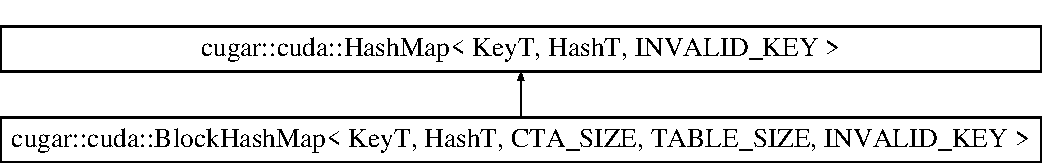
\includegraphics[height=2.000000cm]{structcugar_1_1cuda_1_1_block_hash_map}
\end{center}
\end{figure}
\subsection*{Classes}
\begin{DoxyCompactItemize}
\item 
struct \hyperlink{structcugar_1_1cuda_1_1_block_hash_map_1_1_temp_storage}{Temp\+Storage}
\end{DoxyCompactItemize}
\subsection*{Public Methods}
\begin{DoxyCompactItemize}
\item 
C\+U\+G\+A\+R\+\_\+\+D\+E\+V\+I\+CE \hyperlink{structcugar_1_1cuda_1_1_block_hash_map_aaac2f72bcf6fd716470f4502b0dbcb4d}{Block\+Hash\+Map} ()
\item 
C\+U\+G\+A\+R\+\_\+\+D\+E\+V\+I\+CE \hyperlink{structcugar_1_1cuda_1_1_block_hash_map_abf5f1d2196ccc4cba94c0d4bb7d11265}{Block\+Hash\+Map} (\hyperlink{structcugar_1_1cuda_1_1_block_hash_map_1_1_temp_storage}{Temp\+Storage} \&\+\_\+storage)
\end{DoxyCompactItemize}
\subsection*{Additional Inherited Members}


\subsection{Constructor \& Destructor Documentation}
\mbox{\Hypertarget{structcugar_1_1cuda_1_1_block_hash_map_aaac2f72bcf6fd716470f4502b0dbcb4d}\label{structcugar_1_1cuda_1_1_block_hash_map_aaac2f72bcf6fd716470f4502b0dbcb4d}} 
\index{cugar\+::cuda\+::\+Block\+Hash\+Map@{cugar\+::cuda\+::\+Block\+Hash\+Map}!Block\+Hash\+Map@{Block\+Hash\+Map}}
\index{Block\+Hash\+Map@{Block\+Hash\+Map}!cugar\+::cuda\+::\+Block\+Hash\+Map@{cugar\+::cuda\+::\+Block\+Hash\+Map}}
\subsubsection{\texorpdfstring{Block\+Hash\+Map()}{BlockHashMap()}\hspace{0.1cm}{\footnotesize\ttfamily [1/2]}}
{\footnotesize\ttfamily template$<$typename KeyT , typename HashT , uint32 C\+T\+A\+\_\+\+S\+I\+ZE, uint32 T\+A\+B\+L\+E\+\_\+\+S\+I\+ZE, KeyT I\+N\+V\+A\+L\+I\+D\+\_\+\+K\+EY = 0x\+F\+F\+F\+F\+F\+F\+FF$>$ \\
C\+U\+G\+A\+R\+\_\+\+D\+E\+V\+I\+CE \hyperlink{structcugar_1_1cuda_1_1_block_hash_map}{cugar\+::cuda\+::\+Block\+Hash\+Map}$<$ KeyT, HashT, C\+T\+A\+\_\+\+S\+I\+ZE, T\+A\+B\+L\+E\+\_\+\+S\+I\+ZE, I\+N\+V\+A\+L\+I\+D\+\_\+\+K\+EY $>$\+::\hyperlink{structcugar_1_1cuda_1_1_block_hash_map}{Block\+Hash\+Map} (\begin{DoxyParamCaption}{ }\end{DoxyParamCaption})\hspace{0.3cm}{\ttfamily [inline]}}

empty constructor \mbox{\Hypertarget{structcugar_1_1cuda_1_1_block_hash_map_abf5f1d2196ccc4cba94c0d4bb7d11265}\label{structcugar_1_1cuda_1_1_block_hash_map_abf5f1d2196ccc4cba94c0d4bb7d11265}} 
\index{cugar\+::cuda\+::\+Block\+Hash\+Map@{cugar\+::cuda\+::\+Block\+Hash\+Map}!Block\+Hash\+Map@{Block\+Hash\+Map}}
\index{Block\+Hash\+Map@{Block\+Hash\+Map}!cugar\+::cuda\+::\+Block\+Hash\+Map@{cugar\+::cuda\+::\+Block\+Hash\+Map}}
\subsubsection{\texorpdfstring{Block\+Hash\+Map()}{BlockHashMap()}\hspace{0.1cm}{\footnotesize\ttfamily [2/2]}}
{\footnotesize\ttfamily template$<$typename KeyT , typename HashT , uint32 C\+T\+A\+\_\+\+S\+I\+ZE, uint32 T\+A\+B\+L\+E\+\_\+\+S\+I\+ZE, KeyT I\+N\+V\+A\+L\+I\+D\+\_\+\+K\+EY = 0x\+F\+F\+F\+F\+F\+F\+FF$>$ \\
C\+U\+G\+A\+R\+\_\+\+D\+E\+V\+I\+CE \hyperlink{structcugar_1_1cuda_1_1_block_hash_map}{cugar\+::cuda\+::\+Block\+Hash\+Map}$<$ KeyT, HashT, C\+T\+A\+\_\+\+S\+I\+ZE, T\+A\+B\+L\+E\+\_\+\+S\+I\+ZE, I\+N\+V\+A\+L\+I\+D\+\_\+\+K\+EY $>$\+::\hyperlink{structcugar_1_1cuda_1_1_block_hash_map}{Block\+Hash\+Map} (\begin{DoxyParamCaption}\item[{\hyperlink{structcugar_1_1cuda_1_1_block_hash_map_1_1_temp_storage}{Temp\+Storage} \&}]{\+\_\+storage }\end{DoxyParamCaption})\hspace{0.3cm}{\ttfamily [inline]}}

constructor


\begin{DoxyParams}{Parameters}
{\em \+\_\+storage} & the per-\/\+C\+TA storage backing this container \\
\hline
\end{DoxyParams}


The documentation for this struct was generated from the following file\+:\begin{DoxyCompactItemize}
\item 
C\+:/p4research/research/jpantaleoni/\+Fermat-\/\+Public/contrib/cugar/basic/cuda/hash.\+h\end{DoxyCompactItemize}

\hypertarget{structcugar_1_1cuda_1_1_block_hash_set}{}\section{cugar\+:\+:cuda\+:\+:Block\+Hash\+Set$<$ KeyT, HashT, C\+T\+A\+\_\+\+S\+I\+ZE, T\+A\+B\+L\+E\+\_\+\+S\+I\+ZE, I\+N\+V\+A\+L\+I\+D\+\_\+\+K\+EY $>$ Struct Template Reference}
\label{structcugar_1_1cuda_1_1_block_hash_set}\index{cugar\+::cuda\+::\+Block\+Hash\+Set$<$ Key\+T, Hash\+T, C\+T\+A\+\_\+\+S\+I\+Z\+E, T\+A\+B\+L\+E\+\_\+\+S\+I\+Z\+E, I\+N\+V\+A\+L\+I\+D\+\_\+\+K\+E\+Y $>$@{cugar\+::cuda\+::\+Block\+Hash\+Set$<$ Key\+T, Hash\+T, C\+T\+A\+\_\+\+S\+I\+Z\+E, T\+A\+B\+L\+E\+\_\+\+S\+I\+Z\+E, I\+N\+V\+A\+L\+I\+D\+\_\+\+K\+E\+Y $>$}}


\subsection{Detailed description}
\subsubsection*{template$<$typename KeyT, typename HashT, uint32 C\+T\+A\+\_\+\+S\+I\+ZE, uint32 T\+A\+B\+L\+E\+\_\+\+S\+I\+ZE, KeyT I\+N\+V\+A\+L\+I\+D\+\_\+\+K\+EY = 0x\+F\+F\+F\+F\+F\+F\+FF$>$\newline
struct cugar\+::cuda\+::\+Block\+Hash\+Set$<$ Key\+T, Hash\+T, C\+T\+A\+\_\+\+S\+I\+Z\+E, T\+A\+B\+L\+E\+\_\+\+S\+I\+Z\+E, I\+N\+V\+A\+L\+I\+D\+\_\+\+K\+E\+Y $>$}

This class implements a cuda block-\/wide Hash Set, allowing arbitrary threads from the same C\+TA to add new entries at the same time. 

{\ttfamily \#include $<$hash.\+h$>$}

Inheritance diagram for cugar\+:\+:cuda\+:\+:Block\+Hash\+Set$<$ KeyT, HashT, C\+T\+A\+\_\+\+S\+I\+ZE, T\+A\+B\+L\+E\+\_\+\+S\+I\+ZE, I\+N\+V\+A\+L\+I\+D\+\_\+\+K\+EY $>$\+:\begin{figure}[H]
\begin{center}
\leavevmode
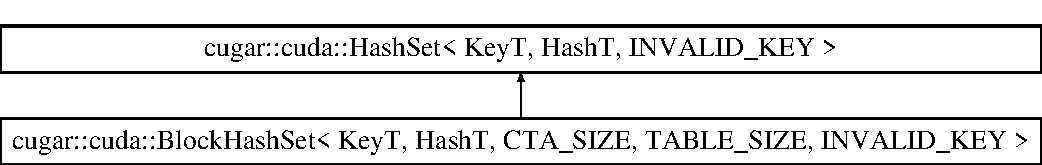
\includegraphics[height=2.000000cm]{structcugar_1_1cuda_1_1_block_hash_set}
\end{center}
\end{figure}
\subsection*{Classes}
\begin{DoxyCompactItemize}
\item 
struct \hyperlink{structcugar_1_1cuda_1_1_block_hash_set_1_1_temp_storage}{Temp\+Storage}
\end{DoxyCompactItemize}
\subsection*{Public Methods}
\begin{DoxyCompactItemize}
\item 
C\+U\+G\+A\+R\+\_\+\+D\+E\+V\+I\+CE \hyperlink{structcugar_1_1cuda_1_1_block_hash_set_a139df69fc33e2c5818d6be5722cb2077}{Block\+Hash\+Set} ()
\item 
C\+U\+G\+A\+R\+\_\+\+D\+E\+V\+I\+CE \hyperlink{structcugar_1_1cuda_1_1_block_hash_set_aa5ebb1fcc80e0f7e097a383237160587}{Block\+Hash\+Set} (\hyperlink{structcugar_1_1cuda_1_1_block_hash_set_1_1_temp_storage}{Temp\+Storage} \&\+\_\+storage)
\end{DoxyCompactItemize}
\subsection*{Additional Inherited Members}


\subsection{Constructor \& Destructor Documentation}
\mbox{\Hypertarget{structcugar_1_1cuda_1_1_block_hash_set_a139df69fc33e2c5818d6be5722cb2077}\label{structcugar_1_1cuda_1_1_block_hash_set_a139df69fc33e2c5818d6be5722cb2077}} 
\index{cugar\+::cuda\+::\+Block\+Hash\+Set@{cugar\+::cuda\+::\+Block\+Hash\+Set}!Block\+Hash\+Set@{Block\+Hash\+Set}}
\index{Block\+Hash\+Set@{Block\+Hash\+Set}!cugar\+::cuda\+::\+Block\+Hash\+Set@{cugar\+::cuda\+::\+Block\+Hash\+Set}}
\subsubsection{\texorpdfstring{Block\+Hash\+Set()}{BlockHashSet()}\hspace{0.1cm}{\footnotesize\ttfamily [1/2]}}
{\footnotesize\ttfamily template$<$typename KeyT , typename HashT , uint32 C\+T\+A\+\_\+\+S\+I\+ZE, uint32 T\+A\+B\+L\+E\+\_\+\+S\+I\+ZE, KeyT I\+N\+V\+A\+L\+I\+D\+\_\+\+K\+EY = 0x\+F\+F\+F\+F\+F\+F\+FF$>$ \\
C\+U\+G\+A\+R\+\_\+\+D\+E\+V\+I\+CE \hyperlink{structcugar_1_1cuda_1_1_block_hash_set}{cugar\+::cuda\+::\+Block\+Hash\+Set}$<$ KeyT, HashT, C\+T\+A\+\_\+\+S\+I\+ZE, T\+A\+B\+L\+E\+\_\+\+S\+I\+ZE, I\+N\+V\+A\+L\+I\+D\+\_\+\+K\+EY $>$\+::\hyperlink{structcugar_1_1cuda_1_1_block_hash_set}{Block\+Hash\+Set} (\begin{DoxyParamCaption}{ }\end{DoxyParamCaption})\hspace{0.3cm}{\ttfamily [inline]}}

emptry constructor \mbox{\Hypertarget{structcugar_1_1cuda_1_1_block_hash_set_aa5ebb1fcc80e0f7e097a383237160587}\label{structcugar_1_1cuda_1_1_block_hash_set_aa5ebb1fcc80e0f7e097a383237160587}} 
\index{cugar\+::cuda\+::\+Block\+Hash\+Set@{cugar\+::cuda\+::\+Block\+Hash\+Set}!Block\+Hash\+Set@{Block\+Hash\+Set}}
\index{Block\+Hash\+Set@{Block\+Hash\+Set}!cugar\+::cuda\+::\+Block\+Hash\+Set@{cugar\+::cuda\+::\+Block\+Hash\+Set}}
\subsubsection{\texorpdfstring{Block\+Hash\+Set()}{BlockHashSet()}\hspace{0.1cm}{\footnotesize\ttfamily [2/2]}}
{\footnotesize\ttfamily template$<$typename KeyT , typename HashT , uint32 C\+T\+A\+\_\+\+S\+I\+ZE, uint32 T\+A\+B\+L\+E\+\_\+\+S\+I\+ZE, KeyT I\+N\+V\+A\+L\+I\+D\+\_\+\+K\+EY = 0x\+F\+F\+F\+F\+F\+F\+FF$>$ \\
C\+U\+G\+A\+R\+\_\+\+D\+E\+V\+I\+CE \hyperlink{structcugar_1_1cuda_1_1_block_hash_set}{cugar\+::cuda\+::\+Block\+Hash\+Set}$<$ KeyT, HashT, C\+T\+A\+\_\+\+S\+I\+ZE, T\+A\+B\+L\+E\+\_\+\+S\+I\+ZE, I\+N\+V\+A\+L\+I\+D\+\_\+\+K\+EY $>$\+::\hyperlink{structcugar_1_1cuda_1_1_block_hash_set}{Block\+Hash\+Set} (\begin{DoxyParamCaption}\item[{\hyperlink{structcugar_1_1cuda_1_1_block_hash_set_1_1_temp_storage}{Temp\+Storage} \&}]{\+\_\+storage }\end{DoxyParamCaption})\hspace{0.3cm}{\ttfamily [inline]}}

constructor


\begin{DoxyParams}{Parameters}
{\em \+\_\+storage} & the per-\/\+C\+TA storage backing this container \\
\hline
\end{DoxyParams}


The documentation for this struct was generated from the following file\+:\begin{DoxyCompactItemize}
\item 
C\+:/p4research/research/jpantaleoni/\+Fermat-\/\+Public/contrib/cugar/basic/cuda/hash.\+h\end{DoxyCompactItemize}

\hypertarget{structcugar_1_1_bounded__exponential}{}\section{cugar\+:\+:Bounded\+\_\+exponential Struct Reference}
\label{structcugar_1_1_bounded__exponential}\index{cugar\+::\+Bounded\+\_\+exponential@{cugar\+::\+Bounded\+\_\+exponential}}


\subsection{Detailed description}
Bounded exponential distribution 

{\ttfamily \#include $<$distributions.\+h$>$}

Inheritance diagram for cugar\+:\+:Bounded\+\_\+exponential\+:\begin{figure}[H]
\begin{center}
\leavevmode
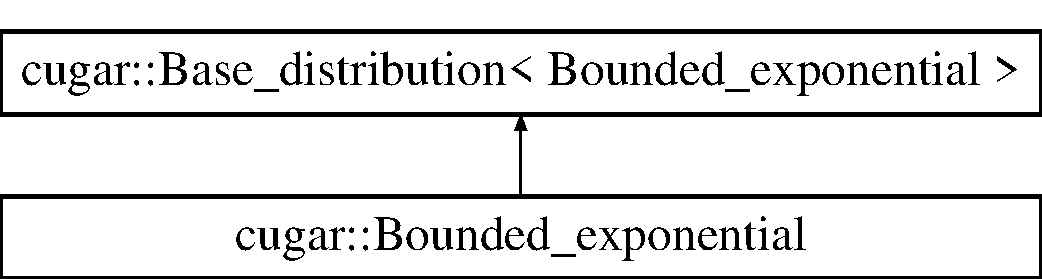
\includegraphics[height=2.000000cm]{structcugar_1_1_bounded__exponential}
\end{center}
\end{figure}
\subsection*{Public Methods}
\begin{DoxyCompactItemize}
\item 
C\+U\+G\+A\+R\+\_\+\+H\+O\+S\+T\+\_\+\+D\+E\+V\+I\+CE \hyperlink{structcugar_1_1_bounded__exponential_a45e239571b2ff1fe112e2fbb1133b1c6}{Bounded\+\_\+exponential} (const float b)
\item 
C\+U\+G\+A\+R\+\_\+\+H\+O\+S\+T\+\_\+\+D\+E\+V\+I\+CE \hyperlink{structcugar_1_1_bounded__exponential_accd30297a306778bd0a85fb0e25fe395}{Bounded\+\_\+exponential} (const float b1, const float b2)
\item 
C\+U\+G\+A\+R\+\_\+\+H\+O\+S\+T\+\_\+\+D\+E\+V\+I\+CE float \hyperlink{structcugar_1_1_bounded__exponential_a0678c62a51ca6b329d70ffdebf676c94}{map} (const float U) const
\item 
C\+U\+G\+A\+R\+\_\+\+H\+O\+S\+T\+\_\+\+D\+E\+V\+I\+CE float \hyperlink{structcugar_1_1_bounded__exponential_a9beb28b31e411c401184fd1017fd0189}{density} (const float x) const
\end{DoxyCompactItemize}


\subsection{Constructor \& Destructor Documentation}
\mbox{\Hypertarget{structcugar_1_1_bounded__exponential_a45e239571b2ff1fe112e2fbb1133b1c6}\label{structcugar_1_1_bounded__exponential_a45e239571b2ff1fe112e2fbb1133b1c6}} 
\index{cugar\+::\+Bounded\+\_\+exponential@{cugar\+::\+Bounded\+\_\+exponential}!Bounded\+\_\+exponential@{Bounded\+\_\+exponential}}
\index{Bounded\+\_\+exponential@{Bounded\+\_\+exponential}!cugar\+::\+Bounded\+\_\+exponential@{cugar\+::\+Bounded\+\_\+exponential}}
\subsubsection{\texorpdfstring{Bounded\+\_\+exponential()}{Bounded\_exponential()}\hspace{0.1cm}{\footnotesize\ttfamily [1/2]}}
{\footnotesize\ttfamily C\+U\+G\+A\+R\+\_\+\+H\+O\+S\+T\+\_\+\+D\+E\+V\+I\+CE cugar\+::\+Bounded\+\_\+exponential\+::\+Bounded\+\_\+exponential (\begin{DoxyParamCaption}\item[{const float}]{b }\end{DoxyParamCaption})\hspace{0.3cm}{\ttfamily [inline]}}

constructor


\begin{DoxyParams}{Parameters}
{\em b} & distribution parameter \\
\hline
\end{DoxyParams}
\mbox{\Hypertarget{structcugar_1_1_bounded__exponential_accd30297a306778bd0a85fb0e25fe395}\label{structcugar_1_1_bounded__exponential_accd30297a306778bd0a85fb0e25fe395}} 
\index{cugar\+::\+Bounded\+\_\+exponential@{cugar\+::\+Bounded\+\_\+exponential}!Bounded\+\_\+exponential@{Bounded\+\_\+exponential}}
\index{Bounded\+\_\+exponential@{Bounded\+\_\+exponential}!cugar\+::\+Bounded\+\_\+exponential@{cugar\+::\+Bounded\+\_\+exponential}}
\subsubsection{\texorpdfstring{Bounded\+\_\+exponential()}{Bounded\_exponential()}\hspace{0.1cm}{\footnotesize\ttfamily [2/2]}}
{\footnotesize\ttfamily C\+U\+G\+A\+R\+\_\+\+H\+O\+S\+T\+\_\+\+D\+E\+V\+I\+CE cugar\+::\+Bounded\+\_\+exponential\+::\+Bounded\+\_\+exponential (\begin{DoxyParamCaption}\item[{const float}]{b1,  }\item[{const float}]{b2 }\end{DoxyParamCaption})\hspace{0.3cm}{\ttfamily [inline]}}

constructor


\begin{DoxyParams}{Parameters}
{\em b} & distribution parameter \\
\hline
\end{DoxyParams}


\subsection{Member Function Documentation}
\mbox{\Hypertarget{structcugar_1_1_bounded__exponential_a9beb28b31e411c401184fd1017fd0189}\label{structcugar_1_1_bounded__exponential_a9beb28b31e411c401184fd1017fd0189}} 
\index{cugar\+::\+Bounded\+\_\+exponential@{cugar\+::\+Bounded\+\_\+exponential}!density@{density}}
\index{density@{density}!cugar\+::\+Bounded\+\_\+exponential@{cugar\+::\+Bounded\+\_\+exponential}}
\subsubsection{\texorpdfstring{density()}{density()}}
{\footnotesize\ttfamily C\+U\+G\+A\+R\+\_\+\+H\+O\+S\+T\+\_\+\+D\+E\+V\+I\+CE float cugar\+::\+Bounded\+\_\+exponential\+::density (\begin{DoxyParamCaption}\item[{const float}]{x }\end{DoxyParamCaption}) const\hspace{0.3cm}{\ttfamily [inline]}}

probability density function


\begin{DoxyParams}{Parameters}
{\em x} & sample location \\
\hline
\end{DoxyParams}
\mbox{\Hypertarget{structcugar_1_1_bounded__exponential_a0678c62a51ca6b329d70ffdebf676c94}\label{structcugar_1_1_bounded__exponential_a0678c62a51ca6b329d70ffdebf676c94}} 
\index{cugar\+::\+Bounded\+\_\+exponential@{cugar\+::\+Bounded\+\_\+exponential}!map@{map}}
\index{map@{map}!cugar\+::\+Bounded\+\_\+exponential@{cugar\+::\+Bounded\+\_\+exponential}}
\subsubsection{\texorpdfstring{map()}{map()}}
{\footnotesize\ttfamily C\+U\+G\+A\+R\+\_\+\+H\+O\+S\+T\+\_\+\+D\+E\+V\+I\+CE float cugar\+::\+Bounded\+\_\+exponential\+::map (\begin{DoxyParamCaption}\item[{const float}]{U }\end{DoxyParamCaption}) const\hspace{0.3cm}{\ttfamily [inline]}}

transform a uniformly distributed number through the distribution


\begin{DoxyParams}{Parameters}
{\em U} & real number to transform \\
\hline
\end{DoxyParams}


The documentation for this struct was generated from the following file\+:\begin{DoxyCompactItemize}
\item 
C\+:/p4research/research/jpantaleoni/\+Fermat-\/\+Public/contrib/cugar/sampling/\hyperlink{distributions_8h}{distributions.\+h}\end{DoxyCompactItemize}

\hypertarget{structcugar_1_1_bounded__pareto__distribution}{}\section{cugar\+:\+:Bounded\+\_\+pareto\+\_\+distribution Struct Reference}
\label{structcugar_1_1_bounded__pareto__distribution}\index{cugar\+::\+Bounded\+\_\+pareto\+\_\+distribution@{cugar\+::\+Bounded\+\_\+pareto\+\_\+distribution}}


\subsection{Detailed description}
Bounded Pareto distribution 

{\ttfamily \#include $<$distributions.\+h$>$}

Inheritance diagram for cugar\+:\+:Bounded\+\_\+pareto\+\_\+distribution\+:\begin{figure}[H]
\begin{center}
\leavevmode
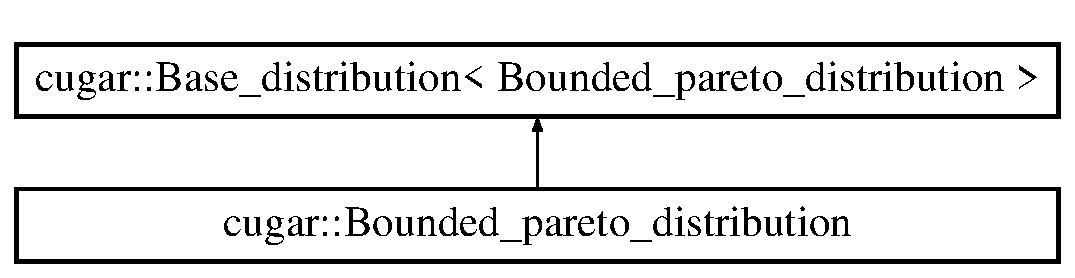
\includegraphics[height=2.000000cm]{structcugar_1_1_bounded__pareto__distribution}
\end{center}
\end{figure}
\subsection*{Public Methods}
\begin{DoxyCompactItemize}
\item 
C\+U\+G\+A\+R\+\_\+\+H\+O\+S\+T\+\_\+\+D\+E\+V\+I\+CE \hyperlink{structcugar_1_1_bounded__pareto__distribution_aeaecb7792cf38321287e71626fab3cb7}{Bounded\+\_\+pareto\+\_\+distribution} (const float a, const float min, const float max)
\item 
C\+U\+G\+A\+R\+\_\+\+H\+O\+S\+T\+\_\+\+D\+E\+V\+I\+CE float \hyperlink{structcugar_1_1_bounded__pareto__distribution_a91ec0f08a9d9355ec67bd176f34a1a6c}{map} (const float U) const
\item 
C\+U\+G\+A\+R\+\_\+\+H\+O\+S\+T\+\_\+\+D\+E\+V\+I\+CE float \hyperlink{structcugar_1_1_bounded__pareto__distribution_a5f909b164a22aeae3e58b9c73571f599}{density} (const float x) const
\end{DoxyCompactItemize}


\subsection{Constructor \& Destructor Documentation}
\mbox{\Hypertarget{structcugar_1_1_bounded__pareto__distribution_aeaecb7792cf38321287e71626fab3cb7}\label{structcugar_1_1_bounded__pareto__distribution_aeaecb7792cf38321287e71626fab3cb7}} 
\index{cugar\+::\+Bounded\+\_\+pareto\+\_\+distribution@{cugar\+::\+Bounded\+\_\+pareto\+\_\+distribution}!Bounded\+\_\+pareto\+\_\+distribution@{Bounded\+\_\+pareto\+\_\+distribution}}
\index{Bounded\+\_\+pareto\+\_\+distribution@{Bounded\+\_\+pareto\+\_\+distribution}!cugar\+::\+Bounded\+\_\+pareto\+\_\+distribution@{cugar\+::\+Bounded\+\_\+pareto\+\_\+distribution}}
\subsubsection{\texorpdfstring{Bounded\+\_\+pareto\+\_\+distribution()}{Bounded\_pareto\_distribution()}}
{\footnotesize\ttfamily C\+U\+G\+A\+R\+\_\+\+H\+O\+S\+T\+\_\+\+D\+E\+V\+I\+CE cugar\+::\+Bounded\+\_\+pareto\+\_\+distribution\+::\+Bounded\+\_\+pareto\+\_\+distribution (\begin{DoxyParamCaption}\item[{const float}]{a,  }\item[{const float}]{min,  }\item[{const float}]{max }\end{DoxyParamCaption})\hspace{0.3cm}{\ttfamily [inline]}}

constructor


\begin{DoxyParams}{Parameters}
{\em a} & distribution parameter \\
\hline
{\em min} & distribution parameter \\
\hline
{\em max} & distribution parameter \\
\hline
\end{DoxyParams}


\subsection{Member Function Documentation}
\mbox{\Hypertarget{structcugar_1_1_bounded__pareto__distribution_a5f909b164a22aeae3e58b9c73571f599}\label{structcugar_1_1_bounded__pareto__distribution_a5f909b164a22aeae3e58b9c73571f599}} 
\index{cugar\+::\+Bounded\+\_\+pareto\+\_\+distribution@{cugar\+::\+Bounded\+\_\+pareto\+\_\+distribution}!density@{density}}
\index{density@{density}!cugar\+::\+Bounded\+\_\+pareto\+\_\+distribution@{cugar\+::\+Bounded\+\_\+pareto\+\_\+distribution}}
\subsubsection{\texorpdfstring{density()}{density()}}
{\footnotesize\ttfamily C\+U\+G\+A\+R\+\_\+\+H\+O\+S\+T\+\_\+\+D\+E\+V\+I\+CE float cugar\+::\+Bounded\+\_\+pareto\+\_\+distribution\+::density (\begin{DoxyParamCaption}\item[{const float}]{x }\end{DoxyParamCaption}) const\hspace{0.3cm}{\ttfamily [inline]}}

probability density function


\begin{DoxyParams}{Parameters}
{\em x} & sample location \\
\hline
\end{DoxyParams}
\mbox{\Hypertarget{structcugar_1_1_bounded__pareto__distribution_a91ec0f08a9d9355ec67bd176f34a1a6c}\label{structcugar_1_1_bounded__pareto__distribution_a91ec0f08a9d9355ec67bd176f34a1a6c}} 
\index{cugar\+::\+Bounded\+\_\+pareto\+\_\+distribution@{cugar\+::\+Bounded\+\_\+pareto\+\_\+distribution}!map@{map}}
\index{map@{map}!cugar\+::\+Bounded\+\_\+pareto\+\_\+distribution@{cugar\+::\+Bounded\+\_\+pareto\+\_\+distribution}}
\subsubsection{\texorpdfstring{map()}{map()}}
{\footnotesize\ttfamily C\+U\+G\+A\+R\+\_\+\+H\+O\+S\+T\+\_\+\+D\+E\+V\+I\+CE float cugar\+::\+Bounded\+\_\+pareto\+\_\+distribution\+::map (\begin{DoxyParamCaption}\item[{const float}]{U }\end{DoxyParamCaption}) const\hspace{0.3cm}{\ttfamily [inline]}}

transform a uniformly distributed number through the distribution


\begin{DoxyParams}{Parameters}
{\em U} & real number to transform \\
\hline
\end{DoxyParams}


The documentation for this struct was generated from the following file\+:\begin{DoxyCompactItemize}
\item 
C\+:/p4research/research/jpantaleoni/\+Fermat-\/\+Public/contrib/cugar/sampling/\hyperlink{distributions_8h}{distributions.\+h}\end{DoxyCompactItemize}

\hypertarget{struct_b_p_t}{}\section{B\+PT Struct Reference}
\label{struct_b_p_t}\index{B\+PT@{B\+PT}}


\subsection{Detailed description}
A bidirectional path tracing renderer built on top of the \hyperlink{_b_p_t_lib_page}{B\+P\+T\+Lib} library. 

{\ttfamily \#include $<$bpt.\+h$>$}

Inheritance diagram for B\+PT\+:\begin{figure}[H]
\begin{center}
\leavevmode
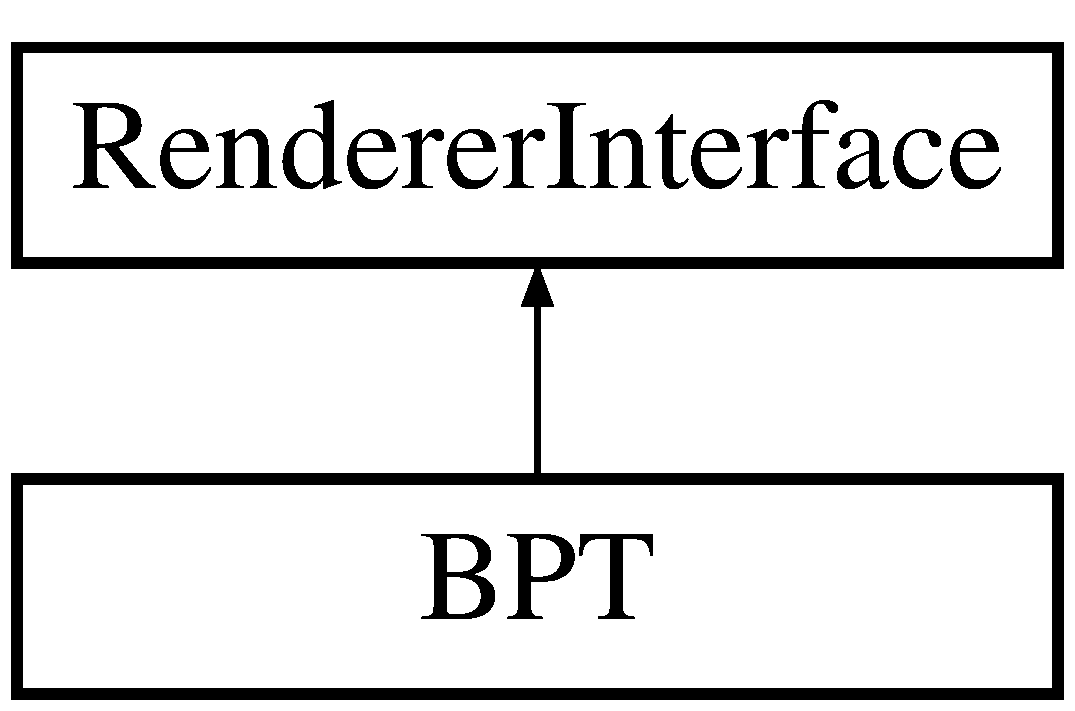
\includegraphics[height=2.000000cm]{struct_b_p_t}
\end{center}
\end{figure}
\subsection*{Public Methods}
\begin{DoxyCompactItemize}
\item 
void \hyperlink{struct_b_p_t_a45040344b72bde12d338c2b1969fba64}{init} (int argc, char $\ast$$\ast$argv, \hyperlink{struct_rendering_context}{Rendering\+Context} \&renderer)
\item 
\mbox{\Hypertarget{struct_b_p_t_af9e940aca306f186cadfabc095590d88}\label{struct_b_p_t_af9e940aca306f186cadfabc095590d88}} 
void \hyperlink{struct_b_p_t_af9e940aca306f186cadfabc095590d88}{render} (const uint32 instance, \hyperlink{struct_rendering_context}{Rendering\+Context} \&renderer)
\begin{DoxyCompactList}\small\item\em \mbox{[}\hyperlink{struct_b_p_t_af9e940aca306f186cadfabc095590d88}{B\+P\+T\+::render}\mbox{]} \end{DoxyCompactList}\item 
void \hyperlink{struct_b_p_t_aef80ec5312cbbf38e5dc9e6c37058825}{destroy} ()
\item 
\mbox{\Hypertarget{struct_b_p_t_aebd1d213d108b75ffe3a10b87a16a556}\label{struct_b_p_t_aebd1d213d108b75ffe3a10b87a16a556}} 
void {\bfseries regenerate\+\_\+primary\+\_\+light\+\_\+vertices} (const uint32 instance, \hyperlink{struct_rendering_context}{Rendering\+Context} \&renderer)
\end{DoxyCompactItemize}
\subsection*{Static Public Methods}
\begin{DoxyCompactItemize}
\item 
\mbox{\Hypertarget{struct_b_p_t_a731f57cfd10bc96040add0194ecb0110}\label{struct_b_p_t_a731f57cfd10bc96040add0194ecb0110}} 
static \hyperlink{struct_renderer_interface}{Renderer\+Interface} $\ast$ {\bfseries factory} ()
\end{DoxyCompactItemize}
\subsection*{Public Members}
\begin{DoxyCompactItemize}
\item 
\mbox{\Hypertarget{struct_b_p_t_ad7115878e2a15bc9d343d9b55652a102}\label{struct_b_p_t_ad7115878e2a15bc9d343d9b55652a102}} 
\hyperlink{struct_b_p_t_options}{B\+P\+T\+Options} {\bfseries m\+\_\+options}
\item 
\mbox{\Hypertarget{struct_b_p_t_adbf95be629586410ca1ba36b659f67ea}\label{struct_b_p_t_adbf95be629586410ca1ba36b659f67ea}} 
\hyperlink{struct_tiled_sequence}{Tiled\+Sequence} {\bfseries m\+\_\+sequence}
\item 
\mbox{\Hypertarget{struct_b_p_t_ae6458130ad5503baf5334ed530d277d0}\label{struct_b_p_t_ae6458130ad5503baf5334ed530d277d0}} 
\hyperlink{struct_b_p_t_queues_storage}{B\+P\+T\+Queues\+Storage} {\bfseries m\+\_\+queues}
\item 
\mbox{\Hypertarget{struct_b_p_t_abb143bf4bdd945ba511a67a0edf0f1f2}\label{struct_b_p_t_abb143bf4bdd945ba511a67a0edf0f1f2}} 
\hyperlink{struct_vertex_storage}{Vertex\+Storage} {\bfseries m\+\_\+light\+\_\+vertices}
\item 
\mbox{\Hypertarget{struct_b_p_t_acb8257fbaf359d944e02d1e34804badf}\label{struct_b_p_t_acb8257fbaf359d944e02d1e34804badf}} 
uint32 {\bfseries m\+\_\+n\+\_\+light\+\_\+subpaths}
\item 
\mbox{\Hypertarget{struct_b_p_t_a63ecc30c516c1f31c7676fad57c36fcf}\label{struct_b_p_t_a63ecc30c516c1f31c7676fad57c36fcf}} 
uint32 {\bfseries m\+\_\+n\+\_\+eye\+\_\+subpaths}
\item 
\mbox{\Hypertarget{struct_b_p_t_a7c7d6ab0d188b4ffc1e515a180724935}\label{struct_b_p_t_a7c7d6ab0d188b4ffc1e515a180724935}} 
\hyperlink{classcugar_1_1_l_f_s_r_generator_matrix}{cugar\+::\+L\+F\+S\+R\+Generator\+Matrix} {\bfseries m\+\_\+generator}
\item 
\mbox{\Hypertarget{struct_b_p_t_a993669e42e4d4fae747cb5a2c9628ac1}\label{struct_b_p_t_a993669e42e4d4fae747cb5a2c9628ac1}} 
\hyperlink{structcugar_1_1_l_f_s_r_random_stream}{cugar\+::\+L\+F\+S\+R\+Random\+Stream} {\bfseries m\+\_\+random}
\item 
\mbox{\Hypertarget{struct_b_p_t_aff98f38d27e563b973b0c398c5d6b847}\label{struct_b_p_t_aff98f38d27e563b973b0c398c5d6b847}} 
float {\bfseries m\+\_\+time}
\end{DoxyCompactItemize}


\subsection{Member Function Documentation}
\mbox{\Hypertarget{struct_b_p_t_aef80ec5312cbbf38e5dc9e6c37058825}\label{struct_b_p_t_aef80ec5312cbbf38e5dc9e6c37058825}} 
\index{B\+PT@{B\+PT}!destroy@{destroy}}
\index{destroy@{destroy}!B\+PT@{B\+PT}}
\subsubsection{\texorpdfstring{destroy()}{destroy()}}
{\footnotesize\ttfamily void B\+P\+T\+::destroy (\begin{DoxyParamCaption}{ }\end{DoxyParamCaption})\hspace{0.3cm}{\ttfamily [inline]}, {\ttfamily [virtual]}}

this method is responsible for destroying the object itself 

Reimplemented from \hyperlink{struct_renderer_interface_a7469218aafa029a3e22bac2c00dca9f5}{Renderer\+Interface}.

\mbox{\Hypertarget{struct_b_p_t_a45040344b72bde12d338c2b1969fba64}\label{struct_b_p_t_a45040344b72bde12d338c2b1969fba64}} 
\index{B\+PT@{B\+PT}!init@{init}}
\index{init@{init}!B\+PT@{B\+PT}}
\subsubsection{\texorpdfstring{init()}{init()}}
{\footnotesize\ttfamily void B\+P\+T\+::init (\begin{DoxyParamCaption}\item[{int}]{argc,  }\item[{char $\ast$$\ast$}]{argv,  }\item[{\hyperlink{struct_rendering_context}{Rendering\+Context} \&}]{renderer }\end{DoxyParamCaption})\hspace{0.3cm}{\ttfamily [virtual]}}

this method is responsible for any command options parsing / initializations the renderer might need to perform 

Reimplemented from \hyperlink{struct_renderer_interface_a2ead9b943d6d48fcd32872e0005ebe63}{Renderer\+Interface}.



The documentation for this struct was generated from the following files\+:\begin{DoxyCompactItemize}
\item 
C\+:/p4research/research/jpantaleoni/\+Fermat-\/\+Public/src/renderers/bpt.\+h\item 
C\+:/p4research/research/jpantaleoni/\+Fermat-\/\+Public/src/renderers/bpt\+\_\+impl.\+h\end{DoxyCompactItemize}

\hypertarget{struct_b_p_t_config_base}{}\section{B\+P\+T\+Config\+Base Struct Reference}
\label{struct_b_p_t_config_base}\index{B\+P\+T\+Config\+Base@{B\+P\+T\+Config\+Base}}


\subsection{Detailed description}
This class implements a \char`\"{}policy\char`\"{} template for bidirectional path tracing\+: all bidirectional path tracing kernels are templated over a T\+B\+P\+T\+Config class that must implement this interface. In order to change the policy, it is sufficient to inherit from this class and override the methods. Note that the methods are not virtual, but the code is written so as to use the implementation of the last class that overrides them, mantaining the inlining efficiency. 

{\ttfamily \#include $<$bpt\+\_\+kernels.\+h$>$}

\subsection*{Public Methods}
\begin{DoxyCompactItemize}
\item 
\mbox{\Hypertarget{struct_b_p_t_config_base_a6da0cfdd37861bf94d41537ab1337180}\label{struct_b_p_t_config_base_a6da0cfdd37861bf94d41537ab1337180}} 
F\+E\+R\+M\+A\+T\+\_\+\+H\+O\+S\+T\+\_\+\+D\+E\+V\+I\+CE F\+E\+R\+M\+A\+T\+\_\+\+F\+O\+R\+C\+E\+I\+N\+L\+I\+NE {\bfseries B\+P\+T\+Config\+Base} (const \hyperlink{struct_b_p_t_options_base}{B\+P\+T\+Options\+Base} \&\+\_\+options, Vertex\+Sampling \+\_\+light\+\_\+sampling=Vertex\+Sampling\+::k\+All, Vertex\+Ordering \+\_\+light\+\_\+ordering=Vertex\+Ordering\+::k\+Random\+Ordering, Vertex\+Sampling \+\_\+eye\+\_\+sampling=Vertex\+Sampling\+::k\+All, bool \+\_\+use\+\_\+rr=true)
\item 
\mbox{\Hypertarget{struct_b_p_t_config_base_a78f72ec36314c94dffba798bac520e11}\label{struct_b_p_t_config_base_a78f72ec36314c94dffba798bac520e11}} 
F\+E\+R\+M\+A\+T\+\_\+\+H\+O\+S\+T\+\_\+\+D\+E\+V\+I\+CE F\+E\+R\+M\+A\+T\+\_\+\+F\+O\+R\+C\+E\+I\+N\+L\+I\+NE {\bfseries B\+P\+T\+Config\+Base} (uint32 \+\_\+max\+\_\+path\+\_\+length=6, Vertex\+Sampling \+\_\+light\+\_\+sampling=Vertex\+Sampling\+::k\+All, Vertex\+Ordering \+\_\+light\+\_\+ordering=Vertex\+Ordering\+::k\+Random\+Ordering, Vertex\+Sampling \+\_\+eye\+\_\+sampling=Vertex\+Sampling\+::k\+All, bool \+\_\+use\+\_\+vpls=true, bool \+\_\+use\+\_\+rr=true, float \+\_\+light\+\_\+tracing=0.\+0f, bool \+\_\+direct\+\_\+lighting\+\_\+nee=true, bool \+\_\+direct\+\_\+lighting\+\_\+bsdf=true, bool \+\_\+indirect\+\_\+lighting\+\_\+nee=true, bool \+\_\+indirect\+\_\+lighting\+\_\+bsdf=true, bool \+\_\+visible\+\_\+lights=true)
\item 
\mbox{\Hypertarget{struct_b_p_t_config_base_a594b18c9ff1e7f63158d0821ddac776e}\label{struct_b_p_t_config_base_a594b18c9ff1e7f63158d0821ddac776e}} 
F\+E\+R\+M\+A\+T\+\_\+\+H\+O\+S\+T\+\_\+\+D\+E\+V\+I\+CE F\+E\+R\+M\+A\+T\+\_\+\+F\+O\+R\+C\+E\+I\+N\+L\+I\+NE {\bfseries B\+P\+T\+Config\+Base} (const \hyperlink{struct_b_p_t_config_base}{B\+P\+T\+Config\+Base} \&other)
\item 
F\+E\+R\+M\+A\+T\+\_\+\+H\+O\+S\+T\+\_\+\+D\+E\+V\+I\+CE F\+E\+R\+M\+A\+T\+\_\+\+F\+O\+R\+C\+E\+I\+N\+L\+I\+NE bool \hyperlink{struct_b_p_t_config_base_a97c865fc0c241b22bece418e7a8574b4}{terminate\+\_\+light\+\_\+subpath} (const uint32 path\+\_\+id, const uint32 s) const
\item 
F\+E\+R\+M\+A\+T\+\_\+\+H\+O\+S\+T\+\_\+\+D\+E\+V\+I\+CE F\+E\+R\+M\+A\+T\+\_\+\+F\+O\+R\+C\+E\+I\+N\+L\+I\+NE bool \hyperlink{struct_b_p_t_config_base_a5cafb898a6535d4fee6d98df875fe1ae}{terminate\+\_\+eye\+\_\+subpath} (const uint32 path\+\_\+id, const uint32 t) const
\item 
F\+E\+R\+M\+A\+T\+\_\+\+H\+O\+S\+T\+\_\+\+D\+E\+V\+I\+CE F\+E\+R\+M\+A\+T\+\_\+\+F\+O\+R\+C\+E\+I\+N\+L\+I\+NE bool \hyperlink{struct_b_p_t_config_base_afa468245a9b87bcc49abc7132de7a58c}{store\+\_\+light\+\_\+vertex} (const uint32 path\+\_\+id, const uint32 s, const bool absorbed) const
\item 
F\+E\+R\+M\+A\+T\+\_\+\+H\+O\+S\+T\+\_\+\+D\+E\+V\+I\+CE F\+E\+R\+M\+A\+T\+\_\+\+F\+O\+R\+C\+E\+I\+N\+L\+I\+NE bool \hyperlink{struct_b_p_t_config_base_a546ae2aa2926db1702688da6c23aa3e7}{perform\+\_\+connection} (const uint32 eye\+\_\+path\+\_\+id, const uint32 t, const bool absorbed) const
\item 
F\+E\+R\+M\+A\+T\+\_\+\+H\+O\+S\+T\+\_\+\+D\+E\+V\+I\+CE F\+E\+R\+M\+A\+T\+\_\+\+F\+O\+R\+C\+E\+I\+N\+L\+I\+NE bool \hyperlink{struct_b_p_t_config_base_a333fa484bf5a9f4ad12f6a7ed48632d4}{accumulate\+\_\+emissive} (const uint32 eye\+\_\+path\+\_\+id, const uint32 t, const bool absorbed) const
\item 
{\footnotesize template$<$typename T\+B\+P\+T\+Context $>$ }\\F\+E\+R\+M\+A\+T\+\_\+\+H\+O\+S\+T\+\_\+\+D\+E\+V\+I\+CE F\+E\+R\+M\+A\+T\+\_\+\+F\+O\+R\+C\+E\+I\+N\+L\+I\+NE void \hyperlink{struct_b_p_t_config_base_a9a948bffb4f173adc48f156d02d000bb}{visit\+\_\+light\+\_\+vertex} (const uint32 light\+\_\+path\+\_\+id, const uint32 depth, const \hyperlink{struct_vertex_geometry_id}{Vertex\+Geometry\+Id} v\+\_\+id, T\+B\+P\+T\+Context \&context, \hyperlink{struct_rendering_context_view}{Rendering\+Context\+View} \&renderer) const
\item 
{\footnotesize template$<$typename T\+B\+P\+T\+Context $>$ }\\F\+E\+R\+M\+A\+T\+\_\+\+H\+O\+S\+T\+\_\+\+D\+E\+V\+I\+CE F\+E\+R\+M\+A\+T\+\_\+\+F\+O\+R\+C\+E\+I\+N\+L\+I\+NE void \hyperlink{struct_b_p_t_config_base_ac1ecb6f3ef04718305291fedf76cec85}{visit\+\_\+eye\+\_\+vertex} (const uint32 eye\+\_\+path\+\_\+id, const uint32 depth, const \hyperlink{struct_vertex_geometry_id}{Vertex\+Geometry\+Id} v\+\_\+id, const \hyperlink{struct_eye_vertex}{Eye\+Vertex} \&v, T\+B\+P\+T\+Context \&context, \hyperlink{struct_rendering_context_view}{Rendering\+Context\+View} \&renderer) const
\end{DoxyCompactItemize}
\subsection*{Public Members}
\begin{DoxyCompactItemize}
\item 
\mbox{\Hypertarget{struct_b_p_t_config_base_ae58489f7a2cf917768ad47f5f5e19358}\label{struct_b_p_t_config_base_ae58489f7a2cf917768ad47f5f5e19358}} 
uint32 {\bfseries max\+\_\+path\+\_\+length}\+: 10
\item 
\mbox{\Hypertarget{struct_b_p_t_config_base_a927ed5520109fbed3a7e42f192024114}\label{struct_b_p_t_config_base_a927ed5520109fbed3a7e42f192024114}} 
uint32 {\bfseries light\+\_\+sampling}\+: 1
\item 
\mbox{\Hypertarget{struct_b_p_t_config_base_a8ff39329d349eda2d345e0c7e67f3a56}\label{struct_b_p_t_config_base_a8ff39329d349eda2d345e0c7e67f3a56}} 
uint32 {\bfseries light\+\_\+ordering}\+: 1
\item 
\mbox{\Hypertarget{struct_b_p_t_config_base_a89146d78a312017e25affa01d338f996}\label{struct_b_p_t_config_base_a89146d78a312017e25affa01d338f996}} 
uint32 {\bfseries eye\+\_\+sampling}\+: 1
\item 
\mbox{\Hypertarget{struct_b_p_t_config_base_aef2b33f32bb1fed2e8647d91248458c1}\label{struct_b_p_t_config_base_aef2b33f32bb1fed2e8647d91248458c1}} 
uint32 {\bfseries use\+\_\+vpls}\+: 1
\item 
\mbox{\Hypertarget{struct_b_p_t_config_base_a20d5ea3f8982567db3d7a266203d8c72}\label{struct_b_p_t_config_base_a20d5ea3f8982567db3d7a266203d8c72}} 
uint32 {\bfseries use\+\_\+rr}\+: 1
\item 
\mbox{\Hypertarget{struct_b_p_t_config_base_a8e03d7079115558f022bd7da731a9784}\label{struct_b_p_t_config_base_a8e03d7079115558f022bd7da731a9784}} 
uint32 {\bfseries direct\+\_\+lighting\+\_\+nee}\+: 1
\item 
\mbox{\Hypertarget{struct_b_p_t_config_base_afd785870da53910b9f8cb0d20d1f06f4}\label{struct_b_p_t_config_base_afd785870da53910b9f8cb0d20d1f06f4}} 
uint32 {\bfseries direct\+\_\+lighting\+\_\+bsdf}\+: 1
\item 
\mbox{\Hypertarget{struct_b_p_t_config_base_a517c494b0f4f21d0fa40ae070bc186fd}\label{struct_b_p_t_config_base_a517c494b0f4f21d0fa40ae070bc186fd}} 
uint32 {\bfseries indirect\+\_\+lighting\+\_\+nee}\+: 1
\item 
\mbox{\Hypertarget{struct_b_p_t_config_base_a93e0f12a3403028f1ae32615ff854f05}\label{struct_b_p_t_config_base_a93e0f12a3403028f1ae32615ff854f05}} 
uint32 {\bfseries indirect\+\_\+lighting\+\_\+bsdf}\+: 1
\item 
\mbox{\Hypertarget{struct_b_p_t_config_base_aa65ce47d5ee4044ac6143c67a2546fd1}\label{struct_b_p_t_config_base_aa65ce47d5ee4044ac6143c67a2546fd1}} 
uint32 {\bfseries visible\+\_\+lights}\+: 1
\item 
\mbox{\Hypertarget{struct_b_p_t_config_base_a7dac0c8dc0125ae0e44e2fb61b8e3e2f}\label{struct_b_p_t_config_base_a7dac0c8dc0125ae0e44e2fb61b8e3e2f}} 
float {\bfseries light\+\_\+tracing}
\end{DoxyCompactItemize}


\subsection{Member Function Documentation}
\mbox{\Hypertarget{struct_b_p_t_config_base_a333fa484bf5a9f4ad12f6a7ed48632d4}\label{struct_b_p_t_config_base_a333fa484bf5a9f4ad12f6a7ed48632d4}} 
\index{B\+P\+T\+Config\+Base@{B\+P\+T\+Config\+Base}!accumulate\+\_\+emissive@{accumulate\+\_\+emissive}}
\index{accumulate\+\_\+emissive@{accumulate\+\_\+emissive}!B\+P\+T\+Config\+Base@{B\+P\+T\+Config\+Base}}
\subsubsection{\texorpdfstring{accumulate\+\_\+emissive()}{accumulate\_emissive()}}
{\footnotesize\ttfamily F\+E\+R\+M\+A\+T\+\_\+\+H\+O\+S\+T\+\_\+\+D\+E\+V\+I\+CE F\+E\+R\+M\+A\+T\+\_\+\+F\+O\+R\+C\+E\+I\+N\+L\+I\+NE bool B\+P\+T\+Config\+Base\+::accumulate\+\_\+emissive (\begin{DoxyParamCaption}\item[{const uint32}]{eye\+\_\+path\+\_\+id,  }\item[{const uint32}]{t,  }\item[{const bool}]{absorbed }\end{DoxyParamCaption}) const\hspace{0.3cm}{\ttfamily [inline]}}

decide whether to accumulate an emissive sample from a pure (eye) path tracing estimator


\begin{DoxyParams}{Parameters}
{\em eye\+\_\+path\+\_\+id} & index of the eye subpath \\
\hline
{\em t} & vertex number along the eye subpath \\
\hline
{\em absorbed} & true if the eye subpath has been absorbed/terminated here \\
\hline
\end{DoxyParams}
\mbox{\Hypertarget{struct_b_p_t_config_base_a546ae2aa2926db1702688da6c23aa3e7}\label{struct_b_p_t_config_base_a546ae2aa2926db1702688da6c23aa3e7}} 
\index{B\+P\+T\+Config\+Base@{B\+P\+T\+Config\+Base}!perform\+\_\+connection@{perform\+\_\+connection}}
\index{perform\+\_\+connection@{perform\+\_\+connection}!B\+P\+T\+Config\+Base@{B\+P\+T\+Config\+Base}}
\subsubsection{\texorpdfstring{perform\+\_\+connection()}{perform\_connection()}}
{\footnotesize\ttfamily F\+E\+R\+M\+A\+T\+\_\+\+H\+O\+S\+T\+\_\+\+D\+E\+V\+I\+CE F\+E\+R\+M\+A\+T\+\_\+\+F\+O\+R\+C\+E\+I\+N\+L\+I\+NE bool B\+P\+T\+Config\+Base\+::perform\+\_\+connection (\begin{DoxyParamCaption}\item[{const uint32}]{eye\+\_\+path\+\_\+id,  }\item[{const uint32}]{t,  }\item[{const bool}]{absorbed }\end{DoxyParamCaption}) const\hspace{0.3cm}{\ttfamily [inline]}}

decide whether to perform a bidirectional connection


\begin{DoxyParams}{Parameters}
{\em eye\+\_\+path\+\_\+id} & index of the eye subpath \\
\hline
{\em t} & vertex number along the eye subpath \\
\hline
{\em absorbed} & true if the eye subpath has been absorbed/terminated here \\
\hline
\end{DoxyParams}
\mbox{\Hypertarget{struct_b_p_t_config_base_afa468245a9b87bcc49abc7132de7a58c}\label{struct_b_p_t_config_base_afa468245a9b87bcc49abc7132de7a58c}} 
\index{B\+P\+T\+Config\+Base@{B\+P\+T\+Config\+Base}!store\+\_\+light\+\_\+vertex@{store\+\_\+light\+\_\+vertex}}
\index{store\+\_\+light\+\_\+vertex@{store\+\_\+light\+\_\+vertex}!B\+P\+T\+Config\+Base@{B\+P\+T\+Config\+Base}}
\subsubsection{\texorpdfstring{store\+\_\+light\+\_\+vertex()}{store\_light\_vertex()}}
{\footnotesize\ttfamily F\+E\+R\+M\+A\+T\+\_\+\+H\+O\+S\+T\+\_\+\+D\+E\+V\+I\+CE F\+E\+R\+M\+A\+T\+\_\+\+F\+O\+R\+C\+E\+I\+N\+L\+I\+NE bool B\+P\+T\+Config\+Base\+::store\+\_\+light\+\_\+vertex (\begin{DoxyParamCaption}\item[{const uint32}]{path\+\_\+id,  }\item[{const uint32}]{s,  }\item[{const bool}]{absorbed }\end{DoxyParamCaption}) const\hspace{0.3cm}{\ttfamily [inline]}}

decide whether to store a given light vertex


\begin{DoxyParams}{Parameters}
{\em path\+\_\+id} & index of the light subpath \\
\hline
{\em s} & vertex number along the light subpath \\
\hline
\end{DoxyParams}
\mbox{\Hypertarget{struct_b_p_t_config_base_a5cafb898a6535d4fee6d98df875fe1ae}\label{struct_b_p_t_config_base_a5cafb898a6535d4fee6d98df875fe1ae}} 
\index{B\+P\+T\+Config\+Base@{B\+P\+T\+Config\+Base}!terminate\+\_\+eye\+\_\+subpath@{terminate\+\_\+eye\+\_\+subpath}}
\index{terminate\+\_\+eye\+\_\+subpath@{terminate\+\_\+eye\+\_\+subpath}!B\+P\+T\+Config\+Base@{B\+P\+T\+Config\+Base}}
\subsubsection{\texorpdfstring{terminate\+\_\+eye\+\_\+subpath()}{terminate\_eye\_subpath()}}
{\footnotesize\ttfamily F\+E\+R\+M\+A\+T\+\_\+\+H\+O\+S\+T\+\_\+\+D\+E\+V\+I\+CE F\+E\+R\+M\+A\+T\+\_\+\+F\+O\+R\+C\+E\+I\+N\+L\+I\+NE bool B\+P\+T\+Config\+Base\+::terminate\+\_\+eye\+\_\+subpath (\begin{DoxyParamCaption}\item[{const uint32}]{path\+\_\+id,  }\item[{const uint32}]{t }\end{DoxyParamCaption}) const\hspace{0.3cm}{\ttfamily [inline]}}

decide whether to terminate a given eye subpath


\begin{DoxyParams}{Parameters}
{\em path\+\_\+id} & index of the eye subpath \\
\hline
{\em s} & vertex number along the eye subpath \\
\hline
\end{DoxyParams}
\mbox{\Hypertarget{struct_b_p_t_config_base_a97c865fc0c241b22bece418e7a8574b4}\label{struct_b_p_t_config_base_a97c865fc0c241b22bece418e7a8574b4}} 
\index{B\+P\+T\+Config\+Base@{B\+P\+T\+Config\+Base}!terminate\+\_\+light\+\_\+subpath@{terminate\+\_\+light\+\_\+subpath}}
\index{terminate\+\_\+light\+\_\+subpath@{terminate\+\_\+light\+\_\+subpath}!B\+P\+T\+Config\+Base@{B\+P\+T\+Config\+Base}}
\subsubsection{\texorpdfstring{terminate\+\_\+light\+\_\+subpath()}{terminate\_light\_subpath()}}
{\footnotesize\ttfamily F\+E\+R\+M\+A\+T\+\_\+\+H\+O\+S\+T\+\_\+\+D\+E\+V\+I\+CE F\+E\+R\+M\+A\+T\+\_\+\+F\+O\+R\+C\+E\+I\+N\+L\+I\+NE bool B\+P\+T\+Config\+Base\+::terminate\+\_\+light\+\_\+subpath (\begin{DoxyParamCaption}\item[{const uint32}]{path\+\_\+id,  }\item[{const uint32}]{s }\end{DoxyParamCaption}) const\hspace{0.3cm}{\ttfamily [inline]}}

decide whether to terminate a given light subpath


\begin{DoxyParams}{Parameters}
{\em path\+\_\+id} & index of the light subpath \\
\hline
{\em s} & vertex number along the light subpath \\
\hline
\end{DoxyParams}
\mbox{\Hypertarget{struct_b_p_t_config_base_ac1ecb6f3ef04718305291fedf76cec85}\label{struct_b_p_t_config_base_ac1ecb6f3ef04718305291fedf76cec85}} 
\index{B\+P\+T\+Config\+Base@{B\+P\+T\+Config\+Base}!visit\+\_\+eye\+\_\+vertex@{visit\+\_\+eye\+\_\+vertex}}
\index{visit\+\_\+eye\+\_\+vertex@{visit\+\_\+eye\+\_\+vertex}!B\+P\+T\+Config\+Base@{B\+P\+T\+Config\+Base}}
\subsubsection{\texorpdfstring{visit\+\_\+eye\+\_\+vertex()}{visit\_eye\_vertex()}}
{\footnotesize\ttfamily template$<$typename T\+B\+P\+T\+Context $>$ \\
F\+E\+R\+M\+A\+T\+\_\+\+H\+O\+S\+T\+\_\+\+D\+E\+V\+I\+CE F\+E\+R\+M\+A\+T\+\_\+\+F\+O\+R\+C\+E\+I\+N\+L\+I\+NE void B\+P\+T\+Config\+Base\+::visit\+\_\+eye\+\_\+vertex (\begin{DoxyParamCaption}\item[{const uint32}]{eye\+\_\+path\+\_\+id,  }\item[{const uint32}]{depth,  }\item[{const \hyperlink{struct_vertex_geometry_id}{Vertex\+Geometry\+Id}}]{v\+\_\+id,  }\item[{const \hyperlink{struct_eye_vertex}{Eye\+Vertex} \&}]{v,  }\item[{T\+B\+P\+T\+Context \&}]{context,  }\item[{\hyperlink{struct_rendering_context_view}{Rendering\+Context\+View} \&}]{renderer }\end{DoxyParamCaption}) const\hspace{0.3cm}{\ttfamily [inline]}}

allow to process/store the given eye vertex \mbox{\Hypertarget{struct_b_p_t_config_base_a9a948bffb4f173adc48f156d02d000bb}\label{struct_b_p_t_config_base_a9a948bffb4f173adc48f156d02d000bb}} 
\index{B\+P\+T\+Config\+Base@{B\+P\+T\+Config\+Base}!visit\+\_\+light\+\_\+vertex@{visit\+\_\+light\+\_\+vertex}}
\index{visit\+\_\+light\+\_\+vertex@{visit\+\_\+light\+\_\+vertex}!B\+P\+T\+Config\+Base@{B\+P\+T\+Config\+Base}}
\subsubsection{\texorpdfstring{visit\+\_\+light\+\_\+vertex()}{visit\_light\_vertex()}}
{\footnotesize\ttfamily template$<$typename T\+B\+P\+T\+Context $>$ \\
F\+E\+R\+M\+A\+T\+\_\+\+H\+O\+S\+T\+\_\+\+D\+E\+V\+I\+CE F\+E\+R\+M\+A\+T\+\_\+\+F\+O\+R\+C\+E\+I\+N\+L\+I\+NE void B\+P\+T\+Config\+Base\+::visit\+\_\+light\+\_\+vertex (\begin{DoxyParamCaption}\item[{const uint32}]{light\+\_\+path\+\_\+id,  }\item[{const uint32}]{depth,  }\item[{const \hyperlink{struct_vertex_geometry_id}{Vertex\+Geometry\+Id}}]{v\+\_\+id,  }\item[{T\+B\+P\+T\+Context \&}]{context,  }\item[{\hyperlink{struct_rendering_context_view}{Rendering\+Context\+View} \&}]{renderer }\end{DoxyParamCaption}) const\hspace{0.3cm}{\ttfamily [inline]}}

allow to process/store the given light vertex 

The documentation for this struct was generated from the following file\+:\begin{DoxyCompactItemize}
\item 
C\+:/p4research/research/jpantaleoni/\+Fermat-\/\+Public/src/bpt\+\_\+kernels.\+h\end{DoxyCompactItemize}

\hypertarget{struct_b_p_t_context}{}\section{B\+P\+T\+Context Struct Reference}
\label{struct_b_p_t_context}\index{B\+P\+T\+Context@{B\+P\+T\+Context}}


\subsection{Detailed description}
The C\+U\+DA context class for the \hyperlink{struct_b_p_t}{B\+PT} renderer 

{\ttfamily \#include $<$bpt\+\_\+impl.\+h$>$}

Inheritance diagram for B\+P\+T\+Context\+:\begin{figure}[H]
\begin{center}
\leavevmode
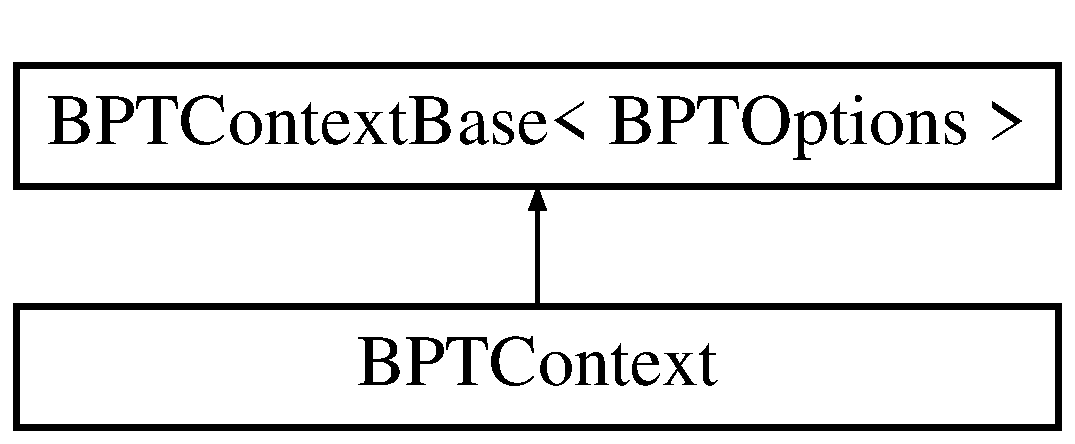
\includegraphics[height=2.000000cm]{struct_b_p_t_context}
\end{center}
\end{figure}
\subsection*{Public Methods}
\begin{DoxyCompactItemize}
\item 
\mbox{\Hypertarget{struct_b_p_t_context_afcb37c3fb73082961daf6d8539d7c70e}\label{struct_b_p_t_context_afcb37c3fb73082961daf6d8539d7c70e}} 
{\bfseries B\+P\+T\+Context} (\hyperlink{struct_b_p_t}{B\+PT} \&\+\_\+bpt, const \hyperlink{struct_rendering_context_view}{Rendering\+Context\+View} \&\+\_\+renderer)
\end{DoxyCompactItemize}
\subsection*{Public Members}
\begin{DoxyCompactItemize}
\item 
\mbox{\Hypertarget{struct_b_p_t_context_af2ae399bb9eaafb80b03cdad9e1b804b}\label{struct_b_p_t_context_af2ae399bb9eaafb80b03cdad9e1b804b}} 
\hyperlink{struct_tiled_sequence_view}{Tiled\+Sequence\+View} {\bfseries sequence}
\end{DoxyCompactItemize}


The documentation for this struct was generated from the following file\+:\begin{DoxyCompactItemize}
\item 
C\+:/p4research/research/jpantaleoni/\+Fermat-\/\+Public/src/renderers/bpt\+\_\+impl.\+h\end{DoxyCompactItemize}

\hypertarget{struct_b_p_t_context_base}{}\section{B\+P\+T\+Context\+Base$<$ T\+B\+P\+T\+Options $>$ Struct Template Reference}
\label{struct_b_p_t_context_base}\index{B\+P\+T\+Context\+Base$<$ T\+B\+P\+T\+Options $>$@{B\+P\+T\+Context\+Base$<$ T\+B\+P\+T\+Options $>$}}


\subsection{Detailed description}
\subsubsection*{template$<$typename T\+B\+P\+T\+Options$>$\newline
struct B\+P\+T\+Context\+Base$<$ T\+B\+P\+T\+Options $>$}

\mbox{[}B\+P\+T\+Context\+Base\+Block\mbox{]} \begin{DoxyParagraph}{}
Basic context for bidirectional path tracing 
\end{DoxyParagraph}
\begin{DoxyParagraph}{}
This context class is responsible for storing\+: ~\newline

\begin{DoxyItemize}
\item a set of light vertices, generated throughout the light subpath sampling phase
\item a set of ray queues used throughout the wavefront scheduling process of the entire bidirectional path tracing pipeline
\item an options member, deriving from \hyperlink{struct_b_p_t_options_base}{B\+P\+T\+Options\+Base} 
\end{DoxyItemize}
\end{DoxyParagraph}


{\ttfamily \#include $<$bpt\+\_\+context.\+h$>$}

\subsection*{Public Methods}
\begin{DoxyCompactItemize}
\item 
\mbox{\Hypertarget{struct_b_p_t_context_base_a99d21412e9d03211d4bb7e39f36f4da2}\label{struct_b_p_t_context_base_a99d21412e9d03211d4bb7e39f36f4da2}} 
{\bfseries B\+P\+T\+Context\+Base} (const \hyperlink{struct_rendering_context_view}{Rendering\+Context\+View} \&\+\_\+renderer, const \hyperlink{struct_vertex_storage_view}{Vertex\+Storage\+View} \&\+\_\+light\+\_\+vertices, const \hyperlink{struct_b_p_t_queues_view}{B\+P\+T\+Queues\+View} \&\+\_\+queues, const T\+B\+P\+T\+Options \+\_\+options=T\+B\+P\+T\+Options())
\item 
\mbox{\Hypertarget{struct_b_p_t_context_base_aa1a101747cbf03fcb7681a43519601c4}\label{struct_b_p_t_context_base_aa1a101747cbf03fcb7681a43519601c4}} 
void {\bfseries set\+\_\+camera} (const \hyperlink{struct_camera}{Camera} \&camera, const uint32 res\+\_\+x, const uint32 res\+\_\+y, const float aspect\+\_\+ratio)
\end{DoxyCompactItemize}
\subsection*{Public Members}
\begin{DoxyCompactItemize}
\item 
\mbox{\Hypertarget{struct_b_p_t_context_base_aa09a6dc8959a83d81486c9bd6280f8d6}\label{struct_b_p_t_context_base_aa09a6dc8959a83d81486c9bd6280f8d6}} 
uint32 {\bfseries in\+\_\+bounce}
\item 
\mbox{\Hypertarget{struct_b_p_t_context_base_ac6082ad7d9678a8e5e6173673ff92a3d}\label{struct_b_p_t_context_base_ac6082ad7d9678a8e5e6173673ff92a3d}} 
\hyperlink{struct_ray_queue}{Ray\+Queue} {\bfseries in\+\_\+queue}
\item 
\mbox{\Hypertarget{struct_b_p_t_context_base_aa57f6964ab4852b1ffba8cabedac4fd7}\label{struct_b_p_t_context_base_aa57f6964ab4852b1ffba8cabedac4fd7}} 
\hyperlink{struct_ray_queue}{Ray\+Queue} {\bfseries shadow\+\_\+queue}
\item 
\mbox{\Hypertarget{struct_b_p_t_context_base_aac6319a84f2a87b7f6813e9f36d6492e}\label{struct_b_p_t_context_base_aac6319a84f2a87b7f6813e9f36d6492e}} 
\hyperlink{struct_ray_queue}{Ray\+Queue} {\bfseries scatter\+\_\+queue}
\item 
\mbox{\Hypertarget{struct_b_p_t_context_base_a04326acccfec76676b2d07f2ca9de7dc}\label{struct_b_p_t_context_base_a04326acccfec76676b2d07f2ca9de7dc}} 
\hyperlink{struct_vertex_storage_view}{Vertex\+Storage\+View} {\bfseries light\+\_\+vertices}
\item 
\mbox{\Hypertarget{struct_b_p_t_context_base_a15c5f6e58e807ff9c7153b714fd89cf7}\label{struct_b_p_t_context_base_a15c5f6e58e807ff9c7153b714fd89cf7}} 
\hyperlink{structcugar_1_1_vector}{cugar\+::\+Vector3f} {\bfseries camera\+\_\+U}
\item 
\mbox{\Hypertarget{struct_b_p_t_context_base_a00ad2326f04c69ba6f7f4560d868a6ac}\label{struct_b_p_t_context_base_a00ad2326f04c69ba6f7f4560d868a6ac}} 
\hyperlink{structcugar_1_1_vector}{cugar\+::\+Vector3f} {\bfseries camera\+\_\+V}
\item 
\mbox{\Hypertarget{struct_b_p_t_context_base_a0cb8ff154aad0ff71b7f277a159cc2b3}\label{struct_b_p_t_context_base_a0cb8ff154aad0ff71b7f277a159cc2b3}} 
\hyperlink{structcugar_1_1_vector}{cugar\+::\+Vector3f} {\bfseries camera\+\_\+W}
\item 
\mbox{\Hypertarget{struct_b_p_t_context_base_a212f84e9da36ed87d8c7b08ae3f05d75}\label{struct_b_p_t_context_base_a212f84e9da36ed87d8c7b08ae3f05d75}} 
float {\bfseries camera\+\_\+\+W\+\_\+len}
\item 
\mbox{\Hypertarget{struct_b_p_t_context_base_ac2ad3ee44e3095e8f201b1d38cf22696}\label{struct_b_p_t_context_base_ac2ad3ee44e3095e8f201b1d38cf22696}} 
float {\bfseries camera\+\_\+square\+\_\+focal\+\_\+length}
\item 
\mbox{\Hypertarget{struct_b_p_t_context_base_adf209d0d6204b44ac0f57878dcb18a8a}\label{struct_b_p_t_context_base_adf209d0d6204b44ac0f57878dcb18a8a}} 
T\+B\+P\+T\+Options {\bfseries options}
\end{DoxyCompactItemize}


The documentation for this struct was generated from the following file\+:\begin{DoxyCompactItemize}
\item 
C\+:/p4research/research/jpantaleoni/\+Fermat-\/\+Public/src/bpt\+\_\+context.\+h\end{DoxyCompactItemize}

\hypertarget{struct_b_p_t_options}{}\section{B\+P\+T\+Options Struct Reference}
\label{struct_b_p_t_options}\index{B\+P\+T\+Options@{B\+P\+T\+Options}}


\subsection{Detailed description}
Options for the \hyperlink{struct_b_p_t}{B\+PT} renderer 

{\ttfamily \#include $<$bpt.\+h$>$}

Inheritance diagram for B\+P\+T\+Options\+:\begin{figure}[H]
\begin{center}
\leavevmode
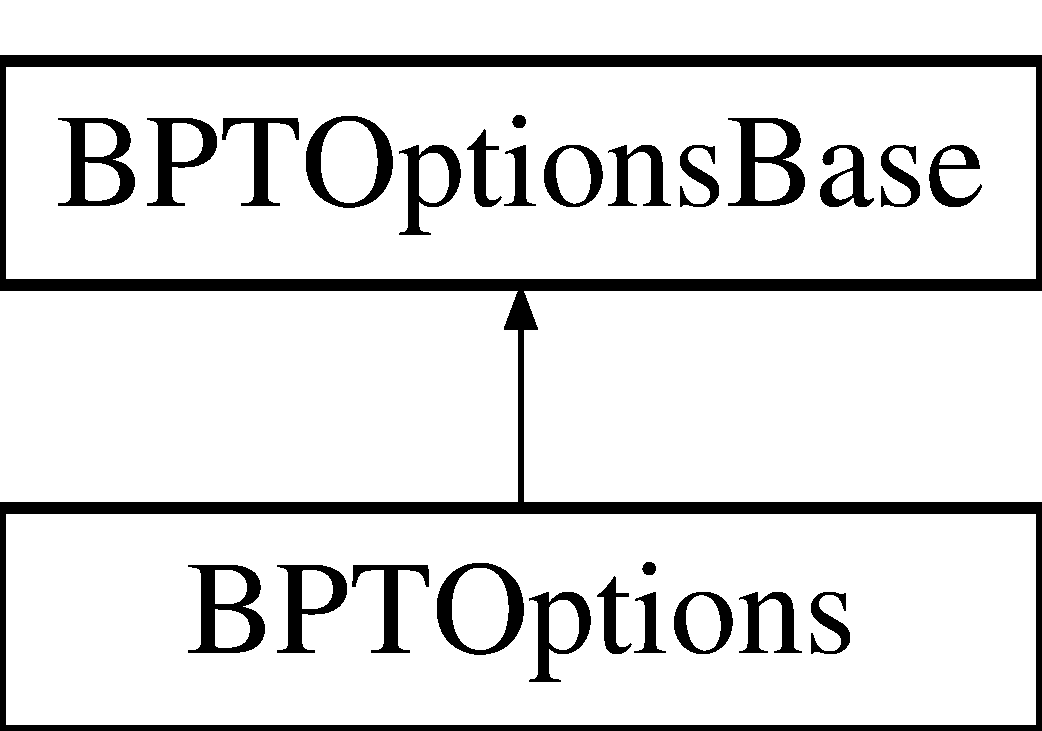
\includegraphics[height=2.000000cm]{struct_b_p_t_options}
\end{center}
\end{figure}
\subsection*{Public Methods}
\begin{DoxyCompactItemize}
\item 
\mbox{\Hypertarget{struct_b_p_t_options_aeb706710c32bd1c53bfca3a248ede3f5}\label{struct_b_p_t_options_aeb706710c32bd1c53bfca3a248ede3f5}} 
void {\bfseries parse} (const int argc, char $\ast$$\ast$argv)
\end{DoxyCompactItemize}
\subsection*{Public Members}
\begin{DoxyCompactItemize}
\item 
\mbox{\Hypertarget{struct_b_p_t_options_ad54009c95340a34e6e847e5f8899883e}\label{struct_b_p_t_options_ad54009c95340a34e6e847e5f8899883e}} 
bool {\bfseries single\+\_\+connection}
\item 
\mbox{\Hypertarget{struct_b_p_t_options_ac6348f0a4046615f49adc8c2e0352582}\label{struct_b_p_t_options_ac6348f0a4046615f49adc8c2e0352582}} 
bool {\bfseries rr}
\end{DoxyCompactItemize}


The documentation for this struct was generated from the following file\+:\begin{DoxyCompactItemize}
\item 
C\+:/p4research/research/jpantaleoni/\+Fermat-\/\+Public/src/renderers/bpt.\+h\end{DoxyCompactItemize}

\hypertarget{struct_b_p_t_options_base}{}\section{B\+P\+T\+Options\+Base Struct Reference}
\label{struct_b_p_t_options_base}\index{B\+P\+T\+Options\+Base@{B\+P\+T\+Options\+Base}}


\subsection{Detailed description}
Basic options for bidirectional path tracing 

{\ttfamily \#include $<$bpt\+\_\+options.\+h$>$}

Inheritance diagram for B\+P\+T\+Options\+Base\+:\begin{figure}[H]
\begin{center}
\leavevmode
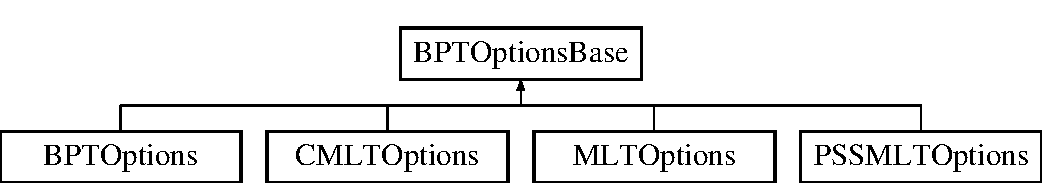
\includegraphics[height=2.000000cm]{struct_b_p_t_options_base}
\end{center}
\end{figure}
\subsection*{Public Methods}
\begin{DoxyCompactItemize}
\item 
\mbox{\Hypertarget{struct_b_p_t_options_base_a5a189940377e81d15c6dfc02c6465dcc}\label{struct_b_p_t_options_base_a5a189940377e81d15c6dfc02c6465dcc}} 
void {\bfseries parse} (const int argc, char $\ast$$\ast$argv)
\end{DoxyCompactItemize}
\subsection*{Public Members}
\begin{DoxyCompactItemize}
\item 
\mbox{\Hypertarget{struct_b_p_t_options_base_a3d1664d4b59cacc36200da960da90cdc}\label{struct_b_p_t_options_base_a3d1664d4b59cacc36200da960da90cdc}} 
uint32 {\bfseries max\+\_\+path\+\_\+length}
\item 
\mbox{\Hypertarget{struct_b_p_t_options_base_aebf1a2d300b1d8876a551310a0199491}\label{struct_b_p_t_options_base_aebf1a2d300b1d8876a551310a0199491}} 
bool {\bfseries direct\+\_\+lighting\+\_\+nee}
\item 
\mbox{\Hypertarget{struct_b_p_t_options_base_a637c3d5ecaccb197f5b9a9c958186b86}\label{struct_b_p_t_options_base_a637c3d5ecaccb197f5b9a9c958186b86}} 
bool {\bfseries direct\+\_\+lighting\+\_\+bsdf}
\item 
\mbox{\Hypertarget{struct_b_p_t_options_base_a486ea1d8e0f3606fa78bc4d9100d2c9b}\label{struct_b_p_t_options_base_a486ea1d8e0f3606fa78bc4d9100d2c9b}} 
bool {\bfseries indirect\+\_\+lighting\+\_\+nee}
\item 
\mbox{\Hypertarget{struct_b_p_t_options_base_ad2396a617d67206009373a02305e3c96}\label{struct_b_p_t_options_base_ad2396a617d67206009373a02305e3c96}} 
bool {\bfseries indirect\+\_\+lighting\+\_\+bsdf}
\item 
\mbox{\Hypertarget{struct_b_p_t_options_base_af32a90f054a019535bb4b93ca58cbd65}\label{struct_b_p_t_options_base_af32a90f054a019535bb4b93ca58cbd65}} 
bool {\bfseries visible\+\_\+lights}
\item 
\mbox{\Hypertarget{struct_b_p_t_options_base_a32919694ee2c13bf11c66bdbfa4b80e6}\label{struct_b_p_t_options_base_a32919694ee2c13bf11c66bdbfa4b80e6}} 
bool {\bfseries use\+\_\+vpls}
\item 
\mbox{\Hypertarget{struct_b_p_t_options_base_a29537d7e05a599a269ece203eb8742a6}\label{struct_b_p_t_options_base_a29537d7e05a599a269ece203eb8742a6}} 
float {\bfseries light\+\_\+tracing}
\end{DoxyCompactItemize}


The documentation for this struct was generated from the following file\+:\begin{DoxyCompactItemize}
\item 
C\+:/p4research/research/jpantaleoni/\+Fermat-\/\+Public/src/bpt\+\_\+options.\+h\end{DoxyCompactItemize}

\hypertarget{struct_b_p_t_queues_storage}{}\section{B\+P\+T\+Queues\+Storage Struct Reference}
\label{struct_b_p_t_queues_storage}\index{B\+P\+T\+Queues\+Storage@{B\+P\+T\+Queues\+Storage}}


\subsection{Detailed description}
\hyperlink{struct_b_p_t}{B\+PT} queues storage 

{\ttfamily \#include $<$bpt\+\_\+queues.\+h$>$}

\subsection*{Public Methods}
\begin{DoxyCompactItemize}
\item 
\mbox{\Hypertarget{struct_b_p_t_queues_storage_a6cf3cb625ed3dc5529dcc1e294c6c6f0}\label{struct_b_p_t_queues_storage_a6cf3cb625ed3dc5529dcc1e294c6c6f0}} 
void {\bfseries alloc} (const uint32 n\+\_\+entries)
\item 
\mbox{\Hypertarget{struct_b_p_t_queues_storage_a9d381ccb349b7b703f8ec38d746cf27b}\label{struct_b_p_t_queues_storage_a9d381ccb349b7b703f8ec38d746cf27b}} 
void {\bfseries alloc} (const uint32 n\+\_\+eye\+\_\+paths, const uint32 n\+\_\+light\+\_\+paths, const uint32 max\+\_\+path\+\_\+length)
\item 
\mbox{\Hypertarget{struct_b_p_t_queues_storage_a2f22b8ebded7c050ecbf218a855c0e80}\label{struct_b_p_t_queues_storage_a2f22b8ebded7c050ecbf218a855c0e80}} 
\hyperlink{struct_b_p_t_queues_view}{B\+P\+T\+Queues\+View} {\bfseries view} (const uint32 n\+\_\+eye\+\_\+paths, const uint32 n\+\_\+light\+\_\+paths)
\end{DoxyCompactItemize}
\subsection*{Public Members}
\begin{DoxyCompactItemize}
\item 
\mbox{\Hypertarget{struct_b_p_t_queues_storage_a363bfd42942675bc07098fc4414fbed1}\label{struct_b_p_t_queues_storage_a363bfd42942675bc07098fc4414fbed1}} 
\hyperlink{class_domain_buffer}{Domain\+Buffer}$<$ C\+U\+D\+A\+\_\+\+B\+U\+F\+F\+ER, \hyperlink{struct_ray}{Ray} $>$ {\bfseries m\+\_\+rays}
\item 
\mbox{\Hypertarget{struct_b_p_t_queues_storage_aee3844eaf2918bbce482f69656e158d9}\label{struct_b_p_t_queues_storage_aee3844eaf2918bbce482f69656e158d9}} 
\hyperlink{class_domain_buffer}{Domain\+Buffer}$<$ C\+U\+D\+A\+\_\+\+B\+U\+F\+F\+ER, \hyperlink{struct_hit}{Hit} $>$ {\bfseries m\+\_\+hits}
\item 
\mbox{\Hypertarget{struct_b_p_t_queues_storage_af66e8fc5d6e771c9377dcbd0328298d9}\label{struct_b_p_t_queues_storage_af66e8fc5d6e771c9377dcbd0328298d9}} 
\hyperlink{class_domain_buffer}{Domain\+Buffer}$<$ C\+U\+D\+A\+\_\+\+B\+U\+F\+F\+ER, float4 $>$ {\bfseries m\+\_\+weights}
\item 
\mbox{\Hypertarget{struct_b_p_t_queues_storage_ac0b4b456396d7558851913071e957dc2}\label{struct_b_p_t_queues_storage_ac0b4b456396d7558851913071e957dc2}} 
\hyperlink{class_domain_buffer}{Domain\+Buffer}$<$ C\+U\+D\+A\+\_\+\+B\+U\+F\+F\+ER, float $>$ {\bfseries m\+\_\+probs}
\item 
\mbox{\Hypertarget{struct_b_p_t_queues_storage_a5860fbb459eeaa1b0fcec78f2107e354}\label{struct_b_p_t_queues_storage_a5860fbb459eeaa1b0fcec78f2107e354}} 
\hyperlink{class_domain_buffer}{Domain\+Buffer}$<$ C\+U\+D\+A\+\_\+\+B\+U\+F\+F\+ER, float4 $>$ {\bfseries m\+\_\+path\+\_\+weights}
\item 
\mbox{\Hypertarget{struct_b_p_t_queues_storage_a7e01b207f19ccf145aecf10228dc1da1}\label{struct_b_p_t_queues_storage_a7e01b207f19ccf145aecf10228dc1da1}} 
\hyperlink{class_domain_buffer}{Domain\+Buffer}$<$ C\+U\+D\+A\+\_\+\+B\+U\+F\+F\+ER, uint32 $>$ {\bfseries m\+\_\+pixels}
\item 
\mbox{\Hypertarget{struct_b_p_t_queues_storage_a3ba36359fe1503957a5118790ae27649}\label{struct_b_p_t_queues_storage_a3ba36359fe1503957a5118790ae27649}} 
\hyperlink{class_domain_buffer}{Domain\+Buffer}$<$ C\+U\+D\+A\+\_\+\+B\+U\+F\+F\+ER, uint32 $>$ {\bfseries m\+\_\+counters}
\end{DoxyCompactItemize}


The documentation for this struct was generated from the following file\+:\begin{DoxyCompactItemize}
\item 
C\+:/p4research/research/jpantaleoni/\+Fermat-\/\+Public/src/bpt\+\_\+queues.\+h\end{DoxyCompactItemize}

\hypertarget{struct_b_p_t_queues_view}{}\section{B\+P\+T\+Queues\+View Struct Reference}
\label{struct_b_p_t_queues_view}\index{B\+P\+T\+Queues\+View@{B\+P\+T\+Queues\+View}}


\subsection{Detailed description}
\hyperlink{struct_b_p_t}{B\+PT} queues view 

{\ttfamily \#include $<$bpt\+\_\+queues.\+h$>$}

\subsection*{Public Members}
\begin{DoxyCompactItemize}
\item 
\mbox{\Hypertarget{struct_b_p_t_queues_view_add198a7a10e2408e94263ebe4c47e3bb}\label{struct_b_p_t_queues_view_add198a7a10e2408e94263ebe4c47e3bb}} 
\hyperlink{struct_ray_queue}{Ray\+Queue} {\bfseries in\+\_\+queue}
\item 
\mbox{\Hypertarget{struct_b_p_t_queues_view_a460545254a8fe9d3e377c1e8f4ffc3c1}\label{struct_b_p_t_queues_view_a460545254a8fe9d3e377c1e8f4ffc3c1}} 
\hyperlink{struct_ray_queue}{Ray\+Queue} {\bfseries scatter\+\_\+queue}
\item 
\mbox{\Hypertarget{struct_b_p_t_queues_view_ab4dad286a7378c4a9714d50289cd9db1}\label{struct_b_p_t_queues_view_ab4dad286a7378c4a9714d50289cd9db1}} 
\hyperlink{struct_ray_queue}{Ray\+Queue} {\bfseries shadow\+\_\+queue}
\end{DoxyCompactItemize}


The documentation for this struct was generated from the following file\+:\begin{DoxyCompactItemize}
\item 
C\+:/p4research/research/jpantaleoni/\+Fermat-\/\+Public/src/bpt\+\_\+queues.\+h\end{DoxyCompactItemize}

\hypertarget{struct_bsdf}{}\section{Bsdf Struct Reference}
\label{struct_bsdf}\index{Bsdf@{Bsdf}}


\subsection{Detailed description}
Composite B\+S\+DF class \begin{DoxyParagraph}{}
This class defines the Bidirectional Scattering Distribution Function employed throughout Fermat. At present time, this model is rather simple, and consists of four layered components only\+: 
\end{DoxyParagraph}
\begin{DoxyParagraph}{}

\begin{DoxyItemize}
\item a diffuse reflection component
\item a diffuse transmission component
\item a glossy reflection component layered on top of the diffuse layer
\item a glossy transmission component layered on top of the diffuse layer 
\end{DoxyItemize}
\end{DoxyParagraph}
\begin{DoxyParagraph}{}
The B\+S\+DF uses Fresnel coefficients to determine how much light undergoes glossy reflection, and how much undergoes transmission. Part of the radiance transmitted from the upper glossy layer undergoes diffuse scattering. The interaction between the glossy layer and the underlying diffuse layer is modeled in a simplified manner, as if the layer was infinitely thin and the diffusely reflected particles were not interacting again with the upper layer. 
\end{DoxyParagraph}


{\ttfamily \#include $<$bsdf.\+h$>$}

\subsection*{Public Types}
\begin{DoxyCompactItemize}
\item 
enum \hyperlink{struct_bsdf_acaa87fb810c0f7957db85bf41843f70c}{Component\+Index} \{ \newline
{\bfseries k\+Diffuse\+Reflection\+Index} = 0u, 
{\bfseries k\+Diffuse\+Transmission\+Index} = 1u, 
{\bfseries k\+Glossy\+Reflection\+Index} = 2u, 
{\bfseries k\+Glossy\+Transmission\+Index} = 3u, 
\newline
{\bfseries k\+Num\+Components} = 4u
 \}
\item 
enum \hyperlink{struct_bsdf_a5f7db6f81220ed9ee6da109d6eb5b585}{Component\+Type} \{ \newline
{\bfseries k\+Absorption} = 0u, 
{\bfseries k\+Diffuse\+Reflection} = 0x1u, 
{\bfseries k\+Diffuse\+Transmission} = 0x2u, 
{\bfseries k\+Glossy\+Reflection} = 0x4u, 
\newline
{\bfseries k\+Glossy\+Transmission} = 0x8u, 
{\bfseries k\+Diffuse\+Mask} = 0x3u, 
{\bfseries k\+Glossy\+Mask} = 0x\+Cu, 
{\bfseries k\+Reflection\+Mask} = 0x5u, 
\newline
{\bfseries k\+Transmission\+Mask} = 0x\+Au, 
{\bfseries k\+All\+Components} = 0x\+F\+Fu
 \}
\item 
\mbox{\Hypertarget{struct_bsdf_a8fff78b20fe6a520fff1c38d1fcaf076}\label{struct_bsdf_a8fff78b20fe6a520fff1c38d1fcaf076}} 
typedef \hyperlink{structcugar_1_1_lambert_trans_bsdf}{cugar\+::\+Lambert\+Trans\+Bsdf} {\bfseries diffuse\+\_\+trans\+\_\+component}
\item 
\mbox{\Hypertarget{struct_bsdf_aa53ce614ace7c6ddf9978eeb5220742d}\label{struct_bsdf_aa53ce614ace7c6ddf9978eeb5220742d}} 
typedef \hyperlink{structcugar_1_1_lambert_bsdf}{cugar\+::\+Lambert\+Bsdf} {\bfseries diffuse\+\_\+component}
\item 
\mbox{\Hypertarget{struct_bsdf_a3def52151a6e63eac581255adb247e13}\label{struct_bsdf_a3def52151a6e63eac581255adb247e13}} 
typedef \hyperlink{structcugar_1_1_g_g_x_smith_bsdf}{cugar\+::\+G\+G\+X\+Smith\+Bsdf} {\bfseries glossy\+\_\+component}
\end{DoxyCompactItemize}
\subsection*{Public Methods}
\begin{DoxyCompactItemize}
\item 
F\+E\+R\+M\+A\+T\+\_\+\+H\+O\+S\+T\+\_\+\+D\+E\+V\+I\+CE \hyperlink{struct_bsdf_acaba8d34bd0941ee5f693dfd1332192c}{Bsdf} ()
\item 
F\+E\+R\+M\+A\+T\+\_\+\+H\+O\+S\+T\+\_\+\+D\+E\+V\+I\+CE \hyperlink{struct_bsdf_afab2b86b817583efe5d2e66b51fce894}{Bsdf} (const \hyperlink{struct_bsdf}{Bsdf} \&bsdf)
\item 
F\+E\+R\+M\+A\+T\+\_\+\+H\+O\+S\+T\+\_\+\+D\+E\+V\+I\+CE \hyperlink{struct_bsdf_ae7c0dd3d4267fa567067e4e2218c6a2b}{Bsdf} (const \hyperlink{group___b_s_d_f_module_gaca1e72535e7f260e54ed8bbf984dade9}{Transport\+Type} transport, const \hyperlink{struct_rendering_context_view}{Rendering\+Context\+View} renderer, const \hyperlink{struct_mesh_material}{Mesh\+Material} material, const float mollification\+\_\+factor=1.\+0f, const float mollification\+\_\+bias=0.\+0f, const float min\+\_\+roughness=0.\+0f)
\item 
F\+E\+R\+M\+A\+T\+\_\+\+H\+O\+S\+T\+\_\+\+D\+E\+V\+I\+CE \hyperlink{struct_bsdf_a53df9a2f9d7cf9384ce29d2fe061a383}{Bsdf} (const \hyperlink{group___b_s_d_f_module_gaca1e72535e7f260e54ed8bbf984dade9}{Transport\+Type} transport, const \hyperlink{struct_rendering_context_view}{Rendering\+Context\+View} renderer, const \hyperlink{structcugar_1_1_vector}{cugar\+::\+Vector3f} \hyperlink{struct_bsdf_a2c8d6de3e2d2a7d282d9cd510b8f96aa}{diffuse}, const \hyperlink{structcugar_1_1_vector}{cugar\+::\+Vector3f} specular, const float roughness, const \hyperlink{structcugar_1_1_vector}{cugar\+::\+Vector3f} \hyperlink{struct_bsdf_a12d8619f56cc6b28b1e1bc6a4ae9d954}{diffuse\+\_\+trans}, const float opacity=1.\+0f, const float ior=1.\+0f)
\item 
F\+E\+R\+M\+A\+T\+\_\+\+H\+O\+S\+T\+\_\+\+D\+E\+V\+I\+CE const \hyperlink{structcugar_1_1_lambert_trans_bsdf}{diffuse\+\_\+trans\+\_\+component} \& \hyperlink{struct_bsdf_a12d8619f56cc6b28b1e1bc6a4ae9d954}{diffuse\+\_\+trans} () const
\item 
F\+E\+R\+M\+A\+T\+\_\+\+H\+O\+S\+T\+\_\+\+D\+E\+V\+I\+CE const \hyperlink{structcugar_1_1_lambert_bsdf}{diffuse\+\_\+component} \& \hyperlink{struct_bsdf_a2c8d6de3e2d2a7d282d9cd510b8f96aa}{diffuse} () const
\item 
F\+E\+R\+M\+A\+T\+\_\+\+H\+O\+S\+T\+\_\+\+D\+E\+V\+I\+CE const \hyperlink{structcugar_1_1_g_g_x_smith_bsdf}{glossy\+\_\+component} \& \hyperlink{struct_bsdf_a7ab1bdf476d9f79b66b32f27d8b99536}{glossy} () const
\item 
F\+E\+R\+M\+A\+T\+\_\+\+H\+O\+S\+T\+\_\+\+D\+E\+V\+I\+CE const \hyperlink{structcugar_1_1_g_g_x_smith_bsdf}{glossy\+\_\+component} \& \hyperlink{struct_bsdf_a40f0038a911021c5f3748ce8f51ac14c}{glossy\+\_\+trans} () const
\item 
F\+E\+R\+M\+A\+T\+\_\+\+H\+O\+S\+T\+\_\+\+D\+E\+V\+I\+CE float \hyperlink{struct_bsdf_ac8350cc0e45d5cc5e1eb4720200eb472}{get\+\_\+eta} (const float NoV) const
\item 
F\+E\+R\+M\+A\+T\+\_\+\+H\+O\+S\+T\+\_\+\+D\+E\+V\+I\+CE float \hyperlink{struct_bsdf_a7b87e71a26d0a87080be653929e52cd5}{get\+\_\+inv\+\_\+eta} (const float NoV) const
\item 
F\+E\+R\+M\+A\+T\+\_\+\+F\+O\+R\+C\+E\+I\+N\+L\+I\+NE F\+E\+R\+M\+A\+T\+\_\+\+H\+O\+S\+T\+\_\+\+D\+E\+V\+I\+CE \hyperlink{structcugar_1_1_vector}{cugar\+::\+Vector3f} \hyperlink{struct_bsdf_a58f402b71508cb422ebe3f0e628fd2fd}{f} (const \hyperlink{structcugar_1_1_differential_geometry}{cugar\+::\+Differential\+Geometry} \&geometry, const \hyperlink{structcugar_1_1_vector}{cugar\+::\+Vector3f} V, const \hyperlink{structcugar_1_1_vector}{cugar\+::\+Vector3f} L, const \hyperlink{struct_bsdf_a5f7db6f81220ed9ee6da109d6eb5b585}{Component\+Type} components=k\+All\+Components) const
\item 
F\+E\+R\+M\+A\+T\+\_\+\+F\+O\+R\+C\+E\+I\+N\+L\+I\+NE F\+E\+R\+M\+A\+T\+\_\+\+H\+O\+S\+T\+\_\+\+D\+E\+V\+I\+CE void \hyperlink{struct_bsdf_a6b91ccd2463e6461f2c758be5b1e35b8}{f} (const \hyperlink{structcugar_1_1_differential_geometry}{cugar\+::\+Differential\+Geometry} \&geometry, const \hyperlink{structcugar_1_1_vector}{cugar\+::\+Vector3f} V, const \hyperlink{structcugar_1_1_vector}{cugar\+::\+Vector3f} L, \hyperlink{structcugar_1_1_vector}{cugar\+::\+Vector3f} $\ast$f) const
\item 
F\+E\+R\+M\+A\+T\+\_\+\+F\+O\+R\+C\+E\+I\+N\+L\+I\+NE F\+E\+R\+M\+A\+T\+\_\+\+H\+O\+S\+T\+\_\+\+D\+E\+V\+I\+CE void \hyperlink{struct_bsdf_af1ad14ad4a31c7604581a551c3fb1901}{f\+\_\+and\+\_\+p} (const \hyperlink{structcugar_1_1_differential_geometry}{cugar\+::\+Differential\+Geometry} \&geometry, const \hyperlink{structcugar_1_1_vector}{cugar\+::\+Vector3f} V, const \hyperlink{structcugar_1_1_vector}{cugar\+::\+Vector3f} L, \hyperlink{structcugar_1_1_vector}{cugar\+::\+Vector3f} $\ast$\hyperlink{struct_bsdf_a58f402b71508cb422ebe3f0e628fd2fd}{f}, float $\ast$\hyperlink{struct_bsdf_a88c3b1f89a3248d4b2684fd402a59ced}{p}, const cugar\+::\+Spherical\+Measure measure=cugar\+::k\+Projected\+Solid\+Angle, bool RR=true) const
\item 
F\+E\+R\+M\+A\+T\+\_\+\+F\+O\+R\+C\+E\+I\+N\+L\+I\+NE F\+E\+R\+M\+A\+T\+\_\+\+H\+O\+S\+T\+\_\+\+D\+E\+V\+I\+CE void \hyperlink{struct_bsdf_a67523c8158f74a07a6ed0b32b97f6bb2}{f\+\_\+and\+\_\+p} (const \hyperlink{structcugar_1_1_differential_geometry}{cugar\+::\+Differential\+Geometry} \&geometry, const \hyperlink{structcugar_1_1_vector}{cugar\+::\+Vector3f} V, const \hyperlink{structcugar_1_1_vector}{cugar\+::\+Vector3f} L, \hyperlink{structcugar_1_1_vector}{cugar\+::\+Vector3f} \&\hyperlink{struct_bsdf_a58f402b71508cb422ebe3f0e628fd2fd}{f}, float \&\hyperlink{struct_bsdf_a88c3b1f89a3248d4b2684fd402a59ced}{p}, const cugar\+::\+Spherical\+Measure measure=cugar\+::k\+Projected\+Solid\+Angle, const bool RR=true, const \hyperlink{struct_bsdf_a5f7db6f81220ed9ee6da109d6eb5b585}{Component\+Type} components=k\+All\+Components) const
\item 
F\+E\+R\+M\+A\+T\+\_\+\+F\+O\+R\+C\+E\+I\+N\+L\+I\+NE F\+E\+R\+M\+A\+T\+\_\+\+H\+O\+S\+T\+\_\+\+D\+E\+V\+I\+CE float \hyperlink{struct_bsdf_a88c3b1f89a3248d4b2684fd402a59ced}{p} (const \hyperlink{structcugar_1_1_differential_geometry}{cugar\+::\+Differential\+Geometry} \&geometry, const \hyperlink{structcugar_1_1_vector}{cugar\+::\+Vector3f} V, const \hyperlink{structcugar_1_1_vector}{cugar\+::\+Vector3f} L, const cugar\+::\+Spherical\+Measure measure=cugar\+::k\+Projected\+Solid\+Angle, const bool RR=true, const \hyperlink{struct_bsdf_a5f7db6f81220ed9ee6da109d6eb5b585}{Component\+Type} components=k\+All\+Components) const
\item 
F\+E\+R\+M\+A\+T\+\_\+\+F\+O\+R\+C\+E\+I\+N\+L\+I\+NE F\+E\+R\+M\+A\+T\+\_\+\+H\+O\+S\+T\+\_\+\+D\+E\+V\+I\+CE void \hyperlink{struct_bsdf_a6484768a455903e0bc0946d3d9722940}{sampling\+\_\+weights} (const \hyperlink{structcugar_1_1_differential_geometry}{cugar\+::\+Differential\+Geometry} \&geometry, const \hyperlink{structcugar_1_1_vector}{cugar\+::\+Vector3f} V, float \&diffuse\+\_\+refl\+\_\+prob, float \&diffuse\+\_\+trans\+\_\+prob, float \&glossy\+\_\+refl\+\_\+prob, float \&glossy\+\_\+trans\+\_\+prob) const
\item 
F\+E\+R\+M\+A\+T\+\_\+\+F\+O\+R\+C\+E\+I\+N\+L\+I\+NE F\+E\+R\+M\+A\+T\+\_\+\+H\+O\+S\+T\+\_\+\+D\+E\+V\+I\+CE void \hyperlink{struct_bsdf_aa3382a14f577b359f61cca760a7d1296}{sampling\+\_\+weights} (const \hyperlink{structcugar_1_1_differential_geometry}{cugar\+::\+Differential\+Geometry} \&geometry, const \hyperlink{structcugar_1_1_vector}{cugar\+::\+Vector3f} V, float $\ast$w) const
\item 
\mbox{\Hypertarget{struct_bsdf_af572e3b9da16737eeb585fefb56c62ef}\label{struct_bsdf_af572e3b9da16737eeb585fefb56c62ef}} 
F\+E\+R\+M\+A\+T\+\_\+\+F\+O\+R\+C\+E\+I\+N\+L\+I\+NE F\+E\+R\+M\+A\+T\+\_\+\+H\+O\+S\+T\+\_\+\+D\+E\+V\+I\+CE void {\bfseries weights} (const \hyperlink{structcugar_1_1_differential_geometry}{cugar\+::\+Differential\+Geometry} \&geometry, const \hyperlink{structcugar_1_1_vector}{cugar\+::\+Vector3f} V, const \hyperlink{structcugar_1_1_vector}{cugar\+::\+Vector3f} L, \hyperlink{structcugar_1_1_vector}{cugar\+::\+Vector3f} \&r\+\_\+coeff, \hyperlink{structcugar_1_1_vector}{cugar\+::\+Vector3f} \&t\+\_\+coeff) const
\item 
F\+E\+R\+M\+A\+T\+\_\+\+F\+O\+R\+C\+E\+I\+N\+L\+I\+NE F\+E\+R\+M\+A\+T\+\_\+\+H\+O\+S\+T\+\_\+\+D\+E\+V\+I\+CE void \hyperlink{struct_bsdf_a474750a7281cd4945bc40ca5c9ea3ffd}{component\+\_\+weights} (const \hyperlink{structcugar_1_1_differential_geometry}{cugar\+::\+Differential\+Geometry} \&geometry, const \hyperlink{structcugar_1_1_vector}{cugar\+::\+Vector3f} V, const \hyperlink{structcugar_1_1_vector}{cugar\+::\+Vector3f} L, \hyperlink{structcugar_1_1_vector}{cugar\+::\+Vector3f} \&diffuse\+\_\+refl\+\_\+coeff, \hyperlink{structcugar_1_1_vector}{cugar\+::\+Vector3f} \&diffuse\+\_\+trans\+\_\+coeff, \hyperlink{structcugar_1_1_vector}{cugar\+::\+Vector3f} \&glossy\+\_\+refl\+\_\+coeff, \hyperlink{structcugar_1_1_vector}{cugar\+::\+Vector3f} \&glossy\+\_\+trans\+\_\+coeff) const
\item 
F\+E\+R\+M\+A\+T\+\_\+\+F\+O\+R\+C\+E\+I\+N\+L\+I\+NE F\+E\+R\+M\+A\+T\+\_\+\+H\+O\+S\+T\+\_\+\+D\+E\+V\+I\+CE void \hyperlink{struct_bsdf_a8390c41355fe415ebd71d3243266c6a9}{component\+\_\+weights} (const \hyperlink{structcugar_1_1_differential_geometry}{cugar\+::\+Differential\+Geometry} \&geometry, const \hyperlink{structcugar_1_1_vector}{cugar\+::\+Vector3f} V, const \hyperlink{structcugar_1_1_vector}{cugar\+::\+Vector3f} L, \hyperlink{structcugar_1_1_vector}{cugar\+::\+Vector3f} $\ast$w) const
\item 
F\+E\+R\+M\+A\+T\+\_\+\+H\+O\+S\+T\+\_\+\+D\+E\+V\+I\+CE F\+E\+R\+M\+A\+T\+\_\+\+F\+O\+R\+C\+E\+I\+N\+L\+I\+NE bool \hyperlink{struct_bsdf_a99fc011c47e622f99dbbc78dc7a930a1}{sample\+\_\+component} (const \hyperlink{structcugar_1_1_differential_geometry}{cugar\+::\+Differential\+Geometry} \&geometry, const float z\mbox{[}3\mbox{]}, const \hyperlink{structcugar_1_1_vector}{cugar\+::\+Vector3f} in, const \hyperlink{struct_bsdf_a5f7db6f81220ed9ee6da109d6eb5b585}{Component\+Type} out\+\_\+comp, \hyperlink{structcugar_1_1_vector}{cugar\+::\+Vector3f} \&out, float \&out\+\_\+p, float \&out\+\_\+p\+\_\+proj, \hyperlink{structcugar_1_1_vector}{cugar\+::\+Vector3f} \&out\+\_\+g, const bool evaluate\+\_\+full\+\_\+bsdf=false) const
\item 
F\+E\+R\+M\+A\+T\+\_\+\+H\+O\+S\+T\+\_\+\+D\+E\+V\+I\+CE F\+E\+R\+M\+A\+T\+\_\+\+F\+O\+R\+C\+E\+I\+N\+L\+I\+NE bool \hyperlink{struct_bsdf_ac4ce2cad14795e1ff7f82ed10990ba3e}{sample} (const \hyperlink{structcugar_1_1_differential_geometry}{cugar\+::\+Differential\+Geometry} \&geometry, const float z\mbox{[}3\mbox{]}, const \hyperlink{structcugar_1_1_vector}{cugar\+::\+Vector3f} in, \hyperlink{struct_bsdf_a5f7db6f81220ed9ee6da109d6eb5b585}{Component\+Type} \&out\+\_\+comp, \hyperlink{structcugar_1_1_vector}{cugar\+::\+Vector3f} \&out, float \&out\+\_\+p, float \&out\+\_\+p\+\_\+proj, \hyperlink{structcugar_1_1_vector}{cugar\+::\+Vector3f} \&out\+\_\+g, bool RR=true, bool evaluate\+\_\+full\+\_\+bsdf=false, const \hyperlink{struct_bsdf_a5f7db6f81220ed9ee6da109d6eb5b585}{Component\+Type} components=k\+All\+Components) const
\end{DoxyCompactItemize}
\subsection*{Static Public Methods}
\begin{DoxyCompactItemize}
\item 
static F\+E\+R\+M\+A\+T\+\_\+\+H\+O\+S\+T\+\_\+\+D\+E\+V\+I\+CE uint32 \hyperlink{struct_bsdf_a121bc781731366b8846d9a7b36eb7767}{component\+\_\+count} ()
\item 
static F\+E\+R\+M\+A\+T\+\_\+\+H\+O\+S\+T\+\_\+\+D\+E\+V\+I\+CE uint32 \hyperlink{struct_bsdf_a0eccbf03af0e1d86cee1d7ebd1d5e752}{component\+\_\+index} (const \hyperlink{struct_bsdf_a5f7db6f81220ed9ee6da109d6eb5b585}{Component\+Type} comp)
\item 
static F\+E\+R\+M\+A\+T\+\_\+\+H\+O\+S\+T\+\_\+\+D\+E\+V\+I\+CE \hyperlink{struct_bsdf_a5f7db6f81220ed9ee6da109d6eb5b585}{Component\+Type} \hyperlink{struct_bsdf_a6f95cfb6e2c6988cef49c8dcaefda5e6}{component\+\_\+mask} (const \hyperlink{struct_bsdf_acaa87fb810c0f7957db85bf41843f70c}{Component\+Index} comp)
\item 
F\+E\+R\+M\+A\+T\+\_\+\+F\+O\+R\+C\+E\+I\+N\+L\+I\+NE static F\+E\+R\+M\+A\+T\+\_\+\+H\+O\+S\+T\+\_\+\+D\+E\+V\+I\+CE \hyperlink{structcugar_1_1_vector}{cugar\+::\+Vector3f} \hyperlink{struct_bsdf_aa35356849fd5563fe53584fa45ca3714}{Fresnel} (const \hyperlink{structcugar_1_1_differential_geometry}{cugar\+::\+Differential\+Geometry} \&geometry, const float VoH, const float eta, const \hyperlink{structcugar_1_1_vector}{cugar\+::\+Vector3f} fresnel\+\_\+base)
\end{DoxyCompactItemize}
\subsection*{Public Members}
\begin{DoxyCompactItemize}
\item 
\mbox{\Hypertarget{struct_bsdf_a07cbf725e97463d0a33d88aca41e4e99}\label{struct_bsdf_a07cbf725e97463d0a33d88aca41e4e99}} 
\hyperlink{structcugar_1_1_lambert_bsdf}{diffuse\+\_\+component} {\bfseries m\+\_\+diffuse}
\item 
\mbox{\Hypertarget{struct_bsdf_adabef4ad1d3d36d28fcc917d9f4fe3de}\label{struct_bsdf_adabef4ad1d3d36d28fcc917d9f4fe3de}} 
\hyperlink{structcugar_1_1_lambert_trans_bsdf}{diffuse\+\_\+trans\+\_\+component} {\bfseries m\+\_\+diffuse\+\_\+trans}
\item 
\mbox{\Hypertarget{struct_bsdf_a486681b36b7838e4e29af1ab7727aa12}\label{struct_bsdf_a486681b36b7838e4e29af1ab7727aa12}} 
\hyperlink{structcugar_1_1_g_g_x_smith_bsdf}{glossy\+\_\+component} {\bfseries m\+\_\+glossy}
\item 
\mbox{\Hypertarget{struct_bsdf_a48195915bd4bdbed355ccb6cd6921cf5}\label{struct_bsdf_a48195915bd4bdbed355ccb6cd6921cf5}} 
\hyperlink{structcugar_1_1_g_g_x_smith_bsdf}{glossy\+\_\+component} {\bfseries m\+\_\+glossy\+\_\+trans}
\item 
\mbox{\Hypertarget{struct_bsdf_a1fef34fd64df70b96e39d368efc66dc6}\label{struct_bsdf_a1fef34fd64df70b96e39d368efc66dc6}} 
\hyperlink{structcugar_1_1_vector}{cugar\+::\+Vector3f} {\bfseries m\+\_\+fresnel}
\item 
\mbox{\Hypertarget{struct_bsdf_a6be949f0571a3f7f854b0fd4b5f8708e}\label{struct_bsdf_a6be949f0571a3f7f854b0fd4b5f8708e}} 
float {\bfseries m\+\_\+ior}
\item 
\mbox{\Hypertarget{struct_bsdf_adc6015bf971d0de0745116dd3d343f53}\label{struct_bsdf_adc6015bf971d0de0745116dd3d343f53}} 
float {\bfseries m\+\_\+opacity}
\item 
\mbox{\Hypertarget{struct_bsdf_a0c4968259fa76abd54fc31021a413bb5}\label{struct_bsdf_a0c4968259fa76abd54fc31021a413bb5}} 
const float $\ast$ {\bfseries m\+\_\+glossy\+\_\+reflectance}
\item 
\mbox{\Hypertarget{struct_bsdf_a4be56c3587da98009cdaa6e7732856dd}\label{struct_bsdf_a4be56c3587da98009cdaa6e7732856dd}} 
\hyperlink{group___b_s_d_f_module_gaca1e72535e7f260e54ed8bbf984dade9}{Transport\+Type} {\bfseries m\+\_\+transport}
\end{DoxyCompactItemize}


\subsection{Member Enumeration Documentation}
\mbox{\Hypertarget{struct_bsdf_acaa87fb810c0f7957db85bf41843f70c}\label{struct_bsdf_acaa87fb810c0f7957db85bf41843f70c}} 
\index{Bsdf@{Bsdf}!Component\+Index@{Component\+Index}}
\index{Component\+Index@{Component\+Index}!Bsdf@{Bsdf}}
\subsubsection{\texorpdfstring{Component\+Index}{ComponentIndex}}
{\footnotesize\ttfamily enum \hyperlink{struct_bsdf_acaa87fb810c0f7957db85bf41843f70c}{Bsdf\+::\+Component\+Index}}

component type indices \mbox{\Hypertarget{struct_bsdf_a5f7db6f81220ed9ee6da109d6eb5b585}\label{struct_bsdf_a5f7db6f81220ed9ee6da109d6eb5b585}} 
\index{Bsdf@{Bsdf}!Component\+Type@{Component\+Type}}
\index{Component\+Type@{Component\+Type}!Bsdf@{Bsdf}}
\subsubsection{\texorpdfstring{Component\+Type}{ComponentType}}
{\footnotesize\ttfamily enum \hyperlink{struct_bsdf_a5f7db6f81220ed9ee6da109d6eb5b585}{Bsdf\+::\+Component\+Type}}

component type bitmasks 

\subsection{Constructor \& Destructor Documentation}
\mbox{\Hypertarget{struct_bsdf_acaba8d34bd0941ee5f693dfd1332192c}\label{struct_bsdf_acaba8d34bd0941ee5f693dfd1332192c}} 
\index{Bsdf@{Bsdf}!Bsdf@{Bsdf}}
\index{Bsdf@{Bsdf}!Bsdf@{Bsdf}}
\subsubsection{\texorpdfstring{Bsdf()}{Bsdf()}\hspace{0.1cm}{\footnotesize\ttfamily [1/4]}}
{\footnotesize\ttfamily F\+E\+R\+M\+A\+T\+\_\+\+H\+O\+S\+T\+\_\+\+D\+E\+V\+I\+CE Bsdf\+::\+Bsdf (\begin{DoxyParamCaption}{ }\end{DoxyParamCaption})\hspace{0.3cm}{\ttfamily [inline]}}

constructor \mbox{\Hypertarget{struct_bsdf_afab2b86b817583efe5d2e66b51fce894}\label{struct_bsdf_afab2b86b817583efe5d2e66b51fce894}} 
\index{Bsdf@{Bsdf}!Bsdf@{Bsdf}}
\index{Bsdf@{Bsdf}!Bsdf@{Bsdf}}
\subsubsection{\texorpdfstring{Bsdf()}{Bsdf()}\hspace{0.1cm}{\footnotesize\ttfamily [2/4]}}
{\footnotesize\ttfamily F\+E\+R\+M\+A\+T\+\_\+\+H\+O\+S\+T\+\_\+\+D\+E\+V\+I\+CE Bsdf\+::\+Bsdf (\begin{DoxyParamCaption}\item[{const \hyperlink{struct_bsdf}{Bsdf} \&}]{bsdf }\end{DoxyParamCaption})\hspace{0.3cm}{\ttfamily [inline]}}

copy constructor \mbox{\Hypertarget{struct_bsdf_ae7c0dd3d4267fa567067e4e2218c6a2b}\label{struct_bsdf_ae7c0dd3d4267fa567067e4e2218c6a2b}} 
\index{Bsdf@{Bsdf}!Bsdf@{Bsdf}}
\index{Bsdf@{Bsdf}!Bsdf@{Bsdf}}
\subsubsection{\texorpdfstring{Bsdf()}{Bsdf()}\hspace{0.1cm}{\footnotesize\ttfamily [3/4]}}
{\footnotesize\ttfamily F\+E\+R\+M\+A\+T\+\_\+\+H\+O\+S\+T\+\_\+\+D\+E\+V\+I\+CE Bsdf\+::\+Bsdf (\begin{DoxyParamCaption}\item[{const \hyperlink{group___b_s_d_f_module_gaca1e72535e7f260e54ed8bbf984dade9}{Transport\+Type}}]{transport,  }\item[{const \hyperlink{struct_rendering_context_view}{Rendering\+Context\+View}}]{renderer,  }\item[{const \hyperlink{struct_mesh_material}{Mesh\+Material}}]{material,  }\item[{const float}]{mollification\+\_\+factor = {\ttfamily 1.0f},  }\item[{const float}]{mollification\+\_\+bias = {\ttfamily 0.0f},  }\item[{const float}]{min\+\_\+roughness = {\ttfamily 0.0f} }\end{DoxyParamCaption})\hspace{0.3cm}{\ttfamily [inline]}}

constructor \mbox{\Hypertarget{struct_bsdf_a53df9a2f9d7cf9384ce29d2fe061a383}\label{struct_bsdf_a53df9a2f9d7cf9384ce29d2fe061a383}} 
\index{Bsdf@{Bsdf}!Bsdf@{Bsdf}}
\index{Bsdf@{Bsdf}!Bsdf@{Bsdf}}
\subsubsection{\texorpdfstring{Bsdf()}{Bsdf()}\hspace{0.1cm}{\footnotesize\ttfamily [4/4]}}
{\footnotesize\ttfamily F\+E\+R\+M\+A\+T\+\_\+\+H\+O\+S\+T\+\_\+\+D\+E\+V\+I\+CE Bsdf\+::\+Bsdf (\begin{DoxyParamCaption}\item[{const \hyperlink{group___b_s_d_f_module_gaca1e72535e7f260e54ed8bbf984dade9}{Transport\+Type}}]{transport,  }\item[{const \hyperlink{struct_rendering_context_view}{Rendering\+Context\+View}}]{renderer,  }\item[{const \hyperlink{structcugar_1_1_vector}{cugar\+::\+Vector3f}}]{diffuse,  }\item[{const \hyperlink{structcugar_1_1_vector}{cugar\+::\+Vector3f}}]{specular,  }\item[{const float}]{roughness,  }\item[{const \hyperlink{structcugar_1_1_vector}{cugar\+::\+Vector3f}}]{diffuse\+\_\+trans,  }\item[{const float}]{opacity = {\ttfamily 1.0f},  }\item[{const float}]{ior = {\ttfamily 1.0f} }\end{DoxyParamCaption})\hspace{0.3cm}{\ttfamily [inline]}}

constructor 

\subsection{Member Function Documentation}
\mbox{\Hypertarget{struct_bsdf_a121bc781731366b8846d9a7b36eb7767}\label{struct_bsdf_a121bc781731366b8846d9a7b36eb7767}} 
\index{Bsdf@{Bsdf}!component\+\_\+count@{component\+\_\+count}}
\index{component\+\_\+count@{component\+\_\+count}!Bsdf@{Bsdf}}
\subsubsection{\texorpdfstring{component\+\_\+count()}{component\_count()}}
{\footnotesize\ttfamily static F\+E\+R\+M\+A\+T\+\_\+\+H\+O\+S\+T\+\_\+\+D\+E\+V\+I\+CE uint32 Bsdf\+::component\+\_\+count (\begin{DoxyParamCaption}{ }\end{DoxyParamCaption})\hspace{0.3cm}{\ttfamily [inline]}, {\ttfamily [static]}}

return the number of components \mbox{\Hypertarget{struct_bsdf_a0eccbf03af0e1d86cee1d7ebd1d5e752}\label{struct_bsdf_a0eccbf03af0e1d86cee1d7ebd1d5e752}} 
\index{Bsdf@{Bsdf}!component\+\_\+index@{component\+\_\+index}}
\index{component\+\_\+index@{component\+\_\+index}!Bsdf@{Bsdf}}
\subsubsection{\texorpdfstring{component\+\_\+index()}{component\_index()}}
{\footnotesize\ttfamily static F\+E\+R\+M\+A\+T\+\_\+\+H\+O\+S\+T\+\_\+\+D\+E\+V\+I\+CE uint32 Bsdf\+::component\+\_\+index (\begin{DoxyParamCaption}\item[{const \hyperlink{struct_bsdf_a5f7db6f81220ed9ee6da109d6eb5b585}{Component\+Type}}]{comp }\end{DoxyParamCaption})\hspace{0.3cm}{\ttfamily [inline]}, {\ttfamily [static]}}

return the 0-\/based index corresponding to a given component \mbox{\Hypertarget{struct_bsdf_a6f95cfb6e2c6988cef49c8dcaefda5e6}\label{struct_bsdf_a6f95cfb6e2c6988cef49c8dcaefda5e6}} 
\index{Bsdf@{Bsdf}!component\+\_\+mask@{component\+\_\+mask}}
\index{component\+\_\+mask@{component\+\_\+mask}!Bsdf@{Bsdf}}
\subsubsection{\texorpdfstring{component\+\_\+mask()}{component\_mask()}}
{\footnotesize\ttfamily static F\+E\+R\+M\+A\+T\+\_\+\+H\+O\+S\+T\+\_\+\+D\+E\+V\+I\+CE \hyperlink{struct_bsdf_a5f7db6f81220ed9ee6da109d6eb5b585}{Component\+Type} Bsdf\+::component\+\_\+mask (\begin{DoxyParamCaption}\item[{const \hyperlink{struct_bsdf_acaa87fb810c0f7957db85bf41843f70c}{Component\+Index}}]{comp }\end{DoxyParamCaption})\hspace{0.3cm}{\ttfamily [inline]}, {\ttfamily [static]}}

return the bitmask corresponding to a given component \mbox{\Hypertarget{struct_bsdf_a474750a7281cd4945bc40ca5c9ea3ffd}\label{struct_bsdf_a474750a7281cd4945bc40ca5c9ea3ffd}} 
\index{Bsdf@{Bsdf}!component\+\_\+weights@{component\+\_\+weights}}
\index{component\+\_\+weights@{component\+\_\+weights}!Bsdf@{Bsdf}}
\subsubsection{\texorpdfstring{component\+\_\+weights()}{component\_weights()}\hspace{0.1cm}{\footnotesize\ttfamily [1/2]}}
{\footnotesize\ttfamily F\+E\+R\+M\+A\+T\+\_\+\+F\+O\+R\+C\+E\+I\+N\+L\+I\+NE F\+E\+R\+M\+A\+T\+\_\+\+H\+O\+S\+T\+\_\+\+D\+E\+V\+I\+CE void Bsdf\+::component\+\_\+weights (\begin{DoxyParamCaption}\item[{const \hyperlink{structcugar_1_1_differential_geometry}{cugar\+::\+Differential\+Geometry} \&}]{geometry,  }\item[{const \hyperlink{structcugar_1_1_vector}{cugar\+::\+Vector3f}}]{V,  }\item[{const \hyperlink{structcugar_1_1_vector}{cugar\+::\+Vector3f}}]{L,  }\item[{\hyperlink{structcugar_1_1_vector}{cugar\+::\+Vector3f} \&}]{diffuse\+\_\+refl\+\_\+coeff,  }\item[{\hyperlink{structcugar_1_1_vector}{cugar\+::\+Vector3f} \&}]{diffuse\+\_\+trans\+\_\+coeff,  }\item[{\hyperlink{structcugar_1_1_vector}{cugar\+::\+Vector3f} \&}]{glossy\+\_\+refl\+\_\+coeff,  }\item[{\hyperlink{structcugar_1_1_vector}{cugar\+::\+Vector3f} \&}]{glossy\+\_\+trans\+\_\+coeff }\end{DoxyParamCaption}) const\hspace{0.3cm}{\ttfamily [inline]}}

evaluate the Fresnel weight for the glossy component \mbox{\Hypertarget{struct_bsdf_a8390c41355fe415ebd71d3243266c6a9}\label{struct_bsdf_a8390c41355fe415ebd71d3243266c6a9}} 
\index{Bsdf@{Bsdf}!component\+\_\+weights@{component\+\_\+weights}}
\index{component\+\_\+weights@{component\+\_\+weights}!Bsdf@{Bsdf}}
\subsubsection{\texorpdfstring{component\+\_\+weights()}{component\_weights()}\hspace{0.1cm}{\footnotesize\ttfamily [2/2]}}
{\footnotesize\ttfamily F\+E\+R\+M\+A\+T\+\_\+\+F\+O\+R\+C\+E\+I\+N\+L\+I\+NE F\+E\+R\+M\+A\+T\+\_\+\+H\+O\+S\+T\+\_\+\+D\+E\+V\+I\+CE void Bsdf\+::component\+\_\+weights (\begin{DoxyParamCaption}\item[{const \hyperlink{structcugar_1_1_differential_geometry}{cugar\+::\+Differential\+Geometry} \&}]{geometry,  }\item[{const \hyperlink{structcugar_1_1_vector}{cugar\+::\+Vector3f}}]{V,  }\item[{const \hyperlink{structcugar_1_1_vector}{cugar\+::\+Vector3f}}]{L,  }\item[{\hyperlink{structcugar_1_1_vector}{cugar\+::\+Vector3f} $\ast$}]{w }\end{DoxyParamCaption}) const\hspace{0.3cm}{\ttfamily [inline]}}

evaluate the component weights \mbox{\Hypertarget{struct_bsdf_a2c8d6de3e2d2a7d282d9cd510b8f96aa}\label{struct_bsdf_a2c8d6de3e2d2a7d282d9cd510b8f96aa}} 
\index{Bsdf@{Bsdf}!diffuse@{diffuse}}
\index{diffuse@{diffuse}!Bsdf@{Bsdf}}
\subsubsection{\texorpdfstring{diffuse()}{diffuse()}}
{\footnotesize\ttfamily F\+E\+R\+M\+A\+T\+\_\+\+H\+O\+S\+T\+\_\+\+D\+E\+V\+I\+CE const \hyperlink{structcugar_1_1_lambert_bsdf}{diffuse\+\_\+component}\& Bsdf\+::diffuse (\begin{DoxyParamCaption}{ }\end{DoxyParamCaption}) const\hspace{0.3cm}{\ttfamily [inline]}}

return the diffuse reflection component \mbox{\Hypertarget{struct_bsdf_a12d8619f56cc6b28b1e1bc6a4ae9d954}\label{struct_bsdf_a12d8619f56cc6b28b1e1bc6a4ae9d954}} 
\index{Bsdf@{Bsdf}!diffuse\+\_\+trans@{diffuse\+\_\+trans}}
\index{diffuse\+\_\+trans@{diffuse\+\_\+trans}!Bsdf@{Bsdf}}
\subsubsection{\texorpdfstring{diffuse\+\_\+trans()}{diffuse\_trans()}}
{\footnotesize\ttfamily F\+E\+R\+M\+A\+T\+\_\+\+H\+O\+S\+T\+\_\+\+D\+E\+V\+I\+CE const \hyperlink{structcugar_1_1_lambert_trans_bsdf}{diffuse\+\_\+trans\+\_\+component}\& Bsdf\+::diffuse\+\_\+trans (\begin{DoxyParamCaption}{ }\end{DoxyParamCaption}) const\hspace{0.3cm}{\ttfamily [inline]}}

return the diffuse transmission component \mbox{\Hypertarget{struct_bsdf_a58f402b71508cb422ebe3f0e628fd2fd}\label{struct_bsdf_a58f402b71508cb422ebe3f0e628fd2fd}} 
\index{Bsdf@{Bsdf}!f@{f}}
\index{f@{f}!Bsdf@{Bsdf}}
\subsubsection{\texorpdfstring{f()}{f()}\hspace{0.1cm}{\footnotesize\ttfamily [1/2]}}
{\footnotesize\ttfamily F\+E\+R\+M\+A\+T\+\_\+\+F\+O\+R\+C\+E\+I\+N\+L\+I\+NE F\+E\+R\+M\+A\+T\+\_\+\+H\+O\+S\+T\+\_\+\+D\+E\+V\+I\+CE \hyperlink{structcugar_1_1_vector}{cugar\+::\+Vector3f} Bsdf\+::f (\begin{DoxyParamCaption}\item[{const \hyperlink{structcugar_1_1_differential_geometry}{cugar\+::\+Differential\+Geometry} \&}]{geometry,  }\item[{const \hyperlink{structcugar_1_1_vector}{cugar\+::\+Vector3f}}]{V,  }\item[{const \hyperlink{structcugar_1_1_vector}{cugar\+::\+Vector3f}}]{L,  }\item[{const \hyperlink{struct_bsdf_a5f7db6f81220ed9ee6da109d6eb5b585}{Component\+Type}}]{components = {\ttfamily kAllComponents} }\end{DoxyParamCaption}) const\hspace{0.3cm}{\ttfamily [inline]}}

evaluate the B\+S\+DF f(\+V,\+L)


\begin{DoxyParams}{Parameters}
{\em geometry} & the local differential geometry \\
\hline
{\em in} & the incoming direction \\
\hline
{\em out} & the outgoing direction \\
\hline
{\em components} & the components to consider \\
\hline
\end{DoxyParams}
\mbox{\Hypertarget{struct_bsdf_a6b91ccd2463e6461f2c758be5b1e35b8}\label{struct_bsdf_a6b91ccd2463e6461f2c758be5b1e35b8}} 
\index{Bsdf@{Bsdf}!f@{f}}
\index{f@{f}!Bsdf@{Bsdf}}
\subsubsection{\texorpdfstring{f()}{f()}\hspace{0.1cm}{\footnotesize\ttfamily [2/2]}}
{\footnotesize\ttfamily F\+E\+R\+M\+A\+T\+\_\+\+F\+O\+R\+C\+E\+I\+N\+L\+I\+NE F\+E\+R\+M\+A\+T\+\_\+\+H\+O\+S\+T\+\_\+\+D\+E\+V\+I\+CE void Bsdf\+::f (\begin{DoxyParamCaption}\item[{const \hyperlink{structcugar_1_1_differential_geometry}{cugar\+::\+Differential\+Geometry} \&}]{geometry,  }\item[{const \hyperlink{structcugar_1_1_vector}{cugar\+::\+Vector3f}}]{V,  }\item[{const \hyperlink{structcugar_1_1_vector}{cugar\+::\+Vector3f}}]{L,  }\item[{\hyperlink{structcugar_1_1_vector}{cugar\+::\+Vector3f} $\ast$}]{f }\end{DoxyParamCaption}) const\hspace{0.3cm}{\ttfamily [inline]}}

evaluate the B\+S\+DF f(\+V,\+L) separately for all components \mbox{\Hypertarget{struct_bsdf_af1ad14ad4a31c7604581a551c3fb1901}\label{struct_bsdf_af1ad14ad4a31c7604581a551c3fb1901}} 
\index{Bsdf@{Bsdf}!f\+\_\+and\+\_\+p@{f\+\_\+and\+\_\+p}}
\index{f\+\_\+and\+\_\+p@{f\+\_\+and\+\_\+p}!Bsdf@{Bsdf}}
\subsubsection{\texorpdfstring{f\+\_\+and\+\_\+p()}{f\_and\_p()}\hspace{0.1cm}{\footnotesize\ttfamily [1/2]}}
{\footnotesize\ttfamily F\+E\+R\+M\+A\+T\+\_\+\+F\+O\+R\+C\+E\+I\+N\+L\+I\+NE F\+E\+R\+M\+A\+T\+\_\+\+H\+O\+S\+T\+\_\+\+D\+E\+V\+I\+CE void Bsdf\+::f\+\_\+and\+\_\+p (\begin{DoxyParamCaption}\item[{const \hyperlink{structcugar_1_1_differential_geometry}{cugar\+::\+Differential\+Geometry} \&}]{geometry,  }\item[{const \hyperlink{structcugar_1_1_vector}{cugar\+::\+Vector3f}}]{V,  }\item[{const \hyperlink{structcugar_1_1_vector}{cugar\+::\+Vector3f}}]{L,  }\item[{\hyperlink{structcugar_1_1_vector}{cugar\+::\+Vector3f} $\ast$}]{f,  }\item[{float $\ast$}]{p,  }\item[{const cugar\+::\+Spherical\+Measure}]{measure = {\ttfamily cugar\+:\+:kProjectedSolidAngle},  }\item[{bool}]{RR = {\ttfamily true} }\end{DoxyParamCaption}) const\hspace{0.3cm}{\ttfamily [inline]}}

evaluate the B\+S\+DF f(\+V,\+L) and its pdf p(\+V,\+L) in a single call \mbox{\Hypertarget{struct_bsdf_a67523c8158f74a07a6ed0b32b97f6bb2}\label{struct_bsdf_a67523c8158f74a07a6ed0b32b97f6bb2}} 
\index{Bsdf@{Bsdf}!f\+\_\+and\+\_\+p@{f\+\_\+and\+\_\+p}}
\index{f\+\_\+and\+\_\+p@{f\+\_\+and\+\_\+p}!Bsdf@{Bsdf}}
\subsubsection{\texorpdfstring{f\+\_\+and\+\_\+p()}{f\_and\_p()}\hspace{0.1cm}{\footnotesize\ttfamily [2/2]}}
{\footnotesize\ttfamily F\+E\+R\+M\+A\+T\+\_\+\+F\+O\+R\+C\+E\+I\+N\+L\+I\+NE F\+E\+R\+M\+A\+T\+\_\+\+H\+O\+S\+T\+\_\+\+D\+E\+V\+I\+CE void Bsdf\+::f\+\_\+and\+\_\+p (\begin{DoxyParamCaption}\item[{const \hyperlink{structcugar_1_1_differential_geometry}{cugar\+::\+Differential\+Geometry} \&}]{geometry,  }\item[{const \hyperlink{structcugar_1_1_vector}{cugar\+::\+Vector3f}}]{V,  }\item[{const \hyperlink{structcugar_1_1_vector}{cugar\+::\+Vector3f}}]{L,  }\item[{\hyperlink{structcugar_1_1_vector}{cugar\+::\+Vector3f} \&}]{f,  }\item[{float \&}]{p,  }\item[{const cugar\+::\+Spherical\+Measure}]{measure = {\ttfamily cugar\+:\+:kProjectedSolidAngle},  }\item[{const bool}]{RR = {\ttfamily true},  }\item[{const \hyperlink{struct_bsdf_a5f7db6f81220ed9ee6da109d6eb5b585}{Component\+Type}}]{components = {\ttfamily kAllComponents} }\end{DoxyParamCaption}) const\hspace{0.3cm}{\ttfamily [inline]}}

evaluate the B\+S\+DF f(\+V,\+L) and its p(\+V,\+L) in a single call \mbox{\Hypertarget{struct_bsdf_aa35356849fd5563fe53584fa45ca3714}\label{struct_bsdf_aa35356849fd5563fe53584fa45ca3714}} 
\index{Bsdf@{Bsdf}!Fresnel@{Fresnel}}
\index{Fresnel@{Fresnel}!Bsdf@{Bsdf}}
\subsubsection{\texorpdfstring{Fresnel()}{Fresnel()}}
{\footnotesize\ttfamily F\+E\+R\+M\+A\+T\+\_\+\+F\+O\+R\+C\+E\+I\+N\+L\+I\+NE static F\+E\+R\+M\+A\+T\+\_\+\+H\+O\+S\+T\+\_\+\+D\+E\+V\+I\+CE \hyperlink{structcugar_1_1_vector}{cugar\+::\+Vector3f} Bsdf\+::\+Fresnel (\begin{DoxyParamCaption}\item[{const \hyperlink{structcugar_1_1_differential_geometry}{cugar\+::\+Differential\+Geometry} \&}]{geometry,  }\item[{const float}]{VoH,  }\item[{const float}]{eta,  }\item[{const \hyperlink{structcugar_1_1_vector}{cugar\+::\+Vector3f}}]{fresnel\+\_\+base }\end{DoxyParamCaption})\hspace{0.3cm}{\ttfamily [inline]}, {\ttfamily [static]}}

evaluate the Fresnel weight


\begin{DoxyParams}{Parameters}
{\em eta} & incoming I\+OR / outgoing I\+OR \\
\hline
\end{DoxyParams}
\mbox{\Hypertarget{struct_bsdf_ac8350cc0e45d5cc5e1eb4720200eb472}\label{struct_bsdf_ac8350cc0e45d5cc5e1eb4720200eb472}} 
\index{Bsdf@{Bsdf}!get\+\_\+eta@{get\+\_\+eta}}
\index{get\+\_\+eta@{get\+\_\+eta}!Bsdf@{Bsdf}}
\subsubsection{\texorpdfstring{get\+\_\+eta()}{get\_eta()}}
{\footnotesize\ttfamily F\+E\+R\+M\+A\+T\+\_\+\+H\+O\+S\+T\+\_\+\+D\+E\+V\+I\+CE float Bsdf\+::get\+\_\+eta (\begin{DoxyParamCaption}\item[{const float}]{NoV }\end{DoxyParamCaption}) const\hspace{0.3cm}{\ttfamily [inline]}}

return the incident ior ratio \mbox{\Hypertarget{struct_bsdf_a7b87e71a26d0a87080be653929e52cd5}\label{struct_bsdf_a7b87e71a26d0a87080be653929e52cd5}} 
\index{Bsdf@{Bsdf}!get\+\_\+inv\+\_\+eta@{get\+\_\+inv\+\_\+eta}}
\index{get\+\_\+inv\+\_\+eta@{get\+\_\+inv\+\_\+eta}!Bsdf@{Bsdf}}
\subsubsection{\texorpdfstring{get\+\_\+inv\+\_\+eta()}{get\_inv\_eta()}}
{\footnotesize\ttfamily F\+E\+R\+M\+A\+T\+\_\+\+H\+O\+S\+T\+\_\+\+D\+E\+V\+I\+CE float Bsdf\+::get\+\_\+inv\+\_\+eta (\begin{DoxyParamCaption}\item[{const float}]{NoV }\end{DoxyParamCaption}) const\hspace{0.3cm}{\ttfamily [inline]}}

return the incident inverse ior ratio \mbox{\Hypertarget{struct_bsdf_a7ab1bdf476d9f79b66b32f27d8b99536}\label{struct_bsdf_a7ab1bdf476d9f79b66b32f27d8b99536}} 
\index{Bsdf@{Bsdf}!glossy@{glossy}}
\index{glossy@{glossy}!Bsdf@{Bsdf}}
\subsubsection{\texorpdfstring{glossy()}{glossy()}}
{\footnotesize\ttfamily F\+E\+R\+M\+A\+T\+\_\+\+H\+O\+S\+T\+\_\+\+D\+E\+V\+I\+CE const \hyperlink{structcugar_1_1_g_g_x_smith_bsdf}{glossy\+\_\+component}\& Bsdf\+::glossy (\begin{DoxyParamCaption}{ }\end{DoxyParamCaption}) const\hspace{0.3cm}{\ttfamily [inline]}}

return the glossy reflection component \mbox{\Hypertarget{struct_bsdf_a40f0038a911021c5f3748ce8f51ac14c}\label{struct_bsdf_a40f0038a911021c5f3748ce8f51ac14c}} 
\index{Bsdf@{Bsdf}!glossy\+\_\+trans@{glossy\+\_\+trans}}
\index{glossy\+\_\+trans@{glossy\+\_\+trans}!Bsdf@{Bsdf}}
\subsubsection{\texorpdfstring{glossy\+\_\+trans()}{glossy\_trans()}}
{\footnotesize\ttfamily F\+E\+R\+M\+A\+T\+\_\+\+H\+O\+S\+T\+\_\+\+D\+E\+V\+I\+CE const \hyperlink{structcugar_1_1_g_g_x_smith_bsdf}{glossy\+\_\+component}\& Bsdf\+::glossy\+\_\+trans (\begin{DoxyParamCaption}{ }\end{DoxyParamCaption}) const\hspace{0.3cm}{\ttfamily [inline]}}

return the glossy transmission component \mbox{\Hypertarget{struct_bsdf_a88c3b1f89a3248d4b2684fd402a59ced}\label{struct_bsdf_a88c3b1f89a3248d4b2684fd402a59ced}} 
\index{Bsdf@{Bsdf}!p@{p}}
\index{p@{p}!Bsdf@{Bsdf}}
\subsubsection{\texorpdfstring{p()}{p()}}
{\footnotesize\ttfamily F\+E\+R\+M\+A\+T\+\_\+\+F\+O\+R\+C\+E\+I\+N\+L\+I\+NE F\+E\+R\+M\+A\+T\+\_\+\+H\+O\+S\+T\+\_\+\+D\+E\+V\+I\+CE float Bsdf\+::p (\begin{DoxyParamCaption}\item[{const \hyperlink{structcugar_1_1_differential_geometry}{cugar\+::\+Differential\+Geometry} \&}]{geometry,  }\item[{const \hyperlink{structcugar_1_1_vector}{cugar\+::\+Vector3f}}]{V,  }\item[{const \hyperlink{structcugar_1_1_vector}{cugar\+::\+Vector3f}}]{L,  }\item[{const cugar\+::\+Spherical\+Measure}]{measure = {\ttfamily cugar\+:\+:kProjectedSolidAngle},  }\item[{const bool}]{RR = {\ttfamily true},  }\item[{const \hyperlink{struct_bsdf_a5f7db6f81220ed9ee6da109d6eb5b585}{Component\+Type}}]{components = {\ttfamily kAllComponents} }\end{DoxyParamCaption}) const\hspace{0.3cm}{\ttfamily [inline]}}

evaluate the total projected probability p(\+V,\+L) = p(L$\vert$V)


\begin{DoxyParams}{Parameters}
{\em geometry} & the local differential geometry \\
\hline
{\em in} & the incoming direction \\
\hline
{\em out} & the outgoing direction \\
\hline
{\em measure} & the spherical measure to use \\
\hline
{\em RR} & indicate whether to use Russian-\/\+Roulette or not \\
\hline
\end{DoxyParams}
\mbox{\Hypertarget{struct_bsdf_ac4ce2cad14795e1ff7f82ed10990ba3e}\label{struct_bsdf_ac4ce2cad14795e1ff7f82ed10990ba3e}} 
\index{Bsdf@{Bsdf}!sample@{sample}}
\index{sample@{sample}!Bsdf@{Bsdf}}
\subsubsection{\texorpdfstring{sample()}{sample()}}
{\footnotesize\ttfamily F\+E\+R\+M\+A\+T\+\_\+\+H\+O\+S\+T\+\_\+\+D\+E\+V\+I\+CE F\+E\+R\+M\+A\+T\+\_\+\+F\+O\+R\+C\+E\+I\+N\+L\+I\+NE bool Bsdf\+::sample (\begin{DoxyParamCaption}\item[{const \hyperlink{structcugar_1_1_differential_geometry}{cugar\+::\+Differential\+Geometry} \&}]{geometry,  }\item[{const float}]{z\mbox{[}3\mbox{]},  }\item[{const \hyperlink{structcugar_1_1_vector}{cugar\+::\+Vector3f}}]{in,  }\item[{\hyperlink{struct_bsdf_a5f7db6f81220ed9ee6da109d6eb5b585}{Component\+Type} \&}]{out\+\_\+comp,  }\item[{\hyperlink{structcugar_1_1_vector}{cugar\+::\+Vector3f} \&}]{out,  }\item[{float \&}]{out\+\_\+p,  }\item[{float \&}]{out\+\_\+p\+\_\+proj,  }\item[{\hyperlink{structcugar_1_1_vector}{cugar\+::\+Vector3f} \&}]{out\+\_\+g,  }\item[{bool}]{RR = {\ttfamily true},  }\item[{bool}]{evaluate\+\_\+full\+\_\+bsdf = {\ttfamily false},  }\item[{const \hyperlink{struct_bsdf_a5f7db6f81220ed9ee6da109d6eb5b585}{Component\+Type}}]{components = {\ttfamily kAllComponents} }\end{DoxyParamCaption}) const\hspace{0.3cm}{\ttfamily [inline]}}

sample an outgoing direction


\begin{DoxyParams}{Parameters}
{\em geometry} & the local differential geometry \\
\hline
{\em z} & the incoming direction \\
\hline
{\em in} & the incoming direction \\
\hline
{\em out\+\_\+comp} & the output component \\
\hline
{\em out} & the outgoing direction \\
\hline
{\em out\+\_\+p} & the output solid angle pdf \\
\hline
{\em out\+\_\+p\+\_\+proj} & the output projected solid angle pdf \\
\hline
{\em out\+\_\+g} & the output sample value = f/p\+\_\+proj \\
\hline
{\em RR} & indicate whether to use Russian-\/\+Roulette or not \\
\hline
{\em evaluate\+\_\+full\+\_\+bsdf} & ndicate whether to evaluate the full B\+S\+DF, or just an unbiased estimate \\
\hline
{\em components} & the components to consider \\
\hline
\end{DoxyParams}
\mbox{\Hypertarget{struct_bsdf_a99fc011c47e622f99dbbc78dc7a930a1}\label{struct_bsdf_a99fc011c47e622f99dbbc78dc7a930a1}} 
\index{Bsdf@{Bsdf}!sample\+\_\+component@{sample\+\_\+component}}
\index{sample\+\_\+component@{sample\+\_\+component}!Bsdf@{Bsdf}}
\subsubsection{\texorpdfstring{sample\+\_\+component()}{sample\_component()}}
{\footnotesize\ttfamily F\+E\+R\+M\+A\+T\+\_\+\+H\+O\+S\+T\+\_\+\+D\+E\+V\+I\+CE F\+E\+R\+M\+A\+T\+\_\+\+F\+O\+R\+C\+E\+I\+N\+L\+I\+NE bool Bsdf\+::sample\+\_\+component (\begin{DoxyParamCaption}\item[{const \hyperlink{structcugar_1_1_differential_geometry}{cugar\+::\+Differential\+Geometry} \&}]{geometry,  }\item[{const float}]{z\mbox{[}3\mbox{]},  }\item[{const \hyperlink{structcugar_1_1_vector}{cugar\+::\+Vector3f}}]{in,  }\item[{const \hyperlink{struct_bsdf_a5f7db6f81220ed9ee6da109d6eb5b585}{Component\+Type}}]{out\+\_\+comp,  }\item[{\hyperlink{structcugar_1_1_vector}{cugar\+::\+Vector3f} \&}]{out,  }\item[{float \&}]{out\+\_\+p,  }\item[{float \&}]{out\+\_\+p\+\_\+proj,  }\item[{\hyperlink{structcugar_1_1_vector}{cugar\+::\+Vector3f} \&}]{out\+\_\+g,  }\item[{const bool}]{evaluate\+\_\+full\+\_\+bsdf = {\ttfamily false} }\end{DoxyParamCaption}) const\hspace{0.3cm}{\ttfamily [inline]}}

sample a given component


\begin{DoxyParams}{Parameters}
{\em geometry} & the local differential geometry \\
\hline
{\em z} & the input random numbers, relative to the given component \\
\hline
{\em in} & the incoming direction \\
\hline
{\em out\+\_\+comp} & the given component \\
\hline
{\em out} & the outgoing direction \\
\hline
{\em out\+\_\+p} & the output solid angle pdf \\
\hline
{\em out\+\_\+p\+\_\+proj} & the output projected solid angle pdf \\
\hline
{\em out\+\_\+g} & the output sample value = f/p\+\_\+proj \\
\hline
{\em RR} & indicate whether to use Russian-\/\+Roulette or not \\
\hline
{\em evaluate\+\_\+full\+\_\+bsdf} & ndicate whether to evaluate the full B\+S\+DF, or just an unbiased estimate \\
\hline
{\em components} & the components to consider \\
\hline
\end{DoxyParams}
\mbox{\Hypertarget{struct_bsdf_a6484768a455903e0bc0946d3d9722940}\label{struct_bsdf_a6484768a455903e0bc0946d3d9722940}} 
\index{Bsdf@{Bsdf}!sampling\+\_\+weights@{sampling\+\_\+weights}}
\index{sampling\+\_\+weights@{sampling\+\_\+weights}!Bsdf@{Bsdf}}
\subsubsection{\texorpdfstring{sampling\+\_\+weights()}{sampling\_weights()}\hspace{0.1cm}{\footnotesize\ttfamily [1/2]}}
{\footnotesize\ttfamily F\+E\+R\+M\+A\+T\+\_\+\+F\+O\+R\+C\+E\+I\+N\+L\+I\+NE F\+E\+R\+M\+A\+T\+\_\+\+H\+O\+S\+T\+\_\+\+D\+E\+V\+I\+CE void Bsdf\+::sampling\+\_\+weights (\begin{DoxyParamCaption}\item[{const \hyperlink{structcugar_1_1_differential_geometry}{cugar\+::\+Differential\+Geometry} \&}]{geometry,  }\item[{const \hyperlink{structcugar_1_1_vector}{cugar\+::\+Vector3f}}]{V,  }\item[{float \&}]{diffuse\+\_\+refl\+\_\+prob,  }\item[{float \&}]{diffuse\+\_\+trans\+\_\+prob,  }\item[{float \&}]{glossy\+\_\+refl\+\_\+prob,  }\item[{float \&}]{glossy\+\_\+trans\+\_\+prob }\end{DoxyParamCaption}) const\hspace{0.3cm}{\ttfamily [inline]}}

evaluate the Fresnel weight for the glossy component \mbox{\Hypertarget{struct_bsdf_aa3382a14f577b359f61cca760a7d1296}\label{struct_bsdf_aa3382a14f577b359f61cca760a7d1296}} 
\index{Bsdf@{Bsdf}!sampling\+\_\+weights@{sampling\+\_\+weights}}
\index{sampling\+\_\+weights@{sampling\+\_\+weights}!Bsdf@{Bsdf}}
\subsubsection{\texorpdfstring{sampling\+\_\+weights()}{sampling\_weights()}\hspace{0.1cm}{\footnotesize\ttfamily [2/2]}}
{\footnotesize\ttfamily F\+E\+R\+M\+A\+T\+\_\+\+F\+O\+R\+C\+E\+I\+N\+L\+I\+NE F\+E\+R\+M\+A\+T\+\_\+\+H\+O\+S\+T\+\_\+\+D\+E\+V\+I\+CE void Bsdf\+::sampling\+\_\+weights (\begin{DoxyParamCaption}\item[{const \hyperlink{structcugar_1_1_differential_geometry}{cugar\+::\+Differential\+Geometry} \&}]{geometry,  }\item[{const \hyperlink{structcugar_1_1_vector}{cugar\+::\+Vector3f}}]{V,  }\item[{float $\ast$}]{w }\end{DoxyParamCaption}) const\hspace{0.3cm}{\ttfamily [inline]}}

evaluate the Fresnel weight for the glossy component 

The documentation for this struct was generated from the following file\+:\begin{DoxyCompactItemize}
\item 
C\+:/p4research/research/jpantaleoni/\+Fermat-\/\+Public/src/bsdf.\+h\end{DoxyCompactItemize}

\hypertarget{struct_bsdf_inverse}{}\section{Bsdf\+Inverse Struct Reference}
\label{struct_bsdf_inverse}\index{Bsdf\+Inverse@{Bsdf\+Inverse}}


\subsection{Detailed description}
A bsdf inverter 

{\ttfamily \#include $<$path\+\_\+inversion.\+h$>$}

\subsection*{Public Types}
\begin{DoxyCompactItemize}
\item 
\mbox{\Hypertarget{struct_bsdf_inverse_abda5691f28fa1c181ab7be7ef63f1cd3}\label{struct_bsdf_inverse_abda5691f28fa1c181ab7be7ef63f1cd3}} 
enum {\bfseries Component\+Selection\+Strategy} \{ \newline
{\bfseries k\+Weighted\+Component\+Selection} = 0, 
{\bfseries k\+Uniform\+Component\+Selection} = 1, 
{\bfseries k\+Pdf\+Component\+Selection} = 3, 
{\bfseries k\+Weighted\+Pdf\+Component\+Selection} = 4, 
\newline
{\bfseries k\+Brdf\+Component\+Selection} = 5
 \}
\item 
\mbox{\Hypertarget{struct_bsdf_inverse_a40413bf752e595596da56c6c3e3368b0}\label{struct_bsdf_inverse_a40413bf752e595596da56c6c3e3368b0}} 
enum {\bfseries Pdf\+Type} \{ {\bfseries k\+Direct\+Transform\+Pdf} = 0, 
{\bfseries k\+Inverse\+Transform\+Pdf} = 1
 \}
\item 
\mbox{\Hypertarget{struct_bsdf_inverse_a0bc1cfb21d55aada21eb4f57b142da50}\label{struct_bsdf_inverse_a0bc1cfb21d55aada21eb4f57b142da50}} 
enum {\bfseries Order} \{ {\bfseries DR} = Bsdf\+:\+:k\+Diffuse\+Reflection\+Index, 
{\bfseries DT} = Bsdf\+:\+:k\+Diffuse\+Transmission\+Index, 
{\bfseries GR} = Bsdf\+:\+:k\+Glossy\+Reflection\+Index, 
{\bfseries GT} = Bsdf\+:\+:k\+Glossy\+Transmission\+Index
 \}
\end{DoxyCompactItemize}
\subsection*{Public Methods}
\begin{DoxyCompactItemize}
\item 
F\+E\+R\+M\+A\+T\+\_\+\+H\+O\+S\+T\+\_\+\+D\+E\+V\+I\+CE F\+E\+R\+M\+A\+T\+\_\+\+F\+O\+R\+C\+E\+I\+N\+L\+I\+NE void \hyperlink{group___path_module_gaecfd88fd5ceeaef4df9d86387855e78c}{setup} (Component\+Selection\+Strategy \+\_\+strategy, const \hyperlink{struct_bsdf}{Bsdf} \&bsdf, const \hyperlink{struct_vertex_geometry}{Vertex\+Geometry} \&geom, const \hyperlink{structcugar_1_1_vector}{cugar\+::\+Vector3f} \&in, const \hyperlink{structcugar_1_1_vector}{cugar\+::\+Vector3f} \&out, const bool \+\_\+\+RR=false)
\item 
F\+E\+R\+M\+A\+T\+\_\+\+H\+O\+S\+T\+\_\+\+D\+E\+V\+I\+CE F\+E\+R\+M\+A\+T\+\_\+\+F\+O\+R\+C\+E\+I\+N\+L\+I\+NE \hyperlink{struct_bsdf_a5f7db6f81220ed9ee6da109d6eb5b585}{Bsdf\+::\+Component\+Type} \hyperlink{group___path_module_gab7b0d8544e315f99452e7798fe812be4}{sample\+\_\+component} (const float v) const
\item 
{\footnotesize template$<$typename T\+Random\+Generator $>$ }\\F\+E\+R\+M\+A\+T\+\_\+\+H\+O\+S\+T\+\_\+\+D\+E\+V\+I\+CE F\+E\+R\+M\+A\+T\+\_\+\+F\+O\+R\+C\+E\+I\+N\+L\+I\+NE bool \hyperlink{group___path_module_gabf86c201c8bc8e874d935f3eeae66269}{invert} (const \hyperlink{struct_bsdf}{Bsdf} \&bsdf, const \hyperlink{struct_vertex_geometry}{Vertex\+Geometry} \&geom, const \hyperlink{structcugar_1_1_vector}{cugar\+::\+Vector3f} \&in, const \hyperlink{structcugar_1_1_vector}{cugar\+::\+Vector3f} \&out, T\+Random\+Generator \&\hyperlink{group___sampling_module_gaec17bbbfd36295353081b7b4480d933d}{random}, \hyperlink{structcugar_1_1_vector}{cugar\+::\+Vector3f} \&z, Bsdf\+Inverse\+::\+Pdf\+Type pdf\+\_\+type=Bsdf\+Inverse\+::k\+Direct\+Transform\+Pdf, float $\ast$p=N\+U\+LL, float $\ast$p\+\_\+proj=N\+U\+LL)
\item 
{\footnotesize template$<$typename T\+Random\+Generator $>$ }\\F\+E\+R\+M\+A\+T\+\_\+\+H\+O\+S\+T\+\_\+\+D\+E\+V\+I\+CE F\+E\+R\+M\+A\+T\+\_\+\+F\+O\+R\+C\+E\+I\+N\+L\+I\+NE bool \hyperlink{group___path_module_gae150d5775f0c5c69fc21b8ab50680db6}{invert\+\_\+component} (const \hyperlink{struct_bsdf}{Bsdf} \&bsdf, const \hyperlink{struct_vertex_geometry}{Vertex\+Geometry} \&geom, const \hyperlink{structcugar_1_1_vector}{cugar\+::\+Vector3f} \&in, const \hyperlink{structcugar_1_1_vector}{cugar\+::\+Vector3f} \&out, const \hyperlink{struct_bsdf_a5f7db6f81220ed9ee6da109d6eb5b585}{Bsdf\+::\+Component\+Type} out\+\_\+comp, T\+Random\+Generator \&\hyperlink{group___sampling_module_gaec17bbbfd36295353081b7b4480d933d}{random}, \hyperlink{structcugar_1_1_vector}{cugar\+::\+Vector3f} \&z, const bool output\+\_\+global\+\_\+coordinates=true)
\item 
F\+E\+R\+M\+A\+T\+\_\+\+H\+O\+S\+T\+\_\+\+D\+E\+V\+I\+CE F\+E\+R\+M\+A\+T\+\_\+\+F\+O\+R\+C\+E\+I\+N\+L\+I\+NE float \hyperlink{group___path_module_gae689ddf830059ea1ebe7a235c954b25f}{pdf} (const \hyperlink{struct_bsdf_a5f7db6f81220ed9ee6da109d6eb5b585}{Bsdf\+::\+Component\+Type} out\+\_\+comp, cugar\+::\+Spherical\+Measure measure=cugar\+::k\+Projected\+Solid\+Angle, const bool weighted=false) const
\item 
F\+E\+R\+M\+A\+T\+\_\+\+H\+O\+S\+T\+\_\+\+D\+E\+V\+I\+CE F\+E\+R\+M\+A\+T\+\_\+\+F\+O\+R\+C\+E\+I\+N\+L\+I\+NE float \hyperlink{group___path_module_gaad6ea81c789229423f13731f4d7b1088}{pdf\+\_\+comp} (const \hyperlink{struct_bsdf_a5f7db6f81220ed9ee6da109d6eb5b585}{Bsdf\+::\+Component\+Type} out\+\_\+comp) const
\item 
F\+E\+R\+M\+A\+T\+\_\+\+H\+O\+S\+T\+\_\+\+D\+E\+V\+I\+CE F\+E\+R\+M\+A\+T\+\_\+\+F\+O\+R\+C\+E\+I\+N\+L\+I\+NE float \hyperlink{group___path_module_ga26ab6168a450774594081beba929f9fa}{weight} (const \hyperlink{struct_bsdf_a5f7db6f81220ed9ee6da109d6eb5b585}{Bsdf\+::\+Component\+Type} out\+\_\+comp) const
\item 
F\+E\+R\+M\+A\+T\+\_\+\+H\+O\+S\+T\+\_\+\+D\+E\+V\+I\+CE F\+E\+R\+M\+A\+T\+\_\+\+F\+O\+R\+C\+E\+I\+N\+L\+I\+NE bool {\bfseries precompute\+\_\+component\+\_\+selection\+\_\+coefficients} ()
\end{DoxyCompactItemize}
\subsection*{Public Members}
\begin{DoxyCompactItemize}
\item 
\mbox{\Hypertarget{struct_bsdf_inverse_a262472545c30b129c240bc31161dc2a9}\label{struct_bsdf_inverse_a262472545c30b129c240bc31161dc2a9}} 
Component\+Selection\+Strategy {\bfseries strategy}
\item 
\mbox{\Hypertarget{struct_bsdf_inverse_a01686ca07cef7e3267806e88df91a5ec}\label{struct_bsdf_inverse_a01686ca07cef7e3267806e88df91a5ec}} 
float {\bfseries w} \mbox{[}4\mbox{]}
\item 
\mbox{\Hypertarget{struct_bsdf_inverse_a8759d5a6a5ba7f1ffcb0e3747dd85b6a}\label{struct_bsdf_inverse_a8759d5a6a5ba7f1ffcb0e3747dd85b6a}} 
float {\bfseries p\+\_\+comp} \mbox{[}4\mbox{]}
\item 
\mbox{\Hypertarget{struct_bsdf_inverse_a4c5942103d3810e77315e95988be0354}\label{struct_bsdf_inverse_a4c5942103d3810e77315e95988be0354}} 
float {\bfseries p\+\_\+comp\+\_\+proj} \mbox{[}4\mbox{]}
\item 
\mbox{\Hypertarget{struct_bsdf_inverse_a7a8268fc09c2e9eaa9518475538b51de}\label{struct_bsdf_inverse_a7a8268fc09c2e9eaa9518475538b51de}} 
float {\bfseries p\+\_\+sel} \mbox{[}4\mbox{]}
\item 
\mbox{\Hypertarget{struct_bsdf_inverse_a51b8bdeaf33391fa01ea60f00745a009}\label{struct_bsdf_inverse_a51b8bdeaf33391fa01ea60f00745a009}} 
\hyperlink{structcugar_1_1_vector}{cugar\+::\+Vector3f} {\bfseries f\+\_\+comp} \mbox{[}4\mbox{]}
\item 
\mbox{\Hypertarget{struct_bsdf_inverse_a9c8e5333ce731adee5f2025e9aa011af}\label{struct_bsdf_inverse_a9c8e5333ce731adee5f2025e9aa011af}} 
bool {\bfseries RR}
\end{DoxyCompactItemize}


The documentation for this struct was generated from the following file\+:\begin{DoxyCompactItemize}
\item 
C\+:/p4research/research/jpantaleoni/\+Fermat-\/\+Public/src/path\+\_\+inversion.\+h\end{DoxyCompactItemize}

\hypertarget{class_buffer}{}\section{Buffer$<$ T $>$ Class Template Reference}
\label{class_buffer}\index{Buffer$<$ T $>$@{Buffer$<$ T $>$}}
Inheritance diagram for Buffer$<$ T $>$\+:\begin{figure}[H]
\begin{center}
\leavevmode
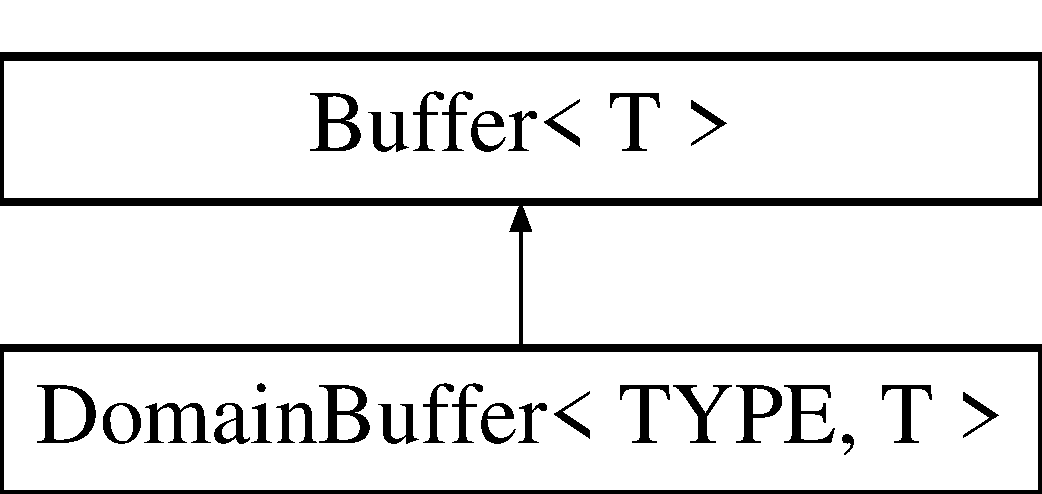
\includegraphics[height=2.000000cm]{class_buffer}
\end{center}
\end{figure}
\subsection*{Public Methods}
\begin{DoxyCompactItemize}
\item 
\mbox{\Hypertarget{class_buffer_a6b5de7c51749ed2aecf4e12066bc869c}\label{class_buffer_a6b5de7c51749ed2aecf4e12066bc869c}} 
{\bfseries Buffer} (size\+\_\+t count=0, Buffer\+Type type=H\+O\+S\+T\+\_\+\+B\+U\+F\+F\+ER, Page\+Locked\+State page\+Locked\+State=U\+N\+L\+O\+C\+K\+ED)
\item 
\mbox{\Hypertarget{class_buffer_ab2489e340cc0403f9f27163ecc7579a1}\label{class_buffer_ab2489e340cc0403f9f27163ecc7579a1}} 
{\bfseries Buffer} (const \hyperlink{class_buffer}{Buffer}$<$ T $>$ \&src)
\item 
\mbox{\Hypertarget{class_buffer_af2fab9ed39cf9bf278de4ec76584b3c6}\label{class_buffer_af2fab9ed39cf9bf278de4ec76584b3c6}} 
\hyperlink{class_buffer}{Buffer}$<$ T $>$ \& {\bfseries operator=} (const \hyperlink{class_buffer}{Buffer}$<$ T $>$ \&src)
\item 
\mbox{\Hypertarget{class_buffer_a5df8c9dee01bef8fa87a7a3655e70362}\label{class_buffer_a5df8c9dee01bef8fa87a7a3655e70362}} 
\hyperlink{class_buffer}{Buffer}$<$ T $>$ \& {\bfseries operator=} (const \hyperlink{class_managed_buffer}{Managed\+Buffer}$<$ T $>$ \&src)
\item 
\mbox{\Hypertarget{class_buffer_a3924bf143f8775be409c9eb1e8d9dfba}\label{class_buffer_a3924bf143f8775be409c9eb1e8d9dfba}} 
void {\bfseries alloc} (size\+\_\+t count)
\item 
\mbox{\Hypertarget{class_buffer_a1f68a9766127c1ee4858f11d18b59fa4}\label{class_buffer_a1f68a9766127c1ee4858f11d18b59fa4}} 
void {\bfseries alloc} (size\+\_\+t count, Buffer\+Type type, Page\+Locked\+State page\+Locked\+State=U\+N\+L\+O\+C\+K\+ED)
\item 
\mbox{\Hypertarget{class_buffer_a0777b8a1efb8952938ffb3213c3d1987}\label{class_buffer_a0777b8a1efb8952938ffb3213c3d1987}} 
void {\bfseries resize} (const size\+\_\+t count)
\item 
\mbox{\Hypertarget{class_buffer_a8ce00ff6dd7cacc009970dea7fa834d1}\label{class_buffer_a8ce00ff6dd7cacc009970dea7fa834d1}} 
void {\bfseries copy\+\_\+from} (const size\+\_\+t count, const Buffer\+Type src\+\_\+type, const T $\ast$src, const uint32 dst\+\_\+offset=0)
\item 
\mbox{\Hypertarget{class_buffer_a3327c2b8a3d86b4bd8a1962c81887a4f}\label{class_buffer_a3327c2b8a3d86b4bd8a1962c81887a4f}} 
void {\bfseries clear} (const uint8 byte)
\item 
\mbox{\Hypertarget{class_buffer_a02179b60bb8717e231490e2d843260c4}\label{class_buffer_a02179b60bb8717e231490e2d843260c4}} 
void {\bfseries free} ()
\item 
\mbox{\Hypertarget{class_buffer_adef9e59af83cd013b6dfda4d95d3239f}\label{class_buffer_adef9e59af83cd013b6dfda4d95d3239f}} 
size\+\_\+t {\bfseries count} () const
\item 
\mbox{\Hypertarget{class_buffer_a776c7872a2d9341b13844108bcd1ff0c}\label{class_buffer_a776c7872a2d9341b13844108bcd1ff0c}} 
size\+\_\+t {\bfseries size\+In\+Bytes} () const
\item 
\mbox{\Hypertarget{class_buffer_ab881d770f9c273c36e4c8f50e63ba4c6}\label{class_buffer_ab881d770f9c273c36e4c8f50e63ba4c6}} 
const T $\ast$ {\bfseries ptr} () const
\item 
\mbox{\Hypertarget{class_buffer_a8ad9a82901c52f4482d6af6cd0f0375b}\label{class_buffer_a8ad9a82901c52f4482d6af6cd0f0375b}} 
T $\ast$ {\bfseries ptr} ()
\item 
\mbox{\Hypertarget{class_buffer_ac77086f411419c391242ac8f61e20a64}\label{class_buffer_ac77086f411419c391242ac8f61e20a64}} 
Buffer\+Type {\bfseries type} () const
\item 
\mbox{\Hypertarget{class_buffer_acc2111d9bb88a798c1d1606f3a9fb22b}\label{class_buffer_acc2111d9bb88a798c1d1606f3a9fb22b}} 
T {\bfseries operator\mbox{[}$\,$\mbox{]}} (const size\+\_\+t i) const
\item 
\mbox{\Hypertarget{class_buffer_abd03227a6f1750607c9047a665db9c8d}\label{class_buffer_abd03227a6f1750607c9047a665db9c8d}} 
T \& {\bfseries operator\mbox{[}$\,$\mbox{]}} (const size\+\_\+t i)
\item 
\mbox{\Hypertarget{class_buffer_ac5f4d04b2bee69fe0715e4e46bf9f65f}\label{class_buffer_ac5f4d04b2bee69fe0715e4e46bf9f65f}} 
void {\bfseries set} (const size\+\_\+t i, const T val)
\item 
\mbox{\Hypertarget{class_buffer_a0fb8a098a6bc993f5e019776339e525c}\label{class_buffer_a0fb8a098a6bc993f5e019776339e525c}} 
void {\bfseries swap} (\hyperlink{class_buffer}{Buffer}$<$ T $>$ \&buf)
\end{DoxyCompactItemize}
\subsection*{Protected Members}
\begin{DoxyCompactItemize}
\item 
\mbox{\Hypertarget{class_buffer_aa781dd1b7d878f102a143eefb2f09ec3}\label{class_buffer_aa781dd1b7d878f102a143eefb2f09ec3}} 
Buffer\+Type {\bfseries m\+\_\+type}
\item 
\mbox{\Hypertarget{class_buffer_a4ca3e715a85c41be1610a3e039e613a7}\label{class_buffer_a4ca3e715a85c41be1610a3e039e613a7}} 
T $\ast$ {\bfseries m\+\_\+ptr}
\item 
\mbox{\Hypertarget{class_buffer_a57c5c20d61761a35df1cc2acaf85707e}\label{class_buffer_a57c5c20d61761a35df1cc2acaf85707e}} 
int {\bfseries m\+\_\+device}
\item 
\mbox{\Hypertarget{class_buffer_a50b578484061644b57c71e20e0f192ae}\label{class_buffer_a50b578484061644b57c71e20e0f192ae}} 
size\+\_\+t {\bfseries m\+\_\+count}
\item 
\mbox{\Hypertarget{class_buffer_aa721dc5a6930c3f4f549e39ea54ae1f6}\label{class_buffer_aa721dc5a6930c3f4f549e39ea54ae1f6}} 
Page\+Locked\+State {\bfseries m\+\_\+page\+Locked\+State}
\end{DoxyCompactItemize}


The documentation for this class was generated from the following file\+:\begin{DoxyCompactItemize}
\item 
C\+:/p4research/research/jpantaleoni/\+Fermat-\/\+Public/src/buffers.\+h\end{DoxyCompactItemize}

\hypertarget{structcugar_1_1_bvh}{}\section{cugar\+:\+:Bvh$<$ D\+IM $>$ Struct Template Reference}
\label{structcugar_1_1_bvh}\index{cugar\+::\+Bvh$<$ D\+I\+M $>$@{cugar\+::\+Bvh$<$ D\+I\+M $>$}}


\subsection{Detailed description}
\subsubsection*{template$<$uint32 D\+IM$>$\newline
struct cugar\+::\+Bvh$<$ D\+I\+M $>$}

A low dimensional bvh class 

{\ttfamily \#include $<$bvh.\+h$>$}

\subsection*{Public Types}
\begin{DoxyCompactItemize}
\item 
\mbox{\Hypertarget{structcugar_1_1_bvh_ac36d42081f829b7cc10171a30d87a765}\label{structcugar_1_1_bvh_ac36d42081f829b7cc10171a30d87a765}} 
typedef \hyperlink{structcugar_1_1_vector}{Vector}$<$ float, D\+IM $>$ {\bfseries vector\+\_\+type}
\item 
\mbox{\Hypertarget{structcugar_1_1_bvh_aeeeaf9bdf55e9af97a3b29b07360c16f}\label{structcugar_1_1_bvh_aeeeaf9bdf55e9af97a3b29b07360c16f}} 
typedef \hyperlink{structcugar_1_1_bbox}{Bbox}$<$ \hyperlink{structcugar_1_1_vector}{vector\+\_\+type} $>$ {\bfseries bbox\+\_\+type}
\item 
\mbox{\Hypertarget{structcugar_1_1_bvh_a99015aa7a09f3095a53076c3793f4fc9}\label{structcugar_1_1_bvh_a99015aa7a09f3095a53076c3793f4fc9}} 
typedef \hyperlink{structcugar_1_1_bvh__node}{Bvh\+\_\+node} {\bfseries node\+\_\+type}
\end{DoxyCompactItemize}
\subsection*{Public Members}
\begin{DoxyCompactItemize}
\item 
\mbox{\Hypertarget{structcugar_1_1_bvh_aa4728c4a79768689f4358b149df47120}\label{structcugar_1_1_bvh_aa4728c4a79768689f4358b149df47120}} 
std\+::vector$<$ \hyperlink{structcugar_1_1_bvh__node}{node\+\_\+type} $>$ {\bfseries m\+\_\+nodes}
\item 
\mbox{\Hypertarget{structcugar_1_1_bvh_ad25069e53c2f6bf66938df316584162e}\label{structcugar_1_1_bvh_ad25069e53c2f6bf66938df316584162e}} 
std\+::vector$<$ \hyperlink{structcugar_1_1_bbox}{bbox\+\_\+type} $>$ {\bfseries m\+\_\+bboxes}
\end{DoxyCompactItemize}


The documentation for this struct was generated from the following file\+:\begin{DoxyCompactItemize}
\item 
C\+:/p4research/research/jpantaleoni/\+Fermat-\/\+Public/contrib/cugar/bvh/\hyperlink{bvh_8h}{bvh.\+h}\end{DoxyCompactItemize}

\hypertarget{classcugar_1_1_bvh__builder}{}\section{cugar\+:\+:Bvh\+\_\+builder$<$ D\+IM $>$ Class Template Reference}
\label{classcugar_1_1_bvh__builder}\index{cugar\+::\+Bvh\+\_\+builder$<$ D\+I\+M $>$@{cugar\+::\+Bvh\+\_\+builder$<$ D\+I\+M $>$}}


\subsection{Detailed description}
\subsubsection*{template$<$uint32 D\+IM$>$\newline
class cugar\+::\+Bvh\+\_\+builder$<$ D\+I\+M $>$}

A bvh builder for sets of low dimensional bboxes 

{\ttfamily \#include $<$bvh.\+h$>$}

\subsection*{Classes}
\begin{DoxyCompactItemize}
\item 
struct \hyperlink{structcugar_1_1_bvh__builder_1_1_bvh__partitioner}{Bvh\+\_\+partitioner}
\end{DoxyCompactItemize}
\subsection*{Public Types}
\begin{DoxyCompactItemize}
\item 
\mbox{\Hypertarget{classcugar_1_1_bvh__builder_aaca690da5b129a7752e046b1cbdd1fab}\label{classcugar_1_1_bvh__builder_aaca690da5b129a7752e046b1cbdd1fab}} 
typedef \hyperlink{structcugar_1_1_vector}{Vector}$<$ float, D\+IM $>$ {\bfseries vector\+\_\+type}
\item 
\mbox{\Hypertarget{classcugar_1_1_bvh__builder_a6946aaf55b7ca5a0a35a48aa9a03bb7e}\label{classcugar_1_1_bvh__builder_a6946aaf55b7ca5a0a35a48aa9a03bb7e}} 
typedef \hyperlink{structcugar_1_1_bbox}{Bbox}$<$ \hyperlink{structcugar_1_1_vector}{vector\+\_\+type} $>$ {\bfseries bbox\+\_\+type}
\end{DoxyCompactItemize}
\subsection*{Public Methods}
\begin{DoxyCompactItemize}
\item 
\hyperlink{classcugar_1_1_bvh__builder_a298adf654253d0bcf55c903e1d2b7519}{Bvh\+\_\+builder} ()
\item 
void \hyperlink{classcugar_1_1_bvh__builder_a5de1e0c569c991a51e69e5d45abae979}{set\+\_\+params} (const uint32 max\+\_\+leaf\+\_\+size)
\item 
{\footnotesize template$<$typename Iterator $>$ }\\void \hyperlink{classcugar_1_1_bvh__builder_a7f72eef58c9e1352bec8129809aceeb9}{build} (const Iterator \hyperlink{namespacecugar_a2121df08f967e232ea5fe0ee378dee67}{begin}, const Iterator end, \hyperlink{structcugar_1_1_bvh}{Bvh}$<$ D\+IM $>$ $\ast$bvh)
\item 
uint32 \hyperlink{classcugar_1_1_bvh__builder_a393d93f26b616c0fb97e0267a421e99b}{index} (const uint32 i)
\end{DoxyCompactItemize}


\subsection{Constructor \& Destructor Documentation}
\mbox{\Hypertarget{classcugar_1_1_bvh__builder_a298adf654253d0bcf55c903e1d2b7519}\label{classcugar_1_1_bvh__builder_a298adf654253d0bcf55c903e1d2b7519}} 
\index{cugar\+::\+Bvh\+\_\+builder@{cugar\+::\+Bvh\+\_\+builder}!Bvh\+\_\+builder@{Bvh\+\_\+builder}}
\index{Bvh\+\_\+builder@{Bvh\+\_\+builder}!cugar\+::\+Bvh\+\_\+builder@{cugar\+::\+Bvh\+\_\+builder}}
\subsubsection{\texorpdfstring{Bvh\+\_\+builder()}{Bvh\_builder()}}
{\footnotesize\ttfamily template$<$uint32 D\+IM$>$ \\
\hyperlink{classcugar_1_1_bvh__builder}{cugar\+::\+Bvh\+\_\+builder}$<$ D\+IM $>$\+::\hyperlink{classcugar_1_1_bvh__builder}{Bvh\+\_\+builder} (\begin{DoxyParamCaption}{ }\end{DoxyParamCaption})\hspace{0.3cm}{\ttfamily [inline]}}

constructor 

\subsection{Member Function Documentation}
\mbox{\Hypertarget{classcugar_1_1_bvh__builder_a7f72eef58c9e1352bec8129809aceeb9}\label{classcugar_1_1_bvh__builder_a7f72eef58c9e1352bec8129809aceeb9}} 
\index{cugar\+::\+Bvh\+\_\+builder@{cugar\+::\+Bvh\+\_\+builder}!build@{build}}
\index{build@{build}!cugar\+::\+Bvh\+\_\+builder@{cugar\+::\+Bvh\+\_\+builder}}
\subsubsection{\texorpdfstring{build()}{build()}}
{\footnotesize\ttfamily template$<$uint32 D\+IM$>$ \\
template$<$typename Iterator $>$ \\
void \hyperlink{classcugar_1_1_bvh__builder}{cugar\+::\+Bvh\+\_\+builder}$<$ D\+IM $>$\+::build (\begin{DoxyParamCaption}\item[{const Iterator}]{begin,  }\item[{const Iterator}]{end,  }\item[{\hyperlink{structcugar_1_1_bvh}{Bvh}$<$ D\+IM $>$ $\ast$}]{bvh }\end{DoxyParamCaption})}

build

Iterator is supposed to dereference to a Vector$<$float,\+D\+I\+M$>$


\begin{DoxyParams}{Parameters}
{\em begin} & first point \\
\hline
{\em end} & last point \\
\hline
{\em bvh} & output bvh \\
\hline
\end{DoxyParams}
\mbox{\Hypertarget{classcugar_1_1_bvh__builder_a393d93f26b616c0fb97e0267a421e99b}\label{classcugar_1_1_bvh__builder_a393d93f26b616c0fb97e0267a421e99b}} 
\index{cugar\+::\+Bvh\+\_\+builder@{cugar\+::\+Bvh\+\_\+builder}!index@{index}}
\index{index@{index}!cugar\+::\+Bvh\+\_\+builder@{cugar\+::\+Bvh\+\_\+builder}}
\subsubsection{\texorpdfstring{index()}{index()}}
{\footnotesize\ttfamily template$<$uint32 D\+IM$>$ \\
uint32 \hyperlink{classcugar_1_1_bvh__builder}{cugar\+::\+Bvh\+\_\+builder}$<$ D\+IM $>$\+::index (\begin{DoxyParamCaption}\item[{const uint32}]{i }\end{DoxyParamCaption})\hspace{0.3cm}{\ttfamily [inline]}}

remapped point index \mbox{\Hypertarget{classcugar_1_1_bvh__builder_a5de1e0c569c991a51e69e5d45abae979}\label{classcugar_1_1_bvh__builder_a5de1e0c569c991a51e69e5d45abae979}} 
\index{cugar\+::\+Bvh\+\_\+builder@{cugar\+::\+Bvh\+\_\+builder}!set\+\_\+params@{set\+\_\+params}}
\index{set\+\_\+params@{set\+\_\+params}!cugar\+::\+Bvh\+\_\+builder@{cugar\+::\+Bvh\+\_\+builder}}
\subsubsection{\texorpdfstring{set\+\_\+params()}{set\_params()}}
{\footnotesize\ttfamily template$<$uint32 D\+IM$>$ \\
void \hyperlink{classcugar_1_1_bvh__builder}{cugar\+::\+Bvh\+\_\+builder}$<$ D\+IM $>$\+::set\+\_\+params (\begin{DoxyParamCaption}\item[{const uint32}]{max\+\_\+leaf\+\_\+size }\end{DoxyParamCaption})\hspace{0.3cm}{\ttfamily [inline]}}

set bvh parameters


\begin{DoxyParams}{Parameters}
{\em max\+\_\+leaf\+\_\+size} & maximum leaf size \\
\hline
\end{DoxyParams}


The documentation for this class was generated from the following files\+:\begin{DoxyCompactItemize}
\item 
C\+:/p4research/research/jpantaleoni/\+Fermat-\/\+Public/contrib/cugar/bvh/\hyperlink{bvh_8h}{bvh.\+h}\item 
C\+:/p4research/research/jpantaleoni/\+Fermat-\/\+Public/contrib/cugar/bvh/bvh\+\_\+inline.\+h\end{DoxyCompactItemize}

\hypertarget{structsandbox_1_1_bvh__node}{}\section{sandbox\+:\+:Bvh\+\_\+node$<$ tag $>$ Struct Template Reference}
\label{structsandbox_1_1_bvh__node}\index{sandbox\+::\+Bvh\+\_\+node$<$ tag $>$@{sandbox\+::\+Bvh\+\_\+node$<$ tag $>$}}


The documentation for this struct was generated from the following file\+:\begin{DoxyCompactItemize}
\item 
C\+:/p4research/research/jpantaleoni/\+Fermat-\/\+Public/contrib/cugar/bvh/bvh3d.\+h\end{DoxyCompactItemize}

\hypertarget{structcugar_1_1_bvh__node}{}\section{cugar\+:\+:Bvh\+\_\+node Struct Reference}
\label{structcugar_1_1_bvh__node}\index{cugar\+::\+Bvh\+\_\+node@{cugar\+::\+Bvh\+\_\+node}}


\subsection{Detailed description}
Base bvh topology node class 

{\ttfamily \#include $<$bvh\+\_\+node.\+h$>$}

Inheritance diagram for cugar\+:\+:Bvh\+\_\+node\+:\begin{figure}[H]
\begin{center}
\leavevmode
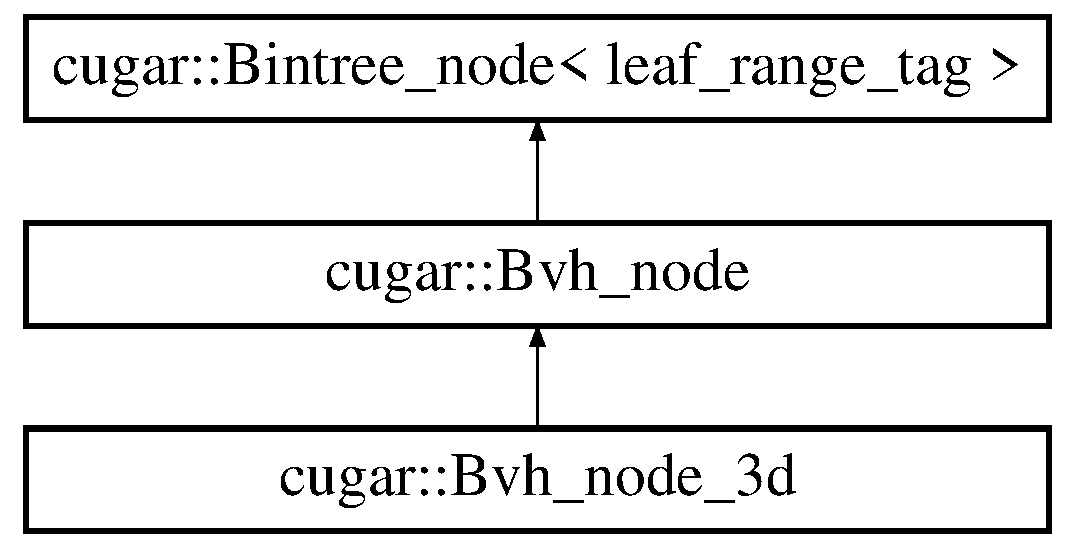
\includegraphics[height=3.000000cm]{structcugar_1_1_bvh__node}
\end{center}
\end{figure}
\subsection*{Public Types}
\begin{DoxyCompactItemize}
\item 
\mbox{\Hypertarget{structcugar_1_1_bvh__node_a758bf8378fd0be765c34fcb8e33ce5cd}\label{structcugar_1_1_bvh__node_a758bf8378fd0be765c34fcb8e33ce5cd}} 
enum {\bfseries internal\+\_\+type} \{ {\bfseries k\+Internal} = 0
 \}
\item 
\mbox{\Hypertarget{structcugar_1_1_bvh__node_ad519c4c28c5cb4d610a49845fc40acd2}\label{structcugar_1_1_bvh__node_ad519c4c28c5cb4d610a49845fc40acd2}} 
enum {\bfseries leaf\+\_\+type} \{ {\bfseries k\+Leaf} = 1
 \}
\item 
\mbox{\Hypertarget{structcugar_1_1_bvh__node_a7d5b7c3b6baccd383cf0e2de725fa625}\label{structcugar_1_1_bvh__node_a7d5b7c3b6baccd383cf0e2de725fa625}} 
typedef \hyperlink{structcugar_1_1leaf__range__tag}{leaf\+\_\+range\+\_\+tag} {\bfseries node\+\_\+tag}
\end{DoxyCompactItemize}
\subsection*{Public Methods}
\begin{DoxyCompactItemize}
\item 
C\+U\+G\+A\+R\+\_\+\+H\+O\+S\+T\+\_\+\+D\+E\+V\+I\+CE \hyperlink{structcugar_1_1_bvh__node_a3005ccf86a59ef28755cccec0445bf5d}{Bvh\+\_\+node} ()
\item 
C\+U\+G\+A\+R\+\_\+\+H\+O\+S\+T\+\_\+\+D\+E\+V\+I\+CE \hyperlink{structcugar_1_1_bvh__node_a01156ead9915a2849bc042fa57508345}{Bvh\+\_\+node} (const internal\+\_\+type type, const uint32 child\+\_\+index, const uint32 range\+\_\+size=0)
\item 
C\+U\+G\+A\+R\+\_\+\+H\+O\+S\+T\+\_\+\+D\+E\+V\+I\+CE \hyperlink{structcugar_1_1_bvh__node_a0d997ffdc050ef2fd937a5805b3f06df}{Bvh\+\_\+node} (const leaf\+\_\+type type, const uint32 leaf\+\_\+begin, const uint32 leaf\+\_\+end)
\item 
C\+U\+G\+A\+R\+\_\+\+H\+O\+S\+T\+\_\+\+D\+E\+V\+I\+CE \hyperlink{structcugar_1_1_bvh__node}{Bvh\+\_\+node} \& \hyperlink{structcugar_1_1_bvh__node_ad368801b53b70ab0c54a810971a16968}{operator=} (const \hyperlink{structcugar_1_1_bintree__node}{Bintree\+\_\+node}$<$ \hyperlink{structcugar_1_1leaf__range__tag}{leaf\+\_\+range\+\_\+tag} $>$ \&base)
\end{DoxyCompactItemize}


\subsection{Constructor \& Destructor Documentation}
\mbox{\Hypertarget{structcugar_1_1_bvh__node_a3005ccf86a59ef28755cccec0445bf5d}\label{structcugar_1_1_bvh__node_a3005ccf86a59ef28755cccec0445bf5d}} 
\index{cugar\+::\+Bvh\+\_\+node@{cugar\+::\+Bvh\+\_\+node}!Bvh\+\_\+node@{Bvh\+\_\+node}}
\index{Bvh\+\_\+node@{Bvh\+\_\+node}!cugar\+::\+Bvh\+\_\+node@{cugar\+::\+Bvh\+\_\+node}}
\subsubsection{\texorpdfstring{Bvh\+\_\+node()}{Bvh\_node()}\hspace{0.1cm}{\footnotesize\ttfamily [1/3]}}
{\footnotesize\ttfamily C\+U\+G\+A\+R\+\_\+\+H\+O\+S\+T\+\_\+\+D\+E\+V\+I\+CE cugar\+::\+Bvh\+\_\+node\+::\+Bvh\+\_\+node (\begin{DoxyParamCaption}{ }\end{DoxyParamCaption})\hspace{0.3cm}{\ttfamily [inline]}}

default constructor \mbox{\Hypertarget{structcugar_1_1_bvh__node_a01156ead9915a2849bc042fa57508345}\label{structcugar_1_1_bvh__node_a01156ead9915a2849bc042fa57508345}} 
\index{cugar\+::\+Bvh\+\_\+node@{cugar\+::\+Bvh\+\_\+node}!Bvh\+\_\+node@{Bvh\+\_\+node}}
\index{Bvh\+\_\+node@{Bvh\+\_\+node}!cugar\+::\+Bvh\+\_\+node@{cugar\+::\+Bvh\+\_\+node}}
\subsubsection{\texorpdfstring{Bvh\+\_\+node()}{Bvh\_node()}\hspace{0.1cm}{\footnotesize\ttfamily [2/3]}}
{\footnotesize\ttfamily C\+U\+G\+A\+R\+\_\+\+H\+O\+S\+T\+\_\+\+D\+E\+V\+I\+CE cugar\+::\+Bvh\+\_\+node\+::\+Bvh\+\_\+node (\begin{DoxyParamCaption}\item[{const internal\+\_\+type}]{type,  }\item[{const uint32}]{child\+\_\+index,  }\item[{const uint32}]{range\+\_\+size = {\ttfamily 0} }\end{DoxyParamCaption})\hspace{0.3cm}{\ttfamily [inline]}}

internal node constructor \mbox{\Hypertarget{structcugar_1_1_bvh__node_a0d997ffdc050ef2fd937a5805b3f06df}\label{structcugar_1_1_bvh__node_a0d997ffdc050ef2fd937a5805b3f06df}} 
\index{cugar\+::\+Bvh\+\_\+node@{cugar\+::\+Bvh\+\_\+node}!Bvh\+\_\+node@{Bvh\+\_\+node}}
\index{Bvh\+\_\+node@{Bvh\+\_\+node}!cugar\+::\+Bvh\+\_\+node@{cugar\+::\+Bvh\+\_\+node}}
\subsubsection{\texorpdfstring{Bvh\+\_\+node()}{Bvh\_node()}\hspace{0.1cm}{\footnotesize\ttfamily [3/3]}}
{\footnotesize\ttfamily C\+U\+G\+A\+R\+\_\+\+H\+O\+S\+T\+\_\+\+D\+E\+V\+I\+CE cugar\+::\+Bvh\+\_\+node\+::\+Bvh\+\_\+node (\begin{DoxyParamCaption}\item[{const leaf\+\_\+type}]{type,  }\item[{const uint32}]{leaf\+\_\+begin,  }\item[{const uint32}]{leaf\+\_\+end }\end{DoxyParamCaption})\hspace{0.3cm}{\ttfamily [inline]}}

leaf node constructor 

\subsection{Member Function Documentation}
\mbox{\Hypertarget{structcugar_1_1_bvh__node_ad368801b53b70ab0c54a810971a16968}\label{structcugar_1_1_bvh__node_ad368801b53b70ab0c54a810971a16968}} 
\index{cugar\+::\+Bvh\+\_\+node@{cugar\+::\+Bvh\+\_\+node}!operator=@{operator=}}
\index{operator=@{operator=}!cugar\+::\+Bvh\+\_\+node@{cugar\+::\+Bvh\+\_\+node}}
\subsubsection{\texorpdfstring{operator=()}{operator=()}}
{\footnotesize\ttfamily C\+U\+G\+A\+R\+\_\+\+H\+O\+S\+T\+\_\+\+D\+E\+V\+I\+CE \hyperlink{structcugar_1_1_bvh__node}{Bvh\+\_\+node}\& cugar\+::\+Bvh\+\_\+node\+::operator= (\begin{DoxyParamCaption}\item[{const \hyperlink{structcugar_1_1_bintree__node}{Bintree\+\_\+node}$<$ \hyperlink{structcugar_1_1leaf__range__tag}{leaf\+\_\+range\+\_\+tag} $>$ \&}]{base }\end{DoxyParamCaption})\hspace{0.3cm}{\ttfamily [inline]}}

assign the base type 

The documentation for this struct was generated from the following file\+:\begin{DoxyCompactItemize}
\item 
C\+:/p4research/research/jpantaleoni/\+Fermat-\/\+Public/contrib/cugar/bvh/\hyperlink{bvh__node_8h}{bvh\+\_\+node.\+h}\end{DoxyCompactItemize}

\hypertarget{structsandbox_1_1_bvh__node_3_01_compact__bvh__3d__tag_01_4}{}\section{sandbox\+:\+:Bvh\+\_\+node$<$ Compact\+\_\+bvh\+\_\+3d\+\_\+tag $>$ Struct Template Reference}
\label{structsandbox_1_1_bvh__node_3_01_compact__bvh__3d__tag_01_4}\index{sandbox\+::\+Bvh\+\_\+node$<$ Compact\+\_\+bvh\+\_\+3d\+\_\+tag $>$@{sandbox\+::\+Bvh\+\_\+node$<$ Compact\+\_\+bvh\+\_\+3d\+\_\+tag $>$}}


\subsection{Detailed description}
\subsubsection*{template$<$$>$\newline
struct sandbox\+::\+Bvh\+\_\+node$<$ Compact\+\_\+bvh\+\_\+3d\+\_\+tag $>$}

Bvh node struct with topology and bbox 

{\ttfamily \#include $<$bvh3d.\+h$>$}

Inheritance diagram for sandbox\+:\+:Bvh\+\_\+node$<$ Compact\+\_\+bvh\+\_\+3d\+\_\+tag $>$\+:\begin{figure}[H]
\begin{center}
\leavevmode
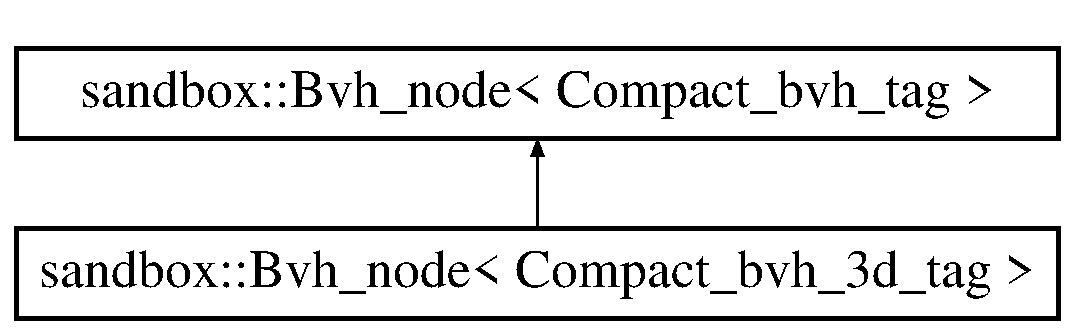
\includegraphics[height=2.000000cm]{structsandbox_1_1_bvh__node_3_01_compact__bvh__3d__tag_01_4}
\end{center}
\end{figure}
\subsection*{Public Types}
\begin{DoxyCompactItemize}
\item 
\mbox{\Hypertarget{structsandbox_1_1_bvh__node_3_01_compact__bvh__3d__tag_01_4_afadcaf787c49bbd52eff47e5480cd441}\label{structsandbox_1_1_bvh__node_3_01_compact__bvh__3d__tag_01_4_afadcaf787c49bbd52eff47e5480cd441}} 
typedef Compact\+\_\+bvh\+\_\+3d\+\_\+tag {\bfseries Tag}
\end{DoxyCompactItemize}
\subsection*{Public Members}
\begin{DoxyCompactItemize}
\item 
\mbox{\Hypertarget{structsandbox_1_1_bvh__node_3_01_compact__bvh__3d__tag_01_4_aacb544605195bac351c62e16c9e1be29}\label{structsandbox_1_1_bvh__node_3_01_compact__bvh__3d__tag_01_4_aacb544605195bac351c62e16c9e1be29}} 
float3 {\bfseries m\+\_\+bbox0}
\item 
\mbox{\Hypertarget{structsandbox_1_1_bvh__node_3_01_compact__bvh__3d__tag_01_4_a6385d0d701ee8521484487f330159e92}\label{structsandbox_1_1_bvh__node_3_01_compact__bvh__3d__tag_01_4_a6385d0d701ee8521484487f330159e92}} 
float3 {\bfseries m\+\_\+bbox1}
\end{DoxyCompactItemize}
\subsection*{Additional Inherited Members}


The documentation for this struct was generated from the following file\+:\begin{DoxyCompactItemize}
\item 
C\+:/p4research/research/jpantaleoni/\+Fermat-\/\+Public/contrib/cugar/bvh/bvh3d.\+h\end{DoxyCompactItemize}

\hypertarget{structsandbox_1_1_bvh__node_3_01_compact__bvh__tag_01_4}{}\section{sandbox\+:\+:Bvh\+\_\+node$<$ Compact\+\_\+bvh\+\_\+tag $>$ Struct Template Reference}
\label{structsandbox_1_1_bvh__node_3_01_compact__bvh__tag_01_4}\index{sandbox\+::\+Bvh\+\_\+node$<$ Compact\+\_\+bvh\+\_\+tag $>$@{sandbox\+::\+Bvh\+\_\+node$<$ Compact\+\_\+bvh\+\_\+tag $>$}}


\subsection{Detailed description}
\subsubsection*{template$<$$>$\newline
struct sandbox\+::\+Bvh\+\_\+node$<$ Compact\+\_\+bvh\+\_\+tag $>$}

Bvh node struct with topology and bbox 

{\ttfamily \#include $<$bvh3d.\+h$>$}

Inheritance diagram for sandbox\+:\+:Bvh\+\_\+node$<$ Compact\+\_\+bvh\+\_\+tag $>$\+:\begin{figure}[H]
\begin{center}
\leavevmode
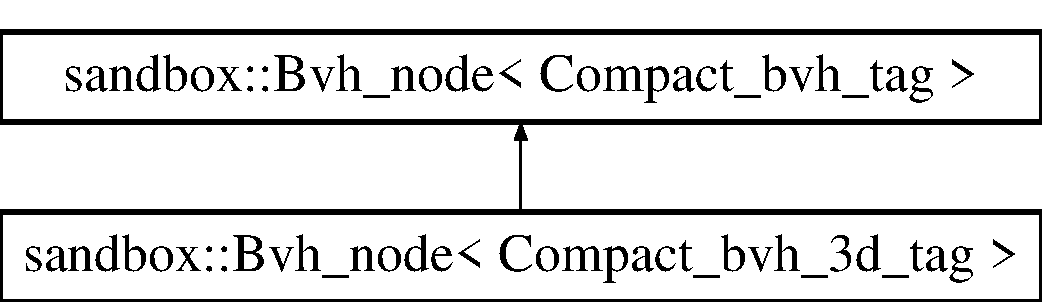
\includegraphics[height=2.000000cm]{structsandbox_1_1_bvh__node_3_01_compact__bvh__tag_01_4}
\end{center}
\end{figure}
\subsection*{Public Types}
\begin{DoxyCompactItemize}
\item 
\mbox{\Hypertarget{structsandbox_1_1_bvh__node_3_01_compact__bvh__tag_01_4_af3fca835972627b29003d328ea8f60da}\label{structsandbox_1_1_bvh__node_3_01_compact__bvh__tag_01_4_af3fca835972627b29003d328ea8f60da}} 
typedef Compact\+\_\+bvh\+\_\+tag {\bfseries Tag}
\item 
\mbox{\Hypertarget{structsandbox_1_1_bvh__node_3_01_compact__bvh__tag_01_4_a701018d976f7e60e60256ab2eb5a38d1}\label{structsandbox_1_1_bvh__node_3_01_compact__bvh__tag_01_4_a701018d976f7e60e60256ab2eb5a38d1}} 
typedef uint32 {\bfseries Type}
\end{DoxyCompactItemize}
\subsection*{Public Methods}
\begin{DoxyCompactItemize}
\item 
S\+A\+N\+D\+B\+O\+X\+\_\+\+H\+O\+S\+T\+\_\+\+D\+E\+V\+I\+CE \hyperlink{structsandbox_1_1_bvh__node_3_01_compact__bvh__tag_01_4_a1ace7c8c3d0c5ad6cca5fc6efa95a7bd}{Bvh\+\_\+node} ()
\item 
S\+A\+N\+D\+B\+O\+X\+\_\+\+H\+O\+S\+T\+\_\+\+D\+E\+V\+I\+CE \hyperlink{structsandbox_1_1_bvh__node_3_01_compact__bvh__tag_01_4_a9914c08eee2f15682cd6eba7d930ff07}{Bvh\+\_\+node} (const Type type, const uint32 index, const uint32 range\+\_\+size)
\item 
S\+A\+N\+D\+B\+O\+X\+\_\+\+H\+O\+S\+T\+\_\+\+D\+E\+V\+I\+CE void \hyperlink{structsandbox_1_1_bvh__node_3_01_compact__bvh__tag_01_4_a2b45390013155840bb1c19ede4a7cc10}{set\+\_\+type} (const Type type)
\item 
S\+A\+N\+D\+B\+O\+X\+\_\+\+H\+O\+S\+T\+\_\+\+D\+E\+V\+I\+CE void \hyperlink{structsandbox_1_1_bvh__node_3_01_compact__bvh__tag_01_4_a2e865b886cedb85a1c0b8c2e470e9719}{set\+\_\+index} (const uint32 index)
\item 
S\+A\+N\+D\+B\+O\+X\+\_\+\+H\+O\+S\+T\+\_\+\+D\+E\+V\+I\+CE void \hyperlink{structsandbox_1_1_bvh__node_3_01_compact__bvh__tag_01_4_adae271ac82a8cccff79c4686aa4a6c9c}{set\+\_\+range\+\_\+size} (const uint32 range\+\_\+size)
\item 
S\+A\+N\+D\+B\+O\+X\+\_\+\+H\+O\+S\+T\+\_\+\+D\+E\+V\+I\+CE bool \hyperlink{structsandbox_1_1_bvh__node_3_01_compact__bvh__tag_01_4_a500986abee989102e0acf42cf90245d2}{is\+\_\+leaf} () const
\item 
S\+A\+N\+D\+B\+O\+X\+\_\+\+H\+O\+S\+T\+\_\+\+D\+E\+V\+I\+CE uint32 \hyperlink{structsandbox_1_1_bvh__node_3_01_compact__bvh__tag_01_4_ae58332a51676665973e574bb61838f3e}{get\+\_\+index} () const
\item 
S\+A\+N\+D\+B\+O\+X\+\_\+\+H\+O\+S\+T\+\_\+\+D\+E\+V\+I\+CE uint32 \hyperlink{structsandbox_1_1_bvh__node_3_01_compact__bvh__tag_01_4_add480f55b45f3aaedba96da4488120ae}{get\+\_\+leaf\+\_\+index} () const
\item 
S\+A\+N\+D\+B\+O\+X\+\_\+\+H\+O\+S\+T\+\_\+\+D\+E\+V\+I\+CE uint32 \hyperlink{structsandbox_1_1_bvh__node_3_01_compact__bvh__tag_01_4_a507ae42faaac6f4691f0cfc582d85d52}{get\+\_\+range\+\_\+size} () const
\item 
S\+A\+N\+D\+B\+O\+X\+\_\+\+H\+O\+S\+T\+\_\+\+D\+E\+V\+I\+CE uint32 \hyperlink{structsandbox_1_1_bvh__node_3_01_compact__bvh__tag_01_4_af244133f74a887745ee5c7048f3b7bff}{get\+\_\+child\+\_\+count} () const
\item 
S\+A\+N\+D\+B\+O\+X\+\_\+\+H\+O\+S\+T\+\_\+\+D\+E\+V\+I\+CE uint32 \hyperlink{structsandbox_1_1_bvh__node_3_01_compact__bvh__tag_01_4_a249ef61691c3250aa9524546b295843a}{get\+\_\+child} (const uint32 i) const
\end{DoxyCompactItemize}
\subsection*{Static Public Methods}
\begin{DoxyCompactItemize}
\item 
static S\+A\+N\+D\+B\+O\+X\+\_\+\+H\+O\+S\+T\+\_\+\+D\+E\+V\+I\+CE uint32 \hyperlink{structsandbox_1_1_bvh__node_3_01_compact__bvh__tag_01_4_abd56f185aab1ea010813bd24b383a667}{packed\+\_\+data} (const Type type, const uint32 index)
\item 
static S\+A\+N\+D\+B\+O\+X\+\_\+\+H\+O\+S\+T\+\_\+\+D\+E\+V\+I\+CE void \hyperlink{structsandbox_1_1_bvh__node_3_01_compact__bvh__tag_01_4_ae81939099d3fe8a4cbafbde56c148fa5}{set\+\_\+type} (uint32 \&\hyperlink{structsandbox_1_1_bvh__node_3_01_compact__bvh__tag_01_4_abd56f185aab1ea010813bd24b383a667}{packed\+\_\+data}, const Type type)
\item 
static S\+A\+N\+D\+B\+O\+X\+\_\+\+H\+O\+S\+T\+\_\+\+D\+E\+V\+I\+CE void \hyperlink{structsandbox_1_1_bvh__node_3_01_compact__bvh__tag_01_4_a52bfb193b48c41677ca454b7e63e0117}{set\+\_\+index} (uint32 \&\hyperlink{structsandbox_1_1_bvh__node_3_01_compact__bvh__tag_01_4_abd56f185aab1ea010813bd24b383a667}{packed\+\_\+data}, const uint32 index)
\item 
\mbox{\Hypertarget{structsandbox_1_1_bvh__node_3_01_compact__bvh__tag_01_4_ad74089873b1f66257aadad9f8747e931}\label{structsandbox_1_1_bvh__node_3_01_compact__bvh__tag_01_4_ad74089873b1f66257aadad9f8747e931}} 
static S\+A\+N\+D\+B\+O\+X\+\_\+\+H\+O\+S\+T\+\_\+\+D\+E\+V\+I\+CE bool {\bfseries is\+\_\+leaf} (const uint32 \hyperlink{structsandbox_1_1_bvh__node_3_01_compact__bvh__tag_01_4_abd56f185aab1ea010813bd24b383a667}{packed\+\_\+data})
\item 
\mbox{\Hypertarget{structsandbox_1_1_bvh__node_3_01_compact__bvh__tag_01_4_afdef934caa69017c104aedd6dedbb5b1}\label{structsandbox_1_1_bvh__node_3_01_compact__bvh__tag_01_4_afdef934caa69017c104aedd6dedbb5b1}} 
static S\+A\+N\+D\+B\+O\+X\+\_\+\+H\+O\+S\+T\+\_\+\+D\+E\+V\+I\+CE uint32 {\bfseries get\+\_\+index} (const uint32 \hyperlink{structsandbox_1_1_bvh__node_3_01_compact__bvh__tag_01_4_abd56f185aab1ea010813bd24b383a667}{packed\+\_\+data})
\end{DoxyCompactItemize}
\subsection*{Public Members}
\begin{DoxyCompactItemize}
\item 
\mbox{\Hypertarget{structsandbox_1_1_bvh__node_3_01_compact__bvh__tag_01_4_ad781b792203805e6b09151a7335cf59e}\label{structsandbox_1_1_bvh__node_3_01_compact__bvh__tag_01_4_ad781b792203805e6b09151a7335cf59e}} 
uint32 {\bfseries m\+\_\+packed\+\_\+data}
\item 
\mbox{\Hypertarget{structsandbox_1_1_bvh__node_3_01_compact__bvh__tag_01_4_ae7b949a6066415fcd2a35d3dc67fb4c3}\label{structsandbox_1_1_bvh__node_3_01_compact__bvh__tag_01_4_ae7b949a6066415fcd2a35d3dc67fb4c3}} 
uint32 {\bfseries m\+\_\+data}
\end{DoxyCompactItemize}
\subsection*{Static Public Members}
\begin{DoxyCompactItemize}
\item 
\mbox{\Hypertarget{structsandbox_1_1_bvh__node_3_01_compact__bvh__tag_01_4_a58e190c4633720d676dad2e4b35095c6}\label{structsandbox_1_1_bvh__node_3_01_compact__bvh__tag_01_4_a58e190c4633720d676dad2e4b35095c6}} 
static const uint32 {\bfseries k\+Leaf} = (1u $<$$<$ 31u)
\item 
\mbox{\Hypertarget{structsandbox_1_1_bvh__node_3_01_compact__bvh__tag_01_4_add4dfad9f586e27f0e60fe7edc1c66d9}\label{structsandbox_1_1_bvh__node_3_01_compact__bvh__tag_01_4_add4dfad9f586e27f0e60fe7edc1c66d9}} 
static const uint32 {\bfseries k\+Internal} = 0x00000000u
\item 
\mbox{\Hypertarget{structsandbox_1_1_bvh__node_3_01_compact__bvh__tag_01_4_a02292d3f2ac08012bca5cedec436cbf9}\label{structsandbox_1_1_bvh__node_3_01_compact__bvh__tag_01_4_a02292d3f2ac08012bca5cedec436cbf9}} 
static const uint32 {\bfseries k\+Invalid} = uint32(-\/1)
\end{DoxyCompactItemize}


\subsection{Constructor \& Destructor Documentation}
\mbox{\Hypertarget{structsandbox_1_1_bvh__node_3_01_compact__bvh__tag_01_4_a1ace7c8c3d0c5ad6cca5fc6efa95a7bd}\label{structsandbox_1_1_bvh__node_3_01_compact__bvh__tag_01_4_a1ace7c8c3d0c5ad6cca5fc6efa95a7bd}} 
\index{sandbox\+::\+Bvh\+\_\+node$<$ Compact\+\_\+bvh\+\_\+tag $>$@{sandbox\+::\+Bvh\+\_\+node$<$ Compact\+\_\+bvh\+\_\+tag $>$}!Bvh\+\_\+node@{Bvh\+\_\+node}}
\index{Bvh\+\_\+node@{Bvh\+\_\+node}!sandbox\+::\+Bvh\+\_\+node$<$ Compact\+\_\+bvh\+\_\+tag $>$@{sandbox\+::\+Bvh\+\_\+node$<$ Compact\+\_\+bvh\+\_\+tag $>$}}
\subsubsection{\texorpdfstring{Bvh\+\_\+node()}{Bvh\_node()}\hspace{0.1cm}{\footnotesize\ttfamily [1/2]}}
{\footnotesize\ttfamily S\+A\+N\+D\+B\+O\+X\+\_\+\+H\+O\+S\+T\+\_\+\+D\+E\+V\+I\+CE \hyperlink{structsandbox_1_1_bvh__node}{sandbox\+::\+Bvh\+\_\+node}$<$ Compact\+\_\+bvh\+\_\+tag $>$\+::\hyperlink{structsandbox_1_1_bvh__node}{Bvh\+\_\+node} (\begin{DoxyParamCaption}{ }\end{DoxyParamCaption})\hspace{0.3cm}{\ttfamily [inline]}}

empty constructor \mbox{\Hypertarget{structsandbox_1_1_bvh__node_3_01_compact__bvh__tag_01_4_a9914c08eee2f15682cd6eba7d930ff07}\label{structsandbox_1_1_bvh__node_3_01_compact__bvh__tag_01_4_a9914c08eee2f15682cd6eba7d930ff07}} 
\index{sandbox\+::\+Bvh\+\_\+node$<$ Compact\+\_\+bvh\+\_\+tag $>$@{sandbox\+::\+Bvh\+\_\+node$<$ Compact\+\_\+bvh\+\_\+tag $>$}!Bvh\+\_\+node@{Bvh\+\_\+node}}
\index{Bvh\+\_\+node@{Bvh\+\_\+node}!sandbox\+::\+Bvh\+\_\+node$<$ Compact\+\_\+bvh\+\_\+tag $>$@{sandbox\+::\+Bvh\+\_\+node$<$ Compact\+\_\+bvh\+\_\+tag $>$}}
\subsubsection{\texorpdfstring{Bvh\+\_\+node()}{Bvh\_node()}\hspace{0.1cm}{\footnotesize\ttfamily [2/2]}}
{\footnotesize\ttfamily S\+A\+N\+D\+B\+O\+X\+\_\+\+H\+O\+S\+T\+\_\+\+D\+E\+V\+I\+CE \hyperlink{structsandbox_1_1_bvh__node}{sandbox\+::\+Bvh\+\_\+node}$<$ Compact\+\_\+bvh\+\_\+tag $>$\+::\hyperlink{structsandbox_1_1_bvh__node}{Bvh\+\_\+node} (\begin{DoxyParamCaption}\item[{const Type}]{type,  }\item[{const uint32}]{index,  }\item[{const uint32}]{range\+\_\+size }\end{DoxyParamCaption})}

full constructor


\begin{DoxyParams}{Parameters}
{\em type} & node type \\
\hline
{\em index} & child/leaf index \\
\hline
{\em range\+\_\+size} & primitive range size \\
\hline
\end{DoxyParams}


\subsection{Member Function Documentation}
\mbox{\Hypertarget{structsandbox_1_1_bvh__node_3_01_compact__bvh__tag_01_4_a249ef61691c3250aa9524546b295843a}\label{structsandbox_1_1_bvh__node_3_01_compact__bvh__tag_01_4_a249ef61691c3250aa9524546b295843a}} 
\index{sandbox\+::\+Bvh\+\_\+node$<$ Compact\+\_\+bvh\+\_\+tag $>$@{sandbox\+::\+Bvh\+\_\+node$<$ Compact\+\_\+bvh\+\_\+tag $>$}!get\+\_\+child@{get\+\_\+child}}
\index{get\+\_\+child@{get\+\_\+child}!sandbox\+::\+Bvh\+\_\+node$<$ Compact\+\_\+bvh\+\_\+tag $>$@{sandbox\+::\+Bvh\+\_\+node$<$ Compact\+\_\+bvh\+\_\+tag $>$}}
\subsubsection{\texorpdfstring{get\+\_\+child()}{get\_child()}}
{\footnotesize\ttfamily S\+A\+N\+D\+B\+O\+X\+\_\+\+H\+O\+S\+T\+\_\+\+D\+E\+V\+I\+CE uint32 \hyperlink{structsandbox_1_1_bvh__node}{sandbox\+::\+Bvh\+\_\+node}$<$ Compact\+\_\+bvh\+\_\+tag $>$\+::get\+\_\+child (\begin{DoxyParamCaption}\item[{const uint32}]{i }\end{DoxyParamCaption}) const\hspace{0.3cm}{\ttfamily [inline]}}

get i-\/th child


\begin{DoxyParams}{Parameters}
{\em i} & child index \\
\hline
\end{DoxyParams}
\mbox{\Hypertarget{structsandbox_1_1_bvh__node_3_01_compact__bvh__tag_01_4_af244133f74a887745ee5c7048f3b7bff}\label{structsandbox_1_1_bvh__node_3_01_compact__bvh__tag_01_4_af244133f74a887745ee5c7048f3b7bff}} 
\index{sandbox\+::\+Bvh\+\_\+node$<$ Compact\+\_\+bvh\+\_\+tag $>$@{sandbox\+::\+Bvh\+\_\+node$<$ Compact\+\_\+bvh\+\_\+tag $>$}!get\+\_\+child\+\_\+count@{get\+\_\+child\+\_\+count}}
\index{get\+\_\+child\+\_\+count@{get\+\_\+child\+\_\+count}!sandbox\+::\+Bvh\+\_\+node$<$ Compact\+\_\+bvh\+\_\+tag $>$@{sandbox\+::\+Bvh\+\_\+node$<$ Compact\+\_\+bvh\+\_\+tag $>$}}
\subsubsection{\texorpdfstring{get\+\_\+child\+\_\+count()}{get\_child\_count()}}
{\footnotesize\ttfamily S\+A\+N\+D\+B\+O\+X\+\_\+\+H\+O\+S\+T\+\_\+\+D\+E\+V\+I\+CE uint32 \hyperlink{structsandbox_1_1_bvh__node}{sandbox\+::\+Bvh\+\_\+node}$<$ Compact\+\_\+bvh\+\_\+tag $>$\+::get\+\_\+child\+\_\+count (\begin{DoxyParamCaption}{ }\end{DoxyParamCaption}) const\hspace{0.3cm}{\ttfamily [inline]}}

get child count \mbox{\Hypertarget{structsandbox_1_1_bvh__node_3_01_compact__bvh__tag_01_4_ae58332a51676665973e574bb61838f3e}\label{structsandbox_1_1_bvh__node_3_01_compact__bvh__tag_01_4_ae58332a51676665973e574bb61838f3e}} 
\index{sandbox\+::\+Bvh\+\_\+node$<$ Compact\+\_\+bvh\+\_\+tag $>$@{sandbox\+::\+Bvh\+\_\+node$<$ Compact\+\_\+bvh\+\_\+tag $>$}!get\+\_\+index@{get\+\_\+index}}
\index{get\+\_\+index@{get\+\_\+index}!sandbox\+::\+Bvh\+\_\+node$<$ Compact\+\_\+bvh\+\_\+tag $>$@{sandbox\+::\+Bvh\+\_\+node$<$ Compact\+\_\+bvh\+\_\+tag $>$}}
\subsubsection{\texorpdfstring{get\+\_\+index()}{get\_index()}}
{\footnotesize\ttfamily S\+A\+N\+D\+B\+O\+X\+\_\+\+H\+O\+S\+T\+\_\+\+D\+E\+V\+I\+CE uint32 \hyperlink{structsandbox_1_1_bvh__node}{sandbox\+::\+Bvh\+\_\+node}$<$ Compact\+\_\+bvh\+\_\+tag $>$\+::get\+\_\+index (\begin{DoxyParamCaption}{ }\end{DoxyParamCaption}) const\hspace{0.3cm}{\ttfamily [inline]}}

get child/leaf index \mbox{\Hypertarget{structsandbox_1_1_bvh__node_3_01_compact__bvh__tag_01_4_add480f55b45f3aaedba96da4488120ae}\label{structsandbox_1_1_bvh__node_3_01_compact__bvh__tag_01_4_add480f55b45f3aaedba96da4488120ae}} 
\index{sandbox\+::\+Bvh\+\_\+node$<$ Compact\+\_\+bvh\+\_\+tag $>$@{sandbox\+::\+Bvh\+\_\+node$<$ Compact\+\_\+bvh\+\_\+tag $>$}!get\+\_\+leaf\+\_\+index@{get\+\_\+leaf\+\_\+index}}
\index{get\+\_\+leaf\+\_\+index@{get\+\_\+leaf\+\_\+index}!sandbox\+::\+Bvh\+\_\+node$<$ Compact\+\_\+bvh\+\_\+tag $>$@{sandbox\+::\+Bvh\+\_\+node$<$ Compact\+\_\+bvh\+\_\+tag $>$}}
\subsubsection{\texorpdfstring{get\+\_\+leaf\+\_\+index()}{get\_leaf\_index()}}
{\footnotesize\ttfamily S\+A\+N\+D\+B\+O\+X\+\_\+\+H\+O\+S\+T\+\_\+\+D\+E\+V\+I\+CE uint32 \hyperlink{structsandbox_1_1_bvh__node}{sandbox\+::\+Bvh\+\_\+node}$<$ Compact\+\_\+bvh\+\_\+tag $>$\+::get\+\_\+leaf\+\_\+index (\begin{DoxyParamCaption}{ }\end{DoxyParamCaption}) const\hspace{0.3cm}{\ttfamily [inline]}}

get leaf index \mbox{\Hypertarget{structsandbox_1_1_bvh__node_3_01_compact__bvh__tag_01_4_a507ae42faaac6f4691f0cfc582d85d52}\label{structsandbox_1_1_bvh__node_3_01_compact__bvh__tag_01_4_a507ae42faaac6f4691f0cfc582d85d52}} 
\index{sandbox\+::\+Bvh\+\_\+node$<$ Compact\+\_\+bvh\+\_\+tag $>$@{sandbox\+::\+Bvh\+\_\+node$<$ Compact\+\_\+bvh\+\_\+tag $>$}!get\+\_\+range\+\_\+size@{get\+\_\+range\+\_\+size}}
\index{get\+\_\+range\+\_\+size@{get\+\_\+range\+\_\+size}!sandbox\+::\+Bvh\+\_\+node$<$ Compact\+\_\+bvh\+\_\+tag $>$@{sandbox\+::\+Bvh\+\_\+node$<$ Compact\+\_\+bvh\+\_\+tag $>$}}
\subsubsection{\texorpdfstring{get\+\_\+range\+\_\+size()}{get\_range\_size()}}
{\footnotesize\ttfamily S\+A\+N\+D\+B\+O\+X\+\_\+\+H\+O\+S\+T\+\_\+\+D\+E\+V\+I\+CE uint32 \hyperlink{structsandbox_1_1_bvh__node}{sandbox\+::\+Bvh\+\_\+node}$<$ Compact\+\_\+bvh\+\_\+tag $>$\+::get\+\_\+range\+\_\+size (\begin{DoxyParamCaption}{ }\end{DoxyParamCaption}) const\hspace{0.3cm}{\ttfamily [inline]}}

get primitive range size \mbox{\Hypertarget{structsandbox_1_1_bvh__node_3_01_compact__bvh__tag_01_4_a500986abee989102e0acf42cf90245d2}\label{structsandbox_1_1_bvh__node_3_01_compact__bvh__tag_01_4_a500986abee989102e0acf42cf90245d2}} 
\index{sandbox\+::\+Bvh\+\_\+node$<$ Compact\+\_\+bvh\+\_\+tag $>$@{sandbox\+::\+Bvh\+\_\+node$<$ Compact\+\_\+bvh\+\_\+tag $>$}!is\+\_\+leaf@{is\+\_\+leaf}}
\index{is\+\_\+leaf@{is\+\_\+leaf}!sandbox\+::\+Bvh\+\_\+node$<$ Compact\+\_\+bvh\+\_\+tag $>$@{sandbox\+::\+Bvh\+\_\+node$<$ Compact\+\_\+bvh\+\_\+tag $>$}}
\subsubsection{\texorpdfstring{is\+\_\+leaf()}{is\_leaf()}}
{\footnotesize\ttfamily S\+A\+N\+D\+B\+O\+X\+\_\+\+H\+O\+S\+T\+\_\+\+D\+E\+V\+I\+CE bool \hyperlink{structsandbox_1_1_bvh__node}{sandbox\+::\+Bvh\+\_\+node}$<$ Compact\+\_\+bvh\+\_\+tag $>$\+::is\+\_\+leaf (\begin{DoxyParamCaption}{ }\end{DoxyParamCaption}) const\hspace{0.3cm}{\ttfamily [inline]}}

is a leaf? \mbox{\Hypertarget{structsandbox_1_1_bvh__node_3_01_compact__bvh__tag_01_4_abd56f185aab1ea010813bd24b383a667}\label{structsandbox_1_1_bvh__node_3_01_compact__bvh__tag_01_4_abd56f185aab1ea010813bd24b383a667}} 
\index{sandbox\+::\+Bvh\+\_\+node$<$ Compact\+\_\+bvh\+\_\+tag $>$@{sandbox\+::\+Bvh\+\_\+node$<$ Compact\+\_\+bvh\+\_\+tag $>$}!packed\+\_\+data@{packed\+\_\+data}}
\index{packed\+\_\+data@{packed\+\_\+data}!sandbox\+::\+Bvh\+\_\+node$<$ Compact\+\_\+bvh\+\_\+tag $>$@{sandbox\+::\+Bvh\+\_\+node$<$ Compact\+\_\+bvh\+\_\+tag $>$}}
\subsubsection{\texorpdfstring{packed\+\_\+data()}{packed\_data()}}
{\footnotesize\ttfamily static S\+A\+N\+D\+B\+O\+X\+\_\+\+H\+O\+S\+T\+\_\+\+D\+E\+V\+I\+CE uint32 \hyperlink{structsandbox_1_1_bvh__node}{sandbox\+::\+Bvh\+\_\+node}$<$ Compact\+\_\+bvh\+\_\+tag $>$\+::packed\+\_\+data (\begin{DoxyParamCaption}\item[{const Type}]{type,  }\item[{const uint32}]{index }\end{DoxyParamCaption})\hspace{0.3cm}{\ttfamily [inline]}, {\ttfamily [static]}}

compute packed data


\begin{DoxyParams}{Parameters}
{\em type} & node type \\
\hline
{\em index} & child/leaf index \\
\hline
\end{DoxyParams}
\mbox{\Hypertarget{structsandbox_1_1_bvh__node_3_01_compact__bvh__tag_01_4_a2e865b886cedb85a1c0b8c2e470e9719}\label{structsandbox_1_1_bvh__node_3_01_compact__bvh__tag_01_4_a2e865b886cedb85a1c0b8c2e470e9719}} 
\index{sandbox\+::\+Bvh\+\_\+node$<$ Compact\+\_\+bvh\+\_\+tag $>$@{sandbox\+::\+Bvh\+\_\+node$<$ Compact\+\_\+bvh\+\_\+tag $>$}!set\+\_\+index@{set\+\_\+index}}
\index{set\+\_\+index@{set\+\_\+index}!sandbox\+::\+Bvh\+\_\+node$<$ Compact\+\_\+bvh\+\_\+tag $>$@{sandbox\+::\+Bvh\+\_\+node$<$ Compact\+\_\+bvh\+\_\+tag $>$}}
\subsubsection{\texorpdfstring{set\+\_\+index()}{set\_index()}\hspace{0.1cm}{\footnotesize\ttfamily [1/2]}}
{\footnotesize\ttfamily S\+A\+N\+D\+B\+O\+X\+\_\+\+H\+O\+S\+T\+\_\+\+D\+E\+V\+I\+CE void \hyperlink{structsandbox_1_1_bvh__node}{sandbox\+::\+Bvh\+\_\+node}$<$ Compact\+\_\+bvh\+\_\+tag $>$\+::set\+\_\+index (\begin{DoxyParamCaption}\item[{const uint32}]{index }\end{DoxyParamCaption})}

set child/leaf index


\begin{DoxyParams}{Parameters}
{\em index} & child/leaf index \\
\hline
\end{DoxyParams}
\mbox{\Hypertarget{structsandbox_1_1_bvh__node_3_01_compact__bvh__tag_01_4_a52bfb193b48c41677ca454b7e63e0117}\label{structsandbox_1_1_bvh__node_3_01_compact__bvh__tag_01_4_a52bfb193b48c41677ca454b7e63e0117}} 
\index{sandbox\+::\+Bvh\+\_\+node$<$ Compact\+\_\+bvh\+\_\+tag $>$@{sandbox\+::\+Bvh\+\_\+node$<$ Compact\+\_\+bvh\+\_\+tag $>$}!set\+\_\+index@{set\+\_\+index}}
\index{set\+\_\+index@{set\+\_\+index}!sandbox\+::\+Bvh\+\_\+node$<$ Compact\+\_\+bvh\+\_\+tag $>$@{sandbox\+::\+Bvh\+\_\+node$<$ Compact\+\_\+bvh\+\_\+tag $>$}}
\subsubsection{\texorpdfstring{set\+\_\+index()}{set\_index()}\hspace{0.1cm}{\footnotesize\ttfamily [2/2]}}
{\footnotesize\ttfamily static S\+A\+N\+D\+B\+O\+X\+\_\+\+H\+O\+S\+T\+\_\+\+D\+E\+V\+I\+CE void \hyperlink{structsandbox_1_1_bvh__node}{sandbox\+::\+Bvh\+\_\+node}$<$ Compact\+\_\+bvh\+\_\+tag $>$\+::set\+\_\+index (\begin{DoxyParamCaption}\item[{uint32 \&}]{packed\+\_\+data,  }\item[{const uint32}]{index }\end{DoxyParamCaption})\hspace{0.3cm}{\ttfamily [inline]}, {\ttfamily [static]}}

set child/leaf index into a packed data


\begin{DoxyParams}{Parameters}
{\em packed\+\_\+data} & packed data \\
\hline
{\em index} & child/leaf index \\
\hline
\end{DoxyParams}
\mbox{\Hypertarget{structsandbox_1_1_bvh__node_3_01_compact__bvh__tag_01_4_adae271ac82a8cccff79c4686aa4a6c9c}\label{structsandbox_1_1_bvh__node_3_01_compact__bvh__tag_01_4_adae271ac82a8cccff79c4686aa4a6c9c}} 
\index{sandbox\+::\+Bvh\+\_\+node$<$ Compact\+\_\+bvh\+\_\+tag $>$@{sandbox\+::\+Bvh\+\_\+node$<$ Compact\+\_\+bvh\+\_\+tag $>$}!set\+\_\+range\+\_\+size@{set\+\_\+range\+\_\+size}}
\index{set\+\_\+range\+\_\+size@{set\+\_\+range\+\_\+size}!sandbox\+::\+Bvh\+\_\+node$<$ Compact\+\_\+bvh\+\_\+tag $>$@{sandbox\+::\+Bvh\+\_\+node$<$ Compact\+\_\+bvh\+\_\+tag $>$}}
\subsubsection{\texorpdfstring{set\+\_\+range\+\_\+size()}{set\_range\_size()}}
{\footnotesize\ttfamily S\+A\+N\+D\+B\+O\+X\+\_\+\+H\+O\+S\+T\+\_\+\+D\+E\+V\+I\+CE void \hyperlink{structsandbox_1_1_bvh__node}{sandbox\+::\+Bvh\+\_\+node}$<$ Compact\+\_\+bvh\+\_\+tag $>$\+::set\+\_\+range\+\_\+size (\begin{DoxyParamCaption}\item[{const uint32}]{range\+\_\+size }\end{DoxyParamCaption})\hspace{0.3cm}{\ttfamily [inline]}}

set skip node index


\begin{DoxyParams}{Parameters}
{\em range\+\_\+size} & primitive range size \\
\hline
\end{DoxyParams}
\mbox{\Hypertarget{structsandbox_1_1_bvh__node_3_01_compact__bvh__tag_01_4_a2b45390013155840bb1c19ede4a7cc10}\label{structsandbox_1_1_bvh__node_3_01_compact__bvh__tag_01_4_a2b45390013155840bb1c19ede4a7cc10}} 
\index{sandbox\+::\+Bvh\+\_\+node$<$ Compact\+\_\+bvh\+\_\+tag $>$@{sandbox\+::\+Bvh\+\_\+node$<$ Compact\+\_\+bvh\+\_\+tag $>$}!set\+\_\+type@{set\+\_\+type}}
\index{set\+\_\+type@{set\+\_\+type}!sandbox\+::\+Bvh\+\_\+node$<$ Compact\+\_\+bvh\+\_\+tag $>$@{sandbox\+::\+Bvh\+\_\+node$<$ Compact\+\_\+bvh\+\_\+tag $>$}}
\subsubsection{\texorpdfstring{set\+\_\+type()}{set\_type()}\hspace{0.1cm}{\footnotesize\ttfamily [1/2]}}
{\footnotesize\ttfamily S\+A\+N\+D\+B\+O\+X\+\_\+\+H\+O\+S\+T\+\_\+\+D\+E\+V\+I\+CE void \hyperlink{structsandbox_1_1_bvh__node}{sandbox\+::\+Bvh\+\_\+node}$<$ Compact\+\_\+bvh\+\_\+tag $>$\+::set\+\_\+type (\begin{DoxyParamCaption}\item[{const Type}]{type }\end{DoxyParamCaption})}

set node type


\begin{DoxyParams}{Parameters}
{\em type} & node type \\
\hline
\end{DoxyParams}
\mbox{\Hypertarget{structsandbox_1_1_bvh__node_3_01_compact__bvh__tag_01_4_ae81939099d3fe8a4cbafbde56c148fa5}\label{structsandbox_1_1_bvh__node_3_01_compact__bvh__tag_01_4_ae81939099d3fe8a4cbafbde56c148fa5}} 
\index{sandbox\+::\+Bvh\+\_\+node$<$ Compact\+\_\+bvh\+\_\+tag $>$@{sandbox\+::\+Bvh\+\_\+node$<$ Compact\+\_\+bvh\+\_\+tag $>$}!set\+\_\+type@{set\+\_\+type}}
\index{set\+\_\+type@{set\+\_\+type}!sandbox\+::\+Bvh\+\_\+node$<$ Compact\+\_\+bvh\+\_\+tag $>$@{sandbox\+::\+Bvh\+\_\+node$<$ Compact\+\_\+bvh\+\_\+tag $>$}}
\subsubsection{\texorpdfstring{set\+\_\+type()}{set\_type()}\hspace{0.1cm}{\footnotesize\ttfamily [2/2]}}
{\footnotesize\ttfamily static S\+A\+N\+D\+B\+O\+X\+\_\+\+H\+O\+S\+T\+\_\+\+D\+E\+V\+I\+CE void \hyperlink{structsandbox_1_1_bvh__node}{sandbox\+::\+Bvh\+\_\+node}$<$ Compact\+\_\+bvh\+\_\+tag $>$\+::set\+\_\+type (\begin{DoxyParamCaption}\item[{uint32 \&}]{packed\+\_\+data,  }\item[{const Type}]{type }\end{DoxyParamCaption})\hspace{0.3cm}{\ttfamily [inline]}, {\ttfamily [static]}}

set node type into a packed data


\begin{DoxyParams}{Parameters}
{\em packed\+\_\+data} & packed data \\
\hline
{\em type} & node type \\
\hline
\end{DoxyParams}


The documentation for this struct was generated from the following file\+:\begin{DoxyCompactItemize}
\item 
C\+:/p4research/research/jpantaleoni/\+Fermat-\/\+Public/contrib/cugar/bvh/bvh3d.\+h\end{DoxyCompactItemize}

\hypertarget{structsandbox_1_1_bvh__node_3_01_indexed__leaf__bvh__tag_01_4}{}\section{sandbox\+:\+:Bvh\+\_\+node$<$ Indexed\+\_\+leaf\+\_\+bvh\+\_\+tag $>$ Struct Template Reference}
\label{structsandbox_1_1_bvh__node_3_01_indexed__leaf__bvh__tag_01_4}\index{sandbox\+::\+Bvh\+\_\+node$<$ Indexed\+\_\+leaf\+\_\+bvh\+\_\+tag $>$@{sandbox\+::\+Bvh\+\_\+node$<$ Indexed\+\_\+leaf\+\_\+bvh\+\_\+tag $>$}}


\subsection{Detailed description}
\subsubsection*{template$<$$>$\newline
struct sandbox\+::\+Bvh\+\_\+node$<$ Indexed\+\_\+leaf\+\_\+bvh\+\_\+tag $>$}

Bvh node struct 

{\ttfamily \#include $<$bvh3d.\+h$>$}

\subsection*{Public Types}
\begin{DoxyCompactItemize}
\item 
\mbox{\Hypertarget{structsandbox_1_1_bvh__node_3_01_indexed__leaf__bvh__tag_01_4_a4760b7377876a0c35050900598eb6fcc}\label{structsandbox_1_1_bvh__node_3_01_indexed__leaf__bvh__tag_01_4_a4760b7377876a0c35050900598eb6fcc}} 
typedef Indexed\+\_\+leaf\+\_\+bvh\+\_\+tag {\bfseries Tag}
\item 
\mbox{\Hypertarget{structsandbox_1_1_bvh__node_3_01_indexed__leaf__bvh__tag_01_4_af42c0e3b113e4fc548a1e94cce499208}\label{structsandbox_1_1_bvh__node_3_01_indexed__leaf__bvh__tag_01_4_af42c0e3b113e4fc548a1e94cce499208}} 
typedef uint32 {\bfseries Type}
\end{DoxyCompactItemize}
\subsection*{Public Methods}
\begin{DoxyCompactItemize}
\item 
S\+A\+N\+D\+B\+O\+X\+\_\+\+H\+O\+S\+T\+\_\+\+D\+E\+V\+I\+CE \hyperlink{structsandbox_1_1_bvh__node_3_01_indexed__leaf__bvh__tag_01_4_ad1bd8852582c16847eb047d9671d85df}{Bvh\+\_\+node} ()
\item 
S\+A\+N\+D\+B\+O\+X\+\_\+\+H\+O\+S\+T\+\_\+\+D\+E\+V\+I\+CE \hyperlink{structsandbox_1_1_bvh__node_3_01_indexed__leaf__bvh__tag_01_4_a5483abafea181c15a91f66da9e2c8580}{Bvh\+\_\+node} (const Type type, const uint32 index, const uint32 skip\+\_\+node)
\item 
S\+A\+N\+D\+B\+O\+X\+\_\+\+H\+O\+S\+T\+\_\+\+D\+E\+V\+I\+CE void \hyperlink{structsandbox_1_1_bvh__node_3_01_indexed__leaf__bvh__tag_01_4_aadeed3dd5e0241ed9514c6eb1e68be89}{set\+\_\+type} (const Type type)
\item 
S\+A\+N\+D\+B\+O\+X\+\_\+\+H\+O\+S\+T\+\_\+\+D\+E\+V\+I\+CE void \hyperlink{structsandbox_1_1_bvh__node_3_01_indexed__leaf__bvh__tag_01_4_aa5e707c983b73fc560880dcdeaae03b7}{set\+\_\+index} (const uint32 index)
\item 
S\+A\+N\+D\+B\+O\+X\+\_\+\+H\+O\+S\+T\+\_\+\+D\+E\+V\+I\+CE bool \hyperlink{structsandbox_1_1_bvh__node_3_01_indexed__leaf__bvh__tag_01_4_a5a769f5a9de50ececbecc6c1a44821ba}{is\+\_\+leaf} () const
\item 
S\+A\+N\+D\+B\+O\+X\+\_\+\+H\+O\+S\+T\+\_\+\+D\+E\+V\+I\+CE uint32 \hyperlink{structsandbox_1_1_bvh__node_3_01_indexed__leaf__bvh__tag_01_4_a8404398ddc749e7d9d3ab1196d16fde1}{get\+\_\+index} () const
\item 
S\+A\+N\+D\+B\+O\+X\+\_\+\+H\+O\+S\+T\+\_\+\+D\+E\+V\+I\+CE uint32 \hyperlink{structsandbox_1_1_bvh__node_3_01_indexed__leaf__bvh__tag_01_4_a24705a2ca7c24273af025f2400bf47e1}{get\+\_\+leaf\+\_\+index} () const
\item 
S\+A\+N\+D\+B\+O\+X\+\_\+\+H\+O\+S\+T\+\_\+\+D\+E\+V\+I\+CE uint32 \hyperlink{structsandbox_1_1_bvh__node_3_01_indexed__leaf__bvh__tag_01_4_af1e3fb80fb7434c8c5234532b3be2b5e}{get\+\_\+child\+\_\+count} () const
\item 
S\+A\+N\+D\+B\+O\+X\+\_\+\+H\+O\+S\+T\+\_\+\+D\+E\+V\+I\+CE uint32 \hyperlink{structsandbox_1_1_bvh__node_3_01_indexed__leaf__bvh__tag_01_4_a9bce7fdafbe100901b8779683ed2b9a5}{get\+\_\+child} (const uint32 i) const
\end{DoxyCompactItemize}
\subsection*{Static Public Methods}
\begin{DoxyCompactItemize}
\item 
static S\+A\+N\+D\+B\+O\+X\+\_\+\+H\+O\+S\+T\+\_\+\+D\+E\+V\+I\+CE uint32 \hyperlink{structsandbox_1_1_bvh__node_3_01_indexed__leaf__bvh__tag_01_4_a7ad8f08b43b06f8f68fe786e22079857}{packed\+\_\+data} (const Type type, const uint32 index)
\item 
static S\+A\+N\+D\+B\+O\+X\+\_\+\+H\+O\+S\+T\+\_\+\+D\+E\+V\+I\+CE void \hyperlink{structsandbox_1_1_bvh__node_3_01_indexed__leaf__bvh__tag_01_4_aaf2ca7a89646ed6e3418ad6cffbdf28c}{set\+\_\+type} (uint32 \&\hyperlink{structsandbox_1_1_bvh__node_3_01_indexed__leaf__bvh__tag_01_4_a7ad8f08b43b06f8f68fe786e22079857}{packed\+\_\+data}, const Type type)
\item 
static S\+A\+N\+D\+B\+O\+X\+\_\+\+H\+O\+S\+T\+\_\+\+D\+E\+V\+I\+CE void \hyperlink{structsandbox_1_1_bvh__node_3_01_indexed__leaf__bvh__tag_01_4_a21ff5f7d112aebb731f30e5e44a483a2}{set\+\_\+index} (uint32 \&\hyperlink{structsandbox_1_1_bvh__node_3_01_indexed__leaf__bvh__tag_01_4_a7ad8f08b43b06f8f68fe786e22079857}{packed\+\_\+data}, const uint32 index)
\item 
\mbox{\Hypertarget{structsandbox_1_1_bvh__node_3_01_indexed__leaf__bvh__tag_01_4_a12c2c2f60023978f9366830fc6c4c247}\label{structsandbox_1_1_bvh__node_3_01_indexed__leaf__bvh__tag_01_4_a12c2c2f60023978f9366830fc6c4c247}} 
static S\+A\+N\+D\+B\+O\+X\+\_\+\+H\+O\+S\+T\+\_\+\+D\+E\+V\+I\+CE bool {\bfseries is\+\_\+leaf} (const uint32 \hyperlink{structsandbox_1_1_bvh__node_3_01_indexed__leaf__bvh__tag_01_4_a7ad8f08b43b06f8f68fe786e22079857}{packed\+\_\+data})
\item 
\mbox{\Hypertarget{structsandbox_1_1_bvh__node_3_01_indexed__leaf__bvh__tag_01_4_ae7a3c9968d597ff4d5ab9c834de4be2e}\label{structsandbox_1_1_bvh__node_3_01_indexed__leaf__bvh__tag_01_4_ae7a3c9968d597ff4d5ab9c834de4be2e}} 
static S\+A\+N\+D\+B\+O\+X\+\_\+\+H\+O\+S\+T\+\_\+\+D\+E\+V\+I\+CE uint32 {\bfseries get\+\_\+index} (const uint32 \hyperlink{structsandbox_1_1_bvh__node_3_01_indexed__leaf__bvh__tag_01_4_a7ad8f08b43b06f8f68fe786e22079857}{packed\+\_\+data})
\end{DoxyCompactItemize}
\subsection*{Public Members}
\begin{DoxyCompactItemize}
\item 
\mbox{\Hypertarget{structsandbox_1_1_bvh__node_3_01_indexed__leaf__bvh__tag_01_4_a4b8506da03bd2c71870b79efde64ae1b}\label{structsandbox_1_1_bvh__node_3_01_indexed__leaf__bvh__tag_01_4_a4b8506da03bd2c71870b79efde64ae1b}} 
uint32 {\bfseries m\+\_\+packed\+\_\+data}
\end{DoxyCompactItemize}
\subsection*{Static Public Members}
\begin{DoxyCompactItemize}
\item 
\mbox{\Hypertarget{structsandbox_1_1_bvh__node_3_01_indexed__leaf__bvh__tag_01_4_a7c504322bc1f1056a0f64377d2f6b5fb}\label{structsandbox_1_1_bvh__node_3_01_indexed__leaf__bvh__tag_01_4_a7c504322bc1f1056a0f64377d2f6b5fb}} 
static const uint32 {\bfseries k\+Leaf} = (1u $<$$<$ 31u)
\item 
\mbox{\Hypertarget{structsandbox_1_1_bvh__node_3_01_indexed__leaf__bvh__tag_01_4_a2d619ed362c607fb3a114005b48b7018}\label{structsandbox_1_1_bvh__node_3_01_indexed__leaf__bvh__tag_01_4_a2d619ed362c607fb3a114005b48b7018}} 
static const uint32 {\bfseries k\+Internal} = 0x00000000u
\item 
\mbox{\Hypertarget{structsandbox_1_1_bvh__node_3_01_indexed__leaf__bvh__tag_01_4_aafa5ea630bdc1dd4f1d5bfa5eb14f5e6}\label{structsandbox_1_1_bvh__node_3_01_indexed__leaf__bvh__tag_01_4_aafa5ea630bdc1dd4f1d5bfa5eb14f5e6}} 
static const uint32 {\bfseries k\+Invalid} = uint32(-\/1)
\end{DoxyCompactItemize}


\subsection{Constructor \& Destructor Documentation}
\mbox{\Hypertarget{structsandbox_1_1_bvh__node_3_01_indexed__leaf__bvh__tag_01_4_ad1bd8852582c16847eb047d9671d85df}\label{structsandbox_1_1_bvh__node_3_01_indexed__leaf__bvh__tag_01_4_ad1bd8852582c16847eb047d9671d85df}} 
\index{sandbox\+::\+Bvh\+\_\+node$<$ Indexed\+\_\+leaf\+\_\+bvh\+\_\+tag $>$@{sandbox\+::\+Bvh\+\_\+node$<$ Indexed\+\_\+leaf\+\_\+bvh\+\_\+tag $>$}!Bvh\+\_\+node@{Bvh\+\_\+node}}
\index{Bvh\+\_\+node@{Bvh\+\_\+node}!sandbox\+::\+Bvh\+\_\+node$<$ Indexed\+\_\+leaf\+\_\+bvh\+\_\+tag $>$@{sandbox\+::\+Bvh\+\_\+node$<$ Indexed\+\_\+leaf\+\_\+bvh\+\_\+tag $>$}}
\subsubsection{\texorpdfstring{Bvh\+\_\+node()}{Bvh\_node()}\hspace{0.1cm}{\footnotesize\ttfamily [1/2]}}
{\footnotesize\ttfamily S\+A\+N\+D\+B\+O\+X\+\_\+\+H\+O\+S\+T\+\_\+\+D\+E\+V\+I\+CE \hyperlink{structsandbox_1_1_bvh__node}{sandbox\+::\+Bvh\+\_\+node}$<$ Indexed\+\_\+leaf\+\_\+bvh\+\_\+tag $>$\+::\hyperlink{structsandbox_1_1_bvh__node}{Bvh\+\_\+node} (\begin{DoxyParamCaption}{ }\end{DoxyParamCaption})\hspace{0.3cm}{\ttfamily [inline]}}

empty constructor \mbox{\Hypertarget{structsandbox_1_1_bvh__node_3_01_indexed__leaf__bvh__tag_01_4_a5483abafea181c15a91f66da9e2c8580}\label{structsandbox_1_1_bvh__node_3_01_indexed__leaf__bvh__tag_01_4_a5483abafea181c15a91f66da9e2c8580}} 
\index{sandbox\+::\+Bvh\+\_\+node$<$ Indexed\+\_\+leaf\+\_\+bvh\+\_\+tag $>$@{sandbox\+::\+Bvh\+\_\+node$<$ Indexed\+\_\+leaf\+\_\+bvh\+\_\+tag $>$}!Bvh\+\_\+node@{Bvh\+\_\+node}}
\index{Bvh\+\_\+node@{Bvh\+\_\+node}!sandbox\+::\+Bvh\+\_\+node$<$ Indexed\+\_\+leaf\+\_\+bvh\+\_\+tag $>$@{sandbox\+::\+Bvh\+\_\+node$<$ Indexed\+\_\+leaf\+\_\+bvh\+\_\+tag $>$}}
\subsubsection{\texorpdfstring{Bvh\+\_\+node()}{Bvh\_node()}\hspace{0.1cm}{\footnotesize\ttfamily [2/2]}}
{\footnotesize\ttfamily S\+A\+N\+D\+B\+O\+X\+\_\+\+H\+O\+S\+T\+\_\+\+D\+E\+V\+I\+CE \hyperlink{structsandbox_1_1_bvh__node}{sandbox\+::\+Bvh\+\_\+node}$<$ Indexed\+\_\+leaf\+\_\+bvh\+\_\+tag $>$\+::\hyperlink{structsandbox_1_1_bvh__node}{Bvh\+\_\+node} (\begin{DoxyParamCaption}\item[{const Type}]{type,  }\item[{const uint32}]{index,  }\item[{const uint32}]{skip\+\_\+node }\end{DoxyParamCaption})}

full constructor


\begin{DoxyParams}{Parameters}
{\em type} & node type \\
\hline
{\em index} & child/leaf index \\
\hline
{\em skip\+\_\+node} & skip node index \\
\hline
\end{DoxyParams}


\subsection{Member Function Documentation}
\mbox{\Hypertarget{structsandbox_1_1_bvh__node_3_01_indexed__leaf__bvh__tag_01_4_a9bce7fdafbe100901b8779683ed2b9a5}\label{structsandbox_1_1_bvh__node_3_01_indexed__leaf__bvh__tag_01_4_a9bce7fdafbe100901b8779683ed2b9a5}} 
\index{sandbox\+::\+Bvh\+\_\+node$<$ Indexed\+\_\+leaf\+\_\+bvh\+\_\+tag $>$@{sandbox\+::\+Bvh\+\_\+node$<$ Indexed\+\_\+leaf\+\_\+bvh\+\_\+tag $>$}!get\+\_\+child@{get\+\_\+child}}
\index{get\+\_\+child@{get\+\_\+child}!sandbox\+::\+Bvh\+\_\+node$<$ Indexed\+\_\+leaf\+\_\+bvh\+\_\+tag $>$@{sandbox\+::\+Bvh\+\_\+node$<$ Indexed\+\_\+leaf\+\_\+bvh\+\_\+tag $>$}}
\subsubsection{\texorpdfstring{get\+\_\+child()}{get\_child()}}
{\footnotesize\ttfamily S\+A\+N\+D\+B\+O\+X\+\_\+\+H\+O\+S\+T\+\_\+\+D\+E\+V\+I\+CE uint32 \hyperlink{structsandbox_1_1_bvh__node}{sandbox\+::\+Bvh\+\_\+node}$<$ Indexed\+\_\+leaf\+\_\+bvh\+\_\+tag $>$\+::get\+\_\+child (\begin{DoxyParamCaption}\item[{const uint32}]{i }\end{DoxyParamCaption}) const\hspace{0.3cm}{\ttfamily [inline]}}

get i-\/th child


\begin{DoxyParams}{Parameters}
{\em i} & child index \\
\hline
\end{DoxyParams}
\mbox{\Hypertarget{structsandbox_1_1_bvh__node_3_01_indexed__leaf__bvh__tag_01_4_af1e3fb80fb7434c8c5234532b3be2b5e}\label{structsandbox_1_1_bvh__node_3_01_indexed__leaf__bvh__tag_01_4_af1e3fb80fb7434c8c5234532b3be2b5e}} 
\index{sandbox\+::\+Bvh\+\_\+node$<$ Indexed\+\_\+leaf\+\_\+bvh\+\_\+tag $>$@{sandbox\+::\+Bvh\+\_\+node$<$ Indexed\+\_\+leaf\+\_\+bvh\+\_\+tag $>$}!get\+\_\+child\+\_\+count@{get\+\_\+child\+\_\+count}}
\index{get\+\_\+child\+\_\+count@{get\+\_\+child\+\_\+count}!sandbox\+::\+Bvh\+\_\+node$<$ Indexed\+\_\+leaf\+\_\+bvh\+\_\+tag $>$@{sandbox\+::\+Bvh\+\_\+node$<$ Indexed\+\_\+leaf\+\_\+bvh\+\_\+tag $>$}}
\subsubsection{\texorpdfstring{get\+\_\+child\+\_\+count()}{get\_child\_count()}}
{\footnotesize\ttfamily S\+A\+N\+D\+B\+O\+X\+\_\+\+H\+O\+S\+T\+\_\+\+D\+E\+V\+I\+CE uint32 \hyperlink{structsandbox_1_1_bvh__node}{sandbox\+::\+Bvh\+\_\+node}$<$ Indexed\+\_\+leaf\+\_\+bvh\+\_\+tag $>$\+::get\+\_\+child\+\_\+count (\begin{DoxyParamCaption}{ }\end{DoxyParamCaption}) const\hspace{0.3cm}{\ttfamily [inline]}}

get child count \mbox{\Hypertarget{structsandbox_1_1_bvh__node_3_01_indexed__leaf__bvh__tag_01_4_a8404398ddc749e7d9d3ab1196d16fde1}\label{structsandbox_1_1_bvh__node_3_01_indexed__leaf__bvh__tag_01_4_a8404398ddc749e7d9d3ab1196d16fde1}} 
\index{sandbox\+::\+Bvh\+\_\+node$<$ Indexed\+\_\+leaf\+\_\+bvh\+\_\+tag $>$@{sandbox\+::\+Bvh\+\_\+node$<$ Indexed\+\_\+leaf\+\_\+bvh\+\_\+tag $>$}!get\+\_\+index@{get\+\_\+index}}
\index{get\+\_\+index@{get\+\_\+index}!sandbox\+::\+Bvh\+\_\+node$<$ Indexed\+\_\+leaf\+\_\+bvh\+\_\+tag $>$@{sandbox\+::\+Bvh\+\_\+node$<$ Indexed\+\_\+leaf\+\_\+bvh\+\_\+tag $>$}}
\subsubsection{\texorpdfstring{get\+\_\+index()}{get\_index()}}
{\footnotesize\ttfamily S\+A\+N\+D\+B\+O\+X\+\_\+\+H\+O\+S\+T\+\_\+\+D\+E\+V\+I\+CE uint32 \hyperlink{structsandbox_1_1_bvh__node}{sandbox\+::\+Bvh\+\_\+node}$<$ Indexed\+\_\+leaf\+\_\+bvh\+\_\+tag $>$\+::get\+\_\+index (\begin{DoxyParamCaption}{ }\end{DoxyParamCaption}) const\hspace{0.3cm}{\ttfamily [inline]}}

get child/leaf index \mbox{\Hypertarget{structsandbox_1_1_bvh__node_3_01_indexed__leaf__bvh__tag_01_4_a24705a2ca7c24273af025f2400bf47e1}\label{structsandbox_1_1_bvh__node_3_01_indexed__leaf__bvh__tag_01_4_a24705a2ca7c24273af025f2400bf47e1}} 
\index{sandbox\+::\+Bvh\+\_\+node$<$ Indexed\+\_\+leaf\+\_\+bvh\+\_\+tag $>$@{sandbox\+::\+Bvh\+\_\+node$<$ Indexed\+\_\+leaf\+\_\+bvh\+\_\+tag $>$}!get\+\_\+leaf\+\_\+index@{get\+\_\+leaf\+\_\+index}}
\index{get\+\_\+leaf\+\_\+index@{get\+\_\+leaf\+\_\+index}!sandbox\+::\+Bvh\+\_\+node$<$ Indexed\+\_\+leaf\+\_\+bvh\+\_\+tag $>$@{sandbox\+::\+Bvh\+\_\+node$<$ Indexed\+\_\+leaf\+\_\+bvh\+\_\+tag $>$}}
\subsubsection{\texorpdfstring{get\+\_\+leaf\+\_\+index()}{get\_leaf\_index()}}
{\footnotesize\ttfamily S\+A\+N\+D\+B\+O\+X\+\_\+\+H\+O\+S\+T\+\_\+\+D\+E\+V\+I\+CE uint32 \hyperlink{structsandbox_1_1_bvh__node}{sandbox\+::\+Bvh\+\_\+node}$<$ Indexed\+\_\+leaf\+\_\+bvh\+\_\+tag $>$\+::get\+\_\+leaf\+\_\+index (\begin{DoxyParamCaption}{ }\end{DoxyParamCaption}) const\hspace{0.3cm}{\ttfamily [inline]}}

get leaf index \mbox{\Hypertarget{structsandbox_1_1_bvh__node_3_01_indexed__leaf__bvh__tag_01_4_a5a769f5a9de50ececbecc6c1a44821ba}\label{structsandbox_1_1_bvh__node_3_01_indexed__leaf__bvh__tag_01_4_a5a769f5a9de50ececbecc6c1a44821ba}} 
\index{sandbox\+::\+Bvh\+\_\+node$<$ Indexed\+\_\+leaf\+\_\+bvh\+\_\+tag $>$@{sandbox\+::\+Bvh\+\_\+node$<$ Indexed\+\_\+leaf\+\_\+bvh\+\_\+tag $>$}!is\+\_\+leaf@{is\+\_\+leaf}}
\index{is\+\_\+leaf@{is\+\_\+leaf}!sandbox\+::\+Bvh\+\_\+node$<$ Indexed\+\_\+leaf\+\_\+bvh\+\_\+tag $>$@{sandbox\+::\+Bvh\+\_\+node$<$ Indexed\+\_\+leaf\+\_\+bvh\+\_\+tag $>$}}
\subsubsection{\texorpdfstring{is\+\_\+leaf()}{is\_leaf()}}
{\footnotesize\ttfamily S\+A\+N\+D\+B\+O\+X\+\_\+\+H\+O\+S\+T\+\_\+\+D\+E\+V\+I\+CE bool \hyperlink{structsandbox_1_1_bvh__node}{sandbox\+::\+Bvh\+\_\+node}$<$ Indexed\+\_\+leaf\+\_\+bvh\+\_\+tag $>$\+::is\+\_\+leaf (\begin{DoxyParamCaption}{ }\end{DoxyParamCaption}) const\hspace{0.3cm}{\ttfamily [inline]}}

is a leaf? \mbox{\Hypertarget{structsandbox_1_1_bvh__node_3_01_indexed__leaf__bvh__tag_01_4_a7ad8f08b43b06f8f68fe786e22079857}\label{structsandbox_1_1_bvh__node_3_01_indexed__leaf__bvh__tag_01_4_a7ad8f08b43b06f8f68fe786e22079857}} 
\index{sandbox\+::\+Bvh\+\_\+node$<$ Indexed\+\_\+leaf\+\_\+bvh\+\_\+tag $>$@{sandbox\+::\+Bvh\+\_\+node$<$ Indexed\+\_\+leaf\+\_\+bvh\+\_\+tag $>$}!packed\+\_\+data@{packed\+\_\+data}}
\index{packed\+\_\+data@{packed\+\_\+data}!sandbox\+::\+Bvh\+\_\+node$<$ Indexed\+\_\+leaf\+\_\+bvh\+\_\+tag $>$@{sandbox\+::\+Bvh\+\_\+node$<$ Indexed\+\_\+leaf\+\_\+bvh\+\_\+tag $>$}}
\subsubsection{\texorpdfstring{packed\+\_\+data()}{packed\_data()}}
{\footnotesize\ttfamily static S\+A\+N\+D\+B\+O\+X\+\_\+\+H\+O\+S\+T\+\_\+\+D\+E\+V\+I\+CE uint32 \hyperlink{structsandbox_1_1_bvh__node}{sandbox\+::\+Bvh\+\_\+node}$<$ Indexed\+\_\+leaf\+\_\+bvh\+\_\+tag $>$\+::packed\+\_\+data (\begin{DoxyParamCaption}\item[{const Type}]{type,  }\item[{const uint32}]{index }\end{DoxyParamCaption})\hspace{0.3cm}{\ttfamily [inline]}, {\ttfamily [static]}}

compute packed data


\begin{DoxyParams}{Parameters}
{\em type} & node type \\
\hline
{\em index} & child/leaf index \\
\hline
\end{DoxyParams}
\mbox{\Hypertarget{structsandbox_1_1_bvh__node_3_01_indexed__leaf__bvh__tag_01_4_aa5e707c983b73fc560880dcdeaae03b7}\label{structsandbox_1_1_bvh__node_3_01_indexed__leaf__bvh__tag_01_4_aa5e707c983b73fc560880dcdeaae03b7}} 
\index{sandbox\+::\+Bvh\+\_\+node$<$ Indexed\+\_\+leaf\+\_\+bvh\+\_\+tag $>$@{sandbox\+::\+Bvh\+\_\+node$<$ Indexed\+\_\+leaf\+\_\+bvh\+\_\+tag $>$}!set\+\_\+index@{set\+\_\+index}}
\index{set\+\_\+index@{set\+\_\+index}!sandbox\+::\+Bvh\+\_\+node$<$ Indexed\+\_\+leaf\+\_\+bvh\+\_\+tag $>$@{sandbox\+::\+Bvh\+\_\+node$<$ Indexed\+\_\+leaf\+\_\+bvh\+\_\+tag $>$}}
\subsubsection{\texorpdfstring{set\+\_\+index()}{set\_index()}\hspace{0.1cm}{\footnotesize\ttfamily [1/2]}}
{\footnotesize\ttfamily S\+A\+N\+D\+B\+O\+X\+\_\+\+H\+O\+S\+T\+\_\+\+D\+E\+V\+I\+CE void \hyperlink{structsandbox_1_1_bvh__node}{sandbox\+::\+Bvh\+\_\+node}$<$ Indexed\+\_\+leaf\+\_\+bvh\+\_\+tag $>$\+::set\+\_\+index (\begin{DoxyParamCaption}\item[{const uint32}]{index }\end{DoxyParamCaption})}

set child/leaf index


\begin{DoxyParams}{Parameters}
{\em index} & child/leaf index \\
\hline
\end{DoxyParams}
\mbox{\Hypertarget{structsandbox_1_1_bvh__node_3_01_indexed__leaf__bvh__tag_01_4_a21ff5f7d112aebb731f30e5e44a483a2}\label{structsandbox_1_1_bvh__node_3_01_indexed__leaf__bvh__tag_01_4_a21ff5f7d112aebb731f30e5e44a483a2}} 
\index{sandbox\+::\+Bvh\+\_\+node$<$ Indexed\+\_\+leaf\+\_\+bvh\+\_\+tag $>$@{sandbox\+::\+Bvh\+\_\+node$<$ Indexed\+\_\+leaf\+\_\+bvh\+\_\+tag $>$}!set\+\_\+index@{set\+\_\+index}}
\index{set\+\_\+index@{set\+\_\+index}!sandbox\+::\+Bvh\+\_\+node$<$ Indexed\+\_\+leaf\+\_\+bvh\+\_\+tag $>$@{sandbox\+::\+Bvh\+\_\+node$<$ Indexed\+\_\+leaf\+\_\+bvh\+\_\+tag $>$}}
\subsubsection{\texorpdfstring{set\+\_\+index()}{set\_index()}\hspace{0.1cm}{\footnotesize\ttfamily [2/2]}}
{\footnotesize\ttfamily static S\+A\+N\+D\+B\+O\+X\+\_\+\+H\+O\+S\+T\+\_\+\+D\+E\+V\+I\+CE void \hyperlink{structsandbox_1_1_bvh__node}{sandbox\+::\+Bvh\+\_\+node}$<$ Indexed\+\_\+leaf\+\_\+bvh\+\_\+tag $>$\+::set\+\_\+index (\begin{DoxyParamCaption}\item[{uint32 \&}]{packed\+\_\+data,  }\item[{const uint32}]{index }\end{DoxyParamCaption})\hspace{0.3cm}{\ttfamily [inline]}, {\ttfamily [static]}}

set child/leaf index into a packed data


\begin{DoxyParams}{Parameters}
{\em packed\+\_\+data} & packed data \\
\hline
{\em index} & child/leaf index \\
\hline
\end{DoxyParams}
\mbox{\Hypertarget{structsandbox_1_1_bvh__node_3_01_indexed__leaf__bvh__tag_01_4_aadeed3dd5e0241ed9514c6eb1e68be89}\label{structsandbox_1_1_bvh__node_3_01_indexed__leaf__bvh__tag_01_4_aadeed3dd5e0241ed9514c6eb1e68be89}} 
\index{sandbox\+::\+Bvh\+\_\+node$<$ Indexed\+\_\+leaf\+\_\+bvh\+\_\+tag $>$@{sandbox\+::\+Bvh\+\_\+node$<$ Indexed\+\_\+leaf\+\_\+bvh\+\_\+tag $>$}!set\+\_\+type@{set\+\_\+type}}
\index{set\+\_\+type@{set\+\_\+type}!sandbox\+::\+Bvh\+\_\+node$<$ Indexed\+\_\+leaf\+\_\+bvh\+\_\+tag $>$@{sandbox\+::\+Bvh\+\_\+node$<$ Indexed\+\_\+leaf\+\_\+bvh\+\_\+tag $>$}}
\subsubsection{\texorpdfstring{set\+\_\+type()}{set\_type()}\hspace{0.1cm}{\footnotesize\ttfamily [1/2]}}
{\footnotesize\ttfamily S\+A\+N\+D\+B\+O\+X\+\_\+\+H\+O\+S\+T\+\_\+\+D\+E\+V\+I\+CE void \hyperlink{structsandbox_1_1_bvh__node}{sandbox\+::\+Bvh\+\_\+node}$<$ Indexed\+\_\+leaf\+\_\+bvh\+\_\+tag $>$\+::set\+\_\+type (\begin{DoxyParamCaption}\item[{const Type}]{type }\end{DoxyParamCaption})}

set node type


\begin{DoxyParams}{Parameters}
{\em type} & node type \\
\hline
\end{DoxyParams}
\mbox{\Hypertarget{structsandbox_1_1_bvh__node_3_01_indexed__leaf__bvh__tag_01_4_aaf2ca7a89646ed6e3418ad6cffbdf28c}\label{structsandbox_1_1_bvh__node_3_01_indexed__leaf__bvh__tag_01_4_aaf2ca7a89646ed6e3418ad6cffbdf28c}} 
\index{sandbox\+::\+Bvh\+\_\+node$<$ Indexed\+\_\+leaf\+\_\+bvh\+\_\+tag $>$@{sandbox\+::\+Bvh\+\_\+node$<$ Indexed\+\_\+leaf\+\_\+bvh\+\_\+tag $>$}!set\+\_\+type@{set\+\_\+type}}
\index{set\+\_\+type@{set\+\_\+type}!sandbox\+::\+Bvh\+\_\+node$<$ Indexed\+\_\+leaf\+\_\+bvh\+\_\+tag $>$@{sandbox\+::\+Bvh\+\_\+node$<$ Indexed\+\_\+leaf\+\_\+bvh\+\_\+tag $>$}}
\subsubsection{\texorpdfstring{set\+\_\+type()}{set\_type()}\hspace{0.1cm}{\footnotesize\ttfamily [2/2]}}
{\footnotesize\ttfamily static S\+A\+N\+D\+B\+O\+X\+\_\+\+H\+O\+S\+T\+\_\+\+D\+E\+V\+I\+CE void \hyperlink{structsandbox_1_1_bvh__node}{sandbox\+::\+Bvh\+\_\+node}$<$ Indexed\+\_\+leaf\+\_\+bvh\+\_\+tag $>$\+::set\+\_\+type (\begin{DoxyParamCaption}\item[{uint32 \&}]{packed\+\_\+data,  }\item[{const Type}]{type }\end{DoxyParamCaption})\hspace{0.3cm}{\ttfamily [inline]}, {\ttfamily [static]}}

set node type into a packed data


\begin{DoxyParams}{Parameters}
{\em packed\+\_\+data} & packed data \\
\hline
{\em type} & node type \\
\hline
\end{DoxyParams}


The documentation for this struct was generated from the following file\+:\begin{DoxyCompactItemize}
\item 
C\+:/p4research/research/jpantaleoni/\+Fermat-\/\+Public/contrib/cugar/bvh/bvh3d.\+h\end{DoxyCompactItemize}

\hypertarget{structcugar_1_1_bvh__node__3d}{}\section{cugar\+:\+:Bvh\+\_\+node\+\_\+3d Struct Reference}
\label{structcugar_1_1_bvh__node__3d}\index{cugar\+::\+Bvh\+\_\+node\+\_\+3d@{cugar\+::\+Bvh\+\_\+node\+\_\+3d}}


\subsection{Detailed description}
3d bvh node with bounding box (note that this struct has a convenient size of 32 bytes, which can be fetched with two float4 vector loads) 

{\ttfamily \#include $<$bvh\+\_\+node.\+h$>$}

Inheritance diagram for cugar\+:\+:Bvh\+\_\+node\+\_\+3d\+:\begin{figure}[H]
\begin{center}
\leavevmode
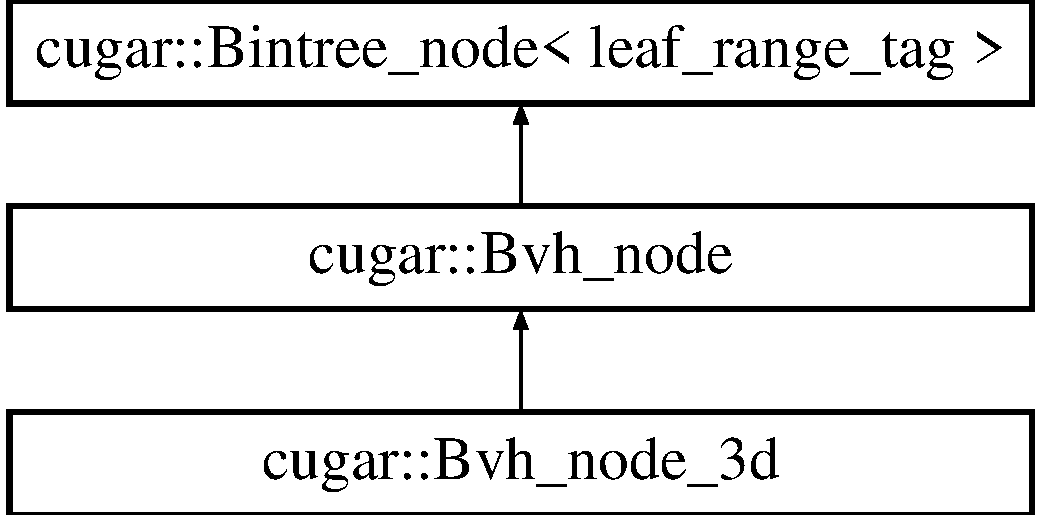
\includegraphics[height=3.000000cm]{structcugar_1_1_bvh__node__3d}
\end{center}
\end{figure}
\subsection*{Public Types}
\begin{DoxyCompactItemize}
\item 
\mbox{\Hypertarget{structcugar_1_1_bvh__node__3d_aacec14cb873e98a6f4c7d71a23172520}\label{structcugar_1_1_bvh__node__3d_aacec14cb873e98a6f4c7d71a23172520}} 
typedef \hyperlink{structcugar_1_1leaf__range__tag}{Bvh\+\_\+node\+::node\+\_\+tag} {\bfseries node\+\_\+tag}
\item 
\mbox{\Hypertarget{structcugar_1_1_bvh__node__3d_a2edcfbe5625e457b0be8da7c661b441f}\label{structcugar_1_1_bvh__node__3d_a2edcfbe5625e457b0be8da7c661b441f}} 
typedef Bvh\+\_\+node\+::internal\+\_\+type {\bfseries internal\+\_\+type}
\item 
\mbox{\Hypertarget{structcugar_1_1_bvh__node__3d_a502992c44b9d7f68d99f96c0bcbe2fd3}\label{structcugar_1_1_bvh__node__3d_a502992c44b9d7f68d99f96c0bcbe2fd3}} 
typedef Bvh\+\_\+node\+::leaf\+\_\+type {\bfseries leaf\+\_\+type}
\end{DoxyCompactItemize}
\subsection*{Public Methods}
\begin{DoxyCompactItemize}
\item 
C\+U\+G\+A\+R\+\_\+\+H\+O\+S\+T\+\_\+\+D\+E\+V\+I\+CE \hyperlink{structcugar_1_1_bvh__node__3d_a6ff41f6cb0ee5bead35d7eedbb202407}{Bvh\+\_\+node\+\_\+3d} ()
\item 
C\+U\+G\+A\+R\+\_\+\+H\+O\+S\+T\+\_\+\+D\+E\+V\+I\+CE \hyperlink{structcugar_1_1_bvh__node__3d_a9f09a6205af9453255216eab7995472d}{Bvh\+\_\+node\+\_\+3d} (const internal\+\_\+type type, const uint32 child\+\_\+index, const uint32 range\+\_\+size=0)
\item 
C\+U\+G\+A\+R\+\_\+\+H\+O\+S\+T\+\_\+\+D\+E\+V\+I\+CE \hyperlink{structcugar_1_1_bvh__node__3d_a7e01f1b0d48cfa6930e8dc6dc66e1f29}{Bvh\+\_\+node\+\_\+3d} (const leaf\+\_\+type type, const uint32 leaf\+\_\+begin, const uint32 leaf\+\_\+end)
\item 
C\+U\+G\+A\+R\+\_\+\+H\+O\+S\+T\+\_\+\+D\+E\+V\+I\+CE \hyperlink{structcugar_1_1_bvh__node__3d_ae6b8f30f63aed22b76ec523f12380f59}{Bvh\+\_\+node\+\_\+3d} (const float4 f0, const float4 f1)
\item 
C\+U\+G\+A\+R\+\_\+\+H\+O\+S\+T\+\_\+\+D\+E\+V\+I\+CE \hyperlink{structcugar_1_1_bvh__node__3d}{Bvh\+\_\+node\+\_\+3d} \& \hyperlink{structcugar_1_1_bvh__node__3d_a23550a54c38a821438d5e7f34f863c21}{operator=} (const \hyperlink{structcugar_1_1_bintree__node}{Bintree\+\_\+node}$<$ \hyperlink{structcugar_1_1leaf__range__tag}{leaf\+\_\+range\+\_\+tag} $>$ \&base)
\end{DoxyCompactItemize}
\subsection*{Static Public Methods}
\begin{DoxyCompactItemize}
\item 
static C\+U\+G\+A\+R\+\_\+\+H\+O\+S\+T\+\_\+\+D\+E\+V\+I\+CE \hyperlink{structcugar_1_1_bvh__node__3d}{Bvh\+\_\+node\+\_\+3d} \hyperlink{structcugar_1_1_bvh__node__3d_a765171d7b76108e44d2ec4ff9684741c}{load\+\_\+ldg} (const \hyperlink{structcugar_1_1_bvh__node__3d}{Bvh\+\_\+node\+\_\+3d} $\ast$node)
\end{DoxyCompactItemize}
\subsection*{Public Members}
\begin{DoxyCompactItemize}
\item 
\mbox{\Hypertarget{structcugar_1_1_bvh__node__3d_a4199cd920cc01d348e2f576c92d41773}\label{structcugar_1_1_bvh__node__3d_a4199cd920cc01d348e2f576c92d41773}} 
\hyperlink{structcugar_1_1_bbox}{Bbox}$<$ \hyperlink{structcugar_1_1_vector}{Vector3f} $>$ {\bfseries bbox}
\end{DoxyCompactItemize}


\subsection{Constructor \& Destructor Documentation}
\mbox{\Hypertarget{structcugar_1_1_bvh__node__3d_a6ff41f6cb0ee5bead35d7eedbb202407}\label{structcugar_1_1_bvh__node__3d_a6ff41f6cb0ee5bead35d7eedbb202407}} 
\index{cugar\+::\+Bvh\+\_\+node\+\_\+3d@{cugar\+::\+Bvh\+\_\+node\+\_\+3d}!Bvh\+\_\+node\+\_\+3d@{Bvh\+\_\+node\+\_\+3d}}
\index{Bvh\+\_\+node\+\_\+3d@{Bvh\+\_\+node\+\_\+3d}!cugar\+::\+Bvh\+\_\+node\+\_\+3d@{cugar\+::\+Bvh\+\_\+node\+\_\+3d}}
\subsubsection{\texorpdfstring{Bvh\+\_\+node\+\_\+3d()}{Bvh\_node\_3d()}\hspace{0.1cm}{\footnotesize\ttfamily [1/4]}}
{\footnotesize\ttfamily C\+U\+G\+A\+R\+\_\+\+H\+O\+S\+T\+\_\+\+D\+E\+V\+I\+CE cugar\+::\+Bvh\+\_\+node\+\_\+3d\+::\+Bvh\+\_\+node\+\_\+3d (\begin{DoxyParamCaption}{ }\end{DoxyParamCaption})\hspace{0.3cm}{\ttfamily [inline]}}

default constructor \mbox{\Hypertarget{structcugar_1_1_bvh__node__3d_a9f09a6205af9453255216eab7995472d}\label{structcugar_1_1_bvh__node__3d_a9f09a6205af9453255216eab7995472d}} 
\index{cugar\+::\+Bvh\+\_\+node\+\_\+3d@{cugar\+::\+Bvh\+\_\+node\+\_\+3d}!Bvh\+\_\+node\+\_\+3d@{Bvh\+\_\+node\+\_\+3d}}
\index{Bvh\+\_\+node\+\_\+3d@{Bvh\+\_\+node\+\_\+3d}!cugar\+::\+Bvh\+\_\+node\+\_\+3d@{cugar\+::\+Bvh\+\_\+node\+\_\+3d}}
\subsubsection{\texorpdfstring{Bvh\+\_\+node\+\_\+3d()}{Bvh\_node\_3d()}\hspace{0.1cm}{\footnotesize\ttfamily [2/4]}}
{\footnotesize\ttfamily C\+U\+G\+A\+R\+\_\+\+H\+O\+S\+T\+\_\+\+D\+E\+V\+I\+CE cugar\+::\+Bvh\+\_\+node\+\_\+3d\+::\+Bvh\+\_\+node\+\_\+3d (\begin{DoxyParamCaption}\item[{const internal\+\_\+type}]{type,  }\item[{const uint32}]{child\+\_\+index,  }\item[{const uint32}]{range\+\_\+size = {\ttfamily 0} }\end{DoxyParamCaption})\hspace{0.3cm}{\ttfamily [inline]}}

internal node constructor \mbox{\Hypertarget{structcugar_1_1_bvh__node__3d_a7e01f1b0d48cfa6930e8dc6dc66e1f29}\label{structcugar_1_1_bvh__node__3d_a7e01f1b0d48cfa6930e8dc6dc66e1f29}} 
\index{cugar\+::\+Bvh\+\_\+node\+\_\+3d@{cugar\+::\+Bvh\+\_\+node\+\_\+3d}!Bvh\+\_\+node\+\_\+3d@{Bvh\+\_\+node\+\_\+3d}}
\index{Bvh\+\_\+node\+\_\+3d@{Bvh\+\_\+node\+\_\+3d}!cugar\+::\+Bvh\+\_\+node\+\_\+3d@{cugar\+::\+Bvh\+\_\+node\+\_\+3d}}
\subsubsection{\texorpdfstring{Bvh\+\_\+node\+\_\+3d()}{Bvh\_node\_3d()}\hspace{0.1cm}{\footnotesize\ttfamily [3/4]}}
{\footnotesize\ttfamily C\+U\+G\+A\+R\+\_\+\+H\+O\+S\+T\+\_\+\+D\+E\+V\+I\+CE cugar\+::\+Bvh\+\_\+node\+\_\+3d\+::\+Bvh\+\_\+node\+\_\+3d (\begin{DoxyParamCaption}\item[{const leaf\+\_\+type}]{type,  }\item[{const uint32}]{leaf\+\_\+begin,  }\item[{const uint32}]{leaf\+\_\+end }\end{DoxyParamCaption})\hspace{0.3cm}{\ttfamily [inline]}}

leaf node constructor \mbox{\Hypertarget{structcugar_1_1_bvh__node__3d_ae6b8f30f63aed22b76ec523f12380f59}\label{structcugar_1_1_bvh__node__3d_ae6b8f30f63aed22b76ec523f12380f59}} 
\index{cugar\+::\+Bvh\+\_\+node\+\_\+3d@{cugar\+::\+Bvh\+\_\+node\+\_\+3d}!Bvh\+\_\+node\+\_\+3d@{Bvh\+\_\+node\+\_\+3d}}
\index{Bvh\+\_\+node\+\_\+3d@{Bvh\+\_\+node\+\_\+3d}!cugar\+::\+Bvh\+\_\+node\+\_\+3d@{cugar\+::\+Bvh\+\_\+node\+\_\+3d}}
\subsubsection{\texorpdfstring{Bvh\+\_\+node\+\_\+3d()}{Bvh\_node\_3d()}\hspace{0.1cm}{\footnotesize\ttfamily [4/4]}}
{\footnotesize\ttfamily C\+U\+G\+A\+R\+\_\+\+H\+O\+S\+T\+\_\+\+D\+E\+V\+I\+CE cugar\+::\+Bvh\+\_\+node\+\_\+3d\+::\+Bvh\+\_\+node\+\_\+3d (\begin{DoxyParamCaption}\item[{const float4}]{f0,  }\item[{const float4}]{f1 }\end{DoxyParamCaption})\hspace{0.3cm}{\ttfamily [inline]}}

construct a node from two float4\textquotesingle{}s 

\subsection{Member Function Documentation}
\mbox{\Hypertarget{structcugar_1_1_bvh__node__3d_a765171d7b76108e44d2ec4ff9684741c}\label{structcugar_1_1_bvh__node__3d_a765171d7b76108e44d2ec4ff9684741c}} 
\index{cugar\+::\+Bvh\+\_\+node\+\_\+3d@{cugar\+::\+Bvh\+\_\+node\+\_\+3d}!load\+\_\+ldg@{load\+\_\+ldg}}
\index{load\+\_\+ldg@{load\+\_\+ldg}!cugar\+::\+Bvh\+\_\+node\+\_\+3d@{cugar\+::\+Bvh\+\_\+node\+\_\+3d}}
\subsubsection{\texorpdfstring{load\+\_\+ldg()}{load\_ldg()}}
{\footnotesize\ttfamily static C\+U\+G\+A\+R\+\_\+\+H\+O\+S\+T\+\_\+\+D\+E\+V\+I\+CE \hyperlink{structcugar_1_1_bvh__node__3d}{Bvh\+\_\+node\+\_\+3d} cugar\+::\+Bvh\+\_\+node\+\_\+3d\+::load\+\_\+ldg (\begin{DoxyParamCaption}\item[{const \hyperlink{structcugar_1_1_bvh__node__3d}{Bvh\+\_\+node\+\_\+3d} $\ast$}]{node }\end{DoxyParamCaption})\hspace{0.3cm}{\ttfamily [inline]}, {\ttfamily [static]}}

construct a node from two float4\textquotesingle{}s \mbox{\Hypertarget{structcugar_1_1_bvh__node__3d_a23550a54c38a821438d5e7f34f863c21}\label{structcugar_1_1_bvh__node__3d_a23550a54c38a821438d5e7f34f863c21}} 
\index{cugar\+::\+Bvh\+\_\+node\+\_\+3d@{cugar\+::\+Bvh\+\_\+node\+\_\+3d}!operator=@{operator=}}
\index{operator=@{operator=}!cugar\+::\+Bvh\+\_\+node\+\_\+3d@{cugar\+::\+Bvh\+\_\+node\+\_\+3d}}
\subsubsection{\texorpdfstring{operator=()}{operator=()}}
{\footnotesize\ttfamily C\+U\+G\+A\+R\+\_\+\+H\+O\+S\+T\+\_\+\+D\+E\+V\+I\+CE \hyperlink{structcugar_1_1_bvh__node__3d}{Bvh\+\_\+node\+\_\+3d}\& cugar\+::\+Bvh\+\_\+node\+\_\+3d\+::operator= (\begin{DoxyParamCaption}\item[{const \hyperlink{structcugar_1_1_bintree__node}{Bintree\+\_\+node}$<$ \hyperlink{structcugar_1_1leaf__range__tag}{leaf\+\_\+range\+\_\+tag} $>$ \&}]{base }\end{DoxyParamCaption})\hspace{0.3cm}{\ttfamily [inline]}}

assign the base type 

The documentation for this struct was generated from the following file\+:\begin{DoxyCompactItemize}
\item 
C\+:/p4research/research/jpantaleoni/\+Fermat-\/\+Public/contrib/cugar/bvh/\hyperlink{bvh__node_8h}{bvh\+\_\+node.\+h}\end{DoxyCompactItemize}

\hypertarget{structcugar_1_1_bvh__node__3d__bbox__iterator}{}\section{cugar\+:\+:Bvh\+\_\+node\+\_\+3d\+\_\+bbox\+\_\+iterator Struct Reference}
\label{structcugar_1_1_bvh__node__3d__bbox__iterator}\index{cugar\+::\+Bvh\+\_\+node\+\_\+3d\+\_\+bbox\+\_\+iterator@{cugar\+::\+Bvh\+\_\+node\+\_\+3d\+\_\+bbox\+\_\+iterator}}


\subsection{Detailed description}
A utility class to iterate through \hyperlink{structcugar_1_1_bvh__node__3d}{Bvh\+\_\+node\+\_\+3d}\textquotesingle{}s as if they were bboxes 

{\ttfamily \#include $<$bvh.\+h$>$}

\subsection*{Classes}
\begin{DoxyCompactItemize}
\item 
struct \hyperlink{structcugar_1_1_bvh__node__3d__bbox__iterator_1_1_reference}{Reference}
\end{DoxyCompactItemize}
\subsection*{Public Methods}
\begin{DoxyCompactItemize}
\item 
\mbox{\Hypertarget{structcugar_1_1_bvh__node__3d__bbox__iterator_a48553587be15e9be3a3c5474bd7cdc5d}\label{structcugar_1_1_bvh__node__3d__bbox__iterator_a48553587be15e9be3a3c5474bd7cdc5d}} 
C\+U\+G\+A\+R\+\_\+\+H\+O\+S\+T\+\_\+\+D\+E\+V\+I\+CE {\bfseries Bvh\+\_\+node\+\_\+3d\+\_\+bbox\+\_\+iterator} (\hyperlink{structcugar_1_1_bvh__node__3d}{cugar\+::\+Bvh\+\_\+node\+\_\+3d} $\ast$\+\_\+nodes)
\item 
\mbox{\Hypertarget{structcugar_1_1_bvh__node__3d__bbox__iterator_ae7922015097f39e58d94ef1e4cdea1eb}\label{structcugar_1_1_bvh__node__3d__bbox__iterator_ae7922015097f39e58d94ef1e4cdea1eb}} 
C\+U\+G\+A\+R\+\_\+\+H\+O\+S\+T\+\_\+\+D\+E\+V\+I\+CE \hyperlink{structcugar_1_1_bvh__node__3d__bbox__iterator_1_1_reference}{Reference} {\bfseries operator\mbox{[}$\,$\mbox{]}} (const uint32 i) const
\item 
\mbox{\Hypertarget{structcugar_1_1_bvh__node__3d__bbox__iterator_a55309a467a87be865c1dfd5b6bfea748}\label{structcugar_1_1_bvh__node__3d__bbox__iterator_a55309a467a87be865c1dfd5b6bfea748}} 
C\+U\+G\+A\+R\+\_\+\+H\+O\+S\+T\+\_\+\+D\+E\+V\+I\+CE \hyperlink{structcugar_1_1_bvh__node__3d__bbox__iterator_1_1_reference}{Reference} {\bfseries operator\mbox{[}$\,$\mbox{]}} (const uint32 i)
\end{DoxyCompactItemize}
\subsection*{Public Members}
\begin{DoxyCompactItemize}
\item 
\mbox{\Hypertarget{structcugar_1_1_bvh__node__3d__bbox__iterator_a1fd3ce36de4ac2dc50b54e79afa12895}\label{structcugar_1_1_bvh__node__3d__bbox__iterator_a1fd3ce36de4ac2dc50b54e79afa12895}} 
\hyperlink{structcugar_1_1_bvh__node__3d}{cugar\+::\+Bvh\+\_\+node\+\_\+3d} $\ast$ {\bfseries nodes}
\end{DoxyCompactItemize}


The documentation for this struct was generated from the following file\+:\begin{DoxyCompactItemize}
\item 
C\+:/p4research/research/jpantaleoni/\+Fermat-\/\+Public/contrib/cugar/bvh/\hyperlink{bvh_8h}{bvh.\+h}\end{DoxyCompactItemize}

\hypertarget{structcugar_1_1cuda_1_1bvh__packing__functor}{}\section{cugar\+:\+:cuda\+:\+:bvh\+\_\+packing\+\_\+functor Struct Reference}
\label{structcugar_1_1cuda_1_1bvh__packing__functor}\index{cugar\+::cuda\+::bvh\+\_\+packing\+\_\+functor@{cugar\+::cuda\+::bvh\+\_\+packing\+\_\+functor}}


\subsection{Detailed description}
utility functor to pack a tuple formed by a (4d) bbox and a node into a single bbox. 

{\ttfamily \#include $<$packing.\+h$>$}

\subsection*{Public Types}
\begin{DoxyCompactItemize}
\item 
\mbox{\Hypertarget{structcugar_1_1cuda_1_1bvh__packing__functor_a9a5ac7e10774cb4898e3abec32e330a4}\label{structcugar_1_1cuda_1_1bvh__packing__functor_a9a5ac7e10774cb4898e3abec32e330a4}} 
typedef \hyperlink{structcugar_1_1_bbox}{Bbox4f} {\bfseries result\+\_\+type}
\item 
\mbox{\Hypertarget{structcugar_1_1cuda_1_1bvh__packing__functor_a6b94ea9009dffb1233c2cdf74bb9875a}\label{structcugar_1_1cuda_1_1bvh__packing__functor_a6b94ea9009dffb1233c2cdf74bb9875a}} 
typedef thrust\+::tuple$<$ \hyperlink{structcugar_1_1_bbox}{Bbox4f}, \hyperlink{structcugar_1_1_bvh__node}{Bvh\+\_\+node} $>$ {\bfseries argument\+\_\+type}
\end{DoxyCompactItemize}
\subsection*{Public Methods}
\begin{DoxyCompactItemize}
\item 
\mbox{\Hypertarget{structcugar_1_1cuda_1_1bvh__packing__functor_a692a1787c99cfc435e1d525a1533c967}\label{structcugar_1_1cuda_1_1bvh__packing__functor_a692a1787c99cfc435e1d525a1533c967}} 
C\+U\+G\+A\+R\+\_\+\+H\+O\+S\+T\+\_\+\+D\+E\+V\+I\+CE \hyperlink{structcugar_1_1_bbox}{Bbox4f} {\bfseries operator()} (const argument\+\_\+type arg) const
\end{DoxyCompactItemize}


The documentation for this struct was generated from the following file\+:\begin{DoxyCompactItemize}
\item 
C\+:/p4research/research/jpantaleoni/\+Fermat-\/\+Public/contrib/cugar/bvh/cuda/\hyperlink{packing_8h}{packing.\+h}\end{DoxyCompactItemize}

\hypertarget{structcugar_1_1_bvh__builder_1_1_bvh__partitioner}{}\section{cugar\+:\+:Bvh\+\_\+builder$<$ D\+IM $>$\+:\+:Bvh\+\_\+partitioner Struct Reference}
\label{structcugar_1_1_bvh__builder_1_1_bvh__partitioner}\index{cugar\+::\+Bvh\+\_\+builder$<$ D\+I\+M $>$\+::\+Bvh\+\_\+partitioner@{cugar\+::\+Bvh\+\_\+builder$<$ D\+I\+M $>$\+::\+Bvh\+\_\+partitioner}}
\subsection*{Public Methods}
\begin{DoxyCompactItemize}
\item 
\mbox{\Hypertarget{structcugar_1_1_bvh__builder_1_1_bvh__partitioner_a395cee39324362baffbc146dedf9d52f}\label{structcugar_1_1_bvh__builder_1_1_bvh__partitioner_a395cee39324362baffbc146dedf9d52f}} 
{\bfseries Bvh\+\_\+partitioner} (const uint32 split\+\_\+dim, const float split\+\_\+plane)
\item 
\mbox{\Hypertarget{structcugar_1_1_bvh__builder_1_1_bvh__partitioner_aa9abe65e3db65cdf8a127e989b80129e}\label{structcugar_1_1_bvh__builder_1_1_bvh__partitioner_aa9abe65e3db65cdf8a127e989b80129e}} 
bool {\bfseries operator()} (const typename \hyperlink{classcugar_1_1_bvh__builder}{Bvh\+\_\+builder}$<$ D\+IM $>$\+::Point \&v) const
\end{DoxyCompactItemize}
\subsection*{Public Members}
\begin{DoxyCompactItemize}
\item 
\mbox{\Hypertarget{structcugar_1_1_bvh__builder_1_1_bvh__partitioner_a8500c6d90925d63424c34af71331fd46}\label{structcugar_1_1_bvh__builder_1_1_bvh__partitioner_a8500c6d90925d63424c34af71331fd46}} 
uint32 {\bfseries m\+\_\+split\+\_\+dim}
\item 
\mbox{\Hypertarget{structcugar_1_1_bvh__builder_1_1_bvh__partitioner_a7a4d097b92def6f147b8580827409e7e}\label{structcugar_1_1_bvh__builder_1_1_bvh__partitioner_a7a4d097b92def6f147b8580827409e7e}} 
float {\bfseries m\+\_\+split\+\_\+plane}
\end{DoxyCompactItemize}


The documentation for this struct was generated from the following file\+:\begin{DoxyCompactItemize}
\item 
C\+:/p4research/research/jpantaleoni/\+Fermat-\/\+Public/contrib/cugar/bvh/bvh\+\_\+inline.\+h\end{DoxyCompactItemize}

\hypertarget{classcugar_1_1_bvh__sah__builder}{}\section{cugar\+:\+:Bvh\+\_\+sah\+\_\+builder Class Reference}
\label{classcugar_1_1_bvh__sah__builder}\index{cugar\+::\+Bvh\+\_\+sah\+\_\+builder@{cugar\+::\+Bvh\+\_\+sah\+\_\+builder}}


\subsection{Detailed description}
An S\+A\+H-\/based bvh builder for 3d bboxes 

{\ttfamily \#include $<$bvh\+\_\+sah\+\_\+builder.\+h$>$}

\subsection*{Classes}
\begin{DoxyCompactItemize}
\item 
class \hyperlink{classcugar_1_1_bvh__sah__builder_1_1_index_sort_predicate}{Index\+Sort\+Predicate}
\item 
class \hyperlink{classcugar_1_1_bvh__sah__builder_1_1_predicate}{Predicate}
\item 
struct \hyperlink{structcugar_1_1_bvh__sah__builder_1_1_stats}{Stats}
\end{DoxyCompactItemize}
\subsection*{Public Types}
\begin{DoxyCompactItemize}
\item 
\mbox{\Hypertarget{classcugar_1_1_bvh__sah__builder_a106375bb58b503da322d0ee5c3cbe9cc}\label{classcugar_1_1_bvh__sah__builder_a106375bb58b503da322d0ee5c3cbe9cc}} 
typedef \hyperlink{structcugar_1_1_vector}{Vector3f} {\bfseries vector\+\_\+type}
\item 
\mbox{\Hypertarget{classcugar_1_1_bvh__sah__builder_a8ce26c3257e7164ab775873a99b5595d}\label{classcugar_1_1_bvh__sah__builder_a8ce26c3257e7164ab775873a99b5595d}} 
typedef \hyperlink{structcugar_1_1_bbox}{Bbox3f} {\bfseries bbox\+\_\+type}
\item 
\mbox{\Hypertarget{classcugar_1_1_bvh__sah__builder_a7e9f359d67fc61239208506992ee5d13}\label{classcugar_1_1_bvh__sah__builder_a7e9f359d67fc61239208506992ee5d13}} 
typedef \hyperlink{structcugar_1_1_bvh}{Bvh}$<$ 3u $>$ {\bfseries bvh\+\_\+type}
\item 
\mbox{\Hypertarget{classcugar_1_1_bvh__sah__builder_af9820a9d0d14c983ed10447b9f1fa456}\label{classcugar_1_1_bvh__sah__builder_af9820a9d0d14c983ed10447b9f1fa456}} 
typedef \hyperlink{structcugar_1_1_bvh__node}{Bvh\+\_\+node} {\bfseries bvh\+\_\+node\+\_\+type}
\end{DoxyCompactItemize}
\subsection*{Public Methods}
\begin{DoxyCompactItemize}
\item 
\mbox{\Hypertarget{classcugar_1_1_bvh__sah__builder_a3b6da808634d49961463b686bf29ca3c}\label{classcugar_1_1_bvh__sah__builder_a3b6da808634d49961463b686bf29ca3c}} 
\hyperlink{classcugar_1_1_bvh__sah__builder_a3b6da808634d49961463b686bf29ca3c}{Bvh\+\_\+sah\+\_\+builder} ()
\begin{DoxyCompactList}\small\item\em constructor \end{DoxyCompactList}\item 
\mbox{\Hypertarget{classcugar_1_1_bvh__sah__builder_af625f11b29c4bd6b55ac0bd215f0f49d}\label{classcugar_1_1_bvh__sah__builder_af625f11b29c4bd6b55ac0bd215f0f49d}} 
void \hyperlink{classcugar_1_1_bvh__sah__builder_af625f11b29c4bd6b55ac0bd215f0f49d}{set\+\_\+max\+\_\+leaf\+\_\+size} (const uint32 max\+\_\+leaf\+\_\+size)
\begin{DoxyCompactList}\small\item\em set bvh parameters \end{DoxyCompactList}\item 
\mbox{\Hypertarget{classcugar_1_1_bvh__sah__builder_a960e29c62bb431f0623b515251468e83}\label{classcugar_1_1_bvh__sah__builder_a960e29c62bb431f0623b515251468e83}} 
void \hyperlink{classcugar_1_1_bvh__sah__builder_a960e29c62bb431f0623b515251468e83}{set\+\_\+force\+\_\+splitting} (const bool flag)
\begin{DoxyCompactList}\small\item\em set force splitting \end{DoxyCompactList}\item 
\mbox{\Hypertarget{classcugar_1_1_bvh__sah__builder_a38007d9e650d0dfced01fce266bc77ae}\label{classcugar_1_1_bvh__sah__builder_a38007d9e650d0dfced01fce266bc77ae}} 
void \hyperlink{classcugar_1_1_bvh__sah__builder_a38007d9e650d0dfced01fce266bc77ae}{set\+\_\+force\+\_\+alignment} (const bool flag)
\begin{DoxyCompactList}\small\item\em set force \textquotesingle{}max leaf size\textquotesingle{}-\/aligned splits \end{DoxyCompactList}\item 
\mbox{\Hypertarget{classcugar_1_1_bvh__sah__builder_a41aae31b7766827a2034bc092f3ca2f0}\label{classcugar_1_1_bvh__sah__builder_a41aae31b7766827a2034bc092f3ca2f0}} 
void \hyperlink{classcugar_1_1_bvh__sah__builder_a41aae31b7766827a2034bc092f3ca2f0}{set\+\_\+single\+\_\+axis\+\_\+threshold} (const uint32 v)
\begin{DoxyCompactList}\small\item\em set single axis test threshold \end{DoxyCompactList}\item 
{\footnotesize template$<$typename Iterator $>$ }\\void \hyperlink{classcugar_1_1_bvh__sah__builder_a8a64c0b8144ac205dbc1b0879e3b41d1}{build} (Iterator \hyperlink{namespacecugar_a2121df08f967e232ea5fe0ee378dee67}{begin}, Iterator end, \hyperlink{structcugar_1_1_bvh}{bvh\+\_\+type} $\ast$bvh, \hyperlink{structcugar_1_1_bvh__sah__builder_1_1_stats}{Stats} $\ast$stats=N\+U\+LL)
\item 
{\footnotesize template$<$typename Iterator , typename Cost\+Iterator $>$ }\\void \hyperlink{classcugar_1_1_bvh__sah__builder_a2f0ebff9b2d6d0f9ada366c64689dc4e}{build} (Iterator \hyperlink{namespacecugar_a2121df08f967e232ea5fe0ee378dee67}{begin}, Iterator end, Cost\+Iterator cost\+\_\+begin, \hyperlink{structcugar_1_1_bvh}{bvh\+\_\+type} $\ast$bvh, \hyperlink{structcugar_1_1_bvh__sah__builder_1_1_stats}{Stats} $\ast$stats=N\+U\+LL)
\item 
\mbox{\Hypertarget{classcugar_1_1_bvh__sah__builder_aad8a449457ea218c106bbc626efe9334}\label{classcugar_1_1_bvh__sah__builder_aad8a449457ea218c106bbc626efe9334}} 
uint32 \hyperlink{classcugar_1_1_bvh__sah__builder_aad8a449457ea218c106bbc626efe9334}{index} (const uint32 i) const
\begin{DoxyCompactList}\small\item\em remapped point index \end{DoxyCompactList}\item 
\mbox{\Hypertarget{classcugar_1_1_bvh__sah__builder_a69f50ef39b8fd35d2ee03c5421360d63}\label{classcugar_1_1_bvh__sah__builder_a69f50ef39b8fd35d2ee03c5421360d63}} 
{\footnotesize template$<$typename Iterator $>$ }\\void {\bfseries build} (const Iterator \hyperlink{namespacecugar_a2121df08f967e232ea5fe0ee378dee67}{begin}, const Iterator end, \hyperlink{structcugar_1_1_bvh}{bvh\+\_\+type} $\ast$bvh)
\end{DoxyCompactItemize}


\subsection{Member Function Documentation}
\mbox{\Hypertarget{classcugar_1_1_bvh__sah__builder_a8a64c0b8144ac205dbc1b0879e3b41d1}\label{classcugar_1_1_bvh__sah__builder_a8a64c0b8144ac205dbc1b0879e3b41d1}} 
\index{cugar\+::\+Bvh\+\_\+sah\+\_\+builder@{cugar\+::\+Bvh\+\_\+sah\+\_\+builder}!build@{build}}
\index{build@{build}!cugar\+::\+Bvh\+\_\+sah\+\_\+builder@{cugar\+::\+Bvh\+\_\+sah\+\_\+builder}}
\subsubsection{\texorpdfstring{build()}{build()}\hspace{0.1cm}{\footnotesize\ttfamily [1/2]}}
{\footnotesize\ttfamily template$<$typename Iterator $>$ \\
void cugar\+::\+Bvh\+\_\+sah\+\_\+builder\+::build (\begin{DoxyParamCaption}\item[{Iterator}]{begin,  }\item[{Iterator}]{end,  }\item[{\hyperlink{structcugar_1_1_bvh}{bvh\+\_\+type} $\ast$}]{bvh,  }\item[{\hyperlink{structcugar_1_1_bvh__sah__builder_1_1_stats}{Stats} $\ast$}]{stats = {\ttfamily NULL} }\end{DoxyParamCaption})}

build

Iterator is supposed to dereference to a Bbox3f


\begin{DoxyParams}{Parameters}
{\em begin} & first point \\
\hline
{\em end} & last point \\
\hline
{\em bvh} & output bvh \\
\hline
\end{DoxyParams}
\mbox{\Hypertarget{classcugar_1_1_bvh__sah__builder_a2f0ebff9b2d6d0f9ada366c64689dc4e}\label{classcugar_1_1_bvh__sah__builder_a2f0ebff9b2d6d0f9ada366c64689dc4e}} 
\index{cugar\+::\+Bvh\+\_\+sah\+\_\+builder@{cugar\+::\+Bvh\+\_\+sah\+\_\+builder}!build@{build}}
\index{build@{build}!cugar\+::\+Bvh\+\_\+sah\+\_\+builder@{cugar\+::\+Bvh\+\_\+sah\+\_\+builder}}
\subsubsection{\texorpdfstring{build()}{build()}\hspace{0.1cm}{\footnotesize\ttfamily [2/2]}}
{\footnotesize\ttfamily template$<$typename Iterator , typename Cost\+Iterator $>$ \\
void cugar\+::\+Bvh\+\_\+sah\+\_\+builder\+::build (\begin{DoxyParamCaption}\item[{Iterator}]{begin,  }\item[{Iterator}]{end,  }\item[{Cost\+Iterator}]{cost\+\_\+begin,  }\item[{\hyperlink{structcugar_1_1_bvh}{bvh\+\_\+type} $\ast$}]{bvh,  }\item[{\hyperlink{structcugar_1_1_bvh__sah__builder_1_1_stats}{Stats} $\ast$}]{stats = {\ttfamily NULL} }\end{DoxyParamCaption})}

build

Iterator is supposed to dereference to a Bbox3f


\begin{DoxyParams}{Parameters}
{\em begin} & first point \\
\hline
{\em end} & last point \\
\hline
{\em bvh} & output bvh \\
\hline
\end{DoxyParams}


The documentation for this class was generated from the following files\+:\begin{DoxyCompactItemize}
\item 
C\+:/p4research/research/jpantaleoni/\+Fermat-\/\+Public/contrib/cugar/bvh/bvh\+\_\+sah\+\_\+builder.\+h\item 
C\+:/p4research/research/jpantaleoni/\+Fermat-\/\+Public/contrib/cugar/bvh/bvh\+\_\+sah\+\_\+builder\+\_\+inline.\+h\end{DoxyCompactItemize}

\hypertarget{classcugar_1_1deprecated_1_1_bvh__sah__builder}{}\section{cugar\+:\+:deprecated\+:\+:Bvh\+\_\+sah\+\_\+builder Class Reference}
\label{classcugar_1_1deprecated_1_1_bvh__sah__builder}\index{cugar\+::deprecated\+::\+Bvh\+\_\+sah\+\_\+builder@{cugar\+::deprecated\+::\+Bvh\+\_\+sah\+\_\+builder}}


\subsection{Detailed description}
An S\+A\+H-\/based bvh builder for 3d bboxes 

{\ttfamily \#include $<$bvh\+\_\+sah\+\_\+builder.\+h$>$}

\subsection*{Classes}
\begin{DoxyCompactItemize}
\item 
class \hyperlink{classcugar_1_1deprecated_1_1_bvh__sah__builder_1_1_predicate}{Predicate}
\item 
struct \hyperlink{structcugar_1_1deprecated_1_1_bvh__sah__builder_1_1_stats}{Stats}
\end{DoxyCompactItemize}
\subsection*{Public Types}
\begin{DoxyCompactItemize}
\item 
\mbox{\Hypertarget{classcugar_1_1deprecated_1_1_bvh__sah__builder_aaf68c19b94d2be268030b3bd2c8d3d81}\label{classcugar_1_1deprecated_1_1_bvh__sah__builder_aaf68c19b94d2be268030b3bd2c8d3d81}} 
typedef \hyperlink{structcugar_1_1_vector}{Vector3f} {\bfseries vector\+\_\+type}
\item 
\mbox{\Hypertarget{classcugar_1_1deprecated_1_1_bvh__sah__builder_a525c2db97b1487a333440226eb3ed5ac}\label{classcugar_1_1deprecated_1_1_bvh__sah__builder_a525c2db97b1487a333440226eb3ed5ac}} 
typedef \hyperlink{structcugar_1_1_bbox}{Bbox3f} {\bfseries bbox\+\_\+type}
\item 
\mbox{\Hypertarget{classcugar_1_1deprecated_1_1_bvh__sah__builder_aa93001869027086f1149cf877174a510}\label{classcugar_1_1deprecated_1_1_bvh__sah__builder_aa93001869027086f1149cf877174a510}} 
typedef \hyperlink{structcugar_1_1_bvh}{Bvh}$<$ 3u $>$ {\bfseries bvh\+\_\+type}
\item 
\mbox{\Hypertarget{classcugar_1_1deprecated_1_1_bvh__sah__builder_a82ddece4c77ba4019a41aefafc2fca77}\label{classcugar_1_1deprecated_1_1_bvh__sah__builder_a82ddece4c77ba4019a41aefafc2fca77}} 
typedef \hyperlink{structcugar_1_1_bvh__node}{Bvh\+\_\+node} {\bfseries bvh\+\_\+node\+\_\+type}
\end{DoxyCompactItemize}
\subsection*{Public Methods}
\begin{DoxyCompactItemize}
\item 
\mbox{\Hypertarget{classcugar_1_1deprecated_1_1_bvh__sah__builder_aa5fdf97afb1c4cca39a80f0a115ba2f0}\label{classcugar_1_1deprecated_1_1_bvh__sah__builder_aa5fdf97afb1c4cca39a80f0a115ba2f0}} 
\hyperlink{classcugar_1_1deprecated_1_1_bvh__sah__builder_aa5fdf97afb1c4cca39a80f0a115ba2f0}{Bvh\+\_\+sah\+\_\+builder} ()
\begin{DoxyCompactList}\small\item\em constructor \end{DoxyCompactList}\item 
\mbox{\Hypertarget{classcugar_1_1deprecated_1_1_bvh__sah__builder_a32133e57e327a095abc813f631707e16}\label{classcugar_1_1deprecated_1_1_bvh__sah__builder_a32133e57e327a095abc813f631707e16}} 
void \hyperlink{classcugar_1_1deprecated_1_1_bvh__sah__builder_a32133e57e327a095abc813f631707e16}{set\+\_\+max\+\_\+leaf\+\_\+size} (const uint32 max\+\_\+leaf\+\_\+size)
\begin{DoxyCompactList}\small\item\em set bvh parameters \end{DoxyCompactList}\item 
\mbox{\Hypertarget{classcugar_1_1deprecated_1_1_bvh__sah__builder_aa6a733904080f3eb8c72f4834dbaf095}\label{classcugar_1_1deprecated_1_1_bvh__sah__builder_aa6a733904080f3eb8c72f4834dbaf095}} 
void \hyperlink{classcugar_1_1deprecated_1_1_bvh__sah__builder_aa6a733904080f3eb8c72f4834dbaf095}{set\+\_\+force\+\_\+splitting} (const bool flag)
\begin{DoxyCompactList}\small\item\em set force splitting \end{DoxyCompactList}\item 
\mbox{\Hypertarget{classcugar_1_1deprecated_1_1_bvh__sah__builder_a7c573483142a10f96dff93700a4aff27}\label{classcugar_1_1deprecated_1_1_bvh__sah__builder_a7c573483142a10f96dff93700a4aff27}} 
void \hyperlink{classcugar_1_1deprecated_1_1_bvh__sah__builder_a7c573483142a10f96dff93700a4aff27}{set\+\_\+force\+\_\+alignment} (const bool flag)
\begin{DoxyCompactList}\small\item\em set force \textquotesingle{}max leaf size\textquotesingle{}-\/aligned splits \end{DoxyCompactList}\item 
\mbox{\Hypertarget{classcugar_1_1deprecated_1_1_bvh__sah__builder_abe5a365a98236865d987fb144b65723f}\label{classcugar_1_1deprecated_1_1_bvh__sah__builder_abe5a365a98236865d987fb144b65723f}} 
void \hyperlink{classcugar_1_1deprecated_1_1_bvh__sah__builder_abe5a365a98236865d987fb144b65723f}{set\+\_\+partial\+\_\+build} (const bool flag)
\begin{DoxyCompactList}\small\item\em set partial build \end{DoxyCompactList}\item 
\mbox{\Hypertarget{classcugar_1_1deprecated_1_1_bvh__sah__builder_ae57d3b98374b68b877bb495e65a90d5b}\label{classcugar_1_1deprecated_1_1_bvh__sah__builder_ae57d3b98374b68b877bb495e65a90d5b}} 
void \hyperlink{classcugar_1_1deprecated_1_1_bvh__sah__builder_ae57d3b98374b68b877bb495e65a90d5b}{set\+\_\+single\+\_\+axis\+\_\+threshold} (const uint32 v)
\begin{DoxyCompactList}\small\item\em set single axis test threshold \end{DoxyCompactList}\item 
{\footnotesize template$<$typename Iterator $>$ }\\void \hyperlink{classcugar_1_1deprecated_1_1_bvh__sah__builder_ac6e60f83f5b49e6a2b169e1e8d2a5a35}{build} (Iterator \hyperlink{namespacecugar_a2121df08f967e232ea5fe0ee378dee67}{begin}, Iterator end, Bvh\+\_\+type $\ast$bvh)
\item 
\mbox{\Hypertarget{classcugar_1_1deprecated_1_1_bvh__sah__builder_a260f4eeafd2786157beb37a3bb3734af}\label{classcugar_1_1deprecated_1_1_bvh__sah__builder_a260f4eeafd2786157beb37a3bb3734af}} 
uint32 \hyperlink{classcugar_1_1deprecated_1_1_bvh__sah__builder_a260f4eeafd2786157beb37a3bb3734af}{index} (const uint32 i) const
\begin{DoxyCompactList}\small\item\em remapped point index \end{DoxyCompactList}\end{DoxyCompactItemize}


\subsection{Member Function Documentation}
\mbox{\Hypertarget{classcugar_1_1deprecated_1_1_bvh__sah__builder_ac6e60f83f5b49e6a2b169e1e8d2a5a35}\label{classcugar_1_1deprecated_1_1_bvh__sah__builder_ac6e60f83f5b49e6a2b169e1e8d2a5a35}} 
\index{cugar\+::deprecated\+::\+Bvh\+\_\+sah\+\_\+builder@{cugar\+::deprecated\+::\+Bvh\+\_\+sah\+\_\+builder}!build@{build}}
\index{build@{build}!cugar\+::deprecated\+::\+Bvh\+\_\+sah\+\_\+builder@{cugar\+::deprecated\+::\+Bvh\+\_\+sah\+\_\+builder}}
\subsubsection{\texorpdfstring{build()}{build()}}
{\footnotesize\ttfamily template$<$typename Iterator $>$ \\
void cugar\+::deprecated\+::\+Bvh\+\_\+sah\+\_\+builder\+::build (\begin{DoxyParamCaption}\item[{Iterator}]{begin,  }\item[{Iterator}]{end,  }\item[{Bvh\+\_\+type $\ast$}]{bvh }\end{DoxyParamCaption})}

build

Iterator is supposed to dereference to a Bbox3f


\begin{DoxyParams}{Parameters}
{\em begin} & first point \\
\hline
{\em end} & last point \\
\hline
{\em bvh} & output bvh \\
\hline
\end{DoxyParams}


The documentation for this class was generated from the following files\+:\begin{DoxyCompactItemize}
\item 
C\+:/p4research/research/jpantaleoni/\+Fermat-\/\+Public/contrib/cugar/bvh/bvh\+\_\+sah\+\_\+builder.\+h\item 
C\+:/p4research/research/jpantaleoni/\+Fermat-\/\+Public/contrib/cugar/bvh/bvh\+\_\+sah\+\_\+builder\+\_\+inline.\+h\end{DoxyCompactItemize}

\hypertarget{structcugar_1_1byte__caching__device__allocator}{}\section{cugar\+:\+:byte\+\_\+caching\+\_\+device\+\_\+allocator Struct Reference}
\label{structcugar_1_1byte__caching__device__allocator}\index{cugar\+::byte\+\_\+caching\+\_\+device\+\_\+allocator@{cugar\+::byte\+\_\+caching\+\_\+device\+\_\+allocator}}


\subsection{Detailed description}
Implements a caching device allocator based on C\+UB\textquotesingle{}s 

{\ttfamily \#include $<$allocator.\+h$>$}

\subsection*{Public Types}
\begin{DoxyCompactItemize}
\item 
\mbox{\Hypertarget{structcugar_1_1byte__caching__device__allocator_ac6ae65c9ca6bf948fdb247638bdeb3e3}\label{structcugar_1_1byte__caching__device__allocator_ac6ae65c9ca6bf948fdb247638bdeb3e3}} 
typedef char {\bfseries value\+\_\+type}
\item 
\mbox{\Hypertarget{structcugar_1_1byte__caching__device__allocator_a30f1dc8ae6ba139a880309cc455d193f}\label{structcugar_1_1byte__caching__device__allocator_a30f1dc8ae6ba139a880309cc455d193f}} 
typedef char $\ast$ {\bfseries pointer}
\item 
\mbox{\Hypertarget{structcugar_1_1byte__caching__device__allocator_ac282243dad2b6f1d14c749ef6e84c55a}\label{structcugar_1_1byte__caching__device__allocator_ac282243dad2b6f1d14c749ef6e84c55a}} 
typedef const char $\ast$ {\bfseries const\+\_\+pointer}
\item 
\mbox{\Hypertarget{structcugar_1_1byte__caching__device__allocator_aa0251e96fadf86087978cb858fb7ac38}\label{structcugar_1_1byte__caching__device__allocator_aa0251e96fadf86087978cb858fb7ac38}} 
typedef char \& {\bfseries reference}
\item 
\mbox{\Hypertarget{structcugar_1_1byte__caching__device__allocator_aed8279ffe4f81c0a85618462029c8945}\label{structcugar_1_1byte__caching__device__allocator_aed8279ffe4f81c0a85618462029c8945}} 
typedef const char \& {\bfseries const\+\_\+reference}
\item 
\mbox{\Hypertarget{structcugar_1_1byte__caching__device__allocator_a12e20445552de344a632da9d6d4db288}\label{structcugar_1_1byte__caching__device__allocator_a12e20445552de344a632da9d6d4db288}} 
typedef size\+\_\+t {\bfseries size\+\_\+type}
\item 
\mbox{\Hypertarget{structcugar_1_1byte__caching__device__allocator_a175505dd27404427e03448294ea5778a}\label{structcugar_1_1byte__caching__device__allocator_a175505dd27404427e03448294ea5778a}} 
typedef int64 {\bfseries difference\+\_\+type}
\end{DoxyCompactItemize}
\subsection*{Public Methods}
\begin{DoxyCompactItemize}
\item 
C\+U\+G\+A\+R\+\_\+\+H\+O\+S\+T\+\_\+\+D\+E\+V\+I\+CE char $\ast$ \hyperlink{structcugar_1_1byte__caching__device__allocator_a7ef892be080f82d6701aeb2542603d2b}{allocate} (size\+\_\+type num\+\_\+bytes)
\item 
C\+U\+G\+A\+R\+\_\+\+H\+O\+S\+T\+\_\+\+D\+E\+V\+I\+CE void \hyperlink{structcugar_1_1byte__caching__device__allocator_af8abeecb89e6f5df9b2b625d1eee27ea}{deallocate} (char $\ast$ptr, size\+\_\+type n)
\end{DoxyCompactItemize}
\subsection*{Static Public Methods}
\begin{DoxyCompactItemize}
\item 
static void \hyperlink{structcugar_1_1byte__caching__device__allocator_a9d2afe2f2942d71f1924aac1d13bcd03}{init} (const size\+\_\+t max\+\_\+cached\+\_\+bytes=128u $\ast$1024u $\ast$1024u)
\end{DoxyCompactItemize}


\subsection{Member Function Documentation}
\mbox{\Hypertarget{structcugar_1_1byte__caching__device__allocator_a7ef892be080f82d6701aeb2542603d2b}\label{structcugar_1_1byte__caching__device__allocator_a7ef892be080f82d6701aeb2542603d2b}} 
\index{cugar\+::byte\+\_\+caching\+\_\+device\+\_\+allocator@{cugar\+::byte\+\_\+caching\+\_\+device\+\_\+allocator}!allocate@{allocate}}
\index{allocate@{allocate}!cugar\+::byte\+\_\+caching\+\_\+device\+\_\+allocator@{cugar\+::byte\+\_\+caching\+\_\+device\+\_\+allocator}}
\subsubsection{\texorpdfstring{allocate()}{allocate()}}
{\footnotesize\ttfamily C\+U\+G\+A\+R\+\_\+\+H\+O\+S\+T\+\_\+\+D\+E\+V\+I\+CE char$\ast$ cugar\+::byte\+\_\+caching\+\_\+device\+\_\+allocator\+::allocate (\begin{DoxyParamCaption}\item[{size\+\_\+type}]{num\+\_\+bytes }\end{DoxyParamCaption})\hspace{0.3cm}{\ttfamily [inline]}}

allocate a new chunk \mbox{\Hypertarget{structcugar_1_1byte__caching__device__allocator_af8abeecb89e6f5df9b2b625d1eee27ea}\label{structcugar_1_1byte__caching__device__allocator_af8abeecb89e6f5df9b2b625d1eee27ea}} 
\index{cugar\+::byte\+\_\+caching\+\_\+device\+\_\+allocator@{cugar\+::byte\+\_\+caching\+\_\+device\+\_\+allocator}!deallocate@{deallocate}}
\index{deallocate@{deallocate}!cugar\+::byte\+\_\+caching\+\_\+device\+\_\+allocator@{cugar\+::byte\+\_\+caching\+\_\+device\+\_\+allocator}}
\subsubsection{\texorpdfstring{deallocate()}{deallocate()}}
{\footnotesize\ttfamily C\+U\+G\+A\+R\+\_\+\+H\+O\+S\+T\+\_\+\+D\+E\+V\+I\+CE void cugar\+::byte\+\_\+caching\+\_\+device\+\_\+allocator\+::deallocate (\begin{DoxyParamCaption}\item[{char $\ast$}]{ptr,  }\item[{size\+\_\+type}]{n }\end{DoxyParamCaption})\hspace{0.3cm}{\ttfamily [inline]}}

deallocate a previously allocated chunk \mbox{\Hypertarget{structcugar_1_1byte__caching__device__allocator_a9d2afe2f2942d71f1924aac1d13bcd03}\label{structcugar_1_1byte__caching__device__allocator_a9d2afe2f2942d71f1924aac1d13bcd03}} 
\index{cugar\+::byte\+\_\+caching\+\_\+device\+\_\+allocator@{cugar\+::byte\+\_\+caching\+\_\+device\+\_\+allocator}!init@{init}}
\index{init@{init}!cugar\+::byte\+\_\+caching\+\_\+device\+\_\+allocator@{cugar\+::byte\+\_\+caching\+\_\+device\+\_\+allocator}}
\subsubsection{\texorpdfstring{init()}{init()}}
{\footnotesize\ttfamily static void cugar\+::byte\+\_\+caching\+\_\+device\+\_\+allocator\+::init (\begin{DoxyParamCaption}\item[{const size\+\_\+t}]{max\+\_\+cached\+\_\+bytes = {\ttfamily 128u$\ast$1024u$\ast$1024u} }\end{DoxyParamCaption})\hspace{0.3cm}{\ttfamily [inline]}, {\ttfamily [static]}}

initialize the global pooled allocator 

The documentation for this struct was generated from the following files\+:\begin{DoxyCompactItemize}
\item 
C\+:/p4research/research/jpantaleoni/\+Fermat-\/\+Public/contrib/cugar/basic/cuda/allocator.\+h\item 
C\+:/p4research/research/jpantaleoni/\+Fermat-\/\+Public/contrib/cugar/basic/cuda/allocator.\+cpp\end{DoxyCompactItemize}

\hypertarget{union_p_s_f_p_t_vertex_processor_1_1_cache_info}{}\section{P\+S\+F\+P\+T\+Vertex\+Processor\+:\+:Cache\+Info Union Reference}
\label{union_p_s_f_p_t_vertex_processor_1_1_cache_info}\index{P\+S\+F\+P\+T\+Vertex\+Processor\+::\+Cache\+Info@{P\+S\+F\+P\+T\+Vertex\+Processor\+::\+Cache\+Info}}


\subsection{Detailed description}
\mbox{[}\hyperlink{union_p_s_f_p_t_vertex_processor_1_1_cache_info}{P\+S\+F\+P\+T\+Vertex\+Processor\+::\+Cache\+Info}\mbox{]} 

{\ttfamily \#include $<$psfpt\+\_\+vertex\+\_\+processor.\+h$>$}

\subsection*{Public Methods}
\begin{DoxyCompactItemize}
\item 
\mbox{\Hypertarget{union_p_s_f_p_t_vertex_processor_1_1_cache_info_ad1cc7e010a84c5cce28117f19fa4166f}\label{union_p_s_f_p_t_vertex_processor_1_1_cache_info_ad1cc7e010a84c5cce28117f19fa4166f}} 
F\+E\+R\+M\+A\+T\+\_\+\+H\+O\+S\+T\+\_\+\+D\+E\+V\+I\+CE {\bfseries Cache\+Info} (const uint32 \+\_\+packed)
\item 
\mbox{\Hypertarget{union_p_s_f_p_t_vertex_processor_1_1_cache_info_a1c5e8b2253cbf4e74e8107c288e20fd4}\label{union_p_s_f_p_t_vertex_processor_1_1_cache_info_a1c5e8b2253cbf4e74e8107c288e20fd4}} 
F\+E\+R\+M\+A\+T\+\_\+\+H\+O\+S\+T\+\_\+\+D\+E\+V\+I\+CE {\bfseries Cache\+Info} (const uint32 \+\_\+pixel, const uint32 \+\_\+comp, const uint32 \+\_\+new\+\_\+entry)
\item 
\mbox{\Hypertarget{union_p_s_f_p_t_vertex_processor_1_1_cache_info_a4e9c523d4c4cd8cd0dd749330992c292}\label{union_p_s_f_p_t_vertex_processor_1_1_cache_info_a4e9c523d4c4cd8cd0dd749330992c292}} 
F\+E\+R\+M\+A\+T\+\_\+\+H\+O\+S\+T\+\_\+\+D\+E\+V\+I\+CE bool {\bfseries is\+\_\+invalid} () const
\item 
\mbox{\Hypertarget{union_p_s_f_p_t_vertex_processor_1_1_cache_info_a50cf9f60a51f214a3fe8e0f67be666d9}\label{union_p_s_f_p_t_vertex_processor_1_1_cache_info_a50cf9f60a51f214a3fe8e0f67be666d9}} 
F\+E\+R\+M\+A\+T\+\_\+\+H\+O\+S\+T\+\_\+\+D\+E\+V\+I\+CE bool {\bfseries is\+\_\+valid} () const
\item 
\mbox{\Hypertarget{union_p_s_f_p_t_vertex_processor_1_1_cache_info_a0718d9ba7d266f72b51ce8cd943679ed}\label{union_p_s_f_p_t_vertex_processor_1_1_cache_info_a0718d9ba7d266f72b51ce8cd943679ed}} 
F\+E\+R\+M\+A\+T\+\_\+\+H\+O\+S\+T\+\_\+\+D\+E\+V\+I\+CE {\bfseries operator uint32} () const
\end{DoxyCompactItemize}
\subsection*{Public Members}
\begin{DoxyCompactItemize}
\item 
\mbox{\Hypertarget{union_p_s_f_p_t_vertex_processor_1_1_cache_info_a654d80283ab38c42f9d987fb1ffa4a5e}\label{union_p_s_f_p_t_vertex_processor_1_1_cache_info_a654d80283ab38c42f9d987fb1ffa4a5e}} 
uint32 {\bfseries packed}
\item 
\mbox{\Hypertarget{union_p_s_f_p_t_vertex_processor_1_1_cache_info_a887f4c6d8361714cc67e25e7c21304b7}\label{union_p_s_f_p_t_vertex_processor_1_1_cache_info_a887f4c6d8361714cc67e25e7c21304b7}} 
\begin{tabbing}
xx\=xx\=xx\=xx\=xx\=xx\=xx\=xx\=xx\=\kill
struct \{\\
\>uint32 {\bfseries pixel}: 29\\
\>uint32 {\bfseries comp}: 2\\
\>uint32 {\bfseries new\_entry}: 1\\
\}; \\

\end{tabbing}\end{DoxyCompactItemize}
\subsection*{Static Public Members}
\begin{DoxyCompactItemize}
\item 
\mbox{\Hypertarget{union_p_s_f_p_t_vertex_processor_1_1_cache_info_a67f1c5ce88f2344a6779b0fde7e04487}\label{union_p_s_f_p_t_vertex_processor_1_1_cache_info_a67f1c5ce88f2344a6779b0fde7e04487}} 
static const uint32 {\bfseries I\+N\+V\+A\+L\+ID} = 0x\+F\+F\+F\+F\+F\+F\+F\+Fu
\item 
\mbox{\Hypertarget{union_p_s_f_p_t_vertex_processor_1_1_cache_info_aec9e648c557a411b65c928a4193cd87d}\label{union_p_s_f_p_t_vertex_processor_1_1_cache_info_aec9e648c557a411b65c928a4193cd87d}} 
static const uint32 {\bfseries I\+N\+V\+A\+L\+I\+D\+\_\+\+S\+L\+OT} = 0x\+F\+F\+F\+F\+F\+F\+F\+Fu \& ((1u $<$$<$ 29) -\/ 1u)
\end{DoxyCompactItemize}


The documentation for this union was generated from the following file\+:\begin{DoxyCompactItemize}
\item 
C\+:/p4research/research/jpantaleoni/\+Fermat-\/\+Public/src/psfpt\+\_\+vertex\+\_\+processor.\+h\end{DoxyCompactItemize}

\hypertarget{structcugar_1_1caching__device__allocator}{}\section{cugar\+:\+:caching\+\_\+device\+\_\+allocator$<$ T $>$ Struct Template Reference}
\label{structcugar_1_1caching__device__allocator}\index{cugar\+::caching\+\_\+device\+\_\+allocator$<$ T $>$@{cugar\+::caching\+\_\+device\+\_\+allocator$<$ T $>$}}


\subsection{Detailed description}
\subsubsection*{template$<$typename T$>$\newline
struct cugar\+::caching\+\_\+device\+\_\+allocator$<$ T $>$}

Implements a caching device allocator based on C\+UB\textquotesingle{}s 

{\ttfamily \#include $<$allocator.\+h$>$}

\subsection*{Public Types}
\begin{DoxyCompactItemize}
\item 
typedef T \hyperlink{structcugar_1_1caching__device__allocator_a4a03f6a7fcb58701170e501e562bf885}{value\+\_\+type}
\item 
typedef thrust\+::device\+\_\+ptr$<$ T $>$ \hyperlink{structcugar_1_1caching__device__allocator_a442ab01357a3851bb0e9f17c5e49fce3}{pointer}
\item 
typedef thrust\+::device\+\_\+ptr$<$ const T $>$ \hyperlink{structcugar_1_1caching__device__allocator_a56ae6e43547f283ab330befe1643e3dd}{const\+\_\+pointer}
\item 
typedef thrust\+::device\+\_\+reference$<$ T $>$ \hyperlink{structcugar_1_1caching__device__allocator_a13eca6cad4c022bd791efb73d64adb8a}{reference}
\item 
typedef thrust\+::device\+\_\+reference$<$ const T $>$ \hyperlink{structcugar_1_1caching__device__allocator_a1c9ffc95bc3d45eb753113428c362aa6}{const\+\_\+reference}
\item 
typedef std\+::size\+\_\+t \hyperlink{structcugar_1_1caching__device__allocator_a6ac404077fed53edacca4e62b15fdbe9}{size\+\_\+type}
\item 
typedef pointer\+::difference\+\_\+type \hyperlink{structcugar_1_1caching__device__allocator_ae3b6337c894bc9a1bb8bf056593ceb4e}{difference\+\_\+type}
\end{DoxyCompactItemize}
\subsection*{Public Methods}
\begin{DoxyCompactItemize}
\item 
\+\_\+\+\_\+host\+\_\+\+\_\+ \+\_\+\+\_\+device\+\_\+\+\_\+ \hyperlink{structcugar_1_1caching__device__allocator_a442ab01357a3851bb0e9f17c5e49fce3}{pointer} \hyperlink{structcugar_1_1caching__device__allocator_a44bd420fa04a3112c637885f73ca53dc}{address} (\hyperlink{structcugar_1_1caching__device__allocator_a13eca6cad4c022bd791efb73d64adb8a}{reference} r)
\item 
\+\_\+\+\_\+host\+\_\+\+\_\+ \+\_\+\+\_\+device\+\_\+\+\_\+ \hyperlink{structcugar_1_1caching__device__allocator_a56ae6e43547f283ab330befe1643e3dd}{const\+\_\+pointer} \hyperlink{structcugar_1_1caching__device__allocator_a1606cb57752f8d670abf7b1f37e59ce3}{address} (\hyperlink{structcugar_1_1caching__device__allocator_a1c9ffc95bc3d45eb753113428c362aa6}{const\+\_\+reference} r)
\item 
C\+U\+G\+A\+R\+\_\+\+H\+O\+ST \hyperlink{structcugar_1_1caching__device__allocator_a442ab01357a3851bb0e9f17c5e49fce3}{pointer} \hyperlink{structcugar_1_1caching__device__allocator_a4fd1b150253eeb1ae74192745f4ef957}{allocate} (\hyperlink{structcugar_1_1caching__device__allocator_a6ac404077fed53edacca4e62b15fdbe9}{size\+\_\+type} cnt, \hyperlink{structcugar_1_1caching__device__allocator_a56ae6e43547f283ab330befe1643e3dd}{const\+\_\+pointer}=\hyperlink{structcugar_1_1caching__device__allocator_a56ae6e43547f283ab330befe1643e3dd}{const\+\_\+pointer}(static\+\_\+cast$<$ T $\ast$$>$(0)))
\item 
C\+U\+G\+A\+R\+\_\+\+H\+O\+ST void \hyperlink{structcugar_1_1caching__device__allocator_a7c66c825fe71f754851288308f4acb60}{deallocate} (\hyperlink{structcugar_1_1caching__device__allocator_a442ab01357a3851bb0e9f17c5e49fce3}{pointer} p, \hyperlink{structcugar_1_1caching__device__allocator_a6ac404077fed53edacca4e62b15fdbe9}{size\+\_\+type} cnt)
\end{DoxyCompactItemize}


\subsection{Member Typedef Documentation}
\mbox{\Hypertarget{structcugar_1_1caching__device__allocator_a56ae6e43547f283ab330befe1643e3dd}\label{structcugar_1_1caching__device__allocator_a56ae6e43547f283ab330befe1643e3dd}} 
\index{cugar\+::caching\+\_\+device\+\_\+allocator@{cugar\+::caching\+\_\+device\+\_\+allocator}!const\+\_\+pointer@{const\+\_\+pointer}}
\index{const\+\_\+pointer@{const\+\_\+pointer}!cugar\+::caching\+\_\+device\+\_\+allocator@{cugar\+::caching\+\_\+device\+\_\+allocator}}
\subsubsection{\texorpdfstring{const\+\_\+pointer}{const\_pointer}}
{\footnotesize\ttfamily template$<$typename T $>$ \\
typedef thrust\+::device\+\_\+ptr$<$const T$>$ \hyperlink{structcugar_1_1caching__device__allocator}{cugar\+::caching\+\_\+device\+\_\+allocator}$<$ T $>$\+::\hyperlink{structcugar_1_1caching__device__allocator_a56ae6e43547f283ab330befe1643e3dd}{const\+\_\+pointer}}

{\ttfamily const} pointer to allocation, {\ttfamily device\+\_\+ptr$<$const T$>$}. \mbox{\Hypertarget{structcugar_1_1caching__device__allocator_a1c9ffc95bc3d45eb753113428c362aa6}\label{structcugar_1_1caching__device__allocator_a1c9ffc95bc3d45eb753113428c362aa6}} 
\index{cugar\+::caching\+\_\+device\+\_\+allocator@{cugar\+::caching\+\_\+device\+\_\+allocator}!const\+\_\+reference@{const\+\_\+reference}}
\index{const\+\_\+reference@{const\+\_\+reference}!cugar\+::caching\+\_\+device\+\_\+allocator@{cugar\+::caching\+\_\+device\+\_\+allocator}}
\subsubsection{\texorpdfstring{const\+\_\+reference}{const\_reference}}
{\footnotesize\ttfamily template$<$typename T $>$ \\
typedef thrust\+::device\+\_\+reference$<$const T$>$ \hyperlink{structcugar_1_1caching__device__allocator}{cugar\+::caching\+\_\+device\+\_\+allocator}$<$ T $>$\+::\hyperlink{structcugar_1_1caching__device__allocator_a1c9ffc95bc3d45eb753113428c362aa6}{const\+\_\+reference}}

{\ttfamily const} reference to allocated element, {\ttfamily device\+\_\+reference$<$const T$>$}. \mbox{\Hypertarget{structcugar_1_1caching__device__allocator_ae3b6337c894bc9a1bb8bf056593ceb4e}\label{structcugar_1_1caching__device__allocator_ae3b6337c894bc9a1bb8bf056593ceb4e}} 
\index{cugar\+::caching\+\_\+device\+\_\+allocator@{cugar\+::caching\+\_\+device\+\_\+allocator}!difference\+\_\+type@{difference\+\_\+type}}
\index{difference\+\_\+type@{difference\+\_\+type}!cugar\+::caching\+\_\+device\+\_\+allocator@{cugar\+::caching\+\_\+device\+\_\+allocator}}
\subsubsection{\texorpdfstring{difference\+\_\+type}{difference\_type}}
{\footnotesize\ttfamily template$<$typename T $>$ \\
typedef pointer\+::difference\+\_\+type \hyperlink{structcugar_1_1caching__device__allocator}{cugar\+::caching\+\_\+device\+\_\+allocator}$<$ T $>$\+::\hyperlink{structcugar_1_1caching__device__allocator_ae3b6337c894bc9a1bb8bf056593ceb4e}{difference\+\_\+type}}

Type of allocation difference, {\ttfamily pointer\+::difference\+\_\+type}. \mbox{\Hypertarget{structcugar_1_1caching__device__allocator_a442ab01357a3851bb0e9f17c5e49fce3}\label{structcugar_1_1caching__device__allocator_a442ab01357a3851bb0e9f17c5e49fce3}} 
\index{cugar\+::caching\+\_\+device\+\_\+allocator@{cugar\+::caching\+\_\+device\+\_\+allocator}!pointer@{pointer}}
\index{pointer@{pointer}!cugar\+::caching\+\_\+device\+\_\+allocator@{cugar\+::caching\+\_\+device\+\_\+allocator}}
\subsubsection{\texorpdfstring{pointer}{pointer}}
{\footnotesize\ttfamily template$<$typename T $>$ \\
typedef thrust\+::device\+\_\+ptr$<$T$>$ \hyperlink{structcugar_1_1caching__device__allocator}{cugar\+::caching\+\_\+device\+\_\+allocator}$<$ T $>$\+::\hyperlink{structcugar_1_1caching__device__allocator_a442ab01357a3851bb0e9f17c5e49fce3}{pointer}}

Pointer to allocation, {\ttfamily device\+\_\+ptr$<$\+T$>$}. \mbox{\Hypertarget{structcugar_1_1caching__device__allocator_a13eca6cad4c022bd791efb73d64adb8a}\label{structcugar_1_1caching__device__allocator_a13eca6cad4c022bd791efb73d64adb8a}} 
\index{cugar\+::caching\+\_\+device\+\_\+allocator@{cugar\+::caching\+\_\+device\+\_\+allocator}!reference@{reference}}
\index{reference@{reference}!cugar\+::caching\+\_\+device\+\_\+allocator@{cugar\+::caching\+\_\+device\+\_\+allocator}}
\subsubsection{\texorpdfstring{reference}{reference}}
{\footnotesize\ttfamily template$<$typename T $>$ \\
typedef thrust\+::device\+\_\+reference$<$T$>$ \hyperlink{structcugar_1_1caching__device__allocator}{cugar\+::caching\+\_\+device\+\_\+allocator}$<$ T $>$\+::\hyperlink{structcugar_1_1caching__device__allocator_a13eca6cad4c022bd791efb73d64adb8a}{reference}}

Reference to allocated element, {\ttfamily device\+\_\+reference$<$\+T$>$}. \mbox{\Hypertarget{structcugar_1_1caching__device__allocator_a6ac404077fed53edacca4e62b15fdbe9}\label{structcugar_1_1caching__device__allocator_a6ac404077fed53edacca4e62b15fdbe9}} 
\index{cugar\+::caching\+\_\+device\+\_\+allocator@{cugar\+::caching\+\_\+device\+\_\+allocator}!size\+\_\+type@{size\+\_\+type}}
\index{size\+\_\+type@{size\+\_\+type}!cugar\+::caching\+\_\+device\+\_\+allocator@{cugar\+::caching\+\_\+device\+\_\+allocator}}
\subsubsection{\texorpdfstring{size\+\_\+type}{size\_type}}
{\footnotesize\ttfamily template$<$typename T $>$ \\
typedef std\+::size\+\_\+t \hyperlink{structcugar_1_1caching__device__allocator}{cugar\+::caching\+\_\+device\+\_\+allocator}$<$ T $>$\+::\hyperlink{structcugar_1_1caching__device__allocator_a6ac404077fed53edacca4e62b15fdbe9}{size\+\_\+type}}

Type of allocation size, {\ttfamily std\+::size\+\_\+t}. \mbox{\Hypertarget{structcugar_1_1caching__device__allocator_a4a03f6a7fcb58701170e501e562bf885}\label{structcugar_1_1caching__device__allocator_a4a03f6a7fcb58701170e501e562bf885}} 
\index{cugar\+::caching\+\_\+device\+\_\+allocator@{cugar\+::caching\+\_\+device\+\_\+allocator}!value\+\_\+type@{value\+\_\+type}}
\index{value\+\_\+type@{value\+\_\+type}!cugar\+::caching\+\_\+device\+\_\+allocator@{cugar\+::caching\+\_\+device\+\_\+allocator}}
\subsubsection{\texorpdfstring{value\+\_\+type}{value\_type}}
{\footnotesize\ttfamily template$<$typename T $>$ \\
typedef T \hyperlink{structcugar_1_1caching__device__allocator}{cugar\+::caching\+\_\+device\+\_\+allocator}$<$ T $>$\+::\hyperlink{structcugar_1_1caching__device__allocator_a4a03f6a7fcb58701170e501e562bf885}{value\+\_\+type}}

Type of element allocated, {\ttfamily T}. 

\subsection{Member Function Documentation}
\mbox{\Hypertarget{structcugar_1_1caching__device__allocator_a44bd420fa04a3112c637885f73ca53dc}\label{structcugar_1_1caching__device__allocator_a44bd420fa04a3112c637885f73ca53dc}} 
\index{cugar\+::caching\+\_\+device\+\_\+allocator@{cugar\+::caching\+\_\+device\+\_\+allocator}!address@{address}}
\index{address@{address}!cugar\+::caching\+\_\+device\+\_\+allocator@{cugar\+::caching\+\_\+device\+\_\+allocator}}
\subsubsection{\texorpdfstring{address()}{address()}\hspace{0.1cm}{\footnotesize\ttfamily [1/2]}}
{\footnotesize\ttfamily template$<$typename T $>$ \\
\+\_\+\+\_\+host\+\_\+\+\_\+ \+\_\+\+\_\+device\+\_\+\+\_\+ \hyperlink{structcugar_1_1caching__device__allocator_a442ab01357a3851bb0e9f17c5e49fce3}{pointer} \hyperlink{structcugar_1_1caching__device__allocator}{cugar\+::caching\+\_\+device\+\_\+allocator}$<$ T $>$\+::address (\begin{DoxyParamCaption}\item[{\hyperlink{structcugar_1_1caching__device__allocator_a13eca6cad4c022bd791efb73d64adb8a}{reference}}]{r }\end{DoxyParamCaption})\hspace{0.3cm}{\ttfamily [inline]}}

Returns the address of an allocated object. \begin{DoxyReturn}{Returns}
{\ttfamily \&r}. 
\end{DoxyReturn}
\mbox{\Hypertarget{structcugar_1_1caching__device__allocator_a1606cb57752f8d670abf7b1f37e59ce3}\label{structcugar_1_1caching__device__allocator_a1606cb57752f8d670abf7b1f37e59ce3}} 
\index{cugar\+::caching\+\_\+device\+\_\+allocator@{cugar\+::caching\+\_\+device\+\_\+allocator}!address@{address}}
\index{address@{address}!cugar\+::caching\+\_\+device\+\_\+allocator@{cugar\+::caching\+\_\+device\+\_\+allocator}}
\subsubsection{\texorpdfstring{address()}{address()}\hspace{0.1cm}{\footnotesize\ttfamily [2/2]}}
{\footnotesize\ttfamily template$<$typename T $>$ \\
\+\_\+\+\_\+host\+\_\+\+\_\+ \+\_\+\+\_\+device\+\_\+\+\_\+ \hyperlink{structcugar_1_1caching__device__allocator_a56ae6e43547f283ab330befe1643e3dd}{const\+\_\+pointer} \hyperlink{structcugar_1_1caching__device__allocator}{cugar\+::caching\+\_\+device\+\_\+allocator}$<$ T $>$\+::address (\begin{DoxyParamCaption}\item[{\hyperlink{structcugar_1_1caching__device__allocator_a1c9ffc95bc3d45eb753113428c362aa6}{const\+\_\+reference}}]{r }\end{DoxyParamCaption})\hspace{0.3cm}{\ttfamily [inline]}}

Returns the address an allocated object. \begin{DoxyReturn}{Returns}
{\ttfamily \&r}. 
\end{DoxyReturn}
\mbox{\Hypertarget{structcugar_1_1caching__device__allocator_a4fd1b150253eeb1ae74192745f4ef957}\label{structcugar_1_1caching__device__allocator_a4fd1b150253eeb1ae74192745f4ef957}} 
\index{cugar\+::caching\+\_\+device\+\_\+allocator@{cugar\+::caching\+\_\+device\+\_\+allocator}!allocate@{allocate}}
\index{allocate@{allocate}!cugar\+::caching\+\_\+device\+\_\+allocator@{cugar\+::caching\+\_\+device\+\_\+allocator}}
\subsubsection{\texorpdfstring{allocate()}{allocate()}}
{\footnotesize\ttfamily template$<$typename T $>$ \\
C\+U\+G\+A\+R\+\_\+\+H\+O\+ST \hyperlink{structcugar_1_1caching__device__allocator_a442ab01357a3851bb0e9f17c5e49fce3}{pointer} \hyperlink{structcugar_1_1caching__device__allocator}{cugar\+::caching\+\_\+device\+\_\+allocator}$<$ T $>$\+::allocate (\begin{DoxyParamCaption}\item[{\hyperlink{structcugar_1_1caching__device__allocator_a6ac404077fed53edacca4e62b15fdbe9}{size\+\_\+type}}]{cnt,  }\item[{\hyperlink{structcugar_1_1caching__device__allocator_a56ae6e43547f283ab330befe1643e3dd}{const\+\_\+pointer}}]{ = {\ttfamily \hyperlink{structcugar_1_1caching__device__allocator_a56ae6e43547f283ab330befe1643e3dd}{const\+\_\+pointer}(static\+\_\+cast$<$T$\ast$$>$(0))} }\end{DoxyParamCaption})\hspace{0.3cm}{\ttfamily [inline]}}

Allocates storage for {\ttfamily cnt} objects. 
\begin{DoxyParams}{Parameters}
{\em cnt} & The number of objects to allocate. \\
\hline
\end{DoxyParams}
\begin{DoxyReturn}{Returns}
A {\ttfamily pointer} to uninitialized storage for {\ttfamily cnt} objects. 
\end{DoxyReturn}
\begin{DoxyNote}{Note}
Memory allocated by this function must be deallocated with {\ttfamily deallocate}. 
\end{DoxyNote}
\mbox{\Hypertarget{structcugar_1_1caching__device__allocator_a7c66c825fe71f754851288308f4acb60}\label{structcugar_1_1caching__device__allocator_a7c66c825fe71f754851288308f4acb60}} 
\index{cugar\+::caching\+\_\+device\+\_\+allocator@{cugar\+::caching\+\_\+device\+\_\+allocator}!deallocate@{deallocate}}
\index{deallocate@{deallocate}!cugar\+::caching\+\_\+device\+\_\+allocator@{cugar\+::caching\+\_\+device\+\_\+allocator}}
\subsubsection{\texorpdfstring{deallocate()}{deallocate()}}
{\footnotesize\ttfamily template$<$typename T $>$ \\
C\+U\+G\+A\+R\+\_\+\+H\+O\+ST void \hyperlink{structcugar_1_1caching__device__allocator}{cugar\+::caching\+\_\+device\+\_\+allocator}$<$ T $>$\+::deallocate (\begin{DoxyParamCaption}\item[{\hyperlink{structcugar_1_1caching__device__allocator_a442ab01357a3851bb0e9f17c5e49fce3}{pointer}}]{p,  }\item[{\hyperlink{structcugar_1_1caching__device__allocator_a6ac404077fed53edacca4e62b15fdbe9}{size\+\_\+type}}]{cnt }\end{DoxyParamCaption})\hspace{0.3cm}{\ttfamily [inline]}}

Deallocates storage for objects allocated with {\ttfamily allocate}. 
\begin{DoxyParams}{Parameters}
{\em p} & A {\ttfamily pointer} to the storage to deallocate. \\
\hline
{\em cnt} & The size of the previous allocation. \\
\hline
\end{DoxyParams}
\begin{DoxyNote}{Note}
Memory deallocated by this function must previously have been allocated with {\ttfamily allocate}. 
\end{DoxyNote}


The documentation for this struct was generated from the following file\+:\begin{DoxyCompactItemize}
\item 
C\+:/p4research/research/jpantaleoni/\+Fermat-\/\+Public/contrib/cugar/basic/cuda/allocator.\+h\end{DoxyCompactItemize}

\hypertarget{structcugar_1_1caching__device__vector}{}\section{cugar\+:\+:caching\+\_\+device\+\_\+vector$<$ T $>$ Struct Template Reference}
\label{structcugar_1_1caching__device__vector}\index{cugar\+::caching\+\_\+device\+\_\+vector$<$ T $>$@{cugar\+::caching\+\_\+device\+\_\+vector$<$ T $>$}}


\subsection{Detailed description}
\subsubsection*{template$<$typename T$>$\newline
struct cugar\+::caching\+\_\+device\+\_\+vector$<$ T $>$}

a dynamic device vector class with a caching allocator 

{\ttfamily \#include $<$vector.\+h$>$}

Inheritance diagram for cugar\+:\+:caching\+\_\+device\+\_\+vector$<$ T $>$\+:\begin{figure}[H]
\begin{center}
\leavevmode
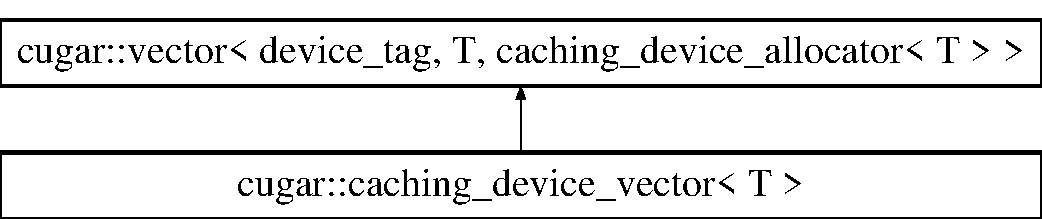
\includegraphics[height=2.000000cm]{structcugar_1_1caching__device__vector}
\end{center}
\end{figure}
\subsection*{Public Types}
\begin{DoxyCompactItemize}
\item 
typedef \hyperlink{structcugar_1_1device__tag}{device\+\_\+tag} {\bfseries system\+\_\+tag}
\item 
typedef \hyperlink{structcugar_1_1vector}{vector}$<$ \hyperlink{structcugar_1_1device__tag}{device\+\_\+tag}, T, \hyperlink{structcugar_1_1caching__device__allocator}{caching\+\_\+device\+\_\+allocator}$<$ T $>$ $>$ {\bfseries base\+\_\+type}
\item 
typedef base\+\_\+type\+::const\+\_\+iterator {\bfseries const\+\_\+iterator}
\item 
typedef base\+\_\+type\+::iterator {\bfseries iterator}
\item 
typedef base\+\_\+type\+::value\+\_\+type {\bfseries value\+\_\+type}
\item 
typedef base\+\_\+type\+::plain\+\_\+view\+\_\+type {\bfseries plain\+\_\+view\+\_\+type}
\item 
typedef base\+\_\+type\+::const\+\_\+plain\+\_\+view\+\_\+type {\bfseries const\+\_\+plain\+\_\+view\+\_\+type}
\end{DoxyCompactItemize}
\subsection*{Public Methods}
\begin{DoxyCompactItemize}
\item 
\hyperlink{group___basic_ga2146480a7d6cae513ac29c3ec28a73a3}{caching\+\_\+device\+\_\+vector} (const size\+\_\+t size=0, const T val=T())
\item 
{\footnotesize template$<$typename Other\+Alloc $>$ }\\{\bfseries caching\+\_\+device\+\_\+vector} (const thrust\+::host\+\_\+vector$<$ T, Other\+Alloc $>$ \&v)
\item 
{\footnotesize template$<$typename Other\+Alloc $>$ }\\{\bfseries caching\+\_\+device\+\_\+vector} (const thrust\+::device\+\_\+vector$<$ T, Other\+Alloc $>$ \&v)
\item 
{\footnotesize template$<$typename Other\+Alloc $>$ }\\\hyperlink{structcugar_1_1caching__device__vector}{caching\+\_\+device\+\_\+vector}$<$ T $>$ \& {\bfseries operator=} (const thrust\+::host\+\_\+vector$<$ T, Other\+Alloc $>$ \&v)
\item 
{\footnotesize template$<$typename Other\+Alloc $>$ }\\\hyperlink{structcugar_1_1caching__device__vector}{caching\+\_\+device\+\_\+vector}$<$ T $>$ \& {\bfseries operator=} (const thrust\+::device\+\_\+vector$<$ T, Other\+Alloc $>$ \&v)
\item 
\hyperlink{group___basic_ga88dd1949f9871da3aa4d4aefd0167c8b}{operator plain\+\_\+view\+\_\+type} ()
\item 
\hyperlink{group___basic_gacf7a82dbc75f3ff33d4cb3bc1cae2e2f}{operator const\+\_\+plain\+\_\+view\+\_\+type} () const
\end{DoxyCompactItemize}


The documentation for this struct was generated from the following file\+:\begin{DoxyCompactItemize}
\item 
C\+:/p4research/research/jpantaleoni/\+Fermat-\/\+Public/contrib/cugar/basic/vector.\+h\end{DoxyCompactItemize}

\hypertarget{struct_camera}{}\section{Camera Struct Reference}
\label{struct_camera}\index{Camera@{Camera}}


\subsection{Detailed description}
A simple pinhole camera model 

{\ttfamily \#include $<$camera.\+h$>$}

\subsection*{Public Methods}
\begin{DoxyCompactItemize}
\item 
\mbox{\Hypertarget{struct_camera_a2c492aca90a8a4c011ea3fbb81da07eb}\label{struct_camera_a2c492aca90a8a4c011ea3fbb81da07eb}} 
F\+E\+R\+M\+A\+T\+\_\+\+H\+O\+S\+T\+\_\+\+D\+E\+V\+I\+CE \hyperlink{struct_camera}{Camera} {\bfseries rotate} (const float2 rot) const
\item 
\mbox{\Hypertarget{struct_camera_a67c1e2e95fdf31adc114ecd1e6c83298}\label{struct_camera_a67c1e2e95fdf31adc114ecd1e6c83298}} 
F\+E\+R\+M\+A\+T\+\_\+\+H\+O\+S\+T\+\_\+\+D\+E\+V\+I\+CE \hyperlink{struct_camera}{Camera} {\bfseries walk} (const float delta) const
\item 
\mbox{\Hypertarget{struct_camera_abc036f653e1f2c8810f7ccdf44b05f76}\label{struct_camera_abc036f653e1f2c8810f7ccdf44b05f76}} 
F\+E\+R\+M\+A\+T\+\_\+\+H\+O\+S\+T\+\_\+\+D\+E\+V\+I\+CE \hyperlink{struct_camera}{Camera} {\bfseries pan} (const float2 delta) const
\item 
\mbox{\Hypertarget{struct_camera_a10fea162ffafa1b9b58213c3b58cba91}\label{struct_camera_a10fea162ffafa1b9b58213c3b58cba91}} 
F\+E\+R\+M\+A\+T\+\_\+\+H\+O\+S\+T\+\_\+\+D\+E\+V\+I\+CE \hyperlink{struct_camera}{Camera} {\bfseries zoom} (const float delta) const
\item 
\mbox{\Hypertarget{struct_camera_a3d6e3421c6a48fd29b5d8a1462c40ec4}\label{struct_camera_a3d6e3421c6a48fd29b5d8a1462c40ec4}} 
F\+E\+R\+M\+A\+T\+\_\+\+H\+O\+S\+T\+\_\+\+D\+E\+V\+I\+CE float {\bfseries square\+\_\+pixel\+\_\+focal\+\_\+length} (const uint32 res\+\_\+x, const uint32 res\+\_\+y) const
\item 
\mbox{\Hypertarget{struct_camera_ad321b3e08095707d67438c9588f43e8d}\label{struct_camera_ad321b3e08095707d67438c9588f43e8d}} 
F\+E\+R\+M\+A\+T\+\_\+\+H\+O\+S\+T\+\_\+\+D\+E\+V\+I\+CE float {\bfseries square\+\_\+screen\+\_\+focal\+\_\+length} () const
\end{DoxyCompactItemize}
\subsection*{Public Members}
\begin{DoxyCompactItemize}
\item 
\mbox{\Hypertarget{struct_camera_ab5328d278495c795eca66a2fcb2a442b}\label{struct_camera_ab5328d278495c795eca66a2fcb2a442b}} 
float3 {\bfseries eye}
\item 
\mbox{\Hypertarget{struct_camera_a326af25ea49f8f35737a6d0334864f8b}\label{struct_camera_a326af25ea49f8f35737a6d0334864f8b}} 
float3 {\bfseries aim}
\item 
\mbox{\Hypertarget{struct_camera_a9f5ba0529bf851c30546a57fe045fff1}\label{struct_camera_a9f5ba0529bf851c30546a57fe045fff1}} 
float3 {\bfseries up}
\item 
\mbox{\Hypertarget{struct_camera_a8a27bc6c1ea9994052eb1d1c6b304a8a}\label{struct_camera_a8a27bc6c1ea9994052eb1d1c6b304a8a}} 
float3 {\bfseries dx}
\item 
\mbox{\Hypertarget{struct_camera_aff7393c9cfbccd7e369091f00008da93}\label{struct_camera_aff7393c9cfbccd7e369091f00008da93}} 
float {\bfseries fov}
\end{DoxyCompactItemize}


The documentation for this struct was generated from the following file\+:\begin{DoxyCompactItemize}
\item 
C\+:/p4research/research/jpantaleoni/\+Fermat-\/\+Public/src/camera.\+h\end{DoxyCompactItemize}

\hypertarget{struct_camera_sampler}{}\section{Camera\+Sampler Struct Reference}
\label{struct_camera_sampler}\index{Camera\+Sampler@{Camera\+Sampler}}


\subsection{Detailed description}
A sampler for the pinhole camera model 

{\ttfamily \#include $<$camera.\+h$>$}

\subsection*{Public Methods}
\begin{DoxyCompactItemize}
\item 
F\+E\+R\+M\+A\+T\+\_\+\+H\+O\+S\+T\+\_\+\+D\+E\+V\+I\+CE F\+E\+R\+M\+A\+T\+\_\+\+F\+O\+R\+C\+E\+I\+N\+L\+I\+NE \hyperlink{struct_camera_sampler_a50332d884a007ab1ffcb05215af5d92a}{Camera\+Sampler} ()
\item 
F\+E\+R\+M\+A\+T\+\_\+\+H\+O\+S\+T\+\_\+\+D\+E\+V\+I\+CE F\+E\+R\+M\+A\+T\+\_\+\+F\+O\+R\+C\+E\+I\+N\+L\+I\+NE \hyperlink{struct_camera_sampler_a9d018f4ac9bbd0e93bfcc283ab915eeb}{Camera\+Sampler} (const \hyperlink{struct_camera}{Camera} \&camera, const float aspect\+\_\+ratio)
\item 
F\+E\+R\+M\+A\+T\+\_\+\+H\+O\+S\+T\+\_\+\+D\+E\+V\+I\+CE F\+E\+R\+M\+A\+T\+\_\+\+F\+O\+R\+C\+E\+I\+N\+L\+I\+NE \hyperlink{structcugar_1_1_vector}{cugar\+::\+Vector3f} \hyperlink{struct_camera_sampler_ac502e1699c99c595b773b1419225fe32}{sample\+\_\+direction} (const \hyperlink{structcugar_1_1_vector}{cugar\+::\+Vector2f} ndc) const
\item 
F\+E\+R\+M\+A\+T\+\_\+\+H\+O\+S\+T\+\_\+\+D\+E\+V\+I\+CE F\+E\+R\+M\+A\+T\+\_\+\+F\+O\+R\+C\+E\+I\+N\+L\+I\+NE float \hyperlink{struct_camera_sampler_a0edd94ccee6da3180f13845d189bc758}{pdf} (const \hyperlink{structcugar_1_1_vector}{cugar\+::\+Vector3f} out, const bool projected=false) const
\item 
F\+E\+R\+M\+A\+T\+\_\+\+H\+O\+S\+T\+\_\+\+D\+E\+V\+I\+CE F\+E\+R\+M\+A\+T\+\_\+\+F\+O\+R\+C\+E\+I\+N\+L\+I\+NE float \hyperlink{struct_camera_sampler_afe4852bed67331cf757518e046d82ef1}{W\+\_\+e} (const \hyperlink{structcugar_1_1_vector}{cugar\+::\+Vector3f} out) const
\item 
F\+E\+R\+M\+A\+T\+\_\+\+H\+O\+S\+T\+\_\+\+D\+E\+V\+I\+CE F\+E\+R\+M\+A\+T\+\_\+\+F\+O\+R\+C\+E\+I\+N\+L\+I\+NE \hyperlink{structcugar_1_1_vector}{cugar\+::\+Vector2f} \hyperlink{struct_camera_sampler_a347623323319a7111f933d4af6ac2d19}{invert} (const \hyperlink{structcugar_1_1_vector}{cugar\+::\+Vector3f} out) const
\item 
F\+E\+R\+M\+A\+T\+\_\+\+H\+O\+S\+T\+\_\+\+D\+E\+V\+I\+CE F\+E\+R\+M\+A\+T\+\_\+\+F\+O\+R\+C\+E\+I\+N\+L\+I\+NE \hyperlink{structcugar_1_1_vector}{cugar\+::\+Vector2f} \hyperlink{struct_camera_sampler_aaa68e077536fc88429fb35dd04d30af1}{invert} (const \hyperlink{structcugar_1_1_vector}{cugar\+::\+Vector3f} out, float $\ast$pdf\+\_\+proj) const
\end{DoxyCompactItemize}
\subsection*{Public Members}
\begin{DoxyCompactItemize}
\item 
\mbox{\Hypertarget{struct_camera_sampler_a78eb2537995dd7909bdeeb1dbd83bbfe}\label{struct_camera_sampler_a78eb2537995dd7909bdeeb1dbd83bbfe}} 
\hyperlink{structcugar_1_1_vector}{cugar\+::\+Vector3f} {\bfseries U}
\item 
\mbox{\Hypertarget{struct_camera_sampler_a6701783b3acedd9d54c22ee4decb3fb5}\label{struct_camera_sampler_a6701783b3acedd9d54c22ee4decb3fb5}} 
\hyperlink{structcugar_1_1_vector}{cugar\+::\+Vector3f} {\bfseries V}
\item 
\mbox{\Hypertarget{struct_camera_sampler_a4647d9cea99da93ffb22bda37cd0cef0}\label{struct_camera_sampler_a4647d9cea99da93ffb22bda37cd0cef0}} 
\hyperlink{structcugar_1_1_vector}{cugar\+::\+Vector3f} {\bfseries W}
\item 
\mbox{\Hypertarget{struct_camera_sampler_a74381044c3ffd87d1b88890abb39c084}\label{struct_camera_sampler_a74381044c3ffd87d1b88890abb39c084}} 
float {\bfseries W\+\_\+len}
\item 
\mbox{\Hypertarget{struct_camera_sampler_abd374561d2f1ea3cd0bdbd4839f8cfc7}\label{struct_camera_sampler_abd374561d2f1ea3cd0bdbd4839f8cfc7}} 
float {\bfseries square\+\_\+focal\+\_\+length}
\end{DoxyCompactItemize}


\subsection{Constructor \& Destructor Documentation}
\mbox{\Hypertarget{struct_camera_sampler_a50332d884a007ab1ffcb05215af5d92a}\label{struct_camera_sampler_a50332d884a007ab1ffcb05215af5d92a}} 
\index{Camera\+Sampler@{Camera\+Sampler}!Camera\+Sampler@{Camera\+Sampler}}
\index{Camera\+Sampler@{Camera\+Sampler}!Camera\+Sampler@{Camera\+Sampler}}
\subsubsection{\texorpdfstring{Camera\+Sampler()}{CameraSampler()}\hspace{0.1cm}{\footnotesize\ttfamily [1/2]}}
{\footnotesize\ttfamily F\+E\+R\+M\+A\+T\+\_\+\+H\+O\+S\+T\+\_\+\+D\+E\+V\+I\+CE F\+E\+R\+M\+A\+T\+\_\+\+F\+O\+R\+C\+E\+I\+N\+L\+I\+NE Camera\+Sampler\+::\+Camera\+Sampler (\begin{DoxyParamCaption}{ }\end{DoxyParamCaption})\hspace{0.3cm}{\ttfamily [inline]}}

empty constructor \mbox{\Hypertarget{struct_camera_sampler_a9d018f4ac9bbd0e93bfcc283ab915eeb}\label{struct_camera_sampler_a9d018f4ac9bbd0e93bfcc283ab915eeb}} 
\index{Camera\+Sampler@{Camera\+Sampler}!Camera\+Sampler@{Camera\+Sampler}}
\index{Camera\+Sampler@{Camera\+Sampler}!Camera\+Sampler@{Camera\+Sampler}}
\subsubsection{\texorpdfstring{Camera\+Sampler()}{CameraSampler()}\hspace{0.1cm}{\footnotesize\ttfamily [2/2]}}
{\footnotesize\ttfamily F\+E\+R\+M\+A\+T\+\_\+\+H\+O\+S\+T\+\_\+\+D\+E\+V\+I\+CE F\+E\+R\+M\+A\+T\+\_\+\+F\+O\+R\+C\+E\+I\+N\+L\+I\+NE Camera\+Sampler\+::\+Camera\+Sampler (\begin{DoxyParamCaption}\item[{const \hyperlink{struct_camera}{Camera} \&}]{camera,  }\item[{const float}]{aspect\+\_\+ratio }\end{DoxyParamCaption})\hspace{0.3cm}{\ttfamily [inline]}}

constructor 

\subsection{Member Function Documentation}
\mbox{\Hypertarget{struct_camera_sampler_a347623323319a7111f933d4af6ac2d19}\label{struct_camera_sampler_a347623323319a7111f933d4af6ac2d19}} 
\index{Camera\+Sampler@{Camera\+Sampler}!invert@{invert}}
\index{invert@{invert}!Camera\+Sampler@{Camera\+Sampler}}
\subsubsection{\texorpdfstring{invert()}{invert()}\hspace{0.1cm}{\footnotesize\ttfamily [1/2]}}
{\footnotesize\ttfamily F\+E\+R\+M\+A\+T\+\_\+\+H\+O\+S\+T\+\_\+\+D\+E\+V\+I\+CE F\+E\+R\+M\+A\+T\+\_\+\+F\+O\+R\+C\+E\+I\+N\+L\+I\+NE \hyperlink{structcugar_1_1_vector}{cugar\+::\+Vector2f} Camera\+Sampler\+::invert (\begin{DoxyParamCaption}\item[{const \hyperlink{structcugar_1_1_vector}{cugar\+::\+Vector3f}}]{out }\end{DoxyParamCaption}) const\hspace{0.3cm}{\ttfamily [inline]}}

invert the camera direction sampler


\begin{DoxyParams}{Parameters}
{\em out} & the given direction \\
\hline
{\em projected} & whether to return the pdf in projected solid angle or solid angle measure \\
\hline
\end{DoxyParams}
\begin{DoxyReturn}{Returns}
the N\+DC coordinates corresponding to the given direction 
\end{DoxyReturn}
\mbox{\Hypertarget{struct_camera_sampler_aaa68e077536fc88429fb35dd04d30af1}\label{struct_camera_sampler_aaa68e077536fc88429fb35dd04d30af1}} 
\index{Camera\+Sampler@{Camera\+Sampler}!invert@{invert}}
\index{invert@{invert}!Camera\+Sampler@{Camera\+Sampler}}
\subsubsection{\texorpdfstring{invert()}{invert()}\hspace{0.1cm}{\footnotesize\ttfamily [2/2]}}
{\footnotesize\ttfamily F\+E\+R\+M\+A\+T\+\_\+\+H\+O\+S\+T\+\_\+\+D\+E\+V\+I\+CE F\+E\+R\+M\+A\+T\+\_\+\+F\+O\+R\+C\+E\+I\+N\+L\+I\+NE \hyperlink{structcugar_1_1_vector}{cugar\+::\+Vector2f} Camera\+Sampler\+::invert (\begin{DoxyParamCaption}\item[{const \hyperlink{structcugar_1_1_vector}{cugar\+::\+Vector3f}}]{out,  }\item[{float $\ast$}]{pdf\+\_\+proj }\end{DoxyParamCaption}) const\hspace{0.3cm}{\ttfamily [inline]}}

invert the camera direction sampler and compute its projected pdf


\begin{DoxyParams}{Parameters}
{\em out} & the given direction \\
\hline
{\em projected} & whether to return the pdf in projected solid angle or solid angle measure \\
\hline
\end{DoxyParams}
\begin{DoxyReturn}{Returns}
the N\+DC coordinates corresponding to the given direction 
\end{DoxyReturn}
\mbox{\Hypertarget{struct_camera_sampler_a0edd94ccee6da3180f13845d189bc758}\label{struct_camera_sampler_a0edd94ccee6da3180f13845d189bc758}} 
\index{Camera\+Sampler@{Camera\+Sampler}!pdf@{pdf}}
\index{pdf@{pdf}!Camera\+Sampler@{Camera\+Sampler}}
\subsubsection{\texorpdfstring{pdf()}{pdf()}}
{\footnotesize\ttfamily F\+E\+R\+M\+A\+T\+\_\+\+H\+O\+S\+T\+\_\+\+D\+E\+V\+I\+CE F\+E\+R\+M\+A\+T\+\_\+\+F\+O\+R\+C\+E\+I\+N\+L\+I\+NE float Camera\+Sampler\+::pdf (\begin{DoxyParamCaption}\item[{const \hyperlink{structcugar_1_1_vector}{cugar\+::\+Vector3f}}]{out,  }\item[{const bool}]{projected = {\ttfamily false} }\end{DoxyParamCaption}) const\hspace{0.3cm}{\ttfamily [inline]}}

compute the direction pdf \mbox{\Hypertarget{struct_camera_sampler_ac502e1699c99c595b773b1419225fe32}\label{struct_camera_sampler_ac502e1699c99c595b773b1419225fe32}} 
\index{Camera\+Sampler@{Camera\+Sampler}!sample\+\_\+direction@{sample\+\_\+direction}}
\index{sample\+\_\+direction@{sample\+\_\+direction}!Camera\+Sampler@{Camera\+Sampler}}
\subsubsection{\texorpdfstring{sample\+\_\+direction()}{sample\_direction()}}
{\footnotesize\ttfamily F\+E\+R\+M\+A\+T\+\_\+\+H\+O\+S\+T\+\_\+\+D\+E\+V\+I\+CE F\+E\+R\+M\+A\+T\+\_\+\+F\+O\+R\+C\+E\+I\+N\+L\+I\+NE \hyperlink{structcugar_1_1_vector}{cugar\+::\+Vector3f} Camera\+Sampler\+::sample\+\_\+direction (\begin{DoxyParamCaption}\item[{const \hyperlink{structcugar_1_1_vector}{cugar\+::\+Vector2f}}]{ndc }\end{DoxyParamCaption}) const\hspace{0.3cm}{\ttfamily [inline]}}

sample a direction from normalized device coordinates (N\+DC) in \mbox{[}0,1\mbox{]}$^\wedge$2 \mbox{\Hypertarget{struct_camera_sampler_afe4852bed67331cf757518e046d82ef1}\label{struct_camera_sampler_afe4852bed67331cf757518e046d82ef1}} 
\index{Camera\+Sampler@{Camera\+Sampler}!W\+\_\+e@{W\+\_\+e}}
\index{W\+\_\+e@{W\+\_\+e}!Camera\+Sampler@{Camera\+Sampler}}
\subsubsection{\texorpdfstring{W\+\_\+e()}{W\_e()}}
{\footnotesize\ttfamily F\+E\+R\+M\+A\+T\+\_\+\+H\+O\+S\+T\+\_\+\+D\+E\+V\+I\+CE F\+E\+R\+M\+A\+T\+\_\+\+F\+O\+R\+C\+E\+I\+N\+L\+I\+NE float Camera\+Sampler\+::\+W\+\_\+e (\begin{DoxyParamCaption}\item[{const \hyperlink{structcugar_1_1_vector}{cugar\+::\+Vector3f}}]{out }\end{DoxyParamCaption}) const\hspace{0.3cm}{\ttfamily [inline]}}

compute the importance 

The documentation for this struct was generated from the following file\+:\begin{DoxyCompactItemize}
\item 
C\+:/p4research/research/jpantaleoni/\+Fermat-\/\+Public/src/camera.\+h\end{DoxyCompactItemize}

\hypertarget{structcugar_1_1_cauchy__distribution}{}\section{cugar\+:\+:Cauchy\+\_\+distribution Struct Reference}
\label{structcugar_1_1_cauchy__distribution}\index{cugar\+::\+Cauchy\+\_\+distribution@{cugar\+::\+Cauchy\+\_\+distribution}}


\subsection{Detailed description}
Cauchy distribution 

{\ttfamily \#include $<$distributions.\+h$>$}

Inheritance diagram for cugar\+:\+:Cauchy\+\_\+distribution\+:\begin{figure}[H]
\begin{center}
\leavevmode
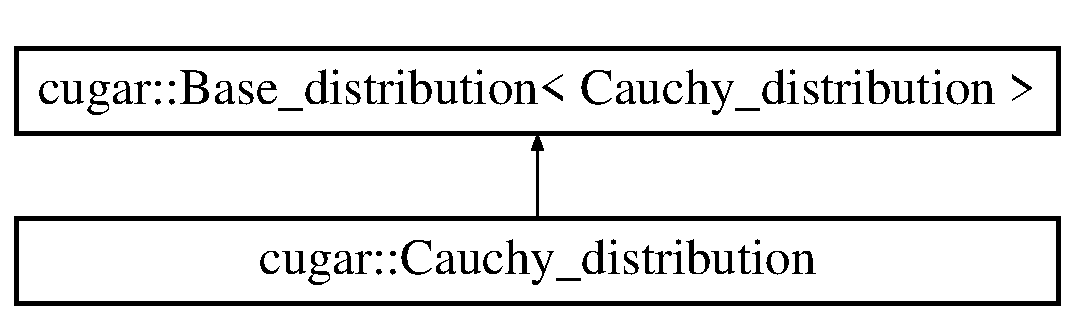
\includegraphics[height=2.000000cm]{structcugar_1_1_cauchy__distribution}
\end{center}
\end{figure}
\subsection*{Public Methods}
\begin{DoxyCompactItemize}
\item 
C\+U\+G\+A\+R\+\_\+\+H\+O\+S\+T\+\_\+\+D\+E\+V\+I\+CE \hyperlink{structcugar_1_1_cauchy__distribution_a71de811a43d29f66b681c017c510b7b7}{Cauchy\+\_\+distribution} (const float gamma)
\item 
C\+U\+G\+A\+R\+\_\+\+H\+O\+S\+T\+\_\+\+D\+E\+V\+I\+CE float \hyperlink{structcugar_1_1_cauchy__distribution_a5ebb0dbebd02e247c4056c7c82466f8a}{map} (const float U) const
\item 
C\+U\+G\+A\+R\+\_\+\+H\+O\+S\+T\+\_\+\+D\+E\+V\+I\+CE float \hyperlink{structcugar_1_1_cauchy__distribution_ae4849f807e5ed3ca0557fa9b2bea4da6}{density} (const float x) const
\end{DoxyCompactItemize}


\subsection{Constructor \& Destructor Documentation}
\mbox{\Hypertarget{structcugar_1_1_cauchy__distribution_a71de811a43d29f66b681c017c510b7b7}\label{structcugar_1_1_cauchy__distribution_a71de811a43d29f66b681c017c510b7b7}} 
\index{cugar\+::\+Cauchy\+\_\+distribution@{cugar\+::\+Cauchy\+\_\+distribution}!Cauchy\+\_\+distribution@{Cauchy\+\_\+distribution}}
\index{Cauchy\+\_\+distribution@{Cauchy\+\_\+distribution}!cugar\+::\+Cauchy\+\_\+distribution@{cugar\+::\+Cauchy\+\_\+distribution}}
\subsubsection{\texorpdfstring{Cauchy\+\_\+distribution()}{Cauchy\_distribution()}}
{\footnotesize\ttfamily C\+U\+G\+A\+R\+\_\+\+H\+O\+S\+T\+\_\+\+D\+E\+V\+I\+CE cugar\+::\+Cauchy\+\_\+distribution\+::\+Cauchy\+\_\+distribution (\begin{DoxyParamCaption}\item[{const float}]{gamma }\end{DoxyParamCaption})\hspace{0.3cm}{\ttfamily [inline]}}

constructor


\begin{DoxyParams}{Parameters}
{\em gamma} & distribution parameter \\
\hline
\end{DoxyParams}


\subsection{Member Function Documentation}
\mbox{\Hypertarget{structcugar_1_1_cauchy__distribution_ae4849f807e5ed3ca0557fa9b2bea4da6}\label{structcugar_1_1_cauchy__distribution_ae4849f807e5ed3ca0557fa9b2bea4da6}} 
\index{cugar\+::\+Cauchy\+\_\+distribution@{cugar\+::\+Cauchy\+\_\+distribution}!density@{density}}
\index{density@{density}!cugar\+::\+Cauchy\+\_\+distribution@{cugar\+::\+Cauchy\+\_\+distribution}}
\subsubsection{\texorpdfstring{density()}{density()}}
{\footnotesize\ttfamily C\+U\+G\+A\+R\+\_\+\+H\+O\+S\+T\+\_\+\+D\+E\+V\+I\+CE float cugar\+::\+Cauchy\+\_\+distribution\+::density (\begin{DoxyParamCaption}\item[{const float}]{x }\end{DoxyParamCaption}) const\hspace{0.3cm}{\ttfamily [inline]}}

probability density function


\begin{DoxyParams}{Parameters}
{\em x} & sample location \\
\hline
\end{DoxyParams}
\mbox{\Hypertarget{structcugar_1_1_cauchy__distribution_a5ebb0dbebd02e247c4056c7c82466f8a}\label{structcugar_1_1_cauchy__distribution_a5ebb0dbebd02e247c4056c7c82466f8a}} 
\index{cugar\+::\+Cauchy\+\_\+distribution@{cugar\+::\+Cauchy\+\_\+distribution}!map@{map}}
\index{map@{map}!cugar\+::\+Cauchy\+\_\+distribution@{cugar\+::\+Cauchy\+\_\+distribution}}
\subsubsection{\texorpdfstring{map()}{map()}}
{\footnotesize\ttfamily C\+U\+G\+A\+R\+\_\+\+H\+O\+S\+T\+\_\+\+D\+E\+V\+I\+CE float cugar\+::\+Cauchy\+\_\+distribution\+::map (\begin{DoxyParamCaption}\item[{const float}]{U }\end{DoxyParamCaption}) const\hspace{0.3cm}{\ttfamily [inline]}}

transform a uniformly distributed number through the distribution


\begin{DoxyParams}{Parameters}
{\em U} & real number to transform \\
\hline
\end{DoxyParams}


The documentation for this struct was generated from the following file\+:\begin{DoxyCompactItemize}
\item 
C\+:/p4research/research/jpantaleoni/\+Fermat-\/\+Public/contrib/cugar/sampling/\hyperlink{distributions_8h}{distributions.\+h}\end{DoxyCompactItemize}

\hypertarget{structcugar_1_1clamped__cosine__functor}{}\section{cugar\+:\+:clamped\+\_\+cosine\+\_\+functor$<$ Vector\+\_\+type $>$ Struct Template Reference}
\label{structcugar_1_1clamped__cosine__functor}\index{cugar\+::clamped\+\_\+cosine\+\_\+functor$<$ Vector\+\_\+type $>$@{cugar\+::clamped\+\_\+cosine\+\_\+functor$<$ Vector\+\_\+type $>$}}


\subsection{Detailed description}
\subsubsection*{template$<$typename Vector\+\_\+type$>$\newline
struct cugar\+::clamped\+\_\+cosine\+\_\+functor$<$ Vector\+\_\+type $>$}

A functor to compute the clamped cosine of the angle formed with a given normal 

{\ttfamily \#include $<$functors.\+h$>$}

\subsection*{Public Types}
\begin{DoxyCompactItemize}
\item 
\mbox{\Hypertarget{structcugar_1_1clamped__cosine__functor_a9bc0225f4c67f1693319262e4388bcd4}\label{structcugar_1_1clamped__cosine__functor_a9bc0225f4c67f1693319262e4388bcd4}} 
typedef Vector\+\_\+type {\bfseries argument\+\_\+type}
\item 
\mbox{\Hypertarget{structcugar_1_1clamped__cosine__functor_a885a9a3f74842abb6cb43a8203c04773}\label{structcugar_1_1clamped__cosine__functor_a885a9a3f74842abb6cb43a8203c04773}} 
typedef float {\bfseries result\+\_\+type}
\end{DoxyCompactItemize}
\subsection*{Public Methods}
\begin{DoxyCompactItemize}
\item 
C\+U\+G\+A\+R\+\_\+\+H\+O\+S\+T\+\_\+\+D\+E\+V\+I\+CE \hyperlink{structcugar_1_1clamped__cosine__functor_a24f2ce1992a26dc465f5167742b76207}{clamped\+\_\+cosine\+\_\+functor} (const Vector\+\_\+type \&normal)
\item 
\mbox{\Hypertarget{structcugar_1_1clamped__cosine__functor_a2e6a96b9d79c216b7eae16133efd3738}\label{structcugar_1_1clamped__cosine__functor_a2e6a96b9d79c216b7eae16133efd3738}} 
C\+U\+G\+A\+R\+\_\+\+H\+O\+S\+T\+\_\+\+D\+E\+V\+I\+CE float {\bfseries operator()} (const Vector\+\_\+type \&dir) const
\end{DoxyCompactItemize}
\subsection*{Public Members}
\begin{DoxyCompactItemize}
\item 
\mbox{\Hypertarget{structcugar_1_1clamped__cosine__functor_ac5c35f5c1be6302bd56694f50ae4fbff}\label{structcugar_1_1clamped__cosine__functor_ac5c35f5c1be6302bd56694f50ae4fbff}} 
const Vector\+\_\+type {\bfseries m\+\_\+normal}
\end{DoxyCompactItemize}


\subsection{Constructor \& Destructor Documentation}
\mbox{\Hypertarget{structcugar_1_1clamped__cosine__functor_a24f2ce1992a26dc465f5167742b76207}\label{structcugar_1_1clamped__cosine__functor_a24f2ce1992a26dc465f5167742b76207}} 
\index{cugar\+::clamped\+\_\+cosine\+\_\+functor@{cugar\+::clamped\+\_\+cosine\+\_\+functor}!clamped\+\_\+cosine\+\_\+functor@{clamped\+\_\+cosine\+\_\+functor}}
\index{clamped\+\_\+cosine\+\_\+functor@{clamped\+\_\+cosine\+\_\+functor}!cugar\+::clamped\+\_\+cosine\+\_\+functor@{cugar\+::clamped\+\_\+cosine\+\_\+functor}}
\subsubsection{\texorpdfstring{clamped\+\_\+cosine\+\_\+functor()}{clamped\_cosine\_functor()}}
{\footnotesize\ttfamily template$<$typename Vector\+\_\+type $>$ \\
C\+U\+G\+A\+R\+\_\+\+H\+O\+S\+T\+\_\+\+D\+E\+V\+I\+CE \hyperlink{structcugar_1_1clamped__cosine__functor}{cugar\+::clamped\+\_\+cosine\+\_\+functor}$<$ Vector\+\_\+type $>$\+::\hyperlink{structcugar_1_1clamped__cosine__functor}{clamped\+\_\+cosine\+\_\+functor} (\begin{DoxyParamCaption}\item[{const Vector\+\_\+type \&}]{normal }\end{DoxyParamCaption})\hspace{0.3cm}{\ttfamily [inline]}}

constructor


\begin{DoxyParams}{Parameters}
{\em normal} & reference normal \\
\hline
\end{DoxyParams}


The documentation for this struct was generated from the following file\+:\begin{DoxyCompactItemize}
\item 
C\+:/p4research/research/jpantaleoni/\+Fermat-\/\+Public/contrib/cugar/basic/\hyperlink{functors_8h}{functors.\+h}\end{DoxyCompactItemize}

\hypertarget{struct_clustered_r_l_storage}{}\section{Clustered\+R\+L\+Storage Struct Reference}
\label{struct_clustered_r_l_storage}\index{Clustered\+R\+L\+Storage@{Clustered\+R\+L\+Storage}}


\subsection{Detailed description}
Host-\/side class to handle the storage of a Clustered Reinforcement Learning sampler (\hyperlink{group___clustered_r_l_module}{Clustered RL}). 

{\ttfamily \#include $<$clustered\+\_\+rl.\+h$>$}

\subsection*{Public Types}
\begin{DoxyCompactItemize}
\item 
\mbox{\Hypertarget{struct_clustered_r_l_storage_a3d4bd4d60bfb6d6dae7079ffebeaea83}\label{struct_clustered_r_l_storage_a3d4bd4d60bfb6d6dae7079ffebeaea83}} 
typedef \hyperlink{struct_clustered_r_l_view}{Clustered\+R\+L\+View} {\bfseries view\+\_\+type}
\end{DoxyCompactItemize}
\subsection*{Public Methods}
\begin{DoxyCompactItemize}
\item 
\mbox{\Hypertarget{struct_clustered_r_l_storage_a3731b06b8bffb45d81cacbdc915e9f1d}\label{struct_clustered_r_l_storage_a3731b06b8bffb45d81cacbdc915e9f1d}} 
uint64 {\bfseries needed\+\_\+bytes} (const uint32 \+\_\+hash\+\_\+size, const uint32 \+\_\+n\+\_\+clusters) const
\item 
\mbox{\Hypertarget{struct_clustered_r_l_storage_a143a5bf05f78ce5f085d9ca5ee8c8442}\label{struct_clustered_r_l_storage_a143a5bf05f78ce5f085d9ca5ee8c8442}} 
void {\bfseries init} (const uint32 \+\_\+hash\+\_\+size, const uint32 \+\_\+n\+\_\+clusters, const uint32 $\ast$\+\_\+cluster\+\_\+offsets)
\item 
\mbox{\Hypertarget{struct_clustered_r_l_storage_ad12cc46508974f99ae6db1894b8d712e}\label{struct_clustered_r_l_storage_ad12cc46508974f99ae6db1894b8d712e}} 
void {\bfseries resize} (const uint32 \+\_\+hash\+\_\+size, const uint32 \+\_\+n\+\_\+clusters, const uint32 $\ast$\+\_\+cluster\+\_\+offsets)
\item 
\mbox{\Hypertarget{struct_clustered_r_l_storage_a8e1c6f4731566515705afc77c46412f1}\label{struct_clustered_r_l_storage_a8e1c6f4731566515705afc77c46412f1}} 
void {\bfseries update} (const float bias=0.\+1f)
\item 
\mbox{\Hypertarget{struct_clustered_r_l_storage_a1937674e3486d060f08bc9212330ab0e}\label{struct_clustered_r_l_storage_a1937674e3486d060f08bc9212330ab0e}} 
void {\bfseries clear} ()
\item 
\mbox{\Hypertarget{struct_clustered_r_l_storage_a47aae2f04a21d8f3cbc53d0b94739673}\label{struct_clustered_r_l_storage_a47aae2f04a21d8f3cbc53d0b94739673}} 
uint32 {\bfseries size} () const
\end{DoxyCompactItemize}
\subsection*{Public Members}
\begin{DoxyCompactItemize}
\item 
\mbox{\Hypertarget{struct_clustered_r_l_storage_a3acff6c4ac3c6f5d3c02bf78ead67356}\label{struct_clustered_r_l_storage_a3acff6c4ac3c6f5d3c02bf78ead67356}} 
\hyperlink{struct_device_hash_table}{Device\+Hash\+Table} {\bfseries hashmap}
\item 
\mbox{\Hypertarget{struct_clustered_r_l_storage_af3a0096e3b6a3094bef12992b7836207}\label{struct_clustered_r_l_storage_af3a0096e3b6a3094bef12992b7836207}} 
\hyperlink{class_domain_buffer}{Domain\+Buffer}$<$ C\+U\+D\+A\+\_\+\+B\+U\+F\+F\+ER, float $>$ {\bfseries values}
\item 
\mbox{\Hypertarget{struct_clustered_r_l_storage_aa238fd3a424bf22c83cbde232c1ac1eb}\label{struct_clustered_r_l_storage_aa238fd3a424bf22c83cbde232c1ac1eb}} 
uint32 {\bfseries hash\+\_\+size}
\item 
\mbox{\Hypertarget{struct_clustered_r_l_storage_af0819b2be3ca0503d7e93a0ed152eaff}\label{struct_clustered_r_l_storage_af0819b2be3ca0503d7e93a0ed152eaff}} 
uint32 {\bfseries n\+\_\+clusters}
\item 
\mbox{\Hypertarget{struct_clustered_r_l_storage_a9cb6e900f69b2d554cf85debddcd5616}\label{struct_clustered_r_l_storage_a9cb6e900f69b2d554cf85debddcd5616}} 
const uint32 $\ast$ {\bfseries cluster\+\_\+offsets}
\item 
\mbox{\Hypertarget{struct_clustered_r_l_storage_a326a561b8d3a694d5211ebb35d3df0ea}\label{struct_clustered_r_l_storage_a326a561b8d3a694d5211ebb35d3df0ea}} 
uint32 {\bfseries old\+\_\+hash\+\_\+size}
\end{DoxyCompactItemize}


The documentation for this struct was generated from the following file\+:\begin{DoxyCompactItemize}
\item 
C\+:/p4research/research/jpantaleoni/\+Fermat-\/\+Public/src/clustered\+\_\+rl.\+h\end{DoxyCompactItemize}

\hypertarget{struct_clustered_r_l_view}{}\section{Clustered\+R\+L\+View Struct Reference}
\label{struct_clustered_r_l_view}\index{Clustered\+R\+L\+View@{Clustered\+R\+L\+View}}


\subsection{Detailed description}
Device-\/side view class for the Clustered Reinforcement Learning sampler (\hyperlink{group___clustered_r_l_module}{Clustered RL}). 

{\ttfamily \#include $<$clustered\+\_\+rl.\+h$>$}

\subsection*{Public Types}
\begin{DoxyCompactItemize}
\item 
\mbox{\Hypertarget{struct_clustered_r_l_view_a78da128381803af43c08b47b0427cb02}\label{struct_clustered_r_l_view_a78da128381803af43c08b47b0427cb02}} 
typedef \hyperlink{structcugar_1_1cuda_1_1_sync_free_hash_map}{cugar\+::cuda\+::\+Sync\+Free\+Hash\+Map}$<$ uint64, uint32, 0x\+F\+F\+F\+F\+F\+F\+F\+F\+F\+F\+F\+F\+F\+F\+F\+Fllu $>$ {\bfseries Hash\+Map}
\end{DoxyCompactItemize}
\subsection*{Public Methods}
\begin{DoxyCompactItemize}
\item 
F\+E\+R\+M\+A\+T\+\_\+\+D\+E\+V\+I\+CE uint32 \hyperlink{struct_clustered_r_l_view_ad23add8b87f5755240e40d976f9c8b0d}{find\+\_\+slot} (const uint64 key)
\item 
F\+E\+R\+M\+A\+T\+\_\+\+D\+E\+V\+I\+CE uint32 \hyperlink{struct_clustered_r_l_view_a72030c277568b5f0ee9476ce520e1096}{sample} (const uint32 cell\+\_\+slot, const float z, float $\ast$\hyperlink{struct_clustered_r_l_view_ad2f4d9df7d5b7278462e1f0dbf2386e3}{pdf}, uint32 $\ast$cluster\+\_\+idx) const
\item 
F\+E\+R\+M\+A\+T\+\_\+\+D\+E\+V\+I\+CE float \hyperlink{struct_clustered_r_l_view_ad2f4d9df7d5b7278462e1f0dbf2386e3}{pdf} (const uint32 cell\+\_\+slot, const uint32 index) const
\item 
F\+E\+R\+M\+A\+T\+\_\+\+D\+E\+V\+I\+CE void \hyperlink{struct_clustered_r_l_view_a007fd0458e4dd173adf57dec5f4db9e2}{update} (const uint32 cell\+\_\+slot, const uint32 cluster\+\_\+idx, const float val, const float alpha=0.\+05f)
\end{DoxyCompactItemize}
\subsection*{Public Members}
\begin{DoxyCompactItemize}
\item 
\mbox{\Hypertarget{struct_clustered_r_l_view_af017028074f59ea52f3b1b67ffe42cd9}\label{struct_clustered_r_l_view_af017028074f59ea52f3b1b67ffe42cd9}} 
\hyperlink{structcugar_1_1cuda_1_1_sync_free_hash_map}{Hash\+Map} {\bfseries hashmap}
\item 
\mbox{\Hypertarget{struct_clustered_r_l_view_abd81e6d4f9872bb2a0e8d39c9c556d07}\label{struct_clustered_r_l_view_abd81e6d4f9872bb2a0e8d39c9c556d07}} 
float $\ast$ {\bfseries pdfs}
\item 
\mbox{\Hypertarget{struct_clustered_r_l_view_af7e919362e6c7bb1abf565f0de4086b7}\label{struct_clustered_r_l_view_af7e919362e6c7bb1abf565f0de4086b7}} 
float $\ast$ {\bfseries cdfs}
\item 
\mbox{\Hypertarget{struct_clustered_r_l_view_af65cac683664066fbf4a11f2ebdc85b5}\label{struct_clustered_r_l_view_af65cac683664066fbf4a11f2ebdc85b5}} 
const uint32 $\ast$ {\bfseries cluster\+\_\+offsets}
\item 
\mbox{\Hypertarget{struct_clustered_r_l_view_afdd21a456172be84e79373771a4501e3}\label{struct_clustered_r_l_view_afdd21a456172be84e79373771a4501e3}} 
uint32 {\bfseries cluster\+\_\+count}
\item 
\mbox{\Hypertarget{struct_clustered_r_l_view_abf5bfb1437690f7099f91ef3ae35890e}\label{struct_clustered_r_l_view_abf5bfb1437690f7099f91ef3ae35890e}} 
uint32 {\bfseries hash\+\_\+size}
\end{DoxyCompactItemize}


\subsection{Member Function Documentation}
\mbox{\Hypertarget{struct_clustered_r_l_view_ad23add8b87f5755240e40d976f9c8b0d}\label{struct_clustered_r_l_view_ad23add8b87f5755240e40d976f9c8b0d}} 
\index{Clustered\+R\+L\+View@{Clustered\+R\+L\+View}!find\+\_\+slot@{find\+\_\+slot}}
\index{find\+\_\+slot@{find\+\_\+slot}!Clustered\+R\+L\+View@{Clustered\+R\+L\+View}}
\subsubsection{\texorpdfstring{find\+\_\+slot()}{find\_slot()}}
{\footnotesize\ttfamily F\+E\+R\+M\+A\+T\+\_\+\+D\+E\+V\+I\+CE F\+E\+R\+M\+A\+T\+\_\+\+F\+O\+R\+C\+E\+I\+N\+L\+I\+NE uint32 Clustered\+R\+L\+View\+::find\+\_\+slot (\begin{DoxyParamCaption}\item[{const uint64}]{key }\end{DoxyParamCaption})}

given a hashing key, return the corresponding cell slot \mbox{\Hypertarget{struct_clustered_r_l_view_ad2f4d9df7d5b7278462e1f0dbf2386e3}\label{struct_clustered_r_l_view_ad2f4d9df7d5b7278462e1f0dbf2386e3}} 
\index{Clustered\+R\+L\+View@{Clustered\+R\+L\+View}!pdf@{pdf}}
\index{pdf@{pdf}!Clustered\+R\+L\+View@{Clustered\+R\+L\+View}}
\subsubsection{\texorpdfstring{pdf()}{pdf()}}
{\footnotesize\ttfamily F\+E\+R\+M\+A\+T\+\_\+\+D\+E\+V\+I\+CE F\+E\+R\+M\+A\+T\+\_\+\+F\+O\+R\+C\+E\+I\+N\+L\+I\+NE float Clustered\+R\+L\+View\+::pdf (\begin{DoxyParamCaption}\item[{const uint32}]{cell\+\_\+slot,  }\item[{const uint32}]{index }\end{DoxyParamCaption}) const}

given a cell and an item\textquotesingle{}s index, return the sampling pdf of that item \mbox{\Hypertarget{struct_clustered_r_l_view_a72030c277568b5f0ee9476ce520e1096}\label{struct_clustered_r_l_view_a72030c277568b5f0ee9476ce520e1096}} 
\index{Clustered\+R\+L\+View@{Clustered\+R\+L\+View}!sample@{sample}}
\index{sample@{sample}!Clustered\+R\+L\+View@{Clustered\+R\+L\+View}}
\subsubsection{\texorpdfstring{sample()}{sample()}}
{\footnotesize\ttfamily F\+E\+R\+M\+A\+T\+\_\+\+D\+E\+V\+I\+CE F\+E\+R\+M\+A\+T\+\_\+\+F\+O\+R\+C\+E\+I\+N\+L\+I\+NE uint32 Clustered\+R\+L\+View\+::sample (\begin{DoxyParamCaption}\item[{const uint32}]{cell\+\_\+slot,  }\item[{const float}]{z,  }\item[{float $\ast$}]{pdf,  }\item[{uint32 $\ast$}]{cluster\+\_\+idx }\end{DoxyParamCaption}) const}

given a cell and a random number, sample an item \mbox{\Hypertarget{struct_clustered_r_l_view_a007fd0458e4dd173adf57dec5f4db9e2}\label{struct_clustered_r_l_view_a007fd0458e4dd173adf57dec5f4db9e2}} 
\index{Clustered\+R\+L\+View@{Clustered\+R\+L\+View}!update@{update}}
\index{update@{update}!Clustered\+R\+L\+View@{Clustered\+R\+L\+View}}
\subsubsection{\texorpdfstring{update()}{update()}}
{\footnotesize\ttfamily F\+E\+R\+M\+A\+T\+\_\+\+D\+E\+V\+I\+CE F\+E\+R\+M\+A\+T\+\_\+\+F\+O\+R\+C\+E\+I\+N\+L\+I\+NE void Clustered\+R\+L\+View\+::update (\begin{DoxyParamCaption}\item[{const uint32}]{cell\+\_\+slot,  }\item[{const uint32}]{cluster\+\_\+idx,  }\item[{const float}]{val,  }\item[{const float}]{alpha = {\ttfamily 0.05f} }\end{DoxyParamCaption})}

update the value corresponding to sampled cluster 

The documentation for this struct was generated from the following files\+:\begin{DoxyCompactItemize}
\item 
C\+:/p4research/research/jpantaleoni/\+Fermat-\/\+Public/src/clustered\+\_\+rl.\+h\item 
C\+:/p4research/research/jpantaleoni/\+Fermat-\/\+Public/src/clustered\+\_\+rl\+\_\+inline.\+h\end{DoxyCompactItemize}

\hypertarget{struct_c_m_l_t}{}\section{C\+M\+LT Struct Reference}
\label{struct_c_m_l_t}\index{C\+M\+LT@{C\+M\+LT}}


\subsection{Detailed description}
Charted \hyperlink{struct_m_l_t}{M\+LT} renderer 

{\ttfamily \#include $<$cmlt.\+h$>$}

Inheritance diagram for C\+M\+LT\+:\begin{figure}[H]
\begin{center}
\leavevmode
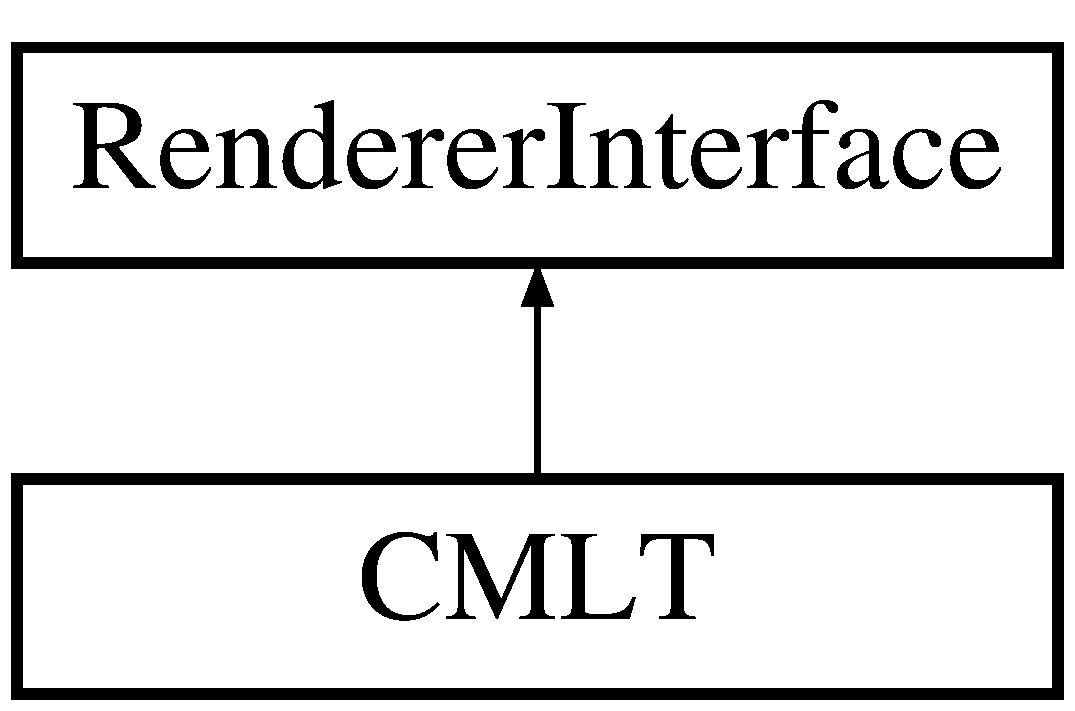
\includegraphics[height=2.000000cm]{struct_c_m_l_t}
\end{center}
\end{figure}
\subsection*{Public Methods}
\begin{DoxyCompactItemize}
\item 
void \hyperlink{struct_c_m_l_t_a16f9c8c63c6027478854528963cf4ccf}{init} (int argc, char $\ast$$\ast$argv, \hyperlink{struct_rendering_context}{Rendering\+Context} \&renderer)
\item 
void \hyperlink{struct_c_m_l_t_ad8fe8b00cbe99184c726849da14a5ab2}{render} (const uint32 instance, \hyperlink{struct_rendering_context}{Rendering\+Context} \&renderer)
\item 
\mbox{\Hypertarget{struct_c_m_l_t_ac6543dff92a861254148e223b0117741}\label{struct_c_m_l_t_ac6543dff92a861254148e223b0117741}} 
void {\bfseries sample\+\_\+seeds} (const uint32 n\+\_\+chains)
\item 
\mbox{\Hypertarget{struct_c_m_l_t_a72fd786f4cb773e69b0e5586236abf32}\label{struct_c_m_l_t_a72fd786f4cb773e69b0e5586236abf32}} 
void {\bfseries build\+\_\+st\+\_\+norms\+\_\+cdf} ()
\item 
\mbox{\Hypertarget{struct_c_m_l_t_a5740b19950843683b9c4ed03493badcf}\label{struct_c_m_l_t_a5740b19950843683b9c4ed03493badcf}} 
void {\bfseries recover\+\_\+primary\+\_\+coordinates} (C\+M\+L\+T\+Context \&context, \hyperlink{struct_rendering_context_view}{Rendering\+Context\+View} \&renderer\+\_\+view)
\item 
void \hyperlink{struct_c_m_l_t_aa8558dad2db5508be7aa028f69af7308}{destroy} ()
\end{DoxyCompactItemize}
\subsection*{Static Public Methods}
\begin{DoxyCompactItemize}
\item 
\mbox{\Hypertarget{struct_c_m_l_t_a548944cf739086aed1bb4feb56a1a081}\label{struct_c_m_l_t_a548944cf739086aed1bb4feb56a1a081}} 
static \hyperlink{struct_renderer_interface}{Renderer\+Interface} $\ast$ {\bfseries factory} ()
\end{DoxyCompactItemize}
\subsection*{Public Members}
\begin{DoxyCompactItemize}
\item 
\mbox{\Hypertarget{struct_c_m_l_t_afb7185888d73dbe2574eeb9c0b8658cb}\label{struct_c_m_l_t_afb7185888d73dbe2574eeb9c0b8658cb}} 
\hyperlink{struct_c_m_l_t_options}{C\+M\+L\+T\+Options} {\bfseries m\+\_\+options}
\item 
\mbox{\Hypertarget{struct_c_m_l_t_a1ec0cab631a0456d591ebfc64ffca5ac}\label{struct_c_m_l_t_a1ec0cab631a0456d591ebfc64ffca5ac}} 
\hyperlink{struct_tiled_sequence}{Tiled\+Sequence} {\bfseries m\+\_\+sequence}
\item 
\mbox{\Hypertarget{struct_c_m_l_t_a129fe15289ff32fc5852d50f56fecd5e}\label{struct_c_m_l_t_a129fe15289ff32fc5852d50f56fecd5e}} 
\hyperlink{struct_b_p_t_queues_storage}{B\+P\+T\+Queues\+Storage} {\bfseries m\+\_\+queues}
\item 
\mbox{\Hypertarget{struct_c_m_l_t_a7cf3b75b71572947e51414041d311b4f}\label{struct_c_m_l_t_a7cf3b75b71572947e51414041d311b4f}} 
\hyperlink{struct_vertex_storage}{Vertex\+Storage} {\bfseries m\+\_\+light\+\_\+vertices}
\item 
\mbox{\Hypertarget{struct_c_m_l_t_a8ef86b04a206fd3d4f78ef95e17b9f5d}\label{struct_c_m_l_t_a8ef86b04a206fd3d4f78ef95e17b9f5d}} 
\hyperlink{class_domain_buffer}{Domain\+Buffer}$<$ C\+U\+D\+A\+\_\+\+B\+U\+F\+F\+ER, float $>$ {\bfseries m\+\_\+mut\+\_\+u}
\item 
\mbox{\Hypertarget{struct_c_m_l_t_a2192a8b3ddaad34406c08fba43d3bd7c}\label{struct_c_m_l_t_a2192a8b3ddaad34406c08fba43d3bd7c}} 
\hyperlink{class_domain_buffer}{Domain\+Buffer}$<$ C\+U\+D\+A\+\_\+\+B\+U\+F\+F\+ER, float $>$ {\bfseries m\+\_\+light\+\_\+u}
\item 
\mbox{\Hypertarget{struct_c_m_l_t_aa4dcea45cec16bccbaa404681e5ea484}\label{struct_c_m_l_t_aa4dcea45cec16bccbaa404681e5ea484}} 
\hyperlink{class_domain_buffer}{Domain\+Buffer}$<$ C\+U\+D\+A\+\_\+\+B\+U\+F\+F\+ER, float $>$ {\bfseries m\+\_\+eye\+\_\+u}
\item 
\mbox{\Hypertarget{struct_c_m_l_t_a8f679c6206877154cb9ab79648e83fd5}\label{struct_c_m_l_t_a8f679c6206877154cb9ab79648e83fd5}} 
\hyperlink{class_domain_buffer}{Domain\+Buffer}$<$ C\+U\+D\+A\+\_\+\+B\+U\+F\+F\+ER, float4 $>$ {\bfseries m\+\_\+path\+\_\+value}
\item 
\mbox{\Hypertarget{struct_c_m_l_t_ac0f66c7e5408b1a3f2bb3795bc65008a}\label{struct_c_m_l_t_ac0f66c7e5408b1a3f2bb3795bc65008a}} 
\hyperlink{class_domain_buffer}{Domain\+Buffer}$<$ C\+U\+D\+A\+\_\+\+B\+U\+F\+F\+ER, float $>$ {\bfseries m\+\_\+path\+\_\+pdf}
\item 
\mbox{\Hypertarget{struct_c_m_l_t_aa68cde09c47f6594100ea36708eafbd9}\label{struct_c_m_l_t_aa68cde09c47f6594100ea36708eafbd9}} 
\hyperlink{class_domain_buffer}{Domain\+Buffer}$<$ C\+U\+D\+A\+\_\+\+B\+U\+F\+F\+ER, float4 $>$ {\bfseries m\+\_\+connections\+\_\+value}
\item 
\mbox{\Hypertarget{struct_c_m_l_t_a0f08e9cad3b6cca088885253662edf76}\label{struct_c_m_l_t_a0f08e9cad3b6cca088885253662edf76}} 
\hyperlink{class_domain_buffer}{Domain\+Buffer}$<$ C\+U\+D\+A\+\_\+\+B\+U\+F\+F\+ER, uint4 $>$ {\bfseries m\+\_\+connections\+\_\+index}
\item 
\mbox{\Hypertarget{struct_c_m_l_t_a9ce9688c7e25c7f6087742dffd10545b}\label{struct_c_m_l_t_a9ce9688c7e25c7f6087742dffd10545b}} 
\hyperlink{class_domain_buffer}{Domain\+Buffer}$<$ C\+U\+D\+A\+\_\+\+B\+U\+F\+F\+ER, float $>$ {\bfseries m\+\_\+connections\+\_\+cdf}
\item 
\mbox{\Hypertarget{struct_c_m_l_t_ac702a583341549e1ce0de60be3214396}\label{struct_c_m_l_t_ac702a583341549e1ce0de60be3214396}} 
\hyperlink{class_domain_buffer}{Domain\+Buffer}$<$ C\+U\+D\+A\+\_\+\+B\+U\+F\+F\+ER, uint32 $>$ {\bfseries m\+\_\+connections\+\_\+counter}
\item 
\mbox{\Hypertarget{struct_c_m_l_t_a5ea319405e28fe51741f330e3893fb29}\label{struct_c_m_l_t_a5ea319405e28fe51741f330e3893fb29}} 
\hyperlink{class_domain_buffer}{Domain\+Buffer}$<$ C\+U\+D\+A\+\_\+\+B\+U\+F\+F\+ER, uint32 $>$ {\bfseries m\+\_\+seeds}
\item 
\mbox{\Hypertarget{struct_c_m_l_t_a644d2eb1f3292193ad7903886064b637}\label{struct_c_m_l_t_a644d2eb1f3292193ad7903886064b637}} 
\hyperlink{class_domain_buffer}{Domain\+Buffer}$<$ C\+U\+D\+A\+\_\+\+B\+U\+F\+F\+ER, uint32 $>$ {\bfseries m\+\_\+st\+\_\+counters}
\item 
\mbox{\Hypertarget{struct_c_m_l_t_a0fa7f491dc75c81324549052e3a8890f}\label{struct_c_m_l_t_a0fa7f491dc75c81324549052e3a8890f}} 
\hyperlink{class_domain_buffer}{Domain\+Buffer}$<$ C\+U\+D\+A\+\_\+\+B\+U\+F\+F\+ER, float $>$ {\bfseries m\+\_\+st\+\_\+norms}
\item 
\mbox{\Hypertarget{struct_c_m_l_t_acc1916afe48863baad162c48c6d363ea}\label{struct_c_m_l_t_acc1916afe48863baad162c48c6d363ea}} 
\hyperlink{class_domain_buffer}{Domain\+Buffer}$<$ C\+U\+D\+A\+\_\+\+B\+U\+F\+F\+ER, float $>$ {\bfseries m\+\_\+st\+\_\+norms\+\_\+cdf}
\item 
\mbox{\Hypertarget{struct_c_m_l_t_ab3348fb7001a7f91ac20e0b7926738bf}\label{struct_c_m_l_t_ab3348fb7001a7f91ac20e0b7926738bf}} 
\hyperlink{class_domain_buffer}{Domain\+Buffer}$<$ C\+U\+D\+A\+\_\+\+B\+U\+F\+F\+ER, uint32 $>$ {\bfseries m\+\_\+rejections}
\item 
\mbox{\Hypertarget{struct_c_m_l_t_ae08cdbc80dcbba3b60546722bd496974}\label{struct_c_m_l_t_ae08cdbc80dcbba3b60546722bd496974}} 
\hyperlink{class_domain_buffer}{Domain\+Buffer}$<$ C\+U\+D\+A\+\_\+\+B\+U\+F\+F\+ER, \hyperlink{struct_vertex_geometry_id}{Vertex\+Geometry\+Id} $>$ {\bfseries m\+\_\+vertices}
\item 
\mbox{\Hypertarget{struct_c_m_l_t_a30ab1986197fdec50df5230ccb1ebf98}\label{struct_c_m_l_t_a30ab1986197fdec50df5230ccb1ebf98}} 
float {\bfseries m\+\_\+image\+\_\+brightness}
\item 
\mbox{\Hypertarget{struct_c_m_l_t_a35b8bc114ce9e815175287c343f0f8fb}\label{struct_c_m_l_t_a35b8bc114ce9e815175287c343f0f8fb}} 
uint32 {\bfseries m\+\_\+n\+\_\+init\+\_\+light\+\_\+paths}
\item 
\mbox{\Hypertarget{struct_c_m_l_t_ab6e192224acb5572df370e6acd344904}\label{struct_c_m_l_t_ab6e192224acb5572df370e6acd344904}} 
uint32 {\bfseries m\+\_\+n\+\_\+init\+\_\+paths}
\item 
\mbox{\Hypertarget{struct_c_m_l_t_ad56c788c77c282ca7e245641074e1ec6}\label{struct_c_m_l_t_ad56c788c77c282ca7e245641074e1ec6}} 
uint32 {\bfseries m\+\_\+n\+\_\+chains}
\item 
\mbox{\Hypertarget{struct_c_m_l_t_a94f5718a5d2127a60db1f3ff1d8c5e5d}\label{struct_c_m_l_t_a94f5718a5d2127a60db1f3ff1d8c5e5d}} 
uint32 {\bfseries m\+\_\+n\+\_\+connections}
\item 
\mbox{\Hypertarget{struct_c_m_l_t_aec650a2305a3be2386f78216bbbf5182}\label{struct_c_m_l_t_aec650a2305a3be2386f78216bbbf5182}} 
float {\bfseries m\+\_\+time}
\item 
\mbox{\Hypertarget{struct_c_m_l_t_a1988ed931c88f3b54e56bb2d41a05131}\label{struct_c_m_l_t_a1988ed931c88f3b54e56bb2d41a05131}} 
\hyperlink{classcugar_1_1_l_f_s_r_generator_matrix}{cugar\+::\+L\+F\+S\+R\+Generator\+Matrix} {\bfseries m\+\_\+generator}
\item 
\mbox{\Hypertarget{struct_c_m_l_t_a498e75f661fa9e5f68094cc0bc0fb965}\label{struct_c_m_l_t_a498e75f661fa9e5f68094cc0bc0fb965}} 
\hyperlink{structcugar_1_1_l_f_s_r_random_stream}{cugar\+::\+L\+F\+S\+R\+Random\+Stream} {\bfseries m\+\_\+random}
\end{DoxyCompactItemize}


\subsection{Member Function Documentation}
\mbox{\Hypertarget{struct_c_m_l_t_aa8558dad2db5508be7aa028f69af7308}\label{struct_c_m_l_t_aa8558dad2db5508be7aa028f69af7308}} 
\index{C\+M\+LT@{C\+M\+LT}!destroy@{destroy}}
\index{destroy@{destroy}!C\+M\+LT@{C\+M\+LT}}
\subsubsection{\texorpdfstring{destroy()}{destroy()}}
{\footnotesize\ttfamily void C\+M\+L\+T\+::destroy (\begin{DoxyParamCaption}{ }\end{DoxyParamCaption})\hspace{0.3cm}{\ttfamily [inline]}, {\ttfamily [virtual]}}

this method is responsible for destroying the object itself 

Reimplemented from \hyperlink{struct_renderer_interface_a7469218aafa029a3e22bac2c00dca9f5}{Renderer\+Interface}.

\mbox{\Hypertarget{struct_c_m_l_t_a16f9c8c63c6027478854528963cf4ccf}\label{struct_c_m_l_t_a16f9c8c63c6027478854528963cf4ccf}} 
\index{C\+M\+LT@{C\+M\+LT}!init@{init}}
\index{init@{init}!C\+M\+LT@{C\+M\+LT}}
\subsubsection{\texorpdfstring{init()}{init()}}
{\footnotesize\ttfamily void C\+M\+L\+T\+::init (\begin{DoxyParamCaption}\item[{int}]{argc,  }\item[{char $\ast$$\ast$}]{argv,  }\item[{\hyperlink{struct_rendering_context}{Rendering\+Context} \&}]{renderer }\end{DoxyParamCaption})\hspace{0.3cm}{\ttfamily [virtual]}}

this method is responsible for any command options parsing / initializations the renderer might need to perform 

Reimplemented from \hyperlink{struct_renderer_interface_a2ead9b943d6d48fcd32872e0005ebe63}{Renderer\+Interface}.

\mbox{\Hypertarget{struct_c_m_l_t_ad8fe8b00cbe99184c726849da14a5ab2}\label{struct_c_m_l_t_ad8fe8b00cbe99184c726849da14a5ab2}} 
\index{C\+M\+LT@{C\+M\+LT}!render@{render}}
\index{render@{render}!C\+M\+LT@{C\+M\+LT}}
\subsubsection{\texorpdfstring{render()}{render()}}
{\footnotesize\ttfamily void C\+M\+L\+T\+::render (\begin{DoxyParamCaption}\item[{const uint32}]{instance,  }\item[{\hyperlink{struct_rendering_context}{Rendering\+Context} \&}]{renderer }\end{DoxyParamCaption})\hspace{0.3cm}{\ttfamily [virtual]}}

this method is responsible for rendering a given frame in a progressive rendering


\begin{DoxyParams}{Parameters}
{\em instance} & the frame instance \\
\hline
\end{DoxyParams}


Reimplemented from \hyperlink{struct_renderer_interface_aa64254dd44c94929b05092dc8d74f29d}{Renderer\+Interface}.



The documentation for this struct was generated from the following file\+:\begin{DoxyCompactItemize}
\item 
C\+:/p4research/research/jpantaleoni/\+Fermat-\/\+Public/src/renderers/cmlt.\+h\end{DoxyCompactItemize}

\hypertarget{struct_c_m_l_t_options}{}\section{C\+M\+L\+T\+Options Struct Reference}
\label{struct_c_m_l_t_options}\index{C\+M\+L\+T\+Options@{C\+M\+L\+T\+Options}}


\subsection{Detailed description}
\hyperlink{struct_c_m_l_t}{C\+M\+LT} renderer options 

{\ttfamily \#include $<$cmlt.\+h$>$}

Inheritance diagram for C\+M\+L\+T\+Options\+:\begin{figure}[H]
\begin{center}
\leavevmode
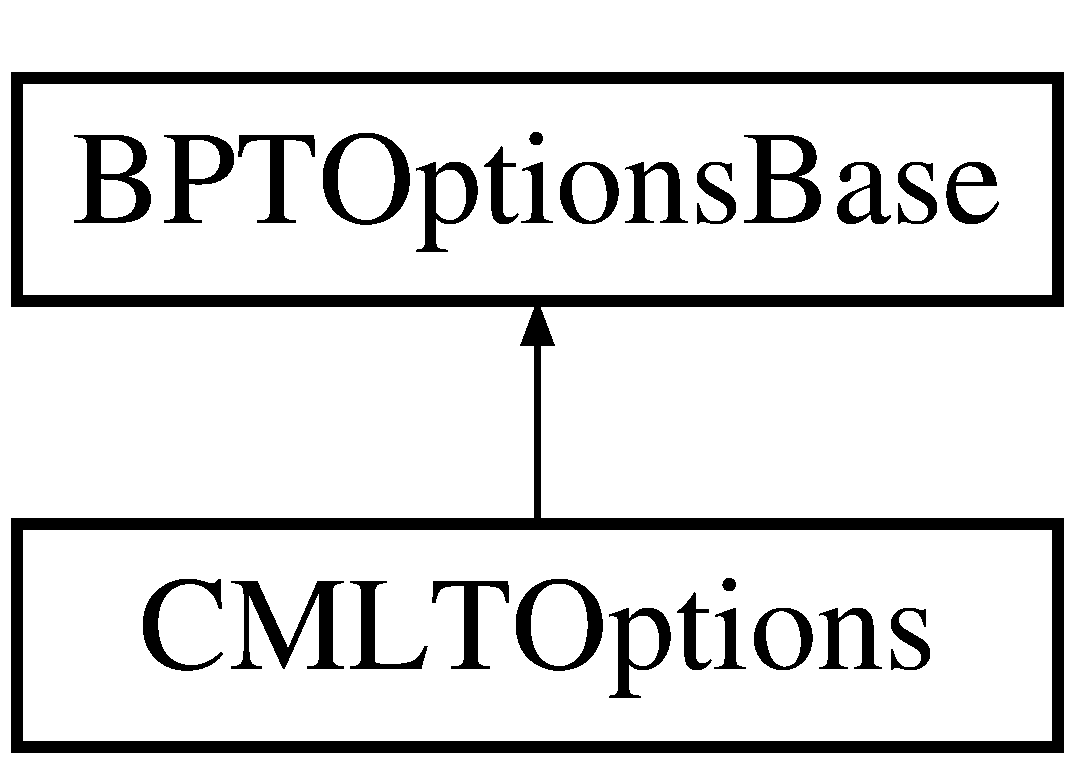
\includegraphics[height=2.000000cm]{struct_c_m_l_t_options}
\end{center}
\end{figure}
\subsection*{Public Methods}
\begin{DoxyCompactItemize}
\item 
\mbox{\Hypertarget{struct_c_m_l_t_options_a5cb40524108fff96c81361387f566035}\label{struct_c_m_l_t_options_a5cb40524108fff96c81361387f566035}} 
void {\bfseries parse} (const int argc, char $\ast$$\ast$argv)
\end{DoxyCompactItemize}
\subsection*{Public Members}
\begin{DoxyCompactItemize}
\item 
\mbox{\Hypertarget{struct_c_m_l_t_options_a245af891fe4ed10db7d0da618ac0c5dd}\label{struct_c_m_l_t_options_a245af891fe4ed10db7d0da618ac0c5dd}} 
uint32 {\bfseries n\+\_\+chains}
\item 
\mbox{\Hypertarget{struct_c_m_l_t_options_a2ec9a22abd01659176b885a573f6557d}\label{struct_c_m_l_t_options_a2ec9a22abd01659176b885a573f6557d}} 
uint32 {\bfseries spp}
\item 
\mbox{\Hypertarget{struct_c_m_l_t_options_a2cf42a00a147b2f4edc9a6411e9ce63e}\label{struct_c_m_l_t_options_a2cf42a00a147b2f4edc9a6411e9ce63e}} 
uint32 {\bfseries swap\+\_\+frequency}
\item 
\mbox{\Hypertarget{struct_c_m_l_t_options_aea5290e75c703e2acb711cde0f6eff67}\label{struct_c_m_l_t_options_aea5290e75c703e2acb711cde0f6eff67}} 
uint32 {\bfseries mmlt\+\_\+frequency}
\item 
\mbox{\Hypertarget{struct_c_m_l_t_options_ab45c9e49e578b63b01df9f932da06665}\label{struct_c_m_l_t_options_ab45c9e49e578b63b01df9f932da06665}} 
uint32 {\bfseries startup\+\_\+skips}
\item 
\mbox{\Hypertarget{struct_c_m_l_t_options_adcef80ec72c5d8274fd537047b815ee5}\label{struct_c_m_l_t_options_adcef80ec72c5d8274fd537047b815ee5}} 
uint32 {\bfseries reseeding}
\item 
\mbox{\Hypertarget{struct_c_m_l_t_options_a8c11a5d5ab22bb7e836bb44376387bef}\label{struct_c_m_l_t_options_a8c11a5d5ab22bb7e836bb44376387bef}} 
bool {\bfseries single\+\_\+connection}
\item 
\mbox{\Hypertarget{struct_c_m_l_t_options_a1893a46925e922975cf4128caf1548a7}\label{struct_c_m_l_t_options_a1893a46925e922975cf4128caf1548a7}} 
bool {\bfseries rr}
\item 
\mbox{\Hypertarget{struct_c_m_l_t_options_a2eead74be1feb4cea1946dd75cff8df1}\label{struct_c_m_l_t_options_a2eead74be1feb4cea1946dd75cff8df1}} 
bool {\bfseries light\+\_\+perturbations}
\item 
\mbox{\Hypertarget{struct_c_m_l_t_options_acc0220b53f1d1bc9b8789be4dc4bc186}\label{struct_c_m_l_t_options_acc0220b53f1d1bc9b8789be4dc4bc186}} 
bool {\bfseries eye\+\_\+perturbations}
\item 
\mbox{\Hypertarget{struct_c_m_l_t_options_af9c4c7ae7563a2f5a96d13874b55002b}\label{struct_c_m_l_t_options_af9c4c7ae7563a2f5a96d13874b55002b}} 
float {\bfseries perturbation\+\_\+radius}
\end{DoxyCompactItemize}


The documentation for this struct was generated from the following file\+:\begin{DoxyCompactItemize}
\item 
C\+:/p4research/research/jpantaleoni/\+Fermat-\/\+Public/src/renderers/cmlt.\+h\end{DoxyCompactItemize}

\hypertarget{structcugar_1_1cuda_1_1kd__knn_1_1_compare}{}\section{cugar\+:\+:cuda\+:\+:kd\+\_\+knn\+:\+:Compare Struct Reference}
\label{structcugar_1_1cuda_1_1kd__knn_1_1_compare}\index{cugar\+::cuda\+::kd\+\_\+knn\+::\+Compare@{cugar\+::cuda\+::kd\+\_\+knn\+::\+Compare}}
\subsection*{Public Methods}
\begin{DoxyCompactItemize}
\item 
\mbox{\Hypertarget{structcugar_1_1cuda_1_1kd__knn_1_1_compare_a273ed860eb6bd37f7dc57c70885b3056}\label{structcugar_1_1cuda_1_1kd__knn_1_1_compare_a273ed860eb6bd37f7dc57c70885b3056}} 
C\+U\+G\+A\+R\+\_\+\+F\+O\+R\+C\+E\+I\+N\+L\+I\+NE C\+U\+G\+A\+R\+\_\+\+H\+O\+S\+T\+\_\+\+D\+E\+V\+I\+CE bool {\bfseries operator()} (const float2 op1, const float2 op2) const
\end{DoxyCompactItemize}


The documentation for this struct was generated from the following file\+:\begin{DoxyCompactItemize}
\item 
C\+:/p4research/research/jpantaleoni/\+Fermat-\/\+Public/contrib/cugar/kd/cuda/knn\+\_\+inline.\+h\end{DoxyCompactItemize}

\hypertarget{structcugar_1_1component__functor}{}\section{cugar\+:\+:component\+\_\+functor$<$ Vector\+\_\+type $>$ Struct Template Reference}
\label{structcugar_1_1component__functor}\index{cugar\+::component\+\_\+functor$<$ Vector\+\_\+type $>$@{cugar\+::component\+\_\+functor$<$ Vector\+\_\+type $>$}}


\subsection{Detailed description}
\subsubsection*{template$<$typename Vector\+\_\+type$>$\newline
struct cugar\+::component\+\_\+functor$<$ Vector\+\_\+type $>$}

return the second\+\_\+argument component of the first\+\_\+argument vector 

{\ttfamily \#include $<$functors.\+h$>$}

\subsection*{Public Types}
\begin{DoxyCompactItemize}
\item 
\mbox{\Hypertarget{structcugar_1_1component__functor_a4d67ff3e96a90a60416606444a30ed60}\label{structcugar_1_1component__functor_a4d67ff3e96a90a60416606444a30ed60}} 
typedef \hyperlink{structcugar_1_1binary__function__tag}{binary\+\_\+function\+\_\+tag} {\bfseries function\+\_\+tag}
\item 
\mbox{\Hypertarget{structcugar_1_1component__functor_ad32cef8cadf59d513f4fcca43d5b7a67}\label{structcugar_1_1component__functor_ad32cef8cadf59d513f4fcca43d5b7a67}} 
typedef Vector\+\_\+type {\bfseries first\+\_\+argument\+\_\+type}
\item 
\mbox{\Hypertarget{structcugar_1_1component__functor_aadf2561788737067f7e181d2137d89e4}\label{structcugar_1_1component__functor_aadf2561788737067f7e181d2137d89e4}} 
typedef uint32 {\bfseries second\+\_\+argument\+\_\+type}
\item 
\mbox{\Hypertarget{structcugar_1_1component__functor_ae00f23803ffb15f3d9945bb0cf5a468f}\label{structcugar_1_1component__functor_ae00f23803ffb15f3d9945bb0cf5a468f}} 
typedef Vector\+\_\+type\+::value\+\_\+type {\bfseries result\+\_\+type}
\end{DoxyCompactItemize}
\subsection*{Public Methods}
\begin{DoxyCompactItemize}
\item 
\mbox{\Hypertarget{structcugar_1_1component__functor_adb3d77d8c1d9f0ad286103817f41a741}\label{structcugar_1_1component__functor_adb3d77d8c1d9f0ad286103817f41a741}} 
C\+U\+G\+A\+R\+\_\+\+H\+O\+S\+T\+\_\+\+D\+E\+V\+I\+CE result\+\_\+type {\bfseries operator()} (const first\+\_\+argument\+\_\+type v, const second\+\_\+argument\+\_\+type i) const
\end{DoxyCompactItemize}


The documentation for this struct was generated from the following file\+:\begin{DoxyCompactItemize}
\item 
C\+:/p4research/research/jpantaleoni/\+Fermat-\/\+Public/contrib/cugar/basic/\hyperlink{functors_8h}{functors.\+h}\end{DoxyCompactItemize}

\hypertarget{structcugar_1_1compose__binary}{}\section{cugar\+:\+:compose\+\_\+binary$<$ F, G1, G2 $>$ Struct Template Reference}
\label{structcugar_1_1compose__binary}\index{cugar\+::compose\+\_\+binary$<$ F, G1, G2 $>$@{cugar\+::compose\+\_\+binary$<$ F, G1, G2 $>$}}


\subsection{Detailed description}
\subsubsection*{template$<$typename F, typename G1, typename G2$>$\newline
struct cugar\+::compose\+\_\+binary$<$ F, G1, G2 $>$}

compose a binary function after two unary ones 

{\ttfamily \#include $<$functors.\+h$>$}

\subsection*{Public Types}
\begin{DoxyCompactItemize}
\item 
\mbox{\Hypertarget{structcugar_1_1compose__binary_a952674add18272aa843b649c2eaf673f}\label{structcugar_1_1compose__binary_a952674add18272aa843b649c2eaf673f}} 
typedef \hyperlink{structcugar_1_1binary__function__tag}{binary\+\_\+function\+\_\+tag} {\bfseries function\+\_\+tag}
\item 
\mbox{\Hypertarget{structcugar_1_1compose__binary_ae13750e2e9d55157716d02d7cf6a0772}\label{structcugar_1_1compose__binary_ae13750e2e9d55157716d02d7cf6a0772}} 
typedef G1\+::argument\+\_\+type {\bfseries first\+\_\+argument\+\_\+type}
\item 
\mbox{\Hypertarget{structcugar_1_1compose__binary_a63cd0573a047ba9ccb92494f3e69d56c}\label{structcugar_1_1compose__binary_a63cd0573a047ba9ccb92494f3e69d56c}} 
typedef G2\+::argument\+\_\+type {\bfseries second\+\_\+argument\+\_\+type}
\item 
\mbox{\Hypertarget{structcugar_1_1compose__binary_a12735065900fa746b5cdbaa639a305bf}\label{structcugar_1_1compose__binary_a12735065900fa746b5cdbaa639a305bf}} 
typedef F\+::result\+\_\+type {\bfseries result\+\_\+type}
\end{DoxyCompactItemize}
\subsection*{Public Methods}
\begin{DoxyCompactItemize}
\item 
\mbox{\Hypertarget{structcugar_1_1compose__binary_ac5d7be1ab8894f7dacce1013995509a7}\label{structcugar_1_1compose__binary_ac5d7be1ab8894f7dacce1013995509a7}} 
C\+U\+G\+A\+R\+\_\+\+H\+O\+S\+T\+\_\+\+D\+E\+V\+I\+CE {\bfseries compose\+\_\+binary} (const F f, const G1 g1, const G2 g2)
\item 
\mbox{\Hypertarget{structcugar_1_1compose__binary_a82bd71ce4af43bafa5f651c258cdbc8c}\label{structcugar_1_1compose__binary_a82bd71ce4af43bafa5f651c258cdbc8c}} 
C\+U\+G\+A\+R\+\_\+\+H\+O\+S\+T\+\_\+\+D\+E\+V\+I\+CE result\+\_\+type {\bfseries operator()} (const first\+\_\+argument\+\_\+type \&op1, const second\+\_\+argument\+\_\+type \&op2) const
\end{DoxyCompactItemize}


The documentation for this struct was generated from the following file\+:\begin{DoxyCompactItemize}
\item 
C\+:/p4research/research/jpantaleoni/\+Fermat-\/\+Public/contrib/cugar/basic/\hyperlink{functors_8h}{functors.\+h}\end{DoxyCompactItemize}

\hypertarget{structcugar_1_1compose__unary}{}\section{cugar\+:\+:compose\+\_\+unary$<$ F1, F2 $>$ Struct Template Reference}
\label{structcugar_1_1compose__unary}\index{cugar\+::compose\+\_\+unary$<$ F1, F2 $>$@{cugar\+::compose\+\_\+unary$<$ F1, F2 $>$}}


\subsection{Detailed description}
\subsubsection*{template$<$typename F1, typename F2$>$\newline
struct cugar\+::compose\+\_\+unary$<$ F1, F2 $>$}

compose two unary functions 

{\ttfamily \#include $<$functors.\+h$>$}

\subsection*{Public Types}
\begin{DoxyCompactItemize}
\item 
\mbox{\Hypertarget{structcugar_1_1compose__unary_a4a1d58a5dae30f78fe5871c85f24e965}\label{structcugar_1_1compose__unary_a4a1d58a5dae30f78fe5871c85f24e965}} 
typedef \hyperlink{structcugar_1_1unary__function__tag}{unary\+\_\+function\+\_\+tag} {\bfseries function\+\_\+tag}
\item 
\mbox{\Hypertarget{structcugar_1_1compose__unary_ad4bd284e582454066bdfa203ca5421e4}\label{structcugar_1_1compose__unary_ad4bd284e582454066bdfa203ca5421e4}} 
typedef F2\+::first\+\_\+argument\+\_\+type {\bfseries argument\+\_\+type}
\item 
\mbox{\Hypertarget{structcugar_1_1compose__unary_a220e54601a4de08d80d57c741a805f65}\label{structcugar_1_1compose__unary_a220e54601a4de08d80d57c741a805f65}} 
typedef F1\+::result\+\_\+type {\bfseries result\+\_\+type}
\end{DoxyCompactItemize}
\subsection*{Public Methods}
\begin{DoxyCompactItemize}
\item 
\mbox{\Hypertarget{structcugar_1_1compose__unary_aa9dcdb62a4b94e740060bbd68a3a4210}\label{structcugar_1_1compose__unary_aa9dcdb62a4b94e740060bbd68a3a4210}} 
C\+U\+G\+A\+R\+\_\+\+H\+O\+S\+T\+\_\+\+D\+E\+V\+I\+CE {\bfseries compose\+\_\+unary} (const F1 f1, const F2 f2)
\item 
\mbox{\Hypertarget{structcugar_1_1compose__unary_a9e8892faa48c68486a0bf9de6ac795ca}\label{structcugar_1_1compose__unary_a9e8892faa48c68486a0bf9de6ac795ca}} 
C\+U\+G\+A\+R\+\_\+\+H\+O\+S\+T\+\_\+\+D\+E\+V\+I\+CE result\+\_\+type {\bfseries operator()} (const argument\+\_\+type \&op) const
\end{DoxyCompactItemize}


The documentation for this struct was generated from the following file\+:\begin{DoxyCompactItemize}
\item 
C\+:/p4research/research/jpantaleoni/\+Fermat-\/\+Public/contrib/cugar/basic/\hyperlink{functors_8h}{functors.\+h}\end{DoxyCompactItemize}

\hypertarget{structcugar_1_1compose__unary__after__binary}{}\section{cugar\+:\+:compose\+\_\+unary\+\_\+after\+\_\+binary$<$ F1, F2 $>$ Struct Template Reference}
\label{structcugar_1_1compose__unary__after__binary}\index{cugar\+::compose\+\_\+unary\+\_\+after\+\_\+binary$<$ F1, F2 $>$@{cugar\+::compose\+\_\+unary\+\_\+after\+\_\+binary$<$ F1, F2 $>$}}


\subsection{Detailed description}
\subsubsection*{template$<$typename F1, typename F2$>$\newline
struct cugar\+::compose\+\_\+unary\+\_\+after\+\_\+binary$<$ F1, F2 $>$}

compose an unary operator F1 with a binary operator F2 

{\ttfamily \#include $<$functors.\+h$>$}

\subsection*{Public Types}
\begin{DoxyCompactItemize}
\item 
\mbox{\Hypertarget{structcugar_1_1compose__unary__after__binary_a8d0706d1f2c568957c7c00e3c3159fc4}\label{structcugar_1_1compose__unary__after__binary_a8d0706d1f2c568957c7c00e3c3159fc4}} 
typedef \hyperlink{structcugar_1_1binary__function__tag}{binary\+\_\+function\+\_\+tag} {\bfseries function\+\_\+tag}
\item 
\mbox{\Hypertarget{structcugar_1_1compose__unary__after__binary_acf72b3ef77f11db8d0cf51ba35a1e630}\label{structcugar_1_1compose__unary__after__binary_acf72b3ef77f11db8d0cf51ba35a1e630}} 
typedef F2\+::first\+\_\+argument\+\_\+type {\bfseries first\+\_\+argument\+\_\+type}
\item 
\mbox{\Hypertarget{structcugar_1_1compose__unary__after__binary_a4140cb2e0d07217e2f4a9eefc35abe16}\label{structcugar_1_1compose__unary__after__binary_a4140cb2e0d07217e2f4a9eefc35abe16}} 
typedef F2\+::second\+\_\+argument\+\_\+type {\bfseries second\+\_\+argument\+\_\+type}
\item 
\mbox{\Hypertarget{structcugar_1_1compose__unary__after__binary_a63ea5dcf820829a87742fa7fa11d06dd}\label{structcugar_1_1compose__unary__after__binary_a63ea5dcf820829a87742fa7fa11d06dd}} 
typedef F1\+::result\+\_\+type {\bfseries result\+\_\+type}
\end{DoxyCompactItemize}
\subsection*{Public Methods}
\begin{DoxyCompactItemize}
\item 
\mbox{\Hypertarget{structcugar_1_1compose__unary__after__binary_a690775e543013946ea457a75a92e10d8}\label{structcugar_1_1compose__unary__after__binary_a690775e543013946ea457a75a92e10d8}} 
C\+U\+G\+A\+R\+\_\+\+H\+O\+S\+T\+\_\+\+D\+E\+V\+I\+CE {\bfseries compose\+\_\+unary\+\_\+after\+\_\+binary} (const F1 f1, const F2 f2)
\item 
\mbox{\Hypertarget{structcugar_1_1compose__unary__after__binary_aad4d07d1b68d633b0de01a22685764b4}\label{structcugar_1_1compose__unary__after__binary_aad4d07d1b68d633b0de01a22685764b4}} 
C\+U\+G\+A\+R\+\_\+\+H\+O\+S\+T\+\_\+\+D\+E\+V\+I\+CE result\+\_\+type {\bfseries operator()} (const first\+\_\+argument\+\_\+type \&op1, const second\+\_\+argument\+\_\+type \&op2) const
\end{DoxyCompactItemize}


The documentation for this struct was generated from the following file\+:\begin{DoxyCompactItemize}
\item 
C\+:/p4research/research/jpantaleoni/\+Fermat-\/\+Public/contrib/cugar/basic/\hyperlink{functors_8h}{functors.\+h}\end{DoxyCompactItemize}

\hypertarget{structcugar_1_1composition__type}{}\section{cugar\+:\+:composition\+\_\+type$<$ F1, F2, T1, T2 $>$ Struct Template Reference}
\label{structcugar_1_1composition__type}\index{cugar\+::composition\+\_\+type$<$ F1, F2, T1, T2 $>$@{cugar\+::composition\+\_\+type$<$ F1, F2, T1, T2 $>$}}


The documentation for this struct was generated from the following file\+:\begin{DoxyCompactItemize}
\item 
C\+:/p4research/research/jpantaleoni/\+Fermat-\/\+Public/contrib/cugar/basic/\hyperlink{functors_8h}{functors.\+h}\end{DoxyCompactItemize}

\hypertarget{structcugar_1_1composition__type_3_01_f1_00_01_f2_00_01unary__function__tag_00_01binary__function__tag_01_4}{}\section{cugar\+:\+:composition\+\_\+type$<$ F1, F2, unary\+\_\+function\+\_\+tag, binary\+\_\+function\+\_\+tag $>$ Struct Template Reference}
\label{structcugar_1_1composition__type_3_01_f1_00_01_f2_00_01unary__function__tag_00_01binary__function__tag_01_4}\index{cugar\+::composition\+\_\+type$<$ F1, F2, unary\+\_\+function\+\_\+tag, binary\+\_\+function\+\_\+tag $>$@{cugar\+::composition\+\_\+type$<$ F1, F2, unary\+\_\+function\+\_\+tag, binary\+\_\+function\+\_\+tag $>$}}
\subsection*{Public Types}
\begin{DoxyCompactItemize}
\item 
\mbox{\Hypertarget{structcugar_1_1composition__type_3_01_f1_00_01_f2_00_01unary__function__tag_00_01binary__function__tag_01_4_a956e15fef86ee948642e7bb018c88be1}\label{structcugar_1_1composition__type_3_01_f1_00_01_f2_00_01unary__function__tag_00_01binary__function__tag_01_4_a956e15fef86ee948642e7bb018c88be1}} 
typedef \hyperlink{structcugar_1_1compose__unary__after__binary}{compose\+\_\+unary\+\_\+after\+\_\+binary}$<$ F1, F2 $>$ {\bfseries type}
\end{DoxyCompactItemize}


The documentation for this struct was generated from the following file\+:\begin{DoxyCompactItemize}
\item 
C\+:/p4research/research/jpantaleoni/\+Fermat-\/\+Public/contrib/cugar/basic/\hyperlink{functors_8h}{functors.\+h}\end{DoxyCompactItemize}

\hypertarget{structcugar_1_1composition__type_3_01_f1_00_01_f2_00_01unary__function__tag_00_01unary__function__tag_01_4}{}\section{cugar\+:\+:composition\+\_\+type$<$ F1, F2, unary\+\_\+function\+\_\+tag, unary\+\_\+function\+\_\+tag $>$ Struct Template Reference}
\label{structcugar_1_1composition__type_3_01_f1_00_01_f2_00_01unary__function__tag_00_01unary__function__tag_01_4}\index{cugar\+::composition\+\_\+type$<$ F1, F2, unary\+\_\+function\+\_\+tag, unary\+\_\+function\+\_\+tag $>$@{cugar\+::composition\+\_\+type$<$ F1, F2, unary\+\_\+function\+\_\+tag, unary\+\_\+function\+\_\+tag $>$}}
\subsection*{Public Types}
\begin{DoxyCompactItemize}
\item 
\mbox{\Hypertarget{structcugar_1_1composition__type_3_01_f1_00_01_f2_00_01unary__function__tag_00_01unary__function__tag_01_4_a34f9c88d38b72abef395289b337617fd}\label{structcugar_1_1composition__type_3_01_f1_00_01_f2_00_01unary__function__tag_00_01unary__function__tag_01_4_a34f9c88d38b72abef395289b337617fd}} 
typedef \hyperlink{structcugar_1_1compose__unary}{compose\+\_\+unary}$<$ F1, F2 $>$ {\bfseries type}
\end{DoxyCompactItemize}


The documentation for this struct was generated from the following file\+:\begin{DoxyCompactItemize}
\item 
C\+:/p4research/research/jpantaleoni/\+Fermat-\/\+Public/contrib/cugar/basic/\hyperlink{functors_8h}{functors.\+h}\end{DoxyCompactItemize}

\hypertarget{structcugar_1_1internals_1_1const__cast__marker}{}\section{cugar\+:\+:internals\+:\+:const\+\_\+cast\+\_\+marker Struct Reference}
\label{structcugar_1_1internals_1_1const__cast__marker}\index{cugar\+::internals\+::const\+\_\+cast\+\_\+marker@{cugar\+::internals\+::const\+\_\+cast\+\_\+marker}}


The documentation for this struct was generated from the following file\+:\begin{DoxyCompactItemize}
\item 
C\+:/p4research/research/jpantaleoni/\+Fermat-\/\+Public/contrib/cugar/basic/shared\+\_\+pointer.\+h\end{DoxyCompactItemize}

\hypertarget{structcugar_1_1constant__functor}{}\section{cugar\+:\+:constant\+\_\+functor$<$ T, R $>$ Struct Template Reference}
\label{structcugar_1_1constant__functor}\index{cugar\+::constant\+\_\+functor$<$ T, R $>$@{cugar\+::constant\+\_\+functor$<$ T, R $>$}}


\subsection{Detailed description}
\subsubsection*{template$<$typename T, typename R$>$\newline
struct cugar\+::constant\+\_\+functor$<$ T, R $>$}

constant functor 

{\ttfamily \#include $<$functors.\+h$>$}

\subsection*{Public Types}
\begin{DoxyCompactItemize}
\item 
\mbox{\Hypertarget{structcugar_1_1constant__functor_aa17f4bf4ea8666209fbd8d769bc10ca4}\label{structcugar_1_1constant__functor_aa17f4bf4ea8666209fbd8d769bc10ca4}} 
typedef \hyperlink{structcugar_1_1unary__function__tag}{unary\+\_\+function\+\_\+tag} {\bfseries function\+\_\+tag}
\item 
\mbox{\Hypertarget{structcugar_1_1constant__functor_ae385ab77856734935f420ebfd0c94e94}\label{structcugar_1_1constant__functor_ae385ab77856734935f420ebfd0c94e94}} 
typedef T {\bfseries argument\+\_\+type}
\item 
\mbox{\Hypertarget{structcugar_1_1constant__functor_aa242851b82c2bb7db852ffbde278b7d1}\label{structcugar_1_1constant__functor_aa242851b82c2bb7db852ffbde278b7d1}} 
typedef R {\bfseries result\+\_\+type}
\end{DoxyCompactItemize}
\subsection*{Public Methods}
\begin{DoxyCompactItemize}
\item 
C\+U\+G\+A\+R\+\_\+\+H\+O\+S\+T\+\_\+\+D\+E\+V\+I\+CE \hyperlink{structcugar_1_1constant__functor_afc17d92554197c5286554135c3cdc006}{constant\+\_\+functor} (R c)
\item 
\mbox{\Hypertarget{structcugar_1_1constant__functor_a547f882068d2f140fd00b3bc75d645b5}\label{structcugar_1_1constant__functor_a547f882068d2f140fd00b3bc75d645b5}} 
C\+U\+G\+A\+R\+\_\+\+H\+O\+S\+T\+\_\+\+D\+E\+V\+I\+CE R {\bfseries operator()} (const T op) const
\end{DoxyCompactItemize}
\subsection*{Public Members}
\begin{DoxyCompactItemize}
\item 
\mbox{\Hypertarget{structcugar_1_1constant__functor_a2cdcc5557860c948e1591d69d628e2ae}\label{structcugar_1_1constant__functor_a2cdcc5557860c948e1591d69d628e2ae}} 
R {\bfseries constant}
\end{DoxyCompactItemize}


\subsection{Constructor \& Destructor Documentation}
\mbox{\Hypertarget{structcugar_1_1constant__functor_afc17d92554197c5286554135c3cdc006}\label{structcugar_1_1constant__functor_afc17d92554197c5286554135c3cdc006}} 
\index{cugar\+::constant\+\_\+functor@{cugar\+::constant\+\_\+functor}!constant\+\_\+functor@{constant\+\_\+functor}}
\index{constant\+\_\+functor@{constant\+\_\+functor}!cugar\+::constant\+\_\+functor@{cugar\+::constant\+\_\+functor}}
\subsubsection{\texorpdfstring{constant\+\_\+functor()}{constant\_functor()}}
{\footnotesize\ttfamily template$<$typename T , typename R $>$ \\
C\+U\+G\+A\+R\+\_\+\+H\+O\+S\+T\+\_\+\+D\+E\+V\+I\+CE \hyperlink{structcugar_1_1constant__functor}{cugar\+::constant\+\_\+functor}$<$ T, R $>$\+::\hyperlink{structcugar_1_1constant__functor}{constant\+\_\+functor} (\begin{DoxyParamCaption}\item[{R}]{c }\end{DoxyParamCaption})\hspace{0.3cm}{\ttfamily [inline]}}

constructor


\begin{DoxyParams}{Parameters}
{\em c} & constant value \\
\hline
\end{DoxyParams}


The documentation for this struct was generated from the following file\+:\begin{DoxyCompactItemize}
\item 
C\+:/p4research/research/jpantaleoni/\+Fermat-\/\+Public/contrib/cugar/basic/\hyperlink{functors_8h}{functors.\+h}\end{DoxyCompactItemize}

\hypertarget{structcugar_1_1cuda_1_1_kd__context_1_1_context}{}\section{cugar\+:\+:cuda\+:\+:Kd\+\_\+context\+:\+:Context Struct Reference}
\label{structcugar_1_1cuda_1_1_kd__context_1_1_context}\index{cugar\+::cuda\+::\+Kd\+\_\+context\+::\+Context@{cugar\+::cuda\+::\+Kd\+\_\+context\+::\+Context}}


\subsection{Detailed description}
Cuda accessor struct. 

{\ttfamily \#include $<$kd\+\_\+context.\+h$>$}

\subsection*{Public Methods}
\begin{DoxyCompactItemize}
\item 
\mbox{\Hypertarget{structcugar_1_1cuda_1_1_kd__context_1_1_context_aee1e8f81d04c41d3cc6f2f33ef16dc02}\label{structcugar_1_1cuda_1_1_kd__context_1_1_context_aee1e8f81d04c41d3cc6f2f33ef16dc02}} 
C\+U\+G\+A\+R\+\_\+\+H\+O\+S\+T\+\_\+\+D\+E\+V\+I\+CE {\bfseries Context} (\hyperlink{structcugar_1_1_kd__node}{Kd\+\_\+node} $\ast$nodes, uint2 $\ast$leaves, uint2 $\ast$ranges)
\item 
\mbox{\Hypertarget{structcugar_1_1cuda_1_1_kd__context_1_1_context_af334cf590f3a2438f3bf332c131ee6f8}\label{structcugar_1_1cuda_1_1_kd__context_1_1_context_af334cf590f3a2438f3bf332c131ee6f8}} 
C\+U\+G\+A\+R\+\_\+\+H\+O\+S\+T\+\_\+\+D\+E\+V\+I\+CE void \hyperlink{structcugar_1_1cuda_1_1_kd__context_1_1_context_af334cf590f3a2438f3bf332c131ee6f8}{write\+\_\+node} (const uint32 node, const uint32 offset, const uint32 skip\+\_\+node, const uint32 \hyperlink{namespacecugar_a2121df08f967e232ea5fe0ee378dee67}{begin}, const uint32 end, const uint32 split\+\_\+index, const uint32 split\+\_\+dim, const float split\+\_\+plane)
\begin{DoxyCompactList}\small\item\em write a new node \end{DoxyCompactList}\item 
\mbox{\Hypertarget{structcugar_1_1cuda_1_1_kd__context_1_1_context_ab0ee0b93db5dff207418fe94ecbb5f68}\label{structcugar_1_1cuda_1_1_kd__context_1_1_context_ab0ee0b93db5dff207418fe94ecbb5f68}} 
C\+U\+G\+A\+R\+\_\+\+H\+O\+S\+T\+\_\+\+D\+E\+V\+I\+CE void \hyperlink{structcugar_1_1cuda_1_1_kd__context_1_1_context_ab0ee0b93db5dff207418fe94ecbb5f68}{write\+\_\+node} (const uint32 node, const uint32 offset, const uint32 skip\+\_\+node, const uint32 \hyperlink{namespacecugar_a2121df08f967e232ea5fe0ee378dee67}{begin}, const uint32 end)
\begin{DoxyCompactList}\small\item\em write a new node \end{DoxyCompactList}\item 
\mbox{\Hypertarget{structcugar_1_1cuda_1_1_kd__context_1_1_context_aee926e3f601065f962ee58b9cc6712ea}\label{structcugar_1_1cuda_1_1_kd__context_1_1_context_aee926e3f601065f962ee58b9cc6712ea}} 
C\+U\+G\+A\+R\+\_\+\+H\+O\+S\+T\+\_\+\+D\+E\+V\+I\+CE void \hyperlink{structcugar_1_1cuda_1_1_kd__context_1_1_context_aee926e3f601065f962ee58b9cc6712ea}{write\+\_\+leaf} (const uint32 index, const uint32 \hyperlink{namespacecugar_a2121df08f967e232ea5fe0ee378dee67}{begin}, const uint32 end)
\begin{DoxyCompactList}\small\item\em write a new leaf \end{DoxyCompactList}\end{DoxyCompactItemize}
\subsection*{Public Members}
\begin{DoxyCompactItemize}
\item 
\mbox{\Hypertarget{structcugar_1_1cuda_1_1_kd__context_1_1_context_a2ef7ab3f73c3efbcf1889676cc49f147}\label{structcugar_1_1cuda_1_1_kd__context_1_1_context_a2ef7ab3f73c3efbcf1889676cc49f147}} 
\hyperlink{structcugar_1_1_kd__node}{Kd\+\_\+node} $\ast$ \hyperlink{structcugar_1_1cuda_1_1_kd__context_1_1_context_a2ef7ab3f73c3efbcf1889676cc49f147}{m\+\_\+nodes}
\begin{DoxyCompactList}\small\item\em node pointer \end{DoxyCompactList}\item 
\mbox{\Hypertarget{structcugar_1_1cuda_1_1_kd__context_1_1_context_a829a7e246b527d525e4f652afc60dcde}\label{structcugar_1_1cuda_1_1_kd__context_1_1_context_a829a7e246b527d525e4f652afc60dcde}} 
uint2 $\ast$ \hyperlink{structcugar_1_1cuda_1_1_kd__context_1_1_context_a829a7e246b527d525e4f652afc60dcde}{m\+\_\+leaves}
\begin{DoxyCompactList}\small\item\em leaf pointer \end{DoxyCompactList}\item 
\mbox{\Hypertarget{structcugar_1_1cuda_1_1_kd__context_1_1_context_a1b85cc5cdb6febf1e3256e5ed7f4db10}\label{structcugar_1_1cuda_1_1_kd__context_1_1_context_a1b85cc5cdb6febf1e3256e5ed7f4db10}} 
uint2 $\ast$ \hyperlink{structcugar_1_1cuda_1_1_kd__context_1_1_context_a1b85cc5cdb6febf1e3256e5ed7f4db10}{m\+\_\+ranges}
\begin{DoxyCompactList}\small\item\em range pointer \end{DoxyCompactList}\end{DoxyCompactItemize}


The documentation for this struct was generated from the following file\+:\begin{DoxyCompactItemize}
\item 
C\+:/p4research/research/jpantaleoni/\+Fermat-\/\+Public/contrib/cugar/kd/cuda/\hyperlink{kd__context_8h}{kd\+\_\+context.\+h}\end{DoxyCompactItemize}

\hypertarget{structcugar_1_1cuda_1_1kd_1_1_kd__context_1_1_context}{}\section{cugar\+:\+:cuda\+:\+:kd\+:\+:Kd\+\_\+context$<$ D\+IM, Bbox\+Type, Integer, Output\+Tree $>$\+:\+:Context Struct Reference}
\label{structcugar_1_1cuda_1_1kd_1_1_kd__context_1_1_context}\index{cugar\+::cuda\+::kd\+::\+Kd\+\_\+context$<$ D\+I\+M, Bbox\+Type, Integer, Output\+Tree $>$\+::\+Context@{cugar\+::cuda\+::kd\+::\+Kd\+\_\+context$<$ D\+I\+M, Bbox\+Type, Integer, Output\+Tree $>$\+::\+Context}}


\subsection{Detailed description}
\subsubsection*{template$<$uint32 D\+IM, typename Bbox\+Type, typename Integer, typename Output\+Tree$>$\newline
struct cugar\+::cuda\+::kd\+::\+Kd\+\_\+context$<$ D\+I\+M, Bbox\+Type, Integer, Output\+Tree $>$\+::\+Context}

Cuda accessor struct. 

{\ttfamily \#include $<$kd\+\_\+builder\+\_\+inline.\+h$>$}

\subsection*{Public Methods}
\begin{DoxyCompactItemize}
\item 
\mbox{\Hypertarget{structcugar_1_1cuda_1_1kd_1_1_kd__context_1_1_context_a3878d0bf036f3f48fabcee2cfade83f8}\label{structcugar_1_1cuda_1_1kd_1_1_kd__context_1_1_context_a3878d0bf036f3f48fabcee2cfade83f8}} 
C\+U\+G\+A\+R\+\_\+\+H\+O\+S\+T\+\_\+\+D\+E\+V\+I\+CE {\bfseries Context} (const Base\+Context context, const Integer $\ast$codes, Bbox\+Type bbox)
\item 
C\+U\+G\+A\+R\+\_\+\+H\+O\+S\+T\+\_\+\+D\+E\+V\+I\+CE void \hyperlink{structcugar_1_1cuda_1_1kd_1_1_kd__context_1_1_context_a62ebef4047ff66f5e575fbcf48786e87}{write\+\_\+node} (const uint32 node, const uint32 parent, bool p1, bool p2, const uint32 offset, const uint32 skip\+\_\+node, const uint32 level, const uint32 \hyperlink{namespacecugar_a2121df08f967e232ea5fe0ee378dee67}{begin}, const uint32 end, const uint32 split\+\_\+index)
\item 
C\+U\+G\+A\+R\+\_\+\+H\+O\+S\+T\+\_\+\+D\+E\+V\+I\+CE void \hyperlink{structcugar_1_1cuda_1_1kd_1_1_kd__context_1_1_context_a6ae8f1b91a2d3d60fcb1d3092e9575de}{write\+\_\+leaf} (const uint32 leaf\+\_\+index, const uint32 node\+\_\+index, const uint32 \hyperlink{namespacecugar_a2121df08f967e232ea5fe0ee378dee67}{begin}, const uint32 end)
\end{DoxyCompactItemize}
\subsection*{Public Members}
\begin{DoxyCompactItemize}
\item 
\mbox{\Hypertarget{structcugar_1_1cuda_1_1kd_1_1_kd__context_1_1_context_a124766fb2813a8a0fcfc7d1115c5cd0a}\label{structcugar_1_1cuda_1_1kd_1_1_kd__context_1_1_context_a124766fb2813a8a0fcfc7d1115c5cd0a}} 
Base\+Context {\bfseries m\+\_\+context}
\item 
\mbox{\Hypertarget{structcugar_1_1cuda_1_1kd_1_1_kd__context_1_1_context_ab3063fce2ff33ee780aeed68f8d00c48}\label{structcugar_1_1cuda_1_1kd_1_1_kd__context_1_1_context_ab3063fce2ff33ee780aeed68f8d00c48}} 
const Integer $\ast$ {\bfseries m\+\_\+codes}
\item 
\mbox{\Hypertarget{structcugar_1_1cuda_1_1kd_1_1_kd__context_1_1_context_abbc1095b788582a1eb47e51d4a758f92}\label{structcugar_1_1cuda_1_1kd_1_1_kd__context_1_1_context_abbc1095b788582a1eb47e51d4a758f92}} 
Bbox\+Type {\bfseries m\+\_\+bbox}
\end{DoxyCompactItemize}


\subsection{Member Function Documentation}
\mbox{\Hypertarget{structcugar_1_1cuda_1_1kd_1_1_kd__context_1_1_context_a6ae8f1b91a2d3d60fcb1d3092e9575de}\label{structcugar_1_1cuda_1_1kd_1_1_kd__context_1_1_context_a6ae8f1b91a2d3d60fcb1d3092e9575de}} 
\index{cugar\+::cuda\+::kd\+::\+Kd\+\_\+context\+::\+Context@{cugar\+::cuda\+::kd\+::\+Kd\+\_\+context\+::\+Context}!write\+\_\+leaf@{write\+\_\+leaf}}
\index{write\+\_\+leaf@{write\+\_\+leaf}!cugar\+::cuda\+::kd\+::\+Kd\+\_\+context\+::\+Context@{cugar\+::cuda\+::kd\+::\+Kd\+\_\+context\+::\+Context}}
\subsubsection{\texorpdfstring{write\+\_\+leaf()}{write\_leaf()}}
{\footnotesize\ttfamily template$<$uint32 D\+IM, typename Bbox\+Type , typename Integer , typename Output\+Tree $>$ \\
C\+U\+G\+A\+R\+\_\+\+H\+O\+S\+T\+\_\+\+D\+E\+V\+I\+CE void \hyperlink{structcugar_1_1cuda_1_1kd_1_1_kd__context}{cugar\+::cuda\+::kd\+::\+Kd\+\_\+context}$<$ D\+IM, Bbox\+Type, Integer, Output\+Tree $>$\+::Context\+::write\+\_\+leaf (\begin{DoxyParamCaption}\item[{const uint32}]{leaf\+\_\+index,  }\item[{const uint32}]{node\+\_\+index,  }\item[{const uint32}]{begin,  }\item[{const uint32}]{end }\end{DoxyParamCaption})\hspace{0.3cm}{\ttfamily [inline]}}

write a new leaf \mbox{\Hypertarget{structcugar_1_1cuda_1_1kd_1_1_kd__context_1_1_context_a62ebef4047ff66f5e575fbcf48786e87}\label{structcugar_1_1cuda_1_1kd_1_1_kd__context_1_1_context_a62ebef4047ff66f5e575fbcf48786e87}} 
\index{cugar\+::cuda\+::kd\+::\+Kd\+\_\+context\+::\+Context@{cugar\+::cuda\+::kd\+::\+Kd\+\_\+context\+::\+Context}!write\+\_\+node@{write\+\_\+node}}
\index{write\+\_\+node@{write\+\_\+node}!cugar\+::cuda\+::kd\+::\+Kd\+\_\+context\+::\+Context@{cugar\+::cuda\+::kd\+::\+Kd\+\_\+context\+::\+Context}}
\subsubsection{\texorpdfstring{write\+\_\+node()}{write\_node()}}
{\footnotesize\ttfamily template$<$uint32 D\+IM, typename Bbox\+Type , typename Integer , typename Output\+Tree $>$ \\
C\+U\+G\+A\+R\+\_\+\+H\+O\+S\+T\+\_\+\+D\+E\+V\+I\+CE void \hyperlink{structcugar_1_1cuda_1_1kd_1_1_kd__context}{cugar\+::cuda\+::kd\+::\+Kd\+\_\+context}$<$ D\+IM, Bbox\+Type, Integer, Output\+Tree $>$\+::Context\+::write\+\_\+node (\begin{DoxyParamCaption}\item[{const uint32}]{node,  }\item[{const uint32}]{parent,  }\item[{bool}]{p1,  }\item[{bool}]{p2,  }\item[{const uint32}]{offset,  }\item[{const uint32}]{skip\+\_\+node,  }\item[{const uint32}]{level,  }\item[{const uint32}]{begin,  }\item[{const uint32}]{end,  }\item[{const uint32}]{split\+\_\+index }\end{DoxyParamCaption})\hspace{0.3cm}{\ttfamily [inline]}}

write a new node 

The documentation for this struct was generated from the following file\+:\begin{DoxyCompactItemize}
\item 
C\+:/p4research/research/jpantaleoni/\+Fermat-\/\+Public/contrib/cugar/kd/cuda/kd\+\_\+builder\+\_\+inline.\+h\end{DoxyCompactItemize}

\hypertarget{structcugar_1_1_correlated_m_j_sampler}{}\section{cugar\+:\+:Correlated\+M\+J\+Sampler Struct Reference}
\label{structcugar_1_1_correlated_m_j_sampler}\index{cugar\+::\+Correlated\+M\+J\+Sampler@{cugar\+::\+Correlated\+M\+J\+Sampler}}


\subsection{Detailed description}
A stateful sampler that implements the repeatable correlated multi-\/jitter function described in\+: \char`\"{}\+Correlated Multi-\/\+Jittered Sampling\char`\"{}, by Andrew Kensler 

{\ttfamily \#include $<$multijitter.\+h$>$}

\subsection*{Public Methods}
\begin{DoxyCompactItemize}
\item 
\mbox{\Hypertarget{structcugar_1_1_correlated_m_j_sampler_a5d60343f2a554c5ab7b55a0b097dbb7d}\label{structcugar_1_1_correlated_m_j_sampler_a5d60343f2a554c5ab7b55a0b097dbb7d}} 
C\+U\+G\+A\+R\+\_\+\+F\+O\+R\+C\+E\+I\+N\+L\+I\+NE C\+U\+G\+A\+R\+\_\+\+H\+O\+S\+T\+\_\+\+D\+E\+V\+I\+CE {\bfseries Correlated\+M\+J\+Sampler} (const uint32 \+\_\+s, const uint32 \+\_\+m, const uint32 \+\_\+n, const uint32 \+\_\+p)
\item 
\mbox{\Hypertarget{structcugar_1_1_correlated_m_j_sampler_af7ff039e80848d7f9e26420eff2a0193}\label{structcugar_1_1_correlated_m_j_sampler_af7ff039e80848d7f9e26420eff2a0193}} 
C\+U\+G\+A\+R\+\_\+\+F\+O\+R\+C\+E\+I\+N\+L\+I\+NE C\+U\+G\+A\+R\+\_\+\+H\+O\+S\+T\+\_\+\+D\+E\+V\+I\+CE float {\bfseries next} ()
\end{DoxyCompactItemize}
\subsection*{Public Members}
\begin{DoxyCompactItemize}
\item 
\mbox{\Hypertarget{structcugar_1_1_correlated_m_j_sampler_a4dcf70000d0913072a393416768bcce8}\label{structcugar_1_1_correlated_m_j_sampler_a4dcf70000d0913072a393416768bcce8}} 
uint32 {\bfseries s}
\item 
\mbox{\Hypertarget{structcugar_1_1_correlated_m_j_sampler_afb48da6a05bff8d2ae6c0daff6269776}\label{structcugar_1_1_correlated_m_j_sampler_afb48da6a05bff8d2ae6c0daff6269776}} 
uint32 {\bfseries m}
\item 
\mbox{\Hypertarget{structcugar_1_1_correlated_m_j_sampler_ab8b5705c0e9fdc819598f84b37aad204}\label{structcugar_1_1_correlated_m_j_sampler_ab8b5705c0e9fdc819598f84b37aad204}} 
uint32 {\bfseries n}
\item 
\mbox{\Hypertarget{structcugar_1_1_correlated_m_j_sampler_a6595534f6ec8afd47fae7a7dd583dd85}\label{structcugar_1_1_correlated_m_j_sampler_a6595534f6ec8afd47fae7a7dd583dd85}} 
uint32 {\bfseries p}
\item 
\mbox{\Hypertarget{structcugar_1_1_correlated_m_j_sampler_a1c97d0dccc5628ee3473b0c6e8310f83}\label{structcugar_1_1_correlated_m_j_sampler_a1c97d0dccc5628ee3473b0c6e8310f83}} 
float {\bfseries c}
\end{DoxyCompactItemize}


The documentation for this struct was generated from the following file\+:\begin{DoxyCompactItemize}
\item 
C\+:/p4research/research/jpantaleoni/\+Fermat-\/\+Public/contrib/cugar/sampling/multijitter.\+h\end{DoxyCompactItemize}

\hypertarget{structcugar_1_1_cosine__distribution}{}\section{cugar\+:\+:Cosine\+\_\+distribution Struct Reference}
\label{structcugar_1_1_cosine__distribution}\index{cugar\+::\+Cosine\+\_\+distribution@{cugar\+::\+Cosine\+\_\+distribution}}


\subsection{Detailed description}
Cosine distribution 

{\ttfamily \#include $<$distributions.\+h$>$}

Inheritance diagram for cugar\+:\+:Cosine\+\_\+distribution\+:\begin{figure}[H]
\begin{center}
\leavevmode
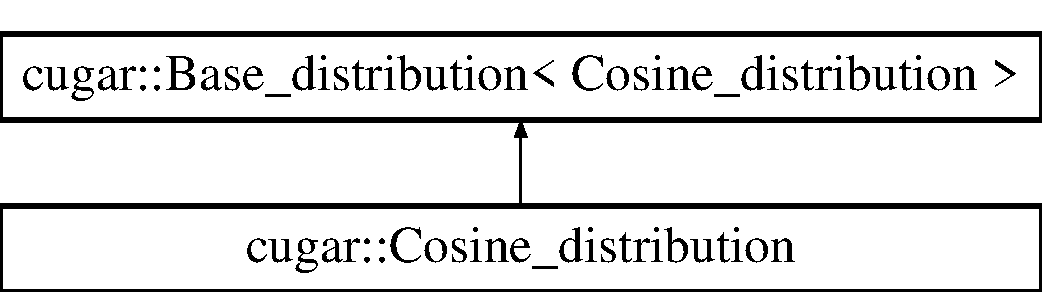
\includegraphics[height=2.000000cm]{structcugar_1_1_cosine__distribution}
\end{center}
\end{figure}
\subsection*{Public Methods}
\begin{DoxyCompactItemize}
\item 
C\+U\+G\+A\+R\+\_\+\+H\+O\+S\+T\+\_\+\+D\+E\+V\+I\+CE float \hyperlink{structcugar_1_1_cosine__distribution_a0440bb1dc47d5d8593fe568ae2b40cd9}{map} (const float U) const
\item 
C\+U\+G\+A\+R\+\_\+\+H\+O\+S\+T\+\_\+\+D\+E\+V\+I\+CE float \hyperlink{structcugar_1_1_cosine__distribution_ad6c1c1232187832f55e1690c60be8ae7}{density} (const float x) const
\end{DoxyCompactItemize}


\subsection{Member Function Documentation}
\mbox{\Hypertarget{structcugar_1_1_cosine__distribution_ad6c1c1232187832f55e1690c60be8ae7}\label{structcugar_1_1_cosine__distribution_ad6c1c1232187832f55e1690c60be8ae7}} 
\index{cugar\+::\+Cosine\+\_\+distribution@{cugar\+::\+Cosine\+\_\+distribution}!density@{density}}
\index{density@{density}!cugar\+::\+Cosine\+\_\+distribution@{cugar\+::\+Cosine\+\_\+distribution}}
\subsubsection{\texorpdfstring{density()}{density()}}
{\footnotesize\ttfamily C\+U\+G\+A\+R\+\_\+\+H\+O\+S\+T\+\_\+\+D\+E\+V\+I\+CE float cugar\+::\+Cosine\+\_\+distribution\+::density (\begin{DoxyParamCaption}\item[{const float}]{x }\end{DoxyParamCaption}) const\hspace{0.3cm}{\ttfamily [inline]}}

probability density function


\begin{DoxyParams}{Parameters}
{\em x} & sample location \\
\hline
\end{DoxyParams}
\mbox{\Hypertarget{structcugar_1_1_cosine__distribution_a0440bb1dc47d5d8593fe568ae2b40cd9}\label{structcugar_1_1_cosine__distribution_a0440bb1dc47d5d8593fe568ae2b40cd9}} 
\index{cugar\+::\+Cosine\+\_\+distribution@{cugar\+::\+Cosine\+\_\+distribution}!map@{map}}
\index{map@{map}!cugar\+::\+Cosine\+\_\+distribution@{cugar\+::\+Cosine\+\_\+distribution}}
\subsubsection{\texorpdfstring{map()}{map()}}
{\footnotesize\ttfamily C\+U\+G\+A\+R\+\_\+\+H\+O\+S\+T\+\_\+\+D\+E\+V\+I\+CE float cugar\+::\+Cosine\+\_\+distribution\+::map (\begin{DoxyParamCaption}\item[{const float}]{U }\end{DoxyParamCaption}) const\hspace{0.3cm}{\ttfamily [inline]}}

transform a uniformly distributed number through the distribution


\begin{DoxyParams}{Parameters}
{\em U} & real number to transform \\
\hline
\end{DoxyParams}


The documentation for this struct was generated from the following file\+:\begin{DoxyCompactItemize}
\item 
C\+:/p4research/research/jpantaleoni/\+Fermat-\/\+Public/contrib/cugar/sampling/\hyperlink{distributions_8h}{distributions.\+h}\end{DoxyCompactItemize}

\hypertarget{classcugar_1_1internals_1_1_counted_base}{}\section{cugar\+:\+:internals\+:\+:Counted\+Base$<$ CounterT $>$ Class Template Reference}
\label{classcugar_1_1internals_1_1_counted_base}\index{cugar\+::internals\+::\+Counted\+Base$<$ Counter\+T $>$@{cugar\+::internals\+::\+Counted\+Base$<$ Counter\+T $>$}}
Inheritance diagram for cugar\+:\+:internals\+:\+:Counted\+Base$<$ CounterT $>$\+:\begin{figure}[H]
\begin{center}
\leavevmode
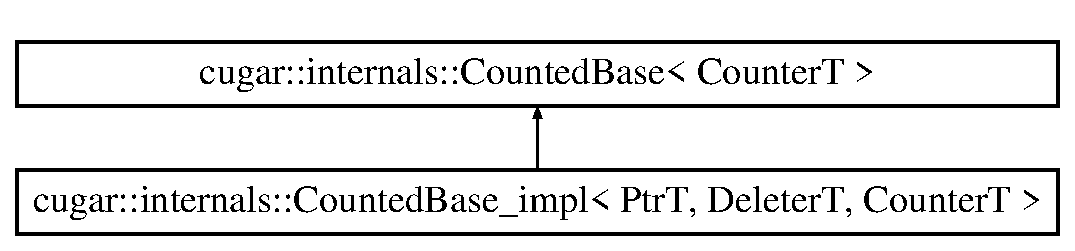
\includegraphics[height=2.000000cm]{classcugar_1_1internals_1_1_counted_base}
\end{center}
\end{figure}
\subsection*{Public Types}
\begin{DoxyCompactItemize}
\item 
\mbox{\Hypertarget{classcugar_1_1internals_1_1_counted_base_a813feea4989204df059f1e57eb296661}\label{classcugar_1_1internals_1_1_counted_base_a813feea4989204df059f1e57eb296661}} 
typedef CounterT {\bfseries Counter\+\_\+\+Type}
\end{DoxyCompactItemize}
\subsection*{Public Methods}
\begin{DoxyCompactItemize}
\item 
\mbox{\Hypertarget{classcugar_1_1internals_1_1_counted_base_a0136f9f7bac652b751f55c3fd3c0b9c0}\label{classcugar_1_1internals_1_1_counted_base_a0136f9f7bac652b751f55c3fd3c0b9c0}} 
virtual void \hyperlink{classcugar_1_1internals_1_1_counted_base_a0136f9f7bac652b751f55c3fd3c0b9c0}{dispose} ()=0
\begin{DoxyCompactList}\small\item\em called when m\+\_\+shcount goes to 0 \end{DoxyCompactList}\item 
\mbox{\Hypertarget{classcugar_1_1internals_1_1_counted_base_a8d50ddc2bea77d1593b35cc5824209af}\label{classcugar_1_1internals_1_1_counted_base_a8d50ddc2bea77d1593b35cc5824209af}} 
virtual void \hyperlink{classcugar_1_1internals_1_1_counted_base_a8d50ddc2bea77d1593b35cc5824209af}{destroy} ()
\begin{DoxyCompactList}\small\item\em called when m\+\_\+wkcount goes to 0 \end{DoxyCompactList}\item 
\mbox{\Hypertarget{classcugar_1_1internals_1_1_counted_base_a2663fb7f1277adc6e78e5ef3837193a9}\label{classcugar_1_1internals_1_1_counted_base_a2663fb7f1277adc6e78e5ef3837193a9}} 
virtual void $\ast$ {\bfseries get\+\_\+deleter} (const std\+::type\+\_\+info \&)=0
\item 
\mbox{\Hypertarget{classcugar_1_1internals_1_1_counted_base_ad42bcdc01fd577f3a5a773ab31d87703}\label{classcugar_1_1internals_1_1_counted_base_ad42bcdc01fd577f3a5a773ab31d87703}} 
void {\bfseries add\+\_\+ref\+\_\+copy} ()
\item 
\mbox{\Hypertarget{classcugar_1_1internals_1_1_counted_base_a4e1334553d5dd0eb613458934ec1b7dc}\label{classcugar_1_1internals_1_1_counted_base_a4e1334553d5dd0eb613458934ec1b7dc}} 
void {\bfseries add\+\_\+ref\+\_\+lock} ()
\item 
\mbox{\Hypertarget{classcugar_1_1internals_1_1_counted_base_a5a7753e0b4f9a4bfa04bdac9deba9551}\label{classcugar_1_1internals_1_1_counted_base_a5a7753e0b4f9a4bfa04bdac9deba9551}} 
void {\bfseries release} ()
\item 
\mbox{\Hypertarget{classcugar_1_1internals_1_1_counted_base_add70ea2da8983c02438c56be9bdb9156}\label{classcugar_1_1internals_1_1_counted_base_add70ea2da8983c02438c56be9bdb9156}} 
void {\bfseries weak\+\_\+add\+\_\+ref} ()
\item 
\mbox{\Hypertarget{classcugar_1_1internals_1_1_counted_base_a968071f8e4891a792dd68a185f852359}\label{classcugar_1_1internals_1_1_counted_base_a968071f8e4891a792dd68a185f852359}} 
void {\bfseries weak\+\_\+release} ()
\item 
\mbox{\Hypertarget{classcugar_1_1internals_1_1_counted_base_a63ccdbc5b6fa3e45e3191429309eb66f}\label{classcugar_1_1internals_1_1_counted_base_a63ccdbc5b6fa3e45e3191429309eb66f}} 
Counter\+\_\+\+Type {\bfseries use\+\_\+count} () const
\end{DoxyCompactItemize}


The documentation for this class was generated from the following file\+:\begin{DoxyCompactItemize}
\item 
C\+:/p4research/research/jpantaleoni/\+Fermat-\/\+Public/contrib/cugar/basic/shared\+\_\+pointer.\+h\end{DoxyCompactItemize}

\hypertarget{classcugar_1_1internals_1_1_counted_base__impl}{}\section{cugar\+:\+:internals\+:\+:Counted\+Base\+\_\+impl$<$ PtrT, DeleterT, CounterT $>$ Class Template Reference}
\label{classcugar_1_1internals_1_1_counted_base__impl}\index{cugar\+::internals\+::\+Counted\+Base\+\_\+impl$<$ Ptr\+T, Deleter\+T, Counter\+T $>$@{cugar\+::internals\+::\+Counted\+Base\+\_\+impl$<$ Ptr\+T, Deleter\+T, Counter\+T $>$}}
Inheritance diagram for cugar\+:\+:internals\+:\+:Counted\+Base\+\_\+impl$<$ PtrT, DeleterT, CounterT $>$\+:\begin{figure}[H]
\begin{center}
\leavevmode
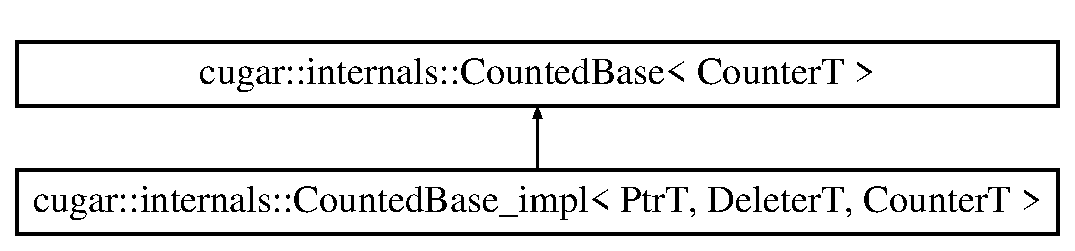
\includegraphics[height=2.000000cm]{classcugar_1_1internals_1_1_counted_base__impl}
\end{center}
\end{figure}
\subsection*{Public Methods}
\begin{DoxyCompactItemize}
\item 
\mbox{\Hypertarget{classcugar_1_1internals_1_1_counted_base__impl_a1a2ba87f11942b1fae4dac06d1a847f2}\label{classcugar_1_1internals_1_1_counted_base__impl_a1a2ba87f11942b1fae4dac06d1a847f2}} 
{\bfseries Counted\+Base\+\_\+impl} (PtrT p, DeleterT d)
\item 
\mbox{\Hypertarget{classcugar_1_1internals_1_1_counted_base__impl_a5582b40e7ded61b0d1e9b77d2a21b05d}\label{classcugar_1_1internals_1_1_counted_base__impl_a5582b40e7ded61b0d1e9b77d2a21b05d}} 
virtual void \hyperlink{classcugar_1_1internals_1_1_counted_base__impl_a5582b40e7ded61b0d1e9b77d2a21b05d}{dispose} ()
\begin{DoxyCompactList}\small\item\em called when m\+\_\+shcount goes to 0 \end{DoxyCompactList}\item 
\mbox{\Hypertarget{classcugar_1_1internals_1_1_counted_base__impl_aac43f5716a19ea8a300577e14f441744}\label{classcugar_1_1internals_1_1_counted_base__impl_aac43f5716a19ea8a300577e14f441744}} 
virtual void $\ast$ {\bfseries get\+\_\+deleter} (const std\+::type\+\_\+info \&ti)
\end{DoxyCompactItemize}
\subsection*{Additional Inherited Members}


The documentation for this class was generated from the following file\+:\begin{DoxyCompactItemize}
\item 
C\+:/p4research/research/jpantaleoni/\+Fermat-\/\+Public/contrib/cugar/basic/shared\+\_\+pointer.\+h\end{DoxyCompactItemize}

\hypertarget{structcugar_1_1cuda_1_1_radixtree__context_1_1_counters}{}\section{cugar\+:\+:cuda\+:\+:Radixtree\+\_\+context\+:\+:Counters Struct Reference}
\label{structcugar_1_1cuda_1_1_radixtree__context_1_1_counters}\index{cugar\+::cuda\+::\+Radixtree\+\_\+context\+::\+Counters@{cugar\+::cuda\+::\+Radixtree\+\_\+context\+::\+Counters}}
\subsection*{Public Members}
\begin{DoxyCompactItemize}
\item 
\mbox{\Hypertarget{structcugar_1_1cuda_1_1_radixtree__context_1_1_counters_a43fa8a7e277dae646b1b508663e37215}\label{structcugar_1_1cuda_1_1_radixtree__context_1_1_counters_a43fa8a7e277dae646b1b508663e37215}} 
uint32 {\bfseries node\+\_\+counter}
\item 
\mbox{\Hypertarget{structcugar_1_1cuda_1_1_radixtree__context_1_1_counters_a0d3fa1418919abda8ef4eb134136b595}\label{structcugar_1_1cuda_1_1_radixtree__context_1_1_counters_a0d3fa1418919abda8ef4eb134136b595}} 
uint32 {\bfseries leaf\+\_\+counter}
\item 
\mbox{\Hypertarget{structcugar_1_1cuda_1_1_radixtree__context_1_1_counters_ab107ee665767466b81c4bd8d003e7952}\label{structcugar_1_1cuda_1_1_radixtree__context_1_1_counters_ab107ee665767466b81c4bd8d003e7952}} 
uint32 {\bfseries task\+\_\+counter}
\item 
\mbox{\Hypertarget{structcugar_1_1cuda_1_1_radixtree__context_1_1_counters_a51dbfed3bb5396f7f00b50592ed77cfc}\label{structcugar_1_1cuda_1_1_radixtree__context_1_1_counters_a51dbfed3bb5396f7f00b50592ed77cfc}} 
uint32 {\bfseries work\+\_\+counter}
\end{DoxyCompactItemize}


The documentation for this struct was generated from the following file\+:\begin{DoxyCompactItemize}
\item 
C\+:/p4research/research/jpantaleoni/\+Fermat-\/\+Public/contrib/cugar/radixtree/cuda/\hyperlink{radixtree__context_8h}{radixtree\+\_\+context.\+h}\end{DoxyCompactItemize}

\hypertarget{structcugar_1_1_c_p__rotated__sequence}{}\section{cugar\+:\+:C\+P\+\_\+rotated\+\_\+sequence$<$ Sample\+\_\+sequence, Iterator $>$ Struct Template Reference}
\label{structcugar_1_1_c_p__rotated__sequence}\index{cugar\+::\+C\+P\+\_\+rotated\+\_\+sequence$<$ Sample\+\_\+sequence, Iterator $>$@{cugar\+::\+C\+P\+\_\+rotated\+\_\+sequence$<$ Sample\+\_\+sequence, Iterator $>$}}


\subsection{Detailed description}
\subsubsection*{template$<$typename Sample\+\_\+sequence, typename Iterator = const float$\ast$$>$\newline
struct cugar\+::\+C\+P\+\_\+rotated\+\_\+sequence$<$ Sample\+\_\+sequence, Iterator $>$}

Wrapper class to rotate the samples coming from a sample sequence with a set of Cranley-\/\+Patterson rotations. 

{\ttfamily \#include $<$cp\+\_\+rotations.\+h$>$}

\subsection*{Public Types}
\begin{DoxyCompactItemize}
\item 
\mbox{\Hypertarget{structcugar_1_1_c_p__rotated__sequence_a894951bf501a32979a836eead10b4667}\label{structcugar_1_1_c_p__rotated__sequence_a894951bf501a32979a836eead10b4667}} 
typedef \hyperlink{structcugar_1_1_c_p__rotator}{C\+P\+\_\+rotator}$<$ typename Sample\+\_\+sequence\+::\+Sampler\+\_\+type, Iterator $>$ {\bfseries Sampler\+\_\+type}
\end{DoxyCompactItemize}
\subsection*{Public Methods}
\begin{DoxyCompactItemize}
\item 
C\+U\+G\+A\+R\+\_\+\+H\+O\+S\+T\+\_\+\+D\+E\+V\+I\+CE \hyperlink{structcugar_1_1_c_p__rotated__sequence_a89118c80f2c2e00189cc2c1f130e29c2}{C\+P\+\_\+rotated\+\_\+sequence} (Sample\+\_\+sequence \&sequence, const uint32 dims, Iterator rot, uint32 size)
\item 
\hyperlink{structcugar_1_1_c_p__rotator}{Sampler\+\_\+type} C\+U\+G\+A\+R\+\_\+\+H\+O\+S\+T\+\_\+\+D\+E\+V\+I\+CE \hyperlink{structcugar_1_1_c_p__rotated__sequence_a8d1e472dbd3a1e681a3617f7abedd103}{instance} (const uint32 index, const uint32 copy) const
\end{DoxyCompactItemize}
\subsection*{Public Members}
\begin{DoxyCompactItemize}
\item 
\mbox{\Hypertarget{structcugar_1_1_c_p__rotated__sequence_ae89cb3ff2b68c56e67e0d8801871602e}\label{structcugar_1_1_c_p__rotated__sequence_ae89cb3ff2b68c56e67e0d8801871602e}} 
Sample\+\_\+sequence \& {\bfseries m\+\_\+sequence}
\item 
\mbox{\Hypertarget{structcugar_1_1_c_p__rotated__sequence_a13ce8bb76ae49fb10b4ab685945ff403}\label{structcugar_1_1_c_p__rotated__sequence_a13ce8bb76ae49fb10b4ab685945ff403}} 
Iterator {\bfseries m\+\_\+rot}
\item 
\mbox{\Hypertarget{structcugar_1_1_c_p__rotated__sequence_ad441ef2dde3c643f1c96a04ebb99b580}\label{structcugar_1_1_c_p__rotated__sequence_ad441ef2dde3c643f1c96a04ebb99b580}} 
uint32 {\bfseries m\+\_\+size}
\item 
\mbox{\Hypertarget{structcugar_1_1_c_p__rotated__sequence_a89d9b172106c9693abb1bde2eabd6da0}\label{structcugar_1_1_c_p__rotated__sequence_a89d9b172106c9693abb1bde2eabd6da0}} 
uint32 {\bfseries m\+\_\+dims}
\end{DoxyCompactItemize}


\subsection{Constructor \& Destructor Documentation}
\mbox{\Hypertarget{structcugar_1_1_c_p__rotated__sequence_a89118c80f2c2e00189cc2c1f130e29c2}\label{structcugar_1_1_c_p__rotated__sequence_a89118c80f2c2e00189cc2c1f130e29c2}} 
\index{cugar\+::\+C\+P\+\_\+rotated\+\_\+sequence@{cugar\+::\+C\+P\+\_\+rotated\+\_\+sequence}!C\+P\+\_\+rotated\+\_\+sequence@{C\+P\+\_\+rotated\+\_\+sequence}}
\index{C\+P\+\_\+rotated\+\_\+sequence@{C\+P\+\_\+rotated\+\_\+sequence}!cugar\+::\+C\+P\+\_\+rotated\+\_\+sequence@{cugar\+::\+C\+P\+\_\+rotated\+\_\+sequence}}
\subsubsection{\texorpdfstring{C\+P\+\_\+rotated\+\_\+sequence()}{CP\_rotated\_sequence()}}
{\footnotesize\ttfamily template$<$typename Sample\+\_\+sequence , typename Iterator  = const float$\ast$$>$ \\
C\+U\+G\+A\+R\+\_\+\+H\+O\+S\+T\+\_\+\+D\+E\+V\+I\+CE \hyperlink{structcugar_1_1_c_p__rotated__sequence}{cugar\+::\+C\+P\+\_\+rotated\+\_\+sequence}$<$ Sample\+\_\+sequence, Iterator $>$\+::\hyperlink{structcugar_1_1_c_p__rotated__sequence}{C\+P\+\_\+rotated\+\_\+sequence} (\begin{DoxyParamCaption}\item[{Sample\+\_\+sequence \&}]{sequence,  }\item[{const uint32}]{dims,  }\item[{Iterator}]{rot,  }\item[{uint32}]{size }\end{DoxyParamCaption})\hspace{0.3cm}{\ttfamily [inline]}}

constructor


\begin{DoxyParams}{Parameters}
{\em sequence} & sample sequence \\
\hline
{\em dims} & dimensionality of the sequence \\
\hline
{\em rot} & rotation set \\
\hline
{\em size} & size of the rotation set \\
\hline
\end{DoxyParams}


\subsection{Member Function Documentation}
\mbox{\Hypertarget{structcugar_1_1_c_p__rotated__sequence_a8d1e472dbd3a1e681a3617f7abedd103}\label{structcugar_1_1_c_p__rotated__sequence_a8d1e472dbd3a1e681a3617f7abedd103}} 
\index{cugar\+::\+C\+P\+\_\+rotated\+\_\+sequence@{cugar\+::\+C\+P\+\_\+rotated\+\_\+sequence}!instance@{instance}}
\index{instance@{instance}!cugar\+::\+C\+P\+\_\+rotated\+\_\+sequence@{cugar\+::\+C\+P\+\_\+rotated\+\_\+sequence}}
\subsubsection{\texorpdfstring{instance()}{instance()}}
{\footnotesize\ttfamily template$<$typename Sample\+\_\+sequence , typename Iterator  = const float$\ast$$>$ \\
\hyperlink{structcugar_1_1_c_p__rotator}{Sampler\+\_\+type} C\+U\+G\+A\+R\+\_\+\+H\+O\+S\+T\+\_\+\+D\+E\+V\+I\+CE \hyperlink{structcugar_1_1_c_p__rotated__sequence}{cugar\+::\+C\+P\+\_\+rotated\+\_\+sequence}$<$ Sample\+\_\+sequence, Iterator $>$\+::instance (\begin{DoxyParamCaption}\item[{const uint32}]{index,  }\item[{const uint32}]{copy }\end{DoxyParamCaption}) const\hspace{0.3cm}{\ttfamily [inline]}}

instance


\begin{DoxyParams}{Parameters}
{\em index} & sequence index \\
\hline
{\em copy} & sequence instance \\
\hline
\end{DoxyParams}


The documentation for this struct was generated from the following file\+:\begin{DoxyCompactItemize}
\item 
C\+:/p4research/research/jpantaleoni/\+Fermat-\/\+Public/contrib/cugar/sampling/\hyperlink{cp__rotations_8h}{cp\+\_\+rotations.\+h}\end{DoxyCompactItemize}

\hypertarget{structcugar_1_1_c_p__rotator}{}\section{cugar\+:\+:C\+P\+\_\+rotator$<$ Generator, Iterator $>$ Struct Template Reference}
\label{structcugar_1_1_c_p__rotator}\index{cugar\+::\+C\+P\+\_\+rotator$<$ Generator, Iterator $>$@{cugar\+::\+C\+P\+\_\+rotator$<$ Generator, Iterator $>$}}


\subsection{Detailed description}
\subsubsection*{template$<$typename Generator, typename Iterator = const float$\ast$$>$\newline
struct cugar\+::\+C\+P\+\_\+rotator$<$ Generator, Iterator $>$}

Wrapper class to rotate the samples coming from a generator with a set of Cranley-\/\+Patterson rotations.

Given a point-\/set P = \{p\+\_\+i\}\+\_\+\{ i = 1,...,n \} in\mbox{[}0, 1\mbox{]}$^\wedge$d, a CP rotation is the application of a constant shift s to all points, modulo 1\+: C\+P(\+P, s) = \{ p\+\_\+i + s $\vert$ mod 1 \}.

R.\+Cranley and T.\+Patterson.\+Randomization of number theoretic methods for multiple integration.\+S\+I\+AM Journal on Numerical Analysis, 13 \+: 904�914, 1976. 3 

{\ttfamily \#include $<$cp\+\_\+rotations.\+h$>$}

\subsection*{Public Methods}
\begin{DoxyCompactItemize}
\item 
C\+U\+G\+A\+R\+\_\+\+H\+O\+S\+T\+\_\+\+D\+E\+V\+I\+CE \hyperlink{structcugar_1_1_c_p__rotator_a0ae82f8622f5b3ec56d473671f362953}{C\+P\+\_\+rotator} (Generator \&gen, Iterator rot, uint32 size, uint32 dim=0)
\item 
C\+U\+G\+A\+R\+\_\+\+H\+O\+S\+T\+\_\+\+D\+E\+V\+I\+CE float \hyperlink{structcugar_1_1_c_p__rotator_adab9c93a549593fdf4753ac753ea59da}{next} ()
\item 
C\+U\+G\+A\+R\+\_\+\+H\+O\+S\+T\+\_\+\+D\+E\+V\+I\+CE float \hyperlink{structcugar_1_1_c_p__rotator_ad534cd9e5a2c888ec0fe7d6adf904013}{density} (const float x) const
\end{DoxyCompactItemize}
\subsection*{Public Members}
\begin{DoxyCompactItemize}
\item 
\mbox{\Hypertarget{structcugar_1_1_c_p__rotator_abfbedb0f66eac6ae0b1fabca14f1f3c3}\label{structcugar_1_1_c_p__rotator_abfbedb0f66eac6ae0b1fabca14f1f3c3}} 
Generator \& {\bfseries m\+\_\+gen}
\item 
\mbox{\Hypertarget{structcugar_1_1_c_p__rotator_a9833f3720bdfc0396e81e4eb05151e52}\label{structcugar_1_1_c_p__rotator_a9833f3720bdfc0396e81e4eb05151e52}} 
Iterator {\bfseries m\+\_\+rot}
\item 
\mbox{\Hypertarget{structcugar_1_1_c_p__rotator_a7fec490f4e740f3fda0d6256d99470f9}\label{structcugar_1_1_c_p__rotator_a7fec490f4e740f3fda0d6256d99470f9}} 
uint32 {\bfseries m\+\_\+size}
\item 
\mbox{\Hypertarget{structcugar_1_1_c_p__rotator_a9411ac46a5e961a7602508f94e8793fa}\label{structcugar_1_1_c_p__rotator_a9411ac46a5e961a7602508f94e8793fa}} 
uint32 {\bfseries m\+\_\+dim}
\end{DoxyCompactItemize}


\subsection{Constructor \& Destructor Documentation}
\mbox{\Hypertarget{structcugar_1_1_c_p__rotator_a0ae82f8622f5b3ec56d473671f362953}\label{structcugar_1_1_c_p__rotator_a0ae82f8622f5b3ec56d473671f362953}} 
\index{cugar\+::\+C\+P\+\_\+rotator@{cugar\+::\+C\+P\+\_\+rotator}!C\+P\+\_\+rotator@{C\+P\+\_\+rotator}}
\index{C\+P\+\_\+rotator@{C\+P\+\_\+rotator}!cugar\+::\+C\+P\+\_\+rotator@{cugar\+::\+C\+P\+\_\+rotator}}
\subsubsection{\texorpdfstring{C\+P\+\_\+rotator()}{CP\_rotator()}}
{\footnotesize\ttfamily template$<$typename Generator , typename Iterator  = const float$\ast$$>$ \\
C\+U\+G\+A\+R\+\_\+\+H\+O\+S\+T\+\_\+\+D\+E\+V\+I\+CE \hyperlink{structcugar_1_1_c_p__rotator}{cugar\+::\+C\+P\+\_\+rotator}$<$ Generator, Iterator $>$\+::\hyperlink{structcugar_1_1_c_p__rotator}{C\+P\+\_\+rotator} (\begin{DoxyParamCaption}\item[{Generator \&}]{gen,  }\item[{Iterator}]{rot,  }\item[{uint32}]{size,  }\item[{uint32}]{dim = {\ttfamily 0} }\end{DoxyParamCaption})\hspace{0.3cm}{\ttfamily [inline]}}

constructor


\begin{DoxyParams}{Parameters}
{\em gen} & generator \\
\hline
{\em rot} & sequence of rotations \\
\hline
{\em size} & number of rotations \\
\hline
{\em dim} & initial dimension \\
\hline
\end{DoxyParams}


\subsection{Member Function Documentation}
\mbox{\Hypertarget{structcugar_1_1_c_p__rotator_ad534cd9e5a2c888ec0fe7d6adf904013}\label{structcugar_1_1_c_p__rotator_ad534cd9e5a2c888ec0fe7d6adf904013}} 
\index{cugar\+::\+C\+P\+\_\+rotator@{cugar\+::\+C\+P\+\_\+rotator}!density@{density}}
\index{density@{density}!cugar\+::\+C\+P\+\_\+rotator@{cugar\+::\+C\+P\+\_\+rotator}}
\subsubsection{\texorpdfstring{density()}{density()}}
{\footnotesize\ttfamily template$<$typename Generator , typename Iterator  = const float$\ast$$>$ \\
C\+U\+G\+A\+R\+\_\+\+H\+O\+S\+T\+\_\+\+D\+E\+V\+I\+CE float \hyperlink{structcugar_1_1_c_p__rotator}{cugar\+::\+C\+P\+\_\+rotator}$<$ Generator, Iterator $>$\+::density (\begin{DoxyParamCaption}\item[{const float}]{x }\end{DoxyParamCaption}) const\hspace{0.3cm}{\ttfamily [inline]}}

probability density function


\begin{DoxyParams}{Parameters}
{\em x} & sample location \\
\hline
\end{DoxyParams}
\mbox{\Hypertarget{structcugar_1_1_c_p__rotator_adab9c93a549593fdf4753ac753ea59da}\label{structcugar_1_1_c_p__rotator_adab9c93a549593fdf4753ac753ea59da}} 
\index{cugar\+::\+C\+P\+\_\+rotator@{cugar\+::\+C\+P\+\_\+rotator}!next@{next}}
\index{next@{next}!cugar\+::\+C\+P\+\_\+rotator@{cugar\+::\+C\+P\+\_\+rotator}}
\subsubsection{\texorpdfstring{next()}{next()}}
{\footnotesize\ttfamily template$<$typename Generator , typename Iterator  = const float$\ast$$>$ \\
C\+U\+G\+A\+R\+\_\+\+H\+O\+S\+T\+\_\+\+D\+E\+V\+I\+CE float \hyperlink{structcugar_1_1_c_p__rotator}{cugar\+::\+C\+P\+\_\+rotator}$<$ Generator, Iterator $>$\+::next (\begin{DoxyParamCaption}{ }\end{DoxyParamCaption})\hspace{0.3cm}{\ttfamily [inline]}}

get the next sample 

The documentation for this struct was generated from the following file\+:\begin{DoxyCompactItemize}
\item 
C\+:/p4research/research/jpantaleoni/\+Fermat-\/\+Public/contrib/cugar/sampling/\hyperlink{cp__rotations_8h}{cp\+\_\+rotations.\+h}\end{DoxyCompactItemize}

\hypertarget{structcugar_1_1cuda_1_1cuda__devices}{}\section{cugar\+:\+:cuda\+:\+:cuda\+\_\+devices Struct Reference}
\label{structcugar_1_1cuda_1_1cuda__devices}\index{cugar\+::cuda\+::cuda\+\_\+devices@{cugar\+::cuda\+::cuda\+\_\+devices}}


\subsection{Detailed description}
A singleton cache for the properties of all present cuda devices 

{\ttfamily \#include $<$arch.\+h$>$}

\subsection*{Static Public Methods}
\begin{DoxyCompactItemize}
\item 
static \hyperlink{structcugar_1_1cuda_1_1cuda__devices}{cuda\+\_\+devices} $\ast$ \hyperlink{structcugar_1_1cuda_1_1cuda__devices_ab146b0ff61956367c2338f0e3a31f3ec}{get} ()
\end{DoxyCompactItemize}
\subsection*{Public Members}
\begin{DoxyCompactItemize}
\item 
\mbox{\Hypertarget{structcugar_1_1cuda_1_1cuda__devices_a6ac908ab562913227df6ecd8e9365901}\label{structcugar_1_1cuda_1_1cuda__devices_a6ac908ab562913227df6ecd8e9365901}} 
int \hyperlink{structcugar_1_1cuda_1_1cuda__devices_a6ac908ab562913227df6ecd8e9365901}{device\+\_\+count}
\begin{DoxyCompactList}\small\item\em device count \end{DoxyCompactList}\item 
\mbox{\Hypertarget{structcugar_1_1cuda_1_1cuda__devices_ac50d1d6eeed53bc7f7709868ef6cdcd2}\label{structcugar_1_1cuda_1_1cuda__devices_ac50d1d6eeed53bc7f7709868ef6cdcd2}} 
cuda\+Device\+Prop $\ast$ \hyperlink{structcugar_1_1cuda_1_1cuda__devices_ac50d1d6eeed53bc7f7709868ef6cdcd2}{properties}
\begin{DoxyCompactList}\small\item\em device properties \end{DoxyCompactList}\end{DoxyCompactItemize}


\subsection{Member Function Documentation}
\mbox{\Hypertarget{structcugar_1_1cuda_1_1cuda__devices_ab146b0ff61956367c2338f0e3a31f3ec}\label{structcugar_1_1cuda_1_1cuda__devices_ab146b0ff61956367c2338f0e3a31f3ec}} 
\index{cugar\+::cuda\+::cuda\+\_\+devices@{cugar\+::cuda\+::cuda\+\_\+devices}!get@{get}}
\index{get@{get}!cugar\+::cuda\+::cuda\+\_\+devices@{cugar\+::cuda\+::cuda\+\_\+devices}}
\subsubsection{\texorpdfstring{get()}{get()}}
{\footnotesize\ttfamily \hyperlink{structcugar_1_1cuda_1_1cuda__devices}{cuda\+\_\+devices} $\ast$ cugar\+::cuda\+::cuda\+\_\+devices\+::get (\begin{DoxyParamCaption}{ }\end{DoxyParamCaption})\hspace{0.3cm}{\ttfamily [inline]}, {\ttfamily [static]}}

get a pointer to this struct\textquotesingle{}s singleton 

The documentation for this struct was generated from the following files\+:\begin{DoxyCompactItemize}
\item 
C\+:/p4research/research/jpantaleoni/\+Fermat-\/\+Public/contrib/cugar/basic/cuda/arch.\+h\item 
C\+:/p4research/research/jpantaleoni/\+Fermat-\/\+Public/contrib/cugar/basic/cuda/arch.\+cpp\item 
C\+:/p4research/research/jpantaleoni/\+Fermat-\/\+Public/contrib/cugar/basic/cuda/arch\+\_\+inl.\+h\end{DoxyCompactItemize}

\hypertarget{structcugar_1_1cuda__error}{}\section{cugar\+:\+:cuda\+\_\+error Struct Reference}
\label{structcugar_1_1cuda__error}\index{cugar\+::cuda\+\_\+error@{cugar\+::cuda\+\_\+error}}
\subsection*{Public Methods}
\begin{DoxyCompactItemize}
\item 
\mbox{\Hypertarget{structcugar_1_1cuda__error_aa9fd5d7d7e0424b85bbb053ca8c72007}\label{structcugar_1_1cuda__error_aa9fd5d7d7e0424b85bbb053ca8c72007}} 
{\bfseries cuda\+\_\+error} (const char $\ast$format,...)
\item 
\mbox{\Hypertarget{structcugar_1_1cuda__error_abe8a0afb52b0b5f2ab9d7b6285ce8368}\label{structcugar_1_1cuda__error_abe8a0afb52b0b5f2ab9d7b6285ce8368}} 
const char $\ast$ {\bfseries what} () const
\end{DoxyCompactItemize}


The documentation for this struct was generated from the following files\+:\begin{DoxyCompactItemize}
\item 
C\+:/p4research/research/jpantaleoni/\+Fermat-\/\+Public/contrib/cugar/basic/exceptions.\+h\item 
C\+:/p4research/research/jpantaleoni/\+Fermat-\/\+Public/contrib/cugar/basic/exceptions.\+cpp\end{DoxyCompactItemize}

\hypertarget{structcugar_1_1default__predicate}{}\section{cugar\+:\+:default\+\_\+predicate$<$ T $>$ Struct Template Reference}
\label{structcugar_1_1default__predicate}\index{cugar\+::default\+\_\+predicate$<$ T $>$@{cugar\+::default\+\_\+predicate$<$ T $>$}}


\subsection{Detailed description}
\subsubsection*{template$<$typename T$>$\newline
struct cugar\+::default\+\_\+predicate$<$ T $>$}

default predicate functor, returning the standard conversion to boolean 

{\ttfamily \#include $<$functors.\+h$>$}

\subsection*{Public Types}
\begin{DoxyCompactItemize}
\item 
\mbox{\Hypertarget{structcugar_1_1default__predicate_a16729285cfefa52731333b201939c356}\label{structcugar_1_1default__predicate_a16729285cfefa52731333b201939c356}} 
typedef \hyperlink{structcugar_1_1unary__function__tag}{unary\+\_\+function\+\_\+tag} {\bfseries function\+\_\+tag}
\end{DoxyCompactItemize}
\subsection*{Public Methods}
\begin{DoxyCompactItemize}
\item 
\mbox{\Hypertarget{structcugar_1_1default__predicate_a04d5240eb9900e2645a67fc3aa82e46f}\label{structcugar_1_1default__predicate_a04d5240eb9900e2645a67fc3aa82e46f}} 
C\+U\+G\+A\+R\+\_\+\+H\+O\+S\+T\+\_\+\+D\+E\+V\+I\+CE bool {\bfseries operator()} (const T t) const
\end{DoxyCompactItemize}


The documentation for this struct was generated from the following file\+:\begin{DoxyCompactItemize}
\item 
C\+:/p4research/research/jpantaleoni/\+Fermat-\/\+Public/contrib/cugar/basic/\hyperlink{functors_8h}{functors.\+h}\end{DoxyCompactItemize}

\hypertarget{structcugar_1_1default__vector__allocator}{}\section{cugar\+:\+:default\+\_\+vector\+\_\+allocator$<$ system\+\_\+tag, T $>$ Struct Template Reference}
\label{structcugar_1_1default__vector__allocator}\index{cugar\+::default\+\_\+vector\+\_\+allocator$<$ system\+\_\+tag, T $>$@{cugar\+::default\+\_\+vector\+\_\+allocator$<$ system\+\_\+tag, T $>$}}


\subsection{Detailed description}
\subsubsection*{template$<$typename system\+\_\+tag, typename T$>$\newline
struct cugar\+::default\+\_\+vector\+\_\+allocator$<$ system\+\_\+tag, T $>$}

a dynamic host/device vector class 

{\ttfamily \#include $<$vector.\+h$>$}



The documentation for this struct was generated from the following file\+:\begin{DoxyCompactItemize}
\item 
C\+:/p4research/research/jpantaleoni/\+Fermat-\/\+Public/contrib/cugar/basic/vector.\+h\end{DoxyCompactItemize}

\hypertarget{structcugar_1_1default__vector__allocator_3_01device__tag_00_01_t_01_4}{}\section{cugar\+:\+:default\+\_\+vector\+\_\+allocator$<$ device\+\_\+tag, T $>$ Struct Template Reference}
\label{structcugar_1_1default__vector__allocator_3_01device__tag_00_01_t_01_4}\index{cugar\+::default\+\_\+vector\+\_\+allocator$<$ device\+\_\+tag, T $>$@{cugar\+::default\+\_\+vector\+\_\+allocator$<$ device\+\_\+tag, T $>$}}
\subsection*{Public Types}
\begin{DoxyCompactItemize}
\item 
typedef thrust\+::device\+\_\+malloc\+\_\+allocator$<$ T $>$ {\bfseries type}
\end{DoxyCompactItemize}


The documentation for this struct was generated from the following file\+:\begin{DoxyCompactItemize}
\item 
C\+:/p4research/research/jpantaleoni/\+Fermat-\/\+Public/contrib/cugar/basic/vector.\+h\end{DoxyCompactItemize}

\hypertarget{structcugar_1_1default__vector__allocator_3_01host__tag_00_01_t_01_4}{}\section{cugar\+:\+:default\+\_\+vector\+\_\+allocator$<$ host\+\_\+tag, T $>$ Struct Template Reference}
\label{structcugar_1_1default__vector__allocator_3_01host__tag_00_01_t_01_4}\index{cugar\+::default\+\_\+vector\+\_\+allocator$<$ host\+\_\+tag, T $>$@{cugar\+::default\+\_\+vector\+\_\+allocator$<$ host\+\_\+tag, T $>$}}
\subsection*{Public Types}
\begin{DoxyCompactItemize}
\item 
typedef std\+::allocator$<$ T $>$ {\bfseries type}
\end{DoxyCompactItemize}


The documentation for this struct was generated from the following file\+:\begin{DoxyCompactItemize}
\item 
C\+:/p4research/research/jpantaleoni/\+Fermat-\/\+Public/contrib/cugar/basic/vector.\+h\end{DoxyCompactItemize}

\hypertarget{structcugar_1_1internals_1_1_deleter}{}\section{cugar\+:\+:internals\+:\+:Deleter$<$ T $>$ Struct Template Reference}
\label{structcugar_1_1internals_1_1_deleter}\index{cugar\+::internals\+::\+Deleter$<$ T $>$@{cugar\+::internals\+::\+Deleter$<$ T $>$}}
\subsection*{Public Types}
\begin{DoxyCompactItemize}
\item 
\mbox{\Hypertarget{structcugar_1_1internals_1_1_deleter_a203a2c8fc188907452beedb4e8023023}\label{structcugar_1_1internals_1_1_deleter_a203a2c8fc188907452beedb4e8023023}} 
typedef void {\bfseries result\+\_\+type}
\item 
\mbox{\Hypertarget{structcugar_1_1internals_1_1_deleter_af745d67391e1ceb17945c96cd2bc0461}\label{structcugar_1_1internals_1_1_deleter_af745d67391e1ceb17945c96cd2bc0461}} 
typedef T $\ast$ {\bfseries argument\+\_\+type}
\end{DoxyCompactItemize}
\subsection*{Public Methods}
\begin{DoxyCompactItemize}
\item 
\mbox{\Hypertarget{structcugar_1_1internals_1_1_deleter_ad9c1c23409fcdacd93d81fec6a148153}\label{structcugar_1_1internals_1_1_deleter_ad9c1c23409fcdacd93d81fec6a148153}} 
void {\bfseries operator()} (argument\+\_\+type p) const
\end{DoxyCompactItemize}


The documentation for this struct was generated from the following file\+:\begin{DoxyCompactItemize}
\item 
C\+:/p4research/research/jpantaleoni/\+Fermat-\/\+Public/contrib/cugar/basic/shared\+\_\+pointer.\+h\end{DoxyCompactItemize}

\hypertarget{structcugar_1_1device__iterator__type}{}\section{cugar\+:\+:device\+\_\+iterator\+\_\+type$<$ T $>$ Struct Template Reference}
\label{structcugar_1_1device__iterator__type}\index{cugar\+::device\+\_\+iterator\+\_\+type$<$ T $>$@{cugar\+::device\+\_\+iterator\+\_\+type$<$ T $>$}}


\subsection{Detailed description}
\subsubsection*{template$<$typename T$>$\newline
struct cugar\+::device\+\_\+iterator\+\_\+type$<$ T $>$}

a utility meta-\/type to wrap naked device pointers as thrust\+::device\+\_\+ptr 

{\ttfamily \#include $<$vector.\+h$>$}

\subsection*{Public Types}
\begin{DoxyCompactItemize}
\item 
typedef T {\bfseries type}
\end{DoxyCompactItemize}


The documentation for this struct was generated from the following file\+:\begin{DoxyCompactItemize}
\item 
C\+:/p4research/research/jpantaleoni/\+Fermat-\/\+Public/contrib/cugar/basic/vector.\+h\end{DoxyCompactItemize}

\hypertarget{structcugar_1_1device__iterator__type_3_01const_01_t_01_5_01_4}{}\section{cugar\+:\+:device\+\_\+iterator\+\_\+type$<$ const T $\ast$ $>$ Struct Template Reference}
\label{structcugar_1_1device__iterator__type_3_01const_01_t_01_5_01_4}\index{cugar\+::device\+\_\+iterator\+\_\+type$<$ const T $\ast$ $>$@{cugar\+::device\+\_\+iterator\+\_\+type$<$ const T $\ast$ $>$}}
\subsection*{Public Types}
\begin{DoxyCompactItemize}
\item 
typedef thrust\+::device\+\_\+ptr$<$ const T $>$ {\bfseries type}
\end{DoxyCompactItemize}


The documentation for this struct was generated from the following file\+:\begin{DoxyCompactItemize}
\item 
C\+:/p4research/research/jpantaleoni/\+Fermat-\/\+Public/contrib/cugar/basic/vector.\+h\end{DoxyCompactItemize}

\hypertarget{structcugar_1_1device__iterator__type_3_01_t_01_5_01_4}{}\section{cugar\+:\+:device\+\_\+iterator\+\_\+type$<$ T $\ast$ $>$ Struct Template Reference}
\label{structcugar_1_1device__iterator__type_3_01_t_01_5_01_4}\index{cugar\+::device\+\_\+iterator\+\_\+type$<$ T $\ast$ $>$@{cugar\+::device\+\_\+iterator\+\_\+type$<$ T $\ast$ $>$}}
\subsection*{Public Types}
\begin{DoxyCompactItemize}
\item 
typedef thrust\+::device\+\_\+ptr$<$ T $>$ {\bfseries type}
\end{DoxyCompactItemize}


The documentation for this struct was generated from the following file\+:\begin{DoxyCompactItemize}
\item 
C\+:/p4research/research/jpantaleoni/\+Fermat-\/\+Public/contrib/cugar/basic/vector.\+h\end{DoxyCompactItemize}

\hypertarget{structcugar_1_1device__tag}{}\section{cugar\+:\+:device\+\_\+tag Struct Reference}
\label{structcugar_1_1device__tag}\index{cugar\+::device\+\_\+tag@{cugar\+::device\+\_\+tag}}


\subsection{Detailed description}
a tag to define the device architecture 

{\ttfamily \#include $<$types.\+h$>$}

Inheritance diagram for cugar\+:\+:device\+\_\+tag\+:\begin{figure}[H]
\begin{center}
\leavevmode
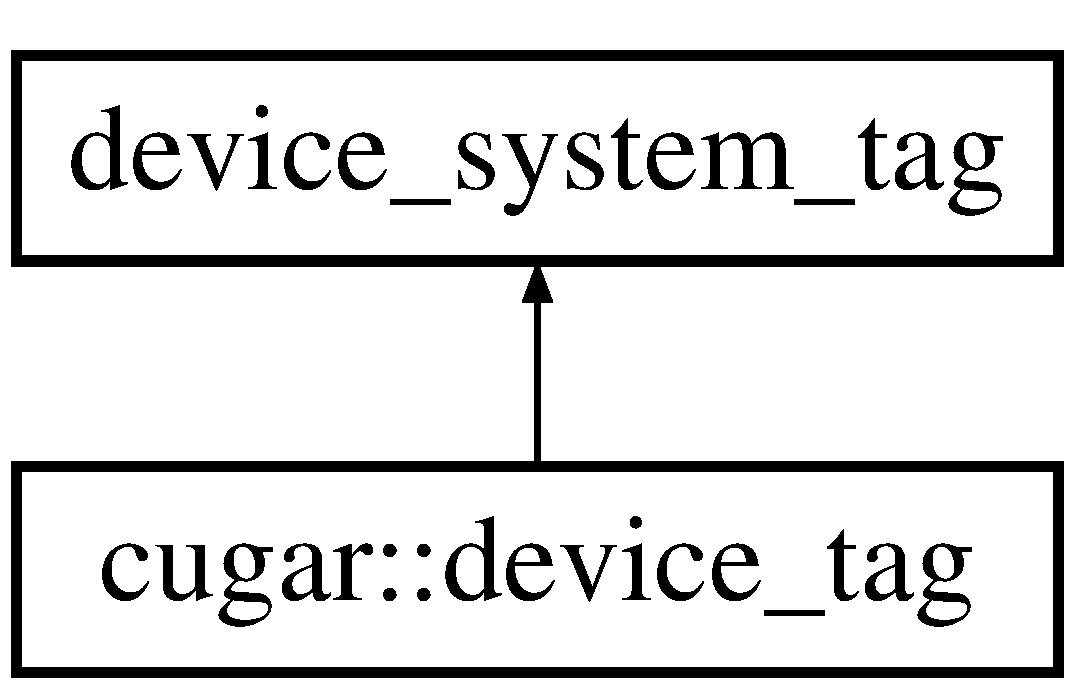
\includegraphics[height=2.000000cm]{structcugar_1_1device__tag}
\end{center}
\end{figure}


The documentation for this struct was generated from the following file\+:\begin{DoxyCompactItemize}
\item 
C\+:/p4research/research/jpantaleoni/\+Fermat-\/\+Public/contrib/cugar/basic/types.\+h\end{DoxyCompactItemize}

\hypertarget{structcugar_1_1device__var}{}\section{cugar\+:\+:device\+\_\+var$<$ T $>$ Struct Template Reference}
\label{structcugar_1_1device__var}\index{cugar\+::device\+\_\+var$<$ T $>$@{cugar\+::device\+\_\+var$<$ T $>$}}


\subsection{Detailed description}
\subsubsection*{template$<$typename T$>$\newline
struct cugar\+::device\+\_\+var$<$ T $>$}

A container for device variables 

{\ttfamily \#include $<$vector.\+h$>$}

\subsection*{Public Types}
\begin{DoxyCompactItemize}
\item 
typedef thrust\+::device\+\_\+vector$<$ T $>$\+::const\+\_\+reference {\bfseries const\+\_\+reference}
\item 
typedef thrust\+::device\+\_\+vector$<$ T $>$\+::reference {\bfseries reference}
\end{DoxyCompactItemize}
\subsection*{Public Methods}
\begin{DoxyCompactItemize}
\item 
\hyperlink{group___basic_ga011df6d3d281ae52a529e835ba1aad8e}{device\+\_\+var} (const T val=T())
\item 
\hyperlink{structcugar_1_1device__var}{device\+\_\+var}$<$ T $>$ \& \hyperlink{group___basic_ga760fb65c25c56b5fa9f49144f1da3f9b}{operator=} (const T \&val)
\item 
\hyperlink{structcugar_1_1device__var}{device\+\_\+var}$<$ T $>$ \& \hyperlink{group___basic_ga95f15b09320e473fc50c4df310d535fe}{operator+=} (const T \&val)
\item 
\hyperlink{structcugar_1_1device__var}{device\+\_\+var}$<$ T $>$ \& \hyperlink{group___basic_ga882c904bab742504bd555bd688ddcd07}{operator-\/=} (const T \&val)
\item 
\hyperlink{group___basic_ga64fde1bca016dd1b07ef0e7d6ef853ab}{operator T} () const
\item 
const T $\ast$ \hyperlink{group___basic_ga7075a2df5b4208648b803def09b239d1}{ptr} () const
\item 
T $\ast$ \hyperlink{group___basic_ga2073bcba54a5c135aa6dae8f0efbf20e}{ptr} ()
\end{DoxyCompactItemize}
\subsection*{Public Members}
\begin{DoxyCompactItemize}
\item 
\hyperlink{structcugar_1_1device__vector}{device\+\_\+vector}$<$ T $>$ {\bfseries x}
\end{DoxyCompactItemize}


The documentation for this struct was generated from the following file\+:\begin{DoxyCompactItemize}
\item 
C\+:/p4research/research/jpantaleoni/\+Fermat-\/\+Public/contrib/cugar/basic/vector.\+h\end{DoxyCompactItemize}

\hypertarget{structcugar_1_1device__vector}{}\section{cugar\+:\+:device\+\_\+vector$<$ T $>$ Struct Template Reference}
\label{structcugar_1_1device__vector}\index{cugar\+::device\+\_\+vector$<$ T $>$@{cugar\+::device\+\_\+vector$<$ T $>$}}


\subsection{Detailed description}
\subsubsection*{template$<$typename T$>$\newline
struct cugar\+::device\+\_\+vector$<$ T $>$}

a dynamic device vector class 

{\ttfamily \#include $<$vector.\+h$>$}

Inheritance diagram for cugar\+:\+:device\+\_\+vector$<$ T $>$\+:\begin{figure}[H]
\begin{center}
\leavevmode
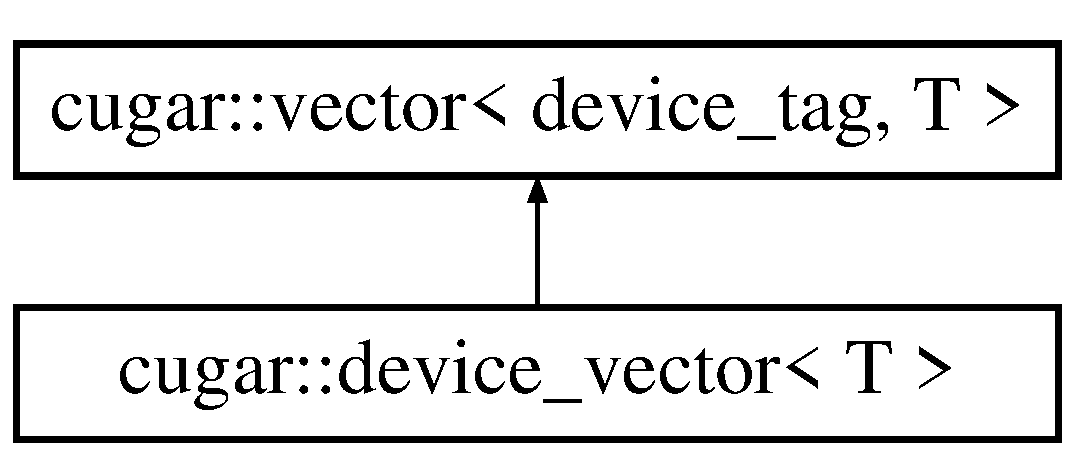
\includegraphics[height=2.000000cm]{structcugar_1_1device__vector}
\end{center}
\end{figure}
\subsection*{Public Types}
\begin{DoxyCompactItemize}
\item 
typedef \hyperlink{structcugar_1_1device__tag}{device\+\_\+tag} {\bfseries system\+\_\+tag}
\item 
typedef \hyperlink{structcugar_1_1vector}{vector}$<$ \hyperlink{structcugar_1_1device__tag}{device\+\_\+tag}, T $>$ {\bfseries base\+\_\+type}
\item 
typedef base\+\_\+type\+::const\+\_\+iterator {\bfseries const\+\_\+iterator}
\item 
typedef base\+\_\+type\+::iterator {\bfseries iterator}
\item 
typedef base\+\_\+type\+::value\+\_\+type {\bfseries value\+\_\+type}
\item 
typedef base\+\_\+type\+::plain\+\_\+view\+\_\+type {\bfseries plain\+\_\+view\+\_\+type}
\item 
typedef base\+\_\+type\+::const\+\_\+plain\+\_\+view\+\_\+type {\bfseries const\+\_\+plain\+\_\+view\+\_\+type}
\end{DoxyCompactItemize}
\subsection*{Public Methods}
\begin{DoxyCompactItemize}
\item 
\hyperlink{group___basic_ga9a8d64513864f07fe5e576a13980fafe}{device\+\_\+vector} (const size\+\_\+t size=0, const T val=T())
\item 
{\footnotesize template$<$typename Other\+Alloc $>$ }\\{\bfseries device\+\_\+vector} (const thrust\+::host\+\_\+vector$<$ T, Other\+Alloc $>$ \&v)
\item 
{\footnotesize template$<$typename Other\+Alloc $>$ }\\{\bfseries device\+\_\+vector} (const thrust\+::device\+\_\+vector$<$ T, Other\+Alloc $>$ \&v)
\item 
{\footnotesize template$<$typename Other\+Alloc $>$ }\\\hyperlink{structcugar_1_1device__vector}{device\+\_\+vector}$<$ T $>$ \& {\bfseries operator=} (const thrust\+::host\+\_\+vector$<$ T, Other\+Alloc $>$ \&v)
\item 
{\footnotesize template$<$typename Other\+Alloc $>$ }\\\hyperlink{structcugar_1_1device__vector}{device\+\_\+vector}$<$ T $>$ \& {\bfseries operator=} (const thrust\+::device\+\_\+vector$<$ T, Other\+Alloc $>$ \&v)
\item 
\hyperlink{group___basic_gaf23abbba65db2e117920090f0f97ed72}{operator plain\+\_\+view\+\_\+type} ()
\item 
\hyperlink{group___basic_ga86ea65d4863bb5e1ed5da63e6355672f}{operator const\+\_\+plain\+\_\+view\+\_\+type} () const
\end{DoxyCompactItemize}


The documentation for this struct was generated from the following file\+:\begin{DoxyCompactItemize}
\item 
C\+:/p4research/research/jpantaleoni/\+Fermat-\/\+Public/contrib/cugar/basic/vector.\+h\end{DoxyCompactItemize}

\hypertarget{struct_device_hash_table}{}\section{Device\+Hash\+Table Struct Reference}
\label{struct_device_hash_table}\index{Device\+Hash\+Table@{Device\+Hash\+Table}}
\subsection*{Public Methods}
\begin{DoxyCompactItemize}
\item 
\mbox{\Hypertarget{struct_device_hash_table_a64e1e8ef1f43503d68be0ccaabf25377}\label{struct_device_hash_table_a64e1e8ef1f43503d68be0ccaabf25377}} 
void {\bfseries resize} (const uint32 N)
\item 
\mbox{\Hypertarget{struct_device_hash_table_a8377cbc517291dc0327b2c196918d019}\label{struct_device_hash_table_a8377cbc517291dc0327b2c196918d019}} 
uint64 {\bfseries needed\+\_\+bytes} (const uint32 N) const
\item 
\mbox{\Hypertarget{struct_device_hash_table_a240c85d9be54d92f9cffa1dea7a5c640}\label{struct_device_hash_table_a240c85d9be54d92f9cffa1dea7a5c640}} 
void {\bfseries clear} ()
\item 
\mbox{\Hypertarget{struct_device_hash_table_aa7c10e04b4f20107b17afdf3627fcc1b}\label{struct_device_hash_table_aa7c10e04b4f20107b17afdf3627fcc1b}} 
uint32 {\bfseries size} () const
\end{DoxyCompactItemize}
\subsection*{Public Members}
\begin{DoxyCompactItemize}
\item 
\mbox{\Hypertarget{struct_device_hash_table_a100b8da91cc237b7c8abc5fe9f334d12}\label{struct_device_hash_table_a100b8da91cc237b7c8abc5fe9f334d12}} 
\hyperlink{class_domain_buffer}{Domain\+Buffer}$<$ C\+U\+D\+A\+\_\+\+B\+U\+F\+F\+ER, uint64 $>$ {\bfseries m\+\_\+keys}
\item 
\mbox{\Hypertarget{struct_device_hash_table_a51aac5850dfab6f1dc34a2ae423f3872}\label{struct_device_hash_table_a51aac5850dfab6f1dc34a2ae423f3872}} 
\hyperlink{class_domain_buffer}{Domain\+Buffer}$<$ C\+U\+D\+A\+\_\+\+B\+U\+F\+F\+ER, uint64 $>$ {\bfseries m\+\_\+unique}
\item 
\mbox{\Hypertarget{struct_device_hash_table_ad086425e40dfce633afe11e047359b3c}\label{struct_device_hash_table_ad086425e40dfce633afe11e047359b3c}} 
\hyperlink{class_domain_buffer}{Domain\+Buffer}$<$ C\+U\+D\+A\+\_\+\+B\+U\+F\+F\+ER, uint32 $>$ {\bfseries m\+\_\+slots}
\item 
\mbox{\Hypertarget{struct_device_hash_table_a7ff74fd6db9c315d82210028ec57d008}\label{struct_device_hash_table_a7ff74fd6db9c315d82210028ec57d008}} 
\hyperlink{class_domain_buffer}{Domain\+Buffer}$<$ C\+U\+D\+A\+\_\+\+B\+U\+F\+F\+ER, uint32 $>$ {\bfseries m\+\_\+size}
\end{DoxyCompactItemize}


The documentation for this struct was generated from the following file\+:\begin{DoxyCompactItemize}
\item 
C\+:/p4research/research/jpantaleoni/\+Fermat-\/\+Public/src/hashmap.\+h\end{DoxyCompactItemize}

\hypertarget{class_device_mesh_storage}{}\section{Device\+Mesh\+Storage Class Reference}
\label{class_device_mesh_storage}\index{Device\+Mesh\+Storage@{Device\+Mesh\+Storage}}


\subsection{Detailed description}
This class provides basic Mesh storage for either the host or device 

{\ttfamily \#include $<$Mesh\+Storage.\+h$>$}

\subsection*{Public Methods}
\begin{DoxyCompactItemize}
\item 
\mbox{\Hypertarget{class_device_mesh_storage_a5db77e3c9ee56937d6c6e60e0191b466}\label{class_device_mesh_storage_a5db77e3c9ee56937d6c6e60e0191b466}} 
S\+U\+T\+I\+L\+A\+PI \hyperlink{class_device_mesh_storage}{Device\+Mesh\+Storage} \& {\bfseries operator=} (\hyperlink{class_mesh_storage}{Mesh\+Storage} \&mesh)
\item 
\mbox{\Hypertarget{class_device_mesh_storage_a1ebdcdd010e65a9481e98a5cb58e454b}\label{class_device_mesh_storage_a1ebdcdd010e65a9481e98a5cb58e454b}} 
S\+U\+T\+I\+L\+A\+PI int {\bfseries get\+Num\+Vertices} () const
\item 
\mbox{\Hypertarget{class_device_mesh_storage_a5d1e05d7428995a1c91ad0c4160a4984}\label{class_device_mesh_storage_a5d1e05d7428995a1c91ad0c4160a4984}} 
S\+U\+T\+I\+L\+A\+PI int {\bfseries get\+Num\+Normals} () const
\item 
\mbox{\Hypertarget{class_device_mesh_storage_a7722196fb7e42488e8edb839eeca23da}\label{class_device_mesh_storage_a7722196fb7e42488e8edb839eeca23da}} 
S\+U\+T\+I\+L\+A\+PI int {\bfseries get\+Num\+Texture\+Coordinates} () const
\item 
\mbox{\Hypertarget{class_device_mesh_storage_adbe8e23c4ac35cb7989ba2cfa7bd87a6}\label{class_device_mesh_storage_adbe8e23c4ac35cb7989ba2cfa7bd87a6}} 
S\+U\+T\+I\+L\+A\+PI int {\bfseries get\+Num\+Triangles} () const
\item 
\mbox{\Hypertarget{class_device_mesh_storage_ab460298be542213b1158137a680b6f22}\label{class_device_mesh_storage_ab460298be542213b1158137a680b6f22}} 
S\+U\+T\+I\+L\+A\+PI int {\bfseries get\+Num\+Materials} () const
\item 
\mbox{\Hypertarget{class_device_mesh_storage_a8c25e783114d3ac28d538c15c7c8161c}\label{class_device_mesh_storage_a8c25e783114d3ac28d538c15c7c8161c}} 
S\+U\+T\+I\+L\+A\+PI int {\bfseries get\+Vertex\+Stride} () const
\item 
\mbox{\Hypertarget{class_device_mesh_storage_a4e9565ae57a457f58642aec29c0ea710}\label{class_device_mesh_storage_a4e9565ae57a457f58642aec29c0ea710}} 
S\+U\+T\+I\+L\+A\+PI int {\bfseries get\+Normal\+Stride} () const
\item 
\mbox{\Hypertarget{class_device_mesh_storage_a2baa5c4be243b7faa579baab890ea087}\label{class_device_mesh_storage_a2baa5c4be243b7faa579baab890ea087}} 
S\+U\+T\+I\+L\+A\+PI int {\bfseries get\+Texture\+Coordinate\+Stride} () const
\item 
\mbox{\Hypertarget{class_device_mesh_storage_af53b40a8f1fe947c80feb23ffcde088f}\label{class_device_mesh_storage_af53b40a8f1fe947c80feb23ffcde088f}} 
S\+U\+T\+I\+L\+A\+PI int $\ast$ {\bfseries get\+Vertex\+Indices} ()
\item 
\mbox{\Hypertarget{class_device_mesh_storage_a029473df5667ed374ee8d1870c8fba0e}\label{class_device_mesh_storage_a029473df5667ed374ee8d1870c8fba0e}} 
S\+U\+T\+I\+L\+A\+PI const int $\ast$ {\bfseries get\+Vertex\+Indices} () const
\item 
\mbox{\Hypertarget{class_device_mesh_storage_a45a5476b381c5bdd8cd857db6c231ec5}\label{class_device_mesh_storage_a45a5476b381c5bdd8cd857db6c231ec5}} 
S\+U\+T\+I\+L\+A\+PI int $\ast$ {\bfseries get\+Normal\+Indices} ()
\item 
\mbox{\Hypertarget{class_device_mesh_storage_a0997aa57e0c2cec214c6d98aff3c22d4}\label{class_device_mesh_storage_a0997aa57e0c2cec214c6d98aff3c22d4}} 
S\+U\+T\+I\+L\+A\+PI const int $\ast$ {\bfseries get\+Normal\+Indices} () const
\item 
\mbox{\Hypertarget{class_device_mesh_storage_a081399bdc7d0607cd2eb0d7c661d2f70}\label{class_device_mesh_storage_a081399bdc7d0607cd2eb0d7c661d2f70}} 
S\+U\+T\+I\+L\+A\+PI int $\ast$ {\bfseries get\+Material\+Indices} ()
\item 
\mbox{\Hypertarget{class_device_mesh_storage_a29cfb1aad691384efb9eaf21bf317cd5}\label{class_device_mesh_storage_a29cfb1aad691384efb9eaf21bf317cd5}} 
S\+U\+T\+I\+L\+A\+PI const int $\ast$ {\bfseries get\+Material\+Indices} () const
\item 
\mbox{\Hypertarget{class_device_mesh_storage_adb7582b59fcd27c40cd62098c1c7b0eb}\label{class_device_mesh_storage_adb7582b59fcd27c40cd62098c1c7b0eb}} 
S\+U\+T\+I\+L\+A\+PI int $\ast$ {\bfseries get\+Texture\+Coordinate\+Indices} ()
\item 
\mbox{\Hypertarget{class_device_mesh_storage_ad19eb08b6926e4b2da078aa3368f06c6}\label{class_device_mesh_storage_ad19eb08b6926e4b2da078aa3368f06c6}} 
S\+U\+T\+I\+L\+A\+PI const int $\ast$ {\bfseries get\+Texture\+Coordinate\+Indices} () const
\item 
\mbox{\Hypertarget{class_device_mesh_storage_a010ad802183570a9c24fa9686f415ed8}\label{class_device_mesh_storage_a010ad802183570a9c24fa9686f415ed8}} 
S\+U\+T\+I\+L\+A\+PI int $\ast$ {\bfseries get\+Lightmap\+Indices} ()
\item 
\mbox{\Hypertarget{class_device_mesh_storage_ac1a1ab44d979a609cf0deafa09d5188f}\label{class_device_mesh_storage_ac1a1ab44d979a609cf0deafa09d5188f}} 
S\+U\+T\+I\+L\+A\+PI const int $\ast$ {\bfseries get\+Lightmap\+Indices} () const
\item 
\mbox{\Hypertarget{class_device_mesh_storage_a47b325cf483f5f8941b3989badfaaf4d}\label{class_device_mesh_storage_a47b325cf483f5f8941b3989badfaaf4d}} 
S\+U\+T\+I\+L\+A\+PI float $\ast$ {\bfseries get\+Vertex\+Data} ()
\item 
\mbox{\Hypertarget{class_device_mesh_storage_a762f2f3164413b170a19b29830f52b2c}\label{class_device_mesh_storage_a762f2f3164413b170a19b29830f52b2c}} 
S\+U\+T\+I\+L\+A\+PI const float $\ast$ {\bfseries get\+Vertex\+Data} () const
\item 
\mbox{\Hypertarget{class_device_mesh_storage_a28dca83f4d3ae78b9ae2b7ef7a56e6df}\label{class_device_mesh_storage_a28dca83f4d3ae78b9ae2b7ef7a56e6df}} 
S\+U\+T\+I\+L\+A\+PI float $\ast$ {\bfseries get\+Normal\+Data} ()
\item 
\mbox{\Hypertarget{class_device_mesh_storage_ae23197fbc7a54cd3d29e94dde0f14f2e}\label{class_device_mesh_storage_ae23197fbc7a54cd3d29e94dde0f14f2e}} 
S\+U\+T\+I\+L\+A\+PI const float $\ast$ {\bfseries get\+Normal\+Data} () const
\item 
\mbox{\Hypertarget{class_device_mesh_storage_a41a162aa6974c6dac6512db488572438}\label{class_device_mesh_storage_a41a162aa6974c6dac6512db488572438}} 
S\+U\+T\+I\+L\+A\+PI float $\ast$ {\bfseries get\+Texture\+Coordinate\+Data} ()
\item 
\mbox{\Hypertarget{class_device_mesh_storage_ae24b455728b1492ca0ee410b7ed27c17}\label{class_device_mesh_storage_ae24b455728b1492ca0ee410b7ed27c17}} 
S\+U\+T\+I\+L\+A\+PI const float $\ast$ {\bfseries get\+Texture\+Coordinate\+Data} () const
\item 
\mbox{\Hypertarget{class_device_mesh_storage_a515a39bfd1474ee493e1f8760b3c988e}\label{class_device_mesh_storage_a515a39bfd1474ee493e1f8760b3c988e}} 
S\+U\+T\+I\+L\+A\+PI \hyperlink{struct_mesh_view}{Mesh\+View} {\bfseries view} ()
\end{DoxyCompactItemize}
\subsection*{Public Members}
\begin{DoxyCompactItemize}
\item 
\mbox{\Hypertarget{class_device_mesh_storage_a9f9b39c63a81b64d2450f2c4aa2909bd}\label{class_device_mesh_storage_a9f9b39c63a81b64d2450f2c4aa2909bd}} 
int {\bfseries m\+\_\+num\+\_\+vertices}
\item 
\mbox{\Hypertarget{class_device_mesh_storage_a734ffd8a9685581471db6c8acb0366fa}\label{class_device_mesh_storage_a734ffd8a9685581471db6c8acb0366fa}} 
int {\bfseries m\+\_\+num\+\_\+normals}
\item 
\mbox{\Hypertarget{class_device_mesh_storage_ac2bdded37e52480ad7278cb73c707d57}\label{class_device_mesh_storage_ac2bdded37e52480ad7278cb73c707d57}} 
int {\bfseries m\+\_\+num\+\_\+texture\+\_\+coordinates}
\item 
\mbox{\Hypertarget{class_device_mesh_storage_ac3268ee1454ebd09eb7a0270c48f8d83}\label{class_device_mesh_storage_ac3268ee1454ebd09eb7a0270c48f8d83}} 
int {\bfseries m\+\_\+num\+\_\+lightmap\+\_\+coordinates}
\item 
\mbox{\Hypertarget{class_device_mesh_storage_a42ceda0e3bc01e50ece499cc0d25571e}\label{class_device_mesh_storage_a42ceda0e3bc01e50ece499cc0d25571e}} 
int {\bfseries m\+\_\+num\+\_\+triangles}
\item 
\mbox{\Hypertarget{class_device_mesh_storage_ac867f321d31a0dd60d9a2de0e45bb3a6}\label{class_device_mesh_storage_ac867f321d31a0dd60d9a2de0e45bb3a6}} 
int {\bfseries m\+\_\+num\+\_\+groups}
\item 
\mbox{\Hypertarget{class_device_mesh_storage_ab4744001ea0bee3f705e887deda7bc74}\label{class_device_mesh_storage_ab4744001ea0bee3f705e887deda7bc74}} 
int {\bfseries m\+\_\+vertex\+\_\+stride}
\item 
\mbox{\Hypertarget{class_device_mesh_storage_ae6e08f3322455f61e1d050ecb2cfdddd}\label{class_device_mesh_storage_ae6e08f3322455f61e1d050ecb2cfdddd}} 
int {\bfseries m\+\_\+normal\+\_\+stride}
\item 
\mbox{\Hypertarget{class_device_mesh_storage_a5ed7ac11433776bbea06698897b30dbe}\label{class_device_mesh_storage_a5ed7ac11433776bbea06698897b30dbe}} 
int {\bfseries m\+\_\+texture\+\_\+stride}
\item 
\mbox{\Hypertarget{class_device_mesh_storage_aedde80e76f45c8266205c002868fc184}\label{class_device_mesh_storage_aedde80e76f45c8266205c002868fc184}} 
float2 {\bfseries m\+\_\+tex\+\_\+bias}
\item 
\mbox{\Hypertarget{class_device_mesh_storage_a27af8333811b06f13ce9cab6bd132474}\label{class_device_mesh_storage_a27af8333811b06f13ce9cab6bd132474}} 
float2 {\bfseries m\+\_\+tex\+\_\+scale}
\item 
\mbox{\Hypertarget{class_device_mesh_storage_a17696794ea9e5db8892ed811d1dcca99}\label{class_device_mesh_storage_a17696794ea9e5db8892ed811d1dcca99}} 
float2 {\bfseries m\+\_\+lm\+\_\+bias}
\item 
\mbox{\Hypertarget{class_device_mesh_storage_a294c50b54ed48f7b19c0184ff8ba2a1c}\label{class_device_mesh_storage_a294c50b54ed48f7b19c0184ff8ba2a1c}} 
float2 {\bfseries m\+\_\+lm\+\_\+scale}
\item 
\mbox{\Hypertarget{class_device_mesh_storage_a775e7c8e6f70e38cfbaeade8654ec558}\label{class_device_mesh_storage_a775e7c8e6f70e38cfbaeade8654ec558}} 
\hyperlink{class_domain_buffer}{Domain\+Buffer}$<$ C\+U\+D\+A\+\_\+\+B\+U\+F\+F\+ER, int $>$ {\bfseries m\+\_\+vertex\+\_\+indices}
\item 
\mbox{\Hypertarget{class_device_mesh_storage_ac17c11ead9316420565a31f1e021bcf4}\label{class_device_mesh_storage_ac17c11ead9316420565a31f1e021bcf4}} 
\hyperlink{class_domain_buffer}{Domain\+Buffer}$<$ C\+U\+D\+A\+\_\+\+B\+U\+F\+F\+ER, int $>$ {\bfseries m\+\_\+normal\+\_\+indices}
\item 
\mbox{\Hypertarget{class_device_mesh_storage_abffffc1986968e01b082dd1c386f798f}\label{class_device_mesh_storage_abffffc1986968e01b082dd1c386f798f}} 
\hyperlink{class_domain_buffer}{Domain\+Buffer}$<$ C\+U\+D\+A\+\_\+\+B\+U\+F\+F\+ER, int $>$ {\bfseries m\+\_\+normal\+\_\+indices\+\_\+comp}
\item 
\mbox{\Hypertarget{class_device_mesh_storage_a79d1a5a4d3aff01dc0942ea804dc4f51}\label{class_device_mesh_storage_a79d1a5a4d3aff01dc0942ea804dc4f51}} 
\hyperlink{class_domain_buffer}{Domain\+Buffer}$<$ C\+U\+D\+A\+\_\+\+B\+U\+F\+F\+ER, int $>$ {\bfseries m\+\_\+material\+\_\+indices}
\item 
\mbox{\Hypertarget{class_device_mesh_storage_a4c7e30214e463d8ba9f67c6cf0df11ee}\label{class_device_mesh_storage_a4c7e30214e463d8ba9f67c6cf0df11ee}} 
\hyperlink{class_domain_buffer}{Domain\+Buffer}$<$ C\+U\+D\+A\+\_\+\+B\+U\+F\+F\+ER, int $>$ {\bfseries m\+\_\+texture\+\_\+indices}
\item 
\mbox{\Hypertarget{class_device_mesh_storage_a684d54c92a49b680fd3077caadf109d7}\label{class_device_mesh_storage_a684d54c92a49b680fd3077caadf109d7}} 
\hyperlink{class_domain_buffer}{Domain\+Buffer}$<$ C\+U\+D\+A\+\_\+\+B\+U\+F\+F\+ER, int $>$ {\bfseries m\+\_\+texture\+\_\+indices\+\_\+comp}
\item 
\mbox{\Hypertarget{class_device_mesh_storage_a07aeb81d730fbaff3f2400486ee8ab51}\label{class_device_mesh_storage_a07aeb81d730fbaff3f2400486ee8ab51}} 
\hyperlink{class_domain_buffer}{Domain\+Buffer}$<$ C\+U\+D\+A\+\_\+\+B\+U\+F\+F\+ER, int $>$ {\bfseries m\+\_\+lightmap\+\_\+indices}
\item 
\mbox{\Hypertarget{class_device_mesh_storage_ad29ad0dc19dff6f0621404d7e02e31c3}\label{class_device_mesh_storage_ad29ad0dc19dff6f0621404d7e02e31c3}} 
\hyperlink{class_domain_buffer}{Domain\+Buffer}$<$ C\+U\+D\+A\+\_\+\+B\+U\+F\+F\+ER, int $>$ {\bfseries m\+\_\+lightmap\+\_\+indices\+\_\+comp}
\item 
\mbox{\Hypertarget{class_device_mesh_storage_ad9cc7b55238244e49c3f9e9aeda79e52}\label{class_device_mesh_storage_ad9cc7b55238244e49c3f9e9aeda79e52}} 
\hyperlink{class_domain_buffer}{Domain\+Buffer}$<$ C\+U\+D\+A\+\_\+\+B\+U\+F\+F\+ER, int $>$ {\bfseries m\+\_\+group\+\_\+offsets}
\item 
\mbox{\Hypertarget{class_device_mesh_storage_af23dc55b297be2a6f446519f4a4a7f7e}\label{class_device_mesh_storage_af23dc55b297be2a6f446519f4a4a7f7e}} 
\hyperlink{class_domain_buffer}{Domain\+Buffer}$<$ C\+U\+D\+A\+\_\+\+B\+U\+F\+F\+ER, float $>$ {\bfseries m\+\_\+vertex\+\_\+data}
\item 
\mbox{\Hypertarget{class_device_mesh_storage_aa9b07c98ab2fdc07b2402898e81bc27f}\label{class_device_mesh_storage_aa9b07c98ab2fdc07b2402898e81bc27f}} 
\hyperlink{class_domain_buffer}{Domain\+Buffer}$<$ C\+U\+D\+A\+\_\+\+B\+U\+F\+F\+ER, float $>$ {\bfseries m\+\_\+normal\+\_\+data}
\item 
\mbox{\Hypertarget{class_device_mesh_storage_a3ec75d5db93c98580f7337cde9dff56f}\label{class_device_mesh_storage_a3ec75d5db93c98580f7337cde9dff56f}} 
\hyperlink{class_domain_buffer}{Domain\+Buffer}$<$ C\+U\+D\+A\+\_\+\+B\+U\+F\+F\+ER, uint32 $>$ {\bfseries m\+\_\+normal\+\_\+data\+\_\+comp}
\item 
\mbox{\Hypertarget{class_device_mesh_storage_accca2e64f5d363bc23589953d8c5c10e}\label{class_device_mesh_storage_accca2e64f5d363bc23589953d8c5c10e}} 
\hyperlink{class_domain_buffer}{Domain\+Buffer}$<$ C\+U\+D\+A\+\_\+\+B\+U\+F\+F\+ER, float $>$ {\bfseries m\+\_\+texture\+\_\+data}
\item 
\mbox{\Hypertarget{class_device_mesh_storage_a1acd6c7282fbf66bb1e85b5a04a526e3}\label{class_device_mesh_storage_a1acd6c7282fbf66bb1e85b5a04a526e3}} 
\hyperlink{class_domain_buffer}{Domain\+Buffer}$<$ C\+U\+D\+A\+\_\+\+B\+U\+F\+F\+ER, float $>$ {\bfseries m\+\_\+lightmap\+\_\+data}
\item 
\mbox{\Hypertarget{class_device_mesh_storage_a5783dc3cb26f35aefb65277b2b8ea04b}\label{class_device_mesh_storage_a5783dc3cb26f35aefb65277b2b8ea04b}} 
\hyperlink{class_domain_buffer}{Domain\+Buffer}$<$ C\+U\+D\+A\+\_\+\+B\+U\+F\+F\+ER, \hyperlink{struct_mesh_material}{Mesh\+Material} $>$ {\bfseries m\+\_\+materials}
\end{DoxyCompactItemize}


The documentation for this class was generated from the following file\+:\begin{DoxyCompactItemize}
\item 
C\+:/p4research/research/jpantaleoni/\+Fermat-\/\+Public/src/mesh/Mesh\+Storage.\+h\end{DoxyCompactItemize}

\hypertarget{struct_device_random_sequence}{}\section{Device\+Random\+Sequence Struct Reference}
\label{struct_device_random_sequence}\index{Device\+Random\+Sequence@{Device\+Random\+Sequence}}
\subsection*{Public Methods}
\begin{DoxyCompactItemize}
\item 
\mbox{\Hypertarget{struct_device_random_sequence_a6c30fd590c48c31b7a95698ec7f26888}\label{struct_device_random_sequence_a6c30fd590c48c31b7a95698ec7f26888}} 
{\bfseries Device\+Random\+Sequence} (const uint64 seed=1234\+U\+L\+L)
\item 
\mbox{\Hypertarget{struct_device_random_sequence_a2a0cfde5db367db9258d01ca1b6af742}\label{struct_device_random_sequence_a2a0cfde5db367db9258d01ca1b6af742}} 
void {\bfseries next} (const uint32 n, float $\ast$sequence)
\end{DoxyCompactItemize}
\subsection*{Public Members}
\begin{DoxyCompactItemize}
\item 
\mbox{\Hypertarget{struct_device_random_sequence_a4cca375700915de7e14c6b13ab09a1b9}\label{struct_device_random_sequence_a4cca375700915de7e14c6b13ab09a1b9}} 
curand\+Generator\+\_\+t {\bfseries generator}
\end{DoxyCompactItemize}


The documentation for this struct was generated from the following file\+:\begin{DoxyCompactItemize}
\item 
C\+:/p4research/research/jpantaleoni/\+Fermat-\/\+Public/src/random\+\_\+sequence.\+h\end{DoxyCompactItemize}

\hypertarget{struct_device_timer}{}\section{Device\+Timer Struct Reference}
\label{struct_device_timer}\index{Device\+Timer@{Device\+Timer}}
\subsection*{Public Methods}
\begin{DoxyCompactItemize}
\item 
\mbox{\Hypertarget{struct_device_timer_ab81167b2d53044458cb1cfd80062a6d6}\label{struct_device_timer_ab81167b2d53044458cb1cfd80062a6d6}} 
F\+E\+R\+M\+A\+T\+\_\+\+D\+E\+V\+I\+CE void {\bfseries start} ()
\item 
\mbox{\Hypertarget{struct_device_timer_a3cc1d92c4b49453ebfb33cb9ec23102d}\label{struct_device_timer_a3cc1d92c4b49453ebfb33cb9ec23102d}} 
F\+E\+R\+M\+A\+T\+\_\+\+D\+E\+V\+I\+CE void {\bfseries restart} ()
\item 
\mbox{\Hypertarget{struct_device_timer_a22f8a199278862a0aceeb74017cfa13d}\label{struct_device_timer_a22f8a199278862a0aceeb74017cfa13d}} 
F\+E\+R\+M\+A\+T\+\_\+\+D\+E\+V\+I\+CE uint64 {\bfseries take} ()
\end{DoxyCompactItemize}
\subsection*{Public Members}
\begin{DoxyCompactItemize}
\item 
\mbox{\Hypertarget{struct_device_timer_a76f4100ceb470caa1823e7af8c2d3eeb}\label{struct_device_timer_a76f4100ceb470caa1823e7af8c2d3eeb}} 
int64 {\bfseries last}
\end{DoxyCompactItemize}


The documentation for this struct was generated from the following file\+:\begin{DoxyCompactItemize}
\item 
C\+:/p4research/research/jpantaleoni/\+Fermat-\/\+Public/src/pathtracer\+\_\+core.\+h\end{DoxyCompactItemize}

\hypertarget{structcugar_1_1diff__var}{}\section{cugar\+:\+:diff\+\_\+var$<$ Val\+Type, N, O $>$ Struct Template Reference}
\label{structcugar_1_1diff__var}\index{cugar\+::diff\+\_\+var$<$ Val\+Type, N, O $>$@{cugar\+::diff\+\_\+var$<$ Val\+Type, N, O $>$}}


\subsection{Detailed description}
\subsubsection*{template$<$typename Val\+Type, uint32 N, uint32 O$>$\newline
struct cugar\+::diff\+\_\+var$<$ Val\+Type, N, O $>$}

This class allows to represent variables that carry associated differentials up to a specified compile-\/time order with respect to a predefined set of variables


\begin{DoxyTemplParams}{Template Parameters}
{\em Val\+Type} & the value type of the expression \\
\hline
{\em N} & the number of variables the expression is differentiated against \\
\hline
{\em O} & the maximum order of differentiation, i.\+e\+: 0 = no derivatives, 1 = first order derivatives / gradient, 2 = second-\/order derivatives / Hessian, 3 = third-\/order derivatives, ... \\
\hline
\end{DoxyTemplParams}


{\ttfamily \#include $<$diff.\+h$>$}

\subsection*{Public Types}
\begin{DoxyCompactItemize}
\item 
\mbox{\Hypertarget{structcugar_1_1diff__var_a67c8868ae47924ac0730b47342ce118f}\label{structcugar_1_1diff__var_a67c8868ae47924ac0730b47342ce118f}} 
typedef Val\+Type {\bfseries value\+\_\+type}
\item 
\mbox{\Hypertarget{structcugar_1_1diff__var_aea9b40098586d8c221a335f7e42c9b3c}\label{structcugar_1_1diff__var_aea9b40098586d8c221a335f7e42c9b3c}} 
typedef \hyperlink{structcugar_1_1diff__var}{diff\+\_\+var}$<$ Val\+Type, N, O-\/1 $>$ {\bfseries diff\+\_\+component\+\_\+type}
\item 
\mbox{\Hypertarget{structcugar_1_1diff__var_aa4fb144eb95b619784581466b0804b0f}\label{structcugar_1_1diff__var_aa4fb144eb95b619784581466b0804b0f}} 
typedef \hyperlink{structcugar_1_1_vector}{Vector}$<$ \hyperlink{structcugar_1_1diff__var}{diff\+\_\+component\+\_\+type}, N $>$ {\bfseries diff\+\_\+type}
\end{DoxyCompactItemize}
\subsection*{Public Methods}
\begin{DoxyCompactItemize}
\item 
C\+U\+G\+A\+R\+\_\+\+H\+O\+S\+T\+\_\+\+D\+E\+V\+I\+CE \hyperlink{structcugar_1_1diff__var_aeb8a77349c388de8401541fa57fa2677}{diff\+\_\+var} ()
\item 
C\+U\+G\+A\+R\+\_\+\+H\+O\+S\+T\+\_\+\+D\+E\+V\+I\+CE \hyperlink{structcugar_1_1diff__var_a2c4d3739cc2516f30278285afd992f74}{diff\+\_\+var} (const \hyperlink{structcugar_1_1diff__var}{diff\+\_\+var}$<$ Val\+Type, N, O $>$ \&\+\_\+other)
\item 
C\+U\+G\+A\+R\+\_\+\+H\+O\+S\+T\+\_\+\+D\+E\+V\+I\+CE \hyperlink{structcugar_1_1diff__var_a3fa7d4d596c209e89ae543fe023666ca}{diff\+\_\+var} (const value\+\_\+type \+\_\+u, const \hyperlink{structcugar_1_1_vector}{diff\+\_\+type} \+\_\+du)
\item 
C\+U\+G\+A\+R\+\_\+\+H\+O\+S\+T\+\_\+\+D\+E\+V\+I\+CE \hyperlink{structcugar_1_1diff__var_a3dfedcb37cf1bdbf2f6b2f9bd15bc65f}{diff\+\_\+var} (value\+\_\+type \+\_\+u)
\item 
C\+U\+G\+A\+R\+\_\+\+H\+O\+S\+T\+\_\+\+D\+E\+V\+I\+CE \hyperlink{structcugar_1_1diff__var_a073bb39f8d7563a648e4fc8fc4056035}{operator value\+\_\+type} () const
\item 
C\+U\+G\+A\+R\+\_\+\+H\+O\+S\+T\+\_\+\+D\+E\+V\+I\+CE \hyperlink{structcugar_1_1diff__var}{diff\+\_\+var} \& \hyperlink{structcugar_1_1diff__var_a57e8d8d3aa5e039c93ebf2c165dd7516}{operator=} (const value\+\_\+type \&\+\_\+u)
\item 
C\+U\+G\+A\+R\+\_\+\+H\+O\+S\+T\+\_\+\+D\+E\+V\+I\+CE \hyperlink{structcugar_1_1_vector}{diff\+\_\+type} \hyperlink{structcugar_1_1diff__var_a5b4aa7e26e75bc03041ac1e15c81e960}{diff} () const
\end{DoxyCompactItemize}
\subsection*{Public Members}
\begin{DoxyCompactItemize}
\item 
\mbox{\Hypertarget{structcugar_1_1diff__var_af95523ef626400e3787954df020e1192}\label{structcugar_1_1diff__var_af95523ef626400e3787954df020e1192}} 
value\+\_\+type {\bfseries u}
\item 
\mbox{\Hypertarget{structcugar_1_1diff__var_a1f1f32b25e1388fb09ac496b6b777b93}\label{structcugar_1_1diff__var_a1f1f32b25e1388fb09ac496b6b777b93}} 
\hyperlink{structcugar_1_1_vector}{diff\+\_\+type} {\bfseries du}
\end{DoxyCompactItemize}


\subsection{Constructor \& Destructor Documentation}
\mbox{\Hypertarget{structcugar_1_1diff__var_aeb8a77349c388de8401541fa57fa2677}\label{structcugar_1_1diff__var_aeb8a77349c388de8401541fa57fa2677}} 
\index{cugar\+::diff\+\_\+var@{cugar\+::diff\+\_\+var}!diff\+\_\+var@{diff\+\_\+var}}
\index{diff\+\_\+var@{diff\+\_\+var}!cugar\+::diff\+\_\+var@{cugar\+::diff\+\_\+var}}
\subsubsection{\texorpdfstring{diff\+\_\+var()}{diff\_var()}\hspace{0.1cm}{\footnotesize\ttfamily [1/4]}}
{\footnotesize\ttfamily template$<$typename Val\+Type, uint32 N, uint32 O$>$ \\
C\+U\+G\+A\+R\+\_\+\+H\+O\+S\+T\+\_\+\+D\+E\+V\+I\+CE \hyperlink{structcugar_1_1diff__var}{cugar\+::diff\+\_\+var}$<$ Val\+Type, N, O $>$\+::\hyperlink{structcugar_1_1diff__var}{diff\+\_\+var} (\begin{DoxyParamCaption}{ }\end{DoxyParamCaption})\hspace{0.3cm}{\ttfamily [inline]}}

default constructor \mbox{\Hypertarget{structcugar_1_1diff__var_a2c4d3739cc2516f30278285afd992f74}\label{structcugar_1_1diff__var_a2c4d3739cc2516f30278285afd992f74}} 
\index{cugar\+::diff\+\_\+var@{cugar\+::diff\+\_\+var}!diff\+\_\+var@{diff\+\_\+var}}
\index{diff\+\_\+var@{diff\+\_\+var}!cugar\+::diff\+\_\+var@{cugar\+::diff\+\_\+var}}
\subsubsection{\texorpdfstring{diff\+\_\+var()}{diff\_var()}\hspace{0.1cm}{\footnotesize\ttfamily [2/4]}}
{\footnotesize\ttfamily template$<$typename Val\+Type, uint32 N, uint32 O$>$ \\
C\+U\+G\+A\+R\+\_\+\+H\+O\+S\+T\+\_\+\+D\+E\+V\+I\+CE \hyperlink{structcugar_1_1diff__var}{cugar\+::diff\+\_\+var}$<$ Val\+Type, N, O $>$\+::\hyperlink{structcugar_1_1diff__var}{diff\+\_\+var} (\begin{DoxyParamCaption}\item[{const \hyperlink{structcugar_1_1diff__var}{diff\+\_\+var}$<$ Val\+Type, N, O $>$ \&}]{\+\_\+other }\end{DoxyParamCaption})\hspace{0.3cm}{\ttfamily [inline]}}

copy constructor \mbox{\Hypertarget{structcugar_1_1diff__var_a3fa7d4d596c209e89ae543fe023666ca}\label{structcugar_1_1diff__var_a3fa7d4d596c209e89ae543fe023666ca}} 
\index{cugar\+::diff\+\_\+var@{cugar\+::diff\+\_\+var}!diff\+\_\+var@{diff\+\_\+var}}
\index{diff\+\_\+var@{diff\+\_\+var}!cugar\+::diff\+\_\+var@{cugar\+::diff\+\_\+var}}
\subsubsection{\texorpdfstring{diff\+\_\+var()}{diff\_var()}\hspace{0.1cm}{\footnotesize\ttfamily [3/4]}}
{\footnotesize\ttfamily template$<$typename Val\+Type, uint32 N, uint32 O$>$ \\
C\+U\+G\+A\+R\+\_\+\+H\+O\+S\+T\+\_\+\+D\+E\+V\+I\+CE \hyperlink{structcugar_1_1diff__var}{cugar\+::diff\+\_\+var}$<$ Val\+Type, N, O $>$\+::\hyperlink{structcugar_1_1diff__var}{diff\+\_\+var} (\begin{DoxyParamCaption}\item[{const value\+\_\+type}]{\+\_\+u,  }\item[{const \hyperlink{structcugar_1_1_vector}{diff\+\_\+type}}]{\+\_\+du }\end{DoxyParamCaption})\hspace{0.3cm}{\ttfamily [inline]}}

constructor


\begin{DoxyParams}{Parameters}
{\em \+\_\+u} & scalar value \\
\hline
{\em \+\_\+du} & differential \\
\hline
\end{DoxyParams}
\mbox{\Hypertarget{structcugar_1_1diff__var_a3dfedcb37cf1bdbf2f6b2f9bd15bc65f}\label{structcugar_1_1diff__var_a3dfedcb37cf1bdbf2f6b2f9bd15bc65f}} 
\index{cugar\+::diff\+\_\+var@{cugar\+::diff\+\_\+var}!diff\+\_\+var@{diff\+\_\+var}}
\index{diff\+\_\+var@{diff\+\_\+var}!cugar\+::diff\+\_\+var@{cugar\+::diff\+\_\+var}}
\subsubsection{\texorpdfstring{diff\+\_\+var()}{diff\_var()}\hspace{0.1cm}{\footnotesize\ttfamily [4/4]}}
{\footnotesize\ttfamily template$<$typename Val\+Type, uint32 N, uint32 O$>$ \\
C\+U\+G\+A\+R\+\_\+\+H\+O\+S\+T\+\_\+\+D\+E\+V\+I\+CE \hyperlink{structcugar_1_1diff__var}{cugar\+::diff\+\_\+var}$<$ Val\+Type, N, O $>$\+::\hyperlink{structcugar_1_1diff__var}{diff\+\_\+var} (\begin{DoxyParamCaption}\item[{value\+\_\+type}]{\+\_\+u }\end{DoxyParamCaption})\hspace{0.3cm}{\ttfamily [inline]}, {\ttfamily [explicit]}}

constructor from scalar


\begin{DoxyParams}{Parameters}
{\em \+\_\+u} & scalar value \\
\hline
\end{DoxyParams}


\subsection{Member Function Documentation}
\mbox{\Hypertarget{structcugar_1_1diff__var_a5b4aa7e26e75bc03041ac1e15c81e960}\label{structcugar_1_1diff__var_a5b4aa7e26e75bc03041ac1e15c81e960}} 
\index{cugar\+::diff\+\_\+var@{cugar\+::diff\+\_\+var}!diff@{diff}}
\index{diff@{diff}!cugar\+::diff\+\_\+var@{cugar\+::diff\+\_\+var}}
\subsubsection{\texorpdfstring{diff()}{diff()}}
{\footnotesize\ttfamily template$<$typename Val\+Type, uint32 N, uint32 O$>$ \\
C\+U\+G\+A\+R\+\_\+\+H\+O\+S\+T\+\_\+\+D\+E\+V\+I\+CE \hyperlink{structcugar_1_1_vector}{diff\+\_\+type} \hyperlink{structcugar_1_1diff__var}{cugar\+::diff\+\_\+var}$<$ Val\+Type, N, O $>$\+::diff (\begin{DoxyParamCaption}{ }\end{DoxyParamCaption}) const\hspace{0.3cm}{\ttfamily [inline]}}

return the first-\/order differential \mbox{\Hypertarget{structcugar_1_1diff__var_a073bb39f8d7563a648e4fc8fc4056035}\label{structcugar_1_1diff__var_a073bb39f8d7563a648e4fc8fc4056035}} 
\index{cugar\+::diff\+\_\+var@{cugar\+::diff\+\_\+var}!operator value\+\_\+type@{operator value\+\_\+type}}
\index{operator value\+\_\+type@{operator value\+\_\+type}!cugar\+::diff\+\_\+var@{cugar\+::diff\+\_\+var}}
\subsubsection{\texorpdfstring{operator value\+\_\+type()}{operator value\_type()}}
{\footnotesize\ttfamily template$<$typename Val\+Type, uint32 N, uint32 O$>$ \\
C\+U\+G\+A\+R\+\_\+\+H\+O\+S\+T\+\_\+\+D\+E\+V\+I\+CE \hyperlink{structcugar_1_1diff__var}{cugar\+::diff\+\_\+var}$<$ Val\+Type, N, O $>$\+::operator value\+\_\+type (\begin{DoxyParamCaption}{ }\end{DoxyParamCaption}) const\hspace{0.3cm}{\ttfamily [inline]}}

conversion to scalar \mbox{\Hypertarget{structcugar_1_1diff__var_a57e8d8d3aa5e039c93ebf2c165dd7516}\label{structcugar_1_1diff__var_a57e8d8d3aa5e039c93ebf2c165dd7516}} 
\index{cugar\+::diff\+\_\+var@{cugar\+::diff\+\_\+var}!operator=@{operator=}}
\index{operator=@{operator=}!cugar\+::diff\+\_\+var@{cugar\+::diff\+\_\+var}}
\subsubsection{\texorpdfstring{operator=()}{operator=()}}
{\footnotesize\ttfamily template$<$typename Val\+Type, uint32 N, uint32 O$>$ \\
C\+U\+G\+A\+R\+\_\+\+H\+O\+S\+T\+\_\+\+D\+E\+V\+I\+CE \hyperlink{structcugar_1_1diff__var}{diff\+\_\+var}\& \hyperlink{structcugar_1_1diff__var}{cugar\+::diff\+\_\+var}$<$ Val\+Type, N, O $>$\+::operator= (\begin{DoxyParamCaption}\item[{const value\+\_\+type \&}]{\+\_\+u }\end{DoxyParamCaption})\hspace{0.3cm}{\ttfamily [inline]}}

assignment to scalar 

The documentation for this struct was generated from the following file\+:\begin{DoxyCompactItemize}
\item 
C\+:/p4research/research/jpantaleoni/\+Fermat-\/\+Public/contrib/cugar/analysis/\hyperlink{diff_8h}{diff.\+h}\end{DoxyCompactItemize}

\hypertarget{structcugar_1_1diff__var_3_01_val_type_00_011_00_010_01_4}{}\section{cugar\+:\+:diff\+\_\+var$<$ Val\+Type, 1, 0 $>$ Struct Template Reference}
\label{structcugar_1_1diff__var_3_01_val_type_00_011_00_010_01_4}\index{cugar\+::diff\+\_\+var$<$ Val\+Type, 1, 0 $>$@{cugar\+::diff\+\_\+var$<$ Val\+Type, 1, 0 $>$}}


\subsection{Detailed description}
\subsubsection*{template$<$typename Val\+Type$>$\newline
struct cugar\+::diff\+\_\+var$<$ Val\+Type, 1, 0 $>$}

Specialization of \hyperlink{structcugar_1_1diff__var}{diff\+\_\+var} to scalar (i.\+e. 1-\/component) zero-\/order differentials. This class allows to represent variables that carry an associated first-\/order differential (or gradient) with respect to a predefined set of variables.


\begin{DoxyTemplParams}{Template Parameters}
{\em Val\+Type} & the value type of the expression \\
\hline
{\em Diff\+Type} & the type of differential / gradient of the expression \\
\hline
\end{DoxyTemplParams}


{\ttfamily \#include $<$diff.\+h$>$}

\subsection*{Public Types}
\begin{DoxyCompactItemize}
\item 
\mbox{\Hypertarget{structcugar_1_1diff__var_3_01_val_type_00_011_00_010_01_4_a375def41046c8f36cabf54042fa7a565}\label{structcugar_1_1diff__var_3_01_val_type_00_011_00_010_01_4_a375def41046c8f36cabf54042fa7a565}} 
typedef Val\+Type {\bfseries value\+\_\+type}
\item 
\mbox{\Hypertarget{structcugar_1_1diff__var_3_01_val_type_00_011_00_010_01_4_a3d40bab509bdfda7b464adcf39e898aa}\label{structcugar_1_1diff__var_3_01_val_type_00_011_00_010_01_4_a3d40bab509bdfda7b464adcf39e898aa}} 
typedef Val\+Type {\bfseries diff\+\_\+component\+\_\+type}
\item 
\mbox{\Hypertarget{structcugar_1_1diff__var_3_01_val_type_00_011_00_010_01_4_aedc476b83df35652b388696eedc37caa}\label{structcugar_1_1diff__var_3_01_val_type_00_011_00_010_01_4_aedc476b83df35652b388696eedc37caa}} 
typedef Val\+Type {\bfseries diff\+\_\+type}
\end{DoxyCompactItemize}
\subsection*{Public Methods}
\begin{DoxyCompactItemize}
\item 
C\+U\+G\+A\+R\+\_\+\+H\+O\+S\+T\+\_\+\+D\+E\+V\+I\+CE \hyperlink{structcugar_1_1diff__var_3_01_val_type_00_011_00_010_01_4_afdbc757f2120a80a5c303ccf9321631f}{diff\+\_\+var} ()
\item 
C\+U\+G\+A\+R\+\_\+\+H\+O\+S\+T\+\_\+\+D\+E\+V\+I\+CE \hyperlink{structcugar_1_1diff__var_3_01_val_type_00_011_00_010_01_4_a4c2c9ac88b5d8c8f6f0af23315126e8b}{diff\+\_\+var} (const \hyperlink{structcugar_1_1diff__var}{diff\+\_\+var}$<$ Val\+Type, 1, 0 $>$ \&\+\_\+other)
\item 
C\+U\+G\+A\+R\+\_\+\+H\+O\+S\+T\+\_\+\+D\+E\+V\+I\+CE \hyperlink{structcugar_1_1diff__var_3_01_val_type_00_011_00_010_01_4_a634adb8e681a59a0c5c528045b19f3d8}{diff\+\_\+var} (value\+\_\+type \+\_\+u)
\item 
C\+U\+G\+A\+R\+\_\+\+H\+O\+S\+T\+\_\+\+D\+E\+V\+I\+CE \hyperlink{structcugar_1_1diff__var_3_01_val_type_00_011_00_010_01_4_a2294c47229144fc0c7d180e0fad48320}{operator value\+\_\+type} () const
\item 
C\+U\+G\+A\+R\+\_\+\+H\+O\+S\+T\+\_\+\+D\+E\+V\+I\+CE \hyperlink{structcugar_1_1diff__var}{diff\+\_\+var} \& \hyperlink{structcugar_1_1diff__var_3_01_val_type_00_011_00_010_01_4_a83d3b5f44b1feb4d68a89e8248638b4c}{operator=} (const value\+\_\+type \&\+\_\+u)
\item 
C\+U\+G\+A\+R\+\_\+\+H\+O\+S\+T\+\_\+\+D\+E\+V\+I\+CE diff\+\_\+type \hyperlink{structcugar_1_1diff__var_3_01_val_type_00_011_00_010_01_4_a6d5ba2c944731640d54ce696959b8376}{diff} () const
\item 
\mbox{\Hypertarget{structcugar_1_1diff__var_3_01_val_type_00_011_00_010_01_4_adab1bcad36d8db831636eec57abe3d5c}\label{structcugar_1_1diff__var_3_01_val_type_00_011_00_010_01_4_adab1bcad36d8db831636eec57abe3d5c}} 
C\+U\+G\+A\+R\+\_\+\+H\+O\+S\+T\+\_\+\+D\+E\+V\+I\+CE const \hyperlink{structcugar_1_1diff__var}{diff\+\_\+var}$<$ Val\+Type, 1, 0 $>$ \& {\bfseries operator\mbox{[}$\,$\mbox{]}} (const uint32 i) const
\item 
\mbox{\Hypertarget{structcugar_1_1diff__var_3_01_val_type_00_011_00_010_01_4_a6923ff68dec97950dae63eda16d82db2}\label{structcugar_1_1diff__var_3_01_val_type_00_011_00_010_01_4_a6923ff68dec97950dae63eda16d82db2}} 
C\+U\+G\+A\+R\+\_\+\+H\+O\+S\+T\+\_\+\+D\+E\+V\+I\+CE \hyperlink{structcugar_1_1diff__var}{diff\+\_\+var}$<$ Val\+Type, 1, 0 $>$ \& {\bfseries operator\mbox{[}$\,$\mbox{]}} (const uint32 i)
\end{DoxyCompactItemize}
\subsection*{Public Members}
\begin{DoxyCompactItemize}
\item 
\mbox{\Hypertarget{structcugar_1_1diff__var_3_01_val_type_00_011_00_010_01_4_add91c15982382744de11703a2c66f98f}\label{structcugar_1_1diff__var_3_01_val_type_00_011_00_010_01_4_add91c15982382744de11703a2c66f98f}} 
value\+\_\+type {\bfseries u}
\end{DoxyCompactItemize}


\subsection{Constructor \& Destructor Documentation}
\mbox{\Hypertarget{structcugar_1_1diff__var_3_01_val_type_00_011_00_010_01_4_afdbc757f2120a80a5c303ccf9321631f}\label{structcugar_1_1diff__var_3_01_val_type_00_011_00_010_01_4_afdbc757f2120a80a5c303ccf9321631f}} 
\index{cugar\+::diff\+\_\+var$<$ Val\+Type, 1, 0 $>$@{cugar\+::diff\+\_\+var$<$ Val\+Type, 1, 0 $>$}!diff\+\_\+var@{diff\+\_\+var}}
\index{diff\+\_\+var@{diff\+\_\+var}!cugar\+::diff\+\_\+var$<$ Val\+Type, 1, 0 $>$@{cugar\+::diff\+\_\+var$<$ Val\+Type, 1, 0 $>$}}
\subsubsection{\texorpdfstring{diff\+\_\+var()}{diff\_var()}\hspace{0.1cm}{\footnotesize\ttfamily [1/3]}}
{\footnotesize\ttfamily template$<$typename Val\+Type $>$ \\
C\+U\+G\+A\+R\+\_\+\+H\+O\+S\+T\+\_\+\+D\+E\+V\+I\+CE \hyperlink{structcugar_1_1diff__var}{cugar\+::diff\+\_\+var}$<$ Val\+Type, 1, 0 $>$\+::\hyperlink{structcugar_1_1diff__var}{diff\+\_\+var} (\begin{DoxyParamCaption}{ }\end{DoxyParamCaption})\hspace{0.3cm}{\ttfamily [inline]}}

default constructor \mbox{\Hypertarget{structcugar_1_1diff__var_3_01_val_type_00_011_00_010_01_4_a4c2c9ac88b5d8c8f6f0af23315126e8b}\label{structcugar_1_1diff__var_3_01_val_type_00_011_00_010_01_4_a4c2c9ac88b5d8c8f6f0af23315126e8b}} 
\index{cugar\+::diff\+\_\+var$<$ Val\+Type, 1, 0 $>$@{cugar\+::diff\+\_\+var$<$ Val\+Type, 1, 0 $>$}!diff\+\_\+var@{diff\+\_\+var}}
\index{diff\+\_\+var@{diff\+\_\+var}!cugar\+::diff\+\_\+var$<$ Val\+Type, 1, 0 $>$@{cugar\+::diff\+\_\+var$<$ Val\+Type, 1, 0 $>$}}
\subsubsection{\texorpdfstring{diff\+\_\+var()}{diff\_var()}\hspace{0.1cm}{\footnotesize\ttfamily [2/3]}}
{\footnotesize\ttfamily template$<$typename Val\+Type $>$ \\
C\+U\+G\+A\+R\+\_\+\+H\+O\+S\+T\+\_\+\+D\+E\+V\+I\+CE \hyperlink{structcugar_1_1diff__var}{cugar\+::diff\+\_\+var}$<$ Val\+Type, 1, 0 $>$\+::\hyperlink{structcugar_1_1diff__var}{diff\+\_\+var} (\begin{DoxyParamCaption}\item[{const \hyperlink{structcugar_1_1diff__var}{diff\+\_\+var}$<$ Val\+Type, 1, 0 $>$ \&}]{\+\_\+other }\end{DoxyParamCaption})\hspace{0.3cm}{\ttfamily [inline]}}

copy constructor \mbox{\Hypertarget{structcugar_1_1diff__var_3_01_val_type_00_011_00_010_01_4_a634adb8e681a59a0c5c528045b19f3d8}\label{structcugar_1_1diff__var_3_01_val_type_00_011_00_010_01_4_a634adb8e681a59a0c5c528045b19f3d8}} 
\index{cugar\+::diff\+\_\+var$<$ Val\+Type, 1, 0 $>$@{cugar\+::diff\+\_\+var$<$ Val\+Type, 1, 0 $>$}!diff\+\_\+var@{diff\+\_\+var}}
\index{diff\+\_\+var@{diff\+\_\+var}!cugar\+::diff\+\_\+var$<$ Val\+Type, 1, 0 $>$@{cugar\+::diff\+\_\+var$<$ Val\+Type, 1, 0 $>$}}
\subsubsection{\texorpdfstring{diff\+\_\+var()}{diff\_var()}\hspace{0.1cm}{\footnotesize\ttfamily [3/3]}}
{\footnotesize\ttfamily template$<$typename Val\+Type $>$ \\
C\+U\+G\+A\+R\+\_\+\+H\+O\+S\+T\+\_\+\+D\+E\+V\+I\+CE \hyperlink{structcugar_1_1diff__var}{cugar\+::diff\+\_\+var}$<$ Val\+Type, 1, 0 $>$\+::\hyperlink{structcugar_1_1diff__var}{diff\+\_\+var} (\begin{DoxyParamCaption}\item[{value\+\_\+type}]{\+\_\+u }\end{DoxyParamCaption})\hspace{0.3cm}{\ttfamily [inline]}, {\ttfamily [explicit]}}

constructor from scalar


\begin{DoxyParams}{Parameters}
{\em \+\_\+u} & scalar value \\
\hline
\end{DoxyParams}


\subsection{Member Function Documentation}
\mbox{\Hypertarget{structcugar_1_1diff__var_3_01_val_type_00_011_00_010_01_4_a6d5ba2c944731640d54ce696959b8376}\label{structcugar_1_1diff__var_3_01_val_type_00_011_00_010_01_4_a6d5ba2c944731640d54ce696959b8376}} 
\index{cugar\+::diff\+\_\+var$<$ Val\+Type, 1, 0 $>$@{cugar\+::diff\+\_\+var$<$ Val\+Type, 1, 0 $>$}!diff@{diff}}
\index{diff@{diff}!cugar\+::diff\+\_\+var$<$ Val\+Type, 1, 0 $>$@{cugar\+::diff\+\_\+var$<$ Val\+Type, 1, 0 $>$}}
\subsubsection{\texorpdfstring{diff()}{diff()}}
{\footnotesize\ttfamily template$<$typename Val\+Type $>$ \\
C\+U\+G\+A\+R\+\_\+\+H\+O\+S\+T\+\_\+\+D\+E\+V\+I\+CE diff\+\_\+type \hyperlink{structcugar_1_1diff__var}{cugar\+::diff\+\_\+var}$<$ Val\+Type, 1, 0 $>$\+::diff (\begin{DoxyParamCaption}{ }\end{DoxyParamCaption}) const\hspace{0.3cm}{\ttfamily [inline]}}

return the first-\/order differential \mbox{\Hypertarget{structcugar_1_1diff__var_3_01_val_type_00_011_00_010_01_4_a2294c47229144fc0c7d180e0fad48320}\label{structcugar_1_1diff__var_3_01_val_type_00_011_00_010_01_4_a2294c47229144fc0c7d180e0fad48320}} 
\index{cugar\+::diff\+\_\+var$<$ Val\+Type, 1, 0 $>$@{cugar\+::diff\+\_\+var$<$ Val\+Type, 1, 0 $>$}!operator value\+\_\+type@{operator value\+\_\+type}}
\index{operator value\+\_\+type@{operator value\+\_\+type}!cugar\+::diff\+\_\+var$<$ Val\+Type, 1, 0 $>$@{cugar\+::diff\+\_\+var$<$ Val\+Type, 1, 0 $>$}}
\subsubsection{\texorpdfstring{operator value\+\_\+type()}{operator value\_type()}}
{\footnotesize\ttfamily template$<$typename Val\+Type $>$ \\
C\+U\+G\+A\+R\+\_\+\+H\+O\+S\+T\+\_\+\+D\+E\+V\+I\+CE \hyperlink{structcugar_1_1diff__var}{cugar\+::diff\+\_\+var}$<$ Val\+Type, 1, 0 $>$\+::operator value\+\_\+type (\begin{DoxyParamCaption}{ }\end{DoxyParamCaption}) const\hspace{0.3cm}{\ttfamily [inline]}}

conversion to scalar \mbox{\Hypertarget{structcugar_1_1diff__var_3_01_val_type_00_011_00_010_01_4_a83d3b5f44b1feb4d68a89e8248638b4c}\label{structcugar_1_1diff__var_3_01_val_type_00_011_00_010_01_4_a83d3b5f44b1feb4d68a89e8248638b4c}} 
\index{cugar\+::diff\+\_\+var$<$ Val\+Type, 1, 0 $>$@{cugar\+::diff\+\_\+var$<$ Val\+Type, 1, 0 $>$}!operator=@{operator=}}
\index{operator=@{operator=}!cugar\+::diff\+\_\+var$<$ Val\+Type, 1, 0 $>$@{cugar\+::diff\+\_\+var$<$ Val\+Type, 1, 0 $>$}}
\subsubsection{\texorpdfstring{operator=()}{operator=()}}
{\footnotesize\ttfamily template$<$typename Val\+Type $>$ \\
C\+U\+G\+A\+R\+\_\+\+H\+O\+S\+T\+\_\+\+D\+E\+V\+I\+CE \hyperlink{structcugar_1_1diff__var}{diff\+\_\+var}\& \hyperlink{structcugar_1_1diff__var}{cugar\+::diff\+\_\+var}$<$ Val\+Type, 1, 0 $>$\+::operator= (\begin{DoxyParamCaption}\item[{const value\+\_\+type \&}]{\+\_\+u }\end{DoxyParamCaption})\hspace{0.3cm}{\ttfamily [inline]}}

assignment to scalar 

The documentation for this struct was generated from the following file\+:\begin{DoxyCompactItemize}
\item 
C\+:/p4research/research/jpantaleoni/\+Fermat-\/\+Public/contrib/cugar/analysis/\hyperlink{diff_8h}{diff.\+h}\end{DoxyCompactItemize}

\hypertarget{structcugar_1_1diff__var_3_01_val_type_00_011_00_01_o_01_4}{}\section{cugar\+:\+:diff\+\_\+var$<$ Val\+Type, 1, O $>$ Struct Template Reference}
\label{structcugar_1_1diff__var_3_01_val_type_00_011_00_01_o_01_4}\index{cugar\+::diff\+\_\+var$<$ Val\+Type, 1, O $>$@{cugar\+::diff\+\_\+var$<$ Val\+Type, 1, O $>$}}


\subsection{Detailed description}
\subsubsection*{template$<$typename Val\+Type, uint32 O$>$\newline
struct cugar\+::diff\+\_\+var$<$ Val\+Type, 1, O $>$}

Specialization of \hyperlink{structcugar_1_1diff__var}{diff\+\_\+var} to scalar (i.\+e. 1-\/component) differentials This class allows to represent variables that carry an associated first-\/order differential (or gradient) with respect to a predefined set of variables.


\begin{DoxyTemplParams}{Template Parameters}
{\em Val\+Type} & the value type of the expression \\
\hline
{\em Diff\+Type} & the type of differential / gradient of the expression \\
\hline
\end{DoxyTemplParams}


{\ttfamily \#include $<$diff.\+h$>$}

\subsection*{Public Types}
\begin{DoxyCompactItemize}
\item 
\mbox{\Hypertarget{structcugar_1_1diff__var_3_01_val_type_00_011_00_01_o_01_4_ac782f71eda02c127a2f33f85cebad063}\label{structcugar_1_1diff__var_3_01_val_type_00_011_00_01_o_01_4_ac782f71eda02c127a2f33f85cebad063}} 
typedef Val\+Type {\bfseries value\+\_\+type}
\item 
\mbox{\Hypertarget{structcugar_1_1diff__var_3_01_val_type_00_011_00_01_o_01_4_aa69d72fd1f39fe0b99fbf645970189c3}\label{structcugar_1_1diff__var_3_01_val_type_00_011_00_01_o_01_4_aa69d72fd1f39fe0b99fbf645970189c3}} 
typedef \hyperlink{structcugar_1_1diff__var}{diff\+\_\+var}$<$ Val\+Type, 1, O-\/1 $>$ {\bfseries diff\+\_\+component\+\_\+type}
\item 
\mbox{\Hypertarget{structcugar_1_1diff__var_3_01_val_type_00_011_00_01_o_01_4_afadcb49f5a128ec803483701858d7bd4}\label{structcugar_1_1diff__var_3_01_val_type_00_011_00_01_o_01_4_afadcb49f5a128ec803483701858d7bd4}} 
typedef \hyperlink{structcugar_1_1diff__var}{diff\+\_\+component\+\_\+type} {\bfseries diff\+\_\+type}
\end{DoxyCompactItemize}
\subsection*{Public Methods}
\begin{DoxyCompactItemize}
\item 
C\+U\+G\+A\+R\+\_\+\+H\+O\+S\+T\+\_\+\+D\+E\+V\+I\+CE \hyperlink{structcugar_1_1diff__var_3_01_val_type_00_011_00_01_o_01_4_a799727aaab5d85e36951155b4ab8515b}{diff\+\_\+var} ()
\item 
C\+U\+G\+A\+R\+\_\+\+H\+O\+S\+T\+\_\+\+D\+E\+V\+I\+CE \hyperlink{structcugar_1_1diff__var_3_01_val_type_00_011_00_01_o_01_4_a58a63aab6c19919f07a112ce9cad3632}{diff\+\_\+var} (const \hyperlink{structcugar_1_1diff__var}{diff\+\_\+var}$<$ Val\+Type, 1, O $>$ \&\+\_\+other)
\item 
C\+U\+G\+A\+R\+\_\+\+H\+O\+S\+T\+\_\+\+D\+E\+V\+I\+CE \hyperlink{structcugar_1_1diff__var_3_01_val_type_00_011_00_01_o_01_4_ad37c8d9800fc1e62dfa7d7b418796a17}{diff\+\_\+var} (const value\+\_\+type \+\_\+u, const \hyperlink{structcugar_1_1diff__var}{diff\+\_\+type} \+\_\+du)
\item 
C\+U\+G\+A\+R\+\_\+\+H\+O\+S\+T\+\_\+\+D\+E\+V\+I\+CE \hyperlink{structcugar_1_1diff__var_3_01_val_type_00_011_00_01_o_01_4_ad7a4bedc15a924ae8be08d752ace0342}{diff\+\_\+var} (const value\+\_\+type \+\_\+u, const value\+\_\+type \+\_\+du)
\item 
C\+U\+G\+A\+R\+\_\+\+H\+O\+S\+T\+\_\+\+D\+E\+V\+I\+CE \hyperlink{structcugar_1_1diff__var_3_01_val_type_00_011_00_01_o_01_4_abcf3e098a5477d53743b715bd8cb4931}{diff\+\_\+var} (value\+\_\+type \+\_\+u)
\item 
C\+U\+G\+A\+R\+\_\+\+H\+O\+S\+T\+\_\+\+D\+E\+V\+I\+CE \hyperlink{structcugar_1_1diff__var_3_01_val_type_00_011_00_01_o_01_4_ace7b3845ff1b58f06b30e05dee3e83f5}{operator value\+\_\+type} () const
\item 
C\+U\+G\+A\+R\+\_\+\+H\+O\+S\+T\+\_\+\+D\+E\+V\+I\+CE \hyperlink{structcugar_1_1diff__var}{diff\+\_\+var} \& \hyperlink{structcugar_1_1diff__var_3_01_val_type_00_011_00_01_o_01_4_a287e871a6b4be78523301a7586b8db45}{operator=} (const value\+\_\+type \&\+\_\+u)
\item 
C\+U\+G\+A\+R\+\_\+\+H\+O\+S\+T\+\_\+\+D\+E\+V\+I\+CE \hyperlink{structcugar_1_1diff__var}{diff\+\_\+type} \hyperlink{structcugar_1_1diff__var_3_01_val_type_00_011_00_01_o_01_4_a03a0aa61224d68fc8c5ec3d3e57944f8}{diff} () const
\item 
\mbox{\Hypertarget{structcugar_1_1diff__var_3_01_val_type_00_011_00_01_o_01_4_a6aca30348981d4c007f61dbbe6751656}\label{structcugar_1_1diff__var_3_01_val_type_00_011_00_01_o_01_4_a6aca30348981d4c007f61dbbe6751656}} 
C\+U\+G\+A\+R\+\_\+\+H\+O\+S\+T\+\_\+\+D\+E\+V\+I\+CE const \hyperlink{structcugar_1_1diff__var}{diff\+\_\+var}$<$ Val\+Type, 1, O $>$ \& {\bfseries operator\mbox{[}$\,$\mbox{]}} (const uint32 i) const
\item 
\mbox{\Hypertarget{structcugar_1_1diff__var_3_01_val_type_00_011_00_01_o_01_4_a9b6f476e557ee658a455d430256e4534}\label{structcugar_1_1diff__var_3_01_val_type_00_011_00_01_o_01_4_a9b6f476e557ee658a455d430256e4534}} 
C\+U\+G\+A\+R\+\_\+\+H\+O\+S\+T\+\_\+\+D\+E\+V\+I\+CE \hyperlink{structcugar_1_1diff__var}{diff\+\_\+var}$<$ Val\+Type, 1, O $>$ \& {\bfseries operator\mbox{[}$\,$\mbox{]}} (const uint32 i)
\end{DoxyCompactItemize}
\subsection*{Public Members}
\begin{DoxyCompactItemize}
\item 
\mbox{\Hypertarget{structcugar_1_1diff__var_3_01_val_type_00_011_00_01_o_01_4_a2f6aae29d1ea39c944705b2059428c8c}\label{structcugar_1_1diff__var_3_01_val_type_00_011_00_01_o_01_4_a2f6aae29d1ea39c944705b2059428c8c}} 
value\+\_\+type {\bfseries u}
\item 
\mbox{\Hypertarget{structcugar_1_1diff__var_3_01_val_type_00_011_00_01_o_01_4_a483198585eb53fd2500ed9f56df42caf}\label{structcugar_1_1diff__var_3_01_val_type_00_011_00_01_o_01_4_a483198585eb53fd2500ed9f56df42caf}} 
\hyperlink{structcugar_1_1diff__var}{diff\+\_\+type} {\bfseries du}
\end{DoxyCompactItemize}


\subsection{Constructor \& Destructor Documentation}
\mbox{\Hypertarget{structcugar_1_1diff__var_3_01_val_type_00_011_00_01_o_01_4_a799727aaab5d85e36951155b4ab8515b}\label{structcugar_1_1diff__var_3_01_val_type_00_011_00_01_o_01_4_a799727aaab5d85e36951155b4ab8515b}} 
\index{cugar\+::diff\+\_\+var$<$ Val\+Type, 1, O $>$@{cugar\+::diff\+\_\+var$<$ Val\+Type, 1, O $>$}!diff\+\_\+var@{diff\+\_\+var}}
\index{diff\+\_\+var@{diff\+\_\+var}!cugar\+::diff\+\_\+var$<$ Val\+Type, 1, O $>$@{cugar\+::diff\+\_\+var$<$ Val\+Type, 1, O $>$}}
\subsubsection{\texorpdfstring{diff\+\_\+var()}{diff\_var()}\hspace{0.1cm}{\footnotesize\ttfamily [1/5]}}
{\footnotesize\ttfamily template$<$typename Val\+Type , uint32 O$>$ \\
C\+U\+G\+A\+R\+\_\+\+H\+O\+S\+T\+\_\+\+D\+E\+V\+I\+CE \hyperlink{structcugar_1_1diff__var}{cugar\+::diff\+\_\+var}$<$ Val\+Type, 1, O $>$\+::\hyperlink{structcugar_1_1diff__var}{diff\+\_\+var} (\begin{DoxyParamCaption}{ }\end{DoxyParamCaption})\hspace{0.3cm}{\ttfamily [inline]}}

default constructor \mbox{\Hypertarget{structcugar_1_1diff__var_3_01_val_type_00_011_00_01_o_01_4_a58a63aab6c19919f07a112ce9cad3632}\label{structcugar_1_1diff__var_3_01_val_type_00_011_00_01_o_01_4_a58a63aab6c19919f07a112ce9cad3632}} 
\index{cugar\+::diff\+\_\+var$<$ Val\+Type, 1, O $>$@{cugar\+::diff\+\_\+var$<$ Val\+Type, 1, O $>$}!diff\+\_\+var@{diff\+\_\+var}}
\index{diff\+\_\+var@{diff\+\_\+var}!cugar\+::diff\+\_\+var$<$ Val\+Type, 1, O $>$@{cugar\+::diff\+\_\+var$<$ Val\+Type, 1, O $>$}}
\subsubsection{\texorpdfstring{diff\+\_\+var()}{diff\_var()}\hspace{0.1cm}{\footnotesize\ttfamily [2/5]}}
{\footnotesize\ttfamily template$<$typename Val\+Type , uint32 O$>$ \\
C\+U\+G\+A\+R\+\_\+\+H\+O\+S\+T\+\_\+\+D\+E\+V\+I\+CE \hyperlink{structcugar_1_1diff__var}{cugar\+::diff\+\_\+var}$<$ Val\+Type, 1, O $>$\+::\hyperlink{structcugar_1_1diff__var}{diff\+\_\+var} (\begin{DoxyParamCaption}\item[{const \hyperlink{structcugar_1_1diff__var}{diff\+\_\+var}$<$ Val\+Type, 1, O $>$ \&}]{\+\_\+other }\end{DoxyParamCaption})\hspace{0.3cm}{\ttfamily [inline]}}

copy constructor \mbox{\Hypertarget{structcugar_1_1diff__var_3_01_val_type_00_011_00_01_o_01_4_ad37c8d9800fc1e62dfa7d7b418796a17}\label{structcugar_1_1diff__var_3_01_val_type_00_011_00_01_o_01_4_ad37c8d9800fc1e62dfa7d7b418796a17}} 
\index{cugar\+::diff\+\_\+var$<$ Val\+Type, 1, O $>$@{cugar\+::diff\+\_\+var$<$ Val\+Type, 1, O $>$}!diff\+\_\+var@{diff\+\_\+var}}
\index{diff\+\_\+var@{diff\+\_\+var}!cugar\+::diff\+\_\+var$<$ Val\+Type, 1, O $>$@{cugar\+::diff\+\_\+var$<$ Val\+Type, 1, O $>$}}
\subsubsection{\texorpdfstring{diff\+\_\+var()}{diff\_var()}\hspace{0.1cm}{\footnotesize\ttfamily [3/5]}}
{\footnotesize\ttfamily template$<$typename Val\+Type , uint32 O$>$ \\
C\+U\+G\+A\+R\+\_\+\+H\+O\+S\+T\+\_\+\+D\+E\+V\+I\+CE \hyperlink{structcugar_1_1diff__var}{cugar\+::diff\+\_\+var}$<$ Val\+Type, 1, O $>$\+::\hyperlink{structcugar_1_1diff__var}{diff\+\_\+var} (\begin{DoxyParamCaption}\item[{const value\+\_\+type}]{\+\_\+u,  }\item[{const \hyperlink{structcugar_1_1diff__var}{diff\+\_\+type}}]{\+\_\+du }\end{DoxyParamCaption})\hspace{0.3cm}{\ttfamily [inline]}}

constructor


\begin{DoxyParams}{Parameters}
{\em \+\_\+u} & scalar value \\
\hline
{\em \+\_\+du} & differential \\
\hline
\end{DoxyParams}
\mbox{\Hypertarget{structcugar_1_1diff__var_3_01_val_type_00_011_00_01_o_01_4_ad7a4bedc15a924ae8be08d752ace0342}\label{structcugar_1_1diff__var_3_01_val_type_00_011_00_01_o_01_4_ad7a4bedc15a924ae8be08d752ace0342}} 
\index{cugar\+::diff\+\_\+var$<$ Val\+Type, 1, O $>$@{cugar\+::diff\+\_\+var$<$ Val\+Type, 1, O $>$}!diff\+\_\+var@{diff\+\_\+var}}
\index{diff\+\_\+var@{diff\+\_\+var}!cugar\+::diff\+\_\+var$<$ Val\+Type, 1, O $>$@{cugar\+::diff\+\_\+var$<$ Val\+Type, 1, O $>$}}
\subsubsection{\texorpdfstring{diff\+\_\+var()}{diff\_var()}\hspace{0.1cm}{\footnotesize\ttfamily [4/5]}}
{\footnotesize\ttfamily template$<$typename Val\+Type , uint32 O$>$ \\
C\+U\+G\+A\+R\+\_\+\+H\+O\+S\+T\+\_\+\+D\+E\+V\+I\+CE \hyperlink{structcugar_1_1diff__var}{cugar\+::diff\+\_\+var}$<$ Val\+Type, 1, O $>$\+::\hyperlink{structcugar_1_1diff__var}{diff\+\_\+var} (\begin{DoxyParamCaption}\item[{const value\+\_\+type}]{\+\_\+u,  }\item[{const value\+\_\+type}]{\+\_\+du }\end{DoxyParamCaption})\hspace{0.3cm}{\ttfamily [inline]}}

constructor


\begin{DoxyParams}{Parameters}
{\em \+\_\+u} & scalar value \\
\hline
{\em \+\_\+du} & differential \\
\hline
\end{DoxyParams}
\mbox{\Hypertarget{structcugar_1_1diff__var_3_01_val_type_00_011_00_01_o_01_4_abcf3e098a5477d53743b715bd8cb4931}\label{structcugar_1_1diff__var_3_01_val_type_00_011_00_01_o_01_4_abcf3e098a5477d53743b715bd8cb4931}} 
\index{cugar\+::diff\+\_\+var$<$ Val\+Type, 1, O $>$@{cugar\+::diff\+\_\+var$<$ Val\+Type, 1, O $>$}!diff\+\_\+var@{diff\+\_\+var}}
\index{diff\+\_\+var@{diff\+\_\+var}!cugar\+::diff\+\_\+var$<$ Val\+Type, 1, O $>$@{cugar\+::diff\+\_\+var$<$ Val\+Type, 1, O $>$}}
\subsubsection{\texorpdfstring{diff\+\_\+var()}{diff\_var()}\hspace{0.1cm}{\footnotesize\ttfamily [5/5]}}
{\footnotesize\ttfamily template$<$typename Val\+Type , uint32 O$>$ \\
C\+U\+G\+A\+R\+\_\+\+H\+O\+S\+T\+\_\+\+D\+E\+V\+I\+CE \hyperlink{structcugar_1_1diff__var}{cugar\+::diff\+\_\+var}$<$ Val\+Type, 1, O $>$\+::\hyperlink{structcugar_1_1diff__var}{diff\+\_\+var} (\begin{DoxyParamCaption}\item[{value\+\_\+type}]{\+\_\+u }\end{DoxyParamCaption})\hspace{0.3cm}{\ttfamily [inline]}, {\ttfamily [explicit]}}

constructor from scalar


\begin{DoxyParams}{Parameters}
{\em \+\_\+u} & scalar value \\
\hline
\end{DoxyParams}


\subsection{Member Function Documentation}
\mbox{\Hypertarget{structcugar_1_1diff__var_3_01_val_type_00_011_00_01_o_01_4_a03a0aa61224d68fc8c5ec3d3e57944f8}\label{structcugar_1_1diff__var_3_01_val_type_00_011_00_01_o_01_4_a03a0aa61224d68fc8c5ec3d3e57944f8}} 
\index{cugar\+::diff\+\_\+var$<$ Val\+Type, 1, O $>$@{cugar\+::diff\+\_\+var$<$ Val\+Type, 1, O $>$}!diff@{diff}}
\index{diff@{diff}!cugar\+::diff\+\_\+var$<$ Val\+Type, 1, O $>$@{cugar\+::diff\+\_\+var$<$ Val\+Type, 1, O $>$}}
\subsubsection{\texorpdfstring{diff()}{diff()}}
{\footnotesize\ttfamily template$<$typename Val\+Type , uint32 O$>$ \\
C\+U\+G\+A\+R\+\_\+\+H\+O\+S\+T\+\_\+\+D\+E\+V\+I\+CE \hyperlink{structcugar_1_1diff__var}{diff\+\_\+type} \hyperlink{structcugar_1_1diff__var}{cugar\+::diff\+\_\+var}$<$ Val\+Type, 1, O $>$\+::diff (\begin{DoxyParamCaption}{ }\end{DoxyParamCaption}) const\hspace{0.3cm}{\ttfamily [inline]}}

return the first-\/order differential \mbox{\Hypertarget{structcugar_1_1diff__var_3_01_val_type_00_011_00_01_o_01_4_ace7b3845ff1b58f06b30e05dee3e83f5}\label{structcugar_1_1diff__var_3_01_val_type_00_011_00_01_o_01_4_ace7b3845ff1b58f06b30e05dee3e83f5}} 
\index{cugar\+::diff\+\_\+var$<$ Val\+Type, 1, O $>$@{cugar\+::diff\+\_\+var$<$ Val\+Type, 1, O $>$}!operator value\+\_\+type@{operator value\+\_\+type}}
\index{operator value\+\_\+type@{operator value\+\_\+type}!cugar\+::diff\+\_\+var$<$ Val\+Type, 1, O $>$@{cugar\+::diff\+\_\+var$<$ Val\+Type, 1, O $>$}}
\subsubsection{\texorpdfstring{operator value\+\_\+type()}{operator value\_type()}}
{\footnotesize\ttfamily template$<$typename Val\+Type , uint32 O$>$ \\
C\+U\+G\+A\+R\+\_\+\+H\+O\+S\+T\+\_\+\+D\+E\+V\+I\+CE \hyperlink{structcugar_1_1diff__var}{cugar\+::diff\+\_\+var}$<$ Val\+Type, 1, O $>$\+::operator value\+\_\+type (\begin{DoxyParamCaption}{ }\end{DoxyParamCaption}) const\hspace{0.3cm}{\ttfamily [inline]}}

conversion to scalar \mbox{\Hypertarget{structcugar_1_1diff__var_3_01_val_type_00_011_00_01_o_01_4_a287e871a6b4be78523301a7586b8db45}\label{structcugar_1_1diff__var_3_01_val_type_00_011_00_01_o_01_4_a287e871a6b4be78523301a7586b8db45}} 
\index{cugar\+::diff\+\_\+var$<$ Val\+Type, 1, O $>$@{cugar\+::diff\+\_\+var$<$ Val\+Type, 1, O $>$}!operator=@{operator=}}
\index{operator=@{operator=}!cugar\+::diff\+\_\+var$<$ Val\+Type, 1, O $>$@{cugar\+::diff\+\_\+var$<$ Val\+Type, 1, O $>$}}
\subsubsection{\texorpdfstring{operator=()}{operator=()}}
{\footnotesize\ttfamily template$<$typename Val\+Type , uint32 O$>$ \\
C\+U\+G\+A\+R\+\_\+\+H\+O\+S\+T\+\_\+\+D\+E\+V\+I\+CE \hyperlink{structcugar_1_1diff__var}{diff\+\_\+var}\& \hyperlink{structcugar_1_1diff__var}{cugar\+::diff\+\_\+var}$<$ Val\+Type, 1, O $>$\+::operator= (\begin{DoxyParamCaption}\item[{const value\+\_\+type \&}]{\+\_\+u }\end{DoxyParamCaption})\hspace{0.3cm}{\ttfamily [inline]}}

assignment to scalar 

The documentation for this struct was generated from the following file\+:\begin{DoxyCompactItemize}
\item 
C\+:/p4research/research/jpantaleoni/\+Fermat-\/\+Public/contrib/cugar/analysis/\hyperlink{diff_8h}{diff.\+h}\end{DoxyCompactItemize}

\hypertarget{structcugar_1_1diff__var_3_01_val_type_00_01_n_00_010_01_4}{}\section{cugar\+:\+:diff\+\_\+var$<$ Val\+Type, N, 0 $>$ Struct Template Reference}
\label{structcugar_1_1diff__var_3_01_val_type_00_01_n_00_010_01_4}\index{cugar\+::diff\+\_\+var$<$ Val\+Type, N, 0 $>$@{cugar\+::diff\+\_\+var$<$ Val\+Type, N, 0 $>$}}


\subsection{Detailed description}
\subsubsection*{template$<$typename Val\+Type, uint32 N$>$\newline
struct cugar\+::diff\+\_\+var$<$ Val\+Type, N, 0 $>$}

Specialization of \hyperlink{structcugar_1_1diff__var}{diff\+\_\+var} to 0-\/order (i.\+e. a variable not carrying any differential) This class allows to represent variables that carry associated differentials up to a specified compile-\/time order with respect to a predefined set of variables


\begin{DoxyTemplParams}{Template Parameters}
{\em Val\+Type} & the value type of the expression \\
\hline
{\em N} & the number of variables the expression is differentiated against \\
\hline
{\em O} & the order of differentiation \\
\hline
\end{DoxyTemplParams}


{\ttfamily \#include $<$diff.\+h$>$}

\subsection*{Public Types}
\begin{DoxyCompactItemize}
\item 
\mbox{\Hypertarget{structcugar_1_1diff__var_3_01_val_type_00_01_n_00_010_01_4_aa65418a804c3ece94d3696339581c14e}\label{structcugar_1_1diff__var_3_01_val_type_00_01_n_00_010_01_4_aa65418a804c3ece94d3696339581c14e}} 
typedef Val\+Type {\bfseries value\+\_\+type}
\item 
\mbox{\Hypertarget{structcugar_1_1diff__var_3_01_val_type_00_01_n_00_010_01_4_a4846aa859815e9e03925a5cdbb149d6b}\label{structcugar_1_1diff__var_3_01_val_type_00_01_n_00_010_01_4_a4846aa859815e9e03925a5cdbb149d6b}} 
typedef Val\+Type {\bfseries diff\+\_\+component\+\_\+type}
\item 
\mbox{\Hypertarget{structcugar_1_1diff__var_3_01_val_type_00_01_n_00_010_01_4_a168bca8cbedcbf8771a48e4ab2157b3d}\label{structcugar_1_1diff__var_3_01_val_type_00_01_n_00_010_01_4_a168bca8cbedcbf8771a48e4ab2157b3d}} 
typedef \hyperlink{structcugar_1_1_vector}{Vector}$<$ diff\+\_\+component\+\_\+type, N $>$ {\bfseries diff\+\_\+type}
\end{DoxyCompactItemize}
\subsection*{Public Methods}
\begin{DoxyCompactItemize}
\item 
C\+U\+G\+A\+R\+\_\+\+H\+O\+S\+T\+\_\+\+D\+E\+V\+I\+CE \hyperlink{structcugar_1_1diff__var_3_01_val_type_00_01_n_00_010_01_4_a139cf69ae5c62f061ebd50caba4574ba}{diff\+\_\+var} ()
\item 
C\+U\+G\+A\+R\+\_\+\+H\+O\+S\+T\+\_\+\+D\+E\+V\+I\+CE \hyperlink{structcugar_1_1diff__var_3_01_val_type_00_01_n_00_010_01_4_ad5a4448d6e691d1d15af2a05936c6dc5}{diff\+\_\+var} (const \hyperlink{structcugar_1_1diff__var}{diff\+\_\+var}$<$ Val\+Type, N, 0 $>$ \&\+\_\+other)
\item 
C\+U\+G\+A\+R\+\_\+\+H\+O\+S\+T\+\_\+\+D\+E\+V\+I\+CE \hyperlink{structcugar_1_1diff__var_3_01_val_type_00_01_n_00_010_01_4_a329ee3199e0e1b74e6980d77ac096f4d}{diff\+\_\+var} (value\+\_\+type \+\_\+u)
\item 
C\+U\+G\+A\+R\+\_\+\+H\+O\+S\+T\+\_\+\+D\+E\+V\+I\+CE \hyperlink{structcugar_1_1diff__var_3_01_val_type_00_01_n_00_010_01_4_a459196a06c30439af04cbc2777d82618}{operator value\+\_\+type} () const
\item 
C\+U\+G\+A\+R\+\_\+\+H\+O\+S\+T\+\_\+\+D\+E\+V\+I\+CE \hyperlink{structcugar_1_1diff__var}{diff\+\_\+var} \& \hyperlink{structcugar_1_1diff__var_3_01_val_type_00_01_n_00_010_01_4_aed5199dc2a41d96e395e3dc1384afda5}{operator=} (const value\+\_\+type \&\+\_\+u)
\item 
C\+U\+G\+A\+R\+\_\+\+H\+O\+S\+T\+\_\+\+D\+E\+V\+I\+CE \hyperlink{structcugar_1_1_vector}{diff\+\_\+type} \hyperlink{structcugar_1_1diff__var_3_01_val_type_00_01_n_00_010_01_4_a84a60225546646625806f4c280c3071d}{diff} () const
\end{DoxyCompactItemize}
\subsection*{Public Members}
\begin{DoxyCompactItemize}
\item 
\mbox{\Hypertarget{structcugar_1_1diff__var_3_01_val_type_00_01_n_00_010_01_4_a31bfe25217b227819fcd3fd35489bf7c}\label{structcugar_1_1diff__var_3_01_val_type_00_01_n_00_010_01_4_a31bfe25217b227819fcd3fd35489bf7c}} 
value\+\_\+type {\bfseries u}
\end{DoxyCompactItemize}


\subsection{Constructor \& Destructor Documentation}
\mbox{\Hypertarget{structcugar_1_1diff__var_3_01_val_type_00_01_n_00_010_01_4_a139cf69ae5c62f061ebd50caba4574ba}\label{structcugar_1_1diff__var_3_01_val_type_00_01_n_00_010_01_4_a139cf69ae5c62f061ebd50caba4574ba}} 
\index{cugar\+::diff\+\_\+var$<$ Val\+Type, N, 0 $>$@{cugar\+::diff\+\_\+var$<$ Val\+Type, N, 0 $>$}!diff\+\_\+var@{diff\+\_\+var}}
\index{diff\+\_\+var@{diff\+\_\+var}!cugar\+::diff\+\_\+var$<$ Val\+Type, N, 0 $>$@{cugar\+::diff\+\_\+var$<$ Val\+Type, N, 0 $>$}}
\subsubsection{\texorpdfstring{diff\+\_\+var()}{diff\_var()}\hspace{0.1cm}{\footnotesize\ttfamily [1/3]}}
{\footnotesize\ttfamily template$<$typename Val\+Type , uint32 N$>$ \\
C\+U\+G\+A\+R\+\_\+\+H\+O\+S\+T\+\_\+\+D\+E\+V\+I\+CE \hyperlink{structcugar_1_1diff__var}{cugar\+::diff\+\_\+var}$<$ Val\+Type, N, 0 $>$\+::\hyperlink{structcugar_1_1diff__var}{diff\+\_\+var} (\begin{DoxyParamCaption}{ }\end{DoxyParamCaption})\hspace{0.3cm}{\ttfamily [inline]}}

default constructor \mbox{\Hypertarget{structcugar_1_1diff__var_3_01_val_type_00_01_n_00_010_01_4_ad5a4448d6e691d1d15af2a05936c6dc5}\label{structcugar_1_1diff__var_3_01_val_type_00_01_n_00_010_01_4_ad5a4448d6e691d1d15af2a05936c6dc5}} 
\index{cugar\+::diff\+\_\+var$<$ Val\+Type, N, 0 $>$@{cugar\+::diff\+\_\+var$<$ Val\+Type, N, 0 $>$}!diff\+\_\+var@{diff\+\_\+var}}
\index{diff\+\_\+var@{diff\+\_\+var}!cugar\+::diff\+\_\+var$<$ Val\+Type, N, 0 $>$@{cugar\+::diff\+\_\+var$<$ Val\+Type, N, 0 $>$}}
\subsubsection{\texorpdfstring{diff\+\_\+var()}{diff\_var()}\hspace{0.1cm}{\footnotesize\ttfamily [2/3]}}
{\footnotesize\ttfamily template$<$typename Val\+Type , uint32 N$>$ \\
C\+U\+G\+A\+R\+\_\+\+H\+O\+S\+T\+\_\+\+D\+E\+V\+I\+CE \hyperlink{structcugar_1_1diff__var}{cugar\+::diff\+\_\+var}$<$ Val\+Type, N, 0 $>$\+::\hyperlink{structcugar_1_1diff__var}{diff\+\_\+var} (\begin{DoxyParamCaption}\item[{const \hyperlink{structcugar_1_1diff__var}{diff\+\_\+var}$<$ Val\+Type, N, 0 $>$ \&}]{\+\_\+other }\end{DoxyParamCaption})\hspace{0.3cm}{\ttfamily [inline]}}

copy constructor \mbox{\Hypertarget{structcugar_1_1diff__var_3_01_val_type_00_01_n_00_010_01_4_a329ee3199e0e1b74e6980d77ac096f4d}\label{structcugar_1_1diff__var_3_01_val_type_00_01_n_00_010_01_4_a329ee3199e0e1b74e6980d77ac096f4d}} 
\index{cugar\+::diff\+\_\+var$<$ Val\+Type, N, 0 $>$@{cugar\+::diff\+\_\+var$<$ Val\+Type, N, 0 $>$}!diff\+\_\+var@{diff\+\_\+var}}
\index{diff\+\_\+var@{diff\+\_\+var}!cugar\+::diff\+\_\+var$<$ Val\+Type, N, 0 $>$@{cugar\+::diff\+\_\+var$<$ Val\+Type, N, 0 $>$}}
\subsubsection{\texorpdfstring{diff\+\_\+var()}{diff\_var()}\hspace{0.1cm}{\footnotesize\ttfamily [3/3]}}
{\footnotesize\ttfamily template$<$typename Val\+Type , uint32 N$>$ \\
C\+U\+G\+A\+R\+\_\+\+H\+O\+S\+T\+\_\+\+D\+E\+V\+I\+CE \hyperlink{structcugar_1_1diff__var}{cugar\+::diff\+\_\+var}$<$ Val\+Type, N, 0 $>$\+::\hyperlink{structcugar_1_1diff__var}{diff\+\_\+var} (\begin{DoxyParamCaption}\item[{value\+\_\+type}]{\+\_\+u }\end{DoxyParamCaption})\hspace{0.3cm}{\ttfamily [inline]}, {\ttfamily [explicit]}}

constructor from scalar


\begin{DoxyParams}{Parameters}
{\em \+\_\+u} & scalar value \\
\hline
\end{DoxyParams}


\subsection{Member Function Documentation}
\mbox{\Hypertarget{structcugar_1_1diff__var_3_01_val_type_00_01_n_00_010_01_4_a84a60225546646625806f4c280c3071d}\label{structcugar_1_1diff__var_3_01_val_type_00_01_n_00_010_01_4_a84a60225546646625806f4c280c3071d}} 
\index{cugar\+::diff\+\_\+var$<$ Val\+Type, N, 0 $>$@{cugar\+::diff\+\_\+var$<$ Val\+Type, N, 0 $>$}!diff@{diff}}
\index{diff@{diff}!cugar\+::diff\+\_\+var$<$ Val\+Type, N, 0 $>$@{cugar\+::diff\+\_\+var$<$ Val\+Type, N, 0 $>$}}
\subsubsection{\texorpdfstring{diff()}{diff()}}
{\footnotesize\ttfamily template$<$typename Val\+Type , uint32 N$>$ \\
C\+U\+G\+A\+R\+\_\+\+H\+O\+S\+T\+\_\+\+D\+E\+V\+I\+CE \hyperlink{structcugar_1_1_vector}{diff\+\_\+type} \hyperlink{structcugar_1_1diff__var}{cugar\+::diff\+\_\+var}$<$ Val\+Type, N, 0 $>$\+::diff (\begin{DoxyParamCaption}{ }\end{DoxyParamCaption}) const\hspace{0.3cm}{\ttfamily [inline]}}

return the first-\/order differential \mbox{\Hypertarget{structcugar_1_1diff__var_3_01_val_type_00_01_n_00_010_01_4_a459196a06c30439af04cbc2777d82618}\label{structcugar_1_1diff__var_3_01_val_type_00_01_n_00_010_01_4_a459196a06c30439af04cbc2777d82618}} 
\index{cugar\+::diff\+\_\+var$<$ Val\+Type, N, 0 $>$@{cugar\+::diff\+\_\+var$<$ Val\+Type, N, 0 $>$}!operator value\+\_\+type@{operator value\+\_\+type}}
\index{operator value\+\_\+type@{operator value\+\_\+type}!cugar\+::diff\+\_\+var$<$ Val\+Type, N, 0 $>$@{cugar\+::diff\+\_\+var$<$ Val\+Type, N, 0 $>$}}
\subsubsection{\texorpdfstring{operator value\+\_\+type()}{operator value\_type()}}
{\footnotesize\ttfamily template$<$typename Val\+Type , uint32 N$>$ \\
C\+U\+G\+A\+R\+\_\+\+H\+O\+S\+T\+\_\+\+D\+E\+V\+I\+CE \hyperlink{structcugar_1_1diff__var}{cugar\+::diff\+\_\+var}$<$ Val\+Type, N, 0 $>$\+::operator value\+\_\+type (\begin{DoxyParamCaption}{ }\end{DoxyParamCaption}) const\hspace{0.3cm}{\ttfamily [inline]}}

conversion to scalar \mbox{\Hypertarget{structcugar_1_1diff__var_3_01_val_type_00_01_n_00_010_01_4_aed5199dc2a41d96e395e3dc1384afda5}\label{structcugar_1_1diff__var_3_01_val_type_00_01_n_00_010_01_4_aed5199dc2a41d96e395e3dc1384afda5}} 
\index{cugar\+::diff\+\_\+var$<$ Val\+Type, N, 0 $>$@{cugar\+::diff\+\_\+var$<$ Val\+Type, N, 0 $>$}!operator=@{operator=}}
\index{operator=@{operator=}!cugar\+::diff\+\_\+var$<$ Val\+Type, N, 0 $>$@{cugar\+::diff\+\_\+var$<$ Val\+Type, N, 0 $>$}}
\subsubsection{\texorpdfstring{operator=()}{operator=()}}
{\footnotesize\ttfamily template$<$typename Val\+Type , uint32 N$>$ \\
C\+U\+G\+A\+R\+\_\+\+H\+O\+S\+T\+\_\+\+D\+E\+V\+I\+CE \hyperlink{structcugar_1_1diff__var}{diff\+\_\+var}\& \hyperlink{structcugar_1_1diff__var}{cugar\+::diff\+\_\+var}$<$ Val\+Type, N, 0 $>$\+::operator= (\begin{DoxyParamCaption}\item[{const value\+\_\+type \&}]{\+\_\+u }\end{DoxyParamCaption})\hspace{0.3cm}{\ttfamily [inline]}}

assignment to scalar 

The documentation for this struct was generated from the following file\+:\begin{DoxyCompactItemize}
\item 
C\+:/p4research/research/jpantaleoni/\+Fermat-\/\+Public/contrib/cugar/analysis/\hyperlink{diff_8h}{diff.\+h}\end{DoxyCompactItemize}

\hypertarget{structcugar_1_1_differential_geometry}{}\section{cugar\+:\+:Differential\+Geometry Struct Reference}
\label{structcugar_1_1_differential_geometry}\index{cugar\+::\+Differential\+Geometry@{cugar\+::\+Differential\+Geometry}}
Inheritance diagram for cugar\+:\+:Differential\+Geometry\+:\begin{figure}[H]
\begin{center}
\leavevmode
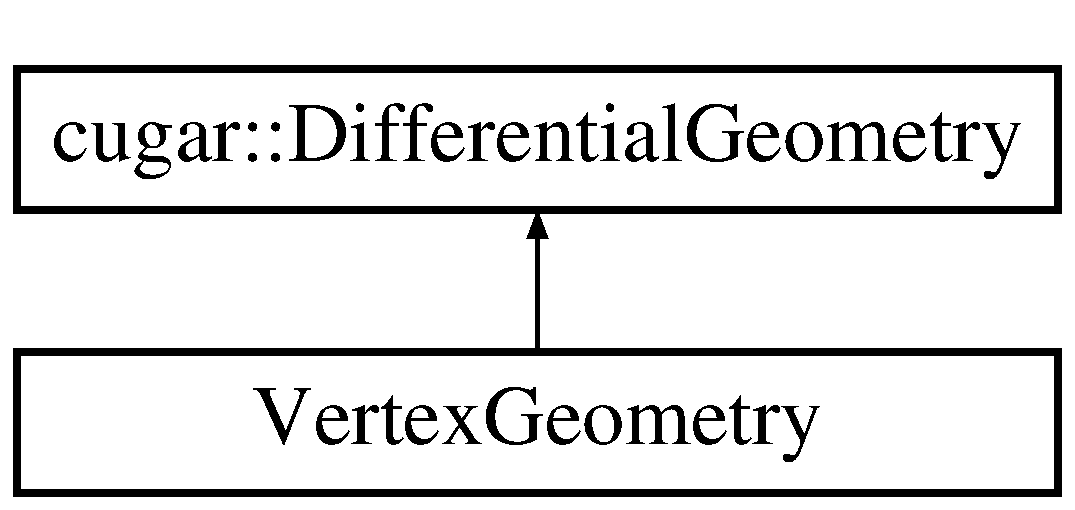
\includegraphics[height=2.000000cm]{structcugar_1_1_differential_geometry}
\end{center}
\end{figure}
\subsection*{Public Members}
\begin{DoxyCompactItemize}
\item 
\mbox{\Hypertarget{structcugar_1_1_differential_geometry_aabf2543aae8db745fd6d8f970d026844}\label{structcugar_1_1_differential_geometry_aabf2543aae8db745fd6d8f970d026844}} 
\hyperlink{structcugar_1_1_vector}{Vector3f} {\bfseries normal\+\_\+s}
\item 
\mbox{\Hypertarget{structcugar_1_1_differential_geometry_ae3cea3b6c0a013bfc6afcd577dfbaa16}\label{structcugar_1_1_differential_geometry_ae3cea3b6c0a013bfc6afcd577dfbaa16}} 
\hyperlink{structcugar_1_1_vector}{Vector3f} {\bfseries normal\+\_\+g}
\item 
\mbox{\Hypertarget{structcugar_1_1_differential_geometry_a453e0b8ba0dd380dfff68935e36f4d07}\label{structcugar_1_1_differential_geometry_a453e0b8ba0dd380dfff68935e36f4d07}} 
\hyperlink{structcugar_1_1_vector}{Vector3f} {\bfseries tangent}
\item 
\mbox{\Hypertarget{structcugar_1_1_differential_geometry_a4f0f88fac0d7463008e23af95ca846af}\label{structcugar_1_1_differential_geometry_a4f0f88fac0d7463008e23af95ca846af}} 
\hyperlink{structcugar_1_1_vector}{Vector3f} {\bfseries binormal}
\end{DoxyCompactItemize}


The documentation for this struct was generated from the following file\+:\begin{DoxyCompactItemize}
\item 
C\+:/p4research/research/jpantaleoni/\+Fermat-\/\+Public/contrib/cugar/bsdf/differential\+\_\+geometry.\+h\end{DoxyCompactItemize}

\hypertarget{struct_directional_light}{}\section{Directional\+Light Struct Reference}
\label{struct_directional_light}\index{Directional\+Light@{Directional\+Light}}


\subsection{Detailed description}
Directional-\/light class 

{\ttfamily \#include $<$lights.\+h$>$}

Inheritance diagram for Directional\+Light\+:\begin{figure}[H]
\begin{center}
\leavevmode
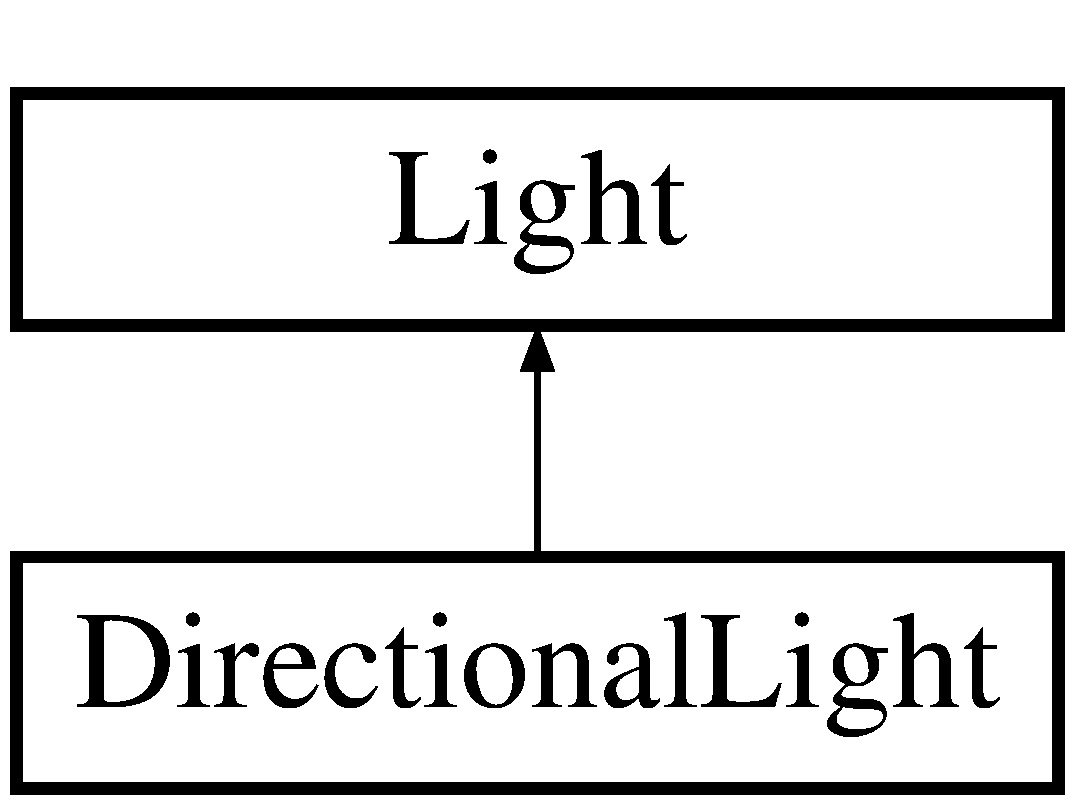
\includegraphics[height=2.000000cm]{struct_directional_light}
\end{center}
\end{figure}
\subsection*{Public Methods}
\begin{DoxyCompactItemize}
\item 
F\+E\+R\+M\+A\+T\+\_\+\+H\+O\+S\+T\+\_\+\+D\+E\+V\+I\+CE bool \hyperlink{struct_directional_light_af94d1e48aece7a3811f791fdabcbb11d}{sample\+\_\+impl} (const float $\ast$Z, uint32\+\_\+t $\ast$prim\+\_\+id, \hyperlink{structcugar_1_1_vector}{cugar\+::\+Vector2f} $\ast$uv, \hyperlink{struct_vertex_geometry}{Vertex\+Geometry} $\ast$geom, float $\ast$pdf, \hyperlink{struct_edf}{Edf} $\ast$edf) const
\item 
F\+E\+R\+M\+A\+T\+\_\+\+H\+O\+S\+T\+\_\+\+D\+E\+V\+I\+CE bool \hyperlink{struct_directional_light_a0f13eac548f1e19cb3098668ab2a8fcc}{sample\+\_\+impl} (const \hyperlink{structcugar_1_1_vector}{cugar\+::\+Vector3f} p, const float $\ast$Z, uint32\+\_\+t $\ast$prim\+\_\+id, \hyperlink{structcugar_1_1_vector}{cugar\+::\+Vector2f} $\ast$uv, \hyperlink{struct_vertex_geometry}{Vertex\+Geometry} $\ast$geom, float $\ast$pdf, \hyperlink{struct_edf}{Edf} $\ast$edf) const
\end{DoxyCompactItemize}
\subsection*{Public Members}
\begin{DoxyCompactItemize}
\item 
\mbox{\Hypertarget{struct_directional_light_ae53baeb58a17876a8cdb9f6df60ca5c0}\label{struct_directional_light_ae53baeb58a17876a8cdb9f6df60ca5c0}} 
\hyperlink{structcugar_1_1_vector}{cugar\+::\+Vector3f} {\bfseries dir}
\item 
\mbox{\Hypertarget{struct_directional_light_a0baf7b8cb5a7b58e8724c159c4849651}\label{struct_directional_light_a0baf7b8cb5a7b58e8724c159c4849651}} 
\hyperlink{structcugar_1_1_vector}{cugar\+::\+Vector3f} {\bfseries color}
\end{DoxyCompactItemize}


\subsection{Member Function Documentation}
\mbox{\Hypertarget{struct_directional_light_af94d1e48aece7a3811f791fdabcbb11d}\label{struct_directional_light_af94d1e48aece7a3811f791fdabcbb11d}} 
\index{Directional\+Light@{Directional\+Light}!sample\+\_\+impl@{sample\+\_\+impl}}
\index{sample\+\_\+impl@{sample\+\_\+impl}!Directional\+Light@{Directional\+Light}}
\subsubsection{\texorpdfstring{sample\+\_\+impl()}{sample\_impl()}\hspace{0.1cm}{\footnotesize\ttfamily [1/2]}}
{\footnotesize\ttfamily F\+E\+R\+M\+A\+T\+\_\+\+H\+O\+S\+T\+\_\+\+D\+E\+V\+I\+CE bool Directional\+Light\+::sample\+\_\+impl (\begin{DoxyParamCaption}\item[{const float $\ast$}]{Z,  }\item[{uint32\+\_\+t $\ast$}]{prim\+\_\+id,  }\item[{\hyperlink{structcugar_1_1_vector}{cugar\+::\+Vector2f} $\ast$}]{uv,  }\item[{\hyperlink{struct_vertex_geometry}{Vertex\+Geometry} $\ast$}]{geom,  }\item[{float $\ast$}]{pdf,  }\item[{\hyperlink{struct_edf}{Edf} $\ast$}]{edf }\end{DoxyParamCaption}) const\hspace{0.3cm}{\ttfamily [inline]}}

sample a surface element on the light source \mbox{\Hypertarget{struct_directional_light_a0f13eac548f1e19cb3098668ab2a8fcc}\label{struct_directional_light_a0f13eac548f1e19cb3098668ab2a8fcc}} 
\index{Directional\+Light@{Directional\+Light}!sample\+\_\+impl@{sample\+\_\+impl}}
\index{sample\+\_\+impl@{sample\+\_\+impl}!Directional\+Light@{Directional\+Light}}
\subsubsection{\texorpdfstring{sample\+\_\+impl()}{sample\_impl()}\hspace{0.1cm}{\footnotesize\ttfamily [2/2]}}
{\footnotesize\ttfamily F\+E\+R\+M\+A\+T\+\_\+\+H\+O\+S\+T\+\_\+\+D\+E\+V\+I\+CE bool Directional\+Light\+::sample\+\_\+impl (\begin{DoxyParamCaption}\item[{const \hyperlink{structcugar_1_1_vector}{cugar\+::\+Vector3f}}]{p,  }\item[{const float $\ast$}]{Z,  }\item[{uint32\+\_\+t $\ast$}]{prim\+\_\+id,  }\item[{\hyperlink{structcugar_1_1_vector}{cugar\+::\+Vector2f} $\ast$}]{uv,  }\item[{\hyperlink{struct_vertex_geometry}{Vertex\+Geometry} $\ast$}]{geom,  }\item[{float $\ast$}]{pdf,  }\item[{\hyperlink{struct_edf}{Edf} $\ast$}]{edf }\end{DoxyParamCaption}) const\hspace{0.3cm}{\ttfamily [inline]}}

sample a surface element on the light source 

The documentation for this struct was generated from the following file\+:\begin{DoxyCompactItemize}
\item 
C\+:/p4research/research/jpantaleoni/\+Fermat-\/\+Public/src/lights.\+h\end{DoxyCompactItemize}

\hypertarget{struct_direct_lighting_mesh}{}\section{Direct\+Lighting\+Mesh Struct Reference}
\label{struct_direct_lighting_mesh}\index{Direct\+Lighting\+Mesh@{Direct\+Lighting\+Mesh}}


\subsection{Detailed description}
A model of \hyperlink{_p_t_lib_page_TPTDirectLightingSampler}{T\+P\+T\+Direct\+Lighting\+Sampler}, implementing N\+EE sample generation from an emissive mesh 

{\ttfamily \#include $<$direct\+\_\+lighting\+\_\+mesh.\+h$>$}

\subsection*{Public Methods}
\begin{DoxyCompactItemize}
\item 
F\+E\+R\+M\+A\+T\+\_\+\+H\+O\+S\+T\+\_\+\+D\+E\+V\+I\+CE \hyperlink{struct_direct_lighting_mesh_a6f51872d622c3ee9a81e2f433b9e256c}{Direct\+Lighting\+Mesh} ()
\item 
F\+E\+R\+M\+A\+T\+\_\+\+H\+O\+S\+T\+\_\+\+D\+E\+V\+I\+CE \hyperlink{struct_direct_lighting_mesh_af86ba1cf583e3a9e8527afa4d83a2f3d}{Direct\+Lighting\+Mesh} (const \hyperlink{struct_mesh_light}{Mesh\+Light} \+\_\+mesh\+\_\+light)
\item 
F\+E\+R\+M\+A\+T\+\_\+\+D\+E\+V\+I\+CE uint32 \hyperlink{struct_direct_lighting_mesh_a2df01e89667068136231e0c6efd4eefc}{preprocess\+\_\+vertex} (const \hyperlink{struct_rendering_context_view}{Rendering\+Context\+View} \&renderer, const \hyperlink{struct_eye_vertex}{Eye\+Vertex} \&ev, const uint32 pixel, const uint32 bounce, const bool is\+\_\+secondary\+\_\+diffuse, const float cone\+\_\+radius, const \hyperlink{structcugar_1_1_bbox}{cugar\+::\+Bbox3f} scene\+\_\+bbox)
\item 
F\+E\+R\+M\+A\+T\+\_\+\+D\+E\+V\+I\+CE uint32 \hyperlink{struct_direct_lighting_mesh_af509addd3c3bce6853b5721ac85cae4d}{sample} (const uint32 nee\+\_\+slot, const float z\mbox{[}3\mbox{]}, \hyperlink{struct_vertex_geometry_id}{Vertex\+Geometry\+Id} $\ast$light\+\_\+vertex, \hyperlink{struct_vertex_geometry}{Vertex\+Geometry} $\ast$light\+\_\+vertex\+\_\+geom, float $\ast$light\+\_\+pdf, \hyperlink{struct_edf}{Edf} $\ast$light\+\_\+edf)
\item 
F\+E\+R\+M\+A\+T\+\_\+\+D\+E\+V\+I\+CE void \hyperlink{struct_direct_lighting_mesh_a2dabf1d83d06e47ee36c1290e10b0b3e}{map} (const uint32 prev\+\_\+nee\+\_\+slot, const uint32 tri\+Id, const \hyperlink{structcugar_1_1_vector}{cugar\+::\+Vector2f} uv, const \hyperlink{struct_vertex_geometry}{Vertex\+Geometry} light\+\_\+vertex\+\_\+geom, float $\ast$light\+\_\+pdf, \hyperlink{struct_edf}{Edf} $\ast$light\+\_\+edf)
\item 
F\+E\+R\+M\+A\+T\+\_\+\+D\+E\+V\+I\+CE void \hyperlink{struct_direct_lighting_mesh_a3328811ee1cbe8a570f7b5d0b2c6a4f4}{update} (const uint32 nee\+\_\+slot, const uint32 nee\+\_\+sample, const \hyperlink{structcugar_1_1_vector}{cugar\+::\+Vector3f} w, const bool occluded)
\end{DoxyCompactItemize}
\subsection*{Public Members}
\begin{DoxyCompactItemize}
\item 
\mbox{\Hypertarget{struct_direct_lighting_mesh_a546e8419bdf60853deaca1d754932ade}\label{struct_direct_lighting_mesh_a546e8419bdf60853deaca1d754932ade}} 
\hyperlink{struct_mesh_light}{Mesh\+Light} {\bfseries mesh\+\_\+light}
\end{DoxyCompactItemize}
\subsection*{Static Public Members}
\begin{DoxyCompactItemize}
\item 
\mbox{\Hypertarget{struct_direct_lighting_mesh_ac87d51f9b1deac8f500d53cfb9771916}\label{struct_direct_lighting_mesh_ac87d51f9b1deac8f500d53cfb9771916}} 
static const uint32 {\bfseries I\+N\+V\+A\+L\+I\+D\+\_\+\+S\+L\+OT} = 0x\+F\+F\+F\+F\+F\+F\+FF
\item 
\mbox{\Hypertarget{struct_direct_lighting_mesh_a887262d35e3f04bc3f674e571ed7353b}\label{struct_direct_lighting_mesh_a887262d35e3f04bc3f674e571ed7353b}} 
static const uint32 {\bfseries I\+N\+V\+A\+L\+I\+D\+\_\+\+S\+A\+M\+P\+LE} = 0x\+F\+F\+F\+F\+F\+F\+FF
\end{DoxyCompactItemize}


\subsection{Constructor \& Destructor Documentation}
\mbox{\Hypertarget{struct_direct_lighting_mesh_a6f51872d622c3ee9a81e2f433b9e256c}\label{struct_direct_lighting_mesh_a6f51872d622c3ee9a81e2f433b9e256c}} 
\index{Direct\+Lighting\+Mesh@{Direct\+Lighting\+Mesh}!Direct\+Lighting\+Mesh@{Direct\+Lighting\+Mesh}}
\index{Direct\+Lighting\+Mesh@{Direct\+Lighting\+Mesh}!Direct\+Lighting\+Mesh@{Direct\+Lighting\+Mesh}}
\subsubsection{\texorpdfstring{Direct\+Lighting\+Mesh()}{DirectLightingMesh()}\hspace{0.1cm}{\footnotesize\ttfamily [1/2]}}
{\footnotesize\ttfamily F\+E\+R\+M\+A\+T\+\_\+\+H\+O\+S\+T\+\_\+\+D\+E\+V\+I\+CE Direct\+Lighting\+Mesh\+::\+Direct\+Lighting\+Mesh (\begin{DoxyParamCaption}{ }\end{DoxyParamCaption})\hspace{0.3cm}{\ttfamily [inline]}}

empty constructor \mbox{\Hypertarget{struct_direct_lighting_mesh_af86ba1cf583e3a9e8527afa4d83a2f3d}\label{struct_direct_lighting_mesh_af86ba1cf583e3a9e8527afa4d83a2f3d}} 
\index{Direct\+Lighting\+Mesh@{Direct\+Lighting\+Mesh}!Direct\+Lighting\+Mesh@{Direct\+Lighting\+Mesh}}
\index{Direct\+Lighting\+Mesh@{Direct\+Lighting\+Mesh}!Direct\+Lighting\+Mesh@{Direct\+Lighting\+Mesh}}
\subsubsection{\texorpdfstring{Direct\+Lighting\+Mesh()}{DirectLightingMesh()}\hspace{0.1cm}{\footnotesize\ttfamily [2/2]}}
{\footnotesize\ttfamily F\+E\+R\+M\+A\+T\+\_\+\+H\+O\+S\+T\+\_\+\+D\+E\+V\+I\+CE Direct\+Lighting\+Mesh\+::\+Direct\+Lighting\+Mesh (\begin{DoxyParamCaption}\item[{const \hyperlink{struct_mesh_light}{Mesh\+Light}}]{\+\_\+mesh\+\_\+light }\end{DoxyParamCaption})\hspace{0.3cm}{\ttfamily [inline]}}

constructor 

\subsection{Member Function Documentation}
\mbox{\Hypertarget{struct_direct_lighting_mesh_a2dabf1d83d06e47ee36c1290e10b0b3e}\label{struct_direct_lighting_mesh_a2dabf1d83d06e47ee36c1290e10b0b3e}} 
\index{Direct\+Lighting\+Mesh@{Direct\+Lighting\+Mesh}!map@{map}}
\index{map@{map}!Direct\+Lighting\+Mesh@{Direct\+Lighting\+Mesh}}
\subsubsection{\texorpdfstring{map()}{map()}}
{\footnotesize\ttfamily F\+E\+R\+M\+A\+T\+\_\+\+D\+E\+V\+I\+CE void Direct\+Lighting\+Mesh\+::map (\begin{DoxyParamCaption}\item[{const uint32}]{prev\+\_\+nee\+\_\+slot,  }\item[{const uint32}]{tri\+Id,  }\item[{const \hyperlink{structcugar_1_1_vector}{cugar\+::\+Vector2f}}]{uv,  }\item[{const \hyperlink{struct_vertex_geometry}{Vertex\+Geometry}}]{light\+\_\+vertex\+\_\+geom,  }\item[{float $\ast$}]{light\+\_\+pdf,  }\item[{\hyperlink{struct_edf}{Edf} $\ast$}]{light\+\_\+edf }\end{DoxyParamCaption})\hspace{0.3cm}{\ttfamily [inline]}}

map a light vertex at the slot given at the previous vertex \mbox{\Hypertarget{struct_direct_lighting_mesh_a2df01e89667068136231e0c6efd4eefc}\label{struct_direct_lighting_mesh_a2df01e89667068136231e0c6efd4eefc}} 
\index{Direct\+Lighting\+Mesh@{Direct\+Lighting\+Mesh}!preprocess\+\_\+vertex@{preprocess\+\_\+vertex}}
\index{preprocess\+\_\+vertex@{preprocess\+\_\+vertex}!Direct\+Lighting\+Mesh@{Direct\+Lighting\+Mesh}}
\subsubsection{\texorpdfstring{preprocess\+\_\+vertex()}{preprocess\_vertex()}}
{\footnotesize\ttfamily F\+E\+R\+M\+A\+T\+\_\+\+D\+E\+V\+I\+CE uint32 Direct\+Lighting\+Mesh\+::preprocess\+\_\+vertex (\begin{DoxyParamCaption}\item[{const \hyperlink{struct_rendering_context_view}{Rendering\+Context\+View} \&}]{renderer,  }\item[{const \hyperlink{struct_eye_vertex}{Eye\+Vertex} \&}]{ev,  }\item[{const uint32}]{pixel,  }\item[{const uint32}]{bounce,  }\item[{const bool}]{is\+\_\+secondary\+\_\+diffuse,  }\item[{const float}]{cone\+\_\+radius,  }\item[{const \hyperlink{structcugar_1_1_bbox}{cugar\+::\+Bbox3f}}]{scene\+\_\+bbox }\end{DoxyParamCaption})\hspace{0.3cm}{\ttfamily [inline]}}

preprocess a path vertex and return a hash slot used for N\+EE \mbox{\Hypertarget{struct_direct_lighting_mesh_af509addd3c3bce6853b5721ac85cae4d}\label{struct_direct_lighting_mesh_af509addd3c3bce6853b5721ac85cae4d}} 
\index{Direct\+Lighting\+Mesh@{Direct\+Lighting\+Mesh}!sample@{sample}}
\index{sample@{sample}!Direct\+Lighting\+Mesh@{Direct\+Lighting\+Mesh}}
\subsubsection{\texorpdfstring{sample()}{sample()}}
{\footnotesize\ttfamily F\+E\+R\+M\+A\+T\+\_\+\+D\+E\+V\+I\+CE uint32 Direct\+Lighting\+Mesh\+::sample (\begin{DoxyParamCaption}\item[{const uint32}]{nee\+\_\+slot,  }\item[{const float}]{z\mbox{[}3\mbox{]},  }\item[{\hyperlink{struct_vertex_geometry_id}{Vertex\+Geometry\+Id} $\ast$}]{light\+\_\+vertex,  }\item[{\hyperlink{struct_vertex_geometry}{Vertex\+Geometry} $\ast$}]{light\+\_\+vertex\+\_\+geom,  }\item[{float $\ast$}]{light\+\_\+pdf,  }\item[{\hyperlink{struct_edf}{Edf} $\ast$}]{light\+\_\+edf }\end{DoxyParamCaption})\hspace{0.3cm}{\ttfamily [inline]}}

sample a light vertex at a given slot \mbox{\Hypertarget{struct_direct_lighting_mesh_a3328811ee1cbe8a570f7b5d0b2c6a4f4}\label{struct_direct_lighting_mesh_a3328811ee1cbe8a570f7b5d0b2c6a4f4}} 
\index{Direct\+Lighting\+Mesh@{Direct\+Lighting\+Mesh}!update@{update}}
\index{update@{update}!Direct\+Lighting\+Mesh@{Direct\+Lighting\+Mesh}}
\subsubsection{\texorpdfstring{update()}{update()}}
{\footnotesize\ttfamily F\+E\+R\+M\+A\+T\+\_\+\+D\+E\+V\+I\+CE void Direct\+Lighting\+Mesh\+::update (\begin{DoxyParamCaption}\item[{const uint32}]{nee\+\_\+slot,  }\item[{const uint32}]{nee\+\_\+sample,  }\item[{const \hyperlink{structcugar_1_1_vector}{cugar\+::\+Vector3f}}]{w,  }\item[{const bool}]{occluded }\end{DoxyParamCaption})\hspace{0.3cm}{\ttfamily [inline]}}

update with the resulting N\+EE sample 

The documentation for this struct was generated from the following file\+:\begin{DoxyCompactItemize}
\item 
C\+:/p4research/research/jpantaleoni/\+Fermat-\/\+Public/src/direct\+\_\+lighting\+\_\+mesh.\+h\end{DoxyCompactItemize}

\hypertarget{struct_direct_lighting_r_l}{}\section{Direct\+Lighting\+RL Struct Reference}
\label{struct_direct_lighting_r_l}\index{Direct\+Lighting\+RL@{Direct\+Lighting\+RL}}


\subsection{Detailed description}
A model of \hyperlink{_p_t_lib_page_TPTDirectLightingSampler}{T\+P\+T\+Direct\+Lighting\+Sampler}, implementing N\+EE sample generation from an emissive mesh using the novel adaptively clustered Reinforcement-\/\+Learning algorithm implemented in \hyperlink{group___clustered_r_l_module}{Clustered RL} 

{\ttfamily \#include $<$direct\+\_\+lighting\+\_\+rl.\+h$>$}

\subsection*{Public Types}
\begin{DoxyCompactItemize}
\item 
\mbox{\Hypertarget{struct_direct_lighting_r_l_a6b609d000811d1246b0be6c5e26bfa46}\label{struct_direct_lighting_r_l_a6b609d000811d1246b0be6c5e26bfa46}} 
typedef \hyperlink{struct_adaptive_clustered_r_l_view}{Adaptive\+Clustered\+R\+L\+View} {\bfseries R\+L\+Map}
\end{DoxyCompactItemize}
\subsection*{Public Methods}
\begin{DoxyCompactItemize}
\item 
F\+E\+R\+M\+A\+T\+\_\+\+H\+O\+S\+T\+\_\+\+D\+E\+V\+I\+CE \hyperlink{struct_direct_lighting_r_l_a4ffd83e2326fa69465a1f474ad7b9a82}{Direct\+Lighting\+RL} ()
\item 
F\+E\+R\+M\+A\+T\+\_\+\+H\+O\+S\+T\+\_\+\+D\+E\+V\+I\+CE \hyperlink{struct_direct_lighting_r_l_abbfe3a309d668177190c5dc5df992953}{Direct\+Lighting\+RL} (\hyperlink{struct_adaptive_clustered_r_l_view}{R\+L\+Map} \+\_\+rl, \hyperlink{struct_v_t_l_mesh_view}{V\+T\+L\+Mesh\+View} \+\_\+vtls)
\item 
F\+E\+R\+M\+A\+T\+\_\+\+D\+E\+V\+I\+CE uint32 \hyperlink{struct_direct_lighting_r_l_ab699ac7e5d3bfc88cef0849438334065}{preprocess\+\_\+vertex} (const \hyperlink{struct_rendering_context_view}{Rendering\+Context\+View} \&renderer, const \hyperlink{struct_eye_vertex}{Eye\+Vertex} \&ev, const uint32 pixel, const uint32 bounce, const bool is\+\_\+secondary\+\_\+diffuse, const float cone\+\_\+radius, const \hyperlink{structcugar_1_1_bbox}{cugar\+::\+Bbox3f} scene\+\_\+bbox)
\item 
F\+E\+R\+M\+A\+T\+\_\+\+D\+E\+V\+I\+CE uint32 \hyperlink{struct_direct_lighting_r_l_aa1f5e8005e659be71588e0ae72f5f79b}{sample} (const uint32 nee\+\_\+slot, const float z\mbox{[}3\mbox{]}, \hyperlink{struct_vertex_geometry_id}{Vertex\+Geometry\+Id} $\ast$light\+\_\+vertex, \hyperlink{struct_vertex_geometry}{Vertex\+Geometry} $\ast$light\+\_\+vertex\+\_\+geom, float $\ast$light\+\_\+pdf, \hyperlink{struct_edf}{Edf} $\ast$light\+\_\+edf)
\item 
F\+E\+R\+M\+A\+T\+\_\+\+D\+E\+V\+I\+CE void \hyperlink{struct_direct_lighting_r_l_ac763ae9503e0dbb78f5618c70446f2e7}{map} (const uint32 prev\+\_\+nee\+\_\+slot, const uint32 tri\+Id, const \hyperlink{structcugar_1_1_vector}{cugar\+::\+Vector2f} uv, const \hyperlink{struct_vertex_geometry}{Vertex\+Geometry} light\+\_\+vertex\+\_\+geom, float $\ast$light\+\_\+pdf, \hyperlink{struct_edf}{Edf} $\ast$light\+\_\+edf)
\item 
F\+E\+R\+M\+A\+T\+\_\+\+D\+E\+V\+I\+CE void \hyperlink{struct_direct_lighting_r_l_a466b9f6099b9332f1def390e45636b3a}{update} (const uint32 nee\+\_\+slot, const uint32 nee\+\_\+cluster, const \hyperlink{structcugar_1_1_vector}{cugar\+::\+Vector3f} w, const bool occluded)
\end{DoxyCompactItemize}
\subsection*{Public Members}
\begin{DoxyCompactItemize}
\item 
\mbox{\Hypertarget{struct_direct_lighting_r_l_aa31be9d85eff9d49eb817add17697424}\label{struct_direct_lighting_r_l_aa31be9d85eff9d49eb817add17697424}} 
\hyperlink{struct_adaptive_clustered_r_l_view}{R\+L\+Map} {\bfseries vtl\+\_\+rl}
\item 
\mbox{\Hypertarget{struct_direct_lighting_r_l_a6bcbd1f1e5700263520ac1ef58d6c58b}\label{struct_direct_lighting_r_l_a6bcbd1f1e5700263520ac1ef58d6c58b}} 
\hyperlink{struct_v_t_l_mesh_view}{V\+T\+L\+Mesh\+View} {\bfseries vtls}
\end{DoxyCompactItemize}
\subsection*{Static Public Members}
\begin{DoxyCompactItemize}
\item 
\mbox{\Hypertarget{struct_direct_lighting_r_l_ae41b8ae138581a431ef9e7ea7acf732b}\label{struct_direct_lighting_r_l_ae41b8ae138581a431ef9e7ea7acf732b}} 
static const uint32 {\bfseries I\+N\+V\+A\+L\+I\+D\+\_\+\+S\+L\+OT} = 0x\+F\+F\+F\+F\+F\+F\+FF
\item 
\mbox{\Hypertarget{struct_direct_lighting_r_l_aa30959c932994ba2cc0f47f3efd5c1d9}\label{struct_direct_lighting_r_l_aa30959c932994ba2cc0f47f3efd5c1d9}} 
static const uint32 {\bfseries I\+N\+V\+A\+L\+I\+D\+\_\+\+S\+A\+M\+P\+LE} = 0x\+F\+F\+F\+F\+F\+F\+FF
\end{DoxyCompactItemize}


\subsection{Constructor \& Destructor Documentation}
\mbox{\Hypertarget{struct_direct_lighting_r_l_a4ffd83e2326fa69465a1f474ad7b9a82}\label{struct_direct_lighting_r_l_a4ffd83e2326fa69465a1f474ad7b9a82}} 
\index{Direct\+Lighting\+RL@{Direct\+Lighting\+RL}!Direct\+Lighting\+RL@{Direct\+Lighting\+RL}}
\index{Direct\+Lighting\+RL@{Direct\+Lighting\+RL}!Direct\+Lighting\+RL@{Direct\+Lighting\+RL}}
\subsubsection{\texorpdfstring{Direct\+Lighting\+R\+L()}{DirectLightingRL()}\hspace{0.1cm}{\footnotesize\ttfamily [1/2]}}
{\footnotesize\ttfamily F\+E\+R\+M\+A\+T\+\_\+\+H\+O\+S\+T\+\_\+\+D\+E\+V\+I\+CE Direct\+Lighting\+R\+L\+::\+Direct\+Lighting\+RL (\begin{DoxyParamCaption}{ }\end{DoxyParamCaption})\hspace{0.3cm}{\ttfamily [inline]}}

empty constructor \mbox{\Hypertarget{struct_direct_lighting_r_l_abbfe3a309d668177190c5dc5df992953}\label{struct_direct_lighting_r_l_abbfe3a309d668177190c5dc5df992953}} 
\index{Direct\+Lighting\+RL@{Direct\+Lighting\+RL}!Direct\+Lighting\+RL@{Direct\+Lighting\+RL}}
\index{Direct\+Lighting\+RL@{Direct\+Lighting\+RL}!Direct\+Lighting\+RL@{Direct\+Lighting\+RL}}
\subsubsection{\texorpdfstring{Direct\+Lighting\+R\+L()}{DirectLightingRL()}\hspace{0.1cm}{\footnotesize\ttfamily [2/2]}}
{\footnotesize\ttfamily F\+E\+R\+M\+A\+T\+\_\+\+H\+O\+S\+T\+\_\+\+D\+E\+V\+I\+CE Direct\+Lighting\+R\+L\+::\+Direct\+Lighting\+RL (\begin{DoxyParamCaption}\item[{\hyperlink{struct_adaptive_clustered_r_l_view}{R\+L\+Map}}]{\+\_\+rl,  }\item[{\hyperlink{struct_v_t_l_mesh_view}{V\+T\+L\+Mesh\+View}}]{\+\_\+vtls }\end{DoxyParamCaption})\hspace{0.3cm}{\ttfamily [inline]}}

constructor 

\subsection{Member Function Documentation}
\mbox{\Hypertarget{struct_direct_lighting_r_l_ac763ae9503e0dbb78f5618c70446f2e7}\label{struct_direct_lighting_r_l_ac763ae9503e0dbb78f5618c70446f2e7}} 
\index{Direct\+Lighting\+RL@{Direct\+Lighting\+RL}!map@{map}}
\index{map@{map}!Direct\+Lighting\+RL@{Direct\+Lighting\+RL}}
\subsubsection{\texorpdfstring{map()}{map()}}
{\footnotesize\ttfamily F\+E\+R\+M\+A\+T\+\_\+\+D\+E\+V\+I\+CE void Direct\+Lighting\+R\+L\+::map (\begin{DoxyParamCaption}\item[{const uint32}]{prev\+\_\+nee\+\_\+slot,  }\item[{const uint32}]{tri\+Id,  }\item[{const \hyperlink{structcugar_1_1_vector}{cugar\+::\+Vector2f}}]{uv,  }\item[{const \hyperlink{struct_vertex_geometry}{Vertex\+Geometry}}]{light\+\_\+vertex\+\_\+geom,  }\item[{float $\ast$}]{light\+\_\+pdf,  }\item[{\hyperlink{struct_edf}{Edf} $\ast$}]{light\+\_\+edf }\end{DoxyParamCaption})\hspace{0.3cm}{\ttfamily [inline]}}

map a light vertex at the slot given at the previous vertex \mbox{\Hypertarget{struct_direct_lighting_r_l_ab699ac7e5d3bfc88cef0849438334065}\label{struct_direct_lighting_r_l_ab699ac7e5d3bfc88cef0849438334065}} 
\index{Direct\+Lighting\+RL@{Direct\+Lighting\+RL}!preprocess\+\_\+vertex@{preprocess\+\_\+vertex}}
\index{preprocess\+\_\+vertex@{preprocess\+\_\+vertex}!Direct\+Lighting\+RL@{Direct\+Lighting\+RL}}
\subsubsection{\texorpdfstring{preprocess\+\_\+vertex()}{preprocess\_vertex()}}
{\footnotesize\ttfamily F\+E\+R\+M\+A\+T\+\_\+\+D\+E\+V\+I\+CE uint32 Direct\+Lighting\+R\+L\+::preprocess\+\_\+vertex (\begin{DoxyParamCaption}\item[{const \hyperlink{struct_rendering_context_view}{Rendering\+Context\+View} \&}]{renderer,  }\item[{const \hyperlink{struct_eye_vertex}{Eye\+Vertex} \&}]{ev,  }\item[{const uint32}]{pixel,  }\item[{const uint32}]{bounce,  }\item[{const bool}]{is\+\_\+secondary\+\_\+diffuse,  }\item[{const float}]{cone\+\_\+radius,  }\item[{const \hyperlink{structcugar_1_1_bbox}{cugar\+::\+Bbox3f}}]{scene\+\_\+bbox }\end{DoxyParamCaption})\hspace{0.3cm}{\ttfamily [inline]}}

preprocess a path vertex and return a hash slot used for N\+EE \mbox{\Hypertarget{struct_direct_lighting_r_l_aa1f5e8005e659be71588e0ae72f5f79b}\label{struct_direct_lighting_r_l_aa1f5e8005e659be71588e0ae72f5f79b}} 
\index{Direct\+Lighting\+RL@{Direct\+Lighting\+RL}!sample@{sample}}
\index{sample@{sample}!Direct\+Lighting\+RL@{Direct\+Lighting\+RL}}
\subsubsection{\texorpdfstring{sample()}{sample()}}
{\footnotesize\ttfamily F\+E\+R\+M\+A\+T\+\_\+\+D\+E\+V\+I\+CE uint32 Direct\+Lighting\+R\+L\+::sample (\begin{DoxyParamCaption}\item[{const uint32}]{nee\+\_\+slot,  }\item[{const float}]{z\mbox{[}3\mbox{]},  }\item[{\hyperlink{struct_vertex_geometry_id}{Vertex\+Geometry\+Id} $\ast$}]{light\+\_\+vertex,  }\item[{\hyperlink{struct_vertex_geometry}{Vertex\+Geometry} $\ast$}]{light\+\_\+vertex\+\_\+geom,  }\item[{float $\ast$}]{light\+\_\+pdf,  }\item[{\hyperlink{struct_edf}{Edf} $\ast$}]{light\+\_\+edf }\end{DoxyParamCaption})\hspace{0.3cm}{\ttfamily [inline]}}

sample a light vertex at a given slot \mbox{\Hypertarget{struct_direct_lighting_r_l_a466b9f6099b9332f1def390e45636b3a}\label{struct_direct_lighting_r_l_a466b9f6099b9332f1def390e45636b3a}} 
\index{Direct\+Lighting\+RL@{Direct\+Lighting\+RL}!update@{update}}
\index{update@{update}!Direct\+Lighting\+RL@{Direct\+Lighting\+RL}}
\subsubsection{\texorpdfstring{update()}{update()}}
{\footnotesize\ttfamily F\+E\+R\+M\+A\+T\+\_\+\+D\+E\+V\+I\+CE void Direct\+Lighting\+R\+L\+::update (\begin{DoxyParamCaption}\item[{const uint32}]{nee\+\_\+slot,  }\item[{const uint32}]{nee\+\_\+cluster,  }\item[{const \hyperlink{structcugar_1_1_vector}{cugar\+::\+Vector3f}}]{w,  }\item[{const bool}]{occluded }\end{DoxyParamCaption})\hspace{0.3cm}{\ttfamily [inline]}}

update with the resulting N\+EE sample 

The documentation for this struct was generated from the following file\+:\begin{DoxyCompactItemize}
\item 
C\+:/p4research/research/jpantaleoni/\+Fermat-\/\+Public/src/direct\+\_\+lighting\+\_\+rl.\+h\end{DoxyCompactItemize}

\hypertarget{struct_disk_light}{}\section{Disk\+Light Struct Reference}
\label{struct_disk_light}\index{Disk\+Light@{Disk\+Light}}


\subsection{Detailed description}
Disk-\/light class 

{\ttfamily \#include $<$lights.\+h$>$}

Inheritance diagram for Disk\+Light\+:\begin{figure}[H]
\begin{center}
\leavevmode
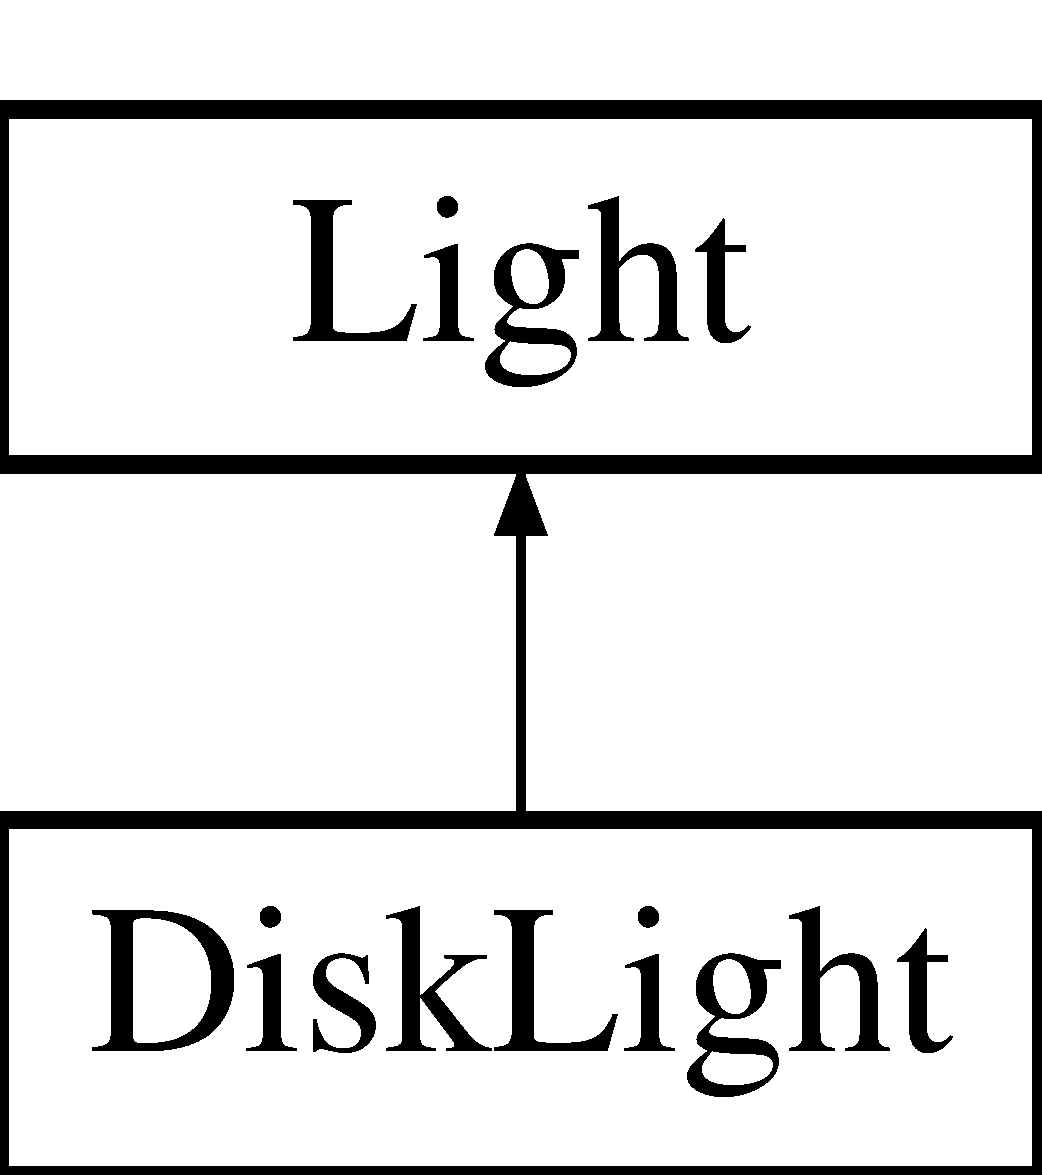
\includegraphics[height=2.000000cm]{struct_disk_light}
\end{center}
\end{figure}
\subsection*{Public Methods}
\begin{DoxyCompactItemize}
\item 
F\+E\+R\+M\+A\+T\+\_\+\+H\+O\+S\+T\+\_\+\+D\+E\+V\+I\+CE bool \hyperlink{struct_disk_light_a79772898d99e5779c17ef39d9b9ac3bd}{sample\+\_\+impl} (const float $\ast$Z, uint32\+\_\+t $\ast$prim\+\_\+id, \hyperlink{structcugar_1_1_vector}{cugar\+::\+Vector2f} $\ast$uv, \hyperlink{struct_vertex_geometry}{Vertex\+Geometry} $\ast$geom, float $\ast$pdf, \hyperlink{struct_edf}{Edf} $\ast$edf) const
\item 
F\+E\+R\+M\+A\+T\+\_\+\+H\+O\+S\+T\+\_\+\+D\+E\+V\+I\+CE void \hyperlink{struct_disk_light_a230967dac9dee2f71e7edf0b6b19f9bc}{intersect\+\_\+impl} (const \hyperlink{struct_ray}{Ray} ray, float2 $\ast$uv, float $\ast$t) const
\item 
F\+E\+R\+M\+A\+T\+\_\+\+H\+O\+S\+T\+\_\+\+D\+E\+V\+I\+CE void \hyperlink{struct_disk_light_a7be348de13a69241954e8780aad94da9}{map\+\_\+impl} (const uint32\+\_\+t prim\+\_\+id, const \hyperlink{structcugar_1_1_vector}{cugar\+::\+Vector2f} \&uv, \hyperlink{struct_vertex_geometry}{Vertex\+Geometry} $\ast$geom, float $\ast$pdf, \hyperlink{struct_edf}{Edf} $\ast$edf) const
\item 
F\+E\+R\+M\+A\+T\+\_\+\+H\+O\+S\+T\+\_\+\+D\+E\+V\+I\+CE void \hyperlink{struct_disk_light_addaaf579434c189bfd0b3f0ded4762d7}{map\+\_\+impl} (const uint32\+\_\+t prim\+\_\+id, const \hyperlink{structcugar_1_1_vector}{cugar\+::\+Vector2f} \&uv, const \hyperlink{struct_vertex_geometry}{Vertex\+Geometry} \&geom, float $\ast$pdf, \hyperlink{struct_edf}{Edf} $\ast$edf) const
\end{DoxyCompactItemize}
\subsection*{Public Members}
\begin{DoxyCompactItemize}
\item 
\mbox{\Hypertarget{struct_disk_light_ad5c2e262ab9ee8035c13825954a0197c}\label{struct_disk_light_ad5c2e262ab9ee8035c13825954a0197c}} 
\hyperlink{structcugar_1_1_vector}{cugar\+::\+Vector3f} {\bfseries pos}
\item 
\mbox{\Hypertarget{struct_disk_light_a4026cb48e89a6f88a02f56f0f8c09e21}\label{struct_disk_light_a4026cb48e89a6f88a02f56f0f8c09e21}} 
\hyperlink{structcugar_1_1_vector}{cugar\+::\+Vector3f} {\bfseries dir}
\item 
\mbox{\Hypertarget{struct_disk_light_ab13b47c395c952a7f9968be755daffd1}\label{struct_disk_light_ab13b47c395c952a7f9968be755daffd1}} 
\hyperlink{structcugar_1_1_vector}{cugar\+::\+Vector3f} {\bfseries u}
\item 
\mbox{\Hypertarget{struct_disk_light_ac074e59c5a7b9a5c91a350c5de3f8a2c}\label{struct_disk_light_ac074e59c5a7b9a5c91a350c5de3f8a2c}} 
\hyperlink{structcugar_1_1_vector}{cugar\+::\+Vector3f} {\bfseries v}
\item 
\mbox{\Hypertarget{struct_disk_light_a98efccd3799bec4ecaab15669aa84cea}\label{struct_disk_light_a98efccd3799bec4ecaab15669aa84cea}} 
\hyperlink{structcugar_1_1_vector}{cugar\+::\+Vector3f} {\bfseries color}
\item 
\mbox{\Hypertarget{struct_disk_light_ad652919f70f9f394dd62c07779e8ce12}\label{struct_disk_light_ad652919f70f9f394dd62c07779e8ce12}} 
float {\bfseries radius}
\end{DoxyCompactItemize}


\subsection{Member Function Documentation}
\mbox{\Hypertarget{struct_disk_light_a230967dac9dee2f71e7edf0b6b19f9bc}\label{struct_disk_light_a230967dac9dee2f71e7edf0b6b19f9bc}} 
\index{Disk\+Light@{Disk\+Light}!intersect\+\_\+impl@{intersect\+\_\+impl}}
\index{intersect\+\_\+impl@{intersect\+\_\+impl}!Disk\+Light@{Disk\+Light}}
\subsubsection{\texorpdfstring{intersect\+\_\+impl()}{intersect\_impl()}}
{\footnotesize\ttfamily F\+E\+R\+M\+A\+T\+\_\+\+H\+O\+S\+T\+\_\+\+D\+E\+V\+I\+CE void Disk\+Light\+::intersect\+\_\+impl (\begin{DoxyParamCaption}\item[{const \hyperlink{struct_ray}{Ray}}]{ray,  }\item[{float2 $\ast$}]{uv,  }\item[{float $\ast$}]{t }\end{DoxyParamCaption}) const\hspace{0.3cm}{\ttfamily [inline]}}

intersect the given ray with the light source \mbox{\Hypertarget{struct_disk_light_a7be348de13a69241954e8780aad94da9}\label{struct_disk_light_a7be348de13a69241954e8780aad94da9}} 
\index{Disk\+Light@{Disk\+Light}!map\+\_\+impl@{map\+\_\+impl}}
\index{map\+\_\+impl@{map\+\_\+impl}!Disk\+Light@{Disk\+Light}}
\subsubsection{\texorpdfstring{map\+\_\+impl()}{map\_impl()}\hspace{0.1cm}{\footnotesize\ttfamily [1/2]}}
{\footnotesize\ttfamily F\+E\+R\+M\+A\+T\+\_\+\+H\+O\+S\+T\+\_\+\+D\+E\+V\+I\+CE void Disk\+Light\+::map\+\_\+impl (\begin{DoxyParamCaption}\item[{const uint32\+\_\+t}]{prim\+\_\+id,  }\item[{const \hyperlink{structcugar_1_1_vector}{cugar\+::\+Vector2f} \&}]{uv,  }\item[{\hyperlink{struct_vertex_geometry}{Vertex\+Geometry} $\ast$}]{geom,  }\item[{float $\ast$}]{pdf,  }\item[{\hyperlink{struct_edf}{Edf} $\ast$}]{edf }\end{DoxyParamCaption}) const\hspace{0.3cm}{\ttfamily [inline]}}

map a (prim,uv) pair to a surface element \mbox{\Hypertarget{struct_disk_light_addaaf579434c189bfd0b3f0ded4762d7}\label{struct_disk_light_addaaf579434c189bfd0b3f0ded4762d7}} 
\index{Disk\+Light@{Disk\+Light}!map\+\_\+impl@{map\+\_\+impl}}
\index{map\+\_\+impl@{map\+\_\+impl}!Disk\+Light@{Disk\+Light}}
\subsubsection{\texorpdfstring{map\+\_\+impl()}{map\_impl()}\hspace{0.1cm}{\footnotesize\ttfamily [2/2]}}
{\footnotesize\ttfamily F\+E\+R\+M\+A\+T\+\_\+\+H\+O\+S\+T\+\_\+\+D\+E\+V\+I\+CE void Disk\+Light\+::map\+\_\+impl (\begin{DoxyParamCaption}\item[{const uint32\+\_\+t}]{prim\+\_\+id,  }\item[{const \hyperlink{structcugar_1_1_vector}{cugar\+::\+Vector2f} \&}]{uv,  }\item[{const \hyperlink{struct_vertex_geometry}{Vertex\+Geometry} \&}]{geom,  }\item[{float $\ast$}]{pdf,  }\item[{\hyperlink{struct_edf}{Edf} $\ast$}]{edf }\end{DoxyParamCaption}) const\hspace{0.3cm}{\ttfamily [inline]}}

map a (prim,uv) pair to a surface element \mbox{\Hypertarget{struct_disk_light_a79772898d99e5779c17ef39d9b9ac3bd}\label{struct_disk_light_a79772898d99e5779c17ef39d9b9ac3bd}} 
\index{Disk\+Light@{Disk\+Light}!sample\+\_\+impl@{sample\+\_\+impl}}
\index{sample\+\_\+impl@{sample\+\_\+impl}!Disk\+Light@{Disk\+Light}}
\subsubsection{\texorpdfstring{sample\+\_\+impl()}{sample\_impl()}}
{\footnotesize\ttfamily F\+E\+R\+M\+A\+T\+\_\+\+H\+O\+S\+T\+\_\+\+D\+E\+V\+I\+CE bool Disk\+Light\+::sample\+\_\+impl (\begin{DoxyParamCaption}\item[{const float $\ast$}]{Z,  }\item[{uint32\+\_\+t $\ast$}]{prim\+\_\+id,  }\item[{\hyperlink{structcugar_1_1_vector}{cugar\+::\+Vector2f} $\ast$}]{uv,  }\item[{\hyperlink{struct_vertex_geometry}{Vertex\+Geometry} $\ast$}]{geom,  }\item[{float $\ast$}]{pdf,  }\item[{\hyperlink{struct_edf}{Edf} $\ast$}]{edf }\end{DoxyParamCaption}) const\hspace{0.3cm}{\ttfamily [inline]}}

sample a surface element on the light source 

The documentation for this struct was generated from the following file\+:\begin{DoxyCompactItemize}
\item 
C\+:/p4research/research/jpantaleoni/\+Fermat-\/\+Public/src/lights.\+h\end{DoxyCompactItemize}

\hypertarget{structcugar_1_1detail_1_1dispatch__diff__tensor}{}\section{cugar\+:\+:detail\+:\+:dispatch\+\_\+diff\+\_\+tensor$<$ O\+R\+D\+ER $>$ Struct Template Reference}
\label{structcugar_1_1detail_1_1dispatch__diff__tensor}\index{cugar\+::detail\+::dispatch\+\_\+diff\+\_\+tensor$<$ O\+R\+D\+E\+R $>$@{cugar\+::detail\+::dispatch\+\_\+diff\+\_\+tensor$<$ O\+R\+D\+E\+R $>$}}


The documentation for this struct was generated from the following file\+:\begin{DoxyCompactItemize}
\item 
C\+:/p4research/research/jpantaleoni/\+Fermat-\/\+Public/contrib/cugar/analysis/\hyperlink{diff_8h}{diff.\+h}\end{DoxyCompactItemize}

\hypertarget{structcugar_1_1detail_1_1dispatch__diff__tensor_3_011_01_4}{}\section{cugar\+:\+:detail\+:\+:dispatch\+\_\+diff\+\_\+tensor$<$ 1 $>$ Struct Template Reference}
\label{structcugar_1_1detail_1_1dispatch__diff__tensor_3_011_01_4}\index{cugar\+::detail\+::dispatch\+\_\+diff\+\_\+tensor$<$ 1 $>$@{cugar\+::detail\+::dispatch\+\_\+diff\+\_\+tensor$<$ 1 $>$}}
\subsection*{Static Public Methods}
\begin{DoxyCompactItemize}
\item 
\mbox{\Hypertarget{structcugar_1_1detail_1_1dispatch__diff__tensor_3_011_01_4_aba0856e8234ab734ccee692cfc83a547}\label{structcugar_1_1detail_1_1dispatch__diff__tensor_3_011_01_4_aba0856e8234ab734ccee692cfc83a547}} 
{\footnotesize template$<$typename VT , uint32 N, uint32 O$>$ }\\static C\+U\+G\+A\+R\+\_\+\+H\+O\+S\+T\+\_\+\+D\+E\+V\+I\+CE \hyperlink{structcugar_1_1_tensor}{Tensor}$<$ VT, 1, N $>$ {\bfseries apply} (const \hyperlink{structcugar_1_1diff__var}{diff\+\_\+var}$<$ VT, N, O $>$ op)
\end{DoxyCompactItemize}


The documentation for this struct was generated from the following file\+:\begin{DoxyCompactItemize}
\item 
C\+:/p4research/research/jpantaleoni/\+Fermat-\/\+Public/contrib/cugar/analysis/\hyperlink{diff_8h}{diff.\+h}\end{DoxyCompactItemize}

\hypertarget{structcugar_1_1detail_1_1dispatch__diff__tensor_3_012_01_4}{}\section{cugar\+:\+:detail\+:\+:dispatch\+\_\+diff\+\_\+tensor$<$ 2 $>$ Struct Template Reference}
\label{structcugar_1_1detail_1_1dispatch__diff__tensor_3_012_01_4}\index{cugar\+::detail\+::dispatch\+\_\+diff\+\_\+tensor$<$ 2 $>$@{cugar\+::detail\+::dispatch\+\_\+diff\+\_\+tensor$<$ 2 $>$}}
\subsection*{Static Public Methods}
\begin{DoxyCompactItemize}
\item 
\mbox{\Hypertarget{structcugar_1_1detail_1_1dispatch__diff__tensor_3_012_01_4_afc951565d85152ba5bc4a64a762c3d67}\label{structcugar_1_1detail_1_1dispatch__diff__tensor_3_012_01_4_afc951565d85152ba5bc4a64a762c3d67}} 
{\footnotesize template$<$typename VT , uint32 N, uint32 O$>$ }\\static C\+U\+G\+A\+R\+\_\+\+H\+O\+S\+T\+\_\+\+D\+E\+V\+I\+CE \hyperlink{structcugar_1_1_tensor}{Tensor}$<$ VT, 2, N $>$ {\bfseries apply} (const \hyperlink{structcugar_1_1diff__var}{diff\+\_\+var}$<$ VT, N, O $>$ op)
\end{DoxyCompactItemize}


The documentation for this struct was generated from the following file\+:\begin{DoxyCompactItemize}
\item 
C\+:/p4research/research/jpantaleoni/\+Fermat-\/\+Public/contrib/cugar/analysis/\hyperlink{diff_8h}{diff.\+h}\end{DoxyCompactItemize}

\hypertarget{structcugar_1_1detail_1_1dispatch__diff__tensor_3_013_01_4}{}\section{cugar\+:\+:detail\+:\+:dispatch\+\_\+diff\+\_\+tensor$<$ 3 $>$ Struct Template Reference}
\label{structcugar_1_1detail_1_1dispatch__diff__tensor_3_013_01_4}\index{cugar\+::detail\+::dispatch\+\_\+diff\+\_\+tensor$<$ 3 $>$@{cugar\+::detail\+::dispatch\+\_\+diff\+\_\+tensor$<$ 3 $>$}}
\subsection*{Static Public Methods}
\begin{DoxyCompactItemize}
\item 
\mbox{\Hypertarget{structcugar_1_1detail_1_1dispatch__diff__tensor_3_013_01_4_a3125368d0b71369c48cb9ef9a2d61641}\label{structcugar_1_1detail_1_1dispatch__diff__tensor_3_013_01_4_a3125368d0b71369c48cb9ef9a2d61641}} 
{\footnotesize template$<$typename VT , uint32 N, uint32 O$>$ }\\static C\+U\+G\+A\+R\+\_\+\+H\+O\+S\+T\+\_\+\+D\+E\+V\+I\+CE \hyperlink{structcugar_1_1_tensor}{Tensor}$<$ VT, 3, N $>$ {\bfseries apply} (const \hyperlink{structcugar_1_1diff__var}{diff\+\_\+var}$<$ VT, N, O $>$ op)
\end{DoxyCompactItemize}


The documentation for this struct was generated from the following file\+:\begin{DoxyCompactItemize}
\item 
C\+:/p4research/research/jpantaleoni/\+Fermat-\/\+Public/contrib/cugar/analysis/\hyperlink{diff_8h}{diff.\+h}\end{DoxyCompactItemize}

\hypertarget{structcugar_1_1detail_1_1dispatch__div}{}\section{cugar\+:\+:detail\+:\+:dispatch\+\_\+div$<$ VT, N, O1, O2 $>$ Struct Template Reference}
\label{structcugar_1_1detail_1_1dispatch__div}\index{cugar\+::detail\+::dispatch\+\_\+div$<$ V\+T, N, O1, O2 $>$@{cugar\+::detail\+::dispatch\+\_\+div$<$ V\+T, N, O1, O2 $>$}}
\subsection*{Static Public Methods}
\begin{DoxyCompactItemize}
\item 
\mbox{\Hypertarget{structcugar_1_1detail_1_1dispatch__div_af1b4fbe9793258c33fd26319b5b535d2}\label{structcugar_1_1detail_1_1dispatch__div_af1b4fbe9793258c33fd26319b5b535d2}} 
static C\+U\+G\+A\+R\+\_\+\+H\+O\+S\+T\+\_\+\+D\+E\+V\+I\+CE \hyperlink{structcugar_1_1diff__var}{diff\+\_\+var}$<$ VT, N, RO $>$ {\bfseries apply} (const \hyperlink{structcugar_1_1diff__var}{diff\+\_\+var}$<$ VT, N, O1 $>$ a, const \hyperlink{structcugar_1_1diff__var}{diff\+\_\+var}$<$ VT, N, O2 $>$ b)
\end{DoxyCompactItemize}
\subsection*{Static Public Members}
\begin{DoxyCompactItemize}
\item 
\mbox{\Hypertarget{structcugar_1_1detail_1_1dispatch__div_af6ce5613b42fc2aa0494febb7440733a}\label{structcugar_1_1detail_1_1dispatch__div_af6ce5613b42fc2aa0494febb7440733a}} 
static const uint32 {\bfseries RO} = \hyperlink{structcugar_1_1static__min}{static\+\_\+min}$<$O1,O2$>$\+::value
\end{DoxyCompactItemize}


The documentation for this struct was generated from the following file\+:\begin{DoxyCompactItemize}
\item 
C\+:/p4research/research/jpantaleoni/\+Fermat-\/\+Public/contrib/cugar/analysis/\hyperlink{diff_8h}{diff.\+h}\end{DoxyCompactItemize}

\hypertarget{structcugar_1_1detail_1_1dispatch__div_3_01_v_t_00_01_n_00_010_00_010_01_4}{}\section{cugar\+:\+:detail\+:\+:dispatch\+\_\+div$<$ VT, N, 0, 0 $>$ Struct Template Reference}
\label{structcugar_1_1detail_1_1dispatch__div_3_01_v_t_00_01_n_00_010_00_010_01_4}\index{cugar\+::detail\+::dispatch\+\_\+div$<$ V\+T, N, 0, 0 $>$@{cugar\+::detail\+::dispatch\+\_\+div$<$ V\+T, N, 0, 0 $>$}}
\subsection*{Static Public Methods}
\begin{DoxyCompactItemize}
\item 
\mbox{\Hypertarget{structcugar_1_1detail_1_1dispatch__div_3_01_v_t_00_01_n_00_010_00_010_01_4_af0d5ff5a343bf7b113ff1ff145a65455}\label{structcugar_1_1detail_1_1dispatch__div_3_01_v_t_00_01_n_00_010_00_010_01_4_af0d5ff5a343bf7b113ff1ff145a65455}} 
static C\+U\+G\+A\+R\+\_\+\+H\+O\+S\+T\+\_\+\+D\+E\+V\+I\+CE \hyperlink{structcugar_1_1diff__var}{diff\+\_\+var}$<$ VT, N, 0 $>$ {\bfseries apply} (const \hyperlink{structcugar_1_1diff__var}{diff\+\_\+var}$<$ VT, N, 0 $>$ a, const \hyperlink{structcugar_1_1diff__var}{diff\+\_\+var}$<$ VT, N, 0 $>$ b)
\end{DoxyCompactItemize}
\subsection*{Static Public Members}
\begin{DoxyCompactItemize}
\item 
\mbox{\Hypertarget{structcugar_1_1detail_1_1dispatch__div_3_01_v_t_00_01_n_00_010_00_010_01_4_ad257cd9f6c3ad2139768fab0ca178e46}\label{structcugar_1_1detail_1_1dispatch__div_3_01_v_t_00_01_n_00_010_00_010_01_4_ad257cd9f6c3ad2139768fab0ca178e46}} 
static const uint32 {\bfseries RO} = 0
\end{DoxyCompactItemize}


The documentation for this struct was generated from the following file\+:\begin{DoxyCompactItemize}
\item 
C\+:/p4research/research/jpantaleoni/\+Fermat-\/\+Public/contrib/cugar/analysis/\hyperlink{diff_8h}{diff.\+h}\end{DoxyCompactItemize}

\hypertarget{structcugar_1_1detail_1_1dispatch__div_3_01_v_t_00_01_n_00_010_00_01_o_01_4}{}\section{cugar\+:\+:detail\+:\+:dispatch\+\_\+div$<$ VT, N, 0, O $>$ Struct Template Reference}
\label{structcugar_1_1detail_1_1dispatch__div_3_01_v_t_00_01_n_00_010_00_01_o_01_4}\index{cugar\+::detail\+::dispatch\+\_\+div$<$ V\+T, N, 0, O $>$@{cugar\+::detail\+::dispatch\+\_\+div$<$ V\+T, N, 0, O $>$}}
\subsection*{Static Public Methods}
\begin{DoxyCompactItemize}
\item 
\mbox{\Hypertarget{structcugar_1_1detail_1_1dispatch__div_3_01_v_t_00_01_n_00_010_00_01_o_01_4_a111b430aa95f8b2cd88085329823e7db}\label{structcugar_1_1detail_1_1dispatch__div_3_01_v_t_00_01_n_00_010_00_01_o_01_4_a111b430aa95f8b2cd88085329823e7db}} 
static C\+U\+G\+A\+R\+\_\+\+H\+O\+S\+T\+\_\+\+D\+E\+V\+I\+CE \hyperlink{structcugar_1_1diff__var}{diff\+\_\+var}$<$ VT, N, 0 $>$ {\bfseries apply} (const \hyperlink{structcugar_1_1diff__var}{diff\+\_\+var}$<$ VT, N, 0 $>$ a, const \hyperlink{structcugar_1_1diff__var}{diff\+\_\+var}$<$ VT, N, O $>$ b)
\end{DoxyCompactItemize}
\subsection*{Static Public Members}
\begin{DoxyCompactItemize}
\item 
\mbox{\Hypertarget{structcugar_1_1detail_1_1dispatch__div_3_01_v_t_00_01_n_00_010_00_01_o_01_4_a9bfc8b7f723f1e19b9d420eb2f6644fd}\label{structcugar_1_1detail_1_1dispatch__div_3_01_v_t_00_01_n_00_010_00_01_o_01_4_a9bfc8b7f723f1e19b9d420eb2f6644fd}} 
static const uint32 {\bfseries RO} = 0
\end{DoxyCompactItemize}


The documentation for this struct was generated from the following file\+:\begin{DoxyCompactItemize}
\item 
C\+:/p4research/research/jpantaleoni/\+Fermat-\/\+Public/contrib/cugar/analysis/\hyperlink{diff_8h}{diff.\+h}\end{DoxyCompactItemize}

\hypertarget{structcugar_1_1detail_1_1dispatch__div_3_01_v_t_00_01_n_00_01_o_00_010_01_4}{}\section{cugar\+:\+:detail\+:\+:dispatch\+\_\+div$<$ VT, N, O, 0 $>$ Struct Template Reference}
\label{structcugar_1_1detail_1_1dispatch__div_3_01_v_t_00_01_n_00_01_o_00_010_01_4}\index{cugar\+::detail\+::dispatch\+\_\+div$<$ V\+T, N, O, 0 $>$@{cugar\+::detail\+::dispatch\+\_\+div$<$ V\+T, N, O, 0 $>$}}
\subsection*{Static Public Methods}
\begin{DoxyCompactItemize}
\item 
\mbox{\Hypertarget{structcugar_1_1detail_1_1dispatch__div_3_01_v_t_00_01_n_00_01_o_00_010_01_4_adc327b90b895aaf6166e537f85cc7bb1}\label{structcugar_1_1detail_1_1dispatch__div_3_01_v_t_00_01_n_00_01_o_00_010_01_4_adc327b90b895aaf6166e537f85cc7bb1}} 
static C\+U\+G\+A\+R\+\_\+\+H\+O\+S\+T\+\_\+\+D\+E\+V\+I\+CE \hyperlink{structcugar_1_1diff__var}{diff\+\_\+var}$<$ VT, N, 0 $>$ {\bfseries apply} (const \hyperlink{structcugar_1_1diff__var}{diff\+\_\+var}$<$ VT, N, O $>$ a, const \hyperlink{structcugar_1_1diff__var}{diff\+\_\+var}$<$ VT, N, 0 $>$ b)
\end{DoxyCompactItemize}
\subsection*{Static Public Members}
\begin{DoxyCompactItemize}
\item 
\mbox{\Hypertarget{structcugar_1_1detail_1_1dispatch__div_3_01_v_t_00_01_n_00_01_o_00_010_01_4_a742165ca46df33256ca338032bdf9354}\label{structcugar_1_1detail_1_1dispatch__div_3_01_v_t_00_01_n_00_01_o_00_010_01_4_a742165ca46df33256ca338032bdf9354}} 
static const uint32 {\bfseries RO} = 0
\end{DoxyCompactItemize}


The documentation for this struct was generated from the following file\+:\begin{DoxyCompactItemize}
\item 
C\+:/p4research/research/jpantaleoni/\+Fermat-\/\+Public/contrib/cugar/analysis/\hyperlink{diff_8h}{diff.\+h}\end{DoxyCompactItemize}

\hypertarget{structcugar_1_1detail_1_1dispatch__mul}{}\section{cugar\+:\+:detail\+:\+:dispatch\+\_\+mul$<$ VT, N, O1, O2 $>$ Struct Template Reference}
\label{structcugar_1_1detail_1_1dispatch__mul}\index{cugar\+::detail\+::dispatch\+\_\+mul$<$ V\+T, N, O1, O2 $>$@{cugar\+::detail\+::dispatch\+\_\+mul$<$ V\+T, N, O1, O2 $>$}}
\subsection*{Static Public Methods}
\begin{DoxyCompactItemize}
\item 
\mbox{\Hypertarget{structcugar_1_1detail_1_1dispatch__mul_a582da21501028d46d221fdbb54ebb83b}\label{structcugar_1_1detail_1_1dispatch__mul_a582da21501028d46d221fdbb54ebb83b}} 
static C\+U\+G\+A\+R\+\_\+\+H\+O\+S\+T\+\_\+\+D\+E\+V\+I\+CE \hyperlink{structcugar_1_1diff__var}{diff\+\_\+var}$<$ VT, N, RO $>$ {\bfseries apply} (const \hyperlink{structcugar_1_1diff__var}{diff\+\_\+var}$<$ VT, N, O1 $>$ a, const \hyperlink{structcugar_1_1diff__var}{diff\+\_\+var}$<$ VT, N, O2 $>$ b)
\end{DoxyCompactItemize}
\subsection*{Static Public Members}
\begin{DoxyCompactItemize}
\item 
\mbox{\Hypertarget{structcugar_1_1detail_1_1dispatch__mul_a639d51f4d1f473b2b0fd673cbae00930}\label{structcugar_1_1detail_1_1dispatch__mul_a639d51f4d1f473b2b0fd673cbae00930}} 
static const uint32 {\bfseries RO} = \hyperlink{structcugar_1_1static__min}{static\+\_\+min}$<$O1,O2$>$\+::value
\end{DoxyCompactItemize}


The documentation for this struct was generated from the following file\+:\begin{DoxyCompactItemize}
\item 
C\+:/p4research/research/jpantaleoni/\+Fermat-\/\+Public/contrib/cugar/analysis/\hyperlink{diff_8h}{diff.\+h}\end{DoxyCompactItemize}

\hypertarget{structcugar_1_1detail_1_1dispatch__mul_3_01_v_t_00_01_n_00_010_00_010_01_4}{}\section{cugar\+:\+:detail\+:\+:dispatch\+\_\+mul$<$ VT, N, 0, 0 $>$ Struct Template Reference}
\label{structcugar_1_1detail_1_1dispatch__mul_3_01_v_t_00_01_n_00_010_00_010_01_4}\index{cugar\+::detail\+::dispatch\+\_\+mul$<$ V\+T, N, 0, 0 $>$@{cugar\+::detail\+::dispatch\+\_\+mul$<$ V\+T, N, 0, 0 $>$}}
\subsection*{Static Public Methods}
\begin{DoxyCompactItemize}
\item 
\mbox{\Hypertarget{structcugar_1_1detail_1_1dispatch__mul_3_01_v_t_00_01_n_00_010_00_010_01_4_af1707edc55753ae225c9ba4045e509d6}\label{structcugar_1_1detail_1_1dispatch__mul_3_01_v_t_00_01_n_00_010_00_010_01_4_af1707edc55753ae225c9ba4045e509d6}} 
static C\+U\+G\+A\+R\+\_\+\+H\+O\+S\+T\+\_\+\+D\+E\+V\+I\+CE \hyperlink{structcugar_1_1diff__var}{diff\+\_\+var}$<$ VT, N, 0 $>$ {\bfseries apply} (const \hyperlink{structcugar_1_1diff__var}{diff\+\_\+var}$<$ VT, N, 0 $>$ a, const \hyperlink{structcugar_1_1diff__var}{diff\+\_\+var}$<$ VT, N, 0 $>$ b)
\end{DoxyCompactItemize}
\subsection*{Static Public Members}
\begin{DoxyCompactItemize}
\item 
\mbox{\Hypertarget{structcugar_1_1detail_1_1dispatch__mul_3_01_v_t_00_01_n_00_010_00_010_01_4_a51704c3cbea4405a373f3509a8a717ed}\label{structcugar_1_1detail_1_1dispatch__mul_3_01_v_t_00_01_n_00_010_00_010_01_4_a51704c3cbea4405a373f3509a8a717ed}} 
static const uint32 {\bfseries RO} = 0
\end{DoxyCompactItemize}


The documentation for this struct was generated from the following file\+:\begin{DoxyCompactItemize}
\item 
C\+:/p4research/research/jpantaleoni/\+Fermat-\/\+Public/contrib/cugar/analysis/\hyperlink{diff_8h}{diff.\+h}\end{DoxyCompactItemize}

\hypertarget{structcugar_1_1detail_1_1dispatch__mul_3_01_v_t_00_01_n_00_010_00_01_o_01_4}{}\section{cugar\+:\+:detail\+:\+:dispatch\+\_\+mul$<$ VT, N, 0, O $>$ Struct Template Reference}
\label{structcugar_1_1detail_1_1dispatch__mul_3_01_v_t_00_01_n_00_010_00_01_o_01_4}\index{cugar\+::detail\+::dispatch\+\_\+mul$<$ V\+T, N, 0, O $>$@{cugar\+::detail\+::dispatch\+\_\+mul$<$ V\+T, N, 0, O $>$}}
\subsection*{Static Public Methods}
\begin{DoxyCompactItemize}
\item 
\mbox{\Hypertarget{structcugar_1_1detail_1_1dispatch__mul_3_01_v_t_00_01_n_00_010_00_01_o_01_4_a307f39ce0c9d7dc21613291b71a60a8a}\label{structcugar_1_1detail_1_1dispatch__mul_3_01_v_t_00_01_n_00_010_00_01_o_01_4_a307f39ce0c9d7dc21613291b71a60a8a}} 
static C\+U\+G\+A\+R\+\_\+\+H\+O\+S\+T\+\_\+\+D\+E\+V\+I\+CE \hyperlink{structcugar_1_1diff__var}{diff\+\_\+var}$<$ VT, N, 0 $>$ {\bfseries apply} (const \hyperlink{structcugar_1_1diff__var}{diff\+\_\+var}$<$ VT, N, 0 $>$ a, const \hyperlink{structcugar_1_1diff__var}{diff\+\_\+var}$<$ VT, N, O $>$ b)
\end{DoxyCompactItemize}
\subsection*{Static Public Members}
\begin{DoxyCompactItemize}
\item 
\mbox{\Hypertarget{structcugar_1_1detail_1_1dispatch__mul_3_01_v_t_00_01_n_00_010_00_01_o_01_4_aa117cd66d41ae883618c9966f5180081}\label{structcugar_1_1detail_1_1dispatch__mul_3_01_v_t_00_01_n_00_010_00_01_o_01_4_aa117cd66d41ae883618c9966f5180081}} 
static const uint32 {\bfseries RO} = 0
\end{DoxyCompactItemize}


The documentation for this struct was generated from the following file\+:\begin{DoxyCompactItemize}
\item 
C\+:/p4research/research/jpantaleoni/\+Fermat-\/\+Public/contrib/cugar/analysis/\hyperlink{diff_8h}{diff.\+h}\end{DoxyCompactItemize}

\hypertarget{structcugar_1_1detail_1_1dispatch__mul_3_01_v_t_00_01_n_00_01_o_00_010_01_4}{}\section{cugar\+:\+:detail\+:\+:dispatch\+\_\+mul$<$ VT, N, O, 0 $>$ Struct Template Reference}
\label{structcugar_1_1detail_1_1dispatch__mul_3_01_v_t_00_01_n_00_01_o_00_010_01_4}\index{cugar\+::detail\+::dispatch\+\_\+mul$<$ V\+T, N, O, 0 $>$@{cugar\+::detail\+::dispatch\+\_\+mul$<$ V\+T, N, O, 0 $>$}}
\subsection*{Static Public Methods}
\begin{DoxyCompactItemize}
\item 
\mbox{\Hypertarget{structcugar_1_1detail_1_1dispatch__mul_3_01_v_t_00_01_n_00_01_o_00_010_01_4_a1e47c02ec6b5cb15963f7070e05a3e17}\label{structcugar_1_1detail_1_1dispatch__mul_3_01_v_t_00_01_n_00_01_o_00_010_01_4_a1e47c02ec6b5cb15963f7070e05a3e17}} 
static C\+U\+G\+A\+R\+\_\+\+H\+O\+S\+T\+\_\+\+D\+E\+V\+I\+CE \hyperlink{structcugar_1_1diff__var}{diff\+\_\+var}$<$ VT, N, 0 $>$ {\bfseries apply} (const \hyperlink{structcugar_1_1diff__var}{diff\+\_\+var}$<$ VT, N, O $>$ a, const \hyperlink{structcugar_1_1diff__var}{diff\+\_\+var}$<$ VT, N, 0 $>$ b)
\end{DoxyCompactItemize}
\subsection*{Static Public Members}
\begin{DoxyCompactItemize}
\item 
\mbox{\Hypertarget{structcugar_1_1detail_1_1dispatch__mul_3_01_v_t_00_01_n_00_01_o_00_010_01_4_a44c841857bc496bc95bdf0f8d3c7b934}\label{structcugar_1_1detail_1_1dispatch__mul_3_01_v_t_00_01_n_00_01_o_00_010_01_4_a44c841857bc496bc95bdf0f8d3c7b934}} 
static const uint32 {\bfseries RO} = 0
\end{DoxyCompactItemize}


The documentation for this struct was generated from the following file\+:\begin{DoxyCompactItemize}
\item 
C\+:/p4research/research/jpantaleoni/\+Fermat-\/\+Public/contrib/cugar/analysis/\hyperlink{diff_8h}{diff.\+h}\end{DoxyCompactItemize}

\hypertarget{structcugar_1_1detail_1_1dispatch__sum}{}\section{cugar\+:\+:detail\+:\+:dispatch\+\_\+sum$<$ VT, N, O1, O2 $>$ Struct Template Reference}
\label{structcugar_1_1detail_1_1dispatch__sum}\index{cugar\+::detail\+::dispatch\+\_\+sum$<$ V\+T, N, O1, O2 $>$@{cugar\+::detail\+::dispatch\+\_\+sum$<$ V\+T, N, O1, O2 $>$}}
\subsection*{Static Public Methods}
\begin{DoxyCompactItemize}
\item 
\mbox{\Hypertarget{structcugar_1_1detail_1_1dispatch__sum_ac33220536353aa59a16478175eaaf0f5}\label{structcugar_1_1detail_1_1dispatch__sum_ac33220536353aa59a16478175eaaf0f5}} 
static C\+U\+G\+A\+R\+\_\+\+H\+O\+S\+T\+\_\+\+D\+E\+V\+I\+CE \hyperlink{structcugar_1_1diff__var}{diff\+\_\+var}$<$ VT, N, RO $>$ {\bfseries apply} (const \hyperlink{structcugar_1_1diff__var}{diff\+\_\+var}$<$ VT, N, O1 $>$ a, const \hyperlink{structcugar_1_1diff__var}{diff\+\_\+var}$<$ VT, N, O2 $>$ b)
\end{DoxyCompactItemize}
\subsection*{Static Public Members}
\begin{DoxyCompactItemize}
\item 
\mbox{\Hypertarget{structcugar_1_1detail_1_1dispatch__sum_a34d1428dc373b760e3cfa81404b60432}\label{structcugar_1_1detail_1_1dispatch__sum_a34d1428dc373b760e3cfa81404b60432}} 
static const uint32 {\bfseries RO} = \hyperlink{structcugar_1_1static__min}{static\+\_\+min}$<$O1,O2$>$\+::value
\end{DoxyCompactItemize}


The documentation for this struct was generated from the following file\+:\begin{DoxyCompactItemize}
\item 
C\+:/p4research/research/jpantaleoni/\+Fermat-\/\+Public/contrib/cugar/analysis/\hyperlink{diff_8h}{diff.\+h}\end{DoxyCompactItemize}

\hypertarget{structcugar_1_1detail_1_1dispatch__sum_3_01_v_t_00_01_n_00_010_00_010_01_4}{}\section{cugar\+:\+:detail\+:\+:dispatch\+\_\+sum$<$ VT, N, 0, 0 $>$ Struct Template Reference}
\label{structcugar_1_1detail_1_1dispatch__sum_3_01_v_t_00_01_n_00_010_00_010_01_4}\index{cugar\+::detail\+::dispatch\+\_\+sum$<$ V\+T, N, 0, 0 $>$@{cugar\+::detail\+::dispatch\+\_\+sum$<$ V\+T, N, 0, 0 $>$}}
\subsection*{Static Public Methods}
\begin{DoxyCompactItemize}
\item 
\mbox{\Hypertarget{structcugar_1_1detail_1_1dispatch__sum_3_01_v_t_00_01_n_00_010_00_010_01_4_a19fac95557a9d1c064cfff1181632cdc}\label{structcugar_1_1detail_1_1dispatch__sum_3_01_v_t_00_01_n_00_010_00_010_01_4_a19fac95557a9d1c064cfff1181632cdc}} 
static C\+U\+G\+A\+R\+\_\+\+H\+O\+S\+T\+\_\+\+D\+E\+V\+I\+CE \hyperlink{structcugar_1_1diff__var}{diff\+\_\+var}$<$ VT, N, 0 $>$ {\bfseries apply} (const \hyperlink{structcugar_1_1diff__var}{diff\+\_\+var}$<$ VT, N, 0 $>$ a, const \hyperlink{structcugar_1_1diff__var}{diff\+\_\+var}$<$ VT, N, 0 $>$ b)
\end{DoxyCompactItemize}
\subsection*{Static Public Members}
\begin{DoxyCompactItemize}
\item 
\mbox{\Hypertarget{structcugar_1_1detail_1_1dispatch__sum_3_01_v_t_00_01_n_00_010_00_010_01_4_a8008e00fb8937c6cb5e4df84367e9659}\label{structcugar_1_1detail_1_1dispatch__sum_3_01_v_t_00_01_n_00_010_00_010_01_4_a8008e00fb8937c6cb5e4df84367e9659}} 
static const uint32 {\bfseries RO} = 0
\end{DoxyCompactItemize}


The documentation for this struct was generated from the following file\+:\begin{DoxyCompactItemize}
\item 
C\+:/p4research/research/jpantaleoni/\+Fermat-\/\+Public/contrib/cugar/analysis/\hyperlink{diff_8h}{diff.\+h}\end{DoxyCompactItemize}

\hypertarget{structcugar_1_1detail_1_1dispatch__sum_3_01_v_t_00_01_n_00_010_00_01_o_01_4}{}\section{cugar\+:\+:detail\+:\+:dispatch\+\_\+sum$<$ VT, N, 0, O $>$ Struct Template Reference}
\label{structcugar_1_1detail_1_1dispatch__sum_3_01_v_t_00_01_n_00_010_00_01_o_01_4}\index{cugar\+::detail\+::dispatch\+\_\+sum$<$ V\+T, N, 0, O $>$@{cugar\+::detail\+::dispatch\+\_\+sum$<$ V\+T, N, 0, O $>$}}
\subsection*{Static Public Methods}
\begin{DoxyCompactItemize}
\item 
\mbox{\Hypertarget{structcugar_1_1detail_1_1dispatch__sum_3_01_v_t_00_01_n_00_010_00_01_o_01_4_a7a25917f5bb12c7cbe57042721f54d12}\label{structcugar_1_1detail_1_1dispatch__sum_3_01_v_t_00_01_n_00_010_00_01_o_01_4_a7a25917f5bb12c7cbe57042721f54d12}} 
static C\+U\+G\+A\+R\+\_\+\+H\+O\+S\+T\+\_\+\+D\+E\+V\+I\+CE \hyperlink{structcugar_1_1diff__var}{diff\+\_\+var}$<$ VT, N, 0 $>$ {\bfseries apply} (const \hyperlink{structcugar_1_1diff__var}{diff\+\_\+var}$<$ VT, N, 0 $>$ a, const \hyperlink{structcugar_1_1diff__var}{diff\+\_\+var}$<$ VT, N, O $>$ b)
\end{DoxyCompactItemize}
\subsection*{Static Public Members}
\begin{DoxyCompactItemize}
\item 
\mbox{\Hypertarget{structcugar_1_1detail_1_1dispatch__sum_3_01_v_t_00_01_n_00_010_00_01_o_01_4_a21932bfdd680e0e3c8db758879b4a235}\label{structcugar_1_1detail_1_1dispatch__sum_3_01_v_t_00_01_n_00_010_00_01_o_01_4_a21932bfdd680e0e3c8db758879b4a235}} 
static const uint32 {\bfseries RO} = 0
\end{DoxyCompactItemize}


The documentation for this struct was generated from the following file\+:\begin{DoxyCompactItemize}
\item 
C\+:/p4research/research/jpantaleoni/\+Fermat-\/\+Public/contrib/cugar/analysis/\hyperlink{diff_8h}{diff.\+h}\end{DoxyCompactItemize}

\hypertarget{structcugar_1_1detail_1_1dispatch__sum_3_01_v_t_00_01_n_00_01_o_00_010_01_4}{}\section{cugar\+:\+:detail\+:\+:dispatch\+\_\+sum$<$ VT, N, O, 0 $>$ Struct Template Reference}
\label{structcugar_1_1detail_1_1dispatch__sum_3_01_v_t_00_01_n_00_01_o_00_010_01_4}\index{cugar\+::detail\+::dispatch\+\_\+sum$<$ V\+T, N, O, 0 $>$@{cugar\+::detail\+::dispatch\+\_\+sum$<$ V\+T, N, O, 0 $>$}}
\subsection*{Static Public Methods}
\begin{DoxyCompactItemize}
\item 
\mbox{\Hypertarget{structcugar_1_1detail_1_1dispatch__sum_3_01_v_t_00_01_n_00_01_o_00_010_01_4_a28322877394058f7375ea882ad729129}\label{structcugar_1_1detail_1_1dispatch__sum_3_01_v_t_00_01_n_00_01_o_00_010_01_4_a28322877394058f7375ea882ad729129}} 
static C\+U\+G\+A\+R\+\_\+\+H\+O\+S\+T\+\_\+\+D\+E\+V\+I\+CE \hyperlink{structcugar_1_1diff__var}{diff\+\_\+var}$<$ VT, N, 0 $>$ {\bfseries apply} (const \hyperlink{structcugar_1_1diff__var}{diff\+\_\+var}$<$ VT, N, O $>$ a, const \hyperlink{structcugar_1_1diff__var}{diff\+\_\+var}$<$ VT, N, 0 $>$ b)
\end{DoxyCompactItemize}
\subsection*{Static Public Members}
\begin{DoxyCompactItemize}
\item 
\mbox{\Hypertarget{structcugar_1_1detail_1_1dispatch__sum_3_01_v_t_00_01_n_00_01_o_00_010_01_4_a09a11412c9809c0230de6ec126880b51}\label{structcugar_1_1detail_1_1dispatch__sum_3_01_v_t_00_01_n_00_01_o_00_010_01_4_a09a11412c9809c0230de6ec126880b51}} 
static const uint32 {\bfseries RO} = 0
\end{DoxyCompactItemize}


The documentation for this struct was generated from the following file\+:\begin{DoxyCompactItemize}
\item 
C\+:/p4research/research/jpantaleoni/\+Fermat-\/\+Public/contrib/cugar/analysis/\hyperlink{diff_8h}{diff.\+h}\end{DoxyCompactItemize}

\hypertarget{struct_d_l_l}{}\section{D\+LL Struct Reference}
\label{struct_d_l_l}\index{D\+LL@{D\+LL}}
\subsection*{Public Methods}
\begin{DoxyCompactItemize}
\item 
\mbox{\Hypertarget{struct_d_l_l_aecd2352677877712d7195b5a7f0d7448}\label{struct_d_l_l_aecd2352677877712d7195b5a7f0d7448}} 
{\bfseries D\+LL} (const char $\ast$filename)
\item 
\mbox{\Hypertarget{struct_d_l_l_a0cf3cdb24d99798189ea0588e98d35b9}\label{struct_d_l_l_a0cf3cdb24d99798189ea0588e98d35b9}} 
void $\ast$ {\bfseries get\+\_\+proc\+\_\+address} (const char $\ast$name)
\end{DoxyCompactItemize}
\subsection*{Public Members}
\begin{DoxyCompactItemize}
\item 
\mbox{\Hypertarget{struct_d_l_l_a840c4d872e0164525f5582e1d78b8d5c}\label{struct_d_l_l_a840c4d872e0164525f5582e1d78b8d5c}} 
std\+::shared\+\_\+ptr$<$ \hyperlink{struct_d_l_l_impl}{D\+L\+L\+Impl} $>$ {\bfseries m\+\_\+impl}
\end{DoxyCompactItemize}


The documentation for this struct was generated from the following files\+:\begin{DoxyCompactItemize}
\item 
C\+:/p4research/research/jpantaleoni/\+Fermat-\/\+Public/src/dll.\+h\item 
C\+:/p4research/research/jpantaleoni/\+Fermat-\/\+Public/src/dll.\+cpp\end{DoxyCompactItemize}

\hypertarget{struct_d_l_l_impl}{}\section{D\+L\+L\+Impl Struct Reference}
\label{struct_d_l_l_impl}\index{D\+L\+L\+Impl@{D\+L\+L\+Impl}}
\subsection*{Public Methods}
\begin{DoxyCompactItemize}
\item 
\mbox{\Hypertarget{struct_d_l_l_impl_a85b0edd597b571cffbd1d623773c7d19}\label{struct_d_l_l_impl_a85b0edd597b571cffbd1d623773c7d19}} 
{\bfseries D\+L\+L\+Impl} (const char $\ast$filename)
\item 
\mbox{\Hypertarget{struct_d_l_l_impl_a48221a4f9b500bca1e6bc77a430b2f0d}\label{struct_d_l_l_impl_a48221a4f9b500bca1e6bc77a430b2f0d}} 
void $\ast$ {\bfseries get\+\_\+proc\+\_\+address} (const char $\ast$name)
\end{DoxyCompactItemize}
\subsection*{Public Members}
\begin{DoxyCompactItemize}
\item 
\mbox{\Hypertarget{struct_d_l_l_impl_a4d0a2556e062d9b8ef6164ee12ce26e2}\label{struct_d_l_l_impl_a4d0a2556e062d9b8ef6164ee12ce26e2}} 
H\+I\+N\+S\+T\+A\+N\+CE {\bfseries h\+Get\+Proc\+I\+D\+D\+LL}
\end{DoxyCompactItemize}


The documentation for this struct was generated from the following file\+:\begin{DoxyCompactItemize}
\item 
C\+:/p4research/research/jpantaleoni/\+Fermat-\/\+Public/src/dll.\+cpp\end{DoxyCompactItemize}

\hypertarget{class_domain_buffer}{}\section{Domain\+Buffer$<$ T\+Y\+PE, T $>$ Class Template Reference}
\label{class_domain_buffer}\index{Domain\+Buffer$<$ T\+Y\+P\+E, T $>$@{Domain\+Buffer$<$ T\+Y\+P\+E, T $>$}}
Inheritance diagram for Domain\+Buffer$<$ T\+Y\+PE, T $>$\+:\begin{figure}[H]
\begin{center}
\leavevmode
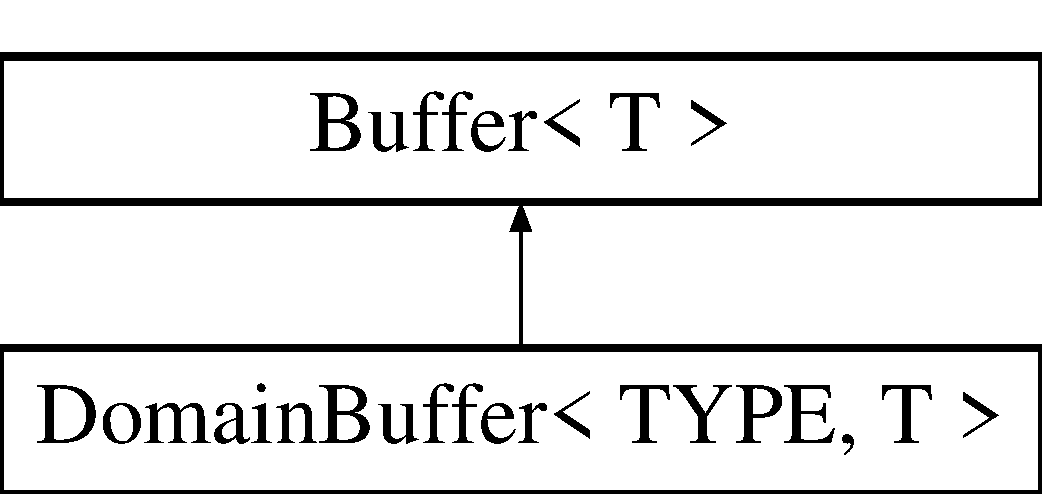
\includegraphics[height=2.000000cm]{class_domain_buffer}
\end{center}
\end{figure}
\subsection*{Public Methods}
\begin{DoxyCompactItemize}
\item 
\mbox{\Hypertarget{class_domain_buffer_af50ae94cdeca23bc7d4530ca7f26c88a}\label{class_domain_buffer_af50ae94cdeca23bc7d4530ca7f26c88a}} 
{\bfseries Domain\+Buffer} (size\+\_\+t count=0, Page\+Locked\+State page\+Locked\+State=U\+N\+L\+O\+C\+K\+ED)
\item 
\mbox{\Hypertarget{class_domain_buffer_a74a746fb300c611786190a299510c0f7}\label{class_domain_buffer_a74a746fb300c611786190a299510c0f7}} 
{\footnotesize template$<$Buffer\+Type U\+T\+Y\+PE$>$ }\\{\bfseries Domain\+Buffer} (const \hyperlink{class_domain_buffer}{Domain\+Buffer}$<$ U\+T\+Y\+PE, T $>$ \&src)
\item 
\mbox{\Hypertarget{class_domain_buffer_a382571a0b89cae8fc5f433a149e89a38}\label{class_domain_buffer_a382571a0b89cae8fc5f433a149e89a38}} 
\hyperlink{class_domain_buffer}{Domain\+Buffer}$<$ T\+Y\+PE, T $>$ \& {\bfseries operator=} (const \hyperlink{class_buffer}{Buffer}$<$ T $>$ \&src)
\item 
\mbox{\Hypertarget{class_domain_buffer_a0d68f0e89c0ea8bec10bd748fc003b35}\label{class_domain_buffer_a0d68f0e89c0ea8bec10bd748fc003b35}} 
\hyperlink{class_domain_buffer}{Domain\+Buffer}$<$ T\+Y\+PE, T $>$ \& {\bfseries operator=} (const \hyperlink{class_managed_buffer}{Managed\+Buffer}$<$ T $>$ \&src)
\end{DoxyCompactItemize}
\subsection*{Additional Inherited Members}


The documentation for this class was generated from the following file\+:\begin{DoxyCompactItemize}
\item 
C\+:/p4research/research/jpantaleoni/\+Fermat-\/\+Public/src/buffers.\+h\end{DoxyCompactItemize}

\hypertarget{structcugar_1_1internals_1_1dynamic__cast__marker}{}\section{cugar\+:\+:internals\+:\+:dynamic\+\_\+cast\+\_\+marker Struct Reference}
\label{structcugar_1_1internals_1_1dynamic__cast__marker}\index{cugar\+::internals\+::dynamic\+\_\+cast\+\_\+marker@{cugar\+::internals\+::dynamic\+\_\+cast\+\_\+marker}}


The documentation for this struct was generated from the following file\+:\begin{DoxyCompactItemize}
\item 
C\+:/p4research/research/jpantaleoni/\+Fermat-\/\+Public/contrib/cugar/basic/shared\+\_\+pointer.\+h\end{DoxyCompactItemize}

\hypertarget{struct_e_a_w_params}{}\section{E\+A\+W\+Params Struct Reference}
\label{struct_e_a_w_params}\index{E\+A\+W\+Params@{E\+A\+W\+Params}}


\subsection{Detailed description}
Edge A-\/trous Wavelet filtering parameters 

{\ttfamily \#include $<$eaw.\+h$>$}

\subsection*{Public Members}
\begin{DoxyCompactItemize}
\item 
\mbox{\Hypertarget{struct_e_a_w_params_a9ee45dea99d29409783d1f0a88409c78}\label{struct_e_a_w_params_a9ee45dea99d29409783d1f0a88409c78}} 
float {\bfseries phi\+\_\+normal}
\item 
\mbox{\Hypertarget{struct_e_a_w_params_a95097b3ff69a35303a0e89fdd5a3e29c}\label{struct_e_a_w_params_a95097b3ff69a35303a0e89fdd5a3e29c}} 
float {\bfseries phi\+\_\+position}
\item 
\mbox{\Hypertarget{struct_e_a_w_params_a397e1f5ec073710f037c0dece69f4099}\label{struct_e_a_w_params_a397e1f5ec073710f037c0dece69f4099}} 
float {\bfseries phi\+\_\+color}
\item 
\mbox{\Hypertarget{struct_e_a_w_params_afaff82e5eafdd19859beba1c88d3bf1e}\label{struct_e_a_w_params_afaff82e5eafdd19859beba1c88d3bf1e}} 
\hyperlink{structcugar_1_1_vector}{cugar\+::\+Vector3f} {\bfseries E}
\item 
\mbox{\Hypertarget{struct_e_a_w_params_afdf22d1c4454bd9f012a7b4fcefbde6b}\label{struct_e_a_w_params_afdf22d1c4454bd9f012a7b4fcefbde6b}} 
\hyperlink{structcugar_1_1_vector}{cugar\+::\+Vector3f} {\bfseries U}
\item 
\mbox{\Hypertarget{struct_e_a_w_params_acad41fd52ba4511d51a811dea37f0d64}\label{struct_e_a_w_params_acad41fd52ba4511d51a811dea37f0d64}} 
\hyperlink{structcugar_1_1_vector}{cugar\+::\+Vector3f} {\bfseries V}
\item 
\mbox{\Hypertarget{struct_e_a_w_params_a8fd24cec2ba7537155c9b70e1782689c}\label{struct_e_a_w_params_a8fd24cec2ba7537155c9b70e1782689c}} 
\hyperlink{structcugar_1_1_vector}{cugar\+::\+Vector3f} {\bfseries W}
\end{DoxyCompactItemize}


The documentation for this struct was generated from the following file\+:\begin{DoxyCompactItemize}
\item 
C\+:/p4research/research/jpantaleoni/\+Fermat-\/\+Public/src/eaw.\+h\end{DoxyCompactItemize}

\hypertarget{structpbrt_1_1_echo_importer}{}\section{pbrt\+:\+:Echo\+Importer Struct Reference}
\label{structpbrt_1_1_echo_importer}\index{pbrt\+::\+Echo\+Importer@{pbrt\+::\+Echo\+Importer}}
Inheritance diagram for pbrt\+:\+:Echo\+Importer\+:\begin{figure}[H]
\begin{center}
\leavevmode
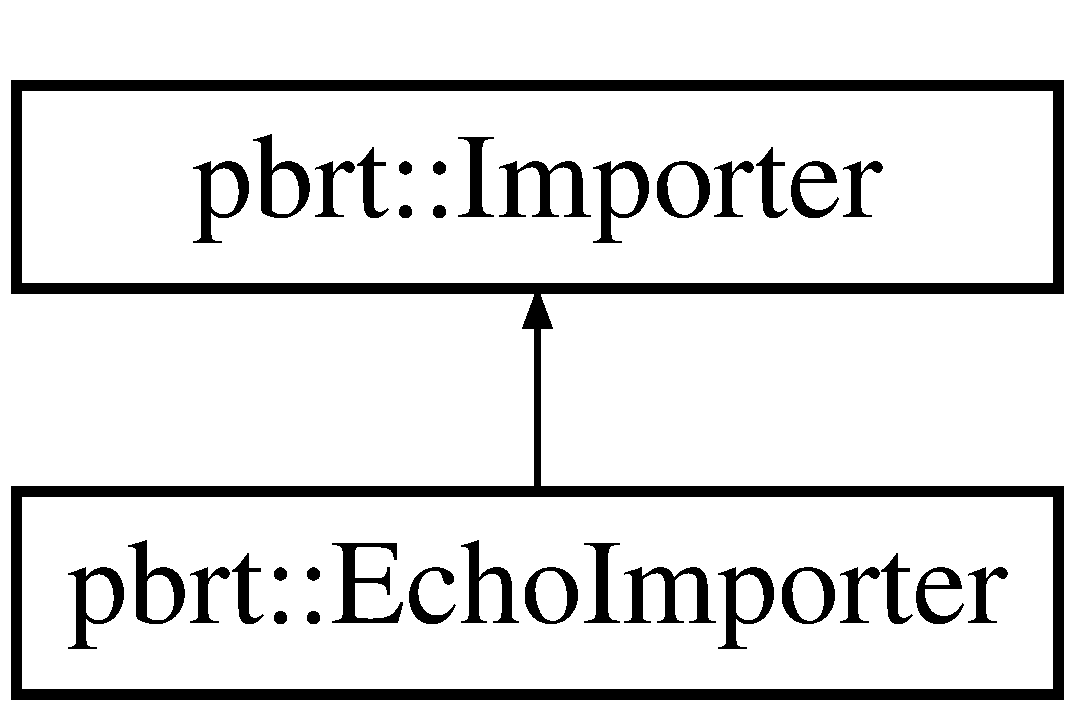
\includegraphics[height=2.000000cm]{structpbrt_1_1_echo_importer}
\end{center}
\end{figure}
\subsection*{Public Methods}
\begin{DoxyCompactItemize}
\item 
\mbox{\Hypertarget{structpbrt_1_1_echo_importer_ad0916c662b697706bac992cd61dc9208}\label{structpbrt_1_1_echo_importer_ad0916c662b697706bac992cd61dc9208}} 
{\bfseries Echo\+Importer} (F\+I\+LE $\ast$\+\_\+file)
\item 
\mbox{\Hypertarget{structpbrt_1_1_echo_importer_a88bb39b65c2e091a2b915541238fd778}\label{structpbrt_1_1_echo_importer_a88bb39b65c2e091a2b915541238fd778}} 
void {\bfseries indent} ()
\item 
\mbox{\Hypertarget{structpbrt_1_1_echo_importer_a546785ee98b61eed5f78f43253a1ee16}\label{structpbrt_1_1_echo_importer_a546785ee98b61eed5f78f43253a1ee16}} 
void {\bfseries print\+\_\+value} (const \hyperlink{structpbrt_1_1_value}{Value} \&value)
\item 
\mbox{\Hypertarget{structpbrt_1_1_echo_importer_ac3177f8b750c4fc77c95e672867a9b32}\label{structpbrt_1_1_echo_importer_ac3177f8b750c4fc77c95e672867a9b32}} 
void {\bfseries print\+\_\+params} (const \hyperlink{structpbrt_1_1_parameter_list}{Parameter\+List} \&params)
\item 
\mbox{\Hypertarget{structpbrt_1_1_echo_importer_acb96f05ba33450e2411e4ff49b55b67d}\label{structpbrt_1_1_echo_importer_acb96f05ba33450e2411e4ff49b55b67d}} 
virtual void {\bfseries identity} ()
\item 
\mbox{\Hypertarget{structpbrt_1_1_echo_importer_a6e1b3bb1f50a0ccca5dcece6775d2ab2}\label{structpbrt_1_1_echo_importer_a6e1b3bb1f50a0ccca5dcece6775d2ab2}} 
virtual void {\bfseries transform} (const \hyperlink{structpbrt_1_1_value}{Value} \&floats)
\item 
\mbox{\Hypertarget{structpbrt_1_1_echo_importer_a415aef104f409f3043ee2d3bef1abadf}\label{structpbrt_1_1_echo_importer_a415aef104f409f3043ee2d3bef1abadf}} 
virtual void {\bfseries rotate} (const float angle, const float x, const float y, const float z)
\item 
\mbox{\Hypertarget{structpbrt_1_1_echo_importer_af38d0e57653a91e48fc549d1ebab73b2}\label{structpbrt_1_1_echo_importer_af38d0e57653a91e48fc549d1ebab73b2}} 
virtual void {\bfseries scale} (const float x, const float y, const float z)
\item 
\mbox{\Hypertarget{structpbrt_1_1_echo_importer_a6b14bae12f837ee0012c172c01c7bca8}\label{structpbrt_1_1_echo_importer_a6b14bae12f837ee0012c172c01c7bca8}} 
virtual void {\bfseries translate} (const float x, const float y, const float z)
\item 
\mbox{\Hypertarget{structpbrt_1_1_echo_importer_a39816b83347dff95568da3a3f49f212d}\label{structpbrt_1_1_echo_importer_a39816b83347dff95568da3a3f49f212d}} 
virtual void {\bfseries look\+\_\+at} (const float ex, const float ey, const float ez, const float lx, const float ly, const float lz, const float ux, const float uy, const float uz)
\item 
\mbox{\Hypertarget{structpbrt_1_1_echo_importer_a9ed058ab639b5833d09edbc7d4c49947}\label{structpbrt_1_1_echo_importer_a9ed058ab639b5833d09edbc7d4c49947}} 
virtual void {\bfseries integrator} (const char $\ast$name, const \hyperlink{structpbrt_1_1_parameter_list}{Parameter\+List} \&params)
\item 
\mbox{\Hypertarget{structpbrt_1_1_echo_importer_a1b7c555b077fe0d2332e75182656b23b}\label{structpbrt_1_1_echo_importer_a1b7c555b077fe0d2332e75182656b23b}} 
virtual void {\bfseries sampler} (const char $\ast$name, const \hyperlink{structpbrt_1_1_parameter_list}{Parameter\+List} \&params)
\item 
\mbox{\Hypertarget{structpbrt_1_1_echo_importer_af6cc3a21cae00cd32212012708cfaf70}\label{structpbrt_1_1_echo_importer_af6cc3a21cae00cd32212012708cfaf70}} 
virtual void {\bfseries pixel\+\_\+filter} (const char $\ast$name, const \hyperlink{structpbrt_1_1_parameter_list}{Parameter\+List} \&params)
\item 
\mbox{\Hypertarget{structpbrt_1_1_echo_importer_af1c39c46746610b47be176dec3d10a20}\label{structpbrt_1_1_echo_importer_af1c39c46746610b47be176dec3d10a20}} 
virtual void {\bfseries film} (const char $\ast$name, const \hyperlink{structpbrt_1_1_parameter_list}{Parameter\+List} \&params)
\item 
\mbox{\Hypertarget{structpbrt_1_1_echo_importer_ac08d3874603449ce71e3341149dc44e4}\label{structpbrt_1_1_echo_importer_ac08d3874603449ce71e3341149dc44e4}} 
virtual void {\bfseries camera} (const char $\ast$name, const \hyperlink{structpbrt_1_1_parameter_list}{Parameter\+List} \&params)
\item 
\mbox{\Hypertarget{structpbrt_1_1_echo_importer_a08f8cdc01a3fcf47dfe312e845c1d078}\label{structpbrt_1_1_echo_importer_a08f8cdc01a3fcf47dfe312e845c1d078}} 
virtual void {\bfseries world\+\_\+begin} ()
\item 
\mbox{\Hypertarget{structpbrt_1_1_echo_importer_ad8d458bc27c85e9b79c3023e1ff4e43a}\label{structpbrt_1_1_echo_importer_ad8d458bc27c85e9b79c3023e1ff4e43a}} 
virtual void {\bfseries world\+\_\+end} ()
\item 
\mbox{\Hypertarget{structpbrt_1_1_echo_importer_a0c84f341fd3a9b862276e5bd8684a411}\label{structpbrt_1_1_echo_importer_a0c84f341fd3a9b862276e5bd8684a411}} 
virtual void {\bfseries attribute\+\_\+begin} ()
\item 
\mbox{\Hypertarget{structpbrt_1_1_echo_importer_abf03653ce4d377bd49359621d8615c67}\label{structpbrt_1_1_echo_importer_abf03653ce4d377bd49359621d8615c67}} 
virtual void {\bfseries attribute\+\_\+end} ()
\item 
\mbox{\Hypertarget{structpbrt_1_1_echo_importer_ac8358d032cc7e0e1743e9e98ffcdf463}\label{structpbrt_1_1_echo_importer_ac8358d032cc7e0e1743e9e98ffcdf463}} 
virtual void {\bfseries transform\+\_\+begin} ()
\item 
\mbox{\Hypertarget{structpbrt_1_1_echo_importer_ac82b149698ff9cddde3aea8fd5d1b85d}\label{structpbrt_1_1_echo_importer_ac82b149698ff9cddde3aea8fd5d1b85d}} 
virtual void {\bfseries transform\+\_\+end} ()
\item 
\mbox{\Hypertarget{structpbrt_1_1_echo_importer_abc340415115bde0708d72e7f4a38959c}\label{structpbrt_1_1_echo_importer_abc340415115bde0708d72e7f4a38959c}} 
virtual void {\bfseries texture} (const char $\ast$name, const char $\ast$texel\+\_\+type, const char $\ast$texture\+\_\+type, const \hyperlink{structpbrt_1_1_parameter_list}{Parameter\+List} \&params)
\item 
\mbox{\Hypertarget{structpbrt_1_1_echo_importer_aa3a973352a7cfb5b38010cd76dc7528c}\label{structpbrt_1_1_echo_importer_aa3a973352a7cfb5b38010cd76dc7528c}} 
virtual void {\bfseries make\+\_\+named\+\_\+medium} (const char $\ast$name, const \hyperlink{structpbrt_1_1_parameter_list}{Parameter\+List} \&params)
\item 
\mbox{\Hypertarget{structpbrt_1_1_echo_importer_a6550495922b983e58ffd20c42bd8ecf4}\label{structpbrt_1_1_echo_importer_a6550495922b983e58ffd20c42bd8ecf4}} 
virtual void {\bfseries make\+\_\+named\+\_\+material} (const char $\ast$name, const \hyperlink{structpbrt_1_1_parameter_list}{Parameter\+List} \&params)
\item 
\mbox{\Hypertarget{structpbrt_1_1_echo_importer_ac60fff9aa00105c9cb465860e6419192}\label{structpbrt_1_1_echo_importer_ac60fff9aa00105c9cb465860e6419192}} 
virtual void {\bfseries named\+\_\+material} (const char $\ast$name)
\item 
\mbox{\Hypertarget{structpbrt_1_1_echo_importer_afb3070a95fd3e3d3997b67c8ddf2f843}\label{structpbrt_1_1_echo_importer_afb3070a95fd3e3d3997b67c8ddf2f843}} 
virtual void {\bfseries medium\+\_\+interface} (const char $\ast$name1, const char $\ast$name2)
\item 
\mbox{\Hypertarget{structpbrt_1_1_echo_importer_a92ad1e14f9102d64f79ede386ec77cc4}\label{structpbrt_1_1_echo_importer_a92ad1e14f9102d64f79ede386ec77cc4}} 
virtual void {\bfseries material} (const char $\ast$type, const \hyperlink{structpbrt_1_1_parameter_list}{Parameter\+List} \&params)
\item 
\mbox{\Hypertarget{structpbrt_1_1_echo_importer_ad0a69e12f4c24350bdaf22b9d95e8fb9}\label{structpbrt_1_1_echo_importer_ad0a69e12f4c24350bdaf22b9d95e8fb9}} 
virtual void {\bfseries area\+\_\+light\+\_\+source} (const char $\ast$type, const \hyperlink{structpbrt_1_1_parameter_list}{Parameter\+List} \&params)
\item 
\mbox{\Hypertarget{structpbrt_1_1_echo_importer_a4e60b5b504e8f6dea8c0e81ea1ce4871}\label{structpbrt_1_1_echo_importer_a4e60b5b504e8f6dea8c0e81ea1ce4871}} 
virtual void {\bfseries shape} (const char $\ast$type, const \hyperlink{structpbrt_1_1_parameter_list}{Parameter\+List} \&params)
\end{DoxyCompactItemize}
\subsection*{Public Members}
\begin{DoxyCompactItemize}
\item 
\mbox{\Hypertarget{structpbrt_1_1_echo_importer_acf7ef114be0c4bcfcddb039919eafb40}\label{structpbrt_1_1_echo_importer_acf7ef114be0c4bcfcddb039919eafb40}} 
unsigned {\bfseries stack\+\_\+depth}
\item 
\mbox{\Hypertarget{structpbrt_1_1_echo_importer_adf490dd1aebabeb852a41f9f62e7be68}\label{structpbrt_1_1_echo_importer_adf490dd1aebabeb852a41f9f62e7be68}} 
F\+I\+LE $\ast$ {\bfseries file}
\end{DoxyCompactItemize}


The documentation for this struct was generated from the following file\+:\begin{DoxyCompactItemize}
\item 
C\+:/p4research/research/jpantaleoni/\+Fermat-\/\+Public/src/mesh/pbrt\+\_\+parser.\+h\end{DoxyCompactItemize}

\hypertarget{struct_edf}{}\section{Edf Struct Reference}
\label{struct_edf}\index{Edf@{Edf}}


\subsection{Detailed description}
E\+DF class 

{\ttfamily \#include $<$edf.\+h$>$}

Inheritance diagram for Edf\+:\begin{figure}[H]
\begin{center}
\leavevmode
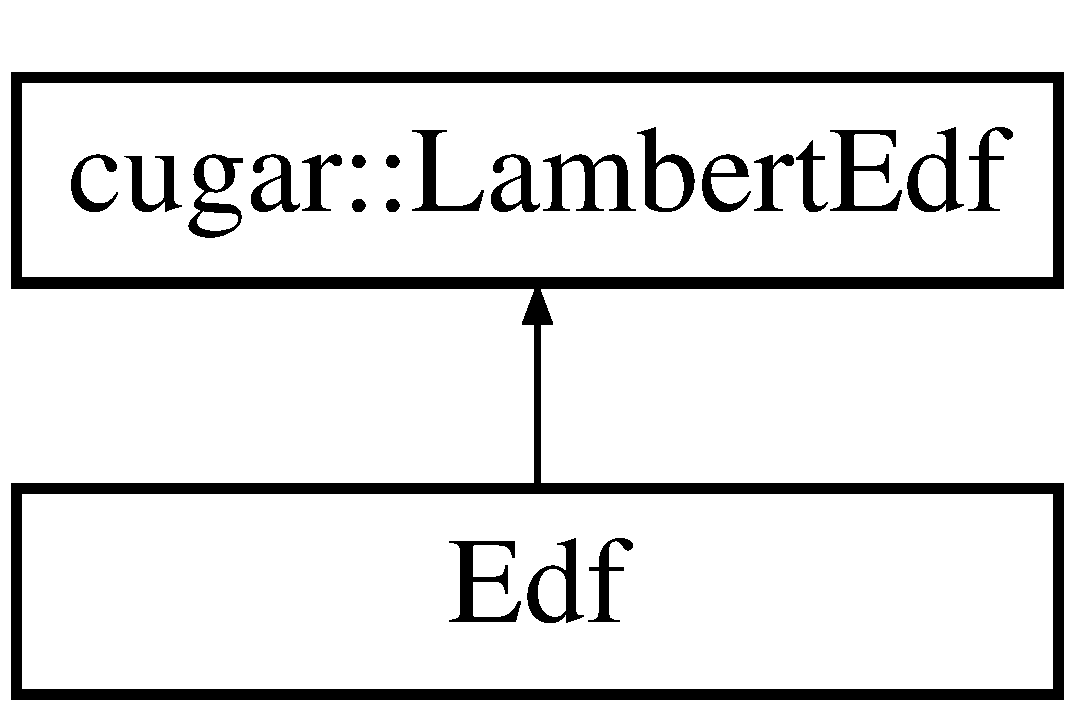
\includegraphics[height=2.000000cm]{struct_edf}
\end{center}
\end{figure}
\subsection*{Public Methods}
\begin{DoxyCompactItemize}
\item 
\mbox{\Hypertarget{struct_edf_ae2d086124211b3f540cfa31df437af3e}\label{struct_edf_ae2d086124211b3f540cfa31df437af3e}} 
F\+E\+R\+M\+A\+T\+\_\+\+H\+O\+S\+T\+\_\+\+D\+E\+V\+I\+CE {\bfseries Edf} (const \hyperlink{struct_mesh_material}{Mesh\+Material} material)
\item 
\mbox{\Hypertarget{struct_edf_ab4480c151d8548f761edd705125acecb}\label{struct_edf_ab4480c151d8548f761edd705125acecb}} 
F\+E\+R\+M\+A\+T\+\_\+\+H\+O\+S\+T\+\_\+\+D\+E\+V\+I\+CE {\bfseries Edf} (const \hyperlink{structcugar_1_1_vector}{cugar\+::\+Vector3f} emission)
\end{DoxyCompactItemize}
\subsection*{Additional Inherited Members}


The documentation for this struct was generated from the following file\+:\begin{DoxyCompactItemize}
\item 
C\+:/p4research/research/jpantaleoni/\+Fermat-\/\+Public/src/edf.\+h\end{DoxyCompactItemize}

\hypertarget{structcugar_1_1eq__constant}{}\section{cugar\+:\+:eq\+\_\+constant$<$ T $>$ Struct Template Reference}
\label{structcugar_1_1eq__constant}\index{cugar\+::eq\+\_\+constant$<$ T $>$@{cugar\+::eq\+\_\+constant$<$ T $>$}}


\subsection{Detailed description}
\subsubsection*{template$<$typename T$>$\newline
struct cugar\+::eq\+\_\+constant$<$ T $>$}

A functor to compute equality to a given constant 

{\ttfamily \#include $<$functors.\+h$>$}

\subsection*{Public Types}
\begin{DoxyCompactItemize}
\item 
\mbox{\Hypertarget{structcugar_1_1eq__constant_aeee8e91adb320633a4c3db18b72de5c3}\label{structcugar_1_1eq__constant_aeee8e91adb320633a4c3db18b72de5c3}} 
typedef \hyperlink{structcugar_1_1unary__function__tag}{unary\+\_\+function\+\_\+tag} {\bfseries function\+\_\+tag}
\item 
\mbox{\Hypertarget{structcugar_1_1eq__constant_a721d4a719390cb2d45c68eee6bfc4c50}\label{structcugar_1_1eq__constant_a721d4a719390cb2d45c68eee6bfc4c50}} 
typedef T {\bfseries argument\+\_\+type}
\item 
\mbox{\Hypertarget{structcugar_1_1eq__constant_ada81c4bebd6d3937e0ded8a4c61d172a}\label{structcugar_1_1eq__constant_ada81c4bebd6d3937e0ded8a4c61d172a}} 
typedef bool {\bfseries result\+\_\+type}
\end{DoxyCompactItemize}
\subsection*{Public Methods}
\begin{DoxyCompactItemize}
\item 
C\+U\+G\+A\+R\+\_\+\+H\+O\+S\+T\+\_\+\+D\+E\+V\+I\+CE \hyperlink{structcugar_1_1eq__constant_a0686bf3d41fa61faba5c4c231fbc5cc0}{eq\+\_\+constant} (const T c)
\item 
\mbox{\Hypertarget{structcugar_1_1eq__constant_a281cebc3ca09a5a8b744c6cf99714606}\label{structcugar_1_1eq__constant_a281cebc3ca09a5a8b744c6cf99714606}} 
C\+U\+G\+A\+R\+\_\+\+H\+O\+S\+T\+\_\+\+D\+E\+V\+I\+CE bool {\bfseries operator()} (const T \&v) const
\end{DoxyCompactItemize}


\subsection{Constructor \& Destructor Documentation}
\mbox{\Hypertarget{structcugar_1_1eq__constant_a0686bf3d41fa61faba5c4c231fbc5cc0}\label{structcugar_1_1eq__constant_a0686bf3d41fa61faba5c4c231fbc5cc0}} 
\index{cugar\+::eq\+\_\+constant@{cugar\+::eq\+\_\+constant}!eq\+\_\+constant@{eq\+\_\+constant}}
\index{eq\+\_\+constant@{eq\+\_\+constant}!cugar\+::eq\+\_\+constant@{cugar\+::eq\+\_\+constant}}
\subsubsection{\texorpdfstring{eq\+\_\+constant()}{eq\_constant()}}
{\footnotesize\ttfamily template$<$typename T $>$ \\
C\+U\+G\+A\+R\+\_\+\+H\+O\+S\+T\+\_\+\+D\+E\+V\+I\+CE \hyperlink{structcugar_1_1eq__constant}{cugar\+::eq\+\_\+constant}$<$ T $>$\+::\hyperlink{structcugar_1_1eq__constant}{eq\+\_\+constant} (\begin{DoxyParamCaption}\item[{const T}]{c }\end{DoxyParamCaption})\hspace{0.3cm}{\ttfamily [inline]}}

constructor


\begin{DoxyParams}{Parameters}
{\em c} & constant value \\
\hline
\end{DoxyParams}


The documentation for this struct was generated from the following file\+:\begin{DoxyCompactItemize}
\item 
C\+:/p4research/research/jpantaleoni/\+Fermat-\/\+Public/contrib/cugar/basic/\hyperlink{functors_8h}{functors.\+h}\end{DoxyCompactItemize}

\hypertarget{structcugar_1_1equal__functor}{}\section{cugar\+:\+:equal\+\_\+functor$<$ T $>$ Struct Template Reference}
\label{structcugar_1_1equal__functor}\index{cugar\+::equal\+\_\+functor$<$ T $>$@{cugar\+::equal\+\_\+functor$<$ T $>$}}


\subsection{Detailed description}
\subsubsection*{template$<$typename T$>$\newline
struct cugar\+::equal\+\_\+functor$<$ T $>$}

equal to functor 

{\ttfamily \#include $<$functors.\+h$>$}

\subsection*{Public Types}
\begin{DoxyCompactItemize}
\item 
\mbox{\Hypertarget{structcugar_1_1equal__functor_a22fc5b21fef69b944bc4a342de9e12f9}\label{structcugar_1_1equal__functor_a22fc5b21fef69b944bc4a342de9e12f9}} 
typedef \hyperlink{structcugar_1_1binary__function__tag}{binary\+\_\+function\+\_\+tag} {\bfseries function\+\_\+tag}
\item 
\mbox{\Hypertarget{structcugar_1_1equal__functor_a0afcdd3f576151df76f4fd5e1d3a27e0}\label{structcugar_1_1equal__functor_a0afcdd3f576151df76f4fd5e1d3a27e0}} 
typedef T {\bfseries first\+\_\+argument\+\_\+type}
\item 
\mbox{\Hypertarget{structcugar_1_1equal__functor_a1ad7f2a53c8aacd56de2a20f19dc808f}\label{structcugar_1_1equal__functor_a1ad7f2a53c8aacd56de2a20f19dc808f}} 
typedef T {\bfseries second\+\_\+argument\+\_\+type}
\item 
\mbox{\Hypertarget{structcugar_1_1equal__functor_a06c32ac0d18c2347f2c588a3217d4426}\label{structcugar_1_1equal__functor_a06c32ac0d18c2347f2c588a3217d4426}} 
typedef bool {\bfseries result\+\_\+type}
\end{DoxyCompactItemize}
\subsection*{Public Methods}
\begin{DoxyCompactItemize}
\item 
\mbox{\Hypertarget{structcugar_1_1equal__functor_a2ea67afc9455aa6cc02e28366fea0aa1}\label{structcugar_1_1equal__functor_a2ea67afc9455aa6cc02e28366fea0aa1}} 
C\+U\+G\+A\+R\+\_\+\+H\+O\+S\+T\+\_\+\+D\+E\+V\+I\+CE bool {\bfseries operator()} (const T \&op1, const T \&op2) const
\end{DoxyCompactItemize}


The documentation for this struct was generated from the following file\+:\begin{DoxyCompactItemize}
\item 
C\+:/p4research/research/jpantaleoni/\+Fermat-\/\+Public/contrib/cugar/basic/\hyperlink{functors_8h}{functors.\+h}\end{DoxyCompactItemize}

\hypertarget{structcugar_1_1_exponential__distribution}{}\section{cugar\+:\+:Exponential\+\_\+distribution Struct Reference}
\label{structcugar_1_1_exponential__distribution}\index{cugar\+::\+Exponential\+\_\+distribution@{cugar\+::\+Exponential\+\_\+distribution}}


\subsection{Detailed description}
Exponential distribution 

{\ttfamily \#include $<$distributions.\+h$>$}

Inheritance diagram for cugar\+:\+:Exponential\+\_\+distribution\+:\begin{figure}[H]
\begin{center}
\leavevmode
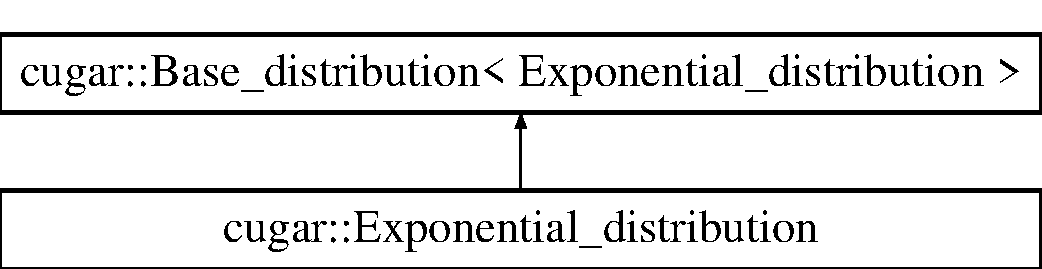
\includegraphics[height=2.000000cm]{structcugar_1_1_exponential__distribution}
\end{center}
\end{figure}
\subsection*{Public Methods}
\begin{DoxyCompactItemize}
\item 
C\+U\+G\+A\+R\+\_\+\+H\+O\+S\+T\+\_\+\+D\+E\+V\+I\+CE \hyperlink{structcugar_1_1_exponential__distribution_aea929c1395b07a67ecbaa15a9c51f8e7}{Exponential\+\_\+distribution} (const float lambda)
\item 
C\+U\+G\+A\+R\+\_\+\+H\+O\+S\+T\+\_\+\+D\+E\+V\+I\+CE float \hyperlink{structcugar_1_1_exponential__distribution_a3af4566629aa9d4d4488b3795a53c4ee}{map} (const float U) const
\item 
C\+U\+G\+A\+R\+\_\+\+H\+O\+S\+T\+\_\+\+D\+E\+V\+I\+CE float \hyperlink{structcugar_1_1_exponential__distribution_a23a3999512db509214ac2e6a0ee2c4ef}{density} (const float x) const
\end{DoxyCompactItemize}


\subsection{Constructor \& Destructor Documentation}
\mbox{\Hypertarget{structcugar_1_1_exponential__distribution_aea929c1395b07a67ecbaa15a9c51f8e7}\label{structcugar_1_1_exponential__distribution_aea929c1395b07a67ecbaa15a9c51f8e7}} 
\index{cugar\+::\+Exponential\+\_\+distribution@{cugar\+::\+Exponential\+\_\+distribution}!Exponential\+\_\+distribution@{Exponential\+\_\+distribution}}
\index{Exponential\+\_\+distribution@{Exponential\+\_\+distribution}!cugar\+::\+Exponential\+\_\+distribution@{cugar\+::\+Exponential\+\_\+distribution}}
\subsubsection{\texorpdfstring{Exponential\+\_\+distribution()}{Exponential\_distribution()}}
{\footnotesize\ttfamily C\+U\+G\+A\+R\+\_\+\+H\+O\+S\+T\+\_\+\+D\+E\+V\+I\+CE cugar\+::\+Exponential\+\_\+distribution\+::\+Exponential\+\_\+distribution (\begin{DoxyParamCaption}\item[{const float}]{lambda }\end{DoxyParamCaption})\hspace{0.3cm}{\ttfamily [inline]}}

constructor


\begin{DoxyParams}{Parameters}
{\em lambda} & distribution parameter \\
\hline
\end{DoxyParams}


\subsection{Member Function Documentation}
\mbox{\Hypertarget{structcugar_1_1_exponential__distribution_a23a3999512db509214ac2e6a0ee2c4ef}\label{structcugar_1_1_exponential__distribution_a23a3999512db509214ac2e6a0ee2c4ef}} 
\index{cugar\+::\+Exponential\+\_\+distribution@{cugar\+::\+Exponential\+\_\+distribution}!density@{density}}
\index{density@{density}!cugar\+::\+Exponential\+\_\+distribution@{cugar\+::\+Exponential\+\_\+distribution}}
\subsubsection{\texorpdfstring{density()}{density()}}
{\footnotesize\ttfamily C\+U\+G\+A\+R\+\_\+\+H\+O\+S\+T\+\_\+\+D\+E\+V\+I\+CE float cugar\+::\+Exponential\+\_\+distribution\+::density (\begin{DoxyParamCaption}\item[{const float}]{x }\end{DoxyParamCaption}) const\hspace{0.3cm}{\ttfamily [inline]}}

probability density function


\begin{DoxyParams}{Parameters}
{\em x} & sample location \\
\hline
\end{DoxyParams}
\mbox{\Hypertarget{structcugar_1_1_exponential__distribution_a3af4566629aa9d4d4488b3795a53c4ee}\label{structcugar_1_1_exponential__distribution_a3af4566629aa9d4d4488b3795a53c4ee}} 
\index{cugar\+::\+Exponential\+\_\+distribution@{cugar\+::\+Exponential\+\_\+distribution}!map@{map}}
\index{map@{map}!cugar\+::\+Exponential\+\_\+distribution@{cugar\+::\+Exponential\+\_\+distribution}}
\subsubsection{\texorpdfstring{map()}{map()}}
{\footnotesize\ttfamily C\+U\+G\+A\+R\+\_\+\+H\+O\+S\+T\+\_\+\+D\+E\+V\+I\+CE float cugar\+::\+Exponential\+\_\+distribution\+::map (\begin{DoxyParamCaption}\item[{const float}]{U }\end{DoxyParamCaption}) const\hspace{0.3cm}{\ttfamily [inline]}}

transform a uniformly distributed number through the distribution


\begin{DoxyParams}{Parameters}
{\em U} & real number to transform \\
\hline
\end{DoxyParams}


The documentation for this struct was generated from the following file\+:\begin{DoxyCompactItemize}
\item 
C\+:/p4research/research/jpantaleoni/\+Fermat-\/\+Public/contrib/cugar/sampling/\hyperlink{distributions_8h}{distributions.\+h}\end{DoxyCompactItemize}

\hypertarget{struct_eye_vertex}{}\section{Eye\+Vertex Struct Reference}
\label{struct_eye_vertex}\index{Eye\+Vertex@{Eye\+Vertex}}


\subsection{Detailed description}
\begin{DoxyParagraph}{}
A utility class to encapsulate all important information for a eye subpath vertex 
\end{DoxyParagraph}


{\ttfamily \#include $<$bpt\+\_\+utils.\+h$>$}

\subsection*{Public Methods}
\begin{DoxyCompactItemize}
\item 
\mbox{\Hypertarget{struct_eye_vertex_a5788cce324807dd8bbc0f913ef3a777d}\label{struct_eye_vertex_a5788cce324807dd8bbc0f913ef3a777d}} 
{\footnotesize template$<$typename Ray\+Type $>$ }\\F\+E\+R\+M\+A\+T\+\_\+\+H\+O\+S\+T\+\_\+\+D\+E\+V\+I\+CE void {\bfseries setup} (const Ray\+Type \&ray, const \hyperlink{struct_hit}{Hit} \&hit, const \hyperlink{structcugar_1_1_vector}{cugar\+::\+Vector3f} \&\+\_\+alpha, const \hyperlink{struct_temp_path_weights}{Temp\+Path\+Weights} \&\+\_\+weights, const uint32 \+\_\+depth, const \hyperlink{struct_rendering_context_view}{Rendering\+Context\+View} \&renderer, const float min\+\_\+roughness=0.\+0f)
\item 
\mbox{\Hypertarget{struct_eye_vertex_aa88f1c1bd1c6e1f8ae1f9df6f857f72f}\label{struct_eye_vertex_aa88f1c1bd1c6e1f8ae1f9df6f857f72f}} 
F\+E\+R\+M\+A\+T\+\_\+\+H\+O\+S\+T\+\_\+\+D\+E\+V\+I\+CE void {\bfseries setup} (const \hyperlink{structcugar_1_1_vector}{cugar\+::\+Vector3f} \&\+\_\+in, const \hyperlink{struct_vertex_geometry_id}{Vertex\+Geometry\+Id} \&\+\_\+v, const \hyperlink{structcugar_1_1_vector}{cugar\+::\+Vector3f} \&\+\_\+alpha, const \hyperlink{struct_temp_path_weights}{Temp\+Path\+Weights} \&\+\_\+weights, const uint32 \+\_\+depth, const \hyperlink{struct_rendering_context_view}{Rendering\+Context\+View} \&renderer)
\item 
\mbox{\Hypertarget{struct_eye_vertex_a861d531288458ca4d465c2b93c65e1aa}\label{struct_eye_vertex_a861d531288458ca4d465c2b93c65e1aa}} 
F\+E\+R\+M\+A\+T\+\_\+\+H\+O\+S\+T\+\_\+\+D\+E\+V\+I\+CE {\bfseries Eye\+Vertex} (const \hyperlink{struct_ray}{Ray} \&\+\_\+ray, const \hyperlink{struct_hit}{Hit} \&\+\_\+hit, const \hyperlink{structcugar_1_1_vector}{cugar\+::\+Vector3f} \&\+\_\+alpha, const \hyperlink{struct_temp_path_weights}{Temp\+Path\+Weights} \&\+\_\+weights, const uint32 \+\_\+depth, const \hyperlink{struct_rendering_context_view}{Rendering\+Context\+View} \&renderer)
\item 
\mbox{\Hypertarget{struct_eye_vertex_a03db55c18029b0792be1843821f01d20}\label{struct_eye_vertex_a03db55c18029b0792be1843821f01d20}} 
F\+E\+R\+M\+A\+T\+\_\+\+H\+O\+S\+T\+\_\+\+D\+E\+V\+I\+CE {\bfseries Eye\+Vertex} (const \hyperlink{structcugar_1_1_vector}{cugar\+::\+Vector3f} \&\+\_\+in, const \hyperlink{struct_vertex_geometry_id}{Vertex\+Geometry\+Id} \&\+\_\+v, const \hyperlink{structcugar_1_1_vector}{cugar\+::\+Vector3f} \&\+\_\+alpha, const \hyperlink{struct_temp_path_weights}{Temp\+Path\+Weights} \&\+\_\+weights, const uint32 \+\_\+depth, const \hyperlink{struct_rendering_context_view}{Rendering\+Context\+View} \&renderer)
\item 
F\+E\+R\+M\+A\+T\+\_\+\+H\+O\+S\+T\+\_\+\+D\+E\+V\+I\+CE F\+E\+R\+M\+A\+T\+\_\+\+F\+O\+R\+C\+E\+I\+N\+L\+I\+NE bool \hyperlink{struct_eye_vertex_a7664ec5102f1894a1cd55c324c0742ee}{sample} (const float z\mbox{[}3\mbox{]}, \hyperlink{struct_bsdf_a5f7db6f81220ed9ee6da109d6eb5b585}{Bsdf\+::\+Component\+Type} \&out\+\_\+comp, \hyperlink{structcugar_1_1_vector}{cugar\+::\+Vector3f} \&out, float \&out\+\_\+p, float \&out\+\_\+p\+\_\+proj, \hyperlink{structcugar_1_1_vector}{cugar\+::\+Vector3f} \&out\+\_\+g, bool RR=true, bool evaluate\+\_\+full\+\_\+bsdf=false, const \hyperlink{struct_bsdf_a5f7db6f81220ed9ee6da109d6eb5b585}{Bsdf\+::\+Component\+Type} components=Bsdf\+::k\+All\+Components) const
\end{DoxyCompactItemize}
\subsection*{Public Members}
\begin{DoxyCompactItemize}
\item 
\mbox{\Hypertarget{struct_eye_vertex_a52e6212e480d4cab3efdccc98ebea913}\label{struct_eye_vertex_a52e6212e480d4cab3efdccc98ebea913}} 
\hyperlink{struct_vertex_geometry_id}{Vertex\+Geometry\+Id} {\bfseries geom\+\_\+id}
\item 
\mbox{\Hypertarget{struct_eye_vertex_ab1b42b63a7e9daeb9fa5b3557a0a7f6a}\label{struct_eye_vertex_ab1b42b63a7e9daeb9fa5b3557a0a7f6a}} 
\hyperlink{struct_vertex_geometry}{Vertex\+Geometry} {\bfseries geom}
\item 
\mbox{\Hypertarget{struct_eye_vertex_a5cccc691e6e2eddd5dff10950d34c85c}\label{struct_eye_vertex_a5cccc691e6e2eddd5dff10950d34c85c}} 
\hyperlink{structcugar_1_1_vector}{cugar\+::\+Vector3f} {\bfseries in}
\item 
\mbox{\Hypertarget{struct_eye_vertex_a8c99479110de6457d40dd4ddf4f85df5}\label{struct_eye_vertex_a8c99479110de6457d40dd4ddf4f85df5}} 
\hyperlink{structcugar_1_1_vector}{cugar\+::\+Vector3f} {\bfseries alpha}
\item 
\mbox{\Hypertarget{struct_eye_vertex_ac9f43974b9afd495ad333da6d3233067}\label{struct_eye_vertex_ac9f43974b9afd495ad333da6d3233067}} 
\hyperlink{struct_temp_path_weights}{Temp\+Path\+Weights} {\bfseries weights}
\item 
\mbox{\Hypertarget{struct_eye_vertex_ae141b6cf0d021eea9fb7d2b1fe3e5105}\label{struct_eye_vertex_ae141b6cf0d021eea9fb7d2b1fe3e5105}} 
uint32 {\bfseries depth}
\item 
\mbox{\Hypertarget{struct_eye_vertex_a3cbea0a0b50e42fa39947122c15138c3}\label{struct_eye_vertex_a3cbea0a0b50e42fa39947122c15138c3}} 
\hyperlink{struct_mesh_material}{Mesh\+Material} {\bfseries material}
\item 
\mbox{\Hypertarget{struct_eye_vertex_a1de7132c5682503c202e251162aaa96c}\label{struct_eye_vertex_a1de7132c5682503c202e251162aaa96c}} 
\hyperlink{struct_bsdf}{Bsdf} {\bfseries bsdf}
\item 
\mbox{\Hypertarget{struct_eye_vertex_aa9f190a1fafa32114d27e0ad5de9827a}\label{struct_eye_vertex_aa9f190a1fafa32114d27e0ad5de9827a}} 
float {\bfseries prev\+\_\+\+G\+\_\+prime}
\item 
\mbox{\Hypertarget{struct_eye_vertex_a530f31d442fc23ee8c16fd951fa0a0ea}\label{struct_eye_vertex_a530f31d442fc23ee8c16fd951fa0a0ea}} 
float {\bfseries prev\+\_\+pG}
\item 
\mbox{\Hypertarget{struct_eye_vertex_ac0ece106e60201d212d9c0ab082b2d81}\label{struct_eye_vertex_ac0ece106e60201d212d9c0ab082b2d81}} 
float {\bfseries p\+Gp\+\_\+sum}
\end{DoxyCompactItemize}


\subsection{Member Function Documentation}
\mbox{\Hypertarget{struct_eye_vertex_a7664ec5102f1894a1cd55c324c0742ee}\label{struct_eye_vertex_a7664ec5102f1894a1cd55c324c0742ee}} 
\index{Eye\+Vertex@{Eye\+Vertex}!sample@{sample}}
\index{sample@{sample}!Eye\+Vertex@{Eye\+Vertex}}
\subsubsection{\texorpdfstring{sample()}{sample()}}
{\footnotesize\ttfamily F\+E\+R\+M\+A\+T\+\_\+\+H\+O\+S\+T\+\_\+\+D\+E\+V\+I\+CE F\+E\+R\+M\+A\+T\+\_\+\+F\+O\+R\+C\+E\+I\+N\+L\+I\+NE bool Eye\+Vertex\+::sample (\begin{DoxyParamCaption}\item[{const float}]{z\mbox{[}3\mbox{]},  }\item[{\hyperlink{struct_bsdf_a5f7db6f81220ed9ee6da109d6eb5b585}{Bsdf\+::\+Component\+Type} \&}]{out\+\_\+comp,  }\item[{\hyperlink{structcugar_1_1_vector}{cugar\+::\+Vector3f} \&}]{out,  }\item[{float \&}]{out\+\_\+p,  }\item[{float \&}]{out\+\_\+p\+\_\+proj,  }\item[{\hyperlink{structcugar_1_1_vector}{cugar\+::\+Vector3f} \&}]{out\+\_\+g,  }\item[{bool}]{RR = {\ttfamily true},  }\item[{bool}]{evaluate\+\_\+full\+\_\+bsdf = {\ttfamily false},  }\item[{const \hyperlink{struct_bsdf_a5f7db6f81220ed9ee6da109d6eb5b585}{Bsdf\+::\+Component\+Type}}]{components = {\ttfamily Bsdf\+:\+:kAllComponents} }\end{DoxyParamCaption}) const\hspace{0.3cm}{\ttfamily [inline]}}

sample an outgoing direction


\begin{DoxyParams}{Parameters}
{\em z} & the incoming direction \\
\hline
{\em out\+\_\+comp} & the output component \\
\hline
{\em out} & the outgoing direction \\
\hline
{\em out\+\_\+p} & the output solid angle pdf \\
\hline
{\em out\+\_\+p\+\_\+proj} & the output projected solid angle pdf \\
\hline
{\em out\+\_\+g} & the output sample value = f/p\+\_\+proj \\
\hline
{\em RR} & indicate whether to use Russian-\/\+Roulette or not \\
\hline
{\em evaluate\+\_\+full\+\_\+bsdf} & ndicate whether to evaluate the full B\+S\+DF, or just an unbiased estimate \\
\hline
{\em components} & the components to consider \\
\hline
\end{DoxyParams}


The documentation for this struct was generated from the following file\+:\begin{DoxyCompactItemize}
\item 
C\+:/p4research/research/jpantaleoni/\+Fermat-\/\+Public/src/bpt\+\_\+utils.\+h\end{DoxyCompactItemize}

\hypertarget{structcugar_1_1_fake_timer}{}\section{cugar\+:\+:Fake\+Timer Struct Reference}
\label{structcugar_1_1_fake_timer}\index{cugar\+::\+Fake\+Timer@{cugar\+::\+Fake\+Timer}}


\subsection{Detailed description}
A zero-\/overhead timer which doesn\textquotesingle{}t do any timing... 

{\ttfamily \#include $<$timer.\+h$>$}

\subsection*{Public Methods}
\begin{DoxyCompactItemize}
\item 
\mbox{\Hypertarget{structcugar_1_1_fake_timer_a3a0ca12091e98712862c1a35aef06015}\label{structcugar_1_1_fake_timer_a3a0ca12091e98712862c1a35aef06015}} 
void {\bfseries start} ()
\item 
\mbox{\Hypertarget{structcugar_1_1_fake_timer_ac7094f08423256311f7aa7f1619cf498}\label{structcugar_1_1_fake_timer_ac7094f08423256311f7aa7f1619cf498}} 
void {\bfseries stop} ()
\item 
\mbox{\Hypertarget{structcugar_1_1_fake_timer_af42040609903f481b4553e2c7a69cdd2}\label{structcugar_1_1_fake_timer_af42040609903f481b4553e2c7a69cdd2}} 
float {\bfseries seconds} () const
\end{DoxyCompactItemize}


The documentation for this struct was generated from the following file\+:\begin{DoxyCompactItemize}
\item 
C\+:/p4research/research/jpantaleoni/\+Fermat-\/\+Public/contrib/cugar/basic/timer.\+h\end{DoxyCompactItemize}

\hypertarget{struct_f_buffer_channel_storage}{}\section{F\+Buffer\+Channel\+Storage Struct Reference}
\label{struct_f_buffer_channel_storage}\index{F\+Buffer\+Channel\+Storage@{F\+Buffer\+Channel\+Storage}}


\subsection{Detailed description}
Framebuffer channel storage class, to be used from the host to allocate frame-\/buffer storage 

{\ttfamily \#include $<$framebuffer.\+h$>$}

\subsection*{Public Methods}
\begin{DoxyCompactItemize}
\item 
\mbox{\Hypertarget{struct_f_buffer_channel_storage_afc136c51ec78c859c6019ac4493ec884}\label{struct_f_buffer_channel_storage_afc136c51ec78c859c6019ac4493ec884}} 
float4 {\bfseries operator()} (const uint32\+\_\+t pixel) const
\item 
\mbox{\Hypertarget{struct_f_buffer_channel_storage_ad53a855e5bc7b04153f41f97bcf52bbf}\label{struct_f_buffer_channel_storage_ad53a855e5bc7b04153f41f97bcf52bbf}} 
float4 {\bfseries operator()} (const uint32\+\_\+t x, const uint32\+\_\+t y) const
\item 
\mbox{\Hypertarget{struct_f_buffer_channel_storage_a1ee9767232c6d6f85dcc0a2cc1b9fa05}\label{struct_f_buffer_channel_storage_a1ee9767232c6d6f85dcc0a2cc1b9fa05}} 
const float4 $\ast$ {\bfseries ptr} () const
\item 
\mbox{\Hypertarget{struct_f_buffer_channel_storage_aefc013d6d0e2126fb99971fb71d6fc80}\label{struct_f_buffer_channel_storage_aefc013d6d0e2126fb99971fb71d6fc80}} 
float4 $\ast$ {\bfseries ptr} ()
\item 
void \hyperlink{struct_f_buffer_channel_storage_a183964cd1e00171df5eb4c2130db6c44}{resize} (const uint32\+\_\+t \+\_\+res\+\_\+x, const uint32\+\_\+t \+\_\+res\+\_\+y)
\item 
size\+\_\+t \hyperlink{struct_f_buffer_channel_storage_ace7afe67f49b4a628653dd42a5e39147}{size} () const
\item 
void \hyperlink{struct_f_buffer_channel_storage_a329a7a82c5c066eb4910cdf1694ae38c}{clear} ()
\item 
\hyperlink{struct_f_buffer_channel_storage}{F\+Buffer\+Channel\+Storage} \& \hyperlink{struct_f_buffer_channel_storage_a071ed06855db0e5fe595b6b7d8757fda}{operator=} (\hyperlink{struct_f_buffer_channel_storage}{F\+Buffer\+Channel\+Storage} \&other)
\item 
\hyperlink{struct_f_buffer_channel_view}{F\+Buffer\+Channel\+View} \hyperlink{struct_f_buffer_channel_storage_a1be90e5b134cb810c2497a66d2ac7b12}{view} ()
\item 
void \hyperlink{struct_f_buffer_channel_storage_adff7d04a3c7da747d662403c930c4074}{swap} (\hyperlink{struct_f_buffer_channel_storage}{F\+Buffer\+Channel\+Storage} \&other)
\end{DoxyCompactItemize}
\subsection*{Public Members}
\begin{DoxyCompactItemize}
\item 
\mbox{\Hypertarget{struct_f_buffer_channel_storage_a3e84f2025da610cce330d7dd2e558ba6}\label{struct_f_buffer_channel_storage_a3e84f2025da610cce330d7dd2e558ba6}} 
uint32\+\_\+t {\bfseries res\+\_\+x}
\item 
\mbox{\Hypertarget{struct_f_buffer_channel_storage_a8a237bd2ab9f0675ab0083187398a806}\label{struct_f_buffer_channel_storage_a8a237bd2ab9f0675ab0083187398a806}} 
uint32\+\_\+t {\bfseries res\+\_\+y}
\item 
\mbox{\Hypertarget{struct_f_buffer_channel_storage_a2d1131bcca4bd4f2df3b74aeae1badc4}\label{struct_f_buffer_channel_storage_a2d1131bcca4bd4f2df3b74aeae1badc4}} 
\hyperlink{class_domain_buffer}{Domain\+Buffer}$<$ C\+U\+D\+A\+\_\+\+B\+U\+F\+F\+ER, float4 $>$ {\bfseries c}
\end{DoxyCompactItemize}


\subsection{Member Function Documentation}
\mbox{\Hypertarget{struct_f_buffer_channel_storage_a329a7a82c5c066eb4910cdf1694ae38c}\label{struct_f_buffer_channel_storage_a329a7a82c5c066eb4910cdf1694ae38c}} 
\index{F\+Buffer\+Channel\+Storage@{F\+Buffer\+Channel\+Storage}!clear@{clear}}
\index{clear@{clear}!F\+Buffer\+Channel\+Storage@{F\+Buffer\+Channel\+Storage}}
\subsubsection{\texorpdfstring{clear()}{clear()}}
{\footnotesize\ttfamily void F\+Buffer\+Channel\+Storage\+::clear (\begin{DoxyParamCaption}{ }\end{DoxyParamCaption})\hspace{0.3cm}{\ttfamily [inline]}}

clear the channel with zeros \mbox{\Hypertarget{struct_f_buffer_channel_storage_a071ed06855db0e5fe595b6b7d8757fda}\label{struct_f_buffer_channel_storage_a071ed06855db0e5fe595b6b7d8757fda}} 
\index{F\+Buffer\+Channel\+Storage@{F\+Buffer\+Channel\+Storage}!operator=@{operator=}}
\index{operator=@{operator=}!F\+Buffer\+Channel\+Storage@{F\+Buffer\+Channel\+Storage}}
\subsubsection{\texorpdfstring{operator=()}{operator=()}}
{\footnotesize\ttfamily \hyperlink{struct_f_buffer_channel_storage}{F\+Buffer\+Channel\+Storage}\& F\+Buffer\+Channel\+Storage\+::operator= (\begin{DoxyParamCaption}\item[{\hyperlink{struct_f_buffer_channel_storage}{F\+Buffer\+Channel\+Storage} \&}]{other }\end{DoxyParamCaption})\hspace{0.3cm}{\ttfamily [inline]}}

copy the channel from another source \mbox{\Hypertarget{struct_f_buffer_channel_storage_a183964cd1e00171df5eb4c2130db6c44}\label{struct_f_buffer_channel_storage_a183964cd1e00171df5eb4c2130db6c44}} 
\index{F\+Buffer\+Channel\+Storage@{F\+Buffer\+Channel\+Storage}!resize@{resize}}
\index{resize@{resize}!F\+Buffer\+Channel\+Storage@{F\+Buffer\+Channel\+Storage}}
\subsubsection{\texorpdfstring{resize()}{resize()}}
{\footnotesize\ttfamily void F\+Buffer\+Channel\+Storage\+::resize (\begin{DoxyParamCaption}\item[{const uint32\+\_\+t}]{\+\_\+res\+\_\+x,  }\item[{const uint32\+\_\+t}]{\+\_\+res\+\_\+y }\end{DoxyParamCaption})\hspace{0.3cm}{\ttfamily [inline]}}

set the resolution \mbox{\Hypertarget{struct_f_buffer_channel_storage_ace7afe67f49b4a628653dd42a5e39147}\label{struct_f_buffer_channel_storage_ace7afe67f49b4a628653dd42a5e39147}} 
\index{F\+Buffer\+Channel\+Storage@{F\+Buffer\+Channel\+Storage}!size@{size}}
\index{size@{size}!F\+Buffer\+Channel\+Storage@{F\+Buffer\+Channel\+Storage}}
\subsubsection{\texorpdfstring{size()}{size()}}
{\footnotesize\ttfamily size\+\_\+t F\+Buffer\+Channel\+Storage\+::size (\begin{DoxyParamCaption}{ }\end{DoxyParamCaption}) const\hspace{0.3cm}{\ttfamily [inline]}}

return the total number of pixels \mbox{\Hypertarget{struct_f_buffer_channel_storage_adff7d04a3c7da747d662403c930c4074}\label{struct_f_buffer_channel_storage_adff7d04a3c7da747d662403c930c4074}} 
\index{F\+Buffer\+Channel\+Storage@{F\+Buffer\+Channel\+Storage}!swap@{swap}}
\index{swap@{swap}!F\+Buffer\+Channel\+Storage@{F\+Buffer\+Channel\+Storage}}
\subsubsection{\texorpdfstring{swap()}{swap()}}
{\footnotesize\ttfamily void F\+Buffer\+Channel\+Storage\+::swap (\begin{DoxyParamCaption}\item[{\hyperlink{struct_f_buffer_channel_storage}{F\+Buffer\+Channel\+Storage} \&}]{other }\end{DoxyParamCaption})\hspace{0.3cm}{\ttfamily [inline]}}

swap with another framebuffer channel \mbox{\Hypertarget{struct_f_buffer_channel_storage_a1be90e5b134cb810c2497a66d2ac7b12}\label{struct_f_buffer_channel_storage_a1be90e5b134cb810c2497a66d2ac7b12}} 
\index{F\+Buffer\+Channel\+Storage@{F\+Buffer\+Channel\+Storage}!view@{view}}
\index{view@{view}!F\+Buffer\+Channel\+Storage@{F\+Buffer\+Channel\+Storage}}
\subsubsection{\texorpdfstring{view()}{view()}}
{\footnotesize\ttfamily \hyperlink{struct_f_buffer_channel_view}{F\+Buffer\+Channel\+View} F\+Buffer\+Channel\+Storage\+::view (\begin{DoxyParamCaption}{ }\end{DoxyParamCaption})\hspace{0.3cm}{\ttfamily [inline]}}

return a view object 

The documentation for this struct was generated from the following file\+:\begin{DoxyCompactItemize}
\item 
C\+:/p4research/research/jpantaleoni/\+Fermat-\/\+Public/src/framebuffer.\+h\end{DoxyCompactItemize}

\hypertarget{struct_f_buffer_channel_view}{}\section{F\+Buffer\+Channel\+View Struct Reference}
\label{struct_f_buffer_channel_view}\index{F\+Buffer\+Channel\+View@{F\+Buffer\+Channel\+View}}


\subsection{Detailed description}
Framebuffer channel view object, to be used within C\+U\+DA kernels 

{\ttfamily \#include $<$framebuffer.\+h$>$}

\subsection*{Public Methods}
\begin{DoxyCompactItemize}
\item 
\mbox{\Hypertarget{struct_f_buffer_channel_view_a75852896b2d3c5a9f23903112a1f969f}\label{struct_f_buffer_channel_view_a75852896b2d3c5a9f23903112a1f969f}} 
F\+E\+R\+M\+A\+T\+\_\+\+H\+O\+S\+T\+\_\+\+D\+E\+V\+I\+CE float4 \& {\bfseries operator()} (const uint32\+\_\+t pixel)
\item 
\mbox{\Hypertarget{struct_f_buffer_channel_view_a3bb7bcc18eabf1a374a1ed0e551033e4}\label{struct_f_buffer_channel_view_a3bb7bcc18eabf1a374a1ed0e551033e4}} 
F\+E\+R\+M\+A\+T\+\_\+\+H\+O\+S\+T\+\_\+\+D\+E\+V\+I\+CE const float4 \& {\bfseries operator()} (const uint32\+\_\+t pixel) const
\item 
\mbox{\Hypertarget{struct_f_buffer_channel_view_ac98c591f7732d2ab8403a903ab2d4081}\label{struct_f_buffer_channel_view_ac98c591f7732d2ab8403a903ab2d4081}} 
F\+E\+R\+M\+A\+T\+\_\+\+H\+O\+S\+T\+\_\+\+D\+E\+V\+I\+CE float4 \& {\bfseries operator()} (const uint32\+\_\+t x, const uint32\+\_\+t y)
\item 
\mbox{\Hypertarget{struct_f_buffer_channel_view_a48356e00b130fd214e0ae3eee581b352}\label{struct_f_buffer_channel_view_a48356e00b130fd214e0ae3eee581b352}} 
F\+E\+R\+M\+A\+T\+\_\+\+H\+O\+S\+T\+\_\+\+D\+E\+V\+I\+CE const float4 \& {\bfseries operator()} (const uint32\+\_\+t x, const uint32\+\_\+t y) const
\item 
\mbox{\Hypertarget{struct_f_buffer_channel_view_a2a6b2520750c6d024d93fb1839a6b9ff}\label{struct_f_buffer_channel_view_a2a6b2520750c6d024d93fb1839a6b9ff}} 
F\+E\+R\+M\+A\+T\+\_\+\+H\+O\+S\+T\+\_\+\+D\+E\+V\+I\+CE float4 \& {\bfseries operator()} (const uint2 pixel)
\item 
\mbox{\Hypertarget{struct_f_buffer_channel_view_aabf1b7b4320bee4ea3e5503b20395b22}\label{struct_f_buffer_channel_view_aabf1b7b4320bee4ea3e5503b20395b22}} 
F\+E\+R\+M\+A\+T\+\_\+\+H\+O\+S\+T\+\_\+\+D\+E\+V\+I\+CE const float4 \& {\bfseries operator()} (const uint2 pixel) const
\item 
\mbox{\Hypertarget{struct_f_buffer_channel_view_a8fb530e09e406d506ef56cbc70894e2e}\label{struct_f_buffer_channel_view_a8fb530e09e406d506ef56cbc70894e2e}} 
F\+E\+R\+M\+A\+T\+\_\+\+H\+O\+S\+T\+\_\+\+D\+E\+V\+I\+CE float4 \& {\bfseries operator()} (const int2 pixel)
\item 
\mbox{\Hypertarget{struct_f_buffer_channel_view_a16f431b3c21b7cc2155dd410561f0a59}\label{struct_f_buffer_channel_view_a16f431b3c21b7cc2155dd410561f0a59}} 
F\+E\+R\+M\+A\+T\+\_\+\+H\+O\+S\+T\+\_\+\+D\+E\+V\+I\+CE const float4 \& {\bfseries operator()} (const int2 pixel) const
\item 
\mbox{\Hypertarget{struct_f_buffer_channel_view_a1c1aeb9ff121928eaa7de61b9c79f137}\label{struct_f_buffer_channel_view_a1c1aeb9ff121928eaa7de61b9c79f137}} 
F\+E\+R\+M\+A\+T\+\_\+\+H\+O\+S\+T\+\_\+\+D\+E\+V\+I\+CE const float4 $\ast$ {\bfseries ptr} () const
\item 
\mbox{\Hypertarget{struct_f_buffer_channel_view_a4b6441a11b931d336a1565f81306508f}\label{struct_f_buffer_channel_view_a4b6441a11b931d336a1565f81306508f}} 
F\+E\+R\+M\+A\+T\+\_\+\+H\+O\+S\+T\+\_\+\+D\+E\+V\+I\+CE float4 $\ast$ {\bfseries ptr} ()
\end{DoxyCompactItemize}
\subsection*{Public Members}
\begin{DoxyCompactItemize}
\item 
\mbox{\Hypertarget{struct_f_buffer_channel_view_a4d7c34a0fb5d174093147fd4d8c9f33f}\label{struct_f_buffer_channel_view_a4d7c34a0fb5d174093147fd4d8c9f33f}} 
float4 $\ast$ {\bfseries c\+\_\+ptr}
\item 
\mbox{\Hypertarget{struct_f_buffer_channel_view_abbdde4f6883fa3d082cb39e713f96ae3}\label{struct_f_buffer_channel_view_abbdde4f6883fa3d082cb39e713f96ae3}} 
uint32\+\_\+t {\bfseries res\+\_\+x}
\item 
\mbox{\Hypertarget{struct_f_buffer_channel_view_a8b500a1a6086870c8bba6028a34aa795}\label{struct_f_buffer_channel_view_a8b500a1a6086870c8bba6028a34aa795}} 
uint32\+\_\+t {\bfseries res\+\_\+y}
\end{DoxyCompactItemize}


The documentation for this struct was generated from the following file\+:\begin{DoxyCompactItemize}
\item 
C\+:/p4research/research/jpantaleoni/\+Fermat-\/\+Public/src/framebuffer.\+h\end{DoxyCompactItemize}

\hypertarget{struct_f_buffer_desc}{}\section{F\+Buffer\+Desc Struct Reference}
\label{struct_f_buffer_desc}\index{F\+Buffer\+Desc@{F\+Buffer\+Desc}}
\subsection*{Static Public Members}
\begin{DoxyCompactItemize}
\item 
\mbox{\Hypertarget{struct_f_buffer_desc_a3097c931b229ccb29ac02776dbd85c01}\label{struct_f_buffer_desc_a3097c931b229ccb29ac02776dbd85c01}} 
static const uint32\+\_\+t {\bfseries D\+I\+F\+F\+U\+S\+E\+\_\+C} = 0
\item 
\mbox{\Hypertarget{struct_f_buffer_desc_a9503215e764f93c5268f9ba6c91d450d}\label{struct_f_buffer_desc_a9503215e764f93c5268f9ba6c91d450d}} 
static const uint32\+\_\+t {\bfseries D\+I\+F\+F\+U\+S\+E\+\_\+A} = 1
\item 
\mbox{\Hypertarget{struct_f_buffer_desc_abc6e14ad844b1ac5436edc390fbdc947}\label{struct_f_buffer_desc_abc6e14ad844b1ac5436edc390fbdc947}} 
static const uint32\+\_\+t {\bfseries S\+P\+E\+C\+U\+L\+A\+R\+\_\+C} = 2
\item 
\mbox{\Hypertarget{struct_f_buffer_desc_a0cf10fc33e0f28b82654dcb6f80ae9cf}\label{struct_f_buffer_desc_a0cf10fc33e0f28b82654dcb6f80ae9cf}} 
static const uint32\+\_\+t {\bfseries S\+P\+E\+C\+U\+L\+A\+R\+\_\+A} = 3
\item 
\mbox{\Hypertarget{struct_f_buffer_desc_a5d15e3ba3b48483829907d04dcf0a632}\label{struct_f_buffer_desc_a5d15e3ba3b48483829907d04dcf0a632}} 
static const uint32\+\_\+t {\bfseries D\+I\+R\+E\+C\+T\+\_\+C} = 4
\item 
\mbox{\Hypertarget{struct_f_buffer_desc_a99b14c1faa56ecc613baa8fbd4e1b8ad}\label{struct_f_buffer_desc_a99b14c1faa56ecc613baa8fbd4e1b8ad}} 
static const uint32\+\_\+t {\bfseries C\+O\+M\+P\+O\+S\+I\+T\+E\+D\+\_\+C} = 5
\item 
\mbox{\Hypertarget{struct_f_buffer_desc_aaf594116f1248db22e8f47d711230f3c}\label{struct_f_buffer_desc_aaf594116f1248db22e8f47d711230f3c}} 
static const uint32\+\_\+t {\bfseries F\+I\+L\+T\+E\+R\+E\+D\+\_\+C} = 6
\item 
\mbox{\Hypertarget{struct_f_buffer_desc_aa5da90b2c01d14b166c5644591c93c08}\label{struct_f_buffer_desc_aa5da90b2c01d14b166c5644591c93c08}} 
static const uint32\+\_\+t {\bfseries L\+U\+M\+I\+N\+A\+N\+CE} = 7
\item 
\mbox{\Hypertarget{struct_f_buffer_desc_a375a0664c985490ecbc594b2590301e3}\label{struct_f_buffer_desc_a375a0664c985490ecbc594b2590301e3}} 
static const uint32\+\_\+t {\bfseries V\+A\+R\+I\+A\+N\+CE} = 7
\item 
\mbox{\Hypertarget{struct_f_buffer_desc_a12207478c5c57c42fe5c5d3b6dd52dfb}\label{struct_f_buffer_desc_a12207478c5c57c42fe5c5d3b6dd52dfb}} 
static const uint32\+\_\+t {\bfseries N\+U\+M\+\_\+\+C\+H\+A\+N\+N\+E\+LS} = 8
\end{DoxyCompactItemize}


The documentation for this struct was generated from the following file\+:\begin{DoxyCompactItemize}
\item 
C\+:/p4research/research/jpantaleoni/\+Fermat-\/\+Public/src/renderer\+\_\+view.\+h\end{DoxyCompactItemize}

\hypertarget{struct_f_buffer_storage}{}\section{F\+Buffer\+Storage Struct Reference}
\label{struct_f_buffer_storage}\index{F\+Buffer\+Storage@{F\+Buffer\+Storage}}


\subsection{Detailed description}
Framebuffer storage class, to be used from the host to allocate framebuffer storage ~\newline
 A framebuffer can hold multiple named channels of the same size; currently, only float4 channels are supported -\/ in the future multiple formats might be added. The framebuffer also holds a single G-\/buffer. 

{\ttfamily \#include $<$framebuffer.\+h$>$}

\subsection*{Public Types}
\begin{DoxyCompactItemize}
\item 
\mbox{\Hypertarget{struct_f_buffer_storage_a41cb40d12744352ecd6b7dc692a2c8d7}\label{struct_f_buffer_storage_a41cb40d12744352ecd6b7dc692a2c8d7}} 
typedef std\+::shared\+\_\+ptr$<$ \hyperlink{struct_f_buffer_channel_storage}{F\+Buffer\+Channel\+Storage} $>$ {\bfseries F\+Buffer\+Channel\+Ptr}
\end{DoxyCompactItemize}
\subsection*{Public Methods}
\begin{DoxyCompactItemize}
\item 
\hyperlink{struct_f_buffer_storage_a1d6dd4cf26b48a443630dc5bae600de8}{F\+Buffer\+Storage} ()
\item 
\hyperlink{struct_f_buffer_storage_aede7c430086652b41d3dddc9e86d4ac3}{$\sim$\+F\+Buffer\+Storage} ()
\item 
void \hyperlink{struct_f_buffer_storage_aa42c75b3dbc7cbe99d0ab6a9a49f179b}{set\+\_\+channel\+\_\+count} (const uint32 \+\_\+n\+\_\+channels)
\item 
void \hyperlink{struct_f_buffer_storage_a6996d5c41b3201156b7fa6f845007bad}{set\+\_\+channel} (const uint32\+\_\+t i, const char $\ast$name)
\item 
void \hyperlink{struct_f_buffer_storage_a026cdc839ecd1ae6e63c390832e1290d}{resize} (const uint32\+\_\+t \+\_\+res\+\_\+x, const uint32\+\_\+t \+\_\+res\+\_\+y)
\item 
uint32\+\_\+t \hyperlink{struct_f_buffer_storage_a6aa8a384578e7e99acea4cfdd194e2a4}{channel\+\_\+count} () const
\item 
size\+\_\+t \hyperlink{struct_f_buffer_storage_a3b5a5c5f7aa80d8dc8e34f34cba1e6fc}{size} () const
\item 
\hyperlink{struct_f_buffer_view}{F\+Buffer\+View} \hyperlink{struct_f_buffer_storage_a68f01c04fecd7e6293cfafcf2cc0b719}{view} ()
\end{DoxyCompactItemize}
\subsection*{Public Members}
\begin{DoxyCompactItemize}
\item 
\mbox{\Hypertarget{struct_f_buffer_storage_a76f7b8f04b2e8ed2c486125f8fd1e721}\label{struct_f_buffer_storage_a76f7b8f04b2e8ed2c486125f8fd1e721}} 
uint32\+\_\+t {\bfseries res\+\_\+x}
\item 
\mbox{\Hypertarget{struct_f_buffer_storage_a6a40a1b48f157eed13cc51b966e2ecb4}\label{struct_f_buffer_storage_a6a40a1b48f157eed13cc51b966e2ecb4}} 
uint32\+\_\+t {\bfseries res\+\_\+y}
\item 
\mbox{\Hypertarget{struct_f_buffer_storage_a42a730f4065270f34cbe3d8b41659745}\label{struct_f_buffer_storage_a42a730f4065270f34cbe3d8b41659745}} 
uint32\+\_\+t {\bfseries n\+\_\+channels}
\item 
\mbox{\Hypertarget{struct_f_buffer_storage_a3fc8ddc50440995113655a8b07a93ec0}\label{struct_f_buffer_storage_a3fc8ddc50440995113655a8b07a93ec0}} 
\hyperlink{struct_g_buffer_storage}{G\+Buffer\+Storage} {\bfseries gbuffer}
\item 
\mbox{\Hypertarget{struct_f_buffer_storage_a794bcc5c6267832be0126da3737d793a}\label{struct_f_buffer_storage_a794bcc5c6267832be0126da3737d793a}} 
\hyperlink{struct_f_buffer_channel_storage}{F\+Buffer\+Channel\+Storage} $\ast$ {\bfseries channels}
\item 
\mbox{\Hypertarget{struct_f_buffer_storage_a161a853023e1fd94642853908ab787ad}\label{struct_f_buffer_storage_a161a853023e1fd94642853908ab787ad}} 
std\+::vector$<$ std\+::string $>$ {\bfseries names}
\item 
\mbox{\Hypertarget{struct_f_buffer_storage_a8c984b76bf6154b92bc27aa718b03258}\label{struct_f_buffer_storage_a8c984b76bf6154b92bc27aa718b03258}} 
\hyperlink{class_domain_buffer}{Domain\+Buffer}$<$ C\+U\+D\+A\+\_\+\+B\+U\+F\+F\+ER, \hyperlink{struct_f_buffer_channel_view}{F\+Buffer\+Channel\+View} $>$ {\bfseries channel\+\_\+views}
\end{DoxyCompactItemize}


\subsection{Constructor \& Destructor Documentation}
\mbox{\Hypertarget{struct_f_buffer_storage_a1d6dd4cf26b48a443630dc5bae600de8}\label{struct_f_buffer_storage_a1d6dd4cf26b48a443630dc5bae600de8}} 
\index{F\+Buffer\+Storage@{F\+Buffer\+Storage}!F\+Buffer\+Storage@{F\+Buffer\+Storage}}
\index{F\+Buffer\+Storage@{F\+Buffer\+Storage}!F\+Buffer\+Storage@{F\+Buffer\+Storage}}
\subsubsection{\texorpdfstring{F\+Buffer\+Storage()}{FBufferStorage()}}
{\footnotesize\ttfamily F\+Buffer\+Storage\+::\+F\+Buffer\+Storage (\begin{DoxyParamCaption}{ }\end{DoxyParamCaption})\hspace{0.3cm}{\ttfamily [inline]}}

constructor \mbox{\Hypertarget{struct_f_buffer_storage_aede7c430086652b41d3dddc9e86d4ac3}\label{struct_f_buffer_storage_aede7c430086652b41d3dddc9e86d4ac3}} 
\index{F\+Buffer\+Storage@{F\+Buffer\+Storage}!````~F\+Buffer\+Storage@{$\sim$\+F\+Buffer\+Storage}}
\index{````~F\+Buffer\+Storage@{$\sim$\+F\+Buffer\+Storage}!F\+Buffer\+Storage@{F\+Buffer\+Storage}}
\subsubsection{\texorpdfstring{$\sim$\+F\+Buffer\+Storage()}{~FBufferStorage()}}
{\footnotesize\ttfamily F\+Buffer\+Storage\+::$\sim$\+F\+Buffer\+Storage (\begin{DoxyParamCaption}{ }\end{DoxyParamCaption})\hspace{0.3cm}{\ttfamily [inline]}}

destructor 

\subsection{Member Function Documentation}
\mbox{\Hypertarget{struct_f_buffer_storage_a6aa8a384578e7e99acea4cfdd194e2a4}\label{struct_f_buffer_storage_a6aa8a384578e7e99acea4cfdd194e2a4}} 
\index{F\+Buffer\+Storage@{F\+Buffer\+Storage}!channel\+\_\+count@{channel\+\_\+count}}
\index{channel\+\_\+count@{channel\+\_\+count}!F\+Buffer\+Storage@{F\+Buffer\+Storage}}
\subsubsection{\texorpdfstring{channel\+\_\+count()}{channel\_count()}}
{\footnotesize\ttfamily uint32\+\_\+t F\+Buffer\+Storage\+::channel\+\_\+count (\begin{DoxyParamCaption}{ }\end{DoxyParamCaption}) const\hspace{0.3cm}{\ttfamily [inline]}}

return the number of channels \mbox{\Hypertarget{struct_f_buffer_storage_a026cdc839ecd1ae6e63c390832e1290d}\label{struct_f_buffer_storage_a026cdc839ecd1ae6e63c390832e1290d}} 
\index{F\+Buffer\+Storage@{F\+Buffer\+Storage}!resize@{resize}}
\index{resize@{resize}!F\+Buffer\+Storage@{F\+Buffer\+Storage}}
\subsubsection{\texorpdfstring{resize()}{resize()}}
{\footnotesize\ttfamily void F\+Buffer\+Storage\+::resize (\begin{DoxyParamCaption}\item[{const uint32\+\_\+t}]{\+\_\+res\+\_\+x,  }\item[{const uint32\+\_\+t}]{\+\_\+res\+\_\+y }\end{DoxyParamCaption})\hspace{0.3cm}{\ttfamily [inline]}}

set the resolution of the framebuffer \mbox{\Hypertarget{struct_f_buffer_storage_a6996d5c41b3201156b7fa6f845007bad}\label{struct_f_buffer_storage_a6996d5c41b3201156b7fa6f845007bad}} 
\index{F\+Buffer\+Storage@{F\+Buffer\+Storage}!set\+\_\+channel@{set\+\_\+channel}}
\index{set\+\_\+channel@{set\+\_\+channel}!F\+Buffer\+Storage@{F\+Buffer\+Storage}}
\subsubsection{\texorpdfstring{set\+\_\+channel()}{set\_channel()}}
{\footnotesize\ttfamily void F\+Buffer\+Storage\+::set\+\_\+channel (\begin{DoxyParamCaption}\item[{const uint32\+\_\+t}]{i,  }\item[{const char $\ast$}]{name }\end{DoxyParamCaption})\hspace{0.3cm}{\ttfamily [inline]}}

set the name of a channel \mbox{\Hypertarget{struct_f_buffer_storage_aa42c75b3dbc7cbe99d0ab6a9a49f179b}\label{struct_f_buffer_storage_aa42c75b3dbc7cbe99d0ab6a9a49f179b}} 
\index{F\+Buffer\+Storage@{F\+Buffer\+Storage}!set\+\_\+channel\+\_\+count@{set\+\_\+channel\+\_\+count}}
\index{set\+\_\+channel\+\_\+count@{set\+\_\+channel\+\_\+count}!F\+Buffer\+Storage@{F\+Buffer\+Storage}}
\subsubsection{\texorpdfstring{set\+\_\+channel\+\_\+count()}{set\_channel\_count()}}
{\footnotesize\ttfamily void F\+Buffer\+Storage\+::set\+\_\+channel\+\_\+count (\begin{DoxyParamCaption}\item[{const uint32}]{\+\_\+n\+\_\+channels }\end{DoxyParamCaption})\hspace{0.3cm}{\ttfamily [inline]}}

set the number of channels \mbox{\Hypertarget{struct_f_buffer_storage_a3b5a5c5f7aa80d8dc8e34f34cba1e6fc}\label{struct_f_buffer_storage_a3b5a5c5f7aa80d8dc8e34f34cba1e6fc}} 
\index{F\+Buffer\+Storage@{F\+Buffer\+Storage}!size@{size}}
\index{size@{size}!F\+Buffer\+Storage@{F\+Buffer\+Storage}}
\subsubsection{\texorpdfstring{size()}{size()}}
{\footnotesize\ttfamily size\+\_\+t F\+Buffer\+Storage\+::size (\begin{DoxyParamCaption}{ }\end{DoxyParamCaption}) const\hspace{0.3cm}{\ttfamily [inline]}}

return the resolution of the framebuffer \mbox{\Hypertarget{struct_f_buffer_storage_a68f01c04fecd7e6293cfafcf2cc0b719}\label{struct_f_buffer_storage_a68f01c04fecd7e6293cfafcf2cc0b719}} 
\index{F\+Buffer\+Storage@{F\+Buffer\+Storage}!view@{view}}
\index{view@{view}!F\+Buffer\+Storage@{F\+Buffer\+Storage}}
\subsubsection{\texorpdfstring{view()}{view()}}
{\footnotesize\ttfamily \hyperlink{struct_f_buffer_view}{F\+Buffer\+View} F\+Buffer\+Storage\+::view (\begin{DoxyParamCaption}{ }\end{DoxyParamCaption})\hspace{0.3cm}{\ttfamily [inline]}}

return a view object 

The documentation for this struct was generated from the following file\+:\begin{DoxyCompactItemize}
\item 
C\+:/p4research/research/jpantaleoni/\+Fermat-\/\+Public/src/framebuffer.\+h\end{DoxyCompactItemize}

\hypertarget{struct_f_buffer_view}{}\section{F\+Buffer\+View Struct Reference}
\label{struct_f_buffer_view}\index{F\+Buffer\+View@{F\+Buffer\+View}}


\subsection{Detailed description}
Framebuffer view object, to be used within C\+U\+DA kernels 

{\ttfamily \#include $<$framebuffer.\+h$>$}

\subsection*{Public Methods}
\begin{DoxyCompactItemize}
\item 
\mbox{\Hypertarget{struct_f_buffer_view_a5ce76704788bf7713ce142fe1e22c93f}\label{struct_f_buffer_view_a5ce76704788bf7713ce142fe1e22c93f}} 
F\+E\+R\+M\+A\+T\+\_\+\+H\+O\+S\+T\+\_\+\+D\+E\+V\+I\+CE \hyperlink{struct_f_buffer_channel_view}{F\+Buffer\+Channel\+View} \& {\bfseries operator()} (const uint32\+\_\+t channel)
\item 
\mbox{\Hypertarget{struct_f_buffer_view_a3d8f2114bdd7e82c9a28a3e84834c55b}\label{struct_f_buffer_view_a3d8f2114bdd7e82c9a28a3e84834c55b}} 
F\+E\+R\+M\+A\+T\+\_\+\+H\+O\+S\+T\+\_\+\+D\+E\+V\+I\+CE const \hyperlink{struct_f_buffer_channel_view}{F\+Buffer\+Channel\+View} \& {\bfseries operator()} (const uint32\+\_\+t channel) const
\item 
\mbox{\Hypertarget{struct_f_buffer_view_a26ed92f6a17ccb42e20e6d98af651bd9}\label{struct_f_buffer_view_a26ed92f6a17ccb42e20e6d98af651bd9}} 
F\+E\+R\+M\+A\+T\+\_\+\+H\+O\+S\+T\+\_\+\+D\+E\+V\+I\+CE float4 \& {\bfseries operator()} (const uint32\+\_\+t channel, const uint32\+\_\+t pixel)
\item 
\mbox{\Hypertarget{struct_f_buffer_view_ac585672daf12872994c0431519d19bad}\label{struct_f_buffer_view_ac585672daf12872994c0431519d19bad}} 
F\+E\+R\+M\+A\+T\+\_\+\+H\+O\+S\+T\+\_\+\+D\+E\+V\+I\+CE const float4 \& {\bfseries operator()} (const uint32\+\_\+t channel, const uint32\+\_\+t pixel) const
\item 
\mbox{\Hypertarget{struct_f_buffer_view_af26751164dbb25f16d80f425576174bb}\label{struct_f_buffer_view_af26751164dbb25f16d80f425576174bb}} 
F\+E\+R\+M\+A\+T\+\_\+\+H\+O\+S\+T\+\_\+\+D\+E\+V\+I\+CE float4 \& {\bfseries operator()} (const uint32\+\_\+t channel, const uint32\+\_\+t x, const uint32\+\_\+t y)
\item 
\mbox{\Hypertarget{struct_f_buffer_view_aa1b6e4ace544aa0d567809838e27716a}\label{struct_f_buffer_view_aa1b6e4ace544aa0d567809838e27716a}} 
F\+E\+R\+M\+A\+T\+\_\+\+H\+O\+S\+T\+\_\+\+D\+E\+V\+I\+CE const float4 \& {\bfseries operator()} (const uint32\+\_\+t channel, const uint32\+\_\+t x, const uint32\+\_\+t y) const
\end{DoxyCompactItemize}
\subsection*{Public Members}
\begin{DoxyCompactItemize}
\item 
\mbox{\Hypertarget{struct_f_buffer_view_a75c312f9f321c4f49c043ab79a6c1886}\label{struct_f_buffer_view_a75c312f9f321c4f49c043ab79a6c1886}} 
\hyperlink{struct_g_buffer_view}{G\+Buffer\+View} {\bfseries gbuffer}
\item 
\mbox{\Hypertarget{struct_f_buffer_view_abb20642b4f6d50059e9fe6c0c5efa15e}\label{struct_f_buffer_view_abb20642b4f6d50059e9fe6c0c5efa15e}} 
\hyperlink{struct_f_buffer_channel_view}{F\+Buffer\+Channel\+View} $\ast$ {\bfseries channels}
\item 
\mbox{\Hypertarget{struct_f_buffer_view_a9bd59e70da047990c49350e4d7b32b1c}\label{struct_f_buffer_view_a9bd59e70da047990c49350e4d7b32b1c}} 
uint32 {\bfseries n\+\_\+channels}
\end{DoxyCompactItemize}


The documentation for this struct was generated from the following file\+:\begin{DoxyCompactItemize}
\item 
C\+:/p4research/research/jpantaleoni/\+Fermat-\/\+Public/src/framebuffer.\+h\end{DoxyCompactItemize}

\hypertarget{structpbrt_1_1_fermat_importer}{}\section{pbrt\+:\+:Fermat\+Importer Struct Reference}
\label{structpbrt_1_1_fermat_importer}\index{pbrt\+::\+Fermat\+Importer@{pbrt\+::\+Fermat\+Importer}}
Inheritance diagram for pbrt\+:\+:Fermat\+Importer\+:\begin{figure}[H]
\begin{center}
\leavevmode
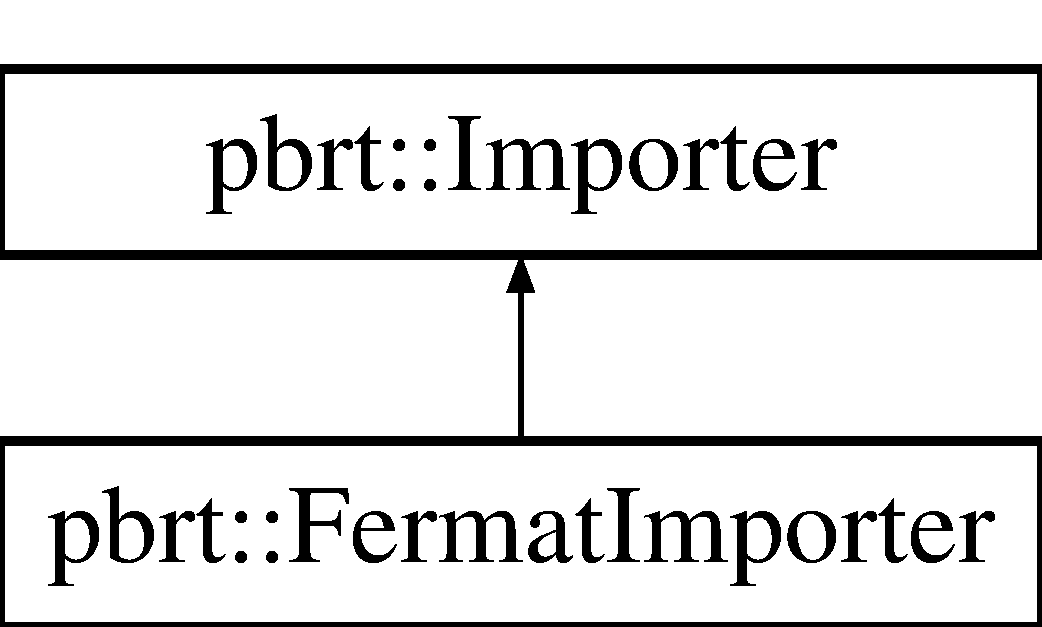
\includegraphics[height=2.000000cm]{structpbrt_1_1_fermat_importer}
\end{center}
\end{figure}
\subsection*{Public Types}
\begin{DoxyCompactItemize}
\item 
\mbox{\Hypertarget{structpbrt_1_1_fermat_importer_acdbdff3f7886caf8adf31379cd91a03e}\label{structpbrt_1_1_fermat_importer_acdbdff3f7886caf8adf31379cd91a03e}} 
typedef std\+::map$<$ std\+::string, uint32 $>$ {\bfseries texture\+\_\+map\+\_\+type}
\item 
\mbox{\Hypertarget{structpbrt_1_1_fermat_importer_a4d69b9003deaf92200f5e44fe625fe59}\label{structpbrt_1_1_fermat_importer_a4d69b9003deaf92200f5e44fe625fe59}} 
typedef std\+::map$<$ std\+::string, uint32 $>$ {\bfseries material\+\_\+map\+\_\+type}
\end{DoxyCompactItemize}
\subsection*{Public Methods}
\begin{DoxyCompactItemize}
\item 
\mbox{\Hypertarget{structpbrt_1_1_fermat_importer_ac01d0672a20956f1bfceed58c391a072}\label{structpbrt_1_1_fermat_importer_ac01d0672a20956f1bfceed58c391a072}} 
{\bfseries Fermat\+Importer} (const char $\ast$filename, \hyperlink{class_mesh_storage}{Mesh\+Storage} $\ast$mesh, \hyperlink{struct_camera}{Camera} $\ast$camera, std\+::vector$<$ \hyperlink{struct_directional_light}{Directional\+Light} $>$ $\ast$dir\+\_\+lights, std\+::vector$<$ std\+::string $>$ $\ast$scene\+\_\+dirs)
\item 
\mbox{\Hypertarget{structpbrt_1_1_fermat_importer_a629b96e7a653726d1b96de5d3dc06b28}\label{structpbrt_1_1_fermat_importer_a629b96e7a653726d1b96de5d3dc06b28}} 
virtual void {\bfseries identity} ()
\item 
\mbox{\Hypertarget{structpbrt_1_1_fermat_importer_a04902349e2bab1814819d26db89e6727}\label{structpbrt_1_1_fermat_importer_a04902349e2bab1814819d26db89e6727}} 
virtual void {\bfseries transform} (const \hyperlink{structpbrt_1_1_value}{Value} \&floats)
\item 
\mbox{\Hypertarget{structpbrt_1_1_fermat_importer_a9c99ea82488f03edf2f00cf21bd429e1}\label{structpbrt_1_1_fermat_importer_a9c99ea82488f03edf2f00cf21bd429e1}} 
virtual void {\bfseries rotate} (const float angle, const float x, const float y, const float z)
\item 
\mbox{\Hypertarget{structpbrt_1_1_fermat_importer_ad851d9884a79729de1fbb0528b540213}\label{structpbrt_1_1_fermat_importer_ad851d9884a79729de1fbb0528b540213}} 
virtual void {\bfseries scale} (const float x, const float y, const float z)
\item 
\mbox{\Hypertarget{structpbrt_1_1_fermat_importer_afe9f3f8a47e6d6fd227fa8bae64b69a9}\label{structpbrt_1_1_fermat_importer_afe9f3f8a47e6d6fd227fa8bae64b69a9}} 
virtual void {\bfseries translate} (const float x, const float y, const float z)
\item 
\mbox{\Hypertarget{structpbrt_1_1_fermat_importer_a6d80a936da43f165e0e4ae9a57229eba}\label{structpbrt_1_1_fermat_importer_a6d80a936da43f165e0e4ae9a57229eba}} 
virtual void {\bfseries look\+\_\+at} (const float ex, const float ey, const float ez, const float lx, const float ly, const float lz, const float ux, const float uy, const float uz)
\item 
\mbox{\Hypertarget{structpbrt_1_1_fermat_importer_ad9c8ec8e5e1366d8015a07eaa0f08100}\label{structpbrt_1_1_fermat_importer_ad9c8ec8e5e1366d8015a07eaa0f08100}} 
virtual void {\bfseries integrator} (const char $\ast$name, const \hyperlink{structpbrt_1_1_parameter_list}{Parameter\+List} \&params)
\item 
\mbox{\Hypertarget{structpbrt_1_1_fermat_importer_a03f4c963396b6e188a91191c506b9674}\label{structpbrt_1_1_fermat_importer_a03f4c963396b6e188a91191c506b9674}} 
virtual void {\bfseries sampler} (const char $\ast$name, const \hyperlink{structpbrt_1_1_parameter_list}{Parameter\+List} \&params)
\item 
\mbox{\Hypertarget{structpbrt_1_1_fermat_importer_a1ff854e8246ba489a1a980b0cff38944}\label{structpbrt_1_1_fermat_importer_a1ff854e8246ba489a1a980b0cff38944}} 
virtual void {\bfseries pixel\+\_\+filter} (const char $\ast$name, const \hyperlink{structpbrt_1_1_parameter_list}{Parameter\+List} \&params)
\item 
\mbox{\Hypertarget{structpbrt_1_1_fermat_importer_adad7bdd342113af9b3d375748c3967e3}\label{structpbrt_1_1_fermat_importer_adad7bdd342113af9b3d375748c3967e3}} 
virtual void {\bfseries film} (const char $\ast$name, const \hyperlink{structpbrt_1_1_parameter_list}{Parameter\+List} \&params)
\item 
\mbox{\Hypertarget{structpbrt_1_1_fermat_importer_a9ada13b8a06738ebbd9beac7c07c7056}\label{structpbrt_1_1_fermat_importer_a9ada13b8a06738ebbd9beac7c07c7056}} 
virtual void {\bfseries camera} (const char $\ast$name, const \hyperlink{structpbrt_1_1_parameter_list}{Parameter\+List} \&params)
\item 
\mbox{\Hypertarget{structpbrt_1_1_fermat_importer_a9f214f059c51d29ec4e32324eae148a7}\label{structpbrt_1_1_fermat_importer_a9f214f059c51d29ec4e32324eae148a7}} 
virtual void {\bfseries world\+\_\+begin} ()
\item 
\mbox{\Hypertarget{structpbrt_1_1_fermat_importer_a66b6b89c4e09275e5e7e6a8871be91c6}\label{structpbrt_1_1_fermat_importer_a66b6b89c4e09275e5e7e6a8871be91c6}} 
virtual void {\bfseries world\+\_\+end} ()
\item 
\mbox{\Hypertarget{structpbrt_1_1_fermat_importer_add5090a1336cf355d38a552d53b1b752}\label{structpbrt_1_1_fermat_importer_add5090a1336cf355d38a552d53b1b752}} 
virtual void {\bfseries attribute\+\_\+begin} ()
\item 
\mbox{\Hypertarget{structpbrt_1_1_fermat_importer_a197dbd0d970eba7f5881eed7ccac1fa3}\label{structpbrt_1_1_fermat_importer_a197dbd0d970eba7f5881eed7ccac1fa3}} 
virtual void {\bfseries attribute\+\_\+end} ()
\item 
\mbox{\Hypertarget{structpbrt_1_1_fermat_importer_a07226ed16f0ae9c2825659b4d5160451}\label{structpbrt_1_1_fermat_importer_a07226ed16f0ae9c2825659b4d5160451}} 
virtual void {\bfseries transform\+\_\+begin} ()
\item 
\mbox{\Hypertarget{structpbrt_1_1_fermat_importer_af6a37344c6acc2bca2e2abad5db0452b}\label{structpbrt_1_1_fermat_importer_af6a37344c6acc2bca2e2abad5db0452b}} 
virtual void {\bfseries transform\+\_\+end} ()
\item 
\mbox{\Hypertarget{structpbrt_1_1_fermat_importer_a1a649e7181d04a740ae76cfa90608982}\label{structpbrt_1_1_fermat_importer_a1a649e7181d04a740ae76cfa90608982}} 
virtual void {\bfseries texture} (const char $\ast$name, const char $\ast$texel\+\_\+type, const char $\ast$texture\+\_\+type, const \hyperlink{structpbrt_1_1_parameter_list}{Parameter\+List} \&params)
\item 
\mbox{\Hypertarget{structpbrt_1_1_fermat_importer_a759845459708189e797944d1b28ae135}\label{structpbrt_1_1_fermat_importer_a759845459708189e797944d1b28ae135}} 
virtual void {\bfseries make\+\_\+named\+\_\+medium} (const char $\ast$name, const \hyperlink{structpbrt_1_1_parameter_list}{Parameter\+List} \&params)
\item 
\mbox{\Hypertarget{structpbrt_1_1_fermat_importer_a803089b10ebf40da89be695659b933de}\label{structpbrt_1_1_fermat_importer_a803089b10ebf40da89be695659b933de}} 
virtual void {\bfseries make\+\_\+named\+\_\+material} (const char $\ast$name, const \hyperlink{structpbrt_1_1_parameter_list}{Parameter\+List} \&params)
\item 
\mbox{\Hypertarget{structpbrt_1_1_fermat_importer_ab3f7930db38f6fe7483bb1efb66c9293}\label{structpbrt_1_1_fermat_importer_ab3f7930db38f6fe7483bb1efb66c9293}} 
virtual void {\bfseries named\+\_\+material} (const char $\ast$name)
\item 
\mbox{\Hypertarget{structpbrt_1_1_fermat_importer_a49dbdff3adf28f650905c284ae5e8916}\label{structpbrt_1_1_fermat_importer_a49dbdff3adf28f650905c284ae5e8916}} 
virtual void {\bfseries medium\+\_\+interface} (const char $\ast$name1, const char $\ast$name2)
\item 
\mbox{\Hypertarget{structpbrt_1_1_fermat_importer_af0943810b0f02c709ca9ffb44de25fbd}\label{structpbrt_1_1_fermat_importer_af0943810b0f02c709ca9ffb44de25fbd}} 
virtual void {\bfseries material} (const char $\ast$type, const \hyperlink{structpbrt_1_1_parameter_list}{Parameter\+List} \&params)
\item 
\mbox{\Hypertarget{structpbrt_1_1_fermat_importer_a3d2b8ce677d0a017a6f1e0db8ec5519f}\label{structpbrt_1_1_fermat_importer_a3d2b8ce677d0a017a6f1e0db8ec5519f}} 
virtual void {\bfseries area\+\_\+light\+\_\+source} (const char $\ast$type, const \hyperlink{structpbrt_1_1_parameter_list}{Parameter\+List} \&params)
\item 
\mbox{\Hypertarget{structpbrt_1_1_fermat_importer_af838c7165a99353f1dd24f954e199f04}\label{structpbrt_1_1_fermat_importer_af838c7165a99353f1dd24f954e199f04}} 
virtual void {\bfseries light\+\_\+source} (const char $\ast$type, const \hyperlink{structpbrt_1_1_parameter_list}{Parameter\+List} \&params)
\item 
\mbox{\Hypertarget{structpbrt_1_1_fermat_importer_ae71d871bfd10584e26f0a99d91ab5443}\label{structpbrt_1_1_fermat_importer_ae71d871bfd10584e26f0a99d91ab5443}} 
virtual void {\bfseries shape} (const char $\ast$type, const \hyperlink{structpbrt_1_1_parameter_list}{Parameter\+List} \&params)
\item 
\mbox{\Hypertarget{structpbrt_1_1_fermat_importer_a5f3a7b08d9f67a525ccd9d84e989194c}\label{structpbrt_1_1_fermat_importer_a5f3a7b08d9f67a525ccd9d84e989194c}} 
void {\bfseries build\+\_\+material} (const char $\ast$type, const \hyperlink{structpbrt_1_1_parameter_list}{Parameter\+List} \&params, \hyperlink{struct_mesh_material}{Mesh\+Material} \&material)
\item 
\mbox{\Hypertarget{structpbrt_1_1_fermat_importer_a93e2f9172213d074ed630a9e194cff40}\label{structpbrt_1_1_fermat_importer_a93e2f9172213d074ed630a9e194cff40}} 
void {\bfseries finish} ()
\end{DoxyCompactItemize}
\subsection*{Public Members}
\begin{DoxyCompactItemize}
\item 
\mbox{\Hypertarget{structpbrt_1_1_fermat_importer_aebba36dcc493c854185d842beb3c037b}\label{structpbrt_1_1_fermat_importer_aebba36dcc493c854185d842beb3c037b}} 
\hyperlink{structpbrt_1_1_film_options}{Film\+Options} {\bfseries m\+\_\+film}
\item 
\mbox{\Hypertarget{structpbrt_1_1_fermat_importer_a3365085768715733ea57f95564f517a6}\label{structpbrt_1_1_fermat_importer_a3365085768715733ea57f95564f517a6}} 
\hyperlink{class_mesh_storage}{Mesh\+Storage} $\ast$ {\bfseries m\+\_\+mesh}
\item 
\mbox{\Hypertarget{structpbrt_1_1_fermat_importer_a4cc226526344ae8c320c2817546f7a0d}\label{structpbrt_1_1_fermat_importer_a4cc226526344ae8c320c2817546f7a0d}} 
\hyperlink{struct_camera}{Camera} $\ast$ {\bfseries m\+\_\+camera}
\item 
\mbox{\Hypertarget{structpbrt_1_1_fermat_importer_ad76f30f5b33fad42b6cd1772aea76cba}\label{structpbrt_1_1_fermat_importer_ad76f30f5b33fad42b6cd1772aea76cba}} 
std\+::vector$<$ \hyperlink{struct_directional_light}{Directional\+Light} $>$ $\ast$ {\bfseries m\+\_\+dir\+\_\+lights}
\item 
\mbox{\Hypertarget{structpbrt_1_1_fermat_importer_ad8413f2755260e10da7af323701bc9a3}\label{structpbrt_1_1_fermat_importer_ad8413f2755260e10da7af323701bc9a3}} 
std\+::vector$<$ std\+::string $>$ \& {\bfseries m\+\_\+dirs}
\item 
\mbox{\Hypertarget{structpbrt_1_1_fermat_importer_aa5fa1f066ad6093015ca8d0dade15587}\label{structpbrt_1_1_fermat_importer_aa5fa1f066ad6093015ca8d0dade15587}} 
texture\+\_\+map\+\_\+type {\bfseries m\+\_\+texture\+\_\+map}
\item 
\mbox{\Hypertarget{structpbrt_1_1_fermat_importer_a9a3dda06a3dae04bff14b30da601ab31}\label{structpbrt_1_1_fermat_importer_a9a3dda06a3dae04bff14b30da601ab31}} 
material\+\_\+map\+\_\+type {\bfseries m\+\_\+material\+\_\+map}
\item 
\mbox{\Hypertarget{structpbrt_1_1_fermat_importer_aa76c976b638acf08531e1c57a29499b6}\label{structpbrt_1_1_fermat_importer_aa76c976b638acf08531e1c57a29499b6}} 
std\+::vector$<$ \hyperlink{struct_mesh_material}{Mesh\+Material} $>$ {\bfseries m\+\_\+materials}
\item 
\mbox{\Hypertarget{structpbrt_1_1_fermat_importer_adadaefa9250f28b897c4da594e9ba216}\label{structpbrt_1_1_fermat_importer_adadaefa9250f28b897c4da594e9ba216}} 
std\+::vector$<$ std\+::string $>$ {\bfseries m\+\_\+material\+\_\+names}
\item 
\mbox{\Hypertarget{structpbrt_1_1_fermat_importer_ad41f415f2786bce281d50dc98be136cb}\label{structpbrt_1_1_fermat_importer_ad41f415f2786bce281d50dc98be136cb}} 
std\+::stack$<$ \hyperlink{structcugar_1_1_matrix}{cugar\+::\+Matrix4x4f} $>$ {\bfseries m\+\_\+transform\+\_\+stack}
\item 
\mbox{\Hypertarget{structpbrt_1_1_fermat_importer_a7c2690b8b567bcd0ec24395a669584cd}\label{structpbrt_1_1_fermat_importer_a7c2690b8b567bcd0ec24395a669584cd}} 
std\+::stack$<$ int $>$ {\bfseries m\+\_\+material\+\_\+stack}
\item 
\mbox{\Hypertarget{structpbrt_1_1_fermat_importer_af008c7132624c12640996fc8bfa78927}\label{structpbrt_1_1_fermat_importer_af008c7132624c12640996fc8bfa78927}} 
std\+::stack$<$ \hyperlink{structcugar_1_1_vector}{cugar\+::\+Vector3f} $>$ {\bfseries m\+\_\+emission\+\_\+stack}
\item 
\mbox{\Hypertarget{structpbrt_1_1_fermat_importer_acda30e25bf58809c0203e901359bc169}\label{structpbrt_1_1_fermat_importer_acda30e25bf58809c0203e901359bc169}} 
int {\bfseries m\+\_\+default\+\_\+material}
\end{DoxyCompactItemize}


The documentation for this struct was generated from the following files\+:\begin{DoxyCompactItemize}
\item 
C\+:/p4research/research/jpantaleoni/\+Fermat-\/\+Public/src/mesh/pbrt\+\_\+importer.\+h\item 
C\+:/p4research/research/jpantaleoni/\+Fermat-\/\+Public/src/mesh/pbrt\+\_\+importer.\+cpp\end{DoxyCompactItemize}

\hypertarget{structcugar_1_1field__traits}{}\section{cugar\+:\+:field\+\_\+traits$<$ T $>$ Struct Template Reference}
\label{structcugar_1_1field__traits}\index{cugar\+::field\+\_\+traits$<$ T $>$@{cugar\+::field\+\_\+traits$<$ T $>$}}


\subsection{Detailed description}
\subsubsection*{template$<$typename T$>$\newline
struct cugar\+::field\+\_\+traits$<$ T $>$}

A generic class to represent traits of numeric types T. Unlike S\+TL\textquotesingle{}s numeric\+\_\+traits, \hyperlink{structcugar_1_1field__traits_ad4b1179d58dbf86897d4c9a7d9b53f6d}{field\+\_\+traits$<$\+T$>$\+::min()} and \hyperlink{structcugar_1_1field__traits_a6f3732317c452f66e22bfb1e31da563b}{field\+\_\+traits$<$\+T$>$\+::max()} are signed. 

{\ttfamily \#include $<$numbers.\+h$>$}

\subsection*{Static Public Methods}
\begin{DoxyCompactItemize}
\item 
static T \hyperlink{structcugar_1_1field__traits_ad4b1179d58dbf86897d4c9a7d9b53f6d}{min} ()
\item 
static T \hyperlink{structcugar_1_1field__traits_a6f3732317c452f66e22bfb1e31da563b}{max} ()
\end{DoxyCompactItemize}


\subsection{Member Function Documentation}
\mbox{\Hypertarget{structcugar_1_1field__traits_a6f3732317c452f66e22bfb1e31da563b}\label{structcugar_1_1field__traits_a6f3732317c452f66e22bfb1e31da563b}} 
\index{cugar\+::field\+\_\+traits@{cugar\+::field\+\_\+traits}!max@{max}}
\index{max@{max}!cugar\+::field\+\_\+traits@{cugar\+::field\+\_\+traits}}
\subsubsection{\texorpdfstring{max()}{max()}}
{\footnotesize\ttfamily template$<$typename T $>$ \\
static T \hyperlink{structcugar_1_1field__traits}{cugar\+::field\+\_\+traits}$<$ T $>$\+::max (\begin{DoxyParamCaption}{ }\end{DoxyParamCaption})\hspace{0.3cm}{\ttfamily [inline]}, {\ttfamily [static]}}

return the maximum value of T \mbox{\Hypertarget{structcugar_1_1field__traits_ad4b1179d58dbf86897d4c9a7d9b53f6d}\label{structcugar_1_1field__traits_ad4b1179d58dbf86897d4c9a7d9b53f6d}} 
\index{cugar\+::field\+\_\+traits@{cugar\+::field\+\_\+traits}!min@{min}}
\index{min@{min}!cugar\+::field\+\_\+traits@{cugar\+::field\+\_\+traits}}
\subsubsection{\texorpdfstring{min()}{min()}}
{\footnotesize\ttfamily template$<$typename T $>$ \\
static T \hyperlink{structcugar_1_1field__traits}{cugar\+::field\+\_\+traits}$<$ T $>$\+::min (\begin{DoxyParamCaption}{ }\end{DoxyParamCaption})\hspace{0.3cm}{\ttfamily [inline]}, {\ttfamily [static]}}

return the minimum value of T 

The documentation for this struct was generated from the following file\+:\begin{DoxyCompactItemize}
\item 
C\+:/p4research/research/jpantaleoni/\+Fermat-\/\+Public/contrib/cugar/basic/numbers.\+h\end{DoxyCompactItemize}

\hypertarget{structcugar_1_1field__traits_3_01int16_01_4}{}\section{cugar\+:\+:field\+\_\+traits$<$ int16 $>$ Struct Template Reference}
\label{structcugar_1_1field__traits_3_01int16_01_4}\index{cugar\+::field\+\_\+traits$<$ int16 $>$@{cugar\+::field\+\_\+traits$<$ int16 $>$}}


\subsection{Detailed description}
\subsubsection*{template$<$$>$\newline
struct cugar\+::field\+\_\+traits$<$ int16 $>$}

int16 specialization of \hyperlink{structcugar_1_1field__traits}{field\+\_\+traits} 

{\ttfamily \#include $<$numbers.\+h$>$}

\subsection*{Static Public Methods}
\begin{DoxyCompactItemize}
\item 
\mbox{\Hypertarget{structcugar_1_1field__traits_3_01int16_01_4_a3d665a6090cc8669872a212c45c9a286}\label{structcugar_1_1field__traits_3_01int16_01_4_a3d665a6090cc8669872a212c45c9a286}} 
static C\+U\+G\+A\+R\+\_\+\+H\+O\+S\+T\+\_\+\+D\+E\+V\+I\+CE int16 {\bfseries min} ()
\item 
\mbox{\Hypertarget{structcugar_1_1field__traits_3_01int16_01_4_aacbd808673c0366ea4bd95d2eb4688d5}\label{structcugar_1_1field__traits_3_01int16_01_4_aacbd808673c0366ea4bd95d2eb4688d5}} 
static C\+U\+G\+A\+R\+\_\+\+H\+O\+S\+T\+\_\+\+D\+E\+V\+I\+CE int16 {\bfseries max} ()
\end{DoxyCompactItemize}


The documentation for this struct was generated from the following file\+:\begin{DoxyCompactItemize}
\item 
C\+:/p4research/research/jpantaleoni/\+Fermat-\/\+Public/contrib/cugar/basic/numbers.\+h\end{DoxyCompactItemize}

\hypertarget{structcugar_1_1field__traits_3_01int32_01_4}{}\section{cugar\+:\+:field\+\_\+traits$<$ int32 $>$ Struct Template Reference}
\label{structcugar_1_1field__traits_3_01int32_01_4}\index{cugar\+::field\+\_\+traits$<$ int32 $>$@{cugar\+::field\+\_\+traits$<$ int32 $>$}}


\subsection{Detailed description}
\subsubsection*{template$<$$>$\newline
struct cugar\+::field\+\_\+traits$<$ int32 $>$}

int32 specialization of \hyperlink{structcugar_1_1field__traits}{field\+\_\+traits} 

{\ttfamily \#include $<$numbers.\+h$>$}

\subsection*{Static Public Methods}
\begin{DoxyCompactItemize}
\item 
\mbox{\Hypertarget{structcugar_1_1field__traits_3_01int32_01_4_a81ce81096221ca704e627ac53cc1321e}\label{structcugar_1_1field__traits_3_01int32_01_4_a81ce81096221ca704e627ac53cc1321e}} 
static C\+U\+G\+A\+R\+\_\+\+H\+O\+S\+T\+\_\+\+D\+E\+V\+I\+CE int32 {\bfseries min} ()
\item 
\mbox{\Hypertarget{structcugar_1_1field__traits_3_01int32_01_4_a1c6b1b7ef0a0ffb3309da0e8f19d6d10}\label{structcugar_1_1field__traits_3_01int32_01_4_a1c6b1b7ef0a0ffb3309da0e8f19d6d10}} 
static C\+U\+G\+A\+R\+\_\+\+H\+O\+S\+T\+\_\+\+D\+E\+V\+I\+CE int32 {\bfseries max} ()
\end{DoxyCompactItemize}


The documentation for this struct was generated from the following file\+:\begin{DoxyCompactItemize}
\item 
C\+:/p4research/research/jpantaleoni/\+Fermat-\/\+Public/contrib/cugar/basic/numbers.\+h\end{DoxyCompactItemize}

\hypertarget{structcugar_1_1field__traits_3_01int64_01_4}{}\section{cugar\+:\+:field\+\_\+traits$<$ int64 $>$ Struct Template Reference}
\label{structcugar_1_1field__traits_3_01int64_01_4}\index{cugar\+::field\+\_\+traits$<$ int64 $>$@{cugar\+::field\+\_\+traits$<$ int64 $>$}}


\subsection{Detailed description}
\subsubsection*{template$<$$>$\newline
struct cugar\+::field\+\_\+traits$<$ int64 $>$}

int64 specialization of \hyperlink{structcugar_1_1field__traits}{field\+\_\+traits} 

{\ttfamily \#include $<$numbers.\+h$>$}

\subsection*{Static Public Methods}
\begin{DoxyCompactItemize}
\item 
\mbox{\Hypertarget{structcugar_1_1field__traits_3_01int64_01_4_a681b3e2ab5bb187f3ee2083ca3dfce0d}\label{structcugar_1_1field__traits_3_01int64_01_4_a681b3e2ab5bb187f3ee2083ca3dfce0d}} 
static C\+U\+G\+A\+R\+\_\+\+H\+O\+S\+T\+\_\+\+D\+E\+V\+I\+CE int64 {\bfseries min} ()
\item 
\mbox{\Hypertarget{structcugar_1_1field__traits_3_01int64_01_4_ae20f7124b1af355603e696a0e835c21d}\label{structcugar_1_1field__traits_3_01int64_01_4_ae20f7124b1af355603e696a0e835c21d}} 
static C\+U\+G\+A\+R\+\_\+\+H\+O\+S\+T\+\_\+\+D\+E\+V\+I\+CE int64 {\bfseries max} ()
\end{DoxyCompactItemize}


The documentation for this struct was generated from the following file\+:\begin{DoxyCompactItemize}
\item 
C\+:/p4research/research/jpantaleoni/\+Fermat-\/\+Public/contrib/cugar/basic/numbers.\+h\end{DoxyCompactItemize}

\hypertarget{structcugar_1_1field__traits_3_01int8_01_4}{}\section{cugar\+:\+:field\+\_\+traits$<$ int8 $>$ Struct Template Reference}
\label{structcugar_1_1field__traits_3_01int8_01_4}\index{cugar\+::field\+\_\+traits$<$ int8 $>$@{cugar\+::field\+\_\+traits$<$ int8 $>$}}


\subsection{Detailed description}
\subsubsection*{template$<$$>$\newline
struct cugar\+::field\+\_\+traits$<$ int8 $>$}

int8 specialization of \hyperlink{structcugar_1_1field__traits}{field\+\_\+traits} 

{\ttfamily \#include $<$numbers.\+h$>$}

\subsection*{Static Public Methods}
\begin{DoxyCompactItemize}
\item 
\mbox{\Hypertarget{structcugar_1_1field__traits_3_01int8_01_4_a50b9c0d99e988881acc219a0675cfe16}\label{structcugar_1_1field__traits_3_01int8_01_4_a50b9c0d99e988881acc219a0675cfe16}} 
static C\+U\+G\+A\+R\+\_\+\+H\+O\+S\+T\+\_\+\+D\+E\+V\+I\+CE int8 {\bfseries min} ()
\item 
\mbox{\Hypertarget{structcugar_1_1field__traits_3_01int8_01_4_a42a1451684bed4ed1aacefaba36c3916}\label{structcugar_1_1field__traits_3_01int8_01_4_a42a1451684bed4ed1aacefaba36c3916}} 
static C\+U\+G\+A\+R\+\_\+\+H\+O\+S\+T\+\_\+\+D\+E\+V\+I\+CE int8 {\bfseries max} ()
\end{DoxyCompactItemize}


The documentation for this struct was generated from the following file\+:\begin{DoxyCompactItemize}
\item 
C\+:/p4research/research/jpantaleoni/\+Fermat-\/\+Public/contrib/cugar/basic/numbers.\+h\end{DoxyCompactItemize}

\hypertarget{structpbrt_1_1_film_options}{}\section{pbrt\+:\+:Film\+Options Struct Reference}
\label{structpbrt_1_1_film_options}\index{pbrt\+::\+Film\+Options@{pbrt\+::\+Film\+Options}}
\subsection*{Public Members}
\begin{DoxyCompactItemize}
\item 
\mbox{\Hypertarget{structpbrt_1_1_film_options_ac9cf92f2297a3564824ff0560c17d7c4}\label{structpbrt_1_1_film_options_ac9cf92f2297a3564824ff0560c17d7c4}} 
float {\bfseries gamma}
\item 
\mbox{\Hypertarget{structpbrt_1_1_film_options_ac7b04665742690c76aa576d3fdf98c9f}\label{structpbrt_1_1_film_options_ac7b04665742690c76aa576d3fdf98c9f}} 
float {\bfseries exposure}
\end{DoxyCompactItemize}


The documentation for this struct was generated from the following file\+:\begin{DoxyCompactItemize}
\item 
C\+:/p4research/research/jpantaleoni/\+Fermat-\/\+Public/src/mesh/pbrt\+\_\+importer.\+h\end{DoxyCompactItemize}

\hypertarget{structcugar_1_1_f_l_c_g__random}{}\section{cugar\+:\+:F\+L\+C\+G\+\_\+random Struct Reference}
\label{structcugar_1_1_f_l_c_g__random}\index{cugar\+::\+F\+L\+C\+G\+\_\+random@{cugar\+::\+F\+L\+C\+G\+\_\+random}}


\subsection{Detailed description}
A very simple Linear Congruential Generator 

{\ttfamily \#include $<$numbers.\+h$>$}

Inheritance diagram for cugar\+:\+:F\+L\+C\+G\+\_\+random\+:\begin{figure}[H]
\begin{center}
\leavevmode
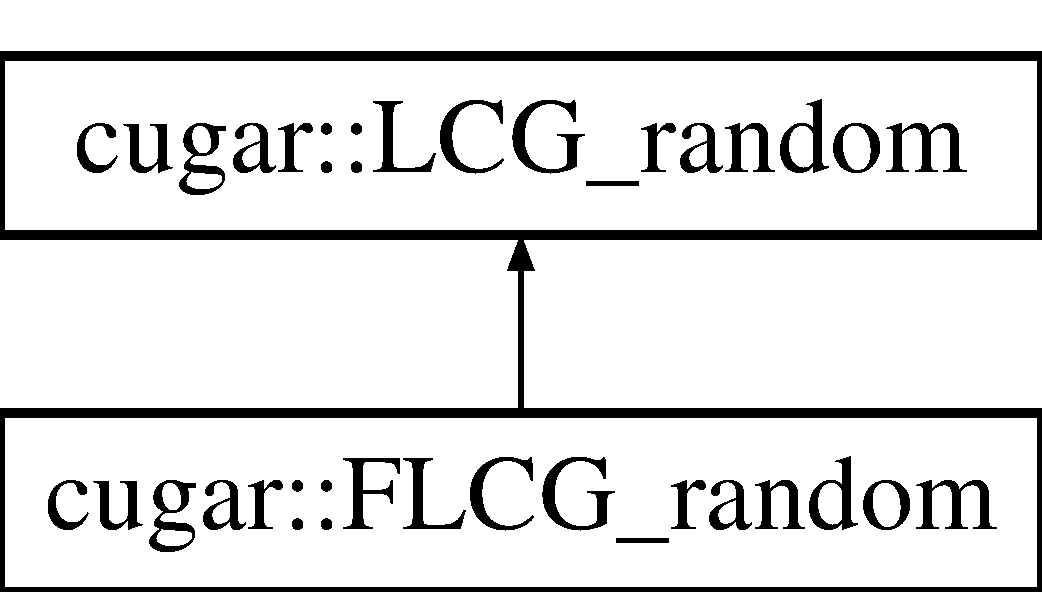
\includegraphics[height=2.000000cm]{structcugar_1_1_f_l_c_g__random}
\end{center}
\end{figure}
\subsection*{Public Methods}
\begin{DoxyCompactItemize}
\item 
\mbox{\Hypertarget{structcugar_1_1_f_l_c_g__random_af977671a37fbcfbee953cda8dd7e14f9}\label{structcugar_1_1_f_l_c_g__random_af977671a37fbcfbee953cda8dd7e14f9}} 
C\+U\+G\+A\+R\+\_\+\+F\+O\+R\+C\+E\+I\+N\+L\+I\+NE C\+U\+G\+A\+R\+\_\+\+H\+O\+S\+T\+\_\+\+D\+E\+V\+I\+CE {\bfseries F\+L\+C\+G\+\_\+random} (const uint32 s=0)
\item 
\mbox{\Hypertarget{structcugar_1_1_f_l_c_g__random_a58c9ed5f21c6cdcca8323dca1372262a}\label{structcugar_1_1_f_l_c_g__random_a58c9ed5f21c6cdcca8323dca1372262a}} 
C\+U\+G\+A\+R\+\_\+\+F\+O\+R\+C\+E\+I\+N\+L\+I\+NE C\+U\+G\+A\+R\+\_\+\+H\+O\+S\+T\+\_\+\+D\+E\+V\+I\+CE float {\bfseries next} ()
\end{DoxyCompactItemize}
\subsection*{Additional Inherited Members}


The documentation for this struct was generated from the following file\+:\begin{DoxyCompactItemize}
\item 
C\+:/p4research/research/jpantaleoni/\+Fermat-\/\+Public/contrib/cugar/basic/numbers.\+h\end{DoxyCompactItemize}

\hypertarget{structcugar_1_1for__each__enactor}{}\section{cugar\+:\+:for\+\_\+each\+\_\+enactor$<$ system\+\_\+tag $>$ Struct Template Reference}
\label{structcugar_1_1for__each__enactor}\index{cugar\+::for\+\_\+each\+\_\+enactor$<$ system\+\_\+tag $>$@{cugar\+::for\+\_\+each\+\_\+enactor$<$ system\+\_\+tag $>$}}


\subsection{Detailed description}
\subsubsection*{template$<$typename system\+\_\+tag$>$\newline
struct cugar\+::for\+\_\+each\+\_\+enactor$<$ system\+\_\+tag $>$}

A stateful for\+\_\+each enactor class that optimizes the kernel launches at run-\/time, using per-\/launch statistics 

{\ttfamily \#include $<$primitives.\+h$>$}

\subsection*{Public Methods}
\begin{DoxyCompactItemize}
\item 
{\footnotesize template$<$typename Iterator , typename Functor $>$ }\\void \hyperlink{structcugar_1_1for__each__enactor_a6ab5c5317387dca99337436a1d3db8f1}{operator()} (const uint64 n, const Iterator in, Functor functor)
\item 
{\footnotesize template$<$typename Functor $>$ }\\void \hyperlink{structcugar_1_1for__each__enactor_a6b429ae818622e05dff95ec47dce9242}{operator()} (const uint64 n, Functor functor)
\end{DoxyCompactItemize}


\subsection{Member Function Documentation}
\mbox{\Hypertarget{structcugar_1_1for__each__enactor_a6ab5c5317387dca99337436a1d3db8f1}\label{structcugar_1_1for__each__enactor_a6ab5c5317387dca99337436a1d3db8f1}} 
\index{cugar\+::for\+\_\+each\+\_\+enactor@{cugar\+::for\+\_\+each\+\_\+enactor}!operator()@{operator()}}
\index{operator()@{operator()}!cugar\+::for\+\_\+each\+\_\+enactor@{cugar\+::for\+\_\+each\+\_\+enactor}}
\subsubsection{\texorpdfstring{operator()()}{operator()()}\hspace{0.1cm}{\footnotesize\ttfamily [1/2]}}
{\footnotesize\ttfamily template$<$typename system\+\_\+tag $>$ \\
template$<$typename Iterator , typename Functor $>$ \\
void \hyperlink{structcugar_1_1for__each__enactor}{cugar\+::for\+\_\+each\+\_\+enactor}$<$ system\+\_\+tag $>$\+::operator() (\begin{DoxyParamCaption}\item[{const uint64}]{n,  }\item[{const Iterator}]{in,  }\item[{Functor}]{functor }\end{DoxyParamCaption})\hspace{0.3cm}{\ttfamily [inline]}}

enact the for\+\_\+each \mbox{\Hypertarget{structcugar_1_1for__each__enactor_a6b429ae818622e05dff95ec47dce9242}\label{structcugar_1_1for__each__enactor_a6b429ae818622e05dff95ec47dce9242}} 
\index{cugar\+::for\+\_\+each\+\_\+enactor@{cugar\+::for\+\_\+each\+\_\+enactor}!operator()@{operator()}}
\index{operator()@{operator()}!cugar\+::for\+\_\+each\+\_\+enactor@{cugar\+::for\+\_\+each\+\_\+enactor}}
\subsubsection{\texorpdfstring{operator()()}{operator()()}\hspace{0.1cm}{\footnotesize\ttfamily [2/2]}}
{\footnotesize\ttfamily template$<$typename system\+\_\+tag $>$ \\
template$<$typename Functor $>$ \\
void \hyperlink{structcugar_1_1for__each__enactor}{cugar\+::for\+\_\+each\+\_\+enactor}$<$ system\+\_\+tag $>$\+::operator() (\begin{DoxyParamCaption}\item[{const uint64}]{n,  }\item[{Functor}]{functor }\end{DoxyParamCaption})\hspace{0.3cm}{\ttfamily [inline]}}

enact the for\+\_\+each 

The documentation for this struct was generated from the following file\+:\begin{DoxyCompactItemize}
\item 
C\+:/p4research/research/jpantaleoni/\+Fermat-\/\+Public/contrib/cugar/basic/primitives.\+h\end{DoxyCompactItemize}

\hypertarget{structcugar_1_1for__each__enactor_3_01device__tag_01_4}{}\section{cugar\+:\+:for\+\_\+each\+\_\+enactor$<$ device\+\_\+tag $>$ Struct Template Reference}
\label{structcugar_1_1for__each__enactor_3_01device__tag_01_4}\index{cugar\+::for\+\_\+each\+\_\+enactor$<$ device\+\_\+tag $>$@{cugar\+::for\+\_\+each\+\_\+enactor$<$ device\+\_\+tag $>$}}


\subsection{Detailed description}
\subsubsection*{template$<$$>$\newline
struct cugar\+::for\+\_\+each\+\_\+enactor$<$ device\+\_\+tag $>$}

A stateful for\+\_\+each enactor class that optimizes the kernel launches at run-\/time, using per-\/launch statistics 

{\ttfamily \#include $<$primitives.\+h$>$}

\subsection*{Public Methods}
\begin{DoxyCompactItemize}
\item 
\hyperlink{structcugar_1_1for__each__enactor_3_01device__tag_01_4_a09149f7e19d5228d4cb45d5f741df386}{for\+\_\+each\+\_\+enactor} ()
\item 
{\footnotesize template$<$typename Iterator , typename Functor $>$ }\\void \hyperlink{structcugar_1_1for__each__enactor_3_01device__tag_01_4_a560ef3acdf14e7bbccbdaea7cdae0049}{operator()} (const uint64 n, const Iterator in, Functor functor)
\item 
{\footnotesize template$<$typename Functor $>$ }\\void \hyperlink{structcugar_1_1for__each__enactor_3_01device__tag_01_4_a5ebd67b9c8303c8d3692dc8dbd336893}{operator()} (const uint64 n, Functor functor)
\end{DoxyCompactItemize}


\subsection{Constructor \& Destructor Documentation}
\mbox{\Hypertarget{structcugar_1_1for__each__enactor_3_01device__tag_01_4_a09149f7e19d5228d4cb45d5f741df386}\label{structcugar_1_1for__each__enactor_3_01device__tag_01_4_a09149f7e19d5228d4cb45d5f741df386}} 
\index{cugar\+::for\+\_\+each\+\_\+enactor$<$ device\+\_\+tag $>$@{cugar\+::for\+\_\+each\+\_\+enactor$<$ device\+\_\+tag $>$}!for\+\_\+each\+\_\+enactor@{for\+\_\+each\+\_\+enactor}}
\index{for\+\_\+each\+\_\+enactor@{for\+\_\+each\+\_\+enactor}!cugar\+::for\+\_\+each\+\_\+enactor$<$ device\+\_\+tag $>$@{cugar\+::for\+\_\+each\+\_\+enactor$<$ device\+\_\+tag $>$}}
\subsubsection{\texorpdfstring{for\+\_\+each\+\_\+enactor()}{for\_each\_enactor()}}
{\footnotesize\ttfamily \hyperlink{structcugar_1_1for__each__enactor}{cugar\+::for\+\_\+each\+\_\+enactor}$<$ \hyperlink{structcugar_1_1device__tag}{device\+\_\+tag} $>$\+::\hyperlink{structcugar_1_1for__each__enactor}{for\+\_\+each\+\_\+enactor} (\begin{DoxyParamCaption}{ }\end{DoxyParamCaption})\hspace{0.3cm}{\ttfamily [inline]}}

constructor 

\subsection{Member Function Documentation}
\mbox{\Hypertarget{structcugar_1_1for__each__enactor_3_01device__tag_01_4_a560ef3acdf14e7bbccbdaea7cdae0049}\label{structcugar_1_1for__each__enactor_3_01device__tag_01_4_a560ef3acdf14e7bbccbdaea7cdae0049}} 
\index{cugar\+::for\+\_\+each\+\_\+enactor$<$ device\+\_\+tag $>$@{cugar\+::for\+\_\+each\+\_\+enactor$<$ device\+\_\+tag $>$}!operator()@{operator()}}
\index{operator()@{operator()}!cugar\+::for\+\_\+each\+\_\+enactor$<$ device\+\_\+tag $>$@{cugar\+::for\+\_\+each\+\_\+enactor$<$ device\+\_\+tag $>$}}
\subsubsection{\texorpdfstring{operator()()}{operator()()}\hspace{0.1cm}{\footnotesize\ttfamily [1/2]}}
{\footnotesize\ttfamily template$<$typename Iterator , typename Functor $>$ \\
void \hyperlink{structcugar_1_1for__each__enactor}{cugar\+::for\+\_\+each\+\_\+enactor}$<$ \hyperlink{structcugar_1_1device__tag}{device\+\_\+tag} $>$\+::operator() (\begin{DoxyParamCaption}\item[{const uint64}]{n,  }\item[{const Iterator}]{in,  }\item[{Functor}]{functor }\end{DoxyParamCaption})}

enact the for\+\_\+each \mbox{\Hypertarget{structcugar_1_1for__each__enactor_3_01device__tag_01_4_a5ebd67b9c8303c8d3692dc8dbd336893}\label{structcugar_1_1for__each__enactor_3_01device__tag_01_4_a5ebd67b9c8303c8d3692dc8dbd336893}} 
\index{cugar\+::for\+\_\+each\+\_\+enactor$<$ device\+\_\+tag $>$@{cugar\+::for\+\_\+each\+\_\+enactor$<$ device\+\_\+tag $>$}!operator()@{operator()}}
\index{operator()@{operator()}!cugar\+::for\+\_\+each\+\_\+enactor$<$ device\+\_\+tag $>$@{cugar\+::for\+\_\+each\+\_\+enactor$<$ device\+\_\+tag $>$}}
\subsubsection{\texorpdfstring{operator()()}{operator()()}\hspace{0.1cm}{\footnotesize\ttfamily [2/2]}}
{\footnotesize\ttfamily template$<$typename Functor $>$ \\
void \hyperlink{structcugar_1_1for__each__enactor}{cugar\+::for\+\_\+each\+\_\+enactor}$<$ \hyperlink{structcugar_1_1device__tag}{device\+\_\+tag} $>$\+::operator() (\begin{DoxyParamCaption}\item[{const uint64}]{n,  }\item[{Functor}]{functor }\end{DoxyParamCaption})\hspace{0.3cm}{\ttfamily [inline]}}

enact the for\+\_\+each 

The documentation for this struct was generated from the following files\+:\begin{DoxyCompactItemize}
\item 
C\+:/p4research/research/jpantaleoni/\+Fermat-\/\+Public/contrib/cugar/basic/primitives.\+h\item 
C\+:/p4research/research/jpantaleoni/\+Fermat-\/\+Public/contrib/cugar/basic/primitives\+\_\+inl.\+h\end{DoxyCompactItemize}

\hypertarget{structcugar_1_1gather__functor}{}\section{cugar\+:\+:gather\+\_\+functor$<$ Iterator, index\+\_\+type $>$ Struct Template Reference}
\label{structcugar_1_1gather__functor}\index{cugar\+::gather\+\_\+functor$<$ Iterator, index\+\_\+type $>$@{cugar\+::gather\+\_\+functor$<$ Iterator, index\+\_\+type $>$}}


\subsection{Detailed description}
\subsubsection*{template$<$typename Iterator, typename index\+\_\+type = uint32$>$\newline
struct cugar\+::gather\+\_\+functor$<$ Iterator, index\+\_\+type $>$}

Build a gathering functor 

{\ttfamily \#include $<$functors.\+h$>$}

\subsection*{Public Types}
\begin{DoxyCompactItemize}
\item 
\mbox{\Hypertarget{structcugar_1_1gather__functor_a7bfab5263a3ba8c7ab653c89ec071365}\label{structcugar_1_1gather__functor_a7bfab5263a3ba8c7ab653c89ec071365}} 
typedef index\+\_\+type {\bfseries argument\+\_\+type}
\item 
\mbox{\Hypertarget{structcugar_1_1gather__functor_abffa40cb6cfa362a96da4775bb81fe45}\label{structcugar_1_1gather__functor_abffa40cb6cfa362a96da4775bb81fe45}} 
typedef std\+::iterator\+\_\+traits$<$ Iterator $>$\+::value\+\_\+type {\bfseries result\+\_\+type}
\end{DoxyCompactItemize}
\subsection*{Public Methods}
\begin{DoxyCompactItemize}
\item 
\mbox{\Hypertarget{structcugar_1_1gather__functor_a45411da0f72d484fe861314ce4a46df1}\label{structcugar_1_1gather__functor_a45411da0f72d484fe861314ce4a46df1}} 
C\+U\+G\+A\+R\+\_\+\+F\+O\+R\+C\+E\+I\+N\+L\+I\+NE C\+U\+G\+A\+R\+\_\+\+H\+O\+S\+T\+\_\+\+D\+E\+V\+I\+CE {\bfseries gather\+\_\+functor} (const Iterator perm)
\item 
\mbox{\Hypertarget{structcugar_1_1gather__functor_a20d57149b534ea2b103b6d9c2ecda5b4}\label{structcugar_1_1gather__functor_a20d57149b534ea2b103b6d9c2ecda5b4}} 
C\+U\+G\+A\+R\+\_\+\+F\+O\+R\+C\+E\+I\+N\+L\+I\+NE C\+U\+G\+A\+R\+\_\+\+H\+O\+S\+T\+\_\+\+D\+E\+V\+I\+CE result\+\_\+type {\bfseries operator()} (const argument\+\_\+type op) const
\end{DoxyCompactItemize}
\subsection*{Public Members}
\begin{DoxyCompactItemize}
\item 
\mbox{\Hypertarget{structcugar_1_1gather__functor_a440b179f2ea8d1dfd007fb8f9f4894ac}\label{structcugar_1_1gather__functor_a440b179f2ea8d1dfd007fb8f9f4894ac}} 
Iterator {\bfseries m\+\_\+perm}
\end{DoxyCompactItemize}


The documentation for this struct was generated from the following file\+:\begin{DoxyCompactItemize}
\item 
C\+:/p4research/research/jpantaleoni/\+Fermat-\/\+Public/contrib/cugar/basic/\hyperlink{functors_8h}{functors.\+h}\end{DoxyCompactItemize}

\hypertarget{structcugar_1_1_gaussian__distribution__2d}{}\section{cugar\+:\+:Gaussian\+\_\+distribution\+\_\+2d Struct Reference}
\label{structcugar_1_1_gaussian__distribution__2d}\index{cugar\+::\+Gaussian\+\_\+distribution\+\_\+2d@{cugar\+::\+Gaussian\+\_\+distribution\+\_\+2d}}


\subsection{Detailed description}
2d Gaussian distribution with fully prescribed covariance matrix 

{\ttfamily \#include $<$distributions.\+h$>$}

\subsection*{Public Types}
\begin{DoxyCompactItemize}
\item 
\mbox{\Hypertarget{structcugar_1_1_gaussian__distribution__2d_aedb48159ce020cd2ba08fb0b9cb98b67}\label{structcugar_1_1_gaussian__distribution__2d_aedb48159ce020cd2ba08fb0b9cb98b67}} 
enum {\bfseries Matrix\+Type} \{ {\bfseries C\+O\+V\+A\+R\+I\+A\+N\+C\+E\+\_\+\+M\+A\+T\+R\+IX}, 
{\bfseries P\+R\+E\+C\+I\+S\+I\+O\+N\+\_\+\+M\+A\+T\+R\+IX}
 \}
\end{DoxyCompactItemize}
\subsection*{Public Methods}
\begin{DoxyCompactItemize}
\item 
C\+U\+G\+A\+R\+\_\+\+H\+O\+S\+T\+\_\+\+D\+E\+V\+I\+CE \hyperlink{structcugar_1_1_gaussian__distribution__2d_a291aa81b6b608aeca5a532ecdbdef68c}{Gaussian\+\_\+distribution\+\_\+2d} ()
\item 
C\+U\+G\+A\+R\+\_\+\+H\+O\+S\+T\+\_\+\+D\+E\+V\+I\+CE \hyperlink{structcugar_1_1_gaussian__distribution__2d_aad832a2b320dccb09161bd79a33e19fb}{Gaussian\+\_\+distribution\+\_\+2d} (const \hyperlink{structcugar_1_1_vector}{Vector2f} mu, const \hyperlink{structcugar_1_1_matrix}{Matrix2x2f} matrix, const Matrix\+Type matrix\+\_\+type=C\+O\+V\+A\+R\+I\+A\+N\+C\+E\+\_\+\+M\+A\+T\+R\+IX)
\item 
C\+U\+G\+A\+R\+\_\+\+H\+O\+S\+T\+\_\+\+D\+E\+V\+I\+CE \hyperlink{structcugar_1_1_gaussian__distribution__2d_aad6906acd6d313a1a880d178438b9ff3}{Gaussian\+\_\+distribution\+\_\+2d} (const \hyperlink{structcugar_1_1_vector}{Vector2f} mu, const \hyperlink{structcugar_1_1_matrix}{Matrix2x2f} sigma, const \hyperlink{structcugar_1_1_matrix}{Matrix2x2f} prec)
\item 
C\+U\+G\+A\+R\+\_\+\+H\+O\+S\+T\+\_\+\+D\+E\+V\+I\+CE \hyperlink{structcugar_1_1_vector}{Vector2f} \hyperlink{structcugar_1_1_gaussian__distribution__2d_a2a225669b7d1f39a0d946a551561f26f}{map} (const \hyperlink{structcugar_1_1_vector}{Vector2f} uv) const
\item 
C\+U\+G\+A\+R\+\_\+\+H\+O\+S\+T\+\_\+\+D\+E\+V\+I\+CE float \hyperlink{structcugar_1_1_gaussian__distribution__2d_a001503b87c988e4cfddbf8814f83a93b}{density} (const \hyperlink{structcugar_1_1_vector}{Vector2f} x) const
\item 
C\+U\+G\+A\+R\+\_\+\+H\+O\+S\+T\+\_\+\+D\+E\+V\+I\+CE \hyperlink{structcugar_1_1_vector}{Vector2f} \hyperlink{structcugar_1_1_gaussian__distribution__2d_a76ef27708f0faf2dc05df010ac7a832c}{mean} () const
\item 
C\+U\+G\+A\+R\+\_\+\+H\+O\+S\+T\+\_\+\+D\+E\+V\+I\+CE const \hyperlink{structcugar_1_1_matrix}{Matrix2x2f} \& \hyperlink{structcugar_1_1_gaussian__distribution__2d_a8791393607fd2cd1a35e61a3656216e5}{precision} () const
\item 
C\+U\+G\+A\+R\+\_\+\+H\+O\+S\+T\+\_\+\+D\+E\+V\+I\+CE const \hyperlink{structcugar_1_1_matrix}{Matrix2x2f} \hyperlink{structcugar_1_1_gaussian__distribution__2d_adb453934ce1db8c170a2e783449241c1}{covariance} () const
\end{DoxyCompactItemize}


\subsection{Constructor \& Destructor Documentation}
\mbox{\Hypertarget{structcugar_1_1_gaussian__distribution__2d_a291aa81b6b608aeca5a532ecdbdef68c}\label{structcugar_1_1_gaussian__distribution__2d_a291aa81b6b608aeca5a532ecdbdef68c}} 
\index{cugar\+::\+Gaussian\+\_\+distribution\+\_\+2d@{cugar\+::\+Gaussian\+\_\+distribution\+\_\+2d}!Gaussian\+\_\+distribution\+\_\+2d@{Gaussian\+\_\+distribution\+\_\+2d}}
\index{Gaussian\+\_\+distribution\+\_\+2d@{Gaussian\+\_\+distribution\+\_\+2d}!cugar\+::\+Gaussian\+\_\+distribution\+\_\+2d@{cugar\+::\+Gaussian\+\_\+distribution\+\_\+2d}}
\subsubsection{\texorpdfstring{Gaussian\+\_\+distribution\+\_\+2d()}{Gaussian\_distribution\_2d()}\hspace{0.1cm}{\footnotesize\ttfamily [1/3]}}
{\footnotesize\ttfamily C\+U\+G\+A\+R\+\_\+\+H\+O\+S\+T\+\_\+\+D\+E\+V\+I\+CE cugar\+::\+Gaussian\+\_\+distribution\+\_\+2d\+::\+Gaussian\+\_\+distribution\+\_\+2d (\begin{DoxyParamCaption}{ }\end{DoxyParamCaption})\hspace{0.3cm}{\ttfamily [inline]}}

constructor


\begin{DoxyParams}{Parameters}
{\em mu} & mean \\
\hline
{\em matrix} & covariance $\vert$ precision matrix \\
\hline
{\em matrix\+\_\+type} & specify which matrix is passed \\
\hline
\end{DoxyParams}
\mbox{\Hypertarget{structcugar_1_1_gaussian__distribution__2d_aad832a2b320dccb09161bd79a33e19fb}\label{structcugar_1_1_gaussian__distribution__2d_aad832a2b320dccb09161bd79a33e19fb}} 
\index{cugar\+::\+Gaussian\+\_\+distribution\+\_\+2d@{cugar\+::\+Gaussian\+\_\+distribution\+\_\+2d}!Gaussian\+\_\+distribution\+\_\+2d@{Gaussian\+\_\+distribution\+\_\+2d}}
\index{Gaussian\+\_\+distribution\+\_\+2d@{Gaussian\+\_\+distribution\+\_\+2d}!cugar\+::\+Gaussian\+\_\+distribution\+\_\+2d@{cugar\+::\+Gaussian\+\_\+distribution\+\_\+2d}}
\subsubsection{\texorpdfstring{Gaussian\+\_\+distribution\+\_\+2d()}{Gaussian\_distribution\_2d()}\hspace{0.1cm}{\footnotesize\ttfamily [2/3]}}
{\footnotesize\ttfamily C\+U\+G\+A\+R\+\_\+\+H\+O\+S\+T\+\_\+\+D\+E\+V\+I\+CE cugar\+::\+Gaussian\+\_\+distribution\+\_\+2d\+::\+Gaussian\+\_\+distribution\+\_\+2d (\begin{DoxyParamCaption}\item[{const \hyperlink{structcugar_1_1_vector}{Vector2f}}]{mu,  }\item[{const \hyperlink{structcugar_1_1_matrix}{Matrix2x2f}}]{matrix,  }\item[{const Matrix\+Type}]{matrix\+\_\+type = {\ttfamily COVARIANCE\+\_\+MATRIX} }\end{DoxyParamCaption})\hspace{0.3cm}{\ttfamily [inline]}}

constructor


\begin{DoxyParams}{Parameters}
{\em mu} & mean \\
\hline
{\em matrix} & covariance $\vert$ precision matrix \\
\hline
{\em matrix\+\_\+type} & specify which matrix is passed \\
\hline
\end{DoxyParams}
\mbox{\Hypertarget{structcugar_1_1_gaussian__distribution__2d_aad6906acd6d313a1a880d178438b9ff3}\label{structcugar_1_1_gaussian__distribution__2d_aad6906acd6d313a1a880d178438b9ff3}} 
\index{cugar\+::\+Gaussian\+\_\+distribution\+\_\+2d@{cugar\+::\+Gaussian\+\_\+distribution\+\_\+2d}!Gaussian\+\_\+distribution\+\_\+2d@{Gaussian\+\_\+distribution\+\_\+2d}}
\index{Gaussian\+\_\+distribution\+\_\+2d@{Gaussian\+\_\+distribution\+\_\+2d}!cugar\+::\+Gaussian\+\_\+distribution\+\_\+2d@{cugar\+::\+Gaussian\+\_\+distribution\+\_\+2d}}
\subsubsection{\texorpdfstring{Gaussian\+\_\+distribution\+\_\+2d()}{Gaussian\_distribution\_2d()}\hspace{0.1cm}{\footnotesize\ttfamily [3/3]}}
{\footnotesize\ttfamily C\+U\+G\+A\+R\+\_\+\+H\+O\+S\+T\+\_\+\+D\+E\+V\+I\+CE cugar\+::\+Gaussian\+\_\+distribution\+\_\+2d\+::\+Gaussian\+\_\+distribution\+\_\+2d (\begin{DoxyParamCaption}\item[{const \hyperlink{structcugar_1_1_vector}{Vector2f}}]{mu,  }\item[{const \hyperlink{structcugar_1_1_matrix}{Matrix2x2f}}]{sigma,  }\item[{const \hyperlink{structcugar_1_1_matrix}{Matrix2x2f}}]{prec }\end{DoxyParamCaption})\hspace{0.3cm}{\ttfamily [inline]}}

constructor


\begin{DoxyParams}{Parameters}
{\em sigma} & covariance matrix \\
\hline
{\em prec} & precision matrix \\
\hline
\end{DoxyParams}


\subsection{Member Function Documentation}
\mbox{\Hypertarget{structcugar_1_1_gaussian__distribution__2d_adb453934ce1db8c170a2e783449241c1}\label{structcugar_1_1_gaussian__distribution__2d_adb453934ce1db8c170a2e783449241c1}} 
\index{cugar\+::\+Gaussian\+\_\+distribution\+\_\+2d@{cugar\+::\+Gaussian\+\_\+distribution\+\_\+2d}!covariance@{covariance}}
\index{covariance@{covariance}!cugar\+::\+Gaussian\+\_\+distribution\+\_\+2d@{cugar\+::\+Gaussian\+\_\+distribution\+\_\+2d}}
\subsubsection{\texorpdfstring{covariance()}{covariance()}}
{\footnotesize\ttfamily C\+U\+G\+A\+R\+\_\+\+H\+O\+S\+T\+\_\+\+D\+E\+V\+I\+CE const \hyperlink{structcugar_1_1_matrix}{Matrix2x2f} cugar\+::\+Gaussian\+\_\+distribution\+\_\+2d\+::covariance (\begin{DoxyParamCaption}{ }\end{DoxyParamCaption}) const\hspace{0.3cm}{\ttfamily [inline]}}

return the covariance matrix \mbox{\Hypertarget{structcugar_1_1_gaussian__distribution__2d_a001503b87c988e4cfddbf8814f83a93b}\label{structcugar_1_1_gaussian__distribution__2d_a001503b87c988e4cfddbf8814f83a93b}} 
\index{cugar\+::\+Gaussian\+\_\+distribution\+\_\+2d@{cugar\+::\+Gaussian\+\_\+distribution\+\_\+2d}!density@{density}}
\index{density@{density}!cugar\+::\+Gaussian\+\_\+distribution\+\_\+2d@{cugar\+::\+Gaussian\+\_\+distribution\+\_\+2d}}
\subsubsection{\texorpdfstring{density()}{density()}}
{\footnotesize\ttfamily C\+U\+G\+A\+R\+\_\+\+H\+O\+S\+T\+\_\+\+D\+E\+V\+I\+CE float cugar\+::\+Gaussian\+\_\+distribution\+\_\+2d\+::density (\begin{DoxyParamCaption}\item[{const \hyperlink{structcugar_1_1_vector}{Vector2f}}]{x }\end{DoxyParamCaption}) const\hspace{0.3cm}{\ttfamily [inline]}}

probability density function


\begin{DoxyParams}{Parameters}
{\em x} & sample location \\
\hline
\end{DoxyParams}
\mbox{\Hypertarget{structcugar_1_1_gaussian__distribution__2d_a2a225669b7d1f39a0d946a551561f26f}\label{structcugar_1_1_gaussian__distribution__2d_a2a225669b7d1f39a0d946a551561f26f}} 
\index{cugar\+::\+Gaussian\+\_\+distribution\+\_\+2d@{cugar\+::\+Gaussian\+\_\+distribution\+\_\+2d}!map@{map}}
\index{map@{map}!cugar\+::\+Gaussian\+\_\+distribution\+\_\+2d@{cugar\+::\+Gaussian\+\_\+distribution\+\_\+2d}}
\subsubsection{\texorpdfstring{map()}{map()}}
{\footnotesize\ttfamily C\+U\+G\+A\+R\+\_\+\+H\+O\+S\+T\+\_\+\+D\+E\+V\+I\+CE \hyperlink{structcugar_1_1_vector}{Vector2f} cugar\+::\+Gaussian\+\_\+distribution\+\_\+2d\+::map (\begin{DoxyParamCaption}\item[{const \hyperlink{structcugar_1_1_vector}{Vector2f}}]{uv }\end{DoxyParamCaption}) const\hspace{0.3cm}{\ttfamily [inline]}}

transform a uniformly distributed vector through the distribution


\begin{DoxyParams}{Parameters}
{\em uv} & real numbers to transform \\
\hline
\end{DoxyParams}
\mbox{\Hypertarget{structcugar_1_1_gaussian__distribution__2d_a76ef27708f0faf2dc05df010ac7a832c}\label{structcugar_1_1_gaussian__distribution__2d_a76ef27708f0faf2dc05df010ac7a832c}} 
\index{cugar\+::\+Gaussian\+\_\+distribution\+\_\+2d@{cugar\+::\+Gaussian\+\_\+distribution\+\_\+2d}!mean@{mean}}
\index{mean@{mean}!cugar\+::\+Gaussian\+\_\+distribution\+\_\+2d@{cugar\+::\+Gaussian\+\_\+distribution\+\_\+2d}}
\subsubsection{\texorpdfstring{mean()}{mean()}}
{\footnotesize\ttfamily C\+U\+G\+A\+R\+\_\+\+H\+O\+S\+T\+\_\+\+D\+E\+V\+I\+CE \hyperlink{structcugar_1_1_vector}{Vector2f} cugar\+::\+Gaussian\+\_\+distribution\+\_\+2d\+::mean (\begin{DoxyParamCaption}{ }\end{DoxyParamCaption}) const\hspace{0.3cm}{\ttfamily [inline]}}

return the mean vector \mbox{\Hypertarget{structcugar_1_1_gaussian__distribution__2d_a8791393607fd2cd1a35e61a3656216e5}\label{structcugar_1_1_gaussian__distribution__2d_a8791393607fd2cd1a35e61a3656216e5}} 
\index{cugar\+::\+Gaussian\+\_\+distribution\+\_\+2d@{cugar\+::\+Gaussian\+\_\+distribution\+\_\+2d}!precision@{precision}}
\index{precision@{precision}!cugar\+::\+Gaussian\+\_\+distribution\+\_\+2d@{cugar\+::\+Gaussian\+\_\+distribution\+\_\+2d}}
\subsubsection{\texorpdfstring{precision()}{precision()}}
{\footnotesize\ttfamily C\+U\+G\+A\+R\+\_\+\+H\+O\+S\+T\+\_\+\+D\+E\+V\+I\+CE const \hyperlink{structcugar_1_1_matrix}{Matrix2x2f}\& cugar\+::\+Gaussian\+\_\+distribution\+\_\+2d\+::precision (\begin{DoxyParamCaption}{ }\end{DoxyParamCaption}) const\hspace{0.3cm}{\ttfamily [inline]}}

return the precision matrix 

The documentation for this struct was generated from the following file\+:\begin{DoxyCompactItemize}
\item 
C\+:/p4research/research/jpantaleoni/\+Fermat-\/\+Public/contrib/cugar/sampling/\hyperlink{distributions_8h}{distributions.\+h}\end{DoxyCompactItemize}

\hypertarget{structcugar_1_1_gaussian__distribution__symm__2d}{}\section{cugar\+:\+:Gaussian\+\_\+distribution\+\_\+symm\+\_\+2d Struct Reference}
\label{structcugar_1_1_gaussian__distribution__symm__2d}\index{cugar\+::\+Gaussian\+\_\+distribution\+\_\+symm\+\_\+2d@{cugar\+::\+Gaussian\+\_\+distribution\+\_\+symm\+\_\+2d}}


\subsection{Detailed description}
Symmetric 2d Gaussian distribution 

{\ttfamily \#include $<$distributions.\+h$>$}

\subsection*{Public Methods}
\begin{DoxyCompactItemize}
\item 
C\+U\+G\+A\+R\+\_\+\+H\+O\+S\+T\+\_\+\+D\+E\+V\+I\+CE \hyperlink{structcugar_1_1_gaussian__distribution__symm__2d_a60c1b1e7714a3802f7302128f0d22061}{Gaussian\+\_\+distribution\+\_\+symm\+\_\+2d} (const float sigma)
\item 
C\+U\+G\+A\+R\+\_\+\+H\+O\+S\+T\+\_\+\+D\+E\+V\+I\+CE \hyperlink{structcugar_1_1_vector}{Vector2f} \hyperlink{structcugar_1_1_gaussian__distribution__symm__2d_aed7b256d5d53d1840e68298b6d92bee2}{map} (const \hyperlink{structcugar_1_1_vector}{Vector2f} uv) const
\item 
C\+U\+G\+A\+R\+\_\+\+H\+O\+S\+T\+\_\+\+D\+E\+V\+I\+CE float \hyperlink{structcugar_1_1_gaussian__distribution__symm__2d_a8fdc5e8ef2ffed25026ff5ad69d0d1c5}{density} (const \hyperlink{structcugar_1_1_vector}{Vector2f} x) const
\end{DoxyCompactItemize}


\subsection{Constructor \& Destructor Documentation}
\mbox{\Hypertarget{structcugar_1_1_gaussian__distribution__symm__2d_a60c1b1e7714a3802f7302128f0d22061}\label{structcugar_1_1_gaussian__distribution__symm__2d_a60c1b1e7714a3802f7302128f0d22061}} 
\index{cugar\+::\+Gaussian\+\_\+distribution\+\_\+symm\+\_\+2d@{cugar\+::\+Gaussian\+\_\+distribution\+\_\+symm\+\_\+2d}!Gaussian\+\_\+distribution\+\_\+symm\+\_\+2d@{Gaussian\+\_\+distribution\+\_\+symm\+\_\+2d}}
\index{Gaussian\+\_\+distribution\+\_\+symm\+\_\+2d@{Gaussian\+\_\+distribution\+\_\+symm\+\_\+2d}!cugar\+::\+Gaussian\+\_\+distribution\+\_\+symm\+\_\+2d@{cugar\+::\+Gaussian\+\_\+distribution\+\_\+symm\+\_\+2d}}
\subsubsection{\texorpdfstring{Gaussian\+\_\+distribution\+\_\+symm\+\_\+2d()}{Gaussian\_distribution\_symm\_2d()}}
{\footnotesize\ttfamily C\+U\+G\+A\+R\+\_\+\+H\+O\+S\+T\+\_\+\+D\+E\+V\+I\+CE cugar\+::\+Gaussian\+\_\+distribution\+\_\+symm\+\_\+2d\+::\+Gaussian\+\_\+distribution\+\_\+symm\+\_\+2d (\begin{DoxyParamCaption}\item[{const float}]{sigma }\end{DoxyParamCaption})\hspace{0.3cm}{\ttfamily [inline]}}

constructor


\begin{DoxyParams}{Parameters}
{\em sigma} & variance \\
\hline
\end{DoxyParams}


\subsection{Member Function Documentation}
\mbox{\Hypertarget{structcugar_1_1_gaussian__distribution__symm__2d_a8fdc5e8ef2ffed25026ff5ad69d0d1c5}\label{structcugar_1_1_gaussian__distribution__symm__2d_a8fdc5e8ef2ffed25026ff5ad69d0d1c5}} 
\index{cugar\+::\+Gaussian\+\_\+distribution\+\_\+symm\+\_\+2d@{cugar\+::\+Gaussian\+\_\+distribution\+\_\+symm\+\_\+2d}!density@{density}}
\index{density@{density}!cugar\+::\+Gaussian\+\_\+distribution\+\_\+symm\+\_\+2d@{cugar\+::\+Gaussian\+\_\+distribution\+\_\+symm\+\_\+2d}}
\subsubsection{\texorpdfstring{density()}{density()}}
{\footnotesize\ttfamily C\+U\+G\+A\+R\+\_\+\+H\+O\+S\+T\+\_\+\+D\+E\+V\+I\+CE float cugar\+::\+Gaussian\+\_\+distribution\+\_\+symm\+\_\+2d\+::density (\begin{DoxyParamCaption}\item[{const \hyperlink{structcugar_1_1_vector}{Vector2f}}]{x }\end{DoxyParamCaption}) const\hspace{0.3cm}{\ttfamily [inline]}}

probability density function


\begin{DoxyParams}{Parameters}
{\em x} & sample location \\
\hline
\end{DoxyParams}
\mbox{\Hypertarget{structcugar_1_1_gaussian__distribution__symm__2d_aed7b256d5d53d1840e68298b6d92bee2}\label{structcugar_1_1_gaussian__distribution__symm__2d_aed7b256d5d53d1840e68298b6d92bee2}} 
\index{cugar\+::\+Gaussian\+\_\+distribution\+\_\+symm\+\_\+2d@{cugar\+::\+Gaussian\+\_\+distribution\+\_\+symm\+\_\+2d}!map@{map}}
\index{map@{map}!cugar\+::\+Gaussian\+\_\+distribution\+\_\+symm\+\_\+2d@{cugar\+::\+Gaussian\+\_\+distribution\+\_\+symm\+\_\+2d}}
\subsubsection{\texorpdfstring{map()}{map()}}
{\footnotesize\ttfamily C\+U\+G\+A\+R\+\_\+\+H\+O\+S\+T\+\_\+\+D\+E\+V\+I\+CE \hyperlink{structcugar_1_1_vector}{Vector2f} cugar\+::\+Gaussian\+\_\+distribution\+\_\+symm\+\_\+2d\+::map (\begin{DoxyParamCaption}\item[{const \hyperlink{structcugar_1_1_vector}{Vector2f}}]{uv }\end{DoxyParamCaption}) const\hspace{0.3cm}{\ttfamily [inline]}}

transform a uniformly distributed vector through the distribution


\begin{DoxyParams}{Parameters}
{\em uv} & real numbers to transform \\
\hline
\end{DoxyParams}


The documentation for this struct was generated from the following file\+:\begin{DoxyCompactItemize}
\item 
C\+:/p4research/research/jpantaleoni/\+Fermat-\/\+Public/contrib/cugar/sampling/\hyperlink{distributions_8h}{distributions.\+h}\end{DoxyCompactItemize}

\hypertarget{structcugar_1_1_gaussian__generator}{}\section{cugar\+:\+:Gaussian\+\_\+generator Struct Reference}
\label{structcugar_1_1_gaussian__generator}\index{cugar\+::\+Gaussian\+\_\+generator@{cugar\+::\+Gaussian\+\_\+generator}}


\subsection{Detailed description}
Wrapper class to generate Gaussian distributed numbers out of a uniform random number generator 

{\ttfamily \#include $<$distributions.\+h$>$}

\subsection*{Public Methods}
\begin{DoxyCompactItemize}
\item 
C\+U\+G\+A\+R\+\_\+\+H\+O\+S\+T\+\_\+\+D\+E\+V\+I\+CE \hyperlink{structcugar_1_1_gaussian__generator_a9e2fcb53df5aa466152cc4cdddc7d798}{Gaussian\+\_\+generator} (const float sigma)
\item 
{\footnotesize template$<$typename Generator $>$ }\\C\+U\+G\+A\+R\+\_\+\+H\+O\+S\+T\+\_\+\+D\+E\+V\+I\+CE float \hyperlink{structcugar_1_1_gaussian__generator_a05e4e7489ee54bbcc2bbd80446f6e088}{next} (Generator \&\hyperlink{group___sampling_module_gaec17bbbfd36295353081b7b4480d933d}{random})
\item 
C\+U\+G\+A\+R\+\_\+\+H\+O\+S\+T\+\_\+\+D\+E\+V\+I\+CE float \hyperlink{structcugar_1_1_gaussian__generator_ae2234cab60f8a190b135b6e1dc0735fb}{density} (const float x) const
\end{DoxyCompactItemize}


\subsection{Constructor \& Destructor Documentation}
\mbox{\Hypertarget{structcugar_1_1_gaussian__generator_a9e2fcb53df5aa466152cc4cdddc7d798}\label{structcugar_1_1_gaussian__generator_a9e2fcb53df5aa466152cc4cdddc7d798}} 
\index{cugar\+::\+Gaussian\+\_\+generator@{cugar\+::\+Gaussian\+\_\+generator}!Gaussian\+\_\+generator@{Gaussian\+\_\+generator}}
\index{Gaussian\+\_\+generator@{Gaussian\+\_\+generator}!cugar\+::\+Gaussian\+\_\+generator@{cugar\+::\+Gaussian\+\_\+generator}}
\subsubsection{\texorpdfstring{Gaussian\+\_\+generator()}{Gaussian\_generator()}}
{\footnotesize\ttfamily C\+U\+G\+A\+R\+\_\+\+H\+O\+S\+T\+\_\+\+D\+E\+V\+I\+CE cugar\+::\+Gaussian\+\_\+generator\+::\+Gaussian\+\_\+generator (\begin{DoxyParamCaption}\item[{const float}]{sigma }\end{DoxyParamCaption})\hspace{0.3cm}{\ttfamily [inline]}}

constructor


\begin{DoxyParams}{Parameters}
{\em sigma} & variance \\
\hline
\end{DoxyParams}


\subsection{Member Function Documentation}
\mbox{\Hypertarget{structcugar_1_1_gaussian__generator_ae2234cab60f8a190b135b6e1dc0735fb}\label{structcugar_1_1_gaussian__generator_ae2234cab60f8a190b135b6e1dc0735fb}} 
\index{cugar\+::\+Gaussian\+\_\+generator@{cugar\+::\+Gaussian\+\_\+generator}!density@{density}}
\index{density@{density}!cugar\+::\+Gaussian\+\_\+generator@{cugar\+::\+Gaussian\+\_\+generator}}
\subsubsection{\texorpdfstring{density()}{density()}}
{\footnotesize\ttfamily C\+U\+G\+A\+R\+\_\+\+H\+O\+S\+T\+\_\+\+D\+E\+V\+I\+CE float cugar\+::\+Gaussian\+\_\+generator\+::density (\begin{DoxyParamCaption}\item[{const float}]{x }\end{DoxyParamCaption}) const\hspace{0.3cm}{\ttfamily [inline]}}

probability density function


\begin{DoxyParams}{Parameters}
{\em x} & sample location \\
\hline
\end{DoxyParams}
\mbox{\Hypertarget{structcugar_1_1_gaussian__generator_a05e4e7489ee54bbcc2bbd80446f6e088}\label{structcugar_1_1_gaussian__generator_a05e4e7489ee54bbcc2bbd80446f6e088}} 
\index{cugar\+::\+Gaussian\+\_\+generator@{cugar\+::\+Gaussian\+\_\+generator}!next@{next}}
\index{next@{next}!cugar\+::\+Gaussian\+\_\+generator@{cugar\+::\+Gaussian\+\_\+generator}}
\subsubsection{\texorpdfstring{next()}{next()}}
{\footnotesize\ttfamily template$<$typename Generator $>$ \\
C\+U\+G\+A\+R\+\_\+\+H\+O\+S\+T\+\_\+\+D\+E\+V\+I\+CE float cugar\+::\+Gaussian\+\_\+generator\+::next (\begin{DoxyParamCaption}\item[{Generator \&}]{random }\end{DoxyParamCaption})\hspace{0.3cm}{\ttfamily [inline]}}

return the next number in the sequence


\begin{DoxyParams}{Parameters}
{\em random} & random number generator \\
\hline
\end{DoxyParams}


The documentation for this struct was generated from the following file\+:\begin{DoxyCompactItemize}
\item 
C\+:/p4research/research/jpantaleoni/\+Fermat-\/\+Public/contrib/cugar/sampling/\hyperlink{distributions_8h}{distributions.\+h}\end{DoxyCompactItemize}

\hypertarget{struct_g_buffer_storage}{}\section{G\+Buffer\+Storage Struct Reference}
\label{struct_g_buffer_storage}\index{G\+Buffer\+Storage@{G\+Buffer\+Storage}}


\subsection{Detailed description}
G-\/buffer storage class, to be used from the host to allocate g-\/buffer storage 

{\ttfamily \#include $<$framebuffer.\+h$>$}

\subsection*{Public Methods}
\begin{DoxyCompactItemize}
\item 
void \hyperlink{struct_g_buffer_storage_a4c56dec448dc48418f8e4dd47adc8e44}{resize} (const uint32\+\_\+t \+\_\+res\+\_\+x, const uint32\+\_\+t \+\_\+res\+\_\+y)
\item 
size\+\_\+t \hyperlink{struct_g_buffer_storage_ad9fd298041c1d4f7b239c0242a8f8b5f}{size} () const
\item 
void \hyperlink{struct_g_buffer_storage_a9d8e6e8f1dc353833e1c18ae4304561e}{clear} ()
\item 
\hyperlink{struct_g_buffer_view}{G\+Buffer\+View} \hyperlink{struct_g_buffer_storage_ade6d37a2dba46fe7b701634fe97fb7b9}{view} ()
\end{DoxyCompactItemize}
\subsection*{Public Members}
\begin{DoxyCompactItemize}
\item 
\mbox{\Hypertarget{struct_g_buffer_storage_a258a1487c734012b98e9228741c749c0}\label{struct_g_buffer_storage_a258a1487c734012b98e9228741c749c0}} 
uint32\+\_\+t {\bfseries res\+\_\+x}
\item 
\mbox{\Hypertarget{struct_g_buffer_storage_adb9bc21bd1df3742c6561374534851c5}\label{struct_g_buffer_storage_adb9bc21bd1df3742c6561374534851c5}} 
uint32\+\_\+t {\bfseries res\+\_\+y}
\item 
\mbox{\Hypertarget{struct_g_buffer_storage_a8a0d56d02cc05f76d8bc74a2e79d33e9}\label{struct_g_buffer_storage_a8a0d56d02cc05f76d8bc74a2e79d33e9}} 
\hyperlink{class_domain_buffer}{Domain\+Buffer}$<$ C\+U\+D\+A\+\_\+\+B\+U\+F\+F\+ER, float4 $>$ {\bfseries geo}
\item 
\mbox{\Hypertarget{struct_g_buffer_storage_a7ca8cdb13ae66747a28951dd19a9ec1d}\label{struct_g_buffer_storage_a7ca8cdb13ae66747a28951dd19a9ec1d}} 
\hyperlink{class_domain_buffer}{Domain\+Buffer}$<$ C\+U\+D\+A\+\_\+\+B\+U\+F\+F\+ER, float4 $>$ {\bfseries uv}
\item 
\mbox{\Hypertarget{struct_g_buffer_storage_acfc75e200a8e87d7463cbaa835c7d3ed}\label{struct_g_buffer_storage_acfc75e200a8e87d7463cbaa835c7d3ed}} 
\hyperlink{class_domain_buffer}{Domain\+Buffer}$<$ C\+U\+D\+A\+\_\+\+B\+U\+F\+F\+ER, uint32 $>$ {\bfseries tri}
\item 
\mbox{\Hypertarget{struct_g_buffer_storage_a1b31ff87d2a1b867447f4ce87762a1e1}\label{struct_g_buffer_storage_a1b31ff87d2a1b867447f4ce87762a1e1}} 
\hyperlink{class_domain_buffer}{Domain\+Buffer}$<$ C\+U\+D\+A\+\_\+\+B\+U\+F\+F\+ER, float $>$ {\bfseries depth}
\item 
\mbox{\Hypertarget{struct_g_buffer_storage_a7612491ec2c94cfb55f93e0778b247d7}\label{struct_g_buffer_storage_a7612491ec2c94cfb55f93e0778b247d7}} 
\hyperlink{class_domain_buffer}{Domain\+Buffer}$<$ C\+U\+D\+A\+\_\+\+B\+U\+F\+F\+ER, uint4 $>$ {\bfseries material}
\end{DoxyCompactItemize}


\subsection{Member Function Documentation}
\mbox{\Hypertarget{struct_g_buffer_storage_a9d8e6e8f1dc353833e1c18ae4304561e}\label{struct_g_buffer_storage_a9d8e6e8f1dc353833e1c18ae4304561e}} 
\index{G\+Buffer\+Storage@{G\+Buffer\+Storage}!clear@{clear}}
\index{clear@{clear}!G\+Buffer\+Storage@{G\+Buffer\+Storage}}
\subsubsection{\texorpdfstring{clear()}{clear()}}
{\footnotesize\ttfamily void G\+Buffer\+Storage\+::clear (\begin{DoxyParamCaption}{ }\end{DoxyParamCaption})\hspace{0.3cm}{\ttfamily [inline]}}

clear the G-\/buffer with invalid bits \mbox{\Hypertarget{struct_g_buffer_storage_a4c56dec448dc48418f8e4dd47adc8e44}\label{struct_g_buffer_storage_a4c56dec448dc48418f8e4dd47adc8e44}} 
\index{G\+Buffer\+Storage@{G\+Buffer\+Storage}!resize@{resize}}
\index{resize@{resize}!G\+Buffer\+Storage@{G\+Buffer\+Storage}}
\subsubsection{\texorpdfstring{resize()}{resize()}}
{\footnotesize\ttfamily void G\+Buffer\+Storage\+::resize (\begin{DoxyParamCaption}\item[{const uint32\+\_\+t}]{\+\_\+res\+\_\+x,  }\item[{const uint32\+\_\+t}]{\+\_\+res\+\_\+y }\end{DoxyParamCaption})\hspace{0.3cm}{\ttfamily [inline]}}

set the resolution \mbox{\Hypertarget{struct_g_buffer_storage_ad9fd298041c1d4f7b239c0242a8f8b5f}\label{struct_g_buffer_storage_ad9fd298041c1d4f7b239c0242a8f8b5f}} 
\index{G\+Buffer\+Storage@{G\+Buffer\+Storage}!size@{size}}
\index{size@{size}!G\+Buffer\+Storage@{G\+Buffer\+Storage}}
\subsubsection{\texorpdfstring{size()}{size()}}
{\footnotesize\ttfamily size\+\_\+t G\+Buffer\+Storage\+::size (\begin{DoxyParamCaption}{ }\end{DoxyParamCaption}) const\hspace{0.3cm}{\ttfamily [inline]}}

return the total number of pixels \mbox{\Hypertarget{struct_g_buffer_storage_ade6d37a2dba46fe7b701634fe97fb7b9}\label{struct_g_buffer_storage_ade6d37a2dba46fe7b701634fe97fb7b9}} 
\index{G\+Buffer\+Storage@{G\+Buffer\+Storage}!view@{view}}
\index{view@{view}!G\+Buffer\+Storage@{G\+Buffer\+Storage}}
\subsubsection{\texorpdfstring{view()}{view()}}
{\footnotesize\ttfamily \hyperlink{struct_g_buffer_view}{G\+Buffer\+View} G\+Buffer\+Storage\+::view (\begin{DoxyParamCaption}{ }\end{DoxyParamCaption})\hspace{0.3cm}{\ttfamily [inline]}}

return a view object 

The documentation for this struct was generated from the following file\+:\begin{DoxyCompactItemize}
\item 
C\+:/p4research/research/jpantaleoni/\+Fermat-\/\+Public/src/framebuffer.\+h\end{DoxyCompactItemize}

\hypertarget{struct_g_buffer_view}{}\section{G\+Buffer\+View Struct Reference}
\label{struct_g_buffer_view}\index{G\+Buffer\+View@{G\+Buffer\+View}}


\subsection{Detailed description}
G-\/buffer view object, to be used within C\+U\+DA kernels 

{\ttfamily \#include $<$framebuffer.\+h$>$}

\subsection*{Public Methods}
\begin{DoxyCompactItemize}
\item 
\mbox{\Hypertarget{struct_g_buffer_view_a4794b86513d295ef66b1f9b3afadf1b2}\label{struct_g_buffer_view_a4794b86513d295ef66b1f9b3afadf1b2}} 
F\+E\+R\+M\+A\+T\+\_\+\+H\+O\+S\+T\+\_\+\+D\+E\+V\+I\+CE uint32 \& {\bfseries tri} (const uint32\+\_\+t pixel)
\item 
\mbox{\Hypertarget{struct_g_buffer_view_af5339e6867e691bfada1a8a4e825b8e1}\label{struct_g_buffer_view_af5339e6867e691bfada1a8a4e825b8e1}} 
F\+E\+R\+M\+A\+T\+\_\+\+H\+O\+S\+T\+\_\+\+D\+E\+V\+I\+CE const uint32 \& {\bfseries tri} (const uint32\+\_\+t pixel) const
\item 
\mbox{\Hypertarget{struct_g_buffer_view_aa64fc1df589eefb3a6c7e4a3a8bfd094}\label{struct_g_buffer_view_aa64fc1df589eefb3a6c7e4a3a8bfd094}} 
F\+E\+R\+M\+A\+T\+\_\+\+H\+O\+S\+T\+\_\+\+D\+E\+V\+I\+CE float4 \& {\bfseries geo} (const uint32\+\_\+t pixel)
\item 
\mbox{\Hypertarget{struct_g_buffer_view_aa6168ed8ffef6d4e2e8586c858b89c54}\label{struct_g_buffer_view_aa6168ed8ffef6d4e2e8586c858b89c54}} 
F\+E\+R\+M\+A\+T\+\_\+\+H\+O\+S\+T\+\_\+\+D\+E\+V\+I\+CE const float4 \& {\bfseries geo} (const uint32\+\_\+t pixel) const
\item 
\mbox{\Hypertarget{struct_g_buffer_view_a61e053ea67f67332cb690dfdd0ca3a04}\label{struct_g_buffer_view_a61e053ea67f67332cb690dfdd0ca3a04}} 
F\+E\+R\+M\+A\+T\+\_\+\+H\+O\+S\+T\+\_\+\+D\+E\+V\+I\+CE float4 \& {\bfseries uv} (const uint32\+\_\+t pixel)
\item 
\mbox{\Hypertarget{struct_g_buffer_view_a393dbbd33f1c7fcbd36358eb001ca0d9}\label{struct_g_buffer_view_a393dbbd33f1c7fcbd36358eb001ca0d9}} 
F\+E\+R\+M\+A\+T\+\_\+\+H\+O\+S\+T\+\_\+\+D\+E\+V\+I\+CE const float4 \& {\bfseries uv} (const uint32\+\_\+t pixel) const
\item 
\mbox{\Hypertarget{struct_g_buffer_view_a597fa8fd3231de4e6b2a83804fd58035}\label{struct_g_buffer_view_a597fa8fd3231de4e6b2a83804fd58035}} 
F\+E\+R\+M\+A\+T\+\_\+\+H\+O\+S\+T\+\_\+\+D\+E\+V\+I\+CE uint4 \& {\bfseries material} (const uint32\+\_\+t pixel)
\item 
\mbox{\Hypertarget{struct_g_buffer_view_a881d546dd38531f2e0de9f405875f14e}\label{struct_g_buffer_view_a881d546dd38531f2e0de9f405875f14e}} 
F\+E\+R\+M\+A\+T\+\_\+\+H\+O\+S\+T\+\_\+\+D\+E\+V\+I\+CE const uint4 \& {\bfseries material} (const uint32\+\_\+t pixel) const
\item 
\mbox{\Hypertarget{struct_g_buffer_view_ab3787dcdc150758bf2e7a2ce2c1f2ad4}\label{struct_g_buffer_view_ab3787dcdc150758bf2e7a2ce2c1f2ad4}} 
F\+E\+R\+M\+A\+T\+\_\+\+H\+O\+S\+T\+\_\+\+D\+E\+V\+I\+CE float \& {\bfseries depth} (const uint32\+\_\+t pixel)
\item 
\mbox{\Hypertarget{struct_g_buffer_view_afb94a09bc167671cbe1642b832966189}\label{struct_g_buffer_view_afb94a09bc167671cbe1642b832966189}} 
F\+E\+R\+M\+A\+T\+\_\+\+H\+O\+S\+T\+\_\+\+D\+E\+V\+I\+CE const float \& {\bfseries depth} (const uint32\+\_\+t pixel) const
\item 
\mbox{\Hypertarget{struct_g_buffer_view_ac27302954f61ba76fa75cc206196eea6}\label{struct_g_buffer_view_ac27302954f61ba76fa75cc206196eea6}} 
F\+E\+R\+M\+A\+T\+\_\+\+H\+O\+S\+T\+\_\+\+D\+E\+V\+I\+CE float4 \& {\bfseries geo} (const uint32\+\_\+t x, const uint32\+\_\+t y)
\item 
\mbox{\Hypertarget{struct_g_buffer_view_ab4b5852f933bb99f598ad1887a70de84}\label{struct_g_buffer_view_ab4b5852f933bb99f598ad1887a70de84}} 
F\+E\+R\+M\+A\+T\+\_\+\+H\+O\+S\+T\+\_\+\+D\+E\+V\+I\+CE const float4 \& {\bfseries geo} (const uint32\+\_\+t x, const uint32\+\_\+t y) const
\item 
\mbox{\Hypertarget{struct_g_buffer_view_a7572f300ce312b075d00b2424c0a5b78}\label{struct_g_buffer_view_a7572f300ce312b075d00b2424c0a5b78}} 
F\+E\+R\+M\+A\+T\+\_\+\+H\+O\+S\+T\+\_\+\+D\+E\+V\+I\+CE float4 \& {\bfseries uv} (const uint32\+\_\+t x, const uint32\+\_\+t y)
\item 
\mbox{\Hypertarget{struct_g_buffer_view_a1d82fdaf0e3eb07bc395a388315242d1}\label{struct_g_buffer_view_a1d82fdaf0e3eb07bc395a388315242d1}} 
F\+E\+R\+M\+A\+T\+\_\+\+H\+O\+S\+T\+\_\+\+D\+E\+V\+I\+CE const float4 \& {\bfseries uv} (const uint32\+\_\+t x, const uint32\+\_\+t y) const
\item 
\mbox{\Hypertarget{struct_g_buffer_view_abe579abc46147dcdd5db4285a0e8a588}\label{struct_g_buffer_view_abe579abc46147dcdd5db4285a0e8a588}} 
F\+E\+R\+M\+A\+T\+\_\+\+H\+O\+S\+T\+\_\+\+D\+E\+V\+I\+CE float \& {\bfseries depth} (const uint32\+\_\+t x, const uint32\+\_\+t y)
\item 
\mbox{\Hypertarget{struct_g_buffer_view_a133dbb23782a5b8fafc5937190d33e40}\label{struct_g_buffer_view_a133dbb23782a5b8fafc5937190d33e40}} 
F\+E\+R\+M\+A\+T\+\_\+\+H\+O\+S\+T\+\_\+\+D\+E\+V\+I\+CE const float \& {\bfseries depth} (const uint32\+\_\+t x, const uint32\+\_\+t y) const
\item 
\mbox{\Hypertarget{struct_g_buffer_view_ab747d4a543c866f8bb5ee71046a02978}\label{struct_g_buffer_view_ab747d4a543c866f8bb5ee71046a02978}} 
F\+E\+R\+M\+A\+T\+\_\+\+H\+O\+S\+T\+\_\+\+D\+E\+V\+I\+CE uint4 \& {\bfseries material} (const uint32\+\_\+t x, const uint32\+\_\+t y)
\item 
\mbox{\Hypertarget{struct_g_buffer_view_a4b77f8aedf0a063e4c394c50a750d489}\label{struct_g_buffer_view_a4b77f8aedf0a063e4c394c50a750d489}} 
F\+E\+R\+M\+A\+T\+\_\+\+H\+O\+S\+T\+\_\+\+D\+E\+V\+I\+CE const uint4 \& {\bfseries material} (const uint32\+\_\+t x, const uint32\+\_\+t y) const
\item 
\mbox{\Hypertarget{struct_g_buffer_view_a0aae67169a974124eb177d341ec5338d}\label{struct_g_buffer_view_a0aae67169a974124eb177d341ec5338d}} 
F\+E\+R\+M\+A\+T\+\_\+\+H\+O\+S\+T\+\_\+\+D\+E\+V\+I\+CE float4 \& {\bfseries geo} (const int2 pixel)
\item 
\mbox{\Hypertarget{struct_g_buffer_view_ac08c9ebbf62a11eb5d146949b14d9490}\label{struct_g_buffer_view_ac08c9ebbf62a11eb5d146949b14d9490}} 
F\+E\+R\+M\+A\+T\+\_\+\+H\+O\+S\+T\+\_\+\+D\+E\+V\+I\+CE const float4 \& {\bfseries geo} (const int2 pixel) const
\item 
\mbox{\Hypertarget{struct_g_buffer_view_a350149bf2234fb9dd6e40be43b7cf14a}\label{struct_g_buffer_view_a350149bf2234fb9dd6e40be43b7cf14a}} 
F\+E\+R\+M\+A\+T\+\_\+\+H\+O\+S\+T\+\_\+\+D\+E\+V\+I\+CE float4 \& {\bfseries geo} (const uint2 pixel)
\item 
\mbox{\Hypertarget{struct_g_buffer_view_aa8fee0482266e3b58b9f788ed8243c56}\label{struct_g_buffer_view_aa8fee0482266e3b58b9f788ed8243c56}} 
F\+E\+R\+M\+A\+T\+\_\+\+H\+O\+S\+T\+\_\+\+D\+E\+V\+I\+CE const float4 \& {\bfseries geo} (const uint2 pixel) const
\item 
\mbox{\Hypertarget{struct_g_buffer_view_ac79f0442651ed01feff7b3a272aaef5e}\label{struct_g_buffer_view_ac79f0442651ed01feff7b3a272aaef5e}} 
F\+E\+R\+M\+A\+T\+\_\+\+H\+O\+S\+T\+\_\+\+D\+E\+V\+I\+CE float4 \& {\bfseries uv} (const int2 pixel)
\item 
\mbox{\Hypertarget{struct_g_buffer_view_a8e889793a5e94a7ed92be50a2932b220}\label{struct_g_buffer_view_a8e889793a5e94a7ed92be50a2932b220}} 
F\+E\+R\+M\+A\+T\+\_\+\+H\+O\+S\+T\+\_\+\+D\+E\+V\+I\+CE const float4 \& {\bfseries uv} (const int2 pixel) const
\item 
\mbox{\Hypertarget{struct_g_buffer_view_aee9facdd4dbb5ebadadfe72066888a29}\label{struct_g_buffer_view_aee9facdd4dbb5ebadadfe72066888a29}} 
F\+E\+R\+M\+A\+T\+\_\+\+H\+O\+S\+T\+\_\+\+D\+E\+V\+I\+CE float4 \& {\bfseries uv} (const uint2 pixel)
\item 
\mbox{\Hypertarget{struct_g_buffer_view_a1ac669c02aa96a6c8d09b126deed2853}\label{struct_g_buffer_view_a1ac669c02aa96a6c8d09b126deed2853}} 
F\+E\+R\+M\+A\+T\+\_\+\+H\+O\+S\+T\+\_\+\+D\+E\+V\+I\+CE const float4 \& {\bfseries uv} (const uint2 pixel) const
\item 
\mbox{\Hypertarget{struct_g_buffer_view_a7125f1f29664749b97edcc347b6a9eaf}\label{struct_g_buffer_view_a7125f1f29664749b97edcc347b6a9eaf}} 
F\+E\+R\+M\+A\+T\+\_\+\+H\+O\+S\+T\+\_\+\+D\+E\+V\+I\+CE float \& {\bfseries depth} (const uint2 pixel)
\item 
\mbox{\Hypertarget{struct_g_buffer_view_ad294fb5068f57b7b45bd605c9019cbe2}\label{struct_g_buffer_view_ad294fb5068f57b7b45bd605c9019cbe2}} 
F\+E\+R\+M\+A\+T\+\_\+\+H\+O\+S\+T\+\_\+\+D\+E\+V\+I\+CE float {\bfseries depth} (const uint2 pixel) const
\item 
\mbox{\Hypertarget{struct_g_buffer_view_ae6ff54317d5a1f4d0e739627f31e63b3}\label{struct_g_buffer_view_ae6ff54317d5a1f4d0e739627f31e63b3}} 
F\+E\+R\+M\+A\+T\+\_\+\+H\+O\+S\+T\+\_\+\+D\+E\+V\+I\+CE uint4 \& {\bfseries material} (const int2 pixel)
\item 
\mbox{\Hypertarget{struct_g_buffer_view_a482c61ef3e5708cda13c6d5e1fb4ead4}\label{struct_g_buffer_view_a482c61ef3e5708cda13c6d5e1fb4ead4}} 
F\+E\+R\+M\+A\+T\+\_\+\+H\+O\+S\+T\+\_\+\+D\+E\+V\+I\+CE const uint4 \& {\bfseries material} (const int2 pixel) const
\end{DoxyCompactItemize}
\subsection*{Static Public Methods}
\begin{DoxyCompactItemize}
\item 
\mbox{\Hypertarget{struct_g_buffer_view_aa74af4dc09a0b16d821e4957a42fed4c}\label{struct_g_buffer_view_aa74af4dc09a0b16d821e4957a42fed4c}} 
static F\+E\+R\+M\+A\+T\+\_\+\+H\+O\+S\+T\+\_\+\+D\+E\+V\+I\+CE float4 {\bfseries pack\+\_\+geometry} (const \hyperlink{structcugar_1_1_vector}{cugar\+::\+Vector3f} P, \hyperlink{structcugar_1_1_vector}{cugar\+::\+Vector3f} N, bool miss=false)
\item 
\mbox{\Hypertarget{struct_g_buffer_view_a03b429b1fdd9ad3d543a2a3b8e8992d8}\label{struct_g_buffer_view_a03b429b1fdd9ad3d543a2a3b8e8992d8}} 
static F\+E\+R\+M\+A\+T\+\_\+\+H\+O\+S\+T\+\_\+\+D\+E\+V\+I\+CE bool {\bfseries is\+\_\+miss} (const float4 geom)
\item 
\mbox{\Hypertarget{struct_g_buffer_view_abeb789af27d62cf31ebd7ae8e8db2ea1}\label{struct_g_buffer_view_abeb789af27d62cf31ebd7ae8e8db2ea1}} 
static F\+E\+R\+M\+A\+T\+\_\+\+H\+O\+S\+T\+\_\+\+D\+E\+V\+I\+CE \hyperlink{structcugar_1_1_vector}{cugar\+::\+Vector3f} {\bfseries unpack\+\_\+pos} (const float4 geom)
\item 
\mbox{\Hypertarget{struct_g_buffer_view_a2cfe09f012932c1cf6d5e93658559e5f}\label{struct_g_buffer_view_a2cfe09f012932c1cf6d5e93658559e5f}} 
static F\+E\+R\+M\+A\+T\+\_\+\+H\+O\+S\+T\+\_\+\+D\+E\+V\+I\+CE \hyperlink{structcugar_1_1_vector}{cugar\+::\+Vector3f} {\bfseries unpack\+\_\+normal} (const float4 geom)
\end{DoxyCompactItemize}
\subsection*{Public Members}
\begin{DoxyCompactItemize}
\item 
\mbox{\Hypertarget{struct_g_buffer_view_a757a5450248bcf1e05809ed35075da29}\label{struct_g_buffer_view_a757a5450248bcf1e05809ed35075da29}} 
float4 $\ast$ {\bfseries m\+\_\+geo}
\item 
\mbox{\Hypertarget{struct_g_buffer_view_a30394f2a2ee6e5710821a40ae35dadc6}\label{struct_g_buffer_view_a30394f2a2ee6e5710821a40ae35dadc6}} 
float4 $\ast$ {\bfseries m\+\_\+uv}
\item 
\mbox{\Hypertarget{struct_g_buffer_view_a98b10ede6c0960459c6c9d4caadd75f3}\label{struct_g_buffer_view_a98b10ede6c0960459c6c9d4caadd75f3}} 
uint32 $\ast$ {\bfseries m\+\_\+tri}
\item 
\mbox{\Hypertarget{struct_g_buffer_view_a75c3a2a932847227ac9c055d6c92ce34}\label{struct_g_buffer_view_a75c3a2a932847227ac9c055d6c92ce34}} 
float $\ast$ {\bfseries m\+\_\+depth}
\item 
\mbox{\Hypertarget{struct_g_buffer_view_ae2e34ca44445d2a99f53a7f000982aa0}\label{struct_g_buffer_view_ae2e34ca44445d2a99f53a7f000982aa0}} 
uint4 $\ast$ {\bfseries m\+\_\+material}
\item 
\mbox{\Hypertarget{struct_g_buffer_view_a78845ee3dedfea58df72594aa289d301}\label{struct_g_buffer_view_a78845ee3dedfea58df72594aa289d301}} 
uint32\+\_\+t {\bfseries res\+\_\+x}
\item 
\mbox{\Hypertarget{struct_g_buffer_view_ab0fca70c1b73866d77c6fe891dd10be7}\label{struct_g_buffer_view_ab0fca70c1b73866d77c6fe891dd10be7}} 
uint32\+\_\+t {\bfseries res\+\_\+y}
\end{DoxyCompactItemize}


The documentation for this struct was generated from the following file\+:\begin{DoxyCompactItemize}
\item 
C\+:/p4research/research/jpantaleoni/\+Fermat-\/\+Public/src/framebuffer.\+h\end{DoxyCompactItemize}

\hypertarget{structcugar_1_1_generic_outer_product}{}\section{cugar\+:\+:Generic\+Outer\+Product Struct Reference}
\label{structcugar_1_1_generic_outer_product}\index{cugar\+::\+Generic\+Outer\+Product@{cugar\+::\+Generic\+Outer\+Product}}


\subsection{Detailed description}
a generic outer product functor\+: this class is not an S\+TL binary functor, in the sense it does not define its argument and result types 

{\ttfamily \#include $<$matrix.\+h$>$}

\subsection*{Public Methods}
\begin{DoxyCompactItemize}
\item 
\mbox{\Hypertarget{structcugar_1_1_generic_outer_product_a6499bf75f8fa72fd418fbfa448074f98}\label{structcugar_1_1_generic_outer_product_a6499bf75f8fa72fd418fbfa448074f98}} 
C\+U\+G\+A\+R\+\_\+\+H\+O\+S\+T\+\_\+\+D\+E\+V\+I\+CE C\+U\+G\+A\+R\+\_\+\+F\+O\+R\+C\+E\+I\+N\+L\+I\+NE float {\bfseries operator()} (const float op1, const float op2) const
\item 
\mbox{\Hypertarget{structcugar_1_1_generic_outer_product_ae3a417f7bb5701bedc4dc736e956aa8e}\label{structcugar_1_1_generic_outer_product_ae3a417f7bb5701bedc4dc736e956aa8e}} 
{\footnotesize template$<$typename T , uint32 N, uint32 M$>$ }\\C\+U\+G\+A\+R\+\_\+\+H\+O\+S\+T\+\_\+\+D\+E\+V\+I\+CE C\+U\+G\+A\+R\+\_\+\+F\+O\+R\+C\+E\+I\+N\+L\+I\+NE \hyperlink{structcugar_1_1_matrix}{Matrix}$<$ T, N, M $>$ {\bfseries operator()} (const \hyperlink{structcugar_1_1_vector}{Vector}$<$ T, N $>$ op1, const \hyperlink{structcugar_1_1_vector}{Vector}$<$ T, M $>$ op2) const
\end{DoxyCompactItemize}


The documentation for this struct was generated from the following file\+:\begin{DoxyCompactItemize}
\item 
C\+:/p4research/research/jpantaleoni/\+Fermat-\/\+Public/contrib/cugar/linalg/matrix.\+h\end{DoxyCompactItemize}

\hypertarget{structcugar_1_1_g_g_x_bsdf}{}\section{cugar\+:\+:G\+G\+X\+Bsdf Struct Reference}
\label{structcugar_1_1_g_g_x_bsdf}\index{cugar\+::\+G\+G\+X\+Bsdf@{cugar\+::\+G\+G\+X\+Bsdf}}


\subsection{Detailed description}
Implements the G\+GX bsdf with the V-\/cavities shadow-\/masking model, using the importance sampling scheme described in {\itshape Algorithm 3} of\+:

\href{https://hal.inria.fr/hal-00996995v1/document}{\tt https\+://hal.\+inria.\+fr/hal-\/00996995v1/document} 

{\ttfamily \#include $<$ggx.\+h$>$}

\subsection*{Public Methods}
\begin{DoxyCompactItemize}
\item 
\mbox{\Hypertarget{structcugar_1_1_g_g_x_bsdf_a5c7ea712c71a03c53ac3e60f1579748c}\label{structcugar_1_1_g_g_x_bsdf_a5c7ea712c71a03c53ac3e60f1579748c}} 
C\+U\+G\+A\+R\+\_\+\+F\+O\+R\+C\+E\+I\+N\+L\+I\+NE C\+U\+G\+A\+R\+\_\+\+H\+O\+S\+T\+\_\+\+D\+E\+V\+I\+CE {\bfseries G\+G\+X\+Bsdf} (const float \+\_\+roughness)
\item 
C\+U\+G\+A\+R\+\_\+\+F\+O\+R\+C\+E\+I\+N\+L\+I\+NE C\+U\+G\+A\+R\+\_\+\+H\+O\+S\+T\+\_\+\+D\+E\+V\+I\+CE \hyperlink{structcugar_1_1_vector}{Vector3f} \hyperlink{structcugar_1_1_g_g_x_bsdf_ade42e4704bbe10ead6428c9ad0bc4bca}{f} (const \hyperlink{structcugar_1_1_differential_geometry}{Differential\+Geometry} \&geometry, const \hyperlink{structcugar_1_1_vector}{Vector3f} V, const \hyperlink{structcugar_1_1_vector}{Vector3f} L) const
\item 
C\+U\+G\+A\+R\+\_\+\+F\+O\+R\+C\+E\+I\+N\+L\+I\+NE C\+U\+G\+A\+R\+\_\+\+H\+O\+S\+T\+\_\+\+D\+E\+V\+I\+CE \hyperlink{structcugar_1_1_vector}{Vector3f} \hyperlink{structcugar_1_1_g_g_x_bsdf_a143ff030d5661b546a099a7273e569d3}{f\+\_\+over\+\_\+p} (const \hyperlink{structcugar_1_1_differential_geometry}{Differential\+Geometry} \&geometry, const \hyperlink{structcugar_1_1_vector}{Vector3f} V, const \hyperlink{structcugar_1_1_vector}{Vector3f} L) const
\item 
C\+U\+G\+A\+R\+\_\+\+F\+O\+R\+C\+E\+I\+N\+L\+I\+NE C\+U\+G\+A\+R\+\_\+\+H\+O\+S\+T\+\_\+\+D\+E\+V\+I\+CE void \hyperlink{structcugar_1_1_g_g_x_bsdf_a19e0c339e47c732475fdff4d9830034b}{f\+\_\+and\+\_\+p} (const \hyperlink{structcugar_1_1_differential_geometry}{Differential\+Geometry} \&geometry, const \hyperlink{structcugar_1_1_vector}{Vector3f} V, const \hyperlink{structcugar_1_1_vector}{Vector3f} L, \hyperlink{structcugar_1_1_vector}{Vector3f} \&\hyperlink{structcugar_1_1_g_g_x_bsdf_ade42e4704bbe10ead6428c9ad0bc4bca}{f}, float \&\hyperlink{structcugar_1_1_g_g_x_bsdf_a47b841b65fb62b596e3c436567b9912d}{p}, const Spherical\+Measure measure=k\+Projected\+Solid\+Angle) const
\item 
C\+U\+G\+A\+R\+\_\+\+F\+O\+R\+C\+E\+I\+N\+L\+I\+NE C\+U\+G\+A\+R\+\_\+\+H\+O\+S\+T\+\_\+\+D\+E\+V\+I\+CE float \hyperlink{structcugar_1_1_g_g_x_bsdf_a47b841b65fb62b596e3c436567b9912d}{p} (const \hyperlink{structcugar_1_1_differential_geometry}{Differential\+Geometry} \&geometry, const \hyperlink{structcugar_1_1_vector}{Vector3f} V, const \hyperlink{structcugar_1_1_vector}{Vector3f} L, const Spherical\+Measure measure=k\+Projected\+Solid\+Angle) const
\item 
C\+U\+G\+A\+R\+\_\+\+F\+O\+R\+C\+E\+I\+N\+L\+I\+NE C\+U\+G\+A\+R\+\_\+\+H\+O\+S\+T\+\_\+\+D\+E\+V\+I\+CE void \hyperlink{structcugar_1_1_g_g_x_bsdf_ab531cb23b74cb1f66a1885f68d8de64b}{sample} (const \hyperlink{structcugar_1_1_vector}{Vector3f} u, const \hyperlink{structcugar_1_1_differential_geometry}{Differential\+Geometry} \&geometry, const \hyperlink{structcugar_1_1_vector}{Vector3f} V, \hyperlink{structcugar_1_1_vector}{Vector3f} \&L, \hyperlink{structcugar_1_1_vector}{Vector3f} \&g, float \&\hyperlink{structcugar_1_1_g_g_x_bsdf_a47b841b65fb62b596e3c436567b9912d}{p}, float \&p\+\_\+proj) const
\item 
{\footnotesize template$<$typename Random\+GeneratorT $>$ }\\C\+U\+G\+A\+R\+\_\+\+F\+O\+R\+C\+E\+I\+N\+L\+I\+NE C\+U\+G\+A\+R\+\_\+\+H\+O\+S\+T\+\_\+\+D\+E\+V\+I\+CE bool \hyperlink{structcugar_1_1_g_g_x_bsdf_a159b40b9d3529fe77865ece0eb564568}{invert} (const \hyperlink{structcugar_1_1_differential_geometry}{Differential\+Geometry} \&geometry, const \hyperlink{structcugar_1_1_vector}{Vector3f} V, const \hyperlink{structcugar_1_1_vector}{Vector3f} L, Random\+GeneratorT \&\hyperlink{group___sampling_module_gaec17bbbfd36295353081b7b4480d933d}{random}, \hyperlink{structcugar_1_1_vector}{Vector3f} \&z, float \&\hyperlink{structcugar_1_1_g_g_x_bsdf_a47b841b65fb62b596e3c436567b9912d}{p}, float \&p\+\_\+proj) const
\item 
C\+U\+G\+A\+R\+\_\+\+F\+O\+R\+C\+E\+I\+N\+L\+I\+NE C\+U\+G\+A\+R\+\_\+\+H\+O\+S\+T\+\_\+\+D\+E\+V\+I\+CE void \hyperlink{structcugar_1_1_g_g_x_bsdf_a340206c9ac0de4146ed789d3a27b09af}{inverse\+\_\+pdf} (const \hyperlink{structcugar_1_1_differential_geometry}{Differential\+Geometry} \&geometry, const \hyperlink{structcugar_1_1_vector}{Vector3f} V, const \hyperlink{structcugar_1_1_vector}{Vector3f} L, const \hyperlink{structcugar_1_1_vector}{Vector3f} u, float \&\hyperlink{structcugar_1_1_g_g_x_bsdf_a47b841b65fb62b596e3c436567b9912d}{p}, float \&p\+\_\+proj) const
\end{DoxyCompactItemize}
\subsection*{Public Members}
\begin{DoxyCompactItemize}
\item 
\mbox{\Hypertarget{structcugar_1_1_g_g_x_bsdf_a34eb2af25d6ca10093590ede00b7a5aa}\label{structcugar_1_1_g_g_x_bsdf_a34eb2af25d6ca10093590ede00b7a5aa}} 
float {\bfseries roughness}
\item 
\mbox{\Hypertarget{structcugar_1_1_g_g_x_bsdf_a18835c94ae1c29dae19a54b35fd31de9}\label{structcugar_1_1_g_g_x_bsdf_a18835c94ae1c29dae19a54b35fd31de9}} 
float {\bfseries inv\+\_\+roughness}
\end{DoxyCompactItemize}


\subsection{Member Function Documentation}
\mbox{\Hypertarget{structcugar_1_1_g_g_x_bsdf_ade42e4704bbe10ead6428c9ad0bc4bca}\label{structcugar_1_1_g_g_x_bsdf_ade42e4704bbe10ead6428c9ad0bc4bca}} 
\index{cugar\+::\+G\+G\+X\+Bsdf@{cugar\+::\+G\+G\+X\+Bsdf}!f@{f}}
\index{f@{f}!cugar\+::\+G\+G\+X\+Bsdf@{cugar\+::\+G\+G\+X\+Bsdf}}
\subsubsection{\texorpdfstring{f()}{f()}}
{\footnotesize\ttfamily C\+U\+G\+A\+R\+\_\+\+F\+O\+R\+C\+E\+I\+N\+L\+I\+NE C\+U\+G\+A\+R\+\_\+\+H\+O\+S\+T\+\_\+\+D\+E\+V\+I\+CE \hyperlink{structcugar_1_1_vector}{Vector3f} cugar\+::\+G\+G\+X\+Bsdf\+::f (\begin{DoxyParamCaption}\item[{const \hyperlink{structcugar_1_1_differential_geometry}{Differential\+Geometry} \&}]{geometry,  }\item[{const \hyperlink{structcugar_1_1_vector}{Vector3f}}]{V,  }\item[{const \hyperlink{structcugar_1_1_vector}{Vector3f}}]{L }\end{DoxyParamCaption}) const\hspace{0.3cm}{\ttfamily [inline]}}

evaluate the B\+R\+DF f(\+V,\+L) NoH \mbox{\Hypertarget{structcugar_1_1_g_g_x_bsdf_a19e0c339e47c732475fdff4d9830034b}\label{structcugar_1_1_g_g_x_bsdf_a19e0c339e47c732475fdff4d9830034b}} 
\index{cugar\+::\+G\+G\+X\+Bsdf@{cugar\+::\+G\+G\+X\+Bsdf}!f\+\_\+and\+\_\+p@{f\+\_\+and\+\_\+p}}
\index{f\+\_\+and\+\_\+p@{f\+\_\+and\+\_\+p}!cugar\+::\+G\+G\+X\+Bsdf@{cugar\+::\+G\+G\+X\+Bsdf}}
\subsubsection{\texorpdfstring{f\+\_\+and\+\_\+p()}{f\_and\_p()}}
{\footnotesize\ttfamily C\+U\+G\+A\+R\+\_\+\+F\+O\+R\+C\+E\+I\+N\+L\+I\+NE C\+U\+G\+A\+R\+\_\+\+H\+O\+S\+T\+\_\+\+D\+E\+V\+I\+CE void cugar\+::\+G\+G\+X\+Bsdf\+::f\+\_\+and\+\_\+p (\begin{DoxyParamCaption}\item[{const \hyperlink{structcugar_1_1_differential_geometry}{Differential\+Geometry} \&}]{geometry,  }\item[{const \hyperlink{structcugar_1_1_vector}{Vector3f}}]{V,  }\item[{const \hyperlink{structcugar_1_1_vector}{Vector3f}}]{L,  }\item[{\hyperlink{structcugar_1_1_vector}{Vector3f} \&}]{f,  }\item[{float \&}]{p,  }\item[{const Spherical\+Measure}]{measure = {\ttfamily kProjectedSolidAngle} }\end{DoxyParamCaption}) const\hspace{0.3cm}{\ttfamily [inline]}}

evaluate the B\+R\+DF and the pdf in a single call NoH \mbox{\Hypertarget{structcugar_1_1_g_g_x_bsdf_a143ff030d5661b546a099a7273e569d3}\label{structcugar_1_1_g_g_x_bsdf_a143ff030d5661b546a099a7273e569d3}} 
\index{cugar\+::\+G\+G\+X\+Bsdf@{cugar\+::\+G\+G\+X\+Bsdf}!f\+\_\+over\+\_\+p@{f\+\_\+over\+\_\+p}}
\index{f\+\_\+over\+\_\+p@{f\+\_\+over\+\_\+p}!cugar\+::\+G\+G\+X\+Bsdf@{cugar\+::\+G\+G\+X\+Bsdf}}
\subsubsection{\texorpdfstring{f\+\_\+over\+\_\+p()}{f\_over\_p()}}
{\footnotesize\ttfamily C\+U\+G\+A\+R\+\_\+\+F\+O\+R\+C\+E\+I\+N\+L\+I\+NE C\+U\+G\+A\+R\+\_\+\+H\+O\+S\+T\+\_\+\+D\+E\+V\+I\+CE \hyperlink{structcugar_1_1_vector}{Vector3f} cugar\+::\+G\+G\+X\+Bsdf\+::f\+\_\+over\+\_\+p (\begin{DoxyParamCaption}\item[{const \hyperlink{structcugar_1_1_differential_geometry}{Differential\+Geometry} \&}]{geometry,  }\item[{const \hyperlink{structcugar_1_1_vector}{Vector3f}}]{V,  }\item[{const \hyperlink{structcugar_1_1_vector}{Vector3f}}]{L }\end{DoxyParamCaption}) const\hspace{0.3cm}{\ttfamily [inline]}}

evaluate the B\+R\+D\+F/pdf ratio f(\+V,\+L)/p(V,L) wrt projected solid angle \mbox{\Hypertarget{structcugar_1_1_g_g_x_bsdf_a340206c9ac0de4146ed789d3a27b09af}\label{structcugar_1_1_g_g_x_bsdf_a340206c9ac0de4146ed789d3a27b09af}} 
\index{cugar\+::\+G\+G\+X\+Bsdf@{cugar\+::\+G\+G\+X\+Bsdf}!inverse\+\_\+pdf@{inverse\+\_\+pdf}}
\index{inverse\+\_\+pdf@{inverse\+\_\+pdf}!cugar\+::\+G\+G\+X\+Bsdf@{cugar\+::\+G\+G\+X\+Bsdf}}
\subsubsection{\texorpdfstring{inverse\+\_\+pdf()}{inverse\_pdf()}}
{\footnotesize\ttfamily C\+U\+G\+A\+R\+\_\+\+F\+O\+R\+C\+E\+I\+N\+L\+I\+NE C\+U\+G\+A\+R\+\_\+\+H\+O\+S\+T\+\_\+\+D\+E\+V\+I\+CE void cugar\+::\+G\+G\+X\+Bsdf\+::inverse\+\_\+pdf (\begin{DoxyParamCaption}\item[{const \hyperlink{structcugar_1_1_differential_geometry}{Differential\+Geometry} \&}]{geometry,  }\item[{const \hyperlink{structcugar_1_1_vector}{Vector3f}}]{V,  }\item[{const \hyperlink{structcugar_1_1_vector}{Vector3f}}]{L,  }\item[{const \hyperlink{structcugar_1_1_vector}{Vector3f}}]{u,  }\item[{float \&}]{p,  }\item[{float \&}]{p\+\_\+proj }\end{DoxyParamCaption}) const\hspace{0.3cm}{\ttfamily [inline]}}

given V and L and u, compute the probability of sampling u by inversion of V and L \mbox{\Hypertarget{structcugar_1_1_g_g_x_bsdf_a159b40b9d3529fe77865ece0eb564568}\label{structcugar_1_1_g_g_x_bsdf_a159b40b9d3529fe77865ece0eb564568}} 
\index{cugar\+::\+G\+G\+X\+Bsdf@{cugar\+::\+G\+G\+X\+Bsdf}!invert@{invert}}
\index{invert@{invert}!cugar\+::\+G\+G\+X\+Bsdf@{cugar\+::\+G\+G\+X\+Bsdf}}
\subsubsection{\texorpdfstring{invert()}{invert()}}
{\footnotesize\ttfamily template$<$typename Random\+GeneratorT $>$ \\
C\+U\+G\+A\+R\+\_\+\+F\+O\+R\+C\+E\+I\+N\+L\+I\+NE C\+U\+G\+A\+R\+\_\+\+H\+O\+S\+T\+\_\+\+D\+E\+V\+I\+CE bool cugar\+::\+G\+G\+X\+Bsdf\+::invert (\begin{DoxyParamCaption}\item[{const \hyperlink{structcugar_1_1_differential_geometry}{Differential\+Geometry} \&}]{geometry,  }\item[{const \hyperlink{structcugar_1_1_vector}{Vector3f}}]{V,  }\item[{const \hyperlink{structcugar_1_1_vector}{Vector3f}}]{L,  }\item[{Random\+GeneratorT \&}]{random,  }\item[{\hyperlink{structcugar_1_1_vector}{Vector3f} \&}]{z,  }\item[{float \&}]{p,  }\item[{float \&}]{p\+\_\+proj }\end{DoxyParamCaption}) const\hspace{0.3cm}{\ttfamily [inline]}}

given V and L, invert the sampling functions used to generate L from V \mbox{\Hypertarget{structcugar_1_1_g_g_x_bsdf_a47b841b65fb62b596e3c436567b9912d}\label{structcugar_1_1_g_g_x_bsdf_a47b841b65fb62b596e3c436567b9912d}} 
\index{cugar\+::\+G\+G\+X\+Bsdf@{cugar\+::\+G\+G\+X\+Bsdf}!p@{p}}
\index{p@{p}!cugar\+::\+G\+G\+X\+Bsdf@{cugar\+::\+G\+G\+X\+Bsdf}}
\subsubsection{\texorpdfstring{p()}{p()}}
{\footnotesize\ttfamily C\+U\+G\+A\+R\+\_\+\+F\+O\+R\+C\+E\+I\+N\+L\+I\+NE C\+U\+G\+A\+R\+\_\+\+H\+O\+S\+T\+\_\+\+D\+E\+V\+I\+CE float cugar\+::\+G\+G\+X\+Bsdf\+::p (\begin{DoxyParamCaption}\item[{const \hyperlink{structcugar_1_1_differential_geometry}{Differential\+Geometry} \&}]{geometry,  }\item[{const \hyperlink{structcugar_1_1_vector}{Vector3f}}]{V,  }\item[{const \hyperlink{structcugar_1_1_vector}{Vector3f}}]{L,  }\item[{const Spherical\+Measure}]{measure = {\ttfamily kProjectedSolidAngle} }\end{DoxyParamCaption}) const\hspace{0.3cm}{\ttfamily [inline]}}

evaluate the pdf of sampling L given V, p(L$\vert$V) = p(\+V,\+L) NoH \mbox{\Hypertarget{structcugar_1_1_g_g_x_bsdf_ab531cb23b74cb1f66a1885f68d8de64b}\label{structcugar_1_1_g_g_x_bsdf_ab531cb23b74cb1f66a1885f68d8de64b}} 
\index{cugar\+::\+G\+G\+X\+Bsdf@{cugar\+::\+G\+G\+X\+Bsdf}!sample@{sample}}
\index{sample@{sample}!cugar\+::\+G\+G\+X\+Bsdf@{cugar\+::\+G\+G\+X\+Bsdf}}
\subsubsection{\texorpdfstring{sample()}{sample()}}
{\footnotesize\ttfamily C\+U\+G\+A\+R\+\_\+\+F\+O\+R\+C\+E\+I\+N\+L\+I\+NE C\+U\+G\+A\+R\+\_\+\+H\+O\+S\+T\+\_\+\+D\+E\+V\+I\+CE void cugar\+::\+G\+G\+X\+Bsdf\+::sample (\begin{DoxyParamCaption}\item[{const \hyperlink{structcugar_1_1_vector}{Vector3f}}]{u,  }\item[{const \hyperlink{structcugar_1_1_differential_geometry}{Differential\+Geometry} \&}]{geometry,  }\item[{const \hyperlink{structcugar_1_1_vector}{Vector3f}}]{V,  }\item[{\hyperlink{structcugar_1_1_vector}{Vector3f} \&}]{L,  }\item[{\hyperlink{structcugar_1_1_vector}{Vector3f} \&}]{g,  }\item[{float \&}]{p,  }\item[{float \&}]{p\+\_\+proj }\end{DoxyParamCaption}) const\hspace{0.3cm}{\ttfamily [inline]}}

sample L given V and return both the pdf p and the value g = f/p NoH 

The documentation for this struct was generated from the following file\+:\begin{DoxyCompactItemize}
\item 
C\+:/p4research/research/jpantaleoni/\+Fermat-\/\+Public/contrib/cugar/bsdf/\hyperlink{ggx_8h}{ggx.\+h}\end{DoxyCompactItemize}

\hypertarget{structcugar_1_1_g_g_x_smith_bsdf}{}\section{cugar\+:\+:G\+G\+X\+Smith\+Bsdf Struct Reference}
\label{structcugar_1_1_g_g_x_smith_bsdf}\index{cugar\+::\+G\+G\+X\+Smith\+Bsdf@{cugar\+::\+G\+G\+X\+Smith\+Bsdf}}


\subsection{Detailed description}
Implements the G\+GX bsdf with the Smith height-\/correlated shadow-\/masking model, as described in\+:

\href{https://hal.archives-ouvertes.fr/hal-01509746/document}{\tt https\+://hal.\+archives-\/ouvertes.\+fr/hal-\/01509746/document} 

{\ttfamily \#include $<$ggx\+\_\+smith.\+h$>$}

\subsection*{Public Methods}
\begin{DoxyCompactItemize}
\item 
C\+U\+G\+A\+R\+\_\+\+F\+O\+R\+C\+E\+I\+N\+L\+I\+NE C\+U\+G\+A\+R\+\_\+\+H\+O\+S\+T\+\_\+\+D\+E\+V\+I\+CE \hyperlink{structcugar_1_1_g_g_x_smith_bsdf_ab90265f2877e5687b0ee232628223f9f}{G\+G\+X\+Smith\+Bsdf} (const float \+\_\+roughness, bool \+\_\+transmission=false, float \+\_\+int\+\_\+ior=1.\+0f, float \+\_\+ext\+\_\+ior=1.\+0f)
\item 
\mbox{\Hypertarget{structcugar_1_1_g_g_x_smith_bsdf_ae93a20e70987f44023d015393d3862f1}\label{structcugar_1_1_g_g_x_smith_bsdf_ae93a20e70987f44023d015393d3862f1}} 
C\+U\+G\+A\+R\+\_\+\+F\+O\+R\+C\+E\+I\+N\+L\+I\+NE C\+U\+G\+A\+R\+\_\+\+H\+O\+S\+T\+\_\+\+D\+E\+V\+I\+CE bool {\bfseries is\+\_\+transmissive} () const
\item 
\mbox{\Hypertarget{structcugar_1_1_g_g_x_smith_bsdf_a4fca95f7ddf299099f2fa1321766983b}\label{structcugar_1_1_g_g_x_smith_bsdf_a4fca95f7ddf299099f2fa1321766983b}} 
C\+U\+G\+A\+R\+\_\+\+F\+O\+R\+C\+E\+I\+N\+L\+I\+NE C\+U\+G\+A\+R\+\_\+\+H\+O\+S\+T\+\_\+\+D\+E\+V\+I\+CE bool {\bfseries is\+\_\+reflective} () const
\item 
C\+U\+G\+A\+R\+\_\+\+F\+O\+R\+C\+E\+I\+N\+L\+I\+NE C\+U\+G\+A\+R\+\_\+\+H\+O\+S\+T\+\_\+\+D\+E\+V\+I\+CE float \hyperlink{structcugar_1_1_g_g_x_smith_bsdf_acc12fa2b75dbdfb9f35c937a061cd069}{get\+\_\+eta} (const float NoV) const
\item 
C\+U\+G\+A\+R\+\_\+\+F\+O\+R\+C\+E\+I\+N\+L\+I\+NE C\+U\+G\+A\+R\+\_\+\+H\+O\+S\+T\+\_\+\+D\+E\+V\+I\+CE float \hyperlink{structcugar_1_1_g_g_x_smith_bsdf_a8f29961a23cd157215bff163a79e124f}{get\+\_\+inv\+\_\+eta} (const float NoV) const
\item 
C\+U\+G\+A\+R\+\_\+\+F\+O\+R\+C\+E\+I\+N\+L\+I\+NE C\+U\+G\+A\+R\+\_\+\+H\+O\+S\+T\+\_\+\+D\+E\+V\+I\+CE float \hyperlink{structcugar_1_1_g_g_x_smith_bsdf_a1c03635da555a5a547ed42f1b4f9c2ea}{Predivided\+Smith\+Joint\+Approx} (const float NoV, const float NoL) const
\item 
C\+U\+G\+A\+R\+\_\+\+F\+O\+R\+C\+E\+I\+N\+L\+I\+NE C\+U\+G\+A\+R\+\_\+\+H\+O\+S\+T\+\_\+\+D\+E\+V\+I\+CE float \hyperlink{structcugar_1_1_g_g_x_smith_bsdf_a8bd6a2ad63723c0de835f6c46dd8504d}{Predivided\+Smith\+Joint} (const float NoV, const float NoL) const
\item 
C\+U\+G\+A\+R\+\_\+\+F\+O\+R\+C\+E\+I\+N\+L\+I\+NE C\+U\+G\+A\+R\+\_\+\+H\+O\+S\+T\+\_\+\+D\+E\+V\+I\+CE float \hyperlink{structcugar_1_1_g_g_x_smith_bsdf_a752c827c820f94e92232e95b7a2773b1}{Predivided\+Smith\+G1V} (const float NoV, const float NoL) const
\item 
\mbox{\Hypertarget{structcugar_1_1_g_g_x_smith_bsdf_a801054079378b0d1bc0933fa87d9ae65}\label{structcugar_1_1_g_g_x_smith_bsdf_a801054079378b0d1bc0933fa87d9ae65}} 
C\+U\+G\+A\+R\+\_\+\+F\+O\+R\+C\+E\+I\+N\+L\+I\+NE C\+U\+G\+A\+R\+\_\+\+H\+O\+S\+T\+\_\+\+D\+E\+V\+I\+CE float {\bfseries Smith\+Joint} (const float NoV, const float NoL) const
\item 
C\+U\+G\+A\+R\+\_\+\+F\+O\+R\+C\+E\+I\+N\+L\+I\+NE C\+U\+G\+A\+R\+\_\+\+H\+O\+S\+T\+\_\+\+D\+E\+V\+I\+CE float \hyperlink{structcugar_1_1_g_g_x_smith_bsdf_a474b54da3eff2a3c9d62b9a8cc897480}{Smith\+G1} (const float NoV) const
\item 
\mbox{\Hypertarget{structcugar_1_1_g_g_x_smith_bsdf_a09f3bc97196951e0a3a7b1c9a903402a}\label{structcugar_1_1_g_g_x_smith_bsdf_a09f3bc97196951e0a3a7b1c9a903402a}} 
C\+U\+G\+A\+R\+\_\+\+F\+O\+R\+C\+E\+I\+N\+L\+I\+NE C\+U\+G\+A\+R\+\_\+\+H\+O\+S\+T\+\_\+\+D\+E\+V\+I\+CE float {\bfseries dwo\+\_\+dh\+\_\+transmission\+\_\+factor} (const float VoH, const float LoH, const float eta, const float inv\+\_\+eta) const
\item 
C\+U\+G\+A\+R\+\_\+\+F\+O\+R\+C\+E\+I\+N\+L\+I\+NE C\+U\+G\+A\+R\+\_\+\+H\+O\+S\+T\+\_\+\+D\+E\+V\+I\+CE \hyperlink{structcugar_1_1_vector}{Vector3f} \hyperlink{structcugar_1_1_g_g_x_smith_bsdf_a3e1627dd2b69fe06049a8bffe695bf37}{f} (const \hyperlink{structcugar_1_1_differential_geometry}{Differential\+Geometry} \&geometry, const \hyperlink{structcugar_1_1_vector}{Vector3f} V, const \hyperlink{structcugar_1_1_vector}{Vector3f} L) const
\item 
C\+U\+G\+A\+R\+\_\+\+F\+O\+R\+C\+E\+I\+N\+L\+I\+NE C\+U\+G\+A\+R\+\_\+\+H\+O\+S\+T\+\_\+\+D\+E\+V\+I\+CE \hyperlink{structcugar_1_1_vector}{Vector3f} \hyperlink{structcugar_1_1_g_g_x_smith_bsdf_a3d429e534144823f363af47932e40d58}{f\+\_\+over\+\_\+p} (const \hyperlink{structcugar_1_1_differential_geometry}{Differential\+Geometry} \&geometry, const \hyperlink{structcugar_1_1_vector}{Vector3f} V, const \hyperlink{structcugar_1_1_vector}{Vector3f} L) const
\item 
C\+U\+G\+A\+R\+\_\+\+F\+O\+R\+C\+E\+I\+N\+L\+I\+NE C\+U\+G\+A\+R\+\_\+\+H\+O\+S\+T\+\_\+\+D\+E\+V\+I\+CE void \hyperlink{structcugar_1_1_g_g_x_smith_bsdf_a06f2287bfdfab8389a9cfb3234991001}{f\+\_\+and\+\_\+p} (const \hyperlink{structcugar_1_1_differential_geometry}{Differential\+Geometry} \&geometry, const \hyperlink{structcugar_1_1_vector}{Vector3f} V, const \hyperlink{structcugar_1_1_vector}{Vector3f} L, \hyperlink{structcugar_1_1_vector}{Vector3f} \&\hyperlink{structcugar_1_1_g_g_x_smith_bsdf_a3e1627dd2b69fe06049a8bffe695bf37}{f}, float \&\hyperlink{structcugar_1_1_g_g_x_smith_bsdf_a8cc733f9120c3b196b54a8df79116dfc}{p}, const Spherical\+Measure measure=k\+Projected\+Solid\+Angle) const
\item 
C\+U\+G\+A\+R\+\_\+\+F\+O\+R\+C\+E\+I\+N\+L\+I\+NE C\+U\+G\+A\+R\+\_\+\+H\+O\+S\+T\+\_\+\+D\+E\+V\+I\+CE float \hyperlink{structcugar_1_1_g_g_x_smith_bsdf_a8cc733f9120c3b196b54a8df79116dfc}{p} (const \hyperlink{structcugar_1_1_differential_geometry}{Differential\+Geometry} \&geometry, const \hyperlink{structcugar_1_1_vector}{Vector3f} V, const \hyperlink{structcugar_1_1_vector}{Vector3f} L, const Spherical\+Measure measure=k\+Projected\+Solid\+Angle) const
\item 
C\+U\+G\+A\+R\+\_\+\+F\+O\+R\+C\+E\+I\+N\+L\+I\+NE C\+U\+G\+A\+R\+\_\+\+H\+O\+S\+T\+\_\+\+D\+E\+V\+I\+CE void \hyperlink{structcugar_1_1_g_g_x_smith_bsdf_a91fd12957c150cf4910936815a4f3e82}{sample} (const \hyperlink{structcugar_1_1_vector}{Vector3f} u, const \hyperlink{structcugar_1_1_differential_geometry}{Differential\+Geometry} \&geometry, const \hyperlink{structcugar_1_1_vector}{Vector3f} V, \hyperlink{structcugar_1_1_vector}{Vector3f} \&L, \hyperlink{structcugar_1_1_vector}{Vector3f} \&g, float \&\hyperlink{structcugar_1_1_g_g_x_smith_bsdf_a8cc733f9120c3b196b54a8df79116dfc}{p}, float \&p\+\_\+proj) const
\item 
{\footnotesize template$<$typename Random\+GeneratorT $>$ }\\C\+U\+G\+A\+R\+\_\+\+F\+O\+R\+C\+E\+I\+N\+L\+I\+NE C\+U\+G\+A\+R\+\_\+\+H\+O\+S\+T\+\_\+\+D\+E\+V\+I\+CE bool \hyperlink{structcugar_1_1_g_g_x_smith_bsdf_a648521001aed72b2ce05694cb0359348}{invert} (const \hyperlink{structcugar_1_1_differential_geometry}{Differential\+Geometry} \&geometry, const \hyperlink{structcugar_1_1_vector}{Vector3f} V, const \hyperlink{structcugar_1_1_vector}{Vector3f} L, Random\+GeneratorT \&\hyperlink{group___sampling_module_gaec17bbbfd36295353081b7b4480d933d}{random}, \hyperlink{structcugar_1_1_vector}{Vector3f} \&z, float \&\hyperlink{structcugar_1_1_g_g_x_smith_bsdf_a8cc733f9120c3b196b54a8df79116dfc}{p}, float \&p\+\_\+proj) const
\item 
C\+U\+G\+A\+R\+\_\+\+F\+O\+R\+C\+E\+I\+N\+L\+I\+NE C\+U\+G\+A\+R\+\_\+\+H\+O\+S\+T\+\_\+\+D\+E\+V\+I\+CE void \hyperlink{structcugar_1_1_g_g_x_smith_bsdf_abfad320c3211a3cd3bfb3004002ef342}{inverse\+\_\+pdf} (const \hyperlink{structcugar_1_1_differential_geometry}{Differential\+Geometry} \&geometry, const \hyperlink{structcugar_1_1_vector}{Vector3f} V, const \hyperlink{structcugar_1_1_vector}{Vector3f} L, const \hyperlink{structcugar_1_1_vector}{Vector3f} u, float \&\hyperlink{structcugar_1_1_g_g_x_smith_bsdf_a8cc733f9120c3b196b54a8df79116dfc}{p}, float \&p\+\_\+proj) const
\end{DoxyCompactItemize}
\subsection*{Static Public Methods}
\begin{DoxyCompactItemize}
\item 
\mbox{\Hypertarget{structcugar_1_1_g_g_x_smith_bsdf_ab276fff8154b7925504bfd41bd4b757d}\label{structcugar_1_1_g_g_x_smith_bsdf_ab276fff8154b7925504bfd41bd4b757d}} 
C\+U\+G\+A\+R\+\_\+\+F\+O\+R\+C\+E\+I\+N\+L\+I\+NE static C\+U\+G\+A\+R\+\_\+\+H\+O\+S\+T\+\_\+\+D\+E\+V\+I\+CE float {\bfseries clamp\+\_\+inf} (const float \hyperlink{structcugar_1_1_g_g_x_smith_bsdf_a8cc733f9120c3b196b54a8df79116dfc}{p})
\end{DoxyCompactItemize}
\subsection*{Public Members}
\begin{DoxyCompactItemize}
\item 
\mbox{\Hypertarget{structcugar_1_1_g_g_x_smith_bsdf_aa74611de1ee56ea1e2322a842b93efe2}\label{structcugar_1_1_g_g_x_smith_bsdf_aa74611de1ee56ea1e2322a842b93efe2}} 
float {\bfseries roughness}
\item 
\mbox{\Hypertarget{structcugar_1_1_g_g_x_smith_bsdf_aafe4ff20f93ee83e3abfa5581dfc8f39}\label{structcugar_1_1_g_g_x_smith_bsdf_aafe4ff20f93ee83e3abfa5581dfc8f39}} 
float {\bfseries inv\+\_\+roughness}
\item 
\mbox{\Hypertarget{structcugar_1_1_g_g_x_smith_bsdf_ad466000d260e93649919768f03b0e5a8}\label{structcugar_1_1_g_g_x_smith_bsdf_ad466000d260e93649919768f03b0e5a8}} 
float {\bfseries int\+\_\+ior}
\item 
\mbox{\Hypertarget{structcugar_1_1_g_g_x_smith_bsdf_a42329e782a1fb75dc4cc2035e0e967ac}\label{structcugar_1_1_g_g_x_smith_bsdf_a42329e782a1fb75dc4cc2035e0e967ac}} 
float {\bfseries ext\+\_\+ior}
\end{DoxyCompactItemize}


\subsection{Constructor \& Destructor Documentation}
\mbox{\Hypertarget{structcugar_1_1_g_g_x_smith_bsdf_ab90265f2877e5687b0ee232628223f9f}\label{structcugar_1_1_g_g_x_smith_bsdf_ab90265f2877e5687b0ee232628223f9f}} 
\index{cugar\+::\+G\+G\+X\+Smith\+Bsdf@{cugar\+::\+G\+G\+X\+Smith\+Bsdf}!G\+G\+X\+Smith\+Bsdf@{G\+G\+X\+Smith\+Bsdf}}
\index{G\+G\+X\+Smith\+Bsdf@{G\+G\+X\+Smith\+Bsdf}!cugar\+::\+G\+G\+X\+Smith\+Bsdf@{cugar\+::\+G\+G\+X\+Smith\+Bsdf}}
\subsubsection{\texorpdfstring{G\+G\+X\+Smith\+Bsdf()}{GGXSmithBsdf()}}
{\footnotesize\ttfamily C\+U\+G\+A\+R\+\_\+\+F\+O\+R\+C\+E\+I\+N\+L\+I\+NE C\+U\+G\+A\+R\+\_\+\+H\+O\+S\+T\+\_\+\+D\+E\+V\+I\+CE cugar\+::\+G\+G\+X\+Smith\+Bsdf\+::\+G\+G\+X\+Smith\+Bsdf (\begin{DoxyParamCaption}\item[{const float}]{\+\_\+roughness,  }\item[{bool}]{\+\_\+transmission = {\ttfamily false},  }\item[{float}]{\+\_\+int\+\_\+ior = {\ttfamily 1.0f},  }\item[{float}]{\+\_\+ext\+\_\+ior = {\ttfamily 1.0f} }\end{DoxyParamCaption})\hspace{0.3cm}{\ttfamily [inline]}}

Constructor


\begin{DoxyParams}{Parameters}
{\em \+\_\+roughness} & the surface roughness \\
\hline
{\em \+\_\+transmission} & whether this is a transmissive or reflective B\+S\+DF \\
\hline
{\em \+\_\+int\+\_\+ior} & the \char`\"{}interior\char`\"{} ior, on the opposite side of the surface normal \\
\hline
{\em \+\_\+ext\+\_\+ior} & the \char`\"{}exterior\char`\"{} ior, on the same side of the surface normal \\
\hline
\end{DoxyParams}


\subsection{Member Function Documentation}
\mbox{\Hypertarget{structcugar_1_1_g_g_x_smith_bsdf_a3e1627dd2b69fe06049a8bffe695bf37}\label{structcugar_1_1_g_g_x_smith_bsdf_a3e1627dd2b69fe06049a8bffe695bf37}} 
\index{cugar\+::\+G\+G\+X\+Smith\+Bsdf@{cugar\+::\+G\+G\+X\+Smith\+Bsdf}!f@{f}}
\index{f@{f}!cugar\+::\+G\+G\+X\+Smith\+Bsdf@{cugar\+::\+G\+G\+X\+Smith\+Bsdf}}
\subsubsection{\texorpdfstring{f()}{f()}}
{\footnotesize\ttfamily C\+U\+G\+A\+R\+\_\+\+F\+O\+R\+C\+E\+I\+N\+L\+I\+NE C\+U\+G\+A\+R\+\_\+\+H\+O\+S\+T\+\_\+\+D\+E\+V\+I\+CE \hyperlink{structcugar_1_1_vector}{Vector3f} cugar\+::\+G\+G\+X\+Smith\+Bsdf\+::f (\begin{DoxyParamCaption}\item[{const \hyperlink{structcugar_1_1_differential_geometry}{Differential\+Geometry} \&}]{geometry,  }\item[{const \hyperlink{structcugar_1_1_vector}{Vector3f}}]{V,  }\item[{const \hyperlink{structcugar_1_1_vector}{Vector3f}}]{L }\end{DoxyParamCaption}) const\hspace{0.3cm}{\ttfamily [inline]}}

evaluate the B\+R\+DF f(\+V,\+L) \mbox{\Hypertarget{structcugar_1_1_g_g_x_smith_bsdf_a06f2287bfdfab8389a9cfb3234991001}\label{structcugar_1_1_g_g_x_smith_bsdf_a06f2287bfdfab8389a9cfb3234991001}} 
\index{cugar\+::\+G\+G\+X\+Smith\+Bsdf@{cugar\+::\+G\+G\+X\+Smith\+Bsdf}!f\+\_\+and\+\_\+p@{f\+\_\+and\+\_\+p}}
\index{f\+\_\+and\+\_\+p@{f\+\_\+and\+\_\+p}!cugar\+::\+G\+G\+X\+Smith\+Bsdf@{cugar\+::\+G\+G\+X\+Smith\+Bsdf}}
\subsubsection{\texorpdfstring{f\+\_\+and\+\_\+p()}{f\_and\_p()}}
{\footnotesize\ttfamily C\+U\+G\+A\+R\+\_\+\+F\+O\+R\+C\+E\+I\+N\+L\+I\+NE C\+U\+G\+A\+R\+\_\+\+H\+O\+S\+T\+\_\+\+D\+E\+V\+I\+CE void cugar\+::\+G\+G\+X\+Smith\+Bsdf\+::f\+\_\+and\+\_\+p (\begin{DoxyParamCaption}\item[{const \hyperlink{structcugar_1_1_differential_geometry}{Differential\+Geometry} \&}]{geometry,  }\item[{const \hyperlink{structcugar_1_1_vector}{Vector3f}}]{V,  }\item[{const \hyperlink{structcugar_1_1_vector}{Vector3f}}]{L,  }\item[{\hyperlink{structcugar_1_1_vector}{Vector3f} \&}]{f,  }\item[{float \&}]{p,  }\item[{const Spherical\+Measure}]{measure = {\ttfamily kProjectedSolidAngle} }\end{DoxyParamCaption}) const\hspace{0.3cm}{\ttfamily [inline]}}

evaluate the B\+R\+DF and the pdf in a single call \mbox{\Hypertarget{structcugar_1_1_g_g_x_smith_bsdf_a3d429e534144823f363af47932e40d58}\label{structcugar_1_1_g_g_x_smith_bsdf_a3d429e534144823f363af47932e40d58}} 
\index{cugar\+::\+G\+G\+X\+Smith\+Bsdf@{cugar\+::\+G\+G\+X\+Smith\+Bsdf}!f\+\_\+over\+\_\+p@{f\+\_\+over\+\_\+p}}
\index{f\+\_\+over\+\_\+p@{f\+\_\+over\+\_\+p}!cugar\+::\+G\+G\+X\+Smith\+Bsdf@{cugar\+::\+G\+G\+X\+Smith\+Bsdf}}
\subsubsection{\texorpdfstring{f\+\_\+over\+\_\+p()}{f\_over\_p()}}
{\footnotesize\ttfamily C\+U\+G\+A\+R\+\_\+\+F\+O\+R\+C\+E\+I\+N\+L\+I\+NE C\+U\+G\+A\+R\+\_\+\+H\+O\+S\+T\+\_\+\+D\+E\+V\+I\+CE \hyperlink{structcugar_1_1_vector}{Vector3f} cugar\+::\+G\+G\+X\+Smith\+Bsdf\+::f\+\_\+over\+\_\+p (\begin{DoxyParamCaption}\item[{const \hyperlink{structcugar_1_1_differential_geometry}{Differential\+Geometry} \&}]{geometry,  }\item[{const \hyperlink{structcugar_1_1_vector}{Vector3f}}]{V,  }\item[{const \hyperlink{structcugar_1_1_vector}{Vector3f}}]{L }\end{DoxyParamCaption}) const\hspace{0.3cm}{\ttfamily [inline]}}

evaluate the B\+R\+D\+F/pdf ratio f(\+V,\+L)/p(V,L) wrt projected solid angle \mbox{\Hypertarget{structcugar_1_1_g_g_x_smith_bsdf_acc12fa2b75dbdfb9f35c937a061cd069}\label{structcugar_1_1_g_g_x_smith_bsdf_acc12fa2b75dbdfb9f35c937a061cd069}} 
\index{cugar\+::\+G\+G\+X\+Smith\+Bsdf@{cugar\+::\+G\+G\+X\+Smith\+Bsdf}!get\+\_\+eta@{get\+\_\+eta}}
\index{get\+\_\+eta@{get\+\_\+eta}!cugar\+::\+G\+G\+X\+Smith\+Bsdf@{cugar\+::\+G\+G\+X\+Smith\+Bsdf}}
\subsubsection{\texorpdfstring{get\+\_\+eta()}{get\_eta()}}
{\footnotesize\ttfamily C\+U\+G\+A\+R\+\_\+\+F\+O\+R\+C\+E\+I\+N\+L\+I\+NE C\+U\+G\+A\+R\+\_\+\+H\+O\+S\+T\+\_\+\+D\+E\+V\+I\+CE float cugar\+::\+G\+G\+X\+Smith\+Bsdf\+::get\+\_\+eta (\begin{DoxyParamCaption}\item[{const float}]{NoV }\end{DoxyParamCaption}) const\hspace{0.3cm}{\ttfamily [inline]}}

fetch the exterior/interior I\+OR ratio \mbox{\Hypertarget{structcugar_1_1_g_g_x_smith_bsdf_a8f29961a23cd157215bff163a79e124f}\label{structcugar_1_1_g_g_x_smith_bsdf_a8f29961a23cd157215bff163a79e124f}} 
\index{cugar\+::\+G\+G\+X\+Smith\+Bsdf@{cugar\+::\+G\+G\+X\+Smith\+Bsdf}!get\+\_\+inv\+\_\+eta@{get\+\_\+inv\+\_\+eta}}
\index{get\+\_\+inv\+\_\+eta@{get\+\_\+inv\+\_\+eta}!cugar\+::\+G\+G\+X\+Smith\+Bsdf@{cugar\+::\+G\+G\+X\+Smith\+Bsdf}}
\subsubsection{\texorpdfstring{get\+\_\+inv\+\_\+eta()}{get\_inv\_eta()}}
{\footnotesize\ttfamily C\+U\+G\+A\+R\+\_\+\+F\+O\+R\+C\+E\+I\+N\+L\+I\+NE C\+U\+G\+A\+R\+\_\+\+H\+O\+S\+T\+\_\+\+D\+E\+V\+I\+CE float cugar\+::\+G\+G\+X\+Smith\+Bsdf\+::get\+\_\+inv\+\_\+eta (\begin{DoxyParamCaption}\item[{const float}]{NoV }\end{DoxyParamCaption}) const\hspace{0.3cm}{\ttfamily [inline]}}

fetch the interior/exterior I\+OR ratio \mbox{\Hypertarget{structcugar_1_1_g_g_x_smith_bsdf_abfad320c3211a3cd3bfb3004002ef342}\label{structcugar_1_1_g_g_x_smith_bsdf_abfad320c3211a3cd3bfb3004002ef342}} 
\index{cugar\+::\+G\+G\+X\+Smith\+Bsdf@{cugar\+::\+G\+G\+X\+Smith\+Bsdf}!inverse\+\_\+pdf@{inverse\+\_\+pdf}}
\index{inverse\+\_\+pdf@{inverse\+\_\+pdf}!cugar\+::\+G\+G\+X\+Smith\+Bsdf@{cugar\+::\+G\+G\+X\+Smith\+Bsdf}}
\subsubsection{\texorpdfstring{inverse\+\_\+pdf()}{inverse\_pdf()}}
{\footnotesize\ttfamily C\+U\+G\+A\+R\+\_\+\+F\+O\+R\+C\+E\+I\+N\+L\+I\+NE C\+U\+G\+A\+R\+\_\+\+H\+O\+S\+T\+\_\+\+D\+E\+V\+I\+CE void cugar\+::\+G\+G\+X\+Smith\+Bsdf\+::inverse\+\_\+pdf (\begin{DoxyParamCaption}\item[{const \hyperlink{structcugar_1_1_differential_geometry}{Differential\+Geometry} \&}]{geometry,  }\item[{const \hyperlink{structcugar_1_1_vector}{Vector3f}}]{V,  }\item[{const \hyperlink{structcugar_1_1_vector}{Vector3f}}]{L,  }\item[{const \hyperlink{structcugar_1_1_vector}{Vector3f}}]{u,  }\item[{float \&}]{p,  }\item[{float \&}]{p\+\_\+proj }\end{DoxyParamCaption}) const\hspace{0.3cm}{\ttfamily [inline]}}

given V and L and u, compute the probability of sampling u by inversion of V and L \mbox{\Hypertarget{structcugar_1_1_g_g_x_smith_bsdf_a648521001aed72b2ce05694cb0359348}\label{structcugar_1_1_g_g_x_smith_bsdf_a648521001aed72b2ce05694cb0359348}} 
\index{cugar\+::\+G\+G\+X\+Smith\+Bsdf@{cugar\+::\+G\+G\+X\+Smith\+Bsdf}!invert@{invert}}
\index{invert@{invert}!cugar\+::\+G\+G\+X\+Smith\+Bsdf@{cugar\+::\+G\+G\+X\+Smith\+Bsdf}}
\subsubsection{\texorpdfstring{invert()}{invert()}}
{\footnotesize\ttfamily template$<$typename Random\+GeneratorT $>$ \\
C\+U\+G\+A\+R\+\_\+\+F\+O\+R\+C\+E\+I\+N\+L\+I\+NE C\+U\+G\+A\+R\+\_\+\+H\+O\+S\+T\+\_\+\+D\+E\+V\+I\+CE bool cugar\+::\+G\+G\+X\+Smith\+Bsdf\+::invert (\begin{DoxyParamCaption}\item[{const \hyperlink{structcugar_1_1_differential_geometry}{Differential\+Geometry} \&}]{geometry,  }\item[{const \hyperlink{structcugar_1_1_vector}{Vector3f}}]{V,  }\item[{const \hyperlink{structcugar_1_1_vector}{Vector3f}}]{L,  }\item[{Random\+GeneratorT \&}]{random,  }\item[{\hyperlink{structcugar_1_1_vector}{Vector3f} \&}]{z,  }\item[{float \&}]{p,  }\item[{float \&}]{p\+\_\+proj }\end{DoxyParamCaption}) const\hspace{0.3cm}{\ttfamily [inline]}}

given V and L, invert the sampling functions used to generate L from V \mbox{\Hypertarget{structcugar_1_1_g_g_x_smith_bsdf_a8cc733f9120c3b196b54a8df79116dfc}\label{structcugar_1_1_g_g_x_smith_bsdf_a8cc733f9120c3b196b54a8df79116dfc}} 
\index{cugar\+::\+G\+G\+X\+Smith\+Bsdf@{cugar\+::\+G\+G\+X\+Smith\+Bsdf}!p@{p}}
\index{p@{p}!cugar\+::\+G\+G\+X\+Smith\+Bsdf@{cugar\+::\+G\+G\+X\+Smith\+Bsdf}}
\subsubsection{\texorpdfstring{p()}{p()}}
{\footnotesize\ttfamily C\+U\+G\+A\+R\+\_\+\+F\+O\+R\+C\+E\+I\+N\+L\+I\+NE C\+U\+G\+A\+R\+\_\+\+H\+O\+S\+T\+\_\+\+D\+E\+V\+I\+CE float cugar\+::\+G\+G\+X\+Smith\+Bsdf\+::p (\begin{DoxyParamCaption}\item[{const \hyperlink{structcugar_1_1_differential_geometry}{Differential\+Geometry} \&}]{geometry,  }\item[{const \hyperlink{structcugar_1_1_vector}{Vector3f}}]{V,  }\item[{const \hyperlink{structcugar_1_1_vector}{Vector3f}}]{L,  }\item[{const Spherical\+Measure}]{measure = {\ttfamily kProjectedSolidAngle} }\end{DoxyParamCaption}) const\hspace{0.3cm}{\ttfamily [inline]}}

evaluate the pdf of sampling L given V, p(L$\vert$V) = p(\+V,\+L) \mbox{\Hypertarget{structcugar_1_1_g_g_x_smith_bsdf_a752c827c820f94e92232e95b7a2773b1}\label{structcugar_1_1_g_g_x_smith_bsdf_a752c827c820f94e92232e95b7a2773b1}} 
\index{cugar\+::\+G\+G\+X\+Smith\+Bsdf@{cugar\+::\+G\+G\+X\+Smith\+Bsdf}!Predivided\+Smith\+G1V@{Predivided\+Smith\+G1V}}
\index{Predivided\+Smith\+G1V@{Predivided\+Smith\+G1V}!cugar\+::\+G\+G\+X\+Smith\+Bsdf@{cugar\+::\+G\+G\+X\+Smith\+Bsdf}}
\subsubsection{\texorpdfstring{Predivided\+Smith\+G1\+V()}{PredividedSmithG1V()}}
{\footnotesize\ttfamily C\+U\+G\+A\+R\+\_\+\+F\+O\+R\+C\+E\+I\+N\+L\+I\+NE C\+U\+G\+A\+R\+\_\+\+H\+O\+S\+T\+\_\+\+D\+E\+V\+I\+CE float cugar\+::\+G\+G\+X\+Smith\+Bsdf\+::\+Predivided\+Smith\+G1V (\begin{DoxyParamCaption}\item[{const float}]{NoV,  }\item[{const float}]{NoL }\end{DoxyParamCaption}) const\hspace{0.3cm}{\ttfamily [inline]}}

roughness \mbox{\Hypertarget{structcugar_1_1_g_g_x_smith_bsdf_a8bd6a2ad63723c0de835f6c46dd8504d}\label{structcugar_1_1_g_g_x_smith_bsdf_a8bd6a2ad63723c0de835f6c46dd8504d}} 
\index{cugar\+::\+G\+G\+X\+Smith\+Bsdf@{cugar\+::\+G\+G\+X\+Smith\+Bsdf}!Predivided\+Smith\+Joint@{Predivided\+Smith\+Joint}}
\index{Predivided\+Smith\+Joint@{Predivided\+Smith\+Joint}!cugar\+::\+G\+G\+X\+Smith\+Bsdf@{cugar\+::\+G\+G\+X\+Smith\+Bsdf}}
\subsubsection{\texorpdfstring{Predivided\+Smith\+Joint()}{PredividedSmithJoint()}}
{\footnotesize\ttfamily C\+U\+G\+A\+R\+\_\+\+F\+O\+R\+C\+E\+I\+N\+L\+I\+NE C\+U\+G\+A\+R\+\_\+\+H\+O\+S\+T\+\_\+\+D\+E\+V\+I\+CE float cugar\+::\+G\+G\+X\+Smith\+Bsdf\+::\+Predivided\+Smith\+Joint (\begin{DoxyParamCaption}\item[{const float}]{NoV,  }\item[{const float}]{NoL }\end{DoxyParamCaption}) const\hspace{0.3cm}{\ttfamily [inline]}}

roughness \mbox{\Hypertarget{structcugar_1_1_g_g_x_smith_bsdf_a1c03635da555a5a547ed42f1b4f9c2ea}\label{structcugar_1_1_g_g_x_smith_bsdf_a1c03635da555a5a547ed42f1b4f9c2ea}} 
\index{cugar\+::\+G\+G\+X\+Smith\+Bsdf@{cugar\+::\+G\+G\+X\+Smith\+Bsdf}!Predivided\+Smith\+Joint\+Approx@{Predivided\+Smith\+Joint\+Approx}}
\index{Predivided\+Smith\+Joint\+Approx@{Predivided\+Smith\+Joint\+Approx}!cugar\+::\+G\+G\+X\+Smith\+Bsdf@{cugar\+::\+G\+G\+X\+Smith\+Bsdf}}
\subsubsection{\texorpdfstring{Predivided\+Smith\+Joint\+Approx()}{PredividedSmithJointApprox()}}
{\footnotesize\ttfamily C\+U\+G\+A\+R\+\_\+\+F\+O\+R\+C\+E\+I\+N\+L\+I\+NE C\+U\+G\+A\+R\+\_\+\+H\+O\+S\+T\+\_\+\+D\+E\+V\+I\+CE float cugar\+::\+G\+G\+X\+Smith\+Bsdf\+::\+Predivided\+Smith\+Joint\+Approx (\begin{DoxyParamCaption}\item[{const float}]{NoV,  }\item[{const float}]{NoL }\end{DoxyParamCaption}) const\hspace{0.3cm}{\ttfamily [inline]}}

roughness \mbox{\Hypertarget{structcugar_1_1_g_g_x_smith_bsdf_a91fd12957c150cf4910936815a4f3e82}\label{structcugar_1_1_g_g_x_smith_bsdf_a91fd12957c150cf4910936815a4f3e82}} 
\index{cugar\+::\+G\+G\+X\+Smith\+Bsdf@{cugar\+::\+G\+G\+X\+Smith\+Bsdf}!sample@{sample}}
\index{sample@{sample}!cugar\+::\+G\+G\+X\+Smith\+Bsdf@{cugar\+::\+G\+G\+X\+Smith\+Bsdf}}
\subsubsection{\texorpdfstring{sample()}{sample()}}
{\footnotesize\ttfamily C\+U\+G\+A\+R\+\_\+\+F\+O\+R\+C\+E\+I\+N\+L\+I\+NE C\+U\+G\+A\+R\+\_\+\+H\+O\+S\+T\+\_\+\+D\+E\+V\+I\+CE void cugar\+::\+G\+G\+X\+Smith\+Bsdf\+::sample (\begin{DoxyParamCaption}\item[{const \hyperlink{structcugar_1_1_vector}{Vector3f}}]{u,  }\item[{const \hyperlink{structcugar_1_1_differential_geometry}{Differential\+Geometry} \&}]{geometry,  }\item[{const \hyperlink{structcugar_1_1_vector}{Vector3f}}]{V,  }\item[{\hyperlink{structcugar_1_1_vector}{Vector3f} \&}]{L,  }\item[{\hyperlink{structcugar_1_1_vector}{Vector3f} \&}]{g,  }\item[{float \&}]{p,  }\item[{float \&}]{p\+\_\+proj }\end{DoxyParamCaption}) const\hspace{0.3cm}{\ttfamily [inline]}}

sample L given V and return both the pdf p and the value g = f/p \mbox{\Hypertarget{structcugar_1_1_g_g_x_smith_bsdf_a474b54da3eff2a3c9d62b9a8cc897480}\label{structcugar_1_1_g_g_x_smith_bsdf_a474b54da3eff2a3c9d62b9a8cc897480}} 
\index{cugar\+::\+G\+G\+X\+Smith\+Bsdf@{cugar\+::\+G\+G\+X\+Smith\+Bsdf}!Smith\+G1@{Smith\+G1}}
\index{Smith\+G1@{Smith\+G1}!cugar\+::\+G\+G\+X\+Smith\+Bsdf@{cugar\+::\+G\+G\+X\+Smith\+Bsdf}}
\subsubsection{\texorpdfstring{Smith\+G1()}{SmithG1()}}
{\footnotesize\ttfamily C\+U\+G\+A\+R\+\_\+\+F\+O\+R\+C\+E\+I\+N\+L\+I\+NE C\+U\+G\+A\+R\+\_\+\+H\+O\+S\+T\+\_\+\+D\+E\+V\+I\+CE float cugar\+::\+G\+G\+X\+Smith\+Bsdf\+::\+Smith\+G1 (\begin{DoxyParamCaption}\item[{const float}]{NoV }\end{DoxyParamCaption}) const\hspace{0.3cm}{\ttfamily [inline]}}

roughness 

The documentation for this struct was generated from the following file\+:\begin{DoxyCompactItemize}
\item 
C\+:/p4research/research/jpantaleoni/\+Fermat-\/\+Public/contrib/cugar/bsdf/ggx\+\_\+smith.\+h\end{DoxyCompactItemize}

\hypertarget{structcugar_1_1_g_g_x_smith_microfacet_distribution}{}\section{cugar\+:\+:G\+G\+X\+Smith\+Microfacet\+Distribution Struct Reference}
\label{structcugar_1_1_g_g_x_smith_microfacet_distribution}\index{cugar\+::\+G\+G\+X\+Smith\+Microfacet\+Distribution@{cugar\+::\+G\+G\+X\+Smith\+Microfacet\+Distribution}}


\subsection{Detailed description}
Implements the G\+GX microfacet distribution with the Smith shadow-\/masking model, as described in\+:

\href{https://hal.archives-ouvertes.fr/hal-01509746/document}{\tt https\+://hal.\+archives-\/ouvertes.\+fr/hal-\/01509746/document} 

{\ttfamily \#include $<$ggx\+\_\+smith.\+h$>$}

\subsection*{Public Methods}
\begin{DoxyCompactItemize}
\item 
\mbox{\Hypertarget{structcugar_1_1_g_g_x_smith_microfacet_distribution_a5f01aafd344fd8d2f700f133b4eda0d2}\label{structcugar_1_1_g_g_x_smith_microfacet_distribution_a5f01aafd344fd8d2f700f133b4eda0d2}} 
C\+U\+G\+A\+R\+\_\+\+F\+O\+R\+C\+E\+I\+N\+L\+I\+NE C\+U\+G\+A\+R\+\_\+\+H\+O\+S\+T\+\_\+\+D\+E\+V\+I\+CE {\bfseries G\+G\+X\+Smith\+Microfacet\+Distribution} (const float \+\_\+roughness)
\item 
\mbox{\Hypertarget{structcugar_1_1_g_g_x_smith_microfacet_distribution_a5c3fe2084e477686847a5235b1c15c2c}\label{structcugar_1_1_g_g_x_smith_microfacet_distribution_a5c3fe2084e477686847a5235b1c15c2c}} 
C\+U\+G\+A\+R\+\_\+\+F\+O\+R\+C\+E\+I\+N\+L\+I\+NE C\+U\+G\+A\+R\+\_\+\+H\+O\+S\+T\+\_\+\+D\+E\+V\+I\+CE float {\bfseries Smith\+G1V} (const float NoV) const
\item 
C\+U\+G\+A\+R\+\_\+\+F\+O\+R\+C\+E\+I\+N\+L\+I\+NE C\+U\+G\+A\+R\+\_\+\+H\+O\+S\+T\+\_\+\+D\+E\+V\+I\+CE float \hyperlink{structcugar_1_1_g_g_x_smith_microfacet_distribution_a5ab852daebbd282ab41c8003bbf02c51}{p} (const \hyperlink{structcugar_1_1_differential_geometry}{Differential\+Geometry} \&geometry, const \hyperlink{structcugar_1_1_vector}{Vector3f} V, const \hyperlink{structcugar_1_1_vector}{Vector3f} H) const
\item 
C\+U\+G\+A\+R\+\_\+\+F\+O\+R\+C\+E\+I\+N\+L\+I\+NE C\+U\+G\+A\+R\+\_\+\+H\+O\+S\+T\+\_\+\+D\+E\+V\+I\+CE void \hyperlink{structcugar_1_1_g_g_x_smith_microfacet_distribution_ad985938cdb73621b83bd28664395dc0e}{sample} (const \hyperlink{structcugar_1_1_vector}{Vector3f} u, const \hyperlink{structcugar_1_1_differential_geometry}{Differential\+Geometry} \&geometry, const \hyperlink{structcugar_1_1_vector}{Vector3f} V, \hyperlink{structcugar_1_1_vector}{Vector3f} \&H, float \&\hyperlink{structcugar_1_1_g_g_x_smith_microfacet_distribution_a5ab852daebbd282ab41c8003bbf02c51}{p}) const
\end{DoxyCompactItemize}
\subsection*{Public Members}
\begin{DoxyCompactItemize}
\item 
\mbox{\Hypertarget{structcugar_1_1_g_g_x_smith_microfacet_distribution_a7a150226563be81c10b2dec2aa0384e9}\label{structcugar_1_1_g_g_x_smith_microfacet_distribution_a7a150226563be81c10b2dec2aa0384e9}} 
float {\bfseries roughness}
\item 
\mbox{\Hypertarget{structcugar_1_1_g_g_x_smith_microfacet_distribution_a771e0e5255287fd44206448daaeb2dc1}\label{structcugar_1_1_g_g_x_smith_microfacet_distribution_a771e0e5255287fd44206448daaeb2dc1}} 
float {\bfseries inv\+\_\+roughness}
\end{DoxyCompactItemize}


\subsection{Member Function Documentation}
\mbox{\Hypertarget{structcugar_1_1_g_g_x_smith_microfacet_distribution_a5ab852daebbd282ab41c8003bbf02c51}\label{structcugar_1_1_g_g_x_smith_microfacet_distribution_a5ab852daebbd282ab41c8003bbf02c51}} 
\index{cugar\+::\+G\+G\+X\+Smith\+Microfacet\+Distribution@{cugar\+::\+G\+G\+X\+Smith\+Microfacet\+Distribution}!p@{p}}
\index{p@{p}!cugar\+::\+G\+G\+X\+Smith\+Microfacet\+Distribution@{cugar\+::\+G\+G\+X\+Smith\+Microfacet\+Distribution}}
\subsubsection{\texorpdfstring{p()}{p()}}
{\footnotesize\ttfamily C\+U\+G\+A\+R\+\_\+\+F\+O\+R\+C\+E\+I\+N\+L\+I\+NE C\+U\+G\+A\+R\+\_\+\+H\+O\+S\+T\+\_\+\+D\+E\+V\+I\+CE float cugar\+::\+G\+G\+X\+Smith\+Microfacet\+Distribution\+::p (\begin{DoxyParamCaption}\item[{const \hyperlink{structcugar_1_1_differential_geometry}{Differential\+Geometry} \&}]{geometry,  }\item[{const \hyperlink{structcugar_1_1_vector}{Vector3f}}]{V,  }\item[{const \hyperlink{structcugar_1_1_vector}{Vector3f}}]{H }\end{DoxyParamCaption}) const\hspace{0.3cm}{\ttfamily [inline]}}

evaluate the pdf of sampling H given V, p(H$\vert$V) = p(\+V,\+H) \mbox{\Hypertarget{structcugar_1_1_g_g_x_smith_microfacet_distribution_ad985938cdb73621b83bd28664395dc0e}\label{structcugar_1_1_g_g_x_smith_microfacet_distribution_ad985938cdb73621b83bd28664395dc0e}} 
\index{cugar\+::\+G\+G\+X\+Smith\+Microfacet\+Distribution@{cugar\+::\+G\+G\+X\+Smith\+Microfacet\+Distribution}!sample@{sample}}
\index{sample@{sample}!cugar\+::\+G\+G\+X\+Smith\+Microfacet\+Distribution@{cugar\+::\+G\+G\+X\+Smith\+Microfacet\+Distribution}}
\subsubsection{\texorpdfstring{sample()}{sample()}}
{\footnotesize\ttfamily C\+U\+G\+A\+R\+\_\+\+F\+O\+R\+C\+E\+I\+N\+L\+I\+NE C\+U\+G\+A\+R\+\_\+\+H\+O\+S\+T\+\_\+\+D\+E\+V\+I\+CE void cugar\+::\+G\+G\+X\+Smith\+Microfacet\+Distribution\+::sample (\begin{DoxyParamCaption}\item[{const \hyperlink{structcugar_1_1_vector}{Vector3f}}]{u,  }\item[{const \hyperlink{structcugar_1_1_differential_geometry}{Differential\+Geometry} \&}]{geometry,  }\item[{const \hyperlink{structcugar_1_1_vector}{Vector3f}}]{V,  }\item[{\hyperlink{structcugar_1_1_vector}{Vector3f} \&}]{H,  }\item[{float \&}]{p }\end{DoxyParamCaption}) const\hspace{0.3cm}{\ttfamily [inline]}}

sample H given V and return the pdf p 

The documentation for this struct was generated from the following file\+:\begin{DoxyCompactItemize}
\item 
C\+:/p4research/research/jpantaleoni/\+Fermat-\/\+Public/contrib/cugar/bsdf/ggx\+\_\+smith.\+h\end{DoxyCompactItemize}

\hypertarget{structcugar_1_1_g_g_x_v_cavity_microfacet_distribution}{}\section{cugar\+:\+:G\+G\+X\+V\+Cavity\+Microfacet\+Distribution Struct Reference}
\label{structcugar_1_1_g_g_x_v_cavity_microfacet_distribution}\index{cugar\+::\+G\+G\+X\+V\+Cavity\+Microfacet\+Distribution@{cugar\+::\+G\+G\+X\+V\+Cavity\+Microfacet\+Distribution}}


\subsection{Detailed description}
Implements the G\+GX microfacet distribution with the V-\/cavities shadow-\/masking model, using the importance sampling scheme described in {\itshape Algorithm 3} of\+:

\href{https://hal.inria.fr/hal-00996995v1/document}{\tt https\+://hal.\+inria.\+fr/hal-\/00996995v1/document} 

{\ttfamily \#include $<$ggx.\+h$>$}

\subsection*{Public Methods}
\begin{DoxyCompactItemize}
\item 
\mbox{\Hypertarget{structcugar_1_1_g_g_x_v_cavity_microfacet_distribution_a52ba0e718af5304feb075936398270a4}\label{structcugar_1_1_g_g_x_v_cavity_microfacet_distribution_a52ba0e718af5304feb075936398270a4}} 
C\+U\+G\+A\+R\+\_\+\+F\+O\+R\+C\+E\+I\+N\+L\+I\+NE C\+U\+G\+A\+R\+\_\+\+H\+O\+S\+T\+\_\+\+D\+E\+V\+I\+CE {\bfseries G\+G\+X\+V\+Cavity\+Microfacet\+Distribution} (const float \+\_\+roughness)
\item 
C\+U\+G\+A\+R\+\_\+\+F\+O\+R\+C\+E\+I\+N\+L\+I\+NE C\+U\+G\+A\+R\+\_\+\+H\+O\+S\+T\+\_\+\+D\+E\+V\+I\+CE float \hyperlink{structcugar_1_1_g_g_x_v_cavity_microfacet_distribution_ad7ae12c7575dedd7365af16044376fef}{p} (const \hyperlink{structcugar_1_1_differential_geometry}{Differential\+Geometry} \&geometry, const \hyperlink{structcugar_1_1_vector}{Vector3f} V, const \hyperlink{structcugar_1_1_vector}{Vector3f} H) const
\item 
C\+U\+G\+A\+R\+\_\+\+F\+O\+R\+C\+E\+I\+N\+L\+I\+NE C\+U\+G\+A\+R\+\_\+\+H\+O\+S\+T\+\_\+\+D\+E\+V\+I\+CE void \hyperlink{structcugar_1_1_g_g_x_v_cavity_microfacet_distribution_a2e4cf51c893c14ecb072d8266f942880}{sample} (const \hyperlink{structcugar_1_1_vector}{Vector3f} u, const \hyperlink{structcugar_1_1_differential_geometry}{Differential\+Geometry} \&geometry, const \hyperlink{structcugar_1_1_vector}{Vector3f} V, \hyperlink{structcugar_1_1_vector}{Vector3f} \&H, float \&\hyperlink{structcugar_1_1_g_g_x_v_cavity_microfacet_distribution_ad7ae12c7575dedd7365af16044376fef}{p}) const
\end{DoxyCompactItemize}
\subsection*{Public Members}
\begin{DoxyCompactItemize}
\item 
\mbox{\Hypertarget{structcugar_1_1_g_g_x_v_cavity_microfacet_distribution_a8127b958045cdf4000da62b998a68d50}\label{structcugar_1_1_g_g_x_v_cavity_microfacet_distribution_a8127b958045cdf4000da62b998a68d50}} 
float {\bfseries roughness}
\item 
\mbox{\Hypertarget{structcugar_1_1_g_g_x_v_cavity_microfacet_distribution_ae30ccd8917611dbb1cae833fcdc1501d}\label{structcugar_1_1_g_g_x_v_cavity_microfacet_distribution_ae30ccd8917611dbb1cae833fcdc1501d}} 
float {\bfseries inv\+\_\+roughness}
\end{DoxyCompactItemize}


\subsection{Member Function Documentation}
\mbox{\Hypertarget{structcugar_1_1_g_g_x_v_cavity_microfacet_distribution_ad7ae12c7575dedd7365af16044376fef}\label{structcugar_1_1_g_g_x_v_cavity_microfacet_distribution_ad7ae12c7575dedd7365af16044376fef}} 
\index{cugar\+::\+G\+G\+X\+V\+Cavity\+Microfacet\+Distribution@{cugar\+::\+G\+G\+X\+V\+Cavity\+Microfacet\+Distribution}!p@{p}}
\index{p@{p}!cugar\+::\+G\+G\+X\+V\+Cavity\+Microfacet\+Distribution@{cugar\+::\+G\+G\+X\+V\+Cavity\+Microfacet\+Distribution}}
\subsubsection{\texorpdfstring{p()}{p()}}
{\footnotesize\ttfamily C\+U\+G\+A\+R\+\_\+\+F\+O\+R\+C\+E\+I\+N\+L\+I\+NE C\+U\+G\+A\+R\+\_\+\+H\+O\+S\+T\+\_\+\+D\+E\+V\+I\+CE float cugar\+::\+G\+G\+X\+V\+Cavity\+Microfacet\+Distribution\+::p (\begin{DoxyParamCaption}\item[{const \hyperlink{structcugar_1_1_differential_geometry}{Differential\+Geometry} \&}]{geometry,  }\item[{const \hyperlink{structcugar_1_1_vector}{Vector3f}}]{V,  }\item[{const \hyperlink{structcugar_1_1_vector}{Vector3f}}]{H }\end{DoxyParamCaption}) const\hspace{0.3cm}{\ttfamily [inline]}}

evaluate the pdf of sampling H given V, p(H$\vert$V) = p(\+V,\+H) \mbox{\Hypertarget{structcugar_1_1_g_g_x_v_cavity_microfacet_distribution_a2e4cf51c893c14ecb072d8266f942880}\label{structcugar_1_1_g_g_x_v_cavity_microfacet_distribution_a2e4cf51c893c14ecb072d8266f942880}} 
\index{cugar\+::\+G\+G\+X\+V\+Cavity\+Microfacet\+Distribution@{cugar\+::\+G\+G\+X\+V\+Cavity\+Microfacet\+Distribution}!sample@{sample}}
\index{sample@{sample}!cugar\+::\+G\+G\+X\+V\+Cavity\+Microfacet\+Distribution@{cugar\+::\+G\+G\+X\+V\+Cavity\+Microfacet\+Distribution}}
\subsubsection{\texorpdfstring{sample()}{sample()}}
{\footnotesize\ttfamily C\+U\+G\+A\+R\+\_\+\+F\+O\+R\+C\+E\+I\+N\+L\+I\+NE C\+U\+G\+A\+R\+\_\+\+H\+O\+S\+T\+\_\+\+D\+E\+V\+I\+CE void cugar\+::\+G\+G\+X\+V\+Cavity\+Microfacet\+Distribution\+::sample (\begin{DoxyParamCaption}\item[{const \hyperlink{structcugar_1_1_vector}{Vector3f}}]{u,  }\item[{const \hyperlink{structcugar_1_1_differential_geometry}{Differential\+Geometry} \&}]{geometry,  }\item[{const \hyperlink{structcugar_1_1_vector}{Vector3f}}]{V,  }\item[{\hyperlink{structcugar_1_1_vector}{Vector3f} \&}]{H,  }\item[{float \&}]{p }\end{DoxyParamCaption}) const\hspace{0.3cm}{\ttfamily [inline]}}

sample H given V and return the pdf p 

The documentation for this struct was generated from the following file\+:\begin{DoxyCompactItemize}
\item 
C\+:/p4research/research/jpantaleoni/\+Fermat-\/\+Public/contrib/cugar/bsdf/\hyperlink{ggx_8h}{ggx.\+h}\end{DoxyCompactItemize}

\hypertarget{struct_g_l_mmodel}{}\section{G\+L\+Mmodel Struct Reference}
\label{struct_g_l_mmodel}\index{G\+L\+Mmodel@{G\+L\+Mmodel}}
\subsection*{Public Members}
\begin{DoxyCompactItemize}
\item 
\mbox{\Hypertarget{struct_g_l_mmodel_aad677b79122b9e369fc336534955e176}\label{struct_g_l_mmodel_aad677b79122b9e369fc336534955e176}} 
char $\ast$ {\bfseries pathname}
\item 
\mbox{\Hypertarget{struct_g_l_mmodel_a95915b2d61a2801e8bd8dc7051b506bf}\label{struct_g_l_mmodel_a95915b2d61a2801e8bd8dc7051b506bf}} 
char $\ast$ {\bfseries mtllibname}
\item 
\mbox{\Hypertarget{struct_g_l_mmodel_ada6322c7c36da83b1312676f3a4a191a}\label{struct_g_l_mmodel_ada6322c7c36da83b1312676f3a4a191a}} 
unsigned int {\bfseries numvertices}
\item 
\mbox{\Hypertarget{struct_g_l_mmodel_a14910fb121b55e7402d9c8abae765649}\label{struct_g_l_mmodel_a14910fb121b55e7402d9c8abae765649}} 
float $\ast$ {\bfseries vertices}
\item 
\mbox{\Hypertarget{struct_g_l_mmodel_aeed6c7d3320820339282bc9dea01fca2}\label{struct_g_l_mmodel_aeed6c7d3320820339282bc9dea01fca2}} 
unsigned char $\ast$ {\bfseries vertex\+Colors}
\item 
\mbox{\Hypertarget{struct_g_l_mmodel_a8998afb9495284f9daedb398ed2dd5ce}\label{struct_g_l_mmodel_a8998afb9495284f9daedb398ed2dd5ce}} 
unsigned int {\bfseries numnormals}
\item 
\mbox{\Hypertarget{struct_g_l_mmodel_a349bb86baa6517ce364abb0f243f382a}\label{struct_g_l_mmodel_a349bb86baa6517ce364abb0f243f382a}} 
float $\ast$ {\bfseries normals}
\item 
\mbox{\Hypertarget{struct_g_l_mmodel_ae7d1d99b7dcea9c6c1464a35dfbf8138}\label{struct_g_l_mmodel_ae7d1d99b7dcea9c6c1464a35dfbf8138}} 
unsigned int {\bfseries numtexcoords}
\item 
\mbox{\Hypertarget{struct_g_l_mmodel_a364d6e85a2a634c848cab5b2386c01f8}\label{struct_g_l_mmodel_a364d6e85a2a634c848cab5b2386c01f8}} 
float $\ast$ {\bfseries texcoords}
\item 
\mbox{\Hypertarget{struct_g_l_mmodel_a22da37b11de044223a29f691e9b908b7}\label{struct_g_l_mmodel_a22da37b11de044223a29f691e9b908b7}} 
unsigned int {\bfseries numfacetnorms}
\item 
\mbox{\Hypertarget{struct_g_l_mmodel_a850f00c32816d53a0103da4cd583b664}\label{struct_g_l_mmodel_a850f00c32816d53a0103da4cd583b664}} 
float $\ast$ {\bfseries facetnorms}
\item 
\mbox{\Hypertarget{struct_g_l_mmodel_a003b1cf8d4e5a336e7f810bd60c1e09b}\label{struct_g_l_mmodel_a003b1cf8d4e5a336e7f810bd60c1e09b}} 
unsigned int {\bfseries numtriangles}
\item 
\mbox{\Hypertarget{struct_g_l_mmodel_a863d622c5f556fc37b8d3e0a6a4a4a24}\label{struct_g_l_mmodel_a863d622c5f556fc37b8d3e0a6a4a4a24}} 
\hyperlink{struct_g_l_mtriangle}{G\+L\+Mtriangle} $\ast$ {\bfseries triangles}
\item 
\mbox{\Hypertarget{struct_g_l_mmodel_acebd9ca8ae04727f86a1df53659923e8}\label{struct_g_l_mmodel_acebd9ca8ae04727f86a1df53659923e8}} 
unsigned int {\bfseries nummaterials}
\item 
\mbox{\Hypertarget{struct_g_l_mmodel_a117877dd728f71c2aa3277d0b231deec}\label{struct_g_l_mmodel_a117877dd728f71c2aa3277d0b231deec}} 
\hyperlink{struct___g_l_mmaterial}{G\+L\+Mmaterial} $\ast$ {\bfseries materials}
\item 
\mbox{\Hypertarget{struct_g_l_mmodel_a175747f67b225f2b51b81be006187106}\label{struct_g_l_mmodel_a175747f67b225f2b51b81be006187106}} 
unsigned int {\bfseries numgroups}
\item 
\mbox{\Hypertarget{struct_g_l_mmodel_aa89060ce51dc4491ab2091373f19ddb5}\label{struct_g_l_mmodel_aa89060ce51dc4491ab2091373f19ddb5}} 
\hyperlink{struct___g_l_mgroup}{G\+L\+Mgroup} $\ast$ {\bfseries groups}
\item 
\mbox{\Hypertarget{struct_g_l_mmodel_a71b27dfb02d701edabaa41696415046a}\label{struct_g_l_mmodel_a71b27dfb02d701edabaa41696415046a}} 
float {\bfseries position} \mbox{[}3\mbox{]}
\item 
\mbox{\Hypertarget{struct_g_l_mmodel_a9d0ef1dee591a2573871d40f833ccfee}\label{struct_g_l_mmodel_a9d0ef1dee591a2573871d40f833ccfee}} 
bool {\bfseries use\+Per\+Vertex\+Colors}
\end{DoxyCompactItemize}


The documentation for this struct was generated from the following file\+:\begin{DoxyCompactItemize}
\item 
C\+:/p4research/research/jpantaleoni/\+Fermat-\/\+Public/src/mesh/glm.\+h\end{DoxyCompactItemize}

\hypertarget{struct_g_l_mtriangle}{}\section{G\+L\+Mtriangle Struct Reference}
\label{struct_g_l_mtriangle}\index{G\+L\+Mtriangle@{G\+L\+Mtriangle}}
\subsection*{Public Members}
\begin{DoxyCompactItemize}
\item 
\mbox{\Hypertarget{struct_g_l_mtriangle_a9eac9ebe99f6c128917f1ddae3e5c03a}\label{struct_g_l_mtriangle_a9eac9ebe99f6c128917f1ddae3e5c03a}} 
unsigned int {\bfseries vindices} \mbox{[}3\mbox{]}
\item 
\mbox{\Hypertarget{struct_g_l_mtriangle_a73988670d69b586f161d224229d77730}\label{struct_g_l_mtriangle_a73988670d69b586f161d224229d77730}} 
unsigned int {\bfseries nindices} \mbox{[}3\mbox{]}
\item 
\mbox{\Hypertarget{struct_g_l_mtriangle_a91ee800ced2bb95b257aa2efe79125fb}\label{struct_g_l_mtriangle_a91ee800ced2bb95b257aa2efe79125fb}} 
unsigned int {\bfseries tindices} \mbox{[}3\mbox{]}
\item 
\mbox{\Hypertarget{struct_g_l_mtriangle_a97a38e64b9b5d4f569f967065bddf377}\label{struct_g_l_mtriangle_a97a38e64b9b5d4f569f967065bddf377}} 
unsigned int {\bfseries findex}
\end{DoxyCompactItemize}


The documentation for this struct was generated from the following file\+:\begin{DoxyCompactItemize}
\item 
C\+:/p4research/research/jpantaleoni/\+Fermat-\/\+Public/src/mesh/glm.\+h\end{DoxyCompactItemize}

\hypertarget{struct_glut_viewer}{}\section{Glut\+Viewer Struct Reference}
\label{struct_glut_viewer}\index{Glut\+Viewer@{Glut\+Viewer}}
Inheritance diagram for Glut\+Viewer\+:\begin{figure}[H]
\begin{center}
\leavevmode
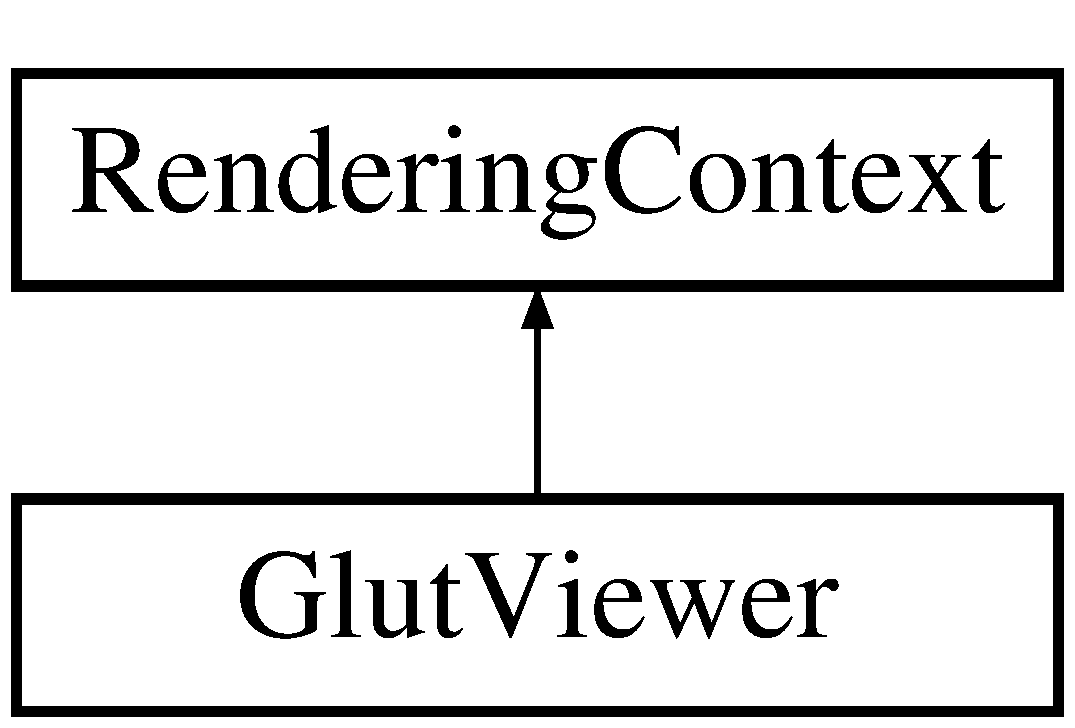
\includegraphics[height=2.000000cm]{struct_glut_viewer}
\end{center}
\end{figure}
\subsection*{Public Types}
\begin{DoxyCompactItemize}
\item 
\mbox{\Hypertarget{struct_glut_viewer_aea31480390a568733169b60a83e3c8fc}\label{struct_glut_viewer_aea31480390a568733169b60a83e3c8fc}} 
enum {\bfseries Orientation} \{ {\bfseries X\+\_\+\+UP}, 
{\bfseries Y\+\_\+\+UP}, 
{\bfseries Z\+\_\+\+UP}
 \}
\end{DoxyCompactItemize}
\subsection*{Public Methods}
\begin{DoxyCompactItemize}
\item 
\mbox{\Hypertarget{struct_glut_viewer_ab49b8c33c56c472f42946c32a479a47d}\label{struct_glut_viewer_ab49b8c33c56c472f42946c32a479a47d}} 
void {\bfseries init} (int argc, char $\ast$$\ast$argv)
\end{DoxyCompactItemize}
\subsection*{Static Public Methods}
\begin{DoxyCompactItemize}
\item 
\mbox{\Hypertarget{struct_glut_viewer_a88ec1ef1e42cdf6daa6e93cebfa3cdae}\label{struct_glut_viewer_a88ec1ef1e42cdf6daa6e93cebfa3cdae}} 
static void {\bfseries display} ()
\item 
\mbox{\Hypertarget{struct_glut_viewer_ac94c554f4339d0ff55c5cca9d1be2676}\label{struct_glut_viewer_ac94c554f4339d0ff55c5cca9d1be2676}} 
static void {\bfseries idle} ()
\item 
\mbox{\Hypertarget{struct_glut_viewer_a25fa4839d244f5f221c3fb346cdbe584}\label{struct_glut_viewer_a25fa4839d244f5f221c3fb346cdbe584}} 
static void {\bfseries mouse} (int button, int state, int x, int y)
\item 
\mbox{\Hypertarget{struct_glut_viewer_a88c7d9e7144e1dae7bd9b5e2d409a9d9}\label{struct_glut_viewer_a88c7d9e7144e1dae7bd9b5e2d409a9d9}} 
static void {\bfseries motion} (int x, int y)
\item 
\mbox{\Hypertarget{struct_glut_viewer_a738d02267b5482162d1c059e43257fb5}\label{struct_glut_viewer_a738d02267b5482162d1c059e43257fb5}} 
static void {\bfseries keyboard} (unsigned char character, int x, int y)
\end{DoxyCompactItemize}
\subsection*{Public Members}
\begin{DoxyCompactItemize}
\item 
\mbox{\Hypertarget{struct_glut_viewer_ac8c1bdb89bdd8c8ba11f317038922828}\label{struct_glut_viewer_ac8c1bdb89bdd8c8ba11f317038922828}} 
G\+Luint {\bfseries m\+\_\+texture}
\item 
\mbox{\Hypertarget{struct_glut_viewer_a80515c2f9201dba55f00c016a3f236c2}\label{struct_glut_viewer_a80515c2f9201dba55f00c016a3f236c2}} 
\hyperlink{struct_camera}{Camera} {\bfseries m\+\_\+camera\+\_\+o}
\item 
\mbox{\Hypertarget{struct_glut_viewer_a620431346d0b18b9ed623e74b572365b}\label{struct_glut_viewer_a620431346d0b18b9ed623e74b572365b}} 
\hyperlink{struct_directional_light}{Directional\+Light} {\bfseries m\+\_\+light\+\_\+o}
\item 
\mbox{\Hypertarget{struct_glut_viewer_a7b1cdc82f8800cd6b07af7ec98028311}\label{struct_glut_viewer_a7b1cdc82f8800cd6b07af7ec98028311}} 
int2 {\bfseries m\+\_\+mouse}
\item 
\mbox{\Hypertarget{struct_glut_viewer_adda7025a498500b5592d028dffa63aee}\label{struct_glut_viewer_adda7025a498500b5592d028dffa63aee}} 
float {\bfseries m\+\_\+mouse\+\_\+depth}
\item 
\mbox{\Hypertarget{struct_glut_viewer_a3ea2579916370b9e10fe46e35d5d3087}\label{struct_glut_viewer_a3ea2579916370b9e10fe46e35d5d3087}} 
bool {\bfseries m\+\_\+dollying}
\item 
\mbox{\Hypertarget{struct_glut_viewer_ab7376dddeca9d7a08a9f7f815f4090db}\label{struct_glut_viewer_ab7376dddeca9d7a08a9f7f815f4090db}} 
bool {\bfseries m\+\_\+panning}
\item 
\mbox{\Hypertarget{struct_glut_viewer_af0a18c2c6194c49f7a54781e90414722}\label{struct_glut_viewer_af0a18c2c6194c49f7a54781e90414722}} 
bool {\bfseries m\+\_\+walking}
\item 
\mbox{\Hypertarget{struct_glut_viewer_a32b35e32fea871ebf493ad7ffa425685}\label{struct_glut_viewer_a32b35e32fea871ebf493ad7ffa425685}} 
bool {\bfseries m\+\_\+zooming}
\item 
\mbox{\Hypertarget{struct_glut_viewer_a81293ef53f2bd8e4787787b9d93296c8}\label{struct_glut_viewer_a81293ef53f2bd8e4787787b9d93296c8}} 
bool {\bfseries m\+\_\+moving\+\_\+selection}
\item 
\mbox{\Hypertarget{struct_glut_viewer_a992438d7af514950b8ee24a8e2e7204b}\label{struct_glut_viewer_a992438d7af514950b8ee24a8e2e7204b}} 
bool {\bfseries m\+\_\+light\+\_\+rotation}
\item 
\mbox{\Hypertarget{struct_glut_viewer_a55f53e58dc74308bbd02fd04c8b6b3ba}\label{struct_glut_viewer_a55f53e58dc74308bbd02fd04c8b6b3ba}} 
Orientation {\bfseries m\+\_\+orientation}
\item 
\mbox{\Hypertarget{struct_glut_viewer_a6963748b58cd9ddecadfdbd9233f09fa}\label{struct_glut_viewer_a6963748b58cd9ddecadfdbd9233f09fa}} 
bool {\bfseries m\+\_\+dirty}
\item 
\mbox{\Hypertarget{struct_glut_viewer_a57f261531422115760708337530dbff5}\label{struct_glut_viewer_a57f261531422115760708337530dbff5}} 
bool {\bfseries m\+\_\+dirty\+\_\+geo}
\item 
\mbox{\Hypertarget{struct_glut_viewer_a57ea8813c0cecd6e73be5adcc1fd5e37}\label{struct_glut_viewer_a57ea8813c0cecd6e73be5adcc1fd5e37}} 
uint32 {\bfseries m\+\_\+instance}
\item 
\mbox{\Hypertarget{struct_glut_viewer_af71356b0780e37d9eb42903ee4073e3f}\label{struct_glut_viewer_af71356b0780e37d9eb42903ee4073e3f}} 
uint32 {\bfseries m\+\_\+selected\+\_\+group}
\item 
\mbox{\Hypertarget{struct_glut_viewer_a3dae4869ce235493a5e1206619a43495}\label{struct_glut_viewer_a3dae4869ce235493a5e1206619a43495}} 
char {\bfseries m\+\_\+output\+\_\+name} \mbox{[}1024\mbox{]}
\item 
\mbox{\Hypertarget{struct_glut_viewer_a0976d324bc91c1ce89a9361298318c8d}\label{struct_glut_viewer_a0976d324bc91c1ce89a9361298318c8d}} 
F\+I\+LE $\ast$ {\bfseries m\+\_\+ffmpeg}
\item 
\mbox{\Hypertarget{struct_glut_viewer_a4a743b7a3aaaa00cece6836809f9be74}\label{struct_glut_viewer_a4a743b7a3aaaa00cece6836809f9be74}} 
F\+I\+LE $\ast$ {\bfseries m\+\_\+camera\+\_\+path}
\item 
\mbox{\Hypertarget{struct_glut_viewer_a26c53d85482f5dad4c5cd14d63f964a8}\label{struct_glut_viewer_a26c53d85482f5dad4c5cd14d63f964a8}} 
bool {\bfseries m\+\_\+record}
\item 
\mbox{\Hypertarget{struct_glut_viewer_ac41a4b158f869094c622c4f7bb9d300d}\label{struct_glut_viewer_ac41a4b158f869094c622c4f7bb9d300d}} 
bool {\bfseries m\+\_\+playback}
\item 
\mbox{\Hypertarget{struct_glut_viewer_a94c9dbd2ffe934f197192d8d7e6fac9c}\label{struct_glut_viewer_a94c9dbd2ffe934f197192d8d7e6fac9c}} 
bool {\bfseries m\+\_\+accumulation}
\item 
\mbox{\Hypertarget{struct_glut_viewer_aa62ec6a90f69184520edab863b117243}\label{struct_glut_viewer_aa62ec6a90f69184520edab863b117243}} 
\hyperlink{classcugar_1_1_mutex}{cugar\+::\+Mutex} {\bfseries mutex}
\end{DoxyCompactItemize}


The documentation for this struct was generated from the following file\+:\begin{DoxyCompactItemize}
\item 
C\+:/p4research/research/jpantaleoni/\+Fermat-\/\+Public/src/glut\+\_\+viewer.\+h\end{DoxyCompactItemize}

\hypertarget{structcugar_1_1greater}{}\section{cugar\+:\+:greater$<$ T $>$ Struct Template Reference}
\label{structcugar_1_1greater}\index{cugar\+::greater$<$ T $>$@{cugar\+::greater$<$ T $>$}}


\subsection{Detailed description}
\subsubsection*{template$<$typename T$>$\newline
struct cugar\+::greater$<$ T $>$}

greater functor 

{\ttfamily \#include $<$functors.\+h$>$}

\subsection*{Public Types}
\begin{DoxyCompactItemize}
\item 
\mbox{\Hypertarget{structcugar_1_1greater_ae7551b71fae9d40442e3e0ef7a72877c}\label{structcugar_1_1greater_ae7551b71fae9d40442e3e0ef7a72877c}} 
typedef \hyperlink{structcugar_1_1binary__function__tag}{binary\+\_\+function\+\_\+tag} {\bfseries function\+\_\+tag}
\item 
\mbox{\Hypertarget{structcugar_1_1greater_a768125f3a1b329bf29868442169aa9f1}\label{structcugar_1_1greater_a768125f3a1b329bf29868442169aa9f1}} 
typedef T {\bfseries first\+\_\+argument\+\_\+type}
\item 
\mbox{\Hypertarget{structcugar_1_1greater_ac4383aeb05e2828a8b03b02b9027a8e1}\label{structcugar_1_1greater_ac4383aeb05e2828a8b03b02b9027a8e1}} 
typedef T {\bfseries second\+\_\+argument\+\_\+type}
\item 
\mbox{\Hypertarget{structcugar_1_1greater_a5fb40ab823e24884fb0557c5c670bd3b}\label{structcugar_1_1greater_a5fb40ab823e24884fb0557c5c670bd3b}} 
typedef bool {\bfseries result\+\_\+type}
\end{DoxyCompactItemize}
\subsection*{Public Methods}
\begin{DoxyCompactItemize}
\item 
\mbox{\Hypertarget{structcugar_1_1greater_ace030b3a67c6f567f3388bbba22474a5}\label{structcugar_1_1greater_ace030b3a67c6f567f3388bbba22474a5}} 
C\+U\+G\+A\+R\+\_\+\+H\+O\+S\+T\+\_\+\+D\+E\+V\+I\+CE bool {\bfseries operator()} (const T \&op1, const T \&op2) const
\end{DoxyCompactItemize}


The documentation for this struct was generated from the following file\+:\begin{DoxyCompactItemize}
\item 
C\+:/p4research/research/jpantaleoni/\+Fermat-\/\+Public/contrib/cugar/basic/\hyperlink{functors_8h}{functors.\+h}\end{DoxyCompactItemize}

\hypertarget{structcugar_1_1greater__than__zero}{}\section{cugar\+:\+:greater\+\_\+than\+\_\+zero$<$ T $>$ Struct Template Reference}
\label{structcugar_1_1greater__than__zero}\index{cugar\+::greater\+\_\+than\+\_\+zero$<$ T $>$@{cugar\+::greater\+\_\+than\+\_\+zero$<$ T $>$}}


\subsection{Detailed description}
\subsubsection*{template$<$typename T$>$\newline
struct cugar\+::greater\+\_\+than\+\_\+zero$<$ T $>$}

greater than zero functor 

{\ttfamily \#include $<$functors.\+h$>$}

\subsection*{Public Types}
\begin{DoxyCompactItemize}
\item 
\mbox{\Hypertarget{structcugar_1_1greater__than__zero_ae0964ca9759f02185f1c1efea8569fd8}\label{structcugar_1_1greater__than__zero_ae0964ca9759f02185f1c1efea8569fd8}} 
typedef \hyperlink{structcugar_1_1unary__function__tag}{unary\+\_\+function\+\_\+tag} {\bfseries function\+\_\+tag}
\item 
\mbox{\Hypertarget{structcugar_1_1greater__than__zero_a8b6ce614a57662c5c2c2185c5aeeb1f0}\label{structcugar_1_1greater__than__zero_a8b6ce614a57662c5c2c2185c5aeeb1f0}} 
typedef T {\bfseries argument\+\_\+type}
\item 
\mbox{\Hypertarget{structcugar_1_1greater__than__zero_a34ef9453c0344ebba0a0d2b2c1617238}\label{structcugar_1_1greater__than__zero_a34ef9453c0344ebba0a0d2b2c1617238}} 
typedef bool {\bfseries result\+\_\+type}
\end{DoxyCompactItemize}
\subsection*{Public Methods}
\begin{DoxyCompactItemize}
\item 
\mbox{\Hypertarget{structcugar_1_1greater__than__zero_af09beb6aaccd355577621748ea1a6761}\label{structcugar_1_1greater__than__zero_af09beb6aaccd355577621748ea1a6761}} 
C\+U\+G\+A\+R\+\_\+\+H\+O\+S\+T\+\_\+\+D\+E\+V\+I\+CE bool {\bfseries operator()} (const T \&v) const
\end{DoxyCompactItemize}


The documentation for this struct was generated from the following file\+:\begin{DoxyCompactItemize}
\item 
C\+:/p4research/research/jpantaleoni/\+Fermat-\/\+Public/contrib/cugar/basic/\hyperlink{functors_8h}{functors.\+h}\end{DoxyCompactItemize}

\hypertarget{structcugar_1_1cuda_1_1_hash_map}{}\section{cugar\+:\+:cuda\+:\+:Hash\+Map$<$ KeyT, HashT, I\+N\+V\+A\+L\+I\+D\+\_\+\+K\+EY $>$ Struct Template Reference}
\label{structcugar_1_1cuda_1_1_hash_map}\index{cugar\+::cuda\+::\+Hash\+Map$<$ Key\+T, Hash\+T, I\+N\+V\+A\+L\+I\+D\+\_\+\+K\+E\+Y $>$@{cugar\+::cuda\+::\+Hash\+Map$<$ Key\+T, Hash\+T, I\+N\+V\+A\+L\+I\+D\+\_\+\+K\+E\+Y $>$}}


\subsection{Detailed description}
\subsubsection*{template$<$typename KeyT, typename HashT, KeyT I\+N\+V\+A\+L\+I\+D\+\_\+\+K\+EY = 0x\+F\+F\+F\+F\+F\+F\+FF$>$\newline
struct cugar\+::cuda\+::\+Hash\+Map$<$ Key\+T, Hash\+T, I\+N\+V\+A\+L\+I\+D\+\_\+\+K\+E\+Y $>$}

This class implements a device-\/side Hash Map, allowing arbitrary threads from potentially different C\+T\+As of a cuda kernel to add new entries at the same time.

The constructor of the class accepts pointers to the arrays representing the underlying data structure\+:


\begin{DoxyItemize}
\item an array of hashed keys
\item an array of unique set entries
\item an array of slots keeping track of the unique position where each inserted key has been mapped
\item a pointer to a counter, keeping track of the number of set entries
\end{DoxyItemize}

Before starting to use the \hyperlink{structcugar_1_1cuda_1_1_hash_set}{Hash\+Set}, the array of hash slots has to be initialized to I\+N\+V\+A\+L\+I\+D\+\_\+\+K\+EY.

The class provides two methods\+: \begin{DoxyVerb}- HashMap::insert
- HashMap::find
\end{DoxyVerb}


It\textquotesingle{}s important to notice that calls to the two methods cannot be mixed without interposing a global synchronization between them. 

{\ttfamily \#include $<$hash.\+h$>$}

Inheritance diagram for cugar\+:\+:cuda\+:\+:Hash\+Map$<$ KeyT, HashT, I\+N\+V\+A\+L\+I\+D\+\_\+\+K\+EY $>$\+:\begin{figure}[H]
\begin{center}
\leavevmode
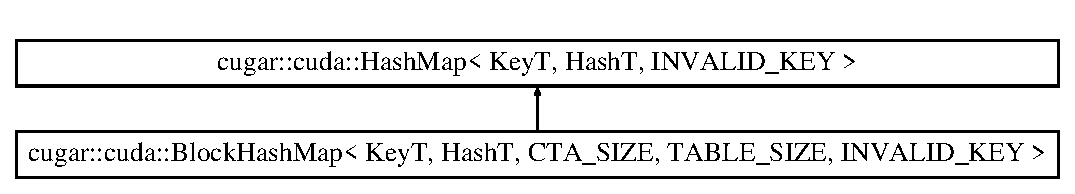
\includegraphics[height=2.000000cm]{structcugar_1_1cuda_1_1_hash_map}
\end{center}
\end{figure}
\subsection*{Public Methods}
\begin{DoxyCompactItemize}
\item 
C\+U\+G\+A\+R\+\_\+\+D\+E\+V\+I\+CE \hyperlink{structcugar_1_1cuda_1_1_hash_map_a010078c91599bfd5472498b17a00338f}{Hash\+Map} ()
\item 
C\+U\+G\+A\+R\+\_\+\+D\+E\+V\+I\+CE \hyperlink{structcugar_1_1cuda_1_1_hash_map_ab79e7e37774fe134aa831969c4f0fde4}{Hash\+Map} (const uint32 \+\_\+table\+\_\+size, KeyT $\ast$\+\_\+hash, KeyT $\ast$\+\_\+unique, uint32 $\ast$\+\_\+slots, uint32 $\ast$\+\_\+count)
\item 
C\+U\+G\+A\+R\+\_\+\+D\+E\+V\+I\+CE void \hyperlink{structcugar_1_1cuda_1_1_hash_map_acbef3382463b59782820e26370ed0794}{insert} (const KeyT key, const HashT hash\+\_\+code)
\item 
C\+U\+G\+A\+R\+\_\+\+D\+E\+V\+I\+CE uint32 \hyperlink{structcugar_1_1cuda_1_1_hash_map_a9f8bf3bd7f80e1fc667fe506fbb8979f}{find} (const KeyT key, const HashT hash\+\_\+code)
\item 
C\+U\+G\+A\+R\+\_\+\+D\+E\+V\+I\+CE uint32 \hyperlink{structcugar_1_1cuda_1_1_hash_map_ac36b53b042954823ba4da7bc78f09af5}{size} () const
\item 
C\+U\+G\+A\+R\+\_\+\+D\+E\+V\+I\+CE KeyT \hyperlink{structcugar_1_1cuda_1_1_hash_map_aa76aa5471105fb11566b5915ee96ca46}{get\+\_\+unique} (const uint32 i) const
\end{DoxyCompactItemize}
\subsection*{Public Members}
\begin{DoxyCompactItemize}
\item 
\mbox{\Hypertarget{structcugar_1_1cuda_1_1_hash_map_a241e20f15a2be2ea915c62ad7bf5d261}\label{structcugar_1_1cuda_1_1_hash_map_a241e20f15a2be2ea915c62ad7bf5d261}} 
uint32 {\bfseries table\+\_\+size}
\item 
\mbox{\Hypertarget{structcugar_1_1cuda_1_1_hash_map_ae23faa45f2bdfb7182fab74f458b1595}\label{structcugar_1_1cuda_1_1_hash_map_ae23faa45f2bdfb7182fab74f458b1595}} 
KeyT $\ast$ {\bfseries hash}
\item 
\mbox{\Hypertarget{structcugar_1_1cuda_1_1_hash_map_a66b789608dd604438914dee4d05299f2}\label{structcugar_1_1cuda_1_1_hash_map_a66b789608dd604438914dee4d05299f2}} 
KeyT $\ast$ {\bfseries unique}
\item 
\mbox{\Hypertarget{structcugar_1_1cuda_1_1_hash_map_ae4f0eda4ad786b7f097a5be74ead3a58}\label{structcugar_1_1cuda_1_1_hash_map_ae4f0eda4ad786b7f097a5be74ead3a58}} 
uint32 $\ast$ {\bfseries slots}
\item 
\mbox{\Hypertarget{structcugar_1_1cuda_1_1_hash_map_aa6ac5580a461770b9d53970b9f557ad4}\label{structcugar_1_1cuda_1_1_hash_map_aa6ac5580a461770b9d53970b9f557ad4}} 
uint32 $\ast$ {\bfseries count}
\end{DoxyCompactItemize}


\subsection{Constructor \& Destructor Documentation}
\mbox{\Hypertarget{structcugar_1_1cuda_1_1_hash_map_a010078c91599bfd5472498b17a00338f}\label{structcugar_1_1cuda_1_1_hash_map_a010078c91599bfd5472498b17a00338f}} 
\index{cugar\+::cuda\+::\+Hash\+Map@{cugar\+::cuda\+::\+Hash\+Map}!Hash\+Map@{Hash\+Map}}
\index{Hash\+Map@{Hash\+Map}!cugar\+::cuda\+::\+Hash\+Map@{cugar\+::cuda\+::\+Hash\+Map}}
\subsubsection{\texorpdfstring{Hash\+Map()}{HashMap()}\hspace{0.1cm}{\footnotesize\ttfamily [1/2]}}
{\footnotesize\ttfamily template$<$typename KeyT , typename HashT , KeyT I\+N\+V\+A\+L\+I\+D\+\_\+\+K\+EY = 0x\+F\+F\+F\+F\+F\+F\+FF$>$ \\
C\+U\+G\+A\+R\+\_\+\+D\+E\+V\+I\+CE \hyperlink{structcugar_1_1cuda_1_1_hash_map}{cugar\+::cuda\+::\+Hash\+Map}$<$ KeyT, HashT, I\+N\+V\+A\+L\+I\+D\+\_\+\+K\+EY $>$\+::\hyperlink{structcugar_1_1cuda_1_1_hash_map}{Hash\+Map} (\begin{DoxyParamCaption}{ }\end{DoxyParamCaption})\hspace{0.3cm}{\ttfamily [inline]}}

constructor \mbox{\Hypertarget{structcugar_1_1cuda_1_1_hash_map_ab79e7e37774fe134aa831969c4f0fde4}\label{structcugar_1_1cuda_1_1_hash_map_ab79e7e37774fe134aa831969c4f0fde4}} 
\index{cugar\+::cuda\+::\+Hash\+Map@{cugar\+::cuda\+::\+Hash\+Map}!Hash\+Map@{Hash\+Map}}
\index{Hash\+Map@{Hash\+Map}!cugar\+::cuda\+::\+Hash\+Map@{cugar\+::cuda\+::\+Hash\+Map}}
\subsubsection{\texorpdfstring{Hash\+Map()}{HashMap()}\hspace{0.1cm}{\footnotesize\ttfamily [2/2]}}
{\footnotesize\ttfamily template$<$typename KeyT , typename HashT , KeyT I\+N\+V\+A\+L\+I\+D\+\_\+\+K\+EY = 0x\+F\+F\+F\+F\+F\+F\+FF$>$ \\
C\+U\+G\+A\+R\+\_\+\+D\+E\+V\+I\+CE \hyperlink{structcugar_1_1cuda_1_1_hash_map}{cugar\+::cuda\+::\+Hash\+Map}$<$ KeyT, HashT, I\+N\+V\+A\+L\+I\+D\+\_\+\+K\+EY $>$\+::\hyperlink{structcugar_1_1cuda_1_1_hash_map}{Hash\+Map} (\begin{DoxyParamCaption}\item[{const uint32}]{\+\_\+table\+\_\+size,  }\item[{KeyT $\ast$}]{\+\_\+hash,  }\item[{KeyT $\ast$}]{\+\_\+unique,  }\item[{uint32 $\ast$}]{\+\_\+slots,  }\item[{uint32 $\ast$}]{\+\_\+count }\end{DoxyParamCaption})\hspace{0.3cm}{\ttfamily [inline]}}

constructor


\begin{DoxyParams}{Parameters}
{\em \+\_\+table\+\_\+size} & the size of the hash table (needs to be a power of 2) \\
\hline
{\em \+\_\+hash} & a pointer to the array of \+\_\+table\+\_\+size hashing slots -\/ needs to be initialized to I\+N\+V\+A\+L\+I\+D\+\_\+\+K\+EY before first use \\
\hline
{\em \+\_\+unique} & a pointer to the array where inserted entries will be stored -\/ needs to be appropriately sized to contain all unique entries \\
\hline
{\em \+\_\+slots} & a pointer to an array of \+\_\+table\+\_\+size entries keeping track of the unique position where each inserted key has been mapped \\
\hline
{\em \+\_\+count} & a pointer to a single counter, used to keep track of how many unique entries have been inserted \\
\hline
\end{DoxyParams}


\subsection{Member Function Documentation}
\mbox{\Hypertarget{structcugar_1_1cuda_1_1_hash_map_a9f8bf3bd7f80e1fc667fe506fbb8979f}\label{structcugar_1_1cuda_1_1_hash_map_a9f8bf3bd7f80e1fc667fe506fbb8979f}} 
\index{cugar\+::cuda\+::\+Hash\+Map@{cugar\+::cuda\+::\+Hash\+Map}!find@{find}}
\index{find@{find}!cugar\+::cuda\+::\+Hash\+Map@{cugar\+::cuda\+::\+Hash\+Map}}
\subsubsection{\texorpdfstring{find()}{find()}}
{\footnotesize\ttfamily template$<$typename KeyT , typename HashT , KeyT I\+N\+V\+A\+L\+I\+D\+\_\+\+K\+EY = 0x\+F\+F\+F\+F\+F\+F\+FF$>$ \\
C\+U\+G\+A\+R\+\_\+\+D\+E\+V\+I\+CE uint32 \hyperlink{structcugar_1_1cuda_1_1_hash_map}{cugar\+::cuda\+::\+Hash\+Map}$<$ KeyT, HashT, I\+N\+V\+A\+L\+I\+D\+\_\+\+K\+EY $>$\+::find (\begin{DoxyParamCaption}\item[{const KeyT}]{key,  }\item[{const HashT}]{hash\+\_\+code }\end{DoxyParamCaption})\hspace{0.3cm}{\ttfamily [inline]}}

find the unique slot associated to an inserted key (N\+O\+TE\+: needs to be separated from insertion by a synchronization point) \mbox{\Hypertarget{structcugar_1_1cuda_1_1_hash_map_aa76aa5471105fb11566b5915ee96ca46}\label{structcugar_1_1cuda_1_1_hash_map_aa76aa5471105fb11566b5915ee96ca46}} 
\index{cugar\+::cuda\+::\+Hash\+Map@{cugar\+::cuda\+::\+Hash\+Map}!get\+\_\+unique@{get\+\_\+unique}}
\index{get\+\_\+unique@{get\+\_\+unique}!cugar\+::cuda\+::\+Hash\+Map@{cugar\+::cuda\+::\+Hash\+Map}}
\subsubsection{\texorpdfstring{get\+\_\+unique()}{get\_unique()}}
{\footnotesize\ttfamily template$<$typename KeyT , typename HashT , KeyT I\+N\+V\+A\+L\+I\+D\+\_\+\+K\+EY = 0x\+F\+F\+F\+F\+F\+F\+FF$>$ \\
C\+U\+G\+A\+R\+\_\+\+D\+E\+V\+I\+CE KeyT \hyperlink{structcugar_1_1cuda_1_1_hash_map}{cugar\+::cuda\+::\+Hash\+Map}$<$ KeyT, HashT, I\+N\+V\+A\+L\+I\+D\+\_\+\+K\+EY $>$\+::get\+\_\+unique (\begin{DoxyParamCaption}\item[{const uint32}]{i }\end{DoxyParamCaption}) const\hspace{0.3cm}{\ttfamily [inline]}}

return the i-\/th unique element in the set \mbox{\Hypertarget{structcugar_1_1cuda_1_1_hash_map_acbef3382463b59782820e26370ed0794}\label{structcugar_1_1cuda_1_1_hash_map_acbef3382463b59782820e26370ed0794}} 
\index{cugar\+::cuda\+::\+Hash\+Map@{cugar\+::cuda\+::\+Hash\+Map}!insert@{insert}}
\index{insert@{insert}!cugar\+::cuda\+::\+Hash\+Map@{cugar\+::cuda\+::\+Hash\+Map}}
\subsubsection{\texorpdfstring{insert()}{insert()}}
{\footnotesize\ttfamily template$<$typename KeyT , typename HashT , KeyT I\+N\+V\+A\+L\+I\+D\+\_\+\+K\+EY = 0x\+F\+F\+F\+F\+F\+F\+FF$>$ \\
C\+U\+G\+A\+R\+\_\+\+D\+E\+V\+I\+CE void \hyperlink{structcugar_1_1cuda_1_1_hash_map}{cugar\+::cuda\+::\+Hash\+Map}$<$ KeyT, HashT, I\+N\+V\+A\+L\+I\+D\+\_\+\+K\+EY $>$\+::insert (\begin{DoxyParamCaption}\item[{const KeyT}]{key,  }\item[{const HashT}]{hash\+\_\+code }\end{DoxyParamCaption})\hspace{0.3cm}{\ttfamily [inline]}}

insert an element with its hashing value


\begin{DoxyParams}{Parameters}
{\em key} & the element to insert \\
\hline
{\em hash\+\_\+code} & the hashing value \\
\hline
\end{DoxyParams}
\mbox{\Hypertarget{structcugar_1_1cuda_1_1_hash_map_ac36b53b042954823ba4da7bc78f09af5}\label{structcugar_1_1cuda_1_1_hash_map_ac36b53b042954823ba4da7bc78f09af5}} 
\index{cugar\+::cuda\+::\+Hash\+Map@{cugar\+::cuda\+::\+Hash\+Map}!size@{size}}
\index{size@{size}!cugar\+::cuda\+::\+Hash\+Map@{cugar\+::cuda\+::\+Hash\+Map}}
\subsubsection{\texorpdfstring{size()}{size()}}
{\footnotesize\ttfamily template$<$typename KeyT , typename HashT , KeyT I\+N\+V\+A\+L\+I\+D\+\_\+\+K\+EY = 0x\+F\+F\+F\+F\+F\+F\+FF$>$ \\
C\+U\+G\+A\+R\+\_\+\+D\+E\+V\+I\+CE uint32 \hyperlink{structcugar_1_1cuda_1_1_hash_map}{cugar\+::cuda\+::\+Hash\+Map}$<$ KeyT, HashT, I\+N\+V\+A\+L\+I\+D\+\_\+\+K\+EY $>$\+::size (\begin{DoxyParamCaption}{ }\end{DoxyParamCaption}) const\hspace{0.3cm}{\ttfamily [inline]}}

return the size of the hash set 

The documentation for this struct was generated from the following file\+:\begin{DoxyCompactItemize}
\item 
C\+:/p4research/research/jpantaleoni/\+Fermat-\/\+Public/contrib/cugar/basic/cuda/hash.\+h\end{DoxyCompactItemize}

\hypertarget{structcugar_1_1cuda_1_1_hash_set}{}\section{cugar\+:\+:cuda\+:\+:Hash\+Set$<$ KeyT, HashT, I\+N\+V\+A\+L\+I\+D\+\_\+\+K\+EY $>$ Struct Template Reference}
\label{structcugar_1_1cuda_1_1_hash_set}\index{cugar\+::cuda\+::\+Hash\+Set$<$ Key\+T, Hash\+T, I\+N\+V\+A\+L\+I\+D\+\_\+\+K\+E\+Y $>$@{cugar\+::cuda\+::\+Hash\+Set$<$ Key\+T, Hash\+T, I\+N\+V\+A\+L\+I\+D\+\_\+\+K\+E\+Y $>$}}


\subsection{Detailed description}
\subsubsection*{template$<$typename KeyT, typename HashT, KeyT I\+N\+V\+A\+L\+I\+D\+\_\+\+K\+EY = 0x\+F\+F\+F\+F\+F\+F\+FF$>$\newline
struct cugar\+::cuda\+::\+Hash\+Set$<$ Key\+T, Hash\+T, I\+N\+V\+A\+L\+I\+D\+\_\+\+K\+E\+Y $>$}

This class implements a device-\/side Hash Set, allowing arbitrary threads from potentially different C\+T\+As of a cuda kernel to add new entries at the same time.

The constructor of the class accepts pointers to the arrays representing the underlying data structure\+:


\begin{DoxyItemize}
\item an array of hashed keys
\item an array of unique set entries
\item a pointer to a counter, keeping track of the number of set entries
\end{DoxyItemize}

Before starting to use the \hyperlink{structcugar_1_1cuda_1_1_hash_set}{Hash\+Set}, the array of hash slots has to be initialized to I\+N\+V\+A\+L\+I\+D\+\_\+\+K\+EY.

The class provides two methods\+: \begin{DoxyVerb}- HashSet::insert
- HashSet::has
\end{DoxyVerb}


It\textquotesingle{}s important to notice that calls to the two methods cannot be mixed without interposing a global synchronization between them. 

{\ttfamily \#include $<$hash.\+h$>$}

Inheritance diagram for cugar\+:\+:cuda\+:\+:Hash\+Set$<$ KeyT, HashT, I\+N\+V\+A\+L\+I\+D\+\_\+\+K\+EY $>$\+:\begin{figure}[H]
\begin{center}
\leavevmode
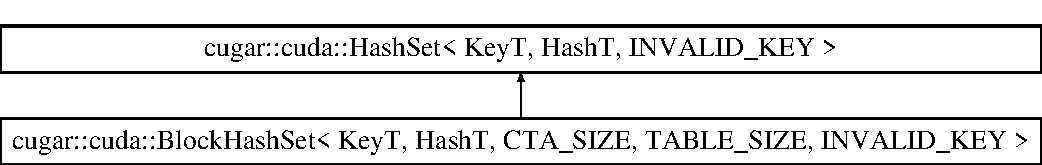
\includegraphics[height=2.000000cm]{structcugar_1_1cuda_1_1_hash_set}
\end{center}
\end{figure}
\subsection*{Public Methods}
\begin{DoxyCompactItemize}
\item 
C\+U\+G\+A\+R\+\_\+\+D\+E\+V\+I\+CE \hyperlink{structcugar_1_1cuda_1_1_hash_set_adc0a880b09c96a8723b7caf1c9a266fa}{Hash\+Set} ()
\item 
C\+U\+G\+A\+R\+\_\+\+D\+E\+V\+I\+CE \hyperlink{structcugar_1_1cuda_1_1_hash_set_a1fe8c1c90b9be37242999e97714998e3}{Hash\+Set} (const uint32 \+\_\+table\+\_\+size, KeyT $\ast$\+\_\+hash, KeyT $\ast$\+\_\+unique, uint32 $\ast$\+\_\+count)
\item 
C\+U\+G\+A\+R\+\_\+\+D\+E\+V\+I\+CE void \hyperlink{structcugar_1_1cuda_1_1_hash_set_a417db996be279f2a91dc97390021c96f}{insert} (const KeyT key, const HashT hash\+\_\+code)
\item 
C\+U\+G\+A\+R\+\_\+\+D\+E\+V\+I\+CE uint32 \hyperlink{structcugar_1_1cuda_1_1_hash_set_a624a256797d939b735e4aee67c352693}{size} () const
\item 
C\+U\+G\+A\+R\+\_\+\+D\+E\+V\+I\+CE KeyT \hyperlink{structcugar_1_1cuda_1_1_hash_set_a50361944a81d2bf60e528de63313db32}{get\+\_\+unique} (const uint32 i) const
\end{DoxyCompactItemize}
\subsection*{Public Members}
\begin{DoxyCompactItemize}
\item 
\mbox{\Hypertarget{structcugar_1_1cuda_1_1_hash_set_a074f287fab61cd45f89c9b0487e6a8a7}\label{structcugar_1_1cuda_1_1_hash_set_a074f287fab61cd45f89c9b0487e6a8a7}} 
uint32 {\bfseries table\+\_\+size}
\item 
\mbox{\Hypertarget{structcugar_1_1cuda_1_1_hash_set_a054f48c73abd88fea5e52a788a8b5f3c}\label{structcugar_1_1cuda_1_1_hash_set_a054f48c73abd88fea5e52a788a8b5f3c}} 
KeyT $\ast$ {\bfseries hash}
\item 
\mbox{\Hypertarget{structcugar_1_1cuda_1_1_hash_set_a29bb540aeaae51bdcebbdbddca1a8a02}\label{structcugar_1_1cuda_1_1_hash_set_a29bb540aeaae51bdcebbdbddca1a8a02}} 
KeyT $\ast$ {\bfseries unique}
\item 
\mbox{\Hypertarget{structcugar_1_1cuda_1_1_hash_set_aed55a50fc0654ba56940e9e56fe6dcc7}\label{structcugar_1_1cuda_1_1_hash_set_aed55a50fc0654ba56940e9e56fe6dcc7}} 
uint32 $\ast$ {\bfseries count}
\end{DoxyCompactItemize}


\subsection{Constructor \& Destructor Documentation}
\mbox{\Hypertarget{structcugar_1_1cuda_1_1_hash_set_adc0a880b09c96a8723b7caf1c9a266fa}\label{structcugar_1_1cuda_1_1_hash_set_adc0a880b09c96a8723b7caf1c9a266fa}} 
\index{cugar\+::cuda\+::\+Hash\+Set@{cugar\+::cuda\+::\+Hash\+Set}!Hash\+Set@{Hash\+Set}}
\index{Hash\+Set@{Hash\+Set}!cugar\+::cuda\+::\+Hash\+Set@{cugar\+::cuda\+::\+Hash\+Set}}
\subsubsection{\texorpdfstring{Hash\+Set()}{HashSet()}\hspace{0.1cm}{\footnotesize\ttfamily [1/2]}}
{\footnotesize\ttfamily template$<$typename KeyT , typename HashT , KeyT I\+N\+V\+A\+L\+I\+D\+\_\+\+K\+EY = 0x\+F\+F\+F\+F\+F\+F\+FF$>$ \\
C\+U\+G\+A\+R\+\_\+\+D\+E\+V\+I\+CE \hyperlink{structcugar_1_1cuda_1_1_hash_set}{cugar\+::cuda\+::\+Hash\+Set}$<$ KeyT, HashT, I\+N\+V\+A\+L\+I\+D\+\_\+\+K\+EY $>$\+::\hyperlink{structcugar_1_1cuda_1_1_hash_set}{Hash\+Set} (\begin{DoxyParamCaption}{ }\end{DoxyParamCaption})\hspace{0.3cm}{\ttfamily [inline]}}

empty constructor \mbox{\Hypertarget{structcugar_1_1cuda_1_1_hash_set_a1fe8c1c90b9be37242999e97714998e3}\label{structcugar_1_1cuda_1_1_hash_set_a1fe8c1c90b9be37242999e97714998e3}} 
\index{cugar\+::cuda\+::\+Hash\+Set@{cugar\+::cuda\+::\+Hash\+Set}!Hash\+Set@{Hash\+Set}}
\index{Hash\+Set@{Hash\+Set}!cugar\+::cuda\+::\+Hash\+Set@{cugar\+::cuda\+::\+Hash\+Set}}
\subsubsection{\texorpdfstring{Hash\+Set()}{HashSet()}\hspace{0.1cm}{\footnotesize\ttfamily [2/2]}}
{\footnotesize\ttfamily template$<$typename KeyT , typename HashT , KeyT I\+N\+V\+A\+L\+I\+D\+\_\+\+K\+EY = 0x\+F\+F\+F\+F\+F\+F\+FF$>$ \\
C\+U\+G\+A\+R\+\_\+\+D\+E\+V\+I\+CE \hyperlink{structcugar_1_1cuda_1_1_hash_set}{cugar\+::cuda\+::\+Hash\+Set}$<$ KeyT, HashT, I\+N\+V\+A\+L\+I\+D\+\_\+\+K\+EY $>$\+::\hyperlink{structcugar_1_1cuda_1_1_hash_set}{Hash\+Set} (\begin{DoxyParamCaption}\item[{const uint32}]{\+\_\+table\+\_\+size,  }\item[{KeyT $\ast$}]{\+\_\+hash,  }\item[{KeyT $\ast$}]{\+\_\+unique,  }\item[{uint32 $\ast$}]{\+\_\+count }\end{DoxyParamCaption})\hspace{0.3cm}{\ttfamily [inline]}}

\hyperlink{structcugar_1_1cuda_1_1_hash_set}{Hash\+Set} constructor


\begin{DoxyParams}{Parameters}
{\em \+\_\+table\+\_\+size} & the size of the hash table (needs to be a power of 2) \\
\hline
{\em \+\_\+hash} & a pointer to the array of \+\_\+table\+\_\+size hashed keys -\/ needs to be initialized to I\+N\+V\+A\+L\+I\+D\+\_\+\+K\+EY before first use \\
\hline
{\em \+\_\+unique} & a pointer to the array where inserted entries will be stored -\/ needs to be appropriately sized to contain all unique entries \\
\hline
{\em \+\_\+count} & a pointer to a single counter, used to keep track of how many unique entries have been inserted \\
\hline
\end{DoxyParams}


\subsection{Member Function Documentation}
\mbox{\Hypertarget{structcugar_1_1cuda_1_1_hash_set_a50361944a81d2bf60e528de63313db32}\label{structcugar_1_1cuda_1_1_hash_set_a50361944a81d2bf60e528de63313db32}} 
\index{cugar\+::cuda\+::\+Hash\+Set@{cugar\+::cuda\+::\+Hash\+Set}!get\+\_\+unique@{get\+\_\+unique}}
\index{get\+\_\+unique@{get\+\_\+unique}!cugar\+::cuda\+::\+Hash\+Set@{cugar\+::cuda\+::\+Hash\+Set}}
\subsubsection{\texorpdfstring{get\+\_\+unique()}{get\_unique()}}
{\footnotesize\ttfamily template$<$typename KeyT , typename HashT , KeyT I\+N\+V\+A\+L\+I\+D\+\_\+\+K\+EY = 0x\+F\+F\+F\+F\+F\+F\+FF$>$ \\
C\+U\+G\+A\+R\+\_\+\+D\+E\+V\+I\+CE KeyT \hyperlink{structcugar_1_1cuda_1_1_hash_set}{cugar\+::cuda\+::\+Hash\+Set}$<$ KeyT, HashT, I\+N\+V\+A\+L\+I\+D\+\_\+\+K\+EY $>$\+::get\+\_\+unique (\begin{DoxyParamCaption}\item[{const uint32}]{i }\end{DoxyParamCaption}) const\hspace{0.3cm}{\ttfamily [inline]}}

return the i-\/th unique element in the set \mbox{\Hypertarget{structcugar_1_1cuda_1_1_hash_set_a417db996be279f2a91dc97390021c96f}\label{structcugar_1_1cuda_1_1_hash_set_a417db996be279f2a91dc97390021c96f}} 
\index{cugar\+::cuda\+::\+Hash\+Set@{cugar\+::cuda\+::\+Hash\+Set}!insert@{insert}}
\index{insert@{insert}!cugar\+::cuda\+::\+Hash\+Set@{cugar\+::cuda\+::\+Hash\+Set}}
\subsubsection{\texorpdfstring{insert()}{insert()}}
{\footnotesize\ttfamily template$<$typename KeyT , typename HashT , KeyT I\+N\+V\+A\+L\+I\+D\+\_\+\+K\+EY = 0x\+F\+F\+F\+F\+F\+F\+FF$>$ \\
C\+U\+G\+A\+R\+\_\+\+D\+E\+V\+I\+CE void \hyperlink{structcugar_1_1cuda_1_1_hash_set}{cugar\+::cuda\+::\+Hash\+Set}$<$ KeyT, HashT, I\+N\+V\+A\+L\+I\+D\+\_\+\+K\+EY $>$\+::insert (\begin{DoxyParamCaption}\item[{const KeyT}]{key,  }\item[{const HashT}]{hash\+\_\+code }\end{DoxyParamCaption})\hspace{0.3cm}{\ttfamily [inline]}}

insert an element with its hashing value


\begin{DoxyParams}{Parameters}
{\em key} & the element to insert \\
\hline
{\em hash\+\_\+code} & the hashing value \\
\hline
\end{DoxyParams}
\mbox{\Hypertarget{structcugar_1_1cuda_1_1_hash_set_a624a256797d939b735e4aee67c352693}\label{structcugar_1_1cuda_1_1_hash_set_a624a256797d939b735e4aee67c352693}} 
\index{cugar\+::cuda\+::\+Hash\+Set@{cugar\+::cuda\+::\+Hash\+Set}!size@{size}}
\index{size@{size}!cugar\+::cuda\+::\+Hash\+Set@{cugar\+::cuda\+::\+Hash\+Set}}
\subsubsection{\texorpdfstring{size()}{size()}}
{\footnotesize\ttfamily template$<$typename KeyT , typename HashT , KeyT I\+N\+V\+A\+L\+I\+D\+\_\+\+K\+EY = 0x\+F\+F\+F\+F\+F\+F\+FF$>$ \\
C\+U\+G\+A\+R\+\_\+\+D\+E\+V\+I\+CE uint32 \hyperlink{structcugar_1_1cuda_1_1_hash_set}{cugar\+::cuda\+::\+Hash\+Set}$<$ KeyT, HashT, I\+N\+V\+A\+L\+I\+D\+\_\+\+K\+EY $>$\+::size (\begin{DoxyParamCaption}{ }\end{DoxyParamCaption}) const\hspace{0.3cm}{\ttfamily [inline]}}

return the size of the hash set 

The documentation for this struct was generated from the following file\+:\begin{DoxyCompactItemize}
\item 
C\+:/p4research/research/jpantaleoni/\+Fermat-\/\+Public/contrib/cugar/basic/cuda/hash.\+h\end{DoxyCompactItemize}

\hypertarget{struct_hello_p_t}{}\section{Hello\+PT Struct Reference}
\label{struct_hello_p_t}\index{Hello\+PT@{Hello\+PT}}


\subsection{Detailed description}
A \char`\"{}\+Hello Path Tracing\char`\"{} renderer 

{\ttfamily \#include $<$hellopt.\+h$>$}

Inheritance diagram for Hello\+PT\+:\begin{figure}[H]
\begin{center}
\leavevmode
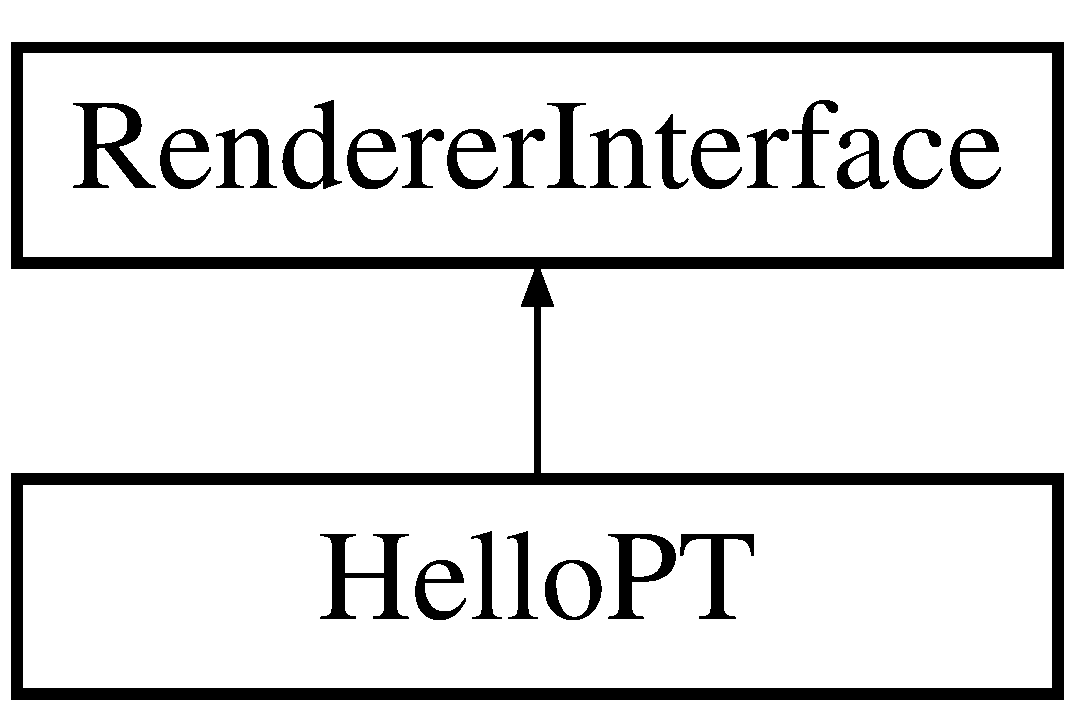
\includegraphics[height=2.000000cm]{struct_hello_p_t}
\end{center}
\end{figure}
\subsection*{Public Methods}
\begin{DoxyCompactItemize}
\item 
void \hyperlink{struct_hello_p_t_a8ec59e3fac8eff801cecdd3220cd8d41}{init} (int argc, char $\ast$$\ast$argv, \hyperlink{struct_rendering_context}{Rendering\+Context} \&renderer)
\item 
void \hyperlink{struct_hello_p_t_af772aac0d80118742450fd8b6b3c58c2}{render} (const uint32 instance, \hyperlink{struct_rendering_context}{Rendering\+Context} \&renderer)
\item 
void \hyperlink{struct_hello_p_t_ac81e09dcfb28dffc85aa6c4df06a4426}{destroy} ()
\end{DoxyCompactItemize}
\subsection*{Static Public Methods}
\begin{DoxyCompactItemize}
\item 
\mbox{\Hypertarget{struct_hello_p_t_a347a1e63590b2e1dc84f8ef601a3574b}\label{struct_hello_p_t_a347a1e63590b2e1dc84f8ef601a3574b}} 
static \hyperlink{struct_renderer_interface}{Renderer\+Interface} $\ast$ {\bfseries factory} ()
\end{DoxyCompactItemize}
\subsection*{Public Members}
\begin{DoxyCompactItemize}
\item 
\mbox{\Hypertarget{struct_hello_p_t_a2e7ca0c493562e157984ce410b86509e}\label{struct_hello_p_t_a2e7ca0c493562e157984ce410b86509e}} 
\hyperlink{struct_hello_p_t_options}{Hello\+P\+T\+Options} {\bfseries m\+\_\+options}
\item 
\mbox{\Hypertarget{struct_hello_p_t_a82179262319c026678ae4f7ed8a706d8}\label{struct_hello_p_t_a82179262319c026678ae4f7ed8a706d8}} 
\hyperlink{class_domain_buffer}{Domain\+Buffer}$<$ C\+U\+D\+A\+\_\+\+B\+U\+F\+F\+ER, uint8 $>$ {\bfseries m\+\_\+memory\+\_\+pool}
\item 
\mbox{\Hypertarget{struct_hello_p_t_ad14d0897040544317b951e59c6657fd5}\label{struct_hello_p_t_ad14d0897040544317b951e59c6657fd5}} 
\hyperlink{struct_tiled_sequence}{Tiled\+Sequence} {\bfseries m\+\_\+sequence}
\end{DoxyCompactItemize}


\subsection{Member Function Documentation}
\mbox{\Hypertarget{struct_hello_p_t_ac81e09dcfb28dffc85aa6c4df06a4426}\label{struct_hello_p_t_ac81e09dcfb28dffc85aa6c4df06a4426}} 
\index{Hello\+PT@{Hello\+PT}!destroy@{destroy}}
\index{destroy@{destroy}!Hello\+PT@{Hello\+PT}}
\subsubsection{\texorpdfstring{destroy()}{destroy()}}
{\footnotesize\ttfamily void Hello\+P\+T\+::destroy (\begin{DoxyParamCaption}{ }\end{DoxyParamCaption})\hspace{0.3cm}{\ttfamily [inline]}, {\ttfamily [virtual]}}

this method is responsible for destroying the object itself 

Reimplemented from \hyperlink{struct_renderer_interface_a7469218aafa029a3e22bac2c00dca9f5}{Renderer\+Interface}.

\mbox{\Hypertarget{struct_hello_p_t_a8ec59e3fac8eff801cecdd3220cd8d41}\label{struct_hello_p_t_a8ec59e3fac8eff801cecdd3220cd8d41}} 
\index{Hello\+PT@{Hello\+PT}!init@{init}}
\index{init@{init}!Hello\+PT@{Hello\+PT}}
\subsubsection{\texorpdfstring{init()}{init()}}
{\footnotesize\ttfamily void Hello\+P\+T\+::init (\begin{DoxyParamCaption}\item[{int}]{argc,  }\item[{char $\ast$$\ast$}]{argv,  }\item[{\hyperlink{struct_rendering_context}{Rendering\+Context} \&}]{renderer }\end{DoxyParamCaption})\hspace{0.3cm}{\ttfamily [virtual]}}

this method is responsible for any command options parsing / initializations the renderer might need to perform 

Reimplemented from \hyperlink{struct_renderer_interface_a2ead9b943d6d48fcd32872e0005ebe63}{Renderer\+Interface}.

\mbox{\Hypertarget{struct_hello_p_t_af772aac0d80118742450fd8b6b3c58c2}\label{struct_hello_p_t_af772aac0d80118742450fd8b6b3c58c2}} 
\index{Hello\+PT@{Hello\+PT}!render@{render}}
\index{render@{render}!Hello\+PT@{Hello\+PT}}
\subsubsection{\texorpdfstring{render()}{render()}}
{\footnotesize\ttfamily void Hello\+P\+T\+::render (\begin{DoxyParamCaption}\item[{const uint32}]{instance,  }\item[{\hyperlink{struct_rendering_context}{Rendering\+Context} \&}]{renderer }\end{DoxyParamCaption})\hspace{0.3cm}{\ttfamily [virtual]}}

this method is responsible for rendering a given frame in a progressive rendering


\begin{DoxyParams}{Parameters}
{\em instance} & the frame instance \\
\hline
\end{DoxyParams}


Reimplemented from \hyperlink{struct_renderer_interface_aa64254dd44c94929b05092dc8d74f29d}{Renderer\+Interface}.



The documentation for this struct was generated from the following file\+:\begin{DoxyCompactItemize}
\item 
C\+:/p4research/research/jpantaleoni/\+Fermat-\/\+Public/src/renderers/hellopt.\+h\end{DoxyCompactItemize}

\hypertarget{struct_hello_p_t_options}{}\section{Hello\+P\+T\+Options Struct Reference}
\label{struct_hello_p_t_options}\index{Hello\+P\+T\+Options@{Hello\+P\+T\+Options}}


\subsection{Detailed description}
our \char`\"{}\+Hello Path Tracing\char`\"{} options 

{\ttfamily \#include $<$hellopt.\+h$>$}

\subsection*{Public Methods}
\begin{DoxyCompactItemize}
\item 
\hyperlink{struct_hello_p_t_options_a244c96683d3c5d345bdf4b6b8aa9c249}{Hello\+P\+T\+Options} ()
\item 
void \hyperlink{struct_hello_p_t_options_a540d006dee6aff8ee5e8b3cfc8b0fa0b}{parse} (const int argc, char $\ast$$\ast$argv)
\end{DoxyCompactItemize}
\subsection*{Public Members}
\begin{DoxyCompactItemize}
\item 
\mbox{\Hypertarget{struct_hello_p_t_options_a7a22bb6990a291d333ae4c11c5d0c7b7}\label{struct_hello_p_t_options_a7a22bb6990a291d333ae4c11c5d0c7b7}} 
uint32 {\bfseries max\+\_\+path\+\_\+length}
\end{DoxyCompactItemize}


\subsection{Constructor \& Destructor Documentation}
\mbox{\Hypertarget{struct_hello_p_t_options_a244c96683d3c5d345bdf4b6b8aa9c249}\label{struct_hello_p_t_options_a244c96683d3c5d345bdf4b6b8aa9c249}} 
\index{Hello\+P\+T\+Options@{Hello\+P\+T\+Options}!Hello\+P\+T\+Options@{Hello\+P\+T\+Options}}
\index{Hello\+P\+T\+Options@{Hello\+P\+T\+Options}!Hello\+P\+T\+Options@{Hello\+P\+T\+Options}}
\subsubsection{\texorpdfstring{Hello\+P\+T\+Options()}{HelloPTOptions()}}
{\footnotesize\ttfamily Hello\+P\+T\+Options\+::\+Hello\+P\+T\+Options (\begin{DoxyParamCaption}{ }\end{DoxyParamCaption})\hspace{0.3cm}{\ttfamily [inline]}}

default constructor 

\subsection{Member Function Documentation}
\mbox{\Hypertarget{struct_hello_p_t_options_a540d006dee6aff8ee5e8b3cfc8b0fa0b}\label{struct_hello_p_t_options_a540d006dee6aff8ee5e8b3cfc8b0fa0b}} 
\index{Hello\+P\+T\+Options@{Hello\+P\+T\+Options}!parse@{parse}}
\index{parse@{parse}!Hello\+P\+T\+Options@{Hello\+P\+T\+Options}}
\subsubsection{\texorpdfstring{parse()}{parse()}}
{\footnotesize\ttfamily void Hello\+P\+T\+Options\+::parse (\begin{DoxyParamCaption}\item[{const int}]{argc,  }\item[{char $\ast$$\ast$}]{argv }\end{DoxyParamCaption})\hspace{0.3cm}{\ttfamily [inline]}}

do some simple option parsing 

The documentation for this struct was generated from the following file\+:\begin{DoxyCompactItemize}
\item 
C\+:/p4research/research/jpantaleoni/\+Fermat-\/\+Public/src/renderers/hellopt.\+h\end{DoxyCompactItemize}

\hypertarget{structcugar_1_1hi__bits__functor}{}\section{cugar\+:\+:hi\+\_\+bits\+\_\+functor$<$ T, U $>$ Struct Template Reference}
\label{structcugar_1_1hi__bits__functor}\index{cugar\+::hi\+\_\+bits\+\_\+functor$<$ T, U $>$@{cugar\+::hi\+\_\+bits\+\_\+functor$<$ T, U $>$}}


\subsection{Detailed description}
\subsubsection*{template$<$typename T, typename U$>$\newline
struct cugar\+::hi\+\_\+bits\+\_\+functor$<$ T, U $>$}

Return the first M hi-\/bits of an N-\/bit word 

{\ttfamily \#include $<$functors.\+h$>$}



The documentation for this struct was generated from the following file\+:\begin{DoxyCompactItemize}
\item 
C\+:/p4research/research/jpantaleoni/\+Fermat-\/\+Public/contrib/cugar/basic/\hyperlink{functors_8h}{functors.\+h}\end{DoxyCompactItemize}

\hypertarget{structcugar_1_1hi__bits__functor_3_01uint16_00_01uint32_01_4}{}\section{cugar\+:\+:hi\+\_\+bits\+\_\+functor$<$ uint16, uint32 $>$ Struct Template Reference}
\label{structcugar_1_1hi__bits__functor_3_01uint16_00_01uint32_01_4}\index{cugar\+::hi\+\_\+bits\+\_\+functor$<$ uint16, uint32 $>$@{cugar\+::hi\+\_\+bits\+\_\+functor$<$ uint16, uint32 $>$}}


\subsection{Detailed description}
\subsubsection*{template$<$$>$\newline
struct cugar\+::hi\+\_\+bits\+\_\+functor$<$ uint16, uint32 $>$}

Return the first 16 hi-\/bits of a 32-\/bit word 

{\ttfamily \#include $<$functors.\+h$>$}

\subsection*{Public Types}
\begin{DoxyCompactItemize}
\item 
\mbox{\Hypertarget{structcugar_1_1hi__bits__functor_3_01uint16_00_01uint32_01_4_ab5d53f1b328a6c647cf17ea4d2f8bd8c}\label{structcugar_1_1hi__bits__functor_3_01uint16_00_01uint32_01_4_ab5d53f1b328a6c647cf17ea4d2f8bd8c}} 
typedef uint32 {\bfseries argument\+\_\+type}
\item 
\mbox{\Hypertarget{structcugar_1_1hi__bits__functor_3_01uint16_00_01uint32_01_4_a7ba3fb554f97b7f150cc0ed0c2acaa45}\label{structcugar_1_1hi__bits__functor_3_01uint16_00_01uint32_01_4_a7ba3fb554f97b7f150cc0ed0c2acaa45}} 
typedef uint16 {\bfseries result\+\_\+type}
\end{DoxyCompactItemize}
\subsection*{Public Methods}
\begin{DoxyCompactItemize}
\item 
\mbox{\Hypertarget{structcugar_1_1hi__bits__functor_3_01uint16_00_01uint32_01_4_a37339ca897547b2e582bf0a899863af3}\label{structcugar_1_1hi__bits__functor_3_01uint16_00_01uint32_01_4_a37339ca897547b2e582bf0a899863af3}} 
C\+U\+G\+A\+R\+\_\+\+F\+O\+R\+C\+E\+I\+N\+L\+I\+NE C\+U\+G\+A\+R\+\_\+\+H\+O\+S\+T\+\_\+\+D\+E\+V\+I\+CE result\+\_\+type {\bfseries operator()} (const argument\+\_\+type op) const
\end{DoxyCompactItemize}


The documentation for this struct was generated from the following file\+:\begin{DoxyCompactItemize}
\item 
C\+:/p4research/research/jpantaleoni/\+Fermat-\/\+Public/contrib/cugar/basic/\hyperlink{functors_8h}{functors.\+h}\end{DoxyCompactItemize}

\hypertarget{structcugar_1_1hi__bits__functor_3_01uint32_00_01uint32_01_4}{}\section{cugar\+:\+:hi\+\_\+bits\+\_\+functor$<$ uint32, uint32 $>$ Struct Template Reference}
\label{structcugar_1_1hi__bits__functor_3_01uint32_00_01uint32_01_4}\index{cugar\+::hi\+\_\+bits\+\_\+functor$<$ uint32, uint32 $>$@{cugar\+::hi\+\_\+bits\+\_\+functor$<$ uint32, uint32 $>$}}


\subsection{Detailed description}
\subsubsection*{template$<$$>$\newline
struct cugar\+::hi\+\_\+bits\+\_\+functor$<$ uint32, uint32 $>$}

Return the first 32 hi-\/bits of a 32-\/bit word 

{\ttfamily \#include $<$functors.\+h$>$}

\subsection*{Public Types}
\begin{DoxyCompactItemize}
\item 
\mbox{\Hypertarget{structcugar_1_1hi__bits__functor_3_01uint32_00_01uint32_01_4_a9f5258820949d1e3d21f7e125e124d28}\label{structcugar_1_1hi__bits__functor_3_01uint32_00_01uint32_01_4_a9f5258820949d1e3d21f7e125e124d28}} 
typedef uint32 {\bfseries argument\+\_\+type}
\item 
\mbox{\Hypertarget{structcugar_1_1hi__bits__functor_3_01uint32_00_01uint32_01_4_a3a678366bdc5bc6248fc3f7249c39cab}\label{structcugar_1_1hi__bits__functor_3_01uint32_00_01uint32_01_4_a3a678366bdc5bc6248fc3f7249c39cab}} 
typedef uint32 {\bfseries result\+\_\+type}
\end{DoxyCompactItemize}
\subsection*{Public Methods}
\begin{DoxyCompactItemize}
\item 
\mbox{\Hypertarget{structcugar_1_1hi__bits__functor_3_01uint32_00_01uint32_01_4_ae7f91c978a11be0285a05a903a3a4611}\label{structcugar_1_1hi__bits__functor_3_01uint32_00_01uint32_01_4_ae7f91c978a11be0285a05a903a3a4611}} 
C\+U\+G\+A\+R\+\_\+\+F\+O\+R\+C\+E\+I\+N\+L\+I\+NE C\+U\+G\+A\+R\+\_\+\+H\+O\+S\+T\+\_\+\+D\+E\+V\+I\+CE result\+\_\+type {\bfseries operator()} (const argument\+\_\+type op) const
\end{DoxyCompactItemize}


The documentation for this struct was generated from the following file\+:\begin{DoxyCompactItemize}
\item 
C\+:/p4research/research/jpantaleoni/\+Fermat-\/\+Public/contrib/cugar/basic/\hyperlink{functors_8h}{functors.\+h}\end{DoxyCompactItemize}

\hypertarget{structcugar_1_1hi__bits__functor_3_01uint32_00_01uint64_01_4}{}\section{cugar\+:\+:hi\+\_\+bits\+\_\+functor$<$ uint32, uint64 $>$ Struct Template Reference}
\label{structcugar_1_1hi__bits__functor_3_01uint32_00_01uint64_01_4}\index{cugar\+::hi\+\_\+bits\+\_\+functor$<$ uint32, uint64 $>$@{cugar\+::hi\+\_\+bits\+\_\+functor$<$ uint32, uint64 $>$}}


\subsection{Detailed description}
\subsubsection*{template$<$$>$\newline
struct cugar\+::hi\+\_\+bits\+\_\+functor$<$ uint32, uint64 $>$}

Return the first 32 hi-\/bits of a 64-\/bit word 

{\ttfamily \#include $<$functors.\+h$>$}

\subsection*{Public Types}
\begin{DoxyCompactItemize}
\item 
\mbox{\Hypertarget{structcugar_1_1hi__bits__functor_3_01uint32_00_01uint64_01_4_a769452c89ab1c96cfc1aefb44cc1090e}\label{structcugar_1_1hi__bits__functor_3_01uint32_00_01uint64_01_4_a769452c89ab1c96cfc1aefb44cc1090e}} 
typedef uint64 {\bfseries argument\+\_\+type}
\item 
\mbox{\Hypertarget{structcugar_1_1hi__bits__functor_3_01uint32_00_01uint64_01_4_a7807506013acdd5a919144363e3b2c1c}\label{structcugar_1_1hi__bits__functor_3_01uint32_00_01uint64_01_4_a7807506013acdd5a919144363e3b2c1c}} 
typedef uint32 {\bfseries result\+\_\+type}
\end{DoxyCompactItemize}
\subsection*{Public Methods}
\begin{DoxyCompactItemize}
\item 
\mbox{\Hypertarget{structcugar_1_1hi__bits__functor_3_01uint32_00_01uint64_01_4_a234d619fc43f9daf2009fdf7f3cbc987}\label{structcugar_1_1hi__bits__functor_3_01uint32_00_01uint64_01_4_a234d619fc43f9daf2009fdf7f3cbc987}} 
C\+U\+G\+A\+R\+\_\+\+F\+O\+R\+C\+E\+I\+N\+L\+I\+NE C\+U\+G\+A\+R\+\_\+\+H\+O\+S\+T\+\_\+\+D\+E\+V\+I\+CE result\+\_\+type {\bfseries operator()} (const argument\+\_\+type op) const
\end{DoxyCompactItemize}


The documentation for this struct was generated from the following file\+:\begin{DoxyCompactItemize}
\item 
C\+:/p4research/research/jpantaleoni/\+Fermat-\/\+Public/contrib/cugar/basic/\hyperlink{functors_8h}{functors.\+h}\end{DoxyCompactItemize}

\hypertarget{structcugar_1_1hi__bits__functor_3_01uint8_00_01uint32_01_4}{}\section{cugar\+:\+:hi\+\_\+bits\+\_\+functor$<$ uint8, uint32 $>$ Struct Template Reference}
\label{structcugar_1_1hi__bits__functor_3_01uint8_00_01uint32_01_4}\index{cugar\+::hi\+\_\+bits\+\_\+functor$<$ uint8, uint32 $>$@{cugar\+::hi\+\_\+bits\+\_\+functor$<$ uint8, uint32 $>$}}


\subsection{Detailed description}
\subsubsection*{template$<$$>$\newline
struct cugar\+::hi\+\_\+bits\+\_\+functor$<$ uint8, uint32 $>$}

Return the first 8 hi-\/bits of a 32-\/bit word 

{\ttfamily \#include $<$functors.\+h$>$}

\subsection*{Public Types}
\begin{DoxyCompactItemize}
\item 
\mbox{\Hypertarget{structcugar_1_1hi__bits__functor_3_01uint8_00_01uint32_01_4_ab1d4c68f9b3058bc9cbc9b75653e90ec}\label{structcugar_1_1hi__bits__functor_3_01uint8_00_01uint32_01_4_ab1d4c68f9b3058bc9cbc9b75653e90ec}} 
typedef uint32 {\bfseries argument\+\_\+type}
\item 
\mbox{\Hypertarget{structcugar_1_1hi__bits__functor_3_01uint8_00_01uint32_01_4_a5695a7618cc2aafd358f5e943fbaa352}\label{structcugar_1_1hi__bits__functor_3_01uint8_00_01uint32_01_4_a5695a7618cc2aafd358f5e943fbaa352}} 
typedef uint8 {\bfseries result\+\_\+type}
\end{DoxyCompactItemize}
\subsection*{Public Methods}
\begin{DoxyCompactItemize}
\item 
\mbox{\Hypertarget{structcugar_1_1hi__bits__functor_3_01uint8_00_01uint32_01_4_a1300f7e181d6726fec330499db39167c}\label{structcugar_1_1hi__bits__functor_3_01uint8_00_01uint32_01_4_a1300f7e181d6726fec330499db39167c}} 
C\+U\+G\+A\+R\+\_\+\+F\+O\+R\+C\+E\+I\+N\+L\+I\+NE C\+U\+G\+A\+R\+\_\+\+H\+O\+S\+T\+\_\+\+D\+E\+V\+I\+CE result\+\_\+type {\bfseries operator()} (const argument\+\_\+type op) const
\end{DoxyCompactItemize}


The documentation for this struct was generated from the following file\+:\begin{DoxyCompactItemize}
\item 
C\+:/p4research/research/jpantaleoni/\+Fermat-\/\+Public/contrib/cugar/basic/\hyperlink{functors_8h}{functors.\+h}\end{DoxyCompactItemize}

\hypertarget{struct_hit}{}\section{Hit Struct Reference}
\label{struct_hit}\index{Hit@{Hit}}


\subsection{Detailed description}
Ray-\/tracing hit 

{\ttfamily \#include $<$ray.\+h$>$}

\subsection*{Public Members}
\begin{DoxyCompactItemize}
\item 
\mbox{\Hypertarget{struct_hit_a1ae6a3d9a5c8b1225a827d247947bc25}\label{struct_hit_a1ae6a3d9a5c8b1225a827d247947bc25}} 
float {\bfseries t}
\item 
\mbox{\Hypertarget{struct_hit_af329573ccab082ecba3dfac8142d22df}\label{struct_hit_af329573ccab082ecba3dfac8142d22df}} 
int {\bfseries tri\+Id}
\item 
\mbox{\Hypertarget{struct_hit_a393189286fc8bf21e8dd69e610a6ab16}\label{struct_hit_a393189286fc8bf21e8dd69e610a6ab16}} 
float {\bfseries u}
\item 
\mbox{\Hypertarget{struct_hit_a13c64f486914f22a4a14cfdbdc008dc3}\label{struct_hit_a13c64f486914f22a4a14cfdbdc008dc3}} 
float {\bfseries v}
\end{DoxyCompactItemize}
\subsection*{Static Public Members}
\begin{DoxyCompactItemize}
\item 
\mbox{\Hypertarget{struct_hit_ad194a1c0922885432181db0ff697bf96}\label{struct_hit_ad194a1c0922885432181db0ff697bf96}} 
static const R\+T\+Pbufferformat {\bfseries format} = R\+T\+P\+\_\+\+B\+U\+F\+F\+E\+R\+\_\+\+F\+O\+R\+M\+A\+T\+\_\+\+H\+I\+T\+\_\+\+T\+\_\+\+T\+R\+I\+I\+D\+\_\+\+U\+\_\+V
\end{DoxyCompactItemize}


The documentation for this struct was generated from the following file\+:\begin{DoxyCompactItemize}
\item 
C\+:/p4research/research/jpantaleoni/\+Fermat-\/\+Public/src/ray.\+h\end{DoxyCompactItemize}

\hypertarget{struct_hit_instancing}{}\section{Hit\+Instancing Struct Reference}
\label{struct_hit_instancing}\index{Hit\+Instancing@{Hit\+Instancing}}


\subsection{Detailed description}
Ray-\/tracing hit, with instancing support 

{\ttfamily \#include $<$ray.\+h$>$}

\subsection*{Public Members}
\begin{DoxyCompactItemize}
\item 
\mbox{\Hypertarget{struct_hit_instancing_ae028c9b58c866a8bb2cee4027d59b153}\label{struct_hit_instancing_ae028c9b58c866a8bb2cee4027d59b153}} 
float {\bfseries t}
\item 
\mbox{\Hypertarget{struct_hit_instancing_a51b976b19130968b83f41113b19a662f}\label{struct_hit_instancing_a51b976b19130968b83f41113b19a662f}} 
int {\bfseries tri\+Id}
\item 
\mbox{\Hypertarget{struct_hit_instancing_a8fb740a87b3810b3cf457e89f4d13f87}\label{struct_hit_instancing_a8fb740a87b3810b3cf457e89f4d13f87}} 
int {\bfseries inst\+Id}
\item 
\mbox{\Hypertarget{struct_hit_instancing_aaad0cb2c84933a22d70aaa9b7cd23636}\label{struct_hit_instancing_aaad0cb2c84933a22d70aaa9b7cd23636}} 
float {\bfseries u}
\item 
\mbox{\Hypertarget{struct_hit_instancing_a6e7e4aece1a690b183157b55fdb2f0d6}\label{struct_hit_instancing_a6e7e4aece1a690b183157b55fdb2f0d6}} 
float {\bfseries v}
\end{DoxyCompactItemize}
\subsection*{Static Public Members}
\begin{DoxyCompactItemize}
\item 
\mbox{\Hypertarget{struct_hit_instancing_a88b488d3d1d5086ca43f4e6f33e26674}\label{struct_hit_instancing_a88b488d3d1d5086ca43f4e6f33e26674}} 
static const R\+T\+Pbufferformat {\bfseries format} = R\+T\+P\+\_\+\+B\+U\+F\+F\+E\+R\+\_\+\+F\+O\+R\+M\+A\+T\+\_\+\+H\+I\+T\+\_\+\+T\+\_\+\+T\+R\+I\+I\+D\+\_\+\+I\+N\+S\+T\+I\+D\+\_\+\+U\+\_\+V
\end{DoxyCompactItemize}


The documentation for this struct was generated from the following file\+:\begin{DoxyCompactItemize}
\item 
C\+:/p4research/research/jpantaleoni/\+Fermat-\/\+Public/src/ray.\+h\end{DoxyCompactItemize}

\hypertarget{structcugar_1_1host__tag}{}\section{cugar\+:\+:host\+\_\+tag Struct Reference}
\label{structcugar_1_1host__tag}\index{cugar\+::host\+\_\+tag@{cugar\+::host\+\_\+tag}}


\subsection{Detailed description}
a tag to define the host architecture 

{\ttfamily \#include $<$types.\+h$>$}

Inheritance diagram for cugar\+:\+:host\+\_\+tag\+:\begin{figure}[H]
\begin{center}
\leavevmode
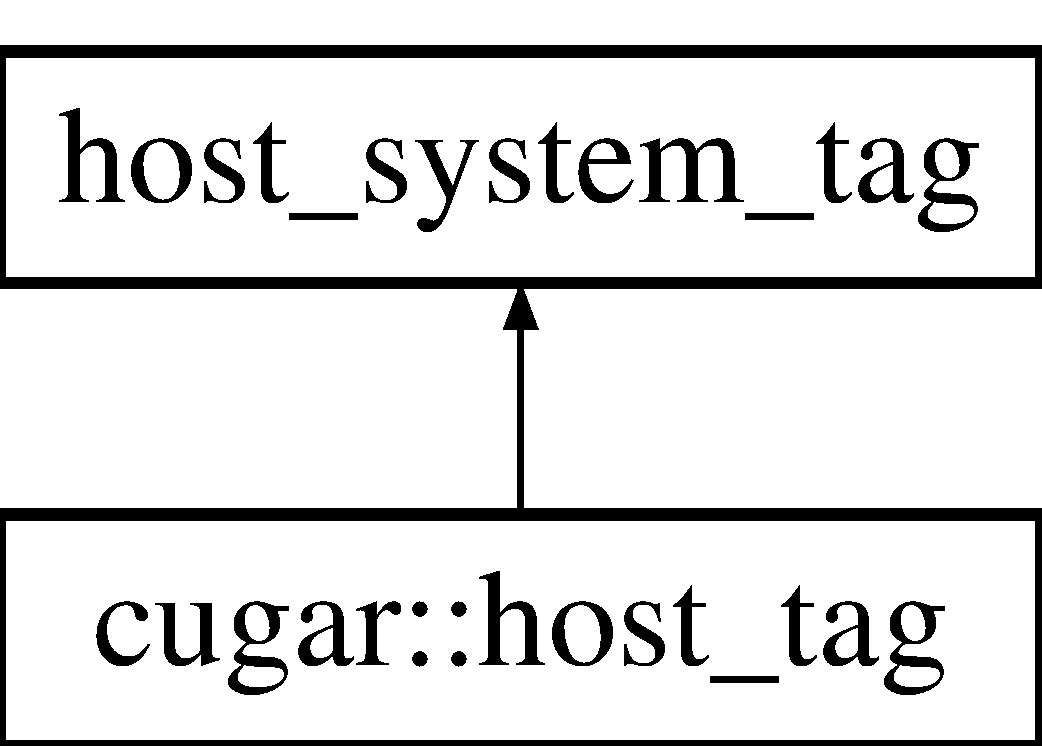
\includegraphics[height=2.000000cm]{structcugar_1_1host__tag}
\end{center}
\end{figure}


The documentation for this struct was generated from the following file\+:\begin{DoxyCompactItemize}
\item 
C\+:/p4research/research/jpantaleoni/\+Fermat-\/\+Public/contrib/cugar/basic/types.\+h\end{DoxyCompactItemize}

\hypertarget{structcugar_1_1host__vector}{}\section{cugar\+:\+:host\+\_\+vector$<$ T $>$ Struct Template Reference}
\label{structcugar_1_1host__vector}\index{cugar\+::host\+\_\+vector$<$ T $>$@{cugar\+::host\+\_\+vector$<$ T $>$}}


\subsection{Detailed description}
\subsubsection*{template$<$typename T$>$\newline
struct cugar\+::host\+\_\+vector$<$ T $>$}

a dynamic host vector class (with C++11 it would be\+: template $<$\+T$>$ typedef \hyperlink{structcugar_1_1vector}{vector$<$host\+\_\+tag,\+T$>$} \hyperlink{structcugar_1_1host__vector}{host\+\_\+vector};) 

{\ttfamily \#include $<$vector.\+h$>$}

Inheritance diagram for cugar\+:\+:host\+\_\+vector$<$ T $>$\+:\begin{figure}[H]
\begin{center}
\leavevmode
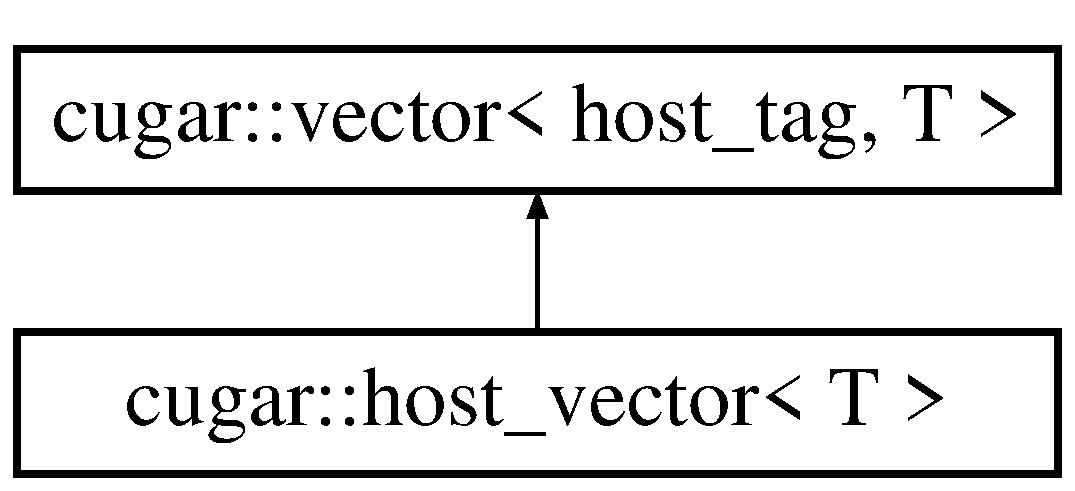
\includegraphics[height=2.000000cm]{structcugar_1_1host__vector}
\end{center}
\end{figure}
\subsection*{Public Types}
\begin{DoxyCompactItemize}
\item 
typedef \hyperlink{structcugar_1_1host__tag}{host\+\_\+tag} {\bfseries system\+\_\+tag}
\item 
typedef \hyperlink{structcugar_1_1vector}{vector}$<$ \hyperlink{structcugar_1_1host__tag}{host\+\_\+tag}, T $>$ {\bfseries base\+\_\+type}
\item 
typedef base\+\_\+type\+::const\+\_\+iterator {\bfseries const\+\_\+iterator}
\item 
typedef base\+\_\+type\+::iterator {\bfseries iterator}
\item 
typedef base\+\_\+type\+::value\+\_\+type {\bfseries value\+\_\+type}
\item 
typedef base\+\_\+type\+::plain\+\_\+view\+\_\+type {\bfseries plain\+\_\+view\+\_\+type}
\item 
typedef base\+\_\+type\+::const\+\_\+plain\+\_\+view\+\_\+type {\bfseries const\+\_\+plain\+\_\+view\+\_\+type}
\end{DoxyCompactItemize}
\subsection*{Public Methods}
\begin{DoxyCompactItemize}
\item 
\hyperlink{group___basic_gaada99b7771790a67817b7280b75d8b19}{host\+\_\+vector} (const size\+\_\+t size=0, const T val=T())
\item 
{\footnotesize template$<$typename Other\+Alloc $>$ }\\{\bfseries host\+\_\+vector} (const thrust\+::host\+\_\+vector$<$ T, Other\+Alloc $>$ \&v)
\item 
{\footnotesize template$<$typename Other\+Alloc $>$ }\\{\bfseries host\+\_\+vector} (const thrust\+::device\+\_\+vector$<$ T, Other\+Alloc $>$ \&v)
\item 
{\footnotesize template$<$typename Other\+Alloc $>$ }\\\hyperlink{structcugar_1_1host__vector}{host\+\_\+vector}$<$ T $>$ \& {\bfseries operator=} (const thrust\+::host\+\_\+vector$<$ T, Other\+Alloc $>$ \&v)
\item 
{\footnotesize template$<$typename Other\+Alloc $>$ }\\\hyperlink{structcugar_1_1host__vector}{host\+\_\+vector}$<$ T $>$ \& {\bfseries operator=} (const thrust\+::device\+\_\+vector$<$ T, Other\+Alloc $>$ \&v)
\item 
\hyperlink{group___basic_gafa4904073d10ce73dc33dfb69013b501}{operator plain\+\_\+view\+\_\+type} ()
\item 
\hyperlink{group___basic_ga4b49363d011f3360acad5d64fad398cb}{operator const\+\_\+plain\+\_\+view\+\_\+type} () const
\end{DoxyCompactItemize}


The documentation for this struct was generated from the following file\+:\begin{DoxyCompactItemize}
\item 
C\+:/p4research/research/jpantaleoni/\+Fermat-\/\+Public/contrib/cugar/basic/vector.\+h\end{DoxyCompactItemize}

\hypertarget{structcugar_1_1_h_s_v}{}\section{cugar\+:\+:H\+SV Struct Reference}
\label{structcugar_1_1_h_s_v}\index{cugar\+::\+H\+SV@{cugar\+::\+H\+SV}}
\subsection*{Public Methods}
\begin{DoxyCompactItemize}
\item 
\mbox{\Hypertarget{structcugar_1_1_h_s_v_a40572eddf0ffc9d4fd2e1bf4836f4e4b}\label{structcugar_1_1_h_s_v_a40572eddf0ffc9d4fd2e1bf4836f4e4b}} 
{\bfseries H\+SV} (float \+\_\+h, float \+\_\+s, float \+\_\+v)
\item 
\mbox{\Hypertarget{structcugar_1_1_h_s_v_a6508c66873631ce3d764eccfc91751b7}\label{structcugar_1_1_h_s_v_a6508c66873631ce3d764eccfc91751b7}} 
{\bfseries H\+SV} (float3 \+\_\+in)
\end{DoxyCompactItemize}
\subsection*{Public Members}
\begin{DoxyCompactItemize}
\item 
\mbox{\Hypertarget{structcugar_1_1_h_s_v_ae540a47d13236905b3f6dc2c59d084c5}\label{structcugar_1_1_h_s_v_ae540a47d13236905b3f6dc2c59d084c5}} 
float {\bfseries h}
\item 
\mbox{\Hypertarget{structcugar_1_1_h_s_v_a68ef52655d47314a0e34958d26187e9a}\label{structcugar_1_1_h_s_v_a68ef52655d47314a0e34958d26187e9a}} 
float {\bfseries s}
\item 
\mbox{\Hypertarget{structcugar_1_1_h_s_v_a79e7eca2ef3f1c2e7500d26b907215ec}\label{structcugar_1_1_h_s_v_a79e7eca2ef3f1c2e7500d26b907215ec}} 
float {\bfseries v}
\end{DoxyCompactItemize}


The documentation for this struct was generated from the following file\+:\begin{DoxyCompactItemize}
\item 
C\+:/p4research/research/jpantaleoni/\+Fermat-\/\+Public/contrib/cugar/color/hsv.\+h\end{DoxyCompactItemize}

\hypertarget{structcugar_1_1if__constant}{}\section{cugar\+:\+:if\+\_\+constant$<$ T, R $>$ Struct Template Reference}
\label{structcugar_1_1if__constant}\index{cugar\+::if\+\_\+constant$<$ T, R $>$@{cugar\+::if\+\_\+constant$<$ T, R $>$}}


\subsection{Detailed description}
\subsubsection*{template$<$typename T, typename R$>$\newline
struct cugar\+::if\+\_\+constant$<$ T, R $>$}

A functor to select between two output values based on equality to a given constant 

{\ttfamily \#include $<$functors.\+h$>$}

\subsection*{Public Types}
\begin{DoxyCompactItemize}
\item 
\mbox{\Hypertarget{structcugar_1_1if__constant_ada35cd698be964ddb1241ab1d5619572}\label{structcugar_1_1if__constant_ada35cd698be964ddb1241ab1d5619572}} 
typedef \hyperlink{structcugar_1_1unary__function__tag}{unary\+\_\+function\+\_\+tag} {\bfseries function\+\_\+tag}
\item 
\mbox{\Hypertarget{structcugar_1_1if__constant_a556f0bef0bb0da89f26c8045a6533d73}\label{structcugar_1_1if__constant_a556f0bef0bb0da89f26c8045a6533d73}} 
typedef T {\bfseries argument\+\_\+type}
\item 
\mbox{\Hypertarget{structcugar_1_1if__constant_a6db32c9baffde58c3e87201808a154a0}\label{structcugar_1_1if__constant_a6db32c9baffde58c3e87201808a154a0}} 
typedef R {\bfseries result\+\_\+type}
\end{DoxyCompactItemize}
\subsection*{Public Methods}
\begin{DoxyCompactItemize}
\item 
C\+U\+G\+A\+R\+\_\+\+H\+O\+S\+T\+\_\+\+D\+E\+V\+I\+CE \hyperlink{structcugar_1_1if__constant_a86a62f5771592414a15ee2bc2029352e}{if\+\_\+constant} (const T c, const R r0, const R r1)
\item 
\mbox{\Hypertarget{structcugar_1_1if__constant_a1f595bf54abb6a850da069dbc2faaf0c}\label{structcugar_1_1if__constant_a1f595bf54abb6a850da069dbc2faaf0c}} 
C\+U\+G\+A\+R\+\_\+\+H\+O\+S\+T\+\_\+\+D\+E\+V\+I\+CE R {\bfseries operator()} (const T \&v) const
\end{DoxyCompactItemize}


\subsection{Constructor \& Destructor Documentation}
\mbox{\Hypertarget{structcugar_1_1if__constant_a86a62f5771592414a15ee2bc2029352e}\label{structcugar_1_1if__constant_a86a62f5771592414a15ee2bc2029352e}} 
\index{cugar\+::if\+\_\+constant@{cugar\+::if\+\_\+constant}!if\+\_\+constant@{if\+\_\+constant}}
\index{if\+\_\+constant@{if\+\_\+constant}!cugar\+::if\+\_\+constant@{cugar\+::if\+\_\+constant}}
\subsubsection{\texorpdfstring{if\+\_\+constant()}{if\_constant()}}
{\footnotesize\ttfamily template$<$typename T , typename R $>$ \\
C\+U\+G\+A\+R\+\_\+\+H\+O\+S\+T\+\_\+\+D\+E\+V\+I\+CE \hyperlink{structcugar_1_1if__constant}{cugar\+::if\+\_\+constant}$<$ T, R $>$\+::\hyperlink{structcugar_1_1if__constant}{if\+\_\+constant} (\begin{DoxyParamCaption}\item[{const T}]{c,  }\item[{const R}]{r0,  }\item[{const R}]{r1 }\end{DoxyParamCaption})\hspace{0.3cm}{\ttfamily [inline]}}

constructor


\begin{DoxyParams}{Parameters}
{\em c} & constant value \\
\hline
{\em r0} & true output value \\
\hline
{\em r1} & false output value \\
\hline
\end{DoxyParams}


The documentation for this struct was generated from the following file\+:\begin{DoxyCompactItemize}
\item 
C\+:/p4research/research/jpantaleoni/\+Fermat-\/\+Public/contrib/cugar/basic/\hyperlink{functors_8h}{functors.\+h}\end{DoxyCompactItemize}

\hypertarget{structcugar_1_1if__equal}{}\section{cugar\+:\+:if\+\_\+equal$<$ A, B, T, F $>$ Struct Template Reference}
\label{structcugar_1_1if__equal}\index{cugar\+::if\+\_\+equal$<$ A, B, T, F $>$@{cugar\+::if\+\_\+equal$<$ A, B, T, F $>$}}


\subsection{Detailed description}
\subsubsection*{template$<$typename A, typename B, typename T, typename F$>$\newline
struct cugar\+::if\+\_\+equal$<$ A, B, T, F $>$}

\hyperlink{structcugar_1_1if__equal}{if\+\_\+equal} meta-\/function 

{\ttfamily \#include $<$types.\+h$>$}

\subsection*{Public Types}
\begin{DoxyCompactItemize}
\item 
\mbox{\Hypertarget{structcugar_1_1if__equal_ab29119a33f3e42270c06cd10b73af18b}\label{structcugar_1_1if__equal_ab29119a33f3e42270c06cd10b73af18b}} 
typedef \hyperlink{structcugar_1_1if__true}{if\+\_\+true}$<$ \hyperlink{structcugar_1_1same__type}{same\+\_\+type}$<$ A, B $>$\+::pred, T, F $>$\+::type {\bfseries type}
\end{DoxyCompactItemize}


The documentation for this struct was generated from the following file\+:\begin{DoxyCompactItemize}
\item 
C\+:/p4research/research/jpantaleoni/\+Fermat-\/\+Public/contrib/cugar/basic/types.\+h\end{DoxyCompactItemize}

\hypertarget{structcugar_1_1if__true}{}\section{cugar\+:\+:if\+\_\+true$<$ predicate, T, F $>$ Struct Template Reference}
\label{structcugar_1_1if__true}\index{cugar\+::if\+\_\+true$<$ predicate, T, F $>$@{cugar\+::if\+\_\+true$<$ predicate, T, F $>$}}


\subsection{Detailed description}
\subsubsection*{template$<$bool predicate, typename T, typename F$>$\newline
struct cugar\+::if\+\_\+true$<$ predicate, T, F $>$}

\hyperlink{structcugar_1_1if__true}{if\+\_\+true} meta-\/function 

{\ttfamily \#include $<$types.\+h$>$}



The documentation for this struct was generated from the following file\+:\begin{DoxyCompactItemize}
\item 
C\+:/p4research/research/jpantaleoni/\+Fermat-\/\+Public/contrib/cugar/basic/types.\+h\end{DoxyCompactItemize}

\hypertarget{structcugar_1_1if__true_3_01false_00_01_t_00_01_f_01_4}{}\section{cugar\+:\+:if\+\_\+true$<$ false, T, F $>$ Struct Template Reference}
\label{structcugar_1_1if__true_3_01false_00_01_t_00_01_f_01_4}\index{cugar\+::if\+\_\+true$<$ false, T, F $>$@{cugar\+::if\+\_\+true$<$ false, T, F $>$}}
\subsection*{Public Types}
\begin{DoxyCompactItemize}
\item 
\mbox{\Hypertarget{structcugar_1_1if__true_3_01false_00_01_t_00_01_f_01_4_afd3d7625ea886fb5422fd3a3aea21cdb}\label{structcugar_1_1if__true_3_01false_00_01_t_00_01_f_01_4_afd3d7625ea886fb5422fd3a3aea21cdb}} 
typedef F {\bfseries type}
\end{DoxyCompactItemize}


The documentation for this struct was generated from the following file\+:\begin{DoxyCompactItemize}
\item 
C\+:/p4research/research/jpantaleoni/\+Fermat-\/\+Public/contrib/cugar/basic/types.\+h\end{DoxyCompactItemize}

\hypertarget{structcugar_1_1if__true_3_01true_00_01_t_00_01_f_01_4}{}\section{cugar\+:\+:if\+\_\+true$<$ true, T, F $>$ Struct Template Reference}
\label{structcugar_1_1if__true_3_01true_00_01_t_00_01_f_01_4}\index{cugar\+::if\+\_\+true$<$ true, T, F $>$@{cugar\+::if\+\_\+true$<$ true, T, F $>$}}
\subsection*{Public Types}
\begin{DoxyCompactItemize}
\item 
\mbox{\Hypertarget{structcugar_1_1if__true_3_01true_00_01_t_00_01_f_01_4_abbc659c224facd1da4ee95298bcf0dbc}\label{structcugar_1_1if__true_3_01true_00_01_t_00_01_f_01_4_abbc659c224facd1da4ee95298bcf0dbc}} 
typedef T {\bfseries type}
\end{DoxyCompactItemize}


The documentation for this struct was generated from the following file\+:\begin{DoxyCompactItemize}
\item 
C\+:/p4research/research/jpantaleoni/\+Fermat-\/\+Public/contrib/cugar/basic/types.\+h\end{DoxyCompactItemize}

\hypertarget{structcugar_1_1if__true__functor}{}\section{cugar\+:\+:if\+\_\+true\+\_\+functor$<$ T, R $>$ Struct Template Reference}
\label{structcugar_1_1if__true__functor}\index{cugar\+::if\+\_\+true\+\_\+functor$<$ T, R $>$@{cugar\+::if\+\_\+true\+\_\+functor$<$ T, R $>$}}


\subsection{Detailed description}
\subsubsection*{template$<$typename T, typename R$>$\newline
struct cugar\+::if\+\_\+true\+\_\+functor$<$ T, R $>$}

if true functor 

{\ttfamily \#include $<$functors.\+h$>$}

\subsection*{Public Types}
\begin{DoxyCompactItemize}
\item 
\mbox{\Hypertarget{structcugar_1_1if__true__functor_afa138a2b4d125cd344cf98d3abd65c87}\label{structcugar_1_1if__true__functor_afa138a2b4d125cd344cf98d3abd65c87}} 
typedef \hyperlink{structcugar_1_1unary__function__tag}{unary\+\_\+function\+\_\+tag} {\bfseries function\+\_\+tag}
\item 
\mbox{\Hypertarget{structcugar_1_1if__true__functor_a124aa5233c48f49ef7ebb54c5f88b953}\label{structcugar_1_1if__true__functor_a124aa5233c48f49ef7ebb54c5f88b953}} 
typedef T {\bfseries argument\+\_\+type}
\item 
\mbox{\Hypertarget{structcugar_1_1if__true__functor_a80e80c8fbd4c1df18d331487ce75c7a1}\label{structcugar_1_1if__true__functor_a80e80c8fbd4c1df18d331487ce75c7a1}} 
typedef R {\bfseries result\+\_\+type}
\end{DoxyCompactItemize}
\subsection*{Public Methods}
\begin{DoxyCompactItemize}
\item 
C\+U\+G\+A\+R\+\_\+\+H\+O\+S\+T\+\_\+\+D\+E\+V\+I\+CE \hyperlink{structcugar_1_1if__true__functor_a9374ed01b1416cc6eff2d6a5c8981a58}{if\+\_\+true\+\_\+functor} (const R r0, const R r1)
\item 
\mbox{\Hypertarget{structcugar_1_1if__true__functor_a56bf028f68d05c61b8db504c60185939}\label{structcugar_1_1if__true__functor_a56bf028f68d05c61b8db504c60185939}} 
C\+U\+G\+A\+R\+\_\+\+H\+O\+S\+T\+\_\+\+D\+E\+V\+I\+CE R {\bfseries operator()} (const T \&v) const
\end{DoxyCompactItemize}


\subsection{Constructor \& Destructor Documentation}
\mbox{\Hypertarget{structcugar_1_1if__true__functor_a9374ed01b1416cc6eff2d6a5c8981a58}\label{structcugar_1_1if__true__functor_a9374ed01b1416cc6eff2d6a5c8981a58}} 
\index{cugar\+::if\+\_\+true\+\_\+functor@{cugar\+::if\+\_\+true\+\_\+functor}!if\+\_\+true\+\_\+functor@{if\+\_\+true\+\_\+functor}}
\index{if\+\_\+true\+\_\+functor@{if\+\_\+true\+\_\+functor}!cugar\+::if\+\_\+true\+\_\+functor@{cugar\+::if\+\_\+true\+\_\+functor}}
\subsubsection{\texorpdfstring{if\+\_\+true\+\_\+functor()}{if\_true\_functor()}}
{\footnotesize\ttfamily template$<$typename T , typename R $>$ \\
C\+U\+G\+A\+R\+\_\+\+H\+O\+S\+T\+\_\+\+D\+E\+V\+I\+CE \hyperlink{structcugar_1_1if__true__functor}{cugar\+::if\+\_\+true\+\_\+functor}$<$ T, R $>$\+::\hyperlink{structcugar_1_1if__true__functor}{if\+\_\+true\+\_\+functor} (\begin{DoxyParamCaption}\item[{const R}]{r0,  }\item[{const R}]{r1 }\end{DoxyParamCaption})\hspace{0.3cm}{\ttfamily [inline]}}

constructor


\begin{DoxyParams}{Parameters}
{\em r0} & true output value \\
\hline
{\em r1} & false output value \\
\hline
\end{DoxyParams}


The documentation for this struct was generated from the following file\+:\begin{DoxyCompactItemize}
\item 
C\+:/p4research/research/jpantaleoni/\+Fermat-\/\+Public/contrib/cugar/basic/\hyperlink{functors_8h}{functors.\+h}\end{DoxyCompactItemize}

\hypertarget{structpbrt_1_1_importer}{}\section{pbrt\+:\+:Importer Struct Reference}
\label{structpbrt_1_1_importer}\index{pbrt\+::\+Importer@{pbrt\+::\+Importer}}
Inheritance diagram for pbrt\+:\+:Importer\+:\begin{figure}[H]
\begin{center}
\leavevmode
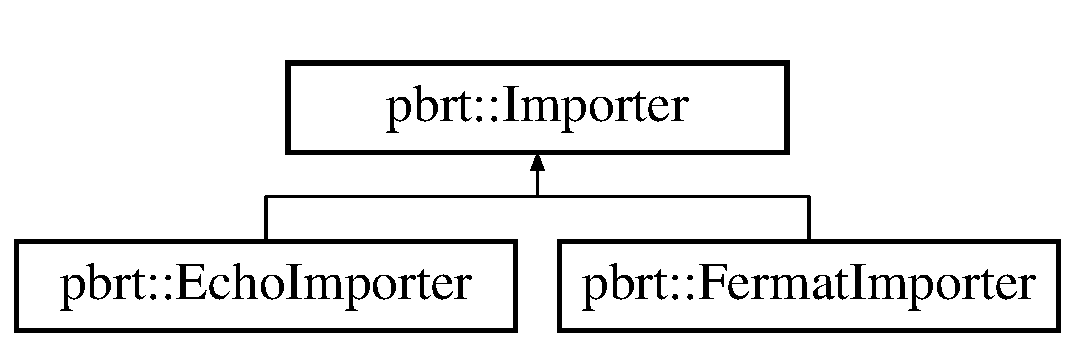
\includegraphics[height=2.000000cm]{structpbrt_1_1_importer}
\end{center}
\end{figure}
\subsection*{Public Methods}
\begin{DoxyCompactItemize}
\item 
\mbox{\Hypertarget{structpbrt_1_1_importer_ab86175cffaeef08fc4726f7c59e9bc60}\label{structpbrt_1_1_importer_ab86175cffaeef08fc4726f7c59e9bc60}} 
virtual void {\bfseries identity} ()
\item 
\mbox{\Hypertarget{structpbrt_1_1_importer_ac4c6310d7de743d78bdf23b34469a70f}\label{structpbrt_1_1_importer_ac4c6310d7de743d78bdf23b34469a70f}} 
virtual void {\bfseries transform} (const \hyperlink{structpbrt_1_1_value}{Value} \&floats)
\item 
\mbox{\Hypertarget{structpbrt_1_1_importer_a508120d6b97f4dc378b285b9730db785}\label{structpbrt_1_1_importer_a508120d6b97f4dc378b285b9730db785}} 
virtual void {\bfseries rotate} (const float angle, const float x, const float y, const float z)
\item 
\mbox{\Hypertarget{structpbrt_1_1_importer_a4f304df8a3ff25ce47bdad5938ad3ea4}\label{structpbrt_1_1_importer_a4f304df8a3ff25ce47bdad5938ad3ea4}} 
virtual void {\bfseries scale} (const float x, const float y, const float z)
\item 
\mbox{\Hypertarget{structpbrt_1_1_importer_a6d91ab7207e7f432f1c0a510b4b73ea4}\label{structpbrt_1_1_importer_a6d91ab7207e7f432f1c0a510b4b73ea4}} 
virtual void {\bfseries translate} (const float x, const float y, const float z)
\item 
\mbox{\Hypertarget{structpbrt_1_1_importer_aee5002ee42abd2e23082148cdd88328a}\label{structpbrt_1_1_importer_aee5002ee42abd2e23082148cdd88328a}} 
virtual void {\bfseries look\+\_\+at} (const float ex, const float ey, const float ez, const float lx, const float ly, const float lz, const float ux, const float uy, const float uz)
\item 
\mbox{\Hypertarget{structpbrt_1_1_importer_ae7385156500ea22e073b80038803798e}\label{structpbrt_1_1_importer_ae7385156500ea22e073b80038803798e}} 
virtual void {\bfseries integrator} (const char $\ast$name, const \hyperlink{structpbrt_1_1_parameter_list}{Parameter\+List} \&params)
\item 
\mbox{\Hypertarget{structpbrt_1_1_importer_a346e9b07730f5101aff9fc52cf96d3a4}\label{structpbrt_1_1_importer_a346e9b07730f5101aff9fc52cf96d3a4}} 
virtual void {\bfseries sampler} (const char $\ast$name, const \hyperlink{structpbrt_1_1_parameter_list}{Parameter\+List} \&params)
\item 
\mbox{\Hypertarget{structpbrt_1_1_importer_a2a7ffee63a4efc1584175b4bab062ead}\label{structpbrt_1_1_importer_a2a7ffee63a4efc1584175b4bab062ead}} 
virtual void {\bfseries pixel\+\_\+filter} (const char $\ast$name, const \hyperlink{structpbrt_1_1_parameter_list}{Parameter\+List} \&params)
\item 
\mbox{\Hypertarget{structpbrt_1_1_importer_a9d6d8d5463b17947f888332e7f037cde}\label{structpbrt_1_1_importer_a9d6d8d5463b17947f888332e7f037cde}} 
virtual void {\bfseries film} (const char $\ast$name, const \hyperlink{structpbrt_1_1_parameter_list}{Parameter\+List} \&params)
\item 
\mbox{\Hypertarget{structpbrt_1_1_importer_ad32d5d9b0b6c938e94137e34fe2b2f92}\label{structpbrt_1_1_importer_ad32d5d9b0b6c938e94137e34fe2b2f92}} 
virtual void {\bfseries camera} (const char $\ast$name, const \hyperlink{structpbrt_1_1_parameter_list}{Parameter\+List} \&params)
\item 
\mbox{\Hypertarget{structpbrt_1_1_importer_a40be5063644721ab0ee50d3320834837}\label{structpbrt_1_1_importer_a40be5063644721ab0ee50d3320834837}} 
virtual void {\bfseries world\+\_\+begin} ()
\item 
\mbox{\Hypertarget{structpbrt_1_1_importer_aa0a6e76845d93511e1680b9e5a7c217d}\label{structpbrt_1_1_importer_aa0a6e76845d93511e1680b9e5a7c217d}} 
virtual void {\bfseries world\+\_\+end} ()
\item 
\mbox{\Hypertarget{structpbrt_1_1_importer_aea4f5622247e103e64fdde3d65bb7955}\label{structpbrt_1_1_importer_aea4f5622247e103e64fdde3d65bb7955}} 
virtual void {\bfseries attribute\+\_\+begin} ()
\item 
\mbox{\Hypertarget{structpbrt_1_1_importer_af7b4940c59aa41ced5802d4d975602b3}\label{structpbrt_1_1_importer_af7b4940c59aa41ced5802d4d975602b3}} 
virtual void {\bfseries attribute\+\_\+end} ()
\item 
\mbox{\Hypertarget{structpbrt_1_1_importer_a8d2ec468685a9c598473562a52f2843d}\label{structpbrt_1_1_importer_a8d2ec468685a9c598473562a52f2843d}} 
virtual void {\bfseries transform\+\_\+begin} ()
\item 
\mbox{\Hypertarget{structpbrt_1_1_importer_ae187c3d682040367079c869511dd947b}\label{structpbrt_1_1_importer_ae187c3d682040367079c869511dd947b}} 
virtual void {\bfseries transform\+\_\+end} ()
\item 
\mbox{\Hypertarget{structpbrt_1_1_importer_aac365d8a10c66c87d964bab9fc1e9056}\label{structpbrt_1_1_importer_aac365d8a10c66c87d964bab9fc1e9056}} 
virtual void {\bfseries texture} (const char $\ast$name, const char $\ast$texel\+\_\+type, const char $\ast$texture\+\_\+type, const \hyperlink{structpbrt_1_1_parameter_list}{Parameter\+List} \&params)
\item 
\mbox{\Hypertarget{structpbrt_1_1_importer_acb3a4f9ba24c999bf9f6e3787cb4cc2a}\label{structpbrt_1_1_importer_acb3a4f9ba24c999bf9f6e3787cb4cc2a}} 
virtual void {\bfseries make\+\_\+named\+\_\+medium} (const char $\ast$name, const \hyperlink{structpbrt_1_1_parameter_list}{Parameter\+List} \&params)
\item 
\mbox{\Hypertarget{structpbrt_1_1_importer_a1a4693fdf6dbbcb0e571297c084e936b}\label{structpbrt_1_1_importer_a1a4693fdf6dbbcb0e571297c084e936b}} 
virtual void {\bfseries make\+\_\+named\+\_\+material} (const char $\ast$name, const \hyperlink{structpbrt_1_1_parameter_list}{Parameter\+List} \&params)
\item 
\mbox{\Hypertarget{structpbrt_1_1_importer_abd1bd89bfc23ecc43c688fd35d92185e}\label{structpbrt_1_1_importer_abd1bd89bfc23ecc43c688fd35d92185e}} 
virtual void {\bfseries named\+\_\+material} (const char $\ast$name)
\item 
\mbox{\Hypertarget{structpbrt_1_1_importer_af3a4ab3561ad85ec1438692a22160610}\label{structpbrt_1_1_importer_af3a4ab3561ad85ec1438692a22160610}} 
virtual void {\bfseries medium\+\_\+interface} (const char $\ast$name1, const char $\ast$name2)
\item 
\mbox{\Hypertarget{structpbrt_1_1_importer_a0e600c8c11fdddae93636c9254e948f2}\label{structpbrt_1_1_importer_a0e600c8c11fdddae93636c9254e948f2}} 
virtual void {\bfseries material} (const char $\ast$name, const \hyperlink{structpbrt_1_1_parameter_list}{Parameter\+List} \&params)
\item 
\mbox{\Hypertarget{structpbrt_1_1_importer_a2cef6f2f065371857e1dda4a7058eed8}\label{structpbrt_1_1_importer_a2cef6f2f065371857e1dda4a7058eed8}} 
virtual void {\bfseries area\+\_\+light\+\_\+source} (const char $\ast$type, const \hyperlink{structpbrt_1_1_parameter_list}{Parameter\+List} \&params)
\item 
\mbox{\Hypertarget{structpbrt_1_1_importer_a342f3716521d7f889f3d88413aa8d2b5}\label{structpbrt_1_1_importer_a342f3716521d7f889f3d88413aa8d2b5}} 
virtual void {\bfseries shape} (const char $\ast$type, const \hyperlink{structpbrt_1_1_parameter_list}{Parameter\+List} \&params)
\end{DoxyCompactItemize}


The documentation for this struct was generated from the following file\+:\begin{DoxyCompactItemize}
\item 
C\+:/p4research/research/jpantaleoni/\+Fermat-\/\+Public/src/mesh/pbrt\+\_\+parser.\+h\end{DoxyCompactItemize}

\hypertarget{classcugar_1_1_bvh__sah__builder_1_1_index_sort_predicate}{}\section{cugar\+:\+:Bvh\+\_\+sah\+\_\+builder\+:\+:Index\+Sort\+Predicate Class Reference}
\label{classcugar_1_1_bvh__sah__builder_1_1_index_sort_predicate}\index{cugar\+::\+Bvh\+\_\+sah\+\_\+builder\+::\+Index\+Sort\+Predicate@{cugar\+::\+Bvh\+\_\+sah\+\_\+builder\+::\+Index\+Sort\+Predicate}}
\subsection*{Public Methods}
\begin{DoxyCompactItemize}
\item 
\mbox{\Hypertarget{classcugar_1_1_bvh__sah__builder_1_1_index_sort_predicate_a4ef01642d5e02f45ab880027e6b2c625}\label{classcugar_1_1_bvh__sah__builder_1_1_index_sort_predicate_a4ef01642d5e02f45ab880027e6b2c625}} 
{\bfseries Index\+Sort\+Predicate} (const std\+::vector$<$ Entity $>$ \&entities, int dim)
\item 
\mbox{\Hypertarget{classcugar_1_1_bvh__sah__builder_1_1_index_sort_predicate_a0642325baf6d8b4adce4c146e3db6fb7}\label{classcugar_1_1_bvh__sah__builder_1_1_index_sort_predicate_a0642325baf6d8b4adce4c146e3db6fb7}} 
bool {\bfseries operator()} (int lhs, int rhs) const
\end{DoxyCompactItemize}


The documentation for this class was generated from the following file\+:\begin{DoxyCompactItemize}
\item 
C\+:/p4research/research/jpantaleoni/\+Fermat-\/\+Public/contrib/cugar/bvh/bvh\+\_\+sah\+\_\+builder\+\_\+inline.\+h\end{DoxyCompactItemize}

\hypertarget{structcugar_1_1_i_random}{}\section{cugar\+:\+:I\+Random Struct Reference}
\label{structcugar_1_1_i_random}\index{cugar\+::\+I\+Random@{cugar\+::\+I\+Random}}


\subsection{Detailed description}
A very simple Linear Congruential Generator 

{\ttfamily \#include $<$random.\+h$>$}

\subsection*{Public Methods}
\begin{DoxyCompactItemize}
\item 
\mbox{\Hypertarget{structcugar_1_1_i_random_a10f27720bb2dee32def830a6df117668}\label{structcugar_1_1_i_random_a10f27720bb2dee32def830a6df117668}} 
C\+U\+G\+A\+R\+\_\+\+F\+O\+R\+C\+E\+I\+N\+L\+I\+NE C\+U\+G\+A\+R\+\_\+\+H\+O\+S\+T\+\_\+\+D\+E\+V\+I\+CE {\bfseries I\+Random} (const uint32 s=0)
\item 
\mbox{\Hypertarget{structcugar_1_1_i_random_ac9747d2966323ec286eb38effd54f736}\label{structcugar_1_1_i_random_ac9747d2966323ec286eb38effd54f736}} 
C\+U\+G\+A\+R\+\_\+\+F\+O\+R\+C\+E\+I\+N\+L\+I\+NE C\+U\+G\+A\+R\+\_\+\+H\+O\+S\+T\+\_\+\+D\+E\+V\+I\+CE uint32 {\bfseries next} ()
\end{DoxyCompactItemize}
\subsection*{Public Members}
\begin{DoxyCompactItemize}
\item 
\mbox{\Hypertarget{structcugar_1_1_i_random_af2d6b59babcc5749b83ec05b4cb85728}\label{structcugar_1_1_i_random_af2d6b59babcc5749b83ec05b4cb85728}} 
uint32 {\bfseries m\+\_\+s}
\end{DoxyCompactItemize}
\subsection*{Static Public Members}
\begin{DoxyCompactItemize}
\item 
\mbox{\Hypertarget{structcugar_1_1_i_random_abe57d325de0eca8329b6c2fcbd504e1e}\label{structcugar_1_1_i_random_abe57d325de0eca8329b6c2fcbd504e1e}} 
static const uint32 {\bfseries M\+AX} = 0x\+F\+F\+F\+F\+F\+F\+FF
\end{DoxyCompactItemize}


The documentation for this struct was generated from the following file\+:\begin{DoxyCompactItemize}
\item 
C\+:/p4research/research/jpantaleoni/\+Fermat-\/\+Public/contrib/cugar/sampling/\hyperlink{random_8h}{random.\+h}\end{DoxyCompactItemize}

\hypertarget{structcugar_1_1is__false__functor}{}\section{cugar\+:\+:is\+\_\+false\+\_\+functor$<$ T $>$ Struct Template Reference}
\label{structcugar_1_1is__false__functor}\index{cugar\+::is\+\_\+false\+\_\+functor$<$ T $>$@{cugar\+::is\+\_\+false\+\_\+functor$<$ T $>$}}


\subsection{Detailed description}
\subsubsection*{template$<$typename T$>$\newline
struct cugar\+::is\+\_\+false\+\_\+functor$<$ T $>$}

A unary functor returning true if op evaluates to false 

{\ttfamily \#include $<$functors.\+h$>$}

\subsection*{Public Types}
\begin{DoxyCompactItemize}
\item 
\mbox{\Hypertarget{structcugar_1_1is__false__functor_a6274a20c970846d954a05f0af41a6cd6}\label{structcugar_1_1is__false__functor_a6274a20c970846d954a05f0af41a6cd6}} 
typedef T {\bfseries argument\+\_\+type}
\item 
\mbox{\Hypertarget{structcugar_1_1is__false__functor_acfff4cd346badb13c22837b10c96b38e}\label{structcugar_1_1is__false__functor_acfff4cd346badb13c22837b10c96b38e}} 
typedef bool {\bfseries result\+\_\+type}
\end{DoxyCompactItemize}
\subsection*{Public Methods}
\begin{DoxyCompactItemize}
\item 
\mbox{\Hypertarget{structcugar_1_1is__false__functor_aaba06740d6d89a8d321d5e1b40f79c6f}\label{structcugar_1_1is__false__functor_aaba06740d6d89a8d321d5e1b40f79c6f}} 
C\+U\+G\+A\+R\+\_\+\+F\+O\+R\+C\+E\+I\+N\+L\+I\+NE C\+U\+G\+A\+R\+\_\+\+H\+O\+S\+T\+\_\+\+D\+E\+V\+I\+CE result\+\_\+type {\bfseries operator()} (const T op) const
\end{DoxyCompactItemize}


The documentation for this struct was generated from the following file\+:\begin{DoxyCompactItemize}
\item 
C\+:/p4research/research/jpantaleoni/\+Fermat-\/\+Public/contrib/cugar/basic/\hyperlink{functors_8h}{functors.\+h}\end{DoxyCompactItemize}

\hypertarget{structcugar_1_1is__segment__sorted__iterator}{}\section{cugar\+:\+:is\+\_\+segment\+\_\+sorted\+\_\+iterator$<$ Iterator1, Iterator2, Headflags $>$ Struct Template Reference}
\label{structcugar_1_1is__segment__sorted__iterator}\index{cugar\+::is\+\_\+segment\+\_\+sorted\+\_\+iterator$<$ Iterator1, Iterator2, Headflags $>$@{cugar\+::is\+\_\+segment\+\_\+sorted\+\_\+iterator$<$ Iterator1, Iterator2, Headflags $>$}}
\subsection*{Public Types}
\begin{DoxyCompactItemize}
\item 
\mbox{\Hypertarget{structcugar_1_1is__segment__sorted__iterator_ae9837839e15dea819c4d3bab8cd62c35}\label{structcugar_1_1is__segment__sorted__iterator_ae9837839e15dea819c4d3bab8cd62c35}} 
typedef bool {\bfseries value\+\_\+type}
\item 
\mbox{\Hypertarget{structcugar_1_1is__segment__sorted__iterator_a4a20b9278f9fe1ac72896f2e949fbbc9}\label{structcugar_1_1is__segment__sorted__iterator_a4a20b9278f9fe1ac72896f2e949fbbc9}} 
typedef value\+\_\+type \& {\bfseries reference}
\item 
\mbox{\Hypertarget{structcugar_1_1is__segment__sorted__iterator_a1d62618897f35c6525c8095b4230737a}\label{structcugar_1_1is__segment__sorted__iterator_a1d62618897f35c6525c8095b4230737a}} 
typedef value\+\_\+type {\bfseries const\+\_\+reference}
\item 
\mbox{\Hypertarget{structcugar_1_1is__segment__sorted__iterator_a4840e5af4a0699f1e466cb2b54274851}\label{structcugar_1_1is__segment__sorted__iterator_a4840e5af4a0699f1e466cb2b54274851}} 
typedef value\+\_\+type $\ast$ {\bfseries pointer}
\item 
\mbox{\Hypertarget{structcugar_1_1is__segment__sorted__iterator_ae1f4c8b1b38a5103f0d18c34a8361a66}\label{structcugar_1_1is__segment__sorted__iterator_ae1f4c8b1b38a5103f0d18c34a8361a66}} 
typedef std\+::iterator\+\_\+traits$<$ Iterator1 $>$\+::difference\+\_\+type {\bfseries difference\+\_\+type}
\item 
\mbox{\Hypertarget{structcugar_1_1is__segment__sorted__iterator_a232b42f1d962f089524a6e1af753a6a8}\label{structcugar_1_1is__segment__sorted__iterator_a232b42f1d962f089524a6e1af753a6a8}} 
typedef std\+::iterator\+\_\+traits$<$ Iterator1 $>$\+::iterator\+\_\+category {\bfseries iterator\+\_\+category}
\end{DoxyCompactItemize}
\subsection*{Public Methods}
\begin{DoxyCompactItemize}
\item 
\mbox{\Hypertarget{structcugar_1_1is__segment__sorted__iterator_afa4764445f7644c065e37c6a0c561203}\label{structcugar_1_1is__segment__sorted__iterator_afa4764445f7644c065e37c6a0c561203}} 
C\+U\+G\+A\+R\+\_\+\+F\+O\+R\+C\+E\+I\+N\+L\+I\+NE C\+U\+G\+A\+R\+\_\+\+H\+O\+S\+T\+\_\+\+D\+E\+V\+I\+CE {\bfseries is\+\_\+segment\+\_\+sorted\+\_\+iterator} (const Iterator1 \+\_\+it1, const Iterator2 \+\_\+it2, const Headflags \+\_\+hd)
\item 
\mbox{\Hypertarget{structcugar_1_1is__segment__sorted__iterator_aa4728b84a79b8d485690180b4d05703a}\label{structcugar_1_1is__segment__sorted__iterator_aa4728b84a79b8d485690180b4d05703a}} 
C\+U\+G\+A\+R\+\_\+\+F\+O\+R\+C\+E\+I\+N\+L\+I\+NE C\+U\+G\+A\+R\+\_\+\+H\+O\+S\+T\+\_\+\+D\+E\+V\+I\+CE bool {\bfseries operator\mbox{[}$\,$\mbox{]}} (const uint64 i) const
\item 
\mbox{\Hypertarget{structcugar_1_1is__segment__sorted__iterator_aafdf0960c302ed40bdc178391a335224}\label{structcugar_1_1is__segment__sorted__iterator_aafdf0960c302ed40bdc178391a335224}} 
C\+U\+G\+A\+R\+\_\+\+F\+O\+R\+C\+E\+I\+N\+L\+I\+NE C\+U\+G\+A\+R\+\_\+\+H\+O\+S\+T\+\_\+\+D\+E\+V\+I\+CE bool {\bfseries operator$\ast$} () const
\item 
\mbox{\Hypertarget{structcugar_1_1is__segment__sorted__iterator_a99a73b7bc263941af4470f5e71baaaeb}\label{structcugar_1_1is__segment__sorted__iterator_a99a73b7bc263941af4470f5e71baaaeb}} 
C\+U\+G\+A\+R\+\_\+\+F\+O\+R\+C\+E\+I\+N\+L\+I\+NE C\+U\+G\+A\+R\+\_\+\+H\+O\+S\+T\+\_\+\+D\+E\+V\+I\+CE \hyperlink{structcugar_1_1is__segment__sorted__iterator}{is\+\_\+segment\+\_\+sorted\+\_\+iterator} \& {\bfseries operator++} ()
\end{DoxyCompactItemize}
\subsection*{Public Members}
\begin{DoxyCompactItemize}
\item 
\mbox{\Hypertarget{structcugar_1_1is__segment__sorted__iterator_abb197d29df6998f40bdfc3d4f922b92a}\label{structcugar_1_1is__segment__sorted__iterator_abb197d29df6998f40bdfc3d4f922b92a}} 
Iterator1 {\bfseries it1}
\item 
\mbox{\Hypertarget{structcugar_1_1is__segment__sorted__iterator_ac22597e305eea555adb421de9b7317d0}\label{structcugar_1_1is__segment__sorted__iterator_ac22597e305eea555adb421de9b7317d0}} 
Iterator2 {\bfseries it2}
\item 
\mbox{\Hypertarget{structcugar_1_1is__segment__sorted__iterator_aad20566e6208a8f7b81801708ea78c5b}\label{structcugar_1_1is__segment__sorted__iterator_aad20566e6208a8f7b81801708ea78c5b}} 
Headflags {\bfseries hd}
\end{DoxyCompactItemize}


The documentation for this struct was generated from the following file\+:\begin{DoxyCompactItemize}
\item 
C\+:/p4research/research/jpantaleoni/\+Fermat-\/\+Public/contrib/cugar/basic/primitives\+\_\+inl.\+h\end{DoxyCompactItemize}

\hypertarget{structcugar_1_1cuda_1_1is__segment__sorted__iterator}{}\section{cugar\+:\+:cuda\+:\+:is\+\_\+segment\+\_\+sorted\+\_\+iterator$<$ Iterator1, Iterator2, Headflags $>$ Struct Template Reference}
\label{structcugar_1_1cuda_1_1is__segment__sorted__iterator}\index{cugar\+::cuda\+::is\+\_\+segment\+\_\+sorted\+\_\+iterator$<$ Iterator1, Iterator2, Headflags $>$@{cugar\+::cuda\+::is\+\_\+segment\+\_\+sorted\+\_\+iterator$<$ Iterator1, Iterator2, Headflags $>$}}
\subsection*{Public Methods}
\begin{DoxyCompactItemize}
\item 
\mbox{\Hypertarget{structcugar_1_1cuda_1_1is__segment__sorted__iterator_a480e08ed16ff7d8e5cf70bc46e0db8f8}\label{structcugar_1_1cuda_1_1is__segment__sorted__iterator_a480e08ed16ff7d8e5cf70bc46e0db8f8}} 
C\+U\+G\+A\+R\+\_\+\+F\+O\+R\+C\+E\+I\+N\+L\+I\+NE C\+U\+G\+A\+R\+\_\+\+H\+O\+S\+T\+\_\+\+D\+E\+V\+I\+CE {\bfseries is\+\_\+segment\+\_\+sorted\+\_\+iterator} (const Iterator1 \+\_\+it1, const Iterator2 \+\_\+it2, const Headflags \+\_\+hd)
\item 
\mbox{\Hypertarget{structcugar_1_1cuda_1_1is__segment__sorted__iterator_a7577bb0170f2b79568b5a174ce5f6581}\label{structcugar_1_1cuda_1_1is__segment__sorted__iterator_a7577bb0170f2b79568b5a174ce5f6581}} 
C\+U\+G\+A\+R\+\_\+\+F\+O\+R\+C\+E\+I\+N\+L\+I\+NE C\+U\+G\+A\+R\+\_\+\+H\+O\+S\+T\+\_\+\+D\+E\+V\+I\+CE bool {\bfseries operator\mbox{[}$\,$\mbox{]}} (const uint32 i) const
\end{DoxyCompactItemize}
\subsection*{Public Members}
\begin{DoxyCompactItemize}
\item 
\mbox{\Hypertarget{structcugar_1_1cuda_1_1is__segment__sorted__iterator_a77c9181ead65806dd389980c8304a964}\label{structcugar_1_1cuda_1_1is__segment__sorted__iterator_a77c9181ead65806dd389980c8304a964}} 
const Iterator1 {\bfseries it1}
\item 
\mbox{\Hypertarget{structcugar_1_1cuda_1_1is__segment__sorted__iterator_a4381ebc2dc4c0bd1a46ffa8ff42ea7e2}\label{structcugar_1_1cuda_1_1is__segment__sorted__iterator_a4381ebc2dc4c0bd1a46ffa8ff42ea7e2}} 
const Iterator2 {\bfseries it2}
\item 
\mbox{\Hypertarget{structcugar_1_1cuda_1_1is__segment__sorted__iterator_abf50890e0a36a959edf214fdb74495cd}\label{structcugar_1_1cuda_1_1is__segment__sorted__iterator_abf50890e0a36a959edf214fdb74495cd}} 
const Headflags {\bfseries hd}
\end{DoxyCompactItemize}


The documentation for this struct was generated from the following file\+:\begin{DoxyCompactItemize}
\item 
C\+:/p4research/research/jpantaleoni/\+Fermat-\/\+Public/contrib/cugar/basic/cuda/primitives\+\_\+inl.\+h\end{DoxyCompactItemize}

\hypertarget{structcugar_1_1is__sorted__iterator}{}\section{cugar\+:\+:is\+\_\+sorted\+\_\+iterator$<$ Iterator1, Iterator2 $>$ Struct Template Reference}
\label{structcugar_1_1is__sorted__iterator}\index{cugar\+::is\+\_\+sorted\+\_\+iterator$<$ Iterator1, Iterator2 $>$@{cugar\+::is\+\_\+sorted\+\_\+iterator$<$ Iterator1, Iterator2 $>$}}
\subsection*{Public Types}
\begin{DoxyCompactItemize}
\item 
\mbox{\Hypertarget{structcugar_1_1is__sorted__iterator_a9add94d14413d3819f83d991c2202a99}\label{structcugar_1_1is__sorted__iterator_a9add94d14413d3819f83d991c2202a99}} 
typedef bool {\bfseries value\+\_\+type}
\item 
\mbox{\Hypertarget{structcugar_1_1is__sorted__iterator_ae4435daf6df3f57644ff7cc99564a67d}\label{structcugar_1_1is__sorted__iterator_ae4435daf6df3f57644ff7cc99564a67d}} 
typedef value\+\_\+type \& {\bfseries reference}
\item 
\mbox{\Hypertarget{structcugar_1_1is__sorted__iterator_a4b0f7605bf8fd8eccf4920b848b6dab7}\label{structcugar_1_1is__sorted__iterator_a4b0f7605bf8fd8eccf4920b848b6dab7}} 
typedef value\+\_\+type {\bfseries const\+\_\+reference}
\item 
\mbox{\Hypertarget{structcugar_1_1is__sorted__iterator_a7415081aedfb462723a431a87bacc7e5}\label{structcugar_1_1is__sorted__iterator_a7415081aedfb462723a431a87bacc7e5}} 
typedef value\+\_\+type $\ast$ {\bfseries pointer}
\item 
\mbox{\Hypertarget{structcugar_1_1is__sorted__iterator_ae0dcabc03e5d1658b133831841882e88}\label{structcugar_1_1is__sorted__iterator_ae0dcabc03e5d1658b133831841882e88}} 
typedef std\+::iterator\+\_\+traits$<$ Iterator1 $>$\+::difference\+\_\+type {\bfseries difference\+\_\+type}
\item 
\mbox{\Hypertarget{structcugar_1_1is__sorted__iterator_a3e15e4ead4ecc7261d39f85bc42e4727}\label{structcugar_1_1is__sorted__iterator_a3e15e4ead4ecc7261d39f85bc42e4727}} 
typedef std\+::iterator\+\_\+traits$<$ Iterator1 $>$\+::iterator\+\_\+category {\bfseries iterator\+\_\+category}
\end{DoxyCompactItemize}
\subsection*{Public Methods}
\begin{DoxyCompactItemize}
\item 
\mbox{\Hypertarget{structcugar_1_1is__sorted__iterator_a7401a09c61834fef5a1da697da169a57}\label{structcugar_1_1is__sorted__iterator_a7401a09c61834fef5a1da697da169a57}} 
C\+U\+G\+A\+R\+\_\+\+F\+O\+R\+C\+E\+I\+N\+L\+I\+NE C\+U\+G\+A\+R\+\_\+\+H\+O\+S\+T\+\_\+\+D\+E\+V\+I\+CE {\bfseries is\+\_\+sorted\+\_\+iterator} (const Iterator1 \+\_\+it1, const Iterator2 \+\_\+it2)
\item 
\mbox{\Hypertarget{structcugar_1_1is__sorted__iterator_a326c321e3d6cc5aa672ab95dac1317bf}\label{structcugar_1_1is__sorted__iterator_a326c321e3d6cc5aa672ab95dac1317bf}} 
C\+U\+G\+A\+R\+\_\+\+F\+O\+R\+C\+E\+I\+N\+L\+I\+NE C\+U\+G\+A\+R\+\_\+\+H\+O\+S\+T\+\_\+\+D\+E\+V\+I\+CE bool {\bfseries operator\mbox{[}$\,$\mbox{]}} (const uint64 i) const
\item 
\mbox{\Hypertarget{structcugar_1_1is__sorted__iterator_a355a62fc5c0d076fc00a27f58e1b4238}\label{structcugar_1_1is__sorted__iterator_a355a62fc5c0d076fc00a27f58e1b4238}} 
C\+U\+G\+A\+R\+\_\+\+F\+O\+R\+C\+E\+I\+N\+L\+I\+NE C\+U\+G\+A\+R\+\_\+\+H\+O\+S\+T\+\_\+\+D\+E\+V\+I\+CE bool {\bfseries operator$\ast$} () const
\item 
\mbox{\Hypertarget{structcugar_1_1is__sorted__iterator_a8834b9927b8b1b35eab5bbc5fc59e444}\label{structcugar_1_1is__sorted__iterator_a8834b9927b8b1b35eab5bbc5fc59e444}} 
C\+U\+G\+A\+R\+\_\+\+F\+O\+R\+C\+E\+I\+N\+L\+I\+NE C\+U\+G\+A\+R\+\_\+\+H\+O\+S\+T\+\_\+\+D\+E\+V\+I\+CE \hyperlink{structcugar_1_1is__sorted__iterator}{is\+\_\+sorted\+\_\+iterator} \& {\bfseries operator++} ()
\end{DoxyCompactItemize}
\subsection*{Public Members}
\begin{DoxyCompactItemize}
\item 
\mbox{\Hypertarget{structcugar_1_1is__sorted__iterator_a56f7b2a5b353df5b331b8d20dbaee4f7}\label{structcugar_1_1is__sorted__iterator_a56f7b2a5b353df5b331b8d20dbaee4f7}} 
Iterator1 {\bfseries it1}
\item 
\mbox{\Hypertarget{structcugar_1_1is__sorted__iterator_a0d7741722d95eea2b26852b4cc9e479a}\label{structcugar_1_1is__sorted__iterator_a0d7741722d95eea2b26852b4cc9e479a}} 
Iterator2 {\bfseries it2}
\end{DoxyCompactItemize}


The documentation for this struct was generated from the following file\+:\begin{DoxyCompactItemize}
\item 
C\+:/p4research/research/jpantaleoni/\+Fermat-\/\+Public/contrib/cugar/basic/primitives\+\_\+inl.\+h\end{DoxyCompactItemize}

\hypertarget{structcugar_1_1cuda_1_1is__sorted__iterator}{}\section{cugar\+:\+:cuda\+:\+:is\+\_\+sorted\+\_\+iterator$<$ Iterator1, Iterator2 $>$ Struct Template Reference}
\label{structcugar_1_1cuda_1_1is__sorted__iterator}\index{cugar\+::cuda\+::is\+\_\+sorted\+\_\+iterator$<$ Iterator1, Iterator2 $>$@{cugar\+::cuda\+::is\+\_\+sorted\+\_\+iterator$<$ Iterator1, Iterator2 $>$}}
\subsection*{Public Methods}
\begin{DoxyCompactItemize}
\item 
\mbox{\Hypertarget{structcugar_1_1cuda_1_1is__sorted__iterator_a9cc173e751dfec8dd19082514e297681}\label{structcugar_1_1cuda_1_1is__sorted__iterator_a9cc173e751dfec8dd19082514e297681}} 
C\+U\+G\+A\+R\+\_\+\+F\+O\+R\+C\+E\+I\+N\+L\+I\+NE C\+U\+G\+A\+R\+\_\+\+H\+O\+S\+T\+\_\+\+D\+E\+V\+I\+CE {\bfseries is\+\_\+sorted\+\_\+iterator} (const Iterator1 \+\_\+it1, const Iterator2 \+\_\+it2)
\item 
\mbox{\Hypertarget{structcugar_1_1cuda_1_1is__sorted__iterator_a2559419eb4d81975cad169b795974b11}\label{structcugar_1_1cuda_1_1is__sorted__iterator_a2559419eb4d81975cad169b795974b11}} 
C\+U\+G\+A\+R\+\_\+\+F\+O\+R\+C\+E\+I\+N\+L\+I\+NE C\+U\+G\+A\+R\+\_\+\+H\+O\+S\+T\+\_\+\+D\+E\+V\+I\+CE bool {\bfseries operator\mbox{[}$\,$\mbox{]}} (const uint32 i) const
\end{DoxyCompactItemize}
\subsection*{Public Members}
\begin{DoxyCompactItemize}
\item 
\mbox{\Hypertarget{structcugar_1_1cuda_1_1is__sorted__iterator_a186b47fe93b5c513658b6d676496a664}\label{structcugar_1_1cuda_1_1is__sorted__iterator_a186b47fe93b5c513658b6d676496a664}} 
const Iterator1 {\bfseries it1}
\item 
\mbox{\Hypertarget{structcugar_1_1cuda_1_1is__sorted__iterator_afb5d3f2ab5e2d167e144a776dacbd4fa}\label{structcugar_1_1cuda_1_1is__sorted__iterator_afb5d3f2ab5e2d167e144a776dacbd4fa}} 
const Iterator2 {\bfseries it2}
\end{DoxyCompactItemize}


The documentation for this struct was generated from the following file\+:\begin{DoxyCompactItemize}
\item 
C\+:/p4research/research/jpantaleoni/\+Fermat-\/\+Public/contrib/cugar/basic/cuda/primitives\+\_\+inl.\+h\end{DoxyCompactItemize}

\hypertarget{structcugar_1_1is__true__functor}{}\section{cugar\+:\+:is\+\_\+true\+\_\+functor$<$ T $>$ Struct Template Reference}
\label{structcugar_1_1is__true__functor}\index{cugar\+::is\+\_\+true\+\_\+functor$<$ T $>$@{cugar\+::is\+\_\+true\+\_\+functor$<$ T $>$}}


\subsection{Detailed description}
\subsubsection*{template$<$typename T$>$\newline
struct cugar\+::is\+\_\+true\+\_\+functor$<$ T $>$}

A unary functor returning true if op evaluates to true 

{\ttfamily \#include $<$functors.\+h$>$}

\subsection*{Public Types}
\begin{DoxyCompactItemize}
\item 
\mbox{\Hypertarget{structcugar_1_1is__true__functor_aebaa3a31bf4ac78b6789dfdb9b9b9a3a}\label{structcugar_1_1is__true__functor_aebaa3a31bf4ac78b6789dfdb9b9b9a3a}} 
typedef T {\bfseries argument\+\_\+type}
\item 
\mbox{\Hypertarget{structcugar_1_1is__true__functor_a9ebf7905fa931cdb25534aff5c6bd90d}\label{structcugar_1_1is__true__functor_a9ebf7905fa931cdb25534aff5c6bd90d}} 
typedef bool {\bfseries result\+\_\+type}
\end{DoxyCompactItemize}
\subsection*{Public Methods}
\begin{DoxyCompactItemize}
\item 
\mbox{\Hypertarget{structcugar_1_1is__true__functor_abd3cbe1802a5c1b1668b0c2c4e0d99f6}\label{structcugar_1_1is__true__functor_abd3cbe1802a5c1b1668b0c2c4e0d99f6}} 
C\+U\+G\+A\+R\+\_\+\+F\+O\+R\+C\+E\+I\+N\+L\+I\+NE C\+U\+G\+A\+R\+\_\+\+H\+O\+S\+T\+\_\+\+D\+E\+V\+I\+CE result\+\_\+type {\bfseries operator()} (const T op) const
\end{DoxyCompactItemize}


The documentation for this struct was generated from the following file\+:\begin{DoxyCompactItemize}
\item 
C\+:/p4research/research/jpantaleoni/\+Fermat-\/\+Public/contrib/cugar/basic/\hyperlink{functors_8h}{functors.\+h}\end{DoxyCompactItemize}

\hypertarget{structcugar_1_1iterator__category__system}{}\section{cugar\+:\+:iterator\+\_\+category\+\_\+system$<$ iterator\+\_\+category $>$ Struct Template Reference}
\label{structcugar_1_1iterator__category__system}\index{cugar\+::iterator\+\_\+category\+\_\+system$<$ iterator\+\_\+category $>$@{cugar\+::iterator\+\_\+category\+\_\+system$<$ iterator\+\_\+category $>$}}


The documentation for this struct was generated from the following file\+:\begin{DoxyCompactItemize}
\item 
C\+:/p4research/research/jpantaleoni/\+Fermat-\/\+Public/contrib/cugar/basic/iterator.\+h\end{DoxyCompactItemize}

\hypertarget{structcugar_1_1iterator__category__system_3_01bidirectional__device__iterator__tag_01_4}{}\section{cugar\+:\+:iterator\+\_\+category\+\_\+system$<$ bidirectional\+\_\+device\+\_\+iterator\+\_\+tag $>$ Struct Template Reference}
\label{structcugar_1_1iterator__category__system_3_01bidirectional__device__iterator__tag_01_4}\index{cugar\+::iterator\+\_\+category\+\_\+system$<$ bidirectional\+\_\+device\+\_\+iterator\+\_\+tag $>$@{cugar\+::iterator\+\_\+category\+\_\+system$<$ bidirectional\+\_\+device\+\_\+iterator\+\_\+tag $>$}}
\subsection*{Public Types}
\begin{DoxyCompactItemize}
\item 
\mbox{\Hypertarget{structcugar_1_1iterator__category__system_3_01bidirectional__device__iterator__tag_01_4_ac583e2610b615493c4259eb826df51bd}\label{structcugar_1_1iterator__category__system_3_01bidirectional__device__iterator__tag_01_4_ac583e2610b615493c4259eb826df51bd}} 
typedef \hyperlink{structcugar_1_1device__tag}{device\+\_\+tag} {\bfseries type}
\end{DoxyCompactItemize}


The documentation for this struct was generated from the following file\+:\begin{DoxyCompactItemize}
\item 
C\+:/p4research/research/jpantaleoni/\+Fermat-\/\+Public/contrib/cugar/basic/iterator.\+h\end{DoxyCompactItemize}

\hypertarget{structcugar_1_1iterator__category__system_3_01bidirectional__host__iterator__tag_01_4}{}\section{cugar\+:\+:iterator\+\_\+category\+\_\+system$<$ bidirectional\+\_\+host\+\_\+iterator\+\_\+tag $>$ Struct Template Reference}
\label{structcugar_1_1iterator__category__system_3_01bidirectional__host__iterator__tag_01_4}\index{cugar\+::iterator\+\_\+category\+\_\+system$<$ bidirectional\+\_\+host\+\_\+iterator\+\_\+tag $>$@{cugar\+::iterator\+\_\+category\+\_\+system$<$ bidirectional\+\_\+host\+\_\+iterator\+\_\+tag $>$}}
\subsection*{Public Types}
\begin{DoxyCompactItemize}
\item 
\mbox{\Hypertarget{structcugar_1_1iterator__category__system_3_01bidirectional__host__iterator__tag_01_4_a17b3b98b100e24632cf5413edb3e9e5c}\label{structcugar_1_1iterator__category__system_3_01bidirectional__host__iterator__tag_01_4_a17b3b98b100e24632cf5413edb3e9e5c}} 
typedef \hyperlink{structcugar_1_1host__tag}{host\+\_\+tag} {\bfseries type}
\end{DoxyCompactItemize}


The documentation for this struct was generated from the following file\+:\begin{DoxyCompactItemize}
\item 
C\+:/p4research/research/jpantaleoni/\+Fermat-\/\+Public/contrib/cugar/basic/iterator.\+h\end{DoxyCompactItemize}

\hypertarget{structcugar_1_1iterator__category__system_3_01bidirectional__universal__iterator__tag_01_4}{}\section{cugar\+:\+:iterator\+\_\+category\+\_\+system$<$ bidirectional\+\_\+universal\+\_\+iterator\+\_\+tag $>$ Struct Template Reference}
\label{structcugar_1_1iterator__category__system_3_01bidirectional__universal__iterator__tag_01_4}\index{cugar\+::iterator\+\_\+category\+\_\+system$<$ bidirectional\+\_\+universal\+\_\+iterator\+\_\+tag $>$@{cugar\+::iterator\+\_\+category\+\_\+system$<$ bidirectional\+\_\+universal\+\_\+iterator\+\_\+tag $>$}}
\subsection*{Public Types}
\begin{DoxyCompactItemize}
\item 
\mbox{\Hypertarget{structcugar_1_1iterator__category__system_3_01bidirectional__universal__iterator__tag_01_4_a61cca09e6fe4b5d85ebfee21db2955c6}\label{structcugar_1_1iterator__category__system_3_01bidirectional__universal__iterator__tag_01_4_a61cca09e6fe4b5d85ebfee21db2955c6}} 
typedef \hyperlink{structcugar_1_1device__tag}{device\+\_\+tag} {\bfseries type}
\end{DoxyCompactItemize}


The documentation for this struct was generated from the following file\+:\begin{DoxyCompactItemize}
\item 
C\+:/p4research/research/jpantaleoni/\+Fermat-\/\+Public/contrib/cugar/basic/iterator.\+h\end{DoxyCompactItemize}

\hypertarget{structcugar_1_1iterator__category__system_3_01forward__device__iterator__tag_01_4}{}\section{cugar\+:\+:iterator\+\_\+category\+\_\+system$<$ forward\+\_\+device\+\_\+iterator\+\_\+tag $>$ Struct Template Reference}
\label{structcugar_1_1iterator__category__system_3_01forward__device__iterator__tag_01_4}\index{cugar\+::iterator\+\_\+category\+\_\+system$<$ forward\+\_\+device\+\_\+iterator\+\_\+tag $>$@{cugar\+::iterator\+\_\+category\+\_\+system$<$ forward\+\_\+device\+\_\+iterator\+\_\+tag $>$}}
\subsection*{Public Types}
\begin{DoxyCompactItemize}
\item 
\mbox{\Hypertarget{structcugar_1_1iterator__category__system_3_01forward__device__iterator__tag_01_4_ac8e328cd8637d1e63a8d0b4553daa615}\label{structcugar_1_1iterator__category__system_3_01forward__device__iterator__tag_01_4_ac8e328cd8637d1e63a8d0b4553daa615}} 
typedef \hyperlink{structcugar_1_1device__tag}{device\+\_\+tag} {\bfseries type}
\end{DoxyCompactItemize}


The documentation for this struct was generated from the following file\+:\begin{DoxyCompactItemize}
\item 
C\+:/p4research/research/jpantaleoni/\+Fermat-\/\+Public/contrib/cugar/basic/iterator.\+h\end{DoxyCompactItemize}

\hypertarget{structcugar_1_1iterator__category__system_3_01forward__host__iterator__tag_01_4}{}\section{cugar\+:\+:iterator\+\_\+category\+\_\+system$<$ forward\+\_\+host\+\_\+iterator\+\_\+tag $>$ Struct Template Reference}
\label{structcugar_1_1iterator__category__system_3_01forward__host__iterator__tag_01_4}\index{cugar\+::iterator\+\_\+category\+\_\+system$<$ forward\+\_\+host\+\_\+iterator\+\_\+tag $>$@{cugar\+::iterator\+\_\+category\+\_\+system$<$ forward\+\_\+host\+\_\+iterator\+\_\+tag $>$}}
\subsection*{Public Types}
\begin{DoxyCompactItemize}
\item 
\mbox{\Hypertarget{structcugar_1_1iterator__category__system_3_01forward__host__iterator__tag_01_4_a2a737844bfd8ec050a33bb9c5b1730af}\label{structcugar_1_1iterator__category__system_3_01forward__host__iterator__tag_01_4_a2a737844bfd8ec050a33bb9c5b1730af}} 
typedef \hyperlink{structcugar_1_1host__tag}{host\+\_\+tag} {\bfseries type}
\end{DoxyCompactItemize}


The documentation for this struct was generated from the following file\+:\begin{DoxyCompactItemize}
\item 
C\+:/p4research/research/jpantaleoni/\+Fermat-\/\+Public/contrib/cugar/basic/iterator.\+h\end{DoxyCompactItemize}

\hypertarget{structcugar_1_1iterator__category__system_3_01forward__universal__iterator__tag_01_4}{}\section{cugar\+:\+:iterator\+\_\+category\+\_\+system$<$ forward\+\_\+universal\+\_\+iterator\+\_\+tag $>$ Struct Template Reference}
\label{structcugar_1_1iterator__category__system_3_01forward__universal__iterator__tag_01_4}\index{cugar\+::iterator\+\_\+category\+\_\+system$<$ forward\+\_\+universal\+\_\+iterator\+\_\+tag $>$@{cugar\+::iterator\+\_\+category\+\_\+system$<$ forward\+\_\+universal\+\_\+iterator\+\_\+tag $>$}}
\subsection*{Public Types}
\begin{DoxyCompactItemize}
\item 
\mbox{\Hypertarget{structcugar_1_1iterator__category__system_3_01forward__universal__iterator__tag_01_4_a6f2b0686374aa77d5cd3ad0fccaf756c}\label{structcugar_1_1iterator__category__system_3_01forward__universal__iterator__tag_01_4_a6f2b0686374aa77d5cd3ad0fccaf756c}} 
typedef \hyperlink{structcugar_1_1device__tag}{device\+\_\+tag} {\bfseries type}
\end{DoxyCompactItemize}


The documentation for this struct was generated from the following file\+:\begin{DoxyCompactItemize}
\item 
C\+:/p4research/research/jpantaleoni/\+Fermat-\/\+Public/contrib/cugar/basic/iterator.\+h\end{DoxyCompactItemize}

\hypertarget{structcugar_1_1iterator__category__system_3_01input__device__iterator__tag_01_4}{}\section{cugar\+:\+:iterator\+\_\+category\+\_\+system$<$ input\+\_\+device\+\_\+iterator\+\_\+tag $>$ Struct Template Reference}
\label{structcugar_1_1iterator__category__system_3_01input__device__iterator__tag_01_4}\index{cugar\+::iterator\+\_\+category\+\_\+system$<$ input\+\_\+device\+\_\+iterator\+\_\+tag $>$@{cugar\+::iterator\+\_\+category\+\_\+system$<$ input\+\_\+device\+\_\+iterator\+\_\+tag $>$}}
\subsection*{Public Types}
\begin{DoxyCompactItemize}
\item 
\mbox{\Hypertarget{structcugar_1_1iterator__category__system_3_01input__device__iterator__tag_01_4_a96fe6923e900bfe4cd6df8f6a765b71e}\label{structcugar_1_1iterator__category__system_3_01input__device__iterator__tag_01_4_a96fe6923e900bfe4cd6df8f6a765b71e}} 
typedef \hyperlink{structcugar_1_1device__tag}{device\+\_\+tag} {\bfseries type}
\end{DoxyCompactItemize}


The documentation for this struct was generated from the following file\+:\begin{DoxyCompactItemize}
\item 
C\+:/p4research/research/jpantaleoni/\+Fermat-\/\+Public/contrib/cugar/basic/iterator.\+h\end{DoxyCompactItemize}

\hypertarget{structcugar_1_1iterator__category__system_3_01input__host__iterator__tag_01_4}{}\section{cugar\+:\+:iterator\+\_\+category\+\_\+system$<$ input\+\_\+host\+\_\+iterator\+\_\+tag $>$ Struct Template Reference}
\label{structcugar_1_1iterator__category__system_3_01input__host__iterator__tag_01_4}\index{cugar\+::iterator\+\_\+category\+\_\+system$<$ input\+\_\+host\+\_\+iterator\+\_\+tag $>$@{cugar\+::iterator\+\_\+category\+\_\+system$<$ input\+\_\+host\+\_\+iterator\+\_\+tag $>$}}
\subsection*{Public Types}
\begin{DoxyCompactItemize}
\item 
\mbox{\Hypertarget{structcugar_1_1iterator__category__system_3_01input__host__iterator__tag_01_4_a3168632fca64e3ed3a3c03462fb72ace}\label{structcugar_1_1iterator__category__system_3_01input__host__iterator__tag_01_4_a3168632fca64e3ed3a3c03462fb72ace}} 
typedef \hyperlink{structcugar_1_1host__tag}{host\+\_\+tag} {\bfseries type}
\end{DoxyCompactItemize}


The documentation for this struct was generated from the following file\+:\begin{DoxyCompactItemize}
\item 
C\+:/p4research/research/jpantaleoni/\+Fermat-\/\+Public/contrib/cugar/basic/iterator.\+h\end{DoxyCompactItemize}

\hypertarget{structcugar_1_1iterator__category__system_3_01input__universal__iterator__tag_01_4}{}\section{cugar\+:\+:iterator\+\_\+category\+\_\+system$<$ input\+\_\+universal\+\_\+iterator\+\_\+tag $>$ Struct Template Reference}
\label{structcugar_1_1iterator__category__system_3_01input__universal__iterator__tag_01_4}\index{cugar\+::iterator\+\_\+category\+\_\+system$<$ input\+\_\+universal\+\_\+iterator\+\_\+tag $>$@{cugar\+::iterator\+\_\+category\+\_\+system$<$ input\+\_\+universal\+\_\+iterator\+\_\+tag $>$}}
\subsection*{Public Types}
\begin{DoxyCompactItemize}
\item 
\mbox{\Hypertarget{structcugar_1_1iterator__category__system_3_01input__universal__iterator__tag_01_4_af2d4b0b757b7ac1e1a5275a79bd38fcc}\label{structcugar_1_1iterator__category__system_3_01input__universal__iterator__tag_01_4_af2d4b0b757b7ac1e1a5275a79bd38fcc}} 
typedef \hyperlink{structcugar_1_1device__tag}{device\+\_\+tag} {\bfseries type}
\end{DoxyCompactItemize}


The documentation for this struct was generated from the following file\+:\begin{DoxyCompactItemize}
\item 
C\+:/p4research/research/jpantaleoni/\+Fermat-\/\+Public/contrib/cugar/basic/iterator.\+h\end{DoxyCompactItemize}

\hypertarget{structcugar_1_1iterator__category__system_3_01output__device__iterator__tag_01_4}{}\section{cugar\+:\+:iterator\+\_\+category\+\_\+system$<$ output\+\_\+device\+\_\+iterator\+\_\+tag $>$ Struct Template Reference}
\label{structcugar_1_1iterator__category__system_3_01output__device__iterator__tag_01_4}\index{cugar\+::iterator\+\_\+category\+\_\+system$<$ output\+\_\+device\+\_\+iterator\+\_\+tag $>$@{cugar\+::iterator\+\_\+category\+\_\+system$<$ output\+\_\+device\+\_\+iterator\+\_\+tag $>$}}
\subsection*{Public Types}
\begin{DoxyCompactItemize}
\item 
\mbox{\Hypertarget{structcugar_1_1iterator__category__system_3_01output__device__iterator__tag_01_4_a8e1c1b6cd78904bb8e6902048b1a13cf}\label{structcugar_1_1iterator__category__system_3_01output__device__iterator__tag_01_4_a8e1c1b6cd78904bb8e6902048b1a13cf}} 
typedef \hyperlink{structcugar_1_1device__tag}{device\+\_\+tag} {\bfseries type}
\end{DoxyCompactItemize}


The documentation for this struct was generated from the following file\+:\begin{DoxyCompactItemize}
\item 
C\+:/p4research/research/jpantaleoni/\+Fermat-\/\+Public/contrib/cugar/basic/iterator.\+h\end{DoxyCompactItemize}

\hypertarget{structcugar_1_1iterator__category__system_3_01output__host__iterator__tag_01_4}{}\section{cugar\+:\+:iterator\+\_\+category\+\_\+system$<$ output\+\_\+host\+\_\+iterator\+\_\+tag $>$ Struct Template Reference}
\label{structcugar_1_1iterator__category__system_3_01output__host__iterator__tag_01_4}\index{cugar\+::iterator\+\_\+category\+\_\+system$<$ output\+\_\+host\+\_\+iterator\+\_\+tag $>$@{cugar\+::iterator\+\_\+category\+\_\+system$<$ output\+\_\+host\+\_\+iterator\+\_\+tag $>$}}
\subsection*{Public Types}
\begin{DoxyCompactItemize}
\item 
\mbox{\Hypertarget{structcugar_1_1iterator__category__system_3_01output__host__iterator__tag_01_4_a85a731aa3b45db371ac0881360be408f}\label{structcugar_1_1iterator__category__system_3_01output__host__iterator__tag_01_4_a85a731aa3b45db371ac0881360be408f}} 
typedef \hyperlink{structcugar_1_1host__tag}{host\+\_\+tag} {\bfseries type}
\end{DoxyCompactItemize}


The documentation for this struct was generated from the following file\+:\begin{DoxyCompactItemize}
\item 
C\+:/p4research/research/jpantaleoni/\+Fermat-\/\+Public/contrib/cugar/basic/iterator.\+h\end{DoxyCompactItemize}

\hypertarget{structcugar_1_1iterator__category__system_3_01output__universal__iterator__tag_01_4}{}\section{cugar\+:\+:iterator\+\_\+category\+\_\+system$<$ output\+\_\+universal\+\_\+iterator\+\_\+tag $>$ Struct Template Reference}
\label{structcugar_1_1iterator__category__system_3_01output__universal__iterator__tag_01_4}\index{cugar\+::iterator\+\_\+category\+\_\+system$<$ output\+\_\+universal\+\_\+iterator\+\_\+tag $>$@{cugar\+::iterator\+\_\+category\+\_\+system$<$ output\+\_\+universal\+\_\+iterator\+\_\+tag $>$}}
\subsection*{Public Types}
\begin{DoxyCompactItemize}
\item 
\mbox{\Hypertarget{structcugar_1_1iterator__category__system_3_01output__universal__iterator__tag_01_4_acfd0c9038f5840f149cf805ac3d312cc}\label{structcugar_1_1iterator__category__system_3_01output__universal__iterator__tag_01_4_acfd0c9038f5840f149cf805ac3d312cc}} 
typedef \hyperlink{structcugar_1_1device__tag}{device\+\_\+tag} {\bfseries type}
\end{DoxyCompactItemize}


The documentation for this struct was generated from the following file\+:\begin{DoxyCompactItemize}
\item 
C\+:/p4research/research/jpantaleoni/\+Fermat-\/\+Public/contrib/cugar/basic/iterator.\+h\end{DoxyCompactItemize}

\hypertarget{structcugar_1_1iterator__category__system_3_01random__access__device__iterator__tag_01_4}{}\section{cugar\+:\+:iterator\+\_\+category\+\_\+system$<$ random\+\_\+access\+\_\+device\+\_\+iterator\+\_\+tag $>$ Struct Template Reference}
\label{structcugar_1_1iterator__category__system_3_01random__access__device__iterator__tag_01_4}\index{cugar\+::iterator\+\_\+category\+\_\+system$<$ random\+\_\+access\+\_\+device\+\_\+iterator\+\_\+tag $>$@{cugar\+::iterator\+\_\+category\+\_\+system$<$ random\+\_\+access\+\_\+device\+\_\+iterator\+\_\+tag $>$}}
\subsection*{Public Types}
\begin{DoxyCompactItemize}
\item 
\mbox{\Hypertarget{structcugar_1_1iterator__category__system_3_01random__access__device__iterator__tag_01_4_aa0dee41ab21de30e05f25086e7a63d3d}\label{structcugar_1_1iterator__category__system_3_01random__access__device__iterator__tag_01_4_aa0dee41ab21de30e05f25086e7a63d3d}} 
typedef \hyperlink{structcugar_1_1device__tag}{device\+\_\+tag} {\bfseries type}
\end{DoxyCompactItemize}


The documentation for this struct was generated from the following file\+:\begin{DoxyCompactItemize}
\item 
C\+:/p4research/research/jpantaleoni/\+Fermat-\/\+Public/contrib/cugar/basic/iterator.\+h\end{DoxyCompactItemize}

\hypertarget{structcugar_1_1iterator__category__system_3_01random__access__host__iterator__tag_01_4}{}\section{cugar\+:\+:iterator\+\_\+category\+\_\+system$<$ random\+\_\+access\+\_\+host\+\_\+iterator\+\_\+tag $>$ Struct Template Reference}
\label{structcugar_1_1iterator__category__system_3_01random__access__host__iterator__tag_01_4}\index{cugar\+::iterator\+\_\+category\+\_\+system$<$ random\+\_\+access\+\_\+host\+\_\+iterator\+\_\+tag $>$@{cugar\+::iterator\+\_\+category\+\_\+system$<$ random\+\_\+access\+\_\+host\+\_\+iterator\+\_\+tag $>$}}
\subsection*{Public Types}
\begin{DoxyCompactItemize}
\item 
\mbox{\Hypertarget{structcugar_1_1iterator__category__system_3_01random__access__host__iterator__tag_01_4_ad5f1d79f6848e174347157d5c3fefec9}\label{structcugar_1_1iterator__category__system_3_01random__access__host__iterator__tag_01_4_ad5f1d79f6848e174347157d5c3fefec9}} 
typedef \hyperlink{structcugar_1_1host__tag}{host\+\_\+tag} {\bfseries type}
\end{DoxyCompactItemize}


The documentation for this struct was generated from the following file\+:\begin{DoxyCompactItemize}
\item 
C\+:/p4research/research/jpantaleoni/\+Fermat-\/\+Public/contrib/cugar/basic/iterator.\+h\end{DoxyCompactItemize}

\hypertarget{structcugar_1_1iterator__category__system_3_01random__access__universal__iterator__tag_01_4}{}\section{cugar\+:\+:iterator\+\_\+category\+\_\+system$<$ random\+\_\+access\+\_\+universal\+\_\+iterator\+\_\+tag $>$ Struct Template Reference}
\label{structcugar_1_1iterator__category__system_3_01random__access__universal__iterator__tag_01_4}\index{cugar\+::iterator\+\_\+category\+\_\+system$<$ random\+\_\+access\+\_\+universal\+\_\+iterator\+\_\+tag $>$@{cugar\+::iterator\+\_\+category\+\_\+system$<$ random\+\_\+access\+\_\+universal\+\_\+iterator\+\_\+tag $>$}}
\subsection*{Public Types}
\begin{DoxyCompactItemize}
\item 
\mbox{\Hypertarget{structcugar_1_1iterator__category__system_3_01random__access__universal__iterator__tag_01_4_a5c5b92f6de362e1218a13d44a4afe894}\label{structcugar_1_1iterator__category__system_3_01random__access__universal__iterator__tag_01_4_a5c5b92f6de362e1218a13d44a4afe894}} 
typedef \hyperlink{structcugar_1_1device__tag}{device\+\_\+tag} {\bfseries type}
\end{DoxyCompactItemize}


The documentation for this struct was generated from the following file\+:\begin{DoxyCompactItemize}
\item 
C\+:/p4research/research/jpantaleoni/\+Fermat-\/\+Public/contrib/cugar/basic/iterator.\+h\end{DoxyCompactItemize}

\hypertarget{structcugar_1_1iterator__system}{}\section{cugar\+:\+:iterator\+\_\+system$<$ iterator $>$ Struct Template Reference}
\label{structcugar_1_1iterator__system}\index{cugar\+::iterator\+\_\+system$<$ iterator $>$@{cugar\+::iterator\+\_\+system$<$ iterator $>$}}
\subsection*{Public Types}
\begin{DoxyCompactItemize}
\item 
\mbox{\Hypertarget{structcugar_1_1iterator__system_a5230b411b5fecd60f5ff95d62fd8a6c0}\label{structcugar_1_1iterator__system_a5230b411b5fecd60f5ff95d62fd8a6c0}} 
typedef std\+::iterator\+\_\+traits$<$ iterator $>$\+::iterator\+\_\+category {\bfseries iterator\+\_\+category}
\item 
\mbox{\Hypertarget{structcugar_1_1iterator__system_aa24b310e29f8b3561ce5aa38822b8ee9}\label{structcugar_1_1iterator__system_aa24b310e29f8b3561ce5aa38822b8ee9}} 
typedef \hyperlink{structcugar_1_1iterator__category__system}{iterator\+\_\+category\+\_\+system}$<$ iterator\+\_\+category $>$\+::type {\bfseries type}
\end{DoxyCompactItemize}


The documentation for this struct was generated from the following file\+:\begin{DoxyCompactItemize}
\item 
C\+:/p4research/research/jpantaleoni/\+Fermat-\/\+Public/contrib/cugar/basic/iterator.\+h\end{DoxyCompactItemize}

\hypertarget{structcugar_1_1iterator__traits}{}\section{cugar\+:\+:iterator\+\_\+traits$<$ T $>$ Struct Template Reference}
\label{structcugar_1_1iterator__traits}\index{cugar\+::iterator\+\_\+traits$<$ T $>$@{cugar\+::iterator\+\_\+traits$<$ T $>$}}


\subsection{Detailed description}
\subsubsection*{template$<$typename T$>$\newline
struct cugar\+::iterator\+\_\+traits$<$ T $>$}

extend the std\+::iterator\+\_\+traits class 

{\ttfamily \#include $<$iterator.\+h$>$}

Inheritance diagram for cugar\+:\+:iterator\+\_\+traits$<$ T $>$\+:\begin{figure}[H]
\begin{center}
\leavevmode
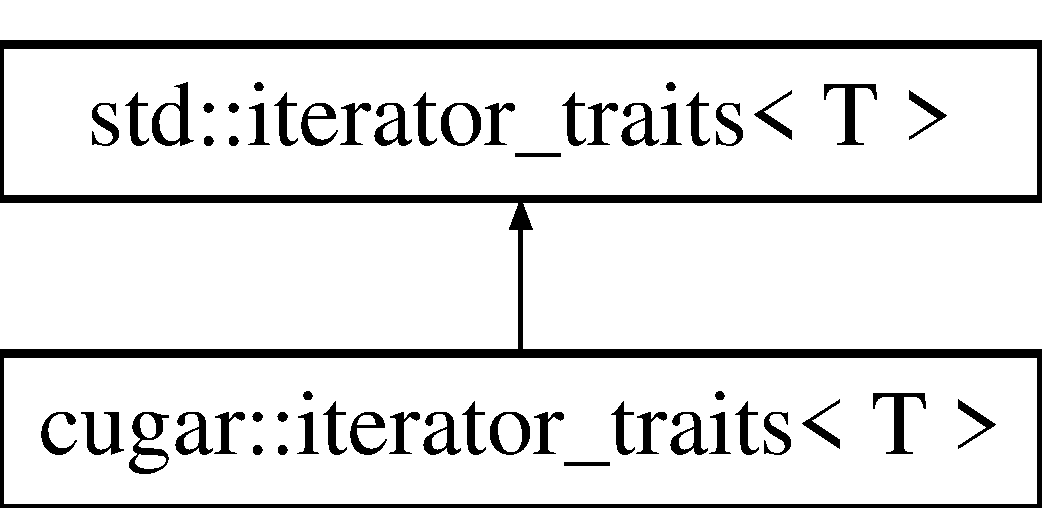
\includegraphics[height=2.000000cm]{structcugar_1_1iterator__traits}
\end{center}
\end{figure}
\subsection*{Public Types}
\begin{DoxyCompactItemize}
\item 
\mbox{\Hypertarget{structcugar_1_1iterator__traits_ae7fc0f47119fb6d6f00bb3ac797322b0}\label{structcugar_1_1iterator__traits_ae7fc0f47119fb6d6f00bb3ac797322b0}} 
typedef std\+::iterator\+\_\+traits$<$ T $>$\+::iterator\+\_\+category {\bfseries iterator\+\_\+category}
\item 
\mbox{\Hypertarget{structcugar_1_1iterator__traits_a4e4346cb857d02a6ce0f14a8ac849972}\label{structcugar_1_1iterator__traits_a4e4346cb857d02a6ce0f14a8ac849972}} 
typedef std\+::iterator\+\_\+traits$<$ T $>$\+::value\+\_\+type {\bfseries value\+\_\+type}
\item 
\mbox{\Hypertarget{structcugar_1_1iterator__traits_ac053bf36496a8a517d3bcf2acf331180}\label{structcugar_1_1iterator__traits_ac053bf36496a8a517d3bcf2acf331180}} 
typedef std\+::iterator\+\_\+traits$<$ T $>$\+::difference\+\_\+type {\bfseries difference\+\_\+type}
\item 
\mbox{\Hypertarget{structcugar_1_1iterator__traits_ad7145890da0f61dd8f6b8fd3bd7c10a8}\label{structcugar_1_1iterator__traits_ad7145890da0f61dd8f6b8fd3bd7c10a8}} 
typedef std\+::iterator\+\_\+traits$<$ T $>$\+::pointer {\bfseries pointer}
\item 
\mbox{\Hypertarget{structcugar_1_1iterator__traits_a2fc1e816ad073ae733753a85aa4b26fc}\label{structcugar_1_1iterator__traits_a2fc1e816ad073ae733753a85aa4b26fc}} 
typedef std\+::iterator\+\_\+traits$<$ T $>$\+::reference {\bfseries reference}
\item 
\mbox{\Hypertarget{structcugar_1_1iterator__traits_aea69e7caa1460e91ad47b0a2573da84d}\label{structcugar_1_1iterator__traits_aea69e7caa1460e91ad47b0a2573da84d}} 
typedef T \hyperlink{structcugar_1_1iterator__traits_aea69e7caa1460e91ad47b0a2573da84d}{forward\+\_\+iterator}
\begin{DoxyCompactList}\small\item\em add forward iterator conversion \end{DoxyCompactList}\end{DoxyCompactItemize}


The documentation for this struct was generated from the following file\+:\begin{DoxyCompactItemize}
\item 
C\+:/p4research/research/jpantaleoni/\+Fermat-\/\+Public/contrib/cugar/basic/iterator.\+h\end{DoxyCompactItemize}

\hypertarget{structcugar_1_1cuda_1_1_kd__builder}{}\section{cugar\+:\+:cuda\+:\+:Kd\+\_\+builder$<$ Integer $>$ Struct Template Reference}
\label{structcugar_1_1cuda_1_1_kd__builder}\index{cugar\+::cuda\+::\+Kd\+\_\+builder$<$ Integer $>$@{cugar\+::cuda\+::\+Kd\+\_\+builder$<$ Integer $>$}}


\subsection{Detailed description}
\subsubsection*{template$<$typename Integer$>$\newline
struct cugar\+::cuda\+::\+Kd\+\_\+builder$<$ Integer $>$}

G\+P\+U-\/based middle-\/split k-\/d tree builder

This class provides the context to generate k-\/d trees on the G\+PU starting from a set of unordered points. The output is a set of nodes with the corresponding leaves and a set of primitive indices into the input set of points. The output leaves will specify contiguous ranges into this index.


\begin{DoxyTemplParams}{Template Parameters}
{\em Integer} & an integer type that determines the number of bits used to compute the points\textquotesingle{} Morton codes. Accepted values are uint32 and uint64.\\
\hline
{\em Output\+Tree} & a template class used to write the output tree, with the following interface\+:\\
\hline
\end{DoxyTemplParams}
\label{structcugar_1_1cuda_1_1_kd__builder_KdOutputTreeAnchor}%
\Hypertarget{structcugar_1_1cuda_1_1_kd__builder_KdOutputTreeAnchor}%
 
\begin{DoxyCode}
\textcolor{keyword}{struct }OutputTree
\{
   \textcolor{keywordtype}{void} reserve\_nodes(\textcolor{keyword}{const} uint32 n);  \textcolor{comment}{// reserve space for n nodes}
   \textcolor{keywordtype}{void} reserve\_leaves(\textcolor{keyword}{const} uint32 n); \textcolor{comment}{// reserve space for n leaves}

   Context get\_context();             \textcolor{comment}{// get a context to write nodes/leaves}

   \textcolor{keyword}{struct }Context
   \{
       \textcolor{keywordtype}{void} write\_node(
          \textcolor{keyword}{const} uint32 node,          \textcolor{comment}{// node to write}
          \textcolor{keyword}{const} uint32 offset,        \textcolor{comment}{// child offset}
          \textcolor{keyword}{const} uint32 skip\_node,     \textcolor{comment}{// skip node}
          \textcolor{keyword}{const} uint32 \hyperlink{namespacecugar_a2121df08f967e232ea5fe0ee378dee67}{begin},         \textcolor{comment}{// node range begin}
          \textcolor{keyword}{const} uint32 end,           \textcolor{comment}{// node range end}
          \textcolor{keyword}{const} uint32 split\_index,   \textcolor{comment}{// split index}
          \textcolor{keyword}{const} uint32 split\_dim,     \textcolor{comment}{// splitting dimension}
          \textcolor{keyword}{const} uint32 split\_plane);  \textcolor{comment}{// splitting plane}

       \textcolor{keywordtype}{void} write\_node(
          \textcolor{keyword}{const} uint32 node,          \textcolor{comment}{// node to write}
          \textcolor{keyword}{const} uint32 offset,        \textcolor{comment}{// child offset}
          \textcolor{keyword}{const} uint32 skip\_node,     \textcolor{comment}{// skip node}
          \textcolor{keyword}{const} uint32 \hyperlink{namespacecugar_a2121df08f967e232ea5fe0ee378dee67}{begin},         \textcolor{comment}{// node range begin}
          \textcolor{keyword}{const} uint32 end);          \textcolor{comment}{// node range end}

       \textcolor{keywordtype}{void} write\_leaf(
          \textcolor{keyword}{const} uint32 index,         \textcolor{comment}{// leaf to write}
          \textcolor{keyword}{const} uint32 \hyperlink{namespacecugar_a2121df08f967e232ea5fe0ee378dee67}{begin},         \textcolor{comment}{// leaf range begin}
          \textcolor{keyword}{const} uint32 end);          \textcolor{comment}{// leaf range end}
   \};
\};
\end{DoxyCode}


The following code snippet shows how to use this builder\+:


\begin{DoxyCode}
\textcolor{preprocessor}{#include <\hyperlink{kd__builder_8h}{cugar/kd/cuda/kd\_builder.h}>}
\textcolor{preprocessor}{#include <\hyperlink{kd__context_8h}{cugar/kd/cuda/kd\_context.h}>}

\hyperlink{structcugar_1_1vector}{cugar::vector<device\_tag,Vector3f>} points;
... \textcolor{comment}{// code to fill the input vector of points}

\hyperlink{structcugar_1_1vector}{cugar::vector<device\_tag,Kd\_node>}  kd\_nodes;
\hyperlink{structcugar_1_1vector}{cugar::vector<device\_tag,uint2>}    kd\_leaves;
\hyperlink{structcugar_1_1vector}{cugar::vector<device\_tag,uint32>}   kd\_index;
\hyperlink{structcugar_1_1vector}{cugar::vector<device\_tag,uint2>}    kd\_ranges;

\hyperlink{structcugar_1_1cuda_1_1_kd__builder}{cugar::cuda::Kd\_builder<uint64>} builder( kd\_index );
\hyperlink{structcugar_1_1cuda_1_1_kd__context}{cugar::cuda::Kd\_context} kd\_tree( &kd\_nodes, &kd\_leaves, &kd\_ranges );
builder.build(
    kd\_tree,                                    \textcolor{comment}{// output tree}
    kd\_index,                                   \textcolor{comment}{// output index}
    Bbox3f( Vector3f(0.0f), Vector3f(1.0f) ),   \textcolor{comment}{// suppose all bboxes are in [0,1]^3}
    points.begin(),                             \textcolor{comment}{// begin iterator}
    points.end(),                               \textcolor{comment}{// end iterator}
    4 );                                        \textcolor{comment}{// target 4 objects per leaf}
\end{DoxyCode}
 

{\ttfamily \#include $<$kd\+\_\+builder.\+h$>$}

\subsection*{Public Methods}
\begin{DoxyCompactItemize}
\item 
{\footnotesize template$<$typename Output\+Tree , typename Iterator , typename Bbox\+Type $>$ }\\void \hyperlink{structcugar_1_1cuda_1_1_kd__builder_a3406ba54cf8cb747ac03065e0df5398f}{build} (Output\+Tree \&out\+\_\+tree, \hyperlink{structcugar_1_1vector}{vector}$<$ \hyperlink{structcugar_1_1device__tag}{device\+\_\+tag}, uint32 $>$ \&out\+\_\+index, const Bbox\+Type bbox, const Iterator points\+\_\+begin, const Iterator points\+\_\+end, const uint32 max\+\_\+leaf\+\_\+size)
\end{DoxyCompactItemize}
\subsection*{Public Members}
\begin{DoxyCompactItemize}
\item 
\mbox{\Hypertarget{structcugar_1_1cuda_1_1_kd__builder_ae0697065717fc4e1716950edebaa5c2a}\label{structcugar_1_1cuda_1_1_kd__builder_ae0697065717fc4e1716950edebaa5c2a}} 
\hyperlink{structcugar_1_1vector}{vector}$<$ \hyperlink{structcugar_1_1device__tag}{device\+\_\+tag}, Integer $>$ {\bfseries m\+\_\+codes}
\item 
\mbox{\Hypertarget{structcugar_1_1cuda_1_1_kd__builder_a01293ef7ba88b485ed06b71f004edef4}\label{structcugar_1_1cuda_1_1_kd__builder_a01293ef7ba88b485ed06b71f004edef4}} 
\hyperlink{structcugar_1_1caching__device__vector}{caching\+\_\+device\+\_\+vector}$<$ Integer $>$ {\bfseries m\+\_\+temp\+\_\+codes}
\item 
\mbox{\Hypertarget{structcugar_1_1cuda_1_1_kd__builder_a9c7d09a9195fa322565fd5ac7b3c3aa2}\label{structcugar_1_1cuda_1_1_kd__builder_a9c7d09a9195fa322565fd5ac7b3c3aa2}} 
\hyperlink{structcugar_1_1caching__device__vector}{caching\+\_\+device\+\_\+vector}$<$ uint32 $>$ {\bfseries m\+\_\+temp\+\_\+index}
\item 
\mbox{\Hypertarget{structcugar_1_1cuda_1_1_kd__builder_ad46ebcf11ed0b7958da2b153c2c942a0}\label{structcugar_1_1cuda_1_1_kd__builder_ad46ebcf11ed0b7958da2b153c2c942a0}} 
uint32 {\bfseries m\+\_\+node\+\_\+count}
\item 
\mbox{\Hypertarget{structcugar_1_1cuda_1_1_kd__builder_a92e40df7182e091e9233d4ff99c08ebd}\label{structcugar_1_1cuda_1_1_kd__builder_a92e40df7182e091e9233d4ff99c08ebd}} 
uint32 {\bfseries m\+\_\+leaf\+\_\+count}
\item 
\mbox{\Hypertarget{structcugar_1_1cuda_1_1_kd__builder_a6494783d773e12e7a6e4e5cb9c445bbc}\label{structcugar_1_1cuda_1_1_kd__builder_a6494783d773e12e7a6e4e5cb9c445bbc}} 
\hyperlink{structcugar_1_1cuda_1_1_radixtree__context}{cuda\+::\+Radixtree\+\_\+context} {\bfseries m\+\_\+kd\+\_\+context}
\end{DoxyCompactItemize}


\subsection{Member Function Documentation}
\mbox{\Hypertarget{structcugar_1_1cuda_1_1_kd__builder_a3406ba54cf8cb747ac03065e0df5398f}\label{structcugar_1_1cuda_1_1_kd__builder_a3406ba54cf8cb747ac03065e0df5398f}} 
\index{cugar\+::cuda\+::\+Kd\+\_\+builder@{cugar\+::cuda\+::\+Kd\+\_\+builder}!build@{build}}
\index{build@{build}!cugar\+::cuda\+::\+Kd\+\_\+builder@{cugar\+::cuda\+::\+Kd\+\_\+builder}}
\subsubsection{\texorpdfstring{build()}{build()}}
{\footnotesize\ttfamily template$<$typename Integer $>$ \\
template$<$typename Output\+Tree , typename Iterator , typename Bbox\+Type $>$ \\
void \hyperlink{structcugar_1_1cuda_1_1_kd__builder}{cugar\+::cuda\+::\+Kd\+\_\+builder}$<$ Integer $>$\+::build (\begin{DoxyParamCaption}\item[{Output\+Tree \&}]{out\+\_\+tree,  }\item[{\hyperlink{structcugar_1_1vector}{vector}$<$ \hyperlink{structcugar_1_1device__tag}{device\+\_\+tag}, uint32 $>$ \&}]{out\+\_\+index,  }\item[{const Bbox\+Type}]{bbox,  }\item[{const Iterator}]{points\+\_\+begin,  }\item[{const Iterator}]{points\+\_\+end,  }\item[{const uint32}]{max\+\_\+leaf\+\_\+size }\end{DoxyParamCaption})}

build a bvh given a set of points that will be reordered in-\/place


\begin{DoxyParams}{Parameters}
{\em out\+\_\+tree} & output tree \\
\hline
{\em out\+\_\+index} & output index \\
\hline
{\em bbox} & global bbox \\
\hline
{\em points\+\_\+begin} & beginning of the point sequence to sort \\
\hline
{\em points\+\_\+end} & end of the point sequence to sort \\
\hline
{\em max\+\_\+leaf\+\_\+size} & maximum leaf size \\
\hline
\end{DoxyParams}


The documentation for this struct was generated from the following files\+:\begin{DoxyCompactItemize}
\item 
C\+:/p4research/research/jpantaleoni/\+Fermat-\/\+Public/contrib/cugar/kd/cuda/\hyperlink{kd__builder_8h}{kd\+\_\+builder.\+h}\item 
C\+:/p4research/research/jpantaleoni/\+Fermat-\/\+Public/contrib/cugar/kd/cuda/kd\+\_\+builder\+\_\+inline.\+h\end{DoxyCompactItemize}

\hypertarget{structcugar_1_1cuda_1_1kd_1_1_kd__context}{}\section{cugar\+:\+:cuda\+:\+:kd\+:\+:Kd\+\_\+context$<$ D\+IM, Bbox\+Type, Integer, Output\+Tree $>$ Struct Template Reference}
\label{structcugar_1_1cuda_1_1kd_1_1_kd__context}\index{cugar\+::cuda\+::kd\+::\+Kd\+\_\+context$<$ D\+I\+M, Bbox\+Type, Integer, Output\+Tree $>$@{cugar\+::cuda\+::kd\+::\+Kd\+\_\+context$<$ D\+I\+M, Bbox\+Type, Integer, Output\+Tree $>$}}


\subsection{Detailed description}
\subsubsection*{template$<$uint32 D\+IM, typename Bbox\+Type, typename Integer, typename Output\+Tree$>$\newline
struct cugar\+::cuda\+::kd\+::\+Kd\+\_\+context$<$ D\+I\+M, Bbox\+Type, Integer, Output\+Tree $>$}

A simple binary tree context implementation to be used with the \hyperlink{structcugar_1_1_bvh}{Bvh} generate() function. 

{\ttfamily \#include $<$kd\+\_\+builder\+\_\+inline.\+h$>$}

\subsection*{Classes}
\begin{DoxyCompactItemize}
\item 
struct \hyperlink{structcugar_1_1cuda_1_1kd_1_1_kd__context_1_1_context}{Context}
\begin{DoxyCompactList}\small\item\em Cuda accessor struct. \end{DoxyCompactList}\end{DoxyCompactItemize}
\subsection*{Public Types}
\begin{DoxyCompactItemize}
\item 
\mbox{\Hypertarget{structcugar_1_1cuda_1_1kd_1_1_kd__context_a279264d20b734023d033abf00196be08}\label{structcugar_1_1cuda_1_1kd_1_1_kd__context_a279264d20b734023d033abf00196be08}} 
typedef Output\+Tree\+::\+Context {\bfseries Base\+Context}
\end{DoxyCompactItemize}
\subsection*{Public Methods}
\begin{DoxyCompactItemize}
\item 
\mbox{\Hypertarget{structcugar_1_1cuda_1_1kd_1_1_kd__context_a00ec8a71f810a654a1c513c460785eb6}\label{structcugar_1_1cuda_1_1kd_1_1_kd__context_a00ec8a71f810a654a1c513c460785eb6}} 
\hyperlink{structcugar_1_1cuda_1_1kd_1_1_kd__context_a00ec8a71f810a654a1c513c460785eb6}{Kd\+\_\+context} (Output\+Tree context, const Integer $\ast$codes, Bbox\+Type bbox)
\begin{DoxyCompactList}\small\item\em constructor \end{DoxyCompactList}\item 
\mbox{\Hypertarget{structcugar_1_1cuda_1_1kd_1_1_kd__context_aa51f244c19bc1c91b93171d1382abb6b}\label{structcugar_1_1cuda_1_1kd_1_1_kd__context_aa51f244c19bc1c91b93171d1382abb6b}} 
void \hyperlink{structcugar_1_1cuda_1_1kd_1_1_kd__context_aa51f244c19bc1c91b93171d1382abb6b}{reserve\+\_\+nodes} (const uint32 n)
\begin{DoxyCompactList}\small\item\em reserve space for more nodes \end{DoxyCompactList}\item 
\mbox{\Hypertarget{structcugar_1_1cuda_1_1kd_1_1_kd__context_a4d8c3e0a23c2bb7f4fb9e184e453b920}\label{structcugar_1_1cuda_1_1kd_1_1_kd__context_a4d8c3e0a23c2bb7f4fb9e184e453b920}} 
void \hyperlink{structcugar_1_1cuda_1_1kd_1_1_kd__context_a4d8c3e0a23c2bb7f4fb9e184e453b920}{reserve\+\_\+leaves} (const uint32 n)
\begin{DoxyCompactList}\small\item\em reserve space for more leaves \end{DoxyCompactList}\item 
\mbox{\Hypertarget{structcugar_1_1cuda_1_1kd_1_1_kd__context_a1236e56d6d83701f3e5666148799e500}\label{structcugar_1_1cuda_1_1kd_1_1_kd__context_a1236e56d6d83701f3e5666148799e500}} 
\hyperlink{structcugar_1_1cuda_1_1kd_1_1_kd__context_1_1_context}{Context} \hyperlink{structcugar_1_1cuda_1_1kd_1_1_kd__context_a1236e56d6d83701f3e5666148799e500}{get\+\_\+context} ()
\begin{DoxyCompactList}\small\item\em return a cuda context \end{DoxyCompactList}\end{DoxyCompactItemize}
\subsection*{Public Members}
\begin{DoxyCompactItemize}
\item 
\mbox{\Hypertarget{structcugar_1_1cuda_1_1kd_1_1_kd__context_a52ab77909d3881dfc42a64e547d54123}\label{structcugar_1_1cuda_1_1kd_1_1_kd__context_a52ab77909d3881dfc42a64e547d54123}} 
Output\+Tree {\bfseries m\+\_\+context}
\item 
\mbox{\Hypertarget{structcugar_1_1cuda_1_1kd_1_1_kd__context_ad2c8bd4db81c8d24ffe37e97245898bf}\label{structcugar_1_1cuda_1_1kd_1_1_kd__context_ad2c8bd4db81c8d24ffe37e97245898bf}} 
const Integer $\ast$ {\bfseries m\+\_\+codes}
\item 
\mbox{\Hypertarget{structcugar_1_1cuda_1_1kd_1_1_kd__context_a92bd2daf2f7ae63c9085fbbb4f62ec5b}\label{structcugar_1_1cuda_1_1kd_1_1_kd__context_a92bd2daf2f7ae63c9085fbbb4f62ec5b}} 
Bbox\+Type {\bfseries m\+\_\+bbox}
\end{DoxyCompactItemize}


The documentation for this struct was generated from the following file\+:\begin{DoxyCompactItemize}
\item 
C\+:/p4research/research/jpantaleoni/\+Fermat-\/\+Public/contrib/cugar/kd/cuda/kd\+\_\+builder\+\_\+inline.\+h\end{DoxyCompactItemize}

\hypertarget{structcugar_1_1cuda_1_1_kd__context}{}\section{cugar\+:\+:cuda\+:\+:Kd\+\_\+context Struct Reference}
\label{structcugar_1_1cuda_1_1_kd__context}\index{cugar\+::cuda\+::\+Kd\+\_\+context@{cugar\+::cuda\+::\+Kd\+\_\+context}}


\subsection{Detailed description}
A context to pass to k-\/d tree builders 

{\ttfamily \#include $<$kd\+\_\+context.\+h$>$}

\subsection*{Classes}
\begin{DoxyCompactItemize}
\item 
struct \hyperlink{structcugar_1_1cuda_1_1_kd__context_1_1_context}{Context}
\begin{DoxyCompactList}\small\item\em Cuda accessor struct. \end{DoxyCompactList}\end{DoxyCompactItemize}
\subsection*{Public Methods}
\begin{DoxyCompactItemize}
\item 
\hyperlink{structcugar_1_1cuda_1_1_kd__context_a654bb141ef5aee074a05d56cfcac3ca1}{Kd\+\_\+context} (thrust\+::device\+\_\+vector$<$ \hyperlink{structcugar_1_1_kd__node}{Kd\+\_\+node} $>$ $\ast$nodes, thrust\+::device\+\_\+vector$<$ uint2 $>$ $\ast$leaves, thrust\+::device\+\_\+vector$<$ uint2 $>$ $\ast$ranges)
\item 
void \hyperlink{structcugar_1_1cuda_1_1_kd__context_a5c97fca7fe7ce898fdf17f7406d5efc8}{reserve\+\_\+nodes} (const uint32 n)
\item 
void \hyperlink{structcugar_1_1cuda_1_1_kd__context_a7bc572a4cd5bc3879cd54d86c4735863}{reserve\+\_\+leaves} (const uint32 n)
\item 
\hyperlink{structcugar_1_1cuda_1_1_kd__context_1_1_context}{Context} \hyperlink{structcugar_1_1cuda_1_1_kd__context_ab5a0d97da3fcddd94a9673eb6a3c529d}{get\+\_\+context} ()
\end{DoxyCompactItemize}
\subsection*{Public Members}
\begin{DoxyCompactItemize}
\item 
\mbox{\Hypertarget{structcugar_1_1cuda_1_1_kd__context_a194733e014257d08edc4f7c7b7b5b232}\label{structcugar_1_1cuda_1_1_kd__context_a194733e014257d08edc4f7c7b7b5b232}} 
thrust\+::device\+\_\+vector$<$ \hyperlink{structcugar_1_1_kd__node}{Kd\+\_\+node} $>$ $\ast$ {\bfseries m\+\_\+nodes}
\item 
\mbox{\Hypertarget{structcugar_1_1cuda_1_1_kd__context_a3b02e2269ab2bff209644490614748f8}\label{structcugar_1_1cuda_1_1_kd__context_a3b02e2269ab2bff209644490614748f8}} 
thrust\+::device\+\_\+vector$<$ uint2 $>$ $\ast$ {\bfseries m\+\_\+leaves}
\item 
\mbox{\Hypertarget{structcugar_1_1cuda_1_1_kd__context_aabd47af2effa3080fe02cdc4688150df}\label{structcugar_1_1cuda_1_1_kd__context_aabd47af2effa3080fe02cdc4688150df}} 
thrust\+::device\+\_\+vector$<$ uint2 $>$ $\ast$ {\bfseries m\+\_\+ranges}
\end{DoxyCompactItemize}


\subsection{Constructor \& Destructor Documentation}
\mbox{\Hypertarget{structcugar_1_1cuda_1_1_kd__context_a654bb141ef5aee074a05d56cfcac3ca1}\label{structcugar_1_1cuda_1_1_kd__context_a654bb141ef5aee074a05d56cfcac3ca1}} 
\index{cugar\+::cuda\+::\+Kd\+\_\+context@{cugar\+::cuda\+::\+Kd\+\_\+context}!Kd\+\_\+context@{Kd\+\_\+context}}
\index{Kd\+\_\+context@{Kd\+\_\+context}!cugar\+::cuda\+::\+Kd\+\_\+context@{cugar\+::cuda\+::\+Kd\+\_\+context}}
\subsubsection{\texorpdfstring{Kd\+\_\+context()}{Kd\_context()}}
{\footnotesize\ttfamily cugar\+::cuda\+::\+Kd\+\_\+context\+::\+Kd\+\_\+context (\begin{DoxyParamCaption}\item[{thrust\+::device\+\_\+vector$<$ \hyperlink{structcugar_1_1_kd__node}{Kd\+\_\+node} $>$ $\ast$}]{nodes,  }\item[{thrust\+::device\+\_\+vector$<$ uint2 $>$ $\ast$}]{leaves,  }\item[{thrust\+::device\+\_\+vector$<$ uint2 $>$ $\ast$}]{ranges }\end{DoxyParamCaption})\hspace{0.3cm}{\ttfamily [inline]}}

constructor


\begin{DoxyParams}{Parameters}
{\em nodes} & output node vector \\
\hline
{\em leaves} & output leaf vector \\
\hline
{\em ranges} & output node range vector\+: if not N\+U\+LL, the i-\/th item will be set with the range of prims corresponding to the i-\/th node. \\
\hline
\end{DoxyParams}


\subsection{Member Function Documentation}
\mbox{\Hypertarget{structcugar_1_1cuda_1_1_kd__context_ab5a0d97da3fcddd94a9673eb6a3c529d}\label{structcugar_1_1cuda_1_1_kd__context_ab5a0d97da3fcddd94a9673eb6a3c529d}} 
\index{cugar\+::cuda\+::\+Kd\+\_\+context@{cugar\+::cuda\+::\+Kd\+\_\+context}!get\+\_\+context@{get\+\_\+context}}
\index{get\+\_\+context@{get\+\_\+context}!cugar\+::cuda\+::\+Kd\+\_\+context@{cugar\+::cuda\+::\+Kd\+\_\+context}}
\subsubsection{\texorpdfstring{get\+\_\+context()}{get\_context()}}
{\footnotesize\ttfamily \hyperlink{structcugar_1_1cuda_1_1_kd__context_1_1_context}{Context} cugar\+::cuda\+::\+Kd\+\_\+context\+::get\+\_\+context (\begin{DoxyParamCaption}{ }\end{DoxyParamCaption})\hspace{0.3cm}{\ttfamily [inline]}}

return a cuda context \mbox{\Hypertarget{structcugar_1_1cuda_1_1_kd__context_a7bc572a4cd5bc3879cd54d86c4735863}\label{structcugar_1_1cuda_1_1_kd__context_a7bc572a4cd5bc3879cd54d86c4735863}} 
\index{cugar\+::cuda\+::\+Kd\+\_\+context@{cugar\+::cuda\+::\+Kd\+\_\+context}!reserve\+\_\+leaves@{reserve\+\_\+leaves}}
\index{reserve\+\_\+leaves@{reserve\+\_\+leaves}!cugar\+::cuda\+::\+Kd\+\_\+context@{cugar\+::cuda\+::\+Kd\+\_\+context}}
\subsubsection{\texorpdfstring{reserve\+\_\+leaves()}{reserve\_leaves()}}
{\footnotesize\ttfamily void cugar\+::cuda\+::\+Kd\+\_\+context\+::reserve\+\_\+leaves (\begin{DoxyParamCaption}\item[{const uint32}]{n }\end{DoxyParamCaption})\hspace{0.3cm}{\ttfamily [inline]}}

reserve space for more leaves \mbox{\Hypertarget{structcugar_1_1cuda_1_1_kd__context_a5c97fca7fe7ce898fdf17f7406d5efc8}\label{structcugar_1_1cuda_1_1_kd__context_a5c97fca7fe7ce898fdf17f7406d5efc8}} 
\index{cugar\+::cuda\+::\+Kd\+\_\+context@{cugar\+::cuda\+::\+Kd\+\_\+context}!reserve\+\_\+nodes@{reserve\+\_\+nodes}}
\index{reserve\+\_\+nodes@{reserve\+\_\+nodes}!cugar\+::cuda\+::\+Kd\+\_\+context@{cugar\+::cuda\+::\+Kd\+\_\+context}}
\subsubsection{\texorpdfstring{reserve\+\_\+nodes()}{reserve\_nodes()}}
{\footnotesize\ttfamily void cugar\+::cuda\+::\+Kd\+\_\+context\+::reserve\+\_\+nodes (\begin{DoxyParamCaption}\item[{const uint32}]{n }\end{DoxyParamCaption})\hspace{0.3cm}{\ttfamily [inline]}}

reserve space for more nodes 

The documentation for this struct was generated from the following file\+:\begin{DoxyCompactItemize}
\item 
C\+:/p4research/research/jpantaleoni/\+Fermat-\/\+Public/contrib/cugar/kd/cuda/\hyperlink{kd__context_8h}{kd\+\_\+context.\+h}\end{DoxyCompactItemize}

\hypertarget{structcugar_1_1cuda_1_1_kd__knn}{}\section{cugar\+:\+:cuda\+:\+:Kd\+\_\+knn$<$ D\+IM $>$ Struct Template Reference}
\label{structcugar_1_1cuda_1_1_kd__knn}\index{cugar\+::cuda\+::\+Kd\+\_\+knn$<$ D\+I\+M $>$@{cugar\+::cuda\+::\+Kd\+\_\+knn$<$ D\+I\+M $>$}}


\subsection{Detailed description}
\subsubsection*{template$<$uint32 D\+IM$>$\newline
struct cugar\+::cuda\+::\+Kd\+\_\+knn$<$ D\+I\+M $>$}

G\+P\+U-\/based k-\/\+Nearest Neighbors lookup context.

This class provides the context to perform 3-\/dimensional k-\/nn lookups on the G\+PU, using a k-\/d tree.

The following code snippet shows how to use this class\+:


\begin{DoxyCode}
\textcolor{preprocessor}{#include <cugar/kd/cuda/kd\_knn.h>}

\hyperlink{structcugar_1_1vector}{cugar::vector<device\_tag,Vector4f>} kd\_points;
\hyperlink{structcugar_1_1vector}{cugar::vector<device\_tag,Kd\_node>}  kd\_nodes;
\hyperlink{structcugar_1_1vector}{cugar::vector<device\_tag,uint2>}    kd\_leaves;
\hyperlink{structcugar_1_1vector}{cugar::vector<device\_tag,uint32>}   kd\_index;

\hyperlink{structcugar_1_1vector}{cugar::vector<device\_tag,Vector4f>} query\_points;
... \textcolor{comment}{// code to build the k-d tree and query points here...}
    \textcolor{comment}{// NOTE: even though we're doing 3-dimensional queries,}
    \textcolor{comment}{// we can use Vector4f arrays for better coalescing}

\hyperlink{structcugar_1_1vector}{cugar::vector<device\_tag,cuda::Kd\_knn<3>::Result}> results( 
      query\_points.size() );

\hyperlink{structcugar_1_1cuda_1_1_kd__knn}{cugar::cuda::Kd\_knn<3>} knn;
knn.run(
    query\_points.begin(),
    query\_points.end(),
    \hyperlink{namespacecugar_a3f6cb2c817f2ba065931cec569aa848b}{raw\_pointer}(kd\_nodes),
    \hyperlink{namespacecugar_a3f6cb2c817f2ba065931cec569aa848b}{raw\_pointer}(kd\_ranges),
    \hyperlink{namespacecugar_a3f6cb2c817f2ba065931cec569aa848b}{raw\_pointer}(kd\_leaves),
    \hyperlink{namespacecugar_a3f6cb2c817f2ba065931cec569aa848b}{raw\_pointer}(kd\_points),
    \hyperlink{namespacecugar_a3f6cb2c817f2ba065931cec569aa848b}{raw\_pointer}(results) );
\end{DoxyCode}
 

{\ttfamily \#include $<$knn.\+h$>$}

\subsection*{Public Types}
\begin{DoxyCompactItemize}
\item 
\mbox{\Hypertarget{structcugar_1_1cuda_1_1_kd__knn_a0786ce849457dbcd48ea5d5713134fb8}\label{structcugar_1_1cuda_1_1_kd__knn_a0786ce849457dbcd48ea5d5713134fb8}} 
typedef \hyperlink{structcugar_1_1cuda_1_1_kd__knn__result}{Kd\+\_\+knn\+\_\+result} {\bfseries Result}
\end{DoxyCompactItemize}
\subsection*{Public Methods}
\begin{DoxyCompactItemize}
\item 
{\footnotesize template$<$typename Query\+Iterator , typename Point\+Iterator $>$ }\\void \hyperlink{structcugar_1_1cuda_1_1_kd__knn_a7d04646c1a646cd30b49ba6faf4b06d2}{run} (const Query\+Iterator points\+\_\+begin, const Query\+Iterator points\+\_\+end, const \hyperlink{structcugar_1_1_kd__node}{Kd\+\_\+node} $\ast$kd\+\_\+nodes, const uint2 $\ast$kd\+\_\+ranges, const uint2 $\ast$kd\+\_\+leaves, const Point\+Iterator kd\+\_\+points, \hyperlink{structcugar_1_1cuda_1_1_kd__knn__result}{Result} $\ast$results)
\item 
{\footnotesize template$<$uint32 K, typename Query\+Iterator , typename Point\+Iterator $>$ }\\void \hyperlink{structcugar_1_1cuda_1_1_kd__knn_aa9040a5e6f8cf2ba2c5c50af64a066f8}{run} (const Query\+Iterator points\+\_\+begin, const Query\+Iterator points\+\_\+end, const \hyperlink{structcugar_1_1_kd__node}{Kd\+\_\+node} $\ast$kd\+\_\+nodes, const uint2 $\ast$kd\+\_\+ranges, const uint2 $\ast$kd\+\_\+leaves, const Point\+Iterator kd\+\_\+points, \hyperlink{structcugar_1_1cuda_1_1_kd__knn__result}{Result} $\ast$results)
\end{DoxyCompactItemize}


\subsection{Member Function Documentation}
\mbox{\Hypertarget{structcugar_1_1cuda_1_1_kd__knn_a7d04646c1a646cd30b49ba6faf4b06d2}\label{structcugar_1_1cuda_1_1_kd__knn_a7d04646c1a646cd30b49ba6faf4b06d2}} 
\index{cugar\+::cuda\+::\+Kd\+\_\+knn@{cugar\+::cuda\+::\+Kd\+\_\+knn}!run@{run}}
\index{run@{run}!cugar\+::cuda\+::\+Kd\+\_\+knn@{cugar\+::cuda\+::\+Kd\+\_\+knn}}
\subsubsection{\texorpdfstring{run()}{run()}\hspace{0.1cm}{\footnotesize\ttfamily [1/2]}}
{\footnotesize\ttfamily template$<$uint32 D\+IM$>$ \\
template$<$typename Query\+Iterator , typename Point\+Iterator $>$ \\
void \hyperlink{structcugar_1_1cuda_1_1_kd__knn}{cugar\+::cuda\+::\+Kd\+\_\+knn}$<$ D\+IM $>$\+::run (\begin{DoxyParamCaption}\item[{const Query\+Iterator}]{points\+\_\+begin,  }\item[{const Query\+Iterator}]{points\+\_\+end,  }\item[{const \hyperlink{structcugar_1_1_kd__node}{Kd\+\_\+node} $\ast$}]{kd\+\_\+nodes,  }\item[{const uint2 $\ast$}]{kd\+\_\+ranges,  }\item[{const uint2 $\ast$}]{kd\+\_\+leaves,  }\item[{const Point\+Iterator}]{kd\+\_\+points,  }\item[{\hyperlink{structcugar_1_1cuda_1_1_kd__knn__result}{Result} $\ast$}]{results }\end{DoxyParamCaption})}

perform a k-\/nn lookup for a set of query points


\begin{DoxyParams}{Parameters}
{\em points\+\_\+begin} & beginning of the query point sequence \\
\hline
{\em points\+\_\+end} & end of the query point sequence \\
\hline
{\em kd\+\_\+nodes} & k-\/d tree nodes \\
\hline
{\em kd\+\_\+ranges} & k-\/d tree node ranges \\
\hline
{\em kd\+\_\+leaves} & k-\/d tree leaves \\
\hline
{\em kd\+\_\+points} & k-\/d tree points\\
\hline
\end{DoxyParams}

\begin{DoxyTemplParams}{Template Parameters}
{\em Query\+Iterator} & an iterator type dereferencing to Vector$<$float,\+N$>$, with N $>$= 3 \\
\hline
{\em Point\+Iterator} & an iterator type dereferencing to Vector$<$float,\+N$>$, with N $>$= 3 \\
\hline
\end{DoxyTemplParams}
\mbox{\Hypertarget{structcugar_1_1cuda_1_1_kd__knn_aa9040a5e6f8cf2ba2c5c50af64a066f8}\label{structcugar_1_1cuda_1_1_kd__knn_aa9040a5e6f8cf2ba2c5c50af64a066f8}} 
\index{cugar\+::cuda\+::\+Kd\+\_\+knn@{cugar\+::cuda\+::\+Kd\+\_\+knn}!run@{run}}
\index{run@{run}!cugar\+::cuda\+::\+Kd\+\_\+knn@{cugar\+::cuda\+::\+Kd\+\_\+knn}}
\subsubsection{\texorpdfstring{run()}{run()}\hspace{0.1cm}{\footnotesize\ttfamily [2/2]}}
{\footnotesize\ttfamily template$<$uint32 D\+IM$>$ \\
template$<$uint32 K, typename Query\+Iterator , typename Point\+Iterator $>$ \\
void \hyperlink{structcugar_1_1cuda_1_1_kd__knn}{cugar\+::cuda\+::\+Kd\+\_\+knn}$<$ D\+IM $>$\+::run (\begin{DoxyParamCaption}\item[{const Query\+Iterator}]{points\+\_\+begin,  }\item[{const Query\+Iterator}]{points\+\_\+end,  }\item[{const \hyperlink{structcugar_1_1_kd__node}{Kd\+\_\+node} $\ast$}]{kd\+\_\+nodes,  }\item[{const uint2 $\ast$}]{kd\+\_\+ranges,  }\item[{const uint2 $\ast$}]{kd\+\_\+leaves,  }\item[{const Point\+Iterator}]{kd\+\_\+points,  }\item[{\hyperlink{structcugar_1_1cuda_1_1_kd__knn__result}{Result} $\ast$}]{results }\end{DoxyParamCaption})}

perform a k-\/nn lookup for a set of query points


\begin{DoxyParams}{Parameters}
{\em points\+\_\+begin} & beginning of the query point sequence \\
\hline
{\em points\+\_\+end} & end of the query point sequence \\
\hline
{\em kd\+\_\+nodes} & k-\/d tree nodes \\
\hline
{\em kd\+\_\+ranges} & k-\/d tree node ranges \\
\hline
{\em kd\+\_\+leaves} & k-\/d tree leaves \\
\hline
{\em kd\+\_\+points} & k-\/d tree points\\
\hline
\end{DoxyParams}

\begin{DoxyTemplParams}{Template Parameters}
{\em K} & the number of requested nearest neighbors K \\
\hline
{\em Query\+Iterator} & an iterator type dereferencing to Vector$<$float,\+N$>$, with N $>$= 3 \\
\hline
{\em Point\+Iterator} & an iterator type dereferencing to Vector$<$float,\+N$>$, with N $>$= 3 \\
\hline
\end{DoxyTemplParams}


The documentation for this struct was generated from the following files\+:\begin{DoxyCompactItemize}
\item 
C\+:/p4research/research/jpantaleoni/\+Fermat-\/\+Public/contrib/cugar/kd/cuda/knn.\+h\item 
C\+:/p4research/research/jpantaleoni/\+Fermat-\/\+Public/contrib/cugar/kd/cuda/knn\+\_\+inline.\+h\end{DoxyCompactItemize}

\hypertarget{structcugar_1_1cuda_1_1_kd__knn__result}{}\section{cugar\+:\+:cuda\+:\+:Kd\+\_\+knn\+\_\+result Struct Reference}
\label{structcugar_1_1cuda_1_1_kd__knn__result}\index{cugar\+::cuda\+::\+Kd\+\_\+knn\+\_\+result@{cugar\+::cuda\+::\+Kd\+\_\+knn\+\_\+result}}
\subsection*{Public Members}
\begin{DoxyCompactItemize}
\item 
\mbox{\Hypertarget{structcugar_1_1cuda_1_1_kd__knn__result_afc32019ca60eb7caddb8e94870ebac16}\label{structcugar_1_1cuda_1_1_kd__knn__result_afc32019ca60eb7caddb8e94870ebac16}} 
uint32 {\bfseries index}
\item 
\mbox{\Hypertarget{structcugar_1_1cuda_1_1_kd__knn__result_a1e3b7d447dcb4c8342ef404e7f92200c}\label{structcugar_1_1cuda_1_1_kd__knn__result_a1e3b7d447dcb4c8342ef404e7f92200c}} 
float {\bfseries dist2}
\end{DoxyCompactItemize}


The documentation for this struct was generated from the following file\+:\begin{DoxyCompactItemize}
\item 
C\+:/p4research/research/jpantaleoni/\+Fermat-\/\+Public/contrib/cugar/kd/cuda/knn.\+h\end{DoxyCompactItemize}

\hypertarget{structcugar_1_1_kd__node}{}\section{cugar\+:\+:Kd\+\_\+node Struct Reference}
\label{structcugar_1_1_kd__node}\index{cugar\+::\+Kd\+\_\+node@{cugar\+::\+Kd\+\_\+node}}


\subsection{Detailed description}
A k-\/d tree node. A node can either be a leaf and have no children, or be an internal split node. If a split node, its children will be consecutive in memory. Supports up to 7 dimensions. 

{\ttfamily \#include $<$kd\+\_\+node.\+h$>$}

\subsection*{Public Methods}
\begin{DoxyCompactItemize}
\item 
C\+U\+G\+A\+R\+\_\+\+H\+O\+S\+T\+\_\+\+D\+E\+V\+I\+CE \hyperlink{structcugar_1_1_kd__node_ad5ead6ff07b97abd9aa634e7e9f99b7a}{Kd\+\_\+node} ()
\item 
C\+U\+G\+A\+R\+\_\+\+H\+O\+S\+T\+\_\+\+D\+E\+V\+I\+CE \hyperlink{structcugar_1_1_kd__node_a20157f7254272d30fa6e0d47f1ba51f4}{Kd\+\_\+node} (uint32 index)
\item 
C\+U\+G\+A\+R\+\_\+\+H\+O\+S\+T\+\_\+\+D\+E\+V\+I\+CE \hyperlink{structcugar_1_1_kd__node_a6c9d0ecf8847c23d991546a50e15892f}{Kd\+\_\+node} (const uint32 split\+\_\+dim, const float split\+\_\+plane, uint32 index)
\item 
C\+U\+G\+A\+R\+\_\+\+H\+O\+S\+T\+\_\+\+D\+E\+V\+I\+CE \hyperlink{structcugar_1_1_kd__node_a3da9081824e772a481e022377aaacad5}{Kd\+\_\+node} (const uint32 packed\+\_\+info, const float split\+\_\+plane)
\item 
C\+U\+G\+A\+R\+\_\+\+H\+O\+S\+T\+\_\+\+D\+E\+V\+I\+CE uint32 \hyperlink{structcugar_1_1_kd__node_a09e523bbe223444568c141dd126f5a64}{is\+\_\+leaf} () const
\item 
C\+U\+G\+A\+R\+\_\+\+H\+O\+S\+T\+\_\+\+D\+E\+V\+I\+CE uint32 \hyperlink{structcugar_1_1_kd__node_a4f0d4d665d91dedcd4f09c710b7f4cc2}{get\+\_\+child\+\_\+offset} () const
\item 
C\+U\+G\+A\+R\+\_\+\+H\+O\+S\+T\+\_\+\+D\+E\+V\+I\+CE uint32 \hyperlink{structcugar_1_1_kd__node_a53fde970e64c8036c0fc48836a74199b}{get\+\_\+leaf\+\_\+index} () const
\item 
C\+U\+G\+A\+R\+\_\+\+H\+O\+S\+T\+\_\+\+D\+E\+V\+I\+CE uint32 \hyperlink{structcugar_1_1_kd__node_a89f3004fefa39c2b831719011b0b24da}{get\+\_\+child} (const uint32 i) const
\item 
C\+U\+G\+A\+R\+\_\+\+H\+O\+S\+T\+\_\+\+D\+E\+V\+I\+CE bool \hyperlink{structcugar_1_1_kd__node_a4cb804d9036a85775908d44b37e51967}{has\+\_\+child} (const uint32 i) const
\item 
C\+U\+G\+A\+R\+\_\+\+H\+O\+S\+T\+\_\+\+D\+E\+V\+I\+CE uint32 \hyperlink{structcugar_1_1_kd__node_a07e8c968391b6fde3cbe3b7d8dd91855}{get\+\_\+left} () const
\item 
C\+U\+G\+A\+R\+\_\+\+H\+O\+S\+T\+\_\+\+D\+E\+V\+I\+CE uint32 \hyperlink{structcugar_1_1_kd__node_af589d9046f918319d562c35dfaae8ba7}{get\+\_\+right} () const
\item 
C\+U\+G\+A\+R\+\_\+\+H\+O\+S\+T\+\_\+\+D\+E\+V\+I\+CE uint32 \hyperlink{structcugar_1_1_kd__node_a744e974427997c42d6399eed287d4bef}{get\+\_\+split\+\_\+dim} () const
\item 
C\+U\+G\+A\+R\+\_\+\+H\+O\+S\+T\+\_\+\+D\+E\+V\+I\+CE float \hyperlink{structcugar_1_1_kd__node_a64a4c5b431686be7e635ffd732543c7e}{get\+\_\+split\+\_\+plane} () const
\end{DoxyCompactItemize}
\subsection*{Static Public Methods}
\begin{DoxyCompactItemize}
\item 
\mbox{\Hypertarget{structcugar_1_1_kd__node_a0580b1321ca5d943dce5ec317286d2d7}\label{structcugar_1_1_kd__node_a0580b1321ca5d943dce5ec317286d2d7}} 
static C\+U\+G\+A\+R\+\_\+\+H\+O\+S\+T\+\_\+\+D\+E\+V\+I\+CE \hyperlink{structcugar_1_1_kd__node}{Kd\+\_\+node} {\bfseries load} (const \hyperlink{structcugar_1_1_kd__node}{Kd\+\_\+node} $\ast$node)
\item 
\mbox{\Hypertarget{structcugar_1_1_kd__node_a82e2ebe295a5e0e0b03f7a0df9b7dcc2}\label{structcugar_1_1_kd__node_a82e2ebe295a5e0e0b03f7a0df9b7dcc2}} 
static C\+U\+G\+A\+R\+\_\+\+H\+O\+S\+T\+\_\+\+D\+E\+V\+I\+CE \hyperlink{structcugar_1_1_kd__node}{Kd\+\_\+node} {\bfseries load\+\_\+ldg} (const \hyperlink{structcugar_1_1_kd__node}{Kd\+\_\+node} $\ast$node)
\end{DoxyCompactItemize}
\subsection*{Public Members}
\begin{DoxyCompactItemize}
\item 
\mbox{\Hypertarget{structcugar_1_1_kd__node_a70e07b3d82e630dc819e40d45d143115}\label{structcugar_1_1_kd__node_a70e07b3d82e630dc819e40d45d143115}} 
uint32 {\bfseries m\+\_\+packed\+\_\+info}
\item 
\mbox{\Hypertarget{structcugar_1_1_kd__node_aaf6df8d45382425652f81651eed27668}\label{structcugar_1_1_kd__node_aaf6df8d45382425652f81651eed27668}} 
float {\bfseries m\+\_\+split\+\_\+plane}
\end{DoxyCompactItemize}
\subsection*{Static Public Members}
\begin{DoxyCompactItemize}
\item 
\mbox{\Hypertarget{structcugar_1_1_kd__node_a69220c6051200b2f3c7c929d6b501ee3}\label{structcugar_1_1_kd__node_a69220c6051200b2f3c7c929d6b501ee3}} 
static const uint32 {\bfseries k\+Invalid} = uint32(-\/1)
\end{DoxyCompactItemize}


\subsection{Constructor \& Destructor Documentation}
\mbox{\Hypertarget{structcugar_1_1_kd__node_ad5ead6ff07b97abd9aa634e7e9f99b7a}\label{structcugar_1_1_kd__node_ad5ead6ff07b97abd9aa634e7e9f99b7a}} 
\index{cugar\+::\+Kd\+\_\+node@{cugar\+::\+Kd\+\_\+node}!Kd\+\_\+node@{Kd\+\_\+node}}
\index{Kd\+\_\+node@{Kd\+\_\+node}!cugar\+::\+Kd\+\_\+node@{cugar\+::\+Kd\+\_\+node}}
\subsubsection{\texorpdfstring{Kd\+\_\+node()}{Kd\_node()}\hspace{0.1cm}{\footnotesize\ttfamily [1/4]}}
{\footnotesize\ttfamily C\+U\+G\+A\+R\+\_\+\+H\+O\+S\+T\+\_\+\+D\+E\+V\+I\+CE cugar\+::\+Kd\+\_\+node\+::\+Kd\+\_\+node (\begin{DoxyParamCaption}{ }\end{DoxyParamCaption})\hspace{0.3cm}{\ttfamily [inline]}}

empty constructor \mbox{\Hypertarget{structcugar_1_1_kd__node_a20157f7254272d30fa6e0d47f1ba51f4}\label{structcugar_1_1_kd__node_a20157f7254272d30fa6e0d47f1ba51f4}} 
\index{cugar\+::\+Kd\+\_\+node@{cugar\+::\+Kd\+\_\+node}!Kd\+\_\+node@{Kd\+\_\+node}}
\index{Kd\+\_\+node@{Kd\+\_\+node}!cugar\+::\+Kd\+\_\+node@{cugar\+::\+Kd\+\_\+node}}
\subsubsection{\texorpdfstring{Kd\+\_\+node()}{Kd\_node()}\hspace{0.1cm}{\footnotesize\ttfamily [2/4]}}
{\footnotesize\ttfamily C\+U\+G\+A\+R\+\_\+\+H\+O\+S\+T\+\_\+\+D\+E\+V\+I\+CE cugar\+::\+Kd\+\_\+node\+::\+Kd\+\_\+node (\begin{DoxyParamCaption}\item[{uint32}]{index }\end{DoxyParamCaption})\hspace{0.3cm}{\ttfamily [inline]}}

leaf constructor


\begin{DoxyParams}{Parameters}
{\em index} & child index \\
\hline
\end{DoxyParams}
\mbox{\Hypertarget{structcugar_1_1_kd__node_a6c9d0ecf8847c23d991546a50e15892f}\label{structcugar_1_1_kd__node_a6c9d0ecf8847c23d991546a50e15892f}} 
\index{cugar\+::\+Kd\+\_\+node@{cugar\+::\+Kd\+\_\+node}!Kd\+\_\+node@{Kd\+\_\+node}}
\index{Kd\+\_\+node@{Kd\+\_\+node}!cugar\+::\+Kd\+\_\+node@{cugar\+::\+Kd\+\_\+node}}
\subsubsection{\texorpdfstring{Kd\+\_\+node()}{Kd\_node()}\hspace{0.1cm}{\footnotesize\ttfamily [3/4]}}
{\footnotesize\ttfamily C\+U\+G\+A\+R\+\_\+\+H\+O\+S\+T\+\_\+\+D\+E\+V\+I\+CE cugar\+::\+Kd\+\_\+node\+::\+Kd\+\_\+node (\begin{DoxyParamCaption}\item[{const uint32}]{split\+\_\+dim,  }\item[{const float}]{split\+\_\+plane,  }\item[{uint32}]{index }\end{DoxyParamCaption})\hspace{0.3cm}{\ttfamily [inline]}}

split node constructor


\begin{DoxyParams}{Parameters}
{\em split\+\_\+dim} & splitting dimension \\
\hline
{\em split\+\_\+plane} & splitting plane \\
\hline
{\em index} & child index \\
\hline
\end{DoxyParams}
\mbox{\Hypertarget{structcugar_1_1_kd__node_a3da9081824e772a481e022377aaacad5}\label{structcugar_1_1_kd__node_a3da9081824e772a481e022377aaacad5}} 
\index{cugar\+::\+Kd\+\_\+node@{cugar\+::\+Kd\+\_\+node}!Kd\+\_\+node@{Kd\+\_\+node}}
\index{Kd\+\_\+node@{Kd\+\_\+node}!cugar\+::\+Kd\+\_\+node@{cugar\+::\+Kd\+\_\+node}}
\subsubsection{\texorpdfstring{Kd\+\_\+node()}{Kd\_node()}\hspace{0.1cm}{\footnotesize\ttfamily [4/4]}}
{\footnotesize\ttfamily C\+U\+G\+A\+R\+\_\+\+H\+O\+S\+T\+\_\+\+D\+E\+V\+I\+CE cugar\+::\+Kd\+\_\+node\+::\+Kd\+\_\+node (\begin{DoxyParamCaption}\item[{const uint32}]{packed\+\_\+info,  }\item[{const float}]{split\+\_\+plane }\end{DoxyParamCaption})\hspace{0.3cm}{\ttfamily [inline]}}

leaf constructor


\begin{DoxyParams}{Parameters}
{\em index} & child index \\
\hline
\end{DoxyParams}


\subsection{Member Function Documentation}
\mbox{\Hypertarget{structcugar_1_1_kd__node_a89f3004fefa39c2b831719011b0b24da}\label{structcugar_1_1_kd__node_a89f3004fefa39c2b831719011b0b24da}} 
\index{cugar\+::\+Kd\+\_\+node@{cugar\+::\+Kd\+\_\+node}!get\+\_\+child@{get\+\_\+child}}
\index{get\+\_\+child@{get\+\_\+child}!cugar\+::\+Kd\+\_\+node@{cugar\+::\+Kd\+\_\+node}}
\subsubsection{\texorpdfstring{get\+\_\+child()}{get\_child()}}
{\footnotesize\ttfamily C\+U\+G\+A\+R\+\_\+\+H\+O\+S\+T\+\_\+\+D\+E\+V\+I\+CE uint32 cugar\+::\+Kd\+\_\+node\+::get\+\_\+child (\begin{DoxyParamCaption}\item[{const uint32}]{i }\end{DoxyParamCaption}) const\hspace{0.3cm}{\ttfamily [inline]}}

get i-\/th child


\begin{DoxyParams}{Parameters}
{\em i} & child index \\
\hline
\end{DoxyParams}
\mbox{\Hypertarget{structcugar_1_1_kd__node_a4f0d4d665d91dedcd4f09c710b7f4cc2}\label{structcugar_1_1_kd__node_a4f0d4d665d91dedcd4f09c710b7f4cc2}} 
\index{cugar\+::\+Kd\+\_\+node@{cugar\+::\+Kd\+\_\+node}!get\+\_\+child\+\_\+offset@{get\+\_\+child\+\_\+offset}}
\index{get\+\_\+child\+\_\+offset@{get\+\_\+child\+\_\+offset}!cugar\+::\+Kd\+\_\+node@{cugar\+::\+Kd\+\_\+node}}
\subsubsection{\texorpdfstring{get\+\_\+child\+\_\+offset()}{get\_child\_offset()}}
{\footnotesize\ttfamily C\+U\+G\+A\+R\+\_\+\+H\+O\+S\+T\+\_\+\+D\+E\+V\+I\+CE uint32 cugar\+::\+Kd\+\_\+node\+::get\+\_\+child\+\_\+offset (\begin{DoxyParamCaption}{ }\end{DoxyParamCaption}) const\hspace{0.3cm}{\ttfamily [inline]}}

get offset of the first child \mbox{\Hypertarget{structcugar_1_1_kd__node_a53fde970e64c8036c0fc48836a74199b}\label{structcugar_1_1_kd__node_a53fde970e64c8036c0fc48836a74199b}} 
\index{cugar\+::\+Kd\+\_\+node@{cugar\+::\+Kd\+\_\+node}!get\+\_\+leaf\+\_\+index@{get\+\_\+leaf\+\_\+index}}
\index{get\+\_\+leaf\+\_\+index@{get\+\_\+leaf\+\_\+index}!cugar\+::\+Kd\+\_\+node@{cugar\+::\+Kd\+\_\+node}}
\subsubsection{\texorpdfstring{get\+\_\+leaf\+\_\+index()}{get\_leaf\_index()}}
{\footnotesize\ttfamily C\+U\+G\+A\+R\+\_\+\+H\+O\+S\+T\+\_\+\+D\+E\+V\+I\+CE uint32 cugar\+::\+Kd\+\_\+node\+::get\+\_\+leaf\+\_\+index (\begin{DoxyParamCaption}{ }\end{DoxyParamCaption}) const\hspace{0.3cm}{\ttfamily [inline]}}

get leaf index \mbox{\Hypertarget{structcugar_1_1_kd__node_a07e8c968391b6fde3cbe3b7d8dd91855}\label{structcugar_1_1_kd__node_a07e8c968391b6fde3cbe3b7d8dd91855}} 
\index{cugar\+::\+Kd\+\_\+node@{cugar\+::\+Kd\+\_\+node}!get\+\_\+left@{get\+\_\+left}}
\index{get\+\_\+left@{get\+\_\+left}!cugar\+::\+Kd\+\_\+node@{cugar\+::\+Kd\+\_\+node}}
\subsubsection{\texorpdfstring{get\+\_\+left()}{get\_left()}}
{\footnotesize\ttfamily C\+U\+G\+A\+R\+\_\+\+H\+O\+S\+T\+\_\+\+D\+E\+V\+I\+CE uint32 cugar\+::\+Kd\+\_\+node\+::get\+\_\+left (\begin{DoxyParamCaption}{ }\end{DoxyParamCaption}) const\hspace{0.3cm}{\ttfamily [inline]}}

get left partition (or k\+Invalid if not active) \mbox{\Hypertarget{structcugar_1_1_kd__node_af589d9046f918319d562c35dfaae8ba7}\label{structcugar_1_1_kd__node_af589d9046f918319d562c35dfaae8ba7}} 
\index{cugar\+::\+Kd\+\_\+node@{cugar\+::\+Kd\+\_\+node}!get\+\_\+right@{get\+\_\+right}}
\index{get\+\_\+right@{get\+\_\+right}!cugar\+::\+Kd\+\_\+node@{cugar\+::\+Kd\+\_\+node}}
\subsubsection{\texorpdfstring{get\+\_\+right()}{get\_right()}}
{\footnotesize\ttfamily C\+U\+G\+A\+R\+\_\+\+H\+O\+S\+T\+\_\+\+D\+E\+V\+I\+CE uint32 cugar\+::\+Kd\+\_\+node\+::get\+\_\+right (\begin{DoxyParamCaption}{ }\end{DoxyParamCaption}) const\hspace{0.3cm}{\ttfamily [inline]}}

get right partition (or k\+Invalid if not active) \mbox{\Hypertarget{structcugar_1_1_kd__node_a744e974427997c42d6399eed287d4bef}\label{structcugar_1_1_kd__node_a744e974427997c42d6399eed287d4bef}} 
\index{cugar\+::\+Kd\+\_\+node@{cugar\+::\+Kd\+\_\+node}!get\+\_\+split\+\_\+dim@{get\+\_\+split\+\_\+dim}}
\index{get\+\_\+split\+\_\+dim@{get\+\_\+split\+\_\+dim}!cugar\+::\+Kd\+\_\+node@{cugar\+::\+Kd\+\_\+node}}
\subsubsection{\texorpdfstring{get\+\_\+split\+\_\+dim()}{get\_split\_dim()}}
{\footnotesize\ttfamily C\+U\+G\+A\+R\+\_\+\+H\+O\+S\+T\+\_\+\+D\+E\+V\+I\+CE uint32 cugar\+::\+Kd\+\_\+node\+::get\+\_\+split\+\_\+dim (\begin{DoxyParamCaption}{ }\end{DoxyParamCaption}) const\hspace{0.3cm}{\ttfamily [inline]}}

get splitting dimension \mbox{\Hypertarget{structcugar_1_1_kd__node_a64a4c5b431686be7e635ffd732543c7e}\label{structcugar_1_1_kd__node_a64a4c5b431686be7e635ffd732543c7e}} 
\index{cugar\+::\+Kd\+\_\+node@{cugar\+::\+Kd\+\_\+node}!get\+\_\+split\+\_\+plane@{get\+\_\+split\+\_\+plane}}
\index{get\+\_\+split\+\_\+plane@{get\+\_\+split\+\_\+plane}!cugar\+::\+Kd\+\_\+node@{cugar\+::\+Kd\+\_\+node}}
\subsubsection{\texorpdfstring{get\+\_\+split\+\_\+plane()}{get\_split\_plane()}}
{\footnotesize\ttfamily C\+U\+G\+A\+R\+\_\+\+H\+O\+S\+T\+\_\+\+D\+E\+V\+I\+CE float cugar\+::\+Kd\+\_\+node\+::get\+\_\+split\+\_\+plane (\begin{DoxyParamCaption}{ }\end{DoxyParamCaption}) const\hspace{0.3cm}{\ttfamily [inline]}}

get splitting plane \mbox{\Hypertarget{structcugar_1_1_kd__node_a4cb804d9036a85775908d44b37e51967}\label{structcugar_1_1_kd__node_a4cb804d9036a85775908d44b37e51967}} 
\index{cugar\+::\+Kd\+\_\+node@{cugar\+::\+Kd\+\_\+node}!has\+\_\+child@{has\+\_\+child}}
\index{has\+\_\+child@{has\+\_\+child}!cugar\+::\+Kd\+\_\+node@{cugar\+::\+Kd\+\_\+node}}
\subsubsection{\texorpdfstring{has\+\_\+child()}{has\_child()}}
{\footnotesize\ttfamily C\+U\+G\+A\+R\+\_\+\+H\+O\+S\+T\+\_\+\+D\+E\+V\+I\+CE bool cugar\+::\+Kd\+\_\+node\+::has\+\_\+child (\begin{DoxyParamCaption}\item[{const uint32}]{i }\end{DoxyParamCaption}) const\hspace{0.3cm}{\ttfamily [inline]}}

is the i-\/th child active?


\begin{DoxyParams}{Parameters}
{\em i} & child index \\
\hline
\end{DoxyParams}
\mbox{\Hypertarget{structcugar_1_1_kd__node_a09e523bbe223444568c141dd126f5a64}\label{structcugar_1_1_kd__node_a09e523bbe223444568c141dd126f5a64}} 
\index{cugar\+::\+Kd\+\_\+node@{cugar\+::\+Kd\+\_\+node}!is\+\_\+leaf@{is\+\_\+leaf}}
\index{is\+\_\+leaf@{is\+\_\+leaf}!cugar\+::\+Kd\+\_\+node@{cugar\+::\+Kd\+\_\+node}}
\subsubsection{\texorpdfstring{is\+\_\+leaf()}{is\_leaf()}}
{\footnotesize\ttfamily C\+U\+G\+A\+R\+\_\+\+H\+O\+S\+T\+\_\+\+D\+E\+V\+I\+CE uint32 cugar\+::\+Kd\+\_\+node\+::is\+\_\+leaf (\begin{DoxyParamCaption}{ }\end{DoxyParamCaption}) const\hspace{0.3cm}{\ttfamily [inline]}}

is a leaf? 

The documentation for this struct was generated from the following file\+:\begin{DoxyCompactItemize}
\item 
C\+:/p4research/research/jpantaleoni/\+Fermat-\/\+Public/contrib/cugar/kd/\hyperlink{kd__node_8h}{kd\+\_\+node.\+h}\end{DoxyCompactItemize}

\hypertarget{structcugar_1_1cuda_1_1kd__knn_1_1knn__lookup__traits}{}\section{cugar\+:\+:cuda\+:\+:kd\+\_\+knn\+:\+:knn\+\_\+lookup\+\_\+traits$<$ K $>$ Struct Template Reference}
\label{structcugar_1_1cuda_1_1kd__knn_1_1knn__lookup__traits}\index{cugar\+::cuda\+::kd\+\_\+knn\+::knn\+\_\+lookup\+\_\+traits$<$ K $>$@{cugar\+::cuda\+::kd\+\_\+knn\+::knn\+\_\+lookup\+\_\+traits$<$ K $>$}}
\subsection*{Static Public Members}
\begin{DoxyCompactItemize}
\item 
\mbox{\Hypertarget{structcugar_1_1cuda_1_1kd__knn_1_1knn__lookup__traits_aace31b4632e7539c867ba9b6d7866061}\label{structcugar_1_1cuda_1_1kd__knn_1_1knn__lookup__traits_aace31b4632e7539c867ba9b6d7866061}} 
static const uint32 {\bfseries M} = 8
\end{DoxyCompactItemize}


The documentation for this struct was generated from the following file\+:\begin{DoxyCompactItemize}
\item 
C\+:/p4research/research/jpantaleoni/\+Fermat-\/\+Public/contrib/cugar/kd/cuda/knn\+\_\+inline.\+h\end{DoxyCompactItemize}

\hypertarget{structcugar_1_1l__bit__shift}{}\section{cugar\+:\+:l\+\_\+bit\+\_\+shift$<$ T $>$ Struct Template Reference}
\label{structcugar_1_1l__bit__shift}\index{cugar\+::l\+\_\+bit\+\_\+shift$<$ T $>$@{cugar\+::l\+\_\+bit\+\_\+shift$<$ T $>$}}


\subsection{Detailed description}
\subsubsection*{template$<$typename T$>$\newline
struct cugar\+::l\+\_\+bit\+\_\+shift$<$ T $>$}

A functor to shift values to the left by a given amount of bits 

{\ttfamily \#include $<$functors.\+h$>$}

\subsection*{Public Types}
\begin{DoxyCompactItemize}
\item 
\mbox{\Hypertarget{structcugar_1_1l__bit__shift_a57c4595cbb92b1132cd67eaea77b41e3}\label{structcugar_1_1l__bit__shift_a57c4595cbb92b1132cd67eaea77b41e3}} 
typedef T {\bfseries argument\+\_\+type}
\item 
\mbox{\Hypertarget{structcugar_1_1l__bit__shift_aae6091a51d55f1b035a862be774c814d}\label{structcugar_1_1l__bit__shift_aae6091a51d55f1b035a862be774c814d}} 
typedef T {\bfseries result\+\_\+type}
\end{DoxyCompactItemize}
\subsection*{Public Methods}
\begin{DoxyCompactItemize}
\item 
C\+U\+G\+A\+R\+\_\+\+H\+O\+S\+T\+\_\+\+D\+E\+V\+I\+CE \hyperlink{structcugar_1_1l__bit__shift_af5671df9afabf506684e4b7a5a928d7d}{l\+\_\+bit\+\_\+shift} (const T bits)
\item 
\mbox{\Hypertarget{structcugar_1_1l__bit__shift_a194716020f0b1a8afd304063a6f95d39}\label{structcugar_1_1l__bit__shift_a194716020f0b1a8afd304063a6f95d39}} 
C\+U\+G\+A\+R\+\_\+\+H\+O\+S\+T\+\_\+\+D\+E\+V\+I\+CE T {\bfseries operator()} (const T x) const
\end{DoxyCompactItemize}


\subsection{Constructor \& Destructor Documentation}
\mbox{\Hypertarget{structcugar_1_1l__bit__shift_af5671df9afabf506684e4b7a5a928d7d}\label{structcugar_1_1l__bit__shift_af5671df9afabf506684e4b7a5a928d7d}} 
\index{cugar\+::l\+\_\+bit\+\_\+shift@{cugar\+::l\+\_\+bit\+\_\+shift}!l\+\_\+bit\+\_\+shift@{l\+\_\+bit\+\_\+shift}}
\index{l\+\_\+bit\+\_\+shift@{l\+\_\+bit\+\_\+shift}!cugar\+::l\+\_\+bit\+\_\+shift@{cugar\+::l\+\_\+bit\+\_\+shift}}
\subsubsection{\texorpdfstring{l\+\_\+bit\+\_\+shift()}{l\_bit\_shift()}}
{\footnotesize\ttfamily template$<$typename T $>$ \\
C\+U\+G\+A\+R\+\_\+\+H\+O\+S\+T\+\_\+\+D\+E\+V\+I\+CE \hyperlink{structcugar_1_1l__bit__shift}{cugar\+::l\+\_\+bit\+\_\+shift}$<$ T $>$\+::\hyperlink{structcugar_1_1l__bit__shift}{l\+\_\+bit\+\_\+shift} (\begin{DoxyParamCaption}\item[{const T}]{bits }\end{DoxyParamCaption})\hspace{0.3cm}{\ttfamily [inline]}}

constructor


\begin{DoxyParams}{Parameters}
{\em bits} & shift size \\
\hline
\end{DoxyParams}


The documentation for this struct was generated from the following file\+:\begin{DoxyCompactItemize}
\item 
C\+:/p4research/research/jpantaleoni/\+Fermat-\/\+Public/contrib/cugar/basic/\hyperlink{functors_8h}{functors.\+h}\end{DoxyCompactItemize}

\hypertarget{structcugar_1_1_lambert_bsdf}{}\section{cugar\+:\+:Lambert\+Bsdf Struct Reference}
\label{structcugar_1_1_lambert_bsdf}\index{cugar\+::\+Lambert\+Bsdf@{cugar\+::\+Lambert\+Bsdf}}


\subsection{Detailed description}
Implements a Lambertian bsdf. 

{\ttfamily \#include $<$lambert.\+h$>$}

\subsection*{Public Methods}
\begin{DoxyCompactItemize}
\item 
\mbox{\Hypertarget{structcugar_1_1_lambert_bsdf_a3fe72daa2edc78377d63a2e0f368b58a}\label{structcugar_1_1_lambert_bsdf_a3fe72daa2edc78377d63a2e0f368b58a}} 
C\+U\+G\+A\+R\+\_\+\+F\+O\+R\+C\+E\+I\+N\+L\+I\+NE C\+U\+G\+A\+R\+\_\+\+H\+O\+S\+T\+\_\+\+D\+E\+V\+I\+CE {\bfseries Lambert\+Bsdf} (const \hyperlink{structcugar_1_1_vector}{Vector3f} \+\_\+color)
\item 
C\+U\+G\+A\+R\+\_\+\+F\+O\+R\+C\+E\+I\+N\+L\+I\+NE C\+U\+G\+A\+R\+\_\+\+H\+O\+S\+T\+\_\+\+D\+E\+V\+I\+CE \hyperlink{structcugar_1_1_vector}{Vector3f} \hyperlink{structcugar_1_1_lambert_bsdf_a42aa3e5967a4dfbf2ba3b1793ebfdf9e}{f} (const \hyperlink{structcugar_1_1_differential_geometry}{Differential\+Geometry} \&geometry, const \hyperlink{structcugar_1_1_vector}{Vector3f} V, const \hyperlink{structcugar_1_1_vector}{Vector3f} L) const
\item 
C\+U\+G\+A\+R\+\_\+\+F\+O\+R\+C\+E\+I\+N\+L\+I\+NE C\+U\+G\+A\+R\+\_\+\+H\+O\+S\+T\+\_\+\+D\+E\+V\+I\+CE \hyperlink{structcugar_1_1_vector}{Vector3f} \hyperlink{structcugar_1_1_lambert_bsdf_a5e22f75a67105055c6b0aaf3103c17ef}{f\+\_\+over\+\_\+p} (const \hyperlink{structcugar_1_1_differential_geometry}{Differential\+Geometry} \&geometry, const \hyperlink{structcugar_1_1_vector}{Vector3f} V, const \hyperlink{structcugar_1_1_vector}{Vector3f} L) const
\item 
C\+U\+G\+A\+R\+\_\+\+F\+O\+R\+C\+E\+I\+N\+L\+I\+NE C\+U\+G\+A\+R\+\_\+\+H\+O\+S\+T\+\_\+\+D\+E\+V\+I\+CE void \hyperlink{structcugar_1_1_lambert_bsdf_a0d594961bb1867eef9e20ef2fd7f260f}{f\+\_\+and\+\_\+p} (const \hyperlink{structcugar_1_1_differential_geometry}{Differential\+Geometry} \&geometry, const \hyperlink{structcugar_1_1_vector}{Vector3f} V, const \hyperlink{structcugar_1_1_vector}{Vector3f} L, \hyperlink{structcugar_1_1_vector}{Vector3f} \&\hyperlink{structcugar_1_1_lambert_bsdf_a42aa3e5967a4dfbf2ba3b1793ebfdf9e}{f}, float \&\hyperlink{structcugar_1_1_lambert_bsdf_a954a19a6d6fd8d13bc35c65135e15a0a}{p}, const Spherical\+Measure measure=k\+Projected\+Solid\+Angle) const
\item 
C\+U\+G\+A\+R\+\_\+\+F\+O\+R\+C\+E\+I\+N\+L\+I\+NE C\+U\+G\+A\+R\+\_\+\+H\+O\+S\+T\+\_\+\+D\+E\+V\+I\+CE float \hyperlink{structcugar_1_1_lambert_bsdf_a954a19a6d6fd8d13bc35c65135e15a0a}{p} (const \hyperlink{structcugar_1_1_differential_geometry}{Differential\+Geometry} \&geometry, const \hyperlink{structcugar_1_1_vector}{Vector3f} V, const \hyperlink{structcugar_1_1_vector}{Vector3f} L, const Spherical\+Measure measure=k\+Projected\+Solid\+Angle) const
\item 
C\+U\+G\+A\+R\+\_\+\+F\+O\+R\+C\+E\+I\+N\+L\+I\+NE C\+U\+G\+A\+R\+\_\+\+H\+O\+S\+T\+\_\+\+D\+E\+V\+I\+CE void \hyperlink{structcugar_1_1_lambert_bsdf_a6378aa0c0f3667144affa8b5ee1308aa}{sample} (const \hyperlink{structcugar_1_1_vector}{Vector3f} u, const \hyperlink{structcugar_1_1_differential_geometry}{Differential\+Geometry} \&geometry, const \hyperlink{structcugar_1_1_vector}{Vector3f} V, \hyperlink{structcugar_1_1_vector}{Vector3f} \&L, \hyperlink{structcugar_1_1_vector}{Vector3f} \&g, float \&\hyperlink{structcugar_1_1_lambert_bsdf_a954a19a6d6fd8d13bc35c65135e15a0a}{p}, float \&p\+\_\+proj) const
\item 
{\footnotesize template$<$typename Random\+GeneratorT $>$ }\\C\+U\+G\+A\+R\+\_\+\+F\+O\+R\+C\+E\+I\+N\+L\+I\+NE C\+U\+G\+A\+R\+\_\+\+H\+O\+S\+T\+\_\+\+D\+E\+V\+I\+CE bool \hyperlink{structcugar_1_1_lambert_bsdf_a5bd701c8aa7b80a0fef18da32ad1d1f4}{invert} (const \hyperlink{structcugar_1_1_differential_geometry}{Differential\+Geometry} \&geometry, const \hyperlink{structcugar_1_1_vector}{Vector3f} V, const \hyperlink{structcugar_1_1_vector}{Vector3f} L, Random\+GeneratorT \&\hyperlink{group___sampling_module_gaec17bbbfd36295353081b7b4480d933d}{random}, \hyperlink{structcugar_1_1_vector}{Vector3f} \&z, float \&\hyperlink{structcugar_1_1_lambert_bsdf_a954a19a6d6fd8d13bc35c65135e15a0a}{p}, float \&p\+\_\+proj) const
\item 
C\+U\+G\+A\+R\+\_\+\+F\+O\+R\+C\+E\+I\+N\+L\+I\+NE C\+U\+G\+A\+R\+\_\+\+H\+O\+S\+T\+\_\+\+D\+E\+V\+I\+CE void \hyperlink{structcugar_1_1_lambert_bsdf_acefc82404f7abc7d41e5d5263f5c9ef3}{inverse\+\_\+pdf} (const \hyperlink{structcugar_1_1_differential_geometry}{Differential\+Geometry} \&geometry, const \hyperlink{structcugar_1_1_vector}{Vector3f} V, const \hyperlink{structcugar_1_1_vector}{Vector3f} L, const \hyperlink{structcugar_1_1_vector}{Vector3f} u, float \&\hyperlink{structcugar_1_1_lambert_bsdf_a954a19a6d6fd8d13bc35c65135e15a0a}{p}, float \&p\+\_\+proj) const
\end{DoxyCompactItemize}
\subsection*{Public Members}
\begin{DoxyCompactItemize}
\item 
\mbox{\Hypertarget{structcugar_1_1_lambert_bsdf_a8da051eb6b75101743980d159f255d64}\label{structcugar_1_1_lambert_bsdf_a8da051eb6b75101743980d159f255d64}} 
\hyperlink{structcugar_1_1_vector}{Vector3f} {\bfseries color}
\end{DoxyCompactItemize}


\subsection{Member Function Documentation}
\mbox{\Hypertarget{structcugar_1_1_lambert_bsdf_a42aa3e5967a4dfbf2ba3b1793ebfdf9e}\label{structcugar_1_1_lambert_bsdf_a42aa3e5967a4dfbf2ba3b1793ebfdf9e}} 
\index{cugar\+::\+Lambert\+Bsdf@{cugar\+::\+Lambert\+Bsdf}!f@{f}}
\index{f@{f}!cugar\+::\+Lambert\+Bsdf@{cugar\+::\+Lambert\+Bsdf}}
\subsubsection{\texorpdfstring{f()}{f()}}
{\footnotesize\ttfamily C\+U\+G\+A\+R\+\_\+\+F\+O\+R\+C\+E\+I\+N\+L\+I\+NE C\+U\+G\+A\+R\+\_\+\+H\+O\+S\+T\+\_\+\+D\+E\+V\+I\+CE \hyperlink{structcugar_1_1_vector}{Vector3f} cugar\+::\+Lambert\+Bsdf\+::f (\begin{DoxyParamCaption}\item[{const \hyperlink{structcugar_1_1_differential_geometry}{Differential\+Geometry} \&}]{geometry,  }\item[{const \hyperlink{structcugar_1_1_vector}{Vector3f}}]{V,  }\item[{const \hyperlink{structcugar_1_1_vector}{Vector3f}}]{L }\end{DoxyParamCaption}) const\hspace{0.3cm}{\ttfamily [inline]}}

evaluate the B\+R\+DF f(\+V,\+L) \mbox{\Hypertarget{structcugar_1_1_lambert_bsdf_a0d594961bb1867eef9e20ef2fd7f260f}\label{structcugar_1_1_lambert_bsdf_a0d594961bb1867eef9e20ef2fd7f260f}} 
\index{cugar\+::\+Lambert\+Bsdf@{cugar\+::\+Lambert\+Bsdf}!f\+\_\+and\+\_\+p@{f\+\_\+and\+\_\+p}}
\index{f\+\_\+and\+\_\+p@{f\+\_\+and\+\_\+p}!cugar\+::\+Lambert\+Bsdf@{cugar\+::\+Lambert\+Bsdf}}
\subsubsection{\texorpdfstring{f\+\_\+and\+\_\+p()}{f\_and\_p()}}
{\footnotesize\ttfamily C\+U\+G\+A\+R\+\_\+\+F\+O\+R\+C\+E\+I\+N\+L\+I\+NE C\+U\+G\+A\+R\+\_\+\+H\+O\+S\+T\+\_\+\+D\+E\+V\+I\+CE void cugar\+::\+Lambert\+Bsdf\+::f\+\_\+and\+\_\+p (\begin{DoxyParamCaption}\item[{const \hyperlink{structcugar_1_1_differential_geometry}{Differential\+Geometry} \&}]{geometry,  }\item[{const \hyperlink{structcugar_1_1_vector}{Vector3f}}]{V,  }\item[{const \hyperlink{structcugar_1_1_vector}{Vector3f}}]{L,  }\item[{\hyperlink{structcugar_1_1_vector}{Vector3f} \&}]{f,  }\item[{float \&}]{p,  }\item[{const Spherical\+Measure}]{measure = {\ttfamily kProjectedSolidAngle} }\end{DoxyParamCaption}) const\hspace{0.3cm}{\ttfamily [inline]}}

evaluate the B\+R\+DF and the pdf in a single call \mbox{\Hypertarget{structcugar_1_1_lambert_bsdf_a5e22f75a67105055c6b0aaf3103c17ef}\label{structcugar_1_1_lambert_bsdf_a5e22f75a67105055c6b0aaf3103c17ef}} 
\index{cugar\+::\+Lambert\+Bsdf@{cugar\+::\+Lambert\+Bsdf}!f\+\_\+over\+\_\+p@{f\+\_\+over\+\_\+p}}
\index{f\+\_\+over\+\_\+p@{f\+\_\+over\+\_\+p}!cugar\+::\+Lambert\+Bsdf@{cugar\+::\+Lambert\+Bsdf}}
\subsubsection{\texorpdfstring{f\+\_\+over\+\_\+p()}{f\_over\_p()}}
{\footnotesize\ttfamily C\+U\+G\+A\+R\+\_\+\+F\+O\+R\+C\+E\+I\+N\+L\+I\+NE C\+U\+G\+A\+R\+\_\+\+H\+O\+S\+T\+\_\+\+D\+E\+V\+I\+CE \hyperlink{structcugar_1_1_vector}{Vector3f} cugar\+::\+Lambert\+Bsdf\+::f\+\_\+over\+\_\+p (\begin{DoxyParamCaption}\item[{const \hyperlink{structcugar_1_1_differential_geometry}{Differential\+Geometry} \&}]{geometry,  }\item[{const \hyperlink{structcugar_1_1_vector}{Vector3f}}]{V,  }\item[{const \hyperlink{structcugar_1_1_vector}{Vector3f}}]{L }\end{DoxyParamCaption}) const\hspace{0.3cm}{\ttfamily [inline]}}

evaluate the B\+R\+D\+F/pdf ratio f(\+V,\+L)/p(V,L) wrt projected solid angle \mbox{\Hypertarget{structcugar_1_1_lambert_bsdf_acefc82404f7abc7d41e5d5263f5c9ef3}\label{structcugar_1_1_lambert_bsdf_acefc82404f7abc7d41e5d5263f5c9ef3}} 
\index{cugar\+::\+Lambert\+Bsdf@{cugar\+::\+Lambert\+Bsdf}!inverse\+\_\+pdf@{inverse\+\_\+pdf}}
\index{inverse\+\_\+pdf@{inverse\+\_\+pdf}!cugar\+::\+Lambert\+Bsdf@{cugar\+::\+Lambert\+Bsdf}}
\subsubsection{\texorpdfstring{inverse\+\_\+pdf()}{inverse\_pdf()}}
{\footnotesize\ttfamily C\+U\+G\+A\+R\+\_\+\+F\+O\+R\+C\+E\+I\+N\+L\+I\+NE C\+U\+G\+A\+R\+\_\+\+H\+O\+S\+T\+\_\+\+D\+E\+V\+I\+CE void cugar\+::\+Lambert\+Bsdf\+::inverse\+\_\+pdf (\begin{DoxyParamCaption}\item[{const \hyperlink{structcugar_1_1_differential_geometry}{Differential\+Geometry} \&}]{geometry,  }\item[{const \hyperlink{structcugar_1_1_vector}{Vector3f}}]{V,  }\item[{const \hyperlink{structcugar_1_1_vector}{Vector3f}}]{L,  }\item[{const \hyperlink{structcugar_1_1_vector}{Vector3f}}]{u,  }\item[{float \&}]{p,  }\item[{float \&}]{p\+\_\+proj }\end{DoxyParamCaption}) const\hspace{0.3cm}{\ttfamily [inline]}}

given V and L and u, compute the probability of sampling u by inversion of V and L \mbox{\Hypertarget{structcugar_1_1_lambert_bsdf_a5bd701c8aa7b80a0fef18da32ad1d1f4}\label{structcugar_1_1_lambert_bsdf_a5bd701c8aa7b80a0fef18da32ad1d1f4}} 
\index{cugar\+::\+Lambert\+Bsdf@{cugar\+::\+Lambert\+Bsdf}!invert@{invert}}
\index{invert@{invert}!cugar\+::\+Lambert\+Bsdf@{cugar\+::\+Lambert\+Bsdf}}
\subsubsection{\texorpdfstring{invert()}{invert()}}
{\footnotesize\ttfamily template$<$typename Random\+GeneratorT $>$ \\
C\+U\+G\+A\+R\+\_\+\+F\+O\+R\+C\+E\+I\+N\+L\+I\+NE C\+U\+G\+A\+R\+\_\+\+H\+O\+S\+T\+\_\+\+D\+E\+V\+I\+CE bool cugar\+::\+Lambert\+Bsdf\+::invert (\begin{DoxyParamCaption}\item[{const \hyperlink{structcugar_1_1_differential_geometry}{Differential\+Geometry} \&}]{geometry,  }\item[{const \hyperlink{structcugar_1_1_vector}{Vector3f}}]{V,  }\item[{const \hyperlink{structcugar_1_1_vector}{Vector3f}}]{L,  }\item[{Random\+GeneratorT \&}]{random,  }\item[{\hyperlink{structcugar_1_1_vector}{Vector3f} \&}]{z,  }\item[{float \&}]{p,  }\item[{float \&}]{p\+\_\+proj }\end{DoxyParamCaption}) const\hspace{0.3cm}{\ttfamily [inline]}}

given V and L, invert the sampling functions used to generate L from V \mbox{\Hypertarget{structcugar_1_1_lambert_bsdf_a954a19a6d6fd8d13bc35c65135e15a0a}\label{structcugar_1_1_lambert_bsdf_a954a19a6d6fd8d13bc35c65135e15a0a}} 
\index{cugar\+::\+Lambert\+Bsdf@{cugar\+::\+Lambert\+Bsdf}!p@{p}}
\index{p@{p}!cugar\+::\+Lambert\+Bsdf@{cugar\+::\+Lambert\+Bsdf}}
\subsubsection{\texorpdfstring{p()}{p()}}
{\footnotesize\ttfamily C\+U\+G\+A\+R\+\_\+\+F\+O\+R\+C\+E\+I\+N\+L\+I\+NE C\+U\+G\+A\+R\+\_\+\+H\+O\+S\+T\+\_\+\+D\+E\+V\+I\+CE float cugar\+::\+Lambert\+Bsdf\+::p (\begin{DoxyParamCaption}\item[{const \hyperlink{structcugar_1_1_differential_geometry}{Differential\+Geometry} \&}]{geometry,  }\item[{const \hyperlink{structcugar_1_1_vector}{Vector3f}}]{V,  }\item[{const \hyperlink{structcugar_1_1_vector}{Vector3f}}]{L,  }\item[{const Spherical\+Measure}]{measure = {\ttfamily kProjectedSolidAngle} }\end{DoxyParamCaption}) const\hspace{0.3cm}{\ttfamily [inline]}}

evaluate the pdf of sampling L given V, p(L$\vert$V) = p(\+V,\+L) \mbox{\Hypertarget{structcugar_1_1_lambert_bsdf_a6378aa0c0f3667144affa8b5ee1308aa}\label{structcugar_1_1_lambert_bsdf_a6378aa0c0f3667144affa8b5ee1308aa}} 
\index{cugar\+::\+Lambert\+Bsdf@{cugar\+::\+Lambert\+Bsdf}!sample@{sample}}
\index{sample@{sample}!cugar\+::\+Lambert\+Bsdf@{cugar\+::\+Lambert\+Bsdf}}
\subsubsection{\texorpdfstring{sample()}{sample()}}
{\footnotesize\ttfamily C\+U\+G\+A\+R\+\_\+\+F\+O\+R\+C\+E\+I\+N\+L\+I\+NE C\+U\+G\+A\+R\+\_\+\+H\+O\+S\+T\+\_\+\+D\+E\+V\+I\+CE void cugar\+::\+Lambert\+Bsdf\+::sample (\begin{DoxyParamCaption}\item[{const \hyperlink{structcugar_1_1_vector}{Vector3f}}]{u,  }\item[{const \hyperlink{structcugar_1_1_differential_geometry}{Differential\+Geometry} \&}]{geometry,  }\item[{const \hyperlink{structcugar_1_1_vector}{Vector3f}}]{V,  }\item[{\hyperlink{structcugar_1_1_vector}{Vector3f} \&}]{L,  }\item[{\hyperlink{structcugar_1_1_vector}{Vector3f} \&}]{g,  }\item[{float \&}]{p,  }\item[{float \&}]{p\+\_\+proj }\end{DoxyParamCaption}) const\hspace{0.3cm}{\ttfamily [inline]}}

sample L given V and return both the pdf p and the value g = f/p, wrt projected solid angle 

The documentation for this struct was generated from the following file\+:\begin{DoxyCompactItemize}
\item 
C\+:/p4research/research/jpantaleoni/\+Fermat-\/\+Public/contrib/cugar/bsdf/\hyperlink{lambert_8h}{lambert.\+h}\end{DoxyCompactItemize}

\hypertarget{structcugar_1_1_lambert_edf}{}\section{cugar\+:\+:Lambert\+Edf Struct Reference}
\label{structcugar_1_1_lambert_edf}\index{cugar\+::\+Lambert\+Edf@{cugar\+::\+Lambert\+Edf}}


\subsection{Detailed description}
Implements a Lambertian edf. 

{\ttfamily \#include $<$lambert\+\_\+edf.\+h$>$}

Inheritance diagram for cugar\+:\+:Lambert\+Edf\+:\begin{figure}[H]
\begin{center}
\leavevmode
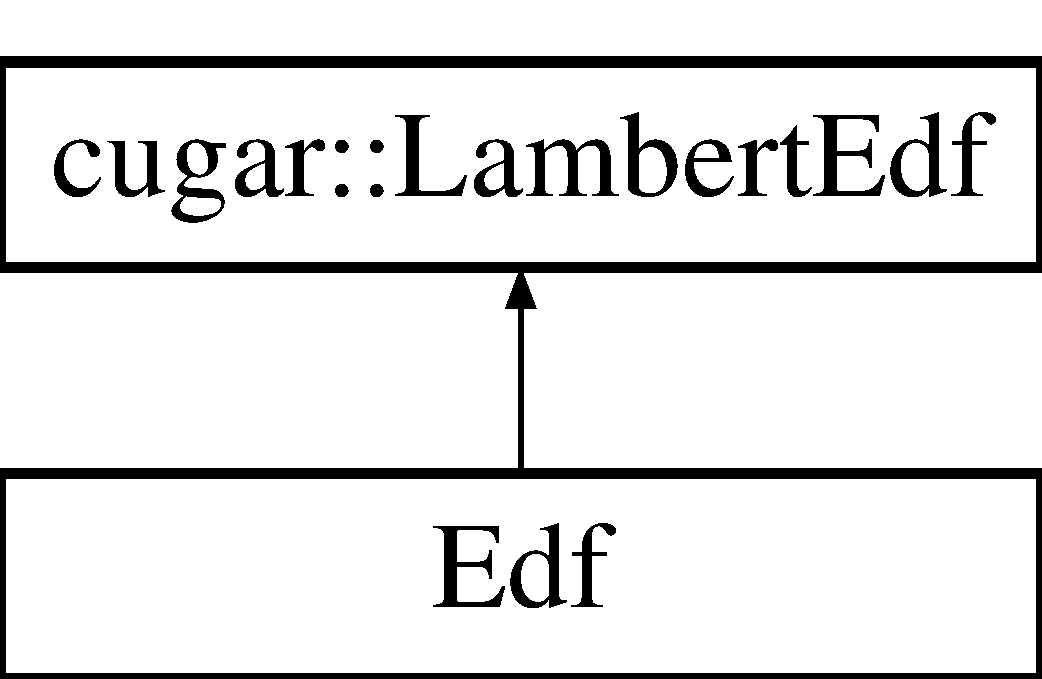
\includegraphics[height=2.000000cm]{structcugar_1_1_lambert_edf}
\end{center}
\end{figure}
\subsection*{Public Methods}
\begin{DoxyCompactItemize}
\item 
\mbox{\Hypertarget{structcugar_1_1_lambert_edf_aed8c1031d0470a4885de9e2d73d6b3a6}\label{structcugar_1_1_lambert_edf_aed8c1031d0470a4885de9e2d73d6b3a6}} 
C\+U\+G\+A\+R\+\_\+\+F\+O\+R\+C\+E\+I\+N\+L\+I\+NE C\+U\+G\+A\+R\+\_\+\+H\+O\+S\+T\+\_\+\+D\+E\+V\+I\+CE {\bfseries Lambert\+Edf} (const \hyperlink{structcugar_1_1_vector}{Vector3f} \+\_\+color)
\item 
C\+U\+G\+A\+R\+\_\+\+F\+O\+R\+C\+E\+I\+N\+L\+I\+NE C\+U\+G\+A\+R\+\_\+\+H\+O\+S\+T\+\_\+\+D\+E\+V\+I\+CE \hyperlink{structcugar_1_1_vector}{Vector3f} \hyperlink{structcugar_1_1_lambert_edf_aed2fed71aa6a7ad98e05714a0fd5f316}{f} (const \hyperlink{structcugar_1_1_differential_geometry}{Differential\+Geometry} \&geometry, const \hyperlink{structcugar_1_1_vector}{Vector3f} in, const \hyperlink{structcugar_1_1_vector}{Vector3f} out) const
\item 
C\+U\+G\+A\+R\+\_\+\+F\+O\+R\+C\+E\+I\+N\+L\+I\+NE C\+U\+G\+A\+R\+\_\+\+H\+O\+S\+T\+\_\+\+D\+E\+V\+I\+CE \hyperlink{structcugar_1_1_vector}{Vector3f} \hyperlink{structcugar_1_1_lambert_edf_a22dec6f632492c998702dc6f1f4c62c0}{f\+\_\+over\+\_\+p} (const \hyperlink{structcugar_1_1_differential_geometry}{Differential\+Geometry} \&geometry, const \hyperlink{structcugar_1_1_vector}{Vector3f} in, const \hyperlink{structcugar_1_1_vector}{Vector3f} out) const
\item 
C\+U\+G\+A\+R\+\_\+\+F\+O\+R\+C\+E\+I\+N\+L\+I\+NE C\+U\+G\+A\+R\+\_\+\+H\+O\+S\+T\+\_\+\+D\+E\+V\+I\+CE float \hyperlink{structcugar_1_1_lambert_edf_a388560f22fa74fe55678388ea0ae7f69}{p} (const \hyperlink{structcugar_1_1_differential_geometry}{Differential\+Geometry} \&geometry, const \hyperlink{structcugar_1_1_vector}{Vector3f} in, const \hyperlink{structcugar_1_1_vector}{Vector3f} out, const Spherical\+Measure measure=k\+Projected\+Solid\+Angle) const
\item 
C\+U\+G\+A\+R\+\_\+\+F\+O\+R\+C\+E\+I\+N\+L\+I\+NE C\+U\+G\+A\+R\+\_\+\+H\+O\+S\+T\+\_\+\+D\+E\+V\+I\+CE void \hyperlink{structcugar_1_1_lambert_edf_ae860824e138c2d39c17e2d8d7bac5557}{sample} (const \hyperlink{structcugar_1_1_vector}{Vector2f} u, const \hyperlink{structcugar_1_1_differential_geometry}{Differential\+Geometry} \&geometry, const \hyperlink{structcugar_1_1_vector}{Vector3f} in, \hyperlink{structcugar_1_1_vector}{Vector3f} \&out, \hyperlink{structcugar_1_1_vector}{Vector3f} \&g, float \&\hyperlink{structcugar_1_1_lambert_edf_a388560f22fa74fe55678388ea0ae7f69}{p}, float \&p\+\_\+proj) const
\item 
{\footnotesize template$<$typename Random\+GeneratorT $>$ }\\C\+U\+G\+A\+R\+\_\+\+F\+O\+R\+C\+E\+I\+N\+L\+I\+NE C\+U\+G\+A\+R\+\_\+\+H\+O\+S\+T\+\_\+\+D\+E\+V\+I\+CE bool \hyperlink{structcugar_1_1_lambert_edf_ae3d6b75902074a76f918a8d8d2bba24e}{invert} (const \hyperlink{structcugar_1_1_differential_geometry}{Differential\+Geometry} \&geometry, const \hyperlink{structcugar_1_1_vector}{Vector3f} V, const \hyperlink{structcugar_1_1_vector}{Vector3f} L, Random\+GeneratorT \&\hyperlink{group___sampling_module_gaec17bbbfd36295353081b7b4480d933d}{random}, \hyperlink{structcugar_1_1_vector}{Vector3f} \&z, float \&\hyperlink{structcugar_1_1_lambert_edf_a388560f22fa74fe55678388ea0ae7f69}{p}, float \&p\+\_\+proj) const
\item 
C\+U\+G\+A\+R\+\_\+\+F\+O\+R\+C\+E\+I\+N\+L\+I\+NE C\+U\+G\+A\+R\+\_\+\+H\+O\+S\+T\+\_\+\+D\+E\+V\+I\+CE void \hyperlink{structcugar_1_1_lambert_edf_acc3121156681c4433b1e85ae2de74605}{inverse\+\_\+pdf} (const \hyperlink{structcugar_1_1_differential_geometry}{Differential\+Geometry} \&geometry, const \hyperlink{structcugar_1_1_vector}{Vector3f} V, const \hyperlink{structcugar_1_1_vector}{Vector3f} L, const \hyperlink{structcugar_1_1_vector}{Vector3f} u, float \&\hyperlink{structcugar_1_1_lambert_edf_a388560f22fa74fe55678388ea0ae7f69}{p}, float \&p\+\_\+proj) const
\end{DoxyCompactItemize}
\subsection*{Public Members}
\begin{DoxyCompactItemize}
\item 
\mbox{\Hypertarget{structcugar_1_1_lambert_edf_a7b02006203dafed67b6ae7edb6293a66}\label{structcugar_1_1_lambert_edf_a7b02006203dafed67b6ae7edb6293a66}} 
\hyperlink{structcugar_1_1_vector}{Vector3f} {\bfseries color}
\end{DoxyCompactItemize}


\subsection{Member Function Documentation}
\mbox{\Hypertarget{structcugar_1_1_lambert_edf_aed2fed71aa6a7ad98e05714a0fd5f316}\label{structcugar_1_1_lambert_edf_aed2fed71aa6a7ad98e05714a0fd5f316}} 
\index{cugar\+::\+Lambert\+Edf@{cugar\+::\+Lambert\+Edf}!f@{f}}
\index{f@{f}!cugar\+::\+Lambert\+Edf@{cugar\+::\+Lambert\+Edf}}
\subsubsection{\texorpdfstring{f()}{f()}}
{\footnotesize\ttfamily C\+U\+G\+A\+R\+\_\+\+F\+O\+R\+C\+E\+I\+N\+L\+I\+NE C\+U\+G\+A\+R\+\_\+\+H\+O\+S\+T\+\_\+\+D\+E\+V\+I\+CE \hyperlink{structcugar_1_1_vector}{Vector3f} cugar\+::\+Lambert\+Edf\+::f (\begin{DoxyParamCaption}\item[{const \hyperlink{structcugar_1_1_differential_geometry}{Differential\+Geometry} \&}]{geometry,  }\item[{const \hyperlink{structcugar_1_1_vector}{Vector3f}}]{in,  }\item[{const \hyperlink{structcugar_1_1_vector}{Vector3f}}]{out }\end{DoxyParamCaption}) const\hspace{0.3cm}{\ttfamily [inline]}}

evaluate the E\+DF f(in,out) \mbox{\Hypertarget{structcugar_1_1_lambert_edf_a22dec6f632492c998702dc6f1f4c62c0}\label{structcugar_1_1_lambert_edf_a22dec6f632492c998702dc6f1f4c62c0}} 
\index{cugar\+::\+Lambert\+Edf@{cugar\+::\+Lambert\+Edf}!f\+\_\+over\+\_\+p@{f\+\_\+over\+\_\+p}}
\index{f\+\_\+over\+\_\+p@{f\+\_\+over\+\_\+p}!cugar\+::\+Lambert\+Edf@{cugar\+::\+Lambert\+Edf}}
\subsubsection{\texorpdfstring{f\+\_\+over\+\_\+p()}{f\_over\_p()}}
{\footnotesize\ttfamily C\+U\+G\+A\+R\+\_\+\+F\+O\+R\+C\+E\+I\+N\+L\+I\+NE C\+U\+G\+A\+R\+\_\+\+H\+O\+S\+T\+\_\+\+D\+E\+V\+I\+CE \hyperlink{structcugar_1_1_vector}{Vector3f} cugar\+::\+Lambert\+Edf\+::f\+\_\+over\+\_\+p (\begin{DoxyParamCaption}\item[{const \hyperlink{structcugar_1_1_differential_geometry}{Differential\+Geometry} \&}]{geometry,  }\item[{const \hyperlink{structcugar_1_1_vector}{Vector3f}}]{in,  }\item[{const \hyperlink{structcugar_1_1_vector}{Vector3f}}]{out }\end{DoxyParamCaption}) const\hspace{0.3cm}{\ttfamily [inline]}}

evaluate the E\+D\+F/pdf ratio f(in,out)/p(in,out) wrt projected solid angle \mbox{\Hypertarget{structcugar_1_1_lambert_edf_acc3121156681c4433b1e85ae2de74605}\label{structcugar_1_1_lambert_edf_acc3121156681c4433b1e85ae2de74605}} 
\index{cugar\+::\+Lambert\+Edf@{cugar\+::\+Lambert\+Edf}!inverse\+\_\+pdf@{inverse\+\_\+pdf}}
\index{inverse\+\_\+pdf@{inverse\+\_\+pdf}!cugar\+::\+Lambert\+Edf@{cugar\+::\+Lambert\+Edf}}
\subsubsection{\texorpdfstring{inverse\+\_\+pdf()}{inverse\_pdf()}}
{\footnotesize\ttfamily C\+U\+G\+A\+R\+\_\+\+F\+O\+R\+C\+E\+I\+N\+L\+I\+NE C\+U\+G\+A\+R\+\_\+\+H\+O\+S\+T\+\_\+\+D\+E\+V\+I\+CE void cugar\+::\+Lambert\+Edf\+::inverse\+\_\+pdf (\begin{DoxyParamCaption}\item[{const \hyperlink{structcugar_1_1_differential_geometry}{Differential\+Geometry} \&}]{geometry,  }\item[{const \hyperlink{structcugar_1_1_vector}{Vector3f}}]{V,  }\item[{const \hyperlink{structcugar_1_1_vector}{Vector3f}}]{L,  }\item[{const \hyperlink{structcugar_1_1_vector}{Vector3f}}]{u,  }\item[{float \&}]{p,  }\item[{float \&}]{p\+\_\+proj }\end{DoxyParamCaption}) const\hspace{0.3cm}{\ttfamily [inline]}}

given V and L and u, compute the probability of sampling u by inversion of V and L \mbox{\Hypertarget{structcugar_1_1_lambert_edf_ae3d6b75902074a76f918a8d8d2bba24e}\label{structcugar_1_1_lambert_edf_ae3d6b75902074a76f918a8d8d2bba24e}} 
\index{cugar\+::\+Lambert\+Edf@{cugar\+::\+Lambert\+Edf}!invert@{invert}}
\index{invert@{invert}!cugar\+::\+Lambert\+Edf@{cugar\+::\+Lambert\+Edf}}
\subsubsection{\texorpdfstring{invert()}{invert()}}
{\footnotesize\ttfamily template$<$typename Random\+GeneratorT $>$ \\
C\+U\+G\+A\+R\+\_\+\+F\+O\+R\+C\+E\+I\+N\+L\+I\+NE C\+U\+G\+A\+R\+\_\+\+H\+O\+S\+T\+\_\+\+D\+E\+V\+I\+CE bool cugar\+::\+Lambert\+Edf\+::invert (\begin{DoxyParamCaption}\item[{const \hyperlink{structcugar_1_1_differential_geometry}{Differential\+Geometry} \&}]{geometry,  }\item[{const \hyperlink{structcugar_1_1_vector}{Vector3f}}]{V,  }\item[{const \hyperlink{structcugar_1_1_vector}{Vector3f}}]{L,  }\item[{Random\+GeneratorT \&}]{random,  }\item[{\hyperlink{structcugar_1_1_vector}{Vector3f} \&}]{z,  }\item[{float \&}]{p,  }\item[{float \&}]{p\+\_\+proj }\end{DoxyParamCaption}) const\hspace{0.3cm}{\ttfamily [inline]}}

given V and L, invert the sampling functions used to generate L from V \mbox{\Hypertarget{structcugar_1_1_lambert_edf_a388560f22fa74fe55678388ea0ae7f69}\label{structcugar_1_1_lambert_edf_a388560f22fa74fe55678388ea0ae7f69}} 
\index{cugar\+::\+Lambert\+Edf@{cugar\+::\+Lambert\+Edf}!p@{p}}
\index{p@{p}!cugar\+::\+Lambert\+Edf@{cugar\+::\+Lambert\+Edf}}
\subsubsection{\texorpdfstring{p()}{p()}}
{\footnotesize\ttfamily C\+U\+G\+A\+R\+\_\+\+F\+O\+R\+C\+E\+I\+N\+L\+I\+NE C\+U\+G\+A\+R\+\_\+\+H\+O\+S\+T\+\_\+\+D\+E\+V\+I\+CE float cugar\+::\+Lambert\+Edf\+::p (\begin{DoxyParamCaption}\item[{const \hyperlink{structcugar_1_1_differential_geometry}{Differential\+Geometry} \&}]{geometry,  }\item[{const \hyperlink{structcugar_1_1_vector}{Vector3f}}]{in,  }\item[{const \hyperlink{structcugar_1_1_vector}{Vector3f}}]{out,  }\item[{const Spherical\+Measure}]{measure = {\ttfamily kProjectedSolidAngle} }\end{DoxyParamCaption}) const\hspace{0.3cm}{\ttfamily [inline]}}

evaluate the pdf of sampling L given V, p(L$\vert$V) = p(\+V,\+L) \mbox{\Hypertarget{structcugar_1_1_lambert_edf_ae860824e138c2d39c17e2d8d7bac5557}\label{structcugar_1_1_lambert_edf_ae860824e138c2d39c17e2d8d7bac5557}} 
\index{cugar\+::\+Lambert\+Edf@{cugar\+::\+Lambert\+Edf}!sample@{sample}}
\index{sample@{sample}!cugar\+::\+Lambert\+Edf@{cugar\+::\+Lambert\+Edf}}
\subsubsection{\texorpdfstring{sample()}{sample()}}
{\footnotesize\ttfamily C\+U\+G\+A\+R\+\_\+\+F\+O\+R\+C\+E\+I\+N\+L\+I\+NE C\+U\+G\+A\+R\+\_\+\+H\+O\+S\+T\+\_\+\+D\+E\+V\+I\+CE void cugar\+::\+Lambert\+Edf\+::sample (\begin{DoxyParamCaption}\item[{const \hyperlink{structcugar_1_1_vector}{Vector2f}}]{u,  }\item[{const \hyperlink{structcugar_1_1_differential_geometry}{Differential\+Geometry} \&}]{geometry,  }\item[{const \hyperlink{structcugar_1_1_vector}{Vector3f}}]{in,  }\item[{\hyperlink{structcugar_1_1_vector}{Vector3f} \&}]{out,  }\item[{\hyperlink{structcugar_1_1_vector}{Vector3f} \&}]{g,  }\item[{float \&}]{p,  }\item[{float \&}]{p\+\_\+proj }\end{DoxyParamCaption}) const\hspace{0.3cm}{\ttfamily [inline]}}

sample out given in and return both the pdf p and the value g = f/p, wrt projected solid angle 

The documentation for this struct was generated from the following file\+:\begin{DoxyCompactItemize}
\item 
C\+:/p4research/research/jpantaleoni/\+Fermat-\/\+Public/contrib/cugar/bsdf/lambert\+\_\+edf.\+h\end{DoxyCompactItemize}

\hypertarget{structcugar_1_1_lambert_trans_bsdf}{}\section{cugar\+:\+:Lambert\+Trans\+Bsdf Struct Reference}
\label{structcugar_1_1_lambert_trans_bsdf}\index{cugar\+::\+Lambert\+Trans\+Bsdf@{cugar\+::\+Lambert\+Trans\+Bsdf}}


\subsection{Detailed description}
Implements a Lambertian transmitter bsdf. 

{\ttfamily \#include $<$lambert\+\_\+trans.\+h$>$}

\subsection*{Public Methods}
\begin{DoxyCompactItemize}
\item 
\mbox{\Hypertarget{structcugar_1_1_lambert_trans_bsdf_a799322844ca4acaa6d3eec11dc6c6c6f}\label{structcugar_1_1_lambert_trans_bsdf_a799322844ca4acaa6d3eec11dc6c6c6f}} 
C\+U\+G\+A\+R\+\_\+\+F\+O\+R\+C\+E\+I\+N\+L\+I\+NE C\+U\+G\+A\+R\+\_\+\+H\+O\+S\+T\+\_\+\+D\+E\+V\+I\+CE {\bfseries Lambert\+Trans\+Bsdf} (const \hyperlink{structcugar_1_1_vector}{Vector3f} \+\_\+color)
\item 
C\+U\+G\+A\+R\+\_\+\+F\+O\+R\+C\+E\+I\+N\+L\+I\+NE C\+U\+G\+A\+R\+\_\+\+H\+O\+S\+T\+\_\+\+D\+E\+V\+I\+CE \hyperlink{structcugar_1_1_vector}{Vector3f} \hyperlink{structcugar_1_1_lambert_trans_bsdf_a7f82095f012a842727a09c85328b5652}{f} (const \hyperlink{structcugar_1_1_differential_geometry}{Differential\+Geometry} \&geometry, const \hyperlink{structcugar_1_1_vector}{Vector3f} V, const \hyperlink{structcugar_1_1_vector}{Vector3f} L) const
\item 
C\+U\+G\+A\+R\+\_\+\+F\+O\+R\+C\+E\+I\+N\+L\+I\+NE C\+U\+G\+A\+R\+\_\+\+H\+O\+S\+T\+\_\+\+D\+E\+V\+I\+CE \hyperlink{structcugar_1_1_vector}{Vector3f} \hyperlink{structcugar_1_1_lambert_trans_bsdf_a9f35ffaa833f4617f502850866a465d3}{f\+\_\+over\+\_\+p} (const \hyperlink{structcugar_1_1_differential_geometry}{Differential\+Geometry} \&geometry, const \hyperlink{structcugar_1_1_vector}{Vector3f} V, const \hyperlink{structcugar_1_1_vector}{Vector3f} L) const
\item 
C\+U\+G\+A\+R\+\_\+\+F\+O\+R\+C\+E\+I\+N\+L\+I\+NE C\+U\+G\+A\+R\+\_\+\+H\+O\+S\+T\+\_\+\+D\+E\+V\+I\+CE void \hyperlink{structcugar_1_1_lambert_trans_bsdf_a9eaf87fd3b0ab10ebbab683381ab9a6a}{f\+\_\+and\+\_\+p} (const \hyperlink{structcugar_1_1_differential_geometry}{Differential\+Geometry} \&geometry, const \hyperlink{structcugar_1_1_vector}{Vector3f} V, const \hyperlink{structcugar_1_1_vector}{Vector3f} L, \hyperlink{structcugar_1_1_vector}{Vector3f} \&\hyperlink{structcugar_1_1_lambert_trans_bsdf_a7f82095f012a842727a09c85328b5652}{f}, float \&\hyperlink{structcugar_1_1_lambert_trans_bsdf_a59f5cce268ebd048aa7d4d25c4686160}{p}, const Spherical\+Measure measure=k\+Projected\+Solid\+Angle) const
\item 
C\+U\+G\+A\+R\+\_\+\+F\+O\+R\+C\+E\+I\+N\+L\+I\+NE C\+U\+G\+A\+R\+\_\+\+H\+O\+S\+T\+\_\+\+D\+E\+V\+I\+CE float \hyperlink{structcugar_1_1_lambert_trans_bsdf_a59f5cce268ebd048aa7d4d25c4686160}{p} (const \hyperlink{structcugar_1_1_differential_geometry}{Differential\+Geometry} \&geometry, const \hyperlink{structcugar_1_1_vector}{Vector3f} V, const \hyperlink{structcugar_1_1_vector}{Vector3f} L, const Spherical\+Measure measure=k\+Projected\+Solid\+Angle) const
\item 
C\+U\+G\+A\+R\+\_\+\+F\+O\+R\+C\+E\+I\+N\+L\+I\+NE C\+U\+G\+A\+R\+\_\+\+H\+O\+S\+T\+\_\+\+D\+E\+V\+I\+CE void \hyperlink{structcugar_1_1_lambert_trans_bsdf_ace1257c24f360d54c2aaab0f024d6ab3}{sample} (const \hyperlink{structcugar_1_1_vector}{Vector3f} u, const \hyperlink{structcugar_1_1_differential_geometry}{Differential\+Geometry} \&geometry, const \hyperlink{structcugar_1_1_vector}{Vector3f} V, \hyperlink{structcugar_1_1_vector}{Vector3f} \&L, \hyperlink{structcugar_1_1_vector}{Vector3f} \&g, float \&\hyperlink{structcugar_1_1_lambert_trans_bsdf_a59f5cce268ebd048aa7d4d25c4686160}{p}, float \&p\+\_\+proj) const
\item 
{\footnotesize template$<$typename Random\+GeneratorT $>$ }\\C\+U\+G\+A\+R\+\_\+\+F\+O\+R\+C\+E\+I\+N\+L\+I\+NE C\+U\+G\+A\+R\+\_\+\+H\+O\+S\+T\+\_\+\+D\+E\+V\+I\+CE bool \hyperlink{structcugar_1_1_lambert_trans_bsdf_ae69d26a8dd4aeb0ac3174623c68fb77b}{invert} (const \hyperlink{structcugar_1_1_differential_geometry}{Differential\+Geometry} \&geometry, const \hyperlink{structcugar_1_1_vector}{Vector3f} V, const \hyperlink{structcugar_1_1_vector}{Vector3f} L, Random\+GeneratorT \&\hyperlink{group___sampling_module_gaec17bbbfd36295353081b7b4480d933d}{random}, \hyperlink{structcugar_1_1_vector}{Vector3f} \&z, float \&\hyperlink{structcugar_1_1_lambert_trans_bsdf_a59f5cce268ebd048aa7d4d25c4686160}{p}, float \&p\+\_\+proj) const
\item 
C\+U\+G\+A\+R\+\_\+\+F\+O\+R\+C\+E\+I\+N\+L\+I\+NE C\+U\+G\+A\+R\+\_\+\+H\+O\+S\+T\+\_\+\+D\+E\+V\+I\+CE void \hyperlink{structcugar_1_1_lambert_trans_bsdf_a1704b197c844a382cdde383214f58673}{inverse\+\_\+pdf} (const \hyperlink{structcugar_1_1_differential_geometry}{Differential\+Geometry} \&geometry, const \hyperlink{structcugar_1_1_vector}{Vector3f} V, const \hyperlink{structcugar_1_1_vector}{Vector3f} L, const \hyperlink{structcugar_1_1_vector}{Vector3f} u, float \&\hyperlink{structcugar_1_1_lambert_trans_bsdf_a59f5cce268ebd048aa7d4d25c4686160}{p}, float \&p\+\_\+proj) const
\end{DoxyCompactItemize}
\subsection*{Public Members}
\begin{DoxyCompactItemize}
\item 
\mbox{\Hypertarget{structcugar_1_1_lambert_trans_bsdf_a3e964c6891e0f1348e88055703e6f8c1}\label{structcugar_1_1_lambert_trans_bsdf_a3e964c6891e0f1348e88055703e6f8c1}} 
\hyperlink{structcugar_1_1_vector}{Vector3f} {\bfseries color}
\end{DoxyCompactItemize}


\subsection{Member Function Documentation}
\mbox{\Hypertarget{structcugar_1_1_lambert_trans_bsdf_a7f82095f012a842727a09c85328b5652}\label{structcugar_1_1_lambert_trans_bsdf_a7f82095f012a842727a09c85328b5652}} 
\index{cugar\+::\+Lambert\+Trans\+Bsdf@{cugar\+::\+Lambert\+Trans\+Bsdf}!f@{f}}
\index{f@{f}!cugar\+::\+Lambert\+Trans\+Bsdf@{cugar\+::\+Lambert\+Trans\+Bsdf}}
\subsubsection{\texorpdfstring{f()}{f()}}
{\footnotesize\ttfamily C\+U\+G\+A\+R\+\_\+\+F\+O\+R\+C\+E\+I\+N\+L\+I\+NE C\+U\+G\+A\+R\+\_\+\+H\+O\+S\+T\+\_\+\+D\+E\+V\+I\+CE \hyperlink{structcugar_1_1_vector}{Vector3f} cugar\+::\+Lambert\+Trans\+Bsdf\+::f (\begin{DoxyParamCaption}\item[{const \hyperlink{structcugar_1_1_differential_geometry}{Differential\+Geometry} \&}]{geometry,  }\item[{const \hyperlink{structcugar_1_1_vector}{Vector3f}}]{V,  }\item[{const \hyperlink{structcugar_1_1_vector}{Vector3f}}]{L }\end{DoxyParamCaption}) const\hspace{0.3cm}{\ttfamily [inline]}}

evaluate the B\+R\+DF f(\+V,\+L) \mbox{\Hypertarget{structcugar_1_1_lambert_trans_bsdf_a9eaf87fd3b0ab10ebbab683381ab9a6a}\label{structcugar_1_1_lambert_trans_bsdf_a9eaf87fd3b0ab10ebbab683381ab9a6a}} 
\index{cugar\+::\+Lambert\+Trans\+Bsdf@{cugar\+::\+Lambert\+Trans\+Bsdf}!f\+\_\+and\+\_\+p@{f\+\_\+and\+\_\+p}}
\index{f\+\_\+and\+\_\+p@{f\+\_\+and\+\_\+p}!cugar\+::\+Lambert\+Trans\+Bsdf@{cugar\+::\+Lambert\+Trans\+Bsdf}}
\subsubsection{\texorpdfstring{f\+\_\+and\+\_\+p()}{f\_and\_p()}}
{\footnotesize\ttfamily C\+U\+G\+A\+R\+\_\+\+F\+O\+R\+C\+E\+I\+N\+L\+I\+NE C\+U\+G\+A\+R\+\_\+\+H\+O\+S\+T\+\_\+\+D\+E\+V\+I\+CE void cugar\+::\+Lambert\+Trans\+Bsdf\+::f\+\_\+and\+\_\+p (\begin{DoxyParamCaption}\item[{const \hyperlink{structcugar_1_1_differential_geometry}{Differential\+Geometry} \&}]{geometry,  }\item[{const \hyperlink{structcugar_1_1_vector}{Vector3f}}]{V,  }\item[{const \hyperlink{structcugar_1_1_vector}{Vector3f}}]{L,  }\item[{\hyperlink{structcugar_1_1_vector}{Vector3f} \&}]{f,  }\item[{float \&}]{p,  }\item[{const Spherical\+Measure}]{measure = {\ttfamily kProjectedSolidAngle} }\end{DoxyParamCaption}) const\hspace{0.3cm}{\ttfamily [inline]}}

evaluate the B\+R\+DF and the pdf in a single call \mbox{\Hypertarget{structcugar_1_1_lambert_trans_bsdf_a9f35ffaa833f4617f502850866a465d3}\label{structcugar_1_1_lambert_trans_bsdf_a9f35ffaa833f4617f502850866a465d3}} 
\index{cugar\+::\+Lambert\+Trans\+Bsdf@{cugar\+::\+Lambert\+Trans\+Bsdf}!f\+\_\+over\+\_\+p@{f\+\_\+over\+\_\+p}}
\index{f\+\_\+over\+\_\+p@{f\+\_\+over\+\_\+p}!cugar\+::\+Lambert\+Trans\+Bsdf@{cugar\+::\+Lambert\+Trans\+Bsdf}}
\subsubsection{\texorpdfstring{f\+\_\+over\+\_\+p()}{f\_over\_p()}}
{\footnotesize\ttfamily C\+U\+G\+A\+R\+\_\+\+F\+O\+R\+C\+E\+I\+N\+L\+I\+NE C\+U\+G\+A\+R\+\_\+\+H\+O\+S\+T\+\_\+\+D\+E\+V\+I\+CE \hyperlink{structcugar_1_1_vector}{Vector3f} cugar\+::\+Lambert\+Trans\+Bsdf\+::f\+\_\+over\+\_\+p (\begin{DoxyParamCaption}\item[{const \hyperlink{structcugar_1_1_differential_geometry}{Differential\+Geometry} \&}]{geometry,  }\item[{const \hyperlink{structcugar_1_1_vector}{Vector3f}}]{V,  }\item[{const \hyperlink{structcugar_1_1_vector}{Vector3f}}]{L }\end{DoxyParamCaption}) const\hspace{0.3cm}{\ttfamily [inline]}}

evaluate the B\+R\+D\+F/pdf ratio f(\+V,\+L)/p(V,L) wrt projected solid angle \mbox{\Hypertarget{structcugar_1_1_lambert_trans_bsdf_a1704b197c844a382cdde383214f58673}\label{structcugar_1_1_lambert_trans_bsdf_a1704b197c844a382cdde383214f58673}} 
\index{cugar\+::\+Lambert\+Trans\+Bsdf@{cugar\+::\+Lambert\+Trans\+Bsdf}!inverse\+\_\+pdf@{inverse\+\_\+pdf}}
\index{inverse\+\_\+pdf@{inverse\+\_\+pdf}!cugar\+::\+Lambert\+Trans\+Bsdf@{cugar\+::\+Lambert\+Trans\+Bsdf}}
\subsubsection{\texorpdfstring{inverse\+\_\+pdf()}{inverse\_pdf()}}
{\footnotesize\ttfamily C\+U\+G\+A\+R\+\_\+\+F\+O\+R\+C\+E\+I\+N\+L\+I\+NE C\+U\+G\+A\+R\+\_\+\+H\+O\+S\+T\+\_\+\+D\+E\+V\+I\+CE void cugar\+::\+Lambert\+Trans\+Bsdf\+::inverse\+\_\+pdf (\begin{DoxyParamCaption}\item[{const \hyperlink{structcugar_1_1_differential_geometry}{Differential\+Geometry} \&}]{geometry,  }\item[{const \hyperlink{structcugar_1_1_vector}{Vector3f}}]{V,  }\item[{const \hyperlink{structcugar_1_1_vector}{Vector3f}}]{L,  }\item[{const \hyperlink{structcugar_1_1_vector}{Vector3f}}]{u,  }\item[{float \&}]{p,  }\item[{float \&}]{p\+\_\+proj }\end{DoxyParamCaption}) const\hspace{0.3cm}{\ttfamily [inline]}}

given V and L and u, compute the probability of sampling u by inversion of V and L \mbox{\Hypertarget{structcugar_1_1_lambert_trans_bsdf_ae69d26a8dd4aeb0ac3174623c68fb77b}\label{structcugar_1_1_lambert_trans_bsdf_ae69d26a8dd4aeb0ac3174623c68fb77b}} 
\index{cugar\+::\+Lambert\+Trans\+Bsdf@{cugar\+::\+Lambert\+Trans\+Bsdf}!invert@{invert}}
\index{invert@{invert}!cugar\+::\+Lambert\+Trans\+Bsdf@{cugar\+::\+Lambert\+Trans\+Bsdf}}
\subsubsection{\texorpdfstring{invert()}{invert()}}
{\footnotesize\ttfamily template$<$typename Random\+GeneratorT $>$ \\
C\+U\+G\+A\+R\+\_\+\+F\+O\+R\+C\+E\+I\+N\+L\+I\+NE C\+U\+G\+A\+R\+\_\+\+H\+O\+S\+T\+\_\+\+D\+E\+V\+I\+CE bool cugar\+::\+Lambert\+Trans\+Bsdf\+::invert (\begin{DoxyParamCaption}\item[{const \hyperlink{structcugar_1_1_differential_geometry}{Differential\+Geometry} \&}]{geometry,  }\item[{const \hyperlink{structcugar_1_1_vector}{Vector3f}}]{V,  }\item[{const \hyperlink{structcugar_1_1_vector}{Vector3f}}]{L,  }\item[{Random\+GeneratorT \&}]{random,  }\item[{\hyperlink{structcugar_1_1_vector}{Vector3f} \&}]{z,  }\item[{float \&}]{p,  }\item[{float \&}]{p\+\_\+proj }\end{DoxyParamCaption}) const\hspace{0.3cm}{\ttfamily [inline]}}

given V and L, invert the sampling functions used to generate L from V \mbox{\Hypertarget{structcugar_1_1_lambert_trans_bsdf_a59f5cce268ebd048aa7d4d25c4686160}\label{structcugar_1_1_lambert_trans_bsdf_a59f5cce268ebd048aa7d4d25c4686160}} 
\index{cugar\+::\+Lambert\+Trans\+Bsdf@{cugar\+::\+Lambert\+Trans\+Bsdf}!p@{p}}
\index{p@{p}!cugar\+::\+Lambert\+Trans\+Bsdf@{cugar\+::\+Lambert\+Trans\+Bsdf}}
\subsubsection{\texorpdfstring{p()}{p()}}
{\footnotesize\ttfamily C\+U\+G\+A\+R\+\_\+\+F\+O\+R\+C\+E\+I\+N\+L\+I\+NE C\+U\+G\+A\+R\+\_\+\+H\+O\+S\+T\+\_\+\+D\+E\+V\+I\+CE float cugar\+::\+Lambert\+Trans\+Bsdf\+::p (\begin{DoxyParamCaption}\item[{const \hyperlink{structcugar_1_1_differential_geometry}{Differential\+Geometry} \&}]{geometry,  }\item[{const \hyperlink{structcugar_1_1_vector}{Vector3f}}]{V,  }\item[{const \hyperlink{structcugar_1_1_vector}{Vector3f}}]{L,  }\item[{const Spherical\+Measure}]{measure = {\ttfamily kProjectedSolidAngle} }\end{DoxyParamCaption}) const\hspace{0.3cm}{\ttfamily [inline]}}

evaluate the pdf of sampling L given V, p(L$\vert$V) = p(\+V,\+L) \mbox{\Hypertarget{structcugar_1_1_lambert_trans_bsdf_ace1257c24f360d54c2aaab0f024d6ab3}\label{structcugar_1_1_lambert_trans_bsdf_ace1257c24f360d54c2aaab0f024d6ab3}} 
\index{cugar\+::\+Lambert\+Trans\+Bsdf@{cugar\+::\+Lambert\+Trans\+Bsdf}!sample@{sample}}
\index{sample@{sample}!cugar\+::\+Lambert\+Trans\+Bsdf@{cugar\+::\+Lambert\+Trans\+Bsdf}}
\subsubsection{\texorpdfstring{sample()}{sample()}}
{\footnotesize\ttfamily C\+U\+G\+A\+R\+\_\+\+F\+O\+R\+C\+E\+I\+N\+L\+I\+NE C\+U\+G\+A\+R\+\_\+\+H\+O\+S\+T\+\_\+\+D\+E\+V\+I\+CE void cugar\+::\+Lambert\+Trans\+Bsdf\+::sample (\begin{DoxyParamCaption}\item[{const \hyperlink{structcugar_1_1_vector}{Vector3f}}]{u,  }\item[{const \hyperlink{structcugar_1_1_differential_geometry}{Differential\+Geometry} \&}]{geometry,  }\item[{const \hyperlink{structcugar_1_1_vector}{Vector3f}}]{V,  }\item[{\hyperlink{structcugar_1_1_vector}{Vector3f} \&}]{L,  }\item[{\hyperlink{structcugar_1_1_vector}{Vector3f} \&}]{g,  }\item[{float \&}]{p,  }\item[{float \&}]{p\+\_\+proj }\end{DoxyParamCaption}) const\hspace{0.3cm}{\ttfamily [inline]}}

sample L given V and return both the pdf p and the value g = f/p, wrt projected solid angle 

The documentation for this struct was generated from the following file\+:\begin{DoxyCompactItemize}
\item 
C\+:/p4research/research/jpantaleoni/\+Fermat-\/\+Public/contrib/cugar/bsdf/lambert\+\_\+trans.\+h\end{DoxyCompactItemize}

\hypertarget{structcugar_1_1cuda_1_1_l_b_v_h__builder}{}\section{cugar\+:\+:cuda\+:\+:L\+B\+V\+H\+\_\+builder$<$ integer, bvh\+\_\+node\+\_\+type, node\+\_\+vector, range\+\_\+vector, index\+\_\+vector $>$ Struct Template Reference}
\label{structcugar_1_1cuda_1_1_l_b_v_h__builder}\index{cugar\+::cuda\+::\+L\+B\+V\+H\+\_\+builder$<$ integer, bvh\+\_\+node\+\_\+type, node\+\_\+vector, range\+\_\+vector, index\+\_\+vector $>$@{cugar\+::cuda\+::\+L\+B\+V\+H\+\_\+builder$<$ integer, bvh\+\_\+node\+\_\+type, node\+\_\+vector, range\+\_\+vector, index\+\_\+vector $>$}}


\subsection{Detailed description}
\subsubsection*{template$<$typename integer, typename bvh\+\_\+node\+\_\+type = Bvh\+\_\+node, typename node\+\_\+vector = vector$<$device\+\_\+tag,bvh\+\_\+node\+\_\+type$>$, typename range\+\_\+vector = vector$<$device\+\_\+tag,uint2$>$, typename index\+\_\+vector = vector$<$device\+\_\+tag,uint32$>$$>$\newline
struct cugar\+::cuda\+::\+L\+B\+V\+H\+\_\+builder$<$ integer, bvh\+\_\+node\+\_\+type, node\+\_\+vector, range\+\_\+vector, index\+\_\+vector $>$}

G\+P\+U-\/based Linear B\+VH builder

This class provides the context to generate L\+B\+V\+Hs on the G\+PU starting from a set of unordered points. The output is a set of nodes with the corresponding leaves and a set of primitive indices into the input set of points. The output leaves will specify contiguous ranges into this index.


\begin{DoxyTemplParams}{Template Parameters}
{\em integer} & an integer type that determines the number of bits used to compute the points\textquotesingle{} Morton codes. Accepted values are uint32 and uint64.\\
\hline
\end{DoxyTemplParams}
The following code snippet shows how to use this builder\+:


\begin{DoxyCode}
\textcolor{preprocessor}{#include <\hyperlink{lbvh__builder_8h}{cugar/bvh/cuda/lbvh\_builder.h}>}

thrust::device\_vector<Vector3f> points;
... \textcolor{comment}{// code to fill the input vector of points}

thrust::device\_vector<Bvh\_node> bvh\_nodes;
thrust::device\_vector<uint32>   bvh\_index;

\hyperlink{structcugar_1_1cuda_1_1_l_b_v_h__builder}{cugar::cuda::LBVH\_builder<uint64>} builder( &bvh\_nodes, &bvh\_index );
builder.build(
    Bbox3f( Vector3f(0.0f), Vector3f(1.0f) ),   \textcolor{comment}{// suppose all bboxes are in [0,1]^3}
    points.begin(),                             \textcolor{comment}{// begin iterator}
    points.end(),                               \textcolor{comment}{// end iterator}
    4 );                                        \textcolor{comment}{// target 4 objects per leaf}
\end{DoxyCode}
 

{\ttfamily \#include $<$lbvh\+\_\+builder.\+h$>$}

\subsection*{Public Types}
\begin{DoxyCompactItemize}
\item 
\mbox{\Hypertarget{structcugar_1_1cuda_1_1_l_b_v_h__builder_aa77f410c55c8e76a68b38b1a7ab8b61c}\label{structcugar_1_1cuda_1_1_l_b_v_h__builder_aa77f410c55c8e76a68b38b1a7ab8b61c}} 
typedef \hyperlink{structcugar_1_1cuda_1_1_l_b_v_h__builder__stats}{L\+B\+V\+H\+\_\+builder\+\_\+stats} {\bfseries Stats}
\end{DoxyCompactItemize}
\subsection*{Public Methods}
\begin{DoxyCompactItemize}
\item 
\hyperlink{structcugar_1_1cuda_1_1_l_b_v_h__builder_ad2cafc8f7671ebbef3de1abeef7fa766}{L\+B\+V\+H\+\_\+builder} (node\+\_\+vector $\ast$nodes=N\+U\+LL, index\+\_\+vector $\ast$index=N\+U\+LL, range\+\_\+vector $\ast$leaf\+\_\+ranges=N\+U\+LL, index\+\_\+vector $\ast$leaf\+\_\+pointers=N\+U\+LL, index\+\_\+vector $\ast$parents=N\+U\+LL, index\+\_\+vector $\ast$skip\+\_\+nodes=N\+U\+LL, range\+\_\+vector $\ast$node\+\_\+ranges=N\+U\+LL)
\item 
\mbox{\Hypertarget{structcugar_1_1cuda_1_1_l_b_v_h__builder_aa6cc3f6681a0f8b2d0b8f901ea2b59f3}\label{structcugar_1_1cuda_1_1_l_b_v_h__builder_aa6cc3f6681a0f8b2d0b8f901ea2b59f3}} 
void {\bfseries set\+\_\+nodes} (node\+\_\+vector $\ast$nodes)
\item 
\mbox{\Hypertarget{structcugar_1_1cuda_1_1_l_b_v_h__builder_a4c3f8a21e560d6080976832b893d3be1}\label{structcugar_1_1cuda_1_1_l_b_v_h__builder_a4c3f8a21e560d6080976832b893d3be1}} 
void {\bfseries set\+\_\+index} (index\+\_\+vector $\ast$index)
\item 
\mbox{\Hypertarget{structcugar_1_1cuda_1_1_l_b_v_h__builder_a11c97b820d063fabf9ba1f3118c44c49}\label{structcugar_1_1cuda_1_1_l_b_v_h__builder_a11c97b820d063fabf9ba1f3118c44c49}} 
void {\bfseries set\+\_\+parents} (index\+\_\+vector $\ast$parents)
\item 
\mbox{\Hypertarget{structcugar_1_1cuda_1_1_l_b_v_h__builder_a43352b876b36408051b2cc2d05f1fb7d}\label{structcugar_1_1cuda_1_1_l_b_v_h__builder_a43352b876b36408051b2cc2d05f1fb7d}} 
void {\bfseries set\+\_\+skip\+\_\+nodes} (index\+\_\+vector $\ast$skip\+\_\+nodes)
\item 
\mbox{\Hypertarget{structcugar_1_1cuda_1_1_l_b_v_h__builder_a27167dc98d5d8933e42f8eca0663ce32}\label{structcugar_1_1cuda_1_1_l_b_v_h__builder_a27167dc98d5d8933e42f8eca0663ce32}} 
void {\bfseries set\+\_\+leaf\+\_\+pointers} (index\+\_\+vector $\ast$leaf\+\_\+pointers)
\item 
\mbox{\Hypertarget{structcugar_1_1cuda_1_1_l_b_v_h__builder_ab75c51d1c806ddba42bbc2bf995541d3}\label{structcugar_1_1cuda_1_1_l_b_v_h__builder_ab75c51d1c806ddba42bbc2bf995541d3}} 
void {\bfseries set\+\_\+leaf\+\_\+ranges} (range\+\_\+vector $\ast$leaf\+\_\+ranges)
\item 
\mbox{\Hypertarget{structcugar_1_1cuda_1_1_l_b_v_h__builder_af0af9e90fb42ee2979cb11ec22542e1e}\label{structcugar_1_1cuda_1_1_l_b_v_h__builder_af0af9e90fb42ee2979cb11ec22542e1e}} 
void {\bfseries set\+\_\+node\+\_\+ranges} (range\+\_\+vector $\ast$node\+\_\+ranges)
\item 
{\footnotesize template$<$typename Iterator $>$ }\\void \hyperlink{structcugar_1_1cuda_1_1_l_b_v_h__builder_ab39b2be673c43e12283c25800f22d5b1}{build} (const \hyperlink{structcugar_1_1_bbox}{Bbox3f} bbox, const Iterator points\+\_\+begin, const Iterator points\+\_\+end, const uint32 max\+\_\+leaf\+\_\+size, \hyperlink{structcugar_1_1cuda_1_1_l_b_v_h__builder__stats}{Stats} $\ast$stats=N\+U\+LL)
\end{DoxyCompactItemize}
\subsection*{Public Members}
\begin{DoxyCompactItemize}
\item 
\mbox{\Hypertarget{structcugar_1_1cuda_1_1_l_b_v_h__builder_a948ce9c517f4c9808ec1bfba5c6b07fc}\label{structcugar_1_1cuda_1_1_l_b_v_h__builder_a948ce9c517f4c9808ec1bfba5c6b07fc}} 
node\+\_\+vector $\ast$ {\bfseries m\+\_\+nodes}
\item 
\mbox{\Hypertarget{structcugar_1_1cuda_1_1_l_b_v_h__builder_afa8bf8d86713360be6f6af0d97905e56}\label{structcugar_1_1cuda_1_1_l_b_v_h__builder_afa8bf8d86713360be6f6af0d97905e56}} 
range\+\_\+vector $\ast$ {\bfseries m\+\_\+node\+\_\+ranges}
\item 
\mbox{\Hypertarget{structcugar_1_1cuda_1_1_l_b_v_h__builder_ae5f8095b418252982c45ec5daae37865}\label{structcugar_1_1cuda_1_1_l_b_v_h__builder_ae5f8095b418252982c45ec5daae37865}} 
range\+\_\+vector $\ast$ {\bfseries m\+\_\+leaf\+\_\+ranges}
\item 
\mbox{\Hypertarget{structcugar_1_1cuda_1_1_l_b_v_h__builder_ae7d4352019b89335dd918c1f54a86000}\label{structcugar_1_1cuda_1_1_l_b_v_h__builder_ae7d4352019b89335dd918c1f54a86000}} 
index\+\_\+vector $\ast$ {\bfseries m\+\_\+leaf\+\_\+pointers}
\item 
\mbox{\Hypertarget{structcugar_1_1cuda_1_1_l_b_v_h__builder_ad97bb4a51bc462d3d68cb55bd40ae612}\label{structcugar_1_1cuda_1_1_l_b_v_h__builder_ad97bb4a51bc462d3d68cb55bd40ae612}} 
index\+\_\+vector $\ast$ {\bfseries m\+\_\+parents}
\item 
\mbox{\Hypertarget{structcugar_1_1cuda_1_1_l_b_v_h__builder_ab10e91221af38e8c59565c422c2d41f1}\label{structcugar_1_1cuda_1_1_l_b_v_h__builder_ab10e91221af38e8c59565c422c2d41f1}} 
index\+\_\+vector $\ast$ {\bfseries m\+\_\+skip\+\_\+nodes}
\item 
\mbox{\Hypertarget{structcugar_1_1cuda_1_1_l_b_v_h__builder_a3c519a9c4451dd5f36ae57c95b5313a8}\label{structcugar_1_1cuda_1_1_l_b_v_h__builder_a3c519a9c4451dd5f36ae57c95b5313a8}} 
index\+\_\+vector $\ast$ {\bfseries m\+\_\+index}
\item 
\mbox{\Hypertarget{structcugar_1_1cuda_1_1_l_b_v_h__builder_ae1c5e80ec751b75ea09b8caca5f5cf1e}\label{structcugar_1_1cuda_1_1_l_b_v_h__builder_ae1c5e80ec751b75ea09b8caca5f5cf1e}} 
\hyperlink{structcugar_1_1caching__device__vector}{caching\+\_\+device\+\_\+vector}$<$ integer $>$ {\bfseries m\+\_\+codes}
\item 
\mbox{\Hypertarget{structcugar_1_1cuda_1_1_l_b_v_h__builder_ae8fe2378cc2bb077bba1d99e37654c7d}\label{structcugar_1_1cuda_1_1_l_b_v_h__builder_ae8fe2378cc2bb077bba1d99e37654c7d}} 
\hyperlink{structcugar_1_1caching__device__vector}{caching\+\_\+device\+\_\+vector}$<$ integer $>$ {\bfseries m\+\_\+temp\+\_\+codes}
\item 
\mbox{\Hypertarget{structcugar_1_1cuda_1_1_l_b_v_h__builder_a27d88ae14040cf89f954d5f522fdd5f8}\label{structcugar_1_1cuda_1_1_l_b_v_h__builder_a27d88ae14040cf89f954d5f522fdd5f8}} 
\hyperlink{structcugar_1_1caching__device__vector}{caching\+\_\+device\+\_\+vector}$<$ uint32 $>$ {\bfseries m\+\_\+temp\+\_\+index}
\item 
\mbox{\Hypertarget{structcugar_1_1cuda_1_1_l_b_v_h__builder_add5c2e6c44d45b6358f66d92b506bd11}\label{structcugar_1_1cuda_1_1_l_b_v_h__builder_add5c2e6c44d45b6358f66d92b506bd11}} 
\hyperlink{structcugar_1_1_bbox}{Bbox3f} {\bfseries m\+\_\+bbox}
\item 
\mbox{\Hypertarget{structcugar_1_1cuda_1_1_l_b_v_h__builder_a2f092a6d3a49a450f0e57c48e71ee1df}\label{structcugar_1_1cuda_1_1_l_b_v_h__builder_a2f092a6d3a49a450f0e57c48e71ee1df}} 
uint32 {\bfseries m\+\_\+node\+\_\+count}
\item 
\mbox{\Hypertarget{structcugar_1_1cuda_1_1_l_b_v_h__builder_ae45d5655734f95b79d7b02cf96b8a28d}\label{structcugar_1_1cuda_1_1_l_b_v_h__builder_ae45d5655734f95b79d7b02cf96b8a28d}} 
uint32 {\bfseries m\+\_\+leaf\+\_\+count}
\item 
\mbox{\Hypertarget{structcugar_1_1cuda_1_1_l_b_v_h__builder_a9379b12f1846a39568c2041b7a3492fe}\label{structcugar_1_1cuda_1_1_l_b_v_h__builder_a9379b12f1846a39568c2041b7a3492fe}} 
\hyperlink{structcugar_1_1cuda_1_1_radixtree__context}{cuda\+::\+Radixtree\+\_\+context} {\bfseries m\+\_\+kd\+\_\+context}
\end{DoxyCompactItemize}


\subsection{Constructor \& Destructor Documentation}
\mbox{\Hypertarget{structcugar_1_1cuda_1_1_l_b_v_h__builder_ad2cafc8f7671ebbef3de1abeef7fa766}\label{structcugar_1_1cuda_1_1_l_b_v_h__builder_ad2cafc8f7671ebbef3de1abeef7fa766}} 
\index{cugar\+::cuda\+::\+L\+B\+V\+H\+\_\+builder@{cugar\+::cuda\+::\+L\+B\+V\+H\+\_\+builder}!L\+B\+V\+H\+\_\+builder@{L\+B\+V\+H\+\_\+builder}}
\index{L\+B\+V\+H\+\_\+builder@{L\+B\+V\+H\+\_\+builder}!cugar\+::cuda\+::\+L\+B\+V\+H\+\_\+builder@{cugar\+::cuda\+::\+L\+B\+V\+H\+\_\+builder}}
\subsubsection{\texorpdfstring{L\+B\+V\+H\+\_\+builder()}{LBVH\_builder()}}
{\footnotesize\ttfamily template$<$typename integer, typename bvh\+\_\+node\+\_\+type = Bvh\+\_\+node, typename node\+\_\+vector = vector$<$device\+\_\+tag,bvh\+\_\+node\+\_\+type$>$, typename range\+\_\+vector = vector$<$device\+\_\+tag,uint2$>$, typename index\+\_\+vector = vector$<$device\+\_\+tag,uint32$>$$>$ \\
\hyperlink{structcugar_1_1cuda_1_1_l_b_v_h__builder}{cugar\+::cuda\+::\+L\+B\+V\+H\+\_\+builder}$<$ integer, bvh\+\_\+node\+\_\+type, node\+\_\+vector, range\+\_\+vector, index\+\_\+vector $>$\+::\hyperlink{structcugar_1_1cuda_1_1_l_b_v_h__builder}{L\+B\+V\+H\+\_\+builder} (\begin{DoxyParamCaption}\item[{node\+\_\+vector $\ast$}]{nodes = {\ttfamily NULL},  }\item[{index\+\_\+vector $\ast$}]{index = {\ttfamily NULL},  }\item[{range\+\_\+vector $\ast$}]{leaf\+\_\+ranges = {\ttfamily NULL},  }\item[{index\+\_\+vector $\ast$}]{leaf\+\_\+pointers = {\ttfamily NULL},  }\item[{index\+\_\+vector $\ast$}]{parents = {\ttfamily NULL},  }\item[{index\+\_\+vector $\ast$}]{skip\+\_\+nodes = {\ttfamily NULL},  }\item[{range\+\_\+vector $\ast$}]{node\+\_\+ranges = {\ttfamily NULL} }\end{DoxyParamCaption})\hspace{0.3cm}{\ttfamily [inline]}}

constructor


\begin{DoxyParams}{Parameters}
{\em nodes} & output nodes array \\
\hline
{\em leaves} & output leaf array \\
\hline
{\em index} & output index array \\
\hline
\end{DoxyParams}


\subsection{Member Function Documentation}
\mbox{\Hypertarget{structcugar_1_1cuda_1_1_l_b_v_h__builder_ab39b2be673c43e12283c25800f22d5b1}\label{structcugar_1_1cuda_1_1_l_b_v_h__builder_ab39b2be673c43e12283c25800f22d5b1}} 
\index{cugar\+::cuda\+::\+L\+B\+V\+H\+\_\+builder@{cugar\+::cuda\+::\+L\+B\+V\+H\+\_\+builder}!build@{build}}
\index{build@{build}!cugar\+::cuda\+::\+L\+B\+V\+H\+\_\+builder@{cugar\+::cuda\+::\+L\+B\+V\+H\+\_\+builder}}
\subsubsection{\texorpdfstring{build()}{build()}}
{\footnotesize\ttfamily template$<$typename integer , typename bvh\+\_\+node\+\_\+type , typename node\+\_\+vector , typename range\+\_\+vector , typename index\+\_\+vector $>$ \\
template$<$typename Iterator $>$ \\
void \hyperlink{structcugar_1_1cuda_1_1_l_b_v_h__builder}{cugar\+::cuda\+::\+L\+B\+V\+H\+\_\+builder}$<$ integer, bvh\+\_\+node\+\_\+type, node\+\_\+vector, range\+\_\+vector, index\+\_\+vector $>$\+::build (\begin{DoxyParamCaption}\item[{const \hyperlink{structcugar_1_1_bbox}{Bbox3f}}]{bbox,  }\item[{const Iterator}]{points\+\_\+begin,  }\item[{const Iterator}]{points\+\_\+end,  }\item[{const uint32}]{max\+\_\+leaf\+\_\+size,  }\item[{\hyperlink{structcugar_1_1cuda_1_1_l_b_v_h__builder__stats}{Stats} $\ast$}]{stats = {\ttfamily NULL} }\end{DoxyParamCaption})}

build a bvh given a set of points that will be reordered in-\/place


\begin{DoxyParams}{Parameters}
{\em bbox} & global bbox \\
\hline
{\em points\+\_\+begin} & beginning of the point sequence to sort \\
\hline
{\em points\+\_\+end} & end of the point sequence to sort \\
\hline
{\em max\+\_\+leaf\+\_\+size} & maximum leaf size \\
\hline
\end{DoxyParams}


The documentation for this struct was generated from the following files\+:\begin{DoxyCompactItemize}
\item 
C\+:/p4research/research/jpantaleoni/\+Fermat-\/\+Public/contrib/cugar/bvh/cuda/\hyperlink{lbvh__builder_8h}{lbvh\+\_\+builder.\+h}\item 
C\+:/p4research/research/jpantaleoni/\+Fermat-\/\+Public/contrib/cugar/bvh/cuda/lbvh\+\_\+builder\+\_\+inline.\+h\end{DoxyCompactItemize}

\hypertarget{structcugar_1_1cuda_1_1_l_b_v_h__builder__stats}{}\section{cugar\+:\+:cuda\+:\+:L\+B\+V\+H\+\_\+builder\+\_\+stats Struct Reference}
\label{structcugar_1_1cuda_1_1_l_b_v_h__builder__stats}\index{cugar\+::cuda\+::\+L\+B\+V\+H\+\_\+builder\+\_\+stats@{cugar\+::cuda\+::\+L\+B\+V\+H\+\_\+builder\+\_\+stats}}
\subsection*{Public Members}
\begin{DoxyCompactItemize}
\item 
\mbox{\Hypertarget{structcugar_1_1cuda_1_1_l_b_v_h__builder__stats_a59e8e92157beb5a22f9bae9edafcfd66}\label{structcugar_1_1cuda_1_1_l_b_v_h__builder__stats_a59e8e92157beb5a22f9bae9edafcfd66}} 
\hyperlink{structcugar_1_1cuda_1_1_timer}{cuda\+::\+Timer} {\bfseries morton\+\_\+time}
\item 
\mbox{\Hypertarget{structcugar_1_1cuda_1_1_l_b_v_h__builder__stats_a40cbf3e6917046bcac4dc0da3ab304d8}\label{structcugar_1_1cuda_1_1_l_b_v_h__builder__stats_a40cbf3e6917046bcac4dc0da3ab304d8}} 
\hyperlink{structcugar_1_1cuda_1_1_timer}{cuda\+::\+Timer} {\bfseries sorting\+\_\+time}
\item 
\mbox{\Hypertarget{structcugar_1_1cuda_1_1_l_b_v_h__builder__stats_a61c7c86c73d67ea5f8247d8063ae8bf6}\label{structcugar_1_1cuda_1_1_l_b_v_h__builder__stats_a61c7c86c73d67ea5f8247d8063ae8bf6}} 
\hyperlink{structcugar_1_1cuda_1_1_timer}{cuda\+::\+Timer} {\bfseries build\+\_\+time}
\end{DoxyCompactItemize}


The documentation for this struct was generated from the following file\+:\begin{DoxyCompactItemize}
\item 
C\+:/p4research/research/jpantaleoni/\+Fermat-\/\+Public/contrib/cugar/bvh/cuda/\hyperlink{lbvh__builder_8h}{lbvh\+\_\+builder.\+h}\end{DoxyCompactItemize}

\hypertarget{structcugar_1_1_l_c_g__random}{}\section{cugar\+:\+:L\+C\+G\+\_\+random Struct Reference}
\label{structcugar_1_1_l_c_g__random}\index{cugar\+::\+L\+C\+G\+\_\+random@{cugar\+::\+L\+C\+G\+\_\+random}}


\subsection{Detailed description}
A very simple Linear Congruential Generator 

{\ttfamily \#include $<$numbers.\+h$>$}

Inheritance diagram for cugar\+:\+:L\+C\+G\+\_\+random\+:\begin{figure}[H]
\begin{center}
\leavevmode
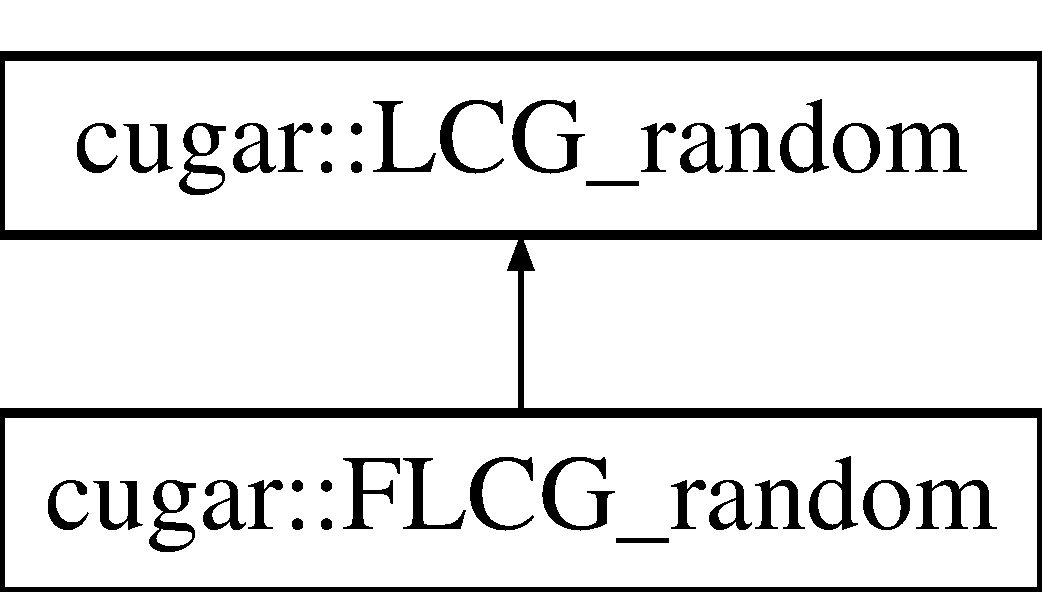
\includegraphics[height=2.000000cm]{structcugar_1_1_l_c_g__random}
\end{center}
\end{figure}
\subsection*{Public Methods}
\begin{DoxyCompactItemize}
\item 
\mbox{\Hypertarget{structcugar_1_1_l_c_g__random_a9e8beadc386fbf731a1124690563842d}\label{structcugar_1_1_l_c_g__random_a9e8beadc386fbf731a1124690563842d}} 
C\+U\+G\+A\+R\+\_\+\+F\+O\+R\+C\+E\+I\+N\+L\+I\+NE C\+U\+G\+A\+R\+\_\+\+H\+O\+S\+T\+\_\+\+D\+E\+V\+I\+CE {\bfseries L\+C\+G\+\_\+random} (const uint32 s=0)
\item 
\mbox{\Hypertarget{structcugar_1_1_l_c_g__random_a50a0c4356d6e21e38e0374627944612e}\label{structcugar_1_1_l_c_g__random_a50a0c4356d6e21e38e0374627944612e}} 
C\+U\+G\+A\+R\+\_\+\+F\+O\+R\+C\+E\+I\+N\+L\+I\+NE C\+U\+G\+A\+R\+\_\+\+H\+O\+S\+T\+\_\+\+D\+E\+V\+I\+CE uint32 {\bfseries next} ()
\end{DoxyCompactItemize}
\subsection*{Public Members}
\begin{DoxyCompactItemize}
\item 
\mbox{\Hypertarget{structcugar_1_1_l_c_g__random_a42f6cd7352922a8ef1cd925b0c4c7be5}\label{structcugar_1_1_l_c_g__random_a42f6cd7352922a8ef1cd925b0c4c7be5}} 
uint32 {\bfseries m\+\_\+s}
\end{DoxyCompactItemize}
\subsection*{Static Public Members}
\begin{DoxyCompactItemize}
\item 
\mbox{\Hypertarget{structcugar_1_1_l_c_g__random_aef93318f9c9bcfc29c5d9db4c82b740d}\label{structcugar_1_1_l_c_g__random_aef93318f9c9bcfc29c5d9db4c82b740d}} 
static const uint32 {\bfseries M\+AX} = 0x\+F\+F\+F\+F\+F\+F\+FF
\end{DoxyCompactItemize}


The documentation for this struct was generated from the following file\+:\begin{DoxyCompactItemize}
\item 
C\+:/p4research/research/jpantaleoni/\+Fermat-\/\+Public/contrib/cugar/basic/numbers.\+h\end{DoxyCompactItemize}

\hypertarget{structcugar_1_1leading__bits}{}\section{cugar\+:\+:leading\+\_\+bits$<$ word\+\_\+type $>$ Struct Template Reference}
\label{structcugar_1_1leading__bits}\index{cugar\+::leading\+\_\+bits$<$ word\+\_\+type $>$@{cugar\+::leading\+\_\+bits$<$ word\+\_\+type $>$}}


\subsection{Detailed description}
\subsubsection*{template$<$typename word\+\_\+type$>$\newline
struct cugar\+::leading\+\_\+bits$<$ word\+\_\+type $>$}

A functor to take the n leading bits of a word 

{\ttfamily \#include $<$functors.\+h$>$}

\subsection*{Public Types}
\begin{DoxyCompactItemize}
\item 
\mbox{\Hypertarget{structcugar_1_1leading__bits_ada87e6f1814ff63b21eb2501ac0c6b65}\label{structcugar_1_1leading__bits_ada87e6f1814ff63b21eb2501ac0c6b65}} 
typedef word\+\_\+type {\bfseries argument\+\_\+type}
\item 
\mbox{\Hypertarget{structcugar_1_1leading__bits_a20a4ef6d516ed8e44d3ff81f67371f4c}\label{structcugar_1_1leading__bits_a20a4ef6d516ed8e44d3ff81f67371f4c}} 
typedef word\+\_\+type {\bfseries result\+\_\+type}
\end{DoxyCompactItemize}
\subsection*{Public Methods}
\begin{DoxyCompactItemize}
\item 
C\+U\+G\+A\+R\+\_\+\+F\+O\+R\+C\+E\+I\+N\+L\+I\+NE C\+U\+G\+A\+R\+\_\+\+H\+O\+S\+T\+\_\+\+D\+E\+V\+I\+CE \hyperlink{structcugar_1_1leading__bits_ad6af66423d99cd96d71bc96aba0d8bf0}{leading\+\_\+bits} (const uint32 n)
\item 
C\+U\+G\+A\+R\+\_\+\+F\+O\+R\+C\+E\+I\+N\+L\+I\+NE C\+U\+G\+A\+R\+\_\+\+H\+O\+S\+T\+\_\+\+D\+E\+V\+I\+CE result\+\_\+type \hyperlink{structcugar_1_1leading__bits_aac537b0be4fe5120f9db93f46a22c057}{operator()} (const argument\+\_\+type op) const
\end{DoxyCompactItemize}
\subsection*{Public Members}
\begin{DoxyCompactItemize}
\item 
\mbox{\Hypertarget{structcugar_1_1leading__bits_a58d7725ea45c08982d6a24b63b78053b}\label{structcugar_1_1leading__bits_a58d7725ea45c08982d6a24b63b78053b}} 
const uint32 {\bfseries n\+\_\+bits}
\end{DoxyCompactItemize}
\subsection*{Static Public Members}
\begin{DoxyCompactItemize}
\item 
\mbox{\Hypertarget{structcugar_1_1leading__bits_a9e560a60dccd3f0392117f044b429504}\label{structcugar_1_1leading__bits_a9e560a60dccd3f0392117f044b429504}} 
static const uint32 {\bfseries B\+I\+TS} = 8u $\ast$ sizeof(word\+\_\+type)
\end{DoxyCompactItemize}


\subsection{Constructor \& Destructor Documentation}
\mbox{\Hypertarget{structcugar_1_1leading__bits_ad6af66423d99cd96d71bc96aba0d8bf0}\label{structcugar_1_1leading__bits_ad6af66423d99cd96d71bc96aba0d8bf0}} 
\index{cugar\+::leading\+\_\+bits@{cugar\+::leading\+\_\+bits}!leading\+\_\+bits@{leading\+\_\+bits}}
\index{leading\+\_\+bits@{leading\+\_\+bits}!cugar\+::leading\+\_\+bits@{cugar\+::leading\+\_\+bits}}
\subsubsection{\texorpdfstring{leading\+\_\+bits()}{leading\_bits()}}
{\footnotesize\ttfamily template$<$typename word\+\_\+type $>$ \\
C\+U\+G\+A\+R\+\_\+\+F\+O\+R\+C\+E\+I\+N\+L\+I\+NE C\+U\+G\+A\+R\+\_\+\+H\+O\+S\+T\+\_\+\+D\+E\+V\+I\+CE \hyperlink{structcugar_1_1leading__bits}{cugar\+::leading\+\_\+bits}$<$ word\+\_\+type $>$\+::\hyperlink{structcugar_1_1leading__bits}{leading\+\_\+bits} (\begin{DoxyParamCaption}\item[{const uint32}]{n }\end{DoxyParamCaption})\hspace{0.3cm}{\ttfamily [inline]}}

constructor 

\subsection{Member Function Documentation}
\mbox{\Hypertarget{structcugar_1_1leading__bits_aac537b0be4fe5120f9db93f46a22c057}\label{structcugar_1_1leading__bits_aac537b0be4fe5120f9db93f46a22c057}} 
\index{cugar\+::leading\+\_\+bits@{cugar\+::leading\+\_\+bits}!operator()@{operator()}}
\index{operator()@{operator()}!cugar\+::leading\+\_\+bits@{cugar\+::leading\+\_\+bits}}
\subsubsection{\texorpdfstring{operator()()}{operator()()}}
{\footnotesize\ttfamily template$<$typename word\+\_\+type $>$ \\
C\+U\+G\+A\+R\+\_\+\+F\+O\+R\+C\+E\+I\+N\+L\+I\+NE C\+U\+G\+A\+R\+\_\+\+H\+O\+S\+T\+\_\+\+D\+E\+V\+I\+CE result\+\_\+type \hyperlink{structcugar_1_1leading__bits}{cugar\+::leading\+\_\+bits}$<$ word\+\_\+type $>$\+::operator() (\begin{DoxyParamCaption}\item[{const argument\+\_\+type}]{op }\end{DoxyParamCaption}) const\hspace{0.3cm}{\ttfamily [inline]}}

functor implementation 

The documentation for this struct was generated from the following file\+:\begin{DoxyCompactItemize}
\item 
C\+:/p4research/research/jpantaleoni/\+Fermat-\/\+Public/contrib/cugar/basic/\hyperlink{functors_8h}{functors.\+h}\end{DoxyCompactItemize}

\hypertarget{structcugar_1_1leaf__index__tag}{}\section{cugar\+:\+:leaf\+\_\+index\+\_\+tag Struct Reference}
\label{structcugar_1_1leaf__index__tag}\index{cugar\+::leaf\+\_\+index\+\_\+tag@{cugar\+::leaf\+\_\+index\+\_\+tag}}


\subsection{Detailed description}
tag struct to identify leaves specifying a single index 

{\ttfamily \#include $<$bintree\+\_\+node.\+h$>$}



The documentation for this struct was generated from the following file\+:\begin{DoxyCompactItemize}
\item 
C\+:/p4research/research/jpantaleoni/\+Fermat-\/\+Public/contrib/cugar/bintree/\hyperlink{bintree__node_8h}{bintree\+\_\+node.\+h}\end{DoxyCompactItemize}

\hypertarget{structcugar_1_1leaf__range__tag}{}\section{cugar\+:\+:leaf\+\_\+range\+\_\+tag Struct Reference}
\label{structcugar_1_1leaf__range__tag}\index{cugar\+::leaf\+\_\+range\+\_\+tag@{cugar\+::leaf\+\_\+range\+\_\+tag}}


\subsection{Detailed description}
tag struct to identify leaves specifying a full index range 

{\ttfamily \#include $<$bintree\+\_\+node.\+h$>$}



The documentation for this struct was generated from the following file\+:\begin{DoxyCompactItemize}
\item 
C\+:/p4research/research/jpantaleoni/\+Fermat-\/\+Public/contrib/cugar/bintree/\hyperlink{bintree__node_8h}{bintree\+\_\+node.\+h}\end{DoxyCompactItemize}

\hypertarget{structcugar_1_1less}{}\section{cugar\+:\+:less$<$ T $>$ Struct Template Reference}
\label{structcugar_1_1less}\index{cugar\+::less$<$ T $>$@{cugar\+::less$<$ T $>$}}


\subsection{Detailed description}
\subsubsection*{template$<$typename T$>$\newline
struct cugar\+::less$<$ T $>$}

less functor 

{\ttfamily \#include $<$functors.\+h$>$}

\subsection*{Public Types}
\begin{DoxyCompactItemize}
\item 
\mbox{\Hypertarget{structcugar_1_1less_adb47dc880ce43c26f7effd48d45e3c1e}\label{structcugar_1_1less_adb47dc880ce43c26f7effd48d45e3c1e}} 
typedef \hyperlink{structcugar_1_1binary__function__tag}{binary\+\_\+function\+\_\+tag} {\bfseries function\+\_\+tag}
\item 
\mbox{\Hypertarget{structcugar_1_1less_af4f4261c8016a98c93347c01146aabb5}\label{structcugar_1_1less_af4f4261c8016a98c93347c01146aabb5}} 
typedef T {\bfseries first\+\_\+argument\+\_\+type}
\item 
\mbox{\Hypertarget{structcugar_1_1less_a4fc757ff0f4a9e140a535edb884f4677}\label{structcugar_1_1less_a4fc757ff0f4a9e140a535edb884f4677}} 
typedef T {\bfseries second\+\_\+argument\+\_\+type}
\item 
\mbox{\Hypertarget{structcugar_1_1less_a14f958212b2f50765d5fcc2b6581140f}\label{structcugar_1_1less_a14f958212b2f50765d5fcc2b6581140f}} 
typedef bool {\bfseries result\+\_\+type}
\end{DoxyCompactItemize}
\subsection*{Public Methods}
\begin{DoxyCompactItemize}
\item 
\mbox{\Hypertarget{structcugar_1_1less_ad929110b4a8522fd4a54ba109012df24}\label{structcugar_1_1less_ad929110b4a8522fd4a54ba109012df24}} 
C\+U\+G\+A\+R\+\_\+\+H\+O\+S\+T\+\_\+\+D\+E\+V\+I\+CE bool {\bfseries operator()} (const T \&op1, const T \&op2) const
\end{DoxyCompactItemize}


The documentation for this struct was generated from the following file\+:\begin{DoxyCompactItemize}
\item 
C\+:/p4research/research/jpantaleoni/\+Fermat-\/\+Public/contrib/cugar/basic/\hyperlink{functors_8h}{functors.\+h}\end{DoxyCompactItemize}

\hypertarget{classcugar_1_1_l_f_s_r_generator_matrix}{}\section{cugar\+:\+:L\+F\+S\+R\+Generator\+Matrix Class Reference}
\label{classcugar_1_1_l_f_s_r_generator_matrix}\index{cugar\+::\+L\+F\+S\+R\+Generator\+Matrix@{cugar\+::\+L\+F\+S\+R\+Generator\+Matrix}}


\subsection{Detailed description}
An implementation of the small linear feedback shift registers (L\+F\+SR) for use in a Markov chain quasi-\/\+Monte Carlo context, as described in S. Chen, M. Matsumoto, T. Nishimura, and A. Owen\+: \char`\"{}\+New inputs and methods for Markov
chain quasi-\/\+Monte Carlo\char`\"{}, and S. Chen\+: \char`\"{}\+Consistence and convergence rate of
\+Markov chain quasi-\/\+Monte Carlo with examples\char`\"{}. Apart from the matrix that describes the recurrence, this class is stateless, and can therefore be easily shared in a multi-\/threaded context.

\href{https://en.wikipedia.org/wiki/Linear-feedback_shift_register}{\tt https\+://en.\+wikipedia.\+org/wiki/\+Linear-\/feedback\+\_\+shift\+\_\+register} 

{\ttfamily \#include $<$lfsr.\+h$>$}

\subsection*{Public Types}
\begin{DoxyCompactItemize}
\item 
\mbox{\Hypertarget{classcugar_1_1_l_f_s_r_generator_matrix_a1e210b57aecc9bddd4fd7e3c99bae0d5}\label{classcugar_1_1_l_f_s_r_generator_matrix_a1e210b57aecc9bddd4fd7e3c99bae0d5}} 
enum {\bfseries Offset\+\_\+type} \{ {\bfseries O\+R\+I\+G\+I\+N\+AL}, 
{\bfseries G\+O\+O\+D\+\_\+\+P\+R\+O\+J\+E\+C\+T\+I\+O\+NS}
 \}
\end{DoxyCompactItemize}
\subsection*{Public Methods}
\begin{DoxyCompactItemize}
\item 
C\+U\+G\+A\+R\+\_\+\+H\+O\+S\+T\+\_\+\+D\+E\+V\+I\+CE C\+U\+G\+A\+R\+\_\+\+F\+O\+R\+C\+E\+I\+N\+L\+I\+NE {\bfseries L\+F\+S\+R\+Generator\+Matrix} (uint32 m, Offset\+\_\+type offset\+\_\+type=G\+O\+O\+D\+\_\+\+P\+R\+O\+J\+E\+C\+T\+I\+O\+NS)
\item 
C\+U\+G\+A\+R\+\_\+\+H\+O\+S\+T\+\_\+\+D\+E\+V\+I\+CE C\+U\+G\+A\+R\+\_\+\+F\+O\+R\+C\+E\+I\+N\+L\+I\+NE float {\bfseries next} (uint32 scramble, uint32 $\ast$state) const
\end{DoxyCompactItemize}
\subsection*{Public Members}
\begin{DoxyCompactItemize}
\item 
\mbox{\Hypertarget{classcugar_1_1_l_f_s_r_generator_matrix_a80ce08a8b13499ad66eb1733ee3d35d2}\label{classcugar_1_1_l_f_s_r_generator_matrix_a80ce08a8b13499ad66eb1733ee3d35d2}} 
uint32 {\bfseries m\+\_\+m}
\item 
\mbox{\Hypertarget{classcugar_1_1_l_f_s_r_generator_matrix_a007507bbdc265c1f3e4042d2bc7005cf}\label{classcugar_1_1_l_f_s_r_generator_matrix_a007507bbdc265c1f3e4042d2bc7005cf}} 
uint32 {\bfseries m\+\_\+f} \mbox{[}32\mbox{]}
\end{DoxyCompactItemize}


The documentation for this class was generated from the following file\+:\begin{DoxyCompactItemize}
\item 
C\+:/p4research/research/jpantaleoni/\+Fermat-\/\+Public/contrib/cugar/sampling/\hyperlink{lfsr_8h}{lfsr.\+h}\end{DoxyCompactItemize}

\hypertarget{structcugar_1_1_l_f_s_r_random_stream}{}\section{cugar\+:\+:L\+F\+S\+R\+Random\+Stream Struct Reference}
\label{structcugar_1_1_l_f_s_r_random_stream}\index{cugar\+::\+L\+F\+S\+R\+Random\+Stream@{cugar\+::\+L\+F\+S\+R\+Random\+Stream}}


\subsection{Detailed description}
An implementation of the small linear feedback shift registers (L\+F\+SR) for use in a Markov chain quasi-\/\+Monte Carlo context, as described in S. Chen, M. Matsumoto, T. Nishimura, and A. Owen\+: \char`\"{}\+New inputs and methods for Markov
chain quasi-\/\+Monte Carlo\char`\"{}, and S. Chen\+: \char`\"{}\+Consistence and convergence rate of
\+Markov chain quasi-\/\+Monte Carlo with examples\char`\"{}. Apart from the matrix that describes the recurrence, this class is stateless, and can therefore be easily shared in a multi-\/threaded context.

\href{https://en.wikipedia.org/wiki/Linear-feedback_shift_register}{\tt https\+://en.\+wikipedia.\+org/wiki/\+Linear-\/feedback\+\_\+shift\+\_\+register} 

{\ttfamily \#include $<$lfsr.\+h$>$}

\subsection*{Public Methods}
\begin{DoxyCompactItemize}
\item 
\mbox{\Hypertarget{structcugar_1_1_l_f_s_r_random_stream_a941ae605b20b4e0a3663ec6c2a8226c8}\label{structcugar_1_1_l_f_s_r_random_stream_a941ae605b20b4e0a3663ec6c2a8226c8}} 
C\+U\+G\+A\+R\+\_\+\+H\+O\+S\+T\+\_\+\+D\+E\+V\+I\+CE C\+U\+G\+A\+R\+\_\+\+F\+O\+R\+C\+E\+I\+N\+L\+I\+NE {\bfseries L\+F\+S\+R\+Random\+Stream} (\hyperlink{classcugar_1_1_l_f_s_r_generator_matrix}{L\+F\+S\+R\+Generator\+Matrix} $\ast$matrix, const uint32 state, const uint32 scramble=1361u)
\item 
C\+U\+G\+A\+R\+\_\+\+H\+O\+S\+T\+\_\+\+D\+E\+V\+I\+CE C\+U\+G\+A\+R\+\_\+\+F\+O\+R\+C\+E\+I\+N\+L\+I\+NE float {\bfseries next} ()
\end{DoxyCompactItemize}
\subsection*{Public Members}
\begin{DoxyCompactItemize}
\item 
\mbox{\Hypertarget{structcugar_1_1_l_f_s_r_random_stream_ae1f628c733a9bc00e1b8defbfd801d6e}\label{structcugar_1_1_l_f_s_r_random_stream_ae1f628c733a9bc00e1b8defbfd801d6e}} 
\hyperlink{classcugar_1_1_l_f_s_r_generator_matrix}{L\+F\+S\+R\+Generator\+Matrix} $\ast$ {\bfseries m\+\_\+matrix}
\item 
\mbox{\Hypertarget{structcugar_1_1_l_f_s_r_random_stream_a989706e7a76a3f61d31e4c51fb4d83eb}\label{structcugar_1_1_l_f_s_r_random_stream_a989706e7a76a3f61d31e4c51fb4d83eb}} 
uint32 {\bfseries m\+\_\+state}
\item 
\mbox{\Hypertarget{structcugar_1_1_l_f_s_r_random_stream_a0ce7689c37576066a22526271ce30d85}\label{structcugar_1_1_l_f_s_r_random_stream_a0ce7689c37576066a22526271ce30d85}} 
uint32 {\bfseries m\+\_\+scramble}
\end{DoxyCompactItemize}


The documentation for this struct was generated from the following file\+:\begin{DoxyCompactItemize}
\item 
C\+:/p4research/research/jpantaleoni/\+Fermat-\/\+Public/contrib/cugar/sampling/\hyperlink{lfsr_8h}{lfsr.\+h}\end{DoxyCompactItemize}

\hypertarget{structcugar_1_1_l_h_sampler}{}\section{cugar\+:\+:L\+H\+Sampler Struct Reference}
\label{structcugar_1_1_l_h_sampler}\index{cugar\+::\+L\+H\+Sampler@{cugar\+::\+L\+H\+Sampler}}


\subsection{Detailed description}
Latin-\/\+Hypercube Sampler 

{\ttfamily \#include $<$latin\+\_\+hypercube.\+h$>$}

\subsection*{Public Methods}
\begin{DoxyCompactItemize}
\item 
\hyperlink{structcugar_1_1_l_h_sampler_a8453aa1db9cae158d609cbb9e5843f5b}{L\+H\+Sampler} (const uint32 seed=0)
\item 
{\footnotesize template$<$typename T , uint32 D\+IM$>$ }\\void \hyperlink{structcugar_1_1_l_h_sampler_a834984a5429b711dc3be799b927905d1}{sample} (const uint32 n\+\_\+samples, \hyperlink{structcugar_1_1_vector}{Vector}$<$ T, D\+IM $>$ $\ast$samples)
\item 
{\footnotesize template$<$bool S\+OA, typename T $>$ }\\void \hyperlink{structcugar_1_1_l_h_sampler_ab3422ecf79d29b9327cda1633f01caae}{sample} (const uint32 n\+\_\+samples, const uint32 n\+\_\+dims, T $\ast$samples)
\end{DoxyCompactItemize}
\subsection*{Public Members}
\begin{DoxyCompactItemize}
\item 
\mbox{\Hypertarget{structcugar_1_1_l_h_sampler_a34b6dfc455feb895c9f227032f88e398}\label{structcugar_1_1_l_h_sampler_a34b6dfc455feb895c9f227032f88e398}} 
\hyperlink{structcugar_1_1_random}{Random} {\bfseries m\+\_\+random}
\end{DoxyCompactItemize}


\subsection{Constructor \& Destructor Documentation}
\mbox{\Hypertarget{structcugar_1_1_l_h_sampler_a8453aa1db9cae158d609cbb9e5843f5b}\label{structcugar_1_1_l_h_sampler_a8453aa1db9cae158d609cbb9e5843f5b}} 
\index{cugar\+::\+L\+H\+Sampler@{cugar\+::\+L\+H\+Sampler}!L\+H\+Sampler@{L\+H\+Sampler}}
\index{L\+H\+Sampler@{L\+H\+Sampler}!cugar\+::\+L\+H\+Sampler@{cugar\+::\+L\+H\+Sampler}}
\subsubsection{\texorpdfstring{L\+H\+Sampler()}{LHSampler()}}
{\footnotesize\ttfamily cugar\+::\+L\+H\+Sampler\+::\+L\+H\+Sampler (\begin{DoxyParamCaption}\item[{const uint32}]{seed = {\ttfamily 0} }\end{DoxyParamCaption})\hspace{0.3cm}{\ttfamily [inline]}}

constructor 

\subsection{Member Function Documentation}
\mbox{\Hypertarget{structcugar_1_1_l_h_sampler_a834984a5429b711dc3be799b927905d1}\label{structcugar_1_1_l_h_sampler_a834984a5429b711dc3be799b927905d1}} 
\index{cugar\+::\+L\+H\+Sampler@{cugar\+::\+L\+H\+Sampler}!sample@{sample}}
\index{sample@{sample}!cugar\+::\+L\+H\+Sampler@{cugar\+::\+L\+H\+Sampler}}
\subsubsection{\texorpdfstring{sample()}{sample()}\hspace{0.1cm}{\footnotesize\ttfamily [1/2]}}
{\footnotesize\ttfamily template$<$typename T , uint32 D\+IM$>$ \\
void cugar\+::\+L\+H\+Sampler\+::sample (\begin{DoxyParamCaption}\item[{const uint32}]{n\+\_\+samples,  }\item[{\hyperlink{structcugar_1_1_vector}{Vector}$<$ T, D\+IM $>$ $\ast$}]{samples }\end{DoxyParamCaption})}

get a set of stratified samples \mbox{\Hypertarget{structcugar_1_1_l_h_sampler_ab3422ecf79d29b9327cda1633f01caae}\label{structcugar_1_1_l_h_sampler_ab3422ecf79d29b9327cda1633f01caae}} 
\index{cugar\+::\+L\+H\+Sampler@{cugar\+::\+L\+H\+Sampler}!sample@{sample}}
\index{sample@{sample}!cugar\+::\+L\+H\+Sampler@{cugar\+::\+L\+H\+Sampler}}
\subsubsection{\texorpdfstring{sample()}{sample()}\hspace{0.1cm}{\footnotesize\ttfamily [2/2]}}
{\footnotesize\ttfamily template$<$bool S\+OA, typename T$>$ \\
void cugar\+::\+L\+H\+Sampler\+::sample (\begin{DoxyParamCaption}\item[{const uint32}]{n\+\_\+samples,  }\item[{const uint32}]{n\+\_\+dims,  }\item[{T $\ast$}]{samples }\end{DoxyParamCaption})}

get a set of stratified d-\/dimensional samples the output vectors can be stored either in A\+OS or S\+OA layout, if the latter, the j-\/th coordinate of the i-\/th point is stored in samples\mbox{[}i + j $\ast$ n\+\_\+samples\mbox{]} 

The documentation for this struct was generated from the following files\+:\begin{DoxyCompactItemize}
\item 
C\+:/p4research/research/jpantaleoni/\+Fermat-\/\+Public/contrib/cugar/sampling/latin\+\_\+hypercube.\+h\item 
C\+:/p4research/research/jpantaleoni/\+Fermat-\/\+Public/contrib/cugar/sampling/latin\+\_\+hypercube\+\_\+inline.\+h\end{DoxyCompactItemize}

\hypertarget{struct_light}{}\section{Light Struct Reference}
\label{struct_light}\index{Light@{Light}}


\subsection{Detailed description}
Base light interface.

This class implements \char`\"{}software\char`\"{} inheritance by dispatching its methods to implementations provided by its derived classes. This is useful to allow this class to avoid virtual method calls, and hence allow it to work both on the host and the device. Note that since the methods are manually dispatched, all calls can be inlined. 

{\ttfamily \#include $<$lights.\+h$>$}

Inheritance diagram for Light\+:\begin{figure}[H]
\begin{center}
\leavevmode
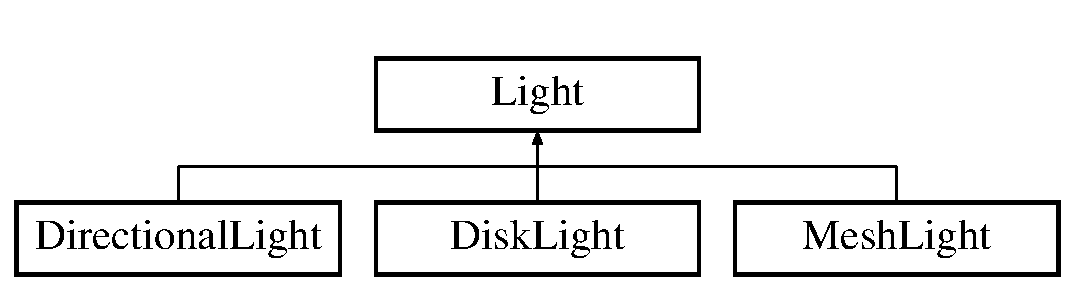
\includegraphics[height=2.000000cm]{struct_light}
\end{center}
\end{figure}
\subsection*{Public Methods}
\begin{DoxyCompactItemize}
\item 
\mbox{\Hypertarget{struct_light_af075d1d5e2a8d9449d0ba7f9c32f0e70}\label{struct_light_af075d1d5e2a8d9449d0ba7f9c32f0e70}} 
F\+E\+R\+M\+A\+T\+\_\+\+H\+O\+S\+T\+\_\+\+D\+E\+V\+I\+CE {\bfseries Light} (Light\+Type \+\_\+type)
\item 
F\+E\+R\+M\+A\+T\+\_\+\+H\+O\+S\+T\+\_\+\+D\+E\+V\+I\+CE bool \hyperlink{group___lights_module_ga67cc240bcda4b08efd26c8727144bf16}{sample} (const float $\ast$Z, uint32\+\_\+t $\ast$prim\+\_\+id, \hyperlink{structcugar_1_1_vector}{cugar\+::\+Vector2f} $\ast$uv, \hyperlink{struct_vertex_geometry}{Vertex\+Geometry} $\ast$geom, float $\ast$pdf, \hyperlink{struct_edf}{Edf} $\ast$edf) const
\item 
F\+E\+R\+M\+A\+T\+\_\+\+H\+O\+S\+T\+\_\+\+D\+E\+V\+I\+CE bool \hyperlink{group___lights_module_gaa3cac39418d2c62c2faaa4cb7c380ff7}{sample} (const \hyperlink{structcugar_1_1_vector}{cugar\+::\+Vector3f} p, const float $\ast$Z, uint32\+\_\+t $\ast$prim\+\_\+id, \hyperlink{structcugar_1_1_vector}{cugar\+::\+Vector2f} $\ast$uv, \hyperlink{struct_vertex_geometry}{Vertex\+Geometry} $\ast$geom, float $\ast$pdf, \hyperlink{struct_edf}{Edf} $\ast$edf) const
\item 
F\+E\+R\+M\+A\+T\+\_\+\+H\+O\+S\+T\+\_\+\+D\+E\+V\+I\+CE void \hyperlink{group___lights_module_ga6a7452cab8b733d48174016b845f8d53}{intersect} (const \hyperlink{struct_ray}{Ray} ray, float2 $\ast$uv, float $\ast$t) const
\item 
F\+E\+R\+M\+A\+T\+\_\+\+H\+O\+S\+T\+\_\+\+D\+E\+V\+I\+CE void \hyperlink{group___lights_module_gaf14a70f7d23b422f8953bc55d1eade44}{map} (const uint32\+\_\+t prim\+\_\+id, const \hyperlink{structcugar_1_1_vector}{cugar\+::\+Vector2f} \&uv, \hyperlink{struct_vertex_geometry}{Vertex\+Geometry} $\ast$geom, float $\ast$pdf, \hyperlink{struct_edf}{Edf} $\ast$edf) const
\item 
F\+E\+R\+M\+A\+T\+\_\+\+H\+O\+S\+T\+\_\+\+D\+E\+V\+I\+CE void \hyperlink{group___lights_module_ga96c94d76b5464c0433e8e071645cfe48}{map} (const uint32\+\_\+t prim\+\_\+id, const \hyperlink{structcugar_1_1_vector}{cugar\+::\+Vector2f} \&uv, const \hyperlink{struct_vertex_geometry}{Vertex\+Geometry} \&geom, float $\ast$pdf, \hyperlink{struct_edf}{Edf} $\ast$edf) const
\end{DoxyCompactItemize}
\subsection*{Public Members}
\begin{DoxyCompactItemize}
\item 
\mbox{\Hypertarget{struct_light_a86e648b4a80a5c1e194c97ef52f9efc6}\label{struct_light_a86e648b4a80a5c1e194c97ef52f9efc6}} 
Light\+Type {\bfseries type}
\end{DoxyCompactItemize}


The documentation for this struct was generated from the following file\+:\begin{DoxyCompactItemize}
\item 
C\+:/p4research/research/jpantaleoni/\+Fermat-\/\+Public/src/lights.\+h\end{DoxyCompactItemize}

\hypertarget{struct_light_vertex}{}\section{Light\+Vertex Struct Reference}
\label{struct_light_vertex}\index{Light\+Vertex@{Light\+Vertex}}


\subsection{Detailed description}
\begin{DoxyParagraph}{}
A utility class to encapsulate all important information for a light subpath vertex 
\end{DoxyParagraph}


{\ttfamily \#include $<$bpt\+\_\+utils.\+h$>$}

\subsection*{Public Methods}
\begin{DoxyCompactItemize}
\item 
\mbox{\Hypertarget{struct_light_vertex_a29e68f91cafe19c7f84cb8781c1b4ca8}\label{struct_light_vertex_a29e68f91cafe19c7f84cb8781c1b4ca8}} 
F\+E\+R\+M\+A\+T\+\_\+\+H\+O\+S\+T\+\_\+\+D\+E\+V\+I\+CE void {\bfseries setup} (const \hyperlink{structcugar_1_1_vector}{cugar\+::\+Vector4f} \&\+\_\+pos, const uint2 \&\+\_\+packed\+\_\+info1, const uint4 \&\+\_\+packed\+\_\+info2, const \hyperlink{struct_path_weights}{Path\+Weights} \&\+\_\+weights, const uint32 \+\_\+depth, const \hyperlink{struct_rendering_context_view}{Rendering\+Context\+View} \&renderer)
\item 
\mbox{\Hypertarget{struct_light_vertex_a22ac8565e0127206de026c6dd405279f}\label{struct_light_vertex_a22ac8565e0127206de026c6dd405279f}} 
F\+E\+R\+M\+A\+T\+\_\+\+H\+O\+S\+T\+\_\+\+D\+E\+V\+I\+CE void {\bfseries setup} (const \hyperlink{struct_ray}{Ray} \&ray, const \hyperlink{struct_hit}{Hit} \&hit, const \hyperlink{structcugar_1_1_vector}{cugar\+::\+Vector3f} \&\+\_\+alpha, const \hyperlink{struct_path_weights}{Path\+Weights} \&\+\_\+weights, const uint32 \+\_\+depth, const \hyperlink{struct_rendering_context_view}{Rendering\+Context\+View} \&renderer)
\item 
\mbox{\Hypertarget{struct_light_vertex_a440fe1427988cbf9547738776cccd582}\label{struct_light_vertex_a440fe1427988cbf9547738776cccd582}} 
F\+E\+R\+M\+A\+T\+\_\+\+H\+O\+S\+T\+\_\+\+D\+E\+V\+I\+CE void {\bfseries setup} (const \hyperlink{struct_ray}{Ray} \&ray, const \hyperlink{struct_hit}{Hit} \&hit, const \hyperlink{structcugar_1_1_vector}{cugar\+::\+Vector3f} \&\+\_\+alpha, const \hyperlink{struct_temp_path_weights}{Temp\+Path\+Weights} \&\+\_\+weights, const uint32 \+\_\+depth, const \hyperlink{struct_rendering_context_view}{Rendering\+Context\+View} \&renderer)
\item 
\mbox{\Hypertarget{struct_light_vertex_adc19dba9e6283b4c0da2eec3237c914a}\label{struct_light_vertex_adc19dba9e6283b4c0da2eec3237c914a}} 
F\+E\+R\+M\+A\+T\+\_\+\+H\+O\+S\+T\+\_\+\+D\+E\+V\+I\+CE void {\bfseries setup} (const \hyperlink{structcugar_1_1_vector}{cugar\+::\+Vector3f} \&\+\_\+in, const \hyperlink{struct_vertex_geometry_id}{Vertex\+Geometry\+Id} \&\+\_\+v, const \hyperlink{structcugar_1_1_vector}{cugar\+::\+Vector3f} \&\+\_\+alpha, const \hyperlink{struct_temp_path_weights}{Temp\+Path\+Weights} \&\+\_\+weights, const uint32 \+\_\+depth, const \hyperlink{struct_rendering_context_view}{Rendering\+Context\+View} \&renderer)
\item 
\mbox{\Hypertarget{struct_light_vertex_a3fc35df12e7a88367b66c7b7020914a0}\label{struct_light_vertex_a3fc35df12e7a88367b66c7b7020914a0}} 
F\+E\+R\+M\+A\+T\+\_\+\+H\+O\+S\+T\+\_\+\+D\+E\+V\+I\+CE {\bfseries Light\+Vertex} (const \hyperlink{structcugar_1_1_vector}{cugar\+::\+Vector4f} \&\+\_\+pos, const uint2 \&\+\_\+packed\+\_\+info1, const uint4 \&\+\_\+packed\+\_\+info2, const \hyperlink{struct_path_weights}{Path\+Weights} \&\+\_\+weights, const uint32 \+\_\+depth, const \hyperlink{struct_rendering_context_view}{Rendering\+Context\+View} \&renderer)
\item 
\mbox{\Hypertarget{struct_light_vertex_a0cf76cff35be4e3d76d52c9d0b3b1d00}\label{struct_light_vertex_a0cf76cff35be4e3d76d52c9d0b3b1d00}} 
F\+E\+R\+M\+A\+T\+\_\+\+H\+O\+S\+T\+\_\+\+D\+E\+V\+I\+CE {\bfseries Light\+Vertex} (const \hyperlink{struct_ray}{Ray} \&\+\_\+ray, const \hyperlink{struct_hit}{Hit} \&\+\_\+hit, const \hyperlink{structcugar_1_1_vector}{cugar\+::\+Vector3f} \&\+\_\+alpha, const \hyperlink{struct_temp_path_weights}{Temp\+Path\+Weights} \&\+\_\+weights, const uint32 \+\_\+depth, const \hyperlink{struct_rendering_context_view}{Rendering\+Context\+View} \&renderer)
\item 
\mbox{\Hypertarget{struct_light_vertex_a2390fe15e94a34cd60db50e6b6cae0d1}\label{struct_light_vertex_a2390fe15e94a34cd60db50e6b6cae0d1}} 
F\+E\+R\+M\+A\+T\+\_\+\+H\+O\+S\+T\+\_\+\+D\+E\+V\+I\+CE {\bfseries Light\+Vertex} (const \hyperlink{structcugar_1_1_vector}{cugar\+::\+Vector3f} \&\+\_\+in, const \hyperlink{struct_vertex_geometry_id}{Vertex\+Geometry\+Id} \&\+\_\+v, const \hyperlink{structcugar_1_1_vector}{cugar\+::\+Vector3f} \&\+\_\+alpha, const \hyperlink{struct_temp_path_weights}{Temp\+Path\+Weights} \&\+\_\+weights, const uint32 \+\_\+depth, const \hyperlink{struct_rendering_context_view}{Rendering\+Context\+View} \&renderer)
\item 
F\+E\+R\+M\+A\+T\+\_\+\+H\+O\+S\+T\+\_\+\+D\+E\+V\+I\+CE F\+E\+R\+M\+A\+T\+\_\+\+F\+O\+R\+C\+E\+I\+N\+L\+I\+NE bool \hyperlink{struct_light_vertex_a2e6fa24feb3e233f487b6a33ea5ed622}{sample} (const float z\mbox{[}3\mbox{]}, \hyperlink{struct_bsdf_a5f7db6f81220ed9ee6da109d6eb5b585}{Bsdf\+::\+Component\+Type} \&out\+\_\+comp, \hyperlink{structcugar_1_1_vector}{cugar\+::\+Vector3f} \&out, float \&out\+\_\+p, float \&out\+\_\+p\+\_\+proj, \hyperlink{structcugar_1_1_vector}{cugar\+::\+Vector3f} \&out\+\_\+g, bool RR=true, bool evaluate\+\_\+full\+\_\+bsdf=false, const \hyperlink{struct_bsdf_a5f7db6f81220ed9ee6da109d6eb5b585}{Bsdf\+::\+Component\+Type} components=Bsdf\+::k\+All\+Components) const
\end{DoxyCompactItemize}
\subsection*{Public Members}
\begin{DoxyCompactItemize}
\item 
\mbox{\Hypertarget{struct_light_vertex_a7cb7ba2aa0851dd91497dda73a68390d}\label{struct_light_vertex_a7cb7ba2aa0851dd91497dda73a68390d}} 
\hyperlink{struct_vertex_geometry_id}{Vertex\+Geometry\+Id} {\bfseries geom\+\_\+id}
\item 
\mbox{\Hypertarget{struct_light_vertex_a2badf795ce56f304376164b0cf84e534}\label{struct_light_vertex_a2badf795ce56f304376164b0cf84e534}} 
\hyperlink{struct_vertex_geometry}{Vertex\+Geometry} {\bfseries geom}
\item 
\mbox{\Hypertarget{struct_light_vertex_a822872fa560e80c7c1b6dd12ca652c91}\label{struct_light_vertex_a822872fa560e80c7c1b6dd12ca652c91}} 
\hyperlink{structcugar_1_1_vector}{cugar\+::\+Vector3f} {\bfseries in}
\item 
\mbox{\Hypertarget{struct_light_vertex_a4eefd4050f8485574d7c00af73c97bf1}\label{struct_light_vertex_a4eefd4050f8485574d7c00af73c97bf1}} 
\hyperlink{structcugar_1_1_vector}{cugar\+::\+Vector3f} {\bfseries alpha}
\item 
\mbox{\Hypertarget{struct_light_vertex_a64bfd20f3d423363c90d5e34cb85c2d1}\label{struct_light_vertex_a64bfd20f3d423363c90d5e34cb85c2d1}} 
\hyperlink{struct_path_weights}{Path\+Weights} {\bfseries weights}
\item 
\mbox{\Hypertarget{struct_light_vertex_a7086aa711d49b5c135d990ec27899396}\label{struct_light_vertex_a7086aa711d49b5c135d990ec27899396}} 
uint32 {\bfseries depth}
\item 
\mbox{\Hypertarget{struct_light_vertex_ac043163ef9f35add2c3b027a7aaf7ed4}\label{struct_light_vertex_ac043163ef9f35add2c3b027a7aaf7ed4}} 
\hyperlink{struct_mesh_material}{Mesh\+Material} {\bfseries material}
\item 
\mbox{\Hypertarget{struct_light_vertex_a3d33ac0039f711134a2997835491951c}\label{struct_light_vertex_a3d33ac0039f711134a2997835491951c}} 
\hyperlink{struct_edf}{Edf} {\bfseries edf}
\item 
\mbox{\Hypertarget{struct_light_vertex_aacab4bae157999e8b0d462fcafd0ef3a}\label{struct_light_vertex_aacab4bae157999e8b0d462fcafd0ef3a}} 
\hyperlink{struct_bsdf}{Bsdf} {\bfseries bsdf}
\item 
\mbox{\Hypertarget{struct_light_vertex_abb07274d58742c761a920e8b56abf906}\label{struct_light_vertex_abb07274d58742c761a920e8b56abf906}} 
float {\bfseries prev\+\_\+\+G\+\_\+prime}
\item 
\mbox{\Hypertarget{struct_light_vertex_acd84967fda170c5534f5a8b2f76b8f89}\label{struct_light_vertex_acd84967fda170c5534f5a8b2f76b8f89}} 
float {\bfseries prev\+\_\+pG}
\item 
\mbox{\Hypertarget{struct_light_vertex_adff45990a4964658a0c6b059427f7ded}\label{struct_light_vertex_adff45990a4964658a0c6b059427f7ded}} 
float {\bfseries p\+Gp\+\_\+sum}
\end{DoxyCompactItemize}


\subsection{Member Function Documentation}
\mbox{\Hypertarget{struct_light_vertex_a2e6fa24feb3e233f487b6a33ea5ed622}\label{struct_light_vertex_a2e6fa24feb3e233f487b6a33ea5ed622}} 
\index{Light\+Vertex@{Light\+Vertex}!sample@{sample}}
\index{sample@{sample}!Light\+Vertex@{Light\+Vertex}}
\subsubsection{\texorpdfstring{sample()}{sample()}}
{\footnotesize\ttfamily F\+E\+R\+M\+A\+T\+\_\+\+H\+O\+S\+T\+\_\+\+D\+E\+V\+I\+CE F\+E\+R\+M\+A\+T\+\_\+\+F\+O\+R\+C\+E\+I\+N\+L\+I\+NE bool Light\+Vertex\+::sample (\begin{DoxyParamCaption}\item[{const float}]{z\mbox{[}3\mbox{]},  }\item[{\hyperlink{struct_bsdf_a5f7db6f81220ed9ee6da109d6eb5b585}{Bsdf\+::\+Component\+Type} \&}]{out\+\_\+comp,  }\item[{\hyperlink{structcugar_1_1_vector}{cugar\+::\+Vector3f} \&}]{out,  }\item[{float \&}]{out\+\_\+p,  }\item[{float \&}]{out\+\_\+p\+\_\+proj,  }\item[{\hyperlink{structcugar_1_1_vector}{cugar\+::\+Vector3f} \&}]{out\+\_\+g,  }\item[{bool}]{RR = {\ttfamily true},  }\item[{bool}]{evaluate\+\_\+full\+\_\+bsdf = {\ttfamily false},  }\item[{const \hyperlink{struct_bsdf_a5f7db6f81220ed9ee6da109d6eb5b585}{Bsdf\+::\+Component\+Type}}]{components = {\ttfamily Bsdf\+:\+:kAllComponents} }\end{DoxyParamCaption}) const\hspace{0.3cm}{\ttfamily [inline]}}

sample an outgoing direction


\begin{DoxyParams}{Parameters}
{\em z} & the incoming direction \\
\hline
{\em out\+\_\+comp} & the output component \\
\hline
{\em out} & the outgoing direction \\
\hline
{\em out\+\_\+p} & the output solid angle pdf \\
\hline
{\em out\+\_\+p\+\_\+proj} & the output projected solid angle pdf \\
\hline
{\em out\+\_\+g} & the output sample value = f/p\+\_\+proj \\
\hline
{\em RR} & indicate whether to use Russian-\/\+Roulette or not \\
\hline
{\em evaluate\+\_\+full\+\_\+bsdf} & ndicate whether to evaluate the full B\+S\+DF, or just an unbiased estimate \\
\hline
{\em components} & the components to consider \\
\hline
\end{DoxyParams}


The documentation for this struct was generated from the following file\+:\begin{DoxyCompactItemize}
\item 
C\+:/p4research/research/jpantaleoni/\+Fermat-\/\+Public/src/bpt\+\_\+utils.\+h\end{DoxyCompactItemize}

\hypertarget{structcugar_1_1cuda_1_1load__pointer}{}\section{cugar\+:\+:cuda\+:\+:load\+\_\+pointer$<$ T, M\+OD $>$ Struct Template Reference}
\label{structcugar_1_1cuda_1_1load__pointer}\index{cugar\+::cuda\+::load\+\_\+pointer$<$ T, M\+O\+D $>$@{cugar\+::cuda\+::load\+\_\+pointer$<$ T, M\+O\+D $>$}}


\subsection{Detailed description}
\subsubsection*{template$<$typename T, Cache\+Load\+Modifier M\+OD$>$\newline
struct cugar\+::cuda\+::load\+\_\+pointer$<$ T, M\+O\+D $>$}

Wrapper class to create a cub\+::\+Thread\+Load iterator out of a raw pointer 

{\ttfamily \#include $<$pointers.\+h$>$}

\subsection*{Public Types}
\begin{DoxyCompactItemize}
\item 
\mbox{\Hypertarget{structcugar_1_1cuda_1_1load__pointer_ad5342d667cd2bf3a09a671d41f95bd02}\label{structcugar_1_1cuda_1_1load__pointer_ad5342d667cd2bf3a09a671d41f95bd02}} 
typedef T {\bfseries value\+\_\+type}
\item 
\mbox{\Hypertarget{structcugar_1_1cuda_1_1load__pointer_a760402ce01d3fb864822ef936a53ecd8}\label{structcugar_1_1cuda_1_1load__pointer_a760402ce01d3fb864822ef936a53ecd8}} 
typedef value\+\_\+type {\bfseries reference}
\item 
\mbox{\Hypertarget{structcugar_1_1cuda_1_1load__pointer_a77e4111ae19242253876186dea7ce7f6}\label{structcugar_1_1cuda_1_1load__pointer_a77e4111ae19242253876186dea7ce7f6}} 
typedef value\+\_\+type {\bfseries const\+\_\+reference}
\item 
\mbox{\Hypertarget{structcugar_1_1cuda_1_1load__pointer_a7e70a15fd36847c2839aafdea78b5cb1}\label{structcugar_1_1cuda_1_1load__pointer_a7e70a15fd36847c2839aafdea78b5cb1}} 
typedef value\+\_\+type $\ast$ {\bfseries pointer}
\item 
\mbox{\Hypertarget{structcugar_1_1cuda_1_1load__pointer_a6e32c5fbeef7e45cafc81635b55463ff}\label{structcugar_1_1cuda_1_1load__pointer_a6e32c5fbeef7e45cafc81635b55463ff}} 
typedef std\+::iterator\+\_\+traits$<$ const T $\ast$ $>$\+::difference\+\_\+type {\bfseries difference\+\_\+type}
\item 
\mbox{\Hypertarget{structcugar_1_1cuda_1_1load__pointer_a136446b699486eafe979c52564168e0c}\label{structcugar_1_1cuda_1_1load__pointer_a136446b699486eafe979c52564168e0c}} 
typedef std\+::random\+\_\+access\+\_\+iterator\+\_\+tag {\bfseries iterator\+\_\+category}
\end{DoxyCompactItemize}
\subsection*{Public Methods}
\begin{DoxyCompactItemize}
\item 
C\+U\+G\+A\+R\+\_\+\+F\+O\+R\+C\+E\+I\+N\+L\+I\+NE C\+U\+G\+A\+R\+\_\+\+H\+O\+S\+T\+\_\+\+D\+E\+V\+I\+CE \hyperlink{structcugar_1_1cuda_1_1load__pointer_aebee99efd0b548b9e54dcc2498109e7a}{load\+\_\+pointer} ()
\item 
C\+U\+G\+A\+R\+\_\+\+F\+O\+R\+C\+E\+I\+N\+L\+I\+NE C\+U\+G\+A\+R\+\_\+\+H\+O\+S\+T\+\_\+\+D\+E\+V\+I\+CE \hyperlink{structcugar_1_1cuda_1_1load__pointer_a684b97c03124b110d126968f8bd98e16}{load\+\_\+pointer} (const T $\ast$base)
\item 
C\+U\+G\+A\+R\+\_\+\+F\+O\+R\+C\+E\+I\+N\+L\+I\+NE C\+U\+G\+A\+R\+\_\+\+H\+O\+S\+T\+\_\+\+D\+E\+V\+I\+CE \hyperlink{structcugar_1_1cuda_1_1load__pointer_a45b240775f177348dfea497c4bfa0458}{load\+\_\+pointer} (const \hyperlink{structcugar_1_1cuda_1_1load__pointer}{load\+\_\+pointer} \&it)
\item 
C\+U\+G\+A\+R\+\_\+\+F\+O\+R\+C\+E\+I\+N\+L\+I\+NE C\+U\+G\+A\+R\+\_\+\+H\+O\+S\+T\+\_\+\+D\+E\+V\+I\+CE value\+\_\+type \hyperlink{structcugar_1_1cuda_1_1load__pointer_a3620c30f2a6a81ece2a5e2cfcb3a994a}{operator\mbox{[}$\,$\mbox{]}} (const uint32 i) const
\item 
C\+U\+G\+A\+R\+\_\+\+F\+O\+R\+C\+E\+I\+N\+L\+I\+NE C\+U\+G\+A\+R\+\_\+\+H\+O\+S\+T\+\_\+\+D\+E\+V\+I\+CE value\+\_\+type \hyperlink{structcugar_1_1cuda_1_1load__pointer_aba233f41477ba21ed512217b2d7303a1}{operator$\ast$} () const
\item 
C\+U\+G\+A\+R\+\_\+\+F\+O\+R\+C\+E\+I\+N\+L\+I\+NE C\+U\+G\+A\+R\+\_\+\+H\+O\+S\+T\+\_\+\+D\+E\+V\+I\+CE \hyperlink{structcugar_1_1cuda_1_1load__pointer}{load\+\_\+pointer}$<$ T, M\+OD $>$ \& \hyperlink{structcugar_1_1cuda_1_1load__pointer_a404a1717ac8b334bdc235f523023a7a4}{operator++} ()
\item 
C\+U\+G\+A\+R\+\_\+\+F\+O\+R\+C\+E\+I\+N\+L\+I\+NE C\+U\+G\+A\+R\+\_\+\+H\+O\+S\+T\+\_\+\+D\+E\+V\+I\+CE \hyperlink{structcugar_1_1cuda_1_1load__pointer}{load\+\_\+pointer}$<$ T, M\+OD $>$ \hyperlink{structcugar_1_1cuda_1_1load__pointer_ad5e951fdcb006c251a6402d085b77bdf}{operator++} (int i)
\item 
C\+U\+G\+A\+R\+\_\+\+F\+O\+R\+C\+E\+I\+N\+L\+I\+NE C\+U\+G\+A\+R\+\_\+\+H\+O\+S\+T\+\_\+\+D\+E\+V\+I\+CE \hyperlink{structcugar_1_1cuda_1_1load__pointer}{load\+\_\+pointer}$<$ T, M\+OD $>$ \& \hyperlink{structcugar_1_1cuda_1_1load__pointer_acd86b4b8a108df5a57181ab06633b781}{operator-\/-\/} ()
\item 
C\+U\+G\+A\+R\+\_\+\+F\+O\+R\+C\+E\+I\+N\+L\+I\+NE C\+U\+G\+A\+R\+\_\+\+H\+O\+S\+T\+\_\+\+D\+E\+V\+I\+CE \hyperlink{structcugar_1_1cuda_1_1load__pointer}{load\+\_\+pointer}$<$ T, M\+OD $>$ \hyperlink{structcugar_1_1cuda_1_1load__pointer_afbac0cb3cc367c03f6f2922c330466f0}{operator-\/-\/} (int i)
\item 
C\+U\+G\+A\+R\+\_\+\+F\+O\+R\+C\+E\+I\+N\+L\+I\+NE C\+U\+G\+A\+R\+\_\+\+H\+O\+S\+T\+\_\+\+D\+E\+V\+I\+CE \hyperlink{structcugar_1_1cuda_1_1load__pointer}{load\+\_\+pointer}$<$ T, M\+OD $>$ \hyperlink{structcugar_1_1cuda_1_1load__pointer_a58594b15a0226632322e99011e19d4e0}{operator+} (const difference\+\_\+type i) const
\item 
C\+U\+G\+A\+R\+\_\+\+F\+O\+R\+C\+E\+I\+N\+L\+I\+NE C\+U\+G\+A\+R\+\_\+\+H\+O\+S\+T\+\_\+\+D\+E\+V\+I\+CE \hyperlink{structcugar_1_1cuda_1_1load__pointer}{load\+\_\+pointer}$<$ T, M\+OD $>$ \hyperlink{structcugar_1_1cuda_1_1load__pointer_ac49a87d9735d0cfa86515294c55ca378}{operator-\/} (const difference\+\_\+type i) const
\item 
C\+U\+G\+A\+R\+\_\+\+F\+O\+R\+C\+E\+I\+N\+L\+I\+NE C\+U\+G\+A\+R\+\_\+\+H\+O\+S\+T\+\_\+\+D\+E\+V\+I\+CE \hyperlink{structcugar_1_1cuda_1_1load__pointer}{load\+\_\+pointer}$<$ T, M\+OD $>$ \& \hyperlink{structcugar_1_1cuda_1_1load__pointer_ab010c8162c81964d682999df8475274c}{operator+=} (const difference\+\_\+type i)
\item 
C\+U\+G\+A\+R\+\_\+\+F\+O\+R\+C\+E\+I\+N\+L\+I\+NE C\+U\+G\+A\+R\+\_\+\+H\+O\+S\+T\+\_\+\+D\+E\+V\+I\+CE \hyperlink{structcugar_1_1cuda_1_1load__pointer}{load\+\_\+pointer}$<$ T, M\+OD $>$ \& \hyperlink{structcugar_1_1cuda_1_1load__pointer_a3f0eaa22c27c01573d432839c2210d83}{operator-\/=} (const difference\+\_\+type i)
\item 
C\+U\+G\+A\+R\+\_\+\+F\+O\+R\+C\+E\+I\+N\+L\+I\+NE C\+U\+G\+A\+R\+\_\+\+H\+O\+S\+T\+\_\+\+D\+E\+V\+I\+CE difference\+\_\+type \hyperlink{structcugar_1_1cuda_1_1load__pointer_aec49fd99699c175338bd322b9d2dc419}{operator-\/} (const \hyperlink{structcugar_1_1cuda_1_1load__pointer}{load\+\_\+pointer}$<$ T, M\+OD $>$ it) const
\item 
C\+U\+G\+A\+R\+\_\+\+F\+O\+R\+C\+E\+I\+N\+L\+I\+NE C\+U\+G\+A\+R\+\_\+\+H\+O\+S\+T\+\_\+\+D\+E\+V\+I\+CE \hyperlink{structcugar_1_1cuda_1_1load__pointer}{load\+\_\+pointer} \& \hyperlink{structcugar_1_1cuda_1_1load__pointer_a93990ba2e43e2b4843b5f480c2881e53}{operator=} (const \hyperlink{structcugar_1_1cuda_1_1load__pointer}{load\+\_\+pointer}$<$ T, M\+OD $>$ \&it)
\end{DoxyCompactItemize}
\subsection*{Public Members}
\begin{DoxyCompactItemize}
\item 
\mbox{\Hypertarget{structcugar_1_1cuda_1_1load__pointer_a26a310bffb0428e3c82f0d2662907e4c}\label{structcugar_1_1cuda_1_1load__pointer_a26a310bffb0428e3c82f0d2662907e4c}} 
const T $\ast$ {\bfseries m\+\_\+base}
\end{DoxyCompactItemize}


\subsection{Constructor \& Destructor Documentation}
\mbox{\Hypertarget{structcugar_1_1cuda_1_1load__pointer_aebee99efd0b548b9e54dcc2498109e7a}\label{structcugar_1_1cuda_1_1load__pointer_aebee99efd0b548b9e54dcc2498109e7a}} 
\index{cugar\+::cuda\+::load\+\_\+pointer@{cugar\+::cuda\+::load\+\_\+pointer}!load\+\_\+pointer@{load\+\_\+pointer}}
\index{load\+\_\+pointer@{load\+\_\+pointer}!cugar\+::cuda\+::load\+\_\+pointer@{cugar\+::cuda\+::load\+\_\+pointer}}
\subsubsection{\texorpdfstring{load\+\_\+pointer()}{load\_pointer()}\hspace{0.1cm}{\footnotesize\ttfamily [1/3]}}
{\footnotesize\ttfamily template$<$typename T, Cache\+Load\+Modifier M\+OD$>$ \\
C\+U\+G\+A\+R\+\_\+\+F\+O\+R\+C\+E\+I\+N\+L\+I\+NE C\+U\+G\+A\+R\+\_\+\+H\+O\+S\+T\+\_\+\+D\+E\+V\+I\+CE \hyperlink{structcugar_1_1cuda_1_1load__pointer}{cugar\+::cuda\+::load\+\_\+pointer}$<$ T, M\+OD $>$\+::\hyperlink{structcugar_1_1cuda_1_1load__pointer}{load\+\_\+pointer} (\begin{DoxyParamCaption}{ }\end{DoxyParamCaption})\hspace{0.3cm}{\ttfamily [inline]}}

constructor \mbox{\Hypertarget{structcugar_1_1cuda_1_1load__pointer_a684b97c03124b110d126968f8bd98e16}\label{structcugar_1_1cuda_1_1load__pointer_a684b97c03124b110d126968f8bd98e16}} 
\index{cugar\+::cuda\+::load\+\_\+pointer@{cugar\+::cuda\+::load\+\_\+pointer}!load\+\_\+pointer@{load\+\_\+pointer}}
\index{load\+\_\+pointer@{load\+\_\+pointer}!cugar\+::cuda\+::load\+\_\+pointer@{cugar\+::cuda\+::load\+\_\+pointer}}
\subsubsection{\texorpdfstring{load\+\_\+pointer()}{load\_pointer()}\hspace{0.1cm}{\footnotesize\ttfamily [2/3]}}
{\footnotesize\ttfamily template$<$typename T, Cache\+Load\+Modifier M\+OD$>$ \\
C\+U\+G\+A\+R\+\_\+\+F\+O\+R\+C\+E\+I\+N\+L\+I\+NE C\+U\+G\+A\+R\+\_\+\+H\+O\+S\+T\+\_\+\+D\+E\+V\+I\+CE \hyperlink{structcugar_1_1cuda_1_1load__pointer}{cugar\+::cuda\+::load\+\_\+pointer}$<$ T, M\+OD $>$\+::\hyperlink{structcugar_1_1cuda_1_1load__pointer}{load\+\_\+pointer} (\begin{DoxyParamCaption}\item[{const T $\ast$}]{base }\end{DoxyParamCaption})\hspace{0.3cm}{\ttfamily [inline]}}

constructor \mbox{\Hypertarget{structcugar_1_1cuda_1_1load__pointer_a45b240775f177348dfea497c4bfa0458}\label{structcugar_1_1cuda_1_1load__pointer_a45b240775f177348dfea497c4bfa0458}} 
\index{cugar\+::cuda\+::load\+\_\+pointer@{cugar\+::cuda\+::load\+\_\+pointer}!load\+\_\+pointer@{load\+\_\+pointer}}
\index{load\+\_\+pointer@{load\+\_\+pointer}!cugar\+::cuda\+::load\+\_\+pointer@{cugar\+::cuda\+::load\+\_\+pointer}}
\subsubsection{\texorpdfstring{load\+\_\+pointer()}{load\_pointer()}\hspace{0.1cm}{\footnotesize\ttfamily [3/3]}}
{\footnotesize\ttfamily template$<$typename T, Cache\+Load\+Modifier M\+OD$>$ \\
C\+U\+G\+A\+R\+\_\+\+F\+O\+R\+C\+E\+I\+N\+L\+I\+NE C\+U\+G\+A\+R\+\_\+\+H\+O\+S\+T\+\_\+\+D\+E\+V\+I\+CE \hyperlink{structcugar_1_1cuda_1_1load__pointer}{cugar\+::cuda\+::load\+\_\+pointer}$<$ T, M\+OD $>$\+::\hyperlink{structcugar_1_1cuda_1_1load__pointer}{load\+\_\+pointer} (\begin{DoxyParamCaption}\item[{const \hyperlink{structcugar_1_1cuda_1_1load__pointer}{load\+\_\+pointer}$<$ T, M\+OD $>$ \&}]{it }\end{DoxyParamCaption})\hspace{0.3cm}{\ttfamily [inline]}}

copy constructor 

\subsection{Member Function Documentation}
\mbox{\Hypertarget{structcugar_1_1cuda_1_1load__pointer_aba233f41477ba21ed512217b2d7303a1}\label{structcugar_1_1cuda_1_1load__pointer_aba233f41477ba21ed512217b2d7303a1}} 
\index{cugar\+::cuda\+::load\+\_\+pointer@{cugar\+::cuda\+::load\+\_\+pointer}!operator$\ast$@{operator$\ast$}}
\index{operator$\ast$@{operator$\ast$}!cugar\+::cuda\+::load\+\_\+pointer@{cugar\+::cuda\+::load\+\_\+pointer}}
\subsubsection{\texorpdfstring{operator$\ast$()}{operator*()}}
{\footnotesize\ttfamily template$<$typename T, Cache\+Load\+Modifier M\+OD$>$ \\
C\+U\+G\+A\+R\+\_\+\+F\+O\+R\+C\+E\+I\+N\+L\+I\+NE C\+U\+G\+A\+R\+\_\+\+H\+O\+S\+T\+\_\+\+D\+E\+V\+I\+CE value\+\_\+type \hyperlink{structcugar_1_1cuda_1_1load__pointer}{cugar\+::cuda\+::load\+\_\+pointer}$<$ T, M\+OD $>$\+::operator$\ast$ (\begin{DoxyParamCaption}{ }\end{DoxyParamCaption}) const\hspace{0.3cm}{\ttfamily [inline]}}

dereference operator \mbox{\Hypertarget{structcugar_1_1cuda_1_1load__pointer_a58594b15a0226632322e99011e19d4e0}\label{structcugar_1_1cuda_1_1load__pointer_a58594b15a0226632322e99011e19d4e0}} 
\index{cugar\+::cuda\+::load\+\_\+pointer@{cugar\+::cuda\+::load\+\_\+pointer}!operator+@{operator+}}
\index{operator+@{operator+}!cugar\+::cuda\+::load\+\_\+pointer@{cugar\+::cuda\+::load\+\_\+pointer}}
\subsubsection{\texorpdfstring{operator+()}{operator+()}}
{\footnotesize\ttfamily template$<$typename T, Cache\+Load\+Modifier M\+OD$>$ \\
C\+U\+G\+A\+R\+\_\+\+F\+O\+R\+C\+E\+I\+N\+L\+I\+NE C\+U\+G\+A\+R\+\_\+\+H\+O\+S\+T\+\_\+\+D\+E\+V\+I\+CE \hyperlink{structcugar_1_1cuda_1_1load__pointer}{load\+\_\+pointer}$<$T,M\+OD$>$ \hyperlink{structcugar_1_1cuda_1_1load__pointer}{cugar\+::cuda\+::load\+\_\+pointer}$<$ T, M\+OD $>$\+::operator+ (\begin{DoxyParamCaption}\item[{const difference\+\_\+type}]{i }\end{DoxyParamCaption}) const\hspace{0.3cm}{\ttfamily [inline]}}

addition \mbox{\Hypertarget{structcugar_1_1cuda_1_1load__pointer_a404a1717ac8b334bdc235f523023a7a4}\label{structcugar_1_1cuda_1_1load__pointer_a404a1717ac8b334bdc235f523023a7a4}} 
\index{cugar\+::cuda\+::load\+\_\+pointer@{cugar\+::cuda\+::load\+\_\+pointer}!operator++@{operator++}}
\index{operator++@{operator++}!cugar\+::cuda\+::load\+\_\+pointer@{cugar\+::cuda\+::load\+\_\+pointer}}
\subsubsection{\texorpdfstring{operator++()}{operator++()}\hspace{0.1cm}{\footnotesize\ttfamily [1/2]}}
{\footnotesize\ttfamily template$<$typename T, Cache\+Load\+Modifier M\+OD$>$ \\
C\+U\+G\+A\+R\+\_\+\+F\+O\+R\+C\+E\+I\+N\+L\+I\+NE C\+U\+G\+A\+R\+\_\+\+H\+O\+S\+T\+\_\+\+D\+E\+V\+I\+CE \hyperlink{structcugar_1_1cuda_1_1load__pointer}{load\+\_\+pointer}$<$T,M\+OD$>$\& \hyperlink{structcugar_1_1cuda_1_1load__pointer}{cugar\+::cuda\+::load\+\_\+pointer}$<$ T, M\+OD $>$\+::operator++ (\begin{DoxyParamCaption}{ }\end{DoxyParamCaption})\hspace{0.3cm}{\ttfamily [inline]}}

pre-\/increment \mbox{\Hypertarget{structcugar_1_1cuda_1_1load__pointer_ad5e951fdcb006c251a6402d085b77bdf}\label{structcugar_1_1cuda_1_1load__pointer_ad5e951fdcb006c251a6402d085b77bdf}} 
\index{cugar\+::cuda\+::load\+\_\+pointer@{cugar\+::cuda\+::load\+\_\+pointer}!operator++@{operator++}}
\index{operator++@{operator++}!cugar\+::cuda\+::load\+\_\+pointer@{cugar\+::cuda\+::load\+\_\+pointer}}
\subsubsection{\texorpdfstring{operator++()}{operator++()}\hspace{0.1cm}{\footnotesize\ttfamily [2/2]}}
{\footnotesize\ttfamily template$<$typename T, Cache\+Load\+Modifier M\+OD$>$ \\
C\+U\+G\+A\+R\+\_\+\+F\+O\+R\+C\+E\+I\+N\+L\+I\+NE C\+U\+G\+A\+R\+\_\+\+H\+O\+S\+T\+\_\+\+D\+E\+V\+I\+CE \hyperlink{structcugar_1_1cuda_1_1load__pointer}{load\+\_\+pointer}$<$T,M\+OD$>$ \hyperlink{structcugar_1_1cuda_1_1load__pointer}{cugar\+::cuda\+::load\+\_\+pointer}$<$ T, M\+OD $>$\+::operator++ (\begin{DoxyParamCaption}\item[{int}]{i }\end{DoxyParamCaption})\hspace{0.3cm}{\ttfamily [inline]}}

post-\/increment \mbox{\Hypertarget{structcugar_1_1cuda_1_1load__pointer_ab010c8162c81964d682999df8475274c}\label{structcugar_1_1cuda_1_1load__pointer_ab010c8162c81964d682999df8475274c}} 
\index{cugar\+::cuda\+::load\+\_\+pointer@{cugar\+::cuda\+::load\+\_\+pointer}!operator+=@{operator+=}}
\index{operator+=@{operator+=}!cugar\+::cuda\+::load\+\_\+pointer@{cugar\+::cuda\+::load\+\_\+pointer}}
\subsubsection{\texorpdfstring{operator+=()}{operator+=()}}
{\footnotesize\ttfamily template$<$typename T, Cache\+Load\+Modifier M\+OD$>$ \\
C\+U\+G\+A\+R\+\_\+\+F\+O\+R\+C\+E\+I\+N\+L\+I\+NE C\+U\+G\+A\+R\+\_\+\+H\+O\+S\+T\+\_\+\+D\+E\+V\+I\+CE \hyperlink{structcugar_1_1cuda_1_1load__pointer}{load\+\_\+pointer}$<$T,M\+OD$>$\& \hyperlink{structcugar_1_1cuda_1_1load__pointer}{cugar\+::cuda\+::load\+\_\+pointer}$<$ T, M\+OD $>$\+::operator+= (\begin{DoxyParamCaption}\item[{const difference\+\_\+type}]{i }\end{DoxyParamCaption})\hspace{0.3cm}{\ttfamily [inline]}}

addition \mbox{\Hypertarget{structcugar_1_1cuda_1_1load__pointer_ac49a87d9735d0cfa86515294c55ca378}\label{structcugar_1_1cuda_1_1load__pointer_ac49a87d9735d0cfa86515294c55ca378}} 
\index{cugar\+::cuda\+::load\+\_\+pointer@{cugar\+::cuda\+::load\+\_\+pointer}!operator-\/@{operator-\/}}
\index{operator-\/@{operator-\/}!cugar\+::cuda\+::load\+\_\+pointer@{cugar\+::cuda\+::load\+\_\+pointer}}
\subsubsection{\texorpdfstring{operator-\/()}{operator-()}\hspace{0.1cm}{\footnotesize\ttfamily [1/2]}}
{\footnotesize\ttfamily template$<$typename T, Cache\+Load\+Modifier M\+OD$>$ \\
C\+U\+G\+A\+R\+\_\+\+F\+O\+R\+C\+E\+I\+N\+L\+I\+NE C\+U\+G\+A\+R\+\_\+\+H\+O\+S\+T\+\_\+\+D\+E\+V\+I\+CE \hyperlink{structcugar_1_1cuda_1_1load__pointer}{load\+\_\+pointer}$<$T,M\+OD$>$ \hyperlink{structcugar_1_1cuda_1_1load__pointer}{cugar\+::cuda\+::load\+\_\+pointer}$<$ T, M\+OD $>$\+::operator-\/ (\begin{DoxyParamCaption}\item[{const difference\+\_\+type}]{i }\end{DoxyParamCaption}) const\hspace{0.3cm}{\ttfamily [inline]}}

subtraction \mbox{\Hypertarget{structcugar_1_1cuda_1_1load__pointer_aec49fd99699c175338bd322b9d2dc419}\label{structcugar_1_1cuda_1_1load__pointer_aec49fd99699c175338bd322b9d2dc419}} 
\index{cugar\+::cuda\+::load\+\_\+pointer@{cugar\+::cuda\+::load\+\_\+pointer}!operator-\/@{operator-\/}}
\index{operator-\/@{operator-\/}!cugar\+::cuda\+::load\+\_\+pointer@{cugar\+::cuda\+::load\+\_\+pointer}}
\subsubsection{\texorpdfstring{operator-\/()}{operator-()}\hspace{0.1cm}{\footnotesize\ttfamily [2/2]}}
{\footnotesize\ttfamily template$<$typename T, Cache\+Load\+Modifier M\+OD$>$ \\
C\+U\+G\+A\+R\+\_\+\+F\+O\+R\+C\+E\+I\+N\+L\+I\+NE C\+U\+G\+A\+R\+\_\+\+H\+O\+S\+T\+\_\+\+D\+E\+V\+I\+CE difference\+\_\+type \hyperlink{structcugar_1_1cuda_1_1load__pointer}{cugar\+::cuda\+::load\+\_\+pointer}$<$ T, M\+OD $>$\+::operator-\/ (\begin{DoxyParamCaption}\item[{const \hyperlink{structcugar_1_1cuda_1_1load__pointer}{load\+\_\+pointer}$<$ T, M\+OD $>$}]{it }\end{DoxyParamCaption}) const\hspace{0.3cm}{\ttfamily [inline]}}

iterator subtraction \mbox{\Hypertarget{structcugar_1_1cuda_1_1load__pointer_acd86b4b8a108df5a57181ab06633b781}\label{structcugar_1_1cuda_1_1load__pointer_acd86b4b8a108df5a57181ab06633b781}} 
\index{cugar\+::cuda\+::load\+\_\+pointer@{cugar\+::cuda\+::load\+\_\+pointer}!operator-\/-\/@{operator-\/-\/}}
\index{operator-\/-\/@{operator-\/-\/}!cugar\+::cuda\+::load\+\_\+pointer@{cugar\+::cuda\+::load\+\_\+pointer}}
\subsubsection{\texorpdfstring{operator-\/-\/()}{operator--()}\hspace{0.1cm}{\footnotesize\ttfamily [1/2]}}
{\footnotesize\ttfamily template$<$typename T, Cache\+Load\+Modifier M\+OD$>$ \\
C\+U\+G\+A\+R\+\_\+\+F\+O\+R\+C\+E\+I\+N\+L\+I\+NE C\+U\+G\+A\+R\+\_\+\+H\+O\+S\+T\+\_\+\+D\+E\+V\+I\+CE \hyperlink{structcugar_1_1cuda_1_1load__pointer}{load\+\_\+pointer}$<$T,M\+OD$>$\& \hyperlink{structcugar_1_1cuda_1_1load__pointer}{cugar\+::cuda\+::load\+\_\+pointer}$<$ T, M\+OD $>$\+::operator-\/-\/ (\begin{DoxyParamCaption}{ }\end{DoxyParamCaption})\hspace{0.3cm}{\ttfamily [inline]}}

pre-\/decrement \mbox{\Hypertarget{structcugar_1_1cuda_1_1load__pointer_afbac0cb3cc367c03f6f2922c330466f0}\label{structcugar_1_1cuda_1_1load__pointer_afbac0cb3cc367c03f6f2922c330466f0}} 
\index{cugar\+::cuda\+::load\+\_\+pointer@{cugar\+::cuda\+::load\+\_\+pointer}!operator-\/-\/@{operator-\/-\/}}
\index{operator-\/-\/@{operator-\/-\/}!cugar\+::cuda\+::load\+\_\+pointer@{cugar\+::cuda\+::load\+\_\+pointer}}
\subsubsection{\texorpdfstring{operator-\/-\/()}{operator--()}\hspace{0.1cm}{\footnotesize\ttfamily [2/2]}}
{\footnotesize\ttfamily template$<$typename T, Cache\+Load\+Modifier M\+OD$>$ \\
C\+U\+G\+A\+R\+\_\+\+F\+O\+R\+C\+E\+I\+N\+L\+I\+NE C\+U\+G\+A\+R\+\_\+\+H\+O\+S\+T\+\_\+\+D\+E\+V\+I\+CE \hyperlink{structcugar_1_1cuda_1_1load__pointer}{load\+\_\+pointer}$<$T,M\+OD$>$ \hyperlink{structcugar_1_1cuda_1_1load__pointer}{cugar\+::cuda\+::load\+\_\+pointer}$<$ T, M\+OD $>$\+::operator-\/-\/ (\begin{DoxyParamCaption}\item[{int}]{i }\end{DoxyParamCaption})\hspace{0.3cm}{\ttfamily [inline]}}

post-\/decrement \mbox{\Hypertarget{structcugar_1_1cuda_1_1load__pointer_a3f0eaa22c27c01573d432839c2210d83}\label{structcugar_1_1cuda_1_1load__pointer_a3f0eaa22c27c01573d432839c2210d83}} 
\index{cugar\+::cuda\+::load\+\_\+pointer@{cugar\+::cuda\+::load\+\_\+pointer}!operator-\/=@{operator-\/=}}
\index{operator-\/=@{operator-\/=}!cugar\+::cuda\+::load\+\_\+pointer@{cugar\+::cuda\+::load\+\_\+pointer}}
\subsubsection{\texorpdfstring{operator-\/=()}{operator-=()}}
{\footnotesize\ttfamily template$<$typename T, Cache\+Load\+Modifier M\+OD$>$ \\
C\+U\+G\+A\+R\+\_\+\+F\+O\+R\+C\+E\+I\+N\+L\+I\+NE C\+U\+G\+A\+R\+\_\+\+H\+O\+S\+T\+\_\+\+D\+E\+V\+I\+CE \hyperlink{structcugar_1_1cuda_1_1load__pointer}{load\+\_\+pointer}$<$T,M\+OD$>$\& \hyperlink{structcugar_1_1cuda_1_1load__pointer}{cugar\+::cuda\+::load\+\_\+pointer}$<$ T, M\+OD $>$\+::operator-\/= (\begin{DoxyParamCaption}\item[{const difference\+\_\+type}]{i }\end{DoxyParamCaption})\hspace{0.3cm}{\ttfamily [inline]}}

subtraction \mbox{\Hypertarget{structcugar_1_1cuda_1_1load__pointer_a93990ba2e43e2b4843b5f480c2881e53}\label{structcugar_1_1cuda_1_1load__pointer_a93990ba2e43e2b4843b5f480c2881e53}} 
\index{cugar\+::cuda\+::load\+\_\+pointer@{cugar\+::cuda\+::load\+\_\+pointer}!operator=@{operator=}}
\index{operator=@{operator=}!cugar\+::cuda\+::load\+\_\+pointer@{cugar\+::cuda\+::load\+\_\+pointer}}
\subsubsection{\texorpdfstring{operator=()}{operator=()}}
{\footnotesize\ttfamily template$<$typename T, Cache\+Load\+Modifier M\+OD$>$ \\
C\+U\+G\+A\+R\+\_\+\+F\+O\+R\+C\+E\+I\+N\+L\+I\+NE C\+U\+G\+A\+R\+\_\+\+H\+O\+S\+T\+\_\+\+D\+E\+V\+I\+CE \hyperlink{structcugar_1_1cuda_1_1load__pointer}{load\+\_\+pointer}\& \hyperlink{structcugar_1_1cuda_1_1load__pointer}{cugar\+::cuda\+::load\+\_\+pointer}$<$ T, M\+OD $>$\+::operator= (\begin{DoxyParamCaption}\item[{const \hyperlink{structcugar_1_1cuda_1_1load__pointer}{load\+\_\+pointer}$<$ T, M\+OD $>$ \&}]{it }\end{DoxyParamCaption})\hspace{0.3cm}{\ttfamily [inline]}}

assignment \mbox{\Hypertarget{structcugar_1_1cuda_1_1load__pointer_a3620c30f2a6a81ece2a5e2cfcb3a994a}\label{structcugar_1_1cuda_1_1load__pointer_a3620c30f2a6a81ece2a5e2cfcb3a994a}} 
\index{cugar\+::cuda\+::load\+\_\+pointer@{cugar\+::cuda\+::load\+\_\+pointer}!operator\mbox{[}\mbox{]}@{operator[]}}
\index{operator\mbox{[}\mbox{]}@{operator[]}!cugar\+::cuda\+::load\+\_\+pointer@{cugar\+::cuda\+::load\+\_\+pointer}}
\subsubsection{\texorpdfstring{operator[]()}{operator[]()}}
{\footnotesize\ttfamily template$<$typename T, Cache\+Load\+Modifier M\+OD$>$ \\
C\+U\+G\+A\+R\+\_\+\+F\+O\+R\+C\+E\+I\+N\+L\+I\+NE C\+U\+G\+A\+R\+\_\+\+H\+O\+S\+T\+\_\+\+D\+E\+V\+I\+CE value\+\_\+type \hyperlink{structcugar_1_1cuda_1_1load__pointer}{cugar\+::cuda\+::load\+\_\+pointer}$<$ T, M\+OD $>$\+::operator\mbox{[}$\,$\mbox{]} (\begin{DoxyParamCaption}\item[{const uint32}]{i }\end{DoxyParamCaption}) const\hspace{0.3cm}{\ttfamily [inline]}}

const indexing operator 

The documentation for this struct was generated from the following file\+:\begin{DoxyCompactItemize}
\item 
C\+:/p4research/research/jpantaleoni/\+Fermat-\/\+Public/contrib/cugar/basic/cuda/pointers.\+h\end{DoxyCompactItemize}

\hypertarget{structload__triangle__dispatch}{}\section{load\+\_\+triangle\+\_\+dispatch$<$ T $>$ Struct Template Reference}
\label{structload__triangle__dispatch}\index{load\+\_\+triangle\+\_\+dispatch$<$ T $>$@{load\+\_\+triangle\+\_\+dispatch$<$ T $>$}}


The documentation for this struct was generated from the following file\+:\begin{DoxyCompactItemize}
\item 
C\+:/p4research/research/jpantaleoni/\+Fermat-\/\+Public/src/mesh\+\_\+utils.\+h\end{DoxyCompactItemize}

\hypertarget{structload__triangle__dispatch_3_01int3_01_4}{}\section{load\+\_\+triangle\+\_\+dispatch$<$ int3 $>$ Struct Template Reference}
\label{structload__triangle__dispatch_3_01int3_01_4}\index{load\+\_\+triangle\+\_\+dispatch$<$ int3 $>$@{load\+\_\+triangle\+\_\+dispatch$<$ int3 $>$}}
\subsection*{Static Public Methods}
\begin{DoxyCompactItemize}
\item 
\mbox{\Hypertarget{structload__triangle__dispatch_3_01int3_01_4_a12eff35cb126e04e261aa5a31a847580}\label{structload__triangle__dispatch_3_01int3_01_4_a12eff35cb126e04e261aa5a31a847580}} 
F\+E\+R\+M\+A\+T\+\_\+\+H\+O\+S\+T\+\_\+\+D\+E\+V\+I\+CE static F\+E\+R\+M\+A\+T\+\_\+\+F\+O\+R\+C\+E\+I\+N\+L\+I\+NE int3 {\bfseries load} (const int $\ast$indices, const uint32 tri\+\_\+idx)
\end{DoxyCompactItemize}


The documentation for this struct was generated from the following file\+:\begin{DoxyCompactItemize}
\item 
C\+:/p4research/research/jpantaleoni/\+Fermat-\/\+Public/src/mesh\+\_\+utils.\+h\end{DoxyCompactItemize}

\hypertarget{structload__triangle__dispatch_3_01int4_01_4}{}\section{load\+\_\+triangle\+\_\+dispatch$<$ int4 $>$ Struct Template Reference}
\label{structload__triangle__dispatch_3_01int4_01_4}\index{load\+\_\+triangle\+\_\+dispatch$<$ int4 $>$@{load\+\_\+triangle\+\_\+dispatch$<$ int4 $>$}}
\subsection*{Static Public Methods}
\begin{DoxyCompactItemize}
\item 
\mbox{\Hypertarget{structload__triangle__dispatch_3_01int4_01_4_a49ac32966e4236e13468a201fee8ab7f}\label{structload__triangle__dispatch_3_01int4_01_4_a49ac32966e4236e13468a201fee8ab7f}} 
F\+E\+R\+M\+A\+T\+\_\+\+H\+O\+S\+T\+\_\+\+D\+E\+V\+I\+CE static F\+E\+R\+M\+A\+T\+\_\+\+F\+O\+R\+C\+E\+I\+N\+L\+I\+NE int3 {\bfseries load} (const int $\ast$indices, const uint32 tri\+\_\+idx)
\end{DoxyCompactItemize}


The documentation for this struct was generated from the following file\+:\begin{DoxyCompactItemize}
\item 
C\+:/p4research/research/jpantaleoni/\+Fermat-\/\+Public/src/mesh\+\_\+utils.\+h\end{DoxyCompactItemize}

\hypertarget{structload__vertex__dispatch}{}\section{load\+\_\+vertex\+\_\+dispatch$<$ T $>$ Struct Template Reference}
\label{structload__vertex__dispatch}\index{load\+\_\+vertex\+\_\+dispatch$<$ T $>$@{load\+\_\+vertex\+\_\+dispatch$<$ T $>$}}


The documentation for this struct was generated from the following file\+:\begin{DoxyCompactItemize}
\item 
C\+:/p4research/research/jpantaleoni/\+Fermat-\/\+Public/src/mesh\+\_\+utils.\+h\end{DoxyCompactItemize}

\hypertarget{structload__vertex__dispatch_3_01float3_01_4}{}\section{load\+\_\+vertex\+\_\+dispatch$<$ float3 $>$ Struct Template Reference}
\label{structload__vertex__dispatch_3_01float3_01_4}\index{load\+\_\+vertex\+\_\+dispatch$<$ float3 $>$@{load\+\_\+vertex\+\_\+dispatch$<$ float3 $>$}}
\subsection*{Static Public Methods}
\begin{DoxyCompactItemize}
\item 
\mbox{\Hypertarget{structload__vertex__dispatch_3_01float3_01_4_a35f4bc231c93d91f96c71f8c33ac236c}\label{structload__vertex__dispatch_3_01float3_01_4_a35f4bc231c93d91f96c71f8c33ac236c}} 
F\+E\+R\+M\+A\+T\+\_\+\+H\+O\+S\+T\+\_\+\+D\+E\+V\+I\+CE static F\+E\+R\+M\+A\+T\+\_\+\+F\+O\+R\+C\+E\+I\+N\+L\+I\+NE float3 {\bfseries load} (const \hyperlink{struct_mesh_view}{Mesh\+View} \&mesh, const uint32 vert\+\_\+idx)
\end{DoxyCompactItemize}


The documentation for this struct was generated from the following file\+:\begin{DoxyCompactItemize}
\item 
C\+:/p4research/research/jpantaleoni/\+Fermat-\/\+Public/src/mesh\+\_\+utils.\+h\end{DoxyCompactItemize}

\hypertarget{structload__vertex__dispatch_3_01float4_01_4}{}\section{load\+\_\+vertex\+\_\+dispatch$<$ float4 $>$ Struct Template Reference}
\label{structload__vertex__dispatch_3_01float4_01_4}\index{load\+\_\+vertex\+\_\+dispatch$<$ float4 $>$@{load\+\_\+vertex\+\_\+dispatch$<$ float4 $>$}}
\subsection*{Static Public Methods}
\begin{DoxyCompactItemize}
\item 
\mbox{\Hypertarget{structload__vertex__dispatch_3_01float4_01_4_afaf622b04bcf31116368a089d3c4b89a}\label{structload__vertex__dispatch_3_01float4_01_4_afaf622b04bcf31116368a089d3c4b89a}} 
F\+E\+R\+M\+A\+T\+\_\+\+H\+O\+S\+T\+\_\+\+D\+E\+V\+I\+CE static F\+E\+R\+M\+A\+T\+\_\+\+F\+O\+R\+C\+E\+I\+N\+L\+I\+NE float4 {\bfseries load4} (const \hyperlink{struct_mesh_view}{Mesh\+View} \&mesh, const uint32 vert\+\_\+idx)
\item 
\mbox{\Hypertarget{structload__vertex__dispatch_3_01float4_01_4_a8db96a600f34c8f8e50dd546ea5cef46}\label{structload__vertex__dispatch_3_01float4_01_4_a8db96a600f34c8f8e50dd546ea5cef46}} 
F\+E\+R\+M\+A\+T\+\_\+\+H\+O\+S\+T\+\_\+\+D\+E\+V\+I\+CE static F\+E\+R\+M\+A\+T\+\_\+\+F\+O\+R\+C\+E\+I\+N\+L\+I\+NE float3 {\bfseries load} (const \hyperlink{struct_mesh_view}{Mesh\+View} \&mesh, const uint32 vert\+\_\+idx)
\end{DoxyCompactItemize}


The documentation for this struct was generated from the following file\+:\begin{DoxyCompactItemize}
\item 
C\+:/p4research/research/jpantaleoni/\+Fermat-\/\+Public/src/mesh\+\_\+utils.\+h\end{DoxyCompactItemize}

\hypertarget{structcugar_1_1logic__error}{}\section{cugar\+:\+:logic\+\_\+error Struct Reference}
\label{structcugar_1_1logic__error}\index{cugar\+::logic\+\_\+error@{cugar\+::logic\+\_\+error}}
\subsection*{Public Methods}
\begin{DoxyCompactItemize}
\item 
\mbox{\Hypertarget{structcugar_1_1logic__error_ad7f651a8f9663df16afb1f2006894766}\label{structcugar_1_1logic__error_ad7f651a8f9663df16afb1f2006894766}} 
{\bfseries logic\+\_\+error} (const char $\ast$format,...)
\item 
\mbox{\Hypertarget{structcugar_1_1logic__error_a5dc40fc42250f2c4351d735854513a48}\label{structcugar_1_1logic__error_a5dc40fc42250f2c4351d735854513a48}} 
const char $\ast$ {\bfseries what} () const
\end{DoxyCompactItemize}


The documentation for this struct was generated from the following files\+:\begin{DoxyCompactItemize}
\item 
C\+:/p4research/research/jpantaleoni/\+Fermat-\/\+Public/contrib/cugar/basic/exceptions.\+h\item 
C\+:/p4research/research/jpantaleoni/\+Fermat-\/\+Public/contrib/cugar/basic/exceptions.\+cpp\end{DoxyCompactItemize}

\hypertarget{structcugar_1_1cuda_1_1kd__knn_1_1lookup__dispatch}{}\section{cugar\+:\+:cuda\+:\+:kd\+\_\+knn\+:\+:lookup\+\_\+dispatch$<$ D\+IM $>$ Struct Template Reference}
\label{structcugar_1_1cuda_1_1kd__knn_1_1lookup__dispatch}\index{cugar\+::cuda\+::kd\+\_\+knn\+::lookup\+\_\+dispatch$<$ D\+I\+M $>$@{cugar\+::cuda\+::kd\+\_\+knn\+::lookup\+\_\+dispatch$<$ D\+I\+M $>$}}


The documentation for this struct was generated from the following file\+:\begin{DoxyCompactItemize}
\item 
C\+:/p4research/research/jpantaleoni/\+Fermat-\/\+Public/contrib/cugar/kd/cuda/knn\+\_\+inline.\+h\end{DoxyCompactItemize}

\hypertarget{structcugar_1_1cuda_1_1kd__knn_1_1lookup__dispatch_3_012_01_4}{}\section{cugar\+:\+:cuda\+:\+:kd\+\_\+knn\+:\+:lookup\+\_\+dispatch$<$ 2 $>$ Struct Template Reference}
\label{structcugar_1_1cuda_1_1kd__knn_1_1lookup__dispatch_3_012_01_4}\index{cugar\+::cuda\+::kd\+\_\+knn\+::lookup\+\_\+dispatch$<$ 2 $>$@{cugar\+::cuda\+::kd\+\_\+knn\+::lookup\+\_\+dispatch$<$ 2 $>$}}
\subsection*{Static Public Methods}
\begin{DoxyCompactItemize}
\item 
\mbox{\Hypertarget{structcugar_1_1cuda_1_1kd__knn_1_1lookup__dispatch_3_012_01_4_aaf2f704c26315b16788209a3243121bf}\label{structcugar_1_1cuda_1_1kd__knn_1_1lookup__dispatch_3_012_01_4_aaf2f704c26315b16788209a3243121bf}} 
{\footnotesize template$<$typename Vector\+Type , typename Point\+Iterator $>$ }\\static \+\_\+\+\_\+device\+\_\+\+\_\+ void {\bfseries lookup} (const Vector\+Type query, const \hyperlink{structcugar_1_1_kd__node}{Kd\+\_\+node} $\ast$kd\+\_\+nodes, const uint2 $\ast$kd\+\_\+ranges, const uint2 $\ast$kd\+\_\+leaves, const Point\+Iterator kd\+\_\+points, \hyperlink{structcugar_1_1cuda_1_1_kd__knn}{Kd\+\_\+knn}$<$ 2 $>$\+::Result $\ast$results)
\item 
\mbox{\Hypertarget{structcugar_1_1cuda_1_1kd__knn_1_1lookup__dispatch_3_012_01_4_a2b097212676cf2049c0c1286d1d324da}\label{structcugar_1_1cuda_1_1kd__knn_1_1lookup__dispatch_3_012_01_4_a2b097212676cf2049c0c1286d1d324da}} 
{\footnotesize template$<$uint32 K, typename Vector\+Type , typename Point\+Iterator $>$ }\\static \+\_\+\+\_\+device\+\_\+\+\_\+ void {\bfseries lookup} (const Vector\+Type query, const \hyperlink{structcugar_1_1_kd__node}{Kd\+\_\+node} $\ast$kd\+\_\+nodes, const uint2 $\ast$kd\+\_\+ranges, const uint2 $\ast$kd\+\_\+leaves, const Point\+Iterator kd\+\_\+points, \hyperlink{structcugar_1_1cuda_1_1_kd__knn}{Kd\+\_\+knn}$<$ 2 $>$\+::Result $\ast$results)
\end{DoxyCompactItemize}


The documentation for this struct was generated from the following file\+:\begin{DoxyCompactItemize}
\item 
C\+:/p4research/research/jpantaleoni/\+Fermat-\/\+Public/contrib/cugar/kd/cuda/knn\+\_\+inline.\+h\end{DoxyCompactItemize}

\hypertarget{structcugar_1_1cuda_1_1kd__knn_1_1lookup__dispatch_3_013_01_4}{}\section{cugar\+:\+:cuda\+:\+:kd\+\_\+knn\+:\+:lookup\+\_\+dispatch$<$ 3 $>$ Struct Template Reference}
\label{structcugar_1_1cuda_1_1kd__knn_1_1lookup__dispatch_3_013_01_4}\index{cugar\+::cuda\+::kd\+\_\+knn\+::lookup\+\_\+dispatch$<$ 3 $>$@{cugar\+::cuda\+::kd\+\_\+knn\+::lookup\+\_\+dispatch$<$ 3 $>$}}
\subsection*{Static Public Methods}
\begin{DoxyCompactItemize}
\item 
\mbox{\Hypertarget{structcugar_1_1cuda_1_1kd__knn_1_1lookup__dispatch_3_013_01_4_a5cb1e6bb525c52ab27cfd8e1b734544f}\label{structcugar_1_1cuda_1_1kd__knn_1_1lookup__dispatch_3_013_01_4_a5cb1e6bb525c52ab27cfd8e1b734544f}} 
{\footnotesize template$<$typename Vector\+Type , typename Point\+Iterator $>$ }\\static \+\_\+\+\_\+device\+\_\+\+\_\+ void {\bfseries lookup} (const Vector\+Type query, const \hyperlink{structcugar_1_1_kd__node}{Kd\+\_\+node} $\ast$kd\+\_\+nodes, const uint2 $\ast$kd\+\_\+ranges, const uint2 $\ast$kd\+\_\+leaves, const Point\+Iterator kd\+\_\+points, \hyperlink{structcugar_1_1cuda_1_1_kd__knn}{Kd\+\_\+knn}$<$ 3 $>$\+::Result $\ast$results)
\item 
\mbox{\Hypertarget{structcugar_1_1cuda_1_1kd__knn_1_1lookup__dispatch_3_013_01_4_a9c77a5dec37adaef3592871c261f1bed}\label{structcugar_1_1cuda_1_1kd__knn_1_1lookup__dispatch_3_013_01_4_a9c77a5dec37adaef3592871c261f1bed}} 
{\footnotesize template$<$uint32 K, typename Vector\+Type , typename Point\+Iterator $>$ }\\static \+\_\+\+\_\+device\+\_\+\+\_\+ void {\bfseries lookup} (const Vector\+Type query, const \hyperlink{structcugar_1_1_kd__node}{Kd\+\_\+node} $\ast$kd\+\_\+nodes, const uint2 $\ast$kd\+\_\+ranges, const uint2 $\ast$kd\+\_\+leaves, const Point\+Iterator kd\+\_\+points, \hyperlink{structcugar_1_1cuda_1_1_kd__knn}{Kd\+\_\+knn}$<$ 3 $>$\+::Result $\ast$results)
\end{DoxyCompactItemize}


The documentation for this struct was generated from the following file\+:\begin{DoxyCompactItemize}
\item 
C\+:/p4research/research/jpantaleoni/\+Fermat-\/\+Public/contrib/cugar/kd/cuda/knn\+\_\+inline.\+h\end{DoxyCompactItemize}

\hypertarget{structcugar_1_1_l_t_c_bsdf_1_1_l_t_c}{}\section{cugar\+:\+:L\+T\+C\+Bsdf\+:\+:L\+TC Struct Reference}
\label{structcugar_1_1_l_t_c_bsdf_1_1_l_t_c}\index{cugar\+::\+L\+T\+C\+Bsdf\+::\+L\+TC@{cugar\+::\+L\+T\+C\+Bsdf\+::\+L\+TC}}
\subsection*{Public Methods}
\begin{DoxyCompactItemize}
\item 
\mbox{\Hypertarget{structcugar_1_1_l_t_c_bsdf_1_1_l_t_c_af5e64a85f8d018d874cf7159f13e5379}\label{structcugar_1_1_l_t_c_bsdf_1_1_l_t_c_af5e64a85f8d018d874cf7159f13e5379}} 
C\+U\+G\+A\+R\+\_\+\+F\+O\+R\+C\+E\+I\+N\+L\+I\+NE C\+U\+G\+A\+R\+\_\+\+H\+O\+S\+T\+\_\+\+D\+E\+V\+I\+CE {\bfseries L\+TC} (const float cos\+Theta, const float4 $\ast$tabM, const float4 $\ast$tab\+Minv, const float $\ast$tabA, const uint32 size)
\item 
\mbox{\Hypertarget{structcugar_1_1_l_t_c_bsdf_1_1_l_t_c_ac86a634c0adad0af7b14ce32f48772f1}\label{structcugar_1_1_l_t_c_bsdf_1_1_l_t_c_ac86a634c0adad0af7b14ce32f48772f1}} 
C\+U\+G\+A\+R\+\_\+\+F\+O\+R\+C\+E\+I\+N\+L\+I\+NE C\+U\+G\+A\+R\+\_\+\+H\+O\+S\+T\+\_\+\+D\+E\+V\+I\+CE \hyperlink{structcugar_1_1_vector}{Vector3f} {\bfseries transform} (const \hyperlink{structcugar_1_1_vector}{Vector3f} L) const
\item 
\mbox{\Hypertarget{structcugar_1_1_l_t_c_bsdf_1_1_l_t_c_abdcefe5ea05dcac2cfc6f9d01ce1ef08}\label{structcugar_1_1_l_t_c_bsdf_1_1_l_t_c_abdcefe5ea05dcac2cfc6f9d01ce1ef08}} 
C\+U\+G\+A\+R\+\_\+\+F\+O\+R\+C\+E\+I\+N\+L\+I\+NE C\+U\+G\+A\+R\+\_\+\+H\+O\+S\+T\+\_\+\+D\+E\+V\+I\+CE \hyperlink{structcugar_1_1_vector}{Vector3f} {\bfseries inv\+\_\+transform} (const \hyperlink{structcugar_1_1_vector}{Vector3f} L) const
\item 
\mbox{\Hypertarget{structcugar_1_1_l_t_c_bsdf_1_1_l_t_c_a6cd56a0c25f6e42346cfa03f95cf726b}\label{structcugar_1_1_l_t_c_bsdf_1_1_l_t_c_a6cd56a0c25f6e42346cfa03f95cf726b}} 
C\+U\+G\+A\+R\+\_\+\+F\+O\+R\+C\+E\+I\+N\+L\+I\+NE C\+U\+G\+A\+R\+\_\+\+H\+O\+S\+T\+\_\+\+D\+E\+V\+I\+CE float {\bfseries p} (const \hyperlink{structcugar_1_1_vector}{Vector3f} L) const
\item 
C\+U\+G\+A\+R\+\_\+\+F\+O\+R\+C\+E\+I\+N\+L\+I\+NE C\+U\+G\+A\+R\+\_\+\+H\+O\+S\+T\+\_\+\+D\+E\+V\+I\+CE float \hyperlink{structcugar_1_1_l_t_c_bsdf_1_1_l_t_c_aa7d8ebf1030edf67ea3fb293a536e63a}{clipped\+\_\+edge\+\_\+integral} (const \hyperlink{structcugar_1_1_vector}{cugar\+::\+Vector3f} p0, const \hyperlink{structcugar_1_1_vector}{cugar\+::\+Vector3f} p1) const
\item 
C\+U\+G\+A\+R\+\_\+\+F\+O\+R\+C\+E\+I\+N\+L\+I\+NE C\+U\+G\+A\+R\+\_\+\+H\+O\+S\+T\+\_\+\+D\+E\+V\+I\+CE float \hyperlink{structcugar_1_1_l_t_c_bsdf_1_1_l_t_c_a394cb2a772f4567ab0d4ca9b9b13d0bc}{clipped\+\_\+polygon\+\_\+integral} (const uint32 n, const \hyperlink{structcugar_1_1_vector}{cugar\+::\+Vector3f} p\mbox{[}5\mbox{]}) const
\item 
C\+U\+G\+A\+R\+\_\+\+F\+O\+R\+C\+E\+I\+N\+L\+I\+NE C\+U\+G\+A\+R\+\_\+\+H\+O\+S\+T\+\_\+\+D\+E\+V\+I\+CE float \hyperlink{structcugar_1_1_l_t_c_bsdf_1_1_l_t_c_a7d4903a9fdc6a04cc1f54796b9cfaa65}{small\+\_\+hemispherical\+\_\+sector\+\_\+integral} (const \hyperlink{structcugar_1_1_matrix}{Matrix3x3f} \&T, const float2 theta, const float2 phi) const
\item 
C\+U\+G\+A\+R\+\_\+\+F\+O\+R\+C\+E\+I\+N\+L\+I\+NE C\+U\+G\+A\+R\+\_\+\+H\+O\+S\+T\+\_\+\+D\+E\+V\+I\+CE float \hyperlink{structcugar_1_1_l_t_c_bsdf_1_1_l_t_c_a3df8a52a50e9305544b9fc304dfb0221}{hemispherical\+\_\+sector\+\_\+integral} (const \hyperlink{structcugar_1_1_matrix}{Matrix3x3f} \&T, const float2 theta, const float2 phi) const
\end{DoxyCompactItemize}
\subsection*{Public Members}
\begin{DoxyCompactItemize}
\item 
\mbox{\Hypertarget{structcugar_1_1_l_t_c_bsdf_1_1_l_t_c_aedc8e1efec9745b0eb4c7dbdabc4d1c7}\label{structcugar_1_1_l_t_c_bsdf_1_1_l_t_c_aedc8e1efec9745b0eb4c7dbdabc4d1c7}} 
\hyperlink{structcugar_1_1_vector}{Vector4f} {\bfseries m}
\item 
\mbox{\Hypertarget{structcugar_1_1_l_t_c_bsdf_1_1_l_t_c_a087a01e7cf61acdae685d5142ed6c475}\label{structcugar_1_1_l_t_c_bsdf_1_1_l_t_c_a087a01e7cf61acdae685d5142ed6c475}} 
\hyperlink{structcugar_1_1_vector}{Vector4f} {\bfseries m\+\_\+inv}
\item 
\mbox{\Hypertarget{structcugar_1_1_l_t_c_bsdf_1_1_l_t_c_acd1767bd0eb7a2bfdde5d0ba7eb7a496}\label{structcugar_1_1_l_t_c_bsdf_1_1_l_t_c_acd1767bd0eb7a2bfdde5d0ba7eb7a496}} 
float {\bfseries det\+Minv}
\item 
\mbox{\Hypertarget{structcugar_1_1_l_t_c_bsdf_1_1_l_t_c_a996cdb52381e1b3ed1fe10ab66021c89}\label{structcugar_1_1_l_t_c_bsdf_1_1_l_t_c_a996cdb52381e1b3ed1fe10ab66021c89}} 
float {\bfseries amplitude}
\end{DoxyCompactItemize}


\subsection{Member Function Documentation}
\mbox{\Hypertarget{structcugar_1_1_l_t_c_bsdf_1_1_l_t_c_aa7d8ebf1030edf67ea3fb293a536e63a}\label{structcugar_1_1_l_t_c_bsdf_1_1_l_t_c_aa7d8ebf1030edf67ea3fb293a536e63a}} 
\index{cugar\+::\+L\+T\+C\+Bsdf\+::\+L\+TC@{cugar\+::\+L\+T\+C\+Bsdf\+::\+L\+TC}!clipped\+\_\+edge\+\_\+integral@{clipped\+\_\+edge\+\_\+integral}}
\index{clipped\+\_\+edge\+\_\+integral@{clipped\+\_\+edge\+\_\+integral}!cugar\+::\+L\+T\+C\+Bsdf\+::\+L\+TC@{cugar\+::\+L\+T\+C\+Bsdf\+::\+L\+TC}}
\subsubsection{\texorpdfstring{clipped\+\_\+edge\+\_\+integral()}{clipped\_edge\_integral()}}
{\footnotesize\ttfamily C\+U\+G\+A\+R\+\_\+\+F\+O\+R\+C\+E\+I\+N\+L\+I\+NE C\+U\+G\+A\+R\+\_\+\+H\+O\+S\+T\+\_\+\+D\+E\+V\+I\+CE float cugar\+::\+L\+T\+C\+Bsdf\+::\+L\+T\+C\+::clipped\+\_\+edge\+\_\+integral (\begin{DoxyParamCaption}\item[{const \hyperlink{structcugar_1_1_vector}{cugar\+::\+Vector3f}}]{p0,  }\item[{const \hyperlink{structcugar_1_1_vector}{cugar\+::\+Vector3f}}]{p1 }\end{DoxyParamCaption}) const\hspace{0.3cm}{\ttfamily [inline]}}

return the integral of an edge in the upper hemisphere \mbox{\Hypertarget{structcugar_1_1_l_t_c_bsdf_1_1_l_t_c_a394cb2a772f4567ab0d4ca9b9b13d0bc}\label{structcugar_1_1_l_t_c_bsdf_1_1_l_t_c_a394cb2a772f4567ab0d4ca9b9b13d0bc}} 
\index{cugar\+::\+L\+T\+C\+Bsdf\+::\+L\+TC@{cugar\+::\+L\+T\+C\+Bsdf\+::\+L\+TC}!clipped\+\_\+polygon\+\_\+integral@{clipped\+\_\+polygon\+\_\+integral}}
\index{clipped\+\_\+polygon\+\_\+integral@{clipped\+\_\+polygon\+\_\+integral}!cugar\+::\+L\+T\+C\+Bsdf\+::\+L\+TC@{cugar\+::\+L\+T\+C\+Bsdf\+::\+L\+TC}}
\subsubsection{\texorpdfstring{clipped\+\_\+polygon\+\_\+integral()}{clipped\_polygon\_integral()}}
{\footnotesize\ttfamily C\+U\+G\+A\+R\+\_\+\+F\+O\+R\+C\+E\+I\+N\+L\+I\+NE C\+U\+G\+A\+R\+\_\+\+H\+O\+S\+T\+\_\+\+D\+E\+V\+I\+CE float cugar\+::\+L\+T\+C\+Bsdf\+::\+L\+T\+C\+::clipped\+\_\+polygon\+\_\+integral (\begin{DoxyParamCaption}\item[{const uint32}]{n,  }\item[{const \hyperlink{structcugar_1_1_vector}{cugar\+::\+Vector3f}}]{p\mbox{[}5\mbox{]} }\end{DoxyParamCaption}) const\hspace{0.3cm}{\ttfamily [inline]}}

return the integral of a quadrilateral polygon in the upper hemisphere \mbox{\Hypertarget{structcugar_1_1_l_t_c_bsdf_1_1_l_t_c_a3df8a52a50e9305544b9fc304dfb0221}\label{structcugar_1_1_l_t_c_bsdf_1_1_l_t_c_a3df8a52a50e9305544b9fc304dfb0221}} 
\index{cugar\+::\+L\+T\+C\+Bsdf\+::\+L\+TC@{cugar\+::\+L\+T\+C\+Bsdf\+::\+L\+TC}!hemispherical\+\_\+sector\+\_\+integral@{hemispherical\+\_\+sector\+\_\+integral}}
\index{hemispherical\+\_\+sector\+\_\+integral@{hemispherical\+\_\+sector\+\_\+integral}!cugar\+::\+L\+T\+C\+Bsdf\+::\+L\+TC@{cugar\+::\+L\+T\+C\+Bsdf\+::\+L\+TC}}
\subsubsection{\texorpdfstring{hemispherical\+\_\+sector\+\_\+integral()}{hemispherical\_sector\_integral()}}
{\footnotesize\ttfamily C\+U\+G\+A\+R\+\_\+\+F\+O\+R\+C\+E\+I\+N\+L\+I\+NE C\+U\+G\+A\+R\+\_\+\+H\+O\+S\+T\+\_\+\+D\+E\+V\+I\+CE float cugar\+::\+L\+T\+C\+Bsdf\+::\+L\+T\+C\+::hemispherical\+\_\+sector\+\_\+integral (\begin{DoxyParamCaption}\item[{const \hyperlink{structcugar_1_1_matrix}{Matrix3x3f} \&}]{T,  }\item[{const float2}]{theta,  }\item[{const float2}]{phi }\end{DoxyParamCaption}) const\hspace{0.3cm}{\ttfamily [inline]}}

compute the integral of a general sector, with arbitrary theta and phi ranges \mbox{\Hypertarget{structcugar_1_1_l_t_c_bsdf_1_1_l_t_c_a7d4903a9fdc6a04cc1f54796b9cfaa65}\label{structcugar_1_1_l_t_c_bsdf_1_1_l_t_c_a7d4903a9fdc6a04cc1f54796b9cfaa65}} 
\index{cugar\+::\+L\+T\+C\+Bsdf\+::\+L\+TC@{cugar\+::\+L\+T\+C\+Bsdf\+::\+L\+TC}!small\+\_\+hemispherical\+\_\+sector\+\_\+integral@{small\+\_\+hemispherical\+\_\+sector\+\_\+integral}}
\index{small\+\_\+hemispherical\+\_\+sector\+\_\+integral@{small\+\_\+hemispherical\+\_\+sector\+\_\+integral}!cugar\+::\+L\+T\+C\+Bsdf\+::\+L\+TC@{cugar\+::\+L\+T\+C\+Bsdf\+::\+L\+TC}}
\subsubsection{\texorpdfstring{small\+\_\+hemispherical\+\_\+sector\+\_\+integral()}{small\_hemispherical\_sector\_integral()}}
{\footnotesize\ttfamily C\+U\+G\+A\+R\+\_\+\+F\+O\+R\+C\+E\+I\+N\+L\+I\+NE C\+U\+G\+A\+R\+\_\+\+H\+O\+S\+T\+\_\+\+D\+E\+V\+I\+CE float cugar\+::\+L\+T\+C\+Bsdf\+::\+L\+T\+C\+::small\+\_\+hemispherical\+\_\+sector\+\_\+integral (\begin{DoxyParamCaption}\item[{const \hyperlink{structcugar_1_1_matrix}{Matrix3x3f} \&}]{T,  }\item[{const float2}]{theta,  }\item[{const float2}]{phi }\end{DoxyParamCaption}) const\hspace{0.3cm}{\ttfamily [inline]}}

compute the integral of a \char`\"{}small\char`\"{} sector, with the phi range smaller than PI 

The documentation for this struct was generated from the following file\+:\begin{DoxyCompactItemize}
\item 
C\+:/p4research/research/jpantaleoni/\+Fermat-\/\+Public/contrib/cugar/bsdf/\hyperlink{ltc_8h}{ltc.\+h}\end{DoxyCompactItemize}

\hypertarget{structcugar_1_1_l_t_c_bsdf}{}\section{cugar\+:\+:L\+T\+C\+Bsdf Struct Reference}
\label{structcugar_1_1_l_t_c_bsdf}\index{cugar\+::\+L\+T\+C\+Bsdf@{cugar\+::\+L\+T\+C\+Bsdf}}


\subsection{Detailed description}
Implements the a bsdf based on a single Linearly Transformed Cosine (\hyperlink{structcugar_1_1_l_t_c_bsdf_1_1_l_t_c}{L\+TC}). \hyperlink{structcugar_1_1_l_t_c_bsdf_1_1_l_t_c}{L\+TC} can be used to approximate many isotropic B\+S\+DF types.

see\+: \begin{quote}
Real-\/\+Time Polygonal-\/\+Light Shading with Linearly Transformed Cosines, Eric Heitz, Jonathan Dupuy, Stephen Hill and David Neubelt\end{quote}


{\ttfamily \#include $<$ltc.\+h$>$}

\subsection*{Classes}
\begin{DoxyCompactItemize}
\item 
struct \hyperlink{structcugar_1_1_l_t_c_bsdf_1_1_l_t_c}{L\+TC}
\end{DoxyCompactItemize}
\subsection*{Public Methods}
\begin{DoxyCompactItemize}
\item 
\mbox{\Hypertarget{structcugar_1_1_l_t_c_bsdf_a37a98692337291e04a76e0f9801032ca}\label{structcugar_1_1_l_t_c_bsdf_a37a98692337291e04a76e0f9801032ca}} 
C\+U\+G\+A\+R\+\_\+\+F\+O\+R\+C\+E\+I\+N\+L\+I\+NE C\+U\+G\+A\+R\+\_\+\+H\+O\+S\+T\+\_\+\+D\+E\+V\+I\+CE {\bfseries L\+T\+C\+Bsdf} (const float \+\_\+roughness, const float4 $\ast$\+\_\+tabM, const float4 $\ast$\+\_\+tab\+Minv, const float $\ast$\+\_\+tabA, const uint32 \+\_\+size)
\item 
C\+U\+G\+A\+R\+\_\+\+F\+O\+R\+C\+E\+I\+N\+L\+I\+NE C\+U\+G\+A\+R\+\_\+\+H\+O\+S\+T\+\_\+\+D\+E\+V\+I\+CE \hyperlink{structcugar_1_1_vector}{Vector3f} \hyperlink{structcugar_1_1_l_t_c_bsdf_a17cf80e7ca7bc8d41108bb11d4b53513}{f} (const \hyperlink{structcugar_1_1_differential_geometry}{Differential\+Geometry} \&geometry, const \hyperlink{structcugar_1_1_vector}{Vector3f} V, const \hyperlink{structcugar_1_1_vector}{Vector3f} L) const
\item 
C\+U\+G\+A\+R\+\_\+\+F\+O\+R\+C\+E\+I\+N\+L\+I\+NE C\+U\+G\+A\+R\+\_\+\+H\+O\+S\+T\+\_\+\+D\+E\+V\+I\+CE \hyperlink{structcugar_1_1_vector}{Vector3f} \hyperlink{structcugar_1_1_l_t_c_bsdf_a42c9dcd589647a78da3a1fedfc188907}{f\+\_\+over\+\_\+p} (const \hyperlink{structcugar_1_1_differential_geometry}{Differential\+Geometry} \&geometry, const \hyperlink{structcugar_1_1_vector}{Vector3f} V, const \hyperlink{structcugar_1_1_vector}{Vector3f} L) const
\item 
C\+U\+G\+A\+R\+\_\+\+F\+O\+R\+C\+E\+I\+N\+L\+I\+NE C\+U\+G\+A\+R\+\_\+\+H\+O\+S\+T\+\_\+\+D\+E\+V\+I\+CE void \hyperlink{structcugar_1_1_l_t_c_bsdf_a675629e6ee797ed3c491c1bad4c13844}{f\+\_\+and\+\_\+p} (const \hyperlink{structcugar_1_1_differential_geometry}{Differential\+Geometry} \&geometry, const \hyperlink{structcugar_1_1_vector}{Vector3f} V, const \hyperlink{structcugar_1_1_vector}{Vector3f} L, \hyperlink{structcugar_1_1_vector}{Vector3f} \&\hyperlink{structcugar_1_1_l_t_c_bsdf_a17cf80e7ca7bc8d41108bb11d4b53513}{f}, float \&\hyperlink{structcugar_1_1_l_t_c_bsdf_a0e537e0db592b6bbc37bdae20b575ea3}{p}, const Spherical\+Measure measure=k\+Projected\+Solid\+Angle) const
\item 
C\+U\+G\+A\+R\+\_\+\+F\+O\+R\+C\+E\+I\+N\+L\+I\+NE C\+U\+G\+A\+R\+\_\+\+H\+O\+S\+T\+\_\+\+D\+E\+V\+I\+CE float \hyperlink{structcugar_1_1_l_t_c_bsdf_a0e537e0db592b6bbc37bdae20b575ea3}{p} (const \hyperlink{structcugar_1_1_differential_geometry}{Differential\+Geometry} \&geometry, const \hyperlink{structcugar_1_1_vector}{Vector3f} V, const \hyperlink{structcugar_1_1_vector}{Vector3f} L, const Spherical\+Measure measure=k\+Projected\+Solid\+Angle) const
\item 
C\+U\+G\+A\+R\+\_\+\+F\+O\+R\+C\+E\+I\+N\+L\+I\+NE C\+U\+G\+A\+R\+\_\+\+H\+O\+S\+T\+\_\+\+D\+E\+V\+I\+CE void \hyperlink{structcugar_1_1_l_t_c_bsdf_a6c2148d6ccc764cf424d50e7c106bded}{sample} (const \hyperlink{structcugar_1_1_vector}{Vector3f} u, const \hyperlink{structcugar_1_1_differential_geometry}{Differential\+Geometry} \&geometry, const \hyperlink{structcugar_1_1_vector}{Vector3f} V, \hyperlink{structcugar_1_1_vector}{Vector3f} \&L, \hyperlink{structcugar_1_1_vector}{Vector3f} \&g, float \&\hyperlink{structcugar_1_1_l_t_c_bsdf_a0e537e0db592b6bbc37bdae20b575ea3}{p}, float \&p\+\_\+proj) const
\item 
{\footnotesize template$<$typename Random\+GeneratorT $>$ }\\C\+U\+G\+A\+R\+\_\+\+F\+O\+R\+C\+E\+I\+N\+L\+I\+NE C\+U\+G\+A\+R\+\_\+\+H\+O\+S\+T\+\_\+\+D\+E\+V\+I\+CE bool \hyperlink{structcugar_1_1_l_t_c_bsdf_ab39d377d432dd5c39fe5942e245ba41a}{invert} (const \hyperlink{structcugar_1_1_differential_geometry}{Differential\+Geometry} \&geometry, const \hyperlink{structcugar_1_1_vector}{Vector3f} V, const \hyperlink{structcugar_1_1_vector}{Vector3f} L, Random\+GeneratorT \&\hyperlink{group___sampling_module_gaec17bbbfd36295353081b7b4480d933d}{random}, \hyperlink{structcugar_1_1_vector}{Vector3f} \&z, float \&\hyperlink{structcugar_1_1_l_t_c_bsdf_a0e537e0db592b6bbc37bdae20b575ea3}{p}, float \&p\+\_\+proj) const
\item 
C\+U\+G\+A\+R\+\_\+\+F\+O\+R\+C\+E\+I\+N\+L\+I\+NE C\+U\+G\+A\+R\+\_\+\+H\+O\+S\+T\+\_\+\+D\+E\+V\+I\+CE void \hyperlink{structcugar_1_1_l_t_c_bsdf_a738943bbfae195948389c33804e18ab2}{inverse\+\_\+pdf} (const \hyperlink{structcugar_1_1_differential_geometry}{Differential\+Geometry} \&geometry, const \hyperlink{structcugar_1_1_vector}{Vector3f} V, const \hyperlink{structcugar_1_1_vector}{Vector3f} L, const \hyperlink{structcugar_1_1_vector}{Vector3f} u, float \&\hyperlink{structcugar_1_1_l_t_c_bsdf_a0e537e0db592b6bbc37bdae20b575ea3}{p}, float \&p\+\_\+proj) const
\item 
C\+U\+G\+A\+R\+\_\+\+F\+O\+R\+C\+E\+I\+N\+L\+I\+NE C\+U\+G\+A\+R\+\_\+\+H\+O\+S\+T\+\_\+\+D\+E\+V\+I\+CE \hyperlink{structcugar_1_1_l_t_c_bsdf_1_1_l_t_c}{L\+TC} \hyperlink{structcugar_1_1_l_t_c_bsdf_ad00d69ec594ae3b9fdd0d58822cc35da}{get\+\_\+ltc} (const \hyperlink{structcugar_1_1_differential_geometry}{Differential\+Geometry} \&geometry, const \hyperlink{structcugar_1_1_vector}{Vector3f} V) const
\item 
C\+U\+G\+A\+R\+\_\+\+F\+O\+R\+C\+E\+I\+N\+L\+I\+NE C\+U\+G\+A\+R\+\_\+\+H\+O\+S\+T\+\_\+\+D\+E\+V\+I\+CE float \hyperlink{structcugar_1_1_l_t_c_bsdf_a091fd533ea3fe05f3f1fd915305a30b3}{hemispherical\+\_\+sector\+\_\+integral} (const \hyperlink{structcugar_1_1_differential_geometry}{Differential\+Geometry} \&geometry, const \hyperlink{structcugar_1_1_vector}{Vector3f} V, const float2 theta, const float2 phi) const
\end{DoxyCompactItemize}
\subsection*{Static Public Methods}
\begin{DoxyCompactItemize}
\item 
\mbox{\Hypertarget{structcugar_1_1_l_t_c_bsdf_aebfc884e61168e078af700d50a068f5e}\label{structcugar_1_1_l_t_c_bsdf_aebfc884e61168e078af700d50a068f5e}} 
static void {\bfseries preprocess} (const uint32 size, const \hyperlink{structcugar_1_1_matrix}{Matrix3x3f} $\ast$tabM, float4 $\ast$tab, float4 $\ast$tab\+\_\+inv)
\end{DoxyCompactItemize}
\subsection*{Public Members}
\begin{DoxyCompactItemize}
\item 
\mbox{\Hypertarget{structcugar_1_1_l_t_c_bsdf_a6563aa21a39484e78e8109552d39199a}\label{structcugar_1_1_l_t_c_bsdf_a6563aa21a39484e78e8109552d39199a}} 
float {\bfseries roughness}
\item 
\mbox{\Hypertarget{structcugar_1_1_l_t_c_bsdf_ae40fa40c4c17ca710839bb2b0496b277}\label{structcugar_1_1_l_t_c_bsdf_ae40fa40c4c17ca710839bb2b0496b277}} 
const float4 $\ast$ {\bfseries tabM}
\item 
\mbox{\Hypertarget{structcugar_1_1_l_t_c_bsdf_ab5eb73967a24a42a56eb080c85f43040}\label{structcugar_1_1_l_t_c_bsdf_ab5eb73967a24a42a56eb080c85f43040}} 
const float4 $\ast$ {\bfseries tab\+Minv}
\item 
\mbox{\Hypertarget{structcugar_1_1_l_t_c_bsdf_aaf272deaf65ee329756833fece178bff}\label{structcugar_1_1_l_t_c_bsdf_aaf272deaf65ee329756833fece178bff}} 
const float $\ast$ {\bfseries tabA}
\item 
\mbox{\Hypertarget{structcugar_1_1_l_t_c_bsdf_ab55d7352189796b29dbfc7e8701f8e44}\label{structcugar_1_1_l_t_c_bsdf_ab55d7352189796b29dbfc7e8701f8e44}} 
uint32 {\bfseries size}
\end{DoxyCompactItemize}


\subsection{Member Function Documentation}
\mbox{\Hypertarget{structcugar_1_1_l_t_c_bsdf_a17cf80e7ca7bc8d41108bb11d4b53513}\label{structcugar_1_1_l_t_c_bsdf_a17cf80e7ca7bc8d41108bb11d4b53513}} 
\index{cugar\+::\+L\+T\+C\+Bsdf@{cugar\+::\+L\+T\+C\+Bsdf}!f@{f}}
\index{f@{f}!cugar\+::\+L\+T\+C\+Bsdf@{cugar\+::\+L\+T\+C\+Bsdf}}
\subsubsection{\texorpdfstring{f()}{f()}}
{\footnotesize\ttfamily C\+U\+G\+A\+R\+\_\+\+F\+O\+R\+C\+E\+I\+N\+L\+I\+NE C\+U\+G\+A\+R\+\_\+\+H\+O\+S\+T\+\_\+\+D\+E\+V\+I\+CE \hyperlink{structcugar_1_1_vector}{Vector3f} cugar\+::\+L\+T\+C\+Bsdf\+::f (\begin{DoxyParamCaption}\item[{const \hyperlink{structcugar_1_1_differential_geometry}{Differential\+Geometry} \&}]{geometry,  }\item[{const \hyperlink{structcugar_1_1_vector}{Vector3f}}]{V,  }\item[{const \hyperlink{structcugar_1_1_vector}{Vector3f}}]{L }\end{DoxyParamCaption}) const\hspace{0.3cm}{\ttfamily [inline]}}

evaluate the B\+R\+DF f(\+V,\+L) \mbox{\Hypertarget{structcugar_1_1_l_t_c_bsdf_a675629e6ee797ed3c491c1bad4c13844}\label{structcugar_1_1_l_t_c_bsdf_a675629e6ee797ed3c491c1bad4c13844}} 
\index{cugar\+::\+L\+T\+C\+Bsdf@{cugar\+::\+L\+T\+C\+Bsdf}!f\+\_\+and\+\_\+p@{f\+\_\+and\+\_\+p}}
\index{f\+\_\+and\+\_\+p@{f\+\_\+and\+\_\+p}!cugar\+::\+L\+T\+C\+Bsdf@{cugar\+::\+L\+T\+C\+Bsdf}}
\subsubsection{\texorpdfstring{f\+\_\+and\+\_\+p()}{f\_and\_p()}}
{\footnotesize\ttfamily C\+U\+G\+A\+R\+\_\+\+F\+O\+R\+C\+E\+I\+N\+L\+I\+NE C\+U\+G\+A\+R\+\_\+\+H\+O\+S\+T\+\_\+\+D\+E\+V\+I\+CE void cugar\+::\+L\+T\+C\+Bsdf\+::f\+\_\+and\+\_\+p (\begin{DoxyParamCaption}\item[{const \hyperlink{structcugar_1_1_differential_geometry}{Differential\+Geometry} \&}]{geometry,  }\item[{const \hyperlink{structcugar_1_1_vector}{Vector3f}}]{V,  }\item[{const \hyperlink{structcugar_1_1_vector}{Vector3f}}]{L,  }\item[{\hyperlink{structcugar_1_1_vector}{Vector3f} \&}]{f,  }\item[{float \&}]{p,  }\item[{const Spherical\+Measure}]{measure = {\ttfamily kProjectedSolidAngle} }\end{DoxyParamCaption}) const\hspace{0.3cm}{\ttfamily [inline]}}

evaluate the B\+R\+DF and the pdf in a single call \mbox{\Hypertarget{structcugar_1_1_l_t_c_bsdf_a42c9dcd589647a78da3a1fedfc188907}\label{structcugar_1_1_l_t_c_bsdf_a42c9dcd589647a78da3a1fedfc188907}} 
\index{cugar\+::\+L\+T\+C\+Bsdf@{cugar\+::\+L\+T\+C\+Bsdf}!f\+\_\+over\+\_\+p@{f\+\_\+over\+\_\+p}}
\index{f\+\_\+over\+\_\+p@{f\+\_\+over\+\_\+p}!cugar\+::\+L\+T\+C\+Bsdf@{cugar\+::\+L\+T\+C\+Bsdf}}
\subsubsection{\texorpdfstring{f\+\_\+over\+\_\+p()}{f\_over\_p()}}
{\footnotesize\ttfamily C\+U\+G\+A\+R\+\_\+\+F\+O\+R\+C\+E\+I\+N\+L\+I\+NE C\+U\+G\+A\+R\+\_\+\+H\+O\+S\+T\+\_\+\+D\+E\+V\+I\+CE \hyperlink{structcugar_1_1_vector}{Vector3f} cugar\+::\+L\+T\+C\+Bsdf\+::f\+\_\+over\+\_\+p (\begin{DoxyParamCaption}\item[{const \hyperlink{structcugar_1_1_differential_geometry}{Differential\+Geometry} \&}]{geometry,  }\item[{const \hyperlink{structcugar_1_1_vector}{Vector3f}}]{V,  }\item[{const \hyperlink{structcugar_1_1_vector}{Vector3f}}]{L }\end{DoxyParamCaption}) const\hspace{0.3cm}{\ttfamily [inline]}}

evaluate the B\+R\+D\+F/pdf ratio f(\+V,\+L)/p(V,L) wrt projected solid angle \mbox{\Hypertarget{structcugar_1_1_l_t_c_bsdf_ad00d69ec594ae3b9fdd0d58822cc35da}\label{structcugar_1_1_l_t_c_bsdf_ad00d69ec594ae3b9fdd0d58822cc35da}} 
\index{cugar\+::\+L\+T\+C\+Bsdf@{cugar\+::\+L\+T\+C\+Bsdf}!get\+\_\+ltc@{get\+\_\+ltc}}
\index{get\+\_\+ltc@{get\+\_\+ltc}!cugar\+::\+L\+T\+C\+Bsdf@{cugar\+::\+L\+T\+C\+Bsdf}}
\subsubsection{\texorpdfstring{get\+\_\+ltc()}{get\_ltc()}}
{\footnotesize\ttfamily C\+U\+G\+A\+R\+\_\+\+F\+O\+R\+C\+E\+I\+N\+L\+I\+NE C\+U\+G\+A\+R\+\_\+\+H\+O\+S\+T\+\_\+\+D\+E\+V\+I\+CE \hyperlink{structcugar_1_1_l_t_c_bsdf_1_1_l_t_c}{L\+TC} cugar\+::\+L\+T\+C\+Bsdf\+::get\+\_\+ltc (\begin{DoxyParamCaption}\item[{const \hyperlink{structcugar_1_1_differential_geometry}{Differential\+Geometry} \&}]{geometry,  }\item[{const \hyperlink{structcugar_1_1_vector}{Vector3f}}]{V }\end{DoxyParamCaption}) const\hspace{0.3cm}{\ttfamily [inline]}}

get the \hyperlink{structcugar_1_1_l_t_c_bsdf_1_1_l_t_c}{L\+TC} for a given view vector \mbox{\Hypertarget{structcugar_1_1_l_t_c_bsdf_a091fd533ea3fe05f3f1fd915305a30b3}\label{structcugar_1_1_l_t_c_bsdf_a091fd533ea3fe05f3f1fd915305a30b3}} 
\index{cugar\+::\+L\+T\+C\+Bsdf@{cugar\+::\+L\+T\+C\+Bsdf}!hemispherical\+\_\+sector\+\_\+integral@{hemispherical\+\_\+sector\+\_\+integral}}
\index{hemispherical\+\_\+sector\+\_\+integral@{hemispherical\+\_\+sector\+\_\+integral}!cugar\+::\+L\+T\+C\+Bsdf@{cugar\+::\+L\+T\+C\+Bsdf}}
\subsubsection{\texorpdfstring{hemispherical\+\_\+sector\+\_\+integral()}{hemispherical\_sector\_integral()}}
{\footnotesize\ttfamily C\+U\+G\+A\+R\+\_\+\+F\+O\+R\+C\+E\+I\+N\+L\+I\+NE C\+U\+G\+A\+R\+\_\+\+H\+O\+S\+T\+\_\+\+D\+E\+V\+I\+CE float cugar\+::\+L\+T\+C\+Bsdf\+::hemispherical\+\_\+sector\+\_\+integral (\begin{DoxyParamCaption}\item[{const \hyperlink{structcugar_1_1_differential_geometry}{Differential\+Geometry} \&}]{geometry,  }\item[{const \hyperlink{structcugar_1_1_vector}{Vector3f}}]{V,  }\item[{const float2}]{theta,  }\item[{const float2}]{phi }\end{DoxyParamCaption}) const\hspace{0.3cm}{\ttfamily [inline]}}

return the integral of the \hyperlink{structcugar_1_1_l_t_c_bsdf_1_1_l_t_c}{L\+TC} within a sector of the local hemisphere defined by the geometry frame (T,B,N) \mbox{\Hypertarget{structcugar_1_1_l_t_c_bsdf_a738943bbfae195948389c33804e18ab2}\label{structcugar_1_1_l_t_c_bsdf_a738943bbfae195948389c33804e18ab2}} 
\index{cugar\+::\+L\+T\+C\+Bsdf@{cugar\+::\+L\+T\+C\+Bsdf}!inverse\+\_\+pdf@{inverse\+\_\+pdf}}
\index{inverse\+\_\+pdf@{inverse\+\_\+pdf}!cugar\+::\+L\+T\+C\+Bsdf@{cugar\+::\+L\+T\+C\+Bsdf}}
\subsubsection{\texorpdfstring{inverse\+\_\+pdf()}{inverse\_pdf()}}
{\footnotesize\ttfamily C\+U\+G\+A\+R\+\_\+\+F\+O\+R\+C\+E\+I\+N\+L\+I\+NE C\+U\+G\+A\+R\+\_\+\+H\+O\+S\+T\+\_\+\+D\+E\+V\+I\+CE void cugar\+::\+L\+T\+C\+Bsdf\+::inverse\+\_\+pdf (\begin{DoxyParamCaption}\item[{const \hyperlink{structcugar_1_1_differential_geometry}{Differential\+Geometry} \&}]{geometry,  }\item[{const \hyperlink{structcugar_1_1_vector}{Vector3f}}]{V,  }\item[{const \hyperlink{structcugar_1_1_vector}{Vector3f}}]{L,  }\item[{const \hyperlink{structcugar_1_1_vector}{Vector3f}}]{u,  }\item[{float \&}]{p,  }\item[{float \&}]{p\+\_\+proj }\end{DoxyParamCaption}) const\hspace{0.3cm}{\ttfamily [inline]}}

given V and L and u, compute the probability of sampling u by inversion of V and L \mbox{\Hypertarget{structcugar_1_1_l_t_c_bsdf_ab39d377d432dd5c39fe5942e245ba41a}\label{structcugar_1_1_l_t_c_bsdf_ab39d377d432dd5c39fe5942e245ba41a}} 
\index{cugar\+::\+L\+T\+C\+Bsdf@{cugar\+::\+L\+T\+C\+Bsdf}!invert@{invert}}
\index{invert@{invert}!cugar\+::\+L\+T\+C\+Bsdf@{cugar\+::\+L\+T\+C\+Bsdf}}
\subsubsection{\texorpdfstring{invert()}{invert()}}
{\footnotesize\ttfamily template$<$typename Random\+GeneratorT $>$ \\
C\+U\+G\+A\+R\+\_\+\+F\+O\+R\+C\+E\+I\+N\+L\+I\+NE C\+U\+G\+A\+R\+\_\+\+H\+O\+S\+T\+\_\+\+D\+E\+V\+I\+CE bool cugar\+::\+L\+T\+C\+Bsdf\+::invert (\begin{DoxyParamCaption}\item[{const \hyperlink{structcugar_1_1_differential_geometry}{Differential\+Geometry} \&}]{geometry,  }\item[{const \hyperlink{structcugar_1_1_vector}{Vector3f}}]{V,  }\item[{const \hyperlink{structcugar_1_1_vector}{Vector3f}}]{L,  }\item[{Random\+GeneratorT \&}]{random,  }\item[{\hyperlink{structcugar_1_1_vector}{Vector3f} \&}]{z,  }\item[{float \&}]{p,  }\item[{float \&}]{p\+\_\+proj }\end{DoxyParamCaption}) const\hspace{0.3cm}{\ttfamily [inline]}}

given V and L, invert the sampling functions used to generate L from V \mbox{\Hypertarget{structcugar_1_1_l_t_c_bsdf_a0e537e0db592b6bbc37bdae20b575ea3}\label{structcugar_1_1_l_t_c_bsdf_a0e537e0db592b6bbc37bdae20b575ea3}} 
\index{cugar\+::\+L\+T\+C\+Bsdf@{cugar\+::\+L\+T\+C\+Bsdf}!p@{p}}
\index{p@{p}!cugar\+::\+L\+T\+C\+Bsdf@{cugar\+::\+L\+T\+C\+Bsdf}}
\subsubsection{\texorpdfstring{p()}{p()}}
{\footnotesize\ttfamily C\+U\+G\+A\+R\+\_\+\+F\+O\+R\+C\+E\+I\+N\+L\+I\+NE C\+U\+G\+A\+R\+\_\+\+H\+O\+S\+T\+\_\+\+D\+E\+V\+I\+CE float cugar\+::\+L\+T\+C\+Bsdf\+::p (\begin{DoxyParamCaption}\item[{const \hyperlink{structcugar_1_1_differential_geometry}{Differential\+Geometry} \&}]{geometry,  }\item[{const \hyperlink{structcugar_1_1_vector}{Vector3f}}]{V,  }\item[{const \hyperlink{structcugar_1_1_vector}{Vector3f}}]{L,  }\item[{const Spherical\+Measure}]{measure = {\ttfamily kProjectedSolidAngle} }\end{DoxyParamCaption}) const\hspace{0.3cm}{\ttfamily [inline]}}

evaluate the pdf of sampling L given V, p(L$\vert$V) = p(\+V,\+L) \mbox{\Hypertarget{structcugar_1_1_l_t_c_bsdf_a6c2148d6ccc764cf424d50e7c106bded}\label{structcugar_1_1_l_t_c_bsdf_a6c2148d6ccc764cf424d50e7c106bded}} 
\index{cugar\+::\+L\+T\+C\+Bsdf@{cugar\+::\+L\+T\+C\+Bsdf}!sample@{sample}}
\index{sample@{sample}!cugar\+::\+L\+T\+C\+Bsdf@{cugar\+::\+L\+T\+C\+Bsdf}}
\subsubsection{\texorpdfstring{sample()}{sample()}}
{\footnotesize\ttfamily C\+U\+G\+A\+R\+\_\+\+F\+O\+R\+C\+E\+I\+N\+L\+I\+NE C\+U\+G\+A\+R\+\_\+\+H\+O\+S\+T\+\_\+\+D\+E\+V\+I\+CE void cugar\+::\+L\+T\+C\+Bsdf\+::sample (\begin{DoxyParamCaption}\item[{const \hyperlink{structcugar_1_1_vector}{Vector3f}}]{u,  }\item[{const \hyperlink{structcugar_1_1_differential_geometry}{Differential\+Geometry} \&}]{geometry,  }\item[{const \hyperlink{structcugar_1_1_vector}{Vector3f}}]{V,  }\item[{\hyperlink{structcugar_1_1_vector}{Vector3f} \&}]{L,  }\item[{\hyperlink{structcugar_1_1_vector}{Vector3f} \&}]{g,  }\item[{float \&}]{p,  }\item[{float \&}]{p\+\_\+proj }\end{DoxyParamCaption}) const\hspace{0.3cm}{\ttfamily [inline]}}

sample L given V and return both the pdf p and the value g = f/p 

The documentation for this struct was generated from the following file\+:\begin{DoxyCompactItemize}
\item 
C\+:/p4research/research/jpantaleoni/\+Fermat-\/\+Public/contrib/cugar/bsdf/\hyperlink{ltc_8h}{ltc.\+h}\end{DoxyCompactItemize}

\hypertarget{class_managed_buffer}{}\section{Managed\+Buffer$<$ T $>$ Class Template Reference}
\label{class_managed_buffer}\index{Managed\+Buffer$<$ T $>$@{Managed\+Buffer$<$ T $>$}}
\subsection*{Public Methods}
\begin{DoxyCompactItemize}
\item 
\mbox{\Hypertarget{class_managed_buffer_a3711ebd4cd5540a4fb201bf694a9bd8f}\label{class_managed_buffer_a3711ebd4cd5540a4fb201bf694a9bd8f}} 
{\bfseries Managed\+Buffer} (size\+\_\+t count=0)
\item 
\mbox{\Hypertarget{class_managed_buffer_af918356ed83d66ee5f5754138248c0ee}\label{class_managed_buffer_af918356ed83d66ee5f5754138248c0ee}} 
{\bfseries Managed\+Buffer} (const \hyperlink{class_managed_buffer}{Managed\+Buffer}$<$ T $>$ \&src)
\item 
\mbox{\Hypertarget{class_managed_buffer_a60292e827eed337d15fa83ddd7c43f3c}\label{class_managed_buffer_a60292e827eed337d15fa83ddd7c43f3c}} 
\hyperlink{class_managed_buffer}{Managed\+Buffer}$<$ T $>$ \& {\bfseries operator=} (const \hyperlink{class_managed_buffer}{Managed\+Buffer}$<$ T $>$ \&src)
\item 
\mbox{\Hypertarget{class_managed_buffer_a238a341cfb7fb61368438cea173eec66}\label{class_managed_buffer_a238a341cfb7fb61368438cea173eec66}} 
void {\bfseries alloc} (size\+\_\+t count)
\item 
\mbox{\Hypertarget{class_managed_buffer_a75b31c20b5b53f506f3ee721832dbd93}\label{class_managed_buffer_a75b31c20b5b53f506f3ee721832dbd93}} 
void {\bfseries free} ()
\item 
\mbox{\Hypertarget{class_managed_buffer_a47a87e93e54480fa10c99dcc46713dd2}\label{class_managed_buffer_a47a87e93e54480fa10c99dcc46713dd2}} 
size\+\_\+t {\bfseries count} () const
\item 
\mbox{\Hypertarget{class_managed_buffer_a0e52d3f812fc148658f71e8a7a0f23ff}\label{class_managed_buffer_a0e52d3f812fc148658f71e8a7a0f23ff}} 
size\+\_\+t {\bfseries size\+In\+Bytes} () const
\item 
\mbox{\Hypertarget{class_managed_buffer_a4c8940c357fd1b3587d244f7affe836b}\label{class_managed_buffer_a4c8940c357fd1b3587d244f7affe836b}} 
const T $\ast$ {\bfseries ptr} () const
\item 
\mbox{\Hypertarget{class_managed_buffer_a8bfd38279585a566193f98c8890f8c76}\label{class_managed_buffer_a8bfd38279585a566193f98c8890f8c76}} 
T $\ast$ {\bfseries ptr} ()
\end{DoxyCompactItemize}
\subsection*{Protected Members}
\begin{DoxyCompactItemize}
\item 
\mbox{\Hypertarget{class_managed_buffer_afa1c73ffe02ba7ea921ae0c4269dde24}\label{class_managed_buffer_afa1c73ffe02ba7ea921ae0c4269dde24}} 
T $\ast$ {\bfseries m\+\_\+ptr}
\item 
\mbox{\Hypertarget{class_managed_buffer_a919e3d39f6358a9a52d7fa01011d95ba}\label{class_managed_buffer_a919e3d39f6358a9a52d7fa01011d95ba}} 
size\+\_\+t {\bfseries m\+\_\+count}
\end{DoxyCompactItemize}


The documentation for this class was generated from the following file\+:\begin{DoxyCompactItemize}
\item 
C\+:/p4research/research/jpantaleoni/\+Fermat-\/\+Public/src/buffers.\+h\end{DoxyCompactItemize}

\hypertarget{structcugar_1_1mask__and}{}\section{cugar\+:\+:mask\+\_\+and$<$ T $>$ Struct Template Reference}
\label{structcugar_1_1mask__and}\index{cugar\+::mask\+\_\+and$<$ T $>$@{cugar\+::mask\+\_\+and$<$ T $>$}}


\subsection{Detailed description}
\subsubsection*{template$<$typename T$>$\newline
struct cugar\+::mask\+\_\+and$<$ T $>$}

A functor to compute the binary A\+ND with a mask 

{\ttfamily \#include $<$functors.\+h$>$}

\subsection*{Public Types}
\begin{DoxyCompactItemize}
\item 
\mbox{\Hypertarget{structcugar_1_1mask__and_a7e87a5f74a4613e38a80c4ec3ee43c59}\label{structcugar_1_1mask__and_a7e87a5f74a4613e38a80c4ec3ee43c59}} 
typedef T {\bfseries argument\+\_\+type}
\item 
\mbox{\Hypertarget{structcugar_1_1mask__and_aeefdd7599afa1de58b6dc6536a74df98}\label{structcugar_1_1mask__and_aeefdd7599afa1de58b6dc6536a74df98}} 
typedef T {\bfseries result\+\_\+type}
\end{DoxyCompactItemize}
\subsection*{Public Methods}
\begin{DoxyCompactItemize}
\item 
C\+U\+G\+A\+R\+\_\+\+H\+O\+S\+T\+\_\+\+D\+E\+V\+I\+CE \hyperlink{structcugar_1_1mask__and_ad7325adf41f11077c85317fbcd75e848}{mask\+\_\+and} (const T mask)
\item 
\mbox{\Hypertarget{structcugar_1_1mask__and_af2c59b51cddfbf663314fb43f7056ce3}\label{structcugar_1_1mask__and_af2c59b51cddfbf663314fb43f7056ce3}} 
C\+U\+G\+A\+R\+\_\+\+H\+O\+S\+T\+\_\+\+D\+E\+V\+I\+CE T {\bfseries operator()} (const T op) const
\end{DoxyCompactItemize}


\subsection{Constructor \& Destructor Documentation}
\mbox{\Hypertarget{structcugar_1_1mask__and_ad7325adf41f11077c85317fbcd75e848}\label{structcugar_1_1mask__and_ad7325adf41f11077c85317fbcd75e848}} 
\index{cugar\+::mask\+\_\+and@{cugar\+::mask\+\_\+and}!mask\+\_\+and@{mask\+\_\+and}}
\index{mask\+\_\+and@{mask\+\_\+and}!cugar\+::mask\+\_\+and@{cugar\+::mask\+\_\+and}}
\subsubsection{\texorpdfstring{mask\+\_\+and()}{mask\_and()}}
{\footnotesize\ttfamily template$<$typename T $>$ \\
C\+U\+G\+A\+R\+\_\+\+H\+O\+S\+T\+\_\+\+D\+E\+V\+I\+CE \hyperlink{structcugar_1_1mask__and}{cugar\+::mask\+\_\+and}$<$ T $>$\+::\hyperlink{structcugar_1_1mask__and}{mask\+\_\+and} (\begin{DoxyParamCaption}\item[{const T}]{mask }\end{DoxyParamCaption})\hspace{0.3cm}{\ttfamily [inline]}}

constructor


\begin{DoxyParams}{Parameters}
{\em mask} & mask value \\
\hline
\end{DoxyParams}


The documentation for this struct was generated from the following file\+:\begin{DoxyCompactItemize}
\item 
C\+:/p4research/research/jpantaleoni/\+Fermat-\/\+Public/contrib/cugar/basic/\hyperlink{functors_8h}{functors.\+h}\end{DoxyCompactItemize}

\hypertarget{structcugar_1_1mask__or}{}\section{cugar\+:\+:mask\+\_\+or$<$ T $>$ Struct Template Reference}
\label{structcugar_1_1mask__or}\index{cugar\+::mask\+\_\+or$<$ T $>$@{cugar\+::mask\+\_\+or$<$ T $>$}}


\subsection{Detailed description}
\subsubsection*{template$<$typename T$>$\newline
struct cugar\+::mask\+\_\+or$<$ T $>$}

A functor to compute the binary OR with a mask 

{\ttfamily \#include $<$functors.\+h$>$}

\subsection*{Public Types}
\begin{DoxyCompactItemize}
\item 
\mbox{\Hypertarget{structcugar_1_1mask__or_ac6db4c2d6b1d6e6ecabc36431a146473}\label{structcugar_1_1mask__or_ac6db4c2d6b1d6e6ecabc36431a146473}} 
typedef T {\bfseries argument\+\_\+type}
\item 
\mbox{\Hypertarget{structcugar_1_1mask__or_a32215a052404b23fca17fb56d9894968}\label{structcugar_1_1mask__or_a32215a052404b23fca17fb56d9894968}} 
typedef T {\bfseries result\+\_\+type}
\end{DoxyCompactItemize}
\subsection*{Public Methods}
\begin{DoxyCompactItemize}
\item 
C\+U\+G\+A\+R\+\_\+\+H\+O\+S\+T\+\_\+\+D\+E\+V\+I\+CE \hyperlink{structcugar_1_1mask__or_a8c26498aac9e53fada9437c828f4ff20}{mask\+\_\+or} (const T mask)
\item 
\mbox{\Hypertarget{structcugar_1_1mask__or_a459b111ab7a4a67ee21c255695151547}\label{structcugar_1_1mask__or_a459b111ab7a4a67ee21c255695151547}} 
C\+U\+G\+A\+R\+\_\+\+H\+O\+S\+T\+\_\+\+D\+E\+V\+I\+CE T {\bfseries operator()} (const T op) const
\end{DoxyCompactItemize}


\subsection{Constructor \& Destructor Documentation}
\mbox{\Hypertarget{structcugar_1_1mask__or_a8c26498aac9e53fada9437c828f4ff20}\label{structcugar_1_1mask__or_a8c26498aac9e53fada9437c828f4ff20}} 
\index{cugar\+::mask\+\_\+or@{cugar\+::mask\+\_\+or}!mask\+\_\+or@{mask\+\_\+or}}
\index{mask\+\_\+or@{mask\+\_\+or}!cugar\+::mask\+\_\+or@{cugar\+::mask\+\_\+or}}
\subsubsection{\texorpdfstring{mask\+\_\+or()}{mask\_or()}}
{\footnotesize\ttfamily template$<$typename T $>$ \\
C\+U\+G\+A\+R\+\_\+\+H\+O\+S\+T\+\_\+\+D\+E\+V\+I\+CE \hyperlink{structcugar_1_1mask__or}{cugar\+::mask\+\_\+or}$<$ T $>$\+::\hyperlink{structcugar_1_1mask__or}{mask\+\_\+or} (\begin{DoxyParamCaption}\item[{const T}]{mask }\end{DoxyParamCaption})\hspace{0.3cm}{\ttfamily [inline]}}

constructor


\begin{DoxyParams}{Parameters}
{\em mask} & mask value \\
\hline
\end{DoxyParams}


The documentation for this struct was generated from the following file\+:\begin{DoxyCompactItemize}
\item 
C\+:/p4research/research/jpantaleoni/\+Fermat-\/\+Public/contrib/cugar/basic/\hyperlink{functors_8h}{functors.\+h}\end{DoxyCompactItemize}

\hypertarget{struct_masked_ray}{}\section{Masked\+Ray Struct Reference}
\label{struct_masked_ray}\index{Masked\+Ray@{Masked\+Ray}}


\subsection{Detailed description}
\hyperlink{struct_ray}{Ray} struct 

{\ttfamily \#include $<$ray.\+h$>$}

\subsection*{Public Members}
\begin{DoxyCompactItemize}
\item 
\mbox{\Hypertarget{struct_masked_ray_ad4927ddc49eea1ab54e823f75f678b68}\label{struct_masked_ray_ad4927ddc49eea1ab54e823f75f678b68}} 
float3 {\bfseries origin}
\item 
\mbox{\Hypertarget{struct_masked_ray_abdff0dd44246bada8ad4695ea59d6271}\label{struct_masked_ray_abdff0dd44246bada8ad4695ea59d6271}} 
uint32 {\bfseries mask}
\item 
\mbox{\Hypertarget{struct_masked_ray_a92e575f21c2fe148c7e9d21b53a11d6d}\label{struct_masked_ray_a92e575f21c2fe148c7e9d21b53a11d6d}} 
float3 {\bfseries dir}
\item 
\mbox{\Hypertarget{struct_masked_ray_a796b7de0136caa6aabefeb6ffe949bf7}\label{struct_masked_ray_a796b7de0136caa6aabefeb6ffe949bf7}} 
float {\bfseries tmax}
\end{DoxyCompactItemize}
\subsection*{Static Public Members}
\begin{DoxyCompactItemize}
\item 
\mbox{\Hypertarget{struct_masked_ray_a289f50cc4b9d223645bbeb5007680848}\label{struct_masked_ray_a289f50cc4b9d223645bbeb5007680848}} 
static const R\+T\+Pbufferformat {\bfseries format} = R\+T\+P\+\_\+\+B\+U\+F\+F\+E\+R\+\_\+\+F\+O\+R\+M\+A\+T\+\_\+\+R\+A\+Y\+\_\+\+O\+R\+I\+G\+I\+N\+\_\+\+M\+A\+S\+K\+\_\+\+D\+I\+R\+E\+C\+T\+I\+O\+N\+\_\+\+T\+M\+AX
\end{DoxyCompactItemize}


The documentation for this struct was generated from the following file\+:\begin{DoxyCompactItemize}
\item 
C\+:/p4research/research/jpantaleoni/\+Fermat-\/\+Public/src/ray.\+h\end{DoxyCompactItemize}

\hypertarget{structcugar_1_1_matrix}{}\section{cugar\+:\+:Matrix$<$ T, N, M $>$ Struct Template Reference}
\label{structcugar_1_1_matrix}\index{cugar\+::\+Matrix$<$ T, N, M $>$@{cugar\+::\+Matrix$<$ T, N, M $>$}}


\subsection{Detailed description}
\subsubsection*{template$<$typename T, int N, int M$>$\newline
struct cugar\+::\+Matrix$<$ T, N, M $>$}

A dense N x M matrix class over a templated type T. 

{\ttfamily \#include $<$matrix.\+h$>$}

\subsection*{Public Types}
\begin{DoxyCompactItemize}
\item 
\mbox{\Hypertarget{structcugar_1_1_matrix_a0ec419ed1a1ae2989cb39a9a060aa850}\label{structcugar_1_1_matrix_a0ec419ed1a1ae2989cb39a9a060aa850}} 
typedef T {\bfseries value\+\_\+type}
\item 
\mbox{\Hypertarget{structcugar_1_1_matrix_acc5c830b148636a3e3326f08c7174779}\label{structcugar_1_1_matrix_acc5c830b148636a3e3326f08c7174779}} 
typedef T {\bfseries Field\+\_\+type}
\item 
\mbox{\Hypertarget{structcugar_1_1_matrix_a2b689b1bc5deff43a5294a00f0a46045}\label{structcugar_1_1_matrix_a2b689b1bc5deff43a5294a00f0a46045}} 
typedef \hyperlink{structcugar_1_1_vector}{Vector}$<$ T, M $>$ {\bfseries row\+\_\+vector}
\item 
\mbox{\Hypertarget{structcugar_1_1_matrix_a3dac399315d7b57b7d725143bdd1fc91}\label{structcugar_1_1_matrix_a3dac399315d7b57b7d725143bdd1fc91}} 
typedef \hyperlink{structcugar_1_1_vector}{Vector}$<$ T, N $>$ {\bfseries column\+\_\+vector}
\end{DoxyCompactItemize}
\subsection*{Public Methods}
\begin{DoxyCompactItemize}
\item 
\mbox{\Hypertarget{structcugar_1_1_matrix_a64822d2159dfbd975d49ab12a30bb050}\label{structcugar_1_1_matrix_a64822d2159dfbd975d49ab12a30bb050}} 
C\+U\+G\+A\+R\+\_\+\+H\+O\+S\+T\+\_\+\+D\+E\+V\+I\+CE {\bfseries Matrix} (const T s)
\item 
\mbox{\Hypertarget{structcugar_1_1_matrix_a5bf857fa3003b30b1c03d7f8308f030d}\label{structcugar_1_1_matrix_a5bf857fa3003b30b1c03d7f8308f030d}} 
C\+U\+G\+A\+R\+\_\+\+H\+O\+S\+T\+\_\+\+D\+E\+V\+I\+CE {\bfseries Matrix} (const \hyperlink{structcugar_1_1_vector}{Vector}$<$ T, M $>$ \&v)
\item 
\mbox{\Hypertarget{structcugar_1_1_matrix_aeb00a033bbd62d91fda2e5770377a9b8}\label{structcugar_1_1_matrix_aeb00a033bbd62d91fda2e5770377a9b8}} 
C\+U\+G\+A\+R\+\_\+\+H\+O\+S\+T\+\_\+\+D\+E\+V\+I\+CE {\bfseries Matrix} (const \hyperlink{structcugar_1_1_matrix}{Matrix}$<$ T, N, M $>$ \&)
\item 
\mbox{\Hypertarget{structcugar_1_1_matrix_a1bcb80ab86f56a153b0707b829889eea}\label{structcugar_1_1_matrix_a1bcb80ab86f56a153b0707b829889eea}} 
C\+U\+G\+A\+R\+\_\+\+H\+O\+S\+T\+\_\+\+D\+E\+V\+I\+CE {\bfseries Matrix} (const \hyperlink{structcugar_1_1_vector}{Vector}$<$ T, M $>$ $\ast$v)
\item 
\mbox{\Hypertarget{structcugar_1_1_matrix_ad2959725a2fc40b253277d4c0ac2816d}\label{structcugar_1_1_matrix_ad2959725a2fc40b253277d4c0ac2816d}} 
C\+U\+G\+A\+R\+\_\+\+H\+O\+S\+T\+\_\+\+D\+E\+V\+I\+CE {\bfseries Matrix} (const T $\ast$v)
\item 
\mbox{\Hypertarget{structcugar_1_1_matrix_af9e28a918f23ad79a549b813df3991fa}\label{structcugar_1_1_matrix_af9e28a918f23ad79a549b813df3991fa}} 
C\+U\+G\+A\+R\+\_\+\+H\+O\+S\+T\+\_\+\+D\+E\+V\+I\+CE {\bfseries Matrix} (const T $\ast$$\ast$v)
\item 
\mbox{\Hypertarget{structcugar_1_1_matrix_a9b5d06bac4b31e63b1d94a5b864307b1}\label{structcugar_1_1_matrix_a9b5d06bac4b31e63b1d94a5b864307b1}} 
C\+U\+G\+A\+R\+\_\+\+H\+O\+S\+T\+\_\+\+D\+E\+V\+I\+CE \hyperlink{structcugar_1_1_matrix}{Matrix}$<$ T, N, M $>$ \& {\bfseries operator=} (const \hyperlink{structcugar_1_1_matrix}{Matrix}$<$ T, N, M $>$ \&)
\item 
\mbox{\Hypertarget{structcugar_1_1_matrix_ac3507370816b194da09ce5de4f8f7e91}\label{structcugar_1_1_matrix_ac3507370816b194da09ce5de4f8f7e91}} 
C\+U\+G\+A\+R\+\_\+\+H\+O\+S\+T\+\_\+\+D\+E\+V\+I\+CE \hyperlink{structcugar_1_1_matrix}{Matrix}$<$ T, N, M $>$ \& {\bfseries operator+=} (const \hyperlink{structcugar_1_1_matrix}{Matrix}$<$ T, N, M $>$ \&)
\item 
\mbox{\Hypertarget{structcugar_1_1_matrix_af1c6911615176275eb22549be66754e8}\label{structcugar_1_1_matrix_af1c6911615176275eb22549be66754e8}} 
C\+U\+G\+A\+R\+\_\+\+H\+O\+S\+T\+\_\+\+D\+E\+V\+I\+CE \hyperlink{structcugar_1_1_matrix}{Matrix}$<$ T, N, M $>$ \& {\bfseries operator-\/=} (const \hyperlink{structcugar_1_1_matrix}{Matrix}$<$ T, N, M $>$ \&)
\item 
\mbox{\Hypertarget{structcugar_1_1_matrix_af1369088396c5b265110c18e5d129fa5}\label{structcugar_1_1_matrix_af1369088396c5b265110c18e5d129fa5}} 
C\+U\+G\+A\+R\+\_\+\+H\+O\+S\+T\+\_\+\+D\+E\+V\+I\+CE \hyperlink{structcugar_1_1_matrix}{Matrix}$<$ T, N, M $>$ \& {\bfseries operator$\ast$=} (T)
\item 
\mbox{\Hypertarget{structcugar_1_1_matrix_acf150a1abb93b50d50167b1bb6596177}\label{structcugar_1_1_matrix_acf150a1abb93b50d50167b1bb6596177}} 
C\+U\+G\+A\+R\+\_\+\+H\+O\+S\+T\+\_\+\+D\+E\+V\+I\+CE \hyperlink{structcugar_1_1_matrix}{Matrix}$<$ T, N, M $>$ \& {\bfseries operator/=} (T)
\item 
\mbox{\Hypertarget{structcugar_1_1_matrix_a8255f847c015574cc712a89c9ee2a8dc}\label{structcugar_1_1_matrix_a8255f847c015574cc712a89c9ee2a8dc}} 
C\+U\+G\+A\+R\+\_\+\+H\+O\+S\+T\+\_\+\+D\+E\+V\+I\+CE const \hyperlink{structcugar_1_1_vector}{Vector}$<$ T, M $>$ \& {\bfseries operator\mbox{[}$\,$\mbox{]}} (int) const
\item 
\mbox{\Hypertarget{structcugar_1_1_matrix_a2407d0a8391d156331d7ebd3d8220e8f}\label{structcugar_1_1_matrix_a2407d0a8391d156331d7ebd3d8220e8f}} 
C\+U\+G\+A\+R\+\_\+\+H\+O\+S\+T\+\_\+\+D\+E\+V\+I\+CE \hyperlink{structcugar_1_1_vector}{Vector}$<$ T, M $>$ \& {\bfseries operator\mbox{[}$\,$\mbox{]}} (int)
\item 
\mbox{\Hypertarget{structcugar_1_1_matrix_afff34c720d4d4329e62d8fdb3f1f9645}\label{structcugar_1_1_matrix_afff34c720d4d4329e62d8fdb3f1f9645}} 
C\+U\+G\+A\+R\+\_\+\+H\+O\+S\+T\+\_\+\+D\+E\+V\+I\+CE const \hyperlink{structcugar_1_1_vector}{Vector}$<$ T, M $>$ \& {\bfseries get} (int) const
\item 
\mbox{\Hypertarget{structcugar_1_1_matrix_a573e8a34e999abdc4cd115aef030e916}\label{structcugar_1_1_matrix_a573e8a34e999abdc4cd115aef030e916}} 
C\+U\+G\+A\+R\+\_\+\+H\+O\+S\+T\+\_\+\+D\+E\+V\+I\+CE void {\bfseries set} (int, const \hyperlink{structcugar_1_1_vector}{Vector}$<$ T, M $>$ \&)
\item 
\mbox{\Hypertarget{structcugar_1_1_matrix_aa84fed7a392a4ad317594e66f5513fac}\label{structcugar_1_1_matrix_aa84fed7a392a4ad317594e66f5513fac}} 
C\+U\+G\+A\+R\+\_\+\+H\+O\+S\+T\+\_\+\+D\+E\+V\+I\+CE const T \& {\bfseries operator()} (int i, int j) const
\item 
\mbox{\Hypertarget{structcugar_1_1_matrix_a5260427c5da3735e8eca89010380fb72}\label{structcugar_1_1_matrix_a5260427c5da3735e8eca89010380fb72}} 
C\+U\+G\+A\+R\+\_\+\+H\+O\+S\+T\+\_\+\+D\+E\+V\+I\+CE T \& {\bfseries operator()} (int i, int j)
\item 
\mbox{\Hypertarget{structcugar_1_1_matrix_a2c758b8dd18e7dc288b9980eaa901f44}\label{structcugar_1_1_matrix_a2c758b8dd18e7dc288b9980eaa901f44}} 
C\+U\+G\+A\+R\+\_\+\+H\+O\+S\+T\+\_\+\+D\+E\+V\+I\+CE T {\bfseries det} () const
\end{DoxyCompactItemize}
\subsection*{Static Public Methods}
\begin{DoxyCompactItemize}
\item 
\mbox{\Hypertarget{structcugar_1_1_matrix_a4c3155dee229fd1611885036aa5d9275}\label{structcugar_1_1_matrix_a4c3155dee229fd1611885036aa5d9275}} 
static C\+U\+G\+A\+R\+\_\+\+H\+O\+S\+T\+\_\+\+D\+E\+V\+I\+CE \hyperlink{structcugar_1_1_matrix}{Matrix}$<$ T, N, M $>$ {\bfseries one} ()
\end{DoxyCompactItemize}
\subsection*{Public Members}
\begin{DoxyCompactItemize}
\item 
\mbox{\Hypertarget{structcugar_1_1_matrix_aa3d63fd409763c71c028436f29b12c08}\label{structcugar_1_1_matrix_aa3d63fd409763c71c028436f29b12c08}} 
\hyperlink{structcugar_1_1_vector}{Vector}$<$ T, M $>$ {\bfseries r} \mbox{[}N\mbox{]}
\end{DoxyCompactItemize}
\subsection*{Friends}
\begin{DoxyCompactItemize}
\item 
\mbox{\Hypertarget{structcugar_1_1_matrix_aabd280629b89d1ac6c86a1272d69c290}\label{structcugar_1_1_matrix_aabd280629b89d1ac6c86a1272d69c290}} 
C\+U\+G\+A\+R\+\_\+\+H\+O\+S\+T\+\_\+\+D\+E\+V\+I\+CE int {\bfseries operator==} (const \hyperlink{structcugar_1_1_matrix}{Matrix}$<$ T, N, M $>$ \&, const \hyperlink{structcugar_1_1_matrix}{Matrix}$<$ T, N, M $>$ \&)
\item 
\mbox{\Hypertarget{structcugar_1_1_matrix_aedc8c7d7a6c756d81fa516d6d81ae15c}\label{structcugar_1_1_matrix_aedc8c7d7a6c756d81fa516d6d81ae15c}} 
C\+U\+G\+A\+R\+\_\+\+H\+O\+S\+T\+\_\+\+D\+E\+V\+I\+CE int {\bfseries operator!=} (const \hyperlink{structcugar_1_1_matrix}{Matrix}$<$ T, N, M $>$ \&, const \hyperlink{structcugar_1_1_matrix}{Matrix}$<$ T, N, M $>$ \&)
\item 
\mbox{\Hypertarget{structcugar_1_1_matrix_a2c4801e2ac2ee9aca9ae52565f58ed5c}\label{structcugar_1_1_matrix_a2c4801e2ac2ee9aca9ae52565f58ed5c}} 
C\+U\+G\+A\+R\+\_\+\+H\+O\+S\+T\+\_\+\+D\+E\+V\+I\+CE \hyperlink{structcugar_1_1_matrix}{Matrix}$<$ T, N, M $>$ {\bfseries operator-\/} (const \hyperlink{structcugar_1_1_matrix}{Matrix}$<$ T, N, M $>$ \&)
\item 
\mbox{\Hypertarget{structcugar_1_1_matrix_a8a84070b5ee31d7e69040b5a50028d2d}\label{structcugar_1_1_matrix_a8a84070b5ee31d7e69040b5a50028d2d}} 
C\+U\+G\+A\+R\+\_\+\+H\+O\+S\+T\+\_\+\+D\+E\+V\+I\+CE \hyperlink{structcugar_1_1_matrix}{Matrix}$<$ T, N, M $>$ {\bfseries operator+} (const \hyperlink{structcugar_1_1_matrix}{Matrix}$<$ T, N, M $>$ \&, const \hyperlink{structcugar_1_1_matrix}{Matrix}$<$ T, N, M $>$ \&)
\item 
\mbox{\Hypertarget{structcugar_1_1_matrix_a9a5b0c44298ee963a8e85e3b5dd62de0}\label{structcugar_1_1_matrix_a9a5b0c44298ee963a8e85e3b5dd62de0}} 
C\+U\+G\+A\+R\+\_\+\+H\+O\+S\+T\+\_\+\+D\+E\+V\+I\+CE \hyperlink{structcugar_1_1_matrix}{Matrix}$<$ T, N, M $>$ {\bfseries operator-\/} (const \hyperlink{structcugar_1_1_matrix}{Matrix}$<$ T, N, M $>$ \&, const \hyperlink{structcugar_1_1_matrix}{Matrix}$<$ T, N, M $>$ \&)
\item 
\mbox{\Hypertarget{structcugar_1_1_matrix_af7e04aaef884c2cad0ed25f97e8ed8c7}\label{structcugar_1_1_matrix_af7e04aaef884c2cad0ed25f97e8ed8c7}} 
C\+U\+G\+A\+R\+\_\+\+H\+O\+S\+T\+\_\+\+D\+E\+V\+I\+CE \hyperlink{structcugar_1_1_matrix}{Matrix}$<$ T, N, M $>$ {\bfseries operator$\ast$} (const \hyperlink{structcugar_1_1_matrix}{Matrix}$<$ T, N, M $>$ \&, T)
\item 
\mbox{\Hypertarget{structcugar_1_1_matrix_a1c5548e31c112dc489103960476615cf}\label{structcugar_1_1_matrix_a1c5548e31c112dc489103960476615cf}} 
C\+U\+G\+A\+R\+\_\+\+H\+O\+S\+T\+\_\+\+D\+E\+V\+I\+CE \hyperlink{structcugar_1_1_matrix}{Matrix}$<$ T, N, M $>$ {\bfseries operator$\ast$} (T, const \hyperlink{structcugar_1_1_matrix}{Matrix}$<$ T, N, M $>$ \&)
\item 
\mbox{\Hypertarget{structcugar_1_1_matrix_a07cb4751e9def1fa05a8e44f13bd6f55}\label{structcugar_1_1_matrix_a07cb4751e9def1fa05a8e44f13bd6f55}} 
C\+U\+G\+A\+R\+\_\+\+H\+O\+S\+T\+\_\+\+D\+E\+V\+I\+CE \hyperlink{structcugar_1_1_vector}{Vector}$<$ T, M $>$ {\bfseries operator$\ast$} (const \hyperlink{structcugar_1_1_vector}{Vector}$<$ T, N $>$ \&, const \hyperlink{structcugar_1_1_matrix}{Matrix}$<$ T, N, M $>$ \&)
\item 
\mbox{\Hypertarget{structcugar_1_1_matrix_afaf0e623fd02091ad2373ac929f1b457}\label{structcugar_1_1_matrix_afaf0e623fd02091ad2373ac929f1b457}} 
C\+U\+G\+A\+R\+\_\+\+H\+O\+S\+T\+\_\+\+D\+E\+V\+I\+CE \hyperlink{structcugar_1_1_vector}{Vector}$<$ T, N $>$ {\bfseries operator$\ast$} (const \hyperlink{structcugar_1_1_vector}{Vector}$<$ T, N $>$ \&, const \hyperlink{structcugar_1_1_matrix}{Matrix}$<$ T, N, N $>$ \&)
\item 
\mbox{\Hypertarget{structcugar_1_1_matrix_a06c94cf407b260fef0ada3165edf408c}\label{structcugar_1_1_matrix_a06c94cf407b260fef0ada3165edf408c}} 
C\+U\+G\+A\+R\+\_\+\+H\+O\+S\+T\+\_\+\+D\+E\+V\+I\+CE \hyperlink{structcugar_1_1_vector}{Vector}$<$ T, N $>$ {\bfseries operator$\ast$} (const \hyperlink{structcugar_1_1_matrix}{Matrix}$<$ T, N, M $>$ \&, const \hyperlink{structcugar_1_1_vector}{Vector}$<$ T, M $>$ \&)
\item 
\mbox{\Hypertarget{structcugar_1_1_matrix_ab3bf9be2cfb34fb34d9e61c4f0988be2}\label{structcugar_1_1_matrix_ab3bf9be2cfb34fb34d9e61c4f0988be2}} 
C\+U\+G\+A\+R\+\_\+\+H\+O\+S\+T\+\_\+\+D\+E\+V\+I\+CE \hyperlink{structcugar_1_1_vector}{Vector}$<$ T, N $>$ {\bfseries operator$\ast$} (const \hyperlink{structcugar_1_1_matrix}{Matrix}$<$ T, N, N $>$ \&, const \hyperlink{structcugar_1_1_vector}{Vector}$<$ T, N $>$ \&)
\item 
\mbox{\Hypertarget{structcugar_1_1_matrix_a0986e82b9a1ee2e0acf80b5f2f1e6714}\label{structcugar_1_1_matrix_a0986e82b9a1ee2e0acf80b5f2f1e6714}} 
C\+U\+G\+A\+R\+\_\+\+H\+O\+S\+T\+\_\+\+D\+E\+V\+I\+CE \hyperlink{structcugar_1_1_matrix}{Matrix}$<$ T, N, M $>$ {\bfseries operator/} (const \hyperlink{structcugar_1_1_matrix}{Matrix}$<$ T, N, M $>$ \&, T)
\end{DoxyCompactItemize}


The documentation for this struct was generated from the following files\+:\begin{DoxyCompactItemize}
\item 
C\+:/p4research/research/jpantaleoni/\+Fermat-\/\+Public/contrib/cugar/linalg/matrix.\+h\item 
C\+:/p4research/research/jpantaleoni/\+Fermat-\/\+Public/contrib/cugar/linalg/matrix\+\_\+inline.\+h\end{DoxyCompactItemize}

\hypertarget{structcugar_1_1max__functor}{}\section{cugar\+:\+:max\+\_\+functor$<$ T $>$ Struct Template Reference}
\label{structcugar_1_1max__functor}\index{cugar\+::max\+\_\+functor$<$ T $>$@{cugar\+::max\+\_\+functor$<$ T $>$}}


\subsection{Detailed description}
\subsubsection*{template$<$typename T$>$\newline
struct cugar\+::max\+\_\+functor$<$ T $>$}

maximum functor 

{\ttfamily \#include $<$functors.\+h$>$}

\subsection*{Public Types}
\begin{DoxyCompactItemize}
\item 
\mbox{\Hypertarget{structcugar_1_1max__functor_adf74be27f6f41ca1ecc3c65d33d5d388}\label{structcugar_1_1max__functor_adf74be27f6f41ca1ecc3c65d33d5d388}} 
typedef T {\bfseries first\+\_\+argument\+\_\+type}
\item 
\mbox{\Hypertarget{structcugar_1_1max__functor_ab4ea5b04ee168b01fb44b1452a85c565}\label{structcugar_1_1max__functor_ab4ea5b04ee168b01fb44b1452a85c565}} 
typedef T {\bfseries second\+\_\+argument\+\_\+type}
\item 
\mbox{\Hypertarget{structcugar_1_1max__functor_a2202b44be5860713bc909005173c5a2c}\label{structcugar_1_1max__functor_a2202b44be5860713bc909005173c5a2c}} 
typedef T {\bfseries result\+\_\+type}
\end{DoxyCompactItemize}
\subsection*{Public Methods}
\begin{DoxyCompactItemize}
\item 
\mbox{\Hypertarget{structcugar_1_1max__functor_a71e35a09181eb1256e7652125373c243}\label{structcugar_1_1max__functor_a71e35a09181eb1256e7652125373c243}} 
C\+U\+G\+A\+R\+\_\+\+H\+O\+S\+T\+\_\+\+D\+E\+V\+I\+CE T {\bfseries operator()} (const T a, const T b) const
\end{DoxyCompactItemize}


The documentation for this struct was generated from the following file\+:\begin{DoxyCompactItemize}
\item 
C\+:/p4research/research/jpantaleoni/\+Fermat-\/\+Public/contrib/cugar/basic/\hyperlink{functors_8h}{functors.\+h}\end{DoxyCompactItemize}

\hypertarget{structcugar_1_1memory__arena}{}\section{cugar\+:\+:memory\+\_\+arena Struct Reference}
\label{structcugar_1_1memory__arena}\index{cugar\+::memory\+\_\+arena@{cugar\+::memory\+\_\+arena}}


\subsection{Detailed description}
A simple memory pool, carving out space from a pre-\/allocated arena 

{\ttfamily \#include $<$memory\+\_\+arena.\+h$>$}

\subsection*{Public Methods}
\begin{DoxyCompactItemize}
\item 
C\+U\+G\+A\+R\+\_\+\+H\+O\+S\+T\+\_\+\+D\+E\+V\+I\+CE \hyperlink{structcugar_1_1memory__arena_a45eb7c6eccc45c97658c841b4cf7380a}{memory\+\_\+arena} (uint8 $\ast$\+\_\+ptr=N\+U\+LL)
\item 
C\+U\+G\+A\+R\+\_\+\+H\+O\+S\+T\+\_\+\+D\+E\+V\+I\+CE uint8 $\ast$ \hyperlink{structcugar_1_1memory__arena_a8c3be4a3e7e2ccd71e044263fa3302d8}{byte\+\_\+alloc} (const uint64 sz, const uint64 alignment=1u)
\item 
{\footnotesize template$<$typename T $>$ }\\C\+U\+G\+A\+R\+\_\+\+H\+O\+S\+T\+\_\+\+D\+E\+V\+I\+CE T $\ast$ \hyperlink{structcugar_1_1memory__arena_afcbc6673ae3fa3e61368495ed2041621}{alloc} (const uint64 sz, const uint64 alignment=sizeof(T))
\end{DoxyCompactItemize}
\subsection*{Public Members}
\begin{DoxyCompactItemize}
\item 
\mbox{\Hypertarget{structcugar_1_1memory__arena_a503c9731f981510adc9b5ad18f7cf903}\label{structcugar_1_1memory__arena_a503c9731f981510adc9b5ad18f7cf903}} 
uint8 $\ast$ {\bfseries ptr}
\item 
\mbox{\Hypertarget{structcugar_1_1memory__arena_aeb81e2bc41df3ae065af94637063b9b4}\label{structcugar_1_1memory__arena_aeb81e2bc41df3ae065af94637063b9b4}} 
uint64 {\bfseries size}
\end{DoxyCompactItemize}


\subsection{Constructor \& Destructor Documentation}
\mbox{\Hypertarget{structcugar_1_1memory__arena_a45eb7c6eccc45c97658c841b4cf7380a}\label{structcugar_1_1memory__arena_a45eb7c6eccc45c97658c841b4cf7380a}} 
\index{cugar\+::memory\+\_\+arena@{cugar\+::memory\+\_\+arena}!memory\+\_\+arena@{memory\+\_\+arena}}
\index{memory\+\_\+arena@{memory\+\_\+arena}!cugar\+::memory\+\_\+arena@{cugar\+::memory\+\_\+arena}}
\subsubsection{\texorpdfstring{memory\+\_\+arena()}{memory\_arena()}}
{\footnotesize\ttfamily C\+U\+G\+A\+R\+\_\+\+H\+O\+S\+T\+\_\+\+D\+E\+V\+I\+CE cugar\+::memory\+\_\+arena\+::memory\+\_\+arena (\begin{DoxyParamCaption}\item[{uint8 $\ast$}]{\+\_\+ptr = {\ttfamily NULL} }\end{DoxyParamCaption})\hspace{0.3cm}{\ttfamily [inline]}}

constructor 

\subsection{Member Function Documentation}
\mbox{\Hypertarget{structcugar_1_1memory__arena_afcbc6673ae3fa3e61368495ed2041621}\label{structcugar_1_1memory__arena_afcbc6673ae3fa3e61368495ed2041621}} 
\index{cugar\+::memory\+\_\+arena@{cugar\+::memory\+\_\+arena}!alloc@{alloc}}
\index{alloc@{alloc}!cugar\+::memory\+\_\+arena@{cugar\+::memory\+\_\+arena}}
\subsubsection{\texorpdfstring{alloc()}{alloc()}}
{\footnotesize\ttfamily template$<$typename T $>$ \\
C\+U\+G\+A\+R\+\_\+\+H\+O\+S\+T\+\_\+\+D\+E\+V\+I\+CE T$\ast$ cugar\+::memory\+\_\+arena\+::alloc (\begin{DoxyParamCaption}\item[{const uint64}]{sz,  }\item[{const uint64}]{alignment = {\ttfamily sizeof(T)} }\end{DoxyParamCaption})\hspace{0.3cm}{\ttfamily [inline]}}

typed-\/allocation


\begin{DoxyParams}{Parameters}
{\em sz} & the number of items to alloc \\
\hline
{\em alignment} & the requested byte alignment \\
\hline
\end{DoxyParams}
\mbox{\Hypertarget{structcugar_1_1memory__arena_a8c3be4a3e7e2ccd71e044263fa3302d8}\label{structcugar_1_1memory__arena_a8c3be4a3e7e2ccd71e044263fa3302d8}} 
\index{cugar\+::memory\+\_\+arena@{cugar\+::memory\+\_\+arena}!byte\+\_\+alloc@{byte\+\_\+alloc}}
\index{byte\+\_\+alloc@{byte\+\_\+alloc}!cugar\+::memory\+\_\+arena@{cugar\+::memory\+\_\+arena}}
\subsubsection{\texorpdfstring{byte\+\_\+alloc()}{byte\_alloc()}}
{\footnotesize\ttfamily C\+U\+G\+A\+R\+\_\+\+H\+O\+S\+T\+\_\+\+D\+E\+V\+I\+CE uint8$\ast$ cugar\+::memory\+\_\+arena\+::byte\+\_\+alloc (\begin{DoxyParamCaption}\item[{const uint64}]{sz,  }\item[{const uint64}]{alignment = {\ttfamily 1u} }\end{DoxyParamCaption})\hspace{0.3cm}{\ttfamily [inline]}}

byte-\/allocation


\begin{DoxyParams}{Parameters}
{\em sz} & the number of bytes to alloc \\
\hline
{\em alignment} & the requested byte alignment \\
\hline
\end{DoxyParams}


The documentation for this struct was generated from the following file\+:\begin{DoxyCompactItemize}
\item 
C\+:/p4research/research/jpantaleoni/\+Fermat-\/\+Public/contrib/cugar/basic/memory\+\_\+arena.\+h\end{DoxyCompactItemize}

\hypertarget{class_mesh_base}{}\section{Mesh\+Base Class Reference}
\label{class_mesh_base}\index{Mesh\+Base@{Mesh\+Base}}
Inheritance diagram for Mesh\+Base\+:\begin{figure}[H]
\begin{center}
\leavevmode
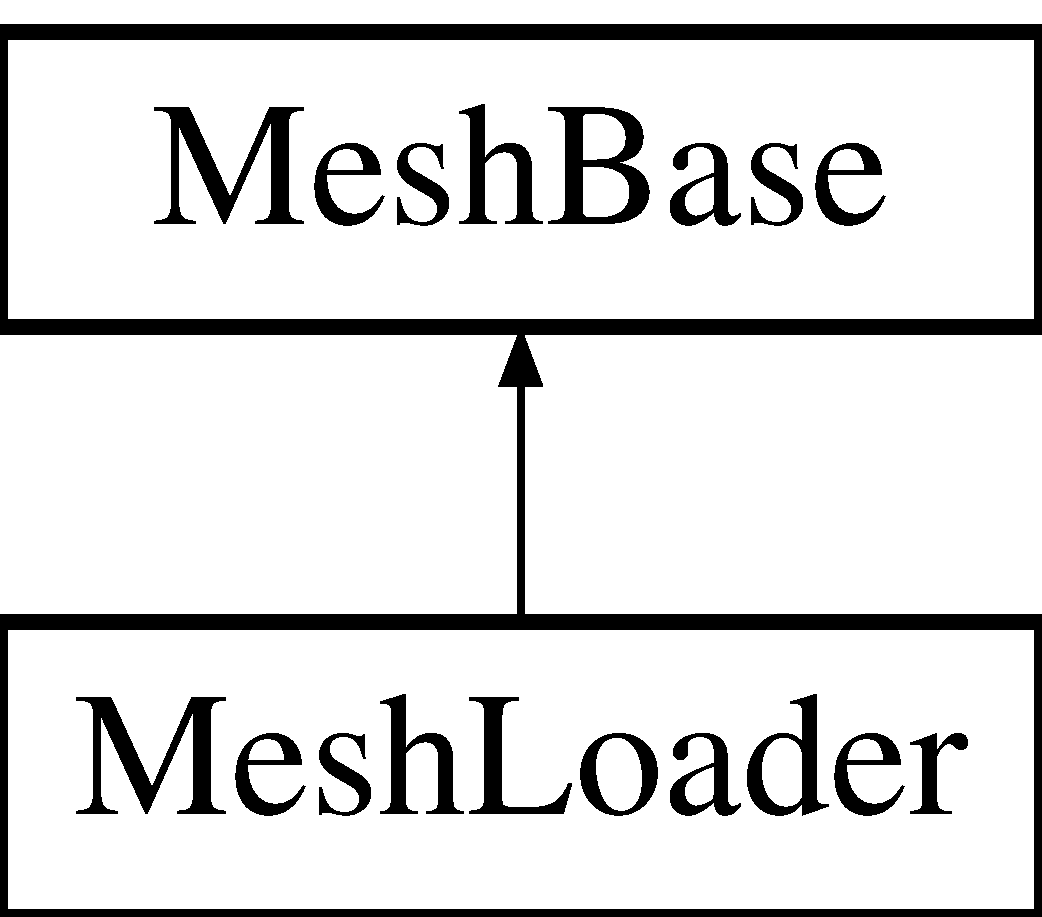
\includegraphics[height=2.000000cm]{class_mesh_base}
\end{center}
\end{figure}
\subsection*{Public Methods}
\begin{DoxyCompactItemize}
\item 
virtual void \hyperlink{class_mesh_base_a7280f0d6bacd225bb2d0263f17c05e8f}{load\+Model} (const std\+::string \&filename, bool insert\+Default\+Material=true, const \hyperlink{class_mesh_material_params}{Mesh\+Material\+Params} \&default\+Material=\hyperlink{class_mesh_material_params}{Mesh\+Material\+Params}())
\item 
{\footnotesize template$<$class Functor $>$ }\\void \hyperlink{class_mesh_base_a63937b1025ad3f9b4b2a4733a7409ff0}{for\+Each\+Group} (Functor functor) const
\item 
\mbox{\Hypertarget{class_mesh_base_a42fa472a3674008ac76ff1d4779f626f}\label{class_mesh_base_a42fa472a3674008ac76ff1d4779f626f}} 
{\footnotesize template$<$class Functor $>$ }\\void {\bfseries for\+Each\+Group} (Functor functor)
\item 
\mbox{\Hypertarget{class_mesh_base_a37b7b4a3e6240858d04074492b5196a1}\label{class_mesh_base_a37b7b4a3e6240858d04074492b5196a1}} 
int {\bfseries get\+Num\+Vertices} () const
\item 
\mbox{\Hypertarget{class_mesh_base_a8a3c2ae360ac491677a08d5dd1d6a70d}\label{class_mesh_base_a8a3c2ae360ac491677a08d5dd1d6a70d}} 
int {\bfseries get\+Num\+Normals} () const
\item 
\mbox{\Hypertarget{class_mesh_base_abc6eb296a90a5d6b0459fcf8be694c73}\label{class_mesh_base_abc6eb296a90a5d6b0459fcf8be694c73}} 
int {\bfseries get\+Num\+Colors} () const
\item 
\mbox{\Hypertarget{class_mesh_base_abeef82c768a229d566e646cf87a40972}\label{class_mesh_base_abeef82c768a229d566e646cf87a40972}} 
int {\bfseries get\+Num\+Texture\+Coordinates} () const
\item 
\mbox{\Hypertarget{class_mesh_base_ae3c47be68bf007cdfa0eedd019fb7f6f}\label{class_mesh_base_ae3c47be68bf007cdfa0eedd019fb7f6f}} 
int {\bfseries get\+Num\+Triangles} () const
\item 
\mbox{\Hypertarget{class_mesh_base_a05df5823f6b7b8bddc51c52d774d8c37}\label{class_mesh_base_a05df5823f6b7b8bddc51c52d774d8c37}} 
int {\bfseries get\+Num\+Groups} () const
\item 
\mbox{\Hypertarget{class_mesh_base_ad7d9d7ad3d442611cbd981bc28e16a3a}\label{class_mesh_base_ad7d9d7ad3d442611cbd981bc28e16a3a}} 
float $\ast$ {\bfseries get\+Vertex\+Data} ()
\item 
\mbox{\Hypertarget{class_mesh_base_aafcd96a999e70db59afb18963fcc0da9}\label{class_mesh_base_aafcd96a999e70db59afb18963fcc0da9}} 
const float $\ast$ {\bfseries get\+Vertex\+Data} () const
\item 
\mbox{\Hypertarget{class_mesh_base_a3f54fa8530f04fb7ca5f65a5926d096d}\label{class_mesh_base_a3f54fa8530f04fb7ca5f65a5926d096d}} 
float $\ast$ {\bfseries get\+Normal\+Data} ()
\item 
\mbox{\Hypertarget{class_mesh_base_a4889f21846770166952806dce1b6cb02}\label{class_mesh_base_a4889f21846770166952806dce1b6cb02}} 
const float $\ast$ {\bfseries get\+Normal\+Data} () const
\item 
\mbox{\Hypertarget{class_mesh_base_a1d33890b0671efeab525e60dcd865f8d}\label{class_mesh_base_a1d33890b0671efeab525e60dcd865f8d}} 
unsigned char $\ast$ {\bfseries get\+Color\+Data} ()
\item 
\mbox{\Hypertarget{class_mesh_base_ab87576c8d231a10f25646c7ac928aabd}\label{class_mesh_base_ab87576c8d231a10f25646c7ac928aabd}} 
const unsigned char $\ast$ {\bfseries get\+Color\+Data} () const
\item 
\mbox{\Hypertarget{class_mesh_base_a0e7351cf40de55390a3738f84e65b4b0}\label{class_mesh_base_a0e7351cf40de55390a3738f84e65b4b0}} 
float $\ast$ {\bfseries get\+Texture\+Coordinate\+Data} ()
\item 
\mbox{\Hypertarget{class_mesh_base_a08d10718a469776ce607ec81ba88b377}\label{class_mesh_base_a08d10718a469776ce607ec81ba88b377}} 
const float $\ast$ {\bfseries get\+Texture\+Coordinate\+Data} () const
\item 
\mbox{\Hypertarget{class_mesh_base_afaea93d4ed2236c7233cb6e19c26696c}\label{class_mesh_base_afaea93d4ed2236c7233cb6e19c26696c}} 
int {\bfseries get\+Vertex\+Stride} () const
\item 
\mbox{\Hypertarget{class_mesh_base_a1ba9f0d3dde4a27c62c83f69282b60fb}\label{class_mesh_base_a1ba9f0d3dde4a27c62c83f69282b60fb}} 
int {\bfseries get\+Normal\+Stride} () const
\item 
\mbox{\Hypertarget{class_mesh_base_aac85eda0950200f6b82e1d519677c749}\label{class_mesh_base_aac85eda0950200f6b82e1d519677c749}} 
int {\bfseries get\+Color\+Stride} () const
\item 
\mbox{\Hypertarget{class_mesh_base_ab38712efa2b4a0644375409843109767}\label{class_mesh_base_ab38712efa2b4a0644375409843109767}} 
int {\bfseries get\+Texture\+Coordinate\+Stride} () const
\item 
\mbox{\Hypertarget{class_mesh_base_a3f462666ec028e4db6588218c6859614}\label{class_mesh_base_a3f462666ec028e4db6588218c6859614}} 
const float $\ast$ {\bfseries get\+B\+Box\+Min} () const
\item 
\mbox{\Hypertarget{class_mesh_base_a2523965279aad48d2ec9d1c6dad52dd6}\label{class_mesh_base_a2523965279aad48d2ec9d1c6dad52dd6}} 
const float $\ast$ {\bfseries get\+B\+Box\+Max} () const
\item 
\mbox{\Hypertarget{class_mesh_base_a3d1adf4bf4df703213bbffca0c11dc7e}\label{class_mesh_base_a3d1adf4bf4df703213bbffca0c11dc7e}} 
void {\bfseries update\+B\+Box} ()
\item 
\mbox{\Hypertarget{class_mesh_base_a8f4908284b81877b9d2c228dd431fba9}\label{class_mesh_base_a8f4908284b81877b9d2c228dd431fba9}} 
const std\+::string \& {\bfseries get\+Material\+Library\+Name} () const
\item 
\mbox{\Hypertarget{class_mesh_base_a34a34bb6274bc30fbd6b2f604067a112}\label{class_mesh_base_a34a34bb6274bc30fbd6b2f604067a112}} 
\hyperlink{class_mesh_group}{Mesh\+Group} \& {\bfseries get\+Mesh\+Group} (const std\+::string \&group\+\_\+name)
\item 
\mbox{\Hypertarget{class_mesh_base_a4388d065bac6275d4302129118a91270}\label{class_mesh_base_a4388d065bac6275d4302129118a91270}} 
const \hyperlink{class_mesh_group}{Mesh\+Group} \& {\bfseries get\+Mesh\+Group} (const std\+::string \&group\+\_\+name) const
\item 
\mbox{\Hypertarget{class_mesh_base_a886536a107777458b46f9542ec942f03}\label{class_mesh_base_a886536a107777458b46f9542ec942f03}} 
size\+\_\+t {\bfseries get\+Material\+Count} () const
\item 
\mbox{\Hypertarget{class_mesh_base_a12b8c0065ea9c86fcb6788dc86197dc0}\label{class_mesh_base_a12b8c0065ea9c86fcb6788dc86197dc0}} 
void {\bfseries set\+Mesh\+Material\+Params} (int i, const \hyperlink{class_mesh_material_params}{Mesh\+Material\+Params} \&params)
\item 
\mbox{\Hypertarget{class_mesh_base_a49ce5e8227d6e83fcf2d38d71ae88300}\label{class_mesh_base_a49ce5e8227d6e83fcf2d38d71ae88300}} 
\hyperlink{class_mesh_material_params}{Mesh\+Material\+Params} \& {\bfseries get\+Mesh\+Material\+Params} (int i)
\item 
\mbox{\Hypertarget{class_mesh_base_af8481fb32c036f76c336f7ac6b605820}\label{class_mesh_base_af8481fb32c036f76c336f7ac6b605820}} 
const \hyperlink{class_mesh_material_params}{Mesh\+Material\+Params} \& {\bfseries get\+Mesh\+Material\+Params} (int i) const
\item 
\mbox{\Hypertarget{class_mesh_base_ad5332b0f81d76300422e37c2553a202a}\label{class_mesh_base_ad5332b0f81d76300422e37c2553a202a}} 
void {\bfseries set\+Mesh\+Grouping} (Mesh\+Grouping grouping)
\item 
\mbox{\Hypertarget{class_mesh_base_abddf7bcbe3c82b31488665ddd8d9f488}\label{class_mesh_base_abddf7bcbe3c82b31488665ddd8d9f488}} 
Mesh\+Grouping {\bfseries get\+Mesh\+Grouping} () const
\item 
\mbox{\Hypertarget{class_mesh_base_a58df3c198977e2068ab6008f24ff2b46}\label{class_mesh_base_a58df3c198977e2068ab6008f24ff2b46}} 
void {\bfseries load\+From\+Obj} (const std\+::string \&filename, bool insert\+Default\+Material, const \hyperlink{class_mesh_material_params}{Mesh\+Material\+Params} \&default\+Material)
\item 
void \hyperlink{class_mesh_base_a2abeac2d137eaea650ef5252cf81997a}{load\+Materials} (const std\+::string \&material\+\_\+filename)
\item 
void \hyperlink{class_mesh_base_a19e620f5497a82ac5508ee5fa2a8adce}{load\+From\+Ply} (const std\+::string \&filename, bool insert\+Default\+Material, const \hyperlink{class_mesh_material_params}{Mesh\+Material\+Params} \&default\+Material)
\end{DoxyCompactItemize}
\subsection*{Proteced Methods}
\begin{DoxyCompactItemize}
\item 
void \hyperlink{class_mesh_base_aa982e061ba3880ebdec15cff5310123b}{set\+Vertex\+Data} (float $\ast$vertex\+\_\+data)
\item 
\mbox{\Hypertarget{class_mesh_base_ae6bd7dcaded6875a6fbc80fe09d517d3}\label{class_mesh_base_ae6bd7dcaded6875a6fbc80fe09d517d3}} 
void {\bfseries set\+Normal\+Data} (float $\ast$normal\+\_\+data)
\item 
\mbox{\Hypertarget{class_mesh_base_a54f3706536926f73fa7ceb48c93613ba}\label{class_mesh_base_a54f3706536926f73fa7ceb48c93613ba}} 
void {\bfseries set\+Color\+Data} (unsigned char $\ast$color\+\_\+data)
\item 
\mbox{\Hypertarget{class_mesh_base_a50a2d578f5ca8551a223c005d73eeb05}\label{class_mesh_base_a50a2d578f5ca8551a223c005d73eeb05}} 
void {\bfseries set\+Texture\+Coordinate\+Data} (float $\ast$texture\+\_\+coordinate\+\_\+data)
\item 
\mbox{\Hypertarget{class_mesh_base_ac64e89644f2de5341e41b05ea161f642}\label{class_mesh_base_ac64e89644f2de5341e41b05ea161f642}} 
void {\bfseries set\+Material\+Indices} (int $\ast$material\+\_\+indices)
\item 
\mbox{\Hypertarget{class_mesh_base_ab5dcf66aca578fe503a4c6bc850bd81e}\label{class_mesh_base_ab5dcf66aca578fe503a4c6bc850bd81e}} 
void {\bfseries set\+Vertex\+Stride} (int vertex\+\_\+stride)
\item 
\mbox{\Hypertarget{class_mesh_base_ad7b51e2e6058a8d79ec0896136da0034}\label{class_mesh_base_ad7b51e2e6058a8d79ec0896136da0034}} 
void {\bfseries set\+Normal\+Stride} (int normal\+\_\+stride)
\item 
\mbox{\Hypertarget{class_mesh_base_a6e93b05a9521bb14fcb68d9ce1771cfa}\label{class_mesh_base_a6e93b05a9521bb14fcb68d9ce1771cfa}} 
void {\bfseries set\+Color\+Stride} (int color\+\_\+stride)
\item 
\mbox{\Hypertarget{class_mesh_base_a85b5140f3641d28e2468f6547ba365c1}\label{class_mesh_base_a85b5140f3641d28e2468f6547ba365c1}} 
void {\bfseries set\+Texture\+Coordinate\+Stride} (int texture\+\_\+coordinate\+\_\+stride)
\item 
\mbox{\Hypertarget{class_mesh_base_a2ed368cf25b8c43ac18824c6dd980efa}\label{class_mesh_base_a2ed368cf25b8c43ac18824c6dd980efa}} 
void {\bfseries set\+Vertex\+Index\+Stride} (int index\+\_\+stride)
\item 
\mbox{\Hypertarget{class_mesh_base_aa3541f6e43c78bf78bada0aed22515e4}\label{class_mesh_base_aa3541f6e43c78bf78bada0aed22515e4}} 
void {\bfseries set\+Normal\+Index\+Stride} (int index\+\_\+stride)
\item 
\mbox{\Hypertarget{class_mesh_base_ae0f218a5d46a946dbd131321f3ecb6c5}\label{class_mesh_base_ae0f218a5d46a946dbd131321f3ecb6c5}} 
void {\bfseries set\+Color\+Index\+Stride} (int index\+\_\+stride)
\item 
\mbox{\Hypertarget{class_mesh_base_a9406f179533bc966d60ca7a0d8f124b9}\label{class_mesh_base_a9406f179533bc966d60ca7a0d8f124b9}} 
void {\bfseries set\+Texture\+Index\+Stride} (int index\+\_\+stride)
\item 
\mbox{\Hypertarget{class_mesh_base_a3be83f6c6a41e7b786c804eda9b9f247}\label{class_mesh_base_a3be83f6c6a41e7b786c804eda9b9f247}} 
const std\+::string \& {\bfseries get\+Filename} () const
\item 
\mbox{\Hypertarget{class_mesh_base_a91f01999b6fa0fe764db833fdf3b17b1}\label{class_mesh_base_a91f01999b6fa0fe764db833fdf3b17b1}} 
const std\+::string \& {\bfseries get\+Path\+Name} () const
\item 
virtual int \hyperlink{class_mesh_base_a508fde807d380849192391f28465fee4}{get\+Vertex\+Triangle\+Size} () const =0
\item 
\mbox{\Hypertarget{class_mesh_base_a249856ea8eb734ae36bdf51ea4bdbdd7}\label{class_mesh_base_a249856ea8eb734ae36bdf51ea4bdbdd7}} 
virtual int {\bfseries get\+Normal\+Triangle\+Size} () const =0
\item 
\mbox{\Hypertarget{class_mesh_base_aa8b94fe22c0d261357d2386cf2b5624c}\label{class_mesh_base_aa8b94fe22c0d261357d2386cf2b5624c}} 
virtual int {\bfseries get\+Texture\+Triangle\+Size} () const =0
\item 
virtual void \hyperlink{class_mesh_base_a25e192211e37cb69f9b5ce9aea25989a}{pre\+Process} ()=0
\item 
virtual void \hyperlink{class_mesh_base_a30c0ef8b3faabc9b41520b85dd9413bb}{allocate\+Data} ()=0
\item 
virtual void \hyperlink{class_mesh_base_a67eb9bc7c4f6b074626078fe7779a8a4}{start\+Writing\+Data} ()=0
\item 
virtual void \hyperlink{class_mesh_base_a49ec1a25d18103982974f424b77fadc0}{post\+Process} ()=0
\item 
virtual void \hyperlink{class_mesh_base_a000796d7b04985f137d5a1368e90bcc6}{finish\+Writing\+Data} ()=0
\item 
\mbox{\Hypertarget{class_mesh_base_acd4ecf54012593c422da74efb8afd49d}\label{class_mesh_base_acd4ecf54012593c422da74efb8afd49d}} 
void {\bfseries compute\+Aabb} ()
\end{DoxyCompactItemize}


\subsection{Member Function Documentation}
\mbox{\Hypertarget{class_mesh_base_a30c0ef8b3faabc9b41520b85dd9413bb}\label{class_mesh_base_a30c0ef8b3faabc9b41520b85dd9413bb}} 
\index{Mesh\+Base@{Mesh\+Base}!allocate\+Data@{allocate\+Data}}
\index{allocate\+Data@{allocate\+Data}!Mesh\+Base@{Mesh\+Base}}
\subsubsection{\texorpdfstring{allocate\+Data()}{allocateData()}}
{\footnotesize\ttfamily virtual void Mesh\+Base\+::allocate\+Data (\begin{DoxyParamCaption}{ }\end{DoxyParamCaption})\hspace{0.3cm}{\ttfamily [protected]}, {\ttfamily [pure virtual]}}

Call this to allocate all data for the mesh after setting num\+\_\+vertices, num\+\_\+normals, num\+\_\+colors, and num\+\_\+texture\+\_\+coordinates, as well as num\+\_\+triangles for all the groups. 

Implemented in \hyperlink{class_mesh_loader_a8bdf8e0894e147be8d3e287f46feff6a}{Mesh\+Loader}.

\mbox{\Hypertarget{class_mesh_base_a000796d7b04985f137d5a1368e90bcc6}\label{class_mesh_base_a000796d7b04985f137d5a1368e90bcc6}} 
\index{Mesh\+Base@{Mesh\+Base}!finish\+Writing\+Data@{finish\+Writing\+Data}}
\index{finish\+Writing\+Data@{finish\+Writing\+Data}!Mesh\+Base@{Mesh\+Base}}
\subsubsection{\texorpdfstring{finish\+Writing\+Data()}{finishWritingData()}}
{\footnotesize\ttfamily virtual void Mesh\+Base\+::finish\+Writing\+Data (\begin{DoxyParamCaption}{ }\end{DoxyParamCaption})\hspace{0.3cm}{\ttfamily [protected]}, {\ttfamily [pure virtual]}}

Call this when done writing to data or group data. 

Implemented in \hyperlink{class_mesh_loader_a65847db267f07f637deab0889c283bfa}{Mesh\+Loader}.

\mbox{\Hypertarget{class_mesh_base_a63937b1025ad3f9b4b2a4733a7409ff0}\label{class_mesh_base_a63937b1025ad3f9b4b2a4733a7409ff0}} 
\index{Mesh\+Base@{Mesh\+Base}!for\+Each\+Group@{for\+Each\+Group}}
\index{for\+Each\+Group@{for\+Each\+Group}!Mesh\+Base@{Mesh\+Base}}
\subsubsection{\texorpdfstring{for\+Each\+Group()}{forEachGroup()}}
{\footnotesize\ttfamily template$<$class Functor $>$ \\
void Mesh\+Base\+::for\+Each\+Group (\begin{DoxyParamCaption}\item[{Functor}]{functor }\end{DoxyParamCaption}) const}

Calls functor( group ) for each group in the mesh, where \textquotesingle{}group\textquotesingle{} is of the type \hyperlink{class_mesh_group}{Mesh\+Group}. \mbox{\Hypertarget{class_mesh_base_a508fde807d380849192391f28465fee4}\label{class_mesh_base_a508fde807d380849192391f28465fee4}} 
\index{Mesh\+Base@{Mesh\+Base}!get\+Vertex\+Triangle\+Size@{get\+Vertex\+Triangle\+Size}}
\index{get\+Vertex\+Triangle\+Size@{get\+Vertex\+Triangle\+Size}!Mesh\+Base@{Mesh\+Base}}
\subsubsection{\texorpdfstring{get\+Vertex\+Triangle\+Size()}{getVertexTriangleSize()}}
{\footnotesize\ttfamily virtual int Mesh\+Base\+::get\+Vertex\+Triangle\+Size (\begin{DoxyParamCaption}{ }\end{DoxyParamCaption}) const\hspace{0.3cm}{\ttfamily [protected]}, {\ttfamily [pure virtual]}}

These pure virtual functions allow subclasses to control much about the loading behavior. 

Implemented in \hyperlink{class_mesh_loader_a3e228f5e2fbb1261cd76871ee07e4f58}{Mesh\+Loader}.

\mbox{\Hypertarget{class_mesh_base_a19e620f5497a82ac5508ee5fa2a8adce}\label{class_mesh_base_a19e620f5497a82ac5508ee5fa2a8adce}} 
\index{Mesh\+Base@{Mesh\+Base}!load\+From\+Ply@{load\+From\+Ply}}
\index{load\+From\+Ply@{load\+From\+Ply}!Mesh\+Base@{Mesh\+Base}}
\subsubsection{\texorpdfstring{load\+From\+Ply()}{loadFromPly()}}
{\footnotesize\ttfamily void Mesh\+Base\+::load\+From\+Ply (\begin{DoxyParamCaption}\item[{const std\+::string \&}]{filename,  }\item[{bool}]{insert\+Default\+Material,  }\item[{const \hyperlink{class_mesh_material_params}{Mesh\+Material\+Params} \&}]{default\+Material }\end{DoxyParamCaption})}

Similar to load\+From\+Obj() bur for .ply files \mbox{\Hypertarget{class_mesh_base_a2abeac2d137eaea650ef5252cf81997a}\label{class_mesh_base_a2abeac2d137eaea650ef5252cf81997a}} 
\index{Mesh\+Base@{Mesh\+Base}!load\+Materials@{load\+Materials}}
\index{load\+Materials@{load\+Materials}!Mesh\+Base@{Mesh\+Base}}
\subsubsection{\texorpdfstring{load\+Materials()}{loadMaterials()}}
{\footnotesize\ttfamily void Mesh\+Base\+::load\+Materials (\begin{DoxyParamCaption}\item[{const std\+::string \&}]{material\+\_\+filename }\end{DoxyParamCaption})}

Load a material library \mbox{\Hypertarget{class_mesh_base_a7280f0d6bacd225bb2d0263f17c05e8f}\label{class_mesh_base_a7280f0d6bacd225bb2d0263f17c05e8f}} 
\index{Mesh\+Base@{Mesh\+Base}!load\+Model@{load\+Model}}
\index{load\+Model@{load\+Model}!Mesh\+Base@{Mesh\+Base}}
\subsubsection{\texorpdfstring{load\+Model()}{loadModel()}}
{\footnotesize\ttfamily void Mesh\+Base\+::load\+Model (\begin{DoxyParamCaption}\item[{const std\+::string \&}]{filename,  }\item[{bool}]{insert\+Default\+Material = {\ttfamily true},  }\item[{const \hyperlink{class_mesh_material_params}{Mesh\+Material\+Params} \&}]{default\+Material = {\ttfamily \hyperlink{class_mesh_material_params}{Mesh\+Material\+Params}()} }\end{DoxyParamCaption})\hspace{0.3cm}{\ttfamily [virtual]}}

The \hyperlink{group___c_u_d_a_module_ga2786ba75af2a254c03f272b6211b6379}{load()} method provides the overall model loading algorithm, which calls upon pure virtual functions which must override. The algorithm is as follows, where \textquotesingle{}function()\textquotesingle{} indicates a call to one of the pure virtual functions\+:


\begin{DoxyItemize}
\item \hyperlink{class_mesh_base_a25e192211e37cb69f9b5ce9aea25989a}{pre\+Process()}
\item Does a first pass on the model file to collect information about the number of vertices, normals, colors, and texture coordinates in the file, which it stores in the mesh\textquotesingle{}s fields \textquotesingle{}num\+\_\+vertices\textquotesingle{}, \textquotesingle{}num\+\_\+normals\textquotesingle{}, etc. The first pass also creates the \textquotesingle{}groups\textquotesingle{} structure with \textquotesingle{}num\+\_\+triangles\textquotesingle{} set for each group\textquotesingle{}.
\item \hyperlink{class_mesh_base_a30c0ef8b3faabc9b41520b85dd9413bb}{allocate\+Data()}, which allocates arrays, buffers, or whatever may be required for the subclass to own the data; the numbers collected during the \char`\"{}first pass\char`\"{} can be used for allocation sizes.
\item \hyperlink{class_mesh_base_a67eb9bc7c4f6b074626078fe7779a8a4}{start\+Writing\+Data()}, which is useful for cases where the subclass must first prepare for being written to, such as mapping Buffers, in the case of OptiX buffers.
\item The second pass, in which it actually loads the data from the model file and stores it in the array pointers vertex\+\_\+data, normal\+\_\+data, color\+\_\+data, and texture\+\_\+coordinate\+\_\+data, which should have been properly initalized to receive writes, either during \hyperlink{class_mesh_base_a30c0ef8b3faabc9b41520b85dd9413bb}{allocate\+Data()} or \hyperlink{class_mesh_base_a67eb9bc7c4f6b074626078fe7779a8a4}{start\+Writing\+Data()}. If any of these $\ast$\+\_\+data pointers are \textquotesingle{}0\textquotesingle{}, they will not be written to. Each group in the groups structure should also have had its field pointers vertex\+\_\+indices, normal\+\_\+indices, etc. initialized.
\item Computes the bounding box on the model.
\item \hyperlink{class_mesh_base_a49ec1a25d18103982974f424b77fadc0}{post\+Process()},
\item \hyperlink{class_mesh_base_a000796d7b04985f137d5a1368e90bcc6}{finish\+Writing\+Data()}, for any cleanup that must be done, such as unmapping OptiX buffers.
\end{DoxyItemize}

Note that for uniformity with .ply loading, and for the accuracy of external algorithms that iterate over vertices (such as bounding box computation), or other alforithms that require an accurate count of the number of vertices actually used, 1-\/based indexing in .obj files is translated to 0-\/based indexing. \mbox{\Hypertarget{class_mesh_base_a49ec1a25d18103982974f424b77fadc0}\label{class_mesh_base_a49ec1a25d18103982974f424b77fadc0}} 
\index{Mesh\+Base@{Mesh\+Base}!post\+Process@{post\+Process}}
\index{post\+Process@{post\+Process}!Mesh\+Base@{Mesh\+Base}}
\subsubsection{\texorpdfstring{post\+Process()}{postProcess()}}
{\footnotesize\ttfamily virtual void Mesh\+Base\+::post\+Process (\begin{DoxyParamCaption}{ }\end{DoxyParamCaption})\hspace{0.3cm}{\ttfamily [protected]}, {\ttfamily [pure virtual]}}

An injection point for subclasses to do load postprocessing 

Implemented in \hyperlink{class_mesh_loader_a83a3c78a6c2df1087c9f9e28c63e6d51}{Mesh\+Loader}.

\mbox{\Hypertarget{class_mesh_base_a25e192211e37cb69f9b5ce9aea25989a}\label{class_mesh_base_a25e192211e37cb69f9b5ce9aea25989a}} 
\index{Mesh\+Base@{Mesh\+Base}!pre\+Process@{pre\+Process}}
\index{pre\+Process@{pre\+Process}!Mesh\+Base@{Mesh\+Base}}
\subsubsection{\texorpdfstring{pre\+Process()}{preProcess()}}
{\footnotesize\ttfamily virtual void Mesh\+Base\+::pre\+Process (\begin{DoxyParamCaption}{ }\end{DoxyParamCaption})\hspace{0.3cm}{\ttfamily [protected]}, {\ttfamily [pure virtual]}}

An injection point for subclasses to do any prep before file info is loaded 

Implemented in \hyperlink{class_mesh_loader_ad9c636920b31629f1c271b20a5fdc29b}{Mesh\+Loader}.

\mbox{\Hypertarget{class_mesh_base_aa982e061ba3880ebdec15cff5310123b}\label{class_mesh_base_aa982e061ba3880ebdec15cff5310123b}} 
\index{Mesh\+Base@{Mesh\+Base}!set\+Vertex\+Data@{set\+Vertex\+Data}}
\index{set\+Vertex\+Data@{set\+Vertex\+Data}!Mesh\+Base@{Mesh\+Base}}
\subsubsection{\texorpdfstring{set\+Vertex\+Data()}{setVertexData()}}
{\footnotesize\ttfamily void Mesh\+Base\+::set\+Vertex\+Data (\begin{DoxyParamCaption}\item[{float $\ast$}]{vertex\+\_\+data }\end{DoxyParamCaption})\hspace{0.3cm}{\ttfamily [inline]}, {\ttfamily [protected]}}

Accessors for derived classes \mbox{\Hypertarget{class_mesh_base_a67eb9bc7c4f6b074626078fe7779a8a4}\label{class_mesh_base_a67eb9bc7c4f6b074626078fe7779a8a4}} 
\index{Mesh\+Base@{Mesh\+Base}!start\+Writing\+Data@{start\+Writing\+Data}}
\index{start\+Writing\+Data@{start\+Writing\+Data}!Mesh\+Base@{Mesh\+Base}}
\subsubsection{\texorpdfstring{start\+Writing\+Data()}{startWritingData()}}
{\footnotesize\ttfamily virtual void Mesh\+Base\+::start\+Writing\+Data (\begin{DoxyParamCaption}{ }\end{DoxyParamCaption})\hspace{0.3cm}{\ttfamily [protected]}, {\ttfamily [pure virtual]}}

Call this before writing any data to the mesh, to set up correct pointer values to write to for vertex\+\_\+data, normal\+\_\+data, etc., as well as vertex\+\_\+indices, normal\+\_\+indices, etc. for each of the groups.

Call \hyperlink{class_mesh_base_a000796d7b04985f137d5a1368e90bcc6}{finish\+Writing\+Data()} when done. 

Implemented in \hyperlink{class_mesh_loader_a18379e41707d8127947aa17a622d2807}{Mesh\+Loader}.



The documentation for this class was generated from the following files\+:\begin{DoxyCompactItemize}
\item 
C\+:/p4research/research/jpantaleoni/\+Fermat-\/\+Public/src/mesh/Mesh\+Base.\+h\item 
C\+:/p4research/research/jpantaleoni/\+Fermat-\/\+Public/src/mesh/Mesh\+Base.\+cpp\end{DoxyCompactItemize}

\hypertarget{class_mesh_exception}{}\section{Mesh\+Exception Class Reference}
\label{class_mesh_exception}\index{Mesh\+Exception@{Mesh\+Exception}}
Inheritance diagram for Mesh\+Exception\+:\begin{figure}[H]
\begin{center}
\leavevmode
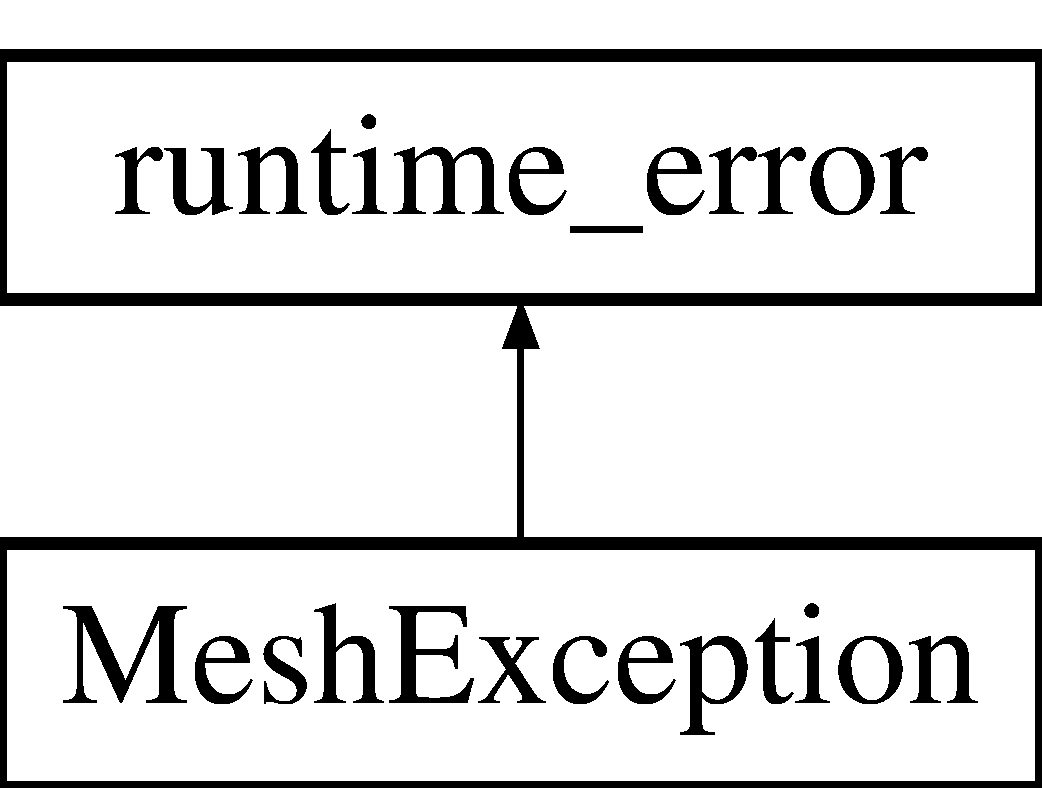
\includegraphics[height=2.000000cm]{class_mesh_exception}
\end{center}
\end{figure}
\subsection*{Public Methods}
\begin{DoxyCompactItemize}
\item 
\mbox{\Hypertarget{class_mesh_exception_a73768a8610ce6401dee99603f1ca0666}\label{class_mesh_exception_a73768a8610ce6401dee99603f1ca0666}} 
{\bfseries Mesh\+Exception} (const std\+::string \&what\+\_\+arg)
\end{DoxyCompactItemize}


The documentation for this class was generated from the following file\+:\begin{DoxyCompactItemize}
\item 
C\+:/p4research/research/jpantaleoni/\+Fermat-\/\+Public/src/mesh/Mesh\+Exception.\+h\end{DoxyCompactItemize}

\hypertarget{class_mesh_group}{}\section{Mesh\+Group Class Reference}
\label{class_mesh_group}\index{Mesh\+Group@{Mesh\+Group}}
\subsection*{Public Members}
\begin{DoxyCompactItemize}
\item 
\mbox{\Hypertarget{class_mesh_group_a0c249a500b8f7a0262ca9bd77596e75a}\label{class_mesh_group_a0c249a500b8f7a0262ca9bd77596e75a}} 
std\+::string {\bfseries name}
\item 
\mbox{\Hypertarget{class_mesh_group_a4b9095a570997b2d82c36b317967395b}\label{class_mesh_group_a4b9095a570997b2d82c36b317967395b}} 
int {\bfseries num\+\_\+triangles}
\item 
\mbox{\Hypertarget{class_mesh_group_a7707177ef409bd175c918632fc9e9111}\label{class_mesh_group_a7707177ef409bd175c918632fc9e9111}} 
int $\ast$ {\bfseries vertex\+\_\+indices}
\item 
\mbox{\Hypertarget{class_mesh_group_a8e370c787784ccbf44dc15ad576cd68f}\label{class_mesh_group_a8e370c787784ccbf44dc15ad576cd68f}} 
int $\ast$ {\bfseries normal\+\_\+indices}
\item 
\mbox{\Hypertarget{class_mesh_group_a94a17f1b4cc8414502e911bb956eb087}\label{class_mesh_group_a94a17f1b4cc8414502e911bb956eb087}} 
int $\ast$ {\bfseries color\+\_\+indices}
\item 
\mbox{\Hypertarget{class_mesh_group_a658b8e233e6d0451fb7eeb6c18a64db6}\label{class_mesh_group_a658b8e233e6d0451fb7eeb6c18a64db6}} 
int $\ast$ {\bfseries texture\+\_\+coordinate\+\_\+indices}
\item 
\mbox{\Hypertarget{class_mesh_group_a8c5de1549a0bbe0cecb2f015fe8696f2}\label{class_mesh_group_a8c5de1549a0bbe0cecb2f015fe8696f2}} 
int $\ast$ {\bfseries material\+\_\+indices}
\item 
\mbox{\Hypertarget{class_mesh_group_a5caca260e5d72b8998c67649b3210c1e}\label{class_mesh_group_a5caca260e5d72b8998c67649b3210c1e}} 
int {\bfseries material\+\_\+number}
\end{DoxyCompactItemize}


The documentation for this class was generated from the following file\+:\begin{DoxyCompactItemize}
\item 
C\+:/p4research/research/jpantaleoni/\+Fermat-\/\+Public/src/mesh/Mesh\+Base.\+h\end{DoxyCompactItemize}

\hypertarget{struct_mesh_light}{}\section{Mesh\+Light Struct Reference}
\label{struct_mesh_light}\index{Mesh\+Light@{Mesh\+Light}}


\subsection{Detailed description}
Mesh-\/light class 

{\ttfamily \#include $<$lights.\+h$>$}

Inheritance diagram for Mesh\+Light\+:\begin{figure}[H]
\begin{center}
\leavevmode
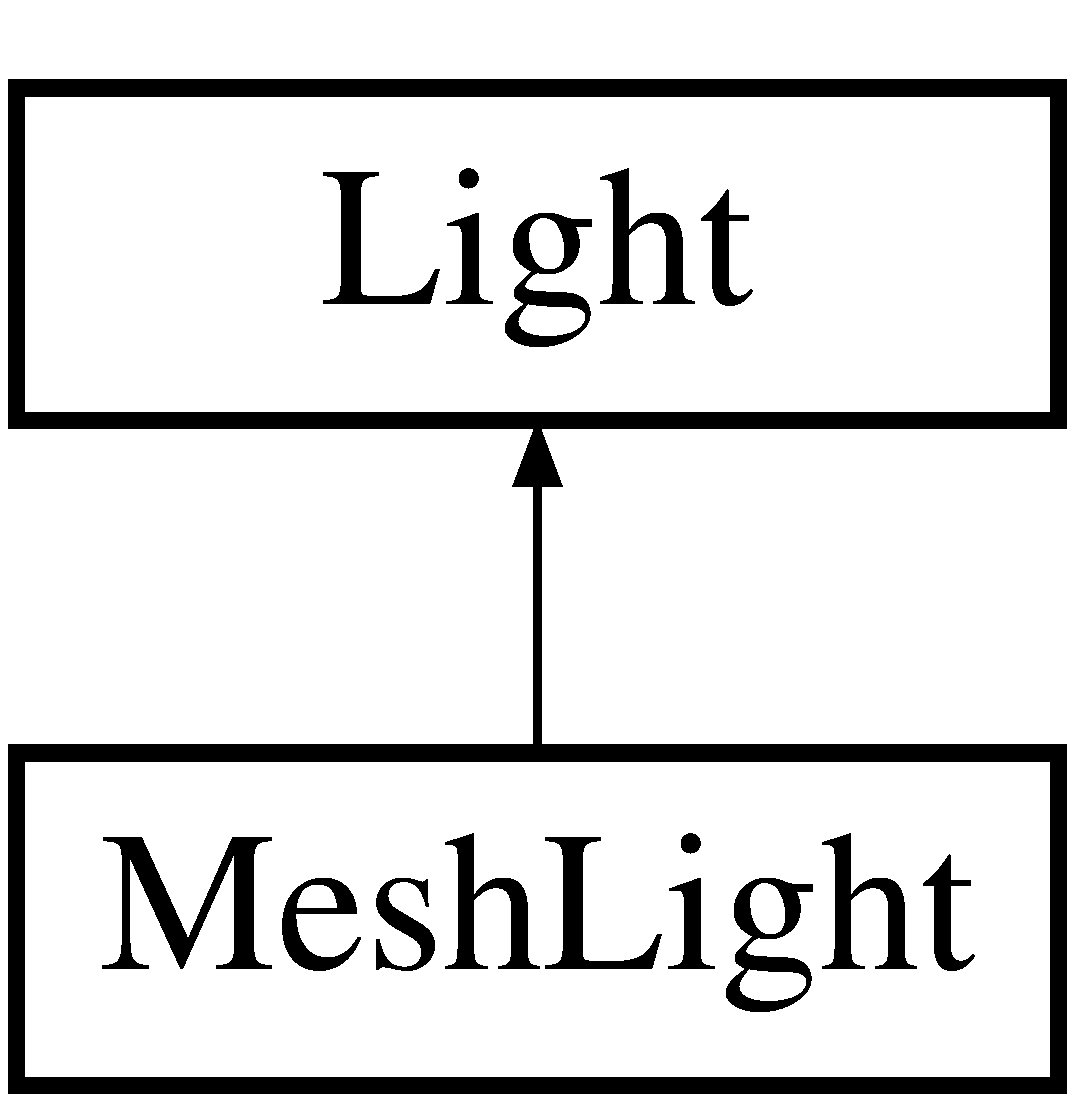
\includegraphics[height=2.000000cm]{struct_mesh_light}
\end{center}
\end{figure}
\subsection*{Public Methods}
\begin{DoxyCompactItemize}
\item 
\mbox{\Hypertarget{struct_mesh_light_a222612bad947072eea2d1f0936ef2828}\label{struct_mesh_light_a222612bad947072eea2d1f0936ef2828}} 
F\+E\+R\+M\+A\+T\+\_\+\+H\+O\+S\+T\+\_\+\+D\+E\+V\+I\+CE {\bfseries Mesh\+Light} (const uint32 \+\_\+n\+\_\+prims, const float $\ast$\+\_\+prims\+\_\+cdf, const float $\ast$\+\_\+prims\+\_\+inv\+\_\+area, \hyperlink{struct_mesh_view}{Mesh\+View} \+\_\+mesh, const \hyperlink{struct_mip_map_view}{Mip\+Map\+View} $\ast$\+\_\+textures, const uint32 \+\_\+n\+\_\+vpls, const float $\ast$\+\_\+vpls\+\_\+cdf, const \hyperlink{struct_v_p_l}{V\+PL} $\ast$\+\_\+vpls, const float \+\_\+norm)
\item 
F\+E\+R\+M\+A\+T\+\_\+\+H\+O\+S\+T\+\_\+\+D\+E\+V\+I\+CE bool \hyperlink{struct_mesh_light_a41958f4c2147ad55bb95ca8ba90ec39b}{sample\+\_\+impl} (const float $\ast$Z, uint32\+\_\+t $\ast$prim\+\_\+id, \hyperlink{structcugar_1_1_vector}{cugar\+::\+Vector2f} $\ast$uv, \hyperlink{struct_vertex_geometry}{Vertex\+Geometry} $\ast$geom, float $\ast$pdf, \hyperlink{struct_edf}{Edf} $\ast$edf) const
\item 
F\+E\+R\+M\+A\+T\+\_\+\+H\+O\+S\+T\+\_\+\+D\+E\+V\+I\+CE void \hyperlink{struct_mesh_light_a86f0d4badaca1671063ce758bd04812f}{intersect\+\_\+impl} (const \hyperlink{struct_ray}{Ray} ray, float2 $\ast$uv, float $\ast$t) const
\item 
F\+E\+R\+M\+A\+T\+\_\+\+H\+O\+S\+T\+\_\+\+D\+E\+V\+I\+CE void \hyperlink{struct_mesh_light_ad39eed77c5604446aef6dc7373ba80ce}{map\+\_\+impl} (const uint32\+\_\+t prim\+\_\+id, const \hyperlink{structcugar_1_1_vector}{cugar\+::\+Vector2f} \&uv, \hyperlink{struct_vertex_geometry}{Vertex\+Geometry} $\ast$geom, float $\ast$pdf, \hyperlink{struct_edf}{Edf} $\ast$edf) const
\item 
F\+E\+R\+M\+A\+T\+\_\+\+H\+O\+S\+T\+\_\+\+D\+E\+V\+I\+CE void \hyperlink{struct_mesh_light_a0be71bfb03b0489b514a3efcb2daf2a8}{map\+\_\+impl} (const uint32\+\_\+t prim\+\_\+id, const \hyperlink{structcugar_1_1_vector}{cugar\+::\+Vector2f} \&uv, const \hyperlink{struct_vertex_geometry}{Vertex\+Geometry} \&geom, float $\ast$pdf, \hyperlink{struct_edf}{Edf} $\ast$edf) const
\item 
F\+E\+R\+M\+A\+T\+\_\+\+H\+O\+S\+T\+\_\+\+D\+E\+V\+I\+CE bool \hyperlink{struct_mesh_light_a60e26a42c876094525bf87497084c798}{invert\+\_\+impl} (const uint32\+\_\+t prim\+\_\+id, const \hyperlink{structcugar_1_1_vector}{cugar\+::\+Vector2f} \&uv, const float $\ast$in\+\_\+Z, float $\ast$out\+\_\+Z, float $\ast$out\+\_\+pdf) const
\item 
F\+E\+R\+M\+A\+T\+\_\+\+H\+O\+S\+T\+\_\+\+D\+E\+V\+I\+CE float \hyperlink{struct_mesh_light_a3c6e89823dc653d7c0b0ce28c0f8f770}{inverse\+\_\+pdf\+\_\+impl} (const uint32\+\_\+t prim\+\_\+id, const \hyperlink{structcugar_1_1_vector}{cugar\+::\+Vector2f} \&uv, const float $\ast$out\+\_\+Z) const
\item 
\mbox{\Hypertarget{struct_mesh_light_af8131c05153454d4b66a91c4ba60ad0b}\label{struct_mesh_light_af8131c05153454d4b66a91c4ba60ad0b}} 
F\+E\+R\+M\+A\+T\+\_\+\+H\+O\+S\+T\+\_\+\+D\+E\+V\+I\+CE uint32 {\bfseries vpl\+\_\+count} () const
\item 
\mbox{\Hypertarget{struct_mesh_light_a02d804cf3aa7a4c78bacfbc09703d2e4}\label{struct_mesh_light_a02d804cf3aa7a4c78bacfbc09703d2e4}} 
F\+E\+R\+M\+A\+T\+\_\+\+H\+O\+S\+T\+\_\+\+D\+E\+V\+I\+CE \hyperlink{struct_v_p_l}{V\+PL} {\bfseries get\+\_\+vpl} (const uint32 i) const
\item 
F\+E\+R\+M\+A\+T\+\_\+\+H\+O\+S\+T\+\_\+\+D\+E\+V\+I\+CE void \hyperlink{struct_mesh_light_a2282bb91c6d716231dbf81701fd6c05c}{map\+\_\+vpl} (const uint32 vpl\+\_\+idx, uint32\+\_\+t $\ast$prim\+\_\+id, \hyperlink{structcugar_1_1_vector}{cugar\+::\+Vector2f} $\ast$uv, \hyperlink{struct_vertex_geometry}{Vertex\+Geometry} $\ast$geom, float $\ast$pdf, \hyperlink{struct_edf}{Edf} $\ast$edf) const
\end{DoxyCompactItemize}
\subsection*{Public Members}
\begin{DoxyCompactItemize}
\item 
\mbox{\Hypertarget{struct_mesh_light_a192e774d65e4193bf0fe9f8f96466582}\label{struct_mesh_light_a192e774d65e4193bf0fe9f8f96466582}} 
uint32 {\bfseries n\+\_\+prims}
\item 
\mbox{\Hypertarget{struct_mesh_light_a38368cd0949e9ee649fef574bb31f652}\label{struct_mesh_light_a38368cd0949e9ee649fef574bb31f652}} 
const float $\ast$ {\bfseries prims\+\_\+cdf}
\item 
\mbox{\Hypertarget{struct_mesh_light_a6845a9b9fe3f926fc4d421c180d9ef91}\label{struct_mesh_light_a6845a9b9fe3f926fc4d421c180d9ef91}} 
const float $\ast$ {\bfseries prims\+\_\+inv\+\_\+area}
\item 
\mbox{\Hypertarget{struct_mesh_light_ad680e09125846fe1089f5bce9cd4ebb9}\label{struct_mesh_light_ad680e09125846fe1089f5bce9cd4ebb9}} 
\hyperlink{struct_mesh_view}{Mesh\+View} {\bfseries mesh}
\item 
\mbox{\Hypertarget{struct_mesh_light_a134240d648ea32702db6ce08d6cb8f7f}\label{struct_mesh_light_a134240d648ea32702db6ce08d6cb8f7f}} 
const \hyperlink{struct_mip_map_view}{Mip\+Map\+View} $\ast$ {\bfseries textures}
\item 
\mbox{\Hypertarget{struct_mesh_light_a9103411cedd0b1428984273b52535644}\label{struct_mesh_light_a9103411cedd0b1428984273b52535644}} 
uint32 {\bfseries n\+\_\+vpls}
\item 
\mbox{\Hypertarget{struct_mesh_light_a545baf971f56eea4a77efcf228a09ef4}\label{struct_mesh_light_a545baf971f56eea4a77efcf228a09ef4}} 
const float $\ast$ {\bfseries vpls\+\_\+cdf}
\item 
\mbox{\Hypertarget{struct_mesh_light_a7e9cf283a1d2489bbd813b4e16330865}\label{struct_mesh_light_a7e9cf283a1d2489bbd813b4e16330865}} 
const \hyperlink{struct_v_p_l}{V\+PL} $\ast$ {\bfseries vpls}
\item 
\mbox{\Hypertarget{struct_mesh_light_ad43d099988a13da497963e699dedd639}\label{struct_mesh_light_ad43d099988a13da497963e699dedd639}} 
float {\bfseries norm}
\end{DoxyCompactItemize}


\subsection{Member Function Documentation}
\mbox{\Hypertarget{struct_mesh_light_a86f0d4badaca1671063ce758bd04812f}\label{struct_mesh_light_a86f0d4badaca1671063ce758bd04812f}} 
\index{Mesh\+Light@{Mesh\+Light}!intersect\+\_\+impl@{intersect\+\_\+impl}}
\index{intersect\+\_\+impl@{intersect\+\_\+impl}!Mesh\+Light@{Mesh\+Light}}
\subsubsection{\texorpdfstring{intersect\+\_\+impl()}{intersect\_impl()}}
{\footnotesize\ttfamily F\+E\+R\+M\+A\+T\+\_\+\+H\+O\+S\+T\+\_\+\+D\+E\+V\+I\+CE void Mesh\+Light\+::intersect\+\_\+impl (\begin{DoxyParamCaption}\item[{const \hyperlink{struct_ray}{Ray}}]{ray,  }\item[{float2 $\ast$}]{uv,  }\item[{float $\ast$}]{t }\end{DoxyParamCaption}) const\hspace{0.3cm}{\ttfamily [inline]}}

intersect the given ray with the light source \mbox{\Hypertarget{struct_mesh_light_a3c6e89823dc653d7c0b0ce28c0f8f770}\label{struct_mesh_light_a3c6e89823dc653d7c0b0ce28c0f8f770}} 
\index{Mesh\+Light@{Mesh\+Light}!inverse\+\_\+pdf\+\_\+impl@{inverse\+\_\+pdf\+\_\+impl}}
\index{inverse\+\_\+pdf\+\_\+impl@{inverse\+\_\+pdf\+\_\+impl}!Mesh\+Light@{Mesh\+Light}}
\subsubsection{\texorpdfstring{inverse\+\_\+pdf\+\_\+impl()}{inverse\_pdf\_impl()}}
{\footnotesize\ttfamily F\+E\+R\+M\+A\+T\+\_\+\+H\+O\+S\+T\+\_\+\+D\+E\+V\+I\+CE float Mesh\+Light\+::inverse\+\_\+pdf\+\_\+impl (\begin{DoxyParamCaption}\item[{const uint32\+\_\+t}]{prim\+\_\+id,  }\item[{const \hyperlink{structcugar_1_1_vector}{cugar\+::\+Vector2f} \&}]{uv,  }\item[{const float $\ast$}]{out\+\_\+Z }\end{DoxyParamCaption}) const\hspace{0.3cm}{\ttfamily [inline]}}

map a (prim,uv) pair to the original random numbers used to sample it \mbox{\Hypertarget{struct_mesh_light_a60e26a42c876094525bf87497084c798}\label{struct_mesh_light_a60e26a42c876094525bf87497084c798}} 
\index{Mesh\+Light@{Mesh\+Light}!invert\+\_\+impl@{invert\+\_\+impl}}
\index{invert\+\_\+impl@{invert\+\_\+impl}!Mesh\+Light@{Mesh\+Light}}
\subsubsection{\texorpdfstring{invert\+\_\+impl()}{invert\_impl()}}
{\footnotesize\ttfamily F\+E\+R\+M\+A\+T\+\_\+\+H\+O\+S\+T\+\_\+\+D\+E\+V\+I\+CE bool Mesh\+Light\+::invert\+\_\+impl (\begin{DoxyParamCaption}\item[{const uint32\+\_\+t}]{prim\+\_\+id,  }\item[{const \hyperlink{structcugar_1_1_vector}{cugar\+::\+Vector2f} \&}]{uv,  }\item[{const float $\ast$}]{in\+\_\+Z,  }\item[{float $\ast$}]{out\+\_\+Z,  }\item[{float $\ast$}]{out\+\_\+pdf }\end{DoxyParamCaption}) const\hspace{0.3cm}{\ttfamily [inline]}}

map a (prim,uv) pair to the original random numbers used to sample it \mbox{\Hypertarget{struct_mesh_light_ad39eed77c5604446aef6dc7373ba80ce}\label{struct_mesh_light_ad39eed77c5604446aef6dc7373ba80ce}} 
\index{Mesh\+Light@{Mesh\+Light}!map\+\_\+impl@{map\+\_\+impl}}
\index{map\+\_\+impl@{map\+\_\+impl}!Mesh\+Light@{Mesh\+Light}}
\subsubsection{\texorpdfstring{map\+\_\+impl()}{map\_impl()}\hspace{0.1cm}{\footnotesize\ttfamily [1/2]}}
{\footnotesize\ttfamily F\+E\+R\+M\+A\+T\+\_\+\+H\+O\+S\+T\+\_\+\+D\+E\+V\+I\+CE void Mesh\+Light\+::map\+\_\+impl (\begin{DoxyParamCaption}\item[{const uint32\+\_\+t}]{prim\+\_\+id,  }\item[{const \hyperlink{structcugar_1_1_vector}{cugar\+::\+Vector2f} \&}]{uv,  }\item[{\hyperlink{struct_vertex_geometry}{Vertex\+Geometry} $\ast$}]{geom,  }\item[{float $\ast$}]{pdf,  }\item[{\hyperlink{struct_edf}{Edf} $\ast$}]{edf }\end{DoxyParamCaption}) const\hspace{0.3cm}{\ttfamily [inline]}}

map a (prim,uv) pair to a surface element \mbox{\Hypertarget{struct_mesh_light_a0be71bfb03b0489b514a3efcb2daf2a8}\label{struct_mesh_light_a0be71bfb03b0489b514a3efcb2daf2a8}} 
\index{Mesh\+Light@{Mesh\+Light}!map\+\_\+impl@{map\+\_\+impl}}
\index{map\+\_\+impl@{map\+\_\+impl}!Mesh\+Light@{Mesh\+Light}}
\subsubsection{\texorpdfstring{map\+\_\+impl()}{map\_impl()}\hspace{0.1cm}{\footnotesize\ttfamily [2/2]}}
{\footnotesize\ttfamily F\+E\+R\+M\+A\+T\+\_\+\+H\+O\+S\+T\+\_\+\+D\+E\+V\+I\+CE void Mesh\+Light\+::map\+\_\+impl (\begin{DoxyParamCaption}\item[{const uint32\+\_\+t}]{prim\+\_\+id,  }\item[{const \hyperlink{structcugar_1_1_vector}{cugar\+::\+Vector2f} \&}]{uv,  }\item[{const \hyperlink{struct_vertex_geometry}{Vertex\+Geometry} \&}]{geom,  }\item[{float $\ast$}]{pdf,  }\item[{\hyperlink{struct_edf}{Edf} $\ast$}]{edf }\end{DoxyParamCaption}) const\hspace{0.3cm}{\ttfamily [inline]}}

map a (prim,uv) pair and its surface element to the corresponding E\+D\+F/pdf \mbox{\Hypertarget{struct_mesh_light_a2282bb91c6d716231dbf81701fd6c05c}\label{struct_mesh_light_a2282bb91c6d716231dbf81701fd6c05c}} 
\index{Mesh\+Light@{Mesh\+Light}!map\+\_\+vpl@{map\+\_\+vpl}}
\index{map\+\_\+vpl@{map\+\_\+vpl}!Mesh\+Light@{Mesh\+Light}}
\subsubsection{\texorpdfstring{map\+\_\+vpl()}{map\_vpl()}}
{\footnotesize\ttfamily F\+E\+R\+M\+A\+T\+\_\+\+H\+O\+S\+T\+\_\+\+D\+E\+V\+I\+CE void Mesh\+Light\+::map\+\_\+vpl (\begin{DoxyParamCaption}\item[{const uint32}]{vpl\+\_\+idx,  }\item[{uint32\+\_\+t $\ast$}]{prim\+\_\+id,  }\item[{\hyperlink{structcugar_1_1_vector}{cugar\+::\+Vector2f} $\ast$}]{uv,  }\item[{\hyperlink{struct_vertex_geometry}{Vertex\+Geometry} $\ast$}]{geom,  }\item[{float $\ast$}]{pdf,  }\item[{\hyperlink{struct_edf}{Edf} $\ast$}]{edf }\end{DoxyParamCaption}) const\hspace{0.3cm}{\ttfamily [inline]}}

map a given \hyperlink{struct_v_p_l}{V\+PL} to its surface and sampling info \mbox{\Hypertarget{struct_mesh_light_a41958f4c2147ad55bb95ca8ba90ec39b}\label{struct_mesh_light_a41958f4c2147ad55bb95ca8ba90ec39b}} 
\index{Mesh\+Light@{Mesh\+Light}!sample\+\_\+impl@{sample\+\_\+impl}}
\index{sample\+\_\+impl@{sample\+\_\+impl}!Mesh\+Light@{Mesh\+Light}}
\subsubsection{\texorpdfstring{sample\+\_\+impl()}{sample\_impl()}}
{\footnotesize\ttfamily F\+E\+R\+M\+A\+T\+\_\+\+H\+O\+S\+T\+\_\+\+D\+E\+V\+I\+CE bool Mesh\+Light\+::sample\+\_\+impl (\begin{DoxyParamCaption}\item[{const float $\ast$}]{Z,  }\item[{uint32\+\_\+t $\ast$}]{prim\+\_\+id,  }\item[{\hyperlink{structcugar_1_1_vector}{cugar\+::\+Vector2f} $\ast$}]{uv,  }\item[{\hyperlink{struct_vertex_geometry}{Vertex\+Geometry} $\ast$}]{geom,  }\item[{float $\ast$}]{pdf,  }\item[{\hyperlink{struct_edf}{Edf} $\ast$}]{edf }\end{DoxyParamCaption}) const\hspace{0.3cm}{\ttfamily [inline]}}

sample a point on the light source 

The documentation for this struct was generated from the following file\+:\begin{DoxyCompactItemize}
\item 
C\+:/p4research/research/jpantaleoni/\+Fermat-\/\+Public/src/lights.\+h\end{DoxyCompactItemize}

\hypertarget{struct_mesh_lights_storage}{}\section{Mesh\+Lights\+Storage Struct Reference}
\label{struct_mesh_lights_storage}\index{Mesh\+Lights\+Storage@{Mesh\+Lights\+Storage}}
\subsection*{Public Methods}
\begin{DoxyCompactItemize}
\item 
\mbox{\Hypertarget{struct_mesh_lights_storage_aaec6b459bcf803ff3dae265fbc19d456}\label{struct_mesh_lights_storage_aaec6b459bcf803ff3dae265fbc19d456}} 
void {\bfseries init} (const uint32 n\+\_\+vpls, \hyperlink{struct_mesh_view}{Mesh\+View} h\+\_\+mesh, \hyperlink{struct_mesh_view}{Mesh\+View} d\+\_\+mesh, const \hyperlink{struct_mip_map_view}{Mip\+Map\+View} $\ast$h\+\_\+textures, const \hyperlink{struct_mip_map_view}{Mip\+Map\+View} $\ast$d\+\_\+textures, const uint32 instance=0)
\item 
\mbox{\Hypertarget{struct_mesh_lights_storage_a427a93efcf010a15f99db96ab93bccff}\label{struct_mesh_lights_storage_a427a93efcf010a15f99db96ab93bccff}} 
void {\bfseries init} (const uint32 n\+\_\+vpls, \hyperlink{struct_rendering_context}{Rendering\+Context} \&renderer, const uint32 instance=0)
\item 
\mbox{\Hypertarget{struct_mesh_lights_storage_a40f3ed9e7d55a59271f4cda195cd42e7}\label{struct_mesh_lights_storage_a40f3ed9e7d55a59271f4cda195cd42e7}} 
\hyperlink{struct_mesh_light}{Mesh\+Light} {\bfseries view} (const bool use\+\_\+vpls) const
\item 
\mbox{\Hypertarget{struct_mesh_lights_storage_ac72c3a7fffab3958354779c627304d35}\label{struct_mesh_lights_storage_ac72c3a7fffab3958354779c627304d35}} 
uint32 {\bfseries get\+\_\+vpl\+\_\+count} () const
\item 
\mbox{\Hypertarget{struct_mesh_lights_storage_ae125253f1b7db4ba14a4795b22702a43}\label{struct_mesh_lights_storage_ae125253f1b7db4ba14a4795b22702a43}} 
\hyperlink{struct_v_p_l}{V\+PL} $\ast$ {\bfseries get\+\_\+vpls} () const
\item 
\mbox{\Hypertarget{struct_mesh_lights_storage_aec36f95aec1e31ffc2f61b272e92dcc7}\label{struct_mesh_lights_storage_aec36f95aec1e31ffc2f61b272e92dcc7}} 
uint32 {\bfseries get\+\_\+bvh\+\_\+nodes\+\_\+count} () const
\item 
\mbox{\Hypertarget{struct_mesh_lights_storage_a6728c5f9edfc2f6b7ac41899f8d978e0}\label{struct_mesh_lights_storage_a6728c5f9edfc2f6b7ac41899f8d978e0}} 
uint32 {\bfseries get\+\_\+bvh\+\_\+clusters\+\_\+count} () const
\item 
\mbox{\Hypertarget{struct_mesh_lights_storage_a53cd69ff8189c7ce02b0d32d4b87ca24}\label{struct_mesh_lights_storage_a53cd69ff8189c7ce02b0d32d4b87ca24}} 
const \hyperlink{structcugar_1_1_bvh__node__3d}{cugar\+::\+Bvh\+\_\+node\+\_\+3d} $\ast$ {\bfseries get\+\_\+bvh\+\_\+nodes} () const
\item 
\mbox{\Hypertarget{struct_mesh_lights_storage_a24fc19f8ad520efc3e34ac5fcb5d742e}\label{struct_mesh_lights_storage_a24fc19f8ad520efc3e34ac5fcb5d742e}} 
const uint32 $\ast$ {\bfseries get\+\_\+bvh\+\_\+parents} () const
\item 
\mbox{\Hypertarget{struct_mesh_lights_storage_adb10f67f2a2650676bc1fa056ffefd04}\label{struct_mesh_lights_storage_adb10f67f2a2650676bc1fa056ffefd04}} 
const uint2 $\ast$ {\bfseries get\+\_\+bvh\+\_\+ranges} () const
\item 
\mbox{\Hypertarget{struct_mesh_lights_storage_ad383e1c0ce0bfeaf819173684f481055}\label{struct_mesh_lights_storage_ad383e1c0ce0bfeaf819173684f481055}} 
const uint32 $\ast$ {\bfseries get\+\_\+bvh\+\_\+clusters} () const
\item 
\mbox{\Hypertarget{struct_mesh_lights_storage_ae88ba4fa7b16943e373762eecb562736}\label{struct_mesh_lights_storage_ae88ba4fa7b16943e373762eecb562736}} 
const uint32 $\ast$ {\bfseries get\+\_\+bvh\+\_\+cluster\+\_\+offsets} () const
\end{DoxyCompactItemize}
\subsection*{Public Members}
\begin{DoxyCompactItemize}
\item 
\mbox{\Hypertarget{struct_mesh_lights_storage_a6928e1339dab0265be378491c3a4cf1b}\label{struct_mesh_lights_storage_a6928e1339dab0265be378491c3a4cf1b}} 
\hyperlink{struct_mesh_lights_storage_impl}{Mesh\+Lights\+Storage\+Impl} $\ast$ {\bfseries m\+\_\+impl}
\end{DoxyCompactItemize}


The documentation for this struct was generated from the following file\+:\begin{DoxyCompactItemize}
\item 
C\+:/p4research/research/jpantaleoni/\+Fermat-\/\+Public/src/mesh\+\_\+lights.\+h\end{DoxyCompactItemize}

\hypertarget{struct_mesh_lights_storage_impl}{}\section{Mesh\+Lights\+Storage\+Impl Struct Reference}
\label{struct_mesh_lights_storage_impl}\index{Mesh\+Lights\+Storage\+Impl@{Mesh\+Lights\+Storage\+Impl}}
\subsection*{Public Methods}
\begin{DoxyCompactItemize}
\item 
\mbox{\Hypertarget{struct_mesh_lights_storage_impl_ad5120a7428c7ede10da0dbc2a3254987}\label{struct_mesh_lights_storage_impl_ad5120a7428c7ede10da0dbc2a3254987}} 
void {\bfseries init} (const uint32 n\+\_\+vpls, \hyperlink{struct_mesh_view}{Mesh\+View} h\+\_\+mesh, \hyperlink{struct_mesh_view}{Mesh\+View} d\+\_\+mesh, const \hyperlink{struct_mip_map_view}{Mip\+Map\+View} $\ast$h\+\_\+textures, const \hyperlink{struct_mip_map_view}{Mip\+Map\+View} $\ast$d\+\_\+textures, const uint32 instance=0)
\item 
\mbox{\Hypertarget{struct_mesh_lights_storage_impl_a91fc6286d7abd8cebee1040e0ae1a322}\label{struct_mesh_lights_storage_impl_a91fc6286d7abd8cebee1040e0ae1a322}} 
void {\bfseries init} (const uint32 n\+\_\+vpls, \hyperlink{struct_rendering_context}{Rendering\+Context} \&renderer, const uint32 instance=0)
\item 
\mbox{\Hypertarget{struct_mesh_lights_storage_impl_ab090265a9bdac940fb9db9213a5ea531}\label{struct_mesh_lights_storage_impl_ab090265a9bdac940fb9db9213a5ea531}} 
\hyperlink{struct_mesh_light}{Mesh\+Light} {\bfseries view} (const bool use\+\_\+vpls) const
\item 
\mbox{\Hypertarget{struct_mesh_lights_storage_impl_ad5a9f5e11ede6e5d550dec5d4789e067}\label{struct_mesh_lights_storage_impl_ad5a9f5e11ede6e5d550dec5d4789e067}} 
uint32 {\bfseries get\+\_\+bvh\+\_\+nodes\+\_\+count} () const
\item 
\mbox{\Hypertarget{struct_mesh_lights_storage_impl_aca0071ee2ee49091bca132d57d382774}\label{struct_mesh_lights_storage_impl_aca0071ee2ee49091bca132d57d382774}} 
uint32 {\bfseries get\+\_\+bvh\+\_\+clusters\+\_\+count} () const
\item 
\mbox{\Hypertarget{struct_mesh_lights_storage_impl_a3aaeaa10890f6118e4b362c151a03cb3}\label{struct_mesh_lights_storage_impl_a3aaeaa10890f6118e4b362c151a03cb3}} 
const \hyperlink{structcugar_1_1_bvh__node__3d}{cugar\+::\+Bvh\+\_\+node\+\_\+3d} $\ast$ {\bfseries get\+\_\+bvh\+\_\+nodes} () const
\item 
\mbox{\Hypertarget{struct_mesh_lights_storage_impl_a10c360987eac401bc10769eb672bcba8}\label{struct_mesh_lights_storage_impl_a10c360987eac401bc10769eb672bcba8}} 
const uint32 $\ast$ {\bfseries get\+\_\+bvh\+\_\+parents} () const
\item 
\mbox{\Hypertarget{struct_mesh_lights_storage_impl_a3d340dfd8ed5de50160af5e1a3402702}\label{struct_mesh_lights_storage_impl_a3d340dfd8ed5de50160af5e1a3402702}} 
const uint2 $\ast$ {\bfseries get\+\_\+bvh\+\_\+ranges} () const
\item 
\mbox{\Hypertarget{struct_mesh_lights_storage_impl_a74f7132255fc5c78a69e8cb06710ce78}\label{struct_mesh_lights_storage_impl_a74f7132255fc5c78a69e8cb06710ce78}} 
const uint32 $\ast$ {\bfseries get\+\_\+bvh\+\_\+clusters} () const
\item 
\mbox{\Hypertarget{struct_mesh_lights_storage_impl_aa3e0c225f679ab360f6a1693547de7b8}\label{struct_mesh_lights_storage_impl_aa3e0c225f679ab360f6a1693547de7b8}} 
const uint32 $\ast$ {\bfseries get\+\_\+bvh\+\_\+cluster\+\_\+offsets} () const
\end{DoxyCompactItemize}
\subsection*{Public Members}
\begin{DoxyCompactItemize}
\item 
\mbox{\Hypertarget{struct_mesh_lights_storage_impl_a9886b7fb2d67bb05efbaaccfe605b956}\label{struct_mesh_lights_storage_impl_a9886b7fb2d67bb05efbaaccfe605b956}} 
\hyperlink{structcugar_1_1vector}{cugar\+::vector}$<$ \hyperlink{structcugar_1_1device__tag}{cugar\+::device\+\_\+tag}, float $>$ {\bfseries mesh\+\_\+cdf}
\item 
\mbox{\Hypertarget{struct_mesh_lights_storage_impl_a7c38f42a8a611a5aa55287b6f7f55646}\label{struct_mesh_lights_storage_impl_a7c38f42a8a611a5aa55287b6f7f55646}} 
\hyperlink{structcugar_1_1vector}{cugar\+::vector}$<$ \hyperlink{structcugar_1_1device__tag}{cugar\+::device\+\_\+tag}, float $>$ {\bfseries mesh\+\_\+inv\+\_\+area}
\item 
\mbox{\Hypertarget{struct_mesh_lights_storage_impl_ac588a41139d940bb099eab4fd713a268}\label{struct_mesh_lights_storage_impl_ac588a41139d940bb099eab4fd713a268}} 
\hyperlink{struct_mesh_view}{Mesh\+View} {\bfseries mesh}
\item 
\mbox{\Hypertarget{struct_mesh_lights_storage_impl_ab0caf763cc492a5dfca57abab0fcaff2}\label{struct_mesh_lights_storage_impl_ab0caf763cc492a5dfca57abab0fcaff2}} 
const \hyperlink{struct_mip_map_view}{Mip\+Map\+View} $\ast$ {\bfseries textures}
\item 
\mbox{\Hypertarget{struct_mesh_lights_storage_impl_abed6ef825bcd530e693421b0e04fd0dc}\label{struct_mesh_lights_storage_impl_abed6ef825bcd530e693421b0e04fd0dc}} 
\hyperlink{structcugar_1_1vector}{cugar\+::vector}$<$ \hyperlink{structcugar_1_1device__tag}{cugar\+::device\+\_\+tag}, float $>$ {\bfseries vpl\+\_\+cdf}
\item 
\mbox{\Hypertarget{struct_mesh_lights_storage_impl_a80505b91f5c2bbcfe747bd6b6d1aef7b}\label{struct_mesh_lights_storage_impl_a80505b91f5c2bbcfe747bd6b6d1aef7b}} 
\hyperlink{structcugar_1_1vector}{cugar\+::vector}$<$ \hyperlink{structcugar_1_1device__tag}{cugar\+::device\+\_\+tag}, \hyperlink{struct_v_p_l}{V\+PL} $>$ {\bfseries vpls}
\item 
\mbox{\Hypertarget{struct_mesh_lights_storage_impl_a19c1d1a7c54a10418758283f7f020ff8}\label{struct_mesh_lights_storage_impl_a19c1d1a7c54a10418758283f7f020ff8}} 
float {\bfseries normalization\+\_\+coeff}
\item 
\mbox{\Hypertarget{struct_mesh_lights_storage_impl_a8c4db066f10c37ea2cbee33392f87919}\label{struct_mesh_lights_storage_impl_a8c4db066f10c37ea2cbee33392f87919}} 
\hyperlink{structcugar_1_1vector}{cugar\+::vector}$<$ \hyperlink{structcugar_1_1device__tag}{cugar\+::device\+\_\+tag}, \hyperlink{structcugar_1_1_bvh__node__3d}{cugar\+::\+Bvh\+\_\+node\+\_\+3d} $>$ {\bfseries bvh\+\_\+nodes}
\item 
\mbox{\Hypertarget{struct_mesh_lights_storage_impl_a1c546fd312c450546216f488489f17b9}\label{struct_mesh_lights_storage_impl_a1c546fd312c450546216f488489f17b9}} 
\hyperlink{structcugar_1_1vector}{cugar\+::vector}$<$ \hyperlink{structcugar_1_1device__tag}{cugar\+::device\+\_\+tag}, uint32 $>$ {\bfseries bvh\+\_\+leaves}
\item 
\mbox{\Hypertarget{struct_mesh_lights_storage_impl_aaa413c5534c103280632cd0cd8b4897f}\label{struct_mesh_lights_storage_impl_aaa413c5534c103280632cd0cd8b4897f}} 
\hyperlink{structcugar_1_1vector}{cugar\+::vector}$<$ \hyperlink{structcugar_1_1device__tag}{cugar\+::device\+\_\+tag}, uint32 $>$ {\bfseries bvh\+\_\+parents}
\item 
\mbox{\Hypertarget{struct_mesh_lights_storage_impl_a276b8a2b39ce937c4c3b97ca291c8be2}\label{struct_mesh_lights_storage_impl_a276b8a2b39ce937c4c3b97ca291c8be2}} 
\hyperlink{structcugar_1_1vector}{cugar\+::vector}$<$ \hyperlink{structcugar_1_1device__tag}{cugar\+::device\+\_\+tag}, uint2 $>$ {\bfseries bvh\+\_\+ranges}
\item 
\mbox{\Hypertarget{struct_mesh_lights_storage_impl_ac0abb543a6bb3bbabebca6b2460520d9}\label{struct_mesh_lights_storage_impl_ac0abb543a6bb3bbabebca6b2460520d9}} 
\hyperlink{structcugar_1_1vector}{cugar\+::vector}$<$ \hyperlink{structcugar_1_1device__tag}{cugar\+::device\+\_\+tag}, uint32 $>$ {\bfseries bvh\+\_\+clusters}
\item 
\mbox{\Hypertarget{struct_mesh_lights_storage_impl_ab55f9ec8174d3e909871c8a95dee7c8e}\label{struct_mesh_lights_storage_impl_ab55f9ec8174d3e909871c8a95dee7c8e}} 
\hyperlink{structcugar_1_1vector}{cugar\+::vector}$<$ \hyperlink{structcugar_1_1device__tag}{cugar\+::device\+\_\+tag}, uint32 $>$ {\bfseries bvh\+\_\+cluster\+\_\+offsets}
\end{DoxyCompactItemize}


The documentation for this struct was generated from the following file\+:\begin{DoxyCompactItemize}
\item 
C\+:/p4research/research/jpantaleoni/\+Fermat-\/\+Public/src/mesh\+\_\+lights\+\_\+impl.\+h\end{DoxyCompactItemize}

\hypertarget{class_mesh_loader}{}\section{Mesh\+Loader Class Reference}
\label{class_mesh_loader}\index{Mesh\+Loader@{Mesh\+Loader}}
Inheritance diagram for Mesh\+Loader\+:\begin{figure}[H]
\begin{center}
\leavevmode
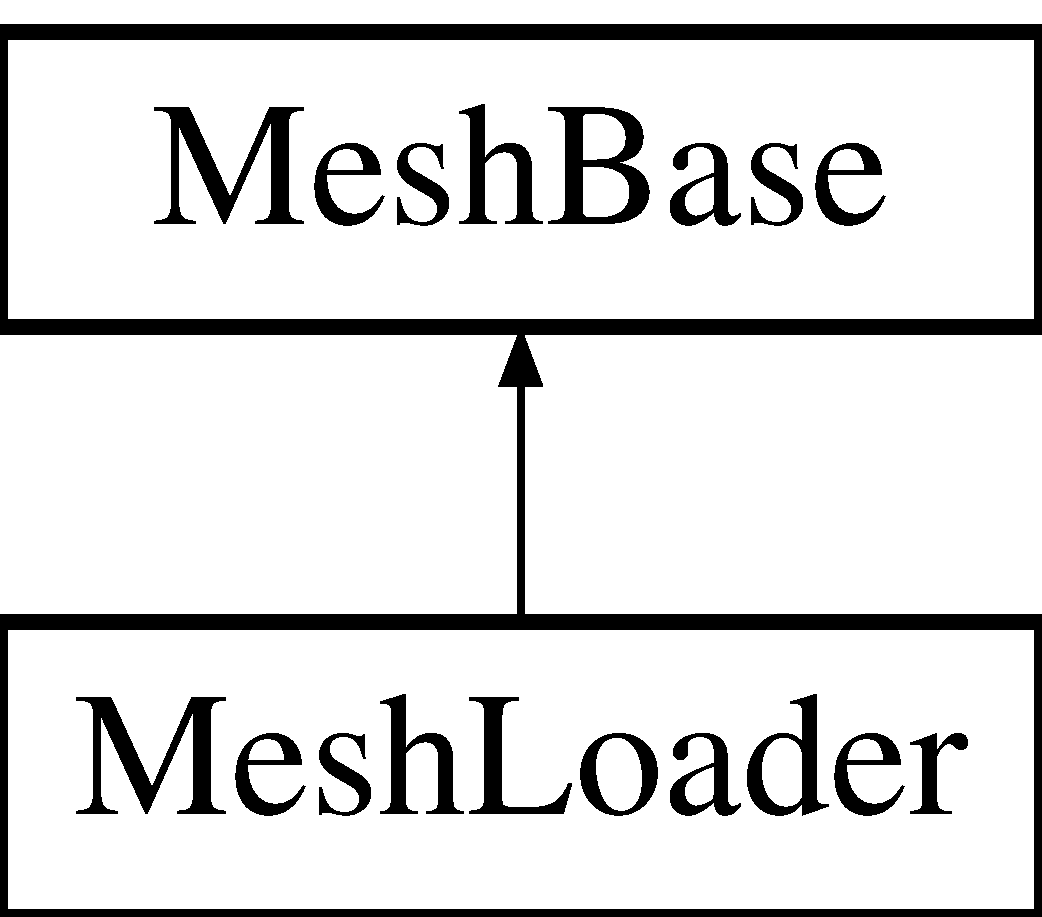
\includegraphics[height=2.000000cm]{class_mesh_loader}
\end{center}
\end{figure}
\subsection*{Classes}
\begin{DoxyCompactItemize}
\item 
struct \hyperlink{struct_mesh_loader_1_1_allocate_groups_functor}{Allocate\+Groups\+Functor}
\item 
struct \hyperlink{struct_mesh_loader_1_1_assign_materials_functor}{Assign\+Materials\+Functor}
\end{DoxyCompactItemize}
\subsection*{Public Types}
\begin{DoxyCompactItemize}
\item 
\mbox{\Hypertarget{class_mesh_loader_a0873ba1926f051adc9bbc6afab1ed4de}\label{class_mesh_loader_a0873ba1926f051adc9bbc6afab1ed4de}} 
typedef \hyperlink{class_mesh_base}{Mesh\+Base} {\bfseries Base}
\end{DoxyCompactItemize}
\subsection*{Public Methods}
\begin{DoxyCompactItemize}
\item 
\mbox{\Hypertarget{class_mesh_loader_ad2479b75e00ebecb8a4e3954eb1673aa}\label{class_mesh_loader_ad2479b75e00ebecb8a4e3954eb1673aa}} 
{\bfseries Mesh\+Loader} (\hyperlink{class_mesh_storage}{Mesh\+Storage} $\ast$mesh)
\item 
int \hyperlink{class_mesh_loader_a3e228f5e2fbb1261cd76871ee07e4f58}{get\+Vertex\+Triangle\+Size} () const
\item 
\mbox{\Hypertarget{class_mesh_loader_ab09fa780b990617917aabfcf3aa0fc25}\label{class_mesh_loader_ab09fa780b990617917aabfcf3aa0fc25}} 
int {\bfseries get\+Normal\+Triangle\+Size} () const
\item 
\mbox{\Hypertarget{class_mesh_loader_a6692b77e125599e802307a7ec265724c}\label{class_mesh_loader_a6692b77e125599e802307a7ec265724c}} 
int {\bfseries get\+Texture\+Triangle\+Size} () const
\item 
\mbox{\Hypertarget{class_mesh_loader_aadcdc2263c72eb06febe0f53666601dc}\label{class_mesh_loader_aadcdc2263c72eb06febe0f53666601dc}} 
int $\ast$ {\bfseries get\+Vertex\+Indices} ()
\item 
\mbox{\Hypertarget{class_mesh_loader_aa511e240655b63fbb375a10db79d1a2a}\label{class_mesh_loader_aa511e240655b63fbb375a10db79d1a2a}} 
const int $\ast$ {\bfseries get\+Vertex\+Indices} () const
\item 
\mbox{\Hypertarget{class_mesh_loader_ac634529b630cb2af557a91be234bebe4}\label{class_mesh_loader_ac634529b630cb2af557a91be234bebe4}} 
int $\ast$ {\bfseries get\+Normal\+Indices} ()
\item 
\mbox{\Hypertarget{class_mesh_loader_af3c9decc51f14a7cc1029d27a10bbce4}\label{class_mesh_loader_af3c9decc51f14a7cc1029d27a10bbce4}} 
const int $\ast$ {\bfseries get\+Normal\+Indices} () const
\item 
\mbox{\Hypertarget{class_mesh_loader_ab5fd2fe3eaf2cddb4f21470712553456}\label{class_mesh_loader_ab5fd2fe3eaf2cddb4f21470712553456}} 
int $\ast$ {\bfseries get\+Color\+Indices} ()
\item 
\mbox{\Hypertarget{class_mesh_loader_a524488590c3fd1d29c8bf3ad5b26545d}\label{class_mesh_loader_a524488590c3fd1d29c8bf3ad5b26545d}} 
const int $\ast$ {\bfseries get\+Color\+Indices} () const
\item 
\mbox{\Hypertarget{class_mesh_loader_aa5b401f352733edc86e564cb799ced8f}\label{class_mesh_loader_aa5b401f352733edc86e564cb799ced8f}} 
int $\ast$ {\bfseries get\+Texture\+Coordinate\+Indices} ()
\item 
\mbox{\Hypertarget{class_mesh_loader_af5a9b7daa098c2adf6894c2197c7778b}\label{class_mesh_loader_af5a9b7daa098c2adf6894c2197c7778b}} 
const int $\ast$ {\bfseries get\+Texture\+Coordinate\+Indices} () const
\item 
\mbox{\Hypertarget{class_mesh_loader_af1d9d097876866af05a5ff7909250842}\label{class_mesh_loader_af1d9d097876866af05a5ff7909250842}} 
void {\bfseries set\+Group\+Name} (const uint32 i, const std\+::string \&group\+\_\+name)
\end{DoxyCompactItemize}
\subsection*{Proteced Methods}
\begin{DoxyCompactItemize}
\item 
virtual void \hyperlink{class_mesh_loader_ad9c636920b31629f1c271b20a5fdc29b}{pre\+Process} ()
\item 
virtual void \hyperlink{class_mesh_loader_a8bdf8e0894e147be8d3e287f46feff6a}{allocate\+Data} ()
\item 
virtual void \hyperlink{class_mesh_loader_a18379e41707d8127947aa17a622d2807}{start\+Writing\+Data} ()
\item 
virtual void \hyperlink{class_mesh_loader_a83a3c78a6c2df1087c9f9e28c63e6d51}{post\+Process} ()
\item 
virtual void \hyperlink{class_mesh_loader_a65847db267f07f637deab0889c283bfa}{finish\+Writing\+Data} ()
\end{DoxyCompactItemize}


\subsection{Member Function Documentation}
\mbox{\Hypertarget{class_mesh_loader_a8bdf8e0894e147be8d3e287f46feff6a}\label{class_mesh_loader_a8bdf8e0894e147be8d3e287f46feff6a}} 
\index{Mesh\+Loader@{Mesh\+Loader}!allocate\+Data@{allocate\+Data}}
\index{allocate\+Data@{allocate\+Data}!Mesh\+Loader@{Mesh\+Loader}}
\subsubsection{\texorpdfstring{allocate\+Data()}{allocateData()}}
{\footnotesize\ttfamily void Mesh\+Loader\+::allocate\+Data (\begin{DoxyParamCaption}{ }\end{DoxyParamCaption})\hspace{0.3cm}{\ttfamily [protected]}, {\ttfamily [virtual]}}

Call this to allocate all data for the mesh after setting num\+\_\+vertices, num\+\_\+normals, num\+\_\+colors, and num\+\_\+texture\+\_\+coordinates, as well as num\+\_\+triangles for all the groups. 

Implements \hyperlink{class_mesh_base_a30c0ef8b3faabc9b41520b85dd9413bb}{Mesh\+Base}.

\mbox{\Hypertarget{class_mesh_loader_a65847db267f07f637deab0889c283bfa}\label{class_mesh_loader_a65847db267f07f637deab0889c283bfa}} 
\index{Mesh\+Loader@{Mesh\+Loader}!finish\+Writing\+Data@{finish\+Writing\+Data}}
\index{finish\+Writing\+Data@{finish\+Writing\+Data}!Mesh\+Loader@{Mesh\+Loader}}
\subsubsection{\texorpdfstring{finish\+Writing\+Data()}{finishWritingData()}}
{\footnotesize\ttfamily void Mesh\+Loader\+::finish\+Writing\+Data (\begin{DoxyParamCaption}{ }\end{DoxyParamCaption})\hspace{0.3cm}{\ttfamily [protected]}, {\ttfamily [virtual]}}

Call this when done writing to data or group data. 

Implements \hyperlink{class_mesh_base_a000796d7b04985f137d5a1368e90bcc6}{Mesh\+Base}.

\mbox{\Hypertarget{class_mesh_loader_a3e228f5e2fbb1261cd76871ee07e4f58}\label{class_mesh_loader_a3e228f5e2fbb1261cd76871ee07e4f58}} 
\index{Mesh\+Loader@{Mesh\+Loader}!get\+Vertex\+Triangle\+Size@{get\+Vertex\+Triangle\+Size}}
\index{get\+Vertex\+Triangle\+Size@{get\+Vertex\+Triangle\+Size}!Mesh\+Loader@{Mesh\+Loader}}
\subsubsection{\texorpdfstring{get\+Vertex\+Triangle\+Size()}{getVertexTriangleSize()}}
{\footnotesize\ttfamily int Mesh\+Loader\+::get\+Vertex\+Triangle\+Size (\begin{DoxyParamCaption}{ }\end{DoxyParamCaption}) const\hspace{0.3cm}{\ttfamily [inline]}, {\ttfamily [virtual]}}

These pure virtual functions allow subclasses to control much about the loading behavior. 

Implements \hyperlink{class_mesh_base_a508fde807d380849192391f28465fee4}{Mesh\+Base}.

\mbox{\Hypertarget{class_mesh_loader_a83a3c78a6c2df1087c9f9e28c63e6d51}\label{class_mesh_loader_a83a3c78a6c2df1087c9f9e28c63e6d51}} 
\index{Mesh\+Loader@{Mesh\+Loader}!post\+Process@{post\+Process}}
\index{post\+Process@{post\+Process}!Mesh\+Loader@{Mesh\+Loader}}
\subsubsection{\texorpdfstring{post\+Process()}{postProcess()}}
{\footnotesize\ttfamily void Mesh\+Loader\+::post\+Process (\begin{DoxyParamCaption}{ }\end{DoxyParamCaption})\hspace{0.3cm}{\ttfamily [protected]}, {\ttfamily [virtual]}}

An injection point for subclasses to do load postprocessing 

Implements \hyperlink{class_mesh_base_a49ec1a25d18103982974f424b77fadc0}{Mesh\+Base}.

\mbox{\Hypertarget{class_mesh_loader_ad9c636920b31629f1c271b20a5fdc29b}\label{class_mesh_loader_ad9c636920b31629f1c271b20a5fdc29b}} 
\index{Mesh\+Loader@{Mesh\+Loader}!pre\+Process@{pre\+Process}}
\index{pre\+Process@{pre\+Process}!Mesh\+Loader@{Mesh\+Loader}}
\subsubsection{\texorpdfstring{pre\+Process()}{preProcess()}}
{\footnotesize\ttfamily void Mesh\+Loader\+::pre\+Process (\begin{DoxyParamCaption}{ }\end{DoxyParamCaption})\hspace{0.3cm}{\ttfamily [protected]}, {\ttfamily [virtual]}}

An injection point for subclasses to do any prep before file info is loaded 

Implements \hyperlink{class_mesh_base_a25e192211e37cb69f9b5ce9aea25989a}{Mesh\+Base}.

\mbox{\Hypertarget{class_mesh_loader_a18379e41707d8127947aa17a622d2807}\label{class_mesh_loader_a18379e41707d8127947aa17a622d2807}} 
\index{Mesh\+Loader@{Mesh\+Loader}!start\+Writing\+Data@{start\+Writing\+Data}}
\index{start\+Writing\+Data@{start\+Writing\+Data}!Mesh\+Loader@{Mesh\+Loader}}
\subsubsection{\texorpdfstring{start\+Writing\+Data()}{startWritingData()}}
{\footnotesize\ttfamily void Mesh\+Loader\+::start\+Writing\+Data (\begin{DoxyParamCaption}{ }\end{DoxyParamCaption})\hspace{0.3cm}{\ttfamily [protected]}, {\ttfamily [virtual]}}

Call this before writing any data to the mesh, to set up correct pointer values to write to for vertex\+\_\+data, normal\+\_\+data, etc., as well as vertex\+\_\+indices, normal\+\_\+indices, etc. for each of the groups.

Call \hyperlink{class_mesh_loader_a65847db267f07f637deab0889c283bfa}{finish\+Writing\+Data()} when done. 

Implements \hyperlink{class_mesh_base_a67eb9bc7c4f6b074626078fe7779a8a4}{Mesh\+Base}.



The documentation for this class was generated from the following files\+:\begin{DoxyCompactItemize}
\item 
C\+:/p4research/research/jpantaleoni/\+Fermat-\/\+Public/src/mesh/Mesh\+Loader.\+h\item 
C\+:/p4research/research/jpantaleoni/\+Fermat-\/\+Public/src/mesh/Mesh\+Loader.\+cpp\end{DoxyCompactItemize}

\hypertarget{struct_mesh_material}{}\section{Mesh\+Material Struct Reference}
\label{struct_mesh_material}\index{Mesh\+Material@{Mesh\+Material}}


\subsection{Detailed description}
The class to represent materials attached to a mesh 

{\ttfamily \#include $<$Mesh\+View.\+h$>$}

\subsection*{Public Members}
\begin{DoxyCompactItemize}
\item 
\mbox{\Hypertarget{struct_mesh_material_aaa47d81674607691085d3d8bbd5a03df}\label{struct_mesh_material_aaa47d81674607691085d3d8bbd5a03df}} 
float4 {\bfseries diffuse}
\item 
\mbox{\Hypertarget{struct_mesh_material_a169f9de5cfb7b93962d174901fd9f594}\label{struct_mesh_material_a169f9de5cfb7b93962d174901fd9f594}} 
float4 {\bfseries diffuse\+\_\+trans}
\item 
\mbox{\Hypertarget{struct_mesh_material_a5cb2321db06b32f7b765fe4b7ac4496b}\label{struct_mesh_material_a5cb2321db06b32f7b765fe4b7ac4496b}} 
float4 {\bfseries ambient}
\item 
\mbox{\Hypertarget{struct_mesh_material_a9ae3a5b91d271e601f27568d6cb29c75}\label{struct_mesh_material_a9ae3a5b91d271e601f27568d6cb29c75}} 
float4 {\bfseries specular}
\item 
\mbox{\Hypertarget{struct_mesh_material_a335f0705b9b30053f1981d55ef681897}\label{struct_mesh_material_a335f0705b9b30053f1981d55ef681897}} 
float4 {\bfseries emissive}
\item 
\mbox{\Hypertarget{struct_mesh_material_af2ab73d6683a7f6981da110691a6c4a4}\label{struct_mesh_material_af2ab73d6683a7f6981da110691a6c4a4}} 
float4 {\bfseries reflectivity}
\item 
\mbox{\Hypertarget{struct_mesh_material_ab11b5a864211e2f1e7c331c06270979c}\label{struct_mesh_material_ab11b5a864211e2f1e7c331c06270979c}} 
float {\bfseries roughness}
\item 
\mbox{\Hypertarget{struct_mesh_material_a83f83b17481810982efb0eaf3ff229d3}\label{struct_mesh_material_a83f83b17481810982efb0eaf3ff229d3}} 
float {\bfseries index\+\_\+of\+\_\+refraction}
\item 
\mbox{\Hypertarget{struct_mesh_material_a3f602eec3a8ed7358cb2e3e4782d5c13}\label{struct_mesh_material_a3f602eec3a8ed7358cb2e3e4782d5c13}} 
float {\bfseries opacity}
\item 
\mbox{\Hypertarget{struct_mesh_material_a57ed60676fd52d87092115d3de8cb8d9}\label{struct_mesh_material_a57ed60676fd52d87092115d3de8cb8d9}} 
int {\bfseries flags}
\item 
\mbox{\Hypertarget{struct_mesh_material_a4f39e3e8c162c8df2e0ca56fd10a295e}\label{struct_mesh_material_a4f39e3e8c162c8df2e0ca56fd10a295e}} 
\hyperlink{struct_texture_reference}{Texture\+Reference} {\bfseries ambient\+\_\+map}
\item 
\mbox{\Hypertarget{struct_mesh_material_af78973b224f0b012e9c2d678b0c9a17d}\label{struct_mesh_material_af78973b224f0b012e9c2d678b0c9a17d}} 
\hyperlink{struct_texture_reference}{Texture\+Reference} {\bfseries diffuse\+\_\+map}
\item 
\mbox{\Hypertarget{struct_mesh_material_aba36269a719447d03312de491d68b38b}\label{struct_mesh_material_aba36269a719447d03312de491d68b38b}} 
\hyperlink{struct_texture_reference}{Texture\+Reference} {\bfseries diffuse\+\_\+trans\+\_\+map}
\item 
\mbox{\Hypertarget{struct_mesh_material_a5771fdaee02c98f5a17d49e056c31ce6}\label{struct_mesh_material_a5771fdaee02c98f5a17d49e056c31ce6}} 
\hyperlink{struct_texture_reference}{Texture\+Reference} {\bfseries specular\+\_\+map}
\item 
\mbox{\Hypertarget{struct_mesh_material_ae0661b4a8d23ced275218f2cb3bdbd99}\label{struct_mesh_material_ae0661b4a8d23ced275218f2cb3bdbd99}} 
\hyperlink{struct_texture_reference}{Texture\+Reference} {\bfseries emissive\+\_\+map}
\item 
\mbox{\Hypertarget{struct_mesh_material_a9031903fa8c442293fd68210201a9621}\label{struct_mesh_material_a9031903fa8c442293fd68210201a9621}} 
\hyperlink{struct_texture_reference}{Texture\+Reference} {\bfseries bump\+\_\+map}
\end{DoxyCompactItemize}


The documentation for this struct was generated from the following file\+:\begin{DoxyCompactItemize}
\item 
C\+:/p4research/research/jpantaleoni/\+Fermat-\/\+Public/src/mesh/Mesh\+View.\+h\end{DoxyCompactItemize}

\hypertarget{class_mesh_material_params}{}\section{Mesh\+Material\+Params Class Reference}
\label{class_mesh_material_params}\index{Mesh\+Material\+Params@{Mesh\+Material\+Params}}
\subsection*{Public Methods}
\begin{DoxyCompactItemize}
\item 
\mbox{\Hypertarget{class_mesh_material_params_acc85cdf4698b8e6b0415bb11ca109009}\label{class_mesh_material_params_acc85cdf4698b8e6b0415bb11ca109009}} 
S\+U\+T\+I\+L\+A\+PI void {\bfseries set\+To\+Default\+Params} ()
\end{DoxyCompactItemize}
\subsection*{Public Members}
\begin{DoxyCompactItemize}
\item 
\mbox{\Hypertarget{class_mesh_material_params_a4ce14d1704de40d80b19366e5400667b}\label{class_mesh_material_params_a4ce14d1704de40d80b19366e5400667b}} 
std\+::string {\bfseries name}
\item 
\mbox{\Hypertarget{class_mesh_material_params_ae1f34f7ab421df8bd3a2bb8c5bbdbc81}\label{class_mesh_material_params_ae1f34f7ab421df8bd3a2bb8c5bbdbc81}} 
float {\bfseries diffuse} \mbox{[}4\mbox{]}
\item 
\mbox{\Hypertarget{class_mesh_material_params_a7e4da768083ca9b5bef6541bb8dcf2b1}\label{class_mesh_material_params_a7e4da768083ca9b5bef6541bb8dcf2b1}} 
float {\bfseries diffuse\+\_\+trans} \mbox{[}4\mbox{]}
\item 
\mbox{\Hypertarget{class_mesh_material_params_a582d14bdb035aae3d740a9973f6176d3}\label{class_mesh_material_params_a582d14bdb035aae3d740a9973f6176d3}} 
float {\bfseries ambient} \mbox{[}4\mbox{]}
\item 
\mbox{\Hypertarget{class_mesh_material_params_a7df5c4bc6bd84f8a0e044c69b648f1f3}\label{class_mesh_material_params_a7df5c4bc6bd84f8a0e044c69b648f1f3}} 
float {\bfseries specular} \mbox{[}4\mbox{]}
\item 
\mbox{\Hypertarget{class_mesh_material_params_af27b7ff50c46ec4a77143ba6a50f8e01}\label{class_mesh_material_params_af27b7ff50c46ec4a77143ba6a50f8e01}} 
float {\bfseries emissive} \mbox{[}4\mbox{]}
\item 
\mbox{\Hypertarget{class_mesh_material_params_a5be6b6acafb73236cd663022ed1028c3}\label{class_mesh_material_params_a5be6b6acafb73236cd663022ed1028c3}} 
float {\bfseries phong\+\_\+exponent}
\item 
\mbox{\Hypertarget{class_mesh_material_params_ab4300b56d86af3119489bb28a3b6ab45}\label{class_mesh_material_params_ab4300b56d86af3119489bb28a3b6ab45}} 
float {\bfseries index\+\_\+of\+\_\+refraction}
\item 
\mbox{\Hypertarget{class_mesh_material_params_a4891bb5af9b136caa8fc79806e1139ac}\label{class_mesh_material_params_a4891bb5af9b136caa8fc79806e1139ac}} 
float {\bfseries opacity}
\item 
\mbox{\Hypertarget{class_mesh_material_params_a7e372f86cd0ccc2218e93c830bc6d294}\label{class_mesh_material_params_a7e372f86cd0ccc2218e93c830bc6d294}} 
float {\bfseries reflectivity} \mbox{[}4\mbox{]}
\item 
\mbox{\Hypertarget{class_mesh_material_params_a65eb6d2e55f07a17f631d84cd61c8761}\label{class_mesh_material_params_a65eb6d2e55f07a17f631d84cd61c8761}} 
int {\bfseries flags}
\item 
\mbox{\Hypertarget{class_mesh_material_params_a65c88f514165090d87a507491cd06bfc}\label{class_mesh_material_params_a65c88f514165090d87a507491cd06bfc}} 
int {\bfseries shading\+\_\+type}
\item 
\mbox{\Hypertarget{class_mesh_material_params_aca6ee65a23aecb70ce6b068eb3b14332}\label{class_mesh_material_params_aca6ee65a23aecb70ce6b068eb3b14332}} 
\hyperlink{class_mesh_texture_map}{Mesh\+Texture\+Map} {\bfseries ambient\+\_\+map}
\item 
\mbox{\Hypertarget{class_mesh_material_params_a03a71de3e909e99167aa21fe9bf03cde}\label{class_mesh_material_params_a03a71de3e909e99167aa21fe9bf03cde}} 
\hyperlink{class_mesh_texture_map}{Mesh\+Texture\+Map} {\bfseries diffuse\+\_\+map}
\item 
\mbox{\Hypertarget{class_mesh_material_params_a060130e71094567ec4bf0b1f0b793acc}\label{class_mesh_material_params_a060130e71094567ec4bf0b1f0b793acc}} 
\hyperlink{class_mesh_texture_map}{Mesh\+Texture\+Map} {\bfseries diffuse\+\_\+trans\+\_\+map}
\item 
\mbox{\Hypertarget{class_mesh_material_params_aa9dfbbf47e5769ebc289e2c815a22219}\label{class_mesh_material_params_aa9dfbbf47e5769ebc289e2c815a22219}} 
\hyperlink{class_mesh_texture_map}{Mesh\+Texture\+Map} {\bfseries specular\+\_\+map}
\item 
\mbox{\Hypertarget{class_mesh_material_params_a62ee8ca76ff9e6081cfd3182cc677fa1}\label{class_mesh_material_params_a62ee8ca76ff9e6081cfd3182cc677fa1}} 
\hyperlink{class_mesh_texture_map}{Mesh\+Texture\+Map} {\bfseries emissive\+\_\+map}
\item 
\mbox{\Hypertarget{class_mesh_material_params_ab9802e81abbe543096667058e152d8e9}\label{class_mesh_material_params_ab9802e81abbe543096667058e152d8e9}} 
\hyperlink{class_mesh_texture_map}{Mesh\+Texture\+Map} {\bfseries opacity\+\_\+map}
\item 
\mbox{\Hypertarget{class_mesh_material_params_a15cdbcf29def76a52287f7e6651df53f}\label{class_mesh_material_params_a15cdbcf29def76a52287f7e6651df53f}} 
\hyperlink{class_mesh_texture_map}{Mesh\+Texture\+Map} {\bfseries bump\+\_\+map}
\end{DoxyCompactItemize}


The documentation for this class was generated from the following files\+:\begin{DoxyCompactItemize}
\item 
C\+:/p4research/research/jpantaleoni/\+Fermat-\/\+Public/src/mesh/Mesh\+Base.\+h\item 
C\+:/p4research/research/jpantaleoni/\+Fermat-\/\+Public/src/mesh/Mesh\+Base.\+cpp\end{DoxyCompactItemize}

\hypertarget{class_mesh_storage}{}\section{Mesh\+Storage Class Reference}
\label{class_mesh_storage}\index{Mesh\+Storage@{Mesh\+Storage}}


\subsection{Detailed description}
This class provides basic Mesh storage for either the host or device 

{\ttfamily \#include $<$Mesh\+Storage.\+h$>$}

\subsection*{Public Types}
\begin{DoxyCompactItemize}
\item 
\mbox{\Hypertarget{class_mesh_storage_aafa910e5048de2c56366f4a75990a270}\label{class_mesh_storage_aafa910e5048de2c56366f4a75990a270}} 
typedef Mesh\+View\+::vertex\+\_\+triangle {\bfseries vertex\+\_\+triangle}
\item 
\mbox{\Hypertarget{class_mesh_storage_aa5b88deb578cba5e63db24f83a818cff}\label{class_mesh_storage_aa5b88deb578cba5e63db24f83a818cff}} 
typedef Mesh\+View\+::normal\+\_\+triangle {\bfseries normal\+\_\+triangle}
\item 
\mbox{\Hypertarget{class_mesh_storage_a2dea37a55a3e83ea6b387ca879c885ff}\label{class_mesh_storage_a2dea37a55a3e83ea6b387ca879c885ff}} 
typedef Mesh\+View\+::texture\+\_\+triangle {\bfseries texture\+\_\+triangle}
\item 
\mbox{\Hypertarget{class_mesh_storage_aa8db0d591fb575e006a93970d971e8e1}\label{class_mesh_storage_aa8db0d591fb575e006a93970d971e8e1}} 
typedef Mesh\+View\+::lightmap\+\_\+triangle {\bfseries lightmap\+\_\+triangle}
\end{DoxyCompactItemize}
\subsection*{Public Methods}
\begin{DoxyCompactItemize}
\item 
\mbox{\Hypertarget{class_mesh_storage_a2a26bf8ce12c14b3a3c638d01b5db0ba}\label{class_mesh_storage_a2a26bf8ce12c14b3a3c638d01b5db0ba}} 
void {\bfseries alloc} (const int num\+\_\+triangles, const int num\+\_\+vertices, const int num\+\_\+normals, const int num\+\_\+texture\+\_\+coordinates, const int num\+\_\+groups)
\item 
\mbox{\Hypertarget{class_mesh_storage_a81ebc7a6397f8e83d10e7242b5ab7a30}\label{class_mesh_storage_a81ebc7a6397f8e83d10e7242b5ab7a30}} 
void {\bfseries alloc\+\_\+lightmap} (const int num\+\_\+lightmap\+\_\+coordinates)
\item 
\mbox{\Hypertarget{class_mesh_storage_aacf7203fecfad1d3d15959bc053628dd}\label{class_mesh_storage_aacf7203fecfad1d3d15959bc053628dd}} 
void {\bfseries compress\+\_\+normals} ()
\item 
\mbox{\Hypertarget{class_mesh_storage_a85773c6742a20d10d7291d7c3f571b37}\label{class_mesh_storage_a85773c6742a20d10d7291d7c3f571b37}} 
void {\bfseries compress\+\_\+tex} ()
\item 
\mbox{\Hypertarget{class_mesh_storage_a289b45038006451780fdb87d72782745}\label{class_mesh_storage_a289b45038006451780fdb87d72782745}} 
S\+U\+T\+I\+L\+A\+PI \hyperlink{struct_mesh_material}{Mesh\+Material} $\ast$ {\bfseries alloc\+\_\+materials} (const size\+\_\+t n)
\item 
\mbox{\Hypertarget{class_mesh_storage_abd714f1144efe9069e352dc07cb85a89}\label{class_mesh_storage_abd714f1144efe9069e352dc07cb85a89}} 
S\+U\+T\+I\+L\+A\+PI char $\ast$ {\bfseries alloc\+\_\+material\+\_\+names} (const size\+\_\+t n\+\_\+chars)
\item 
\mbox{\Hypertarget{class_mesh_storage_a2ffe68e15e5634c64e884996b9d09220}\label{class_mesh_storage_a2ffe68e15e5634c64e884996b9d09220}} 
S\+U\+T\+I\+L\+A\+PI int {\bfseries get\+Num\+Vertices} () const
\item 
\mbox{\Hypertarget{class_mesh_storage_a68ec29f17951ca0f3bbedc47e2ecc6ae}\label{class_mesh_storage_a68ec29f17951ca0f3bbedc47e2ecc6ae}} 
S\+U\+T\+I\+L\+A\+PI int {\bfseries get\+Num\+Normals} () const
\item 
\mbox{\Hypertarget{class_mesh_storage_a0f3825d3e327565f1f48b81bcb947d02}\label{class_mesh_storage_a0f3825d3e327565f1f48b81bcb947d02}} 
S\+U\+T\+I\+L\+A\+PI int {\bfseries get\+Num\+Texture\+Coordinates} () const
\item 
\mbox{\Hypertarget{class_mesh_storage_a77554ba82dbadb8447bf5b720300fd6b}\label{class_mesh_storage_a77554ba82dbadb8447bf5b720300fd6b}} 
S\+U\+T\+I\+L\+A\+PI int {\bfseries get\+Num\+Triangles} () const
\item 
\mbox{\Hypertarget{class_mesh_storage_abbd69f6731422beb9729c4050fe6162d}\label{class_mesh_storage_abbd69f6731422beb9729c4050fe6162d}} 
S\+U\+T\+I\+L\+A\+PI int {\bfseries get\+Num\+Groups} () const
\item 
\mbox{\Hypertarget{class_mesh_storage_ab9197e26cf1711403237811ff0f81338}\label{class_mesh_storage_ab9197e26cf1711403237811ff0f81338}} 
S\+U\+T\+I\+L\+A\+PI int {\bfseries get\+Num\+Materials} () const
\item 
\mbox{\Hypertarget{class_mesh_storage_ab7419e400e0e7d2d7637900d9b22113b}\label{class_mesh_storage_ab7419e400e0e7d2d7637900d9b22113b}} 
S\+U\+T\+I\+L\+A\+PI int {\bfseries get\+Num\+Textures} () const
\item 
\mbox{\Hypertarget{class_mesh_storage_a3e3d17b0f1a6484b5cbe02979fbc7ad9}\label{class_mesh_storage_a3e3d17b0f1a6484b5cbe02979fbc7ad9}} 
S\+U\+T\+I\+L\+A\+PI int {\bfseries get\+Vertex\+Stride} () const
\item 
\mbox{\Hypertarget{class_mesh_storage_a55fe3f7c803af6cac3026422e5334616}\label{class_mesh_storage_a55fe3f7c803af6cac3026422e5334616}} 
S\+U\+T\+I\+L\+A\+PI int {\bfseries get\+Normal\+Stride} () const
\item 
\mbox{\Hypertarget{class_mesh_storage_a2412634420e6a9ba066acdc4a45585b6}\label{class_mesh_storage_a2412634420e6a9ba066acdc4a45585b6}} 
S\+U\+T\+I\+L\+A\+PI int {\bfseries get\+Texture\+Coordinate\+Stride} () const
\item 
\mbox{\Hypertarget{class_mesh_storage_a4cea4eb20a81a39bd8ecc7c07fb08c64}\label{class_mesh_storage_a4cea4eb20a81a39bd8ecc7c07fb08c64}} 
S\+U\+T\+I\+L\+A\+PI int $\ast$ {\bfseries get\+Vertex\+Indices} ()
\item 
\mbox{\Hypertarget{class_mesh_storage_aa45260149381a38d28f54ff4b435b210}\label{class_mesh_storage_aa45260149381a38d28f54ff4b435b210}} 
S\+U\+T\+I\+L\+A\+PI const int $\ast$ {\bfseries get\+Vertex\+Indices} () const
\item 
\mbox{\Hypertarget{class_mesh_storage_abd202c7c97a0726557eaec35b5751a36}\label{class_mesh_storage_abd202c7c97a0726557eaec35b5751a36}} 
S\+U\+T\+I\+L\+A\+PI int $\ast$ {\bfseries get\+Normal\+Indices} ()
\item 
\mbox{\Hypertarget{class_mesh_storage_ad0c612c3550ee75581a34fe4fb5c6614}\label{class_mesh_storage_ad0c612c3550ee75581a34fe4fb5c6614}} 
S\+U\+T\+I\+L\+A\+PI const int $\ast$ {\bfseries get\+Normal\+Indices} () const
\item 
\mbox{\Hypertarget{class_mesh_storage_aae43a9990be7da98e37c06b6ef226ae8}\label{class_mesh_storage_aae43a9990be7da98e37c06b6ef226ae8}} 
S\+U\+T\+I\+L\+A\+PI int $\ast$ {\bfseries get\+Material\+Indices} ()
\item 
\mbox{\Hypertarget{class_mesh_storage_ac2f7c46c4d409b662b97e9ac5767dc17}\label{class_mesh_storage_ac2f7c46c4d409b662b97e9ac5767dc17}} 
S\+U\+T\+I\+L\+A\+PI const int $\ast$ {\bfseries get\+Material\+Indices} () const
\item 
\mbox{\Hypertarget{class_mesh_storage_aaee63194bf9b7813f35084f1bd2005c6}\label{class_mesh_storage_aaee63194bf9b7813f35084f1bd2005c6}} 
S\+U\+T\+I\+L\+A\+PI int $\ast$ {\bfseries get\+Texture\+Coordinate\+Indices} ()
\item 
\mbox{\Hypertarget{class_mesh_storage_abfff683a09c90bc58aa8524dcbce657b}\label{class_mesh_storage_abfff683a09c90bc58aa8524dcbce657b}} 
S\+U\+T\+I\+L\+A\+PI const int $\ast$ {\bfseries get\+Texture\+Coordinate\+Indices} () const
\item 
\mbox{\Hypertarget{class_mesh_storage_a7f5845ea5527951bc5c2062f0948f026}\label{class_mesh_storage_a7f5845ea5527951bc5c2062f0948f026}} 
S\+U\+T\+I\+L\+A\+PI int $\ast$ {\bfseries get\+Lightmap\+Indices} ()
\item 
\mbox{\Hypertarget{class_mesh_storage_ab4e198c8518b693e973c0bef8e88b817}\label{class_mesh_storage_ab4e198c8518b693e973c0bef8e88b817}} 
S\+U\+T\+I\+L\+A\+PI const int $\ast$ {\bfseries get\+Lightmap\+Indices} () const
\item 
\mbox{\Hypertarget{class_mesh_storage_a1fcc998e705dfdd40fa58c82a4db5ab4}\label{class_mesh_storage_a1fcc998e705dfdd40fa58c82a4db5ab4}} 
S\+U\+T\+I\+L\+A\+PI int $\ast$ {\bfseries get\+Group\+Offsets} ()
\item 
\mbox{\Hypertarget{class_mesh_storage_aa60755752fd6f937c237d2df1deb9333}\label{class_mesh_storage_aa60755752fd6f937c237d2df1deb9333}} 
S\+U\+T\+I\+L\+A\+PI const int $\ast$ {\bfseries get\+Group\+Offsets} () const
\item 
\mbox{\Hypertarget{class_mesh_storage_ac0715938903b63734a8069ce5bf0cc1c}\label{class_mesh_storage_ac0715938903b63734a8069ce5bf0cc1c}} 
S\+U\+T\+I\+L\+A\+PI float $\ast$ {\bfseries get\+Vertex\+Data} ()
\item 
\mbox{\Hypertarget{class_mesh_storage_a369d2d1159c17331f71e10eb6535b793}\label{class_mesh_storage_a369d2d1159c17331f71e10eb6535b793}} 
S\+U\+T\+I\+L\+A\+PI const float $\ast$ {\bfseries get\+Vertex\+Data} () const
\item 
\mbox{\Hypertarget{class_mesh_storage_ab0195d352b038ae46910d087d588aa6f}\label{class_mesh_storage_ab0195d352b038ae46910d087d588aa6f}} 
S\+U\+T\+I\+L\+A\+PI float $\ast$ {\bfseries get\+Normal\+Data} ()
\item 
\mbox{\Hypertarget{class_mesh_storage_a5c97d63355af753a016d7e0886c04c76}\label{class_mesh_storage_a5c97d63355af753a016d7e0886c04c76}} 
S\+U\+T\+I\+L\+A\+PI const float $\ast$ {\bfseries get\+Normal\+Data} () const
\item 
\mbox{\Hypertarget{class_mesh_storage_a85cf3d134f3dc755f37d61561904c0d2}\label{class_mesh_storage_a85cf3d134f3dc755f37d61561904c0d2}} 
S\+U\+T\+I\+L\+A\+PI float $\ast$ {\bfseries get\+Texture\+Coordinate\+Data} ()
\item 
\mbox{\Hypertarget{class_mesh_storage_a61c4b007a1fba002b52fa2dc1fb171a4}\label{class_mesh_storage_a61c4b007a1fba002b52fa2dc1fb171a4}} 
S\+U\+T\+I\+L\+A\+PI const float $\ast$ {\bfseries get\+Texture\+Coordinate\+Data} () const
\item 
\mbox{\Hypertarget{class_mesh_storage_a340297ea20ebad9231f825973a2a86d5}\label{class_mesh_storage_a340297ea20ebad9231f825973a2a86d5}} 
S\+U\+T\+I\+L\+A\+PI std\+::string \& {\bfseries get\+Group\+Name} (const uint32 i)
\item 
\mbox{\Hypertarget{class_mesh_storage_a37b402692f3b8c0feea707dd3c15dbdb}\label{class_mesh_storage_a37b402692f3b8c0feea707dd3c15dbdb}} 
S\+U\+T\+I\+L\+A\+PI const std\+::string \& {\bfseries get\+Group\+Name} (const uint32 i) const
\item 
\mbox{\Hypertarget{class_mesh_storage_a63bd6f162262f27ff06ace0150c6f269}\label{class_mesh_storage_a63bd6f162262f27ff06ace0150c6f269}} 
S\+U\+T\+I\+L\+A\+PI const char $\ast$ {\bfseries get\+Material\+Name} (const uint32 i) const
\item 
\mbox{\Hypertarget{class_mesh_storage_ae44c4a1c30fa1c326b568e010e24240d}\label{class_mesh_storage_ae44c4a1c30fa1c326b568e010e24240d}} 
S\+U\+T\+I\+L\+A\+PI uint32 {\bfseries insert\+\_\+texture} (const std\+::string \&tex\+\_\+name)
\item 
\mbox{\Hypertarget{class_mesh_storage_a3a1e2a2e159141f17f968b9959d1633d}\label{class_mesh_storage_a3a1e2a2e159141f17f968b9959d1633d}} 
S\+U\+T\+I\+L\+A\+PI \hyperlink{struct_mesh_view}{Mesh\+View} {\bfseries view} ()
\item 
\mbox{\Hypertarget{class_mesh_storage_aa0829a5be9b4435fd3e1f39b6ca647d0}\label{class_mesh_storage_aa0829a5be9b4435fd3e1f39b6ca647d0}} 
void {\bfseries reorder\+\_\+triangles} (const int $\ast$index)
\item 
\mbox{\Hypertarget{class_mesh_storage_abd5651d50723c558ad0b10e237e3dd37}\label{class_mesh_storage_abd5651d50723c558ad0b10e237e3dd37}} 
void {\bfseries reset\+\_\+groups} (const int num\+\_\+groups, const int $\ast$group\+\_\+offsets)
\end{DoxyCompactItemize}
\subsection*{Static Public Methods}
\begin{DoxyCompactItemize}
\item 
\mbox{\Hypertarget{class_mesh_storage_a8b3a51cebf14fe1b3e852c04be1c03e2}\label{class_mesh_storage_a8b3a51cebf14fe1b3e852c04be1c03e2}} 
static normal\+\_\+triangle {\bfseries make\+\_\+normal\+\_\+triangle} (const int32 x, const int32 y, const int32 z)
\item 
\mbox{\Hypertarget{class_mesh_storage_abf200c9ddb32cd972865fbc94dc44a75}\label{class_mesh_storage_abf200c9ddb32cd972865fbc94dc44a75}} 
static texture\+\_\+triangle {\bfseries make\+\_\+texture\+\_\+triangle} (const int32 x, const int32 y, const int32 z)
\item 
\mbox{\Hypertarget{class_mesh_storage_a7fd484d69f35f79c2e1f8920df57b335}\label{class_mesh_storage_a7fd484d69f35f79c2e1f8920df57b335}} 
static lightmap\+\_\+triangle {\bfseries make\+\_\+lightmap\+\_\+triangle} (const int32 x, const int32 y, const int32 z)
\end{DoxyCompactItemize}
\subsection*{Public Members}
\begin{DoxyCompactItemize}
\item 
\mbox{\Hypertarget{class_mesh_storage_a92a2e2703b83efaf32d6f00a21f7c101}\label{class_mesh_storage_a92a2e2703b83efaf32d6f00a21f7c101}} 
int {\bfseries m\+\_\+num\+\_\+vertices}
\item 
\mbox{\Hypertarget{class_mesh_storage_a003cc5d14f49f31b7ae6938798de65b0}\label{class_mesh_storage_a003cc5d14f49f31b7ae6938798de65b0}} 
int {\bfseries m\+\_\+num\+\_\+normals}
\item 
\mbox{\Hypertarget{class_mesh_storage_a8ebb85369d9e472dc37750840c4cb20e}\label{class_mesh_storage_a8ebb85369d9e472dc37750840c4cb20e}} 
int {\bfseries m\+\_\+num\+\_\+texture\+\_\+coordinates}
\item 
\mbox{\Hypertarget{class_mesh_storage_ab1e7eaa97d95a8bd72b5909ef0d5d8be}\label{class_mesh_storage_ab1e7eaa97d95a8bd72b5909ef0d5d8be}} 
int {\bfseries m\+\_\+num\+\_\+lightmap\+\_\+coordinates}
\item 
\mbox{\Hypertarget{class_mesh_storage_af53b7e7afad2f128b3785cec5ca1ce59}\label{class_mesh_storage_af53b7e7afad2f128b3785cec5ca1ce59}} 
int {\bfseries m\+\_\+num\+\_\+triangles}
\item 
\mbox{\Hypertarget{class_mesh_storage_ad2074d66d8639403eb78dfd8b9ac2594}\label{class_mesh_storage_ad2074d66d8639403eb78dfd8b9ac2594}} 
int {\bfseries m\+\_\+num\+\_\+groups}
\item 
\mbox{\Hypertarget{class_mesh_storage_a31c59cf0e57653f8de5ae14e27f00b82}\label{class_mesh_storage_a31c59cf0e57653f8de5ae14e27f00b82}} 
int {\bfseries m\+\_\+vertex\+\_\+stride}
\item 
\mbox{\Hypertarget{class_mesh_storage_af9d9d6be5e6eb06d4ef5cd25a66532b0}\label{class_mesh_storage_af9d9d6be5e6eb06d4ef5cd25a66532b0}} 
int {\bfseries m\+\_\+normal\+\_\+stride}
\item 
\mbox{\Hypertarget{class_mesh_storage_af90392c634ac0525cfdf2c22a5739239}\label{class_mesh_storage_af90392c634ac0525cfdf2c22a5739239}} 
int {\bfseries m\+\_\+texture\+\_\+stride}
\item 
\mbox{\Hypertarget{class_mesh_storage_af00c0cb8ae8b107d2c162b255b95578b}\label{class_mesh_storage_af00c0cb8ae8b107d2c162b255b95578b}} 
float2 {\bfseries m\+\_\+tex\+\_\+bias}
\item 
\mbox{\Hypertarget{class_mesh_storage_a12e894bf77e27e754e93500e39145126}\label{class_mesh_storage_a12e894bf77e27e754e93500e39145126}} 
float2 {\bfseries m\+\_\+tex\+\_\+scale}
\item 
\mbox{\Hypertarget{class_mesh_storage_a8d3dc84e7724b954ba11895aeafc0e6f}\label{class_mesh_storage_a8d3dc84e7724b954ba11895aeafc0e6f}} 
float2 {\bfseries m\+\_\+lm\+\_\+bias}
\item 
\mbox{\Hypertarget{class_mesh_storage_ab5e805db0a321e1c5f1b8fc8c07254d3}\label{class_mesh_storage_ab5e805db0a321e1c5f1b8fc8c07254d3}} 
float2 {\bfseries m\+\_\+lm\+\_\+scale}
\item 
\mbox{\Hypertarget{class_mesh_storage_a88e308718df7fdbecd7289d3970effc2}\label{class_mesh_storage_a88e308718df7fdbecd7289d3970effc2}} 
std\+::map$<$ std\+::string, uint32 $>$ {\bfseries m\+\_\+textures\+\_\+map}
\item 
\mbox{\Hypertarget{class_mesh_storage_a537f80e9f36be23eae3c58b6e5a54b2e}\label{class_mesh_storage_a537f80e9f36be23eae3c58b6e5a54b2e}} 
std\+::vector$<$ std\+::string $>$ {\bfseries m\+\_\+textures}
\item 
\mbox{\Hypertarget{class_mesh_storage_a2fe89492e0a32a3b1f238029e1edde59}\label{class_mesh_storage_a2fe89492e0a32a3b1f238029e1edde59}} 
std\+::vector$<$ std\+::string $>$ {\bfseries m\+\_\+group\+\_\+names}
\item 
\mbox{\Hypertarget{class_mesh_storage_a47b675d399d9b76bdadf77be6db0d137}\label{class_mesh_storage_a47b675d399d9b76bdadf77be6db0d137}} 
\hyperlink{class_buffer}{Buffer}$<$ int $>$ {\bfseries m\+\_\+vertex\+\_\+indices}
\item 
\mbox{\Hypertarget{class_mesh_storage_ab75ce7f9d3f2b16ece26fb373ec55fc6}\label{class_mesh_storage_ab75ce7f9d3f2b16ece26fb373ec55fc6}} 
\hyperlink{class_buffer}{Buffer}$<$ int $>$ {\bfseries m\+\_\+normal\+\_\+indices}
\item 
\mbox{\Hypertarget{class_mesh_storage_a78dba9a85aa9951ff76e953a8c69a473}\label{class_mesh_storage_a78dba9a85aa9951ff76e953a8c69a473}} 
\hyperlink{class_buffer}{Buffer}$<$ int $>$ {\bfseries m\+\_\+normal\+\_\+indices\+\_\+comp}
\item 
\mbox{\Hypertarget{class_mesh_storage_a8e342b358331e03b2034d07bbfda1d5a}\label{class_mesh_storage_a8e342b358331e03b2034d07bbfda1d5a}} 
\hyperlink{class_buffer}{Buffer}$<$ int $>$ {\bfseries m\+\_\+material\+\_\+indices}
\item 
\mbox{\Hypertarget{class_mesh_storage_afd73be39c45e23b884e1dded4db7eebb}\label{class_mesh_storage_afd73be39c45e23b884e1dded4db7eebb}} 
\hyperlink{class_buffer}{Buffer}$<$ int $>$ {\bfseries m\+\_\+texture\+\_\+indices}
\item 
\mbox{\Hypertarget{class_mesh_storage_aa349c97d83413b84c2ea14bf65450143}\label{class_mesh_storage_aa349c97d83413b84c2ea14bf65450143}} 
\hyperlink{class_buffer}{Buffer}$<$ int $>$ {\bfseries m\+\_\+texture\+\_\+indices\+\_\+comp}
\item 
\mbox{\Hypertarget{class_mesh_storage_a0bae9d6ef97476c97d9934e167c9d99e}\label{class_mesh_storage_a0bae9d6ef97476c97d9934e167c9d99e}} 
\hyperlink{class_buffer}{Buffer}$<$ int $>$ {\bfseries m\+\_\+lightmap\+\_\+indices}
\item 
\mbox{\Hypertarget{class_mesh_storage_acee04ce1f4504e2b33cbfce6875b3e97}\label{class_mesh_storage_acee04ce1f4504e2b33cbfce6875b3e97}} 
\hyperlink{class_buffer}{Buffer}$<$ int $>$ {\bfseries m\+\_\+lightmap\+\_\+indices\+\_\+comp}
\item 
\mbox{\Hypertarget{class_mesh_storage_ac41ae9724d14ad0cf35686a723e97a08}\label{class_mesh_storage_ac41ae9724d14ad0cf35686a723e97a08}} 
\hyperlink{class_buffer}{Buffer}$<$ int $>$ {\bfseries m\+\_\+group\+\_\+offsets}
\item 
\mbox{\Hypertarget{class_mesh_storage_a5be05e6be65ed1d142ead76255f7272b}\label{class_mesh_storage_a5be05e6be65ed1d142ead76255f7272b}} 
\hyperlink{class_buffer}{Buffer}$<$ float $>$ {\bfseries m\+\_\+vertex\+\_\+data}
\item 
\mbox{\Hypertarget{class_mesh_storage_a04c93c7cde962b82548c8a501fa19c4e}\label{class_mesh_storage_a04c93c7cde962b82548c8a501fa19c4e}} 
\hyperlink{class_buffer}{Buffer}$<$ float $>$ {\bfseries m\+\_\+normal\+\_\+data}
\item 
\mbox{\Hypertarget{class_mesh_storage_ae6c8e3f3eb4a696f1bbd20f742a1a94f}\label{class_mesh_storage_ae6c8e3f3eb4a696f1bbd20f742a1a94f}} 
\hyperlink{class_buffer}{Buffer}$<$ uint32 $>$ {\bfseries m\+\_\+normal\+\_\+data\+\_\+comp}
\item 
\mbox{\Hypertarget{class_mesh_storage_a09c2417846df4c2b2a82e5edb5ff1c49}\label{class_mesh_storage_a09c2417846df4c2b2a82e5edb5ff1c49}} 
\hyperlink{class_buffer}{Buffer}$<$ float $>$ {\bfseries m\+\_\+texture\+\_\+data}
\item 
\mbox{\Hypertarget{class_mesh_storage_a329be44680fe676fb4308e6395dca1be}\label{class_mesh_storage_a329be44680fe676fb4308e6395dca1be}} 
\hyperlink{class_buffer}{Buffer}$<$ float $>$ {\bfseries m\+\_\+lightmap\+\_\+data}
\item 
\mbox{\Hypertarget{class_mesh_storage_a0c820671c0393cac9641e092d7a0d84d}\label{class_mesh_storage_a0c820671c0393cac9641e092d7a0d84d}} 
\hyperlink{class_buffer}{Buffer}$<$ \hyperlink{struct_mesh_material}{Mesh\+Material} $>$ {\bfseries m\+\_\+materials}
\item 
\mbox{\Hypertarget{class_mesh_storage_a4204905bb48e7083b98d109549271416}\label{class_mesh_storage_a4204905bb48e7083b98d109549271416}} 
\hyperlink{class_buffer}{Buffer}$<$ char $>$ {\bfseries m\+\_\+material\+\_\+names}
\item 
\mbox{\Hypertarget{class_mesh_storage_a9058557ccd7b26dc4ec07da42041ba5e}\label{class_mesh_storage_a9058557ccd7b26dc4ec07da42041ba5e}} 
\hyperlink{class_buffer}{Buffer}$<$ int $>$ {\bfseries m\+\_\+material\+\_\+name\+\_\+offsets}
\end{DoxyCompactItemize}
\subsection*{Static Public Members}
\begin{DoxyCompactItemize}
\item 
\mbox{\Hypertarget{class_mesh_storage_a2c7de566b76991ab1c2a164c8aeeef35}\label{class_mesh_storage_a2c7de566b76991ab1c2a164c8aeeef35}} 
static const uint32 {\bfseries V\+E\+R\+T\+E\+X\+\_\+\+T\+R\+I\+A\+N\+G\+L\+E\+\_\+\+S\+I\+ZE} = Mesh\+View\+::\+V\+E\+R\+T\+E\+X\+\_\+\+T\+R\+I\+A\+N\+G\+L\+E\+\_\+\+S\+I\+ZE
\item 
\mbox{\Hypertarget{class_mesh_storage_a5386a8b4ef710ee288eae8d36f0c00c9}\label{class_mesh_storage_a5386a8b4ef710ee288eae8d36f0c00c9}} 
static const uint32 {\bfseries N\+O\+R\+M\+A\+L\+\_\+\+T\+R\+I\+A\+N\+G\+L\+E\+\_\+\+S\+I\+ZE} = Mesh\+View\+::\+N\+O\+R\+M\+A\+L\+\_\+\+T\+R\+I\+A\+N\+G\+L\+E\+\_\+\+S\+I\+ZE
\item 
\mbox{\Hypertarget{class_mesh_storage_a0f0e6fea91d1974881285f39d34988ab}\label{class_mesh_storage_a0f0e6fea91d1974881285f39d34988ab}} 
static const uint32 {\bfseries T\+E\+X\+T\+U\+R\+E\+\_\+\+T\+R\+I\+A\+N\+G\+L\+E\+\_\+\+S\+I\+ZE} = Mesh\+View\+::\+T\+E\+X\+T\+U\+R\+E\+\_\+\+T\+R\+I\+A\+N\+G\+L\+E\+\_\+\+S\+I\+ZE
\item 
\mbox{\Hypertarget{class_mesh_storage_a791c914f7f07963836914dcc87c14a98}\label{class_mesh_storage_a791c914f7f07963836914dcc87c14a98}} 
static const uint32 {\bfseries L\+I\+G\+H\+T\+M\+A\+P\+\_\+\+T\+R\+I\+A\+N\+G\+L\+E\+\_\+\+S\+I\+ZE} = Mesh\+View\+::\+L\+I\+G\+H\+T\+M\+A\+P\+\_\+\+T\+R\+I\+A\+N\+G\+L\+E\+\_\+\+S\+I\+ZE
\end{DoxyCompactItemize}


The documentation for this class was generated from the following files\+:\begin{DoxyCompactItemize}
\item 
C\+:/p4research/research/jpantaleoni/\+Fermat-\/\+Public/src/mesh/Mesh\+Storage.\+h\item 
C\+:/p4research/research/jpantaleoni/\+Fermat-\/\+Public/src/mesh/Mesh\+Storage.\+cpp\end{DoxyCompactItemize}

\hypertarget{class_mesh_texture_map}{}\section{Mesh\+Texture\+Map Class Reference}
\label{class_mesh_texture_map}\index{Mesh\+Texture\+Map@{Mesh\+Texture\+Map}}
\subsection*{Public Members}
\begin{DoxyCompactItemize}
\item 
\mbox{\Hypertarget{class_mesh_texture_map_aaf61c373083c9b4b1d37f17c548181a4}\label{class_mesh_texture_map_aaf61c373083c9b4b1d37f17c548181a4}} 
std\+::string {\bfseries name}
\item 
\mbox{\Hypertarget{class_mesh_texture_map_a25100a77a6f55956ecabdf7fd4be60da}\label{class_mesh_texture_map_a25100a77a6f55956ecabdf7fd4be60da}} 
float {\bfseries scaling} \mbox{[}2\mbox{]}
\end{DoxyCompactItemize}


The documentation for this class was generated from the following file\+:\begin{DoxyCompactItemize}
\item 
C\+:/p4research/research/jpantaleoni/\+Fermat-\/\+Public/src/mesh/Mesh\+Base.\+h\end{DoxyCompactItemize}

\hypertarget{struct_mesh_view}{}\section{Mesh\+View Struct Reference}
\label{struct_mesh_view}\index{Mesh\+View@{Mesh\+View}}


\subsection{Detailed description}
This class provides basic Mesh view 

{\ttfamily \#include $<$Mesh\+View.\+h$>$}

\subsection*{Public Types}
\begin{DoxyCompactItemize}
\item 
\mbox{\Hypertarget{struct_mesh_view_ae8076032b3e9eeb53d2eeb9f2e9cdd01}\label{struct_mesh_view_ae8076032b3e9eeb53d2eeb9f2e9cdd01}} 
typedef int4 {\bfseries vertex\+\_\+triangle}
\item 
\mbox{\Hypertarget{struct_mesh_view_ab6eca703281163bd033394ea3c65754f}\label{struct_mesh_view_ab6eca703281163bd033394ea3c65754f}} 
typedef int4 {\bfseries normal\+\_\+triangle}
\item 
\mbox{\Hypertarget{struct_mesh_view_a890976ab989b5ffbd6e7b8d976bab28a}\label{struct_mesh_view_a890976ab989b5ffbd6e7b8d976bab28a}} 
typedef int4 {\bfseries texture\+\_\+triangle}
\item 
\mbox{\Hypertarget{struct_mesh_view_ae1caf379aba0f7fe439d56de0b2d7845}\label{struct_mesh_view_ae1caf379aba0f7fe439d56de0b2d7845}} 
typedef int4 {\bfseries lightmap\+\_\+triangle}
\item 
\mbox{\Hypertarget{struct_mesh_view_a9b693b46e9294cbb014f1246b2ea4f9c}\label{struct_mesh_view_a9b693b46e9294cbb014f1246b2ea4f9c}} 
typedef float4 {\bfseries vertex\+\_\+type}
\item 
\mbox{\Hypertarget{struct_mesh_view_acf49dfbcd2c5a98a2094b34ec1270206}\label{struct_mesh_view_acf49dfbcd2c5a98a2094b34ec1270206}} 
typedef float3 {\bfseries normal\+\_\+type}
\item 
\mbox{\Hypertarget{struct_mesh_view_a4ce8bcdca8b64f83aea010fd510895e0}\label{struct_mesh_view_a4ce8bcdca8b64f83aea010fd510895e0}} 
typedef float2 {\bfseries texture\+\_\+coord\+\_\+type}
\end{DoxyCompactItemize}
\subsection*{Public Members}
\begin{DoxyCompactItemize}
\item 
\mbox{\Hypertarget{struct_mesh_view_a1d2be80f42dd616945403e26351cb035}\label{struct_mesh_view_a1d2be80f42dd616945403e26351cb035}} 
int {\bfseries num\+\_\+vertices}
\item 
\mbox{\Hypertarget{struct_mesh_view_a9f722af89780c11bd1fec4fee6ab6a08}\label{struct_mesh_view_a9f722af89780c11bd1fec4fee6ab6a08}} 
int {\bfseries num\+\_\+normals}
\item 
\mbox{\Hypertarget{struct_mesh_view_a33cad2c7038009342cba62e3ffae964d}\label{struct_mesh_view_a33cad2c7038009342cba62e3ffae964d}} 
int {\bfseries num\+\_\+texture\+\_\+coordinates}
\item 
\mbox{\Hypertarget{struct_mesh_view_a09b785140c361095c56a0ffcef673538}\label{struct_mesh_view_a09b785140c361095c56a0ffcef673538}} 
int {\bfseries num\+\_\+triangles}
\item 
\mbox{\Hypertarget{struct_mesh_view_a0d44f18a3e788e6973841d26d74571a1}\label{struct_mesh_view_a0d44f18a3e788e6973841d26d74571a1}} 
int {\bfseries num\+\_\+groups}
\item 
\mbox{\Hypertarget{struct_mesh_view_ae8ecdcbccd9ebaaad944a2e2d754f219}\label{struct_mesh_view_ae8ecdcbccd9ebaaad944a2e2d754f219}} 
int {\bfseries num\+\_\+materials}
\item 
\mbox{\Hypertarget{struct_mesh_view_a9163977ed16cb879125c876523c8de5b}\label{struct_mesh_view_a9163977ed16cb879125c876523c8de5b}} 
int {\bfseries vertex\+\_\+stride}
\item 
\mbox{\Hypertarget{struct_mesh_view_ae72e84a92ade1bcc760c4821bbcf6353}\label{struct_mesh_view_ae72e84a92ade1bcc760c4821bbcf6353}} 
int {\bfseries normal\+\_\+stride}
\item 
\mbox{\Hypertarget{struct_mesh_view_aed9289964688ae7e4fa2b9f2fa0a9781}\label{struct_mesh_view_aed9289964688ae7e4fa2b9f2fa0a9781}} 
int {\bfseries texture\+\_\+stride}
\item 
\mbox{\Hypertarget{struct_mesh_view_a2016746ef28ae331c0ad382431d86186}\label{struct_mesh_view_a2016746ef28ae331c0ad382431d86186}} 
float2 {\bfseries tex\+\_\+bias}
\item 
\mbox{\Hypertarget{struct_mesh_view_a3395a28dbbf37b7d435809122d977c90}\label{struct_mesh_view_a3395a28dbbf37b7d435809122d977c90}} 
float2 {\bfseries tex\+\_\+scale}
\item 
\mbox{\Hypertarget{struct_mesh_view_af3f6b4f5f73cbb24480c6713fe702132}\label{struct_mesh_view_af3f6b4f5f73cbb24480c6713fe702132}} 
float2 {\bfseries lm\+\_\+bias}
\item 
\mbox{\Hypertarget{struct_mesh_view_a390dd3aab42adc20b29843687a62bc39}\label{struct_mesh_view_a390dd3aab42adc20b29843687a62bc39}} 
float2 {\bfseries lm\+\_\+scale}
\item 
\mbox{\Hypertarget{struct_mesh_view_aa3695b4a204b8b96b9c5eed5895d85d9}\label{struct_mesh_view_aa3695b4a204b8b96b9c5eed5895d85d9}} 
int $\ast$ {\bfseries vertex\+\_\+indices}
\item 
\mbox{\Hypertarget{struct_mesh_view_adbf63d359a15657668027cd254198343}\label{struct_mesh_view_adbf63d359a15657668027cd254198343}} 
int $\ast$ {\bfseries normal\+\_\+indices}
\item 
\mbox{\Hypertarget{struct_mesh_view_a42f7987b178d45376317cc05723f443d}\label{struct_mesh_view_a42f7987b178d45376317cc05723f443d}} 
int $\ast$ {\bfseries normal\+\_\+indices\+\_\+comp}
\item 
\mbox{\Hypertarget{struct_mesh_view_a5116b7871a9617f0a54364e21ab32ccf}\label{struct_mesh_view_a5116b7871a9617f0a54364e21ab32ccf}} 
int $\ast$ {\bfseries material\+\_\+indices}
\item 
\mbox{\Hypertarget{struct_mesh_view_ab9848de70d99e8d8fa822f87f644872f}\label{struct_mesh_view_ab9848de70d99e8d8fa822f87f644872f}} 
int $\ast$ {\bfseries texture\+\_\+indices}
\item 
\mbox{\Hypertarget{struct_mesh_view_a0401128df7804f5744abd2ef142c0316}\label{struct_mesh_view_a0401128df7804f5744abd2ef142c0316}} 
int $\ast$ {\bfseries texture\+\_\+indices\+\_\+comp}
\item 
\mbox{\Hypertarget{struct_mesh_view_ab259af332edf18ee28cbd4475913b2e1}\label{struct_mesh_view_ab259af332edf18ee28cbd4475913b2e1}} 
int $\ast$ {\bfseries group\+\_\+offsets}
\item 
\mbox{\Hypertarget{struct_mesh_view_a626ac6327fef3e23794164b333e0f495}\label{struct_mesh_view_a626ac6327fef3e23794164b333e0f495}} 
float $\ast$ {\bfseries vertex\+\_\+data}
\item 
\mbox{\Hypertarget{struct_mesh_view_a9513a6e261a498716dca43727ba0d497}\label{struct_mesh_view_a9513a6e261a498716dca43727ba0d497}} 
float $\ast$ {\bfseries normal\+\_\+data}
\item 
\mbox{\Hypertarget{struct_mesh_view_a6c51683fc14da70a0bfec4f50d312227}\label{struct_mesh_view_a6c51683fc14da70a0bfec4f50d312227}} 
uint32 $\ast$ {\bfseries normal\+\_\+data\+\_\+comp}
\item 
\mbox{\Hypertarget{struct_mesh_view_af5841aa407db1afda0ea9091a45a77f4}\label{struct_mesh_view_af5841aa407db1afda0ea9091a45a77f4}} 
float $\ast$ {\bfseries texture\+\_\+data}
\item 
\mbox{\Hypertarget{struct_mesh_view_a6c5904a0b897a76eb3d02c84caabd694}\label{struct_mesh_view_a6c5904a0b897a76eb3d02c84caabd694}} 
int $\ast$ {\bfseries lightmap\+\_\+indices}
\item 
\mbox{\Hypertarget{struct_mesh_view_a67a0c9a5c568543d50f522ded8743aad}\label{struct_mesh_view_a67a0c9a5c568543d50f522ded8743aad}} 
int $\ast$ {\bfseries lightmap\+\_\+indices\+\_\+comp}
\item 
\mbox{\Hypertarget{struct_mesh_view_ae5fadc96e7350d86e43647d0c9b37c61}\label{struct_mesh_view_ae5fadc96e7350d86e43647d0c9b37c61}} 
float $\ast$ {\bfseries lightmap\+\_\+data}
\item 
\mbox{\Hypertarget{struct_mesh_view_a01037f25f4854a61f84c00b311c4f935}\label{struct_mesh_view_a01037f25f4854a61f84c00b311c4f935}} 
\hyperlink{struct_mesh_material}{Mesh\+Material} $\ast$ {\bfseries materials}
\end{DoxyCompactItemize}
\subsection*{Static Public Members}
\begin{DoxyCompactItemize}
\item 
\mbox{\Hypertarget{struct_mesh_view_a6f59ead0f10e169321d1a4b68754169c}\label{struct_mesh_view_a6f59ead0f10e169321d1a4b68754169c}} 
static const uint32 {\bfseries V\+E\+R\+T\+E\+X\+\_\+\+T\+R\+I\+A\+N\+G\+L\+E\+\_\+\+S\+I\+ZE} = 4
\item 
\mbox{\Hypertarget{struct_mesh_view_a20a6c2bd559b1c8fccdab6da140b1308}\label{struct_mesh_view_a20a6c2bd559b1c8fccdab6da140b1308}} 
static const uint32 {\bfseries N\+O\+R\+M\+A\+L\+\_\+\+T\+R\+I\+A\+N\+G\+L\+E\+\_\+\+S\+I\+ZE} = 4
\item 
\mbox{\Hypertarget{struct_mesh_view_a26a9d99c414485205667ddb845ebc9ba}\label{struct_mesh_view_a26a9d99c414485205667ddb845ebc9ba}} 
static const uint32 {\bfseries T\+E\+X\+T\+U\+R\+E\+\_\+\+T\+R\+I\+A\+N\+G\+L\+E\+\_\+\+S\+I\+ZE} = 4
\item 
\mbox{\Hypertarget{struct_mesh_view_a6befda8c973116fb4e0f0c33597df90c}\label{struct_mesh_view_a6befda8c973116fb4e0f0c33597df90c}} 
static const uint32 {\bfseries L\+I\+G\+H\+T\+M\+A\+P\+\_\+\+T\+R\+I\+A\+N\+G\+L\+E\+\_\+\+S\+I\+ZE} = 4
\end{DoxyCompactItemize}


The documentation for this struct was generated from the following file\+:\begin{DoxyCompactItemize}
\item 
C\+:/p4research/research/jpantaleoni/\+Fermat-\/\+Public/src/mesh/Mesh\+View.\+h\end{DoxyCompactItemize}

\hypertarget{struct_mesh_v_t_l_storage}{}\section{Mesh\+V\+T\+L\+Storage Struct Reference}
\label{struct_mesh_v_t_l_storage}\index{Mesh\+V\+T\+L\+Storage@{Mesh\+V\+T\+L\+Storage}}
\subsection*{Public Methods}
\begin{DoxyCompactItemize}
\item 
\mbox{\Hypertarget{struct_mesh_v_t_l_storage_ab4ea898d9954c59d50f3760926e10ad1}\label{struct_mesh_v_t_l_storage_ab4ea898d9954c59d50f3760926e10ad1}} 
void {\bfseries init} (const uint32 n\+\_\+vpls, \hyperlink{struct_mesh_view}{Mesh\+View} h\+\_\+mesh, \hyperlink{struct_mesh_view}{Mesh\+View} d\+\_\+mesh, const \hyperlink{struct_mip_map_view}{Mip\+Map\+View} $\ast$h\+\_\+textures, const \hyperlink{struct_mip_map_view}{Mip\+Map\+View} $\ast$d\+\_\+textures, const uint32 instance=0)
\item 
\mbox{\Hypertarget{struct_mesh_v_t_l_storage_a0b9984134df5944b8ca2ed7b726ef6bb}\label{struct_mesh_v_t_l_storage_a0b9984134df5944b8ca2ed7b726ef6bb}} 
void {\bfseries init} (const uint32 n\+\_\+vpls, \hyperlink{struct_rendering_context}{Rendering\+Context} \&renderer, const uint32 instance=0)
\item 
\mbox{\Hypertarget{struct_mesh_v_t_l_storage_ae8e5c7e2dbac507b2e5d65e9aae7f6f1}\label{struct_mesh_v_t_l_storage_ae8e5c7e2dbac507b2e5d65e9aae7f6f1}} 
\hyperlink{struct_v_t_l_mesh_view}{V\+T\+L\+Mesh\+View} {\bfseries view} () const
\item 
\mbox{\Hypertarget{struct_mesh_v_t_l_storage_afd0254ab2bcea0d94241c6dc4339dc13}\label{struct_mesh_v_t_l_storage_afd0254ab2bcea0d94241c6dc4339dc13}} 
uint32 {\bfseries get\+\_\+vtl\+\_\+count} () const
\item 
\mbox{\Hypertarget{struct_mesh_v_t_l_storage_a9116563f89dd699f4716d4e75bcd8a4f}\label{struct_mesh_v_t_l_storage_a9116563f89dd699f4716d4e75bcd8a4f}} 
\hyperlink{struct_v_t_l}{V\+TL} $\ast$ {\bfseries get\+\_\+vtls} () const
\item 
\mbox{\Hypertarget{struct_mesh_v_t_l_storage_a97153f60c52e50bb0bc12606ea4ee962}\label{struct_mesh_v_t_l_storage_a97153f60c52e50bb0bc12606ea4ee962}} 
uint32 {\bfseries get\+\_\+bvh\+\_\+nodes\+\_\+count} () const
\item 
\mbox{\Hypertarget{struct_mesh_v_t_l_storage_a52cb95c6fedb2d6ff28acf9bad312239}\label{struct_mesh_v_t_l_storage_a52cb95c6fedb2d6ff28acf9bad312239}} 
uint32 {\bfseries get\+\_\+bvh\+\_\+clusters\+\_\+count} () const
\item 
\mbox{\Hypertarget{struct_mesh_v_t_l_storage_adbb98bbbe8f0df8e653745adaa2b3460}\label{struct_mesh_v_t_l_storage_adbb98bbbe8f0df8e653745adaa2b3460}} 
const \hyperlink{structcugar_1_1_bvh__node__3d}{cugar\+::\+Bvh\+\_\+node\+\_\+3d} $\ast$ {\bfseries get\+\_\+bvh\+\_\+nodes} () const
\item 
\mbox{\Hypertarget{struct_mesh_v_t_l_storage_a21b36943fa914e046dbb1249a8a4feed}\label{struct_mesh_v_t_l_storage_a21b36943fa914e046dbb1249a8a4feed}} 
const uint32 $\ast$ {\bfseries get\+\_\+bvh\+\_\+parents} () const
\item 
\mbox{\Hypertarget{struct_mesh_v_t_l_storage_a5fc239965f060b77103bbca81b50cfe4}\label{struct_mesh_v_t_l_storage_a5fc239965f060b77103bbca81b50cfe4}} 
const uint2 $\ast$ {\bfseries get\+\_\+bvh\+\_\+ranges} () const
\item 
\mbox{\Hypertarget{struct_mesh_v_t_l_storage_a7eddfb7c9186eb77ad7a5eaeeb60faa7}\label{struct_mesh_v_t_l_storage_a7eddfb7c9186eb77ad7a5eaeeb60faa7}} 
const uint32 $\ast$ {\bfseries get\+\_\+bvh\+\_\+clusters} () const
\item 
\mbox{\Hypertarget{struct_mesh_v_t_l_storage_a7e8a87e002cdfab4af359512e32d9401}\label{struct_mesh_v_t_l_storage_a7e8a87e002cdfab4af359512e32d9401}} 
const uint32 $\ast$ {\bfseries get\+\_\+bvh\+\_\+cluster\+\_\+offsets} () const
\end{DoxyCompactItemize}
\subsection*{Public Members}
\begin{DoxyCompactItemize}
\item 
\mbox{\Hypertarget{struct_mesh_v_t_l_storage_ab83912bd57d30ec61c2a88bb5a0a0eef}\label{struct_mesh_v_t_l_storage_ab83912bd57d30ec61c2a88bb5a0a0eef}} 
\hyperlink{struct_mesh_v_t_l_storage_impl}{Mesh\+V\+T\+L\+Storage\+Impl} $\ast$ {\bfseries m\+\_\+impl}
\end{DoxyCompactItemize}


The documentation for this struct was generated from the following file\+:\begin{DoxyCompactItemize}
\item 
C\+:/p4research/research/jpantaleoni/\+Fermat-\/\+Public/src/mesh\+\_\+lights.\+h\end{DoxyCompactItemize}

\hypertarget{struct_mesh_v_t_l_storage_impl}{}\section{Mesh\+V\+T\+L\+Storage\+Impl Struct Reference}
\label{struct_mesh_v_t_l_storage_impl}\index{Mesh\+V\+T\+L\+Storage\+Impl@{Mesh\+V\+T\+L\+Storage\+Impl}}
\subsection*{Public Methods}
\begin{DoxyCompactItemize}
\item 
\mbox{\Hypertarget{struct_mesh_v_t_l_storage_impl_ab8974dddf2edc083626431055da92e84}\label{struct_mesh_v_t_l_storage_impl_ab8974dddf2edc083626431055da92e84}} 
void {\bfseries init} (const uint32 n\+\_\+vpls, \hyperlink{struct_mesh_view}{Mesh\+View} h\+\_\+mesh, \hyperlink{struct_mesh_view}{Mesh\+View} d\+\_\+mesh, const \hyperlink{struct_mip_map_view}{Mip\+Map\+View} $\ast$h\+\_\+textures, const \hyperlink{struct_mip_map_view}{Mip\+Map\+View} $\ast$d\+\_\+textures, const uint32 instance=0)
\item 
\mbox{\Hypertarget{struct_mesh_v_t_l_storage_impl_a4bebac4f884b643c7d03c7b01eadf840}\label{struct_mesh_v_t_l_storage_impl_a4bebac4f884b643c7d03c7b01eadf840}} 
void {\bfseries init} (const uint32 n\+\_\+vpls, \hyperlink{struct_rendering_context}{Rendering\+Context} \&renderer, const uint32 instance=0)
\item 
\mbox{\Hypertarget{struct_mesh_v_t_l_storage_impl_af214b0429e69e1e26ec324ff9cc1b9f3}\label{struct_mesh_v_t_l_storage_impl_af214b0429e69e1e26ec324ff9cc1b9f3}} 
\hyperlink{struct_v_t_l_mesh_view}{V\+T\+L\+Mesh\+View} {\bfseries view} () const
\item 
\mbox{\Hypertarget{struct_mesh_v_t_l_storage_impl_aefaf3a6a1f2f32846d667d0808e81e89}\label{struct_mesh_v_t_l_storage_impl_aefaf3a6a1f2f32846d667d0808e81e89}} 
uint32 {\bfseries get\+\_\+bvh\+\_\+nodes\+\_\+count} () const
\item 
\mbox{\Hypertarget{struct_mesh_v_t_l_storage_impl_a8926cfbaa890115b939190c3928a1b69}\label{struct_mesh_v_t_l_storage_impl_a8926cfbaa890115b939190c3928a1b69}} 
uint32 {\bfseries get\+\_\+bvh\+\_\+clusters\+\_\+count} () const
\item 
\mbox{\Hypertarget{struct_mesh_v_t_l_storage_impl_ad263c3ca230e5ceba2fdbaa34f1011a5}\label{struct_mesh_v_t_l_storage_impl_ad263c3ca230e5ceba2fdbaa34f1011a5}} 
const \hyperlink{structcugar_1_1_bvh__node__3d}{cugar\+::\+Bvh\+\_\+node\+\_\+3d} $\ast$ {\bfseries get\+\_\+bvh\+\_\+nodes} () const
\item 
\mbox{\Hypertarget{struct_mesh_v_t_l_storage_impl_a35d3b7ab31c69c6b35edff8f742394c7}\label{struct_mesh_v_t_l_storage_impl_a35d3b7ab31c69c6b35edff8f742394c7}} 
const uint32 $\ast$ {\bfseries get\+\_\+bvh\+\_\+parents} () const
\item 
\mbox{\Hypertarget{struct_mesh_v_t_l_storage_impl_a5c967b119986fc49398d9571a16585be}\label{struct_mesh_v_t_l_storage_impl_a5c967b119986fc49398d9571a16585be}} 
const uint2 $\ast$ {\bfseries get\+\_\+bvh\+\_\+ranges} () const
\item 
\mbox{\Hypertarget{struct_mesh_v_t_l_storage_impl_a52e556211d4444552eacf83677ab7a38}\label{struct_mesh_v_t_l_storage_impl_a52e556211d4444552eacf83677ab7a38}} 
const uint32 $\ast$ {\bfseries get\+\_\+bvh\+\_\+clusters} () const
\item 
\mbox{\Hypertarget{struct_mesh_v_t_l_storage_impl_a6b095f4090c1c74d1892d16faa9a4a91}\label{struct_mesh_v_t_l_storage_impl_a6b095f4090c1c74d1892d16faa9a4a91}} 
const uint32 $\ast$ {\bfseries get\+\_\+bvh\+\_\+cluster\+\_\+offsets} () const
\end{DoxyCompactItemize}
\subsection*{Public Members}
\begin{DoxyCompactItemize}
\item 
\mbox{\Hypertarget{struct_mesh_v_t_l_storage_impl_aadf81b3e06e1cf32999635e6e1d3156d}\label{struct_mesh_v_t_l_storage_impl_aadf81b3e06e1cf32999635e6e1d3156d}} 
\hyperlink{struct_mesh_view}{Mesh\+View} {\bfseries mesh}
\item 
\mbox{\Hypertarget{struct_mesh_v_t_l_storage_impl_a3de1802b917295882ac94380dd3db321}\label{struct_mesh_v_t_l_storage_impl_a3de1802b917295882ac94380dd3db321}} 
const \hyperlink{struct_mip_map_view}{Mip\+Map\+View} $\ast$ {\bfseries textures}
\item 
\mbox{\Hypertarget{struct_mesh_v_t_l_storage_impl_a8fdd12300b29324e053d39d4955f8f45}\label{struct_mesh_v_t_l_storage_impl_a8fdd12300b29324e053d39d4955f8f45}} 
\hyperlink{structcugar_1_1vector}{cugar\+::vector}$<$ \hyperlink{structcugar_1_1device__tag}{cugar\+::device\+\_\+tag}, \hyperlink{struct_v_t_l}{V\+TL} $>$ {\bfseries vtls}
\item 
\mbox{\Hypertarget{struct_mesh_v_t_l_storage_impl_aac016b1abacbed6e1a6af608388bcde0}\label{struct_mesh_v_t_l_storage_impl_aac016b1abacbed6e1a6af608388bcde0}} 
float {\bfseries normalization\+\_\+coeff}
\item 
\mbox{\Hypertarget{struct_mesh_v_t_l_storage_impl_ad7713cbd22a0ab7ab3d369f0dff7a1a8}\label{struct_mesh_v_t_l_storage_impl_ad7713cbd22a0ab7ab3d369f0dff7a1a8}} 
\hyperlink{struct_u_v_bvh}{Device\+U\+V\+Bvh} {\bfseries uvbvh}
\item 
\mbox{\Hypertarget{struct_mesh_v_t_l_storage_impl_abc09a1d2e48705cdb3b3b7fe14fde569}\label{struct_mesh_v_t_l_storage_impl_abc09a1d2e48705cdb3b3b7fe14fde569}} 
\hyperlink{structcugar_1_1vector}{cugar\+::vector}$<$ \hyperlink{structcugar_1_1device__tag}{cugar\+::device\+\_\+tag}, \hyperlink{structcugar_1_1_bvh__node__3d}{cugar\+::\+Bvh\+\_\+node\+\_\+3d} $>$ {\bfseries bvh\+\_\+nodes}
\item 
\mbox{\Hypertarget{struct_mesh_v_t_l_storage_impl_a4409fd4697cc4398e9c4c4632da9d18e}\label{struct_mesh_v_t_l_storage_impl_a4409fd4697cc4398e9c4c4632da9d18e}} 
\hyperlink{structcugar_1_1vector}{cugar\+::vector}$<$ \hyperlink{structcugar_1_1device__tag}{cugar\+::device\+\_\+tag}, uint32 $>$ {\bfseries bvh\+\_\+parents}
\item 
\mbox{\Hypertarget{struct_mesh_v_t_l_storage_impl_af14169c8d22bd3611c29d27a4e1d2191}\label{struct_mesh_v_t_l_storage_impl_af14169c8d22bd3611c29d27a4e1d2191}} 
\hyperlink{structcugar_1_1vector}{cugar\+::vector}$<$ \hyperlink{structcugar_1_1device__tag}{cugar\+::device\+\_\+tag}, uint2 $>$ {\bfseries bvh\+\_\+ranges}
\item 
\mbox{\Hypertarget{struct_mesh_v_t_l_storage_impl_a20e0a7c569c421795d1b7e3f81968580}\label{struct_mesh_v_t_l_storage_impl_a20e0a7c569c421795d1b7e3f81968580}} 
\hyperlink{structcugar_1_1vector}{cugar\+::vector}$<$ \hyperlink{structcugar_1_1device__tag}{cugar\+::device\+\_\+tag}, uint32 $>$ {\bfseries bvh\+\_\+clusters}
\item 
\mbox{\Hypertarget{struct_mesh_v_t_l_storage_impl_a86a8ffd0e3efe6382b266d133f681022}\label{struct_mesh_v_t_l_storage_impl_a86a8ffd0e3efe6382b266d133f681022}} 
\hyperlink{structcugar_1_1vector}{cugar\+::vector}$<$ \hyperlink{structcugar_1_1device__tag}{cugar\+::device\+\_\+tag}, uint32 $>$ {\bfseries bvh\+\_\+cluster\+\_\+offsets}
\end{DoxyCompactItemize}


The documentation for this struct was generated from the following file\+:\begin{DoxyCompactItemize}
\item 
C\+:/p4research/research/jpantaleoni/\+Fermat-\/\+Public/src/mesh\+\_\+lights\+\_\+impl.\+h\end{DoxyCompactItemize}

\hypertarget{structcugar_1_1min__functor}{}\section{cugar\+:\+:min\+\_\+functor$<$ T $>$ Struct Template Reference}
\label{structcugar_1_1min__functor}\index{cugar\+::min\+\_\+functor$<$ T $>$@{cugar\+::min\+\_\+functor$<$ T $>$}}


\subsection{Detailed description}
\subsubsection*{template$<$typename T$>$\newline
struct cugar\+::min\+\_\+functor$<$ T $>$}

minimum functor 

{\ttfamily \#include $<$functors.\+h$>$}

\subsection*{Public Types}
\begin{DoxyCompactItemize}
\item 
\mbox{\Hypertarget{structcugar_1_1min__functor_a2ab81ea4cb5ba4768a1e8421ea824b35}\label{structcugar_1_1min__functor_a2ab81ea4cb5ba4768a1e8421ea824b35}} 
typedef T {\bfseries first\+\_\+argument\+\_\+type}
\item 
\mbox{\Hypertarget{structcugar_1_1min__functor_a81488ed7c0e83f240b61f3d4a1ac24b9}\label{structcugar_1_1min__functor_a81488ed7c0e83f240b61f3d4a1ac24b9}} 
typedef T {\bfseries second\+\_\+argument\+\_\+type}
\item 
\mbox{\Hypertarget{structcugar_1_1min__functor_ab4ae681489545cc9918076103492af76}\label{structcugar_1_1min__functor_ab4ae681489545cc9918076103492af76}} 
typedef T {\bfseries result\+\_\+type}
\end{DoxyCompactItemize}
\subsection*{Public Methods}
\begin{DoxyCompactItemize}
\item 
\mbox{\Hypertarget{structcugar_1_1min__functor_a743fad7448948c9f6837640cdd6808e3}\label{structcugar_1_1min__functor_a743fad7448948c9f6837640cdd6808e3}} 
C\+U\+G\+A\+R\+\_\+\+H\+O\+S\+T\+\_\+\+D\+E\+V\+I\+CE T {\bfseries operator()} (const T a, const T b) const
\end{DoxyCompactItemize}


The documentation for this struct was generated from the following file\+:\begin{DoxyCompactItemize}
\item 
C\+:/p4research/research/jpantaleoni/\+Fermat-\/\+Public/contrib/cugar/basic/\hyperlink{functors_8h}{functors.\+h}\end{DoxyCompactItemize}

\hypertarget{structcugar_1_1minus__one}{}\section{cugar\+:\+:minus\+\_\+one$<$ T $>$ Struct Template Reference}
\label{structcugar_1_1minus__one}\index{cugar\+::minus\+\_\+one$<$ T $>$@{cugar\+::minus\+\_\+one$<$ T $>$}}


\subsection{Detailed description}
\subsubsection*{template$<$typename T$>$\newline
struct cugar\+::minus\+\_\+one$<$ T $>$}

A functor to return the input value minus 1 

{\ttfamily \#include $<$functors.\+h$>$}

\subsection*{Public Types}
\begin{DoxyCompactItemize}
\item 
\mbox{\Hypertarget{structcugar_1_1minus__one_a4392ae633a95d33555f54b49af2614f1}\label{structcugar_1_1minus__one_a4392ae633a95d33555f54b49af2614f1}} 
typedef \hyperlink{structcugar_1_1unary__function__tag}{unary\+\_\+function\+\_\+tag} {\bfseries function\+\_\+tag}
\item 
\mbox{\Hypertarget{structcugar_1_1minus__one_a7b64f4b4757a757ed8721b9f05ebe071}\label{structcugar_1_1minus__one_a7b64f4b4757a757ed8721b9f05ebe071}} 
typedef T {\bfseries argument\+\_\+type}
\item 
\mbox{\Hypertarget{structcugar_1_1minus__one_aa87392f50cf8cb87173332f4c980f799}\label{structcugar_1_1minus__one_aa87392f50cf8cb87173332f4c980f799}} 
typedef T {\bfseries result\+\_\+type}
\end{DoxyCompactItemize}
\subsection*{Public Methods}
\begin{DoxyCompactItemize}
\item 
\mbox{\Hypertarget{structcugar_1_1minus__one_a8226c566e37ab39af568f826d4a0daea}\label{structcugar_1_1minus__one_a8226c566e37ab39af568f826d4a0daea}} 
C\+U\+G\+A\+R\+\_\+\+H\+O\+S\+T\+\_\+\+D\+E\+V\+I\+CE T {\bfseries operator()} (const T op) const
\end{DoxyCompactItemize}


The documentation for this struct was generated from the following file\+:\begin{DoxyCompactItemize}
\item 
C\+:/p4research/research/jpantaleoni/\+Fermat-\/\+Public/contrib/cugar/basic/\hyperlink{functors_8h}{functors.\+h}\end{DoxyCompactItemize}

\hypertarget{struct_mip_map_storage}{}\section{Mip\+Map\+Storage$<$ T\+Y\+PE $>$ Struct Template Reference}
\label{struct_mip_map_storage}\index{Mip\+Map\+Storage$<$ T\+Y\+P\+E $>$@{Mip\+Map\+Storage$<$ T\+Y\+P\+E $>$}}


\subsection{Detailed description}
\subsubsection*{template$<$Buffer\+Type T\+Y\+PE$>$\newline
struct Mip\+Map\+Storage$<$ T\+Y\+P\+E $>$}

Mip-\/\+Map storage

\label{struct_mip_map_storage_MipMapStorage}%
\Hypertarget{struct_mip_map_storage_MipMapStorage}%


{\ttfamily \#include $<$texture.\+h$>$}

\subsection*{Public Types}
\begin{DoxyCompactItemize}
\item 
\mbox{\Hypertarget{struct_mip_map_storage_aab6d06e9eabd5c92089b88cbfc9d35ac}\label{struct_mip_map_storage_aab6d06e9eabd5c92089b88cbfc9d35ac}} 
typedef \hyperlink{struct_texture_storage}{Texture\+Storage}$<$ T\+Y\+PE $>$ {\bfseries Texture\+Type}
\item 
\mbox{\Hypertarget{struct_mip_map_storage_a533144637a590e50df0ec2941002f385}\label{struct_mip_map_storage_a533144637a590e50df0ec2941002f385}} 
typedef std\+::shared\+\_\+ptr$<$ \hyperlink{struct_texture_storage}{Texture\+Storage}$<$ T\+Y\+PE $>$ $>$ {\bfseries Texture\+Ptr}
\end{DoxyCompactItemize}
\subsection*{Public Methods}
\begin{DoxyCompactItemize}
\item 
\mbox{\Hypertarget{struct_mip_map_storage_a87ed3e97080201ec964ee9da89ecdaf9}\label{struct_mip_map_storage_a87ed3e97080201ec964ee9da89ecdaf9}} 
{\footnotesize template$<$Buffer\+Type U\+T\+Y\+PE$>$ }\\{\bfseries Mip\+Map\+Storage} (const \hyperlink{struct_mip_map_storage}{Mip\+Map\+Storage}$<$ U\+T\+Y\+PE $>$ \&other)
\item 
\mbox{\Hypertarget{struct_mip_map_storage_a2690a2d16f541a988301377635e6a056}\label{struct_mip_map_storage_a2690a2d16f541a988301377635e6a056}} 
{\footnotesize template$<$Buffer\+Type U\+T\+Y\+PE$>$ }\\\hyperlink{struct_mip_map_storage}{Mip\+Map\+Storage} \& {\bfseries operator=} (const \hyperlink{struct_mip_map_storage}{Mip\+Map\+Storage}$<$ U\+T\+Y\+PE $>$ \&other)
\item 
\mbox{\Hypertarget{struct_mip_map_storage_a850b9177f676cf28ff867534a355e4ba}\label{struct_mip_map_storage_a850b9177f676cf28ff867534a355e4ba}} 
void {\bfseries set} (Texture\+Ptr texture)
\item 
\mbox{\Hypertarget{struct_mip_map_storage_a1068590c92bd2eb253c204d70d275f63}\label{struct_mip_map_storage_a1068590c92bd2eb253c204d70d275f63}} 
void {\bfseries resize} (const uint32\+\_\+t \+\_\+res\+\_\+x, const uint32\+\_\+t \+\_\+res\+\_\+y)
\item 
\mbox{\Hypertarget{struct_mip_map_storage_a3afa10e31ddd056d79749cd1c96b32a2}\label{struct_mip_map_storage_a3afa10e31ddd056d79749cd1c96b32a2}} 
void {\bfseries generate\+\_\+mips} ()
\item 
\mbox{\Hypertarget{struct_mip_map_storage_afa581eb81c37598c6d8624f8ca67a52e}\label{struct_mip_map_storage_afa581eb81c37598c6d8624f8ca67a52e}} 
uint32 {\bfseries level\+\_\+count} () const
\item 
\mbox{\Hypertarget{struct_mip_map_storage_ae7c42dd84ef516fa1583ed87b5c88237}\label{struct_mip_map_storage_ae7c42dd84ef516fa1583ed87b5c88237}} 
\hyperlink{struct_mip_map_view}{Mip\+Map\+View} {\bfseries view} ()
\end{DoxyCompactItemize}
\subsection*{Static Public Methods}
\begin{DoxyCompactItemize}
\item 
\mbox{\Hypertarget{struct_mip_map_storage_ad84067580f5608dae7e36467c8144e19}\label{struct_mip_map_storage_ad84067580f5608dae7e36467c8144e19}} 
static void {\bfseries downsample} (Texture\+Ptr src, Texture\+Ptr dst)
\end{DoxyCompactItemize}
\subsection*{Public Members}
\begin{DoxyCompactItemize}
\item 
\mbox{\Hypertarget{struct_mip_map_storage_a76dfa100a3515cf30653577b3c5962a1}\label{struct_mip_map_storage_a76dfa100a3515cf30653577b3c5962a1}} 
uint32\+\_\+t {\bfseries res\+\_\+x}
\item 
\mbox{\Hypertarget{struct_mip_map_storage_a4c750dbf0ac0c80e14364c026c1850d1}\label{struct_mip_map_storage_a4c750dbf0ac0c80e14364c026c1850d1}} 
uint32\+\_\+t {\bfseries res\+\_\+y}
\item 
\mbox{\Hypertarget{struct_mip_map_storage_a27f34997640a7bbe780831e8c22184c4}\label{struct_mip_map_storage_a27f34997640a7bbe780831e8c22184c4}} 
uint32\+\_\+t {\bfseries n\+\_\+levels}
\item 
\mbox{\Hypertarget{struct_mip_map_storage_aa7f92834316116fbab5ebe5fc9aa6514}\label{struct_mip_map_storage_aa7f92834316116fbab5ebe5fc9aa6514}} 
\hyperlink{class_domain_buffer}{Domain\+Buffer}$<$ H\+O\+S\+T\+\_\+\+B\+U\+F\+F\+ER, Texture\+Ptr $>$ {\bfseries levels}
\item 
\mbox{\Hypertarget{struct_mip_map_storage_a2a5c8a733908a9ba4a3a0f8ee046ccf8}\label{struct_mip_map_storage_a2a5c8a733908a9ba4a3a0f8ee046ccf8}} 
\hyperlink{class_domain_buffer}{Domain\+Buffer}$<$ T\+Y\+PE, \hyperlink{struct_texture_view}{Texture\+View} $>$ {\bfseries level\+\_\+views}
\end{DoxyCompactItemize}


The documentation for this struct was generated from the following file\+:\begin{DoxyCompactItemize}
\item 
C\+:/p4research/research/jpantaleoni/\+Fermat-\/\+Public/src/texture.\+h\end{DoxyCompactItemize}

\hypertarget{struct_mip_map_view}{}\section{Mip\+Map\+View Struct Reference}
\label{struct_mip_map_view}\index{Mip\+Map\+View@{Mip\+Map\+View}}


\subsection{Detailed description}
A Mip-\/\+Map view object to be used within C\+U\+DA kernels 

{\ttfamily \#include $<$texture\+\_\+view.\+h$>$}

\subsection*{Public Methods}
\begin{DoxyCompactItemize}
\item 
\mbox{\Hypertarget{struct_mip_map_view_a0493d8a45e5c4521111e39aba9d429a0}\label{struct_mip_map_view_a0493d8a45e5c4521111e39aba9d429a0}} 
F\+E\+R\+M\+A\+T\+\_\+\+H\+O\+S\+T\+\_\+\+D\+E\+V\+I\+CE float4 \& {\bfseries operator()} (const uint32 pixel, const uint32 lod)
\item 
\mbox{\Hypertarget{struct_mip_map_view_aee91c8062875a7e082b7b9fc69f51404}\label{struct_mip_map_view_aee91c8062875a7e082b7b9fc69f51404}} 
F\+E\+R\+M\+A\+T\+\_\+\+H\+O\+S\+T\+\_\+\+D\+E\+V\+I\+CE const float4 \& {\bfseries operator()} (const uint32 pixel, const uint32 lod) const
\item 
\mbox{\Hypertarget{struct_mip_map_view_acfc62302d92fe81ddbc870397789c0ed}\label{struct_mip_map_view_acfc62302d92fe81ddbc870397789c0ed}} 
F\+E\+R\+M\+A\+T\+\_\+\+H\+O\+S\+T\+\_\+\+D\+E\+V\+I\+CE float4 \& {\bfseries operator()} (const uint32 x, const uint32 y, const uint32 lod)
\item 
\mbox{\Hypertarget{struct_mip_map_view_aba589d8b204e2a38fc7766f809760a57}\label{struct_mip_map_view_aba589d8b204e2a38fc7766f809760a57}} 
F\+E\+R\+M\+A\+T\+\_\+\+H\+O\+S\+T\+\_\+\+D\+E\+V\+I\+CE const float4 \& {\bfseries operator()} (const uint32 x, const uint32 y, const uint32 lod) const
\end{DoxyCompactItemize}
\subsection*{Public Members}
\begin{DoxyCompactItemize}
\item 
\mbox{\Hypertarget{struct_mip_map_view_a1ac82eab4672308c4b2f533cc555886b}\label{struct_mip_map_view_a1ac82eab4672308c4b2f533cc555886b}} 
\hyperlink{struct_texture_view}{Texture\+View} $\ast$ {\bfseries levels}
\item 
\mbox{\Hypertarget{struct_mip_map_view_aee5c825d5aec33b1cd427425a05898f6}\label{struct_mip_map_view_aee5c825d5aec33b1cd427425a05898f6}} 
uint32 {\bfseries n\+\_\+levels}
\item 
\mbox{\Hypertarget{struct_mip_map_view_ac84eb566cbae4b46b39a3526c83bf9b5}\label{struct_mip_map_view_ac84eb566cbae4b46b39a3526c83bf9b5}} 
uint32 {\bfseries res\+\_\+x}
\item 
\mbox{\Hypertarget{struct_mip_map_view_a3bffda62e9ace1c719fd101efb465243}\label{struct_mip_map_view_a3bffda62e9ace1c719fd101efb465243}} 
uint32 {\bfseries res\+\_\+y}
\end{DoxyCompactItemize}


The documentation for this struct was generated from the following file\+:\begin{DoxyCompactItemize}
\item 
C\+:/p4research/research/jpantaleoni/\+Fermat-\/\+Public/src/texture\+\_\+view.\+h\end{DoxyCompactItemize}

\hypertarget{structcugar_1_1_mixture}{}\section{cugar\+:\+:Mixture$<$ T\+Distribution, N\+C\+O\+MP $>$ Struct Template Reference}
\label{structcugar_1_1_mixture}\index{cugar\+::\+Mixture$<$ T\+Distribution, N\+C\+O\+M\+P $>$@{cugar\+::\+Mixture$<$ T\+Distribution, N\+C\+O\+M\+P $>$}}


\subsection{Detailed description}
\subsubsection*{template$<$typename T\+Distribution, uint32 N\+C\+O\+MP$>$\newline
struct cugar\+::\+Mixture$<$ T\+Distribution, N\+C\+O\+M\+P $>$}

A statically-\/sized mixture of parametric distributions


\begin{DoxyTemplParams}{Template Parameters}
{\em T\+Distribution} & the underlying distribution type \\
\hline
{\em N\+C\+O\+MP} & the number of components, each of type T\+Distribution \\
\hline
\end{DoxyTemplParams}


{\ttfamily \#include $<$mixtures.\+h$>$}

\subsection*{Public Types}
\begin{DoxyCompactItemize}
\item 
\mbox{\Hypertarget{structcugar_1_1_mixture_a04a3b1cde4b34d07c4e330ce205515df}\label{structcugar_1_1_mixture_a04a3b1cde4b34d07c4e330ce205515df}} 
typedef T\+Distribution {\bfseries distribution\+\_\+type}
\end{DoxyCompactItemize}
\subsection*{Public Methods}
\begin{DoxyCompactItemize}
\item 
C\+U\+G\+A\+R\+\_\+\+H\+O\+S\+T\+\_\+\+D\+E\+V\+I\+CE \hyperlink{structcugar_1_1_mixture_a5749d6a34b2efbe87df854c09a3cee09}{Mixture} ()
\item 
C\+U\+G\+A\+R\+\_\+\+H\+O\+S\+T\+\_\+\+D\+E\+V\+I\+CE uint32 \hyperlink{structcugar_1_1_mixture_a2e54c53e471a88e775802c2c15804fe5}{size} () const
\item 
C\+U\+G\+A\+R\+\_\+\+H\+O\+S\+T\+\_\+\+D\+E\+V\+I\+CE float \hyperlink{structcugar_1_1_mixture_a8056e27efcefea2005a3b52b8abf751f}{density} (const \hyperlink{structcugar_1_1_vector}{Vector2f} x) const
\item 
C\+U\+G\+A\+R\+\_\+\+H\+O\+S\+T\+\_\+\+D\+E\+V\+I\+CE float \hyperlink{structcugar_1_1_mixture_a1f5002f32c4f8af39983d3b805721007}{density} (const uint32 i, const \hyperlink{structcugar_1_1_vector}{Vector2f} x) const
\item 
C\+U\+G\+A\+R\+\_\+\+H\+O\+S\+T\+\_\+\+D\+E\+V\+I\+CE const distribution\+\_\+type \& \hyperlink{structcugar_1_1_mixture_a9a558f72b8f9e9735942014f2a07c37b}{component} (const uint32 i) const
\item 
C\+U\+G\+A\+R\+\_\+\+H\+O\+S\+T\+\_\+\+D\+E\+V\+I\+CE distribution\+\_\+type \& \hyperlink{structcugar_1_1_mixture_af1cbb67b23fe32e6b1957243b4441ea8}{component} (const uint32 i)
\item 
C\+U\+G\+A\+R\+\_\+\+H\+O\+S\+T\+\_\+\+D\+E\+V\+I\+CE void \hyperlink{structcugar_1_1_mixture_a0f98ea273f18224f1a7376b0967a8104}{set\+\_\+component} (const uint32 i, const distribution\+\_\+type \&c, const float w)
\item 
C\+U\+G\+A\+R\+\_\+\+H\+O\+S\+T\+\_\+\+D\+E\+V\+I\+CE void \hyperlink{structcugar_1_1_mixture_abc1a088191870c698dc314d72a405914}{set\+\_\+component} (const uint32 i, const distribution\+\_\+type \&c)
\item 
C\+U\+G\+A\+R\+\_\+\+H\+O\+S\+T\+\_\+\+D\+E\+V\+I\+CE float \hyperlink{structcugar_1_1_mixture_aca3cf56f710173842eb6fac00415ce79}{weight} (const uint32 i) const
\item 
C\+U\+G\+A\+R\+\_\+\+H\+O\+S\+T\+\_\+\+D\+E\+V\+I\+CE void \hyperlink{structcugar_1_1_mixture_a534c401940e7eb7478eb96107d09a300}{set\+\_\+weight} (const uint32 i, const float w)
\end{DoxyCompactItemize}
\subsection*{Static Public Members}
\begin{DoxyCompactItemize}
\item 
\mbox{\Hypertarget{structcugar_1_1_mixture_a4189bd7ab52e85fbcf8a51ccc19bf0ac}\label{structcugar_1_1_mixture_a4189bd7ab52e85fbcf8a51ccc19bf0ac}} 
static const uint32 {\bfseries N\+U\+M\+\_\+\+C\+O\+M\+P\+O\+N\+E\+N\+TS} = N\+C\+O\+MP
\end{DoxyCompactItemize}


\subsection{Constructor \& Destructor Documentation}
\mbox{\Hypertarget{structcugar_1_1_mixture_a5749d6a34b2efbe87df854c09a3cee09}\label{structcugar_1_1_mixture_a5749d6a34b2efbe87df854c09a3cee09}} 
\index{cugar\+::\+Mixture@{cugar\+::\+Mixture}!Mixture@{Mixture}}
\index{Mixture@{Mixture}!cugar\+::\+Mixture@{cugar\+::\+Mixture}}
\subsubsection{\texorpdfstring{Mixture()}{Mixture()}}
{\footnotesize\ttfamily template$<$typename T\+Distribution, uint32 N\+C\+O\+MP$>$ \\
C\+U\+G\+A\+R\+\_\+\+H\+O\+S\+T\+\_\+\+D\+E\+V\+I\+CE \hyperlink{structcugar_1_1_mixture}{cugar\+::\+Mixture}$<$ T\+Distribution, N\+C\+O\+MP $>$\+::\hyperlink{structcugar_1_1_mixture}{Mixture} (\begin{DoxyParamCaption}{ }\end{DoxyParamCaption})\hspace{0.3cm}{\ttfamily [inline]}}

constructor 

\subsection{Member Function Documentation}
\mbox{\Hypertarget{structcugar_1_1_mixture_a9a558f72b8f9e9735942014f2a07c37b}\label{structcugar_1_1_mixture_a9a558f72b8f9e9735942014f2a07c37b}} 
\index{cugar\+::\+Mixture@{cugar\+::\+Mixture}!component@{component}}
\index{component@{component}!cugar\+::\+Mixture@{cugar\+::\+Mixture}}
\subsubsection{\texorpdfstring{component()}{component()}\hspace{0.1cm}{\footnotesize\ttfamily [1/2]}}
{\footnotesize\ttfamily template$<$typename T\+Distribution, uint32 N\+C\+O\+MP$>$ \\
C\+U\+G\+A\+R\+\_\+\+H\+O\+S\+T\+\_\+\+D\+E\+V\+I\+CE const distribution\+\_\+type\& \hyperlink{structcugar_1_1_mixture}{cugar\+::\+Mixture}$<$ T\+Distribution, N\+C\+O\+MP $>$\+::component (\begin{DoxyParamCaption}\item[{const uint32}]{i }\end{DoxyParamCaption}) const\hspace{0.3cm}{\ttfamily [inline]}}

return the i-\/th component


\begin{DoxyParams}{Parameters}
{\em i} & component index \\
\hline
\end{DoxyParams}
\mbox{\Hypertarget{structcugar_1_1_mixture_af1cbb67b23fe32e6b1957243b4441ea8}\label{structcugar_1_1_mixture_af1cbb67b23fe32e6b1957243b4441ea8}} 
\index{cugar\+::\+Mixture@{cugar\+::\+Mixture}!component@{component}}
\index{component@{component}!cugar\+::\+Mixture@{cugar\+::\+Mixture}}
\subsubsection{\texorpdfstring{component()}{component()}\hspace{0.1cm}{\footnotesize\ttfamily [2/2]}}
{\footnotesize\ttfamily template$<$typename T\+Distribution, uint32 N\+C\+O\+MP$>$ \\
C\+U\+G\+A\+R\+\_\+\+H\+O\+S\+T\+\_\+\+D\+E\+V\+I\+CE distribution\+\_\+type\& \hyperlink{structcugar_1_1_mixture}{cugar\+::\+Mixture}$<$ T\+Distribution, N\+C\+O\+MP $>$\+::component (\begin{DoxyParamCaption}\item[{const uint32}]{i }\end{DoxyParamCaption})\hspace{0.3cm}{\ttfamily [inline]}}

return the i-\/th component


\begin{DoxyParams}{Parameters}
{\em i} & component index \\
\hline
\end{DoxyParams}
\mbox{\Hypertarget{structcugar_1_1_mixture_a8056e27efcefea2005a3b52b8abf751f}\label{structcugar_1_1_mixture_a8056e27efcefea2005a3b52b8abf751f}} 
\index{cugar\+::\+Mixture@{cugar\+::\+Mixture}!density@{density}}
\index{density@{density}!cugar\+::\+Mixture@{cugar\+::\+Mixture}}
\subsubsection{\texorpdfstring{density()}{density()}\hspace{0.1cm}{\footnotesize\ttfamily [1/2]}}
{\footnotesize\ttfamily template$<$typename T\+Distribution, uint32 N\+C\+O\+MP$>$ \\
C\+U\+G\+A\+R\+\_\+\+H\+O\+S\+T\+\_\+\+D\+E\+V\+I\+CE float \hyperlink{structcugar_1_1_mixture}{cugar\+::\+Mixture}$<$ T\+Distribution, N\+C\+O\+MP $>$\+::density (\begin{DoxyParamCaption}\item[{const \hyperlink{structcugar_1_1_vector}{Vector2f}}]{x }\end{DoxyParamCaption}) const\hspace{0.3cm}{\ttfamily [inline]}}

probability density function


\begin{DoxyParams}{Parameters}
{\em x} & sample location \\
\hline
\end{DoxyParams}
\mbox{\Hypertarget{structcugar_1_1_mixture_a1f5002f32c4f8af39983d3b805721007}\label{structcugar_1_1_mixture_a1f5002f32c4f8af39983d3b805721007}} 
\index{cugar\+::\+Mixture@{cugar\+::\+Mixture}!density@{density}}
\index{density@{density}!cugar\+::\+Mixture@{cugar\+::\+Mixture}}
\subsubsection{\texorpdfstring{density()}{density()}\hspace{0.1cm}{\footnotesize\ttfamily [2/2]}}
{\footnotesize\ttfamily template$<$typename T\+Distribution, uint32 N\+C\+O\+MP$>$ \\
C\+U\+G\+A\+R\+\_\+\+H\+O\+S\+T\+\_\+\+D\+E\+V\+I\+CE float \hyperlink{structcugar_1_1_mixture}{cugar\+::\+Mixture}$<$ T\+Distribution, N\+C\+O\+MP $>$\+::density (\begin{DoxyParamCaption}\item[{const uint32}]{i,  }\item[{const \hyperlink{structcugar_1_1_vector}{Vector2f}}]{x }\end{DoxyParamCaption}) const\hspace{0.3cm}{\ttfamily [inline]}}

probability density function of the i-\/th component


\begin{DoxyParams}{Parameters}
{\em x} & sample location \\
\hline
\end{DoxyParams}
\mbox{\Hypertarget{structcugar_1_1_mixture_a0f98ea273f18224f1a7376b0967a8104}\label{structcugar_1_1_mixture_a0f98ea273f18224f1a7376b0967a8104}} 
\index{cugar\+::\+Mixture@{cugar\+::\+Mixture}!set\+\_\+component@{set\+\_\+component}}
\index{set\+\_\+component@{set\+\_\+component}!cugar\+::\+Mixture@{cugar\+::\+Mixture}}
\subsubsection{\texorpdfstring{set\+\_\+component()}{set\_component()}\hspace{0.1cm}{\footnotesize\ttfamily [1/2]}}
{\footnotesize\ttfamily template$<$typename T\+Distribution, uint32 N\+C\+O\+MP$>$ \\
C\+U\+G\+A\+R\+\_\+\+H\+O\+S\+T\+\_\+\+D\+E\+V\+I\+CE void \hyperlink{structcugar_1_1_mixture}{cugar\+::\+Mixture}$<$ T\+Distribution, N\+C\+O\+MP $>$\+::set\+\_\+component (\begin{DoxyParamCaption}\item[{const uint32}]{i,  }\item[{const distribution\+\_\+type \&}]{c,  }\item[{const float}]{w }\end{DoxyParamCaption})\hspace{0.3cm}{\ttfamily [inline]}}

set the i-\/th component


\begin{DoxyParams}{Parameters}
{\em i} & component index \\
\hline
\end{DoxyParams}
\mbox{\Hypertarget{structcugar_1_1_mixture_abc1a088191870c698dc314d72a405914}\label{structcugar_1_1_mixture_abc1a088191870c698dc314d72a405914}} 
\index{cugar\+::\+Mixture@{cugar\+::\+Mixture}!set\+\_\+component@{set\+\_\+component}}
\index{set\+\_\+component@{set\+\_\+component}!cugar\+::\+Mixture@{cugar\+::\+Mixture}}
\subsubsection{\texorpdfstring{set\+\_\+component()}{set\_component()}\hspace{0.1cm}{\footnotesize\ttfamily [2/2]}}
{\footnotesize\ttfamily template$<$typename T\+Distribution, uint32 N\+C\+O\+MP$>$ \\
C\+U\+G\+A\+R\+\_\+\+H\+O\+S\+T\+\_\+\+D\+E\+V\+I\+CE void \hyperlink{structcugar_1_1_mixture}{cugar\+::\+Mixture}$<$ T\+Distribution, N\+C\+O\+MP $>$\+::set\+\_\+component (\begin{DoxyParamCaption}\item[{const uint32}]{i,  }\item[{const distribution\+\_\+type \&}]{c }\end{DoxyParamCaption})\hspace{0.3cm}{\ttfamily [inline]}}

set the i-\/th component


\begin{DoxyParams}{Parameters}
{\em i} & component index \\
\hline
\end{DoxyParams}
\mbox{\Hypertarget{structcugar_1_1_mixture_a534c401940e7eb7478eb96107d09a300}\label{structcugar_1_1_mixture_a534c401940e7eb7478eb96107d09a300}} 
\index{cugar\+::\+Mixture@{cugar\+::\+Mixture}!set\+\_\+weight@{set\+\_\+weight}}
\index{set\+\_\+weight@{set\+\_\+weight}!cugar\+::\+Mixture@{cugar\+::\+Mixture}}
\subsubsection{\texorpdfstring{set\+\_\+weight()}{set\_weight()}}
{\footnotesize\ttfamily template$<$typename T\+Distribution, uint32 N\+C\+O\+MP$>$ \\
C\+U\+G\+A\+R\+\_\+\+H\+O\+S\+T\+\_\+\+D\+E\+V\+I\+CE void \hyperlink{structcugar_1_1_mixture}{cugar\+::\+Mixture}$<$ T\+Distribution, N\+C\+O\+MP $>$\+::set\+\_\+weight (\begin{DoxyParamCaption}\item[{const uint32}]{i,  }\item[{const float}]{w }\end{DoxyParamCaption})\hspace{0.3cm}{\ttfamily [inline]}}

return the i-\/th component weight


\begin{DoxyParams}{Parameters}
{\em i} & component index \\
\hline
\end{DoxyParams}
\mbox{\Hypertarget{structcugar_1_1_mixture_a2e54c53e471a88e775802c2c15804fe5}\label{structcugar_1_1_mixture_a2e54c53e471a88e775802c2c15804fe5}} 
\index{cugar\+::\+Mixture@{cugar\+::\+Mixture}!size@{size}}
\index{size@{size}!cugar\+::\+Mixture@{cugar\+::\+Mixture}}
\subsubsection{\texorpdfstring{size()}{size()}}
{\footnotesize\ttfamily template$<$typename T\+Distribution, uint32 N\+C\+O\+MP$>$ \\
C\+U\+G\+A\+R\+\_\+\+H\+O\+S\+T\+\_\+\+D\+E\+V\+I\+CE uint32 \hyperlink{structcugar_1_1_mixture}{cugar\+::\+Mixture}$<$ T\+Distribution, N\+C\+O\+MP $>$\+::size (\begin{DoxyParamCaption}{ }\end{DoxyParamCaption}) const\hspace{0.3cm}{\ttfamily [inline]}}

size of the mixture \mbox{\Hypertarget{structcugar_1_1_mixture_aca3cf56f710173842eb6fac00415ce79}\label{structcugar_1_1_mixture_aca3cf56f710173842eb6fac00415ce79}} 
\index{cugar\+::\+Mixture@{cugar\+::\+Mixture}!weight@{weight}}
\index{weight@{weight}!cugar\+::\+Mixture@{cugar\+::\+Mixture}}
\subsubsection{\texorpdfstring{weight()}{weight()}}
{\footnotesize\ttfamily template$<$typename T\+Distribution, uint32 N\+C\+O\+MP$>$ \\
C\+U\+G\+A\+R\+\_\+\+H\+O\+S\+T\+\_\+\+D\+E\+V\+I\+CE float \hyperlink{structcugar_1_1_mixture}{cugar\+::\+Mixture}$<$ T\+Distribution, N\+C\+O\+MP $>$\+::weight (\begin{DoxyParamCaption}\item[{const uint32}]{i }\end{DoxyParamCaption}) const\hspace{0.3cm}{\ttfamily [inline]}}

return the i-\/th component weight


\begin{DoxyParams}{Parameters}
{\em i} & component index \\
\hline
\end{DoxyParams}


The documentation for this struct was generated from the following file\+:\begin{DoxyCompactItemize}
\item 
C\+:/p4research/research/jpantaleoni/\+Fermat-\/\+Public/contrib/cugar/sampling/mixtures.\+h\end{DoxyCompactItemize}

\hypertarget{structcugar_1_1_m_j_sampler}{}\section{cugar\+:\+:M\+J\+Sampler Struct Reference}
\label{structcugar_1_1_m_j_sampler}\index{cugar\+::\+M\+J\+Sampler@{cugar\+::\+M\+J\+Sampler}}


\subsection{Detailed description}
Multi-\/\+Jittered Sampler 

{\ttfamily \#include $<$multijitter.\+h$>$}

\subsection*{Classes}
\begin{DoxyCompactItemize}
\item 
struct \hyperlink{structcugar_1_1_m_j_sampler_1_1_sample}{Sample}
\end{DoxyCompactItemize}
\subsection*{Public Types}
\begin{DoxyCompactItemize}
\item 
\mbox{\Hypertarget{structcugar_1_1_m_j_sampler_ae5759523640dc8f431f1a5cc04e64c9e}\label{structcugar_1_1_m_j_sampler_ae5759523640dc8f431f1a5cc04e64c9e}} 
enum {\bfseries Ordering} \{ {\bfseries k\+XY}, 
{\bfseries k\+Random}
 \}
\end{DoxyCompactItemize}
\subsection*{Public Methods}
\begin{DoxyCompactItemize}
\item 
\hyperlink{structcugar_1_1_m_j_sampler_a8863e570f5124b717e6c15743f231921}{M\+J\+Sampler} (const uint32 seed=0)
\item 
{\footnotesize template$<$typename T $>$ }\\void \hyperlink{structcugar_1_1_m_j_sampler_a4f7493268a06f465bd0d25bba662e3eb}{sample} (const uint32 samples\+\_\+x, const uint32 samples\+\_\+y, \hyperlink{structcugar_1_1_vector}{Vector}$<$ T, 2 $>$ $\ast$samples, Ordering ordering=k\+Random)
\item 
{\footnotesize template$<$typename T $>$ }\\void \hyperlink{structcugar_1_1_m_j_sampler_acada4f8e1f19e41b41700c831d09d3d2}{sample} (const uint32 samples\+\_\+x, const uint32 samples\+\_\+y, \hyperlink{structcugar_1_1_vector}{Vector}$<$ T, 3 $>$ $\ast$samples)
\item 
{\footnotesize template$<$typename T $>$ }\\void \hyperlink{structcugar_1_1_m_j_sampler_a0794bef05d321470e0733fe5e3b66266}{sample} (const uint32 samples\+\_\+x, const uint32 samples\+\_\+y, \hyperlink{structcugar_1_1_vector}{Vector}$<$ T, 4 $>$ $\ast$samples, Ordering ordering=k\+Random)
\end{DoxyCompactItemize}
\subsection*{Public Members}
\begin{DoxyCompactItemize}
\item 
\mbox{\Hypertarget{structcugar_1_1_m_j_sampler_a8d445204f040b6e50070c339d0e4257f}\label{structcugar_1_1_m_j_sampler_a8d445204f040b6e50070c339d0e4257f}} 
std\+::vector$<$ \hyperlink{structcugar_1_1_m_j_sampler_1_1_sample}{Sample} $>$ {\bfseries m\+\_\+sample\+\_\+xy}
\item 
\mbox{\Hypertarget{structcugar_1_1_m_j_sampler_a9304a7026ebb616bc15ea4112ed1092c}\label{structcugar_1_1_m_j_sampler_a9304a7026ebb616bc15ea4112ed1092c}} 
\hyperlink{structcugar_1_1_random}{Random} {\bfseries m\+\_\+random}
\end{DoxyCompactItemize}


\subsection{Constructor \& Destructor Documentation}
\mbox{\Hypertarget{structcugar_1_1_m_j_sampler_a8863e570f5124b717e6c15743f231921}\label{structcugar_1_1_m_j_sampler_a8863e570f5124b717e6c15743f231921}} 
\index{cugar\+::\+M\+J\+Sampler@{cugar\+::\+M\+J\+Sampler}!M\+J\+Sampler@{M\+J\+Sampler}}
\index{M\+J\+Sampler@{M\+J\+Sampler}!cugar\+::\+M\+J\+Sampler@{cugar\+::\+M\+J\+Sampler}}
\subsubsection{\texorpdfstring{M\+J\+Sampler()}{MJSampler()}}
{\footnotesize\ttfamily cugar\+::\+M\+J\+Sampler\+::\+M\+J\+Sampler (\begin{DoxyParamCaption}\item[{const uint32}]{seed = {\ttfamily 0} }\end{DoxyParamCaption})\hspace{0.3cm}{\ttfamily [inline]}}

constructor 

\subsection{Member Function Documentation}
\mbox{\Hypertarget{structcugar_1_1_m_j_sampler_a4f7493268a06f465bd0d25bba662e3eb}\label{structcugar_1_1_m_j_sampler_a4f7493268a06f465bd0d25bba662e3eb}} 
\index{cugar\+::\+M\+J\+Sampler@{cugar\+::\+M\+J\+Sampler}!sample@{sample}}
\index{sample@{sample}!cugar\+::\+M\+J\+Sampler@{cugar\+::\+M\+J\+Sampler}}
\subsubsection{\texorpdfstring{sample()}{sample()}\hspace{0.1cm}{\footnotesize\ttfamily [1/3]}}
{\footnotesize\ttfamily template$<$typename T $>$ \\
void cugar\+::\+M\+J\+Sampler\+::sample (\begin{DoxyParamCaption}\item[{const uint32}]{samples\+\_\+x,  }\item[{const uint32}]{samples\+\_\+y,  }\item[{\hyperlink{structcugar_1_1_vector}{Vector}$<$ T, 2 $>$ $\ast$}]{samples,  }\item[{Ordering}]{ordering = {\ttfamily kRandom} }\end{DoxyParamCaption})}

get a set of 2d stratified samples \mbox{\Hypertarget{structcugar_1_1_m_j_sampler_acada4f8e1f19e41b41700c831d09d3d2}\label{structcugar_1_1_m_j_sampler_acada4f8e1f19e41b41700c831d09d3d2}} 
\index{cugar\+::\+M\+J\+Sampler@{cugar\+::\+M\+J\+Sampler}!sample@{sample}}
\index{sample@{sample}!cugar\+::\+M\+J\+Sampler@{cugar\+::\+M\+J\+Sampler}}
\subsubsection{\texorpdfstring{sample()}{sample()}\hspace{0.1cm}{\footnotesize\ttfamily [2/3]}}
{\footnotesize\ttfamily template$<$typename T $>$ \\
void cugar\+::\+M\+J\+Sampler\+::sample (\begin{DoxyParamCaption}\item[{const uint32}]{samples\+\_\+x,  }\item[{const uint32}]{samples\+\_\+y,  }\item[{\hyperlink{structcugar_1_1_vector}{Vector}$<$ T, 3 $>$ $\ast$}]{samples }\end{DoxyParamCaption})}

get a set of 3d stratified samples the first 2 dimensions are multi-\/jittered, the third one is selected with latin hypercube sampliing wrt the first 2. \mbox{\Hypertarget{structcugar_1_1_m_j_sampler_a0794bef05d321470e0733fe5e3b66266}\label{structcugar_1_1_m_j_sampler_a0794bef05d321470e0733fe5e3b66266}} 
\index{cugar\+::\+M\+J\+Sampler@{cugar\+::\+M\+J\+Sampler}!sample@{sample}}
\index{sample@{sample}!cugar\+::\+M\+J\+Sampler@{cugar\+::\+M\+J\+Sampler}}
\subsubsection{\texorpdfstring{sample()}{sample()}\hspace{0.1cm}{\footnotesize\ttfamily [3/3]}}
{\footnotesize\ttfamily template$<$typename T $>$ \\
void cugar\+::\+M\+J\+Sampler\+::sample (\begin{DoxyParamCaption}\item[{const uint32}]{samples\+\_\+x,  }\item[{const uint32}]{samples\+\_\+y,  }\item[{\hyperlink{structcugar_1_1_vector}{Vector}$<$ T, 4 $>$ $\ast$}]{samples,  }\item[{Ordering}]{ordering = {\ttfamily kRandom} }\end{DoxyParamCaption})}

get a set of 4d stratified samples 

The documentation for this struct was generated from the following files\+:\begin{DoxyCompactItemize}
\item 
C\+:/p4research/research/jpantaleoni/\+Fermat-\/\+Public/contrib/cugar/sampling/multijitter.\+h\item 
C\+:/p4research/research/jpantaleoni/\+Fermat-\/\+Public/contrib/cugar/sampling/multijitter\+\_\+inline.\+h\end{DoxyCompactItemize}

\hypertarget{struct_m_l_t}{}\section{M\+LT Struct Reference}
\label{struct_m_l_t}\index{M\+LT@{M\+LT}}


\subsection{Detailed description}
Plain old Veach\textquotesingle{}s \hyperlink{struct_m_l_t}{M\+LT} (or a parallel version thereof...) 

{\ttfamily \#include $<$mlt.\+h$>$}

Inheritance diagram for M\+LT\+:\begin{figure}[H]
\begin{center}
\leavevmode
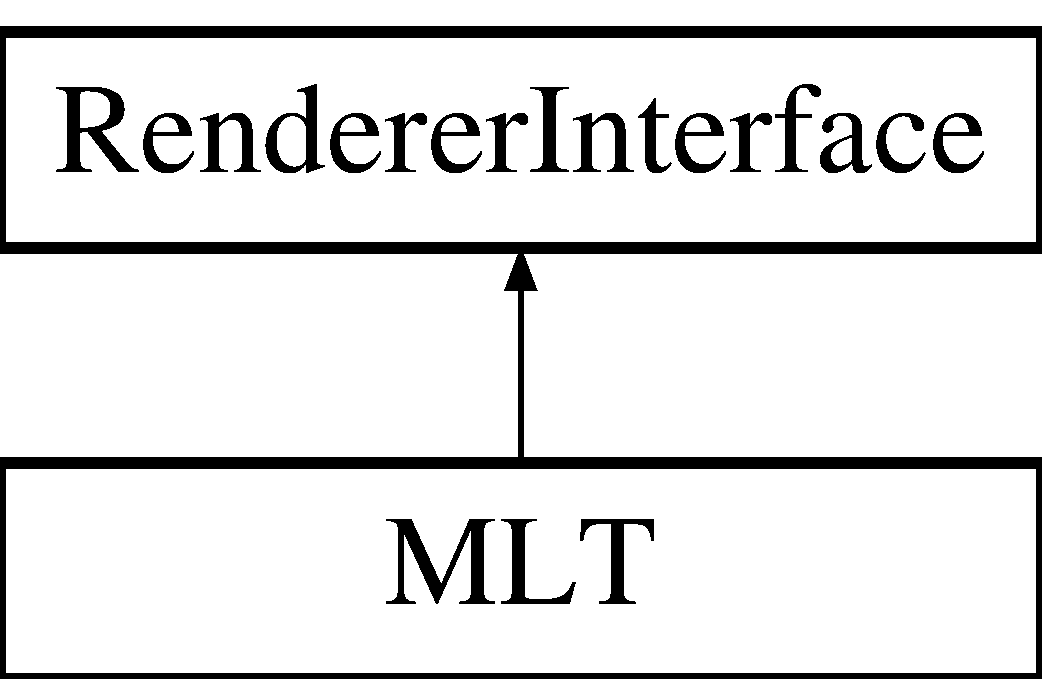
\includegraphics[height=2.000000cm]{struct_m_l_t}
\end{center}
\end{figure}
\subsection*{Public Methods}
\begin{DoxyCompactItemize}
\item 
void \hyperlink{struct_m_l_t_a3e5f5dc01f80a3c599384660163ad3d7}{init} (int argc, char $\ast$$\ast$argv, \hyperlink{struct_rendering_context}{Rendering\+Context} \&renderer)
\item 
void \hyperlink{struct_m_l_t_ac7f187ec2fdd67baedb0cf1d74060b89}{render} (const uint32 instance, \hyperlink{struct_rendering_context}{Rendering\+Context} \&renderer)
\item 
\mbox{\Hypertarget{struct_m_l_t_adcee8659ac95d2d4abd896f1c2626393}\label{struct_m_l_t_adcee8659ac95d2d4abd896f1c2626393}} 
void {\bfseries sample\+\_\+seeds} (\hyperlink{struct_m_l_t_context}{M\+L\+T\+Context} \&context)
\item 
\mbox{\Hypertarget{struct_m_l_t_a0655a66c36124ce73b914528fc6e7d41}\label{struct_m_l_t_a0655a66c36124ce73b914528fc6e7d41}} 
void {\bfseries recover\+\_\+seed\+\_\+paths} (\hyperlink{struct_m_l_t_context}{M\+L\+T\+Context} \&context, \hyperlink{struct_rendering_context_view}{Rendering\+Context\+View} \&renderer\+\_\+view)
\item 
void \hyperlink{struct_m_l_t_adb75fd53b62131575a9f739953eeac67}{destroy} ()
\item 
\mbox{\Hypertarget{struct_m_l_t_aee09a067e1c8e36be42399142c667f61}\label{struct_m_l_t_aee09a067e1c8e36be42399142c667f61}} 
void {\bfseries alloc} (\hyperlink{struct_m_l_t_context}{M\+L\+T\+Context} \&context, \hyperlink{structcugar_1_1memory__arena}{cugar\+::memory\+\_\+arena} \&arena, const uint32 n\+\_\+pixels, const uint32 n\+\_\+chains)
\end{DoxyCompactItemize}
\subsection*{Static Public Methods}
\begin{DoxyCompactItemize}
\item 
\mbox{\Hypertarget{struct_m_l_t_a135881654f589ac26b4a4c25a10fbd9a}\label{struct_m_l_t_a135881654f589ac26b4a4c25a10fbd9a}} 
static \hyperlink{struct_renderer_interface}{Renderer\+Interface} $\ast$ {\bfseries factory} ()
\end{DoxyCompactItemize}
\subsection*{Public Members}
\begin{DoxyCompactItemize}
\item 
\mbox{\Hypertarget{struct_m_l_t_a441bc00efd7dcd4825cfdd8d3b9929dd}\label{struct_m_l_t_a441bc00efd7dcd4825cfdd8d3b9929dd}} 
\hyperlink{struct_m_l_t_options}{M\+L\+T\+Options} {\bfseries m\+\_\+options}
\item 
\mbox{\Hypertarget{struct_m_l_t_a5c2a4a12778157241cc41a7fba1d4716}\label{struct_m_l_t_a5c2a4a12778157241cc41a7fba1d4716}} 
\hyperlink{struct_tiled_sequence}{Tiled\+Sequence} {\bfseries m\+\_\+sequence}
\item 
\mbox{\Hypertarget{struct_m_l_t_ad007c6bcbaf693d05c983ddaf575f9db}\label{struct_m_l_t_ad007c6bcbaf693d05c983ddaf575f9db}} 
\hyperlink{struct_b_p_t_queues_storage}{B\+P\+T\+Queues\+Storage} {\bfseries m\+\_\+queues}
\item 
\mbox{\Hypertarget{struct_m_l_t_a69bd07522df9f672cc68ad189ebe89b9}\label{struct_m_l_t_a69bd07522df9f672cc68ad189ebe89b9}} 
\hyperlink{struct_vertex_storage}{Vertex\+Storage} {\bfseries m\+\_\+light\+\_\+vertices}
\item 
\mbox{\Hypertarget{struct_m_l_t_a6a981cdc9402b17fdc6570018957508f}\label{struct_m_l_t_a6a981cdc9402b17fdc6570018957508f}} 
float {\bfseries m\+\_\+image\+\_\+brightness}
\item 
\mbox{\Hypertarget{struct_m_l_t_a13f5cd6942497f3426793814d17c8453}\label{struct_m_l_t_a13f5cd6942497f3426793814d17c8453}} 
uint32 {\bfseries m\+\_\+n\+\_\+lights}
\item 
\mbox{\Hypertarget{struct_m_l_t_afa51ded5b41b34ef85359995db675b8f}\label{struct_m_l_t_afa51ded5b41b34ef85359995db675b8f}} 
uint32 {\bfseries m\+\_\+n\+\_\+init\+\_\+paths}
\item 
\mbox{\Hypertarget{struct_m_l_t_a98d38ad5e68c658cd176fb01dab5f798}\label{struct_m_l_t_a98d38ad5e68c658cd176fb01dab5f798}} 
uint32 {\bfseries m\+\_\+n\+\_\+connections}
\item 
\mbox{\Hypertarget{struct_m_l_t_ad0bbf1ef848748789fccf2ba02389fc4}\label{struct_m_l_t_ad0bbf1ef848748789fccf2ba02389fc4}} 
\hyperlink{class_domain_buffer}{Domain\+Buffer}$<$ C\+U\+D\+A\+\_\+\+B\+U\+F\+F\+ER, uint8 $>$ {\bfseries m\+\_\+memory\+\_\+pool}
\item 
\mbox{\Hypertarget{struct_m_l_t_a91a72f803b153fffdaab71f4028e4e23}\label{struct_m_l_t_a91a72f803b153fffdaab71f4028e4e23}} 
\hyperlink{class_domain_buffer}{Domain\+Buffer}$<$ C\+U\+D\+A\+\_\+\+B\+U\+F\+F\+ER, float $>$ {\bfseries m\+\_\+connections\+\_\+cdf}
\item 
\mbox{\Hypertarget{struct_m_l_t_addf748fe61e7b763d7db6ba1ce3ffa35}\label{struct_m_l_t_addf748fe61e7b763d7db6ba1ce3ffa35}} 
\hyperlink{class_domain_buffer}{Domain\+Buffer}$<$ H\+O\+S\+T\+\_\+\+B\+U\+F\+F\+ER, float $>$ {\bfseries m\+\_\+path\+\_\+pdf\+\_\+backup}
\item 
\mbox{\Hypertarget{struct_m_l_t_a02707979fed2f283805da1189ba03721}\label{struct_m_l_t_a02707979fed2f283805da1189ba03721}} 
\hyperlink{classcugar_1_1_l_f_s_r_generator_matrix}{cugar\+::\+L\+F\+S\+R\+Generator\+Matrix} {\bfseries m\+\_\+generator}
\item 
\mbox{\Hypertarget{struct_m_l_t_a98e7c0bcc4d66cd31ea7ed94ab4f32db}\label{struct_m_l_t_a98e7c0bcc4d66cd31ea7ed94ab4f32db}} 
\hyperlink{structcugar_1_1_l_f_s_r_random_stream}{cugar\+::\+L\+F\+S\+R\+Random\+Stream} {\bfseries m\+\_\+random}
\end{DoxyCompactItemize}


\subsection{Member Function Documentation}
\mbox{\Hypertarget{struct_m_l_t_adb75fd53b62131575a9f739953eeac67}\label{struct_m_l_t_adb75fd53b62131575a9f739953eeac67}} 
\index{M\+LT@{M\+LT}!destroy@{destroy}}
\index{destroy@{destroy}!M\+LT@{M\+LT}}
\subsubsection{\texorpdfstring{destroy()}{destroy()}}
{\footnotesize\ttfamily void M\+L\+T\+::destroy (\begin{DoxyParamCaption}{ }\end{DoxyParamCaption})\hspace{0.3cm}{\ttfamily [inline]}, {\ttfamily [virtual]}}

this method is responsible for destroying the object itself 

Reimplemented from \hyperlink{struct_renderer_interface_a7469218aafa029a3e22bac2c00dca9f5}{Renderer\+Interface}.

\mbox{\Hypertarget{struct_m_l_t_a3e5f5dc01f80a3c599384660163ad3d7}\label{struct_m_l_t_a3e5f5dc01f80a3c599384660163ad3d7}} 
\index{M\+LT@{M\+LT}!init@{init}}
\index{init@{init}!M\+LT@{M\+LT}}
\subsubsection{\texorpdfstring{init()}{init()}}
{\footnotesize\ttfamily void M\+L\+T\+::init (\begin{DoxyParamCaption}\item[{int}]{argc,  }\item[{char $\ast$$\ast$}]{argv,  }\item[{\hyperlink{struct_rendering_context}{Rendering\+Context} \&}]{renderer }\end{DoxyParamCaption})\hspace{0.3cm}{\ttfamily [virtual]}}

this method is responsible for any command options parsing / initializations the renderer might need to perform 

Reimplemented from \hyperlink{struct_renderer_interface_a2ead9b943d6d48fcd32872e0005ebe63}{Renderer\+Interface}.

\mbox{\Hypertarget{struct_m_l_t_ac7f187ec2fdd67baedb0cf1d74060b89}\label{struct_m_l_t_ac7f187ec2fdd67baedb0cf1d74060b89}} 
\index{M\+LT@{M\+LT}!render@{render}}
\index{render@{render}!M\+LT@{M\+LT}}
\subsubsection{\texorpdfstring{render()}{render()}}
{\footnotesize\ttfamily void M\+L\+T\+::render (\begin{DoxyParamCaption}\item[{const uint32}]{instance,  }\item[{\hyperlink{struct_rendering_context}{Rendering\+Context} \&}]{renderer }\end{DoxyParamCaption})\hspace{0.3cm}{\ttfamily [virtual]}}

this method is responsible for rendering a given frame in a progressive rendering


\begin{DoxyParams}{Parameters}
{\em instance} & the frame instance \\
\hline
\end{DoxyParams}


Reimplemented from \hyperlink{struct_renderer_interface_aa64254dd44c94929b05092dc8d74f29d}{Renderer\+Interface}.



The documentation for this struct was generated from the following file\+:\begin{DoxyCompactItemize}
\item 
C\+:/p4research/research/jpantaleoni/\+Fermat-\/\+Public/src/renderers/mlt.\+h\end{DoxyCompactItemize}

\hypertarget{struct_m_l_t_context}{}\section{M\+L\+T\+Context Struct Reference}
\label{struct_m_l_t_context}\index{M\+L\+T\+Context@{M\+L\+T\+Context}}
Inheritance diagram for M\+L\+T\+Context\+:\begin{figure}[H]
\begin{center}
\leavevmode
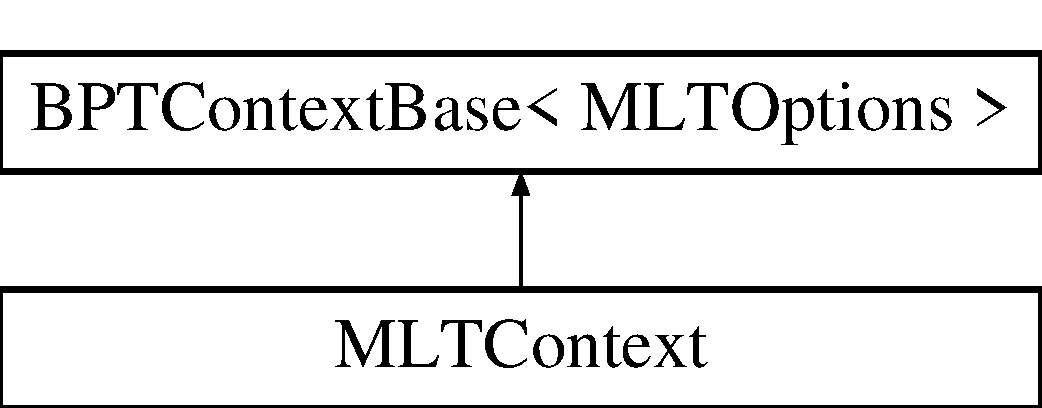
\includegraphics[height=2.000000cm]{struct_m_l_t_context}
\end{center}
\end{figure}
\subsection*{Public Methods}
\begin{DoxyCompactItemize}
\item 
\mbox{\Hypertarget{struct_m_l_t_context_a38b614856bb0029b5a63aeb29b5d2645}\label{struct_m_l_t_context_a38b614856bb0029b5a63aeb29b5d2645}} 
{\bfseries M\+L\+T\+Context} (\hyperlink{struct_m_l_t}{M\+LT} \&\+\_\+mlt, const \hyperlink{struct_rendering_context_view}{Rendering\+Context\+View} \&\+\_\+renderer)
\item 
\mbox{\Hypertarget{struct_m_l_t_context_a7c09b9fa48d021e14ecf3cb95fcb254b}\label{struct_m_l_t_context_a7c09b9fa48d021e14ecf3cb95fcb254b}} 
F\+E\+R\+M\+A\+T\+\_\+\+H\+O\+S\+T\+\_\+\+D\+E\+V\+I\+CE F\+E\+R\+M\+A\+T\+\_\+\+F\+O\+R\+C\+E\+I\+N\+L\+I\+NE float {\bfseries u\+\_\+m} (const uint32 chain\+\_\+id, const uint32 dim) const
\item 
\mbox{\Hypertarget{struct_m_l_t_context_a35465071c4d049f16eacc4e5580f2a6f}\label{struct_m_l_t_context_a35465071c4d049f16eacc4e5580f2a6f}} 
F\+E\+R\+M\+A\+T\+\_\+\+H\+O\+S\+T\+\_\+\+D\+E\+V\+I\+CE F\+E\+R\+M\+A\+T\+\_\+\+F\+O\+R\+C\+E\+I\+N\+L\+I\+NE void {\bfseries discard} (const uint32 chain\+\_\+id)
\item 
\mbox{\Hypertarget{struct_m_l_t_context_a953b24804201345870f2a93ef87a6afa}\label{struct_m_l_t_context_a953b24804201345870f2a93ef87a6afa}} 
F\+E\+R\+M\+A\+T\+\_\+\+H\+O\+S\+T\+\_\+\+D\+E\+V\+I\+CE F\+E\+R\+M\+A\+T\+\_\+\+F\+O\+R\+C\+E\+I\+N\+L\+I\+NE bool {\bfseries discard\+\_\+invalid} (const uint32 chain\+\_\+id)
\end{DoxyCompactItemize}
\subsection*{Public Members}
\begin{DoxyCompactItemize}
\item 
\mbox{\Hypertarget{struct_m_l_t_context_a167bff839ce47fce25f56a104571151b}\label{struct_m_l_t_context_a167bff839ce47fce25f56a104571151b}} 
\hyperlink{struct_tiled_sequence_view}{Tiled\+Sequence\+View} {\bfseries sequence}
\item 
\mbox{\Hypertarget{struct_m_l_t_context_acde21cc9e2d832a39dee6ecb7c9f96a9}\label{struct_m_l_t_context_acde21cc9e2d832a39dee6ecb7c9f96a9}} 
uint32 {\bfseries n\+\_\+light\+\_\+paths}
\item 
\mbox{\Hypertarget{struct_m_l_t_context_ad5a31fb25b253e00e00c68299c8630b9}\label{struct_m_l_t_context_ad5a31fb25b253e00e00c68299c8630b9}} 
uint32 {\bfseries n\+\_\+eye\+\_\+paths}
\item 
\mbox{\Hypertarget{struct_m_l_t_context_afb845e9b012850574c2f96b3e57f5f9a}\label{struct_m_l_t_context_afb845e9b012850574c2f96b3e57f5f9a}} 
float4 $\ast$ {\bfseries connections\+\_\+value}
\item 
\mbox{\Hypertarget{struct_m_l_t_context_aea3404f54e15450c04989dbab1371e4d}\label{struct_m_l_t_context_aea3404f54e15450c04989dbab1371e4d}} 
uint4 $\ast$ {\bfseries connections\+\_\+index}
\item 
\mbox{\Hypertarget{struct_m_l_t_context_a627c769b6a1e4e65259779a2a282f7a3}\label{struct_m_l_t_context_a627c769b6a1e4e65259779a2a282f7a3}} 
uint32 $\ast$ {\bfseries connections\+\_\+counter}
\item 
\mbox{\Hypertarget{struct_m_l_t_context_a163fb90e236c0b38eafbf3f6f0e3660c}\label{struct_m_l_t_context_a163fb90e236c0b38eafbf3f6f0e3660c}} 
float $\ast$ {\bfseries st\+\_\+norms}
\item 
\mbox{\Hypertarget{struct_m_l_t_context_ab0f318a92f5284f11f2562ee40be1b27}\label{struct_m_l_t_context_ab0f318a92f5284f11f2562ee40be1b27}} 
float $\ast$ {\bfseries st\+\_\+norms\+\_\+cdf}
\item 
\mbox{\Hypertarget{struct_m_l_t_context_ab185933d05ec3f765f311ab23e3a0ca3}\label{struct_m_l_t_context_ab185933d05ec3f765f311ab23e3a0ca3}} 
uint32 $\ast$ {\bfseries st\+\_\+counters}
\item 
\mbox{\Hypertarget{struct_m_l_t_context_ad2e60192e3b7254d29cf5e5fbc7d75a1}\label{struct_m_l_t_context_ad2e60192e3b7254d29cf5e5fbc7d75a1}} 
uint32 $\ast$ {\bfseries seeds}
\item 
\mbox{\Hypertarget{struct_m_l_t_context_a80ef59dd045be11a978bdc858fddaa03}\label{struct_m_l_t_context_a80ef59dd045be11a978bdc858fddaa03}} 
char4 $\ast$ {\bfseries st}
\item 
\mbox{\Hypertarget{struct_m_l_t_context_a67ed0837746dfb142cccb4bc55e5185a}\label{struct_m_l_t_context_a67ed0837746dfb142cccb4bc55e5185a}} 
\hyperlink{struct_vertex_geometry_id}{Vertex\+Geometry\+Id} $\ast$ {\bfseries bpt\+\_\+light\+\_\+vertices}
\item 
\mbox{\Hypertarget{struct_m_l_t_context_a7425cbfb90f62ba34ef5d75c989b3a5c}\label{struct_m_l_t_context_a7425cbfb90f62ba34ef5d75c989b3a5c}} 
\hyperlink{struct_vertex_geometry_id}{Vertex\+Geometry\+Id} $\ast$ {\bfseries bpt\+\_\+eye\+\_\+vertices}
\item 
\mbox{\Hypertarget{struct_m_l_t_context_a39abf094034b9d367abf77c9e6ff54ca}\label{struct_m_l_t_context_a39abf094034b9d367abf77c9e6ff54ca}} 
\hyperlink{struct_vertex_geometry_id}{Vertex\+Geometry\+Id} $\ast$ {\bfseries mut\+\_\+vertices}
\item 
\mbox{\Hypertarget{struct_m_l_t_context_ab77b5a56066a1640ba88a5fea1fd461c}\label{struct_m_l_t_context_ab77b5a56066a1640ba88a5fea1fd461c}} 
\hyperlink{struct_vertex_geometry_id}{Vertex\+Geometry\+Id} $\ast$ {\bfseries vertices}
\item 
\mbox{\Hypertarget{struct_m_l_t_context_adb275eeaf85241de00566654964c6b1b}\label{struct_m_l_t_context_adb275eeaf85241de00566654964c6b1b}} 
float4 $\ast$ {\bfseries path\+\_\+value}
\item 
\mbox{\Hypertarget{struct_m_l_t_context_a6f2257c5834ebaee55099a415d241942}\label{struct_m_l_t_context_a6f2257c5834ebaee55099a415d241942}} 
float $\ast$ {\bfseries path\+\_\+pdf}
\item 
\mbox{\Hypertarget{struct_m_l_t_context_a8b5218134c5f55e1e92743a6e175d339}\label{struct_m_l_t_context_a8b5218134c5f55e1e92743a6e175d339}} 
uint32 $\ast$ {\bfseries rejections}
\item 
\mbox{\Hypertarget{struct_m_l_t_context_aa3a1cf8ba723088ec72ff44db3c06f19}\label{struct_m_l_t_context_aa3a1cf8ba723088ec72ff44db3c06f19}} 
uint32 {\bfseries n\+\_\+chains}
\item 
\mbox{\Hypertarget{struct_m_l_t_context_a8309569132afdcee7282d9558dfdf3b8}\label{struct_m_l_t_context_a8309569132afdcee7282d9558dfdf3b8}} 
uint32 {\bfseries chain\+\_\+length}
\item 
\mbox{\Hypertarget{struct_m_l_t_context_a007f8c9f5a00cd30450ad930e761b2f2}\label{struct_m_l_t_context_a007f8c9f5a00cd30450ad930e761b2f2}} 
uint32 {\bfseries chain\+\_\+step}
\item 
\mbox{\Hypertarget{struct_m_l_t_context_a512c77839655be6b67003668ead752c8}\label{struct_m_l_t_context_a512c77839655be6b67003668ead752c8}} 
float {\bfseries pdf\+\_\+norm}
\item 
\mbox{\Hypertarget{struct_m_l_t_context_a1f749d0274a77f4239ce604f5dc69f67}\label{struct_m_l_t_context_a1f749d0274a77f4239ce604f5dc69f67}} 
uint32 {\bfseries enable\+\_\+mutations}
\item 
\mbox{\Hypertarget{struct_m_l_t_context_a192b4ee9700bc8e21c252b32ef7bc204}\label{struct_m_l_t_context_a192b4ee9700bc8e21c252b32ef7bc204}} 
float $\ast$ {\bfseries acceptance\+\_\+rate\+\_\+sum}
\item 
\mbox{\Hypertarget{struct_m_l_t_context_a27944801915161829fdba36ac23c327b}\label{struct_m_l_t_context_a27944801915161829fdba36ac23c327b}} 
float $\ast$ {\bfseries checksum}
\item 
\mbox{\Hypertarget{struct_m_l_t_context_a94f9e4e545bb2b318c324f7e1ec2768c}\label{struct_m_l_t_context_a94f9e4e545bb2b318c324f7e1ec2768c}} 
float4 $\ast$ {\bfseries mut\+\_\+f\+\_\+vertices}
\item 
\mbox{\Hypertarget{struct_m_l_t_context_a9989a384f1dd8988a21be20df012e9c4}\label{struct_m_l_t_context_a9989a384f1dd8988a21be20df012e9c4}} 
float4 $\ast$ {\bfseries f\+\_\+vertices}
\item 
\mbox{\Hypertarget{struct_m_l_t_context_a4cc8c77d0f4b08a8ddefccaf0b84c01d}\label{struct_m_l_t_context_a4cc8c77d0f4b08a8ddefccaf0b84c01d}} 
\hyperlink{structcugar_1_1_vector}{cugar\+::\+Vector4f} $\ast$ {\bfseries Q\+\_\+old}
\item 
\mbox{\Hypertarget{struct_m_l_t_context_a250c16da263d4e879c7fa574c2fa75fd}\label{struct_m_l_t_context_a250c16da263d4e879c7fa574c2fa75fd}} 
\hyperlink{structcugar_1_1_vector}{cugar\+::\+Vector4f} $\ast$ {\bfseries Q\+\_\+new}
\item 
\mbox{\Hypertarget{struct_m_l_t_context_aa4edb6bcfbb071b88110f7ca28b25300}\label{struct_m_l_t_context_aa4edb6bcfbb071b88110f7ca28b25300}} 
\hyperlink{struct_mesh_light}{Mesh\+Light} {\bfseries mesh\+\_\+light}
\end{DoxyCompactItemize}


The documentation for this struct was generated from the following file\+:\begin{DoxyCompactItemize}
\item 
C\+:/p4research/research/jpantaleoni/\+Fermat-\/\+Public/src/renderers/mlt\+\_\+core.\+h\end{DoxyCompactItemize}

\hypertarget{struct_m_l_t_options}{}\section{M\+L\+T\+Options Struct Reference}
\label{struct_m_l_t_options}\index{M\+L\+T\+Options@{M\+L\+T\+Options}}


\subsection{Detailed description}
\hyperlink{struct_m_l_t}{M\+LT} renderer options 

{\ttfamily \#include $<$mlt.\+h$>$}

Inheritance diagram for M\+L\+T\+Options\+:\begin{figure}[H]
\begin{center}
\leavevmode
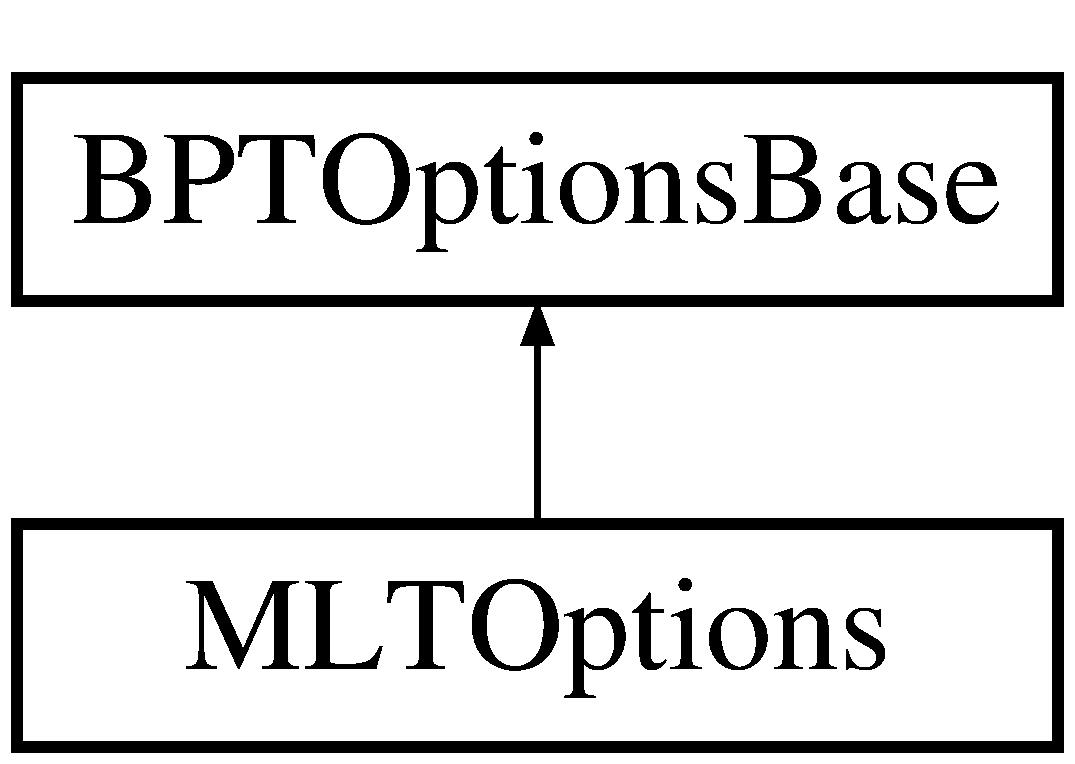
\includegraphics[height=2.000000cm]{struct_m_l_t_options}
\end{center}
\end{figure}
\subsection*{Public Methods}
\begin{DoxyCompactItemize}
\item 
\mbox{\Hypertarget{struct_m_l_t_options_aa5542e6d9626622b398b5f399b4ba642}\label{struct_m_l_t_options_aa5542e6d9626622b398b5f399b4ba642}} 
void {\bfseries parse} (const int argc, char $\ast$$\ast$argv)
\end{DoxyCompactItemize}
\subsection*{Public Members}
\begin{DoxyCompactItemize}
\item 
\mbox{\Hypertarget{struct_m_l_t_options_a18382f067bb09686ef584c8dcefda3e7}\label{struct_m_l_t_options_a18382f067bb09686ef584c8dcefda3e7}} 
uint32 {\bfseries n\+\_\+chains}
\item 
\mbox{\Hypertarget{struct_m_l_t_options_ae535e8ebd61a70e31a38841199658664}\label{struct_m_l_t_options_ae535e8ebd61a70e31a38841199658664}} 
uint32 {\bfseries spp}
\item 
\mbox{\Hypertarget{struct_m_l_t_options_a6e30a0f1cb0b617aeb34a7d8a6c7837a}\label{struct_m_l_t_options_a6e30a0f1cb0b617aeb34a7d8a6c7837a}} 
uint32 {\bfseries reseeding\+\_\+freq}
\item 
\mbox{\Hypertarget{struct_m_l_t_options_a4f9982361eba08c6c0b2e97e9c1912c3}\label{struct_m_l_t_options_a4f9982361eba08c6c0b2e97e9c1912c3}} 
uint32 {\bfseries mis}\+: 1
\item 
\mbox{\Hypertarget{struct_m_l_t_options_af237541d6431d255751da45676d52b41}\label{struct_m_l_t_options_af237541d6431d255751da45676d52b41}} 
float {\bfseries st\+\_\+perturbations}
\item 
\mbox{\Hypertarget{struct_m_l_t_options_a2e096ece8892de850873cee9d68a1d74}\label{struct_m_l_t_options_a2e096ece8892de850873cee9d68a1d74}} 
float {\bfseries screen\+\_\+perturbations}
\item 
\mbox{\Hypertarget{struct_m_l_t_options_adc787450d3998f627ec2334f06bb18b5}\label{struct_m_l_t_options_adc787450d3998f627ec2334f06bb18b5}} 
float {\bfseries exp\+\_\+perturbations}
\item 
\mbox{\Hypertarget{struct_m_l_t_options_a9425d7ceff6d24343fe6c056f012b525}\label{struct_m_l_t_options_a9425d7ceff6d24343fe6c056f012b525}} 
float {\bfseries H\+\_\+perturbations}
\item 
\mbox{\Hypertarget{struct_m_l_t_options_a04730dcf2df363ca79596457039108f0}\label{struct_m_l_t_options_a04730dcf2df363ca79596457039108f0}} 
float {\bfseries perturbation\+\_\+radius}
\item 
\mbox{\Hypertarget{struct_m_l_t_options_a6e6d5a6692c663f09782f648351b2963}\label{struct_m_l_t_options_a6e6d5a6692c663f09782f648351b2963}} 
uint32 {\bfseries flags}
\end{DoxyCompactItemize}


The documentation for this struct was generated from the following file\+:\begin{DoxyCompactItemize}
\item 
C\+:/p4research/research/jpantaleoni/\+Fermat-\/\+Public/src/renderers/mlt.\+h\end{DoxyCompactItemize}

\hypertarget{structcugar_1_1cuda_1_1lbvh_1_1_morton__bits}{}\section{cugar\+:\+:cuda\+:\+:lbvh\+:\+:Morton\+\_\+bits$<$ integer $>$ Struct Template Reference}
\label{structcugar_1_1cuda_1_1lbvh_1_1_morton__bits}\index{cugar\+::cuda\+::lbvh\+::\+Morton\+\_\+bits$<$ integer $>$@{cugar\+::cuda\+::lbvh\+::\+Morton\+\_\+bits$<$ integer $>$}}


The documentation for this struct was generated from the following file\+:\begin{DoxyCompactItemize}
\item 
C\+:/p4research/research/jpantaleoni/\+Fermat-\/\+Public/contrib/cugar/bvh/cuda/lbvh\+\_\+builder\+\_\+inline.\+h\end{DoxyCompactItemize}

\hypertarget{structcugar_1_1cuda_1_1kd_1_1_morton__bits}{}\section{cugar\+:\+:cuda\+:\+:kd\+:\+:Morton\+\_\+bits$<$ integer, D\+IM $>$ Struct Template Reference}
\label{structcugar_1_1cuda_1_1kd_1_1_morton__bits}\index{cugar\+::cuda\+::kd\+::\+Morton\+\_\+bits$<$ integer, D\+I\+M $>$@{cugar\+::cuda\+::kd\+::\+Morton\+\_\+bits$<$ integer, D\+I\+M $>$}}


The documentation for this struct was generated from the following file\+:\begin{DoxyCompactItemize}
\item 
C\+:/p4research/research/jpantaleoni/\+Fermat-\/\+Public/contrib/cugar/kd/cuda/kd\+\_\+builder\+\_\+inline.\+h\end{DoxyCompactItemize}

\hypertarget{structcugar_1_1cuda_1_1lbvh_1_1_morton__bits_3_01uint32_01_4}{}\section{cugar\+:\+:cuda\+:\+:lbvh\+:\+:Morton\+\_\+bits$<$ uint32 $>$ Struct Template Reference}
\label{structcugar_1_1cuda_1_1lbvh_1_1_morton__bits_3_01uint32_01_4}\index{cugar\+::cuda\+::lbvh\+::\+Morton\+\_\+bits$<$ uint32 $>$@{cugar\+::cuda\+::lbvh\+::\+Morton\+\_\+bits$<$ uint32 $>$}}
\subsection*{Static Public Members}
\begin{DoxyCompactItemize}
\item 
\mbox{\Hypertarget{structcugar_1_1cuda_1_1lbvh_1_1_morton__bits_3_01uint32_01_4_a2c8c2c12ff4e7ffb036b4d2a2273f9c0}\label{structcugar_1_1cuda_1_1lbvh_1_1_morton__bits_3_01uint32_01_4_a2c8c2c12ff4e7ffb036b4d2a2273f9c0}} 
static const uint32 {\bfseries value} = 30u
\end{DoxyCompactItemize}


The documentation for this struct was generated from the following file\+:\begin{DoxyCompactItemize}
\item 
C\+:/p4research/research/jpantaleoni/\+Fermat-\/\+Public/contrib/cugar/bvh/cuda/lbvh\+\_\+builder\+\_\+inline.\+h\end{DoxyCompactItemize}

\hypertarget{structcugar_1_1cuda_1_1kd_1_1_morton__bits_3_01uint32_00_012u_01_4}{}\section{cugar\+:\+:cuda\+:\+:kd\+:\+:Morton\+\_\+bits$<$ uint32, 2u $>$ Struct Template Reference}
\label{structcugar_1_1cuda_1_1kd_1_1_morton__bits_3_01uint32_00_012u_01_4}\index{cugar\+::cuda\+::kd\+::\+Morton\+\_\+bits$<$ uint32, 2u $>$@{cugar\+::cuda\+::kd\+::\+Morton\+\_\+bits$<$ uint32, 2u $>$}}
\subsection*{Static Public Methods}
\begin{DoxyCompactItemize}
\item 
\mbox{\Hypertarget{structcugar_1_1cuda_1_1kd_1_1_morton__bits_3_01uint32_00_012u_01_4_a1c9776e95f4a55b5b1f3c28efbc0c644}\label{structcugar_1_1cuda_1_1kd_1_1_morton__bits_3_01uint32_00_012u_01_4_a1c9776e95f4a55b5b1f3c28efbc0c644}} 
static C\+U\+G\+A\+R\+\_\+\+H\+O\+S\+T\+\_\+\+D\+E\+V\+I\+CE float {\bfseries convert} (float a, float b, const uint32 i)
\end{DoxyCompactItemize}
\subsection*{Static Public Members}
\begin{DoxyCompactItemize}
\item 
\mbox{\Hypertarget{structcugar_1_1cuda_1_1kd_1_1_morton__bits_3_01uint32_00_012u_01_4_ad0ff2adb2420056a7b5e7fd8c0da9be7}\label{structcugar_1_1cuda_1_1kd_1_1_morton__bits_3_01uint32_00_012u_01_4_ad0ff2adb2420056a7b5e7fd8c0da9be7}} 
static const uint32 {\bfseries value} = 32u
\end{DoxyCompactItemize}


The documentation for this struct was generated from the following file\+:\begin{DoxyCompactItemize}
\item 
C\+:/p4research/research/jpantaleoni/\+Fermat-\/\+Public/contrib/cugar/kd/cuda/kd\+\_\+builder\+\_\+inline.\+h\end{DoxyCompactItemize}

\hypertarget{structcugar_1_1cuda_1_1kd_1_1_morton__bits_3_01uint32_00_013u_01_4}{}\section{cugar\+:\+:cuda\+:\+:kd\+:\+:Morton\+\_\+bits$<$ uint32, 3u $>$ Struct Template Reference}
\label{structcugar_1_1cuda_1_1kd_1_1_morton__bits_3_01uint32_00_013u_01_4}\index{cugar\+::cuda\+::kd\+::\+Morton\+\_\+bits$<$ uint32, 3u $>$@{cugar\+::cuda\+::kd\+::\+Morton\+\_\+bits$<$ uint32, 3u $>$}}
\subsection*{Static Public Methods}
\begin{DoxyCompactItemize}
\item 
\mbox{\Hypertarget{structcugar_1_1cuda_1_1kd_1_1_morton__bits_3_01uint32_00_013u_01_4_ae18e8ce5d46019d359775aa0305fcbf5}\label{structcugar_1_1cuda_1_1kd_1_1_morton__bits_3_01uint32_00_013u_01_4_ae18e8ce5d46019d359775aa0305fcbf5}} 
static C\+U\+G\+A\+R\+\_\+\+H\+O\+S\+T\+\_\+\+D\+E\+V\+I\+CE float {\bfseries convert} (float a, float b, const uint64 i)
\end{DoxyCompactItemize}
\subsection*{Static Public Members}
\begin{DoxyCompactItemize}
\item 
\mbox{\Hypertarget{structcugar_1_1cuda_1_1kd_1_1_morton__bits_3_01uint32_00_013u_01_4_a6487aa673caca85fd5cacbf445b517e5}\label{structcugar_1_1cuda_1_1kd_1_1_morton__bits_3_01uint32_00_013u_01_4_a6487aa673caca85fd5cacbf445b517e5}} 
static const uint32 {\bfseries value} = 30u
\end{DoxyCompactItemize}


The documentation for this struct was generated from the following file\+:\begin{DoxyCompactItemize}
\item 
C\+:/p4research/research/jpantaleoni/\+Fermat-\/\+Public/contrib/cugar/kd/cuda/kd\+\_\+builder\+\_\+inline.\+h\end{DoxyCompactItemize}

\hypertarget{structcugar_1_1cuda_1_1lbvh_1_1_morton__bits_3_01uint64_01_4}{}\section{cugar\+:\+:cuda\+:\+:lbvh\+:\+:Morton\+\_\+bits$<$ uint64 $>$ Struct Template Reference}
\label{structcugar_1_1cuda_1_1lbvh_1_1_morton__bits_3_01uint64_01_4}\index{cugar\+::cuda\+::lbvh\+::\+Morton\+\_\+bits$<$ uint64 $>$@{cugar\+::cuda\+::lbvh\+::\+Morton\+\_\+bits$<$ uint64 $>$}}
\subsection*{Static Public Members}
\begin{DoxyCompactItemize}
\item 
\mbox{\Hypertarget{structcugar_1_1cuda_1_1lbvh_1_1_morton__bits_3_01uint64_01_4_aaeb17017a5873c99f77a2786805de9cd}\label{structcugar_1_1cuda_1_1lbvh_1_1_morton__bits_3_01uint64_01_4_aaeb17017a5873c99f77a2786805de9cd}} 
static const uint32 {\bfseries value} = 60u
\end{DoxyCompactItemize}


The documentation for this struct was generated from the following file\+:\begin{DoxyCompactItemize}
\item 
C\+:/p4research/research/jpantaleoni/\+Fermat-\/\+Public/contrib/cugar/bvh/cuda/lbvh\+\_\+builder\+\_\+inline.\+h\end{DoxyCompactItemize}

\hypertarget{structcugar_1_1cuda_1_1kd_1_1_morton__bits_3_01uint64_00_012u_01_4}{}\section{cugar\+:\+:cuda\+:\+:kd\+:\+:Morton\+\_\+bits$<$ uint64, 2u $>$ Struct Template Reference}
\label{structcugar_1_1cuda_1_1kd_1_1_morton__bits_3_01uint64_00_012u_01_4}\index{cugar\+::cuda\+::kd\+::\+Morton\+\_\+bits$<$ uint64, 2u $>$@{cugar\+::cuda\+::kd\+::\+Morton\+\_\+bits$<$ uint64, 2u $>$}}
\subsection*{Static Public Methods}
\begin{DoxyCompactItemize}
\item 
\mbox{\Hypertarget{structcugar_1_1cuda_1_1kd_1_1_morton__bits_3_01uint64_00_012u_01_4_a28aa85bc17c670568b4da3a71c195e74}\label{structcugar_1_1cuda_1_1kd_1_1_morton__bits_3_01uint64_00_012u_01_4_a28aa85bc17c670568b4da3a71c195e74}} 
static C\+U\+G\+A\+R\+\_\+\+H\+O\+S\+T\+\_\+\+D\+E\+V\+I\+CE float {\bfseries convert} (float a, float b, const uint64 i)
\end{DoxyCompactItemize}
\subsection*{Static Public Members}
\begin{DoxyCompactItemize}
\item 
\mbox{\Hypertarget{structcugar_1_1cuda_1_1kd_1_1_morton__bits_3_01uint64_00_012u_01_4_ac8a07728926aff2df01122688e8a67b8}\label{structcugar_1_1cuda_1_1kd_1_1_morton__bits_3_01uint64_00_012u_01_4_ac8a07728926aff2df01122688e8a67b8}} 
static const uint32 {\bfseries value} = 64u
\end{DoxyCompactItemize}


The documentation for this struct was generated from the following file\+:\begin{DoxyCompactItemize}
\item 
C\+:/p4research/research/jpantaleoni/\+Fermat-\/\+Public/contrib/cugar/kd/cuda/kd\+\_\+builder\+\_\+inline.\+h\end{DoxyCompactItemize}

\hypertarget{structcugar_1_1cuda_1_1kd_1_1_morton__bits_3_01uint64_00_013u_01_4}{}\section{cugar\+:\+:cuda\+:\+:kd\+:\+:Morton\+\_\+bits$<$ uint64, 3u $>$ Struct Template Reference}
\label{structcugar_1_1cuda_1_1kd_1_1_morton__bits_3_01uint64_00_013u_01_4}\index{cugar\+::cuda\+::kd\+::\+Morton\+\_\+bits$<$ uint64, 3u $>$@{cugar\+::cuda\+::kd\+::\+Morton\+\_\+bits$<$ uint64, 3u $>$}}
\subsection*{Static Public Methods}
\begin{DoxyCompactItemize}
\item 
\mbox{\Hypertarget{structcugar_1_1cuda_1_1kd_1_1_morton__bits_3_01uint64_00_013u_01_4_af617a1604bbf8af802695191d2628ea7}\label{structcugar_1_1cuda_1_1kd_1_1_morton__bits_3_01uint64_00_013u_01_4_af617a1604bbf8af802695191d2628ea7}} 
static C\+U\+G\+A\+R\+\_\+\+H\+O\+S\+T\+\_\+\+D\+E\+V\+I\+CE float {\bfseries convert} (float a, float b, const uint64 i)
\end{DoxyCompactItemize}
\subsection*{Static Public Members}
\begin{DoxyCompactItemize}
\item 
\mbox{\Hypertarget{structcugar_1_1cuda_1_1kd_1_1_morton__bits_3_01uint64_00_013u_01_4_ae03a56781aa14d8d0def6f181b479e86}\label{structcugar_1_1cuda_1_1kd_1_1_morton__bits_3_01uint64_00_013u_01_4_ae03a56781aa14d8d0def6f181b479e86}} 
static const uint32 {\bfseries value} = 60u
\end{DoxyCompactItemize}


The documentation for this struct was generated from the following file\+:\begin{DoxyCompactItemize}
\item 
C\+:/p4research/research/jpantaleoni/\+Fermat-\/\+Public/contrib/cugar/kd/cuda/kd\+\_\+builder\+\_\+inline.\+h\end{DoxyCompactItemize}

\hypertarget{structcugar_1_1morton__functor}{}\section{cugar\+:\+:morton\+\_\+functor$<$ Integer, D\+IM, Bbox\+Type $>$ Struct Template Reference}
\label{structcugar_1_1morton__functor}\index{cugar\+::morton\+\_\+functor$<$ Integer, D\+I\+M, Bbox\+Type $>$@{cugar\+::morton\+\_\+functor$<$ Integer, D\+I\+M, Bbox\+Type $>$}}


\subsection{Detailed description}
\subsubsection*{template$<$typename Integer, uint32 D\+IM, typename Bbox\+Type$>$\newline
struct cugar\+::morton\+\_\+functor$<$ Integer, D\+I\+M, Bbox\+Type $>$}

a convenience functor to compute the Morton code of a point sequences relative to a given bounding box 

{\ttfamily \#include $<$morton.\+h$>$}



The documentation for this struct was generated from the following file\+:\begin{DoxyCompactItemize}
\item 
C\+:/p4research/research/jpantaleoni/\+Fermat-\/\+Public/contrib/cugar/bits/\hyperlink{morton_8h}{morton.\+h}\end{DoxyCompactItemize}

\hypertarget{structcugar_1_1morton__functor_3_01uint32_00_012u_00_01_bbox_type_01_4}{}\section{cugar\+:\+:morton\+\_\+functor$<$ uint32, 2u, Bbox\+Type $>$ Struct Template Reference}
\label{structcugar_1_1morton__functor_3_01uint32_00_012u_00_01_bbox_type_01_4}\index{cugar\+::morton\+\_\+functor$<$ uint32, 2u, Bbox\+Type $>$@{cugar\+::morton\+\_\+functor$<$ uint32, 2u, Bbox\+Type $>$}}


\subsection{Detailed description}
\subsubsection*{template$<$typename Bbox\+Type$>$\newline
struct cugar\+::morton\+\_\+functor$<$ uint32, 2u, Bbox\+Type $>$}

a convenience functor to compute the Morton code of a point sequences relative to a given bounding box 

{\ttfamily \#include $<$morton.\+h$>$}

\subsection*{Public Types}
\begin{DoxyCompactItemize}
\item 
\mbox{\Hypertarget{structcugar_1_1morton__functor_3_01uint32_00_012u_00_01_bbox_type_01_4_a745fd0a7750f5c4f4b2c69bb4ffb0c35}\label{structcugar_1_1morton__functor_3_01uint32_00_012u_00_01_bbox_type_01_4_a745fd0a7750f5c4f4b2c69bb4ffb0c35}} 
typedef Bbox\+Type\+::value\+\_\+type {\bfseries value\+\_\+type}
\item 
\mbox{\Hypertarget{structcugar_1_1morton__functor_3_01uint32_00_012u_00_01_bbox_type_01_4_a005e75c1506a4240601b699fc387857b}\label{structcugar_1_1morton__functor_3_01uint32_00_012u_00_01_bbox_type_01_4_a005e75c1506a4240601b699fc387857b}} 
typedef Bbox\+Type\+::vector\+\_\+type {\bfseries vector\+\_\+type}
\end{DoxyCompactItemize}
\subsection*{Public Methods}
\begin{DoxyCompactItemize}
\item 
C\+U\+G\+A\+R\+\_\+\+H\+O\+S\+T\+\_\+\+D\+E\+V\+I\+CE \hyperlink{structcugar_1_1morton__functor_3_01uint32_00_012u_00_01_bbox_type_01_4_a22f7d67d7676d39c3cf6b58b27115c6e}{morton\+\_\+functor} (const \hyperlink{structcugar_1_1_bbox}{Bbox2f} \&bbox)
\item 
\mbox{\Hypertarget{structcugar_1_1morton__functor_3_01uint32_00_012u_00_01_bbox_type_01_4_adddd67e8bcb38ffbc1369e93350612df}\label{structcugar_1_1morton__functor_3_01uint32_00_012u_00_01_bbox_type_01_4_adddd67e8bcb38ffbc1369e93350612df}} 
{\footnotesize template$<$typename Point\+\_\+type $>$ }\\C\+U\+G\+A\+R\+\_\+\+F\+O\+R\+C\+E\+I\+N\+L\+I\+NE C\+U\+G\+A\+R\+\_\+\+H\+O\+S\+T\+\_\+\+D\+E\+V\+I\+CE uint32 {\bfseries operator()} (const Point\+\_\+type point) const
\end{DoxyCompactItemize}
\subsection*{Public Members}
\begin{DoxyCompactItemize}
\item 
\mbox{\Hypertarget{structcugar_1_1morton__functor_3_01uint32_00_012u_00_01_bbox_type_01_4_a39c01ec883cd0686fd9fe4749095671b}\label{structcugar_1_1morton__functor_3_01uint32_00_012u_00_01_bbox_type_01_4_a39c01ec883cd0686fd9fe4749095671b}} 
const vector\+\_\+type {\bfseries m\+\_\+base}
\item 
\mbox{\Hypertarget{structcugar_1_1morton__functor_3_01uint32_00_012u_00_01_bbox_type_01_4_aacec74ca715221f55a44ab0ddba3579d}\label{structcugar_1_1morton__functor_3_01uint32_00_012u_00_01_bbox_type_01_4_aacec74ca715221f55a44ab0ddba3579d}} 
const vector\+\_\+type {\bfseries m\+\_\+inv}
\end{DoxyCompactItemize}


\subsection{Constructor \& Destructor Documentation}
\mbox{\Hypertarget{structcugar_1_1morton__functor_3_01uint32_00_012u_00_01_bbox_type_01_4_a22f7d67d7676d39c3cf6b58b27115c6e}\label{structcugar_1_1morton__functor_3_01uint32_00_012u_00_01_bbox_type_01_4_a22f7d67d7676d39c3cf6b58b27115c6e}} 
\index{cugar\+::morton\+\_\+functor$<$ uint32, 2u, Bbox\+Type $>$@{cugar\+::morton\+\_\+functor$<$ uint32, 2u, Bbox\+Type $>$}!morton\+\_\+functor@{morton\+\_\+functor}}
\index{morton\+\_\+functor@{morton\+\_\+functor}!cugar\+::morton\+\_\+functor$<$ uint32, 2u, Bbox\+Type $>$@{cugar\+::morton\+\_\+functor$<$ uint32, 2u, Bbox\+Type $>$}}
\subsubsection{\texorpdfstring{morton\+\_\+functor()}{morton\_functor()}}
{\footnotesize\ttfamily template$<$typename Bbox\+Type $>$ \\
C\+U\+G\+A\+R\+\_\+\+H\+O\+S\+T\+\_\+\+D\+E\+V\+I\+CE \hyperlink{structcugar_1_1morton__functor}{cugar\+::morton\+\_\+functor}$<$ uint32, 2u, Bbox\+Type $>$\+::morton\+\_\+functor (\begin{DoxyParamCaption}\item[{const \hyperlink{structcugar_1_1_bbox}{Bbox2f} \&}]{bbox }\end{DoxyParamCaption})\hspace{0.3cm}{\ttfamily [inline]}}

constructor


\begin{DoxyParams}{Parameters}
{\em bbox} & global bounding box \\
\hline
\end{DoxyParams}


The documentation for this struct was generated from the following file\+:\begin{DoxyCompactItemize}
\item 
C\+:/p4research/research/jpantaleoni/\+Fermat-\/\+Public/contrib/cugar/bits/\hyperlink{morton_8h}{morton.\+h}\end{DoxyCompactItemize}

\hypertarget{structcugar_1_1morton__functor_3_01uint32_00_013u_00_01_bbox_type_01_4}{}\section{cugar\+:\+:morton\+\_\+functor$<$ uint32, 3u, Bbox\+Type $>$ Struct Template Reference}
\label{structcugar_1_1morton__functor_3_01uint32_00_013u_00_01_bbox_type_01_4}\index{cugar\+::morton\+\_\+functor$<$ uint32, 3u, Bbox\+Type $>$@{cugar\+::morton\+\_\+functor$<$ uint32, 3u, Bbox\+Type $>$}}


\subsection{Detailed description}
\subsubsection*{template$<$typename Bbox\+Type$>$\newline
struct cugar\+::morton\+\_\+functor$<$ uint32, 3u, Bbox\+Type $>$}

a convenience functor to compute the Morton code of a point sequences relative to a given bounding box 

{\ttfamily \#include $<$morton.\+h$>$}

\subsection*{Public Types}
\begin{DoxyCompactItemize}
\item 
\mbox{\Hypertarget{structcugar_1_1morton__functor_3_01uint32_00_013u_00_01_bbox_type_01_4_a6fbfad2503596a20e9a2de48339f4c7b}\label{structcugar_1_1morton__functor_3_01uint32_00_013u_00_01_bbox_type_01_4_a6fbfad2503596a20e9a2de48339f4c7b}} 
typedef Bbox\+Type\+::value\+\_\+type {\bfseries value\+\_\+type}
\item 
\mbox{\Hypertarget{structcugar_1_1morton__functor_3_01uint32_00_013u_00_01_bbox_type_01_4_ab840861d24f217e1d59721b7a3fffa59}\label{structcugar_1_1morton__functor_3_01uint32_00_013u_00_01_bbox_type_01_4_ab840861d24f217e1d59721b7a3fffa59}} 
typedef Bbox\+Type\+::vector\+\_\+type {\bfseries vector\+\_\+type}
\end{DoxyCompactItemize}
\subsection*{Public Methods}
\begin{DoxyCompactItemize}
\item 
C\+U\+G\+A\+R\+\_\+\+H\+O\+S\+T\+\_\+\+D\+E\+V\+I\+CE \hyperlink{structcugar_1_1morton__functor_3_01uint32_00_013u_00_01_bbox_type_01_4_ab4f903dd2756ab775a91c70ff31c0627}{morton\+\_\+functor} (const Bbox\+Type \&bbox)
\item 
\mbox{\Hypertarget{structcugar_1_1morton__functor_3_01uint32_00_013u_00_01_bbox_type_01_4_a5e2e6fa21d338e0504a6f7b7a9531913}\label{structcugar_1_1morton__functor_3_01uint32_00_013u_00_01_bbox_type_01_4_a5e2e6fa21d338e0504a6f7b7a9531913}} 
{\footnotesize template$<$typename Point\+\_\+type $>$ }\\C\+U\+G\+A\+R\+\_\+\+F\+O\+R\+C\+E\+I\+N\+L\+I\+NE C\+U\+G\+A\+R\+\_\+\+H\+O\+S\+T\+\_\+\+D\+E\+V\+I\+CE uint32 {\bfseries operator()} (const Point\+\_\+type point) const
\end{DoxyCompactItemize}
\subsection*{Public Members}
\begin{DoxyCompactItemize}
\item 
\mbox{\Hypertarget{structcugar_1_1morton__functor_3_01uint32_00_013u_00_01_bbox_type_01_4_adbb97e98b3e7e7328662e4cb05ca3f4e}\label{structcugar_1_1morton__functor_3_01uint32_00_013u_00_01_bbox_type_01_4_adbb97e98b3e7e7328662e4cb05ca3f4e}} 
const vector\+\_\+type {\bfseries m\+\_\+base}
\item 
\mbox{\Hypertarget{structcugar_1_1morton__functor_3_01uint32_00_013u_00_01_bbox_type_01_4_a8ae0aec2c03b67dc1ca7e16cef4ed506}\label{structcugar_1_1morton__functor_3_01uint32_00_013u_00_01_bbox_type_01_4_a8ae0aec2c03b67dc1ca7e16cef4ed506}} 
const vector\+\_\+type {\bfseries m\+\_\+inv}
\end{DoxyCompactItemize}


\subsection{Constructor \& Destructor Documentation}
\mbox{\Hypertarget{structcugar_1_1morton__functor_3_01uint32_00_013u_00_01_bbox_type_01_4_ab4f903dd2756ab775a91c70ff31c0627}\label{structcugar_1_1morton__functor_3_01uint32_00_013u_00_01_bbox_type_01_4_ab4f903dd2756ab775a91c70ff31c0627}} 
\index{cugar\+::morton\+\_\+functor$<$ uint32, 3u, Bbox\+Type $>$@{cugar\+::morton\+\_\+functor$<$ uint32, 3u, Bbox\+Type $>$}!morton\+\_\+functor@{morton\+\_\+functor}}
\index{morton\+\_\+functor@{morton\+\_\+functor}!cugar\+::morton\+\_\+functor$<$ uint32, 3u, Bbox\+Type $>$@{cugar\+::morton\+\_\+functor$<$ uint32, 3u, Bbox\+Type $>$}}
\subsubsection{\texorpdfstring{morton\+\_\+functor()}{morton\_functor()}}
{\footnotesize\ttfamily template$<$typename Bbox\+Type $>$ \\
C\+U\+G\+A\+R\+\_\+\+H\+O\+S\+T\+\_\+\+D\+E\+V\+I\+CE \hyperlink{structcugar_1_1morton__functor}{cugar\+::morton\+\_\+functor}$<$ uint32, 3u, Bbox\+Type $>$\+::morton\+\_\+functor (\begin{DoxyParamCaption}\item[{const Bbox\+Type \&}]{bbox }\end{DoxyParamCaption})\hspace{0.3cm}{\ttfamily [inline]}}

constructor


\begin{DoxyParams}{Parameters}
{\em bbox} & global bounding box \\
\hline
\end{DoxyParams}


The documentation for this struct was generated from the following file\+:\begin{DoxyCompactItemize}
\item 
C\+:/p4research/research/jpantaleoni/\+Fermat-\/\+Public/contrib/cugar/bits/\hyperlink{morton_8h}{morton.\+h}\end{DoxyCompactItemize}

\hypertarget{structcugar_1_1morton__functor_3_01uint64_00_012u_00_01_bbox_type_01_4}{}\section{cugar\+:\+:morton\+\_\+functor$<$ uint64, 2u, Bbox\+Type $>$ Struct Template Reference}
\label{structcugar_1_1morton__functor_3_01uint64_00_012u_00_01_bbox_type_01_4}\index{cugar\+::morton\+\_\+functor$<$ uint64, 2u, Bbox\+Type $>$@{cugar\+::morton\+\_\+functor$<$ uint64, 2u, Bbox\+Type $>$}}


\subsection{Detailed description}
\subsubsection*{template$<$typename Bbox\+Type$>$\newline
struct cugar\+::morton\+\_\+functor$<$ uint64, 2u, Bbox\+Type $>$}

a convenience functor to compute the Morton code of a point sequences relative to a given bounding box 

{\ttfamily \#include $<$morton.\+h$>$}

\subsection*{Public Types}
\begin{DoxyCompactItemize}
\item 
\mbox{\Hypertarget{structcugar_1_1morton__functor_3_01uint64_00_012u_00_01_bbox_type_01_4_a7aefb0a0d93c7d830a2c0e72368a22c0}\label{structcugar_1_1morton__functor_3_01uint64_00_012u_00_01_bbox_type_01_4_a7aefb0a0d93c7d830a2c0e72368a22c0}} 
typedef Bbox\+Type\+::value\+\_\+type {\bfseries value\+\_\+type}
\item 
\mbox{\Hypertarget{structcugar_1_1morton__functor_3_01uint64_00_012u_00_01_bbox_type_01_4_a8e72531d34149cd3aaf45a5f90f0de77}\label{structcugar_1_1morton__functor_3_01uint64_00_012u_00_01_bbox_type_01_4_a8e72531d34149cd3aaf45a5f90f0de77}} 
typedef Bbox\+Type\+::vector\+\_\+type {\bfseries vector\+\_\+type}
\end{DoxyCompactItemize}
\subsection*{Public Methods}
\begin{DoxyCompactItemize}
\item 
C\+U\+G\+A\+R\+\_\+\+H\+O\+S\+T\+\_\+\+D\+E\+V\+I\+CE \hyperlink{structcugar_1_1morton__functor_3_01uint64_00_012u_00_01_bbox_type_01_4_abcf88eb1daf9891daa3fd1fca59ff587}{morton\+\_\+functor} (const \hyperlink{structcugar_1_1_bbox}{Bbox2f} \&bbox)
\item 
\mbox{\Hypertarget{structcugar_1_1morton__functor_3_01uint64_00_012u_00_01_bbox_type_01_4_a81f849cfac0a0b6b85bc26c146a36643}\label{structcugar_1_1morton__functor_3_01uint64_00_012u_00_01_bbox_type_01_4_a81f849cfac0a0b6b85bc26c146a36643}} 
{\footnotesize template$<$typename Point\+\_\+type $>$ }\\C\+U\+G\+A\+R\+\_\+\+F\+O\+R\+C\+E\+I\+N\+L\+I\+NE C\+U\+G\+A\+R\+\_\+\+H\+O\+S\+T\+\_\+\+D\+E\+V\+I\+CE uint64 {\bfseries operator()} (const Point\+\_\+type point) const
\end{DoxyCompactItemize}
\subsection*{Public Members}
\begin{DoxyCompactItemize}
\item 
\mbox{\Hypertarget{structcugar_1_1morton__functor_3_01uint64_00_012u_00_01_bbox_type_01_4_a0d2abcf594355f60c387c2c438c4dc91}\label{structcugar_1_1morton__functor_3_01uint64_00_012u_00_01_bbox_type_01_4_a0d2abcf594355f60c387c2c438c4dc91}} 
const vector\+\_\+type {\bfseries m\+\_\+base}
\item 
\mbox{\Hypertarget{structcugar_1_1morton__functor_3_01uint64_00_012u_00_01_bbox_type_01_4_a62389b938d704d0936586b769be919b6}\label{structcugar_1_1morton__functor_3_01uint64_00_012u_00_01_bbox_type_01_4_a62389b938d704d0936586b769be919b6}} 
const vector\+\_\+type {\bfseries m\+\_\+inv}
\end{DoxyCompactItemize}


\subsection{Constructor \& Destructor Documentation}
\mbox{\Hypertarget{structcugar_1_1morton__functor_3_01uint64_00_012u_00_01_bbox_type_01_4_abcf88eb1daf9891daa3fd1fca59ff587}\label{structcugar_1_1morton__functor_3_01uint64_00_012u_00_01_bbox_type_01_4_abcf88eb1daf9891daa3fd1fca59ff587}} 
\index{cugar\+::morton\+\_\+functor$<$ uint64, 2u, Bbox\+Type $>$@{cugar\+::morton\+\_\+functor$<$ uint64, 2u, Bbox\+Type $>$}!morton\+\_\+functor@{morton\+\_\+functor}}
\index{morton\+\_\+functor@{morton\+\_\+functor}!cugar\+::morton\+\_\+functor$<$ uint64, 2u, Bbox\+Type $>$@{cugar\+::morton\+\_\+functor$<$ uint64, 2u, Bbox\+Type $>$}}
\subsubsection{\texorpdfstring{morton\+\_\+functor()}{morton\_functor()}}
{\footnotesize\ttfamily template$<$typename Bbox\+Type $>$ \\
C\+U\+G\+A\+R\+\_\+\+H\+O\+S\+T\+\_\+\+D\+E\+V\+I\+CE \hyperlink{structcugar_1_1morton__functor}{cugar\+::morton\+\_\+functor}$<$ uint64, 2u, Bbox\+Type $>$\+::morton\+\_\+functor (\begin{DoxyParamCaption}\item[{const \hyperlink{structcugar_1_1_bbox}{Bbox2f} \&}]{bbox }\end{DoxyParamCaption})\hspace{0.3cm}{\ttfamily [inline]}}

constructor


\begin{DoxyParams}{Parameters}
{\em bbox} & global bounding box \\
\hline
\end{DoxyParams}


The documentation for this struct was generated from the following file\+:\begin{DoxyCompactItemize}
\item 
C\+:/p4research/research/jpantaleoni/\+Fermat-\/\+Public/contrib/cugar/bits/\hyperlink{morton_8h}{morton.\+h}\end{DoxyCompactItemize}

\hypertarget{structcugar_1_1morton__functor_3_01uint64_00_013u_00_01_bbox_type_01_4}{}\section{cugar\+:\+:morton\+\_\+functor$<$ uint64, 3u, Bbox\+Type $>$ Struct Template Reference}
\label{structcugar_1_1morton__functor_3_01uint64_00_013u_00_01_bbox_type_01_4}\index{cugar\+::morton\+\_\+functor$<$ uint64, 3u, Bbox\+Type $>$@{cugar\+::morton\+\_\+functor$<$ uint64, 3u, Bbox\+Type $>$}}


\subsection{Detailed description}
\subsubsection*{template$<$typename Bbox\+Type$>$\newline
struct cugar\+::morton\+\_\+functor$<$ uint64, 3u, Bbox\+Type $>$}

a convenience functor to compute the Morton code of a point sequences relative to a given bounding box 

{\ttfamily \#include $<$morton.\+h$>$}

\subsection*{Public Types}
\begin{DoxyCompactItemize}
\item 
\mbox{\Hypertarget{structcugar_1_1morton__functor_3_01uint64_00_013u_00_01_bbox_type_01_4_ad2361a68e171ed8804e776a7499cc088}\label{structcugar_1_1morton__functor_3_01uint64_00_013u_00_01_bbox_type_01_4_ad2361a68e171ed8804e776a7499cc088}} 
typedef Bbox\+Type\+::value\+\_\+type {\bfseries value\+\_\+type}
\item 
\mbox{\Hypertarget{structcugar_1_1morton__functor_3_01uint64_00_013u_00_01_bbox_type_01_4_a827337b60fcdc1cc9498a57b7e028f8f}\label{structcugar_1_1morton__functor_3_01uint64_00_013u_00_01_bbox_type_01_4_a827337b60fcdc1cc9498a57b7e028f8f}} 
typedef Bbox\+Type\+::vector\+\_\+type {\bfseries vector\+\_\+type}
\end{DoxyCompactItemize}
\subsection*{Public Methods}
\begin{DoxyCompactItemize}
\item 
C\+U\+G\+A\+R\+\_\+\+H\+O\+S\+T\+\_\+\+D\+E\+V\+I\+CE \hyperlink{structcugar_1_1morton__functor_3_01uint64_00_013u_00_01_bbox_type_01_4_a6ace06e9bfdebc5de7bf0fbb1fcb6bc9}{morton\+\_\+functor} (const Bbox\+Type \&bbox)
\item 
\mbox{\Hypertarget{structcugar_1_1morton__functor_3_01uint64_00_013u_00_01_bbox_type_01_4_a7a4f41f326b07855215302f216977727}\label{structcugar_1_1morton__functor_3_01uint64_00_013u_00_01_bbox_type_01_4_a7a4f41f326b07855215302f216977727}} 
{\footnotesize template$<$typename Point\+\_\+type $>$ }\\C\+U\+G\+A\+R\+\_\+\+F\+O\+R\+C\+E\+I\+N\+L\+I\+NE C\+U\+G\+A\+R\+\_\+\+H\+O\+S\+T\+\_\+\+D\+E\+V\+I\+CE uint64 {\bfseries operator()} (const Point\+\_\+type point) const
\end{DoxyCompactItemize}
\subsection*{Public Members}
\begin{DoxyCompactItemize}
\item 
\mbox{\Hypertarget{structcugar_1_1morton__functor_3_01uint64_00_013u_00_01_bbox_type_01_4_afb2ae8702573e2186c8326b941634da0}\label{structcugar_1_1morton__functor_3_01uint64_00_013u_00_01_bbox_type_01_4_afb2ae8702573e2186c8326b941634da0}} 
const vector\+\_\+type {\bfseries m\+\_\+base}
\item 
\mbox{\Hypertarget{structcugar_1_1morton__functor_3_01uint64_00_013u_00_01_bbox_type_01_4_a48a296f6f0be2651b58e2cbb9000a5a5}\label{structcugar_1_1morton__functor_3_01uint64_00_013u_00_01_bbox_type_01_4_a48a296f6f0be2651b58e2cbb9000a5a5}} 
const vector\+\_\+type {\bfseries m\+\_\+inv}
\end{DoxyCompactItemize}


\subsection{Constructor \& Destructor Documentation}
\mbox{\Hypertarget{structcugar_1_1morton__functor_3_01uint64_00_013u_00_01_bbox_type_01_4_a6ace06e9bfdebc5de7bf0fbb1fcb6bc9}\label{structcugar_1_1morton__functor_3_01uint64_00_013u_00_01_bbox_type_01_4_a6ace06e9bfdebc5de7bf0fbb1fcb6bc9}} 
\index{cugar\+::morton\+\_\+functor$<$ uint64, 3u, Bbox\+Type $>$@{cugar\+::morton\+\_\+functor$<$ uint64, 3u, Bbox\+Type $>$}!morton\+\_\+functor@{morton\+\_\+functor}}
\index{morton\+\_\+functor@{morton\+\_\+functor}!cugar\+::morton\+\_\+functor$<$ uint64, 3u, Bbox\+Type $>$@{cugar\+::morton\+\_\+functor$<$ uint64, 3u, Bbox\+Type $>$}}
\subsubsection{\texorpdfstring{morton\+\_\+functor()}{morton\_functor()}}
{\footnotesize\ttfamily template$<$typename Bbox\+Type $>$ \\
C\+U\+G\+A\+R\+\_\+\+H\+O\+S\+T\+\_\+\+D\+E\+V\+I\+CE \hyperlink{structcugar_1_1morton__functor}{cugar\+::morton\+\_\+functor}$<$ uint64, 3u, Bbox\+Type $>$\+::morton\+\_\+functor (\begin{DoxyParamCaption}\item[{const Bbox\+Type \&}]{bbox }\end{DoxyParamCaption})\hspace{0.3cm}{\ttfamily [inline]}}

constructor


\begin{DoxyParams}{Parameters}
{\em bbox} & global bounding box \\
\hline
\end{DoxyParams}


The documentation for this struct was generated from the following file\+:\begin{DoxyCompactItemize}
\item 
C\+:/p4research/research/jpantaleoni/\+Fermat-\/\+Public/contrib/cugar/bits/\hyperlink{morton_8h}{morton.\+h}\end{DoxyCompactItemize}

\hypertarget{classcugar_1_1_mutex}{}\section{cugar\+:\+:Mutex Class Reference}
\label{classcugar_1_1_mutex}\index{cugar\+::\+Mutex@{cugar\+::\+Mutex}}


\subsection{Detailed description}
A mutex class, to be used to provide mutual exclusion of multi-\/thread execution


\begin{DoxyCode}
\textcolor{keyword}{struct }MyThreadSafeClass
\{
    \textcolor{comment}{// multi-thread safe section}
    \textcolor{keywordtype}{void} foo()
    \{
       bar();

       \textcolor{comment}{// enter a critical section}
       m\_mutex.lock();
       ... \textcolor{comment}{// do something}
       m\_mutex.unlock();
    \}
\textcolor{keyword}{private}:
    Mutex m\_mutex;
\};
\end{DoxyCode}
 

{\ttfamily \#include $<$threads.\+h$>$}

\subsection*{Public Methods}
\begin{DoxyCompactItemize}
\item 
\mbox{\Hypertarget{classcugar_1_1_mutex_ad9d468993b3d0c8a6271df7f609560fd}\label{classcugar_1_1_mutex_ad9d468993b3d0c8a6271df7f609560fd}} 
void {\bfseries lock} ()
\item 
\mbox{\Hypertarget{classcugar_1_1_mutex_a46a8e42f0f1c4985473a7b807d67067d}\label{classcugar_1_1_mutex_a46a8e42f0f1c4985473a7b807d67067d}} 
void {\bfseries unlock} ()
\end{DoxyCompactItemize}


The documentation for this class was generated from the following files\+:\begin{DoxyCompactItemize}
\item 
C\+:/p4research/research/jpantaleoni/\+Fermat-\/\+Public/contrib/cugar/basic/threads.\+h\item 
C\+:/p4research/research/jpantaleoni/\+Fermat-\/\+Public/contrib/cugar/basic/threads.\+cpp\end{DoxyCompactItemize}

\hypertarget{structcugar_1_1_mutex_impl}{}\section{cugar\+:\+:Mutex\+Impl Struct Reference}
\label{structcugar_1_1_mutex_impl}\index{cugar\+::\+Mutex\+Impl@{cugar\+::\+Mutex\+Impl}}


\subsection{Detailed description}
\hyperlink{classcugar_1_1_mutex}{Mutex} class. \subsection*{Public Members}
\begin{DoxyCompactItemize}
\item 
\mbox{\Hypertarget{structcugar_1_1_mutex_impl_a1db4e3e48d11808fcaad2841e276a6ae}\label{structcugar_1_1_mutex_impl_a1db4e3e48d11808fcaad2841e276a6ae}} 
pthread\+\_\+mutex\+\_\+t {\bfseries m\+\_\+mutex}
\end{DoxyCompactItemize}


The documentation for this struct was generated from the following file\+:\begin{DoxyCompactItemize}
\item 
C\+:/p4research/research/jpantaleoni/\+Fermat-\/\+Public/contrib/cugar/basic/threads.\+cpp\end{DoxyCompactItemize}

\hypertarget{structcugar_1_1neq__constant}{}\section{cugar\+:\+:neq\+\_\+constant$<$ T $>$ Struct Template Reference}
\label{structcugar_1_1neq__constant}\index{cugar\+::neq\+\_\+constant$<$ T $>$@{cugar\+::neq\+\_\+constant$<$ T $>$}}


\subsection{Detailed description}
\subsubsection*{template$<$typename T$>$\newline
struct cugar\+::neq\+\_\+constant$<$ T $>$}

A functor to compute inequality to a given constant 

{\ttfamily \#include $<$functors.\+h$>$}

\subsection*{Public Types}
\begin{DoxyCompactItemize}
\item 
\mbox{\Hypertarget{structcugar_1_1neq__constant_a72b2f547c0273eb7f9dc6c5fb2b02a22}\label{structcugar_1_1neq__constant_a72b2f547c0273eb7f9dc6c5fb2b02a22}} 
typedef \hyperlink{structcugar_1_1unary__function__tag}{unary\+\_\+function\+\_\+tag} {\bfseries function\+\_\+tag}
\item 
\mbox{\Hypertarget{structcugar_1_1neq__constant_a734f0bd1dacc38cd11346282fa39ef1b}\label{structcugar_1_1neq__constant_a734f0bd1dacc38cd11346282fa39ef1b}} 
typedef T {\bfseries argument\+\_\+type}
\item 
\mbox{\Hypertarget{structcugar_1_1neq__constant_a9343324a6a59a578b6baa2a40111853d}\label{structcugar_1_1neq__constant_a9343324a6a59a578b6baa2a40111853d}} 
typedef bool {\bfseries result\+\_\+type}
\end{DoxyCompactItemize}
\subsection*{Public Methods}
\begin{DoxyCompactItemize}
\item 
C\+U\+G\+A\+R\+\_\+\+H\+O\+S\+T\+\_\+\+D\+E\+V\+I\+CE \hyperlink{structcugar_1_1neq__constant_aedc7b9a2c797e8c34a66a37baefa50a1}{neq\+\_\+constant} (const T c)
\item 
\mbox{\Hypertarget{structcugar_1_1neq__constant_afdafa7215aa5c71cdb18ce97d349a2f2}\label{structcugar_1_1neq__constant_afdafa7215aa5c71cdb18ce97d349a2f2}} 
C\+U\+G\+A\+R\+\_\+\+H\+O\+S\+T\+\_\+\+D\+E\+V\+I\+CE bool {\bfseries operator()} (const T \&v) const
\end{DoxyCompactItemize}


\subsection{Constructor \& Destructor Documentation}
\mbox{\Hypertarget{structcugar_1_1neq__constant_aedc7b9a2c797e8c34a66a37baefa50a1}\label{structcugar_1_1neq__constant_aedc7b9a2c797e8c34a66a37baefa50a1}} 
\index{cugar\+::neq\+\_\+constant@{cugar\+::neq\+\_\+constant}!neq\+\_\+constant@{neq\+\_\+constant}}
\index{neq\+\_\+constant@{neq\+\_\+constant}!cugar\+::neq\+\_\+constant@{cugar\+::neq\+\_\+constant}}
\subsubsection{\texorpdfstring{neq\+\_\+constant()}{neq\_constant()}}
{\footnotesize\ttfamily template$<$typename T $>$ \\
C\+U\+G\+A\+R\+\_\+\+H\+O\+S\+T\+\_\+\+D\+E\+V\+I\+CE \hyperlink{structcugar_1_1neq__constant}{cugar\+::neq\+\_\+constant}$<$ T $>$\+::\hyperlink{structcugar_1_1neq__constant}{neq\+\_\+constant} (\begin{DoxyParamCaption}\item[{const T}]{c }\end{DoxyParamCaption})\hspace{0.3cm}{\ttfamily [inline]}}

constructor


\begin{DoxyParams}{Parameters}
{\em c} & constant value \\
\hline
\end{DoxyParams}


The documentation for this struct was generated from the following file\+:\begin{DoxyCompactItemize}
\item 
C\+:/p4research/research/jpantaleoni/\+Fermat-\/\+Public/contrib/cugar/basic/\hyperlink{functors_8h}{functors.\+h}\end{DoxyCompactItemize}

\hypertarget{structcugar_1_1not__equal__functor}{}\section{cugar\+:\+:not\+\_\+equal\+\_\+functor$<$ T $>$ Struct Template Reference}
\label{structcugar_1_1not__equal__functor}\index{cugar\+::not\+\_\+equal\+\_\+functor$<$ T $>$@{cugar\+::not\+\_\+equal\+\_\+functor$<$ T $>$}}


\subsection{Detailed description}
\subsubsection*{template$<$typename T$>$\newline
struct cugar\+::not\+\_\+equal\+\_\+functor$<$ T $>$}

not equal to functor 

{\ttfamily \#include $<$functors.\+h$>$}

\subsection*{Public Types}
\begin{DoxyCompactItemize}
\item 
\mbox{\Hypertarget{structcugar_1_1not__equal__functor_a0a6139d247248d093805095a3d45c531}\label{structcugar_1_1not__equal__functor_a0a6139d247248d093805095a3d45c531}} 
typedef \hyperlink{structcugar_1_1binary__function__tag}{binary\+\_\+function\+\_\+tag} {\bfseries function\+\_\+tag}
\item 
\mbox{\Hypertarget{structcugar_1_1not__equal__functor_ac7039f934d5792fd60542e2bce2cf09c}\label{structcugar_1_1not__equal__functor_ac7039f934d5792fd60542e2bce2cf09c}} 
typedef T {\bfseries first\+\_\+argument\+\_\+type}
\item 
\mbox{\Hypertarget{structcugar_1_1not__equal__functor_ac3a4c2fb3934c67f236d0f176ae26ddc}\label{structcugar_1_1not__equal__functor_ac3a4c2fb3934c67f236d0f176ae26ddc}} 
typedef T {\bfseries second\+\_\+argument\+\_\+type}
\item 
\mbox{\Hypertarget{structcugar_1_1not__equal__functor_acfa184230ce7bc2aa7dedd5f83c4943e}\label{structcugar_1_1not__equal__functor_acfa184230ce7bc2aa7dedd5f83c4943e}} 
typedef bool {\bfseries result\+\_\+type}
\end{DoxyCompactItemize}
\subsection*{Public Methods}
\begin{DoxyCompactItemize}
\item 
\mbox{\Hypertarget{structcugar_1_1not__equal__functor_a99feba3ca347e405296b620b1c53ddb2}\label{structcugar_1_1not__equal__functor_a99feba3ca347e405296b620b1c53ddb2}} 
C\+U\+G\+A\+R\+\_\+\+H\+O\+S\+T\+\_\+\+D\+E\+V\+I\+CE bool {\bfseries operator()} (const T \&op1, const T \&op2) const
\end{DoxyCompactItemize}


The documentation for this struct was generated from the following file\+:\begin{DoxyCompactItemize}
\item 
C\+:/p4research/research/jpantaleoni/\+Fermat-\/\+Public/contrib/cugar/basic/\hyperlink{functors_8h}{functors.\+h}\end{DoxyCompactItemize}

\hypertarget{structcugar_1_1not__functor}{}\section{cugar\+:\+:not\+\_\+functor$<$ T $>$ Struct Template Reference}
\label{structcugar_1_1not__functor}\index{cugar\+::not\+\_\+functor$<$ T $>$@{cugar\+::not\+\_\+functor$<$ T $>$}}


\subsection{Detailed description}
\subsubsection*{template$<$typename T$>$\newline
struct cugar\+::not\+\_\+functor$<$ T $>$}

A functor to negate the input value 

{\ttfamily \#include $<$functors.\+h$>$}

\subsection*{Public Types}
\begin{DoxyCompactItemize}
\item 
\mbox{\Hypertarget{structcugar_1_1not__functor_a87ff877c46c027b2792a2b1ac150b5e9}\label{structcugar_1_1not__functor_a87ff877c46c027b2792a2b1ac150b5e9}} 
typedef \hyperlink{structcugar_1_1unary__function__tag}{unary\+\_\+function\+\_\+tag} {\bfseries function\+\_\+tag}
\item 
\mbox{\Hypertarget{structcugar_1_1not__functor_a0ef2417a2133dc4a56aca2d0b8668fc7}\label{structcugar_1_1not__functor_a0ef2417a2133dc4a56aca2d0b8668fc7}} 
typedef T {\bfseries argument\+\_\+type}
\item 
\mbox{\Hypertarget{structcugar_1_1not__functor_ab8b0c5292349b59b05a533c5bdbc7c21}\label{structcugar_1_1not__functor_ab8b0c5292349b59b05a533c5bdbc7c21}} 
typedef T {\bfseries result\+\_\+type}
\end{DoxyCompactItemize}
\subsection*{Public Methods}
\begin{DoxyCompactItemize}
\item 
\mbox{\Hypertarget{structcugar_1_1not__functor_aed94ab9ff2b99408e755783feb1b9c50}\label{structcugar_1_1not__functor_aed94ab9ff2b99408e755783feb1b9c50}} 
C\+U\+G\+A\+R\+\_\+\+H\+O\+S\+T\+\_\+\+D\+E\+V\+I\+CE T {\bfseries operator()} (const T op) const
\end{DoxyCompactItemize}


The documentation for this struct was generated from the following file\+:\begin{DoxyCompactItemize}
\item 
C\+:/p4research/research/jpantaleoni/\+Fermat-\/\+Public/contrib/cugar/basic/\hyperlink{functors_8h}{functors.\+h}\end{DoxyCompactItemize}

\hypertarget{structcugar_1_1null__type}{}\section{cugar\+:\+:null\+\_\+type Struct Reference}
\label{structcugar_1_1null__type}\index{cugar\+::null\+\_\+type@{cugar\+::null\+\_\+type}}


\subsection{Detailed description}
a null type, useful to represent unbound template arguments 

{\ttfamily \#include $<$types.\+h$>$}



The documentation for this struct was generated from the following file\+:\begin{DoxyCompactItemize}
\item 
C\+:/p4research/research/jpantaleoni/\+Fermat-\/\+Public/contrib/cugar/basic/types.\+h\end{DoxyCompactItemize}

\hypertarget{structpbrt_1_1_number}{}\section{pbrt\+:\+:Number Struct Reference}
\label{structpbrt_1_1_number}\index{pbrt\+::\+Number@{pbrt\+::\+Number}}
\subsection*{Public Methods}
\begin{DoxyCompactItemize}
\item 
\mbox{\Hypertarget{structpbrt_1_1_number_a4f56bf22511d55859ea4060a2235a386}\label{structpbrt_1_1_number_a4f56bf22511d55859ea4060a2235a386}} 
{\bfseries Number} (const float v)
\item 
\mbox{\Hypertarget{structpbrt_1_1_number_a66e4c73609aa0e6bacfbf3eeee2bbbd2}\label{structpbrt_1_1_number_a66e4c73609aa0e6bacfbf3eeee2bbbd2}} 
{\bfseries Number} (const int v)
\end{DoxyCompactItemize}
\subsection*{Public Members}
\begin{DoxyCompactItemize}
\item 
\mbox{\Hypertarget{structpbrt_1_1_number_a3de5b9745c7e49b5aa9045d62618213e}\label{structpbrt_1_1_number_a3de5b9745c7e49b5aa9045d62618213e}} 
\begin{tabbing}
xx\=xx\=xx\=xx\=xx\=xx\=xx\=xx\=xx\=\kill
union \{\\
\>float {\bfseries f}\\
\>int {\bfseries i}\\
\}; \\

\end{tabbing}\end{DoxyCompactItemize}


The documentation for this struct was generated from the following file\+:\begin{DoxyCompactItemize}
\item 
C\+:/p4research/research/jpantaleoni/\+Fermat-\/\+Public/src/mesh/pbrt\+\_\+parser.\+h\end{DoxyCompactItemize}

\hypertarget{structnih_1_1cuda_1_1_sah__builder_1_1_objects}{}\section{nih\+:\+:cuda\+:\+:Sah\+\_\+builder\+:\+:Objects Struct Reference}
\label{structnih_1_1cuda_1_1_sah__builder_1_1_objects}\index{nih\+::cuda\+::\+Sah\+\_\+builder\+::\+Objects@{nih\+::cuda\+::\+Sah\+\_\+builder\+::\+Objects}}
\subsection*{Public Members}
\begin{DoxyCompactItemize}
\item 
\mbox{\Hypertarget{structnih_1_1cuda_1_1_sah__builder_1_1_objects_ad038bc26a4e4ca433e2c255c05de038c}\label{structnih_1_1cuda_1_1_sah__builder_1_1_objects_ad038bc26a4e4ca433e2c255c05de038c}} 
int4 $\ast$ {\bfseries bin\+\_\+ids}
\item 
\mbox{\Hypertarget{structnih_1_1cuda_1_1_sah__builder_1_1_objects_a50ae2705e3a3d61fd738f04862a18620}\label{structnih_1_1cuda_1_1_sah__builder_1_1_objects_a50ae2705e3a3d61fd738f04862a18620}} 
int32 $\ast$ {\bfseries split\+\_\+ids}
\item 
\mbox{\Hypertarget{structnih_1_1cuda_1_1_sah__builder_1_1_objects_ac7057ed134798b2d824b16a414fbbad0}\label{structnih_1_1cuda_1_1_sah__builder_1_1_objects_ac7057ed134798b2d824b16a414fbbad0}} 
int32 $\ast$ {\bfseries node\+\_\+ids}
\item 
\mbox{\Hypertarget{structnih_1_1cuda_1_1_sah__builder_1_1_objects_aac134a77600ec2b67629622dbe334ae1}\label{structnih_1_1cuda_1_1_sah__builder_1_1_objects_aac134a77600ec2b67629622dbe334ae1}} 
uint32 $\ast$ {\bfseries index}
\end{DoxyCompactItemize}


The documentation for this struct was generated from the following file\+:\begin{DoxyCompactItemize}
\item 
C\+:/p4research/research/jpantaleoni/\+Fermat-\/\+Public/contrib/cugar/bvh/cuda/backup/sah\+\_\+builder.\+h\end{DoxyCompactItemize}

\hypertarget{structnih_1_1cuda_1_1binned__sah_1_1_objects}{}\section{nih\+:\+:cuda\+:\+:binned\+\_\+sah\+:\+:Objects Struct Reference}
\label{structnih_1_1cuda_1_1binned__sah_1_1_objects}\index{nih\+::cuda\+::binned\+\_\+sah\+::\+Objects@{nih\+::cuda\+::binned\+\_\+sah\+::\+Objects}}
\subsection*{Public Members}
\begin{DoxyCompactItemize}
\item 
\mbox{\Hypertarget{structnih_1_1cuda_1_1binned__sah_1_1_objects_a3f57033cd09c0296af4a05c95db4a97e}\label{structnih_1_1cuda_1_1binned__sah_1_1_objects_a3f57033cd09c0296af4a05c95db4a97e}} 
int4 $\ast$ {\bfseries bin\+\_\+ids}
\item 
\mbox{\Hypertarget{structnih_1_1cuda_1_1binned__sah_1_1_objects_a39e5daf86a940b22eb79fafe506db1ec}\label{structnih_1_1cuda_1_1binned__sah_1_1_objects_a39e5daf86a940b22eb79fafe506db1ec}} 
int32 $\ast$ {\bfseries node\+\_\+ids}
\item 
\mbox{\Hypertarget{structnih_1_1cuda_1_1binned__sah_1_1_objects_a78a94b6bd08e2ee0e0e9a7e1fe9b9476}\label{structnih_1_1cuda_1_1binned__sah_1_1_objects_a78a94b6bd08e2ee0e0e9a7e1fe9b9476}} 
int32 $\ast$ {\bfseries split\+\_\+ids}
\item 
\mbox{\Hypertarget{structnih_1_1cuda_1_1binned__sah_1_1_objects_a0709f0e3baf173f76f712fb049ba8a7e}\label{structnih_1_1cuda_1_1binned__sah_1_1_objects_a0709f0e3baf173f76f712fb049ba8a7e}} 
uint32 $\ast$ {\bfseries index}
\end{DoxyCompactItemize}


The documentation for this struct was generated from the following file\+:\begin{DoxyCompactItemize}
\item 
C\+:/p4research/research/jpantaleoni/\+Fermat-\/\+Public/contrib/cugar/bvh/cuda/binned\+\_\+sah\+\_\+builder.\+h\end{DoxyCompactItemize}

\hypertarget{structcugar_1_1_oct__basis}{}\section{cugar\+:\+:Oct\+\_\+basis Struct Reference}
\label{structcugar_1_1_oct__basis}\index{cugar\+::\+Oct\+\_\+basis@{cugar\+::\+Oct\+\_\+basis}}


\subsection{Detailed description}
An octahedral basis\+: the basis functions correspond to the characteristic functions of the intersection of the octants and the sphere, and do not overlap. 

{\ttfamily \#include $<$oct.\+h$>$}

\subsection*{Static Public Methods}
\begin{DoxyCompactItemize}
\item 
C\+U\+G\+A\+R\+\_\+\+H\+O\+ST static C\+U\+G\+A\+R\+\_\+\+D\+E\+V\+I\+CE float \hyperlink{structcugar_1_1_oct__basis_ab022f5b4779951eb1b8c40fae43dc97e}{eval} (const int32 i, const \hyperlink{structcugar_1_1_vector}{Vector3f} \&d)
\item 
static C\+U\+G\+A\+R\+\_\+\+A\+PI void \hyperlink{structcugar_1_1_oct__basis_adc3b730ed753c42c5c72bc772197fefc}{clamped\+\_\+cosine} (const \hyperlink{structcugar_1_1_vector}{Vector3f} \&normal, const float w, float $\ast$coeffs)
\item 
static void \hyperlink{structcugar_1_1_oct__basis_a4f0d03cb4cdbf7f32e54e9f9c1e4c608}{constant} (float k, float $\ast$coeffs)
\item 
static float \hyperlink{structcugar_1_1_oct__basis_acdc78f23aeaa874638b5acca1ee7c20b}{integral} (const float $\ast$coeffs)
\item 
{\footnotesize template$<$typename Vector\+\_\+type $>$ }\\static float \hyperlink{structcugar_1_1_oct__basis_ab86709e46d5c4fd8f3f6d0a5ef7eac7c}{integral} (const Vector\+\_\+type \&coeffs)
\item 
static void \hyperlink{structcugar_1_1_oct__basis_aa7178c4ee1c614fa880fdcbaea87f9e7}{solve} (float $\ast$coeffs)
\end{DoxyCompactItemize}
\subsection*{Static Public Members}
\begin{DoxyCompactItemize}
\item 
\mbox{\Hypertarget{structcugar_1_1_oct__basis_a0f1ad56b864ed1ceeca41244c5392ce2}\label{structcugar_1_1_oct__basis_a0f1ad56b864ed1ceeca41244c5392ce2}} 
static const int32 {\bfseries C\+O\+E\+F\+FS} = 8
\end{DoxyCompactItemize}


\subsection{Member Function Documentation}
\mbox{\Hypertarget{structcugar_1_1_oct__basis_adc3b730ed753c42c5c72bc772197fefc}\label{structcugar_1_1_oct__basis_adc3b730ed753c42c5c72bc772197fefc}} 
\index{cugar\+::\+Oct\+\_\+basis@{cugar\+::\+Oct\+\_\+basis}!clamped\+\_\+cosine@{clamped\+\_\+cosine}}
\index{clamped\+\_\+cosine@{clamped\+\_\+cosine}!cugar\+::\+Oct\+\_\+basis@{cugar\+::\+Oct\+\_\+basis}}
\subsubsection{\texorpdfstring{clamped\+\_\+cosine()}{clamped\_cosine()}}
{\footnotesize\ttfamily void cugar\+::\+Oct\+\_\+basis\+::clamped\+\_\+cosine (\begin{DoxyParamCaption}\item[{const \hyperlink{structcugar_1_1_vector}{Vector3f} \&}]{normal,  }\item[{const float}]{w,  }\item[{float $\ast$}]{coeffs }\end{DoxyParamCaption})\hspace{0.3cm}{\ttfamily [static]}}

add a weighted basis expansion of a clamped cosine lobe to a given set of coefficients


\begin{DoxyParams}{Parameters}
{\em normal} & input normal \\
\hline
{\em w} & scalar weight \\
\hline
{\em coeffs} & input/output coefficients \\
\hline
\end{DoxyParams}
\mbox{\Hypertarget{structcugar_1_1_oct__basis_a4f0d03cb4cdbf7f32e54e9f9c1e4c608}\label{structcugar_1_1_oct__basis_a4f0d03cb4cdbf7f32e54e9f9c1e4c608}} 
\index{cugar\+::\+Oct\+\_\+basis@{cugar\+::\+Oct\+\_\+basis}!constant@{constant}}
\index{constant@{constant}!cugar\+::\+Oct\+\_\+basis@{cugar\+::\+Oct\+\_\+basis}}
\subsubsection{\texorpdfstring{constant()}{constant()}}
{\footnotesize\ttfamily static void cugar\+::\+Oct\+\_\+basis\+::constant (\begin{DoxyParamCaption}\item[{float}]{k,  }\item[{float $\ast$}]{coeffs }\end{DoxyParamCaption})\hspace{0.3cm}{\ttfamily [inline]}, {\ttfamily [static]}}

return the basis expansion of a constant


\begin{DoxyParams}{Parameters}
{\em k} & input constant \\
\hline
{\em coeffs} & output coefficients \\
\hline
\end{DoxyParams}
\mbox{\Hypertarget{structcugar_1_1_oct__basis_ab022f5b4779951eb1b8c40fae43dc97e}\label{structcugar_1_1_oct__basis_ab022f5b4779951eb1b8c40fae43dc97e}} 
\index{cugar\+::\+Oct\+\_\+basis@{cugar\+::\+Oct\+\_\+basis}!eval@{eval}}
\index{eval@{eval}!cugar\+::\+Oct\+\_\+basis@{cugar\+::\+Oct\+\_\+basis}}
\subsubsection{\texorpdfstring{eval()}{eval()}}
{\footnotesize\ttfamily C\+U\+G\+A\+R\+\_\+\+H\+O\+ST static C\+U\+G\+A\+R\+\_\+\+D\+E\+V\+I\+CE float cugar\+::\+Oct\+\_\+basis\+::eval (\begin{DoxyParamCaption}\item[{const int32}]{i,  }\item[{const \hyperlink{structcugar_1_1_vector}{Vector3f} \&}]{d }\end{DoxyParamCaption})\hspace{0.3cm}{\ttfamily [inline]}, {\ttfamily [static]}}

evaluate the i-\/th octahedral function


\begin{DoxyParams}{Parameters}
{\em i} & function index \\
\hline
{\em d} & input direction vector \\
\hline
\end{DoxyParams}
\mbox{\Hypertarget{structcugar_1_1_oct__basis_acdc78f23aeaa874638b5acca1ee7c20b}\label{structcugar_1_1_oct__basis_acdc78f23aeaa874638b5acca1ee7c20b}} 
\index{cugar\+::\+Oct\+\_\+basis@{cugar\+::\+Oct\+\_\+basis}!integral@{integral}}
\index{integral@{integral}!cugar\+::\+Oct\+\_\+basis@{cugar\+::\+Oct\+\_\+basis}}
\subsubsection{\texorpdfstring{integral()}{integral()}\hspace{0.1cm}{\footnotesize\ttfamily [1/2]}}
{\footnotesize\ttfamily static float cugar\+::\+Oct\+\_\+basis\+::integral (\begin{DoxyParamCaption}\item[{const float $\ast$}]{coeffs }\end{DoxyParamCaption})\hspace{0.3cm}{\ttfamily [inline]}, {\ttfamily [static]}}

return the integral of a spherical hamonics function \mbox{\Hypertarget{structcugar_1_1_oct__basis_ab86709e46d5c4fd8f3f6d0a5ef7eac7c}\label{structcugar_1_1_oct__basis_ab86709e46d5c4fd8f3f6d0a5ef7eac7c}} 
\index{cugar\+::\+Oct\+\_\+basis@{cugar\+::\+Oct\+\_\+basis}!integral@{integral}}
\index{integral@{integral}!cugar\+::\+Oct\+\_\+basis@{cugar\+::\+Oct\+\_\+basis}}
\subsubsection{\texorpdfstring{integral()}{integral()}\hspace{0.1cm}{\footnotesize\ttfamily [2/2]}}
{\footnotesize\ttfamily template$<$typename Vector\+\_\+type $>$ \\
static float cugar\+::\+Oct\+\_\+basis\+::integral (\begin{DoxyParamCaption}\item[{const Vector\+\_\+type \&}]{coeffs }\end{DoxyParamCaption})\hspace{0.3cm}{\ttfamily [inline]}, {\ttfamily [static]}}

return the integral of a spherical hamonics function \mbox{\Hypertarget{structcugar_1_1_oct__basis_aa7178c4ee1c614fa880fdcbaea87f9e7}\label{structcugar_1_1_oct__basis_aa7178c4ee1c614fa880fdcbaea87f9e7}} 
\index{cugar\+::\+Oct\+\_\+basis@{cugar\+::\+Oct\+\_\+basis}!solve@{solve}}
\index{solve@{solve}!cugar\+::\+Oct\+\_\+basis@{cugar\+::\+Oct\+\_\+basis}}
\subsubsection{\texorpdfstring{solve()}{solve()}}
{\footnotesize\ttfamily static void cugar\+::\+Oct\+\_\+basis\+::solve (\begin{DoxyParamCaption}\item[{float $\ast$}]{coeffs }\end{DoxyParamCaption})\hspace{0.3cm}{\ttfamily [inline]}, {\ttfamily [static]}}

solve the linear least squares projection for a set of coefficients


\begin{DoxyParams}{Parameters}
{\em coeffs} & input projection coefficients \\
\hline
\end{DoxyParams}


The documentation for this struct was generated from the following files\+:\begin{DoxyCompactItemize}
\item 
C\+:/p4research/research/jpantaleoni/\+Fermat-\/\+Public/contrib/cugar/spherical/\hyperlink{oct_8h}{oct.\+h}\item 
C\+:/p4research/research/jpantaleoni/\+Fermat-\/\+Public/contrib/cugar/spherical/oct.\+cpp\end{DoxyCompactItemize}

\hypertarget{structcugar_1_1_oct__smooth__basis}{}\section{cugar\+:\+:Oct\+\_\+smooth\+\_\+basis Struct Reference}
\label{structcugar_1_1_oct__smooth__basis}\index{cugar\+::\+Oct\+\_\+smooth\+\_\+basis@{cugar\+::\+Oct\+\_\+smooth\+\_\+basis}}


\subsection{Detailed description}
A smoothed octahedral basis\+: the basis functions overlap and are not orthogonal. As a consequence, projection requires solving a least squares problem. 

{\ttfamily \#include $<$oct.\+h$>$}

\subsection*{Static Public Methods}
\begin{DoxyCompactItemize}
\item 
static C\+U\+G\+A\+R\+\_\+\+H\+O\+S\+T\+\_\+\+D\+E\+V\+I\+CE float \hyperlink{structcugar_1_1_oct__smooth__basis_a310ec19b1ced8812b5fe4f415a721773}{eval} (const int32 i, const \hyperlink{structcugar_1_1_vector}{Vector3f} \&d)
\item 
static C\+U\+G\+A\+R\+\_\+\+A\+PI void \hyperlink{structcugar_1_1_oct__smooth__basis_ac4eea8a92288ccfe69b7630de035c3a5}{clamped\+\_\+cosine} (const \hyperlink{structcugar_1_1_vector}{Vector3f} \&normal, const float w, float $\ast$coeffs)
\item 
static void \hyperlink{structcugar_1_1_oct__smooth__basis_aef676cab73d6b500f859ee03881ef59a}{constant} (float k, float $\ast$coeffs)
\item 
static float \hyperlink{structcugar_1_1_oct__smooth__basis_afdbf96838ebf4a79dfbbde82566ef711}{integral} (const float $\ast$coeffs)
\item 
{\footnotesize template$<$typename Vector\+\_\+type $>$ }\\static float \hyperlink{structcugar_1_1_oct__smooth__basis_ac946455effe71333ecd1bfe51868196d}{integral} (const Vector\+\_\+type \&coeffs)
\item 
static float \hyperlink{structcugar_1_1_oct__smooth__basis_ac7edf7dee897a7a8b6fc204f83c90a70}{G} (const int32 i, const int32 j)
\item 
static C\+U\+G\+A\+R\+\_\+\+A\+PI void \hyperlink{structcugar_1_1_oct__smooth__basis_afae1fc0e9cb48f9f7e938830fb74b8e1}{solve} (float $\ast$coeffs)
\end{DoxyCompactItemize}
\subsection*{Static Public Members}
\begin{DoxyCompactItemize}
\item 
\mbox{\Hypertarget{structcugar_1_1_oct__smooth__basis_aa76a6be3dfe77fa800a6fc5b2b41b042}\label{structcugar_1_1_oct__smooth__basis_aa76a6be3dfe77fa800a6fc5b2b41b042}} 
static const int32 {\bfseries C\+O\+E\+F\+FS} = 8
\end{DoxyCompactItemize}


\subsection{Member Function Documentation}
\mbox{\Hypertarget{structcugar_1_1_oct__smooth__basis_ac4eea8a92288ccfe69b7630de035c3a5}\label{structcugar_1_1_oct__smooth__basis_ac4eea8a92288ccfe69b7630de035c3a5}} 
\index{cugar\+::\+Oct\+\_\+smooth\+\_\+basis@{cugar\+::\+Oct\+\_\+smooth\+\_\+basis}!clamped\+\_\+cosine@{clamped\+\_\+cosine}}
\index{clamped\+\_\+cosine@{clamped\+\_\+cosine}!cugar\+::\+Oct\+\_\+smooth\+\_\+basis@{cugar\+::\+Oct\+\_\+smooth\+\_\+basis}}
\subsubsection{\texorpdfstring{clamped\+\_\+cosine()}{clamped\_cosine()}}
{\footnotesize\ttfamily void cugar\+::\+Oct\+\_\+smooth\+\_\+basis\+::clamped\+\_\+cosine (\begin{DoxyParamCaption}\item[{const \hyperlink{structcugar_1_1_vector}{Vector3f} \&}]{normal,  }\item[{const float}]{w,  }\item[{float $\ast$}]{coeffs }\end{DoxyParamCaption})\hspace{0.3cm}{\ttfamily [static]}}

add a weighted basis expansion of a clamped cosine lobe to a given set of coefficients


\begin{DoxyParams}{Parameters}
{\em normal} & input normal \\
\hline
{\em w} & scalar weight \\
\hline
{\em coeffs} & input/output coefficients \\
\hline
\end{DoxyParams}
\mbox{\Hypertarget{structcugar_1_1_oct__smooth__basis_aef676cab73d6b500f859ee03881ef59a}\label{structcugar_1_1_oct__smooth__basis_aef676cab73d6b500f859ee03881ef59a}} 
\index{cugar\+::\+Oct\+\_\+smooth\+\_\+basis@{cugar\+::\+Oct\+\_\+smooth\+\_\+basis}!constant@{constant}}
\index{constant@{constant}!cugar\+::\+Oct\+\_\+smooth\+\_\+basis@{cugar\+::\+Oct\+\_\+smooth\+\_\+basis}}
\subsubsection{\texorpdfstring{constant()}{constant()}}
{\footnotesize\ttfamily static void cugar\+::\+Oct\+\_\+smooth\+\_\+basis\+::constant (\begin{DoxyParamCaption}\item[{float}]{k,  }\item[{float $\ast$}]{coeffs }\end{DoxyParamCaption})\hspace{0.3cm}{\ttfamily [inline]}, {\ttfamily [static]}}

return the basis expansion of a constant


\begin{DoxyParams}{Parameters}
{\em k} & input constant \\
\hline
{\em coeffs} & output coefficients \\
\hline
\end{DoxyParams}
\mbox{\Hypertarget{structcugar_1_1_oct__smooth__basis_a310ec19b1ced8812b5fe4f415a721773}\label{structcugar_1_1_oct__smooth__basis_a310ec19b1ced8812b5fe4f415a721773}} 
\index{cugar\+::\+Oct\+\_\+smooth\+\_\+basis@{cugar\+::\+Oct\+\_\+smooth\+\_\+basis}!eval@{eval}}
\index{eval@{eval}!cugar\+::\+Oct\+\_\+smooth\+\_\+basis@{cugar\+::\+Oct\+\_\+smooth\+\_\+basis}}
\subsubsection{\texorpdfstring{eval()}{eval()}}
{\footnotesize\ttfamily static C\+U\+G\+A\+R\+\_\+\+H\+O\+S\+T\+\_\+\+D\+E\+V\+I\+CE float cugar\+::\+Oct\+\_\+smooth\+\_\+basis\+::eval (\begin{DoxyParamCaption}\item[{const int32}]{i,  }\item[{const \hyperlink{structcugar_1_1_vector}{Vector3f} \&}]{d }\end{DoxyParamCaption})\hspace{0.3cm}{\ttfamily [inline]}, {\ttfamily [static]}}

evaluate the i-\/th octahedral function


\begin{DoxyParams}{Parameters}
{\em i} & function index \\
\hline
{\em d} & input direction vector \\
\hline
\end{DoxyParams}
\mbox{\Hypertarget{structcugar_1_1_oct__smooth__basis_ac7edf7dee897a7a8b6fc204f83c90a70}\label{structcugar_1_1_oct__smooth__basis_ac7edf7dee897a7a8b6fc204f83c90a70}} 
\index{cugar\+::\+Oct\+\_\+smooth\+\_\+basis@{cugar\+::\+Oct\+\_\+smooth\+\_\+basis}!G@{G}}
\index{G@{G}!cugar\+::\+Oct\+\_\+smooth\+\_\+basis@{cugar\+::\+Oct\+\_\+smooth\+\_\+basis}}
\subsubsection{\texorpdfstring{G()}{G()}}
{\footnotesize\ttfamily static float cugar\+::\+Oct\+\_\+smooth\+\_\+basis\+::G (\begin{DoxyParamCaption}\item[{const int32}]{i,  }\item[{const int32}]{j }\end{DoxyParamCaption})\hspace{0.3cm}{\ttfamily [inline]}, {\ttfamily [static]}}

return the dot product of the i-\/th and j-\/th basis functions


\begin{DoxyParams}{Parameters}
{\em i} & first function index \\
\hline
{\em j} & second functio index \\
\hline
\end{DoxyParams}
\mbox{\Hypertarget{structcugar_1_1_oct__smooth__basis_afdbf96838ebf4a79dfbbde82566ef711}\label{structcugar_1_1_oct__smooth__basis_afdbf96838ebf4a79dfbbde82566ef711}} 
\index{cugar\+::\+Oct\+\_\+smooth\+\_\+basis@{cugar\+::\+Oct\+\_\+smooth\+\_\+basis}!integral@{integral}}
\index{integral@{integral}!cugar\+::\+Oct\+\_\+smooth\+\_\+basis@{cugar\+::\+Oct\+\_\+smooth\+\_\+basis}}
\subsubsection{\texorpdfstring{integral()}{integral()}\hspace{0.1cm}{\footnotesize\ttfamily [1/2]}}
{\footnotesize\ttfamily static float cugar\+::\+Oct\+\_\+smooth\+\_\+basis\+::integral (\begin{DoxyParamCaption}\item[{const float $\ast$}]{coeffs }\end{DoxyParamCaption})\hspace{0.3cm}{\ttfamily [inline]}, {\ttfamily [static]}}

return the integral of a spherical hamonics function \mbox{\Hypertarget{structcugar_1_1_oct__smooth__basis_ac946455effe71333ecd1bfe51868196d}\label{structcugar_1_1_oct__smooth__basis_ac946455effe71333ecd1bfe51868196d}} 
\index{cugar\+::\+Oct\+\_\+smooth\+\_\+basis@{cugar\+::\+Oct\+\_\+smooth\+\_\+basis}!integral@{integral}}
\index{integral@{integral}!cugar\+::\+Oct\+\_\+smooth\+\_\+basis@{cugar\+::\+Oct\+\_\+smooth\+\_\+basis}}
\subsubsection{\texorpdfstring{integral()}{integral()}\hspace{0.1cm}{\footnotesize\ttfamily [2/2]}}
{\footnotesize\ttfamily template$<$typename Vector\+\_\+type $>$ \\
static float cugar\+::\+Oct\+\_\+smooth\+\_\+basis\+::integral (\begin{DoxyParamCaption}\item[{const Vector\+\_\+type \&}]{coeffs }\end{DoxyParamCaption})\hspace{0.3cm}{\ttfamily [inline]}, {\ttfamily [static]}}

return the integral of a spherical hamonics function \mbox{\Hypertarget{structcugar_1_1_oct__smooth__basis_afae1fc0e9cb48f9f7e938830fb74b8e1}\label{structcugar_1_1_oct__smooth__basis_afae1fc0e9cb48f9f7e938830fb74b8e1}} 
\index{cugar\+::\+Oct\+\_\+smooth\+\_\+basis@{cugar\+::\+Oct\+\_\+smooth\+\_\+basis}!solve@{solve}}
\index{solve@{solve}!cugar\+::\+Oct\+\_\+smooth\+\_\+basis@{cugar\+::\+Oct\+\_\+smooth\+\_\+basis}}
\subsubsection{\texorpdfstring{solve()}{solve()}}
{\footnotesize\ttfamily void cugar\+::\+Oct\+\_\+smooth\+\_\+basis\+::solve (\begin{DoxyParamCaption}\item[{float $\ast$}]{coeffs }\end{DoxyParamCaption})\hspace{0.3cm}{\ttfamily [static]}}

solve the linear least squares projection for a set of coefficients


\begin{DoxyParams}{Parameters}
{\em coeffs} & input projection coefficients \\
\hline
\end{DoxyParams}


The documentation for this struct was generated from the following files\+:\begin{DoxyCompactItemize}
\item 
C\+:/p4research/research/jpantaleoni/\+Fermat-\/\+Public/contrib/cugar/spherical/\hyperlink{oct_8h}{oct.\+h}\item 
C\+:/p4research/research/jpantaleoni/\+Fermat-\/\+Public/contrib/cugar/spherical/oct.\+cpp\end{DoxyCompactItemize}

\hypertarget{structcugar_1_1_oct__smooth__basis__fun}{}\section{cugar\+:\+:Oct\+\_\+smooth\+\_\+basis\+\_\+fun Struct Reference}
\label{structcugar_1_1_oct__smooth__basis__fun}\index{cugar\+::\+Oct\+\_\+smooth\+\_\+basis\+\_\+fun@{cugar\+::\+Oct\+\_\+smooth\+\_\+basis\+\_\+fun}}
\subsection*{Public Methods}
\begin{DoxyCompactItemize}
\item 
\mbox{\Hypertarget{structcugar_1_1_oct__smooth__basis__fun_a43f88db0ed07c815926b707a89c90b25}\label{structcugar_1_1_oct__smooth__basis__fun_a43f88db0ed07c815926b707a89c90b25}} 
{\bfseries Oct\+\_\+smooth\+\_\+basis\+\_\+fun} (const int32 i)
\item 
\mbox{\Hypertarget{structcugar_1_1_oct__smooth__basis__fun_a820a250e813bd8823b30efcfaa907ba4}\label{structcugar_1_1_oct__smooth__basis__fun_a820a250e813bd8823b30efcfaa907ba4}} 
float {\bfseries operator()} (const \hyperlink{structcugar_1_1_vector}{Vector3f} omega) const
\end{DoxyCompactItemize}
\subsection*{Public Members}
\begin{DoxyCompactItemize}
\item 
\mbox{\Hypertarget{structcugar_1_1_oct__smooth__basis__fun_ab305e345db17788f5c7db3d7f5fdfc29}\label{structcugar_1_1_oct__smooth__basis__fun_ab305e345db17788f5c7db3d7f5fdfc29}} 
int32 {\bfseries m\+\_\+i}
\end{DoxyCompactItemize}


The documentation for this struct was generated from the following file\+:\begin{DoxyCompactItemize}
\item 
C\+:/p4research/research/jpantaleoni/\+Fermat-\/\+Public/contrib/cugar/spherical/oct.\+cpp\end{DoxyCompactItemize}

\hypertarget{structcugar_1_1one__fun}{}\section{cugar\+:\+:one\+\_\+fun$<$ T, R $>$ Struct Template Reference}
\label{structcugar_1_1one__fun}\index{cugar\+::one\+\_\+fun$<$ T, R $>$@{cugar\+::one\+\_\+fun$<$ T, R $>$}}


\subsection{Detailed description}
\subsubsection*{template$<$typename T, typename R$>$\newline
struct cugar\+::one\+\_\+fun$<$ T, R $>$}

A functor to return the constant 1 cast to a given type 

{\ttfamily \#include $<$functors.\+h$>$}

\subsection*{Public Types}
\begin{DoxyCompactItemize}
\item 
\mbox{\Hypertarget{structcugar_1_1one__fun_af6ece46bd3a4df70c6b24208bf297979}\label{structcugar_1_1one__fun_af6ece46bd3a4df70c6b24208bf297979}} 
typedef \hyperlink{structcugar_1_1unary__function__tag}{unary\+\_\+function\+\_\+tag} {\bfseries function\+\_\+tag}
\item 
\mbox{\Hypertarget{structcugar_1_1one__fun_a8dc24bab1eb3accad65a48ee39b6446a}\label{structcugar_1_1one__fun_a8dc24bab1eb3accad65a48ee39b6446a}} 
typedef T {\bfseries argument\+\_\+type}
\item 
\mbox{\Hypertarget{structcugar_1_1one__fun_a9e6cf2a01024df6d5bbf9b164d985ae8}\label{structcugar_1_1one__fun_a9e6cf2a01024df6d5bbf9b164d985ae8}} 
typedef R {\bfseries result\+\_\+type}
\end{DoxyCompactItemize}
\subsection*{Public Methods}
\begin{DoxyCompactItemize}
\item 
\mbox{\Hypertarget{structcugar_1_1one__fun_ac6047c977e5eb1a641b63041ae0d4b70}\label{structcugar_1_1one__fun_ac6047c977e5eb1a641b63041ae0d4b70}} 
C\+U\+G\+A\+R\+\_\+\+H\+O\+S\+T\+\_\+\+D\+E\+V\+I\+CE R {\bfseries operator()} (const T op) const
\end{DoxyCompactItemize}


The documentation for this struct was generated from the following file\+:\begin{DoxyCompactItemize}
\item 
C\+:/p4research/research/jpantaleoni/\+Fermat-\/\+Public/contrib/cugar/basic/\hyperlink{functors_8h}{functors.\+h}\end{DoxyCompactItemize}

\hypertarget{structcugar_1_1one__or__zero}{}\section{cugar\+:\+:one\+\_\+or\+\_\+zero Struct Reference}
\label{structcugar_1_1one__or__zero}\index{cugar\+::one\+\_\+or\+\_\+zero@{cugar\+::one\+\_\+or\+\_\+zero}}


\subsection{Detailed description}
A functor to return the either one or zero depending on the boolean predicate evaluation of the input. 

{\ttfamily \#include $<$functors.\+h$>$}

\subsection*{Public Types}
\begin{DoxyCompactItemize}
\item 
\mbox{\Hypertarget{structcugar_1_1one__or__zero_a2884cc3d1cb3eccee908acaea747594a}\label{structcugar_1_1one__or__zero_a2884cc3d1cb3eccee908acaea747594a}} 
typedef \hyperlink{structcugar_1_1unary__function__tag}{unary\+\_\+function\+\_\+tag} {\bfseries function\+\_\+tag}
\item 
\mbox{\Hypertarget{structcugar_1_1one__or__zero_ac5e31c40a43ea3d3fba9e5f0eead97dc}\label{structcugar_1_1one__or__zero_ac5e31c40a43ea3d3fba9e5f0eead97dc}} 
typedef uint32 {\bfseries argument\+\_\+type}
\item 
\mbox{\Hypertarget{structcugar_1_1one__or__zero_a9ad2e25ed02cbb9c3468192f4e112ccd}\label{structcugar_1_1one__or__zero_a9ad2e25ed02cbb9c3468192f4e112ccd}} 
typedef uint32 {\bfseries result\+\_\+type}
\end{DoxyCompactItemize}
\subsection*{Public Methods}
\begin{DoxyCompactItemize}
\item 
\mbox{\Hypertarget{structcugar_1_1one__or__zero_af3654d72bd8abe827ffc6f22589c6c16}\label{structcugar_1_1one__or__zero_af3654d72bd8abe827ffc6f22589c6c16}} 
C\+U\+G\+A\+R\+\_\+\+H\+O\+S\+T\+\_\+\+D\+E\+V\+I\+CE uint32 {\bfseries operator()} (const uint32 op) const
\end{DoxyCompactItemize}


The documentation for this struct was generated from the following file\+:\begin{DoxyCompactItemize}
\item 
C\+:/p4research/research/jpantaleoni/\+Fermat-\/\+Public/contrib/cugar/basic/\hyperlink{functors_8h}{functors.\+h}\end{DoxyCompactItemize}

\hypertarget{structcugar_1_1_outer_product}{}\section{cugar\+:\+:Outer\+Product$<$ T, N, M $>$ Struct Template Reference}
\label{structcugar_1_1_outer_product}\index{cugar\+::\+Outer\+Product$<$ T, N, M $>$@{cugar\+::\+Outer\+Product$<$ T, N, M $>$}}


\subsection{Detailed description}
\subsubsection*{template$<$typename T, uint32 N, uint32 M$>$\newline
struct cugar\+::\+Outer\+Product$<$ T, N, M $>$}

an outer product functor 

{\ttfamily \#include $<$matrix.\+h$>$}

\subsection*{Public Methods}
\begin{DoxyCompactItemize}
\item 
\mbox{\Hypertarget{structcugar_1_1_outer_product_a3e63e55926c99055fc54ad068a11701d}\label{structcugar_1_1_outer_product_a3e63e55926c99055fc54ad068a11701d}} 
C\+U\+G\+A\+R\+\_\+\+H\+O\+S\+T\+\_\+\+D\+E\+V\+I\+CE C\+U\+G\+A\+R\+\_\+\+F\+O\+R\+C\+E\+I\+N\+L\+I\+NE \hyperlink{structcugar_1_1_matrix}{Matrix}$<$ T, N, M $>$ {\bfseries operator()} (const \hyperlink{structcugar_1_1_vector}{Vector}$<$ T, N $>$ op1, const \hyperlink{structcugar_1_1_vector}{Vector}$<$ T, M $>$ op2) const
\end{DoxyCompactItemize}


The documentation for this struct was generated from the following file\+:\begin{DoxyCompactItemize}
\item 
C\+:/p4research/research/jpantaleoni/\+Fermat-\/\+Public/contrib/cugar/linalg/matrix.\+h\end{DoxyCompactItemize}

\hypertarget{structcugar_1_1_outer_product_3_01_t_00_011_00_011_01_4}{}\section{cugar\+:\+:Outer\+Product$<$ T, 1, 1 $>$ Struct Template Reference}
\label{structcugar_1_1_outer_product_3_01_t_00_011_00_011_01_4}\index{cugar\+::\+Outer\+Product$<$ T, 1, 1 $>$@{cugar\+::\+Outer\+Product$<$ T, 1, 1 $>$}}


\subsection{Detailed description}
\subsubsection*{template$<$typename T$>$\newline
struct cugar\+::\+Outer\+Product$<$ T, 1, 1 $>$}

outer product functor specialization 

{\ttfamily \#include $<$matrix.\+h$>$}

\subsection*{Public Methods}
\begin{DoxyCompactItemize}
\item 
\mbox{\Hypertarget{structcugar_1_1_outer_product_3_01_t_00_011_00_011_01_4_acc91d0de7504b2fbdd63c326b811c078}\label{structcugar_1_1_outer_product_3_01_t_00_011_00_011_01_4_acc91d0de7504b2fbdd63c326b811c078}} 
C\+U\+G\+A\+R\+\_\+\+H\+O\+S\+T\+\_\+\+D\+E\+V\+I\+CE C\+U\+G\+A\+R\+\_\+\+F\+O\+R\+C\+E\+I\+N\+L\+I\+NE T {\bfseries operator()} (const T op1, const T op2) const
\end{DoxyCompactItemize}


The documentation for this struct was generated from the following file\+:\begin{DoxyCompactItemize}
\item 
C\+:/p4research/research/jpantaleoni/\+Fermat-\/\+Public/contrib/cugar/linalg/matrix.\+h\end{DoxyCompactItemize}

\hypertarget{structpbrt_1_1_parameter_list}{}\section{pbrt\+:\+:Parameter\+List Struct Reference}
\label{structpbrt_1_1_parameter_list}\index{pbrt\+::\+Parameter\+List@{pbrt\+::\+Parameter\+List}}
\subsection*{Public Methods}
\begin{DoxyCompactItemize}
\item 
\mbox{\Hypertarget{structpbrt_1_1_parameter_list_aa061435aa33120a1138d9ff3ec883c67}\label{structpbrt_1_1_parameter_list_aa061435aa33120a1138d9ff3ec883c67}} 
void {\bfseries clear} ()
\end{DoxyCompactItemize}
\subsection*{Public Members}
\begin{DoxyCompactItemize}
\item 
\mbox{\Hypertarget{structpbrt_1_1_parameter_list_a8f1175ed305944acbc872db2306d5d67}\label{structpbrt_1_1_parameter_list_a8f1175ed305944acbc872db2306d5d67}} 
std\+::vector$<$ std\+::string $>$ {\bfseries names}
\item 
\mbox{\Hypertarget{structpbrt_1_1_parameter_list_af5d6cb13beff62d524976966384ac855}\label{structpbrt_1_1_parameter_list_af5d6cb13beff62d524976966384ac855}} 
std\+::vector$<$ \hyperlink{structpbrt_1_1_value}{Value} $>$ {\bfseries values}
\end{DoxyCompactItemize}


The documentation for this struct was generated from the following file\+:\begin{DoxyCompactItemize}
\item 
C\+:/p4research/research/jpantaleoni/\+Fermat-\/\+Public/src/mesh/pbrt\+\_\+parser.\+h\end{DoxyCompactItemize}

\hypertarget{structcugar_1_1_pareto__distribution}{}\section{cugar\+:\+:Pareto\+\_\+distribution Struct Reference}
\label{structcugar_1_1_pareto__distribution}\index{cugar\+::\+Pareto\+\_\+distribution@{cugar\+::\+Pareto\+\_\+distribution}}


\subsection{Detailed description}
Pareto distribution 

{\ttfamily \#include $<$distributions.\+h$>$}

Inheritance diagram for cugar\+:\+:Pareto\+\_\+distribution\+:\begin{figure}[H]
\begin{center}
\leavevmode
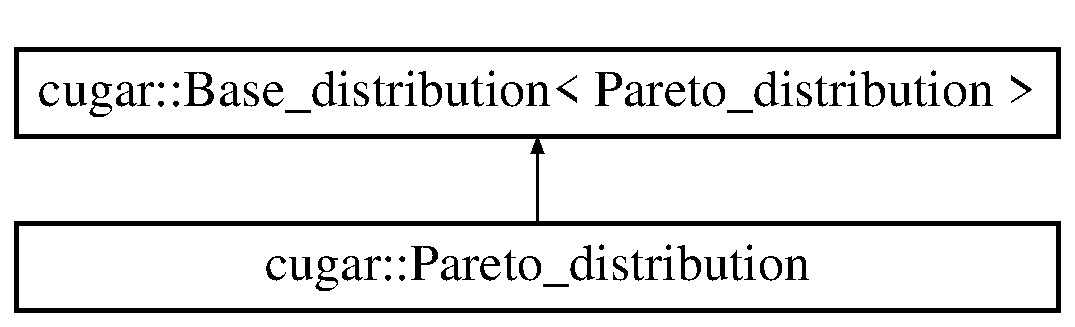
\includegraphics[height=2.000000cm]{structcugar_1_1_pareto__distribution}
\end{center}
\end{figure}
\subsection*{Public Methods}
\begin{DoxyCompactItemize}
\item 
C\+U\+G\+A\+R\+\_\+\+H\+O\+S\+T\+\_\+\+D\+E\+V\+I\+CE \hyperlink{structcugar_1_1_pareto__distribution_a316908fdf3b7a364f5cf4d5c78309527}{Pareto\+\_\+distribution} (const float a, const float min)
\item 
C\+U\+G\+A\+R\+\_\+\+H\+O\+S\+T\+\_\+\+D\+E\+V\+I\+CE float \hyperlink{structcugar_1_1_pareto__distribution_ac168806c81e9638f01ba994e746ed30f}{map} (const float U) const
\item 
C\+U\+G\+A\+R\+\_\+\+H\+O\+S\+T\+\_\+\+D\+E\+V\+I\+CE float \hyperlink{structcugar_1_1_pareto__distribution_ab4fff6aa700593597ff36de102b62d43}{density} (const float x) const
\end{DoxyCompactItemize}


\subsection{Constructor \& Destructor Documentation}
\mbox{\Hypertarget{structcugar_1_1_pareto__distribution_a316908fdf3b7a364f5cf4d5c78309527}\label{structcugar_1_1_pareto__distribution_a316908fdf3b7a364f5cf4d5c78309527}} 
\index{cugar\+::\+Pareto\+\_\+distribution@{cugar\+::\+Pareto\+\_\+distribution}!Pareto\+\_\+distribution@{Pareto\+\_\+distribution}}
\index{Pareto\+\_\+distribution@{Pareto\+\_\+distribution}!cugar\+::\+Pareto\+\_\+distribution@{cugar\+::\+Pareto\+\_\+distribution}}
\subsubsection{\texorpdfstring{Pareto\+\_\+distribution()}{Pareto\_distribution()}}
{\footnotesize\ttfamily C\+U\+G\+A\+R\+\_\+\+H\+O\+S\+T\+\_\+\+D\+E\+V\+I\+CE cugar\+::\+Pareto\+\_\+distribution\+::\+Pareto\+\_\+distribution (\begin{DoxyParamCaption}\item[{const float}]{a,  }\item[{const float}]{min }\end{DoxyParamCaption})\hspace{0.3cm}{\ttfamily [inline]}}

constructor


\begin{DoxyParams}{Parameters}
{\em a} & distribution parameter \\
\hline
{\em min} & distribution parameter \\
\hline
\end{DoxyParams}


\subsection{Member Function Documentation}
\mbox{\Hypertarget{structcugar_1_1_pareto__distribution_ab4fff6aa700593597ff36de102b62d43}\label{structcugar_1_1_pareto__distribution_ab4fff6aa700593597ff36de102b62d43}} 
\index{cugar\+::\+Pareto\+\_\+distribution@{cugar\+::\+Pareto\+\_\+distribution}!density@{density}}
\index{density@{density}!cugar\+::\+Pareto\+\_\+distribution@{cugar\+::\+Pareto\+\_\+distribution}}
\subsubsection{\texorpdfstring{density()}{density()}}
{\footnotesize\ttfamily C\+U\+G\+A\+R\+\_\+\+H\+O\+S\+T\+\_\+\+D\+E\+V\+I\+CE float cugar\+::\+Pareto\+\_\+distribution\+::density (\begin{DoxyParamCaption}\item[{const float}]{x }\end{DoxyParamCaption}) const\hspace{0.3cm}{\ttfamily [inline]}}

probability density function


\begin{DoxyParams}{Parameters}
{\em x} & sample location \\
\hline
\end{DoxyParams}
\mbox{\Hypertarget{structcugar_1_1_pareto__distribution_ac168806c81e9638f01ba994e746ed30f}\label{structcugar_1_1_pareto__distribution_ac168806c81e9638f01ba994e746ed30f}} 
\index{cugar\+::\+Pareto\+\_\+distribution@{cugar\+::\+Pareto\+\_\+distribution}!map@{map}}
\index{map@{map}!cugar\+::\+Pareto\+\_\+distribution@{cugar\+::\+Pareto\+\_\+distribution}}
\subsubsection{\texorpdfstring{map()}{map()}}
{\footnotesize\ttfamily C\+U\+G\+A\+R\+\_\+\+H\+O\+S\+T\+\_\+\+D\+E\+V\+I\+CE float cugar\+::\+Pareto\+\_\+distribution\+::map (\begin{DoxyParamCaption}\item[{const float}]{U }\end{DoxyParamCaption}) const\hspace{0.3cm}{\ttfamily [inline]}}

transform a uniformly distributed number through the distribution


\begin{DoxyParams}{Parameters}
{\em U} & real number to transform \\
\hline
\end{DoxyParams}


The documentation for this struct was generated from the following file\+:\begin{DoxyCompactItemize}
\item 
C\+:/p4research/research/jpantaleoni/\+Fermat-\/\+Public/contrib/cugar/sampling/\hyperlink{distributions_8h}{distributions.\+h}\end{DoxyCompactItemize}

\hypertarget{struct_path}{}\section{Path Struct Reference}
\label{struct_path}\index{Path@{Path}}


\subsection{Detailed description}
A class to represent light paths in compact form, storing only the vertex ids. 

{\ttfamily \#include $<$path.\+h$>$}

\subsection*{Public Methods}
\begin{DoxyCompactItemize}
\item 
\mbox{\Hypertarget{struct_path_aa30b5405c1ddf9026a8a4a878caedf14}\label{struct_path_aa30b5405c1ddf9026a8a4a878caedf14}} 
F\+E\+R\+M\+A\+T\+\_\+\+H\+O\+S\+T\+\_\+\+D\+E\+V\+I\+CE {\bfseries Path} (const uint32 \+\_\+n\+\_\+vertices, \hyperlink{struct_vertex_geometry_id}{Vertex\+Geometry\+Id} $\ast$\+\_\+verts, const uint32 \+\_\+stride)
\item 
\mbox{\Hypertarget{struct_path_af5f50f1500ffcf2be814ef5c62be407f}\label{struct_path_af5f50f1500ffcf2be814ef5c62be407f}} 
F\+E\+R\+M\+A\+T\+\_\+\+H\+O\+S\+T\+\_\+\+D\+E\+V\+I\+CE const \hyperlink{struct_vertex_geometry_id}{Vertex\+Geometry\+Id} \& {\bfseries v\+\_\+L} (const uint32 i) const
\item 
\mbox{\Hypertarget{struct_path_a13616464c91185262c8cb8ae296688a2}\label{struct_path_a13616464c91185262c8cb8ae296688a2}} 
F\+E\+R\+M\+A\+T\+\_\+\+H\+O\+S\+T\+\_\+\+D\+E\+V\+I\+CE const \hyperlink{struct_vertex_geometry_id}{Vertex\+Geometry\+Id} \& {\bfseries v\+\_\+E} (const uint32 i) const
\item 
\mbox{\Hypertarget{struct_path_ad3bd90bb4c64dbab4843014f2b614136}\label{struct_path_ad3bd90bb4c64dbab4843014f2b614136}} 
F\+E\+R\+M\+A\+T\+\_\+\+H\+O\+S\+T\+\_\+\+D\+E\+V\+I\+CE \hyperlink{struct_vertex_geometry_id}{Vertex\+Geometry\+Id} \& {\bfseries v\+\_\+L} (const uint32 i)
\item 
\mbox{\Hypertarget{struct_path_a38a66c133d4ed740fc5b2416599a6788}\label{struct_path_a38a66c133d4ed740fc5b2416599a6788}} 
F\+E\+R\+M\+A\+T\+\_\+\+H\+O\+S\+T\+\_\+\+D\+E\+V\+I\+CE \hyperlink{struct_vertex_geometry_id}{Vertex\+Geometry\+Id} \& {\bfseries v\+\_\+E} (const uint32 i)
\item 
\mbox{\Hypertarget{struct_path_afbc51ed7086e523c8ae0d5a62d6ccb3d}\label{struct_path_afbc51ed7086e523c8ae0d5a62d6ccb3d}} 
F\+E\+R\+M\+A\+T\+\_\+\+H\+O\+S\+T\+\_\+\+D\+E\+V\+I\+CE float {\bfseries G} (const uint32 i, const \hyperlink{struct_rendering_context_view}{Rendering\+Context\+View} \&renderer) const
\item 
\mbox{\Hypertarget{struct_path_a278e02a02b9c176eb81688db7828a8cf}\label{struct_path_a278e02a02b9c176eb81688db7828a8cf}} 
F\+E\+R\+M\+A\+T\+\_\+\+H\+O\+S\+T\+\_\+\+D\+E\+V\+I\+CE \hyperlink{structcugar_1_1_vector}{cugar\+::\+Vector3f} {\bfseries edge\+\_\+L} (const uint32 i, const \hyperlink{struct_rendering_context_view}{Rendering\+Context\+View} \&renderer) const
\item 
\mbox{\Hypertarget{struct_path_a4614790d32103332f90f0c3a135a2933}\label{struct_path_a4614790d32103332f90f0c3a135a2933}} 
F\+E\+R\+M\+A\+T\+\_\+\+H\+O\+S\+T\+\_\+\+D\+E\+V\+I\+CE \hyperlink{structcugar_1_1_vector}{cugar\+::\+Vector3f} {\bfseries edge\+\_\+E} (const uint32 i, const \hyperlink{struct_rendering_context_view}{Rendering\+Context\+View} \&renderer) const
\end{DoxyCompactItemize}
\subsection*{Public Members}
\begin{DoxyCompactItemize}
\item 
\mbox{\Hypertarget{struct_path_a78555e28d407d5f9a7b357de09672177}\label{struct_path_a78555e28d407d5f9a7b357de09672177}} 
\hyperlink{struct_vertex_geometry_id}{Vertex\+Geometry\+Id} $\ast$ {\bfseries vertex\+\_\+ids}
\item 
\mbox{\Hypertarget{struct_path_a378f7d2cd404c20660058b9f9996814b}\label{struct_path_a378f7d2cd404c20660058b9f9996814b}} 
uint32 {\bfseries n\+\_\+vertices}
\item 
\mbox{\Hypertarget{struct_path_adf70bfe5101af8293b27fc4b43c490a2}\label{struct_path_adf70bfe5101af8293b27fc4b43c490a2}} 
uint32 {\bfseries stride}
\end{DoxyCompactItemize}


The documentation for this struct was generated from the following file\+:\begin{DoxyCompactItemize}
\item 
C\+:/p4research/research/jpantaleoni/\+Fermat-\/\+Public/src/path.\+h\end{DoxyCompactItemize}

\hypertarget{struct_path_cache}{}\section{Path\+Cache$<$ T $>$ Struct Template Reference}
\label{struct_path_cache}\index{Path\+Cache$<$ T $>$@{Path\+Cache$<$ T $>$}}


\subsection{Detailed description}
\subsubsection*{template$<$typename T$>$\newline
struct Path\+Cache$<$ T $>$}

A class to represent a cached quantity associated with light paths 

{\ttfamily \#include $<$path.\+h$>$}

\subsection*{Public Methods}
\begin{DoxyCompactItemize}
\item 
\mbox{\Hypertarget{struct_path_cache_a33110c21eba89f9882291b3a5e2218cd}\label{struct_path_cache_a33110c21eba89f9882291b3a5e2218cd}} 
F\+E\+R\+M\+A\+T\+\_\+\+H\+O\+S\+T\+\_\+\+D\+E\+V\+I\+CE {\bfseries Path\+Cache} (const uint32 \+\_\+n\+\_\+vertices, T $\ast$\+\_\+verts, const uint32 \+\_\+stride)
\item 
\mbox{\Hypertarget{struct_path_cache_af7885c4534245e6818c70342e7cf4bb2}\label{struct_path_cache_af7885c4534245e6818c70342e7cf4bb2}} 
F\+E\+R\+M\+A\+T\+\_\+\+H\+O\+S\+T\+\_\+\+D\+E\+V\+I\+CE const T \& {\bfseries v\+\_\+L} (const uint32 i) const
\item 
\mbox{\Hypertarget{struct_path_cache_a49222f1790b3b72fa4c9111a1038d97c}\label{struct_path_cache_a49222f1790b3b72fa4c9111a1038d97c}} 
F\+E\+R\+M\+A\+T\+\_\+\+H\+O\+S\+T\+\_\+\+D\+E\+V\+I\+CE const T \& {\bfseries v\+\_\+E} (const uint32 i) const
\item 
\mbox{\Hypertarget{struct_path_cache_a53bdad471a0c0c28aacc8b91f651210a}\label{struct_path_cache_a53bdad471a0c0c28aacc8b91f651210a}} 
F\+E\+R\+M\+A\+T\+\_\+\+H\+O\+S\+T\+\_\+\+D\+E\+V\+I\+CE T \& {\bfseries v\+\_\+L} (const uint32 i)
\item 
\mbox{\Hypertarget{struct_path_cache_a22c0fb695af62b48a66b4768aaeacdf3}\label{struct_path_cache_a22c0fb695af62b48a66b4768aaeacdf3}} 
F\+E\+R\+M\+A\+T\+\_\+\+H\+O\+S\+T\+\_\+\+D\+E\+V\+I\+CE T \& {\bfseries v\+\_\+E} (const uint32 i)
\end{DoxyCompactItemize}
\subsection*{Public Members}
\begin{DoxyCompactItemize}
\item 
\mbox{\Hypertarget{struct_path_cache_ad5987d28ab38e53e5d09f9bb180224ea}\label{struct_path_cache_ad5987d28ab38e53e5d09f9bb180224ea}} 
T $\ast$ {\bfseries vertices}
\item 
\mbox{\Hypertarget{struct_path_cache_a24c1ff4a515806d5d22483608b884c98}\label{struct_path_cache_a24c1ff4a515806d5d22483608b884c98}} 
uint32 {\bfseries n\+\_\+vertices}
\item 
\mbox{\Hypertarget{struct_path_cache_a8384ef9835a62866088a5fd57a5dbbbe}\label{struct_path_cache_a8384ef9835a62866088a5fd57a5dbbbe}} 
uint32 {\bfseries stride}
\end{DoxyCompactItemize}


The documentation for this struct was generated from the following file\+:\begin{DoxyCompactItemize}
\item 
C\+:/p4research/research/jpantaleoni/\+Fermat-\/\+Public/src/path.\+h\end{DoxyCompactItemize}

\hypertarget{struct_path_tracer}{}\section{Path\+Tracer Struct Reference}
\label{struct_path_tracer}\index{Path\+Tracer@{Path\+Tracer}}


\subsection{Detailed description}
\hyperlink{struct_path}{Path} tracer 

{\ttfamily \#include $<$pathtracer.\+h$>$}

Inheritance diagram for Path\+Tracer\+:\begin{figure}[H]
\begin{center}
\leavevmode
\includegraphics[height=2.000000cm]{struct_path_tracer}
\end{center}
\end{figure}
\subsection*{Public Types}
\begin{DoxyCompactItemize}
\item 
\mbox{\Hypertarget{struct_path_tracer_aaa15005f9a89caaff352d3872168376b}\label{struct_path_tracer_aaa15005f9a89caaff352d3872168376b}} 
typedef \hyperlink{struct_adaptive_clustered_r_l_storage}{Adaptive\+Clustered\+R\+L\+Storage} {\bfseries V\+T\+L\+R\+L\+Storage}
\end{DoxyCompactItemize}
\subsection*{Public Methods}
\begin{DoxyCompactItemize}
\item 
void \hyperlink{group___p_t_module_details_ga923b8d146b23f93356f6c74971c4d6f7}{init} (int argc, char $\ast$$\ast$argv, \hyperlink{struct_rendering_context}{Rendering\+Context} \&renderer)
\item 
void \hyperlink{group___p_t_module_details_ga3e6317495ea6c761968a893b3a54824e}{render} (const uint32 instance, \hyperlink{struct_rendering_context}{Rendering\+Context} \&renderer)
\item 
\mbox{\Hypertarget{struct_path_tracer_a84595cdac7e983b4dcfa72677f4e7a87}\label{struct_path_tracer_a84595cdac7e983b4dcfa72677f4e7a87}} 
void {\bfseries setup\+\_\+samples} (const uint32 instance)
\item 
void \hyperlink{group___p_t_module_details_gad08f55d7ba075e0b71a4aa729c07986d}{keyboard} (unsigned char character, int x, int y, bool \&invalidate)
\item 
void \hyperlink{struct_path_tracer_a3c4e7e9eb10e92c6a6d5cc94bbf93ee7}{destroy} ()
\item 
void \hyperlink{group___p_t_module_details_gaae1782405577d0072ff78570ec0025cc}{dump\+\_\+speed\+\_\+stats} (F\+I\+LE $\ast$stats)
\item 
void {\bfseries update\+\_\+vtls\+\_\+rl} (const uint32 instance)
\end{DoxyCompactItemize}
\subsection*{Static Public Methods}
\begin{DoxyCompactItemize}
\item 
\mbox{\Hypertarget{struct_path_tracer_a8b333c7f699b163f647af81a016cf83f}\label{struct_path_tracer_a8b333c7f699b163f647af81a016cf83f}} 
static \hyperlink{struct_renderer_interface}{Renderer\+Interface} $\ast$ {\bfseries factory} ()
\end{DoxyCompactItemize}
\subsection*{Public Members}
\begin{DoxyCompactItemize}
\item 
\mbox{\Hypertarget{struct_path_tracer_ab4e4e4cad2b4b894c8f117dac5a809b7}\label{struct_path_tracer_ab4e4e4cad2b4b894c8f117dac5a809b7}} 
\hyperlink{class_domain_buffer}{Domain\+Buffer}$<$ C\+U\+D\+A\+\_\+\+B\+U\+F\+F\+ER, uint8 $>$ {\bfseries m\+\_\+memory\+\_\+pool}
\item 
\mbox{\Hypertarget{struct_path_tracer_a4e4eedcd2f916a248f87f2ba240a2e16}\label{struct_path_tracer_a4e4eedcd2f916a248f87f2ba240a2e16}} 
\hyperlink{struct_p_t_options}{P\+T\+Options} {\bfseries m\+\_\+options}
\item 
\mbox{\Hypertarget{struct_path_tracer_a6fd9814f780b9773cf09ffeb7b0f113e}\label{struct_path_tracer_a6fd9814f780b9773cf09ffeb7b0f113e}} 
\hyperlink{struct_tiled_sequence}{Tiled\+Sequence} {\bfseries m\+\_\+sequence}
\item 
\mbox{\Hypertarget{struct_path_tracer_a57eb13d57e9081b3831e3933c2c924f9}\label{struct_path_tracer_a57eb13d57e9081b3831e3933c2c924f9}} 
\hyperlink{classcugar_1_1_l_f_s_r_generator_matrix}{cugar\+::\+L\+F\+S\+R\+Generator\+Matrix} {\bfseries m\+\_\+generator}
\item 
\mbox{\Hypertarget{struct_path_tracer_abaed20bfd304377069f9c5f8b740a175}\label{struct_path_tracer_abaed20bfd304377069f9c5f8b740a175}} 
\hyperlink{structcugar_1_1_l_f_s_r_random_stream}{cugar\+::\+L\+F\+S\+R\+Random\+Stream} {\bfseries m\+\_\+random}
\item 
\mbox{\Hypertarget{struct_path_tracer_a1dc439c9f458b3fee5e07edfb1bc1a12}\label{struct_path_tracer_a1dc439c9f458b3fee5e07edfb1bc1a12}} 
\hyperlink{struct_mesh_v_t_l_storage}{Mesh\+V\+T\+L\+Storage} $\ast$ {\bfseries m\+\_\+mesh\+\_\+vtls}
\item 
\mbox{\Hypertarget{struct_path_tracer_af1f0df6e130041e52ae03411ef0b85a2}\label{struct_path_tracer_af1f0df6e130041e52ae03411ef0b85a2}} 
\hyperlink{struct_adaptive_clustered_r_l_storage}{V\+T\+L\+R\+L\+Storage} $\ast$ {\bfseries m\+\_\+vtls\+\_\+rl}
\item 
\mbox{\Hypertarget{struct_path_tracer_a34ee633b20d75d2f00d36c8c0cbee2eb}\label{struct_path_tracer_a34ee633b20d75d2f00d36c8c0cbee2eb}} 
\hyperlink{structcugar_1_1_bbox}{cugar\+::\+Bbox3f} {\bfseries m\+\_\+bbox}
\item 
\mbox{\Hypertarget{struct_path_tracer_a08787bb830c6a9f883ce428fc3fb80af}\label{struct_path_tracer_a08787bb830c6a9f883ce428fc3fb80af}} 
float {\bfseries m\+\_\+time}
\item 
\mbox{\Hypertarget{struct_path_tracer_a7561a9680a0b3435e89b218a9b369694}\label{struct_path_tracer_a7561a9680a0b3435e89b218a9b369694}} 
uint32 {\bfseries m\+\_\+pathtracer\+\_\+raygen}
\item 
\mbox{\Hypertarget{struct_path_tracer_a354c091ed28190973b8f589ab5867b60}\label{struct_path_tracer_a354c091ed28190973b8f589ab5867b60}} 
\hyperlink{struct_p_t_stats}{P\+T\+Stats} {\bfseries m\+\_\+stats}
\end{DoxyCompactItemize}


\subsection{Member Function Documentation}
\mbox{\Hypertarget{struct_path_tracer_a3c4e7e9eb10e92c6a6d5cc94bbf93ee7}\label{struct_path_tracer_a3c4e7e9eb10e92c6a6d5cc94bbf93ee7}} 
\index{Path\+Tracer@{Path\+Tracer}!destroy@{destroy}}
\index{destroy@{destroy}!Path\+Tracer@{Path\+Tracer}}
\subsubsection{\texorpdfstring{destroy()}{destroy()}}
{\footnotesize\ttfamily void Path\+Tracer\+::destroy (\begin{DoxyParamCaption}{ }\end{DoxyParamCaption})\hspace{0.3cm}{\ttfamily [inline]}, {\ttfamily [virtual]}}

this method is responsible for destroying the object itself 

Reimplemented from \hyperlink{struct_renderer_interface_a7469218aafa029a3e22bac2c00dca9f5}{Renderer\+Interface}.



The documentation for this struct was generated from the following files\+:\begin{DoxyCompactItemize}
\item 
C\+:/p4research/research/jpantaleoni/\+Fermat-\/\+Public/src/renderers/pathtracer.\+h\item 
C\+:/p4research/research/jpantaleoni/\+Fermat-\/\+Public/src/renderers/pathtracer\+\_\+impl.\+h\end{DoxyCompactItemize}

\hypertarget{struct_path_weights}{}\section{Path\+Weights Struct Reference}
\label{struct_path_weights}\index{Path\+Weights@{Path\+Weights}}


\subsection{Detailed description}
\begin{DoxyParagraph}{}
A small utility class to track the path weights needed for internal M\+IS calculations 
\end{DoxyParagraph}


{\ttfamily \#include $<$bpt\+\_\+utils.\+h$>$}

\subsection*{Public Methods}
\begin{DoxyCompactItemize}
\item 
\mbox{\Hypertarget{struct_path_weights_afa7b3a03eee65d95a806103ea47a2a49}\label{struct_path_weights_afa7b3a03eee65d95a806103ea47a2a49}} 
F\+E\+R\+M\+A\+T\+\_\+\+H\+O\+S\+T\+\_\+\+D\+E\+V\+I\+CE {\bfseries Path\+Weights} (const float \+\_\+p\+Gp\+\_\+sum, const float \+\_\+pG)
\item 
\mbox{\Hypertarget{struct_path_weights_abd4652b8d94942fbc004f5a31a225d06}\label{struct_path_weights_abd4652b8d94942fbc004f5a31a225d06}} 
F\+E\+R\+M\+A\+T\+\_\+\+H\+O\+S\+T\+\_\+\+D\+E\+V\+I\+CE {\bfseries Path\+Weights} (const float2 f)
\item 
\mbox{\Hypertarget{struct_path_weights_af404d428ac5c73593e27b829dd45340c}\label{struct_path_weights_af404d428ac5c73593e27b829dd45340c}} 
F\+E\+R\+M\+A\+T\+\_\+\+H\+O\+S\+T\+\_\+\+D\+E\+V\+I\+CE {\bfseries operator float2} () const
\end{DoxyCompactItemize}
\subsection*{Public Members}
\begin{DoxyCompactItemize}
\item 
\mbox{\Hypertarget{struct_path_weights_addb09feed323414704b72c88a12f1c1e}\label{struct_path_weights_addb09feed323414704b72c88a12f1c1e}} 
\begin{tabbing}
xx\=xx\=xx\=xx\=xx\=xx\=xx\=xx\=xx\=\kill
union \{\\
\>float2 {\bfseries vector\_storage}\\
\mbox{\Hypertarget{union_path_weights_1_1_0D0_a8ccf7df59fa8876e331d66fc2733b136}\label{union_path_weights_1_1_0D0_a8ccf7df59fa8876e331d66fc2733b136}} 
\>struct \{\\
\>\>float {\bfseries pGp\_sum}\\
\>\>float {\bfseries pG}\\
\>\} \\
\}; \\

\end{tabbing}\end{DoxyCompactItemize}


The documentation for this struct was generated from the following file\+:\begin{DoxyCompactItemize}
\item 
C\+:/p4research/research/jpantaleoni/\+Fermat-\/\+Public/src/bpt\+\_\+utils.\+h\end{DoxyCompactItemize}

\hypertarget{struct_payload}{}\section{Payload Struct Reference}
\label{struct_payload}\index{Payload@{Payload}}


\subsection{Detailed description}
\hyperlink{struct_hit}{Hit} structure currently used by Fermat 

{\ttfamily \#include $<$optix\+\_\+payload.\+h$>$}

\subsection*{Public Methods}
\begin{DoxyCompactItemize}
\item 
\mbox{\Hypertarget{struct_payload_ad07fb17beb88596c71fe9bd7f7d58467}\label{struct_payload_ad07fb17beb88596c71fe9bd7f7d58467}} 
F\+E\+R\+M\+A\+T\+\_\+\+H\+O\+S\+T\+\_\+\+D\+E\+V\+I\+CE F\+E\+R\+M\+A\+T\+\_\+\+F\+O\+R\+C\+E\+I\+N\+L\+I\+NE {\bfseries Payload} (const float \+\_\+t, const int32 \+\_\+tri\+\_\+id, const float \+\_\+u, const float \+\_\+v, const uint8 \+\_\+mask)
\item 
\mbox{\Hypertarget{struct_payload_a07cd17390929fc617782a100bdb3bd2f}\label{struct_payload_a07cd17390929fc617782a100bdb3bd2f}} 
F\+E\+R\+M\+A\+T\+\_\+\+H\+O\+S\+T\+\_\+\+D\+E\+V\+I\+CE F\+E\+R\+M\+A\+T\+\_\+\+F\+O\+R\+C\+E\+I\+N\+L\+I\+NE void {\bfseries set\+\_\+t} (const float \+\_\+t)
\item 
\mbox{\Hypertarget{struct_payload_a07678f3a6d9245dd4e295f995efe1e47}\label{struct_payload_a07678f3a6d9245dd4e295f995efe1e47}} 
F\+E\+R\+M\+A\+T\+\_\+\+H\+O\+S\+T\+\_\+\+D\+E\+V\+I\+CE F\+E\+R\+M\+A\+T\+\_\+\+F\+O\+R\+C\+E\+I\+N\+L\+I\+NE float {\bfseries t} () const
\item 
\mbox{\Hypertarget{struct_payload_a711c546f39e4c8506b1263d5696def3f}\label{struct_payload_a711c546f39e4c8506b1263d5696def3f}} 
F\+E\+R\+M\+A\+T\+\_\+\+H\+O\+S\+T\+\_\+\+D\+E\+V\+I\+CE F\+E\+R\+M\+A\+T\+\_\+\+F\+O\+R\+C\+E\+I\+N\+L\+I\+NE void {\bfseries set\+\_\+triangle\+\_\+id} (const int32 \+\_\+tri\+\_\+id)
\item 
\mbox{\Hypertarget{struct_payload_af0ca91daae0597abaec946af6ae79f89}\label{struct_payload_af0ca91daae0597abaec946af6ae79f89}} 
F\+E\+R\+M\+A\+T\+\_\+\+H\+O\+S\+T\+\_\+\+D\+E\+V\+I\+CE F\+E\+R\+M\+A\+T\+\_\+\+F\+O\+R\+C\+E\+I\+N\+L\+I\+NE int32 {\bfseries triangle\+\_\+id} () const
\item 
\mbox{\Hypertarget{struct_payload_a4968211934ac6e65ed15aa6949f896cb}\label{struct_payload_a4968211934ac6e65ed15aa6949f896cb}} 
F\+E\+R\+M\+A\+T\+\_\+\+H\+O\+S\+T\+\_\+\+D\+E\+V\+I\+CE F\+E\+R\+M\+A\+T\+\_\+\+F\+O\+R\+C\+E\+I\+N\+L\+I\+NE void {\bfseries set\+\_\+uv} (const float \+\_\+u, const float \+\_\+v)
\item 
\mbox{\Hypertarget{struct_payload_a91bf009413dd02b88a1be5a912d6dbfb}\label{struct_payload_a91bf009413dd02b88a1be5a912d6dbfb}} 
F\+E\+R\+M\+A\+T\+\_\+\+H\+O\+S\+T\+\_\+\+D\+E\+V\+I\+CE F\+E\+R\+M\+A\+T\+\_\+\+F\+O\+R\+C\+E\+I\+N\+L\+I\+NE float2 {\bfseries uv} () const
\item 
\mbox{\Hypertarget{struct_payload_aee4469a992bbb175716fa5dbdfd60a5a}\label{struct_payload_aee4469a992bbb175716fa5dbdfd60a5a}} 
F\+E\+R\+M\+A\+T\+\_\+\+H\+O\+S\+T\+\_\+\+D\+E\+V\+I\+CE F\+E\+R\+M\+A\+T\+\_\+\+F\+O\+R\+C\+E\+I\+N\+L\+I\+NE float {\bfseries t} (const float \+\_\+t)
\item 
\mbox{\Hypertarget{struct_payload_a2901b62fdc76244aa8a2523aa69dff73}\label{struct_payload_a2901b62fdc76244aa8a2523aa69dff73}} 
F\+E\+R\+M\+A\+T\+\_\+\+H\+O\+S\+T\+\_\+\+D\+E\+V\+I\+CE F\+E\+R\+M\+A\+T\+\_\+\+F\+O\+R\+C\+E\+I\+N\+L\+I\+NE void {\bfseries set\+\_\+mask} (const uint8 \+\_\+mask)
\item 
\mbox{\Hypertarget{struct_payload_acecf9d56226fb3c2ba5bb1ec6316cf97}\label{struct_payload_acecf9d56226fb3c2ba5bb1ec6316cf97}} 
F\+E\+R\+M\+A\+T\+\_\+\+H\+O\+S\+T\+\_\+\+D\+E\+V\+I\+CE F\+E\+R\+M\+A\+T\+\_\+\+F\+O\+R\+C\+E\+I\+N\+L\+I\+NE uint32 {\bfseries mask} () const
\item 
\mbox{\Hypertarget{struct_payload_ad4e86f94de366f13c081c3fef9ebb4ff}\label{struct_payload_ad4e86f94de366f13c081c3fef9ebb4ff}} 
F\+E\+R\+M\+A\+T\+\_\+\+H\+O\+S\+T\+\_\+\+D\+E\+V\+I\+CE F\+E\+R\+M\+A\+T\+\_\+\+F\+O\+R\+C\+E\+I\+N\+L\+I\+NE {\bfseries operator Hit} () const
\item 
\mbox{\Hypertarget{struct_payload_a6395d33afc2a2085a95e7f5a32da3555}\label{struct_payload_a6395d33afc2a2085a95e7f5a32da3555}} 
F\+E\+R\+M\+A\+T\+\_\+\+H\+O\+S\+T\+\_\+\+D\+E\+V\+I\+CE F\+E\+R\+M\+A\+T\+\_\+\+F\+O\+R\+C\+E\+I\+N\+L\+I\+NE {\bfseries operator bool} () const
\end{DoxyCompactItemize}
\subsection*{Public Members}
\begin{DoxyCompactItemize}
\item 
\mbox{\Hypertarget{struct_payload_aab039ea7845dabfa53185e5258568962}\label{struct_payload_aab039ea7845dabfa53185e5258568962}} 
uint4 {\bfseries packed}
\end{DoxyCompactItemize}


The documentation for this struct was generated from the following file\+:\begin{DoxyCompactItemize}
\item 
C\+:/p4research/research/jpantaleoni/\+Fermat-\/\+Public/src/kernels/optix\+\_\+payload.\+h\end{DoxyCompactItemize}

\hypertarget{classpbrt_1_1_p_b_r_t_parser_error}{}\section{pbrt\+:\+:P\+B\+R\+T\+Parser\+Error Class Reference}
\label{classpbrt_1_1_p_b_r_t_parser_error}\index{pbrt\+::\+P\+B\+R\+T\+Parser\+Error@{pbrt\+::\+P\+B\+R\+T\+Parser\+Error}}
Inheritance diagram for pbrt\+:\+:P\+B\+R\+T\+Parser\+Error\+:\begin{figure}[H]
\begin{center}
\leavevmode
\includegraphics[height=2.000000cm]{classpbrt_1_1_p_b_r_t_parser_error}
\end{center}
\end{figure}
\subsection*{Public Methods}
\begin{DoxyCompactItemize}
\item 
\mbox{\Hypertarget{classpbrt_1_1_p_b_r_t_parser_error_a8df4c565323f1b33a344039172445e50}\label{classpbrt_1_1_p_b_r_t_parser_error_a8df4c565323f1b33a344039172445e50}} 
{\bfseries P\+B\+R\+T\+Parser\+Error} (const std\+::string \&what\+\_\+arg)
\end{DoxyCompactItemize}


The documentation for this class was generated from the following file\+:\begin{DoxyCompactItemize}
\item 
C\+:/p4research/research/jpantaleoni/\+Fermat-\/\+Public/src/mesh/pbrt\+\_\+parser.\+h\end{DoxyCompactItemize}

\hypertarget{struct_per_pixel_eye_subpath_primary_coords}{}\section{Per\+Pixel\+Eye\+Subpath\+Primary\+Coords Struct Reference}
\label{struct_per_pixel_eye_subpath_primary_coords}\index{Per\+Pixel\+Eye\+Subpath\+Primary\+Coords@{Per\+Pixel\+Eye\+Subpath\+Primary\+Coords}}


\subsection{Detailed description}
Primary coordinate sampler for eye subpaths, based on a \hyperlink{struct_tiled_sequence}{Tiled\+Sequence} sampler. This sampler assumes that there is a one to one correspondence between paths and pixels, i.\+e. that the path index IS the pixel index. 

{\ttfamily \#include $<$bpt\+\_\+samplers.\+h$>$}

\subsection*{Public Methods}
\begin{DoxyCompactItemize}
\item 
\mbox{\Hypertarget{struct_per_pixel_eye_subpath_primary_coords_a0680b91cb249feac14bac477c601f000}\label{struct_per_pixel_eye_subpath_primary_coords_a0680b91cb249feac14bac477c601f000}} 
F\+E\+R\+M\+A\+T\+\_\+\+H\+O\+S\+T\+\_\+\+D\+E\+V\+I\+CE F\+E\+R\+M\+A\+T\+\_\+\+F\+O\+R\+C\+E\+I\+N\+L\+I\+NE {\bfseries Per\+Pixel\+Eye\+Subpath\+Primary\+Coords} (const \hyperlink{struct_tiled_sequence_view}{Tiled\+Sequence\+View} \+\_\+sequence, const uint32 \+\_\+res\+\_\+x, const uint32 \+\_\+res\+\_\+y)
\item 
\mbox{\Hypertarget{struct_per_pixel_eye_subpath_primary_coords_a149efc72191a13e0d1cefb81396173a4}\label{struct_per_pixel_eye_subpath_primary_coords_a149efc72191a13e0d1cefb81396173a4}} 
F\+E\+R\+M\+A\+T\+\_\+\+H\+O\+S\+T\+\_\+\+D\+E\+V\+I\+CE F\+E\+R\+M\+A\+T\+\_\+\+F\+O\+R\+C\+E\+I\+N\+L\+I\+NE float {\bfseries sample} (const uint32 idx, const uint32 vertex, const uint32 dim) const
\end{DoxyCompactItemize}
\subsection*{Public Members}
\begin{DoxyCompactItemize}
\item 
\mbox{\Hypertarget{struct_per_pixel_eye_subpath_primary_coords_a01c5b417f7141a04f062586d28d328c5}\label{struct_per_pixel_eye_subpath_primary_coords_a01c5b417f7141a04f062586d28d328c5}} 
const \hyperlink{struct_tiled_sequence_view}{Tiled\+Sequence\+View} {\bfseries sequence}
\item 
\mbox{\Hypertarget{struct_per_pixel_eye_subpath_primary_coords_aabe1c9d4b9bcb950c776d168a0ef4a83}\label{struct_per_pixel_eye_subpath_primary_coords_aabe1c9d4b9bcb950c776d168a0ef4a83}} 
const uint32 {\bfseries res\+\_\+x}
\item 
\mbox{\Hypertarget{struct_per_pixel_eye_subpath_primary_coords_aa529fe217bad21e144832d688eb71609}\label{struct_per_pixel_eye_subpath_primary_coords_aa529fe217bad21e144832d688eb71609}} 
const uint32 {\bfseries res\+\_\+y}
\end{DoxyCompactItemize}


The documentation for this struct was generated from the following file\+:\begin{DoxyCompactItemize}
\item 
C\+:/p4research/research/jpantaleoni/\+Fermat-\/\+Public/src/bpt\+\_\+samplers.\+h\end{DoxyCompactItemize}

\hypertarget{structcugar_1_1cuda_1_1_per_thread_smem_unary_function}{}\section{cugar\+:\+:cuda\+:\+:Per\+Thread\+Smem\+Unary\+Function Struct Reference}
\label{structcugar_1_1cuda_1_1_per_thread_smem_unary_function}\index{cugar\+::cuda\+::\+Per\+Thread\+Smem\+Unary\+Function@{cugar\+::cuda\+::\+Per\+Thread\+Smem\+Unary\+Function}}
\subsection*{Public Methods}
\begin{DoxyCompactItemize}
\item 
\mbox{\Hypertarget{structcugar_1_1cuda_1_1_per_thread_smem_unary_function_abb4e26494239066de05512e986595063}\label{structcugar_1_1cuda_1_1_per_thread_smem_unary_function_abb4e26494239066de05512e986595063}} 
C\+U\+G\+A\+R\+\_\+\+H\+O\+S\+T\+\_\+\+D\+E\+V\+I\+CE {\bfseries Per\+Thread\+Smem\+Unary\+Function} (const int \+\_\+bytes\+\_\+per\+\_\+thread)
\item 
\mbox{\Hypertarget{structcugar_1_1cuda_1_1_per_thread_smem_unary_function_a2d60f8b45bfcb778418fff83f98152ae}\label{structcugar_1_1cuda_1_1_per_thread_smem_unary_function_a2d60f8b45bfcb778418fff83f98152ae}} 
C\+U\+G\+A\+R\+\_\+\+H\+O\+S\+T\+\_\+\+D\+E\+V\+I\+CE int {\bfseries operator()} (const int block\+\_\+size) const
\end{DoxyCompactItemize}
\subsection*{Public Members}
\begin{DoxyCompactItemize}
\item 
\mbox{\Hypertarget{structcugar_1_1cuda_1_1_per_thread_smem_unary_function_ab1a45200fa7355f47a4386694decf72f}\label{structcugar_1_1cuda_1_1_per_thread_smem_unary_function_ab1a45200fa7355f47a4386694decf72f}} 
int {\bfseries bytes\+\_\+per\+\_\+thread}
\end{DoxyCompactItemize}


The documentation for this struct was generated from the following file\+:\begin{DoxyCompactItemize}
\item 
C\+:/p4research/research/jpantaleoni/\+Fermat-\/\+Public/contrib/cugar/basic/cuda/arch\+\_\+inl.\+h\end{DoxyCompactItemize}

\hypertarget{struct_perturbed_primary_coords}{}\section{Perturbed\+Primary\+Coords Struct Reference}
\label{struct_perturbed_primary_coords}\index{Perturbed\+Primary\+Coords@{Perturbed\+Primary\+Coords}}


\subsection{Detailed description}
A perturbation sampler 

{\ttfamily \#include $<$bpt\+\_\+samplers.\+h$>$}

\subsection*{Public Types}
\begin{DoxyCompactItemize}
\item 
\mbox{\Hypertarget{struct_perturbed_primary_coords_a9bbcc445564834746ae6b9324d55537f}\label{struct_perturbed_primary_coords_a9bbcc445564834746ae6b9324d55537f}} 
enum {\bfseries Type} \{ {\bfseries Null} = 0x0, 
{\bfseries Cauchy\+Perturbation} = 0x1, 
{\bfseries Independent\+Sample} = 0x2
 \}
\end{DoxyCompactItemize}
\subsection*{Public Methods}
\begin{DoxyCompactItemize}
\item 
\mbox{\Hypertarget{struct_perturbed_primary_coords_a922ff6ce8a957c076f402ef55c8d4810}\label{struct_perturbed_primary_coords_a922ff6ce8a957c076f402ef55c8d4810}} 
F\+E\+R\+M\+A\+T\+\_\+\+H\+O\+S\+T\+\_\+\+D\+E\+V\+I\+CE F\+E\+R\+M\+A\+T\+\_\+\+F\+O\+R\+C\+E\+I\+N\+L\+I\+NE uint32 {\bfseries chain\+\_\+coordinate\+\_\+index} (const uint32 idx, const uint32 dim) const
\item 
\mbox{\Hypertarget{struct_perturbed_primary_coords_a59337b148ab94665bfb84eee02a3bd7d}\label{struct_perturbed_primary_coords_a59337b148ab94665bfb84eee02a3bd7d}} 
F\+E\+R\+M\+A\+T\+\_\+\+H\+O\+S\+T\+\_\+\+D\+E\+V\+I\+CE F\+E\+R\+M\+A\+T\+\_\+\+F\+O\+R\+C\+E\+I\+N\+L\+I\+NE {\bfseries Perturbed\+Primary\+Coords} (const uint32 \+\_\+n\+\_\+chains, float $\ast$\+\_\+path\+\_\+u, const uint32 \+\_\+path\+\_\+vertex\+\_\+offset, float $\ast$\+\_\+mut\+\_\+u, const uint32 \+\_\+mut\+\_\+vertex\+\_\+offset, const Type \+\_\+type, const float \+\_\+radius=0.\+01f)
\item 
\mbox{\Hypertarget{struct_perturbed_primary_coords_af51dcfdfba46e5043deab4ad880721c7}\label{struct_perturbed_primary_coords_af51dcfdfba46e5043deab4ad880721c7}} 
F\+E\+R\+M\+A\+T\+\_\+\+H\+O\+S\+T\+\_\+\+D\+E\+V\+I\+CE F\+E\+R\+M\+A\+T\+\_\+\+F\+O\+R\+C\+E\+I\+N\+L\+I\+NE float {\bfseries sample} (const uint32 idx, const uint32 vertex, const uint32 dim) const
\item 
\mbox{\Hypertarget{struct_perturbed_primary_coords_a587274d5c8f87f0f406bed2f916908a7}\label{struct_perturbed_primary_coords_a587274d5c8f87f0f406bed2f916908a7}} 
F\+E\+R\+M\+A\+T\+\_\+\+H\+O\+S\+T\+\_\+\+D\+E\+V\+I\+CE F\+E\+R\+M\+A\+T\+\_\+\+F\+O\+R\+C\+E\+I\+N\+L\+I\+NE float {\bfseries u\+\_\+m} (const uint32 chain\+\_\+id, const uint32 dim) const
\item 
\mbox{\Hypertarget{struct_perturbed_primary_coords_a7020dd85fcb52ceb418d469a370fc1e8}\label{struct_perturbed_primary_coords_a7020dd85fcb52ceb418d469a370fc1e8}} 
F\+E\+R\+M\+A\+T\+\_\+\+H\+O\+S\+T\+\_\+\+D\+E\+V\+I\+CE F\+E\+R\+M\+A\+T\+\_\+\+F\+O\+R\+C\+E\+I\+N\+L\+I\+NE float \& {\bfseries u} (const uint32 chain\+\_\+id, const uint32 dim)
\item 
\mbox{\Hypertarget{struct_perturbed_primary_coords_a8ab27760f5ff92596d531c3ea41b880e}\label{struct_perturbed_primary_coords_a8ab27760f5ff92596d531c3ea41b880e}} 
F\+E\+R\+M\+A\+T\+\_\+\+H\+O\+S\+T\+\_\+\+D\+E\+V\+I\+CE F\+E\+R\+M\+A\+T\+\_\+\+F\+O\+R\+C\+E\+I\+N\+L\+I\+NE const float \& {\bfseries u} (const uint32 chain\+\_\+id, const uint32 dim) const
\item 
\mbox{\Hypertarget{struct_perturbed_primary_coords_ab76cb15e84cbe45884b1ec26a33daeac}\label{struct_perturbed_primary_coords_ab76cb15e84cbe45884b1ec26a33daeac}} 
F\+E\+R\+M\+A\+T\+\_\+\+H\+O\+S\+T\+\_\+\+D\+E\+V\+I\+CE F\+E\+R\+M\+A\+T\+\_\+\+F\+O\+R\+C\+E\+I\+N\+L\+I\+NE float {\bfseries perturbed\+\_\+u} (const uint32 chain\+\_\+id, const uint32 dim) const
\end{DoxyCompactItemize}
\subsection*{Public Members}
\begin{DoxyCompactItemize}
\item 
\mbox{\Hypertarget{struct_perturbed_primary_coords_af8518880c5c9a630f84ce70af7dd986f}\label{struct_perturbed_primary_coords_af8518880c5c9a630f84ce70af7dd986f}} 
float $\ast$ {\bfseries path\+\_\+u}
\item 
\mbox{\Hypertarget{struct_perturbed_primary_coords_a3a086d65a10fdcf1996586d618731dc2}\label{struct_perturbed_primary_coords_a3a086d65a10fdcf1996586d618731dc2}} 
float $\ast$ {\bfseries mut\+\_\+u}
\item 
\mbox{\Hypertarget{struct_perturbed_primary_coords_aafe430370b8692648c5c7e7ff110be6c}\label{struct_perturbed_primary_coords_aafe430370b8692648c5c7e7ff110be6c}} 
uint32 {\bfseries n\+\_\+chains}
\item 
\mbox{\Hypertarget{struct_perturbed_primary_coords_adc1a077d19c2ed1552c4846e6906527a}\label{struct_perturbed_primary_coords_adc1a077d19c2ed1552c4846e6906527a}} 
Type {\bfseries type}
\item 
\mbox{\Hypertarget{struct_perturbed_primary_coords_a62c1c9ed571a359efb473ace671d6ee0}\label{struct_perturbed_primary_coords_a62c1c9ed571a359efb473ace671d6ee0}} 
float {\bfseries radius}
\end{DoxyCompactItemize}


The documentation for this struct was generated from the following file\+:\begin{DoxyCompactItemize}
\item 
C\+:/p4research/research/jpantaleoni/\+Fermat-\/\+Public/src/bpt\+\_\+samplers.\+h\end{DoxyCompactItemize}

\hypertarget{union_pixel_info}{}\section{Pixel\+Info Union Reference}
\label{union_pixel_info}\index{Pixel\+Info@{Pixel\+Info}}


\subsection{Detailed description}
Store packed pixel information, including\+:
\begin{DoxyItemize}
\item the pixel index
\item the current path type (diffuse or glossy)
\item a bit indicating whether the path went through a diffuse bounce 
\end{DoxyItemize}

{\ttfamily \#include $<$pathtracer\+\_\+core.\+h$>$}

\subsection*{Public Methods}
\begin{DoxyCompactItemize}
\item 
\mbox{\Hypertarget{union_pixel_info_a2808405cb466ebf0eeec02c5a6193f8a}\label{union_pixel_info_a2808405cb466ebf0eeec02c5a6193f8a}} 
F\+E\+R\+M\+A\+T\+\_\+\+H\+O\+S\+T\+\_\+\+D\+E\+V\+I\+CE {\bfseries Pixel\+Info} (const uint32 \+\_\+packed)
\item 
\mbox{\Hypertarget{union_pixel_info_a8d9e9bdd9d6e2cb960ef18b27e0ca2d0}\label{union_pixel_info_a8d9e9bdd9d6e2cb960ef18b27e0ca2d0}} 
F\+E\+R\+M\+A\+T\+\_\+\+H\+O\+S\+T\+\_\+\+D\+E\+V\+I\+CE {\bfseries Pixel\+Info} (const uint32 \+\_\+pixel, const uint32 \+\_\+comp, const uint32 \+\_\+diffuse=0)
\item 
\mbox{\Hypertarget{union_pixel_info_ab0c8785ed0f1f2e80fc4c6b245e9ba5a}\label{union_pixel_info_ab0c8785ed0f1f2e80fc4c6b245e9ba5a}} 
F\+E\+R\+M\+A\+T\+\_\+\+H\+O\+S\+T\+\_\+\+D\+E\+V\+I\+CE {\bfseries operator uint32} () const
\item 
\mbox{\Hypertarget{union_pixel_info_a2808405cb466ebf0eeec02c5a6193f8a}\label{union_pixel_info_a2808405cb466ebf0eeec02c5a6193f8a}} 
F\+E\+R\+M\+A\+T\+\_\+\+H\+O\+S\+T\+\_\+\+D\+E\+V\+I\+CE {\bfseries Pixel\+Info} (const uint32 \+\_\+packed)
\item 
\mbox{\Hypertarget{union_pixel_info_a090a4d707252d2619143308e61bc85a6}\label{union_pixel_info_a090a4d707252d2619143308e61bc85a6}} 
F\+E\+R\+M\+A\+T\+\_\+\+H\+O\+S\+T\+\_\+\+D\+E\+V\+I\+CE {\bfseries Pixel\+Info} (const uint32 \+\_\+pixel, const uint32 \+\_\+channel)
\end{DoxyCompactItemize}
\subsection*{Public Members}
\begin{DoxyCompactItemize}
\item 
\mbox{\Hypertarget{union_pixel_info_ab677c8b10c956d02631657ef7f28bf43}\label{union_pixel_info_ab677c8b10c956d02631657ef7f28bf43}} 
uint32 {\bfseries packed}
\item 
\mbox{\Hypertarget{union_pixel_info_a4b22838a8ee477577f2491da1de8914d}\label{union_pixel_info_a4b22838a8ee477577f2491da1de8914d}} 
\begin{tabbing}
xx\=xx\=xx\=xx\=xx\=xx\=xx\=xx\=xx\=\kill
struct \{\\
\>uint32 {\bfseries pixel}: 27\\
\>uint32 {\bfseries comp}: 4\\
\>uint32 {\bfseries diffuse}: 1\\
\}; \\

\end{tabbing}\item 
\mbox{\Hypertarget{union_pixel_info_a6c937a0d866bd704d1e863f19cd0dc97}\label{union_pixel_info_a6c937a0d866bd704d1e863f19cd0dc97}} 
\begin{tabbing}
xx\=xx\=xx\=xx\=xx\=xx\=xx\=xx\=xx\=\kill
struct \{\\
\>uint32 {\bfseries pixel}: 28\\
\>uint32 {\bfseries channel}: 4\\
\}; \\

\end{tabbing}\end{DoxyCompactItemize}


The documentation for this union was generated from the following files\+:\begin{DoxyCompactItemize}
\item 
C\+:/p4research/research/jpantaleoni/\+Fermat-\/\+Public/src/pathtracer\+\_\+core.\+h\item 
C\+:/p4research/research/jpantaleoni/\+Fermat-\/\+Public/src/ray\+\_\+queues.\+h\end{DoxyCompactItemize}

\hypertarget{structcugar_1_1plain__view__subtype}{}\section{cugar\+:\+:plain\+\_\+view\+\_\+subtype$<$ T $>$ Struct Template Reference}
\label{structcugar_1_1plain__view__subtype}\index{cugar\+::plain\+\_\+view\+\_\+subtype$<$ T $>$@{cugar\+::plain\+\_\+view\+\_\+subtype$<$ T $>$}}


\subsection{Detailed description}
\subsubsection*{template$<$typename T$>$\newline
struct cugar\+::plain\+\_\+view\+\_\+subtype$<$ T $>$}

a meta-\/function to return the view subtype of a given container 

{\ttfamily \#include $<$types.\+h$>$}

\subsection*{Public Types}
\begin{DoxyCompactItemize}
\item 
\mbox{\Hypertarget{structcugar_1_1plain__view__subtype_a934023f4d75815405aec286e2ed50a03}\label{structcugar_1_1plain__view__subtype_a934023f4d75815405aec286e2ed50a03}} 
typedef T\+::plain\+\_\+view\+\_\+type {\bfseries type}
\end{DoxyCompactItemize}


The documentation for this struct was generated from the following file\+:\begin{DoxyCompactItemize}
\item 
C\+:/p4research/research/jpantaleoni/\+Fermat-\/\+Public/contrib/cugar/basic/types.\+h\end{DoxyCompactItemize}

\hypertarget{structcugar_1_1plain__view__subtype_3_01const_01std_1_1vector_3_01_t_01_4_01_4}{}\section{cugar\+:\+:plain\+\_\+view\+\_\+subtype$<$ const std\+:\+:vector$<$ T $>$ $>$ Struct Template Reference}
\label{structcugar_1_1plain__view__subtype_3_01const_01std_1_1vector_3_01_t_01_4_01_4}\index{cugar\+::plain\+\_\+view\+\_\+subtype$<$ const std\+::vector$<$ T $>$ $>$@{cugar\+::plain\+\_\+view\+\_\+subtype$<$ const std\+::vector$<$ T $>$ $>$}}


\subsection{Detailed description}
\subsubsection*{template$<$typename T$>$\newline
struct cugar\+::plain\+\_\+view\+\_\+subtype$<$ const std\+::vector$<$ T $>$ $>$}

define the plain view of a std\+::vector 

{\ttfamily \#include $<$vector\+\_\+view.\+h$>$}

\subsection*{Public Types}
\begin{DoxyCompactItemize}
\item 
\mbox{\Hypertarget{structcugar_1_1plain__view__subtype_3_01const_01std_1_1vector_3_01_t_01_4_01_4_a08e7c3deeed887bef4e45ece1603d993}\label{structcugar_1_1plain__view__subtype_3_01const_01std_1_1vector_3_01_t_01_4_01_4_a08e7c3deeed887bef4e45ece1603d993}} 
typedef \hyperlink{structcugar_1_1vector__view}{vector\+\_\+view}$<$ const T $\ast$, uint64 $>$ {\bfseries type}
\end{DoxyCompactItemize}


The documentation for this struct was generated from the following file\+:\begin{DoxyCompactItemize}
\item 
C\+:/p4research/research/jpantaleoni/\+Fermat-\/\+Public/contrib/cugar/basic/vector\+\_\+view.\+h\end{DoxyCompactItemize}

\hypertarget{structcugar_1_1plain__view__subtype_3_01const_01_t_01_5_01_4}{}\section{cugar\+:\+:plain\+\_\+view\+\_\+subtype$<$ const T $\ast$ $>$ Struct Template Reference}
\label{structcugar_1_1plain__view__subtype_3_01const_01_t_01_5_01_4}\index{cugar\+::plain\+\_\+view\+\_\+subtype$<$ const T $\ast$ $>$@{cugar\+::plain\+\_\+view\+\_\+subtype$<$ const T $\ast$ $>$}}
\subsection*{Public Types}
\begin{DoxyCompactItemize}
\item 
\mbox{\Hypertarget{structcugar_1_1plain__view__subtype_3_01const_01_t_01_5_01_4_ac7d8fb51fff4adf47b66059ac89a8ba5}\label{structcugar_1_1plain__view__subtype_3_01const_01_t_01_5_01_4_ac7d8fb51fff4adf47b66059ac89a8ba5}} 
typedef const T $\ast$ {\bfseries type}
\end{DoxyCompactItemize}


The documentation for this struct was generated from the following file\+:\begin{DoxyCompactItemize}
\item 
C\+:/p4research/research/jpantaleoni/\+Fermat-\/\+Public/contrib/cugar/basic/types.\+h\end{DoxyCompactItemize}

\hypertarget{structcugar_1_1plain__view__subtype_3_01const_01_t_01_4}{}\section{cugar\+:\+:plain\+\_\+view\+\_\+subtype$<$ const T $>$ Struct Template Reference}
\label{structcugar_1_1plain__view__subtype_3_01const_01_t_01_4}\index{cugar\+::plain\+\_\+view\+\_\+subtype$<$ const T $>$@{cugar\+::plain\+\_\+view\+\_\+subtype$<$ const T $>$}}
\subsection*{Public Types}
\begin{DoxyCompactItemize}
\item 
\mbox{\Hypertarget{structcugar_1_1plain__view__subtype_3_01const_01_t_01_4_a157158d794fde252caa670810c07c8b0}\label{structcugar_1_1plain__view__subtype_3_01const_01_t_01_4_a157158d794fde252caa670810c07c8b0}} 
typedef T\+::const\+\_\+plain\+\_\+view\+\_\+type {\bfseries type}
\end{DoxyCompactItemize}


The documentation for this struct was generated from the following file\+:\begin{DoxyCompactItemize}
\item 
C\+:/p4research/research/jpantaleoni/\+Fermat-\/\+Public/contrib/cugar/basic/types.\+h\end{DoxyCompactItemize}

\hypertarget{structcugar_1_1plain__view__subtype_3_01const_01thrust_1_1device__vector_3_01_t_01_4_01_4}{}\section{cugar\+:\+:plain\+\_\+view\+\_\+subtype$<$ const thrust\+:\+:device\+\_\+vector$<$ T $>$ $>$ Struct Template Reference}
\label{structcugar_1_1plain__view__subtype_3_01const_01thrust_1_1device__vector_3_01_t_01_4_01_4}\index{cugar\+::plain\+\_\+view\+\_\+subtype$<$ const thrust\+::device\+\_\+vector$<$ T $>$ $>$@{cugar\+::plain\+\_\+view\+\_\+subtype$<$ const thrust\+::device\+\_\+vector$<$ T $>$ $>$}}
\subsection*{Public Types}
\begin{DoxyCompactItemize}
\item 
\mbox{\Hypertarget{structcugar_1_1plain__view__subtype_3_01const_01thrust_1_1device__vector_3_01_t_01_4_01_4_ab16b5351386e757c3eb8dfbe58f746a5}\label{structcugar_1_1plain__view__subtype_3_01const_01thrust_1_1device__vector_3_01_t_01_4_01_4_ab16b5351386e757c3eb8dfbe58f746a5}} 
typedef \hyperlink{structcugar_1_1vector__view}{vector\+\_\+view}$<$ const T $\ast$, uint64 $>$ {\bfseries type}
\end{DoxyCompactItemize}


The documentation for this struct was generated from the following file\+:\begin{DoxyCompactItemize}
\item 
C\+:/p4research/research/jpantaleoni/\+Fermat-\/\+Public/contrib/cugar/basic/thrust\+\_\+view.\+h\end{DoxyCompactItemize}

\hypertarget{structcugar_1_1plain__view__subtype_3_01const_01thrust_1_1host__vector_3_01_t_01_4_01_4}{}\section{cugar\+:\+:plain\+\_\+view\+\_\+subtype$<$ const thrust\+:\+:host\+\_\+vector$<$ T $>$ $>$ Struct Template Reference}
\label{structcugar_1_1plain__view__subtype_3_01const_01thrust_1_1host__vector_3_01_t_01_4_01_4}\index{cugar\+::plain\+\_\+view\+\_\+subtype$<$ const thrust\+::host\+\_\+vector$<$ T $>$ $>$@{cugar\+::plain\+\_\+view\+\_\+subtype$<$ const thrust\+::host\+\_\+vector$<$ T $>$ $>$}}
\subsection*{Public Types}
\begin{DoxyCompactItemize}
\item 
\mbox{\Hypertarget{structcugar_1_1plain__view__subtype_3_01const_01thrust_1_1host__vector_3_01_t_01_4_01_4_ac6ab03084b3b95ef486df59fa23240f6}\label{structcugar_1_1plain__view__subtype_3_01const_01thrust_1_1host__vector_3_01_t_01_4_01_4_ac6ab03084b3b95ef486df59fa23240f6}} 
typedef \hyperlink{structcugar_1_1vector__view}{vector\+\_\+view}$<$ const T $\ast$, uint64 $>$ {\bfseries type}
\end{DoxyCompactItemize}


The documentation for this struct was generated from the following file\+:\begin{DoxyCompactItemize}
\item 
C\+:/p4research/research/jpantaleoni/\+Fermat-\/\+Public/contrib/cugar/basic/thrust\+\_\+view.\+h\end{DoxyCompactItemize}

\hypertarget{structcugar_1_1plain__view__subtype_3_01null__type_01_4}{}\section{cugar\+:\+:plain\+\_\+view\+\_\+subtype$<$ null\+\_\+type $>$ Struct Template Reference}
\label{structcugar_1_1plain__view__subtype_3_01null__type_01_4}\index{cugar\+::plain\+\_\+view\+\_\+subtype$<$ null\+\_\+type $>$@{cugar\+::plain\+\_\+view\+\_\+subtype$<$ null\+\_\+type $>$}}
\subsection*{Public Types}
\begin{DoxyCompactItemize}
\item 
\mbox{\Hypertarget{structcugar_1_1plain__view__subtype_3_01null__type_01_4_a53ff57078aa802aacba99bcd5e94a955}\label{structcugar_1_1plain__view__subtype_3_01null__type_01_4_a53ff57078aa802aacba99bcd5e94a955}} 
typedef \hyperlink{structcugar_1_1null__type}{null\+\_\+type} {\bfseries type}
\end{DoxyCompactItemize}


The documentation for this struct was generated from the following file\+:\begin{DoxyCompactItemize}
\item 
C\+:/p4research/research/jpantaleoni/\+Fermat-\/\+Public/contrib/cugar/basic/types.\+h\end{DoxyCompactItemize}

\hypertarget{structcugar_1_1plain__view__subtype_3_01std_1_1vector_3_01_t_01_4_01_4}{}\section{cugar\+:\+:plain\+\_\+view\+\_\+subtype$<$ std\+:\+:vector$<$ T $>$ $>$ Struct Template Reference}
\label{structcugar_1_1plain__view__subtype_3_01std_1_1vector_3_01_t_01_4_01_4}\index{cugar\+::plain\+\_\+view\+\_\+subtype$<$ std\+::vector$<$ T $>$ $>$@{cugar\+::plain\+\_\+view\+\_\+subtype$<$ std\+::vector$<$ T $>$ $>$}}


\subsection{Detailed description}
\subsubsection*{template$<$typename T$>$\newline
struct cugar\+::plain\+\_\+view\+\_\+subtype$<$ std\+::vector$<$ T $>$ $>$}

define the plain view of a std\+::vector 

{\ttfamily \#include $<$vector\+\_\+view.\+h$>$}

\subsection*{Public Types}
\begin{DoxyCompactItemize}
\item 
\mbox{\Hypertarget{structcugar_1_1plain__view__subtype_3_01std_1_1vector_3_01_t_01_4_01_4_a50fddd0b0a947eedcb0a8c9739d74e5c}\label{structcugar_1_1plain__view__subtype_3_01std_1_1vector_3_01_t_01_4_01_4_a50fddd0b0a947eedcb0a8c9739d74e5c}} 
typedef \hyperlink{structcugar_1_1vector__view}{vector\+\_\+view}$<$ T $\ast$, uint64 $>$ {\bfseries type}
\end{DoxyCompactItemize}


The documentation for this struct was generated from the following file\+:\begin{DoxyCompactItemize}
\item 
C\+:/p4research/research/jpantaleoni/\+Fermat-\/\+Public/contrib/cugar/basic/vector\+\_\+view.\+h\end{DoxyCompactItemize}

\hypertarget{structcugar_1_1plain__view__subtype_3_01_t_01_5_01_4}{}\section{cugar\+:\+:plain\+\_\+view\+\_\+subtype$<$ T $\ast$ $>$ Struct Template Reference}
\label{structcugar_1_1plain__view__subtype_3_01_t_01_5_01_4}\index{cugar\+::plain\+\_\+view\+\_\+subtype$<$ T $\ast$ $>$@{cugar\+::plain\+\_\+view\+\_\+subtype$<$ T $\ast$ $>$}}
\subsection*{Public Types}
\begin{DoxyCompactItemize}
\item 
\mbox{\Hypertarget{structcugar_1_1plain__view__subtype_3_01_t_01_5_01_4_adce52c36f033bb1f1e66f588a1645105}\label{structcugar_1_1plain__view__subtype_3_01_t_01_5_01_4_adce52c36f033bb1f1e66f588a1645105}} 
typedef T $\ast$ {\bfseries type}
\end{DoxyCompactItemize}


The documentation for this struct was generated from the following file\+:\begin{DoxyCompactItemize}
\item 
C\+:/p4research/research/jpantaleoni/\+Fermat-\/\+Public/contrib/cugar/basic/types.\+h\end{DoxyCompactItemize}

\hypertarget{structcugar_1_1plain__view__subtype_3_01thrust_1_1device__vector_3_01_t_01_4_01_4}{}\section{cugar\+:\+:plain\+\_\+view\+\_\+subtype$<$ thrust\+:\+:device\+\_\+vector$<$ T $>$ $>$ Struct Template Reference}
\label{structcugar_1_1plain__view__subtype_3_01thrust_1_1device__vector_3_01_t_01_4_01_4}\index{cugar\+::plain\+\_\+view\+\_\+subtype$<$ thrust\+::device\+\_\+vector$<$ T $>$ $>$@{cugar\+::plain\+\_\+view\+\_\+subtype$<$ thrust\+::device\+\_\+vector$<$ T $>$ $>$}}
\subsection*{Public Types}
\begin{DoxyCompactItemize}
\item 
\mbox{\Hypertarget{structcugar_1_1plain__view__subtype_3_01thrust_1_1device__vector_3_01_t_01_4_01_4_a080dc8328dbbc2ce0681bdb55b981485}\label{structcugar_1_1plain__view__subtype_3_01thrust_1_1device__vector_3_01_t_01_4_01_4_a080dc8328dbbc2ce0681bdb55b981485}} 
typedef \hyperlink{structcugar_1_1vector__view}{vector\+\_\+view}$<$ T $\ast$, uint64 $>$ {\bfseries type}
\end{DoxyCompactItemize}


The documentation for this struct was generated from the following file\+:\begin{DoxyCompactItemize}
\item 
C\+:/p4research/research/jpantaleoni/\+Fermat-\/\+Public/contrib/cugar/basic/thrust\+\_\+view.\+h\end{DoxyCompactItemize}

\hypertarget{structcugar_1_1plain__view__subtype_3_01thrust_1_1host__vector_3_01_t_01_4_01_4}{}\section{cugar\+:\+:plain\+\_\+view\+\_\+subtype$<$ thrust\+:\+:host\+\_\+vector$<$ T $>$ $>$ Struct Template Reference}
\label{structcugar_1_1plain__view__subtype_3_01thrust_1_1host__vector_3_01_t_01_4_01_4}\index{cugar\+::plain\+\_\+view\+\_\+subtype$<$ thrust\+::host\+\_\+vector$<$ T $>$ $>$@{cugar\+::plain\+\_\+view\+\_\+subtype$<$ thrust\+::host\+\_\+vector$<$ T $>$ $>$}}
\subsection*{Public Types}
\begin{DoxyCompactItemize}
\item 
\mbox{\Hypertarget{structcugar_1_1plain__view__subtype_3_01thrust_1_1host__vector_3_01_t_01_4_01_4_adf43f51b6a2920422a5ccf046182ced8}\label{structcugar_1_1plain__view__subtype_3_01thrust_1_1host__vector_3_01_t_01_4_01_4_adf43f51b6a2920422a5ccf046182ced8}} 
typedef \hyperlink{structcugar_1_1vector__view}{vector\+\_\+view}$<$ T $\ast$, uint64 $>$ {\bfseries type}
\end{DoxyCompactItemize}


The documentation for this struct was generated from the following file\+:\begin{DoxyCompactItemize}
\item 
C\+:/p4research/research/jpantaleoni/\+Fermat-\/\+Public/contrib/cugar/basic/thrust\+\_\+view.\+h\end{DoxyCompactItemize}

\hypertarget{structcugar_1_1internals_1_1polymorphic__cast__marker}{}\section{cugar\+:\+:internals\+:\+:polymorphic\+\_\+cast\+\_\+marker Struct Reference}
\label{structcugar_1_1internals_1_1polymorphic__cast__marker}\index{cugar\+::internals\+::polymorphic\+\_\+cast\+\_\+marker@{cugar\+::internals\+::polymorphic\+\_\+cast\+\_\+marker}}


The documentation for this struct was generated from the following file\+:\begin{DoxyCompactItemize}
\item 
C\+:/p4research/research/jpantaleoni/\+Fermat-\/\+Public/contrib/cugar/basic/shared\+\_\+pointer.\+h\end{DoxyCompactItemize}

\hypertarget{classcugar_1_1_bvh__sah__builder_1_1_predicate}{}\section{cugar\+:\+:Bvh\+\_\+sah\+\_\+builder\+:\+:Predicate Class Reference}
\label{classcugar_1_1_bvh__sah__builder_1_1_predicate}\index{cugar\+::\+Bvh\+\_\+sah\+\_\+builder\+::\+Predicate@{cugar\+::\+Bvh\+\_\+sah\+\_\+builder\+::\+Predicate}}
\subsection*{Public Methods}
\begin{DoxyCompactItemize}
\item 
\mbox{\Hypertarget{classcugar_1_1_bvh__sah__builder_1_1_predicate_abfb141ab70605a70d55932560f9d104a}\label{classcugar_1_1_bvh__sah__builder_1_1_predicate_abfb141ab70605a70d55932560f9d104a}} 
{\bfseries Predicate} (int dim)
\item 
\mbox{\Hypertarget{classcugar_1_1_bvh__sah__builder_1_1_predicate_acef0e250cb7eda3bf2ea5d70fb065898}\label{classcugar_1_1_bvh__sah__builder_1_1_predicate_acef0e250cb7eda3bf2ea5d70fb065898}} 
bool {\bfseries operator()} (const Entity \&lhs, const Entity \&rhs) const
\end{DoxyCompactItemize}


The documentation for this class was generated from the following file\+:\begin{DoxyCompactItemize}
\item 
C\+:/p4research/research/jpantaleoni/\+Fermat-\/\+Public/contrib/cugar/bvh/bvh\+\_\+sah\+\_\+builder\+\_\+inline.\+h\end{DoxyCompactItemize}

\hypertarget{classcugar_1_1deprecated_1_1_bvh__sah__builder_1_1_predicate}{}\section{cugar\+:\+:deprecated\+:\+:Bvh\+\_\+sah\+\_\+builder\+:\+:Predicate Class Reference}
\label{classcugar_1_1deprecated_1_1_bvh__sah__builder_1_1_predicate}\index{cugar\+::deprecated\+::\+Bvh\+\_\+sah\+\_\+builder\+::\+Predicate@{cugar\+::deprecated\+::\+Bvh\+\_\+sah\+\_\+builder\+::\+Predicate}}
\subsection*{Public Methods}
\begin{DoxyCompactItemize}
\item 
\mbox{\Hypertarget{classcugar_1_1deprecated_1_1_bvh__sah__builder_1_1_predicate_a8552e11d4cc5502031689a8fe3cceaaa}\label{classcugar_1_1deprecated_1_1_bvh__sah__builder_1_1_predicate_a8552e11d4cc5502031689a8fe3cceaaa}} 
{\bfseries Predicate} (int dim)
\item 
\mbox{\Hypertarget{classcugar_1_1deprecated_1_1_bvh__sah__builder_1_1_predicate_a8e000c5fa9c672911d765c884c5e61b8}\label{classcugar_1_1deprecated_1_1_bvh__sah__builder_1_1_predicate_a8e000c5fa9c672911d765c884c5e61b8}} 
bool {\bfseries operator()} (const Entity \&lhs, const Entity \&rhs) const
\end{DoxyCompactItemize}


The documentation for this class was generated from the following file\+:\begin{DoxyCompactItemize}
\item 
C\+:/p4research/research/jpantaleoni/\+Fermat-\/\+Public/contrib/cugar/bvh/bvh\+\_\+sah\+\_\+builder\+\_\+inline.\+h\end{DoxyCompactItemize}

\hypertarget{structcugar_1_1priority__queue}{}\section{cugar\+:\+:priority\+\_\+queue$<$ Key, Container, Compare $>$ Struct Template Reference}
\label{structcugar_1_1priority__queue}\index{cugar\+::priority\+\_\+queue$<$ Key, Container, Compare $>$@{cugar\+::priority\+\_\+queue$<$ Key, Container, Compare $>$}}


\subsection{Detailed description}
\subsubsection*{template$<$typename Key, typename Container, typename Compare$>$\newline
struct cugar\+::priority\+\_\+queue$<$ Key, Container, Compare $>$}

A priority queue adaptor, that can be built on top of any user-\/provided container


\begin{DoxyTemplParams}{Template Parameters}
{\em Key} & the key type \\
\hline
{\em Container} & the underlying container used to hold keys, must implement push\+\_\+back(), \hyperlink{structcugar_1_1priority__queue_aa75b22d30695f86f47dba642f44a4774}{size()}, resize(), \hyperlink{structcugar_1_1priority__queue_ae83fdf473503faff06093363f2fbd9de}{clear()} \\
\hline
{\em Compare} & the comparison binary functor, Compare(a,b) == true iff a $<$ b \\
\hline
\end{DoxyTemplParams}


{\ttfamily \#include $<$priority\+\_\+queue.\+h$>$}

\subsection*{Public Types}
\begin{DoxyCompactItemize}
\item 
\mbox{\Hypertarget{structcugar_1_1priority__queue_a76d40fc86f92d59d868f9ae8751f9e01}\label{structcugar_1_1priority__queue_a76d40fc86f92d59d868f9ae8751f9e01}} 
typedef Key {\bfseries value\+\_\+type}
\item 
\mbox{\Hypertarget{structcugar_1_1priority__queue_a9b33573c1416545cf54280341c8598c4}\label{structcugar_1_1priority__queue_a9b33573c1416545cf54280341c8598c4}} 
typedef Container {\bfseries container\+\_\+type}
\item 
\mbox{\Hypertarget{structcugar_1_1priority__queue_a7657dda28e85b50f5e9d4b64e71f44a9}\label{structcugar_1_1priority__queue_a7657dda28e85b50f5e9d4b64e71f44a9}} 
typedef container\+\_\+type\+::const\+\_\+iterator {\bfseries const\+\_\+iterator}
\item 
\mbox{\Hypertarget{structcugar_1_1priority__queue_a9b22c2c55291745163c5944e5e79b0b5}\label{structcugar_1_1priority__queue_a9b22c2c55291745163c5944e5e79b0b5}} 
typedef const\+\_\+iterator {\bfseries iterator}
\end{DoxyCompactItemize}
\subsection*{Public Methods}
\begin{DoxyCompactItemize}
\item 
C\+U\+G\+A\+R\+\_\+\+F\+O\+R\+C\+E\+I\+N\+L\+I\+NE C\+U\+G\+A\+R\+\_\+\+H\+O\+S\+T\+\_\+\+D\+E\+V\+I\+CE \hyperlink{structcugar_1_1priority__queue_ac27881d03a273accfa84ddf946c0466b}{priority\+\_\+queue} (Container cont=Container(), const Compare cmp=Compare())
\item 
C\+U\+G\+A\+R\+\_\+\+F\+O\+R\+C\+E\+I\+N\+L\+I\+NE C\+U\+G\+A\+R\+\_\+\+H\+O\+S\+T\+\_\+\+D\+E\+V\+I\+CE bool \hyperlink{structcugar_1_1priority__queue_aa7c04643a12d912dfada807743a8c1a8}{empty} () const
\item 
C\+U\+G\+A\+R\+\_\+\+F\+O\+R\+C\+E\+I\+N\+L\+I\+NE C\+U\+G\+A\+R\+\_\+\+H\+O\+S\+T\+\_\+\+D\+E\+V\+I\+CE uint32 \hyperlink{structcugar_1_1priority__queue_aa75b22d30695f86f47dba642f44a4774}{size} () const
\item 
C\+U\+G\+A\+R\+\_\+\+F\+O\+R\+C\+E\+I\+N\+L\+I\+NE C\+U\+G\+A\+R\+\_\+\+H\+O\+S\+T\+\_\+\+D\+E\+V\+I\+CE void \hyperlink{structcugar_1_1priority__queue_a4772719e001bba3c9ac2c02f4b12ba83}{push} (const Key key)
\item 
C\+U\+G\+A\+R\+\_\+\+F\+O\+R\+C\+E\+I\+N\+L\+I\+NE C\+U\+G\+A\+R\+\_\+\+H\+O\+S\+T\+\_\+\+D\+E\+V\+I\+CE void \hyperlink{structcugar_1_1priority__queue_aedb3ffb12d8f0d8515715235e7b518ae}{pop} ()
\item 
C\+U\+G\+A\+R\+\_\+\+F\+O\+R\+C\+E\+I\+N\+L\+I\+NE C\+U\+G\+A\+R\+\_\+\+H\+O\+S\+T\+\_\+\+D\+E\+V\+I\+CE Key \& \hyperlink{structcugar_1_1priority__queue_ae74971b0d5b9ed6d0822601ba8afc875}{top} ()
\item 
C\+U\+G\+A\+R\+\_\+\+F\+O\+R\+C\+E\+I\+N\+L\+I\+NE C\+U\+G\+A\+R\+\_\+\+H\+O\+S\+T\+\_\+\+D\+E\+V\+I\+CE Key \hyperlink{structcugar_1_1priority__queue_a1c4ec8611f6fe2e6dbfdae408435b9cd}{top} () const
\item 
C\+U\+G\+A\+R\+\_\+\+F\+O\+R\+C\+E\+I\+N\+L\+I\+NE C\+U\+G\+A\+R\+\_\+\+H\+O\+S\+T\+\_\+\+D\+E\+V\+I\+CE const Key \& \hyperlink{structcugar_1_1priority__queue_aaa3d4e418725e5c5442382b007f4bc13}{operator\mbox{[}$\,$\mbox{]}} (const uint32 i) const
\item 
C\+U\+G\+A\+R\+\_\+\+F\+O\+R\+C\+E\+I\+N\+L\+I\+NE C\+U\+G\+A\+R\+\_\+\+H\+O\+S\+T\+\_\+\+D\+E\+V\+I\+CE void \hyperlink{structcugar_1_1priority__queue_ae83fdf473503faff06093363f2fbd9de}{clear} ()
\item 
C\+U\+G\+A\+R\+\_\+\+F\+O\+R\+C\+E\+I\+N\+L\+I\+NE C\+U\+G\+A\+R\+\_\+\+H\+O\+S\+T\+\_\+\+D\+E\+V\+I\+CE const\+\_\+iterator \hyperlink{structcugar_1_1priority__queue_a9311ca225c87bcb2b5681cd10f033881}{begin} () const
\item 
C\+U\+G\+A\+R\+\_\+\+F\+O\+R\+C\+E\+I\+N\+L\+I\+NE C\+U\+G\+A\+R\+\_\+\+H\+O\+S\+T\+\_\+\+D\+E\+V\+I\+CE iterator \hyperlink{structcugar_1_1priority__queue_a5b3729e96e1f4e05bf2f7e08f0c821b0}{begin} ()
\item 
C\+U\+G\+A\+R\+\_\+\+F\+O\+R\+C\+E\+I\+N\+L\+I\+NE C\+U\+G\+A\+R\+\_\+\+H\+O\+S\+T\+\_\+\+D\+E\+V\+I\+CE const\+\_\+iterator \hyperlink{structcugar_1_1priority__queue_a1ffb30afe7e85d8b1ccb10446cae678d}{end} () const
\item 
C\+U\+G\+A\+R\+\_\+\+F\+O\+R\+C\+E\+I\+N\+L\+I\+NE C\+U\+G\+A\+R\+\_\+\+H\+O\+S\+T\+\_\+\+D\+E\+V\+I\+CE iterator \hyperlink{structcugar_1_1priority__queue_a2e23a349f2e9092a2fe0b1593a91f03a}{end} ()
\item 
C\+U\+G\+A\+R\+\_\+\+F\+O\+R\+C\+E\+I\+N\+L\+I\+NE C\+U\+G\+A\+R\+\_\+\+H\+O\+S\+T\+\_\+\+D\+E\+V\+I\+CE iterator \hyperlink{structcugar_1_1priority__queue_a31cc4b1e4f45712ec454ef62052db97a}{upper\+\_\+bound} (const Key \&x)
\end{DoxyCompactItemize}
\subsection*{Public Members}
\begin{DoxyCompactItemize}
\item 
\mbox{\Hypertarget{structcugar_1_1priority__queue_aa55e95734379e6facb7cd3f3ebdcb9ad}\label{structcugar_1_1priority__queue_aa55e95734379e6facb7cd3f3ebdcb9ad}} 
uint32 {\bfseries m\+\_\+size}
\item 
\mbox{\Hypertarget{structcugar_1_1priority__queue_a382b4bcc1754ef6f662975bada2fc168}\label{structcugar_1_1priority__queue_a382b4bcc1754ef6f662975bada2fc168}} 
Container {\bfseries m\+\_\+queue}
\item 
\mbox{\Hypertarget{structcugar_1_1priority__queue_af6af20a53f5c0fb4134c8c916d31613d}\label{structcugar_1_1priority__queue_af6af20a53f5c0fb4134c8c916d31613d}} 
Compare {\bfseries m\+\_\+cmp}
\end{DoxyCompactItemize}


\subsection{Constructor \& Destructor Documentation}
\mbox{\Hypertarget{structcugar_1_1priority__queue_ac27881d03a273accfa84ddf946c0466b}\label{structcugar_1_1priority__queue_ac27881d03a273accfa84ddf946c0466b}} 
\index{cugar\+::priority\+\_\+queue@{cugar\+::priority\+\_\+queue}!priority\+\_\+queue@{priority\+\_\+queue}}
\index{priority\+\_\+queue@{priority\+\_\+queue}!cugar\+::priority\+\_\+queue@{cugar\+::priority\+\_\+queue}}
\subsubsection{\texorpdfstring{priority\+\_\+queue()}{priority\_queue()}}
{\footnotesize\ttfamily template$<$typename Key , typename Container , typename Compare $>$ \\
C\+U\+G\+A\+R\+\_\+\+F\+O\+R\+C\+E\+I\+N\+L\+I\+NE C\+U\+G\+A\+R\+\_\+\+H\+O\+S\+T\+\_\+\+D\+E\+V\+I\+CE \hyperlink{structcugar_1_1priority__queue}{cugar\+::priority\+\_\+queue}$<$ Key, Container, Compare $>$\+::\hyperlink{structcugar_1_1priority__queue}{priority\+\_\+queue} (\begin{DoxyParamCaption}\item[{Container}]{cont = {\ttfamily Container()},  }\item[{const Compare}]{cmp = {\ttfamily Compare()} }\end{DoxyParamCaption})}

constructor 

\subsection{Member Function Documentation}
\mbox{\Hypertarget{structcugar_1_1priority__queue_a9311ca225c87bcb2b5681cd10f033881}\label{structcugar_1_1priority__queue_a9311ca225c87bcb2b5681cd10f033881}} 
\index{cugar\+::priority\+\_\+queue@{cugar\+::priority\+\_\+queue}!begin@{begin}}
\index{begin@{begin}!cugar\+::priority\+\_\+queue@{cugar\+::priority\+\_\+queue}}
\subsubsection{\texorpdfstring{begin()}{begin()}\hspace{0.1cm}{\footnotesize\ttfamily [1/2]}}
{\footnotesize\ttfamily template$<$typename Key, typename Container, typename Compare$>$ \\
C\+U\+G\+A\+R\+\_\+\+F\+O\+R\+C\+E\+I\+N\+L\+I\+NE C\+U\+G\+A\+R\+\_\+\+H\+O\+S\+T\+\_\+\+D\+E\+V\+I\+CE const\+\_\+iterator \hyperlink{structcugar_1_1priority__queue}{cugar\+::priority\+\_\+queue}$<$ Key, Container, Compare $>$\+::begin (\begin{DoxyParamCaption}{ }\end{DoxyParamCaption}) const\hspace{0.3cm}{\ttfamily [inline]}}

starting iterator \mbox{\Hypertarget{structcugar_1_1priority__queue_a5b3729e96e1f4e05bf2f7e08f0c821b0}\label{structcugar_1_1priority__queue_a5b3729e96e1f4e05bf2f7e08f0c821b0}} 
\index{cugar\+::priority\+\_\+queue@{cugar\+::priority\+\_\+queue}!begin@{begin}}
\index{begin@{begin}!cugar\+::priority\+\_\+queue@{cugar\+::priority\+\_\+queue}}
\subsubsection{\texorpdfstring{begin()}{begin()}\hspace{0.1cm}{\footnotesize\ttfamily [2/2]}}
{\footnotesize\ttfamily template$<$typename Key, typename Container, typename Compare$>$ \\
C\+U\+G\+A\+R\+\_\+\+F\+O\+R\+C\+E\+I\+N\+L\+I\+NE C\+U\+G\+A\+R\+\_\+\+H\+O\+S\+T\+\_\+\+D\+E\+V\+I\+CE iterator \hyperlink{structcugar_1_1priority__queue}{cugar\+::priority\+\_\+queue}$<$ Key, Container, Compare $>$\+::begin (\begin{DoxyParamCaption}{ }\end{DoxyParamCaption})\hspace{0.3cm}{\ttfamily [inline]}}

starting iterator \mbox{\Hypertarget{structcugar_1_1priority__queue_ae83fdf473503faff06093363f2fbd9de}\label{structcugar_1_1priority__queue_ae83fdf473503faff06093363f2fbd9de}} 
\index{cugar\+::priority\+\_\+queue@{cugar\+::priority\+\_\+queue}!clear@{clear}}
\index{clear@{clear}!cugar\+::priority\+\_\+queue@{cugar\+::priority\+\_\+queue}}
\subsubsection{\texorpdfstring{clear()}{clear()}}
{\footnotesize\ttfamily template$<$typename Key , typename Container , typename Compare $>$ \\
C\+U\+G\+A\+R\+\_\+\+F\+O\+R\+C\+E\+I\+N\+L\+I\+NE C\+U\+G\+A\+R\+\_\+\+H\+O\+S\+T\+\_\+\+D\+E\+V\+I\+CE void \hyperlink{structcugar_1_1priority__queue}{cugar\+::priority\+\_\+queue}$<$ Key, Container, Compare $>$\+::clear (\begin{DoxyParamCaption}{ }\end{DoxyParamCaption})}

clear the queue \mbox{\Hypertarget{structcugar_1_1priority__queue_aa7c04643a12d912dfada807743a8c1a8}\label{structcugar_1_1priority__queue_aa7c04643a12d912dfada807743a8c1a8}} 
\index{cugar\+::priority\+\_\+queue@{cugar\+::priority\+\_\+queue}!empty@{empty}}
\index{empty@{empty}!cugar\+::priority\+\_\+queue@{cugar\+::priority\+\_\+queue}}
\subsubsection{\texorpdfstring{empty()}{empty()}}
{\footnotesize\ttfamily template$<$typename Key , typename Container , typename Compare $>$ \\
C\+U\+G\+A\+R\+\_\+\+F\+O\+R\+C\+E\+I\+N\+L\+I\+NE C\+U\+G\+A\+R\+\_\+\+H\+O\+S\+T\+\_\+\+D\+E\+V\+I\+CE bool \hyperlink{structcugar_1_1priority__queue}{cugar\+::priority\+\_\+queue}$<$ Key, Container, Compare $>$\+::empty (\begin{DoxyParamCaption}{ }\end{DoxyParamCaption}) const}

is queue empty? \mbox{\Hypertarget{structcugar_1_1priority__queue_a1ffb30afe7e85d8b1ccb10446cae678d}\label{structcugar_1_1priority__queue_a1ffb30afe7e85d8b1ccb10446cae678d}} 
\index{cugar\+::priority\+\_\+queue@{cugar\+::priority\+\_\+queue}!end@{end}}
\index{end@{end}!cugar\+::priority\+\_\+queue@{cugar\+::priority\+\_\+queue}}
\subsubsection{\texorpdfstring{end()}{end()}\hspace{0.1cm}{\footnotesize\ttfamily [1/2]}}
{\footnotesize\ttfamily template$<$typename Key, typename Container, typename Compare$>$ \\
C\+U\+G\+A\+R\+\_\+\+F\+O\+R\+C\+E\+I\+N\+L\+I\+NE C\+U\+G\+A\+R\+\_\+\+H\+O\+S\+T\+\_\+\+D\+E\+V\+I\+CE const\+\_\+iterator \hyperlink{structcugar_1_1priority__queue}{cugar\+::priority\+\_\+queue}$<$ Key, Container, Compare $>$\+::end (\begin{DoxyParamCaption}{ }\end{DoxyParamCaption}) const\hspace{0.3cm}{\ttfamily [inline]}}

ending iterator \mbox{\Hypertarget{structcugar_1_1priority__queue_a2e23a349f2e9092a2fe0b1593a91f03a}\label{structcugar_1_1priority__queue_a2e23a349f2e9092a2fe0b1593a91f03a}} 
\index{cugar\+::priority\+\_\+queue@{cugar\+::priority\+\_\+queue}!end@{end}}
\index{end@{end}!cugar\+::priority\+\_\+queue@{cugar\+::priority\+\_\+queue}}
\subsubsection{\texorpdfstring{end()}{end()}\hspace{0.1cm}{\footnotesize\ttfamily [2/2]}}
{\footnotesize\ttfamily template$<$typename Key, typename Container, typename Compare$>$ \\
C\+U\+G\+A\+R\+\_\+\+F\+O\+R\+C\+E\+I\+N\+L\+I\+NE C\+U\+G\+A\+R\+\_\+\+H\+O\+S\+T\+\_\+\+D\+E\+V\+I\+CE iterator \hyperlink{structcugar_1_1priority__queue}{cugar\+::priority\+\_\+queue}$<$ Key, Container, Compare $>$\+::end (\begin{DoxyParamCaption}{ }\end{DoxyParamCaption})\hspace{0.3cm}{\ttfamily [inline]}}

ending iterator \mbox{\Hypertarget{structcugar_1_1priority__queue_aaa3d4e418725e5c5442382b007f4bc13}\label{structcugar_1_1priority__queue_aaa3d4e418725e5c5442382b007f4bc13}} 
\index{cugar\+::priority\+\_\+queue@{cugar\+::priority\+\_\+queue}!operator\mbox{[}\mbox{]}@{operator[]}}
\index{operator\mbox{[}\mbox{]}@{operator[]}!cugar\+::priority\+\_\+queue@{cugar\+::priority\+\_\+queue}}
\subsubsection{\texorpdfstring{operator[]()}{operator[]()}}
{\footnotesize\ttfamily template$<$typename Key , typename Container , typename Compare $>$ \\
C\+U\+G\+A\+R\+\_\+\+F\+O\+R\+C\+E\+I\+N\+L\+I\+NE C\+U\+G\+A\+R\+\_\+\+H\+O\+S\+T\+\_\+\+D\+E\+V\+I\+CE const Key \& \hyperlink{structcugar_1_1priority__queue}{cugar\+::priority\+\_\+queue}$<$ Key, Container, Compare $>$\+::operator\mbox{[}$\,$\mbox{]} (\begin{DoxyParamCaption}\item[{const uint32}]{i }\end{DoxyParamCaption}) const}

return the i-\/th element in the heap \mbox{\Hypertarget{structcugar_1_1priority__queue_aedb3ffb12d8f0d8515715235e7b518ae}\label{structcugar_1_1priority__queue_aedb3ffb12d8f0d8515715235e7b518ae}} 
\index{cugar\+::priority\+\_\+queue@{cugar\+::priority\+\_\+queue}!pop@{pop}}
\index{pop@{pop}!cugar\+::priority\+\_\+queue@{cugar\+::priority\+\_\+queue}}
\subsubsection{\texorpdfstring{pop()}{pop()}}
{\footnotesize\ttfamily template$<$typename Key , typename Container , typename Compare $>$ \\
C\+U\+G\+A\+R\+\_\+\+F\+O\+R\+C\+E\+I\+N\+L\+I\+NE C\+U\+G\+A\+R\+\_\+\+H\+O\+S\+T\+\_\+\+D\+E\+V\+I\+CE void \hyperlink{structcugar_1_1priority__queue}{cugar\+::priority\+\_\+queue}$<$ Key, Container, Compare $>$\+::pop (\begin{DoxyParamCaption}{ }\end{DoxyParamCaption})}

pop an element \mbox{\Hypertarget{structcugar_1_1priority__queue_a4772719e001bba3c9ac2c02f4b12ba83}\label{structcugar_1_1priority__queue_a4772719e001bba3c9ac2c02f4b12ba83}} 
\index{cugar\+::priority\+\_\+queue@{cugar\+::priority\+\_\+queue}!push@{push}}
\index{push@{push}!cugar\+::priority\+\_\+queue@{cugar\+::priority\+\_\+queue}}
\subsubsection{\texorpdfstring{push()}{push()}}
{\footnotesize\ttfamily template$<$typename Key , typename Container , typename Compare $>$ \\
C\+U\+G\+A\+R\+\_\+\+F\+O\+R\+C\+E\+I\+N\+L\+I\+NE C\+U\+G\+A\+R\+\_\+\+H\+O\+S\+T\+\_\+\+D\+E\+V\+I\+CE void \hyperlink{structcugar_1_1priority__queue}{cugar\+::priority\+\_\+queue}$<$ Key, Container, Compare $>$\+::push (\begin{DoxyParamCaption}\item[{const Key}]{key }\end{DoxyParamCaption})}

push an element \mbox{\Hypertarget{structcugar_1_1priority__queue_aa75b22d30695f86f47dba642f44a4774}\label{structcugar_1_1priority__queue_aa75b22d30695f86f47dba642f44a4774}} 
\index{cugar\+::priority\+\_\+queue@{cugar\+::priority\+\_\+queue}!size@{size}}
\index{size@{size}!cugar\+::priority\+\_\+queue@{cugar\+::priority\+\_\+queue}}
\subsubsection{\texorpdfstring{size()}{size()}}
{\footnotesize\ttfamily template$<$typename Key , typename Container , typename Compare $>$ \\
C\+U\+G\+A\+R\+\_\+\+F\+O\+R\+C\+E\+I\+N\+L\+I\+NE C\+U\+G\+A\+R\+\_\+\+H\+O\+S\+T\+\_\+\+D\+E\+V\+I\+CE uint32 \hyperlink{structcugar_1_1priority__queue}{cugar\+::priority\+\_\+queue}$<$ Key, Container, Compare $>$\+::size (\begin{DoxyParamCaption}{ }\end{DoxyParamCaption}) const}

return queue size \mbox{\Hypertarget{structcugar_1_1priority__queue_ae74971b0d5b9ed6d0822601ba8afc875}\label{structcugar_1_1priority__queue_ae74971b0d5b9ed6d0822601ba8afc875}} 
\index{cugar\+::priority\+\_\+queue@{cugar\+::priority\+\_\+queue}!top@{top}}
\index{top@{top}!cugar\+::priority\+\_\+queue@{cugar\+::priority\+\_\+queue}}
\subsubsection{\texorpdfstring{top()}{top()}\hspace{0.1cm}{\footnotesize\ttfamily [1/2]}}
{\footnotesize\ttfamily template$<$typename Key , typename Container , typename Compare $>$ \\
C\+U\+G\+A\+R\+\_\+\+F\+O\+R\+C\+E\+I\+N\+L\+I\+NE C\+U\+G\+A\+R\+\_\+\+H\+O\+S\+T\+\_\+\+D\+E\+V\+I\+CE Key \& \hyperlink{structcugar_1_1priority__queue}{cugar\+::priority\+\_\+queue}$<$ Key, Container, Compare $>$\+::top (\begin{DoxyParamCaption}{ }\end{DoxyParamCaption})}

top of the queue \mbox{\Hypertarget{structcugar_1_1priority__queue_a1c4ec8611f6fe2e6dbfdae408435b9cd}\label{structcugar_1_1priority__queue_a1c4ec8611f6fe2e6dbfdae408435b9cd}} 
\index{cugar\+::priority\+\_\+queue@{cugar\+::priority\+\_\+queue}!top@{top}}
\index{top@{top}!cugar\+::priority\+\_\+queue@{cugar\+::priority\+\_\+queue}}
\subsubsection{\texorpdfstring{top()}{top()}\hspace{0.1cm}{\footnotesize\ttfamily [2/2]}}
{\footnotesize\ttfamily template$<$typename Key , typename Container , typename Compare $>$ \\
C\+U\+G\+A\+R\+\_\+\+F\+O\+R\+C\+E\+I\+N\+L\+I\+NE C\+U\+G\+A\+R\+\_\+\+H\+O\+S\+T\+\_\+\+D\+E\+V\+I\+CE Key \hyperlink{structcugar_1_1priority__queue}{cugar\+::priority\+\_\+queue}$<$ Key, Container, Compare $>$\+::top (\begin{DoxyParamCaption}{ }\end{DoxyParamCaption}) const}

top of the queue \mbox{\Hypertarget{structcugar_1_1priority__queue_a31cc4b1e4f45712ec454ef62052db97a}\label{structcugar_1_1priority__queue_a31cc4b1e4f45712ec454ef62052db97a}} 
\index{cugar\+::priority\+\_\+queue@{cugar\+::priority\+\_\+queue}!upper\+\_\+bound@{upper\+\_\+bound}}
\index{upper\+\_\+bound@{upper\+\_\+bound}!cugar\+::priority\+\_\+queue@{cugar\+::priority\+\_\+queue}}
\subsubsection{\texorpdfstring{upper\+\_\+bound()}{upper\_bound()}}
{\footnotesize\ttfamily template$<$typename Key , typename Container , typename Compare $>$ \\
C\+U\+G\+A\+R\+\_\+\+F\+O\+R\+C\+E\+I\+N\+L\+I\+NE C\+U\+G\+A\+R\+\_\+\+H\+O\+S\+T\+\_\+\+D\+E\+V\+I\+CE \hyperlink{structcugar_1_1priority__queue}{priority\+\_\+queue}$<$ Key, Container, Compare $>$\+::iterator \hyperlink{structcugar_1_1priority__queue}{cugar\+::priority\+\_\+queue}$<$ Key, Container, Compare $>$\+::upper\+\_\+bound (\begin{DoxyParamCaption}\item[{const Key \&}]{x }\end{DoxyParamCaption})}

locate the largest element v such that v $<$= x; return \hyperlink{structcugar_1_1priority__queue_a2e23a349f2e9092a2fe0b1593a91f03a}{end()} if no such element exists 

The documentation for this struct was generated from the following files\+:\begin{DoxyCompactItemize}
\item 
C\+:/p4research/research/jpantaleoni/\+Fermat-\/\+Public/contrib/cugar/basic/\hyperlink{priority__queue_8h}{priority\+\_\+queue.\+h}\item 
C\+:/p4research/research/jpantaleoni/\+Fermat-\/\+Public/contrib/cugar/basic/priority\+\_\+queue\+\_\+inline.\+h\end{DoxyCompactItemize}

\hypertarget{struct_p_s_f_p_t}{}\section{P\+S\+F\+PT Struct Reference}
\label{struct_p_s_f_p_t}\index{P\+S\+F\+PT@{P\+S\+F\+PT}}


\subsection{Detailed description}
An implementation of a path tracer using a simplified version of \hyperlink{struct_path}{Path} Space Filtering. Unlike the original implementation, this version is not progressive, and relies on efficient spatial hashing for defining accumulation neighborhoods, following ideas first developed by Sascha Fricke, Nikolaus Binder and Alex Keller.

see\+: \begin{quote}
\href{https://dl.acm.org/citation.cfm?id=3214806}{\tt Fast path space filtering by jittered spatial hashing}, Binder et al, A\+CM S\+I\+G\+G\+R\+A\+PH 2018 Talks.\end{quote}


{\ttfamily \#include $<$psfpt.\+h$>$}

Inheritance diagram for P\+S\+F\+PT\+:\begin{figure}[H]
\begin{center}
\leavevmode
\includegraphics[height=2.000000cm]{struct_p_s_f_p_t}
\end{center}
\end{figure}
\subsection*{Public Types}
\begin{DoxyCompactItemize}
\item 
\mbox{\Hypertarget{struct_p_s_f_p_t_af3457e65a23c54ff498f309b7e734480}\label{struct_p_s_f_p_t_af3457e65a23c54ff498f309b7e734480}} 
enum {\bfseries Pass\+Type} \{ {\bfseries k\+Presample\+Pass} = 0, 
{\bfseries k\+Final\+Pass} = 1
 \}
\item 
\mbox{\Hypertarget{struct_p_s_f_p_t_aaa1050f7ed700805af1a3c95c50245d2}\label{struct_p_s_f_p_t_aaa1050f7ed700805af1a3c95c50245d2}} 
typedef \hyperlink{struct_adaptive_clustered_r_l_storage}{Adaptive\+Clustered\+R\+L\+Storage} {\bfseries V\+T\+L\+R\+L\+Storage}
\end{DoxyCompactItemize}
\subsection*{Public Methods}
\begin{DoxyCompactItemize}
\item 
void \hyperlink{struct_p_s_f_p_t_ad44f7f2769bcae6881eebf04a99f57ef}{init} (int argc, char $\ast$$\ast$argv, \hyperlink{struct_rendering_context}{Rendering\+Context} \&renderer)
\item 
void \hyperlink{struct_p_s_f_p_t_a1abf10b172530da4aab53a4d70b745d8}{render\+\_\+pass} (const uint32 instance, \hyperlink{struct_rendering_context}{Rendering\+Context} \&renderer, const Pass\+Type pass\+\_\+type)
\item 
void \hyperlink{struct_p_s_f_p_t_aac923cb36f8f1d8ad27f01becef44fd9}{render} (const uint32 instance, \hyperlink{struct_rendering_context}{Rendering\+Context} \&renderer)
\item 
void \hyperlink{struct_p_s_f_p_t_a361baa29c599173c9517464bc534c886}{keyboard} (unsigned char character, int x, int y, bool \&invalidate)
\item 
void \hyperlink{struct_p_s_f_p_t_ad22588eeea40701d2af23513262a08bd}{destroy} ()
\end{DoxyCompactItemize}
\subsection*{Static Public Methods}
\begin{DoxyCompactItemize}
\item 
\mbox{\Hypertarget{struct_p_s_f_p_t_a15fe9708102a975257cc24450dee7306}\label{struct_p_s_f_p_t_a15fe9708102a975257cc24450dee7306}} 
static \hyperlink{struct_renderer_interface}{Renderer\+Interface} $\ast$ {\bfseries factory} ()
\end{DoxyCompactItemize}
\subsection*{Public Members}
\begin{DoxyCompactItemize}
\item 
\mbox{\Hypertarget{struct_p_s_f_p_t_aec66329da554c02442adf8f0844d5d7b}\label{struct_p_s_f_p_t_aec66329da554c02442adf8f0844d5d7b}} 
\hyperlink{class_domain_buffer}{Domain\+Buffer}$<$ C\+U\+D\+A\+\_\+\+B\+U\+F\+F\+ER, uint8 $>$ {\bfseries m\+\_\+memory\+\_\+pool}
\item 
\mbox{\Hypertarget{struct_p_s_f_p_t_a12509d1765bb9abbfe227ba0bc7c9e7a}\label{struct_p_s_f_p_t_a12509d1765bb9abbfe227ba0bc7c9e7a}} 
\hyperlink{struct_p_s_f_p_t_options}{P\+S\+F\+P\+T\+Options} {\bfseries m\+\_\+options}
\item 
\mbox{\Hypertarget{struct_p_s_f_p_t_aafc44f67e907ab14fb579ef6c582827d}\label{struct_p_s_f_p_t_aafc44f67e907ab14fb579ef6c582827d}} 
\hyperlink{struct_tiled_sequence}{Tiled\+Sequence} {\bfseries m\+\_\+sequence}
\item 
\mbox{\Hypertarget{struct_p_s_f_p_t_a9f334cb99db3405d5369d871e5b22d6d}\label{struct_p_s_f_p_t_a9f334cb99db3405d5369d871e5b22d6d}} 
\hyperlink{classcugar_1_1_l_f_s_r_generator_matrix}{cugar\+::\+L\+F\+S\+R\+Generator\+Matrix} {\bfseries m\+\_\+generator}
\item 
\mbox{\Hypertarget{struct_p_s_f_p_t_af3f2a7be0acb1be68216db08f85c4050}\label{struct_p_s_f_p_t_af3f2a7be0acb1be68216db08f85c4050}} 
\hyperlink{structcugar_1_1_l_f_s_r_random_stream}{cugar\+::\+L\+F\+S\+R\+Random\+Stream} {\bfseries m\+\_\+random}
\item 
\mbox{\Hypertarget{struct_p_s_f_p_t_a0db48df1ff644f9d29aad3df573829ff}\label{struct_p_s_f_p_t_a0db48df1ff644f9d29aad3df573829ff}} 
\hyperlink{struct_mesh_v_t_l_storage}{Mesh\+V\+T\+L\+Storage} $\ast$ {\bfseries m\+\_\+mesh\+\_\+vtls}
\item 
\mbox{\Hypertarget{struct_p_s_f_p_t_a4a8c7d0353fec5388aa28bbe48a7c13c}\label{struct_p_s_f_p_t_a4a8c7d0353fec5388aa28bbe48a7c13c}} 
\hyperlink{struct_adaptive_clustered_r_l_storage}{V\+T\+L\+R\+L\+Storage} $\ast$ {\bfseries m\+\_\+vtls\+\_\+rl}
\item 
\mbox{\Hypertarget{struct_p_s_f_p_t_acb12cb391268411459580fda5acba858}\label{struct_p_s_f_p_t_acb12cb391268411459580fda5acba858}} 
\hyperlink{structcugar_1_1_bbox}{cugar\+::\+Bbox3f} {\bfseries m\+\_\+bbox}
\item 
\mbox{\Hypertarget{struct_p_s_f_p_t_a9835a0c5400c00dcbcc64547db6ca96b}\label{struct_p_s_f_p_t_a9835a0c5400c00dcbcc64547db6ca96b}} 
float {\bfseries m\+\_\+time}
\item 
\mbox{\Hypertarget{struct_p_s_f_p_t_a3d7b8da71a544a775cd7cef59281e16c}\label{struct_p_s_f_p_t_a3d7b8da71a544a775cd7cef59281e16c}} 
\hyperlink{struct_p_t_stats}{P\+T\+Stats} {\bfseries m\+\_\+stats}
\item 
\mbox{\Hypertarget{struct_p_s_f_p_t_ab1e484880753fd1d71814946a191f591}\label{struct_p_s_f_p_t_ab1e484880753fd1d71814946a191f591}} 
\hyperlink{struct_device_hash_table}{Device\+Hash\+Table} {\bfseries m\+\_\+psf\+\_\+hash}
\item 
\mbox{\Hypertarget{struct_p_s_f_p_t_ac5ada871265e70dbd367bf87cbad758c}\label{struct_p_s_f_p_t_ac5ada871265e70dbd367bf87cbad758c}} 
\hyperlink{class_domain_buffer}{Domain\+Buffer}$<$ C\+U\+D\+A\+\_\+\+B\+U\+F\+F\+ER, float4 $>$ {\bfseries m\+\_\+psf\+\_\+values}
\end{DoxyCompactItemize}


\subsection{Member Function Documentation}
\mbox{\Hypertarget{struct_p_s_f_p_t_ad22588eeea40701d2af23513262a08bd}\label{struct_p_s_f_p_t_ad22588eeea40701d2af23513262a08bd}} 
\index{P\+S\+F\+PT@{P\+S\+F\+PT}!destroy@{destroy}}
\index{destroy@{destroy}!P\+S\+F\+PT@{P\+S\+F\+PT}}
\subsubsection{\texorpdfstring{destroy()}{destroy()}}
{\footnotesize\ttfamily void P\+S\+F\+P\+T\+::destroy (\begin{DoxyParamCaption}{ }\end{DoxyParamCaption})\hspace{0.3cm}{\ttfamily [inline]}, {\ttfamily [virtual]}}

this method is responsible for destroying the object itself 

Reimplemented from \hyperlink{struct_renderer_interface_a7469218aafa029a3e22bac2c00dca9f5}{Renderer\+Interface}.

\mbox{\Hypertarget{struct_p_s_f_p_t_ad44f7f2769bcae6881eebf04a99f57ef}\label{struct_p_s_f_p_t_ad44f7f2769bcae6881eebf04a99f57ef}} 
\index{P\+S\+F\+PT@{P\+S\+F\+PT}!init@{init}}
\index{init@{init}!P\+S\+F\+PT@{P\+S\+F\+PT}}
\subsubsection{\texorpdfstring{init()}{init()}}
{\footnotesize\ttfamily void P\+S\+F\+P\+T\+::init (\begin{DoxyParamCaption}\item[{int}]{argc,  }\item[{char $\ast$$\ast$}]{argv,  }\item[{\hyperlink{struct_rendering_context}{Rendering\+Context} \&}]{renderer }\end{DoxyParamCaption})\hspace{0.3cm}{\ttfamily [virtual]}}

this method is responsible for any command options parsing / initializations the renderer might need to perform 

Reimplemented from \hyperlink{struct_renderer_interface_a2ead9b943d6d48fcd32872e0005ebe63}{Renderer\+Interface}.

\mbox{\Hypertarget{struct_p_s_f_p_t_a361baa29c599173c9517464bc534c886}\label{struct_p_s_f_p_t_a361baa29c599173c9517464bc534c886}} 
\index{P\+S\+F\+PT@{P\+S\+F\+PT}!keyboard@{keyboard}}
\index{keyboard@{keyboard}!P\+S\+F\+PT@{P\+S\+F\+PT}}
\subsubsection{\texorpdfstring{keyboard()}{keyboard()}}
{\footnotesize\ttfamily void P\+S\+F\+P\+T\+::keyboard (\begin{DoxyParamCaption}\item[{unsigned char}]{character,  }\item[{int}]{x,  }\item[{int}]{y,  }\item[{bool \&}]{invalidate }\end{DoxyParamCaption})\hspace{0.3cm}{\ttfamily [virtual]}}

this method is responsible for handling keyboard events 

Reimplemented from \hyperlink{struct_renderer_interface_a9f5afd3701d8d935a2ecf08fb9f5f604}{Renderer\+Interface}.

\mbox{\Hypertarget{struct_p_s_f_p_t_aac923cb36f8f1d8ad27f01becef44fd9}\label{struct_p_s_f_p_t_aac923cb36f8f1d8ad27f01becef44fd9}} 
\index{P\+S\+F\+PT@{P\+S\+F\+PT}!render@{render}}
\index{render@{render}!P\+S\+F\+PT@{P\+S\+F\+PT}}
\subsubsection{\texorpdfstring{render()}{render()}}
{\footnotesize\ttfamily void P\+S\+F\+P\+T\+::render (\begin{DoxyParamCaption}\item[{const uint32}]{instance,  }\item[{\hyperlink{struct_rendering_context}{Rendering\+Context} \&}]{renderer }\end{DoxyParamCaption})\hspace{0.3cm}{\ttfamily [virtual]}}

this method is responsible for rendering a given frame in a progressive rendering


\begin{DoxyParams}{Parameters}
{\em instance} & the frame instance \\
\hline
\end{DoxyParams}


Reimplemented from \hyperlink{struct_renderer_interface_aa64254dd44c94929b05092dc8d74f29d}{Renderer\+Interface}.

\mbox{\Hypertarget{struct_p_s_f_p_t_a1abf10b172530da4aab53a4d70b745d8}\label{struct_p_s_f_p_t_a1abf10b172530da4aab53a4d70b745d8}} 
\index{P\+S\+F\+PT@{P\+S\+F\+PT}!render\+\_\+pass@{render\+\_\+pass}}
\index{render\+\_\+pass@{render\+\_\+pass}!P\+S\+F\+PT@{P\+S\+F\+PT}}
\subsubsection{\texorpdfstring{render\+\_\+pass()}{render\_pass()}}
{\footnotesize\ttfamily void P\+S\+F\+P\+T\+::render\+\_\+pass (\begin{DoxyParamCaption}\item[{const uint32}]{instance,  }\item[{\hyperlink{struct_rendering_context}{Rendering\+Context} \&}]{renderer,  }\item[{const Pass\+Type}]{pass\+\_\+type }\end{DoxyParamCaption})}

\mbox{[}\hyperlink{struct_p_s_f_p_t_aac923cb36f8f1d8ad27f01becef44fd9}{P\+S\+F\+P\+T\+::render}-\/1\mbox{]}

\mbox{[}P\+S\+F\+P\+T\+::instantiate\+\_\+vertex\+\_\+processor\mbox{]}

\mbox{[}P\+S\+F\+P\+T\+::instantiate\+\_\+vertex\+\_\+processor\mbox{]} \mbox{[}\hyperlink{struct_p_s_f_p_t_aac923cb36f8f1d8ad27f01becef44fd9}{P\+S\+F\+P\+T\+::render}-\/1\mbox{]}

\mbox{[}\hyperlink{struct_p_s_f_p_t_aac923cb36f8f1d8ad27f01becef44fd9}{P\+S\+F\+P\+T\+::render}-\/2\mbox{]}

\mbox{[}\hyperlink{struct_p_s_f_p_t_aac923cb36f8f1d8ad27f01becef44fd9}{P\+S\+F\+P\+T\+::render}-\/2\mbox{]} 

The documentation for this struct was generated from the following files\+:\begin{DoxyCompactItemize}
\item 
C\+:/p4research/research/jpantaleoni/\+Fermat-\/\+Public/src/renderers/psfpt.\+h\item 
C\+:/p4research/research/jpantaleoni/\+Fermat-\/\+Public/src/renderers/psfpt\+\_\+impl.\+h\end{DoxyCompactItemize}

\hypertarget{struct_p_s_f_p_t_options}{}\section{P\+S\+F\+P\+T\+Options Struct Reference}
\label{struct_p_s_f_p_t_options}\index{P\+S\+F\+P\+T\+Options@{P\+S\+F\+P\+T\+Options}}


\subsection{Detailed description}
\hyperlink{struct_p_s_f_p_t}{P\+S\+F\+PT} Options 

{\ttfamily \#include $<$psfpt.\+h$>$}

Inheritance diagram for P\+S\+F\+P\+T\+Options\+:\begin{figure}[H]
\begin{center}
\leavevmode
\includegraphics[height=2.000000cm]{struct_p_s_f_p_t_options}
\end{center}
\end{figure}
\subsection*{Public Methods}
\begin{DoxyCompactItemize}
\item 
\mbox{\Hypertarget{struct_p_s_f_p_t_options_a2a9b0b89e41bbd87b542150811be7bf0}\label{struct_p_s_f_p_t_options_a2a9b0b89e41bbd87b542150811be7bf0}} 
void {\bfseries parse} (const int argc, char $\ast$$\ast$argv)
\end{DoxyCompactItemize}
\subsection*{Public Members}
\begin{DoxyCompactItemize}
\item 
\mbox{\Hypertarget{struct_p_s_f_p_t_options_a227c8ab7ecadad6ca74981b2aeb6588e}\label{struct_p_s_f_p_t_options_a227c8ab7ecadad6ca74981b2aeb6588e}} 
uint32 {\bfseries psf\+\_\+depth}
\item 
\mbox{\Hypertarget{struct_p_s_f_p_t_options_ace1540e5cabb80b8058ef84aa5eb3605}\label{struct_p_s_f_p_t_options_ace1540e5cabb80b8058ef84aa5eb3605}} 
float {\bfseries psf\+\_\+width}
\item 
\mbox{\Hypertarget{struct_p_s_f_p_t_options_ada3c62fe60df705a439e4d310ee1267a}\label{struct_p_s_f_p_t_options_ada3c62fe60df705a439e4d310ee1267a}} 
float {\bfseries psf\+\_\+min\+\_\+dist}
\item 
\mbox{\Hypertarget{struct_p_s_f_p_t_options_accd6d96ecb60b7492e493fcded3fa78e}\label{struct_p_s_f_p_t_options_accd6d96ecb60b7492e493fcded3fa78e}} 
float {\bfseries psf\+\_\+max\+\_\+prob}
\item 
\mbox{\Hypertarget{struct_p_s_f_p_t_options_a464cbbccc92997641990eccb8198083a}\label{struct_p_s_f_p_t_options_a464cbbccc92997641990eccb8198083a}} 
uint32 {\bfseries psf\+\_\+temporal\+\_\+reuse}
\item 
\mbox{\Hypertarget{struct_p_s_f_p_t_options_afe7fc73b99d957b839d8c7f553a6b9c7}\label{struct_p_s_f_p_t_options_afe7fc73b99d957b839d8c7f553a6b9c7}} 
float {\bfseries firefly\+\_\+filter}
\end{DoxyCompactItemize}


The documentation for this struct was generated from the following file\+:\begin{DoxyCompactItemize}
\item 
C\+:/p4research/research/jpantaleoni/\+Fermat-\/\+Public/src/renderers/psfpt.\+h\end{DoxyCompactItemize}

\hypertarget{struct_p_s_f_p_t_vertex_processor}{}\section{P\+S\+F\+P\+T\+Vertex\+Processor Struct Reference}
\label{struct_p_s_f_p_t_vertex_processor}\index{P\+S\+F\+P\+T\+Vertex\+Processor@{P\+S\+F\+P\+T\+Vertex\+Processor}}


\subsection{Detailed description}
A simple implementation of the \hyperlink{_p_t_lib_page_TPTVertexProcessor}{T\+P\+T\+Vertex\+Processor} policy interface required by all the \hyperlink{group___p_t_lib_core}{P\+T\+Lib\+Core} functions. This class is responsible of processing each vertex generated by the path tracer, including\+: \begin{DoxyParagraph}{}

\begin{DoxyItemize}
\item the computation of N\+EE weights
\item the computation of scattering weights
\item the accumulation of emissive surface hits
\item the accumulation of N\+EE samples 
\end{DoxyItemize}
\end{DoxyParagraph}


{\ttfamily \#include $<$psfpt\+\_\+vertex\+\_\+processor.\+h$>$}

\subsection*{Classes}
\begin{DoxyCompactItemize}
\item 
union \hyperlink{union_p_s_f_p_t_vertex_processor_1_1_cache_info}{Cache\+Info}
\begin{DoxyCompactList}\small\item\em \mbox{[}\hyperlink{union_p_s_f_p_t_vertex_processor_1_1_cache_info}{P\+S\+F\+P\+T\+Vertex\+Processor\+::\+Cache\+Info}\mbox{]} \end{DoxyCompactList}\end{DoxyCompactItemize}
\subsection*{Public Methods}
\begin{DoxyCompactItemize}
\item 
\mbox{\Hypertarget{struct_p_s_f_p_t_vertex_processor_ad6c0aaa37ae1f5fa043d4f0f62d6b3be}\label{struct_p_s_f_p_t_vertex_processor_ad6c0aaa37ae1f5fa043d4f0f62d6b3be}} 
F\+E\+R\+M\+A\+T\+\_\+\+H\+O\+S\+T\+\_\+\+D\+E\+V\+I\+CE F\+E\+R\+M\+A\+T\+\_\+\+F\+O\+R\+C\+E\+I\+N\+L\+I\+NE \hyperlink{struct_p_s_f_p_t_vertex_processor_ad6c0aaa37ae1f5fa043d4f0f62d6b3be}{P\+S\+F\+P\+T\+Vertex\+Processor} (float \+\_\+firefly\+\_\+filter=1000.\+0f)
\begin{DoxyCompactList}\small\item\em \mbox{[}\hyperlink{union_p_s_f_p_t_vertex_processor_1_1_cache_info}{P\+S\+F\+P\+T\+Vertex\+Processor\+::\+Cache\+Info}\mbox{]} \end{DoxyCompactList}\item 
\mbox{\Hypertarget{struct_p_s_f_p_t_vertex_processor_ad21b3e69bd4affa9d2d71b56e22f4fed}\label{struct_p_s_f_p_t_vertex_processor_ad21b3e69bd4affa9d2d71b56e22f4fed}} 
F\+E\+R\+M\+A\+T\+\_\+\+H\+O\+S\+T\+\_\+\+D\+E\+V\+I\+CE F\+E\+R\+M\+A\+T\+\_\+\+F\+O\+R\+C\+E\+I\+N\+L\+I\+NE \hyperlink{structcugar_1_1_vector}{cugar\+::\+Vector3f} {\bfseries clamp\+\_\+sample} (const \hyperlink{structcugar_1_1_vector}{cugar\+::\+Vector3f} v)
\item 
{\footnotesize template$<$typename T\+P\+T\+Context $>$ }\\F\+E\+R\+M\+A\+T\+\_\+\+D\+E\+V\+I\+CE uint32 \hyperlink{struct_p_s_f_p_t_vertex_processor_ae26801cfa7d5de8979979419f5edc934}{preprocess\+\_\+vertex} (T\+P\+T\+Context \&context, const \hyperlink{struct_rendering_context_view}{Rendering\+Context\+View} \&renderer, const \hyperlink{union_pixel_info}{Pixel\+Info} pixel\+\_\+info, const \hyperlink{struct_eye_vertex}{Eye\+Vertex} \&ev, const float cone\+\_\+radius, const \hyperlink{structcugar_1_1_bbox}{cugar\+::\+Bbox3f} scene\+\_\+bbox, const uint32 prev\+\_\+vertex\+\_\+info, const \hyperlink{structcugar_1_1_vector}{cugar\+::\+Vector3f} w, const float p\+\_\+prev)
\item 
{\footnotesize template$<$typename T\+P\+T\+Context $>$ }\\F\+E\+R\+M\+A\+T\+\_\+\+D\+E\+V\+I\+CE void \hyperlink{struct_p_s_f_p_t_vertex_processor_ad0208c56ea8196913977b3029c14be61}{compute\+\_\+nee\+\_\+weights} (const T\+P\+T\+Context \&context, const \hyperlink{struct_rendering_context_view}{Rendering\+Context\+View} \&renderer, const \hyperlink{union_pixel_info}{Pixel\+Info} pixel\+\_\+info, const uint32 prev\+\_\+vertex\+\_\+info, const uint32 vertex\+\_\+info, const \hyperlink{struct_eye_vertex}{Eye\+Vertex} \&ev, const \hyperlink{structcugar_1_1_vector}{cugar\+::\+Vector3f} \&f\+\_\+d, const \hyperlink{structcugar_1_1_vector}{cugar\+::\+Vector3f} \&f\+\_\+g, const \hyperlink{structcugar_1_1_vector}{cugar\+::\+Vector3f} \&w, const \hyperlink{structcugar_1_1_vector}{cugar\+::\+Vector3f} \&f\+\_\+L, \hyperlink{structcugar_1_1_vector}{cugar\+::\+Vector3f} \&out\+\_\+w\+\_\+d, \hyperlink{structcugar_1_1_vector}{cugar\+::\+Vector3f} \&out\+\_\+w\+\_\+g, uint32 \&out\+\_\+vertex\+\_\+info)
\begin{DoxyCompactList}\small\item\em \mbox{[}\hyperlink{struct_p_s_f_p_t_vertex_processor_ae26801cfa7d5de8979979419f5edc934}{P\+S\+F\+P\+T\+Vertex\+Processor\+::preprocess\+\_\+vertex}\mbox{]} \end{DoxyCompactList}\item 
{\footnotesize template$<$typename T\+P\+T\+Context $>$ }\\F\+E\+R\+M\+A\+T\+\_\+\+D\+E\+V\+I\+CE void \hyperlink{struct_p_s_f_p_t_vertex_processor_afa5301047bd57d917658b4b8eb2bd075}{compute\+\_\+scattering\+\_\+weights} (const T\+P\+T\+Context \&context, const \hyperlink{struct_rendering_context_view}{Rendering\+Context\+View} \&renderer, const \hyperlink{union_pixel_info}{Pixel\+Info} pixel\+\_\+info, const uint32 prev\+\_\+vertex\+\_\+info, const uint32 vertex\+\_\+info, const \hyperlink{struct_eye_vertex}{Eye\+Vertex} \&ev, const uint32 out\+\_\+comp, const \hyperlink{structcugar_1_1_vector}{cugar\+::\+Vector3f} \&g, const \hyperlink{structcugar_1_1_vector}{cugar\+::\+Vector3f} \&w, \hyperlink{structcugar_1_1_vector}{cugar\+::\+Vector3f} \&out\+\_\+w, uint32 \&out\+\_\+vertex\+\_\+info)
\begin{DoxyCompactList}\small\item\em \mbox{[}\hyperlink{struct_p_s_f_p_t_vertex_processor_ad0208c56ea8196913977b3029c14be61}{P\+S\+F\+P\+T\+Vertex\+Processor\+::compute\+\_\+nee\+\_\+weights}\mbox{]} \end{DoxyCompactList}\item 
{\footnotesize template$<$typename T\+P\+T\+Context $>$ }\\F\+E\+R\+M\+A\+T\+\_\+\+D\+E\+V\+I\+CE void \hyperlink{struct_p_s_f_p_t_vertex_processor_adda9f64bfaa107052fd35576c5479bf3}{accumulate\+\_\+emissive} (const T\+P\+T\+Context \&context, \hyperlink{struct_rendering_context_view}{Rendering\+Context\+View} \&renderer, const \hyperlink{union_pixel_info}{Pixel\+Info} pixel\+\_\+info, const uint32 prev\+\_\+vertex\+\_\+info, const uint32 vertex\+\_\+info, const \hyperlink{struct_eye_vertex}{Eye\+Vertex} \&ev, const \hyperlink{structcugar_1_1_vector}{cugar\+::\+Vector3f} \&out\+\_\+w)
\begin{DoxyCompactList}\small\item\em \mbox{[}\hyperlink{struct_p_s_f_p_t_vertex_processor_afa5301047bd57d917658b4b8eb2bd075}{P\+S\+F\+P\+T\+Vertex\+Processor\+::compute\+\_\+scattering\+\_\+weights}\mbox{]} \end{DoxyCompactList}\item 
{\footnotesize template$<$typename T\+P\+T\+Context $>$ }\\F\+E\+R\+M\+A\+T\+\_\+\+D\+E\+V\+I\+CE void \hyperlink{struct_p_s_f_p_t_vertex_processor_a328a8d2fa5b328589e6f78e255d1101c}{accumulate\+\_\+nee} (const T\+P\+T\+Context \&context, \hyperlink{struct_rendering_context_view}{Rendering\+Context\+View} \&renderer, const \hyperlink{union_pixel_info}{Pixel\+Info} pixel\+\_\+info, const uint32 vertex\+\_\+info, const bool shadow\+\_\+hit, const \hyperlink{structcugar_1_1_vector}{cugar\+::\+Vector3f} \&w\+\_\+d, const \hyperlink{structcugar_1_1_vector}{cugar\+::\+Vector3f} \&w\+\_\+g)
\begin{DoxyCompactList}\small\item\em \mbox{[}\hyperlink{struct_p_s_f_p_t_vertex_processor_adda9f64bfaa107052fd35576c5479bf3}{P\+S\+F\+P\+T\+Vertex\+Processor\+::accumulate\+\_\+emissive}\mbox{]} \end{DoxyCompactList}\end{DoxyCompactItemize}
\subsection*{Public Members}
\begin{DoxyCompactItemize}
\item 
\mbox{\Hypertarget{struct_p_s_f_p_t_vertex_processor_aa622183216d21eb2fcc7235cb0293803}\label{struct_p_s_f_p_t_vertex_processor_aa622183216d21eb2fcc7235cb0293803}} 
float \hyperlink{struct_p_s_f_p_t_vertex_processor_aa622183216d21eb2fcc7235cb0293803}{firefly\+\_\+filter}
\begin{DoxyCompactList}\small\item\em \mbox{[}\hyperlink{struct_p_s_f_p_t_vertex_processor_a328a8d2fa5b328589e6f78e255d1101c}{P\+S\+F\+P\+T\+Vertex\+Processor\+::accumulate\+\_\+nee}\mbox{]} \end{DoxyCompactList}\end{DoxyCompactItemize}
\subsection*{Static Public Members}
\begin{DoxyCompactItemize}
\item 
\mbox{\Hypertarget{struct_p_s_f_p_t_vertex_processor_ad6ebf01a656fb12d4d75c984fa670cc0}\label{struct_p_s_f_p_t_vertex_processor_ad6ebf01a656fb12d4d75c984fa670cc0}} 
static const uint32 {\bfseries D\+I\+F\+F\+U\+S\+E\+\_\+\+C\+O\+MP} = 0x1u
\item 
\mbox{\Hypertarget{struct_p_s_f_p_t_vertex_processor_a7d811ca8aae646e66eb1a60c32c0973b}\label{struct_p_s_f_p_t_vertex_processor_a7d811ca8aae646e66eb1a60c32c0973b}} 
static const uint32 {\bfseries G\+L\+O\+S\+S\+Y\+\_\+\+C\+O\+MP} = 0x2u
\item 
\mbox{\Hypertarget{struct_p_s_f_p_t_vertex_processor_a3b192d116d958831b39dca190d397393}\label{struct_p_s_f_p_t_vertex_processor_a3b192d116d958831b39dca190d397393}} 
static const uint32 {\bfseries A\+L\+L\+\_\+\+C\+O\+M\+PS} = 0x3u
\end{DoxyCompactItemize}


\subsection{Member Function Documentation}
\mbox{\Hypertarget{struct_p_s_f_p_t_vertex_processor_adda9f64bfaa107052fd35576c5479bf3}\label{struct_p_s_f_p_t_vertex_processor_adda9f64bfaa107052fd35576c5479bf3}} 
\index{P\+S\+F\+P\+T\+Vertex\+Processor@{P\+S\+F\+P\+T\+Vertex\+Processor}!accumulate\+\_\+emissive@{accumulate\+\_\+emissive}}
\index{accumulate\+\_\+emissive@{accumulate\+\_\+emissive}!P\+S\+F\+P\+T\+Vertex\+Processor@{P\+S\+F\+P\+T\+Vertex\+Processor}}
\subsubsection{\texorpdfstring{accumulate\+\_\+emissive()}{accumulate\_emissive()}}
{\footnotesize\ttfamily template$<$typename T\+P\+T\+Context $>$ \\
F\+E\+R\+M\+A\+T\+\_\+\+D\+E\+V\+I\+CE void P\+S\+F\+P\+T\+Vertex\+Processor\+::accumulate\+\_\+emissive (\begin{DoxyParamCaption}\item[{const T\+P\+T\+Context \&}]{context,  }\item[{\hyperlink{struct_rendering_context_view}{Rendering\+Context\+View} \&}]{renderer,  }\item[{const \hyperlink{union_pixel_info}{Pixel\+Info}}]{pixel\+\_\+info,  }\item[{const uint32}]{prev\+\_\+vertex\+\_\+info,  }\item[{const uint32}]{vertex\+\_\+info,  }\item[{const \hyperlink{struct_eye_vertex}{Eye\+Vertex} \&}]{ev,  }\item[{const \hyperlink{structcugar_1_1_vector}{cugar\+::\+Vector3f} \&}]{out\+\_\+w }\end{DoxyParamCaption})\hspace{0.3cm}{\ttfamily [inline]}}



\mbox{[}\hyperlink{struct_p_s_f_p_t_vertex_processor_afa5301047bd57d917658b4b8eb2bd075}{P\+S\+F\+P\+T\+Vertex\+Processor\+::compute\+\_\+scattering\+\_\+weights}\mbox{]} 

\mbox{[}\hyperlink{struct_p_s_f_p_t_vertex_processor_adda9f64bfaa107052fd35576c5479bf3}{P\+S\+F\+P\+T\+Vertex\+Processor\+::accumulate\+\_\+emissive}\mbox{]} accumulate an emissive surface hit


\begin{DoxyParams}{Parameters}
{\em context} & the current context \\
\hline
{\em renderer} & the current renderer \\
\hline
{\em pixel\+\_\+info} & packed pixel info \\
\hline
{\em vertex\+\_\+info} & packed vertex info \\
\hline
{\em ev} & the eye vertex \\
\hline
{\em w} & the emissive sample weight \\
\hline
\end{DoxyParams}
\mbox{\Hypertarget{struct_p_s_f_p_t_vertex_processor_a328a8d2fa5b328589e6f78e255d1101c}\label{struct_p_s_f_p_t_vertex_processor_a328a8d2fa5b328589e6f78e255d1101c}} 
\index{P\+S\+F\+P\+T\+Vertex\+Processor@{P\+S\+F\+P\+T\+Vertex\+Processor}!accumulate\+\_\+nee@{accumulate\+\_\+nee}}
\index{accumulate\+\_\+nee@{accumulate\+\_\+nee}!P\+S\+F\+P\+T\+Vertex\+Processor@{P\+S\+F\+P\+T\+Vertex\+Processor}}
\subsubsection{\texorpdfstring{accumulate\+\_\+nee()}{accumulate\_nee()}}
{\footnotesize\ttfamily template$<$typename T\+P\+T\+Context $>$ \\
F\+E\+R\+M\+A\+T\+\_\+\+D\+E\+V\+I\+CE void P\+S\+F\+P\+T\+Vertex\+Processor\+::accumulate\+\_\+nee (\begin{DoxyParamCaption}\item[{const T\+P\+T\+Context \&}]{context,  }\item[{\hyperlink{struct_rendering_context_view}{Rendering\+Context\+View} \&}]{renderer,  }\item[{const \hyperlink{union_pixel_info}{Pixel\+Info}}]{pixel\+\_\+info,  }\item[{const uint32}]{vertex\+\_\+info,  }\item[{const bool}]{shadow\+\_\+hit,  }\item[{const \hyperlink{structcugar_1_1_vector}{cugar\+::\+Vector3f} \&}]{w\+\_\+d,  }\item[{const \hyperlink{structcugar_1_1_vector}{cugar\+::\+Vector3f} \&}]{w\+\_\+g }\end{DoxyParamCaption})\hspace{0.3cm}{\ttfamily [inline]}}



\mbox{[}\hyperlink{struct_p_s_f_p_t_vertex_processor_adda9f64bfaa107052fd35576c5479bf3}{P\+S\+F\+P\+T\+Vertex\+Processor\+::accumulate\+\_\+emissive}\mbox{]} 

\mbox{[}\hyperlink{struct_p_s_f_p_t_vertex_processor_a328a8d2fa5b328589e6f78e255d1101c}{P\+S\+F\+P\+T\+Vertex\+Processor\+::accumulate\+\_\+nee}\mbox{]} accumulate a N\+EE sample


\begin{DoxyParams}{Parameters}
{\em context} & the current context \\
\hline
{\em renderer} & the current renderer \\
\hline
{\em pixel\+\_\+info} & packed pixel info \\
\hline
{\em vertex\+\_\+info} & packed vertex info \\
\hline
{\em hit} & the hit information \\
\hline
{\em w\+\_\+d} & the diffuse nee weight \\
\hline
{\em w\+\_\+g} & the glossy nee weight \\
\hline
\end{DoxyParams}
\mbox{[}P\+S\+F\+P\+T\+Vertex\+Processor\+::accumulate\+\_\+to\+\_\+cache\mbox{]}

\mbox{[}P\+S\+F\+P\+T\+Vertex\+Processor\+::accumulate\+\_\+to\+\_\+cache\mbox{]}

\mbox{[}P\+S\+F\+P\+T\+Vertex\+Processor\+::accumulate\+\_\+remainder\+\_\+to\+\_\+framebuffer\mbox{]}

\mbox{[}P\+S\+F\+P\+T\+Vertex\+Processor\+::accumulate\+\_\+remainder\+\_\+to\+\_\+framebuffer\mbox{]}

\mbox{[}P\+S\+F\+P\+T\+Vertex\+Processor\+::accumulate\+\_\+all\+\_\+to\+\_\+framebuffer\mbox{]}

\mbox{[}P\+S\+F\+P\+T\+Vertex\+Processor\+::accumulate\+\_\+all\+\_\+to\+\_\+framebuffer\mbox{]} \mbox{\Hypertarget{struct_p_s_f_p_t_vertex_processor_ad0208c56ea8196913977b3029c14be61}\label{struct_p_s_f_p_t_vertex_processor_ad0208c56ea8196913977b3029c14be61}} 
\index{P\+S\+F\+P\+T\+Vertex\+Processor@{P\+S\+F\+P\+T\+Vertex\+Processor}!compute\+\_\+nee\+\_\+weights@{compute\+\_\+nee\+\_\+weights}}
\index{compute\+\_\+nee\+\_\+weights@{compute\+\_\+nee\+\_\+weights}!P\+S\+F\+P\+T\+Vertex\+Processor@{P\+S\+F\+P\+T\+Vertex\+Processor}}
\subsubsection{\texorpdfstring{compute\+\_\+nee\+\_\+weights()}{compute\_nee\_weights()}}
{\footnotesize\ttfamily template$<$typename T\+P\+T\+Context $>$ \\
F\+E\+R\+M\+A\+T\+\_\+\+D\+E\+V\+I\+CE void P\+S\+F\+P\+T\+Vertex\+Processor\+::compute\+\_\+nee\+\_\+weights (\begin{DoxyParamCaption}\item[{const T\+P\+T\+Context \&}]{context,  }\item[{const \hyperlink{struct_rendering_context_view}{Rendering\+Context\+View} \&}]{renderer,  }\item[{const \hyperlink{union_pixel_info}{Pixel\+Info}}]{pixel\+\_\+info,  }\item[{const uint32}]{prev\+\_\+vertex\+\_\+info,  }\item[{const uint32}]{vertex\+\_\+info,  }\item[{const \hyperlink{struct_eye_vertex}{Eye\+Vertex} \&}]{ev,  }\item[{const \hyperlink{structcugar_1_1_vector}{cugar\+::\+Vector3f} \&}]{f\+\_\+d,  }\item[{const \hyperlink{structcugar_1_1_vector}{cugar\+::\+Vector3f} \&}]{f\+\_\+g,  }\item[{const \hyperlink{structcugar_1_1_vector}{cugar\+::\+Vector3f} \&}]{w,  }\item[{const \hyperlink{structcugar_1_1_vector}{cugar\+::\+Vector3f} \&}]{f\+\_\+L,  }\item[{\hyperlink{structcugar_1_1_vector}{cugar\+::\+Vector3f} \&}]{out\+\_\+w\+\_\+d,  }\item[{\hyperlink{structcugar_1_1_vector}{cugar\+::\+Vector3f} \&}]{out\+\_\+w\+\_\+g,  }\item[{uint32 \&}]{out\+\_\+vertex\+\_\+info }\end{DoxyParamCaption})\hspace{0.3cm}{\ttfamily [inline]}}



\mbox{[}\hyperlink{struct_p_s_f_p_t_vertex_processor_ae26801cfa7d5de8979979419f5edc934}{P\+S\+F\+P\+T\+Vertex\+Processor\+::preprocess\+\_\+vertex}\mbox{]} 

\mbox{[}\hyperlink{struct_p_s_f_p_t_vertex_processor_ad0208c56ea8196913977b3029c14be61}{P\+S\+F\+P\+T\+Vertex\+Processor\+::compute\+\_\+nee\+\_\+weights}\mbox{]} compute nee weights given a vertex


\begin{DoxyParams}{Parameters}
{\em context} & the current context \\
\hline
{\em renderer} & the current renderer \\
\hline
{\em pixel\+\_\+info} & packed pixel info \\
\hline
{\em vertex\+\_\+info} & packed vertex info \\
\hline
{\em ev} & the eye vertex \\
\hline
{\em f\+\_\+d} & the diffuse brdf \\
\hline
{\em f\+\_\+g} & the glossy brdf \\
\hline
{\em w} & the current path weight \\
\hline
{\em f\+\_\+L} & the current sample contribution, including the M\+IS weight \\
\hline
{\em out\+\_\+w\+\_\+d} & the output diffuse weight \\
\hline
{\em out\+\_\+w\+\_\+g} & the output glossy weight \\
\hline
{\em out\+\_\+vertex\+\_\+info} & the output packed vertex info \\
\hline
\end{DoxyParams}
\mbox{\Hypertarget{struct_p_s_f_p_t_vertex_processor_afa5301047bd57d917658b4b8eb2bd075}\label{struct_p_s_f_p_t_vertex_processor_afa5301047bd57d917658b4b8eb2bd075}} 
\index{P\+S\+F\+P\+T\+Vertex\+Processor@{P\+S\+F\+P\+T\+Vertex\+Processor}!compute\+\_\+scattering\+\_\+weights@{compute\+\_\+scattering\+\_\+weights}}
\index{compute\+\_\+scattering\+\_\+weights@{compute\+\_\+scattering\+\_\+weights}!P\+S\+F\+P\+T\+Vertex\+Processor@{P\+S\+F\+P\+T\+Vertex\+Processor}}
\subsubsection{\texorpdfstring{compute\+\_\+scattering\+\_\+weights()}{compute\_scattering\_weights()}}
{\footnotesize\ttfamily template$<$typename T\+P\+T\+Context $>$ \\
F\+E\+R\+M\+A\+T\+\_\+\+D\+E\+V\+I\+CE void P\+S\+F\+P\+T\+Vertex\+Processor\+::compute\+\_\+scattering\+\_\+weights (\begin{DoxyParamCaption}\item[{const T\+P\+T\+Context \&}]{context,  }\item[{const \hyperlink{struct_rendering_context_view}{Rendering\+Context\+View} \&}]{renderer,  }\item[{const \hyperlink{union_pixel_info}{Pixel\+Info}}]{pixel\+\_\+info,  }\item[{const uint32}]{prev\+\_\+vertex\+\_\+info,  }\item[{const uint32}]{vertex\+\_\+info,  }\item[{const \hyperlink{struct_eye_vertex}{Eye\+Vertex} \&}]{ev,  }\item[{const uint32}]{out\+\_\+comp,  }\item[{const \hyperlink{structcugar_1_1_vector}{cugar\+::\+Vector3f} \&}]{g,  }\item[{const \hyperlink{structcugar_1_1_vector}{cugar\+::\+Vector3f} \&}]{w,  }\item[{\hyperlink{structcugar_1_1_vector}{cugar\+::\+Vector3f} \&}]{out\+\_\+w,  }\item[{uint32 \&}]{out\+\_\+vertex\+\_\+info }\end{DoxyParamCaption})\hspace{0.3cm}{\ttfamily [inline]}}



\mbox{[}\hyperlink{struct_p_s_f_p_t_vertex_processor_ad0208c56ea8196913977b3029c14be61}{P\+S\+F\+P\+T\+Vertex\+Processor\+::compute\+\_\+nee\+\_\+weights}\mbox{]} 

\mbox{[}\hyperlink{struct_p_s_f_p_t_vertex_processor_afa5301047bd57d917658b4b8eb2bd075}{P\+S\+F\+P\+T\+Vertex\+Processor\+::compute\+\_\+scattering\+\_\+weights}\mbox{]} compute scattering weights given a vertex


\begin{DoxyParams}{Parameters}
{\em context} & the current context \\
\hline
{\em renderer} & the current renderer \\
\hline
{\em pixel\+\_\+info} & packed pixel info \\
\hline
{\em vertex\+\_\+info} & packed vertex info \\
\hline
{\em ev} & the eye vertex \\
\hline
{\em out\+\_\+comp} & the brdf scattering component \\
\hline
{\em g} & the brdf scattering weight (= f/p) \\
\hline
{\em w} & the current path weight \\
\hline
{\em out\+\_\+w} & the output weight \\
\hline
{\em out\+\_\+vertex\+\_\+info} & the output vertex info \\
\hline
\end{DoxyParams}
\mbox{\Hypertarget{struct_p_s_f_p_t_vertex_processor_ae26801cfa7d5de8979979419f5edc934}\label{struct_p_s_f_p_t_vertex_processor_ae26801cfa7d5de8979979419f5edc934}} 
\index{P\+S\+F\+P\+T\+Vertex\+Processor@{P\+S\+F\+P\+T\+Vertex\+Processor}!preprocess\+\_\+vertex@{preprocess\+\_\+vertex}}
\index{preprocess\+\_\+vertex@{preprocess\+\_\+vertex}!P\+S\+F\+P\+T\+Vertex\+Processor@{P\+S\+F\+P\+T\+Vertex\+Processor}}
\subsubsection{\texorpdfstring{preprocess\+\_\+vertex()}{preprocess\_vertex()}}
{\footnotesize\ttfamily template$<$typename T\+P\+T\+Context $>$ \\
F\+E\+R\+M\+A\+T\+\_\+\+D\+E\+V\+I\+CE uint32 P\+S\+F\+P\+T\+Vertex\+Processor\+::preprocess\+\_\+vertex (\begin{DoxyParamCaption}\item[{T\+P\+T\+Context \&}]{context,  }\item[{const \hyperlink{struct_rendering_context_view}{Rendering\+Context\+View} \&}]{renderer,  }\item[{const \hyperlink{union_pixel_info}{Pixel\+Info}}]{pixel\+\_\+info,  }\item[{const \hyperlink{struct_eye_vertex}{Eye\+Vertex} \&}]{ev,  }\item[{const float}]{cone\+\_\+radius,  }\item[{const \hyperlink{structcugar_1_1_bbox}{cugar\+::\+Bbox3f}}]{scene\+\_\+bbox,  }\item[{const uint32}]{prev\+\_\+vertex\+\_\+info,  }\item[{const \hyperlink{structcugar_1_1_vector}{cugar\+::\+Vector3f}}]{w,  }\item[{const float}]{p\+\_\+prev }\end{DoxyParamCaption})\hspace{0.3cm}{\ttfamily [inline]}}

\mbox{[}\hyperlink{struct_p_s_f_p_t_vertex_processor_ae26801cfa7d5de8979979419f5edc934}{P\+S\+F\+P\+T\+Vertex\+Processor\+::preprocess\+\_\+vertex}\mbox{]} preprocess a vertex and return some packed vertex info


\begin{DoxyParams}{Parameters}
{\em context} & the current context \\
\hline
{\em renderer} & the current renderer \\
\hline
{\em pixel\+\_\+info} & packed pixel info \\
\hline
{\em ev} & the eye vertex \\
\hline
{\em cone\+\_\+radius} & the current cone radius \\
\hline
{\em scene\+\_\+bbox} & the scene bounding box \\
\hline
\end{DoxyParams}
\mbox{[}P\+S\+F\+P\+T\+Vertex\+Processor\+::compute\+\_\+jittering\+\_\+coordinates\mbox{]}

\mbox{[}P\+S\+F\+P\+T\+Vertex\+Processor\+::compute\+\_\+jittering\+\_\+coordinates\mbox{]}

\mbox{[}P\+S\+F\+P\+T\+Vertex\+Processor\+::compute\+\_\+spatial\+\_\+hash\mbox{]}

\mbox{[}P\+S\+F\+P\+T\+Vertex\+Processor\+::compute\+\_\+spatial\+\_\+hash\mbox{]}

\mbox{[}P\+S\+F\+P\+T\+Vertex\+Processor\+::insert\+\_\+into\+\_\+hashmap\mbox{]}

\mbox{[}P\+S\+F\+P\+T\+Vertex\+Processor\+::insert\+\_\+into\+\_\+hashmap\mbox{]}

\mbox{[}P\+S\+F\+P\+T\+Vertex\+Processor\+::append\+\_\+refs\mbox{]}

\mbox{[}P\+S\+F\+P\+T\+Vertex\+Processor\+::append\+\_\+refs\mbox{]}

\mbox{[}P\+S\+F\+P\+T\+Vertex\+Processor\+::finalize\mbox{]}

\mbox{[}P\+S\+F\+P\+T\+Vertex\+Processor\+::finalize\mbox{]} 

The documentation for this struct was generated from the following file\+:\begin{DoxyCompactItemize}
\item 
C\+:/p4research/research/jpantaleoni/\+Fermat-\/\+Public/src/psfpt\+\_\+vertex\+\_\+processor.\+h\end{DoxyCompactItemize}

\hypertarget{struct_p_s_s_m_l_t}{}\section{P\+S\+S\+M\+LT Struct Reference}
\label{struct_p_s_s_m_l_t}\index{P\+S\+S\+M\+LT@{P\+S\+S\+M\+LT}}


\subsection{Detailed description}
Primary Sample Space \hyperlink{struct_m_l_t}{M\+LT} renderer 

{\ttfamily \#include $<$pssmlt.\+h$>$}

Inheritance diagram for P\+S\+S\+M\+LT\+:\begin{figure}[H]
\begin{center}
\leavevmode
\includegraphics[height=2.000000cm]{struct_p_s_s_m_l_t}
\end{center}
\end{figure}
\subsection*{Public Methods}
\begin{DoxyCompactItemize}
\item 
void \hyperlink{struct_p_s_s_m_l_t_a77d66c7cc0d195f62cedb29c15f845bd}{init} (int argc, char $\ast$$\ast$argv, \hyperlink{struct_rendering_context}{Rendering\+Context} \&renderer)
\item 
void \hyperlink{struct_p_s_s_m_l_t_a0eddc0de7c6a6120153f9be25b8b3a22}{render} (const uint32 instance, \hyperlink{struct_rendering_context}{Rendering\+Context} \&renderer)
\item 
\mbox{\Hypertarget{struct_p_s_s_m_l_t_aa167d31942729aa757a22aa7750a471f}\label{struct_p_s_s_m_l_t_aa167d31942729aa757a22aa7750a471f}} 
void {\bfseries sample\+\_\+seeds} (const uint32 n\+\_\+chains)
\item 
\mbox{\Hypertarget{struct_p_s_s_m_l_t_a3a9754da0e12b617448adaae2aca490d}\label{struct_p_s_s_m_l_t_a3a9754da0e12b617448adaae2aca490d}} 
void {\bfseries recover\+\_\+primary\+\_\+coordinates} (P\+S\+S\+M\+L\+T\+Context \&context, \hyperlink{struct_rendering_context_view}{Rendering\+Context\+View} \&renderer\+\_\+view)
\item 
void \hyperlink{struct_p_s_s_m_l_t_a3dea533efa6d4ffd79e336131e83ba34}{destroy} ()
\end{DoxyCompactItemize}
\subsection*{Static Public Methods}
\begin{DoxyCompactItemize}
\item 
\mbox{\Hypertarget{struct_p_s_s_m_l_t_ae25bfda6d5f36795d7546ac131404d21}\label{struct_p_s_s_m_l_t_ae25bfda6d5f36795d7546ac131404d21}} 
static \hyperlink{struct_renderer_interface}{Renderer\+Interface} $\ast$ {\bfseries factory} ()
\end{DoxyCompactItemize}
\subsection*{Public Members}
\begin{DoxyCompactItemize}
\item 
\mbox{\Hypertarget{struct_p_s_s_m_l_t_aa232208c5a744a2e1f23e5def0677f63}\label{struct_p_s_s_m_l_t_aa232208c5a744a2e1f23e5def0677f63}} 
\hyperlink{struct_p_s_s_m_l_t_options}{P\+S\+S\+M\+L\+T\+Options} {\bfseries m\+\_\+options}
\item 
\mbox{\Hypertarget{struct_p_s_s_m_l_t_a0d616db92112a6812ac3140550c812d9}\label{struct_p_s_s_m_l_t_a0d616db92112a6812ac3140550c812d9}} 
\hyperlink{struct_tiled_sequence}{Tiled\+Sequence} {\bfseries m\+\_\+sequence}
\item 
\mbox{\Hypertarget{struct_p_s_s_m_l_t_a8edcda0eef1ad84370f610b2dec4778b}\label{struct_p_s_s_m_l_t_a8edcda0eef1ad84370f610b2dec4778b}} 
\hyperlink{struct_b_p_t_queues_storage}{B\+P\+T\+Queues\+Storage} {\bfseries m\+\_\+queues}
\item 
\mbox{\Hypertarget{struct_p_s_s_m_l_t_a9c2b9938bbed69e6e1c2f12fb5577bda}\label{struct_p_s_s_m_l_t_a9c2b9938bbed69e6e1c2f12fb5577bda}} 
\hyperlink{struct_vertex_storage}{Vertex\+Storage} {\bfseries m\+\_\+light\+\_\+vertices}
\item 
\mbox{\Hypertarget{struct_p_s_s_m_l_t_a7b6d688cd8098420154fbba76b5fd3bc}\label{struct_p_s_s_m_l_t_a7b6d688cd8098420154fbba76b5fd3bc}} 
\hyperlink{class_domain_buffer}{Domain\+Buffer}$<$ C\+U\+D\+A\+\_\+\+B\+U\+F\+F\+ER, float $>$ {\bfseries m\+\_\+mut\+\_\+u}
\item 
\mbox{\Hypertarget{struct_p_s_s_m_l_t_a9c30d44b67779210542f9dd2c279db8f}\label{struct_p_s_s_m_l_t_a9c30d44b67779210542f9dd2c279db8f}} 
\hyperlink{class_domain_buffer}{Domain\+Buffer}$<$ C\+U\+D\+A\+\_\+\+B\+U\+F\+F\+ER, float $>$ {\bfseries m\+\_\+light\+\_\+u}
\item 
\mbox{\Hypertarget{struct_p_s_s_m_l_t_a2539a504b8cd59165271d9ce1feea2c2}\label{struct_p_s_s_m_l_t_a2539a504b8cd59165271d9ce1feea2c2}} 
\hyperlink{class_domain_buffer}{Domain\+Buffer}$<$ C\+U\+D\+A\+\_\+\+B\+U\+F\+F\+ER, float $>$ {\bfseries m\+\_\+eye\+\_\+u}
\item 
\mbox{\Hypertarget{struct_p_s_s_m_l_t_a7acc90c211c2029cc70373dbef2b4b1b}\label{struct_p_s_s_m_l_t_a7acc90c211c2029cc70373dbef2b4b1b}} 
\hyperlink{class_domain_buffer}{Domain\+Buffer}$<$ C\+U\+D\+A\+\_\+\+B\+U\+F\+F\+ER, float4 $>$ {\bfseries m\+\_\+path\+\_\+value}
\item 
\mbox{\Hypertarget{struct_p_s_s_m_l_t_a99a99191aa83c7f2c1710e5f1e586d3f}\label{struct_p_s_s_m_l_t_a99a99191aa83c7f2c1710e5f1e586d3f}} 
\hyperlink{class_domain_buffer}{Domain\+Buffer}$<$ C\+U\+D\+A\+\_\+\+B\+U\+F\+F\+ER, float $>$ {\bfseries m\+\_\+path\+\_\+pdf}
\item 
\mbox{\Hypertarget{struct_p_s_s_m_l_t_abee77399e02e5ce1fa6cb97127b9068f}\label{struct_p_s_s_m_l_t_abee77399e02e5ce1fa6cb97127b9068f}} 
\hyperlink{class_domain_buffer}{Domain\+Buffer}$<$ C\+U\+D\+A\+\_\+\+B\+U\+F\+F\+ER, float4 $>$ {\bfseries m\+\_\+connections\+\_\+value}
\item 
\mbox{\Hypertarget{struct_p_s_s_m_l_t_ae0a9cd88765ba6cd70fb7344f40472a5}\label{struct_p_s_s_m_l_t_ae0a9cd88765ba6cd70fb7344f40472a5}} 
\hyperlink{class_domain_buffer}{Domain\+Buffer}$<$ C\+U\+D\+A\+\_\+\+B\+U\+F\+F\+ER, float $>$ {\bfseries m\+\_\+connections\+\_\+cdf}
\item 
\mbox{\Hypertarget{struct_p_s_s_m_l_t_a280aa1330dddc10413d16dc5b955e3f2}\label{struct_p_s_s_m_l_t_a280aa1330dddc10413d16dc5b955e3f2}} 
\hyperlink{class_domain_buffer}{Domain\+Buffer}$<$ C\+U\+D\+A\+\_\+\+B\+U\+F\+F\+ER, uint32 $>$ {\bfseries m\+\_\+seeds}
\item 
\mbox{\Hypertarget{struct_p_s_s_m_l_t_ab9229f332f5db89f64cf9238c4a65501}\label{struct_p_s_s_m_l_t_ab9229f332f5db89f64cf9238c4a65501}} 
\hyperlink{class_domain_buffer}{Domain\+Buffer}$<$ C\+U\+D\+A\+\_\+\+B\+U\+F\+F\+ER, float $>$ {\bfseries m\+\_\+st\+\_\+norms}
\item 
\mbox{\Hypertarget{struct_p_s_s_m_l_t_a43befefe9bc5b8476ca13db2445d9f32}\label{struct_p_s_s_m_l_t_a43befefe9bc5b8476ca13db2445d9f32}} 
\hyperlink{class_domain_buffer}{Domain\+Buffer}$<$ C\+U\+D\+A\+\_\+\+B\+U\+F\+F\+ER, uint32 $>$ {\bfseries m\+\_\+rejections}
\item 
\mbox{\Hypertarget{struct_p_s_s_m_l_t_aac5f5435d2f3984e23c0a6e52997f44b}\label{struct_p_s_s_m_l_t_aac5f5435d2f3984e23c0a6e52997f44b}} 
float {\bfseries m\+\_\+image\+\_\+brightness}
\item 
\mbox{\Hypertarget{struct_p_s_s_m_l_t_aa88f9ad534bf38922b5c7c6360dd7c2e}\label{struct_p_s_s_m_l_t_aa88f9ad534bf38922b5c7c6360dd7c2e}} 
uint32 {\bfseries m\+\_\+n\+\_\+lights}
\item 
\mbox{\Hypertarget{struct_p_s_s_m_l_t_a41462b23a2a539043cf71ce9e9431198}\label{struct_p_s_s_m_l_t_a41462b23a2a539043cf71ce9e9431198}} 
uint32 {\bfseries m\+\_\+n\+\_\+init\+\_\+light\+\_\+paths}
\item 
\mbox{\Hypertarget{struct_p_s_s_m_l_t_a3490424fdca36b5292eaf1c0cadbda9f}\label{struct_p_s_s_m_l_t_a3490424fdca36b5292eaf1c0cadbda9f}} 
uint32 {\bfseries m\+\_\+n\+\_\+init\+\_\+paths}
\item 
\mbox{\Hypertarget{struct_p_s_s_m_l_t_acd0dcbc12ae3b141c604d88c4deeaf98}\label{struct_p_s_s_m_l_t_acd0dcbc12ae3b141c604d88c4deeaf98}} 
uint32 {\bfseries m\+\_\+n\+\_\+connections}
\item 
\mbox{\Hypertarget{struct_p_s_s_m_l_t_abcc7a911d57f4b54b769bdc096cd7465}\label{struct_p_s_s_m_l_t_abcc7a911d57f4b54b769bdc096cd7465}} 
float {\bfseries m\+\_\+time}
\item 
\mbox{\Hypertarget{struct_p_s_s_m_l_t_ac59ec7e07b22690bef9125f2a8d3134a}\label{struct_p_s_s_m_l_t_ac59ec7e07b22690bef9125f2a8d3134a}} 
\hyperlink{classcugar_1_1_l_f_s_r_generator_matrix}{cugar\+::\+L\+F\+S\+R\+Generator\+Matrix} {\bfseries m\+\_\+generator}
\item 
\mbox{\Hypertarget{struct_p_s_s_m_l_t_a625c03f7e916d96af731f3358a849590}\label{struct_p_s_s_m_l_t_a625c03f7e916d96af731f3358a849590}} 
\hyperlink{structcugar_1_1_l_f_s_r_random_stream}{cugar\+::\+L\+F\+S\+R\+Random\+Stream} {\bfseries m\+\_\+random}
\end{DoxyCompactItemize}


\subsection{Member Function Documentation}
\mbox{\Hypertarget{struct_p_s_s_m_l_t_a3dea533efa6d4ffd79e336131e83ba34}\label{struct_p_s_s_m_l_t_a3dea533efa6d4ffd79e336131e83ba34}} 
\index{P\+S\+S\+M\+LT@{P\+S\+S\+M\+LT}!destroy@{destroy}}
\index{destroy@{destroy}!P\+S\+S\+M\+LT@{P\+S\+S\+M\+LT}}
\subsubsection{\texorpdfstring{destroy()}{destroy()}}
{\footnotesize\ttfamily void P\+S\+S\+M\+L\+T\+::destroy (\begin{DoxyParamCaption}{ }\end{DoxyParamCaption})\hspace{0.3cm}{\ttfamily [inline]}, {\ttfamily [virtual]}}

this method is responsible for destroying the object itself 

Reimplemented from \hyperlink{struct_renderer_interface_a7469218aafa029a3e22bac2c00dca9f5}{Renderer\+Interface}.

\mbox{\Hypertarget{struct_p_s_s_m_l_t_a77d66c7cc0d195f62cedb29c15f845bd}\label{struct_p_s_s_m_l_t_a77d66c7cc0d195f62cedb29c15f845bd}} 
\index{P\+S\+S\+M\+LT@{P\+S\+S\+M\+LT}!init@{init}}
\index{init@{init}!P\+S\+S\+M\+LT@{P\+S\+S\+M\+LT}}
\subsubsection{\texorpdfstring{init()}{init()}}
{\footnotesize\ttfamily void P\+S\+S\+M\+L\+T\+::init (\begin{DoxyParamCaption}\item[{int}]{argc,  }\item[{char $\ast$$\ast$}]{argv,  }\item[{\hyperlink{struct_rendering_context}{Rendering\+Context} \&}]{renderer }\end{DoxyParamCaption})\hspace{0.3cm}{\ttfamily [virtual]}}

this method is responsible for any command options parsing / initializations the renderer might need to perform 

Reimplemented from \hyperlink{struct_renderer_interface_a2ead9b943d6d48fcd32872e0005ebe63}{Renderer\+Interface}.

\mbox{\Hypertarget{struct_p_s_s_m_l_t_a0eddc0de7c6a6120153f9be25b8b3a22}\label{struct_p_s_s_m_l_t_a0eddc0de7c6a6120153f9be25b8b3a22}} 
\index{P\+S\+S\+M\+LT@{P\+S\+S\+M\+LT}!render@{render}}
\index{render@{render}!P\+S\+S\+M\+LT@{P\+S\+S\+M\+LT}}
\subsubsection{\texorpdfstring{render()}{render()}}
{\footnotesize\ttfamily void P\+S\+S\+M\+L\+T\+::render (\begin{DoxyParamCaption}\item[{const uint32}]{instance,  }\item[{\hyperlink{struct_rendering_context}{Rendering\+Context} \&}]{renderer }\end{DoxyParamCaption})\hspace{0.3cm}{\ttfamily [virtual]}}

this method is responsible for rendering a given frame in a progressive rendering


\begin{DoxyParams}{Parameters}
{\em instance} & the frame instance \\
\hline
\end{DoxyParams}


Reimplemented from \hyperlink{struct_renderer_interface_aa64254dd44c94929b05092dc8d74f29d}{Renderer\+Interface}.



The documentation for this struct was generated from the following file\+:\begin{DoxyCompactItemize}
\item 
C\+:/p4research/research/jpantaleoni/\+Fermat-\/\+Public/src/renderers/pssmlt.\+h\end{DoxyCompactItemize}

\hypertarget{struct_p_s_s_m_l_t_options}{}\section{P\+S\+S\+M\+L\+T\+Options Struct Reference}
\label{struct_p_s_s_m_l_t_options}\index{P\+S\+S\+M\+L\+T\+Options@{P\+S\+S\+M\+L\+T\+Options}}


\subsection{Detailed description}
\hyperlink{struct_p_s_s_m_l_t}{P\+S\+S\+M\+LT} renderer options 

{\ttfamily \#include $<$pssmlt.\+h$>$}

Inheritance diagram for P\+S\+S\+M\+L\+T\+Options\+:\begin{figure}[H]
\begin{center}
\leavevmode
\includegraphics[height=2.000000cm]{struct_p_s_s_m_l_t_options}
\end{center}
\end{figure}
\subsection*{Public Methods}
\begin{DoxyCompactItemize}
\item 
\mbox{\Hypertarget{struct_p_s_s_m_l_t_options_adc32dd8d8d6ec29b14c3911104ae5f50}\label{struct_p_s_s_m_l_t_options_adc32dd8d8d6ec29b14c3911104ae5f50}} 
void {\bfseries parse} (const int argc, char $\ast$$\ast$argv)
\end{DoxyCompactItemize}
\subsection*{Public Members}
\begin{DoxyCompactItemize}
\item 
\mbox{\Hypertarget{struct_p_s_s_m_l_t_options_a65af2e4f8a2137b2387a4bdf314c58f8}\label{struct_p_s_s_m_l_t_options_a65af2e4f8a2137b2387a4bdf314c58f8}} 
uint32 {\bfseries n\+\_\+chains}
\item 
\mbox{\Hypertarget{struct_p_s_s_m_l_t_options_aa2ceb87e5d537eb9becd07d681b37bac}\label{struct_p_s_s_m_l_t_options_aa2ceb87e5d537eb9becd07d681b37bac}} 
uint32 {\bfseries spp}
\item 
\mbox{\Hypertarget{struct_p_s_s_m_l_t_options_a38aeca74b82dec905665939018a836f2}\label{struct_p_s_s_m_l_t_options_a38aeca74b82dec905665939018a836f2}} 
bool {\bfseries rr}
\item 
\mbox{\Hypertarget{struct_p_s_s_m_l_t_options_a706de9448323a5c1a3cea77b4e147c6f}\label{struct_p_s_s_m_l_t_options_a706de9448323a5c1a3cea77b4e147c6f}} 
bool {\bfseries light\+\_\+perturbations}
\item 
\mbox{\Hypertarget{struct_p_s_s_m_l_t_options_ac2cb433a2e2ec39e302bea8acde833e4}\label{struct_p_s_s_m_l_t_options_ac2cb433a2e2ec39e302bea8acde833e4}} 
bool {\bfseries eye\+\_\+perturbations}
\item 
\mbox{\Hypertarget{struct_p_s_s_m_l_t_options_a910c02c514038fa878c0ba3c1af42ba2}\label{struct_p_s_s_m_l_t_options_a910c02c514038fa878c0ba3c1af42ba2}} 
float {\bfseries independent\+\_\+samples}
\end{DoxyCompactItemize}


The documentation for this struct was generated from the following file\+:\begin{DoxyCompactItemize}
\item 
C\+:/p4research/research/jpantaleoni/\+Fermat-\/\+Public/src/renderers/pssmlt.\+h\end{DoxyCompactItemize}

\hypertarget{struct_p_t_context_base}{}\section{P\+T\+Context\+Base$<$ T\+P\+T\+Options $>$ Struct Template Reference}
\label{struct_p_t_context_base}\index{P\+T\+Context\+Base$<$ T\+P\+T\+Options $>$@{P\+T\+Context\+Base$<$ T\+P\+T\+Options $>$}}


\subsection{Detailed description}
\subsubsection*{template$<$typename T\+P\+T\+Options$>$\newline
struct P\+T\+Context\+Base$<$ T\+P\+T\+Options $>$}

Base path tracing context class 

{\ttfamily \#include $<$pathtracer\+\_\+core.\+h$>$}

\subsection*{Public Members}
\begin{DoxyCompactItemize}
\item 
\mbox{\Hypertarget{struct_p_t_context_base_a70b808eab602e21b27cf67b519e616dd}\label{struct_p_t_context_base_a70b808eab602e21b27cf67b519e616dd}} 
T\+P\+T\+Options {\bfseries options}
\item 
\mbox{\Hypertarget{struct_p_t_context_base_ad87b544af53094b069b007a9c0d68ecc}\label{struct_p_t_context_base_ad87b544af53094b069b007a9c0d68ecc}} 
\hyperlink{struct_tiled_sequence_view}{Tiled\+Sequence\+View} {\bfseries sequence}
\item 
\mbox{\Hypertarget{struct_p_t_context_base_adb0b0071f2336f5b41db4ebe4a1d48a1}\label{struct_p_t_context_base_adb0b0071f2336f5b41db4ebe4a1d48a1}} 
float {\bfseries frame\+\_\+weight}
\item 
\mbox{\Hypertarget{struct_p_t_context_base_ab759850126aab96f2c215e3e7fe61151}\label{struct_p_t_context_base_ab759850126aab96f2c215e3e7fe61151}} 
uint32 {\bfseries in\+\_\+bounce}\+: 27
\item 
\mbox{\Hypertarget{struct_p_t_context_base_a8339635970126472018781c5d25d4412}\label{struct_p_t_context_base_a8339635970126472018781c5d25d4412}} 
uint32 {\bfseries do\+\_\+nee}\+: 1
\item 
\mbox{\Hypertarget{struct_p_t_context_base_a6270ce4a44a00205e0e9cdc1dd1075de}\label{struct_p_t_context_base_a6270ce4a44a00205e0e9cdc1dd1075de}} 
uint32 {\bfseries do\+\_\+accumulate\+\_\+emissive}\+: 1
\item 
\mbox{\Hypertarget{struct_p_t_context_base_a6db8a60c17a4198e6c0e98f0d1c7309e}\label{struct_p_t_context_base_a6db8a60c17a4198e6c0e98f0d1c7309e}} 
uint32 {\bfseries do\+\_\+scatter}\+: 1
\item 
\mbox{\Hypertarget{struct_p_t_context_base_aaa058c3adb68d3c3dfd87253b6dff411}\label{struct_p_t_context_base_aaa058c3adb68d3c3dfd87253b6dff411}} 
\hyperlink{structcugar_1_1_bbox}{cugar\+::\+Bbox3f} {\bfseries bbox}
\item 
\mbox{\Hypertarget{struct_p_t_context_base_ac90bd20a8a832a442402cff3eb15df35}\label{struct_p_t_context_base_ac90bd20a8a832a442402cff3eb15df35}} 
uint64 $\ast$ {\bfseries device\+\_\+timers}
\end{DoxyCompactItemize}


The documentation for this struct was generated from the following file\+:\begin{DoxyCompactItemize}
\item 
C\+:/p4research/research/jpantaleoni/\+Fermat-\/\+Public/src/pathtracer\+\_\+core.\+h\end{DoxyCompactItemize}

\hypertarget{struct_p_t_context_queues}{}\section{P\+T\+Context\+Queues Struct Reference}
\label{struct_p_t_context_queues}\index{P\+T\+Context\+Queues@{P\+T\+Context\+Queues}}


\subsection{Detailed description}
A class encapsulating all the queues needed by the \hyperlink{group___p_t_lib}{P\+T\+Lib} module wavefront scheduler kernels, and defining the basic \hyperlink{_p_t_lib_page_TPTContext}{T\+P\+T\+Context} trace methods 

{\ttfamily \#include $<$pathtracer\+\_\+kernels.\+h$>$}

\subsection*{Public Methods}
\begin{DoxyCompactItemize}
\item 
\mbox{\Hypertarget{struct_p_t_context_queues_aa9fc6e82db6ce42635aad1dd8bbe00d2}\label{struct_p_t_context_queues_aa9fc6e82db6ce42635aad1dd8bbe00d2}} 
{\footnotesize template$<$typename T\+P\+T\+Vertex\+Processor $>$ }\\F\+E\+R\+M\+A\+T\+\_\+\+D\+E\+V\+I\+CE void {\bfseries trace\+\_\+ray} (T\+P\+T\+Vertex\+Processor \&\+\_\+vertex\+\_\+processor, \hyperlink{struct_rendering_context_view}{Rendering\+Context\+View} \&\+\_\+renderer, const \hyperlink{union_pixel_info}{Pixel\+Info} \+\_\+pixel, const \hyperlink{struct_masked_ray}{Masked\+Ray} \+\_\+ray, const \hyperlink{structcugar_1_1_vector}{cugar\+::\+Vector4f} \+\_\+weight, const \hyperlink{structcugar_1_1_vector}{cugar\+::\+Vector2f} \+\_\+cone=\hyperlink{structcugar_1_1_vector}{cugar\+::\+Vector2f}(0), const uint32 \+\_\+vertex\+\_\+info=uint32(-\/1), const uint32 \+\_\+nee\+\_\+slot=uint32(-\/1))
\item 
\mbox{\Hypertarget{struct_p_t_context_queues_ac58a4fe68d7ebc8805218c22a4017f30}\label{struct_p_t_context_queues_ac58a4fe68d7ebc8805218c22a4017f30}} 
{\footnotesize template$<$typename T\+P\+T\+Vertex\+Processor $>$ }\\F\+E\+R\+M\+A\+T\+\_\+\+D\+E\+V\+I\+CE void {\bfseries trace\+\_\+shadow\+\_\+ray} (T\+P\+T\+Vertex\+Processor \&\+\_\+vertex\+\_\+processor, \hyperlink{struct_rendering_context_view}{Rendering\+Context\+View} \&\+\_\+renderer, const \hyperlink{union_pixel_info}{Pixel\+Info} \+\_\+pixel, const \hyperlink{struct_masked_ray}{Masked\+Ray} \+\_\+ray, const \hyperlink{structcugar_1_1_vector}{cugar\+::\+Vector3f} \+\_\+weight, const \hyperlink{structcugar_1_1_vector}{cugar\+::\+Vector3f} \+\_\+weight\+\_\+d, const \hyperlink{structcugar_1_1_vector}{cugar\+::\+Vector3f} \+\_\+weight\+\_\+g, const uint32 \+\_\+vertex\+\_\+info=uint32(-\/1), const uint32 \+\_\+nee\+\_\+slot=uint32(-\/1), const uint32 \+\_\+nee\+\_\+sample=uint32(-\/1))
\end{DoxyCompactItemize}
\subsection*{Public Members}
\begin{DoxyCompactItemize}
\item 
\mbox{\Hypertarget{struct_p_t_context_queues_abd67af1117a145256e9f1ddeab981c52}\label{struct_p_t_context_queues_abd67af1117a145256e9f1ddeab981c52}} 
\hyperlink{struct_p_t_ray_queue}{P\+T\+Ray\+Queue} {\bfseries in\+\_\+queue}
\item 
\mbox{\Hypertarget{struct_p_t_context_queues_a261be8f0db1550539ad3afff81fe2ab0}\label{struct_p_t_context_queues_a261be8f0db1550539ad3afff81fe2ab0}} 
\hyperlink{struct_p_t_ray_queue}{P\+T\+Ray\+Queue} {\bfseries shadow\+\_\+queue}
\item 
\mbox{\Hypertarget{struct_p_t_context_queues_abea56162a6ad0052adf0fc597b0f961b}\label{struct_p_t_context_queues_abea56162a6ad0052adf0fc597b0f961b}} 
\hyperlink{struct_p_t_ray_queue}{P\+T\+Ray\+Queue} {\bfseries scatter\+\_\+queue}
\end{DoxyCompactItemize}


The documentation for this struct was generated from the following file\+:\begin{DoxyCompactItemize}
\item 
C\+:/p4research/research/jpantaleoni/\+Fermat-\/\+Public/src/pathtracer\+\_\+kernels.\+h\end{DoxyCompactItemize}

\hypertarget{struct_p_t_loop_stats}{}\section{P\+T\+Loop\+Stats Struct Reference}
\label{struct_p_t_loop_stats}\index{P\+T\+Loop\+Stats@{P\+T\+Loop\+Stats}}


\subsection{Detailed description}
Internal stats for the \hyperlink{group___p_t_lib_gadbd6e824e2ecdd07fae235bddebcd1d8}{path\+\_\+trace\+\_\+loop()} function 

{\ttfamily \#include $<$pathtracer\+\_\+kernels.\+h$>$}

\subsection*{Public Methods}
\begin{DoxyCompactItemize}
\item 
\hyperlink{struct_p_t_loop_stats_a5b8c04577ddcc4d68863d5dc35bffa47}{P\+T\+Loop\+Stats} ()
\end{DoxyCompactItemize}
\subsection*{Public Members}
\begin{DoxyCompactItemize}
\item 
\mbox{\Hypertarget{struct_p_t_loop_stats_ab7baca90104144060965e61d1b5bcf18}\label{struct_p_t_loop_stats_ab7baca90104144060965e61d1b5bcf18}} 
float \hyperlink{struct_p_t_loop_stats_ab7baca90104144060965e61d1b5bcf18}{primary\+\_\+rt\+\_\+time}
\begin{DoxyCompactList}\small\item\em time spent for tracing primary rays \end{DoxyCompactList}\item 
\mbox{\Hypertarget{struct_p_t_loop_stats_a33ccf3868ebd610edd7b3abd92b453c9}\label{struct_p_t_loop_stats_a33ccf3868ebd610edd7b3abd92b453c9}} 
float \hyperlink{struct_p_t_loop_stats_a33ccf3868ebd610edd7b3abd92b453c9}{path\+\_\+rt\+\_\+time}
\begin{DoxyCompactList}\small\item\em time spent for tracing scattering rays \end{DoxyCompactList}\item 
\mbox{\Hypertarget{struct_p_t_loop_stats_a91346d29eeed7279d3e4ee99f7ec6a01}\label{struct_p_t_loop_stats_a91346d29eeed7279d3e4ee99f7ec6a01}} 
float \hyperlink{struct_p_t_loop_stats_a91346d29eeed7279d3e4ee99f7ec6a01}{shadow\+\_\+rt\+\_\+time}
\begin{DoxyCompactList}\small\item\em time spent for tracing shadow rays \end{DoxyCompactList}\item 
\mbox{\Hypertarget{struct_p_t_loop_stats_a7dd32c4ed7d12b660187926e1a7dec3d}\label{struct_p_t_loop_stats_a7dd32c4ed7d12b660187926e1a7dec3d}} 
float \hyperlink{struct_p_t_loop_stats_a7dd32c4ed7d12b660187926e1a7dec3d}{path\+\_\+shade\+\_\+time}
\begin{DoxyCompactList}\small\item\em time spent for shading path vertices \end{DoxyCompactList}\item 
\mbox{\Hypertarget{struct_p_t_loop_stats_afa261a3e16b9576525e056da19cc6209}\label{struct_p_t_loop_stats_afa261a3e16b9576525e056da19cc6209}} 
float \hyperlink{struct_p_t_loop_stats_afa261a3e16b9576525e056da19cc6209}{shadow\+\_\+shade\+\_\+time}
\begin{DoxyCompactList}\small\item\em time spent for shading shadow samples (i.\+e. in solve\+\_\+occlusion) \end{DoxyCompactList}\item 
\mbox{\Hypertarget{struct_p_t_loop_stats_a0373e4feb7b3a945368b29e2ad43d2fa}\label{struct_p_t_loop_stats_a0373e4feb7b3a945368b29e2ad43d2fa}} 
uint64 \hyperlink{struct_p_t_loop_stats_a0373e4feb7b3a945368b29e2ad43d2fa}{shade\+\_\+events}
\begin{DoxyCompactList}\small\item\em number of path vertex shade events \end{DoxyCompactList}\end{DoxyCompactItemize}


\subsection{Constructor \& Destructor Documentation}
\mbox{\Hypertarget{struct_p_t_loop_stats_a5b8c04577ddcc4d68863d5dc35bffa47}\label{struct_p_t_loop_stats_a5b8c04577ddcc4d68863d5dc35bffa47}} 
\index{P\+T\+Loop\+Stats@{P\+T\+Loop\+Stats}!P\+T\+Loop\+Stats@{P\+T\+Loop\+Stats}}
\index{P\+T\+Loop\+Stats@{P\+T\+Loop\+Stats}!P\+T\+Loop\+Stats@{P\+T\+Loop\+Stats}}
\subsubsection{\texorpdfstring{P\+T\+Loop\+Stats()}{PTLoopStats()}}
{\footnotesize\ttfamily P\+T\+Loop\+Stats\+::\+P\+T\+Loop\+Stats (\begin{DoxyParamCaption}{ }\end{DoxyParamCaption})\hspace{0.3cm}{\ttfamily [inline]}}

constructor 

The documentation for this struct was generated from the following file\+:\begin{DoxyCompactItemize}
\item 
C\+:/p4research/research/jpantaleoni/\+Fermat-\/\+Public/src/pathtracer\+\_\+kernels.\+h\end{DoxyCompactItemize}

\hypertarget{struct_p_t_options}{}\section{P\+T\+Options Struct Reference}
\label{struct_p_t_options}\index{P\+T\+Options@{P\+T\+Options}}


\subsection{Detailed description}
\hyperlink{struct_path}{Path} tracer renderer options 

{\ttfamily \#include $<$pathtracer.\+h$>$}

Inheritance diagram for P\+T\+Options\+:\begin{figure}[H]
\begin{center}
\leavevmode
\includegraphics[height=2.000000cm]{struct_p_t_options}
\end{center}
\end{figure}
\subsection*{Public Methods}
\begin{DoxyCompactItemize}
\item 
\mbox{\Hypertarget{struct_p_t_options_af420523007f53efa61363c67a13d5628}\label{struct_p_t_options_af420523007f53efa61363c67a13d5628}} 
void {\bfseries parse} (const int argc, char $\ast$$\ast$argv)
\end{DoxyCompactItemize}
\subsection*{Public Members}
\begin{DoxyCompactItemize}
\item 
\mbox{\Hypertarget{struct_p_t_options_a3d37d7b8d1a4f1e34a6681f5f61998e3}\label{struct_p_t_options_a3d37d7b8d1a4f1e34a6681f5f61998e3}} 
uint32 {\bfseries max\+\_\+path\+\_\+length}
\item 
\mbox{\Hypertarget{struct_p_t_options_a8fef4cb292f21c1d4edd25fe013e6b37}\label{struct_p_t_options_a8fef4cb292f21c1d4edd25fe013e6b37}} 
uint32 {\bfseries direct\+\_\+lighting}\+: 1
\item 
\mbox{\Hypertarget{struct_p_t_options_ac123d37c0af7882dd81f0049ab53bd29}\label{struct_p_t_options_ac123d37c0af7882dd81f0049ab53bd29}} 
uint32 {\bfseries direct\+\_\+lighting\+\_\+nee}\+: 1
\item 
\mbox{\Hypertarget{struct_p_t_options_af9501deb6af7ca48010d0d2aba029e16}\label{struct_p_t_options_af9501deb6af7ca48010d0d2aba029e16}} 
uint32 {\bfseries direct\+\_\+lighting\+\_\+bsdf}\+: 1
\item 
\mbox{\Hypertarget{struct_p_t_options_a543db9fbe2c32c451cdbeb742ffcb4c9}\label{struct_p_t_options_a543db9fbe2c32c451cdbeb742ffcb4c9}} 
uint32 {\bfseries indirect\+\_\+lighting\+\_\+nee}\+: 1
\item 
\mbox{\Hypertarget{struct_p_t_options_a9287a9f09d42685a8e372085ff76af42}\label{struct_p_t_options_a9287a9f09d42685a8e372085ff76af42}} 
uint32 {\bfseries indirect\+\_\+lighting\+\_\+bsdf}\+: 1
\item 
\mbox{\Hypertarget{struct_p_t_options_a88a3d72431cf639e9951ed76a14ee7ce}\label{struct_p_t_options_a88a3d72431cf639e9951ed76a14ee7ce}} 
uint32 {\bfseries visible\+\_\+lights}\+: 1
\item 
\mbox{\Hypertarget{struct_p_t_options_a39f407a0e7aad6d4d40926a91547f683}\label{struct_p_t_options_a39f407a0e7aad6d4d40926a91547f683}} 
uint32 {\bfseries diffuse\+\_\+scattering}\+: 1
\item 
\mbox{\Hypertarget{struct_p_t_options_a395036f1b033dd3d3c872f8f788e6e3d}\label{struct_p_t_options_a395036f1b033dd3d3c872f8f788e6e3d}} 
uint32 {\bfseries glossy\+\_\+scattering}\+: 1
\item 
\mbox{\Hypertarget{struct_p_t_options_a2c06a279aae8a80f240e26ffbe371866}\label{struct_p_t_options_a2c06a279aae8a80f240e26ffbe371866}} 
uint32 {\bfseries indirect\+\_\+glossy}\+: 1
\item 
\mbox{\Hypertarget{struct_p_t_options_ad073e9c25b7c90c50d1c7c568abc2aa6}\label{struct_p_t_options_ad073e9c25b7c90c50d1c7c568abc2aa6}} 
uint32 {\bfseries rr}\+: 1
\item 
\mbox{\Hypertarget{struct_p_t_options_a8add8a2bb7f9203bcc7ed8bbccec241d}\label{struct_p_t_options_a8add8a2bb7f9203bcc7ed8bbccec241d}} 
uint32 {\bfseries nee\+\_\+type}\+: 2
\item 
\mbox{\Hypertarget{struct_p_t_options_a09e63fcdda25ce8812e4bc3221b04010}\label{struct_p_t_options_a09e63fcdda25ce8812e4bc3221b04010}} 
uint32 {\bfseries backend}
\end{DoxyCompactItemize}


The documentation for this struct was generated from the following file\+:\begin{DoxyCompactItemize}
\item 
C\+:/p4research/research/jpantaleoni/\+Fermat-\/\+Public/src/renderers/pathtracer.\+h\end{DoxyCompactItemize}

\hypertarget{struct_p_t_ray_queue}{}\section{P\+T\+Ray\+Queue Struct Reference}
\label{struct_p_t_ray_queue}\index{P\+T\+Ray\+Queue@{P\+T\+Ray\+Queue}}
\subsection*{Public Methods}
\begin{DoxyCompactItemize}
\item 
\mbox{\Hypertarget{struct_p_t_ray_queue_a1ec2884588889c325a4674e461a1bdf7}\label{struct_p_t_ray_queue_a1ec2884588889c325a4674e461a1bdf7}} 
F\+E\+R\+M\+A\+T\+\_\+\+D\+E\+V\+I\+CE void {\bfseries warp\+\_\+append} (const uint32 pixel\+\_\+info, const \hyperlink{struct_masked_ray}{Masked\+Ray} \&ray, const float4 weight, const \hyperlink{structcugar_1_1_vector}{cugar\+::\+Vector2f} cone=\hyperlink{structcugar_1_1_vector}{cugar\+::\+Vector2f}(0), const uint32 vertex\+\_\+info=uint32(-\/1), const uint32 nee\+\_\+slot=uint32(-\/1))
\item 
\mbox{\Hypertarget{struct_p_t_ray_queue_a628174eca7254d845b11c126b98d04a0}\label{struct_p_t_ray_queue_a628174eca7254d845b11c126b98d04a0}} 
F\+E\+R\+M\+A\+T\+\_\+\+D\+E\+V\+I\+CE void {\bfseries warp\+\_\+append} (const uint32 pixel\+\_\+info, const \hyperlink{struct_masked_ray}{Masked\+Ray} \&ray, const float4 weight, const float4 weight\+\_\+d, const float4 weight\+\_\+g, const uint32 vertex\+\_\+info=uint32(-\/1), const uint32 nee\+\_\+slot=uint32(-\/1), const uint32 nee\+\_\+cluster=uint32(-\/1))
\end{DoxyCompactItemize}
\subsection*{Public Members}
\begin{DoxyCompactItemize}
\item 
\mbox{\Hypertarget{struct_p_t_ray_queue_a50c36644ff617e7d31877f2b7bc846e9}\label{struct_p_t_ray_queue_a50c36644ff617e7d31877f2b7bc846e9}} 
\hyperlink{struct_masked_ray}{Masked\+Ray} $\ast$ {\bfseries rays}
\item 
\mbox{\Hypertarget{struct_p_t_ray_queue_a9bef005df970aed0778679ed3677c1e4}\label{struct_p_t_ray_queue_a9bef005df970aed0778679ed3677c1e4}} 
\hyperlink{struct_hit}{Hit} $\ast$ {\bfseries hits}
\item 
\mbox{\Hypertarget{struct_p_t_ray_queue_a6f4898183dc5a730e00931732a68fee6}\label{struct_p_t_ray_queue_a6f4898183dc5a730e00931732a68fee6}} 
float4 $\ast$ {\bfseries weights}
\item 
\mbox{\Hypertarget{struct_p_t_ray_queue_ac9373c04bb1b46923eb67cb4d4e7df79}\label{struct_p_t_ray_queue_ac9373c04bb1b46923eb67cb4d4e7df79}} 
float4 $\ast$ {\bfseries weights\+\_\+d}
\item 
\mbox{\Hypertarget{struct_p_t_ray_queue_ab6b0e303e20568e23a2ff5f2848f705d}\label{struct_p_t_ray_queue_ab6b0e303e20568e23a2ff5f2848f705d}} 
float4 $\ast$ {\bfseries weights\+\_\+g}
\item 
\mbox{\Hypertarget{struct_p_t_ray_queue_ad2c279fe4c74ec555d599438ab8021d1}\label{struct_p_t_ray_queue_ad2c279fe4c74ec555d599438ab8021d1}} 
uint4 $\ast$ {\bfseries pixels}
\item 
\mbox{\Hypertarget{struct_p_t_ray_queue_a91f323703fecdfb8141a5d5fea79b4b9}\label{struct_p_t_ray_queue_a91f323703fecdfb8141a5d5fea79b4b9}} 
float2 $\ast$ {\bfseries cones}
\item 
\mbox{\Hypertarget{struct_p_t_ray_queue_a1f996121a4f1c9e74fefaa46b65b76b3}\label{struct_p_t_ray_queue_a1f996121a4f1c9e74fefaa46b65b76b3}} 
uint32 $\ast$ {\bfseries size}
\end{DoxyCompactItemize}


The documentation for this struct was generated from the following file\+:\begin{DoxyCompactItemize}
\item 
C\+:/p4research/research/jpantaleoni/\+Fermat-\/\+Public/src/pathtracer\+\_\+queues.\+h\end{DoxyCompactItemize}

\hypertarget{struct_p_t_stats}{}\section{P\+T\+Stats Struct Reference}
\label{struct_p_t_stats}\index{P\+T\+Stats@{P\+T\+Stats}}


\subsection{Detailed description}
\hyperlink{struct_path}{Path} tracer stats 

{\ttfamily \#include $<$pathtracer.\+h$>$}

\subsection*{Public Members}
\begin{DoxyCompactItemize}
\item 
\mbox{\Hypertarget{struct_p_t_stats_ada74d4f175f43b9d895222de06d4c02c}\label{struct_p_t_stats_ada74d4f175f43b9d895222de06d4c02c}} 
\hyperlink{structcugar_1_1_variance__estimator}{cugar\+::\+Variance\+\_\+estimator}$<$ float $>$ {\bfseries primary\+\_\+rt\+\_\+time}
\item 
\mbox{\Hypertarget{struct_p_t_stats_aebe4a4c2b01e49d466ff98deeb87760b}\label{struct_p_t_stats_aebe4a4c2b01e49d466ff98deeb87760b}} 
\hyperlink{structcugar_1_1_variance__estimator}{cugar\+::\+Variance\+\_\+estimator}$<$ float $>$ {\bfseries path\+\_\+rt\+\_\+time}
\item 
\mbox{\Hypertarget{struct_p_t_stats_a53da73d5f2823d5b7841bda7fda12ee2}\label{struct_p_t_stats_a53da73d5f2823d5b7841bda7fda12ee2}} 
\hyperlink{structcugar_1_1_variance__estimator}{cugar\+::\+Variance\+\_\+estimator}$<$ float $>$ {\bfseries shadow\+\_\+rt\+\_\+time}
\item 
\mbox{\Hypertarget{struct_p_t_stats_a5fb105ce2d483cc1595ca95f68aeb400}\label{struct_p_t_stats_a5fb105ce2d483cc1595ca95f68aeb400}} 
\hyperlink{structcugar_1_1_variance__estimator}{cugar\+::\+Variance\+\_\+estimator}$<$ float $>$ {\bfseries path\+\_\+shade\+\_\+time}
\item 
\mbox{\Hypertarget{struct_p_t_stats_a4c2460b7668ab9da30c550374abb3cf7}\label{struct_p_t_stats_a4c2460b7668ab9da30c550374abb3cf7}} 
\hyperlink{structcugar_1_1_variance__estimator}{cugar\+::\+Variance\+\_\+estimator}$<$ float $>$ {\bfseries shadow\+\_\+shade\+\_\+time}
\end{DoxyCompactItemize}


The documentation for this struct was generated from the following file\+:\begin{DoxyCompactItemize}
\item 
C\+:/p4research/research/jpantaleoni/\+Fermat-\/\+Public/src/renderers/pathtracer.\+h\end{DoxyCompactItemize}

\hypertarget{struct_p_t_vertex_processor}{}\section{P\+T\+Vertex\+Processor Struct Reference}
\label{struct_p_t_vertex_processor}\index{P\+T\+Vertex\+Processor@{P\+T\+Vertex\+Processor}}


\subsection{Detailed description}
A simple implementation of the \hyperlink{_p_t_lib_page_TPTVertexProcessor}{T\+P\+T\+Vertex\+Processor} policy interface required by all the \hyperlink{group___p_t_lib_core}{P\+T\+Lib\+Core} functions. This class is responsible of processing each vertex generated by the path tracer, including\+: \begin{DoxyParagraph}{}

\begin{DoxyItemize}
\item the computation of N\+EE weights
\item the computation of scattering weights
\item the accumulation of emissive surface hits
\item the accumulation of N\+EE samples 
\end{DoxyItemize}
\end{DoxyParagraph}


{\ttfamily \#include $<$pathtracer\+\_\+vertex\+\_\+processor.\+h$>$}

\subsection*{Public Methods}
\begin{DoxyCompactItemize}
\item 
{\footnotesize template$<$typename P\+T\+Context $>$ }\\F\+E\+R\+M\+A\+T\+\_\+\+D\+E\+V\+I\+CE uint32 \hyperlink{struct_p_t_vertex_processor_aa234e9a79024286bf6a7e93dc7cf3d10}{preprocess\+\_\+vertex} (const P\+T\+Context \&context, const \hyperlink{struct_rendering_context_view}{Rendering\+Context\+View} \&renderer, const \hyperlink{union_pixel_info}{Pixel\+Info} pixel\+\_\+info, const \hyperlink{struct_eye_vertex}{Eye\+Vertex} \&ev, const float cone\+\_\+radius, const \hyperlink{structcugar_1_1_bbox}{cugar\+::\+Bbox3f} scene\+\_\+bbox, const uint32 prev\+\_\+vertex\+\_\+info, const \hyperlink{structcugar_1_1_vector}{cugar\+::\+Vector3f} w, const float p\+\_\+prev)
\item 
{\footnotesize template$<$typename P\+T\+Context $>$ }\\F\+E\+R\+M\+A\+T\+\_\+\+D\+E\+V\+I\+CE void \hyperlink{struct_p_t_vertex_processor_acca5b26b69481a1fada796bac4588b9b}{compute\+\_\+nee\+\_\+weights} (const P\+T\+Context \&context, const \hyperlink{struct_rendering_context_view}{Rendering\+Context\+View} \&renderer, const \hyperlink{union_pixel_info}{Pixel\+Info} pixel\+\_\+info, const uint32 prev\+\_\+vertex\+\_\+info, const uint32 vertex\+\_\+info, const \hyperlink{struct_eye_vertex}{Eye\+Vertex} \&ev, const \hyperlink{structcugar_1_1_vector}{cugar\+::\+Vector3f} \&f\+\_\+d, const \hyperlink{structcugar_1_1_vector}{cugar\+::\+Vector3f} \&f\+\_\+g, const \hyperlink{structcugar_1_1_vector}{cugar\+::\+Vector3f} \&w, const \hyperlink{structcugar_1_1_vector}{cugar\+::\+Vector3f} \&f\+\_\+L, \hyperlink{structcugar_1_1_vector}{cugar\+::\+Vector3f} \&out\+\_\+w\+\_\+d, \hyperlink{structcugar_1_1_vector}{cugar\+::\+Vector3f} \&out\+\_\+w\+\_\+g, uint32 \&out\+\_\+vertex\+\_\+info)
\item 
{\footnotesize template$<$typename P\+T\+Context $>$ }\\F\+E\+R\+M\+A\+T\+\_\+\+D\+E\+V\+I\+CE void \hyperlink{struct_p_t_vertex_processor_a832bbbc566d333cd7a0789690f5f7c62}{compute\+\_\+scattering\+\_\+weights} (const P\+T\+Context \&context, const \hyperlink{struct_rendering_context_view}{Rendering\+Context\+View} \&renderer, const \hyperlink{union_pixel_info}{Pixel\+Info} pixel\+\_\+info, const uint32 prev\+\_\+vertex\+\_\+info, const uint32 vertex\+\_\+info, const \hyperlink{struct_eye_vertex}{Eye\+Vertex} \&ev, const uint32 out\+\_\+comp, const \hyperlink{structcugar_1_1_vector}{cugar\+::\+Vector3f} \&g, const \hyperlink{structcugar_1_1_vector}{cugar\+::\+Vector3f} \&w, \hyperlink{structcugar_1_1_vector}{cugar\+::\+Vector3f} \&out\+\_\+w, uint32 \&out\+\_\+vertex\+\_\+info)
\begin{DoxyCompactList}\small\item\em \mbox{[}\hyperlink{struct_p_t_vertex_processor_acca5b26b69481a1fada796bac4588b9b}{P\+T\+Vertex\+Processor\+::compute\+\_\+nee\+\_\+weights}\mbox{]} \end{DoxyCompactList}\item 
{\footnotesize template$<$typename P\+T\+Context $>$ }\\F\+E\+R\+M\+A\+T\+\_\+\+D\+E\+V\+I\+CE void \hyperlink{struct_p_t_vertex_processor_abde6145491f81a3db09b8f5bc60f2541}{accumulate\+\_\+emissive} (const P\+T\+Context \&context, \hyperlink{struct_rendering_context_view}{Rendering\+Context\+View} \&renderer, const \hyperlink{union_pixel_info}{Pixel\+Info} pixel\+\_\+info, const uint32 prev\+\_\+vertex\+\_\+info, const uint32 vertex\+\_\+info, const \hyperlink{struct_eye_vertex}{Eye\+Vertex} \&ev, const \hyperlink{structcugar_1_1_vector}{cugar\+::\+Vector3f} \&w)
\begin{DoxyCompactList}\small\item\em \mbox{[}\hyperlink{struct_p_t_vertex_processor_a832bbbc566d333cd7a0789690f5f7c62}{P\+T\+Vertex\+Processor\+::compute\+\_\+scattering\+\_\+weights}\mbox{]} \end{DoxyCompactList}\item 
{\footnotesize template$<$typename P\+T\+Context $>$ }\\F\+E\+R\+M\+A\+T\+\_\+\+D\+E\+V\+I\+CE void \hyperlink{struct_p_t_vertex_processor_a54a966b384fba210db9a87e0182d5a44}{accumulate\+\_\+nee} (const P\+T\+Context \&context, \hyperlink{struct_rendering_context_view}{Rendering\+Context\+View} \&renderer, const \hyperlink{union_pixel_info}{Pixel\+Info} pixel\+\_\+info, const uint32 vertex\+\_\+info, const bool shadow\+\_\+hit, const \hyperlink{structcugar_1_1_vector}{cugar\+::\+Vector3f} \&w\+\_\+d, const \hyperlink{structcugar_1_1_vector}{cugar\+::\+Vector3f} \&w\+\_\+g)
\begin{DoxyCompactList}\small\item\em \mbox{[}\hyperlink{struct_p_t_vertex_processor_abde6145491f81a3db09b8f5bc60f2541}{P\+T\+Vertex\+Processor\+::accumulate\+\_\+emissive}\mbox{]} \end{DoxyCompactList}\end{DoxyCompactItemize}


\subsection{Member Function Documentation}
\mbox{\Hypertarget{struct_p_t_vertex_processor_abde6145491f81a3db09b8f5bc60f2541}\label{struct_p_t_vertex_processor_abde6145491f81a3db09b8f5bc60f2541}} 
\index{P\+T\+Vertex\+Processor@{P\+T\+Vertex\+Processor}!accumulate\+\_\+emissive@{accumulate\+\_\+emissive}}
\index{accumulate\+\_\+emissive@{accumulate\+\_\+emissive}!P\+T\+Vertex\+Processor@{P\+T\+Vertex\+Processor}}
\subsubsection{\texorpdfstring{accumulate\+\_\+emissive()}{accumulate\_emissive()}}
{\footnotesize\ttfamily template$<$typename P\+T\+Context $>$ \\
F\+E\+R\+M\+A\+T\+\_\+\+D\+E\+V\+I\+CE void P\+T\+Vertex\+Processor\+::accumulate\+\_\+emissive (\begin{DoxyParamCaption}\item[{const P\+T\+Context \&}]{context,  }\item[{\hyperlink{struct_rendering_context_view}{Rendering\+Context\+View} \&}]{renderer,  }\item[{const \hyperlink{union_pixel_info}{Pixel\+Info}}]{pixel\+\_\+info,  }\item[{const uint32}]{prev\+\_\+vertex\+\_\+info,  }\item[{const uint32}]{vertex\+\_\+info,  }\item[{const \hyperlink{struct_eye_vertex}{Eye\+Vertex} \&}]{ev,  }\item[{const \hyperlink{structcugar_1_1_vector}{cugar\+::\+Vector3f} \&}]{w }\end{DoxyParamCaption})\hspace{0.3cm}{\ttfamily [inline]}}



\mbox{[}\hyperlink{struct_p_t_vertex_processor_a832bbbc566d333cd7a0789690f5f7c62}{P\+T\+Vertex\+Processor\+::compute\+\_\+scattering\+\_\+weights}\mbox{]} 

\mbox{[}\hyperlink{struct_p_t_vertex_processor_abde6145491f81a3db09b8f5bc60f2541}{P\+T\+Vertex\+Processor\+::accumulate\+\_\+emissive}\mbox{]} accumulate an emissive surface hit


\begin{DoxyParams}{Parameters}
{\em context} & the current context \\
\hline
{\em renderer} & the current renderer \\
\hline
{\em pixel\+\_\+info} & packed pixel info \\
\hline
{\em vertex\+\_\+info} & packed vertex info \\
\hline
{\em ev} & the eye vertex \\
\hline
{\em w} & the emissive sample weight \\
\hline
\end{DoxyParams}
\mbox{\Hypertarget{struct_p_t_vertex_processor_a54a966b384fba210db9a87e0182d5a44}\label{struct_p_t_vertex_processor_a54a966b384fba210db9a87e0182d5a44}} 
\index{P\+T\+Vertex\+Processor@{P\+T\+Vertex\+Processor}!accumulate\+\_\+nee@{accumulate\+\_\+nee}}
\index{accumulate\+\_\+nee@{accumulate\+\_\+nee}!P\+T\+Vertex\+Processor@{P\+T\+Vertex\+Processor}}
\subsubsection{\texorpdfstring{accumulate\+\_\+nee()}{accumulate\_nee()}}
{\footnotesize\ttfamily template$<$typename P\+T\+Context $>$ \\
F\+E\+R\+M\+A\+T\+\_\+\+D\+E\+V\+I\+CE void P\+T\+Vertex\+Processor\+::accumulate\+\_\+nee (\begin{DoxyParamCaption}\item[{const P\+T\+Context \&}]{context,  }\item[{\hyperlink{struct_rendering_context_view}{Rendering\+Context\+View} \&}]{renderer,  }\item[{const \hyperlink{union_pixel_info}{Pixel\+Info}}]{pixel\+\_\+info,  }\item[{const uint32}]{vertex\+\_\+info,  }\item[{const bool}]{shadow\+\_\+hit,  }\item[{const \hyperlink{structcugar_1_1_vector}{cugar\+::\+Vector3f} \&}]{w\+\_\+d,  }\item[{const \hyperlink{structcugar_1_1_vector}{cugar\+::\+Vector3f} \&}]{w\+\_\+g }\end{DoxyParamCaption})\hspace{0.3cm}{\ttfamily [inline]}}



\mbox{[}\hyperlink{struct_p_t_vertex_processor_abde6145491f81a3db09b8f5bc60f2541}{P\+T\+Vertex\+Processor\+::accumulate\+\_\+emissive}\mbox{]} 

\mbox{[}\hyperlink{struct_p_t_vertex_processor_a54a966b384fba210db9a87e0182d5a44}{P\+T\+Vertex\+Processor\+::accumulate\+\_\+nee}\mbox{]} accumulate a N\+EE sample


\begin{DoxyParams}{Parameters}
{\em context} & the current context \\
\hline
{\em renderer} & the current renderer \\
\hline
{\em pixel\+\_\+info} & packed pixel info \\
\hline
{\em vertex\+\_\+info} & packed vertex info \\
\hline
{\em hit} & the hit information \\
\hline
{\em w\+\_\+d} & the diffuse nee weight \\
\hline
{\em w\+\_\+g} & the glossy nee weight \\
\hline
\end{DoxyParams}
\mbox{\Hypertarget{struct_p_t_vertex_processor_acca5b26b69481a1fada796bac4588b9b}\label{struct_p_t_vertex_processor_acca5b26b69481a1fada796bac4588b9b}} 
\index{P\+T\+Vertex\+Processor@{P\+T\+Vertex\+Processor}!compute\+\_\+nee\+\_\+weights@{compute\+\_\+nee\+\_\+weights}}
\index{compute\+\_\+nee\+\_\+weights@{compute\+\_\+nee\+\_\+weights}!P\+T\+Vertex\+Processor@{P\+T\+Vertex\+Processor}}
\subsubsection{\texorpdfstring{compute\+\_\+nee\+\_\+weights()}{compute\_nee\_weights()}}
{\footnotesize\ttfamily template$<$typename P\+T\+Context $>$ \\
F\+E\+R\+M\+A\+T\+\_\+\+D\+E\+V\+I\+CE void P\+T\+Vertex\+Processor\+::compute\+\_\+nee\+\_\+weights (\begin{DoxyParamCaption}\item[{const P\+T\+Context \&}]{context,  }\item[{const \hyperlink{struct_rendering_context_view}{Rendering\+Context\+View} \&}]{renderer,  }\item[{const \hyperlink{union_pixel_info}{Pixel\+Info}}]{pixel\+\_\+info,  }\item[{const uint32}]{prev\+\_\+vertex\+\_\+info,  }\item[{const uint32}]{vertex\+\_\+info,  }\item[{const \hyperlink{struct_eye_vertex}{Eye\+Vertex} \&}]{ev,  }\item[{const \hyperlink{structcugar_1_1_vector}{cugar\+::\+Vector3f} \&}]{f\+\_\+d,  }\item[{const \hyperlink{structcugar_1_1_vector}{cugar\+::\+Vector3f} \&}]{f\+\_\+g,  }\item[{const \hyperlink{structcugar_1_1_vector}{cugar\+::\+Vector3f} \&}]{w,  }\item[{const \hyperlink{structcugar_1_1_vector}{cugar\+::\+Vector3f} \&}]{f\+\_\+L,  }\item[{\hyperlink{structcugar_1_1_vector}{cugar\+::\+Vector3f} \&}]{out\+\_\+w\+\_\+d,  }\item[{\hyperlink{structcugar_1_1_vector}{cugar\+::\+Vector3f} \&}]{out\+\_\+w\+\_\+g,  }\item[{uint32 \&}]{out\+\_\+vertex\+\_\+info }\end{DoxyParamCaption})\hspace{0.3cm}{\ttfamily [inline]}}

\mbox{[}\hyperlink{struct_p_t_vertex_processor_acca5b26b69481a1fada796bac4588b9b}{P\+T\+Vertex\+Processor\+::compute\+\_\+nee\+\_\+weights}\mbox{]} compute nee weights given a vertex


\begin{DoxyParams}{Parameters}
{\em context} & the current context \\
\hline
{\em renderer} & the current renderer \\
\hline
{\em pixel\+\_\+info} & packed pixel info \\
\hline
{\em vertex\+\_\+info} & packed vertex info \\
\hline
{\em ev} & the eye vertex \\
\hline
{\em f\+\_\+d} & the diffuse brdf \\
\hline
{\em f\+\_\+g} & the glossy brdf \\
\hline
{\em w} & the current path weight \\
\hline
{\em f\+\_\+L} & the current light E\+DF sample contribution, including the M\+IS weight \\
\hline
{\em out\+\_\+w\+\_\+d} & the output diffuse weight \\
\hline
{\em out\+\_\+w\+\_\+g} & the output glossy weight \\
\hline
{\em out\+\_\+vertex\+\_\+info} & the output packed vertex info \\
\hline
\end{DoxyParams}
\mbox{[}P\+T\+Vertex\+Processor\+::compute\+\_\+nee\+\_\+weights\+\_\+body\mbox{]}

\mbox{[}P\+T\+Vertex\+Processor\+::compute\+\_\+nee\+\_\+weights\+\_\+body\mbox{]} \mbox{\Hypertarget{struct_p_t_vertex_processor_a832bbbc566d333cd7a0789690f5f7c62}\label{struct_p_t_vertex_processor_a832bbbc566d333cd7a0789690f5f7c62}} 
\index{P\+T\+Vertex\+Processor@{P\+T\+Vertex\+Processor}!compute\+\_\+scattering\+\_\+weights@{compute\+\_\+scattering\+\_\+weights}}
\index{compute\+\_\+scattering\+\_\+weights@{compute\+\_\+scattering\+\_\+weights}!P\+T\+Vertex\+Processor@{P\+T\+Vertex\+Processor}}
\subsubsection{\texorpdfstring{compute\+\_\+scattering\+\_\+weights()}{compute\_scattering\_weights()}}
{\footnotesize\ttfamily template$<$typename P\+T\+Context $>$ \\
F\+E\+R\+M\+A\+T\+\_\+\+D\+E\+V\+I\+CE void P\+T\+Vertex\+Processor\+::compute\+\_\+scattering\+\_\+weights (\begin{DoxyParamCaption}\item[{const P\+T\+Context \&}]{context,  }\item[{const \hyperlink{struct_rendering_context_view}{Rendering\+Context\+View} \&}]{renderer,  }\item[{const \hyperlink{union_pixel_info}{Pixel\+Info}}]{pixel\+\_\+info,  }\item[{const uint32}]{prev\+\_\+vertex\+\_\+info,  }\item[{const uint32}]{vertex\+\_\+info,  }\item[{const \hyperlink{struct_eye_vertex}{Eye\+Vertex} \&}]{ev,  }\item[{const uint32}]{out\+\_\+comp,  }\item[{const \hyperlink{structcugar_1_1_vector}{cugar\+::\+Vector3f} \&}]{g,  }\item[{const \hyperlink{structcugar_1_1_vector}{cugar\+::\+Vector3f} \&}]{w,  }\item[{\hyperlink{structcugar_1_1_vector}{cugar\+::\+Vector3f} \&}]{out\+\_\+w,  }\item[{uint32 \&}]{out\+\_\+vertex\+\_\+info }\end{DoxyParamCaption})\hspace{0.3cm}{\ttfamily [inline]}}



\mbox{[}\hyperlink{struct_p_t_vertex_processor_acca5b26b69481a1fada796bac4588b9b}{P\+T\+Vertex\+Processor\+::compute\+\_\+nee\+\_\+weights}\mbox{]} 

\mbox{[}\hyperlink{struct_p_t_vertex_processor_a832bbbc566d333cd7a0789690f5f7c62}{P\+T\+Vertex\+Processor\+::compute\+\_\+scattering\+\_\+weights}\mbox{]} compute scattering weights given a vertex


\begin{DoxyParams}{Parameters}
{\em context} & the current context \\
\hline
{\em renderer} & the current renderer \\
\hline
{\em pixel\+\_\+info} & packed pixel info \\
\hline
{\em vertex\+\_\+info} & packed vertex info \\
\hline
{\em ev} & the local vertex \\
\hline
{\em out\+\_\+comp} & the bsdf scattering component \\
\hline
{\em g} & the bsdf scattering weight (= f/p) \\
\hline
{\em w} & the current path weight \\
\hline
{\em out\+\_\+w} & the output path weight \\
\hline
{\em out\+\_\+vertex\+\_\+info} & the output vertex info \\
\hline
\end{DoxyParams}
\mbox{\Hypertarget{struct_p_t_vertex_processor_aa234e9a79024286bf6a7e93dc7cf3d10}\label{struct_p_t_vertex_processor_aa234e9a79024286bf6a7e93dc7cf3d10}} 
\index{P\+T\+Vertex\+Processor@{P\+T\+Vertex\+Processor}!preprocess\+\_\+vertex@{preprocess\+\_\+vertex}}
\index{preprocess\+\_\+vertex@{preprocess\+\_\+vertex}!P\+T\+Vertex\+Processor@{P\+T\+Vertex\+Processor}}
\subsubsection{\texorpdfstring{preprocess\+\_\+vertex()}{preprocess\_vertex()}}
{\footnotesize\ttfamily template$<$typename P\+T\+Context $>$ \\
F\+E\+R\+M\+A\+T\+\_\+\+D\+E\+V\+I\+CE uint32 P\+T\+Vertex\+Processor\+::preprocess\+\_\+vertex (\begin{DoxyParamCaption}\item[{const P\+T\+Context \&}]{context,  }\item[{const \hyperlink{struct_rendering_context_view}{Rendering\+Context\+View} \&}]{renderer,  }\item[{const \hyperlink{union_pixel_info}{Pixel\+Info}}]{pixel\+\_\+info,  }\item[{const \hyperlink{struct_eye_vertex}{Eye\+Vertex} \&}]{ev,  }\item[{const float}]{cone\+\_\+radius,  }\item[{const \hyperlink{structcugar_1_1_bbox}{cugar\+::\+Bbox3f}}]{scene\+\_\+bbox,  }\item[{const uint32}]{prev\+\_\+vertex\+\_\+info,  }\item[{const \hyperlink{structcugar_1_1_vector}{cugar\+::\+Vector3f}}]{w,  }\item[{const float}]{p\+\_\+prev }\end{DoxyParamCaption})\hspace{0.3cm}{\ttfamily [inline]}}

preprocess a vertex and return some packed vertex info


\begin{DoxyParams}{Parameters}
{\em context} & the current context \\
\hline
{\em renderer} & the current renderer \\
\hline
{\em pixel\+\_\+info} & packed pixel info \\
\hline
{\em ev} & the eye vertex \\
\hline
{\em cone\+\_\+radius} & the current cone radius \\
\hline
{\em scene\+\_\+bbox} & the scene bounding box \\
\hline
\end{DoxyParams}


The documentation for this struct was generated from the following file\+:\begin{DoxyCompactItemize}
\item 
C\+:/p4research/research/jpantaleoni/\+Fermat-\/\+Public/src/pathtracer\+\_\+vertex\+\_\+processor.\+h\end{DoxyCompactItemize}

\hypertarget{structnih_1_1cuda_1_1_sah__builder_1_1_queue}{}\section{nih\+:\+:cuda\+:\+:Sah\+\_\+builder\+:\+:Queue Struct Reference}
\label{structnih_1_1cuda_1_1_sah__builder_1_1_queue}\index{nih\+::cuda\+::\+Sah\+\_\+builder\+::\+Queue@{nih\+::cuda\+::\+Sah\+\_\+builder\+::\+Queue}}
\subsection*{Public Members}
\begin{DoxyCompactItemize}
\item 
\mbox{\Hypertarget{structnih_1_1cuda_1_1_sah__builder_1_1_queue_afeb7261cf5ee3d888c67f3a0fdda3cad}\label{structnih_1_1cuda_1_1_sah__builder_1_1_queue_afeb7261cf5ee3d888c67f3a0fdda3cad}} 
\hyperlink{structnih_1_1cuda_1_1_sah__builder_1_1_bin}{Bin} $\ast$ {\bfseries bins}
\item 
\mbox{\Hypertarget{structnih_1_1cuda_1_1_sah__builder_1_1_queue_a55fce2cbbb5389fa0d82b2c4e5d1653a}\label{structnih_1_1cuda_1_1_sah__builder_1_1_queue_a55fce2cbbb5389fa0d82b2c4e5d1653a}} 
\hyperlink{structnih_1_1cuda_1_1_sah__builder_1_1_split}{Split} $\ast$ {\bfseries splits}
\item 
\mbox{\Hypertarget{structnih_1_1cuda_1_1_sah__builder_1_1_queue_a3ddbfa702fc7e03059ce26c59e121011}\label{structnih_1_1cuda_1_1_sah__builder_1_1_queue_a3ddbfa702fc7e03059ce26c59e121011}} 
uint32 $\ast$ {\bfseries offsets}
\item 
\mbox{\Hypertarget{structnih_1_1cuda_1_1_sah__builder_1_1_queue_a171ed77d5b868345a6f1c6207b662316}\label{structnih_1_1cuda_1_1_sah__builder_1_1_queue_a171ed77d5b868345a6f1c6207b662316}} 
int32 {\bfseries size}
\end{DoxyCompactItemize}


The documentation for this struct was generated from the following file\+:\begin{DoxyCompactItemize}
\item 
C\+:/p4research/research/jpantaleoni/\+Fermat-\/\+Public/contrib/cugar/bvh/cuda/backup/sah\+\_\+builder.\+h\end{DoxyCompactItemize}

\hypertarget{structnih_1_1cuda_1_1binned__sah_1_1_queue}{}\section{nih\+:\+:cuda\+:\+:binned\+\_\+sah\+:\+:Queue Struct Reference}
\label{structnih_1_1cuda_1_1binned__sah_1_1_queue}\index{nih\+::cuda\+::binned\+\_\+sah\+::\+Queue@{nih\+::cuda\+::binned\+\_\+sah\+::\+Queue}}
\subsection*{Public Members}
\begin{DoxyCompactItemize}
\item 
\mbox{\Hypertarget{structnih_1_1cuda_1_1binned__sah_1_1_queue_aff238d4fb334d54c834940553943ed09}\label{structnih_1_1cuda_1_1binned__sah_1_1_queue_aff238d4fb334d54c834940553943ed09}} 
\hyperlink{structnih_1_1cuda_1_1binned__sah_1_1_bin}{Bin} $\ast$ {\bfseries bins}
\item 
\mbox{\Hypertarget{structnih_1_1cuda_1_1binned__sah_1_1_queue_ad4afdd0276383ba3579f6336ffc7d4a1}\label{structnih_1_1cuda_1_1binned__sah_1_1_queue_ad4afdd0276383ba3579f6336ffc7d4a1}} 
\hyperlink{structnih_1_1cuda_1_1binned__sah_1_1_split}{Split} $\ast$ {\bfseries splits}
\item 
\mbox{\Hypertarget{structnih_1_1cuda_1_1binned__sah_1_1_queue_a1af898af00d47778ec05e38db8af54df}\label{structnih_1_1cuda_1_1binned__sah_1_1_queue_a1af898af00d47778ec05e38db8af54df}} 
uint32 $\ast$ {\bfseries offsets}
\item 
\mbox{\Hypertarget{structnih_1_1cuda_1_1binned__sah_1_1_queue_a2eb71c1a3d35300313a8af98235f6110}\label{structnih_1_1cuda_1_1binned__sah_1_1_queue_a2eb71c1a3d35300313a8af98235f6110}} 
int32 {\bfseries size}
\end{DoxyCompactItemize}


The documentation for this struct was generated from the following file\+:\begin{DoxyCompactItemize}
\item 
C\+:/p4research/research/jpantaleoni/\+Fermat-\/\+Public/contrib/cugar/bvh/cuda/binned\+\_\+sah\+\_\+builder.\+h\end{DoxyCompactItemize}

\hypertarget{struct_queue_descriptor}{}\section{Queue\+Descriptor Struct Reference}
\label{struct_queue_descriptor}\index{Queue\+Descriptor@{Queue\+Descriptor}}
\subsection*{Public Types}
\begin{DoxyCompactItemize}
\item 
\mbox{\Hypertarget{struct_queue_descriptor_acc856082e52d5375413fc3d839808790}\label{struct_queue_descriptor_acc856082e52d5375413fc3d839808790}} 
enum {\bfseries Type} \{ \newline
{\bfseries N\+O\+NE} = 0, 
{\bfseries U\+I\+NT} = 1, 
{\bfseries U\+I\+N\+T2} = 2, 
{\bfseries U\+I\+N\+T4} = 3, 
\newline
{\bfseries F\+L\+O\+AT} = 4, 
{\bfseries F\+L\+O\+A\+T2} = 5, 
{\bfseries F\+L\+O\+A\+T4} = 6
 \}
\end{DoxyCompactItemize}
\subsection*{Public Methods}
\begin{DoxyCompactItemize}
\item 
\mbox{\Hypertarget{struct_queue_descriptor_a7b601f97ab68c3d2fa0785d33220acd8}\label{struct_queue_descriptor_a7b601f97ab68c3d2fa0785d33220acd8}} 
F\+E\+R\+M\+A\+T\+\_\+\+H\+O\+S\+T\+\_\+\+D\+E\+V\+I\+CE uint32 {\bfseries size} (const uint32 i) const
\item 
\mbox{\Hypertarget{struct_queue_descriptor_a30b7eea2f2b4dc110ac5a1a0f6d77d11}\label{struct_queue_descriptor_a30b7eea2f2b4dc110ac5a1a0f6d77d11}} 
{\footnotesize template$<$typename T\+User\+Data $>$ }\\void {\bfseries setup} (\hyperlink{struct_queue_descriptor}{Queue\+Descriptor} \&user)
\end{DoxyCompactItemize}
\subsection*{Public Members}
\begin{DoxyCompactItemize}
\item 
\mbox{\Hypertarget{struct_queue_descriptor_a40181177a2a9da102621a5023a4af5e3}\label{struct_queue_descriptor_a40181177a2a9da102621a5023a4af5e3}} 
Type {\bfseries desc} \mbox{[}16\mbox{]}
\end{DoxyCompactItemize}


The documentation for this struct was generated from the following file\+:\begin{DoxyCompactItemize}
\item 
C\+:/p4research/research/jpantaleoni/\+Fermat-\/\+Public/src/wavefront\+\_\+queues.\+h\end{DoxyCompactItemize}

\hypertarget{structcugar_1_1r__bit__shift}{}\section{cugar\+:\+:r\+\_\+bit\+\_\+shift$<$ T $>$ Struct Template Reference}
\label{structcugar_1_1r__bit__shift}\index{cugar\+::r\+\_\+bit\+\_\+shift$<$ T $>$@{cugar\+::r\+\_\+bit\+\_\+shift$<$ T $>$}}


\subsection{Detailed description}
\subsubsection*{template$<$typename T$>$\newline
struct cugar\+::r\+\_\+bit\+\_\+shift$<$ T $>$}

A functor to shift values to the left by a given amount of bits 

{\ttfamily \#include $<$functors.\+h$>$}

\subsection*{Public Types}
\begin{DoxyCompactItemize}
\item 
\mbox{\Hypertarget{structcugar_1_1r__bit__shift_ae7877eb020e0d14f828a238747010371}\label{structcugar_1_1r__bit__shift_ae7877eb020e0d14f828a238747010371}} 
typedef T {\bfseries argument\+\_\+type}
\item 
\mbox{\Hypertarget{structcugar_1_1r__bit__shift_a4a2feb7214cb7f1259881ef9b8daaeb4}\label{structcugar_1_1r__bit__shift_a4a2feb7214cb7f1259881ef9b8daaeb4}} 
typedef T {\bfseries result\+\_\+type}
\end{DoxyCompactItemize}
\subsection*{Public Methods}
\begin{DoxyCompactItemize}
\item 
C\+U\+G\+A\+R\+\_\+\+H\+O\+S\+T\+\_\+\+D\+E\+V\+I\+CE \hyperlink{structcugar_1_1r__bit__shift_a6586c9c3e3c80eafcfae7ddedca55075}{r\+\_\+bit\+\_\+shift} (const T bits)
\item 
\mbox{\Hypertarget{structcugar_1_1r__bit__shift_a8be3444fc7d77606a2777be08a2b0e15}\label{structcugar_1_1r__bit__shift_a8be3444fc7d77606a2777be08a2b0e15}} 
C\+U\+G\+A\+R\+\_\+\+H\+O\+S\+T\+\_\+\+D\+E\+V\+I\+CE T {\bfseries operator()} (const T x) const
\end{DoxyCompactItemize}


\subsection{Constructor \& Destructor Documentation}
\mbox{\Hypertarget{structcugar_1_1r__bit__shift_a6586c9c3e3c80eafcfae7ddedca55075}\label{structcugar_1_1r__bit__shift_a6586c9c3e3c80eafcfae7ddedca55075}} 
\index{cugar\+::r\+\_\+bit\+\_\+shift@{cugar\+::r\+\_\+bit\+\_\+shift}!r\+\_\+bit\+\_\+shift@{r\+\_\+bit\+\_\+shift}}
\index{r\+\_\+bit\+\_\+shift@{r\+\_\+bit\+\_\+shift}!cugar\+::r\+\_\+bit\+\_\+shift@{cugar\+::r\+\_\+bit\+\_\+shift}}
\subsubsection{\texorpdfstring{r\+\_\+bit\+\_\+shift()}{r\_bit\_shift()}}
{\footnotesize\ttfamily template$<$typename T $>$ \\
C\+U\+G\+A\+R\+\_\+\+H\+O\+S\+T\+\_\+\+D\+E\+V\+I\+CE \hyperlink{structcugar_1_1r__bit__shift}{cugar\+::r\+\_\+bit\+\_\+shift}$<$ T $>$\+::\hyperlink{structcugar_1_1r__bit__shift}{r\+\_\+bit\+\_\+shift} (\begin{DoxyParamCaption}\item[{const T}]{bits }\end{DoxyParamCaption})\hspace{0.3cm}{\ttfamily [inline]}}

constructor


\begin{DoxyParams}{Parameters}
{\em bits} & shift size \\
\hline
\end{DoxyParams}


The documentation for this struct was generated from the following file\+:\begin{DoxyCompactItemize}
\item 
C\+:/p4research/research/jpantaleoni/\+Fermat-\/\+Public/contrib/cugar/basic/\hyperlink{functors_8h}{functors.\+h}\end{DoxyCompactItemize}

\hypertarget{structcugar_1_1cuda_1_1_radixtree__context}{}\section{cugar\+:\+:cuda\+:\+:Radixtree\+\_\+context Struct Reference}
\label{structcugar_1_1cuda_1_1_radixtree__context}\index{cugar\+::cuda\+::\+Radixtree\+\_\+context@{cugar\+::cuda\+::\+Radixtree\+\_\+context}}


\subsection{Detailed description}
A context class for \hyperlink{group__radixtree_gafa925282e2b6e8bd87c1a00c1f1e6807}{generate\+\_\+radix\+\_\+tree()} function. 

{\ttfamily \#include $<$radixtree\+\_\+context.\+h$>$}

\subsection*{Classes}
\begin{DoxyCompactItemize}
\item 
struct \hyperlink{structcugar_1_1cuda_1_1_radixtree__context_1_1_counters}{Counters}
\item 
struct \hyperlink{structcugar_1_1cuda_1_1_radixtree__context_1_1_split__task}{Split\+\_\+task}
\end{DoxyCompactItemize}
\subsection*{Public Members}
\begin{DoxyCompactItemize}
\item 
\mbox{\Hypertarget{structcugar_1_1cuda_1_1_radixtree__context_a4866d0000f001392aa5cff2fca423f8e}\label{structcugar_1_1cuda_1_1_radixtree__context_a4866d0000f001392aa5cff2fca423f8e}} 
\hyperlink{structcugar_1_1caching__device__vector}{caching\+\_\+device\+\_\+vector}$<$ \hyperlink{structcugar_1_1cuda_1_1_radixtree__context_1_1_split__task}{Split\+\_\+task} $>$ {\bfseries m\+\_\+task\+\_\+queues}
\item 
\mbox{\Hypertarget{structcugar_1_1cuda_1_1_radixtree__context_a65b1c2a3cdad482052474df9cc95b15e}\label{structcugar_1_1cuda_1_1_radixtree__context_a65b1c2a3cdad482052474df9cc95b15e}} 
\hyperlink{structcugar_1_1caching__device__vector}{caching\+\_\+device\+\_\+vector}$<$ \hyperlink{structcugar_1_1cuda_1_1_radixtree__context_1_1_counters}{Counters} $>$ {\bfseries m\+\_\+counters}
\item 
\mbox{\Hypertarget{structcugar_1_1cuda_1_1_radixtree__context_a18b7703669e9653ec2f96b4c8a205542}\label{structcugar_1_1cuda_1_1_radixtree__context_a18b7703669e9653ec2f96b4c8a205542}} 
\hyperlink{structcugar_1_1caching__device__vector}{caching\+\_\+device\+\_\+vector}$<$ uint32 $>$ {\bfseries m\+\_\+skip\+\_\+nodes}
\item 
\mbox{\Hypertarget{structcugar_1_1cuda_1_1_radixtree__context_a52d41922e9882d3f3b38798651ea4aaf}\label{structcugar_1_1cuda_1_1_radixtree__context_a52d41922e9882d3f3b38798651ea4aaf}} 
uint32 {\bfseries m\+\_\+nodes}
\item 
\mbox{\Hypertarget{structcugar_1_1cuda_1_1_radixtree__context_a81cae97d36a216c53b092be4966158f3}\label{structcugar_1_1cuda_1_1_radixtree__context_a81cae97d36a216c53b092be4966158f3}} 
uint32 {\bfseries m\+\_\+leaves}
\end{DoxyCompactItemize}


The documentation for this struct was generated from the following file\+:\begin{DoxyCompactItemize}
\item 
C\+:/p4research/research/jpantaleoni/\+Fermat-\/\+Public/contrib/cugar/radixtree/cuda/\hyperlink{radixtree__context_8h}{radixtree\+\_\+context.\+h}\end{DoxyCompactItemize}

\hypertarget{structcugar_1_1_random}{}\section{cugar\+:\+:Random Struct Reference}
\label{structcugar_1_1_random}\index{cugar\+::\+Random@{cugar\+::\+Random}}


\subsection{Detailed description}
A very simple Linear Congruential Generator 

{\ttfamily \#include $<$random.\+h$>$}

\subsection*{Public Methods}
\begin{DoxyCompactItemize}
\item 
\mbox{\Hypertarget{structcugar_1_1_random_ad7ea0d0a3210c195f182fdc9bf52f411}\label{structcugar_1_1_random_ad7ea0d0a3210c195f182fdc9bf52f411}} 
C\+U\+G\+A\+R\+\_\+\+F\+O\+R\+C\+E\+I\+N\+L\+I\+NE C\+U\+G\+A\+R\+\_\+\+H\+O\+S\+T\+\_\+\+D\+E\+V\+I\+CE {\bfseries Random} (const uint32 s=0)
\item 
\mbox{\Hypertarget{structcugar_1_1_random_ab80343ad28960e0390728105f8e091cc}\label{structcugar_1_1_random_ab80343ad28960e0390728105f8e091cc}} 
C\+U\+G\+A\+R\+\_\+\+F\+O\+R\+C\+E\+I\+N\+L\+I\+NE C\+U\+G\+A\+R\+\_\+\+H\+O\+S\+T\+\_\+\+D\+E\+V\+I\+CE float {\bfseries next} ()
\end{DoxyCompactItemize}
\subsection*{Public Members}
\begin{DoxyCompactItemize}
\item 
\mbox{\Hypertarget{structcugar_1_1_random_a878d34025e5f10922ef29dbf0abb1a0d}\label{structcugar_1_1_random_a878d34025e5f10922ef29dbf0abb1a0d}} 
\hyperlink{structcugar_1_1_i_random}{I\+Random} {\bfseries m\+\_\+irand}
\end{DoxyCompactItemize}


The documentation for this struct was generated from the following file\+:\begin{DoxyCompactItemize}
\item 
C\+:/p4research/research/jpantaleoni/\+Fermat-\/\+Public/contrib/cugar/sampling/\hyperlink{random_8h}{random.\+h}\end{DoxyCompactItemize}

\hypertarget{struct_ray}{}\section{Ray Struct Reference}
\label{struct_ray}\index{Ray@{Ray}}


\subsection{Detailed description}
\hyperlink{struct_ray}{Ray} struct 

{\ttfamily \#include $<$ray.\+h$>$}

\subsection*{Public Members}
\begin{DoxyCompactItemize}
\item 
\mbox{\Hypertarget{struct_ray_a9583724df7a06756476d2285b1031206}\label{struct_ray_a9583724df7a06756476d2285b1031206}} 
float3 {\bfseries origin}
\item 
\mbox{\Hypertarget{struct_ray_a6a0a2346b82854fa203552c200bc654f}\label{struct_ray_a6a0a2346b82854fa203552c200bc654f}} 
float {\bfseries tmin}
\item 
\mbox{\Hypertarget{struct_ray_adb316c7a3d9ec022ca0a75ded7a88611}\label{struct_ray_adb316c7a3d9ec022ca0a75ded7a88611}} 
float3 {\bfseries dir}
\item 
\mbox{\Hypertarget{struct_ray_a603b9ffee3760225c80b13eaf30c5441}\label{struct_ray_a603b9ffee3760225c80b13eaf30c5441}} 
float {\bfseries tmax}
\end{DoxyCompactItemize}
\subsection*{Static Public Members}
\begin{DoxyCompactItemize}
\item 
\mbox{\Hypertarget{struct_ray_a86ad6e312e298d1f0a5e4e6c3025d364}\label{struct_ray_a86ad6e312e298d1f0a5e4e6c3025d364}} 
static const R\+T\+Pbufferformat {\bfseries format} = R\+T\+P\+\_\+\+B\+U\+F\+F\+E\+R\+\_\+\+F\+O\+R\+M\+A\+T\+\_\+\+R\+A\+Y\+\_\+\+O\+R\+I\+G\+I\+N\+\_\+\+T\+M\+I\+N\+\_\+\+D\+I\+R\+E\+C\+T\+I\+O\+N\+\_\+\+T\+M\+AX
\end{DoxyCompactItemize}


The documentation for this struct was generated from the following file\+:\begin{DoxyCompactItemize}
\item 
C\+:/p4research/research/jpantaleoni/\+Fermat-\/\+Public/src/ray.\+h\end{DoxyCompactItemize}

\hypertarget{struct_ray_queue}{}\section{Ray\+Queue Struct Reference}
\label{struct_ray_queue}\index{Ray\+Queue@{Ray\+Queue}}
\subsection*{Public Methods}
\begin{DoxyCompactItemize}
\item 
\mbox{\Hypertarget{struct_ray_queue_aeaf37e95f34be13ed3cdd15e9a44d552}\label{struct_ray_queue_aeaf37e95f34be13ed3cdd15e9a44d552}} 
\hyperlink{struct_ray_queue}{Ray\+Queue} {\bfseries offset} (const uint32 \+\_\+count, uint32 $\ast$\+\_\+size) const
\item 
\mbox{\Hypertarget{struct_ray_queue_a02b9a40bbb796acf9b295a8f12db9c3a}\label{struct_ray_queue_a02b9a40bbb796acf9b295a8f12db9c3a}} 
F\+E\+R\+M\+A\+T\+\_\+\+H\+O\+S\+T\+\_\+\+D\+E\+V\+I\+CE uint32 {\bfseries append\+\_\+slot} () const
\item 
\mbox{\Hypertarget{struct_ray_queue_aa2c77fb7bee173caff4b72bc226b89b6}\label{struct_ray_queue_aa2c77fb7bee173caff4b72bc226b89b6}} 
F\+E\+R\+M\+A\+T\+\_\+\+D\+E\+V\+I\+CE uint32 {\bfseries warp\+\_\+append\+\_\+slot} () const
\item 
\mbox{\Hypertarget{struct_ray_queue_af9a082ee79d0ab8d3d42387f3b2e6eb9}\label{struct_ray_queue_af9a082ee79d0ab8d3d42387f3b2e6eb9}} 
F\+E\+R\+M\+A\+T\+\_\+\+H\+O\+S\+T\+\_\+\+D\+E\+V\+I\+CE void {\bfseries append} (const \hyperlink{union_pixel_info}{Pixel\+Info} pixel, const \hyperlink{struct_ray}{Ray} \&ray, const float4 weight, const float p)
\item 
\mbox{\Hypertarget{struct_ray_queue_adf98e4b3e07f815c271a76d0b19c6aa8}\label{struct_ray_queue_adf98e4b3e07f815c271a76d0b19c6aa8}} 
F\+E\+R\+M\+A\+T\+\_\+\+H\+O\+S\+T\+\_\+\+D\+E\+V\+I\+CE void {\bfseries append} (const \hyperlink{union_pixel_info}{Pixel\+Info} pixel, const \hyperlink{struct_ray}{Ray} \&ray, const float4 weight, const float p, float4 path\+\_\+w)
\item 
\mbox{\Hypertarget{struct_ray_queue_a98d8e61a3241938dcf428c7e3f0fcfaa}\label{struct_ray_queue_a98d8e61a3241938dcf428c7e3f0fcfaa}} 
F\+E\+R\+M\+A\+T\+\_\+\+H\+O\+S\+T\+\_\+\+D\+E\+V\+I\+CE void {\bfseries append} (const \hyperlink{union_pixel_info}{Pixel\+Info} pixel, const \hyperlink{struct_ray}{Ray} \&ray, const float4 weight, const uint32 path\+\_\+id, float4 path\+\_\+w)
\item 
\mbox{\Hypertarget{struct_ray_queue_a82f55fe5142c62970ee6b6eceb66fe6c}\label{struct_ray_queue_a82f55fe5142c62970ee6b6eceb66fe6c}} 
F\+E\+R\+M\+A\+T\+\_\+\+D\+E\+V\+I\+CE void {\bfseries warp\+\_\+append} (const \hyperlink{union_pixel_info}{Pixel\+Info} pixel, const \hyperlink{struct_ray}{Ray} \&ray, const float4 weight, const float p, float4 path\+\_\+w)
\item 
\mbox{\Hypertarget{struct_ray_queue_a4226fba4c9df54b6f46d4b6c2b07c1c7}\label{struct_ray_queue_a4226fba4c9df54b6f46d4b6c2b07c1c7}} 
F\+E\+R\+M\+A\+T\+\_\+\+D\+E\+V\+I\+CE void {\bfseries warp\+\_\+append} (const \hyperlink{union_pixel_info}{Pixel\+Info} pixel, const \hyperlink{struct_ray}{Ray} \&ray, const float4 weight, const uint32 path\+\_\+id, float4 path\+\_\+w)
\item 
\mbox{\Hypertarget{struct_ray_queue_a6831e6ea2631003184d190c06c62c370}\label{struct_ray_queue_a6831e6ea2631003184d190c06c62c370}} 
F\+E\+R\+M\+A\+T\+\_\+\+D\+E\+V\+I\+CE void {\bfseries warp\+\_\+append} (const \hyperlink{union_pixel_info}{Pixel\+Info} pixel, const \hyperlink{struct_ray}{Ray} \&ray, const float4 weight, const float p)
\item 
\mbox{\Hypertarget{struct_ray_queue_a97ce1f5e076558628b2d7a9f98d64b08}\label{struct_ray_queue_a97ce1f5e076558628b2d7a9f98d64b08}} 
F\+E\+R\+M\+A\+T\+\_\+\+D\+E\+V\+I\+CE void {\bfseries warp\+\_\+append} (const \hyperlink{union_pixel_info}{Pixel\+Info} pixel, const \hyperlink{struct_ray}{Ray} \&ray, const float4 weight, const uint32 path\+\_\+id)
\end{DoxyCompactItemize}
\subsection*{Public Members}
\begin{DoxyCompactItemize}
\item 
\mbox{\Hypertarget{struct_ray_queue_a9a8e80f4e03ecbcb721696f6f8cc3c03}\label{struct_ray_queue_a9a8e80f4e03ecbcb721696f6f8cc3c03}} 
\hyperlink{struct_ray}{Ray} $\ast$ {\bfseries rays}
\item 
\mbox{\Hypertarget{struct_ray_queue_ac8b8e660c40687e86eff43233e6a05e2}\label{struct_ray_queue_ac8b8e660c40687e86eff43233e6a05e2}} 
\hyperlink{struct_hit}{Hit} $\ast$ {\bfseries hits}
\item 
\mbox{\Hypertarget{struct_ray_queue_ac2efa3e54c1e5da271b42568ae729c75}\label{struct_ray_queue_ac2efa3e54c1e5da271b42568ae729c75}} 
float4 $\ast$ {\bfseries weights}
\item 
\mbox{\Hypertarget{struct_ray_queue_a432d6fa34e15c287c5a11f3a2502ea25}\label{struct_ray_queue_a432d6fa34e15c287c5a11f3a2502ea25}} 
\begin{tabbing}
xx\=xx\=xx\=xx\=xx\=xx\=xx\=xx\=xx\=\kill
union \{\\
\>float $\ast$ {\bfseries probs}\\
\>uint32 $\ast$ {\bfseries light\_path\_id}\\
\}; \\

\end{tabbing}\item 
\mbox{\Hypertarget{struct_ray_queue_a52d425734e9d815d1049ef42555a8cfa}\label{struct_ray_queue_a52d425734e9d815d1049ef42555a8cfa}} 
uint32 $\ast$ {\bfseries pixels}
\item 
\mbox{\Hypertarget{struct_ray_queue_a34cb634539ab39d00bce8bab6f61bf1c}\label{struct_ray_queue_a34cb634539ab39d00bce8bab6f61bf1c}} 
float4 $\ast$ {\bfseries path\+\_\+weights}
\item 
\mbox{\Hypertarget{struct_ray_queue_afc5b8c5beb64c43d042c9a8696b23b7e}\label{struct_ray_queue_afc5b8c5beb64c43d042c9a8696b23b7e}} 
uint32 $\ast$ {\bfseries size}
\end{DoxyCompactItemize}


The documentation for this struct was generated from the following file\+:\begin{DoxyCompactItemize}
\item 
C\+:/p4research/research/jpantaleoni/\+Fermat-\/\+Public/src/ray\+\_\+queues.\+h\end{DoxyCompactItemize}

\hypertarget{struct_ray_wavefront_queue}{}\section{Ray\+Wavefront\+Queue Struct Reference}
\label{struct_ray_wavefront_queue}\index{Ray\+Wavefront\+Queue@{Ray\+Wavefront\+Queue}}


\subsection{Detailed description}
a ray queue is a regular queue where the header of the payload is augmented with a \hyperlink{struct_ray}{Ray} and a \hyperlink{struct_hit}{Hit} data structure 

{\ttfamily \#include $<$wavefront\+\_\+queues.\+h$>$}

Inheritance diagram for Ray\+Wavefront\+Queue\+:\begin{figure}[H]
\begin{center}
\leavevmode
\includegraphics[height=2.000000cm]{struct_ray_wavefront_queue}
\end{center}
\end{figure}
\subsection*{Public Methods}
\begin{DoxyCompactItemize}
\item 
F\+E\+R\+M\+A\+T\+\_\+\+H\+O\+S\+T\+\_\+\+D\+E\+V\+I\+CE void \hyperlink{struct_ray_wavefront_queue_a65fe540801f6b86491d12288ceeab0af}{alloc} (uint8 $\ast$\+\_\+ptr, uint32 $\ast$\+\_\+size)
\item 
\mbox{\Hypertarget{struct_ray_wavefront_queue_adcb587089968aa849dbd2517856abc7d}\label{struct_ray_wavefront_queue_adcb587089968aa849dbd2517856abc7d}} 
F\+E\+R\+M\+A\+T\+\_\+\+H\+O\+S\+T\+\_\+\+D\+E\+V\+I\+CE \hyperlink{struct_ray}{Ray} $\ast$ {\bfseries rays} () const
\item 
\mbox{\Hypertarget{struct_ray_wavefront_queue_ab582c9be03fbca960e64d8e8b630914a}\label{struct_ray_wavefront_queue_ab582c9be03fbca960e64d8e8b630914a}} 
F\+E\+R\+M\+A\+T\+\_\+\+H\+O\+S\+T\+\_\+\+D\+E\+V\+I\+CE \hyperlink{struct_hit}{Hit} $\ast$ {\bfseries hits} () const
\end{DoxyCompactItemize}
\subsection*{Public Members}
\begin{DoxyCompactItemize}
\item 
\mbox{\Hypertarget{struct_ray_wavefront_queue_acb3fa9d67907eeab50aea2dfd7eccef8}\label{struct_ray_wavefront_queue_acb3fa9d67907eeab50aea2dfd7eccef8}} 
uint8 $\ast$ {\bfseries ray\+\_\+ptr}
\end{DoxyCompactItemize}
\subsection*{Additional Inherited Members}


\subsection{Member Function Documentation}
\mbox{\Hypertarget{struct_ray_wavefront_queue_a65fe540801f6b86491d12288ceeab0af}\label{struct_ray_wavefront_queue_a65fe540801f6b86491d12288ceeab0af}} 
\index{Ray\+Wavefront\+Queue@{Ray\+Wavefront\+Queue}!alloc@{alloc}}
\index{alloc@{alloc}!Ray\+Wavefront\+Queue@{Ray\+Wavefront\+Queue}}
\subsubsection{\texorpdfstring{alloc()}{alloc()}}
{\footnotesize\ttfamily F\+E\+R\+M\+A\+T\+\_\+\+H\+O\+S\+T\+\_\+\+D\+E\+V\+I\+CE void Ray\+Wavefront\+Queue\+::alloc (\begin{DoxyParamCaption}\item[{uint8 $\ast$}]{\+\_\+ptr,  }\item[{uint32 $\ast$}]{\+\_\+size }\end{DoxyParamCaption})\hspace{0.3cm}{\ttfamily [inline]}}

setup the baking storage 

The documentation for this struct was generated from the following file\+:\begin{DoxyCompactItemize}
\item 
C\+:/p4research/research/jpantaleoni/\+Fermat-\/\+Public/src/wavefront\+\_\+queues.\+h\end{DoxyCompactItemize}

\hypertarget{structcugar_1_1_bvh__node__3d__bbox__iterator_1_1_reference}{}\section{cugar\+:\+:Bvh\+\_\+node\+\_\+3d\+\_\+bbox\+\_\+iterator\+:\+:Reference Struct Reference}
\label{structcugar_1_1_bvh__node__3d__bbox__iterator_1_1_reference}\index{cugar\+::\+Bvh\+\_\+node\+\_\+3d\+\_\+bbox\+\_\+iterator\+::\+Reference@{cugar\+::\+Bvh\+\_\+node\+\_\+3d\+\_\+bbox\+\_\+iterator\+::\+Reference}}
\subsection*{Public Methods}
\begin{DoxyCompactItemize}
\item 
\mbox{\Hypertarget{structcugar_1_1_bvh__node__3d__bbox__iterator_1_1_reference_ad0d79a30569a0b88d52b4a610e54c530}\label{structcugar_1_1_bvh__node__3d__bbox__iterator_1_1_reference_ad0d79a30569a0b88d52b4a610e54c530}} 
C\+U\+G\+A\+R\+\_\+\+H\+O\+S\+T\+\_\+\+D\+E\+V\+I\+CE {\bfseries Reference} (\hyperlink{structcugar_1_1_bvh__node__3d}{cugar\+::\+Bvh\+\_\+node\+\_\+3d} $\ast$\+\_\+node)
\item 
\mbox{\Hypertarget{structcugar_1_1_bvh__node__3d__bbox__iterator_1_1_reference_a3b0b04730089a4322c4d076a075d71be}\label{structcugar_1_1_bvh__node__3d__bbox__iterator_1_1_reference_a3b0b04730089a4322c4d076a075d71be}} 
C\+U\+G\+A\+R\+\_\+\+H\+O\+S\+T\+\_\+\+D\+E\+V\+I\+CE {\bfseries operator cugar\+::\+Bbox3f} () const
\item 
\mbox{\Hypertarget{structcugar_1_1_bvh__node__3d__bbox__iterator_1_1_reference_a6863d27bdecb2550bcf31dbca91fd5d2}\label{structcugar_1_1_bvh__node__3d__bbox__iterator_1_1_reference_a6863d27bdecb2550bcf31dbca91fd5d2}} 
C\+U\+G\+A\+R\+\_\+\+H\+O\+S\+T\+\_\+\+D\+E\+V\+I\+CE void {\bfseries operator=} (const \hyperlink{structcugar_1_1_bbox}{cugar\+::\+Bbox3f} \&bbox)
\end{DoxyCompactItemize}
\subsection*{Public Members}
\begin{DoxyCompactItemize}
\item 
\mbox{\Hypertarget{structcugar_1_1_bvh__node__3d__bbox__iterator_1_1_reference_a31d7804d9a613e547e59e7c224c27732}\label{structcugar_1_1_bvh__node__3d__bbox__iterator_1_1_reference_a31d7804d9a613e547e59e7c224c27732}} 
\hyperlink{structcugar_1_1_bvh__node__3d}{cugar\+::\+Bvh\+\_\+node\+\_\+3d} $\ast$ {\bfseries node}
\end{DoxyCompactItemize}


The documentation for this struct was generated from the following file\+:\begin{DoxyCompactItemize}
\item 
C\+:/p4research/research/jpantaleoni/\+Fermat-\/\+Public/contrib/cugar/bvh/\hyperlink{bvh_8h}{bvh.\+h}\end{DoxyCompactItemize}

\hypertarget{structcugar_1_1reference__subtype}{}\section{cugar\+:\+:reference\+\_\+subtype$<$ T $>$ Struct Template Reference}
\label{structcugar_1_1reference__subtype}\index{cugar\+::reference\+\_\+subtype$<$ T $>$@{cugar\+::reference\+\_\+subtype$<$ T $>$}}


\subsection{Detailed description}
\subsubsection*{template$<$typename T$>$\newline
struct cugar\+::reference\+\_\+subtype$<$ T $>$}

a meta-\/function to return the reference subtype of a given container 

{\ttfamily \#include $<$types.\+h$>$}

\subsection*{Public Types}
\begin{DoxyCompactItemize}
\item 
\mbox{\Hypertarget{structcugar_1_1reference__subtype_aa9e90fa5a6624603aa33bc00414f5aa7}\label{structcugar_1_1reference__subtype_aa9e90fa5a6624603aa33bc00414f5aa7}} 
typedef T\+::reference {\bfseries type}
\end{DoxyCompactItemize}


The documentation for this struct was generated from the following file\+:\begin{DoxyCompactItemize}
\item 
C\+:/p4research/research/jpantaleoni/\+Fermat-\/\+Public/contrib/cugar/basic/types.\+h\end{DoxyCompactItemize}

\hypertarget{structcugar_1_1reference__subtype_3_01const_01_t_01_5_01_4}{}\section{cugar\+:\+:reference\+\_\+subtype$<$ const T $\ast$ $>$ Struct Template Reference}
\label{structcugar_1_1reference__subtype_3_01const_01_t_01_5_01_4}\index{cugar\+::reference\+\_\+subtype$<$ const T $\ast$ $>$@{cugar\+::reference\+\_\+subtype$<$ const T $\ast$ $>$}}
\subsection*{Public Types}
\begin{DoxyCompactItemize}
\item 
\mbox{\Hypertarget{structcugar_1_1reference__subtype_3_01const_01_t_01_5_01_4_abcac0c2a0f6605210333cc3a792043b0}\label{structcugar_1_1reference__subtype_3_01const_01_t_01_5_01_4_abcac0c2a0f6605210333cc3a792043b0}} 
typedef const T \& {\bfseries type}
\end{DoxyCompactItemize}


The documentation for this struct was generated from the following file\+:\begin{DoxyCompactItemize}
\item 
C\+:/p4research/research/jpantaleoni/\+Fermat-\/\+Public/contrib/cugar/basic/types.\+h\end{DoxyCompactItemize}

\hypertarget{structcugar_1_1reference__subtype_3_01null__type_01_4}{}\section{cugar\+:\+:reference\+\_\+subtype$<$ null\+\_\+type $>$ Struct Template Reference}
\label{structcugar_1_1reference__subtype_3_01null__type_01_4}\index{cugar\+::reference\+\_\+subtype$<$ null\+\_\+type $>$@{cugar\+::reference\+\_\+subtype$<$ null\+\_\+type $>$}}
\subsection*{Public Types}
\begin{DoxyCompactItemize}
\item 
\mbox{\Hypertarget{structcugar_1_1reference__subtype_3_01null__type_01_4_a32f723743eae425ff1b93bad606b7f46}\label{structcugar_1_1reference__subtype_3_01null__type_01_4_a32f723743eae425ff1b93bad606b7f46}} 
typedef \hyperlink{structcugar_1_1null__type}{null\+\_\+type} {\bfseries type}
\end{DoxyCompactItemize}


The documentation for this struct was generated from the following file\+:\begin{DoxyCompactItemize}
\item 
C\+:/p4research/research/jpantaleoni/\+Fermat-\/\+Public/contrib/cugar/basic/types.\+h\end{DoxyCompactItemize}

\hypertarget{structcugar_1_1reference__subtype_3_01_t_01_5_01_4}{}\section{cugar\+:\+:reference\+\_\+subtype$<$ T $\ast$ $>$ Struct Template Reference}
\label{structcugar_1_1reference__subtype_3_01_t_01_5_01_4}\index{cugar\+::reference\+\_\+subtype$<$ T $\ast$ $>$@{cugar\+::reference\+\_\+subtype$<$ T $\ast$ $>$}}
\subsection*{Public Types}
\begin{DoxyCompactItemize}
\item 
\mbox{\Hypertarget{structcugar_1_1reference__subtype_3_01_t_01_5_01_4_a8c3f162dc97ce2cfe57f74a74d95bf79}\label{structcugar_1_1reference__subtype_3_01_t_01_5_01_4_a8c3f162dc97ce2cfe57f74a74d95bf79}} 
typedef T \& {\bfseries type}
\end{DoxyCompactItemize}


The documentation for this struct was generated from the following file\+:\begin{DoxyCompactItemize}
\item 
C\+:/p4research/research/jpantaleoni/\+Fermat-\/\+Public/contrib/cugar/basic/types.\+h\end{DoxyCompactItemize}

\hypertarget{structcugar_1_1register__array}{}\section{cugar\+:\+:register\+\_\+array$<$ Iterator, S\+I\+ZE $>$ Struct Template Reference}
\label{structcugar_1_1register__array}\index{cugar\+::register\+\_\+array$<$ Iterator, S\+I\+Z\+E $>$@{cugar\+::register\+\_\+array$<$ Iterator, S\+I\+Z\+E $>$}}


\subsection{Detailed description}
\subsubsection*{template$<$typename Iterator, uint32 S\+I\+ZE$>$\newline
struct cugar\+::register\+\_\+array$<$ Iterator, S\+I\+Z\+E $>$}

A statically sized array using registers as backing storage. The ability to be placed in registers is achieved by avoiding dynamic indexing, replacing that by an explicit O(log(\+N)) binary-\/search.


\begin{DoxyTemplParams}{Template Parameters}
{\em Iterator} & the base iterator type \\
\hline
{\em S\+I\+ZE} & the size of the array \\
\hline
\end{DoxyTemplParams}


{\ttfamily \#include $<$register\+\_\+array.\+h$>$}

\subsection*{Public Types}
\begin{DoxyCompactItemize}
\item 
\mbox{\Hypertarget{structcugar_1_1register__array_a0802b48da752a89bb1c894ac7a3ef52f}\label{structcugar_1_1register__array_a0802b48da752a89bb1c894ac7a3ef52f}} 
typedef \hyperlink{structcugar_1_1iterator__traits}{iterator\+\_\+traits}$<$ Iterator $>$\+::reference {\bfseries reference\+\_\+type}
\end{DoxyCompactItemize}
\subsection*{Public Methods}
\begin{DoxyCompactItemize}
\item 
C\+U\+G\+A\+R\+\_\+\+F\+O\+R\+C\+E\+I\+N\+L\+I\+NE C\+U\+G\+A\+R\+\_\+\+H\+O\+S\+T\+\_\+\+D\+E\+V\+I\+CE \hyperlink{structcugar_1_1register__array_a44e755faa53196a2d7abdfbd19b388ef}{register\+\_\+array} ()
\item 
C\+U\+G\+A\+R\+\_\+\+F\+O\+R\+C\+E\+I\+N\+L\+I\+NE C\+U\+G\+A\+R\+\_\+\+H\+O\+S\+T\+\_\+\+D\+E\+V\+I\+CE \hyperlink{structcugar_1_1register__array_aa8482612bb61cc0e501d1e5da1c43ab0}{register\+\_\+array} (Iterator it)
\item 
C\+U\+G\+A\+R\+\_\+\+F\+O\+R\+C\+E\+I\+N\+L\+I\+NE C\+U\+G\+A\+R\+\_\+\+H\+O\+S\+T\+\_\+\+D\+E\+V\+I\+CE reference\+\_\+type \hyperlink{structcugar_1_1register__array_afb81e67899d46524ae21aee528c8c7e1}{operator\mbox{[}$\,$\mbox{]}} (const uint32 i) const
\item 
C\+U\+G\+A\+R\+\_\+\+F\+O\+R\+C\+E\+I\+N\+L\+I\+NE C\+U\+G\+A\+R\+\_\+\+H\+O\+S\+T\+\_\+\+D\+E\+V\+I\+CE \hyperlink{structcugar_1_1register__array_a93d2f8025d49d09013ee5b4179cb8a3f}{operator Iterator} () const
\end{DoxyCompactItemize}
\subsection*{Static Public Methods}
\begin{DoxyCompactItemize}
\item 
C\+U\+G\+A\+R\+\_\+\+F\+O\+R\+C\+E\+I\+N\+L\+I\+NE static C\+U\+G\+A\+R\+\_\+\+H\+O\+S\+T\+\_\+\+D\+E\+V\+I\+CE reference \hyperlink{structcugar_1_1register__array_a546daee4bb1bbc7d471367df7e74c900}{select} (const Iterator \&it, const uint32 i)
\end{DoxyCompactItemize}
\subsection*{Public Members}
\begin{DoxyCompactItemize}
\item 
\mbox{\Hypertarget{structcugar_1_1register__array_a9327296fac7535bcbf649abd00f9121f}\label{structcugar_1_1register__array_a9327296fac7535bcbf649abd00f9121f}} 
Iterator {\bfseries r}
\end{DoxyCompactItemize}
\subsection*{Static Public Members}
\begin{DoxyCompactItemize}
\item 
\mbox{\Hypertarget{structcugar_1_1register__array_a806a1021ecaa22a16cf1838323d6e202}\label{structcugar_1_1register__array_a806a1021ecaa22a16cf1838323d6e202}} 
static const uint32 {\bfseries D\+IM} = S\+I\+ZE
\end{DoxyCompactItemize}


\subsection{Constructor \& Destructor Documentation}
\mbox{\Hypertarget{structcugar_1_1register__array_a44e755faa53196a2d7abdfbd19b388ef}\label{structcugar_1_1register__array_a44e755faa53196a2d7abdfbd19b388ef}} 
\index{cugar\+::register\+\_\+array@{cugar\+::register\+\_\+array}!register\+\_\+array@{register\+\_\+array}}
\index{register\+\_\+array@{register\+\_\+array}!cugar\+::register\+\_\+array@{cugar\+::register\+\_\+array}}
\subsubsection{\texorpdfstring{register\+\_\+array()}{register\_array()}\hspace{0.1cm}{\footnotesize\ttfamily [1/2]}}
{\footnotesize\ttfamily template$<$typename Iterator , uint32 S\+I\+ZE$>$ \\
C\+U\+G\+A\+R\+\_\+\+F\+O\+R\+C\+E\+I\+N\+L\+I\+NE C\+U\+G\+A\+R\+\_\+\+H\+O\+S\+T\+\_\+\+D\+E\+V\+I\+CE \hyperlink{structcugar_1_1register__array}{cugar\+::register\+\_\+array}$<$ Iterator, S\+I\+ZE $>$\+::\hyperlink{structcugar_1_1register__array}{register\+\_\+array} (\begin{DoxyParamCaption}{ }\end{DoxyParamCaption})\hspace{0.3cm}{\ttfamily [inline]}}

constructor \mbox{\Hypertarget{structcugar_1_1register__array_aa8482612bb61cc0e501d1e5da1c43ab0}\label{structcugar_1_1register__array_aa8482612bb61cc0e501d1e5da1c43ab0}} 
\index{cugar\+::register\+\_\+array@{cugar\+::register\+\_\+array}!register\+\_\+array@{register\+\_\+array}}
\index{register\+\_\+array@{register\+\_\+array}!cugar\+::register\+\_\+array@{cugar\+::register\+\_\+array}}
\subsubsection{\texorpdfstring{register\+\_\+array()}{register\_array()}\hspace{0.1cm}{\footnotesize\ttfamily [2/2]}}
{\footnotesize\ttfamily template$<$typename Iterator , uint32 S\+I\+ZE$>$ \\
C\+U\+G\+A\+R\+\_\+\+F\+O\+R\+C\+E\+I\+N\+L\+I\+NE C\+U\+G\+A\+R\+\_\+\+H\+O\+S\+T\+\_\+\+D\+E\+V\+I\+CE \hyperlink{structcugar_1_1register__array}{cugar\+::register\+\_\+array}$<$ Iterator, S\+I\+ZE $>$\+::\hyperlink{structcugar_1_1register__array}{register\+\_\+array} (\begin{DoxyParamCaption}\item[{Iterator}]{it }\end{DoxyParamCaption})\hspace{0.3cm}{\ttfamily [inline]}}

constructor 

\subsection{Member Function Documentation}
\mbox{\Hypertarget{structcugar_1_1register__array_a93d2f8025d49d09013ee5b4179cb8a3f}\label{structcugar_1_1register__array_a93d2f8025d49d09013ee5b4179cb8a3f}} 
\index{cugar\+::register\+\_\+array@{cugar\+::register\+\_\+array}!operator Iterator@{operator Iterator}}
\index{operator Iterator@{operator Iterator}!cugar\+::register\+\_\+array@{cugar\+::register\+\_\+array}}
\subsubsection{\texorpdfstring{operator Iterator()}{operator Iterator()}}
{\footnotesize\ttfamily template$<$typename Iterator , uint32 S\+I\+ZE$>$ \\
C\+U\+G\+A\+R\+\_\+\+F\+O\+R\+C\+E\+I\+N\+L\+I\+NE C\+U\+G\+A\+R\+\_\+\+H\+O\+S\+T\+\_\+\+D\+E\+V\+I\+CE \hyperlink{structcugar_1_1register__array}{cugar\+::register\+\_\+array}$<$ Iterator, S\+I\+ZE $>$\+::operator Iterator (\begin{DoxyParamCaption}{ }\end{DoxyParamCaption}) const\hspace{0.3cm}{\ttfamily [inline]}}

automatic conversion to iterator \mbox{\Hypertarget{structcugar_1_1register__array_afb81e67899d46524ae21aee528c8c7e1}\label{structcugar_1_1register__array_afb81e67899d46524ae21aee528c8c7e1}} 
\index{cugar\+::register\+\_\+array@{cugar\+::register\+\_\+array}!operator\mbox{[}\mbox{]}@{operator[]}}
\index{operator\mbox{[}\mbox{]}@{operator[]}!cugar\+::register\+\_\+array@{cugar\+::register\+\_\+array}}
\subsubsection{\texorpdfstring{operator[]()}{operator[]()}}
{\footnotesize\ttfamily template$<$typename Iterator , uint32 S\+I\+ZE$>$ \\
C\+U\+G\+A\+R\+\_\+\+F\+O\+R\+C\+E\+I\+N\+L\+I\+NE C\+U\+G\+A\+R\+\_\+\+H\+O\+S\+T\+\_\+\+D\+E\+V\+I\+CE reference\+\_\+type \hyperlink{structcugar_1_1register__array}{cugar\+::register\+\_\+array}$<$ Iterator, S\+I\+ZE $>$\+::operator\mbox{[}$\,$\mbox{]} (\begin{DoxyParamCaption}\item[{const uint32}]{i }\end{DoxyParamCaption}) const\hspace{0.3cm}{\ttfamily [inline]}}

indexing operator \mbox{\Hypertarget{structcugar_1_1register__array_a546daee4bb1bbc7d471367df7e74c900}\label{structcugar_1_1register__array_a546daee4bb1bbc7d471367df7e74c900}} 
\index{cugar\+::register\+\_\+array@{cugar\+::register\+\_\+array}!select@{select}}
\index{select@{select}!cugar\+::register\+\_\+array@{cugar\+::register\+\_\+array}}
\subsubsection{\texorpdfstring{select()}{select()}}
{\footnotesize\ttfamily template$<$typename Iterator , uint32 S\+I\+ZE$>$ \\
C\+U\+G\+A\+R\+\_\+\+F\+O\+R\+C\+E\+I\+N\+L\+I\+NE static C\+U\+G\+A\+R\+\_\+\+H\+O\+S\+T\+\_\+\+D\+E\+V\+I\+CE reference \hyperlink{structcugar_1_1register__array}{cugar\+::register\+\_\+array}$<$ Iterator, S\+I\+ZE $>$\+::select (\begin{DoxyParamCaption}\item[{const Iterator \&}]{it,  }\item[{const uint32}]{i }\end{DoxyParamCaption})\hspace{0.3cm}{\ttfamily [inline]}, {\ttfamily [static]}}

indexing operator 

The documentation for this struct was generated from the following file\+:\begin{DoxyCompactItemize}
\item 
C\+:/p4research/research/jpantaleoni/\+Fermat-\/\+Public/contrib/cugar/basic/\hyperlink{register__array_8h}{register\+\_\+array.\+h}\end{DoxyCompactItemize}

\hypertarget{structcugar_1_1register__array_3_01_iterator_00_0116_01_4}{}\section{cugar\+:\+:register\+\_\+array$<$ Iterator, 16 $>$ Struct Template Reference}
\label{structcugar_1_1register__array_3_01_iterator_00_0116_01_4}\index{cugar\+::register\+\_\+array$<$ Iterator, 16 $>$@{cugar\+::register\+\_\+array$<$ Iterator, 16 $>$}}


\subsection{Detailed description}
\subsubsection*{template$<$typename Iterator$>$\newline
struct cugar\+::register\+\_\+array$<$ Iterator, 16 $>$}

A statically sized array using registers as backing storage


\begin{DoxyTemplParams}{Template Parameters}
{\em Iterator} & the base iterator type \\
\hline
\end{DoxyTemplParams}


{\ttfamily \#include $<$register\+\_\+array.\+h$>$}

\subsection*{Public Types}
\begin{DoxyCompactItemize}
\item 
\mbox{\Hypertarget{structcugar_1_1register__array_3_01_iterator_00_0116_01_4_aab664ebe0a46a26d451e2781cd6efb8e}\label{structcugar_1_1register__array_3_01_iterator_00_0116_01_4_aab664ebe0a46a26d451e2781cd6efb8e}} 
typedef \hyperlink{structcugar_1_1iterator__traits}{iterator\+\_\+traits}$<$ Iterator $>$\+::reference {\bfseries reference\+\_\+type}
\end{DoxyCompactItemize}
\subsection*{Public Methods}
\begin{DoxyCompactItemize}
\item 
C\+U\+G\+A\+R\+\_\+\+F\+O\+R\+C\+E\+I\+N\+L\+I\+NE C\+U\+G\+A\+R\+\_\+\+H\+O\+S\+T\+\_\+\+D\+E\+V\+I\+CE \hyperlink{structcugar_1_1register__array_3_01_iterator_00_0116_01_4_adacb773428440d04287f0cd2814c61d7}{register\+\_\+array} ()
\item 
C\+U\+G\+A\+R\+\_\+\+F\+O\+R\+C\+E\+I\+N\+L\+I\+NE C\+U\+G\+A\+R\+\_\+\+H\+O\+S\+T\+\_\+\+D\+E\+V\+I\+CE \hyperlink{structcugar_1_1register__array_3_01_iterator_00_0116_01_4_a2f6818c154ec5d702f1b5388d88e2f66}{register\+\_\+array} (const Iterator \&it)
\item 
C\+U\+G\+A\+R\+\_\+\+F\+O\+R\+C\+E\+I\+N\+L\+I\+NE C\+U\+G\+A\+R\+\_\+\+H\+O\+S\+T\+\_\+\+D\+E\+V\+I\+CE reference\+\_\+type \hyperlink{structcugar_1_1register__array_3_01_iterator_00_0116_01_4_af3438ad40ff2308ffd402514f9eb3982}{operator\mbox{[}$\,$\mbox{]}} (const uint32 i) const
\item 
C\+U\+G\+A\+R\+\_\+\+F\+O\+R\+C\+E\+I\+N\+L\+I\+NE C\+U\+G\+A\+R\+\_\+\+H\+O\+S\+T\+\_\+\+D\+E\+V\+I\+CE \hyperlink{structcugar_1_1register__array_3_01_iterator_00_0116_01_4_a66d2f654e805522f74a8f14bb746aeea}{operator Iterator} () const
\end{DoxyCompactItemize}
\subsection*{Static Public Methods}
\begin{DoxyCompactItemize}
\item 
C\+U\+G\+A\+R\+\_\+\+F\+O\+R\+C\+E\+I\+N\+L\+I\+NE static C\+U\+G\+A\+R\+\_\+\+H\+O\+S\+T\+\_\+\+D\+E\+V\+I\+CE reference \hyperlink{structcugar_1_1register__array_3_01_iterator_00_0116_01_4_a981a1254c3cbc07ec2274aa34e8c7693}{select} (const Iterator \&it, const uint32 i)
\end{DoxyCompactItemize}
\subsection*{Public Members}
\begin{DoxyCompactItemize}
\item 
\mbox{\Hypertarget{structcugar_1_1register__array_3_01_iterator_00_0116_01_4_a5480a9014fe73ec7b83caae140a8409b}\label{structcugar_1_1register__array_3_01_iterator_00_0116_01_4_a5480a9014fe73ec7b83caae140a8409b}} 
Iterator {\bfseries r}
\end{DoxyCompactItemize}
\subsection*{Static Public Members}
\begin{DoxyCompactItemize}
\item 
\mbox{\Hypertarget{structcugar_1_1register__array_3_01_iterator_00_0116_01_4_a19b37a1bd1dc742e87ffd5162ffb305f}\label{structcugar_1_1register__array_3_01_iterator_00_0116_01_4_a19b37a1bd1dc742e87ffd5162ffb305f}} 
static const uint32 {\bfseries D\+IM} = 16
\end{DoxyCompactItemize}


\subsection{Constructor \& Destructor Documentation}
\mbox{\Hypertarget{structcugar_1_1register__array_3_01_iterator_00_0116_01_4_adacb773428440d04287f0cd2814c61d7}\label{structcugar_1_1register__array_3_01_iterator_00_0116_01_4_adacb773428440d04287f0cd2814c61d7}} 
\index{cugar\+::register\+\_\+array$<$ Iterator, 16 $>$@{cugar\+::register\+\_\+array$<$ Iterator, 16 $>$}!register\+\_\+array@{register\+\_\+array}}
\index{register\+\_\+array@{register\+\_\+array}!cugar\+::register\+\_\+array$<$ Iterator, 16 $>$@{cugar\+::register\+\_\+array$<$ Iterator, 16 $>$}}
\subsubsection{\texorpdfstring{register\+\_\+array()}{register\_array()}\hspace{0.1cm}{\footnotesize\ttfamily [1/2]}}
{\footnotesize\ttfamily template$<$typename Iterator $>$ \\
C\+U\+G\+A\+R\+\_\+\+F\+O\+R\+C\+E\+I\+N\+L\+I\+NE C\+U\+G\+A\+R\+\_\+\+H\+O\+S\+T\+\_\+\+D\+E\+V\+I\+CE \hyperlink{structcugar_1_1register__array}{cugar\+::register\+\_\+array}$<$ Iterator, 16 $>$\+::\hyperlink{structcugar_1_1register__array}{register\+\_\+array} (\begin{DoxyParamCaption}{ }\end{DoxyParamCaption})\hspace{0.3cm}{\ttfamily [inline]}}

constructor \mbox{\Hypertarget{structcugar_1_1register__array_3_01_iterator_00_0116_01_4_a2f6818c154ec5d702f1b5388d88e2f66}\label{structcugar_1_1register__array_3_01_iterator_00_0116_01_4_a2f6818c154ec5d702f1b5388d88e2f66}} 
\index{cugar\+::register\+\_\+array$<$ Iterator, 16 $>$@{cugar\+::register\+\_\+array$<$ Iterator, 16 $>$}!register\+\_\+array@{register\+\_\+array}}
\index{register\+\_\+array@{register\+\_\+array}!cugar\+::register\+\_\+array$<$ Iterator, 16 $>$@{cugar\+::register\+\_\+array$<$ Iterator, 16 $>$}}
\subsubsection{\texorpdfstring{register\+\_\+array()}{register\_array()}\hspace{0.1cm}{\footnotesize\ttfamily [2/2]}}
{\footnotesize\ttfamily template$<$typename Iterator $>$ \\
C\+U\+G\+A\+R\+\_\+\+F\+O\+R\+C\+E\+I\+N\+L\+I\+NE C\+U\+G\+A\+R\+\_\+\+H\+O\+S\+T\+\_\+\+D\+E\+V\+I\+CE \hyperlink{structcugar_1_1register__array}{cugar\+::register\+\_\+array}$<$ Iterator, 16 $>$\+::\hyperlink{structcugar_1_1register__array}{register\+\_\+array} (\begin{DoxyParamCaption}\item[{const Iterator \&}]{it }\end{DoxyParamCaption})\hspace{0.3cm}{\ttfamily [inline]}}

constructor 

\subsection{Member Function Documentation}
\mbox{\Hypertarget{structcugar_1_1register__array_3_01_iterator_00_0116_01_4_a66d2f654e805522f74a8f14bb746aeea}\label{structcugar_1_1register__array_3_01_iterator_00_0116_01_4_a66d2f654e805522f74a8f14bb746aeea}} 
\index{cugar\+::register\+\_\+array$<$ Iterator, 16 $>$@{cugar\+::register\+\_\+array$<$ Iterator, 16 $>$}!operator Iterator@{operator Iterator}}
\index{operator Iterator@{operator Iterator}!cugar\+::register\+\_\+array$<$ Iterator, 16 $>$@{cugar\+::register\+\_\+array$<$ Iterator, 16 $>$}}
\subsubsection{\texorpdfstring{operator Iterator()}{operator Iterator()}}
{\footnotesize\ttfamily template$<$typename Iterator $>$ \\
C\+U\+G\+A\+R\+\_\+\+F\+O\+R\+C\+E\+I\+N\+L\+I\+NE C\+U\+G\+A\+R\+\_\+\+H\+O\+S\+T\+\_\+\+D\+E\+V\+I\+CE \hyperlink{structcugar_1_1register__array}{cugar\+::register\+\_\+array}$<$ Iterator, 16 $>$\+::operator Iterator (\begin{DoxyParamCaption}{ }\end{DoxyParamCaption}) const\hspace{0.3cm}{\ttfamily [inline]}}

automatic conversion to iterator \mbox{\Hypertarget{structcugar_1_1register__array_3_01_iterator_00_0116_01_4_af3438ad40ff2308ffd402514f9eb3982}\label{structcugar_1_1register__array_3_01_iterator_00_0116_01_4_af3438ad40ff2308ffd402514f9eb3982}} 
\index{cugar\+::register\+\_\+array$<$ Iterator, 16 $>$@{cugar\+::register\+\_\+array$<$ Iterator, 16 $>$}!operator\mbox{[}\mbox{]}@{operator[]}}
\index{operator\mbox{[}\mbox{]}@{operator[]}!cugar\+::register\+\_\+array$<$ Iterator, 16 $>$@{cugar\+::register\+\_\+array$<$ Iterator, 16 $>$}}
\subsubsection{\texorpdfstring{operator[]()}{operator[]()}}
{\footnotesize\ttfamily template$<$typename Iterator $>$ \\
C\+U\+G\+A\+R\+\_\+\+F\+O\+R\+C\+E\+I\+N\+L\+I\+NE C\+U\+G\+A\+R\+\_\+\+H\+O\+S\+T\+\_\+\+D\+E\+V\+I\+CE reference\+\_\+type \hyperlink{structcugar_1_1register__array}{cugar\+::register\+\_\+array}$<$ Iterator, 16 $>$\+::operator\mbox{[}$\,$\mbox{]} (\begin{DoxyParamCaption}\item[{const uint32}]{i }\end{DoxyParamCaption}) const\hspace{0.3cm}{\ttfamily [inline]}}

indexing operator \mbox{\Hypertarget{structcugar_1_1register__array_3_01_iterator_00_0116_01_4_a981a1254c3cbc07ec2274aa34e8c7693}\label{structcugar_1_1register__array_3_01_iterator_00_0116_01_4_a981a1254c3cbc07ec2274aa34e8c7693}} 
\index{cugar\+::register\+\_\+array$<$ Iterator, 16 $>$@{cugar\+::register\+\_\+array$<$ Iterator, 16 $>$}!select@{select}}
\index{select@{select}!cugar\+::register\+\_\+array$<$ Iterator, 16 $>$@{cugar\+::register\+\_\+array$<$ Iterator, 16 $>$}}
\subsubsection{\texorpdfstring{select()}{select()}}
{\footnotesize\ttfamily template$<$typename Iterator $>$ \\
C\+U\+G\+A\+R\+\_\+\+F\+O\+R\+C\+E\+I\+N\+L\+I\+NE static C\+U\+G\+A\+R\+\_\+\+H\+O\+S\+T\+\_\+\+D\+E\+V\+I\+CE reference \hyperlink{structcugar_1_1register__array}{cugar\+::register\+\_\+array}$<$ Iterator, 16 $>$\+::select (\begin{DoxyParamCaption}\item[{const Iterator \&}]{it,  }\item[{const uint32}]{i }\end{DoxyParamCaption})\hspace{0.3cm}{\ttfamily [inline]}, {\ttfamily [static]}}

indexing operator 

The documentation for this struct was generated from the following file\+:\begin{DoxyCompactItemize}
\item 
C\+:/p4research/research/jpantaleoni/\+Fermat-\/\+Public/contrib/cugar/basic/\hyperlink{register__array_8h}{register\+\_\+array.\+h}\end{DoxyCompactItemize}

\hypertarget{structcugar_1_1register__array_3_01_iterator_00_014_01_4}{}\section{cugar\+:\+:register\+\_\+array$<$ Iterator, 4 $>$ Struct Template Reference}
\label{structcugar_1_1register__array_3_01_iterator_00_014_01_4}\index{cugar\+::register\+\_\+array$<$ Iterator, 4 $>$@{cugar\+::register\+\_\+array$<$ Iterator, 4 $>$}}


\subsection{Detailed description}
\subsubsection*{template$<$typename Iterator$>$\newline
struct cugar\+::register\+\_\+array$<$ Iterator, 4 $>$}

A statically sized array using registers as backing storage


\begin{DoxyTemplParams}{Template Parameters}
{\em Iterator} & the base iterator type \\
\hline
\end{DoxyTemplParams}


{\ttfamily \#include $<$register\+\_\+array.\+h$>$}

\subsection*{Public Types}
\begin{DoxyCompactItemize}
\item 
\mbox{\Hypertarget{structcugar_1_1register__array_3_01_iterator_00_014_01_4_a8b7ed4e30675f4978a6a9fdfe572716e}\label{structcugar_1_1register__array_3_01_iterator_00_014_01_4_a8b7ed4e30675f4978a6a9fdfe572716e}} 
typedef \hyperlink{structcugar_1_1iterator__traits}{iterator\+\_\+traits}$<$ Iterator $>$\+::reference {\bfseries reference\+\_\+type}
\end{DoxyCompactItemize}
\subsection*{Public Methods}
\begin{DoxyCompactItemize}
\item 
C\+U\+G\+A\+R\+\_\+\+F\+O\+R\+C\+E\+I\+N\+L\+I\+NE C\+U\+G\+A\+R\+\_\+\+H\+O\+S\+T\+\_\+\+D\+E\+V\+I\+CE \hyperlink{structcugar_1_1register__array_3_01_iterator_00_014_01_4_a426ab016e343d1def65c402cd4d07cea}{register\+\_\+array} ()
\item 
C\+U\+G\+A\+R\+\_\+\+F\+O\+R\+C\+E\+I\+N\+L\+I\+NE C\+U\+G\+A\+R\+\_\+\+H\+O\+S\+T\+\_\+\+D\+E\+V\+I\+CE \hyperlink{structcugar_1_1register__array_3_01_iterator_00_014_01_4_a7fadf2bbdd4e36526da96cc2cf958d96}{register\+\_\+array} (const Iterator \&it)
\item 
C\+U\+G\+A\+R\+\_\+\+F\+O\+R\+C\+E\+I\+N\+L\+I\+NE C\+U\+G\+A\+R\+\_\+\+H\+O\+S\+T\+\_\+\+D\+E\+V\+I\+CE reference\+\_\+type \hyperlink{structcugar_1_1register__array_3_01_iterator_00_014_01_4_a6052ee3e8b0d78dbf3fbd531a7ee8297}{operator\mbox{[}$\,$\mbox{]}} (const uint32 i) const
\item 
C\+U\+G\+A\+R\+\_\+\+F\+O\+R\+C\+E\+I\+N\+L\+I\+NE C\+U\+G\+A\+R\+\_\+\+H\+O\+S\+T\+\_\+\+D\+E\+V\+I\+CE \hyperlink{structcugar_1_1register__array_3_01_iterator_00_014_01_4_a1d5d60b8e15721cb25a866b36803fa4a}{operator Iterator} () const
\end{DoxyCompactItemize}
\subsection*{Static Public Methods}
\begin{DoxyCompactItemize}
\item 
C\+U\+G\+A\+R\+\_\+\+F\+O\+R\+C\+E\+I\+N\+L\+I\+NE static C\+U\+G\+A\+R\+\_\+\+H\+O\+S\+T\+\_\+\+D\+E\+V\+I\+CE reference \hyperlink{structcugar_1_1register__array_3_01_iterator_00_014_01_4_a3f15c0411724344e0d8cbee96eeb89cf}{select} (const Iterator \&it, const uint32 i)
\end{DoxyCompactItemize}
\subsection*{Public Members}
\begin{DoxyCompactItemize}
\item 
\mbox{\Hypertarget{structcugar_1_1register__array_3_01_iterator_00_014_01_4_aee9d262c7d89a9084e0b486381a67b38}\label{structcugar_1_1register__array_3_01_iterator_00_014_01_4_aee9d262c7d89a9084e0b486381a67b38}} 
Iterator {\bfseries r}
\end{DoxyCompactItemize}
\subsection*{Static Public Members}
\begin{DoxyCompactItemize}
\item 
\mbox{\Hypertarget{structcugar_1_1register__array_3_01_iterator_00_014_01_4_a7d21fe2096af5892df89cd78912c4411}\label{structcugar_1_1register__array_3_01_iterator_00_014_01_4_a7d21fe2096af5892df89cd78912c4411}} 
static const uint32 {\bfseries D\+IM} = 4
\end{DoxyCompactItemize}


\subsection{Constructor \& Destructor Documentation}
\mbox{\Hypertarget{structcugar_1_1register__array_3_01_iterator_00_014_01_4_a426ab016e343d1def65c402cd4d07cea}\label{structcugar_1_1register__array_3_01_iterator_00_014_01_4_a426ab016e343d1def65c402cd4d07cea}} 
\index{cugar\+::register\+\_\+array$<$ Iterator, 4 $>$@{cugar\+::register\+\_\+array$<$ Iterator, 4 $>$}!register\+\_\+array@{register\+\_\+array}}
\index{register\+\_\+array@{register\+\_\+array}!cugar\+::register\+\_\+array$<$ Iterator, 4 $>$@{cugar\+::register\+\_\+array$<$ Iterator, 4 $>$}}
\subsubsection{\texorpdfstring{register\+\_\+array()}{register\_array()}\hspace{0.1cm}{\footnotesize\ttfamily [1/2]}}
{\footnotesize\ttfamily template$<$typename Iterator $>$ \\
C\+U\+G\+A\+R\+\_\+\+F\+O\+R\+C\+E\+I\+N\+L\+I\+NE C\+U\+G\+A\+R\+\_\+\+H\+O\+S\+T\+\_\+\+D\+E\+V\+I\+CE \hyperlink{structcugar_1_1register__array}{cugar\+::register\+\_\+array}$<$ Iterator, 4 $>$\+::\hyperlink{structcugar_1_1register__array}{register\+\_\+array} (\begin{DoxyParamCaption}{ }\end{DoxyParamCaption})\hspace{0.3cm}{\ttfamily [inline]}}

constructor \mbox{\Hypertarget{structcugar_1_1register__array_3_01_iterator_00_014_01_4_a7fadf2bbdd4e36526da96cc2cf958d96}\label{structcugar_1_1register__array_3_01_iterator_00_014_01_4_a7fadf2bbdd4e36526da96cc2cf958d96}} 
\index{cugar\+::register\+\_\+array$<$ Iterator, 4 $>$@{cugar\+::register\+\_\+array$<$ Iterator, 4 $>$}!register\+\_\+array@{register\+\_\+array}}
\index{register\+\_\+array@{register\+\_\+array}!cugar\+::register\+\_\+array$<$ Iterator, 4 $>$@{cugar\+::register\+\_\+array$<$ Iterator, 4 $>$}}
\subsubsection{\texorpdfstring{register\+\_\+array()}{register\_array()}\hspace{0.1cm}{\footnotesize\ttfamily [2/2]}}
{\footnotesize\ttfamily template$<$typename Iterator $>$ \\
C\+U\+G\+A\+R\+\_\+\+F\+O\+R\+C\+E\+I\+N\+L\+I\+NE C\+U\+G\+A\+R\+\_\+\+H\+O\+S\+T\+\_\+\+D\+E\+V\+I\+CE \hyperlink{structcugar_1_1register__array}{cugar\+::register\+\_\+array}$<$ Iterator, 4 $>$\+::\hyperlink{structcugar_1_1register__array}{register\+\_\+array} (\begin{DoxyParamCaption}\item[{const Iterator \&}]{it }\end{DoxyParamCaption})\hspace{0.3cm}{\ttfamily [inline]}}

constructor 

\subsection{Member Function Documentation}
\mbox{\Hypertarget{structcugar_1_1register__array_3_01_iterator_00_014_01_4_a1d5d60b8e15721cb25a866b36803fa4a}\label{structcugar_1_1register__array_3_01_iterator_00_014_01_4_a1d5d60b8e15721cb25a866b36803fa4a}} 
\index{cugar\+::register\+\_\+array$<$ Iterator, 4 $>$@{cugar\+::register\+\_\+array$<$ Iterator, 4 $>$}!operator Iterator@{operator Iterator}}
\index{operator Iterator@{operator Iterator}!cugar\+::register\+\_\+array$<$ Iterator, 4 $>$@{cugar\+::register\+\_\+array$<$ Iterator, 4 $>$}}
\subsubsection{\texorpdfstring{operator Iterator()}{operator Iterator()}}
{\footnotesize\ttfamily template$<$typename Iterator $>$ \\
C\+U\+G\+A\+R\+\_\+\+F\+O\+R\+C\+E\+I\+N\+L\+I\+NE C\+U\+G\+A\+R\+\_\+\+H\+O\+S\+T\+\_\+\+D\+E\+V\+I\+CE \hyperlink{structcugar_1_1register__array}{cugar\+::register\+\_\+array}$<$ Iterator, 4 $>$\+::operator Iterator (\begin{DoxyParamCaption}{ }\end{DoxyParamCaption}) const\hspace{0.3cm}{\ttfamily [inline]}}

automatic conversion to iterator \mbox{\Hypertarget{structcugar_1_1register__array_3_01_iterator_00_014_01_4_a6052ee3e8b0d78dbf3fbd531a7ee8297}\label{structcugar_1_1register__array_3_01_iterator_00_014_01_4_a6052ee3e8b0d78dbf3fbd531a7ee8297}} 
\index{cugar\+::register\+\_\+array$<$ Iterator, 4 $>$@{cugar\+::register\+\_\+array$<$ Iterator, 4 $>$}!operator\mbox{[}\mbox{]}@{operator[]}}
\index{operator\mbox{[}\mbox{]}@{operator[]}!cugar\+::register\+\_\+array$<$ Iterator, 4 $>$@{cugar\+::register\+\_\+array$<$ Iterator, 4 $>$}}
\subsubsection{\texorpdfstring{operator[]()}{operator[]()}}
{\footnotesize\ttfamily template$<$typename Iterator $>$ \\
C\+U\+G\+A\+R\+\_\+\+F\+O\+R\+C\+E\+I\+N\+L\+I\+NE C\+U\+G\+A\+R\+\_\+\+H\+O\+S\+T\+\_\+\+D\+E\+V\+I\+CE reference\+\_\+type \hyperlink{structcugar_1_1register__array}{cugar\+::register\+\_\+array}$<$ Iterator, 4 $>$\+::operator\mbox{[}$\,$\mbox{]} (\begin{DoxyParamCaption}\item[{const uint32}]{i }\end{DoxyParamCaption}) const\hspace{0.3cm}{\ttfamily [inline]}}

indexing operator \mbox{\Hypertarget{structcugar_1_1register__array_3_01_iterator_00_014_01_4_a3f15c0411724344e0d8cbee96eeb89cf}\label{structcugar_1_1register__array_3_01_iterator_00_014_01_4_a3f15c0411724344e0d8cbee96eeb89cf}} 
\index{cugar\+::register\+\_\+array$<$ Iterator, 4 $>$@{cugar\+::register\+\_\+array$<$ Iterator, 4 $>$}!select@{select}}
\index{select@{select}!cugar\+::register\+\_\+array$<$ Iterator, 4 $>$@{cugar\+::register\+\_\+array$<$ Iterator, 4 $>$}}
\subsubsection{\texorpdfstring{select()}{select()}}
{\footnotesize\ttfamily template$<$typename Iterator $>$ \\
C\+U\+G\+A\+R\+\_\+\+F\+O\+R\+C\+E\+I\+N\+L\+I\+NE static C\+U\+G\+A\+R\+\_\+\+H\+O\+S\+T\+\_\+\+D\+E\+V\+I\+CE reference \hyperlink{structcugar_1_1register__array}{cugar\+::register\+\_\+array}$<$ Iterator, 4 $>$\+::select (\begin{DoxyParamCaption}\item[{const Iterator \&}]{it,  }\item[{const uint32}]{i }\end{DoxyParamCaption})\hspace{0.3cm}{\ttfamily [inline]}, {\ttfamily [static]}}

indexing operator 

The documentation for this struct was generated from the following file\+:\begin{DoxyCompactItemize}
\item 
C\+:/p4research/research/jpantaleoni/\+Fermat-\/\+Public/contrib/cugar/basic/\hyperlink{register__array_8h}{register\+\_\+array.\+h}\end{DoxyCompactItemize}

\hypertarget{structcugar_1_1register__array_3_01_iterator_00_015_01_4}{}\section{cugar\+:\+:register\+\_\+array$<$ Iterator, 5 $>$ Struct Template Reference}
\label{structcugar_1_1register__array_3_01_iterator_00_015_01_4}\index{cugar\+::register\+\_\+array$<$ Iterator, 5 $>$@{cugar\+::register\+\_\+array$<$ Iterator, 5 $>$}}


\subsection{Detailed description}
\subsubsection*{template$<$typename Iterator$>$\newline
struct cugar\+::register\+\_\+array$<$ Iterator, 5 $>$}

A statically sized array using registers as backing storage


\begin{DoxyTemplParams}{Template Parameters}
{\em Iterator} & the base iterator type \\
\hline
\end{DoxyTemplParams}


{\ttfamily \#include $<$register\+\_\+array.\+h$>$}

\subsection*{Public Types}
\begin{DoxyCompactItemize}
\item 
\mbox{\Hypertarget{structcugar_1_1register__array_3_01_iterator_00_015_01_4_a7d481dbf842c543def4486be62deb715}\label{structcugar_1_1register__array_3_01_iterator_00_015_01_4_a7d481dbf842c543def4486be62deb715}} 
typedef \hyperlink{structcugar_1_1iterator__traits}{iterator\+\_\+traits}$<$ Iterator $>$\+::reference {\bfseries reference\+\_\+type}
\end{DoxyCompactItemize}
\subsection*{Public Methods}
\begin{DoxyCompactItemize}
\item 
C\+U\+G\+A\+R\+\_\+\+F\+O\+R\+C\+E\+I\+N\+L\+I\+NE C\+U\+G\+A\+R\+\_\+\+H\+O\+S\+T\+\_\+\+D\+E\+V\+I\+CE \hyperlink{structcugar_1_1register__array_3_01_iterator_00_015_01_4_ad2050dc2936cfab0ab716ed53281fb38}{register\+\_\+array} ()
\item 
C\+U\+G\+A\+R\+\_\+\+F\+O\+R\+C\+E\+I\+N\+L\+I\+NE C\+U\+G\+A\+R\+\_\+\+H\+O\+S\+T\+\_\+\+D\+E\+V\+I\+CE \hyperlink{structcugar_1_1register__array_3_01_iterator_00_015_01_4_abfc6f756ca701183db687783841714f9}{register\+\_\+array} (const Iterator \&it)
\item 
C\+U\+G\+A\+R\+\_\+\+F\+O\+R\+C\+E\+I\+N\+L\+I\+NE C\+U\+G\+A\+R\+\_\+\+H\+O\+S\+T\+\_\+\+D\+E\+V\+I\+CE reference\+\_\+type \hyperlink{structcugar_1_1register__array_3_01_iterator_00_015_01_4_acc61dfdba6b95289c08165bbfe23a3f1}{operator\mbox{[}$\,$\mbox{]}} (const uint32 i) const
\item 
C\+U\+G\+A\+R\+\_\+\+F\+O\+R\+C\+E\+I\+N\+L\+I\+NE C\+U\+G\+A\+R\+\_\+\+H\+O\+S\+T\+\_\+\+D\+E\+V\+I\+CE \hyperlink{structcugar_1_1register__array_3_01_iterator_00_015_01_4_a923543aa3170e9e96205d3cd12e1f889}{operator Iterator} () const
\end{DoxyCompactItemize}
\subsection*{Static Public Methods}
\begin{DoxyCompactItemize}
\item 
C\+U\+G\+A\+R\+\_\+\+F\+O\+R\+C\+E\+I\+N\+L\+I\+NE static C\+U\+G\+A\+R\+\_\+\+H\+O\+S\+T\+\_\+\+D\+E\+V\+I\+CE reference \hyperlink{structcugar_1_1register__array_3_01_iterator_00_015_01_4_a506da41a58787e5f1295eb91412f61fc}{select} (const Iterator \&it, const uint32 i)
\end{DoxyCompactItemize}
\subsection*{Public Members}
\begin{DoxyCompactItemize}
\item 
\mbox{\Hypertarget{structcugar_1_1register__array_3_01_iterator_00_015_01_4_a45903605c3beb0d58937a9d0e4285108}\label{structcugar_1_1register__array_3_01_iterator_00_015_01_4_a45903605c3beb0d58937a9d0e4285108}} 
Iterator {\bfseries r}
\end{DoxyCompactItemize}
\subsection*{Static Public Members}
\begin{DoxyCompactItemize}
\item 
\mbox{\Hypertarget{structcugar_1_1register__array_3_01_iterator_00_015_01_4_a0e8f56ee715b15f6a6e99b1d862cc784}\label{structcugar_1_1register__array_3_01_iterator_00_015_01_4_a0e8f56ee715b15f6a6e99b1d862cc784}} 
static const uint32 {\bfseries D\+IM} = 5
\end{DoxyCompactItemize}


\subsection{Constructor \& Destructor Documentation}
\mbox{\Hypertarget{structcugar_1_1register__array_3_01_iterator_00_015_01_4_ad2050dc2936cfab0ab716ed53281fb38}\label{structcugar_1_1register__array_3_01_iterator_00_015_01_4_ad2050dc2936cfab0ab716ed53281fb38}} 
\index{cugar\+::register\+\_\+array$<$ Iterator, 5 $>$@{cugar\+::register\+\_\+array$<$ Iterator, 5 $>$}!register\+\_\+array@{register\+\_\+array}}
\index{register\+\_\+array@{register\+\_\+array}!cugar\+::register\+\_\+array$<$ Iterator, 5 $>$@{cugar\+::register\+\_\+array$<$ Iterator, 5 $>$}}
\subsubsection{\texorpdfstring{register\+\_\+array()}{register\_array()}\hspace{0.1cm}{\footnotesize\ttfamily [1/2]}}
{\footnotesize\ttfamily template$<$typename Iterator $>$ \\
C\+U\+G\+A\+R\+\_\+\+F\+O\+R\+C\+E\+I\+N\+L\+I\+NE C\+U\+G\+A\+R\+\_\+\+H\+O\+S\+T\+\_\+\+D\+E\+V\+I\+CE \hyperlink{structcugar_1_1register__array}{cugar\+::register\+\_\+array}$<$ Iterator, 5 $>$\+::\hyperlink{structcugar_1_1register__array}{register\+\_\+array} (\begin{DoxyParamCaption}{ }\end{DoxyParamCaption})\hspace{0.3cm}{\ttfamily [inline]}}

constructor \mbox{\Hypertarget{structcugar_1_1register__array_3_01_iterator_00_015_01_4_abfc6f756ca701183db687783841714f9}\label{structcugar_1_1register__array_3_01_iterator_00_015_01_4_abfc6f756ca701183db687783841714f9}} 
\index{cugar\+::register\+\_\+array$<$ Iterator, 5 $>$@{cugar\+::register\+\_\+array$<$ Iterator, 5 $>$}!register\+\_\+array@{register\+\_\+array}}
\index{register\+\_\+array@{register\+\_\+array}!cugar\+::register\+\_\+array$<$ Iterator, 5 $>$@{cugar\+::register\+\_\+array$<$ Iterator, 5 $>$}}
\subsubsection{\texorpdfstring{register\+\_\+array()}{register\_array()}\hspace{0.1cm}{\footnotesize\ttfamily [2/2]}}
{\footnotesize\ttfamily template$<$typename Iterator $>$ \\
C\+U\+G\+A\+R\+\_\+\+F\+O\+R\+C\+E\+I\+N\+L\+I\+NE C\+U\+G\+A\+R\+\_\+\+H\+O\+S\+T\+\_\+\+D\+E\+V\+I\+CE \hyperlink{structcugar_1_1register__array}{cugar\+::register\+\_\+array}$<$ Iterator, 5 $>$\+::\hyperlink{structcugar_1_1register__array}{register\+\_\+array} (\begin{DoxyParamCaption}\item[{const Iterator \&}]{it }\end{DoxyParamCaption})\hspace{0.3cm}{\ttfamily [inline]}}

constructor 

\subsection{Member Function Documentation}
\mbox{\Hypertarget{structcugar_1_1register__array_3_01_iterator_00_015_01_4_a923543aa3170e9e96205d3cd12e1f889}\label{structcugar_1_1register__array_3_01_iterator_00_015_01_4_a923543aa3170e9e96205d3cd12e1f889}} 
\index{cugar\+::register\+\_\+array$<$ Iterator, 5 $>$@{cugar\+::register\+\_\+array$<$ Iterator, 5 $>$}!operator Iterator@{operator Iterator}}
\index{operator Iterator@{operator Iterator}!cugar\+::register\+\_\+array$<$ Iterator, 5 $>$@{cugar\+::register\+\_\+array$<$ Iterator, 5 $>$}}
\subsubsection{\texorpdfstring{operator Iterator()}{operator Iterator()}}
{\footnotesize\ttfamily template$<$typename Iterator $>$ \\
C\+U\+G\+A\+R\+\_\+\+F\+O\+R\+C\+E\+I\+N\+L\+I\+NE C\+U\+G\+A\+R\+\_\+\+H\+O\+S\+T\+\_\+\+D\+E\+V\+I\+CE \hyperlink{structcugar_1_1register__array}{cugar\+::register\+\_\+array}$<$ Iterator, 5 $>$\+::operator Iterator (\begin{DoxyParamCaption}{ }\end{DoxyParamCaption}) const\hspace{0.3cm}{\ttfamily [inline]}}

automatic conversion to iterator \mbox{\Hypertarget{structcugar_1_1register__array_3_01_iterator_00_015_01_4_acc61dfdba6b95289c08165bbfe23a3f1}\label{structcugar_1_1register__array_3_01_iterator_00_015_01_4_acc61dfdba6b95289c08165bbfe23a3f1}} 
\index{cugar\+::register\+\_\+array$<$ Iterator, 5 $>$@{cugar\+::register\+\_\+array$<$ Iterator, 5 $>$}!operator\mbox{[}\mbox{]}@{operator[]}}
\index{operator\mbox{[}\mbox{]}@{operator[]}!cugar\+::register\+\_\+array$<$ Iterator, 5 $>$@{cugar\+::register\+\_\+array$<$ Iterator, 5 $>$}}
\subsubsection{\texorpdfstring{operator[]()}{operator[]()}}
{\footnotesize\ttfamily template$<$typename Iterator $>$ \\
C\+U\+G\+A\+R\+\_\+\+F\+O\+R\+C\+E\+I\+N\+L\+I\+NE C\+U\+G\+A\+R\+\_\+\+H\+O\+S\+T\+\_\+\+D\+E\+V\+I\+CE reference\+\_\+type \hyperlink{structcugar_1_1register__array}{cugar\+::register\+\_\+array}$<$ Iterator, 5 $>$\+::operator\mbox{[}$\,$\mbox{]} (\begin{DoxyParamCaption}\item[{const uint32}]{i }\end{DoxyParamCaption}) const\hspace{0.3cm}{\ttfamily [inline]}}

indexing operator \mbox{\Hypertarget{structcugar_1_1register__array_3_01_iterator_00_015_01_4_a506da41a58787e5f1295eb91412f61fc}\label{structcugar_1_1register__array_3_01_iterator_00_015_01_4_a506da41a58787e5f1295eb91412f61fc}} 
\index{cugar\+::register\+\_\+array$<$ Iterator, 5 $>$@{cugar\+::register\+\_\+array$<$ Iterator, 5 $>$}!select@{select}}
\index{select@{select}!cugar\+::register\+\_\+array$<$ Iterator, 5 $>$@{cugar\+::register\+\_\+array$<$ Iterator, 5 $>$}}
\subsubsection{\texorpdfstring{select()}{select()}}
{\footnotesize\ttfamily template$<$typename Iterator $>$ \\
C\+U\+G\+A\+R\+\_\+\+F\+O\+R\+C\+E\+I\+N\+L\+I\+NE static C\+U\+G\+A\+R\+\_\+\+H\+O\+S\+T\+\_\+\+D\+E\+V\+I\+CE reference \hyperlink{structcugar_1_1register__array}{cugar\+::register\+\_\+array}$<$ Iterator, 5 $>$\+::select (\begin{DoxyParamCaption}\item[{const Iterator \&}]{it,  }\item[{const uint32}]{i }\end{DoxyParamCaption})\hspace{0.3cm}{\ttfamily [inline]}, {\ttfamily [static]}}

indexing operator 

The documentation for this struct was generated from the following file\+:\begin{DoxyCompactItemize}
\item 
C\+:/p4research/research/jpantaleoni/\+Fermat-\/\+Public/contrib/cugar/basic/\hyperlink{register__array_8h}{register\+\_\+array.\+h}\end{DoxyCompactItemize}

\hypertarget{structcugar_1_1register__array_3_01_iterator_00_018_01_4}{}\section{cugar\+:\+:register\+\_\+array$<$ Iterator, 8 $>$ Struct Template Reference}
\label{structcugar_1_1register__array_3_01_iterator_00_018_01_4}\index{cugar\+::register\+\_\+array$<$ Iterator, 8 $>$@{cugar\+::register\+\_\+array$<$ Iterator, 8 $>$}}


\subsection{Detailed description}
\subsubsection*{template$<$typename Iterator$>$\newline
struct cugar\+::register\+\_\+array$<$ Iterator, 8 $>$}

A statically sized array using registers as backing storage


\begin{DoxyTemplParams}{Template Parameters}
{\em Iterator} & the base iterator type \\
\hline
\end{DoxyTemplParams}


{\ttfamily \#include $<$register\+\_\+array.\+h$>$}

\subsection*{Public Types}
\begin{DoxyCompactItemize}
\item 
\mbox{\Hypertarget{structcugar_1_1register__array_3_01_iterator_00_018_01_4_a2a43e85c295e17b1e90a5253fa291665}\label{structcugar_1_1register__array_3_01_iterator_00_018_01_4_a2a43e85c295e17b1e90a5253fa291665}} 
typedef \hyperlink{structcugar_1_1iterator__traits}{iterator\+\_\+traits}$<$ Iterator $>$\+::reference {\bfseries reference\+\_\+type}
\end{DoxyCompactItemize}
\subsection*{Public Methods}
\begin{DoxyCompactItemize}
\item 
C\+U\+G\+A\+R\+\_\+\+F\+O\+R\+C\+E\+I\+N\+L\+I\+NE C\+U\+G\+A\+R\+\_\+\+H\+O\+S\+T\+\_\+\+D\+E\+V\+I\+CE \hyperlink{structcugar_1_1register__array_3_01_iterator_00_018_01_4_a68b05d921497e62e2ac14a9b62bfbc55}{register\+\_\+array} ()
\item 
C\+U\+G\+A\+R\+\_\+\+F\+O\+R\+C\+E\+I\+N\+L\+I\+NE C\+U\+G\+A\+R\+\_\+\+H\+O\+S\+T\+\_\+\+D\+E\+V\+I\+CE \hyperlink{structcugar_1_1register__array_3_01_iterator_00_018_01_4_a279b5e7e97bb9284aace74e156642fdc}{register\+\_\+array} (const Iterator \&it)
\item 
C\+U\+G\+A\+R\+\_\+\+F\+O\+R\+C\+E\+I\+N\+L\+I\+NE C\+U\+G\+A\+R\+\_\+\+H\+O\+S\+T\+\_\+\+D\+E\+V\+I\+CE reference\+\_\+type \hyperlink{structcugar_1_1register__array_3_01_iterator_00_018_01_4_ae6cf277b9a7bf0ac688103bb4f5bd5db}{operator\mbox{[}$\,$\mbox{]}} (const uint32 i) const
\item 
C\+U\+G\+A\+R\+\_\+\+F\+O\+R\+C\+E\+I\+N\+L\+I\+NE C\+U\+G\+A\+R\+\_\+\+H\+O\+S\+T\+\_\+\+D\+E\+V\+I\+CE \hyperlink{structcugar_1_1register__array_3_01_iterator_00_018_01_4_a0b6bfec019bb18d2e11d566b13b64bc2}{operator Iterator} () const
\end{DoxyCompactItemize}
\subsection*{Static Public Methods}
\begin{DoxyCompactItemize}
\item 
C\+U\+G\+A\+R\+\_\+\+F\+O\+R\+C\+E\+I\+N\+L\+I\+NE static C\+U\+G\+A\+R\+\_\+\+H\+O\+S\+T\+\_\+\+D\+E\+V\+I\+CE reference \hyperlink{structcugar_1_1register__array_3_01_iterator_00_018_01_4_a464fe0fe689929cb08afccc3acf90d78}{select} (const Iterator \&it, const uint32 i)
\end{DoxyCompactItemize}
\subsection*{Public Members}
\begin{DoxyCompactItemize}
\item 
\mbox{\Hypertarget{structcugar_1_1register__array_3_01_iterator_00_018_01_4_a8b4f998d43f16bc6829531316a8537c5}\label{structcugar_1_1register__array_3_01_iterator_00_018_01_4_a8b4f998d43f16bc6829531316a8537c5}} 
Iterator {\bfseries r}
\end{DoxyCompactItemize}
\subsection*{Static Public Members}
\begin{DoxyCompactItemize}
\item 
\mbox{\Hypertarget{structcugar_1_1register__array_3_01_iterator_00_018_01_4_a4d7e9f901212ffec889846c943243b08}\label{structcugar_1_1register__array_3_01_iterator_00_018_01_4_a4d7e9f901212ffec889846c943243b08}} 
static const uint32 {\bfseries D\+IM} = 8
\end{DoxyCompactItemize}


\subsection{Constructor \& Destructor Documentation}
\mbox{\Hypertarget{structcugar_1_1register__array_3_01_iterator_00_018_01_4_a68b05d921497e62e2ac14a9b62bfbc55}\label{structcugar_1_1register__array_3_01_iterator_00_018_01_4_a68b05d921497e62e2ac14a9b62bfbc55}} 
\index{cugar\+::register\+\_\+array$<$ Iterator, 8 $>$@{cugar\+::register\+\_\+array$<$ Iterator, 8 $>$}!register\+\_\+array@{register\+\_\+array}}
\index{register\+\_\+array@{register\+\_\+array}!cugar\+::register\+\_\+array$<$ Iterator, 8 $>$@{cugar\+::register\+\_\+array$<$ Iterator, 8 $>$}}
\subsubsection{\texorpdfstring{register\+\_\+array()}{register\_array()}\hspace{0.1cm}{\footnotesize\ttfamily [1/2]}}
{\footnotesize\ttfamily template$<$typename Iterator $>$ \\
C\+U\+G\+A\+R\+\_\+\+F\+O\+R\+C\+E\+I\+N\+L\+I\+NE C\+U\+G\+A\+R\+\_\+\+H\+O\+S\+T\+\_\+\+D\+E\+V\+I\+CE \hyperlink{structcugar_1_1register__array}{cugar\+::register\+\_\+array}$<$ Iterator, 8 $>$\+::\hyperlink{structcugar_1_1register__array}{register\+\_\+array} (\begin{DoxyParamCaption}{ }\end{DoxyParamCaption})\hspace{0.3cm}{\ttfamily [inline]}}

constructor \mbox{\Hypertarget{structcugar_1_1register__array_3_01_iterator_00_018_01_4_a279b5e7e97bb9284aace74e156642fdc}\label{structcugar_1_1register__array_3_01_iterator_00_018_01_4_a279b5e7e97bb9284aace74e156642fdc}} 
\index{cugar\+::register\+\_\+array$<$ Iterator, 8 $>$@{cugar\+::register\+\_\+array$<$ Iterator, 8 $>$}!register\+\_\+array@{register\+\_\+array}}
\index{register\+\_\+array@{register\+\_\+array}!cugar\+::register\+\_\+array$<$ Iterator, 8 $>$@{cugar\+::register\+\_\+array$<$ Iterator, 8 $>$}}
\subsubsection{\texorpdfstring{register\+\_\+array()}{register\_array()}\hspace{0.1cm}{\footnotesize\ttfamily [2/2]}}
{\footnotesize\ttfamily template$<$typename Iterator $>$ \\
C\+U\+G\+A\+R\+\_\+\+F\+O\+R\+C\+E\+I\+N\+L\+I\+NE C\+U\+G\+A\+R\+\_\+\+H\+O\+S\+T\+\_\+\+D\+E\+V\+I\+CE \hyperlink{structcugar_1_1register__array}{cugar\+::register\+\_\+array}$<$ Iterator, 8 $>$\+::\hyperlink{structcugar_1_1register__array}{register\+\_\+array} (\begin{DoxyParamCaption}\item[{const Iterator \&}]{it }\end{DoxyParamCaption})\hspace{0.3cm}{\ttfamily [inline]}}

constructor 

\subsection{Member Function Documentation}
\mbox{\Hypertarget{structcugar_1_1register__array_3_01_iterator_00_018_01_4_a0b6bfec019bb18d2e11d566b13b64bc2}\label{structcugar_1_1register__array_3_01_iterator_00_018_01_4_a0b6bfec019bb18d2e11d566b13b64bc2}} 
\index{cugar\+::register\+\_\+array$<$ Iterator, 8 $>$@{cugar\+::register\+\_\+array$<$ Iterator, 8 $>$}!operator Iterator@{operator Iterator}}
\index{operator Iterator@{operator Iterator}!cugar\+::register\+\_\+array$<$ Iterator, 8 $>$@{cugar\+::register\+\_\+array$<$ Iterator, 8 $>$}}
\subsubsection{\texorpdfstring{operator Iterator()}{operator Iterator()}}
{\footnotesize\ttfamily template$<$typename Iterator $>$ \\
C\+U\+G\+A\+R\+\_\+\+F\+O\+R\+C\+E\+I\+N\+L\+I\+NE C\+U\+G\+A\+R\+\_\+\+H\+O\+S\+T\+\_\+\+D\+E\+V\+I\+CE \hyperlink{structcugar_1_1register__array}{cugar\+::register\+\_\+array}$<$ Iterator, 8 $>$\+::operator Iterator (\begin{DoxyParamCaption}{ }\end{DoxyParamCaption}) const\hspace{0.3cm}{\ttfamily [inline]}}

automatic conversion to iterator \mbox{\Hypertarget{structcugar_1_1register__array_3_01_iterator_00_018_01_4_ae6cf277b9a7bf0ac688103bb4f5bd5db}\label{structcugar_1_1register__array_3_01_iterator_00_018_01_4_ae6cf277b9a7bf0ac688103bb4f5bd5db}} 
\index{cugar\+::register\+\_\+array$<$ Iterator, 8 $>$@{cugar\+::register\+\_\+array$<$ Iterator, 8 $>$}!operator\mbox{[}\mbox{]}@{operator[]}}
\index{operator\mbox{[}\mbox{]}@{operator[]}!cugar\+::register\+\_\+array$<$ Iterator, 8 $>$@{cugar\+::register\+\_\+array$<$ Iterator, 8 $>$}}
\subsubsection{\texorpdfstring{operator[]()}{operator[]()}}
{\footnotesize\ttfamily template$<$typename Iterator $>$ \\
C\+U\+G\+A\+R\+\_\+\+F\+O\+R\+C\+E\+I\+N\+L\+I\+NE C\+U\+G\+A\+R\+\_\+\+H\+O\+S\+T\+\_\+\+D\+E\+V\+I\+CE reference\+\_\+type \hyperlink{structcugar_1_1register__array}{cugar\+::register\+\_\+array}$<$ Iterator, 8 $>$\+::operator\mbox{[}$\,$\mbox{]} (\begin{DoxyParamCaption}\item[{const uint32}]{i }\end{DoxyParamCaption}) const\hspace{0.3cm}{\ttfamily [inline]}}

indexing operator \mbox{\Hypertarget{structcugar_1_1register__array_3_01_iterator_00_018_01_4_a464fe0fe689929cb08afccc3acf90d78}\label{structcugar_1_1register__array_3_01_iterator_00_018_01_4_a464fe0fe689929cb08afccc3acf90d78}} 
\index{cugar\+::register\+\_\+array$<$ Iterator, 8 $>$@{cugar\+::register\+\_\+array$<$ Iterator, 8 $>$}!select@{select}}
\index{select@{select}!cugar\+::register\+\_\+array$<$ Iterator, 8 $>$@{cugar\+::register\+\_\+array$<$ Iterator, 8 $>$}}
\subsubsection{\texorpdfstring{select()}{select()}}
{\footnotesize\ttfamily template$<$typename Iterator $>$ \\
C\+U\+G\+A\+R\+\_\+\+F\+O\+R\+C\+E\+I\+N\+L\+I\+NE static C\+U\+G\+A\+R\+\_\+\+H\+O\+S\+T\+\_\+\+D\+E\+V\+I\+CE reference \hyperlink{structcugar_1_1register__array}{cugar\+::register\+\_\+array}$<$ Iterator, 8 $>$\+::select (\begin{DoxyParamCaption}\item[{const Iterator \&}]{it,  }\item[{const uint32}]{i }\end{DoxyParamCaption})\hspace{0.3cm}{\ttfamily [inline]}, {\ttfamily [static]}}

indexing operator 

The documentation for this struct was generated from the following file\+:\begin{DoxyCompactItemize}
\item 
C\+:/p4research/research/jpantaleoni/\+Fermat-\/\+Public/contrib/cugar/basic/\hyperlink{register__array_8h}{register\+\_\+array.\+h}\end{DoxyCompactItemize}

\hypertarget{struct_renderer_interface}{}\section{Renderer\+Interface Struct Reference}
\label{struct_renderer_interface}\index{Renderer\+Interface@{Renderer\+Interface}}


\subsection{Detailed description}
The abstract renderer / solver interface 

{\ttfamily \#include $<$renderer\+\_\+interface.\+h$>$}

Inheritance diagram for Renderer\+Interface\+:\begin{figure}[H]
\begin{center}
\leavevmode
\includegraphics[height=9.000000cm]{struct_renderer_interface}
\end{center}
\end{figure}
\subsection*{Public Methods}
\begin{DoxyCompactItemize}
\item 
virtual uint32 \hyperlink{struct_renderer_interface_a0bedb16a0103c95dae460afef2a0fc2a}{auxiliary\+\_\+channel\+\_\+count} ()
\item 
virtual void \hyperlink{struct_renderer_interface_aca2dd8b8b27e3e6f7fcf81c0d8d17ce5}{register\+\_\+auxiliary\+\_\+channels} (\hyperlink{struct_f_buffer_storage}{F\+Buffer\+Storage} \&fbuffer, const uint32 channel\+\_\+offset)
\item 
virtual void \hyperlink{struct_renderer_interface_a2ead9b943d6d48fcd32872e0005ebe63}{init} (int argc, char $\ast$$\ast$argv, \hyperlink{struct_rendering_context}{Rendering\+Context} \&renderer)
\item 
virtual void \hyperlink{struct_renderer_interface_a754143d3228c27eab32f1760217afe56}{update\+\_\+scene} (\hyperlink{struct_rendering_context}{Rendering\+Context} \&renderer)
\item 
virtual void \hyperlink{struct_renderer_interface_aa64254dd44c94929b05092dc8d74f29d}{render} (const uint32 instance, \hyperlink{struct_rendering_context}{Rendering\+Context} \&renderer)
\item 
virtual void \hyperlink{struct_renderer_interface_a9f5afd3701d8d935a2ecf08fb9f5f604}{keyboard} (unsigned char character, int x, int y, bool \&invalidate)
\item 
virtual void \hyperlink{struct_renderer_interface_a7469218aafa029a3e22bac2c00dca9f5}{destroy} ()
\item 
virtual void \hyperlink{struct_renderer_interface_aae7f55e0f8863e6a2ed3205d228ab306}{mouse} (\hyperlink{struct_rendering_context}{Rendering\+Context} \&renderer, int button, int state, int x, int y)
\item 
virtual void \hyperlink{struct_renderer_interface_a44e91217896e95a3fd46b26eef51a6da}{draw} (\hyperlink{struct_rendering_context}{Rendering\+Context} \&renderer)
\item 
virtual void \hyperlink{struct_renderer_interface_a378df3aa18095da5ce8011fb25c8fb8e}{dump\+\_\+speed\+\_\+stats} (F\+I\+LE $\ast$stats)
\end{DoxyCompactItemize}


\subsection{Member Function Documentation}
\mbox{\Hypertarget{struct_renderer_interface_a0bedb16a0103c95dae460afef2a0fc2a}\label{struct_renderer_interface_a0bedb16a0103c95dae460afef2a0fc2a}} 
\index{Renderer\+Interface@{Renderer\+Interface}!auxiliary\+\_\+channel\+\_\+count@{auxiliary\+\_\+channel\+\_\+count}}
\index{auxiliary\+\_\+channel\+\_\+count@{auxiliary\+\_\+channel\+\_\+count}!Renderer\+Interface@{Renderer\+Interface}}
\subsubsection{\texorpdfstring{auxiliary\+\_\+channel\+\_\+count()}{auxiliary\_channel\_count()}}
{\footnotesize\ttfamily virtual uint32 Renderer\+Interface\+::auxiliary\+\_\+channel\+\_\+count (\begin{DoxyParamCaption}{ }\end{DoxyParamCaption})\hspace{0.3cm}{\ttfamily [inline]}, {\ttfamily [virtual]}}

this method is responsible for returning the number of auxiliary framebuffer channels needed by the renderer \mbox{\Hypertarget{struct_renderer_interface_a7469218aafa029a3e22bac2c00dca9f5}\label{struct_renderer_interface_a7469218aafa029a3e22bac2c00dca9f5}} 
\index{Renderer\+Interface@{Renderer\+Interface}!destroy@{destroy}}
\index{destroy@{destroy}!Renderer\+Interface@{Renderer\+Interface}}
\subsubsection{\texorpdfstring{destroy()}{destroy()}}
{\footnotesize\ttfamily virtual void Renderer\+Interface\+::destroy (\begin{DoxyParamCaption}{ }\end{DoxyParamCaption})\hspace{0.3cm}{\ttfamily [inline]}, {\ttfamily [virtual]}}

this method is responsible for destroying the object itself 

Reimplemented in \hyperlink{struct_p_s_f_p_t_ad22588eeea40701d2af23513262a08bd}{P\+S\+F\+PT}, \hyperlink{struct_path_tracer_a3c4e7e9eb10e92c6a6d5cc94bbf93ee7}{Path\+Tracer}, \hyperlink{struct_r_p_t_a201a475612d2fa357ff9fa6d75ad5dfe}{R\+PT}, \hyperlink{struct_m_l_t_adb75fd53b62131575a9f739953eeac67}{M\+LT}, \hyperlink{struct_c_m_l_t_aa8558dad2db5508be7aa028f69af7308}{C\+M\+LT}, \hyperlink{struct_p_s_s_m_l_t_a3dea533efa6d4ffd79e336131e83ba34}{P\+S\+S\+M\+LT}, \hyperlink{struct_b_p_t_aef80ec5312cbbf38e5dc9e6c37058825}{B\+PT}, and \hyperlink{struct_hello_p_t_ac81e09dcfb28dffc85aa6c4df06a4426}{Hello\+PT}.

\mbox{\Hypertarget{struct_renderer_interface_a44e91217896e95a3fd46b26eef51a6da}\label{struct_renderer_interface_a44e91217896e95a3fd46b26eef51a6da}} 
\index{Renderer\+Interface@{Renderer\+Interface}!draw@{draw}}
\index{draw@{draw}!Renderer\+Interface@{Renderer\+Interface}}
\subsubsection{\texorpdfstring{draw()}{draw()}}
{\footnotesize\ttfamily virtual void Renderer\+Interface\+::draw (\begin{DoxyParamCaption}\item[{\hyperlink{struct_rendering_context}{Rendering\+Context} \&}]{renderer }\end{DoxyParamCaption})\hspace{0.3cm}{\ttfamily [inline]}, {\ttfamily [virtual]}}

this method is responsible for any additional U\+I/\+Open\+GL drawing on screen \mbox{\Hypertarget{struct_renderer_interface_a378df3aa18095da5ce8011fb25c8fb8e}\label{struct_renderer_interface_a378df3aa18095da5ce8011fb25c8fb8e}} 
\index{Renderer\+Interface@{Renderer\+Interface}!dump\+\_\+speed\+\_\+stats@{dump\+\_\+speed\+\_\+stats}}
\index{dump\+\_\+speed\+\_\+stats@{dump\+\_\+speed\+\_\+stats}!Renderer\+Interface@{Renderer\+Interface}}
\subsubsection{\texorpdfstring{dump\+\_\+speed\+\_\+stats()}{dump\_speed\_stats()}}
{\footnotesize\ttfamily virtual void Renderer\+Interface\+::dump\+\_\+speed\+\_\+stats (\begin{DoxyParamCaption}\item[{F\+I\+LE $\ast$}]{stats }\end{DoxyParamCaption})\hspace{0.3cm}{\ttfamily [inline]}, {\ttfamily [virtual]}}

dump some speed stats 

Reimplemented in \hyperlink{group___p_t_module_details_gaae1782405577d0072ff78570ec0025cc}{Path\+Tracer}.

\mbox{\Hypertarget{struct_renderer_interface_a2ead9b943d6d48fcd32872e0005ebe63}\label{struct_renderer_interface_a2ead9b943d6d48fcd32872e0005ebe63}} 
\index{Renderer\+Interface@{Renderer\+Interface}!init@{init}}
\index{init@{init}!Renderer\+Interface@{Renderer\+Interface}}
\subsubsection{\texorpdfstring{init()}{init()}}
{\footnotesize\ttfamily virtual void Renderer\+Interface\+::init (\begin{DoxyParamCaption}\item[{int}]{argc,  }\item[{char $\ast$$\ast$}]{argv,  }\item[{\hyperlink{struct_rendering_context}{Rendering\+Context} \&}]{renderer }\end{DoxyParamCaption})\hspace{0.3cm}{\ttfamily [inline]}, {\ttfamily [virtual]}}

this method is responsible for any command options parsing / initializations the renderer might need to perform 

Reimplemented in \hyperlink{struct_p_s_f_p_t_ad44f7f2769bcae6881eebf04a99f57ef}{P\+S\+F\+PT}, \hyperlink{group___p_t_module_details_ga923b8d146b23f93356f6c74971c4d6f7}{Path\+Tracer}, \hyperlink{struct_r_p_t_ae840ee9e9ef3939729ef0bb653c19f9e}{R\+PT}, \hyperlink{struct_m_l_t_a3e5f5dc01f80a3c599384660163ad3d7}{M\+LT}, \hyperlink{struct_c_m_l_t_a16f9c8c63c6027478854528963cf4ccf}{C\+M\+LT}, \hyperlink{struct_p_s_s_m_l_t_a77d66c7cc0d195f62cedb29c15f845bd}{P\+S\+S\+M\+LT}, \hyperlink{struct_b_p_t_a45040344b72bde12d338c2b1969fba64}{B\+PT}, and \hyperlink{struct_hello_p_t_a8ec59e3fac8eff801cecdd3220cd8d41}{Hello\+PT}.

\mbox{\Hypertarget{struct_renderer_interface_a9f5afd3701d8d935a2ecf08fb9f5f604}\label{struct_renderer_interface_a9f5afd3701d8d935a2ecf08fb9f5f604}} 
\index{Renderer\+Interface@{Renderer\+Interface}!keyboard@{keyboard}}
\index{keyboard@{keyboard}!Renderer\+Interface@{Renderer\+Interface}}
\subsubsection{\texorpdfstring{keyboard()}{keyboard()}}
{\footnotesize\ttfamily virtual void Renderer\+Interface\+::keyboard (\begin{DoxyParamCaption}\item[{unsigned char}]{character,  }\item[{int}]{x,  }\item[{int}]{y,  }\item[{bool \&}]{invalidate }\end{DoxyParamCaption})\hspace{0.3cm}{\ttfamily [inline]}, {\ttfamily [virtual]}}

this method is responsible for handling keyboard events 

Reimplemented in \hyperlink{struct_p_s_f_p_t_a361baa29c599173c9517464bc534c886}{P\+S\+F\+PT}, and \hyperlink{group___p_t_module_details_gad08f55d7ba075e0b71a4aa729c07986d}{Path\+Tracer}.

\mbox{\Hypertarget{struct_renderer_interface_aae7f55e0f8863e6a2ed3205d228ab306}\label{struct_renderer_interface_aae7f55e0f8863e6a2ed3205d228ab306}} 
\index{Renderer\+Interface@{Renderer\+Interface}!mouse@{mouse}}
\index{mouse@{mouse}!Renderer\+Interface@{Renderer\+Interface}}
\subsubsection{\texorpdfstring{mouse()}{mouse()}}
{\footnotesize\ttfamily virtual void Renderer\+Interface\+::mouse (\begin{DoxyParamCaption}\item[{\hyperlink{struct_rendering_context}{Rendering\+Context} \&}]{renderer,  }\item[{int}]{button,  }\item[{int}]{state,  }\item[{int}]{x,  }\item[{int}]{y }\end{DoxyParamCaption})\hspace{0.3cm}{\ttfamily [inline]}, {\ttfamily [virtual]}}

this method is responsible for handling mouse events \mbox{\Hypertarget{struct_renderer_interface_aca2dd8b8b27e3e6f7fcf81c0d8d17ce5}\label{struct_renderer_interface_aca2dd8b8b27e3e6f7fcf81c0d8d17ce5}} 
\index{Renderer\+Interface@{Renderer\+Interface}!register\+\_\+auxiliary\+\_\+channels@{register\+\_\+auxiliary\+\_\+channels}}
\index{register\+\_\+auxiliary\+\_\+channels@{register\+\_\+auxiliary\+\_\+channels}!Renderer\+Interface@{Renderer\+Interface}}
\subsubsection{\texorpdfstring{register\+\_\+auxiliary\+\_\+channels()}{register\_auxiliary\_channels()}}
{\footnotesize\ttfamily virtual void Renderer\+Interface\+::register\+\_\+auxiliary\+\_\+channels (\begin{DoxyParamCaption}\item[{\hyperlink{struct_f_buffer_storage}{F\+Buffer\+Storage} \&}]{fbuffer,  }\item[{const uint32}]{channel\+\_\+offset }\end{DoxyParamCaption})\hspace{0.3cm}{\ttfamily [inline]}, {\ttfamily [virtual]}}

this method is responsible for registering the auxiliary framebuffer channels needed by the renderer, starting at the specified offset \mbox{\Hypertarget{struct_renderer_interface_aa64254dd44c94929b05092dc8d74f29d}\label{struct_renderer_interface_aa64254dd44c94929b05092dc8d74f29d}} 
\index{Renderer\+Interface@{Renderer\+Interface}!render@{render}}
\index{render@{render}!Renderer\+Interface@{Renderer\+Interface}}
\subsubsection{\texorpdfstring{render()}{render()}}
{\footnotesize\ttfamily virtual void Renderer\+Interface\+::render (\begin{DoxyParamCaption}\item[{const uint32}]{instance,  }\item[{\hyperlink{struct_rendering_context}{Rendering\+Context} \&}]{renderer }\end{DoxyParamCaption})\hspace{0.3cm}{\ttfamily [inline]}, {\ttfamily [virtual]}}

this method is responsible for rendering a given frame in a progressive rendering


\begin{DoxyParams}{Parameters}
{\em instance} & the frame instance \\
\hline
\end{DoxyParams}


Reimplemented in \hyperlink{struct_p_s_f_p_t_aac923cb36f8f1d8ad27f01becef44fd9}{P\+S\+F\+PT}, \hyperlink{group___p_t_module_details_ga3e6317495ea6c761968a893b3a54824e}{Path\+Tracer}, \hyperlink{struct_r_p_t_a03e6ba660d7750e633ec69de179e48e7}{R\+PT}, \hyperlink{struct_m_l_t_ac7f187ec2fdd67baedb0cf1d74060b89}{M\+LT}, \hyperlink{struct_c_m_l_t_ad8fe8b00cbe99184c726849da14a5ab2}{C\+M\+LT}, \hyperlink{struct_p_s_s_m_l_t_a0eddc0de7c6a6120153f9be25b8b3a22}{P\+S\+S\+M\+LT}, \hyperlink{struct_b_p_t_af9e940aca306f186cadfabc095590d88}{B\+PT}, and \hyperlink{struct_hello_p_t_af772aac0d80118742450fd8b6b3c58c2}{Hello\+PT}.

\mbox{\Hypertarget{struct_renderer_interface_a754143d3228c27eab32f1760217afe56}\label{struct_renderer_interface_a754143d3228c27eab32f1760217afe56}} 
\index{Renderer\+Interface@{Renderer\+Interface}!update\+\_\+scene@{update\+\_\+scene}}
\index{update\+\_\+scene@{update\+\_\+scene}!Renderer\+Interface@{Renderer\+Interface}}
\subsubsection{\texorpdfstring{update\+\_\+scene()}{update\_scene()}}
{\footnotesize\ttfamily virtual void Renderer\+Interface\+::update\+\_\+scene (\begin{DoxyParamCaption}\item[{\hyperlink{struct_rendering_context}{Rendering\+Context} \&}]{renderer }\end{DoxyParamCaption})\hspace{0.3cm}{\ttfamily [inline]}, {\ttfamily [virtual]}}

flag a scene geometry update 

The documentation for this struct was generated from the following file\+:\begin{DoxyCompactItemize}
\item 
C\+:/p4research/research/jpantaleoni/\+Fermat-\/\+Public/src/renderer\+\_\+interface.\+h\end{DoxyCompactItemize}

\hypertarget{struct_rendering_context}{}\section{Rendering\+Context Struct Reference}
\label{struct_rendering_context}\index{Rendering\+Context@{Rendering\+Context}}


\subsection{Detailed description}
A class encpasulating the entire rendering context 

{\ttfamily \#include $<$renderer.\+h$>$}

Inheritance diagram for Rendering\+Context\+:\begin{figure}[H]
\begin{center}
\leavevmode
\includegraphics[height=2.000000cm]{struct_rendering_context}
\end{center}
\end{figure}
\subsection*{Public Types}
\begin{DoxyCompactItemize}
\item 
\mbox{\Hypertarget{struct_rendering_context_a9c9ba257dbaf58dad0d519804d1f85b0}\label{struct_rendering_context_a9c9ba257dbaf58dad0d519804d1f85b0}} 
typedef std\+::shared\+\_\+ptr$<$ \hyperlink{struct_mip_map_storage}{Mip\+Map\+Storage}$<$ H\+O\+S\+T\+\_\+\+B\+U\+F\+F\+ER $>$ $>$ {\bfseries Host\+Mip\+Map\+Storage\+Ptr}
\item 
\mbox{\Hypertarget{struct_rendering_context_aefc8ddb78fd8601f1fdc31d5058d8011}\label{struct_rendering_context_aefc8ddb78fd8601f1fdc31d5058d8011}} 
typedef std\+::shared\+\_\+ptr$<$ \hyperlink{struct_mip_map_storage}{Mip\+Map\+Storage}$<$ C\+U\+D\+A\+\_\+\+B\+U\+F\+F\+ER $>$ $>$ {\bfseries Device\+Mip\+Map\+Storage\+Ptr}
\end{DoxyCompactItemize}
\subsection*{Public Methods}
\begin{DoxyCompactItemize}
\item 
\hyperlink{struct_rendering_context_ad72f8d3fcbef9e5d47243962667b783d}{Rendering\+Context} ()
\item 
void \hyperlink{struct_rendering_context_a5ca766a70c2def1699f2ed6fa1f8bccd}{init} (int argc, char $\ast$$\ast$argv)
\item 
void \hyperlink{struct_rendering_context_a2cdc9b5c263a871ec466e60b9e215c6d}{render} (const uint32 instance)
\item 
void \hyperlink{struct_rendering_context_ac2b7bdb2a0291e653e19fc6ea1e40974}{clear} ()
\item 
void \hyperlink{struct_rendering_context_a332a91e18bd96ae06973cc897c34ff07}{multiply\+\_\+frame} (const float scale)
\item 
void \hyperlink{struct_rendering_context_a6fb940a3b78a8a3faf82676c95ab1e6f}{rescale\+\_\+frame} (const uint32 instance)
\item 
void \hyperlink{struct_rendering_context_a922edc5d94bd8501da3096b649cd1231}{clamp\+\_\+frame} (const float max\+\_\+value)
\item 
void \hyperlink{struct_rendering_context_a1dc21b9ad58b2192a2ec472c96d7e4b0}{update\+\_\+variances} (const uint32 instance)
\item 
void \hyperlink{struct_rendering_context_a2f523381e2f5cc25cc96af6d80ab60be}{update\+\_\+model} ()
\item 
void \hyperlink{struct_rendering_context_a7dc602302bd972f8e72e57ca2ca01e44}{filter} (const uint32 instance)
\item 
uint2 \hyperlink{struct_rendering_context_ad1a58510bdaf6f373080835abf5db2db}{res} () const
\item 
\hyperlink{struct_rendering_context_view}{Rendering\+Context\+View} \hyperlink{struct_rendering_context_a591062fd1887b069a015ede456dcaa93}{view} (const uint32 instance)
\item 
\hyperlink{struct_camera}{Camera} \& \hyperlink{struct_rendering_context_aa23f799fc75e822740e23cbe4ffabc64}{get\+\_\+camera} ()
\item 
uint32 \hyperlink{struct_rendering_context_a773203fe86f8d0b987d614beba38e332}{get\+\_\+directional\+\_\+light\+\_\+count} () const
\item 
const \hyperlink{struct_directional_light}{Directional\+Light} $\ast$ \hyperlink{struct_rendering_context_a6ebafbfb94c8a674519afe1b9f907901}{get\+\_\+host\+\_\+directional\+\_\+lights} () const
\item 
const \hyperlink{struct_directional_light}{Directional\+Light} $\ast$ \hyperlink{struct_rendering_context_a4bdec2deccc214eb1d0ae620bc4e3e3a}{get\+\_\+device\+\_\+directional\+\_\+lights} () const
\item 
void \hyperlink{struct_rendering_context_a90ada3b483064be64a1b9e65536c36ad}{set\+\_\+directional\+\_\+light\+\_\+count} (const uint32 count)
\item 
void \hyperlink{struct_rendering_context_ac2994a25ef863b518db7da8b76aff597}{set\+\_\+directional\+\_\+light} (const uint32 i, const \hyperlink{struct_directional_light}{Directional\+Light} \&light)
\item 
uint2 \hyperlink{struct_rendering_context_a670efd63118c93bd395ee998bba36435}{get\+\_\+res} () const
\item 
float \hyperlink{struct_rendering_context_a850133038f31781d0666dad09cd56553}{get\+\_\+aspect\+\_\+ratio} () const
\item 
void \hyperlink{struct_rendering_context_a90646054a967de36410bb114d55a35cf}{set\+\_\+aspect\+\_\+ratio} (const float v)
\item 
float \hyperlink{struct_rendering_context_a346cbf7828c35140795353caaefc1c22}{get\+\_\+exposure} () const
\item 
void \hyperlink{struct_rendering_context_a08860c755145efad6e685eb94a25fae7}{set\+\_\+exposure} (const float v)
\item 
float \hyperlink{struct_rendering_context_adc110ed38e84d66c71b1c76f650232e9}{get\+\_\+gamma} () const
\item 
void \hyperlink{struct_rendering_context_ab0e31ed4460c92e4e440cae08133f84e}{set\+\_\+gamma} (const float v)
\item 
Shading\+Mode \& \hyperlink{struct_rendering_context_afd87e30ef95fae1e1000ac2a9f989432}{get\+\_\+shading\+\_\+mode} ()
\item 
\hyperlink{struct_f_buffer_storage}{F\+Buffer\+Storage} \& \hyperlink{struct_rendering_context_a916dc69fc808c2a2c302513bd34d9601}{get\+\_\+frame\+\_\+buffer} ()
\item 
uint8 $\ast$ \hyperlink{struct_rendering_context_a8f58244eab2c8676c74f77639bc69f3d}{get\+\_\+device\+\_\+rgba\+\_\+buffer} ()
\item 
uint32 \hyperlink{struct_rendering_context_ae4df60bbe57452d7b359501bfc4f2c8c}{get\+\_\+texture\+\_\+count} () const
\item 
Host\+Mip\+Map\+Storage\+Ptr $\ast$ \hyperlink{struct_rendering_context_a2872584d3e982052abf7317f48298bda}{get\+\_\+host\+\_\+textures} ()
\item 
Device\+Mip\+Map\+Storage\+Ptr $\ast$ \hyperlink{struct_rendering_context_a9df17020c041451adeda8470b6866d49}{get\+\_\+device\+\_\+textures} ()
\item 
\hyperlink{struct_mip_map_view}{Mip\+Map\+View} $\ast$ \hyperlink{struct_rendering_context_a5d058e3eb3179a3609a6a8137ac5562e}{get\+\_\+host\+\_\+texture\+\_\+views} ()
\item 
\hyperlink{struct_mip_map_view}{Mip\+Map\+View} $\ast$ \hyperlink{struct_rendering_context_a32d73aabcdd5e4658f4e53c0bde2b627}{get\+\_\+device\+\_\+texture\+\_\+views} ()
\item 
\hyperlink{class_mesh_storage}{Mesh\+Storage} \& \hyperlink{struct_rendering_context_a236f65887ba70c974730b8c868eef6e3}{get\+\_\+host\+\_\+mesh} ()
\item 
\hyperlink{class_device_mesh_storage}{Device\+Mesh\+Storage} \& \hyperlink{struct_rendering_context_a5be673e01646a32822c372ec32f701bd}{get\+\_\+device\+\_\+mesh} ()
\item 
\hyperlink{struct_mesh_lights_storage}{Mesh\+Lights\+Storage} \& \hyperlink{struct_rendering_context_a076d2a2c86696da228fc6a49d55910ee}{get\+\_\+mesh\+\_\+lights} ()
\item 
\hyperlink{struct_r_t_context}{R\+T\+Context} $\ast$ \hyperlink{struct_rendering_context_af12ae90cc453d139f6f8ae35791e6563}{get\+\_\+rt\+\_\+context} () const
\item 
\hyperlink{struct_renderer_interface}{Renderer\+Interface} $\ast$ \hyperlink{struct_rendering_context_a731fbdfe11c00c21e3ee44c025bfcf9a}{get\+\_\+renderer} () const
\item 
\hyperlink{struct_tiled_sequence}{Tiled\+Sequence} \& \hyperlink{struct_rendering_context_aa977bf2683fb8e125638687be102e33b}{get\+\_\+sequence} ()
\item 
uint32 \hyperlink{struct_rendering_context_a69b3e0b8c8cc4aaf4a9751529f86ca68}{register\+\_\+renderer} (const char $\ast$name, Renderer\+Factory\+Function factory)
\item 
\hyperlink{structcugar_1_1_bbox}{cugar\+::\+Bbox3f} \hyperlink{struct_rendering_context_acb44a2881eb6cf851f53428705a3351f}{compute\+\_\+bbox} ()
\end{DoxyCompactItemize}


\subsection{Constructor \& Destructor Documentation}
\mbox{\Hypertarget{struct_rendering_context_ad72f8d3fcbef9e5d47243962667b783d}\label{struct_rendering_context_ad72f8d3fcbef9e5d47243962667b783d}} 
\index{Rendering\+Context@{Rendering\+Context}!Rendering\+Context@{Rendering\+Context}}
\index{Rendering\+Context@{Rendering\+Context}!Rendering\+Context@{Rendering\+Context}}
\subsubsection{\texorpdfstring{Rendering\+Context()}{RenderingContext()}}
{\footnotesize\ttfamily Rendering\+Context\+::\+Rendering\+Context (\begin{DoxyParamCaption}{ }\end{DoxyParamCaption})}

constructor 

\subsection{Member Function Documentation}
\mbox{\Hypertarget{struct_rendering_context_a922edc5d94bd8501da3096b649cd1231}\label{struct_rendering_context_a922edc5d94bd8501da3096b649cd1231}} 
\index{Rendering\+Context@{Rendering\+Context}!clamp\+\_\+frame@{clamp\+\_\+frame}}
\index{clamp\+\_\+frame@{clamp\+\_\+frame}!Rendering\+Context@{Rendering\+Context}}
\subsubsection{\texorpdfstring{clamp\+\_\+frame()}{clamp\_frame()}}
{\footnotesize\ttfamily void Rendering\+Context\+::clamp\+\_\+frame (\begin{DoxyParamCaption}\item[{const float}]{max\+\_\+value }\end{DoxyParamCaption})}

clamp the output framebuffer to a given maximum


\begin{DoxyParams}{Parameters}
{\em max\+\_\+value} & \\
\hline
\end{DoxyParams}
\mbox{\Hypertarget{struct_rendering_context_ac2b7bdb2a0291e653e19fc6ea1e40974}\label{struct_rendering_context_ac2b7bdb2a0291e653e19fc6ea1e40974}} 
\index{Rendering\+Context@{Rendering\+Context}!clear@{clear}}
\index{clear@{clear}!Rendering\+Context@{Rendering\+Context}}
\subsubsection{\texorpdfstring{clear()}{clear()}}
{\footnotesize\ttfamily void Rendering\+Context\+::clear (\begin{DoxyParamCaption}{ }\end{DoxyParamCaption})}

clear all framebuffers \mbox{\Hypertarget{struct_rendering_context_acb44a2881eb6cf851f53428705a3351f}\label{struct_rendering_context_acb44a2881eb6cf851f53428705a3351f}} 
\index{Rendering\+Context@{Rendering\+Context}!compute\+\_\+bbox@{compute\+\_\+bbox}}
\index{compute\+\_\+bbox@{compute\+\_\+bbox}!Rendering\+Context@{Rendering\+Context}}
\subsubsection{\texorpdfstring{compute\+\_\+bbox()}{compute\_bbox()}}
{\footnotesize\ttfamily \hyperlink{structcugar_1_1_bbox}{cugar\+::\+Bbox3f} Rendering\+Context\+::compute\+\_\+bbox (\begin{DoxyParamCaption}{ }\end{DoxyParamCaption})}

compute the scene\textquotesingle{}s bbox \mbox{\Hypertarget{struct_rendering_context_a7dc602302bd972f8e72e57ca2ca01e44}\label{struct_rendering_context_a7dc602302bd972f8e72e57ca2ca01e44}} 
\index{Rendering\+Context@{Rendering\+Context}!filter@{filter}}
\index{filter@{filter}!Rendering\+Context@{Rendering\+Context}}
\subsubsection{\texorpdfstring{filter()}{filter()}}
{\footnotesize\ttfamily void Rendering\+Context\+::filter (\begin{DoxyParamCaption}\item[{const uint32}]{instance }\end{DoxyParamCaption})}

perform filtering


\begin{DoxyParams}{Parameters}
{\em instance} & the sequence instance / frame number in a progressive render \\
\hline
\end{DoxyParams}
\mbox{\Hypertarget{struct_rendering_context_a850133038f31781d0666dad09cd56553}\label{struct_rendering_context_a850133038f31781d0666dad09cd56553}} 
\index{Rendering\+Context@{Rendering\+Context}!get\+\_\+aspect\+\_\+ratio@{get\+\_\+aspect\+\_\+ratio}}
\index{get\+\_\+aspect\+\_\+ratio@{get\+\_\+aspect\+\_\+ratio}!Rendering\+Context@{Rendering\+Context}}
\subsubsection{\texorpdfstring{get\+\_\+aspect\+\_\+ratio()}{get\_aspect\_ratio()}}
{\footnotesize\ttfamily float Rendering\+Context\+::get\+\_\+aspect\+\_\+ratio (\begin{DoxyParamCaption}{ }\end{DoxyParamCaption}) const}

return the target aspect ratio \mbox{\Hypertarget{struct_rendering_context_aa23f799fc75e822740e23cbe4ffabc64}\label{struct_rendering_context_aa23f799fc75e822740e23cbe4ffabc64}} 
\index{Rendering\+Context@{Rendering\+Context}!get\+\_\+camera@{get\+\_\+camera}}
\index{get\+\_\+camera@{get\+\_\+camera}!Rendering\+Context@{Rendering\+Context}}
\subsubsection{\texorpdfstring{get\+\_\+camera()}{get\_camera()}}
{\footnotesize\ttfamily \hyperlink{struct_camera}{Camera}\& Rendering\+Context\+::get\+\_\+camera (\begin{DoxyParamCaption}{ }\end{DoxyParamCaption})}

return the camera \mbox{\Hypertarget{struct_rendering_context_a4bdec2deccc214eb1d0ae620bc4e3e3a}\label{struct_rendering_context_a4bdec2deccc214eb1d0ae620bc4e3e3a}} 
\index{Rendering\+Context@{Rendering\+Context}!get\+\_\+device\+\_\+directional\+\_\+lights@{get\+\_\+device\+\_\+directional\+\_\+lights}}
\index{get\+\_\+device\+\_\+directional\+\_\+lights@{get\+\_\+device\+\_\+directional\+\_\+lights}!Rendering\+Context@{Rendering\+Context}}
\subsubsection{\texorpdfstring{get\+\_\+device\+\_\+directional\+\_\+lights()}{get\_device\_directional\_lights()}}
{\footnotesize\ttfamily const \hyperlink{struct_directional_light}{Directional\+Light}$\ast$ Rendering\+Context\+::get\+\_\+device\+\_\+directional\+\_\+lights (\begin{DoxyParamCaption}{ }\end{DoxyParamCaption}) const}

return the device-\/side directional lights \mbox{\Hypertarget{struct_rendering_context_a5be673e01646a32822c372ec32f701bd}\label{struct_rendering_context_a5be673e01646a32822c372ec32f701bd}} 
\index{Rendering\+Context@{Rendering\+Context}!get\+\_\+device\+\_\+mesh@{get\+\_\+device\+\_\+mesh}}
\index{get\+\_\+device\+\_\+mesh@{get\+\_\+device\+\_\+mesh}!Rendering\+Context@{Rendering\+Context}}
\subsubsection{\texorpdfstring{get\+\_\+device\+\_\+mesh()}{get\_device\_mesh()}}
{\footnotesize\ttfamily \hyperlink{class_device_mesh_storage}{Device\+Mesh\+Storage}\& Rendering\+Context\+::get\+\_\+device\+\_\+mesh (\begin{DoxyParamCaption}{ }\end{DoxyParamCaption})}

return the scene\textquotesingle{}s device-\/side mesh \mbox{\Hypertarget{struct_rendering_context_a8f58244eab2c8676c74f77639bc69f3d}\label{struct_rendering_context_a8f58244eab2c8676c74f77639bc69f3d}} 
\index{Rendering\+Context@{Rendering\+Context}!get\+\_\+device\+\_\+rgba\+\_\+buffer@{get\+\_\+device\+\_\+rgba\+\_\+buffer}}
\index{get\+\_\+device\+\_\+rgba\+\_\+buffer@{get\+\_\+device\+\_\+rgba\+\_\+buffer}!Rendering\+Context@{Rendering\+Context}}
\subsubsection{\texorpdfstring{get\+\_\+device\+\_\+rgba\+\_\+buffer()}{get\_device\_rgba\_buffer()}}
{\footnotesize\ttfamily uint8$\ast$ Rendering\+Context\+::get\+\_\+device\+\_\+rgba\+\_\+buffer (\begin{DoxyParamCaption}{ }\end{DoxyParamCaption})}

return the frame buffer \mbox{\Hypertarget{struct_rendering_context_a32d73aabcdd5e4658f4e53c0bde2b627}\label{struct_rendering_context_a32d73aabcdd5e4658f4e53c0bde2b627}} 
\index{Rendering\+Context@{Rendering\+Context}!get\+\_\+device\+\_\+texture\+\_\+views@{get\+\_\+device\+\_\+texture\+\_\+views}}
\index{get\+\_\+device\+\_\+texture\+\_\+views@{get\+\_\+device\+\_\+texture\+\_\+views}!Rendering\+Context@{Rendering\+Context}}
\subsubsection{\texorpdfstring{get\+\_\+device\+\_\+texture\+\_\+views()}{get\_device\_texture\_views()}}
{\footnotesize\ttfamily \hyperlink{struct_mip_map_view}{Mip\+Map\+View}$\ast$ Rendering\+Context\+::get\+\_\+device\+\_\+texture\+\_\+views (\begin{DoxyParamCaption}{ }\end{DoxyParamCaption})}

return the scene\textquotesingle{}s device-\/side textures \mbox{\Hypertarget{struct_rendering_context_a9df17020c041451adeda8470b6866d49}\label{struct_rendering_context_a9df17020c041451adeda8470b6866d49}} 
\index{Rendering\+Context@{Rendering\+Context}!get\+\_\+device\+\_\+textures@{get\+\_\+device\+\_\+textures}}
\index{get\+\_\+device\+\_\+textures@{get\+\_\+device\+\_\+textures}!Rendering\+Context@{Rendering\+Context}}
\subsubsection{\texorpdfstring{get\+\_\+device\+\_\+textures()}{get\_device\_textures()}}
{\footnotesize\ttfamily Device\+Mip\+Map\+Storage\+Ptr$\ast$ Rendering\+Context\+::get\+\_\+device\+\_\+textures (\begin{DoxyParamCaption}{ }\end{DoxyParamCaption})}

return the scene\textquotesingle{}s device-\/side textures \mbox{\Hypertarget{struct_rendering_context_a773203fe86f8d0b987d614beba38e332}\label{struct_rendering_context_a773203fe86f8d0b987d614beba38e332}} 
\index{Rendering\+Context@{Rendering\+Context}!get\+\_\+directional\+\_\+light\+\_\+count@{get\+\_\+directional\+\_\+light\+\_\+count}}
\index{get\+\_\+directional\+\_\+light\+\_\+count@{get\+\_\+directional\+\_\+light\+\_\+count}!Rendering\+Context@{Rendering\+Context}}
\subsubsection{\texorpdfstring{get\+\_\+directional\+\_\+light\+\_\+count()}{get\_directional\_light\_count()}}
{\footnotesize\ttfamily uint32 Rendering\+Context\+::get\+\_\+directional\+\_\+light\+\_\+count (\begin{DoxyParamCaption}{ }\end{DoxyParamCaption}) const}

return the directional light count \mbox{\Hypertarget{struct_rendering_context_a346cbf7828c35140795353caaefc1c22}\label{struct_rendering_context_a346cbf7828c35140795353caaefc1c22}} 
\index{Rendering\+Context@{Rendering\+Context}!get\+\_\+exposure@{get\+\_\+exposure}}
\index{get\+\_\+exposure@{get\+\_\+exposure}!Rendering\+Context@{Rendering\+Context}}
\subsubsection{\texorpdfstring{get\+\_\+exposure()}{get\_exposure()}}
{\footnotesize\ttfamily float Rendering\+Context\+::get\+\_\+exposure (\begin{DoxyParamCaption}{ }\end{DoxyParamCaption}) const}

return the target exposure \mbox{\Hypertarget{struct_rendering_context_a916dc69fc808c2a2c302513bd34d9601}\label{struct_rendering_context_a916dc69fc808c2a2c302513bd34d9601}} 
\index{Rendering\+Context@{Rendering\+Context}!get\+\_\+frame\+\_\+buffer@{get\+\_\+frame\+\_\+buffer}}
\index{get\+\_\+frame\+\_\+buffer@{get\+\_\+frame\+\_\+buffer}!Rendering\+Context@{Rendering\+Context}}
\subsubsection{\texorpdfstring{get\+\_\+frame\+\_\+buffer()}{get\_frame\_buffer()}}
{\footnotesize\ttfamily \hyperlink{struct_f_buffer_storage}{F\+Buffer\+Storage}\& Rendering\+Context\+::get\+\_\+frame\+\_\+buffer (\begin{DoxyParamCaption}{ }\end{DoxyParamCaption})}

return the frame buffer \mbox{\Hypertarget{struct_rendering_context_adc110ed38e84d66c71b1c76f650232e9}\label{struct_rendering_context_adc110ed38e84d66c71b1c76f650232e9}} 
\index{Rendering\+Context@{Rendering\+Context}!get\+\_\+gamma@{get\+\_\+gamma}}
\index{get\+\_\+gamma@{get\+\_\+gamma}!Rendering\+Context@{Rendering\+Context}}
\subsubsection{\texorpdfstring{get\+\_\+gamma()}{get\_gamma()}}
{\footnotesize\ttfamily float Rendering\+Context\+::get\+\_\+gamma (\begin{DoxyParamCaption}{ }\end{DoxyParamCaption}) const}

return the target gamma \mbox{\Hypertarget{struct_rendering_context_a6ebafbfb94c8a674519afe1b9f907901}\label{struct_rendering_context_a6ebafbfb94c8a674519afe1b9f907901}} 
\index{Rendering\+Context@{Rendering\+Context}!get\+\_\+host\+\_\+directional\+\_\+lights@{get\+\_\+host\+\_\+directional\+\_\+lights}}
\index{get\+\_\+host\+\_\+directional\+\_\+lights@{get\+\_\+host\+\_\+directional\+\_\+lights}!Rendering\+Context@{Rendering\+Context}}
\subsubsection{\texorpdfstring{get\+\_\+host\+\_\+directional\+\_\+lights()}{get\_host\_directional\_lights()}}
{\footnotesize\ttfamily const \hyperlink{struct_directional_light}{Directional\+Light}$\ast$ Rendering\+Context\+::get\+\_\+host\+\_\+directional\+\_\+lights (\begin{DoxyParamCaption}{ }\end{DoxyParamCaption}) const}

return the host-\/side directional lights \mbox{\Hypertarget{struct_rendering_context_a236f65887ba70c974730b8c868eef6e3}\label{struct_rendering_context_a236f65887ba70c974730b8c868eef6e3}} 
\index{Rendering\+Context@{Rendering\+Context}!get\+\_\+host\+\_\+mesh@{get\+\_\+host\+\_\+mesh}}
\index{get\+\_\+host\+\_\+mesh@{get\+\_\+host\+\_\+mesh}!Rendering\+Context@{Rendering\+Context}}
\subsubsection{\texorpdfstring{get\+\_\+host\+\_\+mesh()}{get\_host\_mesh()}}
{\footnotesize\ttfamily \hyperlink{class_mesh_storage}{Mesh\+Storage}\& Rendering\+Context\+::get\+\_\+host\+\_\+mesh (\begin{DoxyParamCaption}{ }\end{DoxyParamCaption})}

return the scene\textquotesingle{}s host-\/side mesh \mbox{\Hypertarget{struct_rendering_context_a5d058e3eb3179a3609a6a8137ac5562e}\label{struct_rendering_context_a5d058e3eb3179a3609a6a8137ac5562e}} 
\index{Rendering\+Context@{Rendering\+Context}!get\+\_\+host\+\_\+texture\+\_\+views@{get\+\_\+host\+\_\+texture\+\_\+views}}
\index{get\+\_\+host\+\_\+texture\+\_\+views@{get\+\_\+host\+\_\+texture\+\_\+views}!Rendering\+Context@{Rendering\+Context}}
\subsubsection{\texorpdfstring{get\+\_\+host\+\_\+texture\+\_\+views()}{get\_host\_texture\_views()}}
{\footnotesize\ttfamily \hyperlink{struct_mip_map_view}{Mip\+Map\+View}$\ast$ Rendering\+Context\+::get\+\_\+host\+\_\+texture\+\_\+views (\begin{DoxyParamCaption}{ }\end{DoxyParamCaption})}

return the scene\textquotesingle{}s host-\/side textures \mbox{\Hypertarget{struct_rendering_context_a2872584d3e982052abf7317f48298bda}\label{struct_rendering_context_a2872584d3e982052abf7317f48298bda}} 
\index{Rendering\+Context@{Rendering\+Context}!get\+\_\+host\+\_\+textures@{get\+\_\+host\+\_\+textures}}
\index{get\+\_\+host\+\_\+textures@{get\+\_\+host\+\_\+textures}!Rendering\+Context@{Rendering\+Context}}
\subsubsection{\texorpdfstring{get\+\_\+host\+\_\+textures()}{get\_host\_textures()}}
{\footnotesize\ttfamily Host\+Mip\+Map\+Storage\+Ptr$\ast$ Rendering\+Context\+::get\+\_\+host\+\_\+textures (\begin{DoxyParamCaption}{ }\end{DoxyParamCaption})}

return the scene\textquotesingle{}s host-\/side textures \mbox{\Hypertarget{struct_rendering_context_a076d2a2c86696da228fc6a49d55910ee}\label{struct_rendering_context_a076d2a2c86696da228fc6a49d55910ee}} 
\index{Rendering\+Context@{Rendering\+Context}!get\+\_\+mesh\+\_\+lights@{get\+\_\+mesh\+\_\+lights}}
\index{get\+\_\+mesh\+\_\+lights@{get\+\_\+mesh\+\_\+lights}!Rendering\+Context@{Rendering\+Context}}
\subsubsection{\texorpdfstring{get\+\_\+mesh\+\_\+lights()}{get\_mesh\_lights()}}
{\footnotesize\ttfamily \hyperlink{struct_mesh_lights_storage}{Mesh\+Lights\+Storage}\& Rendering\+Context\+::get\+\_\+mesh\+\_\+lights (\begin{DoxyParamCaption}{ }\end{DoxyParamCaption})}

return the scene\textquotesingle{}s device-\/side mesh emitters \mbox{\Hypertarget{struct_rendering_context_a731fbdfe11c00c21e3ee44c025bfcf9a}\label{struct_rendering_context_a731fbdfe11c00c21e3ee44c025bfcf9a}} 
\index{Rendering\+Context@{Rendering\+Context}!get\+\_\+renderer@{get\+\_\+renderer}}
\index{get\+\_\+renderer@{get\+\_\+renderer}!Rendering\+Context@{Rendering\+Context}}
\subsubsection{\texorpdfstring{get\+\_\+renderer()}{get\_renderer()}}
{\footnotesize\ttfamily \hyperlink{struct_renderer_interface}{Renderer\+Interface}$\ast$ Rendering\+Context\+::get\+\_\+renderer (\begin{DoxyParamCaption}{ }\end{DoxyParamCaption}) const}

return the renderer \mbox{\Hypertarget{struct_rendering_context_a670efd63118c93bd395ee998bba36435}\label{struct_rendering_context_a670efd63118c93bd395ee998bba36435}} 
\index{Rendering\+Context@{Rendering\+Context}!get\+\_\+res@{get\+\_\+res}}
\index{get\+\_\+res@{get\+\_\+res}!Rendering\+Context@{Rendering\+Context}}
\subsubsection{\texorpdfstring{get\+\_\+res()}{get\_res()}}
{\footnotesize\ttfamily uint2 Rendering\+Context\+::get\+\_\+res (\begin{DoxyParamCaption}{ }\end{DoxyParamCaption}) const}

return the target resolution \mbox{\Hypertarget{struct_rendering_context_af12ae90cc453d139f6f8ae35791e6563}\label{struct_rendering_context_af12ae90cc453d139f6f8ae35791e6563}} 
\index{Rendering\+Context@{Rendering\+Context}!get\+\_\+rt\+\_\+context@{get\+\_\+rt\+\_\+context}}
\index{get\+\_\+rt\+\_\+context@{get\+\_\+rt\+\_\+context}!Rendering\+Context@{Rendering\+Context}}
\subsubsection{\texorpdfstring{get\+\_\+rt\+\_\+context()}{get\_rt\_context()}}
{\footnotesize\ttfamily \hyperlink{struct_r_t_context}{R\+T\+Context}$\ast$ Rendering\+Context\+::get\+\_\+rt\+\_\+context (\begin{DoxyParamCaption}{ }\end{DoxyParamCaption}) const}

return the ray tracing context \mbox{\Hypertarget{struct_rendering_context_aa977bf2683fb8e125638687be102e33b}\label{struct_rendering_context_aa977bf2683fb8e125638687be102e33b}} 
\index{Rendering\+Context@{Rendering\+Context}!get\+\_\+sequence@{get\+\_\+sequence}}
\index{get\+\_\+sequence@{get\+\_\+sequence}!Rendering\+Context@{Rendering\+Context}}
\subsubsection{\texorpdfstring{get\+\_\+sequence()}{get\_sequence()}}
{\footnotesize\ttfamily \hyperlink{struct_tiled_sequence}{Tiled\+Sequence}\& Rendering\+Context\+::get\+\_\+sequence (\begin{DoxyParamCaption}{ }\end{DoxyParamCaption})}

return the sampling sequence \mbox{\Hypertarget{struct_rendering_context_afd87e30ef95fae1e1000ac2a9f989432}\label{struct_rendering_context_afd87e30ef95fae1e1000ac2a9f989432}} 
\index{Rendering\+Context@{Rendering\+Context}!get\+\_\+shading\+\_\+mode@{get\+\_\+shading\+\_\+mode}}
\index{get\+\_\+shading\+\_\+mode@{get\+\_\+shading\+\_\+mode}!Rendering\+Context@{Rendering\+Context}}
\subsubsection{\texorpdfstring{get\+\_\+shading\+\_\+mode()}{get\_shading\_mode()}}
{\footnotesize\ttfamily Shading\+Mode\& Rendering\+Context\+::get\+\_\+shading\+\_\+mode (\begin{DoxyParamCaption}{ }\end{DoxyParamCaption})}

return the shading mode \mbox{\Hypertarget{struct_rendering_context_ae4df60bbe57452d7b359501bfc4f2c8c}\label{struct_rendering_context_ae4df60bbe57452d7b359501bfc4f2c8c}} 
\index{Rendering\+Context@{Rendering\+Context}!get\+\_\+texture\+\_\+count@{get\+\_\+texture\+\_\+count}}
\index{get\+\_\+texture\+\_\+count@{get\+\_\+texture\+\_\+count}!Rendering\+Context@{Rendering\+Context}}
\subsubsection{\texorpdfstring{get\+\_\+texture\+\_\+count()}{get\_texture\_count()}}
{\footnotesize\ttfamily uint32 Rendering\+Context\+::get\+\_\+texture\+\_\+count (\begin{DoxyParamCaption}{ }\end{DoxyParamCaption}) const}

return the number of textures \mbox{\Hypertarget{struct_rendering_context_a5ca766a70c2def1699f2ed6fa1f8bccd}\label{struct_rendering_context_a5ca766a70c2def1699f2ed6fa1f8bccd}} 
\index{Rendering\+Context@{Rendering\+Context}!init@{init}}
\index{init@{init}!Rendering\+Context@{Rendering\+Context}}
\subsubsection{\texorpdfstring{init()}{init()}}
{\footnotesize\ttfamily void Rendering\+Context\+::init (\begin{DoxyParamCaption}\item[{int}]{argc,  }\item[{char $\ast$$\ast$}]{argv }\end{DoxyParamCaption})}

initialize the renderer \mbox{\Hypertarget{struct_rendering_context_a332a91e18bd96ae06973cc897c34ff07}\label{struct_rendering_context_a332a91e18bd96ae06973cc897c34ff07}} 
\index{Rendering\+Context@{Rendering\+Context}!multiply\+\_\+frame@{multiply\+\_\+frame}}
\index{multiply\+\_\+frame@{multiply\+\_\+frame}!Rendering\+Context@{Rendering\+Context}}
\subsubsection{\texorpdfstring{multiply\+\_\+frame()}{multiply\_frame()}}
{\footnotesize\ttfamily void Rendering\+Context\+::multiply\+\_\+frame (\begin{DoxyParamCaption}\item[{const float}]{scale }\end{DoxyParamCaption})}

rescale the output framebuffer by a constant \mbox{\Hypertarget{struct_rendering_context_a69b3e0b8c8cc4aaf4a9751529f86ca68}\label{struct_rendering_context_a69b3e0b8c8cc4aaf4a9751529f86ca68}} 
\index{Rendering\+Context@{Rendering\+Context}!register\+\_\+renderer@{register\+\_\+renderer}}
\index{register\+\_\+renderer@{register\+\_\+renderer}!Rendering\+Context@{Rendering\+Context}}
\subsubsection{\texorpdfstring{register\+\_\+renderer()}{register\_renderer()}}
{\footnotesize\ttfamily uint32 Rendering\+Context\+::register\+\_\+renderer (\begin{DoxyParamCaption}\item[{const char $\ast$}]{name,  }\item[{Renderer\+Factory\+Function}]{factory }\end{DoxyParamCaption})}

register a new rendering interface type \mbox{\Hypertarget{struct_rendering_context_a2cdc9b5c263a871ec466e60b9e215c6d}\label{struct_rendering_context_a2cdc9b5c263a871ec466e60b9e215c6d}} 
\index{Rendering\+Context@{Rendering\+Context}!render@{render}}
\index{render@{render}!Rendering\+Context@{Rendering\+Context}}
\subsubsection{\texorpdfstring{render()}{render()}}
{\footnotesize\ttfamily void Rendering\+Context\+::render (\begin{DoxyParamCaption}\item[{const uint32}]{instance }\end{DoxyParamCaption})}

render a frame


\begin{DoxyParams}{Parameters}
{\em instance} & the sequence instance / frame number in a progressive render \\
\hline
\end{DoxyParams}
\mbox{\Hypertarget{struct_rendering_context_ad1a58510bdaf6f373080835abf5db2db}\label{struct_rendering_context_ad1a58510bdaf6f373080835abf5db2db}} 
\index{Rendering\+Context@{Rendering\+Context}!res@{res}}
\index{res@{res}!Rendering\+Context@{Rendering\+Context}}
\subsubsection{\texorpdfstring{res()}{res()}}
{\footnotesize\ttfamily uint2 Rendering\+Context\+::res (\begin{DoxyParamCaption}{ }\end{DoxyParamCaption}) const}

return the current output resolution \mbox{\Hypertarget{struct_rendering_context_a6fb940a3b78a8a3faf82676c95ab1e6f}\label{struct_rendering_context_a6fb940a3b78a8a3faf82676c95ab1e6f}} 
\index{Rendering\+Context@{Rendering\+Context}!rescale\+\_\+frame@{rescale\+\_\+frame}}
\index{rescale\+\_\+frame@{rescale\+\_\+frame}!Rendering\+Context@{Rendering\+Context}}
\subsubsection{\texorpdfstring{rescale\+\_\+frame()}{rescale\_frame()}}
{\footnotesize\ttfamily void Rendering\+Context\+::rescale\+\_\+frame (\begin{DoxyParamCaption}\item[{const uint32}]{instance }\end{DoxyParamCaption})}

rescale the output framebuffer by n/(n-\/1)


\begin{DoxyParams}{Parameters}
{\em instance} & the sequence instance / frame number in a progressive render, used for rescaling \\
\hline
\end{DoxyParams}
\mbox{\Hypertarget{struct_rendering_context_a90646054a967de36410bb114d55a35cf}\label{struct_rendering_context_a90646054a967de36410bb114d55a35cf}} 
\index{Rendering\+Context@{Rendering\+Context}!set\+\_\+aspect\+\_\+ratio@{set\+\_\+aspect\+\_\+ratio}}
\index{set\+\_\+aspect\+\_\+ratio@{set\+\_\+aspect\+\_\+ratio}!Rendering\+Context@{Rendering\+Context}}
\subsubsection{\texorpdfstring{set\+\_\+aspect\+\_\+ratio()}{set\_aspect\_ratio()}}
{\footnotesize\ttfamily void Rendering\+Context\+::set\+\_\+aspect\+\_\+ratio (\begin{DoxyParamCaption}\item[{const float}]{v }\end{DoxyParamCaption})}

set the target exposure \mbox{\Hypertarget{struct_rendering_context_ac2994a25ef863b518db7da8b76aff597}\label{struct_rendering_context_ac2994a25ef863b518db7da8b76aff597}} 
\index{Rendering\+Context@{Rendering\+Context}!set\+\_\+directional\+\_\+light@{set\+\_\+directional\+\_\+light}}
\index{set\+\_\+directional\+\_\+light@{set\+\_\+directional\+\_\+light}!Rendering\+Context@{Rendering\+Context}}
\subsubsection{\texorpdfstring{set\+\_\+directional\+\_\+light()}{set\_directional\_light()}}
{\footnotesize\ttfamily void Rendering\+Context\+::set\+\_\+directional\+\_\+light (\begin{DoxyParamCaption}\item[{const uint32}]{i,  }\item[{const \hyperlink{struct_directional_light}{Directional\+Light} \&}]{light }\end{DoxyParamCaption})}

set a directional light \mbox{\Hypertarget{struct_rendering_context_a90ada3b483064be64a1b9e65536c36ad}\label{struct_rendering_context_a90ada3b483064be64a1b9e65536c36ad}} 
\index{Rendering\+Context@{Rendering\+Context}!set\+\_\+directional\+\_\+light\+\_\+count@{set\+\_\+directional\+\_\+light\+\_\+count}}
\index{set\+\_\+directional\+\_\+light\+\_\+count@{set\+\_\+directional\+\_\+light\+\_\+count}!Rendering\+Context@{Rendering\+Context}}
\subsubsection{\texorpdfstring{set\+\_\+directional\+\_\+light\+\_\+count()}{set\_directional\_light\_count()}}
{\footnotesize\ttfamily void Rendering\+Context\+::set\+\_\+directional\+\_\+light\+\_\+count (\begin{DoxyParamCaption}\item[{const uint32}]{count }\end{DoxyParamCaption})}

set the number of directional lights \mbox{\Hypertarget{struct_rendering_context_a08860c755145efad6e685eb94a25fae7}\label{struct_rendering_context_a08860c755145efad6e685eb94a25fae7}} 
\index{Rendering\+Context@{Rendering\+Context}!set\+\_\+exposure@{set\+\_\+exposure}}
\index{set\+\_\+exposure@{set\+\_\+exposure}!Rendering\+Context@{Rendering\+Context}}
\subsubsection{\texorpdfstring{set\+\_\+exposure()}{set\_exposure()}}
{\footnotesize\ttfamily void Rendering\+Context\+::set\+\_\+exposure (\begin{DoxyParamCaption}\item[{const float}]{v }\end{DoxyParamCaption})}

set the target exposure \mbox{\Hypertarget{struct_rendering_context_ab0e31ed4460c92e4e440cae08133f84e}\label{struct_rendering_context_ab0e31ed4460c92e4e440cae08133f84e}} 
\index{Rendering\+Context@{Rendering\+Context}!set\+\_\+gamma@{set\+\_\+gamma}}
\index{set\+\_\+gamma@{set\+\_\+gamma}!Rendering\+Context@{Rendering\+Context}}
\subsubsection{\texorpdfstring{set\+\_\+gamma()}{set\_gamma()}}
{\footnotesize\ttfamily void Rendering\+Context\+::set\+\_\+gamma (\begin{DoxyParamCaption}\item[{const float}]{v }\end{DoxyParamCaption})}

set the target gamma \mbox{\Hypertarget{struct_rendering_context_a2f523381e2f5cc25cc96af6d80ab60be}\label{struct_rendering_context_a2f523381e2f5cc25cc96af6d80ab60be}} 
\index{Rendering\+Context@{Rendering\+Context}!update\+\_\+model@{update\+\_\+model}}
\index{update\+\_\+model@{update\+\_\+model}!Rendering\+Context@{Rendering\+Context}}
\subsubsection{\texorpdfstring{update\+\_\+model()}{update\_model()}}
{\footnotesize\ttfamily void Rendering\+Context\+::update\+\_\+model (\begin{DoxyParamCaption}{ }\end{DoxyParamCaption})}

update the internal data-\/structures (e.\+g. B\+V\+Hs) associated to the geometry \mbox{\Hypertarget{struct_rendering_context_a1dc21b9ad58b2192a2ec472c96d7e4b0}\label{struct_rendering_context_a1dc21b9ad58b2192a2ec472c96d7e4b0}} 
\index{Rendering\+Context@{Rendering\+Context}!update\+\_\+variances@{update\+\_\+variances}}
\index{update\+\_\+variances@{update\+\_\+variances}!Rendering\+Context@{Rendering\+Context}}
\subsubsection{\texorpdfstring{update\+\_\+variances()}{update\_variances()}}
{\footnotesize\ttfamily void Rendering\+Context\+::update\+\_\+variances (\begin{DoxyParamCaption}\item[{const uint32}]{instance }\end{DoxyParamCaption})}

update the variance estimates


\begin{DoxyParams}{Parameters}
{\em instance} & the sequence instance / frame number in a progressive render, used for rescaling \\
\hline
\end{DoxyParams}
\mbox{\Hypertarget{struct_rendering_context_a591062fd1887b069a015ede456dcaa93}\label{struct_rendering_context_a591062fd1887b069a015ede456dcaa93}} 
\index{Rendering\+Context@{Rendering\+Context}!view@{view}}
\index{view@{view}!Rendering\+Context@{Rendering\+Context}}
\subsubsection{\texorpdfstring{view()}{view()}}
{\footnotesize\ttfamily \hyperlink{struct_rendering_context_view}{Rendering\+Context\+View} Rendering\+Context\+::view (\begin{DoxyParamCaption}\item[{const uint32}]{instance }\end{DoxyParamCaption})}

return a view of the renderer 

The documentation for this struct was generated from the following file\+:\begin{DoxyCompactItemize}
\item 
C\+:/p4research/research/jpantaleoni/\+Fermat-\/\+Public/src/renderer.\+h\end{DoxyCompactItemize}

\hypertarget{struct_rendering_context_impl}{}\section{Rendering\+Context\+Impl Struct Reference}
\label{struct_rendering_context_impl}\index{Rendering\+Context\+Impl@{Rendering\+Context\+Impl}}


\subsection{Detailed description}
A class encpasulating the entire rendering context 

{\ttfamily \#include $<$renderer\+\_\+impl.\+h$>$}

\subsection*{Public Types}
\begin{DoxyCompactItemize}
\item 
\mbox{\Hypertarget{struct_rendering_context_impl_a36ddcdb0916070d6530bb6b75a0c3d76}\label{struct_rendering_context_impl_a36ddcdb0916070d6530bb6b75a0c3d76}} 
typedef Rendering\+Context\+::\+Host\+Mip\+Map\+Storage\+Ptr {\bfseries Host\+Mip\+Map\+Storage\+Ptr}
\item 
\mbox{\Hypertarget{struct_rendering_context_impl_a6eae16124dd25a5ac91e61bcd43c708a}\label{struct_rendering_context_impl_a6eae16124dd25a5ac91e61bcd43c708a}} 
typedef Rendering\+Context\+::\+Device\+Mip\+Map\+Storage\+Ptr {\bfseries Device\+Mip\+Map\+Storage\+Ptr}
\item 
\mbox{\Hypertarget{struct_rendering_context_impl_ad2b2e40046387a990b451a29eca29b79}\label{struct_rendering_context_impl_ad2b2e40046387a990b451a29eca29b79}} 
typedef \hyperlink{class_domain_buffer}{Domain\+Buffer}$<$ H\+O\+S\+T\+\_\+\+B\+U\+F\+F\+ER, \hyperlink{struct_directional_light}{Directional\+Light} $>$ {\bfseries Host\+Directional\+Light\+Vector}
\item 
\mbox{\Hypertarget{struct_rendering_context_impl_aa10fd58aedb4c70c457695b00dca708e}\label{struct_rendering_context_impl_aa10fd58aedb4c70c457695b00dca708e}} 
typedef \hyperlink{class_domain_buffer}{Domain\+Buffer}$<$ C\+U\+D\+A\+\_\+\+B\+U\+F\+F\+ER, \hyperlink{struct_directional_light}{Directional\+Light} $>$ {\bfseries Device\+Directional\+Light\+Vector}
\end{DoxyCompactItemize}
\subsection*{Public Methods}
\begin{DoxyCompactItemize}
\item 
\hyperlink{struct_rendering_context_impl_a03c8ddb57af7c91c41637c7fd0467b3b}{Rendering\+Context\+Impl} (\hyperlink{struct_rendering_context}{Rendering\+Context} $\ast$\+\_\+context)
\item 
void \hyperlink{struct_rendering_context_impl_a6ed8abe2a35f936c642254279c635a45}{init} (int argc, char $\ast$$\ast$argv)
\item 
void \hyperlink{struct_rendering_context_impl_aaf8b4f561e0beee260fbccddece3d96d}{render} (const uint32 instance)
\item 
void \hyperlink{struct_rendering_context_impl_af2a6da1af1cbc483eeeb47ac63bcb30c}{clear} ()
\item 
void \hyperlink{struct_rendering_context_impl_af5083af72cc3e226381c4b2a5562375a}{multiply\+\_\+frame} (const float scale)
\item 
void \hyperlink{struct_rendering_context_impl_a12645d5a60a56769cd816a3e4733687b}{rescale\+\_\+frame} (const uint32 instance)
\item 
void \hyperlink{struct_rendering_context_impl_af0fb958dc3632540d622ad580487ef1f}{clamp\+\_\+frame} (const float max\+\_\+value)
\item 
void \hyperlink{struct_rendering_context_impl_aa6239f554359fcd6fb8c52343ef6e8ab}{update\+\_\+variances} (const uint32 instance)
\item 
void \hyperlink{struct_rendering_context_impl_a56fb48c6ec74446e25a8c3cc95a291c7}{update\+\_\+model} ()
\item 
void \hyperlink{struct_rendering_context_impl_a8c5fa978dc9a84c80828b493f17853bf}{filter} (const uint32 instance)
\item 
uint2 \hyperlink{struct_rendering_context_impl_a6481f4a2884fda739feecf503a7b9266}{res} () const
\item 
\hyperlink{struct_rendering_context_view}{Rendering\+Context\+View} \hyperlink{struct_rendering_context_impl_a0c673e0e6bc116a9c035b4ae90973036}{view} (const uint32 instance)
\item 
\hyperlink{struct_camera}{Camera} \& \hyperlink{struct_rendering_context_impl_ac5cd84771571ce603c28a6a725b2e6e5}{get\+\_\+camera} ()
\item 
uint2 \hyperlink{struct_rendering_context_impl_a691288ce177e1411abfcc6589d47e788}{get\+\_\+res} () const
\item 
float \hyperlink{struct_rendering_context_impl_abef1aefa9f7fa7773c747652572436b7}{get\+\_\+aspect\+\_\+ratio} () const
\item 
float \hyperlink{struct_rendering_context_impl_a0f6fa3a9316c81d4eb600d9a28a8c16f}{get\+\_\+exposure} () const
\item 
float \hyperlink{struct_rendering_context_impl_ac804ff79fc0aa3d56d8fa39b41b9e565}{get\+\_\+gamma} () const
\item 
\hyperlink{struct_f_buffer_storage}{F\+Buffer\+Storage} \& \hyperlink{struct_rendering_context_impl_a1d6e1170e3e7871ba9771979f8b99fd1}{get\+\_\+frame\+\_\+buffer} ()
\item 
std\+::vector$<$ Host\+Mip\+Map\+Storage\+Ptr $>$ \& \hyperlink{struct_rendering_context_impl_a5190f91ce9171181e4facc2200d22476}{get\+\_\+host\+\_\+textures} ()
\item 
std\+::vector$<$ Device\+Mip\+Map\+Storage\+Ptr $>$ \& \hyperlink{struct_rendering_context_impl_ad467c9e4c5b65a58b141a0d7febd95c2}{get\+\_\+device\+\_\+textures} ()
\item 
\hyperlink{struct_mip_map_view}{Mip\+Map\+View} $\ast$ \hyperlink{struct_rendering_context_impl_a5ec508e02415e7aa656a2acc1cb64036}{get\+\_\+host\+\_\+texture\+\_\+views} ()
\item 
\hyperlink{struct_mip_map_view}{Mip\+Map\+View} $\ast$ \hyperlink{struct_rendering_context_impl_ad714840abda6dcddadbcd0ac0e3f7747}{get\+\_\+device\+\_\+texture\+\_\+views} ()
\item 
\hyperlink{class_mesh_storage}{Mesh\+Storage} \& \hyperlink{struct_rendering_context_impl_a5177f69850820b3b44dabf24970fc0dd}{get\+\_\+host\+\_\+mesh} ()
\item 
\hyperlink{class_device_mesh_storage}{Device\+Mesh\+Storage} \& \hyperlink{struct_rendering_context_impl_a65114b3198ce34505ab2c5ecb7748d94}{get\+\_\+device\+\_\+mesh} ()
\item 
\hyperlink{struct_mesh_lights_storage}{Mesh\+Lights\+Storage} \& \hyperlink{struct_rendering_context_impl_a4bcf377c3712cba875dea054d6c106ef}{get\+\_\+mesh\+\_\+lights} ()
\item 
\hyperlink{struct_r_t_context}{R\+T\+Context} $\ast$ \hyperlink{struct_rendering_context_impl_a4bed878e13b19b2193983682499a6dc2}{get\+\_\+rt\+\_\+context} () const
\item 
\hyperlink{struct_renderer_interface}{Renderer\+Interface} $\ast$ \hyperlink{struct_rendering_context_impl_ab124c479feb26e431288df7fc20804a2}{get\+\_\+renderer} () const
\item 
uint32 \hyperlink{struct_rendering_context_impl_ad709ac4ebdc451032743aef6be0f99d6}{register\+\_\+renderer} (const char $\ast$name, Renderer\+Factory\+Function factory)
\item 
uint32 \hyperlink{struct_rendering_context_impl_a36ba5e435c947a71fd5cb4a98f3375fc}{load\+\_\+plugin} (const char $\ast$plugin\+\_\+name)
\item 
\hyperlink{structcugar_1_1_bbox}{cugar\+::\+Bbox3f} \hyperlink{struct_rendering_context_impl_a0cca8173d0b80d0469a838a0613aa0af}{compute\+\_\+bbox} ()
\end{DoxyCompactItemize}
\subsection*{Public Members}
\begin{DoxyCompactItemize}
\item 
\mbox{\Hypertarget{struct_rendering_context_impl_a51a02ab6ca58e796428ab025d1bfc25f}\label{struct_rendering_context_impl_a51a02ab6ca58e796428ab025d1bfc25f}} 
\hyperlink{struct_rendering_context}{Rendering\+Context} $\ast$ {\bfseries m\+\_\+this}
\item 
\mbox{\Hypertarget{struct_rendering_context_impl_ad22487db19c74fd32cf57c36c51400d6}\label{struct_rendering_context_impl_ad22487db19c74fd32cf57c36c51400d6}} 
unsigned int \hyperlink{struct_rendering_context_impl_ad22487db19c74fd32cf57c36c51400d6}{m\+\_\+res\+\_\+x}
\begin{DoxyCompactList}\small\item\em X resolution. \end{DoxyCompactList}\item 
\mbox{\Hypertarget{struct_rendering_context_impl_a76d8276777dda70c215cbd3628bfbb94}\label{struct_rendering_context_impl_a76d8276777dda70c215cbd3628bfbb94}} 
unsigned int \hyperlink{struct_rendering_context_impl_a76d8276777dda70c215cbd3628bfbb94}{m\+\_\+res\+\_\+y}
\begin{DoxyCompactList}\small\item\em Y resolution. \end{DoxyCompactList}\item 
\mbox{\Hypertarget{struct_rendering_context_impl_a353f5a6a005886684eb913f3eaef1f8c}\label{struct_rendering_context_impl_a353f5a6a005886684eb913f3eaef1f8c}} 
float \hyperlink{struct_rendering_context_impl_a353f5a6a005886684eb913f3eaef1f8c}{m\+\_\+aspect}
\begin{DoxyCompactList}\small\item\em aspect ratio \end{DoxyCompactList}\item 
\mbox{\Hypertarget{struct_rendering_context_impl_a6529c750a9f4df55aab9799b7426f6b9}\label{struct_rendering_context_impl_a6529c750a9f4df55aab9799b7426f6b9}} 
float \hyperlink{struct_rendering_context_impl_a6529c750a9f4df55aab9799b7426f6b9}{m\+\_\+exposure}
\begin{DoxyCompactList}\small\item\em exposure \end{DoxyCompactList}\item 
\mbox{\Hypertarget{struct_rendering_context_impl_a9fd7c9aca8db5b2fb107555744b69928}\label{struct_rendering_context_impl_a9fd7c9aca8db5b2fb107555744b69928}} 
float \hyperlink{struct_rendering_context_impl_a9fd7c9aca8db5b2fb107555744b69928}{m\+\_\+gamma}
\begin{DoxyCompactList}\small\item\em gamma \end{DoxyCompactList}\item 
\mbox{\Hypertarget{struct_rendering_context_impl_a29088434d951bde9115bee3ba0aebb25}\label{struct_rendering_context_impl_a29088434d951bde9115bee3ba0aebb25}} 
float \hyperlink{struct_rendering_context_impl_a29088434d951bde9115bee3ba0aebb25}{m\+\_\+shading\+\_\+rate}
\begin{DoxyCompactList}\small\item\em shading rate \end{DoxyCompactList}\item 
\mbox{\Hypertarget{struct_rendering_context_impl_a8e97f158c2fb75f0392386fbd488f294}\label{struct_rendering_context_impl_a8e97f158c2fb75f0392386fbd488f294}} 
Shading\+Mode \hyperlink{struct_rendering_context_impl_a8e97f158c2fb75f0392386fbd488f294}{m\+\_\+shading\+\_\+mode}
\begin{DoxyCompactList}\small\item\em shading mode \end{DoxyCompactList}\item 
\mbox{\Hypertarget{struct_rendering_context_impl_a2291014810c8d03fab4d825a6d555f1b}\label{struct_rendering_context_impl_a2291014810c8d03fab4d825a6d555f1b}} 
\hyperlink{class_mesh_storage}{Mesh\+Storage} \hyperlink{struct_rendering_context_impl_a2291014810c8d03fab4d825a6d555f1b}{m\+\_\+mesh}
\begin{DoxyCompactList}\small\item\em host-\/side scene mesh representation \end{DoxyCompactList}\item 
\mbox{\Hypertarget{struct_rendering_context_impl_a3d2beb1932f9859de7c58ccec6ea713a}\label{struct_rendering_context_impl_a3d2beb1932f9859de7c58ccec6ea713a}} 
\hyperlink{class_device_mesh_storage}{Device\+Mesh\+Storage} \hyperlink{struct_rendering_context_impl_a3d2beb1932f9859de7c58ccec6ea713a}{m\+\_\+mesh\+\_\+d}
\begin{DoxyCompactList}\small\item\em device-\/side scene mesh representation \end{DoxyCompactList}\item 
\mbox{\Hypertarget{struct_rendering_context_impl_a77836a03b00ec8a772550cb0135b3c47}\label{struct_rendering_context_impl_a77836a03b00ec8a772550cb0135b3c47}} 
\hyperlink{struct_mesh_lights_storage}{Mesh\+Lights\+Storage} \hyperlink{struct_rendering_context_impl_a77836a03b00ec8a772550cb0135b3c47}{m\+\_\+mesh\+\_\+lights}
\begin{DoxyCompactList}\small\item\em mesh lights \end{DoxyCompactList}\item 
\mbox{\Hypertarget{struct_rendering_context_impl_ab3dfe96b7797317880756b7b6b385dbd}\label{struct_rendering_context_impl_ab3dfe96b7797317880756b7b6b385dbd}} 
\hyperlink{struct_r_t_context}{R\+T\+Context} $\ast$ \hyperlink{struct_rendering_context_impl_ab3dfe96b7797317880756b7b6b385dbd}{m\+\_\+rt\+\_\+context}
\begin{DoxyCompactList}\small\item\em internal optix ray tracing context \end{DoxyCompactList}\item 
\mbox{\Hypertarget{struct_rendering_context_impl_a4718a91d360f194831cc8c782d4ccd7d}\label{struct_rendering_context_impl_a4718a91d360f194831cc8c782d4ccd7d}} 
\hyperlink{struct_camera}{Camera} \hyperlink{struct_rendering_context_impl_a4718a91d360f194831cc8c782d4ccd7d}{m\+\_\+camera}
\begin{DoxyCompactList}\small\item\em camera \end{DoxyCompactList}\item 
\mbox{\Hypertarget{struct_rendering_context_impl_a6f941d21101655cbbb7f04ab6a3f4e96}\label{struct_rendering_context_impl_a6f941d21101655cbbb7f04ab6a3f4e96}} 
\hyperlink{struct_directional_light}{Directional\+Light} {\bfseries m\+\_\+light}
\item 
\mbox{\Hypertarget{struct_rendering_context_impl_a75e7a4755cd5db921f83cc6c0adf12b0}\label{struct_rendering_context_impl_a75e7a4755cd5db921f83cc6c0adf12b0}} 
\hyperlink{class_domain_buffer}{Host\+Directional\+Light\+Vector} \hyperlink{struct_rendering_context_impl_a75e7a4755cd5db921f83cc6c0adf12b0}{m\+\_\+dir\+\_\+lights\+\_\+h}
\begin{DoxyCompactList}\small\item\em host-\/side directional lights \end{DoxyCompactList}\item 
\mbox{\Hypertarget{struct_rendering_context_impl_a5ca656b451f9c39e20081dcda1a6d182}\label{struct_rendering_context_impl_a5ca656b451f9c39e20081dcda1a6d182}} 
\hyperlink{class_domain_buffer}{Device\+Directional\+Light\+Vector} \hyperlink{struct_rendering_context_impl_a5ca656b451f9c39e20081dcda1a6d182}{m\+\_\+dir\+\_\+lights\+\_\+d}
\begin{DoxyCompactList}\small\item\em device-\/side directional lights \end{DoxyCompactList}\item 
\mbox{\Hypertarget{struct_rendering_context_impl_a737fbc51dc349dbc81e3dccae57a2f1d}\label{struct_rendering_context_impl_a737fbc51dc349dbc81e3dccae57a2f1d}} 
uint32 \hyperlink{struct_rendering_context_impl_a737fbc51dc349dbc81e3dccae57a2f1d}{m\+\_\+renderer\+\_\+type}
\begin{DoxyCompactList}\small\item\em rendering engine type \end{DoxyCompactList}\item 
\mbox{\Hypertarget{struct_rendering_context_impl_a58169e24ba86e1c5373af062f1681e89}\label{struct_rendering_context_impl_a58169e24ba86e1c5373af062f1681e89}} 
\hyperlink{struct_renderer_interface}{Renderer\+Interface} $\ast$ \hyperlink{struct_rendering_context_impl_a58169e24ba86e1c5373af062f1681e89}{m\+\_\+renderer}
\begin{DoxyCompactList}\small\item\em rendering engine \end{DoxyCompactList}\item 
\mbox{\Hypertarget{struct_rendering_context_impl_a85f13da5bca0172ddd9535d811421a35}\label{struct_rendering_context_impl_a85f13da5bca0172ddd9535d811421a35}} 
std\+::vector$<$ Host\+Mip\+Map\+Storage\+Ptr $>$ \hyperlink{struct_rendering_context_impl_a85f13da5bca0172ddd9535d811421a35}{m\+\_\+textures\+\_\+h}
\begin{DoxyCompactList}\small\item\em host-\/side textures \end{DoxyCompactList}\item 
\mbox{\Hypertarget{struct_rendering_context_impl_a1609a8e3ff5a6d43b90b7b9ac773364b}\label{struct_rendering_context_impl_a1609a8e3ff5a6d43b90b7b9ac773364b}} 
std\+::vector$<$ Device\+Mip\+Map\+Storage\+Ptr $>$ \hyperlink{struct_rendering_context_impl_a1609a8e3ff5a6d43b90b7b9ac773364b}{m\+\_\+textures\+\_\+d}
\begin{DoxyCompactList}\small\item\em device-\/side textures \end{DoxyCompactList}\item 
\mbox{\Hypertarget{struct_rendering_context_impl_a390a67d54ac7af5ab7e9d014dafb1c3e}\label{struct_rendering_context_impl_a390a67d54ac7af5ab7e9d014dafb1c3e}} 
\hyperlink{class_domain_buffer}{Domain\+Buffer}$<$ H\+O\+S\+T\+\_\+\+B\+U\+F\+F\+ER, \hyperlink{struct_mip_map_view}{Mip\+Map\+View} $>$ \hyperlink{struct_rendering_context_impl_a390a67d54ac7af5ab7e9d014dafb1c3e}{m\+\_\+texture\+\_\+views\+\_\+h}
\begin{DoxyCompactList}\small\item\em host-\/side texture views \end{DoxyCompactList}\item 
\mbox{\Hypertarget{struct_rendering_context_impl_a06fe79c0728808089dff0e3971ecdbad}\label{struct_rendering_context_impl_a06fe79c0728808089dff0e3971ecdbad}} 
\hyperlink{class_domain_buffer}{Domain\+Buffer}$<$ C\+U\+D\+A\+\_\+\+B\+U\+F\+F\+ER, \hyperlink{struct_mip_map_view}{Mip\+Map\+View} $>$ \hyperlink{struct_rendering_context_impl_a06fe79c0728808089dff0e3971ecdbad}{m\+\_\+texture\+\_\+views\+\_\+d}
\begin{DoxyCompactList}\small\item\em device-\/side texture views \end{DoxyCompactList}\item 
\mbox{\Hypertarget{struct_rendering_context_impl_a565b381e96eb7010c40c57204b021c9f}\label{struct_rendering_context_impl_a565b381e96eb7010c40c57204b021c9f}} 
\hyperlink{class_domain_buffer}{Domain\+Buffer}$<$ C\+U\+D\+A\+\_\+\+B\+U\+F\+F\+ER, float4 $>$ \hyperlink{struct_rendering_context_impl_a565b381e96eb7010c40c57204b021c9f}{m\+\_\+ltc\+\_\+M}
\begin{DoxyCompactList}\small\item\em L\+TC coefficients. \end{DoxyCompactList}\item 
\mbox{\Hypertarget{struct_rendering_context_impl_a1f8f820100b16266f80f11746686628a}\label{struct_rendering_context_impl_a1f8f820100b16266f80f11746686628a}} 
\hyperlink{class_domain_buffer}{Domain\+Buffer}$<$ C\+U\+D\+A\+\_\+\+B\+U\+F\+F\+ER, float4 $>$ \hyperlink{struct_rendering_context_impl_a1f8f820100b16266f80f11746686628a}{m\+\_\+ltc\+\_\+\+Minv}
\begin{DoxyCompactList}\small\item\em L\+TC coefficients. \end{DoxyCompactList}\item 
\mbox{\Hypertarget{struct_rendering_context_impl_a8c21753b20c5ce0d906804e602ba11b5}\label{struct_rendering_context_impl_a8c21753b20c5ce0d906804e602ba11b5}} 
\hyperlink{class_domain_buffer}{Domain\+Buffer}$<$ C\+U\+D\+A\+\_\+\+B\+U\+F\+F\+ER, float $>$ \hyperlink{struct_rendering_context_impl_a8c21753b20c5ce0d906804e602ba11b5}{m\+\_\+ltc\+\_\+A}
\begin{DoxyCompactList}\small\item\em L\+TC coefficients. \end{DoxyCompactList}\item 
\mbox{\Hypertarget{struct_rendering_context_impl_a102e9af310802a0628561bb3faa6be20}\label{struct_rendering_context_impl_a102e9af310802a0628561bb3faa6be20}} 
uint32 \hyperlink{struct_rendering_context_impl_a102e9af310802a0628561bb3faa6be20}{m\+\_\+ltc\+\_\+size}
\begin{DoxyCompactList}\small\item\em L\+TC coefficients. \end{DoxyCompactList}\item 
\mbox{\Hypertarget{struct_rendering_context_impl_a92406f18fb81f56aff284e04ddf7c79a}\label{struct_rendering_context_impl_a92406f18fb81f56aff284e04ddf7c79a}} 
\hyperlink{class_domain_buffer}{Domain\+Buffer}$<$ C\+U\+D\+A\+\_\+\+B\+U\+F\+F\+ER, float $>$ \hyperlink{struct_rendering_context_impl_a92406f18fb81f56aff284e04ddf7c79a}{m\+\_\+glossy\+\_\+reflectance}
\begin{DoxyCompactList}\small\item\em glossy reflectance/albedo profile \end{DoxyCompactList}\item 
\mbox{\Hypertarget{struct_rendering_context_impl_a22fb9fddd3be4c290d0c2df6102c4e71}\label{struct_rendering_context_impl_a22fb9fddd3be4c290d0c2df6102c4e71}} 
\hyperlink{struct_f_buffer_storage}{F\+Buffer\+Storage} \hyperlink{struct_rendering_context_impl_a22fb9fddd3be4c290d0c2df6102c4e71}{m\+\_\+fb}
\begin{DoxyCompactList}\small\item\em output framebuffer storage \end{DoxyCompactList}\item 
\mbox{\Hypertarget{struct_rendering_context_impl_a4ad4f92108c2b2a667339bd1cf99ad53}\label{struct_rendering_context_impl_a4ad4f92108c2b2a667339bd1cf99ad53}} 
\hyperlink{struct_f_buffer_channel_storage}{F\+Buffer\+Channel\+Storage} \hyperlink{struct_rendering_context_impl_a4ad4f92108c2b2a667339bd1cf99ad53}{m\+\_\+fb\+\_\+temp} \mbox{[}4\mbox{]}
\begin{DoxyCompactList}\small\item\em temporary framebuffer storage \end{DoxyCompactList}\item 
\mbox{\Hypertarget{struct_rendering_context_impl_af5ac9b517fc9a57af475a4f9e808597b}\label{struct_rendering_context_impl_af5ac9b517fc9a57af475a4f9e808597b}} 
\hyperlink{class_domain_buffer}{Domain\+Buffer}$<$ C\+U\+D\+A\+\_\+\+B\+U\+F\+F\+ER, float $>$ \hyperlink{struct_rendering_context_impl_af5ac9b517fc9a57af475a4f9e808597b}{m\+\_\+var}
\begin{DoxyCompactList}\small\item\em variance framebuffer storage \end{DoxyCompactList}\item 
\mbox{\Hypertarget{struct_rendering_context_impl_a34f297ac55dc2cc8f3e1d7e8a3ddd8cd}\label{struct_rendering_context_impl_a34f297ac55dc2cc8f3e1d7e8a3ddd8cd}} 
\hyperlink{class_domain_buffer}{Domain\+Buffer}$<$ C\+U\+D\+A\+\_\+\+B\+U\+F\+F\+ER, uint8 $>$ \hyperlink{struct_rendering_context_impl_a34f297ac55dc2cc8f3e1d7e8a3ddd8cd}{m\+\_\+rgba}
\begin{DoxyCompactList}\small\item\em output 8-\/bit rgba storage \end{DoxyCompactList}\item 
\mbox{\Hypertarget{struct_rendering_context_impl_a4981a9ed723e66fd6848a5a138d2a191}\label{struct_rendering_context_impl_a4981a9ed723e66fd6848a5a138d2a191}} 
\hyperlink{struct_tiled_sequence}{Tiled\+Sequence} \hyperlink{struct_rendering_context_impl_a4981a9ed723e66fd6848a5a138d2a191}{m\+\_\+sequence}
\begin{DoxyCompactList}\small\item\em a tiled sequence \end{DoxyCompactList}\item 
\mbox{\Hypertarget{struct_rendering_context_impl_ad85c627c35d1d6652ff87790fc6d0146}\label{struct_rendering_context_impl_ad85c627c35d1d6652ff87790fc6d0146}} 
std\+::vector$<$ std\+::string $>$ \hyperlink{struct_rendering_context_impl_ad85c627c35d1d6652ff87790fc6d0146}{m\+\_\+renderer\+\_\+names}
\begin{DoxyCompactList}\small\item\em plugin renderer names \end{DoxyCompactList}\item 
\mbox{\Hypertarget{struct_rendering_context_impl_a0927853d476eeda89f817a5379ea7470}\label{struct_rendering_context_impl_a0927853d476eeda89f817a5379ea7470}} 
std\+::vector$<$ Renderer\+Factory\+Function $>$ \hyperlink{struct_rendering_context_impl_a0927853d476eeda89f817a5379ea7470}{m\+\_\+renderer\+\_\+factories}
\begin{DoxyCompactList}\small\item\em plugin renderer factories \end{DoxyCompactList}\item 
\mbox{\Hypertarget{struct_rendering_context_impl_a2adf159a41b9613421cc480503168af0}\label{struct_rendering_context_impl_a2adf159a41b9613421cc480503168af0}} 
std\+::vector$<$ \hyperlink{struct_d_l_l}{D\+LL} $>$ \hyperlink{struct_rendering_context_impl_a2adf159a41b9613421cc480503168af0}{m\+\_\+plugins}
\begin{DoxyCompactList}\small\item\em plugin D\+L\+Ls \end{DoxyCompactList}\end{DoxyCompactItemize}


\subsection{Constructor \& Destructor Documentation}
\mbox{\Hypertarget{struct_rendering_context_impl_a03c8ddb57af7c91c41637c7fd0467b3b}\label{struct_rendering_context_impl_a03c8ddb57af7c91c41637c7fd0467b3b}} 
\index{Rendering\+Context\+Impl@{Rendering\+Context\+Impl}!Rendering\+Context\+Impl@{Rendering\+Context\+Impl}}
\index{Rendering\+Context\+Impl@{Rendering\+Context\+Impl}!Rendering\+Context\+Impl@{Rendering\+Context\+Impl}}
\subsubsection{\texorpdfstring{Rendering\+Context\+Impl()}{RenderingContextImpl()}}
{\footnotesize\ttfamily Rendering\+Context\+Impl\+::\+Rendering\+Context\+Impl (\begin{DoxyParamCaption}\item[{\hyperlink{struct_rendering_context}{Rendering\+Context} $\ast$}]{\+\_\+context }\end{DoxyParamCaption})\hspace{0.3cm}{\ttfamily [inline]}}

constructor 

\subsection{Member Function Documentation}
\mbox{\Hypertarget{struct_rendering_context_impl_af0fb958dc3632540d622ad580487ef1f}\label{struct_rendering_context_impl_af0fb958dc3632540d622ad580487ef1f}} 
\index{Rendering\+Context\+Impl@{Rendering\+Context\+Impl}!clamp\+\_\+frame@{clamp\+\_\+frame}}
\index{clamp\+\_\+frame@{clamp\+\_\+frame}!Rendering\+Context\+Impl@{Rendering\+Context\+Impl}}
\subsubsection{\texorpdfstring{clamp\+\_\+frame()}{clamp\_frame()}}
{\footnotesize\ttfamily void Rendering\+Context\+Impl\+::clamp\+\_\+frame (\begin{DoxyParamCaption}\item[{const float}]{max\+\_\+value }\end{DoxyParamCaption})}

clamp the output framebuffer to a given maximum


\begin{DoxyParams}{Parameters}
{\em max\+\_\+value} & \\
\hline
\end{DoxyParams}
\mbox{\Hypertarget{struct_rendering_context_impl_af2a6da1af1cbc483eeeb47ac63bcb30c}\label{struct_rendering_context_impl_af2a6da1af1cbc483eeeb47ac63bcb30c}} 
\index{Rendering\+Context\+Impl@{Rendering\+Context\+Impl}!clear@{clear}}
\index{clear@{clear}!Rendering\+Context\+Impl@{Rendering\+Context\+Impl}}
\subsubsection{\texorpdfstring{clear()}{clear()}}
{\footnotesize\ttfamily void Rendering\+Context\+Impl\+::clear (\begin{DoxyParamCaption}{ }\end{DoxyParamCaption})}

clear all framebuffers \mbox{\Hypertarget{struct_rendering_context_impl_a0cca8173d0b80d0469a838a0613aa0af}\label{struct_rendering_context_impl_a0cca8173d0b80d0469a838a0613aa0af}} 
\index{Rendering\+Context\+Impl@{Rendering\+Context\+Impl}!compute\+\_\+bbox@{compute\+\_\+bbox}}
\index{compute\+\_\+bbox@{compute\+\_\+bbox}!Rendering\+Context\+Impl@{Rendering\+Context\+Impl}}
\subsubsection{\texorpdfstring{compute\+\_\+bbox()}{compute\_bbox()}}
{\footnotesize\ttfamily \hyperlink{structcugar_1_1_bbox}{cugar\+::\+Bbox3f} Rendering\+Context\+Impl\+::compute\+\_\+bbox (\begin{DoxyParamCaption}{ }\end{DoxyParamCaption})}

compute the scene\textquotesingle{}s bbox \mbox{\Hypertarget{struct_rendering_context_impl_a8c5fa978dc9a84c80828b493f17853bf}\label{struct_rendering_context_impl_a8c5fa978dc9a84c80828b493f17853bf}} 
\index{Rendering\+Context\+Impl@{Rendering\+Context\+Impl}!filter@{filter}}
\index{filter@{filter}!Rendering\+Context\+Impl@{Rendering\+Context\+Impl}}
\subsubsection{\texorpdfstring{filter()}{filter()}}
{\footnotesize\ttfamily void Rendering\+Context\+Impl\+::filter (\begin{DoxyParamCaption}\item[{const uint32}]{instance }\end{DoxyParamCaption})}

perform filtering


\begin{DoxyParams}{Parameters}
{\em instance} & the sequence instance / frame number in a progressive render \\
\hline
\end{DoxyParams}
\mbox{\Hypertarget{struct_rendering_context_impl_abef1aefa9f7fa7773c747652572436b7}\label{struct_rendering_context_impl_abef1aefa9f7fa7773c747652572436b7}} 
\index{Rendering\+Context\+Impl@{Rendering\+Context\+Impl}!get\+\_\+aspect\+\_\+ratio@{get\+\_\+aspect\+\_\+ratio}}
\index{get\+\_\+aspect\+\_\+ratio@{get\+\_\+aspect\+\_\+ratio}!Rendering\+Context\+Impl@{Rendering\+Context\+Impl}}
\subsubsection{\texorpdfstring{get\+\_\+aspect\+\_\+ratio()}{get\_aspect\_ratio()}}
{\footnotesize\ttfamily float Rendering\+Context\+Impl\+::get\+\_\+aspect\+\_\+ratio (\begin{DoxyParamCaption}{ }\end{DoxyParamCaption}) const\hspace{0.3cm}{\ttfamily [inline]}}

return the target aspect ratio \mbox{\Hypertarget{struct_rendering_context_impl_ac5cd84771571ce603c28a6a725b2e6e5}\label{struct_rendering_context_impl_ac5cd84771571ce603c28a6a725b2e6e5}} 
\index{Rendering\+Context\+Impl@{Rendering\+Context\+Impl}!get\+\_\+camera@{get\+\_\+camera}}
\index{get\+\_\+camera@{get\+\_\+camera}!Rendering\+Context\+Impl@{Rendering\+Context\+Impl}}
\subsubsection{\texorpdfstring{get\+\_\+camera()}{get\_camera()}}
{\footnotesize\ttfamily \hyperlink{struct_camera}{Camera}\& Rendering\+Context\+Impl\+::get\+\_\+camera (\begin{DoxyParamCaption}{ }\end{DoxyParamCaption})\hspace{0.3cm}{\ttfamily [inline]}}

return the camera \mbox{\Hypertarget{struct_rendering_context_impl_a65114b3198ce34505ab2c5ecb7748d94}\label{struct_rendering_context_impl_a65114b3198ce34505ab2c5ecb7748d94}} 
\index{Rendering\+Context\+Impl@{Rendering\+Context\+Impl}!get\+\_\+device\+\_\+mesh@{get\+\_\+device\+\_\+mesh}}
\index{get\+\_\+device\+\_\+mesh@{get\+\_\+device\+\_\+mesh}!Rendering\+Context\+Impl@{Rendering\+Context\+Impl}}
\subsubsection{\texorpdfstring{get\+\_\+device\+\_\+mesh()}{get\_device\_mesh()}}
{\footnotesize\ttfamily \hyperlink{class_device_mesh_storage}{Device\+Mesh\+Storage}\& Rendering\+Context\+Impl\+::get\+\_\+device\+\_\+mesh (\begin{DoxyParamCaption}{ }\end{DoxyParamCaption})\hspace{0.3cm}{\ttfamily [inline]}}

return the scene\textquotesingle{}s device-\/side mesh \mbox{\Hypertarget{struct_rendering_context_impl_ad714840abda6dcddadbcd0ac0e3f7747}\label{struct_rendering_context_impl_ad714840abda6dcddadbcd0ac0e3f7747}} 
\index{Rendering\+Context\+Impl@{Rendering\+Context\+Impl}!get\+\_\+device\+\_\+texture\+\_\+views@{get\+\_\+device\+\_\+texture\+\_\+views}}
\index{get\+\_\+device\+\_\+texture\+\_\+views@{get\+\_\+device\+\_\+texture\+\_\+views}!Rendering\+Context\+Impl@{Rendering\+Context\+Impl}}
\subsubsection{\texorpdfstring{get\+\_\+device\+\_\+texture\+\_\+views()}{get\_device\_texture\_views()}}
{\footnotesize\ttfamily \hyperlink{struct_mip_map_view}{Mip\+Map\+View}$\ast$ Rendering\+Context\+Impl\+::get\+\_\+device\+\_\+texture\+\_\+views (\begin{DoxyParamCaption}{ }\end{DoxyParamCaption})\hspace{0.3cm}{\ttfamily [inline]}}

return the scene\textquotesingle{}s device-\/side textures \mbox{\Hypertarget{struct_rendering_context_impl_ad467c9e4c5b65a58b141a0d7febd95c2}\label{struct_rendering_context_impl_ad467c9e4c5b65a58b141a0d7febd95c2}} 
\index{Rendering\+Context\+Impl@{Rendering\+Context\+Impl}!get\+\_\+device\+\_\+textures@{get\+\_\+device\+\_\+textures}}
\index{get\+\_\+device\+\_\+textures@{get\+\_\+device\+\_\+textures}!Rendering\+Context\+Impl@{Rendering\+Context\+Impl}}
\subsubsection{\texorpdfstring{get\+\_\+device\+\_\+textures()}{get\_device\_textures()}}
{\footnotesize\ttfamily std\+::vector$<$Device\+Mip\+Map\+Storage\+Ptr$>$\& Rendering\+Context\+Impl\+::get\+\_\+device\+\_\+textures (\begin{DoxyParamCaption}{ }\end{DoxyParamCaption})\hspace{0.3cm}{\ttfamily [inline]}}

return the scene\textquotesingle{}s device-\/side textures \mbox{\Hypertarget{struct_rendering_context_impl_a0f6fa3a9316c81d4eb600d9a28a8c16f}\label{struct_rendering_context_impl_a0f6fa3a9316c81d4eb600d9a28a8c16f}} 
\index{Rendering\+Context\+Impl@{Rendering\+Context\+Impl}!get\+\_\+exposure@{get\+\_\+exposure}}
\index{get\+\_\+exposure@{get\+\_\+exposure}!Rendering\+Context\+Impl@{Rendering\+Context\+Impl}}
\subsubsection{\texorpdfstring{get\+\_\+exposure()}{get\_exposure()}}
{\footnotesize\ttfamily float Rendering\+Context\+Impl\+::get\+\_\+exposure (\begin{DoxyParamCaption}{ }\end{DoxyParamCaption}) const\hspace{0.3cm}{\ttfamily [inline]}}

return the target exposure \mbox{\Hypertarget{struct_rendering_context_impl_a1d6e1170e3e7871ba9771979f8b99fd1}\label{struct_rendering_context_impl_a1d6e1170e3e7871ba9771979f8b99fd1}} 
\index{Rendering\+Context\+Impl@{Rendering\+Context\+Impl}!get\+\_\+frame\+\_\+buffer@{get\+\_\+frame\+\_\+buffer}}
\index{get\+\_\+frame\+\_\+buffer@{get\+\_\+frame\+\_\+buffer}!Rendering\+Context\+Impl@{Rendering\+Context\+Impl}}
\subsubsection{\texorpdfstring{get\+\_\+frame\+\_\+buffer()}{get\_frame\_buffer()}}
{\footnotesize\ttfamily \hyperlink{struct_f_buffer_storage}{F\+Buffer\+Storage}\& Rendering\+Context\+Impl\+::get\+\_\+frame\+\_\+buffer (\begin{DoxyParamCaption}{ }\end{DoxyParamCaption})\hspace{0.3cm}{\ttfamily [inline]}}

return the frame buffer \mbox{\Hypertarget{struct_rendering_context_impl_ac804ff79fc0aa3d56d8fa39b41b9e565}\label{struct_rendering_context_impl_ac804ff79fc0aa3d56d8fa39b41b9e565}} 
\index{Rendering\+Context\+Impl@{Rendering\+Context\+Impl}!get\+\_\+gamma@{get\+\_\+gamma}}
\index{get\+\_\+gamma@{get\+\_\+gamma}!Rendering\+Context\+Impl@{Rendering\+Context\+Impl}}
\subsubsection{\texorpdfstring{get\+\_\+gamma()}{get\_gamma()}}
{\footnotesize\ttfamily float Rendering\+Context\+Impl\+::get\+\_\+gamma (\begin{DoxyParamCaption}{ }\end{DoxyParamCaption}) const\hspace{0.3cm}{\ttfamily [inline]}}

return the target gamma \mbox{\Hypertarget{struct_rendering_context_impl_a5177f69850820b3b44dabf24970fc0dd}\label{struct_rendering_context_impl_a5177f69850820b3b44dabf24970fc0dd}} 
\index{Rendering\+Context\+Impl@{Rendering\+Context\+Impl}!get\+\_\+host\+\_\+mesh@{get\+\_\+host\+\_\+mesh}}
\index{get\+\_\+host\+\_\+mesh@{get\+\_\+host\+\_\+mesh}!Rendering\+Context\+Impl@{Rendering\+Context\+Impl}}
\subsubsection{\texorpdfstring{get\+\_\+host\+\_\+mesh()}{get\_host\_mesh()}}
{\footnotesize\ttfamily \hyperlink{class_mesh_storage}{Mesh\+Storage}\& Rendering\+Context\+Impl\+::get\+\_\+host\+\_\+mesh (\begin{DoxyParamCaption}{ }\end{DoxyParamCaption})\hspace{0.3cm}{\ttfamily [inline]}}

return the scene\textquotesingle{}s host-\/side mesh \mbox{\Hypertarget{struct_rendering_context_impl_a5ec508e02415e7aa656a2acc1cb64036}\label{struct_rendering_context_impl_a5ec508e02415e7aa656a2acc1cb64036}} 
\index{Rendering\+Context\+Impl@{Rendering\+Context\+Impl}!get\+\_\+host\+\_\+texture\+\_\+views@{get\+\_\+host\+\_\+texture\+\_\+views}}
\index{get\+\_\+host\+\_\+texture\+\_\+views@{get\+\_\+host\+\_\+texture\+\_\+views}!Rendering\+Context\+Impl@{Rendering\+Context\+Impl}}
\subsubsection{\texorpdfstring{get\+\_\+host\+\_\+texture\+\_\+views()}{get\_host\_texture\_views()}}
{\footnotesize\ttfamily \hyperlink{struct_mip_map_view}{Mip\+Map\+View}$\ast$ Rendering\+Context\+Impl\+::get\+\_\+host\+\_\+texture\+\_\+views (\begin{DoxyParamCaption}{ }\end{DoxyParamCaption})\hspace{0.3cm}{\ttfamily [inline]}}

return the scene\textquotesingle{}s host-\/side textures \mbox{\Hypertarget{struct_rendering_context_impl_a5190f91ce9171181e4facc2200d22476}\label{struct_rendering_context_impl_a5190f91ce9171181e4facc2200d22476}} 
\index{Rendering\+Context\+Impl@{Rendering\+Context\+Impl}!get\+\_\+host\+\_\+textures@{get\+\_\+host\+\_\+textures}}
\index{get\+\_\+host\+\_\+textures@{get\+\_\+host\+\_\+textures}!Rendering\+Context\+Impl@{Rendering\+Context\+Impl}}
\subsubsection{\texorpdfstring{get\+\_\+host\+\_\+textures()}{get\_host\_textures()}}
{\footnotesize\ttfamily std\+::vector$<$Host\+Mip\+Map\+Storage\+Ptr$>$\& Rendering\+Context\+Impl\+::get\+\_\+host\+\_\+textures (\begin{DoxyParamCaption}{ }\end{DoxyParamCaption})\hspace{0.3cm}{\ttfamily [inline]}}

return the scene\textquotesingle{}s host-\/side textures \mbox{\Hypertarget{struct_rendering_context_impl_a4bcf377c3712cba875dea054d6c106ef}\label{struct_rendering_context_impl_a4bcf377c3712cba875dea054d6c106ef}} 
\index{Rendering\+Context\+Impl@{Rendering\+Context\+Impl}!get\+\_\+mesh\+\_\+lights@{get\+\_\+mesh\+\_\+lights}}
\index{get\+\_\+mesh\+\_\+lights@{get\+\_\+mesh\+\_\+lights}!Rendering\+Context\+Impl@{Rendering\+Context\+Impl}}
\subsubsection{\texorpdfstring{get\+\_\+mesh\+\_\+lights()}{get\_mesh\_lights()}}
{\footnotesize\ttfamily \hyperlink{struct_mesh_lights_storage}{Mesh\+Lights\+Storage}\& Rendering\+Context\+Impl\+::get\+\_\+mesh\+\_\+lights (\begin{DoxyParamCaption}{ }\end{DoxyParamCaption})\hspace{0.3cm}{\ttfamily [inline]}}

return the scene\textquotesingle{}s device-\/side mesh emitters \mbox{\Hypertarget{struct_rendering_context_impl_ab124c479feb26e431288df7fc20804a2}\label{struct_rendering_context_impl_ab124c479feb26e431288df7fc20804a2}} 
\index{Rendering\+Context\+Impl@{Rendering\+Context\+Impl}!get\+\_\+renderer@{get\+\_\+renderer}}
\index{get\+\_\+renderer@{get\+\_\+renderer}!Rendering\+Context\+Impl@{Rendering\+Context\+Impl}}
\subsubsection{\texorpdfstring{get\+\_\+renderer()}{get\_renderer()}}
{\footnotesize\ttfamily \hyperlink{struct_renderer_interface}{Renderer\+Interface}$\ast$ Rendering\+Context\+Impl\+::get\+\_\+renderer (\begin{DoxyParamCaption}{ }\end{DoxyParamCaption}) const\hspace{0.3cm}{\ttfamily [inline]}}

return the renderer \mbox{\Hypertarget{struct_rendering_context_impl_a691288ce177e1411abfcc6589d47e788}\label{struct_rendering_context_impl_a691288ce177e1411abfcc6589d47e788}} 
\index{Rendering\+Context\+Impl@{Rendering\+Context\+Impl}!get\+\_\+res@{get\+\_\+res}}
\index{get\+\_\+res@{get\+\_\+res}!Rendering\+Context\+Impl@{Rendering\+Context\+Impl}}
\subsubsection{\texorpdfstring{get\+\_\+res()}{get\_res()}}
{\footnotesize\ttfamily uint2 Rendering\+Context\+Impl\+::get\+\_\+res (\begin{DoxyParamCaption}{ }\end{DoxyParamCaption}) const\hspace{0.3cm}{\ttfamily [inline]}}

return the target resolution \mbox{\Hypertarget{struct_rendering_context_impl_a4bed878e13b19b2193983682499a6dc2}\label{struct_rendering_context_impl_a4bed878e13b19b2193983682499a6dc2}} 
\index{Rendering\+Context\+Impl@{Rendering\+Context\+Impl}!get\+\_\+rt\+\_\+context@{get\+\_\+rt\+\_\+context}}
\index{get\+\_\+rt\+\_\+context@{get\+\_\+rt\+\_\+context}!Rendering\+Context\+Impl@{Rendering\+Context\+Impl}}
\subsubsection{\texorpdfstring{get\+\_\+rt\+\_\+context()}{get\_rt\_context()}}
{\footnotesize\ttfamily \hyperlink{struct_r_t_context}{R\+T\+Context}$\ast$ Rendering\+Context\+Impl\+::get\+\_\+rt\+\_\+context (\begin{DoxyParamCaption}{ }\end{DoxyParamCaption}) const\hspace{0.3cm}{\ttfamily [inline]}}

return the ray tracing context \mbox{\Hypertarget{struct_rendering_context_impl_a6ed8abe2a35f936c642254279c635a45}\label{struct_rendering_context_impl_a6ed8abe2a35f936c642254279c635a45}} 
\index{Rendering\+Context\+Impl@{Rendering\+Context\+Impl}!init@{init}}
\index{init@{init}!Rendering\+Context\+Impl@{Rendering\+Context\+Impl}}
\subsubsection{\texorpdfstring{init()}{init()}}
{\footnotesize\ttfamily void Rendering\+Context\+Impl\+::init (\begin{DoxyParamCaption}\item[{int}]{argc,  }\item[{char $\ast$$\ast$}]{argv }\end{DoxyParamCaption})}

initialize the renderer \mbox{\Hypertarget{struct_rendering_context_impl_a36ba5e435c947a71fd5cb4a98f3375fc}\label{struct_rendering_context_impl_a36ba5e435c947a71fd5cb4a98f3375fc}} 
\index{Rendering\+Context\+Impl@{Rendering\+Context\+Impl}!load\+\_\+plugin@{load\+\_\+plugin}}
\index{load\+\_\+plugin@{load\+\_\+plugin}!Rendering\+Context\+Impl@{Rendering\+Context\+Impl}}
\subsubsection{\texorpdfstring{load\+\_\+plugin()}{load\_plugin()}}
{\footnotesize\ttfamily uint32 Rendering\+Context\+Impl\+::load\+\_\+plugin (\begin{DoxyParamCaption}\item[{const char $\ast$}]{plugin\+\_\+name }\end{DoxyParamCaption})}

load a plugin \mbox{\Hypertarget{struct_rendering_context_impl_af5083af72cc3e226381c4b2a5562375a}\label{struct_rendering_context_impl_af5083af72cc3e226381c4b2a5562375a}} 
\index{Rendering\+Context\+Impl@{Rendering\+Context\+Impl}!multiply\+\_\+frame@{multiply\+\_\+frame}}
\index{multiply\+\_\+frame@{multiply\+\_\+frame}!Rendering\+Context\+Impl@{Rendering\+Context\+Impl}}
\subsubsection{\texorpdfstring{multiply\+\_\+frame()}{multiply\_frame()}}
{\footnotesize\ttfamily void Rendering\+Context\+Impl\+::multiply\+\_\+frame (\begin{DoxyParamCaption}\item[{const float}]{scale }\end{DoxyParamCaption})}

rescale the output framebuffer by a constant \mbox{\Hypertarget{struct_rendering_context_impl_ad709ac4ebdc451032743aef6be0f99d6}\label{struct_rendering_context_impl_ad709ac4ebdc451032743aef6be0f99d6}} 
\index{Rendering\+Context\+Impl@{Rendering\+Context\+Impl}!register\+\_\+renderer@{register\+\_\+renderer}}
\index{register\+\_\+renderer@{register\+\_\+renderer}!Rendering\+Context\+Impl@{Rendering\+Context\+Impl}}
\subsubsection{\texorpdfstring{register\+\_\+renderer()}{register\_renderer()}}
{\footnotesize\ttfamily uint32 Rendering\+Context\+Impl\+::register\+\_\+renderer (\begin{DoxyParamCaption}\item[{const char $\ast$}]{name,  }\item[{Renderer\+Factory\+Function}]{factory }\end{DoxyParamCaption})}

register a new rendering interface type \mbox{\Hypertarget{struct_rendering_context_impl_aaf8b4f561e0beee260fbccddece3d96d}\label{struct_rendering_context_impl_aaf8b4f561e0beee260fbccddece3d96d}} 
\index{Rendering\+Context\+Impl@{Rendering\+Context\+Impl}!render@{render}}
\index{render@{render}!Rendering\+Context\+Impl@{Rendering\+Context\+Impl}}
\subsubsection{\texorpdfstring{render()}{render()}}
{\footnotesize\ttfamily void Rendering\+Context\+Impl\+::render (\begin{DoxyParamCaption}\item[{const uint32}]{instance }\end{DoxyParamCaption})}

render a frame


\begin{DoxyParams}{Parameters}
{\em instance} & the sequence instance / frame number in a progressive render \\
\hline
\end{DoxyParams}
\mbox{\Hypertarget{struct_rendering_context_impl_a6481f4a2884fda739feecf503a7b9266}\label{struct_rendering_context_impl_a6481f4a2884fda739feecf503a7b9266}} 
\index{Rendering\+Context\+Impl@{Rendering\+Context\+Impl}!res@{res}}
\index{res@{res}!Rendering\+Context\+Impl@{Rendering\+Context\+Impl}}
\subsubsection{\texorpdfstring{res()}{res()}}
{\footnotesize\ttfamily uint2 Rendering\+Context\+Impl\+::res (\begin{DoxyParamCaption}{ }\end{DoxyParamCaption}) const\hspace{0.3cm}{\ttfamily [inline]}}

return the current output resolution \mbox{\Hypertarget{struct_rendering_context_impl_a12645d5a60a56769cd816a3e4733687b}\label{struct_rendering_context_impl_a12645d5a60a56769cd816a3e4733687b}} 
\index{Rendering\+Context\+Impl@{Rendering\+Context\+Impl}!rescale\+\_\+frame@{rescale\+\_\+frame}}
\index{rescale\+\_\+frame@{rescale\+\_\+frame}!Rendering\+Context\+Impl@{Rendering\+Context\+Impl}}
\subsubsection{\texorpdfstring{rescale\+\_\+frame()}{rescale\_frame()}}
{\footnotesize\ttfamily void Rendering\+Context\+Impl\+::rescale\+\_\+frame (\begin{DoxyParamCaption}\item[{const uint32}]{instance }\end{DoxyParamCaption})}

rescale the output framebuffer by n/(n-\/1)


\begin{DoxyParams}{Parameters}
{\em instance} & the sequence instance / frame number in a progressive render, used for rescaling \\
\hline
\end{DoxyParams}
\mbox{\Hypertarget{struct_rendering_context_impl_a56fb48c6ec74446e25a8c3cc95a291c7}\label{struct_rendering_context_impl_a56fb48c6ec74446e25a8c3cc95a291c7}} 
\index{Rendering\+Context\+Impl@{Rendering\+Context\+Impl}!update\+\_\+model@{update\+\_\+model}}
\index{update\+\_\+model@{update\+\_\+model}!Rendering\+Context\+Impl@{Rendering\+Context\+Impl}}
\subsubsection{\texorpdfstring{update\+\_\+model()}{update\_model()}}
{\footnotesize\ttfamily void Rendering\+Context\+Impl\+::update\+\_\+model (\begin{DoxyParamCaption}{ }\end{DoxyParamCaption})}

update the internal data-\/structures (e.\+g. B\+V\+Hs) associated to the geometry \mbox{\Hypertarget{struct_rendering_context_impl_aa6239f554359fcd6fb8c52343ef6e8ab}\label{struct_rendering_context_impl_aa6239f554359fcd6fb8c52343ef6e8ab}} 
\index{Rendering\+Context\+Impl@{Rendering\+Context\+Impl}!update\+\_\+variances@{update\+\_\+variances}}
\index{update\+\_\+variances@{update\+\_\+variances}!Rendering\+Context\+Impl@{Rendering\+Context\+Impl}}
\subsubsection{\texorpdfstring{update\+\_\+variances()}{update\_variances()}}
{\footnotesize\ttfamily void Rendering\+Context\+Impl\+::update\+\_\+variances (\begin{DoxyParamCaption}\item[{const uint32}]{instance }\end{DoxyParamCaption})}

update the variance estimates


\begin{DoxyParams}{Parameters}
{\em instance} & the sequence instance / frame number in a progressive render, used for rescaling \\
\hline
\end{DoxyParams}
\mbox{\Hypertarget{struct_rendering_context_impl_a0c673e0e6bc116a9c035b4ae90973036}\label{struct_rendering_context_impl_a0c673e0e6bc116a9c035b4ae90973036}} 
\index{Rendering\+Context\+Impl@{Rendering\+Context\+Impl}!view@{view}}
\index{view@{view}!Rendering\+Context\+Impl@{Rendering\+Context\+Impl}}
\subsubsection{\texorpdfstring{view()}{view()}}
{\footnotesize\ttfamily \hyperlink{struct_rendering_context_view}{Rendering\+Context\+View} Rendering\+Context\+Impl\+::view (\begin{DoxyParamCaption}\item[{const uint32}]{instance }\end{DoxyParamCaption})}

return a view of the renderer 

The documentation for this struct was generated from the following file\+:\begin{DoxyCompactItemize}
\item 
C\+:/p4research/research/jpantaleoni/\+Fermat-\/\+Public/src/renderer\+\_\+impl.\+h\end{DoxyCompactItemize}

\hypertarget{struct_rendering_context_view}{}\section{Rendering\+Context\+View Struct Reference}
\label{struct_rendering_context_view}\index{Rendering\+Context\+View@{Rendering\+Context\+View}}
\subsection*{Public Methods}
\begin{DoxyCompactItemize}
\item 
\mbox{\Hypertarget{struct_rendering_context_view_ab061dbc157232293bffc2d4324efad04}\label{struct_rendering_context_view_ab061dbc157232293bffc2d4324efad04}} 
F\+E\+R\+M\+A\+T\+\_\+\+H\+O\+S\+T\+\_\+\+D\+E\+V\+I\+CE {\bfseries Rendering\+Context\+View} (\hyperlink{struct_camera}{Camera} \+\_\+camera, const uint32 \+\_\+dir\+\_\+lights\+\_\+count, const \hyperlink{struct_directional_light}{Directional\+Light} $\ast$\+\_\+dir\+\_\+lights, \hyperlink{struct_mesh_view}{Mesh\+View} \+\_\+mesh, \hyperlink{struct_mesh_light}{Mesh\+Light} \+\_\+mesh\+\_\+light, \hyperlink{struct_mesh_light}{Mesh\+Light} \+\_\+mesh\+\_\+vpls, const \hyperlink{struct_mip_map_view}{Mip\+Map\+View} $\ast$\+\_\+textures, const uint32 \+\_\+ltc\+\_\+size, const float4 $\ast$\+\_\+ltc\+\_\+M, const float4 $\ast$\+\_\+ltc\+\_\+\+Minv, const float $\ast$\+\_\+ltc\+\_\+A, const float $\ast$\+\_\+glossy\+\_\+reflectance, const uint32\+\_\+t \+\_\+x, const uint32\+\_\+t \+\_\+y, const float \+\_\+aspect, const float \+\_\+exposure, const float \+\_\+gamma, const float \+\_\+shading\+\_\+rate, const Shading\+Mode \+\_\+shading\+\_\+mode, const \hyperlink{struct_f_buffer_view}{F\+Buffer\+View} \+\_\+fb, const uint32 \+\_\+instance)
\end{DoxyCompactItemize}
\subsection*{Public Members}
\begin{DoxyCompactItemize}
\item 
\mbox{\Hypertarget{struct_rendering_context_view_a5398e23dde2b5c8d27b0835bdaaadb69}\label{struct_rendering_context_view_a5398e23dde2b5c8d27b0835bdaaadb69}} 
\hyperlink{struct_camera}{Camera} {\bfseries camera}
\item 
\mbox{\Hypertarget{struct_rendering_context_view_a0129396c38715fcb62496c29adf1407a}\label{struct_rendering_context_view_a0129396c38715fcb62496c29adf1407a}} 
\hyperlink{struct_camera_sampler}{Camera\+Sampler} {\bfseries camera\+\_\+sampler}
\item 
\mbox{\Hypertarget{struct_rendering_context_view_af57cf305fb555ac21c3a7512e2450a22}\label{struct_rendering_context_view_af57cf305fb555ac21c3a7512e2450a22}} 
uint32\+\_\+t {\bfseries dir\+\_\+lights\+\_\+count}
\item 
\mbox{\Hypertarget{struct_rendering_context_view_a86e846a615f8cc4f6e770c37d83a6c5d}\label{struct_rendering_context_view_a86e846a615f8cc4f6e770c37d83a6c5d}} 
const \hyperlink{struct_directional_light}{Directional\+Light} $\ast$ {\bfseries dir\+\_\+lights}
\item 
\mbox{\Hypertarget{struct_rendering_context_view_aba5ee280077bf0188177c7413a44ddb8}\label{struct_rendering_context_view_aba5ee280077bf0188177c7413a44ddb8}} 
\hyperlink{struct_mesh_view}{Mesh\+View} {\bfseries mesh}
\item 
\mbox{\Hypertarget{struct_rendering_context_view_a6b0ffe1cebb288c1d6422efd3b64e661}\label{struct_rendering_context_view_a6b0ffe1cebb288c1d6422efd3b64e661}} 
\hyperlink{struct_mesh_light}{Mesh\+Light} {\bfseries mesh\+\_\+light}
\item 
\mbox{\Hypertarget{struct_rendering_context_view_adc61dc1c5f9f2986705345beaab44f56}\label{struct_rendering_context_view_adc61dc1c5f9f2986705345beaab44f56}} 
\hyperlink{struct_mesh_light}{Mesh\+Light} {\bfseries mesh\+\_\+vpls}
\item 
\mbox{\Hypertarget{struct_rendering_context_view_aac80eab2ce60dabf0f0568048231817e}\label{struct_rendering_context_view_aac80eab2ce60dabf0f0568048231817e}} 
const \hyperlink{struct_mip_map_view}{Mip\+Map\+View} $\ast$ {\bfseries textures}
\item 
\mbox{\Hypertarget{struct_rendering_context_view_ab3f45390104c8b581fb45506cc9f6c66}\label{struct_rendering_context_view_ab3f45390104c8b581fb45506cc9f6c66}} 
const float4 $\ast$ {\bfseries ltc\+\_\+M}
\item 
\mbox{\Hypertarget{struct_rendering_context_view_a93a7300bdf5fe70ff577e901e3007cad}\label{struct_rendering_context_view_a93a7300bdf5fe70ff577e901e3007cad}} 
const float4 $\ast$ {\bfseries ltc\+\_\+\+Minv}
\item 
\mbox{\Hypertarget{struct_rendering_context_view_a153d003e9ca20d191842211cfbf03f6b}\label{struct_rendering_context_view_a153d003e9ca20d191842211cfbf03f6b}} 
const float $\ast$ {\bfseries ltc\+\_\+A}
\item 
\mbox{\Hypertarget{struct_rendering_context_view_a538a0d649db364373bde6d4a90826852}\label{struct_rendering_context_view_a538a0d649db364373bde6d4a90826852}} 
uint32 {\bfseries ltc\+\_\+size}
\item 
\mbox{\Hypertarget{struct_rendering_context_view_aa50cee64217a32ed0dc1124b8bd81f39}\label{struct_rendering_context_view_aa50cee64217a32ed0dc1124b8bd81f39}} 
const float $\ast$ {\bfseries glossy\+\_\+reflectance}
\item 
\mbox{\Hypertarget{struct_rendering_context_view_a92cf1fd879a393a6edd51d72505e66c1}\label{struct_rendering_context_view_a92cf1fd879a393a6edd51d72505e66c1}} 
uint32\+\_\+t {\bfseries res\+\_\+x}
\item 
\mbox{\Hypertarget{struct_rendering_context_view_a35ced512aed19d734b0991249b03b91a}\label{struct_rendering_context_view_a35ced512aed19d734b0991249b03b91a}} 
uint32\+\_\+t {\bfseries res\+\_\+y}
\item 
\mbox{\Hypertarget{struct_rendering_context_view_a597e68d1a81cb42ac7c6753b9f99b7bc}\label{struct_rendering_context_view_a597e68d1a81cb42ac7c6753b9f99b7bc}} 
float {\bfseries aspect}
\item 
\mbox{\Hypertarget{struct_rendering_context_view_ad43e5831b8911837b228f0034538db99}\label{struct_rendering_context_view_ad43e5831b8911837b228f0034538db99}} 
float {\bfseries exposure}
\item 
\mbox{\Hypertarget{struct_rendering_context_view_a0c05c65030ed7897d596ea4a6cde4aaa}\label{struct_rendering_context_view_a0c05c65030ed7897d596ea4a6cde4aaa}} 
float {\bfseries gamma}
\item 
\mbox{\Hypertarget{struct_rendering_context_view_ab95490d4357034ba933d33703f288897}\label{struct_rendering_context_view_ab95490d4357034ba933d33703f288897}} 
float {\bfseries shading\+\_\+rate}
\item 
\mbox{\Hypertarget{struct_rendering_context_view_a10b75fd5a5734ae0998b0fa5285b289c}\label{struct_rendering_context_view_a10b75fd5a5734ae0998b0fa5285b289c}} 
Shading\+Mode {\bfseries shading\+\_\+mode}
\item 
\mbox{\Hypertarget{struct_rendering_context_view_a6eefd75e384a2ecd64e8353e7d9d0d12}\label{struct_rendering_context_view_a6eefd75e384a2ecd64e8353e7d9d0d12}} 
\hyperlink{struct_f_buffer_view}{F\+Buffer\+View} {\bfseries fb}
\item 
\mbox{\Hypertarget{struct_rendering_context_view_aae62a97d2dae0e2a374ec3db2abadbf5}\label{struct_rendering_context_view_aae62a97d2dae0e2a374ec3db2abadbf5}} 
uint32 {\bfseries instance}
\end{DoxyCompactItemize}


The documentation for this struct was generated from the following file\+:\begin{DoxyCompactItemize}
\item 
C\+:/p4research/research/jpantaleoni/\+Fermat-\/\+Public/src/renderer\+\_\+view.\+h\end{DoxyCompactItemize}

\hypertarget{struct_r_p_t}{}\section{R\+PT Struct Reference}
\label{struct_r_p_t}\index{R\+PT@{R\+PT}}


\subsection{Detailed description}
Reuse-\/based \hyperlink{struct_path}{Path} tracer\+: This class implements a reuse-\/based path tracer, inspired by the paper\+: \char`\"{}\+Accelerating path tracing by re-\/using paths\char`\"{}, by Bekaert et al E\+G\+RW \textquotesingle{}02 Proceedings of the 13th Eurographics workshop on Rendering Pages 125-\/134 

{\ttfamily \#include $<$rpt.\+h$>$}

Inheritance diagram for R\+PT\+:\begin{figure}[H]
\begin{center}
\leavevmode
\includegraphics[height=2.000000cm]{struct_r_p_t}
\end{center}
\end{figure}
\subsection*{Public Methods}
\begin{DoxyCompactItemize}
\item 
void \hyperlink{struct_r_p_t_ae840ee9e9ef3939729ef0bb653c19f9e}{init} (int argc, char $\ast$$\ast$argv, \hyperlink{struct_rendering_context}{Rendering\+Context} \&renderer)
\item 
void \hyperlink{struct_r_p_t_a03e6ba660d7750e633ec69de179e48e7}{render} (const uint32 instance, \hyperlink{struct_rendering_context}{Rendering\+Context} \&renderer)
\item 
\mbox{\Hypertarget{struct_r_p_t_a4e37bf30b78ba306b1118e4fc7e2c475}\label{struct_r_p_t_a4e37bf30b78ba306b1118e4fc7e2c475}} 
void {\bfseries setup\+\_\+samples} (const uint32 instance)
\item 
void \hyperlink{struct_r_p_t_a201a475612d2fa357ff9fa6d75ad5dfe}{destroy} ()
\end{DoxyCompactItemize}
\subsection*{Static Public Methods}
\begin{DoxyCompactItemize}
\item 
\mbox{\Hypertarget{struct_r_p_t_a36edd21f92190eabb3de82823ce50197}\label{struct_r_p_t_a36edd21f92190eabb3de82823ce50197}} 
static \hyperlink{struct_renderer_interface}{Renderer\+Interface} $\ast$ {\bfseries factory} ()
\end{DoxyCompactItemize}
\subsection*{Public Members}
\begin{DoxyCompactItemize}
\item 
\mbox{\Hypertarget{struct_r_p_t_ae838c411f4669dc75c47bed493e647ef}\label{struct_r_p_t_ae838c411f4669dc75c47bed493e647ef}} 
\hyperlink{struct_r_p_t_options}{R\+P\+T\+Options} {\bfseries m\+\_\+options}
\item 
\mbox{\Hypertarget{struct_r_p_t_a6b46dc5b5489719cea68e0e3f789fc34}\label{struct_r_p_t_a6b46dc5b5489719cea68e0e3f789fc34}} 
\hyperlink{class_domain_buffer}{Domain\+Buffer}$<$ C\+U\+D\+A\+\_\+\+B\+U\+F\+F\+ER, \hyperlink{struct_ray}{Ray} $>$ {\bfseries m\+\_\+rays}
\item 
\mbox{\Hypertarget{struct_r_p_t_a9a7b7b1a3f82034f07bc111bb3587c78}\label{struct_r_p_t_a9a7b7b1a3f82034f07bc111bb3587c78}} 
\hyperlink{class_domain_buffer}{Domain\+Buffer}$<$ C\+U\+D\+A\+\_\+\+B\+U\+F\+F\+ER, \hyperlink{struct_hit}{Hit} $>$ {\bfseries m\+\_\+hits}
\item 
\mbox{\Hypertarget{struct_r_p_t_a835f6e432e63ef25b6c6982743f3de1a}\label{struct_r_p_t_a835f6e432e63ef25b6c6982743f3de1a}} 
\hyperlink{class_domain_buffer}{Domain\+Buffer}$<$ C\+U\+D\+A\+\_\+\+B\+U\+F\+F\+ER, float4 $>$ {\bfseries m\+\_\+weights}
\item 
\mbox{\Hypertarget{struct_r_p_t_a5b794e27b213c1d5c5d0ee8037e22c6c}\label{struct_r_p_t_a5b794e27b213c1d5c5d0ee8037e22c6c}} 
\hyperlink{class_domain_buffer}{Domain\+Buffer}$<$ C\+U\+D\+A\+\_\+\+B\+U\+F\+F\+ER, float4 $>$ {\bfseries m\+\_\+weights2}
\item 
\mbox{\Hypertarget{struct_r_p_t_a12910ae713a66dba4d91a0d5714574b6}\label{struct_r_p_t_a12910ae713a66dba4d91a0d5714574b6}} 
\hyperlink{class_domain_buffer}{Domain\+Buffer}$<$ C\+U\+D\+A\+\_\+\+B\+U\+F\+F\+ER, float $>$ {\bfseries m\+\_\+probs}
\item 
\mbox{\Hypertarget{struct_r_p_t_a7391b970846b087971be97cf5c9b7609}\label{struct_r_p_t_a7391b970846b087971be97cf5c9b7609}} 
\hyperlink{class_domain_buffer}{Domain\+Buffer}$<$ C\+U\+D\+A\+\_\+\+B\+U\+F\+F\+ER, uint32 $>$ {\bfseries m\+\_\+pixels}
\item 
\mbox{\Hypertarget{struct_r_p_t_ae5e2d6769ba70cc660adf45915e0ebca}\label{struct_r_p_t_ae5e2d6769ba70cc660adf45915e0ebca}} 
\hyperlink{class_domain_buffer}{Domain\+Buffer}$<$ C\+U\+D\+A\+\_\+\+B\+U\+F\+F\+ER, uint32 $>$ {\bfseries m\+\_\+counters}
\item 
\mbox{\Hypertarget{struct_r_p_t_a699e428743a17f8c336aab20711716ad}\label{struct_r_p_t_a699e428743a17f8c336aab20711716ad}} 
\hyperlink{struct_r_p_t_v_p_l_storage}{R\+P\+T\+V\+P\+L\+Storage} {\bfseries m\+\_\+vpls}
\item 
\mbox{\Hypertarget{struct_r_p_t_a6db90337620980f371318f7b10a6a8e1}\label{struct_r_p_t_a6db90337620980f371318f7b10a6a8e1}} 
\hyperlink{struct_tiled_sequence}{Tiled\+Sequence} {\bfseries m\+\_\+sequence}
\item 
\mbox{\Hypertarget{struct_r_p_t_a941c8604df3244c0d7da600307c1adec}\label{struct_r_p_t_a941c8604df3244c0d7da600307c1adec}} 
\hyperlink{classcugar_1_1_l_f_s_r_generator_matrix}{cugar\+::\+L\+F\+S\+R\+Generator\+Matrix} {\bfseries m\+\_\+generator}
\item 
\mbox{\Hypertarget{struct_r_p_t_a1895a2f03428311f093a5f6d9451570a}\label{struct_r_p_t_a1895a2f03428311f093a5f6d9451570a}} 
\hyperlink{structcugar_1_1_l_f_s_r_random_stream}{cugar\+::\+L\+F\+S\+R\+Random\+Stream} {\bfseries m\+\_\+random}
\item 
\mbox{\Hypertarget{struct_r_p_t_a9e7ffda9319084b048dc97e41325b189}\label{struct_r_p_t_a9e7ffda9319084b048dc97e41325b189}} 
float {\bfseries m\+\_\+time}
\end{DoxyCompactItemize}


\subsection{Member Function Documentation}
\mbox{\Hypertarget{struct_r_p_t_a201a475612d2fa357ff9fa6d75ad5dfe}\label{struct_r_p_t_a201a475612d2fa357ff9fa6d75ad5dfe}} 
\index{R\+PT@{R\+PT}!destroy@{destroy}}
\index{destroy@{destroy}!R\+PT@{R\+PT}}
\subsubsection{\texorpdfstring{destroy()}{destroy()}}
{\footnotesize\ttfamily void R\+P\+T\+::destroy (\begin{DoxyParamCaption}{ }\end{DoxyParamCaption})\hspace{0.3cm}{\ttfamily [inline]}, {\ttfamily [virtual]}}

this method is responsible for destroying the object itself 

Reimplemented from \hyperlink{struct_renderer_interface_a7469218aafa029a3e22bac2c00dca9f5}{Renderer\+Interface}.

\mbox{\Hypertarget{struct_r_p_t_ae840ee9e9ef3939729ef0bb653c19f9e}\label{struct_r_p_t_ae840ee9e9ef3939729ef0bb653c19f9e}} 
\index{R\+PT@{R\+PT}!init@{init}}
\index{init@{init}!R\+PT@{R\+PT}}
\subsubsection{\texorpdfstring{init()}{init()}}
{\footnotesize\ttfamily void R\+P\+T\+::init (\begin{DoxyParamCaption}\item[{int}]{argc,  }\item[{char $\ast$$\ast$}]{argv,  }\item[{\hyperlink{struct_rendering_context}{Rendering\+Context} \&}]{renderer }\end{DoxyParamCaption})\hspace{0.3cm}{\ttfamily [virtual]}}

this method is responsible for any command options parsing / initializations the renderer might need to perform 

Reimplemented from \hyperlink{struct_renderer_interface_a2ead9b943d6d48fcd32872e0005ebe63}{Renderer\+Interface}.

\mbox{\Hypertarget{struct_r_p_t_a03e6ba660d7750e633ec69de179e48e7}\label{struct_r_p_t_a03e6ba660d7750e633ec69de179e48e7}} 
\index{R\+PT@{R\+PT}!render@{render}}
\index{render@{render}!R\+PT@{R\+PT}}
\subsubsection{\texorpdfstring{render()}{render()}}
{\footnotesize\ttfamily void R\+P\+T\+::render (\begin{DoxyParamCaption}\item[{const uint32}]{instance,  }\item[{\hyperlink{struct_rendering_context}{Rendering\+Context} \&}]{renderer }\end{DoxyParamCaption})\hspace{0.3cm}{\ttfamily [virtual]}}

this method is responsible for rendering a given frame in a progressive rendering


\begin{DoxyParams}{Parameters}
{\em instance} & the frame instance \\
\hline
\end{DoxyParams}


Reimplemented from \hyperlink{struct_renderer_interface_aa64254dd44c94929b05092dc8d74f29d}{Renderer\+Interface}.



The documentation for this struct was generated from the following file\+:\begin{DoxyCompactItemize}
\item 
C\+:/p4research/research/jpantaleoni/\+Fermat-\/\+Public/src/renderers/rpt.\+h\end{DoxyCompactItemize}

\hypertarget{struct_r_p_t_options}{}\section{R\+P\+T\+Options Struct Reference}
\label{struct_r_p_t_options}\index{R\+P\+T\+Options@{R\+P\+T\+Options}}


\subsection{Detailed description}
Reuse-\/based \hyperlink{struct_path}{Path} tracer renderer options 

{\ttfamily \#include $<$rpt.\+h$>$}

\subsection*{Public Methods}
\begin{DoxyCompactItemize}
\item 
\mbox{\Hypertarget{struct_r_p_t_options_aa501f652a974d350ecc9676b223d79e7}\label{struct_r_p_t_options_aa501f652a974d350ecc9676b223d79e7}} 
void {\bfseries parse} (const int argc, char $\ast$$\ast$argv)
\end{DoxyCompactItemize}
\subsection*{Public Members}
\begin{DoxyCompactItemize}
\item 
\mbox{\Hypertarget{struct_r_p_t_options_a316c6c75a1e1a974b386f87519756db7}\label{struct_r_p_t_options_a316c6c75a1e1a974b386f87519756db7}} 
uint32 {\bfseries filter\+\_\+width}
\item 
\mbox{\Hypertarget{struct_r_p_t_options_a96eeebb1aabba1817723a1c167361556}\label{struct_r_p_t_options_a96eeebb1aabba1817723a1c167361556}} 
uint32 {\bfseries max\+\_\+path\+\_\+length}
\item 
\mbox{\Hypertarget{struct_r_p_t_options_a9ccd93d0b4c2c1b5d1e24afc3f9e798c}\label{struct_r_p_t_options_a9ccd93d0b4c2c1b5d1e24afc3f9e798c}} 
bool {\bfseries direct\+\_\+lighting}
\item 
\mbox{\Hypertarget{struct_r_p_t_options_a07432de676616186d97c3f1e522a2deb}\label{struct_r_p_t_options_a07432de676616186d97c3f1e522a2deb}} 
bool {\bfseries direct\+\_\+lighting\+\_\+nee}
\item 
\mbox{\Hypertarget{struct_r_p_t_options_a4d5c4f23d7b697a11b52b9f6854919e8}\label{struct_r_p_t_options_a4d5c4f23d7b697a11b52b9f6854919e8}} 
bool {\bfseries direct\+\_\+lighting\+\_\+bsdf}
\item 
\mbox{\Hypertarget{struct_r_p_t_options_a96183378c1b4e6ff5580e76e7297547f}\label{struct_r_p_t_options_a96183378c1b4e6ff5580e76e7297547f}} 
bool {\bfseries indirect\+\_\+lighting\+\_\+nee}
\item 
\mbox{\Hypertarget{struct_r_p_t_options_a57880a252f19cb77687d69dbb86ae631}\label{struct_r_p_t_options_a57880a252f19cb77687d69dbb86ae631}} 
bool {\bfseries indirect\+\_\+lighting\+\_\+bsdf}
\item 
\mbox{\Hypertarget{struct_r_p_t_options_a19c8d6df7c376f127d28cf576cff1765}\label{struct_r_p_t_options_a19c8d6df7c376f127d28cf576cff1765}} 
bool {\bfseries visible\+\_\+lights}
\item 
\mbox{\Hypertarget{struct_r_p_t_options_a3c00de23410a66eaa3fe8ef1666f62b9}\label{struct_r_p_t_options_a3c00de23410a66eaa3fe8ef1666f62b9}} 
bool {\bfseries diffuse\+\_\+scattering}
\item 
\mbox{\Hypertarget{struct_r_p_t_options_a34592bdab56a14d5b1d966b167bb7d8c}\label{struct_r_p_t_options_a34592bdab56a14d5b1d966b167bb7d8c}} 
bool {\bfseries glossy\+\_\+scattering}
\item 
\mbox{\Hypertarget{struct_r_p_t_options_a3e105cf297fa5781c4ab91c0ee32696c}\label{struct_r_p_t_options_a3e105cf297fa5781c4ab91c0ee32696c}} 
bool {\bfseries indirect\+\_\+glossy}
\item 
\mbox{\Hypertarget{struct_r_p_t_options_a0bbff1e3eb0ac3788a5aa42834d50bfa}\label{struct_r_p_t_options_a0bbff1e3eb0ac3788a5aa42834d50bfa}} 
bool {\bfseries rr}
\item 
\mbox{\Hypertarget{struct_r_p_t_options_a73b9c9ef467856cfb53627cbcd153c44}\label{struct_r_p_t_options_a73b9c9ef467856cfb53627cbcd153c44}} 
bool {\bfseries tiled\+\_\+reuse}
\end{DoxyCompactItemize}


The documentation for this struct was generated from the following file\+:\begin{DoxyCompactItemize}
\item 
C\+:/p4research/research/jpantaleoni/\+Fermat-\/\+Public/src/renderers/rpt.\+h\end{DoxyCompactItemize}

\hypertarget{struct_r_p_t_v_p_l_storage}{}\section{R\+P\+T\+V\+P\+L\+Storage Struct Reference}
\label{struct_r_p_t_v_p_l_storage}\index{R\+P\+T\+V\+P\+L\+Storage@{R\+P\+T\+V\+P\+L\+Storage}}


\subsection{Detailed description}
\hyperlink{struct_r_p_t}{R\+PT} \hyperlink{struct_v_p_l}{V\+PL} storage\+: The reuse-\/based path tracer encodes ray hits as \char`\"{}virtual point lights\char`\"{} to be used by neighboring pixels; this class implements their storage. 

{\ttfamily \#include $<$rpt.\+h$>$}

\subsection*{Public Methods}
\begin{DoxyCompactItemize}
\item 
\mbox{\Hypertarget{struct_r_p_t_v_p_l_storage_a017acca5f0875803911bc99799ddc429}\label{struct_r_p_t_v_p_l_storage_a017acca5f0875803911bc99799ddc429}} 
void {\bfseries alloc} (const uint32 pixels)
\item 
\mbox{\Hypertarget{struct_r_p_t_v_p_l_storage_ab9155a06eae5903867d4ebc91190345a}\label{struct_r_p_t_v_p_l_storage_ab9155a06eae5903867d4ebc91190345a}} 
\hyperlink{struct_r_p_t_v_p_l_view}{R\+P\+T\+V\+P\+L\+View} {\bfseries view} ()
\end{DoxyCompactItemize}
\subsection*{Public Members}
\begin{DoxyCompactItemize}
\item 
\mbox{\Hypertarget{struct_r_p_t_v_p_l_storage_acbc7bc2968ba0890f1908519553b67d4}\label{struct_r_p_t_v_p_l_storage_acbc7bc2968ba0890f1908519553b67d4}} 
\hyperlink{class_domain_buffer}{Domain\+Buffer}$<$ C\+U\+D\+A\+\_\+\+B\+U\+F\+F\+ER, float4 $>$ {\bfseries m\+\_\+pos}
\item 
\mbox{\Hypertarget{struct_r_p_t_v_p_l_storage_aa2e4f83957318b2f11f3f412c534a4ad}\label{struct_r_p_t_v_p_l_storage_aa2e4f83957318b2f11f3f412c534a4ad}} 
\hyperlink{class_domain_buffer}{Domain\+Buffer}$<$ C\+U\+D\+A\+\_\+\+B\+U\+F\+F\+ER, uint4 $>$ {\bfseries m\+\_\+gbuffer}
\item 
\mbox{\Hypertarget{struct_r_p_t_v_p_l_storage_aa4f7eaca20a1d8aef01a24ef5c8f8b68}\label{struct_r_p_t_v_p_l_storage_aa4f7eaca20a1d8aef01a24ef5c8f8b68}} 
\hyperlink{class_domain_buffer}{Domain\+Buffer}$<$ C\+U\+D\+A\+\_\+\+B\+U\+F\+F\+ER, uint4 $>$ {\bfseries m\+\_\+ebuffer}
\item 
\mbox{\Hypertarget{struct_r_p_t_v_p_l_storage_a20d6754f7e745aa6bc19a6157e6660fc}\label{struct_r_p_t_v_p_l_storage_a20d6754f7e745aa6bc19a6157e6660fc}} 
\hyperlink{class_domain_buffer}{Domain\+Buffer}$<$ C\+U\+D\+A\+\_\+\+B\+U\+F\+F\+ER, float4 $>$ {\bfseries m\+\_\+weight}
\item 
\mbox{\Hypertarget{struct_r_p_t_v_p_l_storage_a646f957b5b903d9c1126e770939ac550}\label{struct_r_p_t_v_p_l_storage_a646f957b5b903d9c1126e770939ac550}} 
\hyperlink{class_domain_buffer}{Domain\+Buffer}$<$ C\+U\+D\+A\+\_\+\+B\+U\+F\+F\+ER, float4 $>$ {\bfseries m\+\_\+weight2}
\item 
\mbox{\Hypertarget{struct_r_p_t_v_p_l_storage_a8f2601f8c1e1255ba7ae7e2207ed9697}\label{struct_r_p_t_v_p_l_storage_a8f2601f8c1e1255ba7ae7e2207ed9697}} 
\hyperlink{class_domain_buffer}{Domain\+Buffer}$<$ C\+U\+D\+A\+\_\+\+B\+U\+F\+F\+ER, uint32 $>$ {\bfseries m\+\_\+in\+\_\+dir}
\item 
\mbox{\Hypertarget{struct_r_p_t_v_p_l_storage_a7cc0c9a6c8e216d2e71f091ffcdb50a7}\label{struct_r_p_t_v_p_l_storage_a7cc0c9a6c8e216d2e71f091ffcdb50a7}} 
\hyperlink{class_domain_buffer}{Domain\+Buffer}$<$ C\+U\+D\+A\+\_\+\+B\+U\+F\+F\+ER, uint32 $>$ {\bfseries m\+\_\+in\+\_\+dir2}
\item 
\mbox{\Hypertarget{struct_r_p_t_v_p_l_storage_a3c7e4d1287ab9921b2690ae33c56a876}\label{struct_r_p_t_v_p_l_storage_a3c7e4d1287ab9921b2690ae33c56a876}} 
\hyperlink{class_domain_buffer}{Domain\+Buffer}$<$ C\+U\+D\+A\+\_\+\+B\+U\+F\+F\+ER, float4 $>$ {\bfseries m\+\_\+in\+\_\+alpha}
\item 
\mbox{\Hypertarget{struct_r_p_t_v_p_l_storage_a1727425d44f791b706ef3796497d5832}\label{struct_r_p_t_v_p_l_storage_a1727425d44f791b706ef3796497d5832}} 
\hyperlink{class_domain_buffer}{Domain\+Buffer}$<$ C\+U\+D\+A\+\_\+\+B\+U\+F\+F\+ER, float4 $>$ {\bfseries m\+\_\+in\+\_\+alpha2}
\end{DoxyCompactItemize}


The documentation for this struct was generated from the following file\+:\begin{DoxyCompactItemize}
\item 
C\+:/p4research/research/jpantaleoni/\+Fermat-\/\+Public/src/renderers/rpt.\+h\end{DoxyCompactItemize}

\hypertarget{struct_r_p_t_v_p_l_view}{}\section{R\+P\+T\+V\+P\+L\+View Struct Reference}
\label{struct_r_p_t_v_p_l_view}\index{R\+P\+T\+V\+P\+L\+View@{R\+P\+T\+V\+P\+L\+View}}


\subsection{Detailed description}
\hyperlink{struct_r_p_t}{R\+PT} \hyperlink{struct_v_p_l}{V\+PL} view object The reuse-\/based path tracer encodes ray hits as \char`\"{}virtual point lights\char`\"{} to be used by neighboring pixels; this class implements a view on their storage. 

{\ttfamily \#include $<$rpt.\+h$>$}

\subsection*{Public Members}
\begin{DoxyCompactItemize}
\item 
\mbox{\Hypertarget{struct_r_p_t_v_p_l_view_a7137ca1e4104a64fc2f3743401ae2e91}\label{struct_r_p_t_v_p_l_view_a7137ca1e4104a64fc2f3743401ae2e91}} 
float4 $\ast$ {\bfseries pos}
\item 
\mbox{\Hypertarget{struct_r_p_t_v_p_l_view_a94e7f8734e6b1f37c351c170139cee9c}\label{struct_r_p_t_v_p_l_view_a94e7f8734e6b1f37c351c170139cee9c}} 
uint4 $\ast$ {\bfseries gbuffer}
\item 
\mbox{\Hypertarget{struct_r_p_t_v_p_l_view_af3f98b47fcd244a54bcc356d3b8da9cd}\label{struct_r_p_t_v_p_l_view_af3f98b47fcd244a54bcc356d3b8da9cd}} 
uint4 $\ast$ {\bfseries ebuffer}
\item 
\mbox{\Hypertarget{struct_r_p_t_v_p_l_view_a95264a07e4bb8584416ea00649c89dbe}\label{struct_r_p_t_v_p_l_view_a95264a07e4bb8584416ea00649c89dbe}} 
float4 $\ast$ {\bfseries weight}
\item 
\mbox{\Hypertarget{struct_r_p_t_v_p_l_view_a46aed2b359e756a93bb44e7f3269b2d6}\label{struct_r_p_t_v_p_l_view_a46aed2b359e756a93bb44e7f3269b2d6}} 
float4 $\ast$ {\bfseries weight2}
\item 
\mbox{\Hypertarget{struct_r_p_t_v_p_l_view_af8df073dfeec4580fd56b94bc367d7be}\label{struct_r_p_t_v_p_l_view_af8df073dfeec4580fd56b94bc367d7be}} 
uint32 $\ast$ {\bfseries in\+\_\+dir}
\item 
\mbox{\Hypertarget{struct_r_p_t_v_p_l_view_a0d82e039496b7c6b0bd17f7cdaf2c607}\label{struct_r_p_t_v_p_l_view_a0d82e039496b7c6b0bd17f7cdaf2c607}} 
uint32 $\ast$ {\bfseries in\+\_\+dir2}
\item 
\mbox{\Hypertarget{struct_r_p_t_v_p_l_view_acb810f5cd1d9da61e9fce12281b8a142}\label{struct_r_p_t_v_p_l_view_acb810f5cd1d9da61e9fce12281b8a142}} 
float4 $\ast$ {\bfseries in\+\_\+alpha}
\item 
\mbox{\Hypertarget{struct_r_p_t_v_p_l_view_a4b380695cb6a190c58e9bdfa21a3755a}\label{struct_r_p_t_v_p_l_view_a4b380695cb6a190c58e9bdfa21a3755a}} 
float4 $\ast$ {\bfseries in\+\_\+alpha2}
\end{DoxyCompactItemize}


The documentation for this struct was generated from the following file\+:\begin{DoxyCompactItemize}
\item 
C\+:/p4research/research/jpantaleoni/\+Fermat-\/\+Public/src/renderers/rpt.\+h\end{DoxyCompactItemize}

\hypertarget{struct_r_t_context}{}\section{R\+T\+Context Struct Reference}
\label{struct_r_t_context}\index{R\+T\+Context@{R\+T\+Context}}


\subsection{Detailed description}
Class defining core ray tracing functionality, ranging from geometry setup to performing actual ray tracing queries. 

{\ttfamily \#include $<$rt.\+h$>$}

\subsection*{Public Methods}
\begin{DoxyCompactItemize}
\item 
\mbox{\Hypertarget{struct_r_t_context_a67eec7e6a6c1691ef2173b0602360cf1}\label{struct_r_t_context_a67eec7e6a6c1691ef2173b0602360cf1}} 
void {\bfseries create\+\_\+geometry} (const uint32 tri\+Count, const int $\ast$index\+\_\+ptr, const uint32 vertex\+\_\+count, const float $\ast$vertex\+\_\+ptr, const int $\ast$normal\+\_\+index\+\_\+ptr, const float $\ast$normal\+\_\+vertex\+\_\+ptr, const int $\ast$tex\+\_\+index\+\_\+ptr, const float $\ast$tex\+\_\+vertex\+\_\+ptr, const int $\ast$material\+\_\+index\+\_\+ptr)
\item 
\mbox{\Hypertarget{struct_r_t_context_a05d3b467a1705ac6f3da45a63da6a309}\label{struct_r_t_context_a05d3b467a1705ac6f3da45a63da6a309}} 
void {\bfseries bind\+\_\+buffer} (const char $\ast$name, const uint32 size, const uint32 element\+\_\+size, void $\ast$ptr, const R\+Tformat format)
\item 
\mbox{\Hypertarget{struct_r_t_context_ab6412d7924c5ee72f7859ce718ea8bec}\label{struct_r_t_context_ab6412d7924c5ee72f7859ce718ea8bec}} 
void {\bfseries bind\+\_\+var} (const char $\ast$name, const uint32 size, void $\ast$ptr)
\item 
\mbox{\Hypertarget{struct_r_t_context_a008bde2ae8eef725707e91d11fc93696}\label{struct_r_t_context_a008bde2ae8eef725707e91d11fc93696}} 
{\footnotesize template$<$typename T $>$ }\\void {\bfseries bind\+\_\+var} (const char $\ast$name, const T value)
\item 
\mbox{\Hypertarget{struct_r_t_context_acdad4554bdc4abeb577147510be6b2e4}\label{struct_r_t_context_acdad4554bdc4abeb577147510be6b2e4}} 
void {\bfseries bind\+\_\+var} (const char $\ast$name, const int32 value)
\item 
\mbox{\Hypertarget{struct_r_t_context_a103a415805b52765be25addf223eb9ea}\label{struct_r_t_context_a103a415805b52765be25addf223eb9ea}} 
void {\bfseries bind\+\_\+var} (const char $\ast$name, const uint32 value)
\item 
\mbox{\Hypertarget{struct_r_t_context_a2aef7cd0103ef1ca0920ecfc6a5248dc}\label{struct_r_t_context_a2aef7cd0103ef1ca0920ecfc6a5248dc}} 
void {\bfseries bind\+\_\+var} (const char $\ast$name, const float value)
\item 
\mbox{\Hypertarget{struct_r_t_context_aa3a4efba759b17aaf41421b5751c793b}\label{struct_r_t_context_aa3a4efba759b17aaf41421b5751c793b}} 
uint32 {\bfseries create\+\_\+program} (const char $\ast$filename, const char $\ast$program\+\_\+name)
\item 
\mbox{\Hypertarget{struct_r_t_context_a54781388d138a0f19d9db32d67d03675}\label{struct_r_t_context_a54781388d138a0f19d9db32d67d03675}} 
uint32 {\bfseries add\+\_\+ray\+\_\+generation\+\_\+program} (const uint32 program)
\item 
\mbox{\Hypertarget{struct_r_t_context_af5a07e2f0950d7c7d10dd3b1374133e5}\label{struct_r_t_context_af5a07e2f0950d7c7d10dd3b1374133e5}} 
void {\bfseries launch} (const uint32 index, const uint32 width)
\item 
\mbox{\Hypertarget{struct_r_t_context_a1ea884b9c43b0c752c55ea5a6e9279fd}\label{struct_r_t_context_a1ea884b9c43b0c752c55ea5a6e9279fd}} 
void {\bfseries launch} (const uint32 index, const uint32 width, const uint32 height)
\item 
\mbox{\Hypertarget{struct_r_t_context_a18ed5bf258d618471606ddfd8a933962}\label{struct_r_t_context_a18ed5bf258d618471606ddfd8a933962}} 
void {\bfseries trace} (const uint32 count, const \hyperlink{struct_ray}{Ray} $\ast$rays, \hyperlink{struct_hit}{Hit} $\ast$hits)
\item 
\mbox{\Hypertarget{struct_r_t_context_a199e8462465979acbd31ce4e6f71a55e}\label{struct_r_t_context_a199e8462465979acbd31ce4e6f71a55e}} 
void {\bfseries trace} (const uint32 count, const \hyperlink{struct_masked_ray}{Masked\+Ray} $\ast$rays, \hyperlink{struct_hit}{Hit} $\ast$hits)
\item 
\mbox{\Hypertarget{struct_r_t_context_acf20dae37613f1af995885300d20a7dd}\label{struct_r_t_context_acf20dae37613f1af995885300d20a7dd}} 
void {\bfseries trace\+\_\+shadow} (const uint32 count, const \hyperlink{struct_masked_ray}{Masked\+Ray} $\ast$rays, \hyperlink{struct_hit}{Hit} $\ast$hits)
\item 
\mbox{\Hypertarget{struct_r_t_context_ac6a20522a8792f6e006aad254a5df6db}\label{struct_r_t_context_ac6a20522a8792f6e006aad254a5df6db}} 
void {\bfseries trace\+\_\+shadow} (const uint32 count, const \hyperlink{struct_masked_ray}{Masked\+Ray} $\ast$rays, uint32 $\ast$binary\+\_\+hits)
\end{DoxyCompactItemize}
\subsection*{Public Members}
\begin{DoxyCompactItemize}
\item 
\mbox{\Hypertarget{struct_r_t_context_a3f74695ea24d6af162ae2a2802d255e3}\label{struct_r_t_context_a3f74695ea24d6af162ae2a2802d255e3}} 
\hyperlink{struct_r_t_context_impl}{R\+T\+Context\+Impl} $\ast$ {\bfseries impl}
\end{DoxyCompactItemize}


The documentation for this struct was generated from the following files\+:\begin{DoxyCompactItemize}
\item 
C\+:/p4research/research/jpantaleoni/\+Fermat-\/\+Public/src/rt.\+h\item 
C\+:/p4research/research/jpantaleoni/\+Fermat-\/\+Public/src/rt.\+cpp\end{DoxyCompactItemize}

\hypertarget{struct_r_t_context_impl}{}\section{R\+T\+Context\+Impl Struct Reference}
\label{struct_r_t_context_impl}\index{R\+T\+Context\+Impl@{R\+T\+Context\+Impl}}
\subsection*{Public Methods}
\begin{DoxyCompactItemize}
\item 
\mbox{\Hypertarget{struct_r_t_context_impl_af903f24be9478fdde22706667ce5ca1c}\label{struct_r_t_context_impl_af903f24be9478fdde22706667ce5ca1c}} 
void {\bfseries create\+\_\+context} ()
\item 
\mbox{\Hypertarget{struct_r_t_context_impl_a7b16a2183adfc1820aaf21f85f510f27}\label{struct_r_t_context_impl_a7b16a2183adfc1820aaf21f85f510f27}} 
void {\bfseries create\+\_\+geometry} (unsigned int tri\+\_\+count, const int $\ast$index\+\_\+ptr, unsigned int vertex\+\_\+count, const float $\ast$vertex\+\_\+ptr, const int $\ast$normal\+\_\+index\+\_\+ptr, const float $\ast$normal\+\_\+vertex\+\_\+ptr, const int $\ast$tex\+\_\+index\+\_\+ptr, const float $\ast$tex\+\_\+vertex\+\_\+ptr, const int $\ast$material\+\_\+index\+\_\+ptr)
\item 
\mbox{\Hypertarget{struct_r_t_context_impl_aa10208fdf297c0057ce767cf6b5138be}\label{struct_r_t_context_impl_aa10208fdf297c0057ce767cf6b5138be}} 
optix\+::\+Program {\bfseries create\+\_\+optix\+\_\+program} (const char $\ast$filename, const std\+::string \&program\+\_\+name)
\item 
\mbox{\Hypertarget{struct_r_t_context_impl_a34a20085c8f05ad18590057e3cc7dfcc}\label{struct_r_t_context_impl_a34a20085c8f05ad18590057e3cc7dfcc}} 
uint32 {\bfseries create\+\_\+program} (const char $\ast$filename, const char $\ast$program\+\_\+name)
\item 
\mbox{\Hypertarget{struct_r_t_context_impl_a8ccd378a87b5e5ef99da715571a2d870}\label{struct_r_t_context_impl_a8ccd378a87b5e5ef99da715571a2d870}} 
uint32 {\bfseries add\+\_\+ray\+\_\+generation\+\_\+program} (const uint32 program)
\item 
\mbox{\Hypertarget{struct_r_t_context_impl_a71608b32ec8890758a63e7c78743128f}\label{struct_r_t_context_impl_a71608b32ec8890758a63e7c78743128f}} 
void {\bfseries update} ()
\end{DoxyCompactItemize}
\subsection*{Public Members}
\begin{DoxyCompactItemize}
\item 
\mbox{\Hypertarget{struct_r_t_context_impl_ad6f1acb7796f3f168dc793c71b075338}\label{struct_r_t_context_impl_ad6f1acb7796f3f168dc793c71b075338}} 
optix\+::\+Context {\bfseries context}
\item 
\mbox{\Hypertarget{struct_r_t_context_impl_abbac0671d6a75e34fec707845972a98c}\label{struct_r_t_context_impl_abbac0671d6a75e34fec707845972a98c}} 
optix\+::\+Geometry\+Triangles {\bfseries geometry\+\_\+triangles}
\item 
\mbox{\Hypertarget{struct_r_t_context_impl_af13e2989a37c7126de324e358e794ab1}\label{struct_r_t_context_impl_af13e2989a37c7126de324e358e794ab1}} 
optix\+::\+Geometry\+Instance {\bfseries geometry\+\_\+instance}
\item 
\mbox{\Hypertarget{struct_r_t_context_impl_a1e5cae2cf09162570a12a92374b6b3f4}\label{struct_r_t_context_impl_a1e5cae2cf09162570a12a92374b6b3f4}} 
optix\+::\+Material {\bfseries material}
\item 
\mbox{\Hypertarget{struct_r_t_context_impl_a9ade08c655fc59346d107e8a9c9b34b5}\label{struct_r_t_context_impl_a9ade08c655fc59346d107e8a9c9b34b5}} 
optix\+::\+Program {\bfseries programs} \mbox{[}E\+Program\+::\+P\+R\+O\+G\+R\+A\+M\+\_\+\+M\+A\+X\+\_\+\+C\+O\+U\+NT\mbox{]}
\item 
\mbox{\Hypertarget{struct_r_t_context_impl_afce8941d9768bcb55292d6de69c0992d}\label{struct_r_t_context_impl_afce8941d9768bcb55292d6de69c0992d}} 
std\+::map$<$ uint32, optix\+::\+Program $>$ {\bfseries user\+\_\+programs}
\item 
\mbox{\Hypertarget{struct_r_t_context_impl_a3d90b5c7ecbcb6ccc90b395cb8278d07}\label{struct_r_t_context_impl_a3d90b5c7ecbcb6ccc90b395cb8278d07}} 
uint32 {\bfseries user\+\_\+programs\+\_\+count}
\item 
\mbox{\Hypertarget{struct_r_t_context_impl_ac605680f16cb08c232fcea63d79b6ebb}\label{struct_r_t_context_impl_ac605680f16cb08c232fcea63d79b6ebb}} 
std\+::vector$<$ uint32 $>$ {\bfseries ray\+\_\+gen\+\_\+programs}
\item 
\mbox{\Hypertarget{struct_r_t_context_impl_a2c908b2c01dfdaf087bb1a213ddd0552}\label{struct_r_t_context_impl_a2c908b2c01dfdaf087bb1a213ddd0552}} 
bool {\bfseries ray\+\_\+gen\+\_\+programs\+\_\+dirty}
\item 
\mbox{\Hypertarget{struct_r_t_context_impl_afeca42d7216b01fc253cd79cbb12834d}\label{struct_r_t_context_impl_afeca42d7216b01fc253cd79cbb12834d}} 
uint32 {\bfseries null\+\_\+ray\+\_\+gen\+\_\+idx}
\item 
\mbox{\Hypertarget{struct_r_t_context_impl_a5ab526617130d2810f3396307a9f60a5}\label{struct_r_t_context_impl_a5ab526617130d2810f3396307a9f60a5}} 
uint32 {\bfseries tmin\+\_\+intersection\+\_\+ray\+\_\+gen\+\_\+idx}
\item 
\mbox{\Hypertarget{struct_r_t_context_impl_a76ea60f68893a73cf961d7f46058d349}\label{struct_r_t_context_impl_a76ea60f68893a73cf961d7f46058d349}} 
uint32 {\bfseries masked\+\_\+intersection\+\_\+ray\+\_\+gen\+\_\+idx}
\item 
\mbox{\Hypertarget{struct_r_t_context_impl_a46552f7f5c4cf3c37364a419caa8aafb}\label{struct_r_t_context_impl_a46552f7f5c4cf3c37364a419caa8aafb}} 
uint32 {\bfseries masked\+\_\+shadow\+\_\+intersection\+\_\+ray\+\_\+gen\+\_\+idx}
\item 
\mbox{\Hypertarget{struct_r_t_context_impl_ab3799caf6f504b5f0c8f1828cdcce034}\label{struct_r_t_context_impl_ab3799caf6f504b5f0c8f1828cdcce034}} 
uint32 {\bfseries masked\+\_\+shadow\+\_\+binary\+\_\+intersection\+\_\+ray\+\_\+gen\+\_\+idx}
\item 
\mbox{\Hypertarget{struct_r_t_context_impl_a39952c219f540b00ccc3c3dffa7935a3}\label{struct_r_t_context_impl_a39952c219f540b00ccc3c3dffa7935a3}} 
std\+::vector$<$ optix\+::\+Buffer $>$ {\bfseries user\+\_\+buffers}
\item 
\mbox{\Hypertarget{struct_r_t_context_impl_aaff0e3e58bba04a0735a5252fa88d798}\label{struct_r_t_context_impl_aaff0e3e58bba04a0735a5252fa88d798}} 
optix\+::\+Buffer {\bfseries ray\+\_\+buffer}
\item 
\mbox{\Hypertarget{struct_r_t_context_impl_aa3a6223f2d76ca92d83164d18a36e7b4}\label{struct_r_t_context_impl_aa3a6223f2d76ca92d83164d18a36e7b4}} 
optix\+::\+Buffer {\bfseries hit\+\_\+buffer}
\item 
\mbox{\Hypertarget{struct_r_t_context_impl_afb5f884318c993d83301c66d0b6553d9}\label{struct_r_t_context_impl_afb5f884318c993d83301c66d0b6553d9}} 
\hyperlink{struct_r_t_mesh}{R\+T\+Mesh} {\bfseries mesh}
\end{DoxyCompactItemize}


The documentation for this struct was generated from the following file\+:\begin{DoxyCompactItemize}
\item 
C\+:/p4research/research/jpantaleoni/\+Fermat-\/\+Public/src/rt.\+cpp\end{DoxyCompactItemize}

\hypertarget{struct_r_t_mesh}{}\section{R\+T\+Mesh Struct Reference}
\label{struct_r_t_mesh}\index{R\+T\+Mesh@{R\+T\+Mesh}}
\subsection*{Public Members}
\begin{DoxyCompactItemize}
\item 
\mbox{\Hypertarget{struct_r_t_mesh_a0c4eb3836161eb7819ee584f64c09f50}\label{struct_r_t_mesh_a0c4eb3836161eb7819ee584f64c09f50}} 
optix\+::\+Buffer {\bfseries index\+\_\+buffer}
\item 
\mbox{\Hypertarget{struct_r_t_mesh_a509b8103b8e0e88e6e4b830d95155164}\label{struct_r_t_mesh_a509b8103b8e0e88e6e4b830d95155164}} 
optix\+::\+Buffer {\bfseries normal\+\_\+index\+\_\+buffer}
\item 
\mbox{\Hypertarget{struct_r_t_mesh_a5f8cb7c7229f0f48d9ef0f92fd6c630e}\label{struct_r_t_mesh_a5f8cb7c7229f0f48d9ef0f92fd6c630e}} 
optix\+::\+Buffer {\bfseries tex\+\_\+index\+\_\+buffer}
\item 
\mbox{\Hypertarget{struct_r_t_mesh_a67de422fbd78952ef7f3c3c0d186fb86}\label{struct_r_t_mesh_a67de422fbd78952ef7f3c3c0d186fb86}} 
optix\+::\+Buffer {\bfseries vertex\+\_\+buffer}
\item 
\mbox{\Hypertarget{struct_r_t_mesh_a4d6d620da2e2a9c08a92a5f6333a0484}\label{struct_r_t_mesh_a4d6d620da2e2a9c08a92a5f6333a0484}} 
optix\+::\+Buffer {\bfseries normal\+\_\+buffer}
\item 
\mbox{\Hypertarget{struct_r_t_mesh_a56dea4d91e44fefbaa85ac750e1e0a96}\label{struct_r_t_mesh_a56dea4d91e44fefbaa85ac750e1e0a96}} 
optix\+::\+Buffer {\bfseries texture\+\_\+buffer}
\item 
\mbox{\Hypertarget{struct_r_t_mesh_ac60e483568606fd2d6d6ff45b9c72274}\label{struct_r_t_mesh_ac60e483568606fd2d6d6ff45b9c72274}} 
optix\+::\+Buffer {\bfseries material\+\_\+index\+\_\+buffer}
\end{DoxyCompactItemize}


The documentation for this struct was generated from the following file\+:\begin{DoxyCompactItemize}
\item 
C\+:/p4research/research/jpantaleoni/\+Fermat-\/\+Public/src/rt.\+cpp\end{DoxyCompactItemize}

\hypertarget{structcugar_1_1runtime__error}{}\section{cugar\+:\+:runtime\+\_\+error Struct Reference}
\label{structcugar_1_1runtime__error}\index{cugar\+::runtime\+\_\+error@{cugar\+::runtime\+\_\+error}}
\subsection*{Public Methods}
\begin{DoxyCompactItemize}
\item 
\mbox{\Hypertarget{structcugar_1_1runtime__error_a09de60de017e50717103100c20848151}\label{structcugar_1_1runtime__error_a09de60de017e50717103100c20848151}} 
{\bfseries runtime\+\_\+error} (const char $\ast$format,...)
\item 
\mbox{\Hypertarget{structcugar_1_1runtime__error_ad3b00728288a0ce17c9f6fb7edbedc3c}\label{structcugar_1_1runtime__error_ad3b00728288a0ce17c9f6fb7edbedc3c}} 
const char $\ast$ {\bfseries what} () const
\end{DoxyCompactItemize}


The documentation for this struct was generated from the following files\+:\begin{DoxyCompactItemize}
\item 
C\+:/p4research/research/jpantaleoni/\+Fermat-\/\+Public/contrib/cugar/basic/exceptions.\+h\item 
C\+:/p4research/research/jpantaleoni/\+Fermat-\/\+Public/contrib/cugar/basic/exceptions.\+cpp\end{DoxyCompactItemize}

\hypertarget{structnih_1_1cuda_1_1_sah__builder}{}\section{nih\+:\+:cuda\+:\+:Sah\+\_\+builder Struct Reference}
\label{structnih_1_1cuda_1_1_sah__builder}\index{nih\+::cuda\+::\+Sah\+\_\+builder@{nih\+::cuda\+::\+Sah\+\_\+builder}}


\subsection{Detailed description}
G\+P\+U-\/based S\+AH B\+VH builder. 

G\+P\+U-\/based S\+AH B\+VH builder.

This builders provides the context to generate a bounding volume hierarchy using the Surface Area Heuristic out of a generic set of unsorted bounding boxes. The output is a set of nodes with the corresponding leaves and a set of primitive indices into the input set of points. The output leaves will specify contiguous ranges into this index.

The following code snippet shows how to use this builder\+:


\begin{DoxyCode}
\textcolor{preprocessor}{#include <nih/bvh/cuda/sah\_builder.h>}

thrust::device\_vector<Bbox4f>   bboxes;
... \textcolor{comment}{// code to fill the input vector of bboxes}

thrust::device\_vector<Bvh\_node> bvh\_nodes;
thrust::device\_vector<uint2>    bvh\_leaves;
thrust::device\_vector<uint32>   bvh\_index;

\hyperlink{structnih_1_1cuda_1_1_sah__builder}{nih::cuda::Sah\_builder} builder( bvh\_nodes, bvh\_leaves, bvh\_index );
builder.build(
    Bbox3f( Vector3f(0.0f), Vector3f(1.0f) ),   \textcolor{comment}{// suppose all bboxes are in [0,1]^3}
    bboxes.begin(),                             \textcolor{comment}{// begin iterator}
    bboxes.end(),                               \textcolor{comment}{// end iterator}
    4 );                                        \textcolor{comment}{// target 4 objects per leaf}
\end{DoxyCode}
 

{\ttfamily \#include $<$sah\+\_\+builder.\+h$>$}

\subsection*{Classes}
\begin{DoxyCompactItemize}
\item 
struct \hyperlink{structnih_1_1cuda_1_1_sah__builder_1_1_bbox}{Bbox}
\item 
struct \hyperlink{structnih_1_1cuda_1_1_sah__builder_1_1_bin}{Bin}
\item 
struct \hyperlink{structnih_1_1cuda_1_1_sah__builder_1_1_bins}{Bins}
\item 
struct \hyperlink{structnih_1_1cuda_1_1_sah__builder_1_1_objects}{Objects}
\item 
struct \hyperlink{structnih_1_1cuda_1_1_sah__builder_1_1_queue}{Queue}
\item 
struct \hyperlink{structnih_1_1cuda_1_1_sah__builder_1_1_split}{Split}
\end{DoxyCompactItemize}
\subsection*{Public Methods}
\begin{DoxyCompactItemize}
\item 
\mbox{\Hypertarget{structnih_1_1cuda_1_1_sah__builder_a90fd3637d56da31fcb25f5acae69e12f}\label{structnih_1_1cuda_1_1_sah__builder_a90fd3637d56da31fcb25f5acae69e12f}} 
\hyperlink{structnih_1_1cuda_1_1_sah__builder_a90fd3637d56da31fcb25f5acae69e12f}{Sah\+\_\+builder} (thrust\+::device\+\_\+vector$<$ Bvh\+\_\+node $>$ \&nodes, thrust\+::device\+\_\+vector$<$ uint2 $>$ \&leaves, thrust\+::device\+\_\+vector$<$ uint32 $>$ \&index)
\begin{DoxyCompactList}\small\item\em constructor \end{DoxyCompactList}\item 
\mbox{\Hypertarget{structnih_1_1cuda_1_1_sah__builder_a3530e18ffbe8e00d6e2835eb399f375e}\label{structnih_1_1cuda_1_1_sah__builder_a3530e18ffbe8e00d6e2835eb399f375e}} 
{\footnotesize template$<$typename Iterator $>$ }\\void \hyperlink{structnih_1_1cuda_1_1_sah__builder_a3530e18ffbe8e00d6e2835eb399f375e}{build} (const uint32 B\+I\+NS, const Bbox3f bbox, const Iterator bbox\+\_\+begin, const Iterator bbox\+\_\+end, const uint32 max\+\_\+leaf\+\_\+size, const float max\+\_\+cost=1.\+8f)
\begin{DoxyCompactList}\small\item\em build a bvh given a set of bboxes \end{DoxyCompactList}\item 
\hyperlink{structnih_1_1cuda_1_1_sah__builder_a90fd3637d56da31fcb25f5acae69e12f}{Sah\+\_\+builder} (thrust\+::device\+\_\+vector$<$ Bvh\+\_\+node $>$ \&nodes, thrust\+::device\+\_\+vector$<$ uint2 $>$ \&leaves, thrust\+::device\+\_\+vector$<$ uint32 $>$ \&index)
\item 
{\footnotesize template$<$typename Iterator $>$ }\\void \hyperlink{structnih_1_1cuda_1_1_sah__builder_a2d77a187b3d6f0d7a0a3fc7f3c0897a0}{build} (const Bbox3f bbox, const Iterator bbox\+\_\+begin, const Iterator bbox\+\_\+end, const uint32 max\+\_\+leaf\+\_\+size, const float max\+\_\+cost=1.\+8f)
\end{DoxyCompactItemize}
\subsection*{Public Members}
\begin{DoxyCompactItemize}
\item 
\mbox{\Hypertarget{structnih_1_1cuda_1_1_sah__builder_a1172b22c18e8acefdfefe35dc300c204}\label{structnih_1_1cuda_1_1_sah__builder_a1172b22c18e8acefdfefe35dc300c204}} 
thrust\+::device\+\_\+vector$<$ Bvh\+\_\+node $>$ $\ast$ {\bfseries m\+\_\+nodes}
\item 
\mbox{\Hypertarget{structnih_1_1cuda_1_1_sah__builder_a891274cfa4bd165b0d5e673202d0d296}\label{structnih_1_1cuda_1_1_sah__builder_a891274cfa4bd165b0d5e673202d0d296}} 
thrust\+::device\+\_\+vector$<$ uint2 $>$ $\ast$ {\bfseries m\+\_\+leaves}
\item 
\mbox{\Hypertarget{structnih_1_1cuda_1_1_sah__builder_afe76284ecb556bc01ad05d123bf391b1}\label{structnih_1_1cuda_1_1_sah__builder_afe76284ecb556bc01ad05d123bf391b1}} 
thrust\+::device\+\_\+vector$<$ uint32 $>$ $\ast$ {\bfseries m\+\_\+index}
\item 
\mbox{\Hypertarget{structnih_1_1cuda_1_1_sah__builder_af02a5191db284a1586f8ab77c6351637}\label{structnih_1_1cuda_1_1_sah__builder_af02a5191db284a1586f8ab77c6351637}} 
uint32 {\bfseries m\+\_\+levels} \mbox{[}128\mbox{]}
\item 
\mbox{\Hypertarget{structnih_1_1cuda_1_1_sah__builder_a17aa7441bff68ee32e86d0efdb1058eb}\label{structnih_1_1cuda_1_1_sah__builder_a17aa7441bff68ee32e86d0efdb1058eb}} 
uint32 {\bfseries m\+\_\+level\+\_\+count}
\item 
\mbox{\Hypertarget{structnih_1_1cuda_1_1_sah__builder_ab9045c8343d14d1da97701c1327d1875}\label{structnih_1_1cuda_1_1_sah__builder_ab9045c8343d14d1da97701c1327d1875}} 
Bbox3f {\bfseries m\+\_\+bbox}
\item 
\mbox{\Hypertarget{structnih_1_1cuda_1_1_sah__builder_a2c8d0b95c3ac84f0504d81b7fa405886}\label{structnih_1_1cuda_1_1_sah__builder_a2c8d0b95c3ac84f0504d81b7fa405886}} 
uint32 {\bfseries m\+\_\+node\+\_\+count}
\item 
\mbox{\Hypertarget{structnih_1_1cuda_1_1_sah__builder_a05f6533b879e14ef23b786924b41158a}\label{structnih_1_1cuda_1_1_sah__builder_a05f6533b879e14ef23b786924b41158a}} 
uint32 {\bfseries m\+\_\+leaf\+\_\+count}
\item 
\mbox{\Hypertarget{structnih_1_1cuda_1_1_sah__builder_ad9bd0f99b5a7c59254111321608f8c86}\label{structnih_1_1cuda_1_1_sah__builder_ad9bd0f99b5a7c59254111321608f8c86}} 
float {\bfseries m\+\_\+init\+\_\+bins\+\_\+time}
\item 
\mbox{\Hypertarget{structnih_1_1cuda_1_1_sah__builder_af236661a00b3b3e8d851712863430235}\label{structnih_1_1cuda_1_1_sah__builder_af236661a00b3b3e8d851712863430235}} 
float {\bfseries m\+\_\+update\+\_\+bins\+\_\+time}
\item 
\mbox{\Hypertarget{structnih_1_1cuda_1_1_sah__builder_a5ca556365e7d55a1439e5a3fec2cf93f}\label{structnih_1_1cuda_1_1_sah__builder_a5ca556365e7d55a1439e5a3fec2cf93f}} 
float {\bfseries m\+\_\+sah\+\_\+split\+\_\+time}
\item 
\mbox{\Hypertarget{structnih_1_1cuda_1_1_sah__builder_a2d6afd4867c909c81255df498f224280}\label{structnih_1_1cuda_1_1_sah__builder_a2d6afd4867c909c81255df498f224280}} 
float {\bfseries m\+\_\+distribute\+\_\+objects\+\_\+time}
\item 
\mbox{\Hypertarget{structnih_1_1cuda_1_1_sah__builder_ace30c18017d060e0968bc9eb82963e66}\label{structnih_1_1cuda_1_1_sah__builder_ace30c18017d060e0968bc9eb82963e66}} 
thrust\+::device\+\_\+vector$<$ float3 $>$ {\bfseries m\+\_\+bin\+\_\+bmin}
\item 
\mbox{\Hypertarget{structnih_1_1cuda_1_1_sah__builder_acc4acd551dfd7c378a9e857e21a059b5}\label{structnih_1_1cuda_1_1_sah__builder_acc4acd551dfd7c378a9e857e21a059b5}} 
thrust\+::device\+\_\+vector$<$ float3 $>$ {\bfseries m\+\_\+bin\+\_\+bmax}
\item 
\mbox{\Hypertarget{structnih_1_1cuda_1_1_sah__builder_a4345c26dc6dc9fc6dbd2006d6f8fb2ac}\label{structnih_1_1cuda_1_1_sah__builder_a4345c26dc6dc9fc6dbd2006d6f8fb2ac}} 
thrust\+::device\+\_\+vector$<$ int32 $>$ {\bfseries m\+\_\+bin\+\_\+size}
\item 
\mbox{\Hypertarget{structnih_1_1cuda_1_1_sah__builder_aaaad710da903921cf6aa60d705bd681a}\label{structnih_1_1cuda_1_1_sah__builder_aaaad710da903921cf6aa60d705bd681a}} 
thrust\+::device\+\_\+vector$<$ \hyperlink{structnih_1_1cuda_1_1_sah__builder_1_1_bin}{Bin} $>$ {\bfseries m\+\_\+queue\+\_\+bins}
\item 
\mbox{\Hypertarget{structnih_1_1cuda_1_1_sah__builder_aba1ce731df088715c3787ee5757f3a7b}\label{structnih_1_1cuda_1_1_sah__builder_aba1ce731df088715c3787ee5757f3a7b}} 
thrust\+::device\+\_\+vector$<$ \hyperlink{structnih_1_1cuda_1_1_sah__builder_1_1_split}{Split} $>$ {\bfseries m\+\_\+queue\+\_\+splits}
\item 
\mbox{\Hypertarget{structnih_1_1cuda_1_1_sah__builder_a4518c47899d587c28045ffd27ba00d9a}\label{structnih_1_1cuda_1_1_sah__builder_a4518c47899d587c28045ffd27ba00d9a}} 
thrust\+::device\+\_\+vector$<$ uint32 $>$ {\bfseries m\+\_\+queue\+\_\+offsets}
\item 
\mbox{\Hypertarget{structnih_1_1cuda_1_1_sah__builder_abcfa704a67cea3422b016515a7907df3}\label{structnih_1_1cuda_1_1_sah__builder_abcfa704a67cea3422b016515a7907df3}} 
thrust\+::device\+\_\+vector$<$ int4 $>$ {\bfseries m\+\_\+bin\+\_\+ids}
\item 
\mbox{\Hypertarget{structnih_1_1cuda_1_1_sah__builder_ab42d17b6a5a6a9335e7c3a2b8b15b5f2}\label{structnih_1_1cuda_1_1_sah__builder_ab42d17b6a5a6a9335e7c3a2b8b15b5f2}} 
thrust\+::device\+\_\+vector$<$ int32 $>$ {\bfseries m\+\_\+split\+\_\+ids}
\item 
\mbox{\Hypertarget{structnih_1_1cuda_1_1_sah__builder_a17da7a61ef5410faf784669ed4c37084}\label{structnih_1_1cuda_1_1_sah__builder_a17da7a61ef5410faf784669ed4c37084}} 
thrust\+::device\+\_\+vector$<$ int32 $>$ {\bfseries m\+\_\+node\+\_\+ids}
\item 
\mbox{\Hypertarget{structnih_1_1cuda_1_1_sah__builder_a58320098ffc08a6537e730fc6f23ab72}\label{structnih_1_1cuda_1_1_sah__builder_a58320098ffc08a6537e730fc6f23ab72}} 
thrust\+::device\+\_\+vector$<$ uint32 $>$ {\bfseries m\+\_\+new\+\_\+pos}
\item 
\mbox{\Hypertarget{structnih_1_1cuda_1_1_sah__builder_a197d1e335b6daa417b48e9b5f6952ee0}\label{structnih_1_1cuda_1_1_sah__builder_a197d1e335b6daa417b48e9b5f6952ee0}} 
thrust\+::device\+\_\+vector$<$ uint32 $>$ {\bfseries m\+\_\+counters}
\item 
\mbox{\Hypertarget{structnih_1_1cuda_1_1_sah__builder_a3221090dde8d9d7171fde754df748cc1}\label{structnih_1_1cuda_1_1_sah__builder_a3221090dde8d9d7171fde754df748cc1}} 
float {\bfseries m\+\_\+sorting\+\_\+time}
\item 
\mbox{\Hypertarget{structnih_1_1cuda_1_1_sah__builder_a313b20383cdf28eb445f14a1ee354e17}\label{structnih_1_1cuda_1_1_sah__builder_a313b20383cdf28eb445f14a1ee354e17}} 
float {\bfseries m\+\_\+compression\+\_\+time}
\item 
\mbox{\Hypertarget{structnih_1_1cuda_1_1_sah__builder_a45d46d556fb94208229a1e8fa3e74bb5}\label{structnih_1_1cuda_1_1_sah__builder_a45d46d556fb94208229a1e8fa3e74bb5}} 
uint32 {\bfseries m\+\_\+temp\+\_\+storage}
\end{DoxyCompactItemize}


\subsection{Constructor \& Destructor Documentation}
\mbox{\Hypertarget{structnih_1_1cuda_1_1_sah__builder_a90fd3637d56da31fcb25f5acae69e12f}\label{structnih_1_1cuda_1_1_sah__builder_a90fd3637d56da31fcb25f5acae69e12f}} 
\index{nih\+::cuda\+::\+Sah\+\_\+builder@{nih\+::cuda\+::\+Sah\+\_\+builder}!Sah\+\_\+builder@{Sah\+\_\+builder}}
\index{Sah\+\_\+builder@{Sah\+\_\+builder}!nih\+::cuda\+::\+Sah\+\_\+builder@{nih\+::cuda\+::\+Sah\+\_\+builder}}
\subsubsection{\texorpdfstring{Sah\+\_\+builder()}{Sah\_builder()}}
{\footnotesize\ttfamily nih\+::cuda\+::\+Sah\+\_\+builder\+::\+Sah\+\_\+builder (\begin{DoxyParamCaption}\item[{thrust\+::device\+\_\+vector$<$ Bvh\+\_\+node $>$ \&}]{nodes,  }\item[{thrust\+::device\+\_\+vector$<$ uint2 $>$ \&}]{leaves,  }\item[{thrust\+::device\+\_\+vector$<$ uint32 $>$ \&}]{index }\end{DoxyParamCaption})\hspace{0.3cm}{\ttfamily [inline]}}

constructor


\begin{DoxyParams}{Parameters}
{\em nodes} & output nodes array \\
\hline
{\em leaves} & output leaf array \\
\hline
{\em index} & output index array \\
\hline
\end{DoxyParams}


\subsection{Member Function Documentation}
\mbox{\Hypertarget{structnih_1_1cuda_1_1_sah__builder_a2d77a187b3d6f0d7a0a3fc7f3c0897a0}\label{structnih_1_1cuda_1_1_sah__builder_a2d77a187b3d6f0d7a0a3fc7f3c0897a0}} 
\index{nih\+::cuda\+::\+Sah\+\_\+builder@{nih\+::cuda\+::\+Sah\+\_\+builder}!build@{build}}
\index{build@{build}!nih\+::cuda\+::\+Sah\+\_\+builder@{nih\+::cuda\+::\+Sah\+\_\+builder}}
\subsubsection{\texorpdfstring{build()}{build()}}
{\footnotesize\ttfamily template$<$typename Iterator $>$ \\
void nih\+::cuda\+::\+Sah\+\_\+builder\+::build (\begin{DoxyParamCaption}\item[{const Bbox3f}]{bbox,  }\item[{const Iterator}]{bbox\+\_\+begin,  }\item[{const Iterator}]{bbox\+\_\+end,  }\item[{const uint32}]{max\+\_\+leaf\+\_\+size,  }\item[{const float}]{max\+\_\+cost = {\ttfamily 1.8f} }\end{DoxyParamCaption})}

build a bvh given a set of bboxes. The bbox iterators must be thrust-\/compatible (i.\+e. implementing dereference()).


\begin{DoxyParams}{Parameters}
{\em bbox} & global bbox \\
\hline
{\em bbox\+\_\+begin} & beginning of the bbox sequence \\
\hline
{\em bbox\+\_\+end} & end of the bbox sequence \\
\hline
{\em max\+\_\+leaf\+\_\+size} & maximum leaf size \\
\hline
{\em max\+\_\+cost} & maximum cost relative to the parent \\
\hline
\end{DoxyParams}


The documentation for this struct was generated from the following files\+:\begin{DoxyCompactItemize}
\item 
C\+:/p4research/research/jpantaleoni/\+Fermat-\/\+Public/contrib/cugar/bvh/cuda/backup/sah\+\_\+builder.\+h\item 
C\+:/p4research/research/jpantaleoni/\+Fermat-\/\+Public/contrib/cugar/bvh/cuda/backup/sah\+\_\+builder\+\_\+inline.\+h\end{DoxyCompactItemize}

\hypertarget{structcugar_1_1same__type}{}\section{cugar\+:\+:same\+\_\+type$<$ T1, T2 $>$ Struct Template Reference}
\label{structcugar_1_1same__type}\index{cugar\+::same\+\_\+type$<$ T1, T2 $>$@{cugar\+::same\+\_\+type$<$ T1, T2 $>$}}


\subsection{Detailed description}
\subsubsection*{template$<$typename T1, typename T2$>$\newline
struct cugar\+::same\+\_\+type$<$ T1, T2 $>$}

\hyperlink{structcugar_1_1same__type}{same\+\_\+type} meta-\/function 

{\ttfamily \#include $<$types.\+h$>$}

\subsection*{Static Public Members}
\begin{DoxyCompactItemize}
\item 
\mbox{\Hypertarget{structcugar_1_1same__type_a02606c8b26376138fcb37166a7c90f15}\label{structcugar_1_1same__type_a02606c8b26376138fcb37166a7c90f15}} 
static const bool {\bfseries pred} = false
\end{DoxyCompactItemize}


The documentation for this struct was generated from the following file\+:\begin{DoxyCompactItemize}
\item 
C\+:/p4research/research/jpantaleoni/\+Fermat-\/\+Public/contrib/cugar/basic/types.\+h\end{DoxyCompactItemize}

\hypertarget{structcugar_1_1same__type_3_01_t_00_01_t_01_4}{}\section{cugar\+:\+:same\+\_\+type$<$ T, T $>$ Struct Template Reference}
\label{structcugar_1_1same__type_3_01_t_00_01_t_01_4}\index{cugar\+::same\+\_\+type$<$ T, T $>$@{cugar\+::same\+\_\+type$<$ T, T $>$}}
\subsection*{Static Public Members}
\begin{DoxyCompactItemize}
\item 
\mbox{\Hypertarget{structcugar_1_1same__type_3_01_t_00_01_t_01_4_a56fa964bab60205ea68a324db3b6fdd8}\label{structcugar_1_1same__type_3_01_t_00_01_t_01_4_a56fa964bab60205ea68a324db3b6fdd8}} 
static const bool {\bfseries pred} = true
\end{DoxyCompactItemize}


The documentation for this struct was generated from the following file\+:\begin{DoxyCompactItemize}
\item 
C\+:/p4research/research/jpantaleoni/\+Fermat-\/\+Public/contrib/cugar/basic/types.\+h\end{DoxyCompactItemize}

\hypertarget{structcugar_1_1_m_j_sampler_1_1_sample}{}\section{cugar\+:\+:M\+J\+Sampler\+:\+:Sample Struct Reference}
\label{structcugar_1_1_m_j_sampler_1_1_sample}\index{cugar\+::\+M\+J\+Sampler\+::\+Sample@{cugar\+::\+M\+J\+Sampler\+::\+Sample}}
\subsection*{Public Members}
\begin{DoxyCompactItemize}
\item 
\mbox{\Hypertarget{structcugar_1_1_m_j_sampler_1_1_sample_afbc424a89037309b7e47f57c5cb16ee1}\label{structcugar_1_1_m_j_sampler_1_1_sample_afbc424a89037309b7e47f57c5cb16ee1}} 
uint32 {\bfseries x}
\item 
\mbox{\Hypertarget{structcugar_1_1_m_j_sampler_1_1_sample_aa583b6c7d479b6ba99f70f7a5a03eb48}\label{structcugar_1_1_m_j_sampler_1_1_sample_aa583b6c7d479b6ba99f70f7a5a03eb48}} 
uint32 {\bfseries y}
\end{DoxyCompactItemize}


The documentation for this struct was generated from the following file\+:\begin{DoxyCompactItemize}
\item 
C\+:/p4research/research/jpantaleoni/\+Fermat-\/\+Public/contrib/cugar/sampling/multijitter.\+h\end{DoxyCompactItemize}

\hypertarget{structsample__set__3d}{}\section{sample\+\_\+set\+\_\+3d Struct Reference}
\label{structsample__set__3d}\index{sample\+\_\+set\+\_\+3d@{sample\+\_\+set\+\_\+3d}}
\subsection*{Public Methods}
\begin{DoxyCompactItemize}
\item 
\mbox{\Hypertarget{structsample__set__3d_a958925ffcbca9a2da586cb23fcd5bd03}\label{structsample__set__3d_a958925ffcbca9a2da586cb23fcd5bd03}} 
{\bfseries sample\+\_\+set\+\_\+3d} (const uint32 \+\_\+x, const uint32 \+\_\+y, float $\ast$\+\_\+samples)
\item 
\mbox{\Hypertarget{structsample__set__3d_a30fa2ee34661e99bfe991ba161db7673}\label{structsample__set__3d_a30fa2ee34661e99bfe991ba161db7673}} 
uint32 {\bfseries size} () const
\item 
\mbox{\Hypertarget{structsample__set__3d_ac77cec338f1a03e86424f089ef29b8c0}\label{structsample__set__3d_ac77cec338f1a03e86424f089ef29b8c0}} 
\hyperlink{structstrided__vec}{strided\+\_\+vec} {\bfseries operator()} (const uint32 x, const uint32 y, const uint32 z)
\end{DoxyCompactItemize}
\subsection*{Public Members}
\begin{DoxyCompactItemize}
\item 
\mbox{\Hypertarget{structsample__set__3d_a2ff8d35b464368bd74b7b5d5f8291562}\label{structsample__set__3d_a2ff8d35b464368bd74b7b5d5f8291562}} 
uint32 {\bfseries X}
\item 
\mbox{\Hypertarget{structsample__set__3d_a500018602707accf12a763b05876b93c}\label{structsample__set__3d_a500018602707accf12a763b05876b93c}} 
uint32 {\bfseries Y}
\item 
\mbox{\Hypertarget{structsample__set__3d_af9f9c819791a3017da75a2c276b8f305}\label{structsample__set__3d_af9f9c819791a3017da75a2c276b8f305}} 
float $\ast$ {\bfseries samples}
\end{DoxyCompactItemize}


The documentation for this struct was generated from the following file\+:\begin{DoxyCompactItemize}
\item 
C\+:/p4research/research/jpantaleoni/\+Fermat-\/\+Public/src/tiled\+\_\+sampling.\+h\end{DoxyCompactItemize}

\hypertarget{struct_sample_sink_base}{}\section{Sample\+Sink\+Base Struct Reference}
\label{struct_sample_sink_base}\index{Sample\+Sink\+Base@{Sample\+Sink\+Base}}


\subsection{Detailed description}
\mbox{[}Sample\+Sink\+Base\+Block\mbox{]}

Base class for sample sinks, a class specifying how to handle final samples produced by the bidirectional path tracing kernels

\label{struct_sample_sink_base_SampleSinkAnchor}%
\Hypertarget{struct_sample_sink_base_SampleSinkAnchor}%


{\ttfamily \#include $<$bpt\+\_\+kernels.\+h$>$}

\subsection*{Public Methods}
\begin{DoxyCompactItemize}
\item 
{\footnotesize template$<$typename T\+B\+P\+T\+Context $>$ }\\F\+E\+R\+M\+A\+T\+\_\+\+H\+O\+S\+T\+\_\+\+D\+E\+V\+I\+CE void \hyperlink{struct_sample_sink_base_ab34316c125cab0da36ea2ae41e67f98f}{sink} (const uint32 channel, const \hyperlink{structcugar_1_1_vector}{cugar\+::\+Vector4f} value, const uint32 light\+\_\+path\+\_\+id, const uint32 eye\+\_\+path\+\_\+id, const uint32 s, const uint32 t, T\+B\+P\+T\+Context \&context, \hyperlink{struct_rendering_context_view}{Rendering\+Context\+View} \&renderer)
\item 
{\footnotesize template$<$typename T\+B\+P\+T\+Context $>$ }\\F\+E\+R\+M\+A\+T\+\_\+\+H\+O\+S\+T\+\_\+\+D\+E\+V\+I\+CE void \hyperlink{struct_sample_sink_base_ac96fd485e8196264c43115c68a0bbc25}{sink\+\_\+eye\+\_\+scattering\+\_\+event} (const \hyperlink{struct_bsdf_a5f7db6f81220ed9ee6da109d6eb5b585}{Bsdf\+::\+Component\+Type} component, const \hyperlink{structcugar_1_1_vector}{cugar\+::\+Vector4f} value, const uint32 eye\+\_\+path\+\_\+id, const uint32 t, T\+B\+P\+T\+Context \&context, \hyperlink{struct_rendering_context_view}{Rendering\+Context\+View} \&renderer)
\end{DoxyCompactItemize}


\subsection{Member Function Documentation}
\mbox{\Hypertarget{struct_sample_sink_base_ab34316c125cab0da36ea2ae41e67f98f}\label{struct_sample_sink_base_ab34316c125cab0da36ea2ae41e67f98f}} 
\index{Sample\+Sink\+Base@{Sample\+Sink\+Base}!sink@{sink}}
\index{sink@{sink}!Sample\+Sink\+Base@{Sample\+Sink\+Base}}
\subsubsection{\texorpdfstring{sink()}{sink()}}
{\footnotesize\ttfamily template$<$typename T\+B\+P\+T\+Context $>$ \\
F\+E\+R\+M\+A\+T\+\_\+\+H\+O\+S\+T\+\_\+\+D\+E\+V\+I\+CE void Sample\+Sink\+Base\+::sink (\begin{DoxyParamCaption}\item[{const uint32}]{channel,  }\item[{const \hyperlink{structcugar_1_1_vector}{cugar\+::\+Vector4f}}]{value,  }\item[{const uint32}]{light\+\_\+path\+\_\+id,  }\item[{const uint32}]{eye\+\_\+path\+\_\+id,  }\item[{const uint32}]{s,  }\item[{const uint32}]{t,  }\item[{T\+B\+P\+T\+Context \&}]{context,  }\item[{\hyperlink{struct_rendering_context_view}{Rendering\+Context\+View} \&}]{renderer }\end{DoxyParamCaption})\hspace{0.3cm}{\ttfamily [inline]}}

Sink a full path sample \mbox{\Hypertarget{struct_sample_sink_base_ac96fd485e8196264c43115c68a0bbc25}\label{struct_sample_sink_base_ac96fd485e8196264c43115c68a0bbc25}} 
\index{Sample\+Sink\+Base@{Sample\+Sink\+Base}!sink\+\_\+eye\+\_\+scattering\+\_\+event@{sink\+\_\+eye\+\_\+scattering\+\_\+event}}
\index{sink\+\_\+eye\+\_\+scattering\+\_\+event@{sink\+\_\+eye\+\_\+scattering\+\_\+event}!Sample\+Sink\+Base@{Sample\+Sink\+Base}}
\subsubsection{\texorpdfstring{sink\+\_\+eye\+\_\+scattering\+\_\+event()}{sink\_eye\_scattering\_event()}}
{\footnotesize\ttfamily template$<$typename T\+B\+P\+T\+Context $>$ \\
F\+E\+R\+M\+A\+T\+\_\+\+H\+O\+S\+T\+\_\+\+D\+E\+V\+I\+CE void Sample\+Sink\+Base\+::sink\+\_\+eye\+\_\+scattering\+\_\+event (\begin{DoxyParamCaption}\item[{const \hyperlink{struct_bsdf_a5f7db6f81220ed9ee6da109d6eb5b585}{Bsdf\+::\+Component\+Type}}]{component,  }\item[{const \hyperlink{structcugar_1_1_vector}{cugar\+::\+Vector4f}}]{value,  }\item[{const uint32}]{eye\+\_\+path\+\_\+id,  }\item[{const uint32}]{t,  }\item[{T\+B\+P\+T\+Context \&}]{context,  }\item[{\hyperlink{struct_rendering_context_view}{Rendering\+Context\+View} \&}]{renderer }\end{DoxyParamCaption})\hspace{0.3cm}{\ttfamily [inline]}}

record an eye scattering event 

The documentation for this struct was generated from the following file\+:\begin{DoxyCompactItemize}
\item 
C\+:/p4research/research/jpantaleoni/\+Fermat-\/\+Public/src/bpt\+\_\+kernels.\+h\end{DoxyCompactItemize}

\hypertarget{struct_scoped_file}{}\section{Scoped\+File Struct Reference}
\label{struct_scoped_file}\index{Scoped\+File@{Scoped\+File}}
\subsection*{Public Methods}
\begin{DoxyCompactItemize}
\item 
\mbox{\Hypertarget{struct_scoped_file_af1e89cf38c71131287e59de254e45d01}\label{struct_scoped_file_af1e89cf38c71131287e59de254e45d01}} 
{\bfseries Scoped\+File} (const char $\ast$filename, const char $\ast$mode)
\item 
\mbox{\Hypertarget{struct_scoped_file_a61b09a3142458c6cbaf7c68e80288e1f}\label{struct_scoped_file_a61b09a3142458c6cbaf7c68e80288e1f}} 
{\bfseries Scoped\+File} (F\+I\+LE $\ast$\+\_\+file)
\item 
\mbox{\Hypertarget{struct_scoped_file_aac704c553f57079444f14e16607a9e33}\label{struct_scoped_file_aac704c553f57079444f14e16607a9e33}} 
void {\bfseries close} ()
\item 
\mbox{\Hypertarget{struct_scoped_file_ac3283b683d1bb1c54c8a99ffcd6af02a}\label{struct_scoped_file_ac3283b683d1bb1c54c8a99ffcd6af02a}} 
{\bfseries operator F\+I\+L\+E $\ast$} () const
\end{DoxyCompactItemize}
\subsection*{Public Members}
\begin{DoxyCompactItemize}
\item 
\mbox{\Hypertarget{struct_scoped_file_a28aaabaab5aa600edebde3333c900f20}\label{struct_scoped_file_a28aaabaab5aa600edebde3333c900f20}} 
F\+I\+LE $\ast$ {\bfseries file}
\end{DoxyCompactItemize}


The documentation for this struct was generated from the following file\+:\begin{DoxyCompactItemize}
\item 
C\+:/p4research/research/jpantaleoni/\+Fermat-\/\+Public/src/files.\+h\end{DoxyCompactItemize}

\hypertarget{classcugar_1_1_scoped_lock}{}\section{cugar\+:\+:Scoped\+Lock Class Reference}
\label{classcugar_1_1_scoped_lock}\index{cugar\+::\+Scoped\+Lock@{cugar\+::\+Scoped\+Lock}}


\subsection{Detailed description}
A scoped lock, to be used to protect a code section enclosed within a scope. e.\+g.


\begin{DoxyCode}
\textcolor{keyword}{struct }MyThreadSafeClass
\{
    \textcolor{comment}{// multi-thread safe section}
    \textcolor{keywordtype}{void} foo()
    \{
       bar();

       \textcolor{comment}{// enter a critical section}
       \{
           ScopedLock(&m\_mutex);
           ... \textcolor{comment}{// do something}
       \}
    \}
\textcolor{keyword}{private}:
    Mutex m\_mutex;
\};
\end{DoxyCode}
 

{\ttfamily \#include $<$threads.\+h$>$}

\subsection*{Public Methods}
\begin{DoxyCompactItemize}
\item 
\mbox{\Hypertarget{classcugar_1_1_scoped_lock_a0a1da934a28160b46abde9932691bd3e}\label{classcugar_1_1_scoped_lock_a0a1da934a28160b46abde9932691bd3e}} 
{\bfseries Scoped\+Lock} (\hyperlink{classcugar_1_1_mutex}{Mutex} $\ast$mutex)
\end{DoxyCompactItemize}


The documentation for this class was generated from the following file\+:\begin{DoxyCompactItemize}
\item 
C\+:/p4research/research/jpantaleoni/\+Fermat-\/\+Public/contrib/cugar/basic/threads.\+h\end{DoxyCompactItemize}

\hypertarget{structcugar_1_1cuda_1_1_scoped_timer}{}\section{cugar\+:\+:cuda\+:\+:Scoped\+Timer$<$ T $>$ Struct Template Reference}
\label{structcugar_1_1cuda_1_1_scoped_timer}\index{cugar\+::cuda\+::\+Scoped\+Timer$<$ T $>$@{cugar\+::cuda\+::\+Scoped\+Timer$<$ T $>$}}


\subsection{Detailed description}
\subsubsection*{template$<$typename T$>$\newline
struct cugar\+::cuda\+::\+Scoped\+Timer$<$ T $>$}

A helper timer which measures the time from its instantiation to the moment it goes out of scope 

{\ttfamily \#include $<$timer.\+h$>$}

\subsection*{Public Methods}
\begin{DoxyCompactItemize}
\item 
\mbox{\Hypertarget{structcugar_1_1cuda_1_1_scoped_timer_afd3ae70ca58a604966481ee22b243dda}\label{structcugar_1_1cuda_1_1_scoped_timer_afd3ae70ca58a604966481ee22b243dda}} 
{\bfseries Scoped\+Timer} (T $\ast$time)
\end{DoxyCompactItemize}
\subsection*{Public Members}
\begin{DoxyCompactItemize}
\item 
\mbox{\Hypertarget{structcugar_1_1cuda_1_1_scoped_timer_ae7dae4a036417d099e7115713cfedd8a}\label{structcugar_1_1cuda_1_1_scoped_timer_ae7dae4a036417d099e7115713cfedd8a}} 
T $\ast$ {\bfseries m\+\_\+time}
\item 
\mbox{\Hypertarget{structcugar_1_1cuda_1_1_scoped_timer_a9f568c63ab953439cd7f6cf1fc764395}\label{structcugar_1_1cuda_1_1_scoped_timer_a9f568c63ab953439cd7f6cf1fc764395}} 
\hyperlink{structcugar_1_1cuda_1_1_timer}{Timer} {\bfseries m\+\_\+timer}
\end{DoxyCompactItemize}


The documentation for this struct was generated from the following file\+:\begin{DoxyCompactItemize}
\item 
C\+:/p4research/research/jpantaleoni/\+Fermat-\/\+Public/contrib/cugar/basic/cuda/timer.\+h\end{DoxyCompactItemize}

\hypertarget{structcugar_1_1_scoped_timer}{}\section{cugar\+:\+:Scoped\+Timer$<$ T $>$ Struct Template Reference}
\label{structcugar_1_1_scoped_timer}\index{cugar\+::\+Scoped\+Timer$<$ T $>$@{cugar\+::\+Scoped\+Timer$<$ T $>$}}


\subsection{Detailed description}
\subsubsection*{template$<$typename T$>$\newline
struct cugar\+::\+Scoped\+Timer$<$ T $>$}

A helper timer which measures the time from its instantiation to the moment it goes out of scope 

{\ttfamily \#include $<$timer.\+h$>$}

\subsection*{Public Methods}
\begin{DoxyCompactItemize}
\item 
\mbox{\Hypertarget{structcugar_1_1_scoped_timer_a439da8b4598b31a335d232aa769fc078}\label{structcugar_1_1_scoped_timer_a439da8b4598b31a335d232aa769fc078}} 
{\bfseries Scoped\+Timer} (T $\ast$time)
\end{DoxyCompactItemize}
\subsection*{Public Members}
\begin{DoxyCompactItemize}
\item 
\mbox{\Hypertarget{structcugar_1_1_scoped_timer_ac52d49fa1a7e9802ba4855726f29ae3d}\label{structcugar_1_1_scoped_timer_ac52d49fa1a7e9802ba4855726f29ae3d}} 
T $\ast$ {\bfseries m\+\_\+time}
\item 
\mbox{\Hypertarget{structcugar_1_1_scoped_timer_af920eafe8c776fa86fbfa791bf36dd05}\label{structcugar_1_1_scoped_timer_af920eafe8c776fa86fbfa791bf36dd05}} 
\hyperlink{structcugar_1_1_timer}{Timer} {\bfseries m\+\_\+timer}
\end{DoxyCompactItemize}


The documentation for this struct was generated from the following file\+:\begin{DoxyCompactItemize}
\item 
C\+:/p4research/research/jpantaleoni/\+Fermat-\/\+Public/contrib/cugar/basic/timer.\+h\end{DoxyCompactItemize}

\hypertarget{structcugar_1_1_s_h__basis}{}\section{cugar\+:\+:S\+H\+\_\+basis$<$ L $>$ Struct Template Reference}
\label{structcugar_1_1_s_h__basis}\index{cugar\+::\+S\+H\+\_\+basis$<$ L $>$@{cugar\+::\+S\+H\+\_\+basis$<$ L $>$}}


\subsection{Detailed description}
\subsubsection*{template$<$int32 L$>$\newline
struct cugar\+::\+S\+H\+\_\+basis$<$ L $>$}

Spherical harmonics basis functions of order L 

{\ttfamily \#include $<$sh.\+h$>$}

\subsection*{Static Public Methods}
\begin{DoxyCompactItemize}
\item 
{\footnotesize template$<$typename Vector3 $>$ }\\static C\+U\+G\+A\+R\+\_\+\+H\+O\+S\+T\+\_\+\+D\+E\+V\+I\+CE float \hyperlink{structcugar_1_1_s_h__basis_acc9543bf841c9c8970300f60fc47e5ef}{eval} (const int32 i, const Vector3 \&d)
\item 
static C\+U\+G\+A\+R\+\_\+\+H\+O\+S\+T\+\_\+\+D\+E\+V\+I\+CE void \hyperlink{structcugar_1_1_s_h__basis_a0582cd1dc8fdfd9e6752fde399cfaaf0}{clamped\+\_\+cosine} (const \hyperlink{structcugar_1_1_vector}{Vector3f} \&normal, const float w, float $\ast$coeffs)
\item 
static C\+U\+G\+A\+R\+\_\+\+H\+O\+S\+T\+\_\+\+D\+E\+V\+I\+CE void \hyperlink{structcugar_1_1_s_h__basis_ad090d345301f626d3f10b51ccade7e68}{constant} (float k, float $\ast$coeffs)
\item 
static C\+U\+G\+A\+R\+\_\+\+H\+O\+S\+T\+\_\+\+D\+E\+V\+I\+CE float \hyperlink{structcugar_1_1_s_h__basis_adfba32c9f637a576bdb8761e5393c7f7}{integral} (const float $\ast$coeffs)
\item 
{\footnotesize template$<$typename Vector\+\_\+type $>$ }\\static C\+U\+G\+A\+R\+\_\+\+H\+O\+S\+T\+\_\+\+D\+E\+V\+I\+CE float \hyperlink{structcugar_1_1_s_h__basis_a8a6a16022c216964f777d7d6668a739c}{integral} (const Vector\+\_\+type \&coeffs)
\item 
static C\+U\+G\+A\+R\+\_\+\+H\+O\+S\+T\+\_\+\+D\+E\+V\+I\+CE void \hyperlink{structcugar_1_1_s_h__basis_abf09a4757b23d89f9691753746fd1649}{solve} (float $\ast$coeffs)
\end{DoxyCompactItemize}
\subsection*{Static Public Members}
\begin{DoxyCompactItemize}
\item 
\mbox{\Hypertarget{structcugar_1_1_s_h__basis_a821ac48509615cf4a5e8aea28d9e3c7d}\label{structcugar_1_1_s_h__basis_a821ac48509615cf4a5e8aea28d9e3c7d}} 
static const int32 {\bfseries O\+R\+D\+ER} = L
\item 
\mbox{\Hypertarget{structcugar_1_1_s_h__basis_a657e94d9aaa8c75c0d15b563fd0cac23}\label{structcugar_1_1_s_h__basis_a657e94d9aaa8c75c0d15b563fd0cac23}} 
static const int32 {\bfseries C\+O\+E\+F\+FS} = L$\ast$L
\end{DoxyCompactItemize}


\subsection{Member Function Documentation}
\mbox{\Hypertarget{structcugar_1_1_s_h__basis_a0582cd1dc8fdfd9e6752fde399cfaaf0}\label{structcugar_1_1_s_h__basis_a0582cd1dc8fdfd9e6752fde399cfaaf0}} 
\index{cugar\+::\+S\+H\+\_\+basis@{cugar\+::\+S\+H\+\_\+basis}!clamped\+\_\+cosine@{clamped\+\_\+cosine}}
\index{clamped\+\_\+cosine@{clamped\+\_\+cosine}!cugar\+::\+S\+H\+\_\+basis@{cugar\+::\+S\+H\+\_\+basis}}
\subsubsection{\texorpdfstring{clamped\+\_\+cosine()}{clamped\_cosine()}}
{\footnotesize\ttfamily template$<$int32 L$>$ \\
C\+U\+G\+A\+R\+\_\+\+H\+O\+S\+T\+\_\+\+D\+E\+V\+I\+CE void \hyperlink{structcugar_1_1_s_h__basis}{cugar\+::\+S\+H\+\_\+basis}$<$ L $>$\+::clamped\+\_\+cosine (\begin{DoxyParamCaption}\item[{const \hyperlink{structcugar_1_1_vector}{Vector3f} \&}]{normal,  }\item[{const float}]{w,  }\item[{float $\ast$}]{coeffs }\end{DoxyParamCaption})\hspace{0.3cm}{\ttfamily [static]}}

add a weighted basis expansion of a clamped cosine lobe to a given set of coefficients


\begin{DoxyParams}{Parameters}
{\em normal} & input normal \\
\hline
{\em w} & scalar weight \\
\hline
{\em coeffs} & input/output coefficients \\
\hline
\end{DoxyParams}
\mbox{\Hypertarget{structcugar_1_1_s_h__basis_ad090d345301f626d3f10b51ccade7e68}\label{structcugar_1_1_s_h__basis_ad090d345301f626d3f10b51ccade7e68}} 
\index{cugar\+::\+S\+H\+\_\+basis@{cugar\+::\+S\+H\+\_\+basis}!constant@{constant}}
\index{constant@{constant}!cugar\+::\+S\+H\+\_\+basis@{cugar\+::\+S\+H\+\_\+basis}}
\subsubsection{\texorpdfstring{constant()}{constant()}}
{\footnotesize\ttfamily template$<$int32 L$>$ \\
C\+U\+G\+A\+R\+\_\+\+H\+O\+S\+T\+\_\+\+D\+E\+V\+I\+CE void \hyperlink{structcugar_1_1_s_h__basis}{cugar\+::\+S\+H\+\_\+basis}$<$ L $>$\+::constant (\begin{DoxyParamCaption}\item[{float}]{k,  }\item[{float $\ast$}]{coeffs }\end{DoxyParamCaption})\hspace{0.3cm}{\ttfamily [static]}}

return the basis expansion of a constant


\begin{DoxyParams}{Parameters}
{\em k} & input constant \\
\hline
{\em coeffs} & output coefficients \\
\hline
\end{DoxyParams}
\mbox{\Hypertarget{structcugar_1_1_s_h__basis_acc9543bf841c9c8970300f60fc47e5ef}\label{structcugar_1_1_s_h__basis_acc9543bf841c9c8970300f60fc47e5ef}} 
\index{cugar\+::\+S\+H\+\_\+basis@{cugar\+::\+S\+H\+\_\+basis}!eval@{eval}}
\index{eval@{eval}!cugar\+::\+S\+H\+\_\+basis@{cugar\+::\+S\+H\+\_\+basis}}
\subsubsection{\texorpdfstring{eval()}{eval()}}
{\footnotesize\ttfamily template$<$int32 L$>$ \\
template$<$typename Vector3 $>$ \\
C\+U\+G\+A\+R\+\_\+\+H\+O\+S\+T\+\_\+\+D\+E\+V\+I\+CE float \hyperlink{structcugar_1_1_s_h__basis}{cugar\+::\+S\+H\+\_\+basis}$<$ L $>$\+::eval (\begin{DoxyParamCaption}\item[{const int32}]{i,  }\item[{const Vector3 \&}]{d }\end{DoxyParamCaption})\hspace{0.3cm}{\ttfamily [static]}}

evaluate the i-\/th coefficient at a given point


\begin{DoxyParams}{Parameters}
{\em i} & coefficient index \\
\hline
{\em d} & direction vector \\
\hline
\end{DoxyParams}
\mbox{\Hypertarget{structcugar_1_1_s_h__basis_adfba32c9f637a576bdb8761e5393c7f7}\label{structcugar_1_1_s_h__basis_adfba32c9f637a576bdb8761e5393c7f7}} 
\index{cugar\+::\+S\+H\+\_\+basis@{cugar\+::\+S\+H\+\_\+basis}!integral@{integral}}
\index{integral@{integral}!cugar\+::\+S\+H\+\_\+basis@{cugar\+::\+S\+H\+\_\+basis}}
\subsubsection{\texorpdfstring{integral()}{integral()}\hspace{0.1cm}{\footnotesize\ttfamily [1/2]}}
{\footnotesize\ttfamily template$<$int32 L$>$ \\
static C\+U\+G\+A\+R\+\_\+\+H\+O\+S\+T\+\_\+\+D\+E\+V\+I\+CE float \hyperlink{structcugar_1_1_s_h__basis}{cugar\+::\+S\+H\+\_\+basis}$<$ L $>$\+::integral (\begin{DoxyParamCaption}\item[{const float $\ast$}]{coeffs }\end{DoxyParamCaption})\hspace{0.3cm}{\ttfamily [inline]}, {\ttfamily [static]}}

return the integral of a spherical hamonics function \mbox{\Hypertarget{structcugar_1_1_s_h__basis_a8a6a16022c216964f777d7d6668a739c}\label{structcugar_1_1_s_h__basis_a8a6a16022c216964f777d7d6668a739c}} 
\index{cugar\+::\+S\+H\+\_\+basis@{cugar\+::\+S\+H\+\_\+basis}!integral@{integral}}
\index{integral@{integral}!cugar\+::\+S\+H\+\_\+basis@{cugar\+::\+S\+H\+\_\+basis}}
\subsubsection{\texorpdfstring{integral()}{integral()}\hspace{0.1cm}{\footnotesize\ttfamily [2/2]}}
{\footnotesize\ttfamily template$<$int32 L$>$ \\
template$<$typename Vector\+\_\+type $>$ \\
static C\+U\+G\+A\+R\+\_\+\+H\+O\+S\+T\+\_\+\+D\+E\+V\+I\+CE float \hyperlink{structcugar_1_1_s_h__basis}{cugar\+::\+S\+H\+\_\+basis}$<$ L $>$\+::integral (\begin{DoxyParamCaption}\item[{const Vector\+\_\+type \&}]{coeffs }\end{DoxyParamCaption})\hspace{0.3cm}{\ttfamily [inline]}, {\ttfamily [static]}}

return the integral of a spherical hamonics function \mbox{\Hypertarget{structcugar_1_1_s_h__basis_abf09a4757b23d89f9691753746fd1649}\label{structcugar_1_1_s_h__basis_abf09a4757b23d89f9691753746fd1649}} 
\index{cugar\+::\+S\+H\+\_\+basis@{cugar\+::\+S\+H\+\_\+basis}!solve@{solve}}
\index{solve@{solve}!cugar\+::\+S\+H\+\_\+basis@{cugar\+::\+S\+H\+\_\+basis}}
\subsubsection{\texorpdfstring{solve()}{solve()}}
{\footnotesize\ttfamily template$<$int32 L$>$ \\
static C\+U\+G\+A\+R\+\_\+\+H\+O\+S\+T\+\_\+\+D\+E\+V\+I\+CE void \hyperlink{structcugar_1_1_s_h__basis}{cugar\+::\+S\+H\+\_\+basis}$<$ L $>$\+::solve (\begin{DoxyParamCaption}\item[{float $\ast$}]{coeffs }\end{DoxyParamCaption})\hspace{0.3cm}{\ttfamily [inline]}, {\ttfamily [static]}}

solve the linear least squares projection for a set of coefficients


\begin{DoxyParams}{Parameters}
{\em coeffs} & input projection coefficients \\
\hline
\end{DoxyParams}


The documentation for this struct was generated from the following files\+:\begin{DoxyCompactItemize}
\item 
C\+:/p4research/research/jpantaleoni/\+Fermat-\/\+Public/contrib/cugar/spherical/\hyperlink{sh_8h}{sh.\+h}\item 
C\+:/p4research/research/jpantaleoni/\+Fermat-\/\+Public/contrib/cugar/spherical/sh\+\_\+inline.\+h\end{DoxyCompactItemize}

\hypertarget{struct_shadow_payload}{}\section{Shadow\+Payload Struct Reference}
\label{struct_shadow_payload}\index{Shadow\+Payload@{Shadow\+Payload}}


\subsection{Detailed description}
Shadow payload structure currently used by Fermat 

{\ttfamily \#include $<$optix\+\_\+payload.\+h$>$}

\subsection*{Public Methods}
\begin{DoxyCompactItemize}
\item 
\mbox{\Hypertarget{struct_shadow_payload_ab6d7a0f50c7494761659028a17fc603c}\label{struct_shadow_payload_ab6d7a0f50c7494761659028a17fc603c}} 
F\+E\+R\+M\+A\+T\+\_\+\+H\+O\+S\+T\+\_\+\+D\+E\+V\+I\+CE F\+E\+R\+M\+A\+T\+\_\+\+F\+O\+R\+C\+E\+I\+N\+L\+I\+NE {\bfseries Shadow\+Payload} (const uint32 \+\_\+mask, const bool \+\_\+hit)
\item 
\mbox{\Hypertarget{struct_shadow_payload_a70a6e30eece412d4568ce71af12eee2e}\label{struct_shadow_payload_a70a6e30eece412d4568ce71af12eee2e}} 
F\+E\+R\+M\+A\+T\+\_\+\+H\+O\+S\+T\+\_\+\+D\+E\+V\+I\+CE F\+E\+R\+M\+A\+T\+\_\+\+F\+O\+R\+C\+E\+I\+N\+L\+I\+NE uint32 {\bfseries mask} () const
\item 
\mbox{\Hypertarget{struct_shadow_payload_a01953ac41518dfb5801ef90239610d41}\label{struct_shadow_payload_a01953ac41518dfb5801ef90239610d41}} 
F\+E\+R\+M\+A\+T\+\_\+\+H\+O\+S\+T\+\_\+\+D\+E\+V\+I\+CE F\+E\+R\+M\+A\+T\+\_\+\+F\+O\+R\+C\+E\+I\+N\+L\+I\+NE void {\bfseries set\+\_\+mask} (const uint8 \+\_\+mask)
\item 
\mbox{\Hypertarget{struct_shadow_payload_a9bd576925e86fdfa203fbcc2f03edd9e}\label{struct_shadow_payload_a9bd576925e86fdfa203fbcc2f03edd9e}} 
F\+E\+R\+M\+A\+T\+\_\+\+H\+O\+S\+T\+\_\+\+D\+E\+V\+I\+CE F\+E\+R\+M\+A\+T\+\_\+\+F\+O\+R\+C\+E\+I\+N\+L\+I\+NE void {\bfseries set\+\_\+hit} (const bool \+\_\+hit)
\item 
\mbox{\Hypertarget{struct_shadow_payload_a025218be6f5acfee766b9ffe654e5076}\label{struct_shadow_payload_a025218be6f5acfee766b9ffe654e5076}} 
F\+E\+R\+M\+A\+T\+\_\+\+H\+O\+S\+T\+\_\+\+D\+E\+V\+I\+CE F\+E\+R\+M\+A\+T\+\_\+\+F\+O\+R\+C\+E\+I\+N\+L\+I\+NE {\bfseries operator bool} () const
\end{DoxyCompactItemize}
\subsection*{Public Members}
\begin{DoxyCompactItemize}
\item 
\mbox{\Hypertarget{struct_shadow_payload_a4f49265e9a8e84156b42a0ffc0f4dbe2}\label{struct_shadow_payload_a4f49265e9a8e84156b42a0ffc0f4dbe2}} 
uint2 {\bfseries packed}
\end{DoxyCompactItemize}


The documentation for this struct was generated from the following file\+:\begin{DoxyCompactItemize}
\item 
C\+:/p4research/research/jpantaleoni/\+Fermat-\/\+Public/src/kernels/optix\+\_\+payload.\+h\end{DoxyCompactItemize}

\hypertarget{classcugar_1_1internals_1_1_shared_count}{}\section{cugar\+:\+:internals\+:\+:Shared\+Count$<$ CounterT $>$ Class Template Reference}
\label{classcugar_1_1internals_1_1_shared_count}\index{cugar\+::internals\+::\+Shared\+Count$<$ Counter\+T $>$@{cugar\+::internals\+::\+Shared\+Count$<$ Counter\+T $>$}}
\subsection*{Public Types}
\begin{DoxyCompactItemize}
\item 
\mbox{\Hypertarget{classcugar_1_1internals_1_1_shared_count_ac76264b3a20dbfabd86f71243f12bced}\label{classcugar_1_1internals_1_1_shared_count_ac76264b3a20dbfabd86f71243f12bced}} 
typedef \hyperlink{classcugar_1_1internals_1_1_counted_base}{Counted\+Base}$<$ CounterT $>$\+::Counter\+\_\+\+Type {\bfseries Counter\+\_\+\+Type}
\end{DoxyCompactItemize}
\subsection*{Public Methods}
\begin{DoxyCompactItemize}
\item 
\mbox{\Hypertarget{classcugar_1_1internals_1_1_shared_count_a50c2b0a21fa72d090324b86eeb80b893}\label{classcugar_1_1internals_1_1_shared_count_a50c2b0a21fa72d090324b86eeb80b893}} 
{\footnotesize template$<$typename PtrT , typename DeleterT $>$ }\\{\bfseries Shared\+Count} (PtrT p, DeleterT d)
\item 
\mbox{\Hypertarget{classcugar_1_1internals_1_1_shared_count_a292f13e3f149574d88ecd8e63b28650d}\label{classcugar_1_1internals_1_1_shared_count_a292f13e3f149574d88ecd8e63b28650d}} 
{\bfseries Shared\+Count} (const \hyperlink{classcugar_1_1internals_1_1_weak_count}{Weak\+Count}$<$ CounterT $>$ \&wc)
\item 
\mbox{\Hypertarget{classcugar_1_1internals_1_1_shared_count_af4405588eab5a6807daeb79a95385854}\label{classcugar_1_1internals_1_1_shared_count_af4405588eab5a6807daeb79a95385854}} 
{\bfseries Shared\+Count} (const \hyperlink{classcugar_1_1internals_1_1_shared_count}{Shared\+Count} \&sc)
\item 
\mbox{\Hypertarget{classcugar_1_1internals_1_1_shared_count_a3e276c9c8e31e362f673362ec215db13}\label{classcugar_1_1internals_1_1_shared_count_a3e276c9c8e31e362f673362ec215db13}} 
\hyperlink{classcugar_1_1internals_1_1_shared_count}{Shared\+Count} \& {\bfseries operator=} (const \hyperlink{classcugar_1_1internals_1_1_shared_count}{Shared\+Count} \&sc)
\item 
\mbox{\Hypertarget{classcugar_1_1internals_1_1_shared_count_ae6f676bcca4a0fb3aab08b90c6732c73}\label{classcugar_1_1internals_1_1_shared_count_ae6f676bcca4a0fb3aab08b90c6732c73}} 
void {\bfseries swap} (\hyperlink{classcugar_1_1internals_1_1_shared_count}{Shared\+Count} \&sc)
\item 
\mbox{\Hypertarget{classcugar_1_1internals_1_1_shared_count_a1786236a0e31493180162fc7527a97a0}\label{classcugar_1_1internals_1_1_shared_count_a1786236a0e31493180162fc7527a97a0}} 
Counter\+\_\+\+Type {\bfseries use\+\_\+count} () const
\item 
\mbox{\Hypertarget{classcugar_1_1internals_1_1_shared_count_a4c9c11d2ae4915320151a62f54d3c912}\label{classcugar_1_1internals_1_1_shared_count_a4c9c11d2ae4915320151a62f54d3c912}} 
bool {\bfseries unique} () const
\item 
\mbox{\Hypertarget{classcugar_1_1internals_1_1_shared_count_a49ade43d593df14b17c71ddf96091e87}\label{classcugar_1_1internals_1_1_shared_count_a49ade43d593df14b17c71ddf96091e87}} 
void $\ast$ {\bfseries get\+\_\+deleter} (const std\+::type\+\_\+info \&ti) const
\end{DoxyCompactItemize}
\subsection*{Friends}
\begin{DoxyCompactItemize}
\item 
\mbox{\Hypertarget{classcugar_1_1internals_1_1_shared_count_a3fe0176358dcda4a5e4afc36ad0134e9}\label{classcugar_1_1internals_1_1_shared_count_a3fe0176358dcda4a5e4afc36ad0134e9}} 
class {\bfseries Weak\+Count$<$ Counter\+T $>$}
\item 
\mbox{\Hypertarget{classcugar_1_1internals_1_1_shared_count_a2b979bc7691a5441774ebb2da938b9b2}\label{classcugar_1_1internals_1_1_shared_count_a2b979bc7691a5441774ebb2da938b9b2}} 
bool {\bfseries operator==} (const \hyperlink{classcugar_1_1internals_1_1_shared_count}{Shared\+Count} \&a, const \hyperlink{classcugar_1_1internals_1_1_shared_count}{Shared\+Count} \&b)
\item 
\mbox{\Hypertarget{classcugar_1_1internals_1_1_shared_count_a5ebb3c5c640d0cf2447bed1d7f5ba907}\label{classcugar_1_1internals_1_1_shared_count_a5ebb3c5c640d0cf2447bed1d7f5ba907}} 
bool {\bfseries operator$<$} (const \hyperlink{classcugar_1_1internals_1_1_shared_count}{Shared\+Count} \&a, const \hyperlink{classcugar_1_1internals_1_1_shared_count}{Shared\+Count} \&b)
\end{DoxyCompactItemize}


The documentation for this class was generated from the following file\+:\begin{DoxyCompactItemize}
\item 
C\+:/p4research/research/jpantaleoni/\+Fermat-\/\+Public/contrib/cugar/basic/shared\+\_\+pointer.\+h\end{DoxyCompactItemize}

\hypertarget{classcugar_1_1_shared_pointer}{}\section{cugar\+:\+:Shared\+Pointer$<$ T, CounterT $>$ Class Template Reference}
\label{classcugar_1_1_shared_pointer}\index{cugar\+::\+Shared\+Pointer$<$ T, Counter\+T $>$@{cugar\+::\+Shared\+Pointer$<$ T, Counter\+T $>$}}
\subsection*{Public Types}
\begin{DoxyCompactItemize}
\item 
\mbox{\Hypertarget{classcugar_1_1_shared_pointer_a8f3e37213f9d09720091110443287ea8}\label{classcugar_1_1_shared_pointer_a8f3e37213f9d09720091110443287ea8}} 
typedef T {\bfseries element\+\_\+type}
\item 
\mbox{\Hypertarget{classcugar_1_1_shared_pointer_aca70d3a86f503f7669e8441da4afaba3}\label{classcugar_1_1_shared_pointer_aca70d3a86f503f7669e8441da4afaba3}} 
typedef \hyperlink{classcugar_1_1internals_1_1_shared_count}{internals\+::\+Shared\+Count}$<$ CounterT $>$\+::Counter\+\_\+\+Type {\bfseries Counter\+\_\+\+Type}
\end{DoxyCompactItemize}
\subsection*{Public Methods}
\begin{DoxyCompactItemize}
\item 
\mbox{\Hypertarget{classcugar_1_1_shared_pointer_a8e2fbfd17ca253521d71c00b34264b0a}\label{classcugar_1_1_shared_pointer_a8e2fbfd17ca253521d71c00b34264b0a}} 
{\footnotesize template$<$typename U $>$ }\\{\bfseries Shared\+Pointer} (U $\ast$p)
\item 
\mbox{\Hypertarget{classcugar_1_1_shared_pointer_ac378704338c476ed091acbf1f04b6338}\label{classcugar_1_1_shared_pointer_ac378704338c476ed091acbf1f04b6338}} 
{\footnotesize template$<$typename U , typename DeleterT $>$ }\\{\bfseries Shared\+Pointer} (U $\ast$p, DeleterT d)
\item 
\mbox{\Hypertarget{classcugar_1_1_shared_pointer_a4865b2c772f97b77ac979c21c18924b8}\label{classcugar_1_1_shared_pointer_a4865b2c772f97b77ac979c21c18924b8}} 
{\footnotesize template$<$typename U $>$ }\\{\bfseries Shared\+Pointer} (const \hyperlink{classcugar_1_1_shared_pointer}{Shared\+Pointer}$<$ U $>$ \&other)
\item 
\mbox{\Hypertarget{classcugar_1_1_shared_pointer_ac391fbe7fe830fe0774fa8ae16d5b4a5}\label{classcugar_1_1_shared_pointer_ac391fbe7fe830fe0774fa8ae16d5b4a5}} 
{\footnotesize template$<$typename U $>$ }\\{\bfseries Shared\+Pointer} (const \hyperlink{classcugar_1_1_weak_pointer}{Weak\+Pointer}$<$ U, CounterT $>$ \&other)
\item 
\mbox{\Hypertarget{classcugar_1_1_shared_pointer_a2c60eed962f176862a3e99f313a5aa7a}\label{classcugar_1_1_shared_pointer_a2c60eed962f176862a3e99f313a5aa7a}} 
{\footnotesize template$<$typename U $>$ }\\{\bfseries Shared\+Pointer} (const \hyperlink{classcugar_1_1_shared_pointer}{Shared\+Pointer}$<$ U $>$ \&other, \hyperlink{structcugar_1_1internals_1_1static__cast__marker}{internals\+::static\+\_\+cast\+\_\+marker})
\item 
\mbox{\Hypertarget{classcugar_1_1_shared_pointer_af0183b3aed5976299907b60249413691}\label{classcugar_1_1_shared_pointer_af0183b3aed5976299907b60249413691}} 
{\footnotesize template$<$typename U $>$ }\\{\bfseries Shared\+Pointer} (const \hyperlink{classcugar_1_1_shared_pointer}{Shared\+Pointer}$<$ U $>$ \&other, \hyperlink{structcugar_1_1internals_1_1const__cast__marker}{internals\+::const\+\_\+cast\+\_\+marker})
\item 
\mbox{\Hypertarget{classcugar_1_1_shared_pointer_a1d0fc9369ba397276c57be3fdc33549b}\label{classcugar_1_1_shared_pointer_a1d0fc9369ba397276c57be3fdc33549b}} 
{\footnotesize template$<$typename U $>$ }\\{\bfseries Shared\+Pointer} (const \hyperlink{classcugar_1_1_shared_pointer}{Shared\+Pointer}$<$ U $>$ \&other, \hyperlink{structcugar_1_1internals_1_1dynamic__cast__marker}{internals\+::dynamic\+\_\+cast\+\_\+marker})
\item 
\mbox{\Hypertarget{classcugar_1_1_shared_pointer_af5f2a38e1711ceff08f8327a66b867ad}\label{classcugar_1_1_shared_pointer_af5f2a38e1711ceff08f8327a66b867ad}} 
{\footnotesize template$<$typename U $>$ }\\\hyperlink{classcugar_1_1_shared_pointer}{Shared\+Pointer} \& {\bfseries operator=} (const \hyperlink{classcugar_1_1_shared_pointer}{Shared\+Pointer}$<$ U $>$ \&other)
\item 
\mbox{\Hypertarget{classcugar_1_1_shared_pointer_a5527a4da891f071d98e3ed3b1e9902cc}\label{classcugar_1_1_shared_pointer_a5527a4da891f071d98e3ed3b1e9902cc}} 
{\footnotesize template$<$typename U $>$ }\\\hyperlink{classcugar_1_1_shared_pointer}{Shared\+Pointer} \& {\bfseries operator=} (U $\ast$p)
\item 
\mbox{\Hypertarget{classcugar_1_1_shared_pointer_aff36ba2fb54d5b19b8628b4864f1ee7c}\label{classcugar_1_1_shared_pointer_aff36ba2fb54d5b19b8628b4864f1ee7c}} 
void {\bfseries reset} ()
\item 
\mbox{\Hypertarget{classcugar_1_1_shared_pointer_a46ba620d9febfbaee3a1931b0489af3e}\label{classcugar_1_1_shared_pointer_a46ba620d9febfbaee3a1931b0489af3e}} 
{\footnotesize template$<$typename U $>$ }\\void {\bfseries reset} (U $\ast$p)
\item 
\mbox{\Hypertarget{classcugar_1_1_shared_pointer_a23a1a458eaea0b89ba3a78b88486eeb1}\label{classcugar_1_1_shared_pointer_a23a1a458eaea0b89ba3a78b88486eeb1}} 
{\footnotesize template$<$typename U , typename U\+DeleterT $>$ }\\void {\bfseries reset} (U $\ast$p, U\+DeleterT d)
\item 
\mbox{\Hypertarget{classcugar_1_1_shared_pointer_a96add72413d2b2db8338b349a9ccadf5}\label{classcugar_1_1_shared_pointer_a96add72413d2b2db8338b349a9ccadf5}} 
\+\_\+\+Reference {\bfseries operator$\ast$} () const
\item 
\mbox{\Hypertarget{classcugar_1_1_shared_pointer_ac0d959947db03ef245422558775ff8d7}\label{classcugar_1_1_shared_pointer_ac0d959947db03ef245422558775ff8d7}} 
element\+\_\+type $\ast$ {\bfseries operator-\/$>$} () const
\item 
\mbox{\Hypertarget{classcugar_1_1_shared_pointer_ac7020fab95a8607a685bbcf0d52d4948}\label{classcugar_1_1_shared_pointer_ac7020fab95a8607a685bbcf0d52d4948}} 
element\+\_\+type $\ast$ {\bfseries get} () const
\item 
\mbox{\Hypertarget{classcugar_1_1_shared_pointer_a7231377cbf65e31eda14f801a011cadc}\label{classcugar_1_1_shared_pointer_a7231377cbf65e31eda14f801a011cadc}} 
{\bfseries operator Boolean\+Type} () const
\item 
\mbox{\Hypertarget{classcugar_1_1_shared_pointer_a5cee5059b6d44e7e6f812db3569a5eee}\label{classcugar_1_1_shared_pointer_a5cee5059b6d44e7e6f812db3569a5eee}} 
bool {\bfseries unique} () const
\item 
\mbox{\Hypertarget{classcugar_1_1_shared_pointer_ae2a4648b8571dd9049c06ada69613c70}\label{classcugar_1_1_shared_pointer_ae2a4648b8571dd9049c06ada69613c70}} 
Counter\+\_\+\+Type {\bfseries use\+\_\+count} () const
\item 
\mbox{\Hypertarget{classcugar_1_1_shared_pointer_a4f73d65657c59c39935c76ee532d33b6}\label{classcugar_1_1_shared_pointer_a4f73d65657c59c39935c76ee532d33b6}} 
void {\bfseries swap} (\hyperlink{classcugar_1_1_shared_pointer}{Shared\+Pointer}$<$ element\+\_\+type, CounterT $>$ \&other)
\item 
\mbox{\Hypertarget{classcugar_1_1_shared_pointer_ae6570a56bfbba28fbf573dc12ec57594}\label{classcugar_1_1_shared_pointer_ae6570a56bfbba28fbf573dc12ec57594}} 
void $\ast$ {\bfseries \+\_\+\+M\+\_\+get\+\_\+deleter} (const std\+::type\+\_\+info \&ti) const
\end{DoxyCompactItemize}
\subsection*{Friends}
\begin{DoxyCompactItemize}
\item 
\mbox{\Hypertarget{classcugar_1_1_shared_pointer_a59e9c78b2bbf73f285138119bff21311}\label{classcugar_1_1_shared_pointer_a59e9c78b2bbf73f285138119bff21311}} 
{\footnotesize template$<$typename U , typename U\+CounterT $>$ }\\class {\bfseries Shared\+Pointer}
\item 
\mbox{\Hypertarget{classcugar_1_1_shared_pointer_a43397458ccacac480f107a9680e1e7dd}\label{classcugar_1_1_shared_pointer_a43397458ccacac480f107a9680e1e7dd}} 
{\footnotesize template$<$typename U , typename U\+CounterT $>$ }\\class {\bfseries Weak\+Pointer}
\item 
\mbox{\Hypertarget{classcugar_1_1_shared_pointer_ac09ec64a76fcadd55b09c31dffe529c8}\label{classcugar_1_1_shared_pointer_ac09ec64a76fcadd55b09c31dffe529c8}} 
{\footnotesize template$<$typename U $>$ }\\bool {\bfseries operator==} (const \hyperlink{classcugar_1_1_shared_pointer}{Shared\+Pointer} \&a, const \hyperlink{classcugar_1_1_shared_pointer}{Shared\+Pointer}$<$ U $>$ \&b)
\item 
\mbox{\Hypertarget{classcugar_1_1_shared_pointer_a59d3995aed3c372e97e3b59da7233a0c}\label{classcugar_1_1_shared_pointer_a59d3995aed3c372e97e3b59da7233a0c}} 
{\footnotesize template$<$typename U $>$ }\\bool {\bfseries operator!=} (const \hyperlink{classcugar_1_1_shared_pointer}{Shared\+Pointer} \&a, const \hyperlink{classcugar_1_1_shared_pointer}{Shared\+Pointer}$<$ U $>$ \&b)
\item 
\mbox{\Hypertarget{classcugar_1_1_shared_pointer_adc901fa7c828e27ec20d72fe408d6118}\label{classcugar_1_1_shared_pointer_adc901fa7c828e27ec20d72fe408d6118}} 
{\footnotesize template$<$typename U $>$ }\\bool {\bfseries operator$<$} (const \hyperlink{classcugar_1_1_shared_pointer}{Shared\+Pointer} \&a, const \hyperlink{classcugar_1_1_shared_pointer}{Shared\+Pointer}$<$ U $>$ \&b)
\end{DoxyCompactItemize}


The documentation for this class was generated from the following file\+:\begin{DoxyCompactItemize}
\item 
C\+:/p4research/research/jpantaleoni/\+Fermat-\/\+Public/contrib/cugar/basic/shared\+\_\+pointer.\+h\end{DoxyCompactItemize}

\hypertarget{structcugar_1_1internals_1_1_shared_pointer_traits}{}\section{cugar\+:\+:internals\+:\+:Shared\+Pointer\+Traits$<$ T $>$ Struct Template Reference}
\label{structcugar_1_1internals_1_1_shared_pointer_traits}\index{cugar\+::internals\+::\+Shared\+Pointer\+Traits$<$ T $>$@{cugar\+::internals\+::\+Shared\+Pointer\+Traits$<$ T $>$}}
\subsection*{Public Types}
\begin{DoxyCompactItemize}
\item 
\mbox{\Hypertarget{structcugar_1_1internals_1_1_shared_pointer_traits_a1d4c56b8a08b021a9fc3ae60c8bc0094}\label{structcugar_1_1internals_1_1_shared_pointer_traits_a1d4c56b8a08b021a9fc3ae60c8bc0094}} 
typedef T \& {\bfseries reference}
\end{DoxyCompactItemize}


The documentation for this struct was generated from the following file\+:\begin{DoxyCompactItemize}
\item 
C\+:/p4research/research/jpantaleoni/\+Fermat-\/\+Public/contrib/cugar/basic/shared\+\_\+pointer.\+h\end{DoxyCompactItemize}

\hypertarget{structcugar_1_1internals_1_1_shared_pointer_traits_3_01void_01_4}{}\section{cugar\+:\+:internals\+:\+:Shared\+Pointer\+Traits$<$ void $>$ Struct Template Reference}
\label{structcugar_1_1internals_1_1_shared_pointer_traits_3_01void_01_4}\index{cugar\+::internals\+::\+Shared\+Pointer\+Traits$<$ void $>$@{cugar\+::internals\+::\+Shared\+Pointer\+Traits$<$ void $>$}}
\subsection*{Public Types}
\begin{DoxyCompactItemize}
\item 
\mbox{\Hypertarget{structcugar_1_1internals_1_1_shared_pointer_traits_3_01void_01_4_a4943a6c0b537a94fcf5bece13004ab63}\label{structcugar_1_1internals_1_1_shared_pointer_traits_3_01void_01_4_a4943a6c0b537a94fcf5bece13004ab63}} 
typedef void {\bfseries reference}
\end{DoxyCompactItemize}


The documentation for this struct was generated from the following file\+:\begin{DoxyCompactItemize}
\item 
C\+:/p4research/research/jpantaleoni/\+Fermat-\/\+Public/contrib/cugar/basic/shared\+\_\+pointer.\+h\end{DoxyCompactItemize}

\hypertarget{structcugar_1_1internals_1_1_shared_pointer_traits_3_01void_01const_01_4}{}\section{cugar\+:\+:internals\+:\+:Shared\+Pointer\+Traits$<$ void const $>$ Struct Template Reference}
\label{structcugar_1_1internals_1_1_shared_pointer_traits_3_01void_01const_01_4}\index{cugar\+::internals\+::\+Shared\+Pointer\+Traits$<$ void const $>$@{cugar\+::internals\+::\+Shared\+Pointer\+Traits$<$ void const $>$}}
\subsection*{Public Types}
\begin{DoxyCompactItemize}
\item 
\mbox{\Hypertarget{structcugar_1_1internals_1_1_shared_pointer_traits_3_01void_01const_01_4_a4064edbedec8ad7cd46f52d397233ca2}\label{structcugar_1_1internals_1_1_shared_pointer_traits_3_01void_01const_01_4_a4064edbedec8ad7cd46f52d397233ca2}} 
typedef void {\bfseries reference}
\end{DoxyCompactItemize}


The documentation for this struct was generated from the following file\+:\begin{DoxyCompactItemize}
\item 
C\+:/p4research/research/jpantaleoni/\+Fermat-\/\+Public/contrib/cugar/basic/shared\+\_\+pointer.\+h\end{DoxyCompactItemize}

\hypertarget{structcugar_1_1internals_1_1_shared_pointer_traits_3_01void_01const_01volatile_01_4}{}\section{cugar\+:\+:internals\+:\+:Shared\+Pointer\+Traits$<$ void const volatile $>$ Struct Template Reference}
\label{structcugar_1_1internals_1_1_shared_pointer_traits_3_01void_01const_01volatile_01_4}\index{cugar\+::internals\+::\+Shared\+Pointer\+Traits$<$ void const volatile $>$@{cugar\+::internals\+::\+Shared\+Pointer\+Traits$<$ void const volatile $>$}}
\subsection*{Public Types}
\begin{DoxyCompactItemize}
\item 
\mbox{\Hypertarget{structcugar_1_1internals_1_1_shared_pointer_traits_3_01void_01const_01volatile_01_4_aacc7e529f17da49dbe737da73ea54255}\label{structcugar_1_1internals_1_1_shared_pointer_traits_3_01void_01const_01volatile_01_4_aacc7e529f17da49dbe737da73ea54255}} 
typedef void {\bfseries reference}
\end{DoxyCompactItemize}


The documentation for this struct was generated from the following file\+:\begin{DoxyCompactItemize}
\item 
C\+:/p4research/research/jpantaleoni/\+Fermat-\/\+Public/contrib/cugar/basic/shared\+\_\+pointer.\+h\end{DoxyCompactItemize}

\hypertarget{structcugar_1_1internals_1_1_shared_pointer_traits_3_01void_01volatile_01_4}{}\section{cugar\+:\+:internals\+:\+:Shared\+Pointer\+Traits$<$ void volatile $>$ Struct Template Reference}
\label{structcugar_1_1internals_1_1_shared_pointer_traits_3_01void_01volatile_01_4}\index{cugar\+::internals\+::\+Shared\+Pointer\+Traits$<$ void volatile $>$@{cugar\+::internals\+::\+Shared\+Pointer\+Traits$<$ void volatile $>$}}
\subsection*{Public Types}
\begin{DoxyCompactItemize}
\item 
\mbox{\Hypertarget{structcugar_1_1internals_1_1_shared_pointer_traits_3_01void_01volatile_01_4_a5c3be155ce8fc96aa7a5716700d22327}\label{structcugar_1_1internals_1_1_shared_pointer_traits_3_01void_01volatile_01_4_a5c3be155ce8fc96aa7a5716700d22327}} 
typedef void {\bfseries reference}
\end{DoxyCompactItemize}


The documentation for this struct was generated from the following file\+:\begin{DoxyCompactItemize}
\item 
C\+:/p4research/research/jpantaleoni/\+Fermat-\/\+Public/contrib/cugar/basic/shared\+\_\+pointer.\+h\end{DoxyCompactItemize}

\hypertarget{structcugar_1_1shift__left}{}\section{cugar\+:\+:shift\+\_\+left$<$ word\+\_\+type $>$ Struct Template Reference}
\label{structcugar_1_1shift__left}\index{cugar\+::shift\+\_\+left$<$ word\+\_\+type $>$@{cugar\+::shift\+\_\+left$<$ word\+\_\+type $>$}}


\subsection{Detailed description}
\subsubsection*{template$<$typename word\+\_\+type$>$\newline
struct cugar\+::shift\+\_\+left$<$ word\+\_\+type $>$}

A left shift functor 

{\ttfamily \#include $<$functors.\+h$>$}

\subsection*{Public Types}
\begin{DoxyCompactItemize}
\item 
\mbox{\Hypertarget{structcugar_1_1shift__left_a5b064aae63e2607b7dfa94f76c1760e2}\label{structcugar_1_1shift__left_a5b064aae63e2607b7dfa94f76c1760e2}} 
typedef word\+\_\+type {\bfseries argument\+\_\+type}
\item 
\mbox{\Hypertarget{structcugar_1_1shift__left_a05e9b170d7600e8f0ee664f5a967bbdf}\label{structcugar_1_1shift__left_a05e9b170d7600e8f0ee664f5a967bbdf}} 
typedef word\+\_\+type {\bfseries result\+\_\+type}
\end{DoxyCompactItemize}
\subsection*{Public Methods}
\begin{DoxyCompactItemize}
\item 
C\+U\+G\+A\+R\+\_\+\+F\+O\+R\+C\+E\+I\+N\+L\+I\+NE C\+U\+G\+A\+R\+\_\+\+H\+O\+S\+T\+\_\+\+D\+E\+V\+I\+CE \hyperlink{structcugar_1_1shift__left_ac08dd371669fbc3edc074da446fe43ed}{shift\+\_\+left} (const uint32 \+\_\+shift)
\item 
C\+U\+G\+A\+R\+\_\+\+F\+O\+R\+C\+E\+I\+N\+L\+I\+NE C\+U\+G\+A\+R\+\_\+\+H\+O\+S\+T\+\_\+\+D\+E\+V\+I\+CE result\+\_\+type \hyperlink{structcugar_1_1shift__left_a2ae090773d0a7f31c926cf1331163bf1}{operator()} (const argument\+\_\+type i) const
\end{DoxyCompactItemize}
\subsection*{Public Members}
\begin{DoxyCompactItemize}
\item 
\mbox{\Hypertarget{structcugar_1_1shift__left_ae675e1786bf19fd7d445f3197706d2b6}\label{structcugar_1_1shift__left_ae675e1786bf19fd7d445f3197706d2b6}} 
const uint32 {\bfseries shift}
\end{DoxyCompactItemize}


\subsection{Constructor \& Destructor Documentation}
\mbox{\Hypertarget{structcugar_1_1shift__left_ac08dd371669fbc3edc074da446fe43ed}\label{structcugar_1_1shift__left_ac08dd371669fbc3edc074da446fe43ed}} 
\index{cugar\+::shift\+\_\+left@{cugar\+::shift\+\_\+left}!shift\+\_\+left@{shift\+\_\+left}}
\index{shift\+\_\+left@{shift\+\_\+left}!cugar\+::shift\+\_\+left@{cugar\+::shift\+\_\+left}}
\subsubsection{\texorpdfstring{shift\+\_\+left()}{shift\_left()}}
{\footnotesize\ttfamily template$<$typename word\+\_\+type $>$ \\
C\+U\+G\+A\+R\+\_\+\+F\+O\+R\+C\+E\+I\+N\+L\+I\+NE C\+U\+G\+A\+R\+\_\+\+H\+O\+S\+T\+\_\+\+D\+E\+V\+I\+CE \hyperlink{structcugar_1_1shift__left}{cugar\+::shift\+\_\+left}$<$ word\+\_\+type $>$\+::\hyperlink{structcugar_1_1shift__left}{shift\+\_\+left} (\begin{DoxyParamCaption}\item[{const uint32}]{\+\_\+shift }\end{DoxyParamCaption})\hspace{0.3cm}{\ttfamily [inline]}}

constructor 

\subsection{Member Function Documentation}
\mbox{\Hypertarget{structcugar_1_1shift__left_a2ae090773d0a7f31c926cf1331163bf1}\label{structcugar_1_1shift__left_a2ae090773d0a7f31c926cf1331163bf1}} 
\index{cugar\+::shift\+\_\+left@{cugar\+::shift\+\_\+left}!operator()@{operator()}}
\index{operator()@{operator()}!cugar\+::shift\+\_\+left@{cugar\+::shift\+\_\+left}}
\subsubsection{\texorpdfstring{operator()()}{operator()()}}
{\footnotesize\ttfamily template$<$typename word\+\_\+type $>$ \\
C\+U\+G\+A\+R\+\_\+\+F\+O\+R\+C\+E\+I\+N\+L\+I\+NE C\+U\+G\+A\+R\+\_\+\+H\+O\+S\+T\+\_\+\+D\+E\+V\+I\+CE result\+\_\+type \hyperlink{structcugar_1_1shift__left}{cugar\+::shift\+\_\+left}$<$ word\+\_\+type $>$\+::operator() (\begin{DoxyParamCaption}\item[{const argument\+\_\+type}]{i }\end{DoxyParamCaption}) const\hspace{0.3cm}{\ttfamily [inline]}}

functor operator 

The documentation for this struct was generated from the following file\+:\begin{DoxyCompactItemize}
\item 
C\+:/p4research/research/jpantaleoni/\+Fermat-\/\+Public/contrib/cugar/basic/\hyperlink{functors_8h}{functors.\+h}\end{DoxyCompactItemize}

\hypertarget{structcugar_1_1shift__right}{}\section{cugar\+:\+:shift\+\_\+right$<$ word\+\_\+type $>$ Struct Template Reference}
\label{structcugar_1_1shift__right}\index{cugar\+::shift\+\_\+right$<$ word\+\_\+type $>$@{cugar\+::shift\+\_\+right$<$ word\+\_\+type $>$}}


\subsection{Detailed description}
\subsubsection*{template$<$typename word\+\_\+type$>$\newline
struct cugar\+::shift\+\_\+right$<$ word\+\_\+type $>$}

A right shift functor 

{\ttfamily \#include $<$functors.\+h$>$}

\subsection*{Public Types}
\begin{DoxyCompactItemize}
\item 
\mbox{\Hypertarget{structcugar_1_1shift__right_abba97743c24623c0b08a41f3dbd90b88}\label{structcugar_1_1shift__right_abba97743c24623c0b08a41f3dbd90b88}} 
typedef word\+\_\+type {\bfseries argument\+\_\+type}
\item 
\mbox{\Hypertarget{structcugar_1_1shift__right_a2875dc32075db222fbfff0c9c4892b11}\label{structcugar_1_1shift__right_a2875dc32075db222fbfff0c9c4892b11}} 
typedef word\+\_\+type {\bfseries result\+\_\+type}
\end{DoxyCompactItemize}
\subsection*{Public Methods}
\begin{DoxyCompactItemize}
\item 
C\+U\+G\+A\+R\+\_\+\+F\+O\+R\+C\+E\+I\+N\+L\+I\+NE C\+U\+G\+A\+R\+\_\+\+H\+O\+S\+T\+\_\+\+D\+E\+V\+I\+CE \hyperlink{structcugar_1_1shift__right_a803343d3bc4cac61aba433baec3276d5}{shift\+\_\+right} (const uint32 \+\_\+shift)
\item 
C\+U\+G\+A\+R\+\_\+\+F\+O\+R\+C\+E\+I\+N\+L\+I\+NE C\+U\+G\+A\+R\+\_\+\+H\+O\+S\+T\+\_\+\+D\+E\+V\+I\+CE result\+\_\+type \hyperlink{structcugar_1_1shift__right_a2c88a2717a9bd1ece9fd595835beaed7}{operator()} (const argument\+\_\+type i) const
\end{DoxyCompactItemize}
\subsection*{Public Members}
\begin{DoxyCompactItemize}
\item 
\mbox{\Hypertarget{structcugar_1_1shift__right_a2fd97263240aa228a1aa6f1ff4e70646}\label{structcugar_1_1shift__right_a2fd97263240aa228a1aa6f1ff4e70646}} 
const uint32 {\bfseries shift}
\end{DoxyCompactItemize}


\subsection{Constructor \& Destructor Documentation}
\mbox{\Hypertarget{structcugar_1_1shift__right_a803343d3bc4cac61aba433baec3276d5}\label{structcugar_1_1shift__right_a803343d3bc4cac61aba433baec3276d5}} 
\index{cugar\+::shift\+\_\+right@{cugar\+::shift\+\_\+right}!shift\+\_\+right@{shift\+\_\+right}}
\index{shift\+\_\+right@{shift\+\_\+right}!cugar\+::shift\+\_\+right@{cugar\+::shift\+\_\+right}}
\subsubsection{\texorpdfstring{shift\+\_\+right()}{shift\_right()}}
{\footnotesize\ttfamily template$<$typename word\+\_\+type $>$ \\
C\+U\+G\+A\+R\+\_\+\+F\+O\+R\+C\+E\+I\+N\+L\+I\+NE C\+U\+G\+A\+R\+\_\+\+H\+O\+S\+T\+\_\+\+D\+E\+V\+I\+CE \hyperlink{structcugar_1_1shift__right}{cugar\+::shift\+\_\+right}$<$ word\+\_\+type $>$\+::\hyperlink{structcugar_1_1shift__right}{shift\+\_\+right} (\begin{DoxyParamCaption}\item[{const uint32}]{\+\_\+shift }\end{DoxyParamCaption})\hspace{0.3cm}{\ttfamily [inline]}}

constructor 

\subsection{Member Function Documentation}
\mbox{\Hypertarget{structcugar_1_1shift__right_a2c88a2717a9bd1ece9fd595835beaed7}\label{structcugar_1_1shift__right_a2c88a2717a9bd1ece9fd595835beaed7}} 
\index{cugar\+::shift\+\_\+right@{cugar\+::shift\+\_\+right}!operator()@{operator()}}
\index{operator()@{operator()}!cugar\+::shift\+\_\+right@{cugar\+::shift\+\_\+right}}
\subsubsection{\texorpdfstring{operator()()}{operator()()}}
{\footnotesize\ttfamily template$<$typename word\+\_\+type $>$ \\
C\+U\+G\+A\+R\+\_\+\+F\+O\+R\+C\+E\+I\+N\+L\+I\+NE C\+U\+G\+A\+R\+\_\+\+H\+O\+S\+T\+\_\+\+D\+E\+V\+I\+CE result\+\_\+type \hyperlink{structcugar_1_1shift__right}{cugar\+::shift\+\_\+right}$<$ word\+\_\+type $>$\+::operator() (\begin{DoxyParamCaption}\item[{const argument\+\_\+type}]{i }\end{DoxyParamCaption}) const\hspace{0.3cm}{\ttfamily [inline]}}

functor operator 

The documentation for this struct was generated from the following file\+:\begin{DoxyCompactItemize}
\item 
C\+:/p4research/research/jpantaleoni/\+Fermat-\/\+Public/contrib/cugar/basic/\hyperlink{functors_8h}{functors.\+h}\end{DoxyCompactItemize}

\hypertarget{structcugar_1_1signed__type}{}\section{cugar\+:\+:signed\+\_\+type$<$ T $>$ Struct Template Reference}
\label{structcugar_1_1signed__type}\index{cugar\+::signed\+\_\+type$<$ T $>$@{cugar\+::signed\+\_\+type$<$ T $>$}}


\subsection{Detailed description}
\subsubsection*{template$<$typename T$>$\newline
struct cugar\+::signed\+\_\+type$<$ T $>$}

a meta-\/function to convert potentially unsigned integrals to their signed counter-\/part 

{\ttfamily \#include $<$types.\+h$>$}



The documentation for this struct was generated from the following file\+:\begin{DoxyCompactItemize}
\item 
C\+:/p4research/research/jpantaleoni/\+Fermat-\/\+Public/contrib/cugar/basic/types.\+h\end{DoxyCompactItemize}

\hypertarget{structcugar_1_1signed__type_3_01int32_01_4}{}\section{cugar\+:\+:signed\+\_\+type$<$ int32 $>$ Struct Template Reference}
\label{structcugar_1_1signed__type_3_01int32_01_4}\index{cugar\+::signed\+\_\+type$<$ int32 $>$@{cugar\+::signed\+\_\+type$<$ int32 $>$}}
\subsection*{Public Types}
\begin{DoxyCompactItemize}
\item 
\mbox{\Hypertarget{structcugar_1_1signed__type_3_01int32_01_4_a63fa668226710c2400c3bb3a3fe94108}\label{structcugar_1_1signed__type_3_01int32_01_4_a63fa668226710c2400c3bb3a3fe94108}} 
typedef int32 {\bfseries type}
\end{DoxyCompactItemize}


The documentation for this struct was generated from the following file\+:\begin{DoxyCompactItemize}
\item 
C\+:/p4research/research/jpantaleoni/\+Fermat-\/\+Public/contrib/cugar/basic/types.\+h\end{DoxyCompactItemize}

\hypertarget{structcugar_1_1signed__type_3_01int64_01_4}{}\section{cugar\+:\+:signed\+\_\+type$<$ int64 $>$ Struct Template Reference}
\label{structcugar_1_1signed__type_3_01int64_01_4}\index{cugar\+::signed\+\_\+type$<$ int64 $>$@{cugar\+::signed\+\_\+type$<$ int64 $>$}}
\subsection*{Public Types}
\begin{DoxyCompactItemize}
\item 
\mbox{\Hypertarget{structcugar_1_1signed__type_3_01int64_01_4_a2470386c53b4d73d598621312c6bf751}\label{structcugar_1_1signed__type_3_01int64_01_4_a2470386c53b4d73d598621312c6bf751}} 
typedef int64 {\bfseries type}
\end{DoxyCompactItemize}


The documentation for this struct was generated from the following file\+:\begin{DoxyCompactItemize}
\item 
C\+:/p4research/research/jpantaleoni/\+Fermat-\/\+Public/contrib/cugar/basic/types.\+h\end{DoxyCompactItemize}

\hypertarget{structcugar_1_1signed__type_3_01uint32_01_4}{}\section{cugar\+:\+:signed\+\_\+type$<$ uint32 $>$ Struct Template Reference}
\label{structcugar_1_1signed__type_3_01uint32_01_4}\index{cugar\+::signed\+\_\+type$<$ uint32 $>$@{cugar\+::signed\+\_\+type$<$ uint32 $>$}}
\subsection*{Public Types}
\begin{DoxyCompactItemize}
\item 
\mbox{\Hypertarget{structcugar_1_1signed__type_3_01uint32_01_4_ac4c6cd7a6a3ef5f6ee46da1c1df917ab}\label{structcugar_1_1signed__type_3_01uint32_01_4_ac4c6cd7a6a3ef5f6ee46da1c1df917ab}} 
typedef int32 {\bfseries type}
\end{DoxyCompactItemize}


The documentation for this struct was generated from the following file\+:\begin{DoxyCompactItemize}
\item 
C\+:/p4research/research/jpantaleoni/\+Fermat-\/\+Public/contrib/cugar/basic/types.\+h\end{DoxyCompactItemize}

\hypertarget{structcugar_1_1signed__type_3_01uint64_01_4}{}\section{cugar\+:\+:signed\+\_\+type$<$ uint64 $>$ Struct Template Reference}
\label{structcugar_1_1signed__type_3_01uint64_01_4}\index{cugar\+::signed\+\_\+type$<$ uint64 $>$@{cugar\+::signed\+\_\+type$<$ uint64 $>$}}
\subsection*{Public Types}
\begin{DoxyCompactItemize}
\item 
\mbox{\Hypertarget{structcugar_1_1signed__type_3_01uint64_01_4_abc205d20b3da25b4a6c9173d5500977c}\label{structcugar_1_1signed__type_3_01uint64_01_4_abc205d20b3da25b4a6c9173d5500977c}} 
typedef int64 {\bfseries type}
\end{DoxyCompactItemize}


The documentation for this struct was generated from the following file\+:\begin{DoxyCompactItemize}
\item 
C\+:/p4research/research/jpantaleoni/\+Fermat-\/\+Public/contrib/cugar/basic/types.\+h\end{DoxyCompactItemize}

\hypertarget{structcugar_1_1cuda_1_1_sort_buffers}{}\section{cugar\+:\+:cuda\+:\+:Sort\+Buffers$<$ Keys, Values $>$ Struct Template Reference}
\label{structcugar_1_1cuda_1_1_sort_buffers}\index{cugar\+::cuda\+::\+Sort\+Buffers$<$ Keys, Values $>$@{cugar\+::cuda\+::\+Sort\+Buffers$<$ Keys, Values $>$}}


\subsection{Detailed description}
\subsubsection*{template$<$typename Keys, typename Values = null\+\_\+type$>$\newline
struct cugar\+::cuda\+::\+Sort\+Buffers$<$ Keys, Values $>$}

A sorting buffer to hold vectors of key-\/value pairs 

{\ttfamily \#include $<$sort.\+h$>$}

\subsection*{Public Methods}
\begin{DoxyCompactItemize}
\item 
\hyperlink{structcugar_1_1cuda_1_1_sort_buffers_a46b0e31a68ddb78edc546fbebb1e7744}{Sort\+Buffers} ()
\item 
Keys \hyperlink{structcugar_1_1cuda_1_1_sort_buffers_a91c33249e9f810ec895a62462c562722}{current\+\_\+keys} () const
\item 
Values \hyperlink{structcugar_1_1cuda_1_1_sort_buffers_a7d60fa78c28cc62db8b564323454bf3b}{current\+\_\+values} () const
\end{DoxyCompactItemize}
\subsection*{Public Members}
\begin{DoxyCompactItemize}
\item 
\mbox{\Hypertarget{structcugar_1_1cuda_1_1_sort_buffers_a8fd662bec6ba60090b64bcca6ac6332b}\label{structcugar_1_1cuda_1_1_sort_buffers_a8fd662bec6ba60090b64bcca6ac6332b}} 
uint32 {\bfseries selector}
\item 
\mbox{\Hypertarget{structcugar_1_1cuda_1_1_sort_buffers_ae3167881b62ed0faf3d1b74b206667a9}\label{structcugar_1_1cuda_1_1_sort_buffers_ae3167881b62ed0faf3d1b74b206667a9}} 
Keys {\bfseries keys} \mbox{[}2\mbox{]}
\item 
\mbox{\Hypertarget{structcugar_1_1cuda_1_1_sort_buffers_ab1cc0300b31ea1e8f89ccebe3a694a1a}\label{structcugar_1_1cuda_1_1_sort_buffers_ab1cc0300b31ea1e8f89ccebe3a694a1a}} 
Values {\bfseries values} \mbox{[}2\mbox{]}
\end{DoxyCompactItemize}


\subsection{Constructor \& Destructor Documentation}
\mbox{\Hypertarget{structcugar_1_1cuda_1_1_sort_buffers_a46b0e31a68ddb78edc546fbebb1e7744}\label{structcugar_1_1cuda_1_1_sort_buffers_a46b0e31a68ddb78edc546fbebb1e7744}} 
\index{cugar\+::cuda\+::\+Sort\+Buffers@{cugar\+::cuda\+::\+Sort\+Buffers}!Sort\+Buffers@{Sort\+Buffers}}
\index{Sort\+Buffers@{Sort\+Buffers}!cugar\+::cuda\+::\+Sort\+Buffers@{cugar\+::cuda\+::\+Sort\+Buffers}}
\subsubsection{\texorpdfstring{Sort\+Buffers()}{SortBuffers()}}
{\footnotesize\ttfamily template$<$typename Keys, typename Values = null\+\_\+type$>$ \\
\hyperlink{structcugar_1_1cuda_1_1_sort_buffers}{cugar\+::cuda\+::\+Sort\+Buffers}$<$ Keys, Values $>$\+::\hyperlink{structcugar_1_1cuda_1_1_sort_buffers}{Sort\+Buffers} (\begin{DoxyParamCaption}{ }\end{DoxyParamCaption})\hspace{0.3cm}{\ttfamily [inline]}}

constructor 

\subsection{Member Function Documentation}
\mbox{\Hypertarget{structcugar_1_1cuda_1_1_sort_buffers_a91c33249e9f810ec895a62462c562722}\label{structcugar_1_1cuda_1_1_sort_buffers_a91c33249e9f810ec895a62462c562722}} 
\index{cugar\+::cuda\+::\+Sort\+Buffers@{cugar\+::cuda\+::\+Sort\+Buffers}!current\+\_\+keys@{current\+\_\+keys}}
\index{current\+\_\+keys@{current\+\_\+keys}!cugar\+::cuda\+::\+Sort\+Buffers@{cugar\+::cuda\+::\+Sort\+Buffers}}
\subsubsection{\texorpdfstring{current\+\_\+keys()}{current\_keys()}}
{\footnotesize\ttfamily template$<$typename Keys, typename Values = null\+\_\+type$>$ \\
Keys \hyperlink{structcugar_1_1cuda_1_1_sort_buffers}{cugar\+::cuda\+::\+Sort\+Buffers}$<$ Keys, Values $>$\+::current\+\_\+keys (\begin{DoxyParamCaption}{ }\end{DoxyParamCaption}) const\hspace{0.3cm}{\ttfamily [inline]}}

return the currently selected keys \mbox{\Hypertarget{structcugar_1_1cuda_1_1_sort_buffers_a7d60fa78c28cc62db8b564323454bf3b}\label{structcugar_1_1cuda_1_1_sort_buffers_a7d60fa78c28cc62db8b564323454bf3b}} 
\index{cugar\+::cuda\+::\+Sort\+Buffers@{cugar\+::cuda\+::\+Sort\+Buffers}!current\+\_\+values@{current\+\_\+values}}
\index{current\+\_\+values@{current\+\_\+values}!cugar\+::cuda\+::\+Sort\+Buffers@{cugar\+::cuda\+::\+Sort\+Buffers}}
\subsubsection{\texorpdfstring{current\+\_\+values()}{current\_values()}}
{\footnotesize\ttfamily template$<$typename Keys, typename Values = null\+\_\+type$>$ \\
Values \hyperlink{structcugar_1_1cuda_1_1_sort_buffers}{cugar\+::cuda\+::\+Sort\+Buffers}$<$ Keys, Values $>$\+::current\+\_\+values (\begin{DoxyParamCaption}{ }\end{DoxyParamCaption}) const\hspace{0.3cm}{\ttfamily [inline]}}

return the currently selected values 

The documentation for this struct was generated from the following file\+:\begin{DoxyCompactItemize}
\item 
C\+:/p4research/research/jpantaleoni/\+Fermat-\/\+Public/contrib/cugar/basic/cuda/\hyperlink{sort_8h}{sort.\+h}\end{DoxyCompactItemize}

\hypertarget{structcugar_1_1cuda_1_1_sort_enactor}{}\section{cugar\+:\+:cuda\+:\+:Sort\+Enactor Struct Reference}
\label{structcugar_1_1cuda_1_1_sort_enactor}\index{cugar\+::cuda\+::\+Sort\+Enactor@{cugar\+::cuda\+::\+Sort\+Enactor}}


\subsection{Detailed description}
\begin{DoxyParagraph}{}
A simple class to enact sorts of various kinds 
\end{DoxyParagraph}
\begin{DoxyParagraph}{}
The way most parallel sorting algorithms work require having a set of ping-\/pong buffers that are exchanged at every pass through the data. In order to do this, and communicate where the sorted data lies after its work, \hyperlink{structcugar_1_1cuda_1_1_sort_enactor}{Sort\+Enactor} employs an auxiliary class, \hyperlink{structcugar_1_1cuda_1_1_sort_buffers}{Sort\+Buffers}. The following example shows their combined usage.
\end{DoxyParagraph}

\begin{DoxyCode}
\textcolor{keywordtype}{void} sort\_test(\textcolor{keyword}{const} uint32 n, uint32* h\_keys, uint32* h\_data)
\{
    \textcolor{comment}{// allocate twice as much storage as the input to accomodate for ping-pong buffers}
    \hyperlink{structcugar_1_1vector}{cugar::vector<device\_tag,uint32>} d\_keys( n * 2 );
    \hyperlink{structcugar_1_1vector}{cugar::vector<device\_tag,uint32>} d\_data( n * 2 );

    \textcolor{comment}{// copy the test data to the host}
    thrust::copy( h\_keys, h\_keys + n, d\_keys.begin() );
    thrust::copy( h\_data, h\_data + n, d\_data.begin() );

    \textcolor{comment}{// prepare the sorting buffers}
    cuda::SortBuffers<uint32*,uint32*> sort\_buffers;
    sort\_buffers.keys[0] = \hyperlink{namespacecugar_a3f6cb2c817f2ba065931cec569aa848b}{raw\_pointer}( d\_keys );
    sort\_buffers.keys[1] = \hyperlink{namespacecugar_a3f6cb2c817f2ba065931cec569aa848b}{raw\_pointer}( d\_keys ) + n;
    sort\_buffers.data[0] = \hyperlink{namespacecugar_a3f6cb2c817f2ba065931cec569aa848b}{raw\_pointer}( d\_data );
    sort\_buffers.data[1] = \hyperlink{namespacecugar_a3f6cb2c817f2ba065931cec569aa848b}{raw\_pointer}( d\_data ) + n;

    \textcolor{comment}{// and sort the data}
    cuda::SortEnactor sort\_enactor;
    sort\_enactor.sort( n, sort\_buffers );

    \textcolor{comment}{// the sorted device data is now in here:}
    uint32* d\_sorted\_keys = sort\_buffers.current\_keys();
    uint32* d\_sorted\_data = sort\_buffers.current\_values();
    ...
\}
\end{DoxyCode}
 

{\ttfamily \#include $<$sort.\+h$>$}

\subsection*{Public Methods}
\begin{DoxyCompactItemize}
\item 
\hyperlink{structcugar_1_1cuda_1_1_sort_enactor_ac1aed4c8b9362ca5e349bd4b0fbd4c18}{Sort\+Enactor} ()
\item 
\hyperlink{structcugar_1_1cuda_1_1_sort_enactor_abf18529a97f46aefeea4c9056118e6bf}{$\sim$\+Sort\+Enactor} ()
\item 
\mbox{\Hypertarget{structcugar_1_1cuda_1_1_sort_enactor_ad1a1f71ceab48b96a080bed38713358e}\label{structcugar_1_1cuda_1_1_sort_enactor_ad1a1f71ceab48b96a080bed38713358e}} 
void {\bfseries sort} (const uint32 count, \hyperlink{structcugar_1_1cuda_1_1_sort_buffers}{Sort\+Buffers}$<$ uint8 $\ast$, uint32 $\ast$$>$ \&buffers, const uint32 begin\+\_\+bit=0, const uint32 end\+\_\+bit=8)
\item 
\mbox{\Hypertarget{structcugar_1_1cuda_1_1_sort_enactor_ac80590f55902fe181d294a3b49d739b8}\label{structcugar_1_1cuda_1_1_sort_enactor_ac80590f55902fe181d294a3b49d739b8}} 
void {\bfseries sort} (const uint32 count, \hyperlink{structcugar_1_1cuda_1_1_sort_buffers}{Sort\+Buffers}$<$ uint16 $\ast$, uint32 $\ast$$>$ \&buffers, const uint32 begin\+\_\+bit=0, const uint32 end\+\_\+bit=16)
\item 
\mbox{\Hypertarget{structcugar_1_1cuda_1_1_sort_enactor_a57191614b996f83a9a459608bcd85bc2}\label{structcugar_1_1cuda_1_1_sort_enactor_a57191614b996f83a9a459608bcd85bc2}} 
void {\bfseries sort} (const uint32 count, \hyperlink{structcugar_1_1cuda_1_1_sort_buffers}{Sort\+Buffers}$<$ uint32 $\ast$, uint32 $\ast$$>$ \&buffers, const uint32 begin\+\_\+bit=0, const uint32 end\+\_\+bit=32)
\item 
\mbox{\Hypertarget{structcugar_1_1cuda_1_1_sort_enactor_a591352f52421ab697cabe195460636be}\label{structcugar_1_1cuda_1_1_sort_enactor_a591352f52421ab697cabe195460636be}} 
void {\bfseries sort} (const uint32 count, \hyperlink{structcugar_1_1cuda_1_1_sort_buffers}{Sort\+Buffers}$<$ uint32 $\ast$, uint64 $\ast$$>$ \&buffers, const uint32 begin\+\_\+bit=0, const uint32 end\+\_\+bit=32)
\item 
\mbox{\Hypertarget{structcugar_1_1cuda_1_1_sort_enactor_a77c4af32cc1bcade4353704c27c28b53}\label{structcugar_1_1cuda_1_1_sort_enactor_a77c4af32cc1bcade4353704c27c28b53}} 
void {\bfseries sort} (const uint32 count, \hyperlink{structcugar_1_1cuda_1_1_sort_buffers}{Sort\+Buffers}$<$ uint64 $\ast$, uint32 $\ast$$>$ \&buffers, const uint32 begin\+\_\+bit=0, const uint32 end\+\_\+bit=64)
\item 
\mbox{\Hypertarget{structcugar_1_1cuda_1_1_sort_enactor_a6a001d2ccd71d808eb8cdf6b66df042a}\label{structcugar_1_1cuda_1_1_sort_enactor_a6a001d2ccd71d808eb8cdf6b66df042a}} 
void {\bfseries sort} (const uint32 count, \hyperlink{structcugar_1_1cuda_1_1_sort_buffers}{Sort\+Buffers}$<$ uint64 $\ast$, uint64 $\ast$$>$ \&buffers, const uint32 begin\+\_\+bit=0, const uint32 end\+\_\+bit=64)
\item 
\mbox{\Hypertarget{structcugar_1_1cuda_1_1_sort_enactor_ac8efe7d94a0912cdc17d123d73db48de}\label{structcugar_1_1cuda_1_1_sort_enactor_ac8efe7d94a0912cdc17d123d73db48de}} 
void {\bfseries sort} (const uint32 count, \hyperlink{structcugar_1_1cuda_1_1_sort_buffers}{Sort\+Buffers}$<$ uint8 $\ast$$>$ \&buffers, const uint32 begin\+\_\+bit=0, const uint32 end\+\_\+bit=8)
\item 
\mbox{\Hypertarget{structcugar_1_1cuda_1_1_sort_enactor_a947c35bc6d921aa46c79beb86f78cacb}\label{structcugar_1_1cuda_1_1_sort_enactor_a947c35bc6d921aa46c79beb86f78cacb}} 
void {\bfseries sort} (const uint32 count, \hyperlink{structcugar_1_1cuda_1_1_sort_buffers}{Sort\+Buffers}$<$ uint16 $\ast$$>$ \&buffers, const uint32 begin\+\_\+bit=0, const uint32 end\+\_\+bit=16)
\item 
\mbox{\Hypertarget{structcugar_1_1cuda_1_1_sort_enactor_ae1a45d3aa7dc26b5f84889f5e9d3f638}\label{structcugar_1_1cuda_1_1_sort_enactor_ae1a45d3aa7dc26b5f84889f5e9d3f638}} 
void {\bfseries sort} (const uint32 count, \hyperlink{structcugar_1_1cuda_1_1_sort_buffers}{Sort\+Buffers}$<$ uint32 $\ast$$>$ \&buffers, const uint32 begin\+\_\+bit=0, const uint32 end\+\_\+bit=32)
\item 
\mbox{\Hypertarget{structcugar_1_1cuda_1_1_sort_enactor_aff579dfe9527392d1b364056358fd00e}\label{structcugar_1_1cuda_1_1_sort_enactor_aff579dfe9527392d1b364056358fd00e}} 
void {\bfseries sort} (const uint32 count, \hyperlink{structcugar_1_1cuda_1_1_sort_buffers}{Sort\+Buffers}$<$ uint64 $\ast$$>$ \&buffers, const uint32 begin\+\_\+bit=0, const uint32 end\+\_\+bit=64)
\end{DoxyCompactItemize}


\subsection{Constructor \& Destructor Documentation}
\mbox{\Hypertarget{structcugar_1_1cuda_1_1_sort_enactor_ac1aed4c8b9362ca5e349bd4b0fbd4c18}\label{structcugar_1_1cuda_1_1_sort_enactor_ac1aed4c8b9362ca5e349bd4b0fbd4c18}} 
\index{cugar\+::cuda\+::\+Sort\+Enactor@{cugar\+::cuda\+::\+Sort\+Enactor}!Sort\+Enactor@{Sort\+Enactor}}
\index{Sort\+Enactor@{Sort\+Enactor}!cugar\+::cuda\+::\+Sort\+Enactor@{cugar\+::cuda\+::\+Sort\+Enactor}}
\subsubsection{\texorpdfstring{Sort\+Enactor()}{SortEnactor()}}
{\footnotesize\ttfamily cugar\+::cuda\+::\+Sort\+Enactor\+::\+Sort\+Enactor (\begin{DoxyParamCaption}{ }\end{DoxyParamCaption})}

constructor \mbox{\Hypertarget{structcugar_1_1cuda_1_1_sort_enactor_abf18529a97f46aefeea4c9056118e6bf}\label{structcugar_1_1cuda_1_1_sort_enactor_abf18529a97f46aefeea4c9056118e6bf}} 
\index{cugar\+::cuda\+::\+Sort\+Enactor@{cugar\+::cuda\+::\+Sort\+Enactor}!````~Sort\+Enactor@{$\sim$\+Sort\+Enactor}}
\index{````~Sort\+Enactor@{$\sim$\+Sort\+Enactor}!cugar\+::cuda\+::\+Sort\+Enactor@{cugar\+::cuda\+::\+Sort\+Enactor}}
\subsubsection{\texorpdfstring{$\sim$\+Sort\+Enactor()}{~SortEnactor()}}
{\footnotesize\ttfamily cugar\+::cuda\+::\+Sort\+Enactor\+::$\sim$\+Sort\+Enactor (\begin{DoxyParamCaption}{ }\end{DoxyParamCaption})}

destructor 

The documentation for this struct was generated from the following file\+:\begin{DoxyCompactItemize}
\item 
C\+:/p4research/research/jpantaleoni/\+Fermat-\/\+Public/contrib/cugar/basic/cuda/\hyperlink{sort_8h}{sort.\+h}\end{DoxyCompactItemize}

\hypertarget{structnih_1_1cuda_1_1binned__sah_1_1_split}{}\section{nih\+:\+:cuda\+:\+:binned\+\_\+sah\+:\+:Split Struct Reference}
\label{structnih_1_1cuda_1_1binned__sah_1_1_split}\index{nih\+::cuda\+::binned\+\_\+sah\+::\+Split@{nih\+::cuda\+::binned\+\_\+sah\+::\+Split}}
\subsection*{Public Methods}
\begin{DoxyCompactItemize}
\item 
\mbox{\Hypertarget{structnih_1_1cuda_1_1binned__sah_1_1_split_a74ab233f7e51e2721e74b4cf3eff0d60}\label{structnih_1_1cuda_1_1binned__sah_1_1_split_a74ab233f7e51e2721e74b4cf3eff0d60}} 
N\+I\+H\+\_\+\+H\+O\+S\+T\+\_\+\+D\+E\+V\+I\+CE {\bfseries Split} (int32 id, int32 plane)
\end{DoxyCompactItemize}
\subsection*{Public Members}
\begin{DoxyCompactItemize}
\item 
\mbox{\Hypertarget{structnih_1_1cuda_1_1binned__sah_1_1_split_a77ebba0b7f5f76acd3301643412ab8dc}\label{structnih_1_1cuda_1_1binned__sah_1_1_split_a77ebba0b7f5f76acd3301643412ab8dc}} 
int32 {\bfseries task\+\_\+id}
\item 
\mbox{\Hypertarget{structnih_1_1cuda_1_1binned__sah_1_1_split_a589333c7bbb9adfefa3cc628f27da589}\label{structnih_1_1cuda_1_1binned__sah_1_1_split_a589333c7bbb9adfefa3cc628f27da589}} 
int32 {\bfseries best\+\_\+plane}
\end{DoxyCompactItemize}


The documentation for this struct was generated from the following file\+:\begin{DoxyCompactItemize}
\item 
C\+:/p4research/research/jpantaleoni/\+Fermat-\/\+Public/contrib/cugar/bvh/cuda/binned\+\_\+sah\+\_\+builder.\+h\end{DoxyCompactItemize}

\hypertarget{structnih_1_1cuda_1_1_sah__builder_1_1_split}{}\section{nih\+:\+:cuda\+:\+:Sah\+\_\+builder\+:\+:Split Struct Reference}
\label{structnih_1_1cuda_1_1_sah__builder_1_1_split}\index{nih\+::cuda\+::\+Sah\+\_\+builder\+::\+Split@{nih\+::cuda\+::\+Sah\+\_\+builder\+::\+Split}}
\subsection*{Public Methods}
\begin{DoxyCompactItemize}
\item 
\mbox{\Hypertarget{structnih_1_1cuda_1_1_sah__builder_1_1_split_acd5358f19500d3b3a424bf51e898d416}\label{structnih_1_1cuda_1_1_sah__builder_1_1_split_acd5358f19500d3b3a424bf51e898d416}} 
N\+I\+H\+\_\+\+H\+O\+S\+T\+\_\+\+D\+E\+V\+I\+CE {\bfseries Split} (int32 id, int32 plane)
\end{DoxyCompactItemize}
\subsection*{Public Members}
\begin{DoxyCompactItemize}
\item 
\mbox{\Hypertarget{structnih_1_1cuda_1_1_sah__builder_1_1_split_aba7f0b702f61ee28d55501ec45191f0f}\label{structnih_1_1cuda_1_1_sah__builder_1_1_split_aba7f0b702f61ee28d55501ec45191f0f}} 
int32 {\bfseries task\+\_\+id}
\item 
\mbox{\Hypertarget{structnih_1_1cuda_1_1_sah__builder_1_1_split_a1223d0b86ef5128db5f026cacb92ed89}\label{structnih_1_1cuda_1_1_sah__builder_1_1_split_a1223d0b86ef5128db5f026cacb92ed89}} 
int32 {\bfseries best\+\_\+plane}
\end{DoxyCompactItemize}


The documentation for this struct was generated from the following file\+:\begin{DoxyCompactItemize}
\item 
C\+:/p4research/research/jpantaleoni/\+Fermat-\/\+Public/contrib/cugar/bvh/cuda/backup/sah\+\_\+builder.\+h\end{DoxyCompactItemize}

\hypertarget{structcugar_1_1bintree_1_1_split__task}{}\section{cugar\+:\+:bintree\+:\+:Split\+\_\+task Struct Reference}
\label{structcugar_1_1bintree_1_1_split__task}\index{cugar\+::bintree\+::\+Split\+\_\+task@{cugar\+::bintree\+::\+Split\+\_\+task}}
\subsection*{Public Methods}
\begin{DoxyCompactItemize}
\item 
\mbox{\Hypertarget{structcugar_1_1bintree_1_1_split__task_a9ddc94c11e0072b9ec07a162d9bdf15b}\label{structcugar_1_1bintree_1_1_split__task_a9ddc94c11e0072b9ec07a162d9bdf15b}} 
C\+U\+G\+A\+R\+\_\+\+H\+O\+S\+T\+\_\+\+D\+E\+V\+I\+CE {\bfseries Split\+\_\+task} (const uint32 id, const uint32 \hyperlink{namespacecugar_a2121df08f967e232ea5fe0ee378dee67}{begin}, const uint32 end, const uint32 level, const uint32 parent)
\end{DoxyCompactItemize}
\subsection*{Public Members}
\begin{DoxyCompactItemize}
\item 
\mbox{\Hypertarget{structcugar_1_1bintree_1_1_split__task_ab1b12072c419622e611ba7fae4bf86fe}\label{structcugar_1_1bintree_1_1_split__task_ab1b12072c419622e611ba7fae4bf86fe}} 
uint32 {\bfseries m\+\_\+node}
\item 
\mbox{\Hypertarget{structcugar_1_1bintree_1_1_split__task_a32996573d8fbc786affa0730d974856e}\label{structcugar_1_1bintree_1_1_split__task_a32996573d8fbc786affa0730d974856e}} 
uint32 {\bfseries m\+\_\+begin}
\item 
\mbox{\Hypertarget{structcugar_1_1bintree_1_1_split__task_a774c1102890c37e67b85fd8fd73a3ede}\label{structcugar_1_1bintree_1_1_split__task_a774c1102890c37e67b85fd8fd73a3ede}} 
uint32 {\bfseries m\+\_\+end}
\item 
\mbox{\Hypertarget{structcugar_1_1bintree_1_1_split__task_a4f5d18d1c87ebe4fe8b6098d1ccd571a}\label{structcugar_1_1bintree_1_1_split__task_a4f5d18d1c87ebe4fe8b6098d1ccd571a}} 
uint32 {\bfseries m\+\_\+parent}\+: 26
\item 
\mbox{\Hypertarget{structcugar_1_1bintree_1_1_split__task_a4c8570d1f5aa3ef5effc948bea0c7f0e}\label{structcugar_1_1bintree_1_1_split__task_a4c8570d1f5aa3ef5effc948bea0c7f0e}} 
uint32 {\bfseries m\+\_\+level}\+: 6
\end{DoxyCompactItemize}


The documentation for this struct was generated from the following file\+:\begin{DoxyCompactItemize}
\item 
C\+:/p4research/research/jpantaleoni/\+Fermat-\/\+Public/contrib/cugar/radixtree/radixtree\+\_\+inline.\+h\end{DoxyCompactItemize}

\hypertarget{structcugar_1_1cuda_1_1_radixtree__context_1_1_split__task}{}\section{cugar\+:\+:cuda\+:\+:Radixtree\+\_\+context\+:\+:Split\+\_\+task Struct Reference}
\label{structcugar_1_1cuda_1_1_radixtree__context_1_1_split__task}\index{cugar\+::cuda\+::\+Radixtree\+\_\+context\+::\+Split\+\_\+task@{cugar\+::cuda\+::\+Radixtree\+\_\+context\+::\+Split\+\_\+task}}
\subsection*{Public Methods}
\begin{DoxyCompactItemize}
\item 
\mbox{\Hypertarget{structcugar_1_1cuda_1_1_radixtree__context_1_1_split__task_a458fc32f4b466eb2f6db6b1795284511}\label{structcugar_1_1cuda_1_1_radixtree__context_1_1_split__task_a458fc32f4b466eb2f6db6b1795284511}} 
C\+U\+G\+A\+R\+\_\+\+H\+O\+S\+T\+\_\+\+D\+E\+V\+I\+CE {\bfseries Split\+\_\+task} (const uint32 parent, const uint32 \hyperlink{namespacecugar_a2121df08f967e232ea5fe0ee378dee67}{begin}, const uint32 end, const uint32 level)
\item 
\mbox{\Hypertarget{structcugar_1_1cuda_1_1_radixtree__context_1_1_split__task_a8b039235c5f961b3422e5a663a1adc2a}\label{structcugar_1_1cuda_1_1_radixtree__context_1_1_split__task_a8b039235c5f961b3422e5a663a1adc2a}} 
C\+U\+G\+A\+R\+\_\+\+H\+O\+S\+T\+\_\+\+D\+E\+V\+I\+CE {\bfseries Split\+\_\+task} (const uint4 u)
\item 
\mbox{\Hypertarget{structcugar_1_1cuda_1_1_radixtree__context_1_1_split__task_ab2f62150f360854f702a5e05080ed84f}\label{structcugar_1_1cuda_1_1_radixtree__context_1_1_split__task_ab2f62150f360854f702a5e05080ed84f}} 
C\+U\+G\+A\+R\+\_\+\+H\+O\+S\+T\+\_\+\+D\+E\+V\+I\+CE {\bfseries operator uint4} () const
\end{DoxyCompactItemize}
\subsection*{Public Members}
\begin{DoxyCompactItemize}
\item 
\mbox{\Hypertarget{structcugar_1_1cuda_1_1_radixtree__context_1_1_split__task_a50b9231e87566b460d10e9d9eaef506a}\label{structcugar_1_1cuda_1_1_radixtree__context_1_1_split__task_a50b9231e87566b460d10e9d9eaef506a}} 
uint32 {\bfseries m\+\_\+parent}
\item 
\mbox{\Hypertarget{structcugar_1_1cuda_1_1_radixtree__context_1_1_split__task_a317c8e9d95cafb06be649d2d1c9f3dbf}\label{structcugar_1_1cuda_1_1_radixtree__context_1_1_split__task_a317c8e9d95cafb06be649d2d1c9f3dbf}} 
uint32 {\bfseries m\+\_\+begin}
\item 
\mbox{\Hypertarget{structcugar_1_1cuda_1_1_radixtree__context_1_1_split__task_af677229a06c4ca15e32f53f72d8cda0b}\label{structcugar_1_1cuda_1_1_radixtree__context_1_1_split__task_af677229a06c4ca15e32f53f72d8cda0b}} 
uint32 {\bfseries m\+\_\+end}
\item 
\mbox{\Hypertarget{structcugar_1_1cuda_1_1_radixtree__context_1_1_split__task_ad3731562ca5308d0ac089b733719e4d7}\label{structcugar_1_1cuda_1_1_radixtree__context_1_1_split__task_ad3731562ca5308d0ac089b733719e4d7}} 
uint32 {\bfseries m\+\_\+level}
\end{DoxyCompactItemize}


The documentation for this struct was generated from the following file\+:\begin{DoxyCompactItemize}
\item 
C\+:/p4research/research/jpantaleoni/\+Fermat-\/\+Public/contrib/cugar/radixtree/cuda/\hyperlink{radixtree__context_8h}{radixtree\+\_\+context.\+h}\end{DoxyCompactItemize}

\hypertarget{structcugar_1_1sqr__functor}{}\section{cugar\+:\+:sqr\+\_\+functor$<$ T $>$ Struct Template Reference}
\label{structcugar_1_1sqr__functor}\index{cugar\+::sqr\+\_\+functor$<$ T $>$@{cugar\+::sqr\+\_\+functor$<$ T $>$}}


\subsection{Detailed description}
\subsubsection*{template$<$typename T$>$\newline
struct cugar\+::sqr\+\_\+functor$<$ T $>$}

square functor 

{\ttfamily \#include $<$functors.\+h$>$}

\subsection*{Public Types}
\begin{DoxyCompactItemize}
\item 
\mbox{\Hypertarget{structcugar_1_1sqr__functor_aefe6fcc5f751202291f898214756d10c}\label{structcugar_1_1sqr__functor_aefe6fcc5f751202291f898214756d10c}} 
typedef \hyperlink{structcugar_1_1unary__function__tag}{unary\+\_\+function\+\_\+tag} {\bfseries function\+\_\+tag}
\item 
\mbox{\Hypertarget{structcugar_1_1sqr__functor_abbd0f52c77762da36b45b7702d5c141b}\label{structcugar_1_1sqr__functor_abbd0f52c77762da36b45b7702d5c141b}} 
typedef T {\bfseries argument\+\_\+type}
\item 
\mbox{\Hypertarget{structcugar_1_1sqr__functor_afc0e4dfed9b7abcf922f01d985489f80}\label{structcugar_1_1sqr__functor_afc0e4dfed9b7abcf922f01d985489f80}} 
typedef T {\bfseries result\+\_\+type}
\end{DoxyCompactItemize}
\subsection*{Public Methods}
\begin{DoxyCompactItemize}
\item 
\mbox{\Hypertarget{structcugar_1_1sqr__functor_a85ee76b07695cbffd2c164223ac1602d}\label{structcugar_1_1sqr__functor_a85ee76b07695cbffd2c164223ac1602d}} 
C\+U\+G\+A\+R\+\_\+\+H\+O\+S\+T\+\_\+\+D\+E\+V\+I\+CE T {\bfseries operator()} (const T \&v) const
\end{DoxyCompactItemize}


The documentation for this struct was generated from the following file\+:\begin{DoxyCompactItemize}
\item 
C\+:/p4research/research/jpantaleoni/\+Fermat-\/\+Public/contrib/cugar/basic/\hyperlink{functors_8h}{functors.\+h}\end{DoxyCompactItemize}

\hypertarget{structcugar_1_1internals_1_1static__cast__marker}{}\section{cugar\+:\+:internals\+:\+:static\+\_\+cast\+\_\+marker Struct Reference}
\label{structcugar_1_1internals_1_1static__cast__marker}\index{cugar\+::internals\+::static\+\_\+cast\+\_\+marker@{cugar\+::internals\+::static\+\_\+cast\+\_\+marker}}


The documentation for this struct was generated from the following file\+:\begin{DoxyCompactItemize}
\item 
C\+:/p4research/research/jpantaleoni/\+Fermat-\/\+Public/contrib/cugar/basic/shared\+\_\+pointer.\+h\end{DoxyCompactItemize}

\hypertarget{structcugar_1_1static__min}{}\section{cugar\+:\+:static\+\_\+min$<$ O1, O2 $>$ Struct Template Reference}
\label{structcugar_1_1static__min}\index{cugar\+::static\+\_\+min$<$ O1, O2 $>$@{cugar\+::static\+\_\+min$<$ O1, O2 $>$}}
\subsection*{Static Public Members}
\begin{DoxyCompactItemize}
\item 
\mbox{\Hypertarget{structcugar_1_1static__min_a36109c21d643af833cb8b0f08b2875f5}\label{structcugar_1_1static__min_a36109c21d643af833cb8b0f08b2875f5}} 
static const uint32 {\bfseries value} = O1 $<$ O2 ? O1 \+: O2
\end{DoxyCompactItemize}


The documentation for this struct was generated from the following file\+:\begin{DoxyCompactItemize}
\item 
C\+:/p4research/research/jpantaleoni/\+Fermat-\/\+Public/contrib/cugar/analysis/\hyperlink{diff_8h}{diff.\+h}\end{DoxyCompactItemize}

\hypertarget{structcugar_1_1_bvh__sah__builder_1_1_stats}{}\section{cugar\+:\+:Bvh\+\_\+sah\+\_\+builder\+:\+:Stats Struct Reference}
\label{structcugar_1_1_bvh__sah__builder_1_1_stats}\index{cugar\+::\+Bvh\+\_\+sah\+\_\+builder\+::\+Stats@{cugar\+::\+Bvh\+\_\+sah\+\_\+builder\+::\+Stats}}
\subsection*{Public Members}
\begin{DoxyCompactItemize}
\item 
\mbox{\Hypertarget{structcugar_1_1_bvh__sah__builder_1_1_stats_a44a17664437e839055629eeab3394b4b}\label{structcugar_1_1_bvh__sah__builder_1_1_stats_a44a17664437e839055629eeab3394b4b}} 
uint32 {\bfseries m\+\_\+max\+\_\+depth}
\end{DoxyCompactItemize}


The documentation for this struct was generated from the following file\+:\begin{DoxyCompactItemize}
\item 
C\+:/p4research/research/jpantaleoni/\+Fermat-\/\+Public/contrib/cugar/bvh/bvh\+\_\+sah\+\_\+builder.\+h\end{DoxyCompactItemize}

\hypertarget{structcugar_1_1deprecated_1_1_bvh__sah__builder_1_1_stats}{}\section{cugar\+:\+:deprecated\+:\+:Bvh\+\_\+sah\+\_\+builder\+:\+:Stats Struct Reference}
\label{structcugar_1_1deprecated_1_1_bvh__sah__builder_1_1_stats}\index{cugar\+::deprecated\+::\+Bvh\+\_\+sah\+\_\+builder\+::\+Stats@{cugar\+::deprecated\+::\+Bvh\+\_\+sah\+\_\+builder\+::\+Stats}}
\subsection*{Public Members}
\begin{DoxyCompactItemize}
\item 
\mbox{\Hypertarget{structcugar_1_1deprecated_1_1_bvh__sah__builder_1_1_stats_aee1625bb6b6f84cf2bdc6dddc2d46128}\label{structcugar_1_1deprecated_1_1_bvh__sah__builder_1_1_stats_aee1625bb6b6f84cf2bdc6dddc2d46128}} 
uint32 {\bfseries m\+\_\+max\+\_\+depth}
\end{DoxyCompactItemize}


The documentation for this struct was generated from the following file\+:\begin{DoxyCompactItemize}
\item 
C\+:/p4research/research/jpantaleoni/\+Fermat-\/\+Public/contrib/cugar/bvh/bvh\+\_\+sah\+\_\+builder.\+h\end{DoxyCompactItemize}

\hypertarget{structcugar_1_1cuda_1_1store__pointer}{}\section{cugar\+:\+:cuda\+:\+:store\+\_\+pointer$<$ T, S\+T\+O\+R\+E\+\_\+\+M\+OD, L\+O\+A\+D\+\_\+\+M\+OD $>$ Struct Template Reference}
\label{structcugar_1_1cuda_1_1store__pointer}\index{cugar\+::cuda\+::store\+\_\+pointer$<$ T, S\+T\+O\+R\+E\+\_\+\+M\+O\+D, L\+O\+A\+D\+\_\+\+M\+O\+D $>$@{cugar\+::cuda\+::store\+\_\+pointer$<$ T, S\+T\+O\+R\+E\+\_\+\+M\+O\+D, L\+O\+A\+D\+\_\+\+M\+O\+D $>$}}


\subsection{Detailed description}
\subsubsection*{template$<$typename T, Cache\+Store\+Modifier S\+T\+O\+R\+E\+\_\+\+M\+OD, Cache\+Load\+Modifier L\+O\+A\+D\+\_\+\+M\+OD = L\+O\+A\+D\+\_\+\+D\+E\+F\+A\+U\+LT$>$\newline
struct cugar\+::cuda\+::store\+\_\+pointer$<$ T, S\+T\+O\+R\+E\+\_\+\+M\+O\+D, L\+O\+A\+D\+\_\+\+M\+O\+D $>$}

Wrapper class to create a cub\+::\+Thread\+Store iterator out of a raw pointer 

{\ttfamily \#include $<$pointers.\+h$>$}

\subsection*{Public Types}
\begin{DoxyCompactItemize}
\item 
\mbox{\Hypertarget{structcugar_1_1cuda_1_1store__pointer_a0dd20abccec5ba63af52e551ecfa8375}\label{structcugar_1_1cuda_1_1store__pointer_a0dd20abccec5ba63af52e551ecfa8375}} 
typedef T {\bfseries value\+\_\+type}
\item 
\mbox{\Hypertarget{structcugar_1_1cuda_1_1store__pointer_ad7a67bfcdcece8bff16e805009bcd518}\label{structcugar_1_1cuda_1_1store__pointer_ad7a67bfcdcece8bff16e805009bcd518}} 
typedef \hyperlink{structcugar_1_1cuda_1_1store__reference}{store\+\_\+reference}$<$ value\+\_\+type, S\+T\+O\+R\+E\+\_\+\+M\+OD, L\+O\+A\+D\+\_\+\+M\+OD $>$ {\bfseries reference}
\item 
\mbox{\Hypertarget{structcugar_1_1cuda_1_1store__pointer_a4c7f08792c120e007cf85866c0769a93}\label{structcugar_1_1cuda_1_1store__pointer_a4c7f08792c120e007cf85866c0769a93}} 
typedef value\+\_\+type {\bfseries const\+\_\+reference}
\item 
\mbox{\Hypertarget{structcugar_1_1cuda_1_1store__pointer_a783b69bfddd6b07b2e02216c109fabdc}\label{structcugar_1_1cuda_1_1store__pointer_a783b69bfddd6b07b2e02216c109fabdc}} 
typedef value\+\_\+type $\ast$ {\bfseries pointer}
\item 
\mbox{\Hypertarget{structcugar_1_1cuda_1_1store__pointer_a3b75ea2a2e4d81fb01c4b29b6676ad8d}\label{structcugar_1_1cuda_1_1store__pointer_a3b75ea2a2e4d81fb01c4b29b6676ad8d}} 
typedef std\+::iterator\+\_\+traits$<$ T $\ast$ $>$\+::difference\+\_\+type {\bfseries difference\+\_\+type}
\item 
\mbox{\Hypertarget{structcugar_1_1cuda_1_1store__pointer_aa4d6cf3bbc6e3beb86aa6badc441e387}\label{structcugar_1_1cuda_1_1store__pointer_aa4d6cf3bbc6e3beb86aa6badc441e387}} 
typedef std\+::random\+\_\+access\+\_\+iterator\+\_\+tag {\bfseries iterator\+\_\+category}
\end{DoxyCompactItemize}
\subsection*{Public Methods}
\begin{DoxyCompactItemize}
\item 
C\+U\+G\+A\+R\+\_\+\+F\+O\+R\+C\+E\+I\+N\+L\+I\+NE C\+U\+G\+A\+R\+\_\+\+H\+O\+S\+T\+\_\+\+D\+E\+V\+I\+CE \hyperlink{structcugar_1_1cuda_1_1store__pointer_a530252e1258eb3b809130eaa3ce79595}{store\+\_\+pointer} ()
\item 
C\+U\+G\+A\+R\+\_\+\+F\+O\+R\+C\+E\+I\+N\+L\+I\+NE C\+U\+G\+A\+R\+\_\+\+H\+O\+S\+T\+\_\+\+D\+E\+V\+I\+CE \hyperlink{structcugar_1_1cuda_1_1store__pointer_a09cd34b73ac6e986408d358b12c765b4}{store\+\_\+pointer} (T $\ast$base)
\item 
C\+U\+G\+A\+R\+\_\+\+F\+O\+R\+C\+E\+I\+N\+L\+I\+NE C\+U\+G\+A\+R\+\_\+\+H\+O\+S\+T\+\_\+\+D\+E\+V\+I\+CE \hyperlink{structcugar_1_1cuda_1_1store__pointer_a694b07fce5543397ab2424e031f8e597}{store\+\_\+pointer} (const \hyperlink{structcugar_1_1cuda_1_1store__pointer}{store\+\_\+pointer} \&it)
\item 
C\+U\+G\+A\+R\+\_\+\+F\+O\+R\+C\+E\+I\+N\+L\+I\+NE C\+U\+G\+A\+R\+\_\+\+H\+O\+S\+T\+\_\+\+D\+E\+V\+I\+CE \hyperlink{structcugar_1_1cuda_1_1store__reference}{reference} \hyperlink{structcugar_1_1cuda_1_1store__pointer_a80f691a8ca17e20909b710581e29eac2}{operator\mbox{[}$\,$\mbox{]}} (const uint32 i)
\item 
C\+U\+G\+A\+R\+\_\+\+F\+O\+R\+C\+E\+I\+N\+L\+I\+NE C\+U\+G\+A\+R\+\_\+\+H\+O\+S\+T\+\_\+\+D\+E\+V\+I\+CE \hyperlink{structcugar_1_1cuda_1_1store__reference}{reference} \hyperlink{structcugar_1_1cuda_1_1store__pointer_ac3707b27702fa0ef02349be879a4cc0e}{operator$\ast$} ()
\item 
C\+U\+G\+A\+R\+\_\+\+F\+O\+R\+C\+E\+I\+N\+L\+I\+NE C\+U\+G\+A\+R\+\_\+\+H\+O\+S\+T\+\_\+\+D\+E\+V\+I\+CE \hyperlink{structcugar_1_1cuda_1_1store__pointer}{store\+\_\+pointer}$<$ T, S\+T\+O\+R\+E\+\_\+\+M\+OD, L\+O\+A\+D\+\_\+\+M\+OD $>$ \& \hyperlink{structcugar_1_1cuda_1_1store__pointer_ae42f6b879227fc099989d6c709230de5}{operator++} ()
\item 
C\+U\+G\+A\+R\+\_\+\+F\+O\+R\+C\+E\+I\+N\+L\+I\+NE C\+U\+G\+A\+R\+\_\+\+H\+O\+S\+T\+\_\+\+D\+E\+V\+I\+CE \hyperlink{structcugar_1_1cuda_1_1store__pointer}{store\+\_\+pointer}$<$ T, S\+T\+O\+R\+E\+\_\+\+M\+OD, L\+O\+A\+D\+\_\+\+M\+OD $>$ \hyperlink{structcugar_1_1cuda_1_1store__pointer_a09257ce514e6fa8625fdfe620c1911bf}{operator++} (int i)
\item 
C\+U\+G\+A\+R\+\_\+\+F\+O\+R\+C\+E\+I\+N\+L\+I\+NE C\+U\+G\+A\+R\+\_\+\+H\+O\+S\+T\+\_\+\+D\+E\+V\+I\+CE \hyperlink{structcugar_1_1cuda_1_1store__pointer}{store\+\_\+pointer}$<$ T, S\+T\+O\+R\+E\+\_\+\+M\+OD, L\+O\+A\+D\+\_\+\+M\+OD $>$ \& \hyperlink{structcugar_1_1cuda_1_1store__pointer_ad4d249c28459a8589dfe5a0cc3de4c59}{operator-\/-\/} ()
\item 
C\+U\+G\+A\+R\+\_\+\+F\+O\+R\+C\+E\+I\+N\+L\+I\+NE C\+U\+G\+A\+R\+\_\+\+H\+O\+S\+T\+\_\+\+D\+E\+V\+I\+CE \hyperlink{structcugar_1_1cuda_1_1store__pointer}{store\+\_\+pointer}$<$ T, S\+T\+O\+R\+E\+\_\+\+M\+OD, L\+O\+A\+D\+\_\+\+M\+OD $>$ \hyperlink{structcugar_1_1cuda_1_1store__pointer_a04163d0b7bb5d4ae359a2093f95ee157}{operator-\/-\/} (int i)
\item 
C\+U\+G\+A\+R\+\_\+\+F\+O\+R\+C\+E\+I\+N\+L\+I\+NE C\+U\+G\+A\+R\+\_\+\+H\+O\+S\+T\+\_\+\+D\+E\+V\+I\+CE \hyperlink{structcugar_1_1cuda_1_1store__pointer}{store\+\_\+pointer}$<$ T, S\+T\+O\+R\+E\+\_\+\+M\+OD, L\+O\+A\+D\+\_\+\+M\+OD $>$ \hyperlink{structcugar_1_1cuda_1_1store__pointer_a8ba7f0f228024195d9de88d3341c6aa6}{operator+} (const difference\+\_\+type i) const
\item 
C\+U\+G\+A\+R\+\_\+\+F\+O\+R\+C\+E\+I\+N\+L\+I\+NE C\+U\+G\+A\+R\+\_\+\+H\+O\+S\+T\+\_\+\+D\+E\+V\+I\+CE \hyperlink{structcugar_1_1cuda_1_1store__pointer}{store\+\_\+pointer}$<$ T, S\+T\+O\+R\+E\+\_\+\+M\+OD, L\+O\+A\+D\+\_\+\+M\+OD $>$ \hyperlink{structcugar_1_1cuda_1_1store__pointer_a1fbc683ea1005fd2fdd61202aa3532cf}{operator-\/} (const difference\+\_\+type i) const
\item 
C\+U\+G\+A\+R\+\_\+\+F\+O\+R\+C\+E\+I\+N\+L\+I\+NE C\+U\+G\+A\+R\+\_\+\+H\+O\+S\+T\+\_\+\+D\+E\+V\+I\+CE \hyperlink{structcugar_1_1cuda_1_1store__pointer}{store\+\_\+pointer}$<$ T, S\+T\+O\+R\+E\+\_\+\+M\+OD, L\+O\+A\+D\+\_\+\+M\+OD $>$ \& \hyperlink{structcugar_1_1cuda_1_1store__pointer_a64108b673ffc7922e87da39b76377216}{operator+=} (const difference\+\_\+type i)
\item 
C\+U\+G\+A\+R\+\_\+\+F\+O\+R\+C\+E\+I\+N\+L\+I\+NE C\+U\+G\+A\+R\+\_\+\+H\+O\+S\+T\+\_\+\+D\+E\+V\+I\+CE \hyperlink{structcugar_1_1cuda_1_1store__pointer}{store\+\_\+pointer}$<$ T, S\+T\+O\+R\+E\+\_\+\+M\+OD, L\+O\+A\+D\+\_\+\+M\+OD $>$ \& \hyperlink{structcugar_1_1cuda_1_1store__pointer_af80834aa861910066553de8f040f7bb2}{operator-\/=} (const difference\+\_\+type i)
\item 
C\+U\+G\+A\+R\+\_\+\+F\+O\+R\+C\+E\+I\+N\+L\+I\+NE C\+U\+G\+A\+R\+\_\+\+H\+O\+S\+T\+\_\+\+D\+E\+V\+I\+CE difference\+\_\+type \hyperlink{structcugar_1_1cuda_1_1store__pointer_ac9d439007996b673df79a7b699d05ed5}{operator-\/} (const \hyperlink{structcugar_1_1cuda_1_1store__pointer}{store\+\_\+pointer}$<$ T, S\+T\+O\+R\+E\+\_\+\+M\+OD, L\+O\+A\+D\+\_\+\+M\+OD $>$ it) const
\item 
C\+U\+G\+A\+R\+\_\+\+F\+O\+R\+C\+E\+I\+N\+L\+I\+NE C\+U\+G\+A\+R\+\_\+\+H\+O\+S\+T\+\_\+\+D\+E\+V\+I\+CE \hyperlink{structcugar_1_1cuda_1_1store__pointer}{store\+\_\+pointer} \& \hyperlink{structcugar_1_1cuda_1_1store__pointer_ad2149ae8bb302735b5a25ce73dd2f016}{operator=} (const \hyperlink{structcugar_1_1cuda_1_1store__pointer}{store\+\_\+pointer}$<$ T, S\+T\+O\+R\+E\+\_\+\+M\+OD, L\+O\+A\+D\+\_\+\+M\+OD $>$ \&it)
\end{DoxyCompactItemize}
\subsection*{Public Members}
\begin{DoxyCompactItemize}
\item 
\mbox{\Hypertarget{structcugar_1_1cuda_1_1store__pointer_aac545cc1dd6c9421493c18c86bbcc023}\label{structcugar_1_1cuda_1_1store__pointer_aac545cc1dd6c9421493c18c86bbcc023}} 
T $\ast$ {\bfseries m\+\_\+base}
\end{DoxyCompactItemize}


\subsection{Constructor \& Destructor Documentation}
\mbox{\Hypertarget{structcugar_1_1cuda_1_1store__pointer_a530252e1258eb3b809130eaa3ce79595}\label{structcugar_1_1cuda_1_1store__pointer_a530252e1258eb3b809130eaa3ce79595}} 
\index{cugar\+::cuda\+::store\+\_\+pointer@{cugar\+::cuda\+::store\+\_\+pointer}!store\+\_\+pointer@{store\+\_\+pointer}}
\index{store\+\_\+pointer@{store\+\_\+pointer}!cugar\+::cuda\+::store\+\_\+pointer@{cugar\+::cuda\+::store\+\_\+pointer}}
\subsubsection{\texorpdfstring{store\+\_\+pointer()}{store\_pointer()}\hspace{0.1cm}{\footnotesize\ttfamily [1/3]}}
{\footnotesize\ttfamily template$<$typename T, Cache\+Store\+Modifier S\+T\+O\+R\+E\+\_\+\+M\+OD, Cache\+Load\+Modifier L\+O\+A\+D\+\_\+\+M\+OD = L\+O\+A\+D\+\_\+\+D\+E\+F\+A\+U\+LT$>$ \\
C\+U\+G\+A\+R\+\_\+\+F\+O\+R\+C\+E\+I\+N\+L\+I\+NE C\+U\+G\+A\+R\+\_\+\+H\+O\+S\+T\+\_\+\+D\+E\+V\+I\+CE \hyperlink{structcugar_1_1cuda_1_1store__pointer}{cugar\+::cuda\+::store\+\_\+pointer}$<$ T, S\+T\+O\+R\+E\+\_\+\+M\+OD, L\+O\+A\+D\+\_\+\+M\+OD $>$\+::\hyperlink{structcugar_1_1cuda_1_1store__pointer}{store\+\_\+pointer} (\begin{DoxyParamCaption}{ }\end{DoxyParamCaption})\hspace{0.3cm}{\ttfamily [inline]}}

constructor \mbox{\Hypertarget{structcugar_1_1cuda_1_1store__pointer_a09cd34b73ac6e986408d358b12c765b4}\label{structcugar_1_1cuda_1_1store__pointer_a09cd34b73ac6e986408d358b12c765b4}} 
\index{cugar\+::cuda\+::store\+\_\+pointer@{cugar\+::cuda\+::store\+\_\+pointer}!store\+\_\+pointer@{store\+\_\+pointer}}
\index{store\+\_\+pointer@{store\+\_\+pointer}!cugar\+::cuda\+::store\+\_\+pointer@{cugar\+::cuda\+::store\+\_\+pointer}}
\subsubsection{\texorpdfstring{store\+\_\+pointer()}{store\_pointer()}\hspace{0.1cm}{\footnotesize\ttfamily [2/3]}}
{\footnotesize\ttfamily template$<$typename T, Cache\+Store\+Modifier S\+T\+O\+R\+E\+\_\+\+M\+OD, Cache\+Load\+Modifier L\+O\+A\+D\+\_\+\+M\+OD = L\+O\+A\+D\+\_\+\+D\+E\+F\+A\+U\+LT$>$ \\
C\+U\+G\+A\+R\+\_\+\+F\+O\+R\+C\+E\+I\+N\+L\+I\+NE C\+U\+G\+A\+R\+\_\+\+H\+O\+S\+T\+\_\+\+D\+E\+V\+I\+CE \hyperlink{structcugar_1_1cuda_1_1store__pointer}{cugar\+::cuda\+::store\+\_\+pointer}$<$ T, S\+T\+O\+R\+E\+\_\+\+M\+OD, L\+O\+A\+D\+\_\+\+M\+OD $>$\+::\hyperlink{structcugar_1_1cuda_1_1store__pointer}{store\+\_\+pointer} (\begin{DoxyParamCaption}\item[{T $\ast$}]{base }\end{DoxyParamCaption})\hspace{0.3cm}{\ttfamily [inline]}}

constructor \mbox{\Hypertarget{structcugar_1_1cuda_1_1store__pointer_a694b07fce5543397ab2424e031f8e597}\label{structcugar_1_1cuda_1_1store__pointer_a694b07fce5543397ab2424e031f8e597}} 
\index{cugar\+::cuda\+::store\+\_\+pointer@{cugar\+::cuda\+::store\+\_\+pointer}!store\+\_\+pointer@{store\+\_\+pointer}}
\index{store\+\_\+pointer@{store\+\_\+pointer}!cugar\+::cuda\+::store\+\_\+pointer@{cugar\+::cuda\+::store\+\_\+pointer}}
\subsubsection{\texorpdfstring{store\+\_\+pointer()}{store\_pointer()}\hspace{0.1cm}{\footnotesize\ttfamily [3/3]}}
{\footnotesize\ttfamily template$<$typename T, Cache\+Store\+Modifier S\+T\+O\+R\+E\+\_\+\+M\+OD, Cache\+Load\+Modifier L\+O\+A\+D\+\_\+\+M\+OD = L\+O\+A\+D\+\_\+\+D\+E\+F\+A\+U\+LT$>$ \\
C\+U\+G\+A\+R\+\_\+\+F\+O\+R\+C\+E\+I\+N\+L\+I\+NE C\+U\+G\+A\+R\+\_\+\+H\+O\+S\+T\+\_\+\+D\+E\+V\+I\+CE \hyperlink{structcugar_1_1cuda_1_1store__pointer}{cugar\+::cuda\+::store\+\_\+pointer}$<$ T, S\+T\+O\+R\+E\+\_\+\+M\+OD, L\+O\+A\+D\+\_\+\+M\+OD $>$\+::\hyperlink{structcugar_1_1cuda_1_1store__pointer}{store\+\_\+pointer} (\begin{DoxyParamCaption}\item[{const \hyperlink{structcugar_1_1cuda_1_1store__pointer}{store\+\_\+pointer}$<$ T, S\+T\+O\+R\+E\+\_\+\+M\+OD, L\+O\+A\+D\+\_\+\+M\+OD $>$ \&}]{it }\end{DoxyParamCaption})\hspace{0.3cm}{\ttfamily [inline]}}

copy constructor 

\subsection{Member Function Documentation}
\mbox{\Hypertarget{structcugar_1_1cuda_1_1store__pointer_ac3707b27702fa0ef02349be879a4cc0e}\label{structcugar_1_1cuda_1_1store__pointer_ac3707b27702fa0ef02349be879a4cc0e}} 
\index{cugar\+::cuda\+::store\+\_\+pointer@{cugar\+::cuda\+::store\+\_\+pointer}!operator$\ast$@{operator$\ast$}}
\index{operator$\ast$@{operator$\ast$}!cugar\+::cuda\+::store\+\_\+pointer@{cugar\+::cuda\+::store\+\_\+pointer}}
\subsubsection{\texorpdfstring{operator$\ast$()}{operator*()}}
{\footnotesize\ttfamily template$<$typename T, Cache\+Store\+Modifier S\+T\+O\+R\+E\+\_\+\+M\+OD, Cache\+Load\+Modifier L\+O\+A\+D\+\_\+\+M\+OD = L\+O\+A\+D\+\_\+\+D\+E\+F\+A\+U\+LT$>$ \\
C\+U\+G\+A\+R\+\_\+\+F\+O\+R\+C\+E\+I\+N\+L\+I\+NE C\+U\+G\+A\+R\+\_\+\+H\+O\+S\+T\+\_\+\+D\+E\+V\+I\+CE \hyperlink{structcugar_1_1cuda_1_1store__reference}{reference} \hyperlink{structcugar_1_1cuda_1_1store__pointer}{cugar\+::cuda\+::store\+\_\+pointer}$<$ T, S\+T\+O\+R\+E\+\_\+\+M\+OD, L\+O\+A\+D\+\_\+\+M\+OD $>$\+::operator$\ast$ (\begin{DoxyParamCaption}{ }\end{DoxyParamCaption})\hspace{0.3cm}{\ttfamily [inline]}}

dereference operator \mbox{\Hypertarget{structcugar_1_1cuda_1_1store__pointer_a8ba7f0f228024195d9de88d3341c6aa6}\label{structcugar_1_1cuda_1_1store__pointer_a8ba7f0f228024195d9de88d3341c6aa6}} 
\index{cugar\+::cuda\+::store\+\_\+pointer@{cugar\+::cuda\+::store\+\_\+pointer}!operator+@{operator+}}
\index{operator+@{operator+}!cugar\+::cuda\+::store\+\_\+pointer@{cugar\+::cuda\+::store\+\_\+pointer}}
\subsubsection{\texorpdfstring{operator+()}{operator+()}}
{\footnotesize\ttfamily template$<$typename T, Cache\+Store\+Modifier S\+T\+O\+R\+E\+\_\+\+M\+OD, Cache\+Load\+Modifier L\+O\+A\+D\+\_\+\+M\+OD = L\+O\+A\+D\+\_\+\+D\+E\+F\+A\+U\+LT$>$ \\
C\+U\+G\+A\+R\+\_\+\+F\+O\+R\+C\+E\+I\+N\+L\+I\+NE C\+U\+G\+A\+R\+\_\+\+H\+O\+S\+T\+\_\+\+D\+E\+V\+I\+CE \hyperlink{structcugar_1_1cuda_1_1store__pointer}{store\+\_\+pointer}$<$T,S\+T\+O\+R\+E\+\_\+\+M\+OD,L\+O\+A\+D\+\_\+\+M\+OD$>$ \hyperlink{structcugar_1_1cuda_1_1store__pointer}{cugar\+::cuda\+::store\+\_\+pointer}$<$ T, S\+T\+O\+R\+E\+\_\+\+M\+OD, L\+O\+A\+D\+\_\+\+M\+OD $>$\+::operator+ (\begin{DoxyParamCaption}\item[{const difference\+\_\+type}]{i }\end{DoxyParamCaption}) const\hspace{0.3cm}{\ttfamily [inline]}}

addition \mbox{\Hypertarget{structcugar_1_1cuda_1_1store__pointer_ae42f6b879227fc099989d6c709230de5}\label{structcugar_1_1cuda_1_1store__pointer_ae42f6b879227fc099989d6c709230de5}} 
\index{cugar\+::cuda\+::store\+\_\+pointer@{cugar\+::cuda\+::store\+\_\+pointer}!operator++@{operator++}}
\index{operator++@{operator++}!cugar\+::cuda\+::store\+\_\+pointer@{cugar\+::cuda\+::store\+\_\+pointer}}
\subsubsection{\texorpdfstring{operator++()}{operator++()}\hspace{0.1cm}{\footnotesize\ttfamily [1/2]}}
{\footnotesize\ttfamily template$<$typename T, Cache\+Store\+Modifier S\+T\+O\+R\+E\+\_\+\+M\+OD, Cache\+Load\+Modifier L\+O\+A\+D\+\_\+\+M\+OD = L\+O\+A\+D\+\_\+\+D\+E\+F\+A\+U\+LT$>$ \\
C\+U\+G\+A\+R\+\_\+\+F\+O\+R\+C\+E\+I\+N\+L\+I\+NE C\+U\+G\+A\+R\+\_\+\+H\+O\+S\+T\+\_\+\+D\+E\+V\+I\+CE \hyperlink{structcugar_1_1cuda_1_1store__pointer}{store\+\_\+pointer}$<$T,S\+T\+O\+R\+E\+\_\+\+M\+OD,L\+O\+A\+D\+\_\+\+M\+OD$>$\& \hyperlink{structcugar_1_1cuda_1_1store__pointer}{cugar\+::cuda\+::store\+\_\+pointer}$<$ T, S\+T\+O\+R\+E\+\_\+\+M\+OD, L\+O\+A\+D\+\_\+\+M\+OD $>$\+::operator++ (\begin{DoxyParamCaption}{ }\end{DoxyParamCaption})\hspace{0.3cm}{\ttfamily [inline]}}

pre-\/increment \mbox{\Hypertarget{structcugar_1_1cuda_1_1store__pointer_a09257ce514e6fa8625fdfe620c1911bf}\label{structcugar_1_1cuda_1_1store__pointer_a09257ce514e6fa8625fdfe620c1911bf}} 
\index{cugar\+::cuda\+::store\+\_\+pointer@{cugar\+::cuda\+::store\+\_\+pointer}!operator++@{operator++}}
\index{operator++@{operator++}!cugar\+::cuda\+::store\+\_\+pointer@{cugar\+::cuda\+::store\+\_\+pointer}}
\subsubsection{\texorpdfstring{operator++()}{operator++()}\hspace{0.1cm}{\footnotesize\ttfamily [2/2]}}
{\footnotesize\ttfamily template$<$typename T, Cache\+Store\+Modifier S\+T\+O\+R\+E\+\_\+\+M\+OD, Cache\+Load\+Modifier L\+O\+A\+D\+\_\+\+M\+OD = L\+O\+A\+D\+\_\+\+D\+E\+F\+A\+U\+LT$>$ \\
C\+U\+G\+A\+R\+\_\+\+F\+O\+R\+C\+E\+I\+N\+L\+I\+NE C\+U\+G\+A\+R\+\_\+\+H\+O\+S\+T\+\_\+\+D\+E\+V\+I\+CE \hyperlink{structcugar_1_1cuda_1_1store__pointer}{store\+\_\+pointer}$<$T,S\+T\+O\+R\+E\+\_\+\+M\+OD,L\+O\+A\+D\+\_\+\+M\+OD$>$ \hyperlink{structcugar_1_1cuda_1_1store__pointer}{cugar\+::cuda\+::store\+\_\+pointer}$<$ T, S\+T\+O\+R\+E\+\_\+\+M\+OD, L\+O\+A\+D\+\_\+\+M\+OD $>$\+::operator++ (\begin{DoxyParamCaption}\item[{int}]{i }\end{DoxyParamCaption})\hspace{0.3cm}{\ttfamily [inline]}}

post-\/increment \mbox{\Hypertarget{structcugar_1_1cuda_1_1store__pointer_a64108b673ffc7922e87da39b76377216}\label{structcugar_1_1cuda_1_1store__pointer_a64108b673ffc7922e87da39b76377216}} 
\index{cugar\+::cuda\+::store\+\_\+pointer@{cugar\+::cuda\+::store\+\_\+pointer}!operator+=@{operator+=}}
\index{operator+=@{operator+=}!cugar\+::cuda\+::store\+\_\+pointer@{cugar\+::cuda\+::store\+\_\+pointer}}
\subsubsection{\texorpdfstring{operator+=()}{operator+=()}}
{\footnotesize\ttfamily template$<$typename T, Cache\+Store\+Modifier S\+T\+O\+R\+E\+\_\+\+M\+OD, Cache\+Load\+Modifier L\+O\+A\+D\+\_\+\+M\+OD = L\+O\+A\+D\+\_\+\+D\+E\+F\+A\+U\+LT$>$ \\
C\+U\+G\+A\+R\+\_\+\+F\+O\+R\+C\+E\+I\+N\+L\+I\+NE C\+U\+G\+A\+R\+\_\+\+H\+O\+S\+T\+\_\+\+D\+E\+V\+I\+CE \hyperlink{structcugar_1_1cuda_1_1store__pointer}{store\+\_\+pointer}$<$T,S\+T\+O\+R\+E\+\_\+\+M\+OD,L\+O\+A\+D\+\_\+\+M\+OD$>$\& \hyperlink{structcugar_1_1cuda_1_1store__pointer}{cugar\+::cuda\+::store\+\_\+pointer}$<$ T, S\+T\+O\+R\+E\+\_\+\+M\+OD, L\+O\+A\+D\+\_\+\+M\+OD $>$\+::operator+= (\begin{DoxyParamCaption}\item[{const difference\+\_\+type}]{i }\end{DoxyParamCaption})\hspace{0.3cm}{\ttfamily [inline]}}

addition \mbox{\Hypertarget{structcugar_1_1cuda_1_1store__pointer_a1fbc683ea1005fd2fdd61202aa3532cf}\label{structcugar_1_1cuda_1_1store__pointer_a1fbc683ea1005fd2fdd61202aa3532cf}} 
\index{cugar\+::cuda\+::store\+\_\+pointer@{cugar\+::cuda\+::store\+\_\+pointer}!operator-\/@{operator-\/}}
\index{operator-\/@{operator-\/}!cugar\+::cuda\+::store\+\_\+pointer@{cugar\+::cuda\+::store\+\_\+pointer}}
\subsubsection{\texorpdfstring{operator-\/()}{operator-()}\hspace{0.1cm}{\footnotesize\ttfamily [1/2]}}
{\footnotesize\ttfamily template$<$typename T, Cache\+Store\+Modifier S\+T\+O\+R\+E\+\_\+\+M\+OD, Cache\+Load\+Modifier L\+O\+A\+D\+\_\+\+M\+OD = L\+O\+A\+D\+\_\+\+D\+E\+F\+A\+U\+LT$>$ \\
C\+U\+G\+A\+R\+\_\+\+F\+O\+R\+C\+E\+I\+N\+L\+I\+NE C\+U\+G\+A\+R\+\_\+\+H\+O\+S\+T\+\_\+\+D\+E\+V\+I\+CE \hyperlink{structcugar_1_1cuda_1_1store__pointer}{store\+\_\+pointer}$<$T,S\+T\+O\+R\+E\+\_\+\+M\+OD,L\+O\+A\+D\+\_\+\+M\+OD$>$ \hyperlink{structcugar_1_1cuda_1_1store__pointer}{cugar\+::cuda\+::store\+\_\+pointer}$<$ T, S\+T\+O\+R\+E\+\_\+\+M\+OD, L\+O\+A\+D\+\_\+\+M\+OD $>$\+::operator-\/ (\begin{DoxyParamCaption}\item[{const difference\+\_\+type}]{i }\end{DoxyParamCaption}) const\hspace{0.3cm}{\ttfamily [inline]}}

subtraction \mbox{\Hypertarget{structcugar_1_1cuda_1_1store__pointer_ac9d439007996b673df79a7b699d05ed5}\label{structcugar_1_1cuda_1_1store__pointer_ac9d439007996b673df79a7b699d05ed5}} 
\index{cugar\+::cuda\+::store\+\_\+pointer@{cugar\+::cuda\+::store\+\_\+pointer}!operator-\/@{operator-\/}}
\index{operator-\/@{operator-\/}!cugar\+::cuda\+::store\+\_\+pointer@{cugar\+::cuda\+::store\+\_\+pointer}}
\subsubsection{\texorpdfstring{operator-\/()}{operator-()}\hspace{0.1cm}{\footnotesize\ttfamily [2/2]}}
{\footnotesize\ttfamily template$<$typename T, Cache\+Store\+Modifier S\+T\+O\+R\+E\+\_\+\+M\+OD, Cache\+Load\+Modifier L\+O\+A\+D\+\_\+\+M\+OD = L\+O\+A\+D\+\_\+\+D\+E\+F\+A\+U\+LT$>$ \\
C\+U\+G\+A\+R\+\_\+\+F\+O\+R\+C\+E\+I\+N\+L\+I\+NE C\+U\+G\+A\+R\+\_\+\+H\+O\+S\+T\+\_\+\+D\+E\+V\+I\+CE difference\+\_\+type \hyperlink{structcugar_1_1cuda_1_1store__pointer}{cugar\+::cuda\+::store\+\_\+pointer}$<$ T, S\+T\+O\+R\+E\+\_\+\+M\+OD, L\+O\+A\+D\+\_\+\+M\+OD $>$\+::operator-\/ (\begin{DoxyParamCaption}\item[{const \hyperlink{structcugar_1_1cuda_1_1store__pointer}{store\+\_\+pointer}$<$ T, S\+T\+O\+R\+E\+\_\+\+M\+OD, L\+O\+A\+D\+\_\+\+M\+OD $>$}]{it }\end{DoxyParamCaption}) const\hspace{0.3cm}{\ttfamily [inline]}}

iterator subtraction \mbox{\Hypertarget{structcugar_1_1cuda_1_1store__pointer_ad4d249c28459a8589dfe5a0cc3de4c59}\label{structcugar_1_1cuda_1_1store__pointer_ad4d249c28459a8589dfe5a0cc3de4c59}} 
\index{cugar\+::cuda\+::store\+\_\+pointer@{cugar\+::cuda\+::store\+\_\+pointer}!operator-\/-\/@{operator-\/-\/}}
\index{operator-\/-\/@{operator-\/-\/}!cugar\+::cuda\+::store\+\_\+pointer@{cugar\+::cuda\+::store\+\_\+pointer}}
\subsubsection{\texorpdfstring{operator-\/-\/()}{operator--()}\hspace{0.1cm}{\footnotesize\ttfamily [1/2]}}
{\footnotesize\ttfamily template$<$typename T, Cache\+Store\+Modifier S\+T\+O\+R\+E\+\_\+\+M\+OD, Cache\+Load\+Modifier L\+O\+A\+D\+\_\+\+M\+OD = L\+O\+A\+D\+\_\+\+D\+E\+F\+A\+U\+LT$>$ \\
C\+U\+G\+A\+R\+\_\+\+F\+O\+R\+C\+E\+I\+N\+L\+I\+NE C\+U\+G\+A\+R\+\_\+\+H\+O\+S\+T\+\_\+\+D\+E\+V\+I\+CE \hyperlink{structcugar_1_1cuda_1_1store__pointer}{store\+\_\+pointer}$<$T,S\+T\+O\+R\+E\+\_\+\+M\+OD,L\+O\+A\+D\+\_\+\+M\+OD$>$\& \hyperlink{structcugar_1_1cuda_1_1store__pointer}{cugar\+::cuda\+::store\+\_\+pointer}$<$ T, S\+T\+O\+R\+E\+\_\+\+M\+OD, L\+O\+A\+D\+\_\+\+M\+OD $>$\+::operator-\/-\/ (\begin{DoxyParamCaption}{ }\end{DoxyParamCaption})\hspace{0.3cm}{\ttfamily [inline]}}

pre-\/decrement \mbox{\Hypertarget{structcugar_1_1cuda_1_1store__pointer_a04163d0b7bb5d4ae359a2093f95ee157}\label{structcugar_1_1cuda_1_1store__pointer_a04163d0b7bb5d4ae359a2093f95ee157}} 
\index{cugar\+::cuda\+::store\+\_\+pointer@{cugar\+::cuda\+::store\+\_\+pointer}!operator-\/-\/@{operator-\/-\/}}
\index{operator-\/-\/@{operator-\/-\/}!cugar\+::cuda\+::store\+\_\+pointer@{cugar\+::cuda\+::store\+\_\+pointer}}
\subsubsection{\texorpdfstring{operator-\/-\/()}{operator--()}\hspace{0.1cm}{\footnotesize\ttfamily [2/2]}}
{\footnotesize\ttfamily template$<$typename T, Cache\+Store\+Modifier S\+T\+O\+R\+E\+\_\+\+M\+OD, Cache\+Load\+Modifier L\+O\+A\+D\+\_\+\+M\+OD = L\+O\+A\+D\+\_\+\+D\+E\+F\+A\+U\+LT$>$ \\
C\+U\+G\+A\+R\+\_\+\+F\+O\+R\+C\+E\+I\+N\+L\+I\+NE C\+U\+G\+A\+R\+\_\+\+H\+O\+S\+T\+\_\+\+D\+E\+V\+I\+CE \hyperlink{structcugar_1_1cuda_1_1store__pointer}{store\+\_\+pointer}$<$T,S\+T\+O\+R\+E\+\_\+\+M\+OD,L\+O\+A\+D\+\_\+\+M\+OD$>$ \hyperlink{structcugar_1_1cuda_1_1store__pointer}{cugar\+::cuda\+::store\+\_\+pointer}$<$ T, S\+T\+O\+R\+E\+\_\+\+M\+OD, L\+O\+A\+D\+\_\+\+M\+OD $>$\+::operator-\/-\/ (\begin{DoxyParamCaption}\item[{int}]{i }\end{DoxyParamCaption})\hspace{0.3cm}{\ttfamily [inline]}}

post-\/decrement \mbox{\Hypertarget{structcugar_1_1cuda_1_1store__pointer_af80834aa861910066553de8f040f7bb2}\label{structcugar_1_1cuda_1_1store__pointer_af80834aa861910066553de8f040f7bb2}} 
\index{cugar\+::cuda\+::store\+\_\+pointer@{cugar\+::cuda\+::store\+\_\+pointer}!operator-\/=@{operator-\/=}}
\index{operator-\/=@{operator-\/=}!cugar\+::cuda\+::store\+\_\+pointer@{cugar\+::cuda\+::store\+\_\+pointer}}
\subsubsection{\texorpdfstring{operator-\/=()}{operator-=()}}
{\footnotesize\ttfamily template$<$typename T, Cache\+Store\+Modifier S\+T\+O\+R\+E\+\_\+\+M\+OD, Cache\+Load\+Modifier L\+O\+A\+D\+\_\+\+M\+OD = L\+O\+A\+D\+\_\+\+D\+E\+F\+A\+U\+LT$>$ \\
C\+U\+G\+A\+R\+\_\+\+F\+O\+R\+C\+E\+I\+N\+L\+I\+NE C\+U\+G\+A\+R\+\_\+\+H\+O\+S\+T\+\_\+\+D\+E\+V\+I\+CE \hyperlink{structcugar_1_1cuda_1_1store__pointer}{store\+\_\+pointer}$<$T,S\+T\+O\+R\+E\+\_\+\+M\+OD,L\+O\+A\+D\+\_\+\+M\+OD$>$\& \hyperlink{structcugar_1_1cuda_1_1store__pointer}{cugar\+::cuda\+::store\+\_\+pointer}$<$ T, S\+T\+O\+R\+E\+\_\+\+M\+OD, L\+O\+A\+D\+\_\+\+M\+OD $>$\+::operator-\/= (\begin{DoxyParamCaption}\item[{const difference\+\_\+type}]{i }\end{DoxyParamCaption})\hspace{0.3cm}{\ttfamily [inline]}}

subtraction \mbox{\Hypertarget{structcugar_1_1cuda_1_1store__pointer_ad2149ae8bb302735b5a25ce73dd2f016}\label{structcugar_1_1cuda_1_1store__pointer_ad2149ae8bb302735b5a25ce73dd2f016}} 
\index{cugar\+::cuda\+::store\+\_\+pointer@{cugar\+::cuda\+::store\+\_\+pointer}!operator=@{operator=}}
\index{operator=@{operator=}!cugar\+::cuda\+::store\+\_\+pointer@{cugar\+::cuda\+::store\+\_\+pointer}}
\subsubsection{\texorpdfstring{operator=()}{operator=()}}
{\footnotesize\ttfamily template$<$typename T, Cache\+Store\+Modifier S\+T\+O\+R\+E\+\_\+\+M\+OD, Cache\+Load\+Modifier L\+O\+A\+D\+\_\+\+M\+OD = L\+O\+A\+D\+\_\+\+D\+E\+F\+A\+U\+LT$>$ \\
C\+U\+G\+A\+R\+\_\+\+F\+O\+R\+C\+E\+I\+N\+L\+I\+NE C\+U\+G\+A\+R\+\_\+\+H\+O\+S\+T\+\_\+\+D\+E\+V\+I\+CE \hyperlink{structcugar_1_1cuda_1_1store__pointer}{store\+\_\+pointer}\& \hyperlink{structcugar_1_1cuda_1_1store__pointer}{cugar\+::cuda\+::store\+\_\+pointer}$<$ T, S\+T\+O\+R\+E\+\_\+\+M\+OD, L\+O\+A\+D\+\_\+\+M\+OD $>$\+::operator= (\begin{DoxyParamCaption}\item[{const \hyperlink{structcugar_1_1cuda_1_1store__pointer}{store\+\_\+pointer}$<$ T, S\+T\+O\+R\+E\+\_\+\+M\+OD, L\+O\+A\+D\+\_\+\+M\+OD $>$ \&}]{it }\end{DoxyParamCaption})\hspace{0.3cm}{\ttfamily [inline]}}

assignment \mbox{\Hypertarget{structcugar_1_1cuda_1_1store__pointer_a80f691a8ca17e20909b710581e29eac2}\label{structcugar_1_1cuda_1_1store__pointer_a80f691a8ca17e20909b710581e29eac2}} 
\index{cugar\+::cuda\+::store\+\_\+pointer@{cugar\+::cuda\+::store\+\_\+pointer}!operator\mbox{[}\mbox{]}@{operator[]}}
\index{operator\mbox{[}\mbox{]}@{operator[]}!cugar\+::cuda\+::store\+\_\+pointer@{cugar\+::cuda\+::store\+\_\+pointer}}
\subsubsection{\texorpdfstring{operator[]()}{operator[]()}}
{\footnotesize\ttfamily template$<$typename T, Cache\+Store\+Modifier S\+T\+O\+R\+E\+\_\+\+M\+OD, Cache\+Load\+Modifier L\+O\+A\+D\+\_\+\+M\+OD = L\+O\+A\+D\+\_\+\+D\+E\+F\+A\+U\+LT$>$ \\
C\+U\+G\+A\+R\+\_\+\+F\+O\+R\+C\+E\+I\+N\+L\+I\+NE C\+U\+G\+A\+R\+\_\+\+H\+O\+S\+T\+\_\+\+D\+E\+V\+I\+CE \hyperlink{structcugar_1_1cuda_1_1store__reference}{reference} \hyperlink{structcugar_1_1cuda_1_1store__pointer}{cugar\+::cuda\+::store\+\_\+pointer}$<$ T, S\+T\+O\+R\+E\+\_\+\+M\+OD, L\+O\+A\+D\+\_\+\+M\+OD $>$\+::operator\mbox{[}$\,$\mbox{]} (\begin{DoxyParamCaption}\item[{const uint32}]{i }\end{DoxyParamCaption})\hspace{0.3cm}{\ttfamily [inline]}}

const indexing operator 

The documentation for this struct was generated from the following file\+:\begin{DoxyCompactItemize}
\item 
C\+:/p4research/research/jpantaleoni/\+Fermat-\/\+Public/contrib/cugar/basic/cuda/pointers.\+h\end{DoxyCompactItemize}

\hypertarget{structcugar_1_1cuda_1_1store__reference}{}\section{cugar\+:\+:cuda\+:\+:store\+\_\+reference$<$ T, S\+T\+O\+R\+E\+\_\+\+M\+OD, L\+O\+A\+D\+\_\+\+M\+OD $>$ Struct Template Reference}
\label{structcugar_1_1cuda_1_1store__reference}\index{cugar\+::cuda\+::store\+\_\+reference$<$ T, S\+T\+O\+R\+E\+\_\+\+M\+O\+D, L\+O\+A\+D\+\_\+\+M\+O\+D $>$@{cugar\+::cuda\+::store\+\_\+reference$<$ T, S\+T\+O\+R\+E\+\_\+\+M\+O\+D, L\+O\+A\+D\+\_\+\+M\+O\+D $>$}}


\subsection{Detailed description}
\subsubsection*{template$<$typename T, Cache\+Store\+Modifier S\+T\+O\+R\+E\+\_\+\+M\+OD, Cache\+Load\+Modifier L\+O\+A\+D\+\_\+\+M\+OD = L\+O\+A\+D\+\_\+\+D\+E\+F\+A\+U\+LT$>$\newline
struct cugar\+::cuda\+::store\+\_\+reference$<$ T, S\+T\+O\+R\+E\+\_\+\+M\+O\+D, L\+O\+A\+D\+\_\+\+M\+O\+D $>$}

Wrapper class to create a cub\+::\+Thread\+Store reference out of a raw pointer 

{\ttfamily \#include $<$pointers.\+h$>$}

\subsection*{Public Types}
\begin{DoxyCompactItemize}
\item 
\mbox{\Hypertarget{structcugar_1_1cuda_1_1store__reference_aacba3511df1df36953d5320c24dadee8}\label{structcugar_1_1cuda_1_1store__reference_aacba3511df1df36953d5320c24dadee8}} 
typedef T {\bfseries value\+\_\+type}
\end{DoxyCompactItemize}
\subsection*{Public Methods}
\begin{DoxyCompactItemize}
\item 
C\+U\+G\+A\+R\+\_\+\+F\+O\+R\+C\+E\+I\+N\+L\+I\+NE C\+U\+G\+A\+R\+\_\+\+H\+O\+S\+T\+\_\+\+D\+E\+V\+I\+CE \hyperlink{structcugar_1_1cuda_1_1store__reference_ab56aeb2a05979c31d804544dd7eed83b}{store\+\_\+reference} ()
\item 
C\+U\+G\+A\+R\+\_\+\+F\+O\+R\+C\+E\+I\+N\+L\+I\+NE C\+U\+G\+A\+R\+\_\+\+H\+O\+S\+T\+\_\+\+D\+E\+V\+I\+CE \hyperlink{structcugar_1_1cuda_1_1store__reference_a918aa3ac7cefdf20105b490e2ba5aa59}{store\+\_\+reference} (T $\ast$base)
\item 
C\+U\+G\+A\+R\+\_\+\+F\+O\+R\+C\+E\+I\+N\+L\+I\+NE C\+U\+G\+A\+R\+\_\+\+H\+O\+S\+T\+\_\+\+D\+E\+V\+I\+CE \hyperlink{structcugar_1_1cuda_1_1store__reference_afb98e23cc7c9a7cf5bda4938dd200c55}{store\+\_\+reference} (const \hyperlink{structcugar_1_1cuda_1_1store__reference}{store\+\_\+reference} \&it)
\item 
C\+U\+G\+A\+R\+\_\+\+F\+O\+R\+C\+E\+I\+N\+L\+I\+NE C\+U\+G\+A\+R\+\_\+\+H\+O\+S\+T\+\_\+\+D\+E\+V\+I\+CE \hyperlink{structcugar_1_1cuda_1_1store__reference}{store\+\_\+reference} \& \hyperlink{structcugar_1_1cuda_1_1store__reference_a0e6edeb8418e39730eed64b7821e8fc8}{operator=} (const value\+\_\+type value)
\item 
C\+U\+G\+A\+R\+\_\+\+F\+O\+R\+C\+E\+I\+N\+L\+I\+NE C\+U\+G\+A\+R\+\_\+\+H\+O\+S\+T\+\_\+\+D\+E\+V\+I\+CE \hyperlink{structcugar_1_1cuda_1_1store__reference_a7cd742e206cf9bbe7f4052e93d6ca45d}{operator value\+\_\+type} ()
\item 
C\+U\+G\+A\+R\+\_\+\+F\+O\+R\+C\+E\+I\+N\+L\+I\+NE C\+U\+G\+A\+R\+\_\+\+H\+O\+S\+T\+\_\+\+D\+E\+V\+I\+CE \hyperlink{structcugar_1_1cuda_1_1store__reference}{store\+\_\+reference} \& \hyperlink{structcugar_1_1cuda_1_1store__reference_aee235f22969fe1e5ac1cefb19395b086}{operator+=} (const value\+\_\+type value)
\item 
C\+U\+G\+A\+R\+\_\+\+F\+O\+R\+C\+E\+I\+N\+L\+I\+NE C\+U\+G\+A\+R\+\_\+\+H\+O\+S\+T\+\_\+\+D\+E\+V\+I\+CE \hyperlink{structcugar_1_1cuda_1_1store__reference}{store\+\_\+reference} \& \hyperlink{structcugar_1_1cuda_1_1store__reference_a76cbf538cd56f8d074db460eda0e2891}{operator-\/=} (const value\+\_\+type value)
\end{DoxyCompactItemize}
\subsection*{Public Members}
\begin{DoxyCompactItemize}
\item 
\mbox{\Hypertarget{structcugar_1_1cuda_1_1store__reference_afd445c62481ea90d2948546b9ddb3ecc}\label{structcugar_1_1cuda_1_1store__reference_afd445c62481ea90d2948546b9ddb3ecc}} 
T $\ast$ {\bfseries m\+\_\+base}
\end{DoxyCompactItemize}


\subsection{Constructor \& Destructor Documentation}
\mbox{\Hypertarget{structcugar_1_1cuda_1_1store__reference_ab56aeb2a05979c31d804544dd7eed83b}\label{structcugar_1_1cuda_1_1store__reference_ab56aeb2a05979c31d804544dd7eed83b}} 
\index{cugar\+::cuda\+::store\+\_\+reference@{cugar\+::cuda\+::store\+\_\+reference}!store\+\_\+reference@{store\+\_\+reference}}
\index{store\+\_\+reference@{store\+\_\+reference}!cugar\+::cuda\+::store\+\_\+reference@{cugar\+::cuda\+::store\+\_\+reference}}
\subsubsection{\texorpdfstring{store\+\_\+reference()}{store\_reference()}\hspace{0.1cm}{\footnotesize\ttfamily [1/3]}}
{\footnotesize\ttfamily template$<$typename T , Cache\+Store\+Modifier S\+T\+O\+R\+E\+\_\+\+M\+OD, Cache\+Load\+Modifier L\+O\+A\+D\+\_\+\+M\+OD = L\+O\+A\+D\+\_\+\+D\+E\+F\+A\+U\+LT$>$ \\
C\+U\+G\+A\+R\+\_\+\+F\+O\+R\+C\+E\+I\+N\+L\+I\+NE C\+U\+G\+A\+R\+\_\+\+H\+O\+S\+T\+\_\+\+D\+E\+V\+I\+CE \hyperlink{structcugar_1_1cuda_1_1store__reference}{cugar\+::cuda\+::store\+\_\+reference}$<$ T, S\+T\+O\+R\+E\+\_\+\+M\+OD, L\+O\+A\+D\+\_\+\+M\+OD $>$\+::\hyperlink{structcugar_1_1cuda_1_1store__reference}{store\+\_\+reference} (\begin{DoxyParamCaption}{ }\end{DoxyParamCaption})\hspace{0.3cm}{\ttfamily [inline]}}

constructor \mbox{\Hypertarget{structcugar_1_1cuda_1_1store__reference_a918aa3ac7cefdf20105b490e2ba5aa59}\label{structcugar_1_1cuda_1_1store__reference_a918aa3ac7cefdf20105b490e2ba5aa59}} 
\index{cugar\+::cuda\+::store\+\_\+reference@{cugar\+::cuda\+::store\+\_\+reference}!store\+\_\+reference@{store\+\_\+reference}}
\index{store\+\_\+reference@{store\+\_\+reference}!cugar\+::cuda\+::store\+\_\+reference@{cugar\+::cuda\+::store\+\_\+reference}}
\subsubsection{\texorpdfstring{store\+\_\+reference()}{store\_reference()}\hspace{0.1cm}{\footnotesize\ttfamily [2/3]}}
{\footnotesize\ttfamily template$<$typename T , Cache\+Store\+Modifier S\+T\+O\+R\+E\+\_\+\+M\+OD, Cache\+Load\+Modifier L\+O\+A\+D\+\_\+\+M\+OD = L\+O\+A\+D\+\_\+\+D\+E\+F\+A\+U\+LT$>$ \\
C\+U\+G\+A\+R\+\_\+\+F\+O\+R\+C\+E\+I\+N\+L\+I\+NE C\+U\+G\+A\+R\+\_\+\+H\+O\+S\+T\+\_\+\+D\+E\+V\+I\+CE \hyperlink{structcugar_1_1cuda_1_1store__reference}{cugar\+::cuda\+::store\+\_\+reference}$<$ T, S\+T\+O\+R\+E\+\_\+\+M\+OD, L\+O\+A\+D\+\_\+\+M\+OD $>$\+::\hyperlink{structcugar_1_1cuda_1_1store__reference}{store\+\_\+reference} (\begin{DoxyParamCaption}\item[{T $\ast$}]{base }\end{DoxyParamCaption})\hspace{0.3cm}{\ttfamily [inline]}}

constructor \mbox{\Hypertarget{structcugar_1_1cuda_1_1store__reference_afb98e23cc7c9a7cf5bda4938dd200c55}\label{structcugar_1_1cuda_1_1store__reference_afb98e23cc7c9a7cf5bda4938dd200c55}} 
\index{cugar\+::cuda\+::store\+\_\+reference@{cugar\+::cuda\+::store\+\_\+reference}!store\+\_\+reference@{store\+\_\+reference}}
\index{store\+\_\+reference@{store\+\_\+reference}!cugar\+::cuda\+::store\+\_\+reference@{cugar\+::cuda\+::store\+\_\+reference}}
\subsubsection{\texorpdfstring{store\+\_\+reference()}{store\_reference()}\hspace{0.1cm}{\footnotesize\ttfamily [3/3]}}
{\footnotesize\ttfamily template$<$typename T , Cache\+Store\+Modifier S\+T\+O\+R\+E\+\_\+\+M\+OD, Cache\+Load\+Modifier L\+O\+A\+D\+\_\+\+M\+OD = L\+O\+A\+D\+\_\+\+D\+E\+F\+A\+U\+LT$>$ \\
C\+U\+G\+A\+R\+\_\+\+F\+O\+R\+C\+E\+I\+N\+L\+I\+NE C\+U\+G\+A\+R\+\_\+\+H\+O\+S\+T\+\_\+\+D\+E\+V\+I\+CE \hyperlink{structcugar_1_1cuda_1_1store__reference}{cugar\+::cuda\+::store\+\_\+reference}$<$ T, S\+T\+O\+R\+E\+\_\+\+M\+OD, L\+O\+A\+D\+\_\+\+M\+OD $>$\+::\hyperlink{structcugar_1_1cuda_1_1store__reference}{store\+\_\+reference} (\begin{DoxyParamCaption}\item[{const \hyperlink{structcugar_1_1cuda_1_1store__reference}{store\+\_\+reference}$<$ T, S\+T\+O\+R\+E\+\_\+\+M\+OD, L\+O\+A\+D\+\_\+\+M\+OD $>$ \&}]{it }\end{DoxyParamCaption})\hspace{0.3cm}{\ttfamily [inline]}}

copy constructor 

\subsection{Member Function Documentation}
\mbox{\Hypertarget{structcugar_1_1cuda_1_1store__reference_a7cd742e206cf9bbe7f4052e93d6ca45d}\label{structcugar_1_1cuda_1_1store__reference_a7cd742e206cf9bbe7f4052e93d6ca45d}} 
\index{cugar\+::cuda\+::store\+\_\+reference@{cugar\+::cuda\+::store\+\_\+reference}!operator value\+\_\+type@{operator value\+\_\+type}}
\index{operator value\+\_\+type@{operator value\+\_\+type}!cugar\+::cuda\+::store\+\_\+reference@{cugar\+::cuda\+::store\+\_\+reference}}
\subsubsection{\texorpdfstring{operator value\+\_\+type()}{operator value\_type()}}
{\footnotesize\ttfamily template$<$typename T , Cache\+Store\+Modifier S\+T\+O\+R\+E\+\_\+\+M\+OD, Cache\+Load\+Modifier L\+O\+A\+D\+\_\+\+M\+OD = L\+O\+A\+D\+\_\+\+D\+E\+F\+A\+U\+LT$>$ \\
C\+U\+G\+A\+R\+\_\+\+F\+O\+R\+C\+E\+I\+N\+L\+I\+NE C\+U\+G\+A\+R\+\_\+\+H\+O\+S\+T\+\_\+\+D\+E\+V\+I\+CE \hyperlink{structcugar_1_1cuda_1_1store__reference}{cugar\+::cuda\+::store\+\_\+reference}$<$ T, S\+T\+O\+R\+E\+\_\+\+M\+OD, L\+O\+A\+D\+\_\+\+M\+OD $>$\+::operator value\+\_\+type (\begin{DoxyParamCaption}{ }\end{DoxyParamCaption})\hspace{0.3cm}{\ttfamily [inline]}}

conversion to value\+\_\+type \mbox{\Hypertarget{structcugar_1_1cuda_1_1store__reference_aee235f22969fe1e5ac1cefb19395b086}\label{structcugar_1_1cuda_1_1store__reference_aee235f22969fe1e5ac1cefb19395b086}} 
\index{cugar\+::cuda\+::store\+\_\+reference@{cugar\+::cuda\+::store\+\_\+reference}!operator+=@{operator+=}}
\index{operator+=@{operator+=}!cugar\+::cuda\+::store\+\_\+reference@{cugar\+::cuda\+::store\+\_\+reference}}
\subsubsection{\texorpdfstring{operator+=()}{operator+=()}}
{\footnotesize\ttfamily template$<$typename T , Cache\+Store\+Modifier S\+T\+O\+R\+E\+\_\+\+M\+OD, Cache\+Load\+Modifier L\+O\+A\+D\+\_\+\+M\+OD = L\+O\+A\+D\+\_\+\+D\+E\+F\+A\+U\+LT$>$ \\
C\+U\+G\+A\+R\+\_\+\+F\+O\+R\+C\+E\+I\+N\+L\+I\+NE C\+U\+G\+A\+R\+\_\+\+H\+O\+S\+T\+\_\+\+D\+E\+V\+I\+CE \hyperlink{structcugar_1_1cuda_1_1store__reference}{store\+\_\+reference}\& \hyperlink{structcugar_1_1cuda_1_1store__reference}{cugar\+::cuda\+::store\+\_\+reference}$<$ T, S\+T\+O\+R\+E\+\_\+\+M\+OD, L\+O\+A\+D\+\_\+\+M\+OD $>$\+::operator+= (\begin{DoxyParamCaption}\item[{const value\+\_\+type}]{value }\end{DoxyParamCaption})\hspace{0.3cm}{\ttfamily [inline]}}

+= operator \mbox{\Hypertarget{structcugar_1_1cuda_1_1store__reference_a76cbf538cd56f8d074db460eda0e2891}\label{structcugar_1_1cuda_1_1store__reference_a76cbf538cd56f8d074db460eda0e2891}} 
\index{cugar\+::cuda\+::store\+\_\+reference@{cugar\+::cuda\+::store\+\_\+reference}!operator-\/=@{operator-\/=}}
\index{operator-\/=@{operator-\/=}!cugar\+::cuda\+::store\+\_\+reference@{cugar\+::cuda\+::store\+\_\+reference}}
\subsubsection{\texorpdfstring{operator-\/=()}{operator-=()}}
{\footnotesize\ttfamily template$<$typename T , Cache\+Store\+Modifier S\+T\+O\+R\+E\+\_\+\+M\+OD, Cache\+Load\+Modifier L\+O\+A\+D\+\_\+\+M\+OD = L\+O\+A\+D\+\_\+\+D\+E\+F\+A\+U\+LT$>$ \\
C\+U\+G\+A\+R\+\_\+\+F\+O\+R\+C\+E\+I\+N\+L\+I\+NE C\+U\+G\+A\+R\+\_\+\+H\+O\+S\+T\+\_\+\+D\+E\+V\+I\+CE \hyperlink{structcugar_1_1cuda_1_1store__reference}{store\+\_\+reference}\& \hyperlink{structcugar_1_1cuda_1_1store__reference}{cugar\+::cuda\+::store\+\_\+reference}$<$ T, S\+T\+O\+R\+E\+\_\+\+M\+OD, L\+O\+A\+D\+\_\+\+M\+OD $>$\+::operator-\/= (\begin{DoxyParamCaption}\item[{const value\+\_\+type}]{value }\end{DoxyParamCaption})\hspace{0.3cm}{\ttfamily [inline]}}

-\/= operator \mbox{\Hypertarget{structcugar_1_1cuda_1_1store__reference_a0e6edeb8418e39730eed64b7821e8fc8}\label{structcugar_1_1cuda_1_1store__reference_a0e6edeb8418e39730eed64b7821e8fc8}} 
\index{cugar\+::cuda\+::store\+\_\+reference@{cugar\+::cuda\+::store\+\_\+reference}!operator=@{operator=}}
\index{operator=@{operator=}!cugar\+::cuda\+::store\+\_\+reference@{cugar\+::cuda\+::store\+\_\+reference}}
\subsubsection{\texorpdfstring{operator=()}{operator=()}}
{\footnotesize\ttfamily template$<$typename T , Cache\+Store\+Modifier S\+T\+O\+R\+E\+\_\+\+M\+OD, Cache\+Load\+Modifier L\+O\+A\+D\+\_\+\+M\+OD = L\+O\+A\+D\+\_\+\+D\+E\+F\+A\+U\+LT$>$ \\
C\+U\+G\+A\+R\+\_\+\+F\+O\+R\+C\+E\+I\+N\+L\+I\+NE C\+U\+G\+A\+R\+\_\+\+H\+O\+S\+T\+\_\+\+D\+E\+V\+I\+CE \hyperlink{structcugar_1_1cuda_1_1store__reference}{store\+\_\+reference}\& \hyperlink{structcugar_1_1cuda_1_1store__reference}{cugar\+::cuda\+::store\+\_\+reference}$<$ T, S\+T\+O\+R\+E\+\_\+\+M\+OD, L\+O\+A\+D\+\_\+\+M\+OD $>$\+::operator= (\begin{DoxyParamCaption}\item[{const value\+\_\+type}]{value }\end{DoxyParamCaption})\hspace{0.3cm}{\ttfamily [inline]}}

assignment 

The documentation for this struct was generated from the following file\+:\begin{DoxyCompactItemize}
\item 
C\+:/p4research/research/jpantaleoni/\+Fermat-\/\+Public/contrib/cugar/basic/cuda/pointers.\+h\end{DoxyCompactItemize}

\hypertarget{structcugar_1_1strided__iterator}{}\section{cugar\+:\+:strided\+\_\+iterator$<$ T $>$ Struct Template Reference}
\label{structcugar_1_1strided__iterator}\index{cugar\+::strided\+\_\+iterator$<$ T $>$@{cugar\+::strided\+\_\+iterator$<$ T $>$}}


\subsection{Detailed description}
\subsubsection*{template$<$typename T$>$\newline
struct cugar\+::strided\+\_\+iterator$<$ T $>$}

Wrapper class to create a strided iterator out of another base iterator, i.\+e\+:

it\mbox{[} {\bfseries j} \mbox{]} = base\mbox{[} {\bfseries j} $\ast$ {\itshape stride} \mbox{]} 

{\ttfamily \#include $<$strided\+\_\+iterator.\+h$>$}

\subsection*{Public Types}
\begin{DoxyCompactItemize}
\item 
\mbox{\Hypertarget{structcugar_1_1strided__iterator_a6b9c68b63c2e87663e40191bbf307de0}\label{structcugar_1_1strided__iterator_a6b9c68b63c2e87663e40191bbf307de0}} 
typedef std\+::iterator\+\_\+traits$<$ T $>$\+::value\+\_\+type {\bfseries value\+\_\+type}
\item 
\mbox{\Hypertarget{structcugar_1_1strided__iterator_aa6145b75dee5338fad877d5e3340afa3}\label{structcugar_1_1strided__iterator_aa6145b75dee5338fad877d5e3340afa3}} 
typedef std\+::iterator\+\_\+traits$<$ T $>$\+::reference {\bfseries reference}
\item 
\mbox{\Hypertarget{structcugar_1_1strided__iterator_aa606cca64f9ee4c45145f89e23f75a1d}\label{structcugar_1_1strided__iterator_aa606cca64f9ee4c45145f89e23f75a1d}} 
typedef \hyperlink{structcugar_1_1to__const}{to\+\_\+const}$<$ reference $>$\+::type {\bfseries const\+\_\+reference}
\item 
\mbox{\Hypertarget{structcugar_1_1strided__iterator_ad9e7420b64a1b8fa423ea6f6d4f22065}\label{structcugar_1_1strided__iterator_ad9e7420b64a1b8fa423ea6f6d4f22065}} 
typedef std\+::iterator\+\_\+traits$<$ T $>$\+::pointer {\bfseries pointer}
\item 
\mbox{\Hypertarget{structcugar_1_1strided__iterator_a4828a1be0fadfd233cbd4557616cdc69}\label{structcugar_1_1strided__iterator_a4828a1be0fadfd233cbd4557616cdc69}} 
typedef std\+::iterator\+\_\+traits$<$ T $>$\+::difference\+\_\+type {\bfseries difference\+\_\+type}
\item 
\mbox{\Hypertarget{structcugar_1_1strided__iterator_a4c3a83f8229e65f43b3e75a0eba2a771}\label{structcugar_1_1strided__iterator_a4c3a83f8229e65f43b3e75a0eba2a771}} 
typedef std\+::iterator\+\_\+traits$<$ T $>$\+::iterator\+\_\+category {\bfseries iterator\+\_\+category}
\end{DoxyCompactItemize}
\subsection*{Public Methods}
\begin{DoxyCompactItemize}
\item 
C\+U\+G\+A\+R\+\_\+\+F\+O\+R\+C\+E\+I\+N\+L\+I\+NE C\+U\+G\+A\+R\+\_\+\+H\+O\+S\+T\+\_\+\+D\+E\+V\+I\+CE \hyperlink{structcugar_1_1strided__iterator_ab93fbb6b2124eeab54ea02d6c6f0d129}{strided\+\_\+iterator} ()
\item 
C\+U\+G\+A\+R\+\_\+\+F\+O\+R\+C\+E\+I\+N\+L\+I\+NE C\+U\+G\+A\+R\+\_\+\+H\+O\+S\+T\+\_\+\+D\+E\+V\+I\+CE \hyperlink{structcugar_1_1strided__iterator_aab0d364409d09a7abde195d187e598e5}{strided\+\_\+iterator} (T vec, const uint32 stride)
\item 
C\+U\+G\+A\+R\+\_\+\+F\+O\+R\+C\+E\+I\+N\+L\+I\+NE C\+U\+G\+A\+R\+\_\+\+H\+O\+S\+T\+\_\+\+D\+E\+V\+I\+CE const\+\_\+reference \hyperlink{structcugar_1_1strided__iterator_a8fe9c22e7edb3a7ab71b8a054b199e34}{operator$\ast$} () const
\item 
C\+U\+G\+A\+R\+\_\+\+F\+O\+R\+C\+E\+I\+N\+L\+I\+NE C\+U\+G\+A\+R\+\_\+\+H\+O\+S\+T\+\_\+\+D\+E\+V\+I\+CE reference \hyperlink{structcugar_1_1strided__iterator_a825c448a66b086555e4cbe00a9be6d57}{operator$\ast$} ()
\item 
C\+U\+G\+A\+R\+\_\+\+F\+O\+R\+C\+E\+I\+N\+L\+I\+NE C\+U\+G\+A\+R\+\_\+\+H\+O\+S\+T\+\_\+\+D\+E\+V\+I\+CE const\+\_\+reference \hyperlink{structcugar_1_1strided__iterator_a81a1d3212d3e701091eab2dc7c71e8bf}{operator\mbox{[}$\,$\mbox{]}} (const uint32 i) const
\item 
C\+U\+G\+A\+R\+\_\+\+F\+O\+R\+C\+E\+I\+N\+L\+I\+NE C\+U\+G\+A\+R\+\_\+\+H\+O\+S\+T\+\_\+\+D\+E\+V\+I\+CE reference \hyperlink{structcugar_1_1strided__iterator_a136a837540ffa2511fc6923be7360071}{operator\mbox{[}$\,$\mbox{]}} (const uint32 i)
\item 
C\+U\+G\+A\+R\+\_\+\+F\+O\+R\+C\+E\+I\+N\+L\+I\+NE C\+U\+G\+A\+R\+\_\+\+H\+O\+S\+T\+\_\+\+D\+E\+V\+I\+CE \hyperlink{structcugar_1_1strided__iterator}{strided\+\_\+iterator}$<$ T $>$ \hyperlink{structcugar_1_1strided__iterator_ae8d69a6cd4d09d11d0f5f94e2da74890}{operator+} (const uint32 i) const
\item 
C\+U\+G\+A\+R\+\_\+\+F\+O\+R\+C\+E\+I\+N\+L\+I\+NE C\+U\+G\+A\+R\+\_\+\+H\+O\+S\+T\+\_\+\+D\+E\+V\+I\+CE difference\+\_\+type \hyperlink{structcugar_1_1strided__iterator_aeaf1a5c948f85a27d47739233ff896ef}{operator-\/} (const \hyperlink{structcugar_1_1strided__iterator}{strided\+\_\+iterator}$<$ T $>$ it) const
\item 
C\+U\+G\+A\+R\+\_\+\+F\+O\+R\+C\+E\+I\+N\+L\+I\+NE C\+U\+G\+A\+R\+\_\+\+H\+O\+S\+T\+\_\+\+D\+E\+V\+I\+CE \hyperlink{structcugar_1_1strided__iterator}{strided\+\_\+iterator}$<$ T $>$ \& \hyperlink{structcugar_1_1strided__iterator_acd0748fb742a987def5bb74952c769d7}{operator++} ()
\end{DoxyCompactItemize}
\subsection*{Public Members}
\begin{DoxyCompactItemize}
\item 
\mbox{\Hypertarget{structcugar_1_1strided__iterator_a92cf5d70736a149cd6f4494dbff3fbfc}\label{structcugar_1_1strided__iterator_a92cf5d70736a149cd6f4494dbff3fbfc}} 
T {\bfseries m\+\_\+vec}
\item 
\mbox{\Hypertarget{structcugar_1_1strided__iterator_a791426ed2d849294c0f279ec636f62e6}\label{structcugar_1_1strided__iterator_a791426ed2d849294c0f279ec636f62e6}} 
uint32 {\bfseries m\+\_\+stride}
\end{DoxyCompactItemize}


\subsection{Constructor \& Destructor Documentation}
\mbox{\Hypertarget{structcugar_1_1strided__iterator_ab93fbb6b2124eeab54ea02d6c6f0d129}\label{structcugar_1_1strided__iterator_ab93fbb6b2124eeab54ea02d6c6f0d129}} 
\index{cugar\+::strided\+\_\+iterator@{cugar\+::strided\+\_\+iterator}!strided\+\_\+iterator@{strided\+\_\+iterator}}
\index{strided\+\_\+iterator@{strided\+\_\+iterator}!cugar\+::strided\+\_\+iterator@{cugar\+::strided\+\_\+iterator}}
\subsubsection{\texorpdfstring{strided\+\_\+iterator()}{strided\_iterator()}\hspace{0.1cm}{\footnotesize\ttfamily [1/2]}}
{\footnotesize\ttfamily template$<$typename T$>$ \\
C\+U\+G\+A\+R\+\_\+\+F\+O\+R\+C\+E\+I\+N\+L\+I\+NE C\+U\+G\+A\+R\+\_\+\+H\+O\+S\+T\+\_\+\+D\+E\+V\+I\+CE \hyperlink{structcugar_1_1strided__iterator}{cugar\+::strided\+\_\+iterator}$<$ T $>$\+::\hyperlink{structcugar_1_1strided__iterator}{strided\+\_\+iterator} (\begin{DoxyParamCaption}{ }\end{DoxyParamCaption})\hspace{0.3cm}{\ttfamily [inline]}}

constructor \mbox{\Hypertarget{structcugar_1_1strided__iterator_aab0d364409d09a7abde195d187e598e5}\label{structcugar_1_1strided__iterator_aab0d364409d09a7abde195d187e598e5}} 
\index{cugar\+::strided\+\_\+iterator@{cugar\+::strided\+\_\+iterator}!strided\+\_\+iterator@{strided\+\_\+iterator}}
\index{strided\+\_\+iterator@{strided\+\_\+iterator}!cugar\+::strided\+\_\+iterator@{cugar\+::strided\+\_\+iterator}}
\subsubsection{\texorpdfstring{strided\+\_\+iterator()}{strided\_iterator()}\hspace{0.1cm}{\footnotesize\ttfamily [2/2]}}
{\footnotesize\ttfamily template$<$typename T$>$ \\
C\+U\+G\+A\+R\+\_\+\+F\+O\+R\+C\+E\+I\+N\+L\+I\+NE C\+U\+G\+A\+R\+\_\+\+H\+O\+S\+T\+\_\+\+D\+E\+V\+I\+CE \hyperlink{structcugar_1_1strided__iterator}{cugar\+::strided\+\_\+iterator}$<$ T $>$\+::\hyperlink{structcugar_1_1strided__iterator}{strided\+\_\+iterator} (\begin{DoxyParamCaption}\item[{T}]{vec,  }\item[{const uint32}]{stride }\end{DoxyParamCaption})\hspace{0.3cm}{\ttfamily [inline]}}

constructor 

\subsection{Member Function Documentation}
\mbox{\Hypertarget{structcugar_1_1strided__iterator_a8fe9c22e7edb3a7ab71b8a054b199e34}\label{structcugar_1_1strided__iterator_a8fe9c22e7edb3a7ab71b8a054b199e34}} 
\index{cugar\+::strided\+\_\+iterator@{cugar\+::strided\+\_\+iterator}!operator$\ast$@{operator$\ast$}}
\index{operator$\ast$@{operator$\ast$}!cugar\+::strided\+\_\+iterator@{cugar\+::strided\+\_\+iterator}}
\subsubsection{\texorpdfstring{operator$\ast$()}{operator*()}\hspace{0.1cm}{\footnotesize\ttfamily [1/2]}}
{\footnotesize\ttfamily template$<$typename T$>$ \\
C\+U\+G\+A\+R\+\_\+\+F\+O\+R\+C\+E\+I\+N\+L\+I\+NE C\+U\+G\+A\+R\+\_\+\+H\+O\+S\+T\+\_\+\+D\+E\+V\+I\+CE const\+\_\+reference \hyperlink{structcugar_1_1strided__iterator}{cugar\+::strided\+\_\+iterator}$<$ T $>$\+::operator$\ast$ (\begin{DoxyParamCaption}{ }\end{DoxyParamCaption}) const\hspace{0.3cm}{\ttfamily [inline]}}

const dereferencing operator \mbox{\Hypertarget{structcugar_1_1strided__iterator_a825c448a66b086555e4cbe00a9be6d57}\label{structcugar_1_1strided__iterator_a825c448a66b086555e4cbe00a9be6d57}} 
\index{cugar\+::strided\+\_\+iterator@{cugar\+::strided\+\_\+iterator}!operator$\ast$@{operator$\ast$}}
\index{operator$\ast$@{operator$\ast$}!cugar\+::strided\+\_\+iterator@{cugar\+::strided\+\_\+iterator}}
\subsubsection{\texorpdfstring{operator$\ast$()}{operator*()}\hspace{0.1cm}{\footnotesize\ttfamily [2/2]}}
{\footnotesize\ttfamily template$<$typename T$>$ \\
C\+U\+G\+A\+R\+\_\+\+F\+O\+R\+C\+E\+I\+N\+L\+I\+NE C\+U\+G\+A\+R\+\_\+\+H\+O\+S\+T\+\_\+\+D\+E\+V\+I\+CE reference \hyperlink{structcugar_1_1strided__iterator}{cugar\+::strided\+\_\+iterator}$<$ T $>$\+::operator$\ast$ (\begin{DoxyParamCaption}{ }\end{DoxyParamCaption})\hspace{0.3cm}{\ttfamily [inline]}}

dereferencing operator \mbox{\Hypertarget{structcugar_1_1strided__iterator_ae8d69a6cd4d09d11d0f5f94e2da74890}\label{structcugar_1_1strided__iterator_ae8d69a6cd4d09d11d0f5f94e2da74890}} 
\index{cugar\+::strided\+\_\+iterator@{cugar\+::strided\+\_\+iterator}!operator+@{operator+}}
\index{operator+@{operator+}!cugar\+::strided\+\_\+iterator@{cugar\+::strided\+\_\+iterator}}
\subsubsection{\texorpdfstring{operator+()}{operator+()}}
{\footnotesize\ttfamily template$<$typename T$>$ \\
C\+U\+G\+A\+R\+\_\+\+F\+O\+R\+C\+E\+I\+N\+L\+I\+NE C\+U\+G\+A\+R\+\_\+\+H\+O\+S\+T\+\_\+\+D\+E\+V\+I\+CE \hyperlink{structcugar_1_1strided__iterator}{strided\+\_\+iterator}$<$T$>$ \hyperlink{structcugar_1_1strided__iterator}{cugar\+::strided\+\_\+iterator}$<$ T $>$\+::operator+ (\begin{DoxyParamCaption}\item[{const uint32}]{i }\end{DoxyParamCaption}) const\hspace{0.3cm}{\ttfamily [inline]}}

addition \mbox{\Hypertarget{structcugar_1_1strided__iterator_acd0748fb742a987def5bb74952c769d7}\label{structcugar_1_1strided__iterator_acd0748fb742a987def5bb74952c769d7}} 
\index{cugar\+::strided\+\_\+iterator@{cugar\+::strided\+\_\+iterator}!operator++@{operator++}}
\index{operator++@{operator++}!cugar\+::strided\+\_\+iterator@{cugar\+::strided\+\_\+iterator}}
\subsubsection{\texorpdfstring{operator++()}{operator++()}}
{\footnotesize\ttfamily template$<$typename T$>$ \\
C\+U\+G\+A\+R\+\_\+\+F\+O\+R\+C\+E\+I\+N\+L\+I\+NE C\+U\+G\+A\+R\+\_\+\+H\+O\+S\+T\+\_\+\+D\+E\+V\+I\+CE \hyperlink{structcugar_1_1strided__iterator}{strided\+\_\+iterator}$<$T$>$\& \hyperlink{structcugar_1_1strided__iterator}{cugar\+::strided\+\_\+iterator}$<$ T $>$\+::operator++ (\begin{DoxyParamCaption}{ }\end{DoxyParamCaption})\hspace{0.3cm}{\ttfamily [inline]}}

pre-\/increment \mbox{\Hypertarget{structcugar_1_1strided__iterator_aeaf1a5c948f85a27d47739233ff896ef}\label{structcugar_1_1strided__iterator_aeaf1a5c948f85a27d47739233ff896ef}} 
\index{cugar\+::strided\+\_\+iterator@{cugar\+::strided\+\_\+iterator}!operator-\/@{operator-\/}}
\index{operator-\/@{operator-\/}!cugar\+::strided\+\_\+iterator@{cugar\+::strided\+\_\+iterator}}
\subsubsection{\texorpdfstring{operator-\/()}{operator-()}}
{\footnotesize\ttfamily template$<$typename T$>$ \\
C\+U\+G\+A\+R\+\_\+\+F\+O\+R\+C\+E\+I\+N\+L\+I\+NE C\+U\+G\+A\+R\+\_\+\+H\+O\+S\+T\+\_\+\+D\+E\+V\+I\+CE difference\+\_\+type \hyperlink{structcugar_1_1strided__iterator}{cugar\+::strided\+\_\+iterator}$<$ T $>$\+::operator-\/ (\begin{DoxyParamCaption}\item[{const \hyperlink{structcugar_1_1strided__iterator}{strided\+\_\+iterator}$<$ T $>$}]{it }\end{DoxyParamCaption}) const\hspace{0.3cm}{\ttfamily [inline]}}

iterator subtraction \mbox{\Hypertarget{structcugar_1_1strided__iterator_a81a1d3212d3e701091eab2dc7c71e8bf}\label{structcugar_1_1strided__iterator_a81a1d3212d3e701091eab2dc7c71e8bf}} 
\index{cugar\+::strided\+\_\+iterator@{cugar\+::strided\+\_\+iterator}!operator\mbox{[}\mbox{]}@{operator[]}}
\index{operator\mbox{[}\mbox{]}@{operator[]}!cugar\+::strided\+\_\+iterator@{cugar\+::strided\+\_\+iterator}}
\subsubsection{\texorpdfstring{operator[]()}{operator[]()}\hspace{0.1cm}{\footnotesize\ttfamily [1/2]}}
{\footnotesize\ttfamily template$<$typename T$>$ \\
C\+U\+G\+A\+R\+\_\+\+F\+O\+R\+C\+E\+I\+N\+L\+I\+NE C\+U\+G\+A\+R\+\_\+\+H\+O\+S\+T\+\_\+\+D\+E\+V\+I\+CE const\+\_\+reference \hyperlink{structcugar_1_1strided__iterator}{cugar\+::strided\+\_\+iterator}$<$ T $>$\+::operator\mbox{[}$\,$\mbox{]} (\begin{DoxyParamCaption}\item[{const uint32}]{i }\end{DoxyParamCaption}) const\hspace{0.3cm}{\ttfamily [inline]}}

const indexing operator \mbox{\Hypertarget{structcugar_1_1strided__iterator_a136a837540ffa2511fc6923be7360071}\label{structcugar_1_1strided__iterator_a136a837540ffa2511fc6923be7360071}} 
\index{cugar\+::strided\+\_\+iterator@{cugar\+::strided\+\_\+iterator}!operator\mbox{[}\mbox{]}@{operator[]}}
\index{operator\mbox{[}\mbox{]}@{operator[]}!cugar\+::strided\+\_\+iterator@{cugar\+::strided\+\_\+iterator}}
\subsubsection{\texorpdfstring{operator[]()}{operator[]()}\hspace{0.1cm}{\footnotesize\ttfamily [2/2]}}
{\footnotesize\ttfamily template$<$typename T$>$ \\
C\+U\+G\+A\+R\+\_\+\+F\+O\+R\+C\+E\+I\+N\+L\+I\+NE C\+U\+G\+A\+R\+\_\+\+H\+O\+S\+T\+\_\+\+D\+E\+V\+I\+CE reference \hyperlink{structcugar_1_1strided__iterator}{cugar\+::strided\+\_\+iterator}$<$ T $>$\+::operator\mbox{[}$\,$\mbox{]} (\begin{DoxyParamCaption}\item[{const uint32}]{i }\end{DoxyParamCaption})\hspace{0.3cm}{\ttfamily [inline]}}

indexing operator 

The documentation for this struct was generated from the following file\+:\begin{DoxyCompactItemize}
\item 
C\+:/p4research/research/jpantaleoni/\+Fermat-\/\+Public/contrib/cugar/basic/strided\+\_\+iterator.\+h\end{DoxyCompactItemize}

\hypertarget{structstrided__vec}{}\section{strided\+\_\+vec Struct Reference}
\label{structstrided__vec}\index{strided\+\_\+vec@{strided\+\_\+vec}}
\subsection*{Public Methods}
\begin{DoxyCompactItemize}
\item 
\mbox{\Hypertarget{structstrided__vec_a8b235604d31810a17c7d69360a0f8e9c}\label{structstrided__vec_a8b235604d31810a17c7d69360a0f8e9c}} 
F\+E\+R\+M\+A\+T\+\_\+\+H\+O\+S\+T\+\_\+\+D\+E\+V\+I\+CE {\bfseries strided\+\_\+vec} (float $\ast$\+\_\+ptr, const uint32 \+\_\+off, const uint32 \+\_\+stride)
\item 
\mbox{\Hypertarget{structstrided__vec_a9db0d0719285f8f567c7497573e57019}\label{structstrided__vec_a9db0d0719285f8f567c7497573e57019}} 
F\+E\+R\+M\+A\+T\+\_\+\+H\+O\+S\+T\+\_\+\+D\+E\+V\+I\+CE const float \& {\bfseries operator\mbox{[}$\,$\mbox{]}} (const uint32 i) const
\item 
\mbox{\Hypertarget{structstrided__vec_a92caada4c1b774768df8933897ba0baf}\label{structstrided__vec_a92caada4c1b774768df8933897ba0baf}} 
F\+E\+R\+M\+A\+T\+\_\+\+H\+O\+S\+T\+\_\+\+D\+E\+V\+I\+CE float \& {\bfseries operator\mbox{[}$\,$\mbox{]}} (const uint32 i)
\end{DoxyCompactItemize}
\subsection*{Public Members}
\begin{DoxyCompactItemize}
\item 
\mbox{\Hypertarget{structstrided__vec_ab38424030cbe03409999a86af6df535d}\label{structstrided__vec_ab38424030cbe03409999a86af6df535d}} 
float $\ast$ {\bfseries base}
\item 
\mbox{\Hypertarget{structstrided__vec_a9036cacd8aef72b7926725812b4bc001}\label{structstrided__vec_a9036cacd8aef72b7926725812b4bc001}} 
uint32 {\bfseries off}
\item 
\mbox{\Hypertarget{structstrided__vec_aeb0817cca46b19afc0a0cf9075370fb2}\label{structstrided__vec_aeb0817cca46b19afc0a0cf9075370fb2}} 
uint32 {\bfseries stride}
\end{DoxyCompactItemize}


The documentation for this struct was generated from the following file\+:\begin{DoxyCompactItemize}
\item 
C\+:/p4research/research/jpantaleoni/\+Fermat-\/\+Public/src/tiled\+\_\+sampling.\+h\end{DoxyCompactItemize}

\hypertarget{structcugar_1_1cuda_1_1_sync_free_double_key_hash_map}{}\section{cugar\+:\+:cuda\+:\+:Sync\+Free\+Double\+Key\+Hash\+Map$<$ KeyT, HashT, I\+N\+V\+A\+L\+I\+D\+\_\+\+K\+EY $>$ Struct Template Reference}
\label{structcugar_1_1cuda_1_1_sync_free_double_key_hash_map}\index{cugar\+::cuda\+::\+Sync\+Free\+Double\+Key\+Hash\+Map$<$ Key\+T, Hash\+T, I\+N\+V\+A\+L\+I\+D\+\_\+\+K\+E\+Y $>$@{cugar\+::cuda\+::\+Sync\+Free\+Double\+Key\+Hash\+Map$<$ Key\+T, Hash\+T, I\+N\+V\+A\+L\+I\+D\+\_\+\+K\+E\+Y $>$}}


\subsection{Detailed description}
\subsubsection*{template$<$typename KeyT, typename HashT, KeyT I\+N\+V\+A\+L\+I\+D\+\_\+\+K\+EY = 0x\+F\+F\+F\+F\+F\+F\+FF$>$\newline
struct cugar\+::cuda\+::\+Sync\+Free\+Double\+Key\+Hash\+Map$<$ Key\+T, Hash\+T, I\+N\+V\+A\+L\+I\+D\+\_\+\+K\+E\+Y $>$}

This class implements a device-\/side Hash Map, allowing arbitrary threads from potentially different C\+T\+As of a cuda kernel to add new entries at the same time.

The constructor of the class accepts pointers to the arrays representing the underlying data structure\+:


\begin{DoxyItemize}
\item an array of hashed keys
\item an array of unique set entries
\item an array of slots keeping track of the unique position where each inserted key has been mapped
\item a pointer to a counter, keeping track of the number of set entries
\end{DoxyItemize}

Before starting to use the Synchronous\+Hash\+Map, the array of hash slots has to be initialized to I\+N\+V\+A\+L\+I\+D\+\_\+\+K\+EY.

The difference between this class and the \hyperlink{structcugar_1_1cuda_1_1_hash_map}{Hash\+Map} is that this class allows to call both \hyperlink{structcugar_1_1cuda_1_1_sync_free_double_key_hash_map_aa271c313d2699e73a772d37c8bc8bfa9}{insert()} and \hyperlink{structcugar_1_1cuda_1_1_sync_free_double_key_hash_map_a279f94f0e11b195b974a74cf1b1c84ba}{find()} at the same time, without interposing a global synchronization between them\+: the price is higher overhead (due to the need to use volatile writes and add memory fences). 

{\ttfamily \#include $<$hash.\+h$>$}

\subsection*{Public Types}
\begin{DoxyCompactItemize}
\item 
\mbox{\Hypertarget{structcugar_1_1cuda_1_1_sync_free_double_key_hash_map_a74e27af9352ff3c0f6bc8b473f4c340f}\label{structcugar_1_1cuda_1_1_sync_free_double_key_hash_map_a74e27af9352ff3c0f6bc8b473f4c340f}} 
typedef \hyperlink{structcugar_1_1vector__type}{vector\+\_\+type}$<$ KeyT, 2 $>$ {\bfseries pair\+\_\+vector}
\item 
\mbox{\Hypertarget{structcugar_1_1cuda_1_1_sync_free_double_key_hash_map_aa4a6a6209000df8a5161e247feb87c45}\label{structcugar_1_1cuda_1_1_sync_free_double_key_hash_map_aa4a6a6209000df8a5161e247feb87c45}} 
typedef pair\+\_\+vector\+::type {\bfseries pair\+\_\+type}
\end{DoxyCompactItemize}
\subsection*{Public Methods}
\begin{DoxyCompactItemize}
\item 
C\+U\+G\+A\+R\+\_\+\+H\+O\+S\+T\+\_\+\+D\+E\+V\+I\+CE \hyperlink{structcugar_1_1cuda_1_1_sync_free_double_key_hash_map_a88e47487525a8610eb264b37c87258a0}{Sync\+Free\+Double\+Key\+Hash\+Map} ()
\item 
C\+U\+G\+A\+R\+\_\+\+H\+O\+S\+T\+\_\+\+D\+E\+V\+I\+CE \hyperlink{structcugar_1_1cuda_1_1_sync_free_double_key_hash_map_af3ce3678b5fa703126da542b3d246047}{Sync\+Free\+Double\+Key\+Hash\+Map} (const uint32 \+\_\+table\+\_\+size, KeyT $\ast$\+\_\+hash1, KeyT $\ast$\+\_\+hash2, KeyT $\ast$\+\_\+unique, uint32 $\ast$\+\_\+slots, uint32 $\ast$\+\_\+count)
\item 
C\+U\+G\+A\+R\+\_\+\+D\+E\+V\+I\+CE void \hyperlink{structcugar_1_1cuda_1_1_sync_free_double_key_hash_map_aa271c313d2699e73a772d37c8bc8bfa9}{insert} (const KeyT key1, const KeyT key2, const HashT hash\+\_\+code)
\item 
C\+U\+G\+A\+R\+\_\+\+D\+E\+V\+I\+CE bool \hyperlink{structcugar_1_1cuda_1_1_sync_free_double_key_hash_map_aaec344d5d9f156a8d4a34ad19431aa8a}{insert} (const KeyT key1, const KeyT key2, const HashT hash\+\_\+code, uint32 $\ast$pos)
\item 
C\+U\+G\+A\+R\+\_\+\+D\+E\+V\+I\+CE uint32 \hyperlink{structcugar_1_1cuda_1_1_sync_free_double_key_hash_map_a279f94f0e11b195b974a74cf1b1c84ba}{find} (const KeyT key1, const KeyT key2, const HashT hash\+\_\+code)
\item 
uint32 \hyperlink{structcugar_1_1cuda_1_1_sync_free_double_key_hash_map_af48b50f724ede760119178bf1020ecea}{size} () const
\item 
pair\+\_\+type \hyperlink{structcugar_1_1cuda_1_1_sync_free_double_key_hash_map_a185a0df23df4a664e8d6f0582b8db16c}{get\+\_\+unique} (const uint32 i) const
\end{DoxyCompactItemize}
\subsection*{Public Members}
\begin{DoxyCompactItemize}
\item 
\mbox{\Hypertarget{structcugar_1_1cuda_1_1_sync_free_double_key_hash_map_a250cf43297036f9d1e7f0a289cf2e281}\label{structcugar_1_1cuda_1_1_sync_free_double_key_hash_map_a250cf43297036f9d1e7f0a289cf2e281}} 
KeyT $\ast$ {\bfseries hash1}
\item 
\mbox{\Hypertarget{structcugar_1_1cuda_1_1_sync_free_double_key_hash_map_aa4897f59cf07307ddcd0143b9f2502b9}\label{structcugar_1_1cuda_1_1_sync_free_double_key_hash_map_aa4897f59cf07307ddcd0143b9f2502b9}} 
KeyT $\ast$ {\bfseries hash2}
\item 
\mbox{\Hypertarget{structcugar_1_1cuda_1_1_sync_free_double_key_hash_map_acee9c716674fd1002a90a28445d74ca1}\label{structcugar_1_1cuda_1_1_sync_free_double_key_hash_map_acee9c716674fd1002a90a28445d74ca1}} 
volatile KeyT $\ast$ {\bfseries unique}
\item 
\mbox{\Hypertarget{structcugar_1_1cuda_1_1_sync_free_double_key_hash_map_ad01db27e68c322fc61a95d83af12c198}\label{structcugar_1_1cuda_1_1_sync_free_double_key_hash_map_ad01db27e68c322fc61a95d83af12c198}} 
volatile uint32 $\ast$ {\bfseries slots}
\item 
\mbox{\Hypertarget{structcugar_1_1cuda_1_1_sync_free_double_key_hash_map_a3e9d7afbe5cbd7f437462db202ec2781}\label{structcugar_1_1cuda_1_1_sync_free_double_key_hash_map_a3e9d7afbe5cbd7f437462db202ec2781}} 
uint32 $\ast$ {\bfseries count}
\item 
\mbox{\Hypertarget{structcugar_1_1cuda_1_1_sync_free_double_key_hash_map_a0f884b66cec7f2ae4068921a2ec282b3}\label{structcugar_1_1cuda_1_1_sync_free_double_key_hash_map_a0f884b66cec7f2ae4068921a2ec282b3}} 
uint32 {\bfseries table\+\_\+size}
\end{DoxyCompactItemize}
\subsection*{Static Public Members}
\begin{DoxyCompactItemize}
\item 
\mbox{\Hypertarget{structcugar_1_1cuda_1_1_sync_free_double_key_hash_map_a3e908119f2f67d4c92f2cd27cb87fe4d}\label{structcugar_1_1cuda_1_1_sync_free_double_key_hash_map_a3e908119f2f67d4c92f2cd27cb87fe4d}} 
static const uint32 {\bfseries B\+U\+C\+K\+E\+T\+\_\+\+S\+I\+ZE} = 8
\end{DoxyCompactItemize}


\subsection{Constructor \& Destructor Documentation}
\mbox{\Hypertarget{structcugar_1_1cuda_1_1_sync_free_double_key_hash_map_a88e47487525a8610eb264b37c87258a0}\label{structcugar_1_1cuda_1_1_sync_free_double_key_hash_map_a88e47487525a8610eb264b37c87258a0}} 
\index{cugar\+::cuda\+::\+Sync\+Free\+Double\+Key\+Hash\+Map@{cugar\+::cuda\+::\+Sync\+Free\+Double\+Key\+Hash\+Map}!Sync\+Free\+Double\+Key\+Hash\+Map@{Sync\+Free\+Double\+Key\+Hash\+Map}}
\index{Sync\+Free\+Double\+Key\+Hash\+Map@{Sync\+Free\+Double\+Key\+Hash\+Map}!cugar\+::cuda\+::\+Sync\+Free\+Double\+Key\+Hash\+Map@{cugar\+::cuda\+::\+Sync\+Free\+Double\+Key\+Hash\+Map}}
\subsubsection{\texorpdfstring{Sync\+Free\+Double\+Key\+Hash\+Map()}{SyncFreeDoubleKeyHashMap()}\hspace{0.1cm}{\footnotesize\ttfamily [1/2]}}
{\footnotesize\ttfamily template$<$typename KeyT , typename HashT , KeyT I\+N\+V\+A\+L\+I\+D\+\_\+\+K\+EY = 0x\+F\+F\+F\+F\+F\+F\+FF$>$ \\
C\+U\+G\+A\+R\+\_\+\+H\+O\+S\+T\+\_\+\+D\+E\+V\+I\+CE \hyperlink{structcugar_1_1cuda_1_1_sync_free_double_key_hash_map}{cugar\+::cuda\+::\+Sync\+Free\+Double\+Key\+Hash\+Map}$<$ KeyT, HashT, I\+N\+V\+A\+L\+I\+D\+\_\+\+K\+EY $>$\+::\hyperlink{structcugar_1_1cuda_1_1_sync_free_double_key_hash_map}{Sync\+Free\+Double\+Key\+Hash\+Map} (\begin{DoxyParamCaption}{ }\end{DoxyParamCaption})\hspace{0.3cm}{\ttfamily [inline]}}

constructor \mbox{\Hypertarget{structcugar_1_1cuda_1_1_sync_free_double_key_hash_map_af3ce3678b5fa703126da542b3d246047}\label{structcugar_1_1cuda_1_1_sync_free_double_key_hash_map_af3ce3678b5fa703126da542b3d246047}} 
\index{cugar\+::cuda\+::\+Sync\+Free\+Double\+Key\+Hash\+Map@{cugar\+::cuda\+::\+Sync\+Free\+Double\+Key\+Hash\+Map}!Sync\+Free\+Double\+Key\+Hash\+Map@{Sync\+Free\+Double\+Key\+Hash\+Map}}
\index{Sync\+Free\+Double\+Key\+Hash\+Map@{Sync\+Free\+Double\+Key\+Hash\+Map}!cugar\+::cuda\+::\+Sync\+Free\+Double\+Key\+Hash\+Map@{cugar\+::cuda\+::\+Sync\+Free\+Double\+Key\+Hash\+Map}}
\subsubsection{\texorpdfstring{Sync\+Free\+Double\+Key\+Hash\+Map()}{SyncFreeDoubleKeyHashMap()}\hspace{0.1cm}{\footnotesize\ttfamily [2/2]}}
{\footnotesize\ttfamily template$<$typename KeyT , typename HashT , KeyT I\+N\+V\+A\+L\+I\+D\+\_\+\+K\+EY = 0x\+F\+F\+F\+F\+F\+F\+FF$>$ \\
C\+U\+G\+A\+R\+\_\+\+H\+O\+S\+T\+\_\+\+D\+E\+V\+I\+CE \hyperlink{structcugar_1_1cuda_1_1_sync_free_double_key_hash_map}{cugar\+::cuda\+::\+Sync\+Free\+Double\+Key\+Hash\+Map}$<$ KeyT, HashT, I\+N\+V\+A\+L\+I\+D\+\_\+\+K\+EY $>$\+::\hyperlink{structcugar_1_1cuda_1_1_sync_free_double_key_hash_map}{Sync\+Free\+Double\+Key\+Hash\+Map} (\begin{DoxyParamCaption}\item[{const uint32}]{\+\_\+table\+\_\+size,  }\item[{KeyT $\ast$}]{\+\_\+hash1,  }\item[{KeyT $\ast$}]{\+\_\+hash2,  }\item[{KeyT $\ast$}]{\+\_\+unique,  }\item[{uint32 $\ast$}]{\+\_\+slots,  }\item[{uint32 $\ast$}]{\+\_\+count }\end{DoxyParamCaption})\hspace{0.3cm}{\ttfamily [inline]}}

constructor


\begin{DoxyParams}{Parameters}
{\em \+\_\+table\+\_\+size} & the size of the hash table (needs to be a power of 2) \\
\hline
{\em \+\_\+hash1} & a pointer to the array of \+\_\+table\+\_\+size hashing slots -\/ needs to be initialized to I\+N\+V\+A\+L\+I\+D\+\_\+\+K\+EY before first use \\
\hline
{\em \+\_\+hash2} & a pointer to the array of \+\_\+table\+\_\+size hashing slots -\/ needs to be initialized to I\+N\+V\+A\+L\+I\+D\+\_\+\+K\+EY before first use \\
\hline
{\em \+\_\+unique} & a pointer to the array where inserted entries will be stored -\/ needs to be appropriately sized to contain all unique entries \\
\hline
{\em \+\_\+slots} & a pointer to an array of \+\_\+table\+\_\+size entries keeping track of the unique position where each inserted key has been mapped \\
\hline
{\em \+\_\+count} & a pointer to a single counter, used to keep track of how many unique entries have been inserted \\
\hline
\end{DoxyParams}


\subsection{Member Function Documentation}
\mbox{\Hypertarget{structcugar_1_1cuda_1_1_sync_free_double_key_hash_map_a279f94f0e11b195b974a74cf1b1c84ba}\label{structcugar_1_1cuda_1_1_sync_free_double_key_hash_map_a279f94f0e11b195b974a74cf1b1c84ba}} 
\index{cugar\+::cuda\+::\+Sync\+Free\+Double\+Key\+Hash\+Map@{cugar\+::cuda\+::\+Sync\+Free\+Double\+Key\+Hash\+Map}!find@{find}}
\index{find@{find}!cugar\+::cuda\+::\+Sync\+Free\+Double\+Key\+Hash\+Map@{cugar\+::cuda\+::\+Sync\+Free\+Double\+Key\+Hash\+Map}}
\subsubsection{\texorpdfstring{find()}{find()}}
{\footnotesize\ttfamily template$<$typename KeyT , typename HashT , KeyT I\+N\+V\+A\+L\+I\+D\+\_\+\+K\+EY = 0x\+F\+F\+F\+F\+F\+F\+FF$>$ \\
C\+U\+G\+A\+R\+\_\+\+D\+E\+V\+I\+CE uint32 \hyperlink{structcugar_1_1cuda_1_1_sync_free_double_key_hash_map}{cugar\+::cuda\+::\+Sync\+Free\+Double\+Key\+Hash\+Map}$<$ KeyT, HashT, I\+N\+V\+A\+L\+I\+D\+\_\+\+K\+EY $>$\+::find (\begin{DoxyParamCaption}\item[{const KeyT}]{key1,  }\item[{const KeyT}]{key2,  }\item[{const HashT}]{hash\+\_\+code }\end{DoxyParamCaption})\hspace{0.3cm}{\ttfamily [inline]}}

find the unique slot associated to an inserted key \mbox{\Hypertarget{structcugar_1_1cuda_1_1_sync_free_double_key_hash_map_a185a0df23df4a664e8d6f0582b8db16c}\label{structcugar_1_1cuda_1_1_sync_free_double_key_hash_map_a185a0df23df4a664e8d6f0582b8db16c}} 
\index{cugar\+::cuda\+::\+Sync\+Free\+Double\+Key\+Hash\+Map@{cugar\+::cuda\+::\+Sync\+Free\+Double\+Key\+Hash\+Map}!get\+\_\+unique@{get\+\_\+unique}}
\index{get\+\_\+unique@{get\+\_\+unique}!cugar\+::cuda\+::\+Sync\+Free\+Double\+Key\+Hash\+Map@{cugar\+::cuda\+::\+Sync\+Free\+Double\+Key\+Hash\+Map}}
\subsubsection{\texorpdfstring{get\+\_\+unique()}{get\_unique()}}
{\footnotesize\ttfamily template$<$typename KeyT , typename HashT , KeyT I\+N\+V\+A\+L\+I\+D\+\_\+\+K\+EY = 0x\+F\+F\+F\+F\+F\+F\+FF$>$ \\
pair\+\_\+type \hyperlink{structcugar_1_1cuda_1_1_sync_free_double_key_hash_map}{cugar\+::cuda\+::\+Sync\+Free\+Double\+Key\+Hash\+Map}$<$ KeyT, HashT, I\+N\+V\+A\+L\+I\+D\+\_\+\+K\+EY $>$\+::get\+\_\+unique (\begin{DoxyParamCaption}\item[{const uint32}]{i }\end{DoxyParamCaption}) const\hspace{0.3cm}{\ttfamily [inline]}}

return the i-\/th unique element in the set \mbox{\Hypertarget{structcugar_1_1cuda_1_1_sync_free_double_key_hash_map_aa271c313d2699e73a772d37c8bc8bfa9}\label{structcugar_1_1cuda_1_1_sync_free_double_key_hash_map_aa271c313d2699e73a772d37c8bc8bfa9}} 
\index{cugar\+::cuda\+::\+Sync\+Free\+Double\+Key\+Hash\+Map@{cugar\+::cuda\+::\+Sync\+Free\+Double\+Key\+Hash\+Map}!insert@{insert}}
\index{insert@{insert}!cugar\+::cuda\+::\+Sync\+Free\+Double\+Key\+Hash\+Map@{cugar\+::cuda\+::\+Sync\+Free\+Double\+Key\+Hash\+Map}}
\subsubsection{\texorpdfstring{insert()}{insert()}\hspace{0.1cm}{\footnotesize\ttfamily [1/2]}}
{\footnotesize\ttfamily template$<$typename KeyT , typename HashT , KeyT I\+N\+V\+A\+L\+I\+D\+\_\+\+K\+EY = 0x\+F\+F\+F\+F\+F\+F\+FF$>$ \\
C\+U\+G\+A\+R\+\_\+\+D\+E\+V\+I\+CE void \hyperlink{structcugar_1_1cuda_1_1_sync_free_double_key_hash_map}{cugar\+::cuda\+::\+Sync\+Free\+Double\+Key\+Hash\+Map}$<$ KeyT, HashT, I\+N\+V\+A\+L\+I\+D\+\_\+\+K\+EY $>$\+::insert (\begin{DoxyParamCaption}\item[{const KeyT}]{key1,  }\item[{const KeyT}]{key2,  }\item[{const HashT}]{hash\+\_\+code }\end{DoxyParamCaption})\hspace{0.3cm}{\ttfamily [inline]}}

insert an element with its hashing value


\begin{DoxyParams}{Parameters}
{\em key} & the element to insert \\
\hline
{\em hash\+\_\+code} & the hashing value \\
\hline
\end{DoxyParams}
\mbox{\Hypertarget{structcugar_1_1cuda_1_1_sync_free_double_key_hash_map_aaec344d5d9f156a8d4a34ad19431aa8a}\label{structcugar_1_1cuda_1_1_sync_free_double_key_hash_map_aaec344d5d9f156a8d4a34ad19431aa8a}} 
\index{cugar\+::cuda\+::\+Sync\+Free\+Double\+Key\+Hash\+Map@{cugar\+::cuda\+::\+Sync\+Free\+Double\+Key\+Hash\+Map}!insert@{insert}}
\index{insert@{insert}!cugar\+::cuda\+::\+Sync\+Free\+Double\+Key\+Hash\+Map@{cugar\+::cuda\+::\+Sync\+Free\+Double\+Key\+Hash\+Map}}
\subsubsection{\texorpdfstring{insert()}{insert()}\hspace{0.1cm}{\footnotesize\ttfamily [2/2]}}
{\footnotesize\ttfamily template$<$typename KeyT , typename HashT , KeyT I\+N\+V\+A\+L\+I\+D\+\_\+\+K\+EY = 0x\+F\+F\+F\+F\+F\+F\+FF$>$ \\
C\+U\+G\+A\+R\+\_\+\+D\+E\+V\+I\+CE bool \hyperlink{structcugar_1_1cuda_1_1_sync_free_double_key_hash_map}{cugar\+::cuda\+::\+Sync\+Free\+Double\+Key\+Hash\+Map}$<$ KeyT, HashT, I\+N\+V\+A\+L\+I\+D\+\_\+\+K\+EY $>$\+::insert (\begin{DoxyParamCaption}\item[{const KeyT}]{key1,  }\item[{const KeyT}]{key2,  }\item[{const HashT}]{hash\+\_\+code,  }\item[{uint32 $\ast$}]{pos }\end{DoxyParamCaption})\hspace{0.3cm}{\ttfamily [inline]}}

insert an element with its hashing value and immediately get the unique slot where it\textquotesingle{}s been inserted


\begin{DoxyParams}{Parameters}
{\em key} & the element to insert \\
\hline
{\em hash\+\_\+code} & the hashing value \\
\hline
\end{DoxyParams}
\mbox{\Hypertarget{structcugar_1_1cuda_1_1_sync_free_double_key_hash_map_af48b50f724ede760119178bf1020ecea}\label{structcugar_1_1cuda_1_1_sync_free_double_key_hash_map_af48b50f724ede760119178bf1020ecea}} 
\index{cugar\+::cuda\+::\+Sync\+Free\+Double\+Key\+Hash\+Map@{cugar\+::cuda\+::\+Sync\+Free\+Double\+Key\+Hash\+Map}!size@{size}}
\index{size@{size}!cugar\+::cuda\+::\+Sync\+Free\+Double\+Key\+Hash\+Map@{cugar\+::cuda\+::\+Sync\+Free\+Double\+Key\+Hash\+Map}}
\subsubsection{\texorpdfstring{size()}{size()}}
{\footnotesize\ttfamily template$<$typename KeyT , typename HashT , KeyT I\+N\+V\+A\+L\+I\+D\+\_\+\+K\+EY = 0x\+F\+F\+F\+F\+F\+F\+FF$>$ \\
uint32 \hyperlink{structcugar_1_1cuda_1_1_sync_free_double_key_hash_map}{cugar\+::cuda\+::\+Sync\+Free\+Double\+Key\+Hash\+Map}$<$ KeyT, HashT, I\+N\+V\+A\+L\+I\+D\+\_\+\+K\+EY $>$\+::size (\begin{DoxyParamCaption}{ }\end{DoxyParamCaption}) const\hspace{0.3cm}{\ttfamily [inline]}}

return the size of the hash set 

The documentation for this struct was generated from the following file\+:\begin{DoxyCompactItemize}
\item 
C\+:/p4research/research/jpantaleoni/\+Fermat-\/\+Public/contrib/cugar/basic/cuda/hash.\+h\end{DoxyCompactItemize}

\hypertarget{structcugar_1_1cuda_1_1_sync_free_hash_map}{}\section{cugar\+:\+:cuda\+:\+:Sync\+Free\+Hash\+Map$<$ KeyT, HashT, I\+N\+V\+A\+L\+I\+D\+\_\+\+K\+EY $>$ Struct Template Reference}
\label{structcugar_1_1cuda_1_1_sync_free_hash_map}\index{cugar\+::cuda\+::\+Sync\+Free\+Hash\+Map$<$ Key\+T, Hash\+T, I\+N\+V\+A\+L\+I\+D\+\_\+\+K\+E\+Y $>$@{cugar\+::cuda\+::\+Sync\+Free\+Hash\+Map$<$ Key\+T, Hash\+T, I\+N\+V\+A\+L\+I\+D\+\_\+\+K\+E\+Y $>$}}


\subsection{Detailed description}
\subsubsection*{template$<$typename KeyT, typename HashT, KeyT I\+N\+V\+A\+L\+I\+D\+\_\+\+K\+EY = 0x\+F\+F\+F\+F\+F\+F\+FF$>$\newline
struct cugar\+::cuda\+::\+Sync\+Free\+Hash\+Map$<$ Key\+T, Hash\+T, I\+N\+V\+A\+L\+I\+D\+\_\+\+K\+E\+Y $>$}

This class implements a device-\/side Hash Map, allowing arbitrary threads from potentially different C\+T\+As of a cuda kernel to add new entries at the same time.

The constructor of the class accepts pointers to the arrays representing the underlying data structure\+:


\begin{DoxyItemize}
\item an array of hashed keys
\item an array of unique set entries
\item an array of slots keeping track of the unique position where each inserted key has been mapped
\item a pointer to a counter, keeping track of the number of set entries
\end{DoxyItemize}

Before starting to use the Synchronous\+Hash\+Map, the array of hash slots has to be initialized to I\+N\+V\+A\+L\+I\+D\+\_\+\+K\+EY.

The difference between this class and the \hyperlink{structcugar_1_1cuda_1_1_hash_map}{Hash\+Map} is that this class allows to call both \hyperlink{structcugar_1_1cuda_1_1_sync_free_hash_map_aa3c8cdbaaeceb10563b073635b230d9c}{insert()} and \hyperlink{structcugar_1_1cuda_1_1_sync_free_hash_map_ab18b0af6061e752201eb9ca8623c963d}{find()} at the same time, without interposing a global synchronization between them\+: the price is higher overhead (due to the need to use volatile writes and add memory fences). 

{\ttfamily \#include $<$hash.\+h$>$}

\subsection*{Public Methods}
\begin{DoxyCompactItemize}
\item 
C\+U\+G\+A\+R\+\_\+\+H\+O\+S\+T\+\_\+\+D\+E\+V\+I\+CE \hyperlink{structcugar_1_1cuda_1_1_sync_free_hash_map_a27411b5878e84ffb98ddcde4ef660409}{Sync\+Free\+Hash\+Map} ()
\item 
C\+U\+G\+A\+R\+\_\+\+H\+O\+S\+T\+\_\+\+D\+E\+V\+I\+CE \hyperlink{structcugar_1_1cuda_1_1_sync_free_hash_map_abb195d74c19002c772c3ca6013e4d72f}{Sync\+Free\+Hash\+Map} (const uint32 \+\_\+table\+\_\+size, KeyT $\ast$\+\_\+hash, KeyT $\ast$\+\_\+unique, uint32 $\ast$\+\_\+slots, uint32 $\ast$\+\_\+count)
\item 
C\+U\+G\+A\+R\+\_\+\+D\+E\+V\+I\+CE bool \hyperlink{structcugar_1_1cuda_1_1_sync_free_hash_map_a2de3977000dd6f1c4912e0e17667f014}{try\+\_\+insert} (const KeyT key, const HashT hash\+\_\+code, const uint32 n)
\item 
C\+U\+G\+A\+R\+\_\+\+D\+E\+V\+I\+CE void \hyperlink{structcugar_1_1cuda_1_1_sync_free_hash_map_aa3c8cdbaaeceb10563b073635b230d9c}{insert} (const KeyT key, const HashT hash\+\_\+code)
\item 
C\+U\+G\+A\+R\+\_\+\+D\+E\+V\+I\+CE bool \hyperlink{structcugar_1_1cuda_1_1_sync_free_hash_map_a847457f92899ca5af002b7f320b6173f}{insert} (const KeyT key, const HashT hash\+\_\+code, uint32 $\ast$pos)
\item 
C\+U\+G\+A\+R\+\_\+\+D\+E\+V\+I\+CE uint32 \hyperlink{structcugar_1_1cuda_1_1_sync_free_hash_map_ab18b0af6061e752201eb9ca8623c963d}{find} (const KeyT key, const HashT hash\+\_\+code)
\item 
uint32 \hyperlink{structcugar_1_1cuda_1_1_sync_free_hash_map_a9d8de7a5b7d5fafc634866a12def9eae}{size} () const
\item 
KeyT \hyperlink{structcugar_1_1cuda_1_1_sync_free_hash_map_aebddbad188e72e6f6bb5697f2e758d03}{get\+\_\+unique} (const uint32 i) const
\end{DoxyCompactItemize}
\subsection*{Public Members}
\begin{DoxyCompactItemize}
\item 
\mbox{\Hypertarget{structcugar_1_1cuda_1_1_sync_free_hash_map_a50c6949dfa588cc87ee5714aa5c39e04}\label{structcugar_1_1cuda_1_1_sync_free_hash_map_a50c6949dfa588cc87ee5714aa5c39e04}} 
KeyT $\ast$ {\bfseries hash}
\item 
\mbox{\Hypertarget{structcugar_1_1cuda_1_1_sync_free_hash_map_aaec8b0cb43f4637002683185763db29f}\label{structcugar_1_1cuda_1_1_sync_free_hash_map_aaec8b0cb43f4637002683185763db29f}} 
KeyT $\ast$ {\bfseries unique}
\item 
\mbox{\Hypertarget{structcugar_1_1cuda_1_1_sync_free_hash_map_a7380b9a189293d527ea985120ad9c5e1}\label{structcugar_1_1cuda_1_1_sync_free_hash_map_a7380b9a189293d527ea985120ad9c5e1}} 
uint32 $\ast$ {\bfseries slots}
\item 
\mbox{\Hypertarget{structcugar_1_1cuda_1_1_sync_free_hash_map_a6907f1d730a0fba87abef335464e373a}\label{structcugar_1_1cuda_1_1_sync_free_hash_map_a6907f1d730a0fba87abef335464e373a}} 
uint32 $\ast$ {\bfseries count}
\item 
\mbox{\Hypertarget{structcugar_1_1cuda_1_1_sync_free_hash_map_afd20f61eaa1f4553dfbd31c3dabff1fc}\label{structcugar_1_1cuda_1_1_sync_free_hash_map_afd20f61eaa1f4553dfbd31c3dabff1fc}} 
uint32 {\bfseries table\+\_\+size}
\end{DoxyCompactItemize}
\subsection*{Static Public Members}
\begin{DoxyCompactItemize}
\item 
\mbox{\Hypertarget{structcugar_1_1cuda_1_1_sync_free_hash_map_a188d9267ec2a6589f901d0eed7044fa1}\label{structcugar_1_1cuda_1_1_sync_free_hash_map_a188d9267ec2a6589f901d0eed7044fa1}} 
static const uint32 {\bfseries B\+U\+C\+K\+E\+T\+\_\+\+S\+I\+ZE} = 8
\end{DoxyCompactItemize}


\subsection{Constructor \& Destructor Documentation}
\mbox{\Hypertarget{structcugar_1_1cuda_1_1_sync_free_hash_map_a27411b5878e84ffb98ddcde4ef660409}\label{structcugar_1_1cuda_1_1_sync_free_hash_map_a27411b5878e84ffb98ddcde4ef660409}} 
\index{cugar\+::cuda\+::\+Sync\+Free\+Hash\+Map@{cugar\+::cuda\+::\+Sync\+Free\+Hash\+Map}!Sync\+Free\+Hash\+Map@{Sync\+Free\+Hash\+Map}}
\index{Sync\+Free\+Hash\+Map@{Sync\+Free\+Hash\+Map}!cugar\+::cuda\+::\+Sync\+Free\+Hash\+Map@{cugar\+::cuda\+::\+Sync\+Free\+Hash\+Map}}
\subsubsection{\texorpdfstring{Sync\+Free\+Hash\+Map()}{SyncFreeHashMap()}\hspace{0.1cm}{\footnotesize\ttfamily [1/2]}}
{\footnotesize\ttfamily template$<$typename KeyT, typename HashT, KeyT I\+N\+V\+A\+L\+I\+D\+\_\+\+K\+EY = 0x\+F\+F\+F\+F\+F\+F\+FF$>$ \\
C\+U\+G\+A\+R\+\_\+\+H\+O\+S\+T\+\_\+\+D\+E\+V\+I\+CE \hyperlink{structcugar_1_1cuda_1_1_sync_free_hash_map}{cugar\+::cuda\+::\+Sync\+Free\+Hash\+Map}$<$ KeyT, HashT, I\+N\+V\+A\+L\+I\+D\+\_\+\+K\+EY $>$\+::\hyperlink{structcugar_1_1cuda_1_1_sync_free_hash_map}{Sync\+Free\+Hash\+Map} (\begin{DoxyParamCaption}{ }\end{DoxyParamCaption})\hspace{0.3cm}{\ttfamily [inline]}}

constructor \mbox{\Hypertarget{structcugar_1_1cuda_1_1_sync_free_hash_map_abb195d74c19002c772c3ca6013e4d72f}\label{structcugar_1_1cuda_1_1_sync_free_hash_map_abb195d74c19002c772c3ca6013e4d72f}} 
\index{cugar\+::cuda\+::\+Sync\+Free\+Hash\+Map@{cugar\+::cuda\+::\+Sync\+Free\+Hash\+Map}!Sync\+Free\+Hash\+Map@{Sync\+Free\+Hash\+Map}}
\index{Sync\+Free\+Hash\+Map@{Sync\+Free\+Hash\+Map}!cugar\+::cuda\+::\+Sync\+Free\+Hash\+Map@{cugar\+::cuda\+::\+Sync\+Free\+Hash\+Map}}
\subsubsection{\texorpdfstring{Sync\+Free\+Hash\+Map()}{SyncFreeHashMap()}\hspace{0.1cm}{\footnotesize\ttfamily [2/2]}}
{\footnotesize\ttfamily template$<$typename KeyT, typename HashT, KeyT I\+N\+V\+A\+L\+I\+D\+\_\+\+K\+EY = 0x\+F\+F\+F\+F\+F\+F\+FF$>$ \\
C\+U\+G\+A\+R\+\_\+\+H\+O\+S\+T\+\_\+\+D\+E\+V\+I\+CE \hyperlink{structcugar_1_1cuda_1_1_sync_free_hash_map}{cugar\+::cuda\+::\+Sync\+Free\+Hash\+Map}$<$ KeyT, HashT, I\+N\+V\+A\+L\+I\+D\+\_\+\+K\+EY $>$\+::\hyperlink{structcugar_1_1cuda_1_1_sync_free_hash_map}{Sync\+Free\+Hash\+Map} (\begin{DoxyParamCaption}\item[{const uint32}]{\+\_\+table\+\_\+size,  }\item[{KeyT $\ast$}]{\+\_\+hash,  }\item[{KeyT $\ast$}]{\+\_\+unique,  }\item[{uint32 $\ast$}]{\+\_\+slots,  }\item[{uint32 $\ast$}]{\+\_\+count }\end{DoxyParamCaption})\hspace{0.3cm}{\ttfamily [inline]}}

constructor


\begin{DoxyParams}{Parameters}
{\em \+\_\+table\+\_\+size} & the size of the hash table (needs to be a power of 2) \\
\hline
{\em \+\_\+hash} & a pointer to the array of \+\_\+table\+\_\+size hashing slots -\/ needs to be initialized to I\+N\+V\+A\+L\+I\+D\+\_\+\+K\+EY before first use \\
\hline
{\em \+\_\+unique} & a pointer to the array where inserted entries will be stored -\/ needs to be appropriately sized to contain all unique entries \\
\hline
{\em \+\_\+slots} & a pointer to an array of \+\_\+table\+\_\+size entries keeping track of the unique position where each inserted key has been mapped \\
\hline
{\em \+\_\+count} & a pointer to a single counter, used to keep track of how many unique entries have been inserted \\
\hline
\end{DoxyParams}


\subsection{Member Function Documentation}
\mbox{\Hypertarget{structcugar_1_1cuda_1_1_sync_free_hash_map_ab18b0af6061e752201eb9ca8623c963d}\label{structcugar_1_1cuda_1_1_sync_free_hash_map_ab18b0af6061e752201eb9ca8623c963d}} 
\index{cugar\+::cuda\+::\+Sync\+Free\+Hash\+Map@{cugar\+::cuda\+::\+Sync\+Free\+Hash\+Map}!find@{find}}
\index{find@{find}!cugar\+::cuda\+::\+Sync\+Free\+Hash\+Map@{cugar\+::cuda\+::\+Sync\+Free\+Hash\+Map}}
\subsubsection{\texorpdfstring{find()}{find()}}
{\footnotesize\ttfamily template$<$typename KeyT, typename HashT, KeyT I\+N\+V\+A\+L\+I\+D\+\_\+\+K\+EY = 0x\+F\+F\+F\+F\+F\+F\+FF$>$ \\
C\+U\+G\+A\+R\+\_\+\+D\+E\+V\+I\+CE uint32 \hyperlink{structcugar_1_1cuda_1_1_sync_free_hash_map}{cugar\+::cuda\+::\+Sync\+Free\+Hash\+Map}$<$ KeyT, HashT, I\+N\+V\+A\+L\+I\+D\+\_\+\+K\+EY $>$\+::find (\begin{DoxyParamCaption}\item[{const KeyT}]{key,  }\item[{const HashT}]{hash\+\_\+code }\end{DoxyParamCaption})\hspace{0.3cm}{\ttfamily [inline]}}

find the unique slot associated to an inserted key \mbox{\Hypertarget{structcugar_1_1cuda_1_1_sync_free_hash_map_aebddbad188e72e6f6bb5697f2e758d03}\label{structcugar_1_1cuda_1_1_sync_free_hash_map_aebddbad188e72e6f6bb5697f2e758d03}} 
\index{cugar\+::cuda\+::\+Sync\+Free\+Hash\+Map@{cugar\+::cuda\+::\+Sync\+Free\+Hash\+Map}!get\+\_\+unique@{get\+\_\+unique}}
\index{get\+\_\+unique@{get\+\_\+unique}!cugar\+::cuda\+::\+Sync\+Free\+Hash\+Map@{cugar\+::cuda\+::\+Sync\+Free\+Hash\+Map}}
\subsubsection{\texorpdfstring{get\+\_\+unique()}{get\_unique()}}
{\footnotesize\ttfamily template$<$typename KeyT, typename HashT, KeyT I\+N\+V\+A\+L\+I\+D\+\_\+\+K\+EY = 0x\+F\+F\+F\+F\+F\+F\+FF$>$ \\
KeyT \hyperlink{structcugar_1_1cuda_1_1_sync_free_hash_map}{cugar\+::cuda\+::\+Sync\+Free\+Hash\+Map}$<$ KeyT, HashT, I\+N\+V\+A\+L\+I\+D\+\_\+\+K\+EY $>$\+::get\+\_\+unique (\begin{DoxyParamCaption}\item[{const uint32}]{i }\end{DoxyParamCaption}) const\hspace{0.3cm}{\ttfamily [inline]}}

return the i-\/th unique element in the set \mbox{\Hypertarget{structcugar_1_1cuda_1_1_sync_free_hash_map_aa3c8cdbaaeceb10563b073635b230d9c}\label{structcugar_1_1cuda_1_1_sync_free_hash_map_aa3c8cdbaaeceb10563b073635b230d9c}} 
\index{cugar\+::cuda\+::\+Sync\+Free\+Hash\+Map@{cugar\+::cuda\+::\+Sync\+Free\+Hash\+Map}!insert@{insert}}
\index{insert@{insert}!cugar\+::cuda\+::\+Sync\+Free\+Hash\+Map@{cugar\+::cuda\+::\+Sync\+Free\+Hash\+Map}}
\subsubsection{\texorpdfstring{insert()}{insert()}\hspace{0.1cm}{\footnotesize\ttfamily [1/2]}}
{\footnotesize\ttfamily template$<$typename KeyT, typename HashT, KeyT I\+N\+V\+A\+L\+I\+D\+\_\+\+K\+EY = 0x\+F\+F\+F\+F\+F\+F\+FF$>$ \\
C\+U\+G\+A\+R\+\_\+\+D\+E\+V\+I\+CE void \hyperlink{structcugar_1_1cuda_1_1_sync_free_hash_map}{cugar\+::cuda\+::\+Sync\+Free\+Hash\+Map}$<$ KeyT, HashT, I\+N\+V\+A\+L\+I\+D\+\_\+\+K\+EY $>$\+::insert (\begin{DoxyParamCaption}\item[{const KeyT}]{key,  }\item[{const HashT}]{hash\+\_\+code }\end{DoxyParamCaption})\hspace{0.3cm}{\ttfamily [inline]}}

insert an element with its hashing value


\begin{DoxyParams}{Parameters}
{\em key} & the element to insert \\
\hline
{\em hash\+\_\+code} & the hashing value \\
\hline
\end{DoxyParams}
\mbox{\Hypertarget{structcugar_1_1cuda_1_1_sync_free_hash_map_a847457f92899ca5af002b7f320b6173f}\label{structcugar_1_1cuda_1_1_sync_free_hash_map_a847457f92899ca5af002b7f320b6173f}} 
\index{cugar\+::cuda\+::\+Sync\+Free\+Hash\+Map@{cugar\+::cuda\+::\+Sync\+Free\+Hash\+Map}!insert@{insert}}
\index{insert@{insert}!cugar\+::cuda\+::\+Sync\+Free\+Hash\+Map@{cugar\+::cuda\+::\+Sync\+Free\+Hash\+Map}}
\subsubsection{\texorpdfstring{insert()}{insert()}\hspace{0.1cm}{\footnotesize\ttfamily [2/2]}}
{\footnotesize\ttfamily template$<$typename KeyT, typename HashT, KeyT I\+N\+V\+A\+L\+I\+D\+\_\+\+K\+EY = 0x\+F\+F\+F\+F\+F\+F\+FF$>$ \\
C\+U\+G\+A\+R\+\_\+\+D\+E\+V\+I\+CE bool \hyperlink{structcugar_1_1cuda_1_1_sync_free_hash_map}{cugar\+::cuda\+::\+Sync\+Free\+Hash\+Map}$<$ KeyT, HashT, I\+N\+V\+A\+L\+I\+D\+\_\+\+K\+EY $>$\+::insert (\begin{DoxyParamCaption}\item[{const KeyT}]{key,  }\item[{const HashT}]{hash\+\_\+code,  }\item[{uint32 $\ast$}]{pos }\end{DoxyParamCaption})\hspace{0.3cm}{\ttfamily [inline]}}

insert an element with its hashing value and immediately get the unique slot where it\textquotesingle{}s been inserted


\begin{DoxyParams}{Parameters}
{\em key} & the element to insert \\
\hline
{\em hash\+\_\+code} & the hashing value \\
\hline
\end{DoxyParams}
\mbox{\Hypertarget{structcugar_1_1cuda_1_1_sync_free_hash_map_a9d8de7a5b7d5fafc634866a12def9eae}\label{structcugar_1_1cuda_1_1_sync_free_hash_map_a9d8de7a5b7d5fafc634866a12def9eae}} 
\index{cugar\+::cuda\+::\+Sync\+Free\+Hash\+Map@{cugar\+::cuda\+::\+Sync\+Free\+Hash\+Map}!size@{size}}
\index{size@{size}!cugar\+::cuda\+::\+Sync\+Free\+Hash\+Map@{cugar\+::cuda\+::\+Sync\+Free\+Hash\+Map}}
\subsubsection{\texorpdfstring{size()}{size()}}
{\footnotesize\ttfamily template$<$typename KeyT, typename HashT, KeyT I\+N\+V\+A\+L\+I\+D\+\_\+\+K\+EY = 0x\+F\+F\+F\+F\+F\+F\+FF$>$ \\
uint32 \hyperlink{structcugar_1_1cuda_1_1_sync_free_hash_map}{cugar\+::cuda\+::\+Sync\+Free\+Hash\+Map}$<$ KeyT, HashT, I\+N\+V\+A\+L\+I\+D\+\_\+\+K\+EY $>$\+::size (\begin{DoxyParamCaption}{ }\end{DoxyParamCaption}) const\hspace{0.3cm}{\ttfamily [inline]}}

return the size of the hash set \mbox{\Hypertarget{structcugar_1_1cuda_1_1_sync_free_hash_map_a2de3977000dd6f1c4912e0e17667f014}\label{structcugar_1_1cuda_1_1_sync_free_hash_map_a2de3977000dd6f1c4912e0e17667f014}} 
\index{cugar\+::cuda\+::\+Sync\+Free\+Hash\+Map@{cugar\+::cuda\+::\+Sync\+Free\+Hash\+Map}!try\+\_\+insert@{try\+\_\+insert}}
\index{try\+\_\+insert@{try\+\_\+insert}!cugar\+::cuda\+::\+Sync\+Free\+Hash\+Map@{cugar\+::cuda\+::\+Sync\+Free\+Hash\+Map}}
\subsubsection{\texorpdfstring{try\+\_\+insert()}{try\_insert()}}
{\footnotesize\ttfamily template$<$typename KeyT, typename HashT, KeyT I\+N\+V\+A\+L\+I\+D\+\_\+\+K\+EY = 0x\+F\+F\+F\+F\+F\+F\+FF$>$ \\
C\+U\+G\+A\+R\+\_\+\+D\+E\+V\+I\+CE bool \hyperlink{structcugar_1_1cuda_1_1_sync_free_hash_map}{cugar\+::cuda\+::\+Sync\+Free\+Hash\+Map}$<$ KeyT, HashT, I\+N\+V\+A\+L\+I\+D\+\_\+\+K\+EY $>$\+::try\+\_\+insert (\begin{DoxyParamCaption}\item[{const KeyT}]{key,  }\item[{const HashT}]{hash\+\_\+code,  }\item[{const uint32}]{n }\end{DoxyParamCaption})\hspace{0.3cm}{\ttfamily [inline]}}

insert an element with its hashing value


\begin{DoxyParams}{Parameters}
{\em key} & the element to insert \\
\hline
{\em hash\+\_\+code} & the hashing value \\
\hline
\end{DoxyParams}


The documentation for this struct was generated from the following file\+:\begin{DoxyCompactItemize}
\item 
C\+:/p4research/research/jpantaleoni/\+Fermat-\/\+Public/contrib/cugar/basic/cuda/hash.\+h\end{DoxyCompactItemize}

\hypertarget{structt__ply__}{}\section{t\+\_\+ply\+\_\+ Struct Reference}
\label{structt__ply__}\index{t\+\_\+ply\+\_\+@{t\+\_\+ply\+\_\+}}
\subsection*{Public Members}
\begin{DoxyCompactItemize}
\item 
\mbox{\Hypertarget{structt__ply___a9be7c67e21b3920c3b7893d78f21c2e8}\label{structt__ply___a9be7c67e21b3920c3b7893d78f21c2e8}} 
e\+\_\+ply\+\_\+io\+\_\+mode {\bfseries io\+\_\+mode}
\item 
\mbox{\Hypertarget{structt__ply___a2feb88c586425471d4b6e786a4525207}\label{structt__ply___a2feb88c586425471d4b6e786a4525207}} 
e\+\_\+ply\+\_\+storage\+\_\+mode {\bfseries storage\+\_\+mode}
\item 
\mbox{\Hypertarget{structt__ply___a7de540782943375c56f31074be82d207}\label{structt__ply___a7de540782943375c56f31074be82d207}} 
\hyperlink{structt__ply__element__}{p\+\_\+ply\+\_\+element} {\bfseries element}
\item 
\mbox{\Hypertarget{structt__ply___a89dbce5badd1890fb6d7af773fb8e85d}\label{structt__ply___a89dbce5badd1890fb6d7af773fb8e85d}} 
int {\bfseries nelements}
\item 
\mbox{\Hypertarget{structt__ply___a3e3fe7d31c905da0fb259cdc9a99f47f}\label{structt__ply___a3e3fe7d31c905da0fb259cdc9a99f47f}} 
char $\ast$ {\bfseries comment}
\item 
\mbox{\Hypertarget{structt__ply___af7c25b823d754a567901060b35cdd019}\label{structt__ply___af7c25b823d754a567901060b35cdd019}} 
int {\bfseries ncomments}
\item 
\mbox{\Hypertarget{structt__ply___a515f90aa2fce385e0e7d235de8361b07}\label{structt__ply___a515f90aa2fce385e0e7d235de8361b07}} 
char $\ast$ {\bfseries obj\+\_\+info}
\item 
\mbox{\Hypertarget{structt__ply___a1657577bce61808b345fc7aba9006ce6}\label{structt__ply___a1657577bce61808b345fc7aba9006ce6}} 
int {\bfseries nobj\+\_\+infos}
\item 
\mbox{\Hypertarget{structt__ply___a0637e03cf8c826220eac2865e1c13cd4}\label{structt__ply___a0637e03cf8c826220eac2865e1c13cd4}} 
F\+I\+LE $\ast$ {\bfseries fp}
\item 
\mbox{\Hypertarget{structt__ply___ac390febe0010255e5d9439ab6f1d6fcd}\label{structt__ply___ac390febe0010255e5d9439ab6f1d6fcd}} 
int {\bfseries c}
\item 
\mbox{\Hypertarget{structt__ply___a6376859fab52fad26ba46db78c90a9bb}\label{structt__ply___a6376859fab52fad26ba46db78c90a9bb}} 
char {\bfseries buffer} \mbox{[}B\+U\+F\+F\+E\+R\+S\+I\+ZE\mbox{]}
\item 
\mbox{\Hypertarget{structt__ply___a09f60faf79c174f9ec79599a0b77e790}\label{structt__ply___a09f60faf79c174f9ec79599a0b77e790}} 
size\+\_\+t {\bfseries buffer\+\_\+first}
\item 
\mbox{\Hypertarget{structt__ply___a15e8ece9572100ce5213e8b221bf6057}\label{structt__ply___a15e8ece9572100ce5213e8b221bf6057}} 
size\+\_\+t {\bfseries buffer\+\_\+token}
\item 
\mbox{\Hypertarget{structt__ply___a1ae894dcae5850948a9855d9e449baec}\label{structt__ply___a1ae894dcae5850948a9855d9e449baec}} 
size\+\_\+t {\bfseries buffer\+\_\+last}
\item 
\mbox{\Hypertarget{structt__ply___aecaa80a70a03721553ebeab9fe9a22e0}\label{structt__ply___aecaa80a70a03721553ebeab9fe9a22e0}} 
\hyperlink{structt__ply__idriver__}{p\+\_\+ply\+\_\+idriver} {\bfseries idriver}
\item 
\mbox{\Hypertarget{structt__ply___ab76942a651062d0747637e8df5632e24}\label{structt__ply___ab76942a651062d0747637e8df5632e24}} 
\hyperlink{structt__ply__odriver__}{p\+\_\+ply\+\_\+odriver} {\bfseries odriver}
\item 
\mbox{\Hypertarget{structt__ply___affbe7e3e937f7f039f496d8a57b16904}\label{structt__ply___affbe7e3e937f7f039f496d8a57b16904}} 
\hyperlink{structt__ply__argument__}{t\+\_\+ply\+\_\+argument} {\bfseries argument}
\item 
\mbox{\Hypertarget{structt__ply___aecec2e9e109f933168ec778151befa70}\label{structt__ply___aecec2e9e109f933168ec778151befa70}} 
int {\bfseries welement}
\item 
\mbox{\Hypertarget{structt__ply___af8f0c45987aade203a7679adea2bac3b}\label{structt__ply___af8f0c45987aade203a7679adea2bac3b}} 
int {\bfseries wproperty}
\item 
\mbox{\Hypertarget{structt__ply___a8847bc6539c3d8f0e59e1e6d9f6f80cb}\label{structt__ply___a8847bc6539c3d8f0e59e1e6d9f6f80cb}} 
int {\bfseries winstance\+\_\+index}
\item 
\mbox{\Hypertarget{structt__ply___a576ee4ec7e42a74b71f7c723296e9316}\label{structt__ply___a576ee4ec7e42a74b71f7c723296e9316}} 
int {\bfseries wvalue\+\_\+index}
\item 
\mbox{\Hypertarget{structt__ply___a6d64aacfb09491e7f0ae16f10be57bf1}\label{structt__ply___a6d64aacfb09491e7f0ae16f10be57bf1}} 
int {\bfseries wlength}
\item 
\mbox{\Hypertarget{structt__ply___a3f9870cbe445137d16da2173363bc810}\label{structt__ply___a3f9870cbe445137d16da2173363bc810}} 
p\+\_\+ply\+\_\+error\+\_\+cb {\bfseries error\+\_\+cb}
\end{DoxyCompactItemize}


The documentation for this struct was generated from the following file\+:\begin{DoxyCompactItemize}
\item 
C\+:/p4research/research/jpantaleoni/\+Fermat-\/\+Public/src/mesh/rply-\/1.\+01/rply.\+c\end{DoxyCompactItemize}

\hypertarget{structt__ply__argument__}{}\section{t\+\_\+ply\+\_\+argument\+\_\+ Struct Reference}
\label{structt__ply__argument__}\index{t\+\_\+ply\+\_\+argument\+\_\+@{t\+\_\+ply\+\_\+argument\+\_\+}}
\subsection*{Public Members}
\begin{DoxyCompactItemize}
\item 
\mbox{\Hypertarget{structt__ply__argument___a958bc37961f8ee44b39f72f0b221c0d7}\label{structt__ply__argument___a958bc37961f8ee44b39f72f0b221c0d7}} 
\hyperlink{structt__ply__element__}{p\+\_\+ply\+\_\+element} {\bfseries element}
\item 
\mbox{\Hypertarget{structt__ply__argument___a75f82512fbfd8133625fc184326dd9ee}\label{structt__ply__argument___a75f82512fbfd8133625fc184326dd9ee}} 
int {\bfseries instance\+\_\+index}
\item 
\mbox{\Hypertarget{structt__ply__argument___af38f3661a7ba2930c910027bd36790c4}\label{structt__ply__argument___af38f3661a7ba2930c910027bd36790c4}} 
\hyperlink{structt__ply__property__}{p\+\_\+ply\+\_\+property} {\bfseries property}
\item 
\mbox{\Hypertarget{structt__ply__argument___a5acea699dab50c9e4da9d7122ec00897}\label{structt__ply__argument___a5acea699dab50c9e4da9d7122ec00897}} 
int {\bfseries length}
\item 
\mbox{\Hypertarget{structt__ply__argument___a83877ef8f116282a66db4be8e38af65a}\label{structt__ply__argument___a83877ef8f116282a66db4be8e38af65a}} 
int {\bfseries value\+\_\+index}
\item 
\mbox{\Hypertarget{structt__ply__argument___ab4b092f2a002c13a39c251051d620b31}\label{structt__ply__argument___ab4b092f2a002c13a39c251051d620b31}} 
double {\bfseries value}
\item 
\mbox{\Hypertarget{structt__ply__argument___a33ffaef6d9affc8dd4322fff0856fd3e}\label{structt__ply__argument___a33ffaef6d9affc8dd4322fff0856fd3e}} 
void $\ast$ {\bfseries pdata}
\item 
\mbox{\Hypertarget{structt__ply__argument___a6ed97fc5766c034f98bd5abb1e59ed71}\label{structt__ply__argument___a6ed97fc5766c034f98bd5abb1e59ed71}} 
int {\bfseries idata}
\end{DoxyCompactItemize}


The documentation for this struct was generated from the following file\+:\begin{DoxyCompactItemize}
\item 
C\+:/p4research/research/jpantaleoni/\+Fermat-\/\+Public/src/mesh/rply-\/1.\+01/rply.\+c\end{DoxyCompactItemize}

\hypertarget{structt__ply__element__}{}\section{t\+\_\+ply\+\_\+element\+\_\+ Struct Reference}
\label{structt__ply__element__}\index{t\+\_\+ply\+\_\+element\+\_\+@{t\+\_\+ply\+\_\+element\+\_\+}}
\subsection*{Public Members}
\begin{DoxyCompactItemize}
\item 
\mbox{\Hypertarget{structt__ply__element___a4190e367a648df18c038ef3cbe80e266}\label{structt__ply__element___a4190e367a648df18c038ef3cbe80e266}} 
char {\bfseries name} \mbox{[}W\+O\+R\+D\+S\+I\+ZE\mbox{]}
\item 
\mbox{\Hypertarget{structt__ply__element___adade36f58aa82cf10f5ce903ef4d3d93}\label{structt__ply__element___adade36f58aa82cf10f5ce903ef4d3d93}} 
int {\bfseries ninstances}
\item 
\mbox{\Hypertarget{structt__ply__element___adf2e07d9d09ac4c1152c396f88bf8ddc}\label{structt__ply__element___adf2e07d9d09ac4c1152c396f88bf8ddc}} 
\hyperlink{structt__ply__property__}{p\+\_\+ply\+\_\+property} {\bfseries property}
\item 
\mbox{\Hypertarget{structt__ply__element___a23a802dedc1d4800d2908c945ae6338c}\label{structt__ply__element___a23a802dedc1d4800d2908c945ae6338c}} 
int {\bfseries nproperties}
\end{DoxyCompactItemize}


The documentation for this struct was generated from the following file\+:\begin{DoxyCompactItemize}
\item 
C\+:/p4research/research/jpantaleoni/\+Fermat-\/\+Public/src/mesh/rply-\/1.\+01/rply.\+c\end{DoxyCompactItemize}

\hypertarget{structt__ply__idriver__}{}\section{t\+\_\+ply\+\_\+idriver\+\_\+ Struct Reference}
\label{structt__ply__idriver__}\index{t\+\_\+ply\+\_\+idriver\+\_\+@{t\+\_\+ply\+\_\+idriver\+\_\+}}
\subsection*{Public Members}
\begin{DoxyCompactItemize}
\item 
\mbox{\Hypertarget{structt__ply__idriver___afabd4f3eef6f708d9872c623f5d48324}\label{structt__ply__idriver___afabd4f3eef6f708d9872c623f5d48324}} 
p\+\_\+ply\+\_\+ihandler {\bfseries ihandler} \mbox{[}16\mbox{]}
\item 
\mbox{\Hypertarget{structt__ply__idriver___a317e387dd6c97231d081c71b5e705b28}\label{structt__ply__idriver___a317e387dd6c97231d081c71b5e705b28}} 
p\+\_\+ply\+\_\+ichunk {\bfseries ichunk}
\item 
\mbox{\Hypertarget{structt__ply__idriver___a51009fbc3df6433214fd19a34f0aac02}\label{structt__ply__idriver___a51009fbc3df6433214fd19a34f0aac02}} 
const char $\ast$ {\bfseries name}
\end{DoxyCompactItemize}


The documentation for this struct was generated from the following file\+:\begin{DoxyCompactItemize}
\item 
C\+:/p4research/research/jpantaleoni/\+Fermat-\/\+Public/src/mesh/rply-\/1.\+01/rply.\+c\end{DoxyCompactItemize}

\hypertarget{structt__ply__odriver__}{}\section{t\+\_\+ply\+\_\+odriver\+\_\+ Struct Reference}
\label{structt__ply__odriver__}\index{t\+\_\+ply\+\_\+odriver\+\_\+@{t\+\_\+ply\+\_\+odriver\+\_\+}}
\subsection*{Public Members}
\begin{DoxyCompactItemize}
\item 
\mbox{\Hypertarget{structt__ply__odriver___a8e73dd635a21a1be2de07c7ead55fb44}\label{structt__ply__odriver___a8e73dd635a21a1be2de07c7ead55fb44}} 
p\+\_\+ply\+\_\+ohandler {\bfseries ohandler} \mbox{[}16\mbox{]}
\item 
\mbox{\Hypertarget{structt__ply__odriver___a02635ba242394795d3716793cd1c3c87}\label{structt__ply__odriver___a02635ba242394795d3716793cd1c3c87}} 
p\+\_\+ply\+\_\+ochunk {\bfseries ochunk}
\item 
\mbox{\Hypertarget{structt__ply__odriver___a510d75a4c2aa06c9266de2554636f600}\label{structt__ply__odriver___a510d75a4c2aa06c9266de2554636f600}} 
const char $\ast$ {\bfseries name}
\end{DoxyCompactItemize}


The documentation for this struct was generated from the following file\+:\begin{DoxyCompactItemize}
\item 
C\+:/p4research/research/jpantaleoni/\+Fermat-\/\+Public/src/mesh/rply-\/1.\+01/rply.\+c\end{DoxyCompactItemize}

\hypertarget{structt__ply__property__}{}\section{t\+\_\+ply\+\_\+property\+\_\+ Struct Reference}
\label{structt__ply__property__}\index{t\+\_\+ply\+\_\+property\+\_\+@{t\+\_\+ply\+\_\+property\+\_\+}}
\subsection*{Public Members}
\begin{DoxyCompactItemize}
\item 
\mbox{\Hypertarget{structt__ply__property___a9093045e79e9eafa04d290b7bdc2e83b}\label{structt__ply__property___a9093045e79e9eafa04d290b7bdc2e83b}} 
char {\bfseries name} \mbox{[}W\+O\+R\+D\+S\+I\+ZE\mbox{]}
\item 
\mbox{\Hypertarget{structt__ply__property___a7021be56bf6726be847887cfbba0d24e}\label{structt__ply__property___a7021be56bf6726be847887cfbba0d24e}} 
e\+\_\+ply\+\_\+type {\bfseries type}
\item 
\mbox{\Hypertarget{structt__ply__property___a3caa07217f713492cf06016c7654e87f}\label{structt__ply__property___a3caa07217f713492cf06016c7654e87f}} 
e\+\_\+ply\+\_\+type {\bfseries value\+\_\+type}
\item 
\mbox{\Hypertarget{structt__ply__property___af9b3b45ae24c1fd7d9d81a18bc3f76a7}\label{structt__ply__property___af9b3b45ae24c1fd7d9d81a18bc3f76a7}} 
e\+\_\+ply\+\_\+type {\bfseries length\+\_\+type}
\item 
\mbox{\Hypertarget{structt__ply__property___af139cc44e475f4754daf7501e1288716}\label{structt__ply__property___af139cc44e475f4754daf7501e1288716}} 
p\+\_\+ply\+\_\+read\+\_\+cb {\bfseries read\+\_\+cb}
\item 
\mbox{\Hypertarget{structt__ply__property___af53fa1cccd547dddd25d2ea111fd3159}\label{structt__ply__property___af53fa1cccd547dddd25d2ea111fd3159}} 
void $\ast$ {\bfseries pdata}
\item 
\mbox{\Hypertarget{structt__ply__property___ad570a40f132c281416b2af4a9e1ddbea}\label{structt__ply__property___ad570a40f132c281416b2af4a9e1ddbea}} 
int {\bfseries idata}
\end{DoxyCompactItemize}


The documentation for this struct was generated from the following file\+:\begin{DoxyCompactItemize}
\item 
C\+:/p4research/research/jpantaleoni/\+Fermat-\/\+Public/src/mesh/rply-\/1.\+01/rply.\+c\end{DoxyCompactItemize}

\hypertarget{structcugar_1_1cuda_1_1warp__atomic_1_1temp__storage__type}{}\section{cugar\+:\+:cuda\+:\+:warp\+\_\+atomic\+:\+:temp\+\_\+storage\+\_\+type Struct Reference}
\label{structcugar_1_1cuda_1_1warp__atomic_1_1temp__storage__type}\index{cugar\+::cuda\+::warp\+\_\+atomic\+::temp\+\_\+storage\+\_\+type@{cugar\+::cuda\+::warp\+\_\+atomic\+::temp\+\_\+storage\+\_\+type}}
\subsection*{Public Members}
\begin{DoxyCompactItemize}
\item 
\mbox{\Hypertarget{structcugar_1_1cuda_1_1warp__atomic_1_1temp__storage__type_abbff07b8615d5278fc9050896668fb2e}\label{structcugar_1_1cuda_1_1warp__atomic_1_1temp__storage__type_abbff07b8615d5278fc9050896668fb2e}} 
\begin{tabbing}
xx\=xx\=xx\=xx\=xx\=xx\=xx\=xx\=xx\=\kill
union \{\\
\>cub::WarpScan$<$ uint32 $>$::TempStorage {\bfseries scan\_storage}\\
\>cub::WarpReduce$<$ uint32 $>$::TempStorage {\bfseries reduce\_storage}\\
\}; \\

\end{tabbing}\end{DoxyCompactItemize}


The documentation for this struct was generated from the following file\+:\begin{DoxyCompactItemize}
\item 
C\+:/p4research/research/jpantaleoni/\+Fermat-\/\+Public/contrib/cugar/basic/cuda/\hyperlink{warp__atomics_8h}{warp\+\_\+atomics.\+h}\end{DoxyCompactItemize}

\hypertarget{struct_temp_path_weights}{}\section{Temp\+Path\+Weights Struct Reference}
\label{struct_temp_path_weights}\index{Temp\+Path\+Weights@{Temp\+Path\+Weights}}


\subsection{Detailed description}
\begin{DoxyParagraph}{}
A small utility class to track temporary path weights needed for internal M\+IS calculations 
\end{DoxyParagraph}


{\ttfamily \#include $<$bpt\+\_\+utils.\+h$>$}

\subsection*{Public Methods}
\begin{DoxyCompactItemize}
\item 
\mbox{\Hypertarget{struct_temp_path_weights_a55788606cd767e45010356dcacf21373}\label{struct_temp_path_weights_a55788606cd767e45010356dcacf21373}} 
F\+E\+R\+M\+A\+T\+\_\+\+H\+O\+S\+T\+\_\+\+D\+E\+V\+I\+CE {\bfseries Temp\+Path\+Weights} (const \hyperlink{struct_path_weights}{Path\+Weights} \+\_\+weights, const float \+\_\+out\+\_\+p, const float \+\_\+out\+\_\+cos\+\_\+theta)
\item 
\mbox{\Hypertarget{struct_temp_path_weights_a25913576f9e91f90b8d466a98834617c}\label{struct_temp_path_weights_a25913576f9e91f90b8d466a98834617c}} 
F\+E\+R\+M\+A\+T\+\_\+\+H\+O\+S\+T\+\_\+\+D\+E\+V\+I\+CE {\bfseries Temp\+Path\+Weights} (const float \+\_\+p\+Gp\+\_\+sum, const float \+\_\+pG, const float \+\_\+out\+\_\+p, const float \+\_\+out\+\_\+cos\+\_\+theta)
\item 
\mbox{\Hypertarget{struct_temp_path_weights_aead3a9feef123d9ef4bb3f6f818541e5}\label{struct_temp_path_weights_aead3a9feef123d9ef4bb3f6f818541e5}} 
F\+E\+R\+M\+A\+T\+\_\+\+H\+O\+S\+T\+\_\+\+D\+E\+V\+I\+CE {\bfseries Temp\+Path\+Weights} (const float4 f)
\item 
\mbox{\Hypertarget{struct_temp_path_weights_ac6ccc2514bc829cc80cdcdb4218f034d}\label{struct_temp_path_weights_ac6ccc2514bc829cc80cdcdb4218f034d}} 
{\footnotesize template$<$typename Eye\+Light\+Vertex\+Type $>$ }\\F\+E\+R\+M\+A\+T\+\_\+\+H\+O\+S\+T\+\_\+\+D\+E\+V\+I\+CE {\bfseries Temp\+Path\+Weights} (const Eye\+Light\+Vertex\+Type \+\_\+v, const \hyperlink{structcugar_1_1_vector}{cugar\+::\+Vector3f} \+\_\+out, const float \+\_\+out\+\_\+p)
\item 
\mbox{\Hypertarget{struct_temp_path_weights_ac3263560f870db89c14779ad6c021798}\label{struct_temp_path_weights_ac3263560f870db89c14779ad6c021798}} 
F\+E\+R\+M\+A\+T\+\_\+\+H\+O\+S\+T\+\_\+\+D\+E\+V\+I\+CE {\bfseries operator Path\+Weights} () const
\item 
\mbox{\Hypertarget{struct_temp_path_weights_a8adc8b080395236c5201b68155056a5c}\label{struct_temp_path_weights_a8adc8b080395236c5201b68155056a5c}} 
F\+E\+R\+M\+A\+T\+\_\+\+H\+O\+S\+T\+\_\+\+D\+E\+V\+I\+CE {\bfseries operator float4} () const
\end{DoxyCompactItemize}
\subsection*{Static Public Methods}
\begin{DoxyCompactItemize}
\item 
\mbox{\Hypertarget{struct_temp_path_weights_a8986881392b3c49e0056c4cb7eeccfb1}\label{struct_temp_path_weights_a8986881392b3c49e0056c4cb7eeccfb1}} 
static F\+E\+R\+M\+A\+T\+\_\+\+H\+O\+S\+T\+\_\+\+D\+E\+V\+I\+CE \hyperlink{struct_temp_path_weights}{Temp\+Path\+Weights} {\bfseries eye\+\_\+vertex\+\_\+1} (const float p\+\_\+e, const float cos\+\_\+theta\+\_\+o, const float light\+\_\+tracing\+\_\+weight)
\item 
\mbox{\Hypertarget{struct_temp_path_weights_a8f9123ca71d52db9eaa2c6607aeef37f}\label{struct_temp_path_weights_a8f9123ca71d52db9eaa2c6607aeef37f}} 
static F\+E\+R\+M\+A\+T\+\_\+\+H\+O\+S\+T\+\_\+\+D\+E\+V\+I\+CE \hyperlink{struct_temp_path_weights}{Temp\+Path\+Weights} {\bfseries light\+\_\+vertex\+\_\+1} (const float p\+\_\+A, const float p\+\_\+proj, const float cos\+\_\+theta\+\_\+o)
\end{DoxyCompactItemize}
\subsection*{Public Members}
\begin{DoxyCompactItemize}
\item 
\mbox{\Hypertarget{struct_temp_path_weights_aed60d91d4a65e151c25f82bf66c37fcd}\label{struct_temp_path_weights_aed60d91d4a65e151c25f82bf66c37fcd}} 
\begin{tabbing}
xx\=xx\=xx\=xx\=xx\=xx\=xx\=xx\=xx\=\kill
union \{\\
\>float4 {\bfseries vector\_storage}\\
\mbox{\Hypertarget{union_temp_path_weights_1_1_0D4_a71014dbca75953413527e4fb4b43c383}\label{union_temp_path_weights_1_1_0D4_a71014dbca75953413527e4fb4b43c383}} 
\>struct \{\\
\>\>float {\bfseries pGp\_sum}\\
\>\>float {\bfseries pG}\\
\>\>float {\bfseries out\_p}\\
\>\>float {\bfseries out\_cos\_theta}\\
\>\} \\
\}; \\

\end{tabbing}\end{DoxyCompactItemize}


The documentation for this struct was generated from the following file\+:\begin{DoxyCompactItemize}
\item 
C\+:/p4research/research/jpantaleoni/\+Fermat-\/\+Public/src/bpt\+\_\+utils.\+h\end{DoxyCompactItemize}

\hypertarget{structcugar_1_1cuda_1_1_block_hash_set_1_1_temp_storage}{}\section{cugar\+:\+:cuda\+:\+:Block\+Hash\+Set$<$ KeyT, HashT, C\+T\+A\+\_\+\+S\+I\+ZE, T\+A\+B\+L\+E\+\_\+\+S\+I\+ZE, I\+N\+V\+A\+L\+I\+D\+\_\+\+K\+EY $>$\+:\+:Temp\+Storage Struct Reference}
\label{structcugar_1_1cuda_1_1_block_hash_set_1_1_temp_storage}\index{cugar\+::cuda\+::\+Block\+Hash\+Set$<$ Key\+T, Hash\+T, C\+T\+A\+\_\+\+S\+I\+Z\+E, T\+A\+B\+L\+E\+\_\+\+S\+I\+Z\+E, I\+N\+V\+A\+L\+I\+D\+\_\+\+K\+E\+Y $>$\+::\+Temp\+Storage@{cugar\+::cuda\+::\+Block\+Hash\+Set$<$ Key\+T, Hash\+T, C\+T\+A\+\_\+\+S\+I\+Z\+E, T\+A\+B\+L\+E\+\_\+\+S\+I\+Z\+E, I\+N\+V\+A\+L\+I\+D\+\_\+\+K\+E\+Y $>$\+::\+Temp\+Storage}}
\subsection*{Public Members}
\begin{DoxyCompactItemize}
\item 
\mbox{\Hypertarget{structcugar_1_1cuda_1_1_block_hash_set_1_1_temp_storage_a1b969c12b1611e8724ec78ca5ae77555}\label{structcugar_1_1cuda_1_1_block_hash_set_1_1_temp_storage_a1b969c12b1611e8724ec78ca5ae77555}} 
KeyT {\bfseries hash} \mbox{[}T\+A\+B\+L\+E\+\_\+\+S\+I\+ZE\mbox{]}
\item 
\mbox{\Hypertarget{structcugar_1_1cuda_1_1_block_hash_set_1_1_temp_storage_a1862fa5505d02b197ef2f56940156a59}\label{structcugar_1_1cuda_1_1_block_hash_set_1_1_temp_storage_a1862fa5505d02b197ef2f56940156a59}} 
KeyT {\bfseries unique} \mbox{[}T\+A\+B\+L\+E\+\_\+\+S\+I\+ZE\mbox{]}
\item 
\mbox{\Hypertarget{structcugar_1_1cuda_1_1_block_hash_set_1_1_temp_storage_a3b492c96f917720ab341545cdcc31270}\label{structcugar_1_1cuda_1_1_block_hash_set_1_1_temp_storage_a3b492c96f917720ab341545cdcc31270}} 
uint32 {\bfseries count}
\end{DoxyCompactItemize}


The documentation for this struct was generated from the following file\+:\begin{DoxyCompactItemize}
\item 
C\+:/p4research/research/jpantaleoni/\+Fermat-\/\+Public/contrib/cugar/basic/cuda/hash.\+h\end{DoxyCompactItemize}

\hypertarget{structcugar_1_1cuda_1_1_block_hash_map_1_1_temp_storage}{}\section{cugar\+:\+:cuda\+:\+:Block\+Hash\+Map$<$ KeyT, HashT, C\+T\+A\+\_\+\+S\+I\+ZE, T\+A\+B\+L\+E\+\_\+\+S\+I\+ZE, I\+N\+V\+A\+L\+I\+D\+\_\+\+K\+EY $>$\+:\+:Temp\+Storage Struct Reference}
\label{structcugar_1_1cuda_1_1_block_hash_map_1_1_temp_storage}\index{cugar\+::cuda\+::\+Block\+Hash\+Map$<$ Key\+T, Hash\+T, C\+T\+A\+\_\+\+S\+I\+Z\+E, T\+A\+B\+L\+E\+\_\+\+S\+I\+Z\+E, I\+N\+V\+A\+L\+I\+D\+\_\+\+K\+E\+Y $>$\+::\+Temp\+Storage@{cugar\+::cuda\+::\+Block\+Hash\+Map$<$ Key\+T, Hash\+T, C\+T\+A\+\_\+\+S\+I\+Z\+E, T\+A\+B\+L\+E\+\_\+\+S\+I\+Z\+E, I\+N\+V\+A\+L\+I\+D\+\_\+\+K\+E\+Y $>$\+::\+Temp\+Storage}}
\subsection*{Public Members}
\begin{DoxyCompactItemize}
\item 
\mbox{\Hypertarget{structcugar_1_1cuda_1_1_block_hash_map_1_1_temp_storage_a1bd5161f728a7c8402507b74ea07fa38}\label{structcugar_1_1cuda_1_1_block_hash_map_1_1_temp_storage_a1bd5161f728a7c8402507b74ea07fa38}} 
KeyT {\bfseries hash} \mbox{[}T\+A\+B\+L\+E\+\_\+\+S\+I\+ZE\mbox{]}
\item 
\mbox{\Hypertarget{structcugar_1_1cuda_1_1_block_hash_map_1_1_temp_storage_aa21e811e6a7aa5858634b589aec08a38}\label{structcugar_1_1cuda_1_1_block_hash_map_1_1_temp_storage_aa21e811e6a7aa5858634b589aec08a38}} 
KeyT {\bfseries unique} \mbox{[}T\+A\+B\+L\+E\+\_\+\+S\+I\+ZE\mbox{]}
\item 
\mbox{\Hypertarget{structcugar_1_1cuda_1_1_block_hash_map_1_1_temp_storage_a3e9432adfe9d00ae6591b7c2c3a5e050}\label{structcugar_1_1cuda_1_1_block_hash_map_1_1_temp_storage_a3e9432adfe9d00ae6591b7c2c3a5e050}} 
uint32 {\bfseries slots} \mbox{[}T\+A\+B\+L\+E\+\_\+\+S\+I\+ZE\mbox{]}
\item 
\mbox{\Hypertarget{structcugar_1_1cuda_1_1_block_hash_map_1_1_temp_storage_a95a004c7c0eeba67939feda955696cb6}\label{structcugar_1_1cuda_1_1_block_hash_map_1_1_temp_storage_a95a004c7c0eeba67939feda955696cb6}} 
uint32 {\bfseries count}
\end{DoxyCompactItemize}


The documentation for this struct was generated from the following file\+:\begin{DoxyCompactItemize}
\item 
C\+:/p4research/research/jpantaleoni/\+Fermat-\/\+Public/contrib/cugar/basic/cuda/hash.\+h\end{DoxyCompactItemize}

\hypertarget{structcugar_1_1_tensor}{}\section{cugar\+:\+:Tensor$<$ T, O\+R\+D\+ER, N $>$ Struct Template Reference}
\label{structcugar_1_1_tensor}\index{cugar\+::\+Tensor$<$ T, O\+R\+D\+E\+R, N $>$@{cugar\+::\+Tensor$<$ T, O\+R\+D\+E\+R, N $>$}}


\subsection{Detailed description}
\subsubsection*{template$<$typename T, uint32 O\+R\+D\+ER, uint32 N$>$\newline
struct cugar\+::\+Tensor$<$ T, O\+R\+D\+E\+R, N $>$}

A generic small N$^\wedge$D tensor class with the order set at compile-\/time 

{\ttfamily \#include $<$tensor.\+h$>$}



The documentation for this struct was generated from the following file\+:\begin{DoxyCompactItemize}
\item 
C\+:/p4research/research/jpantaleoni/\+Fermat-\/\+Public/contrib/cugar/linalg/tensor.\+h\end{DoxyCompactItemize}

\hypertarget{structcugar_1_1_tensor_3_01_t_00_010_00_01_n_01_4}{}\section{cugar\+:\+:Tensor$<$ T, 0, N $>$ Struct Template Reference}
\label{structcugar_1_1_tensor_3_01_t_00_010_00_01_n_01_4}\index{cugar\+::\+Tensor$<$ T, 0, N $>$@{cugar\+::\+Tensor$<$ T, 0, N $>$}}


\subsection{Detailed description}
\subsubsection*{template$<$typename T, uint32 N$>$\newline
struct cugar\+::\+Tensor$<$ T, 0, N $>$}

A generic small N$^\wedge$D tensor class with the order set at compile-\/time 

{\ttfamily \#include $<$tensor.\+h$>$}

\subsection*{Public Types}
\begin{DoxyCompactItemize}
\item 
\mbox{\Hypertarget{structcugar_1_1_tensor_3_01_t_00_010_00_01_n_01_4_a45bc2ce6b6215e5989389ab976eb5b94}\label{structcugar_1_1_tensor_3_01_t_00_010_00_01_n_01_4_a45bc2ce6b6215e5989389ab976eb5b94}} 
typedef T {\bfseries value\+\_\+type}
\item 
\mbox{\Hypertarget{structcugar_1_1_tensor_3_01_t_00_010_00_01_n_01_4_a58b0b5c8c3ff92af9a588eee564d6350}\label{structcugar_1_1_tensor_3_01_t_00_010_00_01_n_01_4_a58b0b5c8c3ff92af9a588eee564d6350}} 
typedef T {\bfseries component\+\_\+type}
\end{DoxyCompactItemize}
\subsection*{Public Methods}
\begin{DoxyCompactItemize}
\item 
\mbox{\Hypertarget{structcugar_1_1_tensor_3_01_t_00_010_00_01_n_01_4_a9397e65f1b68d7e083543c6745b61531}\label{structcugar_1_1_tensor_3_01_t_00_010_00_01_n_01_4_a9397e65f1b68d7e083543c6745b61531}} 
C\+U\+G\+A\+R\+\_\+\+F\+O\+R\+C\+E\+I\+N\+L\+I\+NE C\+U\+G\+A\+R\+\_\+\+H\+O\+S\+T\+\_\+\+D\+E\+V\+I\+CE {\bfseries Tensor} (const value\+\_\+type \+\_\+d)
\item 
\mbox{\Hypertarget{structcugar_1_1_tensor_3_01_t_00_010_00_01_n_01_4_a6a9f93386bff57a055bd064067b8b9b1}\label{structcugar_1_1_tensor_3_01_t_00_010_00_01_n_01_4_a6a9f93386bff57a055bd064067b8b9b1}} 
C\+U\+G\+A\+R\+\_\+\+F\+O\+R\+C\+E\+I\+N\+L\+I\+NE C\+U\+G\+A\+R\+\_\+\+H\+O\+S\+T\+\_\+\+D\+E\+V\+I\+CE {\bfseries operator value\+\_\+type} () const
\item 
\mbox{\Hypertarget{structcugar_1_1_tensor_3_01_t_00_010_00_01_n_01_4_aaf9c25494603f65421d4090f7faf7e3e}\label{structcugar_1_1_tensor_3_01_t_00_010_00_01_n_01_4_aaf9c25494603f65421d4090f7faf7e3e}} 
C\+U\+G\+A\+R\+\_\+\+F\+O\+R\+C\+E\+I\+N\+L\+I\+NE C\+U\+G\+A\+R\+\_\+\+H\+O\+S\+T\+\_\+\+D\+E\+V\+I\+CE value\+\_\+type {\bfseries operator()} () const
\item 
\mbox{\Hypertarget{structcugar_1_1_tensor_3_01_t_00_010_00_01_n_01_4_aa475170bd80cd889edb583144241e4fc}\label{structcugar_1_1_tensor_3_01_t_00_010_00_01_n_01_4_aa475170bd80cd889edb583144241e4fc}} 
C\+U\+G\+A\+R\+\_\+\+F\+O\+R\+C\+E\+I\+N\+L\+I\+NE C\+U\+G\+A\+R\+\_\+\+H\+O\+S\+T\+\_\+\+D\+E\+V\+I\+CE const value\+\_\+type \& {\bfseries operator()} (\hyperlink{structcugar_1_1_tensor_index}{Tensor\+Index}$<$ 0 $>$ i) const
\item 
\mbox{\Hypertarget{structcugar_1_1_tensor_3_01_t_00_010_00_01_n_01_4_afb64e18da772ae0c5a89f5803074211c}\label{structcugar_1_1_tensor_3_01_t_00_010_00_01_n_01_4_afb64e18da772ae0c5a89f5803074211c}} 
C\+U\+G\+A\+R\+\_\+\+F\+O\+R\+C\+E\+I\+N\+L\+I\+NE C\+U\+G\+A\+R\+\_\+\+H\+O\+S\+T\+\_\+\+D\+E\+V\+I\+CE value\+\_\+type \& {\bfseries operator()} (\hyperlink{structcugar_1_1_tensor_index}{Tensor\+Index}$<$ 0 $>$ i)
\item 
\mbox{\Hypertarget{structcugar_1_1_tensor_3_01_t_00_010_00_01_n_01_4_a9d23dec6d7a198d48c98bbbf870aad1f}\label{structcugar_1_1_tensor_3_01_t_00_010_00_01_n_01_4_a9d23dec6d7a198d48c98bbbf870aad1f}} 
C\+U\+G\+A\+R\+\_\+\+F\+O\+R\+C\+E\+I\+N\+L\+I\+NE C\+U\+G\+A\+R\+\_\+\+H\+O\+S\+T\+\_\+\+D\+E\+V\+I\+CE uint32 {\bfseries order} () const
\end{DoxyCompactItemize}
\subsection*{Public Members}
\begin{DoxyCompactItemize}
\item 
\mbox{\Hypertarget{structcugar_1_1_tensor_3_01_t_00_010_00_01_n_01_4_ab9cfe45fac1248ca186dd66b09f38111}\label{structcugar_1_1_tensor_3_01_t_00_010_00_01_n_01_4_ab9cfe45fac1248ca186dd66b09f38111}} 
value\+\_\+type {\bfseries data}
\end{DoxyCompactItemize}


The documentation for this struct was generated from the following file\+:\begin{DoxyCompactItemize}
\item 
C\+:/p4research/research/jpantaleoni/\+Fermat-\/\+Public/contrib/cugar/linalg/tensor.\+h\end{DoxyCompactItemize}

\hypertarget{structcugar_1_1_tensor_3_01_t_00_011_00_01_n_01_4}{}\section{cugar\+:\+:Tensor$<$ T, 1, N $>$ Struct Template Reference}
\label{structcugar_1_1_tensor_3_01_t_00_011_00_01_n_01_4}\index{cugar\+::\+Tensor$<$ T, 1, N $>$@{cugar\+::\+Tensor$<$ T, 1, N $>$}}


\subsection{Detailed description}
\subsubsection*{template$<$typename T, uint32 N$>$\newline
struct cugar\+::\+Tensor$<$ T, 1, N $>$}

A generic small N$^\wedge$D tensor class with the order set at compile-\/time 

{\ttfamily \#include $<$tensor.\+h$>$}

Inheritance diagram for cugar\+:\+:Tensor$<$ T, 1, N $>$\+:\begin{figure}[H]
\begin{center}
\leavevmode
\includegraphics[height=2.000000cm]{structcugar_1_1_tensor_3_01_t_00_011_00_01_n_01_4}
\end{center}
\end{figure}
\subsection*{Public Types}
\begin{DoxyCompactItemize}
\item 
\mbox{\Hypertarget{structcugar_1_1_tensor_3_01_t_00_011_00_01_n_01_4_a7e4870164f80b56f5ec130d9a2463950}\label{structcugar_1_1_tensor_3_01_t_00_011_00_01_n_01_4_a7e4870164f80b56f5ec130d9a2463950}} 
typedef T {\bfseries value\+\_\+type}
\item 
\mbox{\Hypertarget{structcugar_1_1_tensor_3_01_t_00_011_00_01_n_01_4_afe895bf0efb799c291357bbd0acc15f4}\label{structcugar_1_1_tensor_3_01_t_00_011_00_01_n_01_4_afe895bf0efb799c291357bbd0acc15f4}} 
typedef \hyperlink{structcugar_1_1_vector}{Vector}$<$ T, N $>$ {\bfseries base\+\_\+type}
\item 
\mbox{\Hypertarget{structcugar_1_1_tensor_3_01_t_00_011_00_01_n_01_4_a1d1ddcdbd780231dfeeb76b83c003426}\label{structcugar_1_1_tensor_3_01_t_00_011_00_01_n_01_4_a1d1ddcdbd780231dfeeb76b83c003426}} 
typedef T {\bfseries component\+\_\+type}
\end{DoxyCompactItemize}
\subsection*{Public Methods}
\begin{DoxyCompactItemize}
\item 
\mbox{\Hypertarget{structcugar_1_1_tensor_3_01_t_00_011_00_01_n_01_4_a4d68415b931cbb47dec4505d0c7376fd}\label{structcugar_1_1_tensor_3_01_t_00_011_00_01_n_01_4_a4d68415b931cbb47dec4505d0c7376fd}} 
C\+U\+G\+A\+R\+\_\+\+F\+O\+R\+C\+E\+I\+N\+L\+I\+NE C\+U\+G\+A\+R\+\_\+\+H\+O\+S\+T\+\_\+\+D\+E\+V\+I\+CE {\bfseries Tensor} (const value\+\_\+type \+\_\+v)
\item 
\mbox{\Hypertarget{structcugar_1_1_tensor_3_01_t_00_011_00_01_n_01_4_a2b547534ebaeff020426b88ce796fa4b}\label{structcugar_1_1_tensor_3_01_t_00_011_00_01_n_01_4_a2b547534ebaeff020426b88ce796fa4b}} 
C\+U\+G\+A\+R\+\_\+\+F\+O\+R\+C\+E\+I\+N\+L\+I\+NE C\+U\+G\+A\+R\+\_\+\+H\+O\+S\+T\+\_\+\+D\+E\+V\+I\+CE {\bfseries Tensor} (const \hyperlink{structcugar_1_1_vector}{Vector}$<$ T, N $>$ \&\+\_\+v)
\item 
\mbox{\Hypertarget{structcugar_1_1_tensor_3_01_t_00_011_00_01_n_01_4_a2eed0382aaf53eae23da86a7a71a5c46}\label{structcugar_1_1_tensor_3_01_t_00_011_00_01_n_01_4_a2eed0382aaf53eae23da86a7a71a5c46}} 
C\+U\+G\+A\+R\+\_\+\+F\+O\+R\+C\+E\+I\+N\+L\+I\+NE C\+U\+G\+A\+R\+\_\+\+H\+O\+S\+T\+\_\+\+D\+E\+V\+I\+CE \hyperlink{structcugar_1_1_tensor}{Tensor} \& {\bfseries operator=} (const \hyperlink{structcugar_1_1_vector}{Vector}$<$ T, N $>$ \&\+\_\+v)
\item 
\mbox{\Hypertarget{structcugar_1_1_tensor_3_01_t_00_011_00_01_n_01_4_a79e772ec711d5706cf28405fe2b44b7a}\label{structcugar_1_1_tensor_3_01_t_00_011_00_01_n_01_4_a79e772ec711d5706cf28405fe2b44b7a}} 
C\+U\+G\+A\+R\+\_\+\+F\+O\+R\+C\+E\+I\+N\+L\+I\+NE C\+U\+G\+A\+R\+\_\+\+H\+O\+S\+T\+\_\+\+D\+E\+V\+I\+CE \hyperlink{structcugar_1_1_tensor}{Tensor} \& {\bfseries operator=} (const \hyperlink{structcugar_1_1_tensor}{Tensor}$<$ T, 1, N $>$ \&\+\_\+v)
\item 
\mbox{\Hypertarget{structcugar_1_1_tensor_3_01_t_00_011_00_01_n_01_4_a00e2d9d5bac318789aa6bd05c26cffa0}\label{structcugar_1_1_tensor_3_01_t_00_011_00_01_n_01_4_a00e2d9d5bac318789aa6bd05c26cffa0}} 
C\+U\+G\+A\+R\+\_\+\+F\+O\+R\+C\+E\+I\+N\+L\+I\+NE C\+U\+G\+A\+R\+\_\+\+H\+O\+S\+T\+\_\+\+D\+E\+V\+I\+CE const value\+\_\+type \& {\bfseries operator()} (\hyperlink{structcugar_1_1_tensor_index}{Tensor\+Index}$<$ 1 $>$ i) const
\item 
\mbox{\Hypertarget{structcugar_1_1_tensor_3_01_t_00_011_00_01_n_01_4_a5140096672019c80e8d82f8a1139cd65}\label{structcugar_1_1_tensor_3_01_t_00_011_00_01_n_01_4_a5140096672019c80e8d82f8a1139cd65}} 
C\+U\+G\+A\+R\+\_\+\+F\+O\+R\+C\+E\+I\+N\+L\+I\+NE C\+U\+G\+A\+R\+\_\+\+H\+O\+S\+T\+\_\+\+D\+E\+V\+I\+CE value\+\_\+type \& {\bfseries operator()} (\hyperlink{structcugar_1_1_tensor_index}{Tensor\+Index}$<$ 1 $>$ i)
\item 
\mbox{\Hypertarget{structcugar_1_1_tensor_3_01_t_00_011_00_01_n_01_4_aad57fd9f099a1d35a24460b52fe00be2}\label{structcugar_1_1_tensor_3_01_t_00_011_00_01_n_01_4_aad57fd9f099a1d35a24460b52fe00be2}} 
C\+U\+G\+A\+R\+\_\+\+F\+O\+R\+C\+E\+I\+N\+L\+I\+NE C\+U\+G\+A\+R\+\_\+\+H\+O\+S\+T\+\_\+\+D\+E\+V\+I\+CE uint32 {\bfseries order} () const
\item 
\mbox{\Hypertarget{structcugar_1_1_tensor_3_01_t_00_011_00_01_n_01_4_adbc7b7d60e03bba1971834ab2487ef73}\label{structcugar_1_1_tensor_3_01_t_00_011_00_01_n_01_4_adbc7b7d60e03bba1971834ab2487ef73}} 
C\+U\+G\+A\+R\+\_\+\+F\+O\+R\+C\+E\+I\+N\+L\+I\+NE C\+U\+G\+A\+R\+\_\+\+H\+O\+S\+T\+\_\+\+D\+E\+V\+I\+CE uint32 {\bfseries dimension} () const
\end{DoxyCompactItemize}
\subsection*{Additional Inherited Members}


The documentation for this struct was generated from the following file\+:\begin{DoxyCompactItemize}
\item 
C\+:/p4research/research/jpantaleoni/\+Fermat-\/\+Public/contrib/cugar/linalg/tensor.\+h\end{DoxyCompactItemize}

\hypertarget{structcugar_1_1_tensor_3_01_t_00_012_00_01_n_01_4}{}\section{cugar\+:\+:Tensor$<$ T, 2, N $>$ Struct Template Reference}
\label{structcugar_1_1_tensor_3_01_t_00_012_00_01_n_01_4}\index{cugar\+::\+Tensor$<$ T, 2, N $>$@{cugar\+::\+Tensor$<$ T, 2, N $>$}}


\subsection{Detailed description}
\subsubsection*{template$<$typename T, uint32 N$>$\newline
struct cugar\+::\+Tensor$<$ T, 2, N $>$}

A generic small N$^\wedge$D tensor class with the order set at compile-\/time 

{\ttfamily \#include $<$tensor.\+h$>$}

Inheritance diagram for cugar\+:\+:Tensor$<$ T, 2, N $>$\+:\begin{figure}[H]
\begin{center}
\leavevmode
\includegraphics[height=2.000000cm]{structcugar_1_1_tensor_3_01_t_00_012_00_01_n_01_4}
\end{center}
\end{figure}
\subsection*{Public Types}
\begin{DoxyCompactItemize}
\item 
\mbox{\Hypertarget{structcugar_1_1_tensor_3_01_t_00_012_00_01_n_01_4_ae7954c547cfd6dd14158d281ee5abb0b}\label{structcugar_1_1_tensor_3_01_t_00_012_00_01_n_01_4_ae7954c547cfd6dd14158d281ee5abb0b}} 
typedef T {\bfseries value\+\_\+type}
\item 
\mbox{\Hypertarget{structcugar_1_1_tensor_3_01_t_00_012_00_01_n_01_4_a804adc57eaef3a8452048148df22e505}\label{structcugar_1_1_tensor_3_01_t_00_012_00_01_n_01_4_a804adc57eaef3a8452048148df22e505}} 
typedef \hyperlink{structcugar_1_1_matrix}{Matrix}$<$ T, N, N $>$ {\bfseries base\+\_\+type}
\item 
\mbox{\Hypertarget{structcugar_1_1_tensor_3_01_t_00_012_00_01_n_01_4_aaec2bba57c97bcac82b8bfc068dbd0cb}\label{structcugar_1_1_tensor_3_01_t_00_012_00_01_n_01_4_aaec2bba57c97bcac82b8bfc068dbd0cb}} 
typedef \hyperlink{structcugar_1_1_tensor}{Tensor}$<$ T, 1, N $>$ {\bfseries component\+\_\+type}
\end{DoxyCompactItemize}
\subsection*{Public Methods}
\begin{DoxyCompactItemize}
\item 
\mbox{\Hypertarget{structcugar_1_1_tensor_3_01_t_00_012_00_01_n_01_4_a0efe09dc71a9116b02b99823da6db430}\label{structcugar_1_1_tensor_3_01_t_00_012_00_01_n_01_4_a0efe09dc71a9116b02b99823da6db430}} 
C\+U\+G\+A\+R\+\_\+\+F\+O\+R\+C\+E\+I\+N\+L\+I\+NE C\+U\+G\+A\+R\+\_\+\+H\+O\+S\+T\+\_\+\+D\+E\+V\+I\+CE {\bfseries Tensor} (const value\+\_\+type \+\_\+v)
\item 
\mbox{\Hypertarget{structcugar_1_1_tensor_3_01_t_00_012_00_01_n_01_4_ab20e4b83c3eb9ce115f279599e91eb08}\label{structcugar_1_1_tensor_3_01_t_00_012_00_01_n_01_4_ab20e4b83c3eb9ce115f279599e91eb08}} 
C\+U\+G\+A\+R\+\_\+\+F\+O\+R\+C\+E\+I\+N\+L\+I\+NE C\+U\+G\+A\+R\+\_\+\+H\+O\+S\+T\+\_\+\+D\+E\+V\+I\+CE {\bfseries Tensor} (const \hyperlink{structcugar_1_1_matrix}{base\+\_\+type} \&\+\_\+v)
\item 
\mbox{\Hypertarget{structcugar_1_1_tensor_3_01_t_00_012_00_01_n_01_4_acbd21c5f8cc244cc89bb98d9d6555a6f}\label{structcugar_1_1_tensor_3_01_t_00_012_00_01_n_01_4_acbd21c5f8cc244cc89bb98d9d6555a6f}} 
C\+U\+G\+A\+R\+\_\+\+F\+O\+R\+C\+E\+I\+N\+L\+I\+NE C\+U\+G\+A\+R\+\_\+\+H\+O\+S\+T\+\_\+\+D\+E\+V\+I\+CE \hyperlink{structcugar_1_1_tensor}{Tensor} \& {\bfseries operator=} (const \hyperlink{structcugar_1_1_matrix}{base\+\_\+type} \&\+\_\+v)
\item 
\mbox{\Hypertarget{structcugar_1_1_tensor_3_01_t_00_012_00_01_n_01_4_ad7b99d5d30434165e1a4adc922f53f05}\label{structcugar_1_1_tensor_3_01_t_00_012_00_01_n_01_4_ad7b99d5d30434165e1a4adc922f53f05}} 
C\+U\+G\+A\+R\+\_\+\+F\+O\+R\+C\+E\+I\+N\+L\+I\+NE C\+U\+G\+A\+R\+\_\+\+H\+O\+S\+T\+\_\+\+D\+E\+V\+I\+CE \hyperlink{structcugar_1_1_tensor}{Tensor} \& {\bfseries operator=} (const \hyperlink{structcugar_1_1_tensor}{Tensor}$<$ T, 2, N $>$ \&\+\_\+v)
\item 
\mbox{\Hypertarget{structcugar_1_1_tensor_3_01_t_00_012_00_01_n_01_4_a9ffd6b5d3aa0f5710799245aca0744ec}\label{structcugar_1_1_tensor_3_01_t_00_012_00_01_n_01_4_a9ffd6b5d3aa0f5710799245aca0744ec}} 
C\+U\+G\+A\+R\+\_\+\+F\+O\+R\+C\+E\+I\+N\+L\+I\+NE C\+U\+G\+A\+R\+\_\+\+H\+O\+S\+T\+\_\+\+D\+E\+V\+I\+CE const value\+\_\+type \& {\bfseries operator()} (const \hyperlink{structcugar_1_1_tensor_index}{Tensor\+Index}$<$ 2 $>$ i) const
\item 
\mbox{\Hypertarget{structcugar_1_1_tensor_3_01_t_00_012_00_01_n_01_4_a38b60c3c12a1b4e79a51fdac4ec78c5d}\label{structcugar_1_1_tensor_3_01_t_00_012_00_01_n_01_4_a38b60c3c12a1b4e79a51fdac4ec78c5d}} 
C\+U\+G\+A\+R\+\_\+\+F\+O\+R\+C\+E\+I\+N\+L\+I\+NE C\+U\+G\+A\+R\+\_\+\+H\+O\+S\+T\+\_\+\+D\+E\+V\+I\+CE value\+\_\+type \& {\bfseries operator()} (const \hyperlink{structcugar_1_1_tensor_index}{Tensor\+Index}$<$ 2 $>$ i)
\item 
\mbox{\Hypertarget{structcugar_1_1_tensor_3_01_t_00_012_00_01_n_01_4_a1ea60a0e7c359ea7f89c1da086ac6ae6}\label{structcugar_1_1_tensor_3_01_t_00_012_00_01_n_01_4_a1ea60a0e7c359ea7f89c1da086ac6ae6}} 
C\+U\+G\+A\+R\+\_\+\+F\+O\+R\+C\+E\+I\+N\+L\+I\+NE C\+U\+G\+A\+R\+\_\+\+H\+O\+S\+T\+\_\+\+D\+E\+V\+I\+CE const value\+\_\+type \& {\bfseries operator()} (const uint32 i, const uint32 j) const
\item 
\mbox{\Hypertarget{structcugar_1_1_tensor_3_01_t_00_012_00_01_n_01_4_ad8d92ce07dfb44da40b89366326620bd}\label{structcugar_1_1_tensor_3_01_t_00_012_00_01_n_01_4_ad8d92ce07dfb44da40b89366326620bd}} 
C\+U\+G\+A\+R\+\_\+\+F\+O\+R\+C\+E\+I\+N\+L\+I\+NE C\+U\+G\+A\+R\+\_\+\+H\+O\+S\+T\+\_\+\+D\+E\+V\+I\+CE value\+\_\+type \& {\bfseries operator()} (const uint32 i, const uint32 j)
\item 
\mbox{\Hypertarget{structcugar_1_1_tensor_3_01_t_00_012_00_01_n_01_4_a65c1c65cb86dae6e1e26b9aa0d9fda92}\label{structcugar_1_1_tensor_3_01_t_00_012_00_01_n_01_4_a65c1c65cb86dae6e1e26b9aa0d9fda92}} 
C\+U\+G\+A\+R\+\_\+\+F\+O\+R\+C\+E\+I\+N\+L\+I\+NE C\+U\+G\+A\+R\+\_\+\+H\+O\+S\+T\+\_\+\+D\+E\+V\+I\+CE const \hyperlink{structcugar_1_1_tensor_3_01_t_00_011_00_01_n_01_4}{component\+\_\+type} \& {\bfseries operator\mbox{[}$\,$\mbox{]}} (const uint32 i) const
\item 
\mbox{\Hypertarget{structcugar_1_1_tensor_3_01_t_00_012_00_01_n_01_4_a636b4e8b7c1ddfc4805382297dce30a8}\label{structcugar_1_1_tensor_3_01_t_00_012_00_01_n_01_4_a636b4e8b7c1ddfc4805382297dce30a8}} 
C\+U\+G\+A\+R\+\_\+\+F\+O\+R\+C\+E\+I\+N\+L\+I\+NE C\+U\+G\+A\+R\+\_\+\+H\+O\+S\+T\+\_\+\+D\+E\+V\+I\+CE \hyperlink{structcugar_1_1_tensor_3_01_t_00_011_00_01_n_01_4}{component\+\_\+type} \& {\bfseries operator\mbox{[}$\,$\mbox{]}} (const uint32 i)
\item 
\mbox{\Hypertarget{structcugar_1_1_tensor_3_01_t_00_012_00_01_n_01_4_a6b281939315074fe4251d04388aed2a7}\label{structcugar_1_1_tensor_3_01_t_00_012_00_01_n_01_4_a6b281939315074fe4251d04388aed2a7}} 
C\+U\+G\+A\+R\+\_\+\+F\+O\+R\+C\+E\+I\+N\+L\+I\+NE C\+U\+G\+A\+R\+\_\+\+H\+O\+S\+T\+\_\+\+D\+E\+V\+I\+CE uint32 {\bfseries order} () const
\item 
\mbox{\Hypertarget{structcugar_1_1_tensor_3_01_t_00_012_00_01_n_01_4_a44457117748b12a95ff8ef61e15f0005}\label{structcugar_1_1_tensor_3_01_t_00_012_00_01_n_01_4_a44457117748b12a95ff8ef61e15f0005}} 
C\+U\+G\+A\+R\+\_\+\+F\+O\+R\+C\+E\+I\+N\+L\+I\+NE C\+U\+G\+A\+R\+\_\+\+H\+O\+S\+T\+\_\+\+D\+E\+V\+I\+CE uint32 {\bfseries dimension} () const
\end{DoxyCompactItemize}
\subsection*{Additional Inherited Members}


The documentation for this struct was generated from the following file\+:\begin{DoxyCompactItemize}
\item 
C\+:/p4research/research/jpantaleoni/\+Fermat-\/\+Public/contrib/cugar/linalg/tensor.\+h\end{DoxyCompactItemize}

\hypertarget{structcugar_1_1_tensor_3_01_t_00_013_00_01_n_01_4}{}\section{cugar\+:\+:Tensor$<$ T, 3, N $>$ Struct Template Reference}
\label{structcugar_1_1_tensor_3_01_t_00_013_00_01_n_01_4}\index{cugar\+::\+Tensor$<$ T, 3, N $>$@{cugar\+::\+Tensor$<$ T, 3, N $>$}}


\subsection{Detailed description}
\subsubsection*{template$<$typename T, uint32 N$>$\newline
struct cugar\+::\+Tensor$<$ T, 3, N $>$}

A generic small N$^\wedge$D tensor class with the order set at compile-\/time 

{\ttfamily \#include $<$tensor.\+h$>$}

\subsection*{Public Types}
\begin{DoxyCompactItemize}
\item 
\mbox{\Hypertarget{structcugar_1_1_tensor_3_01_t_00_013_00_01_n_01_4_af71dfffb2dfad8421203fd70bc900f0c}\label{structcugar_1_1_tensor_3_01_t_00_013_00_01_n_01_4_af71dfffb2dfad8421203fd70bc900f0c}} 
typedef T {\bfseries value\+\_\+type}
\item 
\mbox{\Hypertarget{structcugar_1_1_tensor_3_01_t_00_013_00_01_n_01_4_a79bf18d7ee86a14504ca7db9b360405f}\label{structcugar_1_1_tensor_3_01_t_00_013_00_01_n_01_4_a79bf18d7ee86a14504ca7db9b360405f}} 
typedef \hyperlink{structcugar_1_1_tensor}{Tensor}$<$ T, 2, N $>$ {\bfseries component\+\_\+type}
\end{DoxyCompactItemize}
\subsection*{Public Methods}
\begin{DoxyCompactItemize}
\item 
\mbox{\Hypertarget{structcugar_1_1_tensor_3_01_t_00_013_00_01_n_01_4_a8785c25190a039a208a11f0c9e2208c1}\label{structcugar_1_1_tensor_3_01_t_00_013_00_01_n_01_4_a8785c25190a039a208a11f0c9e2208c1}} 
C\+U\+G\+A\+R\+\_\+\+F\+O\+R\+C\+E\+I\+N\+L\+I\+NE C\+U\+G\+A\+R\+\_\+\+H\+O\+S\+T\+\_\+\+D\+E\+V\+I\+CE {\bfseries Tensor} (const value\+\_\+type \+\_\+v)
\item 
\mbox{\Hypertarget{structcugar_1_1_tensor_3_01_t_00_013_00_01_n_01_4_aaec1917ab155c1989619c4ce8cc12f1e}\label{structcugar_1_1_tensor_3_01_t_00_013_00_01_n_01_4_aaec1917ab155c1989619c4ce8cc12f1e}} 
C\+U\+G\+A\+R\+\_\+\+F\+O\+R\+C\+E\+I\+N\+L\+I\+NE C\+U\+G\+A\+R\+\_\+\+H\+O\+S\+T\+\_\+\+D\+E\+V\+I\+CE \hyperlink{structcugar_1_1_tensor}{Tensor} \& {\bfseries operator=} (const \hyperlink{structcugar_1_1_tensor}{Tensor}$<$ T, 3, N $>$ \&\+\_\+v)
\item 
\mbox{\Hypertarget{structcugar_1_1_tensor_3_01_t_00_013_00_01_n_01_4_a0321a2707eaa97c68859fdbce92df9b7}\label{structcugar_1_1_tensor_3_01_t_00_013_00_01_n_01_4_a0321a2707eaa97c68859fdbce92df9b7}} 
C\+U\+G\+A\+R\+\_\+\+F\+O\+R\+C\+E\+I\+N\+L\+I\+NE C\+U\+G\+A\+R\+\_\+\+H\+O\+S\+T\+\_\+\+D\+E\+V\+I\+CE const \hyperlink{structcugar_1_1_tensor_3_01_t_00_012_00_01_n_01_4}{component\+\_\+type} \& {\bfseries operator\mbox{[}$\,$\mbox{]}} (const uint32 i) const
\item 
\mbox{\Hypertarget{structcugar_1_1_tensor_3_01_t_00_013_00_01_n_01_4_a3f2584178603ad4c3b228392d03d8709}\label{structcugar_1_1_tensor_3_01_t_00_013_00_01_n_01_4_a3f2584178603ad4c3b228392d03d8709}} 
C\+U\+G\+A\+R\+\_\+\+F\+O\+R\+C\+E\+I\+N\+L\+I\+NE C\+U\+G\+A\+R\+\_\+\+H\+O\+S\+T\+\_\+\+D\+E\+V\+I\+CE \hyperlink{structcugar_1_1_tensor_3_01_t_00_012_00_01_n_01_4}{component\+\_\+type} \& {\bfseries operator\mbox{[}$\,$\mbox{]}} (const uint32 i)
\item 
\mbox{\Hypertarget{structcugar_1_1_tensor_3_01_t_00_013_00_01_n_01_4_a797cfe57d7eff7c2f76af0963f0f822e}\label{structcugar_1_1_tensor_3_01_t_00_013_00_01_n_01_4_a797cfe57d7eff7c2f76af0963f0f822e}} 
C\+U\+G\+A\+R\+\_\+\+F\+O\+R\+C\+E\+I\+N\+L\+I\+NE C\+U\+G\+A\+R\+\_\+\+H\+O\+S\+T\+\_\+\+D\+E\+V\+I\+CE const value\+\_\+type \& {\bfseries operator()} (const uint32 i, const uint32 j, const uint32 k) const
\item 
\mbox{\Hypertarget{structcugar_1_1_tensor_3_01_t_00_013_00_01_n_01_4_a6e31d653b9391e5c18a2f27902b9b14d}\label{structcugar_1_1_tensor_3_01_t_00_013_00_01_n_01_4_a6e31d653b9391e5c18a2f27902b9b14d}} 
C\+U\+G\+A\+R\+\_\+\+F\+O\+R\+C\+E\+I\+N\+L\+I\+NE C\+U\+G\+A\+R\+\_\+\+H\+O\+S\+T\+\_\+\+D\+E\+V\+I\+CE value\+\_\+type \& {\bfseries operator()} (const uint32 i, const uint32 j, const uint32 k)
\item 
\mbox{\Hypertarget{structcugar_1_1_tensor_3_01_t_00_013_00_01_n_01_4_a2136b4f0c4645f271f2c01b002c7712b}\label{structcugar_1_1_tensor_3_01_t_00_013_00_01_n_01_4_a2136b4f0c4645f271f2c01b002c7712b}} 
C\+U\+G\+A\+R\+\_\+\+F\+O\+R\+C\+E\+I\+N\+L\+I\+NE C\+U\+G\+A\+R\+\_\+\+H\+O\+S\+T\+\_\+\+D\+E\+V\+I\+CE const value\+\_\+type \& {\bfseries operator()} (const \hyperlink{structcugar_1_1_tensor_index}{Tensor\+Index}$<$ 3 $>$ i) const
\item 
\mbox{\Hypertarget{structcugar_1_1_tensor_3_01_t_00_013_00_01_n_01_4_a9e03fbc67be50eda2cd3f2fed919641b}\label{structcugar_1_1_tensor_3_01_t_00_013_00_01_n_01_4_a9e03fbc67be50eda2cd3f2fed919641b}} 
C\+U\+G\+A\+R\+\_\+\+F\+O\+R\+C\+E\+I\+N\+L\+I\+NE C\+U\+G\+A\+R\+\_\+\+H\+O\+S\+T\+\_\+\+D\+E\+V\+I\+CE value\+\_\+type \& {\bfseries operator()} (const \hyperlink{structcugar_1_1_tensor_index}{Tensor\+Index}$<$ 3 $>$ i)
\item 
\mbox{\Hypertarget{structcugar_1_1_tensor_3_01_t_00_013_00_01_n_01_4_a8689910f876c74634ca1fc6546e76784}\label{structcugar_1_1_tensor_3_01_t_00_013_00_01_n_01_4_a8689910f876c74634ca1fc6546e76784}} 
C\+U\+G\+A\+R\+\_\+\+F\+O\+R\+C\+E\+I\+N\+L\+I\+NE C\+U\+G\+A\+R\+\_\+\+H\+O\+S\+T\+\_\+\+D\+E\+V\+I\+CE uint32 {\bfseries order} () const
\item 
\mbox{\Hypertarget{structcugar_1_1_tensor_3_01_t_00_013_00_01_n_01_4_ac1c9e5e3de21b570e2cdcb5c562c002f}\label{structcugar_1_1_tensor_3_01_t_00_013_00_01_n_01_4_ac1c9e5e3de21b570e2cdcb5c562c002f}} 
C\+U\+G\+A\+R\+\_\+\+F\+O\+R\+C\+E\+I\+N\+L\+I\+NE C\+U\+G\+A\+R\+\_\+\+H\+O\+S\+T\+\_\+\+D\+E\+V\+I\+CE uint32 {\bfseries dimension} () const
\end{DoxyCompactItemize}
\subsection*{Public Members}
\begin{DoxyCompactItemize}
\item 
\mbox{\Hypertarget{structcugar_1_1_tensor_3_01_t_00_013_00_01_n_01_4_a38aa20e07fb5691bb6ed32d18125e5f1}\label{structcugar_1_1_tensor_3_01_t_00_013_00_01_n_01_4_a38aa20e07fb5691bb6ed32d18125e5f1}} 
\hyperlink{structcugar_1_1_tensor_3_01_t_00_012_00_01_n_01_4}{component\+\_\+type} {\bfseries data} \mbox{[}N\mbox{]}
\end{DoxyCompactItemize}


The documentation for this struct was generated from the following file\+:\begin{DoxyCompactItemize}
\item 
C\+:/p4research/research/jpantaleoni/\+Fermat-\/\+Public/contrib/cugar/linalg/tensor.\+h\end{DoxyCompactItemize}

\hypertarget{structcugar_1_1_tensor_index}{}\section{cugar\+:\+:Tensor\+Index$<$ O\+R\+D\+ER $>$ Struct Template Reference}
\label{structcugar_1_1_tensor_index}\index{cugar\+::\+Tensor\+Index$<$ O\+R\+D\+E\+R $>$@{cugar\+::\+Tensor\+Index$<$ O\+R\+D\+E\+R $>$}}


\subsection{Detailed description}
\subsubsection*{template$<$uint32 O\+R\+D\+ER$>$\newline
struct cugar\+::\+Tensor\+Index$<$ O\+R\+D\+E\+R $>$}

A generic small N$^\wedge$D tensor class with the order set at compile-\/time 

{\ttfamily \#include $<$tensor.\+h$>$}



The documentation for this struct was generated from the following file\+:\begin{DoxyCompactItemize}
\item 
C\+:/p4research/research/jpantaleoni/\+Fermat-\/\+Public/contrib/cugar/linalg/tensor.\+h\end{DoxyCompactItemize}

\hypertarget{structcugar_1_1_tensor_index_3_010_01_4}{}\section{cugar\+:\+:Tensor\+Index$<$ 0 $>$ Struct Template Reference}
\label{structcugar_1_1_tensor_index_3_010_01_4}\index{cugar\+::\+Tensor\+Index$<$ 0 $>$@{cugar\+::\+Tensor\+Index$<$ 0 $>$}}


\subsection{Detailed description}
\subsubsection*{template$<$$>$\newline
struct cugar\+::\+Tensor\+Index$<$ 0 $>$}

A generic small N$^\wedge$D tensor class with the order set at compile-\/time 

{\ttfamily \#include $<$tensor.\+h$>$}

\subsection*{Public Members}
\begin{DoxyCompactItemize}
\item 
\mbox{\Hypertarget{structcugar_1_1_tensor_index_3_010_01_4_a7a14cd1fb7d20e88f03b512efcd39f33}\label{structcugar_1_1_tensor_index_3_010_01_4_a7a14cd1fb7d20e88f03b512efcd39f33}} 
uint32 {\bfseries dummy}
\end{DoxyCompactItemize}


The documentation for this struct was generated from the following file\+:\begin{DoxyCompactItemize}
\item 
C\+:/p4research/research/jpantaleoni/\+Fermat-\/\+Public/contrib/cugar/linalg/tensor.\+h\end{DoxyCompactItemize}

\hypertarget{structcugar_1_1_tensor_index_3_011_01_4}{}\section{cugar\+:\+:Tensor\+Index$<$ 1 $>$ Struct Template Reference}
\label{structcugar_1_1_tensor_index_3_011_01_4}\index{cugar\+::\+Tensor\+Index$<$ 1 $>$@{cugar\+::\+Tensor\+Index$<$ 1 $>$}}


\subsection{Detailed description}
\subsubsection*{template$<$$>$\newline
struct cugar\+::\+Tensor\+Index$<$ 1 $>$}

A generic small N$^\wedge$D tensor class with the order set at compile-\/time 

{\ttfamily \#include $<$tensor.\+h$>$}

\subsection*{Public Methods}
\begin{DoxyCompactItemize}
\item 
\mbox{\Hypertarget{structcugar_1_1_tensor_index_3_011_01_4_a1863d2ac16cd71cf916c1221fe783a8b}\label{structcugar_1_1_tensor_index_3_011_01_4_a1863d2ac16cd71cf916c1221fe783a8b}} 
{\bfseries Tensor\+Index} (const uint32 \+\_\+i)
\item 
\mbox{\Hypertarget{structcugar_1_1_tensor_index_3_011_01_4_a72e412709ebd1bb424761021724477b6}\label{structcugar_1_1_tensor_index_3_011_01_4_a72e412709ebd1bb424761021724477b6}} 
{\bfseries operator uint32} () const
\end{DoxyCompactItemize}
\subsection*{Public Members}
\begin{DoxyCompactItemize}
\item 
\mbox{\Hypertarget{structcugar_1_1_tensor_index_3_011_01_4_a6d32f6d71338cc987546e18f39659400}\label{structcugar_1_1_tensor_index_3_011_01_4_a6d32f6d71338cc987546e18f39659400}} 
uint32 {\bfseries x}
\end{DoxyCompactItemize}


The documentation for this struct was generated from the following file\+:\begin{DoxyCompactItemize}
\item 
C\+:/p4research/research/jpantaleoni/\+Fermat-\/\+Public/contrib/cugar/linalg/tensor.\+h\end{DoxyCompactItemize}

\hypertarget{structcugar_1_1_tensor_index_3_012_01_4}{}\section{cugar\+:\+:Tensor\+Index$<$ 2 $>$ Struct Template Reference}
\label{structcugar_1_1_tensor_index_3_012_01_4}\index{cugar\+::\+Tensor\+Index$<$ 2 $>$@{cugar\+::\+Tensor\+Index$<$ 2 $>$}}


\subsection{Detailed description}
\subsubsection*{template$<$$>$\newline
struct cugar\+::\+Tensor\+Index$<$ 2 $>$}

A generic small N$^\wedge$D tensor class with the order set at compile-\/time 

{\ttfamily \#include $<$tensor.\+h$>$}

Inheritance diagram for cugar\+:\+:Tensor\+Index$<$ 2 $>$\+:\begin{figure}[H]
\begin{center}
\leavevmode
\includegraphics[height=2.000000cm]{structcugar_1_1_tensor_index_3_012_01_4}
\end{center}
\end{figure}
\subsection*{Public Methods}
\begin{DoxyCompactItemize}
\item 
\mbox{\Hypertarget{structcugar_1_1_tensor_index_3_012_01_4_a349ff801e5f5753ad6f8b88ba55a027c}\label{structcugar_1_1_tensor_index_3_012_01_4_a349ff801e5f5753ad6f8b88ba55a027c}} 
{\bfseries Tensor\+Index} (const uint2 \+\_\+i)
\end{DoxyCompactItemize}


The documentation for this struct was generated from the following file\+:\begin{DoxyCompactItemize}
\item 
C\+:/p4research/research/jpantaleoni/\+Fermat-\/\+Public/contrib/cugar/linalg/tensor.\+h\end{DoxyCompactItemize}

\hypertarget{structcugar_1_1_tensor_index_3_013_01_4}{}\section{cugar\+:\+:Tensor\+Index$<$ 3 $>$ Struct Template Reference}
\label{structcugar_1_1_tensor_index_3_013_01_4}\index{cugar\+::\+Tensor\+Index$<$ 3 $>$@{cugar\+::\+Tensor\+Index$<$ 3 $>$}}


\subsection{Detailed description}
\subsubsection*{template$<$$>$\newline
struct cugar\+::\+Tensor\+Index$<$ 3 $>$}

A generic small N$^\wedge$D tensor class with the order set at compile-\/time 

{\ttfamily \#include $<$tensor.\+h$>$}

Inheritance diagram for cugar\+:\+:Tensor\+Index$<$ 3 $>$\+:\begin{figure}[H]
\begin{center}
\leavevmode
\includegraphics[height=2.000000cm]{structcugar_1_1_tensor_index_3_013_01_4}
\end{center}
\end{figure}
\subsection*{Public Methods}
\begin{DoxyCompactItemize}
\item 
\mbox{\Hypertarget{structcugar_1_1_tensor_index_3_013_01_4_aeb302fff56e888f02064ed9e509f70bb}\label{structcugar_1_1_tensor_index_3_013_01_4_aeb302fff56e888f02064ed9e509f70bb}} 
{\bfseries Tensor\+Index} (const uint3 \+\_\+i)
\end{DoxyCompactItemize}


The documentation for this struct was generated from the following file\+:\begin{DoxyCompactItemize}
\item 
C\+:/p4research/research/jpantaleoni/\+Fermat-\/\+Public/contrib/cugar/linalg/tensor.\+h\end{DoxyCompactItemize}

\hypertarget{structcugar_1_1ternary__function__tag}{}\section{cugar\+:\+:ternary\+\_\+function\+\_\+tag Struct Reference}
\label{structcugar_1_1ternary__function__tag}\index{cugar\+::ternary\+\_\+function\+\_\+tag@{cugar\+::ternary\+\_\+function\+\_\+tag}}


The documentation for this struct was generated from the following file\+:\begin{DoxyCompactItemize}
\item 
C\+:/p4research/research/jpantaleoni/\+Fermat-\/\+Public/contrib/cugar/basic/\hyperlink{functors_8h}{functors.\+h}\end{DoxyCompactItemize}

\hypertarget{struct_texture_reference}{}\section{Texture\+Reference Struct Reference}
\label{struct_texture_reference}\index{Texture\+Reference@{Texture\+Reference}}


\subsection{Detailed description}
A reference to a texture object 

{\ttfamily \#include $<$texture\+\_\+reference.\+h$>$}

\subsection*{Public Methods}
\begin{DoxyCompactItemize}
\item 
\mbox{\Hypertarget{struct_texture_reference_a35b92917e782ece24240780e4e5aa63a}\label{struct_texture_reference_a35b92917e782ece24240780e4e5aa63a}} 
F\+E\+R\+M\+A\+T\+\_\+\+H\+O\+S\+T\+\_\+\+D\+E\+V\+I\+CE {\bfseries Texture\+Reference} (const uint32 \+\_\+texture=I\+N\+V\+A\+L\+ID)
\item 
\mbox{\Hypertarget{struct_texture_reference_a27b3a9f7b8a59de01709eeb698adadc4}\label{struct_texture_reference_a27b3a9f7b8a59de01709eeb698adadc4}} 
F\+E\+R\+M\+A\+T\+\_\+\+H\+O\+S\+T\+\_\+\+D\+E\+V\+I\+CE bool {\bfseries is\+\_\+valid} () const
\end{DoxyCompactItemize}
\subsection*{Public Members}
\begin{DoxyCompactItemize}
\item 
\mbox{\Hypertarget{struct_texture_reference_a93090af58579b14ac074feedc3c80e74}\label{struct_texture_reference_a93090af58579b14ac074feedc3c80e74}} 
uint32 {\bfseries texture}
\item 
\mbox{\Hypertarget{struct_texture_reference_ab54047ac9e79efc3dfde29eaa0544cd6}\label{struct_texture_reference_ab54047ac9e79efc3dfde29eaa0544cd6}} 
float2 {\bfseries scaling}
\end{DoxyCompactItemize}
\subsection*{Static Public Members}
\begin{DoxyCompactItemize}
\item 
\mbox{\Hypertarget{struct_texture_reference_ae2280605727e5ecaed9ad438abd9d01a}\label{struct_texture_reference_ae2280605727e5ecaed9ad438abd9d01a}} 
static const uint32 {\bfseries I\+N\+V\+A\+L\+ID} = uint32(-\/1)
\end{DoxyCompactItemize}


The documentation for this struct was generated from the following file\+:\begin{DoxyCompactItemize}
\item 
C\+:/p4research/research/jpantaleoni/\+Fermat-\/\+Public/src/texture\+\_\+reference.\+h\end{DoxyCompactItemize}

\hypertarget{struct_texture_storage}{}\section{Texture\+Storage$<$ T\+Y\+PE $>$ Struct Template Reference}
\label{struct_texture_storage}\index{Texture\+Storage$<$ T\+Y\+P\+E $>$@{Texture\+Storage$<$ T\+Y\+P\+E $>$}}


\subsection{Detailed description}
\subsubsection*{template$<$Buffer\+Type T\+Y\+PE$>$\newline
struct Texture\+Storage$<$ T\+Y\+P\+E $>$}

Texture storage

\label{struct_texture_storage_TextureStorage}%
\Hypertarget{struct_texture_storage_TextureStorage}%


{\ttfamily \#include $<$texture.\+h$>$}

\subsection*{Public Methods}
\begin{DoxyCompactItemize}
\item 
\mbox{\Hypertarget{struct_texture_storage_a584ef62e8868deeeb654375c6643bd1e}\label{struct_texture_storage_a584ef62e8868deeeb654375c6643bd1e}} 
{\footnotesize template$<$Buffer\+Type U\+T\+Y\+PE$>$ }\\{\bfseries Texture\+Storage} (const \hyperlink{struct_texture_storage}{Texture\+Storage}$<$ U\+T\+Y\+PE $>$ \&other)
\item 
\mbox{\Hypertarget{struct_texture_storage_abb2bcf6e9a38a4c89d75c0d161d544d3}\label{struct_texture_storage_abb2bcf6e9a38a4c89d75c0d161d544d3}} 
{\footnotesize template$<$Buffer\+Type U\+T\+Y\+PE$>$ }\\\hyperlink{struct_texture_storage}{Texture\+Storage} \& {\bfseries operator=} (const \hyperlink{struct_texture_storage}{Texture\+Storage}$<$ U\+T\+Y\+PE $>$ \&other)
\item 
\mbox{\Hypertarget{struct_texture_storage_af4c7e0d0e894dad60ee082ea7109d9ad}\label{struct_texture_storage_af4c7e0d0e894dad60ee082ea7109d9ad}} 
const float4 $\ast$ {\bfseries ptr} () const
\item 
\mbox{\Hypertarget{struct_texture_storage_a79561a373f4ad6510102f13e5b7b7f7c}\label{struct_texture_storage_a79561a373f4ad6510102f13e5b7b7f7c}} 
float4 $\ast$ {\bfseries ptr} ()
\item 
\mbox{\Hypertarget{struct_texture_storage_a4ff314c9eef9a602c6b5865c4a706cf2}\label{struct_texture_storage_a4ff314c9eef9a602c6b5865c4a706cf2}} 
void {\bfseries resize} (const uint32 \+\_\+res\+\_\+x, const uint32 \+\_\+res\+\_\+y)
\item 
\mbox{\Hypertarget{struct_texture_storage_ae01c35ac88ab64804cca54a07f5cc043}\label{struct_texture_storage_ae01c35ac88ab64804cca54a07f5cc043}} 
size\+\_\+t {\bfseries size} () const
\item 
\mbox{\Hypertarget{struct_texture_storage_ad9991e3ce7511048b547793aafc3e17d}\label{struct_texture_storage_ad9991e3ce7511048b547793aafc3e17d}} 
uint2 {\bfseries res} () const
\item 
\mbox{\Hypertarget{struct_texture_storage_a0aed3053102740f81a8fd2e1c3b4f5bf}\label{struct_texture_storage_a0aed3053102740f81a8fd2e1c3b4f5bf}} 
void {\bfseries clear} ()
\item 
\mbox{\Hypertarget{struct_texture_storage_a94143c019c4589c782e854a1b550734c}\label{struct_texture_storage_a94143c019c4589c782e854a1b550734c}} 
\hyperlink{struct_texture_view}{Texture\+View} {\bfseries view} ()
\end{DoxyCompactItemize}
\subsection*{Public Members}
\begin{DoxyCompactItemize}
\item 
\mbox{\Hypertarget{struct_texture_storage_a8cd76115a40782ded13720e00368ee99}\label{struct_texture_storage_a8cd76115a40782ded13720e00368ee99}} 
uint32 {\bfseries res\+\_\+x}
\item 
\mbox{\Hypertarget{struct_texture_storage_afa092f534a9dde4bab53b183baeb11f0}\label{struct_texture_storage_afa092f534a9dde4bab53b183baeb11f0}} 
uint32 {\bfseries res\+\_\+y}
\item 
\mbox{\Hypertarget{struct_texture_storage_a336af86f10f3d295a2f450708f1a3a45}\label{struct_texture_storage_a336af86f10f3d295a2f450708f1a3a45}} 
\hyperlink{class_domain_buffer}{Domain\+Buffer}$<$ T\+Y\+PE, float4 $>$ {\bfseries c}
\end{DoxyCompactItemize}


The documentation for this struct was generated from the following file\+:\begin{DoxyCompactItemize}
\item 
C\+:/p4research/research/jpantaleoni/\+Fermat-\/\+Public/src/texture.\+h\end{DoxyCompactItemize}

\hypertarget{struct_texture_view}{}\section{Texture\+View Struct Reference}
\label{struct_texture_view}\index{Texture\+View@{Texture\+View}}


\subsection{Detailed description}
A \hyperlink{struct_texture_storage_TextureStorage}{Texture} view object to be used within C\+U\+DA kernels 

{\ttfamily \#include $<$texture\+\_\+view.\+h$>$}

\subsection*{Public Methods}
\begin{DoxyCompactItemize}
\item 
\mbox{\Hypertarget{struct_texture_view_ab7664895dfdec8c87228ea9df5154cd9}\label{struct_texture_view_ab7664895dfdec8c87228ea9df5154cd9}} 
F\+E\+R\+M\+A\+T\+\_\+\+H\+O\+S\+T\+\_\+\+D\+E\+V\+I\+CE float4 \& {\bfseries operator()} (const uint32 pixel)
\item 
\mbox{\Hypertarget{struct_texture_view_a37775cc3d6696ecfcaf784bc9c077b97}\label{struct_texture_view_a37775cc3d6696ecfcaf784bc9c077b97}} 
F\+E\+R\+M\+A\+T\+\_\+\+H\+O\+S\+T\+\_\+\+D\+E\+V\+I\+CE const float4 \& {\bfseries operator()} (const uint32 pixel) const
\item 
\mbox{\Hypertarget{struct_texture_view_a30273033767f3a8184179b721dde18d0}\label{struct_texture_view_a30273033767f3a8184179b721dde18d0}} 
F\+E\+R\+M\+A\+T\+\_\+\+H\+O\+S\+T\+\_\+\+D\+E\+V\+I\+CE float4 \& {\bfseries operator()} (const uint32 x, const uint32 y)
\item 
\mbox{\Hypertarget{struct_texture_view_ac4329b13ca8da22b63220415542ba8fd}\label{struct_texture_view_ac4329b13ca8da22b63220415542ba8fd}} 
F\+E\+R\+M\+A\+T\+\_\+\+H\+O\+S\+T\+\_\+\+D\+E\+V\+I\+CE const float4 \& {\bfseries operator()} (const uint32 x, const uint32 y) const
\item 
\mbox{\Hypertarget{struct_texture_view_afddfd9ac358fdaa725d193147ed9c926}\label{struct_texture_view_afddfd9ac358fdaa725d193147ed9c926}} 
F\+E\+R\+M\+A\+T\+\_\+\+H\+O\+S\+T\+\_\+\+D\+E\+V\+I\+CE const float4 $\ast$ {\bfseries ptr} () const
\item 
\mbox{\Hypertarget{struct_texture_view_ac9b5f3aaf46d442ebb7493a2d693c858}\label{struct_texture_view_ac9b5f3aaf46d442ebb7493a2d693c858}} 
F\+E\+R\+M\+A\+T\+\_\+\+H\+O\+S\+T\+\_\+\+D\+E\+V\+I\+CE float4 $\ast$ {\bfseries ptr} ()
\end{DoxyCompactItemize}
\subsection*{Public Members}
\begin{DoxyCompactItemize}
\item 
\mbox{\Hypertarget{struct_texture_view_affbb8e776bad8fec1b390612ff154900}\label{struct_texture_view_affbb8e776bad8fec1b390612ff154900}} 
float4 $\ast$ {\bfseries c}
\item 
\mbox{\Hypertarget{struct_texture_view_ab09e3b37307d2db5beda907636f88c7c}\label{struct_texture_view_ab09e3b37307d2db5beda907636f88c7c}} 
uint32 {\bfseries res\+\_\+x}
\item 
\mbox{\Hypertarget{struct_texture_view_afff89b76c2809b3f51014ad81acc3963}\label{struct_texture_view_afff89b76c2809b3f51014ad81acc3963}} 
uint32 {\bfseries res\+\_\+y}
\end{DoxyCompactItemize}


The documentation for this struct was generated from the following file\+:\begin{DoxyCompactItemize}
\item 
C\+:/p4research/research/jpantaleoni/\+Fermat-\/\+Public/src/texture\+\_\+view.\+h\end{DoxyCompactItemize}

\hypertarget{structcugar_1_1_t_g_a_header}{}\section{cugar\+:\+:T\+G\+A\+Header Struct Reference}
\label{structcugar_1_1_t_g_a_header}\index{cugar\+::\+T\+G\+A\+Header@{cugar\+::\+T\+G\+A\+Header}}
\subsection*{Public Members}
\begin{DoxyCompactItemize}
\item 
\mbox{\Hypertarget{structcugar_1_1_t_g_a_header_a2564c184c995e5c765604d747b465a42}\label{structcugar_1_1_t_g_a_header_a2564c184c995e5c765604d747b465a42}} 
unsigned char {\bfseries identsize}
\item 
\mbox{\Hypertarget{structcugar_1_1_t_g_a_header_a30875db1ddb722ae3f7f3f3bcc71dc6f}\label{structcugar_1_1_t_g_a_header_a30875db1ddb722ae3f7f3f3bcc71dc6f}} 
unsigned char {\bfseries colourmaptype}
\item 
\mbox{\Hypertarget{structcugar_1_1_t_g_a_header_a5143baae9b71f26227563fc693590442}\label{structcugar_1_1_t_g_a_header_a5143baae9b71f26227563fc693590442}} 
unsigned char {\bfseries imagetype}
\item 
\mbox{\Hypertarget{structcugar_1_1_t_g_a_header_a258f6ceeb4f726aa74c8eec33de463ed}\label{structcugar_1_1_t_g_a_header_a258f6ceeb4f726aa74c8eec33de463ed}} 
unsigned short {\bfseries colourmapstart}
\item 
\mbox{\Hypertarget{structcugar_1_1_t_g_a_header_adc57b569cfcd94aa2c710f5cd9a35933}\label{structcugar_1_1_t_g_a_header_adc57b569cfcd94aa2c710f5cd9a35933}} 
unsigned short {\bfseries colourmaplength}
\item 
\mbox{\Hypertarget{structcugar_1_1_t_g_a_header_ab4a2859c985d1a32ca73f3cda7d61dae}\label{structcugar_1_1_t_g_a_header_ab4a2859c985d1a32ca73f3cda7d61dae}} 
unsigned char {\bfseries colourmapbits}
\item 
\mbox{\Hypertarget{structcugar_1_1_t_g_a_header_ac5d41aa8feffa7e83781cccac6ea774e}\label{structcugar_1_1_t_g_a_header_ac5d41aa8feffa7e83781cccac6ea774e}} 
unsigned short {\bfseries xstart}
\item 
\mbox{\Hypertarget{structcugar_1_1_t_g_a_header_a2186b329fb3271c2bcd1cbc75efd0c23}\label{structcugar_1_1_t_g_a_header_a2186b329fb3271c2bcd1cbc75efd0c23}} 
unsigned short {\bfseries ystart}
\item 
\mbox{\Hypertarget{structcugar_1_1_t_g_a_header_afbaf18a860f538d667293871b973a846}\label{structcugar_1_1_t_g_a_header_afbaf18a860f538d667293871b973a846}} 
unsigned short {\bfseries width}
\item 
\mbox{\Hypertarget{structcugar_1_1_t_g_a_header_ab74e08b02f9ac5aedd5d84ddb8e9cade}\label{structcugar_1_1_t_g_a_header_ab74e08b02f9ac5aedd5d84ddb8e9cade}} 
unsigned short {\bfseries height}
\item 
\mbox{\Hypertarget{structcugar_1_1_t_g_a_header_a9f25afe53cb2d8757855015bc6bd493b}\label{structcugar_1_1_t_g_a_header_a9f25afe53cb2d8757855015bc6bd493b}} 
unsigned char {\bfseries bits}
\item 
\mbox{\Hypertarget{structcugar_1_1_t_g_a_header_ac1656092e479d04dd74fe6b16dc71f5b}\label{structcugar_1_1_t_g_a_header_ac1656092e479d04dd74fe6b16dc71f5b}} 
unsigned char {\bfseries descriptor}
\end{DoxyCompactItemize}


The documentation for this struct was generated from the following file\+:\begin{DoxyCompactItemize}
\item 
C\+:/p4research/research/jpantaleoni/\+Fermat-\/\+Public/contrib/cugar/image/tga.\+h\end{DoxyCompactItemize}

\hypertarget{classcugar_1_1_thread}{}\section{cugar\+:\+:Thread$<$ Derived\+Thread\+Type $>$ Class Template Reference}
\label{classcugar_1_1_thread}\index{cugar\+::\+Thread$<$ Derived\+Thread\+Type $>$@{cugar\+::\+Thread$<$ Derived\+Thread\+Type $>$}}


\subsection{Detailed description}
\subsubsection*{template$<$typename Derived\+Thread\+Type$>$\newline
class cugar\+::\+Thread$<$ Derived\+Thread\+Type $>$}

A thread class, which is meant to be derived from to construct user-\/defined threads


\begin{DoxyTemplParams}{Template Parameters}
{\em Derived\+Thread\+Type} & the derived thread class, which must implement a single method\+: 
\begin{DoxyCode}
\textcolor{comment}{// run the user-defined thread}
\textcolor{keywordtype}{void} run();
\end{DoxyCode}
\\
\hline
\end{DoxyTemplParams}
e.\+g. 
\begin{DoxyCode}
\textcolor{keyword}{struct }MyThread : \textcolor{keyword}{public} Thread<MyThread>
\{
    \textcolor{keywordtype}{void} run()
    \{
       \textcolor{comment}{// do something}
       ...
    \}
\}
\end{DoxyCode}
 

{\ttfamily \#include $<$threads.\+h$>$}

Inheritance diagram for cugar\+:\+:Thread$<$ Derived\+Thread\+Type $>$\+:\begin{figure}[H]
\begin{center}
\leavevmode
\includegraphics[height=2.000000cm]{classcugar_1_1_thread}
\end{center}
\end{figure}
\subsection*{Public Methods}
\begin{DoxyCompactItemize}
\item 
\mbox{\Hypertarget{classcugar_1_1_thread_adada4b3267ea9be60732969db83b402e}\label{classcugar_1_1_thread_adada4b3267ea9be60732969db83b402e}} 
void \hyperlink{classcugar_1_1_thread_adada4b3267ea9be60732969db83b402e}{create} ()
\begin{DoxyCompactList}\small\item\em create the thread \end{DoxyCompactList}\item 
\mbox{\Hypertarget{classcugar_1_1_thread_a77376c060659561647e8adc49bdb1a1d}\label{classcugar_1_1_thread_a77376c060659561647e8adc49bdb1a1d}} 
void \hyperlink{classcugar_1_1_thread_a77376c060659561647e8adc49bdb1a1d}{join} ()
\begin{DoxyCompactList}\small\item\em join the thread \end{DoxyCompactList}\end{DoxyCompactItemize}


The documentation for this class was generated from the following file\+:\begin{DoxyCompactItemize}
\item 
C\+:/p4research/research/jpantaleoni/\+Fermat-\/\+Public/contrib/cugar/basic/threads.\+h\end{DoxyCompactItemize}

\hypertarget{classcugar_1_1_thread_base}{}\section{cugar\+:\+:Thread\+Base Class Reference}
\label{classcugar_1_1_thread_base}\index{cugar\+::\+Thread\+Base@{cugar\+::\+Thread\+Base}}
Inheritance diagram for cugar\+:\+:Thread\+Base\+:\begin{figure}[H]
\begin{center}
\leavevmode
\includegraphics[height=2.000000cm]{classcugar_1_1_thread_base}
\end{center}
\end{figure}
\subsection*{Public Methods}
\begin{DoxyCompactItemize}
\item 
\mbox{\Hypertarget{classcugar_1_1_thread_base_aa6687a468dda5e2f87abeb2ad4377399}\label{classcugar_1_1_thread_base_aa6687a468dda5e2f87abeb2ad4377399}} 
void {\bfseries set\+\_\+id} (const uint32 id)
\item 
\mbox{\Hypertarget{classcugar_1_1_thread_base_ae72e20d42ce8360a400eec63972a448e}\label{classcugar_1_1_thread_base_ae72e20d42ce8360a400eec63972a448e}} 
uint32 {\bfseries get\+\_\+id} () const
\item 
\mbox{\Hypertarget{classcugar_1_1_thread_base_afa0d4ff230e446f8a37a100889f129c2}\label{classcugar_1_1_thread_base_afa0d4ff230e446f8a37a100889f129c2}} 
C\+U\+G\+A\+R\+\_\+\+A\+PI void \hyperlink{classcugar_1_1_thread_base_afa0d4ff230e446f8a37a100889f129c2}{create} (void $\ast$($\ast$func)(void $\ast$), void $\ast$arg)
\begin{DoxyCompactList}\small\item\em create the thread \end{DoxyCompactList}\item 
\mbox{\Hypertarget{classcugar_1_1_thread_base_af93232f304f87110b7d9cf54c53a3c11}\label{classcugar_1_1_thread_base_af93232f304f87110b7d9cf54c53a3c11}} 
C\+U\+G\+A\+R\+\_\+\+A\+PI void \hyperlink{classcugar_1_1_thread_base_af93232f304f87110b7d9cf54c53a3c11}{join} ()
\begin{DoxyCompactList}\small\item\em join the thread \end{DoxyCompactList}\end{DoxyCompactItemize}


The documentation for this class was generated from the following files\+:\begin{DoxyCompactItemize}
\item 
C\+:/p4research/research/jpantaleoni/\+Fermat-\/\+Public/contrib/cugar/basic/threads.\+h\item 
C\+:/p4research/research/jpantaleoni/\+Fermat-\/\+Public/contrib/cugar/basic/threads.\+cpp\end{DoxyCompactItemize}

\hypertarget{structcugar_1_1_thread_base_impl}{}\section{cugar\+:\+:Thread\+Base\+Impl Struct Reference}
\label{structcugar_1_1_thread_base_impl}\index{cugar\+::\+Thread\+Base\+Impl@{cugar\+::\+Thread\+Base\+Impl}}
\subsection*{Public Members}
\begin{DoxyCompactItemize}
\item 
\mbox{\Hypertarget{structcugar_1_1_thread_base_impl_a88447d101728f7ef69527e3024b32514}\label{structcugar_1_1_thread_base_impl_a88447d101728f7ef69527e3024b32514}} 
pthread\+\_\+t {\bfseries m\+\_\+thread}
\end{DoxyCompactItemize}


The documentation for this struct was generated from the following file\+:\begin{DoxyCompactItemize}
\item 
C\+:/p4research/research/jpantaleoni/\+Fermat-\/\+Public/contrib/cugar/basic/threads.\+cpp\end{DoxyCompactItemize}

\hypertarget{struct_tiled_light_subpath_primary_coords}{}\section{Tiled\+Light\+Subpath\+Primary\+Coords Struct Reference}
\label{struct_tiled_light_subpath_primary_coords}\index{Tiled\+Light\+Subpath\+Primary\+Coords@{Tiled\+Light\+Subpath\+Primary\+Coords}}


\subsection{Detailed description}
Primary coordinate sampler for light subpaths, based on a \hyperlink{struct_tiled_sequence}{Tiled\+Sequence} sampler 

{\ttfamily \#include $<$bpt\+\_\+samplers.\+h$>$}

\subsection*{Public Methods}
\begin{DoxyCompactItemize}
\item 
\mbox{\Hypertarget{struct_tiled_light_subpath_primary_coords_aee258ca0c592de5b62d9f6260af19919}\label{struct_tiled_light_subpath_primary_coords_aee258ca0c592de5b62d9f6260af19919}} 
F\+E\+R\+M\+A\+T\+\_\+\+H\+O\+S\+T\+\_\+\+D\+E\+V\+I\+CE F\+E\+R\+M\+A\+T\+\_\+\+F\+O\+R\+C\+E\+I\+N\+L\+I\+NE {\bfseries Tiled\+Light\+Subpath\+Primary\+Coords} (const \hyperlink{struct_tiled_sequence_view}{Tiled\+Sequence\+View} \+\_\+sequence)
\item 
\mbox{\Hypertarget{struct_tiled_light_subpath_primary_coords_a4247c028fb39e844b4b22fcc5b4ffbf6}\label{struct_tiled_light_subpath_primary_coords_a4247c028fb39e844b4b22fcc5b4ffbf6}} 
F\+E\+R\+M\+A\+T\+\_\+\+H\+O\+S\+T\+\_\+\+D\+E\+V\+I\+CE F\+E\+R\+M\+A\+T\+\_\+\+F\+O\+R\+C\+E\+I\+N\+L\+I\+NE float {\bfseries sample} (const uint32 idx, const uint32 vertex, const uint32 dim) const
\end{DoxyCompactItemize}
\subsection*{Public Members}
\begin{DoxyCompactItemize}
\item 
\mbox{\Hypertarget{struct_tiled_light_subpath_primary_coords_ae3990d7eabcf82fbade5ccac6bfbb560}\label{struct_tiled_light_subpath_primary_coords_ae3990d7eabcf82fbade5ccac6bfbb560}} 
const \hyperlink{struct_tiled_sequence_view}{Tiled\+Sequence\+View} {\bfseries sequence}
\end{DoxyCompactItemize}


The documentation for this struct was generated from the following file\+:\begin{DoxyCompactItemize}
\item 
C\+:/p4research/research/jpantaleoni/\+Fermat-\/\+Public/src/bpt\+\_\+samplers.\+h\end{DoxyCompactItemize}

\hypertarget{struct_tiled_sequence}{}\section{Tiled\+Sequence Struct Reference}
\label{struct_tiled_sequence}\index{Tiled\+Sequence@{Tiled\+Sequence}}


\subsection{Detailed description}
A tiled sample sequence.

\begin{DoxyParagraph}{}
Basically, represents a tiled 2d grid of N-\/dimensional sample sequences, which can be conveniently \char`\"{}sliced\char`\"{} in 1d or 2d sections (each such slice representing a 2d grid of 1d or 2d samples). The per-\/pixel sequences are constructed by \char`\"{}offsetting\char`\"{} a base, common sequence using a set of per-\/pixel N-\/dimensional shifts. The offsetting process is a regular Cranley-\/\+Patterson rotation, i.\+e. the {\itshape d}-\/th coordinate of the final sequence for pixel {\itshape p} is given by\+: ~\newline

\begin{DoxyCode}
sequence(p,d) = \hyperlink{group___basic_gaa6ea8810d6e0f5f42d49be632566378c}{mod}( base\_sequence[d] + shift[p][d], 1 );
\end{DoxyCode}
 The sequence has a further {\itshape time} dimension that can be used for progressive rendering, which can be advanced calling the Tiled\+Sequence\+::set\+\_\+instance() method. 
\end{DoxyParagraph}
\begin{DoxyParagraph}{}
Notice this is a host container for a device-\/side sequence. Once it is set up, the device-\/side view can be queried using the Tiled\+Sequence\+::view() method. 
\end{DoxyParagraph}


{\ttfamily \#include $<$tiled\+\_\+sequence.\+h$>$}

\subsection*{Public Methods}
\begin{DoxyCompactItemize}
\item 
\mbox{\Hypertarget{struct_tiled_sequence_a5260fe70f7d5c3aa736efccce4f4bc1c}\label{struct_tiled_sequence_a5260fe70f7d5c3aa736efccce4f4bc1c}} 
void {\bfseries setup} (const uint32 \+\_\+n\+\_\+dimensions, const uint32 \+\_\+tile\+\_\+size, const bool \+\_\+random=false)
\item 
\mbox{\Hypertarget{struct_tiled_sequence_a4b7fa2dedf87c00b86d87b8e00ecb947}\label{struct_tiled_sequence_a4b7fa2dedf87c00b86d87b8e00ecb947}} 
void {\bfseries set\+\_\+instance} (const uint32 instance)
\item 
\mbox{\Hypertarget{struct_tiled_sequence_ab5b65e36837cc7cd30d45b78e316447a}\label{struct_tiled_sequence_ab5b65e36837cc7cd30d45b78e316447a}} 
\hyperlink{struct_tiled_sequence_view}{Tiled\+Sequence\+View} {\bfseries view} ()
\end{DoxyCompactItemize}
\subsection*{Public Members}
\begin{DoxyCompactItemize}
\item 
\mbox{\Hypertarget{struct_tiled_sequence_acc4eff780fa87d92e5f7d9d76162fbc7}\label{struct_tiled_sequence_acc4eff780fa87d92e5f7d9d76162fbc7}} 
uint32 {\bfseries n\+\_\+dimensions}
\item 
\mbox{\Hypertarget{struct_tiled_sequence_a2aa4489d03e4ee0e57e8dbcbc55fdeb3}\label{struct_tiled_sequence_a2aa4489d03e4ee0e57e8dbcbc55fdeb3}} 
uint32 {\bfseries tile\+\_\+size}
\item 
\mbox{\Hypertarget{struct_tiled_sequence_a76da4c191405ced146640d5c3845f14a}\label{struct_tiled_sequence_a76da4c191405ced146640d5c3845f14a}} 
\hyperlink{class_domain_buffer}{Domain\+Buffer}$<$ C\+U\+D\+A\+\_\+\+B\+U\+F\+F\+ER, float $>$ {\bfseries m\+\_\+shifts}
\item 
\mbox{\Hypertarget{struct_tiled_sequence_a8e42e7644c7fbd0c1405f2e3423bb9af}\label{struct_tiled_sequence_a8e42e7644c7fbd0c1405f2e3423bb9af}} 
\hyperlink{class_domain_buffer}{Domain\+Buffer}$<$ C\+U\+D\+A\+\_\+\+B\+U\+F\+F\+ER, float $>$ {\bfseries m\+\_\+tile\+\_\+shifts}
\item 
\mbox{\Hypertarget{struct_tiled_sequence_abc0f33464eb2635f82f75795161016d1}\label{struct_tiled_sequence_abc0f33464eb2635f82f75795161016d1}} 
\hyperlink{class_domain_buffer}{Domain\+Buffer}$<$ C\+U\+D\+A\+\_\+\+B\+U\+F\+F\+ER, float $>$ {\bfseries m\+\_\+samples}
\item 
\mbox{\Hypertarget{struct_tiled_sequence_af9c60d31fcf96d55746961c588efa6b5}\label{struct_tiled_sequence_af9c60d31fcf96d55746961c588efa6b5}} 
\hyperlink{class_domain_buffer}{Domain\+Buffer}$<$ C\+U\+D\+A\+\_\+\+B\+U\+F\+F\+ER, float $>$ {\bfseries m\+\_\+sequence}
\end{DoxyCompactItemize}


The documentation for this struct was generated from the following file\+:\begin{DoxyCompactItemize}
\item 
C\+:/p4research/research/jpantaleoni/\+Fermat-\/\+Public/src/tiled\+\_\+sequence.\+h\end{DoxyCompactItemize}

\hypertarget{struct_tiled_sequence_view}{}\section{Tiled\+Sequence\+View Struct Reference}
\label{struct_tiled_sequence_view}\index{Tiled\+Sequence\+View@{Tiled\+Sequence\+View}}


\subsection{Detailed description}
A tiled sample sequence view.

\begin{DoxyParagraph}{}
Basically, represents a tiled 2d grid of N-\/dimensional sample sequences, which can be conveniently \char`\"{}sliced\char`\"{} in 1d or 2d sections (each such slice representing a 2d grid of 1d or 2d samples). The per-\/pixel sequences are constructed by \char`\"{}offsetting\char`\"{} a base, common sequence using a set of per-\/pixel N-\/dimensional shifts. The offsetting process is a regular Cranley-\/\+Patterson rotation, i.\+e. the {\itshape d}-\/th coordinate of the final sequence for pixel {\itshape p} is given by\+: ~\newline

\begin{DoxyCode}
sequence(p,d) = \hyperlink{group___basic_gaa6ea8810d6e0f5f42d49be632566378c}{mod}( base\_sequence[d] + shift[p][d], 1 );
\end{DoxyCode}
 
\end{DoxyParagraph}


{\ttfamily \#include $<$tiled\+\_\+sequence.\+h$>$}

\subsection*{Public Methods}
\begin{DoxyCompactItemize}
\item 
\mbox{\Hypertarget{struct_tiled_sequence_view_a94c00d57e91280fcf46ab4afba7b4d12}\label{struct_tiled_sequence_view_a94c00d57e91280fcf46ab4afba7b4d12}} 
F\+E\+R\+M\+A\+T\+\_\+\+H\+O\+S\+T\+\_\+\+D\+E\+V\+I\+CE uint32 {\bfseries shift\+\_\+index} (const uint32 idx, const uint32 dim) const
\item 
\mbox{\Hypertarget{struct_tiled_sequence_view_ae47506c753bd6036a31e011bac010a85}\label{struct_tiled_sequence_view_ae47506c753bd6036a31e011bac010a85}} 
F\+E\+R\+M\+A\+T\+\_\+\+H\+O\+S\+T\+\_\+\+D\+E\+V\+I\+CE float {\bfseries sample} (const uint32 idx, const uint32 dim) const
\item 
\mbox{\Hypertarget{struct_tiled_sequence_view_ade3dac7c05205c7bd7d69fba750dfbab}\label{struct_tiled_sequence_view_ade3dac7c05205c7bd7d69fba750dfbab}} 
F\+E\+R\+M\+A\+T\+\_\+\+H\+O\+S\+T\+\_\+\+D\+E\+V\+I\+CE F\+E\+R\+M\+A\+T\+\_\+\+F\+O\+R\+C\+E\+I\+N\+L\+I\+NE float {\bfseries shift} (const uint32 idx, const uint32 dim) const
\item 
\mbox{\Hypertarget{struct_tiled_sequence_view_ab221bfbf4b7fc8eaa42a5b17281f182e}\label{struct_tiled_sequence_view_ab221bfbf4b7fc8eaa42a5b17281f182e}} 
F\+E\+R\+M\+A\+T\+\_\+\+H\+O\+S\+T\+\_\+\+D\+E\+V\+I\+CE F\+E\+R\+M\+A\+T\+\_\+\+F\+O\+R\+C\+E\+I\+N\+L\+I\+NE float {\bfseries shift} (const uint32 pixel\+\_\+x, const uint32 pixel\+\_\+y, const uint32 dim) const
\item 
\mbox{\Hypertarget{struct_tiled_sequence_view_a67088ceab693ec7de0fcb7860efb5a14}\label{struct_tiled_sequence_view_a67088ceab693ec7de0fcb7860efb5a14}} 
F\+E\+R\+M\+A\+T\+\_\+\+H\+O\+S\+T\+\_\+\+D\+E\+V\+I\+CE float {\bfseries sample\+\_\+1d} (const uint32 tile\+\_\+idx, const uint32 idx, const uint32 dim) const
\item 
\mbox{\Hypertarget{struct_tiled_sequence_view_ae76fdb905c7181ceb69d2de6b6b90ca9}\label{struct_tiled_sequence_view_ae76fdb905c7181ceb69d2de6b6b90ca9}} 
F\+E\+R\+M\+A\+T\+\_\+\+H\+O\+S\+T\+\_\+\+D\+E\+V\+I\+CE float {\bfseries sample\+\_\+2d} (const uint32 pixel\+\_\+x, const uint32 pixel\+\_\+y, const uint32 dim) const
\end{DoxyCompactItemize}
\subsection*{Public Members}
\begin{DoxyCompactItemize}
\item 
\mbox{\Hypertarget{struct_tiled_sequence_view_a52f246e06774e4d559f4161ccd713b9a}\label{struct_tiled_sequence_view_a52f246e06774e4d559f4161ccd713b9a}} 
uint32 {\bfseries n\+\_\+dimensions}
\item 
\mbox{\Hypertarget{struct_tiled_sequence_view_ae815bc08d3f8836eb45e806c70c37815}\label{struct_tiled_sequence_view_ae815bc08d3f8836eb45e806c70c37815}} 
uint32 {\bfseries tile\+\_\+size}
\item 
\mbox{\Hypertarget{struct_tiled_sequence_view_ad8fe8ad4e9cb241023b6327de8036213}\label{struct_tiled_sequence_view_ad8fe8ad4e9cb241023b6327de8036213}} 
const float $\ast$ {\bfseries samples}
\item 
\mbox{\Hypertarget{struct_tiled_sequence_view_a54420151b70e0f6b13bb56d2902d0561}\label{struct_tiled_sequence_view_a54420151b70e0f6b13bb56d2902d0561}} 
const float $\ast$ {\bfseries shifts}
\end{DoxyCompactItemize}


The documentation for this struct was generated from the following file\+:\begin{DoxyCompactItemize}
\item 
C\+:/p4research/research/jpantaleoni/\+Fermat-\/\+Public/src/tiled\+\_\+sequence.\+h\end{DoxyCompactItemize}

\hypertarget{structcugar_1_1_timer}{}\section{cugar\+:\+:Timer Struct Reference}
\label{structcugar_1_1_timer}\index{cugar\+::\+Timer@{cugar\+::\+Timer}}


\subsection{Detailed description}
A simple timer class 

{\ttfamily \#include $<$timer.\+h$>$}

\subsection*{Public Methods}
\begin{DoxyCompactItemize}
\item 
\mbox{\Hypertarget{structcugar_1_1_timer_a79074c97cbaa5973d0045298dd2c0632}\label{structcugar_1_1_timer_a79074c97cbaa5973d0045298dd2c0632}} 
\hyperlink{structcugar_1_1_timer_a79074c97cbaa5973d0045298dd2c0632}{Timer} ()
\begin{DoxyCompactList}\small\item\em constructor \end{DoxyCompactList}\item 
\mbox{\Hypertarget{structcugar_1_1_timer_a337264814110dc99fd8b78b1267589d7}\label{structcugar_1_1_timer_a337264814110dc99fd8b78b1267589d7}} 
void \hyperlink{structcugar_1_1_timer_a337264814110dc99fd8b78b1267589d7}{start} ()
\begin{DoxyCompactList}\small\item\em start timing \end{DoxyCompactList}\item 
\mbox{\Hypertarget{structcugar_1_1_timer_a5422f0db9e2758449a30ba41a4480f6d}\label{structcugar_1_1_timer_a5422f0db9e2758449a30ba41a4480f6d}} 
void \hyperlink{structcugar_1_1_timer_a5422f0db9e2758449a30ba41a4480f6d}{stop} ()
\begin{DoxyCompactList}\small\item\em stop timing \end{DoxyCompactList}\item 
\mbox{\Hypertarget{structcugar_1_1_timer_a821c1d9db73f3b81262b42b2c4a751db}\label{structcugar_1_1_timer_a821c1d9db73f3b81262b42b2c4a751db}} 
float {\bfseries seconds} () const
\end{DoxyCompactItemize}


The documentation for this struct was generated from the following files\+:\begin{DoxyCompactItemize}
\item 
C\+:/p4research/research/jpantaleoni/\+Fermat-\/\+Public/contrib/cugar/basic/timer.\+h\item 
C\+:/p4research/research/jpantaleoni/\+Fermat-\/\+Public/contrib/cugar/basic/timer.\+cpp\end{DoxyCompactItemize}

\hypertarget{structcugar_1_1cuda_1_1_timer}{}\section{cugar\+:\+:cuda\+:\+:Timer Struct Reference}
\label{structcugar_1_1cuda_1_1_timer}\index{cugar\+::cuda\+::\+Timer@{cugar\+::cuda\+::\+Timer}}


\subsection{Detailed description}
A C\+U\+DA timer 

{\ttfamily \#include $<$timer.\+h$>$}

\subsection*{Public Methods}
\begin{DoxyCompactItemize}
\item 
\hyperlink{group___c_u_d_a_module_ga27675d4d89a40e592d9f85789d951604}{Timer} ()
\item 
\hyperlink{group___c_u_d_a_module_gae7e683c7100a98ed350987e39e221c67}{$\sim$\+Timer} ()
\item 
void \hyperlink{group___c_u_d_a_module_ga01d05872296e3fde547ec5f57b092038}{start} ()
\item 
void \hyperlink{group___c_u_d_a_module_gaa3d28081d1d907e01ad0533197189009}{stop} ()
\item 
float \hyperlink{group___c_u_d_a_module_ga86d41374527206653bad805dd13adfbc}{seconds} () const
\end{DoxyCompactItemize}
\subsection*{Public Members}
\begin{DoxyCompactItemize}
\item 
\mbox{\Hypertarget{structcugar_1_1cuda_1_1_timer_aaf1feea024714b11ef9ef5d9dcdf00fe}\label{structcugar_1_1cuda_1_1_timer_aaf1feea024714b11ef9ef5d9dcdf00fe}} 
cuda\+Event\+\_\+t {\bfseries m\+\_\+start}
\item 
\mbox{\Hypertarget{structcugar_1_1cuda_1_1_timer_a853228ef39eb9db6d5aacd638f4effed}\label{structcugar_1_1cuda_1_1_timer_a853228ef39eb9db6d5aacd638f4effed}} 
cuda\+Event\+\_\+t {\bfseries m\+\_\+stop}
\end{DoxyCompactItemize}


The documentation for this struct was generated from the following file\+:\begin{DoxyCompactItemize}
\item 
C\+:/p4research/research/jpantaleoni/\+Fermat-\/\+Public/contrib/cugar/basic/cuda/timer.\+h\end{DoxyCompactItemize}

\hypertarget{structcugar_1_1_time_series}{}\section{cugar\+:\+:Time\+Series Struct Reference}
\label{structcugar_1_1_time_series}\index{cugar\+::\+Time\+Series@{cugar\+::\+Time\+Series}}


\subsection{Detailed description}
A class used to keep track of several timing statistics for repeating kernel or function calls 

{\ttfamily \#include $<$timer.\+h$>$}

\subsection*{Public Methods}
\begin{DoxyCompactItemize}
\item 
\hyperlink{structcugar_1_1_time_series_aaf2e2067f2e771cb6d4540b4554fb86a}{Time\+Series} ()
\item 
void \hyperlink{structcugar_1_1_time_series_aed1636551337b044109839b64aef31ad}{add} (const uint32 c, const float t, const float dt=0.\+0f)
\item 
\mbox{\Hypertarget{structcugar_1_1_time_series_a08aa28ed19bceb199cd873755efb4dfd}\label{structcugar_1_1_time_series_a08aa28ed19bceb199cd873755efb4dfd}} 
float {\bfseries avg\+\_\+speed} () const
\end{DoxyCompactItemize}
\subsection*{Public Members}
\begin{DoxyCompactItemize}
\item 
\mbox{\Hypertarget{structcugar_1_1_time_series_acafafa4a5704deb8e8a5ad57d0e453e8}\label{structcugar_1_1_time_series_acafafa4a5704deb8e8a5ad57d0e453e8}} 
std\+::string {\bfseries name}
\item 
\mbox{\Hypertarget{structcugar_1_1_time_series_ae63db7f4a561b5c3a3979f802b7b52a0}\label{structcugar_1_1_time_series_ae63db7f4a561b5c3a3979f802b7b52a0}} 
std\+::string {\bfseries units}
\item 
\mbox{\Hypertarget{structcugar_1_1_time_series_aba9fcac6928f74efccb093d7582b45c4}\label{structcugar_1_1_time_series_aba9fcac6928f74efccb093d7582b45c4}} 
uint32 {\bfseries num}
\item 
\mbox{\Hypertarget{structcugar_1_1_time_series_a917a14de8fe3fa646496a780bc7ff20a}\label{structcugar_1_1_time_series_a917a14de8fe3fa646496a780bc7ff20a}} 
uint64 {\bfseries calls}
\item 
\mbox{\Hypertarget{structcugar_1_1_time_series_ae676a0b8e9c2f2ed7e831cb82d8670eb}\label{structcugar_1_1_time_series_ae676a0b8e9c2f2ed7e831cb82d8670eb}} 
float {\bfseries time}
\item 
\mbox{\Hypertarget{structcugar_1_1_time_series_a192f838667b82c6f7bd34726e6a51abc}\label{structcugar_1_1_time_series_a192f838667b82c6f7bd34726e6a51abc}} 
float {\bfseries device\+\_\+time}
\item 
\mbox{\Hypertarget{structcugar_1_1_time_series_a03b8ed43834d782bfebe9727de3be417}\label{structcugar_1_1_time_series_a03b8ed43834d782bfebe9727de3be417}} 
float {\bfseries max\+\_\+speed}
\item 
\mbox{\Hypertarget{structcugar_1_1_time_series_af0c518dff882eb255cd79aa3ab2018f7}\label{structcugar_1_1_time_series_af0c518dff882eb255cd79aa3ab2018f7}} 
uint32 {\bfseries bin\+\_\+calls} \mbox{[}32\mbox{]}
\item 
\mbox{\Hypertarget{structcugar_1_1_time_series_af73d2692e4e8bf3ca8efa7f7b84e4782}\label{structcugar_1_1_time_series_af73d2692e4e8bf3ca8efa7f7b84e4782}} 
uint64 {\bfseries bin\+\_\+items} \mbox{[}32\mbox{]}
\item 
\mbox{\Hypertarget{structcugar_1_1_time_series_a8d180b3902ad8d6565e4b5a386daf2a8}\label{structcugar_1_1_time_series_a8d180b3902ad8d6565e4b5a386daf2a8}} 
float {\bfseries bin\+\_\+time} \mbox{[}32\mbox{]}
\item 
\mbox{\Hypertarget{structcugar_1_1_time_series_afb534083663714d21e3ff38662cccae2}\label{structcugar_1_1_time_series_afb534083663714d21e3ff38662cccae2}} 
float {\bfseries bin\+\_\+speed} \mbox{[}32\mbox{]}
\item 
\mbox{\Hypertarget{structcugar_1_1_time_series_a7f9f98040a50036c133248696ecdf044}\label{structcugar_1_1_time_series_a7f9f98040a50036c133248696ecdf044}} 
std\+::deque$<$ std\+::pair$<$ uint32, float $>$ $>$ {\bfseries info}
\end{DoxyCompactItemize}


\subsection{Constructor \& Destructor Documentation}
\mbox{\Hypertarget{structcugar_1_1_time_series_aaf2e2067f2e771cb6d4540b4554fb86a}\label{structcugar_1_1_time_series_aaf2e2067f2e771cb6d4540b4554fb86a}} 
\index{cugar\+::\+Time\+Series@{cugar\+::\+Time\+Series}!Time\+Series@{Time\+Series}}
\index{Time\+Series@{Time\+Series}!cugar\+::\+Time\+Series@{cugar\+::\+Time\+Series}}
\subsubsection{\texorpdfstring{Time\+Series()}{TimeSeries()}}
{\footnotesize\ttfamily cugar\+::\+Time\+Series\+::\+Time\+Series (\begin{DoxyParamCaption}{ }\end{DoxyParamCaption})\hspace{0.3cm}{\ttfamily [inline]}}

constructor 

\subsection{Member Function Documentation}
\mbox{\Hypertarget{structcugar_1_1_time_series_aed1636551337b044109839b64aef31ad}\label{structcugar_1_1_time_series_aed1636551337b044109839b64aef31ad}} 
\index{cugar\+::\+Time\+Series@{cugar\+::\+Time\+Series}!add@{add}}
\index{add@{add}!cugar\+::\+Time\+Series@{cugar\+::\+Time\+Series}}
\subsubsection{\texorpdfstring{add()}{add()}}
{\footnotesize\ttfamily void cugar\+::\+Time\+Series\+::add (\begin{DoxyParamCaption}\item[{const uint32}]{c,  }\item[{const float}]{t,  }\item[{const float}]{dt = {\ttfamily 0.0f} }\end{DoxyParamCaption})\hspace{0.3cm}{\ttfamily [inline]}}

add a sample


\begin{DoxyParams}{Parameters}
{\em c} & the number of calls / items processed \\
\hline
{\em t} & the amount of time spent \\
\hline
{\em dt} & the amount of device-\/time spent \\
\hline
\end{DoxyParams}


The documentation for this struct was generated from the following file\+:\begin{DoxyCompactItemize}
\item 
C\+:/p4research/research/jpantaleoni/\+Fermat-\/\+Public/contrib/cugar/basic/timer.\+h\end{DoxyCompactItemize}

\hypertarget{structcugar_1_1to__const}{}\section{cugar\+:\+:to\+\_\+const$<$ T $>$ Struct Template Reference}
\label{structcugar_1_1to__const}\index{cugar\+::to\+\_\+const$<$ T $>$@{cugar\+::to\+\_\+const$<$ T $>$}}


\subsection{Detailed description}
\subsubsection*{template$<$typename T$>$\newline
struct cugar\+::to\+\_\+const$<$ T $>$}

a meta-\/function to convert a type to const 

{\ttfamily \#include $<$types.\+h$>$}

\subsection*{Public Types}
\begin{DoxyCompactItemize}
\item 
\mbox{\Hypertarget{structcugar_1_1to__const_aeda858b7787ec0fac53cf1f32b7eb083}\label{structcugar_1_1to__const_aeda858b7787ec0fac53cf1f32b7eb083}} 
typedef T {\bfseries type}
\end{DoxyCompactItemize}


The documentation for this struct was generated from the following file\+:\begin{DoxyCompactItemize}
\item 
C\+:/p4research/research/jpantaleoni/\+Fermat-\/\+Public/contrib/cugar/basic/types.\+h\end{DoxyCompactItemize}

\hypertarget{structcugar_1_1to__const_3_01const_01_t_01_6_01_4}{}\section{cugar\+:\+:to\+\_\+const$<$ const T \& $>$ Struct Template Reference}
\label{structcugar_1_1to__const_3_01const_01_t_01_6_01_4}\index{cugar\+::to\+\_\+const$<$ const T \& $>$@{cugar\+::to\+\_\+const$<$ const T \& $>$}}
\subsection*{Public Types}
\begin{DoxyCompactItemize}
\item 
\mbox{\Hypertarget{structcugar_1_1to__const_3_01const_01_t_01_6_01_4_a81675e6fb8045c95272d8d62b227472c}\label{structcugar_1_1to__const_3_01const_01_t_01_6_01_4_a81675e6fb8045c95272d8d62b227472c}} 
typedef const T \& {\bfseries type}
\end{DoxyCompactItemize}


The documentation for this struct was generated from the following file\+:\begin{DoxyCompactItemize}
\item 
C\+:/p4research/research/jpantaleoni/\+Fermat-\/\+Public/contrib/cugar/basic/types.\+h\end{DoxyCompactItemize}

\hypertarget{structcugar_1_1to__const_3_01const_01_t_01_5_01_4}{}\section{cugar\+:\+:to\+\_\+const$<$ const T $\ast$ $>$ Struct Template Reference}
\label{structcugar_1_1to__const_3_01const_01_t_01_5_01_4}\index{cugar\+::to\+\_\+const$<$ const T $\ast$ $>$@{cugar\+::to\+\_\+const$<$ const T $\ast$ $>$}}
\subsection*{Public Types}
\begin{DoxyCompactItemize}
\item 
\mbox{\Hypertarget{structcugar_1_1to__const_3_01const_01_t_01_5_01_4_ad370b2b7f44a0ed1bf75bf804b50ba92}\label{structcugar_1_1to__const_3_01const_01_t_01_5_01_4_ad370b2b7f44a0ed1bf75bf804b50ba92}} 
typedef const T $\ast$ {\bfseries type}
\end{DoxyCompactItemize}


The documentation for this struct was generated from the following file\+:\begin{DoxyCompactItemize}
\item 
C\+:/p4research/research/jpantaleoni/\+Fermat-\/\+Public/contrib/cugar/basic/types.\+h\end{DoxyCompactItemize}

\hypertarget{structcugar_1_1to__const_3_01_t_01_6_01_4}{}\section{cugar\+:\+:to\+\_\+const$<$ T \& $>$ Struct Template Reference}
\label{structcugar_1_1to__const_3_01_t_01_6_01_4}\index{cugar\+::to\+\_\+const$<$ T \& $>$@{cugar\+::to\+\_\+const$<$ T \& $>$}}
\subsection*{Public Types}
\begin{DoxyCompactItemize}
\item 
\mbox{\Hypertarget{structcugar_1_1to__const_3_01_t_01_6_01_4_a6321470737088bccdd96d8ee5755c666}\label{structcugar_1_1to__const_3_01_t_01_6_01_4_a6321470737088bccdd96d8ee5755c666}} 
typedef const T \& {\bfseries type}
\end{DoxyCompactItemize}


The documentation for this struct was generated from the following file\+:\begin{DoxyCompactItemize}
\item 
C\+:/p4research/research/jpantaleoni/\+Fermat-\/\+Public/contrib/cugar/basic/types.\+h\end{DoxyCompactItemize}

\hypertarget{structcugar_1_1to__const_3_01_t_01_5_01_4}{}\section{cugar\+:\+:to\+\_\+const$<$ T $\ast$ $>$ Struct Template Reference}
\label{structcugar_1_1to__const_3_01_t_01_5_01_4}\index{cugar\+::to\+\_\+const$<$ T $\ast$ $>$@{cugar\+::to\+\_\+const$<$ T $\ast$ $>$}}
\subsection*{Public Types}
\begin{DoxyCompactItemize}
\item 
\mbox{\Hypertarget{structcugar_1_1to__const_3_01_t_01_5_01_4_a61d1c62f3345276acc4ca9aeedbad359}\label{structcugar_1_1to__const_3_01_t_01_5_01_4_a61d1c62f3345276acc4ca9aeedbad359}} 
typedef const T $\ast$ {\bfseries type}
\end{DoxyCompactItemize}


The documentation for this struct was generated from the following file\+:\begin{DoxyCompactItemize}
\item 
C\+:/p4research/research/jpantaleoni/\+Fermat-\/\+Public/contrib/cugar/basic/types.\+h\end{DoxyCompactItemize}

\hypertarget{structcugar_1_1_transform__generator}{}\section{cugar\+:\+:Transform\+\_\+generator$<$ Generator, Distribution $>$ Struct Template Reference}
\label{structcugar_1_1_transform__generator}\index{cugar\+::\+Transform\+\_\+generator$<$ Generator, Distribution $>$@{cugar\+::\+Transform\+\_\+generator$<$ Generator, Distribution $>$}}


\subsection{Detailed description}
\subsubsection*{template$<$typename Generator, typename Distribution$>$\newline
struct cugar\+::\+Transform\+\_\+generator$<$ Generator, Distribution $>$}

Wrapper class to transform a random number generator with a given distribution 

{\ttfamily \#include $<$distributions.\+h$>$}

\subsection*{Public Methods}
\begin{DoxyCompactItemize}
\item 
C\+U\+G\+A\+R\+\_\+\+H\+O\+S\+T\+\_\+\+D\+E\+V\+I\+CE \hyperlink{structcugar_1_1_transform__generator_a1ed65c84f620be6c7278948cb8ad92fc}{Transform\+\_\+generator} (Generator \&gen, const Distribution \&dist)
\item 
C\+U\+G\+A\+R\+\_\+\+H\+O\+S\+T\+\_\+\+D\+E\+V\+I\+CE float \hyperlink{structcugar_1_1_transform__generator_af61d4278e069e046a62a58c7d538ac22}{next} () const
\item 
C\+U\+G\+A\+R\+\_\+\+H\+O\+S\+T\+\_\+\+D\+E\+V\+I\+CE float \hyperlink{structcugar_1_1_transform__generator_a8bf089696f88138fba2636a6215adf33}{density} (const float x) const
\end{DoxyCompactItemize}
\subsection*{Public Members}
\begin{DoxyCompactItemize}
\item 
\mbox{\Hypertarget{structcugar_1_1_transform__generator_a93c8f4589af565f5800a184cf5ec1356}\label{structcugar_1_1_transform__generator_a93c8f4589af565f5800a184cf5ec1356}} 
Generator \& {\bfseries m\+\_\+gen}
\item 
\mbox{\Hypertarget{structcugar_1_1_transform__generator_a1800ec321ee7b08e7bd33f3b94f002f2}\label{structcugar_1_1_transform__generator_a1800ec321ee7b08e7bd33f3b94f002f2}} 
Distribution {\bfseries m\+\_\+dist}
\end{DoxyCompactItemize}


\subsection{Constructor \& Destructor Documentation}
\mbox{\Hypertarget{structcugar_1_1_transform__generator_a1ed65c84f620be6c7278948cb8ad92fc}\label{structcugar_1_1_transform__generator_a1ed65c84f620be6c7278948cb8ad92fc}} 
\index{cugar\+::\+Transform\+\_\+generator@{cugar\+::\+Transform\+\_\+generator}!Transform\+\_\+generator@{Transform\+\_\+generator}}
\index{Transform\+\_\+generator@{Transform\+\_\+generator}!cugar\+::\+Transform\+\_\+generator@{cugar\+::\+Transform\+\_\+generator}}
\subsubsection{\texorpdfstring{Transform\+\_\+generator()}{Transform\_generator()}}
{\footnotesize\ttfamily template$<$typename Generator , typename Distribution $>$ \\
C\+U\+G\+A\+R\+\_\+\+H\+O\+S\+T\+\_\+\+D\+E\+V\+I\+CE \hyperlink{structcugar_1_1_transform__generator}{cugar\+::\+Transform\+\_\+generator}$<$ Generator, Distribution $>$\+::\hyperlink{structcugar_1_1_transform__generator}{Transform\+\_\+generator} (\begin{DoxyParamCaption}\item[{Generator \&}]{gen,  }\item[{const Distribution \&}]{dist }\end{DoxyParamCaption})\hspace{0.3cm}{\ttfamily [inline]}}

constructor


\begin{DoxyParams}{Parameters}
{\em gen} & generator to wrap \\
\hline
{\em dist} & transforming distribution \\
\hline
\end{DoxyParams}


\subsection{Member Function Documentation}
\mbox{\Hypertarget{structcugar_1_1_transform__generator_a8bf089696f88138fba2636a6215adf33}\label{structcugar_1_1_transform__generator_a8bf089696f88138fba2636a6215adf33}} 
\index{cugar\+::\+Transform\+\_\+generator@{cugar\+::\+Transform\+\_\+generator}!density@{density}}
\index{density@{density}!cugar\+::\+Transform\+\_\+generator@{cugar\+::\+Transform\+\_\+generator}}
\subsubsection{\texorpdfstring{density()}{density()}}
{\footnotesize\ttfamily template$<$typename Generator , typename Distribution $>$ \\
C\+U\+G\+A\+R\+\_\+\+H\+O\+S\+T\+\_\+\+D\+E\+V\+I\+CE float \hyperlink{structcugar_1_1_transform__generator}{cugar\+::\+Transform\+\_\+generator}$<$ Generator, Distribution $>$\+::density (\begin{DoxyParamCaption}\item[{const float}]{x }\end{DoxyParamCaption}) const\hspace{0.3cm}{\ttfamily [inline]}}

probability density function


\begin{DoxyParams}{Parameters}
{\em x} & sample location \\
\hline
\end{DoxyParams}
\mbox{\Hypertarget{structcugar_1_1_transform__generator_af61d4278e069e046a62a58c7d538ac22}\label{structcugar_1_1_transform__generator_af61d4278e069e046a62a58c7d538ac22}} 
\index{cugar\+::\+Transform\+\_\+generator@{cugar\+::\+Transform\+\_\+generator}!next@{next}}
\index{next@{next}!cugar\+::\+Transform\+\_\+generator@{cugar\+::\+Transform\+\_\+generator}}
\subsubsection{\texorpdfstring{next()}{next()}}
{\footnotesize\ttfamily template$<$typename Generator , typename Distribution $>$ \\
C\+U\+G\+A\+R\+\_\+\+H\+O\+S\+T\+\_\+\+D\+E\+V\+I\+CE float \hyperlink{structcugar_1_1_transform__generator}{cugar\+::\+Transform\+\_\+generator}$<$ Generator, Distribution $>$\+::next (\begin{DoxyParamCaption}{ }\end{DoxyParamCaption}) const\hspace{0.3cm}{\ttfamily [inline]}}

return the next number in the sequence 

The documentation for this struct was generated from the following file\+:\begin{DoxyCompactItemize}
\item 
C\+:/p4research/research/jpantaleoni/\+Fermat-\/\+Public/contrib/cugar/sampling/\hyperlink{distributions_8h}{distributions.\+h}\end{DoxyCompactItemize}

\hypertarget{structcugar_1_1unary__function__tag}{}\section{cugar\+:\+:unary\+\_\+function\+\_\+tag Struct Reference}
\label{structcugar_1_1unary__function__tag}\index{cugar\+::unary\+\_\+function\+\_\+tag@{cugar\+::unary\+\_\+function\+\_\+tag}}


The documentation for this struct was generated from the following file\+:\begin{DoxyCompactItemize}
\item 
C\+:/p4research/research/jpantaleoni/\+Fermat-\/\+Public/contrib/cugar/basic/\hyperlink{functors_8h}{functors.\+h}\end{DoxyCompactItemize}

\hypertarget{structcugar_1_1_uniform__distribution}{}\section{cugar\+:\+:Uniform\+\_\+distribution Struct Reference}
\label{structcugar_1_1_uniform__distribution}\index{cugar\+::\+Uniform\+\_\+distribution@{cugar\+::\+Uniform\+\_\+distribution}}


\subsection{Detailed description}
Uniform distribution in \mbox{[}0,1\mbox{]} 

{\ttfamily \#include $<$distributions.\+h$>$}

Inheritance diagram for cugar\+:\+:Uniform\+\_\+distribution\+:\begin{figure}[H]
\begin{center}
\leavevmode
\includegraphics[height=2.000000cm]{structcugar_1_1_uniform__distribution}
\end{center}
\end{figure}
\subsection*{Public Methods}
\begin{DoxyCompactItemize}
\item 
C\+U\+G\+A\+R\+\_\+\+H\+O\+S\+T\+\_\+\+D\+E\+V\+I\+CE \hyperlink{structcugar_1_1_uniform__distribution_a73d0ee891f7c4ce135e039b9edeccfc2}{Uniform\+\_\+distribution} (const float b)
\item 
C\+U\+G\+A\+R\+\_\+\+H\+O\+S\+T\+\_\+\+D\+E\+V\+I\+CE float \hyperlink{structcugar_1_1_uniform__distribution_ab9b26e8d82eee3e960ea1d7d1b54feae}{map} (const float U) const
\item 
C\+U\+G\+A\+R\+\_\+\+H\+O\+S\+T\+\_\+\+D\+E\+V\+I\+CE float \hyperlink{structcugar_1_1_uniform__distribution_a0f664494544db0de8c364005547862dd}{density} (const float x) const
\end{DoxyCompactItemize}


\subsection{Constructor \& Destructor Documentation}
\mbox{\Hypertarget{structcugar_1_1_uniform__distribution_a73d0ee891f7c4ce135e039b9edeccfc2}\label{structcugar_1_1_uniform__distribution_a73d0ee891f7c4ce135e039b9edeccfc2}} 
\index{cugar\+::\+Uniform\+\_\+distribution@{cugar\+::\+Uniform\+\_\+distribution}!Uniform\+\_\+distribution@{Uniform\+\_\+distribution}}
\index{Uniform\+\_\+distribution@{Uniform\+\_\+distribution}!cugar\+::\+Uniform\+\_\+distribution@{cugar\+::\+Uniform\+\_\+distribution}}
\subsubsection{\texorpdfstring{Uniform\+\_\+distribution()}{Uniform\_distribution()}}
{\footnotesize\ttfamily C\+U\+G\+A\+R\+\_\+\+H\+O\+S\+T\+\_\+\+D\+E\+V\+I\+CE cugar\+::\+Uniform\+\_\+distribution\+::\+Uniform\+\_\+distribution (\begin{DoxyParamCaption}\item[{const float}]{b }\end{DoxyParamCaption})\hspace{0.3cm}{\ttfamily [inline]}}

constructor


\begin{DoxyParams}{Parameters}
{\em b} & distribution parameter \\
\hline
\end{DoxyParams}


\subsection{Member Function Documentation}
\mbox{\Hypertarget{structcugar_1_1_uniform__distribution_a0f664494544db0de8c364005547862dd}\label{structcugar_1_1_uniform__distribution_a0f664494544db0de8c364005547862dd}} 
\index{cugar\+::\+Uniform\+\_\+distribution@{cugar\+::\+Uniform\+\_\+distribution}!density@{density}}
\index{density@{density}!cugar\+::\+Uniform\+\_\+distribution@{cugar\+::\+Uniform\+\_\+distribution}}
\subsubsection{\texorpdfstring{density()}{density()}}
{\footnotesize\ttfamily C\+U\+G\+A\+R\+\_\+\+H\+O\+S\+T\+\_\+\+D\+E\+V\+I\+CE float cugar\+::\+Uniform\+\_\+distribution\+::density (\begin{DoxyParamCaption}\item[{const float}]{x }\end{DoxyParamCaption}) const\hspace{0.3cm}{\ttfamily [inline]}}

probability density function


\begin{DoxyParams}{Parameters}
{\em x} & sample location \\
\hline
\end{DoxyParams}
\mbox{\Hypertarget{structcugar_1_1_uniform__distribution_ab9b26e8d82eee3e960ea1d7d1b54feae}\label{structcugar_1_1_uniform__distribution_ab9b26e8d82eee3e960ea1d7d1b54feae}} 
\index{cugar\+::\+Uniform\+\_\+distribution@{cugar\+::\+Uniform\+\_\+distribution}!map@{map}}
\index{map@{map}!cugar\+::\+Uniform\+\_\+distribution@{cugar\+::\+Uniform\+\_\+distribution}}
\subsubsection{\texorpdfstring{map()}{map()}}
{\footnotesize\ttfamily C\+U\+G\+A\+R\+\_\+\+H\+O\+S\+T\+\_\+\+D\+E\+V\+I\+CE float cugar\+::\+Uniform\+\_\+distribution\+::map (\begin{DoxyParamCaption}\item[{const float}]{U }\end{DoxyParamCaption}) const\hspace{0.3cm}{\ttfamily [inline]}}

transform a uniformly distributed number through the distribution


\begin{DoxyParams}{Parameters}
{\em U} & real number to transform \\
\hline
\end{DoxyParams}


The documentation for this struct was generated from the following file\+:\begin{DoxyCompactItemize}
\item 
C\+:/p4research/research/jpantaleoni/\+Fermat-\/\+Public/contrib/cugar/sampling/\hyperlink{distributions_8h}{distributions.\+h}\end{DoxyCompactItemize}

\hypertarget{structcugar_1_1unsigned__type}{}\section{cugar\+:\+:unsigned\+\_\+type$<$ T $>$ Struct Template Reference}
\label{structcugar_1_1unsigned__type}\index{cugar\+::unsigned\+\_\+type$<$ T $>$@{cugar\+::unsigned\+\_\+type$<$ T $>$}}


\subsection{Detailed description}
\subsubsection*{template$<$typename T$>$\newline
struct cugar\+::unsigned\+\_\+type$<$ T $>$}

a meta-\/function to convert potentially signed integrals to their unsigned counter-\/part 

{\ttfamily \#include $<$types.\+h$>$}



The documentation for this struct was generated from the following file\+:\begin{DoxyCompactItemize}
\item 
C\+:/p4research/research/jpantaleoni/\+Fermat-\/\+Public/contrib/cugar/basic/types.\+h\end{DoxyCompactItemize}

\hypertarget{structcugar_1_1unsigned__type_3_01int32_01_4}{}\section{cugar\+:\+:unsigned\+\_\+type$<$ int32 $>$ Struct Template Reference}
\label{structcugar_1_1unsigned__type_3_01int32_01_4}\index{cugar\+::unsigned\+\_\+type$<$ int32 $>$@{cugar\+::unsigned\+\_\+type$<$ int32 $>$}}
\subsection*{Public Types}
\begin{DoxyCompactItemize}
\item 
\mbox{\Hypertarget{structcugar_1_1unsigned__type_3_01int32_01_4_ac110c41744506057b5cf591c908dab72}\label{structcugar_1_1unsigned__type_3_01int32_01_4_ac110c41744506057b5cf591c908dab72}} 
typedef uint32 {\bfseries type}
\end{DoxyCompactItemize}


The documentation for this struct was generated from the following file\+:\begin{DoxyCompactItemize}
\item 
C\+:/p4research/research/jpantaleoni/\+Fermat-\/\+Public/contrib/cugar/basic/types.\+h\end{DoxyCompactItemize}

\hypertarget{structcugar_1_1unsigned__type_3_01int64_01_4}{}\section{cugar\+:\+:unsigned\+\_\+type$<$ int64 $>$ Struct Template Reference}
\label{structcugar_1_1unsigned__type_3_01int64_01_4}\index{cugar\+::unsigned\+\_\+type$<$ int64 $>$@{cugar\+::unsigned\+\_\+type$<$ int64 $>$}}
\subsection*{Public Types}
\begin{DoxyCompactItemize}
\item 
\mbox{\Hypertarget{structcugar_1_1unsigned__type_3_01int64_01_4_a217b1ce64aeb9881e2d2b7b6f32c8c0e}\label{structcugar_1_1unsigned__type_3_01int64_01_4_a217b1ce64aeb9881e2d2b7b6f32c8c0e}} 
typedef uint64 {\bfseries type}
\end{DoxyCompactItemize}


The documentation for this struct was generated from the following file\+:\begin{DoxyCompactItemize}
\item 
C\+:/p4research/research/jpantaleoni/\+Fermat-\/\+Public/contrib/cugar/basic/types.\+h\end{DoxyCompactItemize}

\hypertarget{structcugar_1_1unsigned__type_3_01uint32_01_4}{}\section{cugar\+:\+:unsigned\+\_\+type$<$ uint32 $>$ Struct Template Reference}
\label{structcugar_1_1unsigned__type_3_01uint32_01_4}\index{cugar\+::unsigned\+\_\+type$<$ uint32 $>$@{cugar\+::unsigned\+\_\+type$<$ uint32 $>$}}
\subsection*{Public Types}
\begin{DoxyCompactItemize}
\item 
\mbox{\Hypertarget{structcugar_1_1unsigned__type_3_01uint32_01_4_a864408a7daa3ff80354793fbf0cc302b}\label{structcugar_1_1unsigned__type_3_01uint32_01_4_a864408a7daa3ff80354793fbf0cc302b}} 
typedef uint32 {\bfseries type}
\end{DoxyCompactItemize}


The documentation for this struct was generated from the following file\+:\begin{DoxyCompactItemize}
\item 
C\+:/p4research/research/jpantaleoni/\+Fermat-\/\+Public/contrib/cugar/basic/types.\+h\end{DoxyCompactItemize}

\hypertarget{structcugar_1_1unsigned__type_3_01uint64_01_4}{}\section{cugar\+:\+:unsigned\+\_\+type$<$ uint64 $>$ Struct Template Reference}
\label{structcugar_1_1unsigned__type_3_01uint64_01_4}\index{cugar\+::unsigned\+\_\+type$<$ uint64 $>$@{cugar\+::unsigned\+\_\+type$<$ uint64 $>$}}
\subsection*{Public Types}
\begin{DoxyCompactItemize}
\item 
\mbox{\Hypertarget{structcugar_1_1unsigned__type_3_01uint64_01_4_ae89fa16e68549fc239383ce03715cdb0}\label{structcugar_1_1unsigned__type_3_01uint64_01_4_ae89fa16e68549fc239383ce03715cdb0}} 
typedef uint64 {\bfseries type}
\end{DoxyCompactItemize}


The documentation for this struct was generated from the following file\+:\begin{DoxyCompactItemize}
\item 
C\+:/p4research/research/jpantaleoni/\+Fermat-\/\+Public/contrib/cugar/basic/types.\+h\end{DoxyCompactItemize}

\hypertarget{struct_u_v_bvh}{}\section{U\+V\+Bvh$<$ domain\+\_\+tag $>$ Struct Template Reference}
\label{struct_u_v_bvh}\index{U\+V\+Bvh$<$ domain\+\_\+tag $>$@{U\+V\+Bvh$<$ domain\+\_\+tag $>$}}


\subsection{Detailed description}
\subsubsection*{template$<$typename domain\+\_\+tag$>$\newline
struct U\+V\+Bvh$<$ domain\+\_\+tag $>$}

A 2d U\+V-\/space B\+VH, useful for finding out the triangle covering a given UV coordinate 

{\ttfamily \#include $<$uv\+\_\+bvh.\+h$>$}

\subsection*{Public Methods}
\begin{DoxyCompactItemize}
\item 
\mbox{\Hypertarget{struct_u_v_bvh_af204817ef4303be53ae660613fca3b2b}\label{struct_u_v_bvh_af204817ef4303be53ae660613fca3b2b}} 
{\footnotesize template$<$typename U $>$ }\\{\bfseries U\+V\+Bvh} (\hyperlink{struct_u_v_bvh}{U\+V\+Bvh}$<$ U $>$ \&bvh)
\item 
\mbox{\Hypertarget{struct_u_v_bvh_a44f4fbb4faaf0dcc6feb1750e4ca6622}\label{struct_u_v_bvh_a44f4fbb4faaf0dcc6feb1750e4ca6622}} 
\hyperlink{struct_u_v_bvh_view}{U\+V\+Bvh\+View} {\bfseries view} () const
\end{DoxyCompactItemize}
\subsection*{Public Members}
\begin{DoxyCompactItemize}
\item 
\mbox{\Hypertarget{struct_u_v_bvh_ab0d55693c49719dfd0ec7d5c22d730f5}\label{struct_u_v_bvh_ab0d55693c49719dfd0ec7d5c22d730f5}} 
\hyperlink{structcugar_1_1vector}{cugar\+::vector}$<$ domain\+\_\+tag, U\+V\+Bvh\+\_\+node $>$ {\bfseries nodes}
\item 
\mbox{\Hypertarget{struct_u_v_bvh_a6881e1a93de71bb3e4f4f5d3b02e4a51}\label{struct_u_v_bvh_a6881e1a93de71bb3e4f4f5d3b02e4a51}} 
\hyperlink{structcugar_1_1vector}{cugar\+::vector}$<$ domain\+\_\+tag, \hyperlink{structcugar_1_1_bbox}{cugar\+::\+Bbox2f} $>$ {\bfseries bboxes}
\item 
\mbox{\Hypertarget{struct_u_v_bvh_aef3602ff2cc50442edc880cd662968c7}\label{struct_u_v_bvh_aef3602ff2cc50442edc880cd662968c7}} 
\hyperlink{structcugar_1_1vector}{cugar\+::vector}$<$ domain\+\_\+tag, uint32\+\_\+t $>$ {\bfseries index}
\end{DoxyCompactItemize}


The documentation for this struct was generated from the following file\+:\begin{DoxyCompactItemize}
\item 
C\+:/p4research/research/jpantaleoni/\+Fermat-\/\+Public/src/uv\+\_\+bvh.\+h\end{DoxyCompactItemize}

\hypertarget{struct_u_v_bvh_view}{}\section{U\+V\+Bvh\+View Struct Reference}
\label{struct_u_v_bvh_view}\index{U\+V\+Bvh\+View@{U\+V\+Bvh\+View}}


\subsection{Detailed description}
A plain view of a \hyperlink{struct_u_v_bvh}{U\+V\+Bvh} 

{\ttfamily \#include $<$uv\+\_\+bvh\+\_\+view.\+h$>$}

\subsection*{Public Methods}
\begin{DoxyCompactItemize}
\item 
\mbox{\Hypertarget{struct_u_v_bvh_view_ab864abe02ed1727a65b4796a9da890cc}\label{struct_u_v_bvh_view_ab864abe02ed1727a65b4796a9da890cc}} 
F\+E\+R\+M\+A\+T\+\_\+\+H\+O\+S\+T\+\_\+\+D\+E\+V\+I\+CE {\bfseries U\+V\+Bvh\+View} (const U\+V\+Bvh\+\_\+node $\ast$\+\_\+nodes=N\+U\+LL, const \hyperlink{structcugar_1_1_bbox}{cugar\+::\+Bbox2f} $\ast$\+\_\+bboxes=N\+U\+LL, const uint32\+\_\+t $\ast$\+\_\+index=N\+U\+LL)
\end{DoxyCompactItemize}
\subsection*{Public Members}
\begin{DoxyCompactItemize}
\item 
\mbox{\Hypertarget{struct_u_v_bvh_view_a38d532b0c38fb5f4e9d7bfa2b3623425}\label{struct_u_v_bvh_view_a38d532b0c38fb5f4e9d7bfa2b3623425}} 
const U\+V\+Bvh\+\_\+node $\ast$ {\bfseries nodes}
\item 
\mbox{\Hypertarget{struct_u_v_bvh_view_a1c03e16510f7c44809fc8dedae1250fe}\label{struct_u_v_bvh_view_a1c03e16510f7c44809fc8dedae1250fe}} 
const \hyperlink{structcugar_1_1_bbox}{cugar\+::\+Bbox2f} $\ast$ {\bfseries bboxes}
\item 
\mbox{\Hypertarget{struct_u_v_bvh_view_a2c4b7c7138ae97bb85f62f66b1e806de}\label{struct_u_v_bvh_view_a2c4b7c7138ae97bb85f62f66b1e806de}} 
const uint32\+\_\+t $\ast$ {\bfseries index}
\end{DoxyCompactItemize}


The documentation for this struct was generated from the following file\+:\begin{DoxyCompactItemize}
\item 
C\+:/p4research/research/jpantaleoni/\+Fermat-\/\+Public/src/uv\+\_\+bvh\+\_\+view.\+h\end{DoxyCompactItemize}

\hypertarget{struct_u_v_hit}{}\section{U\+V\+Hit Struct Reference}
\label{struct_u_v_hit}\index{U\+V\+Hit@{U\+V\+Hit}}
\subsection*{Public Methods}
\begin{DoxyCompactItemize}
\item 
\mbox{\Hypertarget{struct_u_v_hit_a4735ba36e085d62f9269e32434fd40a8}\label{struct_u_v_hit_a4735ba36e085d62f9269e32434fd40a8}} 
C\+U\+G\+A\+R\+\_\+\+F\+O\+R\+C\+E\+I\+N\+L\+I\+NE C\+U\+G\+A\+R\+\_\+\+H\+O\+S\+T\+\_\+\+D\+E\+V\+I\+CE {\bfseries U\+V\+Hit} (const uint32\+\_\+t \+\_\+tri\+Id, const float \+\_\+u, const float \+\_\+v)
\end{DoxyCompactItemize}
\subsection*{Public Members}
\begin{DoxyCompactItemize}
\item 
\mbox{\Hypertarget{struct_u_v_hit_a7539a2072a06b1f2d12f51a10e8f454b}\label{struct_u_v_hit_a7539a2072a06b1f2d12f51a10e8f454b}} 
uint32\+\_\+t {\bfseries tri\+Id}
\item 
\mbox{\Hypertarget{struct_u_v_hit_a66bbddcda552b6ada2febeaaceb6e59c}\label{struct_u_v_hit_a66bbddcda552b6ada2febeaaceb6e59c}} 
float {\bfseries u}
\item 
\mbox{\Hypertarget{struct_u_v_hit_af3cbf3886d7359c9ec3992ad3b9d9875}\label{struct_u_v_hit_af3cbf3886d7359c9ec3992ad3b9d9875}} 
float {\bfseries v}
\end{DoxyCompactItemize}


The documentation for this struct was generated from the following file\+:\begin{DoxyCompactItemize}
\item 
C\+:/p4research/research/jpantaleoni/\+Fermat-\/\+Public/src/uv\+\_\+bvh\+\_\+view.\+h\end{DoxyCompactItemize}

\hypertarget{structpbrt_1_1_value}{}\section{pbrt\+:\+:Value Struct Reference}
\label{structpbrt_1_1_value}\index{pbrt\+::\+Value@{pbrt\+::\+Value}}
\subsection*{Public Methods}
\begin{DoxyCompactItemize}
\item 
\mbox{\Hypertarget{structpbrt_1_1_value_acb9858ecc4a6bf502478d445dff63ba1}\label{structpbrt_1_1_value_acb9858ecc4a6bf502478d445dff63ba1}} 
{\bfseries Value} (const \hyperlink{structpbrt_1_1_value}{Value} \&other)
\item 
\mbox{\Hypertarget{structpbrt_1_1_value_a14edea1f667a0691a0bb992e811504a0}\label{structpbrt_1_1_value_a14edea1f667a0691a0bb992e811504a0}} 
size\+\_\+t {\bfseries size} () const
\item 
\mbox{\Hypertarget{structpbrt_1_1_value_a6bdea8fa2e790eccada39e06c8829d77}\label{structpbrt_1_1_value_a6bdea8fa2e790eccada39e06c8829d77}} 
const float $\ast$ {\bfseries get\+\_\+floats} () const
\item 
\mbox{\Hypertarget{structpbrt_1_1_value_aa17433ba500f6acda552490e47584c63}\label{structpbrt_1_1_value_aa17433ba500f6acda552490e47584c63}} 
const int $\ast$ {\bfseries get\+\_\+ints} () const
\item 
\mbox{\Hypertarget{structpbrt_1_1_value_a6cb1c65cce3f30d685ae652bbd7e6875}\label{structpbrt_1_1_value_a6cb1c65cce3f30d685ae652bbd7e6875}} 
const std\+::string \& {\bfseries get\+\_\+string} (const size\+\_\+t i) const
\item 
\mbox{\Hypertarget{structpbrt_1_1_value_a174a2d64275395e1876f0642e066bc40}\label{structpbrt_1_1_value_a174a2d64275395e1876f0642e066bc40}} 
float {\bfseries get\+\_\+float} (const size\+\_\+t i) const
\item 
\mbox{\Hypertarget{structpbrt_1_1_value_a4d094c7884041a85bf80f8f9d6335b55}\label{structpbrt_1_1_value_a4d094c7884041a85bf80f8f9d6335b55}} 
int {\bfseries get\+\_\+int} (const size\+\_\+t i) const
\item 
\mbox{\Hypertarget{structpbrt_1_1_value_aa3f5ecbc3a25a8e732b502c6797e9a41}\label{structpbrt_1_1_value_aa3f5ecbc3a25a8e732b502c6797e9a41}} 
bool {\bfseries get\+\_\+bool} (const size\+\_\+t i) const
\item 
\mbox{\Hypertarget{structpbrt_1_1_value_a6528bb64a3ab0c2ea029b2b78eec315e}\label{structpbrt_1_1_value_a6528bb64a3ab0c2ea029b2b78eec315e}} 
void {\bfseries clear} ()
\item 
\mbox{\Hypertarget{structpbrt_1_1_value_ad66a52a0fecd5a45c0e2e7208e6f8793}\label{structpbrt_1_1_value_ad66a52a0fecd5a45c0e2e7208e6f8793}} 
void {\bfseries set\+\_\+type} (const Value\+Type \+\_\+type)
\item 
\mbox{\Hypertarget{structpbrt_1_1_value_a7026e5b14959d74750eff7a88d23cbcc}\label{structpbrt_1_1_value_a7026e5b14959d74750eff7a88d23cbcc}} 
const char $\ast$ {\bfseries type\+\_\+string} () const
\end{DoxyCompactItemize}
\subsection*{Public Members}
\begin{DoxyCompactItemize}
\item 
\mbox{\Hypertarget{structpbrt_1_1_value_a2de3a97f80c479e31993d4dcb1377626}\label{structpbrt_1_1_value_a2de3a97f80c479e31993d4dcb1377626}} 
uint32 {\bfseries type}
\item 
\mbox{\Hypertarget{structpbrt_1_1_value_ab3dc6cf58a952dce1cffb107c12a0e32}\label{structpbrt_1_1_value_ab3dc6cf58a952dce1cffb107c12a0e32}} 
\begin{tabbing}
xx\=xx\=xx\=xx\=xx\=xx\=xx\=xx\=xx\=\kill
union \{\\
\>NumVec $\ast$ {\bfseries nvec}\\
\>StringVec $\ast$ {\bfseries svec}\\
\}; \\

\end{tabbing}\end{DoxyCompactItemize}


The documentation for this struct was generated from the following file\+:\begin{DoxyCompactItemize}
\item 
C\+:/p4research/research/jpantaleoni/\+Fermat-\/\+Public/src/mesh/pbrt\+\_\+parser.\+h\end{DoxyCompactItemize}

\hypertarget{structcugar_1_1_variance__estimator}{}\section{cugar\+:\+:Variance\+\_\+estimator$<$ T $>$ Struct Template Reference}
\label{structcugar_1_1_variance__estimator}\index{cugar\+::\+Variance\+\_\+estimator$<$ T $>$@{cugar\+::\+Variance\+\_\+estimator$<$ T $>$}}


\subsection{Detailed description}
\subsubsection*{template$<$typename T$>$\newline
struct cugar\+::\+Variance\+\_\+estimator$<$ T $>$}

An implementation of a robust online variance estimator, using Welford\textquotesingle{}s algorithm 

{\ttfamily \#include $<$variance.\+h$>$}

\subsection*{Public Methods}
\begin{DoxyCompactItemize}
\item 
\mbox{\Hypertarget{structcugar_1_1_variance__estimator_a77434cbd63ef2496380fb60570229868}\label{structcugar_1_1_variance__estimator_a77434cbd63ef2496380fb60570229868}} 
C\+U\+G\+A\+R\+\_\+\+H\+O\+S\+T\+\_\+\+D\+E\+V\+I\+CE \hyperlink{structcugar_1_1_variance__estimator}{Variance\+\_\+estimator} \& {\bfseries operator=} (const \hyperlink{structcugar_1_1_variance__estimator}{Variance\+\_\+estimator} \&other)
\item 
\mbox{\Hypertarget{structcugar_1_1_variance__estimator_a6c54bc1d74d494afc15fff5e7da82c1b}\label{structcugar_1_1_variance__estimator_a6c54bc1d74d494afc15fff5e7da82c1b}} 
C\+U\+G\+A\+R\+\_\+\+H\+O\+S\+T\+\_\+\+D\+E\+V\+I\+CE \hyperlink{structcugar_1_1_variance__estimator}{Variance\+\_\+estimator} \& {\bfseries operator+=} (const float x)
\item 
\mbox{\Hypertarget{structcugar_1_1_variance__estimator_afdb744d3e0405ae6d4b64f635ec3e032}\label{structcugar_1_1_variance__estimator_afdb744d3e0405ae6d4b64f635ec3e032}} 
C\+U\+G\+A\+R\+\_\+\+H\+O\+S\+T\+\_\+\+D\+E\+V\+I\+CE float {\bfseries mean} () const
\item 
\mbox{\Hypertarget{structcugar_1_1_variance__estimator_aa68fe115c99d0e9f5045ad884eec2cff}\label{structcugar_1_1_variance__estimator_aa68fe115c99d0e9f5045ad884eec2cff}} 
C\+U\+G\+A\+R\+\_\+\+H\+O\+S\+T\+\_\+\+D\+E\+V\+I\+CE float {\bfseries variance} () const
\end{DoxyCompactItemize}
\subsection*{Public Members}
\begin{DoxyCompactItemize}
\item 
\mbox{\Hypertarget{structcugar_1_1_variance__estimator_a71b5e2688ce3c516da87b22f513f9a88}\label{structcugar_1_1_variance__estimator_a71b5e2688ce3c516da87b22f513f9a88}} 
T {\bfseries m\+\_\+mean}
\item 
\mbox{\Hypertarget{structcugar_1_1_variance__estimator_adb00cc00b55bb03c81d7a47d37d21162}\label{structcugar_1_1_variance__estimator_adb00cc00b55bb03c81d7a47d37d21162}} 
T {\bfseries m\+\_\+\+M2}
\item 
\mbox{\Hypertarget{structcugar_1_1_variance__estimator_a1fcbc50804fcf300dea010cdcafd8df7}\label{structcugar_1_1_variance__estimator_a1fcbc50804fcf300dea010cdcafd8df7}} 
float {\bfseries m\+\_\+n}
\end{DoxyCompactItemize}


The documentation for this struct was generated from the following file\+:\begin{DoxyCompactItemize}
\item 
C\+:/p4research/research/jpantaleoni/\+Fermat-\/\+Public/contrib/cugar/sampling/\hyperlink{variance_8h}{variance.\+h}\end{DoxyCompactItemize}

\hypertarget{structcugar_1_1vector}{}\section{cugar\+:\+:vector$<$ system\+\_\+tag, T, Alloc $>$ Struct Template Reference}
\label{structcugar_1_1vector}\index{cugar\+::vector$<$ system\+\_\+tag, T, Alloc $>$@{cugar\+::vector$<$ system\+\_\+tag, T, Alloc $>$}}


\subsection{Detailed description}
\subsubsection*{template$<$typename system\+\_\+tag, typename T, typename Alloc = typename default\+\_\+vector\+\_\+allocator$<$system\+\_\+tag,\+T$>$\+::type$>$\newline
struct cugar\+::vector$<$ system\+\_\+tag, T, Alloc $>$}

a dynamic host/device vector class 

{\ttfamily \#include $<$vector.\+h$>$}



The documentation for this struct was generated from the following file\+:\begin{DoxyCompactItemize}
\item 
C\+:/p4research/research/jpantaleoni/\+Fermat-\/\+Public/contrib/cugar/basic/vector.\+h\end{DoxyCompactItemize}

\hypertarget{structcugar_1_1_vector}{}\section{cugar\+:\+:Vector$<$ T, D\+IM $>$ Struct Template Reference}
\label{structcugar_1_1_vector}\index{cugar\+::\+Vector$<$ T, D\+I\+M $>$@{cugar\+::\+Vector$<$ T, D\+I\+M $>$}}


\subsection{Detailed description}
\subsubsection*{template$<$typename T, uint32 D\+IM$>$\newline
struct cugar\+::\+Vector$<$ T, D\+I\+M $>$}

A generic small vector class with the dimension set at compile-\/time 

{\ttfamily \#include $<$vector.\+h$>$}

\subsection*{Public Types}
\begin{DoxyCompactItemize}
\item 
\mbox{\Hypertarget{structcugar_1_1_vector_a1f714fd0a0f7c0a996b88fd44621c624}\label{structcugar_1_1_vector_a1f714fd0a0f7c0a996b88fd44621c624}} 
typedef T {\bfseries value\+\_\+type}
\end{DoxyCompactItemize}
\subsection*{Public Methods}
\begin{DoxyCompactItemize}
\item 
\mbox{\Hypertarget{structcugar_1_1_vector_a2d0e823a2bf6fbab576f0a9233e99b1a}\label{structcugar_1_1_vector_a2d0e823a2bf6fbab576f0a9233e99b1a}} 
C\+U\+G\+A\+R\+\_\+\+F\+O\+R\+C\+E\+I\+N\+L\+I\+NE C\+U\+G\+A\+R\+\_\+\+H\+O\+S\+T\+\_\+\+D\+E\+V\+I\+CE {\bfseries Vector} (const T v)
\item 
\mbox{\Hypertarget{structcugar_1_1_vector_a7729cdea03a52d3977c7d5ff4d17c372}\label{structcugar_1_1_vector_a7729cdea03a52d3977c7d5ff4d17c372}} 
C\+U\+G\+A\+R\+\_\+\+F\+O\+R\+C\+E\+I\+N\+L\+I\+NE C\+U\+G\+A\+R\+\_\+\+H\+O\+S\+T\+\_\+\+D\+E\+V\+I\+CE {\bfseries Vector} (const T $\ast$v)
\item 
\mbox{\Hypertarget{structcugar_1_1_vector_acb059db68971655ed320dac783bec84f}\label{structcugar_1_1_vector_acb059db68971655ed320dac783bec84f}} 
C\+U\+G\+A\+R\+\_\+\+F\+O\+R\+C\+E\+I\+N\+L\+I\+NE C\+U\+G\+A\+R\+\_\+\+H\+O\+S\+T\+\_\+\+D\+E\+V\+I\+CE uint32 {\bfseries dimension} () const
\item 
\mbox{\Hypertarget{structcugar_1_1_vector_a24dd563ee810b7db3260e6944d2e7141}\label{structcugar_1_1_vector_a24dd563ee810b7db3260e6944d2e7141}} 
C\+U\+G\+A\+R\+\_\+\+F\+O\+R\+C\+E\+I\+N\+L\+I\+NE C\+U\+G\+A\+R\+\_\+\+H\+O\+S\+T\+\_\+\+D\+E\+V\+I\+CE const T \& {\bfseries operator\mbox{[}$\,$\mbox{]}} (const uint32 i) const
\item 
\mbox{\Hypertarget{structcugar_1_1_vector_a5142ca6c0333258a2ef6f9de91d003a3}\label{structcugar_1_1_vector_a5142ca6c0333258a2ef6f9de91d003a3}} 
C\+U\+G\+A\+R\+\_\+\+F\+O\+R\+C\+E\+I\+N\+L\+I\+NE C\+U\+G\+A\+R\+\_\+\+H\+O\+S\+T\+\_\+\+D\+E\+V\+I\+CE T \& {\bfseries operator\mbox{[}$\,$\mbox{]}} (const uint32 i)
\end{DoxyCompactItemize}
\subsection*{Public Members}
\begin{DoxyCompactItemize}
\item 
\mbox{\Hypertarget{structcugar_1_1_vector_a4c7e6d36b6f7d44960e2e492af652aa4}\label{structcugar_1_1_vector_a4c7e6d36b6f7d44960e2e492af652aa4}} 
T {\bfseries data} \mbox{[}D\+IM\mbox{]}
\end{DoxyCompactItemize}
\subsection*{Static Public Members}
\begin{DoxyCompactItemize}
\item 
\mbox{\Hypertarget{structcugar_1_1_vector_abaa5a26d683c23c92a1582bb5cb60e9e}\label{structcugar_1_1_vector_abaa5a26d683c23c92a1582bb5cb60e9e}} 
static const uint32 {\bfseries D\+I\+M\+E\+N\+S\+I\+ON} = D\+IM
\end{DoxyCompactItemize}
\subsection*{Related Functions}
(Note that these are not member functions.) \begin{DoxyCompactItemize}
\item 
{\footnotesize template$<$typename T , uint32 D\+IM$>$ }\\C\+U\+G\+A\+R\+\_\+\+F\+O\+R\+C\+E\+I\+N\+L\+I\+NE C\+U\+G\+A\+R\+\_\+\+H\+O\+S\+T\+\_\+\+D\+E\+V\+I\+CE \hyperlink{structcugar_1_1_vector}{Vector}$<$ T, D\+IM $>$ \hyperlink{group___vectors_module_ga79019254703773ad3d352a503d3d820a}{operator-\/} (const \hyperlink{structcugar_1_1_vector}{Vector}$<$ T, D\+IM $>$ \&op)
\item 
{\footnotesize template$<$typename T , uint32 D\+IM$>$ }\\C\+U\+G\+A\+R\+\_\+\+F\+O\+R\+C\+E\+I\+N\+L\+I\+NE C\+U\+G\+A\+R\+\_\+\+H\+O\+S\+T\+\_\+\+D\+E\+V\+I\+CE \hyperlink{structcugar_1_1_vector}{Vector}$<$ T, D\+IM $>$ \hyperlink{group___vectors_module_ga489fb43a70bf29d1770cfe886bc225f2}{operator+} (const \hyperlink{structcugar_1_1_vector}{Vector}$<$ T, D\+IM $>$ \&op1, const \hyperlink{structcugar_1_1_vector}{Vector}$<$ T, D\+IM $>$ \&op2)
\item 
{\footnotesize template$<$typename T , uint32 D\+IM$>$ }\\C\+U\+G\+A\+R\+\_\+\+F\+O\+R\+C\+E\+I\+N\+L\+I\+NE C\+U\+G\+A\+R\+\_\+\+H\+O\+S\+T\+\_\+\+D\+E\+V\+I\+CE \hyperlink{structcugar_1_1_vector}{Vector}$<$ T, D\+IM $>$ \& \hyperlink{group___vectors_module_gab459e58fcb21396fafa8f4a2d562a8e1}{operator+=} (\hyperlink{structcugar_1_1_vector}{Vector}$<$ T, D\+IM $>$ \&op1, const \hyperlink{structcugar_1_1_vector}{Vector}$<$ T, D\+IM $>$ \&op2)
\item 
{\footnotesize template$<$typename T , uint32 D\+IM$>$ }\\C\+U\+G\+A\+R\+\_\+\+F\+O\+R\+C\+E\+I\+N\+L\+I\+NE C\+U\+G\+A\+R\+\_\+\+H\+O\+S\+T\+\_\+\+D\+E\+V\+I\+CE \hyperlink{structcugar_1_1_vector}{Vector}$<$ T, D\+IM $>$ \hyperlink{group___vectors_module_ga0e674f7f0f36bd82e3fec0c821114d67}{operator-\/} (const \hyperlink{structcugar_1_1_vector}{Vector}$<$ T, D\+IM $>$ \&op1, const \hyperlink{structcugar_1_1_vector}{Vector}$<$ T, D\+IM $>$ \&op2)
\item 
{\footnotesize template$<$typename T , uint32 D\+IM$>$ }\\C\+U\+G\+A\+R\+\_\+\+F\+O\+R\+C\+E\+I\+N\+L\+I\+NE C\+U\+G\+A\+R\+\_\+\+H\+O\+S\+T\+\_\+\+D\+E\+V\+I\+CE \hyperlink{structcugar_1_1_vector}{Vector}$<$ T, D\+IM $>$ \& \hyperlink{group___vectors_module_ga91cd021cf4fdca7eb4036efe1ea0798c}{operator-\/=} (\hyperlink{structcugar_1_1_vector}{Vector}$<$ T, D\+IM $>$ \&op1, const \hyperlink{structcugar_1_1_vector}{Vector}$<$ T, D\+IM $>$ \&op2)
\item 
{\footnotesize template$<$typename T , uint32 D\+IM$>$ }\\C\+U\+G\+A\+R\+\_\+\+F\+O\+R\+C\+E\+I\+N\+L\+I\+NE C\+U\+G\+A\+R\+\_\+\+H\+O\+S\+T\+\_\+\+D\+E\+V\+I\+CE \hyperlink{structcugar_1_1_vector}{Vector}$<$ T, D\+IM $>$ \hyperlink{group___vectors_module_ga88fb5d3e63998e36fea6139b6d042b7e}{operator$\ast$} (const \hyperlink{structcugar_1_1_vector}{Vector}$<$ T, D\+IM $>$ \&op1, const \hyperlink{structcugar_1_1_vector}{Vector}$<$ T, D\+IM $>$ \&op2)
\item 
{\footnotesize template$<$typename T , uint32 D\+IM$>$ }\\C\+U\+G\+A\+R\+\_\+\+F\+O\+R\+C\+E\+I\+N\+L\+I\+NE C\+U\+G\+A\+R\+\_\+\+H\+O\+S\+T\+\_\+\+D\+E\+V\+I\+CE \hyperlink{structcugar_1_1_vector}{Vector}$<$ T, D\+IM $>$ \& \hyperlink{group___vectors_module_ga533de6fa3d06d8337631ef848e63a1a5}{operator$\ast$=} (\hyperlink{structcugar_1_1_vector}{Vector}$<$ T, D\+IM $>$ \&op1, const \hyperlink{structcugar_1_1_vector}{Vector}$<$ T, D\+IM $>$ \&op2)
\item 
{\footnotesize template$<$typename T , uint32 D\+IM$>$ }\\C\+U\+G\+A\+R\+\_\+\+F\+O\+R\+C\+E\+I\+N\+L\+I\+NE C\+U\+G\+A\+R\+\_\+\+H\+O\+S\+T\+\_\+\+D\+E\+V\+I\+CE \hyperlink{structcugar_1_1_vector}{Vector}$<$ T, D\+IM $>$ \hyperlink{group___vectors_module_ga72ffd716dd8896e1d565483f4ff96a51}{operator$\ast$} (const T op1, const \hyperlink{structcugar_1_1_vector}{Vector}$<$ T, D\+IM $>$ \&op2)
\item 
{\footnotesize template$<$typename T , uint32 D\+IM$>$ }\\C\+U\+G\+A\+R\+\_\+\+F\+O\+R\+C\+E\+I\+N\+L\+I\+NE C\+U\+G\+A\+R\+\_\+\+H\+O\+S\+T\+\_\+\+D\+E\+V\+I\+CE \hyperlink{structcugar_1_1_vector}{Vector}$<$ T, D\+IM $>$ \hyperlink{group___vectors_module_ga81f6bb4e3ffbaa260e0713f8891b8909}{operator$\ast$} (const \hyperlink{structcugar_1_1_vector}{Vector}$<$ T, D\+IM $>$ \&op1, const T op2)
\item 
{\footnotesize template$<$typename T , uint32 D\+IM$>$ }\\C\+U\+G\+A\+R\+\_\+\+F\+O\+R\+C\+E\+I\+N\+L\+I\+NE C\+U\+G\+A\+R\+\_\+\+H\+O\+S\+T\+\_\+\+D\+E\+V\+I\+CE \hyperlink{structcugar_1_1_vector}{Vector}$<$ T, D\+IM $>$ \& \hyperlink{group___vectors_module_ga382f555725b86158c670437a5a4d3043}{operator$\ast$=} (\hyperlink{structcugar_1_1_vector}{Vector}$<$ T, D\+IM $>$ \&op1, const T op2)
\item 
{\footnotesize template$<$typename T , uint32 D\+IM$>$ }\\C\+U\+G\+A\+R\+\_\+\+F\+O\+R\+C\+E\+I\+N\+L\+I\+NE C\+U\+G\+A\+R\+\_\+\+H\+O\+S\+T\+\_\+\+D\+E\+V\+I\+CE \hyperlink{structcugar_1_1_vector}{Vector}$<$ T, D\+IM $>$ \hyperlink{group___vectors_module_gae077be2185ca7f28e1fae4fc110a14bf}{operator/} (const \hyperlink{structcugar_1_1_vector}{Vector}$<$ T, D\+IM $>$ \&op1, const \hyperlink{structcugar_1_1_vector}{Vector}$<$ T, D\+IM $>$ \&op2)
\item 
{\footnotesize template$<$typename T , uint32 D\+IM$>$ }\\C\+U\+G\+A\+R\+\_\+\+F\+O\+R\+C\+E\+I\+N\+L\+I\+NE C\+U\+G\+A\+R\+\_\+\+H\+O\+S\+T\+\_\+\+D\+E\+V\+I\+CE \hyperlink{structcugar_1_1_vector}{Vector}$<$ T, D\+IM $>$ \& \hyperlink{group___vectors_module_ga8b304f19895e1b31e9e736dcad94f019}{operator/=} (\hyperlink{structcugar_1_1_vector}{Vector}$<$ T, D\+IM $>$ \&op1, const \hyperlink{structcugar_1_1_vector}{Vector}$<$ T, D\+IM $>$ \&op2)
\item 
{\footnotesize template$<$typename T , uint32 D\+IM$>$ }\\C\+U\+G\+A\+R\+\_\+\+F\+O\+R\+C\+E\+I\+N\+L\+I\+NE C\+U\+G\+A\+R\+\_\+\+H\+O\+S\+T\+\_\+\+D\+E\+V\+I\+CE \hyperlink{structcugar_1_1_vector}{Vector}$<$ T, D\+IM $>$ \hyperlink{group___vectors_module_ga70b345927dd31af9708e03dbc2ebac67}{operator/} (const \hyperlink{structcugar_1_1_vector}{Vector}$<$ T, D\+IM $>$ \&op1, const T op2)
\item 
{\footnotesize template$<$typename T , uint32 D\+IM$>$ }\\C\+U\+G\+A\+R\+\_\+\+F\+O\+R\+C\+E\+I\+N\+L\+I\+NE C\+U\+G\+A\+R\+\_\+\+H\+O\+S\+T\+\_\+\+D\+E\+V\+I\+CE \hyperlink{structcugar_1_1_vector}{Vector}$<$ T, D\+IM $>$ \& \hyperlink{group___vectors_module_ga8da7e747d2c0fc0217e1a63fbad736d7}{operator/=} (\hyperlink{structcugar_1_1_vector}{Vector}$<$ T, D\+IM $>$ \&op1, const T op2)
\item 
{\footnotesize template$<$typename T , uint32 D\+IM$>$ }\\C\+U\+G\+A\+R\+\_\+\+F\+O\+R\+C\+E\+I\+N\+L\+I\+NE C\+U\+G\+A\+R\+\_\+\+H\+O\+S\+T\+\_\+\+D\+E\+V\+I\+CE \hyperlink{structcugar_1_1_vector}{Vector}$<$ T, D\+IM $>$ \hyperlink{group___vectors_module_ga3a4f9cfc19b6a9b9a476fff354cecd59}{min} (const \hyperlink{structcugar_1_1_vector}{Vector}$<$ T, D\+IM $>$ \&op1, const \hyperlink{structcugar_1_1_vector}{Vector}$<$ T, D\+IM $>$ \&op2)
\item 
{\footnotesize template$<$typename T , uint32 D\+IM$>$ }\\C\+U\+G\+A\+R\+\_\+\+F\+O\+R\+C\+E\+I\+N\+L\+I\+NE C\+U\+G\+A\+R\+\_\+\+H\+O\+S\+T\+\_\+\+D\+E\+V\+I\+CE \hyperlink{structcugar_1_1_vector}{Vector}$<$ T, D\+IM $>$ \hyperlink{group___vectors_module_ga2aa072c8b0380f4f584c73c56b082c6c}{max} (const \hyperlink{structcugar_1_1_vector}{Vector}$<$ T, D\+IM $>$ \&op1, const \hyperlink{structcugar_1_1_vector}{Vector}$<$ T, D\+IM $>$ \&op2)
\item 
{\footnotesize template$<$typename T , uint32 D\+IM$>$ }\\C\+U\+G\+A\+R\+\_\+\+F\+O\+R\+C\+E\+I\+N\+L\+I\+NE C\+U\+G\+A\+R\+\_\+\+H\+O\+S\+T\+\_\+\+D\+E\+V\+I\+CE \hyperlink{structcugar_1_1_vector}{Vector}$<$ T, D\+IM $>$ \hyperlink{group___vectors_module_ga0946d89b855556e55e6712de6c8117f7}{min} (const \hyperlink{structcugar_1_1_vector}{Vector}$<$ T, D\+IM $>$ \&op1, const T op2)
\item 
{\footnotesize template$<$typename T , uint32 D\+IM$>$ }\\C\+U\+G\+A\+R\+\_\+\+F\+O\+R\+C\+E\+I\+N\+L\+I\+NE C\+U\+G\+A\+R\+\_\+\+H\+O\+S\+T\+\_\+\+D\+E\+V\+I\+CE \hyperlink{structcugar_1_1_vector}{Vector}$<$ T, D\+IM $>$ \hyperlink{group___vectors_module_ga1a6359b28fbccfa3f5bfcea7e6fe4ea2}{max} (const \hyperlink{structcugar_1_1_vector}{Vector}$<$ T, D\+IM $>$ \&op1, const T op2)
\item 
{\footnotesize template$<$typename T , uint32 D\+IM$>$ }\\C\+U\+G\+A\+R\+\_\+\+F\+O\+R\+C\+E\+I\+N\+L\+I\+NE C\+U\+G\+A\+R\+\_\+\+H\+O\+S\+T\+\_\+\+D\+E\+V\+I\+CE \hyperlink{structcugar_1_1_vector}{Vector}$<$ T, D\+IM $>$ \hyperlink{group___vectors_module_gaa8c18c612c2f31b5e74fc5691ad470a5}{abs} (const \hyperlink{structcugar_1_1_vector}{Vector}$<$ T, D\+IM $>$ \&op)
\item 
{\footnotesize template$<$typename T , uint32 D\+IM$>$ }\\C\+U\+G\+A\+R\+\_\+\+F\+O\+R\+C\+E\+I\+N\+L\+I\+NE C\+U\+G\+A\+R\+\_\+\+H\+O\+S\+T\+\_\+\+D\+E\+V\+I\+CE T \hyperlink{group___vectors_module_ga7f23c3728cf66940e1594ff0e500c980}{max\+\_\+comp} (const \hyperlink{structcugar_1_1_vector}{Vector}$<$ T, D\+IM $>$ \&op)
\item 
{\footnotesize template$<$typename T , uint32 D\+IM$>$ }\\C\+U\+G\+A\+R\+\_\+\+F\+O\+R\+C\+E\+I\+N\+L\+I\+NE C\+U\+G\+A\+R\+\_\+\+H\+O\+S\+T\+\_\+\+D\+E\+V\+I\+CE T \hyperlink{group___vectors_module_gab08d95708b6fb15681a6707d125bf692}{min\+\_\+comp} (const \hyperlink{structcugar_1_1_vector}{Vector}$<$ T, D\+IM $>$ \&op)
\item 
{\footnotesize template$<$typename T , uint32 D\+IM$>$ }\\C\+U\+G\+A\+R\+\_\+\+F\+O\+R\+C\+E\+I\+N\+L\+I\+NE C\+U\+G\+A\+R\+\_\+\+H\+O\+S\+T\+\_\+\+D\+E\+V\+I\+CE bool \hyperlink{group___vectors_module_ga5460a1891f5ee6364953a20e809bfb54}{any} (const \hyperlink{structcugar_1_1_vector}{Vector}$<$ T, D\+IM $>$ \&op)
\item 
{\footnotesize template$<$typename T , uint32 D\+IM$>$ }\\C\+U\+G\+A\+R\+\_\+\+F\+O\+R\+C\+E\+I\+N\+L\+I\+NE C\+U\+G\+A\+R\+\_\+\+H\+O\+S\+T\+\_\+\+D\+E\+V\+I\+CE bool \hyperlink{group___vectors_module_ga55cb44646b6c09c1f83053dbf45474fb}{all} (const \hyperlink{structcugar_1_1_vector}{Vector}$<$ T, D\+IM $>$ \&op)
\item 
{\footnotesize template$<$typename T , uint32 D\+IM$>$ }\\C\+U\+G\+A\+R\+\_\+\+F\+O\+R\+C\+E\+I\+N\+L\+I\+NE C\+U\+G\+A\+R\+\_\+\+H\+O\+S\+T\+\_\+\+D\+E\+V\+I\+CE bool \hyperlink{group___vectors_module_ga04e707ea52066620e6b6d0e6672712e7}{operator==} (const \hyperlink{structcugar_1_1_vector}{Vector}$<$ T, D\+IM $>$ \&op1, const \hyperlink{structcugar_1_1_vector}{Vector}$<$ T, D\+IM $>$ \&op2)
\item 
{\footnotesize template$<$typename T , uint32 D\+IM$>$ }\\C\+U\+G\+A\+R\+\_\+\+F\+O\+R\+C\+E\+I\+N\+L\+I\+NE C\+U\+G\+A\+R\+\_\+\+H\+O\+S\+T\+\_\+\+D\+E\+V\+I\+CE bool \hyperlink{group___vectors_module_ga7d5781e9d1c69c0520c733fd15a64c32}{operator!=} (const \hyperlink{structcugar_1_1_vector}{Vector}$<$ T, D\+IM $>$ \&op1, const \hyperlink{structcugar_1_1_vector}{Vector}$<$ T, D\+IM $>$ \&op2)
\item 
{\footnotesize template$<$typename T , uint32 D\+IM$>$ }\\C\+U\+G\+A\+R\+\_\+\+F\+O\+R\+C\+E\+I\+N\+L\+I\+NE C\+U\+G\+A\+R\+\_\+\+H\+O\+S\+T\+\_\+\+D\+E\+V\+I\+CE bool \hyperlink{group___vectors_module_ga2f4af808d98e230aa470de34594eb210}{operator$<$} (const \hyperlink{structcugar_1_1_vector}{Vector}$<$ T, D\+IM $>$ \&op1, const \hyperlink{structcugar_1_1_vector}{Vector}$<$ T, D\+IM $>$ \&op2)
\item 
{\footnotesize template$<$typename T , uint32 D\+IM$>$ }\\C\+U\+G\+A\+R\+\_\+\+F\+O\+R\+C\+E\+I\+N\+L\+I\+NE C\+U\+G\+A\+R\+\_\+\+H\+O\+S\+T\+\_\+\+D\+E\+V\+I\+CE bool \hyperlink{group___vectors_module_ga22458d0373234955592695abc8d9d6f0}{operator$>$} (const \hyperlink{structcugar_1_1_vector}{Vector}$<$ T, D\+IM $>$ \&op1, const \hyperlink{structcugar_1_1_vector}{Vector}$<$ T, D\+IM $>$ \&op2)
\item 
{\footnotesize template$<$typename T , uint32 D\+IM$>$ }\\C\+U\+G\+A\+R\+\_\+\+F\+O\+R\+C\+E\+I\+N\+L\+I\+NE C\+U\+G\+A\+R\+\_\+\+H\+O\+S\+T\+\_\+\+D\+E\+V\+I\+CE bool \hyperlink{group___vectors_module_ga17776186977d2759c2ee3ea8f9ddce77}{operator$<$=} (const \hyperlink{structcugar_1_1_vector}{Vector}$<$ T, D\+IM $>$ \&op1, const \hyperlink{structcugar_1_1_vector}{Vector}$<$ T, D\+IM $>$ \&op2)
\item 
{\footnotesize template$<$typename T , uint32 D\+IM$>$ }\\C\+U\+G\+A\+R\+\_\+\+F\+O\+R\+C\+E\+I\+N\+L\+I\+NE C\+U\+G\+A\+R\+\_\+\+H\+O\+S\+T\+\_\+\+D\+E\+V\+I\+CE bool \hyperlink{group___vectors_module_ga5f00020bbec9b8d69dd1218a4ff7e78c}{operator$>$=} (const \hyperlink{structcugar_1_1_vector}{Vector}$<$ T, D\+IM $>$ \&op1, const \hyperlink{structcugar_1_1_vector}{Vector}$<$ T, D\+IM $>$ \&op2)
\item 
{\footnotesize template$<$typename T , uint32 D\+IM$>$ }\\C\+U\+G\+A\+R\+\_\+\+F\+O\+R\+C\+E\+I\+N\+L\+I\+NE C\+U\+G\+A\+R\+\_\+\+H\+O\+S\+T\+\_\+\+D\+E\+V\+I\+CE T \hyperlink{group___vectors_module_gab7854923b97b44405c7335f0df540fd3}{dot} (const \hyperlink{structcugar_1_1_vector}{Vector}$<$ T, D\+IM $>$ \&op1, const \hyperlink{structcugar_1_1_vector}{Vector}$<$ T, D\+IM $>$ \&op2)
\item 
{\footnotesize template$<$typename T , uint32 D\+IM$>$ }\\C\+U\+G\+A\+R\+\_\+\+F\+O\+R\+C\+E\+I\+N\+L\+I\+NE C\+U\+G\+A\+R\+\_\+\+H\+O\+S\+T\+\_\+\+D\+E\+V\+I\+CE T \hyperlink{group___vectors_module_gae8f08ae6e6dc212eb407dd3a13c06bd8}{length} (const \hyperlink{structcugar_1_1_vector}{Vector}$<$ T, D\+IM $>$ \&op)
\item 
{\footnotesize template$<$typename T , uint32 D\+IM$>$ }\\C\+U\+G\+A\+R\+\_\+\+F\+O\+R\+C\+E\+I\+N\+L\+I\+NE C\+U\+G\+A\+R\+\_\+\+H\+O\+S\+T\+\_\+\+D\+E\+V\+I\+CE \hyperlink{structcugar_1_1_vector}{Vector}$<$ T, D\+IM $>$ \hyperlink{group___vectors_module_ga0db9153dc023976fdf7f5d7edba12344}{normalize} (const \hyperlink{structcugar_1_1_vector}{Vector}$<$ T, D\+IM $>$ \&op)
\item 
{\footnotesize template$<$typename T $>$ }\\C\+U\+G\+A\+R\+\_\+\+H\+O\+S\+T\+\_\+\+D\+E\+V\+I\+CE C\+U\+G\+A\+R\+\_\+\+F\+O\+R\+C\+E\+I\+N\+L\+I\+NE \hyperlink{structcugar_1_1_vector}{Vector}$<$ T, 3u $>$ \hyperlink{group___vectors_module_ga2a5c1ab56c232bc5ab7c39a2837d0ca5}{cross} (const \hyperlink{structcugar_1_1_vector}{Vector}$<$ T, 3u $>$ \&op1, const Vector$<$ T, 3u $>$ \&op2)
\item 
{\footnotesize template$<$typename T $>$ }\\C\+U\+G\+A\+R\+\_\+\+H\+O\+S\+T\+\_\+\+D\+E\+V\+I\+CE C\+U\+G\+A\+R\+\_\+\+F\+O\+R\+C\+E\+I\+N\+L\+I\+NE \hyperlink{structcugar_1_1_vector}{Vector}$<$ T, 3 $>$ \hyperlink{group___vectors_module_ga562d2772848ffc2e393bf70e63e3ae1d}{reflect} (const \hyperlink{structcugar_1_1_vector}{Vector}$<$ T, 3 $>$ I, const \hyperlink{structcugar_1_1_vector}{Vector}$<$ T, 3 $>$ N)
\item 
{\footnotesize template$<$typename T $>$ }\\C\+U\+G\+A\+R\+\_\+\+H\+O\+S\+T\+\_\+\+D\+E\+V\+I\+CE C\+U\+G\+A\+R\+\_\+\+F\+O\+R\+C\+E\+I\+N\+L\+I\+NE \hyperlink{structcugar_1_1_vector}{Vector}$<$ T, 3 $>$ \hyperlink{group___vectors_module_ga1ac246c46e1d0dd6b35a69046db3673f}{refract} (const \hyperlink{structcugar_1_1_vector}{Vector}$<$ T, 3 $>$ I, const \hyperlink{structcugar_1_1_vector}{Vector}$<$ T, 3 $>$ N, const float eta)
\item 
{\footnotesize template$<$typename T $>$ }\\C\+U\+G\+A\+R\+\_\+\+H\+O\+S\+T\+\_\+\+D\+E\+V\+I\+CE C\+U\+G\+A\+R\+\_\+\+F\+O\+R\+C\+E\+I\+N\+L\+I\+NE \hyperlink{structcugar_1_1_vector}{Vector}$<$ T, 3 $>$ \hyperlink{group___vectors_module_ga327ba98b7cb9214bd6cf2199543fc0ee}{refraction\+\_\+normal} (const \hyperlink{structcugar_1_1_vector}{Vector}$<$ T, 3 $>$ I, const \hyperlink{structcugar_1_1_vector}{Vector}$<$ T, 3 $>$ T, const float eta)
\item 
{\footnotesize template$<$typename T $>$ }\\C\+U\+G\+A\+R\+\_\+\+H\+O\+S\+T\+\_\+\+D\+E\+V\+I\+CE C\+U\+G\+A\+R\+\_\+\+F\+O\+R\+C\+E\+I\+N\+L\+I\+NE \hyperlink{structcugar_1_1_vector}{Vector}$<$ T, 3 $>$ \hyperlink{group___vectors_module_ga62cacaa60db461c2298a9a51ab9128bc}{faceforward} (const \hyperlink{structcugar_1_1_vector}{Vector}$<$ T, 3 $>$ N, const \hyperlink{structcugar_1_1_vector}{Vector}$<$ T, 3 $>$ I)
\item 
{\footnotesize template$<$typename T $>$ }\\C\+U\+G\+A\+R\+\_\+\+H\+O\+S\+T\+\_\+\+D\+E\+V\+I\+CE \hyperlink{structcugar_1_1_vector}{Vector}$<$ T, 3 $>$ \hyperlink{group___vectors_module_gadb782eb379c7b928c89790191e3bd692}{orthogonal} (const \hyperlink{structcugar_1_1_vector}{Vector}$<$ T, 3 $>$ v)
\item 
{\footnotesize template$<$typename T $>$ }\\C\+U\+G\+A\+R\+\_\+\+H\+O\+S\+T\+\_\+\+D\+E\+V\+I\+CE uint32 \hyperlink{group___vectors_module_ga338c773d1de0c975ff611a6a56782976}{pack\+\_\+vector} (const \hyperlink{structcugar_1_1_vector}{Vector}$<$ T, 2 $>$ v, const uint32 n\+\_\+bits\+\_\+comp)
\item 
{\footnotesize template$<$typename T $>$ }\\C\+U\+G\+A\+R\+\_\+\+H\+O\+S\+T\+\_\+\+D\+E\+V\+I\+CE \hyperlink{structcugar_1_1_vector}{Vector}$<$ T, 2 $>$ \hyperlink{group___vectors_module_gafdac23f56276bd0a852d92a786723633}{unpack\+\_\+vector} (const uint32 u, const uint32 n\+\_\+bits\+\_\+comp)
\item 
{\footnotesize template$<$typename T , uint32 D\+IM$>$ }\\C\+U\+G\+A\+R\+\_\+\+F\+O\+R\+C\+E\+I\+N\+L\+I\+NE C\+U\+G\+A\+R\+\_\+\+H\+O\+S\+T\+\_\+\+D\+E\+V\+I\+CE \hyperlink{structcugar_1_1_vector}{Vector}$<$ T, D\+IM $>$ \hyperlink{group___vectors_module_gaa57bce082b9fdb795f14b78abe5dd4f9}{mod} (const \hyperlink{structcugar_1_1_vector}{Vector}$<$ T, D\+IM $>$ \&op, const T m)
\item 
{\footnotesize template$<$typename T , uint32 D\+IM$>$ }\\C\+U\+G\+A\+R\+\_\+\+F\+O\+R\+C\+E\+I\+N\+L\+I\+NE C\+U\+G\+A\+R\+\_\+\+H\+O\+S\+T\+\_\+\+D\+E\+V\+I\+CE \hyperlink{structcugar_1_1_vector}{Vector}$<$ T, D\+IM $>$ \hyperlink{group___vectors_module_ga82ffe653d8df9532076d7c6c9f254291}{sqrt} (const \hyperlink{structcugar_1_1_vector}{Vector}$<$ T, D\+IM $>$ \&op)
\item 
{\footnotesize template$<$typename T , uint32 D\+IM$>$ }\\C\+U\+G\+A\+R\+\_\+\+F\+O\+R\+C\+E\+I\+N\+L\+I\+NE C\+U\+G\+A\+R\+\_\+\+H\+O\+S\+T\+\_\+\+D\+E\+V\+I\+CE bool \hyperlink{group___vectors_module_gaf2a8279368671ac3504889251ac8ddc6}{is\+\_\+finite} (const \hyperlink{structcugar_1_1_vector}{Vector}$<$ T, D\+IM $>$ \&op)
\end{DoxyCompactItemize}


The documentation for this struct was generated from the following file\+:\begin{DoxyCompactItemize}
\item 
C\+:/p4research/research/jpantaleoni/\+Fermat-\/\+Public/contrib/cugar/linalg/vector.\+h\end{DoxyCompactItemize}

\hypertarget{structcugar_1_1vector1__storage}{}\section{cugar\+:\+:vector1\+\_\+storage$<$ T $>$ Struct Template Reference}
\label{structcugar_1_1vector1__storage}\index{cugar\+::vector1\+\_\+storage$<$ T $>$@{cugar\+::vector1\+\_\+storage$<$ T $>$}}
\subsection*{Public Methods}
\begin{DoxyCompactItemize}
\item 
\mbox{\Hypertarget{structcugar_1_1vector1__storage_a48d33cbaca3bd7af2fcedfb7018f5278}\label{structcugar_1_1vector1__storage_a48d33cbaca3bd7af2fcedfb7018f5278}} 
C\+U\+G\+A\+R\+\_\+\+F\+O\+R\+C\+E\+I\+N\+L\+I\+NE C\+U\+G\+A\+R\+\_\+\+H\+O\+S\+T\+\_\+\+D\+E\+V\+I\+CE {\bfseries vector1\+\_\+storage} (T \+\_\+x)
\end{DoxyCompactItemize}
\subsection*{Public Members}
\begin{DoxyCompactItemize}
\item 
\mbox{\Hypertarget{structcugar_1_1vector1__storage_a28cf210ad24e756610cbc022f1752ff4}\label{structcugar_1_1vector1__storage_a28cf210ad24e756610cbc022f1752ff4}} 
T {\bfseries x}
\end{DoxyCompactItemize}


The documentation for this struct was generated from the following file\+:\begin{DoxyCompactItemize}
\item 
C\+:/p4research/research/jpantaleoni/\+Fermat-\/\+Public/contrib/cugar/basic/numbers.\+h\end{DoxyCompactItemize}

\hypertarget{structcugar_1_1vector2__storage}{}\section{cugar\+:\+:vector2\+\_\+storage$<$ T $>$ Struct Template Reference}
\label{structcugar_1_1vector2__storage}\index{cugar\+::vector2\+\_\+storage$<$ T $>$@{cugar\+::vector2\+\_\+storage$<$ T $>$}}
\subsection*{Public Methods}
\begin{DoxyCompactItemize}
\item 
\mbox{\Hypertarget{structcugar_1_1vector2__storage_ac3abaf74278975c86efbfafb98af78de}\label{structcugar_1_1vector2__storage_ac3abaf74278975c86efbfafb98af78de}} 
C\+U\+G\+A\+R\+\_\+\+F\+O\+R\+C\+E\+I\+N\+L\+I\+NE C\+U\+G\+A\+R\+\_\+\+H\+O\+S\+T\+\_\+\+D\+E\+V\+I\+CE {\bfseries vector2\+\_\+storage} (T \+\_\+x, T \+\_\+y)
\end{DoxyCompactItemize}
\subsection*{Public Members}
\begin{DoxyCompactItemize}
\item 
\mbox{\Hypertarget{structcugar_1_1vector2__storage_ab19db509528bb50e7f6058188ea81c2d}\label{structcugar_1_1vector2__storage_ab19db509528bb50e7f6058188ea81c2d}} 
T {\bfseries x}
\item 
\mbox{\Hypertarget{structcugar_1_1vector2__storage_a162416612159924a007834d3b63109f0}\label{structcugar_1_1vector2__storage_a162416612159924a007834d3b63109f0}} 
T {\bfseries y}
\end{DoxyCompactItemize}


The documentation for this struct was generated from the following file\+:\begin{DoxyCompactItemize}
\item 
C\+:/p4research/research/jpantaleoni/\+Fermat-\/\+Public/contrib/cugar/basic/numbers.\+h\end{DoxyCompactItemize}

\hypertarget{structcugar_1_1vector3__storage}{}\section{cugar\+:\+:vector3\+\_\+storage$<$ T $>$ Struct Template Reference}
\label{structcugar_1_1vector3__storage}\index{cugar\+::vector3\+\_\+storage$<$ T $>$@{cugar\+::vector3\+\_\+storage$<$ T $>$}}
\subsection*{Public Methods}
\begin{DoxyCompactItemize}
\item 
\mbox{\Hypertarget{structcugar_1_1vector3__storage_a016c8f8d5ef32e9f6dbea75c027012b7}\label{structcugar_1_1vector3__storage_a016c8f8d5ef32e9f6dbea75c027012b7}} 
C\+U\+G\+A\+R\+\_\+\+F\+O\+R\+C\+E\+I\+N\+L\+I\+NE C\+U\+G\+A\+R\+\_\+\+H\+O\+S\+T\+\_\+\+D\+E\+V\+I\+CE {\bfseries vector3\+\_\+storage} (T \+\_\+x, T \+\_\+y, T \+\_\+z)
\end{DoxyCompactItemize}
\subsection*{Public Members}
\begin{DoxyCompactItemize}
\item 
\mbox{\Hypertarget{structcugar_1_1vector3__storage_aaa458b139321e64a44da5368c88cc216}\label{structcugar_1_1vector3__storage_aaa458b139321e64a44da5368c88cc216}} 
T {\bfseries x}
\item 
\mbox{\Hypertarget{structcugar_1_1vector3__storage_a475915f768d89d9b6cda1846c8b6b067}\label{structcugar_1_1vector3__storage_a475915f768d89d9b6cda1846c8b6b067}} 
T {\bfseries y}
\item 
\mbox{\Hypertarget{structcugar_1_1vector3__storage_abfb09512bbecf5974d44ee3cab15515b}\label{structcugar_1_1vector3__storage_abfb09512bbecf5974d44ee3cab15515b}} 
T {\bfseries z}
\end{DoxyCompactItemize}


The documentation for this struct was generated from the following file\+:\begin{DoxyCompactItemize}
\item 
C\+:/p4research/research/jpantaleoni/\+Fermat-\/\+Public/contrib/cugar/basic/numbers.\+h\end{DoxyCompactItemize}

\hypertarget{structcugar_1_1vector4__storage}{}\section{cugar\+:\+:vector4\+\_\+storage$<$ T $>$ Struct Template Reference}
\label{structcugar_1_1vector4__storage}\index{cugar\+::vector4\+\_\+storage$<$ T $>$@{cugar\+::vector4\+\_\+storage$<$ T $>$}}
\subsection*{Public Methods}
\begin{DoxyCompactItemize}
\item 
\mbox{\Hypertarget{structcugar_1_1vector4__storage_a00acfbb7ecd0b8133ae96fe21179f8b9}\label{structcugar_1_1vector4__storage_a00acfbb7ecd0b8133ae96fe21179f8b9}} 
C\+U\+G\+A\+R\+\_\+\+F\+O\+R\+C\+E\+I\+N\+L\+I\+NE C\+U\+G\+A\+R\+\_\+\+H\+O\+S\+T\+\_\+\+D\+E\+V\+I\+CE {\bfseries vector4\+\_\+storage} (T \+\_\+x, T \+\_\+y, T \+\_\+z, T \+\_\+w)
\end{DoxyCompactItemize}
\subsection*{Public Members}
\begin{DoxyCompactItemize}
\item 
\mbox{\Hypertarget{structcugar_1_1vector4__storage_ac9ae0b6793d0a3b480f906d5336c8349}\label{structcugar_1_1vector4__storage_ac9ae0b6793d0a3b480f906d5336c8349}} 
T {\bfseries x}
\item 
\mbox{\Hypertarget{structcugar_1_1vector4__storage_a1b64bc5f75109eb33644cbe7f8c111a3}\label{structcugar_1_1vector4__storage_a1b64bc5f75109eb33644cbe7f8c111a3}} 
T {\bfseries y}
\item 
\mbox{\Hypertarget{structcugar_1_1vector4__storage_a549964c978f9b40f494a725573198599}\label{structcugar_1_1vector4__storage_a549964c978f9b40f494a725573198599}} 
T {\bfseries z}
\item 
\mbox{\Hypertarget{structcugar_1_1vector4__storage_a0dcd2611ff3c2c17eecc3d708de33468}\label{structcugar_1_1vector4__storage_a0dcd2611ff3c2c17eecc3d708de33468}} 
T {\bfseries w}
\end{DoxyCompactItemize}


The documentation for this struct was generated from the following file\+:\begin{DoxyCompactItemize}
\item 
C\+:/p4research/research/jpantaleoni/\+Fermat-\/\+Public/contrib/cugar/basic/numbers.\+h\end{DoxyCompactItemize}

\hypertarget{structcugar_1_1vector_3_01device__tag_00_01_t_00_01_alloc_01_4}{}\section{cugar\+:\+:vector$<$ device\+\_\+tag, T, Alloc $>$ Struct Template Reference}
\label{structcugar_1_1vector_3_01device__tag_00_01_t_00_01_alloc_01_4}\index{cugar\+::vector$<$ device\+\_\+tag, T, Alloc $>$@{cugar\+::vector$<$ device\+\_\+tag, T, Alloc $>$}}


\subsection{Detailed description}
\subsubsection*{template$<$typename T, typename Alloc$>$\newline
struct cugar\+::vector$<$ device\+\_\+tag, T, Alloc $>$}

a dynamic device vector class 

{\ttfamily \#include $<$vector.\+h$>$}

Inheritance diagram for cugar\+:\+:vector$<$ device\+\_\+tag, T, Alloc $>$\+:\begin{figure}[H]
\begin{center}
\leavevmode
\includegraphics[height=2.000000cm]{structcugar_1_1vector_3_01device__tag_00_01_t_00_01_alloc_01_4}
\end{center}
\end{figure}
\subsection*{Public Types}
\begin{DoxyCompactItemize}
\item 
typedef \hyperlink{structcugar_1_1device__tag}{device\+\_\+tag} {\bfseries system\+\_\+tag}
\item 
typedef thrust\+::device\+\_\+vector$<$ T, Alloc $>$ {\bfseries base\+\_\+type}
\item 
typedef base\+\_\+type\+::const\+\_\+iterator {\bfseries const\+\_\+iterator}
\item 
typedef base\+\_\+type\+::iterator {\bfseries iterator}
\item 
typedef base\+\_\+type\+::value\+\_\+type {\bfseries value\+\_\+type}
\item 
typedef \hyperlink{structcugar_1_1vector__view}{cugar\+::vector\+\_\+view}$<$ T $\ast$, uint64 $>$ {\bfseries plain\+\_\+view\+\_\+type}
\item 
typedef \hyperlink{structcugar_1_1vector__view}{cugar\+::vector\+\_\+view}$<$ const T $\ast$, uint64 $>$ {\bfseries const\+\_\+plain\+\_\+view\+\_\+type}
\end{DoxyCompactItemize}
\subsection*{Public Methods}
\begin{DoxyCompactItemize}
\item 
\hyperlink{group___basic_ga7954a5910e324f03b69b16b0fc0475fa}{vector} (const size\+\_\+t size=0, const T val=T())
\item 
{\footnotesize template$<$typename Other\+Alloc $>$ }\\{\bfseries vector} (const thrust\+::host\+\_\+vector$<$ T, Other\+Alloc $>$ \&v)
\item 
{\footnotesize template$<$typename Other\+Alloc $>$ }\\{\bfseries vector} (const thrust\+::device\+\_\+vector$<$ T, Other\+Alloc $>$ \&v)
\item 
{\footnotesize template$<$typename Other\+Alloc $>$ }\\\hyperlink{structcugar_1_1vector}{vector}$<$ \hyperlink{structcugar_1_1device__tag}{device\+\_\+tag}, T, Alloc $>$ \& {\bfseries operator=} (const thrust\+::host\+\_\+vector$<$ T, Other\+Alloc $>$ \&v)
\item 
{\footnotesize template$<$typename Other\+Alloc $>$ }\\\hyperlink{structcugar_1_1vector}{vector}$<$ \hyperlink{structcugar_1_1device__tag}{device\+\_\+tag}, T, Alloc $>$ \& {\bfseries operator=} (const thrust\+::device\+\_\+vector$<$ T, Other\+Alloc $>$ \&v)
\item 
\hyperlink{group___basic_ga5cdeb00ca2a3ec211fe5ceccbc9b0a20}{operator plain\+\_\+view\+\_\+type} ()
\item 
\hyperlink{group___basic_gaeb5b6b16b7efd8be40fe5c410c95b53e}{operator const\+\_\+plain\+\_\+view\+\_\+type} () const
\item 
void \hyperlink{group___basic_ga872aa5811aafdfdae83d56c76378bf53}{expand} (const size\+\_\+t sz)
\item 
T \& {\bfseries last} ()
\item 
const T \& {\bfseries last} () const
\end{DoxyCompactItemize}


The documentation for this struct was generated from the following file\+:\begin{DoxyCompactItemize}
\item 
C\+:/p4research/research/jpantaleoni/\+Fermat-\/\+Public/contrib/cugar/basic/vector.\+h\end{DoxyCompactItemize}

\hypertarget{structcugar_1_1vector_3_01host__tag_00_01_t_00_01_alloc_01_4}{}\section{cugar\+:\+:vector$<$ host\+\_\+tag, T, Alloc $>$ Struct Template Reference}
\label{structcugar_1_1vector_3_01host__tag_00_01_t_00_01_alloc_01_4}\index{cugar\+::vector$<$ host\+\_\+tag, T, Alloc $>$@{cugar\+::vector$<$ host\+\_\+tag, T, Alloc $>$}}


\subsection{Detailed description}
\subsubsection*{template$<$typename T, typename Alloc$>$\newline
struct cugar\+::vector$<$ host\+\_\+tag, T, Alloc $>$}

a dynamic host vector class 

{\ttfamily \#include $<$vector.\+h$>$}

Inheritance diagram for cugar\+:\+:vector$<$ host\+\_\+tag, T, Alloc $>$\+:\begin{figure}[H]
\begin{center}
\leavevmode
\includegraphics[height=2.000000cm]{structcugar_1_1vector_3_01host__tag_00_01_t_00_01_alloc_01_4}
\end{center}
\end{figure}
\subsection*{Public Types}
\begin{DoxyCompactItemize}
\item 
typedef \hyperlink{structcugar_1_1host__tag}{host\+\_\+tag} {\bfseries system\+\_\+tag}
\item 
typedef thrust\+::host\+\_\+vector$<$ T, Alloc $>$ {\bfseries base\+\_\+type}
\item 
typedef base\+\_\+type\+::const\+\_\+iterator {\bfseries const\+\_\+iterator}
\item 
typedef base\+\_\+type\+::iterator {\bfseries iterator}
\item 
typedef base\+\_\+type\+::value\+\_\+type {\bfseries value\+\_\+type}
\item 
typedef \hyperlink{structcugar_1_1vector__view}{cugar\+::vector\+\_\+view}$<$ T $\ast$, uint64 $>$ {\bfseries plain\+\_\+view\+\_\+type}
\item 
typedef \hyperlink{structcugar_1_1vector__view}{cugar\+::vector\+\_\+view}$<$ const T $\ast$, uint64 $>$ {\bfseries const\+\_\+plain\+\_\+view\+\_\+type}
\end{DoxyCompactItemize}
\subsection*{Public Methods}
\begin{DoxyCompactItemize}
\item 
\hyperlink{group___basic_ga8407403c92ae9effc1472b1bf47bd3f6}{vector} (const size\+\_\+t size=0, const T val=T())
\item 
{\footnotesize template$<$typename Other\+Alloc $>$ }\\{\bfseries vector} (const thrust\+::host\+\_\+vector$<$ T, Other\+Alloc $>$ \&v)
\item 
{\footnotesize template$<$typename Other\+Alloc $>$ }\\{\bfseries vector} (const thrust\+::device\+\_\+vector$<$ T, Other\+Alloc $>$ \&v)
\item 
{\footnotesize template$<$typename Other\+Alloc $>$ }\\\hyperlink{structcugar_1_1vector}{vector}$<$ \hyperlink{structcugar_1_1host__tag}{host\+\_\+tag}, T, Alloc $>$ \& {\bfseries operator=} (const thrust\+::host\+\_\+vector$<$ T, Other\+Alloc $>$ \&v)
\item 
{\footnotesize template$<$typename Other\+Alloc $>$ }\\\hyperlink{structcugar_1_1vector}{vector}$<$ \hyperlink{structcugar_1_1host__tag}{host\+\_\+tag}, T, Alloc $>$ \& {\bfseries operator=} (const thrust\+::device\+\_\+vector$<$ T, Other\+Alloc $>$ \&v)
\item 
\hyperlink{group___basic_gae0a95fb635c4cf188b029a0dd5ca670e}{operator plain\+\_\+view\+\_\+type} ()
\item 
\hyperlink{group___basic_ga338f7b6f3de7b1dc36a125fd4704cff8}{operator const\+\_\+plain\+\_\+view\+\_\+type} () const
\item 
void \hyperlink{group___basic_ga8974bf847d3e9ef8bbf2e6318c001087}{expand} (const size\+\_\+t sz)
\item 
T \& {\bfseries last} ()
\item 
const T \& {\bfseries last} () const
\end{DoxyCompactItemize}


The documentation for this struct was generated from the following file\+:\begin{DoxyCompactItemize}
\item 
C\+:/p4research/research/jpantaleoni/\+Fermat-\/\+Public/contrib/cugar/basic/vector.\+h\end{DoxyCompactItemize}

\hypertarget{structcugar_1_1_vector_3_01_t_00_011_01_4}{}\section{cugar\+:\+:Vector$<$ T, 1 $>$ Struct Template Reference}
\label{structcugar_1_1_vector_3_01_t_00_011_01_4}\index{cugar\+::\+Vector$<$ T, 1 $>$@{cugar\+::\+Vector$<$ T, 1 $>$}}


\subsection{Detailed description}
\subsubsection*{template$<$typename T$>$\newline
struct cugar\+::\+Vector$<$ T, 1 $>$}

A generic small vector class with the dimension set at compile-\/time 

{\ttfamily \#include $<$vector.\+h$>$}

\subsection*{Public Types}
\begin{DoxyCompactItemize}
\item 
\mbox{\Hypertarget{structcugar_1_1_vector_3_01_t_00_011_01_4_aa23ca8f4b9924a7f524a5a3ca6cd4c7a}\label{structcugar_1_1_vector_3_01_t_00_011_01_4_aa23ca8f4b9924a7f524a5a3ca6cd4c7a}} 
typedef T {\bfseries base\+\_\+type}
\item 
\mbox{\Hypertarget{structcugar_1_1_vector_3_01_t_00_011_01_4_ac00f00b41d7c0a1df4dc7fef29f31639}\label{structcugar_1_1_vector_3_01_t_00_011_01_4_ac00f00b41d7c0a1df4dc7fef29f31639}} 
typedef T {\bfseries value\+\_\+type}
\end{DoxyCompactItemize}
\subsection*{Public Methods}
\begin{DoxyCompactItemize}
\item 
\mbox{\Hypertarget{structcugar_1_1_vector_3_01_t_00_011_01_4_ad1044edc585ef9509bc822f2bfb8e779}\label{structcugar_1_1_vector_3_01_t_00_011_01_4_ad1044edc585ef9509bc822f2bfb8e779}} 
C\+U\+G\+A\+R\+\_\+\+F\+O\+R\+C\+E\+I\+N\+L\+I\+NE C\+U\+G\+A\+R\+\_\+\+H\+O\+S\+T\+\_\+\+D\+E\+V\+I\+CE {\bfseries Vector} (const T v0)
\item 
\mbox{\Hypertarget{structcugar_1_1_vector_3_01_t_00_011_01_4_aa9cfb497f8b4507d7956a46e9893ff91}\label{structcugar_1_1_vector_3_01_t_00_011_01_4_aa9cfb497f8b4507d7956a46e9893ff91}} 
C\+U\+G\+A\+R\+\_\+\+F\+O\+R\+C\+E\+I\+N\+L\+I\+NE C\+U\+G\+A\+R\+\_\+\+H\+O\+S\+T\+\_\+\+D\+E\+V\+I\+CE uint32 {\bfseries dimension} () const
\item 
\mbox{\Hypertarget{structcugar_1_1_vector_3_01_t_00_011_01_4_a5cc8fc684e44a2cd67c496879533a6af}\label{structcugar_1_1_vector_3_01_t_00_011_01_4_a5cc8fc684e44a2cd67c496879533a6af}} 
C\+U\+G\+A\+R\+\_\+\+F\+O\+R\+C\+E\+I\+N\+L\+I\+NE C\+U\+G\+A\+R\+\_\+\+H\+O\+S\+T\+\_\+\+D\+E\+V\+I\+CE const T \& {\bfseries operator\mbox{[}$\,$\mbox{]}} (const uint32 i) const
\item 
\mbox{\Hypertarget{structcugar_1_1_vector_3_01_t_00_011_01_4_a76863fce16e18460995c5bf5979ccf5b}\label{structcugar_1_1_vector_3_01_t_00_011_01_4_a76863fce16e18460995c5bf5979ccf5b}} 
C\+U\+G\+A\+R\+\_\+\+F\+O\+R\+C\+E\+I\+N\+L\+I\+NE C\+U\+G\+A\+R\+\_\+\+H\+O\+S\+T\+\_\+\+D\+E\+V\+I\+CE T \& {\bfseries operator\mbox{[}$\,$\mbox{]}} (const uint32 i)
\item 
\mbox{\Hypertarget{structcugar_1_1_vector_3_01_t_00_011_01_4_a5f3c288ea01ba2b4251b0ff18ed26afc}\label{structcugar_1_1_vector_3_01_t_00_011_01_4_a5f3c288ea01ba2b4251b0ff18ed26afc}} 
C\+U\+G\+A\+R\+\_\+\+F\+O\+R\+C\+E\+I\+N\+L\+I\+NE C\+U\+G\+A\+R\+\_\+\+H\+O\+S\+T\+\_\+\+D\+E\+V\+I\+CE {\bfseries operator base\+\_\+type} () const
\end{DoxyCompactItemize}
\subsection*{Public Members}
\begin{DoxyCompactItemize}
\item 
\mbox{\Hypertarget{structcugar_1_1_vector_3_01_t_00_011_01_4_a14f13440cea9ded0753406022c0b1e93}\label{structcugar_1_1_vector_3_01_t_00_011_01_4_a14f13440cea9ded0753406022c0b1e93}} 
base\+\_\+type {\bfseries data}
\end{DoxyCompactItemize}
\subsection*{Static Public Members}
\begin{DoxyCompactItemize}
\item 
\mbox{\Hypertarget{structcugar_1_1_vector_3_01_t_00_011_01_4_a173bcfee3b03dca234439cc89056c48f}\label{structcugar_1_1_vector_3_01_t_00_011_01_4_a173bcfee3b03dca234439cc89056c48f}} 
static const uint32 {\bfseries D\+I\+M\+E\+N\+S\+I\+ON} = 1
\end{DoxyCompactItemize}


The documentation for this struct was generated from the following file\+:\begin{DoxyCompactItemize}
\item 
C\+:/p4research/research/jpantaleoni/\+Fermat-\/\+Public/contrib/cugar/linalg/vector.\+h\end{DoxyCompactItemize}

\hypertarget{structcugar_1_1_vector_3_01_t_00_012_01_4}{}\section{cugar\+:\+:Vector$<$ T, 2 $>$ Struct Template Reference}
\label{structcugar_1_1_vector_3_01_t_00_012_01_4}\index{cugar\+::\+Vector$<$ T, 2 $>$@{cugar\+::\+Vector$<$ T, 2 $>$}}


\subsection{Detailed description}
\subsubsection*{template$<$typename T$>$\newline
struct cugar\+::\+Vector$<$ T, 2 $>$}

A generic small vector class with the dimension set at compile-\/time 

{\ttfamily \#include $<$vector.\+h$>$}

Inheritance diagram for cugar\+:\+:Vector$<$ T, 2 $>$\+:\begin{figure}[H]
\begin{center}
\leavevmode
\includegraphics[height=2.000000cm]{structcugar_1_1_vector_3_01_t_00_012_01_4}
\end{center}
\end{figure}
\subsection*{Public Types}
\begin{DoxyCompactItemize}
\item 
\mbox{\Hypertarget{structcugar_1_1_vector_3_01_t_00_012_01_4_a8c31eed689f57e3b47788539e45c8f2c}\label{structcugar_1_1_vector_3_01_t_00_012_01_4_a8c31eed689f57e3b47788539e45c8f2c}} 
typedef \hyperlink{structcugar_1_1vector__type}{vector\+\_\+type}$<$ T, 2 $>$\+::type {\bfseries base\+\_\+type}
\item 
\mbox{\Hypertarget{structcugar_1_1_vector_3_01_t_00_012_01_4_a752c4b7daf9efbaafc52c63695474c04}\label{structcugar_1_1_vector_3_01_t_00_012_01_4_a752c4b7daf9efbaafc52c63695474c04}} 
typedef T {\bfseries value\+\_\+type}
\end{DoxyCompactItemize}
\subsection*{Public Methods}
\begin{DoxyCompactItemize}
\item 
\mbox{\Hypertarget{structcugar_1_1_vector_3_01_t_00_012_01_4_a79a0bae8c82bd5814a8505d371ae3eac}\label{structcugar_1_1_vector_3_01_t_00_012_01_4_a79a0bae8c82bd5814a8505d371ae3eac}} 
C\+U\+G\+A\+R\+\_\+\+F\+O\+R\+C\+E\+I\+N\+L\+I\+NE C\+U\+G\+A\+R\+\_\+\+H\+O\+S\+T\+\_\+\+D\+E\+V\+I\+CE {\bfseries Vector} (const T v)
\item 
\mbox{\Hypertarget{structcugar_1_1_vector_3_01_t_00_012_01_4_ad0d87ffd878cb14fd83f7da9da79bb65}\label{structcugar_1_1_vector_3_01_t_00_012_01_4_ad0d87ffd878cb14fd83f7da9da79bb65}} 
C\+U\+G\+A\+R\+\_\+\+F\+O\+R\+C\+E\+I\+N\+L\+I\+NE C\+U\+G\+A\+R\+\_\+\+H\+O\+S\+T\+\_\+\+D\+E\+V\+I\+CE {\bfseries Vector} (const T v0, const T v1)
\item 
\mbox{\Hypertarget{structcugar_1_1_vector_3_01_t_00_012_01_4_a9d467bee0532eb6e28921033dc7ac116}\label{structcugar_1_1_vector_3_01_t_00_012_01_4_a9d467bee0532eb6e28921033dc7ac116}} 
{\footnotesize template$<$typename U $>$ }\\C\+U\+G\+A\+R\+\_\+\+F\+O\+R\+C\+E\+I\+N\+L\+I\+NE C\+U\+G\+A\+R\+\_\+\+H\+O\+S\+T\+\_\+\+D\+E\+V\+I\+CE {\bfseries Vector} (const \hyperlink{structcugar_1_1_vector}{Vector}$<$ U, 2 $>$ op)
\item 
\mbox{\Hypertarget{structcugar_1_1_vector_3_01_t_00_012_01_4_a9170486fb30f66e1bacc38ffa675219f}\label{structcugar_1_1_vector_3_01_t_00_012_01_4_a9170486fb30f66e1bacc38ffa675219f}} 
C\+U\+G\+A\+R\+\_\+\+F\+O\+R\+C\+E\+I\+N\+L\+I\+NE C\+U\+G\+A\+R\+\_\+\+H\+O\+S\+T\+\_\+\+D\+E\+V\+I\+CE {\bfseries Vector} (const base\+\_\+type v)
\item 
\mbox{\Hypertarget{structcugar_1_1_vector_3_01_t_00_012_01_4_ad6eca2513e782af50bbf948c341b2c4a}\label{structcugar_1_1_vector_3_01_t_00_012_01_4_ad6eca2513e782af50bbf948c341b2c4a}} 
C\+U\+G\+A\+R\+\_\+\+F\+O\+R\+C\+E\+I\+N\+L\+I\+NE C\+U\+G\+A\+R\+\_\+\+H\+O\+S\+T\+\_\+\+D\+E\+V\+I\+CE uint32 {\bfseries dimension} () const
\item 
\mbox{\Hypertarget{structcugar_1_1_vector_3_01_t_00_012_01_4_a4b1aaf91f1760ac6030563ea920e5509}\label{structcugar_1_1_vector_3_01_t_00_012_01_4_a4b1aaf91f1760ac6030563ea920e5509}} 
C\+U\+G\+A\+R\+\_\+\+F\+O\+R\+C\+E\+I\+N\+L\+I\+NE C\+U\+G\+A\+R\+\_\+\+H\+O\+S\+T\+\_\+\+D\+E\+V\+I\+CE const T \& {\bfseries operator\mbox{[}$\,$\mbox{]}} (const uint32 i) const
\item 
\mbox{\Hypertarget{structcugar_1_1_vector_3_01_t_00_012_01_4_a8ac2a319134c6328df77542de493265c}\label{structcugar_1_1_vector_3_01_t_00_012_01_4_a8ac2a319134c6328df77542de493265c}} 
C\+U\+G\+A\+R\+\_\+\+F\+O\+R\+C\+E\+I\+N\+L\+I\+NE C\+U\+G\+A\+R\+\_\+\+H\+O\+S\+T\+\_\+\+D\+E\+V\+I\+CE T \& {\bfseries operator\mbox{[}$\,$\mbox{]}} (const uint32 i)
\item 
\mbox{\Hypertarget{structcugar_1_1_vector_3_01_t_00_012_01_4_acf0cd7f24e2361db1fa60f5da2b45fc0}\label{structcugar_1_1_vector_3_01_t_00_012_01_4_acf0cd7f24e2361db1fa60f5da2b45fc0}} 
C\+U\+G\+A\+R\+\_\+\+F\+O\+R\+C\+E\+I\+N\+L\+I\+NE C\+U\+G\+A\+R\+\_\+\+H\+O\+S\+T\+\_\+\+D\+E\+V\+I\+CE \hyperlink{structcugar_1_1_vector}{Vector}$<$ T, 2 $>$ {\bfseries xy} () const
\item 
\mbox{\Hypertarget{structcugar_1_1_vector_3_01_t_00_012_01_4_ab6ae48541ef24401cbe6fdb260963d2d}\label{structcugar_1_1_vector_3_01_t_00_012_01_4_ab6ae48541ef24401cbe6fdb260963d2d}} 
C\+U\+G\+A\+R\+\_\+\+F\+O\+R\+C\+E\+I\+N\+L\+I\+NE C\+U\+G\+A\+R\+\_\+\+H\+O\+S\+T\+\_\+\+D\+E\+V\+I\+CE \hyperlink{structcugar_1_1_vector}{Vector}$<$ T, 2 $>$ {\bfseries yx} () const
\end{DoxyCompactItemize}
\subsection*{Static Public Members}
\begin{DoxyCompactItemize}
\item 
\mbox{\Hypertarget{structcugar_1_1_vector_3_01_t_00_012_01_4_acdfe9a5490b305fa7ee9a4d56d3da0cf}\label{structcugar_1_1_vector_3_01_t_00_012_01_4_acdfe9a5490b305fa7ee9a4d56d3da0cf}} 
static const uint32 {\bfseries D\+I\+M\+E\+N\+S\+I\+ON} = 2
\end{DoxyCompactItemize}


The documentation for this struct was generated from the following file\+:\begin{DoxyCompactItemize}
\item 
C\+:/p4research/research/jpantaleoni/\+Fermat-\/\+Public/contrib/cugar/linalg/vector.\+h\end{DoxyCompactItemize}

\hypertarget{structcugar_1_1_vector_3_01_t_00_013_01_4}{}\section{cugar\+:\+:Vector$<$ T, 3 $>$ Struct Template Reference}
\label{structcugar_1_1_vector_3_01_t_00_013_01_4}\index{cugar\+::\+Vector$<$ T, 3 $>$@{cugar\+::\+Vector$<$ T, 3 $>$}}


\subsection{Detailed description}
\subsubsection*{template$<$typename T$>$\newline
struct cugar\+::\+Vector$<$ T, 3 $>$}

A generic small vector class with the dimension set at compile-\/time 

{\ttfamily \#include $<$vector.\+h$>$}

Inheritance diagram for cugar\+:\+:Vector$<$ T, 3 $>$\+:\begin{figure}[H]
\begin{center}
\leavevmode
\includegraphics[height=2.000000cm]{structcugar_1_1_vector_3_01_t_00_013_01_4}
\end{center}
\end{figure}
\subsection*{Public Types}
\begin{DoxyCompactItemize}
\item 
\mbox{\Hypertarget{structcugar_1_1_vector_3_01_t_00_013_01_4_a00aeefa086a7c32f5171e14d4f18bb4d}\label{structcugar_1_1_vector_3_01_t_00_013_01_4_a00aeefa086a7c32f5171e14d4f18bb4d}} 
typedef \hyperlink{structcugar_1_1vector__type}{vector\+\_\+type}$<$ T, 3 $>$\+::type {\bfseries base\+\_\+type}
\item 
\mbox{\Hypertarget{structcugar_1_1_vector_3_01_t_00_013_01_4_ac62d7486989ad10eac9c4874f28664fa}\label{structcugar_1_1_vector_3_01_t_00_013_01_4_ac62d7486989ad10eac9c4874f28664fa}} 
typedef T {\bfseries value\+\_\+type}
\end{DoxyCompactItemize}
\subsection*{Public Methods}
\begin{DoxyCompactItemize}
\item 
\mbox{\Hypertarget{structcugar_1_1_vector_3_01_t_00_013_01_4_a91a2336002431e7d95cc55a531b418eb}\label{structcugar_1_1_vector_3_01_t_00_013_01_4_a91a2336002431e7d95cc55a531b418eb}} 
C\+U\+G\+A\+R\+\_\+\+F\+O\+R\+C\+E\+I\+N\+L\+I\+NE C\+U\+G\+A\+R\+\_\+\+H\+O\+S\+T\+\_\+\+D\+E\+V\+I\+CE {\bfseries Vector} (const T v)
\item 
\mbox{\Hypertarget{structcugar_1_1_vector_3_01_t_00_013_01_4_acb9b01720844dbd95c8e2bc0aa31dd88}\label{structcugar_1_1_vector_3_01_t_00_013_01_4_acb9b01720844dbd95c8e2bc0aa31dd88}} 
C\+U\+G\+A\+R\+\_\+\+F\+O\+R\+C\+E\+I\+N\+L\+I\+NE C\+U\+G\+A\+R\+\_\+\+H\+O\+S\+T\+\_\+\+D\+E\+V\+I\+CE {\bfseries Vector} (const T v0, const T v1, const T v2)
\item 
\mbox{\Hypertarget{structcugar_1_1_vector_3_01_t_00_013_01_4_aa617a12d70503abaa5ee9dac73e9ebdd}\label{structcugar_1_1_vector_3_01_t_00_013_01_4_aa617a12d70503abaa5ee9dac73e9ebdd}} 
{\footnotesize template$<$typename U $>$ }\\C\+U\+G\+A\+R\+\_\+\+F\+O\+R\+C\+E\+I\+N\+L\+I\+NE C\+U\+G\+A\+R\+\_\+\+H\+O\+S\+T\+\_\+\+D\+E\+V\+I\+CE {\bfseries Vector} (const \hyperlink{structcugar_1_1_vector}{Vector}$<$ U, 3 $>$ op)
\item 
\mbox{\Hypertarget{structcugar_1_1_vector_3_01_t_00_013_01_4_ada51534b8f57f31d449279417c81ce8c}\label{structcugar_1_1_vector_3_01_t_00_013_01_4_ada51534b8f57f31d449279417c81ce8c}} 
{\footnotesize template$<$typename U $>$ }\\C\+U\+G\+A\+R\+\_\+\+F\+O\+R\+C\+E\+I\+N\+L\+I\+NE C\+U\+G\+A\+R\+\_\+\+H\+O\+S\+T\+\_\+\+D\+E\+V\+I\+CE {\bfseries Vector} (const \hyperlink{structcugar_1_1_vector}{Vector}$<$ U, 2 $>$ op, const U v2=0.\+0f)
\item 
\mbox{\Hypertarget{structcugar_1_1_vector_3_01_t_00_013_01_4_a6757e0ae6bf1760fa153e4b0df2206a4}\label{structcugar_1_1_vector_3_01_t_00_013_01_4_a6757e0ae6bf1760fa153e4b0df2206a4}} 
C\+U\+G\+A\+R\+\_\+\+F\+O\+R\+C\+E\+I\+N\+L\+I\+NE C\+U\+G\+A\+R\+\_\+\+H\+O\+S\+T\+\_\+\+D\+E\+V\+I\+CE {\bfseries Vector} (const base\+\_\+type v)
\item 
\mbox{\Hypertarget{structcugar_1_1_vector_3_01_t_00_013_01_4_a70aea0e3424494ac04cab873de632080}\label{structcugar_1_1_vector_3_01_t_00_013_01_4_a70aea0e3424494ac04cab873de632080}} 
C\+U\+G\+A\+R\+\_\+\+F\+O\+R\+C\+E\+I\+N\+L\+I\+NE C\+U\+G\+A\+R\+\_\+\+H\+O\+S\+T\+\_\+\+D\+E\+V\+I\+CE uint32 {\bfseries dimension} () const
\item 
\mbox{\Hypertarget{structcugar_1_1_vector_3_01_t_00_013_01_4_a8cfc9c9349dd823ec06200ee9a541d24}\label{structcugar_1_1_vector_3_01_t_00_013_01_4_a8cfc9c9349dd823ec06200ee9a541d24}} 
C\+U\+G\+A\+R\+\_\+\+F\+O\+R\+C\+E\+I\+N\+L\+I\+NE C\+U\+G\+A\+R\+\_\+\+H\+O\+S\+T\+\_\+\+D\+E\+V\+I\+CE const T \& {\bfseries operator\mbox{[}$\,$\mbox{]}} (const uint32 i) const
\item 
\mbox{\Hypertarget{structcugar_1_1_vector_3_01_t_00_013_01_4_a71fd309b756104f03cb97febea2da504}\label{structcugar_1_1_vector_3_01_t_00_013_01_4_a71fd309b756104f03cb97febea2da504}} 
C\+U\+G\+A\+R\+\_\+\+F\+O\+R\+C\+E\+I\+N\+L\+I\+NE C\+U\+G\+A\+R\+\_\+\+H\+O\+S\+T\+\_\+\+D\+E\+V\+I\+CE T \& {\bfseries operator\mbox{[}$\,$\mbox{]}} (const uint32 i)
\item 
\mbox{\Hypertarget{structcugar_1_1_vector_3_01_t_00_013_01_4_a6834427df748a5be716b8080a50069a4}\label{structcugar_1_1_vector_3_01_t_00_013_01_4_a6834427df748a5be716b8080a50069a4}} 
C\+U\+G\+A\+R\+\_\+\+F\+O\+R\+C\+E\+I\+N\+L\+I\+NE C\+U\+G\+A\+R\+\_\+\+H\+O\+S\+T\+\_\+\+D\+E\+V\+I\+CE \hyperlink{structcugar_1_1_vector}{Vector}$<$ T, 3 $>$ {\bfseries xyz} () const
\item 
\mbox{\Hypertarget{structcugar_1_1_vector_3_01_t_00_013_01_4_a5ed408466ae888d535aa7141599c2302}\label{structcugar_1_1_vector_3_01_t_00_013_01_4_a5ed408466ae888d535aa7141599c2302}} 
C\+U\+G\+A\+R\+\_\+\+F\+O\+R\+C\+E\+I\+N\+L\+I\+NE C\+U\+G\+A\+R\+\_\+\+H\+O\+S\+T\+\_\+\+D\+E\+V\+I\+CE \hyperlink{structcugar_1_1_vector}{Vector}$<$ T, 3 $>$ {\bfseries zxy} () const
\item 
\mbox{\Hypertarget{structcugar_1_1_vector_3_01_t_00_013_01_4_ae14b5c9f796e0594594b5788b5deaf2c}\label{structcugar_1_1_vector_3_01_t_00_013_01_4_ae14b5c9f796e0594594b5788b5deaf2c}} 
C\+U\+G\+A\+R\+\_\+\+F\+O\+R\+C\+E\+I\+N\+L\+I\+NE C\+U\+G\+A\+R\+\_\+\+H\+O\+S\+T\+\_\+\+D\+E\+V\+I\+CE \hyperlink{structcugar_1_1_vector}{Vector}$<$ T, 3 $>$ {\bfseries yzx} () const
\item 
\mbox{\Hypertarget{structcugar_1_1_vector_3_01_t_00_013_01_4_a7e63cedace24f61ca4ba598ea4dfc2b1}\label{structcugar_1_1_vector_3_01_t_00_013_01_4_a7e63cedace24f61ca4ba598ea4dfc2b1}} 
C\+U\+G\+A\+R\+\_\+\+F\+O\+R\+C\+E\+I\+N\+L\+I\+NE C\+U\+G\+A\+R\+\_\+\+H\+O\+S\+T\+\_\+\+D\+E\+V\+I\+CE \hyperlink{structcugar_1_1_vector}{Vector}$<$ T, 2 $>$ {\bfseries xy} () const
\item 
\mbox{\Hypertarget{structcugar_1_1_vector_3_01_t_00_013_01_4_a4338831080725f3dfd42e605ca0d5f20}\label{structcugar_1_1_vector_3_01_t_00_013_01_4_a4338831080725f3dfd42e605ca0d5f20}} 
C\+U\+G\+A\+R\+\_\+\+F\+O\+R\+C\+E\+I\+N\+L\+I\+NE C\+U\+G\+A\+R\+\_\+\+H\+O\+S\+T\+\_\+\+D\+E\+V\+I\+CE \hyperlink{structcugar_1_1_vector}{Vector}$<$ T, 2 $>$ {\bfseries yx} () const
\end{DoxyCompactItemize}
\subsection*{Static Public Members}
\begin{DoxyCompactItemize}
\item 
\mbox{\Hypertarget{structcugar_1_1_vector_3_01_t_00_013_01_4_a2ff7d9b74b917a884897da5c1a529257}\label{structcugar_1_1_vector_3_01_t_00_013_01_4_a2ff7d9b74b917a884897da5c1a529257}} 
static const uint32 {\bfseries D\+I\+M\+E\+N\+S\+I\+ON} = 3
\end{DoxyCompactItemize}


The documentation for this struct was generated from the following file\+:\begin{DoxyCompactItemize}
\item 
C\+:/p4research/research/jpantaleoni/\+Fermat-\/\+Public/contrib/cugar/linalg/vector.\+h\end{DoxyCompactItemize}

\hypertarget{structcugar_1_1_vector_3_01_t_00_014_01_4}{}\section{cugar\+:\+:Vector$<$ T, 4 $>$ Struct Template Reference}
\label{structcugar_1_1_vector_3_01_t_00_014_01_4}\index{cugar\+::\+Vector$<$ T, 4 $>$@{cugar\+::\+Vector$<$ T, 4 $>$}}


\subsection{Detailed description}
\subsubsection*{template$<$typename T$>$\newline
struct cugar\+::\+Vector$<$ T, 4 $>$}

A generic small vector class with the dimension set at compile-\/time 

{\ttfamily \#include $<$vector.\+h$>$}

Inheritance diagram for cugar\+:\+:Vector$<$ T, 4 $>$\+:\begin{figure}[H]
\begin{center}
\leavevmode
\includegraphics[height=2.000000cm]{structcugar_1_1_vector_3_01_t_00_014_01_4}
\end{center}
\end{figure}
\subsection*{Public Types}
\begin{DoxyCompactItemize}
\item 
\mbox{\Hypertarget{structcugar_1_1_vector_3_01_t_00_014_01_4_a55dcee1324ac0fc24d85c137b128722f}\label{structcugar_1_1_vector_3_01_t_00_014_01_4_a55dcee1324ac0fc24d85c137b128722f}} 
typedef \hyperlink{structcugar_1_1vector__type}{vector\+\_\+type}$<$ T, 4 $>$\+::type {\bfseries base\+\_\+type}
\item 
\mbox{\Hypertarget{structcugar_1_1_vector_3_01_t_00_014_01_4_a555ccacabeeffdab0a20c6a7e677301e}\label{structcugar_1_1_vector_3_01_t_00_014_01_4_a555ccacabeeffdab0a20c6a7e677301e}} 
typedef T {\bfseries value\+\_\+type}
\end{DoxyCompactItemize}
\subsection*{Public Methods}
\begin{DoxyCompactItemize}
\item 
\mbox{\Hypertarget{structcugar_1_1_vector_3_01_t_00_014_01_4_aa2b93ff072334709cdb87c666638f7b4}\label{structcugar_1_1_vector_3_01_t_00_014_01_4_aa2b93ff072334709cdb87c666638f7b4}} 
C\+U\+G\+A\+R\+\_\+\+F\+O\+R\+C\+E\+I\+N\+L\+I\+NE C\+U\+G\+A\+R\+\_\+\+H\+O\+S\+T\+\_\+\+D\+E\+V\+I\+CE {\bfseries Vector} (const T v)
\item 
\mbox{\Hypertarget{structcugar_1_1_vector_3_01_t_00_014_01_4_ace59cec0475085462cf851466e064eb2}\label{structcugar_1_1_vector_3_01_t_00_014_01_4_ace59cec0475085462cf851466e064eb2}} 
C\+U\+G\+A\+R\+\_\+\+F\+O\+R\+C\+E\+I\+N\+L\+I\+NE C\+U\+G\+A\+R\+\_\+\+H\+O\+S\+T\+\_\+\+D\+E\+V\+I\+CE {\bfseries Vector} (const T v0, const T v1, const T v2, const T v3)
\item 
\mbox{\Hypertarget{structcugar_1_1_vector_3_01_t_00_014_01_4_a05a9f0eb34842ce575e622f298094c2a}\label{structcugar_1_1_vector_3_01_t_00_014_01_4_a05a9f0eb34842ce575e622f298094c2a}} 
{\footnotesize template$<$typename U $>$ }\\C\+U\+G\+A\+R\+\_\+\+F\+O\+R\+C\+E\+I\+N\+L\+I\+NE C\+U\+G\+A\+R\+\_\+\+H\+O\+S\+T\+\_\+\+D\+E\+V\+I\+CE {\bfseries Vector} (const \hyperlink{structcugar_1_1_vector}{Vector}$<$ U, 4 $>$ op)
\item 
\mbox{\Hypertarget{structcugar_1_1_vector_3_01_t_00_014_01_4_a14e4fe129f5f452218340ba35a3ad925}\label{structcugar_1_1_vector_3_01_t_00_014_01_4_a14e4fe129f5f452218340ba35a3ad925}} 
{\footnotesize template$<$typename U $>$ }\\C\+U\+G\+A\+R\+\_\+\+F\+O\+R\+C\+E\+I\+N\+L\+I\+NE C\+U\+G\+A\+R\+\_\+\+H\+O\+S\+T\+\_\+\+D\+E\+V\+I\+CE {\bfseries Vector} (const \hyperlink{structcugar_1_1_vector}{Vector}$<$ U, 3 $>$ op, const T v3)
\item 
\mbox{\Hypertarget{structcugar_1_1_vector_3_01_t_00_014_01_4_abead28f75bb3425109fc62d540a2ec5d}\label{structcugar_1_1_vector_3_01_t_00_014_01_4_abead28f75bb3425109fc62d540a2ec5d}} 
C\+U\+G\+A\+R\+\_\+\+F\+O\+R\+C\+E\+I\+N\+L\+I\+NE C\+U\+G\+A\+R\+\_\+\+H\+O\+S\+T\+\_\+\+D\+E\+V\+I\+CE {\bfseries Vector} (const base\+\_\+type v)
\item 
\mbox{\Hypertarget{structcugar_1_1_vector_3_01_t_00_014_01_4_aa17f9573040cd9195d69fde6c9efb17e}\label{structcugar_1_1_vector_3_01_t_00_014_01_4_aa17f9573040cd9195d69fde6c9efb17e}} 
C\+U\+G\+A\+R\+\_\+\+F\+O\+R\+C\+E\+I\+N\+L\+I\+NE C\+U\+G\+A\+R\+\_\+\+H\+O\+S\+T\+\_\+\+D\+E\+V\+I\+CE uint32 {\bfseries dimension} () const
\item 
\mbox{\Hypertarget{structcugar_1_1_vector_3_01_t_00_014_01_4_a21f34facf1db1ae9c57f5af36491b548}\label{structcugar_1_1_vector_3_01_t_00_014_01_4_a21f34facf1db1ae9c57f5af36491b548}} 
C\+U\+G\+A\+R\+\_\+\+F\+O\+R\+C\+E\+I\+N\+L\+I\+NE C\+U\+G\+A\+R\+\_\+\+H\+O\+S\+T\+\_\+\+D\+E\+V\+I\+CE const T \& {\bfseries operator\mbox{[}$\,$\mbox{]}} (const uint32 i) const
\item 
\mbox{\Hypertarget{structcugar_1_1_vector_3_01_t_00_014_01_4_ad99023562992e2efe169526ed3b24a80}\label{structcugar_1_1_vector_3_01_t_00_014_01_4_ad99023562992e2efe169526ed3b24a80}} 
C\+U\+G\+A\+R\+\_\+\+F\+O\+R\+C\+E\+I\+N\+L\+I\+NE C\+U\+G\+A\+R\+\_\+\+H\+O\+S\+T\+\_\+\+D\+E\+V\+I\+CE T \& {\bfseries operator\mbox{[}$\,$\mbox{]}} (const uint32 i)
\item 
\mbox{\Hypertarget{structcugar_1_1_vector_3_01_t_00_014_01_4_a4e8b60378d921bf61010816548391568}\label{structcugar_1_1_vector_3_01_t_00_014_01_4_a4e8b60378d921bf61010816548391568}} 
C\+U\+G\+A\+R\+\_\+\+F\+O\+R\+C\+E\+I\+N\+L\+I\+NE C\+U\+G\+A\+R\+\_\+\+H\+O\+S\+T\+\_\+\+D\+E\+V\+I\+CE \hyperlink{structcugar_1_1_vector}{Vector}$<$ T, 3 $>$ {\bfseries xyz} () const
\item 
\mbox{\Hypertarget{structcugar_1_1_vector_3_01_t_00_014_01_4_abf2e4970e063873974d6e48066efcd9a}\label{structcugar_1_1_vector_3_01_t_00_014_01_4_abf2e4970e063873974d6e48066efcd9a}} 
C\+U\+G\+A\+R\+\_\+\+F\+O\+R\+C\+E\+I\+N\+L\+I\+NE C\+U\+G\+A\+R\+\_\+\+H\+O\+S\+T\+\_\+\+D\+E\+V\+I\+CE \hyperlink{structcugar_1_1_vector}{Vector}$<$ T, 3 $>$ {\bfseries zxy} () const
\item 
\mbox{\Hypertarget{structcugar_1_1_vector_3_01_t_00_014_01_4_ad26566aacf1decca4088200f3ee3a979}\label{structcugar_1_1_vector_3_01_t_00_014_01_4_ad26566aacf1decca4088200f3ee3a979}} 
C\+U\+G\+A\+R\+\_\+\+F\+O\+R\+C\+E\+I\+N\+L\+I\+NE C\+U\+G\+A\+R\+\_\+\+H\+O\+S\+T\+\_\+\+D\+E\+V\+I\+CE \hyperlink{structcugar_1_1_vector}{Vector}$<$ T, 3 $>$ {\bfseries yzx} () const
\item 
\mbox{\Hypertarget{structcugar_1_1_vector_3_01_t_00_014_01_4_aa941d9bc8e6ca18f77f619a0386e060d}\label{structcugar_1_1_vector_3_01_t_00_014_01_4_aa941d9bc8e6ca18f77f619a0386e060d}} 
C\+U\+G\+A\+R\+\_\+\+F\+O\+R\+C\+E\+I\+N\+L\+I\+NE C\+U\+G\+A\+R\+\_\+\+H\+O\+S\+T\+\_\+\+D\+E\+V\+I\+CE \hyperlink{structcugar_1_1_vector}{Vector}$<$ T, 2 $>$ {\bfseries xy} () const
\item 
\mbox{\Hypertarget{structcugar_1_1_vector_3_01_t_00_014_01_4_abecf0aa198559181f94f3609a88cd8ff}\label{structcugar_1_1_vector_3_01_t_00_014_01_4_abecf0aa198559181f94f3609a88cd8ff}} 
C\+U\+G\+A\+R\+\_\+\+F\+O\+R\+C\+E\+I\+N\+L\+I\+NE C\+U\+G\+A\+R\+\_\+\+H\+O\+S\+T\+\_\+\+D\+E\+V\+I\+CE \hyperlink{structcugar_1_1_vector}{Vector}$<$ T, 2 $>$ {\bfseries yx} () const
\end{DoxyCompactItemize}
\subsection*{Static Public Members}
\begin{DoxyCompactItemize}
\item 
\mbox{\Hypertarget{structcugar_1_1_vector_3_01_t_00_014_01_4_a375e8e000f71f448db265c76b64daa5b}\label{structcugar_1_1_vector_3_01_t_00_014_01_4_a375e8e000f71f448db265c76b64daa5b}} 
static const uint32 {\bfseries D\+I\+M\+E\+N\+S\+I\+ON} = 4
\end{DoxyCompactItemize}


The documentation for this struct was generated from the following file\+:\begin{DoxyCompactItemize}
\item 
C\+:/p4research/research/jpantaleoni/\+Fermat-\/\+Public/contrib/cugar/linalg/vector.\+h\end{DoxyCompactItemize}

\hypertarget{structcugar_1_1vector__traits}{}\section{cugar\+:\+:vector\+\_\+traits$<$ T $>$ Struct Template Reference}
\label{structcugar_1_1vector__traits}\index{cugar\+::vector\+\_\+traits$<$ T $>$@{cugar\+::vector\+\_\+traits$<$ T $>$}}


The documentation for this struct was generated from the following file\+:\begin{DoxyCompactItemize}
\item 
C\+:/p4research/research/jpantaleoni/\+Fermat-\/\+Public/contrib/cugar/basic/numbers.\+h\end{DoxyCompactItemize}

\hypertarget{structcugar_1_1vector__traits_3_01char_01_4}{}\section{cugar\+:\+:vector\+\_\+traits$<$ char $>$ Struct Template Reference}
\label{structcugar_1_1vector__traits_3_01char_01_4}\index{cugar\+::vector\+\_\+traits$<$ char $>$@{cugar\+::vector\+\_\+traits$<$ char $>$}}
\subsection*{Public Types}
\begin{DoxyCompactItemize}
\item 
\mbox{\Hypertarget{structcugar_1_1vector__traits_3_01char_01_4_afea24be4562c61018bd90f09dd6894fb}\label{structcugar_1_1vector__traits_3_01char_01_4_afea24be4562c61018bd90f09dd6894fb}} 
typedef char {\bfseries value\+\_\+type}
\end{DoxyCompactItemize}
\subsection*{Static Public Members}
\begin{DoxyCompactItemize}
\item 
\mbox{\Hypertarget{structcugar_1_1vector__traits_3_01char_01_4_ad7eb94b5877d97f789ce87e928c97b7b}\label{structcugar_1_1vector__traits_3_01char_01_4_ad7eb94b5877d97f789ce87e928c97b7b}} 
static const uint32 {\bfseries D\+IM} = 1
\end{DoxyCompactItemize}


The documentation for this struct was generated from the following file\+:\begin{DoxyCompactItemize}
\item 
C\+:/p4research/research/jpantaleoni/\+Fermat-\/\+Public/contrib/cugar/basic/numbers.\+h\end{DoxyCompactItemize}

\hypertarget{structcugar_1_1vector__traits_3_01char2_01_4}{}\section{cugar\+:\+:vector\+\_\+traits$<$ char2 $>$ Struct Template Reference}
\label{structcugar_1_1vector__traits_3_01char2_01_4}\index{cugar\+::vector\+\_\+traits$<$ char2 $>$@{cugar\+::vector\+\_\+traits$<$ char2 $>$}}
\subsection*{Public Types}
\begin{DoxyCompactItemize}
\item 
\mbox{\Hypertarget{structcugar_1_1vector__traits_3_01char2_01_4_ae69fc4b82166820c3c491e424a2c91c5}\label{structcugar_1_1vector__traits_3_01char2_01_4_ae69fc4b82166820c3c491e424a2c91c5}} 
typedef char {\bfseries value\+\_\+type}
\end{DoxyCompactItemize}
\subsection*{Static Public Members}
\begin{DoxyCompactItemize}
\item 
\mbox{\Hypertarget{structcugar_1_1vector__traits_3_01char2_01_4_a50886ddbcbd2546c6922d91941f52f9c}\label{structcugar_1_1vector__traits_3_01char2_01_4_a50886ddbcbd2546c6922d91941f52f9c}} 
static const uint32 {\bfseries D\+IM} = 2
\end{DoxyCompactItemize}


The documentation for this struct was generated from the following file\+:\begin{DoxyCompactItemize}
\item 
C\+:/p4research/research/jpantaleoni/\+Fermat-\/\+Public/contrib/cugar/basic/numbers.\+h\end{DoxyCompactItemize}

\hypertarget{structcugar_1_1vector__traits_3_01char3_01_4}{}\section{cugar\+:\+:vector\+\_\+traits$<$ char3 $>$ Struct Template Reference}
\label{structcugar_1_1vector__traits_3_01char3_01_4}\index{cugar\+::vector\+\_\+traits$<$ char3 $>$@{cugar\+::vector\+\_\+traits$<$ char3 $>$}}
\subsection*{Public Types}
\begin{DoxyCompactItemize}
\item 
\mbox{\Hypertarget{structcugar_1_1vector__traits_3_01char3_01_4_ab3c1894f630b6a4c30703ee65a0a54b6}\label{structcugar_1_1vector__traits_3_01char3_01_4_ab3c1894f630b6a4c30703ee65a0a54b6}} 
typedef char {\bfseries value\+\_\+type}
\end{DoxyCompactItemize}
\subsection*{Static Public Members}
\begin{DoxyCompactItemize}
\item 
\mbox{\Hypertarget{structcugar_1_1vector__traits_3_01char3_01_4_a5bb8b3b189b219c7173f7841dc8fee49}\label{structcugar_1_1vector__traits_3_01char3_01_4_a5bb8b3b189b219c7173f7841dc8fee49}} 
static const uint32 {\bfseries D\+IM} = 3
\end{DoxyCompactItemize}


The documentation for this struct was generated from the following file\+:\begin{DoxyCompactItemize}
\item 
C\+:/p4research/research/jpantaleoni/\+Fermat-\/\+Public/contrib/cugar/basic/numbers.\+h\end{DoxyCompactItemize}

\hypertarget{structcugar_1_1vector__traits_3_01char4_01_4}{}\section{cugar\+:\+:vector\+\_\+traits$<$ char4 $>$ Struct Template Reference}
\label{structcugar_1_1vector__traits_3_01char4_01_4}\index{cugar\+::vector\+\_\+traits$<$ char4 $>$@{cugar\+::vector\+\_\+traits$<$ char4 $>$}}
\subsection*{Public Types}
\begin{DoxyCompactItemize}
\item 
\mbox{\Hypertarget{structcugar_1_1vector__traits_3_01char4_01_4_a1d4bb6c0d6023d4c6d6de481046774b5}\label{structcugar_1_1vector__traits_3_01char4_01_4_a1d4bb6c0d6023d4c6d6de481046774b5}} 
typedef char {\bfseries value\+\_\+type}
\end{DoxyCompactItemize}
\subsection*{Static Public Members}
\begin{DoxyCompactItemize}
\item 
\mbox{\Hypertarget{structcugar_1_1vector__traits_3_01char4_01_4_a6d27e18c95a52e0626e9c705002ce25e}\label{structcugar_1_1vector__traits_3_01char4_01_4_a6d27e18c95a52e0626e9c705002ce25e}} 
static const uint32 {\bfseries D\+IM} = 4
\end{DoxyCompactItemize}


The documentation for this struct was generated from the following file\+:\begin{DoxyCompactItemize}
\item 
C\+:/p4research/research/jpantaleoni/\+Fermat-\/\+Public/contrib/cugar/basic/numbers.\+h\end{DoxyCompactItemize}

\hypertarget{structcugar_1_1vector__traits_3_01double_01_4}{}\section{cugar\+:\+:vector\+\_\+traits$<$ double $>$ Struct Template Reference}
\label{structcugar_1_1vector__traits_3_01double_01_4}\index{cugar\+::vector\+\_\+traits$<$ double $>$@{cugar\+::vector\+\_\+traits$<$ double $>$}}
\subsection*{Public Types}
\begin{DoxyCompactItemize}
\item 
\mbox{\Hypertarget{structcugar_1_1vector__traits_3_01double_01_4_a045056b06d5a5afc4e5e1319c53fb62d}\label{structcugar_1_1vector__traits_3_01double_01_4_a045056b06d5a5afc4e5e1319c53fb62d}} 
typedef double {\bfseries value\+\_\+type}
\end{DoxyCompactItemize}
\subsection*{Static Public Members}
\begin{DoxyCompactItemize}
\item 
\mbox{\Hypertarget{structcugar_1_1vector__traits_3_01double_01_4_a0973e48413108e2441ebea3588f9d8c2}\label{structcugar_1_1vector__traits_3_01double_01_4_a0973e48413108e2441ebea3588f9d8c2}} 
static const uint32 {\bfseries D\+IM} = 1
\end{DoxyCompactItemize}


The documentation for this struct was generated from the following file\+:\begin{DoxyCompactItemize}
\item 
C\+:/p4research/research/jpantaleoni/\+Fermat-\/\+Public/contrib/cugar/basic/numbers.\+h\end{DoxyCompactItemize}

\hypertarget{structcugar_1_1vector__traits_3_01double2_01_4}{}\section{cugar\+:\+:vector\+\_\+traits$<$ double2 $>$ Struct Template Reference}
\label{structcugar_1_1vector__traits_3_01double2_01_4}\index{cugar\+::vector\+\_\+traits$<$ double2 $>$@{cugar\+::vector\+\_\+traits$<$ double2 $>$}}
\subsection*{Public Types}
\begin{DoxyCompactItemize}
\item 
\mbox{\Hypertarget{structcugar_1_1vector__traits_3_01double2_01_4_ab77eec17327fbba6d8e61ac9926e02e9}\label{structcugar_1_1vector__traits_3_01double2_01_4_ab77eec17327fbba6d8e61ac9926e02e9}} 
typedef float {\bfseries value\+\_\+type}
\end{DoxyCompactItemize}
\subsection*{Static Public Members}
\begin{DoxyCompactItemize}
\item 
\mbox{\Hypertarget{structcugar_1_1vector__traits_3_01double2_01_4_af733ae3a54cd950c4b294605fe404a24}\label{structcugar_1_1vector__traits_3_01double2_01_4_af733ae3a54cd950c4b294605fe404a24}} 
static const uint32 {\bfseries D\+IM} = 2
\end{DoxyCompactItemize}


The documentation for this struct was generated from the following file\+:\begin{DoxyCompactItemize}
\item 
C\+:/p4research/research/jpantaleoni/\+Fermat-\/\+Public/contrib/cugar/basic/numbers.\+h\end{DoxyCompactItemize}

\hypertarget{structcugar_1_1vector__traits_3_01float_01_4}{}\section{cugar\+:\+:vector\+\_\+traits$<$ float $>$ Struct Template Reference}
\label{structcugar_1_1vector__traits_3_01float_01_4}\index{cugar\+::vector\+\_\+traits$<$ float $>$@{cugar\+::vector\+\_\+traits$<$ float $>$}}
\subsection*{Public Types}
\begin{DoxyCompactItemize}
\item 
\mbox{\Hypertarget{structcugar_1_1vector__traits_3_01float_01_4_af0e9f0e33ce23dc409e5b8bb4f83fb6d}\label{structcugar_1_1vector__traits_3_01float_01_4_af0e9f0e33ce23dc409e5b8bb4f83fb6d}} 
typedef float {\bfseries value\+\_\+type}
\end{DoxyCompactItemize}
\subsection*{Static Public Members}
\begin{DoxyCompactItemize}
\item 
\mbox{\Hypertarget{structcugar_1_1vector__traits_3_01float_01_4_a86de14fb6b6855b9872b073a3860188f}\label{structcugar_1_1vector__traits_3_01float_01_4_a86de14fb6b6855b9872b073a3860188f}} 
static const uint32 {\bfseries D\+IM} = 1
\end{DoxyCompactItemize}


The documentation for this struct was generated from the following file\+:\begin{DoxyCompactItemize}
\item 
C\+:/p4research/research/jpantaleoni/\+Fermat-\/\+Public/contrib/cugar/basic/numbers.\+h\end{DoxyCompactItemize}

\hypertarget{structcugar_1_1vector__traits_3_01float2_01_4}{}\section{cugar\+:\+:vector\+\_\+traits$<$ float2 $>$ Struct Template Reference}
\label{structcugar_1_1vector__traits_3_01float2_01_4}\index{cugar\+::vector\+\_\+traits$<$ float2 $>$@{cugar\+::vector\+\_\+traits$<$ float2 $>$}}
\subsection*{Public Types}
\begin{DoxyCompactItemize}
\item 
\mbox{\Hypertarget{structcugar_1_1vector__traits_3_01float2_01_4_a661b65ee360ac61f7db7d3d437f9fa76}\label{structcugar_1_1vector__traits_3_01float2_01_4_a661b65ee360ac61f7db7d3d437f9fa76}} 
typedef float {\bfseries value\+\_\+type}
\end{DoxyCompactItemize}
\subsection*{Static Public Members}
\begin{DoxyCompactItemize}
\item 
\mbox{\Hypertarget{structcugar_1_1vector__traits_3_01float2_01_4_a328710145e328a49fd274f531335c9c6}\label{structcugar_1_1vector__traits_3_01float2_01_4_a328710145e328a49fd274f531335c9c6}} 
static const uint32 {\bfseries D\+IM} = 2
\end{DoxyCompactItemize}


The documentation for this struct was generated from the following file\+:\begin{DoxyCompactItemize}
\item 
C\+:/p4research/research/jpantaleoni/\+Fermat-\/\+Public/contrib/cugar/basic/numbers.\+h\end{DoxyCompactItemize}

\hypertarget{structcugar_1_1vector__traits_3_01float3_01_4}{}\section{cugar\+:\+:vector\+\_\+traits$<$ float3 $>$ Struct Template Reference}
\label{structcugar_1_1vector__traits_3_01float3_01_4}\index{cugar\+::vector\+\_\+traits$<$ float3 $>$@{cugar\+::vector\+\_\+traits$<$ float3 $>$}}
\subsection*{Public Types}
\begin{DoxyCompactItemize}
\item 
\mbox{\Hypertarget{structcugar_1_1vector__traits_3_01float3_01_4_adf5317925f9b715550324ea61a186a42}\label{structcugar_1_1vector__traits_3_01float3_01_4_adf5317925f9b715550324ea61a186a42}} 
typedef float {\bfseries value\+\_\+type}
\end{DoxyCompactItemize}
\subsection*{Static Public Members}
\begin{DoxyCompactItemize}
\item 
\mbox{\Hypertarget{structcugar_1_1vector__traits_3_01float3_01_4_a203600b026f398889fa151e3bf721ab3}\label{structcugar_1_1vector__traits_3_01float3_01_4_a203600b026f398889fa151e3bf721ab3}} 
static const uint32 {\bfseries D\+IM} = 3
\end{DoxyCompactItemize}


The documentation for this struct was generated from the following file\+:\begin{DoxyCompactItemize}
\item 
C\+:/p4research/research/jpantaleoni/\+Fermat-\/\+Public/contrib/cugar/basic/numbers.\+h\end{DoxyCompactItemize}

\hypertarget{structcugar_1_1vector__traits_3_01float4_01_4}{}\section{cugar\+:\+:vector\+\_\+traits$<$ float4 $>$ Struct Template Reference}
\label{structcugar_1_1vector__traits_3_01float4_01_4}\index{cugar\+::vector\+\_\+traits$<$ float4 $>$@{cugar\+::vector\+\_\+traits$<$ float4 $>$}}
\subsection*{Public Types}
\begin{DoxyCompactItemize}
\item 
\mbox{\Hypertarget{structcugar_1_1vector__traits_3_01float4_01_4_a623c2b1554266954adece5cf3c090cb7}\label{structcugar_1_1vector__traits_3_01float4_01_4_a623c2b1554266954adece5cf3c090cb7}} 
typedef float {\bfseries value\+\_\+type}
\end{DoxyCompactItemize}
\subsection*{Static Public Members}
\begin{DoxyCompactItemize}
\item 
\mbox{\Hypertarget{structcugar_1_1vector__traits_3_01float4_01_4_a75ee36ca11c5de8ffadaed79abc31c7b}\label{structcugar_1_1vector__traits_3_01float4_01_4_a75ee36ca11c5de8ffadaed79abc31c7b}} 
static const uint32 {\bfseries D\+IM} = 4
\end{DoxyCompactItemize}


The documentation for this struct was generated from the following file\+:\begin{DoxyCompactItemize}
\item 
C\+:/p4research/research/jpantaleoni/\+Fermat-\/\+Public/contrib/cugar/basic/numbers.\+h\end{DoxyCompactItemize}

\hypertarget{structcugar_1_1vector__traits_3_01int_01_4}{}\section{cugar\+:\+:vector\+\_\+traits$<$ int $>$ Struct Template Reference}
\label{structcugar_1_1vector__traits_3_01int_01_4}\index{cugar\+::vector\+\_\+traits$<$ int $>$@{cugar\+::vector\+\_\+traits$<$ int $>$}}
\subsection*{Public Types}
\begin{DoxyCompactItemize}
\item 
\mbox{\Hypertarget{structcugar_1_1vector__traits_3_01int_01_4_ab07c5350c1e2b5e3563d20bf96f4f9c1}\label{structcugar_1_1vector__traits_3_01int_01_4_ab07c5350c1e2b5e3563d20bf96f4f9c1}} 
typedef int {\bfseries value\+\_\+type}
\end{DoxyCompactItemize}
\subsection*{Static Public Members}
\begin{DoxyCompactItemize}
\item 
\mbox{\Hypertarget{structcugar_1_1vector__traits_3_01int_01_4_a5a102a6cf8109e308127108963ab8057}\label{structcugar_1_1vector__traits_3_01int_01_4_a5a102a6cf8109e308127108963ab8057}} 
static const uint32 {\bfseries D\+IM} = 1
\end{DoxyCompactItemize}


The documentation for this struct was generated from the following file\+:\begin{DoxyCompactItemize}
\item 
C\+:/p4research/research/jpantaleoni/\+Fermat-\/\+Public/contrib/cugar/basic/numbers.\+h\end{DoxyCompactItemize}

\hypertarget{structcugar_1_1vector__traits_3_01int2_01_4}{}\section{cugar\+:\+:vector\+\_\+traits$<$ int2 $>$ Struct Template Reference}
\label{structcugar_1_1vector__traits_3_01int2_01_4}\index{cugar\+::vector\+\_\+traits$<$ int2 $>$@{cugar\+::vector\+\_\+traits$<$ int2 $>$}}
\subsection*{Public Types}
\begin{DoxyCompactItemize}
\item 
\mbox{\Hypertarget{structcugar_1_1vector__traits_3_01int2_01_4_a6224aab9d791ea2ee96c1d7a523d8676}\label{structcugar_1_1vector__traits_3_01int2_01_4_a6224aab9d791ea2ee96c1d7a523d8676}} 
typedef int {\bfseries value\+\_\+type}
\end{DoxyCompactItemize}
\subsection*{Static Public Members}
\begin{DoxyCompactItemize}
\item 
\mbox{\Hypertarget{structcugar_1_1vector__traits_3_01int2_01_4_a693864cce8161fe0947cae9fd06ebe84}\label{structcugar_1_1vector__traits_3_01int2_01_4_a693864cce8161fe0947cae9fd06ebe84}} 
static const uint32 {\bfseries D\+IM} = 2
\end{DoxyCompactItemize}


The documentation for this struct was generated from the following file\+:\begin{DoxyCompactItemize}
\item 
C\+:/p4research/research/jpantaleoni/\+Fermat-\/\+Public/contrib/cugar/basic/numbers.\+h\end{DoxyCompactItemize}

\hypertarget{structcugar_1_1vector__traits_3_01int3_01_4}{}\section{cugar\+:\+:vector\+\_\+traits$<$ int3 $>$ Struct Template Reference}
\label{structcugar_1_1vector__traits_3_01int3_01_4}\index{cugar\+::vector\+\_\+traits$<$ int3 $>$@{cugar\+::vector\+\_\+traits$<$ int3 $>$}}
\subsection*{Public Types}
\begin{DoxyCompactItemize}
\item 
\mbox{\Hypertarget{structcugar_1_1vector__traits_3_01int3_01_4_a2a61b2f04de7d16058d2db0602eb11b3}\label{structcugar_1_1vector__traits_3_01int3_01_4_a2a61b2f04de7d16058d2db0602eb11b3}} 
typedef int {\bfseries value\+\_\+type}
\end{DoxyCompactItemize}
\subsection*{Static Public Members}
\begin{DoxyCompactItemize}
\item 
\mbox{\Hypertarget{structcugar_1_1vector__traits_3_01int3_01_4_a31d0c6d11936066fb47e740ec43f1283}\label{structcugar_1_1vector__traits_3_01int3_01_4_a31d0c6d11936066fb47e740ec43f1283}} 
static const uint32 {\bfseries D\+IM} = 3
\end{DoxyCompactItemize}


The documentation for this struct was generated from the following file\+:\begin{DoxyCompactItemize}
\item 
C\+:/p4research/research/jpantaleoni/\+Fermat-\/\+Public/contrib/cugar/basic/numbers.\+h\end{DoxyCompactItemize}

\hypertarget{structcugar_1_1vector__traits_3_01int4_01_4}{}\section{cugar\+:\+:vector\+\_\+traits$<$ int4 $>$ Struct Template Reference}
\label{structcugar_1_1vector__traits_3_01int4_01_4}\index{cugar\+::vector\+\_\+traits$<$ int4 $>$@{cugar\+::vector\+\_\+traits$<$ int4 $>$}}
\subsection*{Public Types}
\begin{DoxyCompactItemize}
\item 
\mbox{\Hypertarget{structcugar_1_1vector__traits_3_01int4_01_4_a81c265bf2e0bc0b4793d5c09b84602c0}\label{structcugar_1_1vector__traits_3_01int4_01_4_a81c265bf2e0bc0b4793d5c09b84602c0}} 
typedef int {\bfseries value\+\_\+type}
\end{DoxyCompactItemize}
\subsection*{Static Public Members}
\begin{DoxyCompactItemize}
\item 
\mbox{\Hypertarget{structcugar_1_1vector__traits_3_01int4_01_4_af670535504d5d749aa9a2c3eb9ef97bf}\label{structcugar_1_1vector__traits_3_01int4_01_4_af670535504d5d749aa9a2c3eb9ef97bf}} 
static const uint32 {\bfseries D\+IM} = 4
\end{DoxyCompactItemize}


The documentation for this struct was generated from the following file\+:\begin{DoxyCompactItemize}
\item 
C\+:/p4research/research/jpantaleoni/\+Fermat-\/\+Public/contrib/cugar/basic/numbers.\+h\end{DoxyCompactItemize}

\hypertarget{structcugar_1_1vector__traits_3_01int64_01_4}{}\section{cugar\+:\+:vector\+\_\+traits$<$ int64 $>$ Struct Template Reference}
\label{structcugar_1_1vector__traits_3_01int64_01_4}\index{cugar\+::vector\+\_\+traits$<$ int64 $>$@{cugar\+::vector\+\_\+traits$<$ int64 $>$}}
\subsection*{Public Types}
\begin{DoxyCompactItemize}
\item 
\mbox{\Hypertarget{structcugar_1_1vector__traits_3_01int64_01_4_a2f1f141703f4617b7cc8ab3f42c0900b}\label{structcugar_1_1vector__traits_3_01int64_01_4_a2f1f141703f4617b7cc8ab3f42c0900b}} 
typedef int64 {\bfseries value\+\_\+type}
\end{DoxyCompactItemize}
\subsection*{Static Public Members}
\begin{DoxyCompactItemize}
\item 
\mbox{\Hypertarget{structcugar_1_1vector__traits_3_01int64_01_4_ae976d18bbbcfda6b4b8b45fa50d5f96e}\label{structcugar_1_1vector__traits_3_01int64_01_4_ae976d18bbbcfda6b4b8b45fa50d5f96e}} 
static const uint32 {\bfseries D\+IM} = 1
\end{DoxyCompactItemize}


The documentation for this struct was generated from the following file\+:\begin{DoxyCompactItemize}
\item 
C\+:/p4research/research/jpantaleoni/\+Fermat-\/\+Public/contrib/cugar/basic/numbers.\+h\end{DoxyCompactItemize}

\hypertarget{structcugar_1_1vector__traits_3_01int64__2_01_4}{}\section{cugar\+:\+:vector\+\_\+traits$<$ int64\+\_\+2 $>$ Struct Template Reference}
\label{structcugar_1_1vector__traits_3_01int64__2_01_4}\index{cugar\+::vector\+\_\+traits$<$ int64\+\_\+2 $>$@{cugar\+::vector\+\_\+traits$<$ int64\+\_\+2 $>$}}
\subsection*{Public Types}
\begin{DoxyCompactItemize}
\item 
\mbox{\Hypertarget{structcugar_1_1vector__traits_3_01int64__2_01_4_aefcb1582a75985877deebac35ee071a6}\label{structcugar_1_1vector__traits_3_01int64__2_01_4_aefcb1582a75985877deebac35ee071a6}} 
typedef int64 {\bfseries value\+\_\+type}
\end{DoxyCompactItemize}
\subsection*{Static Public Members}
\begin{DoxyCompactItemize}
\item 
\mbox{\Hypertarget{structcugar_1_1vector__traits_3_01int64__2_01_4_a44652757532cbff7d3a20ccbb5f2d44b}\label{structcugar_1_1vector__traits_3_01int64__2_01_4_a44652757532cbff7d3a20ccbb5f2d44b}} 
static const uint32 {\bfseries D\+IM} = 2
\end{DoxyCompactItemize}


The documentation for this struct was generated from the following file\+:\begin{DoxyCompactItemize}
\item 
C\+:/p4research/research/jpantaleoni/\+Fermat-\/\+Public/contrib/cugar/basic/numbers.\+h\end{DoxyCompactItemize}

\hypertarget{structcugar_1_1vector__traits_3_01int64__3_01_4}{}\section{cugar\+:\+:vector\+\_\+traits$<$ int64\+\_\+3 $>$ Struct Template Reference}
\label{structcugar_1_1vector__traits_3_01int64__3_01_4}\index{cugar\+::vector\+\_\+traits$<$ int64\+\_\+3 $>$@{cugar\+::vector\+\_\+traits$<$ int64\+\_\+3 $>$}}
\subsection*{Public Types}
\begin{DoxyCompactItemize}
\item 
\mbox{\Hypertarget{structcugar_1_1vector__traits_3_01int64__3_01_4_a050adbb8e0890b8f8380d286ef61b2eb}\label{structcugar_1_1vector__traits_3_01int64__3_01_4_a050adbb8e0890b8f8380d286ef61b2eb}} 
typedef int64 {\bfseries value\+\_\+type}
\end{DoxyCompactItemize}
\subsection*{Static Public Members}
\begin{DoxyCompactItemize}
\item 
\mbox{\Hypertarget{structcugar_1_1vector__traits_3_01int64__3_01_4_a525ceef9f4d112ca7a426ba2b934d8cb}\label{structcugar_1_1vector__traits_3_01int64__3_01_4_a525ceef9f4d112ca7a426ba2b934d8cb}} 
static const uint32 {\bfseries D\+IM} = 3
\end{DoxyCompactItemize}


The documentation for this struct was generated from the following file\+:\begin{DoxyCompactItemize}
\item 
C\+:/p4research/research/jpantaleoni/\+Fermat-\/\+Public/contrib/cugar/basic/numbers.\+h\end{DoxyCompactItemize}

\hypertarget{structcugar_1_1vector__traits_3_01int64__4_01_4}{}\section{cugar\+:\+:vector\+\_\+traits$<$ int64\+\_\+4 $>$ Struct Template Reference}
\label{structcugar_1_1vector__traits_3_01int64__4_01_4}\index{cugar\+::vector\+\_\+traits$<$ int64\+\_\+4 $>$@{cugar\+::vector\+\_\+traits$<$ int64\+\_\+4 $>$}}
\subsection*{Public Types}
\begin{DoxyCompactItemize}
\item 
\mbox{\Hypertarget{structcugar_1_1vector__traits_3_01int64__4_01_4_a0c65c3a2a5ee07f972e60d21ba59c4a6}\label{structcugar_1_1vector__traits_3_01int64__4_01_4_a0c65c3a2a5ee07f972e60d21ba59c4a6}} 
typedef int64 {\bfseries value\+\_\+type}
\end{DoxyCompactItemize}
\subsection*{Static Public Members}
\begin{DoxyCompactItemize}
\item 
\mbox{\Hypertarget{structcugar_1_1vector__traits_3_01int64__4_01_4_ab7923e7531ec57d51185b72171204aa8}\label{structcugar_1_1vector__traits_3_01int64__4_01_4_ab7923e7531ec57d51185b72171204aa8}} 
static const uint32 {\bfseries D\+IM} = 4
\end{DoxyCompactItemize}


The documentation for this struct was generated from the following file\+:\begin{DoxyCompactItemize}
\item 
C\+:/p4research/research/jpantaleoni/\+Fermat-\/\+Public/contrib/cugar/basic/numbers.\+h\end{DoxyCompactItemize}

\hypertarget{structcugar_1_1vector__traits_3_01short_01_4}{}\section{cugar\+:\+:vector\+\_\+traits$<$ short $>$ Struct Template Reference}
\label{structcugar_1_1vector__traits_3_01short_01_4}\index{cugar\+::vector\+\_\+traits$<$ short $>$@{cugar\+::vector\+\_\+traits$<$ short $>$}}
\subsection*{Public Types}
\begin{DoxyCompactItemize}
\item 
\mbox{\Hypertarget{structcugar_1_1vector__traits_3_01short_01_4_a9fb9d10962f0780132b5338295705996}\label{structcugar_1_1vector__traits_3_01short_01_4_a9fb9d10962f0780132b5338295705996}} 
typedef short {\bfseries value\+\_\+type}
\end{DoxyCompactItemize}
\subsection*{Static Public Members}
\begin{DoxyCompactItemize}
\item 
\mbox{\Hypertarget{structcugar_1_1vector__traits_3_01short_01_4_a495e4f2c78774035e96b01de38321426}\label{structcugar_1_1vector__traits_3_01short_01_4_a495e4f2c78774035e96b01de38321426}} 
static const uint32 {\bfseries D\+IM} = 1
\end{DoxyCompactItemize}


The documentation for this struct was generated from the following file\+:\begin{DoxyCompactItemize}
\item 
C\+:/p4research/research/jpantaleoni/\+Fermat-\/\+Public/contrib/cugar/basic/numbers.\+h\end{DoxyCompactItemize}

\hypertarget{structcugar_1_1vector__traits_3_01short2_01_4}{}\section{cugar\+:\+:vector\+\_\+traits$<$ short2 $>$ Struct Template Reference}
\label{structcugar_1_1vector__traits_3_01short2_01_4}\index{cugar\+::vector\+\_\+traits$<$ short2 $>$@{cugar\+::vector\+\_\+traits$<$ short2 $>$}}
\subsection*{Public Types}
\begin{DoxyCompactItemize}
\item 
\mbox{\Hypertarget{structcugar_1_1vector__traits_3_01short2_01_4_a61b71f5bc3488d067589a15c9e3531c4}\label{structcugar_1_1vector__traits_3_01short2_01_4_a61b71f5bc3488d067589a15c9e3531c4}} 
typedef short {\bfseries value\+\_\+type}
\end{DoxyCompactItemize}
\subsection*{Static Public Members}
\begin{DoxyCompactItemize}
\item 
\mbox{\Hypertarget{structcugar_1_1vector__traits_3_01short2_01_4_afd9e89c24ed04690ce37214164fc0be2}\label{structcugar_1_1vector__traits_3_01short2_01_4_afd9e89c24ed04690ce37214164fc0be2}} 
static const uint32 {\bfseries D\+IM} = 2
\end{DoxyCompactItemize}


The documentation for this struct was generated from the following file\+:\begin{DoxyCompactItemize}
\item 
C\+:/p4research/research/jpantaleoni/\+Fermat-\/\+Public/contrib/cugar/basic/numbers.\+h\end{DoxyCompactItemize}

\hypertarget{structcugar_1_1vector__traits_3_01short3_01_4}{}\section{cugar\+:\+:vector\+\_\+traits$<$ short3 $>$ Struct Template Reference}
\label{structcugar_1_1vector__traits_3_01short3_01_4}\index{cugar\+::vector\+\_\+traits$<$ short3 $>$@{cugar\+::vector\+\_\+traits$<$ short3 $>$}}
\subsection*{Public Types}
\begin{DoxyCompactItemize}
\item 
\mbox{\Hypertarget{structcugar_1_1vector__traits_3_01short3_01_4_a11a6681662517f093a9c92539372177b}\label{structcugar_1_1vector__traits_3_01short3_01_4_a11a6681662517f093a9c92539372177b}} 
typedef short {\bfseries value\+\_\+type}
\end{DoxyCompactItemize}
\subsection*{Static Public Members}
\begin{DoxyCompactItemize}
\item 
\mbox{\Hypertarget{structcugar_1_1vector__traits_3_01short3_01_4_a9a20b5167f51b1f79ac89ef2f784566e}\label{structcugar_1_1vector__traits_3_01short3_01_4_a9a20b5167f51b1f79ac89ef2f784566e}} 
static const uint32 {\bfseries D\+IM} = 3
\end{DoxyCompactItemize}


The documentation for this struct was generated from the following file\+:\begin{DoxyCompactItemize}
\item 
C\+:/p4research/research/jpantaleoni/\+Fermat-\/\+Public/contrib/cugar/basic/numbers.\+h\end{DoxyCompactItemize}

\hypertarget{structcugar_1_1vector__traits_3_01short4_01_4}{}\section{cugar\+:\+:vector\+\_\+traits$<$ short4 $>$ Struct Template Reference}
\label{structcugar_1_1vector__traits_3_01short4_01_4}\index{cugar\+::vector\+\_\+traits$<$ short4 $>$@{cugar\+::vector\+\_\+traits$<$ short4 $>$}}
\subsection*{Public Types}
\begin{DoxyCompactItemize}
\item 
\mbox{\Hypertarget{structcugar_1_1vector__traits_3_01short4_01_4_ab1b37565c1ba6c5a7b182468dfc37eff}\label{structcugar_1_1vector__traits_3_01short4_01_4_ab1b37565c1ba6c5a7b182468dfc37eff}} 
typedef short {\bfseries value\+\_\+type}
\end{DoxyCompactItemize}
\subsection*{Static Public Members}
\begin{DoxyCompactItemize}
\item 
\mbox{\Hypertarget{structcugar_1_1vector__traits_3_01short4_01_4_a7f3cb4df94ab86b3b56194654c294916}\label{structcugar_1_1vector__traits_3_01short4_01_4_a7f3cb4df94ab86b3b56194654c294916}} 
static const uint32 {\bfseries D\+IM} = 4
\end{DoxyCompactItemize}


The documentation for this struct was generated from the following file\+:\begin{DoxyCompactItemize}
\item 
C\+:/p4research/research/jpantaleoni/\+Fermat-\/\+Public/contrib/cugar/basic/numbers.\+h\end{DoxyCompactItemize}

\hypertarget{structcugar_1_1vector__traits_3_01uchar2_01_4}{}\section{cugar\+:\+:vector\+\_\+traits$<$ uchar2 $>$ Struct Template Reference}
\label{structcugar_1_1vector__traits_3_01uchar2_01_4}\index{cugar\+::vector\+\_\+traits$<$ uchar2 $>$@{cugar\+::vector\+\_\+traits$<$ uchar2 $>$}}
\subsection*{Public Types}
\begin{DoxyCompactItemize}
\item 
\mbox{\Hypertarget{structcugar_1_1vector__traits_3_01uchar2_01_4_a7e4d47812e763c98963f095eca7e4317}\label{structcugar_1_1vector__traits_3_01uchar2_01_4_a7e4d47812e763c98963f095eca7e4317}} 
typedef unsigned char {\bfseries value\+\_\+type}
\end{DoxyCompactItemize}
\subsection*{Static Public Members}
\begin{DoxyCompactItemize}
\item 
\mbox{\Hypertarget{structcugar_1_1vector__traits_3_01uchar2_01_4_a68507b3d40567f393f133e24cbfbd4c5}\label{structcugar_1_1vector__traits_3_01uchar2_01_4_a68507b3d40567f393f133e24cbfbd4c5}} 
static const uint32 {\bfseries D\+IM} = 2
\end{DoxyCompactItemize}


The documentation for this struct was generated from the following file\+:\begin{DoxyCompactItemize}
\item 
C\+:/p4research/research/jpantaleoni/\+Fermat-\/\+Public/contrib/cugar/basic/numbers.\+h\end{DoxyCompactItemize}

\hypertarget{structcugar_1_1vector__traits_3_01uchar3_01_4}{}\section{cugar\+:\+:vector\+\_\+traits$<$ uchar3 $>$ Struct Template Reference}
\label{structcugar_1_1vector__traits_3_01uchar3_01_4}\index{cugar\+::vector\+\_\+traits$<$ uchar3 $>$@{cugar\+::vector\+\_\+traits$<$ uchar3 $>$}}
\subsection*{Public Types}
\begin{DoxyCompactItemize}
\item 
\mbox{\Hypertarget{structcugar_1_1vector__traits_3_01uchar3_01_4_aeea8c9be52e8ae7571d6c5bb8d08ddf0}\label{structcugar_1_1vector__traits_3_01uchar3_01_4_aeea8c9be52e8ae7571d6c5bb8d08ddf0}} 
typedef unsigned char {\bfseries value\+\_\+type}
\end{DoxyCompactItemize}
\subsection*{Static Public Members}
\begin{DoxyCompactItemize}
\item 
\mbox{\Hypertarget{structcugar_1_1vector__traits_3_01uchar3_01_4_a77a35e9bbe661eebb1b4a802837054d9}\label{structcugar_1_1vector__traits_3_01uchar3_01_4_a77a35e9bbe661eebb1b4a802837054d9}} 
static const uint32 {\bfseries D\+IM} = 3
\end{DoxyCompactItemize}


The documentation for this struct was generated from the following file\+:\begin{DoxyCompactItemize}
\item 
C\+:/p4research/research/jpantaleoni/\+Fermat-\/\+Public/contrib/cugar/basic/numbers.\+h\end{DoxyCompactItemize}

\hypertarget{structcugar_1_1vector__traits_3_01uchar4_01_4}{}\section{cugar\+:\+:vector\+\_\+traits$<$ uchar4 $>$ Struct Template Reference}
\label{structcugar_1_1vector__traits_3_01uchar4_01_4}\index{cugar\+::vector\+\_\+traits$<$ uchar4 $>$@{cugar\+::vector\+\_\+traits$<$ uchar4 $>$}}
\subsection*{Public Types}
\begin{DoxyCompactItemize}
\item 
\mbox{\Hypertarget{structcugar_1_1vector__traits_3_01uchar4_01_4_ace47a3fa006fffb8179d56855e3fb6a5}\label{structcugar_1_1vector__traits_3_01uchar4_01_4_ace47a3fa006fffb8179d56855e3fb6a5}} 
typedef unsigned char {\bfseries value\+\_\+type}
\end{DoxyCompactItemize}
\subsection*{Static Public Members}
\begin{DoxyCompactItemize}
\item 
\mbox{\Hypertarget{structcugar_1_1vector__traits_3_01uchar4_01_4_ac654f21763ff340dbea625007f98f6a1}\label{structcugar_1_1vector__traits_3_01uchar4_01_4_ac654f21763ff340dbea625007f98f6a1}} 
static const uint32 {\bfseries D\+IM} = 4
\end{DoxyCompactItemize}


The documentation for this struct was generated from the following file\+:\begin{DoxyCompactItemize}
\item 
C\+:/p4research/research/jpantaleoni/\+Fermat-\/\+Public/contrib/cugar/basic/numbers.\+h\end{DoxyCompactItemize}

\hypertarget{structcugar_1_1vector__traits_3_01uint2_01_4}{}\section{cugar\+:\+:vector\+\_\+traits$<$ uint2 $>$ Struct Template Reference}
\label{structcugar_1_1vector__traits_3_01uint2_01_4}\index{cugar\+::vector\+\_\+traits$<$ uint2 $>$@{cugar\+::vector\+\_\+traits$<$ uint2 $>$}}
\subsection*{Public Types}
\begin{DoxyCompactItemize}
\item 
\mbox{\Hypertarget{structcugar_1_1vector__traits_3_01uint2_01_4_a0f0543b3114bb816a77fa72846d387cc}\label{structcugar_1_1vector__traits_3_01uint2_01_4_a0f0543b3114bb816a77fa72846d387cc}} 
typedef unsigned int {\bfseries value\+\_\+type}
\end{DoxyCompactItemize}
\subsection*{Static Public Members}
\begin{DoxyCompactItemize}
\item 
\mbox{\Hypertarget{structcugar_1_1vector__traits_3_01uint2_01_4_a9616a394dc5085427d5bc3ed5de1cac2}\label{structcugar_1_1vector__traits_3_01uint2_01_4_a9616a394dc5085427d5bc3ed5de1cac2}} 
static const uint32 {\bfseries D\+IM} = 2
\end{DoxyCompactItemize}


The documentation for this struct was generated from the following file\+:\begin{DoxyCompactItemize}
\item 
C\+:/p4research/research/jpantaleoni/\+Fermat-\/\+Public/contrib/cugar/basic/numbers.\+h\end{DoxyCompactItemize}

\hypertarget{structcugar_1_1vector__traits_3_01uint3_01_4}{}\section{cugar\+:\+:vector\+\_\+traits$<$ uint3 $>$ Struct Template Reference}
\label{structcugar_1_1vector__traits_3_01uint3_01_4}\index{cugar\+::vector\+\_\+traits$<$ uint3 $>$@{cugar\+::vector\+\_\+traits$<$ uint3 $>$}}
\subsection*{Public Types}
\begin{DoxyCompactItemize}
\item 
\mbox{\Hypertarget{structcugar_1_1vector__traits_3_01uint3_01_4_a328d27066d2c409d6db26d80618b3235}\label{structcugar_1_1vector__traits_3_01uint3_01_4_a328d27066d2c409d6db26d80618b3235}} 
typedef unsigned int {\bfseries value\+\_\+type}
\end{DoxyCompactItemize}
\subsection*{Static Public Members}
\begin{DoxyCompactItemize}
\item 
\mbox{\Hypertarget{structcugar_1_1vector__traits_3_01uint3_01_4_a1d6a2d613bb3805420efb47a7a59198d}\label{structcugar_1_1vector__traits_3_01uint3_01_4_a1d6a2d613bb3805420efb47a7a59198d}} 
static const uint32 {\bfseries D\+IM} = 3
\end{DoxyCompactItemize}


The documentation for this struct was generated from the following file\+:\begin{DoxyCompactItemize}
\item 
C\+:/p4research/research/jpantaleoni/\+Fermat-\/\+Public/contrib/cugar/basic/numbers.\+h\end{DoxyCompactItemize}

\hypertarget{structcugar_1_1vector__traits_3_01uint4_01_4}{}\section{cugar\+:\+:vector\+\_\+traits$<$ uint4 $>$ Struct Template Reference}
\label{structcugar_1_1vector__traits_3_01uint4_01_4}\index{cugar\+::vector\+\_\+traits$<$ uint4 $>$@{cugar\+::vector\+\_\+traits$<$ uint4 $>$}}
\subsection*{Public Types}
\begin{DoxyCompactItemize}
\item 
\mbox{\Hypertarget{structcugar_1_1vector__traits_3_01uint4_01_4_a8e31a2e44a5b5fb9ebf6bee712bb39b5}\label{structcugar_1_1vector__traits_3_01uint4_01_4_a8e31a2e44a5b5fb9ebf6bee712bb39b5}} 
typedef unsigned int {\bfseries value\+\_\+type}
\end{DoxyCompactItemize}
\subsection*{Static Public Members}
\begin{DoxyCompactItemize}
\item 
\mbox{\Hypertarget{structcugar_1_1vector__traits_3_01uint4_01_4_adb347b9cc314589e9fab222c74a9ae7c}\label{structcugar_1_1vector__traits_3_01uint4_01_4_adb347b9cc314589e9fab222c74a9ae7c}} 
static const uint32 {\bfseries D\+IM} = 4
\end{DoxyCompactItemize}


The documentation for this struct was generated from the following file\+:\begin{DoxyCompactItemize}
\item 
C\+:/p4research/research/jpantaleoni/\+Fermat-\/\+Public/contrib/cugar/basic/numbers.\+h\end{DoxyCompactItemize}

\hypertarget{structcugar_1_1vector__traits_3_01uint64_01_4}{}\section{cugar\+:\+:vector\+\_\+traits$<$ uint64 $>$ Struct Template Reference}
\label{structcugar_1_1vector__traits_3_01uint64_01_4}\index{cugar\+::vector\+\_\+traits$<$ uint64 $>$@{cugar\+::vector\+\_\+traits$<$ uint64 $>$}}
\subsection*{Public Types}
\begin{DoxyCompactItemize}
\item 
\mbox{\Hypertarget{structcugar_1_1vector__traits_3_01uint64_01_4_a0d1b634050e018fbb4b8bd7e9f0681b0}\label{structcugar_1_1vector__traits_3_01uint64_01_4_a0d1b634050e018fbb4b8bd7e9f0681b0}} 
typedef uint64 {\bfseries value\+\_\+type}
\end{DoxyCompactItemize}
\subsection*{Static Public Members}
\begin{DoxyCompactItemize}
\item 
\mbox{\Hypertarget{structcugar_1_1vector__traits_3_01uint64_01_4_afc87ad99eeae3b99dc7615e42ca0b5c2}\label{structcugar_1_1vector__traits_3_01uint64_01_4_afc87ad99eeae3b99dc7615e42ca0b5c2}} 
static const uint32 {\bfseries D\+IM} = 1
\end{DoxyCompactItemize}


The documentation for this struct was generated from the following file\+:\begin{DoxyCompactItemize}
\item 
C\+:/p4research/research/jpantaleoni/\+Fermat-\/\+Public/contrib/cugar/basic/numbers.\+h\end{DoxyCompactItemize}

\hypertarget{structcugar_1_1vector__traits_3_01uint64__2_01_4}{}\section{cugar\+:\+:vector\+\_\+traits$<$ uint64\+\_\+2 $>$ Struct Template Reference}
\label{structcugar_1_1vector__traits_3_01uint64__2_01_4}\index{cugar\+::vector\+\_\+traits$<$ uint64\+\_\+2 $>$@{cugar\+::vector\+\_\+traits$<$ uint64\+\_\+2 $>$}}
\subsection*{Public Types}
\begin{DoxyCompactItemize}
\item 
\mbox{\Hypertarget{structcugar_1_1vector__traits_3_01uint64__2_01_4_a58f055cafee4758929346ebee053c1b6}\label{structcugar_1_1vector__traits_3_01uint64__2_01_4_a58f055cafee4758929346ebee053c1b6}} 
typedef uint64 {\bfseries value\+\_\+type}
\end{DoxyCompactItemize}
\subsection*{Static Public Members}
\begin{DoxyCompactItemize}
\item 
\mbox{\Hypertarget{structcugar_1_1vector__traits_3_01uint64__2_01_4_a4f854fae2d6f5724a25e0dcfd26dfda5}\label{structcugar_1_1vector__traits_3_01uint64__2_01_4_a4f854fae2d6f5724a25e0dcfd26dfda5}} 
static const uint32 {\bfseries D\+IM} = 2
\end{DoxyCompactItemize}


The documentation for this struct was generated from the following file\+:\begin{DoxyCompactItemize}
\item 
C\+:/p4research/research/jpantaleoni/\+Fermat-\/\+Public/contrib/cugar/basic/numbers.\+h\end{DoxyCompactItemize}

\hypertarget{structcugar_1_1vector__traits_3_01uint64__3_01_4}{}\section{cugar\+:\+:vector\+\_\+traits$<$ uint64\+\_\+3 $>$ Struct Template Reference}
\label{structcugar_1_1vector__traits_3_01uint64__3_01_4}\index{cugar\+::vector\+\_\+traits$<$ uint64\+\_\+3 $>$@{cugar\+::vector\+\_\+traits$<$ uint64\+\_\+3 $>$}}
\subsection*{Public Types}
\begin{DoxyCompactItemize}
\item 
\mbox{\Hypertarget{structcugar_1_1vector__traits_3_01uint64__3_01_4_a5f5145d0039ecaa9b4dd8bc8f95e229c}\label{structcugar_1_1vector__traits_3_01uint64__3_01_4_a5f5145d0039ecaa9b4dd8bc8f95e229c}} 
typedef uint64 {\bfseries value\+\_\+type}
\end{DoxyCompactItemize}
\subsection*{Static Public Members}
\begin{DoxyCompactItemize}
\item 
\mbox{\Hypertarget{structcugar_1_1vector__traits_3_01uint64__3_01_4_a54241954b629f65be41f53c2e4b72999}\label{structcugar_1_1vector__traits_3_01uint64__3_01_4_a54241954b629f65be41f53c2e4b72999}} 
static const uint32 {\bfseries D\+IM} = 3
\end{DoxyCompactItemize}


The documentation for this struct was generated from the following file\+:\begin{DoxyCompactItemize}
\item 
C\+:/p4research/research/jpantaleoni/\+Fermat-\/\+Public/contrib/cugar/basic/numbers.\+h\end{DoxyCompactItemize}

\hypertarget{structcugar_1_1vector__traits_3_01uint64__4_01_4}{}\section{cugar\+:\+:vector\+\_\+traits$<$ uint64\+\_\+4 $>$ Struct Template Reference}
\label{structcugar_1_1vector__traits_3_01uint64__4_01_4}\index{cugar\+::vector\+\_\+traits$<$ uint64\+\_\+4 $>$@{cugar\+::vector\+\_\+traits$<$ uint64\+\_\+4 $>$}}
\subsection*{Public Types}
\begin{DoxyCompactItemize}
\item 
\mbox{\Hypertarget{structcugar_1_1vector__traits_3_01uint64__4_01_4_a7adc0bd661bf7e2ed4ec5cebaebe15c4}\label{structcugar_1_1vector__traits_3_01uint64__4_01_4_a7adc0bd661bf7e2ed4ec5cebaebe15c4}} 
typedef uint64 {\bfseries value\+\_\+type}
\end{DoxyCompactItemize}
\subsection*{Static Public Members}
\begin{DoxyCompactItemize}
\item 
\mbox{\Hypertarget{structcugar_1_1vector__traits_3_01uint64__4_01_4_a4d076069f30de3cd524de02aae82d410}\label{structcugar_1_1vector__traits_3_01uint64__4_01_4_a4d076069f30de3cd524de02aae82d410}} 
static const uint32 {\bfseries D\+IM} = 4
\end{DoxyCompactItemize}


The documentation for this struct was generated from the following file\+:\begin{DoxyCompactItemize}
\item 
C\+:/p4research/research/jpantaleoni/\+Fermat-\/\+Public/contrib/cugar/basic/numbers.\+h\end{DoxyCompactItemize}

\hypertarget{structcugar_1_1vector__traits_3_01unsigned_01char_01_4}{}\section{cugar\+:\+:vector\+\_\+traits$<$ unsigned char $>$ Struct Template Reference}
\label{structcugar_1_1vector__traits_3_01unsigned_01char_01_4}\index{cugar\+::vector\+\_\+traits$<$ unsigned char $>$@{cugar\+::vector\+\_\+traits$<$ unsigned char $>$}}
\subsection*{Public Types}
\begin{DoxyCompactItemize}
\item 
\mbox{\Hypertarget{structcugar_1_1vector__traits_3_01unsigned_01char_01_4_aa36d5b02aeb4112176212fd753ce2a71}\label{structcugar_1_1vector__traits_3_01unsigned_01char_01_4_aa36d5b02aeb4112176212fd753ce2a71}} 
typedef unsigned char {\bfseries value\+\_\+type}
\end{DoxyCompactItemize}
\subsection*{Static Public Members}
\begin{DoxyCompactItemize}
\item 
\mbox{\Hypertarget{structcugar_1_1vector__traits_3_01unsigned_01char_01_4_ac8b138ea8ca96cbb5925b7daf163233d}\label{structcugar_1_1vector__traits_3_01unsigned_01char_01_4_ac8b138ea8ca96cbb5925b7daf163233d}} 
static const uint32 {\bfseries D\+IM} = 1
\end{DoxyCompactItemize}


The documentation for this struct was generated from the following file\+:\begin{DoxyCompactItemize}
\item 
C\+:/p4research/research/jpantaleoni/\+Fermat-\/\+Public/contrib/cugar/basic/numbers.\+h\end{DoxyCompactItemize}

\hypertarget{structcugar_1_1vector__traits_3_01unsigned_01int_01_4}{}\section{cugar\+:\+:vector\+\_\+traits$<$ unsigned int $>$ Struct Template Reference}
\label{structcugar_1_1vector__traits_3_01unsigned_01int_01_4}\index{cugar\+::vector\+\_\+traits$<$ unsigned int $>$@{cugar\+::vector\+\_\+traits$<$ unsigned int $>$}}
\subsection*{Public Types}
\begin{DoxyCompactItemize}
\item 
\mbox{\Hypertarget{structcugar_1_1vector__traits_3_01unsigned_01int_01_4_a76e3d7542b56ecf01b4c67233c4faa03}\label{structcugar_1_1vector__traits_3_01unsigned_01int_01_4_a76e3d7542b56ecf01b4c67233c4faa03}} 
typedef unsigned int {\bfseries value\+\_\+type}
\end{DoxyCompactItemize}
\subsection*{Static Public Members}
\begin{DoxyCompactItemize}
\item 
\mbox{\Hypertarget{structcugar_1_1vector__traits_3_01unsigned_01int_01_4_a7e80cee460862c2cc359ac7fcaebfe49}\label{structcugar_1_1vector__traits_3_01unsigned_01int_01_4_a7e80cee460862c2cc359ac7fcaebfe49}} 
static const uint32 {\bfseries D\+IM} = 1
\end{DoxyCompactItemize}


The documentation for this struct was generated from the following file\+:\begin{DoxyCompactItemize}
\item 
C\+:/p4research/research/jpantaleoni/\+Fermat-\/\+Public/contrib/cugar/basic/numbers.\+h\end{DoxyCompactItemize}

\hypertarget{structcugar_1_1vector__traits_3_01unsigned_01short_01_4}{}\section{cugar\+:\+:vector\+\_\+traits$<$ unsigned short $>$ Struct Template Reference}
\label{structcugar_1_1vector__traits_3_01unsigned_01short_01_4}\index{cugar\+::vector\+\_\+traits$<$ unsigned short $>$@{cugar\+::vector\+\_\+traits$<$ unsigned short $>$}}
\subsection*{Public Types}
\begin{DoxyCompactItemize}
\item 
\mbox{\Hypertarget{structcugar_1_1vector__traits_3_01unsigned_01short_01_4_a2d8016d86482fbe02e6ee23e8f6f44c7}\label{structcugar_1_1vector__traits_3_01unsigned_01short_01_4_a2d8016d86482fbe02e6ee23e8f6f44c7}} 
typedef unsigned short {\bfseries value\+\_\+type}
\end{DoxyCompactItemize}
\subsection*{Static Public Members}
\begin{DoxyCompactItemize}
\item 
\mbox{\Hypertarget{structcugar_1_1vector__traits_3_01unsigned_01short_01_4_a91a64aca25845ba993b4ad7db0ca9ac8}\label{structcugar_1_1vector__traits_3_01unsigned_01short_01_4_a91a64aca25845ba993b4ad7db0ca9ac8}} 
static const uint32 {\bfseries D\+IM} = 1
\end{DoxyCompactItemize}


The documentation for this struct was generated from the following file\+:\begin{DoxyCompactItemize}
\item 
C\+:/p4research/research/jpantaleoni/\+Fermat-\/\+Public/contrib/cugar/basic/numbers.\+h\end{DoxyCompactItemize}

\hypertarget{structcugar_1_1vector__traits_3_01ushort2_01_4}{}\section{cugar\+:\+:vector\+\_\+traits$<$ ushort2 $>$ Struct Template Reference}
\label{structcugar_1_1vector__traits_3_01ushort2_01_4}\index{cugar\+::vector\+\_\+traits$<$ ushort2 $>$@{cugar\+::vector\+\_\+traits$<$ ushort2 $>$}}
\subsection*{Public Types}
\begin{DoxyCompactItemize}
\item 
\mbox{\Hypertarget{structcugar_1_1vector__traits_3_01ushort2_01_4_a541d946778fcb4b1b201afc0e2b2fb32}\label{structcugar_1_1vector__traits_3_01ushort2_01_4_a541d946778fcb4b1b201afc0e2b2fb32}} 
typedef unsigned short {\bfseries value\+\_\+type}
\end{DoxyCompactItemize}
\subsection*{Static Public Members}
\begin{DoxyCompactItemize}
\item 
\mbox{\Hypertarget{structcugar_1_1vector__traits_3_01ushort2_01_4_a4fb1f176c3d485a8298210b9f648de4e}\label{structcugar_1_1vector__traits_3_01ushort2_01_4_a4fb1f176c3d485a8298210b9f648de4e}} 
static const uint32 {\bfseries D\+IM} = 2
\end{DoxyCompactItemize}


The documentation for this struct was generated from the following file\+:\begin{DoxyCompactItemize}
\item 
C\+:/p4research/research/jpantaleoni/\+Fermat-\/\+Public/contrib/cugar/basic/numbers.\+h\end{DoxyCompactItemize}

\hypertarget{structcugar_1_1vector__traits_3_01ushort3_01_4}{}\section{cugar\+:\+:vector\+\_\+traits$<$ ushort3 $>$ Struct Template Reference}
\label{structcugar_1_1vector__traits_3_01ushort3_01_4}\index{cugar\+::vector\+\_\+traits$<$ ushort3 $>$@{cugar\+::vector\+\_\+traits$<$ ushort3 $>$}}
\subsection*{Public Types}
\begin{DoxyCompactItemize}
\item 
\mbox{\Hypertarget{structcugar_1_1vector__traits_3_01ushort3_01_4_a7badcbf252509d19031427feedec06e1}\label{structcugar_1_1vector__traits_3_01ushort3_01_4_a7badcbf252509d19031427feedec06e1}} 
typedef unsigned short {\bfseries value\+\_\+type}
\end{DoxyCompactItemize}
\subsection*{Static Public Members}
\begin{DoxyCompactItemize}
\item 
\mbox{\Hypertarget{structcugar_1_1vector__traits_3_01ushort3_01_4_a4a11f67584913e468a52989da12aaa62}\label{structcugar_1_1vector__traits_3_01ushort3_01_4_a4a11f67584913e468a52989da12aaa62}} 
static const uint32 {\bfseries D\+IM} = 3
\end{DoxyCompactItemize}


The documentation for this struct was generated from the following file\+:\begin{DoxyCompactItemize}
\item 
C\+:/p4research/research/jpantaleoni/\+Fermat-\/\+Public/contrib/cugar/basic/numbers.\+h\end{DoxyCompactItemize}

\hypertarget{structcugar_1_1vector__traits_3_01ushort4_01_4}{}\section{cugar\+:\+:vector\+\_\+traits$<$ ushort4 $>$ Struct Template Reference}
\label{structcugar_1_1vector__traits_3_01ushort4_01_4}\index{cugar\+::vector\+\_\+traits$<$ ushort4 $>$@{cugar\+::vector\+\_\+traits$<$ ushort4 $>$}}
\subsection*{Public Types}
\begin{DoxyCompactItemize}
\item 
\mbox{\Hypertarget{structcugar_1_1vector__traits_3_01ushort4_01_4_afbe308c81586962f59a350750de04abc}\label{structcugar_1_1vector__traits_3_01ushort4_01_4_afbe308c81586962f59a350750de04abc}} 
typedef unsigned short {\bfseries value\+\_\+type}
\end{DoxyCompactItemize}
\subsection*{Static Public Members}
\begin{DoxyCompactItemize}
\item 
\mbox{\Hypertarget{structcugar_1_1vector__traits_3_01ushort4_01_4_a86179d203cc001afb0accb096e68482c}\label{structcugar_1_1vector__traits_3_01ushort4_01_4_a86179d203cc001afb0accb096e68482c}} 
static const uint32 {\bfseries D\+IM} = 4
\end{DoxyCompactItemize}


The documentation for this struct was generated from the following file\+:\begin{DoxyCompactItemize}
\item 
C\+:/p4research/research/jpantaleoni/\+Fermat-\/\+Public/contrib/cugar/basic/numbers.\+h\end{DoxyCompactItemize}

\hypertarget{structcugar_1_1vector__traits_3_01_vector_3_01_t_00_01_d_i_m___t_01_4_01_4}{}\section{cugar\+:\+:vector\+\_\+traits$<$ Vector$<$ T, D\+I\+M\+\_\+T $>$ $>$ Struct Template Reference}
\label{structcugar_1_1vector__traits_3_01_vector_3_01_t_00_01_d_i_m___t_01_4_01_4}\index{cugar\+::vector\+\_\+traits$<$ Vector$<$ T, D\+I\+M\+\_\+\+T $>$ $>$@{cugar\+::vector\+\_\+traits$<$ Vector$<$ T, D\+I\+M\+\_\+\+T $>$ $>$}}
\subsection*{Public Types}
\begin{DoxyCompactItemize}
\item 
\mbox{\Hypertarget{structcugar_1_1vector__traits_3_01_vector_3_01_t_00_01_d_i_m___t_01_4_01_4_a472a21991c51b4b2ae89879cb88cdc0c}\label{structcugar_1_1vector__traits_3_01_vector_3_01_t_00_01_d_i_m___t_01_4_01_4_a472a21991c51b4b2ae89879cb88cdc0c}} 
typedef T {\bfseries value\+\_\+type}
\end{DoxyCompactItemize}
\subsection*{Static Public Members}
\begin{DoxyCompactItemize}
\item 
\mbox{\Hypertarget{structcugar_1_1vector__traits_3_01_vector_3_01_t_00_01_d_i_m___t_01_4_01_4_ae323d6de7eee78474e3d0f04fca364cd}\label{structcugar_1_1vector__traits_3_01_vector_3_01_t_00_01_d_i_m___t_01_4_01_4_ae323d6de7eee78474e3d0f04fca364cd}} 
static const uint32 {\bfseries D\+IM} = D\+I\+M\+\_\+T
\end{DoxyCompactItemize}


The documentation for this struct was generated from the following file\+:\begin{DoxyCompactItemize}
\item 
C\+:/p4research/research/jpantaleoni/\+Fermat-\/\+Public/contrib/cugar/linalg/vector.\+h\end{DoxyCompactItemize}

\hypertarget{structcugar_1_1vector__type}{}\section{cugar\+:\+:vector\+\_\+type$<$ T, D\+IM $>$ Struct Template Reference}
\label{structcugar_1_1vector__type}\index{cugar\+::vector\+\_\+type$<$ T, D\+I\+M $>$@{cugar\+::vector\+\_\+type$<$ T, D\+I\+M $>$}}


The documentation for this struct was generated from the following file\+:\begin{DoxyCompactItemize}
\item 
C\+:/p4research/research/jpantaleoni/\+Fermat-\/\+Public/contrib/cugar/basic/numbers.\+h\end{DoxyCompactItemize}

\hypertarget{structcugar_1_1vector__type_3_01char_00_011_01_4}{}\section{cugar\+:\+:vector\+\_\+type$<$ char, 1 $>$ Struct Template Reference}
\label{structcugar_1_1vector__type_3_01char_00_011_01_4}\index{cugar\+::vector\+\_\+type$<$ char, 1 $>$@{cugar\+::vector\+\_\+type$<$ char, 1 $>$}}
\subsection*{Public Types}
\begin{DoxyCompactItemize}
\item 
\mbox{\Hypertarget{structcugar_1_1vector__type_3_01char_00_011_01_4_af86fdd4addc9a36aa1dfeeac0a79a0a7}\label{structcugar_1_1vector__type_3_01char_00_011_01_4_af86fdd4addc9a36aa1dfeeac0a79a0a7}} 
typedef char {\bfseries type}
\end{DoxyCompactItemize}
\subsection*{Static Public Methods}
\begin{DoxyCompactItemize}
\item 
\mbox{\Hypertarget{structcugar_1_1vector__type_3_01char_00_011_01_4_a08809b6b092b2f92c55140f0bfd5cbdf}\label{structcugar_1_1vector__type_3_01char_00_011_01_4_a08809b6b092b2f92c55140f0bfd5cbdf}} 
C\+U\+G\+A\+R\+\_\+\+F\+O\+R\+C\+E\+I\+N\+L\+I\+NE static C\+U\+G\+A\+R\+\_\+\+H\+O\+S\+T\+\_\+\+D\+E\+V\+I\+CE type {\bfseries make} (const char i1)
\end{DoxyCompactItemize}


The documentation for this struct was generated from the following file\+:\begin{DoxyCompactItemize}
\item 
C\+:/p4research/research/jpantaleoni/\+Fermat-\/\+Public/contrib/cugar/basic/numbers.\+h\end{DoxyCompactItemize}

\hypertarget{structcugar_1_1vector__type_3_01char_00_012_01_4}{}\section{cugar\+:\+:vector\+\_\+type$<$ char, 2 $>$ Struct Template Reference}
\label{structcugar_1_1vector__type_3_01char_00_012_01_4}\index{cugar\+::vector\+\_\+type$<$ char, 2 $>$@{cugar\+::vector\+\_\+type$<$ char, 2 $>$}}
\subsection*{Public Types}
\begin{DoxyCompactItemize}
\item 
\mbox{\Hypertarget{structcugar_1_1vector__type_3_01char_00_012_01_4_abfc03f1fa27cfee81aeae61dd32bf140}\label{structcugar_1_1vector__type_3_01char_00_012_01_4_abfc03f1fa27cfee81aeae61dd32bf140}} 
typedef char2 {\bfseries type}
\end{DoxyCompactItemize}
\subsection*{Static Public Methods}
\begin{DoxyCompactItemize}
\item 
\mbox{\Hypertarget{structcugar_1_1vector__type_3_01char_00_012_01_4_a87b1581a5dc995dd018b53b0ae6a2aea}\label{structcugar_1_1vector__type_3_01char_00_012_01_4_a87b1581a5dc995dd018b53b0ae6a2aea}} 
C\+U\+G\+A\+R\+\_\+\+F\+O\+R\+C\+E\+I\+N\+L\+I\+NE static C\+U\+G\+A\+R\+\_\+\+H\+O\+S\+T\+\_\+\+D\+E\+V\+I\+CE type {\bfseries make} (const char i1, const char i2)
\end{DoxyCompactItemize}


The documentation for this struct was generated from the following file\+:\begin{DoxyCompactItemize}
\item 
C\+:/p4research/research/jpantaleoni/\+Fermat-\/\+Public/contrib/cugar/basic/numbers.\+h\end{DoxyCompactItemize}

\hypertarget{structcugar_1_1vector__type_3_01char_00_013_01_4}{}\section{cugar\+:\+:vector\+\_\+type$<$ char, 3 $>$ Struct Template Reference}
\label{structcugar_1_1vector__type_3_01char_00_013_01_4}\index{cugar\+::vector\+\_\+type$<$ char, 3 $>$@{cugar\+::vector\+\_\+type$<$ char, 3 $>$}}
\subsection*{Public Types}
\begin{DoxyCompactItemize}
\item 
\mbox{\Hypertarget{structcugar_1_1vector__type_3_01char_00_013_01_4_a39d79ea105893a5c7cac64ac1ef2851a}\label{structcugar_1_1vector__type_3_01char_00_013_01_4_a39d79ea105893a5c7cac64ac1ef2851a}} 
typedef char3 {\bfseries type}
\end{DoxyCompactItemize}
\subsection*{Static Public Methods}
\begin{DoxyCompactItemize}
\item 
\mbox{\Hypertarget{structcugar_1_1vector__type_3_01char_00_013_01_4_a55b48a59ac62c41812c38236b51a89af}\label{structcugar_1_1vector__type_3_01char_00_013_01_4_a55b48a59ac62c41812c38236b51a89af}} 
C\+U\+G\+A\+R\+\_\+\+F\+O\+R\+C\+E\+I\+N\+L\+I\+NE static C\+U\+G\+A\+R\+\_\+\+H\+O\+S\+T\+\_\+\+D\+E\+V\+I\+CE type {\bfseries make} (const char i1, const char i2, const char i3)
\end{DoxyCompactItemize}


The documentation for this struct was generated from the following file\+:\begin{DoxyCompactItemize}
\item 
C\+:/p4research/research/jpantaleoni/\+Fermat-\/\+Public/contrib/cugar/basic/numbers.\+h\end{DoxyCompactItemize}

\hypertarget{structcugar_1_1vector__type_3_01char_00_014_01_4}{}\section{cugar\+:\+:vector\+\_\+type$<$ char, 4 $>$ Struct Template Reference}
\label{structcugar_1_1vector__type_3_01char_00_014_01_4}\index{cugar\+::vector\+\_\+type$<$ char, 4 $>$@{cugar\+::vector\+\_\+type$<$ char, 4 $>$}}
\subsection*{Public Types}
\begin{DoxyCompactItemize}
\item 
\mbox{\Hypertarget{structcugar_1_1vector__type_3_01char_00_014_01_4_ad0700a86a9c76ce80446b47a0bb62513}\label{structcugar_1_1vector__type_3_01char_00_014_01_4_ad0700a86a9c76ce80446b47a0bb62513}} 
typedef char4 {\bfseries type}
\end{DoxyCompactItemize}
\subsection*{Static Public Methods}
\begin{DoxyCompactItemize}
\item 
\mbox{\Hypertarget{structcugar_1_1vector__type_3_01char_00_014_01_4_aa70e6c4bd430a90a74cf1e4991ea553f}\label{structcugar_1_1vector__type_3_01char_00_014_01_4_aa70e6c4bd430a90a74cf1e4991ea553f}} 
C\+U\+G\+A\+R\+\_\+\+F\+O\+R\+C\+E\+I\+N\+L\+I\+NE static C\+U\+G\+A\+R\+\_\+\+H\+O\+S\+T\+\_\+\+D\+E\+V\+I\+CE type {\bfseries make} (const char i1, const char i2, const char i3, const char i4)
\end{DoxyCompactItemize}


The documentation for this struct was generated from the following file\+:\begin{DoxyCompactItemize}
\item 
C\+:/p4research/research/jpantaleoni/\+Fermat-\/\+Public/contrib/cugar/basic/numbers.\+h\end{DoxyCompactItemize}

\hypertarget{structcugar_1_1vector__type_3_01double_00_011_01_4}{}\section{cugar\+:\+:vector\+\_\+type$<$ double, 1 $>$ Struct Template Reference}
\label{structcugar_1_1vector__type_3_01double_00_011_01_4}\index{cugar\+::vector\+\_\+type$<$ double, 1 $>$@{cugar\+::vector\+\_\+type$<$ double, 1 $>$}}
\subsection*{Public Types}
\begin{DoxyCompactItemize}
\item 
\mbox{\Hypertarget{structcugar_1_1vector__type_3_01double_00_011_01_4_a783d4dab8d2e174a10c4c0358c09427f}\label{structcugar_1_1vector__type_3_01double_00_011_01_4_a783d4dab8d2e174a10c4c0358c09427f}} 
typedef double {\bfseries type}
\end{DoxyCompactItemize}
\subsection*{Static Public Methods}
\begin{DoxyCompactItemize}
\item 
\mbox{\Hypertarget{structcugar_1_1vector__type_3_01double_00_011_01_4_a02cbcc1912efef55b55ac1b397d17ced}\label{structcugar_1_1vector__type_3_01double_00_011_01_4_a02cbcc1912efef55b55ac1b397d17ced}} 
C\+U\+G\+A\+R\+\_\+\+F\+O\+R\+C\+E\+I\+N\+L\+I\+NE static C\+U\+G\+A\+R\+\_\+\+H\+O\+S\+T\+\_\+\+D\+E\+V\+I\+CE type {\bfseries make} (const double i1)
\end{DoxyCompactItemize}


The documentation for this struct was generated from the following file\+:\begin{DoxyCompactItemize}
\item 
C\+:/p4research/research/jpantaleoni/\+Fermat-\/\+Public/contrib/cugar/basic/numbers.\+h\end{DoxyCompactItemize}

\hypertarget{structcugar_1_1vector__type_3_01double_00_012_01_4}{}\section{cugar\+:\+:vector\+\_\+type$<$ double, 2 $>$ Struct Template Reference}
\label{structcugar_1_1vector__type_3_01double_00_012_01_4}\index{cugar\+::vector\+\_\+type$<$ double, 2 $>$@{cugar\+::vector\+\_\+type$<$ double, 2 $>$}}
\subsection*{Public Types}
\begin{DoxyCompactItemize}
\item 
\mbox{\Hypertarget{structcugar_1_1vector__type_3_01double_00_012_01_4_ac29e3e33ff7305a99a8935703f462616}\label{structcugar_1_1vector__type_3_01double_00_012_01_4_ac29e3e33ff7305a99a8935703f462616}} 
typedef double2 {\bfseries type}
\end{DoxyCompactItemize}
\subsection*{Static Public Methods}
\begin{DoxyCompactItemize}
\item 
\mbox{\Hypertarget{structcugar_1_1vector__type_3_01double_00_012_01_4_aefde3ff609797ef6a1927228b041fb84}\label{structcugar_1_1vector__type_3_01double_00_012_01_4_aefde3ff609797ef6a1927228b041fb84}} 
C\+U\+G\+A\+R\+\_\+\+F\+O\+R\+C\+E\+I\+N\+L\+I\+NE static C\+U\+G\+A\+R\+\_\+\+H\+O\+S\+T\+\_\+\+D\+E\+V\+I\+CE type {\bfseries make} (const double i1, const double i2)
\end{DoxyCompactItemize}


The documentation for this struct was generated from the following file\+:\begin{DoxyCompactItemize}
\item 
C\+:/p4research/research/jpantaleoni/\+Fermat-\/\+Public/contrib/cugar/basic/numbers.\+h\end{DoxyCompactItemize}

\hypertarget{structcugar_1_1vector__type_3_01double_00_013_01_4}{}\section{cugar\+:\+:vector\+\_\+type$<$ double, 3 $>$ Struct Template Reference}
\label{structcugar_1_1vector__type_3_01double_00_013_01_4}\index{cugar\+::vector\+\_\+type$<$ double, 3 $>$@{cugar\+::vector\+\_\+type$<$ double, 3 $>$}}
\subsection*{Public Types}
\begin{DoxyCompactItemize}
\item 
\mbox{\Hypertarget{structcugar_1_1vector__type_3_01double_00_013_01_4_a16f54d28f466cd8c02d22bde54345e52}\label{structcugar_1_1vector__type_3_01double_00_013_01_4_a16f54d28f466cd8c02d22bde54345e52}} 
typedef double3 {\bfseries type}
\end{DoxyCompactItemize}
\subsection*{Static Public Methods}
\begin{DoxyCompactItemize}
\item 
\mbox{\Hypertarget{structcugar_1_1vector__type_3_01double_00_013_01_4_ab1fdf174fc3e677604c06403f0dfd785}\label{structcugar_1_1vector__type_3_01double_00_013_01_4_ab1fdf174fc3e677604c06403f0dfd785}} 
C\+U\+G\+A\+R\+\_\+\+F\+O\+R\+C\+E\+I\+N\+L\+I\+NE static C\+U\+G\+A\+R\+\_\+\+H\+O\+S\+T\+\_\+\+D\+E\+V\+I\+CE type {\bfseries make} (const double i1, const double i2, const double i3)
\end{DoxyCompactItemize}


The documentation for this struct was generated from the following file\+:\begin{DoxyCompactItemize}
\item 
C\+:/p4research/research/jpantaleoni/\+Fermat-\/\+Public/contrib/cugar/basic/numbers.\+h\end{DoxyCompactItemize}

\hypertarget{structcugar_1_1vector__type_3_01double_00_014_01_4}{}\section{cugar\+:\+:vector\+\_\+type$<$ double, 4 $>$ Struct Template Reference}
\label{structcugar_1_1vector__type_3_01double_00_014_01_4}\index{cugar\+::vector\+\_\+type$<$ double, 4 $>$@{cugar\+::vector\+\_\+type$<$ double, 4 $>$}}
\subsection*{Public Types}
\begin{DoxyCompactItemize}
\item 
\mbox{\Hypertarget{structcugar_1_1vector__type_3_01double_00_014_01_4_a2e839a8c7bb8109dffc866cc4b2cb6e3}\label{structcugar_1_1vector__type_3_01double_00_014_01_4_a2e839a8c7bb8109dffc866cc4b2cb6e3}} 
typedef double4 {\bfseries type}
\end{DoxyCompactItemize}
\subsection*{Static Public Methods}
\begin{DoxyCompactItemize}
\item 
\mbox{\Hypertarget{structcugar_1_1vector__type_3_01double_00_014_01_4_a0748a369df4db0b8be94166cd93db816}\label{structcugar_1_1vector__type_3_01double_00_014_01_4_a0748a369df4db0b8be94166cd93db816}} 
C\+U\+G\+A\+R\+\_\+\+F\+O\+R\+C\+E\+I\+N\+L\+I\+NE static C\+U\+G\+A\+R\+\_\+\+H\+O\+S\+T\+\_\+\+D\+E\+V\+I\+CE type {\bfseries make} (const double i1, const double i2, const double i3, const double i4)
\end{DoxyCompactItemize}


The documentation for this struct was generated from the following file\+:\begin{DoxyCompactItemize}
\item 
C\+:/p4research/research/jpantaleoni/\+Fermat-\/\+Public/contrib/cugar/basic/numbers.\+h\end{DoxyCompactItemize}

\hypertarget{structcugar_1_1vector__type_3_01float_00_011_01_4}{}\section{cugar\+:\+:vector\+\_\+type$<$ float, 1 $>$ Struct Template Reference}
\label{structcugar_1_1vector__type_3_01float_00_011_01_4}\index{cugar\+::vector\+\_\+type$<$ float, 1 $>$@{cugar\+::vector\+\_\+type$<$ float, 1 $>$}}
\subsection*{Public Types}
\begin{DoxyCompactItemize}
\item 
\mbox{\Hypertarget{structcugar_1_1vector__type_3_01float_00_011_01_4_a52ea4ddad8b134027e8bac4aeb8fb9b3}\label{structcugar_1_1vector__type_3_01float_00_011_01_4_a52ea4ddad8b134027e8bac4aeb8fb9b3}} 
typedef float {\bfseries type}
\end{DoxyCompactItemize}
\subsection*{Static Public Methods}
\begin{DoxyCompactItemize}
\item 
\mbox{\Hypertarget{structcugar_1_1vector__type_3_01float_00_011_01_4_a955811fa4e16ca88dbf3377980ba77cf}\label{structcugar_1_1vector__type_3_01float_00_011_01_4_a955811fa4e16ca88dbf3377980ba77cf}} 
C\+U\+G\+A\+R\+\_\+\+F\+O\+R\+C\+E\+I\+N\+L\+I\+NE static C\+U\+G\+A\+R\+\_\+\+H\+O\+S\+T\+\_\+\+D\+E\+V\+I\+CE type {\bfseries make} (const float i1)
\end{DoxyCompactItemize}


The documentation for this struct was generated from the following file\+:\begin{DoxyCompactItemize}
\item 
C\+:/p4research/research/jpantaleoni/\+Fermat-\/\+Public/contrib/cugar/basic/numbers.\+h\end{DoxyCompactItemize}

\hypertarget{structcugar_1_1vector__type_3_01float_00_012_01_4}{}\section{cugar\+:\+:vector\+\_\+type$<$ float, 2 $>$ Struct Template Reference}
\label{structcugar_1_1vector__type_3_01float_00_012_01_4}\index{cugar\+::vector\+\_\+type$<$ float, 2 $>$@{cugar\+::vector\+\_\+type$<$ float, 2 $>$}}
\subsection*{Public Types}
\begin{DoxyCompactItemize}
\item 
\mbox{\Hypertarget{structcugar_1_1vector__type_3_01float_00_012_01_4_a7412fc81513343469c50f7253a2ba6aa}\label{structcugar_1_1vector__type_3_01float_00_012_01_4_a7412fc81513343469c50f7253a2ba6aa}} 
typedef float2 {\bfseries type}
\end{DoxyCompactItemize}
\subsection*{Static Public Methods}
\begin{DoxyCompactItemize}
\item 
\mbox{\Hypertarget{structcugar_1_1vector__type_3_01float_00_012_01_4_a8d4ee3b440d37db0e2333fb2d6b09089}\label{structcugar_1_1vector__type_3_01float_00_012_01_4_a8d4ee3b440d37db0e2333fb2d6b09089}} 
C\+U\+G\+A\+R\+\_\+\+F\+O\+R\+C\+E\+I\+N\+L\+I\+NE static C\+U\+G\+A\+R\+\_\+\+H\+O\+S\+T\+\_\+\+D\+E\+V\+I\+CE type {\bfseries make} (const float i1, const float i2)
\end{DoxyCompactItemize}


The documentation for this struct was generated from the following file\+:\begin{DoxyCompactItemize}
\item 
C\+:/p4research/research/jpantaleoni/\+Fermat-\/\+Public/contrib/cugar/basic/numbers.\+h\end{DoxyCompactItemize}

\hypertarget{structcugar_1_1vector__type_3_01float_00_013_01_4}{}\section{cugar\+:\+:vector\+\_\+type$<$ float, 3 $>$ Struct Template Reference}
\label{structcugar_1_1vector__type_3_01float_00_013_01_4}\index{cugar\+::vector\+\_\+type$<$ float, 3 $>$@{cugar\+::vector\+\_\+type$<$ float, 3 $>$}}
\subsection*{Public Types}
\begin{DoxyCompactItemize}
\item 
\mbox{\Hypertarget{structcugar_1_1vector__type_3_01float_00_013_01_4_a356b2437dcfa4b54ea1e92105c5c1351}\label{structcugar_1_1vector__type_3_01float_00_013_01_4_a356b2437dcfa4b54ea1e92105c5c1351}} 
typedef float3 {\bfseries type}
\end{DoxyCompactItemize}
\subsection*{Static Public Methods}
\begin{DoxyCompactItemize}
\item 
\mbox{\Hypertarget{structcugar_1_1vector__type_3_01float_00_013_01_4_aad88112c786016883bcddd6b00536292}\label{structcugar_1_1vector__type_3_01float_00_013_01_4_aad88112c786016883bcddd6b00536292}} 
C\+U\+G\+A\+R\+\_\+\+F\+O\+R\+C\+E\+I\+N\+L\+I\+NE static C\+U\+G\+A\+R\+\_\+\+H\+O\+S\+T\+\_\+\+D\+E\+V\+I\+CE type {\bfseries make} (const float i1, const float i2, const float i3)
\end{DoxyCompactItemize}


The documentation for this struct was generated from the following file\+:\begin{DoxyCompactItemize}
\item 
C\+:/p4research/research/jpantaleoni/\+Fermat-\/\+Public/contrib/cugar/basic/numbers.\+h\end{DoxyCompactItemize}

\hypertarget{structcugar_1_1vector__type_3_01float_00_014_01_4}{}\section{cugar\+:\+:vector\+\_\+type$<$ float, 4 $>$ Struct Template Reference}
\label{structcugar_1_1vector__type_3_01float_00_014_01_4}\index{cugar\+::vector\+\_\+type$<$ float, 4 $>$@{cugar\+::vector\+\_\+type$<$ float, 4 $>$}}
\subsection*{Public Types}
\begin{DoxyCompactItemize}
\item 
\mbox{\Hypertarget{structcugar_1_1vector__type_3_01float_00_014_01_4_a5a0cc52377715f48ca533210629c668b}\label{structcugar_1_1vector__type_3_01float_00_014_01_4_a5a0cc52377715f48ca533210629c668b}} 
typedef float4 {\bfseries type}
\end{DoxyCompactItemize}
\subsection*{Static Public Methods}
\begin{DoxyCompactItemize}
\item 
\mbox{\Hypertarget{structcugar_1_1vector__type_3_01float_00_014_01_4_ac8a8e7a7fb92d687499cca03aa7db26c}\label{structcugar_1_1vector__type_3_01float_00_014_01_4_ac8a8e7a7fb92d687499cca03aa7db26c}} 
C\+U\+G\+A\+R\+\_\+\+F\+O\+R\+C\+E\+I\+N\+L\+I\+NE static C\+U\+G\+A\+R\+\_\+\+H\+O\+S\+T\+\_\+\+D\+E\+V\+I\+CE type {\bfseries make} (const float i1, const float i2, const float i3, const float i4)
\end{DoxyCompactItemize}


The documentation for this struct was generated from the following file\+:\begin{DoxyCompactItemize}
\item 
C\+:/p4research/research/jpantaleoni/\+Fermat-\/\+Public/contrib/cugar/basic/numbers.\+h\end{DoxyCompactItemize}

\hypertarget{structcugar_1_1vector__type_3_01int_00_011_01_4}{}\section{cugar\+:\+:vector\+\_\+type$<$ int, 1 $>$ Struct Template Reference}
\label{structcugar_1_1vector__type_3_01int_00_011_01_4}\index{cugar\+::vector\+\_\+type$<$ int, 1 $>$@{cugar\+::vector\+\_\+type$<$ int, 1 $>$}}
\subsection*{Public Types}
\begin{DoxyCompactItemize}
\item 
\mbox{\Hypertarget{structcugar_1_1vector__type_3_01int_00_011_01_4_acb076a461e25be42cd84a229f02d86ef}\label{structcugar_1_1vector__type_3_01int_00_011_01_4_acb076a461e25be42cd84a229f02d86ef}} 
typedef int {\bfseries type}
\end{DoxyCompactItemize}
\subsection*{Static Public Methods}
\begin{DoxyCompactItemize}
\item 
\mbox{\Hypertarget{structcugar_1_1vector__type_3_01int_00_011_01_4_a3c697daa9d4187197fc53a7530e4289a}\label{structcugar_1_1vector__type_3_01int_00_011_01_4_a3c697daa9d4187197fc53a7530e4289a}} 
C\+U\+G\+A\+R\+\_\+\+F\+O\+R\+C\+E\+I\+N\+L\+I\+NE static C\+U\+G\+A\+R\+\_\+\+H\+O\+S\+T\+\_\+\+D\+E\+V\+I\+CE type {\bfseries make} (const int i1)
\end{DoxyCompactItemize}


The documentation for this struct was generated from the following file\+:\begin{DoxyCompactItemize}
\item 
C\+:/p4research/research/jpantaleoni/\+Fermat-\/\+Public/contrib/cugar/basic/numbers.\+h\end{DoxyCompactItemize}

\hypertarget{structcugar_1_1vector__type_3_01int_00_012_01_4}{}\section{cugar\+:\+:vector\+\_\+type$<$ int, 2 $>$ Struct Template Reference}
\label{structcugar_1_1vector__type_3_01int_00_012_01_4}\index{cugar\+::vector\+\_\+type$<$ int, 2 $>$@{cugar\+::vector\+\_\+type$<$ int, 2 $>$}}
\subsection*{Public Types}
\begin{DoxyCompactItemize}
\item 
\mbox{\Hypertarget{structcugar_1_1vector__type_3_01int_00_012_01_4_a4cbbc5576095c644412147d41b6eaa28}\label{structcugar_1_1vector__type_3_01int_00_012_01_4_a4cbbc5576095c644412147d41b6eaa28}} 
typedef int2 {\bfseries type}
\end{DoxyCompactItemize}
\subsection*{Static Public Methods}
\begin{DoxyCompactItemize}
\item 
\mbox{\Hypertarget{structcugar_1_1vector__type_3_01int_00_012_01_4_ad74e2e3e86d523e8edd84bf04702de7f}\label{structcugar_1_1vector__type_3_01int_00_012_01_4_ad74e2e3e86d523e8edd84bf04702de7f}} 
C\+U\+G\+A\+R\+\_\+\+F\+O\+R\+C\+E\+I\+N\+L\+I\+NE static C\+U\+G\+A\+R\+\_\+\+H\+O\+S\+T\+\_\+\+D\+E\+V\+I\+CE type {\bfseries make} (const int i1, const int i2)
\end{DoxyCompactItemize}


The documentation for this struct was generated from the following file\+:\begin{DoxyCompactItemize}
\item 
C\+:/p4research/research/jpantaleoni/\+Fermat-\/\+Public/contrib/cugar/basic/numbers.\+h\end{DoxyCompactItemize}

\hypertarget{structcugar_1_1vector__type_3_01int_00_013_01_4}{}\section{cugar\+:\+:vector\+\_\+type$<$ int, 3 $>$ Struct Template Reference}
\label{structcugar_1_1vector__type_3_01int_00_013_01_4}\index{cugar\+::vector\+\_\+type$<$ int, 3 $>$@{cugar\+::vector\+\_\+type$<$ int, 3 $>$}}
\subsection*{Public Types}
\begin{DoxyCompactItemize}
\item 
\mbox{\Hypertarget{structcugar_1_1vector__type_3_01int_00_013_01_4_a501a3d5571716029df892b2e03eae802}\label{structcugar_1_1vector__type_3_01int_00_013_01_4_a501a3d5571716029df892b2e03eae802}} 
typedef int3 {\bfseries type}
\end{DoxyCompactItemize}
\subsection*{Static Public Methods}
\begin{DoxyCompactItemize}
\item 
\mbox{\Hypertarget{structcugar_1_1vector__type_3_01int_00_013_01_4_aaae01ee72c18d1b999ba761008e89322}\label{structcugar_1_1vector__type_3_01int_00_013_01_4_aaae01ee72c18d1b999ba761008e89322}} 
C\+U\+G\+A\+R\+\_\+\+F\+O\+R\+C\+E\+I\+N\+L\+I\+NE static C\+U\+G\+A\+R\+\_\+\+H\+O\+S\+T\+\_\+\+D\+E\+V\+I\+CE type {\bfseries make} (const int i1, const int i2, const int i3)
\end{DoxyCompactItemize}


The documentation for this struct was generated from the following file\+:\begin{DoxyCompactItemize}
\item 
C\+:/p4research/research/jpantaleoni/\+Fermat-\/\+Public/contrib/cugar/basic/numbers.\+h\end{DoxyCompactItemize}

\hypertarget{structcugar_1_1vector__type_3_01int_00_014_01_4}{}\section{cugar\+:\+:vector\+\_\+type$<$ int, 4 $>$ Struct Template Reference}
\label{structcugar_1_1vector__type_3_01int_00_014_01_4}\index{cugar\+::vector\+\_\+type$<$ int, 4 $>$@{cugar\+::vector\+\_\+type$<$ int, 4 $>$}}
\subsection*{Public Types}
\begin{DoxyCompactItemize}
\item 
\mbox{\Hypertarget{structcugar_1_1vector__type_3_01int_00_014_01_4_ac7cfedacb7f83535b92652c1c52d856f}\label{structcugar_1_1vector__type_3_01int_00_014_01_4_ac7cfedacb7f83535b92652c1c52d856f}} 
typedef int4 {\bfseries type}
\end{DoxyCompactItemize}
\subsection*{Static Public Methods}
\begin{DoxyCompactItemize}
\item 
\mbox{\Hypertarget{structcugar_1_1vector__type_3_01int_00_014_01_4_a682f72cef8263fcb8b530761ec3ff52d}\label{structcugar_1_1vector__type_3_01int_00_014_01_4_a682f72cef8263fcb8b530761ec3ff52d}} 
C\+U\+G\+A\+R\+\_\+\+F\+O\+R\+C\+E\+I\+N\+L\+I\+NE static C\+U\+G\+A\+R\+\_\+\+H\+O\+S\+T\+\_\+\+D\+E\+V\+I\+CE type {\bfseries make} (const int i1, const int i2, const int i3, const int i4)
\end{DoxyCompactItemize}


The documentation for this struct was generated from the following file\+:\begin{DoxyCompactItemize}
\item 
C\+:/p4research/research/jpantaleoni/\+Fermat-\/\+Public/contrib/cugar/basic/numbers.\+h\end{DoxyCompactItemize}

\hypertarget{structcugar_1_1vector__type_3_01int64_00_011_01_4}{}\section{cugar\+:\+:vector\+\_\+type$<$ int64, 1 $>$ Struct Template Reference}
\label{structcugar_1_1vector__type_3_01int64_00_011_01_4}\index{cugar\+::vector\+\_\+type$<$ int64, 1 $>$@{cugar\+::vector\+\_\+type$<$ int64, 1 $>$}}
\subsection*{Public Types}
\begin{DoxyCompactItemize}
\item 
\mbox{\Hypertarget{structcugar_1_1vector__type_3_01int64_00_011_01_4_a7401230d160f17c58f0b9543a106c00f}\label{structcugar_1_1vector__type_3_01int64_00_011_01_4_a7401230d160f17c58f0b9543a106c00f}} 
typedef int64 {\bfseries type}
\end{DoxyCompactItemize}
\subsection*{Static Public Methods}
\begin{DoxyCompactItemize}
\item 
\mbox{\Hypertarget{structcugar_1_1vector__type_3_01int64_00_011_01_4_a973406c6a21f1d87a75c7d6e568aa235}\label{structcugar_1_1vector__type_3_01int64_00_011_01_4_a973406c6a21f1d87a75c7d6e568aa235}} 
C\+U\+G\+A\+R\+\_\+\+F\+O\+R\+C\+E\+I\+N\+L\+I\+NE static C\+U\+G\+A\+R\+\_\+\+H\+O\+S\+T\+\_\+\+D\+E\+V\+I\+CE type {\bfseries make} (const int64 i1)
\end{DoxyCompactItemize}


The documentation for this struct was generated from the following file\+:\begin{DoxyCompactItemize}
\item 
C\+:/p4research/research/jpantaleoni/\+Fermat-\/\+Public/contrib/cugar/basic/numbers.\+h\end{DoxyCompactItemize}

\hypertarget{structcugar_1_1vector__type_3_01int64_00_012_01_4}{}\section{cugar\+:\+:vector\+\_\+type$<$ int64, 2 $>$ Struct Template Reference}
\label{structcugar_1_1vector__type_3_01int64_00_012_01_4}\index{cugar\+::vector\+\_\+type$<$ int64, 2 $>$@{cugar\+::vector\+\_\+type$<$ int64, 2 $>$}}
\subsection*{Public Types}
\begin{DoxyCompactItemize}
\item 
\mbox{\Hypertarget{structcugar_1_1vector__type_3_01int64_00_012_01_4_a2663303210e61dc922091a345f9be8a1}\label{structcugar_1_1vector__type_3_01int64_00_012_01_4_a2663303210e61dc922091a345f9be8a1}} 
typedef int64\+\_\+2 {\bfseries type}
\end{DoxyCompactItemize}
\subsection*{Static Public Methods}
\begin{DoxyCompactItemize}
\item 
\mbox{\Hypertarget{structcugar_1_1vector__type_3_01int64_00_012_01_4_a3dac90dde4924c14f101c8c0e47ebbd4}\label{structcugar_1_1vector__type_3_01int64_00_012_01_4_a3dac90dde4924c14f101c8c0e47ebbd4}} 
C\+U\+G\+A\+R\+\_\+\+F\+O\+R\+C\+E\+I\+N\+L\+I\+NE static C\+U\+G\+A\+R\+\_\+\+H\+O\+S\+T\+\_\+\+D\+E\+V\+I\+CE type {\bfseries make} (const int64 i1, const int64 i2)
\end{DoxyCompactItemize}


The documentation for this struct was generated from the following file\+:\begin{DoxyCompactItemize}
\item 
C\+:/p4research/research/jpantaleoni/\+Fermat-\/\+Public/contrib/cugar/basic/numbers.\+h\end{DoxyCompactItemize}

\hypertarget{structcugar_1_1vector__type_3_01int64_00_013_01_4}{}\section{cugar\+:\+:vector\+\_\+type$<$ int64, 3 $>$ Struct Template Reference}
\label{structcugar_1_1vector__type_3_01int64_00_013_01_4}\index{cugar\+::vector\+\_\+type$<$ int64, 3 $>$@{cugar\+::vector\+\_\+type$<$ int64, 3 $>$}}
\subsection*{Public Types}
\begin{DoxyCompactItemize}
\item 
\mbox{\Hypertarget{structcugar_1_1vector__type_3_01int64_00_013_01_4_aee0e1626403b0948ec7421ef5300c86f}\label{structcugar_1_1vector__type_3_01int64_00_013_01_4_aee0e1626403b0948ec7421ef5300c86f}} 
typedef int64\+\_\+3 {\bfseries type}
\end{DoxyCompactItemize}
\subsection*{Static Public Methods}
\begin{DoxyCompactItemize}
\item 
\mbox{\Hypertarget{structcugar_1_1vector__type_3_01int64_00_013_01_4_ab16e27bef5062b3e0a5236224455d624}\label{structcugar_1_1vector__type_3_01int64_00_013_01_4_ab16e27bef5062b3e0a5236224455d624}} 
C\+U\+G\+A\+R\+\_\+\+F\+O\+R\+C\+E\+I\+N\+L\+I\+NE static C\+U\+G\+A\+R\+\_\+\+H\+O\+S\+T\+\_\+\+D\+E\+V\+I\+CE type {\bfseries make} (const int64 i1, const int64 i2, const int64 i3)
\end{DoxyCompactItemize}


The documentation for this struct was generated from the following file\+:\begin{DoxyCompactItemize}
\item 
C\+:/p4research/research/jpantaleoni/\+Fermat-\/\+Public/contrib/cugar/basic/numbers.\+h\end{DoxyCompactItemize}

\hypertarget{structcugar_1_1vector__type_3_01int64_00_014_01_4}{}\section{cugar\+:\+:vector\+\_\+type$<$ int64, 4 $>$ Struct Template Reference}
\label{structcugar_1_1vector__type_3_01int64_00_014_01_4}\index{cugar\+::vector\+\_\+type$<$ int64, 4 $>$@{cugar\+::vector\+\_\+type$<$ int64, 4 $>$}}
\subsection*{Public Types}
\begin{DoxyCompactItemize}
\item 
\mbox{\Hypertarget{structcugar_1_1vector__type_3_01int64_00_014_01_4_abcbbd579c2f0b6e1dda78b284677f77b}\label{structcugar_1_1vector__type_3_01int64_00_014_01_4_abcbbd579c2f0b6e1dda78b284677f77b}} 
typedef int64\+\_\+4 {\bfseries type}
\end{DoxyCompactItemize}
\subsection*{Static Public Methods}
\begin{DoxyCompactItemize}
\item 
\mbox{\Hypertarget{structcugar_1_1vector__type_3_01int64_00_014_01_4_a757b9cc955b2509fb38a9c883c5b1c06}\label{structcugar_1_1vector__type_3_01int64_00_014_01_4_a757b9cc955b2509fb38a9c883c5b1c06}} 
C\+U\+G\+A\+R\+\_\+\+F\+O\+R\+C\+E\+I\+N\+L\+I\+NE static C\+U\+G\+A\+R\+\_\+\+H\+O\+S\+T\+\_\+\+D\+E\+V\+I\+CE type {\bfseries make} (const int64 i1, const int64 i2, const int64 i3, const int64 i4)
\end{DoxyCompactItemize}


The documentation for this struct was generated from the following file\+:\begin{DoxyCompactItemize}
\item 
C\+:/p4research/research/jpantaleoni/\+Fermat-\/\+Public/contrib/cugar/basic/numbers.\+h\end{DoxyCompactItemize}

\hypertarget{structcugar_1_1vector__type_3_01short_00_011_01_4}{}\section{cugar\+:\+:vector\+\_\+type$<$ short, 1 $>$ Struct Template Reference}
\label{structcugar_1_1vector__type_3_01short_00_011_01_4}\index{cugar\+::vector\+\_\+type$<$ short, 1 $>$@{cugar\+::vector\+\_\+type$<$ short, 1 $>$}}
\subsection*{Public Types}
\begin{DoxyCompactItemize}
\item 
\mbox{\Hypertarget{structcugar_1_1vector__type_3_01short_00_011_01_4_a3930a70d3197232a1a88603a895ff3d9}\label{structcugar_1_1vector__type_3_01short_00_011_01_4_a3930a70d3197232a1a88603a895ff3d9}} 
typedef short {\bfseries type}
\end{DoxyCompactItemize}
\subsection*{Static Public Methods}
\begin{DoxyCompactItemize}
\item 
\mbox{\Hypertarget{structcugar_1_1vector__type_3_01short_00_011_01_4_a253970ab8a1734a70c5d59e42511d96f}\label{structcugar_1_1vector__type_3_01short_00_011_01_4_a253970ab8a1734a70c5d59e42511d96f}} 
C\+U\+G\+A\+R\+\_\+\+F\+O\+R\+C\+E\+I\+N\+L\+I\+NE static C\+U\+G\+A\+R\+\_\+\+H\+O\+S\+T\+\_\+\+D\+E\+V\+I\+CE type {\bfseries make} (const short i1)
\end{DoxyCompactItemize}


The documentation for this struct was generated from the following file\+:\begin{DoxyCompactItemize}
\item 
C\+:/p4research/research/jpantaleoni/\+Fermat-\/\+Public/contrib/cugar/basic/numbers.\+h\end{DoxyCompactItemize}

\hypertarget{structcugar_1_1vector__type_3_01short_00_012_01_4}{}\section{cugar\+:\+:vector\+\_\+type$<$ short, 2 $>$ Struct Template Reference}
\label{structcugar_1_1vector__type_3_01short_00_012_01_4}\index{cugar\+::vector\+\_\+type$<$ short, 2 $>$@{cugar\+::vector\+\_\+type$<$ short, 2 $>$}}
\subsection*{Public Types}
\begin{DoxyCompactItemize}
\item 
\mbox{\Hypertarget{structcugar_1_1vector__type_3_01short_00_012_01_4_a8415a65b2af050dd7be14a48d4833fca}\label{structcugar_1_1vector__type_3_01short_00_012_01_4_a8415a65b2af050dd7be14a48d4833fca}} 
typedef short2 {\bfseries type}
\end{DoxyCompactItemize}
\subsection*{Static Public Methods}
\begin{DoxyCompactItemize}
\item 
\mbox{\Hypertarget{structcugar_1_1vector__type_3_01short_00_012_01_4_a1c84ba496aeb6d27b0d6a26e9d3e04ea}\label{structcugar_1_1vector__type_3_01short_00_012_01_4_a1c84ba496aeb6d27b0d6a26e9d3e04ea}} 
C\+U\+G\+A\+R\+\_\+\+F\+O\+R\+C\+E\+I\+N\+L\+I\+NE static C\+U\+G\+A\+R\+\_\+\+H\+O\+S\+T\+\_\+\+D\+E\+V\+I\+CE type {\bfseries make} (const short i1, const short i2)
\end{DoxyCompactItemize}


The documentation for this struct was generated from the following file\+:\begin{DoxyCompactItemize}
\item 
C\+:/p4research/research/jpantaleoni/\+Fermat-\/\+Public/contrib/cugar/basic/numbers.\+h\end{DoxyCompactItemize}

\hypertarget{structcugar_1_1vector__type_3_01short_00_013_01_4}{}\section{cugar\+:\+:vector\+\_\+type$<$ short, 3 $>$ Struct Template Reference}
\label{structcugar_1_1vector__type_3_01short_00_013_01_4}\index{cugar\+::vector\+\_\+type$<$ short, 3 $>$@{cugar\+::vector\+\_\+type$<$ short, 3 $>$}}
\subsection*{Public Types}
\begin{DoxyCompactItemize}
\item 
\mbox{\Hypertarget{structcugar_1_1vector__type_3_01short_00_013_01_4_ab2507e7bca70c63403d37890bb8c8612}\label{structcugar_1_1vector__type_3_01short_00_013_01_4_ab2507e7bca70c63403d37890bb8c8612}} 
typedef short3 {\bfseries type}
\end{DoxyCompactItemize}
\subsection*{Static Public Methods}
\begin{DoxyCompactItemize}
\item 
\mbox{\Hypertarget{structcugar_1_1vector__type_3_01short_00_013_01_4_a352af0bdea1975327703c4ba3fc8b942}\label{structcugar_1_1vector__type_3_01short_00_013_01_4_a352af0bdea1975327703c4ba3fc8b942}} 
C\+U\+G\+A\+R\+\_\+\+F\+O\+R\+C\+E\+I\+N\+L\+I\+NE static C\+U\+G\+A\+R\+\_\+\+H\+O\+S\+T\+\_\+\+D\+E\+V\+I\+CE type {\bfseries make} (const short i1, const short i2, const short i3)
\end{DoxyCompactItemize}


The documentation for this struct was generated from the following file\+:\begin{DoxyCompactItemize}
\item 
C\+:/p4research/research/jpantaleoni/\+Fermat-\/\+Public/contrib/cugar/basic/numbers.\+h\end{DoxyCompactItemize}

\hypertarget{structcugar_1_1vector__type_3_01short_00_014_01_4}{}\section{cugar\+:\+:vector\+\_\+type$<$ short, 4 $>$ Struct Template Reference}
\label{structcugar_1_1vector__type_3_01short_00_014_01_4}\index{cugar\+::vector\+\_\+type$<$ short, 4 $>$@{cugar\+::vector\+\_\+type$<$ short, 4 $>$}}
\subsection*{Public Types}
\begin{DoxyCompactItemize}
\item 
\mbox{\Hypertarget{structcugar_1_1vector__type_3_01short_00_014_01_4_ad934b5d66295b39582ef0439e0d3be23}\label{structcugar_1_1vector__type_3_01short_00_014_01_4_ad934b5d66295b39582ef0439e0d3be23}} 
typedef short4 {\bfseries type}
\end{DoxyCompactItemize}
\subsection*{Static Public Methods}
\begin{DoxyCompactItemize}
\item 
\mbox{\Hypertarget{structcugar_1_1vector__type_3_01short_00_014_01_4_a1eca16b429edf7747614289e4cade2cd}\label{structcugar_1_1vector__type_3_01short_00_014_01_4_a1eca16b429edf7747614289e4cade2cd}} 
C\+U\+G\+A\+R\+\_\+\+F\+O\+R\+C\+E\+I\+N\+L\+I\+NE static C\+U\+G\+A\+R\+\_\+\+H\+O\+S\+T\+\_\+\+D\+E\+V\+I\+CE type {\bfseries make} (const short i1, const short i2, const short i3, const short i4)
\end{DoxyCompactItemize}


The documentation for this struct was generated from the following file\+:\begin{DoxyCompactItemize}
\item 
C\+:/p4research/research/jpantaleoni/\+Fermat-\/\+Public/contrib/cugar/basic/numbers.\+h\end{DoxyCompactItemize}

\hypertarget{structcugar_1_1vector__type_3_01_t_00_011_01_4}{}\section{cugar\+:\+:vector\+\_\+type$<$ T, 1 $>$ Struct Template Reference}
\label{structcugar_1_1vector__type_3_01_t_00_011_01_4}\index{cugar\+::vector\+\_\+type$<$ T, 1 $>$@{cugar\+::vector\+\_\+type$<$ T, 1 $>$}}
\subsection*{Public Types}
\begin{DoxyCompactItemize}
\item 
\mbox{\Hypertarget{structcugar_1_1vector__type_3_01_t_00_011_01_4_a29e50ed53b127b858f8e526b08f7279b}\label{structcugar_1_1vector__type_3_01_t_00_011_01_4_a29e50ed53b127b858f8e526b08f7279b}} 
typedef \hyperlink{structcugar_1_1vector1__storage}{vector1\+\_\+storage}$<$ T $>$ {\bfseries type}
\end{DoxyCompactItemize}
\subsection*{Static Public Methods}
\begin{DoxyCompactItemize}
\item 
\mbox{\Hypertarget{structcugar_1_1vector__type_3_01_t_00_011_01_4_a2193abaad06741c310675abe94ada131}\label{structcugar_1_1vector__type_3_01_t_00_011_01_4_a2193abaad06741c310675abe94ada131}} 
static \hyperlink{structcugar_1_1vector1__storage}{type} {\bfseries make} (const T i1)
\end{DoxyCompactItemize}


The documentation for this struct was generated from the following file\+:\begin{DoxyCompactItemize}
\item 
C\+:/p4research/research/jpantaleoni/\+Fermat-\/\+Public/contrib/cugar/basic/numbers.\+h\end{DoxyCompactItemize}

\hypertarget{structcugar_1_1vector__type_3_01_t_00_012_01_4}{}\section{cugar\+:\+:vector\+\_\+type$<$ T, 2 $>$ Struct Template Reference}
\label{structcugar_1_1vector__type_3_01_t_00_012_01_4}\index{cugar\+::vector\+\_\+type$<$ T, 2 $>$@{cugar\+::vector\+\_\+type$<$ T, 2 $>$}}
\subsection*{Public Types}
\begin{DoxyCompactItemize}
\item 
\mbox{\Hypertarget{structcugar_1_1vector__type_3_01_t_00_012_01_4_a65f6548f1c8d027f47129ae672a8523f}\label{structcugar_1_1vector__type_3_01_t_00_012_01_4_a65f6548f1c8d027f47129ae672a8523f}} 
typedef \hyperlink{structcugar_1_1vector2__storage}{vector2\+\_\+storage}$<$ T $>$ {\bfseries type}
\end{DoxyCompactItemize}
\subsection*{Static Public Methods}
\begin{DoxyCompactItemize}
\item 
\mbox{\Hypertarget{structcugar_1_1vector__type_3_01_t_00_012_01_4_a442d7851d252a1771eae740aa7a536f7}\label{structcugar_1_1vector__type_3_01_t_00_012_01_4_a442d7851d252a1771eae740aa7a536f7}} 
static \hyperlink{structcugar_1_1vector2__storage}{type} {\bfseries make} (const T i1, const T i2)
\end{DoxyCompactItemize}


The documentation for this struct was generated from the following file\+:\begin{DoxyCompactItemize}
\item 
C\+:/p4research/research/jpantaleoni/\+Fermat-\/\+Public/contrib/cugar/basic/numbers.\+h\end{DoxyCompactItemize}

\hypertarget{structcugar_1_1vector__type_3_01_t_00_013_01_4}{}\section{cugar\+:\+:vector\+\_\+type$<$ T, 3 $>$ Struct Template Reference}
\label{structcugar_1_1vector__type_3_01_t_00_013_01_4}\index{cugar\+::vector\+\_\+type$<$ T, 3 $>$@{cugar\+::vector\+\_\+type$<$ T, 3 $>$}}
\subsection*{Public Types}
\begin{DoxyCompactItemize}
\item 
\mbox{\Hypertarget{structcugar_1_1vector__type_3_01_t_00_013_01_4_acb8b01b798adda3943ae4d9d198e4ac9}\label{structcugar_1_1vector__type_3_01_t_00_013_01_4_acb8b01b798adda3943ae4d9d198e4ac9}} 
typedef \hyperlink{structcugar_1_1vector3__storage}{vector3\+\_\+storage}$<$ T $>$ {\bfseries type}
\end{DoxyCompactItemize}
\subsection*{Static Public Methods}
\begin{DoxyCompactItemize}
\item 
\mbox{\Hypertarget{structcugar_1_1vector__type_3_01_t_00_013_01_4_a1f4ffdf6a646833b82c0a42b7d92fa99}\label{structcugar_1_1vector__type_3_01_t_00_013_01_4_a1f4ffdf6a646833b82c0a42b7d92fa99}} 
static \hyperlink{structcugar_1_1vector3__storage}{type} {\bfseries make} (const T i1, const T i2, const T i3)
\end{DoxyCompactItemize}


The documentation for this struct was generated from the following file\+:\begin{DoxyCompactItemize}
\item 
C\+:/p4research/research/jpantaleoni/\+Fermat-\/\+Public/contrib/cugar/basic/numbers.\+h\end{DoxyCompactItemize}

\hypertarget{structcugar_1_1vector__type_3_01_t_00_014_01_4}{}\section{cugar\+:\+:vector\+\_\+type$<$ T, 4 $>$ Struct Template Reference}
\label{structcugar_1_1vector__type_3_01_t_00_014_01_4}\index{cugar\+::vector\+\_\+type$<$ T, 4 $>$@{cugar\+::vector\+\_\+type$<$ T, 4 $>$}}
\subsection*{Public Types}
\begin{DoxyCompactItemize}
\item 
\mbox{\Hypertarget{structcugar_1_1vector__type_3_01_t_00_014_01_4_aa52f3e81cf04155a888b808583c9a2c3}\label{structcugar_1_1vector__type_3_01_t_00_014_01_4_aa52f3e81cf04155a888b808583c9a2c3}} 
typedef \hyperlink{structcugar_1_1vector4__storage}{vector4\+\_\+storage}$<$ T $>$ {\bfseries type}
\end{DoxyCompactItemize}
\subsection*{Static Public Methods}
\begin{DoxyCompactItemize}
\item 
\mbox{\Hypertarget{structcugar_1_1vector__type_3_01_t_00_014_01_4_ad15c130db776293ea71920c6eb929247}\label{structcugar_1_1vector__type_3_01_t_00_014_01_4_ad15c130db776293ea71920c6eb929247}} 
static \hyperlink{structcugar_1_1vector4__storage}{type} {\bfseries make} (const T i1, const T i2, const T i3, const T i4)
\end{DoxyCompactItemize}


The documentation for this struct was generated from the following file\+:\begin{DoxyCompactItemize}
\item 
C\+:/p4research/research/jpantaleoni/\+Fermat-\/\+Public/contrib/cugar/basic/numbers.\+h\end{DoxyCompactItemize}

\hypertarget{structcugar_1_1vector__type_3_01uint64_00_011_01_4}{}\section{cugar\+:\+:vector\+\_\+type$<$ uint64, 1 $>$ Struct Template Reference}
\label{structcugar_1_1vector__type_3_01uint64_00_011_01_4}\index{cugar\+::vector\+\_\+type$<$ uint64, 1 $>$@{cugar\+::vector\+\_\+type$<$ uint64, 1 $>$}}
\subsection*{Public Types}
\begin{DoxyCompactItemize}
\item 
\mbox{\Hypertarget{structcugar_1_1vector__type_3_01uint64_00_011_01_4_a6ddee569d21c7423fe995bd3da2ebded}\label{structcugar_1_1vector__type_3_01uint64_00_011_01_4_a6ddee569d21c7423fe995bd3da2ebded}} 
typedef uint64 {\bfseries type}
\end{DoxyCompactItemize}
\subsection*{Static Public Methods}
\begin{DoxyCompactItemize}
\item 
\mbox{\Hypertarget{structcugar_1_1vector__type_3_01uint64_00_011_01_4_abee841da7ad2a69328d2d8eb54f77750}\label{structcugar_1_1vector__type_3_01uint64_00_011_01_4_abee841da7ad2a69328d2d8eb54f77750}} 
C\+U\+G\+A\+R\+\_\+\+F\+O\+R\+C\+E\+I\+N\+L\+I\+NE static C\+U\+G\+A\+R\+\_\+\+H\+O\+S\+T\+\_\+\+D\+E\+V\+I\+CE type {\bfseries make} (const uint64 i1)
\end{DoxyCompactItemize}


The documentation for this struct was generated from the following file\+:\begin{DoxyCompactItemize}
\item 
C\+:/p4research/research/jpantaleoni/\+Fermat-\/\+Public/contrib/cugar/basic/numbers.\+h\end{DoxyCompactItemize}

\hypertarget{structcugar_1_1vector__type_3_01uint64_00_012_01_4}{}\section{cugar\+:\+:vector\+\_\+type$<$ uint64, 2 $>$ Struct Template Reference}
\label{structcugar_1_1vector__type_3_01uint64_00_012_01_4}\index{cugar\+::vector\+\_\+type$<$ uint64, 2 $>$@{cugar\+::vector\+\_\+type$<$ uint64, 2 $>$}}
\subsection*{Public Types}
\begin{DoxyCompactItemize}
\item 
\mbox{\Hypertarget{structcugar_1_1vector__type_3_01uint64_00_012_01_4_a7da06c82cc2dbe63c0f5898996157715}\label{structcugar_1_1vector__type_3_01uint64_00_012_01_4_a7da06c82cc2dbe63c0f5898996157715}} 
typedef uint64\+\_\+2 {\bfseries type}
\end{DoxyCompactItemize}
\subsection*{Static Public Methods}
\begin{DoxyCompactItemize}
\item 
\mbox{\Hypertarget{structcugar_1_1vector__type_3_01uint64_00_012_01_4_a3d63ac24a5a93cace762ccfa0cd8c407}\label{structcugar_1_1vector__type_3_01uint64_00_012_01_4_a3d63ac24a5a93cace762ccfa0cd8c407}} 
C\+U\+G\+A\+R\+\_\+\+F\+O\+R\+C\+E\+I\+N\+L\+I\+NE static C\+U\+G\+A\+R\+\_\+\+H\+O\+S\+T\+\_\+\+D\+E\+V\+I\+CE type {\bfseries make} (const uint64 i1, const uint64 i2)
\end{DoxyCompactItemize}


The documentation for this struct was generated from the following file\+:\begin{DoxyCompactItemize}
\item 
C\+:/p4research/research/jpantaleoni/\+Fermat-\/\+Public/contrib/cugar/basic/numbers.\+h\end{DoxyCompactItemize}

\hypertarget{structcugar_1_1vector__type_3_01uint64_00_013_01_4}{}\section{cugar\+:\+:vector\+\_\+type$<$ uint64, 3 $>$ Struct Template Reference}
\label{structcugar_1_1vector__type_3_01uint64_00_013_01_4}\index{cugar\+::vector\+\_\+type$<$ uint64, 3 $>$@{cugar\+::vector\+\_\+type$<$ uint64, 3 $>$}}
\subsection*{Public Types}
\begin{DoxyCompactItemize}
\item 
\mbox{\Hypertarget{structcugar_1_1vector__type_3_01uint64_00_013_01_4_af6d67bbca973db27ae6cfc2da03b72d4}\label{structcugar_1_1vector__type_3_01uint64_00_013_01_4_af6d67bbca973db27ae6cfc2da03b72d4}} 
typedef uint64\+\_\+3 {\bfseries type}
\end{DoxyCompactItemize}
\subsection*{Static Public Methods}
\begin{DoxyCompactItemize}
\item 
\mbox{\Hypertarget{structcugar_1_1vector__type_3_01uint64_00_013_01_4_a04af1237ca7b5fb7af6e807c053b0c59}\label{structcugar_1_1vector__type_3_01uint64_00_013_01_4_a04af1237ca7b5fb7af6e807c053b0c59}} 
C\+U\+G\+A\+R\+\_\+\+F\+O\+R\+C\+E\+I\+N\+L\+I\+NE static C\+U\+G\+A\+R\+\_\+\+H\+O\+S\+T\+\_\+\+D\+E\+V\+I\+CE type {\bfseries make} (const uint64 i1, const uint64 i2, const uint64 i3)
\end{DoxyCompactItemize}


The documentation for this struct was generated from the following file\+:\begin{DoxyCompactItemize}
\item 
C\+:/p4research/research/jpantaleoni/\+Fermat-\/\+Public/contrib/cugar/basic/numbers.\+h\end{DoxyCompactItemize}

\hypertarget{structcugar_1_1vector__type_3_01uint64_00_014_01_4}{}\section{cugar\+:\+:vector\+\_\+type$<$ uint64, 4 $>$ Struct Template Reference}
\label{structcugar_1_1vector__type_3_01uint64_00_014_01_4}\index{cugar\+::vector\+\_\+type$<$ uint64, 4 $>$@{cugar\+::vector\+\_\+type$<$ uint64, 4 $>$}}
\subsection*{Public Types}
\begin{DoxyCompactItemize}
\item 
\mbox{\Hypertarget{structcugar_1_1vector__type_3_01uint64_00_014_01_4_ab1d5819a2b5a91f47ec32f631bb5b295}\label{structcugar_1_1vector__type_3_01uint64_00_014_01_4_ab1d5819a2b5a91f47ec32f631bb5b295}} 
typedef uint64\+\_\+4 {\bfseries type}
\end{DoxyCompactItemize}
\subsection*{Static Public Methods}
\begin{DoxyCompactItemize}
\item 
\mbox{\Hypertarget{structcugar_1_1vector__type_3_01uint64_00_014_01_4_a813d7225535c12815d6f620ca69a412a}\label{structcugar_1_1vector__type_3_01uint64_00_014_01_4_a813d7225535c12815d6f620ca69a412a}} 
C\+U\+G\+A\+R\+\_\+\+F\+O\+R\+C\+E\+I\+N\+L\+I\+NE static C\+U\+G\+A\+R\+\_\+\+H\+O\+S\+T\+\_\+\+D\+E\+V\+I\+CE type {\bfseries make} (const uint64 i1, const uint64 i2, const uint64 i3, const uint64 i4)
\end{DoxyCompactItemize}


The documentation for this struct was generated from the following file\+:\begin{DoxyCompactItemize}
\item 
C\+:/p4research/research/jpantaleoni/\+Fermat-\/\+Public/contrib/cugar/basic/numbers.\+h\end{DoxyCompactItemize}

\hypertarget{structcugar_1_1vector__type_3_01unsigned_01char_00_011_01_4}{}\section{cugar\+:\+:vector\+\_\+type$<$ unsigned char, 1 $>$ Struct Template Reference}
\label{structcugar_1_1vector__type_3_01unsigned_01char_00_011_01_4}\index{cugar\+::vector\+\_\+type$<$ unsigned char, 1 $>$@{cugar\+::vector\+\_\+type$<$ unsigned char, 1 $>$}}
\subsection*{Public Types}
\begin{DoxyCompactItemize}
\item 
\mbox{\Hypertarget{structcugar_1_1vector__type_3_01unsigned_01char_00_011_01_4_a5e9b818d38155313946352428a45fa07}\label{structcugar_1_1vector__type_3_01unsigned_01char_00_011_01_4_a5e9b818d38155313946352428a45fa07}} 
typedef unsigned char {\bfseries type}
\end{DoxyCompactItemize}
\subsection*{Static Public Methods}
\begin{DoxyCompactItemize}
\item 
\mbox{\Hypertarget{structcugar_1_1vector__type_3_01unsigned_01char_00_011_01_4_a395d09776e3cc547db42e15890c63fb2}\label{structcugar_1_1vector__type_3_01unsigned_01char_00_011_01_4_a395d09776e3cc547db42e15890c63fb2}} 
C\+U\+G\+A\+R\+\_\+\+F\+O\+R\+C\+E\+I\+N\+L\+I\+NE static C\+U\+G\+A\+R\+\_\+\+H\+O\+S\+T\+\_\+\+D\+E\+V\+I\+CE type {\bfseries make} (const unsigned char i1)
\end{DoxyCompactItemize}


The documentation for this struct was generated from the following file\+:\begin{DoxyCompactItemize}
\item 
C\+:/p4research/research/jpantaleoni/\+Fermat-\/\+Public/contrib/cugar/basic/numbers.\+h\end{DoxyCompactItemize}

\hypertarget{structcugar_1_1vector__type_3_01unsigned_01char_00_012_01_4}{}\section{cugar\+:\+:vector\+\_\+type$<$ unsigned char, 2 $>$ Struct Template Reference}
\label{structcugar_1_1vector__type_3_01unsigned_01char_00_012_01_4}\index{cugar\+::vector\+\_\+type$<$ unsigned char, 2 $>$@{cugar\+::vector\+\_\+type$<$ unsigned char, 2 $>$}}
\subsection*{Public Types}
\begin{DoxyCompactItemize}
\item 
\mbox{\Hypertarget{structcugar_1_1vector__type_3_01unsigned_01char_00_012_01_4_a806e276f4d71c29c8c1c54bc5c64a3a7}\label{structcugar_1_1vector__type_3_01unsigned_01char_00_012_01_4_a806e276f4d71c29c8c1c54bc5c64a3a7}} 
typedef uchar2 {\bfseries type}
\end{DoxyCompactItemize}
\subsection*{Static Public Methods}
\begin{DoxyCompactItemize}
\item 
\mbox{\Hypertarget{structcugar_1_1vector__type_3_01unsigned_01char_00_012_01_4_ac2229b1560dc462ce62fb140b40d36e8}\label{structcugar_1_1vector__type_3_01unsigned_01char_00_012_01_4_ac2229b1560dc462ce62fb140b40d36e8}} 
C\+U\+G\+A\+R\+\_\+\+F\+O\+R\+C\+E\+I\+N\+L\+I\+NE static C\+U\+G\+A\+R\+\_\+\+H\+O\+S\+T\+\_\+\+D\+E\+V\+I\+CE type {\bfseries make} (const unsigned char i1, const unsigned char i2)
\end{DoxyCompactItemize}


The documentation for this struct was generated from the following file\+:\begin{DoxyCompactItemize}
\item 
C\+:/p4research/research/jpantaleoni/\+Fermat-\/\+Public/contrib/cugar/basic/numbers.\+h\end{DoxyCompactItemize}

\hypertarget{structcugar_1_1vector__type_3_01unsigned_01char_00_013_01_4}{}\section{cugar\+:\+:vector\+\_\+type$<$ unsigned char, 3 $>$ Struct Template Reference}
\label{structcugar_1_1vector__type_3_01unsigned_01char_00_013_01_4}\index{cugar\+::vector\+\_\+type$<$ unsigned char, 3 $>$@{cugar\+::vector\+\_\+type$<$ unsigned char, 3 $>$}}
\subsection*{Public Types}
\begin{DoxyCompactItemize}
\item 
\mbox{\Hypertarget{structcugar_1_1vector__type_3_01unsigned_01char_00_013_01_4_a60bd87eb9faf29693c6fb74f16b63561}\label{structcugar_1_1vector__type_3_01unsigned_01char_00_013_01_4_a60bd87eb9faf29693c6fb74f16b63561}} 
typedef uchar3 {\bfseries type}
\end{DoxyCompactItemize}
\subsection*{Static Public Methods}
\begin{DoxyCompactItemize}
\item 
\mbox{\Hypertarget{structcugar_1_1vector__type_3_01unsigned_01char_00_013_01_4_a2753aa9bd3a64be87d681731c4dbcf48}\label{structcugar_1_1vector__type_3_01unsigned_01char_00_013_01_4_a2753aa9bd3a64be87d681731c4dbcf48}} 
C\+U\+G\+A\+R\+\_\+\+F\+O\+R\+C\+E\+I\+N\+L\+I\+NE static C\+U\+G\+A\+R\+\_\+\+H\+O\+S\+T\+\_\+\+D\+E\+V\+I\+CE type {\bfseries make} (const unsigned char i1, const unsigned char i2, const unsigned char i3)
\end{DoxyCompactItemize}


The documentation for this struct was generated from the following file\+:\begin{DoxyCompactItemize}
\item 
C\+:/p4research/research/jpantaleoni/\+Fermat-\/\+Public/contrib/cugar/basic/numbers.\+h\end{DoxyCompactItemize}

\hypertarget{structcugar_1_1vector__type_3_01unsigned_01char_00_014_01_4}{}\section{cugar\+:\+:vector\+\_\+type$<$ unsigned char, 4 $>$ Struct Template Reference}
\label{structcugar_1_1vector__type_3_01unsigned_01char_00_014_01_4}\index{cugar\+::vector\+\_\+type$<$ unsigned char, 4 $>$@{cugar\+::vector\+\_\+type$<$ unsigned char, 4 $>$}}
\subsection*{Public Types}
\begin{DoxyCompactItemize}
\item 
\mbox{\Hypertarget{structcugar_1_1vector__type_3_01unsigned_01char_00_014_01_4_a67da39730c6c6e53659572010cdbd7ce}\label{structcugar_1_1vector__type_3_01unsigned_01char_00_014_01_4_a67da39730c6c6e53659572010cdbd7ce}} 
typedef uchar4 {\bfseries type}
\end{DoxyCompactItemize}
\subsection*{Static Public Methods}
\begin{DoxyCompactItemize}
\item 
\mbox{\Hypertarget{structcugar_1_1vector__type_3_01unsigned_01char_00_014_01_4_ad6f7039dc0032a21d630ab973277cbd5}\label{structcugar_1_1vector__type_3_01unsigned_01char_00_014_01_4_ad6f7039dc0032a21d630ab973277cbd5}} 
C\+U\+G\+A\+R\+\_\+\+F\+O\+R\+C\+E\+I\+N\+L\+I\+NE static C\+U\+G\+A\+R\+\_\+\+H\+O\+S\+T\+\_\+\+D\+E\+V\+I\+CE type {\bfseries make} (const unsigned char i1, const unsigned char i2, const unsigned char i3, const unsigned char i4)
\end{DoxyCompactItemize}


The documentation for this struct was generated from the following file\+:\begin{DoxyCompactItemize}
\item 
C\+:/p4research/research/jpantaleoni/\+Fermat-\/\+Public/contrib/cugar/basic/numbers.\+h\end{DoxyCompactItemize}

\hypertarget{structcugar_1_1vector__type_3_01unsigned_01int_00_011_01_4}{}\section{cugar\+:\+:vector\+\_\+type$<$ unsigned int, 1 $>$ Struct Template Reference}
\label{structcugar_1_1vector__type_3_01unsigned_01int_00_011_01_4}\index{cugar\+::vector\+\_\+type$<$ unsigned int, 1 $>$@{cugar\+::vector\+\_\+type$<$ unsigned int, 1 $>$}}
\subsection*{Public Types}
\begin{DoxyCompactItemize}
\item 
\mbox{\Hypertarget{structcugar_1_1vector__type_3_01unsigned_01int_00_011_01_4_acf1e970f36f25449430f9c32104228c5}\label{structcugar_1_1vector__type_3_01unsigned_01int_00_011_01_4_acf1e970f36f25449430f9c32104228c5}} 
typedef unsigned int {\bfseries type}
\end{DoxyCompactItemize}
\subsection*{Static Public Methods}
\begin{DoxyCompactItemize}
\item 
\mbox{\Hypertarget{structcugar_1_1vector__type_3_01unsigned_01int_00_011_01_4_a12cdef0b4dcd86b6a7d3dbddf1ec5d57}\label{structcugar_1_1vector__type_3_01unsigned_01int_00_011_01_4_a12cdef0b4dcd86b6a7d3dbddf1ec5d57}} 
C\+U\+G\+A\+R\+\_\+\+F\+O\+R\+C\+E\+I\+N\+L\+I\+NE static C\+U\+G\+A\+R\+\_\+\+H\+O\+S\+T\+\_\+\+D\+E\+V\+I\+CE type {\bfseries make} (const unsigned int i1)
\end{DoxyCompactItemize}


The documentation for this struct was generated from the following file\+:\begin{DoxyCompactItemize}
\item 
C\+:/p4research/research/jpantaleoni/\+Fermat-\/\+Public/contrib/cugar/basic/numbers.\+h\end{DoxyCompactItemize}

\hypertarget{structcugar_1_1vector__type_3_01unsigned_01int_00_012_01_4}{}\section{cugar\+:\+:vector\+\_\+type$<$ unsigned int, 2 $>$ Struct Template Reference}
\label{structcugar_1_1vector__type_3_01unsigned_01int_00_012_01_4}\index{cugar\+::vector\+\_\+type$<$ unsigned int, 2 $>$@{cugar\+::vector\+\_\+type$<$ unsigned int, 2 $>$}}
\subsection*{Public Types}
\begin{DoxyCompactItemize}
\item 
\mbox{\Hypertarget{structcugar_1_1vector__type_3_01unsigned_01int_00_012_01_4_a8c9185a556d0cb65dda4e8617cdbab91}\label{structcugar_1_1vector__type_3_01unsigned_01int_00_012_01_4_a8c9185a556d0cb65dda4e8617cdbab91}} 
typedef uint2 {\bfseries type}
\end{DoxyCompactItemize}
\subsection*{Static Public Methods}
\begin{DoxyCompactItemize}
\item 
\mbox{\Hypertarget{structcugar_1_1vector__type_3_01unsigned_01int_00_012_01_4_a5ad75bf1d9efb5ca37748298f08bc528}\label{structcugar_1_1vector__type_3_01unsigned_01int_00_012_01_4_a5ad75bf1d9efb5ca37748298f08bc528}} 
C\+U\+G\+A\+R\+\_\+\+F\+O\+R\+C\+E\+I\+N\+L\+I\+NE static C\+U\+G\+A\+R\+\_\+\+H\+O\+S\+T\+\_\+\+D\+E\+V\+I\+CE type {\bfseries make} (const unsigned int i1, const unsigned int i2)
\end{DoxyCompactItemize}


The documentation for this struct was generated from the following file\+:\begin{DoxyCompactItemize}
\item 
C\+:/p4research/research/jpantaleoni/\+Fermat-\/\+Public/contrib/cugar/basic/numbers.\+h\end{DoxyCompactItemize}

\hypertarget{structcugar_1_1vector__type_3_01unsigned_01int_00_013_01_4}{}\section{cugar\+:\+:vector\+\_\+type$<$ unsigned int, 3 $>$ Struct Template Reference}
\label{structcugar_1_1vector__type_3_01unsigned_01int_00_013_01_4}\index{cugar\+::vector\+\_\+type$<$ unsigned int, 3 $>$@{cugar\+::vector\+\_\+type$<$ unsigned int, 3 $>$}}
\subsection*{Public Types}
\begin{DoxyCompactItemize}
\item 
\mbox{\Hypertarget{structcugar_1_1vector__type_3_01unsigned_01int_00_013_01_4_ad0ce3ba1e6bf7ba89da00aeee1e90f3c}\label{structcugar_1_1vector__type_3_01unsigned_01int_00_013_01_4_ad0ce3ba1e6bf7ba89da00aeee1e90f3c}} 
typedef uint3 {\bfseries type}
\end{DoxyCompactItemize}
\subsection*{Static Public Methods}
\begin{DoxyCompactItemize}
\item 
\mbox{\Hypertarget{structcugar_1_1vector__type_3_01unsigned_01int_00_013_01_4_ae691e929466a11a53aab0487214a2ba3}\label{structcugar_1_1vector__type_3_01unsigned_01int_00_013_01_4_ae691e929466a11a53aab0487214a2ba3}} 
C\+U\+G\+A\+R\+\_\+\+F\+O\+R\+C\+E\+I\+N\+L\+I\+NE static C\+U\+G\+A\+R\+\_\+\+H\+O\+S\+T\+\_\+\+D\+E\+V\+I\+CE type {\bfseries make} (const unsigned int i1, const unsigned int i2, const unsigned int i3)
\end{DoxyCompactItemize}


The documentation for this struct was generated from the following file\+:\begin{DoxyCompactItemize}
\item 
C\+:/p4research/research/jpantaleoni/\+Fermat-\/\+Public/contrib/cugar/basic/numbers.\+h\end{DoxyCompactItemize}

\hypertarget{structcugar_1_1vector__type_3_01unsigned_01int_00_014_01_4}{}\section{cugar\+:\+:vector\+\_\+type$<$ unsigned int, 4 $>$ Struct Template Reference}
\label{structcugar_1_1vector__type_3_01unsigned_01int_00_014_01_4}\index{cugar\+::vector\+\_\+type$<$ unsigned int, 4 $>$@{cugar\+::vector\+\_\+type$<$ unsigned int, 4 $>$}}
\subsection*{Public Types}
\begin{DoxyCompactItemize}
\item 
\mbox{\Hypertarget{structcugar_1_1vector__type_3_01unsigned_01int_00_014_01_4_a759bbb1f908f7f000b4048665c18770d}\label{structcugar_1_1vector__type_3_01unsigned_01int_00_014_01_4_a759bbb1f908f7f000b4048665c18770d}} 
typedef uint4 {\bfseries type}
\end{DoxyCompactItemize}
\subsection*{Static Public Methods}
\begin{DoxyCompactItemize}
\item 
\mbox{\Hypertarget{structcugar_1_1vector__type_3_01unsigned_01int_00_014_01_4_a20e3a0d469ea248019d953817ed7f14a}\label{structcugar_1_1vector__type_3_01unsigned_01int_00_014_01_4_a20e3a0d469ea248019d953817ed7f14a}} 
C\+U\+G\+A\+R\+\_\+\+F\+O\+R\+C\+E\+I\+N\+L\+I\+NE static C\+U\+G\+A\+R\+\_\+\+H\+O\+S\+T\+\_\+\+D\+E\+V\+I\+CE type {\bfseries make} (const unsigned int i1, const unsigned int i2, const unsigned int i3, const unsigned int i4)
\end{DoxyCompactItemize}


The documentation for this struct was generated from the following file\+:\begin{DoxyCompactItemize}
\item 
C\+:/p4research/research/jpantaleoni/\+Fermat-\/\+Public/contrib/cugar/basic/numbers.\+h\end{DoxyCompactItemize}

\hypertarget{structcugar_1_1vector__type_3_01unsigned_01short_00_011_01_4}{}\section{cugar\+:\+:vector\+\_\+type$<$ unsigned short, 1 $>$ Struct Template Reference}
\label{structcugar_1_1vector__type_3_01unsigned_01short_00_011_01_4}\index{cugar\+::vector\+\_\+type$<$ unsigned short, 1 $>$@{cugar\+::vector\+\_\+type$<$ unsigned short, 1 $>$}}
\subsection*{Public Types}
\begin{DoxyCompactItemize}
\item 
\mbox{\Hypertarget{structcugar_1_1vector__type_3_01unsigned_01short_00_011_01_4_acb278a2f84b7227bc4339e4305a5b131}\label{structcugar_1_1vector__type_3_01unsigned_01short_00_011_01_4_acb278a2f84b7227bc4339e4305a5b131}} 
typedef unsigned short {\bfseries type}
\end{DoxyCompactItemize}
\subsection*{Static Public Methods}
\begin{DoxyCompactItemize}
\item 
\mbox{\Hypertarget{structcugar_1_1vector__type_3_01unsigned_01short_00_011_01_4_a4d3acaa3afb1a0fb32c6ac82b8af4c2c}\label{structcugar_1_1vector__type_3_01unsigned_01short_00_011_01_4_a4d3acaa3afb1a0fb32c6ac82b8af4c2c}} 
C\+U\+G\+A\+R\+\_\+\+F\+O\+R\+C\+E\+I\+N\+L\+I\+NE static C\+U\+G\+A\+R\+\_\+\+H\+O\+S\+T\+\_\+\+D\+E\+V\+I\+CE type {\bfseries make} (const unsigned short i1)
\end{DoxyCompactItemize}


The documentation for this struct was generated from the following file\+:\begin{DoxyCompactItemize}
\item 
C\+:/p4research/research/jpantaleoni/\+Fermat-\/\+Public/contrib/cugar/basic/numbers.\+h\end{DoxyCompactItemize}

\hypertarget{structcugar_1_1vector__type_3_01unsigned_01short_00_012_01_4}{}\section{cugar\+:\+:vector\+\_\+type$<$ unsigned short, 2 $>$ Struct Template Reference}
\label{structcugar_1_1vector__type_3_01unsigned_01short_00_012_01_4}\index{cugar\+::vector\+\_\+type$<$ unsigned short, 2 $>$@{cugar\+::vector\+\_\+type$<$ unsigned short, 2 $>$}}
\subsection*{Public Types}
\begin{DoxyCompactItemize}
\item 
\mbox{\Hypertarget{structcugar_1_1vector__type_3_01unsigned_01short_00_012_01_4_a68f2e156f65f3d2f5b6b20497fddf36b}\label{structcugar_1_1vector__type_3_01unsigned_01short_00_012_01_4_a68f2e156f65f3d2f5b6b20497fddf36b}} 
typedef ushort2 {\bfseries type}
\end{DoxyCompactItemize}
\subsection*{Static Public Methods}
\begin{DoxyCompactItemize}
\item 
\mbox{\Hypertarget{structcugar_1_1vector__type_3_01unsigned_01short_00_012_01_4_adfbce410f169e5761b35c75c782f6826}\label{structcugar_1_1vector__type_3_01unsigned_01short_00_012_01_4_adfbce410f169e5761b35c75c782f6826}} 
C\+U\+G\+A\+R\+\_\+\+F\+O\+R\+C\+E\+I\+N\+L\+I\+NE static C\+U\+G\+A\+R\+\_\+\+H\+O\+S\+T\+\_\+\+D\+E\+V\+I\+CE type {\bfseries make} (const unsigned short i1, const unsigned short i2)
\end{DoxyCompactItemize}


The documentation for this struct was generated from the following file\+:\begin{DoxyCompactItemize}
\item 
C\+:/p4research/research/jpantaleoni/\+Fermat-\/\+Public/contrib/cugar/basic/numbers.\+h\end{DoxyCompactItemize}

\hypertarget{structcugar_1_1vector__type_3_01unsigned_01short_00_013_01_4}{}\section{cugar\+:\+:vector\+\_\+type$<$ unsigned short, 3 $>$ Struct Template Reference}
\label{structcugar_1_1vector__type_3_01unsigned_01short_00_013_01_4}\index{cugar\+::vector\+\_\+type$<$ unsigned short, 3 $>$@{cugar\+::vector\+\_\+type$<$ unsigned short, 3 $>$}}
\subsection*{Public Types}
\begin{DoxyCompactItemize}
\item 
\mbox{\Hypertarget{structcugar_1_1vector__type_3_01unsigned_01short_00_013_01_4_aa7f1f80111f88ab3081a908e089a1ce6}\label{structcugar_1_1vector__type_3_01unsigned_01short_00_013_01_4_aa7f1f80111f88ab3081a908e089a1ce6}} 
typedef ushort3 {\bfseries type}
\end{DoxyCompactItemize}
\subsection*{Static Public Methods}
\begin{DoxyCompactItemize}
\item 
\mbox{\Hypertarget{structcugar_1_1vector__type_3_01unsigned_01short_00_013_01_4_ab5d36aace867ffa669c85ae8f5f2fa46}\label{structcugar_1_1vector__type_3_01unsigned_01short_00_013_01_4_ab5d36aace867ffa669c85ae8f5f2fa46}} 
C\+U\+G\+A\+R\+\_\+\+F\+O\+R\+C\+E\+I\+N\+L\+I\+NE static C\+U\+G\+A\+R\+\_\+\+H\+O\+S\+T\+\_\+\+D\+E\+V\+I\+CE type {\bfseries make} (const unsigned short i1, const unsigned short i2, const unsigned short i3)
\end{DoxyCompactItemize}


The documentation for this struct was generated from the following file\+:\begin{DoxyCompactItemize}
\item 
C\+:/p4research/research/jpantaleoni/\+Fermat-\/\+Public/contrib/cugar/basic/numbers.\+h\end{DoxyCompactItemize}

\hypertarget{structcugar_1_1vector__type_3_01unsigned_01short_00_014_01_4}{}\section{cugar\+:\+:vector\+\_\+type$<$ unsigned short, 4 $>$ Struct Template Reference}
\label{structcugar_1_1vector__type_3_01unsigned_01short_00_014_01_4}\index{cugar\+::vector\+\_\+type$<$ unsigned short, 4 $>$@{cugar\+::vector\+\_\+type$<$ unsigned short, 4 $>$}}
\subsection*{Public Types}
\begin{DoxyCompactItemize}
\item 
\mbox{\Hypertarget{structcugar_1_1vector__type_3_01unsigned_01short_00_014_01_4_ad99b03a6cdb3cfefeaca6964286a4b50}\label{structcugar_1_1vector__type_3_01unsigned_01short_00_014_01_4_ad99b03a6cdb3cfefeaca6964286a4b50}} 
typedef ushort4 {\bfseries type}
\end{DoxyCompactItemize}
\subsection*{Static Public Methods}
\begin{DoxyCompactItemize}
\item 
\mbox{\Hypertarget{structcugar_1_1vector__type_3_01unsigned_01short_00_014_01_4_ae04c4a6c62829aced83ba98694314a68}\label{structcugar_1_1vector__type_3_01unsigned_01short_00_014_01_4_ae04c4a6c62829aced83ba98694314a68}} 
C\+U\+G\+A\+R\+\_\+\+F\+O\+R\+C\+E\+I\+N\+L\+I\+NE static C\+U\+G\+A\+R\+\_\+\+H\+O\+S\+T\+\_\+\+D\+E\+V\+I\+CE type {\bfseries make} (const unsigned short i1, const unsigned short i2, const unsigned short i3, const unsigned short i4)
\end{DoxyCompactItemize}


The documentation for this struct was generated from the following file\+:\begin{DoxyCompactItemize}
\item 
C\+:/p4research/research/jpantaleoni/\+Fermat-\/\+Public/contrib/cugar/basic/numbers.\+h\end{DoxyCompactItemize}

\hypertarget{structcugar_1_1vector__view}{}\section{cugar\+:\+:vector\+\_\+view$<$ Iterator, Index\+Type $>$ Struct Template Reference}
\label{structcugar_1_1vector__view}\index{cugar\+::vector\+\_\+view$<$ Iterator, Index\+Type $>$@{cugar\+::vector\+\_\+view$<$ Iterator, Index\+Type $>$}}


\subsection{Detailed description}
\subsubsection*{template$<$typename Iterator, typename Index\+Type = uint32$>$\newline
struct cugar\+::vector\+\_\+view$<$ Iterator, Index\+Type $>$}

Wrapper class to create a \char`\"{}vector\char`\"{}-\/like container on top of a generic base iterator. See Vector\+Wrapper\+Example\+Section.


\begin{DoxyTemplParams}{Template Parameters}
{\em Iterator} & base iterator type \\
\hline
\end{DoxyTemplParams}


{\ttfamily \#include $<$vector\+\_\+view.\+h$>$}

\subsection*{Public Types}
\begin{DoxyCompactItemize}
\item 
\mbox{\Hypertarget{structcugar_1_1vector__view_af9c2325c1647f4e91441ecac908517d3}\label{structcugar_1_1vector__view_af9c2325c1647f4e91441ecac908517d3}} 
typedef Iterator {\bfseries iterator}
\item 
\mbox{\Hypertarget{structcugar_1_1vector__view_afbf762f45569835c1ab8b6c0f8340bba}\label{structcugar_1_1vector__view_afbf762f45569835c1ab8b6c0f8340bba}} 
typedef Iterator {\bfseries const\+\_\+iterator}
\item 
\mbox{\Hypertarget{structcugar_1_1vector__view_adf7cfbbdb7be3613b4218454aa7da674}\label{structcugar_1_1vector__view_adf7cfbbdb7be3613b4218454aa7da674}} 
typedef \hyperlink{structcugar_1_1iterator__traits}{iterator\+\_\+traits}$<$ Iterator $>$\+::forward\+\_\+iterator {\bfseries forward\+\_\+iterator}
\item 
\mbox{\Hypertarget{structcugar_1_1vector__view_a957d49f4c9f029e6dcd251f95e6963eb}\label{structcugar_1_1vector__view_a957d49f4c9f029e6dcd251f95e6963eb}} 
typedef \hyperlink{structcugar_1_1iterator__traits}{iterator\+\_\+traits}$<$ Iterator $>$\+::value\+\_\+type {\bfseries value\+\_\+type}
\item 
\mbox{\Hypertarget{structcugar_1_1vector__view_a302a9325f6b42c7c43aa171c8aeb1340}\label{structcugar_1_1vector__view_a302a9325f6b42c7c43aa171c8aeb1340}} 
typedef \hyperlink{structcugar_1_1iterator__traits}{iterator\+\_\+traits}$<$ Iterator $>$\+::reference {\bfseries reference}
\item 
\mbox{\Hypertarget{structcugar_1_1vector__view_af17e8a5ccb7b1040cf6292300a0f1e6f}\label{structcugar_1_1vector__view_af17e8a5ccb7b1040cf6292300a0f1e6f}} 
typedef \hyperlink{structcugar_1_1to__const}{to\+\_\+const}$<$ reference $>$\+::type {\bfseries const\+\_\+reference}
\item 
\mbox{\Hypertarget{structcugar_1_1vector__view_a1f4f3efed26b6035460add81fb8cbcaf}\label{structcugar_1_1vector__view_a1f4f3efed26b6035460add81fb8cbcaf}} 
typedef \hyperlink{structcugar_1_1iterator__traits}{iterator\+\_\+traits}$<$ Iterator $>$\+::pointer {\bfseries pointer}
\item 
\mbox{\Hypertarget{structcugar_1_1vector__view_a432db2398511ecf0dd6ccd93df0c4c2f}\label{structcugar_1_1vector__view_a432db2398511ecf0dd6ccd93df0c4c2f}} 
typedef Index\+Type {\bfseries size\+\_\+type}
\item 
\mbox{\Hypertarget{structcugar_1_1vector__view_a921bd09fcfa0fafc8c9c0966e64da088}\label{structcugar_1_1vector__view_a921bd09fcfa0fafc8c9c0966e64da088}} 
typedef Index\+Type {\bfseries index\+\_\+type}
\item 
\mbox{\Hypertarget{structcugar_1_1vector__view_a506e15289e1ba21852d638ce56c3e5af}\label{structcugar_1_1vector__view_a506e15289e1ba21852d638ce56c3e5af}} 
typedef \hyperlink{structcugar_1_1iterator__traits}{iterator\+\_\+traits}$<$ Iterator $>$\+::difference\+\_\+type {\bfseries difference\+\_\+type}
\item 
\mbox{\Hypertarget{structcugar_1_1vector__view_aa7a416cbd1d46d1bf183fdb68371faff}\label{structcugar_1_1vector__view_aa7a416cbd1d46d1bf183fdb68371faff}} 
typedef std\+::random\+\_\+access\+\_\+iterator\+\_\+tag {\bfseries iterator\+\_\+category}
\item 
\mbox{\Hypertarget{structcugar_1_1vector__view_a011a9a4dd162329e2d5b44915893c5f6}\label{structcugar_1_1vector__view_a011a9a4dd162329e2d5b44915893c5f6}} 
typedef \hyperlink{structcugar_1_1vector__view}{vector\+\_\+view}$<$ Iterator, Index\+Type $>$ {\bfseries plain\+\_\+view\+\_\+type}
\item 
\mbox{\Hypertarget{structcugar_1_1vector__view_a2f6a905df3358f51cb3d9775469d9ed1}\label{structcugar_1_1vector__view_a2f6a905df3358f51cb3d9775469d9ed1}} 
typedef \hyperlink{structcugar_1_1vector__view}{vector\+\_\+view}$<$ Iterator, Index\+Type $>$ {\bfseries const\+\_\+plain\+\_\+view\+\_\+type}
\end{DoxyCompactItemize}
\subsection*{Public Methods}
\begin{DoxyCompactItemize}
\item 
C\+U\+G\+A\+R\+\_\+\+F\+O\+R\+C\+E\+I\+N\+L\+I\+NE C\+U\+G\+A\+R\+\_\+\+H\+O\+S\+T\+\_\+\+D\+E\+V\+I\+CE \hyperlink{structcugar_1_1vector__view_af85824a098e4639d61a92e8fedd18eeb}{vector\+\_\+view} ()
\item 
C\+U\+G\+A\+R\+\_\+\+F\+O\+R\+C\+E\+I\+N\+L\+I\+NE C\+U\+G\+A\+R\+\_\+\+H\+O\+S\+T\+\_\+\+D\+E\+V\+I\+CE \hyperlink{structcugar_1_1vector__view_a3be7d304f396892386ca3490f81eeee1}{vector\+\_\+view} (const Index\+Type \hyperlink{structcugar_1_1vector__view_a773841d0e535b07e40a99891e22d937e}{size}, Iterator vec)
\item 
C\+U\+G\+A\+R\+\_\+\+F\+O\+R\+C\+E\+I\+N\+L\+I\+NE C\+U\+G\+A\+R\+\_\+\+H\+O\+S\+T\+\_\+\+D\+E\+V\+I\+CE void \hyperlink{structcugar_1_1vector__view_a7335a6a0571dd33619f292e79b90854d}{resize} (const uint32 sz)
\item 
C\+U\+G\+A\+R\+\_\+\+F\+O\+R\+C\+E\+I\+N\+L\+I\+NE C\+U\+G\+A\+R\+\_\+\+H\+O\+S\+T\+\_\+\+D\+E\+V\+I\+CE void \hyperlink{structcugar_1_1vector__view_a46b9be216230954a48e42cda236d7fcd}{clear} ()
\item 
C\+U\+G\+A\+R\+\_\+\+F\+O\+R\+C\+E\+I\+N\+L\+I\+NE C\+U\+G\+A\+R\+\_\+\+H\+O\+S\+T\+\_\+\+D\+E\+V\+I\+CE Index\+Type \hyperlink{structcugar_1_1vector__view_a773841d0e535b07e40a99891e22d937e}{size} () const
\item 
C\+U\+G\+A\+R\+\_\+\+F\+O\+R\+C\+E\+I\+N\+L\+I\+NE C\+U\+G\+A\+R\+\_\+\+H\+O\+S\+T\+\_\+\+D\+E\+V\+I\+CE Index\+Type \hyperlink{structcugar_1_1vector__view_a601703688bdebd25c563c95ecea1cf43}{length} () const
\item 
C\+U\+G\+A\+R\+\_\+\+F\+O\+R\+C\+E\+I\+N\+L\+I\+NE C\+U\+G\+A\+R\+\_\+\+H\+O\+S\+T\+\_\+\+D\+E\+V\+I\+CE bool \hyperlink{structcugar_1_1vector__view_ac375abedf354fd94d74cf897ce63568f}{empty} () const
\item 
C\+U\+G\+A\+R\+\_\+\+F\+O\+R\+C\+E\+I\+N\+L\+I\+NE C\+U\+G\+A\+R\+\_\+\+H\+O\+S\+T\+\_\+\+D\+E\+V\+I\+CE const\+\_\+reference \hyperlink{structcugar_1_1vector__view_a446be6811de588c4ab935cf3b85b81d2}{operator$\ast$} () const
\item 
C\+U\+G\+A\+R\+\_\+\+F\+O\+R\+C\+E\+I\+N\+L\+I\+NE C\+U\+G\+A\+R\+\_\+\+H\+O\+S\+T\+\_\+\+D\+E\+V\+I\+CE reference \hyperlink{structcugar_1_1vector__view_a355007914d4ca4e66cdca7a16c90bf0f}{operator$\ast$} ()
\item 
C\+U\+G\+A\+R\+\_\+\+F\+O\+R\+C\+E\+I\+N\+L\+I\+NE C\+U\+G\+A\+R\+\_\+\+H\+O\+S\+T\+\_\+\+D\+E\+V\+I\+CE const\+\_\+reference \hyperlink{structcugar_1_1vector__view_a0fda103573e609c8c62592067806fc86}{operator\mbox{[}$\,$\mbox{]}} (const Index\+Type i) const
\item 
C\+U\+G\+A\+R\+\_\+\+F\+O\+R\+C\+E\+I\+N\+L\+I\+NE C\+U\+G\+A\+R\+\_\+\+H\+O\+S\+T\+\_\+\+D\+E\+V\+I\+CE reference \hyperlink{structcugar_1_1vector__view_a3b474a8603160454c4de16fd506e0f61}{operator\mbox{[}$\,$\mbox{]}} (const Index\+Type i)
\item 
C\+U\+G\+A\+R\+\_\+\+F\+O\+R\+C\+E\+I\+N\+L\+I\+NE C\+U\+G\+A\+R\+\_\+\+H\+O\+S\+T\+\_\+\+D\+E\+V\+I\+CE const\+\_\+reference \hyperlink{structcugar_1_1vector__view_a011678a732fc8f46d65b65b1cb4ed466}{front} (void) const
\item 
C\+U\+G\+A\+R\+\_\+\+F\+O\+R\+C\+E\+I\+N\+L\+I\+NE C\+U\+G\+A\+R\+\_\+\+H\+O\+S\+T\+\_\+\+D\+E\+V\+I\+CE reference \hyperlink{structcugar_1_1vector__view_aba41f15593f52d248d7d525c152ba124}{front} (void)
\item 
C\+U\+G\+A\+R\+\_\+\+F\+O\+R\+C\+E\+I\+N\+L\+I\+NE C\+U\+G\+A\+R\+\_\+\+H\+O\+S\+T\+\_\+\+D\+E\+V\+I\+CE const\+\_\+reference \hyperlink{structcugar_1_1vector__view_a45c3064a266bf5685e7963970d72fc48}{back} (void) const
\item 
C\+U\+G\+A\+R\+\_\+\+F\+O\+R\+C\+E\+I\+N\+L\+I\+NE C\+U\+G\+A\+R\+\_\+\+H\+O\+S\+T\+\_\+\+D\+E\+V\+I\+CE reference \hyperlink{structcugar_1_1vector__view_a2a03b86aef7a40e55d7c7e052c94af6b}{back} (void)
\item 
C\+U\+G\+A\+R\+\_\+\+F\+O\+R\+C\+E\+I\+N\+L\+I\+NE C\+U\+G\+A\+R\+\_\+\+H\+O\+S\+T\+\_\+\+D\+E\+V\+I\+CE Iterator \hyperlink{structcugar_1_1vector__view_a0a8acdcfb98a8559b3870c685f496349}{base} () const
\item 
C\+U\+G\+A\+R\+\_\+\+F\+O\+R\+C\+E\+I\+N\+L\+I\+NE C\+U\+G\+A\+R\+\_\+\+H\+O\+S\+T\+\_\+\+D\+E\+V\+I\+CE const\+\_\+iterator \hyperlink{structcugar_1_1vector__view_a20919196546a2644a43b3298d7da67ce}{begin} () const
\item 
C\+U\+G\+A\+R\+\_\+\+F\+O\+R\+C\+E\+I\+N\+L\+I\+NE C\+U\+G\+A\+R\+\_\+\+H\+O\+S\+T\+\_\+\+D\+E\+V\+I\+CE const\+\_\+iterator \hyperlink{structcugar_1_1vector__view_ac19bc3ea1579b22053d0a91998026bc8}{end} () const
\item 
C\+U\+G\+A\+R\+\_\+\+F\+O\+R\+C\+E\+I\+N\+L\+I\+NE C\+U\+G\+A\+R\+\_\+\+H\+O\+S\+T\+\_\+\+D\+E\+V\+I\+CE iterator \hyperlink{structcugar_1_1vector__view_a5067c45d339f1062d3dceef8135d2d2a}{begin} ()
\item 
C\+U\+G\+A\+R\+\_\+\+F\+O\+R\+C\+E\+I\+N\+L\+I\+NE C\+U\+G\+A\+R\+\_\+\+H\+O\+S\+T\+\_\+\+D\+E\+V\+I\+CE iterator \hyperlink{structcugar_1_1vector__view_a3d34bf66c1ee2cb7dccf53b7dc58e2a2}{end} ()
\item 
C\+U\+G\+A\+R\+\_\+\+F\+O\+R\+C\+E\+I\+N\+L\+I\+NE C\+U\+G\+A\+R\+\_\+\+H\+O\+S\+T\+\_\+\+D\+E\+V\+I\+CE \hyperlink{structcugar_1_1vector__view_a75d37990f826ddc16faa41424d2db89c}{operator Iterator} () const
\item 
C\+U\+G\+A\+R\+\_\+\+F\+O\+R\+C\+E\+I\+N\+L\+I\+NE C\+U\+G\+A\+R\+\_\+\+H\+O\+S\+T\+\_\+\+D\+E\+V\+I\+CE void \hyperlink{structcugar_1_1vector__view_a631505b61ddcb11f2e82984561289b37}{push\+\_\+back} (const\+\_\+reference val)
\item 
C\+U\+G\+A\+R\+\_\+\+F\+O\+R\+C\+E\+I\+N\+L\+I\+NE C\+U\+G\+A\+R\+\_\+\+H\+O\+S\+T\+\_\+\+D\+E\+V\+I\+CE void \hyperlink{structcugar_1_1vector__view_ab1466b027a90a72d8727fcdf32191048}{pop\+\_\+back} ()
\end{DoxyCompactItemize}
\subsection*{Public Members}
\begin{DoxyCompactItemize}
\item 
\mbox{\Hypertarget{structcugar_1_1vector__view_a04006575e7b935e3b1d10b9e253a1a25}\label{structcugar_1_1vector__view_a04006575e7b935e3b1d10b9e253a1a25}} 
Index\+Type {\bfseries m\+\_\+size}
\item 
\mbox{\Hypertarget{structcugar_1_1vector__view_adada6ba306cbd09caf2bfbeb8e923ff1}\label{structcugar_1_1vector__view_adada6ba306cbd09caf2bfbeb8e923ff1}} 
Iterator {\bfseries m\+\_\+vec}
\end{DoxyCompactItemize}


\subsection{Constructor \& Destructor Documentation}
\mbox{\Hypertarget{structcugar_1_1vector__view_af85824a098e4639d61a92e8fedd18eeb}\label{structcugar_1_1vector__view_af85824a098e4639d61a92e8fedd18eeb}} 
\index{cugar\+::vector\+\_\+view@{cugar\+::vector\+\_\+view}!vector\+\_\+view@{vector\+\_\+view}}
\index{vector\+\_\+view@{vector\+\_\+view}!cugar\+::vector\+\_\+view@{cugar\+::vector\+\_\+view}}
\subsubsection{\texorpdfstring{vector\+\_\+view()}{vector\_view()}\hspace{0.1cm}{\footnotesize\ttfamily [1/2]}}
{\footnotesize\ttfamily template$<$typename Iterator, typename Index\+Type = uint32$>$ \\
C\+U\+G\+A\+R\+\_\+\+F\+O\+R\+C\+E\+I\+N\+L\+I\+NE C\+U\+G\+A\+R\+\_\+\+H\+O\+S\+T\+\_\+\+D\+E\+V\+I\+CE \hyperlink{structcugar_1_1vector__view}{cugar\+::vector\+\_\+view}$<$ Iterator, Index\+Type $>$\+::\hyperlink{structcugar_1_1vector__view}{vector\+\_\+view} (\begin{DoxyParamCaption}{ }\end{DoxyParamCaption})\hspace{0.3cm}{\ttfamily [inline]}}

constructor \mbox{\Hypertarget{structcugar_1_1vector__view_a3be7d304f396892386ca3490f81eeee1}\label{structcugar_1_1vector__view_a3be7d304f396892386ca3490f81eeee1}} 
\index{cugar\+::vector\+\_\+view@{cugar\+::vector\+\_\+view}!vector\+\_\+view@{vector\+\_\+view}}
\index{vector\+\_\+view@{vector\+\_\+view}!cugar\+::vector\+\_\+view@{cugar\+::vector\+\_\+view}}
\subsubsection{\texorpdfstring{vector\+\_\+view()}{vector\_view()}\hspace{0.1cm}{\footnotesize\ttfamily [2/2]}}
{\footnotesize\ttfamily template$<$typename Iterator, typename Index\+Type = uint32$>$ \\
C\+U\+G\+A\+R\+\_\+\+F\+O\+R\+C\+E\+I\+N\+L\+I\+NE C\+U\+G\+A\+R\+\_\+\+H\+O\+S\+T\+\_\+\+D\+E\+V\+I\+CE \hyperlink{structcugar_1_1vector__view}{cugar\+::vector\+\_\+view}$<$ Iterator, Index\+Type $>$\+::\hyperlink{structcugar_1_1vector__view}{vector\+\_\+view} (\begin{DoxyParamCaption}\item[{const Index\+Type}]{size,  }\item[{Iterator}]{vec }\end{DoxyParamCaption})\hspace{0.3cm}{\ttfamily [inline]}}

constructor 

\subsection{Member Function Documentation}
\mbox{\Hypertarget{structcugar_1_1vector__view_a45c3064a266bf5685e7963970d72fc48}\label{structcugar_1_1vector__view_a45c3064a266bf5685e7963970d72fc48}} 
\index{cugar\+::vector\+\_\+view@{cugar\+::vector\+\_\+view}!back@{back}}
\index{back@{back}!cugar\+::vector\+\_\+view@{cugar\+::vector\+\_\+view}}
\subsubsection{\texorpdfstring{back()}{back()}\hspace{0.1cm}{\footnotesize\ttfamily [1/2]}}
{\footnotesize\ttfamily template$<$typename Iterator, typename Index\+Type = uint32$>$ \\
C\+U\+G\+A\+R\+\_\+\+F\+O\+R\+C\+E\+I\+N\+L\+I\+NE C\+U\+G\+A\+R\+\_\+\+H\+O\+S\+T\+\_\+\+D\+E\+V\+I\+CE const\+\_\+reference \hyperlink{structcugar_1_1vector__view}{cugar\+::vector\+\_\+view}$<$ Iterator, Index\+Type $>$\+::back (\begin{DoxyParamCaption}\item[{void}]{ }\end{DoxyParamCaption}) const\hspace{0.3cm}{\ttfamily [inline]}}

return reference to back \mbox{\Hypertarget{structcugar_1_1vector__view_a2a03b86aef7a40e55d7c7e052c94af6b}\label{structcugar_1_1vector__view_a2a03b86aef7a40e55d7c7e052c94af6b}} 
\index{cugar\+::vector\+\_\+view@{cugar\+::vector\+\_\+view}!back@{back}}
\index{back@{back}!cugar\+::vector\+\_\+view@{cugar\+::vector\+\_\+view}}
\subsubsection{\texorpdfstring{back()}{back()}\hspace{0.1cm}{\footnotesize\ttfamily [2/2]}}
{\footnotesize\ttfamily template$<$typename Iterator, typename Index\+Type = uint32$>$ \\
C\+U\+G\+A\+R\+\_\+\+F\+O\+R\+C\+E\+I\+N\+L\+I\+NE C\+U\+G\+A\+R\+\_\+\+H\+O\+S\+T\+\_\+\+D\+E\+V\+I\+CE reference \hyperlink{structcugar_1_1vector__view}{cugar\+::vector\+\_\+view}$<$ Iterator, Index\+Type $>$\+::back (\begin{DoxyParamCaption}\item[{void}]{ }\end{DoxyParamCaption})\hspace{0.3cm}{\ttfamily [inline]}}

return reference to back \mbox{\Hypertarget{structcugar_1_1vector__view_a0a8acdcfb98a8559b3870c685f496349}\label{structcugar_1_1vector__view_a0a8acdcfb98a8559b3870c685f496349}} 
\index{cugar\+::vector\+\_\+view@{cugar\+::vector\+\_\+view}!base@{base}}
\index{base@{base}!cugar\+::vector\+\_\+view@{cugar\+::vector\+\_\+view}}
\subsubsection{\texorpdfstring{base()}{base()}}
{\footnotesize\ttfamily template$<$typename Iterator, typename Index\+Type = uint32$>$ \\
C\+U\+G\+A\+R\+\_\+\+F\+O\+R\+C\+E\+I\+N\+L\+I\+NE C\+U\+G\+A\+R\+\_\+\+H\+O\+S\+T\+\_\+\+D\+E\+V\+I\+CE Iterator \hyperlink{structcugar_1_1vector__view}{cugar\+::vector\+\_\+view}$<$ Iterator, Index\+Type $>$\+::base (\begin{DoxyParamCaption}{ }\end{DoxyParamCaption}) const\hspace{0.3cm}{\ttfamily [inline]}}

return the base iterator \mbox{\Hypertarget{structcugar_1_1vector__view_a20919196546a2644a43b3298d7da67ce}\label{structcugar_1_1vector__view_a20919196546a2644a43b3298d7da67ce}} 
\index{cugar\+::vector\+\_\+view@{cugar\+::vector\+\_\+view}!begin@{begin}}
\index{begin@{begin}!cugar\+::vector\+\_\+view@{cugar\+::vector\+\_\+view}}
\subsubsection{\texorpdfstring{begin()}{begin()}\hspace{0.1cm}{\footnotesize\ttfamily [1/2]}}
{\footnotesize\ttfamily template$<$typename Iterator, typename Index\+Type = uint32$>$ \\
C\+U\+G\+A\+R\+\_\+\+F\+O\+R\+C\+E\+I\+N\+L\+I\+NE C\+U\+G\+A\+R\+\_\+\+H\+O\+S\+T\+\_\+\+D\+E\+V\+I\+CE const\+\_\+iterator \hyperlink{structcugar_1_1vector__view}{cugar\+::vector\+\_\+view}$<$ Iterator, Index\+Type $>$\+::begin (\begin{DoxyParamCaption}{ }\end{DoxyParamCaption}) const\hspace{0.3cm}{\ttfamily [inline]}}

return begin iterator \mbox{\Hypertarget{structcugar_1_1vector__view_a5067c45d339f1062d3dceef8135d2d2a}\label{structcugar_1_1vector__view_a5067c45d339f1062d3dceef8135d2d2a}} 
\index{cugar\+::vector\+\_\+view@{cugar\+::vector\+\_\+view}!begin@{begin}}
\index{begin@{begin}!cugar\+::vector\+\_\+view@{cugar\+::vector\+\_\+view}}
\subsubsection{\texorpdfstring{begin()}{begin()}\hspace{0.1cm}{\footnotesize\ttfamily [2/2]}}
{\footnotesize\ttfamily template$<$typename Iterator, typename Index\+Type = uint32$>$ \\
C\+U\+G\+A\+R\+\_\+\+F\+O\+R\+C\+E\+I\+N\+L\+I\+NE C\+U\+G\+A\+R\+\_\+\+H\+O\+S\+T\+\_\+\+D\+E\+V\+I\+CE iterator \hyperlink{structcugar_1_1vector__view}{cugar\+::vector\+\_\+view}$<$ Iterator, Index\+Type $>$\+::begin (\begin{DoxyParamCaption}{ }\end{DoxyParamCaption})\hspace{0.3cm}{\ttfamily [inline]}}

return begin iterator \mbox{\Hypertarget{structcugar_1_1vector__view_a46b9be216230954a48e42cda236d7fcd}\label{structcugar_1_1vector__view_a46b9be216230954a48e42cda236d7fcd}} 
\index{cugar\+::vector\+\_\+view@{cugar\+::vector\+\_\+view}!clear@{clear}}
\index{clear@{clear}!cugar\+::vector\+\_\+view@{cugar\+::vector\+\_\+view}}
\subsubsection{\texorpdfstring{clear()}{clear()}}
{\footnotesize\ttfamily template$<$typename Iterator, typename Index\+Type = uint32$>$ \\
C\+U\+G\+A\+R\+\_\+\+F\+O\+R\+C\+E\+I\+N\+L\+I\+NE C\+U\+G\+A\+R\+\_\+\+H\+O\+S\+T\+\_\+\+D\+E\+V\+I\+CE void \hyperlink{structcugar_1_1vector__view}{cugar\+::vector\+\_\+view}$<$ Iterator, Index\+Type $>$\+::clear (\begin{DoxyParamCaption}{ }\end{DoxyParamCaption})\hspace{0.3cm}{\ttfamily [inline]}}

clear \mbox{\Hypertarget{structcugar_1_1vector__view_ac375abedf354fd94d74cf897ce63568f}\label{structcugar_1_1vector__view_ac375abedf354fd94d74cf897ce63568f}} 
\index{cugar\+::vector\+\_\+view@{cugar\+::vector\+\_\+view}!empty@{empty}}
\index{empty@{empty}!cugar\+::vector\+\_\+view@{cugar\+::vector\+\_\+view}}
\subsubsection{\texorpdfstring{empty()}{empty()}}
{\footnotesize\ttfamily template$<$typename Iterator, typename Index\+Type = uint32$>$ \\
C\+U\+G\+A\+R\+\_\+\+F\+O\+R\+C\+E\+I\+N\+L\+I\+NE C\+U\+G\+A\+R\+\_\+\+H\+O\+S\+T\+\_\+\+D\+E\+V\+I\+CE bool \hyperlink{structcugar_1_1vector__view}{cugar\+::vector\+\_\+view}$<$ Iterator, Index\+Type $>$\+::empty (\begin{DoxyParamCaption}{ }\end{DoxyParamCaption}) const\hspace{0.3cm}{\ttfamily [inline]}}

return true iff size is null \mbox{\Hypertarget{structcugar_1_1vector__view_ac19bc3ea1579b22053d0a91998026bc8}\label{structcugar_1_1vector__view_ac19bc3ea1579b22053d0a91998026bc8}} 
\index{cugar\+::vector\+\_\+view@{cugar\+::vector\+\_\+view}!end@{end}}
\index{end@{end}!cugar\+::vector\+\_\+view@{cugar\+::vector\+\_\+view}}
\subsubsection{\texorpdfstring{end()}{end()}\hspace{0.1cm}{\footnotesize\ttfamily [1/2]}}
{\footnotesize\ttfamily template$<$typename Iterator, typename Index\+Type = uint32$>$ \\
C\+U\+G\+A\+R\+\_\+\+F\+O\+R\+C\+E\+I\+N\+L\+I\+NE C\+U\+G\+A\+R\+\_\+\+H\+O\+S\+T\+\_\+\+D\+E\+V\+I\+CE const\+\_\+iterator \hyperlink{structcugar_1_1vector__view}{cugar\+::vector\+\_\+view}$<$ Iterator, Index\+Type $>$\+::end (\begin{DoxyParamCaption}{ }\end{DoxyParamCaption}) const\hspace{0.3cm}{\ttfamily [inline]}}

return end iterator \mbox{\Hypertarget{structcugar_1_1vector__view_a3d34bf66c1ee2cb7dccf53b7dc58e2a2}\label{structcugar_1_1vector__view_a3d34bf66c1ee2cb7dccf53b7dc58e2a2}} 
\index{cugar\+::vector\+\_\+view@{cugar\+::vector\+\_\+view}!end@{end}}
\index{end@{end}!cugar\+::vector\+\_\+view@{cugar\+::vector\+\_\+view}}
\subsubsection{\texorpdfstring{end()}{end()}\hspace{0.1cm}{\footnotesize\ttfamily [2/2]}}
{\footnotesize\ttfamily template$<$typename Iterator, typename Index\+Type = uint32$>$ \\
C\+U\+G\+A\+R\+\_\+\+F\+O\+R\+C\+E\+I\+N\+L\+I\+NE C\+U\+G\+A\+R\+\_\+\+H\+O\+S\+T\+\_\+\+D\+E\+V\+I\+CE iterator \hyperlink{structcugar_1_1vector__view}{cugar\+::vector\+\_\+view}$<$ Iterator, Index\+Type $>$\+::end (\begin{DoxyParamCaption}{ }\end{DoxyParamCaption})\hspace{0.3cm}{\ttfamily [inline]}}

return end iterator \mbox{\Hypertarget{structcugar_1_1vector__view_a011678a732fc8f46d65b65b1cb4ed466}\label{structcugar_1_1vector__view_a011678a732fc8f46d65b65b1cb4ed466}} 
\index{cugar\+::vector\+\_\+view@{cugar\+::vector\+\_\+view}!front@{front}}
\index{front@{front}!cugar\+::vector\+\_\+view@{cugar\+::vector\+\_\+view}}
\subsubsection{\texorpdfstring{front()}{front()}\hspace{0.1cm}{\footnotesize\ttfamily [1/2]}}
{\footnotesize\ttfamily template$<$typename Iterator, typename Index\+Type = uint32$>$ \\
C\+U\+G\+A\+R\+\_\+\+F\+O\+R\+C\+E\+I\+N\+L\+I\+NE C\+U\+G\+A\+R\+\_\+\+H\+O\+S\+T\+\_\+\+D\+E\+V\+I\+CE const\+\_\+reference \hyperlink{structcugar_1_1vector__view}{cugar\+::vector\+\_\+view}$<$ Iterator, Index\+Type $>$\+::front (\begin{DoxyParamCaption}\item[{void}]{ }\end{DoxyParamCaption}) const\hspace{0.3cm}{\ttfamily [inline]}}

return reference to front \mbox{\Hypertarget{structcugar_1_1vector__view_aba41f15593f52d248d7d525c152ba124}\label{structcugar_1_1vector__view_aba41f15593f52d248d7d525c152ba124}} 
\index{cugar\+::vector\+\_\+view@{cugar\+::vector\+\_\+view}!front@{front}}
\index{front@{front}!cugar\+::vector\+\_\+view@{cugar\+::vector\+\_\+view}}
\subsubsection{\texorpdfstring{front()}{front()}\hspace{0.1cm}{\footnotesize\ttfamily [2/2]}}
{\footnotesize\ttfamily template$<$typename Iterator, typename Index\+Type = uint32$>$ \\
C\+U\+G\+A\+R\+\_\+\+F\+O\+R\+C\+E\+I\+N\+L\+I\+NE C\+U\+G\+A\+R\+\_\+\+H\+O\+S\+T\+\_\+\+D\+E\+V\+I\+CE reference \hyperlink{structcugar_1_1vector__view}{cugar\+::vector\+\_\+view}$<$ Iterator, Index\+Type $>$\+::front (\begin{DoxyParamCaption}\item[{void}]{ }\end{DoxyParamCaption})\hspace{0.3cm}{\ttfamily [inline]}}

return reference to front \mbox{\Hypertarget{structcugar_1_1vector__view_a601703688bdebd25c563c95ecea1cf43}\label{structcugar_1_1vector__view_a601703688bdebd25c563c95ecea1cf43}} 
\index{cugar\+::vector\+\_\+view@{cugar\+::vector\+\_\+view}!length@{length}}
\index{length@{length}!cugar\+::vector\+\_\+view@{cugar\+::vector\+\_\+view}}
\subsubsection{\texorpdfstring{length()}{length()}}
{\footnotesize\ttfamily template$<$typename Iterator, typename Index\+Type = uint32$>$ \\
C\+U\+G\+A\+R\+\_\+\+F\+O\+R\+C\+E\+I\+N\+L\+I\+NE C\+U\+G\+A\+R\+\_\+\+H\+O\+S\+T\+\_\+\+D\+E\+V\+I\+CE Index\+Type \hyperlink{structcugar_1_1vector__view}{cugar\+::vector\+\_\+view}$<$ Iterator, Index\+Type $>$\+::length (\begin{DoxyParamCaption}{ }\end{DoxyParamCaption}) const\hspace{0.3cm}{\ttfamily [inline]}}

return vector size \mbox{\Hypertarget{structcugar_1_1vector__view_a75d37990f826ddc16faa41424d2db89c}\label{structcugar_1_1vector__view_a75d37990f826ddc16faa41424d2db89c}} 
\index{cugar\+::vector\+\_\+view@{cugar\+::vector\+\_\+view}!operator Iterator@{operator Iterator}}
\index{operator Iterator@{operator Iterator}!cugar\+::vector\+\_\+view@{cugar\+::vector\+\_\+view}}
\subsubsection{\texorpdfstring{operator Iterator()}{operator Iterator()}}
{\footnotesize\ttfamily template$<$typename Iterator, typename Index\+Type = uint32$>$ \\
C\+U\+G\+A\+R\+\_\+\+F\+O\+R\+C\+E\+I\+N\+L\+I\+NE C\+U\+G\+A\+R\+\_\+\+H\+O\+S\+T\+\_\+\+D\+E\+V\+I\+CE \hyperlink{structcugar_1_1vector__view}{cugar\+::vector\+\_\+view}$<$ Iterator, Index\+Type $>$\+::operator Iterator (\begin{DoxyParamCaption}{ }\end{DoxyParamCaption}) const\hspace{0.3cm}{\ttfamily [inline]}}

automatic conversion to the basic iterator type \mbox{\Hypertarget{structcugar_1_1vector__view_a446be6811de588c4ab935cf3b85b81d2}\label{structcugar_1_1vector__view_a446be6811de588c4ab935cf3b85b81d2}} 
\index{cugar\+::vector\+\_\+view@{cugar\+::vector\+\_\+view}!operator$\ast$@{operator$\ast$}}
\index{operator$\ast$@{operator$\ast$}!cugar\+::vector\+\_\+view@{cugar\+::vector\+\_\+view}}
\subsubsection{\texorpdfstring{operator$\ast$()}{operator*()}\hspace{0.1cm}{\footnotesize\ttfamily [1/2]}}
{\footnotesize\ttfamily template$<$typename Iterator, typename Index\+Type = uint32$>$ \\
C\+U\+G\+A\+R\+\_\+\+F\+O\+R\+C\+E\+I\+N\+L\+I\+NE C\+U\+G\+A\+R\+\_\+\+H\+O\+S\+T\+\_\+\+D\+E\+V\+I\+CE const\+\_\+reference \hyperlink{structcugar_1_1vector__view}{cugar\+::vector\+\_\+view}$<$ Iterator, Index\+Type $>$\+::operator$\ast$ (\begin{DoxyParamCaption}{ }\end{DoxyParamCaption}) const\hspace{0.3cm}{\ttfamily [inline]}}

dereference operator \mbox{\Hypertarget{structcugar_1_1vector__view_a355007914d4ca4e66cdca7a16c90bf0f}\label{structcugar_1_1vector__view_a355007914d4ca4e66cdca7a16c90bf0f}} 
\index{cugar\+::vector\+\_\+view@{cugar\+::vector\+\_\+view}!operator$\ast$@{operator$\ast$}}
\index{operator$\ast$@{operator$\ast$}!cugar\+::vector\+\_\+view@{cugar\+::vector\+\_\+view}}
\subsubsection{\texorpdfstring{operator$\ast$()}{operator*()}\hspace{0.1cm}{\footnotesize\ttfamily [2/2]}}
{\footnotesize\ttfamily template$<$typename Iterator, typename Index\+Type = uint32$>$ \\
C\+U\+G\+A\+R\+\_\+\+F\+O\+R\+C\+E\+I\+N\+L\+I\+NE C\+U\+G\+A\+R\+\_\+\+H\+O\+S\+T\+\_\+\+D\+E\+V\+I\+CE reference \hyperlink{structcugar_1_1vector__view}{cugar\+::vector\+\_\+view}$<$ Iterator, Index\+Type $>$\+::operator$\ast$ (\begin{DoxyParamCaption}{ }\end{DoxyParamCaption})\hspace{0.3cm}{\ttfamily [inline]}}

dereference operator \mbox{\Hypertarget{structcugar_1_1vector__view_a0fda103573e609c8c62592067806fc86}\label{structcugar_1_1vector__view_a0fda103573e609c8c62592067806fc86}} 
\index{cugar\+::vector\+\_\+view@{cugar\+::vector\+\_\+view}!operator\mbox{[}\mbox{]}@{operator[]}}
\index{operator\mbox{[}\mbox{]}@{operator[]}!cugar\+::vector\+\_\+view@{cugar\+::vector\+\_\+view}}
\subsubsection{\texorpdfstring{operator[]()}{operator[]()}\hspace{0.1cm}{\footnotesize\ttfamily [1/2]}}
{\footnotesize\ttfamily template$<$typename Iterator, typename Index\+Type = uint32$>$ \\
C\+U\+G\+A\+R\+\_\+\+F\+O\+R\+C\+E\+I\+N\+L\+I\+NE C\+U\+G\+A\+R\+\_\+\+H\+O\+S\+T\+\_\+\+D\+E\+V\+I\+CE const\+\_\+reference \hyperlink{structcugar_1_1vector__view}{cugar\+::vector\+\_\+view}$<$ Iterator, Index\+Type $>$\+::operator\mbox{[}$\,$\mbox{]} (\begin{DoxyParamCaption}\item[{const Index\+Type}]{i }\end{DoxyParamCaption}) const\hspace{0.3cm}{\ttfamily [inline]}}

const indexing operator \mbox{\Hypertarget{structcugar_1_1vector__view_a3b474a8603160454c4de16fd506e0f61}\label{structcugar_1_1vector__view_a3b474a8603160454c4de16fd506e0f61}} 
\index{cugar\+::vector\+\_\+view@{cugar\+::vector\+\_\+view}!operator\mbox{[}\mbox{]}@{operator[]}}
\index{operator\mbox{[}\mbox{]}@{operator[]}!cugar\+::vector\+\_\+view@{cugar\+::vector\+\_\+view}}
\subsubsection{\texorpdfstring{operator[]()}{operator[]()}\hspace{0.1cm}{\footnotesize\ttfamily [2/2]}}
{\footnotesize\ttfamily template$<$typename Iterator, typename Index\+Type = uint32$>$ \\
C\+U\+G\+A\+R\+\_\+\+F\+O\+R\+C\+E\+I\+N\+L\+I\+NE C\+U\+G\+A\+R\+\_\+\+H\+O\+S\+T\+\_\+\+D\+E\+V\+I\+CE reference \hyperlink{structcugar_1_1vector__view}{cugar\+::vector\+\_\+view}$<$ Iterator, Index\+Type $>$\+::operator\mbox{[}$\,$\mbox{]} (\begin{DoxyParamCaption}\item[{const Index\+Type}]{i }\end{DoxyParamCaption})\hspace{0.3cm}{\ttfamily [inline]}}

indexing operator \mbox{\Hypertarget{structcugar_1_1vector__view_ab1466b027a90a72d8727fcdf32191048}\label{structcugar_1_1vector__view_ab1466b027a90a72d8727fcdf32191048}} 
\index{cugar\+::vector\+\_\+view@{cugar\+::vector\+\_\+view}!pop\+\_\+back@{pop\+\_\+back}}
\index{pop\+\_\+back@{pop\+\_\+back}!cugar\+::vector\+\_\+view@{cugar\+::vector\+\_\+view}}
\subsubsection{\texorpdfstring{pop\+\_\+back()}{pop\_back()}}
{\footnotesize\ttfamily template$<$typename Iterator, typename Index\+Type = uint32$>$ \\
C\+U\+G\+A\+R\+\_\+\+F\+O\+R\+C\+E\+I\+N\+L\+I\+NE C\+U\+G\+A\+R\+\_\+\+H\+O\+S\+T\+\_\+\+D\+E\+V\+I\+CE void \hyperlink{structcugar_1_1vector__view}{cugar\+::vector\+\_\+view}$<$ Iterator, Index\+Type $>$\+::pop\+\_\+back (\begin{DoxyParamCaption}{ }\end{DoxyParamCaption})\hspace{0.3cm}{\ttfamily [inline]}}

pop back \mbox{\Hypertarget{structcugar_1_1vector__view_a631505b61ddcb11f2e82984561289b37}\label{structcugar_1_1vector__view_a631505b61ddcb11f2e82984561289b37}} 
\index{cugar\+::vector\+\_\+view@{cugar\+::vector\+\_\+view}!push\+\_\+back@{push\+\_\+back}}
\index{push\+\_\+back@{push\+\_\+back}!cugar\+::vector\+\_\+view@{cugar\+::vector\+\_\+view}}
\subsubsection{\texorpdfstring{push\+\_\+back()}{push\_back()}}
{\footnotesize\ttfamily template$<$typename Iterator, typename Index\+Type = uint32$>$ \\
C\+U\+G\+A\+R\+\_\+\+F\+O\+R\+C\+E\+I\+N\+L\+I\+NE C\+U\+G\+A\+R\+\_\+\+H\+O\+S\+T\+\_\+\+D\+E\+V\+I\+CE void \hyperlink{structcugar_1_1vector__view}{cugar\+::vector\+\_\+view}$<$ Iterator, Index\+Type $>$\+::push\+\_\+back (\begin{DoxyParamCaption}\item[{const\+\_\+reference}]{val }\end{DoxyParamCaption})\hspace{0.3cm}{\ttfamily [inline]}}

push back \mbox{\Hypertarget{structcugar_1_1vector__view_a7335a6a0571dd33619f292e79b90854d}\label{structcugar_1_1vector__view_a7335a6a0571dd33619f292e79b90854d}} 
\index{cugar\+::vector\+\_\+view@{cugar\+::vector\+\_\+view}!resize@{resize}}
\index{resize@{resize}!cugar\+::vector\+\_\+view@{cugar\+::vector\+\_\+view}}
\subsubsection{\texorpdfstring{resize()}{resize()}}
{\footnotesize\ttfamily template$<$typename Iterator, typename Index\+Type = uint32$>$ \\
C\+U\+G\+A\+R\+\_\+\+F\+O\+R\+C\+E\+I\+N\+L\+I\+NE C\+U\+G\+A\+R\+\_\+\+H\+O\+S\+T\+\_\+\+D\+E\+V\+I\+CE void \hyperlink{structcugar_1_1vector__view}{cugar\+::vector\+\_\+view}$<$ Iterator, Index\+Type $>$\+::resize (\begin{DoxyParamCaption}\item[{const uint32}]{sz }\end{DoxyParamCaption})\hspace{0.3cm}{\ttfamily [inline]}}

resize the vector \mbox{\Hypertarget{structcugar_1_1vector__view_a773841d0e535b07e40a99891e22d937e}\label{structcugar_1_1vector__view_a773841d0e535b07e40a99891e22d937e}} 
\index{cugar\+::vector\+\_\+view@{cugar\+::vector\+\_\+view}!size@{size}}
\index{size@{size}!cugar\+::vector\+\_\+view@{cugar\+::vector\+\_\+view}}
\subsubsection{\texorpdfstring{size()}{size()}}
{\footnotesize\ttfamily template$<$typename Iterator, typename Index\+Type = uint32$>$ \\
C\+U\+G\+A\+R\+\_\+\+F\+O\+R\+C\+E\+I\+N\+L\+I\+NE C\+U\+G\+A\+R\+\_\+\+H\+O\+S\+T\+\_\+\+D\+E\+V\+I\+CE Index\+Type \hyperlink{structcugar_1_1vector__view}{cugar\+::vector\+\_\+view}$<$ Iterator, Index\+Type $>$\+::size (\begin{DoxyParamCaption}{ }\end{DoxyParamCaption}) const\hspace{0.3cm}{\ttfamily [inline]}}

return vector size 

The documentation for this struct was generated from the following file\+:\begin{DoxyCompactItemize}
\item 
C\+:/p4research/research/jpantaleoni/\+Fermat-\/\+Public/contrib/cugar/basic/vector\+\_\+view.\+h\end{DoxyCompactItemize}

\hypertarget{struct_vertex_geometry}{}\section{Vertex\+Geometry Struct Reference}
\label{struct_vertex_geometry}\index{Vertex\+Geometry@{Vertex\+Geometry}}


\subsection{Detailed description}
Vertex geometry.

Encodes the local differential surface geometry at a point, including its tangent, binormal and normal, as well the local texture coordinates. 

{\ttfamily \#include $<$vertex.\+h$>$}

Inheritance diagram for Vertex\+Geometry\+:\begin{figure}[H]
\begin{center}
\leavevmode
\includegraphics[height=2.000000cm]{struct_vertex_geometry}
\end{center}
\end{figure}
\subsection*{Public Members}
\begin{DoxyCompactItemize}
\item 
\mbox{\Hypertarget{struct_vertex_geometry_a61dd2bc82878e860f7aba3c76fe05d4c}\label{struct_vertex_geometry_a61dd2bc82878e860f7aba3c76fe05d4c}} 
\hyperlink{structcugar_1_1_vector}{cugar\+::\+Vector3f} {\bfseries position}
\item 
\mbox{\Hypertarget{struct_vertex_geometry_a3dfacc157d89c9e7d8415029d7273aa1}\label{struct_vertex_geometry_a3dfacc157d89c9e7d8415029d7273aa1}} 
float {\bfseries padding}
\item 
\mbox{\Hypertarget{struct_vertex_geometry_a1f461aeb9d8c2ca16daa8f8c38e582e8}\label{struct_vertex_geometry_a1f461aeb9d8c2ca16daa8f8c38e582e8}} 
\hyperlink{structcugar_1_1_vector}{cugar\+::\+Vector4f} {\bfseries texture\+\_\+coords}
\item 
\mbox{\Hypertarget{struct_vertex_geometry_a0676110b727e9ebb4311d471e587829f}\label{struct_vertex_geometry_a0676110b727e9ebb4311d471e587829f}} 
\hyperlink{structcugar_1_1_vector}{cugar\+::\+Vector2f} {\bfseries lightmap\+\_\+coords}
\end{DoxyCompactItemize}


The documentation for this struct was generated from the following file\+:\begin{DoxyCompactItemize}
\item 
C\+:/p4research/research/jpantaleoni/\+Fermat-\/\+Public/src/vertex.\+h\end{DoxyCompactItemize}

\hypertarget{struct_vertex_geometry_id}{}\section{Vertex\+Geometry\+Id Struct Reference}
\label{struct_vertex_geometry_id}\index{Vertex\+Geometry\+Id@{Vertex\+Geometry\+Id}}


\subsection{Detailed description}
Encodes the minimal amount of information needed to represent a point on a surface, or a {\itshape hit} in ray tracing parlance; 

{\ttfamily \#include $<$vertex.\+h$>$}

Inheritance diagram for Vertex\+Geometry\+Id\+:\begin{figure}[H]
\begin{center}
\leavevmode
\includegraphics[height=2.000000cm]{struct_vertex_geometry_id}
\end{center}
\end{figure}
\subsection*{Public Methods}
\begin{DoxyCompactItemize}
\item 
\mbox{\Hypertarget{struct_vertex_geometry_id_af5fc4324108871c918fb801923c013f6}\label{struct_vertex_geometry_id_af5fc4324108871c918fb801923c013f6}} 
F\+E\+R\+M\+A\+T\+\_\+\+H\+O\+S\+T\+\_\+\+D\+E\+V\+I\+CE {\bfseries Vertex\+Geometry\+Id} (const uint32 \+\_\+prim\+\_\+id, const float \+\_\+u, const float \+\_\+v)
\item 
\mbox{\Hypertarget{struct_vertex_geometry_id_aa40ebb5a3948b591fb7ffd3cb671afdb}\label{struct_vertex_geometry_id_aa40ebb5a3948b591fb7ffd3cb671afdb}} 
F\+E\+R\+M\+A\+T\+\_\+\+H\+O\+S\+T\+\_\+\+D\+E\+V\+I\+CE {\bfseries Vertex\+Geometry\+Id} (const uint32 \+\_\+prim\+\_\+id, const \hyperlink{structcugar_1_1_vector}{cugar\+::\+Vector2f} \+\_\+uv)
\end{DoxyCompactItemize}
\subsection*{Public Members}
\begin{DoxyCompactItemize}
\item 
\mbox{\Hypertarget{struct_vertex_geometry_id_a44b8de8188f80bad96c5bada364f32dd}\label{struct_vertex_geometry_id_a44b8de8188f80bad96c5bada364f32dd}} 
\hyperlink{structcugar_1_1_vector}{cugar\+::\+Vector2f} {\bfseries uv}
\item 
\mbox{\Hypertarget{struct_vertex_geometry_id_a47e9b11f380904465da1a8ae94c464c4}\label{struct_vertex_geometry_id_a47e9b11f380904465da1a8ae94c464c4}} 
uint32 {\bfseries prim\+\_\+id}
\end{DoxyCompactItemize}


The documentation for this struct was generated from the following file\+:\begin{DoxyCompactItemize}
\item 
C\+:/p4research/research/jpantaleoni/\+Fermat-\/\+Public/src/vertex.\+h\end{DoxyCompactItemize}

\hypertarget{struct_vertex_storage}{}\section{Vertex\+Storage Struct Reference}
\label{struct_vertex_storage}\index{Vertex\+Storage@{Vertex\+Storage}}
\subsection*{Public Methods}
\begin{DoxyCompactItemize}
\item 
\mbox{\Hypertarget{struct_vertex_storage_afdba264848b1a20e48aeab491ad93c18}\label{struct_vertex_storage_afdba264848b1a20e48aeab491ad93c18}} 
void {\bfseries alloc} (const uint32 n\+\_\+paths, const uint32 n\+\_\+vertices)
\item 
\mbox{\Hypertarget{struct_vertex_storage_a628e950c0d5fdd779147d00c369bfd98}\label{struct_vertex_storage_a628e950c0d5fdd779147d00c369bfd98}} 
\hyperlink{struct_vertex_storage_view}{Vertex\+Storage\+View} {\bfseries view} ()
\end{DoxyCompactItemize}
\subsection*{Public Members}
\begin{DoxyCompactItemize}
\item 
\mbox{\Hypertarget{struct_vertex_storage_a0ad2614105f86c3623157a1ec02e44db}\label{struct_vertex_storage_a0ad2614105f86c3623157a1ec02e44db}} 
\hyperlink{class_domain_buffer}{Domain\+Buffer}$<$ C\+U\+D\+A\+\_\+\+B\+U\+F\+F\+ER, \hyperlink{struct_v_p_l}{V\+PL} $>$ {\bfseries vertex}
\item 
\mbox{\Hypertarget{struct_vertex_storage_a09a21e5038ec74709b041b8e6e3d4e59}\label{struct_vertex_storage_a09a21e5038ec74709b041b8e6e3d4e59}} 
\hyperlink{class_domain_buffer}{Domain\+Buffer}$<$ C\+U\+D\+A\+\_\+\+B\+U\+F\+F\+ER, uint32 $>$ {\bfseries vertex\+\_\+path\+\_\+id}
\item 
\mbox{\Hypertarget{struct_vertex_storage_a89045da1a08c781d812a9dd9550a394b}\label{struct_vertex_storage_a89045da1a08c781d812a9dd9550a394b}} 
\hyperlink{class_domain_buffer}{Domain\+Buffer}$<$ C\+U\+D\+A\+\_\+\+B\+U\+F\+F\+ER, float4 $>$ {\bfseries vertex\+\_\+pos}
\item 
\mbox{\Hypertarget{struct_vertex_storage_a75d9abbd6820f319c2a6b5362b163637}\label{struct_vertex_storage_a75d9abbd6820f319c2a6b5362b163637}} 
\hyperlink{class_domain_buffer}{Domain\+Buffer}$<$ C\+U\+D\+A\+\_\+\+B\+U\+F\+F\+ER, uint4 $>$ {\bfseries vertex\+\_\+gbuffer}
\item 
\mbox{\Hypertarget{struct_vertex_storage_a5807012cec5f2b1f9bcd781967a8542b}\label{struct_vertex_storage_a5807012cec5f2b1f9bcd781967a8542b}} 
\hyperlink{class_domain_buffer}{Domain\+Buffer}$<$ C\+U\+D\+A\+\_\+\+B\+U\+F\+F\+ER, uint2 $>$ {\bfseries vertex\+\_\+input}
\item 
\mbox{\Hypertarget{struct_vertex_storage_ad90288080934a1b74428e3f853efd62d}\label{struct_vertex_storage_ad90288080934a1b74428e3f853efd62d}} 
\hyperlink{class_domain_buffer}{Domain\+Buffer}$<$ C\+U\+D\+A\+\_\+\+B\+U\+F\+F\+ER, float2 $>$ {\bfseries vertex\+\_\+weights}
\item 
\mbox{\Hypertarget{struct_vertex_storage_a9a41c907774d80174230e4e52b078cdc}\label{struct_vertex_storage_a9a41c907774d80174230e4e52b078cdc}} 
\hyperlink{class_domain_buffer}{Domain\+Buffer}$<$ C\+U\+D\+A\+\_\+\+B\+U\+F\+F\+ER, uint32 $>$ {\bfseries vertex\+\_\+counts}
\item 
\mbox{\Hypertarget{struct_vertex_storage_ad5e5bf739cc9e94df5fc6012ac250fb0}\label{struct_vertex_storage_ad5e5bf739cc9e94df5fc6012ac250fb0}} 
\hyperlink{class_domain_buffer}{Domain\+Buffer}$<$ C\+U\+D\+A\+\_\+\+B\+U\+F\+F\+ER, uint32 $>$ {\bfseries vertex\+\_\+counter}
\end{DoxyCompactItemize}


The documentation for this struct was generated from the following file\+:\begin{DoxyCompactItemize}
\item 
C\+:/p4research/research/jpantaleoni/\+Fermat-\/\+Public/src/vertex\+\_\+storage.\+h\end{DoxyCompactItemize}

\hypertarget{struct_vertex_storage_view}{}\section{Vertex\+Storage\+View Struct Reference}
\label{struct_vertex_storage_view}\index{Vertex\+Storage\+View@{Vertex\+Storage\+View}}
\subsection*{Public Members}
\begin{DoxyCompactItemize}
\item 
\mbox{\Hypertarget{struct_vertex_storage_view_add2503fe14160da57c6a2f4c0f322c55}\label{struct_vertex_storage_view_add2503fe14160da57c6a2f4c0f322c55}} 
\hyperlink{struct_v_p_l}{V\+PL} $\ast$ {\bfseries vertex}
\item 
\mbox{\Hypertarget{struct_vertex_storage_view_a2c346a517e7b5d43fd3f81ef2adb983f}\label{struct_vertex_storage_view_a2c346a517e7b5d43fd3f81ef2adb983f}} 
uint32 $\ast$ {\bfseries vertex\+\_\+path\+\_\+id}
\item 
\mbox{\Hypertarget{struct_vertex_storage_view_aa6113fcaf2498cd0211843cf920be5f2}\label{struct_vertex_storage_view_aa6113fcaf2498cd0211843cf920be5f2}} 
uint4 $\ast$ {\bfseries vertex\+\_\+gbuffer}
\item 
\mbox{\Hypertarget{struct_vertex_storage_view_afa279db808f7cf5195b4ee4b16dd6ed3}\label{struct_vertex_storage_view_afa279db808f7cf5195b4ee4b16dd6ed3}} 
float4 $\ast$ {\bfseries vertex\+\_\+pos}
\item 
\mbox{\Hypertarget{struct_vertex_storage_view_ad9d186fdca623f1fe70136938a279ee8}\label{struct_vertex_storage_view_ad9d186fdca623f1fe70136938a279ee8}} 
uint2 $\ast$ {\bfseries vertex\+\_\+input}
\item 
\mbox{\Hypertarget{struct_vertex_storage_view_a9de32f9ce20f5b4b6f0a2ecb86c117ef}\label{struct_vertex_storage_view_a9de32f9ce20f5b4b6f0a2ecb86c117ef}} 
float2 $\ast$ {\bfseries vertex\+\_\+weights}
\item 
\mbox{\Hypertarget{struct_vertex_storage_view_ab8643c8d6398838e0d12c0362593f3c5}\label{struct_vertex_storage_view_ab8643c8d6398838e0d12c0362593f3c5}} 
uint32 $\ast$ {\bfseries vertex\+\_\+counts}
\item 
\mbox{\Hypertarget{struct_vertex_storage_view_a4a7cc2b3016c3d5f2ebf8c1ae7bbffef}\label{struct_vertex_storage_view_a4a7cc2b3016c3d5f2ebf8c1ae7bbffef}} 
uint32 $\ast$ {\bfseries vertex\+\_\+counter}
\end{DoxyCompactItemize}


The documentation for this struct was generated from the following file\+:\begin{DoxyCompactItemize}
\item 
C\+:/p4research/research/jpantaleoni/\+Fermat-\/\+Public/src/vertex\+\_\+storage.\+h\end{DoxyCompactItemize}

\hypertarget{struct_v_p_l}{}\section{V\+PL Struct Reference}
\label{struct_v_p_l}\index{V\+PL@{V\+PL}}


\subsection{Detailed description}
Represent a \hyperlink{struct_v_p_l}{V\+PL} 

{\ttfamily \#include $<$lights.\+h$>$}

Inheritance diagram for V\+PL\+:\begin{figure}[H]
\begin{center}
\leavevmode
\includegraphics[height=2.000000cm]{struct_v_p_l}
\end{center}
\end{figure}
\subsection*{Public Methods}
\begin{DoxyCompactItemize}
\item 
\mbox{\Hypertarget{struct_v_p_l_a70dc0415ce40e4e2b8d1184764ba0de7}\label{struct_v_p_l_a70dc0415ce40e4e2b8d1184764ba0de7}} 
F\+E\+R\+M\+A\+T\+\_\+\+H\+O\+S\+T\+\_\+\+D\+E\+V\+I\+CE F\+E\+R\+M\+A\+T\+\_\+\+F\+O\+R\+C\+E\+I\+N\+L\+I\+NE {\bfseries V\+PL} (const uint32 \+\_\+prim\+\_\+id, const float2 \+\_\+uv, const float \+\_\+e)
\end{DoxyCompactItemize}
\subsection*{Static Public Methods}
\begin{DoxyCompactItemize}
\item 
\mbox{\Hypertarget{struct_v_p_l_ae9db4ddb4ee695eca55aa3357ad8cbf2}\label{struct_v_p_l_ae9db4ddb4ee695eca55aa3357ad8cbf2}} 
F\+E\+R\+M\+A\+T\+\_\+\+H\+O\+S\+T\+\_\+\+D\+E\+V\+I\+CE static F\+E\+R\+M\+A\+T\+\_\+\+F\+O\+R\+C\+E\+I\+N\+L\+I\+NE float {\bfseries pdf} (const float4 E)
\end{DoxyCompactItemize}
\subsection*{Public Members}
\begin{DoxyCompactItemize}
\item 
\mbox{\Hypertarget{struct_v_p_l_a2d24749572ebbd60784d19749fbbf6ba}\label{struct_v_p_l_a2d24749572ebbd60784d19749fbbf6ba}} 
float {\bfseries E}
\end{DoxyCompactItemize}


The documentation for this struct was generated from the following file\+:\begin{DoxyCompactItemize}
\item 
C\+:/p4research/research/jpantaleoni/\+Fermat-\/\+Public/src/lights.\+h\end{DoxyCompactItemize}

\hypertarget{struct_v_t_l}{}\section{V\+TL Struct Reference}
\label{struct_v_t_l}\index{V\+TL@{V\+TL}}


\subsection{Detailed description}
Represent a Virtual Triangular \hyperlink{struct_light}{Light} 

{\ttfamily \#include $<$vtl.\+h$>$}

\subsection*{Public Methods}
\begin{DoxyCompactItemize}
\item 
\mbox{\Hypertarget{struct_v_t_l_ab1ced26e0c81827d6838ae73dc2a84cb}\label{struct_v_t_l_ab1ced26e0c81827d6838ae73dc2a84cb}} 
F\+E\+R\+M\+A\+T\+\_\+\+H\+O\+S\+T\+\_\+\+D\+E\+V\+I\+CE F\+E\+R\+M\+A\+T\+\_\+\+F\+O\+R\+C\+E\+I\+N\+L\+I\+NE {\bfseries V\+TL} (const uint32 \+\_\+prim\+\_\+id, const float2 \+\_\+uv0, const float2 \+\_\+uv1, const float2 \+\_\+uv2, const float \+\_\+area)
\item 
\mbox{\Hypertarget{struct_v_t_l_a77b478dfa98bb60b61e55b982c4c35e7}\label{struct_v_t_l_a77b478dfa98bb60b61e55b982c4c35e7}} 
F\+E\+R\+M\+A\+T\+\_\+\+H\+O\+S\+T\+\_\+\+D\+E\+V\+I\+CE F\+E\+R\+M\+A\+T\+\_\+\+F\+O\+R\+C\+E\+I\+N\+L\+I\+NE void {\bfseries interpolate\+\_\+positions} (\hyperlink{struct_mesh_view}{Mesh\+View} mesh, \hyperlink{structcugar_1_1_vector}{cugar\+::\+Vector3f} \&p0, \hyperlink{structcugar_1_1_vector}{cugar\+::\+Vector3f} \&p1, \hyperlink{structcugar_1_1_vector}{cugar\+::\+Vector3f} \&p2) const
\item 
\mbox{\Hypertarget{struct_v_t_l_a26ee50ff4504c2bca6aad0c785b0e717}\label{struct_v_t_l_a26ee50ff4504c2bca6aad0c785b0e717}} 
F\+E\+R\+M\+A\+T\+\_\+\+H\+O\+S\+T\+\_\+\+D\+E\+V\+I\+CE F\+E\+R\+M\+A\+T\+\_\+\+F\+O\+R\+C\+E\+I\+N\+L\+I\+NE void {\bfseries interpolate\+\_\+tex\+\_\+coords} (\hyperlink{struct_mesh_view}{Mesh\+View} mesh, \hyperlink{structcugar_1_1_vector}{cugar\+::\+Vector2f} \&t0, \hyperlink{structcugar_1_1_vector}{cugar\+::\+Vector2f} \&t1, \hyperlink{structcugar_1_1_vector}{cugar\+::\+Vector2f} \&t2) const
\item 
\mbox{\Hypertarget{struct_v_t_l_a15329f4b5d8557baa3c5b3d603eb7747}\label{struct_v_t_l_a15329f4b5d8557baa3c5b3d603eb7747}} 
F\+E\+R\+M\+A\+T\+\_\+\+H\+O\+S\+T\+\_\+\+D\+E\+V\+I\+CE F\+E\+R\+M\+A\+T\+\_\+\+F\+O\+R\+C\+E\+I\+N\+L\+I\+NE \hyperlink{structcugar_1_1_vector}{cugar\+::\+Vector2f} {\bfseries interpolate\+\_\+uv} (const \hyperlink{structcugar_1_1_vector}{cugar\+::\+Vector2f} \&uv) const
\item 
\mbox{\Hypertarget{struct_v_t_l_ae400f21873e4afb763c14b823d6d5299}\label{struct_v_t_l_ae400f21873e4afb763c14b823d6d5299}} 
F\+E\+R\+M\+A\+T\+\_\+\+H\+O\+S\+T\+\_\+\+D\+E\+V\+I\+CE F\+E\+R\+M\+A\+T\+\_\+\+F\+O\+R\+C\+E\+I\+N\+L\+I\+NE \hyperlink{structcugar_1_1_vector}{cugar\+::\+Vector2f} {\bfseries uv\+\_\+centroid} () const
\item 
\mbox{\Hypertarget{struct_v_t_l_a7a2425a9670795ba12fa96b7f797eac4}\label{struct_v_t_l_a7a2425a9670795ba12fa96b7f797eac4}} 
F\+E\+R\+M\+A\+T\+\_\+\+H\+O\+S\+T\+\_\+\+D\+E\+V\+I\+CE F\+E\+R\+M\+A\+T\+\_\+\+F\+O\+R\+C\+E\+I\+N\+L\+I\+NE \hyperlink{structcugar_1_1_vector}{cugar\+::\+Vector3f} {\bfseries centroid} (\hyperlink{struct_mesh_view}{Mesh\+View} mesh) const
\end{DoxyCompactItemize}
\subsection*{Public Members}
\begin{DoxyCompactItemize}
\item 
\mbox{\Hypertarget{struct_v_t_l_a27d7173085410a6a83655bbaa2de22c3}\label{struct_v_t_l_a27d7173085410a6a83655bbaa2de22c3}} 
uint32 {\bfseries prim\+\_\+id}
\item 
\mbox{\Hypertarget{struct_v_t_l_a6eefebb73496108dd301c17ab332981a}\label{struct_v_t_l_a6eefebb73496108dd301c17ab332981a}} 
float {\bfseries area}
\item 
\mbox{\Hypertarget{struct_v_t_l_a5df43f944c0eabccb48643c57eb46a30}\label{struct_v_t_l_a5df43f944c0eabccb48643c57eb46a30}} 
\hyperlink{structcugar_1_1_vector}{cugar\+::\+Vector2f} {\bfseries uv0}
\item 
\mbox{\Hypertarget{struct_v_t_l_a07c9e491b80779b9ec0b21587cb925d6}\label{struct_v_t_l_a07c9e491b80779b9ec0b21587cb925d6}} 
\hyperlink{structcugar_1_1_vector}{cugar\+::\+Vector2f} {\bfseries uv1}
\item 
\mbox{\Hypertarget{struct_v_t_l_abffda8b518bbab8f22ee093b0fba05ee}\label{struct_v_t_l_abffda8b518bbab8f22ee093b0fba05ee}} 
\hyperlink{structcugar_1_1_vector}{cugar\+::\+Vector2f} {\bfseries uv2}
\end{DoxyCompactItemize}


The documentation for this struct was generated from the following file\+:\begin{DoxyCompactItemize}
\item 
C\+:/p4research/research/jpantaleoni/\+Fermat-\/\+Public/src/vtl.\+h\end{DoxyCompactItemize}

\hypertarget{struct_v_t_l_mesh_view}{}\section{V\+T\+L\+Mesh\+View Struct Reference}
\label{struct_v_t_l_mesh_view}\index{V\+T\+L\+Mesh\+View@{V\+T\+L\+Mesh\+View}}


\subsection{Detailed description}
This class provides utilities to view a V\+T\+L-\/mesh, i.\+e. a collection of mesh-\/based V\+T\+Ls. Particularly, it provides methods to sample a given \hyperlink{struct_v_t_l}{V\+TL}, and methods to locate/map a \hyperlink{struct_v_t_l}{V\+TL} from a given mesh point. 

{\ttfamily \#include $<$vtl\+\_\+mesh\+\_\+view.\+h$>$}

\subsection*{Public Methods}
\begin{DoxyCompactItemize}
\item 
\mbox{\Hypertarget{struct_v_t_l_mesh_view_a0a2a2b9bdc64659c1fb02b732e8fc71c}\label{struct_v_t_l_mesh_view_a0a2a2b9bdc64659c1fb02b732e8fc71c}} 
F\+E\+R\+M\+A\+T\+\_\+\+H\+O\+S\+T\+\_\+\+D\+E\+V\+I\+CE {\bfseries V\+T\+L\+Mesh\+View} (const uint32 \+\_\+n\+\_\+vtls, const \hyperlink{struct_v_t_l}{V\+TL} $\ast$\+\_\+vtls, const \hyperlink{struct_u_v_bvh_view}{U\+V\+Bvh\+View} \&\+\_\+uvbvh, const \hyperlink{struct_mesh_view}{Mesh\+View} \&\+\_\+mesh, const \hyperlink{struct_mip_map_view}{Mip\+Map\+View} $\ast$\+\_\+textures)
\item 
F\+E\+R\+M\+A\+T\+\_\+\+H\+O\+S\+T\+\_\+\+D\+E\+V\+I\+CE void \hyperlink{struct_v_t_l_mesh_view_a2026bede1d2bf7ef4cfaad5d80882b69}{sample} (const uint32 vtl\+\_\+idx, const \hyperlink{structcugar_1_1_vector}{cugar\+::\+Vector2f} vtl\+\_\+uv, uint32\+\_\+t $\ast$prim\+\_\+id, \hyperlink{structcugar_1_1_vector}{cugar\+::\+Vector2f} $\ast$uv, \hyperlink{struct_vertex_geometry}{Vertex\+Geometry} $\ast$geom, float $\ast$pdf, \hyperlink{struct_edf}{Edf} $\ast$edf) const
\item 
F\+E\+R\+M\+A\+T\+\_\+\+H\+O\+S\+T\+\_\+\+D\+E\+V\+I\+CE uint32 \hyperlink{struct_v_t_l_mesh_view_a74c81f6a7fb7eca25c7f1a2584ec595d}{map} (const uint32\+\_\+t prim\+\_\+id, const \hyperlink{structcugar_1_1_vector}{cugar\+::\+Vector2f} \&uv, const \hyperlink{struct_vertex_geometry}{Vertex\+Geometry} \&geom, float $\ast$pdf, \hyperlink{struct_edf}{Edf} $\ast$edf) const
\item 
\mbox{\Hypertarget{struct_v_t_l_mesh_view_a1781848c9bcf42f5fedc89b667183cd1}\label{struct_v_t_l_mesh_view_a1781848c9bcf42f5fedc89b667183cd1}} 
F\+E\+R\+M\+A\+T\+\_\+\+H\+O\+S\+T\+\_\+\+D\+E\+V\+I\+CE uint32 {\bfseries vtl\+\_\+count} () const
\item 
\mbox{\Hypertarget{struct_v_t_l_mesh_view_ac615562473fc2f006d733d1cfa3399a2}\label{struct_v_t_l_mesh_view_ac615562473fc2f006d733d1cfa3399a2}} 
F\+E\+R\+M\+A\+T\+\_\+\+H\+O\+S\+T\+\_\+\+D\+E\+V\+I\+CE \hyperlink{struct_v_t_l}{V\+TL} {\bfseries get\+\_\+vtl} (const uint32 i) const
\end{DoxyCompactItemize}
\subsection*{Public Members}
\begin{DoxyCompactItemize}
\item 
\mbox{\Hypertarget{struct_v_t_l_mesh_view_ad66e4d4d081cfe85027968780c9d56ea}\label{struct_v_t_l_mesh_view_ad66e4d4d081cfe85027968780c9d56ea}} 
uint32 {\bfseries n\+\_\+vtls}
\item 
\mbox{\Hypertarget{struct_v_t_l_mesh_view_a7de93e0b8c5c1e3e688e5995a6a493a5}\label{struct_v_t_l_mesh_view_a7de93e0b8c5c1e3e688e5995a6a493a5}} 
const \hyperlink{struct_v_t_l}{V\+TL} $\ast$ {\bfseries vtls}
\item 
\mbox{\Hypertarget{struct_v_t_l_mesh_view_a65c96b430b46f285cab1d8698851ad99}\label{struct_v_t_l_mesh_view_a65c96b430b46f285cab1d8698851ad99}} 
\hyperlink{struct_u_v_bvh_view}{U\+V\+Bvh\+View} {\bfseries uvbvh}
\item 
\mbox{\Hypertarget{struct_v_t_l_mesh_view_a185f8589a1210e404d24cd3ace967746}\label{struct_v_t_l_mesh_view_a185f8589a1210e404d24cd3ace967746}} 
\hyperlink{struct_mesh_view}{Mesh\+View} {\bfseries mesh}
\item 
\mbox{\Hypertarget{struct_v_t_l_mesh_view_ab17d8b007a506bd236c2e0bf996e086d}\label{struct_v_t_l_mesh_view_ab17d8b007a506bd236c2e0bf996e086d}} 
const \hyperlink{struct_mip_map_view}{Mip\+Map\+View} $\ast$ {\bfseries textures}
\end{DoxyCompactItemize}


\subsection{Member Function Documentation}
\mbox{\Hypertarget{struct_v_t_l_mesh_view_a74c81f6a7fb7eca25c7f1a2584ec595d}\label{struct_v_t_l_mesh_view_a74c81f6a7fb7eca25c7f1a2584ec595d}} 
\index{V\+T\+L\+Mesh\+View@{V\+T\+L\+Mesh\+View}!map@{map}}
\index{map@{map}!V\+T\+L\+Mesh\+View@{V\+T\+L\+Mesh\+View}}
\subsubsection{\texorpdfstring{map()}{map()}}
{\footnotesize\ttfamily F\+E\+R\+M\+A\+T\+\_\+\+H\+O\+S\+T\+\_\+\+D\+E\+V\+I\+CE uint32 V\+T\+L\+Mesh\+View\+::map (\begin{DoxyParamCaption}\item[{const uint32\+\_\+t}]{prim\+\_\+id,  }\item[{const \hyperlink{structcugar_1_1_vector}{cugar\+::\+Vector2f} \&}]{uv,  }\item[{const \hyperlink{struct_vertex_geometry}{Vertex\+Geometry} \&}]{geom,  }\item[{float $\ast$}]{pdf,  }\item[{\hyperlink{struct_edf}{Edf} $\ast$}]{edf }\end{DoxyParamCaption}) const\hspace{0.3cm}{\ttfamily [inline]}}

map a (prim,uv) pair and its surface element to the corresponding V\+T\+L/\+E\+D\+F/pdf N\+O\+TE\+: the returned pdf here is only {\itshape relative} to the \hyperlink{struct_v_t_l}{V\+TL}, i.\+e. it doesn\textquotesingle{}t account for the probability of sampling that \hyperlink{struct_v_t_l}{V\+TL}, since the sampling policy is not controlled by this class and intentionally left outside of it. \mbox{\Hypertarget{struct_v_t_l_mesh_view_a2026bede1d2bf7ef4cfaad5d80882b69}\label{struct_v_t_l_mesh_view_a2026bede1d2bf7ef4cfaad5d80882b69}} 
\index{V\+T\+L\+Mesh\+View@{V\+T\+L\+Mesh\+View}!sample@{sample}}
\index{sample@{sample}!V\+T\+L\+Mesh\+View@{V\+T\+L\+Mesh\+View}}
\subsubsection{\texorpdfstring{sample()}{sample()}}
{\footnotesize\ttfamily F\+E\+R\+M\+A\+T\+\_\+\+H\+O\+S\+T\+\_\+\+D\+E\+V\+I\+CE void V\+T\+L\+Mesh\+View\+::sample (\begin{DoxyParamCaption}\item[{const uint32}]{vtl\+\_\+idx,  }\item[{const \hyperlink{structcugar_1_1_vector}{cugar\+::\+Vector2f}}]{vtl\+\_\+uv,  }\item[{uint32\+\_\+t $\ast$}]{prim\+\_\+id,  }\item[{\hyperlink{structcugar_1_1_vector}{cugar\+::\+Vector2f} $\ast$}]{uv,  }\item[{\hyperlink{struct_vertex_geometry}{Vertex\+Geometry} $\ast$}]{geom,  }\item[{float $\ast$}]{pdf,  }\item[{\hyperlink{struct_edf}{Edf} $\ast$}]{edf }\end{DoxyParamCaption}) const\hspace{0.3cm}{\ttfamily [inline]}}

sample a point on a given \hyperlink{struct_v_t_l}{V\+TL} 

The documentation for this struct was generated from the following file\+:\begin{DoxyCompactItemize}
\item 
C\+:/p4research/research/jpantaleoni/\+Fermat-\/\+Public/src/vtl\+\_\+mesh\+\_\+view.\+h\end{DoxyCompactItemize}

\hypertarget{structcugar_1_1cuda_1_1warp__atomic}{}\section{cugar\+:\+:cuda\+:\+:warp\+\_\+atomic Struct Reference}
\label{structcugar_1_1cuda_1_1warp__atomic}\index{cugar\+::cuda\+::warp\+\_\+atomic@{cugar\+::cuda\+::warp\+\_\+atomic}}


\subsection{Detailed description}
An efficient warp-\/synchronous atomic adder, to add or subtract to a shared integer.

Given a pointer to an integer (e.\+g. representing a \char`\"{}pool\char`\"{}), this class allows the threads in a warp to add (allocate) or subtract (deallocate) a per-\/thread integer to it. 

{\ttfamily \#include $<$warp\+\_\+atomics.\+h$>$}

\subsection*{Classes}
\begin{DoxyCompactItemize}
\item 
struct \hyperlink{structcugar_1_1cuda_1_1warp__atomic_1_1temp__storage__type}{temp\+\_\+storage\+\_\+type}
\end{DoxyCompactItemize}
\subsection*{Public Methods}
\begin{DoxyCompactItemize}
\item 
\+\_\+\+\_\+device\+\_\+\+\_\+ \+\_\+\+\_\+forceinline\+\_\+\+\_\+ \hyperlink{structcugar_1_1cuda_1_1warp__atomic_a26f81f49b364ae0054bd0064094202e3}{warp\+\_\+atomic} (uint32 $\ast$dest, \hyperlink{structcugar_1_1cuda_1_1warp__atomic_1_1temp__storage__type}{temp\+\_\+storage\+\_\+type} \&temp\+\_\+storage)
\item 
\+\_\+\+\_\+device\+\_\+\+\_\+ \+\_\+\+\_\+forceinline\+\_\+\+\_\+ void \hyperlink{structcugar_1_1cuda_1_1warp__atomic_a51a7e5ec2300729a4569caccb4347320}{add} (uint32 n)
\item 
\+\_\+\+\_\+device\+\_\+\+\_\+ \+\_\+\+\_\+forceinline\+\_\+\+\_\+ void \hyperlink{structcugar_1_1cuda_1_1warp__atomic_af1b12170646aa527cc1eaaae320dffbd}{sub} (uint32 n)
\item 
{\footnotesize template$<$uint32 N$>$ }\\\+\_\+\+\_\+device\+\_\+\+\_\+ \+\_\+\+\_\+forceinline\+\_\+\+\_\+ void \hyperlink{structcugar_1_1cuda_1_1warp__atomic_a78b3b809c6ef903abcc7d16ad1cac986}{add} (bool p)
\item 
{\footnotesize template$<$uint32 N$>$ }\\\+\_\+\+\_\+device\+\_\+\+\_\+ \+\_\+\+\_\+forceinline\+\_\+\+\_\+ void \hyperlink{structcugar_1_1cuda_1_1warp__atomic_afc825f3d2bf3d09ff343a4397ea1d737}{sub} (bool p)
\item 
\+\_\+\+\_\+device\+\_\+\+\_\+ \+\_\+\+\_\+forceinline\+\_\+\+\_\+ void \hyperlink{structcugar_1_1cuda_1_1warp__atomic_a9557611c92ecb065e6fefa030cb2c4a4}{add} (uint32 n, uint32 $\ast$result)
\item 
\+\_\+\+\_\+device\+\_\+\+\_\+ \+\_\+\+\_\+forceinline\+\_\+\+\_\+ void \hyperlink{structcugar_1_1cuda_1_1warp__atomic_a2ad91303e179d17d88aa75f1f0d46602}{sub} (uint32 n, uint32 $\ast$result)
\item 
{\footnotesize template$<$uint32 N$>$ }\\\+\_\+\+\_\+device\+\_\+\+\_\+ \+\_\+\+\_\+forceinline\+\_\+\+\_\+ void \hyperlink{structcugar_1_1cuda_1_1warp__atomic_a3d7c404b15721514df19945f48272d37}{add} (bool p, uint32 $\ast$result)
\item 
{\footnotesize template$<$uint32 N$>$ }\\\+\_\+\+\_\+device\+\_\+\+\_\+ \+\_\+\+\_\+forceinline\+\_\+\+\_\+ void \hyperlink{structcugar_1_1cuda_1_1warp__atomic_a84b549dd579a499a661c38bb482d7ff8}{sub} (bool p, uint32 $\ast$result)
\end{DoxyCompactItemize}
\subsection*{Static Public Methods}
\begin{DoxyCompactItemize}
\item 
\+\_\+\+\_\+device\+\_\+\+\_\+ static \+\_\+\+\_\+forceinline\+\_\+\+\_\+ void \hyperlink{structcugar_1_1cuda_1_1warp__atomic_ab8efedd6b0ff805ea98e2c0f50954d96}{add} (uint32 n, uint32 $\ast$dest, \hyperlink{structcugar_1_1cuda_1_1warp__atomic_1_1temp__storage__type}{temp\+\_\+storage\+\_\+type} \&temp\+\_\+storage)
\item 
\+\_\+\+\_\+device\+\_\+\+\_\+ static \+\_\+\+\_\+forceinline\+\_\+\+\_\+ void \hyperlink{structcugar_1_1cuda_1_1warp__atomic_aabfa766cac8d60cfaa1aab753df361e1}{sub} (uint32 n, uint32 $\ast$dest, \hyperlink{structcugar_1_1cuda_1_1warp__atomic_1_1temp__storage__type}{temp\+\_\+storage\+\_\+type} \&temp\+\_\+storage)
\item 
\+\_\+\+\_\+device\+\_\+\+\_\+ static \+\_\+\+\_\+forceinline\+\_\+\+\_\+ void \hyperlink{structcugar_1_1cuda_1_1warp__atomic_a10f2954d921d4cad97af46747cc5b8d9}{add} (uint32 n, uint32 $\ast$dest, uint32 $\ast$result, \hyperlink{structcugar_1_1cuda_1_1warp__atomic_1_1temp__storage__type}{temp\+\_\+storage\+\_\+type} \&temp\+\_\+storage)
\item 
\+\_\+\+\_\+device\+\_\+\+\_\+ static \+\_\+\+\_\+forceinline\+\_\+\+\_\+ void \hyperlink{structcugar_1_1cuda_1_1warp__atomic_a99e3bd26ab9d6e49fb11b5ed312dbf82}{sub} (uint32 n, uint32 $\ast$dest, uint32 $\ast$result, \hyperlink{structcugar_1_1cuda_1_1warp__atomic_1_1temp__storage__type}{temp\+\_\+storage\+\_\+type} \&temp\+\_\+storage)
\item 
{\footnotesize template$<$uint32 N$>$ }\\\+\_\+\+\_\+device\+\_\+\+\_\+ static \+\_\+\+\_\+forceinline\+\_\+\+\_\+ void \hyperlink{structcugar_1_1cuda_1_1warp__atomic_ab4ae31ba6d02a13bcf6b96f2651ef338}{static\+\_\+add} (bool p, uint32 $\ast$dest)
\item 
{\footnotesize template$<$uint32 N$>$ }\\\+\_\+\+\_\+device\+\_\+\+\_\+ static \+\_\+\+\_\+forceinline\+\_\+\+\_\+ void \hyperlink{structcugar_1_1cuda_1_1warp__atomic_a72348133348e50f6a722b5513f5769ee}{static\+\_\+sub} (bool p, uint32 $\ast$dest)
\item 
{\footnotesize template$<$uint32 N$>$ }\\\+\_\+\+\_\+device\+\_\+\+\_\+ static \+\_\+\+\_\+forceinline\+\_\+\+\_\+ void \hyperlink{structcugar_1_1cuda_1_1warp__atomic_af9e6927616daac2937ec18fc55f965e3}{static\+\_\+add} (bool p, uint32 $\ast$dest, uint32 $\ast$result)
\item 
{\footnotesize template$<$uint32 N$>$ }\\\+\_\+\+\_\+device\+\_\+\+\_\+ static \+\_\+\+\_\+forceinline\+\_\+\+\_\+ void \hyperlink{structcugar_1_1cuda_1_1warp__atomic_a1ccd0be98a221671e345dba6d62de49e}{static\+\_\+sub} (bool p, uint32 $\ast$dest, uint32 $\ast$result)
\end{DoxyCompactItemize}


\subsection{Constructor \& Destructor Documentation}
\mbox{\Hypertarget{structcugar_1_1cuda_1_1warp__atomic_a26f81f49b364ae0054bd0064094202e3}\label{structcugar_1_1cuda_1_1warp__atomic_a26f81f49b364ae0054bd0064094202e3}} 
\index{cugar\+::cuda\+::warp\+\_\+atomic@{cugar\+::cuda\+::warp\+\_\+atomic}!warp\+\_\+atomic@{warp\+\_\+atomic}}
\index{warp\+\_\+atomic@{warp\+\_\+atomic}!cugar\+::cuda\+::warp\+\_\+atomic@{cugar\+::cuda\+::warp\+\_\+atomic}}
\subsubsection{\texorpdfstring{warp\+\_\+atomic()}{warp\_atomic()}}
{\footnotesize\ttfamily \+\_\+\+\_\+device\+\_\+\+\_\+ \+\_\+\+\_\+forceinline\+\_\+\+\_\+ cugar\+::cuda\+::warp\+\_\+atomic\+::warp\+\_\+atomic (\begin{DoxyParamCaption}\item[{uint32 $\ast$}]{dest,  }\item[{\hyperlink{structcugar_1_1cuda_1_1warp__atomic_1_1temp__storage__type}{temp\+\_\+storage\+\_\+type} \&}]{temp\+\_\+storage }\end{DoxyParamCaption})\hspace{0.3cm}{\ttfamily [inline]}}

stateful object constructor 

\subsection{Member Function Documentation}
\mbox{\Hypertarget{structcugar_1_1cuda_1_1warp__atomic_a51a7e5ec2300729a4569caccb4347320}\label{structcugar_1_1cuda_1_1warp__atomic_a51a7e5ec2300729a4569caccb4347320}} 
\index{cugar\+::cuda\+::warp\+\_\+atomic@{cugar\+::cuda\+::warp\+\_\+atomic}!add@{add}}
\index{add@{add}!cugar\+::cuda\+::warp\+\_\+atomic@{cugar\+::cuda\+::warp\+\_\+atomic}}
\subsubsection{\texorpdfstring{add()}{add()}\hspace{0.1cm}{\footnotesize\ttfamily [1/6]}}
{\footnotesize\ttfamily \+\_\+\+\_\+device\+\_\+\+\_\+ \+\_\+\+\_\+forceinline\+\_\+\+\_\+ void cugar\+::cuda\+::warp\+\_\+atomic\+::add (\begin{DoxyParamCaption}\item[{uint32}]{n }\end{DoxyParamCaption})\hspace{0.3cm}{\ttfamily [inline]}}

add a per-\/thread value to the shared integer without waiting for the result


\begin{DoxyParams}{Parameters}
{\em n} & number of elements to alloc \\
\hline
\end{DoxyParams}
\mbox{\Hypertarget{structcugar_1_1cuda_1_1warp__atomic_a78b3b809c6ef903abcc7d16ad1cac986}\label{structcugar_1_1cuda_1_1warp__atomic_a78b3b809c6ef903abcc7d16ad1cac986}} 
\index{cugar\+::cuda\+::warp\+\_\+atomic@{cugar\+::cuda\+::warp\+\_\+atomic}!add@{add}}
\index{add@{add}!cugar\+::cuda\+::warp\+\_\+atomic@{cugar\+::cuda\+::warp\+\_\+atomic}}
\subsubsection{\texorpdfstring{add()}{add()}\hspace{0.1cm}{\footnotesize\ttfamily [2/6]}}
{\footnotesize\ttfamily template$<$uint32 N$>$ \\
\+\_\+\+\_\+device\+\_\+\+\_\+ \+\_\+\+\_\+forceinline\+\_\+\+\_\+ void cugar\+::cuda\+::warp\+\_\+atomic\+::add (\begin{DoxyParamCaption}\item[{bool}]{p }\end{DoxyParamCaption})\hspace{0.3cm}{\ttfamily [inline]}}

add zero or exactly N per thread to a shared value without waiting for the result\+: useful to alloc N entries from a common pool N\+O\+TE that this class internally uses a synchronous warp reduction, and as such it requires all threads to participate in the operation.


\begin{DoxyParams}{Parameters}
{\em p} & allocation predicate \\
\hline
\end{DoxyParams}
\mbox{\Hypertarget{structcugar_1_1cuda_1_1warp__atomic_a9557611c92ecb065e6fefa030cb2c4a4}\label{structcugar_1_1cuda_1_1warp__atomic_a9557611c92ecb065e6fefa030cb2c4a4}} 
\index{cugar\+::cuda\+::warp\+\_\+atomic@{cugar\+::cuda\+::warp\+\_\+atomic}!add@{add}}
\index{add@{add}!cugar\+::cuda\+::warp\+\_\+atomic@{cugar\+::cuda\+::warp\+\_\+atomic}}
\subsubsection{\texorpdfstring{add()}{add()}\hspace{0.1cm}{\footnotesize\ttfamily [3/6]}}
{\footnotesize\ttfamily \+\_\+\+\_\+device\+\_\+\+\_\+ \+\_\+\+\_\+forceinline\+\_\+\+\_\+ void cugar\+::cuda\+::warp\+\_\+atomic\+::add (\begin{DoxyParamCaption}\item[{uint32}]{n,  }\item[{uint32 $\ast$}]{result }\end{DoxyParamCaption})\hspace{0.3cm}{\ttfamily [inline]}}

add a per-\/thread value to the shared integer\+: useful to alloc entries from a common pool N\+O\+TE that this class internally uses a synchronous warp scan, and as such it requires all threads to participate in the operation.


\begin{DoxyParams}{Parameters}
{\em n} & number of elements to alloc \\
\hline
{\em result} & output result \\
\hline
\end{DoxyParams}
\mbox{\Hypertarget{structcugar_1_1cuda_1_1warp__atomic_a3d7c404b15721514df19945f48272d37}\label{structcugar_1_1cuda_1_1warp__atomic_a3d7c404b15721514df19945f48272d37}} 
\index{cugar\+::cuda\+::warp\+\_\+atomic@{cugar\+::cuda\+::warp\+\_\+atomic}!add@{add}}
\index{add@{add}!cugar\+::cuda\+::warp\+\_\+atomic@{cugar\+::cuda\+::warp\+\_\+atomic}}
\subsubsection{\texorpdfstring{add()}{add()}\hspace{0.1cm}{\footnotesize\ttfamily [4/6]}}
{\footnotesize\ttfamily template$<$uint32 N$>$ \\
\+\_\+\+\_\+device\+\_\+\+\_\+ \+\_\+\+\_\+forceinline\+\_\+\+\_\+ void cugar\+::cuda\+::warp\+\_\+atomic\+::add (\begin{DoxyParamCaption}\item[{bool}]{p,  }\item[{uint32 $\ast$}]{result }\end{DoxyParamCaption})\hspace{0.3cm}{\ttfamily [inline]}}

add zero or exactly N per thread to a shared value\+: useful to alloc N entries from a common pool


\begin{DoxyParams}{Parameters}
{\em p} & allocation predicate \\
\hline
{\em result} & output result \\
\hline
\end{DoxyParams}
\mbox{\Hypertarget{structcugar_1_1cuda_1_1warp__atomic_ab8efedd6b0ff805ea98e2c0f50954d96}\label{structcugar_1_1cuda_1_1warp__atomic_ab8efedd6b0ff805ea98e2c0f50954d96}} 
\index{cugar\+::cuda\+::warp\+\_\+atomic@{cugar\+::cuda\+::warp\+\_\+atomic}!add@{add}}
\index{add@{add}!cugar\+::cuda\+::warp\+\_\+atomic@{cugar\+::cuda\+::warp\+\_\+atomic}}
\subsubsection{\texorpdfstring{add()}{add()}\hspace{0.1cm}{\footnotesize\ttfamily [5/6]}}
{\footnotesize\ttfamily \+\_\+\+\_\+device\+\_\+\+\_\+ static \+\_\+\+\_\+forceinline\+\_\+\+\_\+ void cugar\+::cuda\+::warp\+\_\+atomic\+::add (\begin{DoxyParamCaption}\item[{uint32}]{n,  }\item[{uint32 $\ast$}]{dest,  }\item[{\hyperlink{structcugar_1_1cuda_1_1warp__atomic_1_1temp__storage__type}{temp\+\_\+storage\+\_\+type} \&}]{temp\+\_\+storage }\end{DoxyParamCaption})\hspace{0.3cm}{\ttfamily [inline]}, {\ttfamily [static]}}

add a per-\/thread value to the shared integer without waiting for the result N\+O\+TE that this class internally uses a synchronous warp reduction, and as such it requires all threads to participate in the operation.


\begin{DoxyParams}{Parameters}
{\em n} & number of elements to alloc \\
\hline
{\em dest} & the destination of the atomic \\
\hline
\end{DoxyParams}
\mbox{\Hypertarget{structcugar_1_1cuda_1_1warp__atomic_a10f2954d921d4cad97af46747cc5b8d9}\label{structcugar_1_1cuda_1_1warp__atomic_a10f2954d921d4cad97af46747cc5b8d9}} 
\index{cugar\+::cuda\+::warp\+\_\+atomic@{cugar\+::cuda\+::warp\+\_\+atomic}!add@{add}}
\index{add@{add}!cugar\+::cuda\+::warp\+\_\+atomic@{cugar\+::cuda\+::warp\+\_\+atomic}}
\subsubsection{\texorpdfstring{add()}{add()}\hspace{0.1cm}{\footnotesize\ttfamily [6/6]}}
{\footnotesize\ttfamily \+\_\+\+\_\+device\+\_\+\+\_\+ static \+\_\+\+\_\+forceinline\+\_\+\+\_\+ void cugar\+::cuda\+::warp\+\_\+atomic\+::add (\begin{DoxyParamCaption}\item[{uint32}]{n,  }\item[{uint32 $\ast$}]{dest,  }\item[{uint32 $\ast$}]{result,  }\item[{\hyperlink{structcugar_1_1cuda_1_1warp__atomic_1_1temp__storage__type}{temp\+\_\+storage\+\_\+type} \&}]{temp\+\_\+storage }\end{DoxyParamCaption})\hspace{0.3cm}{\ttfamily [inline]}, {\ttfamily [static]}}

add a per-\/thread value to the shared integer\+: useful to alloc entries from a common pool N\+O\+TE that this class internally uses a synchronous warp scan, and as such it requires all threads to participate in the operation.


\begin{DoxyParams}{Parameters}
{\em n} & number of elements to alloc \\
\hline
{\em dest} & the destination of the atomic \\
\hline
{\em result} & output result \\
\hline
\end{DoxyParams}
\mbox{\Hypertarget{structcugar_1_1cuda_1_1warp__atomic_ab4ae31ba6d02a13bcf6b96f2651ef338}\label{structcugar_1_1cuda_1_1warp__atomic_ab4ae31ba6d02a13bcf6b96f2651ef338}} 
\index{cugar\+::cuda\+::warp\+\_\+atomic@{cugar\+::cuda\+::warp\+\_\+atomic}!static\+\_\+add@{static\+\_\+add}}
\index{static\+\_\+add@{static\+\_\+add}!cugar\+::cuda\+::warp\+\_\+atomic@{cugar\+::cuda\+::warp\+\_\+atomic}}
\subsubsection{\texorpdfstring{static\+\_\+add()}{static\_add()}\hspace{0.1cm}{\footnotesize\ttfamily [1/2]}}
{\footnotesize\ttfamily template$<$uint32 N$>$ \\
\+\_\+\+\_\+device\+\_\+\+\_\+ static \+\_\+\+\_\+forceinline\+\_\+\+\_\+ void cugar\+::cuda\+::warp\+\_\+atomic\+::static\+\_\+add (\begin{DoxyParamCaption}\item[{bool}]{p,  }\item[{uint32 $\ast$}]{dest }\end{DoxyParamCaption})\hspace{0.3cm}{\ttfamily [inline]}, {\ttfamily [static]}}

add zero or exactly N per thread to a shared value without waiting for the result\+: useful to dealloc N entries from a common pool


\begin{DoxyParams}{Parameters}
{\em p} & allocation predicate \\
\hline
{\em dest} & the destination of the atomic \\
\hline
\end{DoxyParams}
\mbox{\Hypertarget{structcugar_1_1cuda_1_1warp__atomic_af9e6927616daac2937ec18fc55f965e3}\label{structcugar_1_1cuda_1_1warp__atomic_af9e6927616daac2937ec18fc55f965e3}} 
\index{cugar\+::cuda\+::warp\+\_\+atomic@{cugar\+::cuda\+::warp\+\_\+atomic}!static\+\_\+add@{static\+\_\+add}}
\index{static\+\_\+add@{static\+\_\+add}!cugar\+::cuda\+::warp\+\_\+atomic@{cugar\+::cuda\+::warp\+\_\+atomic}}
\subsubsection{\texorpdfstring{static\+\_\+add()}{static\_add()}\hspace{0.1cm}{\footnotesize\ttfamily [2/2]}}
{\footnotesize\ttfamily template$<$uint32 N$>$ \\
\+\_\+\+\_\+device\+\_\+\+\_\+ static \+\_\+\+\_\+forceinline\+\_\+\+\_\+ void cugar\+::cuda\+::warp\+\_\+atomic\+::static\+\_\+add (\begin{DoxyParamCaption}\item[{bool}]{p,  }\item[{uint32 $\ast$}]{dest,  }\item[{uint32 $\ast$}]{result }\end{DoxyParamCaption})\hspace{0.3cm}{\ttfamily [inline]}, {\ttfamily [static]}}

add zero or exactly N per thread to a shared value\+: useful to dealloc N entries from a common pool


\begin{DoxyParams}{Parameters}
{\em p} & allocation predicate \\
\hline
{\em dest} & the destination of the atomic \\
\hline
{\em result} & output result \\
\hline
\end{DoxyParams}
\mbox{\Hypertarget{structcugar_1_1cuda_1_1warp__atomic_a72348133348e50f6a722b5513f5769ee}\label{structcugar_1_1cuda_1_1warp__atomic_a72348133348e50f6a722b5513f5769ee}} 
\index{cugar\+::cuda\+::warp\+\_\+atomic@{cugar\+::cuda\+::warp\+\_\+atomic}!static\+\_\+sub@{static\+\_\+sub}}
\index{static\+\_\+sub@{static\+\_\+sub}!cugar\+::cuda\+::warp\+\_\+atomic@{cugar\+::cuda\+::warp\+\_\+atomic}}
\subsubsection{\texorpdfstring{static\+\_\+sub()}{static\_sub()}\hspace{0.1cm}{\footnotesize\ttfamily [1/2]}}
{\footnotesize\ttfamily template$<$uint32 N$>$ \\
\+\_\+\+\_\+device\+\_\+\+\_\+ static \+\_\+\+\_\+forceinline\+\_\+\+\_\+ void cugar\+::cuda\+::warp\+\_\+atomic\+::static\+\_\+sub (\begin{DoxyParamCaption}\item[{bool}]{p,  }\item[{uint32 $\ast$}]{dest }\end{DoxyParamCaption})\hspace{0.3cm}{\ttfamily [inline]}, {\ttfamily [static]}}

subtract zero or exactly N per thread to a shared value without waiting for the result\+: useful to dealloc N entries from a common pool


\begin{DoxyParams}{Parameters}
{\em p} & allocation predicate \\
\hline
{\em dest} & the destination of the atomic \\
\hline
\end{DoxyParams}
\mbox{\Hypertarget{structcugar_1_1cuda_1_1warp__atomic_a1ccd0be98a221671e345dba6d62de49e}\label{structcugar_1_1cuda_1_1warp__atomic_a1ccd0be98a221671e345dba6d62de49e}} 
\index{cugar\+::cuda\+::warp\+\_\+atomic@{cugar\+::cuda\+::warp\+\_\+atomic}!static\+\_\+sub@{static\+\_\+sub}}
\index{static\+\_\+sub@{static\+\_\+sub}!cugar\+::cuda\+::warp\+\_\+atomic@{cugar\+::cuda\+::warp\+\_\+atomic}}
\subsubsection{\texorpdfstring{static\+\_\+sub()}{static\_sub()}\hspace{0.1cm}{\footnotesize\ttfamily [2/2]}}
{\footnotesize\ttfamily template$<$uint32 N$>$ \\
\+\_\+\+\_\+device\+\_\+\+\_\+ static \+\_\+\+\_\+forceinline\+\_\+\+\_\+ void cugar\+::cuda\+::warp\+\_\+atomic\+::static\+\_\+sub (\begin{DoxyParamCaption}\item[{bool}]{p,  }\item[{uint32 $\ast$}]{dest,  }\item[{uint32 $\ast$}]{result }\end{DoxyParamCaption})\hspace{0.3cm}{\ttfamily [inline]}, {\ttfamily [static]}}

subtract zero or exactly N per thread to a shared value\+: useful to dealloc N entries from a common pool


\begin{DoxyParams}{Parameters}
{\em p} & allocation predicate \\
\hline
{\em dest} & the destination of the atomic \\
\hline
{\em result} & output result \\
\hline
\end{DoxyParams}
\mbox{\Hypertarget{structcugar_1_1cuda_1_1warp__atomic_af1b12170646aa527cc1eaaae320dffbd}\label{structcugar_1_1cuda_1_1warp__atomic_af1b12170646aa527cc1eaaae320dffbd}} 
\index{cugar\+::cuda\+::warp\+\_\+atomic@{cugar\+::cuda\+::warp\+\_\+atomic}!sub@{sub}}
\index{sub@{sub}!cugar\+::cuda\+::warp\+\_\+atomic@{cugar\+::cuda\+::warp\+\_\+atomic}}
\subsubsection{\texorpdfstring{sub()}{sub()}\hspace{0.1cm}{\footnotesize\ttfamily [1/6]}}
{\footnotesize\ttfamily \+\_\+\+\_\+device\+\_\+\+\_\+ \+\_\+\+\_\+forceinline\+\_\+\+\_\+ void cugar\+::cuda\+::warp\+\_\+atomic\+::sub (\begin{DoxyParamCaption}\item[{uint32}]{n }\end{DoxyParamCaption})\hspace{0.3cm}{\ttfamily [inline]}}

add a per-\/thread value to the shared integer without waiting for the result


\begin{DoxyParams}{Parameters}
{\em n} & number of elements to alloc \\
\hline
\end{DoxyParams}
\mbox{\Hypertarget{structcugar_1_1cuda_1_1warp__atomic_afc825f3d2bf3d09ff343a4397ea1d737}\label{structcugar_1_1cuda_1_1warp__atomic_afc825f3d2bf3d09ff343a4397ea1d737}} 
\index{cugar\+::cuda\+::warp\+\_\+atomic@{cugar\+::cuda\+::warp\+\_\+atomic}!sub@{sub}}
\index{sub@{sub}!cugar\+::cuda\+::warp\+\_\+atomic@{cugar\+::cuda\+::warp\+\_\+atomic}}
\subsubsection{\texorpdfstring{sub()}{sub()}\hspace{0.1cm}{\footnotesize\ttfamily [2/6]}}
{\footnotesize\ttfamily template$<$uint32 N$>$ \\
\+\_\+\+\_\+device\+\_\+\+\_\+ \+\_\+\+\_\+forceinline\+\_\+\+\_\+ void cugar\+::cuda\+::warp\+\_\+atomic\+::sub (\begin{DoxyParamCaption}\item[{bool}]{p }\end{DoxyParamCaption})\hspace{0.3cm}{\ttfamily [inline]}}

subtract zero or exactly N per thread to a shared value without waiting for the result\+: useful to dealloc N entries from a common pool N\+O\+TE that this class internally uses a synchronous warp reduction, and as such it requires all threads to participate in the operation.


\begin{DoxyParams}{Parameters}
{\em p} & allocation predicate \\
\hline
\end{DoxyParams}
\mbox{\Hypertarget{structcugar_1_1cuda_1_1warp__atomic_a2ad91303e179d17d88aa75f1f0d46602}\label{structcugar_1_1cuda_1_1warp__atomic_a2ad91303e179d17d88aa75f1f0d46602}} 
\index{cugar\+::cuda\+::warp\+\_\+atomic@{cugar\+::cuda\+::warp\+\_\+atomic}!sub@{sub}}
\index{sub@{sub}!cugar\+::cuda\+::warp\+\_\+atomic@{cugar\+::cuda\+::warp\+\_\+atomic}}
\subsubsection{\texorpdfstring{sub()}{sub()}\hspace{0.1cm}{\footnotesize\ttfamily [3/6]}}
{\footnotesize\ttfamily \+\_\+\+\_\+device\+\_\+\+\_\+ \+\_\+\+\_\+forceinline\+\_\+\+\_\+ void cugar\+::cuda\+::warp\+\_\+atomic\+::sub (\begin{DoxyParamCaption}\item[{uint32}]{n,  }\item[{uint32 $\ast$}]{result }\end{DoxyParamCaption})\hspace{0.3cm}{\ttfamily [inline]}}

subtract a per-\/thread value to the shared integer\+: useful to dealloc entries from a common pool N\+O\+TE that this class internally uses a synchronous warp scan, and as such it requires all threads to participate in the operation.


\begin{DoxyParams}{Parameters}
{\em n} & number of elements to alloc \\
\hline
{\em result} & output result \\
\hline
\end{DoxyParams}
\mbox{\Hypertarget{structcugar_1_1cuda_1_1warp__atomic_a84b549dd579a499a661c38bb482d7ff8}\label{structcugar_1_1cuda_1_1warp__atomic_a84b549dd579a499a661c38bb482d7ff8}} 
\index{cugar\+::cuda\+::warp\+\_\+atomic@{cugar\+::cuda\+::warp\+\_\+atomic}!sub@{sub}}
\index{sub@{sub}!cugar\+::cuda\+::warp\+\_\+atomic@{cugar\+::cuda\+::warp\+\_\+atomic}}
\subsubsection{\texorpdfstring{sub()}{sub()}\hspace{0.1cm}{\footnotesize\ttfamily [4/6]}}
{\footnotesize\ttfamily template$<$uint32 N$>$ \\
\+\_\+\+\_\+device\+\_\+\+\_\+ \+\_\+\+\_\+forceinline\+\_\+\+\_\+ void cugar\+::cuda\+::warp\+\_\+atomic\+::sub (\begin{DoxyParamCaption}\item[{bool}]{p,  }\item[{uint32 $\ast$}]{result }\end{DoxyParamCaption})\hspace{0.3cm}{\ttfamily [inline]}}

subtract zero or exactly N per thread to a shared value\+: useful to dealloc N entries from a common pool


\begin{DoxyParams}{Parameters}
{\em p} & allocation predicate \\
\hline
{\em result} & output result \\
\hline
\end{DoxyParams}
\mbox{\Hypertarget{structcugar_1_1cuda_1_1warp__atomic_aabfa766cac8d60cfaa1aab753df361e1}\label{structcugar_1_1cuda_1_1warp__atomic_aabfa766cac8d60cfaa1aab753df361e1}} 
\index{cugar\+::cuda\+::warp\+\_\+atomic@{cugar\+::cuda\+::warp\+\_\+atomic}!sub@{sub}}
\index{sub@{sub}!cugar\+::cuda\+::warp\+\_\+atomic@{cugar\+::cuda\+::warp\+\_\+atomic}}
\subsubsection{\texorpdfstring{sub()}{sub()}\hspace{0.1cm}{\footnotesize\ttfamily [5/6]}}
{\footnotesize\ttfamily \+\_\+\+\_\+device\+\_\+\+\_\+ static \+\_\+\+\_\+forceinline\+\_\+\+\_\+ void cugar\+::cuda\+::warp\+\_\+atomic\+::sub (\begin{DoxyParamCaption}\item[{uint32}]{n,  }\item[{uint32 $\ast$}]{dest,  }\item[{\hyperlink{structcugar_1_1cuda_1_1warp__atomic_1_1temp__storage__type}{temp\+\_\+storage\+\_\+type} \&}]{temp\+\_\+storage }\end{DoxyParamCaption})\hspace{0.3cm}{\ttfamily [inline]}, {\ttfamily [static]}}

subtract a per-\/thread value to the shared integer without waiting for the result N\+O\+TE that this class internally uses a synchronous warp reduction, and as such it requires all threads to participate in the operation.


\begin{DoxyParams}{Parameters}
{\em n} & number of elements to alloc \\
\hline
{\em dest} & the destination of the atomic \\
\hline
\end{DoxyParams}
\mbox{\Hypertarget{structcugar_1_1cuda_1_1warp__atomic_a99e3bd26ab9d6e49fb11b5ed312dbf82}\label{structcugar_1_1cuda_1_1warp__atomic_a99e3bd26ab9d6e49fb11b5ed312dbf82}} 
\index{cugar\+::cuda\+::warp\+\_\+atomic@{cugar\+::cuda\+::warp\+\_\+atomic}!sub@{sub}}
\index{sub@{sub}!cugar\+::cuda\+::warp\+\_\+atomic@{cugar\+::cuda\+::warp\+\_\+atomic}}
\subsubsection{\texorpdfstring{sub()}{sub()}\hspace{0.1cm}{\footnotesize\ttfamily [6/6]}}
{\footnotesize\ttfamily \+\_\+\+\_\+device\+\_\+\+\_\+ static \+\_\+\+\_\+forceinline\+\_\+\+\_\+ void cugar\+::cuda\+::warp\+\_\+atomic\+::sub (\begin{DoxyParamCaption}\item[{uint32}]{n,  }\item[{uint32 $\ast$}]{dest,  }\item[{uint32 $\ast$}]{result,  }\item[{\hyperlink{structcugar_1_1cuda_1_1warp__atomic_1_1temp__storage__type}{temp\+\_\+storage\+\_\+type} \&}]{temp\+\_\+storage }\end{DoxyParamCaption})\hspace{0.3cm}{\ttfamily [inline]}, {\ttfamily [static]}}

subtract a per-\/thread value to the shared integer\+: useful to dealloc entries from a common pool N\+O\+TE that this class internally uses a synchronous warp scan, and as such it requires all threads to participate in the operation.


\begin{DoxyParams}{Parameters}
{\em n} & number of elements to alloc \\
\hline
{\em dest} & the destination of the atomic \\
\hline
{\em result} & output result \\
\hline
\end{DoxyParams}


The documentation for this struct was generated from the following file\+:\begin{DoxyCompactItemize}
\item 
C\+:/p4research/research/jpantaleoni/\+Fermat-\/\+Public/contrib/cugar/basic/cuda/\hyperlink{warp__atomics_8h}{warp\+\_\+atomics.\+h}\end{DoxyCompactItemize}

\hypertarget{structcugar_1_1cuda_1_1warp__static__atomic}{}\section{cugar\+:\+:cuda\+:\+:warp\+\_\+static\+\_\+atomic Struct Reference}
\label{structcugar_1_1cuda_1_1warp__static__atomic}\index{cugar\+::cuda\+::warp\+\_\+static\+\_\+atomic@{cugar\+::cuda\+::warp\+\_\+static\+\_\+atomic}}


\subsection{Detailed description}
An efficient warp-\/synchronous atomic adder, to add or subtract compile-\/time constants to a shared integer.

Given a pointer to an integer (e.\+g. representing a \char`\"{}pool\char`\"{}), this class allows the threads in a warp to add (allocate) or subtract (deallocate) a compile-\/time constant to that integer in a predicated fashion. 

{\ttfamily \#include $<$warp\+\_\+atomics.\+h$>$}

\subsection*{Public Methods}
\begin{DoxyCompactItemize}
\item 
\+\_\+\+\_\+device\+\_\+\+\_\+ \+\_\+\+\_\+forceinline\+\_\+\+\_\+ \hyperlink{structcugar_1_1cuda_1_1warp__static__atomic_a75857fc958928db43b9f4c402fdbbfe8}{warp\+\_\+static\+\_\+atomic} (uint32 $\ast$pool)
\item 
{\footnotesize template$<$uint32 N$>$ }\\\+\_\+\+\_\+device\+\_\+\+\_\+ \+\_\+\+\_\+forceinline\+\_\+\+\_\+ void \hyperlink{structcugar_1_1cuda_1_1warp__static__atomic_a513882c6d2adc46e4f5f3c71ba48b8b8}{add} (bool p)
\item 
{\footnotesize template$<$uint32 N$>$ }\\\+\_\+\+\_\+device\+\_\+\+\_\+ \+\_\+\+\_\+forceinline\+\_\+\+\_\+ void \hyperlink{structcugar_1_1cuda_1_1warp__static__atomic_ade9ab486b4b61d7e2d95f5818a3698ab}{sub} (bool p)
\item 
{\footnotesize template$<$uint32 N$>$ }\\\+\_\+\+\_\+device\+\_\+\+\_\+ \+\_\+\+\_\+forceinline\+\_\+\+\_\+ void \hyperlink{structcugar_1_1cuda_1_1warp__static__atomic_a8acc0f476745c3457b52d22fa684432f}{add} (bool p, uint32 $\ast$result)
\item 
{\footnotesize template$<$uint32 N$>$ }\\\+\_\+\+\_\+device\+\_\+\+\_\+ \+\_\+\+\_\+forceinline\+\_\+\+\_\+ void \hyperlink{structcugar_1_1cuda_1_1warp__static__atomic_a1e90e3667c88ca0de2e7ca854d9c79d2}{sub} (bool p, uint32 $\ast$result)
\end{DoxyCompactItemize}
\subsection*{Static Public Methods}
\begin{DoxyCompactItemize}
\item 
{\footnotesize template$<$uint32 N$>$ }\\\+\_\+\+\_\+device\+\_\+\+\_\+ static \+\_\+\+\_\+forceinline\+\_\+\+\_\+ void \hyperlink{structcugar_1_1cuda_1_1warp__static__atomic_a2e8efd252f9f489e242e6724b41ed67a}{static\+\_\+add} (bool p, uint32 $\ast$dest)
\item 
{\footnotesize template$<$uint32 N$>$ }\\\+\_\+\+\_\+device\+\_\+\+\_\+ static \+\_\+\+\_\+forceinline\+\_\+\+\_\+ void \hyperlink{structcugar_1_1cuda_1_1warp__static__atomic_aa11c59ce620f79ebc846bf9844cc98a6}{static\+\_\+sub} (bool p, uint32 $\ast$dest)
\item 
{\footnotesize template$<$uint32 N$>$ }\\\+\_\+\+\_\+device\+\_\+\+\_\+ static \+\_\+\+\_\+forceinline\+\_\+\+\_\+ void \hyperlink{structcugar_1_1cuda_1_1warp__static__atomic_aeba3edd9b324231a90e45675e46a565d}{static\+\_\+add} (bool p, uint32 $\ast$dest, uint32 $\ast$result)
\item 
{\footnotesize template$<$uint32 N$>$ }\\\+\_\+\+\_\+device\+\_\+\+\_\+ static \+\_\+\+\_\+forceinline\+\_\+\+\_\+ void \hyperlink{structcugar_1_1cuda_1_1warp__static__atomic_aa413c0a7545f07ac43aa5731d733318b}{static\+\_\+sub} (bool p, uint32 $\ast$dest, uint32 $\ast$result)
\end{DoxyCompactItemize}


\subsection{Constructor \& Destructor Documentation}
\mbox{\Hypertarget{structcugar_1_1cuda_1_1warp__static__atomic_a75857fc958928db43b9f4c402fdbbfe8}\label{structcugar_1_1cuda_1_1warp__static__atomic_a75857fc958928db43b9f4c402fdbbfe8}} 
\index{cugar\+::cuda\+::warp\+\_\+static\+\_\+atomic@{cugar\+::cuda\+::warp\+\_\+static\+\_\+atomic}!warp\+\_\+static\+\_\+atomic@{warp\+\_\+static\+\_\+atomic}}
\index{warp\+\_\+static\+\_\+atomic@{warp\+\_\+static\+\_\+atomic}!cugar\+::cuda\+::warp\+\_\+static\+\_\+atomic@{cugar\+::cuda\+::warp\+\_\+static\+\_\+atomic}}
\subsubsection{\texorpdfstring{warp\+\_\+static\+\_\+atomic()}{warp\_static\_atomic()}}
{\footnotesize\ttfamily \+\_\+\+\_\+device\+\_\+\+\_\+ \+\_\+\+\_\+forceinline\+\_\+\+\_\+ cugar\+::cuda\+::warp\+\_\+static\+\_\+atomic\+::warp\+\_\+static\+\_\+atomic (\begin{DoxyParamCaption}\item[{uint32 $\ast$}]{pool }\end{DoxyParamCaption})\hspace{0.3cm}{\ttfamily [inline]}}

stateful constructor 

\subsection{Member Function Documentation}
\mbox{\Hypertarget{structcugar_1_1cuda_1_1warp__static__atomic_a513882c6d2adc46e4f5f3c71ba48b8b8}\label{structcugar_1_1cuda_1_1warp__static__atomic_a513882c6d2adc46e4f5f3c71ba48b8b8}} 
\index{cugar\+::cuda\+::warp\+\_\+static\+\_\+atomic@{cugar\+::cuda\+::warp\+\_\+static\+\_\+atomic}!add@{add}}
\index{add@{add}!cugar\+::cuda\+::warp\+\_\+static\+\_\+atomic@{cugar\+::cuda\+::warp\+\_\+static\+\_\+atomic}}
\subsubsection{\texorpdfstring{add()}{add()}\hspace{0.1cm}{\footnotesize\ttfamily [1/2]}}
{\footnotesize\ttfamily template$<$uint32 N$>$ \\
\+\_\+\+\_\+device\+\_\+\+\_\+ \+\_\+\+\_\+forceinline\+\_\+\+\_\+ void cugar\+::cuda\+::warp\+\_\+static\+\_\+atomic\+::add (\begin{DoxyParamCaption}\item[{bool}]{p }\end{DoxyParamCaption})\hspace{0.3cm}{\ttfamily [inline]}}

add zero or exactly N per thread to a shared value without waiting for the result\+: useful to alloc N entries from a common pool


\begin{DoxyParams}{Parameters}
{\em n} & number of elements to alloc \\
\hline
\end{DoxyParams}
\mbox{\Hypertarget{structcugar_1_1cuda_1_1warp__static__atomic_a8acc0f476745c3457b52d22fa684432f}\label{structcugar_1_1cuda_1_1warp__static__atomic_a8acc0f476745c3457b52d22fa684432f}} 
\index{cugar\+::cuda\+::warp\+\_\+static\+\_\+atomic@{cugar\+::cuda\+::warp\+\_\+static\+\_\+atomic}!add@{add}}
\index{add@{add}!cugar\+::cuda\+::warp\+\_\+static\+\_\+atomic@{cugar\+::cuda\+::warp\+\_\+static\+\_\+atomic}}
\subsubsection{\texorpdfstring{add()}{add()}\hspace{0.1cm}{\footnotesize\ttfamily [2/2]}}
{\footnotesize\ttfamily template$<$uint32 N$>$ \\
\+\_\+\+\_\+device\+\_\+\+\_\+ \+\_\+\+\_\+forceinline\+\_\+\+\_\+ void cugar\+::cuda\+::warp\+\_\+static\+\_\+atomic\+::add (\begin{DoxyParamCaption}\item[{bool}]{p,  }\item[{uint32 $\ast$}]{result }\end{DoxyParamCaption})\hspace{0.3cm}{\ttfamily [inline]}}

add zero or exactly N per thread to a shared value\+: useful to alloc N entries from a common pool


\begin{DoxyParams}{Parameters}
{\em n} & number of elements to alloc \\
\hline
\end{DoxyParams}
\mbox{\Hypertarget{structcugar_1_1cuda_1_1warp__static__atomic_a2e8efd252f9f489e242e6724b41ed67a}\label{structcugar_1_1cuda_1_1warp__static__atomic_a2e8efd252f9f489e242e6724b41ed67a}} 
\index{cugar\+::cuda\+::warp\+\_\+static\+\_\+atomic@{cugar\+::cuda\+::warp\+\_\+static\+\_\+atomic}!static\+\_\+add@{static\+\_\+add}}
\index{static\+\_\+add@{static\+\_\+add}!cugar\+::cuda\+::warp\+\_\+static\+\_\+atomic@{cugar\+::cuda\+::warp\+\_\+static\+\_\+atomic}}
\subsubsection{\texorpdfstring{static\+\_\+add()}{static\_add()}\hspace{0.1cm}{\footnotesize\ttfamily [1/2]}}
{\footnotesize\ttfamily template$<$uint32 N$>$ \\
\+\_\+\+\_\+device\+\_\+\+\_\+ static \+\_\+\+\_\+forceinline\+\_\+\+\_\+ void cugar\+::cuda\+::warp\+\_\+static\+\_\+atomic\+::static\+\_\+add (\begin{DoxyParamCaption}\item[{bool}]{p,  }\item[{uint32 $\ast$}]{dest }\end{DoxyParamCaption})\hspace{0.3cm}{\ttfamily [inline]}, {\ttfamily [static]}}

add zero or exactly N per thread to a shared value without waiting for the result\+: useful to alloc N entries from a common pool


\begin{DoxyParams}{Parameters}
{\em p} & allocation predicate \\
\hline
{\em dest} & the destination of the atomic \\
\hline
\end{DoxyParams}
\mbox{\Hypertarget{structcugar_1_1cuda_1_1warp__static__atomic_aeba3edd9b324231a90e45675e46a565d}\label{structcugar_1_1cuda_1_1warp__static__atomic_aeba3edd9b324231a90e45675e46a565d}} 
\index{cugar\+::cuda\+::warp\+\_\+static\+\_\+atomic@{cugar\+::cuda\+::warp\+\_\+static\+\_\+atomic}!static\+\_\+add@{static\+\_\+add}}
\index{static\+\_\+add@{static\+\_\+add}!cugar\+::cuda\+::warp\+\_\+static\+\_\+atomic@{cugar\+::cuda\+::warp\+\_\+static\+\_\+atomic}}
\subsubsection{\texorpdfstring{static\+\_\+add()}{static\_add()}\hspace{0.1cm}{\footnotesize\ttfamily [2/2]}}
{\footnotesize\ttfamily template$<$uint32 N$>$ \\
\+\_\+\+\_\+device\+\_\+\+\_\+ static \+\_\+\+\_\+forceinline\+\_\+\+\_\+ void cugar\+::cuda\+::warp\+\_\+static\+\_\+atomic\+::static\+\_\+add (\begin{DoxyParamCaption}\item[{bool}]{p,  }\item[{uint32 $\ast$}]{dest,  }\item[{uint32 $\ast$}]{result }\end{DoxyParamCaption})\hspace{0.3cm}{\ttfamily [inline]}, {\ttfamily [static]}}

add zero or exactly N per thread to a shared value\+: useful to alloc N entries from a common pool


\begin{DoxyParams}{Parameters}
{\em p} & allocation predicate \\
\hline
{\em dest} & the destination of the atomic \\
\hline
{\em result} & output result \\
\hline
\end{DoxyParams}
\mbox{\Hypertarget{structcugar_1_1cuda_1_1warp__static__atomic_aa11c59ce620f79ebc846bf9844cc98a6}\label{structcugar_1_1cuda_1_1warp__static__atomic_aa11c59ce620f79ebc846bf9844cc98a6}} 
\index{cugar\+::cuda\+::warp\+\_\+static\+\_\+atomic@{cugar\+::cuda\+::warp\+\_\+static\+\_\+atomic}!static\+\_\+sub@{static\+\_\+sub}}
\index{static\+\_\+sub@{static\+\_\+sub}!cugar\+::cuda\+::warp\+\_\+static\+\_\+atomic@{cugar\+::cuda\+::warp\+\_\+static\+\_\+atomic}}
\subsubsection{\texorpdfstring{static\+\_\+sub()}{static\_sub()}\hspace{0.1cm}{\footnotesize\ttfamily [1/2]}}
{\footnotesize\ttfamily template$<$uint32 N$>$ \\
\+\_\+\+\_\+device\+\_\+\+\_\+ static \+\_\+\+\_\+forceinline\+\_\+\+\_\+ void cugar\+::cuda\+::warp\+\_\+static\+\_\+atomic\+::static\+\_\+sub (\begin{DoxyParamCaption}\item[{bool}]{p,  }\item[{uint32 $\ast$}]{dest }\end{DoxyParamCaption})\hspace{0.3cm}{\ttfamily [inline]}, {\ttfamily [static]}}

subtract zero or exactly N per thread to a shared value without waiting for the result\+: useful to dealloc N entries from a common pool


\begin{DoxyParams}{Parameters}
{\em p} & allocation predicate \\
\hline
{\em dest} & the destination of the atomic \\
\hline
\end{DoxyParams}
\mbox{\Hypertarget{structcugar_1_1cuda_1_1warp__static__atomic_aa413c0a7545f07ac43aa5731d733318b}\label{structcugar_1_1cuda_1_1warp__static__atomic_aa413c0a7545f07ac43aa5731d733318b}} 
\index{cugar\+::cuda\+::warp\+\_\+static\+\_\+atomic@{cugar\+::cuda\+::warp\+\_\+static\+\_\+atomic}!static\+\_\+sub@{static\+\_\+sub}}
\index{static\+\_\+sub@{static\+\_\+sub}!cugar\+::cuda\+::warp\+\_\+static\+\_\+atomic@{cugar\+::cuda\+::warp\+\_\+static\+\_\+atomic}}
\subsubsection{\texorpdfstring{static\+\_\+sub()}{static\_sub()}\hspace{0.1cm}{\footnotesize\ttfamily [2/2]}}
{\footnotesize\ttfamily template$<$uint32 N$>$ \\
\+\_\+\+\_\+device\+\_\+\+\_\+ static \+\_\+\+\_\+forceinline\+\_\+\+\_\+ void cugar\+::cuda\+::warp\+\_\+static\+\_\+atomic\+::static\+\_\+sub (\begin{DoxyParamCaption}\item[{bool}]{p,  }\item[{uint32 $\ast$}]{dest,  }\item[{uint32 $\ast$}]{result }\end{DoxyParamCaption})\hspace{0.3cm}{\ttfamily [inline]}, {\ttfamily [static]}}

subtract zero or exactly N per thread to a shared value\+: useful to dealloc N entries from a common pool


\begin{DoxyParams}{Parameters}
{\em p} & allocation predicate \\
\hline
{\em dest} & the destination of the atomic \\
\hline
{\em result} & output result \\
\hline
\end{DoxyParams}
\mbox{\Hypertarget{structcugar_1_1cuda_1_1warp__static__atomic_ade9ab486b4b61d7e2d95f5818a3698ab}\label{structcugar_1_1cuda_1_1warp__static__atomic_ade9ab486b4b61d7e2d95f5818a3698ab}} 
\index{cugar\+::cuda\+::warp\+\_\+static\+\_\+atomic@{cugar\+::cuda\+::warp\+\_\+static\+\_\+atomic}!sub@{sub}}
\index{sub@{sub}!cugar\+::cuda\+::warp\+\_\+static\+\_\+atomic@{cugar\+::cuda\+::warp\+\_\+static\+\_\+atomic}}
\subsubsection{\texorpdfstring{sub()}{sub()}\hspace{0.1cm}{\footnotesize\ttfamily [1/2]}}
{\footnotesize\ttfamily template$<$uint32 N$>$ \\
\+\_\+\+\_\+device\+\_\+\+\_\+ \+\_\+\+\_\+forceinline\+\_\+\+\_\+ void cugar\+::cuda\+::warp\+\_\+static\+\_\+atomic\+::sub (\begin{DoxyParamCaption}\item[{bool}]{p }\end{DoxyParamCaption})\hspace{0.3cm}{\ttfamily [inline]}}

subtract zero or exactly N per thread to a shared value without waiting for the result\+: useful to alloc N entries from a common pool


\begin{DoxyParams}{Parameters}
{\em p} & allocation predicate \\
\hline
\end{DoxyParams}
\mbox{\Hypertarget{structcugar_1_1cuda_1_1warp__static__atomic_a1e90e3667c88ca0de2e7ca854d9c79d2}\label{structcugar_1_1cuda_1_1warp__static__atomic_a1e90e3667c88ca0de2e7ca854d9c79d2}} 
\index{cugar\+::cuda\+::warp\+\_\+static\+\_\+atomic@{cugar\+::cuda\+::warp\+\_\+static\+\_\+atomic}!sub@{sub}}
\index{sub@{sub}!cugar\+::cuda\+::warp\+\_\+static\+\_\+atomic@{cugar\+::cuda\+::warp\+\_\+static\+\_\+atomic}}
\subsubsection{\texorpdfstring{sub()}{sub()}\hspace{0.1cm}{\footnotesize\ttfamily [2/2]}}
{\footnotesize\ttfamily template$<$uint32 N$>$ \\
\+\_\+\+\_\+device\+\_\+\+\_\+ \+\_\+\+\_\+forceinline\+\_\+\+\_\+ void cugar\+::cuda\+::warp\+\_\+static\+\_\+atomic\+::sub (\begin{DoxyParamCaption}\item[{bool}]{p,  }\item[{uint32 $\ast$}]{result }\end{DoxyParamCaption})\hspace{0.3cm}{\ttfamily [inline]}}

subtract zero or exactly N per thread to a shared value\+: useful to alloc N entries from a common pool


\begin{DoxyParams}{Parameters}
{\em p} & allocation predicate \\
\hline
\end{DoxyParams}


The documentation for this struct was generated from the following file\+:\begin{DoxyCompactItemize}
\item 
C\+:/p4research/research/jpantaleoni/\+Fermat-\/\+Public/contrib/cugar/basic/cuda/\hyperlink{warp__atomics_8h}{warp\+\_\+atomics.\+h}\end{DoxyCompactItemize}

\hypertarget{struct_wavefront_queue}{}\section{Wavefront\+Queue Struct Reference}
\label{struct_wavefront_queue}\index{Wavefront\+Queue@{Wavefront\+Queue}}
Inheritance diagram for Wavefront\+Queue\+:\begin{figure}[H]
\begin{center}
\leavevmode
\includegraphics[height=2.000000cm]{struct_wavefront_queue}
\end{center}
\end{figure}
\subsection*{Public Types}
\begin{DoxyCompactItemize}
\item 
\mbox{\Hypertarget{struct_wavefront_queue_a6389d1990931241d636424b323219e7b}\label{struct_wavefront_queue_a6389d1990931241d636424b323219e7b}} 
typedef uint32 {\bfseries Entry}
\end{DoxyCompactItemize}
\subsection*{Public Methods}
\begin{DoxyCompactItemize}
\item 
F\+E\+R\+M\+A\+T\+\_\+\+H\+O\+S\+T\+\_\+\+D\+E\+V\+I\+CE \hyperlink{struct_wavefront_queue_a72e7cde3303ee1b9e5feefe1e9509d7b}{Wavefront\+Queue} ()
\item 
F\+E\+R\+M\+A\+T\+\_\+\+H\+O\+S\+T\+\_\+\+D\+E\+V\+I\+CE void \hyperlink{struct_wavefront_queue_a36ce24d3826d182bce55280ddb4326c2}{setup} (const \hyperlink{struct_queue_descriptor}{Queue\+Descriptor} \&\+\_\+desc, const uint32 \+\_\+capacity)
\item 
F\+E\+R\+M\+A\+T\+\_\+\+H\+O\+S\+T\+\_\+\+D\+E\+V\+I\+CE uint32 \hyperlink{struct_wavefront_queue_a52f11e946e67999d653b56a8adb86b37}{byte\+\_\+size} () const
\item 
F\+E\+R\+M\+A\+T\+\_\+\+H\+O\+S\+T\+\_\+\+D\+E\+V\+I\+CE void \hyperlink{struct_wavefront_queue_ae6763ab00a424dd1dbfe10f489ca1bb2}{alloc} (uint8 $\ast$\+\_\+ptr, uint32 $\ast$\+\_\+size)
\item 
{\footnotesize template$<$uint32 m, typename T $>$ }\\F\+E\+R\+M\+A\+T\+\_\+\+H\+O\+S\+T\+\_\+\+D\+E\+V\+I\+CE T $\ast$ \hyperlink{struct_wavefront_queue_a9eff696988c46605850fbe533f41ef77}{member\+\_\+base} () const
\item 
{\footnotesize template$<$uint32 m, typename T $>$ }\\F\+E\+R\+M\+A\+T\+\_\+\+H\+O\+S\+T\+\_\+\+D\+E\+V\+I\+CE const T \& \hyperlink{struct_wavefront_queue_a3940005c37bd9db240f4adbcdfebd246}{member} (const uint32 slot) const
\item 
{\footnotesize template$<$uint32 m, typename T $>$ }\\F\+E\+R\+M\+A\+T\+\_\+\+H\+O\+S\+T\+\_\+\+D\+E\+V\+I\+CE T \& \hyperlink{struct_wavefront_queue_a26d5b5f09cbb494c6df903b0811b77de}{member} (const uint32 slot)
\item 
F\+E\+R\+M\+A\+T\+\_\+\+D\+E\+V\+I\+CE uint32 \hyperlink{struct_wavefront_queue_af2c7120756267c5cd6bf51b0d98465fd}{append} ()
\item 
F\+E\+R\+M\+A\+T\+\_\+\+H\+O\+S\+T\+\_\+\+D\+E\+V\+I\+CE void \hyperlink{struct_wavefront_queue_a460794255be37c42cace2c69422f19b1}{set\+\_\+size} (const uint32 \+\_\+size)
\end{DoxyCompactItemize}
\subsection*{Public Members}
\begin{DoxyCompactItemize}
\item 
\mbox{\Hypertarget{struct_wavefront_queue_a3b193994354ff57ba61d03dcc41d6edf}\label{struct_wavefront_queue_a3b193994354ff57ba61d03dcc41d6edf}} 
uint8 $\ast$ {\bfseries ptr}
\item 
\mbox{\Hypertarget{struct_wavefront_queue_ab9460d5193b04937fc3978f2d2996199}\label{struct_wavefront_queue_ab9460d5193b04937fc3978f2d2996199}} 
uint32 $\ast$ {\bfseries size}
\item 
\mbox{\Hypertarget{struct_wavefront_queue_a4e2a9af43df8fa3648b5a7d5e13339e0}\label{struct_wavefront_queue_a4e2a9af43df8fa3648b5a7d5e13339e0}} 
uint32 {\bfseries capacity}
\item 
\mbox{\Hypertarget{struct_wavefront_queue_a3cb9d06781ec50bc15172f54e003bdd0}\label{struct_wavefront_queue_a3cb9d06781ec50bc15172f54e003bdd0}} 
uint32 {\bfseries offsets} \mbox{[}16\mbox{]}
\end{DoxyCompactItemize}


\subsection{Constructor \& Destructor Documentation}
\mbox{\Hypertarget{struct_wavefront_queue_a72e7cde3303ee1b9e5feefe1e9509d7b}\label{struct_wavefront_queue_a72e7cde3303ee1b9e5feefe1e9509d7b}} 
\index{Wavefront\+Queue@{Wavefront\+Queue}!Wavefront\+Queue@{Wavefront\+Queue}}
\index{Wavefront\+Queue@{Wavefront\+Queue}!Wavefront\+Queue@{Wavefront\+Queue}}
\subsubsection{\texorpdfstring{Wavefront\+Queue()}{WavefrontQueue()}}
{\footnotesize\ttfamily F\+E\+R\+M\+A\+T\+\_\+\+H\+O\+S\+T\+\_\+\+D\+E\+V\+I\+CE Wavefront\+Queue\+::\+Wavefront\+Queue (\begin{DoxyParamCaption}{ }\end{DoxyParamCaption})\hspace{0.3cm}{\ttfamily [inline]}}

constructor 

\subsection{Member Function Documentation}
\mbox{\Hypertarget{struct_wavefront_queue_ae6763ab00a424dd1dbfe10f489ca1bb2}\label{struct_wavefront_queue_ae6763ab00a424dd1dbfe10f489ca1bb2}} 
\index{Wavefront\+Queue@{Wavefront\+Queue}!alloc@{alloc}}
\index{alloc@{alloc}!Wavefront\+Queue@{Wavefront\+Queue}}
\subsubsection{\texorpdfstring{alloc()}{alloc()}}
{\footnotesize\ttfamily F\+E\+R\+M\+A\+T\+\_\+\+H\+O\+S\+T\+\_\+\+D\+E\+V\+I\+CE void Wavefront\+Queue\+::alloc (\begin{DoxyParamCaption}\item[{uint8 $\ast$}]{\+\_\+ptr,  }\item[{uint32 $\ast$}]{\+\_\+size }\end{DoxyParamCaption})\hspace{0.3cm}{\ttfamily [inline]}}

setup the baking storage \mbox{\Hypertarget{struct_wavefront_queue_af2c7120756267c5cd6bf51b0d98465fd}\label{struct_wavefront_queue_af2c7120756267c5cd6bf51b0d98465fd}} 
\index{Wavefront\+Queue@{Wavefront\+Queue}!append@{append}}
\index{append@{append}!Wavefront\+Queue@{Wavefront\+Queue}}
\subsubsection{\texorpdfstring{append()}{append()}}
{\footnotesize\ttfamily F\+E\+R\+M\+A\+T\+\_\+\+D\+E\+V\+I\+CE uint32 Wavefront\+Queue\+::append (\begin{DoxyParamCaption}{ }\end{DoxyParamCaption})\hspace{0.3cm}{\ttfamily [inline]}}

return a free slot \mbox{\Hypertarget{struct_wavefront_queue_a52f11e946e67999d653b56a8adb86b37}\label{struct_wavefront_queue_a52f11e946e67999d653b56a8adb86b37}} 
\index{Wavefront\+Queue@{Wavefront\+Queue}!byte\+\_\+size@{byte\+\_\+size}}
\index{byte\+\_\+size@{byte\+\_\+size}!Wavefront\+Queue@{Wavefront\+Queue}}
\subsubsection{\texorpdfstring{byte\+\_\+size()}{byte\_size()}}
{\footnotesize\ttfamily F\+E\+R\+M\+A\+T\+\_\+\+H\+O\+S\+T\+\_\+\+D\+E\+V\+I\+CE uint32 Wavefront\+Queue\+::byte\+\_\+size (\begin{DoxyParamCaption}{ }\end{DoxyParamCaption}) const\hspace{0.3cm}{\ttfamily [inline]}}

return the element size \mbox{\Hypertarget{struct_wavefront_queue_a3940005c37bd9db240f4adbcdfebd246}\label{struct_wavefront_queue_a3940005c37bd9db240f4adbcdfebd246}} 
\index{Wavefront\+Queue@{Wavefront\+Queue}!member@{member}}
\index{member@{member}!Wavefront\+Queue@{Wavefront\+Queue}}
\subsubsection{\texorpdfstring{member()}{member()}\hspace{0.1cm}{\footnotesize\ttfamily [1/2]}}
{\footnotesize\ttfamily template$<$uint32 m, typename T $>$ \\
F\+E\+R\+M\+A\+T\+\_\+\+H\+O\+S\+T\+\_\+\+D\+E\+V\+I\+CE const T\& Wavefront\+Queue\+::member (\begin{DoxyParamCaption}\item[{const uint32}]{slot }\end{DoxyParamCaption}) const\hspace{0.3cm}{\ttfamily [inline]}}

return the offset of the i-\/th entry \mbox{\Hypertarget{struct_wavefront_queue_a26d5b5f09cbb494c6df903b0811b77de}\label{struct_wavefront_queue_a26d5b5f09cbb494c6df903b0811b77de}} 
\index{Wavefront\+Queue@{Wavefront\+Queue}!member@{member}}
\index{member@{member}!Wavefront\+Queue@{Wavefront\+Queue}}
\subsubsection{\texorpdfstring{member()}{member()}\hspace{0.1cm}{\footnotesize\ttfamily [2/2]}}
{\footnotesize\ttfamily template$<$uint32 m, typename T $>$ \\
F\+E\+R\+M\+A\+T\+\_\+\+H\+O\+S\+T\+\_\+\+D\+E\+V\+I\+CE T\& Wavefront\+Queue\+::member (\begin{DoxyParamCaption}\item[{const uint32}]{slot }\end{DoxyParamCaption})\hspace{0.3cm}{\ttfamily [inline]}}

return the offset of the i-\/th entry \mbox{\Hypertarget{struct_wavefront_queue_a9eff696988c46605850fbe533f41ef77}\label{struct_wavefront_queue_a9eff696988c46605850fbe533f41ef77}} 
\index{Wavefront\+Queue@{Wavefront\+Queue}!member\+\_\+base@{member\+\_\+base}}
\index{member\+\_\+base@{member\+\_\+base}!Wavefront\+Queue@{Wavefront\+Queue}}
\subsubsection{\texorpdfstring{member\+\_\+base()}{member\_base()}}
{\footnotesize\ttfamily template$<$uint32 m, typename T $>$ \\
F\+E\+R\+M\+A\+T\+\_\+\+H\+O\+S\+T\+\_\+\+D\+E\+V\+I\+CE T$\ast$ Wavefront\+Queue\+::member\+\_\+base (\begin{DoxyParamCaption}{ }\end{DoxyParamCaption}) const\hspace{0.3cm}{\ttfamily [inline]}}

return the offset of the i-\/th entry \mbox{\Hypertarget{struct_wavefront_queue_a460794255be37c42cace2c69422f19b1}\label{struct_wavefront_queue_a460794255be37c42cace2c69422f19b1}} 
\index{Wavefront\+Queue@{Wavefront\+Queue}!set\+\_\+size@{set\+\_\+size}}
\index{set\+\_\+size@{set\+\_\+size}!Wavefront\+Queue@{Wavefront\+Queue}}
\subsubsection{\texorpdfstring{set\+\_\+size()}{set\_size()}}
{\footnotesize\ttfamily F\+E\+R\+M\+A\+T\+\_\+\+H\+O\+S\+T\+\_\+\+D\+E\+V\+I\+CE void Wavefront\+Queue\+::set\+\_\+size (\begin{DoxyParamCaption}\item[{const uint32}]{\+\_\+size }\end{DoxyParamCaption})\hspace{0.3cm}{\ttfamily [inline]}}

explicitly write the size \mbox{\Hypertarget{struct_wavefront_queue_a36ce24d3826d182bce55280ddb4326c2}\label{struct_wavefront_queue_a36ce24d3826d182bce55280ddb4326c2}} 
\index{Wavefront\+Queue@{Wavefront\+Queue}!setup@{setup}}
\index{setup@{setup}!Wavefront\+Queue@{Wavefront\+Queue}}
\subsubsection{\texorpdfstring{setup()}{setup()}}
{\footnotesize\ttfamily F\+E\+R\+M\+A\+T\+\_\+\+H\+O\+S\+T\+\_\+\+D\+E\+V\+I\+CE void Wavefront\+Queue\+::setup (\begin{DoxyParamCaption}\item[{const \hyperlink{struct_queue_descriptor}{Queue\+Descriptor} \&}]{\+\_\+desc,  }\item[{const uint32}]{\+\_\+capacity }\end{DoxyParamCaption})\hspace{0.3cm}{\ttfamily [inline]}}

setup the descriptor 

The documentation for this struct was generated from the following file\+:\begin{DoxyCompactItemize}
\item 
C\+:/p4research/research/jpantaleoni/\+Fermat-\/\+Public/src/wavefront\+\_\+queues.\+h\end{DoxyCompactItemize}

\hypertarget{classcugar_1_1internals_1_1_weak_count}{}\section{cugar\+:\+:internals\+:\+:Weak\+Count$<$ CounterT $>$ Class Template Reference}
\label{classcugar_1_1internals_1_1_weak_count}\index{cugar\+::internals\+::\+Weak\+Count$<$ Counter\+T $>$@{cugar\+::internals\+::\+Weak\+Count$<$ Counter\+T $>$}}
\subsection*{Public Types}
\begin{DoxyCompactItemize}
\item 
\mbox{\Hypertarget{classcugar_1_1internals_1_1_weak_count_ac224cbfc38ec64a447dd772f15e54538}\label{classcugar_1_1internals_1_1_weak_count_ac224cbfc38ec64a447dd772f15e54538}} 
typedef \hyperlink{classcugar_1_1internals_1_1_counted_base}{Counted\+Base}$<$ CounterT $>$\+::Counter\+\_\+\+Type {\bfseries Counter\+\_\+\+Type}
\end{DoxyCompactItemize}
\subsection*{Public Methods}
\begin{DoxyCompactItemize}
\item 
\mbox{\Hypertarget{classcugar_1_1internals_1_1_weak_count_a80668f04da0bc3b06a820ee4bd236f29}\label{classcugar_1_1internals_1_1_weak_count_a80668f04da0bc3b06a820ee4bd236f29}} 
{\bfseries Weak\+Count} (const \hyperlink{classcugar_1_1internals_1_1_shared_count}{Shared\+Count}$<$ CounterT $>$ \&sc)
\item 
\mbox{\Hypertarget{classcugar_1_1internals_1_1_weak_count_a0bd9a8982f58fdd85c2ca31285564e10}\label{classcugar_1_1internals_1_1_weak_count_a0bd9a8982f58fdd85c2ca31285564e10}} 
{\bfseries Weak\+Count} (const \hyperlink{classcugar_1_1internals_1_1_weak_count}{Weak\+Count} \&wc)
\item 
\mbox{\Hypertarget{classcugar_1_1internals_1_1_weak_count_a3bb59281655c657304d7469a12fdec41}\label{classcugar_1_1internals_1_1_weak_count_a3bb59281655c657304d7469a12fdec41}} 
\hyperlink{classcugar_1_1internals_1_1_weak_count}{Weak\+Count} \& {\bfseries operator=} (const \hyperlink{classcugar_1_1internals_1_1_shared_count}{Shared\+Count}$<$ CounterT $>$ \&sc)
\item 
\mbox{\Hypertarget{classcugar_1_1internals_1_1_weak_count_a69a891d1c92dd31ac1c6fb59ef1ab478}\label{classcugar_1_1internals_1_1_weak_count_a69a891d1c92dd31ac1c6fb59ef1ab478}} 
\hyperlink{classcugar_1_1internals_1_1_weak_count}{Weak\+Count} \& {\bfseries operator=} (const \hyperlink{classcugar_1_1internals_1_1_weak_count}{Weak\+Count} \&wc)
\item 
\mbox{\Hypertarget{classcugar_1_1internals_1_1_weak_count_a861d47a5eb760451f845e26b74c759ac}\label{classcugar_1_1internals_1_1_weak_count_a861d47a5eb760451f845e26b74c759ac}} 
void {\bfseries swap} (\hyperlink{classcugar_1_1internals_1_1_weak_count}{Weak\+Count} \&wc)
\item 
\mbox{\Hypertarget{classcugar_1_1internals_1_1_weak_count_a0985d32c1268585ddfedfc550d676ee1}\label{classcugar_1_1internals_1_1_weak_count_a0985d32c1268585ddfedfc550d676ee1}} 
Counter\+\_\+\+Type {\bfseries use\+\_\+count} () const
\item 
\mbox{\Hypertarget{classcugar_1_1internals_1_1_weak_count_a49059c59780ce6c22789d9259c98a148}\label{classcugar_1_1internals_1_1_weak_count_a49059c59780ce6c22789d9259c98a148}} 
void $\ast$ {\bfseries get\+\_\+deleter} (const std\+::type\+\_\+info \&ti) const
\end{DoxyCompactItemize}
\subsection*{Friends}
\begin{DoxyCompactItemize}
\item 
\mbox{\Hypertarget{classcugar_1_1internals_1_1_weak_count_a60805c1be43dc7945dfac5ee18c5d799}\label{classcugar_1_1internals_1_1_weak_count_a60805c1be43dc7945dfac5ee18c5d799}} 
class {\bfseries Shared\+Count$<$ Counter\+T $>$}
\item 
\mbox{\Hypertarget{classcugar_1_1internals_1_1_weak_count_aa53a4b9c79501730eac7e08b3cfabb45}\label{classcugar_1_1internals_1_1_weak_count_aa53a4b9c79501730eac7e08b3cfabb45}} 
bool {\bfseries operator==} (const \hyperlink{classcugar_1_1internals_1_1_weak_count}{Weak\+Count} \&a, const \hyperlink{classcugar_1_1internals_1_1_weak_count}{Weak\+Count} \&b)
\item 
\mbox{\Hypertarget{classcugar_1_1internals_1_1_weak_count_aca3ea396c7d5e1a0be7a5bac88e44182}\label{classcugar_1_1internals_1_1_weak_count_aca3ea396c7d5e1a0be7a5bac88e44182}} 
bool {\bfseries operator$<$} (const \hyperlink{classcugar_1_1internals_1_1_weak_count}{Weak\+Count} \&a, const \hyperlink{classcugar_1_1internals_1_1_weak_count}{Weak\+Count} \&b)
\end{DoxyCompactItemize}


The documentation for this class was generated from the following file\+:\begin{DoxyCompactItemize}
\item 
C\+:/p4research/research/jpantaleoni/\+Fermat-\/\+Public/contrib/cugar/basic/shared\+\_\+pointer.\+h\end{DoxyCompactItemize}

\hypertarget{classcugar_1_1_weak_pointer}{}\section{cugar\+:\+:Weak\+Pointer$<$ T, CounterT $>$ Class Template Reference}
\label{classcugar_1_1_weak_pointer}\index{cugar\+::\+Weak\+Pointer$<$ T, Counter\+T $>$@{cugar\+::\+Weak\+Pointer$<$ T, Counter\+T $>$}}
\subsection*{Public Types}
\begin{DoxyCompactItemize}
\item 
\mbox{\Hypertarget{classcugar_1_1_weak_pointer_ac0e868d8e0818f36b32f187e0ba98aff}\label{classcugar_1_1_weak_pointer_ac0e868d8e0818f36b32f187e0ba98aff}} 
typedef T {\bfseries element\+\_\+type}
\item 
\mbox{\Hypertarget{classcugar_1_1_weak_pointer_af921b1265878f3fda683072de5ff5336}\label{classcugar_1_1_weak_pointer_af921b1265878f3fda683072de5ff5336}} 
typedef \hyperlink{classcugar_1_1internals_1_1_shared_count}{internals\+::\+Shared\+Count}$<$ CounterT $>$\+::Counter\+\_\+\+Type {\bfseries Counter\+\_\+\+Type}
\end{DoxyCompactItemize}
\subsection*{Public Methods}
\begin{DoxyCompactItemize}
\item 
\mbox{\Hypertarget{classcugar_1_1_weak_pointer_a3cfe11ef32bb82dc632ca2fe35663911}\label{classcugar_1_1_weak_pointer_a3cfe11ef32bb82dc632ca2fe35663911}} 
{\footnotesize template$<$typename U $>$ }\\{\bfseries Weak\+Pointer} (const \hyperlink{classcugar_1_1_weak_pointer}{Weak\+Pointer}$<$ U $>$ \&other)
\item 
\mbox{\Hypertarget{classcugar_1_1_weak_pointer_a19651964946b8d3aeec2758fa7628925}\label{classcugar_1_1_weak_pointer_a19651964946b8d3aeec2758fa7628925}} 
{\footnotesize template$<$typename U $>$ }\\{\bfseries Weak\+Pointer} (const \hyperlink{classcugar_1_1_shared_pointer}{Shared\+Pointer}$<$ U, CounterT $>$ \&other)
\item 
\mbox{\Hypertarget{classcugar_1_1_weak_pointer_a741feaa01a7cd545698630dffc352b18}\label{classcugar_1_1_weak_pointer_a741feaa01a7cd545698630dffc352b18}} 
{\footnotesize template$<$typename U $>$ }\\\hyperlink{classcugar_1_1_weak_pointer}{Weak\+Pointer} \& {\bfseries operator=} (const \hyperlink{classcugar_1_1_weak_pointer}{Weak\+Pointer}$<$ U $>$ \&other)
\item 
\mbox{\Hypertarget{classcugar_1_1_weak_pointer_a87d9bb88e2bf842ee631d07c2c2303e1}\label{classcugar_1_1_weak_pointer_a87d9bb88e2bf842ee631d07c2c2303e1}} 
{\footnotesize template$<$typename U $>$ }\\\hyperlink{classcugar_1_1_weak_pointer}{Weak\+Pointer} \& {\bfseries operator=} (const \hyperlink{classcugar_1_1_shared_pointer}{Shared\+Pointer}$<$ U $>$ \&other)
\item 
\mbox{\Hypertarget{classcugar_1_1_weak_pointer_a9be1ca97673c2fbf680acf24000a3d18}\label{classcugar_1_1_weak_pointer_a9be1ca97673c2fbf680acf24000a3d18}} 
\hyperlink{classcugar_1_1_shared_pointer}{Shared\+Pointer}$<$ element\+\_\+type $>$ {\bfseries lock} () const
\item 
\mbox{\Hypertarget{classcugar_1_1_weak_pointer_a51c84b884be51777d1e05ca5f51cdc52}\label{classcugar_1_1_weak_pointer_a51c84b884be51777d1e05ca5f51cdc52}} 
Counter\+\_\+\+Type {\bfseries use\+\_\+count} () const
\item 
\mbox{\Hypertarget{classcugar_1_1_weak_pointer_acdece2d64c0062cbaba862b6d066f8c5}\label{classcugar_1_1_weak_pointer_acdece2d64c0062cbaba862b6d066f8c5}} 
bool {\bfseries expired} () const
\item 
\mbox{\Hypertarget{classcugar_1_1_weak_pointer_aa52aa750c80a5a13569c4e67aa2d979e}\label{classcugar_1_1_weak_pointer_aa52aa750c80a5a13569c4e67aa2d979e}} 
void {\bfseries reset} ()
\item 
\mbox{\Hypertarget{classcugar_1_1_weak_pointer_a4340244dfd25b8a04a80d8331111dcf4}\label{classcugar_1_1_weak_pointer_a4340244dfd25b8a04a80d8331111dcf4}} 
void {\bfseries swap} (\hyperlink{classcugar_1_1_weak_pointer}{Weak\+Pointer} \&other)
\end{DoxyCompactItemize}
\subsection*{Friends}
\begin{DoxyCompactItemize}
\item 
\mbox{\Hypertarget{classcugar_1_1_weak_pointer_a59e9c78b2bbf73f285138119bff21311}\label{classcugar_1_1_weak_pointer_a59e9c78b2bbf73f285138119bff21311}} 
{\footnotesize template$<$typename U , typename U\+CounterT $>$ }\\class {\bfseries Shared\+Pointer}
\item 
\mbox{\Hypertarget{classcugar_1_1_weak_pointer_a43397458ccacac480f107a9680e1e7dd}\label{classcugar_1_1_weak_pointer_a43397458ccacac480f107a9680e1e7dd}} 
{\footnotesize template$<$typename U , typename U\+CounterT $>$ }\\class {\bfseries Weak\+Pointer}
\item 
\mbox{\Hypertarget{classcugar_1_1_weak_pointer_a7d43c9c0e2a633c8dce6d25113423964}\label{classcugar_1_1_weak_pointer_a7d43c9c0e2a633c8dce6d25113423964}} 
{\footnotesize template$<$typename U $>$ }\\bool {\bfseries operator$<$} (const \hyperlink{classcugar_1_1_weak_pointer}{Weak\+Pointer} \&a, const \hyperlink{classcugar_1_1_weak_pointer}{Weak\+Pointer}$<$ U $>$ \&b)
\end{DoxyCompactItemize}


The documentation for this class was generated from the following file\+:\begin{DoxyCompactItemize}
\item 
C\+:/p4research/research/jpantaleoni/\+Fermat-\/\+Public/contrib/cugar/basic/shared\+\_\+pointer.\+h\end{DoxyCompactItemize}

\hypertarget{classcugar_1_1_weyl__sampler}{}\section{cugar\+:\+:Weyl\+\_\+sampler Class Reference}
\label{classcugar_1_1_weyl__sampler}\index{cugar\+::\+Weyl\+\_\+sampler@{cugar\+::\+Weyl\+\_\+sampler}}


\subsection{Detailed description}
Weyl equidistributed sequence sampler class

Weyl\textquotesingle{}s equidistribution theorem says that the sequence of all multiples of an irrational number r is equidistributed modulo 1. This sampler uses such a generator for each dimension of a multi-\/dimensional sequence, where r is varied for each dimension. 

{\ttfamily \#include $<$weyl.\+h$>$}

\subsection*{Public Methods}
\begin{DoxyCompactItemize}
\item 
C\+U\+G\+A\+R\+\_\+\+H\+O\+S\+T\+\_\+\+D\+E\+V\+I\+CE C\+U\+G\+A\+R\+\_\+\+F\+O\+R\+C\+E\+I\+N\+L\+I\+NE \hyperlink{classcugar_1_1_weyl__sampler_a583d3fa23b5cf2366ea222962dc35cae}{Weyl\+\_\+sampler} ()
\item 
C\+U\+G\+A\+R\+\_\+\+H\+O\+S\+T\+\_\+\+D\+E\+V\+I\+CE C\+U\+G\+A\+R\+\_\+\+F\+O\+R\+C\+E\+I\+N\+L\+I\+NE \hyperlink{classcugar_1_1_weyl__sampler_a246414bfc5d0d95cf67efe50839e0a75}{Weyl\+\_\+sampler} (unsigned int instance, unsigned int seed=1)
\item 
C\+U\+G\+A\+R\+\_\+\+H\+O\+S\+T\+\_\+\+D\+E\+V\+I\+CE C\+U\+G\+A\+R\+\_\+\+F\+O\+R\+C\+E\+I\+N\+L\+I\+NE float \hyperlink{classcugar_1_1_weyl__sampler_a0d71d08672aadb68aca1b97f2c1ddda0}{sample} ()
\item 
C\+U\+G\+A\+R\+\_\+\+H\+O\+S\+T\+\_\+\+D\+E\+V\+I\+CE C\+U\+G\+A\+R\+\_\+\+F\+O\+R\+C\+E\+I\+N\+L\+I\+NE float \hyperlink{classcugar_1_1_weyl__sampler_aedcdee9cfb11e41c431e550c485ba035}{next} ()
\end{DoxyCompactItemize}


\subsection{Constructor \& Destructor Documentation}
\mbox{\Hypertarget{classcugar_1_1_weyl__sampler_a583d3fa23b5cf2366ea222962dc35cae}\label{classcugar_1_1_weyl__sampler_a583d3fa23b5cf2366ea222962dc35cae}} 
\index{cugar\+::\+Weyl\+\_\+sampler@{cugar\+::\+Weyl\+\_\+sampler}!Weyl\+\_\+sampler@{Weyl\+\_\+sampler}}
\index{Weyl\+\_\+sampler@{Weyl\+\_\+sampler}!cugar\+::\+Weyl\+\_\+sampler@{cugar\+::\+Weyl\+\_\+sampler}}
\subsubsection{\texorpdfstring{Weyl\+\_\+sampler()}{Weyl\_sampler()}\hspace{0.1cm}{\footnotesize\ttfamily [1/2]}}
{\footnotesize\ttfamily C\+U\+G\+A\+R\+\_\+\+H\+O\+S\+T\+\_\+\+D\+E\+V\+I\+CE C\+U\+G\+A\+R\+\_\+\+F\+O\+R\+C\+E\+I\+N\+L\+I\+NE cugar\+::\+Weyl\+\_\+sampler\+::\+Weyl\+\_\+sampler (\begin{DoxyParamCaption}{ }\end{DoxyParamCaption})\hspace{0.3cm}{\ttfamily [inline]}}

empty constructor \mbox{\Hypertarget{classcugar_1_1_weyl__sampler_a246414bfc5d0d95cf67efe50839e0a75}\label{classcugar_1_1_weyl__sampler_a246414bfc5d0d95cf67efe50839e0a75}} 
\index{cugar\+::\+Weyl\+\_\+sampler@{cugar\+::\+Weyl\+\_\+sampler}!Weyl\+\_\+sampler@{Weyl\+\_\+sampler}}
\index{Weyl\+\_\+sampler@{Weyl\+\_\+sampler}!cugar\+::\+Weyl\+\_\+sampler@{cugar\+::\+Weyl\+\_\+sampler}}
\subsubsection{\texorpdfstring{Weyl\+\_\+sampler()}{Weyl\_sampler()}\hspace{0.1cm}{\footnotesize\ttfamily [2/2]}}
{\footnotesize\ttfamily C\+U\+G\+A\+R\+\_\+\+H\+O\+S\+T\+\_\+\+D\+E\+V\+I\+CE C\+U\+G\+A\+R\+\_\+\+F\+O\+R\+C\+E\+I\+N\+L\+I\+NE cugar\+::\+Weyl\+\_\+sampler\+::\+Weyl\+\_\+sampler (\begin{DoxyParamCaption}\item[{unsigned int}]{instance,  }\item[{unsigned int}]{seed = {\ttfamily 1} }\end{DoxyParamCaption})\hspace{0.3cm}{\ttfamily [inline]}}

constructor


\begin{DoxyParams}{Parameters}
{\em instance} & instance number \\
\hline
{\em seed} & randomization seed \\
\hline
\end{DoxyParams}


\subsection{Member Function Documentation}
\mbox{\Hypertarget{classcugar_1_1_weyl__sampler_aedcdee9cfb11e41c431e550c485ba035}\label{classcugar_1_1_weyl__sampler_aedcdee9cfb11e41c431e550c485ba035}} 
\index{cugar\+::\+Weyl\+\_\+sampler@{cugar\+::\+Weyl\+\_\+sampler}!next@{next}}
\index{next@{next}!cugar\+::\+Weyl\+\_\+sampler@{cugar\+::\+Weyl\+\_\+sampler}}
\subsubsection{\texorpdfstring{next()}{next()}}
{\footnotesize\ttfamily C\+U\+G\+A\+R\+\_\+\+H\+O\+S\+T\+\_\+\+D\+E\+V\+I\+CE C\+U\+G\+A\+R\+\_\+\+F\+O\+R\+C\+E\+I\+N\+L\+I\+NE float cugar\+::\+Weyl\+\_\+sampler\+::next (\begin{DoxyParamCaption}{ }\end{DoxyParamCaption})\hspace{0.3cm}{\ttfamily [inline]}}

return next sample (iterating over dimensions) \mbox{\Hypertarget{classcugar_1_1_weyl__sampler_a0d71d08672aadb68aca1b97f2c1ddda0}\label{classcugar_1_1_weyl__sampler_a0d71d08672aadb68aca1b97f2c1ddda0}} 
\index{cugar\+::\+Weyl\+\_\+sampler@{cugar\+::\+Weyl\+\_\+sampler}!sample@{sample}}
\index{sample@{sample}!cugar\+::\+Weyl\+\_\+sampler@{cugar\+::\+Weyl\+\_\+sampler}}
\subsubsection{\texorpdfstring{sample()}{sample()}}
{\footnotesize\ttfamily C\+U\+G\+A\+R\+\_\+\+H\+O\+S\+T\+\_\+\+D\+E\+V\+I\+CE C\+U\+G\+A\+R\+\_\+\+F\+O\+R\+C\+E\+I\+N\+L\+I\+NE float cugar\+::\+Weyl\+\_\+sampler\+::sample (\begin{DoxyParamCaption}{ }\end{DoxyParamCaption})\hspace{0.3cm}{\ttfamily [inline]}}

return next sample (iterating over dimensions) 

The documentation for this class was generated from the following file\+:\begin{DoxyCompactItemize}
\item 
C\+:/p4research/research/jpantaleoni/\+Fermat-\/\+Public/contrib/cugar/sampling/\hyperlink{weyl_8h}{weyl.\+h}\end{DoxyCompactItemize}

\hypertarget{classcugar_1_1_weyl__sampler__opt}{}\section{cugar\+:\+:Weyl\+\_\+sampler\+\_\+opt Class Reference}
\label{classcugar_1_1_weyl__sampler__opt}\index{cugar\+::\+Weyl\+\_\+sampler\+\_\+opt@{cugar\+::\+Weyl\+\_\+sampler\+\_\+opt}}


\subsection{Detailed description}
A Weyl equidistributed sequence sampler class optimized for a given number of dimensions (see \href{http://extremelearning.com.au/unreasonable-effectiveness-of-quasirandom-sequences}{\tt http\+://extremelearning.\+com.\+au/unreasonable-\/effectiveness-\/of-\/quasirandom-\/sequences})

Weyl\textquotesingle{}s equidistribution theorem says that the sequence of all multiples of an irrational number r is equidistributed modulo 1. This sampler uses such a generator for each dimension of a multi-\/dimensional sequence, where r is varied for each dimension. 

{\ttfamily \#include $<$weyl.\+h$>$}

\subsection*{Public Methods}
\begin{DoxyCompactItemize}
\item 
C\+U\+G\+A\+R\+\_\+\+H\+O\+S\+T\+\_\+\+D\+E\+V\+I\+CE C\+U\+G\+A\+R\+\_\+\+F\+O\+R\+C\+E\+I\+N\+L\+I\+NE \hyperlink{classcugar_1_1_weyl__sampler__opt_abe246c4e21c96b5b0a53fdc112f5438e}{Weyl\+\_\+sampler\+\_\+opt} (unsigned int n\+\_\+dims=1, unsigned int instance=0, float seed=0.\+0f)
\item 
C\+U\+G\+A\+R\+\_\+\+H\+O\+S\+T\+\_\+\+D\+E\+V\+I\+CE C\+U\+G\+A\+R\+\_\+\+F\+O\+R\+C\+E\+I\+N\+L\+I\+NE float \hyperlink{classcugar_1_1_weyl__sampler__opt_aec87ab41207bf714c3d6c9a0ad846568}{sample} ()
\item 
C\+U\+G\+A\+R\+\_\+\+H\+O\+S\+T\+\_\+\+D\+E\+V\+I\+CE C\+U\+G\+A\+R\+\_\+\+F\+O\+R\+C\+E\+I\+N\+L\+I\+NE float \hyperlink{classcugar_1_1_weyl__sampler__opt_a1b17dcdc362e66be807938d691455d11}{next} ()
\item 
C\+U\+G\+A\+R\+\_\+\+H\+O\+S\+T\+\_\+\+D\+E\+V\+I\+CE C\+U\+G\+A\+R\+\_\+\+F\+O\+R\+C\+E\+I\+N\+L\+I\+NE unsigned int \hyperlink{classcugar_1_1_weyl__sampler__opt_a3f3762ed4fd1a0b3bc9ca163f15b8fb9}{next\+\_\+instance} ()
\item 
C\+U\+G\+A\+R\+\_\+\+H\+O\+S\+T\+\_\+\+D\+E\+V\+I\+CE C\+U\+G\+A\+R\+\_\+\+F\+O\+R\+C\+E\+I\+N\+L\+I\+NE unsigned int \hyperlink{classcugar_1_1_weyl__sampler__opt_a08292e9f6053315e5be2419ed54c4069}{next\+\_\+dim} ()
\item 
C\+U\+G\+A\+R\+\_\+\+H\+O\+S\+T\+\_\+\+D\+E\+V\+I\+CE C\+U\+G\+A\+R\+\_\+\+F\+O\+R\+C\+E\+I\+N\+L\+I\+NE void \hyperlink{classcugar_1_1_weyl__sampler__opt_ab6248f98d32ea51e4b7f803474bb05e3}{set\+\_\+instance} (unsigned int i)
\item 
C\+U\+G\+A\+R\+\_\+\+H\+O\+S\+T\+\_\+\+D\+E\+V\+I\+CE C\+U\+G\+A\+R\+\_\+\+F\+O\+R\+C\+E\+I\+N\+L\+I\+NE void \hyperlink{classcugar_1_1_weyl__sampler__opt_a1120c5c45ac2dec8669de86767eaca08}{set\+\_\+dim} (unsigned int d)
\end{DoxyCompactItemize}


\subsection{Constructor \& Destructor Documentation}
\mbox{\Hypertarget{classcugar_1_1_weyl__sampler__opt_abe246c4e21c96b5b0a53fdc112f5438e}\label{classcugar_1_1_weyl__sampler__opt_abe246c4e21c96b5b0a53fdc112f5438e}} 
\index{cugar\+::\+Weyl\+\_\+sampler\+\_\+opt@{cugar\+::\+Weyl\+\_\+sampler\+\_\+opt}!Weyl\+\_\+sampler\+\_\+opt@{Weyl\+\_\+sampler\+\_\+opt}}
\index{Weyl\+\_\+sampler\+\_\+opt@{Weyl\+\_\+sampler\+\_\+opt}!cugar\+::\+Weyl\+\_\+sampler\+\_\+opt@{cugar\+::\+Weyl\+\_\+sampler\+\_\+opt}}
\subsubsection{\texorpdfstring{Weyl\+\_\+sampler\+\_\+opt()}{Weyl\_sampler\_opt()}}
{\footnotesize\ttfamily C\+U\+G\+A\+R\+\_\+\+H\+O\+S\+T\+\_\+\+D\+E\+V\+I\+CE C\+U\+G\+A\+R\+\_\+\+F\+O\+R\+C\+E\+I\+N\+L\+I\+NE cugar\+::\+Weyl\+\_\+sampler\+\_\+opt\+::\+Weyl\+\_\+sampler\+\_\+opt (\begin{DoxyParamCaption}\item[{unsigned int}]{n\+\_\+dims = {\ttfamily 1},  }\item[{unsigned int}]{instance = {\ttfamily 0},  }\item[{float}]{seed = {\ttfamily 0.0f} }\end{DoxyParamCaption})\hspace{0.3cm}{\ttfamily [inline]}}

constructor


\begin{DoxyParams}{Parameters}
{\em n\+\_\+dims} & total number of dimensions \\
\hline
{\em instance} & instance number \\
\hline
{\em seed} & randomization seed \\
\hline
\end{DoxyParams}


\subsection{Member Function Documentation}
\mbox{\Hypertarget{classcugar_1_1_weyl__sampler__opt_a1b17dcdc362e66be807938d691455d11}\label{classcugar_1_1_weyl__sampler__opt_a1b17dcdc362e66be807938d691455d11}} 
\index{cugar\+::\+Weyl\+\_\+sampler\+\_\+opt@{cugar\+::\+Weyl\+\_\+sampler\+\_\+opt}!next@{next}}
\index{next@{next}!cugar\+::\+Weyl\+\_\+sampler\+\_\+opt@{cugar\+::\+Weyl\+\_\+sampler\+\_\+opt}}
\subsubsection{\texorpdfstring{next()}{next()}}
{\footnotesize\ttfamily C\+U\+G\+A\+R\+\_\+\+H\+O\+S\+T\+\_\+\+D\+E\+V\+I\+CE C\+U\+G\+A\+R\+\_\+\+F\+O\+R\+C\+E\+I\+N\+L\+I\+NE float cugar\+::\+Weyl\+\_\+sampler\+\_\+opt\+::next (\begin{DoxyParamCaption}{ }\end{DoxyParamCaption})\hspace{0.3cm}{\ttfamily [inline]}}

return next sample (iterating over dimensions) \mbox{\Hypertarget{classcugar_1_1_weyl__sampler__opt_a08292e9f6053315e5be2419ed54c4069}\label{classcugar_1_1_weyl__sampler__opt_a08292e9f6053315e5be2419ed54c4069}} 
\index{cugar\+::\+Weyl\+\_\+sampler\+\_\+opt@{cugar\+::\+Weyl\+\_\+sampler\+\_\+opt}!next\+\_\+dim@{next\+\_\+dim}}
\index{next\+\_\+dim@{next\+\_\+dim}!cugar\+::\+Weyl\+\_\+sampler\+\_\+opt@{cugar\+::\+Weyl\+\_\+sampler\+\_\+opt}}
\subsubsection{\texorpdfstring{next\+\_\+dim()}{next\_dim()}}
{\footnotesize\ttfamily C\+U\+G\+A\+R\+\_\+\+H\+O\+S\+T\+\_\+\+D\+E\+V\+I\+CE C\+U\+G\+A\+R\+\_\+\+F\+O\+R\+C\+E\+I\+N\+L\+I\+NE unsigned int cugar\+::\+Weyl\+\_\+sampler\+\_\+opt\+::next\+\_\+dim (\begin{DoxyParamCaption}{ }\end{DoxyParamCaption})\hspace{0.3cm}{\ttfamily [inline]}}

advance to the next dimension \mbox{\Hypertarget{classcugar_1_1_weyl__sampler__opt_a3f3762ed4fd1a0b3bc9ca163f15b8fb9}\label{classcugar_1_1_weyl__sampler__opt_a3f3762ed4fd1a0b3bc9ca163f15b8fb9}} 
\index{cugar\+::\+Weyl\+\_\+sampler\+\_\+opt@{cugar\+::\+Weyl\+\_\+sampler\+\_\+opt}!next\+\_\+instance@{next\+\_\+instance}}
\index{next\+\_\+instance@{next\+\_\+instance}!cugar\+::\+Weyl\+\_\+sampler\+\_\+opt@{cugar\+::\+Weyl\+\_\+sampler\+\_\+opt}}
\subsubsection{\texorpdfstring{next\+\_\+instance()}{next\_instance()}}
{\footnotesize\ttfamily C\+U\+G\+A\+R\+\_\+\+H\+O\+S\+T\+\_\+\+D\+E\+V\+I\+CE C\+U\+G\+A\+R\+\_\+\+F\+O\+R\+C\+E\+I\+N\+L\+I\+NE unsigned int cugar\+::\+Weyl\+\_\+sampler\+\_\+opt\+::next\+\_\+instance (\begin{DoxyParamCaption}{ }\end{DoxyParamCaption})\hspace{0.3cm}{\ttfamily [inline]}}

advance to the next instance \mbox{\Hypertarget{classcugar_1_1_weyl__sampler__opt_aec87ab41207bf714c3d6c9a0ad846568}\label{classcugar_1_1_weyl__sampler__opt_aec87ab41207bf714c3d6c9a0ad846568}} 
\index{cugar\+::\+Weyl\+\_\+sampler\+\_\+opt@{cugar\+::\+Weyl\+\_\+sampler\+\_\+opt}!sample@{sample}}
\index{sample@{sample}!cugar\+::\+Weyl\+\_\+sampler\+\_\+opt@{cugar\+::\+Weyl\+\_\+sampler\+\_\+opt}}
\subsubsection{\texorpdfstring{sample()}{sample()}}
{\footnotesize\ttfamily C\+U\+G\+A\+R\+\_\+\+H\+O\+S\+T\+\_\+\+D\+E\+V\+I\+CE C\+U\+G\+A\+R\+\_\+\+F\+O\+R\+C\+E\+I\+N\+L\+I\+NE float cugar\+::\+Weyl\+\_\+sampler\+\_\+opt\+::sample (\begin{DoxyParamCaption}{ }\end{DoxyParamCaption})\hspace{0.3cm}{\ttfamily [inline]}}

return next sample (iterating over dimensions) \mbox{\Hypertarget{classcugar_1_1_weyl__sampler__opt_a1120c5c45ac2dec8669de86767eaca08}\label{classcugar_1_1_weyl__sampler__opt_a1120c5c45ac2dec8669de86767eaca08}} 
\index{cugar\+::\+Weyl\+\_\+sampler\+\_\+opt@{cugar\+::\+Weyl\+\_\+sampler\+\_\+opt}!set\+\_\+dim@{set\+\_\+dim}}
\index{set\+\_\+dim@{set\+\_\+dim}!cugar\+::\+Weyl\+\_\+sampler\+\_\+opt@{cugar\+::\+Weyl\+\_\+sampler\+\_\+opt}}
\subsubsection{\texorpdfstring{set\+\_\+dim()}{set\_dim()}}
{\footnotesize\ttfamily C\+U\+G\+A\+R\+\_\+\+H\+O\+S\+T\+\_\+\+D\+E\+V\+I\+CE C\+U\+G\+A\+R\+\_\+\+F\+O\+R\+C\+E\+I\+N\+L\+I\+NE void cugar\+::\+Weyl\+\_\+sampler\+\_\+opt\+::set\+\_\+dim (\begin{DoxyParamCaption}\item[{unsigned int}]{d }\end{DoxyParamCaption})\hspace{0.3cm}{\ttfamily [inline]}}

set the dimension index \mbox{\Hypertarget{classcugar_1_1_weyl__sampler__opt_ab6248f98d32ea51e4b7f803474bb05e3}\label{classcugar_1_1_weyl__sampler__opt_ab6248f98d32ea51e4b7f803474bb05e3}} 
\index{cugar\+::\+Weyl\+\_\+sampler\+\_\+opt@{cugar\+::\+Weyl\+\_\+sampler\+\_\+opt}!set\+\_\+instance@{set\+\_\+instance}}
\index{set\+\_\+instance@{set\+\_\+instance}!cugar\+::\+Weyl\+\_\+sampler\+\_\+opt@{cugar\+::\+Weyl\+\_\+sampler\+\_\+opt}}
\subsubsection{\texorpdfstring{set\+\_\+instance()}{set\_instance()}}
{\footnotesize\ttfamily C\+U\+G\+A\+R\+\_\+\+H\+O\+S\+T\+\_\+\+D\+E\+V\+I\+CE C\+U\+G\+A\+R\+\_\+\+F\+O\+R\+C\+E\+I\+N\+L\+I\+NE void cugar\+::\+Weyl\+\_\+sampler\+\_\+opt\+::set\+\_\+instance (\begin{DoxyParamCaption}\item[{unsigned int}]{i }\end{DoxyParamCaption})\hspace{0.3cm}{\ttfamily [inline]}}

set the instance number 

The documentation for this class was generated from the following file\+:\begin{DoxyCompactItemize}
\item 
C\+:/p4research/research/jpantaleoni/\+Fermat-\/\+Public/contrib/cugar/sampling/\hyperlink{weyl_8h}{weyl.\+h}\end{DoxyCompactItemize}

\hypertarget{classcugar_1_1_work_queue}{}\section{cugar\+:\+:Work\+Queue$<$ Work\+ItemT, Progress\+CallbackT $>$ Class Template Reference}
\label{classcugar_1_1_work_queue}\index{cugar\+::\+Work\+Queue$<$ Work\+Item\+T, Progress\+Callback\+T $>$@{cugar\+::\+Work\+Queue$<$ Work\+Item\+T, Progress\+Callback\+T $>$}}


\subsection{Detailed description}
\subsubsection*{template$<$typename Work\+ItemT, typename Progress\+CallbackT$>$\newline
class cugar\+::\+Work\+Queue$<$ Work\+Item\+T, Progress\+Callback\+T $>$}

A host work queue class


\begin{DoxyTemplParams}{Template Parameters}
{\em Work\+ItemT} & the type of work items \\
\hline
{\em Progress\+CallbackT} & a callback used to report progress, with the following interface\+: 
\begin{DoxyCode}
\textcolor{keywordtype}{void} callback(uint32 queue\_entry, uint32 total\_queue\_size);
\end{DoxyCode}
 \\
\hline
\end{DoxyTemplParams}


{\ttfamily \#include $<$threads.\+h$>$}

\subsection*{Public Types}
\begin{DoxyCompactItemize}
\item 
\mbox{\Hypertarget{classcugar_1_1_work_queue_a986b0aa05ad206295ec982e6df38ac23}\label{classcugar_1_1_work_queue_a986b0aa05ad206295ec982e6df38ac23}} 
typedef Work\+ItemT {\bfseries Work\+Item}
\item 
\mbox{\Hypertarget{classcugar_1_1_work_queue_ad69e364a8ebe7e0d536288502f5c1d5f}\label{classcugar_1_1_work_queue_ad69e364a8ebe7e0d536288502f5c1d5f}} 
typedef Progress\+CallbackT {\bfseries Progress\+Callback}
\end{DoxyCompactItemize}
\subsection*{Public Methods}
\begin{DoxyCompactItemize}
\item 
\mbox{\Hypertarget{classcugar_1_1_work_queue_aa464fb31a0b0b69df0f19a817d5afb03}\label{classcugar_1_1_work_queue_aa464fb31a0b0b69df0f19a817d5afb03}} 
\hyperlink{classcugar_1_1_work_queue_aa464fb31a0b0b69df0f19a817d5afb03}{Work\+Queue} ()
\begin{DoxyCompactList}\small\item\em empty constructor \end{DoxyCompactList}\item 
\mbox{\Hypertarget{classcugar_1_1_work_queue_a1c2a90b956e4c693d3068f0a9ff8e69f}\label{classcugar_1_1_work_queue_a1c2a90b956e4c693d3068f0a9ff8e69f}} 
void \hyperlink{classcugar_1_1_work_queue_a1c2a90b956e4c693d3068f0a9ff8e69f}{push} (const Work\+Item work)
\begin{DoxyCompactList}\small\item\em push a work item in the queue \end{DoxyCompactList}\item 
\mbox{\Hypertarget{classcugar_1_1_work_queue_accd39d4d02c7b0b6481513c863523773}\label{classcugar_1_1_work_queue_accd39d4d02c7b0b6481513c863523773}} 
void \hyperlink{classcugar_1_1_work_queue_accd39d4d02c7b0b6481513c863523773}{locked\+\_\+push} (const Work\+Item work)
\begin{DoxyCompactList}\small\item\em push a work item in the queue \end{DoxyCompactList}\item 
\mbox{\Hypertarget{classcugar_1_1_work_queue_af8de50e138bf9470329060fd7f30e5b6}\label{classcugar_1_1_work_queue_af8de50e138bf9470329060fd7f30e5b6}} 
bool \hyperlink{classcugar_1_1_work_queue_af8de50e138bf9470329060fd7f30e5b6}{pop} (Work\+Item \&work)
\begin{DoxyCompactList}\small\item\em pop the next work item from the queue \end{DoxyCompactList}\item 
\mbox{\Hypertarget{classcugar_1_1_work_queue_a775926d30fb6b79e6d0bc57fa1dc8420}\label{classcugar_1_1_work_queue_a775926d30fb6b79e6d0bc57fa1dc8420}} 
void \hyperlink{classcugar_1_1_work_queue_a775926d30fb6b79e6d0bc57fa1dc8420}{set\+\_\+callback} (const Progress\+Callback callback)
\begin{DoxyCompactList}\small\item\em set a callback \end{DoxyCompactList}\end{DoxyCompactItemize}


The documentation for this class was generated from the following file\+:\begin{DoxyCompactItemize}
\item 
C\+:/p4research/research/jpantaleoni/\+Fermat-\/\+Public/contrib/cugar/basic/threads.\+h\end{DoxyCompactItemize}

\hypertarget{struct_x_b_l_params}{}\section{X\+B\+L\+Params Struct Reference}
\label{struct_x_b_l_params}\index{X\+B\+L\+Params@{X\+B\+L\+Params}}


\subsection{Detailed description}
Cross-\/bilateral filtering parameters 

{\ttfamily \#include $<$xbl.\+h$>$}

\subsection*{Public Members}
\begin{DoxyCompactItemize}
\item 
\mbox{\Hypertarget{struct_x_b_l_params_aac0ac385f930bcdbce8bf3895b01fc68}\label{struct_x_b_l_params_aac0ac385f930bcdbce8bf3895b01fc68}} 
float {\bfseries phi\+\_\+normal}
\item 
\mbox{\Hypertarget{struct_x_b_l_params_aa7b563fbd022004503bbc0ea7f723cb5}\label{struct_x_b_l_params_aa7b563fbd022004503bbc0ea7f723cb5}} 
float {\bfseries phi\+\_\+position}
\item 
\mbox{\Hypertarget{struct_x_b_l_params_ad61cc2921897e9de7c5a8d45573b7364}\label{struct_x_b_l_params_ad61cc2921897e9de7c5a8d45573b7364}} 
float {\bfseries phi\+\_\+color}
\item 
\mbox{\Hypertarget{struct_x_b_l_params_aa360477730a6723007f154c9f9a25605}\label{struct_x_b_l_params_aa360477730a6723007f154c9f9a25605}} 
uint32 {\bfseries taps}
\item 
\mbox{\Hypertarget{struct_x_b_l_params_a3838d6586a81f649b4e087c9cf394f31}\label{struct_x_b_l_params_a3838d6586a81f649b4e087c9cf394f31}} 
\hyperlink{structcugar_1_1_vector}{cugar\+::\+Vector3f} {\bfseries E}
\item 
\mbox{\Hypertarget{struct_x_b_l_params_a40baa1d749c0a29e409939bf6462af3f}\label{struct_x_b_l_params_a40baa1d749c0a29e409939bf6462af3f}} 
\hyperlink{structcugar_1_1_vector}{cugar\+::\+Vector3f} {\bfseries U}
\item 
\mbox{\Hypertarget{struct_x_b_l_params_a4f62222c4d1a46a0d8d2ba72c3b1668c}\label{struct_x_b_l_params_a4f62222c4d1a46a0d8d2ba72c3b1668c}} 
\hyperlink{structcugar_1_1_vector}{cugar\+::\+Vector3f} {\bfseries V}
\item 
\mbox{\Hypertarget{struct_x_b_l_params_aa192a14c737d0cdc72ef2ea9d22ac64d}\label{struct_x_b_l_params_aa192a14c737d0cdc72ef2ea9d22ac64d}} 
\hyperlink{structcugar_1_1_vector}{cugar\+::\+Vector3f} {\bfseries W}
\end{DoxyCompactItemize}


The documentation for this struct was generated from the following file\+:\begin{DoxyCompactItemize}
\item 
C\+:/p4research/research/jpantaleoni/\+Fermat-\/\+Public/src/xbl.\+h\end{DoxyCompactItemize}

\hypertarget{structcugar_1_1_z_h__rotation}{}\section{cugar\+:\+:Z\+H\+\_\+rotation$<$ l $>$ Struct Template Reference}
\label{structcugar_1_1_z_h__rotation}\index{cugar\+::\+Z\+H\+\_\+rotation$<$ l $>$@{cugar\+::\+Z\+H\+\_\+rotation$<$ l $>$}}
\subsection*{Classes}
\begin{DoxyCompactItemize}
\item 
struct \hyperlink{structcugar_1_1_z_h__rotation_1_1_apply}{Apply}
\item 
struct \hyperlink{structcugar_1_1_z_h__rotation_1_1_apply_3_01l_01_4}{Apply$<$ l $>$}
\end{DoxyCompactItemize}
\subsection*{Static Public Methods}
\begin{DoxyCompactItemize}
\item 
\mbox{\Hypertarget{structcugar_1_1_z_h__rotation_ac4ec27d1921777de4107b392eb259deb}\label{structcugar_1_1_z_h__rotation_ac4ec27d1921777de4107b392eb259deb}} 
{\footnotesize template$<$typename Z\+H\+Vector , typename S\+H\+Vector , typename Vector3 $>$ }\\static C\+U\+G\+A\+R\+\_\+\+H\+O\+S\+T\+\_\+\+D\+E\+V\+I\+CE void {\bfseries eval} (const Z\+H\+Vector \&zh\+\_\+coeff, const Vector3 \&d, S\+H\+Vector \&sh\+\_\+coeff)
\end{DoxyCompactItemize}


The documentation for this struct was generated from the following file\+:\begin{DoxyCompactItemize}
\item 
C\+:/p4research/research/jpantaleoni/\+Fermat-\/\+Public/contrib/cugar/spherical/sh\+\_\+inline.\+h\end{DoxyCompactItemize}

\hypertarget{structcugar_1_1_z_h__rotation_3_010_01_4}{}\section{cugar\+:\+:Z\+H\+\_\+rotation$<$ 0 $>$ Struct Template Reference}
\label{structcugar_1_1_z_h__rotation_3_010_01_4}\index{cugar\+::\+Z\+H\+\_\+rotation$<$ 0 $>$@{cugar\+::\+Z\+H\+\_\+rotation$<$ 0 $>$}}
\subsection*{Static Public Methods}
\begin{DoxyCompactItemize}
\item 
\mbox{\Hypertarget{structcugar_1_1_z_h__rotation_3_010_01_4_ab94a95b2db579f9c25d609edf04d3751}\label{structcugar_1_1_z_h__rotation_3_010_01_4_ab94a95b2db579f9c25d609edf04d3751}} 
{\footnotesize template$<$typename Z\+H\+Vector , typename S\+H\+Vector , typename Vector3 $>$ }\\static C\+U\+G\+A\+R\+\_\+\+H\+O\+S\+T\+\_\+\+D\+E\+V\+I\+CE void {\bfseries eval} (const Z\+H\+Vector \&zh\+\_\+coeff, const Vector3 \&d, S\+H\+Vector \&sh\+\_\+coeff)
\end{DoxyCompactItemize}


The documentation for this struct was generated from the following file\+:\begin{DoxyCompactItemize}
\item 
C\+:/p4research/research/jpantaleoni/\+Fermat-\/\+Public/contrib/cugar/spherical/sh\+\_\+inline.\+h\end{DoxyCompactItemize}

\chapter{File Documentation}
\hypertarget{diff_8h}{}\section{C\+:/p4research/research/jpantaleoni/\+Fermat-\/\+Public/contrib/cugar/analysis/diff.h File Reference}
\label{diff_8h}\index{C\+:/p4research/research/jpantaleoni/\+Fermat-\/\+Public/contrib/cugar/analysis/diff.\+h@{C\+:/p4research/research/jpantaleoni/\+Fermat-\/\+Public/contrib/cugar/analysis/diff.\+h}}


Defines classes to perform automatic differentiation.  


{\ttfamily \#include $<$cugar/linalg/matrix.\+h$>$}\newline
{\ttfamily \#include $<$cugar/linalg/tensor.\+h$>$}\newline
{\ttfamily \#include $<$stdio.\+h$>$}\newline
\subsection*{Classes}
\begin{DoxyCompactItemize}
\item 
struct \hyperlink{structcugar_1_1static__min}{cugar\+::static\+\_\+min$<$ O1, O2 $>$}
\item 
struct \hyperlink{structcugar_1_1diff__var}{cugar\+::diff\+\_\+var$<$ Val\+Type, N, O $>$}
\item 
struct \hyperlink{structcugar_1_1diff__var_3_01_val_type_00_01_n_00_010_01_4}{cugar\+::diff\+\_\+var$<$ Val\+Type, N, 0 $>$}
\item 
struct \hyperlink{structcugar_1_1diff__var_3_01_val_type_00_011_00_01_o_01_4}{cugar\+::diff\+\_\+var$<$ Val\+Type, 1, O $>$}
\item 
struct \hyperlink{structcugar_1_1diff__var_3_01_val_type_00_011_00_010_01_4}{cugar\+::diff\+\_\+var$<$ Val\+Type, 1, 0 $>$}
\item 
struct \hyperlink{structcugar_1_1detail_1_1dispatch__diff__tensor}{cugar\+::detail\+::dispatch\+\_\+diff\+\_\+tensor$<$ O\+R\+D\+E\+R $>$}
\item 
struct \hyperlink{structcugar_1_1detail_1_1dispatch__diff__tensor_3_011_01_4}{cugar\+::detail\+::dispatch\+\_\+diff\+\_\+tensor$<$ 1 $>$}
\item 
struct \hyperlink{structcugar_1_1detail_1_1dispatch__diff__tensor_3_012_01_4}{cugar\+::detail\+::dispatch\+\_\+diff\+\_\+tensor$<$ 2 $>$}
\item 
struct \hyperlink{structcugar_1_1detail_1_1dispatch__diff__tensor_3_013_01_4}{cugar\+::detail\+::dispatch\+\_\+diff\+\_\+tensor$<$ 3 $>$}
\item 
struct \hyperlink{structcugar_1_1detail_1_1dispatch__sum}{cugar\+::detail\+::dispatch\+\_\+sum$<$ V\+T, N, O1, O2 $>$}
\item 
struct \hyperlink{structcugar_1_1detail_1_1dispatch__sum_3_01_v_t_00_01_n_00_010_00_010_01_4}{cugar\+::detail\+::dispatch\+\_\+sum$<$ V\+T, N, 0, 0 $>$}
\item 
struct \hyperlink{structcugar_1_1detail_1_1dispatch__sum_3_01_v_t_00_01_n_00_01_o_00_010_01_4}{cugar\+::detail\+::dispatch\+\_\+sum$<$ V\+T, N, O, 0 $>$}
\item 
struct \hyperlink{structcugar_1_1detail_1_1dispatch__sum_3_01_v_t_00_01_n_00_010_00_01_o_01_4}{cugar\+::detail\+::dispatch\+\_\+sum$<$ V\+T, N, 0, O $>$}
\item 
struct \hyperlink{structcugar_1_1detail_1_1dispatch__mul}{cugar\+::detail\+::dispatch\+\_\+mul$<$ V\+T, N, O1, O2 $>$}
\item 
struct \hyperlink{structcugar_1_1detail_1_1dispatch__mul_3_01_v_t_00_01_n_00_010_00_010_01_4}{cugar\+::detail\+::dispatch\+\_\+mul$<$ V\+T, N, 0, 0 $>$}
\item 
struct \hyperlink{structcugar_1_1detail_1_1dispatch__mul_3_01_v_t_00_01_n_00_01_o_00_010_01_4}{cugar\+::detail\+::dispatch\+\_\+mul$<$ V\+T, N, O, 0 $>$}
\item 
struct \hyperlink{structcugar_1_1detail_1_1dispatch__mul_3_01_v_t_00_01_n_00_010_00_01_o_01_4}{cugar\+::detail\+::dispatch\+\_\+mul$<$ V\+T, N, 0, O $>$}
\item 
struct \hyperlink{structcugar_1_1detail_1_1dispatch__div}{cugar\+::detail\+::dispatch\+\_\+div$<$ V\+T, N, O1, O2 $>$}
\item 
struct \hyperlink{structcugar_1_1detail_1_1dispatch__div_3_01_v_t_00_01_n_00_010_00_010_01_4}{cugar\+::detail\+::dispatch\+\_\+div$<$ V\+T, N, 0, 0 $>$}
\item 
struct \hyperlink{structcugar_1_1detail_1_1dispatch__div_3_01_v_t_00_01_n_00_01_o_00_010_01_4}{cugar\+::detail\+::dispatch\+\_\+div$<$ V\+T, N, O, 0 $>$}
\item 
struct \hyperlink{structcugar_1_1detail_1_1dispatch__div_3_01_v_t_00_01_n_00_010_00_01_o_01_4}{cugar\+::detail\+::dispatch\+\_\+div$<$ V\+T, N, 0, O $>$}
\end{DoxyCompactItemize}
\subsection*{Namespaces}
\begin{DoxyCompactItemize}
\item 
 \hyperlink{namespacecugar}{cugar}
\begin{DoxyCompactList}\small\item\em Define a \hyperlink{structcugar_1_1vector__view}{vector\+\_\+view} P\+OD type and \hyperlink{namespacecugar_a347f91de482f0cb8dcba21c086b0aa46}{plain\+\_\+view()} for std\+::vector. \end{DoxyCompactList}\end{DoxyCompactItemize}
\subsection*{Functions}
\begin{DoxyCompactItemize}
\item 
{\footnotesize template$<$typename VT , uint32 O$>$ }\\C\+U\+G\+A\+R\+\_\+\+H\+O\+S\+T\+\_\+\+D\+E\+V\+I\+CE void \hyperlink{group___auto_diff_module_gae283602ee3cc33d77e33a2ccdb65e36d}{cugar\+::set\+\_\+primary} (diff\+\_\+var$<$ VT, 1, O $>$ \&var, const VT deriv=VT(1.\+0))
\item 
{\footnotesize template$<$typename VT , uint32 N, uint32 O$>$ }\\C\+U\+G\+A\+R\+\_\+\+H\+O\+S\+T\+\_\+\+D\+E\+V\+I\+CE void \hyperlink{group___auto_diff_module_gaa768e489a1703901c058e46e319f2d3e}{cugar\+::set\+\_\+primary} (const uint32 i, diff\+\_\+var$<$ VT, N, O $>$ \&var, const VT deriv=VT(1.\+0))
\item 
{\footnotesize template$<$typename VT , uint32 N$>$ }\\C\+U\+G\+A\+R\+\_\+\+H\+O\+S\+T\+\_\+\+D\+E\+V\+I\+CE diff\+\_\+var$<$ VT, N, 0 $>$ \hyperlink{group___auto_diff_module_ga4a6a026da6c1dfcc17b9b10140883334}{cugar\+::decrease\+\_\+order} (const diff\+\_\+var$<$ VT, N, 1 $>$ \&op)
\item 
{\footnotesize template$<$typename VT , uint32 N, uint32 O$>$ }\\C\+U\+G\+A\+R\+\_\+\+H\+O\+S\+T\+\_\+\+D\+E\+V\+I\+CE diff\+\_\+var$<$ VT, N, O-\/1 $>$ \hyperlink{group___auto_diff_module_ga1ecca883effa0157aba03a1cb7d7d1e9}{cugar\+::decrease\+\_\+order} (const diff\+\_\+var$<$ VT, N, O $>$ \&op)
\item 
{\footnotesize template$<$typename VT , uint32 N$>$ }\\C\+U\+G\+A\+R\+\_\+\+H\+O\+S\+T\+\_\+\+D\+E\+V\+I\+CE diff\+\_\+var$<$ VT, N, 1 $>$ \hyperlink{group___auto_diff_module_gadb5d2fdd94aac834a5eabdd1a8497be2}{cugar\+::raise\+\_\+order} (const diff\+\_\+var$<$ VT, N, 0 $>$ \&op)
\item 
{\footnotesize template$<$typename VT , uint32 N, uint32 O$>$ }\\C\+U\+G\+A\+R\+\_\+\+H\+O\+S\+T\+\_\+\+D\+E\+V\+I\+CE diff\+\_\+var$<$ VT, N, O+1 $>$ \hyperlink{group___auto_diff_module_ga72857305c1e63bb7b253731201a98d00}{cugar\+::raise\+\_\+order} (const diff\+\_\+var$<$ VT, N, O $>$ \&op)
\item 
{\footnotesize template$<$typename VT , uint32 N, uint32 O$>$ }\\C\+U\+G\+A\+R\+\_\+\+H\+O\+S\+T\+\_\+\+D\+E\+V\+I\+CE Vector$<$ diff\+\_\+var$<$ VT, N, O+1 $>$, N $>$ \hyperlink{group___auto_diff_module_ga5ffca09f2068cbef476ec0b01471b048}{cugar\+::raise\+\_\+order} (const Vector$<$ diff\+\_\+var$<$ VT, N, O $>$, N $>$ \&op)
\item 
{\footnotesize template$<$typename VT , uint32 N, uint32 O$>$ }\\C\+U\+G\+A\+R\+\_\+\+H\+O\+S\+T\+\_\+\+D\+E\+V\+I\+CE Tensor$<$ diff\+\_\+var$<$ VT, N, O+1 $>$, 1, N $>$ \hyperlink{group___auto_diff_module_ga927a53d59463095a4233941b69143e3d}{cugar\+::raise\+\_\+order} (const Tensor$<$ diff\+\_\+var$<$ VT, N, O $>$, 1, N $>$ \&op)
\item 
{\footnotesize template$<$typename VT , uint32 N, uint32 O, uint32 TO$>$ }\\C\+U\+G\+A\+R\+\_\+\+H\+O\+S\+T\+\_\+\+D\+E\+V\+I\+CE Tensor$<$ diff\+\_\+var$<$ VT, N, O+1 $>$, TO, N $>$ \hyperlink{group___auto_diff_module_ga82f8f2fd2da48a18577ce68213e366a3}{cugar\+::raise\+\_\+order} (const Tensor$<$ diff\+\_\+var$<$ VT, N, O $>$, TO, N $>$ \&op)
\item 
{\footnotesize template$<$typename VT , uint32 N, uint32 O$>$ }\\C\+U\+G\+A\+R\+\_\+\+H\+O\+S\+T\+\_\+\+D\+E\+V\+I\+CE diff\+\_\+var$<$ VT, N, O $>$\+::diff\+\_\+type \hyperlink{group___auto_diff_module_ga4d07150db2aa5b201c75e376b5580eba}{cugar\+::diff} (const diff\+\_\+var$<$ VT, N, O $>$ op)
\item 
{\footnotesize template$<$typename VT , uint32 N, uint32 O$>$ }\\C\+U\+G\+A\+R\+\_\+\+H\+O\+S\+T\+\_\+\+D\+E\+V\+I\+CE Tensor$<$ diff\+\_\+var$<$ VT, N, O-\/2 $>$, 2, N $>$ \hyperlink{group___auto_diff_module_ga518dc6dc852ca96522bcbb651298a625}{cugar\+::diff\+\_\+hessian} (const diff\+\_\+var$<$ VT, N, O $>$ op)
\item 
{\footnotesize template$<$typename VT , uint32 N, uint32 O$>$ }\\C\+U\+G\+A\+R\+\_\+\+H\+O\+S\+T\+\_\+\+D\+E\+V\+I\+CE Tensor$<$ VT, 1, N $>$ \hyperlink{group___auto_diff_module_ga1e2e54616fb22c1790370f97fe73c4f2}{cugar\+::gradient} (const diff\+\_\+var$<$ VT, N, O $>$ op)
\item 
{\footnotesize template$<$typename VT , uint32 N, uint32 O$>$ }\\C\+U\+G\+A\+R\+\_\+\+H\+O\+S\+T\+\_\+\+D\+E\+V\+I\+CE Tensor$<$ VT, 1, N $>$ \hyperlink{group___auto_diff_module_ga877e235be40a2961820c6caa2249adc7}{cugar\+::jacobian} (const diff\+\_\+var$<$ VT, N, O $>$ op)
\item 
{\footnotesize template$<$typename VT , uint32 N, uint32 O$>$ }\\C\+U\+G\+A\+R\+\_\+\+H\+O\+S\+T\+\_\+\+D\+E\+V\+I\+CE Tensor$<$ VT, 2, N $>$ \hyperlink{group___auto_diff_module_ga4805d8e3da7f18fc7305c77432e6519b}{cugar\+::hessian} (const diff\+\_\+var$<$ VT, N, O $>$ op)
\item 
{\footnotesize template$<$uint32 O\+R\+D\+ER, typename VT , uint32 N, uint32 O$>$ }\\C\+U\+G\+A\+R\+\_\+\+H\+O\+S\+T\+\_\+\+D\+E\+V\+I\+CE Tensor$<$ VT, O\+R\+D\+ER, N $>$ \hyperlink{group___auto_diff_module_gad3b328633420b6077be413a7cdfef6a8}{cugar\+::diff\+\_\+tensor} (const diff\+\_\+var$<$ VT, N, O $>$ op)
\item 
{\footnotesize template$<$typename VT , uint32 N$>$ }\\C\+U\+G\+A\+R\+\_\+\+H\+O\+S\+T\+\_\+\+D\+E\+V\+I\+CE diff\+\_\+var$<$ VT, N, 0 $>$ {\bfseries cugar\+::operator-\/} (const diff\+\_\+var$<$ VT, N, 0 $>$ a)
\item 
{\footnotesize template$<$typename VT , uint32 N$>$ }\\C\+U\+G\+A\+R\+\_\+\+H\+O\+S\+T\+\_\+\+D\+E\+V\+I\+CE diff\+\_\+var$<$ VT, N, 0 $>$ {\bfseries cugar\+::operator-\/} (const diff\+\_\+var$<$ VT, N, 0 $>$ a, const diff\+\_\+var$<$ VT, N, 0 $>$ b)
\item 
{\footnotesize template$<$typename VT , uint32 N$>$ }\\C\+U\+G\+A\+R\+\_\+\+H\+O\+S\+T\+\_\+\+D\+E\+V\+I\+CE diff\+\_\+var$<$ VT, N, 0 $>$ {\bfseries cugar\+::operator-\/} (const diff\+\_\+var$<$ VT, N, 0 $>$ a, const VT b)
\item 
{\footnotesize template$<$typename VT , uint32 N$>$ }\\C\+U\+G\+A\+R\+\_\+\+H\+O\+S\+T\+\_\+\+D\+E\+V\+I\+CE diff\+\_\+var$<$ VT, N, 0 $>$ {\bfseries cugar\+::operator-\/} (const VT a, const diff\+\_\+var$<$ VT, N, 0 $>$ b)
\item 
{\footnotesize template$<$typename VT , uint32 N$>$ }\\C\+U\+G\+A\+R\+\_\+\+H\+O\+S\+T\+\_\+\+D\+E\+V\+I\+CE diff\+\_\+var$<$ VT, N, 0 $>$ {\bfseries cugar\+::operator+} (const diff\+\_\+var$<$ VT, N, 0 $>$ a, const diff\+\_\+var$<$ VT, N, 0 $>$ b)
\item 
{\footnotesize template$<$typename VT , uint32 N$>$ }\\C\+U\+G\+A\+R\+\_\+\+H\+O\+S\+T\+\_\+\+D\+E\+V\+I\+CE diff\+\_\+var$<$ VT, N, 0 $>$ {\bfseries cugar\+::operator+} (const diff\+\_\+var$<$ VT, N, 0 $>$ a, const VT b)
\item 
{\footnotesize template$<$typename VT , uint32 N$>$ }\\C\+U\+G\+A\+R\+\_\+\+H\+O\+S\+T\+\_\+\+D\+E\+V\+I\+CE diff\+\_\+var$<$ VT, N, 0 $>$ {\bfseries cugar\+::operator+} (const VT a, const diff\+\_\+var$<$ VT, N, 0 $>$ b)
\item 
{\footnotesize template$<$typename VT , uint32 N$>$ }\\C\+U\+G\+A\+R\+\_\+\+H\+O\+S\+T\+\_\+\+D\+E\+V\+I\+CE diff\+\_\+var$<$ VT, N, 0 $>$ {\bfseries cugar\+::operator$\ast$} (const diff\+\_\+var$<$ VT, N, 0 $>$ a, const diff\+\_\+var$<$ VT, N, 0 $>$ b)
\item 
{\footnotesize template$<$typename VT , uint32 N$>$ }\\C\+U\+G\+A\+R\+\_\+\+H\+O\+S\+T\+\_\+\+D\+E\+V\+I\+CE diff\+\_\+var$<$ VT, N, 0 $>$ {\bfseries cugar\+::operator$\ast$} (const diff\+\_\+var$<$ VT, N, 0 $>$ a, const VT b)
\item 
{\footnotesize template$<$typename VT , uint32 N$>$ }\\C\+U\+G\+A\+R\+\_\+\+H\+O\+S\+T\+\_\+\+D\+E\+V\+I\+CE diff\+\_\+var$<$ VT, N, 0 $>$ {\bfseries cugar\+::operator$\ast$} (const VT a, const diff\+\_\+var$<$ VT, N, 0 $>$ b)
\item 
{\footnotesize template$<$typename VT , uint32 N$>$ }\\C\+U\+G\+A\+R\+\_\+\+H\+O\+S\+T\+\_\+\+D\+E\+V\+I\+CE diff\+\_\+var$<$ VT, N, 0 $>$ {\bfseries cugar\+::operator/} (const diff\+\_\+var$<$ VT, N, 0 $>$ a, const diff\+\_\+var$<$ VT, N, 0 $>$ b)
\item 
{\footnotesize template$<$typename VT , uint32 N$>$ }\\C\+U\+G\+A\+R\+\_\+\+H\+O\+S\+T\+\_\+\+D\+E\+V\+I\+CE diff\+\_\+var$<$ VT, N, 0 $>$ {\bfseries cugar\+::operator/} (const diff\+\_\+var$<$ VT, N, 0 $>$ a, const VT b)
\item 
{\footnotesize template$<$typename VT , uint32 N, uint32 O1, uint32 O2$>$ }\\C\+U\+G\+A\+R\+\_\+\+H\+O\+S\+T\+\_\+\+D\+E\+V\+I\+CE diff\+\_\+var$<$ VT, N, detail\+::dispatch\+\_\+sum$<$ VT, N, O1, O2 $>$\+::RO $>$ \hyperlink{group___auto_diff_module_ga47d435fca613a46396a9d551d12b7f16}{cugar\+::operator+} (const diff\+\_\+var$<$ VT, N, O1 $>$ a, const diff\+\_\+var$<$ VT, N, O2 $>$ b)
\item 
{\footnotesize template$<$typename VT , uint32 N, uint32 O$>$ }\\C\+U\+G\+A\+R\+\_\+\+H\+O\+S\+T\+\_\+\+D\+E\+V\+I\+CE diff\+\_\+var$<$ VT, N, O $>$ \hyperlink{group___auto_diff_module_gac73e44f611bc7ebbcf9d2e3492b81976}{cugar\+::operator+} (const diff\+\_\+var$<$ VT, N, O $>$ a, const VT b)
\item 
{\footnotesize template$<$typename VT , uint32 N, uint32 O$>$ }\\C\+U\+G\+A\+R\+\_\+\+H\+O\+S\+T\+\_\+\+D\+E\+V\+I\+CE diff\+\_\+var$<$ VT, N, O $>$ \hyperlink{group___auto_diff_module_gafde6513cdae3834b1bd130607df39356}{cugar\+::operator+} (const VT a, const diff\+\_\+var$<$ VT, N, O $>$ b)
\item 
{\footnotesize template$<$typename VT , uint32 N, uint32 O$>$ }\\C\+U\+G\+A\+R\+\_\+\+H\+O\+S\+T\+\_\+\+D\+E\+V\+I\+CE diff\+\_\+var$<$ VT, N, O $>$ \hyperlink{group___auto_diff_module_ga9f04070233d92db57d6d4287daf01702}{cugar\+::operator-\/} (const diff\+\_\+var$<$ VT, N, O $>$ a)
\item 
{\footnotesize template$<$typename VT , uint32 N, uint32 O$>$ }\\C\+U\+G\+A\+R\+\_\+\+H\+O\+S\+T\+\_\+\+D\+E\+V\+I\+CE diff\+\_\+var$<$ VT, N, O $>$ \hyperlink{group___auto_diff_module_ga6052727ad3520694d4a37db71532423c}{cugar\+::operator-\/} (const diff\+\_\+var$<$ VT, N, O $>$ a, const VT b)
\item 
{\footnotesize template$<$typename VT , uint32 N, uint32 O$>$ }\\C\+U\+G\+A\+R\+\_\+\+H\+O\+S\+T\+\_\+\+D\+E\+V\+I\+CE diff\+\_\+var$<$ VT, N, O $>$ \hyperlink{group___auto_diff_module_ga57d83c9449b450f1a1b3d655bb92ef24}{cugar\+::operator-\/} (const VT a, const diff\+\_\+var$<$ VT, N, O $>$ b)
\item 
{\footnotesize template$<$typename VT , uint32 N, uint32 O1, uint32 O2$>$ }\\C\+U\+G\+A\+R\+\_\+\+H\+O\+S\+T\+\_\+\+D\+E\+V\+I\+CE diff\+\_\+var$<$ VT, N, detail\+::dispatch\+\_\+sum$<$ VT, N, O1, O2 $>$\+::RO $>$ \hyperlink{group___auto_diff_module_ga19939d139dd82ec7e4bc93925af5b2d0}{cugar\+::operator-\/} (const diff\+\_\+var$<$ VT, N, O1 $>$ a, const diff\+\_\+var$<$ VT, N, O2 $>$ b)
\item 
{\footnotesize template$<$typename VT , uint32 N, uint32 O1, uint32 O2$>$ }\\C\+U\+G\+A\+R\+\_\+\+H\+O\+S\+T\+\_\+\+D\+E\+V\+I\+CE diff\+\_\+var$<$ VT, N, detail\+::dispatch\+\_\+mul$<$ VT, N, O1, O2 $>$\+::RO $>$ \hyperlink{group___auto_diff_module_ga1c7e88173ec4218a2a3f7545bc60c665}{cugar\+::operator$\ast$} (const diff\+\_\+var$<$ VT, N, O1 $>$ a, const diff\+\_\+var$<$ VT, N, O2 $>$ b)
\item 
{\footnotesize template$<$typename VT , uint32 N, uint32 O$>$ }\\C\+U\+G\+A\+R\+\_\+\+H\+O\+S\+T\+\_\+\+D\+E\+V\+I\+CE diff\+\_\+var$<$ VT, N, O $>$ \hyperlink{group___auto_diff_module_ga4e23b0400e7f6f9335b35f739dcc8452}{cugar\+::operator$\ast$} (const diff\+\_\+var$<$ VT, N, O $>$ a, const VT b)
\item 
{\footnotesize template$<$typename VT , uint32 N, uint32 O$>$ }\\C\+U\+G\+A\+R\+\_\+\+H\+O\+S\+T\+\_\+\+D\+E\+V\+I\+CE diff\+\_\+var$<$ VT, N, O $>$ \hyperlink{group___auto_diff_module_gab78c0e159eab94313c80fd6c78b5a0fd}{cugar\+::operator$\ast$} (const VT a, const diff\+\_\+var$<$ VT, N, O $>$ b)
\item 
{\footnotesize template$<$typename VT , uint32 N, uint32 O1, uint32 O2$>$ }\\C\+U\+G\+A\+R\+\_\+\+H\+O\+S\+T\+\_\+\+D\+E\+V\+I\+CE diff\+\_\+var$<$ VT, N, detail\+::dispatch\+\_\+div$<$ VT, N, O1, O2 $>$\+::RO $>$ \hyperlink{group___auto_diff_module_gad49a1e7cc916cd560facf38a498e0ea4}{cugar\+::operator/} (const diff\+\_\+var$<$ VT, N, O1 $>$ a, const diff\+\_\+var$<$ VT, N, O2 $>$ b)
\item 
{\footnotesize template$<$typename VT , uint32 N, uint32 O$>$ }\\C\+U\+G\+A\+R\+\_\+\+H\+O\+S\+T\+\_\+\+D\+E\+V\+I\+CE diff\+\_\+var$<$ VT, N, O $>$ \hyperlink{group___auto_diff_module_ga10ddb4877915c2ef70eb0555afa89169}{cugar\+::operator/} (const diff\+\_\+var$<$ VT, N, O $>$ a, const VT b)
\item 
{\footnotesize template$<$typename VT , uint32 N, uint32 O$>$ }\\C\+U\+G\+A\+R\+\_\+\+H\+O\+S\+T\+\_\+\+D\+E\+V\+I\+CE diff\+\_\+var$<$ VT, N, O $>$ \hyperlink{group___auto_diff_module_gac6d06651e3bd3b22fa763498852053dd}{cugar\+::operator/} (const VT a, const diff\+\_\+var$<$ VT, N, O $>$ b)
\item 
{\footnotesize template$<$typename VT , uint32 N, uint32 O$>$ }\\C\+U\+G\+A\+R\+\_\+\+H\+O\+S\+T\+\_\+\+D\+E\+V\+I\+CE diff\+\_\+var$<$ VT, N, O $>$ \& \hyperlink{group___auto_diff_module_ga93e04de8aa060923d0d031f83643b975}{cugar\+::operator+=} (diff\+\_\+var$<$ VT, N, O $>$ \&a, const diff\+\_\+var$<$ VT, N, O $>$ b)
\item 
{\footnotesize template$<$typename VT , uint32 N, uint32 O$>$ }\\C\+U\+G\+A\+R\+\_\+\+H\+O\+S\+T\+\_\+\+D\+E\+V\+I\+CE diff\+\_\+var$<$ VT, N, O $>$ \& \hyperlink{group___auto_diff_module_gab6673697063453e3a1805973fd2b3554}{cugar\+::operator-\/=} (diff\+\_\+var$<$ VT, N, O $>$ \&a, const diff\+\_\+var$<$ VT, N, O $>$ b)
\item 
{\footnotesize template$<$typename VT , uint32 N, uint32 O$>$ }\\C\+U\+G\+A\+R\+\_\+\+H\+O\+S\+T\+\_\+\+D\+E\+V\+I\+CE diff\+\_\+var$<$ VT, N, O $>$ \& \hyperlink{group___auto_diff_module_ga46821702fe79221bbcde83e9bd2bff20}{cugar\+::operator$\ast$=} (diff\+\_\+var$<$ VT, N, O $>$ \&a, const diff\+\_\+var$<$ VT, N, O $>$ b)
\item 
{\footnotesize template$<$typename VT , uint32 N, uint32 O$>$ }\\C\+U\+G\+A\+R\+\_\+\+H\+O\+S\+T\+\_\+\+D\+E\+V\+I\+CE diff\+\_\+var$<$ VT, N, O $>$ \& \hyperlink{group___auto_diff_module_ga3b4318e910a931b341f25f7918f98ec3}{cugar\+::operator/=} (diff\+\_\+var$<$ VT, N, O $>$ \&a, const diff\+\_\+var$<$ VT, N, O $>$ b)
\item 
{\footnotesize template$<$uint32 N$>$ }\\C\+U\+G\+A\+R\+\_\+\+H\+O\+S\+T\+\_\+\+D\+E\+V\+I\+CE diff\+\_\+var$<$ float, N, 0 $>$ {\bfseries cugar\+::sin} (const diff\+\_\+var$<$ float, N, 0 $>$ a)
\item 
{\footnotesize template$<$uint32 N$>$ }\\C\+U\+G\+A\+R\+\_\+\+H\+O\+S\+T\+\_\+\+D\+E\+V\+I\+CE diff\+\_\+var$<$ float, N, 0 $>$ {\bfseries cugar\+::cos} (const diff\+\_\+var$<$ float, N, 0 $>$ a)
\item 
{\footnotesize template$<$uint32 N$>$ }\\C\+U\+G\+A\+R\+\_\+\+H\+O\+S\+T\+\_\+\+D\+E\+V\+I\+CE diff\+\_\+var$<$ float, N, 0 $>$ {\bfseries cugar\+::log} (const diff\+\_\+var$<$ float, N, 0 $>$ a)
\item 
{\footnotesize template$<$uint32 N$>$ }\\C\+U\+G\+A\+R\+\_\+\+H\+O\+S\+T\+\_\+\+D\+E\+V\+I\+CE diff\+\_\+var$<$ float, N, 0 $>$ {\bfseries cugar\+::exp} (const diff\+\_\+var$<$ float, N, 0 $>$ a)
\item 
{\footnotesize template$<$uint32 N$>$ }\\C\+U\+G\+A\+R\+\_\+\+H\+O\+S\+T\+\_\+\+D\+E\+V\+I\+CE diff\+\_\+var$<$ float, N, 0 $>$ {\bfseries cugar\+::sqrt} (const diff\+\_\+var$<$ float, N, 0 $>$ a)
\item 
{\footnotesize template$<$uint32 N, uint32 O$>$ }\\C\+U\+G\+A\+R\+\_\+\+H\+O\+S\+T\+\_\+\+D\+E\+V\+I\+CE diff\+\_\+var$<$ float, N, O $>$ {\bfseries cugar\+::sin} (const diff\+\_\+var$<$ float, N, O $>$ a)
\item 
{\footnotesize template$<$uint32 N, uint32 O$>$ }\\C\+U\+G\+A\+R\+\_\+\+H\+O\+S\+T\+\_\+\+D\+E\+V\+I\+CE diff\+\_\+var$<$ float, N, O $>$ {\bfseries cugar\+::cos} (const diff\+\_\+var$<$ float, N, O $>$ a)
\item 
{\footnotesize template$<$uint32 N, uint32 O$>$ }\\C\+U\+G\+A\+R\+\_\+\+H\+O\+S\+T\+\_\+\+D\+E\+V\+I\+CE diff\+\_\+var$<$ float, N, O $>$ {\bfseries cugar\+::log} (const diff\+\_\+var$<$ float, N, O $>$ a)
\item 
{\footnotesize template$<$uint32 N, uint32 O$>$ }\\C\+U\+G\+A\+R\+\_\+\+H\+O\+S\+T\+\_\+\+D\+E\+V\+I\+CE diff\+\_\+var$<$ float, N, O $>$ {\bfseries cugar\+::exp} (const diff\+\_\+var$<$ float, N, O $>$ a)
\item 
{\footnotesize template$<$uint32 N, uint32 O$>$ }\\C\+U\+G\+A\+R\+\_\+\+H\+O\+S\+T\+\_\+\+D\+E\+V\+I\+CE diff\+\_\+var$<$ float, N, O $>$ {\bfseries cugar\+::sqrt} (const diff\+\_\+var$<$ float, N, O $>$ a)
\item 
{\footnotesize template$<$uint32 N, uint32 O$>$ }\\C\+U\+G\+A\+R\+\_\+\+H\+O\+S\+T\+\_\+\+D\+E\+V\+I\+CE diff\+\_\+var$<$ float, N, O $>$ {\bfseries cugar\+::sinf} (const diff\+\_\+var$<$ float, N, O $>$ a)
\item 
{\footnotesize template$<$uint32 N, uint32 O$>$ }\\C\+U\+G\+A\+R\+\_\+\+H\+O\+S\+T\+\_\+\+D\+E\+V\+I\+CE diff\+\_\+var$<$ float, N, O $>$ {\bfseries cugar\+::cosf} (const diff\+\_\+var$<$ float, N, O $>$ a)
\item 
{\footnotesize template$<$uint32 N, uint32 O$>$ }\\C\+U\+G\+A\+R\+\_\+\+H\+O\+S\+T\+\_\+\+D\+E\+V\+I\+CE diff\+\_\+var$<$ float, N, O $>$ {\bfseries cugar\+::logf} (const diff\+\_\+var$<$ float, N, O $>$ a)
\item 
{\footnotesize template$<$uint32 N, uint32 O$>$ }\\C\+U\+G\+A\+R\+\_\+\+H\+O\+S\+T\+\_\+\+D\+E\+V\+I\+CE diff\+\_\+var$<$ float, N, O $>$ {\bfseries cugar\+::expf} (const diff\+\_\+var$<$ float, N, O $>$ a)
\item 
{\footnotesize template$<$uint32 N, uint32 O$>$ }\\C\+U\+G\+A\+R\+\_\+\+H\+O\+S\+T\+\_\+\+D\+E\+V\+I\+CE diff\+\_\+var$<$ float, N, O $>$ {\bfseries cugar\+::sqrtf} (const diff\+\_\+var$<$ float, N, O $>$ a)
\item 
{\footnotesize template$<$typename VT , uint32 N$>$ }\\C\+U\+G\+A\+R\+\_\+\+H\+O\+S\+T\+\_\+\+D\+E\+V\+I\+CE diff\+\_\+var$<$ VT, N, 0 $>$ {\bfseries cugar\+::sin} (const diff\+\_\+var$<$ VT, N, 0 $>$ a)
\item 
{\footnotesize template$<$typename VT , uint32 N$>$ }\\C\+U\+G\+A\+R\+\_\+\+H\+O\+S\+T\+\_\+\+D\+E\+V\+I\+CE diff\+\_\+var$<$ VT, N, 0 $>$ {\bfseries cugar\+::cos} (const diff\+\_\+var$<$ VT, N, 0 $>$ a)
\item 
{\footnotesize template$<$typename VT , uint32 N$>$ }\\C\+U\+G\+A\+R\+\_\+\+H\+O\+S\+T\+\_\+\+D\+E\+V\+I\+CE diff\+\_\+var$<$ VT, N, 0 $>$ {\bfseries cugar\+::log} (const diff\+\_\+var$<$ VT, N, 0 $>$ a)
\item 
{\footnotesize template$<$typename VT , uint32 N$>$ }\\C\+U\+G\+A\+R\+\_\+\+H\+O\+S\+T\+\_\+\+D\+E\+V\+I\+CE diff\+\_\+var$<$ VT, N, 0 $>$ {\bfseries cugar\+::exp} (const diff\+\_\+var$<$ VT, N, 0 $>$ a)
\item 
{\footnotesize template$<$typename VT , uint32 N$>$ }\\C\+U\+G\+A\+R\+\_\+\+H\+O\+S\+T\+\_\+\+D\+E\+V\+I\+CE diff\+\_\+var$<$ VT, N, 0 $>$ {\bfseries cugar\+::sqrt} (const diff\+\_\+var$<$ VT, N, 0 $>$ a)
\item 
{\footnotesize template$<$typename VT , uint32 N, uint32 O$>$ }\\C\+U\+G\+A\+R\+\_\+\+H\+O\+S\+T\+\_\+\+D\+E\+V\+I\+CE diff\+\_\+var$<$ VT, N, O $>$ {\bfseries cugar\+::sin} (const diff\+\_\+var$<$ VT, N, O $>$ a)
\item 
{\footnotesize template$<$typename VT , uint32 N, uint32 O$>$ }\\C\+U\+G\+A\+R\+\_\+\+H\+O\+S\+T\+\_\+\+D\+E\+V\+I\+CE diff\+\_\+var$<$ VT, N, O $>$ {\bfseries cugar\+::cos} (const diff\+\_\+var$<$ VT, N, O $>$ a)
\item 
{\footnotesize template$<$typename VT , uint32 N, uint32 O$>$ }\\C\+U\+G\+A\+R\+\_\+\+H\+O\+S\+T\+\_\+\+D\+E\+V\+I\+CE diff\+\_\+var$<$ VT, N, O $>$ {\bfseries cugar\+::log} (const diff\+\_\+var$<$ VT, N, O $>$ a)
\item 
{\footnotesize template$<$typename VT , uint32 N, uint32 O$>$ }\\C\+U\+G\+A\+R\+\_\+\+H\+O\+S\+T\+\_\+\+D\+E\+V\+I\+CE diff\+\_\+var$<$ VT, N, O $>$ {\bfseries cugar\+::exp} (const diff\+\_\+var$<$ VT, N, O $>$ a)
\item 
{\footnotesize template$<$typename VT , uint32 N, uint32 O$>$ }\\C\+U\+G\+A\+R\+\_\+\+H\+O\+S\+T\+\_\+\+D\+E\+V\+I\+CE diff\+\_\+var$<$ VT, N, O $>$ {\bfseries cugar\+::sqrt} (const diff\+\_\+var$<$ VT, N, O $>$ a)
\item 
{\footnotesize template$<$typename VT , uint32 N, uint32 O$>$ }\\C\+U\+G\+A\+R\+\_\+\+H\+O\+S\+T\+\_\+\+D\+E\+V\+I\+CE diff\+\_\+var$<$ VT, N, O $>$ {\bfseries cugar\+::max} (const diff\+\_\+var$<$ VT, N, O $>$ a, const diff\+\_\+var$<$ VT, N, O $>$ b)
\item 
{\footnotesize template$<$typename VT , uint32 N, uint32 O$>$ }\\C\+U\+G\+A\+R\+\_\+\+H\+O\+S\+T\+\_\+\+D\+E\+V\+I\+CE diff\+\_\+var$<$ VT, N, O $>$ {\bfseries cugar\+::min} (const diff\+\_\+var$<$ VT, N, O $>$ a, const diff\+\_\+var$<$ VT, N, O $>$ b)
\item 
{\footnotesize template$<$typename VT , uint32 N, uint32 O$>$ }\\C\+U\+G\+A\+R\+\_\+\+H\+O\+S\+T\+\_\+\+D\+E\+V\+I\+CE bool {\bfseries cugar\+::operator$<$} (const diff\+\_\+var$<$ VT, N, O $>$ a, const diff\+\_\+var$<$ VT, N, O $>$ b)
\item 
{\footnotesize template$<$typename VT , uint32 N, uint32 O$>$ }\\C\+U\+G\+A\+R\+\_\+\+H\+O\+S\+T\+\_\+\+D\+E\+V\+I\+CE bool {\bfseries cugar\+::operator$<$=} (const diff\+\_\+var$<$ VT, N, O $>$ a, const diff\+\_\+var$<$ VT, N, O $>$ b)
\item 
{\footnotesize template$<$typename VT , uint32 N, uint32 O$>$ }\\C\+U\+G\+A\+R\+\_\+\+H\+O\+S\+T\+\_\+\+D\+E\+V\+I\+CE bool {\bfseries cugar\+::operator$>$} (const diff\+\_\+var$<$ VT, N, O $>$ a, const diff\+\_\+var$<$ VT, N, O $>$ b)
\item 
{\footnotesize template$<$typename VT , uint32 N, uint32 O$>$ }\\C\+U\+G\+A\+R\+\_\+\+H\+O\+S\+T\+\_\+\+D\+E\+V\+I\+CE bool {\bfseries cugar\+::operator$>$=} (const diff\+\_\+var$<$ VT, N, O $>$ a, const diff\+\_\+var$<$ VT, N, O $>$ b)
\end{DoxyCompactItemize}


\subsection{Detailed Description}
Defines classes to perform automatic differentiation. 


\hypertarget{project_8h}{}\section{C\+:/p4research/research/jpantaleoni/\+Fermat-\/\+Public/contrib/cugar/analysis/project.h File Reference}
\label{project_8h}\index{C\+:/p4research/research/jpantaleoni/\+Fermat-\/\+Public/contrib/cugar/analysis/project.\+h@{C\+:/p4research/research/jpantaleoni/\+Fermat-\/\+Public/contrib/cugar/analysis/project.\+h}}


Defines a function to project spherical functions on a given basis.  


{\ttfamily \#include $<$cugar/basic/numbers.\+h$>$}\newline
{\ttfamily \#include $<$cugar/linalg/vector.\+h$>$}\newline
{\ttfamily \#include $<$cugar/spherical/mappings.\+h$>$}\newline
\subsection*{Namespaces}
\begin{DoxyCompactItemize}
\item 
 \hyperlink{namespacecugar}{cugar}
\begin{DoxyCompactList}\small\item\em Define a \hyperlink{structcugar_1_1vector__view}{vector\+\_\+view} P\+OD type and \hyperlink{namespacecugar_a347f91de482f0cb8dcba21c086b0aa46}{plain\+\_\+view()} for std\+::vector. \end{DoxyCompactList}\end{DoxyCompactItemize}
\subsection*{Functions}
\begin{DoxyCompactItemize}
\item 
{\footnotesize template$<$typename Basis\+\_\+type , typename Fun\+\_\+type $>$ }\\void \hyperlink{namespacecugar_ab80292a294ad672104b9e7d57ae99444}{cugar\+::project} (const Basis\+\_\+type basis, const Fun\+\_\+type \&fun, const float a, const float b, const int32 n\+\_\+samples, float $\ast$coeffs)
\end{DoxyCompactItemize}


\subsection{Detailed Description}
Defines a function to project spherical functions on a given basis. 


\hypertarget{algorithms_8h}{}\section{C\+:/p4research/research/jpantaleoni/\+Fermat-\/\+Public/contrib/cugar/basic/algorithms.h File Reference}
\label{algorithms_8h}\index{C\+:/p4research/research/jpantaleoni/\+Fermat-\/\+Public/contrib/cugar/basic/algorithms.\+h@{C\+:/p4research/research/jpantaleoni/\+Fermat-\/\+Public/contrib/cugar/basic/algorithms.\+h}}


Defines some general purpose algorithms.  


{\ttfamily \#include $<$cugar/basic/types.\+h$>$}\newline
\subsection*{Namespaces}
\begin{DoxyCompactItemize}
\item 
 \hyperlink{namespacecugar}{cugar}
\begin{DoxyCompactList}\small\item\em Define a \hyperlink{structcugar_1_1vector__view}{vector\+\_\+view} P\+OD type and \hyperlink{namespacecugar_a347f91de482f0cb8dcba21c086b0aa46}{plain\+\_\+view()} for std\+::vector. \end{DoxyCompactList}\end{DoxyCompactItemize}
\subsection*{Functions}
\begin{DoxyCompactItemize}
\item 
{\footnotesize template$<$typename Iterator , typename Predicate $>$ }\\C\+U\+G\+A\+R\+\_\+\+F\+O\+R\+C\+E\+I\+N\+L\+I\+NE C\+U\+G\+A\+R\+\_\+\+H\+O\+S\+T\+\_\+\+D\+E\+V\+I\+CE Iterator \hyperlink{group___algorithms_module_gaf5c0f35d93fa8af4939155b21c7e2a4f}{cugar\+::find\+\_\+pivot} (Iterator begin, const uint32 n, const Predicate predicate)
\item 
{\footnotesize template$<$typename Iterator , typename Value , typename index\+\_\+type $>$ }\\C\+U\+G\+A\+R\+\_\+\+F\+O\+R\+C\+E\+I\+N\+L\+I\+NE C\+U\+G\+A\+R\+\_\+\+H\+O\+S\+T\+\_\+\+D\+E\+V\+I\+CE Iterator \hyperlink{group___algorithms_module_gab5ce2c7f834a31bc40d9101865dec5d1}{cugar\+::lower\+\_\+bound} (const Value x, Iterator begin, const index\+\_\+type n)
\item 
{\footnotesize template$<$typename Iterator , typename Value , typename index\+\_\+type $>$ }\\C\+U\+G\+A\+R\+\_\+\+F\+O\+R\+C\+E\+I\+N\+L\+I\+NE C\+U\+G\+A\+R\+\_\+\+H\+O\+S\+T\+\_\+\+D\+E\+V\+I\+CE Iterator \hyperlink{group___algorithms_module_gafe7ee3a93350b3d2f7f7bb6266ee0425}{cugar\+::upper\+\_\+bound} (const Value x, Iterator begin, const index\+\_\+type n)
\item 
{\footnotesize template$<$typename Iterator , typename Value , typename index\+\_\+type $>$ }\\C\+U\+G\+A\+R\+\_\+\+F\+O\+R\+C\+E\+I\+N\+L\+I\+NE C\+U\+G\+A\+R\+\_\+\+H\+O\+S\+T\+\_\+\+D\+E\+V\+I\+CE index\+\_\+type \hyperlink{group___algorithms_module_ga43d4b89e44476e26c04a89f975e4a21e}{cugar\+::lower\+\_\+bound\+\_\+index} (const Value x, Iterator begin, const index\+\_\+type n)
\item 
{\footnotesize template$<$typename Iterator , typename Value , typename index\+\_\+type $>$ }\\C\+U\+G\+A\+R\+\_\+\+F\+O\+R\+C\+E\+I\+N\+L\+I\+NE C\+U\+G\+A\+R\+\_\+\+H\+O\+S\+T\+\_\+\+D\+E\+V\+I\+CE index\+\_\+type \hyperlink{group___algorithms_module_ga8f544d88f3f11cd945933bfa50626375}{cugar\+::upper\+\_\+bound\+\_\+index} (const Value x, Iterator begin, const index\+\_\+type n)
\item 
{\footnotesize template$<$typename input\+\_\+iterator1 , typename input\+\_\+iterator2 , typename output\+\_\+iterator $>$ }\\C\+U\+G\+A\+R\+\_\+\+F\+O\+R\+C\+E\+I\+N\+L\+I\+NE C\+U\+G\+A\+R\+\_\+\+H\+O\+S\+T\+\_\+\+D\+E\+V\+I\+CE void \hyperlink{group___algorithms_module_gae6ef81c9ca1cd3976caad12299e37452}{cugar\+::merge} (input\+\_\+iterator1 first1, input\+\_\+iterator1 end1, input\+\_\+iterator2 first2, input\+\_\+iterator2 end2, output\+\_\+iterator output)
\item 
{\footnotesize template$<$typename key\+\_\+iterator1 , typename key\+\_\+iterator2 , typename value\+\_\+iterator1 , typename value\+\_\+iterator2 , typename key\+\_\+iterator , typename value\+\_\+iterator $>$ }\\C\+U\+G\+A\+R\+\_\+\+F\+O\+R\+C\+E\+I\+N\+L\+I\+NE C\+U\+G\+A\+R\+\_\+\+H\+O\+S\+T\+\_\+\+D\+E\+V\+I\+CE void \hyperlink{group___algorithms_module_ga267a2752f3e81f521e759ec274b80561}{cugar\+::merge\+\_\+by\+\_\+key} (key\+\_\+iterator1 first1, key\+\_\+iterator1 end1, key\+\_\+iterator2 first2, key\+\_\+iterator2 end2, value\+\_\+iterator1 values1, value\+\_\+iterator2 values2, key\+\_\+iterator output\+\_\+keys, value\+\_\+iterator output\+\_\+values)
\end{DoxyCompactItemize}


\subsection{Detailed Description}
Defines some general purpose algorithms. 


\hypertarget{sort_8h}{}\section{C\+:/p4research/research/jpantaleoni/\+Fermat-\/\+Public/contrib/cugar/basic/cuda/sort.h File Reference}
\label{sort_8h}\index{C\+:/p4research/research/jpantaleoni/\+Fermat-\/\+Public/contrib/cugar/basic/cuda/sort.\+h@{C\+:/p4research/research/jpantaleoni/\+Fermat-\/\+Public/contrib/cugar/basic/cuda/sort.\+h}}


Define C\+U\+DA based sort primitives.  


{\ttfamily \#include $<$cugar/basic/types.\+h$>$}\newline
\subsection*{Classes}
\begin{DoxyCompactItemize}
\item 
struct \hyperlink{structcugar_1_1cuda_1_1_sort_buffers}{cugar\+::cuda\+::\+Sort\+Buffers$<$ Keys, Values $>$}
\item 
struct \hyperlink{structcugar_1_1cuda_1_1_sort_enactor}{cugar\+::cuda\+::\+Sort\+Enactor}
\end{DoxyCompactItemize}
\subsection*{Namespaces}
\begin{DoxyCompactItemize}
\item 
 \hyperlink{namespacecugar}{cugar}
\begin{DoxyCompactList}\small\item\em Define a \hyperlink{structcugar_1_1vector__view}{vector\+\_\+view} P\+OD type and \hyperlink{namespacecugar_a347f91de482f0cb8dcba21c086b0aa46}{plain\+\_\+view()} for std\+::vector. \end{DoxyCompactList}\end{DoxyCompactItemize}


\subsection{Detailed Description}
Define C\+U\+DA based sort primitives. 


\hypertarget{warp__atomics_8h}{}\section{C\+:/p4research/research/jpantaleoni/\+Fermat-\/\+Public/contrib/cugar/basic/cuda/warp\+\_\+atomics.h File Reference}
\label{warp__atomics_8h}\index{C\+:/p4research/research/jpantaleoni/\+Fermat-\/\+Public/contrib/cugar/basic/cuda/warp\+\_\+atomics.\+h@{C\+:/p4research/research/jpantaleoni/\+Fermat-\/\+Public/contrib/cugar/basic/cuda/warp\+\_\+atomics.\+h}}


Define C\+U\+DA based warp adders.  


{\ttfamily \#include $<$cugar/basic/types.\+h$>$}\newline
{\ttfamily \#include $<$cugar/bits/popcount.\+h$>$}\newline
{\ttfamily \#include $<$cub/cub.\+cuh$>$}\newline
\subsection*{Classes}
\begin{DoxyCompactItemize}
\item 
struct \hyperlink{structcugar_1_1cuda_1_1warp__static__atomic}{cugar\+::cuda\+::warp\+\_\+static\+\_\+atomic}
\item 
struct \hyperlink{structcugar_1_1cuda_1_1warp__atomic}{cugar\+::cuda\+::warp\+\_\+atomic}
\item 
struct \hyperlink{structcugar_1_1cuda_1_1warp__atomic_1_1temp__storage__type}{cugar\+::cuda\+::warp\+\_\+atomic\+::temp\+\_\+storage\+\_\+type}
\end{DoxyCompactItemize}
\subsection*{Namespaces}
\begin{DoxyCompactItemize}
\item 
 \hyperlink{namespacecugar}{cugar}
\begin{DoxyCompactList}\small\item\em Define a \hyperlink{structcugar_1_1vector__view}{vector\+\_\+view} P\+OD type and \hyperlink{namespacecugar_a347f91de482f0cb8dcba21c086b0aa46}{plain\+\_\+view()} for std\+::vector. \end{DoxyCompactList}\end{DoxyCompactItemize}
\subsection*{Functions}
\begin{DoxyCompactItemize}
\item 
\+\_\+\+\_\+device\+\_\+\+\_\+ \+\_\+\+\_\+forceinline\+\_\+\+\_\+ unsigned int \hyperlink{group___c_u_d_a_atomics_module_gafc8e36159201dad49d48ad3d2413f971}{cugar\+::cuda\+::warp\+\_\+increment} (unsigned int $\ast$ptr)
\end{DoxyCompactItemize}


\subsection{Detailed Description}
Define C\+U\+DA based warp adders. 


\hypertarget{functors_8h}{}\section{C\+:/p4research/research/jpantaleoni/\+Fermat-\/\+Public/contrib/cugar/basic/functors.h File Reference}
\label{functors_8h}\index{C\+:/p4research/research/jpantaleoni/\+Fermat-\/\+Public/contrib/cugar/basic/functors.\+h@{C\+:/p4research/research/jpantaleoni/\+Fermat-\/\+Public/contrib/cugar/basic/functors.\+h}}


Defines some general purpose functors.  


{\ttfamily \#include $<$cugar/basic/types.\+h$>$}\newline
{\ttfamily \#include $<$iterator$>$}\newline
\subsection*{Classes}
\begin{DoxyCompactItemize}
\item 
struct \hyperlink{structcugar_1_1unary__function__tag}{cugar\+::unary\+\_\+function\+\_\+tag}
\item 
struct \hyperlink{structcugar_1_1binary__function__tag}{cugar\+::binary\+\_\+function\+\_\+tag}
\item 
struct \hyperlink{structcugar_1_1ternary__function__tag}{cugar\+::ternary\+\_\+function\+\_\+tag}
\item 
struct \hyperlink{structcugar_1_1default__predicate}{cugar\+::default\+\_\+predicate$<$ T $>$}
\item 
struct \hyperlink{structcugar_1_1constant__functor}{cugar\+::constant\+\_\+functor$<$ T, R $>$}
\item 
struct \hyperlink{structcugar_1_1one__fun}{cugar\+::one\+\_\+fun$<$ T, R $>$}
\item 
struct \hyperlink{structcugar_1_1one__or__zero}{cugar\+::one\+\_\+or\+\_\+zero}
\item 
struct \hyperlink{structcugar_1_1not__functor}{cugar\+::not\+\_\+functor$<$ T $>$}
\item 
struct \hyperlink{structcugar_1_1minus__one}{cugar\+::minus\+\_\+one$<$ T $>$}
\item 
struct \hyperlink{structcugar_1_1binder1st}{cugar\+::binder1st$<$ F, C $>$}
\item 
struct \hyperlink{structcugar_1_1binder2nd}{cugar\+::binder2nd$<$ F, C $>$}
\item 
struct \hyperlink{structcugar_1_1component__functor}{cugar\+::component\+\_\+functor$<$ Vector\+\_\+type $>$}
\item 
struct \hyperlink{structcugar_1_1sqr__functor}{cugar\+::sqr\+\_\+functor$<$ T $>$}
\item 
struct \hyperlink{structcugar_1_1greater__than__zero}{cugar\+::greater\+\_\+than\+\_\+zero$<$ T $>$}
\item 
struct \hyperlink{structcugar_1_1equal__functor}{cugar\+::equal\+\_\+functor$<$ T $>$}
\item 
struct \hyperlink{structcugar_1_1not__equal__functor}{cugar\+::not\+\_\+equal\+\_\+functor$<$ T $>$}
\item 
struct \hyperlink{structcugar_1_1eq__constant}{cugar\+::eq\+\_\+constant$<$ T $>$}
\item 
struct \hyperlink{structcugar_1_1neq__constant}{cugar\+::neq\+\_\+constant$<$ T $>$}
\item 
struct \hyperlink{structcugar_1_1if__true__functor}{cugar\+::if\+\_\+true\+\_\+functor$<$ T, R $>$}
\item 
struct \hyperlink{structcugar_1_1if__constant}{cugar\+::if\+\_\+constant$<$ T, R $>$}
\item 
struct \hyperlink{structcugar_1_1compose__unary}{cugar\+::compose\+\_\+unary$<$ F1, F2 $>$}
\item 
struct \hyperlink{structcugar_1_1compose__binary}{cugar\+::compose\+\_\+binary$<$ F, G1, G2 $>$}
\item 
struct \hyperlink{structcugar_1_1compose__unary__after__binary}{cugar\+::compose\+\_\+unary\+\_\+after\+\_\+binary$<$ F1, F2 $>$}
\item 
struct \hyperlink{structcugar_1_1composition__type}{cugar\+::composition\+\_\+type$<$ F1, F2, T1, T2 $>$}
\item 
struct \hyperlink{structcugar_1_1composition__type_3_01_f1_00_01_f2_00_01unary__function__tag_00_01binary__function__tag_01_4}{cugar\+::composition\+\_\+type$<$ F1, F2, unary\+\_\+function\+\_\+tag, binary\+\_\+function\+\_\+tag $>$}
\item 
struct \hyperlink{structcugar_1_1composition__type_3_01_f1_00_01_f2_00_01unary__function__tag_00_01unary__function__tag_01_4}{cugar\+::composition\+\_\+type$<$ F1, F2, unary\+\_\+function\+\_\+tag, unary\+\_\+function\+\_\+tag $>$}
\item 
struct \hyperlink{structcugar_1_1min__functor}{cugar\+::min\+\_\+functor$<$ T $>$}
\item 
struct \hyperlink{structcugar_1_1max__functor}{cugar\+::max\+\_\+functor$<$ T $>$}
\item 
struct \hyperlink{structcugar_1_1add}{cugar\+::add$<$ T $>$}
\item 
struct \hyperlink{structcugar_1_1binary__or}{cugar\+::binary\+\_\+or$<$ T $>$}
\item 
struct \hyperlink{structcugar_1_1binary__and}{cugar\+::binary\+\_\+and$<$ T $>$}
\item 
struct \hyperlink{structcugar_1_1mask__and}{cugar\+::mask\+\_\+and$<$ T $>$}
\item 
struct \hyperlink{structcugar_1_1mask__or}{cugar\+::mask\+\_\+or$<$ T $>$}
\item 
struct \hyperlink{structcugar_1_1l__bit__shift}{cugar\+::l\+\_\+bit\+\_\+shift$<$ T $>$}
\item 
struct \hyperlink{structcugar_1_1r__bit__shift}{cugar\+::r\+\_\+bit\+\_\+shift$<$ T $>$}
\item 
struct \hyperlink{structcugar_1_1clamped__cosine__functor}{cugar\+::clamped\+\_\+cosine\+\_\+functor$<$ Vector\+\_\+type $>$}
\item 
struct \hyperlink{structcugar_1_1abs__cosine__functor}{cugar\+::abs\+\_\+cosine\+\_\+functor$<$ Vector\+\_\+type $>$}
\item 
struct \hyperlink{structcugar_1_1less}{cugar\+::less$<$ T $>$}
\item 
struct \hyperlink{structcugar_1_1greater}{cugar\+::greater$<$ T $>$}
\item 
struct \hyperlink{structcugar_1_1leading__bits}{cugar\+::leading\+\_\+bits$<$ word\+\_\+type $>$}
\item 
struct \hyperlink{structcugar_1_1shift__left}{cugar\+::shift\+\_\+left$<$ word\+\_\+type $>$}
\item 
struct \hyperlink{structcugar_1_1shift__right}{cugar\+::shift\+\_\+right$<$ word\+\_\+type $>$}
\item 
struct \hyperlink{structcugar_1_1hi__bits__functor}{cugar\+::hi\+\_\+bits\+\_\+functor$<$ T, U $>$}
\item 
struct \hyperlink{structcugar_1_1hi__bits__functor_3_01uint8_00_01uint32_01_4}{cugar\+::hi\+\_\+bits\+\_\+functor$<$ uint8, uint32 $>$}
\item 
struct \hyperlink{structcugar_1_1hi__bits__functor_3_01uint16_00_01uint32_01_4}{cugar\+::hi\+\_\+bits\+\_\+functor$<$ uint16, uint32 $>$}
\item 
struct \hyperlink{structcugar_1_1hi__bits__functor_3_01uint32_00_01uint32_01_4}{cugar\+::hi\+\_\+bits\+\_\+functor$<$ uint32, uint32 $>$}
\item 
struct \hyperlink{structcugar_1_1hi__bits__functor_3_01uint32_00_01uint64_01_4}{cugar\+::hi\+\_\+bits\+\_\+functor$<$ uint32, uint64 $>$}
\item 
struct \hyperlink{structcugar_1_1is__true__functor}{cugar\+::is\+\_\+true\+\_\+functor$<$ T $>$}
\item 
struct \hyperlink{structcugar_1_1is__false__functor}{cugar\+::is\+\_\+false\+\_\+functor$<$ T $>$}
\item 
struct \hyperlink{structcugar_1_1gather__functor}{cugar\+::gather\+\_\+functor$<$ Iterator, index\+\_\+type $>$}
\end{DoxyCompactItemize}
\subsection*{Namespaces}
\begin{DoxyCompactItemize}
\item 
 \hyperlink{namespacecugar}{cugar}
\begin{DoxyCompactList}\small\item\em Define a \hyperlink{structcugar_1_1vector__view}{vector\+\_\+view} P\+OD type and \hyperlink{namespacecugar_a347f91de482f0cb8dcba21c086b0aa46}{plain\+\_\+view()} for std\+::vector. \end{DoxyCompactList}\end{DoxyCompactItemize}
\subsection*{Functions}
\begin{DoxyCompactItemize}
\item 
{\footnotesize template$<$typename F , typename C $>$ }\\binder1st$<$ F, C $>$ {\bfseries cugar\+::bind1st} (const F \&f, const C c)
\item 
{\footnotesize template$<$typename F , typename C $>$ }\\binder2nd$<$ F, C $>$ {\bfseries cugar\+::bind2nd} (const F \&f, const C c)
\item 
{\footnotesize template$<$typename F1 , typename F2 $>$ }\\composition\+\_\+type$<$ F1, F2, typename F1\+::function\+\_\+tag, typename F2\+::function\+\_\+tag $>$\+::type \hyperlink{group___basic_functors_ga3f7ecfc55f5d92661c8cb23428d52f7b}{cugar\+::compose} (const F1 f1, const F2 f2)
\item 
{\footnotesize template$<$typename F , typename G1 , typename G2 $>$ }\\compose\+\_\+binary$<$ F, G1, G2 $>$ \hyperlink{group___basic_functors_gadbd492970eb013a975551b9cf4b846fe}{cugar\+::compose} (const F f, const G1 g1, const G2 g2)
\item 
{\footnotesize template$<$typename Iterator $>$ }\\gather\+\_\+functor$<$ Iterator $>$ {\bfseries cugar\+::make\+\_\+gather\+\_\+functor} (const Iterator perm)
\end{DoxyCompactItemize}


\subsection{Detailed Description}
Defines some general purpose functors. 


\hypertarget{priority__queue_8h}{}\section{C\+:/p4research/research/jpantaleoni/\+Fermat-\/\+Public/contrib/cugar/basic/priority\+\_\+queue.h File Reference}
\label{priority__queue_8h}\index{C\+:/p4research/research/jpantaleoni/\+Fermat-\/\+Public/contrib/cugar/basic/priority\+\_\+queue.\+h@{C\+:/p4research/research/jpantaleoni/\+Fermat-\/\+Public/contrib/cugar/basic/priority\+\_\+queue.\+h}}


A C\+U\+D\+A-\/compatible, fixed-\/size priority queue.  


{\ttfamily \#include $<$cugar/basic/types.\+h$>$}\newline
{\ttfamily \#include $<$cugar/basic/priority\+\_\+queue\+\_\+inline.\+h$>$}\newline
\subsection*{Classes}
\begin{DoxyCompactItemize}
\item 
struct \hyperlink{structcugar_1_1priority__queue}{cugar\+::priority\+\_\+queue$<$ Key, Container, Compare $>$}
\end{DoxyCompactItemize}
\subsection*{Namespaces}
\begin{DoxyCompactItemize}
\item 
 \hyperlink{namespacecugar}{cugar}
\begin{DoxyCompactList}\small\item\em Define a \hyperlink{structcugar_1_1vector__view}{vector\+\_\+view} P\+OD type and \hyperlink{namespacecugar_a347f91de482f0cb8dcba21c086b0aa46}{plain\+\_\+view()} for std\+::vector. \end{DoxyCompactList}\end{DoxyCompactItemize}


\subsection{Detailed Description}
A C\+U\+D\+A-\/compatible, fixed-\/size priority queue. 


\hypertarget{register__array_8h}{}\section{C\+:/p4research/research/jpantaleoni/\+Fermat-\/\+Public/contrib/cugar/basic/register\+\_\+array.h File Reference}
\label{register__array_8h}\index{C\+:/p4research/research/jpantaleoni/\+Fermat-\/\+Public/contrib/cugar/basic/register\+\_\+array.\+h@{C\+:/p4research/research/jpantaleoni/\+Fermat-\/\+Public/contrib/cugar/basic/register\+\_\+array.\+h}}


A C\+U\+D\+A-\/compatible, fixed-\/size priority queue.  


{\ttfamily \#include $<$cugar/basic/types.\+h$>$}\newline
{\ttfamily \#include $<$cugar/basic/iterator.\+h$>$}\newline
\subsection*{Classes}
\begin{DoxyCompactItemize}
\item 
struct \hyperlink{structcugar_1_1register__array}{cugar\+::register\+\_\+array$<$ Iterator, S\+I\+Z\+E $>$}
\item 
struct \hyperlink{structcugar_1_1register__array_3_01_iterator_00_014_01_4}{cugar\+::register\+\_\+array$<$ Iterator, 4 $>$}
\item 
struct \hyperlink{structcugar_1_1register__array_3_01_iterator_00_015_01_4}{cugar\+::register\+\_\+array$<$ Iterator, 5 $>$}
\item 
struct \hyperlink{structcugar_1_1register__array_3_01_iterator_00_018_01_4}{cugar\+::register\+\_\+array$<$ Iterator, 8 $>$}
\item 
struct \hyperlink{structcugar_1_1register__array_3_01_iterator_00_0116_01_4}{cugar\+::register\+\_\+array$<$ Iterator, 16 $>$}
\end{DoxyCompactItemize}
\subsection*{Namespaces}
\begin{DoxyCompactItemize}
\item 
 \hyperlink{namespacecugar}{cugar}
\begin{DoxyCompactList}\small\item\em Define a \hyperlink{structcugar_1_1vector__view}{vector\+\_\+view} P\+OD type and \hyperlink{namespacecugar_a347f91de482f0cb8dcba21c086b0aa46}{plain\+\_\+view()} for std\+::vector. \end{DoxyCompactList}\end{DoxyCompactItemize}
\subsection*{Functions}
\begin{DoxyCompactItemize}
\item 
{\footnotesize template$<$uint32 S\+I\+ZE, typename iterator\+\_\+type $>$ }\\iterator\+\_\+traits$<$ iterator\+\_\+type $>$\+::reference \hyperlink{group___register_arrays_module_ga312bfb0737a477266b603285bac022df}{cugar\+::dynamic\+\_\+index} (const iterator\+\_\+type \&T, const uint32 i)
\end{DoxyCompactItemize}


\subsection{Detailed Description}
A C\+U\+D\+A-\/compatible, fixed-\/size priority queue. 


\hypertarget{utils_8h}{}\section{C\+:/p4research/research/jpantaleoni/\+Fermat-\/\+Public/contrib/cugar/basic/utils.h File Reference}
\label{utils_8h}\index{C\+:/p4research/research/jpantaleoni/\+Fermat-\/\+Public/contrib/cugar/basic/utils.\+h@{C\+:/p4research/research/jpantaleoni/\+Fermat-\/\+Public/contrib/cugar/basic/utils.\+h}}


Define C\+U\+DA utilities.  


{\ttfamily \#include $<$cugar/basic/types.\+h$>$}\newline
\subsection*{Namespaces}
\begin{DoxyCompactItemize}
\item 
 \hyperlink{namespacecugar}{cugar}
\begin{DoxyCompactList}\small\item\em Define a \hyperlink{structcugar_1_1vector__view}{vector\+\_\+view} P\+OD type and \hyperlink{namespacecugar_a347f91de482f0cb8dcba21c086b0aa46}{plain\+\_\+view()} for std\+::vector. \end{DoxyCompactList}\end{DoxyCompactItemize}
\subsection*{Functions}
\begin{DoxyCompactItemize}
\item 
\mbox{\Hypertarget{namespacecugar_ad176fa14956e2d1298124703e5536a1e}\label{namespacecugar_ad176fa14956e2d1298124703e5536a1e}} 
{\footnotesize template$<$typename vector\+\_\+type $>$ }\\void {\bfseries cugar\+::need\+\_\+space} (vector\+\_\+type \&vec, const uint32 size)
\end{DoxyCompactItemize}


\subsection{Detailed Description}
Define C\+U\+DA utilities. 


\hypertarget{bintree__node_8h}{}\section{C\+:/p4research/research/jpantaleoni/\+Fermat-\/\+Public/contrib/cugar/bintree/bintree\+\_\+node.h File Reference}
\label{bintree__node_8h}\index{C\+:/p4research/research/jpantaleoni/\+Fermat-\/\+Public/contrib/cugar/bintree/bintree\+\_\+node.\+h@{C\+:/p4research/research/jpantaleoni/\+Fermat-\/\+Public/contrib/cugar/bintree/bintree\+\_\+node.\+h}}


Define C\+U\+DA based scan primitives.  


{\ttfamily \#include $<$cugar/basic/types.\+h$>$}\newline
\subsection*{Classes}
\begin{DoxyCompactItemize}
\item 
struct \hyperlink{structcugar_1_1leaf__index__tag}{cugar\+::leaf\+\_\+index\+\_\+tag}
\item 
struct \hyperlink{structcugar_1_1leaf__range__tag}{cugar\+::leaf\+\_\+range\+\_\+tag}
\item 
struct \hyperlink{structcugar_1_1_bintree__node}{cugar\+::\+Bintree\+\_\+node$<$ leaf\+\_\+type\+\_\+tag $>$}
\item 
struct \hyperlink{structcugar_1_1_bintree__node_3_01leaf__index__tag_01_4}{cugar\+::\+Bintree\+\_\+node$<$ leaf\+\_\+index\+\_\+tag $>$}
\end{DoxyCompactItemize}
\subsection*{Namespaces}
\begin{DoxyCompactItemize}
\item 
 \hyperlink{namespacecugar}{cugar}
\begin{DoxyCompactList}\small\item\em Define a \hyperlink{structcugar_1_1vector__view}{vector\+\_\+view} P\+OD type and \hyperlink{namespacecugar_a347f91de482f0cb8dcba21c086b0aa46}{plain\+\_\+view()} for std\+::vector. \end{DoxyCompactList}\end{DoxyCompactItemize}
\subsection*{Functions}
\begin{DoxyCompactItemize}
\item 
{\footnotesize template$<$$>$ }\\struct \hyperlink{group__bintree_ga15f38b4f0c951aae051440621b067dae}{cugar\+::\+C\+U\+G\+A\+R\+\_\+\+A\+L\+I\+G\+N\+\_\+\+B\+E\+G\+IN} (8) Bintree\+\_\+node$<$ leaf\+\_\+range\+\_\+tag $>$
\end{DoxyCompactItemize}


\subsection{Detailed Description}
Define C\+U\+DA based scan primitives. 


\hypertarget{bintree__visitor_8h}{}\section{C\+:/p4research/research/jpantaleoni/\+Fermat-\/\+Public/contrib/cugar/bintree/bintree\+\_\+visitor.h File Reference}
\label{bintree__visitor_8h}\index{C\+:/p4research/research/jpantaleoni/\+Fermat-\/\+Public/contrib/cugar/bintree/bintree\+\_\+visitor.\+h@{C\+:/p4research/research/jpantaleoni/\+Fermat-\/\+Public/contrib/cugar/bintree/bintree\+\_\+visitor.\+h}}


Define binary tree visitors.  


{\ttfamily \#include $<$cugar/basic/types.\+h$>$}\newline
\subsection*{Classes}
\begin{DoxyCompactItemize}
\item 
struct \hyperlink{structcugar_1_1_bintree__visitor}{cugar\+::\+Bintree\+\_\+visitor$<$ node\+\_\+type, leaf\+\_\+type $>$}
\item 
struct \hyperlink{structcugar_1_1_bintree__visitor_3_01_node__type_00_01leaf__index__tag_01_4}{cugar\+::\+Bintree\+\_\+visitor$<$ Node\+\_\+type, leaf\+\_\+index\+\_\+tag $>$}
\item 
struct \hyperlink{structcugar_1_1_bintree__visitor_3_01_node__type_00_01leaf__range__tag_01_4}{cugar\+::\+Bintree\+\_\+visitor$<$ Node\+\_\+type, leaf\+\_\+range\+\_\+tag $>$}
\end{DoxyCompactItemize}
\subsection*{Namespaces}
\begin{DoxyCompactItemize}
\item 
 \hyperlink{namespacecugar}{cugar}
\begin{DoxyCompactList}\small\item\em Define a \hyperlink{structcugar_1_1vector__view}{vector\+\_\+view} P\+OD type and \hyperlink{namespacecugar_a347f91de482f0cb8dcba21c086b0aa46}{plain\+\_\+view()} for std\+::vector. \end{DoxyCompactList}\end{DoxyCompactItemize}
\subsection*{Functions}
\begin{DoxyCompactItemize}
\item 
{\footnotesize template$<$typename bvh\+\_\+visitor\+\_\+type $>$ }\\void {\bfseries cugar\+::check\+\_\+tree\+\_\+rec} (const uint32 node\+\_\+id, const uint32 parent\+\_\+id, const bvh\+\_\+visitor\+\_\+type \&visitor, const uint32 n\+\_\+prims, const uint32 max\+\_\+leaf\+\_\+size)
\item 
{\footnotesize template$<$typename node\+\_\+type , typename leaf\+\_\+type $>$ }\\void \hyperlink{group__bintree_ga70e603ed21666cc3c7fc15fde631c356}{cugar\+::check\+\_\+tree} (const Bintree\+\_\+visitor$<$ node\+\_\+type, leaf\+\_\+type $>$ \&visitor, const uint32 n\+\_\+prims, const uint32 max\+\_\+leaf\+\_\+size=uint32(-\/1))
\end{DoxyCompactItemize}


\subsection{Detailed Description}
Define binary tree visitors. 


\hypertarget{bintree__writer_8h}{}\section{C\+:/p4research/research/jpantaleoni/\+Fermat-\/\+Public/contrib/cugar/bintree/bintree\+\_\+writer.h File Reference}
\label{bintree__writer_8h}\index{C\+:/p4research/research/jpantaleoni/\+Fermat-\/\+Public/contrib/cugar/bintree/bintree\+\_\+writer.\+h@{C\+:/p4research/research/jpantaleoni/\+Fermat-\/\+Public/contrib/cugar/bintree/bintree\+\_\+writer.\+h}}


Defines a simple binary tree context implementation to be used with the \hyperlink{group__radixtree_gafb888a81f085548c89a282181d74649a}{generate\+\_\+radix\+\_\+tree()} function.  


{\ttfamily \#include $<$cugar/basic/types.\+h$>$}\newline
{\ttfamily \#include $<$cugar/basic/vector.\+h$>$}\newline
{\ttfamily \#include $<$cugar/bintree/bintree\+\_\+node.\+h$>$}\newline
{\ttfamily \#include $<$thrust/device\+\_\+vector.\+h$>$}\newline
\subsection*{Classes}
\begin{DoxyCompactItemize}
\item 
struct \hyperlink{structcugar_1_1_bintree__writer__context}{cugar\+::\+Bintree\+\_\+writer\+\_\+context$<$ node\+\_\+type, node\+\_\+tag $>$}
\item 
struct \hyperlink{structcugar_1_1_bintree__writer__context_3_01node__type_00_01leaf__index__tag_01_4}{cugar\+::\+Bintree\+\_\+writer\+\_\+context$<$ node\+\_\+type, leaf\+\_\+index\+\_\+tag $>$}
\item 
struct \hyperlink{structcugar_1_1_bintree__writer__context_3_01node__type_00_01leaf__range__tag_01_4}{cugar\+::\+Bintree\+\_\+writer\+\_\+context$<$ node\+\_\+type, leaf\+\_\+range\+\_\+tag $>$}
\item 
struct \hyperlink{structcugar_1_1_bintree__writer}{cugar\+::\+Bintree\+\_\+writer$<$ node\+\_\+type, system\+\_\+tag, node\+\_\+vector, range\+\_\+vector, index\+\_\+vector $>$}
\end{DoxyCompactItemize}
\subsection*{Namespaces}
\begin{DoxyCompactItemize}
\item 
 \hyperlink{namespacecugar}{cugar}
\begin{DoxyCompactList}\small\item\em Define a \hyperlink{structcugar_1_1vector__view}{vector\+\_\+view} P\+OD type and \hyperlink{namespacecugar_a347f91de482f0cb8dcba21c086b0aa46}{plain\+\_\+view()} for std\+::vector. \end{DoxyCompactList}\end{DoxyCompactItemize}


\subsection{Detailed Description}
Defines a simple binary tree context implementation to be used with the \hyperlink{group__radixtree_gafb888a81f085548c89a282181d74649a}{generate\+\_\+radix\+\_\+tree()} function. 


\hypertarget{morton_8h}{}\section{C\+:/p4research/research/jpantaleoni/\+Fermat-\/\+Public/contrib/cugar/bits/morton.h File Reference}
\label{morton_8h}\index{C\+:/p4research/research/jpantaleoni/\+Fermat-\/\+Public/contrib/cugar/bits/morton.\+h@{C\+:/p4research/research/jpantaleoni/\+Fermat-\/\+Public/contrib/cugar/bits/morton.\+h}}


Defines some general purpose algorithms.  


{\ttfamily \#include $<$cugar/basic/types.\+h$>$}\newline
{\ttfamily \#include $<$cugar/linalg/vector.\+h$>$}\newline
\subsection*{Classes}
\begin{DoxyCompactItemize}
\item 
struct \hyperlink{structcugar_1_1morton__functor}{cugar\+::morton\+\_\+functor$<$ Integer, D\+I\+M, Bbox\+Type $>$}
\item 
struct \hyperlink{structcugar_1_1morton__functor_3_01uint32_00_012u_00_01_bbox_type_01_4}{cugar\+::morton\+\_\+functor$<$ uint32, 2u, Bbox\+Type $>$}
\item 
struct \hyperlink{structcugar_1_1morton__functor_3_01uint64_00_012u_00_01_bbox_type_01_4}{cugar\+::morton\+\_\+functor$<$ uint64, 2u, Bbox\+Type $>$}
\item 
struct \hyperlink{structcugar_1_1morton__functor_3_01uint32_00_013u_00_01_bbox_type_01_4}{cugar\+::morton\+\_\+functor$<$ uint32, 3u, Bbox\+Type $>$}
\item 
struct \hyperlink{structcugar_1_1morton__functor_3_01uint64_00_013u_00_01_bbox_type_01_4}{cugar\+::morton\+\_\+functor$<$ uint64, 3u, Bbox\+Type $>$}
\end{DoxyCompactItemize}
\subsection*{Namespaces}
\begin{DoxyCompactItemize}
\item 
 \hyperlink{namespacecugar}{cugar}
\begin{DoxyCompactList}\small\item\em Define a \hyperlink{structcugar_1_1vector__view}{vector\+\_\+view} P\+OD type and \hyperlink{namespacecugar_a347f91de482f0cb8dcba21c086b0aa46}{plain\+\_\+view()} for std\+::vector. \end{DoxyCompactList}\end{DoxyCompactItemize}
\subsection*{Functions}
\begin{DoxyCompactItemize}
\item 
C\+U\+G\+A\+R\+\_\+\+F\+O\+R\+C\+E\+I\+N\+L\+I\+NE C\+U\+G\+A\+R\+\_\+\+H\+O\+S\+T\+\_\+\+D\+E\+V\+I\+CE uint32 \hyperlink{group___bits_module_ga6494ab687521f35e3e28dc1524d15218}{cugar\+::morton\+\_\+code} (uint32 x, uint32 y)
\item 
C\+U\+G\+A\+R\+\_\+\+F\+O\+R\+C\+E\+I\+N\+L\+I\+NE C\+U\+G\+A\+R\+\_\+\+H\+O\+S\+T\+\_\+\+D\+E\+V\+I\+CE uint32 \hyperlink{group___bits_module_ga4b9f4b0383537e421a0c7299ca64d76e}{cugar\+::morton\+\_\+code} (uint32 x, uint32 y, uint32 z)
\item 
C\+U\+G\+A\+R\+\_\+\+F\+O\+R\+C\+E\+I\+N\+L\+I\+NE C\+U\+G\+A\+R\+\_\+\+H\+O\+S\+T\+\_\+\+D\+E\+V\+I\+CE uint64 \hyperlink{group___bits_module_ga849b7e23fee1b2d3b573469a983cac3d}{cugar\+::morton\+\_\+code60} (uint32 \+\_\+x, uint32 \+\_\+y)
\item 
C\+U\+G\+A\+R\+\_\+\+F\+O\+R\+C\+E\+I\+N\+L\+I\+NE C\+U\+G\+A\+R\+\_\+\+H\+O\+S\+T\+\_\+\+D\+E\+V\+I\+CE uint64 \hyperlink{group___bits_module_ga341afe20927dde33979a1d6720d26569}{cugar\+::morton\+\_\+code60} (uint32 x, uint32 y, uint32 z)
\end{DoxyCompactItemize}


\subsection{Detailed Description}
Defines some general purpose algorithms. 


\hypertarget{blend_8h}{}\section{C\+:/p4research/research/jpantaleoni/\+Fermat-\/\+Public/contrib/cugar/bsdf/blend.h File Reference}
\label{blend_8h}\index{C\+:/p4research/research/jpantaleoni/\+Fermat-\/\+Public/contrib/cugar/bsdf/blend.\+h@{C\+:/p4research/research/jpantaleoni/\+Fermat-\/\+Public/contrib/cugar/bsdf/blend.\+h}}


Defines a weighted blending between two B\+S\+D\+Fs.  


{\ttfamily \#include $<$cugar/linalg/vector.\+h$>$}\newline
{\ttfamily \#include $<$cugar/basic/numbers.\+h$>$}\newline
{\ttfamily \#include $<$cugar/bsdf/differential\+\_\+geometry.\+h$>$}\newline
{\ttfamily \#include $<$cugar/spherical/mappings.\+h$>$}\newline
\subsection*{Classes}
\begin{DoxyCompactItemize}
\item 
struct \hyperlink{structcugar_1_1_blend_bsdf}{cugar\+::\+Blend\+Bsdf$<$ T\+Bsdf1, T\+Bsdf2 $>$}
\end{DoxyCompactItemize}
\subsection*{Namespaces}
\begin{DoxyCompactItemize}
\item 
 \hyperlink{namespacecugar}{cugar}
\begin{DoxyCompactList}\small\item\em Define a \hyperlink{structcugar_1_1vector__view}{vector\+\_\+view} P\+OD type and \hyperlink{namespacecugar_a347f91de482f0cb8dcba21c086b0aa46}{plain\+\_\+view()} for std\+::vector. \end{DoxyCompactList}\end{DoxyCompactItemize}


\subsection{Detailed Description}
Defines a weighted blending between two B\+S\+D\+Fs. 

This module provides a weighted blending between two B\+S\+D\+Fs 
\hypertarget{ggx_8h}{}\section{C\+:/p4research/research/jpantaleoni/\+Fermat-\/\+Public/contrib/cugar/bsdf/ggx.h File Reference}
\label{ggx_8h}\index{C\+:/p4research/research/jpantaleoni/\+Fermat-\/\+Public/contrib/cugar/bsdf/ggx.\+h@{C\+:/p4research/research/jpantaleoni/\+Fermat-\/\+Public/contrib/cugar/bsdf/ggx.\+h}}


Defines the G\+GX B\+S\+DF.  


{\ttfamily \#include $<$cugar/linalg/vector.\+h$>$}\newline
{\ttfamily \#include $<$cugar/basic/numbers.\+h$>$}\newline
{\ttfamily \#include $<$cugar/bsdf/differential\+\_\+geometry.\+h$>$}\newline
{\ttfamily \#include $<$cugar/bsdf/ggx\+\_\+common.\+h$>$}\newline
\subsection*{Classes}
\begin{DoxyCompactItemize}
\item 
struct \hyperlink{structcugar_1_1_g_g_x_v_cavity_microfacet_distribution}{cugar\+::\+G\+G\+X\+V\+Cavity\+Microfacet\+Distribution}
\item 
struct \hyperlink{structcugar_1_1_g_g_x_bsdf}{cugar\+::\+G\+G\+X\+Bsdf}
\end{DoxyCompactItemize}
\subsection*{Namespaces}
\begin{DoxyCompactItemize}
\item 
 \hyperlink{namespacecugar}{cugar}
\begin{DoxyCompactList}\small\item\em Define a \hyperlink{structcugar_1_1vector__view}{vector\+\_\+view} P\+OD type and \hyperlink{namespacecugar_a347f91de482f0cb8dcba21c086b0aa46}{plain\+\_\+view()} for std\+::vector. \end{DoxyCompactList}\end{DoxyCompactItemize}


\subsection{Detailed Description}
Defines the G\+GX B\+S\+DF. 

Defines the G\+G\+X\+Smith B\+S\+DF.

This module provides a G\+GX B\+S\+DF implementation

This module provides a G\+G\+X\+Smith B\+S\+DF implementation 
\hypertarget{ggx__common_8h}{}\section{C\+:/p4research/research/jpantaleoni/\+Fermat-\/\+Public/contrib/cugar/bsdf/ggx\+\_\+common.h File Reference}
\label{ggx__common_8h}\index{C\+:/p4research/research/jpantaleoni/\+Fermat-\/\+Public/contrib/cugar/bsdf/ggx\+\_\+common.\+h@{C\+:/p4research/research/jpantaleoni/\+Fermat-\/\+Public/contrib/cugar/bsdf/ggx\+\_\+common.\+h}}


Defines the G\+GX B\+S\+DF.  


{\ttfamily \#include $<$cugar/linalg/vector.\+h$>$}\newline
{\ttfamily \#include $<$cugar/basic/numbers.\+h$>$}\newline
{\ttfamily \#include $<$cugar/bsdf/differential\+\_\+geometry.\+h$>$}\newline
\subsection*{Namespaces}
\begin{DoxyCompactItemize}
\item 
 \hyperlink{namespacecugar}{cugar}
\begin{DoxyCompactList}\small\item\em Define a \hyperlink{structcugar_1_1vector__view}{vector\+\_\+view} P\+OD type and \hyperlink{namespacecugar_a347f91de482f0cb8dcba21c086b0aa46}{plain\+\_\+view()} for std\+::vector. \end{DoxyCompactList}\end{DoxyCompactItemize}
\subsection*{Functions}
\begin{DoxyCompactItemize}
\item 
C\+U\+G\+A\+R\+\_\+\+F\+O\+R\+C\+E\+I\+N\+L\+I\+NE C\+U\+G\+A\+R\+\_\+\+H\+O\+S\+T\+\_\+\+D\+E\+V\+I\+CE Vector3f \hyperlink{group___b_s_d_f_module_gae47d332728711dde1d05b721b74267f7}{cugar\+::microfacet} (const Vector3f V, const Vector3f L, const Vector3f N, const float inv\+\_\+eta)
\item 
C\+U\+G\+A\+R\+\_\+\+F\+O\+R\+C\+E\+I\+N\+L\+I\+NE C\+U\+G\+A\+R\+\_\+\+H\+O\+S\+T\+\_\+\+D\+E\+V\+I\+CE Vector3f \hyperlink{group___b_s_d_f_module_gaa871796466d7998c178e28e2eccd7248}{cugar\+::vndf\+\_\+microfacet} (const Vector3f V, const Vector3f L, const Vector3f N, const float inv\+\_\+eta)
\item 
C\+U\+G\+A\+R\+\_\+\+F\+O\+R\+C\+E\+I\+N\+L\+I\+NE C\+U\+G\+A\+R\+\_\+\+H\+O\+S\+T\+\_\+\+D\+E\+V\+I\+CE float \hyperlink{group___b_s_d_f_module_ga985268a447aa898cd2f2e1c792d9ddff}{cugar\+::hvd\+\_\+ggx\+\_\+eval} (const float2 \&inv\+\_\+alpha, const float nh, const float ht, const float hb)
\item 
C\+U\+G\+A\+R\+\_\+\+F\+O\+R\+C\+E\+I\+N\+L\+I\+NE C\+U\+G\+A\+R\+\_\+\+H\+O\+S\+T\+\_\+\+D\+E\+V\+I\+CE float3 \hyperlink{group___b_s_d_f_module_ga49eab615e64e73c409bb285fd95c56c3}{cugar\+::hvd\+\_\+ggx\+\_\+sample} (const float2 \&samples, const float inv\+\_\+alpha)
\item 
C\+U\+G\+A\+R\+\_\+\+F\+O\+R\+C\+E\+I\+N\+L\+I\+NE C\+U\+G\+A\+R\+\_\+\+H\+O\+S\+T\+\_\+\+D\+E\+V\+I\+CE float3 \hyperlink{group___b_s_d_f_module_gaa94fad7af98e50d2b2abe6801df8bd93}{cugar\+::hvd\+\_\+ggx\+\_\+sample} (const float2 \&samples, const float2 \&inv\+\_\+alpha)
\item 
\mbox{\Hypertarget{ggx__common_8h_aae65be51410e4d63afcc7e2dec10b6d4}\label{ggx__common_8h_aae65be51410e4d63afcc7e2dec10b6d4}} 
C\+U\+G\+A\+R\+\_\+\+F\+O\+R\+C\+E\+I\+N\+L\+I\+NE C\+U\+G\+A\+R\+\_\+\+H\+O\+S\+T\+\_\+\+D\+E\+V\+I\+CE Vector2f {\bfseries cugar\+::ggx\+::\+Fu} (const float u, const float2 ia, const float2 b)
\item 
\mbox{\Hypertarget{ggx__common_8h_a56de8d6391503da5c1c92b64ffbc7119}\label{ggx__common_8h_a56de8d6391503da5c1c92b64ffbc7119}} 
C\+U\+G\+A\+R\+\_\+\+F\+O\+R\+C\+E\+I\+N\+L\+I\+NE C\+U\+G\+A\+R\+\_\+\+H\+O\+S\+T\+\_\+\+D\+E\+V\+I\+CE Vector2f {\bfseries cugar\+::ggx\+::\+Ju} (const float u, const float2 ia, const float2 b)
\item 
\mbox{\Hypertarget{ggx__common_8h_afe520b1a7554edd16169f6985dd7da95}\label{ggx__common_8h_afe520b1a7554edd16169f6985dd7da95}} 
C\+U\+G\+A\+R\+\_\+\+F\+O\+R\+C\+E\+I\+N\+L\+I\+NE C\+U\+G\+A\+R\+\_\+\+H\+O\+S\+T\+\_\+\+D\+E\+V\+I\+CE bool {\bfseries cugar\+::ggx\+::refine\+\_\+solution} (float \&u, const float2 ia, const float2 b)
\item 
\mbox{\Hypertarget{ggx__common_8h_a5fd66f7c6d978dd78dd1c976dd04b424}\label{ggx__common_8h_a5fd66f7c6d978dd78dd1c976dd04b424}} 
C\+U\+G\+A\+R\+\_\+\+F\+O\+R\+C\+E\+I\+N\+L\+I\+NE C\+U\+G\+A\+R\+\_\+\+H\+O\+S\+T\+\_\+\+D\+E\+V\+I\+CE bool {\bfseries cugar\+::ggx\+::invert} (float \&u, const float2 ia, const float2 b)
\item 
C\+U\+G\+A\+R\+\_\+\+F\+O\+R\+C\+E\+I\+N\+L\+I\+NE C\+U\+G\+A\+R\+\_\+\+H\+O\+S\+T\+\_\+\+D\+E\+V\+I\+CE float2 \hyperlink{group___b_s_d_f_module_ga009dbdc5ba0035fc161335607c2b328d}{cugar\+::hvd\+\_\+ggx\+\_\+invert} (const float3 H, const float2 inv\+\_\+alpha)
\item 
C\+U\+G\+A\+R\+\_\+\+F\+O\+R\+C\+E\+I\+N\+L\+I\+NE C\+U\+G\+A\+R\+\_\+\+H\+O\+S\+T\+\_\+\+D\+E\+V\+I\+CE float3 \hyperlink{group___b_s_d_f_module_gaae32e76bc82f281f61485ea552aba53a}{cugar\+::vndf\+\_\+ggx\+\_\+smith\+\_\+sample} (const float2 samples, const float2 alpha, const Vector3f \+\_\+V)
\item 
C\+U\+G\+A\+R\+\_\+\+F\+O\+R\+C\+E\+I\+N\+L\+I\+NE C\+U\+G\+A\+R\+\_\+\+H\+O\+S\+T\+\_\+\+D\+E\+V\+I\+CE float2 \hyperlink{group___b_s_d_f_module_gabe2116f566e70937f1abb126140afae8}{cugar\+::vndf\+\_\+ggx\+\_\+smith\+\_\+invert} (const Vector3f \+\_\+N, const float2 alpha, const Vector3f \+\_\+V)
\end{DoxyCompactItemize}


\subsection{Detailed Description}
Defines the G\+GX B\+S\+DF. 

This module provides a G\+GX B\+S\+DF implementation 
\hypertarget{lambert_8h}{}\section{C\+:/p4research/research/jpantaleoni/\+Fermat-\/\+Public/contrib/cugar/bsdf/lambert.h File Reference}
\label{lambert_8h}\index{C\+:/p4research/research/jpantaleoni/\+Fermat-\/\+Public/contrib/cugar/bsdf/lambert.\+h@{C\+:/p4research/research/jpantaleoni/\+Fermat-\/\+Public/contrib/cugar/bsdf/lambert.\+h}}


Defines the Lambert B\+S\+DF.  


{\ttfamily \#include $<$cugar/linalg/vector.\+h$>$}\newline
{\ttfamily \#include $<$cugar/basic/numbers.\+h$>$}\newline
{\ttfamily \#include $<$cugar/bsdf/differential\+\_\+geometry.\+h$>$}\newline
{\ttfamily \#include $<$cugar/spherical/mappings.\+h$>$}\newline
\subsection*{Classes}
\begin{DoxyCompactItemize}
\item 
struct \hyperlink{structcugar_1_1_lambert_bsdf}{cugar\+::\+Lambert\+Bsdf}
\end{DoxyCompactItemize}
\subsection*{Namespaces}
\begin{DoxyCompactItemize}
\item 
 \hyperlink{namespacecugar}{cugar}
\begin{DoxyCompactList}\small\item\em Define a \hyperlink{structcugar_1_1vector__view}{vector\+\_\+view} P\+OD type and \hyperlink{namespacecugar_a347f91de482f0cb8dcba21c086b0aa46}{plain\+\_\+view()} for std\+::vector. \end{DoxyCompactList}\end{DoxyCompactItemize}


\subsection{Detailed Description}
Defines the Lambert B\+S\+DF. 

Defines the Lambert transmission B\+S\+DF.

This module provides a Lambert B\+S\+DF implementation

This module provides a Lambert transmission B\+S\+DF implementation 
\hypertarget{ltc_8h}{}\section{C\+:/p4research/research/jpantaleoni/\+Fermat-\/\+Public/contrib/cugar/bsdf/ltc.h File Reference}
\label{ltc_8h}\index{C\+:/p4research/research/jpantaleoni/\+Fermat-\/\+Public/contrib/cugar/bsdf/ltc.\+h@{C\+:/p4research/research/jpantaleoni/\+Fermat-\/\+Public/contrib/cugar/bsdf/ltc.\+h}}


Defines the L\+TC B\+S\+DF.  


{\ttfamily \#include $<$cugar/linalg/vector.\+h$>$}\newline
{\ttfamily \#include $<$cugar/linalg/matrix.\+h$>$}\newline
{\ttfamily \#include $<$cugar/basic/numbers.\+h$>$}\newline
{\ttfamily \#include $<$cugar/bsdf/differential\+\_\+geometry.\+h$>$}\newline
{\ttfamily \#include $<$cugar/spherical/mappings.\+h$>$}\newline
\subsection*{Classes}
\begin{DoxyCompactItemize}
\item 
struct \hyperlink{structcugar_1_1_l_t_c_bsdf}{cugar\+::\+L\+T\+C\+Bsdf}
\item 
struct \hyperlink{structcugar_1_1_l_t_c_bsdf_1_1_l_t_c}{cugar\+::\+L\+T\+C\+Bsdf\+::\+L\+TC}
\end{DoxyCompactItemize}
\subsection*{Namespaces}
\begin{DoxyCompactItemize}
\item 
 \hyperlink{namespacecugar}{cugar}
\begin{DoxyCompactList}\small\item\em Define a \hyperlink{structcugar_1_1vector__view}{vector\+\_\+view} P\+OD type and \hyperlink{namespacecugar_a347f91de482f0cb8dcba21c086b0aa46}{plain\+\_\+view()} for std\+::vector. \end{DoxyCompactList}\end{DoxyCompactItemize}
\subsection*{Macros}
\begin{DoxyCompactItemize}
\item 
\mbox{\Hypertarget{ltc_8h_a85a5817688cb08794ad2004277252f57}\label{ltc_8h_a85a5817688cb08794ad2004277252f57}} 
\#define {\bfseries O\+N\+E\+\_\+\+O\+V\+E\+R\+\_\+\+P\+If}~0.\+31830988618f
\item 
\mbox{\Hypertarget{ltc_8h_a674fc9e15c61472a4de0396d8d8761a5}\label{ltc_8h_a674fc9e15c61472a4de0396d8d8761a5}} 
\#define {\bfseries O\+N\+E\+\_\+\+O\+V\+E\+R\+\_\+\+T\+W\+O\+\_\+\+P\+If}~0.\+15915494309f
\item 
\mbox{\Hypertarget{ltc_8h_abe7708df272b3cdb7b1199273f5405f5}\label{ltc_8h_abe7708df272b3cdb7b1199273f5405f5}} 
\#define {\bfseries H\+A\+L\+F\+\_\+\+P\+If}~1.\+57079632679f
\item 
\mbox{\Hypertarget{ltc_8h_adba13fcfb0639a8f48faf963730673a0}\label{ltc_8h_adba13fcfb0639a8f48faf963730673a0}} 
\#define {\bfseries O\+N\+E\+\_\+\+O\+V\+E\+R\+\_\+\+H\+A\+L\+F\+\_\+\+P\+If}~0.\+63661977236f
\item 
\mbox{\Hypertarget{ltc_8h_acd4eaf86b45a7f592bcccda1789d5a52}\label{ltc_8h_acd4eaf86b45a7f592bcccda1789d5a52}} 
\#define {\bfseries L\+T\+C\+\_\+\+U\+S\+E\+\_\+\+I\+N\+V\+D\+ET}
\end{DoxyCompactItemize}
\subsection*{Functions}
\begin{DoxyCompactItemize}
\item 
C\+U\+G\+A\+R\+\_\+\+F\+O\+R\+C\+E\+I\+N\+L\+I\+NE C\+U\+G\+A\+R\+\_\+\+H\+O\+S\+T\+\_\+\+D\+E\+V\+I\+CE uint32 \hyperlink{group___b_s_d_f_module_ga0ddbffc856042ea191e9ed868fe58ca9}{cugar\+::clip\+\_\+quad\+\_\+to\+\_\+horizon} (\hyperlink{structcugar_1_1_vector}{cugar\+::\+Vector3f} L\mbox{[}5\mbox{]})
\end{DoxyCompactItemize}


\subsection{Detailed Description}
Defines the L\+TC B\+S\+DF. 

This module provides a ltc B\+S\+DF implementation 
\hypertarget{bvh_8h}{}\section{C\+:/p4research/research/jpantaleoni/\+Fermat-\/\+Public/contrib/cugar/bvh/bvh.h File Reference}
\label{bvh_8h}\index{C\+:/p4research/research/jpantaleoni/\+Fermat-\/\+Public/contrib/cugar/bvh/bvh.\+h@{C\+:/p4research/research/jpantaleoni/\+Fermat-\/\+Public/contrib/cugar/bvh/bvh.\+h}}


Entry point to the generic Bounding Volume Hierarchy library.  


{\ttfamily \#include $<$cugar/bvh/bvh\+\_\+node.\+h$>$}\newline
{\ttfamily \#include $<$cugar/bintree/bintree\+\_\+node.\+h$>$}\newline
{\ttfamily \#include $<$cugar/linalg/vector.\+h$>$}\newline
{\ttfamily \#include $<$cugar/linalg/bbox.\+h$>$}\newline
{\ttfamily \#include $<$cugar/basic/cuda/pointers.\+h$>$}\newline
{\ttfamily \#include $<$vector$>$}\newline
{\ttfamily \#include $<$stack$>$}\newline
{\ttfamily \#include $<$cugar/bvh/bvh\+\_\+inline.\+h$>$}\newline
\subsection*{Classes}
\begin{DoxyCompactItemize}
\item 
struct \hyperlink{structcugar_1_1_bvh}{cugar\+::\+Bvh$<$ D\+I\+M $>$}
\item 
class \hyperlink{classcugar_1_1_bvh__builder}{cugar\+::\+Bvh\+\_\+builder$<$ D\+I\+M $>$}
\item 
struct \hyperlink{structcugar_1_1_bvh__node__3d__bbox__iterator}{cugar\+::\+Bvh\+\_\+node\+\_\+3d\+\_\+bbox\+\_\+iterator}
\item 
struct \hyperlink{structcugar_1_1_bvh__node__3d__bbox__iterator_1_1_reference}{cugar\+::\+Bvh\+\_\+node\+\_\+3d\+\_\+bbox\+\_\+iterator\+::\+Reference}
\end{DoxyCompactItemize}
\subsection*{Namespaces}
\begin{DoxyCompactItemize}
\item 
 \hyperlink{namespacecugar}{cugar}
\begin{DoxyCompactList}\small\item\em Define a \hyperlink{structcugar_1_1vector__view}{vector\+\_\+view} P\+OD type and \hyperlink{namespacecugar_a347f91de482f0cb8dcba21c086b0aa46}{plain\+\_\+view()} for std\+::vector. \end{DoxyCompactList}\end{DoxyCompactItemize}
\subsection*{Functions}
\begin{DoxyCompactItemize}
\item 
float \hyperlink{group__bvh_ga3f50a853dcace7bd0d1a8503f0ef00fe}{cugar\+::compute\+\_\+sah\+\_\+cost} (const Bvh$<$ 3 $>$ \&bvh, uint32 node\+\_\+index=0)
\begin{DoxyCompactList}\small\item\em compute S\+AH cost of a subtree \end{DoxyCompactList}\item 
void \hyperlink{group__bvh_ga0b0f275e25ece0b073a2b866a31cf9e2}{cugar\+::build\+\_\+skip\+\_\+nodes} (const Bvh\+\_\+node $\ast$nodes, uint32 $\ast$skip\+\_\+nodes)
\begin{DoxyCompactList}\small\item\em build skip nodes for a tree \end{DoxyCompactList}\end{DoxyCompactItemize}


\subsection{Detailed Description}
Entry point to the generic Bounding Volume Hierarchy library. 


\hypertarget{bvh__node_8h}{}\section{C\+:/p4research/research/jpantaleoni/\+Fermat-\/\+Public/contrib/cugar/bvh/bvh\+\_\+node.h File Reference}
\label{bvh__node_8h}\index{C\+:/p4research/research/jpantaleoni/\+Fermat-\/\+Public/contrib/cugar/bvh/bvh\+\_\+node.\+h@{C\+:/p4research/research/jpantaleoni/\+Fermat-\/\+Public/contrib/cugar/bvh/bvh\+\_\+node.\+h}}


Entry point to the generic Bounding Volume Hierarchy library.  


{\ttfamily \#include $<$cugar/bintree/bintree\+\_\+node.\+h$>$}\newline
{\ttfamily \#include $<$cugar/linalg/vector.\+h$>$}\newline
{\ttfamily \#include $<$cugar/linalg/bbox.\+h$>$}\newline
\subsection*{Classes}
\begin{DoxyCompactItemize}
\item 
struct \hyperlink{structcugar_1_1_bvh__node}{cugar\+::\+Bvh\+\_\+node}
\item 
struct \hyperlink{structcugar_1_1_bvh__node__3d}{cugar\+::\+Bvh\+\_\+node\+\_\+3d}
\end{DoxyCompactItemize}
\subsection*{Namespaces}
\begin{DoxyCompactItemize}
\item 
 \hyperlink{namespacecugar}{cugar}
\begin{DoxyCompactList}\small\item\em Define a \hyperlink{structcugar_1_1vector__view}{vector\+\_\+view} P\+OD type and \hyperlink{namespacecugar_a347f91de482f0cb8dcba21c086b0aa46}{plain\+\_\+view()} for std\+::vector. \end{DoxyCompactList}\end{DoxyCompactItemize}


\subsection{Detailed Description}
Entry point to the generic Bounding Volume Hierarchy library. 


\hypertarget{lbvh__builder_8h}{}\section{C\+:/p4research/research/jpantaleoni/\+Fermat-\/\+Public/contrib/cugar/bvh/cuda/lbvh\+\_\+builder.h File Reference}
\label{lbvh__builder_8h}\index{C\+:/p4research/research/jpantaleoni/\+Fermat-\/\+Public/contrib/cugar/bvh/cuda/lbvh\+\_\+builder.\+h@{C\+:/p4research/research/jpantaleoni/\+Fermat-\/\+Public/contrib/cugar/bvh/cuda/lbvh\+\_\+builder.\+h}}


Interface for a C\+U\+D\+A-\/based L\+B\+VH builder.  


{\ttfamily \#include $<$cugar/bvh/bvh.\+h$>$}\newline
{\ttfamily \#include $<$cugar/basic/vector.\+h$>$}\newline
{\ttfamily \#include $<$cugar/linalg/vector.\+h$>$}\newline
{\ttfamily \#include $<$cugar/linalg/bbox.\+h$>$}\newline
{\ttfamily \#include $<$cugar/bintree/bintree\+\_\+node.\+h$>$}\newline
{\ttfamily \#include $<$cugar/bintree/bintree\+\_\+writer.\+h$>$}\newline
{\ttfamily \#include $<$cugar/radixtree/cuda/radixtree\+\_\+context.\+h$>$}\newline
{\ttfamily \#include $<$cugar/basic/cuda/timer.\+h$>$}\newline
{\ttfamily \#include $<$thrust/device\+\_\+vector.\+h$>$}\newline
{\ttfamily \#include $<$cugar/bvh/cuda/lbvh\+\_\+builder\+\_\+inline.\+h$>$}\newline
\subsection*{Classes}
\begin{DoxyCompactItemize}
\item 
struct \hyperlink{structcugar_1_1cuda_1_1_l_b_v_h__builder__stats}{cugar\+::cuda\+::\+L\+B\+V\+H\+\_\+builder\+\_\+stats}
\item 
struct \hyperlink{structcugar_1_1cuda_1_1_l_b_v_h__builder}{cugar\+::cuda\+::\+L\+B\+V\+H\+\_\+builder$<$ integer, bvh\+\_\+node\+\_\+type, node\+\_\+vector, range\+\_\+vector, index\+\_\+vector $>$}
\end{DoxyCompactItemize}
\subsection*{Namespaces}
\begin{DoxyCompactItemize}
\item 
 \hyperlink{namespacecugar}{cugar}
\begin{DoxyCompactList}\small\item\em Define a \hyperlink{structcugar_1_1vector__view}{vector\+\_\+view} P\+OD type and \hyperlink{namespacecugar_a347f91de482f0cb8dcba21c086b0aa46}{plain\+\_\+view()} for std\+::vector. \end{DoxyCompactList}\end{DoxyCompactItemize}


\subsection{Detailed Description}
Interface for a C\+U\+D\+A-\/based L\+B\+VH builder. 


\hypertarget{packing_8h}{}\section{C\+:/p4research/research/jpantaleoni/\+Fermat-\/\+Public/contrib/cugar/bvh/cuda/packing.h File Reference}
\label{packing_8h}\index{C\+:/p4research/research/jpantaleoni/\+Fermat-\/\+Public/contrib/cugar/bvh/cuda/packing.\+h@{C\+:/p4research/research/jpantaleoni/\+Fermat-\/\+Public/contrib/cugar/bvh/cuda/packing.\+h}}


Defines utility functions to pack a set of bvh nodes and their bboxes into a single set of 4d bboxes.  


{\ttfamily \#include $<$cugar/bvh/bvh.\+h$>$}\newline
{\ttfamily \#include $<$thrust/transform.\+h$>$}\newline
{\ttfamily \#include $<$thrust/tuple.\+h$>$}\newline
\subsection*{Classes}
\begin{DoxyCompactItemize}
\item 
struct \hyperlink{structcugar_1_1cuda_1_1bvh__packing__functor}{cugar\+::cuda\+::bvh\+\_\+packing\+\_\+functor}
\end{DoxyCompactItemize}
\subsection*{Namespaces}
\begin{DoxyCompactItemize}
\item 
 \hyperlink{namespacecugar}{cugar}
\begin{DoxyCompactList}\small\item\em Define a \hyperlink{structcugar_1_1vector__view}{vector\+\_\+view} P\+OD type and \hyperlink{namespacecugar_a347f91de482f0cb8dcba21c086b0aa46}{plain\+\_\+view()} for std\+::vector. \end{DoxyCompactList}\end{DoxyCompactItemize}
\subsection*{Functions}
\begin{DoxyCompactItemize}
\item 
{\footnotesize template$<$typename Node\+\_\+iterator , typename Bbox\+\_\+iterator , typename Output\+\_\+iterator $>$ }\\void \hyperlink{group__bvh_ga5cb2a6a87d661a3ffe43c31ab025b9fa}{cugar\+::cuda\+::pack} (const uint32 n\+\_\+nodes, Node\+\_\+iterator nodes, Bbox\+\_\+iterator bboxes, Output\+\_\+iterator packed\+\_\+nodes)
\end{DoxyCompactItemize}


\subsection{Detailed Description}
Defines utility functions to pack a set of bvh nodes and their bboxes into a single set of 4d bboxes. 


\hypertarget{kd__builder_8h}{}\section{C\+:/p4research/research/jpantaleoni/\+Fermat-\/\+Public/contrib/cugar/kd/cuda/kd\+\_\+builder.h File Reference}
\label{kd__builder_8h}\index{C\+:/p4research/research/jpantaleoni/\+Fermat-\/\+Public/contrib/cugar/kd/cuda/kd\+\_\+builder.\+h@{C\+:/p4research/research/jpantaleoni/\+Fermat-\/\+Public/contrib/cugar/kd/cuda/kd\+\_\+builder.\+h}}


Interface for a middle-\/split C\+U\+D\+A-\/based k-\/d tree builder.  


{\ttfamily \#include $<$cugar/basic/vector.\+h$>$}\newline
{\ttfamily \#include $<$cugar/kd/kd\+\_\+node.\+h$>$}\newline
{\ttfamily \#include $<$cugar/linalg/vector.\+h$>$}\newline
{\ttfamily \#include $<$cugar/linalg/bbox.\+h$>$}\newline
{\ttfamily \#include $<$cugar/bintree/bintree\+\_\+node.\+h$>$}\newline
{\ttfamily \#include $<$cugar/bintree/bintree\+\_\+writer.\+h$>$}\newline
{\ttfamily \#include $<$cugar/radixtree/cuda/radixtree\+\_\+context.\+h$>$}\newline
{\ttfamily \#include $<$cugar/kd/cuda/kd\+\_\+builder\+\_\+inline.\+h$>$}\newline
\subsection*{Classes}
\begin{DoxyCompactItemize}
\item 
struct \hyperlink{structcugar_1_1cuda_1_1_kd__builder}{cugar\+::cuda\+::\+Kd\+\_\+builder$<$ Integer $>$}
\end{DoxyCompactItemize}
\subsection*{Namespaces}
\begin{DoxyCompactItemize}
\item 
 \hyperlink{namespacecugar}{cugar}
\begin{DoxyCompactList}\small\item\em Define a \hyperlink{structcugar_1_1vector__view}{vector\+\_\+view} P\+OD type and \hyperlink{namespacecugar_a347f91de482f0cb8dcba21c086b0aa46}{plain\+\_\+view()} for std\+::vector. \end{DoxyCompactList}\end{DoxyCompactItemize}


\subsection{Detailed Description}
Interface for a middle-\/split C\+U\+D\+A-\/based k-\/d tree builder. 


\hypertarget{kd__context_8h}{}\section{C\+:/p4research/research/jpantaleoni/\+Fermat-\/\+Public/contrib/cugar/kd/cuda/kd\+\_\+context.h File Reference}
\label{kd__context_8h}\index{C\+:/p4research/research/jpantaleoni/\+Fermat-\/\+Public/contrib/cugar/kd/cuda/kd\+\_\+context.\+h@{C\+:/p4research/research/jpantaleoni/\+Fermat-\/\+Public/contrib/cugar/kd/cuda/kd\+\_\+context.\+h}}


Define basic k-\/d tree context structure.  


{\ttfamily \#include $<$cugar/basic/types.\+h$>$}\newline
{\ttfamily \#include $<$cugar/basic/vector.\+h$>$}\newline
\subsection*{Classes}
\begin{DoxyCompactItemize}
\item 
struct \hyperlink{structcugar_1_1cuda_1_1_kd__context}{cugar\+::cuda\+::\+Kd\+\_\+context}
\item 
struct \hyperlink{structcugar_1_1cuda_1_1_kd__context_1_1_context}{cugar\+::cuda\+::\+Kd\+\_\+context\+::\+Context}
\begin{DoxyCompactList}\small\item\em Cuda accessor struct. \end{DoxyCompactList}\end{DoxyCompactItemize}
\subsection*{Namespaces}
\begin{DoxyCompactItemize}
\item 
 \hyperlink{namespacecugar}{cugar}
\begin{DoxyCompactList}\small\item\em Define a \hyperlink{structcugar_1_1vector__view}{vector\+\_\+view} P\+OD type and \hyperlink{namespacecugar_a347f91de482f0cb8dcba21c086b0aa46}{plain\+\_\+view()} for std\+::vector. \end{DoxyCompactList}\end{DoxyCompactItemize}


\subsection{Detailed Description}
Define basic k-\/d tree context structure. 


\hypertarget{kd__node_8h}{}\section{C\+:/p4research/research/jpantaleoni/\+Fermat-\/\+Public/contrib/cugar/kd/kd\+\_\+node.h File Reference}
\label{kd__node_8h}\index{C\+:/p4research/research/jpantaleoni/\+Fermat-\/\+Public/contrib/cugar/kd/kd\+\_\+node.\+h@{C\+:/p4research/research/jpantaleoni/\+Fermat-\/\+Public/contrib/cugar/kd/kd\+\_\+node.\+h}}


Define basic k-\/d tree node structure.  


{\ttfamily \#include $<$cugar/basic/types.\+h$>$}\newline
\subsection*{Classes}
\begin{DoxyCompactItemize}
\item 
struct \hyperlink{structcugar_1_1_kd__node}{cugar\+::\+Kd\+\_\+node}
\end{DoxyCompactItemize}
\subsection*{Namespaces}
\begin{DoxyCompactItemize}
\item 
 \hyperlink{namespacecugar}{cugar}
\begin{DoxyCompactList}\small\item\em Define a \hyperlink{structcugar_1_1vector__view}{vector\+\_\+view} P\+OD type and \hyperlink{namespacecugar_a347f91de482f0cb8dcba21c086b0aa46}{plain\+\_\+view()} for std\+::vector. \end{DoxyCompactList}\end{DoxyCompactItemize}


\subsection{Detailed Description}
Define basic k-\/d tree node structure. 


\hypertarget{bbox_8h}{}\section{C\+:/p4research/research/jpantaleoni/\+Fermat-\/\+Public/contrib/cugar/linalg/bbox.h File Reference}
\label{bbox_8h}\index{C\+:/p4research/research/jpantaleoni/\+Fermat-\/\+Public/contrib/cugar/linalg/bbox.\+h@{C\+:/p4research/research/jpantaleoni/\+Fermat-\/\+Public/contrib/cugar/linalg/bbox.\+h}}


Defines an axis-\/aligned bounding box class.  


{\ttfamily \#include $<$cugar/basic/numbers.\+h$>$}\newline
{\ttfamily \#include $<$cugar/linalg/vector.\+h$>$}\newline
{\ttfamily \#include $<$limits$>$}\newline
{\ttfamily \#include $<$algorithm$>$}\newline
{\ttfamily \#include $<$cugar/linalg/bbox\+\_\+inline.\+h$>$}\newline
\subsection*{Classes}
\begin{DoxyCompactItemize}
\item 
struct \hyperlink{structcugar_1_1_bbox}{cugar\+::\+Bbox$<$ Vector\+\_\+t $>$}
\item 
struct \hyperlink{structcugar_1_1bbox__area__functor}{cugar\+::bbox\+\_\+area\+\_\+functor$<$ D\+I\+M $>$}
\end{DoxyCompactItemize}
\subsection*{Namespaces}
\begin{DoxyCompactItemize}
\item 
 \hyperlink{namespacecugar}{cugar}
\begin{DoxyCompactList}\small\item\em Define a \hyperlink{structcugar_1_1vector__view}{vector\+\_\+view} P\+OD type and \hyperlink{namespacecugar_a347f91de482f0cb8dcba21c086b0aa46}{plain\+\_\+view()} for std\+::vector. \end{DoxyCompactList}\end{DoxyCompactItemize}
\subsection*{Typedefs}
\begin{DoxyCompactItemize}
\item 
typedef Bbox$<$ Vector2f $>$ {\bfseries cugar\+::\+Bbox2f}
\item 
typedef Bbox$<$ Vector3f $>$ {\bfseries cugar\+::\+Bbox3f}
\item 
typedef Bbox$<$ Vector4f $>$ {\bfseries cugar\+::\+Bbox4f}
\item 
typedef Bbox$<$ Vector2d $>$ {\bfseries cugar\+::\+Bbox2d}
\item 
typedef Bbox$<$ Vector3d $>$ {\bfseries cugar\+::\+Bbox3d}
\item 
typedef Bbox$<$ Vector4d $>$ {\bfseries cugar\+::\+Bbox4d}
\item 
typedef Bbox$<$ Vector2i $>$ {\bfseries cugar\+::\+Bbox2i}
\item 
typedef Bbox$<$ Vector3i $>$ {\bfseries cugar\+::\+Bbox3i}
\item 
typedef Bbox$<$ Vector4i $>$ {\bfseries cugar\+::\+Bbox4i}
\item 
typedef Bbox$<$ Vector2u $>$ {\bfseries cugar\+::\+Bbox2u}
\item 
typedef Bbox$<$ Vector3u $>$ {\bfseries cugar\+::\+Bbox3u}
\item 
typedef Bbox$<$ Vector4u $>$ {\bfseries cugar\+::\+Bbox4u}
\end{DoxyCompactItemize}
\subsection*{Functions}
\begin{DoxyCompactItemize}
\item 
C\+U\+G\+A\+R\+\_\+\+H\+O\+S\+T\+\_\+\+D\+E\+V\+I\+CE float \hyperlink{group___bbox_module_ga9bac92087484f436dd7eb6f20cb0b15a}{cugar\+::area} (const Bbox2f \&bbox)
\item 
C\+U\+G\+A\+R\+\_\+\+H\+O\+S\+T\+\_\+\+D\+E\+V\+I\+CE float \hyperlink{group___bbox_module_gae06f9ebe0da53f175c2d35b0ef604b1a}{cugar\+::area} (const Bbox3f \&bbox)
\item 
{\footnotesize template$<$typename Vector\+\_\+t $>$ }\\C\+U\+G\+A\+R\+\_\+\+H\+O\+S\+T\+\_\+\+D\+E\+V\+I\+CE bool \hyperlink{group___bbox_module_ga997d14f97dd4c3c80e1896796170ea60}{cugar\+::contains} (const Bbox$<$ Vector\+\_\+t $>$ \&bbox, const Vector\+\_\+t \&p)
\item 
{\footnotesize template$<$typename Vector\+\_\+t $>$ }\\C\+U\+G\+A\+R\+\_\+\+H\+O\+S\+T\+\_\+\+D\+E\+V\+I\+CE bool \hyperlink{group___bbox_module_gaeb563052dce95e32012796563ea7f611}{cugar\+::contains} (const Bbox$<$ Vector\+\_\+t $>$ \&bbox, const Bbox$<$ Vector\+\_\+t $>$ \&candidate)
\item 
{\footnotesize template$<$typename Vector\+\_\+t $>$ }\\C\+U\+G\+A\+R\+\_\+\+F\+O\+R\+C\+E\+I\+N\+L\+I\+NE C\+U\+G\+A\+R\+\_\+\+H\+O\+S\+T\+\_\+\+D\+E\+V\+I\+CE float \hyperlink{group___bbox_module_ga771255b0f67e5f421e1cbb5b2fa367e0}{cugar\+::sq\+\_\+distance} (const Bbox$<$ Vector\+\_\+t $>$ \&bbox, const Vector\+\_\+t \&p)
\item 
{\footnotesize template$<$typename Vector\+\_\+t $>$ }\\C\+U\+G\+A\+R\+\_\+\+F\+O\+R\+C\+E\+I\+N\+L\+I\+NE C\+U\+G\+A\+R\+\_\+\+H\+O\+S\+T\+\_\+\+D\+E\+V\+I\+CE size\+\_\+t \hyperlink{group___bbox_module_ga45c74efdebfc6b9233fecb19aa268e45}{cugar\+::largest\+\_\+axis} (const Bbox$<$ Vector\+\_\+t $>$ \&bbox)
\item 
{\footnotesize template$<$typename Vector\+\_\+t $>$ }\\C\+U\+G\+A\+R\+\_\+\+F\+O\+R\+C\+E\+I\+N\+L\+I\+NE C\+U\+G\+A\+R\+\_\+\+H\+O\+S\+T\+\_\+\+D\+E\+V\+I\+CE Vector\+\_\+t \hyperlink{group___bbox_module_ga4f5184c6a804324810a86f4e6ccd29f4}{cugar\+::extents} (const Bbox$<$ Vector\+\_\+t $>$ \&bbox)
\end{DoxyCompactItemize}


\subsection{Detailed Description}
Defines an axis-\/aligned bounding box class. 


\hypertarget{radixtree__context_8h}{}\section{C\+:/p4research/research/jpantaleoni/\+Fermat-\/\+Public/contrib/cugar/radixtree/cuda/radixtree\+\_\+context.h File Reference}
\label{radixtree__context_8h}\index{C\+:/p4research/research/jpantaleoni/\+Fermat-\/\+Public/contrib/cugar/radixtree/cuda/radixtree\+\_\+context.\+h@{C\+:/p4research/research/jpantaleoni/\+Fermat-\/\+Public/contrib/cugar/radixtree/cuda/radixtree\+\_\+context.\+h}}


Defines the context class for the binary tree generate() function.  


{\ttfamily \#include $<$cugar/basic/types.\+h$>$}\newline
{\ttfamily \#include $<$cugar/basic/vector.\+h$>$}\newline
\subsection*{Classes}
\begin{DoxyCompactItemize}
\item 
struct \hyperlink{structcugar_1_1cuda_1_1_radixtree__context}{cugar\+::cuda\+::\+Radixtree\+\_\+context}
\item 
struct \hyperlink{structcugar_1_1cuda_1_1_radixtree__context_1_1_split__task}{cugar\+::cuda\+::\+Radixtree\+\_\+context\+::\+Split\+\_\+task}
\item 
struct \hyperlink{structcugar_1_1cuda_1_1_radixtree__context_1_1_counters}{cugar\+::cuda\+::\+Radixtree\+\_\+context\+::\+Counters}
\end{DoxyCompactItemize}
\subsection*{Namespaces}
\begin{DoxyCompactItemize}
\item 
 \hyperlink{namespacecugar}{cugar}
\begin{DoxyCompactList}\small\item\em Define a \hyperlink{structcugar_1_1vector__view}{vector\+\_\+view} P\+OD type and \hyperlink{namespacecugar_a347f91de482f0cb8dcba21c086b0aa46}{plain\+\_\+view()} for std\+::vector. \end{DoxyCompactList}\end{DoxyCompactItemize}


\subsection{Detailed Description}
Defines the context class for the binary tree generate() function. 


\hypertarget{cp__rotations_8h}{}\section{C\+:/p4research/research/jpantaleoni/\+Fermat-\/\+Public/contrib/cugar/sampling/cp\+\_\+rotations.h File Reference}
\label{cp__rotations_8h}\index{C\+:/p4research/research/jpantaleoni/\+Fermat-\/\+Public/contrib/cugar/sampling/cp\+\_\+rotations.\+h@{C\+:/p4research/research/jpantaleoni/\+Fermat-\/\+Public/contrib/cugar/sampling/cp\+\_\+rotations.\+h}}


Defines utility classes to perform Cranley-\/\+Patterson rotations.  


{\ttfamily \#include $<$cugar/basic/numbers.\+h$>$}\newline
\subsection*{Classes}
\begin{DoxyCompactItemize}
\item 
struct \hyperlink{structcugar_1_1_c_p__rotator}{cugar\+::\+C\+P\+\_\+rotator$<$ Generator, Iterator $>$}
\item 
struct \hyperlink{structcugar_1_1_c_p__rotated__sequence}{cugar\+::\+C\+P\+\_\+rotated\+\_\+sequence$<$ Sample\+\_\+sequence, Iterator $>$}
\end{DoxyCompactItemize}
\subsection*{Namespaces}
\begin{DoxyCompactItemize}
\item 
 \hyperlink{namespacecugar}{cugar}
\begin{DoxyCompactList}\small\item\em Define a \hyperlink{structcugar_1_1vector__view}{vector\+\_\+view} P\+OD type and \hyperlink{namespacecugar_a347f91de482f0cb8dcba21c086b0aa46}{plain\+\_\+view()} for std\+::vector. \end{DoxyCompactList}\end{DoxyCompactItemize}


\subsection{Detailed Description}
Defines utility classes to perform Cranley-\/\+Patterson rotations. 


\hypertarget{distributions_8h}{}\section{C\+:/p4research/research/jpantaleoni/\+Fermat-\/\+Public/contrib/cugar/sampling/distributions.h File Reference}
\label{distributions_8h}\index{C\+:/p4research/research/jpantaleoni/\+Fermat-\/\+Public/contrib/cugar/sampling/distributions.\+h@{C\+:/p4research/research/jpantaleoni/\+Fermat-\/\+Public/contrib/cugar/sampling/distributions.\+h}}


Defines various distributions.  


{\ttfamily \#include $<$cugar/sampling/random.\+h$>$}\newline
{\ttfamily \#include $<$cugar/linalg/vector.\+h$>$}\newline
{\ttfamily \#include $<$cugar/linalg/matrix.\+h$>$}\newline
\subsection*{Classes}
\begin{DoxyCompactItemize}
\item 
struct \hyperlink{structcugar_1_1_base__distribution}{cugar\+::\+Base\+\_\+distribution$<$ Derived\+\_\+type $>$}
\item 
struct \hyperlink{structcugar_1_1_uniform__distribution}{cugar\+::\+Uniform\+\_\+distribution}
\item 
struct \hyperlink{structcugar_1_1_cosine__distribution}{cugar\+::\+Cosine\+\_\+distribution}
\item 
struct \hyperlink{structcugar_1_1_pareto__distribution}{cugar\+::\+Pareto\+\_\+distribution}
\item 
struct \hyperlink{structcugar_1_1_bounded__pareto__distribution}{cugar\+::\+Bounded\+\_\+pareto\+\_\+distribution}
\item 
struct \hyperlink{structcugar_1_1_bounded__exponential}{cugar\+::\+Bounded\+\_\+exponential}
\item 
struct \hyperlink{structcugar_1_1_cauchy__distribution}{cugar\+::\+Cauchy\+\_\+distribution}
\item 
struct \hyperlink{structcugar_1_1_exponential__distribution}{cugar\+::\+Exponential\+\_\+distribution}
\item 
struct \hyperlink{structcugar_1_1_gaussian__distribution__symm__2d}{cugar\+::\+Gaussian\+\_\+distribution\+\_\+symm\+\_\+2d}
\item 
struct \hyperlink{structcugar_1_1_gaussian__distribution__2d}{cugar\+::\+Gaussian\+\_\+distribution\+\_\+2d}
\item 
struct \hyperlink{structcugar_1_1_transform__generator}{cugar\+::\+Transform\+\_\+generator$<$ Generator, Distribution $>$}
\item 
struct \hyperlink{structcugar_1_1_gaussian__generator}{cugar\+::\+Gaussian\+\_\+generator}
\end{DoxyCompactItemize}
\subsection*{Namespaces}
\begin{DoxyCompactItemize}
\item 
 \hyperlink{namespacecugar}{cugar}
\begin{DoxyCompactList}\small\item\em Define a \hyperlink{structcugar_1_1vector__view}{vector\+\_\+view} P\+OD type and \hyperlink{namespacecugar_a347f91de482f0cb8dcba21c086b0aa46}{plain\+\_\+view()} for std\+::vector. \end{DoxyCompactList}\end{DoxyCompactItemize}


\subsection{Detailed Description}
Defines various distributions. 


\hypertarget{lfsr_8h}{}\section{C\+:/p4research/research/jpantaleoni/\+Fermat-\/\+Public/contrib/cugar/sampling/lfsr.h File Reference}
\label{lfsr_8h}\index{C\+:/p4research/research/jpantaleoni/\+Fermat-\/\+Public/contrib/cugar/sampling/lfsr.\+h@{C\+:/p4research/research/jpantaleoni/\+Fermat-\/\+Public/contrib/cugar/sampling/lfsr.\+h}}


Defines several random samplers.  


{\ttfamily \#include $<$cugar/basic/types.\+h$>$}\newline
\subsection*{Classes}
\begin{DoxyCompactItemize}
\item 
class \hyperlink{classcugar_1_1_l_f_s_r_generator_matrix}{cugar\+::\+L\+F\+S\+R\+Generator\+Matrix}
\item 
struct \hyperlink{structcugar_1_1_l_f_s_r_random_stream}{cugar\+::\+L\+F\+S\+R\+Random\+Stream}
\end{DoxyCompactItemize}
\subsection*{Namespaces}
\begin{DoxyCompactItemize}
\item 
 \hyperlink{namespacecugar}{cugar}
\begin{DoxyCompactList}\small\item\em Define a \hyperlink{structcugar_1_1vector__view}{vector\+\_\+view} P\+OD type and \hyperlink{namespacecugar_a347f91de482f0cb8dcba21c086b0aa46}{plain\+\_\+view()} for std\+::vector. \end{DoxyCompactList}\end{DoxyCompactItemize}


\subsection{Detailed Description}
Defines several random samplers. 

This module provides linear-\/feedback shift register random samplers. 
\hypertarget{processes_8h}{}\section{C\+:/p4research/research/jpantaleoni/\+Fermat-\/\+Public/contrib/cugar/sampling/processes.h File Reference}
\label{processes_8h}\index{C\+:/p4research/research/jpantaleoni/\+Fermat-\/\+Public/contrib/cugar/sampling/processes.\+h@{C\+:/p4research/research/jpantaleoni/\+Fermat-\/\+Public/contrib/cugar/sampling/processes.\+h}}


Defines utility functions to evaluate some stochastic processes.  


{\ttfamily \#include $<$cugar/linalg/vector.\+h$>$}\newline
{\ttfamily \#include $<$cugar/sampling/distributions.\+h$>$}\newline
{\ttfamily \#include $<$cugar/sampling/sampler.\+h$>$}\newline
{\ttfamily \#include $<$cugar/sampling/processes\+\_\+inline.\+h$>$}\newline
\subsection*{Namespaces}
\begin{DoxyCompactItemize}
\item 
 \hyperlink{namespacecugar}{cugar}
\begin{DoxyCompactList}\small\item\em Define a \hyperlink{structcugar_1_1vector__view}{vector\+\_\+view} P\+OD type and \hyperlink{namespacecugar_a347f91de482f0cb8dcba21c086b0aa46}{plain\+\_\+view()} for std\+::vector. \end{DoxyCompactList}\end{DoxyCompactItemize}
\subsection*{Functions}
\begin{DoxyCompactItemize}
\item 
{\footnotesize template$<$typename Generator , uint32 D\+IM$>$ }\\Vector$<$ float, D\+IM $>$ \hyperlink{group__processes_ga5c4e54da1f4419033a8ae7f5aa8cdbb2}{cugar\+::brownian\+\_\+bridge} (const uint32 L, const uint32 t, Generator gaussian)
\item 
{\footnotesize template$<$uint32 D\+IM, typename Distribution , typename Sampler\+\_\+type $>$ }\\Vector$<$ float, D\+IM $>$ \hyperlink{group__processes_ga9f3fe90d8a07d266c41f239963b83644}{cugar\+::generate\+\_\+point} (Sampler\+\_\+type \&sampler, Distribution \&gaussian)
\item 
{\footnotesize template$<$uint32 D\+IM, typename Sequence , typename Distribution $>$ }\\Vector$<$ float, D\+IM $>$ \hyperlink{group__processes_ga804d942e70bf4d755991fc3393004e8e}{cugar\+::brownian\+\_\+bridge} (Distribution \&gaussian, const float sigma, const uint32 N, const uint32 i, const uint32 L, const uint32 t, const Sequence \&sequence)
\end{DoxyCompactItemize}


\subsection{Detailed Description}
Defines utility functions to evaluate some stochastic processes. 


\hypertarget{random_8h}{}\section{C\+:/p4research/research/jpantaleoni/\+Fermat-\/\+Public/contrib/cugar/sampling/random.h File Reference}
\label{random_8h}\index{C\+:/p4research/research/jpantaleoni/\+Fermat-\/\+Public/contrib/cugar/sampling/random.\+h@{C\+:/p4research/research/jpantaleoni/\+Fermat-\/\+Public/contrib/cugar/sampling/random.\+h}}


Defines several random samplers.  


{\ttfamily \#include $<$cugar/basic/types.\+h$>$}\newline
\subsection*{Classes}
\begin{DoxyCompactItemize}
\item 
struct \hyperlink{structcugar_1_1_i_random}{cugar\+::\+I\+Random}
\item 
struct \hyperlink{structcugar_1_1_random}{cugar\+::\+Random}
\end{DoxyCompactItemize}
\subsection*{Namespaces}
\begin{DoxyCompactItemize}
\item 
 \hyperlink{namespacecugar}{cugar}
\begin{DoxyCompactList}\small\item\em Define a \hyperlink{structcugar_1_1vector__view}{vector\+\_\+view} P\+OD type and \hyperlink{namespacecugar_a347f91de482f0cb8dcba21c086b0aa46}{plain\+\_\+view()} for std\+::vector. \end{DoxyCompactList}\end{DoxyCompactItemize}
\subsection*{Macros}
\begin{DoxyCompactItemize}
\item 
\#define {\bfseries C\+U\+G\+A\+R\+\_\+\+R\+A\+N\+D\+\_\+A}~1664525
\item 
\#define {\bfseries C\+U\+G\+A\+R\+\_\+\+R\+A\+N\+D\+\_\+C}~1013904223
\end{DoxyCompactItemize}


\subsection{Detailed Description}
Defines several random samplers. 

This module provides several random samplers. 
\hypertarget{variance_8h}{}\section{C\+:/p4research/research/jpantaleoni/\+Fermat-\/\+Public/contrib/cugar/sampling/variance.h File Reference}
\label{variance_8h}\index{C\+:/p4research/research/jpantaleoni/\+Fermat-\/\+Public/contrib/cugar/sampling/variance.\+h@{C\+:/p4research/research/jpantaleoni/\+Fermat-\/\+Public/contrib/cugar/sampling/variance.\+h}}


Defines utilities for variance estimation.  


{\ttfamily \#include $<$cugar/basic/types.\+h$>$}\newline
\subsection*{Classes}
\begin{DoxyCompactItemize}
\item 
struct \hyperlink{structcugar_1_1_variance__estimator}{cugar\+::\+Variance\+\_\+estimator$<$ T $>$}
\end{DoxyCompactItemize}
\subsection*{Namespaces}
\begin{DoxyCompactItemize}
\item 
 \hyperlink{namespacecugar}{cugar}
\begin{DoxyCompactList}\small\item\em Define a \hyperlink{structcugar_1_1vector__view}{vector\+\_\+view} P\+OD type and \hyperlink{namespacecugar_a347f91de482f0cb8dcba21c086b0aa46}{plain\+\_\+view()} for std\+::vector. \end{DoxyCompactList}\end{DoxyCompactItemize}


\subsection{Detailed Description}
Defines utilities for variance estimation. 

This module provides utilities for variance estimation. 
\hypertarget{weyl_8h}{}\section{C\+:/p4research/research/jpantaleoni/\+Fermat-\/\+Public/contrib/cugar/sampling/weyl.h File Reference}
\label{weyl_8h}\index{C\+:/p4research/research/jpantaleoni/\+Fermat-\/\+Public/contrib/cugar/sampling/weyl.\+h@{C\+:/p4research/research/jpantaleoni/\+Fermat-\/\+Public/contrib/cugar/sampling/weyl.\+h}}


Define a Weyl sequence sampler.  


{\ttfamily \#include $<$cugar/basic/types.\+h$>$}\newline
{\ttfamily \#include $<$limits.\+h$>$}\newline
\subsection*{Classes}
\begin{DoxyCompactItemize}
\item 
class \hyperlink{classcugar_1_1_weyl__sampler}{cugar\+::\+Weyl\+\_\+sampler}
\item 
class \hyperlink{classcugar_1_1_weyl__sampler__opt}{cugar\+::\+Weyl\+\_\+sampler\+\_\+opt}
\end{DoxyCompactItemize}
\subsection*{Namespaces}
\begin{DoxyCompactItemize}
\item 
 \hyperlink{namespacecugar}{cugar}
\begin{DoxyCompactList}\small\item\em Define a \hyperlink{structcugar_1_1vector__view}{vector\+\_\+view} P\+OD type and \hyperlink{namespacecugar_a347f91de482f0cb8dcba21c086b0aa46}{plain\+\_\+view()} for std\+::vector. \end{DoxyCompactList}\end{DoxyCompactItemize}


\subsection{Detailed Description}
Define a Weyl sequence sampler. 


\hypertarget{mappings_8h}{}\section{C\+:/p4research/research/jpantaleoni/\+Fermat-\/\+Public/contrib/cugar/spherical/mappings.h File Reference}
\label{mappings_8h}\index{C\+:/p4research/research/jpantaleoni/\+Fermat-\/\+Public/contrib/cugar/spherical/mappings.\+h@{C\+:/p4research/research/jpantaleoni/\+Fermat-\/\+Public/contrib/cugar/spherical/mappings.\+h}}


Defines various spherical mappings.  


{\ttfamily \#include $<$cugar/basic/numbers.\+h$>$}\newline
{\ttfamily \#include $<$cugar/linalg/vector.\+h$>$}\newline
{\ttfamily \#include $<$algorithm$>$}\newline
{\ttfamily \#include $<$cugar/spherical/mappings\+\_\+inline.\+h$>$}\newline
\subsection*{Namespaces}
\begin{DoxyCompactItemize}
\item 
 \hyperlink{namespacecugar}{cugar}
\begin{DoxyCompactList}\small\item\em Define a \hyperlink{structcugar_1_1vector__view}{vector\+\_\+view} P\+OD type and \hyperlink{namespacecugar_a347f91de482f0cb8dcba21c086b0aa46}{plain\+\_\+view()} for std\+::vector. \end{DoxyCompactList}\end{DoxyCompactItemize}
\subsection*{Functions}
\begin{DoxyCompactItemize}
\item 
C\+U\+G\+A\+R\+\_\+\+H\+O\+ST C\+U\+G\+A\+R\+\_\+\+D\+E\+V\+I\+CE Vector3f \hyperlink{group__spherical__mappings_gaa4a68b633ea01fccb331d1a47a8ca8d4}{cugar\+::from\+\_\+spherical\+\_\+coords} (const Vector2f \&uv)
\item 
C\+U\+G\+A\+R\+\_\+\+H\+O\+ST C\+U\+G\+A\+R\+\_\+\+D\+E\+V\+I\+CE Vector2f \hyperlink{group__spherical__mappings_ga180b90ffc2cc3cfcfe63e911ea51a1ab}{cugar\+::to\+\_\+spherical\+\_\+coords} (const Vector3f \&vec)
\item 
C\+U\+G\+A\+R\+\_\+\+H\+O\+ST C\+U\+G\+A\+R\+\_\+\+D\+E\+V\+I\+CE Vector2f \hyperlink{group__spherical__mappings_ga1c891ec8d6e220337a3e39e6dc286e9b}{cugar\+::square\+\_\+to\+\_\+unit\+\_\+disk} (const Vector2f uv)
\item 
C\+U\+G\+A\+R\+\_\+\+H\+O\+ST C\+U\+G\+A\+R\+\_\+\+D\+E\+V\+I\+CE Vector2f \hyperlink{group__spherical__mappings_ga76c7dc3d9379efe5b51c700e28edd8a6}{cugar\+::unit\+\_\+disk\+\_\+to\+\_\+square} (const Vector2f disk)
\item 
C\+U\+G\+A\+R\+\_\+\+H\+O\+ST C\+U\+G\+A\+R\+\_\+\+D\+E\+V\+I\+CE Vector3f \hyperlink{group__spherical__mappings_gab558fab9acdf1ea100f19dff7c6215c4}{cugar\+::square\+\_\+to\+\_\+cosine\+\_\+hemisphere} (const Vector2f \&uv)
\item 
C\+U\+G\+A\+R\+\_\+\+H\+O\+ST C\+U\+G\+A\+R\+\_\+\+D\+E\+V\+I\+CE Vector2f \hyperlink{group__spherical__mappings_ga31615ccce21cd9f1161aaabf87f89b9b}{cugar\+::cosine\+\_\+hemisphere\+\_\+to\+\_\+square} (const Vector3f \&dir)
\item 
C\+U\+G\+A\+R\+\_\+\+H\+O\+ST C\+U\+G\+A\+R\+\_\+\+D\+E\+V\+I\+CE Vector3f \hyperlink{group__spherical__mappings_gae75ef450df309874ff133b4ec8daee40}{cugar\+::uniform\+\_\+square\+\_\+to\+\_\+sphere} (const Vector2f \&uv)
\item 
C\+U\+G\+A\+R\+\_\+\+H\+O\+ST C\+U\+G\+A\+R\+\_\+\+D\+E\+V\+I\+CE Vector2f \hyperlink{group__spherical__mappings_gaf091547e7d69c8125c7b037aa2d5bd5c}{cugar\+::uniform\+\_\+sphere\+\_\+to\+\_\+square} (const Vector3f \&vec)
\item 
C\+U\+G\+A\+R\+\_\+\+H\+O\+ST C\+U\+G\+A\+R\+\_\+\+D\+E\+V\+I\+CE Vector2f \hyperlink{group__spherical__mappings_ga10f5d3f25177b94512dc15b59a0434bc}{cugar\+::hemisphere\+\_\+to\+\_\+hemioct} (Vector3f v)
\item 
C\+U\+G\+A\+R\+\_\+\+H\+O\+ST C\+U\+G\+A\+R\+\_\+\+D\+E\+V\+I\+CE Vector3f \hyperlink{group__spherical__mappings_ga8acf5ad9380c558633e1aee500d87089}{cugar\+::hemioct\+\_\+to\+\_\+hemisphere} (Vector2f e)
\item 
C\+U\+G\+A\+R\+\_\+\+H\+O\+ST C\+U\+G\+A\+R\+\_\+\+D\+E\+V\+I\+CE Vector2f \hyperlink{group__spherical__mappings_gad4cb74d8c6a86fdaf44bce3961fde975}{cugar\+::sphere\+\_\+to\+\_\+oct} (Vector3f v)
\item 
C\+U\+G\+A\+R\+\_\+\+H\+O\+ST C\+U\+G\+A\+R\+\_\+\+D\+E\+V\+I\+CE Vector3f \hyperlink{group__spherical__mappings_gad2300cdc769dfa8bb11e2b8452895545}{cugar\+::oct\+\_\+to\+\_\+sphere} (Vector2f e)
\end{DoxyCompactItemize}


\subsection{Detailed Description}
Defines various spherical mappings. 


\hypertarget{oct_8h}{}\section{C\+:/p4research/research/jpantaleoni/\+Fermat-\/\+Public/contrib/cugar/spherical/oct.h File Reference}
\label{oct_8h}\index{C\+:/p4research/research/jpantaleoni/\+Fermat-\/\+Public/contrib/cugar/spherical/oct.\+h@{C\+:/p4research/research/jpantaleoni/\+Fermat-\/\+Public/contrib/cugar/spherical/oct.\+h}}


Octahedral basis definitions and helper functions.  


{\ttfamily \#include $<$cugar/basic/numbers.\+h$>$}\newline
{\ttfamily \#include $<$cugar/linalg/vector.\+h$>$}\newline
{\ttfamily \#include $<$cugar/linalg/matrix.\+h$>$}\newline
\subsection*{Classes}
\begin{DoxyCompactItemize}
\item 
struct \hyperlink{structcugar_1_1_oct__basis}{cugar\+::\+Oct\+\_\+basis}
\item 
struct \hyperlink{structcugar_1_1_oct__smooth__basis}{cugar\+::\+Oct\+\_\+smooth\+\_\+basis}
\end{DoxyCompactItemize}
\subsection*{Namespaces}
\begin{DoxyCompactItemize}
\item 
 \hyperlink{namespacecugar}{cugar}
\begin{DoxyCompactList}\small\item\em Define a \hyperlink{structcugar_1_1vector__view}{vector\+\_\+view} P\+OD type and \hyperlink{namespacecugar_a347f91de482f0cb8dcba21c086b0aa46}{plain\+\_\+view()} for std\+::vector. \end{DoxyCompactList}\end{DoxyCompactItemize}
\subsection*{Functions}
\begin{DoxyCompactItemize}
\item 
C\+U\+G\+A\+R\+\_\+\+A\+PI C\+U\+G\+A\+R\+\_\+\+H\+O\+S\+T\+\_\+\+D\+E\+V\+I\+CE float \hyperlink{group__octahedral__functions_gab5a718bf9c2f681d6ee998cdc429f5ef}{cugar\+::oct\+\_\+basis} (const int32 i, const Vector3f \&d)
\item 
C\+U\+G\+A\+R\+\_\+\+A\+PI C\+U\+G\+A\+R\+\_\+\+H\+O\+S\+T\+\_\+\+D\+E\+V\+I\+CE float \hyperlink{group__octahedral__functions_ga71566a5a9606f7c37b4b04c9b6c8bac5}{cugar\+::oct\+\_\+smooth\+\_\+basis} (const int32 i, const Vector3f \&omega)
\end{DoxyCompactItemize}


\subsection{Detailed Description}
Octahedral basis definitions and helper functions. 

Defines a set of 8 orthogonal functions on the sphere, where each function is constant over one of the faces of a octahedron and zero outside.

Additionally, introduces a smoothed version of these functions which form a non-\/orthogonal system. 
\hypertarget{sh_8h}{}\section{C\+:/p4research/research/jpantaleoni/\+Fermat-\/\+Public/contrib/cugar/spherical/sh.h File Reference}
\label{sh_8h}\index{C\+:/p4research/research/jpantaleoni/\+Fermat-\/\+Public/contrib/cugar/spherical/sh.\+h@{C\+:/p4research/research/jpantaleoni/\+Fermat-\/\+Public/contrib/cugar/spherical/sh.\+h}}


Defines spherical and zonal harmonics functions and classes.  


{\ttfamily \#include $<$cugar/basic/numbers.\+h$>$}\newline
{\ttfamily \#include $<$cugar/linalg/vector.\+h$>$}\newline
{\ttfamily \#include $<$cugar/analysis/project.\+h$>$}\newline
{\ttfamily \#include $<$cugar/basic/functors.\+h$>$}\newline
{\ttfamily \#include $<$cugar/spherical/sh\+\_\+inline.\+h$>$}\newline
\subsection*{Classes}
\begin{DoxyCompactItemize}
\item 
struct \hyperlink{structcugar_1_1_s_h__basis}{cugar\+::\+S\+H\+\_\+basis$<$ L $>$}
\end{DoxyCompactItemize}
\subsection*{Namespaces}
\begin{DoxyCompactItemize}
\item 
 \hyperlink{namespacecugar}{cugar}
\begin{DoxyCompactList}\small\item\em Define a \hyperlink{structcugar_1_1vector__view}{vector\+\_\+view} P\+OD type and \hyperlink{namespacecugar_a347f91de482f0cb8dcba21c086b0aa46}{plain\+\_\+view()} for std\+::vector. \end{DoxyCompactList}\end{DoxyCompactItemize}
\subsection*{Functions}
\begin{DoxyCompactItemize}
\item 
{\footnotesize template$<$typename Vector3 $>$ }\\C\+U\+G\+A\+R\+\_\+\+H\+O\+S\+T\+\_\+\+D\+E\+V\+I\+CE float \hyperlink{group__spherical__harmonics_ga4a19db33e0259a49e5d872f18d7996c2}{cugar\+::sh} (const int32 l, const int32 m, const Vector3 \&v)
\item 
{\footnotesize template$<$int32 l, typename Vector3 $>$ }\\C\+U\+G\+A\+R\+\_\+\+H\+O\+S\+T\+\_\+\+D\+E\+V\+I\+CE float \hyperlink{group__spherical__harmonics_gacbaf1fe0a158310ce09117940766f617}{cugar\+::sh} (const int32 m, const Vector3 \&v)
\item 
{\footnotesize template$<$int32 l, int32 m, typename Vector3 $>$ }\\C\+U\+G\+A\+R\+\_\+\+H\+O\+S\+T\+\_\+\+D\+E\+V\+I\+CE float \hyperlink{group__spherical__harmonics_ga41a8f3c96516611a04d677c1af75c542}{cugar\+::sh} (const Vector3 \&v)
\item 
{\footnotesize template$<$typename Z\+H\+Vector , typename S\+H\+Vector , typename Vector3 $>$ }\\C\+U\+G\+A\+R\+\_\+\+H\+O\+S\+T\+\_\+\+D\+E\+V\+I\+CE void \hyperlink{group__spherical__harmonics_ga5d1edfb2dfc7c53051c512e0d7c6d21d}{cugar\+::rotate\+\_\+\+ZH} (const int32 L, const Z\+H\+Vector \&zh\+\_\+coeff, const Vector3 \&d, S\+H\+Vector \&sh\+\_\+coeff)
\item 
{\footnotesize template$<$int32 L, typename Z\+H\+Vector , typename S\+H\+Vector , typename Vector3 $>$ }\\C\+U\+G\+A\+R\+\_\+\+H\+O\+S\+T\+\_\+\+D\+E\+V\+I\+CE void \hyperlink{group__spherical__harmonics_ga26fd25de1095f8c798028bce5bcf3922}{cugar\+::rotate\+\_\+\+ZH} (const Z\+H\+Vector \&zh\+\_\+coeff, const Vector3 \&d, S\+H\+Vector \&sh\+\_\+coeff)
\item 
{\footnotesize template$<$int32 l, int32 m, typename Vector3 $>$ }\\C\+U\+G\+A\+R\+\_\+\+H\+O\+S\+T\+\_\+\+D\+E\+V\+I\+CE float \hyperlink{group__spherical__harmonics_gafb4e2ee177fc0d4bf43999edd3aed697}{cugar\+::rotate\+\_\+\+ZH} (const float zh\+\_\+l, const Vector3 \&d)
\item 
C\+U\+G\+A\+R\+\_\+\+F\+O\+R\+C\+E\+I\+N\+L\+I\+NE C\+U\+G\+A\+R\+\_\+\+H\+O\+S\+T\+\_\+\+D\+E\+V\+I\+CE float \hyperlink{group__spherical__harmonics_ga42386bd8275ff973952f8d88e6c58cbf}{cugar\+::sh\+\_\+legendre\+\_\+polynomial} (const uint32 l, const uint32 m, const float x, const float y)
\item 
{\footnotesize template$<$typename Output\+Iterator $>$ }\\C\+U\+G\+A\+R\+\_\+\+H\+O\+S\+T\+\_\+\+D\+E\+V\+I\+CE void \hyperlink{group__spherical__harmonics_ga609b7d6a3f4d56d1d111b6d50a8d82a7}{cugar\+::sh\+\_\+legendre\+\_\+integrals} (const uint32 n, const float x, Output\+Iterator r)
\item 
C\+U\+G\+A\+R\+\_\+\+H\+O\+S\+T\+\_\+\+D\+E\+V\+I\+CE float \hyperlink{group__spherical__harmonics_ga8018a68e82e9f27c253af9880d70f98d}{cugar\+::sh\+\_\+polar\+\_\+integral} (const int32 m, const float phi)
\end{DoxyCompactItemize}


\subsection{Detailed Description}
Defines spherical and zonal harmonics functions and classes. 


%--- End generated contents ---

% Index
\backmatter
\newpage
\phantomsection
\clearemptydoublepage
\addcontentsline{toc}{chapter}{Index}
\printindex

\end{document}
